\documentclass[twoside]{book}

% Packages required by doxygen
\usepackage{fixltx2e}
\usepackage{calc}
\usepackage{doxygen}
\usepackage[export]{adjustbox} % also loads graphicx
\usepackage{graphicx}
\usepackage[utf8]{inputenc}
\usepackage{makeidx}
\usepackage{multicol}
\usepackage{multirow}
\PassOptionsToPackage{warn}{textcomp}
\usepackage{textcomp}
\usepackage[nointegrals]{wasysym}
\usepackage[table]{xcolor}

% Font selection
\usepackage[T1]{fontenc}
\usepackage[scaled=.90]{helvet}
\usepackage{courier}
\usepackage{amssymb}
\usepackage{sectsty}
\renewcommand{\familydefault}{\sfdefault}
\allsectionsfont{%
  \fontseries{bc}\selectfont%
  \color{darkgray}%
}
\renewcommand{\DoxyLabelFont}{%
  \fontseries{bc}\selectfont%
  \color{darkgray}%
}
\newcommand{\+}{\discretionary{\mbox{\scriptsize$\hookleftarrow$}}{}{}}

% Page & text layout
\usepackage{geometry}
\geometry{%
  a4paper,%
  top=2.5cm,%
  bottom=2.5cm,%
  left=2.5cm,%
  right=2.5cm%
}
\tolerance=750
\hfuzz=15pt
\hbadness=750
\setlength{\emergencystretch}{15pt}
\setlength{\parindent}{0cm}
\setlength{\parskip}{3ex plus 2ex minus 2ex}
\makeatletter
\renewcommand{\paragraph}{%
  \@startsection{paragraph}{4}{0ex}{-1.0ex}{1.0ex}{%
    \normalfont\normalsize\bfseries\SS@parafont%
  }%
}
\renewcommand{\subparagraph}{%
  \@startsection{subparagraph}{5}{0ex}{-1.0ex}{1.0ex}{%
    \normalfont\normalsize\bfseries\SS@subparafont%
  }%
}
\makeatother

% Headers & footers
\usepackage{fancyhdr}
\pagestyle{fancyplain}
\fancyhead[LE]{\fancyplain{}{\bfseries\thepage}}
\fancyhead[CE]{\fancyplain{}{}}
\fancyhead[RE]{\fancyplain{}{\bfseries\leftmark}}
\fancyhead[LO]{\fancyplain{}{\bfseries\rightmark}}
\fancyhead[CO]{\fancyplain{}{}}
\fancyhead[RO]{\fancyplain{}{\bfseries\thepage}}
\fancyfoot[LE]{\fancyplain{}{}}
\fancyfoot[CE]{\fancyplain{}{}}
\fancyfoot[RE]{\fancyplain{}{\bfseries\scriptsize Generated by Doxygen }}
\fancyfoot[LO]{\fancyplain{}{\bfseries\scriptsize Generated by Doxygen }}
\fancyfoot[CO]{\fancyplain{}{}}
\fancyfoot[RO]{\fancyplain{}{}}
\renewcommand{\footrulewidth}{0.4pt}
\renewcommand{\chaptermark}[1]{%
  \markboth{#1}{}%
}
\renewcommand{\sectionmark}[1]{%
  \markright{\thesection\ #1}%
}

% Indices & bibliography
\usepackage{natbib}
\usepackage[titles]{tocloft}
\setcounter{tocdepth}{3}
\setcounter{secnumdepth}{5}
\makeindex

% Hyperlinks (required, but should be loaded last)
\usepackage{ifpdf}
\ifpdf
  \usepackage[pdftex,pagebackref=true]{hyperref}
\else
  \usepackage[ps2pdf,pagebackref=true]{hyperref}
\fi
\hypersetup{%
  colorlinks=true,%
  linkcolor=blue,%
  citecolor=blue,%
  unicode%
}

% Custom commands
\newcommand{\clearemptydoublepage}{%
  \newpage{\pagestyle{empty}\cleardoublepage}%
}

\usepackage{caption}
\captionsetup{labelsep=space,justification=centering,font={bf},singlelinecheck=off,skip=4pt,position=top}

%===== C O N T E N T S =====

\begin{document}

% Titlepage & ToC
\hypersetup{pageanchor=false,
             bookmarksnumbered=true,
             pdfencoding=unicode
            }
\pagenumbering{roman}
\begin{titlepage}
\vspace*{7cm}
\begin{center}%
{\Large TU Delft Astrodynamics Toolbox }\\
\vspace*{1cm}
{\large Generated by Doxygen 1.8.11}\\
\end{center}
\end{titlepage}
\clearemptydoublepage
\tableofcontents
\clearemptydoublepage
\pagenumbering{arabic}
\hypersetup{pageanchor=true}

%--- Begin generated contents ---
\chapter{Main Page}
\label{index}\hypertarget{index}{}Tudat is an astrodynamics library, providing a number of features, including numerical integrators, orbital element conversions, mission segments, gravitational and aerodynamic forces environment models, unit conversions, and various other functionality used by astrodynamicists.

The Tudat Core library is necessary to be able to make use of most of the features in Tudat. For information pertaining to the Tudat Core library, please refer to\+: \href{http://tudat.tudelft.nl/Doxygen/Tudat/docs/index.html}{\tt http\+://tudat.\+tudelft.\+nl/\+Doxygen/\+Tudat/docs/index.\+html}

The Tudat library is part of the Tudat project, and is maintained by staff and students in the Astrodynamics \& Space missions research group, at the Faculty of Aerospace Engineering, Delft University of Technology, The Netherlands. For more information vist\+: \href{http://tudat.tudelft.nl/}{\tt http\+://tudat.\+tudelft.\+nl/}.

This Doxygen website provides an overview of the various code interfaces incorporated in Tudat. The Doxygen website is updated regularly.

Please address any queries regarding Tudat to \href{mailto:tudat-AE@tudelft.nl}{\tt tudat-\/\+A\+E@tudelft.\+nl}. 
\chapter{Namespace Index}
\section{Namespace List}
Here is a list of all documented namespaces with brief descriptions\+:\begin{DoxyCompactList}
\item\contentsline{section}{\hyperlink{namespaceboost}{boost} \\*This macro imports the correct boost namespace for percent\+\_\+tolerance }{\pageref{namespaceboost}}{}
\item\contentsline{section}{\hyperlink{namespacetudat}{tudat} \\*Tudat library namespace }{\pageref{namespacetudat}}{}
\end{DoxyCompactList}

\chapter{Hierarchical Index}
\section{Class Hierarchy}
This inheritance list is sorted roughly, but not completely, alphabetically\+:\begin{DoxyCompactList}
\item \contentsline{section}{tudat\+:\+:basic\+\_\+astrodynamics\+:\+:Acceleration\+Model$<$ Acceleration\+Data\+Type $>$}{\pageref{classtudat_1_1basic__astrodynamics_1_1AccelerationModel}}{}
\begin{DoxyCompactList}
\item \contentsline{section}{tudat\+:\+:electro\+\_\+magnetism\+:\+:Cannon\+Ball\+Radiation\+Pressure\+Acceleration}{\pageref{classtudat_1_1electro__magnetism_1_1CannonBallRadiationPressureAcceleration}}{}
\item \contentsline{section}{tudat\+:\+:unit\+\_\+tests\+:\+:Another\+Derived\+Acceleration\+Model$<$ Acceleration\+Data\+Type, Position\+Data\+Type, Velocity\+Data\+Type, Time\+Data\+Type $>$}{\pageref{classtudat_1_1unit__tests_1_1AnotherDerivedAccelerationModel}}{}
\item \contentsline{section}{tudat\+:\+:unit\+\_\+tests\+:\+:Derived\+Acceleration\+Model$<$ Acceleration\+Data\+Type, Position\+Data\+Type, Time\+Data\+Type $>$}{\pageref{classtudat_1_1unit__tests_1_1DerivedAccelerationModel}}{}
\end{DoxyCompactList}
\item \contentsline{section}{tudat\+:\+:basic\+\_\+astrodynamics\+:\+:Acceleration\+Model$<$ Eigen\+:\+:Vector3d $>$}{\pageref{classtudat_1_1basic__astrodynamics_1_1AccelerationModel}}{}
\begin{DoxyCompactList}
\item \contentsline{section}{tudat\+:\+:aerodynamics\+:\+:Aerodynamic\+Acceleration}{\pageref{classtudat_1_1aerodynamics_1_1AerodynamicAcceleration}}{}
\item \contentsline{section}{tudat\+:\+:gravitation\+:\+:Central\+J2\+Gravitational\+Acceleration\+Model}{\pageref{classtudat_1_1gravitation_1_1CentralJ2GravitationalAccelerationModel}}{}
\item \contentsline{section}{tudat\+:\+:gravitation\+:\+:Central\+J2\+J3\+Gravitational\+Acceleration\+Model}{\pageref{classtudat_1_1gravitation_1_1CentralJ2J3GravitationalAccelerationModel}}{}
\item \contentsline{section}{tudat\+:\+:gravitation\+:\+:Central\+J2\+J3\+J4\+Gravitational\+Acceleration\+Model}{\pageref{classtudat_1_1gravitation_1_1CentralJ2J3J4GravitationalAccelerationModel}}{}
\item \contentsline{section}{tudat\+:\+:gravitation\+:\+:Mutual\+Spherical\+Harmonics\+Gravitational\+Acceleration\+Model}{\pageref{classtudat_1_1gravitation_1_1MutualSphericalHarmonicsGravitationalAccelerationModel}}{}
\item \contentsline{section}{tudat\+:\+:gravitation\+:\+:Spherical\+Harmonics\+Gravitational\+Acceleration\+Model}{\pageref{classtudat_1_1gravitation_1_1SphericalHarmonicsGravitationalAccelerationModel}}{}
\item \contentsline{section}{tudat\+:\+:gravitation\+:\+:Third\+Body\+Acceleration$<$ Direct\+Acceleration\+Model\+Type $>$}{\pageref{classtudat_1_1gravitation_1_1ThirdBodyAcceleration}}{}
\item \contentsline{section}{tudat\+:\+:propulsion\+:\+:Thrust\+Acceleration}{\pageref{classtudat_1_1propulsion_1_1ThrustAcceleration}}{}
\item \contentsline{section}{tudat\+:\+:reference\+\_\+frames\+:\+:Apparent\+Acceleration\+Model}{\pageref{classtudat_1_1reference__frames_1_1ApparentAccelerationModel}}{}
\end{DoxyCompactList}
\item \contentsline{section}{tudat\+:\+:basic\+\_\+astrodynamics\+:\+:Acceleration\+Model$<$ State\+Matrix $>$}{\pageref{classtudat_1_1basic__astrodynamics_1_1AccelerationModel}}{}
\begin{DoxyCompactList}
\item \contentsline{section}{tudat\+:\+:gravitation\+:\+:Central\+Gravitational\+Acceleration\+Model$<$ State\+Matrix $>$}{\pageref{classtudat_1_1gravitation_1_1CentralGravitationalAccelerationModel}}{}
\end{DoxyCompactList}
\item \contentsline{section}{tudat\+:\+:simulation\+\_\+setup\+:\+:Acceleration\+Settings}{\pageref{classtudat_1_1simulation__setup_1_1AccelerationSettings}}{}
\begin{DoxyCompactList}
\item \contentsline{section}{tudat\+:\+:simulation\+\_\+setup\+:\+:Mutual\+Spherical\+Harmonic\+Acceleration\+Settings}{\pageref{classtudat_1_1simulation__setup_1_1MutualSphericalHarmonicAccelerationSettings}}{}
\item \contentsline{section}{tudat\+:\+:simulation\+\_\+setup\+:\+:Spherical\+Harmonic\+Acceleration\+Settings}{\pageref{classtudat_1_1simulation__setup_1_1SphericalHarmonicAccelerationSettings}}{}
\item \contentsline{section}{tudat\+:\+:simulation\+\_\+setup\+:\+:Thrust\+Acceleration\+Settings}{\pageref{classtudat_1_1simulation__setup_1_1ThrustAccelerationSettings}}{}
\end{DoxyCompactList}
\item \contentsline{section}{tudat\+:\+:reference\+\_\+frames\+:\+:Aerodynamic\+Angles\+Closure}{\pageref{classtudat_1_1reference__frames_1_1AerodynamicAnglesClosure}}{}
\item \contentsline{section}{tudat\+:\+:aerodynamics\+:\+:Aerodynamic\+Coefficient\+Interface}{\pageref{classtudat_1_1aerodynamics_1_1AerodynamicCoefficientInterface}}{}
\begin{DoxyCompactList}
\item \contentsline{section}{tudat\+:\+:aerodynamics\+:\+:Aerodynamic\+Coefficient\+Generator$<$ 3, 6 $>$}{\pageref{classtudat_1_1aerodynamics_1_1AerodynamicCoefficientGenerator}}{}
\begin{DoxyCompactList}
\item \contentsline{section}{tudat\+:\+:aerodynamics\+:\+:Hypersonic\+Local\+Inclination\+Analysis}{\pageref{classtudat_1_1aerodynamics_1_1HypersonicLocalInclinationAnalysis}}{}
\end{DoxyCompactList}
\item \contentsline{section}{tudat\+:\+:aerodynamics\+:\+:Aerodynamic\+Coefficient\+Generator$<$ Number\+Of\+Independent\+Variables, Number\+Of\+Coefficients $>$}{\pageref{classtudat_1_1aerodynamics_1_1AerodynamicCoefficientGenerator}}{}
\item \contentsline{section}{tudat\+:\+:aerodynamics\+:\+:Custom\+Aerodynamic\+Coefficient\+Interface}{\pageref{classtudat_1_1aerodynamics_1_1CustomAerodynamicCoefficientInterface}}{}
\end{DoxyCompactList}
\item \contentsline{section}{tudat\+:\+:simulation\+\_\+setup\+:\+:Aerodynamic\+Coefficient\+Settings}{\pageref{classtudat_1_1simulation__setup_1_1AerodynamicCoefficientSettings}}{}
\begin{DoxyCompactList}
\item \contentsline{section}{tudat\+:\+:simulation\+\_\+setup\+:\+:Constant\+Aerodynamic\+Coefficient\+Settings}{\pageref{classtudat_1_1simulation__setup_1_1ConstantAerodynamicCoefficientSettings}}{}
\item \contentsline{section}{tudat\+:\+:simulation\+\_\+setup\+:\+:Tabulated\+Aerodynamic\+Coefficient\+Settings$<$ Number\+Of\+Dimensions $>$}{\pageref{classtudat_1_1simulation__setup_1_1TabulatedAerodynamicCoefficientSettings}}{}
\item \contentsline{section}{tudat\+:\+:simulation\+\_\+setup\+:\+:Tabulated\+Aerodynamic\+Coefficient\+Settings$<$ 1 $>$}{\pageref{classtudat_1_1simulation__setup_1_1TabulatedAerodynamicCoefficientSettings_3_011_01_4}}{}
\end{DoxyCompactList}
\item \contentsline{section}{tudat\+:\+:aerodynamics\+:\+:Aerodynamic\+Guidance}{\pageref{classtudat_1_1aerodynamics_1_1AerodynamicGuidance}}{}
\begin{DoxyCompactList}
\item \contentsline{section}{tudat\+:\+:unit\+\_\+tests\+:\+:Dummy\+Angle\+Calculator}{\pageref{classtudat_1_1unit__tests_1_1DummyAngleCalculator}}{}
\end{DoxyCompactList}
\item \contentsline{section}{tudat\+:\+:optimization\+:\+:Analytical\+Simple\+Planetary\+Targeter}{\pageref{structtudat_1_1optimization_1_1AnalyticalSimplePlanetaryTargeter}}{}
\item \contentsline{section}{tudat\+:\+:ephemerides\+:\+:Approximate\+Planet\+Positions\+Data\+Container}{\pageref{structtudat_1_1ephemerides_1_1ApproximatePlanetPositionsDataContainer}}{}
\item \contentsline{section}{tudat\+:\+:aerodynamics\+:\+:Atmosphere\+Model}{\pageref{classtudat_1_1aerodynamics_1_1AtmosphereModel}}{}
\begin{DoxyCompactList}
\item \contentsline{section}{tudat\+:\+:aerodynamics\+:\+:N\+R\+L\+M\+S\+I\+S\+E00\+Atmosphere}{\pageref{classtudat_1_1aerodynamics_1_1NRLMSISE00Atmosphere}}{}
\item \contentsline{section}{tudat\+:\+:aerodynamics\+:\+:Standard\+Atmosphere}{\pageref{classtudat_1_1aerodynamics_1_1StandardAtmosphere}}{}
\begin{DoxyCompactList}
\item \contentsline{section}{tudat\+:\+:aerodynamics\+:\+:Exponential\+Atmosphere}{\pageref{classtudat_1_1aerodynamics_1_1ExponentialAtmosphere}}{}
\item \contentsline{section}{tudat\+:\+:aerodynamics\+:\+:Tabulated\+Atmosphere}{\pageref{classtudat_1_1aerodynamics_1_1TabulatedAtmosphere}}{}
\end{DoxyCompactList}
\end{DoxyCompactList}
\item \contentsline{section}{tudat\+:\+:simulation\+\_\+setup\+:\+:Atmosphere\+Settings}{\pageref{classtudat_1_1simulation__setup_1_1AtmosphereSettings}}{}
\begin{DoxyCompactList}
\item \contentsline{section}{tudat\+:\+:simulation\+\_\+setup\+:\+:Exponential\+Atmosphere\+Settings}{\pageref{classtudat_1_1simulation__setup_1_1ExponentialAtmosphereSettings}}{}
\item \contentsline{section}{tudat\+:\+:simulation\+\_\+setup\+:\+:Tabulated\+Atmosphere\+Settings}{\pageref{classtudat_1_1simulation__setup_1_1TabulatedAtmosphereSettings}}{}
\end{DoxyCompactList}
\item \contentsline{section}{tudat\+:\+:simulation\+\_\+setup\+:\+:Base\+State\+Interface}{\pageref{classtudat_1_1simulation__setup_1_1BaseStateInterface}}{}
\begin{DoxyCompactList}
\item \contentsline{section}{tudat\+:\+:simulation\+\_\+setup\+:\+:Base\+State\+Interface\+Implementation$<$ Time\+Type, State\+Scalar\+Type $>$}{\pageref{classtudat_1_1simulation__setup_1_1BaseStateInterfaceImplementation}}{}
\end{DoxyCompactList}
\item \contentsline{section}{tudat\+:\+:simulation\+\_\+setup\+:\+:Body}{\pageref{classtudat_1_1simulation__setup_1_1Body}}{}
\item \contentsline{section}{tudat\+:\+:simulation\+\_\+setup\+:\+:Body\+Settings}{\pageref{structtudat_1_1simulation__setup_1_1BodySettings}}{}
\item \contentsline{section}{tudat\+:\+:basic\+\_\+astrodynamics\+:\+:Body\+Shape\+Model}{\pageref{classtudat_1_1basic__astrodynamics_1_1BodyShapeModel}}{}
\begin{DoxyCompactList}
\item \contentsline{section}{tudat\+:\+:basic\+\_\+astrodynamics\+:\+:Oblate\+Spheroid\+Body\+Shape\+Model}{\pageref{classtudat_1_1basic__astrodynamics_1_1OblateSpheroidBodyShapeModel}}{}
\item \contentsline{section}{tudat\+:\+:basic\+\_\+astrodynamics\+:\+:Spherical\+Body\+Shape\+Model}{\pageref{classtudat_1_1basic__astrodynamics_1_1SphericalBodyShapeModel}}{}
\end{DoxyCompactList}
\item \contentsline{section}{tudat\+:\+:simulation\+\_\+setup\+:\+:Body\+Shape\+Settings}{\pageref{classtudat_1_1simulation__setup_1_1BodyShapeSettings}}{}
\begin{DoxyCompactList}
\item \contentsline{section}{tudat\+:\+:simulation\+\_\+setup\+:\+:Oblate\+Spherical\+Body\+Shape\+Settings}{\pageref{classtudat_1_1simulation__setup_1_1OblateSphericalBodyShapeSettings}}{}
\item \contentsline{section}{tudat\+:\+:simulation\+\_\+setup\+:\+:Spherical\+Body\+Shape\+Settings}{\pageref{classtudat_1_1simulation__setup_1_1SphericalBodyShapeSettings}}{}
\end{DoxyCompactList}
\item \contentsline{section}{tudat\+:\+:optimization\+:\+:Boundaries}{\pageref{structtudat_1_1optimization_1_1Boundaries}}{}
\item \contentsline{section}{tudat\+:\+:unit\+\_\+tests\+:\+:Burden\+And\+Faires\+Numerical\+Integrator\+Test}{\pageref{classtudat_1_1unit__tests_1_1BurdenAndFairesNumericalIntegratorTest}}{}
\item \contentsline{section}{tudat\+:\+:propagators\+:\+:Central\+Body\+Data$<$ State\+Scalar\+Type, Time\+Type $>$}{\pageref{classtudat_1_1propagators_1_1CentralBodyData}}{}
\item \contentsline{section}{tudat\+:\+:propagators\+:\+:Combined\+State\+Transition\+And\+Sensitivity\+Matrix\+Interface}{\pageref{classtudat_1_1propagators_1_1CombinedStateTransitionAndSensitivityMatrixInterface}}{}
\begin{DoxyCompactList}
\item \contentsline{section}{tudat\+:\+:propagators\+:\+:Single\+Arc\+Combined\+State\+Transition\+And\+Sensitivity\+Matrix\+Interface}{\pageref{classtudat_1_1propagators_1_1SingleArcCombinedStateTransitionAndSensitivityMatrixInterface}}{}
\end{DoxyCompactList}
\item \contentsline{section}{tudat\+:\+:statistics\+:\+:Continuous\+Probability\+Distribution$<$ Independent\+Variable\+Type $>$}{\pageref{classtudat_1_1statistics_1_1ContinuousProbabilityDistribution}}{}
\begin{DoxyCompactList}
\item \contentsline{section}{tudat\+:\+:statistics\+:\+:Invertible\+Continuous\+Probability\+Distribution$<$ Independent\+Variable\+Type $>$}{\pageref{classtudat_1_1statistics_1_1InvertibleContinuousProbabilityDistribution}}{}
\end{DoxyCompactList}
\item \contentsline{section}{tudat\+:\+:statistics\+:\+:Continuous\+Probability\+Distribution$<$ double $>$}{\pageref{classtudat_1_1statistics_1_1ContinuousProbabilityDistribution}}{}
\begin{DoxyCompactList}
\item \contentsline{section}{tudat\+:\+:statistics\+:\+:Invertible\+Continuous\+Probability\+Distribution$<$ double $>$}{\pageref{classtudat_1_1statistics_1_1InvertibleContinuousProbabilityDistribution}}{}
\begin{DoxyCompactList}
\item \contentsline{section}{tudat\+:\+:statistics\+:\+:Boost\+Continuous\+Probability\+Distribution$<$ Boost\+Distribution\+Type $>$}{\pageref{classtudat_1_1statistics_1_1BoostContinuousProbabilityDistribution}}{}
\end{DoxyCompactList}
\item \contentsline{section}{tudat\+:\+:statistics\+:\+:Epanechnikov\+Kernel\+Distribution}{\pageref{classtudat_1_1statistics_1_1EpanechnikovKernelDistribution}}{}
\end{DoxyCompactList}
\item \contentsline{section}{tudat\+:\+:statistics\+:\+:Continuous\+Probability\+Distribution$<$ Eigen\+:\+:Vector\+Xd $>$}{\pageref{classtudat_1_1statistics_1_1ContinuousProbabilityDistribution}}{}
\begin{DoxyCompactList}
\item \contentsline{section}{tudat\+:\+:statistics\+:\+:Gaussian\+Copula\+Distribution\+Xd}{\pageref{classtudat_1_1statistics_1_1GaussianCopulaDistributionXd}}{}
\item \contentsline{section}{tudat\+:\+:statistics\+:\+:Gaussian\+Distribution\+Xd}{\pageref{classtudat_1_1statistics_1_1GaussianDistributionXd}}{}
\item \contentsline{section}{tudat\+:\+:statistics\+:\+:Kernel\+Density\+Distribution}{\pageref{classtudat_1_1statistics_1_1KernelDensityDistribution}}{}
\end{DoxyCompactList}
\item \contentsline{section}{tudat\+:\+:simulation\+\_\+setup\+:\+:Control\+Surface\+Increment\+Aerodynamic\+Coefficient\+Settings}{\pageref{classtudat_1_1simulation__setup_1_1ControlSurfaceIncrementAerodynamicCoefficientSettings}}{}
\begin{DoxyCompactList}
\item \contentsline{section}{tudat\+:\+:simulation\+\_\+setup\+:\+:Tabulated\+Control\+Surface\+Increment\+Aerodynamic\+Coefficient\+Settings$<$ Number\+Of\+Dimensions $>$}{\pageref{classtudat_1_1simulation__setup_1_1TabulatedControlSurfaceIncrementAerodynamicCoefficientSettings}}{}
\end{DoxyCompactList}
\item \contentsline{section}{tudat\+:\+:aerodynamics\+:\+:Control\+Surface\+Increment\+Aerodynamic\+Interface}{\pageref{classtudat_1_1aerodynamics_1_1ControlSurfaceIncrementAerodynamicInterface}}{}
\begin{DoxyCompactList}
\item \contentsline{section}{tudat\+:\+:aerodynamics\+:\+:Custom\+Control\+Surface\+Increment\+Aerodynamic\+Interface}{\pageref{classtudat_1_1aerodynamics_1_1CustomControlSurfaceIncrementAerodynamicInterface}}{}
\end{DoxyCompactList}
\item \contentsline{section}{tudat\+:\+:optimization\+:\+:Decision\+Variable\+Settings}{\pageref{structtudat_1_1optimization_1_1DecisionVariableSettings}}{}
\item \contentsline{section}{tudat\+:\+:reference\+\_\+frames\+:\+:Dependent\+Orientation\+Calculator}{\pageref{classtudat_1_1reference__frames_1_1DependentOrientationCalculator}}{}
\begin{DoxyCompactList}
\item \contentsline{section}{tudat\+:\+:propulsion\+:\+:Body\+Fixed\+Force\+Direction\+Guidance}{\pageref{classtudat_1_1propulsion_1_1BodyFixedForceDirectionGuidance}}{}
\begin{DoxyCompactList}
\item \contentsline{section}{tudat\+:\+:propulsion\+:\+:Direction\+Based\+Force\+Guidance}{\pageref{classtudat_1_1propulsion_1_1DirectionBasedForceGuidance}}{}
\item \contentsline{section}{tudat\+:\+:propulsion\+:\+:Orientation\+Based\+Force\+Guidance}{\pageref{classtudat_1_1propulsion_1_1OrientationBasedForceGuidance}}{}
\end{DoxyCompactList}
\item \contentsline{section}{tudat\+:\+:reference\+\_\+frames\+:\+:Aerodynamic\+Angle\+Calculator}{\pageref{classtudat_1_1reference__frames_1_1AerodynamicAngleCalculator}}{}
\end{DoxyCompactList}
\item \contentsline{section}{tudat\+:\+:propagators\+:\+:Dependent\+Variable\+Save\+Settings}{\pageref{classtudat_1_1propagators_1_1DependentVariableSaveSettings}}{}
\item \contentsline{section}{tudat\+:\+:input\+\_\+output\+:\+:dictionary\+:\+:Dictionary\+Comparer}{\pageref{classtudat_1_1input__output_1_1dictionary_1_1DictionaryComparer}}{}
\item \contentsline{section}{tudat\+:\+:input\+\_\+output\+:\+:dictionary\+:\+:Dictionary\+Entry}{\pageref{structtudat_1_1input__output_1_1dictionary_1_1DictionaryEntry}}{}
\item \contentsline{section}{tudat\+:\+:unit\+\_\+tests\+:\+:Dummy\+Guidance\+System}{\pageref{classtudat_1_1unit__tests_1_1DummyGuidanceSystem}}{}
\item \contentsline{section}{tudat\+:\+:propagators\+:\+:Dynamics\+Simulator$<$ State\+Scalar\+Type, Time\+Type $>$}{\pageref{classtudat_1_1propagators_1_1DynamicsSimulator}}{}
\begin{DoxyCompactList}
\item \contentsline{section}{tudat\+:\+:propagators\+:\+:Single\+Arc\+Dynamics\+Simulator$<$ State\+Scalar\+Type, Time\+Type $>$}{\pageref{classtudat_1_1propagators_1_1SingleArcDynamicsSimulator}}{}
\end{DoxyCompactList}
\item \contentsline{section}{tudat\+:\+:propagators\+:\+:Dynamics\+State\+Derivative\+Model$<$ Time\+Type, State\+Scalar\+Type $>$}{\pageref{classtudat_1_1propagators_1_1DynamicsStateDerivativeModel}}{}
\item \contentsline{section}{tudat\+:\+:mission\+\_\+segments\+:\+:Eccentricity\+Finding\+Functions}{\pageref{classtudat_1_1mission__segments_1_1EccentricityFindingFunctions}}{}
\item \contentsline{section}{tudat\+:\+:system\+\_\+models\+:\+:Engine\+Model}{\pageref{classtudat_1_1system__models_1_1EngineModel}}{}
\begin{DoxyCompactList}
\item \contentsline{section}{tudat\+:\+:system\+\_\+models\+:\+:Direct\+Engine\+Model}{\pageref{classtudat_1_1system__models_1_1DirectEngineModel}}{}
\end{DoxyCompactList}
\item \contentsline{section}{tudat\+:\+:propagators\+:\+:Environment\+Updater$<$ State\+Scalar\+Type, Time\+Type $>$}{\pageref{classtudat_1_1propagators_1_1EnvironmentUpdater}}{}
\item \contentsline{section}{tudat\+:\+:ephemerides\+:\+:Ephemeris}{\pageref{classtudat_1_1ephemerides_1_1Ephemeris}}{}
\begin{DoxyCompactList}
\item \contentsline{section}{tudat\+:\+:ephemerides\+:\+:Approximate\+Planet\+Positions\+Base}{\pageref{classtudat_1_1ephemerides_1_1ApproximatePlanetPositionsBase}}{}
\begin{DoxyCompactList}
\item \contentsline{section}{tudat\+:\+:ephemerides\+:\+:Approximate\+Planet\+Positions}{\pageref{classtudat_1_1ephemerides_1_1ApproximatePlanetPositions}}{}
\item \contentsline{section}{tudat\+:\+:ephemerides\+:\+:Approximate\+Planet\+Positions\+Circular\+Coplanar}{\pageref{classtudat_1_1ephemerides_1_1ApproximatePlanetPositionsCircularCoplanar}}{}
\end{DoxyCompactList}
\item \contentsline{section}{tudat\+:\+:ephemerides\+:\+:Composite\+Ephemeris$<$ Time\+Type, State\+Scalar\+Type $>$}{\pageref{classtudat_1_1ephemerides_1_1CompositeEphemeris}}{}
\item \contentsline{section}{tudat\+:\+:ephemerides\+:\+:Constant\+Ephemeris}{\pageref{classtudat_1_1ephemerides_1_1ConstantEphemeris}}{}
\item \contentsline{section}{tudat\+:\+:ephemerides\+:\+:Kepler\+Ephemeris}{\pageref{classtudat_1_1ephemerides_1_1KeplerEphemeris}}{}
\item \contentsline{section}{tudat\+:\+:ephemerides\+:\+:Spice\+Ephemeris}{\pageref{classtudat_1_1ephemerides_1_1SpiceEphemeris}}{}
\item \contentsline{section}{tudat\+:\+:ephemerides\+:\+:Tabulated\+Cartesian\+Ephemeris$<$ State\+Scalar\+Type, Time\+Type $>$}{\pageref{classtudat_1_1ephemerides_1_1TabulatedCartesianEphemeris}}{}
\end{DoxyCompactList}
\item \contentsline{section}{tudat\+:\+:simulation\+\_\+setup\+:\+:Ephemeris\+Settings}{\pageref{classtudat_1_1simulation__setup_1_1EphemerisSettings}}{}
\begin{DoxyCompactList}
\item \contentsline{section}{tudat\+:\+:simulation\+\_\+setup\+:\+:Approximate\+Planet\+Position\+Settings}{\pageref{classtudat_1_1simulation__setup_1_1ApproximatePlanetPositionSettings}}{}
\item \contentsline{section}{tudat\+:\+:simulation\+\_\+setup\+:\+:Constant\+Ephemeris\+Settings}{\pageref{classtudat_1_1simulation__setup_1_1ConstantEphemerisSettings}}{}
\item \contentsline{section}{tudat\+:\+:simulation\+\_\+setup\+:\+:Direct\+Spice\+Ephemeris\+Settings}{\pageref{classtudat_1_1simulation__setup_1_1DirectSpiceEphemerisSettings}}{}
\begin{DoxyCompactList}
\item \contentsline{section}{tudat\+:\+:simulation\+\_\+setup\+:\+:Interpolated\+Spice\+Ephemeris\+Settings}{\pageref{classtudat_1_1simulation__setup_1_1InterpolatedSpiceEphemerisSettings}}{}
\end{DoxyCompactList}
\item \contentsline{section}{tudat\+:\+:simulation\+\_\+setup\+:\+:Kepler\+Ephemeris\+Settings}{\pageref{classtudat_1_1simulation__setup_1_1KeplerEphemerisSettings}}{}
\item \contentsline{section}{tudat\+:\+:simulation\+\_\+setup\+:\+:Tabulated\+Ephemeris\+Settings}{\pageref{classtudat_1_1simulation__setup_1_1TabulatedEphemerisSettings}}{}
\end{DoxyCompactList}
\item \contentsline{section}{tudat\+:\+:propagators\+:\+:Equation\+Integration\+Interface$<$ State\+Type, Time\+Type $>$}{\pageref{classtudat_1_1propagators_1_1EquationIntegrationInterface}}{}
\item \contentsline{section}{tudat\+:\+:propagators\+:\+:Equation\+Integration\+Interface$<$ State\+Type, double $>$}{\pageref{classtudat_1_1propagators_1_1EquationIntegrationInterface_3_01StateType_00_01double_01_4}}{}
\item \contentsline{section}{tudat\+:\+:propagators\+:\+:Equation\+Integration\+Interface$<$ State\+Type, Time $>$}{\pageref{classtudat_1_1propagators_1_1EquationIntegrationInterface_3_01StateType_00_01Time_01_4}}{}
\item \contentsline{section}{tudat\+:\+:estimatable\+\_\+parameters\+:\+:Estimatable\+Parameter$<$ Parameter\+Type $>$}{\pageref{classtudat_1_1estimatable__parameters_1_1EstimatableParameter}}{}
\item \contentsline{section}{tudat\+:\+:estimatable\+\_\+parameters\+:\+:Estimatable\+Parameter$<$ double $>$}{\pageref{classtudat_1_1estimatable__parameters_1_1EstimatableParameter}}{}
\begin{DoxyCompactList}
\item \contentsline{section}{tudat\+:\+:estimatable\+\_\+parameters\+:\+:Gravitational\+Parameter}{\pageref{classtudat_1_1estimatable__parameters_1_1GravitationalParameter}}{}
\item \contentsline{section}{tudat\+:\+:estimatable\+\_\+parameters\+:\+:Radiation\+Pressure\+Coefficient}{\pageref{classtudat_1_1estimatable__parameters_1_1RadiationPressureCoefficient}}{}
\item \contentsline{section}{tudat\+:\+:estimatable\+\_\+parameters\+:\+:Rotation\+Rate}{\pageref{classtudat_1_1estimatable__parameters_1_1RotationRate}}{}
\end{DoxyCompactList}
\item \contentsline{section}{tudat\+:\+:estimatable\+\_\+parameters\+:\+:Estimatable\+Parameter$<$ Eigen\+:\+:Matrix$<$ Initial\+State\+Parameter\+Type, Eigen\+:\+:Dynamic, 1 $>$ $>$}{\pageref{classtudat_1_1estimatable__parameters_1_1EstimatableParameter}}{}
\begin{DoxyCompactList}
\item \contentsline{section}{tudat\+:\+:estimatable\+\_\+parameters\+:\+:Initial\+Translational\+State\+Parameter$<$ Initial\+State\+Parameter\+Type $>$}{\pageref{classtudat_1_1estimatable__parameters_1_1InitialTranslationalStateParameter}}{}
\end{DoxyCompactList}
\item \contentsline{section}{tudat\+:\+:estimatable\+\_\+parameters\+:\+:Estimatable\+Parameter$<$ Eigen\+:\+:Vector\+Xd $>$}{\pageref{classtudat_1_1estimatable__parameters_1_1EstimatableParameter}}{}
\begin{DoxyCompactList}
\item \contentsline{section}{tudat\+:\+:estimatable\+\_\+parameters\+:\+:Constant\+Rotational\+Orientation}{\pageref{classtudat_1_1estimatable__parameters_1_1ConstantRotationalOrientation}}{}
\item \contentsline{section}{tudat\+:\+:estimatable\+\_\+parameters\+:\+:Spherical\+Harmonics\+Cosine\+Coefficients}{\pageref{classtudat_1_1estimatable__parameters_1_1SphericalHarmonicsCosineCoefficients}}{}
\item \contentsline{section}{tudat\+:\+:estimatable\+\_\+parameters\+:\+:Spherical\+Harmonics\+Sine\+Coefficients}{\pageref{classtudat_1_1estimatable__parameters_1_1SphericalHarmonicsSineCoefficients}}{}
\end{DoxyCompactList}
\item \contentsline{section}{tudat\+:\+:estimatable\+\_\+parameters\+:\+:Estimatable\+Parameter\+Set$<$ Initial\+State\+Parameter\+Type $>$}{\pageref{classtudat_1_1estimatable__parameters_1_1EstimatableParameterSet}}{}
\item \contentsline{section}{tudat\+:\+:estimatable\+\_\+parameters\+:\+:Estimatable\+Parameter\+Settings}{\pageref{classtudat_1_1estimatable__parameters_1_1EstimatableParameterSettings}}{}
\begin{DoxyCompactList}
\item \contentsline{section}{tudat\+:\+:estimatable\+\_\+parameters\+:\+:Initial\+Translational\+State\+Estimatable\+Parameter\+Settings$<$ Initial\+State\+Parameter\+Type $>$}{\pageref{classtudat_1_1estimatable__parameters_1_1InitialTranslationalStateEstimatableParameterSettings}}{}
\item \contentsline{section}{tudat\+:\+:estimatable\+\_\+parameters\+:\+:Spherical\+Harmonic\+Estimatable\+Parameter\+Settings}{\pageref{classtudat_1_1estimatable__parameters_1_1SphericalHarmonicEstimatableParameterSettings}}{}
\end{DoxyCompactList}
\item exception\begin{DoxyCompactList}
\item \contentsline{section}{tudat\+:\+:basic\+\_\+mathematics\+:\+:Convergence\+Exception}{\pageref{structtudat_1_1basic__mathematics_1_1ConvergenceException}}{}
\end{DoxyCompactList}
\item exception\begin{DoxyCompactList}
\item \contentsline{section}{tudat\+:\+:basic\+\_\+mathematics\+:\+:Convergence\+Exception}{\pageref{structtudat_1_1basic__mathematics_1_1ConvergenceException}}{}
\end{DoxyCompactList}
\item \contentsline{section}{tudat\+:\+:input\+\_\+output\+:\+:Extractor$<$ T $>$}{\pageref{classtudat_1_1input__output_1_1Extractor}}{}
\item \contentsline{section}{tudat\+:\+:input\+\_\+output\+:\+:Extractor$<$ double $>$}{\pageref{classtudat_1_1input__output_1_1Extractor}}{}
\begin{DoxyCompactList}
\item \contentsline{section}{tudat\+:\+:input\+\_\+output\+:\+:Dummy\+Extractor}{\pageref{classtudat_1_1input__output_1_1DummyExtractor}}{}
\end{DoxyCompactList}
\item \contentsline{section}{tudat\+:\+:input\+\_\+output\+:\+:Extractor$<$ Eigen\+:\+:Vector6d $>$}{\pageref{classtudat_1_1input__output_1_1Extractor}}{}
\begin{DoxyCompactList}
\item \contentsline{section}{tudat\+:\+:ephemerides\+:\+:Cartesian\+State\+Extractor}{\pageref{classtudat_1_1ephemerides_1_1CartesianStateExtractor}}{}
\item \contentsline{section}{tudat\+:\+:ephemerides\+:\+:Kepler\+State\+Extractor}{\pageref{classtudat_1_1ephemerides_1_1KeplerStateExtractor}}{}
\end{DoxyCompactList}
\item \contentsline{section}{tudat\+:\+:input\+\_\+output\+:\+:Extractor$<$ tudat\+:\+:input\+\_\+output\+:\+:solar\+\_\+activity\+:\+:Solar\+Activity\+Data $>$}{\pageref{classtudat_1_1input__output_1_1Extractor}}{}
\begin{DoxyCompactList}
\item \contentsline{section}{tudat\+:\+:input\+\_\+output\+:\+:solar\+\_\+activity\+:\+:Extract\+Solar\+Activity\+Data}{\pageref{classtudat_1_1input__output_1_1solar__activity_1_1ExtractSolarActivityData}}{}
\end{DoxyCompactList}
\item \contentsline{section}{tudat\+:\+:input\+\_\+output\+:\+:Field\+Transform}{\pageref{classtudat_1_1input__output_1_1FieldTransform}}{}
\begin{DoxyCompactList}
\item \contentsline{section}{tudat\+:\+:input\+\_\+output\+:\+:Linear\+Field\+Transform}{\pageref{classtudat_1_1input__output_1_1LinearFieldTransform}}{}
\item \contentsline{section}{tudat\+:\+:unit\+\_\+tests\+:\+:Test\+Transform}{\pageref{structtudat_1_1unit__tests_1_1TestTransform}}{}
\end{DoxyCompactList}
\item \contentsline{section}{tudat\+:\+:input\+\_\+output\+:\+:Field\+Value}{\pageref{classtudat_1_1input__output_1_1FieldValue}}{}
\item \contentsline{section}{tudat\+:\+:aerodynamics\+:\+:Flight\+Conditions}{\pageref{classtudat_1_1aerodynamics_1_1FlightConditions}}{}
\item \contentsline{section}{tudat\+:\+:simulation\+\_\+setup\+:\+:Full\+Thrust\+Interpolation\+Interface}{\pageref{classtudat_1_1simulation__setup_1_1FullThrustInterpolationInterface}}{}
\item \contentsline{section}{tudat\+:\+:basic\+\_\+mathematics\+:\+:Function$<$ Independent\+Variable, Dependent\+Variable $>$}{\pageref{classtudat_1_1basic__mathematics_1_1Function}}{}
\begin{DoxyCompactList}
\item \contentsline{section}{tudat\+:\+:basic\+\_\+mathematics\+:\+:Basic\+Function$<$ Independent\+Variable, Dependent\+Variable $>$}{\pageref{classtudat_1_1basic__mathematics_1_1BasicFunction}}{}
\begin{DoxyCompactList}
\item \contentsline{section}{tudat\+:\+:basic\+\_\+mathematics\+:\+:Function\+Proxy$<$ Independent\+Variable, Dependent\+Variable $>$}{\pageref{classtudat_1_1basic__mathematics_1_1FunctionProxy}}{}
\end{DoxyCompactList}
\end{DoxyCompactList}
\item \contentsline{section}{tudat\+:\+:basic\+\_\+mathematics\+:\+:Function$<$ $>$}{\pageref{classtudat_1_1basic__mathematics_1_1Function}}{}
\begin{DoxyCompactList}
\item \contentsline{section}{tudat\+:\+:mission\+\_\+segments\+:\+:Improved\+Inverse\+Polynomial\+Wall}{\pageref{classtudat_1_1mission__segments_1_1ImprovedInversePolynomialWall}}{}
\item \contentsline{section}{tudat\+:\+:mission\+\_\+segments\+:\+:Oscillating\+Function\+Novak}{\pageref{classtudat_1_1mission__segments_1_1OscillatingFunctionNovak}}{}
\end{DoxyCompactList}
\item \contentsline{section}{tudat\+:\+:basic\+\_\+mathematics\+:\+:Function$<$ double, double $>$}{\pageref{classtudat_1_1basic__mathematics_1_1Function}}{}
\begin{DoxyCompactList}
\item \contentsline{section}{tudat\+:\+:basic\+\_\+mathematics\+:\+:Basic\+Function$<$ double, double $>$}{\pageref{classtudat_1_1basic__mathematics_1_1BasicFunction}}{}
\begin{DoxyCompactList}
\item \contentsline{section}{tudat\+:\+:unit\+\_\+tests\+:\+:Test\+Function1}{\pageref{structtudat_1_1unit__tests_1_1TestFunction1}}{}
\item \contentsline{section}{tudat\+:\+:unit\+\_\+tests\+:\+:Test\+Function2}{\pageref{structtudat_1_1unit__tests_1_1TestFunction2}}{}
\item \contentsline{section}{tudat\+:\+:unit\+\_\+tests\+:\+:Test\+Function3}{\pageref{structtudat_1_1unit__tests_1_1TestFunction3}}{}
\item \contentsline{section}{tudat\+:\+:unit\+\_\+tests\+:\+:Test\+Function\+With\+Large\+Root\+Difference}{\pageref{structtudat_1_1unit__tests_1_1TestFunctionWithLargeRootDifference}}{}
\item \contentsline{section}{tudat\+:\+:unit\+\_\+tests\+:\+:Test\+Function\+With\+Zero\+Root}{\pageref{structtudat_1_1unit__tests_1_1TestFunctionWithZeroRoot}}{}
\end{DoxyCompactList}
\item \contentsline{section}{tudat\+:\+:aerodynamics\+:\+:Equilibrium\+Temperature\+Function}{\pageref{classtudat_1_1aerodynamics_1_1EquilibriumTemperatureFunction}}{}
\end{DoxyCompactList}
\item \contentsline{section}{tudat\+:\+:aerodynamics\+:\+:Gas\+Component\+Properties}{\pageref{structtudat_1_1aerodynamics_1_1GasComponentProperties}}{}
\item \contentsline{section}{tudat\+:\+:gravitation\+:\+:Gravity\+Field\+Model}{\pageref{classtudat_1_1gravitation_1_1GravityFieldModel}}{}
\begin{DoxyCompactList}
\item \contentsline{section}{tudat\+:\+:gravitation\+:\+:Spherical\+Harmonics\+Gravity\+Field}{\pageref{classtudat_1_1gravitation_1_1SphericalHarmonicsGravityField}}{}
\begin{DoxyCompactList}
\item \contentsline{section}{tudat\+:\+:gravitation\+:\+:Time\+Dependent\+Spherical\+Harmonics\+Gravity\+Field}{\pageref{classtudat_1_1gravitation_1_1TimeDependentSphericalHarmonicsGravityField}}{}
\end{DoxyCompactList}
\end{DoxyCompactList}
\item \contentsline{section}{tudat\+:\+:simulation\+\_\+setup\+:\+:Gravity\+Field\+Settings}{\pageref{classtudat_1_1simulation__setup_1_1GravityFieldSettings}}{}
\begin{DoxyCompactList}
\item \contentsline{section}{tudat\+:\+:simulation\+\_\+setup\+:\+:Central\+Gravity\+Field\+Settings}{\pageref{classtudat_1_1simulation__setup_1_1CentralGravityFieldSettings}}{}
\item \contentsline{section}{tudat\+:\+:simulation\+\_\+setup\+:\+:Spherical\+Harmonics\+Gravity\+Field\+Settings}{\pageref{classtudat_1_1simulation__setup_1_1SphericalHarmonicsGravityFieldSettings}}{}
\end{DoxyCompactList}
\item \contentsline{section}{tudat\+:\+:gravitation\+:\+:Gravity\+Field\+Variations}{\pageref{classtudat_1_1gravitation_1_1GravityFieldVariations}}{}
\begin{DoxyCompactList}
\item \contentsline{section}{tudat\+:\+:gravitation\+:\+:Basic\+Solid\+Body\+Tide\+Gravity\+Field\+Variations}{\pageref{classtudat_1_1gravitation_1_1BasicSolidBodyTideGravityFieldVariations}}{}
\item \contentsline{section}{tudat\+:\+:gravitation\+:\+:Tabulated\+Gravity\+Field\+Variations}{\pageref{classtudat_1_1gravitation_1_1TabulatedGravityFieldVariations}}{}
\end{DoxyCompactList}
\item \contentsline{section}{tudat\+:\+:simulation\+\_\+setup\+:\+:Gravity\+Field\+Variation\+Settings}{\pageref{classtudat_1_1simulation__setup_1_1GravityFieldVariationSettings}}{}
\begin{DoxyCompactList}
\item \contentsline{section}{tudat\+:\+:simulation\+\_\+setup\+:\+:Basic\+Solid\+Body\+Gravity\+Field\+Variation\+Settings}{\pageref{classtudat_1_1simulation__setup_1_1BasicSolidBodyGravityFieldVariationSettings}}{}
\item \contentsline{section}{tudat\+:\+:simulation\+\_\+setup\+:\+:Tabulated\+Gravity\+Field\+Variation\+Settings}{\pageref{classtudat_1_1simulation__setup_1_1TabulatedGravityFieldVariationSettings}}{}
\end{DoxyCompactList}
\item \contentsline{section}{tudat\+:\+:gravitation\+:\+:Gravity\+Field\+Variations\+Set}{\pageref{classtudat_1_1gravitation_1_1GravityFieldVariationsSet}}{}
\item \contentsline{section}{tudat\+:\+:ground\+\_\+stations\+:\+:Ground\+Station}{\pageref{classtudat_1_1ground__stations_1_1GroundStation}}{}
\item \contentsline{section}{tudat\+:\+:ground\+\_\+stations\+:\+:Ground\+Station\+State}{\pageref{classtudat_1_1ground__stations_1_1GroundStationState}}{}
\item \contentsline{section}{std\+:\+:hash$<$ tudat\+:\+:propagators\+:\+:Integrated\+State\+Type $>$}{\pageref{structstd_1_1hash_3_01tudat_1_1propagators_1_1IntegratedStateType_01_4}}{}
\item \contentsline{section}{tudat\+:\+:propagators\+:\+:Integrated\+State\+Processor$<$ Time\+Type, State\+Scalar\+Type $>$}{\pageref{classtudat_1_1propagators_1_1IntegratedStateProcessor}}{}
\begin{DoxyCompactList}
\item \contentsline{section}{tudat\+:\+:propagators\+:\+:Body\+Mass\+Integrated\+State\+Processor$<$ Time\+Type, State\+Scalar\+Type $>$}{\pageref{classtudat_1_1propagators_1_1BodyMassIntegratedStateProcessor}}{}
\item \contentsline{section}{tudat\+:\+:propagators\+:\+:Translational\+State\+Integrated\+State\+Processor$<$ Time\+Type, State\+Scalar\+Type $>$}{\pageref{classtudat_1_1propagators_1_1TranslationalStateIntegratedStateProcessor}}{}
\end{DoxyCompactList}
\item \contentsline{section}{tudat\+:\+:numerical\+\_\+integrators\+:\+:Integrator\+Settings$<$ Time\+Type $>$}{\pageref{classtudat_1_1numerical__integrators_1_1IntegratorSettings}}{}
\begin{DoxyCompactList}
\item \contentsline{section}{tudat\+:\+:numerical\+\_\+integrators\+:\+:Runge\+Kutta\+Variable\+Step\+Size\+Settings$<$ Time\+Type $>$}{\pageref{classtudat_1_1numerical__integrators_1_1RungeKuttaVariableStepSizeSettings}}{}
\end{DoxyCompactList}
\item \contentsline{section}{tudat\+:\+:interpolators\+:\+:Interpolator$<$ Independent\+Variable\+Type, Dependent\+Variable\+Type $>$}{\pageref{classtudat_1_1interpolators_1_1Interpolator}}{}
\begin{DoxyCompactList}
\item \contentsline{section}{tudat\+:\+:interpolators\+:\+:Multi\+Linear\+Interpolator$<$ Independent\+Variable\+Type, Dependent\+Variable\+Type, Number\+Of\+Dimensions $>$}{\pageref{classtudat_1_1interpolators_1_1MultiLinearInterpolator}}{}
\item \contentsline{section}{tudat\+:\+:interpolators\+:\+:One\+Dimensional\+Interpolator$<$ Independent\+Variable\+Type, Dependent\+Variable\+Type $>$}{\pageref{classtudat_1_1interpolators_1_1OneDimensionalInterpolator}}{}
\begin{DoxyCompactList}
\item \contentsline{section}{tudat\+:\+:interpolators\+:\+:Cubic\+Spline\+Interpolator$<$ Independent\+Variable\+Type, Dependent\+Variable\+Type, Scalar\+Type $>$}{\pageref{classtudat_1_1interpolators_1_1CubicSplineInterpolator}}{}
\item \contentsline{section}{tudat\+:\+:interpolators\+:\+:Hermite\+Cubic\+Spline\+Interpolator$<$ Independent\+Variable\+Type, Dependent\+Variable\+Type $>$}{\pageref{classtudat_1_1interpolators_1_1HermiteCubicSplineInterpolator}}{}
\item \contentsline{section}{tudat\+:\+:interpolators\+:\+:Lagrange\+Interpolator$<$ Independent\+Variable\+Type, Dependent\+Variable\+Type, Scalar\+Type $>$}{\pageref{classtudat_1_1interpolators_1_1LagrangeInterpolator}}{}
\item \contentsline{section}{tudat\+:\+:interpolators\+:\+:Linear\+Interpolator$<$ Independent\+Variable\+Type, Dependent\+Variable\+Type $>$}{\pageref{classtudat_1_1interpolators_1_1LinearInterpolator}}{}
\end{DoxyCompactList}
\end{DoxyCompactList}
\item \contentsline{section}{tudat\+:\+:interpolators\+:\+:Interpolator\+Settings}{\pageref{classtudat_1_1interpolators_1_1InterpolatorSettings}}{}
\begin{DoxyCompactList}
\item \contentsline{section}{tudat\+:\+:interpolators\+:\+:Lagrange\+Interpolator\+Settings}{\pageref{classtudat_1_1interpolators_1_1LagrangeInterpolatorSettings}}{}
\end{DoxyCompactList}
\item \contentsline{section}{tudat\+:\+:mission\+\_\+segments\+:\+:Lambert\+Functions\+Gooding}{\pageref{classtudat_1_1mission__segments_1_1LambertFunctionsGooding}}{}
\item \contentsline{section}{tudat\+:\+:mission\+\_\+segments\+:\+:Lambert\+Targeter}{\pageref{classtudat_1_1mission__segments_1_1LambertTargeter}}{}
\begin{DoxyCompactList}
\item \contentsline{section}{tudat\+:\+:mission\+\_\+segments\+:\+:Lambert\+Targeter\+Dummy}{\pageref{classtudat_1_1mission__segments_1_1LambertTargeterDummy}}{}
\item \contentsline{section}{tudat\+:\+:mission\+\_\+segments\+:\+:Lambert\+Targeter\+Gooding}{\pageref{classtudat_1_1mission__segments_1_1LambertTargeterGooding}}{}
\item \contentsline{section}{tudat\+:\+:mission\+\_\+segments\+:\+:Lambert\+Targeter\+Izzo}{\pageref{classtudat_1_1mission__segments_1_1LambertTargeterIzzo}}{}
\item \contentsline{section}{tudat\+:\+:mission\+\_\+segments\+:\+:Zero\+Revolution\+Lambert\+Targeter\+Izzo}{\pageref{classtudat_1_1mission__segments_1_1ZeroRevolutionLambertTargeterIzzo}}{}
\begin{DoxyCompactList}
\item \contentsline{section}{tudat\+:\+:mission\+\_\+segments\+:\+:Multi\+Revolution\+Lambert\+Targeter\+Izzo}{\pageref{classtudat_1_1mission__segments_1_1MultiRevolutionLambertTargeterIzzo}}{}
\end{DoxyCompactList}
\end{DoxyCompactList}
\item \contentsline{section}{tudat\+:\+:basic\+\_\+mathematics\+:\+:Legendre\+Cache}{\pageref{classtudat_1_1basic__mathematics_1_1LegendreCache}}{}
\item \contentsline{section}{tudat\+:\+:gravitation\+:\+:circular\+\_\+restricted\+\_\+three\+\_\+body\+\_\+problem\+:\+:Libration\+Point}{\pageref{classtudat_1_1gravitation_1_1circular__restricted__three__body__problem_1_1LibrationPoint}}{}
\item \contentsline{section}{tudat\+:\+:observation\+\_\+models\+:\+:Light\+Time\+Calculator$<$ Observation\+Scalar\+Type, Time\+Type, State\+Scalar\+Type $>$}{\pageref{classtudat_1_1observation__models_1_1LightTimeCalculator}}{}
\item \contentsline{section}{tudat\+:\+:observation\+\_\+models\+:\+:Light\+Time\+Correction}{\pageref{classtudat_1_1observation__models_1_1LightTimeCorrection}}{}
\begin{DoxyCompactList}
\item \contentsline{section}{tudat\+:\+:observation\+\_\+models\+:\+:First\+Order\+Light\+Time\+Correction\+Calculator}{\pageref{classtudat_1_1observation__models_1_1FirstOrderLightTimeCorrectionCalculator}}{}
\item \contentsline{section}{tudat\+:\+:observation\+\_\+models\+:\+:Light\+Time\+Correction\+Function\+Wrapper}{\pageref{classtudat_1_1observation__models_1_1LightTimeCorrectionFunctionWrapper}}{}
\end{DoxyCompactList}
\item \contentsline{section}{tudat\+:\+:observation\+\_\+models\+:\+:Light\+Time\+Correction\+Settings}{\pageref{classtudat_1_1observation__models_1_1LightTimeCorrectionSettings}}{}
\begin{DoxyCompactList}
\item \contentsline{section}{tudat\+:\+:observation\+\_\+models\+:\+:First\+Order\+Relativistic\+Light\+Time\+Correction\+Settings}{\pageref{classtudat_1_1observation__models_1_1FirstOrderRelativisticLightTimeCorrectionSettings}}{}
\end{DoxyCompactList}
\item line\+\_\+filter\begin{DoxyCompactList}
\item \contentsline{section}{tudat\+:\+:input\+\_\+output\+:\+:stream\+\_\+filters\+:\+:Remove\+Comment}{\pageref{classtudat_1_1input__output_1_1stream__filters_1_1RemoveComment}}{}
\item \contentsline{section}{tudat\+:\+:input\+\_\+output\+:\+:stream\+\_\+filters\+:\+:Replace\+Elements}{\pageref{classtudat_1_1input__output_1_1stream__filters_1_1ReplaceElements}}{}
\item \contentsline{section}{tudat\+:\+:input\+\_\+output\+:\+:stream\+\_\+filters\+:\+:Skip\+First\+Lines}{\pageref{classtudat_1_1input__output_1_1stream__filters_1_1SkipFirstLines}}{}
\end{DoxyCompactList}
\item \contentsline{section}{tudat\+:\+:optimization\+:\+:Linking\+Problem}{\pageref{structtudat_1_1optimization_1_1LinkingProblem}}{}
\item \contentsline{section}{tudat\+:\+:interpolators\+:\+:Look\+Up\+Scheme$<$ Independent\+Variable\+Type $>$}{\pageref{classtudat_1_1interpolators_1_1LookUpScheme}}{}
\begin{DoxyCompactList}
\item \contentsline{section}{tudat\+:\+:interpolators\+:\+:Binary\+Search\+Lookup\+Scheme$<$ Independent\+Variable\+Type $>$}{\pageref{classtudat_1_1interpolators_1_1BinarySearchLookupScheme}}{}
\item \contentsline{section}{tudat\+:\+:interpolators\+:\+:Hunting\+Algorithm\+Lookup\+Scheme$<$ Independent\+Variable\+Type $>$}{\pageref{classtudat_1_1interpolators_1_1HuntingAlgorithmLookupScheme}}{}
\end{DoxyCompactList}
\item \contentsline{section}{tudat\+:\+:basic\+\_\+astrodynamics\+:\+:Mass\+Rate\+Model}{\pageref{classtudat_1_1basic__astrodynamics_1_1MassRateModel}}{}
\begin{DoxyCompactList}
\item \contentsline{section}{tudat\+:\+:basic\+\_\+astrodynamics\+:\+:Custom\+Mass\+Rate\+Model}{\pageref{classtudat_1_1basic__astrodynamics_1_1CustomMassRateModel}}{}
\item \contentsline{section}{tudat\+:\+:propulsion\+:\+:From\+Thrust\+Mass\+Rate\+Model}{\pageref{classtudat_1_1propulsion_1_1FromThrustMassRateModel}}{}
\end{DoxyCompactList}
\item \contentsline{section}{tudat\+:\+:simulation\+\_\+setup\+:\+:Mass\+Rate\+Model\+Settings}{\pageref{classtudat_1_1simulation__setup_1_1MassRateModelSettings}}{}
\begin{DoxyCompactList}
\item \contentsline{section}{tudat\+:\+:simulation\+\_\+setup\+:\+:Custom\+Mass\+Rate\+Model\+Settings}{\pageref{classtudat_1_1simulation__setup_1_1CustomMassRateModelSettings}}{}
\item \contentsline{section}{tudat\+:\+:simulation\+\_\+setup\+:\+:From\+Thrust\+Mass\+Model\+Settings}{\pageref{classtudat_1_1simulation__setup_1_1FromThrustMassModelSettings}}{}
\end{DoxyCompactList}
\item \contentsline{section}{tudat\+:\+:input\+\_\+output\+:\+:Missile\+Datcom\+Data}{\pageref{classtudat_1_1input__output_1_1MissileDatcomData}}{}
\item \contentsline{section}{tudat\+:\+:input\+\_\+output\+:\+:Missile\+Datcom\+Reader}{\pageref{classtudat_1_1input__output_1_1MissileDatcomReader}}{}
\item \contentsline{section}{tudat\+:\+:optimization\+:\+:Mission\+Linker}{\pageref{structtudat_1_1optimization_1_1MissionLinker}}{}
\item \contentsline{section}{tudat\+:\+:optimization\+:\+:Mission\+Segment\+Settings}{\pageref{structtudat_1_1optimization_1_1MissionSegmentSettings}}{}
\item \contentsline{section}{tudat\+:\+:simulation\+\_\+setup\+:\+:Model\+Interpolation\+Settings}{\pageref{classtudat_1_1simulation__setup_1_1ModelInterpolationSettings}}{}
\item \contentsline{section}{tudat\+:\+:input\+\_\+output\+:\+:Multi\+Array\+File\+Reader$<$ Number\+Of\+Dimensions $>$}{\pageref{classtudat_1_1input__output_1_1MultiArrayFileReader}}{}
\item \contentsline{section}{tudat\+:\+:input\+\_\+output\+:\+:Multi\+Array\+File\+Reader$<$ 1 $>$}{\pageref{classtudat_1_1input__output_1_1MultiArrayFileReader_3_011_01_4}}{}
\item \contentsline{section}{tudat\+:\+:input\+\_\+output\+:\+:Multi\+Array\+File\+Reader$<$ 2 $>$}{\pageref{classtudat_1_1input__output_1_1MultiArrayFileReader_3_012_01_4}}{}
\item \contentsline{section}{tudat\+:\+:input\+\_\+output\+:\+:Multi\+Array\+File\+Reader$<$ 3 $>$}{\pageref{classtudat_1_1input__output_1_1MultiArrayFileReader_3_013_01_4}}{}
\item \contentsline{section}{tudat\+:\+:aerodynamics\+:\+:N\+R\+L\+M\+S\+I\+S\+E00\+Input}{\pageref{structtudat_1_1aerodynamics_1_1NRLMSISE00Input}}{}
\item \contentsline{section}{tudat\+:\+:numerical\+\_\+integrators\+:\+:Numerical\+Integrator$<$ Independent\+Variable\+Type, State\+Type, State\+Derivative\+Type, Time\+Step\+Type $>$}{\pageref{classtudat_1_1numerical__integrators_1_1NumericalIntegrator}}{}
\begin{DoxyCompactList}
\item \contentsline{section}{tudat\+:\+:numerical\+\_\+integrators\+:\+:Reinitializable\+Numerical\+Integrator$<$ Independent\+Variable\+Type, State\+Type, State\+Derivative\+Type, Time\+Step\+Type $>$}{\pageref{classtudat_1_1numerical__integrators_1_1ReinitializableNumericalIntegrator}}{}
\begin{DoxyCompactList}
\item \contentsline{section}{tudat\+:\+:numerical\+\_\+integrators\+:\+:Euler\+Integrator$<$ Independent\+Variable\+Type, State\+Type, State\+Derivative\+Type, Time\+Step\+Type $>$}{\pageref{classtudat_1_1numerical__integrators_1_1EulerIntegrator}}{}
\item \contentsline{section}{tudat\+:\+:numerical\+\_\+integrators\+:\+:Runge\+Kutta4\+Integrator$<$ Independent\+Variable\+Type, State\+Type, State\+Derivative\+Type, Time\+Step\+Type $>$}{\pageref{classtudat_1_1numerical__integrators_1_1RungeKutta4Integrator}}{}
\item \contentsline{section}{tudat\+:\+:numerical\+\_\+integrators\+:\+:Runge\+Kutta\+Variable\+Step\+Size\+Integrator$<$ Independent\+Variable\+Type, State\+Type, State\+Derivative\+Type, Time\+Step\+Type $>$}{\pageref{classtudat_1_1numerical__integrators_1_1RungeKuttaVariableStepSizeIntegrator}}{}
\end{DoxyCompactList}
\end{DoxyCompactList}
\item \contentsline{section}{tudat\+:\+:numerical\+\_\+integrators\+:\+:Numerical\+Integrator$<$ double, Eigen\+:\+:Vector\+Xd, Eigen\+:\+:Vector\+Xd $>$}{\pageref{classtudat_1_1numerical__integrators_1_1NumericalIntegrator}}{}
\begin{DoxyCompactList}
\item \contentsline{section}{tudat\+:\+:unit\+\_\+tests\+:\+:Dummy\+Numerical\+Integrator}{\pageref{classtudat_1_1unit__tests_1_1DummyNumericalIntegrator}}{}
\end{DoxyCompactList}
\item \contentsline{section}{tudat\+:\+:numerical\+\_\+quadrature\+:\+:Numerical\+Quadrature$<$ Independent\+Variable\+Type, Dependent\+Variable\+Type $>$}{\pageref{classtudat_1_1numerical__quadrature_1_1NumericalQuadrature}}{}
\begin{DoxyCompactList}
\item \contentsline{section}{tudat\+:\+:numerical\+\_\+quadrature\+:\+:Trapezoid\+Numerical\+Quadrature$<$ Independent\+Variable\+Type, Dependent\+Variable\+Type $>$}{\pageref{classtudat_1_1numerical__quadrature_1_1TrapezoidNumericalQuadrature}}{}
\end{DoxyCompactList}
\item \contentsline{section}{tudat\+:\+:unit\+\_\+tests\+:\+:Objective\+Function}{\pageref{structtudat_1_1unit__tests_1_1ObjectiveFunction}}{}
\item \contentsline{section}{tudat\+:\+:unit\+\_\+tests\+:\+:Objective\+Function\+Class}{\pageref{structtudat_1_1unit__tests_1_1ObjectiveFunctionClass}}{}
\item \contentsline{section}{tudat\+:\+:optimization\+:\+:Objective\+Function\+Settings}{\pageref{structtudat_1_1optimization_1_1ObjectiveFunctionSettings}}{}
\begin{DoxyCompactList}
\item \contentsline{section}{tudat\+:\+:optimization\+:\+:Final\+Cartesian\+Component\+Objective\+Function\+Settings}{\pageref{structtudat_1_1optimization_1_1FinalCartesianComponentObjectiveFunctionSettings}}{}
\item \contentsline{section}{tudat\+:\+:optimization\+:\+:Final\+Kepler\+Element\+Objective\+Function\+Settings}{\pageref{structtudat_1_1optimization_1_1FinalKeplerElementObjectiveFunctionSettings}}{}
\item \contentsline{section}{tudat\+:\+:optimization\+:\+:Final\+Spherical\+Orbital\+Element\+Objective\+Function\+Settings}{\pageref{structtudat_1_1optimization_1_1FinalSphericalOrbitalElementObjectiveFunctionSettings}}{}
\item \contentsline{section}{tudat\+:\+:optimization\+:\+:Objective\+Function\+From\+Final\+Dependent\+Variable\+Settings}{\pageref{structtudat_1_1optimization_1_1ObjectiveFunctionFromFinalDependentVariableSettings}}{}
\begin{DoxyCompactList}
\item \contentsline{section}{tudat\+:\+:optimization\+:\+:Objective\+Function\+From\+Min\+Or\+Max\+Dependent\+Variable\+Settings}{\pageref{structtudat_1_1optimization_1_1ObjectiveFunctionFromMinOrMaxDependentVariableSettings}}{}
\end{DoxyCompactList}
\item \contentsline{section}{tudat\+:\+:optimization\+:\+:User\+Defined\+Objective\+Function\+Settings}{\pageref{structtudat_1_1optimization_1_1UserDefinedObjectiveFunctionSettings}}{}
\end{DoxyCompactList}
\item \contentsline{section}{tudat\+:\+:observation\+\_\+models\+:\+:Observation\+Bias$<$ Observation\+Size $>$}{\pageref{classtudat_1_1observation__models_1_1ObservationBias}}{}
\begin{DoxyCompactList}
\item \contentsline{section}{tudat\+:\+:observation\+\_\+models\+:\+:Constant\+Observation\+Bias$<$ Observation\+Size $>$}{\pageref{classtudat_1_1observation__models_1_1ConstantObservationBias}}{}
\end{DoxyCompactList}
\item \contentsline{section}{tudat\+:\+:observation\+\_\+models\+:\+:Observation\+Model$<$ Observation\+Size, Observation\+Scalar\+Type, Time\+Type, State\+Scalar\+Type $>$}{\pageref{classtudat_1_1observation__models_1_1ObservationModel}}{}
\item \contentsline{section}{tudat\+:\+:observation\+\_\+models\+:\+:Observation\+Model$<$ 1, Observation\+Scalar\+Type, Time\+Type, State\+Scalar\+Type $>$}{\pageref{classtudat_1_1observation__models_1_1ObservationModel}}{}
\begin{DoxyCompactList}
\item \contentsline{section}{tudat\+:\+:observation\+\_\+models\+:\+:One\+Way\+Range\+Observation\+Model$<$ Observation\+Scalar\+Type, Time\+Type, State\+Scalar\+Type $>$}{\pageref{classtudat_1_1observation__models_1_1OneWayRangeObservationModel}}{}
\end{DoxyCompactList}
\item \contentsline{section}{tudat\+:\+:observation\+\_\+models\+:\+:Observation\+Model$<$ 2, Observation\+Scalar\+Type, Time\+Type, State\+Scalar\+Type $>$}{\pageref{classtudat_1_1observation__models_1_1ObservationModel}}{}
\begin{DoxyCompactList}
\item \contentsline{section}{tudat\+:\+:observation\+\_\+models\+:\+:Angular\+Position\+Observation\+Model$<$ Observation\+Scalar\+Type, Time\+Type, State\+Scalar\+Type $>$}{\pageref{classtudat_1_1observation__models_1_1AngularPositionObservationModel}}{}
\end{DoxyCompactList}
\item \contentsline{section}{tudat\+:\+:observation\+\_\+models\+:\+:Observation\+Model$<$ 3, Observation\+Scalar\+Type, Time\+Type, State\+Scalar\+Type $>$}{\pageref{classtudat_1_1observation__models_1_1ObservationModel}}{}
\begin{DoxyCompactList}
\item \contentsline{section}{tudat\+:\+:observation\+\_\+models\+:\+:Position\+Observation\+Model$<$ Observation\+Scalar\+Type, Time\+Type, State\+Scalar\+Type $>$}{\pageref{classtudat_1_1observation__models_1_1PositionObservationModel}}{}
\end{DoxyCompactList}
\item \contentsline{section}{tudat\+:\+:observation\+\_\+models\+:\+:Observation\+Model\+Creator$<$ Observation\+Size, Observation\+Scalar\+Type, Time\+Type, State\+Scalar\+Type $>$}{\pageref{classtudat_1_1observation__models_1_1ObservationModelCreator}}{}
\item \contentsline{section}{tudat\+:\+:observation\+\_\+models\+:\+:Observation\+Model\+Creator$<$ 1, Observation\+Scalar\+Type, Time\+Type, State\+Scalar\+Type $>$}{\pageref{classtudat_1_1observation__models_1_1ObservationModelCreator_3_011_00_01ObservationScalarType_000a796f0b9a7fff0a1600b7fb834d19c2}}{}
\item \contentsline{section}{tudat\+:\+:observation\+\_\+models\+:\+:Observation\+Model\+Creator$<$ 2, Observation\+Scalar\+Type, Time\+Type, State\+Scalar\+Type $>$}{\pageref{classtudat_1_1observation__models_1_1ObservationModelCreator_3_012_00_01ObservationScalarType_0033b5d530be6322c2a034190aca409101}}{}
\item \contentsline{section}{tudat\+:\+:observation\+\_\+models\+:\+:Observation\+Model\+Creator$<$ 3, Observation\+Scalar\+Type, Time\+Type, State\+Scalar\+Type $>$}{\pageref{classtudat_1_1observation__models_1_1ObservationModelCreator_3_013_00_01ObservationScalarType_0078c72a15a51c4fe05f5fe0bec6a78c76}}{}
\item \contentsline{section}{tudat\+:\+:optimization\+:\+:Optimization\+Settings}{\pageref{structtudat_1_1optimization_1_1OptimizationSettings}}{}
\item \contentsline{section}{tudat\+:\+:gravitation\+:\+:Pair\+Interpolation\+Interface}{\pageref{classtudat_1_1gravitation_1_1PairInterpolationInterface}}{}
\item \contentsline{section}{tudat\+:\+:input\+\_\+output\+:\+:Parser}{\pageref{classtudat_1_1input__output_1_1Parser}}{}
\begin{DoxyCompactList}
\item \contentsline{section}{tudat\+:\+:input\+\_\+output\+:\+:Text\+Parser}{\pageref{classtudat_1_1input__output_1_1TextParser}}{}
\begin{DoxyCompactList}
\item \contentsline{section}{tudat\+:\+:input\+\_\+output\+:\+:dummy\+Text\+Parser}{\pageref{classtudat_1_1input__output_1_1dummyTextParser}}{}
\item \contentsline{section}{tudat\+:\+:input\+\_\+output\+:\+:Fixed\+Width\+Parser}{\pageref{classtudat_1_1input__output_1_1FixedWidthParser}}{}
\item \contentsline{section}{tudat\+:\+:input\+\_\+output\+:\+:Separated\+Parser}{\pageref{classtudat_1_1input__output_1_1SeparatedParser}}{}
\item \contentsline{section}{tudat\+:\+:input\+\_\+output\+:\+:solar\+\_\+activity\+:\+:Parse\+Solar\+Activity\+Data}{\pageref{classtudat_1_1input__output_1_1solar__activity_1_1ParseSolarActivityData}}{}
\end{DoxyCompactList}
\end{DoxyCompactList}
\item \contentsline{section}{tudat\+:\+:mission\+\_\+segments\+:\+:Pericenter\+Finding\+Functions}{\pageref{classtudat_1_1mission__segments_1_1PericenterFindingFunctions}}{}
\item \contentsline{section}{tudat\+:\+:unit\+\_\+tests\+:\+:Planet\+Test\+Data}{\pageref{structtudat_1_1unit__tests_1_1PlanetTestData}}{}
\item \contentsline{section}{tudat\+:\+:propagators\+:\+:Propagation\+Termination\+Condition}{\pageref{classtudat_1_1propagators_1_1PropagationTerminationCondition}}{}
\begin{DoxyCompactList}
\item \contentsline{section}{tudat\+:\+:propagators\+:\+:Fixed\+Time\+Propagation\+Termination\+Condition}{\pageref{classtudat_1_1propagators_1_1FixedTimePropagationTerminationCondition}}{}
\item \contentsline{section}{tudat\+:\+:propagators\+:\+:Hybrid\+Propagation\+Termination\+Condition}{\pageref{classtudat_1_1propagators_1_1HybridPropagationTerminationCondition}}{}
\item \contentsline{section}{tudat\+:\+:propagators\+:\+:Single\+Variable\+Limit\+Propagation\+Termination\+Condition}{\pageref{classtudat_1_1propagators_1_1SingleVariableLimitPropagationTerminationCondition}}{}
\end{DoxyCompactList}
\item \contentsline{section}{tudat\+:\+:propagators\+:\+:Propagation\+Termination\+Settings}{\pageref{classtudat_1_1propagators_1_1PropagationTerminationSettings}}{}
\begin{DoxyCompactList}
\item \contentsline{section}{tudat\+:\+:propagators\+:\+:Propagation\+Dependent\+Variable\+Termination\+Settings}{\pageref{classtudat_1_1propagators_1_1PropagationDependentVariableTerminationSettings}}{}
\item \contentsline{section}{tudat\+:\+:propagators\+:\+:Propagation\+Hybrid\+Termination\+Settings}{\pageref{classtudat_1_1propagators_1_1PropagationHybridTerminationSettings}}{}
\item \contentsline{section}{tudat\+:\+:propagators\+:\+:Propagation\+Time\+Termination\+Settings}{\pageref{classtudat_1_1propagators_1_1PropagationTimeTerminationSettings}}{}
\end{DoxyCompactList}
\item \contentsline{section}{tudat\+:\+:propagators\+:\+:Propagator\+Settings$<$ State\+Scalar\+Type $>$}{\pageref{classtudat_1_1propagators_1_1PropagatorSettings}}{}
\begin{DoxyCompactList}
\item \contentsline{section}{tudat\+:\+:propagators\+:\+:Custom\+State\+Propagator\+Settings$<$ State\+Scalar\+Type, Time\+Type $>$}{\pageref{classtudat_1_1propagators_1_1CustomStatePropagatorSettings}}{}
\item \contentsline{section}{tudat\+:\+:propagators\+:\+:Mass\+Propagator\+Settings$<$ State\+Scalar\+Type $>$}{\pageref{classtudat_1_1propagators_1_1MassPropagatorSettings}}{}
\item \contentsline{section}{tudat\+:\+:propagators\+:\+:Multi\+Type\+Propagator\+Settings$<$ State\+Scalar\+Type $>$}{\pageref{classtudat_1_1propagators_1_1MultiTypePropagatorSettings}}{}
\item \contentsline{section}{tudat\+:\+:propagators\+:\+:Translational\+State\+Propagator\+Settings$<$ State\+Scalar\+Type $>$}{\pageref{classtudat_1_1propagators_1_1TranslationalStatePropagatorSettings}}{}
\end{DoxyCompactList}
\item \contentsline{section}{tudat\+:\+:electro\+\_\+magnetism\+:\+:Radiation\+Pressure\+Interface}{\pageref{classtudat_1_1electro__magnetism_1_1RadiationPressureInterface}}{}
\item \contentsline{section}{tudat\+:\+:simulation\+\_\+setup\+:\+:Radiation\+Pressure\+Interface\+Settings}{\pageref{classtudat_1_1simulation__setup_1_1RadiationPressureInterfaceSettings}}{}
\begin{DoxyCompactList}
\item \contentsline{section}{tudat\+:\+:simulation\+\_\+setup\+:\+:Cannon\+Ball\+Radiation\+Pressure\+Interface\+Settings}{\pageref{classtudat_1_1simulation__setup_1_1CannonBallRadiationPressureInterfaceSettings}}{}
\end{DoxyCompactList}
\item \contentsline{section}{tudat\+:\+:statistics\+:\+:Random\+Variable\+Generator$<$ Dependent\+Variable\+Type $>$}{\pageref{classtudat_1_1statistics_1_1RandomVariableGenerator}}{}
\item \contentsline{section}{tudat\+:\+:statistics\+:\+:Random\+Variable\+Generator$<$ double $>$}{\pageref{classtudat_1_1statistics_1_1RandomVariableGenerator}}{}
\begin{DoxyCompactList}
\item \contentsline{section}{tudat\+:\+:statistics\+:\+:Continuous\+Random\+Variable\+Generator}{\pageref{classtudat_1_1statistics_1_1ContinuousRandomVariableGenerator}}{}
\end{DoxyCompactList}
\item \contentsline{section}{tudat\+:\+:ephemerides\+:\+:Reference\+Frame\+Manager}{\pageref{classtudat_1_1ephemerides_1_1ReferenceFrameManager}}{}
\item \contentsline{section}{tudat\+:\+:root\+\_\+finders\+:\+:Root\+Finder\+Core$<$ Data\+Type $>$}{\pageref{classtudat_1_1root__finders_1_1RootFinderCore}}{}
\begin{DoxyCompactList}
\item \contentsline{section}{tudat\+:\+:root\+\_\+finders\+:\+:Bisection\+Core$<$ Data\+Type $>$}{\pageref{classtudat_1_1root__finders_1_1BisectionCore}}{}
\item \contentsline{section}{tudat\+:\+:root\+\_\+finders\+:\+:Halley\+Root\+Finder\+Core$<$ Data\+Type $>$}{\pageref{classtudat_1_1root__finders_1_1HalleyRootFinderCore}}{}
\item \contentsline{section}{tudat\+:\+:root\+\_\+finders\+:\+:Newton\+Raphson\+Core$<$ Data\+Type $>$}{\pageref{classtudat_1_1root__finders_1_1NewtonRaphsonCore}}{}
\item \contentsline{section}{tudat\+:\+:root\+\_\+finders\+:\+:Secant\+Root\+Finder\+Core$<$ Data\+Type $>$}{\pageref{classtudat_1_1root__finders_1_1SecantRootFinderCore}}{}
\end{DoxyCompactList}
\item \contentsline{section}{tudat\+:\+:ephemerides\+:\+:Rotational\+Ephemeris}{\pageref{classtudat_1_1ephemerides_1_1RotationalEphemeris}}{}
\begin{DoxyCompactList}
\item \contentsline{section}{tudat\+:\+:ephemerides\+:\+:Simple\+Rotational\+Ephemeris}{\pageref{classtudat_1_1ephemerides_1_1SimpleRotationalEphemeris}}{}
\item \contentsline{section}{tudat\+:\+:ephemerides\+:\+:Spice\+Rotational\+Ephemeris}{\pageref{classtudat_1_1ephemerides_1_1SpiceRotationalEphemeris}}{}
\end{DoxyCompactList}
\item \contentsline{section}{tudat\+:\+:observation\+\_\+partials\+:\+:Rotation\+Matrix\+Partial}{\pageref{classtudat_1_1observation__partials_1_1RotationMatrixPartial}}{}
\begin{DoxyCompactList}
\item \contentsline{section}{tudat\+:\+:observation\+\_\+partials\+:\+:Rotation\+Matrix\+Partial\+Wrt\+Constant\+Rotation\+Rate}{\pageref{classtudat_1_1observation__partials_1_1RotationMatrixPartialWrtConstantRotationRate}}{}
\item \contentsline{section}{tudat\+:\+:observation\+\_\+partials\+:\+:Rotation\+Matrix\+Partial\+Wrt\+Pole\+Orientation}{\pageref{classtudat_1_1observation__partials_1_1RotationMatrixPartialWrtPoleOrientation}}{}
\end{DoxyCompactList}
\item \contentsline{section}{tudat\+:\+:simulation\+\_\+setup\+:\+:Rotation\+Model\+Settings}{\pageref{classtudat_1_1simulation__setup_1_1RotationModelSettings}}{}
\begin{DoxyCompactList}
\item \contentsline{section}{tudat\+:\+:simulation\+\_\+setup\+:\+:Simple\+Rotation\+Model\+Settings}{\pageref{classtudat_1_1simulation__setup_1_1SimpleRotationModelSettings}}{}
\end{DoxyCompactList}
\item \contentsline{section}{tudat\+:\+:numerical\+\_\+integrators\+:\+:Runge\+Kutta\+Coefficients}{\pageref{structtudat_1_1numerical__integrators_1_1RungeKuttaCoefficients}}{}
\item runtime\+\_\+error\begin{DoxyCompactList}
\item \contentsline{section}{tudat\+:\+:numerical\+\_\+integrators\+:\+:Runge\+Kutta\+Variable\+Step\+Size\+Integrator$<$ Independent\+Variable\+Type, State\+Type, State\+Derivative\+Type, Time\+Step\+Type $>$\+:\+:Minimum\+Step\+Size\+Exceeded\+Error}{\pageref{classtudat_1_1numerical__integrators_1_1RungeKuttaVariableStepSizeIntegrator_1_1MinimumStepSizeExceededError}}{}
\end{DoxyCompactList}
\item \contentsline{section}{tudat\+:\+:statistics\+:\+:Simple\+Linear\+Regression}{\pageref{classtudat_1_1statistics_1_1SimpleLinearRegression}}{}
\item \contentsline{section}{tudat\+:\+:optimization\+:\+:Single\+Decision\+Variable\+Settings}{\pageref{structtudat_1_1optimization_1_1SingleDecisionVariableSettings}}{}
\begin{DoxyCompactList}
\item \contentsline{section}{tudat\+:\+:optimization\+:\+:Single\+Cartesian\+Component\+Decision\+Variable\+Settings}{\pageref{structtudat_1_1optimization_1_1SingleCartesianComponentDecisionVariableSettings}}{}
\item \contentsline{section}{tudat\+:\+:optimization\+:\+:Single\+Decision\+Variable\+From\+Termination\+Settings}{\pageref{structtudat_1_1optimization_1_1SingleDecisionVariableFromTerminationSettings}}{}
\item \contentsline{section}{tudat\+:\+:optimization\+:\+:Single\+Kepler\+Element\+Decision\+Variable\+Settings}{\pageref{structtudat_1_1optimization_1_1SingleKeplerElementDecisionVariableSettings}}{}
\item \contentsline{section}{tudat\+:\+:optimization\+:\+:Single\+Spherical\+Orbital\+Element\+Decision\+Variable\+Settings}{\pageref{structtudat_1_1optimization_1_1SingleSphericalOrbitalElementDecisionVariableSettings}}{}
\end{DoxyCompactList}
\item \contentsline{section}{tudat\+:\+:propagators\+:\+:Single\+Dependent\+Variable\+Save\+Settings}{\pageref{classtudat_1_1propagators_1_1SingleDependentVariableSaveSettings}}{}
\begin{DoxyCompactList}
\item \contentsline{section}{tudat\+:\+:propagators\+:\+:Body\+Aerodynamic\+Angle\+Variable\+Save\+Settings}{\pageref{classtudat_1_1propagators_1_1BodyAerodynamicAngleVariableSaveSettings}}{}
\item \contentsline{section}{tudat\+:\+:propagators\+:\+:Intermediate\+Aerodynamic\+Rotation\+Variable\+Save\+Settings}{\pageref{classtudat_1_1propagators_1_1IntermediateAerodynamicRotationVariableSaveSettings}}{}
\item \contentsline{section}{tudat\+:\+:propagators\+:\+:Single\+Acceleration\+Dependent\+Variable\+Save\+Settings}{\pageref{classtudat_1_1propagators_1_1SingleAccelerationDependentVariableSaveSettings}}{}
\end{DoxyCompactList}
\item \contentsline{section}{tudat\+:\+:propagators\+:\+:Single\+State\+Type\+Derivative$<$ State\+Scalar\+Type, Time\+Type $>$}{\pageref{classtudat_1_1propagators_1_1SingleStateTypeDerivative}}{}
\begin{DoxyCompactList}
\item \contentsline{section}{tudat\+:\+:propagators\+:\+:Body\+Mass\+State\+Derivative$<$ State\+Scalar\+Type, Time\+Type $>$}{\pageref{classtudat_1_1propagators_1_1BodyMassStateDerivative}}{}
\item \contentsline{section}{tudat\+:\+:propagators\+:\+:Custom\+State\+Derivative$<$ State\+Scalar\+Type, Time\+Type $>$}{\pageref{classtudat_1_1propagators_1_1CustomStateDerivative}}{}
\item \contentsline{section}{tudat\+:\+:propagators\+:\+:N\+Body\+State\+Derivative$<$ State\+Scalar\+Type, Time\+Type $>$}{\pageref{classtudat_1_1propagators_1_1NBodyStateDerivative}}{}
\begin{DoxyCompactList}
\item \contentsline{section}{tudat\+:\+:propagators\+:\+:N\+Body\+Cowell\+State\+Derivative$<$ State\+Scalar\+Type, Time\+Type $>$}{\pageref{classtudat_1_1propagators_1_1NBodyCowellStateDerivative}}{}
\item \contentsline{section}{tudat\+:\+:propagators\+:\+:N\+Body\+Encke\+State\+Derivative$<$ State\+Scalar\+Type, Time\+Type $>$}{\pageref{classtudat_1_1propagators_1_1NBodyEnckeStateDerivative}}{}
\end{DoxyCompactList}
\end{DoxyCompactList}
\item \contentsline{section}{tudat\+:\+:input\+\_\+output\+:\+:solar\+\_\+activity\+:\+:Solar\+Activity\+Data}{\pageref{structtudat_1_1input__output_1_1solar__activity_1_1SolarActivityData}}{}
\item \contentsline{section}{tudat\+:\+:basic\+\_\+mathematics\+:\+:Spherical\+Harmonics\+Cache}{\pageref{classtudat_1_1basic__mathematics_1_1SphericalHarmonicsCache}}{}
\item \contentsline{section}{tudat\+:\+:gravitation\+:\+:Spherical\+Harmonics\+Gravitational\+Acceleration\+Model\+Base$<$ State\+Matrix $>$}{\pageref{classtudat_1_1gravitation_1_1SphericalHarmonicsGravitationalAccelerationModelBase}}{}
\begin{DoxyCompactList}
\item \contentsline{section}{tudat\+:\+:gravitation\+:\+:Central\+Gravitational\+Acceleration\+Model$<$ State\+Matrix $>$}{\pageref{classtudat_1_1gravitation_1_1CentralGravitationalAccelerationModel}}{}
\end{DoxyCompactList}
\item \contentsline{section}{tudat\+:\+:gravitation\+:\+:Spherical\+Harmonics\+Gravitational\+Acceleration\+Model\+Base$<$ Eigen\+:\+:Vector3d $>$}{\pageref{classtudat_1_1gravitation_1_1SphericalHarmonicsGravitationalAccelerationModelBase}}{}
\begin{DoxyCompactList}
\item \contentsline{section}{tudat\+:\+:gravitation\+:\+:Central\+J2\+Gravitational\+Acceleration\+Model}{\pageref{classtudat_1_1gravitation_1_1CentralJ2GravitationalAccelerationModel}}{}
\item \contentsline{section}{tudat\+:\+:gravitation\+:\+:Central\+J2\+J3\+Gravitational\+Acceleration\+Model}{\pageref{classtudat_1_1gravitation_1_1CentralJ2J3GravitationalAccelerationModel}}{}
\item \contentsline{section}{tudat\+:\+:gravitation\+:\+:Central\+J2\+J3\+J4\+Gravitational\+Acceleration\+Model}{\pageref{classtudat_1_1gravitation_1_1CentralJ2J3J4GravitationalAccelerationModel}}{}
\item \contentsline{section}{tudat\+:\+:gravitation\+:\+:Spherical\+Harmonics\+Gravitational\+Acceleration\+Model}{\pageref{classtudat_1_1gravitation_1_1SphericalHarmonicsGravitationalAccelerationModel}}{}
\end{DoxyCompactList}
\item \contentsline{section}{tudat\+:\+:gravitation\+:\+:circular\+\_\+restricted\+\_\+three\+\_\+body\+\_\+problem\+:\+:State\+Derivative\+Circular\+Restricted\+Three\+Body\+Problem}{\pageref{classtudat_1_1gravitation_1_1circular__restricted__three__body__problem_1_1StateDerivativeCircularRestrictedThreeBodyProblem}}{}
\item \contentsline{section}{tudat\+:\+:orbit\+\_\+determination\+:\+:State\+Derivative\+Partial}{\pageref{classtudat_1_1orbit__determination_1_1StateDerivativePartial}}{}
\begin{DoxyCompactList}
\item \contentsline{section}{tudat\+:\+:acceleration\+\_\+partials\+:\+:Acceleration\+Partial}{\pageref{classtudat_1_1acceleration__partials_1_1AccelerationPartial}}{}
\begin{DoxyCompactList}
\item \contentsline{section}{tudat\+:\+:acceleration\+\_\+partials\+:\+:Cannon\+Ball\+Radiation\+Pressure\+Partial}{\pageref{classtudat_1_1acceleration__partials_1_1CannonBallRadiationPressurePartial}}{}
\item \contentsline{section}{tudat\+:\+:acceleration\+\_\+partials\+:\+:Central\+Gravitation\+Partial}{\pageref{classtudat_1_1acceleration__partials_1_1CentralGravitationPartial}}{}
\item \contentsline{section}{tudat\+:\+:acceleration\+\_\+partials\+:\+:Spherical\+Harmonics\+Gravity\+Partial}{\pageref{classtudat_1_1acceleration__partials_1_1SphericalHarmonicsGravityPartial}}{}
\item \contentsline{section}{tudat\+:\+:acceleration\+\_\+partials\+:\+:Third\+Body\+Gravity\+Partial$<$ Direct\+Gravity\+Partial $>$}{\pageref{classtudat_1_1acceleration__partials_1_1ThirdBodyGravityPartial}}{}
\end{DoxyCompactList}
\end{DoxyCompactList}
\item \contentsline{section}{tudat\+:\+:unit\+\_\+tests\+:\+:Stream\+Filter\+Fixture}{\pageref{structtudat_1_1unit__tests_1_1StreamFilterFixture}}{}
\item \contentsline{section}{tudat\+:\+:Surface\+Geometry}{\pageref{classtudat_1_1SurfaceGeometry}}{}
\begin{DoxyCompactList}
\item \contentsline{section}{tudat\+:\+:geometric\+\_\+shapes\+:\+:Composite\+Surface\+Geometry}{\pageref{classtudat_1_1geometric__shapes_1_1CompositeSurfaceGeometry}}{}
\begin{DoxyCompactList}
\item \contentsline{section}{tudat\+:\+:geometric\+\_\+shapes\+:\+:Capsule}{\pageref{classtudat_1_1geometric__shapes_1_1Capsule}}{}
\end{DoxyCompactList}
\item \contentsline{section}{tudat\+:\+:geometric\+\_\+shapes\+:\+:Single\+Surface\+Geometry}{\pageref{classtudat_1_1geometric__shapes_1_1SingleSurfaceGeometry}}{}
\begin{DoxyCompactList}
\item \contentsline{section}{tudat\+:\+:geometric\+\_\+shapes\+:\+:Conical\+Frustum}{\pageref{classtudat_1_1geometric__shapes_1_1ConicalFrustum}}{}
\item \contentsline{section}{tudat\+:\+:geometric\+\_\+shapes\+:\+:Quadrilateral\+Meshed\+Surface\+Geometry}{\pageref{classtudat_1_1geometric__shapes_1_1QuadrilateralMeshedSurfaceGeometry}}{}
\begin{DoxyCompactList}
\item \contentsline{section}{tudat\+:\+:geometric\+\_\+shapes\+:\+:Lawgs\+Part\+Geometry}{\pageref{classtudat_1_1geometric__shapes_1_1LawgsPartGeometry}}{}
\end{DoxyCompactList}
\item \contentsline{section}{tudat\+:\+:geometric\+\_\+shapes\+:\+:Sphere\+Segment}{\pageref{classtudat_1_1geometric__shapes_1_1SphereSegment}}{}
\item \contentsline{section}{tudat\+:\+:geometric\+\_\+shapes\+:\+:Torus}{\pageref{classtudat_1_1geometric__shapes_1_1Torus}}{}
\end{DoxyCompactList}
\end{DoxyCompactList}
\item \contentsline{section}{tudat\+:\+:root\+\_\+finders\+:\+:termination\+\_\+conditions\+:\+:Termination\+Condition\+Base$<$ Scalar\+Type $>$}{\pageref{classtudat_1_1root__finders_1_1termination__conditions_1_1TerminationConditionBase}}{}
\begin{DoxyCompactList}
\item \contentsline{section}{tudat\+:\+:root\+\_\+finders\+:\+:termination\+\_\+conditions\+:\+:Root\+Absolute\+Or\+Relative\+Tolerance\+Termination\+Condition$<$ Scalar\+Type $>$}{\pageref{classtudat_1_1root__finders_1_1termination__conditions_1_1RootAbsoluteOrRelativeToleranceTerminationCondition}}{}
\item \contentsline{section}{tudat\+:\+:root\+\_\+finders\+:\+:termination\+\_\+conditions\+:\+:Root\+Absolute\+Tolerance\+Termination\+Condition$<$ Scalar\+Type $>$}{\pageref{classtudat_1_1root__finders_1_1termination__conditions_1_1RootAbsoluteToleranceTerminationCondition}}{}
\item \contentsline{section}{tudat\+:\+:root\+\_\+finders\+:\+:termination\+\_\+conditions\+:\+:Root\+Relative\+Tolerance\+Termination\+Condition$<$ Scalar\+Type $>$}{\pageref{classtudat_1_1root__finders_1_1termination__conditions_1_1RootRelativeToleranceTerminationCondition}}{}
\end{DoxyCompactList}
\item \contentsline{section}{tudat\+:\+:root\+\_\+finders\+:\+:termination\+\_\+conditions\+:\+:Termination\+Condition\+Base$<$ double $>$}{\pageref{classtudat_1_1root__finders_1_1termination__conditions_1_1TerminationConditionBase}}{}
\begin{DoxyCompactList}
\item \contentsline{section}{tudat\+:\+:root\+\_\+finders\+:\+:termination\+\_\+conditions\+:\+:Maximum\+Iterations\+Termination\+Condition}{\pageref{classtudat_1_1root__finders_1_1termination__conditions_1_1MaximumIterationsTerminationCondition}}{}
\end{DoxyCompactList}
\item \contentsline{section}{tudat\+:\+:unit\+\_\+tests\+:\+:test\+\_\+separated\+\_\+parser\+\_\+fixture}{\pageref{structtudat_1_1unit__tests_1_1test__separated__parser__fixture}}{}
\item \contentsline{section}{tudat\+:\+:unit\+\_\+tests\+:\+:Test\+Body$<$ Spatial\+Dimensions, Data\+Type $>$}{\pageref{classtudat_1_1unit__tests_1_1TestBody}}{}
\item \contentsline{section}{tudat\+:\+:unit\+\_\+tests\+:\+:Test\+Body$<$ 1, Data\+Type $>$}{\pageref{classtudat_1_1unit__tests_1_1TestBody_3_011_00_01DataType_01_4}}{}
\item \contentsline{section}{tudat\+:\+:unit\+\_\+tests\+:\+:Test\+Function}{\pageref{structtudat_1_1unit__tests_1_1TestFunction}}{}
\begin{DoxyCompactList}
\item \contentsline{section}{tudat\+:\+:unit\+\_\+tests\+:\+:Test\+Function1}{\pageref{structtudat_1_1unit__tests_1_1TestFunction1}}{}
\item \contentsline{section}{tudat\+:\+:unit\+\_\+tests\+:\+:Test\+Function2}{\pageref{structtudat_1_1unit__tests_1_1TestFunction2}}{}
\item \contentsline{section}{tudat\+:\+:unit\+\_\+tests\+:\+:Test\+Function3}{\pageref{structtudat_1_1unit__tests_1_1TestFunction3}}{}
\item \contentsline{section}{tudat\+:\+:unit\+\_\+tests\+:\+:Test\+Function\+With\+Large\+Root\+Difference}{\pageref{structtudat_1_1unit__tests_1_1TestFunctionWithLargeRootDifference}}{}
\item \contentsline{section}{tudat\+:\+:unit\+\_\+tests\+:\+:Test\+Function\+With\+Zero\+Root}{\pageref{structtudat_1_1unit__tests_1_1TestFunctionWithZeroRoot}}{}
\end{DoxyCompactList}
\item \contentsline{section}{tudat\+:\+:simulation\+\_\+setup\+:\+:Thrust\+Direction\+Guidance\+Settings}{\pageref{classtudat_1_1simulation__setup_1_1ThrustDirectionGuidanceSettings}}{}
\begin{DoxyCompactList}
\item \contentsline{section}{tudat\+:\+:simulation\+\_\+setup\+:\+:Custom\+Thrust\+Direction\+Settings}{\pageref{classtudat_1_1simulation__setup_1_1CustomThrustDirectionSettings}}{}
\item \contentsline{section}{tudat\+:\+:simulation\+\_\+setup\+:\+:Custom\+Thrust\+Orientation\+Settings}{\pageref{classtudat_1_1simulation__setup_1_1CustomThrustOrientationSettings}}{}
\item \contentsline{section}{tudat\+:\+:simulation\+\_\+setup\+:\+:Thrust\+Direction\+From\+State\+Guidance\+Settings}{\pageref{classtudat_1_1simulation__setup_1_1ThrustDirectionFromStateGuidanceSettings}}{}
\end{DoxyCompactList}
\item \contentsline{section}{tudat\+:\+:simulation\+\_\+setup\+:\+:Thrust\+Engine\+Settings}{\pageref{classtudat_1_1simulation__setup_1_1ThrustEngineSettings}}{}
\begin{DoxyCompactList}
\item \contentsline{section}{tudat\+:\+:simulation\+\_\+setup\+:\+:Constant\+Thrust\+Engine\+Settings}{\pageref{classtudat_1_1simulation__setup_1_1ConstantThrustEngineSettings}}{}
\item \contentsline{section}{tudat\+:\+:simulation\+\_\+setup\+:\+:From\+Body\+Thrust\+Engine\+Settings}{\pageref{classtudat_1_1simulation__setup_1_1FromBodyThrustEngineSettings}}{}
\item \contentsline{section}{tudat\+:\+:simulation\+\_\+setup\+:\+:From\+Function\+Thrust\+Engine\+Settings}{\pageref{classtudat_1_1simulation__setup_1_1FromFunctionThrustEngineSettings}}{}
\item \contentsline{section}{tudat\+:\+:simulation\+\_\+setup\+:\+:Parameterized\+Thrust\+Magnitude\+Settings}{\pageref{classtudat_1_1simulation__setup_1_1ParameterizedThrustMagnitudeSettings}}{}
\end{DoxyCompactList}
\item \contentsline{section}{tudat\+:\+:simulation\+\_\+setup\+:\+:Thrust\+Input\+Parameter\+Guidance}{\pageref{classtudat_1_1simulation__setup_1_1ThrustInputParameterGuidance}}{}
\begin{DoxyCompactList}
\item \contentsline{section}{tudat\+:\+:simulation\+\_\+setup\+:\+:Acceleration\+Limited\+Throttle\+Guidance}{\pageref{classtudat_1_1simulation__setup_1_1AccelerationLimitedThrottleGuidance}}{}
\item \contentsline{section}{tudat\+:\+:unit\+\_\+tests\+:\+:Thrust\+Multiplier\+Computation}{\pageref{classtudat_1_1unit__tests_1_1ThrustMultiplierComputation}}{}
\end{DoxyCompactList}
\item \contentsline{section}{tudat\+:\+:propulsion\+:\+:Thrust\+Magnitude\+Wrapper}{\pageref{classtudat_1_1propulsion_1_1ThrustMagnitudeWrapper}}{}
\begin{DoxyCompactList}
\item \contentsline{section}{tudat\+:\+:propulsion\+:\+:Custom\+Thrust\+Magnitude\+Wrapper}{\pageref{classtudat_1_1propulsion_1_1CustomThrustMagnitudeWrapper}}{}
\item \contentsline{section}{tudat\+:\+:propulsion\+:\+:Parameterized\+Thrust\+Magnitude\+Wrapper}{\pageref{classtudat_1_1propulsion_1_1ParameterizedThrustMagnitudeWrapper}}{}
\item \contentsline{section}{tudat\+:\+:propulsion\+:\+:Thrust\+Magnitude\+From\+Engine\+Wrapper}{\pageref{classtudat_1_1propulsion_1_1ThrustMagnitudeFromEngineWrapper}}{}
\end{DoxyCompactList}
\item \contentsline{section}{tudat\+:\+:Time}{\pageref{classtudat_1_1Time}}{}
\item \contentsline{section}{tudat\+:\+:aerodynamics\+:\+:Trim\+Orientation\+Calculator}{\pageref{classtudat_1_1aerodynamics_1_1TrimOrientationCalculator}}{}
\item \contentsline{section}{tudat\+:\+:input\+\_\+output\+:\+:Two\+Line\+Element\+Data}{\pageref{structtudat_1_1input__output_1_1TwoLineElementData}}{}
\item \contentsline{section}{tudat\+:\+:input\+\_\+output\+:\+:Two\+Line\+Elements\+Text\+File\+Reader}{\pageref{classtudat_1_1input__output_1_1TwoLineElementsTextFileReader}}{}
\item \contentsline{section}{tudat\+:\+:optimization\+:\+:Unperturbed\+Numerical\+Planetary\+Targeter}{\pageref{structtudat_1_1optimization_1_1UnperturbedNumericalPlanetaryTargeter}}{}
\item \contentsline{section}{User\+Defined\+Structure}{\pageref{structUserDefinedStructure}}{}
\item \contentsline{section}{tudat\+:\+:propagators\+:\+:Variational\+Equations}{\pageref{classtudat_1_1propagators_1_1VariationalEquations}}{}
\item \contentsline{section}{tudat\+:\+:propagators\+:\+:Variational\+Equations\+Solver$<$ State\+Scalar\+Type, Time\+Type, Parameter\+Type $>$}{\pageref{classtudat_1_1propagators_1_1VariationalEquationsSolver}}{}
\begin{DoxyCompactList}
\item \contentsline{section}{tudat\+:\+:propagators\+:\+:Single\+Arc\+Variational\+Equations\+Solver$<$ State\+Scalar\+Type, Time\+Type, Parameter\+Type $>$}{\pageref{classtudat_1_1propagators_1_1SingleArcVariationalEquationsSolver}}{}
\end{DoxyCompactList}
\item \contentsline{section}{tudat\+:\+:system\+\_\+models\+:\+:Vehicle\+Systems}{\pageref{classtudat_1_1system__models_1_1VehicleSystems}}{}
\end{DoxyCompactList}

\chapter{Class Index}
\section{Class List}
Here are the classes, structs, unions and interfaces with brief descriptions\+:\begin{DoxyCompactList}
\item\contentsline{section}{\hyperlink{classtudat_1_1simulation__setup_1_1AccelerationLimitedThrottleGuidance}{tudat\+::simulation\+\_\+setup\+::\+Acceleration\+Limited\+Throttle\+Guidance} }{\pageref{classtudat_1_1simulation__setup_1_1AccelerationLimitedThrottleGuidance}}{}
\item\contentsline{section}{\hyperlink{classtudat_1_1basic__astrodynamics_1_1AccelerationModel}{tudat\+::basic\+\_\+astrodynamics\+::\+Acceleration\+Model$<$ Acceleration\+Data\+Type $>$} \\*Base class for (translational) acceleration models }{\pageref{classtudat_1_1basic__astrodynamics_1_1AccelerationModel}}{}
\item\contentsline{section}{\hyperlink{classtudat_1_1acceleration__partials_1_1AccelerationPartial}{tudat\+::acceleration\+\_\+partials\+::\+Acceleration\+Partial} \\*Base class for objects calculating partial derivatives of accelerations w.\+r.\+t. states, model parameters }{\pageref{classtudat_1_1acceleration__partials_1_1AccelerationPartial}}{}
\item\contentsline{section}{\hyperlink{classtudat_1_1simulation__setup_1_1AccelerationSettings}{tudat\+::simulation\+\_\+setup\+::\+Acceleration\+Settings} \\*Class for providing settings for acceleration model }{\pageref{classtudat_1_1simulation__setup_1_1AccelerationSettings}}{}
\item\contentsline{section}{\hyperlink{classtudat_1_1aerodynamics_1_1AerodynamicAcceleration}{tudat\+::aerodynamics\+::\+Aerodynamic\+Acceleration} \\*Class for calculation of aerodynamic accelerations }{\pageref{classtudat_1_1aerodynamics_1_1AerodynamicAcceleration}}{}
\item\contentsline{section}{\hyperlink{classtudat_1_1reference__frames_1_1AerodynamicAngleCalculator}{tudat\+::reference\+\_\+frames\+::\+Aerodynamic\+Angle\+Calculator} \\*Object to calculate aerodynamic orientation angles from current vehicle state }{\pageref{classtudat_1_1reference__frames_1_1AerodynamicAngleCalculator}}{}
\item\contentsline{section}{\hyperlink{classtudat_1_1reference__frames_1_1AerodynamicAnglesClosure}{tudat\+::reference\+\_\+frames\+::\+Aerodynamic\+Angles\+Closure} \\*Wrapper class to set closure between an imposed orientation of a body and its bank, sideslip and attack angles }{\pageref{classtudat_1_1reference__frames_1_1AerodynamicAnglesClosure}}{}
\item\contentsline{section}{\hyperlink{classtudat_1_1aerodynamics_1_1AerodynamicCoefficientGenerator}{tudat\+::aerodynamics\+::\+Aerodynamic\+Coefficient\+Generator$<$ Number\+Of\+Independent\+Variables, Number\+Of\+Coefficients $>$} \\*Base class for aerodynamic coefficient generator }{\pageref{classtudat_1_1aerodynamics_1_1AerodynamicCoefficientGenerator}}{}
\item\contentsline{section}{\hyperlink{classtudat_1_1aerodynamics_1_1AerodynamicCoefficientInterface}{tudat\+::aerodynamics\+::\+Aerodynamic\+Coefficient\+Interface} \\*Base class to hold an aerodynamic coefficient interface }{\pageref{classtudat_1_1aerodynamics_1_1AerodynamicCoefficientInterface}}{}
\item\contentsline{section}{\hyperlink{classtudat_1_1simulation__setup_1_1AerodynamicCoefficientSettings}{tudat\+::simulation\+\_\+setup\+::\+Aerodynamic\+Coefficient\+Settings} \\*Class for providing settings for aerodynamic coefficient model }{\pageref{classtudat_1_1simulation__setup_1_1AerodynamicCoefficientSettings}}{}
\item\contentsline{section}{\hyperlink{classtudat_1_1aerodynamics_1_1AerodynamicGuidance}{tudat\+::aerodynamics\+::\+Aerodynamic\+Guidance} }{\pageref{classtudat_1_1aerodynamics_1_1AerodynamicGuidance}}{}
\item\contentsline{section}{\hyperlink{structtudat_1_1optimization_1_1AnalyticalSimplePlanetaryTargeter}{tudat\+::optimization\+::\+Analytical\+Simple\+Planetary\+Targeter} }{\pageref{structtudat_1_1optimization_1_1AnalyticalSimplePlanetaryTargeter}}{}
\item\contentsline{section}{\hyperlink{classtudat_1_1observation__models_1_1AngularPositionObservationModel}{tudat\+::observation\+\_\+models\+::\+Angular\+Position\+Observation\+Model$<$ Observation\+Scalar\+Type, Time\+Type, State\+Scalar\+Type $>$} \\*Class for simulating angular position (right ascension/declination) observables }{\pageref{classtudat_1_1observation__models_1_1AngularPositionObservationModel}}{}
\item\contentsline{section}{\hyperlink{classtudat_1_1unit__tests_1_1AnotherDerivedAccelerationModel}{tudat\+::unit\+\_\+tests\+::\+Another\+Derived\+Acceleration\+Model$<$ Acceleration\+Data\+Type, Position\+Data\+Type, Velocity\+Data\+Type, Time\+Data\+Type $>$} \\*Another acceleration model derived class }{\pageref{classtudat_1_1unit__tests_1_1AnotherDerivedAccelerationModel}}{}
\item\contentsline{section}{\hyperlink{classtudat_1_1reference__frames_1_1ApparentAccelerationModel}{tudat\+::reference\+\_\+frames\+::\+Apparent\+Acceleration\+Model} \\*Apparent acceleration model class }{\pageref{classtudat_1_1reference__frames_1_1ApparentAccelerationModel}}{}
\item\contentsline{section}{\hyperlink{classtudat_1_1ephemerides_1_1ApproximatePlanetPositions}{tudat\+::ephemerides\+::\+Approximate\+Planet\+Positions} \\*\hyperlink{classtudat_1_1ephemerides_1_1Ephemeris}{Ephemeris} class using J\+PL \char`\"{}\+Approximate Positions of Major Planets\char`\"{} }{\pageref{classtudat_1_1ephemerides_1_1ApproximatePlanetPositions}}{}
\item\contentsline{section}{\hyperlink{classtudat_1_1ephemerides_1_1ApproximatePlanetPositionsBase}{tudat\+::ephemerides\+::\+Approximate\+Planet\+Positions\+Base} \\*\hyperlink{classtudat_1_1ephemerides_1_1Ephemeris}{Ephemeris} base class using J\+PL \char`\"{}\+Approximate Positions of Major Planets\char`\"{} }{\pageref{classtudat_1_1ephemerides_1_1ApproximatePlanetPositionsBase}}{}
\item\contentsline{section}{\hyperlink{classtudat_1_1ephemerides_1_1ApproximatePlanetPositionsCircularCoplanar}{tudat\+::ephemerides\+::\+Approximate\+Planet\+Positions\+Circular\+Coplanar} \\*\hyperlink{classtudat_1_1ephemerides_1_1Ephemeris}{Ephemeris} class for circular, coplanar orbits using Approximate Positions of Major Planets }{\pageref{classtudat_1_1ephemerides_1_1ApproximatePlanetPositionsCircularCoplanar}}{}
\item\contentsline{section}{\hyperlink{structtudat_1_1ephemerides_1_1ApproximatePlanetPositionsDataContainer}{tudat\+::ephemerides\+::\+Approximate\+Planet\+Positions\+Data\+Container} \\*J\+PL \char`\"{}\+Approximate Positions of Major Planets\char`\"{} data container class }{\pageref{structtudat_1_1ephemerides_1_1ApproximatePlanetPositionsDataContainer}}{}
\item\contentsline{section}{\hyperlink{classtudat_1_1simulation__setup_1_1ApproximatePlanetPositionSettings}{tudat\+::simulation\+\_\+setup\+::\+Approximate\+Planet\+Position\+Settings} }{\pageref{classtudat_1_1simulation__setup_1_1ApproximatePlanetPositionSettings}}{}
\item\contentsline{section}{\hyperlink{classtudat_1_1aerodynamics_1_1AtmosphereModel}{tudat\+::aerodynamics\+::\+Atmosphere\+Model} \\*Atmosphere model class }{\pageref{classtudat_1_1aerodynamics_1_1AtmosphereModel}}{}
\item\contentsline{section}{\hyperlink{classtudat_1_1simulation__setup_1_1AtmosphereSettings}{tudat\+::simulation\+\_\+setup\+::\+Atmosphere\+Settings} \\*Class for providing settings for atmosphere model }{\pageref{classtudat_1_1simulation__setup_1_1AtmosphereSettings}}{}
\item\contentsline{section}{\hyperlink{classtudat_1_1simulation__setup_1_1BaseStateInterface}{tudat\+::simulation\+\_\+setup\+::\+Base\+State\+Interface} \\*Base class used for the determination of the inertial state of a \hyperlink{classtudat_1_1simulation__setup_1_1Body}{Body}\textquotesingle{}s ephemeris origin }{\pageref{classtudat_1_1simulation__setup_1_1BaseStateInterface}}{}
\item\contentsline{section}{\hyperlink{classtudat_1_1simulation__setup_1_1BaseStateInterfaceImplementation}{tudat\+::simulation\+\_\+setup\+::\+Base\+State\+Interface\+Implementation$<$ Time\+Type, State\+Scalar\+Type $>$} \\*Class used for the determination of the inertial state of a \hyperlink{classtudat_1_1simulation__setup_1_1Body}{Body}\textquotesingle{}s ephemeris origin }{\pageref{classtudat_1_1simulation__setup_1_1BaseStateInterfaceImplementation}}{}
\item\contentsline{section}{\hyperlink{classtudat_1_1basic__mathematics_1_1BasicFunction}{tudat\+::basic\+\_\+mathematics\+::\+Basic\+Function$<$ Independent\+Variable, Dependent\+Variable $>$} \\*\hyperlink{classtudat_1_1basic__mathematics_1_1Function}{Function} with basic implementations for derivatives and integrals }{\pageref{classtudat_1_1basic__mathematics_1_1BasicFunction}}{}
\item\contentsline{section}{\hyperlink{classtudat_1_1simulation__setup_1_1BasicSolidBodyGravityFieldVariationSettings}{tudat\+::simulation\+\_\+setup\+::\+Basic\+Solid\+Body\+Gravity\+Field\+Variation\+Settings} }{\pageref{classtudat_1_1simulation__setup_1_1BasicSolidBodyGravityFieldVariationSettings}}{}
\item\contentsline{section}{\hyperlink{classtudat_1_1gravitation_1_1BasicSolidBodyTideGravityFieldVariations}{tudat\+::gravitation\+::\+Basic\+Solid\+Body\+Tide\+Gravity\+Field\+Variations} }{\pageref{classtudat_1_1gravitation_1_1BasicSolidBodyTideGravityFieldVariations}}{}
\item\contentsline{section}{\hyperlink{classtudat_1_1interpolators_1_1BinarySearchLookupScheme}{tudat\+::interpolators\+::\+Binary\+Search\+Lookup\+Scheme$<$ Independent\+Variable\+Type $>$} \\*Look-\/up scheme class for nearest left neighbour search using binary search algorithm }{\pageref{classtudat_1_1interpolators_1_1BinarySearchLookupScheme}}{}
\item\contentsline{section}{\hyperlink{classtudat_1_1root__finders_1_1BisectionCore}{tudat\+::root\+\_\+finders\+::\+Bisection\+Core$<$ Data\+Type $>$} \\*Bisection root-\/finding method }{\pageref{classtudat_1_1root__finders_1_1BisectionCore}}{}
\item\contentsline{section}{\hyperlink{classtudat_1_1simulation__setup_1_1Body}{tudat\+::simulation\+\_\+setup\+::\+Body} \\*\hyperlink{classtudat_1_1simulation__setup_1_1Body}{Body} class representing the properties of a celestial body (natural or artificial) }{\pageref{classtudat_1_1simulation__setup_1_1Body}}{}
\item\contentsline{section}{\hyperlink{classtudat_1_1propagators_1_1BodyAerodynamicAngleVariableSaveSettings}{tudat\+::propagators\+::\+Body\+Aerodynamic\+Angle\+Variable\+Save\+Settings} \\*Class to define settings for saving an aerodynamics orientation angle from Aerodynamics\+Reference\+Frame\+Angles list }{\pageref{classtudat_1_1propagators_1_1BodyAerodynamicAngleVariableSaveSettings}}{}
\item\contentsline{section}{\hyperlink{classtudat_1_1propulsion_1_1BodyFixedForceDirectionGuidance}{tudat\+::propulsion\+::\+Body\+Fixed\+Force\+Direction\+Guidance} \\*Base class for computing the direction of a given force/acceleration }{\pageref{classtudat_1_1propulsion_1_1BodyFixedForceDirectionGuidance}}{}
\item\contentsline{section}{\hyperlink{classtudat_1_1propagators_1_1BodyMassIntegratedStateProcessor}{tudat\+::propagators\+::\+Body\+Mass\+Integrated\+State\+Processor$<$ Time\+Type, State\+Scalar\+Type $>$} \\*Class used for processing numerically integrated masses of bodies }{\pageref{classtudat_1_1propagators_1_1BodyMassIntegratedStateProcessor}}{}
\item\contentsline{section}{\hyperlink{classtudat_1_1propagators_1_1BodyMassStateDerivative}{tudat\+::propagators\+::\+Body\+Mass\+State\+Derivative$<$ State\+Scalar\+Type, Time\+Type $>$} \\*Class for computing the derivative of the mass of a set of bodies }{\pageref{classtudat_1_1propagators_1_1BodyMassStateDerivative}}{}
\item\contentsline{section}{\hyperlink{structtudat_1_1simulation__setup_1_1BodySettings}{tudat\+::simulation\+\_\+setup\+::\+Body\+Settings} \\*Struct holding settings for a body to be created }{\pageref{structtudat_1_1simulation__setup_1_1BodySettings}}{}
\item\contentsline{section}{\hyperlink{classtudat_1_1basic__astrodynamics_1_1BodyShapeModel}{tudat\+::basic\+\_\+astrodynamics\+::\+Body\+Shape\+Model} \\*Base class for body shape models }{\pageref{classtudat_1_1basic__astrodynamics_1_1BodyShapeModel}}{}
\item\contentsline{section}{\hyperlink{classtudat_1_1simulation__setup_1_1BodyShapeSettings}{tudat\+::simulation\+\_\+setup\+::\+Body\+Shape\+Settings} \\*Class for providing settings for body shape model }{\pageref{classtudat_1_1simulation__setup_1_1BodyShapeSettings}}{}
\item\contentsline{section}{\hyperlink{classtudat_1_1statistics_1_1BoostContinuousProbabilityDistribution}{tudat\+::statistics\+::\+Boost\+Continuous\+Probability\+Distribution$<$ Boost\+Distribution\+Type $>$} \\*Interface for continuous random variable calculations using distributions implemented in boost }{\pageref{classtudat_1_1statistics_1_1BoostContinuousProbabilityDistribution}}{}
\item\contentsline{section}{\hyperlink{structtudat_1_1optimization_1_1Boundaries}{tudat\+::optimization\+::\+Boundaries} \\*Class used to store the upper and lower (multivariate) boundaries of the decision variables }{\pageref{structtudat_1_1optimization_1_1Boundaries}}{}
\item\contentsline{section}{\hyperlink{classtudat_1_1unit__tests_1_1BurdenAndFairesNumericalIntegratorTest}{tudat\+::unit\+\_\+tests\+::\+Burden\+And\+Faires\+Numerical\+Integrator\+Test} \\*Class for Burden and Faires numerical integrators tests }{\pageref{classtudat_1_1unit__tests_1_1BurdenAndFairesNumericalIntegratorTest}}{}
\item\contentsline{section}{\hyperlink{classtudat_1_1electro__magnetism_1_1CannonBallRadiationPressureAcceleration}{tudat\+::electro\+\_\+magnetism\+::\+Cannon\+Ball\+Radiation\+Pressure\+Acceleration} \\*Cannon-\/ball Radiation pressure acceleration model class }{\pageref{classtudat_1_1electro__magnetism_1_1CannonBallRadiationPressureAcceleration}}{}
\item\contentsline{section}{\hyperlink{classtudat_1_1simulation__setup_1_1CannonBallRadiationPressureInterfaceSettings}{tudat\+::simulation\+\_\+setup\+::\+Cannon\+Ball\+Radiation\+Pressure\+Interface\+Settings} \\*Class providing settings for the creation of a cannonball radiation pressure interface }{\pageref{classtudat_1_1simulation__setup_1_1CannonBallRadiationPressureInterfaceSettings}}{}
\item\contentsline{section}{\hyperlink{classtudat_1_1acceleration__partials_1_1CannonBallRadiationPressurePartial}{tudat\+::acceleration\+\_\+partials\+::\+Cannon\+Ball\+Radiation\+Pressure\+Partial} \\*Class to calculate the partials of the cannnonball radiation pressure acceleration w.\+r.\+t. parameters and states }{\pageref{classtudat_1_1acceleration__partials_1_1CannonBallRadiationPressurePartial}}{}
\item\contentsline{section}{\hyperlink{classtudat_1_1geometric__shapes_1_1Capsule}{tudat\+::geometric\+\_\+shapes\+::\+Capsule} \\*\hyperlink{classtudat_1_1geometric__shapes_1_1Capsule}{Capsule} class }{\pageref{classtudat_1_1geometric__shapes_1_1Capsule}}{}
\item\contentsline{section}{\hyperlink{classtudat_1_1ephemerides_1_1CartesianStateExtractor}{tudat\+::ephemerides\+::\+Cartesian\+State\+Extractor} \\*Cartesian State extractor class }{\pageref{classtudat_1_1ephemerides_1_1CartesianStateExtractor}}{}
\item\contentsline{section}{\hyperlink{classtudat_1_1propagators_1_1CentralBodyData}{tudat\+::propagators\+::\+Central\+Body\+Data$<$ State\+Scalar\+Type, Time\+Type $>$} \\*This class acts as a data container for properties of central bodies in a numerical integration }{\pageref{classtudat_1_1propagators_1_1CentralBodyData}}{}
\item\contentsline{section}{\hyperlink{classtudat_1_1gravitation_1_1CentralGravitationalAccelerationModel}{tudat\+::gravitation\+::\+Central\+Gravitational\+Acceleration\+Model$<$ State\+Matrix $>$} \\*Template class for central gravitational acceleration model }{\pageref{classtudat_1_1gravitation_1_1CentralGravitationalAccelerationModel}}{}
\item\contentsline{section}{\hyperlink{classtudat_1_1acceleration__partials_1_1CentralGravitationPartial}{tudat\+::acceleration\+\_\+partials\+::\+Central\+Gravitation\+Partial} \\*Class to calculate the partials of the central gravitational acceleration w.\+r.\+t. parameters and states }{\pageref{classtudat_1_1acceleration__partials_1_1CentralGravitationPartial}}{}
\item\contentsline{section}{\hyperlink{classtudat_1_1simulation__setup_1_1CentralGravityFieldSettings}{tudat\+::simulation\+\_\+setup\+::\+Central\+Gravity\+Field\+Settings} \\*Derived class of \hyperlink{classtudat_1_1simulation__setup_1_1GravityFieldSettings}{Gravity\+Field\+Settings} defining settings of point mass gravity field }{\pageref{classtudat_1_1simulation__setup_1_1CentralGravityFieldSettings}}{}
\item\contentsline{section}{\hyperlink{classtudat_1_1gravitation_1_1CentralJ2GravitationalAccelerationModel}{tudat\+::gravitation\+::\+Central\+J2\+Gravitational\+Acceleration\+Model} \\*Central + J2 gravitational acceleration model class }{\pageref{classtudat_1_1gravitation_1_1CentralJ2GravitationalAccelerationModel}}{}
\item\contentsline{section}{\hyperlink{classtudat_1_1gravitation_1_1CentralJ2J3GravitationalAccelerationModel}{tudat\+::gravitation\+::\+Central\+J2\+J3\+Gravitational\+Acceleration\+Model} \\*Central + J2 + J3 gravitational acceleration model class }{\pageref{classtudat_1_1gravitation_1_1CentralJ2J3GravitationalAccelerationModel}}{}
\item\contentsline{section}{\hyperlink{classtudat_1_1gravitation_1_1CentralJ2J3J4GravitationalAccelerationModel}{tudat\+::gravitation\+::\+Central\+J2\+J3\+J4\+Gravitational\+Acceleration\+Model} \\*Central + J2 + J3 + J4 gravitational acceleration model class }{\pageref{classtudat_1_1gravitation_1_1CentralJ2J3J4GravitationalAccelerationModel}}{}
\item\contentsline{section}{\hyperlink{classtudat_1_1propagators_1_1CombinedStateTransitionAndSensitivityMatrixInterface}{tudat\+::propagators\+::\+Combined\+State\+Transition\+And\+Sensitivity\+Matrix\+Interface} \\*Base class for interface object of interpolation of numerically propagated state transition and sensitivity matrices }{\pageref{classtudat_1_1propagators_1_1CombinedStateTransitionAndSensitivityMatrixInterface}}{}
\item\contentsline{section}{\hyperlink{classtudat_1_1ephemerides_1_1CompositeEphemeris}{tudat\+::ephemerides\+::\+Composite\+Ephemeris$<$ Time\+Type, State\+Scalar\+Type $>$} \\*Class that combines a series of translational and rotational ephemeris functions }{\pageref{classtudat_1_1ephemerides_1_1CompositeEphemeris}}{}
\item\contentsline{section}{\hyperlink{classtudat_1_1geometric__shapes_1_1CompositeSurfaceGeometry}{tudat\+::geometric\+\_\+shapes\+::\+Composite\+Surface\+Geometry} \\*Composite surface geometry class }{\pageref{classtudat_1_1geometric__shapes_1_1CompositeSurfaceGeometry}}{}
\item\contentsline{section}{\hyperlink{classtudat_1_1geometric__shapes_1_1ConicalFrustum}{tudat\+::geometric\+\_\+shapes\+::\+Conical\+Frustum} \\*\hyperlink{classtudat_1_1geometric__shapes_1_1ConicalFrustum}{Conical\+Frustum} class }{\pageref{classtudat_1_1geometric__shapes_1_1ConicalFrustum}}{}
\item\contentsline{section}{\hyperlink{classtudat_1_1simulation__setup_1_1ConstantAerodynamicCoefficientSettings}{tudat\+::simulation\+\_\+setup\+::\+Constant\+Aerodynamic\+Coefficient\+Settings} \\*\hyperlink{classtudat_1_1simulation__setup_1_1AerodynamicCoefficientSettings}{Aerodynamic\+Coefficient\+Settings} for defining a constant aerodynamic coefficients }{\pageref{classtudat_1_1simulation__setup_1_1ConstantAerodynamicCoefficientSettings}}{}
\item\contentsline{section}{\hyperlink{classtudat_1_1ephemerides_1_1ConstantEphemeris}{tudat\+::ephemerides\+::\+Constant\+Ephemeris} \\*\hyperlink{classtudat_1_1ephemerides_1_1Ephemeris}{Ephemeris} class that gives a constant (i.\+e. time independent) state }{\pageref{classtudat_1_1ephemerides_1_1ConstantEphemeris}}{}
\item\contentsline{section}{\hyperlink{classtudat_1_1simulation__setup_1_1ConstantEphemerisSettings}{tudat\+::simulation\+\_\+setup\+::\+Constant\+Ephemeris\+Settings} }{\pageref{classtudat_1_1simulation__setup_1_1ConstantEphemerisSettings}}{}
\item\contentsline{section}{\hyperlink{classtudat_1_1observation__models_1_1ConstantObservationBias}{tudat\+::observation\+\_\+models\+::\+Constant\+Observation\+Bias$<$ Observation\+Size $>$} \\*Class for a constant observation bias of a given size }{\pageref{classtudat_1_1observation__models_1_1ConstantObservationBias}}{}
\item\contentsline{section}{\hyperlink{classtudat_1_1estimatable__parameters_1_1ConstantRotationalOrientation}{tudat\+::estimatable\+\_\+parameters\+::\+Constant\+Rotational\+Orientation} \\*Interface class for estimation of a body\textquotesingle{}s constant pole position (right ascension and declination of north pole) }{\pageref{classtudat_1_1estimatable__parameters_1_1ConstantRotationalOrientation}}{}
\item\contentsline{section}{\hyperlink{classtudat_1_1simulation__setup_1_1ConstantThrustEngineSettings}{tudat\+::simulation\+\_\+setup\+::\+Constant\+Thrust\+Engine\+Settings} \\*Class to define settigns for constant thrust settings }{\pageref{classtudat_1_1simulation__setup_1_1ConstantThrustEngineSettings}}{}
\item\contentsline{section}{\hyperlink{classtudat_1_1statistics_1_1ContinuousProbabilityDistribution}{tudat\+::statistics\+::\+Continuous\+Probability\+Distribution$<$ Independent\+Variable\+Type $>$} \\*Base class for a continuous random variable }{\pageref{classtudat_1_1statistics_1_1ContinuousProbabilityDistribution}}{}
\item\contentsline{section}{\hyperlink{classtudat_1_1statistics_1_1ContinuousRandomVariableGenerator}{tudat\+::statistics\+::\+Continuous\+Random\+Variable\+Generator} \\*Random number generator generated directly from inverse cdf function of probability distribution }{\pageref{classtudat_1_1statistics_1_1ContinuousRandomVariableGenerator}}{}
\item\contentsline{section}{\hyperlink{classtudat_1_1simulation__setup_1_1ControlSurfaceIncrementAerodynamicCoefficientSettings}{tudat\+::simulation\+\_\+setup\+::\+Control\+Surface\+Increment\+Aerodynamic\+Coefficient\+Settings} \\*Class for providing settings for aerodynamic coefficient model of control surfaces }{\pageref{classtudat_1_1simulation__setup_1_1ControlSurfaceIncrementAerodynamicCoefficientSettings}}{}
\item\contentsline{section}{\hyperlink{classtudat_1_1aerodynamics_1_1ControlSurfaceIncrementAerodynamicInterface}{tudat\+::aerodynamics\+::\+Control\+Surface\+Increment\+Aerodynamic\+Interface} \\*Base class to hold an aerodynamic coefficient interface for a vehicle control surface }{\pageref{classtudat_1_1aerodynamics_1_1ControlSurfaceIncrementAerodynamicInterface}}{}
\item\contentsline{section}{\hyperlink{structtudat_1_1basic__mathematics_1_1ConvergenceException}{tudat\+::basic\+\_\+mathematics\+::\+Convergence\+Exception} \\*Exception indicating that an algorithm could not complete convergence to a solution }{\pageref{structtudat_1_1basic__mathematics_1_1ConvergenceException}}{}
\item\contentsline{section}{\hyperlink{classtudat_1_1interpolators_1_1CubicSplineInterpolator}{tudat\+::interpolators\+::\+Cubic\+Spline\+Interpolator$<$ Independent\+Variable\+Type, Dependent\+Variable\+Type, Scalar\+Type $>$} \\*Cubic spline interpolator, implementation from (Press W.\+H., et al., 2002) }{\pageref{classtudat_1_1interpolators_1_1CubicSplineInterpolator}}{}
\item\contentsline{section}{\hyperlink{classtudat_1_1aerodynamics_1_1CustomAerodynamicCoefficientInterface}{tudat\+::aerodynamics\+::\+Custom\+Aerodynamic\+Coefficient\+Interface} }{\pageref{classtudat_1_1aerodynamics_1_1CustomAerodynamicCoefficientInterface}}{}
\item\contentsline{section}{\hyperlink{classtudat_1_1aerodynamics_1_1CustomControlSurfaceIncrementAerodynamicInterface}{tudat\+::aerodynamics\+::\+Custom\+Control\+Surface\+Increment\+Aerodynamic\+Interface} }{\pageref{classtudat_1_1aerodynamics_1_1CustomControlSurfaceIncrementAerodynamicInterface}}{}
\item\contentsline{section}{\hyperlink{classtudat_1_1basic__astrodynamics_1_1CustomMassRateModel}{tudat\+::basic\+\_\+astrodynamics\+::\+Custom\+Mass\+Rate\+Model} \\*Derived class for determining the rate of change of a body\textquotesingle{}s mass, user-\/defined by a function pointer }{\pageref{classtudat_1_1basic__astrodynamics_1_1CustomMassRateModel}}{}
\item\contentsline{section}{\hyperlink{classtudat_1_1simulation__setup_1_1CustomMassRateModelSettings}{tudat\+::simulation\+\_\+setup\+::\+Custom\+Mass\+Rate\+Model\+Settings} \\*Class defining the settings for a custom (i.\+e. predefined function of time) mass rate model }{\pageref{classtudat_1_1simulation__setup_1_1CustomMassRateModelSettings}}{}
\item\contentsline{section}{\hyperlink{classtudat_1_1propagators_1_1CustomStateDerivative}{tudat\+::propagators\+::\+Custom\+State\+Derivative$<$ State\+Scalar\+Type, Time\+Type $>$} }{\pageref{classtudat_1_1propagators_1_1CustomStateDerivative}}{}
\item\contentsline{section}{\hyperlink{classtudat_1_1propagators_1_1CustomStatePropagatorSettings}{tudat\+::propagators\+::\+Custom\+State\+Propagator\+Settings$<$ State\+Scalar\+Type, Time\+Type $>$} \\*Class used to provide settings for a custom state derivative model }{\pageref{classtudat_1_1propagators_1_1CustomStatePropagatorSettings}}{}
\item\contentsline{section}{\hyperlink{classtudat_1_1simulation__setup_1_1CustomThrustDirectionSettings}{tudat\+::simulation\+\_\+setup\+::\+Custom\+Thrust\+Direction\+Settings} \\*Class for defining custom thrust direction (i.\+e. predefined thrust function of time) }{\pageref{classtudat_1_1simulation__setup_1_1CustomThrustDirectionSettings}}{}
\item\contentsline{section}{\hyperlink{classtudat_1_1propulsion_1_1CustomThrustMagnitudeWrapper}{tudat\+::propulsion\+::\+Custom\+Thrust\+Magnitude\+Wrapper} \\*Class for custom computations of thrust magnitude and mass rate }{\pageref{classtudat_1_1propulsion_1_1CustomThrustMagnitudeWrapper}}{}
\item\contentsline{section}{\hyperlink{classtudat_1_1simulation__setup_1_1CustomThrustOrientationSettings}{tudat\+::simulation\+\_\+setup\+::\+Custom\+Thrust\+Orientation\+Settings} \\*Class for defining custom orientation of thrust (i.\+e. predefined body-\/fixed-\/to-\/propagation rotation as function of time) }{\pageref{classtudat_1_1simulation__setup_1_1CustomThrustOrientationSettings}}{}
\item\contentsline{section}{\hyperlink{structtudat_1_1optimization_1_1DecisionVariableSettings}{tudat\+::optimization\+::\+Decision\+Variable\+Settings} \\*Class containing multiple \hyperlink{structtudat_1_1optimization_1_1SingleDecisionVariableSettings}{Single\+Decision\+Variable\+Settings} }{\pageref{structtudat_1_1optimization_1_1DecisionVariableSettings}}{}
\item\contentsline{section}{\hyperlink{classtudat_1_1reference__frames_1_1DependentOrientationCalculator}{tudat\+::reference\+\_\+frames\+::\+Dependent\+Orientation\+Calculator} \\*Class that computes the orientation of a body as a function of the current state and time }{\pageref{classtudat_1_1reference__frames_1_1DependentOrientationCalculator}}{}
\item\contentsline{section}{\hyperlink{classtudat_1_1propagators_1_1DependentVariableSaveSettings}{tudat\+::propagators\+::\+Dependent\+Variable\+Save\+Settings} \\*Container class for settings of all dependent variables that are to be saved }{\pageref{classtudat_1_1propagators_1_1DependentVariableSaveSettings}}{}
\item\contentsline{section}{\hyperlink{classtudat_1_1unit__tests_1_1DerivedAccelerationModel}{tudat\+::unit\+\_\+tests\+::\+Derived\+Acceleration\+Model$<$ Acceleration\+Data\+Type, Position\+Data\+Type, Time\+Data\+Type $>$} \\*Acceleration model derived class }{\pageref{classtudat_1_1unit__tests_1_1DerivedAccelerationModel}}{}
\item\contentsline{section}{\hyperlink{classtudat_1_1input__output_1_1dictionary_1_1DictionaryComparer}{tudat\+::input\+\_\+output\+::dictionary\+::\+Dictionary\+Comparer} \\*Dictionary comparer functor }{\pageref{classtudat_1_1input__output_1_1dictionary_1_1DictionaryComparer}}{}
\item\contentsline{section}{\hyperlink{structtudat_1_1input__output_1_1dictionary_1_1DictionaryEntry}{tudat\+::input\+\_\+output\+::dictionary\+::\+Dictionary\+Entry} \\*Dictionary entry }{\pageref{structtudat_1_1input__output_1_1dictionary_1_1DictionaryEntry}}{}
\item\contentsline{section}{\hyperlink{classtudat_1_1system__models_1_1DirectEngineModel}{tudat\+::system\+\_\+models\+::\+Direct\+Engine\+Model} \\*Engine model derived class in which the thrust is computed directly from teh propellant mass flow and specific impulse }{\pageref{classtudat_1_1system__models_1_1DirectEngineModel}}{}
\item\contentsline{section}{\hyperlink{classtudat_1_1propulsion_1_1DirectionBasedForceGuidance}{tudat\+::propulsion\+::\+Direction\+Based\+Force\+Guidance} \\*Class for computing the force direction directly from a function returning the associated unit vector of direction }{\pageref{classtudat_1_1propulsion_1_1DirectionBasedForceGuidance}}{}
\item\contentsline{section}{\hyperlink{classtudat_1_1simulation__setup_1_1DirectSpiceEphemerisSettings}{tudat\+::simulation\+\_\+setup\+::\+Direct\+Spice\+Ephemeris\+Settings} \\*\hyperlink{classtudat_1_1simulation__setup_1_1EphemerisSettings}{Ephemeris\+Settings} derived class for defining settings of an ephemeris linked directly to Spice }{\pageref{classtudat_1_1simulation__setup_1_1DirectSpiceEphemerisSettings}}{}
\item\contentsline{section}{\hyperlink{classtudat_1_1unit__tests_1_1DummyAngleCalculator}{tudat\+::unit\+\_\+tests\+::\+Dummy\+Angle\+Calculator} }{\pageref{classtudat_1_1unit__tests_1_1DummyAngleCalculator}}{}
\item\contentsline{section}{\hyperlink{classtudat_1_1input__output_1_1DummyExtractor}{tudat\+::input\+\_\+output\+::\+Dummy\+Extractor} }{\pageref{classtudat_1_1input__output_1_1DummyExtractor}}{}
\item\contentsline{section}{\hyperlink{classtudat_1_1unit__tests_1_1DummyGuidanceSystem}{tudat\+::unit\+\_\+tests\+::\+Dummy\+Guidance\+System} }{\pageref{classtudat_1_1unit__tests_1_1DummyGuidanceSystem}}{}
\item\contentsline{section}{\hyperlink{classtudat_1_1unit__tests_1_1DummyNumericalIntegrator}{tudat\+::unit\+\_\+tests\+::\+Dummy\+Numerical\+Integrator} \\*Dummy numerical integrator }{\pageref{classtudat_1_1unit__tests_1_1DummyNumericalIntegrator}}{}
\item\contentsline{section}{\hyperlink{classtudat_1_1input__output_1_1dummyTextParser}{tudat\+::input\+\_\+output\+::dummy\+Text\+Parser} }{\pageref{classtudat_1_1input__output_1_1dummyTextParser}}{}
\item\contentsline{section}{\hyperlink{classtudat_1_1propagators_1_1DynamicsSimulator}{tudat\+::propagators\+::\+Dynamics\+Simulator$<$ State\+Scalar\+Type, Time\+Type $>$} \\*Base class for performing full numerical integration of a dynamical system }{\pageref{classtudat_1_1propagators_1_1DynamicsSimulator}}{}
\item\contentsline{section}{\hyperlink{classtudat_1_1propagators_1_1DynamicsStateDerivativeModel}{tudat\+::propagators\+::\+Dynamics\+State\+Derivative\+Model$<$ Time\+Type, State\+Scalar\+Type $>$} \\*Top-\/level class responsible for single complete function evaluation of dynamics state derivative }{\pageref{classtudat_1_1propagators_1_1DynamicsStateDerivativeModel}}{}
\item\contentsline{section}{\hyperlink{classtudat_1_1mission__segments_1_1EccentricityFindingFunctions}{tudat\+::mission\+\_\+segments\+::\+Eccentricity\+Finding\+Functions} \\*Eccentricity finding functions class }{\pageref{classtudat_1_1mission__segments_1_1EccentricityFindingFunctions}}{}
\item\contentsline{section}{\hyperlink{classtudat_1_1system__models_1_1EngineModel}{tudat\+::system\+\_\+models\+::\+Engine\+Model} \\*Base class for a model of an engine, the mass rate/thrust computations are not implemented here }{\pageref{classtudat_1_1system__models_1_1EngineModel}}{}
\item\contentsline{section}{\hyperlink{classtudat_1_1propagators_1_1EnvironmentUpdater}{tudat\+::propagators\+::\+Environment\+Updater$<$ State\+Scalar\+Type, Time\+Type $>$} \\*Class used to update the environment during numerical integration }{\pageref{classtudat_1_1propagators_1_1EnvironmentUpdater}}{}
\item\contentsline{section}{\hyperlink{classtudat_1_1statistics_1_1EpanechnikovKernelDistribution}{tudat\+::statistics\+::\+Epanechnikov\+Kernel\+Distribution} \\*Class for Probability distribution using a single Epanechnikov kernel }{\pageref{classtudat_1_1statistics_1_1EpanechnikovKernelDistribution}}{}
\item\contentsline{section}{\hyperlink{classtudat_1_1ephemerides_1_1Ephemeris}{tudat\+::ephemerides\+::\+Ephemeris} \\*\hyperlink{classtudat_1_1ephemerides_1_1Ephemeris}{Ephemeris} base class }{\pageref{classtudat_1_1ephemerides_1_1Ephemeris}}{}
\item\contentsline{section}{\hyperlink{classtudat_1_1simulation__setup_1_1EphemerisSettings}{tudat\+::simulation\+\_\+setup\+::\+Ephemeris\+Settings} \\*Class for providing settings for ephemeris model }{\pageref{classtudat_1_1simulation__setup_1_1EphemerisSettings}}{}
\item\contentsline{section}{\hyperlink{classtudat_1_1propagators_1_1EquationIntegrationInterface}{tudat\+::propagators\+::\+Equation\+Integration\+Interface$<$ State\+Type, Time\+Type $>$} \\*Interface class for integrating some state derivative function }{\pageref{classtudat_1_1propagators_1_1EquationIntegrationInterface}}{}
\item\contentsline{section}{\hyperlink{classtudat_1_1propagators_1_1EquationIntegrationInterface_3_01StateType_00_01double_01_4}{tudat\+::propagators\+::\+Equation\+Integration\+Interface$<$ State\+Type, double $>$} \\*Interface class for integrating some state derivative function }{\pageref{classtudat_1_1propagators_1_1EquationIntegrationInterface_3_01StateType_00_01double_01_4}}{}
\item\contentsline{section}{\hyperlink{classtudat_1_1propagators_1_1EquationIntegrationInterface_3_01StateType_00_01Time_01_4}{tudat\+::propagators\+::\+Equation\+Integration\+Interface$<$ State\+Type, Time $>$} \\*Interface class for integrating some state derivative function }{\pageref{classtudat_1_1propagators_1_1EquationIntegrationInterface_3_01StateType_00_01Time_01_4}}{}
\item\contentsline{section}{\hyperlink{classtudat_1_1aerodynamics_1_1EquilibriumTemperatureFunction}{tudat\+::aerodynamics\+::\+Equilibrium\+Temperature\+Function} \\*Function that is used to compute the net heat flux from a given heat input and wall temperature }{\pageref{classtudat_1_1aerodynamics_1_1EquilibriumTemperatureFunction}}{}
\item\contentsline{section}{\hyperlink{classtudat_1_1estimatable__parameters_1_1EstimatableParameter}{tudat\+::estimatable\+\_\+parameters\+::\+Estimatable\+Parameter$<$ Parameter\+Type $>$} \\*Base class for a parameter that is to be estimated }{\pageref{classtudat_1_1estimatable__parameters_1_1EstimatableParameter}}{}
\item\contentsline{section}{\hyperlink{classtudat_1_1estimatable__parameters_1_1EstimatableParameterSet}{tudat\+::estimatable\+\_\+parameters\+::\+Estimatable\+Parameter\+Set$<$ Initial\+State\+Parameter\+Type $>$} \\*Container class for all parameters that are to be estimated }{\pageref{classtudat_1_1estimatable__parameters_1_1EstimatableParameterSet}}{}
\item\contentsline{section}{\hyperlink{classtudat_1_1estimatable__parameters_1_1EstimatableParameterSettings}{tudat\+::estimatable\+\_\+parameters\+::\+Estimatable\+Parameter\+Settings} \\*Class for providing settings for parameters to estimate }{\pageref{classtudat_1_1estimatable__parameters_1_1EstimatableParameterSettings}}{}
\item\contentsline{section}{\hyperlink{classtudat_1_1numerical__integrators_1_1EulerIntegrator}{tudat\+::numerical\+\_\+integrators\+::\+Euler\+Integrator$<$ Independent\+Variable\+Type, State\+Type, State\+Derivative\+Type, Time\+Step\+Type $>$} \\*Class that implements the Euler integrator }{\pageref{classtudat_1_1numerical__integrators_1_1EulerIntegrator}}{}
\item\contentsline{section}{\hyperlink{classtudat_1_1aerodynamics_1_1ExponentialAtmosphere}{tudat\+::aerodynamics\+::\+Exponential\+Atmosphere} \\*Exponential atmosphere class }{\pageref{classtudat_1_1aerodynamics_1_1ExponentialAtmosphere}}{}
\item\contentsline{section}{\hyperlink{classtudat_1_1simulation__setup_1_1ExponentialAtmosphereSettings}{tudat\+::simulation\+\_\+setup\+::\+Exponential\+Atmosphere\+Settings} \\*\hyperlink{classtudat_1_1simulation__setup_1_1AtmosphereSettings}{Atmosphere\+Settings} for defining an exponential atmosphere }{\pageref{classtudat_1_1simulation__setup_1_1ExponentialAtmosphereSettings}}{}
\item\contentsline{section}{\hyperlink{classtudat_1_1input__output_1_1Extractor}{tudat\+::input\+\_\+output\+::\+Extractor$<$ T $>$} \\*\hyperlink{classtudat_1_1input__output_1_1Extractor}{Extractor} base class }{\pageref{classtudat_1_1input__output_1_1Extractor}}{}
\item\contentsline{section}{\hyperlink{classtudat_1_1input__output_1_1solar__activity_1_1ExtractSolarActivityData}{tudat\+::input\+\_\+output\+::solar\+\_\+activity\+::\+Extract\+Solar\+Activity\+Data} \\*Solar activity extractor class }{\pageref{classtudat_1_1input__output_1_1solar__activity_1_1ExtractSolarActivityData}}{}
\item\contentsline{section}{\hyperlink{classtudat_1_1input__output_1_1FieldTransform}{tudat\+::input\+\_\+output\+::\+Field\+Transform} \\*Field transform base class }{\pageref{classtudat_1_1input__output_1_1FieldTransform}}{}
\item\contentsline{section}{\hyperlink{classtudat_1_1input__output_1_1FieldValue}{tudat\+::input\+\_\+output\+::\+Field\+Value} \\*Field value class }{\pageref{classtudat_1_1input__output_1_1FieldValue}}{}
\item\contentsline{section}{\hyperlink{structtudat_1_1optimization_1_1FinalCartesianComponentObjectiveFunctionSettings}{tudat\+::optimization\+::\+Final\+Cartesian\+Component\+Objective\+Function\+Settings} }{\pageref{structtudat_1_1optimization_1_1FinalCartesianComponentObjectiveFunctionSettings}}{}
\item\contentsline{section}{\hyperlink{structtudat_1_1optimization_1_1FinalKeplerElementObjectiveFunctionSettings}{tudat\+::optimization\+::\+Final\+Kepler\+Element\+Objective\+Function\+Settings} }{\pageref{structtudat_1_1optimization_1_1FinalKeplerElementObjectiveFunctionSettings}}{}
\item\contentsline{section}{\hyperlink{structtudat_1_1optimization_1_1FinalSphericalOrbitalElementObjectiveFunctionSettings}{tudat\+::optimization\+::\+Final\+Spherical\+Orbital\+Element\+Objective\+Function\+Settings} }{\pageref{structtudat_1_1optimization_1_1FinalSphericalOrbitalElementObjectiveFunctionSettings}}{}
\item\contentsline{section}{\hyperlink{classtudat_1_1observation__models_1_1FirstOrderLightTimeCorrectionCalculator}{tudat\+::observation\+\_\+models\+::\+First\+Order\+Light\+Time\+Correction\+Calculator} \\*Class to calculate first order relativistic light time correction (Shapiro time delay) due to a set of point masses }{\pageref{classtudat_1_1observation__models_1_1FirstOrderLightTimeCorrectionCalculator}}{}
\item\contentsline{section}{\hyperlink{classtudat_1_1observation__models_1_1FirstOrderRelativisticLightTimeCorrectionSettings}{tudat\+::observation\+\_\+models\+::\+First\+Order\+Relativistic\+Light\+Time\+Correction\+Settings} }{\pageref{classtudat_1_1observation__models_1_1FirstOrderRelativisticLightTimeCorrectionSettings}}{}
\item\contentsline{section}{\hyperlink{classtudat_1_1propagators_1_1FixedTimePropagationTerminationCondition}{tudat\+::propagators\+::\+Fixed\+Time\+Propagation\+Termination\+Condition} \\*Class for stopping the propagation after a fixed amount of time (i.\+e. for certain independent variable value) }{\pageref{classtudat_1_1propagators_1_1FixedTimePropagationTerminationCondition}}{}
\item\contentsline{section}{\hyperlink{classtudat_1_1input__output_1_1FixedWidthParser}{tudat\+::input\+\_\+output\+::\+Fixed\+Width\+Parser} \\*Fixed-\/width parser }{\pageref{classtudat_1_1input__output_1_1FixedWidthParser}}{}
\item\contentsline{section}{\hyperlink{classtudat_1_1aerodynamics_1_1FlightConditions}{tudat\+::aerodynamics\+::\+Flight\+Conditions} }{\pageref{classtudat_1_1aerodynamics_1_1FlightConditions}}{}
\item\contentsline{section}{\hyperlink{classtudat_1_1simulation__setup_1_1FromBodyThrustEngineSettings}{tudat\+::simulation\+\_\+setup\+::\+From\+Body\+Thrust\+Engine\+Settings} \\*Class to define thrust magnitude to be taken directly from an engine model }{\pageref{classtudat_1_1simulation__setup_1_1FromBodyThrustEngineSettings}}{}
\item\contentsline{section}{\hyperlink{classtudat_1_1simulation__setup_1_1FromFunctionThrustEngineSettings}{tudat\+::simulation\+\_\+setup\+::\+From\+Function\+Thrust\+Engine\+Settings} \\*Class to define custom settings for thrust magnitude/specific impulse }{\pageref{classtudat_1_1simulation__setup_1_1FromFunctionThrustEngineSettings}}{}
\item\contentsline{section}{\hyperlink{classtudat_1_1simulation__setup_1_1FromThrustMassModelSettings}{tudat\+::simulation\+\_\+setup\+::\+From\+Thrust\+Mass\+Model\+Settings} \\*Class defining the settings of a thrust model where the thrust is directly retrieved from (a) model(s) of an engine }{\pageref{classtudat_1_1simulation__setup_1_1FromThrustMassModelSettings}}{}
\item\contentsline{section}{\hyperlink{classtudat_1_1propulsion_1_1FromThrustMassRateModel}{tudat\+::propulsion\+::\+From\+Thrust\+Mass\+Rate\+Model} \\*This class provides the mass rate from a (set of) thrust model(s), used in numerically propagating a body\textquotesingle{}s total mass }{\pageref{classtudat_1_1propulsion_1_1FromThrustMassRateModel}}{}
\item\contentsline{section}{\hyperlink{classtudat_1_1simulation__setup_1_1FullThrustInterpolationInterface}{tudat\+::simulation\+\_\+setup\+::\+Full\+Thrust\+Interpolation\+Interface} }{\pageref{classtudat_1_1simulation__setup_1_1FullThrustInterpolationInterface}}{}
\item\contentsline{section}{\hyperlink{classtudat_1_1basic__mathematics_1_1Function}{tudat\+::basic\+\_\+mathematics\+::\+Function$<$ Independent\+Variable, Dependent\+Variable $>$} \\*\hyperlink{classtudat_1_1basic__mathematics_1_1Function}{Function} interface to allow evaluation of a mathematical function }{\pageref{classtudat_1_1basic__mathematics_1_1Function}}{}
\item\contentsline{section}{\hyperlink{classtudat_1_1basic__mathematics_1_1FunctionProxy}{tudat\+::basic\+\_\+mathematics\+::\+Function\+Proxy$<$ Independent\+Variable, Dependent\+Variable $>$} \\*\hyperlink{classtudat_1_1basic__mathematics_1_1Function}{Function} interface to allow evaluation of a mathematical function }{\pageref{classtudat_1_1basic__mathematics_1_1FunctionProxy}}{}
\item\contentsline{section}{\hyperlink{structtudat_1_1aerodynamics_1_1GasComponentProperties}{tudat\+::aerodynamics\+::\+Gas\+Component\+Properties} \\*Gas component properties data structure }{\pageref{structtudat_1_1aerodynamics_1_1GasComponentProperties}}{}
\item\contentsline{section}{\hyperlink{classtudat_1_1statistics_1_1GaussianCopulaDistributionXd}{tudat\+::statistics\+::\+Gaussian\+Copula\+Distribution\+Xd} \\*Implementation of Gaussian Copula Distribution }{\pageref{classtudat_1_1statistics_1_1GaussianCopulaDistributionXd}}{}
\item\contentsline{section}{\hyperlink{classtudat_1_1statistics_1_1GaussianDistributionXd}{tudat\+::statistics\+::\+Gaussian\+Distribution\+Xd} \\*Implementation of multi-\/dimensional Gaussian Probability Distribution }{\pageref{classtudat_1_1statistics_1_1GaussianDistributionXd}}{}
\item\contentsline{section}{\hyperlink{classtudat_1_1estimatable__parameters_1_1GravitationalParameter}{tudat\+::estimatable\+\_\+parameters\+::\+Gravitational\+Parameter} \\*Interface class for the estimation of a gravitational parameter }{\pageref{classtudat_1_1estimatable__parameters_1_1GravitationalParameter}}{}
\item\contentsline{section}{\hyperlink{classtudat_1_1gravitation_1_1GravityFieldModel}{tudat\+::gravitation\+::\+Gravity\+Field\+Model} \\*\hyperlink{classtudat_1_1gravitation_1_1GravityFieldModel}{Gravity\+Field\+Model} class }{\pageref{classtudat_1_1gravitation_1_1GravityFieldModel}}{}
\item\contentsline{section}{\hyperlink{classtudat_1_1simulation__setup_1_1GravityFieldSettings}{tudat\+::simulation\+\_\+setup\+::\+Gravity\+Field\+Settings} \\*Class for providing settings for gravity field model }{\pageref{classtudat_1_1simulation__setup_1_1GravityFieldSettings}}{}
\item\contentsline{section}{\hyperlink{classtudat_1_1gravitation_1_1GravityFieldVariations}{tudat\+::gravitation\+::\+Gravity\+Field\+Variations} }{\pageref{classtudat_1_1gravitation_1_1GravityFieldVariations}}{}
\item\contentsline{section}{\hyperlink{classtudat_1_1simulation__setup_1_1GravityFieldVariationSettings}{tudat\+::simulation\+\_\+setup\+::\+Gravity\+Field\+Variation\+Settings} \\*Base class for defining settings for gravity field variations }{\pageref{classtudat_1_1simulation__setup_1_1GravityFieldVariationSettings}}{}
\item\contentsline{section}{\hyperlink{classtudat_1_1gravitation_1_1GravityFieldVariationsSet}{tudat\+::gravitation\+::\+Gravity\+Field\+Variations\+Set} }{\pageref{classtudat_1_1gravitation_1_1GravityFieldVariationsSet}}{}
\item\contentsline{section}{\hyperlink{classtudat_1_1ground__stations_1_1GroundStation}{tudat\+::ground\+\_\+stations\+::\+Ground\+Station} \\*Class to store properties of a ground station (i.\+e. reference point with associated systems on a celestial body) }{\pageref{classtudat_1_1ground__stations_1_1GroundStation}}{}
\item\contentsline{section}{\hyperlink{classtudat_1_1ground__stations_1_1GroundStationState}{tudat\+::ground\+\_\+stations\+::\+Ground\+Station\+State} \\*Class storing and computing the (time-\/variable) state of a ground station in a body-\/fixed frame }{\pageref{classtudat_1_1ground__stations_1_1GroundStationState}}{}
\item\contentsline{section}{\hyperlink{classtudat_1_1root__finders_1_1HalleyRootFinderCore}{tudat\+::root\+\_\+finders\+::\+Halley\+Root\+Finder\+Core$<$ Data\+Type $>$} \\*Halley\textquotesingle{}s root-\/finding method }{\pageref{classtudat_1_1root__finders_1_1HalleyRootFinderCore}}{}
\item\contentsline{section}{\hyperlink{structstd_1_1hash_3_01tudat_1_1propagators_1_1IntegratedStateType_01_4}{std\+::hash$<$ tudat\+::propagators\+::\+Integrated\+State\+Type $>$} \\*Hash for Integrated\+State\+Type enum }{\pageref{structstd_1_1hash_3_01tudat_1_1propagators_1_1IntegratedStateType_01_4}}{}
\item\contentsline{section}{\hyperlink{classtudat_1_1interpolators_1_1HermiteCubicSplineInterpolator}{tudat\+::interpolators\+::\+Hermite\+Cubic\+Spline\+Interpolator$<$ Independent\+Variable\+Type, Dependent\+Variable\+Type $>$} \\*Hermite Cubic Spline \hyperlink{classtudat_1_1interpolators_1_1Interpolator}{Interpolator} }{\pageref{classtudat_1_1interpolators_1_1HermiteCubicSplineInterpolator}}{}
\item\contentsline{section}{\hyperlink{classtudat_1_1interpolators_1_1HuntingAlgorithmLookupScheme}{tudat\+::interpolators\+::\+Hunting\+Algorithm\+Lookup\+Scheme$<$ Independent\+Variable\+Type $>$} \\*Look-\/up scheme class for nearest left neighbour search using hunting algorithm }{\pageref{classtudat_1_1interpolators_1_1HuntingAlgorithmLookupScheme}}{}
\item\contentsline{section}{\hyperlink{classtudat_1_1propagators_1_1HybridPropagationTerminationCondition}{tudat\+::propagators\+::\+Hybrid\+Propagation\+Termination\+Condition} \\*Class for stopping the propagation when one or all of a given set of stopping conditions is reached }{\pageref{classtudat_1_1propagators_1_1HybridPropagationTerminationCondition}}{}
\item\contentsline{section}{\hyperlink{classtudat_1_1aerodynamics_1_1HypersonicLocalInclinationAnalysis}{tudat\+::aerodynamics\+::\+Hypersonic\+Local\+Inclination\+Analysis} \\*Class for inviscid hypersonic aerodynamic analysis using local inclination methods }{\pageref{classtudat_1_1aerodynamics_1_1HypersonicLocalInclinationAnalysis}}{}
\item\contentsline{section}{\hyperlink{classtudat_1_1mission__segments_1_1ImprovedInversePolynomialWall}{tudat\+::mission\+\_\+segments\+::\+Improved\+Inverse\+Polynomial\+Wall} }{\pageref{classtudat_1_1mission__segments_1_1ImprovedInversePolynomialWall}}{}
\item\contentsline{section}{\hyperlink{classtudat_1_1estimatable__parameters_1_1InitialTranslationalStateEstimatableParameterSettings}{tudat\+::estimatable\+\_\+parameters\+::\+Initial\+Translational\+State\+Estimatable\+Parameter\+Settings$<$ Initial\+State\+Parameter\+Type $>$} \\*Class to define settings for estimating an initial translational state }{\pageref{classtudat_1_1estimatable__parameters_1_1InitialTranslationalStateEstimatableParameterSettings}}{}
\item\contentsline{section}{\hyperlink{classtudat_1_1estimatable__parameters_1_1InitialTranslationalStateParameter}{tudat\+::estimatable\+\_\+parameters\+::\+Initial\+Translational\+State\+Parameter$<$ Initial\+State\+Parameter\+Type $>$} \\*Interface class for the estimation of an initial translational state }{\pageref{classtudat_1_1estimatable__parameters_1_1InitialTranslationalStateParameter}}{}
\item\contentsline{section}{\hyperlink{classtudat_1_1propagators_1_1IntegratedStateProcessor}{tudat\+::propagators\+::\+Integrated\+State\+Processor$<$ Time\+Type, State\+Scalar\+Type $>$} \\*Base class for settings how numerically integrated states are processed }{\pageref{classtudat_1_1propagators_1_1IntegratedStateProcessor}}{}
\item\contentsline{section}{\hyperlink{classtudat_1_1numerical__integrators_1_1IntegratorSettings}{tudat\+::numerical\+\_\+integrators\+::\+Integrator\+Settings$<$ Time\+Type $>$} \\*Class to define settings of numerical integrator }{\pageref{classtudat_1_1numerical__integrators_1_1IntegratorSettings}}{}
\item\contentsline{section}{\hyperlink{classtudat_1_1propagators_1_1IntermediateAerodynamicRotationVariableSaveSettings}{tudat\+::propagators\+::\+Intermediate\+Aerodynamic\+Rotation\+Variable\+Save\+Settings} \\*Class to define settings for saving a rotation matrix between two Aerodynamics\+Reference\+Frames }{\pageref{classtudat_1_1propagators_1_1IntermediateAerodynamicRotationVariableSaveSettings}}{}
\item\contentsline{section}{\hyperlink{classtudat_1_1simulation__setup_1_1InterpolatedSpiceEphemerisSettings}{tudat\+::simulation\+\_\+setup\+::\+Interpolated\+Spice\+Ephemeris\+Settings} }{\pageref{classtudat_1_1simulation__setup_1_1InterpolatedSpiceEphemerisSettings}}{}
\item\contentsline{section}{\hyperlink{classtudat_1_1interpolators_1_1Interpolator}{tudat\+::interpolators\+::\+Interpolator$<$ Independent\+Variable\+Type, Dependent\+Variable\+Type $>$} \\*Base class for interpolator }{\pageref{classtudat_1_1interpolators_1_1Interpolator}}{}
\item\contentsline{section}{\hyperlink{classtudat_1_1interpolators_1_1InterpolatorSettings}{tudat\+::interpolators\+::\+Interpolator\+Settings} \\*Base class for providing settings for creating an interpolator }{\pageref{classtudat_1_1interpolators_1_1InterpolatorSettings}}{}
\item\contentsline{section}{\hyperlink{classtudat_1_1statistics_1_1InvertibleContinuousProbabilityDistribution}{tudat\+::statistics\+::\+Invertible\+Continuous\+Probability\+Distribution$<$ Independent\+Variable\+Type $>$} \\*Derived class of \hyperlink{classtudat_1_1statistics_1_1ContinuousProbabilityDistribution}{Continuous\+Probability\+Distribution} that includes inverse cdf computation }{\pageref{classtudat_1_1statistics_1_1InvertibleContinuousProbabilityDistribution}}{}
\item\contentsline{section}{\hyperlink{classtudat_1_1ephemerides_1_1KeplerEphemeris}{tudat\+::ephemerides\+::\+Kepler\+Ephemeris} }{\pageref{classtudat_1_1ephemerides_1_1KeplerEphemeris}}{}
\item\contentsline{section}{\hyperlink{classtudat_1_1simulation__setup_1_1KeplerEphemerisSettings}{tudat\+::simulation\+\_\+setup\+::\+Kepler\+Ephemeris\+Settings} }{\pageref{classtudat_1_1simulation__setup_1_1KeplerEphemerisSettings}}{}
\item\contentsline{section}{\hyperlink{classtudat_1_1ephemerides_1_1KeplerStateExtractor}{tudat\+::ephemerides\+::\+Kepler\+State\+Extractor} \\*Keplerian State extractor class }{\pageref{classtudat_1_1ephemerides_1_1KeplerStateExtractor}}{}
\item\contentsline{section}{\hyperlink{classtudat_1_1statistics_1_1KernelDensityDistribution}{tudat\+::statistics\+::\+Kernel\+Density\+Distribution} \\*Class that uses random samples to generate a multivariate probability distribution using Kernel Density distribution }{\pageref{classtudat_1_1statistics_1_1KernelDensityDistribution}}{}
\item\contentsline{section}{\hyperlink{classtudat_1_1interpolators_1_1LagrangeInterpolator}{tudat\+::interpolators\+::\+Lagrange\+Interpolator$<$ Independent\+Variable\+Type, Dependent\+Variable\+Type, Scalar\+Type $>$} \\*Class to perform Lagrange polynomial interpolation }{\pageref{classtudat_1_1interpolators_1_1LagrangeInterpolator}}{}
\item\contentsline{section}{\hyperlink{classtudat_1_1interpolators_1_1LagrangeInterpolatorSettings}{tudat\+::interpolators\+::\+Lagrange\+Interpolator\+Settings} \\*Class for providing settings to creating a Lagrange interpolator }{\pageref{classtudat_1_1interpolators_1_1LagrangeInterpolatorSettings}}{}
\item\contentsline{section}{\hyperlink{classtudat_1_1mission__segments_1_1LambertFunctionsGooding}{tudat\+::mission\+\_\+segments\+::\+Lambert\+Functions\+Gooding} \\*Gooding Lambert functions class }{\pageref{classtudat_1_1mission__segments_1_1LambertFunctionsGooding}}{}
\item\contentsline{section}{\hyperlink{classtudat_1_1mission__segments_1_1LambertTargeter}{tudat\+::mission\+\_\+segments\+::\+Lambert\+Targeter} \\*Lambert targeting algorithm class }{\pageref{classtudat_1_1mission__segments_1_1LambertTargeter}}{}
\item\contentsline{section}{\hyperlink{classtudat_1_1mission__segments_1_1LambertTargeterDummy}{tudat\+::mission\+\_\+segments\+::\+Lambert\+Targeter\+Dummy} }{\pageref{classtudat_1_1mission__segments_1_1LambertTargeterDummy}}{}
\item\contentsline{section}{\hyperlink{classtudat_1_1mission__segments_1_1LambertTargeterGooding}{tudat\+::mission\+\_\+segments\+::\+Lambert\+Targeter\+Gooding} \\*Gooding Lambert targeting algorithm class }{\pageref{classtudat_1_1mission__segments_1_1LambertTargeterGooding}}{}
\item\contentsline{section}{\hyperlink{classtudat_1_1mission__segments_1_1LambertTargeterIzzo}{tudat\+::mission\+\_\+segments\+::\+Lambert\+Targeter\+Izzo} \\*Izzo Lambert targeting algorithm class }{\pageref{classtudat_1_1mission__segments_1_1LambertTargeterIzzo}}{}
\item\contentsline{section}{\hyperlink{classtudat_1_1geometric__shapes_1_1LawgsPartGeometry}{tudat\+::geometric\+\_\+shapes\+::\+Lawgs\+Part\+Geometry} \\*Class to define a mesh accoring to Lawgs standards }{\pageref{classtudat_1_1geometric__shapes_1_1LawgsPartGeometry}}{}
\item\contentsline{section}{\hyperlink{classtudat_1_1basic__mathematics_1_1LegendreCache}{tudat\+::basic\+\_\+mathematics\+::\+Legendre\+Cache} \\*Class for creating and accessing a back-\/end cache of Legendre polynomials }{\pageref{classtudat_1_1basic__mathematics_1_1LegendreCache}}{}
\item\contentsline{section}{\hyperlink{classtudat_1_1gravitation_1_1circular__restricted__three__body__problem_1_1LibrationPoint}{tudat\+::gravitation\+::circular\+\_\+restricted\+\_\+three\+\_\+body\+\_\+problem\+::\+Libration\+Point} \\*Libration point class }{\pageref{classtudat_1_1gravitation_1_1circular__restricted__three__body__problem_1_1LibrationPoint}}{}
\item\contentsline{section}{\hyperlink{classtudat_1_1observation__models_1_1LightTimeCalculator}{tudat\+::observation\+\_\+models\+::\+Light\+Time\+Calculator$<$ Observation\+Scalar\+Type, Time\+Type, State\+Scalar\+Type $>$} \\*Class to calculate the light time between two points }{\pageref{classtudat_1_1observation__models_1_1LightTimeCalculator}}{}
\item\contentsline{section}{\hyperlink{classtudat_1_1observation__models_1_1LightTimeCorrection}{tudat\+::observation\+\_\+models\+::\+Light\+Time\+Correction} \\*Base class for computing deviations from the light-\/time w.\+r.\+t. straight-\/line propagation at constant velocity (c) }{\pageref{classtudat_1_1observation__models_1_1LightTimeCorrection}}{}
\item\contentsline{section}{\hyperlink{classtudat_1_1observation__models_1_1LightTimeCorrectionFunctionWrapper}{tudat\+::observation\+\_\+models\+::\+Light\+Time\+Correction\+Function\+Wrapper} }{\pageref{classtudat_1_1observation__models_1_1LightTimeCorrectionFunctionWrapper}}{}
\item\contentsline{section}{\hyperlink{classtudat_1_1observation__models_1_1LightTimeCorrectionSettings}{tudat\+::observation\+\_\+models\+::\+Light\+Time\+Correction\+Settings} \\*Base class for light-\/time correction settings }{\pageref{classtudat_1_1observation__models_1_1LightTimeCorrectionSettings}}{}
\item\contentsline{section}{\hyperlink{classtudat_1_1input__output_1_1LinearFieldTransform}{tudat\+::input\+\_\+output\+::\+Linear\+Field\+Transform} \\*Linear field transform class }{\pageref{classtudat_1_1input__output_1_1LinearFieldTransform}}{}
\item\contentsline{section}{\hyperlink{classtudat_1_1interpolators_1_1LinearInterpolator}{tudat\+::interpolators\+::\+Linear\+Interpolator$<$ Independent\+Variable\+Type, Dependent\+Variable\+Type $>$} \\*Linear interpolator class }{\pageref{classtudat_1_1interpolators_1_1LinearInterpolator}}{}
\item\contentsline{section}{\hyperlink{structtudat_1_1optimization_1_1LinkingProblem}{tudat\+::optimization\+::\+Linking\+Problem} }{\pageref{structtudat_1_1optimization_1_1LinkingProblem}}{}
\item\contentsline{section}{\hyperlink{classtudat_1_1interpolators_1_1LookUpScheme}{tudat\+::interpolators\+::\+Look\+Up\+Scheme$<$ Independent\+Variable\+Type $>$} \\*Look-\/up scheme class for nearest left neighbour search }{\pageref{classtudat_1_1interpolators_1_1LookUpScheme}}{}
\item\contentsline{section}{\hyperlink{classtudat_1_1propagators_1_1MassPropagatorSettings}{tudat\+::propagators\+::\+Mass\+Propagator\+Settings$<$ State\+Scalar\+Type $>$} \\*Class for defining settings for propagating the mass of a body }{\pageref{classtudat_1_1propagators_1_1MassPropagatorSettings}}{}
\item\contentsline{section}{\hyperlink{classtudat_1_1basic__astrodynamics_1_1MassRateModel}{tudat\+::basic\+\_\+astrodynamics\+::\+Mass\+Rate\+Model} \\*Base class for determining the rate of change of a body\textquotesingle{}s mass, to be used in numerical integration }{\pageref{classtudat_1_1basic__astrodynamics_1_1MassRateModel}}{}
\item\contentsline{section}{\hyperlink{classtudat_1_1simulation__setup_1_1MassRateModelSettings}{tudat\+::simulation\+\_\+setup\+::\+Mass\+Rate\+Model\+Settings} \\*Class for providing settings for a mass rate model }{\pageref{classtudat_1_1simulation__setup_1_1MassRateModelSettings}}{}
\item\contentsline{section}{\hyperlink{classtudat_1_1root__finders_1_1termination__conditions_1_1MaximumIterationsTerminationCondition}{tudat\+::root\+\_\+finders\+::termination\+\_\+conditions\+::\+Maximum\+Iterations\+Termination\+Condition} \\*Maximum iterations termination condition }{\pageref{classtudat_1_1root__finders_1_1termination__conditions_1_1MaximumIterationsTerminationCondition}}{}
\item\contentsline{section}{\hyperlink{classtudat_1_1numerical__integrators_1_1RungeKuttaVariableStepSizeIntegrator_1_1MinimumStepSizeExceededError}{tudat\+::numerical\+\_\+integrators\+::\+Runge\+Kutta\+Variable\+Step\+Size\+Integrator$<$ Independent\+Variable\+Type, State\+Type, State\+Derivative\+Type, Time\+Step\+Type $>$\+::\+Minimum\+Step\+Size\+Exceeded\+Error} \\*Exception that is thrown if the minimum step size is exceeded }{\pageref{classtudat_1_1numerical__integrators_1_1RungeKuttaVariableStepSizeIntegrator_1_1MinimumStepSizeExceededError}}{}
\item\contentsline{section}{\hyperlink{classtudat_1_1input__output_1_1MissileDatcomData}{tudat\+::input\+\_\+output\+::\+Missile\+Datcom\+Data} \\*Class which converts and contains the Missile Datcom output aerodynamic data }{\pageref{classtudat_1_1input__output_1_1MissileDatcomData}}{}
\item\contentsline{section}{\hyperlink{classtudat_1_1input__output_1_1MissileDatcomReader}{tudat\+::input\+\_\+output\+::\+Missile\+Datcom\+Reader} \\*Class to read a for004.\+dat file generated by missile Datcom }{\pageref{classtudat_1_1input__output_1_1MissileDatcomReader}}{}
\item\contentsline{section}{\hyperlink{structtudat_1_1optimization_1_1MissionLinker}{tudat\+::optimization\+::\+Mission\+Linker} \\*Class to integrate different mission segmen settings in a chain }{\pageref{structtudat_1_1optimization_1_1MissionLinker}}{}
\item\contentsline{section}{\hyperlink{structtudat_1_1optimization_1_1MissionSegmentSettings}{tudat\+::optimization\+::\+Mission\+Segment\+Settings} \\*Class for the definition of a mission segment }{\pageref{structtudat_1_1optimization_1_1MissionSegmentSettings}}{}
\item\contentsline{section}{\hyperlink{classtudat_1_1simulation__setup_1_1ModelInterpolationSettings}{tudat\+::simulation\+\_\+setup\+::\+Model\+Interpolation\+Settings} }{\pageref{classtudat_1_1simulation__setup_1_1ModelInterpolationSettings}}{}
\item\contentsline{section}{\hyperlink{classtudat_1_1input__output_1_1MultiArrayFileReader}{tudat\+::input\+\_\+output\+::\+Multi\+Array\+File\+Reader$<$ Number\+Of\+Dimensions $>$} \\*Interface class for reading coefficients as a function of N independent variables from a file }{\pageref{classtudat_1_1input__output_1_1MultiArrayFileReader}}{}
\item\contentsline{section}{\hyperlink{classtudat_1_1input__output_1_1MultiArrayFileReader_3_011_01_4}{tudat\+::input\+\_\+output\+::\+Multi\+Array\+File\+Reader$<$ 1 $>$} \\*Interface class for reading coefficients as a function of 1 independent variables from a file }{\pageref{classtudat_1_1input__output_1_1MultiArrayFileReader_3_011_01_4}}{}
\item\contentsline{section}{\hyperlink{classtudat_1_1input__output_1_1MultiArrayFileReader_3_012_01_4}{tudat\+::input\+\_\+output\+::\+Multi\+Array\+File\+Reader$<$ 2 $>$} \\*Interface class for reading coefficients as a function of 2 independent variables from a file }{\pageref{classtudat_1_1input__output_1_1MultiArrayFileReader_3_012_01_4}}{}
\item\contentsline{section}{\hyperlink{classtudat_1_1input__output_1_1MultiArrayFileReader_3_013_01_4}{tudat\+::input\+\_\+output\+::\+Multi\+Array\+File\+Reader$<$ 3 $>$} \\*Interface class for reading coefficients as a function of 3 independent variables from a file }{\pageref{classtudat_1_1input__output_1_1MultiArrayFileReader_3_013_01_4}}{}
\item\contentsline{section}{\hyperlink{classtudat_1_1interpolators_1_1MultiLinearInterpolator}{tudat\+::interpolators\+::\+Multi\+Linear\+Interpolator$<$ Independent\+Variable\+Type, Dependent\+Variable\+Type, Number\+Of\+Dimensions $>$} \\*Class for performing multi-\/linear interpolation for arbitrary number of independent variables }{\pageref{classtudat_1_1interpolators_1_1MultiLinearInterpolator}}{}
\item\contentsline{section}{\hyperlink{classtudat_1_1mission__segments_1_1MultiRevolutionLambertTargeterIzzo}{tudat\+::mission\+\_\+segments\+::\+Multi\+Revolution\+Lambert\+Targeter\+Izzo} \\*Izzo Lambert targeting algorithm class (multiple revolution) }{\pageref{classtudat_1_1mission__segments_1_1MultiRevolutionLambertTargeterIzzo}}{}
\item\contentsline{section}{\hyperlink{classtudat_1_1propagators_1_1MultiTypePropagatorSettings}{tudat\+::propagators\+::\+Multi\+Type\+Propagator\+Settings$<$ State\+Scalar\+Type $>$} \\*Class for defining settings for propagating multiple types of dynamics concurrently }{\pageref{classtudat_1_1propagators_1_1MultiTypePropagatorSettings}}{}
\item\contentsline{section}{\hyperlink{classtudat_1_1simulation__setup_1_1MutualSphericalHarmonicAccelerationSettings}{tudat\+::simulation\+\_\+setup\+::\+Mutual\+Spherical\+Harmonic\+Acceleration\+Settings} \\*Class for providing acceleration settings for mutual spherical harmonics acceleration model }{\pageref{classtudat_1_1simulation__setup_1_1MutualSphericalHarmonicAccelerationSettings}}{}
\item\contentsline{section}{\hyperlink{classtudat_1_1gravitation_1_1MutualSphericalHarmonicsGravitationalAccelerationModel}{tudat\+::gravitation\+::\+Mutual\+Spherical\+Harmonics\+Gravitational\+Acceleration\+Model} \\*Class to calculate the mutual spherical harmonic gravitational acceleration between two bodies }{\pageref{classtudat_1_1gravitation_1_1MutualSphericalHarmonicsGravitationalAccelerationModel}}{}
\item\contentsline{section}{\hyperlink{classtudat_1_1propagators_1_1NBodyCowellStateDerivative}{tudat\+::propagators\+::\+N\+Body\+Cowell\+State\+Derivative$<$ State\+Scalar\+Type, Time\+Type $>$} \\*Class for computing the state derivative of translational motion of N bodies, using a Cowell propagator }{\pageref{classtudat_1_1propagators_1_1NBodyCowellStateDerivative}}{}
\item\contentsline{section}{\hyperlink{classtudat_1_1propagators_1_1NBodyEnckeStateDerivative}{tudat\+::propagators\+::\+N\+Body\+Encke\+State\+Derivative$<$ State\+Scalar\+Type, Time\+Type $>$} \\*Class for computing the state derivative of translational motion of N bodies, using an Encke propagator }{\pageref{classtudat_1_1propagators_1_1NBodyEnckeStateDerivative}}{}
\item\contentsline{section}{\hyperlink{classtudat_1_1propagators_1_1NBodyStateDerivative}{tudat\+::propagators\+::\+N\+Body\+State\+Derivative$<$ State\+Scalar\+Type, Time\+Type $>$} \\*State derivative for the translational dynamics of N bodies }{\pageref{classtudat_1_1propagators_1_1NBodyStateDerivative}}{}
\item\contentsline{section}{\hyperlink{classtudat_1_1root__finders_1_1NewtonRaphsonCore}{tudat\+::root\+\_\+finders\+::\+Newton\+Raphson\+Core$<$ Data\+Type $>$} \\*Newton-\/\+Raphson rootfinder }{\pageref{classtudat_1_1root__finders_1_1NewtonRaphsonCore}}{}
\item\contentsline{section}{\hyperlink{classtudat_1_1aerodynamics_1_1NRLMSISE00Atmosphere}{tudat\+::aerodynamics\+::\+N\+R\+L\+M\+S\+I\+S\+E00\+Atmosphere} \\*N\+R\+L\+M\+S\+I\+S\+E-\/00 atmosphere model class }{\pageref{classtudat_1_1aerodynamics_1_1NRLMSISE00Atmosphere}}{}
\item\contentsline{section}{\hyperlink{structtudat_1_1aerodynamics_1_1NRLMSISE00Input}{tudat\+::aerodynamics\+::\+N\+R\+L\+M\+S\+I\+S\+E00\+Input} \\*Struct for Solar Activity data }{\pageref{structtudat_1_1aerodynamics_1_1NRLMSISE00Input}}{}
\item\contentsline{section}{\hyperlink{classtudat_1_1numerical__integrators_1_1NumericalIntegrator}{tudat\+::numerical\+\_\+integrators\+::\+Numerical\+Integrator$<$ Independent\+Variable\+Type, State\+Type, State\+Derivative\+Type, Time\+Step\+Type $>$} \\*Base class for the numerical integrators }{\pageref{classtudat_1_1numerical__integrators_1_1NumericalIntegrator}}{}
\item\contentsline{section}{\hyperlink{classtudat_1_1numerical__quadrature_1_1NumericalQuadrature}{tudat\+::numerical\+\_\+quadrature\+::\+Numerical\+Quadrature$<$ Independent\+Variable\+Type, Dependent\+Variable\+Type $>$} \\*Base class for numerical quadrature }{\pageref{classtudat_1_1numerical__quadrature_1_1NumericalQuadrature}}{}
\item\contentsline{section}{\hyperlink{structtudat_1_1unit__tests_1_1ObjectiveFunction}{tudat\+::unit\+\_\+tests\+::\+Objective\+Function} }{\pageref{structtudat_1_1unit__tests_1_1ObjectiveFunction}}{}
\item\contentsline{section}{\hyperlink{structtudat_1_1unit__tests_1_1ObjectiveFunctionClass}{tudat\+::unit\+\_\+tests\+::\+Objective\+Function\+Class} }{\pageref{structtudat_1_1unit__tests_1_1ObjectiveFunctionClass}}{}
\item\contentsline{section}{\hyperlink{structtudat_1_1optimization_1_1ObjectiveFunctionFromFinalDependentVariableSettings}{tudat\+::optimization\+::\+Objective\+Function\+From\+Final\+Dependent\+Variable\+Settings} }{\pageref{structtudat_1_1optimization_1_1ObjectiveFunctionFromFinalDependentVariableSettings}}{}
\item\contentsline{section}{\hyperlink{structtudat_1_1optimization_1_1ObjectiveFunctionFromMinOrMaxDependentVariableSettings}{tudat\+::optimization\+::\+Objective\+Function\+From\+Min\+Or\+Max\+Dependent\+Variable\+Settings} }{\pageref{structtudat_1_1optimization_1_1ObjectiveFunctionFromMinOrMaxDependentVariableSettings}}{}
\item\contentsline{section}{\hyperlink{structtudat_1_1optimization_1_1ObjectiveFunctionSettings}{tudat\+::optimization\+::\+Objective\+Function\+Settings} \\*The \hyperlink{structtudat_1_1optimization_1_1ObjectiveFunctionSettings}{Objective\+Function\+Settings} struct }{\pageref{structtudat_1_1optimization_1_1ObjectiveFunctionSettings}}{}
\item\contentsline{section}{\hyperlink{classtudat_1_1simulation__setup_1_1OblateSphericalBodyShapeSettings}{tudat\+::simulation\+\_\+setup\+::\+Oblate\+Spherical\+Body\+Shape\+Settings} }{\pageref{classtudat_1_1simulation__setup_1_1OblateSphericalBodyShapeSettings}}{}
\item\contentsline{section}{\hyperlink{classtudat_1_1basic__astrodynamics_1_1OblateSpheroidBodyShapeModel}{tudat\+::basic\+\_\+astrodynamics\+::\+Oblate\+Spheroid\+Body\+Shape\+Model} \\*Body shape model for an oblate spheroid }{\pageref{classtudat_1_1basic__astrodynamics_1_1OblateSpheroidBodyShapeModel}}{}
\item\contentsline{section}{\hyperlink{classtudat_1_1observation__models_1_1ObservationBias}{tudat\+::observation\+\_\+models\+::\+Observation\+Bias$<$ Observation\+Size $>$} \\*Base class (non-\/functional) for describing observation biases }{\pageref{classtudat_1_1observation__models_1_1ObservationBias}}{}
\item\contentsline{section}{\hyperlink{classtudat_1_1observation__models_1_1ObservationModel}{tudat\+::observation\+\_\+models\+::\+Observation\+Model$<$ Observation\+Size, Observation\+Scalar\+Type, Time\+Type, State\+Scalar\+Type $>$} \\*Base class for models of observables (i.\+e. range, range-\/rate, etc.) }{\pageref{classtudat_1_1observation__models_1_1ObservationModel}}{}
\item\contentsline{section}{\hyperlink{classtudat_1_1observation__models_1_1ObservationModelCreator}{tudat\+::observation\+\_\+models\+::\+Observation\+Model\+Creator$<$ Observation\+Size, Observation\+Scalar\+Type, Time\+Type, State\+Scalar\+Type $>$} \\*Interface class for creating observation models }{\pageref{classtudat_1_1observation__models_1_1ObservationModelCreator}}{}
\item\contentsline{section}{\hyperlink{classtudat_1_1observation__models_1_1ObservationModelCreator_3_011_00_01ObservationScalarType_000a796f0b9a7fff0a1600b7fb834d19c2}{tudat\+::observation\+\_\+models\+::\+Observation\+Model\+Creator$<$ 1, Observation\+Scalar\+Type, Time\+Type, State\+Scalar\+Type $>$} \\*Interface class for creating observation models of size 1 }{\pageref{classtudat_1_1observation__models_1_1ObservationModelCreator_3_011_00_01ObservationScalarType_000a796f0b9a7fff0a1600b7fb834d19c2}}{}
\item\contentsline{section}{\hyperlink{classtudat_1_1observation__models_1_1ObservationModelCreator_3_012_00_01ObservationScalarType_0033b5d530be6322c2a034190aca409101}{tudat\+::observation\+\_\+models\+::\+Observation\+Model\+Creator$<$ 2, Observation\+Scalar\+Type, Time\+Type, State\+Scalar\+Type $>$} \\*Interface class for creating observation models of size 2 }{\pageref{classtudat_1_1observation__models_1_1ObservationModelCreator_3_012_00_01ObservationScalarType_0033b5d530be6322c2a034190aca409101}}{}
\item\contentsline{section}{\hyperlink{classtudat_1_1observation__models_1_1ObservationModelCreator_3_013_00_01ObservationScalarType_0078c72a15a51c4fe05f5fe0bec6a78c76}{tudat\+::observation\+\_\+models\+::\+Observation\+Model\+Creator$<$ 3, Observation\+Scalar\+Type, Time\+Type, State\+Scalar\+Type $>$} \\*Interface class for creating observation models of size 3 }{\pageref{classtudat_1_1observation__models_1_1ObservationModelCreator_3_013_00_01ObservationScalarType_0078c72a15a51c4fe05f5fe0bec6a78c76}}{}
\item\contentsline{section}{\hyperlink{classtudat_1_1interpolators_1_1OneDimensionalInterpolator}{tudat\+::interpolators\+::\+One\+Dimensional\+Interpolator$<$ Independent\+Variable\+Type, Dependent\+Variable\+Type $>$} \\*Base class for interpolator with one independent independent variable }{\pageref{classtudat_1_1interpolators_1_1OneDimensionalInterpolator}}{}
\item\contentsline{section}{\hyperlink{classtudat_1_1observation__models_1_1OneWayRangeObservationModel}{tudat\+::observation\+\_\+models\+::\+One\+Way\+Range\+Observation\+Model$<$ Observation\+Scalar\+Type, Time\+Type, State\+Scalar\+Type $>$} \\*Class for simulating one-\/way range observables }{\pageref{classtudat_1_1observation__models_1_1OneWayRangeObservationModel}}{}
\item\contentsline{section}{\hyperlink{structtudat_1_1optimization_1_1OptimizationSettings}{tudat\+::optimization\+::\+Optimization\+Settings} \\*Class to define the optimization type, the population size and others }{\pageref{structtudat_1_1optimization_1_1OptimizationSettings}}{}
\item\contentsline{section}{\hyperlink{classtudat_1_1propulsion_1_1OrientationBasedForceGuidance}{tudat\+::propulsion\+::\+Orientation\+Based\+Force\+Guidance} \\*Class for computing the force direction using the rotation matrix from the propagation to the body-\/fixed frame }{\pageref{classtudat_1_1propulsion_1_1OrientationBasedForceGuidance}}{}
\item\contentsline{section}{\hyperlink{classtudat_1_1mission__segments_1_1OscillatingFunctionNovak}{tudat\+::mission\+\_\+segments\+::\+Oscillating\+Function\+Novak} }{\pageref{classtudat_1_1mission__segments_1_1OscillatingFunctionNovak}}{}
\item\contentsline{section}{\hyperlink{classtudat_1_1gravitation_1_1PairInterpolationInterface}{tudat\+::gravitation\+::\+Pair\+Interpolation\+Interface} }{\pageref{classtudat_1_1gravitation_1_1PairInterpolationInterface}}{}
\item\contentsline{section}{\hyperlink{classtudat_1_1simulation__setup_1_1ParameterizedThrustMagnitudeSettings}{tudat\+::simulation\+\_\+setup\+::\+Parameterized\+Thrust\+Magnitude\+Settings} \\*Class to define the thrust magnitude and specific impulse as an interpolated function of N independent variables }{\pageref{classtudat_1_1simulation__setup_1_1ParameterizedThrustMagnitudeSettings}}{}
\item\contentsline{section}{\hyperlink{classtudat_1_1propulsion_1_1ParameterizedThrustMagnitudeWrapper}{tudat\+::propulsion\+::\+Parameterized\+Thrust\+Magnitude\+Wrapper} }{\pageref{classtudat_1_1propulsion_1_1ParameterizedThrustMagnitudeWrapper}}{}
\item\contentsline{section}{\hyperlink{classtudat_1_1input__output_1_1Parser}{tudat\+::input\+\_\+output\+::\+Parser} \\*\hyperlink{classtudat_1_1input__output_1_1Parser}{Parser} interface, indicates that the class can parse passed string and stream data }{\pageref{classtudat_1_1input__output_1_1Parser}}{}
\item\contentsline{section}{\hyperlink{classtudat_1_1input__output_1_1solar__activity_1_1ParseSolarActivityData}{tudat\+::input\+\_\+output\+::solar\+\_\+activity\+::\+Parse\+Solar\+Activity\+Data} \\*Solar activity parser class }{\pageref{classtudat_1_1input__output_1_1solar__activity_1_1ParseSolarActivityData}}{}
\item\contentsline{section}{\hyperlink{classtudat_1_1mission__segments_1_1PericenterFindingFunctions}{tudat\+::mission\+\_\+segments\+::\+Pericenter\+Finding\+Functions} \\*Pericenter finding functions class }{\pageref{classtudat_1_1mission__segments_1_1PericenterFindingFunctions}}{}
\item\contentsline{section}{\hyperlink{structtudat_1_1unit__tests_1_1PlanetTestData}{tudat\+::unit\+\_\+tests\+::\+Planet\+Test\+Data} \\*Structure containing test data for a given planet }{\pageref{structtudat_1_1unit__tests_1_1PlanetTestData}}{}
\item\contentsline{section}{\hyperlink{classtudat_1_1observation__models_1_1PositionObservationModel}{tudat\+::observation\+\_\+models\+::\+Position\+Observation\+Model$<$ Observation\+Scalar\+Type, Time\+Type, State\+Scalar\+Type $>$} \\*Class for simulating observations of three-\/dimensional position }{\pageref{classtudat_1_1observation__models_1_1PositionObservationModel}}{}
\item\contentsline{section}{\hyperlink{classtudat_1_1propagators_1_1PropagationDependentVariableTerminationSettings}{tudat\+::propagators\+::\+Propagation\+Dependent\+Variable\+Termination\+Settings} }{\pageref{classtudat_1_1propagators_1_1PropagationDependentVariableTerminationSettings}}{}
\item\contentsline{section}{\hyperlink{classtudat_1_1propagators_1_1PropagationHybridTerminationSettings}{tudat\+::propagators\+::\+Propagation\+Hybrid\+Termination\+Settings} \\*Class for propagation stopping conditions settings\+: combination of other stopping conditions }{\pageref{classtudat_1_1propagators_1_1PropagationHybridTerminationSettings}}{}
\item\contentsline{section}{\hyperlink{classtudat_1_1propagators_1_1PropagationTerminationCondition}{tudat\+::propagators\+::\+Propagation\+Termination\+Condition} \\*Base class for checking whether the numerical propagation is to be stopped at current time step or not }{\pageref{classtudat_1_1propagators_1_1PropagationTerminationCondition}}{}
\item\contentsline{section}{\hyperlink{classtudat_1_1propagators_1_1PropagationTerminationSettings}{tudat\+::propagators\+::\+Propagation\+Termination\+Settings} \\*Base class for defining propagation termination settings }{\pageref{classtudat_1_1propagators_1_1PropagationTerminationSettings}}{}
\item\contentsline{section}{\hyperlink{classtudat_1_1propagators_1_1PropagationTimeTerminationSettings}{tudat\+::propagators\+::\+Propagation\+Time\+Termination\+Settings} \\*Class for propagation stopping conditions settings\+: stopping the propagation after a fixed amount of time }{\pageref{classtudat_1_1propagators_1_1PropagationTimeTerminationSettings}}{}
\item\contentsline{section}{\hyperlink{classtudat_1_1propagators_1_1PropagatorSettings}{tudat\+::propagators\+::\+Propagator\+Settings$<$ State\+Scalar\+Type $>$} \\*Base class for defining setting of a propagator }{\pageref{classtudat_1_1propagators_1_1PropagatorSettings}}{}
\item\contentsline{section}{\hyperlink{classtudat_1_1geometric__shapes_1_1QuadrilateralMeshedSurfaceGeometry}{tudat\+::geometric\+\_\+shapes\+::\+Quadrilateral\+Meshed\+Surface\+Geometry} \\*Class for quadrilateral meshed surface geometry }{\pageref{classtudat_1_1geometric__shapes_1_1QuadrilateralMeshedSurfaceGeometry}}{}
\item\contentsline{section}{\hyperlink{classtudat_1_1estimatable__parameters_1_1RadiationPressureCoefficient}{tudat\+::estimatable\+\_\+parameters\+::\+Radiation\+Pressure\+Coefficient} \\*Interface class for the estimation of a radiation pressure coefficient }{\pageref{classtudat_1_1estimatable__parameters_1_1RadiationPressureCoefficient}}{}
\item\contentsline{section}{\hyperlink{classtudat_1_1electro__magnetism_1_1RadiationPressureInterface}{tudat\+::electro\+\_\+magnetism\+::\+Radiation\+Pressure\+Interface} \\*Class in which the properties of a solar radiation pressure acceleration model are stored }{\pageref{classtudat_1_1electro__magnetism_1_1RadiationPressureInterface}}{}
\item\contentsline{section}{\hyperlink{classtudat_1_1simulation__setup_1_1RadiationPressureInterfaceSettings}{tudat\+::simulation\+\_\+setup\+::\+Radiation\+Pressure\+Interface\+Settings} \\*Base class for radiation pressure interface settings }{\pageref{classtudat_1_1simulation__setup_1_1RadiationPressureInterfaceSettings}}{}
\item\contentsline{section}{\hyperlink{classtudat_1_1statistics_1_1RandomVariableGenerator}{tudat\+::statistics\+::\+Random\+Variable\+Generator$<$ Dependent\+Variable\+Type $>$} \\*Base class for random number generation }{\pageref{classtudat_1_1statistics_1_1RandomVariableGenerator}}{}
\item\contentsline{section}{\hyperlink{classtudat_1_1ephemerides_1_1ReferenceFrameManager}{tudat\+::ephemerides\+::\+Reference\+Frame\+Manager} \\*Class to retrieve translation functions between different frames }{\pageref{classtudat_1_1ephemerides_1_1ReferenceFrameManager}}{}
\item\contentsline{section}{\hyperlink{classtudat_1_1numerical__integrators_1_1ReinitializableNumericalIntegrator}{tudat\+::numerical\+\_\+integrators\+::\+Reinitializable\+Numerical\+Integrator$<$ Independent\+Variable\+Type, State\+Type, State\+Derivative\+Type, Time\+Step\+Type $>$} \\*Base class for reinitializable numerical integrators }{\pageref{classtudat_1_1numerical__integrators_1_1ReinitializableNumericalIntegrator}}{}
\item\contentsline{section}{\hyperlink{classtudat_1_1input__output_1_1stream__filters_1_1RemoveComment}{tudat\+::input\+\_\+output\+::stream\+\_\+filters\+::\+Remove\+Comment} \\*Filter that removes comments from a stream }{\pageref{classtudat_1_1input__output_1_1stream__filters_1_1RemoveComment}}{}
\item\contentsline{section}{\hyperlink{classtudat_1_1input__output_1_1stream__filters_1_1ReplaceElements}{tudat\+::input\+\_\+output\+::stream\+\_\+filters\+::\+Replace\+Elements} \\*Filter for searching and replacing text in a stream }{\pageref{classtudat_1_1input__output_1_1stream__filters_1_1ReplaceElements}}{}
\item\contentsline{section}{\hyperlink{classtudat_1_1root__finders_1_1termination__conditions_1_1RootAbsoluteOrRelativeToleranceTerminationCondition}{tudat\+::root\+\_\+finders\+::termination\+\_\+conditions\+::\+Root\+Absolute\+Or\+Relative\+Tolerance\+Termination\+Condition$<$ Scalar\+Type $>$} \\*Absolute or relative tolerance for root termination condition }{\pageref{classtudat_1_1root__finders_1_1termination__conditions_1_1RootAbsoluteOrRelativeToleranceTerminationCondition}}{}
\item\contentsline{section}{\hyperlink{classtudat_1_1root__finders_1_1termination__conditions_1_1RootAbsoluteToleranceTerminationCondition}{tudat\+::root\+\_\+finders\+::termination\+\_\+conditions\+::\+Root\+Absolute\+Tolerance\+Termination\+Condition$<$ Scalar\+Type $>$} \\*Absolute tolerance for root termination condition }{\pageref{classtudat_1_1root__finders_1_1termination__conditions_1_1RootAbsoluteToleranceTerminationCondition}}{}
\item\contentsline{section}{\hyperlink{classtudat_1_1root__finders_1_1RootFinderCore}{tudat\+::root\+\_\+finders\+::\+Root\+Finder\+Core$<$ Data\+Type $>$} \\*Root-\/finder class }{\pageref{classtudat_1_1root__finders_1_1RootFinderCore}}{}
\item\contentsline{section}{\hyperlink{classtudat_1_1root__finders_1_1termination__conditions_1_1RootRelativeToleranceTerminationCondition}{tudat\+::root\+\_\+finders\+::termination\+\_\+conditions\+::\+Root\+Relative\+Tolerance\+Termination\+Condition$<$ Scalar\+Type $>$} \\*Relative tolerance for root termination condition }{\pageref{classtudat_1_1root__finders_1_1termination__conditions_1_1RootRelativeToleranceTerminationCondition}}{}
\item\contentsline{section}{\hyperlink{classtudat_1_1ephemerides_1_1RotationalEphemeris}{tudat\+::ephemerides\+::\+Rotational\+Ephemeris} \\*Base class for rotational ephemerides of bodies }{\pageref{classtudat_1_1ephemerides_1_1RotationalEphemeris}}{}
\item\contentsline{section}{\hyperlink{classtudat_1_1observation__partials_1_1RotationMatrixPartial}{tudat\+::observation\+\_\+partials\+::\+Rotation\+Matrix\+Partial} \\*Base class for partial derivatives of rotation matrix from body fixed to inertial frame w.\+r.\+t. a parameter }{\pageref{classtudat_1_1observation__partials_1_1RotationMatrixPartial}}{}
\item\contentsline{section}{\hyperlink{classtudat_1_1observation__partials_1_1RotationMatrixPartialWrtConstantRotationRate}{tudat\+::observation\+\_\+partials\+::\+Rotation\+Matrix\+Partial\+Wrt\+Constant\+Rotation\+Rate} \\*Class to calculate a rotation matrix from a body-\/fixed to inertial frame w.\+r.\+t. a constant rotation rate }{\pageref{classtudat_1_1observation__partials_1_1RotationMatrixPartialWrtConstantRotationRate}}{}
\item\contentsline{section}{\hyperlink{classtudat_1_1observation__partials_1_1RotationMatrixPartialWrtPoleOrientation}{tudat\+::observation\+\_\+partials\+::\+Rotation\+Matrix\+Partial\+Wrt\+Pole\+Orientation} }{\pageref{classtudat_1_1observation__partials_1_1RotationMatrixPartialWrtPoleOrientation}}{}
\item\contentsline{section}{\hyperlink{classtudat_1_1simulation__setup_1_1RotationModelSettings}{tudat\+::simulation\+\_\+setup\+::\+Rotation\+Model\+Settings} \\*Class for providing settings for rotation model }{\pageref{classtudat_1_1simulation__setup_1_1RotationModelSettings}}{}
\item\contentsline{section}{\hyperlink{classtudat_1_1estimatable__parameters_1_1RotationRate}{tudat\+::estimatable\+\_\+parameters\+::\+Rotation\+Rate} \\*Interface class for estimation of a body\textquotesingle{}s constant rotation rate parameter }{\pageref{classtudat_1_1estimatable__parameters_1_1RotationRate}}{}
\item\contentsline{section}{\hyperlink{classtudat_1_1numerical__integrators_1_1RungeKutta4Integrator}{tudat\+::numerical\+\_\+integrators\+::\+Runge\+Kutta4\+Integrator$<$ Independent\+Variable\+Type, State\+Type, State\+Derivative\+Type, Time\+Step\+Type $>$} \\*Class that implements the Runge-\/\+Kutta 4 integrator }{\pageref{classtudat_1_1numerical__integrators_1_1RungeKutta4Integrator}}{}
\item\contentsline{section}{\hyperlink{structtudat_1_1numerical__integrators_1_1RungeKuttaCoefficients}{tudat\+::numerical\+\_\+integrators\+::\+Runge\+Kutta\+Coefficients} \\*Struct that defines the coefficients of a Runge-\/\+Kutta integrator }{\pageref{structtudat_1_1numerical__integrators_1_1RungeKuttaCoefficients}}{}
\item\contentsline{section}{\hyperlink{classtudat_1_1numerical__integrators_1_1RungeKuttaVariableStepSizeIntegrator}{tudat\+::numerical\+\_\+integrators\+::\+Runge\+Kutta\+Variable\+Step\+Size\+Integrator$<$ Independent\+Variable\+Type, State\+Type, State\+Derivative\+Type, Time\+Step\+Type $>$} \\*Class that implements the Runge-\/\+Kutta variable stepsize integrator }{\pageref{classtudat_1_1numerical__integrators_1_1RungeKuttaVariableStepSizeIntegrator}}{}
\item\contentsline{section}{\hyperlink{classtudat_1_1numerical__integrators_1_1RungeKuttaVariableStepSizeSettings}{tudat\+::numerical\+\_\+integrators\+::\+Runge\+Kutta\+Variable\+Step\+Size\+Settings$<$ Time\+Type $>$} \\*Class to define settings of variable step RK numerical integrator }{\pageref{classtudat_1_1numerical__integrators_1_1RungeKuttaVariableStepSizeSettings}}{}
\item\contentsline{section}{\hyperlink{classtudat_1_1root__finders_1_1SecantRootFinderCore}{tudat\+::root\+\_\+finders\+::\+Secant\+Root\+Finder\+Core$<$ Data\+Type $>$} \\*Secant root-\/finding method }{\pageref{classtudat_1_1root__finders_1_1SecantRootFinderCore}}{}
\item\contentsline{section}{\hyperlink{classtudat_1_1input__output_1_1SeparatedParser}{tudat\+::input\+\_\+output\+::\+Separated\+Parser} \\*Separated parser class }{\pageref{classtudat_1_1input__output_1_1SeparatedParser}}{}
\item\contentsline{section}{\hyperlink{classtudat_1_1statistics_1_1SimpleLinearRegression}{tudat\+::statistics\+::\+Simple\+Linear\+Regression} \\*Simple linear regression class }{\pageref{classtudat_1_1statistics_1_1SimpleLinearRegression}}{}
\item\contentsline{section}{\hyperlink{classtudat_1_1ephemerides_1_1SimpleRotationalEphemeris}{tudat\+::ephemerides\+::\+Simple\+Rotational\+Ephemeris} \\*Class to model the rotation of bodies with constant rotation axis and rate }{\pageref{classtudat_1_1ephemerides_1_1SimpleRotationalEphemeris}}{}
\item\contentsline{section}{\hyperlink{classtudat_1_1simulation__setup_1_1SimpleRotationModelSettings}{tudat\+::simulation\+\_\+setup\+::\+Simple\+Rotation\+Model\+Settings} \\*\hyperlink{classtudat_1_1simulation__setup_1_1RotationModelSettings}{Rotation\+Model\+Settings} derived class for defining settings of a simple rotational ephemeris }{\pageref{classtudat_1_1simulation__setup_1_1SimpleRotationModelSettings}}{}
\item\contentsline{section}{\hyperlink{classtudat_1_1propagators_1_1SingleAccelerationDependentVariableSaveSettings}{tudat\+::propagators\+::\+Single\+Acceleration\+Dependent\+Variable\+Save\+Settings} \\*Class to define settings for saving a single acceleration (norm or vector) during propagation }{\pageref{classtudat_1_1propagators_1_1SingleAccelerationDependentVariableSaveSettings}}{}
\item\contentsline{section}{\hyperlink{classtudat_1_1propagators_1_1SingleArcCombinedStateTransitionAndSensitivityMatrixInterface}{tudat\+::propagators\+::\+Single\+Arc\+Combined\+State\+Transition\+And\+Sensitivity\+Matrix\+Interface} }{\pageref{classtudat_1_1propagators_1_1SingleArcCombinedStateTransitionAndSensitivityMatrixInterface}}{}
\item\contentsline{section}{\hyperlink{classtudat_1_1propagators_1_1SingleArcDynamicsSimulator}{tudat\+::propagators\+::\+Single\+Arc\+Dynamics\+Simulator$<$ State\+Scalar\+Type, Time\+Type $>$} \\*Class for performing full numerical integration of a dynamical system in a single arc }{\pageref{classtudat_1_1propagators_1_1SingleArcDynamicsSimulator}}{}
\item\contentsline{section}{\hyperlink{classtudat_1_1propagators_1_1SingleArcVariationalEquationsSolver}{tudat\+::propagators\+::\+Single\+Arc\+Variational\+Equations\+Solver$<$ State\+Scalar\+Type, Time\+Type, Parameter\+Type $>$} \\*Class to manage and execute the numerical integration of variational equations of a dynamical system in a single arc }{\pageref{classtudat_1_1propagators_1_1SingleArcVariationalEquationsSolver}}{}
\item\contentsline{section}{\hyperlink{structtudat_1_1optimization_1_1SingleCartesianComponentDecisionVariableSettings}{tudat\+::optimization\+::\+Single\+Cartesian\+Component\+Decision\+Variable\+Settings} \\*Class to define a cartesian component as decision variable }{\pageref{structtudat_1_1optimization_1_1SingleCartesianComponentDecisionVariableSettings}}{}
\item\contentsline{section}{\hyperlink{structtudat_1_1optimization_1_1SingleDecisionVariableFromTerminationSettings}{tudat\+::optimization\+::\+Single\+Decision\+Variable\+From\+Termination\+Settings} \\*Class to use one of the termination settings as decision variable (including the final time) }{\pageref{structtudat_1_1optimization_1_1SingleDecisionVariableFromTerminationSettings}}{}
\item\contentsline{section}{\hyperlink{structtudat_1_1optimization_1_1SingleDecisionVariableSettings}{tudat\+::optimization\+::\+Single\+Decision\+Variable\+Settings} \\*Class to define the settings for a decision variable }{\pageref{structtudat_1_1optimization_1_1SingleDecisionVariableSettings}}{}
\item\contentsline{section}{\hyperlink{classtudat_1_1propagators_1_1SingleDependentVariableSaveSettings}{tudat\+::propagators\+::\+Single\+Dependent\+Variable\+Save\+Settings} \\*Functional base class for defining settings for dependent variables that are to be saved during propagation }{\pageref{classtudat_1_1propagators_1_1SingleDependentVariableSaveSettings}}{}
\item\contentsline{section}{\hyperlink{structtudat_1_1optimization_1_1SingleKeplerElementDecisionVariableSettings}{tudat\+::optimization\+::\+Single\+Kepler\+Element\+Decision\+Variable\+Settings} \\*Class to define a kepler element as decision variable }{\pageref{structtudat_1_1optimization_1_1SingleKeplerElementDecisionVariableSettings}}{}
\item\contentsline{section}{\hyperlink{structtudat_1_1optimization_1_1SingleSphericalOrbitalElementDecisionVariableSettings}{tudat\+::optimization\+::\+Single\+Spherical\+Orbital\+Element\+Decision\+Variable\+Settings} \\*Class to define a spherical orbital component as decision variable }{\pageref{structtudat_1_1optimization_1_1SingleSphericalOrbitalElementDecisionVariableSettings}}{}
\item\contentsline{section}{\hyperlink{classtudat_1_1propagators_1_1SingleStateTypeDerivative}{tudat\+::propagators\+::\+Single\+State\+Type\+Derivative$<$ State\+Scalar\+Type, Time\+Type $>$} \\*Base class for calculating the state derivative model for a single type of dynamics }{\pageref{classtudat_1_1propagators_1_1SingleStateTypeDerivative}}{}
\item\contentsline{section}{\hyperlink{classtudat_1_1geometric__shapes_1_1SingleSurfaceGeometry}{tudat\+::geometric\+\_\+shapes\+::\+Single\+Surface\+Geometry} \\*Surface geometry base class }{\pageref{classtudat_1_1geometric__shapes_1_1SingleSurfaceGeometry}}{}
\item\contentsline{section}{\hyperlink{classtudat_1_1propagators_1_1SingleVariableLimitPropagationTerminationCondition}{tudat\+::propagators\+::\+Single\+Variable\+Limit\+Propagation\+Termination\+Condition} \\*Class for stopping the propagation when a dependent variable reaches a given value (either upper or lower bound) }{\pageref{classtudat_1_1propagators_1_1SingleVariableLimitPropagationTerminationCondition}}{}
\item\contentsline{section}{\hyperlink{classtudat_1_1input__output_1_1stream__filters_1_1SkipFirstLines}{tudat\+::input\+\_\+output\+::stream\+\_\+filters\+::\+Skip\+First\+Lines} \\*Filter for skipping the first several lines in a stream }{\pageref{classtudat_1_1input__output_1_1stream__filters_1_1SkipFirstLines}}{}
\item\contentsline{section}{\hyperlink{structtudat_1_1input__output_1_1solar__activity_1_1SolarActivityData}{tudat\+::input\+\_\+output\+::solar\+\_\+activity\+::\+Solar\+Activity\+Data} \\*Solar activity data class }{\pageref{structtudat_1_1input__output_1_1solar__activity_1_1SolarActivityData}}{}
\item\contentsline{section}{\hyperlink{classtudat_1_1geometric__shapes_1_1SphereSegment}{tudat\+::geometric\+\_\+shapes\+::\+Sphere\+Segment} \\*Sphere segment class }{\pageref{classtudat_1_1geometric__shapes_1_1SphereSegment}}{}
\item\contentsline{section}{\hyperlink{classtudat_1_1basic__astrodynamics_1_1SphericalBodyShapeModel}{tudat\+::basic\+\_\+astrodynamics\+::\+Spherical\+Body\+Shape\+Model} \\*Body shape model defined as a sphere }{\pageref{classtudat_1_1basic__astrodynamics_1_1SphericalBodyShapeModel}}{}
\item\contentsline{section}{\hyperlink{classtudat_1_1simulation__setup_1_1SphericalBodyShapeSettings}{tudat\+::simulation\+\_\+setup\+::\+Spherical\+Body\+Shape\+Settings} \\*\hyperlink{classtudat_1_1simulation__setup_1_1BodyShapeSettings}{Body\+Shape\+Settings} derived class for defining settings of a spherical shape model }{\pageref{classtudat_1_1simulation__setup_1_1SphericalBodyShapeSettings}}{}
\item\contentsline{section}{\hyperlink{classtudat_1_1simulation__setup_1_1SphericalHarmonicAccelerationSettings}{tudat\+::simulation\+\_\+setup\+::\+Spherical\+Harmonic\+Acceleration\+Settings} \\*Class for providing settings for spherical harmonics acceleration model }{\pageref{classtudat_1_1simulation__setup_1_1SphericalHarmonicAccelerationSettings}}{}
\item\contentsline{section}{\hyperlink{classtudat_1_1estimatable__parameters_1_1SphericalHarmonicEstimatableParameterSettings}{tudat\+::estimatable\+\_\+parameters\+::\+Spherical\+Harmonic\+Estimatable\+Parameter\+Settings} \\*Class for providing settings spherical harmonic coefficient(s) parameter }{\pageref{classtudat_1_1estimatable__parameters_1_1SphericalHarmonicEstimatableParameterSettings}}{}
\item\contentsline{section}{\hyperlink{classtudat_1_1basic__mathematics_1_1SphericalHarmonicsCache}{tudat\+::basic\+\_\+mathematics\+::\+Spherical\+Harmonics\+Cache} \\*Cache object in which variables that are required for the computation of spherical harmonic potential are stored }{\pageref{classtudat_1_1basic__mathematics_1_1SphericalHarmonicsCache}}{}
\item\contentsline{section}{\hyperlink{classtudat_1_1estimatable__parameters_1_1SphericalHarmonicsCosineCoefficients}{tudat\+::estimatable\+\_\+parameters\+::\+Spherical\+Harmonics\+Cosine\+Coefficients} \\*Interface class for estimation of spherical harmonic gravity field cosine coefficients }{\pageref{classtudat_1_1estimatable__parameters_1_1SphericalHarmonicsCosineCoefficients}}{}
\item\contentsline{section}{\hyperlink{classtudat_1_1gravitation_1_1SphericalHarmonicsGravitationalAccelerationModel}{tudat\+::gravitation\+::\+Spherical\+Harmonics\+Gravitational\+Acceleration\+Model} \\*Template class for general spherical harmonics gravitational acceleration model }{\pageref{classtudat_1_1gravitation_1_1SphericalHarmonicsGravitationalAccelerationModel}}{}
\item\contentsline{section}{\hyperlink{classtudat_1_1gravitation_1_1SphericalHarmonicsGravitationalAccelerationModelBase}{tudat\+::gravitation\+::\+Spherical\+Harmonics\+Gravitational\+Acceleration\+Model\+Base$<$ State\+Matrix $>$} \\*Template base class for spherical harmonics gravitational acceleration models }{\pageref{classtudat_1_1gravitation_1_1SphericalHarmonicsGravitationalAccelerationModelBase}}{}
\item\contentsline{section}{\hyperlink{classtudat_1_1gravitation_1_1SphericalHarmonicsGravityField}{tudat\+::gravitation\+::\+Spherical\+Harmonics\+Gravity\+Field} \\*Class to represent a spherical harmonic gravity field expansion }{\pageref{classtudat_1_1gravitation_1_1SphericalHarmonicsGravityField}}{}
\item\contentsline{section}{\hyperlink{classtudat_1_1simulation__setup_1_1SphericalHarmonicsGravityFieldSettings}{tudat\+::simulation\+\_\+setup\+::\+Spherical\+Harmonics\+Gravity\+Field\+Settings} }{\pageref{classtudat_1_1simulation__setup_1_1SphericalHarmonicsGravityFieldSettings}}{}
\item\contentsline{section}{\hyperlink{classtudat_1_1acceleration__partials_1_1SphericalHarmonicsGravityPartial}{tudat\+::acceleration\+\_\+partials\+::\+Spherical\+Harmonics\+Gravity\+Partial} \\*Class for calculating partial derivatives of a spherical harmonic gravitational acceleration }{\pageref{classtudat_1_1acceleration__partials_1_1SphericalHarmonicsGravityPartial}}{}
\item\contentsline{section}{\hyperlink{classtudat_1_1estimatable__parameters_1_1SphericalHarmonicsSineCoefficients}{tudat\+::estimatable\+\_\+parameters\+::\+Spherical\+Harmonics\+Sine\+Coefficients} \\*Interface class for estimation of spherical harmonic gravity field sine coefficients }{\pageref{classtudat_1_1estimatable__parameters_1_1SphericalHarmonicsSineCoefficients}}{}
\item\contentsline{section}{\hyperlink{classtudat_1_1ephemerides_1_1SpiceEphemeris}{tudat\+::ephemerides\+::\+Spice\+Ephemeris} \\*\hyperlink{classtudat_1_1ephemerides_1_1Ephemeris}{Ephemeris} derived class which retrieves the state of a body directly from the S\+P\+I\+CE library }{\pageref{classtudat_1_1ephemerides_1_1SpiceEphemeris}}{}
\item\contentsline{section}{\hyperlink{classtudat_1_1ephemerides_1_1SpiceRotationalEphemeris}{tudat\+::ephemerides\+::\+Spice\+Rotational\+Ephemeris} \\*Class to directly calculate rotational state of body from spice kernel(s) }{\pageref{classtudat_1_1ephemerides_1_1SpiceRotationalEphemeris}}{}
\item\contentsline{section}{\hyperlink{classtudat_1_1aerodynamics_1_1StandardAtmosphere}{tudat\+::aerodynamics\+::\+Standard\+Atmosphere} \\*Standard atmosphere model class }{\pageref{classtudat_1_1aerodynamics_1_1StandardAtmosphere}}{}
\item\contentsline{section}{\hyperlink{classtudat_1_1gravitation_1_1circular__restricted__three__body__problem_1_1StateDerivativeCircularRestrictedThreeBodyProblem}{tudat\+::gravitation\+::circular\+\_\+restricted\+\_\+three\+\_\+body\+\_\+problem\+::\+State\+Derivative\+Circular\+Restricted\+Three\+Body\+Problem} \\*State derivative model class for C\+R\+T\+BP }{\pageref{classtudat_1_1gravitation_1_1circular__restricted__three__body__problem_1_1StateDerivativeCircularRestrictedThreeBodyProblem}}{}
\item\contentsline{section}{\hyperlink{classtudat_1_1orbit__determination_1_1StateDerivativePartial}{tudat\+::orbit\+\_\+determination\+::\+State\+Derivative\+Partial} \\*Base class for computing the partial derivatives of a state derivative model }{\pageref{classtudat_1_1orbit__determination_1_1StateDerivativePartial}}{}
\item\contentsline{section}{\hyperlink{structtudat_1_1unit__tests_1_1StreamFilterFixture}{tudat\+::unit\+\_\+tests\+::\+Stream\+Filter\+Fixture} \\*Test fixture for stream filters }{\pageref{structtudat_1_1unit__tests_1_1StreamFilterFixture}}{}
\item\contentsline{section}{\hyperlink{classtudat_1_1SurfaceGeometry}{tudat\+::\+Surface\+Geometry} \\*Surface geometry base class }{\pageref{classtudat_1_1SurfaceGeometry}}{}
\item\contentsline{section}{\hyperlink{classtudat_1_1simulation__setup_1_1TabulatedAerodynamicCoefficientSettings}{tudat\+::simulation\+\_\+setup\+::\+Tabulated\+Aerodynamic\+Coefficient\+Settings$<$ Number\+Of\+Dimensions $>$} \\*Object for setting aerodynamic coefficients from a user-\/defined N-\/dimensional table (with N$>$1) }{\pageref{classtudat_1_1simulation__setup_1_1TabulatedAerodynamicCoefficientSettings}}{}
\item\contentsline{section}{\hyperlink{classtudat_1_1simulation__setup_1_1TabulatedAerodynamicCoefficientSettings_3_011_01_4}{tudat\+::simulation\+\_\+setup\+::\+Tabulated\+Aerodynamic\+Coefficient\+Settings$<$ 1 $>$} \\*Object for setting aerodynamic coefficients from a user-\/defined 1-\/dimensional table }{\pageref{classtudat_1_1simulation__setup_1_1TabulatedAerodynamicCoefficientSettings_3_011_01_4}}{}
\item\contentsline{section}{\hyperlink{classtudat_1_1aerodynamics_1_1TabulatedAtmosphere}{tudat\+::aerodynamics\+::\+Tabulated\+Atmosphere} \\*Tabulated atmosphere class }{\pageref{classtudat_1_1aerodynamics_1_1TabulatedAtmosphere}}{}
\item\contentsline{section}{\hyperlink{classtudat_1_1simulation__setup_1_1TabulatedAtmosphereSettings}{tudat\+::simulation\+\_\+setup\+::\+Tabulated\+Atmosphere\+Settings} \\*\hyperlink{classtudat_1_1simulation__setup_1_1AtmosphereSettings}{Atmosphere\+Settings} for defining an atmosphere with tabulated data from file }{\pageref{classtudat_1_1simulation__setup_1_1TabulatedAtmosphereSettings}}{}
\item\contentsline{section}{\hyperlink{classtudat_1_1ephemerides_1_1TabulatedCartesianEphemeris}{tudat\+::ephemerides\+::\+Tabulated\+Cartesian\+Ephemeris$<$ State\+Scalar\+Type, Time\+Type $>$} \\*Class that determines an ephemeris from tabulated data }{\pageref{classtudat_1_1ephemerides_1_1TabulatedCartesianEphemeris}}{}
\item\contentsline{section}{\hyperlink{classtudat_1_1simulation__setup_1_1TabulatedControlSurfaceIncrementAerodynamicCoefficientSettings}{tudat\+::simulation\+\_\+setup\+::\+Tabulated\+Control\+Surface\+Increment\+Aerodynamic\+Coefficient\+Settings$<$ Number\+Of\+Dimensions $>$} \\*Object for setting aerodynamic coefficients from a user-\/defined N-\/dimensional table }{\pageref{classtudat_1_1simulation__setup_1_1TabulatedControlSurfaceIncrementAerodynamicCoefficientSettings}}{}
\item\contentsline{section}{\hyperlink{classtudat_1_1simulation__setup_1_1TabulatedEphemerisSettings}{tudat\+::simulation\+\_\+setup\+::\+Tabulated\+Ephemeris\+Settings} }{\pageref{classtudat_1_1simulation__setup_1_1TabulatedEphemerisSettings}}{}
\item\contentsline{section}{\hyperlink{classtudat_1_1gravitation_1_1TabulatedGravityFieldVariations}{tudat\+::gravitation\+::\+Tabulated\+Gravity\+Field\+Variations} \\*Class for variations in spherical harmonic coefficients, directly interpolated from tables }{\pageref{classtudat_1_1gravitation_1_1TabulatedGravityFieldVariations}}{}
\item\contentsline{section}{\hyperlink{classtudat_1_1simulation__setup_1_1TabulatedGravityFieldVariationSettings}{tudat\+::simulation\+\_\+setup\+::\+Tabulated\+Gravity\+Field\+Variation\+Settings} \\*Class to define settings for tabulated gravity field variations }{\pageref{classtudat_1_1simulation__setup_1_1TabulatedGravityFieldVariationSettings}}{}
\item\contentsline{section}{\hyperlink{classtudat_1_1root__finders_1_1termination__conditions_1_1TerminationConditionBase}{tudat\+::root\+\_\+finders\+::termination\+\_\+conditions\+::\+Termination\+Condition\+Base$<$ Scalar\+Type $>$} \\*Termination condition base class }{\pageref{classtudat_1_1root__finders_1_1termination__conditions_1_1TerminationConditionBase}}{}
\item\contentsline{section}{\hyperlink{structtudat_1_1unit__tests_1_1test__separated__parser__fixture}{tudat\+::unit\+\_\+tests\+::test\+\_\+separated\+\_\+parser\+\_\+fixture} \\*Create a parser that will be used in all tests (see fixtures) }{\pageref{structtudat_1_1unit__tests_1_1test__separated__parser__fixture}}{}
\item\contentsline{section}{\hyperlink{classtudat_1_1unit__tests_1_1TestBody}{tudat\+::unit\+\_\+tests\+::\+Test\+Body$<$ Spatial\+Dimensions, Data\+Type $>$} \\*Test body class }{\pageref{classtudat_1_1unit__tests_1_1TestBody}}{}
\item\contentsline{section}{\hyperlink{classtudat_1_1unit__tests_1_1TestBody_3_011_00_01DataType_01_4}{tudat\+::unit\+\_\+tests\+::\+Test\+Body$<$ 1, Data\+Type $>$} \\*Test body class }{\pageref{classtudat_1_1unit__tests_1_1TestBody_3_011_00_01DataType_01_4}}{}
\item\contentsline{section}{\hyperlink{structtudat_1_1unit__tests_1_1TestFunction}{tudat\+::unit\+\_\+tests\+::\+Test\+Function} \\*Simple definition of a test function, so that it can be used by all root-\/finder unit tests }{\pageref{structtudat_1_1unit__tests_1_1TestFunction}}{}
\item\contentsline{section}{\hyperlink{structtudat_1_1unit__tests_1_1TestFunction1}{tudat\+::unit\+\_\+tests\+::\+Test\+Function1} \\*Test function for the root-\/finders }{\pageref{structtudat_1_1unit__tests_1_1TestFunction1}}{}
\item\contentsline{section}{\hyperlink{structtudat_1_1unit__tests_1_1TestFunction2}{tudat\+::unit\+\_\+tests\+::\+Test\+Function2} \\*Test function for the root\+\_\+finders }{\pageref{structtudat_1_1unit__tests_1_1TestFunction2}}{}
\item\contentsline{section}{\hyperlink{structtudat_1_1unit__tests_1_1TestFunction3}{tudat\+::unit\+\_\+tests\+::\+Test\+Function3} \\*Test function for the root\+\_\+finders }{\pageref{structtudat_1_1unit__tests_1_1TestFunction3}}{}
\item\contentsline{section}{\hyperlink{structtudat_1_1unit__tests_1_1TestFunctionWithLargeRootDifference}{tudat\+::unit\+\_\+tests\+::\+Test\+Function\+With\+Large\+Root\+Difference} \\*Test function for the root-\/finders }{\pageref{structtudat_1_1unit__tests_1_1TestFunctionWithLargeRootDifference}}{}
\item\contentsline{section}{\hyperlink{structtudat_1_1unit__tests_1_1TestFunctionWithZeroRoot}{tudat\+::unit\+\_\+tests\+::\+Test\+Function\+With\+Zero\+Root} \\*Test function for the root-\/finders }{\pageref{structtudat_1_1unit__tests_1_1TestFunctionWithZeroRoot}}{}
\item\contentsline{section}{\hyperlink{structtudat_1_1unit__tests_1_1TestTransform}{tudat\+::unit\+\_\+tests\+::\+Test\+Transform} \\*Test transform struct used to test Field\+Transform }{\pageref{structtudat_1_1unit__tests_1_1TestTransform}}{}
\item\contentsline{section}{\hyperlink{classtudat_1_1input__output_1_1TextParser}{tudat\+::input\+\_\+output\+::\+Text\+Parser} \\*A \hyperlink{classtudat_1_1input__output_1_1TextParser}{Text\+Parser} is a \hyperlink{classtudat_1_1input__output_1_1Parser}{Parser} that specialized in parsing text files }{\pageref{classtudat_1_1input__output_1_1TextParser}}{}
\item\contentsline{section}{\hyperlink{classtudat_1_1gravitation_1_1ThirdBodyAcceleration}{tudat\+::gravitation\+::\+Third\+Body\+Acceleration$<$ Direct\+Acceleration\+Model\+Type $>$} \\*Class for calculating third-\/body (gravitational) accelerations }{\pageref{classtudat_1_1gravitation_1_1ThirdBodyAcceleration}}{}
\item\contentsline{section}{\hyperlink{classtudat_1_1acceleration__partials_1_1ThirdBodyGravityPartial}{tudat\+::acceleration\+\_\+partials\+::\+Third\+Body\+Gravity\+Partial$<$ Direct\+Gravity\+Partial $>$} \\*Class to calculate the partials of a third-\/body gravitational acceleration w.\+r.\+t. parameters and states }{\pageref{classtudat_1_1acceleration__partials_1_1ThirdBodyGravityPartial}}{}
\item\contentsline{section}{\hyperlink{classtudat_1_1propulsion_1_1ThrustAcceleration}{tudat\+::propulsion\+::\+Thrust\+Acceleration} \\*Class used for computing an acceleration due to a continuous thrust }{\pageref{classtudat_1_1propulsion_1_1ThrustAcceleration}}{}
\item\contentsline{section}{\hyperlink{classtudat_1_1simulation__setup_1_1ThrustAccelerationSettings}{tudat\+::simulation\+\_\+setup\+::\+Thrust\+Acceleration\+Settings} \\*Class for providing acceleration settings for a thrust acceleration model }{\pageref{classtudat_1_1simulation__setup_1_1ThrustAccelerationSettings}}{}
\item\contentsline{section}{\hyperlink{classtudat_1_1simulation__setup_1_1ThrustDirectionFromStateGuidanceSettings}{tudat\+::simulation\+\_\+setup\+::\+Thrust\+Direction\+From\+State\+Guidance\+Settings} \\*Thrust guidance settings for thrust that is colinear with position/velocity vector }{\pageref{classtudat_1_1simulation__setup_1_1ThrustDirectionFromStateGuidanceSettings}}{}
\item\contentsline{section}{\hyperlink{classtudat_1_1simulation__setup_1_1ThrustDirectionGuidanceSettings}{tudat\+::simulation\+\_\+setup\+::\+Thrust\+Direction\+Guidance\+Settings} \\*Class defining settings for the thrust direction }{\pageref{classtudat_1_1simulation__setup_1_1ThrustDirectionGuidanceSettings}}{}
\item\contentsline{section}{\hyperlink{classtudat_1_1simulation__setup_1_1ThrustEngineSettings}{tudat\+::simulation\+\_\+setup\+::\+Thrust\+Engine\+Settings} \\*Class defining settings for the thrust magnitude }{\pageref{classtudat_1_1simulation__setup_1_1ThrustEngineSettings}}{}
\item\contentsline{section}{\hyperlink{classtudat_1_1simulation__setup_1_1ThrustInputParameterGuidance}{tudat\+::simulation\+\_\+setup\+::\+Thrust\+Input\+Parameter\+Guidance} \\*Interface base class that can be defined by user to make the use of the \hyperlink{classtudat_1_1simulation__setup_1_1ParameterizedThrustMagnitudeSettings}{Parameterized\+Thrust\+Magnitude\+Settings} class easier }{\pageref{classtudat_1_1simulation__setup_1_1ThrustInputParameterGuidance}}{}
\item\contentsline{section}{\hyperlink{classtudat_1_1propulsion_1_1ThrustMagnitudeFromEngineWrapper}{tudat\+::propulsion\+::\+Thrust\+Magnitude\+From\+Engine\+Wrapper} \\*Class to compute the engine thrust and mass rate from Engine\+Model object(s) }{\pageref{classtudat_1_1propulsion_1_1ThrustMagnitudeFromEngineWrapper}}{}
\item\contentsline{section}{\hyperlink{classtudat_1_1propulsion_1_1ThrustMagnitudeWrapper}{tudat\+::propulsion\+::\+Thrust\+Magnitude\+Wrapper} \\*Base class for determining the current thrust magnitude from method defined in derived class }{\pageref{classtudat_1_1propulsion_1_1ThrustMagnitudeWrapper}}{}
\item\contentsline{section}{\hyperlink{classtudat_1_1unit__tests_1_1ThrustMultiplierComputation}{tudat\+::unit\+\_\+tests\+::\+Thrust\+Multiplier\+Computation} }{\pageref{classtudat_1_1unit__tests_1_1ThrustMultiplierComputation}}{}
\item\contentsline{section}{\hyperlink{classtudat_1_1Time}{tudat\+::\+Time} \\*Class for defining time with a resolution that is sub-\/fs for very long periods of time }{\pageref{classtudat_1_1Time}}{}
\item\contentsline{section}{\hyperlink{classtudat_1_1gravitation_1_1TimeDependentSphericalHarmonicsGravityField}{tudat\+::gravitation\+::\+Time\+Dependent\+Spherical\+Harmonics\+Gravity\+Field} \\*Class for time dependent spherical harmonic gravity field }{\pageref{classtudat_1_1gravitation_1_1TimeDependentSphericalHarmonicsGravityField}}{}
\item\contentsline{section}{\hyperlink{classtudat_1_1geometric__shapes_1_1Torus}{tudat\+::geometric\+\_\+shapes\+::\+Torus} \\*\hyperlink{classtudat_1_1geometric__shapes_1_1Torus}{Torus} class }{\pageref{classtudat_1_1geometric__shapes_1_1Torus}}{}
\item\contentsline{section}{\hyperlink{classtudat_1_1propagators_1_1TranslationalStateIntegratedStateProcessor}{tudat\+::propagators\+::\+Translational\+State\+Integrated\+State\+Processor$<$ Time\+Type, State\+Scalar\+Type $>$} \\*Class used for processing numerically integrated translational states }{\pageref{classtudat_1_1propagators_1_1TranslationalStateIntegratedStateProcessor}}{}
\item\contentsline{section}{\hyperlink{classtudat_1_1propagators_1_1TranslationalStatePropagatorSettings}{tudat\+::propagators\+::\+Translational\+State\+Propagator\+Settings$<$ State\+Scalar\+Type $>$} \\*Class for defining settings for propagating translational dynamics }{\pageref{classtudat_1_1propagators_1_1TranslationalStatePropagatorSettings}}{}
\item\contentsline{section}{\hyperlink{classtudat_1_1numerical__quadrature_1_1TrapezoidNumericalQuadrature}{tudat\+::numerical\+\_\+quadrature\+::\+Trapezoid\+Numerical\+Quadrature$<$ Independent\+Variable\+Type, Dependent\+Variable\+Type $>$} \\*Trapezoid numerical quadrature wrapper class }{\pageref{classtudat_1_1numerical__quadrature_1_1TrapezoidNumericalQuadrature}}{}
\item\contentsline{section}{\hyperlink{classtudat_1_1aerodynamics_1_1TrimOrientationCalculator}{tudat\+::aerodynamics\+::\+Trim\+Orientation\+Calculator} \\*Class to determine the trimmed angle-\/of-\/attack for a given set of aerodynamic coefficients }{\pageref{classtudat_1_1aerodynamics_1_1TrimOrientationCalculator}}{}
\item\contentsline{section}{\hyperlink{structtudat_1_1input__output_1_1TwoLineElementData}{tudat\+::input\+\_\+output\+::\+Two\+Line\+Element\+Data} \\*T\+LE data class }{\pageref{structtudat_1_1input__output_1_1TwoLineElementData}}{}
\item\contentsline{section}{\hyperlink{classtudat_1_1input__output_1_1TwoLineElementsTextFileReader}{tudat\+::input\+\_\+output\+::\+Two\+Line\+Elements\+Text\+File\+Reader} \\*T\+LE catalog text file reader class }{\pageref{classtudat_1_1input__output_1_1TwoLineElementsTextFileReader}}{}
\item\contentsline{section}{\hyperlink{structtudat_1_1optimization_1_1UnperturbedNumericalPlanetaryTargeter}{tudat\+::optimization\+::\+Unperturbed\+Numerical\+Planetary\+Targeter} }{\pageref{structtudat_1_1optimization_1_1UnperturbedNumericalPlanetaryTargeter}}{}
\item\contentsline{section}{\hyperlink{structtudat_1_1optimization_1_1UserDefinedObjectiveFunctionSettings}{tudat\+::optimization\+::\+User\+Defined\+Objective\+Function\+Settings} \\*The \hyperlink{structtudat_1_1optimization_1_1UserDefinedObjectiveFunctionSettings}{User\+Defined\+Objective\+Function\+Settings} struct }{\pageref{structtudat_1_1optimization_1_1UserDefinedObjectiveFunctionSettings}}{}
\item\contentsline{section}{\hyperlink{structUserDefinedStructure}{User\+Defined\+Structure} }{\pageref{structUserDefinedStructure}}{}
\item\contentsline{section}{\hyperlink{classtudat_1_1propagators_1_1VariationalEquations}{tudat\+::propagators\+::\+Variational\+Equations} \\*Class from which the variational equations can be evaluated }{\pageref{classtudat_1_1propagators_1_1VariationalEquations}}{}
\item\contentsline{section}{\hyperlink{classtudat_1_1propagators_1_1VariationalEquationsSolver}{tudat\+::propagators\+::\+Variational\+Equations\+Solver$<$ State\+Scalar\+Type, Time\+Type, Parameter\+Type $>$} \\*Base class to manage and execute the numerical integration of equations of motion and variational equations }{\pageref{classtudat_1_1propagators_1_1VariationalEquationsSolver}}{}
\item\contentsline{section}{\hyperlink{classtudat_1_1system__models_1_1VehicleSystems}{tudat\+::system\+\_\+models\+::\+Vehicle\+Systems} \\*Wrapper class that contains the relevant hardware systems of a vehicle }{\pageref{classtudat_1_1system__models_1_1VehicleSystems}}{}
\item\contentsline{section}{\hyperlink{classtudat_1_1mission__segments_1_1ZeroRevolutionLambertTargeterIzzo}{tudat\+::mission\+\_\+segments\+::\+Zero\+Revolution\+Lambert\+Targeter\+Izzo} \\*Izzo Lambert targeting algorithm class (zero revolution) }{\pageref{classtudat_1_1mission__segments_1_1ZeroRevolutionLambertTargeterIzzo}}{}
\end{DoxyCompactList}

\chapter{Namespace Documentation}
\hypertarget{namespaceboost}{}\section{boost Namespace Reference}
\label{namespaceboost}\index{boost@{boost}}


This macro imports the correct boost namespace for percent\+\_\+tolerance.  




\subsection{Detailed Description}
This macro imports the correct boost namespace for percent\+\_\+tolerance. 

This macro imports the namespace where the boost function percent\+\_\+tolerance resides. Because this function has been moved around, it imports multiple locations. Since some don\textquotesingle{}t exist in older boost versions, some must be created first. 
\hypertarget{namespacetudat}{}\section{tudat Namespace Reference}
\label{namespacetudat}\index{tudat@{tudat}}


Tudat library namespace.  


\subsection*{Classes}
\begin{DoxyCompactItemize}
\item 
class \hyperlink{classtudat_1_1SurfaceGeometry}{Surface\+Geometry}
\begin{DoxyCompactList}\small\item\em Surface geometry base class. \end{DoxyCompactList}\item 
class \hyperlink{classtudat_1_1Time}{Time}
\begin{DoxyCompactList}\small\item\em Class for defining time with a resolution that is sub-\/fs for very long periods of time. \end{DoxyCompactList}\end{DoxyCompactItemize}


\subsection{Detailed Description}
Tudat library namespace. 

The Tudat library namespace. 
\chapter{Class Documentation}
\hypertarget{classtudat_1_1simulation__setup_1_1AccelerationLimitedThrottleGuidance}{}\section{tudat\+:\+:simulation\+\_\+setup\+:\+:Acceleration\+Limited\+Throttle\+Guidance Class Reference}
\label{classtudat_1_1simulation__setup_1_1AccelerationLimitedThrottleGuidance}\index{tudat\+::simulation\+\_\+setup\+::\+Acceleration\+Limited\+Throttle\+Guidance@{tudat\+::simulation\+\_\+setup\+::\+Acceleration\+Limited\+Throttle\+Guidance}}


{\ttfamily \#include $<$thrust\+Settings.\+h$>$}



Inheritance diagram for tudat\+:\+:simulation\+\_\+setup\+:\+:Acceleration\+Limited\+Throttle\+Guidance\+:
\nopagebreak
\begin{figure}[H]
\begin{center}
\leavevmode
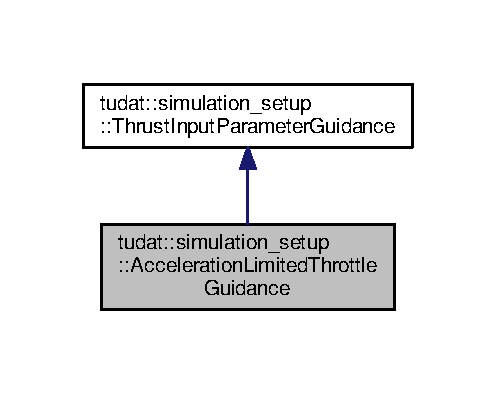
\includegraphics[width=238pt]{classtudat_1_1simulation__setup_1_1AccelerationLimitedThrottleGuidance__inherit__graph}
\end{center}
\end{figure}


Collaboration diagram for tudat\+:\+:simulation\+\_\+setup\+:\+:Acceleration\+Limited\+Throttle\+Guidance\+:
\nopagebreak
\begin{figure}[H]
\begin{center}
\leavevmode
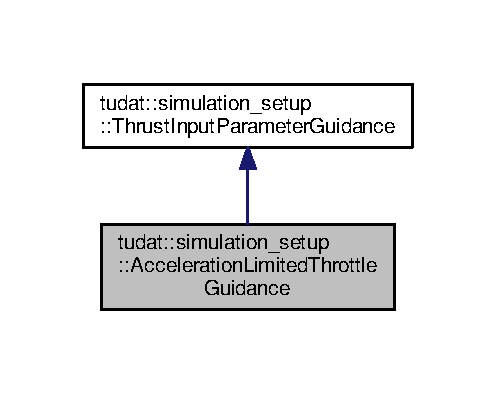
\includegraphics[width=238pt]{classtudat_1_1simulation__setup_1_1AccelerationLimitedThrottleGuidance__coll__graph}
\end{center}
\end{figure}
\subsection*{Public Member Functions}
\begin{DoxyCompactItemize}
\item 
\hyperlink{classtudat_1_1simulation__setup_1_1AccelerationLimitedThrottleGuidance_a53043f861a55d8052874f269ae975716}{Acceleration\+Limited\+Throttle\+Guidance} (const Named\+Body\+Map \&body\+Map, const std\+::string name\+Of\+Body\+With\+Guidance, const std\+::string name\+Of\+Central\+Body, const std\+::vector$<$ propulsion\+::\+Thrust\+Independent\+Variables $>$ independent\+Variables, const boost\+::shared\+\_\+ptr$<$ \hyperlink{classtudat_1_1interpolators_1_1Interpolator}{interpolators\+::\+Interpolator}$<$ double, double $>$ $>$ thrust\+Interpolator, const double maximum\+Acceleration)
\begin{DoxyCompactList}\small\item\em Constructor. \end{DoxyCompactList}\item 
void \hyperlink{classtudat_1_1simulation__setup_1_1AccelerationLimitedThrottleGuidance_a5b08d0dc0c2c16de63f7391fdff697d4}{update\+Guidance\+Parameters} ()
\begin{DoxyCompactList}\small\item\em Function that updates the guidance algorithm to the current time/state\+: sets the throttle value based on axia. \end{DoxyCompactList}\end{DoxyCompactItemize}
\subsection*{Additional Inherited Members}


\subsection{Detailed Description}
Class to compute throttling law for the parameterized thrust magnitude, where the throttle is determined from a maximum axial g-\/load.

Class to compute throttling law for the parameterized thrust magnitude, where the throttle is determined from a maximum, the user must provide the interpolator for the (maximum) thrust, as well as the associated physical meaning of the independent variables. Also, a maximum axial acceleration must be provided. If the current thrust results in an acceleration less than this limit, the throttle is set to 1, if it is higher than the maximum, the throttle is set such that the acceleration is on this limit. 

\subsection{Constructor \& Destructor Documentation}
\index{tudat\+::simulation\+\_\+setup\+::\+Acceleration\+Limited\+Throttle\+Guidance@{tudat\+::simulation\+\_\+setup\+::\+Acceleration\+Limited\+Throttle\+Guidance}!Acceleration\+Limited\+Throttle\+Guidance@{Acceleration\+Limited\+Throttle\+Guidance}}
\index{Acceleration\+Limited\+Throttle\+Guidance@{Acceleration\+Limited\+Throttle\+Guidance}!tudat\+::simulation\+\_\+setup\+::\+Acceleration\+Limited\+Throttle\+Guidance@{tudat\+::simulation\+\_\+setup\+::\+Acceleration\+Limited\+Throttle\+Guidance}}
\subsubsection[{\texorpdfstring{Acceleration\+Limited\+Throttle\+Guidance(const Named\+Body\+Map \&body\+Map, const std\+::string name\+Of\+Body\+With\+Guidance, const std\+::string name\+Of\+Central\+Body, const std\+::vector$<$ propulsion\+::\+Thrust\+Independent\+Variables $>$ independent\+Variables, const boost\+::shared\+\_\+ptr$<$ interpolators\+::\+Interpolator$<$ double, double $>$ $>$ thrust\+Interpolator, const double maximum\+Acceleration)}{AccelerationLimitedThrottleGuidance(const NamedBodyMap &bodyMap, const std::string nameOfBodyWithGuidance, const std::string nameOfCentralBody, const std::vector< propulsion::ThrustIndependentVariables > independentVariables, const boost::shared_ptr< interpolators::Interpolator< double, double > > thrustInterpolator, const double maximumAcceleration)}}]{\setlength{\rightskip}{0pt plus 5cm}tudat\+::simulation\+\_\+setup\+::\+Acceleration\+Limited\+Throttle\+Guidance\+::\+Acceleration\+Limited\+Throttle\+Guidance (
\begin{DoxyParamCaption}
\item[{const Named\+Body\+Map \&}]{body\+Map, }
\item[{const std\+::string}]{name\+Of\+Body\+With\+Guidance, }
\item[{const std\+::string}]{name\+Of\+Central\+Body, }
\item[{const std\+::vector$<$ propulsion\+::\+Thrust\+Independent\+Variables $>$}]{independent\+Variables, }
\item[{const boost\+::shared\+\_\+ptr$<$ {\bf interpolators\+::\+Interpolator}$<$ double, double $>$ $>$}]{thrust\+Interpolator, }
\item[{const double}]{maximum\+Acceleration}
\end{DoxyParamCaption}
)\hspace{0.3cm}{\ttfamily [inline]}}\hypertarget{classtudat_1_1simulation__setup_1_1AccelerationLimitedThrottleGuidance_a53043f861a55d8052874f269ae975716}{}\label{classtudat_1_1simulation__setup_1_1AccelerationLimitedThrottleGuidance_a53043f861a55d8052874f269ae975716}


Constructor. 

Constructor 
\begin{DoxyParams}{Parameters}
{\em body\+Map} & List of pointers to body objects defining the full simulation environment. \\
\hline
{\em name\+Of\+Body\+With\+Guidance} & Name of body for which thrust guidance is to be created. \\
\hline
{\em name\+Of\+Central\+Body} & Name of body w.\+r.\+t. which thrust guidance is computed (e.\+g. Earth if the altitude from Earth is used as an independent variable of the thrust). \\
\hline
{\em independent\+Variables} & Physical meaning of each of the independent variables used as input to the thrust\+Interpolator. \\
\hline
{\em thrust\+Interpolator} & Interpolator that computes the maximum thrust as a function of the independent variables. \\
\hline
{\em maximum\+Acceleration} & Maxmum allowable acceleration due to the thrust force. \\
\hline
\end{DoxyParams}


\subsection{Member Function Documentation}
\index{tudat\+::simulation\+\_\+setup\+::\+Acceleration\+Limited\+Throttle\+Guidance@{tudat\+::simulation\+\_\+setup\+::\+Acceleration\+Limited\+Throttle\+Guidance}!update\+Guidance\+Parameters@{update\+Guidance\+Parameters}}
\index{update\+Guidance\+Parameters@{update\+Guidance\+Parameters}!tudat\+::simulation\+\_\+setup\+::\+Acceleration\+Limited\+Throttle\+Guidance@{tudat\+::simulation\+\_\+setup\+::\+Acceleration\+Limited\+Throttle\+Guidance}}
\subsubsection[{\texorpdfstring{update\+Guidance\+Parameters()}{updateGuidanceParameters()}}]{\setlength{\rightskip}{0pt plus 5cm}void tudat\+::simulation\+\_\+setup\+::\+Acceleration\+Limited\+Throttle\+Guidance\+::update\+Guidance\+Parameters (
\begin{DoxyParamCaption}
{}
\end{DoxyParamCaption}
)\hspace{0.3cm}{\ttfamily [inline]}, {\ttfamily [virtual]}}\hypertarget{classtudat_1_1simulation__setup_1_1AccelerationLimitedThrottleGuidance_a5b08d0dc0c2c16de63f7391fdff697d4}{}\label{classtudat_1_1simulation__setup_1_1AccelerationLimitedThrottleGuidance_a5b08d0dc0c2c16de63f7391fdff697d4}


Function that updates the guidance algorithm to the current time/state\+: sets the throttle value based on axia. 

Function that updates the guidance algorithm to the current time/state\+: sets the throttle value based on axial acceleration when using the maximum thrust. 

Implements \hyperlink{classtudat_1_1simulation__setup_1_1ThrustInputParameterGuidance_ae929c1969241aea9408a5ac20c2f5216}{tudat\+::simulation\+\_\+setup\+::\+Thrust\+Input\+Parameter\+Guidance}.



The documentation for this class was generated from the following file\+:\begin{DoxyCompactItemize}
\item 
/home/lupi/\+Tudat/tudat\+Bundle/tudat/\+Tudat/\+Simulation\+Setup/\+Propagation\+Setup/thrust\+Settings.\+h\end{DoxyCompactItemize}

\hypertarget{classtudat_1_1basic__astrodynamics_1_1AccelerationModel}{}\section{tudat\+:\+:basic\+\_\+astrodynamics\+:\+:Acceleration\+Model$<$ Acceleration\+Data\+Type $>$ Class Template Reference}
\label{classtudat_1_1basic__astrodynamics_1_1AccelerationModel}\index{tudat\+::basic\+\_\+astrodynamics\+::\+Acceleration\+Model$<$ Acceleration\+Data\+Type $>$@{tudat\+::basic\+\_\+astrodynamics\+::\+Acceleration\+Model$<$ Acceleration\+Data\+Type $>$}}


Base class for (translational) acceleration models.  




{\ttfamily \#include $<$acceleration\+Model.\+h$>$}



Inheritance diagram for tudat\+:\+:basic\+\_\+astrodynamics\+:\+:Acceleration\+Model$<$ Acceleration\+Data\+Type $>$\+:
\nopagebreak
\begin{figure}[H]
\begin{center}
\leavevmode
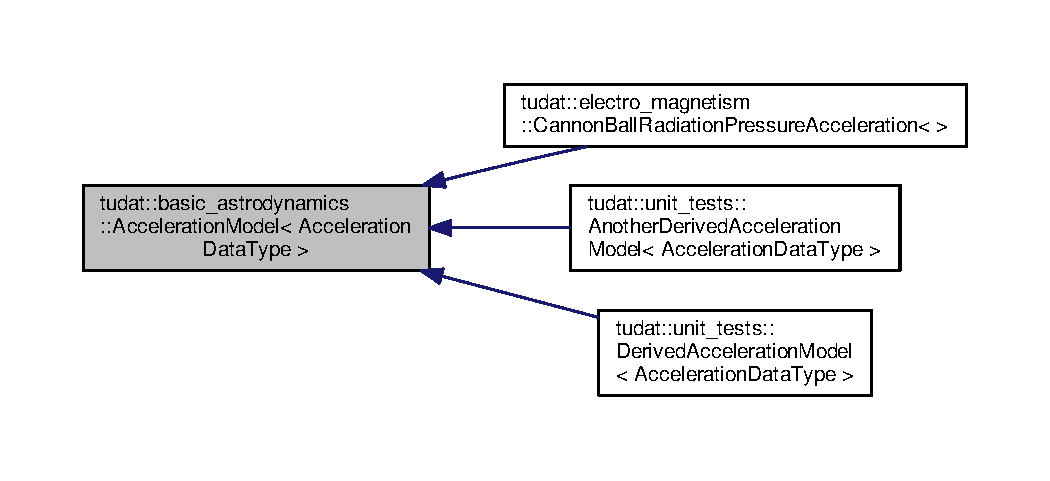
\includegraphics[width=350pt]{classtudat_1_1basic__astrodynamics_1_1AccelerationModel__inherit__graph}
\end{center}
\end{figure}
\subsection*{Public Member Functions}
\begin{DoxyCompactItemize}
\item 
\hyperlink{classtudat_1_1basic__astrodynamics_1_1AccelerationModel_a36f72cf81cc4ff658919a1b92cdc33ad}{Acceleration\+Model} ()\hypertarget{classtudat_1_1basic__astrodynamics_1_1AccelerationModel_a36f72cf81cc4ff658919a1b92cdc33ad}{}\label{classtudat_1_1basic__astrodynamics_1_1AccelerationModel_a36f72cf81cc4ff658919a1b92cdc33ad}

\begin{DoxyCompactList}\small\item\em Constructor. \end{DoxyCompactList}\item 
virtual \hyperlink{classtudat_1_1basic__astrodynamics_1_1AccelerationModel_a131bb0f8b79b410810f602d9b8865968}{$\sim$\+Acceleration\+Model} ()
\begin{DoxyCompactList}\small\item\em Virtual destructor. \end{DoxyCompactList}\item 
virtual Acceleration\+Data\+Type \hyperlink{classtudat_1_1basic__astrodynamics_1_1AccelerationModel_a1f59960bc477fc02e7d52697ced99750}{get\+Acceleration} ()=0
\begin{DoxyCompactList}\small\item\em Get acceleration. \end{DoxyCompactList}\item 
virtual void \hyperlink{classtudat_1_1basic__astrodynamics_1_1AccelerationModel_a966e85b72300b8cbc99ba60e40108d71}{update\+Members} (const double current\+Time=T\+U\+D\+A\+T\+\_\+\+N\+AN)=0
\begin{DoxyCompactList}\small\item\em Update member variables used by the acceleration model. \end{DoxyCompactList}\item 
virtual void \hyperlink{classtudat_1_1basic__astrodynamics_1_1AccelerationModel_a325aae81896137d88b756aac15e188da}{reset\+Time} (const double current\+Time=T\+U\+D\+A\+T\+\_\+\+N\+AN)
\begin{DoxyCompactList}\small\item\em Function to reset the current time. \end{DoxyCompactList}\end{DoxyCompactItemize}
\subsection*{Protected Attributes}
\begin{DoxyCompactItemize}
\item 
double \hyperlink{classtudat_1_1basic__astrodynamics_1_1AccelerationModel_a70f6593c9eec30136ed648ca0e6c9e88}{current\+Time\+\_\+}\hypertarget{classtudat_1_1basic__astrodynamics_1_1AccelerationModel_a70f6593c9eec30136ed648ca0e6c9e88}{}\label{classtudat_1_1basic__astrodynamics_1_1AccelerationModel_a70f6593c9eec30136ed648ca0e6c9e88}

\begin{DoxyCompactList}\small\item\em Previous time to which acceleration model was updated. \end{DoxyCompactList}\end{DoxyCompactItemize}


\subsection{Detailed Description}
\subsubsection*{template$<$typename Acceleration\+Data\+Type = Eigen\+::\+Vector3d$>$\\*
class tudat\+::basic\+\_\+astrodynamics\+::\+Acceleration\+Model$<$ Acceleration\+Data\+Type $>$}

Base class for (translational) acceleration models. 

Base class for (translational) acceleration models. Derived classes should contain implementations to perform calculations of accelerations. Therefore, the \hyperlink{classtudat_1_1basic__astrodynamics_1_1AccelerationModel_a1f59960bc477fc02e7d52697ced99750}{get\+Acceleration()} function has no arguments. 
\begin{DoxyTemplParams}{Template Parameters}
{\em Acceleration\+Data\+Type} & Data type used to represent accelerations (default=Eigen\+::\+Vector3d). \\
\hline
\end{DoxyTemplParams}


\subsection{Constructor \& Destructor Documentation}
\index{tudat\+::basic\+\_\+astrodynamics\+::\+Acceleration\+Model@{tudat\+::basic\+\_\+astrodynamics\+::\+Acceleration\+Model}!````~Acceleration\+Model@{$\sim$\+Acceleration\+Model}}
\index{````~Acceleration\+Model@{$\sim$\+Acceleration\+Model}!tudat\+::basic\+\_\+astrodynamics\+::\+Acceleration\+Model@{tudat\+::basic\+\_\+astrodynamics\+::\+Acceleration\+Model}}
\subsubsection[{\texorpdfstring{$\sim$\+Acceleration\+Model()}{~AccelerationModel()}}]{\setlength{\rightskip}{0pt plus 5cm}template$<$typename Acceleration\+Data\+Type = Eigen\+::\+Vector3d$>$ virtual {\bf tudat\+::basic\+\_\+astrodynamics\+::\+Acceleration\+Model}$<$ Acceleration\+Data\+Type $>$\+::$\sim${\bf Acceleration\+Model} (
\begin{DoxyParamCaption}
{}
\end{DoxyParamCaption}
)\hspace{0.3cm}{\ttfamily [inline]}, {\ttfamily [virtual]}}\hypertarget{classtudat_1_1basic__astrodynamics_1_1AccelerationModel_a131bb0f8b79b410810f602d9b8865968}{}\label{classtudat_1_1basic__astrodynamics_1_1AccelerationModel_a131bb0f8b79b410810f602d9b8865968}


Virtual destructor. 

Virtual destructor, necessary to ensure that derived class destructors get called correctly. 

\subsection{Member Function Documentation}
\index{tudat\+::basic\+\_\+astrodynamics\+::\+Acceleration\+Model@{tudat\+::basic\+\_\+astrodynamics\+::\+Acceleration\+Model}!get\+Acceleration@{get\+Acceleration}}
\index{get\+Acceleration@{get\+Acceleration}!tudat\+::basic\+\_\+astrodynamics\+::\+Acceleration\+Model@{tudat\+::basic\+\_\+astrodynamics\+::\+Acceleration\+Model}}
\subsubsection[{\texorpdfstring{get\+Acceleration()=0}{getAcceleration()=0}}]{\setlength{\rightskip}{0pt plus 5cm}template$<$typename Acceleration\+Data\+Type = Eigen\+::\+Vector3d$>$ virtual Acceleration\+Data\+Type {\bf tudat\+::basic\+\_\+astrodynamics\+::\+Acceleration\+Model}$<$ Acceleration\+Data\+Type $>$\+::get\+Acceleration (
\begin{DoxyParamCaption}
{}
\end{DoxyParamCaption}
)\hspace{0.3cm}{\ttfamily [pure virtual]}}\hypertarget{classtudat_1_1basic__astrodynamics_1_1AccelerationModel_a1f59960bc477fc02e7d52697ced99750}{}\label{classtudat_1_1basic__astrodynamics_1_1AccelerationModel_a1f59960bc477fc02e7d52697ced99750}


Get acceleration. 

Returns the acceleration. No arguments are passed to this function for generality. Instead, all data required for computation is to be obtained from pointers to functions/ classes/structs, etc which are to be set in a derived class and evaluated by the \hyperlink{classtudat_1_1basic__astrodynamics_1_1AccelerationModel_a966e85b72300b8cbc99ba60e40108d71}{update\+Members()} function below. \begin{DoxyReturn}{Returns}
Acceleration. 
\end{DoxyReturn}
\begin{DoxySeeAlso}{See also}
\hyperlink{classtudat_1_1basic__astrodynamics_1_1AccelerationModel_a966e85b72300b8cbc99ba60e40108d71}{update\+Members()}. 
\end{DoxySeeAlso}


Implemented in \hyperlink{classtudat_1_1gravitation_1_1SphericalHarmonicsGravitationalAccelerationModel_aae27d6f97cdbee300e8c532b2dc604b3}{tudat\+::gravitation\+::\+Spherical\+Harmonics\+Gravitational\+Acceleration\+Model}, \hyperlink{classtudat_1_1gravitation_1_1CentralGravitationalAccelerationModel_a1dc811759664e99193f323e02b0a4fe9}{tudat\+::gravitation\+::\+Central\+Gravitational\+Acceleration\+Model$<$ State\+Matrix $>$}, \hyperlink{classtudat_1_1reference__frames_1_1ApparentAccelerationModel_aa5c72a891752917421efb970407b2517}{tudat\+::reference\+\_\+frames\+::\+Apparent\+Acceleration\+Model}, \hyperlink{classtudat_1_1gravitation_1_1MutualSphericalHarmonicsGravitationalAccelerationModel_a9e317eb00b45c6890cdfc6b155b68175}{tudat\+::gravitation\+::\+Mutual\+Spherical\+Harmonics\+Gravitational\+Acceleration\+Model}, \hyperlink{classtudat_1_1gravitation_1_1CentralJ2J3J4GravitationalAccelerationModel_a5a8e57485fff4546caec93841a947406}{tudat\+::gravitation\+::\+Central\+J2\+J3\+J4\+Gravitational\+Acceleration\+Model}, \hyperlink{classtudat_1_1unit__tests_1_1AnotherDerivedAccelerationModel_ab025d414ca6b01e768198e2ab1f9c9d0}{tudat\+::unit\+\_\+tests\+::\+Another\+Derived\+Acceleration\+Model$<$ Acceleration\+Data\+Type, Position\+Data\+Type, Velocity\+Data\+Type, Time\+Data\+Type $>$}, \hyperlink{classtudat_1_1aerodynamics_1_1AerodynamicAcceleration_aca8adefed3eede69b980e46d045f46eb}{tudat\+::aerodynamics\+::\+Aerodynamic\+Acceleration}, \hyperlink{classtudat_1_1electro__magnetism_1_1CannonBallRadiationPressureAcceleration_a4fb5ecf9b9b5f3c1170df2a1f3a62043}{tudat\+::electro\+\_\+magnetism\+::\+Cannon\+Ball\+Radiation\+Pressure\+Acceleration}, \hyperlink{classtudat_1_1gravitation_1_1CentralJ2J3GravitationalAccelerationModel_a5b067a8787c813b6b08a5b83a3f415f9}{tudat\+::gravitation\+::\+Central\+J2\+J3\+Gravitational\+Acceleration\+Model}, \hyperlink{classtudat_1_1gravitation_1_1CentralJ2GravitationalAccelerationModel_abd75fb71f44ab8dd56edfcf9458c78eb}{tudat\+::gravitation\+::\+Central\+J2\+Gravitational\+Acceleration\+Model}, \hyperlink{classtudat_1_1gravitation_1_1ThirdBodyAcceleration_a595cb6cbc9e5d930be8394ec8b157dbb}{tudat\+::gravitation\+::\+Third\+Body\+Acceleration$<$ Direct\+Acceleration\+Model\+Type $>$}, \hyperlink{classtudat_1_1propulsion_1_1ThrustAcceleration_a85c999d6b3fc6b093e6990e2997918f6}{tudat\+::propulsion\+::\+Thrust\+Acceleration}, and \hyperlink{classtudat_1_1unit__tests_1_1DerivedAccelerationModel_a18a9f073e9f83d021d94b9df8144d253}{tudat\+::unit\+\_\+tests\+::\+Derived\+Acceleration\+Model$<$ Acceleration\+Data\+Type, Position\+Data\+Type, Time\+Data\+Type $>$}.

\index{tudat\+::basic\+\_\+astrodynamics\+::\+Acceleration\+Model@{tudat\+::basic\+\_\+astrodynamics\+::\+Acceleration\+Model}!reset\+Time@{reset\+Time}}
\index{reset\+Time@{reset\+Time}!tudat\+::basic\+\_\+astrodynamics\+::\+Acceleration\+Model@{tudat\+::basic\+\_\+astrodynamics\+::\+Acceleration\+Model}}
\subsubsection[{\texorpdfstring{reset\+Time(const double current\+Time=\+T\+U\+D\+A\+T\+\_\+\+N\+A\+N)}{resetTime(const double currentTime=TUDAT_NAN)}}]{\setlength{\rightskip}{0pt plus 5cm}template$<$typename Acceleration\+Data\+Type = Eigen\+::\+Vector3d$>$ virtual void {\bf tudat\+::basic\+\_\+astrodynamics\+::\+Acceleration\+Model}$<$ Acceleration\+Data\+Type $>$\+::reset\+Time (
\begin{DoxyParamCaption}
\item[{const double}]{current\+Time = {\ttfamily TUDAT\+\_\+NAN}}
\end{DoxyParamCaption}
)\hspace{0.3cm}{\ttfamily [inline]}, {\ttfamily [virtual]}}\hypertarget{classtudat_1_1basic__astrodynamics_1_1AccelerationModel_a325aae81896137d88b756aac15e188da}{}\label{classtudat_1_1basic__astrodynamics_1_1AccelerationModel_a325aae81896137d88b756aac15e188da}


Function to reset the current time. 

Function to reset the current time of the acceleration model. 
\begin{DoxyParams}{Parameters}
{\em current\+Time} & Current time (default NaN). \\
\hline
\end{DoxyParams}


Reimplemented in \hyperlink{classtudat_1_1gravitation_1_1MutualSphericalHarmonicsGravitationalAccelerationModel_a59385d672fe32ef2cc3f9cda959a0d18}{tudat\+::gravitation\+::\+Mutual\+Spherical\+Harmonics\+Gravitational\+Acceleration\+Model}, \hyperlink{classtudat_1_1gravitation_1_1ThirdBodyAcceleration_af94e6418c15acf6793f9bf7cd4924746}{tudat\+::gravitation\+::\+Third\+Body\+Acceleration$<$ Direct\+Acceleration\+Model\+Type $>$}, and \hyperlink{classtudat_1_1propulsion_1_1ThrustAcceleration_a2ef613d32d6b4cad26aece57d6171127}{tudat\+::propulsion\+::\+Thrust\+Acceleration}.

\index{tudat\+::basic\+\_\+astrodynamics\+::\+Acceleration\+Model@{tudat\+::basic\+\_\+astrodynamics\+::\+Acceleration\+Model}!update\+Members@{update\+Members}}
\index{update\+Members@{update\+Members}!tudat\+::basic\+\_\+astrodynamics\+::\+Acceleration\+Model@{tudat\+::basic\+\_\+astrodynamics\+::\+Acceleration\+Model}}
\subsubsection[{\texorpdfstring{update\+Members(const double current\+Time=\+T\+U\+D\+A\+T\+\_\+\+N\+A\+N)=0}{updateMembers(const double currentTime=TUDAT_NAN)=0}}]{\setlength{\rightskip}{0pt plus 5cm}template$<$typename Acceleration\+Data\+Type = Eigen\+::\+Vector3d$>$ virtual void {\bf tudat\+::basic\+\_\+astrodynamics\+::\+Acceleration\+Model}$<$ Acceleration\+Data\+Type $>$\+::update\+Members (
\begin{DoxyParamCaption}
\item[{const double}]{current\+Time = {\ttfamily TUDAT\+\_\+NAN}}
\end{DoxyParamCaption}
)\hspace{0.3cm}{\ttfamily [pure virtual]}}\hypertarget{classtudat_1_1basic__astrodynamics_1_1AccelerationModel_a966e85b72300b8cbc99ba60e40108d71}{}\label{classtudat_1_1basic__astrodynamics_1_1AccelerationModel_a966e85b72300b8cbc99ba60e40108d71}


Update member variables used by the acceleration model. 

Updates member variables used by the acceleration model. In the case of acceleration models containing varying parameters, function-\/pointers returning such a parameter (for instance the Cartesian state of a body) will be set as a member variable. This function evaluates such function-\/pointers and updates member variables to the \textquotesingle{}current\textquotesingle{} values of these parameters. Only these current values, not the function-\/pointers are then used by the \hyperlink{classtudat_1_1basic__astrodynamics_1_1AccelerationModel_a1f59960bc477fc02e7d52697ced99750}{get\+Acceleration()} function.

N.\+B.\+: This pure virtual function must be overridden by derived classes! 
\begin{DoxyParams}{Parameters}
{\em current\+Time} & \hyperlink{classtudat_1_1Time}{Time} at which acceleration model is to be updated. \\
\hline
\end{DoxyParams}


Implemented in \hyperlink{classtudat_1_1gravitation_1_1SphericalHarmonicsGravitationalAccelerationModel_a1da9ad8e2fd4daec7c60459175b264f6}{tudat\+::gravitation\+::\+Spherical\+Harmonics\+Gravitational\+Acceleration\+Model}, \hyperlink{classtudat_1_1gravitation_1_1CentralGravitationalAccelerationModel_a9430ea27b71056959af94b2f92353f62}{tudat\+::gravitation\+::\+Central\+Gravitational\+Acceleration\+Model$<$ State\+Matrix $>$}, \hyperlink{classtudat_1_1reference__frames_1_1ApparentAccelerationModel_ae3704bca478d47f8ceb8888a58df5ad9}{tudat\+::reference\+\_\+frames\+::\+Apparent\+Acceleration\+Model}, \hyperlink{classtudat_1_1unit__tests_1_1AnotherDerivedAccelerationModel_add07599d1c34c2479f2271b7703297aa}{tudat\+::unit\+\_\+tests\+::\+Another\+Derived\+Acceleration\+Model$<$ Acceleration\+Data\+Type, Position\+Data\+Type, Velocity\+Data\+Type, Time\+Data\+Type $>$}, \hyperlink{classtudat_1_1gravitation_1_1CentralJ2J3J4GravitationalAccelerationModel_a8cdbef1b4414bf04628e603907aaae1c}{tudat\+::gravitation\+::\+Central\+J2\+J3\+J4\+Gravitational\+Acceleration\+Model}, \hyperlink{classtudat_1_1aerodynamics_1_1AerodynamicAcceleration_a6cd45319bf7f5b7f376aa9357d1840ea}{tudat\+::aerodynamics\+::\+Aerodynamic\+Acceleration}, \hyperlink{classtudat_1_1electro__magnetism_1_1CannonBallRadiationPressureAcceleration_a1e77eb0e4b9f9cfffc1d39e772845fff}{tudat\+::electro\+\_\+magnetism\+::\+Cannon\+Ball\+Radiation\+Pressure\+Acceleration}, \hyperlink{classtudat_1_1gravitation_1_1MutualSphericalHarmonicsGravitationalAccelerationModel_a5924a6d967e6f2168c2dcc9cb8c3d627}{tudat\+::gravitation\+::\+Mutual\+Spherical\+Harmonics\+Gravitational\+Acceleration\+Model}, \hyperlink{classtudat_1_1gravitation_1_1CentralJ2J3GravitationalAccelerationModel_aa9cfafbe11efb4a60bb87ee5c6c06e1a}{tudat\+::gravitation\+::\+Central\+J2\+J3\+Gravitational\+Acceleration\+Model}, \hyperlink{classtudat_1_1gravitation_1_1CentralJ2GravitationalAccelerationModel_a29a5ea148a2db77b0f16809c699d480a}{tudat\+::gravitation\+::\+Central\+J2\+Gravitational\+Acceleration\+Model}, \hyperlink{classtudat_1_1propulsion_1_1ThrustAcceleration_a847904c69ea6ced5ac3396f7ecdf2f78}{tudat\+::propulsion\+::\+Thrust\+Acceleration}, \hyperlink{classtudat_1_1gravitation_1_1ThirdBodyAcceleration_afdb74715179d8da928b1d3616976f795}{tudat\+::gravitation\+::\+Third\+Body\+Acceleration$<$ Direct\+Acceleration\+Model\+Type $>$}, and \hyperlink{classtudat_1_1unit__tests_1_1DerivedAccelerationModel_ae0f1908a1c80dfafc01e4c11e69e1373}{tudat\+::unit\+\_\+tests\+::\+Derived\+Acceleration\+Model$<$ Acceleration\+Data\+Type, Position\+Data\+Type, Time\+Data\+Type $>$}.



The documentation for this class was generated from the following file\+:\begin{DoxyCompactItemize}
\item 
/home/lupi/\+Tudat/tudat\+Bundle/tudat/\+Tudat/\+Astrodynamics/\+Basic\+Astrodynamics/acceleration\+Model.\+h\end{DoxyCompactItemize}

\hypertarget{classtudat_1_1acceleration__partials_1_1AccelerationPartial}{}\section{tudat\+:\+:acceleration\+\_\+partials\+:\+:Acceleration\+Partial Class Reference}
\label{classtudat_1_1acceleration__partials_1_1AccelerationPartial}\index{tudat\+::acceleration\+\_\+partials\+::\+Acceleration\+Partial@{tudat\+::acceleration\+\_\+partials\+::\+Acceleration\+Partial}}


Base class for objects calculating partial derivatives of accelerations w.\+r.\+t. states, model parameters.  




{\ttfamily \#include $<$acceleration\+Partial.\+h$>$}



Inheritance diagram for tudat\+:\+:acceleration\+\_\+partials\+:\+:Acceleration\+Partial\+:
\nopagebreak
\begin{figure}[H]
\begin{center}
\leavevmode
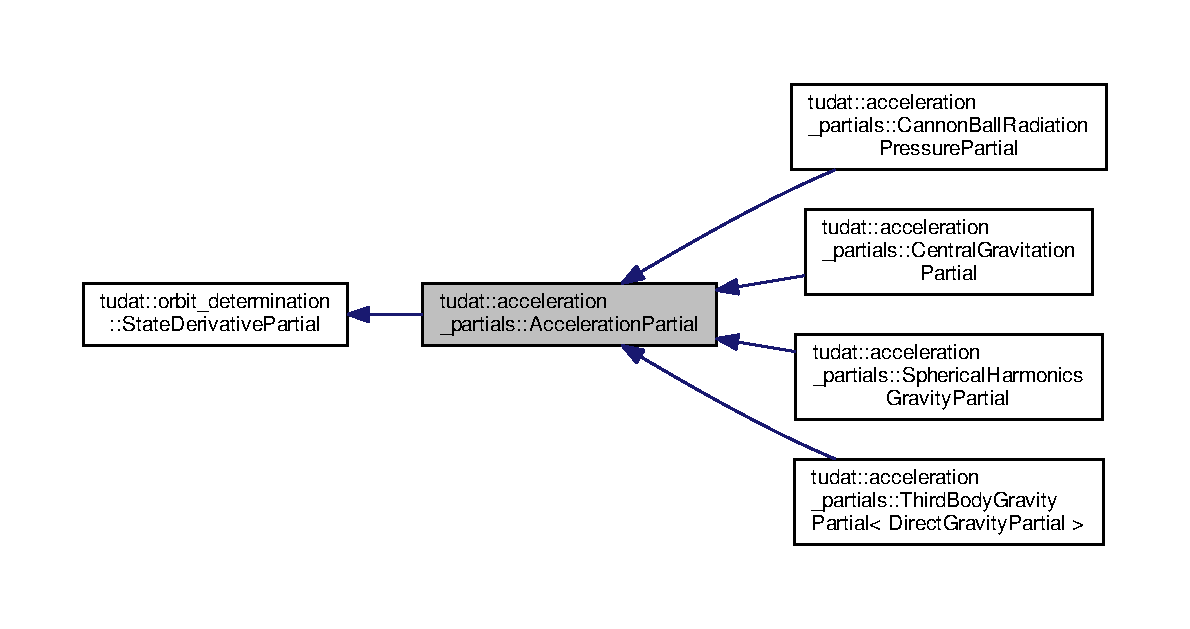
\includegraphics[width=350pt]{classtudat_1_1acceleration__partials_1_1AccelerationPartial__inherit__graph}
\end{center}
\end{figure}


Collaboration diagram for tudat\+:\+:acceleration\+\_\+partials\+:\+:Acceleration\+Partial\+:
\nopagebreak
\begin{figure}[H]
\begin{center}
\leavevmode
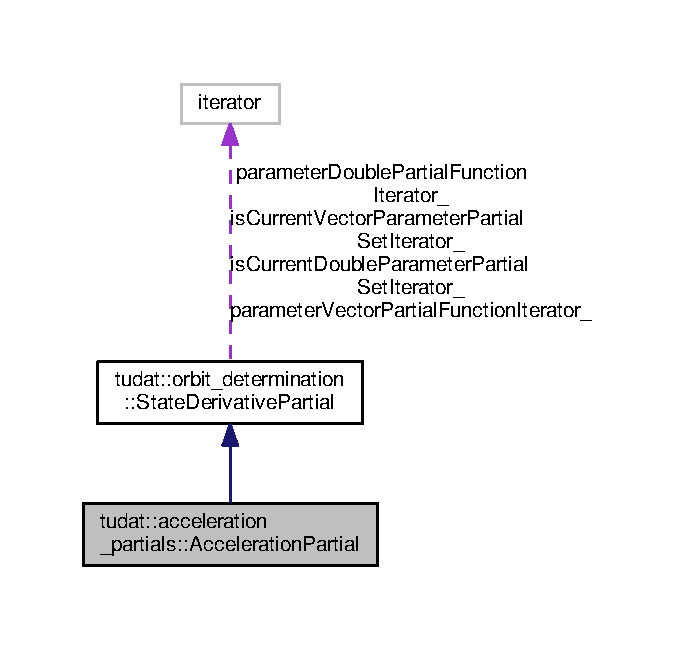
\includegraphics[width=325pt]{classtudat_1_1acceleration__partials_1_1AccelerationPartial__coll__graph}
\end{center}
\end{figure}
\subsection*{Public Member Functions}
\begin{DoxyCompactItemize}
\item 
\hyperlink{classtudat_1_1acceleration__partials_1_1AccelerationPartial_ad4f4594c6e13138a1895dd008a14bf7e}{Acceleration\+Partial} (const std\+::string \&accelerated\+Body, const std\+::string \&accelerating\+Body, const basic\+\_\+astrodynamics\+::\+Available\+Acceleration acceleration\+Type)
\begin{DoxyCompactList}\small\item\em Base class constructor. \end{DoxyCompactList}\item 
virtual \hyperlink{classtudat_1_1acceleration__partials_1_1AccelerationPartial_ab373fff70206231b312a988e59902038}{$\sim$\+Acceleration\+Partial} ()\hypertarget{classtudat_1_1acceleration__partials_1_1AccelerationPartial_ab373fff70206231b312a988e59902038}{}\label{classtudat_1_1acceleration__partials_1_1AccelerationPartial_ab373fff70206231b312a988e59902038}

\begin{DoxyCompactList}\small\item\em Virtual destructor. \end{DoxyCompactList}\item 
std\+::pair$<$ boost\+::function$<$ void(Eigen\+::\+Block$<$ Eigen\+::\+Matrix\+Xd $>$) $>$, int $>$ \hyperlink{classtudat_1_1acceleration__partials_1_1AccelerationPartial_a1f9e42e445f6efe61fd6db72826adc9d}{get\+Derivative\+Function\+Wrt\+State\+Of\+Integrated\+Body} (const std\+::pair$<$ std\+::string, std\+::string $>$ \&state\+Reference\+Point, const propagators\+::\+Integrated\+State\+Type integrated\+State\+Type)
\begin{DoxyCompactList}\small\item\em Function to retrieve the function that returns the partial derivative w.\+r.\+t. a propagated state. \end{DoxyCompactList}\item 
virtual bool \hyperlink{classtudat_1_1acceleration__partials_1_1AccelerationPartial_aac005cc281d426013544fcc77ec1b00d}{is\+State\+Derivative\+Dependent\+On\+Integrated\+Non\+Translational\+State} (const std\+::pair$<$ std\+::string, std\+::string $>$ \&state\+Reference\+Point, const propagators\+::\+Integrated\+State\+Type integrated\+State\+Type)
\begin{DoxyCompactList}\small\item\em Function for determining if the acceleration is dependent on a non-\/translational integrated state (default none). \end{DoxyCompactList}\item 
bool \hyperlink{classtudat_1_1acceleration__partials_1_1AccelerationPartial_ab05fd603c6228f4639e6f00ac4f9527c}{is\+State\+Derivative\+Dependent\+On\+Integrated\+State} (const std\+::pair$<$ std\+::string, std\+::string $>$ \&state\+Reference\+Point, const propagators\+::\+Integrated\+State\+Type integrated\+State\+Type)
\begin{DoxyCompactList}\small\item\em Function to check whether a partial w.\+r.\+t. some integrated state is non-\/zero. \end{DoxyCompactList}\item 
virtual void \hyperlink{classtudat_1_1acceleration__partials_1_1AccelerationPartial_a629ee1ab826d64e6493d1dbf0fe7586b}{wrt\+Position\+Of\+Accelerated\+Body} (Eigen\+::\+Block$<$ Eigen\+::\+Matrix\+Xd $>$ partial\+Matrix, const bool add\+Contribution=1, const int start\+Row=0, const int start\+Column=0)=0
\begin{DoxyCompactList}\small\item\em Pure virtual function for calculating the partial of the acceleration w.\+r.\+t. the position of the accelerated body. \end{DoxyCompactList}\item 
virtual void \hyperlink{classtudat_1_1acceleration__partials_1_1AccelerationPartial_ad3bb8ec281acf660baed8eb5127fcf5d}{wrt\+Velocity\+Of\+Accelerated\+Body} (Eigen\+::\+Block$<$ Eigen\+::\+Matrix\+Xd $>$ partial\+Matrix, const bool add\+Contribution=1, const int start\+Row=0, const int start\+Column=3)
\begin{DoxyCompactList}\small\item\em Function for calculating the partial of the acceleration w.\+r.\+t. the velocity of the accelerated body. \end{DoxyCompactList}\item 
void \hyperlink{classtudat_1_1acceleration__partials_1_1AccelerationPartial_a0576a63608bc8bee1da8bf2aea0ea7b6}{wrt\+State\+Of\+Accelerated\+Body} (Eigen\+::\+Block$<$ Eigen\+::\+Matrix\+Xd $>$ partial\+Matrix)
\begin{DoxyCompactList}\small\item\em Function for calculating the partial of the acceleration w.\+r.\+t. the Cartesian state of the body undergoing acceleration. \end{DoxyCompactList}\item 
virtual void \hyperlink{classtudat_1_1acceleration__partials_1_1AccelerationPartial_a779c9c208d2054d8425178f4ea8f6021}{wrt\+Position\+Of\+Accelerating\+Body} (Eigen\+::\+Block$<$ Eigen\+::\+Matrix\+Xd $>$ partial\+Matrix, const bool add\+Contribution=1, const int start\+Row=0, const int start\+Column=0)=0
\begin{DoxyCompactList}\small\item\em Pure virtual function for calculating the partial of the acceleration w.\+r.\+t. the position of the body exerting acceleration. \end{DoxyCompactList}\item 
virtual void \hyperlink{classtudat_1_1acceleration__partials_1_1AccelerationPartial_ab411157f1ab0d7b8bdcb771024b4f5a9}{wrt\+Velocity\+Of\+Accelerating\+Body} (Eigen\+::\+Block$<$ Eigen\+::\+Matrix\+Xd $>$ partial\+Matrix, const bool add\+Contribution=1, const int start\+Row=0, const int start\+Column=3)
\begin{DoxyCompactList}\small\item\em Function for calculating the partial of the acceleration w.\+r.\+t. the velocity of the body exerting acceleration. \end{DoxyCompactList}\item 
void \hyperlink{classtudat_1_1acceleration__partials_1_1AccelerationPartial_a8bfba67b7f9e9a3d6021b2b1759fc33e}{wrt\+State\+Of\+Accelerating\+Body} (Eigen\+::\+Block$<$ Eigen\+::\+Matrix\+Xd $>$ partial\+Matrix)
\begin{DoxyCompactList}\small\item\em Function for calculating the partial of the acceleration w.\+r.\+t. the Cartesian state of the body exerting acceleration. \end{DoxyCompactList}\item 
virtual void \hyperlink{classtudat_1_1acceleration__partials_1_1AccelerationPartial_ab222ba1108201aa02e916c64ce82d599}{wrt\+Position\+Of\+Additional\+Body} (const std\+::string \&body\+Name, Eigen\+::\+Block$<$ Eigen\+::\+Matrix\+Xd $>$ partial\+Matrix, const bool add\+Contribution=1, const int start\+Row=0, const int start\+Column=0)
\begin{DoxyCompactList}\small\item\em Function for calculating the partial of the acceleration w.\+r.\+t. the position of the third body. \end{DoxyCompactList}\item 
virtual void \hyperlink{classtudat_1_1acceleration__partials_1_1AccelerationPartial_a1566f99b2cfd42d523c06ee6c1559435}{wrt\+Velocity\+Of\+Additional\+Body} (const std\+::string \&body\+Name, Eigen\+::\+Block$<$ Eigen\+::\+Matrix\+Xd $>$ partial\+Matrix, const bool add\+Contribution=1, const int start\+Row=0, const int start\+Column=3)
\begin{DoxyCompactList}\small\item\em Function for calculating the partial of the acceleration w.\+r.\+t. the velocity of the third body. \end{DoxyCompactList}\item 
void \hyperlink{classtudat_1_1acceleration__partials_1_1AccelerationPartial_a8e21b7ff67f97af2e7e2a963cd0da3b2}{wrt\+State\+Of\+Additional\+Body} (Eigen\+::\+Block$<$ Eigen\+::\+Matrix\+Xd $>$ partial\+Matrix, const std\+::string \&body\+Name)
\begin{DoxyCompactList}\small\item\em Function for calculating the partial of the acceleration w.\+r.\+t. the Cartesian state of the third body. \end{DoxyCompactList}\item 
virtual void \hyperlink{classtudat_1_1acceleration__partials_1_1AccelerationPartial_aaba8dd75dd1d18289a8fc2769d333c36}{wrt\+Non\+Translational\+State\+Of\+Additional\+Body} (Eigen\+::\+Block$<$ Eigen\+::\+Matrix\+Xd $>$ partial\+Matrix, const std\+::pair$<$ std\+::string, std\+::string $>$ \&state\+Reference\+Point, const propagators\+::\+Integrated\+State\+Type integrated\+State\+Type)
\begin{DoxyCompactList}\small\item\em Function for calculating the partial of the acceleration w.\+r.\+t. a non-\/translational integrated state. \end{DoxyCompactList}\item 
virtual bool \hyperlink{classtudat_1_1acceleration__partials_1_1AccelerationPartial_ae6278c8e04765a3f0485c57ea9d8c6f3}{is\+Acceleration\+Partial\+Wrt\+Additional\+Body\+Non\+Null} (const std\+::string \&body\+Name)
\begin{DoxyCompactList}\small\item\em Function to check whether the partial derivative w.\+r.\+t. the translational state of a third body is non-\/zero. \end{DoxyCompactList}\item 
std\+::string \hyperlink{classtudat_1_1acceleration__partials_1_1AccelerationPartial_a0bf7d418855165be4d40b82cfbeb115c}{get\+Accelerated\+Body} ()
\begin{DoxyCompactList}\small\item\em Function to retrieve the name of the body undergoing acceleration. \end{DoxyCompactList}\item 
std\+::string \hyperlink{classtudat_1_1acceleration__partials_1_1AccelerationPartial_ac74a861f66f3362524aec1f0266513cf}{get\+Accelerating\+Body} ()
\begin{DoxyCompactList}\small\item\em Function to retrieve the name of the body exerting acceleration. \end{DoxyCompactList}\item 
basic\+\_\+astrodynamics\+::\+Available\+Acceleration \hyperlink{classtudat_1_1acceleration__partials_1_1AccelerationPartial_a6b6e323de35eaeb1292e4bfb410da7b1}{get\+Acceleration\+Type} ()
\begin{DoxyCompactList}\small\item\em Function to retrieve the type of acceleration w.\+r.\+t. which partial is taken.. \end{DoxyCompactList}\end{DoxyCompactItemize}
\subsection*{Protected Attributes}
\begin{DoxyCompactItemize}
\item 
std\+::string \hyperlink{classtudat_1_1acceleration__partials_1_1AccelerationPartial_a655662aa6427373647cc9c26327e9565}{accelerated\+Body\+\_\+}\hypertarget{classtudat_1_1acceleration__partials_1_1AccelerationPartial_a655662aa6427373647cc9c26327e9565}{}\label{classtudat_1_1acceleration__partials_1_1AccelerationPartial_a655662aa6427373647cc9c26327e9565}

\begin{DoxyCompactList}\small\item\em Name of the body undergoing acceleration. \end{DoxyCompactList}\item 
std\+::string \hyperlink{classtudat_1_1acceleration__partials_1_1AccelerationPartial_aa0cb4d885b7833a39db39212a797ebd2}{accelerating\+Body\+\_\+}\hypertarget{classtudat_1_1acceleration__partials_1_1AccelerationPartial_aa0cb4d885b7833a39db39212a797ebd2}{}\label{classtudat_1_1acceleration__partials_1_1AccelerationPartial_aa0cb4d885b7833a39db39212a797ebd2}

\begin{DoxyCompactList}\small\item\em Name of the body exerting acceleration. \end{DoxyCompactList}\item 
basic\+\_\+astrodynamics\+::\+Available\+Acceleration \hyperlink{classtudat_1_1acceleration__partials_1_1AccelerationPartial_a32cc6c58e4aa187b2110b4c6c7d4ccf4}{acceleration\+Type\+\_\+}\hypertarget{classtudat_1_1acceleration__partials_1_1AccelerationPartial_a32cc6c58e4aa187b2110b4c6c7d4ccf4}{}\label{classtudat_1_1acceleration__partials_1_1AccelerationPartial_a32cc6c58e4aa187b2110b4c6c7d4ccf4}

\begin{DoxyCompactList}\small\item\em Type of acceleration w.\+r.\+t. which partial is taken.. \end{DoxyCompactList}\end{DoxyCompactItemize}
\subsection*{Additional Inherited Members}


\subsection{Detailed Description}
Base class for objects calculating partial derivatives of accelerations w.\+r.\+t. states, model parameters. 

Base class for objects calculating partial derivatives of accelerations w.\+r.\+t. states, model parameters. Such calculations are used in orbit determination, for the computation of the state transition; sensitivity matrices. Derived classes implement derivative-\/calculating models for specific acceleration models, so that the calculation of all partials of a single type acceleration model is encompassed in a single derived class. 

\subsection{Constructor \& Destructor Documentation}
\index{tudat\+::acceleration\+\_\+partials\+::\+Acceleration\+Partial@{tudat\+::acceleration\+\_\+partials\+::\+Acceleration\+Partial}!Acceleration\+Partial@{Acceleration\+Partial}}
\index{Acceleration\+Partial@{Acceleration\+Partial}!tudat\+::acceleration\+\_\+partials\+::\+Acceleration\+Partial@{tudat\+::acceleration\+\_\+partials\+::\+Acceleration\+Partial}}
\subsubsection[{\texorpdfstring{Acceleration\+Partial(const std\+::string \&accelerated\+Body, const std\+::string \&accelerating\+Body, const basic\+\_\+astrodynamics\+::\+Available\+Acceleration acceleration\+Type)}{AccelerationPartial(const std::string &acceleratedBody, const std::string &acceleratingBody, const basic_astrodynamics::AvailableAcceleration accelerationType)}}]{\setlength{\rightskip}{0pt plus 5cm}tudat\+::acceleration\+\_\+partials\+::\+Acceleration\+Partial\+::\+Acceleration\+Partial (
\begin{DoxyParamCaption}
\item[{const std\+::string \&}]{accelerated\+Body, }
\item[{const std\+::string \&}]{accelerating\+Body, }
\item[{const basic\+\_\+astrodynamics\+::\+Available\+Acceleration}]{acceleration\+Type}
\end{DoxyParamCaption}
)\hspace{0.3cm}{\ttfamily [inline]}}\hypertarget{classtudat_1_1acceleration__partials_1_1AccelerationPartial_ad4f4594c6e13138a1895dd008a14bf7e}{}\label{classtudat_1_1acceleration__partials_1_1AccelerationPartial_ad4f4594c6e13138a1895dd008a14bf7e}


Base class constructor. 

Constructor of base class, sets the base class member variables identifying the body undergoing and exerting the acceleration. 
\begin{DoxyParams}{Parameters}
{\em accelerated\+Body} & Body undergoing acceleration. \\
\hline
{\em accelerating\+Body} & Body exerting acceleration. \\
\hline
{\em acceleration\+Type} & Type of acceleration w.\+r.\+t. which partial is taken. \\
\hline
\end{DoxyParams}


\subsection{Member Function Documentation}
\index{tudat\+::acceleration\+\_\+partials\+::\+Acceleration\+Partial@{tudat\+::acceleration\+\_\+partials\+::\+Acceleration\+Partial}!get\+Accelerated\+Body@{get\+Accelerated\+Body}}
\index{get\+Accelerated\+Body@{get\+Accelerated\+Body}!tudat\+::acceleration\+\_\+partials\+::\+Acceleration\+Partial@{tudat\+::acceleration\+\_\+partials\+::\+Acceleration\+Partial}}
\subsubsection[{\texorpdfstring{get\+Accelerated\+Body()}{getAcceleratedBody()}}]{\setlength{\rightskip}{0pt plus 5cm}std\+::string tudat\+::acceleration\+\_\+partials\+::\+Acceleration\+Partial\+::get\+Accelerated\+Body (
\begin{DoxyParamCaption}
{}
\end{DoxyParamCaption}
)\hspace{0.3cm}{\ttfamily [inline]}}\hypertarget{classtudat_1_1acceleration__partials_1_1AccelerationPartial_a0bf7d418855165be4d40b82cfbeb115c}{}\label{classtudat_1_1acceleration__partials_1_1AccelerationPartial_a0bf7d418855165be4d40b82cfbeb115c}


Function to retrieve the name of the body undergoing acceleration. 

Function to retrieve the name of the body undergoing acceleration. \begin{DoxyReturn}{Returns}
Name of the body undergoing acceleration. 
\end{DoxyReturn}
\index{tudat\+::acceleration\+\_\+partials\+::\+Acceleration\+Partial@{tudat\+::acceleration\+\_\+partials\+::\+Acceleration\+Partial}!get\+Accelerating\+Body@{get\+Accelerating\+Body}}
\index{get\+Accelerating\+Body@{get\+Accelerating\+Body}!tudat\+::acceleration\+\_\+partials\+::\+Acceleration\+Partial@{tudat\+::acceleration\+\_\+partials\+::\+Acceleration\+Partial}}
\subsubsection[{\texorpdfstring{get\+Accelerating\+Body()}{getAcceleratingBody()}}]{\setlength{\rightskip}{0pt plus 5cm}std\+::string tudat\+::acceleration\+\_\+partials\+::\+Acceleration\+Partial\+::get\+Accelerating\+Body (
\begin{DoxyParamCaption}
{}
\end{DoxyParamCaption}
)\hspace{0.3cm}{\ttfamily [inline]}}\hypertarget{classtudat_1_1acceleration__partials_1_1AccelerationPartial_ac74a861f66f3362524aec1f0266513cf}{}\label{classtudat_1_1acceleration__partials_1_1AccelerationPartial_ac74a861f66f3362524aec1f0266513cf}


Function to retrieve the name of the body exerting acceleration. 

Function to retrieve the name of the body exerting acceleration. \begin{DoxyReturn}{Returns}
Name of the body exerting acceleration. 
\end{DoxyReturn}
\index{tudat\+::acceleration\+\_\+partials\+::\+Acceleration\+Partial@{tudat\+::acceleration\+\_\+partials\+::\+Acceleration\+Partial}!get\+Acceleration\+Type@{get\+Acceleration\+Type}}
\index{get\+Acceleration\+Type@{get\+Acceleration\+Type}!tudat\+::acceleration\+\_\+partials\+::\+Acceleration\+Partial@{tudat\+::acceleration\+\_\+partials\+::\+Acceleration\+Partial}}
\subsubsection[{\texorpdfstring{get\+Acceleration\+Type()}{getAccelerationType()}}]{\setlength{\rightskip}{0pt plus 5cm}basic\+\_\+astrodynamics\+::\+Available\+Acceleration tudat\+::acceleration\+\_\+partials\+::\+Acceleration\+Partial\+::get\+Acceleration\+Type (
\begin{DoxyParamCaption}
{}
\end{DoxyParamCaption}
)\hspace{0.3cm}{\ttfamily [inline]}}\hypertarget{classtudat_1_1acceleration__partials_1_1AccelerationPartial_a6b6e323de35eaeb1292e4bfb410da7b1}{}\label{classtudat_1_1acceleration__partials_1_1AccelerationPartial_a6b6e323de35eaeb1292e4bfb410da7b1}


Function to retrieve the type of acceleration w.\+r.\+t. which partial is taken.. 

Function to retrieve the type of acceleration w.\+r.\+t. which partial is taken.. \begin{DoxyReturn}{Returns}
Type of acceleration w.\+r.\+t. which partial is taken.. 
\end{DoxyReturn}
\index{tudat\+::acceleration\+\_\+partials\+::\+Acceleration\+Partial@{tudat\+::acceleration\+\_\+partials\+::\+Acceleration\+Partial}!get\+Derivative\+Function\+Wrt\+State\+Of\+Integrated\+Body@{get\+Derivative\+Function\+Wrt\+State\+Of\+Integrated\+Body}}
\index{get\+Derivative\+Function\+Wrt\+State\+Of\+Integrated\+Body@{get\+Derivative\+Function\+Wrt\+State\+Of\+Integrated\+Body}!tudat\+::acceleration\+\_\+partials\+::\+Acceleration\+Partial@{tudat\+::acceleration\+\_\+partials\+::\+Acceleration\+Partial}}
\subsubsection[{\texorpdfstring{get\+Derivative\+Function\+Wrt\+State\+Of\+Integrated\+Body(const std\+::pair$<$ std\+::string, std\+::string $>$ \&state\+Reference\+Point, const propagators\+::\+Integrated\+State\+Type integrated\+State\+Type)}{getDerivativeFunctionWrtStateOfIntegratedBody(const std::pair< std::string, std::string > &stateReferencePoint, const propagators::IntegratedStateType integratedStateType)}}]{\setlength{\rightskip}{0pt plus 5cm}std\+::pair$<$ boost\+::function$<$ void( Eigen\+::\+Block$<$ Eigen\+::\+Matrix\+Xd $>$ ) $>$, int $>$ tudat\+::acceleration\+\_\+partials\+::\+Acceleration\+Partial\+::get\+Derivative\+Function\+Wrt\+State\+Of\+Integrated\+Body (
\begin{DoxyParamCaption}
\item[{const std\+::pair$<$ std\+::string, std\+::string $>$ \&}]{state\+Reference\+Point, }
\item[{const propagators\+::\+Integrated\+State\+Type}]{integrated\+State\+Type}
\end{DoxyParamCaption}
)\hspace{0.3cm}{\ttfamily [inline]}, {\ttfamily [virtual]}}\hypertarget{classtudat_1_1acceleration__partials_1_1AccelerationPartial_a1f9e42e445f6efe61fd6db72826adc9d}{}\label{classtudat_1_1acceleration__partials_1_1AccelerationPartial_a1f9e42e445f6efe61fd6db72826adc9d}


Function to retrieve the function that returns the partial derivative w.\+r.\+t. a propagated state. 

Function to retrieve the function that returns the partial derivative w.\+r.\+t. a propagated state. 
\begin{DoxyParams}{Parameters}
{\em state\+Reference\+Point} & Reference point (id) for propagated state (i.\+e. body name for translational dynamics). \\
\hline
{\em integrated\+State\+Type} & Type of propagated state. \\
\hline
\end{DoxyParams}
\begin{DoxyReturn}{Returns}
Pair with function, returning partial derivative, and number of columns in partial vector, 
\end{DoxyReturn}


Implements \hyperlink{classtudat_1_1orbit__determination_1_1StateDerivativePartial_a9b530d365f373821baa693f34bbedb4e}{tudat\+::orbit\+\_\+determination\+::\+State\+Derivative\+Partial}.

\index{tudat\+::acceleration\+\_\+partials\+::\+Acceleration\+Partial@{tudat\+::acceleration\+\_\+partials\+::\+Acceleration\+Partial}!is\+Acceleration\+Partial\+Wrt\+Additional\+Body\+Non\+Null@{is\+Acceleration\+Partial\+Wrt\+Additional\+Body\+Non\+Null}}
\index{is\+Acceleration\+Partial\+Wrt\+Additional\+Body\+Non\+Null@{is\+Acceleration\+Partial\+Wrt\+Additional\+Body\+Non\+Null}!tudat\+::acceleration\+\_\+partials\+::\+Acceleration\+Partial@{tudat\+::acceleration\+\_\+partials\+::\+Acceleration\+Partial}}
\subsubsection[{\texorpdfstring{is\+Acceleration\+Partial\+Wrt\+Additional\+Body\+Non\+Null(const std\+::string \&body\+Name)}{isAccelerationPartialWrtAdditionalBodyNonNull(const std::string &bodyName)}}]{\setlength{\rightskip}{0pt plus 5cm}virtual bool tudat\+::acceleration\+\_\+partials\+::\+Acceleration\+Partial\+::is\+Acceleration\+Partial\+Wrt\+Additional\+Body\+Non\+Null (
\begin{DoxyParamCaption}
\item[{const std\+::string \&}]{body\+Name}
\end{DoxyParamCaption}
)\hspace{0.3cm}{\ttfamily [inline]}, {\ttfamily [virtual]}}\hypertarget{classtudat_1_1acceleration__partials_1_1AccelerationPartial_ae6278c8e04765a3f0485c57ea9d8c6f3}{}\label{classtudat_1_1acceleration__partials_1_1AccelerationPartial_ae6278c8e04765a3f0485c57ea9d8c6f3}


Function to check whether the partial derivative w.\+r.\+t. the translational state of a third body is non-\/zero. 

Function to check whether the partial derivative w.\+r.\+t. the translational state of a third body is non-\/zero. This function returns false by default, should be redefined in derived class if any third-\/bodyd dependencies exist. 
\begin{DoxyParams}{Parameters}
{\em body\+Name} & Name of third body. \\
\hline
\end{DoxyParams}
\begin{DoxyReturn}{Returns}
True if third body dependency exists, false otherwise. 
\end{DoxyReturn}


Reimplemented in \hyperlink{classtudat_1_1acceleration__partials_1_1ThirdBodyGravityPartial_ac3f7c8583585747b6ef086d860772c49}{tudat\+::acceleration\+\_\+partials\+::\+Third\+Body\+Gravity\+Partial$<$ Direct\+Gravity\+Partial $>$}.

\index{tudat\+::acceleration\+\_\+partials\+::\+Acceleration\+Partial@{tudat\+::acceleration\+\_\+partials\+::\+Acceleration\+Partial}!is\+State\+Derivative\+Dependent\+On\+Integrated\+Non\+Translational\+State@{is\+State\+Derivative\+Dependent\+On\+Integrated\+Non\+Translational\+State}}
\index{is\+State\+Derivative\+Dependent\+On\+Integrated\+Non\+Translational\+State@{is\+State\+Derivative\+Dependent\+On\+Integrated\+Non\+Translational\+State}!tudat\+::acceleration\+\_\+partials\+::\+Acceleration\+Partial@{tudat\+::acceleration\+\_\+partials\+::\+Acceleration\+Partial}}
\subsubsection[{\texorpdfstring{is\+State\+Derivative\+Dependent\+On\+Integrated\+Non\+Translational\+State(const std\+::pair$<$ std\+::string, std\+::string $>$ \&state\+Reference\+Point, const propagators\+::\+Integrated\+State\+Type integrated\+State\+Type)}{isStateDerivativeDependentOnIntegratedNonTranslationalState(const std::pair< std::string, std::string > &stateReferencePoint, const propagators::IntegratedStateType integratedStateType)}}]{\setlength{\rightskip}{0pt plus 5cm}virtual bool tudat\+::acceleration\+\_\+partials\+::\+Acceleration\+Partial\+::is\+State\+Derivative\+Dependent\+On\+Integrated\+Non\+Translational\+State (
\begin{DoxyParamCaption}
\item[{const std\+::pair$<$ std\+::string, std\+::string $>$ \&}]{state\+Reference\+Point, }
\item[{const propagators\+::\+Integrated\+State\+Type}]{integrated\+State\+Type}
\end{DoxyParamCaption}
)\hspace{0.3cm}{\ttfamily [inline]}, {\ttfamily [virtual]}}\hypertarget{classtudat_1_1acceleration__partials_1_1AccelerationPartial_aac005cc281d426013544fcc77ec1b00d}{}\label{classtudat_1_1acceleration__partials_1_1AccelerationPartial_aac005cc281d426013544fcc77ec1b00d}


Function for determining if the acceleration is dependent on a non-\/translational integrated state (default none). 

Function for determining if the acceleration is dependent on a non-\/translational integrated state. No dependency is implemented is returned in this base class function, but may be overriden by derived class. 
\begin{DoxyParams}{Parameters}
{\em state\+Reference\+Point} & Reference point id of propagated state \\
\hline
{\em integrated\+State\+Type} & Type of propagated state for which dependency is to be determined. \\
\hline
\end{DoxyParams}
\begin{DoxyReturn}{Returns}
True if dependency exists (non-\/zero partial), false otherwise. 
\end{DoxyReturn}


Implements \hyperlink{classtudat_1_1orbit__determination_1_1StateDerivativePartial_a0d38f73cb9d6b6e2eefaa6c879e9f839}{tudat\+::orbit\+\_\+determination\+::\+State\+Derivative\+Partial}.



Reimplemented in \hyperlink{classtudat_1_1acceleration__partials_1_1ThirdBodyGravityPartial_a67018048ca499005a043b56db02e151e}{tudat\+::acceleration\+\_\+partials\+::\+Third\+Body\+Gravity\+Partial$<$ Direct\+Gravity\+Partial $>$}, \hyperlink{classtudat_1_1acceleration__partials_1_1CannonBallRadiationPressurePartial_afce5101fe0a206f110fda0917146bc9f}{tudat\+::acceleration\+\_\+partials\+::\+Cannon\+Ball\+Radiation\+Pressure\+Partial}, \hyperlink{classtudat_1_1acceleration__partials_1_1CentralGravitationPartial_a4441f3336bacf890519f0d7eef1913ff}{tudat\+::acceleration\+\_\+partials\+::\+Central\+Gravitation\+Partial}, and \hyperlink{classtudat_1_1acceleration__partials_1_1SphericalHarmonicsGravityPartial_aa5ca185ede62cdde73d250b44a3da219}{tudat\+::acceleration\+\_\+partials\+::\+Spherical\+Harmonics\+Gravity\+Partial}.

\index{tudat\+::acceleration\+\_\+partials\+::\+Acceleration\+Partial@{tudat\+::acceleration\+\_\+partials\+::\+Acceleration\+Partial}!is\+State\+Derivative\+Dependent\+On\+Integrated\+State@{is\+State\+Derivative\+Dependent\+On\+Integrated\+State}}
\index{is\+State\+Derivative\+Dependent\+On\+Integrated\+State@{is\+State\+Derivative\+Dependent\+On\+Integrated\+State}!tudat\+::acceleration\+\_\+partials\+::\+Acceleration\+Partial@{tudat\+::acceleration\+\_\+partials\+::\+Acceleration\+Partial}}
\subsubsection[{\texorpdfstring{is\+State\+Derivative\+Dependent\+On\+Integrated\+State(const std\+::pair$<$ std\+::string, std\+::string $>$ \&state\+Reference\+Point, const propagators\+::\+Integrated\+State\+Type integrated\+State\+Type)}{isStateDerivativeDependentOnIntegratedState(const std::pair< std::string, std::string > &stateReferencePoint, const propagators::IntegratedStateType integratedStateType)}}]{\setlength{\rightskip}{0pt plus 5cm}bool tudat\+::acceleration\+\_\+partials\+::\+Acceleration\+Partial\+::is\+State\+Derivative\+Dependent\+On\+Integrated\+State (
\begin{DoxyParamCaption}
\item[{const std\+::pair$<$ std\+::string, std\+::string $>$ \&}]{state\+Reference\+Point, }
\item[{const propagators\+::\+Integrated\+State\+Type}]{integrated\+State\+Type}
\end{DoxyParamCaption}
)\hspace{0.3cm}{\ttfamily [inline]}}\hypertarget{classtudat_1_1acceleration__partials_1_1AccelerationPartial_ab05fd603c6228f4639e6f00ac4f9527c}{}\label{classtudat_1_1acceleration__partials_1_1AccelerationPartial_ab05fd603c6228f4639e6f00ac4f9527c}


Function to check whether a partial w.\+r.\+t. some integrated state is non-\/zero. 

Function to check whether a partial w.\+r.\+t. some integrated state is non-\/zero. 
\begin{DoxyParams}{Parameters}
{\em state\+Reference\+Point} & Reference point (id) for propagated state (i.\+e. body name for translational dynamics). \\
\hline
{\em integrated\+State\+Type} & Type of propagated state. \\
\hline
\end{DoxyParams}
\begin{DoxyReturn}{Returns}
True if dependency exists, false otherwise. 
\end{DoxyReturn}
\index{tudat\+::acceleration\+\_\+partials\+::\+Acceleration\+Partial@{tudat\+::acceleration\+\_\+partials\+::\+Acceleration\+Partial}!wrt\+Non\+Translational\+State\+Of\+Additional\+Body@{wrt\+Non\+Translational\+State\+Of\+Additional\+Body}}
\index{wrt\+Non\+Translational\+State\+Of\+Additional\+Body@{wrt\+Non\+Translational\+State\+Of\+Additional\+Body}!tudat\+::acceleration\+\_\+partials\+::\+Acceleration\+Partial@{tudat\+::acceleration\+\_\+partials\+::\+Acceleration\+Partial}}
\subsubsection[{\texorpdfstring{wrt\+Non\+Translational\+State\+Of\+Additional\+Body(\+Eigen\+::\+Block$<$ Eigen\+::\+Matrix\+Xd $>$ partial\+Matrix, const std\+::pair$<$ std\+::string, std\+::string $>$ \&state\+Reference\+Point, const propagators\+::\+Integrated\+State\+Type integrated\+State\+Type)}{wrtNonTranslationalStateOfAdditionalBody(Eigen::Block< Eigen::MatrixXd > partialMatrix, const std::pair< std::string, std::string > &stateReferencePoint, const propagators::IntegratedStateType integratedStateType)}}]{\setlength{\rightskip}{0pt plus 5cm}virtual void tudat\+::acceleration\+\_\+partials\+::\+Acceleration\+Partial\+::wrt\+Non\+Translational\+State\+Of\+Additional\+Body (
\begin{DoxyParamCaption}
\item[{Eigen\+::\+Block$<$ Eigen\+::\+Matrix\+Xd $>$}]{partial\+Matrix, }
\item[{const std\+::pair$<$ std\+::string, std\+::string $>$ \&}]{state\+Reference\+Point, }
\item[{const propagators\+::\+Integrated\+State\+Type}]{integrated\+State\+Type}
\end{DoxyParamCaption}
)\hspace{0.3cm}{\ttfamily [inline]}, {\ttfamily [virtual]}}\hypertarget{classtudat_1_1acceleration__partials_1_1AccelerationPartial_aaba8dd75dd1d18289a8fc2769d333c36}{}\label{classtudat_1_1acceleration__partials_1_1AccelerationPartial_aaba8dd75dd1d18289a8fc2769d333c36}


Function for calculating the partial of the acceleration w.\+r.\+t. a non-\/translational integrated state. 

Function for calculating the partial of the acceleration w.\+r.\+t. a non-\/translational integrated state and adding it to the existing partial block. Function may be overridden in derived class, default dependency is none. 
\begin{DoxyParams}{Parameters}
{\em partial\+Matrix} & Block of partial derivatives of where current partial is to be added. \\
\hline
{\em state\+Reference\+Point} & Reference point id of propagated state \\
\hline
{\em integrated\+State\+Type} & Type of propagated state for which partial is to be computed. \\
\hline
\end{DoxyParams}


Reimplemented in \hyperlink{classtudat_1_1acceleration__partials_1_1ThirdBodyGravityPartial_a904819ad358a8c3d663ad8ea0bfbdb43}{tudat\+::acceleration\+\_\+partials\+::\+Third\+Body\+Gravity\+Partial$<$ Direct\+Gravity\+Partial $>$}, and \hyperlink{classtudat_1_1acceleration__partials_1_1CannonBallRadiationPressurePartial_aba3d2b12b38f731700103f233ab655f6}{tudat\+::acceleration\+\_\+partials\+::\+Cannon\+Ball\+Radiation\+Pressure\+Partial}.

\index{tudat\+::acceleration\+\_\+partials\+::\+Acceleration\+Partial@{tudat\+::acceleration\+\_\+partials\+::\+Acceleration\+Partial}!wrt\+Position\+Of\+Accelerated\+Body@{wrt\+Position\+Of\+Accelerated\+Body}}
\index{wrt\+Position\+Of\+Accelerated\+Body@{wrt\+Position\+Of\+Accelerated\+Body}!tudat\+::acceleration\+\_\+partials\+::\+Acceleration\+Partial@{tudat\+::acceleration\+\_\+partials\+::\+Acceleration\+Partial}}
\subsubsection[{\texorpdfstring{wrt\+Position\+Of\+Accelerated\+Body(\+Eigen\+::\+Block$<$ Eigen\+::\+Matrix\+Xd $>$ partial\+Matrix, const bool add\+Contribution=1, const int start\+Row=0, const int start\+Column=0)=0}{wrtPositionOfAcceleratedBody(Eigen::Block< Eigen::MatrixXd > partialMatrix, const bool addContribution=1, const int startRow=0, const int startColumn=0)=0}}]{\setlength{\rightskip}{0pt plus 5cm}virtual void tudat\+::acceleration\+\_\+partials\+::\+Acceleration\+Partial\+::wrt\+Position\+Of\+Accelerated\+Body (
\begin{DoxyParamCaption}
\item[{Eigen\+::\+Block$<$ Eigen\+::\+Matrix\+Xd $>$}]{partial\+Matrix, }
\item[{const bool}]{add\+Contribution = {\ttfamily 1}, }
\item[{const int}]{start\+Row = {\ttfamily 0}, }
\item[{const int}]{start\+Column = {\ttfamily 0}}
\end{DoxyParamCaption}
)\hspace{0.3cm}{\ttfamily [pure virtual]}}\hypertarget{classtudat_1_1acceleration__partials_1_1AccelerationPartial_a629ee1ab826d64e6493d1dbf0fe7586b}{}\label{classtudat_1_1acceleration__partials_1_1AccelerationPartial_a629ee1ab826d64e6493d1dbf0fe7586b}


Pure virtual function for calculating the partial of the acceleration w.\+r.\+t. the position of the accelerated body. 

Pure virtual function for calculating the partial of the acceleration w.\+r.\+t. the position of the accelerated body and adding it to the existing partial block. 
\begin{DoxyParams}{Parameters}
{\em partial\+Matrix} & Block of partial derivatives of acceleration w.\+r.\+t. Cartesian position of body undergoing acceleration where current partial is to be added. \\
\hline
{\em add\+Contribution} & Variable denoting whether to return the partial itself (true) or the negative partial (false). \\
\hline
{\em start\+Row} & First row in partial\+Matrix block where the computed partial is to be added. \\
\hline
{\em start\+Column} & First column in partial\+Matrix block where the computed partial is to be added. \\
\hline
\end{DoxyParams}


Implemented in \hyperlink{classtudat_1_1acceleration__partials_1_1ThirdBodyGravityPartial_a780444d24c04f163289bc07270fb8cd5}{tudat\+::acceleration\+\_\+partials\+::\+Third\+Body\+Gravity\+Partial$<$ Direct\+Gravity\+Partial $>$}, \hyperlink{classtudat_1_1acceleration__partials_1_1CentralGravitationPartial_a32b9a3d09a2c6df6102f1e76192457e8}{tudat\+::acceleration\+\_\+partials\+::\+Central\+Gravitation\+Partial}, \hyperlink{classtudat_1_1acceleration__partials_1_1CannonBallRadiationPressurePartial_a7105f4ca7565bc0b0ffe893755ee3b26}{tudat\+::acceleration\+\_\+partials\+::\+Cannon\+Ball\+Radiation\+Pressure\+Partial}, and \hyperlink{classtudat_1_1acceleration__partials_1_1SphericalHarmonicsGravityPartial_a572e602e9a2469577bb7a6e51f04136b}{tudat\+::acceleration\+\_\+partials\+::\+Spherical\+Harmonics\+Gravity\+Partial}.

\index{tudat\+::acceleration\+\_\+partials\+::\+Acceleration\+Partial@{tudat\+::acceleration\+\_\+partials\+::\+Acceleration\+Partial}!wrt\+Position\+Of\+Accelerating\+Body@{wrt\+Position\+Of\+Accelerating\+Body}}
\index{wrt\+Position\+Of\+Accelerating\+Body@{wrt\+Position\+Of\+Accelerating\+Body}!tudat\+::acceleration\+\_\+partials\+::\+Acceleration\+Partial@{tudat\+::acceleration\+\_\+partials\+::\+Acceleration\+Partial}}
\subsubsection[{\texorpdfstring{wrt\+Position\+Of\+Accelerating\+Body(\+Eigen\+::\+Block$<$ Eigen\+::\+Matrix\+Xd $>$ partial\+Matrix, const bool add\+Contribution=1, const int start\+Row=0, const int start\+Column=0)=0}{wrtPositionOfAcceleratingBody(Eigen::Block< Eigen::MatrixXd > partialMatrix, const bool addContribution=1, const int startRow=0, const int startColumn=0)=0}}]{\setlength{\rightskip}{0pt plus 5cm}virtual void tudat\+::acceleration\+\_\+partials\+::\+Acceleration\+Partial\+::wrt\+Position\+Of\+Accelerating\+Body (
\begin{DoxyParamCaption}
\item[{Eigen\+::\+Block$<$ Eigen\+::\+Matrix\+Xd $>$}]{partial\+Matrix, }
\item[{const bool}]{add\+Contribution = {\ttfamily 1}, }
\item[{const int}]{start\+Row = {\ttfamily 0}, }
\item[{const int}]{start\+Column = {\ttfamily 0}}
\end{DoxyParamCaption}
)\hspace{0.3cm}{\ttfamily [pure virtual]}}\hypertarget{classtudat_1_1acceleration__partials_1_1AccelerationPartial_a779c9c208d2054d8425178f4ea8f6021}{}\label{classtudat_1_1acceleration__partials_1_1AccelerationPartial_a779c9c208d2054d8425178f4ea8f6021}


Pure virtual function for calculating the partial of the acceleration w.\+r.\+t. the position of the body exerting acceleration. 

Pure virtual function for calculating the partial of the acceleration w.\+r.\+t. the position of the body exerting acceleration and adding it to the existing partial block. 
\begin{DoxyParams}{Parameters}
{\em partial\+Matrix} & Block of partial derivatives of acceleration w.\+r.\+t. Cartesian position of body exerting acceleration where current partial is to be added. \\
\hline
{\em add\+Contribution} & Variable denoting whether to return the partial itself (true) or the negative partial (false). \\
\hline
{\em start\+Row} & First row in partial\+Matrix block where the computed partial is to be added. \\
\hline
{\em start\+Column} & First column in partial\+Matrix block where the computed partial is to be added. \\
\hline
\end{DoxyParams}


Implemented in \hyperlink{classtudat_1_1acceleration__partials_1_1ThirdBodyGravityPartial_aca6b0aa5f7ae9e0164de033242d10c53}{tudat\+::acceleration\+\_\+partials\+::\+Third\+Body\+Gravity\+Partial$<$ Direct\+Gravity\+Partial $>$}, \hyperlink{classtudat_1_1acceleration__partials_1_1CentralGravitationPartial_a7093f71f2e445a31878d3e90f6b02cb4}{tudat\+::acceleration\+\_\+partials\+::\+Central\+Gravitation\+Partial}, \hyperlink{classtudat_1_1acceleration__partials_1_1CannonBallRadiationPressurePartial_ac7c82002af8222d1de3cf7c2a5d37341}{tudat\+::acceleration\+\_\+partials\+::\+Cannon\+Ball\+Radiation\+Pressure\+Partial}, and \hyperlink{classtudat_1_1acceleration__partials_1_1SphericalHarmonicsGravityPartial_a21f310f69efdfbdc36c1fc72ca8168fa}{tudat\+::acceleration\+\_\+partials\+::\+Spherical\+Harmonics\+Gravity\+Partial}.

\index{tudat\+::acceleration\+\_\+partials\+::\+Acceleration\+Partial@{tudat\+::acceleration\+\_\+partials\+::\+Acceleration\+Partial}!wrt\+Position\+Of\+Additional\+Body@{wrt\+Position\+Of\+Additional\+Body}}
\index{wrt\+Position\+Of\+Additional\+Body@{wrt\+Position\+Of\+Additional\+Body}!tudat\+::acceleration\+\_\+partials\+::\+Acceleration\+Partial@{tudat\+::acceleration\+\_\+partials\+::\+Acceleration\+Partial}}
\subsubsection[{\texorpdfstring{wrt\+Position\+Of\+Additional\+Body(const std\+::string \&body\+Name, Eigen\+::\+Block$<$ Eigen\+::\+Matrix\+Xd $>$ partial\+Matrix, const bool add\+Contribution=1, const int start\+Row=0, const int start\+Column=0)}{wrtPositionOfAdditionalBody(const std::string &bodyName, Eigen::Block< Eigen::MatrixXd > partialMatrix, const bool addContribution=1, const int startRow=0, const int startColumn=0)}}]{\setlength{\rightskip}{0pt plus 5cm}virtual void tudat\+::acceleration\+\_\+partials\+::\+Acceleration\+Partial\+::wrt\+Position\+Of\+Additional\+Body (
\begin{DoxyParamCaption}
\item[{const std\+::string \&}]{body\+Name, }
\item[{Eigen\+::\+Block$<$ Eigen\+::\+Matrix\+Xd $>$}]{partial\+Matrix, }
\item[{const bool}]{add\+Contribution = {\ttfamily 1}, }
\item[{const int}]{start\+Row = {\ttfamily 0}, }
\item[{const int}]{start\+Column = {\ttfamily 0}}
\end{DoxyParamCaption}
)\hspace{0.3cm}{\ttfamily [inline]}, {\ttfamily [virtual]}}\hypertarget{classtudat_1_1acceleration__partials_1_1AccelerationPartial_ab222ba1108201aa02e916c64ce82d599}{}\label{classtudat_1_1acceleration__partials_1_1AccelerationPartial_ab222ba1108201aa02e916c64ce82d599}


Function for calculating the partial of the acceleration w.\+r.\+t. the position of the third body. 

Function for calculating the partial of the acceleration w.\+r.\+t. the position of the third body and adding it to the existing partial block. Function may be overridden in derived class, default dependency is none. 
\begin{DoxyParams}{Parameters}
{\em body\+Name} & Name of third body. \\
\hline
{\em partial\+Matrix} & Block of partial derivatives of acceleration w.\+r.\+t. Cartesian position of third body where current partial is to be added. \\
\hline
{\em add\+Contribution} & Variable denoting whether to return the partial itself (true) or the negative partial (false). \\
\hline
{\em start\+Row} & First row in partial\+Matrix block where the computed partial is to be added. \\
\hline
{\em start\+Column} & First column in partial\+Matrix block where the computed partial is to be added. \\
\hline
\end{DoxyParams}


Reimplemented in \hyperlink{classtudat_1_1acceleration__partials_1_1ThirdBodyGravityPartial_aa5f364604521f6aba10598bf6f46d9de}{tudat\+::acceleration\+\_\+partials\+::\+Third\+Body\+Gravity\+Partial$<$ Direct\+Gravity\+Partial $>$}.

\index{tudat\+::acceleration\+\_\+partials\+::\+Acceleration\+Partial@{tudat\+::acceleration\+\_\+partials\+::\+Acceleration\+Partial}!wrt\+State\+Of\+Accelerated\+Body@{wrt\+State\+Of\+Accelerated\+Body}}
\index{wrt\+State\+Of\+Accelerated\+Body@{wrt\+State\+Of\+Accelerated\+Body}!tudat\+::acceleration\+\_\+partials\+::\+Acceleration\+Partial@{tudat\+::acceleration\+\_\+partials\+::\+Acceleration\+Partial}}
\subsubsection[{\texorpdfstring{wrt\+State\+Of\+Accelerated\+Body(\+Eigen\+::\+Block$<$ Eigen\+::\+Matrix\+Xd $>$ partial\+Matrix)}{wrtStateOfAcceleratedBody(Eigen::Block< Eigen::MatrixXd > partialMatrix)}}]{\setlength{\rightskip}{0pt plus 5cm}void tudat\+::acceleration\+\_\+partials\+::\+Acceleration\+Partial\+::wrt\+State\+Of\+Accelerated\+Body (
\begin{DoxyParamCaption}
\item[{Eigen\+::\+Block$<$ Eigen\+::\+Matrix\+Xd $>$}]{partial\+Matrix}
\end{DoxyParamCaption}
)\hspace{0.3cm}{\ttfamily [inline]}}\hypertarget{classtudat_1_1acceleration__partials_1_1AccelerationPartial_a0576a63608bc8bee1da8bf2aea0ea7b6}{}\label{classtudat_1_1acceleration__partials_1_1AccelerationPartial_a0576a63608bc8bee1da8bf2aea0ea7b6}


Function for calculating the partial of the acceleration w.\+r.\+t. the Cartesian state of the body undergoing acceleration. 

Function for calculating the partial of the acceleration w.\+r.\+t. the Cartesian state of the body undergoing acceleration and adding it to the existing partial block. 
\begin{DoxyParams}{Parameters}
{\em partial\+Matrix} & Block of partial derivatives of acceleration w.\+r.\+t. Cartesian state of body undergoing acceleration where current partial is to be added. \\
\hline
\end{DoxyParams}
\index{tudat\+::acceleration\+\_\+partials\+::\+Acceleration\+Partial@{tudat\+::acceleration\+\_\+partials\+::\+Acceleration\+Partial}!wrt\+State\+Of\+Accelerating\+Body@{wrt\+State\+Of\+Accelerating\+Body}}
\index{wrt\+State\+Of\+Accelerating\+Body@{wrt\+State\+Of\+Accelerating\+Body}!tudat\+::acceleration\+\_\+partials\+::\+Acceleration\+Partial@{tudat\+::acceleration\+\_\+partials\+::\+Acceleration\+Partial}}
\subsubsection[{\texorpdfstring{wrt\+State\+Of\+Accelerating\+Body(\+Eigen\+::\+Block$<$ Eigen\+::\+Matrix\+Xd $>$ partial\+Matrix)}{wrtStateOfAcceleratingBody(Eigen::Block< Eigen::MatrixXd > partialMatrix)}}]{\setlength{\rightskip}{0pt plus 5cm}void tudat\+::acceleration\+\_\+partials\+::\+Acceleration\+Partial\+::wrt\+State\+Of\+Accelerating\+Body (
\begin{DoxyParamCaption}
\item[{Eigen\+::\+Block$<$ Eigen\+::\+Matrix\+Xd $>$}]{partial\+Matrix}
\end{DoxyParamCaption}
)\hspace{0.3cm}{\ttfamily [inline]}}\hypertarget{classtudat_1_1acceleration__partials_1_1AccelerationPartial_a8bfba67b7f9e9a3d6021b2b1759fc33e}{}\label{classtudat_1_1acceleration__partials_1_1AccelerationPartial_a8bfba67b7f9e9a3d6021b2b1759fc33e}


Function for calculating the partial of the acceleration w.\+r.\+t. the Cartesian state of the body exerting acceleration. 

Function for calculating the partial of the acceleration w.\+r.\+t. the Cartesian state of the body exerting acceleration and adding it to the existing partial block. 
\begin{DoxyParams}{Parameters}
{\em partial\+Matrix} & Block of partial derivatives of acceleration w.\+r.\+t. Cartesian state of body exerting acceleration where current partial is to be added. \\
\hline
\end{DoxyParams}
\index{tudat\+::acceleration\+\_\+partials\+::\+Acceleration\+Partial@{tudat\+::acceleration\+\_\+partials\+::\+Acceleration\+Partial}!wrt\+State\+Of\+Additional\+Body@{wrt\+State\+Of\+Additional\+Body}}
\index{wrt\+State\+Of\+Additional\+Body@{wrt\+State\+Of\+Additional\+Body}!tudat\+::acceleration\+\_\+partials\+::\+Acceleration\+Partial@{tudat\+::acceleration\+\_\+partials\+::\+Acceleration\+Partial}}
\subsubsection[{\texorpdfstring{wrt\+State\+Of\+Additional\+Body(\+Eigen\+::\+Block$<$ Eigen\+::\+Matrix\+Xd $>$ partial\+Matrix, const std\+::string \&body\+Name)}{wrtStateOfAdditionalBody(Eigen::Block< Eigen::MatrixXd > partialMatrix, const std::string &bodyName)}}]{\setlength{\rightskip}{0pt plus 5cm}void tudat\+::acceleration\+\_\+partials\+::\+Acceleration\+Partial\+::wrt\+State\+Of\+Additional\+Body (
\begin{DoxyParamCaption}
\item[{Eigen\+::\+Block$<$ Eigen\+::\+Matrix\+Xd $>$}]{partial\+Matrix, }
\item[{const std\+::string \&}]{body\+Name}
\end{DoxyParamCaption}
)\hspace{0.3cm}{\ttfamily [inline]}}\hypertarget{classtudat_1_1acceleration__partials_1_1AccelerationPartial_a8e21b7ff67f97af2e7e2a963cd0da3b2}{}\label{classtudat_1_1acceleration__partials_1_1AccelerationPartial_a8e21b7ff67f97af2e7e2a963cd0da3b2}


Function for calculating the partial of the acceleration w.\+r.\+t. the Cartesian state of the third body. 

Function for calculating the partial of the acceleration w.\+r.\+t. the Cartesian state of the third body and adding it to the existing partial block. 
\begin{DoxyParams}{Parameters}
{\em body\+Name} & Name of third body. \\
\hline
{\em partial\+Matrix} & Block of partial derivatives of acceleration w.\+r.\+t. Cartesian state of third body where current partial is to be added. \\
\hline
\end{DoxyParams}
\index{tudat\+::acceleration\+\_\+partials\+::\+Acceleration\+Partial@{tudat\+::acceleration\+\_\+partials\+::\+Acceleration\+Partial}!wrt\+Velocity\+Of\+Accelerated\+Body@{wrt\+Velocity\+Of\+Accelerated\+Body}}
\index{wrt\+Velocity\+Of\+Accelerated\+Body@{wrt\+Velocity\+Of\+Accelerated\+Body}!tudat\+::acceleration\+\_\+partials\+::\+Acceleration\+Partial@{tudat\+::acceleration\+\_\+partials\+::\+Acceleration\+Partial}}
\subsubsection[{\texorpdfstring{wrt\+Velocity\+Of\+Accelerated\+Body(\+Eigen\+::\+Block$<$ Eigen\+::\+Matrix\+Xd $>$ partial\+Matrix, const bool add\+Contribution=1, const int start\+Row=0, const int start\+Column=3)}{wrtVelocityOfAcceleratedBody(Eigen::Block< Eigen::MatrixXd > partialMatrix, const bool addContribution=1, const int startRow=0, const int startColumn=3)}}]{\setlength{\rightskip}{0pt plus 5cm}virtual void tudat\+::acceleration\+\_\+partials\+::\+Acceleration\+Partial\+::wrt\+Velocity\+Of\+Accelerated\+Body (
\begin{DoxyParamCaption}
\item[{Eigen\+::\+Block$<$ Eigen\+::\+Matrix\+Xd $>$}]{partial\+Matrix, }
\item[{const bool}]{add\+Contribution = {\ttfamily 1}, }
\item[{const int}]{start\+Row = {\ttfamily 0}, }
\item[{const int}]{start\+Column = {\ttfamily 3}}
\end{DoxyParamCaption}
)\hspace{0.3cm}{\ttfamily [inline]}, {\ttfamily [virtual]}}\hypertarget{classtudat_1_1acceleration__partials_1_1AccelerationPartial_ad3bb8ec281acf660baed8eb5127fcf5d}{}\label{classtudat_1_1acceleration__partials_1_1AccelerationPartial_ad3bb8ec281acf660baed8eb5127fcf5d}


Function for calculating the partial of the acceleration w.\+r.\+t. the velocity of the accelerated body. 

Function for calculating the partial of the acceleration w.\+r.\+t. the velocity of the accelerated body and adding it to the existing partial block. Function may be overridden in derived class, default dependency is none. 
\begin{DoxyParams}{Parameters}
{\em partial\+Matrix} & Block of partial derivatives of acceleration w.\+r.\+t. Cartesian velocity of body undergoing acceleration where current partial is to be added. \\
\hline
{\em add\+Contribution} & Variable denoting whether to return the partial itself (true) or the negative partial (false). \\
\hline
{\em start\+Row} & First row in partial\+Matrix block where the computed partial is to be added. \\
\hline
{\em start\+Column} & First column in partial\+Matrix block where the computed partial is to be added. \\
\hline
\end{DoxyParams}


Reimplemented in \hyperlink{classtudat_1_1acceleration__partials_1_1ThirdBodyGravityPartial_a860887635000af38bde2c6730314a312}{tudat\+::acceleration\+\_\+partials\+::\+Third\+Body\+Gravity\+Partial$<$ Direct\+Gravity\+Partial $>$}.

\index{tudat\+::acceleration\+\_\+partials\+::\+Acceleration\+Partial@{tudat\+::acceleration\+\_\+partials\+::\+Acceleration\+Partial}!wrt\+Velocity\+Of\+Accelerating\+Body@{wrt\+Velocity\+Of\+Accelerating\+Body}}
\index{wrt\+Velocity\+Of\+Accelerating\+Body@{wrt\+Velocity\+Of\+Accelerating\+Body}!tudat\+::acceleration\+\_\+partials\+::\+Acceleration\+Partial@{tudat\+::acceleration\+\_\+partials\+::\+Acceleration\+Partial}}
\subsubsection[{\texorpdfstring{wrt\+Velocity\+Of\+Accelerating\+Body(\+Eigen\+::\+Block$<$ Eigen\+::\+Matrix\+Xd $>$ partial\+Matrix, const bool add\+Contribution=1, const int start\+Row=0, const int start\+Column=3)}{wrtVelocityOfAcceleratingBody(Eigen::Block< Eigen::MatrixXd > partialMatrix, const bool addContribution=1, const int startRow=0, const int startColumn=3)}}]{\setlength{\rightskip}{0pt plus 5cm}virtual void tudat\+::acceleration\+\_\+partials\+::\+Acceleration\+Partial\+::wrt\+Velocity\+Of\+Accelerating\+Body (
\begin{DoxyParamCaption}
\item[{Eigen\+::\+Block$<$ Eigen\+::\+Matrix\+Xd $>$}]{partial\+Matrix, }
\item[{const bool}]{add\+Contribution = {\ttfamily 1}, }
\item[{const int}]{start\+Row = {\ttfamily 0}, }
\item[{const int}]{start\+Column = {\ttfamily 3}}
\end{DoxyParamCaption}
)\hspace{0.3cm}{\ttfamily [inline]}, {\ttfamily [virtual]}}\hypertarget{classtudat_1_1acceleration__partials_1_1AccelerationPartial_ab411157f1ab0d7b8bdcb771024b4f5a9}{}\label{classtudat_1_1acceleration__partials_1_1AccelerationPartial_ab411157f1ab0d7b8bdcb771024b4f5a9}


Function for calculating the partial of the acceleration w.\+r.\+t. the velocity of the body exerting acceleration. 

Function for calculating the partial of the acceleration w.\+r.\+t. the velocity of the body exerting a acceleration. . Function may be overridden in derived class, default dependency is none. 
\begin{DoxyParams}{Parameters}
{\em add\+Contribution} & Variable denoting whether to return the partial itself (true) or the negative partial (false). \\
\hline
{\em start\+Row} & First row in partial\+Matrix block where the computed partial is to be added. \\
\hline
{\em start\+Column} & First column in partial\+Matrix block where the computed partial is to be added. \\
\hline
{\em partial\+Matrix} & Block of partial derivatives of acceleration w.\+r.\+t. Cartesian velocity of body exerting acceleration where current partial is to be added. \\
\hline
\end{DoxyParams}


Reimplemented in \hyperlink{classtudat_1_1acceleration__partials_1_1ThirdBodyGravityPartial_ad933d6220bef70a8ec12d7196903ed27}{tudat\+::acceleration\+\_\+partials\+::\+Third\+Body\+Gravity\+Partial$<$ Direct\+Gravity\+Partial $>$}.

\index{tudat\+::acceleration\+\_\+partials\+::\+Acceleration\+Partial@{tudat\+::acceleration\+\_\+partials\+::\+Acceleration\+Partial}!wrt\+Velocity\+Of\+Additional\+Body@{wrt\+Velocity\+Of\+Additional\+Body}}
\index{wrt\+Velocity\+Of\+Additional\+Body@{wrt\+Velocity\+Of\+Additional\+Body}!tudat\+::acceleration\+\_\+partials\+::\+Acceleration\+Partial@{tudat\+::acceleration\+\_\+partials\+::\+Acceleration\+Partial}}
\subsubsection[{\texorpdfstring{wrt\+Velocity\+Of\+Additional\+Body(const std\+::string \&body\+Name, Eigen\+::\+Block$<$ Eigen\+::\+Matrix\+Xd $>$ partial\+Matrix, const bool add\+Contribution=1, const int start\+Row=0, const int start\+Column=3)}{wrtVelocityOfAdditionalBody(const std::string &bodyName, Eigen::Block< Eigen::MatrixXd > partialMatrix, const bool addContribution=1, const int startRow=0, const int startColumn=3)}}]{\setlength{\rightskip}{0pt plus 5cm}virtual void tudat\+::acceleration\+\_\+partials\+::\+Acceleration\+Partial\+::wrt\+Velocity\+Of\+Additional\+Body (
\begin{DoxyParamCaption}
\item[{const std\+::string \&}]{body\+Name, }
\item[{Eigen\+::\+Block$<$ Eigen\+::\+Matrix\+Xd $>$}]{partial\+Matrix, }
\item[{const bool}]{add\+Contribution = {\ttfamily 1}, }
\item[{const int}]{start\+Row = {\ttfamily 0}, }
\item[{const int}]{start\+Column = {\ttfamily 3}}
\end{DoxyParamCaption}
)\hspace{0.3cm}{\ttfamily [inline]}, {\ttfamily [virtual]}}\hypertarget{classtudat_1_1acceleration__partials_1_1AccelerationPartial_a1566f99b2cfd42d523c06ee6c1559435}{}\label{classtudat_1_1acceleration__partials_1_1AccelerationPartial_a1566f99b2cfd42d523c06ee6c1559435}


Function for calculating the partial of the acceleration w.\+r.\+t. the velocity of the third body. 

Function for calculating the partial of the acceleration w.\+r.\+t. the velocity of the third body and adding it to the existing partial block. . Function may be overridden in derived class, default dependency is none. 
\begin{DoxyParams}{Parameters}
{\em body\+Name} & Name of third body. \\
\hline
{\em partial\+Matrix} & Block of partial derivatives of acceleration w.\+r.\+t. Cartesian velocity of third body where current partial is to be added. \\
\hline
{\em add\+Contribution} & Variable denoting whether to return the partial itself (true) or the negative partial (false). \\
\hline
{\em start\+Row} & First row in partial\+Matrix block where the computed partial is to be added. \\
\hline
{\em start\+Column} & First column in partial\+Matrix block where the computed partial is to be added. \\
\hline
\end{DoxyParams}


Reimplemented in \hyperlink{classtudat_1_1acceleration__partials_1_1ThirdBodyGravityPartial_a2a9b80a85c9a78946b4a021189956fd2}{tudat\+::acceleration\+\_\+partials\+::\+Third\+Body\+Gravity\+Partial$<$ Direct\+Gravity\+Partial $>$}.



The documentation for this class was generated from the following file\+:\begin{DoxyCompactItemize}
\item 
/home/lupi/\+Tudat/tudat\+Bundle/tudat/\+Tudat/\+Astrodynamics/\+Orbit\+Determination/\+Acceleration\+Partials/acceleration\+Partial.\+h\end{DoxyCompactItemize}

\hypertarget{classtudat_1_1simulation__setup_1_1AccelerationSettings}{}\section{tudat\+:\+:simulation\+\_\+setup\+:\+:Acceleration\+Settings Class Reference}
\label{classtudat_1_1simulation__setup_1_1AccelerationSettings}\index{tudat\+::simulation\+\_\+setup\+::\+Acceleration\+Settings@{tudat\+::simulation\+\_\+setup\+::\+Acceleration\+Settings}}


Class for providing settings for acceleration model.  




{\ttfamily \#include $<$acceleration\+Settings.\+h$>$}



Inheritance diagram for tudat\+:\+:simulation\+\_\+setup\+:\+:Acceleration\+Settings\+:
\nopagebreak
\begin{figure}[H]
\begin{center}
\leavevmode
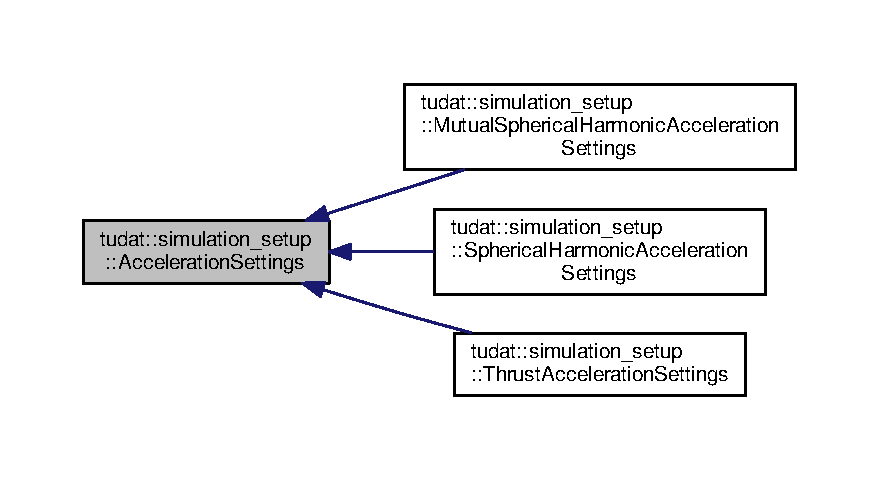
\includegraphics[width=350pt]{classtudat_1_1simulation__setup_1_1AccelerationSettings__inherit__graph}
\end{center}
\end{figure}
\subsection*{Public Member Functions}
\begin{DoxyCompactItemize}
\item 
\hyperlink{classtudat_1_1simulation__setup_1_1AccelerationSettings_a61a6c91bf73a293adb523ebe2b71f379}{Acceleration\+Settings} (const basic\+\_\+astrodynamics\+::\+Available\+Acceleration acceleration\+Type)
\begin{DoxyCompactList}\small\item\em Constructor, sets type of acceleration. \end{DoxyCompactList}\item 
virtual \hyperlink{classtudat_1_1simulation__setup_1_1AccelerationSettings_a66bf9df8526ebaf6ed16a1100811a3ef}{$\sim$\+Acceleration\+Settings} ()\hypertarget{classtudat_1_1simulation__setup_1_1AccelerationSettings_a66bf9df8526ebaf6ed16a1100811a3ef}{}\label{classtudat_1_1simulation__setup_1_1AccelerationSettings_a66bf9df8526ebaf6ed16a1100811a3ef}

\begin{DoxyCompactList}\small\item\em Destructor. \end{DoxyCompactList}\end{DoxyCompactItemize}
\subsection*{Public Attributes}
\begin{DoxyCompactItemize}
\item 
basic\+\_\+astrodynamics\+::\+Available\+Acceleration \hyperlink{classtudat_1_1simulation__setup_1_1AccelerationSettings_aaf1f7742077003cf7055c96ec934e4d8}{acceleration\+Type\+\_\+}\hypertarget{classtudat_1_1simulation__setup_1_1AccelerationSettings_aaf1f7742077003cf7055c96ec934e4d8}{}\label{classtudat_1_1simulation__setup_1_1AccelerationSettings_aaf1f7742077003cf7055c96ec934e4d8}

\begin{DoxyCompactList}\small\item\em Type of acceleration from Available\+Acceleration enum. \end{DoxyCompactList}\end{DoxyCompactItemize}


\subsection{Detailed Description}
Class for providing settings for acceleration model. 

Class for providing settings for acceleration model. This class is a functional (base) class for settings of acceleration models that require no information in addition to their type. Classes defining settings for acceleration models requiring additional information must be derived from this class. Bodies exerting and undergong acceleration are set externally from this class. This class can be used for the easy setup of acceleration models (see \hyperlink{createAccelerationModels_8h_source}{create\+Acceleration\+Models.\+h}), but users may also chose to do so manually. (Derived) Class members are all public, for ease of access and modification. 

\subsection{Constructor \& Destructor Documentation}
\index{tudat\+::simulation\+\_\+setup\+::\+Acceleration\+Settings@{tudat\+::simulation\+\_\+setup\+::\+Acceleration\+Settings}!Acceleration\+Settings@{Acceleration\+Settings}}
\index{Acceleration\+Settings@{Acceleration\+Settings}!tudat\+::simulation\+\_\+setup\+::\+Acceleration\+Settings@{tudat\+::simulation\+\_\+setup\+::\+Acceleration\+Settings}}
\subsubsection[{\texorpdfstring{Acceleration\+Settings(const basic\+\_\+astrodynamics\+::\+Available\+Acceleration acceleration\+Type)}{AccelerationSettings(const basic_astrodynamics::AvailableAcceleration accelerationType)}}]{\setlength{\rightskip}{0pt plus 5cm}tudat\+::simulation\+\_\+setup\+::\+Acceleration\+Settings\+::\+Acceleration\+Settings (
\begin{DoxyParamCaption}
\item[{const basic\+\_\+astrodynamics\+::\+Available\+Acceleration}]{acceleration\+Type}
\end{DoxyParamCaption}
)\hspace{0.3cm}{\ttfamily [inline]}}\hypertarget{classtudat_1_1simulation__setup_1_1AccelerationSettings_a61a6c91bf73a293adb523ebe2b71f379}{}\label{classtudat_1_1simulation__setup_1_1AccelerationSettings_a61a6c91bf73a293adb523ebe2b71f379}


Constructor, sets type of acceleration. 

Constructor, sets type of acceleration. 
\begin{DoxyParams}{Parameters}
{\em acceleration\+Type} & Type of acceleration from Available\+Acceleration enum. \\
\hline
\end{DoxyParams}


The documentation for this class was generated from the following file\+:\begin{DoxyCompactItemize}
\item 
/home/lupi/\+Tudat/tudat\+Bundle/tudat/\+Tudat/\+Simulation\+Setup/\+Propagation\+Setup/acceleration\+Settings.\+h\end{DoxyCompactItemize}

\hypertarget{classtudat_1_1aerodynamics_1_1AerodynamicAcceleration}{}\section{tudat\+:\+:aerodynamics\+:\+:Aerodynamic\+Acceleration Class Reference}
\label{classtudat_1_1aerodynamics_1_1AerodynamicAcceleration}\index{tudat\+::aerodynamics\+::\+Aerodynamic\+Acceleration@{tudat\+::aerodynamics\+::\+Aerodynamic\+Acceleration}}


Class for calculation of aerodynamic accelerations.  




{\ttfamily \#include $<$aerodynamic\+Acceleration.\+h$>$}



Inheritance diagram for tudat\+:\+:aerodynamics\+:\+:Aerodynamic\+Acceleration\+:
\nopagebreak
\begin{figure}[H]
\begin{center}
\leavevmode
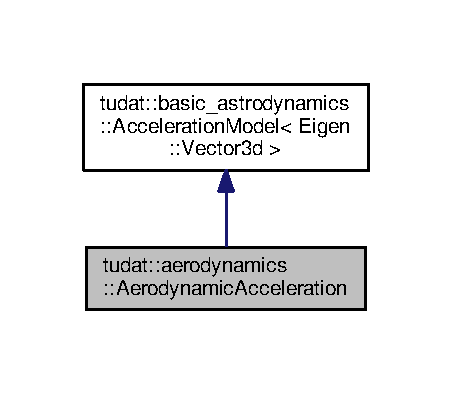
\includegraphics[width=217pt]{classtudat_1_1aerodynamics_1_1AerodynamicAcceleration__inherit__graph}
\end{center}
\end{figure}


Collaboration diagram for tudat\+:\+:aerodynamics\+:\+:Aerodynamic\+Acceleration\+:
\nopagebreak
\begin{figure}[H]
\begin{center}
\leavevmode
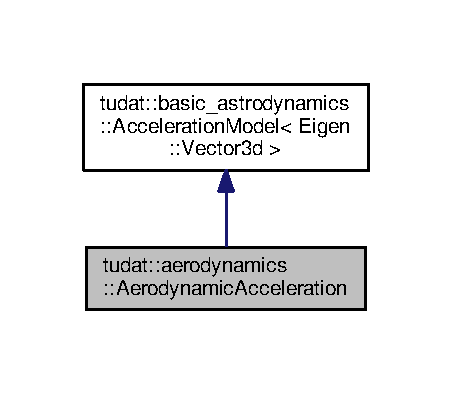
\includegraphics[width=217pt]{classtudat_1_1aerodynamics_1_1AerodynamicAcceleration__coll__graph}
\end{center}
\end{figure}
\subsection*{Public Member Functions}
\begin{DoxyCompactItemize}
\item 
\hyperlink{classtudat_1_1aerodynamics_1_1AerodynamicAcceleration_a2e679984be9d798beaef6705814c8c99}{Aerodynamic\+Acceleration} (const Coefficient\+Returning\+Function coefficient\+Function, const Double\+Returning\+Function density\+Function, const Double\+Returning\+Function air\+Speed\+Function, const double constant\+Mass, const double constant\+Reference\+Area, const bool are\+Coefficients\+In\+Negative\+Direction=true)
\begin{DoxyCompactList}\small\item\em Acceleration model constructor, taking constant values of mass and reference area. \end{DoxyCompactList}\item 
\hyperlink{classtudat_1_1aerodynamics_1_1AerodynamicAcceleration_adb4d7e9bfed9d17207318080ed328332}{Aerodynamic\+Acceleration} (const Coefficient\+Returning\+Function coefficient\+Function, const Double\+Returning\+Function density\+Function, const Double\+Returning\+Function air\+Speed\+Function, const Double\+Returning\+Function mass\+Function, const Double\+Returning\+Function reference\+Area\+Function, const bool are\+Coefficients\+In\+Negative\+Direction=true)
\begin{DoxyCompactList}\small\item\em Acceleration model constructor. \end{DoxyCompactList}\item 
Eigen\+::\+Vector3d \hyperlink{classtudat_1_1aerodynamics_1_1AerodynamicAcceleration_aca8adefed3eede69b980e46d045f46eb}{get\+Acceleration} ()
\begin{DoxyCompactList}\small\item\em Get acceleration. \end{DoxyCompactList}\item 
void \hyperlink{classtudat_1_1aerodynamics_1_1AerodynamicAcceleration_a6cd45319bf7f5b7f376aa9357d1840ea}{update\+Members} (const double current\+Time=T\+U\+D\+A\+T\+\_\+\+N\+AN)
\begin{DoxyCompactList}\small\item\em Update member variables used by the aerodynamic acceleration model. \end{DoxyCompactList}\end{DoxyCompactItemize}
\subsection*{Additional Inherited Members}


\subsection{Detailed Description}
Class for calculation of aerodynamic accelerations. 

Class for calculation of aerodynamic accelerations. \begin{DoxySeeAlso}{See also}
\hyperlink{classtudat_1_1basic__astrodynamics_1_1AccelerationModel_a36f72cf81cc4ff658919a1b92cdc33ad}{Acceleration\+Model}. 
\end{DoxySeeAlso}


\subsection{Constructor \& Destructor Documentation}
\index{tudat\+::aerodynamics\+::\+Aerodynamic\+Acceleration@{tudat\+::aerodynamics\+::\+Aerodynamic\+Acceleration}!Aerodynamic\+Acceleration@{Aerodynamic\+Acceleration}}
\index{Aerodynamic\+Acceleration@{Aerodynamic\+Acceleration}!tudat\+::aerodynamics\+::\+Aerodynamic\+Acceleration@{tudat\+::aerodynamics\+::\+Aerodynamic\+Acceleration}}
\subsubsection[{\texorpdfstring{Aerodynamic\+Acceleration(const Coefficient\+Returning\+Function coefficient\+Function, const Double\+Returning\+Function density\+Function, const Double\+Returning\+Function air\+Speed\+Function, const double constant\+Mass, const double constant\+Reference\+Area, const bool are\+Coefficients\+In\+Negative\+Direction=true)}{AerodynamicAcceleration(const CoefficientReturningFunction coefficientFunction, const DoubleReturningFunction densityFunction, const DoubleReturningFunction airSpeedFunction, const double constantMass, const double constantReferenceArea, const bool areCoefficientsInNegativeDirection=true)}}]{\setlength{\rightskip}{0pt plus 5cm}tudat\+::aerodynamics\+::\+Aerodynamic\+Acceleration\+::\+Aerodynamic\+Acceleration (
\begin{DoxyParamCaption}
\item[{const Coefficient\+Returning\+Function}]{coefficient\+Function, }
\item[{const Double\+Returning\+Function}]{density\+Function, }
\item[{const Double\+Returning\+Function}]{air\+Speed\+Function, }
\item[{const double}]{constant\+Mass, }
\item[{const double}]{constant\+Reference\+Area, }
\item[{const bool}]{are\+Coefficients\+In\+Negative\+Direction = {\ttfamily true}}
\end{DoxyParamCaption}
)\hspace{0.3cm}{\ttfamily [inline]}}\hypertarget{classtudat_1_1aerodynamics_1_1AerodynamicAcceleration_a2e679984be9d798beaef6705814c8c99}{}\label{classtudat_1_1aerodynamics_1_1AerodynamicAcceleration_a2e679984be9d798beaef6705814c8c99}


Acceleration model constructor, taking constant values of mass and reference area. 

Acceleration model constructor, taking constant values of mass and reference area. 
\begin{DoxyParams}{Parameters}
{\em coefficient\+Function} & Function which retrieves current values of aerodynamic coefficients. \\
\hline
{\em density\+Function} & Function which retrieves current value of the density. \\
\hline
{\em air\+Speed\+Function} & Function which retrieves current value of the airspeed. \\
\hline
{\em constant\+Mass} & Value of vehicle mass that is used for all calls of this class. \\
\hline
{\em constant\+Reference\+Area} & Value of aerodynamic coefficient reference area that is used for all calls of this class. \\
\hline
{\em are\+Coefficients\+In\+Negative\+Direction} & Boolean that determines whether to invert direction of aerodynamic coefficients. This is typically done for lift, drag and side force coefficients that point in negative direction in the local frame (default true). \\
\hline
\end{DoxyParams}
\index{tudat\+::aerodynamics\+::\+Aerodynamic\+Acceleration@{tudat\+::aerodynamics\+::\+Aerodynamic\+Acceleration}!Aerodynamic\+Acceleration@{Aerodynamic\+Acceleration}}
\index{Aerodynamic\+Acceleration@{Aerodynamic\+Acceleration}!tudat\+::aerodynamics\+::\+Aerodynamic\+Acceleration@{tudat\+::aerodynamics\+::\+Aerodynamic\+Acceleration}}
\subsubsection[{\texorpdfstring{Aerodynamic\+Acceleration(const Coefficient\+Returning\+Function coefficient\+Function, const Double\+Returning\+Function density\+Function, const Double\+Returning\+Function air\+Speed\+Function, const Double\+Returning\+Function mass\+Function, const Double\+Returning\+Function reference\+Area\+Function, const bool are\+Coefficients\+In\+Negative\+Direction=true)}{AerodynamicAcceleration(const CoefficientReturningFunction coefficientFunction, const DoubleReturningFunction densityFunction, const DoubleReturningFunction airSpeedFunction, const DoubleReturningFunction massFunction, const DoubleReturningFunction referenceAreaFunction, const bool areCoefficientsInNegativeDirection=true)}}]{\setlength{\rightskip}{0pt plus 5cm}tudat\+::aerodynamics\+::\+Aerodynamic\+Acceleration\+::\+Aerodynamic\+Acceleration (
\begin{DoxyParamCaption}
\item[{const Coefficient\+Returning\+Function}]{coefficient\+Function, }
\item[{const Double\+Returning\+Function}]{density\+Function, }
\item[{const Double\+Returning\+Function}]{air\+Speed\+Function, }
\item[{const Double\+Returning\+Function}]{mass\+Function, }
\item[{const Double\+Returning\+Function}]{reference\+Area\+Function, }
\item[{const bool}]{are\+Coefficients\+In\+Negative\+Direction = {\ttfamily true}}
\end{DoxyParamCaption}
)\hspace{0.3cm}{\ttfamily [inline]}}\hypertarget{classtudat_1_1aerodynamics_1_1AerodynamicAcceleration_adb4d7e9bfed9d17207318080ed328332}{}\label{classtudat_1_1aerodynamics_1_1AerodynamicAcceleration_adb4d7e9bfed9d17207318080ed328332}


Acceleration model constructor. 

Acceleration model constructor, taking function pointers for all member variables. 
\begin{DoxyParams}{Parameters}
{\em coefficient\+Function} & Function which retrieves current values of aerodynamic coefficients. \\
\hline
{\em density\+Function} & Function which retrieves current value of the density. \\
\hline
{\em air\+Speed\+Function} & Function which retrieves current value of the airspeed. \\
\hline
{\em mass\+Function} & Function which retrieves current value of the vehicle mass. \\
\hline
{\em reference\+Area\+Function} & Function which retrieves current value of the aerodynamic coefficient reference area. \\
\hline
{\em are\+Coefficients\+In\+Negative\+Direction} & Boolean that determines whether to invert direction of aerodynamic coefficients. This is typically done for lift, drag and side force coefficients that point in negative direction in the local frame (default true). \\
\hline
\end{DoxyParams}


\subsection{Member Function Documentation}
\index{tudat\+::aerodynamics\+::\+Aerodynamic\+Acceleration@{tudat\+::aerodynamics\+::\+Aerodynamic\+Acceleration}!get\+Acceleration@{get\+Acceleration}}
\index{get\+Acceleration@{get\+Acceleration}!tudat\+::aerodynamics\+::\+Aerodynamic\+Acceleration@{tudat\+::aerodynamics\+::\+Aerodynamic\+Acceleration}}
\subsubsection[{\texorpdfstring{get\+Acceleration()}{getAcceleration()}}]{\setlength{\rightskip}{0pt plus 5cm}Eigen\+::\+Vector3d tudat\+::aerodynamics\+::\+Aerodynamic\+Acceleration\+::get\+Acceleration (
\begin{DoxyParamCaption}
{}
\end{DoxyParamCaption}
)\hspace{0.3cm}{\ttfamily [inline]}, {\ttfamily [virtual]}}\hypertarget{classtudat_1_1aerodynamics_1_1AerodynamicAcceleration_aca8adefed3eede69b980e46d045f46eb}{}\label{classtudat_1_1aerodynamics_1_1AerodynamicAcceleration_aca8adefed3eede69b980e46d045f46eb}


Get acceleration. 

Returns the aerodynamic acceleration. All data required for the computation is taken from member variables, which are set to their latest values by the last call of the update\+Members function. The returned acceleration is in the same reference frame as the aerodynamic coefficients, with the coefficients assumed to be in positive direction in the frame. \begin{DoxyReturn}{Returns}
Acceleration. 
\end{DoxyReturn}
\begin{DoxySeeAlso}{See also}
\hyperlink{classtudat_1_1aerodynamics_1_1AerodynamicAcceleration_a6cd45319bf7f5b7f376aa9357d1840ea}{update\+Members()}. 
\end{DoxySeeAlso}


Implements \hyperlink{classtudat_1_1basic__astrodynamics_1_1AccelerationModel_a1f59960bc477fc02e7d52697ced99750}{tudat\+::basic\+\_\+astrodynamics\+::\+Acceleration\+Model$<$ Eigen\+::\+Vector3d $>$}.

\index{tudat\+::aerodynamics\+::\+Aerodynamic\+Acceleration@{tudat\+::aerodynamics\+::\+Aerodynamic\+Acceleration}!update\+Members@{update\+Members}}
\index{update\+Members@{update\+Members}!tudat\+::aerodynamics\+::\+Aerodynamic\+Acceleration@{tudat\+::aerodynamics\+::\+Aerodynamic\+Acceleration}}
\subsubsection[{\texorpdfstring{update\+Members(const double current\+Time=\+T\+U\+D\+A\+T\+\_\+\+N\+A\+N)}{updateMembers(const double currentTime=TUDAT_NAN)}}]{\setlength{\rightskip}{0pt plus 5cm}void tudat\+::aerodynamics\+::\+Aerodynamic\+Acceleration\+::update\+Members (
\begin{DoxyParamCaption}
\item[{const double}]{current\+Time = {\ttfamily TUDAT\+\_\+NAN}}
\end{DoxyParamCaption}
)\hspace{0.3cm}{\ttfamily [inline]}, {\ttfamily [virtual]}}\hypertarget{classtudat_1_1aerodynamics_1_1AerodynamicAcceleration_a6cd45319bf7f5b7f376aa9357d1840ea}{}\label{classtudat_1_1aerodynamics_1_1AerodynamicAcceleration_a6cd45319bf7f5b7f376aa9357d1840ea}


Update member variables used by the aerodynamic acceleration model. 

Updates member variables used by the aerodynamic acceleration model. Function pointers to retrieve the current values of quantities from which the acceleration is to be calculated are set by constructor. This function calls them to update the associated variables to their current state. 
\begin{DoxyParams}{Parameters}
{\em current\+Time} & \hyperlink{classtudat_1_1Time}{Time} at which acceleration model is to be updated. \\
\hline
\end{DoxyParams}


Implements \hyperlink{classtudat_1_1basic__astrodynamics_1_1AccelerationModel_a966e85b72300b8cbc99ba60e40108d71}{tudat\+::basic\+\_\+astrodynamics\+::\+Acceleration\+Model$<$ Eigen\+::\+Vector3d $>$}.



The documentation for this class was generated from the following file\+:\begin{DoxyCompactItemize}
\item 
/home/lupi/\+Tudat/tudat\+Bundle/tudat/\+Tudat/\+Astrodynamics/\+Aerodynamics/aerodynamic\+Acceleration.\+h\end{DoxyCompactItemize}

\hypertarget{classtudat_1_1reference__frames_1_1AerodynamicAngleCalculator}{}\section{tudat\+:\+:reference\+\_\+frames\+:\+:Aerodynamic\+Angle\+Calculator Class Reference}
\label{classtudat_1_1reference__frames_1_1AerodynamicAngleCalculator}\index{tudat\+::reference\+\_\+frames\+::\+Aerodynamic\+Angle\+Calculator@{tudat\+::reference\+\_\+frames\+::\+Aerodynamic\+Angle\+Calculator}}


Object to calculate aerodynamic orientation angles from current vehicle state.  




{\ttfamily \#include $<$aerodynamic\+Angle\+Calculator.\+h$>$}



Inheritance diagram for tudat\+:\+:reference\+\_\+frames\+:\+:Aerodynamic\+Angle\+Calculator\+:
\nopagebreak
\begin{figure}[H]
\begin{center}
\leavevmode
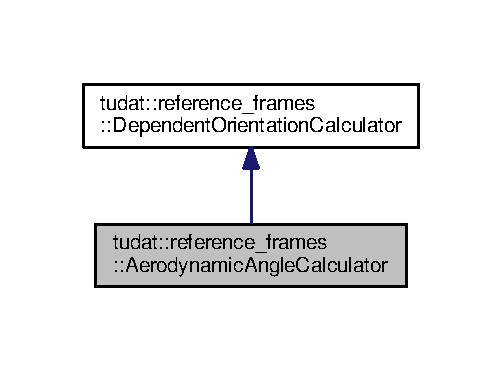
\includegraphics[width=241pt]{classtudat_1_1reference__frames_1_1AerodynamicAngleCalculator__inherit__graph}
\end{center}
\end{figure}


Collaboration diagram for tudat\+:\+:reference\+\_\+frames\+:\+:Aerodynamic\+Angle\+Calculator\+:
\nopagebreak
\begin{figure}[H]
\begin{center}
\leavevmode
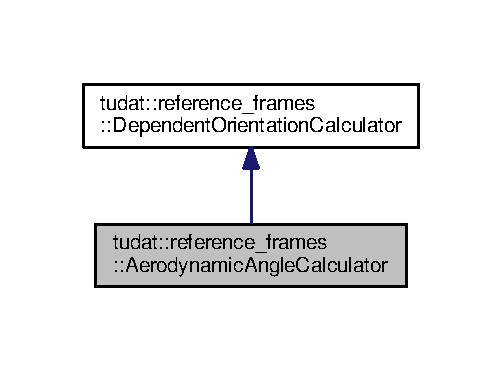
\includegraphics[width=241pt]{classtudat_1_1reference__frames_1_1AerodynamicAngleCalculator__coll__graph}
\end{center}
\end{figure}
\subsection*{Public Member Functions}
\begin{DoxyCompactItemize}
\item 
\hyperlink{classtudat_1_1reference__frames_1_1AerodynamicAngleCalculator_a191c7666c72fc3fdb68f888fd33700cc}{Aerodynamic\+Angle\+Calculator} (const boost\+::function$<$ Eigen\+::\+Vector6d() $>$ body\+Fixed\+State\+Function, const boost\+::function$<$ Eigen\+::\+Quaterniond() $>$ rotation\+From\+Corotating\+To\+Inertial\+Frame, const std\+::string central\+Body\+Name, const bool calculate\+Vertical\+To\+Aerodynamic\+Frame=0, const boost\+::function$<$ double() $>$ angle\+Of\+Attack\+Function=boost\+::function$<$ double() $>$(), const boost\+::function$<$ double() $>$ angle\+Of\+Sideslip\+Function=boost\+::function$<$ double() $>$(), const boost\+::function$<$ double() $>$ bank\+Angle\+Function=boost\+::function$<$ double() $>$(), const boost\+::function$<$ void(const double) $>$ angle\+Update\+Function=boost\+::function$<$ void(const double) $>$())
\begin{DoxyCompactList}\small\item\em Constructor. \end{DoxyCompactList}\item 
Eigen\+::\+Quaterniond \hyperlink{classtudat_1_1reference__frames_1_1AerodynamicAngleCalculator_ae8de3add4e5d89be447eb707f17fbd13}{get\+Rotation\+To\+Local\+Frame} ()
\begin{DoxyCompactList}\small\item\em Function to get the current rotation from the global (propagation/inertial) to the local (body-\/fixed) frame. \end{DoxyCompactList}\item 
Eigen\+::\+Quaterniond \hyperlink{classtudat_1_1reference__frames_1_1AerodynamicAngleCalculator_ae7b951843ce6578117c64db9c7a54720}{get\+Rotation\+To\+Global\+Frame} ()
\begin{DoxyCompactList}\small\item\em Function to get the current rotation from the local (body-\/fixed) to the global (propagation/inertial) frame. \end{DoxyCompactList}\item 
void \hyperlink{classtudat_1_1reference__frames_1_1AerodynamicAngleCalculator_aceb968e26cbe6d3f40590c4f7faeba21}{update\+Calculator} (const double current\+Time)
\begin{DoxyCompactList}\small\item\em Function to update the orientation angles to the current state. \end{DoxyCompactList}\item 
void \hyperlink{classtudat_1_1reference__frames_1_1AerodynamicAngleCalculator_acdeec390f822d521bcb3c09168da5a57}{update} (const double current\+Time, const bool update\+Body\+Orientation)
\begin{DoxyCompactList}\small\item\em Function to update the orientation angles to the current state. \end{DoxyCompactList}\item 
Eigen\+::\+Quaterniond \hyperlink{classtudat_1_1reference__frames_1_1AerodynamicAngleCalculator_a589f1ac87019bd9ec7cebb366fc7a700}{get\+Rotation\+Quaternion\+Between\+Frames} (const Aerodynamics\+Reference\+Frames original\+Frame, const Aerodynamics\+Reference\+Frames target\+Frame)
\begin{DoxyCompactList}\small\item\em Function to get the rotation quaternion between two frames. \end{DoxyCompactList}\item 
double \hyperlink{classtudat_1_1reference__frames_1_1AerodynamicAngleCalculator_adf020e81f7cc48e456d133670c087671}{get\+Aerodynamic\+Angle} (const Aerodynamics\+Reference\+Frame\+Angles angle\+Id)
\begin{DoxyCompactList}\small\item\em Function to get a single orientation angle. \end{DoxyCompactList}\item 
void \hyperlink{classtudat_1_1reference__frames_1_1AerodynamicAngleCalculator_a9250572fd17abf1079f2a2c9a14480d1}{set\+Orientation\+Angle\+Functions} (const boost\+::function$<$ double() $>$ angle\+Of\+Attack\+Function=boost\+::function$<$ double() $>$(), const boost\+::function$<$ double() $>$ angle\+Of\+Sideslip\+Function=boost\+::function$<$ double() $>$(), const boost\+::function$<$ double() $>$ bank\+Angle\+Function=boost\+::function$<$ double() $>$(), const boost\+::function$<$ void(const double) $>$ angle\+Update\+Function=boost\+::function$<$ void(const double) $>$())
\begin{DoxyCompactList}\small\item\em Function to set the trajectory$<$-\/$>$body-\/fixed orientation angles. \end{DoxyCompactList}\item 
void \hyperlink{classtudat_1_1reference__frames_1_1AerodynamicAngleCalculator_a7c2ca8de8fe95544225c74e6f26a975e}{set\+Orientation\+Angle\+Functions} (const double angle\+Of\+Attack=T\+U\+D\+A\+T\+\_\+\+N\+AN, const double angle\+Of\+Sideslip=T\+U\+D\+A\+T\+\_\+\+N\+AN, const double bank\+Angle=T\+U\+D\+A\+T\+\_\+\+N\+AN)
\begin{DoxyCompactList}\small\item\em Function to set constant trajectory$<$-\/$>$body-\/fixed orientation angles. \end{DoxyCompactList}\item 
boost\+::function$<$ Eigen\+::\+Quaterniond() $>$ \hyperlink{classtudat_1_1reference__frames_1_1AerodynamicAngleCalculator_ac33bcade09603d504123a5200348752b}{get\+Rotation\+From\+Corotating\+To\+Inertial\+Frame} ()
\begin{DoxyCompactList}\small\item\em Function to get the function returning the quaternion that rotates from the corotating to the inertial frame. \end{DoxyCompactList}\item 
std\+::string \hyperlink{classtudat_1_1reference__frames_1_1AerodynamicAngleCalculator_a9929cecdca0cfc997f41f8fd1bf6d1ad}{get\+Central\+Body\+Name} ()
\begin{DoxyCompactList}\small\item\em Function to get the name of central body w.\+r.\+t. which the angles are computed. \end{DoxyCompactList}\item 
Eigen\+::\+Vector6d \hyperlink{classtudat_1_1reference__frames_1_1AerodynamicAngleCalculator_acb987f236459228bf4c3248a4bebe18d}{get\+Current\+Body\+Fixed\+State} ()
\begin{DoxyCompactList}\small\item\em Function to get the current body-\/fixed state of vehicle, as set by previous call to \hyperlink{classtudat_1_1reference__frames_1_1AerodynamicAngleCalculator_acdeec390f822d521bcb3c09168da5a57}{update( )}. \end{DoxyCompactList}\item 
void \hyperlink{classtudat_1_1reference__frames_1_1AerodynamicAngleCalculator_af68c8b73b9ec1e17d6e36cadd525e633}{reset\+Derived\+Class\+Time} (const double current\+Time=T\+U\+D\+A\+T\+\_\+\+N\+AN)
\begin{DoxyCompactList}\small\item\em Function to reset the value of the current\+Body\+Angle\+Time\+\_\+ variable. \end{DoxyCompactList}\end{DoxyCompactItemize}
\subsection*{Additional Inherited Members}


\subsection{Detailed Description}
Object to calculate aerodynamic orientation angles from current vehicle state. 

Object to calculate aerodynamic orientation angles from current vehicle state. 

\subsection{Constructor \& Destructor Documentation}
\index{tudat\+::reference\+\_\+frames\+::\+Aerodynamic\+Angle\+Calculator@{tudat\+::reference\+\_\+frames\+::\+Aerodynamic\+Angle\+Calculator}!Aerodynamic\+Angle\+Calculator@{Aerodynamic\+Angle\+Calculator}}
\index{Aerodynamic\+Angle\+Calculator@{Aerodynamic\+Angle\+Calculator}!tudat\+::reference\+\_\+frames\+::\+Aerodynamic\+Angle\+Calculator@{tudat\+::reference\+\_\+frames\+::\+Aerodynamic\+Angle\+Calculator}}
\subsubsection[{\texorpdfstring{Aerodynamic\+Angle\+Calculator(const boost\+::function$<$ Eigen\+::\+Vector6d() $>$ body\+Fixed\+State\+Function, const boost\+::function$<$ Eigen\+::\+Quaterniond() $>$ rotation\+From\+Corotating\+To\+Inertial\+Frame, const std\+::string central\+Body\+Name, const bool calculate\+Vertical\+To\+Aerodynamic\+Frame=0, const boost\+::function$<$ double() $>$ angle\+Of\+Attack\+Function=boost\+::function$<$ double() $>$(), const boost\+::function$<$ double() $>$ angle\+Of\+Sideslip\+Function=boost\+::function$<$ double() $>$(), const boost\+::function$<$ double() $>$ bank\+Angle\+Function=boost\+::function$<$ double() $>$(), const boost\+::function$<$ void(const double) $>$ angle\+Update\+Function=boost\+::function$<$ void(const double) $>$())}{AerodynamicAngleCalculator(const boost::function< Eigen::Vector6d() > bodyFixedStateFunction, const boost::function< Eigen::Quaterniond() > rotationFromCorotatingToInertialFrame, const std::string centralBodyName, const bool calculateVerticalToAerodynamicFrame=0, const boost::function< double() > angleOfAttackFunction=boost::function< double() >(), const boost::function< double() > angleOfSideslipFunction=boost::function< double() >(), const boost::function< double() > bankAngleFunction=boost::function< double() >(), const boost::function< void(const double) > angleUpdateFunction=boost::function< void(const double) >())}}]{\setlength{\rightskip}{0pt plus 5cm}tudat\+::reference\+\_\+frames\+::\+Aerodynamic\+Angle\+Calculator\+::\+Aerodynamic\+Angle\+Calculator (
\begin{DoxyParamCaption}
\item[{const boost\+::function$<$ Eigen\+::\+Vector6d() $>$}]{body\+Fixed\+State\+Function, }
\item[{const boost\+::function$<$ Eigen\+::\+Quaterniond() $>$}]{rotation\+From\+Corotating\+To\+Inertial\+Frame, }
\item[{const std\+::string}]{central\+Body\+Name, }
\item[{const bool}]{calculate\+Vertical\+To\+Aerodynamic\+Frame = {\ttfamily 0}, }
\item[{const boost\+::function$<$ double() $>$}]{angle\+Of\+Attack\+Function = {\ttfamily boost\+:\+:function$<$~double(~)~$>$(~)}, }
\item[{const boost\+::function$<$ double() $>$}]{angle\+Of\+Sideslip\+Function = {\ttfamily boost\+:\+:function$<$~double(~)~$>$(~)}, }
\item[{const boost\+::function$<$ double() $>$}]{bank\+Angle\+Function = {\ttfamily boost\+:\+:function$<$~double(~)~$>$(~)}, }
\item[{const boost\+::function$<$ void(const double) $>$}]{angle\+Update\+Function = {\ttfamily boost\+:\+:function$<$~void(~const~double~)~$>$(~)}}
\end{DoxyParamCaption}
)\hspace{0.3cm}{\ttfamily [inline]}}\hypertarget{classtudat_1_1reference__frames_1_1AerodynamicAngleCalculator_a191c7666c72fc3fdb68f888fd33700cc}{}\label{classtudat_1_1reference__frames_1_1AerodynamicAngleCalculator_a191c7666c72fc3fdb68f888fd33700cc}


Constructor. 

Constructor. 
\begin{DoxyParams}{Parameters}
{\em body\+Fixed\+State\+Function} & Vehicle state in a frame fixed w.\+r.\+t. the central body. Note that this state is w.\+r.\+t. the body itself, not w.\+r.\+t. the local atmosphere. \\
\hline
{\em rotation\+From\+Corotating\+To\+Inertial\+Frame} & Function returning the quaternion that rotates from the corotating to the inertial frame. \\
\hline
{\em central\+Body\+Name} & Name of central body w.\+r.\+t. which the angles are computed. \\
\hline
{\em calculate\+Vertical\+To\+Aerodynamic\+Frame} & Boolean to determine whether to determine vertical $<$-\/$>$ aerodynamic frame conversion when calling update function. \\
\hline
{\em angle\+Of\+Attack\+Function} & Function to determine the angle of attack of the vehicle. \\
\hline
{\em angle\+Of\+Sideslip\+Function} & Function to determine the angle of sideslip of the vehicle. \\
\hline
{\em bank\+Angle\+Function} & Function to determine the bank angle of the vehicle. \\
\hline
{\em angle\+Update\+Function} & Function to update the aerodynamic angles to the current time (default none). \\
\hline
\end{DoxyParams}


\subsection{Member Function Documentation}
\index{tudat\+::reference\+\_\+frames\+::\+Aerodynamic\+Angle\+Calculator@{tudat\+::reference\+\_\+frames\+::\+Aerodynamic\+Angle\+Calculator}!get\+Aerodynamic\+Angle@{get\+Aerodynamic\+Angle}}
\index{get\+Aerodynamic\+Angle@{get\+Aerodynamic\+Angle}!tudat\+::reference\+\_\+frames\+::\+Aerodynamic\+Angle\+Calculator@{tudat\+::reference\+\_\+frames\+::\+Aerodynamic\+Angle\+Calculator}}
\subsubsection[{\texorpdfstring{get\+Aerodynamic\+Angle(const Aerodynamics\+Reference\+Frame\+Angles angle\+Id)}{getAerodynamicAngle(const AerodynamicsReferenceFrameAngles angleId)}}]{\setlength{\rightskip}{0pt plus 5cm}double tudat\+::reference\+\_\+frames\+::\+Aerodynamic\+Angle\+Calculator\+::get\+Aerodynamic\+Angle (
\begin{DoxyParamCaption}
\item[{const Aerodynamics\+Reference\+Frame\+Angles}]{angle\+Id}
\end{DoxyParamCaption}
)}\hypertarget{classtudat_1_1reference__frames_1_1AerodynamicAngleCalculator_adf020e81f7cc48e456d133670c087671}{}\label{classtudat_1_1reference__frames_1_1AerodynamicAngleCalculator_adf020e81f7cc48e456d133670c087671}


Function to get a single orientation angle. 

Function to get a single orientation angle, as calculated by previous call to \hyperlink{classtudat_1_1reference__frames_1_1AerodynamicAngleCalculator_acdeec390f822d521bcb3c09168da5a57}{update( )} function. 
\begin{DoxyParams}{Parameters}
{\em angle\+Id} & Id of requested angle. \\
\hline
\end{DoxyParams}
\begin{DoxyReturn}{Returns}
Value of requested angle. 
\end{DoxyReturn}
\index{tudat\+::reference\+\_\+frames\+::\+Aerodynamic\+Angle\+Calculator@{tudat\+::reference\+\_\+frames\+::\+Aerodynamic\+Angle\+Calculator}!get\+Central\+Body\+Name@{get\+Central\+Body\+Name}}
\index{get\+Central\+Body\+Name@{get\+Central\+Body\+Name}!tudat\+::reference\+\_\+frames\+::\+Aerodynamic\+Angle\+Calculator@{tudat\+::reference\+\_\+frames\+::\+Aerodynamic\+Angle\+Calculator}}
\subsubsection[{\texorpdfstring{get\+Central\+Body\+Name()}{getCentralBodyName()}}]{\setlength{\rightskip}{0pt plus 5cm}std\+::string tudat\+::reference\+\_\+frames\+::\+Aerodynamic\+Angle\+Calculator\+::get\+Central\+Body\+Name (
\begin{DoxyParamCaption}
{}
\end{DoxyParamCaption}
)\hspace{0.3cm}{\ttfamily [inline]}}\hypertarget{classtudat_1_1reference__frames_1_1AerodynamicAngleCalculator_a9929cecdca0cfc997f41f8fd1bf6d1ad}{}\label{classtudat_1_1reference__frames_1_1AerodynamicAngleCalculator_a9929cecdca0cfc997f41f8fd1bf6d1ad}


Function to get the name of central body w.\+r.\+t. which the angles are computed. 

Function to get the name of central body w.\+r.\+t. which the angles are computed. \begin{DoxyReturn}{Returns}
Name of central body w.\+r.\+t. which the angles are computed. 
\end{DoxyReturn}
\index{tudat\+::reference\+\_\+frames\+::\+Aerodynamic\+Angle\+Calculator@{tudat\+::reference\+\_\+frames\+::\+Aerodynamic\+Angle\+Calculator}!get\+Current\+Body\+Fixed\+State@{get\+Current\+Body\+Fixed\+State}}
\index{get\+Current\+Body\+Fixed\+State@{get\+Current\+Body\+Fixed\+State}!tudat\+::reference\+\_\+frames\+::\+Aerodynamic\+Angle\+Calculator@{tudat\+::reference\+\_\+frames\+::\+Aerodynamic\+Angle\+Calculator}}
\subsubsection[{\texorpdfstring{get\+Current\+Body\+Fixed\+State()}{getCurrentBodyFixedState()}}]{\setlength{\rightskip}{0pt plus 5cm}Eigen\+::\+Vector6d tudat\+::reference\+\_\+frames\+::\+Aerodynamic\+Angle\+Calculator\+::get\+Current\+Body\+Fixed\+State (
\begin{DoxyParamCaption}
{}
\end{DoxyParamCaption}
)\hspace{0.3cm}{\ttfamily [inline]}}\hypertarget{classtudat_1_1reference__frames_1_1AerodynamicAngleCalculator_acb987f236459228bf4c3248a4bebe18d}{}\label{classtudat_1_1reference__frames_1_1AerodynamicAngleCalculator_acb987f236459228bf4c3248a4bebe18d}


Function to get the current body-\/fixed state of vehicle, as set by previous call to \hyperlink{classtudat_1_1reference__frames_1_1AerodynamicAngleCalculator_acdeec390f822d521bcb3c09168da5a57}{update( )}. 

Function to get the current body-\/fixed state of vehicle, as set by previous call to \hyperlink{classtudat_1_1reference__frames_1_1AerodynamicAngleCalculator_acdeec390f822d521bcb3c09168da5a57}{update( )}. \begin{DoxyReturn}{Returns}
Current body-\/fixed state of vehicle, as set by previous call to \hyperlink{classtudat_1_1reference__frames_1_1AerodynamicAngleCalculator_acdeec390f822d521bcb3c09168da5a57}{update( )}. 
\end{DoxyReturn}
\index{tudat\+::reference\+\_\+frames\+::\+Aerodynamic\+Angle\+Calculator@{tudat\+::reference\+\_\+frames\+::\+Aerodynamic\+Angle\+Calculator}!get\+Rotation\+From\+Corotating\+To\+Inertial\+Frame@{get\+Rotation\+From\+Corotating\+To\+Inertial\+Frame}}
\index{get\+Rotation\+From\+Corotating\+To\+Inertial\+Frame@{get\+Rotation\+From\+Corotating\+To\+Inertial\+Frame}!tudat\+::reference\+\_\+frames\+::\+Aerodynamic\+Angle\+Calculator@{tudat\+::reference\+\_\+frames\+::\+Aerodynamic\+Angle\+Calculator}}
\subsubsection[{\texorpdfstring{get\+Rotation\+From\+Corotating\+To\+Inertial\+Frame()}{getRotationFromCorotatingToInertialFrame()}}]{\setlength{\rightskip}{0pt plus 5cm}boost\+::function$<$ Eigen\+::\+Quaterniond( ) $>$ tudat\+::reference\+\_\+frames\+::\+Aerodynamic\+Angle\+Calculator\+::get\+Rotation\+From\+Corotating\+To\+Inertial\+Frame (
\begin{DoxyParamCaption}
{}
\end{DoxyParamCaption}
)\hspace{0.3cm}{\ttfamily [inline]}}\hypertarget{classtudat_1_1reference__frames_1_1AerodynamicAngleCalculator_ac33bcade09603d504123a5200348752b}{}\label{classtudat_1_1reference__frames_1_1AerodynamicAngleCalculator_ac33bcade09603d504123a5200348752b}


Function to get the function returning the quaternion that rotates from the corotating to the inertial frame. 

Function to get the function returning the quaternion that rotates from the corotating to the inertial frame. \begin{DoxyReturn}{Returns}
Function returning the quaternion that rotates from the corotating to the inertial frame. 
\end{DoxyReturn}
\index{tudat\+::reference\+\_\+frames\+::\+Aerodynamic\+Angle\+Calculator@{tudat\+::reference\+\_\+frames\+::\+Aerodynamic\+Angle\+Calculator}!get\+Rotation\+Quaternion\+Between\+Frames@{get\+Rotation\+Quaternion\+Between\+Frames}}
\index{get\+Rotation\+Quaternion\+Between\+Frames@{get\+Rotation\+Quaternion\+Between\+Frames}!tudat\+::reference\+\_\+frames\+::\+Aerodynamic\+Angle\+Calculator@{tudat\+::reference\+\_\+frames\+::\+Aerodynamic\+Angle\+Calculator}}
\subsubsection[{\texorpdfstring{get\+Rotation\+Quaternion\+Between\+Frames(const Aerodynamics\+Reference\+Frames original\+Frame, const Aerodynamics\+Reference\+Frames target\+Frame)}{getRotationQuaternionBetweenFrames(const AerodynamicsReferenceFrames originalFrame, const AerodynamicsReferenceFrames targetFrame)}}]{\setlength{\rightskip}{0pt plus 5cm}Eigen\+::\+Quaterniond tudat\+::reference\+\_\+frames\+::\+Aerodynamic\+Angle\+Calculator\+::get\+Rotation\+Quaternion\+Between\+Frames (
\begin{DoxyParamCaption}
\item[{const Aerodynamics\+Reference\+Frames}]{original\+Frame, }
\item[{const Aerodynamics\+Reference\+Frames}]{target\+Frame}
\end{DoxyParamCaption}
)}\hypertarget{classtudat_1_1reference__frames_1_1AerodynamicAngleCalculator_a589f1ac87019bd9ec7cebb366fc7a700}{}\label{classtudat_1_1reference__frames_1_1AerodynamicAngleCalculator_a589f1ac87019bd9ec7cebb366fc7a700}


Function to get the rotation quaternion between two frames. 

Function to get the rotation quaternion between two frames. This function uses the values calculated by the previous call of the \hyperlink{classtudat_1_1reference__frames_1_1AerodynamicAngleCalculator_acdeec390f822d521bcb3c09168da5a57}{update( )} function. 
\begin{DoxyParams}{Parameters}
{\em original\+Frame} & Id for \textquotesingle{}current\textquotesingle{} frame \\
\hline
{\em target\+Frame} & Id for frame to which transformation object should transfrom a vector (from original\+Frame). \\
\hline
\end{DoxyParams}
\begin{DoxyReturn}{Returns}
Rotation quaternion from original\+Frame to target\+Frame. 
\end{DoxyReturn}
\index{tudat\+::reference\+\_\+frames\+::\+Aerodynamic\+Angle\+Calculator@{tudat\+::reference\+\_\+frames\+::\+Aerodynamic\+Angle\+Calculator}!get\+Rotation\+To\+Global\+Frame@{get\+Rotation\+To\+Global\+Frame}}
\index{get\+Rotation\+To\+Global\+Frame@{get\+Rotation\+To\+Global\+Frame}!tudat\+::reference\+\_\+frames\+::\+Aerodynamic\+Angle\+Calculator@{tudat\+::reference\+\_\+frames\+::\+Aerodynamic\+Angle\+Calculator}}
\subsubsection[{\texorpdfstring{get\+Rotation\+To\+Global\+Frame()}{getRotationToGlobalFrame()}}]{\setlength{\rightskip}{0pt plus 5cm}Eigen\+::\+Quaterniond tudat\+::reference\+\_\+frames\+::\+Aerodynamic\+Angle\+Calculator\+::get\+Rotation\+To\+Global\+Frame (
\begin{DoxyParamCaption}
{}
\end{DoxyParamCaption}
)\hspace{0.3cm}{\ttfamily [inline]}, {\ttfamily [virtual]}}\hypertarget{classtudat_1_1reference__frames_1_1AerodynamicAngleCalculator_ae7b951843ce6578117c64db9c7a54720}{}\label{classtudat_1_1reference__frames_1_1AerodynamicAngleCalculator_ae7b951843ce6578117c64db9c7a54720}


Function to get the current rotation from the local (body-\/fixed) to the global (propagation/inertial) frame. 

Function to get the current rotation from the local (body-\/fixed) to the global (propagation/inertial) frame. Implementation of pure virtual base class function, calls get\+Rotation\+Quaternion\+Between\+Frames function. \begin{DoxyReturn}{Returns}
Current rotation from the local (body-\/fixed) to the global (propagation/inertial) frame. 
\end{DoxyReturn}


Implements \hyperlink{classtudat_1_1reference__frames_1_1DependentOrientationCalculator_a1b34033b2b7a0a65fa88482b3cbb46af}{tudat\+::reference\+\_\+frames\+::\+Dependent\+Orientation\+Calculator}.

\index{tudat\+::reference\+\_\+frames\+::\+Aerodynamic\+Angle\+Calculator@{tudat\+::reference\+\_\+frames\+::\+Aerodynamic\+Angle\+Calculator}!get\+Rotation\+To\+Local\+Frame@{get\+Rotation\+To\+Local\+Frame}}
\index{get\+Rotation\+To\+Local\+Frame@{get\+Rotation\+To\+Local\+Frame}!tudat\+::reference\+\_\+frames\+::\+Aerodynamic\+Angle\+Calculator@{tudat\+::reference\+\_\+frames\+::\+Aerodynamic\+Angle\+Calculator}}
\subsubsection[{\texorpdfstring{get\+Rotation\+To\+Local\+Frame()}{getRotationToLocalFrame()}}]{\setlength{\rightskip}{0pt plus 5cm}Eigen\+::\+Quaterniond tudat\+::reference\+\_\+frames\+::\+Aerodynamic\+Angle\+Calculator\+::get\+Rotation\+To\+Local\+Frame (
\begin{DoxyParamCaption}
{}
\end{DoxyParamCaption}
)\hspace{0.3cm}{\ttfamily [inline]}, {\ttfamily [virtual]}}\hypertarget{classtudat_1_1reference__frames_1_1AerodynamicAngleCalculator_ae8de3add4e5d89be447eb707f17fbd13}{}\label{classtudat_1_1reference__frames_1_1AerodynamicAngleCalculator_ae8de3add4e5d89be447eb707f17fbd13}


Function to get the current rotation from the global (propagation/inertial) to the local (body-\/fixed) frame. 

Function to get the current rotation from the global (propagation/inertial) to the local (body-\/fixed) frame. Implementation of pure virtual base class function, calls get\+Rotation\+Quaternion\+Between\+Frames function. \begin{DoxyReturn}{Returns}
Current rotation from the global (propagation/inertial) to the local (body-\/fixed) frame. 
\end{DoxyReturn}


Implements \hyperlink{classtudat_1_1reference__frames_1_1DependentOrientationCalculator_ae55893820994179e02ec6189cd9fb00b}{tudat\+::reference\+\_\+frames\+::\+Dependent\+Orientation\+Calculator}.

\index{tudat\+::reference\+\_\+frames\+::\+Aerodynamic\+Angle\+Calculator@{tudat\+::reference\+\_\+frames\+::\+Aerodynamic\+Angle\+Calculator}!reset\+Derived\+Class\+Time@{reset\+Derived\+Class\+Time}}
\index{reset\+Derived\+Class\+Time@{reset\+Derived\+Class\+Time}!tudat\+::reference\+\_\+frames\+::\+Aerodynamic\+Angle\+Calculator@{tudat\+::reference\+\_\+frames\+::\+Aerodynamic\+Angle\+Calculator}}
\subsubsection[{\texorpdfstring{reset\+Derived\+Class\+Time(const double current\+Time=\+T\+U\+D\+A\+T\+\_\+\+N\+A\+N)}{resetDerivedClassTime(const double currentTime=TUDAT_NAN)}}]{\setlength{\rightskip}{0pt plus 5cm}void tudat\+::reference\+\_\+frames\+::\+Aerodynamic\+Angle\+Calculator\+::reset\+Derived\+Class\+Time (
\begin{DoxyParamCaption}
\item[{const double}]{current\+Time = {\ttfamily TUDAT\+\_\+NAN}}
\end{DoxyParamCaption}
)\hspace{0.3cm}{\ttfamily [inline]}, {\ttfamily [virtual]}}\hypertarget{classtudat_1_1reference__frames_1_1AerodynamicAngleCalculator_af68c8b73b9ec1e17d6e36cadd525e633}{}\label{classtudat_1_1reference__frames_1_1AerodynamicAngleCalculator_af68c8b73b9ec1e17d6e36cadd525e633}


Function to reset the value of the current\+Body\+Angle\+Time\+\_\+ variable. 

Function to reset the value of the current\+Body\+Angle\+Time\+\_\+ variable. Typically used to reset the time to NaN, signalling the need to recompute all quantities upon the next relevant function call. 
\begin{DoxyParams}{Parameters}
{\em current\+Time} & New current time. \\
\hline
\end{DoxyParams}


Reimplemented from \hyperlink{classtudat_1_1reference__frames_1_1DependentOrientationCalculator_adc03930adf46bdc8cb9702d0f62055c1}{tudat\+::reference\+\_\+frames\+::\+Dependent\+Orientation\+Calculator}.

\index{tudat\+::reference\+\_\+frames\+::\+Aerodynamic\+Angle\+Calculator@{tudat\+::reference\+\_\+frames\+::\+Aerodynamic\+Angle\+Calculator}!set\+Orientation\+Angle\+Functions@{set\+Orientation\+Angle\+Functions}}
\index{set\+Orientation\+Angle\+Functions@{set\+Orientation\+Angle\+Functions}!tudat\+::reference\+\_\+frames\+::\+Aerodynamic\+Angle\+Calculator@{tudat\+::reference\+\_\+frames\+::\+Aerodynamic\+Angle\+Calculator}}
\subsubsection[{\texorpdfstring{set\+Orientation\+Angle\+Functions(const boost\+::function$<$ double() $>$ angle\+Of\+Attack\+Function=boost\+::function$<$ double() $>$(), const boost\+::function$<$ double() $>$ angle\+Of\+Sideslip\+Function=boost\+::function$<$ double() $>$(), const boost\+::function$<$ double() $>$ bank\+Angle\+Function=boost\+::function$<$ double() $>$(), const boost\+::function$<$ void(const double) $>$ angle\+Update\+Function=boost\+::function$<$ void(const double) $>$())}{setOrientationAngleFunctions(const boost::function< double() > angleOfAttackFunction=boost::function< double() >(), const boost::function< double() > angleOfSideslipFunction=boost::function< double() >(), const boost::function< double() > bankAngleFunction=boost::function< double() >(), const boost::function< void(const double) > angleUpdateFunction=boost::function< void(const double) >())}}]{\setlength{\rightskip}{0pt plus 5cm}void tudat\+::reference\+\_\+frames\+::\+Aerodynamic\+Angle\+Calculator\+::set\+Orientation\+Angle\+Functions (
\begin{DoxyParamCaption}
\item[{const boost\+::function$<$ double() $>$}]{angle\+Of\+Attack\+Function = {\ttfamily boost\+:\+:function$<$~double(~)~$>$(~)}, }
\item[{const boost\+::function$<$ double() $>$}]{angle\+Of\+Sideslip\+Function = {\ttfamily boost\+:\+:function$<$~double(~)~$>$(~)}, }
\item[{const boost\+::function$<$ double() $>$}]{bank\+Angle\+Function = {\ttfamily boost\+:\+:function$<$~double(~)~$>$(~)}, }
\item[{const boost\+::function$<$ void(const double) $>$}]{angle\+Update\+Function = {\ttfamily boost\+:\+:function$<$~void(~const~double~)~$>$(~)}}
\end{DoxyParamCaption}
)}\hypertarget{classtudat_1_1reference__frames_1_1AerodynamicAngleCalculator_a9250572fd17abf1079f2a2c9a14480d1}{}\label{classtudat_1_1reference__frames_1_1AerodynamicAngleCalculator_a9250572fd17abf1079f2a2c9a14480d1}


Function to set the trajectory$<$-\/$>$body-\/fixed orientation angles. 

Function to set the trajectory$<$-\/$>$body-\/fixed orientation angles. 
\begin{DoxyParams}{Parameters}
{\em angle\+Of\+Attack\+Function} & Function to return the angle of attack. \\
\hline
{\em angle\+Of\+Sideslip\+Function} & Function to return the angle of sideslip. \\
\hline
{\em bank\+Angle\+Function} & Function to return the bank angle. \\
\hline
{\em angle\+Update\+Function} & Function to update the angles to the current time. \\
\hline
\end{DoxyParams}
\index{tudat\+::reference\+\_\+frames\+::\+Aerodynamic\+Angle\+Calculator@{tudat\+::reference\+\_\+frames\+::\+Aerodynamic\+Angle\+Calculator}!set\+Orientation\+Angle\+Functions@{set\+Orientation\+Angle\+Functions}}
\index{set\+Orientation\+Angle\+Functions@{set\+Orientation\+Angle\+Functions}!tudat\+::reference\+\_\+frames\+::\+Aerodynamic\+Angle\+Calculator@{tudat\+::reference\+\_\+frames\+::\+Aerodynamic\+Angle\+Calculator}}
\subsubsection[{\texorpdfstring{set\+Orientation\+Angle\+Functions(const double angle\+Of\+Attack=\+T\+U\+D\+A\+T\+\_\+\+N\+A\+N, const double angle\+Of\+Sideslip=\+T\+U\+D\+A\+T\+\_\+\+N\+A\+N, const double bank\+Angle=\+T\+U\+D\+A\+T\+\_\+\+N\+A\+N)}{setOrientationAngleFunctions(const double angleOfAttack=TUDAT_NAN, const double angleOfSideslip=TUDAT_NAN, const double bankAngle=TUDAT_NAN)}}]{\setlength{\rightskip}{0pt plus 5cm}void tudat\+::reference\+\_\+frames\+::\+Aerodynamic\+Angle\+Calculator\+::set\+Orientation\+Angle\+Functions (
\begin{DoxyParamCaption}
\item[{const double}]{angle\+Of\+Attack = {\ttfamily TUDAT\+\_\+NAN}, }
\item[{const double}]{angle\+Of\+Sideslip = {\ttfamily TUDAT\+\_\+NAN}, }
\item[{const double}]{bank\+Angle = {\ttfamily TUDAT\+\_\+NAN}}
\end{DoxyParamCaption}
)}\hypertarget{classtudat_1_1reference__frames_1_1AerodynamicAngleCalculator_a7c2ca8de8fe95544225c74e6f26a975e}{}\label{classtudat_1_1reference__frames_1_1AerodynamicAngleCalculator_a7c2ca8de8fe95544225c74e6f26a975e}


Function to set constant trajectory$<$-\/$>$body-\/fixed orientation angles. 

Function to set constant trajectory$<$-\/$>$body-\/fixed orientation angles. 
\begin{DoxyParams}{Parameters}
{\em angle\+Of\+Attack} & Constant angle of attack (default NaN, used if no angle is to be defined). \\
\hline
{\em angle\+Of\+Sideslip} & Constant angle of sideslip (default NaN, used if no angle is to be defined). \\
\hline
{\em bank\+Angle} & Constant bank angle (default NaN, used if no angle is to be defined). \\
\hline
\end{DoxyParams}
\index{tudat\+::reference\+\_\+frames\+::\+Aerodynamic\+Angle\+Calculator@{tudat\+::reference\+\_\+frames\+::\+Aerodynamic\+Angle\+Calculator}!update@{update}}
\index{update@{update}!tudat\+::reference\+\_\+frames\+::\+Aerodynamic\+Angle\+Calculator@{tudat\+::reference\+\_\+frames\+::\+Aerodynamic\+Angle\+Calculator}}
\subsubsection[{\texorpdfstring{update(const double current\+Time, const bool update\+Body\+Orientation)}{update(const double currentTime, const bool updateBodyOrientation)}}]{\setlength{\rightskip}{0pt plus 5cm}void tudat\+::reference\+\_\+frames\+::\+Aerodynamic\+Angle\+Calculator\+::update (
\begin{DoxyParamCaption}
\item[{const double}]{current\+Time, }
\item[{const bool}]{update\+Body\+Orientation}
\end{DoxyParamCaption}
)}\hypertarget{classtudat_1_1reference__frames_1_1AerodynamicAngleCalculator_acdeec390f822d521bcb3c09168da5a57}{}\label{classtudat_1_1reference__frames_1_1AerodynamicAngleCalculator_acdeec390f822d521bcb3c09168da5a57}


Function to update the orientation angles to the current state. 

This function updates all requires orientation angles to the current state of the vehicle. The current state is retrieved from the body\+Fixed\+State\+Function\+\_\+ member variable function pointer. 
\begin{DoxyParams}{Parameters}
{\em current\+Time} & \hyperlink{classtudat_1_1Time}{Time} to which angle calculator is to be updated. \\
\hline
{\em update\+Body\+Orientation} & Boolean denoting whether the trajectory$<$-\/$>$body-\/fixed angles are to be updated. \\
\hline
\end{DoxyParams}
\index{tudat\+::reference\+\_\+frames\+::\+Aerodynamic\+Angle\+Calculator@{tudat\+::reference\+\_\+frames\+::\+Aerodynamic\+Angle\+Calculator}!update\+Calculator@{update\+Calculator}}
\index{update\+Calculator@{update\+Calculator}!tudat\+::reference\+\_\+frames\+::\+Aerodynamic\+Angle\+Calculator@{tudat\+::reference\+\_\+frames\+::\+Aerodynamic\+Angle\+Calculator}}
\subsubsection[{\texorpdfstring{update\+Calculator(const double current\+Time)}{updateCalculator(const double currentTime)}}]{\setlength{\rightskip}{0pt plus 5cm}void tudat\+::reference\+\_\+frames\+::\+Aerodynamic\+Angle\+Calculator\+::update\+Calculator (
\begin{DoxyParamCaption}
\item[{const double}]{current\+Time}
\end{DoxyParamCaption}
)\hspace{0.3cm}{\ttfamily [inline]}, {\ttfamily [virtual]}}\hypertarget{classtudat_1_1reference__frames_1_1AerodynamicAngleCalculator_aceb968e26cbe6d3f40590c4f7faeba21}{}\label{classtudat_1_1reference__frames_1_1AerodynamicAngleCalculator_aceb968e26cbe6d3f40590c4f7faeba21}


Function to update the orientation angles to the current state. 

Function to update the orientation angles to the current state, implements base class pure virtual function; calls update function. Note, when calling this function, the bank angle, angle of attack and sideslip angle are N\+OT updated (due to possible cross-\/dependency with aerodynamic coefficients). \begin{DoxySeeAlso}{See also}
\hyperlink{classtudat_1_1reference__frames_1_1AerodynamicAngleCalculator_acdeec390f822d521bcb3c09168da5a57}{Aerodynamic\+Angle\+Calculator\+::update} 
\end{DoxySeeAlso}


Implements \hyperlink{classtudat_1_1reference__frames_1_1DependentOrientationCalculator_a801bc21f0df6beecea976cf5728c79ce}{tudat\+::reference\+\_\+frames\+::\+Dependent\+Orientation\+Calculator}.



The documentation for this class was generated from the following files\+:\begin{DoxyCompactItemize}
\item 
/home/lupi/\+Tudat/tudat\+Bundle/tudat/\+Tudat/\+Astrodynamics/\+Reference\+Frames/aerodynamic\+Angle\+Calculator.\+h\item 
/home/lupi/\+Tudat/tudat\+Bundle/tudat/\+Tudat/\+Astrodynamics/\+Reference\+Frames/aerodynamic\+Angle\+Calculator.\+cpp\end{DoxyCompactItemize}

\hypertarget{classtudat_1_1reference__frames_1_1AerodynamicAnglesClosure}{}\section{tudat\+:\+:reference\+\_\+frames\+:\+:Aerodynamic\+Angles\+Closure Class Reference}
\label{classtudat_1_1reference__frames_1_1AerodynamicAnglesClosure}\index{tudat\+::reference\+\_\+frames\+::\+Aerodynamic\+Angles\+Closure@{tudat\+::reference\+\_\+frames\+::\+Aerodynamic\+Angles\+Closure}}


Wrapper class to set closure between an imposed orientation of a body and its bank, sideslip and attack angles.  




{\ttfamily \#include $<$aerodynamic\+Angle\+Calculator.\+h$>$}

\subsection*{Public Member Functions}
\begin{DoxyCompactItemize}
\item 
\hyperlink{classtudat_1_1reference__frames_1_1AerodynamicAnglesClosure_ac6094c0234aae8361d870cadd473a4e9}{Aerodynamic\+Angles\+Closure} (const boost\+::function$<$ Eigen\+::\+Quaterniond(const double) $>$ imposed\+Rotation\+From\+Inertial\+To\+Body\+Fixed\+Frame, const boost\+::shared\+\_\+ptr$<$ \hyperlink{classtudat_1_1reference__frames_1_1AerodynamicAngleCalculator}{Aerodynamic\+Angle\+Calculator} $>$ aerodynamic\+Angle\+Calculator)
\begin{DoxyCompactList}\small\item\em Constructor. \end{DoxyCompactList}\item 
void \hyperlink{classtudat_1_1reference__frames_1_1AerodynamicAnglesClosure_a13b61fac96891ecfc1d110fa5da766b6}{update\+Angles} (const double current\+Time)
\begin{DoxyCompactList}\small\item\em Function to update the aerodynamic angles to current time. \end{DoxyCompactList}\item 
double \hyperlink{classtudat_1_1reference__frames_1_1AerodynamicAnglesClosure_ad1c53bafd93abbf1af68fa4b6820b79b}{get\+Current\+Angle\+Of\+Attack} ()
\begin{DoxyCompactList}\small\item\em Function returning the current angle of attack, as computed by last call to update\+Angles function. \end{DoxyCompactList}\item 
double \hyperlink{classtudat_1_1reference__frames_1_1AerodynamicAnglesClosure_ab4bda7326cae04af7409691730a3661f}{get\+Current\+Angle\+Of\+Sideslip} ()
\begin{DoxyCompactList}\small\item\em Function returning the current angle of sideslip, as computed by last call to update\+Angles function. \end{DoxyCompactList}\item 
double \hyperlink{classtudat_1_1reference__frames_1_1AerodynamicAnglesClosure_a2eb0592f448aed14dcc3dc132aedba32}{get\+Current\+Bank\+Angle} ()
\begin{DoxyCompactList}\small\item\em Function returning the current bank angle, as computed by last call to update\+Angles function. \end{DoxyCompactList}\end{DoxyCompactItemize}


\subsection{Detailed Description}
Wrapper class to set closure between an imposed orientation of a body and its bank, sideslip and attack angles. 

Wrapper class to set closure between an imposed orientation of a body and its bank, sideslip and attack angles. Based on a given rotation matrix function and \hyperlink{classtudat_1_1reference__frames_1_1AerodynamicAngleCalculator}{Aerodynamic\+Angle\+Calculator}, this class computes the required values for the ank, sideslip and attack angles so that the output from \hyperlink{classtudat_1_1reference__frames_1_1AerodynamicAngleCalculator}{Aerodynamic\+Angle\+Calculator} is consistent with the given rotation matrix. 

\subsection{Constructor \& Destructor Documentation}
\index{tudat\+::reference\+\_\+frames\+::\+Aerodynamic\+Angles\+Closure@{tudat\+::reference\+\_\+frames\+::\+Aerodynamic\+Angles\+Closure}!Aerodynamic\+Angles\+Closure@{Aerodynamic\+Angles\+Closure}}
\index{Aerodynamic\+Angles\+Closure@{Aerodynamic\+Angles\+Closure}!tudat\+::reference\+\_\+frames\+::\+Aerodynamic\+Angles\+Closure@{tudat\+::reference\+\_\+frames\+::\+Aerodynamic\+Angles\+Closure}}
\subsubsection[{\texorpdfstring{Aerodynamic\+Angles\+Closure(const boost\+::function$<$ Eigen\+::\+Quaterniond(const double) $>$ imposed\+Rotation\+From\+Inertial\+To\+Body\+Fixed\+Frame, const boost\+::shared\+\_\+ptr$<$ Aerodynamic\+Angle\+Calculator $>$ aerodynamic\+Angle\+Calculator)}{AerodynamicAnglesClosure(const boost::function< Eigen::Quaterniond(const double) > imposedRotationFromInertialToBodyFixedFrame, const boost::shared_ptr< AerodynamicAngleCalculator > aerodynamicAngleCalculator)}}]{\setlength{\rightskip}{0pt plus 5cm}tudat\+::reference\+\_\+frames\+::\+Aerodynamic\+Angles\+Closure\+::\+Aerodynamic\+Angles\+Closure (
\begin{DoxyParamCaption}
\item[{const boost\+::function$<$ Eigen\+::\+Quaterniond(const double) $>$}]{imposed\+Rotation\+From\+Inertial\+To\+Body\+Fixed\+Frame, }
\item[{const boost\+::shared\+\_\+ptr$<$ {\bf Aerodynamic\+Angle\+Calculator} $>$}]{aerodynamic\+Angle\+Calculator}
\end{DoxyParamCaption}
)\hspace{0.3cm}{\ttfamily [inline]}}\hypertarget{classtudat_1_1reference__frames_1_1AerodynamicAnglesClosure_ac6094c0234aae8361d870cadd473a4e9}{}\label{classtudat_1_1reference__frames_1_1AerodynamicAnglesClosure_ac6094c0234aae8361d870cadd473a4e9}


Constructor. 

Constructor 
\begin{DoxyParams}{Parameters}
{\em imposed\+Rotation\+From\+Inertial\+To\+Body\+Fixed\+Frame} & Inertial to body-\/fixed frame rotation to which the aerodynamic\+Angle\+Calculator object is to be made consistent \\
\hline
{\em aerodynamic\+Angle\+Calculator} & Object from which the aerodynamic angles are computed. \\
\hline
\end{DoxyParams}


\subsection{Member Function Documentation}
\index{tudat\+::reference\+\_\+frames\+::\+Aerodynamic\+Angles\+Closure@{tudat\+::reference\+\_\+frames\+::\+Aerodynamic\+Angles\+Closure}!get\+Current\+Angle\+Of\+Attack@{get\+Current\+Angle\+Of\+Attack}}
\index{get\+Current\+Angle\+Of\+Attack@{get\+Current\+Angle\+Of\+Attack}!tudat\+::reference\+\_\+frames\+::\+Aerodynamic\+Angles\+Closure@{tudat\+::reference\+\_\+frames\+::\+Aerodynamic\+Angles\+Closure}}
\subsubsection[{\texorpdfstring{get\+Current\+Angle\+Of\+Attack()}{getCurrentAngleOfAttack()}}]{\setlength{\rightskip}{0pt plus 5cm}double tudat\+::reference\+\_\+frames\+::\+Aerodynamic\+Angles\+Closure\+::get\+Current\+Angle\+Of\+Attack (
\begin{DoxyParamCaption}
{}
\end{DoxyParamCaption}
)\hspace{0.3cm}{\ttfamily [inline]}}\hypertarget{classtudat_1_1reference__frames_1_1AerodynamicAnglesClosure_ad1c53bafd93abbf1af68fa4b6820b79b}{}\label{classtudat_1_1reference__frames_1_1AerodynamicAnglesClosure_ad1c53bafd93abbf1af68fa4b6820b79b}


Function returning the current angle of attack, as computed by last call to update\+Angles function. 

Function returning the current angle of attack, as computed by last call to update\+Angles function. \begin{DoxyReturn}{Returns}
Current angle of attack, as computed by last call to update\+Angles function. 
\end{DoxyReturn}
\index{tudat\+::reference\+\_\+frames\+::\+Aerodynamic\+Angles\+Closure@{tudat\+::reference\+\_\+frames\+::\+Aerodynamic\+Angles\+Closure}!get\+Current\+Angle\+Of\+Sideslip@{get\+Current\+Angle\+Of\+Sideslip}}
\index{get\+Current\+Angle\+Of\+Sideslip@{get\+Current\+Angle\+Of\+Sideslip}!tudat\+::reference\+\_\+frames\+::\+Aerodynamic\+Angles\+Closure@{tudat\+::reference\+\_\+frames\+::\+Aerodynamic\+Angles\+Closure}}
\subsubsection[{\texorpdfstring{get\+Current\+Angle\+Of\+Sideslip()}{getCurrentAngleOfSideslip()}}]{\setlength{\rightskip}{0pt plus 5cm}double tudat\+::reference\+\_\+frames\+::\+Aerodynamic\+Angles\+Closure\+::get\+Current\+Angle\+Of\+Sideslip (
\begin{DoxyParamCaption}
{}
\end{DoxyParamCaption}
)\hspace{0.3cm}{\ttfamily [inline]}}\hypertarget{classtudat_1_1reference__frames_1_1AerodynamicAnglesClosure_ab4bda7326cae04af7409691730a3661f}{}\label{classtudat_1_1reference__frames_1_1AerodynamicAnglesClosure_ab4bda7326cae04af7409691730a3661f}


Function returning the current angle of sideslip, as computed by last call to update\+Angles function. 

Function returning the current angle of sideslip, as computed by last call to update\+Angles function. \begin{DoxyReturn}{Returns}
Current angle of sideslip, as computed by last call to update\+Angles function. 
\end{DoxyReturn}
\index{tudat\+::reference\+\_\+frames\+::\+Aerodynamic\+Angles\+Closure@{tudat\+::reference\+\_\+frames\+::\+Aerodynamic\+Angles\+Closure}!get\+Current\+Bank\+Angle@{get\+Current\+Bank\+Angle}}
\index{get\+Current\+Bank\+Angle@{get\+Current\+Bank\+Angle}!tudat\+::reference\+\_\+frames\+::\+Aerodynamic\+Angles\+Closure@{tudat\+::reference\+\_\+frames\+::\+Aerodynamic\+Angles\+Closure}}
\subsubsection[{\texorpdfstring{get\+Current\+Bank\+Angle()}{getCurrentBankAngle()}}]{\setlength{\rightskip}{0pt plus 5cm}double tudat\+::reference\+\_\+frames\+::\+Aerodynamic\+Angles\+Closure\+::get\+Current\+Bank\+Angle (
\begin{DoxyParamCaption}
{}
\end{DoxyParamCaption}
)\hspace{0.3cm}{\ttfamily [inline]}}\hypertarget{classtudat_1_1reference__frames_1_1AerodynamicAnglesClosure_a2eb0592f448aed14dcc3dc132aedba32}{}\label{classtudat_1_1reference__frames_1_1AerodynamicAnglesClosure_a2eb0592f448aed14dcc3dc132aedba32}


Function returning the current bank angle, as computed by last call to update\+Angles function. 

Function returning the current bank angle, as computed by last call to update\+Angles function. \begin{DoxyReturn}{Returns}
Current bank angle, as computed by last call to update\+Angles function. 
\end{DoxyReturn}
\index{tudat\+::reference\+\_\+frames\+::\+Aerodynamic\+Angles\+Closure@{tudat\+::reference\+\_\+frames\+::\+Aerodynamic\+Angles\+Closure}!update\+Angles@{update\+Angles}}
\index{update\+Angles@{update\+Angles}!tudat\+::reference\+\_\+frames\+::\+Aerodynamic\+Angles\+Closure@{tudat\+::reference\+\_\+frames\+::\+Aerodynamic\+Angles\+Closure}}
\subsubsection[{\texorpdfstring{update\+Angles(const double current\+Time)}{updateAngles(const double currentTime)}}]{\setlength{\rightskip}{0pt plus 5cm}void tudat\+::reference\+\_\+frames\+::\+Aerodynamic\+Angles\+Closure\+::update\+Angles (
\begin{DoxyParamCaption}
\item[{const double}]{current\+Time}
\end{DoxyParamCaption}
)}\hypertarget{classtudat_1_1reference__frames_1_1AerodynamicAnglesClosure_a13b61fac96891ecfc1d110fa5da766b6}{}\label{classtudat_1_1reference__frames_1_1AerodynamicAnglesClosure_a13b61fac96891ecfc1d110fa5da766b6}


Function to update the aerodynamic angles to current time. 

Function to update the aerodynamic angles to current time, using closure between imposed\+Rotation\+From\+Inertial\+To\+Body\+Fixed\+Frame\+\_\+ and aerodynamic\+Angle\+Calculator\+\_\+. 
\begin{DoxyParams}{Parameters}
{\em current\+Time} & \hyperlink{classtudat_1_1Time}{Time} to which angles are to be updated. \\
\hline
\end{DoxyParams}


The documentation for this class was generated from the following files\+:\begin{DoxyCompactItemize}
\item 
/home/lupi/\+Tudat/tudat\+Bundle/tudat/\+Tudat/\+Astrodynamics/\+Reference\+Frames/aerodynamic\+Angle\+Calculator.\+h\item 
/home/lupi/\+Tudat/tudat\+Bundle/tudat/\+Tudat/\+Astrodynamics/\+Reference\+Frames/aerodynamic\+Angle\+Calculator.\+cpp\end{DoxyCompactItemize}

\hypertarget{classtudat_1_1aerodynamics_1_1AerodynamicCoefficientGenerator}{}\section{tudat\+:\+:aerodynamics\+:\+:Aerodynamic\+Coefficient\+Generator$<$ Number\+Of\+Independent\+Variables, Number\+Of\+Coefficients $>$ Class Template Reference}
\label{classtudat_1_1aerodynamics_1_1AerodynamicCoefficientGenerator}\index{tudat\+::aerodynamics\+::\+Aerodynamic\+Coefficient\+Generator$<$ Number\+Of\+Independent\+Variables, Number\+Of\+Coefficients $>$@{tudat\+::aerodynamics\+::\+Aerodynamic\+Coefficient\+Generator$<$ Number\+Of\+Independent\+Variables, Number\+Of\+Coefficients $>$}}


Base class for aerodynamic coefficient generator.  




{\ttfamily \#include $<$aerodynamic\+Coefficient\+Generator.\+h$>$}



Inheritance diagram for tudat\+:\+:aerodynamics\+:\+:Aerodynamic\+Coefficient\+Generator$<$ Number\+Of\+Independent\+Variables, Number\+Of\+Coefficients $>$\+:
\nopagebreak
\begin{figure}[H]
\begin{center}
\leavevmode
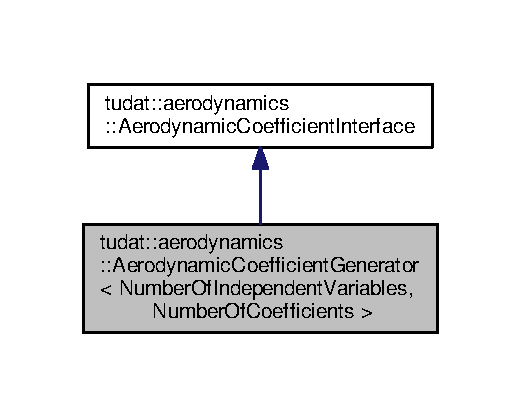
\includegraphics[width=250pt]{classtudat_1_1aerodynamics_1_1AerodynamicCoefficientGenerator__inherit__graph}
\end{center}
\end{figure}


Collaboration diagram for tudat\+:\+:aerodynamics\+:\+:Aerodynamic\+Coefficient\+Generator$<$ Number\+Of\+Independent\+Variables, Number\+Of\+Coefficients $>$\+:
\nopagebreak
\begin{figure}[H]
\begin{center}
\leavevmode
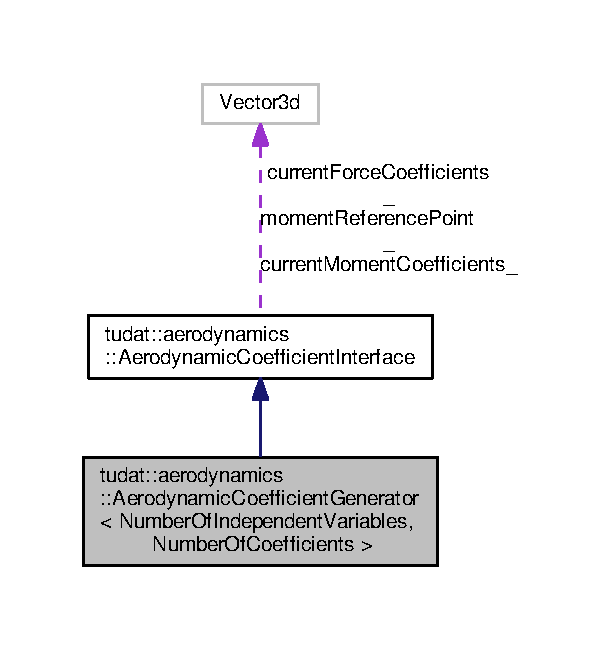
\includegraphics[width=289pt]{classtudat_1_1aerodynamics_1_1AerodynamicCoefficientGenerator__coll__graph}
\end{center}
\end{figure}
\subsection*{Public Member Functions}
\begin{DoxyCompactItemize}
\item 
\hyperlink{classtudat_1_1aerodynamics_1_1AerodynamicCoefficientGenerator_a469808ab7a0fe9491562b8f46fe3c0c6}{Aerodynamic\+Coefficient\+Generator} (const std\+::vector$<$ std\+::vector$<$ double $>$ $>$ \&data\+Points\+Of\+Independent\+Variables, const double reference\+Length, const double reference\+Area, const double lateral\+Reference\+Length, const Eigen\+::\+Vector3d \&moment\+Reference\+Point, const std\+::vector$<$ Aerodynamic\+Coefficients\+Independent\+Variables $>$ independent\+Variable\+Names, const bool are\+Coefficients\+In\+Aerodynamic\+Frame=true, const bool are\+Coefficients\+In\+Negative\+Axis\+Direction=true)
\begin{DoxyCompactList}\small\item\em Default base class constructor. \end{DoxyCompactList}\item 
virtual \hyperlink{classtudat_1_1aerodynamics_1_1AerodynamicCoefficientGenerator_a3d460a387284388a7c0cb2517288df5c}{$\sim$\+Aerodynamic\+Coefficient\+Generator} ()\hypertarget{classtudat_1_1aerodynamics_1_1AerodynamicCoefficientGenerator_a3d460a387284388a7c0cb2517288df5c}{}\label{classtudat_1_1aerodynamics_1_1AerodynamicCoefficientGenerator_a3d460a387284388a7c0cb2517288df5c}

\begin{DoxyCompactList}\small\item\em Default destructor. \end{DoxyCompactList}\item 
int \hyperlink{classtudat_1_1aerodynamics_1_1AerodynamicCoefficientGenerator_a8318f5ba6cb5c7f5018f3ba93ab6c24a}{get\+Number\+Of\+Values\+Of\+Independent\+Variable} (const int independent\+Variable) const 
\begin{DoxyCompactList}\small\item\em Get the number of points for an independent variable. \end{DoxyCompactList}\item 
double \hyperlink{classtudat_1_1aerodynamics_1_1AerodynamicCoefficientGenerator_a948245afaafaa8b31d77b9660bf8d3dd}{get\+Independent\+Variable\+Point} (const int independent\+Variable, const int index) const 
\begin{DoxyCompactList}\small\item\em Get a value of an independent variable. \end{DoxyCompactList}\item 
virtual Eigen\+::\+Matrix$<$ double, Number\+Of\+Coefficients, 1 $>$ \hyperlink{classtudat_1_1aerodynamics_1_1AerodynamicCoefficientGenerator_abb510c0b6d78349c6e41658ea8b63bc8}{get\+Aerodynamic\+Coefficients\+Data\+Point} (const boost\+::array$<$ int, Number\+Of\+Independent\+Variables $>$ independent\+Variables)=0
\begin{DoxyCompactList}\small\item\em Get aerodynamic coefficients. \end{DoxyCompactList}\item 
boost\+::multi\+\_\+array$<$ Eigen\+::\+Matrix$<$ double, Number\+Of\+Coefficients, 1 $>$, Number\+Of\+Independent\+Variables $>$ \hyperlink{classtudat_1_1aerodynamics_1_1AerodynamicCoefficientGenerator_a8d45750ac8b56931b3ee805cefd5a9da}{get\+Aerodynamic\+Coefficients\+Tables} ()
\begin{DoxyCompactList}\small\item\em Function to return the complete set of aerodynamic coefficients that have been calculated. \end{DoxyCompactList}\item 
std\+::vector$<$ std\+::vector$<$ double $>$ $>$ \hyperlink{classtudat_1_1aerodynamics_1_1AerodynamicCoefficientGenerator_aa114019ee49550774f570990712ddbfd}{get\+Data\+Points\+Of\+Independent\+Variables} ()
\begin{DoxyCompactList}\small\item\em Get the data points of the independent variables at which the coefficients are calculated. \end{DoxyCompactList}\item 
virtual void \hyperlink{classtudat_1_1aerodynamics_1_1AerodynamicCoefficientGenerator_a90ff928cb8d868f9b05748e125d871ff}{update\+Current\+Coefficients} (const std\+::vector$<$ double $>$ \&independent\+Variables)
\begin{DoxyCompactList}\small\item\em Compute the aerodynamic coefficients at current flight condition. \end{DoxyCompactList}\end{DoxyCompactItemize}
\subsection*{Protected Member Functions}
\begin{DoxyCompactItemize}
\item 
virtual void \hyperlink{classtudat_1_1aerodynamics_1_1AerodynamicCoefficientGenerator_a33f99bba58afd64d95b5c896b29234fb}{generate\+Coefficients} ()=0
\begin{DoxyCompactList}\small\item\em Generate aerodynamic coefficients. \end{DoxyCompactList}\item 
void \hyperlink{classtudat_1_1aerodynamics_1_1AerodynamicCoefficientGenerator_a8e6f4b78c17854f5cab41f5c404fca00}{create\+Interpolator} ()
\end{DoxyCompactItemize}
\subsection*{Protected Attributes}
\begin{DoxyCompactItemize}
\item 
boost\+::multi\+\_\+array$<$ Eigen\+::\+Matrix$<$ double, Number\+Of\+Coefficients, 1 $>$, Number\+Of\+Independent\+Variables $>$ \hyperlink{classtudat_1_1aerodynamics_1_1AerodynamicCoefficientGenerator_ad6fc1e382d822715b80f9a1636e5ce53}{aerodynamic\+Coefficients\+\_\+}
\begin{DoxyCompactList}\small\item\em N-\/dimensional array containing all computer aerodynamic coefficients. \end{DoxyCompactList}\item 
std\+::vector$<$ std\+::vector$<$ double $>$ $>$ \hyperlink{classtudat_1_1aerodynamics_1_1AerodynamicCoefficientGenerator_a14278ec758b9bfbfa73c5564abce310f}{data\+Points\+Of\+Independent\+Variables\+\_\+}
\begin{DoxyCompactList}\small\item\em Data points of the independent variables at which the coefficients are calculated. \end{DoxyCompactList}\item 
boost\+::shared\+\_\+ptr$<$ \hyperlink{classtudat_1_1interpolators_1_1Interpolator}{interpolators\+::\+Interpolator}$<$ double, Eigen\+::\+Vector6d $>$ $>$ \hyperlink{classtudat_1_1aerodynamics_1_1AerodynamicCoefficientGenerator_aa8717ac85b4f9ff9ee4cccbafaccb8b6}{coefficient\+Interpolator\+\_\+}
\end{DoxyCompactItemize}


\subsection{Detailed Description}
\subsubsection*{template$<$unsigned int Number\+Of\+Independent\+Variables, unsigned int Number\+Of\+Coefficients = 6$>$\\*
class tudat\+::aerodynamics\+::\+Aerodynamic\+Coefficient\+Generator$<$ Number\+Of\+Independent\+Variables, Number\+Of\+Coefficients $>$}

Base class for aerodynamic coefficient generator. 

Abstract base class for aerodynamic analysis method. Stores independent variable values and data points of independent variables. Coefficients are stored in a multi\+\_\+array of pointers. 

\subsection{Constructor \& Destructor Documentation}
\index{tudat\+::aerodynamics\+::\+Aerodynamic\+Coefficient\+Generator@{tudat\+::aerodynamics\+::\+Aerodynamic\+Coefficient\+Generator}!Aerodynamic\+Coefficient\+Generator@{Aerodynamic\+Coefficient\+Generator}}
\index{Aerodynamic\+Coefficient\+Generator@{Aerodynamic\+Coefficient\+Generator}!tudat\+::aerodynamics\+::\+Aerodynamic\+Coefficient\+Generator@{tudat\+::aerodynamics\+::\+Aerodynamic\+Coefficient\+Generator}}
\subsubsection[{\texorpdfstring{Aerodynamic\+Coefficient\+Generator(const std\+::vector$<$ std\+::vector$<$ double $>$ $>$ \&data\+Points\+Of\+Independent\+Variables, const double reference\+Length, const double reference\+Area, const double lateral\+Reference\+Length, const Eigen\+::\+Vector3d \&moment\+Reference\+Point, const std\+::vector$<$ Aerodynamic\+Coefficients\+Independent\+Variables $>$ independent\+Variable\+Names, const bool are\+Coefficients\+In\+Aerodynamic\+Frame=true, const bool are\+Coefficients\+In\+Negative\+Axis\+Direction=true)}{AerodynamicCoefficientGenerator(const std::vector< std::vector< double > > &dataPointsOfIndependentVariables, const double referenceLength, const double referenceArea, const double lateralReferenceLength, const Eigen::Vector3d &momentReferencePoint, const std::vector< AerodynamicCoefficientsIndependentVariables > independentVariableNames, const bool areCoefficientsInAerodynamicFrame=true, const bool areCoefficientsInNegativeAxisDirection=true)}}]{\setlength{\rightskip}{0pt plus 5cm}template$<$unsigned int Number\+Of\+Independent\+Variables, unsigned int Number\+Of\+Coefficients = 6$>$ {\bf tudat\+::aerodynamics\+::\+Aerodynamic\+Coefficient\+Generator}$<$ Number\+Of\+Independent\+Variables, Number\+Of\+Coefficients $>$\+::{\bf Aerodynamic\+Coefficient\+Generator} (
\begin{DoxyParamCaption}
\item[{const std\+::vector$<$ std\+::vector$<$ double $>$ $>$ \&}]{data\+Points\+Of\+Independent\+Variables, }
\item[{const double}]{reference\+Length, }
\item[{const double}]{reference\+Area, }
\item[{const double}]{lateral\+Reference\+Length, }
\item[{const Eigen\+::\+Vector3d \&}]{moment\+Reference\+Point, }
\item[{const std\+::vector$<$ Aerodynamic\+Coefficients\+Independent\+Variables $>$}]{independent\+Variable\+Names, }
\item[{const bool}]{are\+Coefficients\+In\+Aerodynamic\+Frame = {\ttfamily true}, }
\item[{const bool}]{are\+Coefficients\+In\+Negative\+Axis\+Direction = {\ttfamily true}}
\end{DoxyParamCaption}
)\hspace{0.3cm}{\ttfamily [inline]}}\hypertarget{classtudat_1_1aerodynamics_1_1AerodynamicCoefficientGenerator_a469808ab7a0fe9491562b8f46fe3c0c6}{}\label{classtudat_1_1aerodynamics_1_1AerodynamicCoefficientGenerator_a469808ab7a0fe9491562b8f46fe3c0c6}


Default base class constructor. 

Default base class constructor, sets independent variable data points and aerodynamics reference quantities. 
\begin{DoxyParams}{Parameters}
{\em data\+Points\+Of\+Independent\+Variables} & Vector of vector, where each subvector contains the data points of each of the independent variables for the coefficient generation. The number of subvectors must be equal to the number of independent variables. It is recommended that each of the subvectors is sorted in ascending order. \\
\hline
{\em reference\+Length} & Reference length with which aerodynamic moments (about x-\/ and z-\/ axes) are non-\/dimensionalized. \\
\hline
{\em reference\+Area} & Reference area with which aerodynamic forces and moments are non-\/dimensionalized. \\
\hline
{\em lateral\+Reference\+Length} & Reference length with which aerodynamic moments (about y-\/axis) is non-\/dimensionalized. \\
\hline
{\em moment\+Reference\+Point} & Point w.\+r.\+t. aerodynamic moment is calculated \\
\hline
{\em independent\+Variable\+Names} & Vector with identifiers the physical meaning of each independent variable of the aerodynamic coefficients. \\
\hline
{\em are\+Coefficients\+In\+Aerodynamic\+Frame} & Boolean to define whether the aerodynamic coefficients are defined in the aerodynamic frame (lift, drag, side force) or in the body frame (typically denoted as Cx, Cy, Cz) (default true). \\
\hline
{\em are\+Coefficients\+In\+Negative\+Axis\+Direction} & Boolean to define whether the aerodynamic coefficients are positiver along tyhe positive axes of the body or aerodynamic frame (see are\+Coefficients\+In\+Aerodynamic\+Frame). Note that for (lift, drag, side force), the coefficients are typically defined in negative direction (default true). \\
\hline
\end{DoxyParams}


\subsection{Member Function Documentation}
\index{tudat\+::aerodynamics\+::\+Aerodynamic\+Coefficient\+Generator@{tudat\+::aerodynamics\+::\+Aerodynamic\+Coefficient\+Generator}!create\+Interpolator@{create\+Interpolator}}
\index{create\+Interpolator@{create\+Interpolator}!tudat\+::aerodynamics\+::\+Aerodynamic\+Coefficient\+Generator@{tudat\+::aerodynamics\+::\+Aerodynamic\+Coefficient\+Generator}}
\subsubsection[{\texorpdfstring{create\+Interpolator()}{createInterpolator()}}]{\setlength{\rightskip}{0pt plus 5cm}template$<$unsigned int Number\+Of\+Independent\+Variables, unsigned int Number\+Of\+Coefficients = 6$>$ void {\bf tudat\+::aerodynamics\+::\+Aerodynamic\+Coefficient\+Generator}$<$ Number\+Of\+Independent\+Variables, Number\+Of\+Coefficients $>$\+::create\+Interpolator (
\begin{DoxyParamCaption}
{}
\end{DoxyParamCaption}
)\hspace{0.3cm}{\ttfamily [inline]}, {\ttfamily [protected]}}\hypertarget{classtudat_1_1aerodynamics_1_1AerodynamicCoefficientGenerator_a8e6f4b78c17854f5cab41f5c404fca00}{}\label{classtudat_1_1aerodynamics_1_1AerodynamicCoefficientGenerator_a8e6f4b78c17854f5cab41f5c404fca00}
Function to create the coefficient interpolator from the discrete set in aerodynamic\+Coefficients\+\_\+ \index{tudat\+::aerodynamics\+::\+Aerodynamic\+Coefficient\+Generator@{tudat\+::aerodynamics\+::\+Aerodynamic\+Coefficient\+Generator}!generate\+Coefficients@{generate\+Coefficients}}
\index{generate\+Coefficients@{generate\+Coefficients}!tudat\+::aerodynamics\+::\+Aerodynamic\+Coefficient\+Generator@{tudat\+::aerodynamics\+::\+Aerodynamic\+Coefficient\+Generator}}
\subsubsection[{\texorpdfstring{generate\+Coefficients()=0}{generateCoefficients()=0}}]{\setlength{\rightskip}{0pt plus 5cm}template$<$unsigned int Number\+Of\+Independent\+Variables, unsigned int Number\+Of\+Coefficients = 6$>$ virtual void {\bf tudat\+::aerodynamics\+::\+Aerodynamic\+Coefficient\+Generator}$<$ Number\+Of\+Independent\+Variables, Number\+Of\+Coefficients $>$\+::generate\+Coefficients (
\begin{DoxyParamCaption}
{}
\end{DoxyParamCaption}
)\hspace{0.3cm}{\ttfamily [protected]}, {\ttfamily [pure virtual]}}\hypertarget{classtudat_1_1aerodynamics_1_1AerodynamicCoefficientGenerator_a33f99bba58afd64d95b5c896b29234fb}{}\label{classtudat_1_1aerodynamics_1_1AerodynamicCoefficientGenerator_a33f99bba58afd64d95b5c896b29234fb}


Generate aerodynamic coefficients. 

Virtual function to generate aerodynamic coefficients for the list of independent variables passed to the constructor. \index{tudat\+::aerodynamics\+::\+Aerodynamic\+Coefficient\+Generator@{tudat\+::aerodynamics\+::\+Aerodynamic\+Coefficient\+Generator}!get\+Aerodynamic\+Coefficients\+Data\+Point@{get\+Aerodynamic\+Coefficients\+Data\+Point}}
\index{get\+Aerodynamic\+Coefficients\+Data\+Point@{get\+Aerodynamic\+Coefficients\+Data\+Point}!tudat\+::aerodynamics\+::\+Aerodynamic\+Coefficient\+Generator@{tudat\+::aerodynamics\+::\+Aerodynamic\+Coefficient\+Generator}}
\subsubsection[{\texorpdfstring{get\+Aerodynamic\+Coefficients\+Data\+Point(const boost\+::array$<$ int, Number\+Of\+Independent\+Variables $>$ independent\+Variables)=0}{getAerodynamicCoefficientsDataPoint(const boost::array< int, NumberOfIndependentVariables > independentVariables)=0}}]{\setlength{\rightskip}{0pt plus 5cm}template$<$unsigned int Number\+Of\+Independent\+Variables, unsigned int Number\+Of\+Coefficients = 6$>$ virtual Eigen\+::\+Matrix$<$ double, Number\+Of\+Coefficients, 1 $>$ {\bf tudat\+::aerodynamics\+::\+Aerodynamic\+Coefficient\+Generator}$<$ Number\+Of\+Independent\+Variables, Number\+Of\+Coefficients $>$\+::get\+Aerodynamic\+Coefficients\+Data\+Point (
\begin{DoxyParamCaption}
\item[{const boost\+::array$<$ int, Number\+Of\+Independent\+Variables $>$}]{independent\+Variables}
\end{DoxyParamCaption}
)\hspace{0.3cm}{\ttfamily [pure virtual]}}\hypertarget{classtudat_1_1aerodynamics_1_1AerodynamicCoefficientGenerator_abb510c0b6d78349c6e41658ea8b63bc8}{}\label{classtudat_1_1aerodynamics_1_1AerodynamicCoefficientGenerator_abb510c0b6d78349c6e41658ea8b63bc8}


Get aerodynamic coefficients. 

Virtual function to return the aerodynamic coefficients at a specified set of independent variables. 
\begin{DoxyParams}{Parameters}
{\em independent\+Variables} & Array of values of independent variable indices in data\+Points\+Of\+Independent\+Variables\+\_\+ for which to retrieve aerodynamic coefficients. \\
\hline
\end{DoxyParams}
\begin{DoxyReturn}{Returns}
vector of coefficients at specified independent variable indices. 
\end{DoxyReturn}
\index{tudat\+::aerodynamics\+::\+Aerodynamic\+Coefficient\+Generator@{tudat\+::aerodynamics\+::\+Aerodynamic\+Coefficient\+Generator}!get\+Aerodynamic\+Coefficients\+Tables@{get\+Aerodynamic\+Coefficients\+Tables}}
\index{get\+Aerodynamic\+Coefficients\+Tables@{get\+Aerodynamic\+Coefficients\+Tables}!tudat\+::aerodynamics\+::\+Aerodynamic\+Coefficient\+Generator@{tudat\+::aerodynamics\+::\+Aerodynamic\+Coefficient\+Generator}}
\subsubsection[{\texorpdfstring{get\+Aerodynamic\+Coefficients\+Tables()}{getAerodynamicCoefficientsTables()}}]{\setlength{\rightskip}{0pt plus 5cm}template$<$unsigned int Number\+Of\+Independent\+Variables, unsigned int Number\+Of\+Coefficients = 6$>$ boost\+::multi\+\_\+array$<$ Eigen\+::\+Matrix$<$ double, Number\+Of\+Coefficients, 1 $>$, Number\+Of\+Independent\+Variables $>$ {\bf tudat\+::aerodynamics\+::\+Aerodynamic\+Coefficient\+Generator}$<$ Number\+Of\+Independent\+Variables, Number\+Of\+Coefficients $>$\+::get\+Aerodynamic\+Coefficients\+Tables (
\begin{DoxyParamCaption}
{}
\end{DoxyParamCaption}
)\hspace{0.3cm}{\ttfamily [inline]}}\hypertarget{classtudat_1_1aerodynamics_1_1AerodynamicCoefficientGenerator_a8d45750ac8b56931b3ee805cefd5a9da}{}\label{classtudat_1_1aerodynamics_1_1AerodynamicCoefficientGenerator_a8d45750ac8b56931b3ee805cefd5a9da}


Function to return the complete set of aerodynamic coefficients that have been calculated. 

Function to return the complete set of aerodynamic coefficients that have been calculated. \begin{DoxyReturn}{Returns}
Complete set of aerodynamic coefficients that have been calculated. 
\end{DoxyReturn}
\index{tudat\+::aerodynamics\+::\+Aerodynamic\+Coefficient\+Generator@{tudat\+::aerodynamics\+::\+Aerodynamic\+Coefficient\+Generator}!get\+Data\+Points\+Of\+Independent\+Variables@{get\+Data\+Points\+Of\+Independent\+Variables}}
\index{get\+Data\+Points\+Of\+Independent\+Variables@{get\+Data\+Points\+Of\+Independent\+Variables}!tudat\+::aerodynamics\+::\+Aerodynamic\+Coefficient\+Generator@{tudat\+::aerodynamics\+::\+Aerodynamic\+Coefficient\+Generator}}
\subsubsection[{\texorpdfstring{get\+Data\+Points\+Of\+Independent\+Variables()}{getDataPointsOfIndependentVariables()}}]{\setlength{\rightskip}{0pt plus 5cm}template$<$unsigned int Number\+Of\+Independent\+Variables, unsigned int Number\+Of\+Coefficients = 6$>$ std\+::vector$<$ std\+::vector$<$ double $>$ $>$ {\bf tudat\+::aerodynamics\+::\+Aerodynamic\+Coefficient\+Generator}$<$ Number\+Of\+Independent\+Variables, Number\+Of\+Coefficients $>$\+::get\+Data\+Points\+Of\+Independent\+Variables (
\begin{DoxyParamCaption}
{}
\end{DoxyParamCaption}
)\hspace{0.3cm}{\ttfamily [inline]}}\hypertarget{classtudat_1_1aerodynamics_1_1AerodynamicCoefficientGenerator_aa114019ee49550774f570990712ddbfd}{}\label{classtudat_1_1aerodynamics_1_1AerodynamicCoefficientGenerator_aa114019ee49550774f570990712ddbfd}


Get the data points of the independent variables at which the coefficients are calculated. 

Get the data points of the independent variables at which the coefficients are calculated. The aerodynamic coefficients are calculated each set of combinations of the independent variables. \begin{DoxyReturn}{Returns}
Data points of the independent variables at which the coefficients are calculated. 
\end{DoxyReturn}
\index{tudat\+::aerodynamics\+::\+Aerodynamic\+Coefficient\+Generator@{tudat\+::aerodynamics\+::\+Aerodynamic\+Coefficient\+Generator}!get\+Independent\+Variable\+Point@{get\+Independent\+Variable\+Point}}
\index{get\+Independent\+Variable\+Point@{get\+Independent\+Variable\+Point}!tudat\+::aerodynamics\+::\+Aerodynamic\+Coefficient\+Generator@{tudat\+::aerodynamics\+::\+Aerodynamic\+Coefficient\+Generator}}
\subsubsection[{\texorpdfstring{get\+Independent\+Variable\+Point(const int independent\+Variable, const int index) const }{getIndependentVariablePoint(const int independentVariable, const int index) const }}]{\setlength{\rightskip}{0pt plus 5cm}template$<$unsigned int Number\+Of\+Independent\+Variables, unsigned int Number\+Of\+Coefficients = 6$>$ double {\bf tudat\+::aerodynamics\+::\+Aerodynamic\+Coefficient\+Generator}$<$ Number\+Of\+Independent\+Variables, Number\+Of\+Coefficients $>$\+::get\+Independent\+Variable\+Point (
\begin{DoxyParamCaption}
\item[{const int}]{independent\+Variable, }
\item[{const int}]{index}
\end{DoxyParamCaption}
) const\hspace{0.3cm}{\ttfamily [inline]}}\hypertarget{classtudat_1_1aerodynamics_1_1AerodynamicCoefficientGenerator_a948245afaafaa8b31d77b9660bf8d3dd}{}\label{classtudat_1_1aerodynamics_1_1AerodynamicCoefficientGenerator_a948245afaafaa8b31d77b9660bf8d3dd}


Get a value of an independent variable. 

Returns a value of an independent variable at which aerodynamic coefficients are to be determined. 
\begin{DoxyParams}{Parameters}
{\em independent\+Variable} & Independent variable index. \\
\hline
{\em index} & Index from independent variable list for which to retrieve the value. \\
\hline
\end{DoxyParams}
\begin{DoxyReturn}{Returns}
Value of independent variable at index. 
\end{DoxyReturn}
\index{tudat\+::aerodynamics\+::\+Aerodynamic\+Coefficient\+Generator@{tudat\+::aerodynamics\+::\+Aerodynamic\+Coefficient\+Generator}!get\+Number\+Of\+Values\+Of\+Independent\+Variable@{get\+Number\+Of\+Values\+Of\+Independent\+Variable}}
\index{get\+Number\+Of\+Values\+Of\+Independent\+Variable@{get\+Number\+Of\+Values\+Of\+Independent\+Variable}!tudat\+::aerodynamics\+::\+Aerodynamic\+Coefficient\+Generator@{tudat\+::aerodynamics\+::\+Aerodynamic\+Coefficient\+Generator}}
\subsubsection[{\texorpdfstring{get\+Number\+Of\+Values\+Of\+Independent\+Variable(const int independent\+Variable) const }{getNumberOfValuesOfIndependentVariable(const int independentVariable) const }}]{\setlength{\rightskip}{0pt plus 5cm}template$<$unsigned int Number\+Of\+Independent\+Variables, unsigned int Number\+Of\+Coefficients = 6$>$ int {\bf tudat\+::aerodynamics\+::\+Aerodynamic\+Coefficient\+Generator}$<$ Number\+Of\+Independent\+Variables, Number\+Of\+Coefficients $>$\+::get\+Number\+Of\+Values\+Of\+Independent\+Variable (
\begin{DoxyParamCaption}
\item[{const int}]{independent\+Variable}
\end{DoxyParamCaption}
) const\hspace{0.3cm}{\ttfamily [inline]}}\hypertarget{classtudat_1_1aerodynamics_1_1AerodynamicCoefficientGenerator_a8318f5ba6cb5c7f5018f3ba93ab6c24a}{}\label{classtudat_1_1aerodynamics_1_1AerodynamicCoefficientGenerator_a8318f5ba6cb5c7f5018f3ba93ab6c24a}


Get the number of points for an independent variable. 

Returns the number of different values of a given independent variable at which coefficients are determined. 
\begin{DoxyParams}{Parameters}
{\em independent\+Variable} & Independent variable from which to retrieve number of data points. \\
\hline
\end{DoxyParams}
\begin{DoxyReturn}{Returns}
Number of data points for selected independent variable. 
\end{DoxyReturn}
\index{tudat\+::aerodynamics\+::\+Aerodynamic\+Coefficient\+Generator@{tudat\+::aerodynamics\+::\+Aerodynamic\+Coefficient\+Generator}!update\+Current\+Coefficients@{update\+Current\+Coefficients}}
\index{update\+Current\+Coefficients@{update\+Current\+Coefficients}!tudat\+::aerodynamics\+::\+Aerodynamic\+Coefficient\+Generator@{tudat\+::aerodynamics\+::\+Aerodynamic\+Coefficient\+Generator}}
\subsubsection[{\texorpdfstring{update\+Current\+Coefficients(const std\+::vector$<$ double $>$ \&independent\+Variables)}{updateCurrentCoefficients(const std::vector< double > &independentVariables)}}]{\setlength{\rightskip}{0pt plus 5cm}template$<$unsigned int Number\+Of\+Independent\+Variables, unsigned int Number\+Of\+Coefficients = 6$>$ virtual void {\bf tudat\+::aerodynamics\+::\+Aerodynamic\+Coefficient\+Generator}$<$ Number\+Of\+Independent\+Variables, Number\+Of\+Coefficients $>$\+::update\+Current\+Coefficients (
\begin{DoxyParamCaption}
\item[{const std\+::vector$<$ double $>$ \&}]{independent\+Variables}
\end{DoxyParamCaption}
)\hspace{0.3cm}{\ttfamily [inline]}, {\ttfamily [virtual]}}\hypertarget{classtudat_1_1aerodynamics_1_1AerodynamicCoefficientGenerator_a90ff928cb8d868f9b05748e125d871ff}{}\label{classtudat_1_1aerodynamics_1_1AerodynamicCoefficientGenerator_a90ff928cb8d868f9b05748e125d871ff}


Compute the aerodynamic coefficients at current flight condition. 

Compute the aerodynamic coefficients at current flight conditions (independent variables). Input is a set of independent variables (doubles) which represent the variables from which the coefficients are calculated. The physical nature of these variables depends on the coefficient\+Function\+\_\+ variables. The size of the independent variable vector must be number\+Of\+Independent\+Variables\+\_\+ 
\begin{DoxyParams}{Parameters}
{\em independent\+Variables} & Independent variables of force and moment coefficient determination implemented by derived class \\
\hline
\end{DoxyParams}


Implements \hyperlink{classtudat_1_1aerodynamics_1_1AerodynamicCoefficientInterface_af68d685a47306b6525ea06bec6e91880}{tudat\+::aerodynamics\+::\+Aerodynamic\+Coefficient\+Interface}.



\subsection{Member Data Documentation}
\index{tudat\+::aerodynamics\+::\+Aerodynamic\+Coefficient\+Generator@{tudat\+::aerodynamics\+::\+Aerodynamic\+Coefficient\+Generator}!aerodynamic\+Coefficients\+\_\+@{aerodynamic\+Coefficients\+\_\+}}
\index{aerodynamic\+Coefficients\+\_\+@{aerodynamic\+Coefficients\+\_\+}!tudat\+::aerodynamics\+::\+Aerodynamic\+Coefficient\+Generator@{tudat\+::aerodynamics\+::\+Aerodynamic\+Coefficient\+Generator}}
\subsubsection[{\texorpdfstring{aerodynamic\+Coefficients\+\_\+}{aerodynamicCoefficients_}}]{\setlength{\rightskip}{0pt plus 5cm}template$<$unsigned int Number\+Of\+Independent\+Variables, unsigned int Number\+Of\+Coefficients = 6$>$ boost\+::multi\+\_\+array$<$ Eigen\+::\+Matrix$<$ double, Number\+Of\+Coefficients, 1 $>$, Number\+Of\+Independent\+Variables $>$ {\bf tudat\+::aerodynamics\+::\+Aerodynamic\+Coefficient\+Generator}$<$ Number\+Of\+Independent\+Variables, Number\+Of\+Coefficients $>$\+::aerodynamic\+Coefficients\+\_\+\hspace{0.3cm}{\ttfamily [protected]}}\hypertarget{classtudat_1_1aerodynamics_1_1AerodynamicCoefficientGenerator_ad6fc1e382d822715b80f9a1636e5ce53}{}\label{classtudat_1_1aerodynamics_1_1AerodynamicCoefficientGenerator_ad6fc1e382d822715b80f9a1636e5ce53}


N-\/dimensional array containing all computer aerodynamic coefficients. 

N-\/dimensional array containing all computer aerodynamic coefficients. The k-\/th dimension pertains to coefficients at the k-\/th independent variable, the data points for which are defined by data\+Points\+Of\+Independent\+Variables\+\_\+ and the physical meaning of which are defined by independent\+Variable\+Names\+\_\+ \index{tudat\+::aerodynamics\+::\+Aerodynamic\+Coefficient\+Generator@{tudat\+::aerodynamics\+::\+Aerodynamic\+Coefficient\+Generator}!coefficient\+Interpolator\+\_\+@{coefficient\+Interpolator\+\_\+}}
\index{coefficient\+Interpolator\+\_\+@{coefficient\+Interpolator\+\_\+}!tudat\+::aerodynamics\+::\+Aerodynamic\+Coefficient\+Generator@{tudat\+::aerodynamics\+::\+Aerodynamic\+Coefficient\+Generator}}
\subsubsection[{\texorpdfstring{coefficient\+Interpolator\+\_\+}{coefficientInterpolator_}}]{\setlength{\rightskip}{0pt plus 5cm}template$<$unsigned int Number\+Of\+Independent\+Variables, unsigned int Number\+Of\+Coefficients = 6$>$ boost\+::shared\+\_\+ptr$<$ {\bf interpolators\+::\+Interpolator}$<$ double, Eigen\+::\+Vector6d $>$ $>$ {\bf tudat\+::aerodynamics\+::\+Aerodynamic\+Coefficient\+Generator}$<$ Number\+Of\+Independent\+Variables, Number\+Of\+Coefficients $>$\+::coefficient\+Interpolator\+\_\+\hspace{0.3cm}{\ttfamily [protected]}}\hypertarget{classtudat_1_1aerodynamics_1_1AerodynamicCoefficientGenerator_aa8717ac85b4f9ff9ee4cccbafaccb8b6}{}\label{classtudat_1_1aerodynamics_1_1AerodynamicCoefficientGenerator_aa8717ac85b4f9ff9ee4cccbafaccb8b6}
Interpolator producing continuous aerodynamic coefficients from the discrete calculations contained in aerodynamic\+Coefficients\+\_\+. \index{tudat\+::aerodynamics\+::\+Aerodynamic\+Coefficient\+Generator@{tudat\+::aerodynamics\+::\+Aerodynamic\+Coefficient\+Generator}!data\+Points\+Of\+Independent\+Variables\+\_\+@{data\+Points\+Of\+Independent\+Variables\+\_\+}}
\index{data\+Points\+Of\+Independent\+Variables\+\_\+@{data\+Points\+Of\+Independent\+Variables\+\_\+}!tudat\+::aerodynamics\+::\+Aerodynamic\+Coefficient\+Generator@{tudat\+::aerodynamics\+::\+Aerodynamic\+Coefficient\+Generator}}
\subsubsection[{\texorpdfstring{data\+Points\+Of\+Independent\+Variables\+\_\+}{dataPointsOfIndependentVariables_}}]{\setlength{\rightskip}{0pt plus 5cm}template$<$unsigned int Number\+Of\+Independent\+Variables, unsigned int Number\+Of\+Coefficients = 6$>$ std\+::vector$<$ std\+::vector$<$ double $>$ $>$ {\bf tudat\+::aerodynamics\+::\+Aerodynamic\+Coefficient\+Generator}$<$ Number\+Of\+Independent\+Variables, Number\+Of\+Coefficients $>$\+::data\+Points\+Of\+Independent\+Variables\+\_\+\hspace{0.3cm}{\ttfamily [protected]}}\hypertarget{classtudat_1_1aerodynamics_1_1AerodynamicCoefficientGenerator_a14278ec758b9bfbfa73c5564abce310f}{}\label{classtudat_1_1aerodynamics_1_1AerodynamicCoefficientGenerator_a14278ec758b9bfbfa73c5564abce310f}


Data points of the independent variables at which the coefficients are calculated. 

Data points of the independent variables at which the coefficients are calculated. The k-\/th vector contains the vector of data points to which the k-\/th independent variables (defined by independent\+Variable\+Names\+\_\+) are set during the calculation of the aerodynamic coefficients. 

The documentation for this class was generated from the following file\+:\begin{DoxyCompactItemize}
\item 
/home/lupi/\+Tudat/tudat\+Bundle/tudat/\+Tudat/\+Astrodynamics/\+Aerodynamics/aerodynamic\+Coefficient\+Generator.\+h\end{DoxyCompactItemize}

\hypertarget{classtudat_1_1aerodynamics_1_1AerodynamicCoefficientInterface}{}\section{tudat\+:\+:aerodynamics\+:\+:Aerodynamic\+Coefficient\+Interface Class Reference}
\label{classtudat_1_1aerodynamics_1_1AerodynamicCoefficientInterface}\index{tudat\+::aerodynamics\+::\+Aerodynamic\+Coefficient\+Interface@{tudat\+::aerodynamics\+::\+Aerodynamic\+Coefficient\+Interface}}


Base class to hold an aerodynamic coefficient interface.  




{\ttfamily \#include $<$aerodynamic\+Coefficient\+Interface.\+h$>$}



Inheritance diagram for tudat\+:\+:aerodynamics\+:\+:Aerodynamic\+Coefficient\+Interface\+:
\nopagebreak
\begin{figure}[H]
\begin{center}
\leavevmode
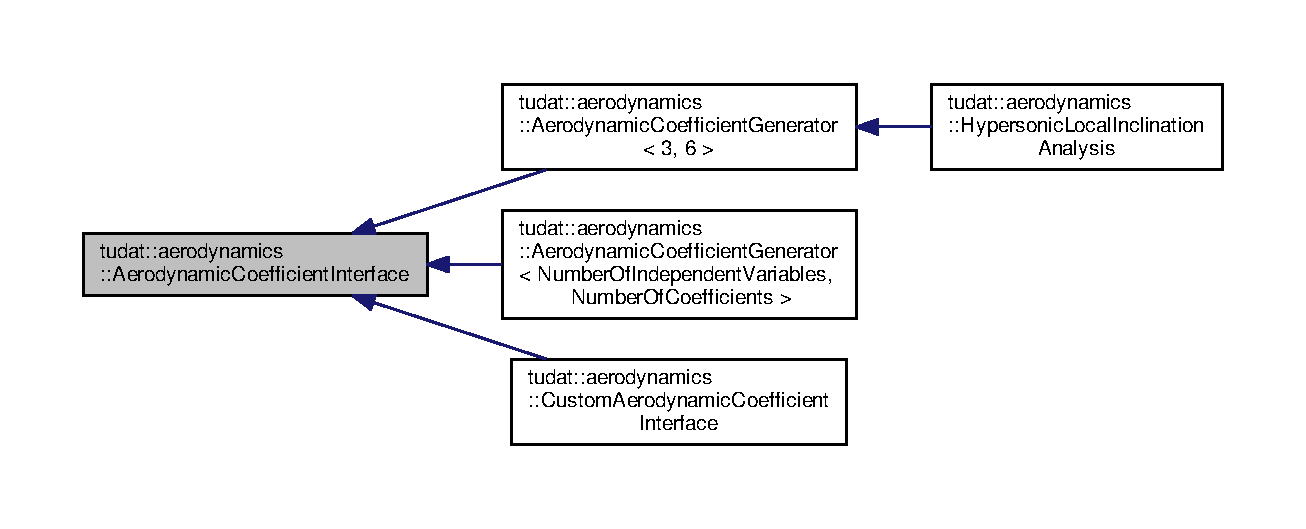
\includegraphics[width=350pt]{classtudat_1_1aerodynamics_1_1AerodynamicCoefficientInterface__inherit__graph}
\end{center}
\end{figure}


Collaboration diagram for tudat\+:\+:aerodynamics\+:\+:Aerodynamic\+Coefficient\+Interface\+:
\nopagebreak
\begin{figure}[H]
\begin{center}
\leavevmode
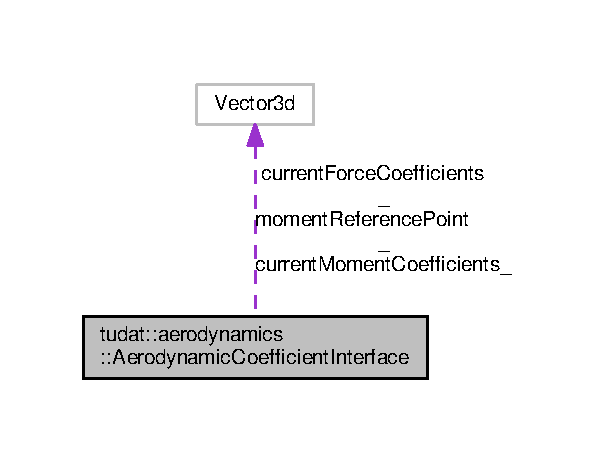
\includegraphics[width=287pt]{classtudat_1_1aerodynamics_1_1AerodynamicCoefficientInterface__coll__graph}
\end{center}
\end{figure}
\subsection*{Public Member Functions}
\begin{DoxyCompactItemize}
\item 
\hyperlink{classtudat_1_1aerodynamics_1_1AerodynamicCoefficientInterface_afcf63dcf774ca65e91ce8449f3e22d74}{Aerodynamic\+Coefficient\+Interface} (const double reference\+Length, const double reference\+Area, const double lateral\+Reference\+Length, const Eigen\+::\+Vector3d \&moment\+Reference\+Point, const std\+::vector$<$ Aerodynamic\+Coefficients\+Independent\+Variables $>$ independent\+Variable\+Names, const bool are\+Coefficients\+In\+Aerodynamic\+Frame=true, const bool are\+Coefficients\+In\+Negative\+Axis\+Direction=true)
\begin{DoxyCompactList}\small\item\em Constructor. \end{DoxyCompactList}\item 
virtual \hyperlink{classtudat_1_1aerodynamics_1_1AerodynamicCoefficientInterface_aa1df9aca23300659cd752d9afa42efa4}{$\sim$\+Aerodynamic\+Coefficient\+Interface} ()\hypertarget{classtudat_1_1aerodynamics_1_1AerodynamicCoefficientInterface_aa1df9aca23300659cd752d9afa42efa4}{}\label{classtudat_1_1aerodynamics_1_1AerodynamicCoefficientInterface_aa1df9aca23300659cd752d9afa42efa4}

\begin{DoxyCompactList}\small\item\em Default destructor. \end{DoxyCompactList}\item 
double \hyperlink{classtudat_1_1aerodynamics_1_1AerodynamicCoefficientInterface_aaf0325453208d06cfbf8aa7a854d6875}{get\+Reference\+Area} ()
\begin{DoxyCompactList}\small\item\em Get reference area. \end{DoxyCompactList}\item 
double \hyperlink{classtudat_1_1aerodynamics_1_1AerodynamicCoefficientInterface_a8bf7126281dbe7017490e77768e23670}{get\+Reference\+Length} ()
\begin{DoxyCompactList}\small\item\em Get reference length. \end{DoxyCompactList}\item 
double \hyperlink{classtudat_1_1aerodynamics_1_1AerodynamicCoefficientInterface_ac340c18b6cb008955c8dc426c31d6adb}{get\+Lateral\+Reference\+Length} ()
\begin{DoxyCompactList}\small\item\em Get lateral reference length. \end{DoxyCompactList}\item 
Eigen\+::\+Vector\+Xd \hyperlink{classtudat_1_1aerodynamics_1_1AerodynamicCoefficientInterface_ab940adb9ffb34d7910bdb11ca06143f6}{get\+Moment\+Reference\+Point} ()
\begin{DoxyCompactList}\small\item\em Get moment reference point. \end{DoxyCompactList}\item 
virtual void \hyperlink{classtudat_1_1aerodynamics_1_1AerodynamicCoefficientInterface_af68d685a47306b6525ea06bec6e91880}{update\+Current\+Coefficients} (const std\+::vector$<$ double $>$ \&independent\+Variables)=0
\begin{DoxyCompactList}\small\item\em Compute the aerodynamic coefficients of the body itself (without control surfaces) at current flight condition. \end{DoxyCompactList}\item 
void \hyperlink{classtudat_1_1aerodynamics_1_1AerodynamicCoefficientInterface_a59727b07127b2e8ef0af43b3177a0808}{update\+Current\+Control\+Surface\+Coefficients\+Coefficients} (const std\+::string \&current\+Control\+Surface, std\+::vector$<$ double $>$ control\+Surface\+Independent\+Variables)
\begin{DoxyCompactList}\small\item\em Compute the aerodynamic coefficients for a single control surface, and add to full configuration coefficients. \end{DoxyCompactList}\item 
void \hyperlink{classtudat_1_1aerodynamics_1_1AerodynamicCoefficientInterface_ad2199d6685cd70348ce5a3886a4b1df3}{update\+Full\+Current\+Coefficients} (const std\+::vector$<$ double $>$ \&independent\+Variables, const std\+::map$<$ std\+::string, std\+::vector$<$ double $>$ $>$ \&control\+Surface\+Independent\+Variables=std\+::map$<$ std\+::string, std\+::vector$<$ double $>$ $>$())
\begin{DoxyCompactList}\small\item\em Function to update the aerodynamic coefficients of the full body with control surfaces. \end{DoxyCompactList}\item 
Eigen\+::\+Vector3d \hyperlink{classtudat_1_1aerodynamics_1_1AerodynamicCoefficientInterface_a1d482f3c4cba5a2354d12610319aa7af}{get\+Current\+Force\+Coefficients} ()
\begin{DoxyCompactList}\small\item\em Pure virtual function for calculating and returning aerodynamic force coefficients. \end{DoxyCompactList}\item 
Eigen\+::\+Vector3d \hyperlink{classtudat_1_1aerodynamics_1_1AerodynamicCoefficientInterface_a81b6c6f36bea4e10bdde1d67f95740d7}{get\+Current\+Moment\+Coefficients} ()
\begin{DoxyCompactList}\small\item\em Pure virtual function for calculating and returning aerodynamic moment coefficients. \end{DoxyCompactList}\item 
Eigen\+::\+Matrix$<$ double, 6, 1 $>$ \hyperlink{classtudat_1_1aerodynamics_1_1AerodynamicCoefficientInterface_a954fde716c0874476c73130b5941036f}{get\+Current\+Aerodynamic\+Coefficients} ()
\begin{DoxyCompactList}\small\item\em Function for calculating and returning aerodynamic force and moment coefficients. \end{DoxyCompactList}\item 
std\+::vector$<$ Aerodynamic\+Coefficients\+Independent\+Variables $>$ \hyperlink{classtudat_1_1aerodynamics_1_1AerodynamicCoefficientInterface_a605d78a84519402354ac1551e7eb2d0d}{get\+Independent\+Variable\+Names} ()
\begin{DoxyCompactList}\small\item\em Function to return the identifiers of the physical meaning of each independent variable. \end{DoxyCompactList}\item 
Aerodynamic\+Coefficients\+Independent\+Variables \hyperlink{classtudat_1_1aerodynamics_1_1AerodynamicCoefficientInterface_a91798427fd03d66a696f97f9c01292c4}{get\+Independent\+Variable\+Name} (const unsigned int index)
\begin{DoxyCompactList}\small\item\em Function to return a single identifier of the physical meaning of one independent variable. \end{DoxyCompactList}\item 
unsigned int \hyperlink{classtudat_1_1aerodynamics_1_1AerodynamicCoefficientInterface_af10cc21f485df4f2c877f827c7a38493}{get\+Number\+Of\+Independent\+Variables} ()
\begin{DoxyCompactList}\small\item\em Function to return the number of independent variables upon which the coeficients depend. \end{DoxyCompactList}\item 
bool \hyperlink{classtudat_1_1aerodynamics_1_1AerodynamicCoefficientInterface_acc664214ae5fee886b3a2ffa22dce2d9}{get\+Are\+Coefficients\+In\+Aerodynamic\+Frame} ()
\begin{DoxyCompactList}\small\item\em Function that returns whether the coefficients are given in aerodynamic frame. \end{DoxyCompactList}\item 
bool \hyperlink{classtudat_1_1aerodynamics_1_1AerodynamicCoefficientInterface_a55875655a4a678eaa5fdb80cb4827e9f}{get\+Are\+Coefficients\+In\+Negative\+Axis\+Direction} ()
\begin{DoxyCompactList}\small\item\em Function that returns whether the coefficients are positive in positive axes directions. \end{DoxyCompactList}\item 
void \hyperlink{classtudat_1_1aerodynamics_1_1AerodynamicCoefficientInterface_a8bfd4247c0ac5d32c92b9ad859f33500}{set\+Control\+Surface\+Increments} (const std\+::map$<$ std\+::string, boost\+::shared\+\_\+ptr$<$ \hyperlink{classtudat_1_1aerodynamics_1_1ControlSurfaceIncrementAerodynamicInterface}{Control\+Surface\+Increment\+Aerodynamic\+Interface} $>$ $>$ control\+Surface\+Increment\+Interfaces)
\begin{DoxyCompactList}\small\item\em Function to set the list of control surface aerodynamic coefficient interfaces. \end{DoxyCompactList}\item 
std\+::string \hyperlink{classtudat_1_1aerodynamics_1_1AerodynamicCoefficientInterface_a69a2aa883a2fba8bc918dcd60a654eb9}{get\+Control\+Surface\+Name} (const int index)
\begin{DoxyCompactList}\small\item\em Function to get control surface name at given index in list of control surfaces. \end{DoxyCompactList}\item 
unsigned int \hyperlink{classtudat_1_1aerodynamics_1_1AerodynamicCoefficientInterface_aeec44dc3a056968cb685dd3f0642bf5d}{get\+Number\+Of\+Control\+Surfaces} ()
\begin{DoxyCompactList}\small\item\em Function to return the number of control surfaces in current coefficient interface. \end{DoxyCompactList}\item 
unsigned int \hyperlink{classtudat_1_1aerodynamics_1_1AerodynamicCoefficientInterface_a1ca99957277b60ca79aaf4eb48e3f003}{get\+Number\+Of\+Control\+Surface\+Independent\+Variables} (const std\+::string control\+Surface)
\begin{DoxyCompactList}\small\item\em Function to return the number of independent variables for a given control surface. \end{DoxyCompactList}\item 
std\+::map$<$ std\+::string, std\+::vector$<$ Aerodynamic\+Coefficients\+Independent\+Variables $>$ $>$ \hyperlink{classtudat_1_1aerodynamics_1_1AerodynamicCoefficientInterface_a63f2ffc4d03a6902e0760f93b1931b5a}{get\+Control\+Surface\+Independent\+Variables} ()
\begin{DoxyCompactList}\small\item\em Function to get the list of independent variables for all control surfaces. \end{DoxyCompactList}\item 
Aerodynamic\+Coefficients\+Independent\+Variables \hyperlink{classtudat_1_1aerodynamics_1_1AerodynamicCoefficientInterface_ad5c005acfa80f3761f20850a855d1644}{get\+Control\+Surface\+Independent\+Variable\+Name} (const std\+::string \&control\+Surface, const unsigned int index)
\begin{DoxyCompactList}\small\item\em Function to get the identifier for a single independent variable for a single control surface. \end{DoxyCompactList}\end{DoxyCompactItemize}
\subsection*{Protected Attributes}
\begin{DoxyCompactItemize}
\item 
Eigen\+::\+Vector3d \hyperlink{classtudat_1_1aerodynamics_1_1AerodynamicCoefficientInterface_ac2e2b9a55f0269a611599a652a556c9a}{current\+Force\+Coefficients\+\_\+}
\begin{DoxyCompactList}\small\item\em The current force coefficients. \end{DoxyCompactList}\item 
Eigen\+::\+Vector3d \hyperlink{classtudat_1_1aerodynamics_1_1AerodynamicCoefficientInterface_a421867bb3bd06711019c80621ac75473}{current\+Moment\+Coefficients\+\_\+}
\begin{DoxyCompactList}\small\item\em The current moment coefficients. \end{DoxyCompactList}\item 
double \hyperlink{classtudat_1_1aerodynamics_1_1AerodynamicCoefficientInterface_a37ca00d965d756bbf54b727516a33a57}{reference\+Length\+\_\+}
\begin{DoxyCompactList}\small\item\em Aerodynamic reference length. \end{DoxyCompactList}\item 
double \hyperlink{classtudat_1_1aerodynamics_1_1AerodynamicCoefficientInterface_af4588066ab70f6866f5754016c7876c3}{reference\+Area\+\_\+}
\begin{DoxyCompactList}\small\item\em Aerodynamic reference area. \end{DoxyCompactList}\item 
double \hyperlink{classtudat_1_1aerodynamics_1_1AerodynamicCoefficientInterface_addb200a9776750fdc60ae9d5f9291fc8}{lateral\+Reference\+Length\+\_\+}
\begin{DoxyCompactList}\small\item\em Lateral aerodynamic reference length. \end{DoxyCompactList}\item 
Eigen\+::\+Vector3d \hyperlink{classtudat_1_1aerodynamics_1_1AerodynamicCoefficientInterface_a88e4085f5377db07dece01f46badc536}{moment\+Reference\+Point\+\_\+}
\begin{DoxyCompactList}\small\item\em Aerodynamic moment reference point. \end{DoxyCompactList}\item 
std\+::vector$<$ Aerodynamic\+Coefficients\+Independent\+Variables $>$ \hyperlink{classtudat_1_1aerodynamics_1_1AerodynamicCoefficientInterface_a5e0570c4a1562fa17fde2fa5c5e2b3a8}{independent\+Variable\+Names\+\_\+}
\item 
unsigned int \hyperlink{classtudat_1_1aerodynamics_1_1AerodynamicCoefficientInterface_ab8d9151ab40af2f5bce2cf0208020e1b}{number\+Of\+Independent\+Variables\+\_\+}
\begin{DoxyCompactList}\small\item\em Number of independent variables upon which the force and moment coefficients depend. \end{DoxyCompactList}\item 
bool \hyperlink{classtudat_1_1aerodynamics_1_1AerodynamicCoefficientInterface_a29e32be7cec1045dba10c7a60182ad05}{are\+Coefficients\+In\+Aerodynamic\+Frame\+\_\+}
\begin{DoxyCompactList}\small\item\em Boolean to denote whether coefficients are defined in aerodynamic or body frame. \end{DoxyCompactList}\item 
bool \hyperlink{classtudat_1_1aerodynamics_1_1AerodynamicCoefficientInterface_a6ede4ceff6ef3a4eb91e4061750e5c19}{are\+Coefficients\+In\+Negative\+Axis\+Direction\+\_\+}
\begin{DoxyCompactList}\small\item\em Boolean to denote whether coefficients are positive along frame axes. \end{DoxyCompactList}\item 
std\+::map$<$ std\+::string, boost\+::shared\+\_\+ptr$<$ \hyperlink{classtudat_1_1aerodynamics_1_1ControlSurfaceIncrementAerodynamicInterface}{Control\+Surface\+Increment\+Aerodynamic\+Interface} $>$ $>$ \hyperlink{classtudat_1_1aerodynamics_1_1AerodynamicCoefficientInterface_a7f34228355d2b59ab660d79415df79ef}{control\+Surface\+Increment\+Interfaces\+\_\+}\hypertarget{classtudat_1_1aerodynamics_1_1AerodynamicCoefficientInterface_a7f34228355d2b59ab660d79415df79ef}{}\label{classtudat_1_1aerodynamics_1_1AerodynamicCoefficientInterface_a7f34228355d2b59ab660d79415df79ef}

\begin{DoxyCompactList}\small\item\em List of control surface aerodynamic coefficient interfaces. \end{DoxyCompactList}\item 
std\+::vector$<$ std\+::string $>$ \hyperlink{classtudat_1_1aerodynamics_1_1AerodynamicCoefficientInterface_ab14a77a9c578c1153ec128fc927fc4f9}{control\+Surface\+Names\+\_\+}\hypertarget{classtudat_1_1aerodynamics_1_1AerodynamicCoefficientInterface_ab14a77a9c578c1153ec128fc927fc4f9}{}\label{classtudat_1_1aerodynamics_1_1AerodynamicCoefficientInterface_ab14a77a9c578c1153ec128fc927fc4f9}

\begin{DoxyCompactList}\small\item\em Explicit list of control surface names, in same order as iterator over control\+Surface\+Increment\+Interfaces\+\_\+. \end{DoxyCompactList}\end{DoxyCompactItemize}


\subsection{Detailed Description}
Base class to hold an aerodynamic coefficient interface. 

This interface can, for instance, be a database of coefficients or an aerodynamic analysis code which generates coefficients. The aerodynamic coefficients are defined as a function of any number of independent variables, the physical meaning of which is stored in the coefficient interface. 

\subsection{Constructor \& Destructor Documentation}
\index{tudat\+::aerodynamics\+::\+Aerodynamic\+Coefficient\+Interface@{tudat\+::aerodynamics\+::\+Aerodynamic\+Coefficient\+Interface}!Aerodynamic\+Coefficient\+Interface@{Aerodynamic\+Coefficient\+Interface}}
\index{Aerodynamic\+Coefficient\+Interface@{Aerodynamic\+Coefficient\+Interface}!tudat\+::aerodynamics\+::\+Aerodynamic\+Coefficient\+Interface@{tudat\+::aerodynamics\+::\+Aerodynamic\+Coefficient\+Interface}}
\subsubsection[{\texorpdfstring{Aerodynamic\+Coefficient\+Interface(const double reference\+Length, const double reference\+Area, const double lateral\+Reference\+Length, const Eigen\+::\+Vector3d \&moment\+Reference\+Point, const std\+::vector$<$ Aerodynamic\+Coefficients\+Independent\+Variables $>$ independent\+Variable\+Names, const bool are\+Coefficients\+In\+Aerodynamic\+Frame=true, const bool are\+Coefficients\+In\+Negative\+Axis\+Direction=true)}{AerodynamicCoefficientInterface(const double referenceLength, const double referenceArea, const double lateralReferenceLength, const Eigen::Vector3d &momentReferencePoint, const std::vector< AerodynamicCoefficientsIndependentVariables > independentVariableNames, const bool areCoefficientsInAerodynamicFrame=true, const bool areCoefficientsInNegativeAxisDirection=true)}}]{\setlength{\rightskip}{0pt plus 5cm}tudat\+::aerodynamics\+::\+Aerodynamic\+Coefficient\+Interface\+::\+Aerodynamic\+Coefficient\+Interface (
\begin{DoxyParamCaption}
\item[{const double}]{reference\+Length, }
\item[{const double}]{reference\+Area, }
\item[{const double}]{lateral\+Reference\+Length, }
\item[{const Eigen\+::\+Vector3d \&}]{moment\+Reference\+Point, }
\item[{const std\+::vector$<$ Aerodynamic\+Coefficients\+Independent\+Variables $>$}]{independent\+Variable\+Names, }
\item[{const bool}]{are\+Coefficients\+In\+Aerodynamic\+Frame = {\ttfamily true}, }
\item[{const bool}]{are\+Coefficients\+In\+Negative\+Axis\+Direction = {\ttfamily true}}
\end{DoxyParamCaption}
)\hspace{0.3cm}{\ttfamily [inline]}}\hypertarget{classtudat_1_1aerodynamics_1_1AerodynamicCoefficientInterface_afcf63dcf774ca65e91ce8449f3e22d74}{}\label{classtudat_1_1aerodynamics_1_1AerodynamicCoefficientInterface_afcf63dcf774ca65e91ce8449f3e22d74}


Constructor. 

Constructor, sets quantities common to all derived class aerodynamic coefficient interfaces. 
\begin{DoxyParams}{Parameters}
{\em reference\+Length} & Reference length with which aerodynamic moments (about x-\/ and z-\/ axes) are non-\/dimensionalized. \\
\hline
{\em reference\+Area} & Reference area with which aerodynamic forces and moments are non-\/dimensionalized. \\
\hline
{\em lateral\+Reference\+Length} & Reference length with which aerodynamic moments (about y-\/axis) is non-\/dimensionalized. \\
\hline
{\em moment\+Reference\+Point} & Point w.\+r.\+t. aerodynamic moment is calculated \\
\hline
{\em independent\+Variable\+Names} & Vector with identifiers the physical meaning of each independent variable of the aerodynamic coefficients. \\
\hline
{\em are\+Coefficients\+In\+Aerodynamic\+Frame} & Boolean to define whether the aerodynamic coefficients are defined in the aerodynamic frame (lift, drag, side force) or in the body frame (typically denoted as Cx, Cy, Cz) (default true). \\
\hline
{\em are\+Coefficients\+In\+Negative\+Axis\+Direction} & Boolean to define whether the aerodynamic coefficients are positive along tyhe positive axes of the body or aerodynamic frame (see are\+Coefficients\+In\+Aerodynamic\+Frame). Note that for (lift, drag, side force), the coefficients are typically defined in negative direction (default true). \\
\hline
\end{DoxyParams}


\subsection{Member Function Documentation}
\index{tudat\+::aerodynamics\+::\+Aerodynamic\+Coefficient\+Interface@{tudat\+::aerodynamics\+::\+Aerodynamic\+Coefficient\+Interface}!get\+Are\+Coefficients\+In\+Aerodynamic\+Frame@{get\+Are\+Coefficients\+In\+Aerodynamic\+Frame}}
\index{get\+Are\+Coefficients\+In\+Aerodynamic\+Frame@{get\+Are\+Coefficients\+In\+Aerodynamic\+Frame}!tudat\+::aerodynamics\+::\+Aerodynamic\+Coefficient\+Interface@{tudat\+::aerodynamics\+::\+Aerodynamic\+Coefficient\+Interface}}
\subsubsection[{\texorpdfstring{get\+Are\+Coefficients\+In\+Aerodynamic\+Frame()}{getAreCoefficientsInAerodynamicFrame()}}]{\setlength{\rightskip}{0pt plus 5cm}bool tudat\+::aerodynamics\+::\+Aerodynamic\+Coefficient\+Interface\+::get\+Are\+Coefficients\+In\+Aerodynamic\+Frame (
\begin{DoxyParamCaption}
{}
\end{DoxyParamCaption}
)\hspace{0.3cm}{\ttfamily [inline]}}\hypertarget{classtudat_1_1aerodynamics_1_1AerodynamicCoefficientInterface_acc664214ae5fee886b3a2ffa22dce2d9}{}\label{classtudat_1_1aerodynamics_1_1AerodynamicCoefficientInterface_acc664214ae5fee886b3a2ffa22dce2d9}


Function that returns whether the coefficients are given in aerodynamic frame. 

Function that returns whether the coefficients are given in aerodynamic frame (given in body) frame if false. \begin{DoxyReturn}{Returns}
Boolean whether coefficients are in aerodynamic frame 
\end{DoxyReturn}
\index{tudat\+::aerodynamics\+::\+Aerodynamic\+Coefficient\+Interface@{tudat\+::aerodynamics\+::\+Aerodynamic\+Coefficient\+Interface}!get\+Are\+Coefficients\+In\+Negative\+Axis\+Direction@{get\+Are\+Coefficients\+In\+Negative\+Axis\+Direction}}
\index{get\+Are\+Coefficients\+In\+Negative\+Axis\+Direction@{get\+Are\+Coefficients\+In\+Negative\+Axis\+Direction}!tudat\+::aerodynamics\+::\+Aerodynamic\+Coefficient\+Interface@{tudat\+::aerodynamics\+::\+Aerodynamic\+Coefficient\+Interface}}
\subsubsection[{\texorpdfstring{get\+Are\+Coefficients\+In\+Negative\+Axis\+Direction()}{getAreCoefficientsInNegativeAxisDirection()}}]{\setlength{\rightskip}{0pt plus 5cm}bool tudat\+::aerodynamics\+::\+Aerodynamic\+Coefficient\+Interface\+::get\+Are\+Coefficients\+In\+Negative\+Axis\+Direction (
\begin{DoxyParamCaption}
{}
\end{DoxyParamCaption}
)\hspace{0.3cm}{\ttfamily [inline]}}\hypertarget{classtudat_1_1aerodynamics_1_1AerodynamicCoefficientInterface_a55875655a4a678eaa5fdb80cb4827e9f}{}\label{classtudat_1_1aerodynamics_1_1AerodynamicCoefficientInterface_a55875655a4a678eaa5fdb80cb4827e9f}


Function that returns whether the coefficients are positive in positive axes directions. 

Function that returns whether the coefficients are positive in positive axes directions, i.\+e. if positive force (in given frame) gives positive coefficients. \begin{DoxyReturn}{Returns}
Boolean whether coefficients are in positive direction. 
\end{DoxyReturn}
\index{tudat\+::aerodynamics\+::\+Aerodynamic\+Coefficient\+Interface@{tudat\+::aerodynamics\+::\+Aerodynamic\+Coefficient\+Interface}!get\+Control\+Surface\+Independent\+Variable\+Name@{get\+Control\+Surface\+Independent\+Variable\+Name}}
\index{get\+Control\+Surface\+Independent\+Variable\+Name@{get\+Control\+Surface\+Independent\+Variable\+Name}!tudat\+::aerodynamics\+::\+Aerodynamic\+Coefficient\+Interface@{tudat\+::aerodynamics\+::\+Aerodynamic\+Coefficient\+Interface}}
\subsubsection[{\texorpdfstring{get\+Control\+Surface\+Independent\+Variable\+Name(const std\+::string \&control\+Surface, const unsigned int index)}{getControlSurfaceIndependentVariableName(const std::string &controlSurface, const unsigned int index)}}]{\setlength{\rightskip}{0pt plus 5cm}Aerodynamic\+Coefficients\+Independent\+Variables tudat\+::aerodynamics\+::\+Aerodynamic\+Coefficient\+Interface\+::get\+Control\+Surface\+Independent\+Variable\+Name (
\begin{DoxyParamCaption}
\item[{const std\+::string \&}]{control\+Surface, }
\item[{const unsigned int}]{index}
\end{DoxyParamCaption}
)\hspace{0.3cm}{\ttfamily [inline]}}\hypertarget{classtudat_1_1aerodynamics_1_1AerodynamicCoefficientInterface_ad5c005acfa80f3761f20850a855d1644}{}\label{classtudat_1_1aerodynamics_1_1AerodynamicCoefficientInterface_ad5c005acfa80f3761f20850a855d1644}


Function to get the identifier for a single independent variable for a single control surface. 

Function to get the identifier for a single independent variable for a single control surface 
\begin{DoxyParams}{Parameters}
{\em control\+Surface} & Control surface identifier. \\
\hline
{\em index} & Index of independent variable of control surface \\
\hline
\end{DoxyParams}
\begin{DoxyReturn}{Returns}
Identifier for a requested independent variable for requested control surface 
\end{DoxyReturn}
\index{tudat\+::aerodynamics\+::\+Aerodynamic\+Coefficient\+Interface@{tudat\+::aerodynamics\+::\+Aerodynamic\+Coefficient\+Interface}!get\+Control\+Surface\+Independent\+Variables@{get\+Control\+Surface\+Independent\+Variables}}
\index{get\+Control\+Surface\+Independent\+Variables@{get\+Control\+Surface\+Independent\+Variables}!tudat\+::aerodynamics\+::\+Aerodynamic\+Coefficient\+Interface@{tudat\+::aerodynamics\+::\+Aerodynamic\+Coefficient\+Interface}}
\subsubsection[{\texorpdfstring{get\+Control\+Surface\+Independent\+Variables()}{getControlSurfaceIndependentVariables()}}]{\setlength{\rightskip}{0pt plus 5cm}std\+::map$<$ std\+::string, std\+::vector$<$ Aerodynamic\+Coefficients\+Independent\+Variables $>$ $>$ tudat\+::aerodynamics\+::\+Aerodynamic\+Coefficient\+Interface\+::get\+Control\+Surface\+Independent\+Variables (
\begin{DoxyParamCaption}
{}
\end{DoxyParamCaption}
)\hspace{0.3cm}{\ttfamily [inline]}}\hypertarget{classtudat_1_1aerodynamics_1_1AerodynamicCoefficientInterface_a63f2ffc4d03a6902e0760f93b1931b5a}{}\label{classtudat_1_1aerodynamics_1_1AerodynamicCoefficientInterface_a63f2ffc4d03a6902e0760f93b1931b5a}


Function to get the list of independent variables for all control surfaces. 

Function to get the list of independent variables for all control surfaces \begin{DoxyReturn}{Returns}
List of independent variables for all control surfaces, with map key denoting control surface identifier 
\end{DoxyReturn}
\index{tudat\+::aerodynamics\+::\+Aerodynamic\+Coefficient\+Interface@{tudat\+::aerodynamics\+::\+Aerodynamic\+Coefficient\+Interface}!get\+Control\+Surface\+Name@{get\+Control\+Surface\+Name}}
\index{get\+Control\+Surface\+Name@{get\+Control\+Surface\+Name}!tudat\+::aerodynamics\+::\+Aerodynamic\+Coefficient\+Interface@{tudat\+::aerodynamics\+::\+Aerodynamic\+Coefficient\+Interface}}
\subsubsection[{\texorpdfstring{get\+Control\+Surface\+Name(const int index)}{getControlSurfaceName(const int index)}}]{\setlength{\rightskip}{0pt plus 5cm}std\+::string tudat\+::aerodynamics\+::\+Aerodynamic\+Coefficient\+Interface\+::get\+Control\+Surface\+Name (
\begin{DoxyParamCaption}
\item[{const int}]{index}
\end{DoxyParamCaption}
)\hspace{0.3cm}{\ttfamily [inline]}}\hypertarget{classtudat_1_1aerodynamics_1_1AerodynamicCoefficientInterface_a69a2aa883a2fba8bc918dcd60a654eb9}{}\label{classtudat_1_1aerodynamics_1_1AerodynamicCoefficientInterface_a69a2aa883a2fba8bc918dcd60a654eb9}


Function to get control surface name at given index in list of control surfaces. 

Function to get control surface name at given index in list of control surfaces 
\begin{DoxyParams}{Parameters}
{\em index} & Index in list of control surfaces (control\+Surface\+Names\+\_\+) \\
\hline
\end{DoxyParams}
\begin{DoxyReturn}{Returns}
Name of requested control surfaces. 
\end{DoxyReturn}
\index{tudat\+::aerodynamics\+::\+Aerodynamic\+Coefficient\+Interface@{tudat\+::aerodynamics\+::\+Aerodynamic\+Coefficient\+Interface}!get\+Current\+Aerodynamic\+Coefficients@{get\+Current\+Aerodynamic\+Coefficients}}
\index{get\+Current\+Aerodynamic\+Coefficients@{get\+Current\+Aerodynamic\+Coefficients}!tudat\+::aerodynamics\+::\+Aerodynamic\+Coefficient\+Interface@{tudat\+::aerodynamics\+::\+Aerodynamic\+Coefficient\+Interface}}
\subsubsection[{\texorpdfstring{get\+Current\+Aerodynamic\+Coefficients()}{getCurrentAerodynamicCoefficients()}}]{\setlength{\rightskip}{0pt plus 5cm}Eigen\+::\+Matrix$<$ double, 6, 1 $>$ tudat\+::aerodynamics\+::\+Aerodynamic\+Coefficient\+Interface\+::get\+Current\+Aerodynamic\+Coefficients (
\begin{DoxyParamCaption}
{}
\end{DoxyParamCaption}
)\hspace{0.3cm}{\ttfamily [inline]}}\hypertarget{classtudat_1_1aerodynamics_1_1AerodynamicCoefficientInterface_a954fde716c0874476c73130b5941036f}{}\label{classtudat_1_1aerodynamics_1_1AerodynamicCoefficientInterface_a954fde716c0874476c73130b5941036f}


Function for calculating and returning aerodynamic force and moment coefficients. 

Function for calculating and returning aerodynamic force and moment coefficients \begin{DoxyReturn}{Returns}
Force and moment coefficients at given independent variables 
\end{DoxyReturn}
\index{tudat\+::aerodynamics\+::\+Aerodynamic\+Coefficient\+Interface@{tudat\+::aerodynamics\+::\+Aerodynamic\+Coefficient\+Interface}!get\+Current\+Force\+Coefficients@{get\+Current\+Force\+Coefficients}}
\index{get\+Current\+Force\+Coefficients@{get\+Current\+Force\+Coefficients}!tudat\+::aerodynamics\+::\+Aerodynamic\+Coefficient\+Interface@{tudat\+::aerodynamics\+::\+Aerodynamic\+Coefficient\+Interface}}
\subsubsection[{\texorpdfstring{get\+Current\+Force\+Coefficients()}{getCurrentForceCoefficients()}}]{\setlength{\rightskip}{0pt plus 5cm}Eigen\+::\+Vector3d tudat\+::aerodynamics\+::\+Aerodynamic\+Coefficient\+Interface\+::get\+Current\+Force\+Coefficients (
\begin{DoxyParamCaption}
{}
\end{DoxyParamCaption}
)\hspace{0.3cm}{\ttfamily [inline]}}\hypertarget{classtudat_1_1aerodynamics_1_1AerodynamicCoefficientInterface_a1d482f3c4cba5a2354d12610319aa7af}{}\label{classtudat_1_1aerodynamics_1_1AerodynamicCoefficientInterface_a1d482f3c4cba5a2354d12610319aa7af}


Pure virtual function for calculating and returning aerodynamic force coefficients. 

Pure virtual function for calculating and returning aerodynamic force coefficients. \begin{DoxyReturn}{Returns}
Force coefficients at current independent variables 
\end{DoxyReturn}
\index{tudat\+::aerodynamics\+::\+Aerodynamic\+Coefficient\+Interface@{tudat\+::aerodynamics\+::\+Aerodynamic\+Coefficient\+Interface}!get\+Current\+Moment\+Coefficients@{get\+Current\+Moment\+Coefficients}}
\index{get\+Current\+Moment\+Coefficients@{get\+Current\+Moment\+Coefficients}!tudat\+::aerodynamics\+::\+Aerodynamic\+Coefficient\+Interface@{tudat\+::aerodynamics\+::\+Aerodynamic\+Coefficient\+Interface}}
\subsubsection[{\texorpdfstring{get\+Current\+Moment\+Coefficients()}{getCurrentMomentCoefficients()}}]{\setlength{\rightskip}{0pt plus 5cm}Eigen\+::\+Vector3d tudat\+::aerodynamics\+::\+Aerodynamic\+Coefficient\+Interface\+::get\+Current\+Moment\+Coefficients (
\begin{DoxyParamCaption}
{}
\end{DoxyParamCaption}
)\hspace{0.3cm}{\ttfamily [inline]}}\hypertarget{classtudat_1_1aerodynamics_1_1AerodynamicCoefficientInterface_a81b6c6f36bea4e10bdde1d67f95740d7}{}\label{classtudat_1_1aerodynamics_1_1AerodynamicCoefficientInterface_a81b6c6f36bea4e10bdde1d67f95740d7}


Pure virtual function for calculating and returning aerodynamic moment coefficients. 

Pure virtual function for calculating and returning aerodynamic moment coefficients. \begin{DoxyReturn}{Returns}
Moment coefficients at current independent variables 
\end{DoxyReturn}
\index{tudat\+::aerodynamics\+::\+Aerodynamic\+Coefficient\+Interface@{tudat\+::aerodynamics\+::\+Aerodynamic\+Coefficient\+Interface}!get\+Independent\+Variable\+Name@{get\+Independent\+Variable\+Name}}
\index{get\+Independent\+Variable\+Name@{get\+Independent\+Variable\+Name}!tudat\+::aerodynamics\+::\+Aerodynamic\+Coefficient\+Interface@{tudat\+::aerodynamics\+::\+Aerodynamic\+Coefficient\+Interface}}
\subsubsection[{\texorpdfstring{get\+Independent\+Variable\+Name(const unsigned int index)}{getIndependentVariableName(const unsigned int index)}}]{\setlength{\rightskip}{0pt plus 5cm}Aerodynamic\+Coefficients\+Independent\+Variables tudat\+::aerodynamics\+::\+Aerodynamic\+Coefficient\+Interface\+::get\+Independent\+Variable\+Name (
\begin{DoxyParamCaption}
\item[{const unsigned int}]{index}
\end{DoxyParamCaption}
)\hspace{0.3cm}{\ttfamily [inline]}}\hypertarget{classtudat_1_1aerodynamics_1_1AerodynamicCoefficientInterface_a91798427fd03d66a696f97f9c01292c4}{}\label{classtudat_1_1aerodynamics_1_1AerodynamicCoefficientInterface_a91798427fd03d66a696f97f9c01292c4}


Function to return a single identifier of the physical meaning of one independent variable. 

Function to return a single identifier of the physical meaning of one of the independent independent variable of the coefficient interface. The index of the variable is defined by the input variable. 
\begin{DoxyParams}{Parameters}
{\em index} & Index of list of identfiers to return \\
\hline
\end{DoxyParams}
\begin{DoxyReturn}{Returns}
The identifiers of the physical meaning of the independent variable at the position of the input variable. 
\end{DoxyReturn}
\index{tudat\+::aerodynamics\+::\+Aerodynamic\+Coefficient\+Interface@{tudat\+::aerodynamics\+::\+Aerodynamic\+Coefficient\+Interface}!get\+Independent\+Variable\+Names@{get\+Independent\+Variable\+Names}}
\index{get\+Independent\+Variable\+Names@{get\+Independent\+Variable\+Names}!tudat\+::aerodynamics\+::\+Aerodynamic\+Coefficient\+Interface@{tudat\+::aerodynamics\+::\+Aerodynamic\+Coefficient\+Interface}}
\subsubsection[{\texorpdfstring{get\+Independent\+Variable\+Names()}{getIndependentVariableNames()}}]{\setlength{\rightskip}{0pt plus 5cm}std\+::vector$<$ Aerodynamic\+Coefficients\+Independent\+Variables $>$ tudat\+::aerodynamics\+::\+Aerodynamic\+Coefficient\+Interface\+::get\+Independent\+Variable\+Names (
\begin{DoxyParamCaption}
{}
\end{DoxyParamCaption}
)\hspace{0.3cm}{\ttfamily [inline]}}\hypertarget{classtudat_1_1aerodynamics_1_1AerodynamicCoefficientInterface_a605d78a84519402354ac1551e7eb2d0d}{}\label{classtudat_1_1aerodynamics_1_1AerodynamicCoefficientInterface_a605d78a84519402354ac1551e7eb2d0d}


Function to return the identifiers of the physical meaning of each independent variable. 

Function to return the identifiers of the physical meaning of each independent variable of the aerodynamic coefficient interface. \begin{DoxyReturn}{Returns}
A vector with the identifiers of the physical meaning of each independent variable. 
\end{DoxyReturn}
\index{tudat\+::aerodynamics\+::\+Aerodynamic\+Coefficient\+Interface@{tudat\+::aerodynamics\+::\+Aerodynamic\+Coefficient\+Interface}!get\+Lateral\+Reference\+Length@{get\+Lateral\+Reference\+Length}}
\index{get\+Lateral\+Reference\+Length@{get\+Lateral\+Reference\+Length}!tudat\+::aerodynamics\+::\+Aerodynamic\+Coefficient\+Interface@{tudat\+::aerodynamics\+::\+Aerodynamic\+Coefficient\+Interface}}
\subsubsection[{\texorpdfstring{get\+Lateral\+Reference\+Length()}{getLateralReferenceLength()}}]{\setlength{\rightskip}{0pt plus 5cm}double tudat\+::aerodynamics\+::\+Aerodynamic\+Coefficient\+Interface\+::get\+Lateral\+Reference\+Length (
\begin{DoxyParamCaption}
{}
\end{DoxyParamCaption}
)\hspace{0.3cm}{\ttfamily [inline]}}\hypertarget{classtudat_1_1aerodynamics_1_1AerodynamicCoefficientInterface_ac340c18b6cb008955c8dc426c31d6adb}{}\label{classtudat_1_1aerodynamics_1_1AerodynamicCoefficientInterface_ac340c18b6cb008955c8dc426c31d6adb}


Get lateral reference length. 

Returns lateral reference length used to non-\/dimensionalize aerodynamic moments. \begin{DoxyReturn}{Returns}
Aerodynamic lateral reference length. 
\end{DoxyReturn}
\index{tudat\+::aerodynamics\+::\+Aerodynamic\+Coefficient\+Interface@{tudat\+::aerodynamics\+::\+Aerodynamic\+Coefficient\+Interface}!get\+Moment\+Reference\+Point@{get\+Moment\+Reference\+Point}}
\index{get\+Moment\+Reference\+Point@{get\+Moment\+Reference\+Point}!tudat\+::aerodynamics\+::\+Aerodynamic\+Coefficient\+Interface@{tudat\+::aerodynamics\+::\+Aerodynamic\+Coefficient\+Interface}}
\subsubsection[{\texorpdfstring{get\+Moment\+Reference\+Point()}{getMomentReferencePoint()}}]{\setlength{\rightskip}{0pt plus 5cm}Eigen\+::\+Vector\+Xd tudat\+::aerodynamics\+::\+Aerodynamic\+Coefficient\+Interface\+::get\+Moment\+Reference\+Point (
\begin{DoxyParamCaption}
{}
\end{DoxyParamCaption}
)\hspace{0.3cm}{\ttfamily [inline]}}\hypertarget{classtudat_1_1aerodynamics_1_1AerodynamicCoefficientInterface_ab940adb9ffb34d7910bdb11ca06143f6}{}\label{classtudat_1_1aerodynamics_1_1AerodynamicCoefficientInterface_ab940adb9ffb34d7910bdb11ca06143f6}


Get moment reference point. 

Returns the point w.\+r.\+t. which the arm of the aerodynamic moment on a vehicle panel is determined. \begin{DoxyReturn}{Returns}
Aerodynamic reference point. 
\end{DoxyReturn}
\index{tudat\+::aerodynamics\+::\+Aerodynamic\+Coefficient\+Interface@{tudat\+::aerodynamics\+::\+Aerodynamic\+Coefficient\+Interface}!get\+Number\+Of\+Control\+Surface\+Independent\+Variables@{get\+Number\+Of\+Control\+Surface\+Independent\+Variables}}
\index{get\+Number\+Of\+Control\+Surface\+Independent\+Variables@{get\+Number\+Of\+Control\+Surface\+Independent\+Variables}!tudat\+::aerodynamics\+::\+Aerodynamic\+Coefficient\+Interface@{tudat\+::aerodynamics\+::\+Aerodynamic\+Coefficient\+Interface}}
\subsubsection[{\texorpdfstring{get\+Number\+Of\+Control\+Surface\+Independent\+Variables(const std\+::string control\+Surface)}{getNumberOfControlSurfaceIndependentVariables(const std::string controlSurface)}}]{\setlength{\rightskip}{0pt plus 5cm}unsigned int tudat\+::aerodynamics\+::\+Aerodynamic\+Coefficient\+Interface\+::get\+Number\+Of\+Control\+Surface\+Independent\+Variables (
\begin{DoxyParamCaption}
\item[{const std\+::string}]{control\+Surface}
\end{DoxyParamCaption}
)\hspace{0.3cm}{\ttfamily [inline]}}\hypertarget{classtudat_1_1aerodynamics_1_1AerodynamicCoefficientInterface_a1ca99957277b60ca79aaf4eb48e3f003}{}\label{classtudat_1_1aerodynamics_1_1AerodynamicCoefficientInterface_a1ca99957277b60ca79aaf4eb48e3f003}


Function to return the number of independent variables for a given control surface. 

Function to return the number of independent variables for a given control surface. 
\begin{DoxyParams}{Parameters}
{\em control\+Surface} & Name of control surface for which the number of independent variables is to be retrieved. \\
\hline
\end{DoxyParams}
\begin{DoxyReturn}{Returns}
Number of independent variables for selected control surface. 
\end{DoxyReturn}
\index{tudat\+::aerodynamics\+::\+Aerodynamic\+Coefficient\+Interface@{tudat\+::aerodynamics\+::\+Aerodynamic\+Coefficient\+Interface}!get\+Number\+Of\+Control\+Surfaces@{get\+Number\+Of\+Control\+Surfaces}}
\index{get\+Number\+Of\+Control\+Surfaces@{get\+Number\+Of\+Control\+Surfaces}!tudat\+::aerodynamics\+::\+Aerodynamic\+Coefficient\+Interface@{tudat\+::aerodynamics\+::\+Aerodynamic\+Coefficient\+Interface}}
\subsubsection[{\texorpdfstring{get\+Number\+Of\+Control\+Surfaces()}{getNumberOfControlSurfaces()}}]{\setlength{\rightskip}{0pt plus 5cm}unsigned int tudat\+::aerodynamics\+::\+Aerodynamic\+Coefficient\+Interface\+::get\+Number\+Of\+Control\+Surfaces (
\begin{DoxyParamCaption}
{}
\end{DoxyParamCaption}
)\hspace{0.3cm}{\ttfamily [inline]}}\hypertarget{classtudat_1_1aerodynamics_1_1AerodynamicCoefficientInterface_aeec44dc3a056968cb685dd3f0642bf5d}{}\label{classtudat_1_1aerodynamics_1_1AerodynamicCoefficientInterface_aeec44dc3a056968cb685dd3f0642bf5d}


Function to return the number of control surfaces in current coefficient interface. 

Function to return the number of control surfaces in current coefficient interface. \begin{DoxyReturn}{Returns}
Number of control surfaces in current coefficient interface. 
\end{DoxyReturn}
\index{tudat\+::aerodynamics\+::\+Aerodynamic\+Coefficient\+Interface@{tudat\+::aerodynamics\+::\+Aerodynamic\+Coefficient\+Interface}!get\+Number\+Of\+Independent\+Variables@{get\+Number\+Of\+Independent\+Variables}}
\index{get\+Number\+Of\+Independent\+Variables@{get\+Number\+Of\+Independent\+Variables}!tudat\+::aerodynamics\+::\+Aerodynamic\+Coefficient\+Interface@{tudat\+::aerodynamics\+::\+Aerodynamic\+Coefficient\+Interface}}
\subsubsection[{\texorpdfstring{get\+Number\+Of\+Independent\+Variables()}{getNumberOfIndependentVariables()}}]{\setlength{\rightskip}{0pt plus 5cm}unsigned int tudat\+::aerodynamics\+::\+Aerodynamic\+Coefficient\+Interface\+::get\+Number\+Of\+Independent\+Variables (
\begin{DoxyParamCaption}
{}
\end{DoxyParamCaption}
)\hspace{0.3cm}{\ttfamily [inline]}}\hypertarget{classtudat_1_1aerodynamics_1_1AerodynamicCoefficientInterface_af10cc21f485df4f2c877f827c7a38493}{}\label{classtudat_1_1aerodynamics_1_1AerodynamicCoefficientInterface_af10cc21f485df4f2c877f827c7a38493}


Function to return the number of independent variables upon which the coeficients depend. 

Function to return the number of independent variables upon which the coeficients depend. The size of the vector used as input for update\+Current\+Coefficients should always have the size returned by this variable. \begin{DoxyReturn}{Returns}
Number of independent variables upon which the coeficients depend 
\end{DoxyReturn}
\index{tudat\+::aerodynamics\+::\+Aerodynamic\+Coefficient\+Interface@{tudat\+::aerodynamics\+::\+Aerodynamic\+Coefficient\+Interface}!get\+Reference\+Area@{get\+Reference\+Area}}
\index{get\+Reference\+Area@{get\+Reference\+Area}!tudat\+::aerodynamics\+::\+Aerodynamic\+Coefficient\+Interface@{tudat\+::aerodynamics\+::\+Aerodynamic\+Coefficient\+Interface}}
\subsubsection[{\texorpdfstring{get\+Reference\+Area()}{getReferenceArea()}}]{\setlength{\rightskip}{0pt plus 5cm}double tudat\+::aerodynamics\+::\+Aerodynamic\+Coefficient\+Interface\+::get\+Reference\+Area (
\begin{DoxyParamCaption}
{}
\end{DoxyParamCaption}
)\hspace{0.3cm}{\ttfamily [inline]}}\hypertarget{classtudat_1_1aerodynamics_1_1AerodynamicCoefficientInterface_aaf0325453208d06cfbf8aa7a854d6875}{}\label{classtudat_1_1aerodynamics_1_1AerodynamicCoefficientInterface_aaf0325453208d06cfbf8aa7a854d6875}


Get reference area. 

Returns reference area used to non-\/dimensionalize aerodynamic forces and moments. \begin{DoxyReturn}{Returns}
Aerodynamic reference area. 
\end{DoxyReturn}
\index{tudat\+::aerodynamics\+::\+Aerodynamic\+Coefficient\+Interface@{tudat\+::aerodynamics\+::\+Aerodynamic\+Coefficient\+Interface}!get\+Reference\+Length@{get\+Reference\+Length}}
\index{get\+Reference\+Length@{get\+Reference\+Length}!tudat\+::aerodynamics\+::\+Aerodynamic\+Coefficient\+Interface@{tudat\+::aerodynamics\+::\+Aerodynamic\+Coefficient\+Interface}}
\subsubsection[{\texorpdfstring{get\+Reference\+Length()}{getReferenceLength()}}]{\setlength{\rightskip}{0pt plus 5cm}double tudat\+::aerodynamics\+::\+Aerodynamic\+Coefficient\+Interface\+::get\+Reference\+Length (
\begin{DoxyParamCaption}
{}
\end{DoxyParamCaption}
)\hspace{0.3cm}{\ttfamily [inline]}}\hypertarget{classtudat_1_1aerodynamics_1_1AerodynamicCoefficientInterface_a8bf7126281dbe7017490e77768e23670}{}\label{classtudat_1_1aerodynamics_1_1AerodynamicCoefficientInterface_a8bf7126281dbe7017490e77768e23670}


Get reference length. 

Returns reference length used to non-\/dimensionalize aerodynamic moments. \begin{DoxyReturn}{Returns}
Aerodynamic reference length. 
\end{DoxyReturn}
\index{tudat\+::aerodynamics\+::\+Aerodynamic\+Coefficient\+Interface@{tudat\+::aerodynamics\+::\+Aerodynamic\+Coefficient\+Interface}!set\+Control\+Surface\+Increments@{set\+Control\+Surface\+Increments}}
\index{set\+Control\+Surface\+Increments@{set\+Control\+Surface\+Increments}!tudat\+::aerodynamics\+::\+Aerodynamic\+Coefficient\+Interface@{tudat\+::aerodynamics\+::\+Aerodynamic\+Coefficient\+Interface}}
\subsubsection[{\texorpdfstring{set\+Control\+Surface\+Increments(const std\+::map$<$ std\+::string, boost\+::shared\+\_\+ptr$<$ Control\+Surface\+Increment\+Aerodynamic\+Interface $>$ $>$ control\+Surface\+Increment\+Interfaces)}{setControlSurfaceIncrements(const std::map< std::string, boost::shared_ptr< ControlSurfaceIncrementAerodynamicInterface > > controlSurfaceIncrementInterfaces)}}]{\setlength{\rightskip}{0pt plus 5cm}void tudat\+::aerodynamics\+::\+Aerodynamic\+Coefficient\+Interface\+::set\+Control\+Surface\+Increments (
\begin{DoxyParamCaption}
\item[{const std\+::map$<$ std\+::string, boost\+::shared\+\_\+ptr$<$ {\bf Control\+Surface\+Increment\+Aerodynamic\+Interface} $>$ $>$}]{control\+Surface\+Increment\+Interfaces}
\end{DoxyParamCaption}
)\hspace{0.3cm}{\ttfamily [inline]}}\hypertarget{classtudat_1_1aerodynamics_1_1AerodynamicCoefficientInterface_a8bfd4247c0ac5d32c92b9ad859f33500}{}\label{classtudat_1_1aerodynamics_1_1AerodynamicCoefficientInterface_a8bfd4247c0ac5d32c92b9ad859f33500}


Function to set the list of control surface aerodynamic coefficient interfaces. 

Function to set the list of control surface aerodynamic coefficient interfaces 
\begin{DoxyParams}{Parameters}
{\em control\+Surface\+Increment\+Interfaces} & Map of \hyperlink{classtudat_1_1aerodynamics_1_1ControlSurfaceIncrementAerodynamicInterface}{Control\+Surface\+Increment\+Aerodynamic\+Interface} pointers, wach pointer denoting the coefficient interface of a single control sureface, where the map key denotes the surface\textquotesingle{}s name. \\
\hline
\end{DoxyParams}
\index{tudat\+::aerodynamics\+::\+Aerodynamic\+Coefficient\+Interface@{tudat\+::aerodynamics\+::\+Aerodynamic\+Coefficient\+Interface}!update\+Current\+Coefficients@{update\+Current\+Coefficients}}
\index{update\+Current\+Coefficients@{update\+Current\+Coefficients}!tudat\+::aerodynamics\+::\+Aerodynamic\+Coefficient\+Interface@{tudat\+::aerodynamics\+::\+Aerodynamic\+Coefficient\+Interface}}
\subsubsection[{\texorpdfstring{update\+Current\+Coefficients(const std\+::vector$<$ double $>$ \&independent\+Variables)=0}{updateCurrentCoefficients(const std::vector< double > &independentVariables)=0}}]{\setlength{\rightskip}{0pt plus 5cm}virtual void tudat\+::aerodynamics\+::\+Aerodynamic\+Coefficient\+Interface\+::update\+Current\+Coefficients (
\begin{DoxyParamCaption}
\item[{const std\+::vector$<$ double $>$ \&}]{independent\+Variables}
\end{DoxyParamCaption}
)\hspace{0.3cm}{\ttfamily [pure virtual]}}\hypertarget{classtudat_1_1aerodynamics_1_1AerodynamicCoefficientInterface_af68d685a47306b6525ea06bec6e91880}{}\label{classtudat_1_1aerodynamics_1_1AerodynamicCoefficientInterface_af68d685a47306b6525ea06bec6e91880}


Compute the aerodynamic coefficients of the body itself (without control surfaces) at current flight condition. 

Computes the current force and moment coefficients of the body itself (without control surfaces) and is to be implemented in derived classes. Input is a set of independent variables (doubles) which represent the variables from which the coefficients are calculated 
\begin{DoxyParams}{Parameters}
{\em independent\+Variables} & Independent variables of force and moment coefficient determination implemented by derived class \\
\hline
\end{DoxyParams}


Implemented in \hyperlink{classtudat_1_1aerodynamics_1_1AerodynamicCoefficientGenerator_a90ff928cb8d868f9b05748e125d871ff}{tudat\+::aerodynamics\+::\+Aerodynamic\+Coefficient\+Generator$<$ Number\+Of\+Independent\+Variables, Number\+Of\+Coefficients $>$}, \hyperlink{classtudat_1_1aerodynamics_1_1AerodynamicCoefficientGenerator_a90ff928cb8d868f9b05748e125d871ff}{tudat\+::aerodynamics\+::\+Aerodynamic\+Coefficient\+Generator$<$ 3, 6 $>$}, and \hyperlink{classtudat_1_1aerodynamics_1_1CustomAerodynamicCoefficientInterface_acaea0cdace6817da63eccc5c33a3d5ee}{tudat\+::aerodynamics\+::\+Custom\+Aerodynamic\+Coefficient\+Interface}.

\index{tudat\+::aerodynamics\+::\+Aerodynamic\+Coefficient\+Interface@{tudat\+::aerodynamics\+::\+Aerodynamic\+Coefficient\+Interface}!update\+Current\+Control\+Surface\+Coefficients\+Coefficients@{update\+Current\+Control\+Surface\+Coefficients\+Coefficients}}
\index{update\+Current\+Control\+Surface\+Coefficients\+Coefficients@{update\+Current\+Control\+Surface\+Coefficients\+Coefficients}!tudat\+::aerodynamics\+::\+Aerodynamic\+Coefficient\+Interface@{tudat\+::aerodynamics\+::\+Aerodynamic\+Coefficient\+Interface}}
\subsubsection[{\texorpdfstring{update\+Current\+Control\+Surface\+Coefficients\+Coefficients(const std\+::string \&current\+Control\+Surface, std\+::vector$<$ double $>$ control\+Surface\+Independent\+Variables)}{updateCurrentControlSurfaceCoefficientsCoefficients(const std::string &currentControlSurface, std::vector< double > controlSurfaceIndependentVariables)}}]{\setlength{\rightskip}{0pt plus 5cm}void tudat\+::aerodynamics\+::\+Aerodynamic\+Coefficient\+Interface\+::update\+Current\+Control\+Surface\+Coefficients\+Coefficients (
\begin{DoxyParamCaption}
\item[{const std\+::string \&}]{current\+Control\+Surface, }
\item[{std\+::vector$<$ double $>$}]{control\+Surface\+Independent\+Variables}
\end{DoxyParamCaption}
)\hspace{0.3cm}{\ttfamily [inline]}}\hypertarget{classtudat_1_1aerodynamics_1_1AerodynamicCoefficientInterface_a59727b07127b2e8ef0af43b3177a0808}{}\label{classtudat_1_1aerodynamics_1_1AerodynamicCoefficientInterface_a59727b07127b2e8ef0af43b3177a0808}


Compute the aerodynamic coefficients for a single control surface, and add to full configuration coefficients. 

Compures the aerodynamic coefficients for a single control surface at the current flight conditions, and adds these to the coefficients of the full configuration, stored in class instance by current\+Force\+Coefficients\+\_\+ and current\+Moment\+Coefficients\+\_\+ variables. 
\begin{DoxyParams}{Parameters}
{\em current\+Control\+Surface} & Name of control surface that is to be updated. \\
\hline
{\em control\+Surface\+Independent\+Variables} & Current values of independent variables of force and moment coefficient of given control surface. \\
\hline
\end{DoxyParams}
\index{tudat\+::aerodynamics\+::\+Aerodynamic\+Coefficient\+Interface@{tudat\+::aerodynamics\+::\+Aerodynamic\+Coefficient\+Interface}!update\+Full\+Current\+Coefficients@{update\+Full\+Current\+Coefficients}}
\index{update\+Full\+Current\+Coefficients@{update\+Full\+Current\+Coefficients}!tudat\+::aerodynamics\+::\+Aerodynamic\+Coefficient\+Interface@{tudat\+::aerodynamics\+::\+Aerodynamic\+Coefficient\+Interface}}
\subsubsection[{\texorpdfstring{update\+Full\+Current\+Coefficients(const std\+::vector$<$ double $>$ \&independent\+Variables, const std\+::map$<$ std\+::string, std\+::vector$<$ double $>$ $>$ \&control\+Surface\+Independent\+Variables=std\+::map$<$ std\+::string, std\+::vector$<$ double $>$ $>$())}{updateFullCurrentCoefficients(const std::vector< double > &independentVariables, const std::map< std::string, std::vector< double > > &controlSurfaceIndependentVariables=std::map< std::string, std::vector< double > >())}}]{\setlength{\rightskip}{0pt plus 5cm}void tudat\+::aerodynamics\+::\+Aerodynamic\+Coefficient\+Interface\+::update\+Full\+Current\+Coefficients (
\begin{DoxyParamCaption}
\item[{const std\+::vector$<$ double $>$ \&}]{independent\+Variables, }
\item[{const std\+::map$<$ std\+::string, std\+::vector$<$ double $>$ $>$ \&}]{control\+Surface\+Independent\+Variables = {\ttfamily std\+:\+:map$<$~std\+:\+:string,~std\+:\+:vector$<$~double~$>$~$>$~(~)}}
\end{DoxyParamCaption}
)\hspace{0.3cm}{\ttfamily [inline]}}\hypertarget{classtudat_1_1aerodynamics_1_1AerodynamicCoefficientInterface_ad2199d6685cd70348ce5a3886a4b1df3}{}\label{classtudat_1_1aerodynamics_1_1AerodynamicCoefficientInterface_ad2199d6685cd70348ce5a3886a4b1df3}


Function to update the aerodynamic coefficients of the full body with control surfaces. 

Function to update the aerodynamic coefficients of the full body with control surfaces. The full body coefficients are cimputed first, after which the control surfaces are updated and the results added to teh full coefficients. 
\begin{DoxyParams}{Parameters}
{\em independent\+Variables} & Independent variables of force and moment coefficient of body without control surfaces \\
\hline
{\em control\+Surface\+Independent\+Variables} & Map of independent variables of force and moment coefficient of control surfaces, with map key denoting the control surface identifier. \\
\hline
\end{DoxyParams}


\subsection{Member Data Documentation}
\index{tudat\+::aerodynamics\+::\+Aerodynamic\+Coefficient\+Interface@{tudat\+::aerodynamics\+::\+Aerodynamic\+Coefficient\+Interface}!are\+Coefficients\+In\+Aerodynamic\+Frame\+\_\+@{are\+Coefficients\+In\+Aerodynamic\+Frame\+\_\+}}
\index{are\+Coefficients\+In\+Aerodynamic\+Frame\+\_\+@{are\+Coefficients\+In\+Aerodynamic\+Frame\+\_\+}!tudat\+::aerodynamics\+::\+Aerodynamic\+Coefficient\+Interface@{tudat\+::aerodynamics\+::\+Aerodynamic\+Coefficient\+Interface}}
\subsubsection[{\texorpdfstring{are\+Coefficients\+In\+Aerodynamic\+Frame\+\_\+}{areCoefficientsInAerodynamicFrame_}}]{\setlength{\rightskip}{0pt plus 5cm}bool tudat\+::aerodynamics\+::\+Aerodynamic\+Coefficient\+Interface\+::are\+Coefficients\+In\+Aerodynamic\+Frame\+\_\+\hspace{0.3cm}{\ttfamily [protected]}}\hypertarget{classtudat_1_1aerodynamics_1_1AerodynamicCoefficientInterface_a29e32be7cec1045dba10c7a60182ad05}{}\label{classtudat_1_1aerodynamics_1_1AerodynamicCoefficientInterface_a29e32be7cec1045dba10c7a60182ad05}


Boolean to denote whether coefficients are defined in aerodynamic or body frame. 

Boolean to define whether the aerodynamic coefficients are defined in the aerodynamic frame (lift, drag, side force) or in the body frame (typically denoted as Cx, Cy, Cz). \index{tudat\+::aerodynamics\+::\+Aerodynamic\+Coefficient\+Interface@{tudat\+::aerodynamics\+::\+Aerodynamic\+Coefficient\+Interface}!are\+Coefficients\+In\+Negative\+Axis\+Direction\+\_\+@{are\+Coefficients\+In\+Negative\+Axis\+Direction\+\_\+}}
\index{are\+Coefficients\+In\+Negative\+Axis\+Direction\+\_\+@{are\+Coefficients\+In\+Negative\+Axis\+Direction\+\_\+}!tudat\+::aerodynamics\+::\+Aerodynamic\+Coefficient\+Interface@{tudat\+::aerodynamics\+::\+Aerodynamic\+Coefficient\+Interface}}
\subsubsection[{\texorpdfstring{are\+Coefficients\+In\+Negative\+Axis\+Direction\+\_\+}{areCoefficientsInNegativeAxisDirection_}}]{\setlength{\rightskip}{0pt plus 5cm}bool tudat\+::aerodynamics\+::\+Aerodynamic\+Coefficient\+Interface\+::are\+Coefficients\+In\+Negative\+Axis\+Direction\+\_\+\hspace{0.3cm}{\ttfamily [protected]}}\hypertarget{classtudat_1_1aerodynamics_1_1AerodynamicCoefficientInterface_a6ede4ceff6ef3a4eb91e4061750e5c19}{}\label{classtudat_1_1aerodynamics_1_1AerodynamicCoefficientInterface_a6ede4ceff6ef3a4eb91e4061750e5c19}


Boolean to denote whether coefficients are positive along frame axes. 

Boolean to define whether the aerodynamic coefficients are positive along tyhe positive axes of the body or aerodynamic frame (see are\+Coefficients\+In\+Aerodynamic\+Frame). Note that for (lift, drag, side force), the coefficients are typically defined in negative direction. \index{tudat\+::aerodynamics\+::\+Aerodynamic\+Coefficient\+Interface@{tudat\+::aerodynamics\+::\+Aerodynamic\+Coefficient\+Interface}!current\+Force\+Coefficients\+\_\+@{current\+Force\+Coefficients\+\_\+}}
\index{current\+Force\+Coefficients\+\_\+@{current\+Force\+Coefficients\+\_\+}!tudat\+::aerodynamics\+::\+Aerodynamic\+Coefficient\+Interface@{tudat\+::aerodynamics\+::\+Aerodynamic\+Coefficient\+Interface}}
\subsubsection[{\texorpdfstring{current\+Force\+Coefficients\+\_\+}{currentForceCoefficients_}}]{\setlength{\rightskip}{0pt plus 5cm}Eigen\+::\+Vector3d tudat\+::aerodynamics\+::\+Aerodynamic\+Coefficient\+Interface\+::current\+Force\+Coefficients\+\_\+\hspace{0.3cm}{\ttfamily [protected]}}\hypertarget{classtudat_1_1aerodynamics_1_1AerodynamicCoefficientInterface_ac2e2b9a55f0269a611599a652a556c9a}{}\label{classtudat_1_1aerodynamics_1_1AerodynamicCoefficientInterface_ac2e2b9a55f0269a611599a652a556c9a}


The current force coefficients. 

The force coefficients at the current flight condition. \index{tudat\+::aerodynamics\+::\+Aerodynamic\+Coefficient\+Interface@{tudat\+::aerodynamics\+::\+Aerodynamic\+Coefficient\+Interface}!current\+Moment\+Coefficients\+\_\+@{current\+Moment\+Coefficients\+\_\+}}
\index{current\+Moment\+Coefficients\+\_\+@{current\+Moment\+Coefficients\+\_\+}!tudat\+::aerodynamics\+::\+Aerodynamic\+Coefficient\+Interface@{tudat\+::aerodynamics\+::\+Aerodynamic\+Coefficient\+Interface}}
\subsubsection[{\texorpdfstring{current\+Moment\+Coefficients\+\_\+}{currentMomentCoefficients_}}]{\setlength{\rightskip}{0pt plus 5cm}Eigen\+::\+Vector3d tudat\+::aerodynamics\+::\+Aerodynamic\+Coefficient\+Interface\+::current\+Moment\+Coefficients\+\_\+\hspace{0.3cm}{\ttfamily [protected]}}\hypertarget{classtudat_1_1aerodynamics_1_1AerodynamicCoefficientInterface_a421867bb3bd06711019c80621ac75473}{}\label{classtudat_1_1aerodynamics_1_1AerodynamicCoefficientInterface_a421867bb3bd06711019c80621ac75473}


The current moment coefficients. 

The moment coefficients at the current flight condition. \index{tudat\+::aerodynamics\+::\+Aerodynamic\+Coefficient\+Interface@{tudat\+::aerodynamics\+::\+Aerodynamic\+Coefficient\+Interface}!independent\+Variable\+Names\+\_\+@{independent\+Variable\+Names\+\_\+}}
\index{independent\+Variable\+Names\+\_\+@{independent\+Variable\+Names\+\_\+}!tudat\+::aerodynamics\+::\+Aerodynamic\+Coefficient\+Interface@{tudat\+::aerodynamics\+::\+Aerodynamic\+Coefficient\+Interface}}
\subsubsection[{\texorpdfstring{independent\+Variable\+Names\+\_\+}{independentVariableNames_}}]{\setlength{\rightskip}{0pt plus 5cm}std\+::vector$<$ Aerodynamic\+Coefficients\+Independent\+Variables $>$ tudat\+::aerodynamics\+::\+Aerodynamic\+Coefficient\+Interface\+::independent\+Variable\+Names\+\_\+\hspace{0.3cm}{\ttfamily [protected]}}\hypertarget{classtudat_1_1aerodynamics_1_1AerodynamicCoefficientInterface_a5e0570c4a1562fa17fde2fa5c5e2b3a8}{}\label{classtudat_1_1aerodynamics_1_1AerodynamicCoefficientInterface_a5e0570c4a1562fa17fde2fa5c5e2b3a8}
Vector with identifiers for the physical meaning of each independent variable of the aerodynamic coefficients. \index{tudat\+::aerodynamics\+::\+Aerodynamic\+Coefficient\+Interface@{tudat\+::aerodynamics\+::\+Aerodynamic\+Coefficient\+Interface}!lateral\+Reference\+Length\+\_\+@{lateral\+Reference\+Length\+\_\+}}
\index{lateral\+Reference\+Length\+\_\+@{lateral\+Reference\+Length\+\_\+}!tudat\+::aerodynamics\+::\+Aerodynamic\+Coefficient\+Interface@{tudat\+::aerodynamics\+::\+Aerodynamic\+Coefficient\+Interface}}
\subsubsection[{\texorpdfstring{lateral\+Reference\+Length\+\_\+}{lateralReferenceLength_}}]{\setlength{\rightskip}{0pt plus 5cm}double tudat\+::aerodynamics\+::\+Aerodynamic\+Coefficient\+Interface\+::lateral\+Reference\+Length\+\_\+\hspace{0.3cm}{\ttfamily [protected]}}\hypertarget{classtudat_1_1aerodynamics_1_1AerodynamicCoefficientInterface_addb200a9776750fdc60ae9d5f9291fc8}{}\label{classtudat_1_1aerodynamics_1_1AerodynamicCoefficientInterface_addb200a9776750fdc60ae9d5f9291fc8}


Lateral aerodynamic reference length. 

Lateral reference length with which aerodynamic moments are non-\/dimensionalized. \index{tudat\+::aerodynamics\+::\+Aerodynamic\+Coefficient\+Interface@{tudat\+::aerodynamics\+::\+Aerodynamic\+Coefficient\+Interface}!moment\+Reference\+Point\+\_\+@{moment\+Reference\+Point\+\_\+}}
\index{moment\+Reference\+Point\+\_\+@{moment\+Reference\+Point\+\_\+}!tudat\+::aerodynamics\+::\+Aerodynamic\+Coefficient\+Interface@{tudat\+::aerodynamics\+::\+Aerodynamic\+Coefficient\+Interface}}
\subsubsection[{\texorpdfstring{moment\+Reference\+Point\+\_\+}{momentReferencePoint_}}]{\setlength{\rightskip}{0pt plus 5cm}Eigen\+::\+Vector3d tudat\+::aerodynamics\+::\+Aerodynamic\+Coefficient\+Interface\+::moment\+Reference\+Point\+\_\+\hspace{0.3cm}{\ttfamily [protected]}}\hypertarget{classtudat_1_1aerodynamics_1_1AerodynamicCoefficientInterface_a88e4085f5377db07dece01f46badc536}{}\label{classtudat_1_1aerodynamics_1_1AerodynamicCoefficientInterface_a88e4085f5377db07dece01f46badc536}


Aerodynamic moment reference point. 

Point w.\+r.\+t. which the arm of the moment on a vehicle panel is determined. \index{tudat\+::aerodynamics\+::\+Aerodynamic\+Coefficient\+Interface@{tudat\+::aerodynamics\+::\+Aerodynamic\+Coefficient\+Interface}!number\+Of\+Independent\+Variables\+\_\+@{number\+Of\+Independent\+Variables\+\_\+}}
\index{number\+Of\+Independent\+Variables\+\_\+@{number\+Of\+Independent\+Variables\+\_\+}!tudat\+::aerodynamics\+::\+Aerodynamic\+Coefficient\+Interface@{tudat\+::aerodynamics\+::\+Aerodynamic\+Coefficient\+Interface}}
\subsubsection[{\texorpdfstring{number\+Of\+Independent\+Variables\+\_\+}{numberOfIndependentVariables_}}]{\setlength{\rightskip}{0pt plus 5cm}unsigned int tudat\+::aerodynamics\+::\+Aerodynamic\+Coefficient\+Interface\+::number\+Of\+Independent\+Variables\+\_\+\hspace{0.3cm}{\ttfamily [protected]}}\hypertarget{classtudat_1_1aerodynamics_1_1AerodynamicCoefficientInterface_ab8d9151ab40af2f5bce2cf0208020e1b}{}\label{classtudat_1_1aerodynamics_1_1AerodynamicCoefficientInterface_ab8d9151ab40af2f5bce2cf0208020e1b}


Number of independent variables upon which the force and moment coefficients depend. 

Number of independent variables upon which the force and moment coefficients depend, i.\+e. the length of the vectors that should be used as input to update\+Current\+Coefficients \index{tudat\+::aerodynamics\+::\+Aerodynamic\+Coefficient\+Interface@{tudat\+::aerodynamics\+::\+Aerodynamic\+Coefficient\+Interface}!reference\+Area\+\_\+@{reference\+Area\+\_\+}}
\index{reference\+Area\+\_\+@{reference\+Area\+\_\+}!tudat\+::aerodynamics\+::\+Aerodynamic\+Coefficient\+Interface@{tudat\+::aerodynamics\+::\+Aerodynamic\+Coefficient\+Interface}}
\subsubsection[{\texorpdfstring{reference\+Area\+\_\+}{referenceArea_}}]{\setlength{\rightskip}{0pt plus 5cm}double tudat\+::aerodynamics\+::\+Aerodynamic\+Coefficient\+Interface\+::reference\+Area\+\_\+\hspace{0.3cm}{\ttfamily [protected]}}\hypertarget{classtudat_1_1aerodynamics_1_1AerodynamicCoefficientInterface_af4588066ab70f6866f5754016c7876c3}{}\label{classtudat_1_1aerodynamics_1_1AerodynamicCoefficientInterface_af4588066ab70f6866f5754016c7876c3}


Aerodynamic reference area. 

Reference area with which aerodynamic forces and moments are non-\/dimensionalized. \index{tudat\+::aerodynamics\+::\+Aerodynamic\+Coefficient\+Interface@{tudat\+::aerodynamics\+::\+Aerodynamic\+Coefficient\+Interface}!reference\+Length\+\_\+@{reference\+Length\+\_\+}}
\index{reference\+Length\+\_\+@{reference\+Length\+\_\+}!tudat\+::aerodynamics\+::\+Aerodynamic\+Coefficient\+Interface@{tudat\+::aerodynamics\+::\+Aerodynamic\+Coefficient\+Interface}}
\subsubsection[{\texorpdfstring{reference\+Length\+\_\+}{referenceLength_}}]{\setlength{\rightskip}{0pt plus 5cm}double tudat\+::aerodynamics\+::\+Aerodynamic\+Coefficient\+Interface\+::reference\+Length\+\_\+\hspace{0.3cm}{\ttfamily [protected]}}\hypertarget{classtudat_1_1aerodynamics_1_1AerodynamicCoefficientInterface_a37ca00d965d756bbf54b727516a33a57}{}\label{classtudat_1_1aerodynamics_1_1AerodynamicCoefficientInterface_a37ca00d965d756bbf54b727516a33a57}


Aerodynamic reference length. 

Reference length with which aerodynamic moments are non-\/dimensionalized. 

The documentation for this class was generated from the following file\+:\begin{DoxyCompactItemize}
\item 
/home/lupi/\+Tudat/tudat\+Bundle/tudat/\+Tudat/\+Astrodynamics/\+Aerodynamics/aerodynamic\+Coefficient\+Interface.\+h\end{DoxyCompactItemize}

\hypertarget{classtudat_1_1simulation__setup_1_1AerodynamicCoefficientSettings}{}\section{tudat\+:\+:simulation\+\_\+setup\+:\+:Aerodynamic\+Coefficient\+Settings Class Reference}
\label{classtudat_1_1simulation__setup_1_1AerodynamicCoefficientSettings}\index{tudat\+::simulation\+\_\+setup\+::\+Aerodynamic\+Coefficient\+Settings@{tudat\+::simulation\+\_\+setup\+::\+Aerodynamic\+Coefficient\+Settings}}


Class for providing settings for aerodynamic coefficient model.  




{\ttfamily \#include $<$create\+Aerodynamic\+Coefficient\+Interface.\+h$>$}



Inheritance diagram for tudat\+:\+:simulation\+\_\+setup\+:\+:Aerodynamic\+Coefficient\+Settings\+:
\nopagebreak
\begin{figure}[H]
\begin{center}
\leavevmode
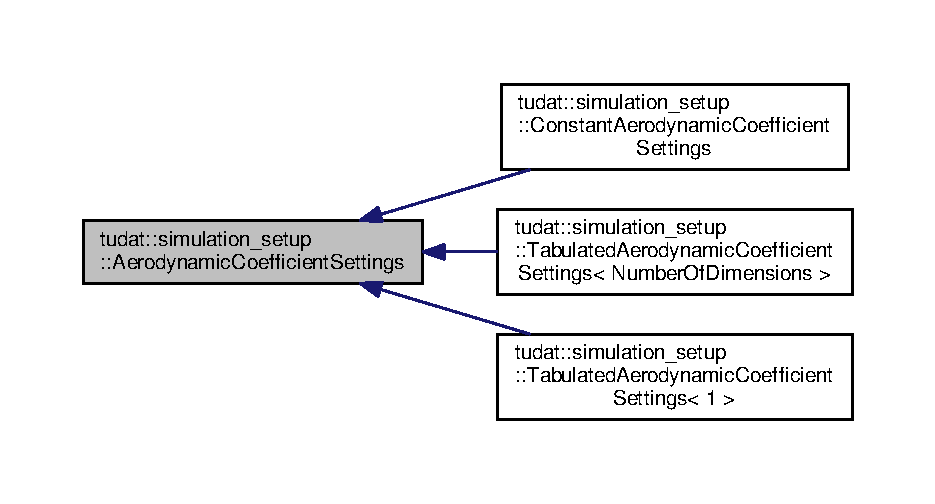
\includegraphics[width=350pt]{classtudat_1_1simulation__setup_1_1AerodynamicCoefficientSettings__inherit__graph}
\end{center}
\end{figure}
\subsection*{Public Member Functions}
\begin{DoxyCompactItemize}
\item 
\hyperlink{classtudat_1_1simulation__setup_1_1AerodynamicCoefficientSettings_aa7965f3d180b9fbc3fdefa8b399473e8}{Aerodynamic\+Coefficient\+Settings} (const Aerodynamic\+Coefficient\+Types aerodynamic\+Coefficient\+Types, const double reference\+Length, const double reference\+Area, const double lateral\+Reference\+Length, const Eigen\+::\+Vector3d \&moment\+Reference\+Point, const std\+::vector$<$ aerodynamics\+::\+Aerodynamic\+Coefficients\+Independent\+Variables $>$ independent\+Variable\+Names, const bool are\+Coefficients\+In\+Aerodynamic\+Frame=1, const bool are\+Coefficients\+In\+Negative\+Axis\+Direction=1)
\begin{DoxyCompactList}\small\item\em Constructor, sets type of aerodynamic coefficient model. \end{DoxyCompactList}\item 
virtual \hyperlink{classtudat_1_1simulation__setup_1_1AerodynamicCoefficientSettings_a2286359e82a186bbfa640447859dffcb}{$\sim$\+Aerodynamic\+Coefficient\+Settings} ()\hypertarget{classtudat_1_1simulation__setup_1_1AerodynamicCoefficientSettings_a2286359e82a186bbfa640447859dffcb}{}\label{classtudat_1_1simulation__setup_1_1AerodynamicCoefficientSettings_a2286359e82a186bbfa640447859dffcb}

\begin{DoxyCompactList}\small\item\em Destructor. \end{DoxyCompactList}\item 
Aerodynamic\+Coefficient\+Types \hyperlink{classtudat_1_1simulation__setup_1_1AerodynamicCoefficientSettings_ac9cdc44679a42e11702489a3720b1e97}{get\+Aerodynamic\+Coefficient\+Type} ()
\begin{DoxyCompactList}\small\item\em Function to return type of aerodynamic coefficient model that is to be created. \end{DoxyCompactList}\item 
double \hyperlink{classtudat_1_1simulation__setup_1_1AerodynamicCoefficientSettings_a435aa9070052b7442625e9ad010e4c57}{get\+Reference\+Area} ()
\begin{DoxyCompactList}\small\item\em Get reference area. \end{DoxyCompactList}\item 
double \hyperlink{classtudat_1_1simulation__setup_1_1AerodynamicCoefficientSettings_a1332da808b8afe7418344d4009904427}{get\+Reference\+Length} ()
\begin{DoxyCompactList}\small\item\em Get reference length. \end{DoxyCompactList}\item 
double \hyperlink{classtudat_1_1simulation__setup_1_1AerodynamicCoefficientSettings_a22915d5cfb8a662caf82b7ac082d7368}{get\+Lateral\+Reference\+Length} ()
\begin{DoxyCompactList}\small\item\em Get lateral reference length. \end{DoxyCompactList}\item 
Eigen\+::\+Vector\+Xd \hyperlink{classtudat_1_1simulation__setup_1_1AerodynamicCoefficientSettings_a16b2b67e431df72bc0267189dd0dd4cc}{get\+Moment\+Reference\+Point} ()
\begin{DoxyCompactList}\small\item\em Get moment reference point. \end{DoxyCompactList}\item 
std\+::vector$<$ aerodynamics\+::\+Aerodynamic\+Coefficients\+Independent\+Variables $>$ \hyperlink{classtudat_1_1simulation__setup_1_1AerodynamicCoefficientSettings_a884a3349c41d023ab72e7566053227aa}{get\+Independent\+Variable\+Names} ()
\begin{DoxyCompactList}\small\item\em Function to return identifiers of physical meaning of independent variables. \end{DoxyCompactList}\item 
bool \hyperlink{classtudat_1_1simulation__setup_1_1AerodynamicCoefficientSettings_a19ec87d7db67573936c8c60825f56875}{get\+Are\+Coefficients\+In\+Aerodynamic\+Frame} ()
\begin{DoxyCompactList}\small\item\em Function to return whether coefficients are in aerodynamic frame. \end{DoxyCompactList}\item 
bool \hyperlink{classtudat_1_1simulation__setup_1_1AerodynamicCoefficientSettings_a8446d225c5c7011a81280fe0fa1958c3}{get\+Are\+Coefficients\+In\+Negative\+Axis\+Direction} ()
\begin{DoxyCompactList}\small\item\em Function to return whether coefficients are positive along positive axes. \end{DoxyCompactList}\item 
std\+::map$<$ std\+::string, boost\+::shared\+\_\+ptr$<$ \hyperlink{classtudat_1_1simulation__setup_1_1ControlSurfaceIncrementAerodynamicCoefficientSettings}{Control\+Surface\+Increment\+Aerodynamic\+Coefficient\+Settings} $>$ $>$ {\bfseries get\+Control\+Surface\+Settings} ()\hypertarget{classtudat_1_1simulation__setup_1_1AerodynamicCoefficientSettings_a731406ba0baef00ccba55e8f965863f4}{}\label{classtudat_1_1simulation__setup_1_1AerodynamicCoefficientSettings_a731406ba0baef00ccba55e8f965863f4}

\item 
void \hyperlink{classtudat_1_1simulation__setup_1_1AerodynamicCoefficientSettings_a0e4b68cde88bc1e46fd0fccc00b5f524}{set\+Control\+Surface\+Settings} (const boost\+::shared\+\_\+ptr$<$ \hyperlink{classtudat_1_1simulation__setup_1_1ControlSurfaceIncrementAerodynamicCoefficientSettings}{Control\+Surface\+Increment\+Aerodynamic\+Coefficient\+Settings} $>$ control\+Surface\+Setting, const std\+::string control\+Surface\+Name)
\begin{DoxyCompactList}\small\item\em Function to define settings for the aerodynamic coefficients of a single control surface. \end{DoxyCompactList}\end{DoxyCompactItemize}


\subsection{Detailed Description}
Class for providing settings for aerodynamic coefficient model. 

Class for providing settings for automatic aerodynamic coefficient model creation. This class is a functional (base) class for settings of aerodynamic coefficient models that require no information in addition to their type. Aerodynamic coefficient model classes defining requiring additional information must be created using an object derived from this class. 

\subsection{Constructor \& Destructor Documentation}
\index{tudat\+::simulation\+\_\+setup\+::\+Aerodynamic\+Coefficient\+Settings@{tudat\+::simulation\+\_\+setup\+::\+Aerodynamic\+Coefficient\+Settings}!Aerodynamic\+Coefficient\+Settings@{Aerodynamic\+Coefficient\+Settings}}
\index{Aerodynamic\+Coefficient\+Settings@{Aerodynamic\+Coefficient\+Settings}!tudat\+::simulation\+\_\+setup\+::\+Aerodynamic\+Coefficient\+Settings@{tudat\+::simulation\+\_\+setup\+::\+Aerodynamic\+Coefficient\+Settings}}
\subsubsection[{\texorpdfstring{Aerodynamic\+Coefficient\+Settings(const Aerodynamic\+Coefficient\+Types aerodynamic\+Coefficient\+Types, const double reference\+Length, const double reference\+Area, const double lateral\+Reference\+Length, const Eigen\+::\+Vector3d \&moment\+Reference\+Point, const std\+::vector$<$ aerodynamics\+::\+Aerodynamic\+Coefficients\+Independent\+Variables $>$ independent\+Variable\+Names, const bool are\+Coefficients\+In\+Aerodynamic\+Frame=1, const bool are\+Coefficients\+In\+Negative\+Axis\+Direction=1)}{AerodynamicCoefficientSettings(const AerodynamicCoefficientTypes aerodynamicCoefficientTypes, const double referenceLength, const double referenceArea, const double lateralReferenceLength, const Eigen::Vector3d &momentReferencePoint, const std::vector< aerodynamics::AerodynamicCoefficientsIndependentVariables > independentVariableNames, const bool areCoefficientsInAerodynamicFrame=1, const bool areCoefficientsInNegativeAxisDirection=1)}}]{\setlength{\rightskip}{0pt plus 5cm}tudat\+::simulation\+\_\+setup\+::\+Aerodynamic\+Coefficient\+Settings\+::\+Aerodynamic\+Coefficient\+Settings (
\begin{DoxyParamCaption}
\item[{const Aerodynamic\+Coefficient\+Types}]{aerodynamic\+Coefficient\+Types, }
\item[{const double}]{reference\+Length, }
\item[{const double}]{reference\+Area, }
\item[{const double}]{lateral\+Reference\+Length, }
\item[{const Eigen\+::\+Vector3d \&}]{moment\+Reference\+Point, }
\item[{const std\+::vector$<$ aerodynamics\+::\+Aerodynamic\+Coefficients\+Independent\+Variables $>$}]{independent\+Variable\+Names, }
\item[{const bool}]{are\+Coefficients\+In\+Aerodynamic\+Frame = {\ttfamily 1}, }
\item[{const bool}]{are\+Coefficients\+In\+Negative\+Axis\+Direction = {\ttfamily 1}}
\end{DoxyParamCaption}
)\hspace{0.3cm}{\ttfamily [inline]}}\hypertarget{classtudat_1_1simulation__setup_1_1AerodynamicCoefficientSettings_aa7965f3d180b9fbc3fdefa8b399473e8}{}\label{classtudat_1_1simulation__setup_1_1AerodynamicCoefficientSettings_aa7965f3d180b9fbc3fdefa8b399473e8}


Constructor, sets type of aerodynamic coefficient model. 

Constructor, sets type of aerodynamic coefficient model. Settings for aerodynamic coefficient models requiring additional information should be defined in a derived class. 
\begin{DoxyParams}{Parameters}
{\em aerodynamic\+Coefficient\+Types} & Type of aerodynamic coefficient model that is to be created. \\
\hline
{\em reference\+Length} & Reference length with which aerodynamic moments (about x-\/ and z-\/ axes) are non-\/dimensionalized. \\
\hline
{\em reference\+Area} & Reference area with which aerodynamic forces and moments are non-\/dimensionalized. \\
\hline
{\em lateral\+Reference\+Length} & Reference length with which aerodynamic moments (about y-\/axis) is non-\/dimensionalized. \\
\hline
{\em moment\+Reference\+Point} & Point w.\+r.\+t. aerodynamic moment is calculated \\
\hline
{\em independent\+Variable\+Names} & Vector with identifiers the physical meaning of each independent variable of the aerodynamic coefficients. \\
\hline
{\em are\+Coefficients\+In\+Aerodynamic\+Frame} & Boolean to define whether the aerodynamic coefficients are defined in the aerodynamic frame (lift, drag, side force) or in the body frame (typically denoted as Cx, Cy, Cz). \\
\hline
{\em are\+Coefficients\+In\+Negative\+Axis\+Direction} & Boolean to define whether the aerodynamic coefficients are positive along the positive axes of the body or aerodynamic frame (see are\+Coefficients\+In\+Aerodynamic\+Frame). Note that for (lift, drag, side force), the coefficients are typically defined in negative direction. \\
\hline
\end{DoxyParams}


\subsection{Member Function Documentation}
\index{tudat\+::simulation\+\_\+setup\+::\+Aerodynamic\+Coefficient\+Settings@{tudat\+::simulation\+\_\+setup\+::\+Aerodynamic\+Coefficient\+Settings}!get\+Aerodynamic\+Coefficient\+Type@{get\+Aerodynamic\+Coefficient\+Type}}
\index{get\+Aerodynamic\+Coefficient\+Type@{get\+Aerodynamic\+Coefficient\+Type}!tudat\+::simulation\+\_\+setup\+::\+Aerodynamic\+Coefficient\+Settings@{tudat\+::simulation\+\_\+setup\+::\+Aerodynamic\+Coefficient\+Settings}}
\subsubsection[{\texorpdfstring{get\+Aerodynamic\+Coefficient\+Type()}{getAerodynamicCoefficientType()}}]{\setlength{\rightskip}{0pt plus 5cm}Aerodynamic\+Coefficient\+Types tudat\+::simulation\+\_\+setup\+::\+Aerodynamic\+Coefficient\+Settings\+::get\+Aerodynamic\+Coefficient\+Type (
\begin{DoxyParamCaption}
{}
\end{DoxyParamCaption}
)\hspace{0.3cm}{\ttfamily [inline]}}\hypertarget{classtudat_1_1simulation__setup_1_1AerodynamicCoefficientSettings_ac9cdc44679a42e11702489a3720b1e97}{}\label{classtudat_1_1simulation__setup_1_1AerodynamicCoefficientSettings_ac9cdc44679a42e11702489a3720b1e97}


Function to return type of aerodynamic coefficient model that is to be created. 

Function to return type of aerodynamic coefficient model that is to be created. \begin{DoxyReturn}{Returns}
Type of aerodynamic coefficient model that is to be created. 
\end{DoxyReturn}
\index{tudat\+::simulation\+\_\+setup\+::\+Aerodynamic\+Coefficient\+Settings@{tudat\+::simulation\+\_\+setup\+::\+Aerodynamic\+Coefficient\+Settings}!get\+Are\+Coefficients\+In\+Aerodynamic\+Frame@{get\+Are\+Coefficients\+In\+Aerodynamic\+Frame}}
\index{get\+Are\+Coefficients\+In\+Aerodynamic\+Frame@{get\+Are\+Coefficients\+In\+Aerodynamic\+Frame}!tudat\+::simulation\+\_\+setup\+::\+Aerodynamic\+Coefficient\+Settings@{tudat\+::simulation\+\_\+setup\+::\+Aerodynamic\+Coefficient\+Settings}}
\subsubsection[{\texorpdfstring{get\+Are\+Coefficients\+In\+Aerodynamic\+Frame()}{getAreCoefficientsInAerodynamicFrame()}}]{\setlength{\rightskip}{0pt plus 5cm}bool tudat\+::simulation\+\_\+setup\+::\+Aerodynamic\+Coefficient\+Settings\+::get\+Are\+Coefficients\+In\+Aerodynamic\+Frame (
\begin{DoxyParamCaption}
{}
\end{DoxyParamCaption}
)\hspace{0.3cm}{\ttfamily [inline]}}\hypertarget{classtudat_1_1simulation__setup_1_1AerodynamicCoefficientSettings_a19ec87d7db67573936c8c60825f56875}{}\label{classtudat_1_1simulation__setup_1_1AerodynamicCoefficientSettings_a19ec87d7db67573936c8c60825f56875}


Function to return whether coefficients are in aerodynamic frame. 

Function to return whether coefficients are in aerodynamic frame. \begin{DoxyReturn}{Returns}
Boolean defining whether coefficients are in aerodynamic frame. 
\end{DoxyReturn}
\index{tudat\+::simulation\+\_\+setup\+::\+Aerodynamic\+Coefficient\+Settings@{tudat\+::simulation\+\_\+setup\+::\+Aerodynamic\+Coefficient\+Settings}!get\+Are\+Coefficients\+In\+Negative\+Axis\+Direction@{get\+Are\+Coefficients\+In\+Negative\+Axis\+Direction}}
\index{get\+Are\+Coefficients\+In\+Negative\+Axis\+Direction@{get\+Are\+Coefficients\+In\+Negative\+Axis\+Direction}!tudat\+::simulation\+\_\+setup\+::\+Aerodynamic\+Coefficient\+Settings@{tudat\+::simulation\+\_\+setup\+::\+Aerodynamic\+Coefficient\+Settings}}
\subsubsection[{\texorpdfstring{get\+Are\+Coefficients\+In\+Negative\+Axis\+Direction()}{getAreCoefficientsInNegativeAxisDirection()}}]{\setlength{\rightskip}{0pt plus 5cm}bool tudat\+::simulation\+\_\+setup\+::\+Aerodynamic\+Coefficient\+Settings\+::get\+Are\+Coefficients\+In\+Negative\+Axis\+Direction (
\begin{DoxyParamCaption}
{}
\end{DoxyParamCaption}
)\hspace{0.3cm}{\ttfamily [inline]}}\hypertarget{classtudat_1_1simulation__setup_1_1AerodynamicCoefficientSettings_a8446d225c5c7011a81280fe0fa1958c3}{}\label{classtudat_1_1simulation__setup_1_1AerodynamicCoefficientSettings_a8446d225c5c7011a81280fe0fa1958c3}


Function to return whether coefficients are positive along positive axes. 

Function to return whether coefficients are positive along positive axes. \begin{DoxyReturn}{Returns}
Boolean defining whether coefficients are positive along positive axes. 
\end{DoxyReturn}
\index{tudat\+::simulation\+\_\+setup\+::\+Aerodynamic\+Coefficient\+Settings@{tudat\+::simulation\+\_\+setup\+::\+Aerodynamic\+Coefficient\+Settings}!get\+Independent\+Variable\+Names@{get\+Independent\+Variable\+Names}}
\index{get\+Independent\+Variable\+Names@{get\+Independent\+Variable\+Names}!tudat\+::simulation\+\_\+setup\+::\+Aerodynamic\+Coefficient\+Settings@{tudat\+::simulation\+\_\+setup\+::\+Aerodynamic\+Coefficient\+Settings}}
\subsubsection[{\texorpdfstring{get\+Independent\+Variable\+Names()}{getIndependentVariableNames()}}]{\setlength{\rightskip}{0pt plus 5cm}std\+::vector$<$ aerodynamics\+::\+Aerodynamic\+Coefficients\+Independent\+Variables $>$ tudat\+::simulation\+\_\+setup\+::\+Aerodynamic\+Coefficient\+Settings\+::get\+Independent\+Variable\+Names (
\begin{DoxyParamCaption}
{}
\end{DoxyParamCaption}
)\hspace{0.3cm}{\ttfamily [inline]}}\hypertarget{classtudat_1_1simulation__setup_1_1AerodynamicCoefficientSettings_a884a3349c41d023ab72e7566053227aa}{}\label{classtudat_1_1simulation__setup_1_1AerodynamicCoefficientSettings_a884a3349c41d023ab72e7566053227aa}


Function to return identifiers of physical meaning of independent variables. 

Function to return identifiers of physical meaning of independent variables. \begin{DoxyReturn}{Returns}
Identifiers of physical meaning of independent variables. 
\end{DoxyReturn}
\index{tudat\+::simulation\+\_\+setup\+::\+Aerodynamic\+Coefficient\+Settings@{tudat\+::simulation\+\_\+setup\+::\+Aerodynamic\+Coefficient\+Settings}!get\+Lateral\+Reference\+Length@{get\+Lateral\+Reference\+Length}}
\index{get\+Lateral\+Reference\+Length@{get\+Lateral\+Reference\+Length}!tudat\+::simulation\+\_\+setup\+::\+Aerodynamic\+Coefficient\+Settings@{tudat\+::simulation\+\_\+setup\+::\+Aerodynamic\+Coefficient\+Settings}}
\subsubsection[{\texorpdfstring{get\+Lateral\+Reference\+Length()}{getLateralReferenceLength()}}]{\setlength{\rightskip}{0pt plus 5cm}double tudat\+::simulation\+\_\+setup\+::\+Aerodynamic\+Coefficient\+Settings\+::get\+Lateral\+Reference\+Length (
\begin{DoxyParamCaption}
{}
\end{DoxyParamCaption}
)\hspace{0.3cm}{\ttfamily [inline]}}\hypertarget{classtudat_1_1simulation__setup_1_1AerodynamicCoefficientSettings_a22915d5cfb8a662caf82b7ac082d7368}{}\label{classtudat_1_1simulation__setup_1_1AerodynamicCoefficientSettings_a22915d5cfb8a662caf82b7ac082d7368}


Get lateral reference length. 

Returns lateral reference length used to non-\/dimensionalize aerodynamic moments. \begin{DoxyReturn}{Returns}
Aerodynamic lateral reference length. 
\end{DoxyReturn}
\index{tudat\+::simulation\+\_\+setup\+::\+Aerodynamic\+Coefficient\+Settings@{tudat\+::simulation\+\_\+setup\+::\+Aerodynamic\+Coefficient\+Settings}!get\+Moment\+Reference\+Point@{get\+Moment\+Reference\+Point}}
\index{get\+Moment\+Reference\+Point@{get\+Moment\+Reference\+Point}!tudat\+::simulation\+\_\+setup\+::\+Aerodynamic\+Coefficient\+Settings@{tudat\+::simulation\+\_\+setup\+::\+Aerodynamic\+Coefficient\+Settings}}
\subsubsection[{\texorpdfstring{get\+Moment\+Reference\+Point()}{getMomentReferencePoint()}}]{\setlength{\rightskip}{0pt plus 5cm}Eigen\+::\+Vector\+Xd tudat\+::simulation\+\_\+setup\+::\+Aerodynamic\+Coefficient\+Settings\+::get\+Moment\+Reference\+Point (
\begin{DoxyParamCaption}
{}
\end{DoxyParamCaption}
)\hspace{0.3cm}{\ttfamily [inline]}}\hypertarget{classtudat_1_1simulation__setup_1_1AerodynamicCoefficientSettings_a16b2b67e431df72bc0267189dd0dd4cc}{}\label{classtudat_1_1simulation__setup_1_1AerodynamicCoefficientSettings_a16b2b67e431df72bc0267189dd0dd4cc}


Get moment reference point. 

Returns the point w.\+r.\+t. which the arm of the aerodynamic moment on a vehicle panel is determined. \begin{DoxyReturn}{Returns}
Aerodynamic reference point. 
\end{DoxyReturn}
\index{tudat\+::simulation\+\_\+setup\+::\+Aerodynamic\+Coefficient\+Settings@{tudat\+::simulation\+\_\+setup\+::\+Aerodynamic\+Coefficient\+Settings}!get\+Reference\+Area@{get\+Reference\+Area}}
\index{get\+Reference\+Area@{get\+Reference\+Area}!tudat\+::simulation\+\_\+setup\+::\+Aerodynamic\+Coefficient\+Settings@{tudat\+::simulation\+\_\+setup\+::\+Aerodynamic\+Coefficient\+Settings}}
\subsubsection[{\texorpdfstring{get\+Reference\+Area()}{getReferenceArea()}}]{\setlength{\rightskip}{0pt plus 5cm}double tudat\+::simulation\+\_\+setup\+::\+Aerodynamic\+Coefficient\+Settings\+::get\+Reference\+Area (
\begin{DoxyParamCaption}
{}
\end{DoxyParamCaption}
)\hspace{0.3cm}{\ttfamily [inline]}}\hypertarget{classtudat_1_1simulation__setup_1_1AerodynamicCoefficientSettings_a435aa9070052b7442625e9ad010e4c57}{}\label{classtudat_1_1simulation__setup_1_1AerodynamicCoefficientSettings_a435aa9070052b7442625e9ad010e4c57}


Get reference area. 

Returns reference area used to non-\/dimensionalize aerodynamic forces and moments. \begin{DoxyReturn}{Returns}
Aerodynamic reference area. 
\end{DoxyReturn}
\index{tudat\+::simulation\+\_\+setup\+::\+Aerodynamic\+Coefficient\+Settings@{tudat\+::simulation\+\_\+setup\+::\+Aerodynamic\+Coefficient\+Settings}!get\+Reference\+Length@{get\+Reference\+Length}}
\index{get\+Reference\+Length@{get\+Reference\+Length}!tudat\+::simulation\+\_\+setup\+::\+Aerodynamic\+Coefficient\+Settings@{tudat\+::simulation\+\_\+setup\+::\+Aerodynamic\+Coefficient\+Settings}}
\subsubsection[{\texorpdfstring{get\+Reference\+Length()}{getReferenceLength()}}]{\setlength{\rightskip}{0pt plus 5cm}double tudat\+::simulation\+\_\+setup\+::\+Aerodynamic\+Coefficient\+Settings\+::get\+Reference\+Length (
\begin{DoxyParamCaption}
{}
\end{DoxyParamCaption}
)\hspace{0.3cm}{\ttfamily [inline]}}\hypertarget{classtudat_1_1simulation__setup_1_1AerodynamicCoefficientSettings_a1332da808b8afe7418344d4009904427}{}\label{classtudat_1_1simulation__setup_1_1AerodynamicCoefficientSettings_a1332da808b8afe7418344d4009904427}


Get reference length. 

Returns reference length used to non-\/dimensionalize aerodynamic moments. \begin{DoxyReturn}{Returns}
Aerodynamic reference length. 
\end{DoxyReturn}
\index{tudat\+::simulation\+\_\+setup\+::\+Aerodynamic\+Coefficient\+Settings@{tudat\+::simulation\+\_\+setup\+::\+Aerodynamic\+Coefficient\+Settings}!set\+Control\+Surface\+Settings@{set\+Control\+Surface\+Settings}}
\index{set\+Control\+Surface\+Settings@{set\+Control\+Surface\+Settings}!tudat\+::simulation\+\_\+setup\+::\+Aerodynamic\+Coefficient\+Settings@{tudat\+::simulation\+\_\+setup\+::\+Aerodynamic\+Coefficient\+Settings}}
\subsubsection[{\texorpdfstring{set\+Control\+Surface\+Settings(const boost\+::shared\+\_\+ptr$<$ Control\+Surface\+Increment\+Aerodynamic\+Coefficient\+Settings $>$ control\+Surface\+Setting, const std\+::string control\+Surface\+Name)}{setControlSurfaceSettings(const boost::shared_ptr< ControlSurfaceIncrementAerodynamicCoefficientSettings > controlSurfaceSetting, const std::string controlSurfaceName)}}]{\setlength{\rightskip}{0pt plus 5cm}void tudat\+::simulation\+\_\+setup\+::\+Aerodynamic\+Coefficient\+Settings\+::set\+Control\+Surface\+Settings (
\begin{DoxyParamCaption}
\item[{const boost\+::shared\+\_\+ptr$<$ {\bf Control\+Surface\+Increment\+Aerodynamic\+Coefficient\+Settings} $>$}]{control\+Surface\+Setting, }
\item[{const std\+::string}]{control\+Surface\+Name}
\end{DoxyParamCaption}
)\hspace{0.3cm}{\ttfamily [inline]}}\hypertarget{classtudat_1_1simulation__setup_1_1AerodynamicCoefficientSettings_a0e4b68cde88bc1e46fd0fccc00b5f524}{}\label{classtudat_1_1simulation__setup_1_1AerodynamicCoefficientSettings_a0e4b68cde88bc1e46fd0fccc00b5f524}


Function to define settings for the aerodynamic coefficients of a single control surface. 

Function to define settings for the aerodynamic coefficients of a single control surface 
\begin{DoxyParams}{Parameters}
{\em control\+Surface\+Setting} & Settings for the arodynamic coefficients of control surface. \\
\hline
{\em control\+Surface\+Name} & Id of control surface. \\
\hline
\end{DoxyParams}


The documentation for this class was generated from the following file\+:\begin{DoxyCompactItemize}
\item 
/home/lupi/\+Tudat/tudat\+Bundle/tudat/\+Tudat/\+Simulation\+Setup/\+Environment\+Setup/create\+Aerodynamic\+Coefficient\+Interface.\+h\end{DoxyCompactItemize}

\hypertarget{classtudat_1_1aerodynamics_1_1AerodynamicGuidance}{}\section{tudat\+:\+:aerodynamics\+:\+:Aerodynamic\+Guidance Class Reference}
\label{classtudat_1_1aerodynamics_1_1AerodynamicGuidance}\index{tudat\+::aerodynamics\+::\+Aerodynamic\+Guidance@{tudat\+::aerodynamics\+::\+Aerodynamic\+Guidance}}


{\ttfamily \#include $<$aerodynamic\+Guidance.\+h$>$}



Inheritance diagram for tudat\+:\+:aerodynamics\+:\+:Aerodynamic\+Guidance\+:
\nopagebreak
\begin{figure}[H]
\begin{center}
\leavevmode
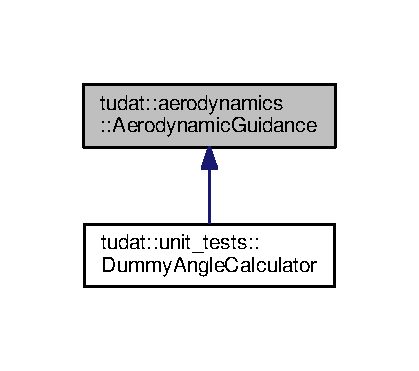
\includegraphics[width=201pt]{classtudat_1_1aerodynamics_1_1AerodynamicGuidance__inherit__graph}
\end{center}
\end{figure}
\subsection*{Public Member Functions}
\begin{DoxyCompactItemize}
\item 
\hyperlink{classtudat_1_1aerodynamics_1_1AerodynamicGuidance_aaf4f9cfc62d861c1e2c4438d9cfb84cb}{Aerodynamic\+Guidance} ()\hypertarget{classtudat_1_1aerodynamics_1_1AerodynamicGuidance_aaf4f9cfc62d861c1e2c4438d9cfb84cb}{}\label{classtudat_1_1aerodynamics_1_1AerodynamicGuidance_aaf4f9cfc62d861c1e2c4438d9cfb84cb}

\begin{DoxyCompactList}\small\item\em Constructor. \end{DoxyCompactList}\item 
virtual \hyperlink{classtudat_1_1aerodynamics_1_1AerodynamicGuidance_a01f1a9a23bc8d0794003909d61385ab1}{$\sim$\+Aerodynamic\+Guidance} ()\hypertarget{classtudat_1_1aerodynamics_1_1AerodynamicGuidance_a01f1a9a23bc8d0794003909d61385ab1}{}\label{classtudat_1_1aerodynamics_1_1AerodynamicGuidance_a01f1a9a23bc8d0794003909d61385ab1}

\begin{DoxyCompactList}\small\item\em Destructor. \end{DoxyCompactList}\item 
virtual void \hyperlink{classtudat_1_1aerodynamics_1_1AerodynamicGuidance_a97a6200cf74d60a2a5ad1616e159ffc5}{update\+Guidance} (const double current\+Time)=0
\begin{DoxyCompactList}\small\item\em Pure virtual function to update the guidance to the current time and state. \end{DoxyCompactList}\item 
double \hyperlink{classtudat_1_1aerodynamics_1_1AerodynamicGuidance_ac8d09c3926209eb3d440484c0580f6ea}{get\+Current\+Angle\+Of\+Attack} ()
\begin{DoxyCompactList}\small\item\em Function to retrieve the current angle of attack, as set by last call to update\+Guidance function. \end{DoxyCompactList}\item 
double \hyperlink{classtudat_1_1aerodynamics_1_1AerodynamicGuidance_a3ea3dcb8ee9f99f5107ad1aa86b23ae3}{get\+Current\+Angle\+Of\+Sideslip} ()
\begin{DoxyCompactList}\small\item\em Function to retrieve the current angle of sideslip, as set by last call to update\+Guidance function. \end{DoxyCompactList}\item 
double \hyperlink{classtudat_1_1aerodynamics_1_1AerodynamicGuidance_a342513b4fa99f1f09365ff4f7a3c572f}{get\+Current\+Bank\+Angle} ()
\begin{DoxyCompactList}\small\item\em Function to retrieve the current bank angle, as set by last call to update\+Guidance function. \end{DoxyCompactList}\end{DoxyCompactItemize}
\subsection*{Protected Attributes}
\begin{DoxyCompactItemize}
\item 
double \hyperlink{classtudat_1_1aerodynamics_1_1AerodynamicGuidance_abf93dc422542fbbbabd8102e105c0e50}{current\+Angle\+Of\+Attack\+\_\+}\hypertarget{classtudat_1_1aerodynamics_1_1AerodynamicGuidance_abf93dc422542fbbbabd8102e105c0e50}{}\label{classtudat_1_1aerodynamics_1_1AerodynamicGuidance_abf93dc422542fbbbabd8102e105c0e50}

\begin{DoxyCompactList}\small\item\em Current angle of attack, as set by last call to update\+Guidance function. \end{DoxyCompactList}\item 
double \hyperlink{classtudat_1_1aerodynamics_1_1AerodynamicGuidance_ad1921668cf3feb2bedbb183713b03843}{current\+Angle\+Of\+Sideslip\+\_\+}\hypertarget{classtudat_1_1aerodynamics_1_1AerodynamicGuidance_ad1921668cf3feb2bedbb183713b03843}{}\label{classtudat_1_1aerodynamics_1_1AerodynamicGuidance_ad1921668cf3feb2bedbb183713b03843}

\begin{DoxyCompactList}\small\item\em Current angle of sideslip, as set by last call to update\+Guidance function. \end{DoxyCompactList}\item 
double \hyperlink{classtudat_1_1aerodynamics_1_1AerodynamicGuidance_a7bd38e6cef133b0ed8487d8d88cdc9ad}{current\+Bank\+Angle\+\_\+}\hypertarget{classtudat_1_1aerodynamics_1_1AerodynamicGuidance_a7bd38e6cef133b0ed8487d8d88cdc9ad}{}\label{classtudat_1_1aerodynamics_1_1AerodynamicGuidance_a7bd38e6cef133b0ed8487d8d88cdc9ad}

\begin{DoxyCompactList}\small\item\em Current bank angle, as set by last call to update\+Guidance function. \end{DoxyCompactList}\end{DoxyCompactItemize}


\subsection{Detailed Description}
Base class in which the aerodynamic angles (angle of attack, sideslip and bank angle) are computed. A derived class implementing a specific guidance law is to be implemented by the user. 

\subsection{Member Function Documentation}
\index{tudat\+::aerodynamics\+::\+Aerodynamic\+Guidance@{tudat\+::aerodynamics\+::\+Aerodynamic\+Guidance}!get\+Current\+Angle\+Of\+Attack@{get\+Current\+Angle\+Of\+Attack}}
\index{get\+Current\+Angle\+Of\+Attack@{get\+Current\+Angle\+Of\+Attack}!tudat\+::aerodynamics\+::\+Aerodynamic\+Guidance@{tudat\+::aerodynamics\+::\+Aerodynamic\+Guidance}}
\subsubsection[{\texorpdfstring{get\+Current\+Angle\+Of\+Attack()}{getCurrentAngleOfAttack()}}]{\setlength{\rightskip}{0pt plus 5cm}double tudat\+::aerodynamics\+::\+Aerodynamic\+Guidance\+::get\+Current\+Angle\+Of\+Attack (
\begin{DoxyParamCaption}
{}
\end{DoxyParamCaption}
)\hspace{0.3cm}{\ttfamily [inline]}}\hypertarget{classtudat_1_1aerodynamics_1_1AerodynamicGuidance_ac8d09c3926209eb3d440484c0580f6ea}{}\label{classtudat_1_1aerodynamics_1_1AerodynamicGuidance_ac8d09c3926209eb3d440484c0580f6ea}


Function to retrieve the current angle of attack, as set by last call to update\+Guidance function. 

Function to retrieve the current angle of attack, as set by last call to update\+Guidance function \begin{DoxyReturn}{Returns}
Current angle of attack, as set by last call to update\+Guidance function 
\end{DoxyReturn}
\index{tudat\+::aerodynamics\+::\+Aerodynamic\+Guidance@{tudat\+::aerodynamics\+::\+Aerodynamic\+Guidance}!get\+Current\+Angle\+Of\+Sideslip@{get\+Current\+Angle\+Of\+Sideslip}}
\index{get\+Current\+Angle\+Of\+Sideslip@{get\+Current\+Angle\+Of\+Sideslip}!tudat\+::aerodynamics\+::\+Aerodynamic\+Guidance@{tudat\+::aerodynamics\+::\+Aerodynamic\+Guidance}}
\subsubsection[{\texorpdfstring{get\+Current\+Angle\+Of\+Sideslip()}{getCurrentAngleOfSideslip()}}]{\setlength{\rightskip}{0pt plus 5cm}double tudat\+::aerodynamics\+::\+Aerodynamic\+Guidance\+::get\+Current\+Angle\+Of\+Sideslip (
\begin{DoxyParamCaption}
{}
\end{DoxyParamCaption}
)\hspace{0.3cm}{\ttfamily [inline]}}\hypertarget{classtudat_1_1aerodynamics_1_1AerodynamicGuidance_a3ea3dcb8ee9f99f5107ad1aa86b23ae3}{}\label{classtudat_1_1aerodynamics_1_1AerodynamicGuidance_a3ea3dcb8ee9f99f5107ad1aa86b23ae3}


Function to retrieve the current angle of sideslip, as set by last call to update\+Guidance function. 

Function to retrieve the current angle of sideslip, as set by last call to update\+Guidance function \begin{DoxyReturn}{Returns}
Current angle of sideslip, as set by last call to update\+Guidance function 
\end{DoxyReturn}
\index{tudat\+::aerodynamics\+::\+Aerodynamic\+Guidance@{tudat\+::aerodynamics\+::\+Aerodynamic\+Guidance}!get\+Current\+Bank\+Angle@{get\+Current\+Bank\+Angle}}
\index{get\+Current\+Bank\+Angle@{get\+Current\+Bank\+Angle}!tudat\+::aerodynamics\+::\+Aerodynamic\+Guidance@{tudat\+::aerodynamics\+::\+Aerodynamic\+Guidance}}
\subsubsection[{\texorpdfstring{get\+Current\+Bank\+Angle()}{getCurrentBankAngle()}}]{\setlength{\rightskip}{0pt plus 5cm}double tudat\+::aerodynamics\+::\+Aerodynamic\+Guidance\+::get\+Current\+Bank\+Angle (
\begin{DoxyParamCaption}
{}
\end{DoxyParamCaption}
)\hspace{0.3cm}{\ttfamily [inline]}}\hypertarget{classtudat_1_1aerodynamics_1_1AerodynamicGuidance_a342513b4fa99f1f09365ff4f7a3c572f}{}\label{classtudat_1_1aerodynamics_1_1AerodynamicGuidance_a342513b4fa99f1f09365ff4f7a3c572f}


Function to retrieve the current bank angle, as set by last call to update\+Guidance function. 

Function to retrieve the current bank angle, as set by last call to update\+Guidance function \begin{DoxyReturn}{Returns}
Current bank angle, as set by last call to update\+Guidance function 
\end{DoxyReturn}
\index{tudat\+::aerodynamics\+::\+Aerodynamic\+Guidance@{tudat\+::aerodynamics\+::\+Aerodynamic\+Guidance}!update\+Guidance@{update\+Guidance}}
\index{update\+Guidance@{update\+Guidance}!tudat\+::aerodynamics\+::\+Aerodynamic\+Guidance@{tudat\+::aerodynamics\+::\+Aerodynamic\+Guidance}}
\subsubsection[{\texorpdfstring{update\+Guidance(const double current\+Time)=0}{updateGuidance(const double currentTime)=0}}]{\setlength{\rightskip}{0pt plus 5cm}virtual void tudat\+::aerodynamics\+::\+Aerodynamic\+Guidance\+::update\+Guidance (
\begin{DoxyParamCaption}
\item[{const double}]{current\+Time}
\end{DoxyParamCaption}
)\hspace{0.3cm}{\ttfamily [pure virtual]}}\hypertarget{classtudat_1_1aerodynamics_1_1AerodynamicGuidance_a97a6200cf74d60a2a5ad1616e159ffc5}{}\label{classtudat_1_1aerodynamics_1_1AerodynamicGuidance_a97a6200cf74d60a2a5ad1616e159ffc5}


Pure virtual function to update the guidance to the current time and state. 

Pure virtual function to update the guidance to the current time and state 
\begin{DoxyParams}{Parameters}
{\em current\+Time} & \hyperlink{classtudat_1_1Time}{Time} to which the guidance object is to be updated. \\
\hline
\end{DoxyParams}


Implemented in \hyperlink{classtudat_1_1unit__tests_1_1DummyAngleCalculator_ac7c9dc1b0ab06c0807c368b44665bf2e}{tudat\+::unit\+\_\+tests\+::\+Dummy\+Angle\+Calculator}.



The documentation for this class was generated from the following file\+:\begin{DoxyCompactItemize}
\item 
/home/lupi/\+Tudat/tudat\+Bundle/tudat/\+Tudat/\+Astrodynamics/\+Aerodynamics/aerodynamic\+Guidance.\+h\end{DoxyCompactItemize}

\hypertarget{structtudat_1_1optimization_1_1AnalyticalSimplePlanetaryTargeter}{}\section{tudat\+:\+:optimization\+:\+:Analytical\+Simple\+Planetary\+Targeter Struct Reference}
\label{structtudat_1_1optimization_1_1AnalyticalSimplePlanetaryTargeter}\index{tudat\+::optimization\+::\+Analytical\+Simple\+Planetary\+Targeter@{tudat\+::optimization\+::\+Analytical\+Simple\+Planetary\+Targeter}}


Collaboration diagram for tudat\+:\+:optimization\+:\+:Analytical\+Simple\+Planetary\+Targeter\+:
\nopagebreak
\begin{figure}[H]
\begin{center}
\leavevmode
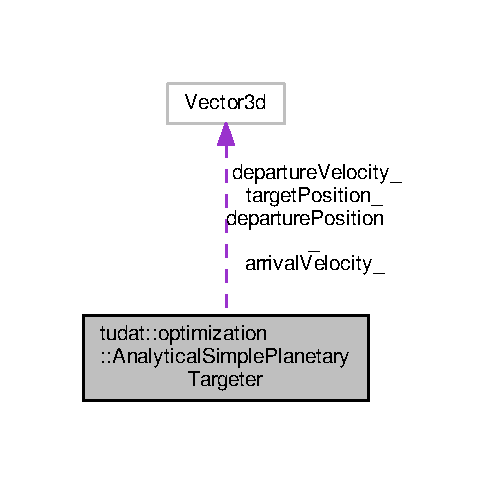
\includegraphics[width=234pt]{structtudat_1_1optimization_1_1AnalyticalSimplePlanetaryTargeter__coll__graph}
\end{center}
\end{figure}
\subsection*{Public Member Functions}
\begin{DoxyCompactItemize}
\item 
{\bfseries Analytical\+Simple\+Planetary\+Targeter} (Eigen\+::\+Vector3d departure\+Position, Eigen\+::\+Vector3d target\+Position, const double travel\+Time, const double central\+Body\+Gravitational\+Parameter, const int number\+Of\+Revolutions=0, const bool right\+Branch=true)\hypertarget{structtudat_1_1optimization_1_1AnalyticalSimplePlanetaryTargeter_a31ac39324cc9ea06117926c74af69c79}{}\label{structtudat_1_1optimization_1_1AnalyticalSimplePlanetaryTargeter_a31ac39324cc9ea06117926c74af69c79}

\end{DoxyCompactItemize}
\subsection*{Public Attributes}
\begin{DoxyCompactItemize}
\item 
Eigen\+::\+Vector3d {\bfseries departure\+Position\+\_\+}\hypertarget{structtudat_1_1optimization_1_1AnalyticalSimplePlanetaryTargeter_aaf147e038b7f3d1e6ba54f7fbc5d2149}{}\label{structtudat_1_1optimization_1_1AnalyticalSimplePlanetaryTargeter_aaf147e038b7f3d1e6ba54f7fbc5d2149}

\item 
Eigen\+::\+Vector3d {\bfseries target\+Position\+\_\+}\hypertarget{structtudat_1_1optimization_1_1AnalyticalSimplePlanetaryTargeter_a5c914327c9bbf52bda56ea2ce8a8323a}{}\label{structtudat_1_1optimization_1_1AnalyticalSimplePlanetaryTargeter_a5c914327c9bbf52bda56ea2ce8a8323a}

\item 
double {\bfseries travel\+Time\+\_\+}\hypertarget{structtudat_1_1optimization_1_1AnalyticalSimplePlanetaryTargeter_a256a1b2b64a3a3894820e4d4ec087941}{}\label{structtudat_1_1optimization_1_1AnalyticalSimplePlanetaryTargeter_a256a1b2b64a3a3894820e4d4ec087941}

\item 
double {\bfseries central\+Body\+Gravitational\+Parameter\+\_\+}\hypertarget{structtudat_1_1optimization_1_1AnalyticalSimplePlanetaryTargeter_a1f58d026ab9012383a2dd7a8c2f6efb5}{}\label{structtudat_1_1optimization_1_1AnalyticalSimplePlanetaryTargeter_a1f58d026ab9012383a2dd7a8c2f6efb5}

\item 
int {\bfseries number\+Of\+Revolutions\+\_\+}\hypertarget{structtudat_1_1optimization_1_1AnalyticalSimplePlanetaryTargeter_ab822a954d9e951814dba3cb29f04acca}{}\label{structtudat_1_1optimization_1_1AnalyticalSimplePlanetaryTargeter_ab822a954d9e951814dba3cb29f04acca}

\item 
bool {\bfseries is\+Right\+Branch\+\_\+}\hypertarget{structtudat_1_1optimization_1_1AnalyticalSimplePlanetaryTargeter_aa717121492d1b1c00ea5f48e6d225eb6}{}\label{structtudat_1_1optimization_1_1AnalyticalSimplePlanetaryTargeter_aa717121492d1b1c00ea5f48e6d225eb6}

\item 
Eigen\+::\+Vector3d {\bfseries departure\+Velocity\+\_\+}\hypertarget{structtudat_1_1optimization_1_1AnalyticalSimplePlanetaryTargeter_a7d817ed953a4e3238051ec9af5252196}{}\label{structtudat_1_1optimization_1_1AnalyticalSimplePlanetaryTargeter_a7d817ed953a4e3238051ec9af5252196}

\item 
Eigen\+::\+Vector3d {\bfseries arrival\+Velocity\+\_\+}\hypertarget{structtudat_1_1optimization_1_1AnalyticalSimplePlanetaryTargeter_af38673dc06864d4b1e94b81ce6520a3a}{}\label{structtudat_1_1optimization_1_1AnalyticalSimplePlanetaryTargeter_af38673dc06864d4b1e94b81ce6520a3a}

\end{DoxyCompactItemize}


The documentation for this struct was generated from the following file\+:\begin{DoxyCompactItemize}
\item 
/home/lupi/\+Tudat/tudat\+Bundle/tudat/\+Tudat/\+Optimization/simple\+Planetary\+Targeter.\+h\end{DoxyCompactItemize}

\hypertarget{classtudat_1_1observation__models_1_1AngularPositionObservationModel}{}\section{tudat\+:\+:observation\+\_\+models\+:\+:Angular\+Position\+Observation\+Model$<$ Observation\+Scalar\+Type, Time\+Type, State\+Scalar\+Type $>$ Class Template Reference}
\label{classtudat_1_1observation__models_1_1AngularPositionObservationModel}\index{tudat\+::observation\+\_\+models\+::\+Angular\+Position\+Observation\+Model$<$ Observation\+Scalar\+Type, Time\+Type, State\+Scalar\+Type $>$@{tudat\+::observation\+\_\+models\+::\+Angular\+Position\+Observation\+Model$<$ Observation\+Scalar\+Type, Time\+Type, State\+Scalar\+Type $>$}}


Class for simulating angular position (right ascension/declination) observables.  




{\ttfamily \#include $<$angular\+Position\+Observation\+Model.\+h$>$}



Inheritance diagram for tudat\+:\+:observation\+\_\+models\+:\+:Angular\+Position\+Observation\+Model$<$ Observation\+Scalar\+Type, Time\+Type, State\+Scalar\+Type $>$\+:
\nopagebreak
\begin{figure}[H]
\begin{center}
\leavevmode
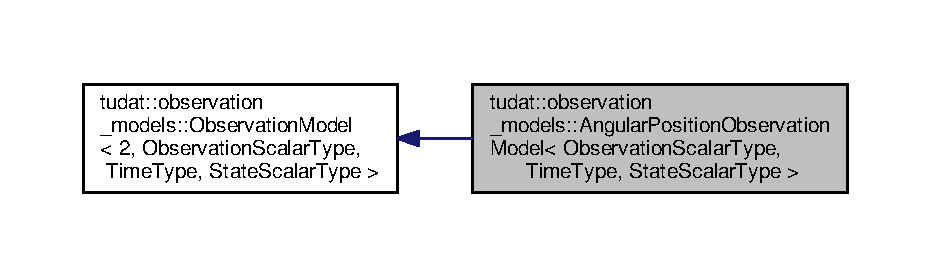
\includegraphics[width=350pt]{classtudat_1_1observation__models_1_1AngularPositionObservationModel__inherit__graph}
\end{center}
\end{figure}


Collaboration diagram for tudat\+:\+:observation\+\_\+models\+:\+:Angular\+Position\+Observation\+Model$<$ Observation\+Scalar\+Type, Time\+Type, State\+Scalar\+Type $>$\+:
\nopagebreak
\begin{figure}[H]
\begin{center}
\leavevmode
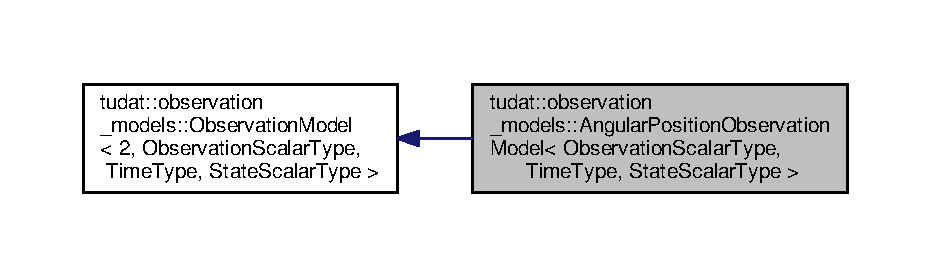
\includegraphics[width=350pt]{classtudat_1_1observation__models_1_1AngularPositionObservationModel__coll__graph}
\end{center}
\end{figure}
\subsection*{Public Types}
\begin{DoxyCompactItemize}
\item 
typedef Eigen\+::\+Matrix$<$ State\+Scalar\+Type, 6, 1 $>$ {\bfseries State\+Type}\hypertarget{classtudat_1_1observation__models_1_1AngularPositionObservationModel_a715f0e648288253a828f7945f0bfa51b}{}\label{classtudat_1_1observation__models_1_1AngularPositionObservationModel_a715f0e648288253a828f7945f0bfa51b}

\item 
typedef Eigen\+::\+Matrix$<$ State\+Scalar\+Type, 6, 1 $>$ {\bfseries Position\+Type}\hypertarget{classtudat_1_1observation__models_1_1AngularPositionObservationModel_a1b3f3d6b7cbb9f1016db2a8145388565}{}\label{classtudat_1_1observation__models_1_1AngularPositionObservationModel_a1b3f3d6b7cbb9f1016db2a8145388565}

\end{DoxyCompactItemize}
\subsection*{Public Member Functions}
\begin{DoxyCompactItemize}
\item 
\hyperlink{classtudat_1_1observation__models_1_1AngularPositionObservationModel_a3dfdd52bff8293d3602317aff1ee5820}{Angular\+Position\+Observation\+Model} (const boost\+::shared\+\_\+ptr$<$ \hyperlink{classtudat_1_1observation__models_1_1LightTimeCalculator}{observation\+\_\+models\+::\+Light\+Time\+Calculator}$<$ Observation\+Scalar\+Type, Time\+Type, State\+Scalar\+Type $>$ $>$ light\+Time\+Calculator, const boost\+::shared\+\_\+ptr$<$ \hyperlink{classtudat_1_1observation__models_1_1ObservationBias}{Observation\+Bias}$<$ 2 $>$ $>$ observation\+Bias\+Calculator=N\+U\+LL)
\begin{DoxyCompactList}\small\item\em Constructor. \end{DoxyCompactList}\item 
\hyperlink{classtudat_1_1observation__models_1_1AngularPositionObservationModel_a62b5b033b307771a9357fecf04288e52}{$\sim$\+Angular\+Position\+Observation\+Model} ()\hypertarget{classtudat_1_1observation__models_1_1AngularPositionObservationModel_a62b5b033b307771a9357fecf04288e52}{}\label{classtudat_1_1observation__models_1_1AngularPositionObservationModel_a62b5b033b307771a9357fecf04288e52}

\begin{DoxyCompactList}\small\item\em Destructor. \end{DoxyCompactList}\item 
Eigen\+::\+Matrix$<$ Observation\+Scalar\+Type, 2, 1 $>$ \hyperlink{classtudat_1_1observation__models_1_1AngularPositionObservationModel_a8f4020222c0f02173eefddbaac466e07}{compute\+Ideal\+Observations\+With\+Link\+End\+Data} (const Time\+Type time, const Link\+End\+Type link\+End\+Associated\+With\+Time, std\+::vector$<$ Time\+Type $>$ \&link\+End\+Times, std\+::vector$<$ Eigen\+::\+Matrix$<$ State\+Scalar\+Type, 6, 1 $>$ $>$ \&link\+End\+States)
\begin{DoxyCompactList}\small\item\em Function to compute ideal angular position observation at given time. \end{DoxyCompactList}\item 
boost\+::shared\+\_\+ptr$<$ \hyperlink{classtudat_1_1observation__models_1_1LightTimeCalculator}{observation\+\_\+models\+::\+Light\+Time\+Calculator}$<$ Observation\+Scalar\+Type, Time\+Type, State\+Scalar\+Type $>$ $>$ \hyperlink{classtudat_1_1observation__models_1_1AngularPositionObservationModel_a031c5cc789cd43b703d16930eab8c550}{get\+Light\+Time\+Calculator} ()
\begin{DoxyCompactList}\small\item\em Function to get the object to calculate light time. \end{DoxyCompactList}\end{DoxyCompactItemize}
\subsection*{Additional Inherited Members}


\subsection{Detailed Description}
\subsubsection*{template$<$typename Observation\+Scalar\+Type = double, typename Time\+Type = double, typename State\+Scalar\+Type = Observation\+Scalar\+Type$>$\\*
class tudat\+::observation\+\_\+models\+::\+Angular\+Position\+Observation\+Model$<$ Observation\+Scalar\+Type, Time\+Type, State\+Scalar\+Type $>$}

Class for simulating angular position (right ascension/declination) observables. 

Class for simulating angular position (right ascension/declination), using light-\/time (with light-\/time corrections) to determine the states of the link ends (source and receiver). The user may add observation biases to model system-\/dependent deviations between measured and true observation. 

\subsection{Constructor \& Destructor Documentation}
\index{tudat\+::observation\+\_\+models\+::\+Angular\+Position\+Observation\+Model@{tudat\+::observation\+\_\+models\+::\+Angular\+Position\+Observation\+Model}!Angular\+Position\+Observation\+Model@{Angular\+Position\+Observation\+Model}}
\index{Angular\+Position\+Observation\+Model@{Angular\+Position\+Observation\+Model}!tudat\+::observation\+\_\+models\+::\+Angular\+Position\+Observation\+Model@{tudat\+::observation\+\_\+models\+::\+Angular\+Position\+Observation\+Model}}
\subsubsection[{\texorpdfstring{Angular\+Position\+Observation\+Model(const boost\+::shared\+\_\+ptr$<$ observation\+\_\+models\+::\+Light\+Time\+Calculator$<$ Observation\+Scalar\+Type, Time\+Type, State\+Scalar\+Type $>$ $>$ light\+Time\+Calculator, const boost\+::shared\+\_\+ptr$<$ Observation\+Bias$<$ 2 $>$ $>$ observation\+Bias\+Calculator=\+N\+U\+L\+L)}{AngularPositionObservationModel(const boost::shared_ptr< observation_models::LightTimeCalculator< ObservationScalarType, TimeType, StateScalarType > > lightTimeCalculator, const boost::shared_ptr< ObservationBias< 2 > > observationBiasCalculator=NULL)}}]{\setlength{\rightskip}{0pt plus 5cm}template$<$typename Observation\+Scalar\+Type  = double, typename Time\+Type  = double, typename State\+Scalar\+Type  = Observation\+Scalar\+Type$>$ {\bf tudat\+::observation\+\_\+models\+::\+Angular\+Position\+Observation\+Model}$<$ Observation\+Scalar\+Type, Time\+Type, State\+Scalar\+Type $>$\+::{\bf Angular\+Position\+Observation\+Model} (
\begin{DoxyParamCaption}
\item[{const boost\+::shared\+\_\+ptr$<$ {\bf observation\+\_\+models\+::\+Light\+Time\+Calculator}$<$ Observation\+Scalar\+Type, Time\+Type, State\+Scalar\+Type $>$ $>$}]{light\+Time\+Calculator, }
\item[{const boost\+::shared\+\_\+ptr$<$ {\bf Observation\+Bias}$<$ 2 $>$ $>$}]{observation\+Bias\+Calculator = {\ttfamily NULL}}
\end{DoxyParamCaption}
)\hspace{0.3cm}{\ttfamily [inline]}}\hypertarget{classtudat_1_1observation__models_1_1AngularPositionObservationModel_a3dfdd52bff8293d3602317aff1ee5820}{}\label{classtudat_1_1observation__models_1_1AngularPositionObservationModel_a3dfdd52bff8293d3602317aff1ee5820}


Constructor. 

Constructor, 
\begin{DoxyParams}{Parameters}
{\em light\+Time\+Calculator} & Object to compute the light-\/time (including any corrections w.\+r.\+t. Euclidean case) between source and receiver \\
\hline
{\em observation\+Bias\+Calculator} & Object for calculating system-\/dependent errors in the observable, i.\+e. deviations from the physically ideal observable between reference points (default none). \\
\hline
\end{DoxyParams}


\subsection{Member Function Documentation}
\index{tudat\+::observation\+\_\+models\+::\+Angular\+Position\+Observation\+Model@{tudat\+::observation\+\_\+models\+::\+Angular\+Position\+Observation\+Model}!compute\+Ideal\+Observations\+With\+Link\+End\+Data@{compute\+Ideal\+Observations\+With\+Link\+End\+Data}}
\index{compute\+Ideal\+Observations\+With\+Link\+End\+Data@{compute\+Ideal\+Observations\+With\+Link\+End\+Data}!tudat\+::observation\+\_\+models\+::\+Angular\+Position\+Observation\+Model@{tudat\+::observation\+\_\+models\+::\+Angular\+Position\+Observation\+Model}}
\subsubsection[{\texorpdfstring{compute\+Ideal\+Observations\+With\+Link\+End\+Data(const Time\+Type time, const Link\+End\+Type link\+End\+Associated\+With\+Time, std\+::vector$<$ Time\+Type $>$ \&link\+End\+Times, std\+::vector$<$ Eigen\+::\+Matrix$<$ State\+Scalar\+Type, 6, 1 $>$ $>$ \&link\+End\+States)}{computeIdealObservationsWithLinkEndData(const TimeType time, const LinkEndType linkEndAssociatedWithTime, std::vector< TimeType > &linkEndTimes, std::vector< Eigen::Matrix< StateScalarType, 6, 1 > > &linkEndStates)}}]{\setlength{\rightskip}{0pt plus 5cm}template$<$typename Observation\+Scalar\+Type  = double, typename Time\+Type  = double, typename State\+Scalar\+Type  = Observation\+Scalar\+Type$>$ Eigen\+::\+Matrix$<$ Observation\+Scalar\+Type, 2, 1 $>$ {\bf tudat\+::observation\+\_\+models\+::\+Angular\+Position\+Observation\+Model}$<$ Observation\+Scalar\+Type, Time\+Type, State\+Scalar\+Type $>$\+::compute\+Ideal\+Observations\+With\+Link\+End\+Data (
\begin{DoxyParamCaption}
\item[{const Time\+Type}]{time, }
\item[{const Link\+End\+Type}]{link\+End\+Associated\+With\+Time, }
\item[{std\+::vector$<$ Time\+Type $>$ \&}]{link\+End\+Times, }
\item[{std\+::vector$<$ Eigen\+::\+Matrix$<$ State\+Scalar\+Type, 6, 1 $>$ $>$ \&}]{link\+End\+States}
\end{DoxyParamCaption}
)\hspace{0.3cm}{\ttfamily [inline]}, {\ttfamily [virtual]}}\hypertarget{classtudat_1_1observation__models_1_1AngularPositionObservationModel_a8f4020222c0f02173eefddbaac466e07}{}\label{classtudat_1_1observation__models_1_1AngularPositionObservationModel_a8f4020222c0f02173eefddbaac466e07}


Function to compute ideal angular position observation at given time. 

This function compute ideal angular position observation at a given time. The time argument can be either the reception or transmission time (defined by link\+End\+Associated\+With\+Time input). Note that this observable does include e.\+g. light-\/time corrections, which represent physically true corrections. It does not include e.\+g. system-\/dependent measurement. The times and states of the link ends are also returned in full precision (determined by class template arguments). These states and times are returned by reference. 
\begin{DoxyParams}{Parameters}
{\em time} & \hyperlink{classtudat_1_1Time}{Time} at which observation is to be simulated \\
\hline
{\em link\+End\+Associated\+With\+Time} & Link end at which given time is valid, i.\+e. link end for which associated time is kept constant (to input value) \\
\hline
{\em link\+End\+Times} & List of times at each link end during observation (returned by reference). \\
\hline
{\em link\+End\+States} & List of states at each link end during observation (returned by reference). \\
\hline
\end{DoxyParams}
\begin{DoxyReturn}{Returns}
Calculated angular position observable values. 
\end{DoxyReturn}


Implements \hyperlink{classtudat_1_1observation__models_1_1ObservationModel_aaa82da2eb90342259242e4cf06c7e3ff}{tudat\+::observation\+\_\+models\+::\+Observation\+Model$<$ 2, Observation\+Scalar\+Type, Time\+Type, State\+Scalar\+Type $>$}.

\index{tudat\+::observation\+\_\+models\+::\+Angular\+Position\+Observation\+Model@{tudat\+::observation\+\_\+models\+::\+Angular\+Position\+Observation\+Model}!get\+Light\+Time\+Calculator@{get\+Light\+Time\+Calculator}}
\index{get\+Light\+Time\+Calculator@{get\+Light\+Time\+Calculator}!tudat\+::observation\+\_\+models\+::\+Angular\+Position\+Observation\+Model@{tudat\+::observation\+\_\+models\+::\+Angular\+Position\+Observation\+Model}}
\subsubsection[{\texorpdfstring{get\+Light\+Time\+Calculator()}{getLightTimeCalculator()}}]{\setlength{\rightskip}{0pt plus 5cm}template$<$typename Observation\+Scalar\+Type  = double, typename Time\+Type  = double, typename State\+Scalar\+Type  = Observation\+Scalar\+Type$>$ boost\+::shared\+\_\+ptr$<$ {\bf observation\+\_\+models\+::\+Light\+Time\+Calculator}$<$ Observation\+Scalar\+Type, Time\+Type, State\+Scalar\+Type $>$ $>$ {\bf tudat\+::observation\+\_\+models\+::\+Angular\+Position\+Observation\+Model}$<$ Observation\+Scalar\+Type, Time\+Type, State\+Scalar\+Type $>$\+::get\+Light\+Time\+Calculator (
\begin{DoxyParamCaption}
{}
\end{DoxyParamCaption}
)\hspace{0.3cm}{\ttfamily [inline]}}\hypertarget{classtudat_1_1observation__models_1_1AngularPositionObservationModel_a031c5cc789cd43b703d16930eab8c550}{}\label{classtudat_1_1observation__models_1_1AngularPositionObservationModel_a031c5cc789cd43b703d16930eab8c550}


Function to get the object to calculate light time. 

Function to get the object to calculate light time. \begin{DoxyReturn}{Returns}
Object to calculate light time. 
\end{DoxyReturn}


The documentation for this class was generated from the following file\+:\begin{DoxyCompactItemize}
\item 
/home/lupi/\+Tudat/tudat\+Bundle/tudat/\+Tudat/\+Astrodynamics/\+Observation\+Models/angular\+Position\+Observation\+Model.\+h\end{DoxyCompactItemize}

\hypertarget{classtudat_1_1unit__tests_1_1AnotherDerivedAccelerationModel}{}\section{tudat\+:\+:unit\+\_\+tests\+:\+:Another\+Derived\+Acceleration\+Model$<$ Acceleration\+Data\+Type, Position\+Data\+Type, Velocity\+Data\+Type, Time\+Data\+Type $>$ Class Template Reference}
\label{classtudat_1_1unit__tests_1_1AnotherDerivedAccelerationModel}\index{tudat\+::unit\+\_\+tests\+::\+Another\+Derived\+Acceleration\+Model$<$ Acceleration\+Data\+Type, Position\+Data\+Type, Velocity\+Data\+Type, Time\+Data\+Type $>$@{tudat\+::unit\+\_\+tests\+::\+Another\+Derived\+Acceleration\+Model$<$ Acceleration\+Data\+Type, Position\+Data\+Type, Velocity\+Data\+Type, Time\+Data\+Type $>$}}


Another acceleration model derived class.  




{\ttfamily \#include $<$test\+Acceleration\+Models.\+h$>$}



Inheritance diagram for tudat\+:\+:unit\+\_\+tests\+:\+:Another\+Derived\+Acceleration\+Model$<$ Acceleration\+Data\+Type, Position\+Data\+Type, Velocity\+Data\+Type, Time\+Data\+Type $>$\+:
\nopagebreak
\begin{figure}[H]
\begin{center}
\leavevmode
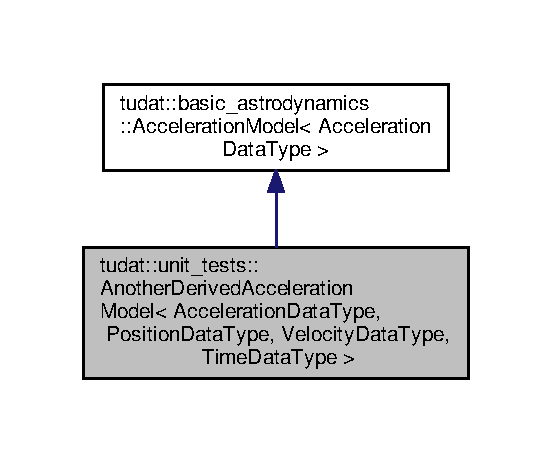
\includegraphics[width=265pt]{classtudat_1_1unit__tests_1_1AnotherDerivedAccelerationModel__inherit__graph}
\end{center}
\end{figure}


Collaboration diagram for tudat\+:\+:unit\+\_\+tests\+:\+:Another\+Derived\+Acceleration\+Model$<$ Acceleration\+Data\+Type, Position\+Data\+Type, Velocity\+Data\+Type, Time\+Data\+Type $>$\+:
\nopagebreak
\begin{figure}[H]
\begin{center}
\leavevmode
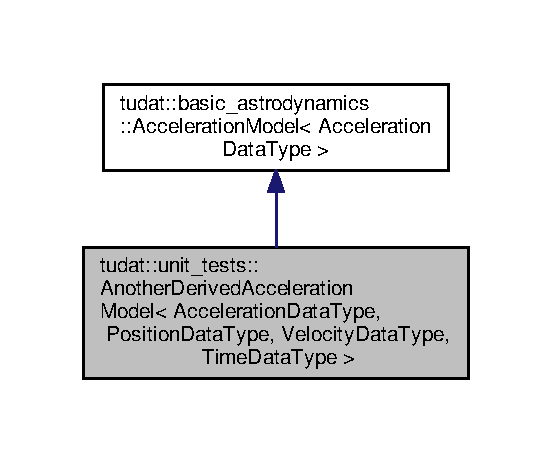
\includegraphics[width=265pt]{classtudat_1_1unit__tests_1_1AnotherDerivedAccelerationModel__coll__graph}
\end{center}
\end{figure}
\subsection*{Public Types}
\begin{DoxyCompactItemize}
\item 
typedef boost\+::function$<$ Position\+Data\+Type() $>$ \hyperlink{classtudat_1_1unit__tests_1_1AnotherDerivedAccelerationModel_afc6c0f446142eb265d5306b9d50e82d6}{Position\+Returning\+Function}\hypertarget{classtudat_1_1unit__tests_1_1AnotherDerivedAccelerationModel_afc6c0f446142eb265d5306b9d50e82d6}{}\label{classtudat_1_1unit__tests_1_1AnotherDerivedAccelerationModel_afc6c0f446142eb265d5306b9d50e82d6}

\begin{DoxyCompactList}\small\item\em Typedef for a pointer to a function that returns a position. \end{DoxyCompactList}\item 
typedef boost\+::function$<$ Velocity\+Data\+Type() $>$ \hyperlink{classtudat_1_1unit__tests_1_1AnotherDerivedAccelerationModel_a34ee57f48cdcac94bdf12e282de14756}{Velocity\+Returning\+Function}\hypertarget{classtudat_1_1unit__tests_1_1AnotherDerivedAccelerationModel_a34ee57f48cdcac94bdf12e282de14756}{}\label{classtudat_1_1unit__tests_1_1AnotherDerivedAccelerationModel_a34ee57f48cdcac94bdf12e282de14756}

\begin{DoxyCompactList}\small\item\em Typedef for a pointer to a function that returns a position. \end{DoxyCompactList}\item 
typedef boost\+::function$<$ Time\+Data\+Type() $>$ \hyperlink{classtudat_1_1unit__tests_1_1AnotherDerivedAccelerationModel_a69b5e6c22cec492702d5d25fc6db8dfb}{Time\+Returning\+Function}\hypertarget{classtudat_1_1unit__tests_1_1AnotherDerivedAccelerationModel_a69b5e6c22cec492702d5d25fc6db8dfb}{}\label{classtudat_1_1unit__tests_1_1AnotherDerivedAccelerationModel_a69b5e6c22cec492702d5d25fc6db8dfb}

\begin{DoxyCompactList}\small\item\em Typedef for a pointer to a function that returns a time. \end{DoxyCompactList}\end{DoxyCompactItemize}
\subsection*{Public Member Functions}
\begin{DoxyCompactItemize}
\item 
\hyperlink{classtudat_1_1unit__tests_1_1AnotherDerivedAccelerationModel_aaacbc7b46b24df7e6313f2a041cd6cac}{Another\+Derived\+Acceleration\+Model} (const \hyperlink{classtudat_1_1unit__tests_1_1AnotherDerivedAccelerationModel_afc6c0f446142eb265d5306b9d50e82d6}{Position\+Returning\+Function} a\+Position\+Function, const \hyperlink{classtudat_1_1unit__tests_1_1AnotherDerivedAccelerationModel_a34ee57f48cdcac94bdf12e282de14756}{Velocity\+Returning\+Function} a\+Velocity\+Function, const \hyperlink{classtudat_1_1unit__tests_1_1AnotherDerivedAccelerationModel_a69b5e6c22cec492702d5d25fc6db8dfb}{Time\+Returning\+Function} a\+Time\+Function)
\begin{DoxyCompactList}\small\item\em Default constructor. \end{DoxyCompactList}\item 
Acceleration\+Data\+Type \hyperlink{classtudat_1_1unit__tests_1_1AnotherDerivedAccelerationModel_ab025d414ca6b01e768198e2ab1f9c9d0}{get\+Acceleration} ()
\begin{DoxyCompactList}\small\item\em Get acceleration. \end{DoxyCompactList}\item 
void \hyperlink{classtudat_1_1unit__tests_1_1AnotherDerivedAccelerationModel_add07599d1c34c2479f2271b7703297aa}{update\+Members} (const double current\+Time=T\+U\+D\+A\+T\+\_\+\+N\+AN)
\begin{DoxyCompactList}\small\item\em Update member variables used by the acceleration model. \end{DoxyCompactList}\end{DoxyCompactItemize}
\subsection*{Additional Inherited Members}


\subsection{Detailed Description}
\subsubsection*{template$<$typename Acceleration\+Data\+Type = Eigen\+::\+Vector3d, typename Position\+Data\+Type = Eigen\+::\+Vector3d, typename Velocity\+Data\+Type = Eigen\+::\+Vector3d, typename Time\+Data\+Type = double$>$\\*
class tudat\+::unit\+\_\+tests\+::\+Another\+Derived\+Acceleration\+Model$<$ Acceleration\+Data\+Type, Position\+Data\+Type, Velocity\+Data\+Type, Time\+Data\+Type $>$}

Another acceleration model derived class. 

This class serves as an example of another derived class from the Acceleration\+Model base class. This class contains an implementation that computes acceleration based on a given position, velocity, and time. The context of this class is somewhat specific to make it more understandable, though derived classes of the Acceleration\+Model base class can be completely general. It should be noted that this class should N\+OT be used as is in the rest of the library, and is only used in conjunction with unit tests. 
\begin{DoxyTemplParams}{Template Parameters}
{\em Acceleration\+Data\+Type} & Data type used to represent accelerations (default=Eigen\+::\+Vector3d). \\
\hline
{\em Position\+Data\+Type} & Data type used to represent positions (default=Eigen\+::\+Vector3d). \\
\hline
{\em Velocity\+Data\+Type} & Data type used to represent velocities (default=Eigen\+::\+Vector3d). \\
\hline
{\em Time\+Data\+Type} & Data type used to represent time (default=double). \\
\hline
\end{DoxyTemplParams}


\subsection{Constructor \& Destructor Documentation}
\index{tudat\+::unit\+\_\+tests\+::\+Another\+Derived\+Acceleration\+Model@{tudat\+::unit\+\_\+tests\+::\+Another\+Derived\+Acceleration\+Model}!Another\+Derived\+Acceleration\+Model@{Another\+Derived\+Acceleration\+Model}}
\index{Another\+Derived\+Acceleration\+Model@{Another\+Derived\+Acceleration\+Model}!tudat\+::unit\+\_\+tests\+::\+Another\+Derived\+Acceleration\+Model@{tudat\+::unit\+\_\+tests\+::\+Another\+Derived\+Acceleration\+Model}}
\subsubsection[{\texorpdfstring{Another\+Derived\+Acceleration\+Model(const Position\+Returning\+Function a\+Position\+Function, const Velocity\+Returning\+Function a\+Velocity\+Function, const Time\+Returning\+Function a\+Time\+Function)}{AnotherDerivedAccelerationModel(const PositionReturningFunction aPositionFunction, const VelocityReturningFunction aVelocityFunction, const TimeReturningFunction aTimeFunction)}}]{\setlength{\rightskip}{0pt plus 5cm}template$<$typename Acceleration\+Data\+Type  = Eigen\+::\+Vector3d, typename Position\+Data\+Type  = Eigen\+::\+Vector3d, typename Velocity\+Data\+Type  = Eigen\+::\+Vector3d, typename Time\+Data\+Type  = double$>$ {\bf tudat\+::unit\+\_\+tests\+::\+Another\+Derived\+Acceleration\+Model}$<$ Acceleration\+Data\+Type, Position\+Data\+Type, Velocity\+Data\+Type, Time\+Data\+Type $>$\+::{\bf Another\+Derived\+Acceleration\+Model} (
\begin{DoxyParamCaption}
\item[{const {\bf Position\+Returning\+Function}}]{a\+Position\+Function, }
\item[{const {\bf Velocity\+Returning\+Function}}]{a\+Velocity\+Function, }
\item[{const {\bf Time\+Returning\+Function}}]{a\+Time\+Function}
\end{DoxyParamCaption}
)\hspace{0.3cm}{\ttfamily [inline]}}\hypertarget{classtudat_1_1unit__tests_1_1AnotherDerivedAccelerationModel_aaacbc7b46b24df7e6313f2a041cd6cac}{}\label{classtudat_1_1unit__tests_1_1AnotherDerivedAccelerationModel_aaacbc7b46b24df7e6313f2a041cd6cac}


Default constructor. 

Default constructor that takes function-\/pointers as input. These function-\/pointers point to functions that return a position, a velocity, and a time. Internally, the \hyperlink{classtudat_1_1unit__tests_1_1AnotherDerivedAccelerationModel_add07599d1c34c2479f2271b7703297aa}{update\+Members()} function also gets called to ensure that all members are up-\/to-\/date after construction. 
\begin{DoxyParams}{Parameters}
{\em a\+Position\+Function} & A function-\/pointer that points to a function returning a position. \\
\hline
{\em a\+Velocity\+Function} & A function-\/pointer that points to a function returning a velocity. \\
\hline
{\em a\+Time\+Function} & A function-\/pointer that points to a function returning a time. \\
\hline
\end{DoxyParams}


\subsection{Member Function Documentation}
\index{tudat\+::unit\+\_\+tests\+::\+Another\+Derived\+Acceleration\+Model@{tudat\+::unit\+\_\+tests\+::\+Another\+Derived\+Acceleration\+Model}!get\+Acceleration@{get\+Acceleration}}
\index{get\+Acceleration@{get\+Acceleration}!tudat\+::unit\+\_\+tests\+::\+Another\+Derived\+Acceleration\+Model@{tudat\+::unit\+\_\+tests\+::\+Another\+Derived\+Acceleration\+Model}}
\subsubsection[{\texorpdfstring{get\+Acceleration()}{getAcceleration()}}]{\setlength{\rightskip}{0pt plus 5cm}template$<$typename Acceleration\+Data\+Type  = Eigen\+::\+Vector3d, typename Position\+Data\+Type  = Eigen\+::\+Vector3d, typename Velocity\+Data\+Type  = Eigen\+::\+Vector3d, typename Time\+Data\+Type  = double$>$ Acceleration\+Data\+Type {\bf tudat\+::unit\+\_\+tests\+::\+Another\+Derived\+Acceleration\+Model}$<$ Acceleration\+Data\+Type, Position\+Data\+Type, Velocity\+Data\+Type, Time\+Data\+Type $>$\+::get\+Acceleration (
\begin{DoxyParamCaption}
{}
\end{DoxyParamCaption}
)\hspace{0.3cm}{\ttfamily [inline]}, {\ttfamily [virtual]}}\hypertarget{classtudat_1_1unit__tests_1_1AnotherDerivedAccelerationModel_ab025d414ca6b01e768198e2ab1f9c9d0}{}\label{classtudat_1_1unit__tests_1_1AnotherDerivedAccelerationModel_ab025d414ca6b01e768198e2ab1f9c9d0}


Get acceleration. 

Returns acceleration. In this case, this functions returns an acceleration that is dependent on the internally stored position, velocity, and time members. This function merely serves as an example, rather than representing real dynamics. \begin{DoxyReturn}{Returns}
Computed acceleration. 
\end{DoxyReturn}


Implements \hyperlink{classtudat_1_1basic__astrodynamics_1_1AccelerationModel_a1f59960bc477fc02e7d52697ced99750}{tudat\+::basic\+\_\+astrodynamics\+::\+Acceleration\+Model$<$ Acceleration\+Data\+Type $>$}.

\index{tudat\+::unit\+\_\+tests\+::\+Another\+Derived\+Acceleration\+Model@{tudat\+::unit\+\_\+tests\+::\+Another\+Derived\+Acceleration\+Model}!update\+Members@{update\+Members}}
\index{update\+Members@{update\+Members}!tudat\+::unit\+\_\+tests\+::\+Another\+Derived\+Acceleration\+Model@{tudat\+::unit\+\_\+tests\+::\+Another\+Derived\+Acceleration\+Model}}
\subsubsection[{\texorpdfstring{update\+Members(const double current\+Time=\+T\+U\+D\+A\+T\+\_\+\+N\+A\+N)}{updateMembers(const double currentTime=TUDAT_NAN)}}]{\setlength{\rightskip}{0pt plus 5cm}template$<$typename Acceleration\+Data\+Type  = Eigen\+::\+Vector3d, typename Position\+Data\+Type  = Eigen\+::\+Vector3d, typename Velocity\+Data\+Type  = Eigen\+::\+Vector3d, typename Time\+Data\+Type  = double$>$ void {\bf tudat\+::unit\+\_\+tests\+::\+Another\+Derived\+Acceleration\+Model}$<$ Acceleration\+Data\+Type, Position\+Data\+Type, Velocity\+Data\+Type, Time\+Data\+Type $>$\+::update\+Members (
\begin{DoxyParamCaption}
\item[{const double}]{current\+Time = {\ttfamily TUDAT\+\_\+NAN}}
\end{DoxyParamCaption}
)\hspace{0.3cm}{\ttfamily [inline]}, {\ttfamily [virtual]}}\hypertarget{classtudat_1_1unit__tests_1_1AnotherDerivedAccelerationModel_add07599d1c34c2479f2271b7703297aa}{}\label{classtudat_1_1unit__tests_1_1AnotherDerivedAccelerationModel_add07599d1c34c2479f2271b7703297aa}


Update member variables used by the acceleration model. 

Updates member variables used by the acceleration model. In this case, the internally stored position, velocity, and time are updated by calling the function-\/pointers passed to the constructor. 
\begin{DoxyParams}{Parameters}
{\em current\+Time} & \hyperlink{classtudat_1_1Time}{Time} at which acceleration model is to be updated. \\
\hline
\end{DoxyParams}


Implements \hyperlink{classtudat_1_1basic__astrodynamics_1_1AccelerationModel_a966e85b72300b8cbc99ba60e40108d71}{tudat\+::basic\+\_\+astrodynamics\+::\+Acceleration\+Model$<$ Acceleration\+Data\+Type $>$}.



The documentation for this class was generated from the following file\+:\begin{DoxyCompactItemize}
\item 
/home/lupi/\+Tudat/tudat\+Bundle/tudat/\+Tudat/\+Astrodynamics/\+Basic\+Astrodynamics/\+Unit\+Tests/test\+Acceleration\+Models.\+h\end{DoxyCompactItemize}

\hypertarget{classtudat_1_1reference__frames_1_1ApparentAccelerationModel}{}\section{tudat\+:\+:reference\+\_\+frames\+:\+:Apparent\+Acceleration\+Model Class Reference}
\label{classtudat_1_1reference__frames_1_1ApparentAccelerationModel}\index{tudat\+::reference\+\_\+frames\+::\+Apparent\+Acceleration\+Model@{tudat\+::reference\+\_\+frames\+::\+Apparent\+Acceleration\+Model}}


Apparent acceleration model class.  




{\ttfamily \#include $<$apparent\+Acceleration\+Model.\+h$>$}



Inheritance diagram for tudat\+:\+:reference\+\_\+frames\+:\+:Apparent\+Acceleration\+Model\+:
\nopagebreak
\begin{figure}[H]
\begin{center}
\leavevmode
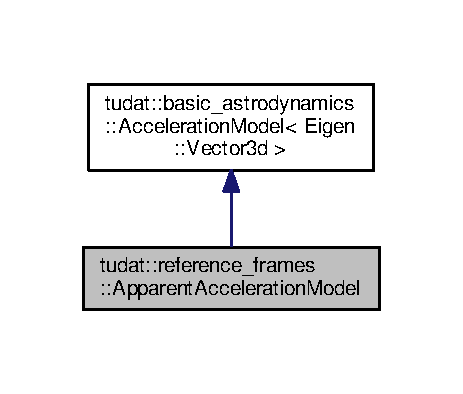
\includegraphics[width=222pt]{classtudat_1_1reference__frames_1_1ApparentAccelerationModel__inherit__graph}
\end{center}
\end{figure}


Collaboration diagram for tudat\+:\+:reference\+\_\+frames\+:\+:Apparent\+Acceleration\+Model\+:
\nopagebreak
\begin{figure}[H]
\begin{center}
\leavevmode
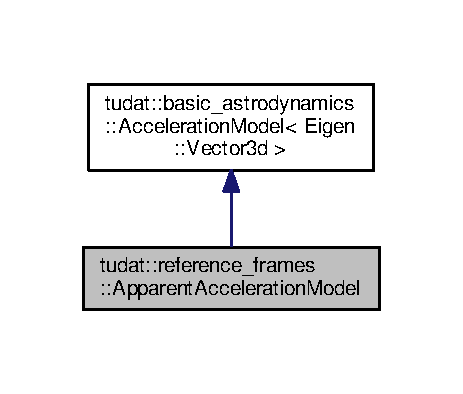
\includegraphics[width=222pt]{classtudat_1_1reference__frames_1_1ApparentAccelerationModel__coll__graph}
\end{center}
\end{figure}
\subsection*{Public Member Functions}
\begin{DoxyCompactItemize}
\item 
\hyperlink{classtudat_1_1reference__frames_1_1ApparentAccelerationModel_ae3f56489f99050ec73f5b22631e69fe5}{Apparent\+Acceleration\+Model} (Vector3d\+Returning\+Function acceleration\+Of\+Non\+Inertial\+Reference\+Frame\+Function, Vector3d\+Returning\+Function angular\+Velocity\+Of\+Non\+Inertial\+Reference\+Frame\+Function, Vector3d\+Returning\+Function angular\+Acceleration\+Of\+Non\+Inertial\+Reference\+Frame\+Function, Vector3d\+Returning\+Function position\+Of\+Body\+In\+Non\+Inertial\+Reference\+Frame\+Function, Vector3d\+Returning\+Function velocity\+Of\+Body\+In\+Non\+Inertial\+Reference\+Frame\+Function)
\begin{DoxyCompactList}\small\item\em Class constructor. \end{DoxyCompactList}\item 
Eigen\+::\+Vector3d \hyperlink{classtudat_1_1reference__frames_1_1ApparentAccelerationModel_aa5c72a891752917421efb970407b2517}{get\+Acceleration} ()
\begin{DoxyCompactList}\small\item\em Get apparent acceleration. \end{DoxyCompactList}\item 
void \hyperlink{classtudat_1_1reference__frames_1_1ApparentAccelerationModel_ae3704bca478d47f8ceb8888a58df5ad9}{update\+Members} (const double current\+Time=T\+U\+D\+A\+T\+\_\+\+N\+AN)
\begin{DoxyCompactList}\small\item\em Update member variables used by apparent acceleration model. \end{DoxyCompactList}\end{DoxyCompactItemize}
\subsection*{Additional Inherited Members}


\subsection{Detailed Description}
Apparent acceleration model class. 

Implementation of apparent acceleration due to non-\/inertiality of a reference system in which the equations of motion are evaluated. It evaluates the total apparent acceleration due to the acceleration of the reference frame, as well as the Coriolis, centripetal and Euler accelerations. 

\subsection{Constructor \& Destructor Documentation}
\index{tudat\+::reference\+\_\+frames\+::\+Apparent\+Acceleration\+Model@{tudat\+::reference\+\_\+frames\+::\+Apparent\+Acceleration\+Model}!Apparent\+Acceleration\+Model@{Apparent\+Acceleration\+Model}}
\index{Apparent\+Acceleration\+Model@{Apparent\+Acceleration\+Model}!tudat\+::reference\+\_\+frames\+::\+Apparent\+Acceleration\+Model@{tudat\+::reference\+\_\+frames\+::\+Apparent\+Acceleration\+Model}}
\subsubsection[{\texorpdfstring{Apparent\+Acceleration\+Model(\+Vector3d\+Returning\+Function acceleration\+Of\+Non\+Inertial\+Reference\+Frame\+Function, Vector3d\+Returning\+Function angular\+Velocity\+Of\+Non\+Inertial\+Reference\+Frame\+Function, Vector3d\+Returning\+Function angular\+Acceleration\+Of\+Non\+Inertial\+Reference\+Frame\+Function, Vector3d\+Returning\+Function position\+Of\+Body\+In\+Non\+Inertial\+Reference\+Frame\+Function, Vector3d\+Returning\+Function velocity\+Of\+Body\+In\+Non\+Inertial\+Reference\+Frame\+Function)}{ApparentAccelerationModel(Vector3dReturningFunction accelerationOfNonInertialReferenceFrameFunction, Vector3dReturningFunction angularVelocityOfNonInertialReferenceFrameFunction, Vector3dReturningFunction angularAccelerationOfNonInertialReferenceFrameFunction, Vector3dReturningFunction positionOfBodyInNonInertialReferenceFrameFunction, Vector3dReturningFunction velocityOfBodyInNonInertialReferenceFrameFunction)}}]{\setlength{\rightskip}{0pt plus 5cm}tudat\+::reference\+\_\+frames\+::\+Apparent\+Acceleration\+Model\+::\+Apparent\+Acceleration\+Model (
\begin{DoxyParamCaption}
\item[{Vector3d\+Returning\+Function}]{acceleration\+Of\+Non\+Inertial\+Reference\+Frame\+Function, }
\item[{Vector3d\+Returning\+Function}]{angular\+Velocity\+Of\+Non\+Inertial\+Reference\+Frame\+Function, }
\item[{Vector3d\+Returning\+Function}]{angular\+Acceleration\+Of\+Non\+Inertial\+Reference\+Frame\+Function, }
\item[{Vector3d\+Returning\+Function}]{position\+Of\+Body\+In\+Non\+Inertial\+Reference\+Frame\+Function, }
\item[{Vector3d\+Returning\+Function}]{velocity\+Of\+Body\+In\+Non\+Inertial\+Reference\+Frame\+Function}
\end{DoxyParamCaption}
)\hspace{0.3cm}{\ttfamily [inline]}}\hypertarget{classtudat_1_1reference__frames_1_1ApparentAccelerationModel_ae3f56489f99050ec73f5b22631e69fe5}{}\label{classtudat_1_1reference__frames_1_1ApparentAccelerationModel_ae3f56489f99050ec73f5b22631e69fe5}


Class constructor. 

Constructor for apparent acceleration model. 
\begin{DoxyParams}{Parameters}
{\em acceleration\+Of\+Non\+Inertial\+Reference\+Frame\+Function} & Pointer to a function returning the acceleration vector of the non-\/intertial reference frame w.\+r.\+t. an inertial frame of reference. \\
\hline
{\em angular\+Velocity\+Of\+Non\+Inertial\+Reference\+Frame\+Function} & Pointer to a function returning the angular velocity vector of the non-\/intertial reference frame w.\+r.\+t. an inertial frame of reference. \\
\hline
{\em angular\+Acceleration\+Of\+Non\+Inertial\+Reference\+Frame\+Function} & Pointer to a function returning the angular acceleration vector of the non-\/inertial frame with respect to an inertial reference frame. \\
\hline
{\em position\+Of\+Body\+In\+Non\+Inertial\+Reference\+Frame\+Function} & Pointer to a function returning the position vector in the non-\/inertial frame of reference in which the apparent acceleration is computed. \\
\hline
{\em velocity\+Of\+Body\+In\+Non\+Inertial\+Reference\+Frame\+Function} & Pointer to a function returning the velocity vector in the non-\/inertial frame of reference in which the apparent acceleration is computed. \\
\hline
\end{DoxyParams}


\subsection{Member Function Documentation}
\index{tudat\+::reference\+\_\+frames\+::\+Apparent\+Acceleration\+Model@{tudat\+::reference\+\_\+frames\+::\+Apparent\+Acceleration\+Model}!get\+Acceleration@{get\+Acceleration}}
\index{get\+Acceleration@{get\+Acceleration}!tudat\+::reference\+\_\+frames\+::\+Apparent\+Acceleration\+Model@{tudat\+::reference\+\_\+frames\+::\+Apparent\+Acceleration\+Model}}
\subsubsection[{\texorpdfstring{get\+Acceleration()}{getAcceleration()}}]{\setlength{\rightskip}{0pt plus 5cm}Eigen\+::\+Vector3d tudat\+::reference\+\_\+frames\+::\+Apparent\+Acceleration\+Model\+::get\+Acceleration (
\begin{DoxyParamCaption}
{}
\end{DoxyParamCaption}
)\hspace{0.3cm}{\ttfamily [inline]}, {\ttfamily [virtual]}}\hypertarget{classtudat_1_1reference__frames_1_1ApparentAccelerationModel_aa5c72a891752917421efb970407b2517}{}\label{classtudat_1_1reference__frames_1_1ApparentAccelerationModel_aa5c72a891752917421efb970407b2517}


Get apparent acceleration. 

Computes and returns the acceleration. \begin{DoxyReturn}{Returns}
Vector of the apparent acceleration in the non-\/inertial Cartesian frame in which the object\textquotesingle{}s state is defined. 
\end{DoxyReturn}


Implements \hyperlink{classtudat_1_1basic__astrodynamics_1_1AccelerationModel_a1f59960bc477fc02e7d52697ced99750}{tudat\+::basic\+\_\+astrodynamics\+::\+Acceleration\+Model$<$ Eigen\+::\+Vector3d $>$}.

\index{tudat\+::reference\+\_\+frames\+::\+Apparent\+Acceleration\+Model@{tudat\+::reference\+\_\+frames\+::\+Apparent\+Acceleration\+Model}!update\+Members@{update\+Members}}
\index{update\+Members@{update\+Members}!tudat\+::reference\+\_\+frames\+::\+Apparent\+Acceleration\+Model@{tudat\+::reference\+\_\+frames\+::\+Apparent\+Acceleration\+Model}}
\subsubsection[{\texorpdfstring{update\+Members(const double current\+Time=\+T\+U\+D\+A\+T\+\_\+\+N\+A\+N)}{updateMembers(const double currentTime=TUDAT_NAN)}}]{\setlength{\rightskip}{0pt plus 5cm}void tudat\+::reference\+\_\+frames\+::\+Apparent\+Acceleration\+Model\+::update\+Members (
\begin{DoxyParamCaption}
\item[{const double}]{current\+Time = {\ttfamily TUDAT\+\_\+NAN}}
\end{DoxyParamCaption}
)\hspace{0.3cm}{\ttfamily [virtual]}}\hypertarget{classtudat_1_1reference__frames_1_1ApparentAccelerationModel_ae3704bca478d47f8ceb8888a58df5ad9}{}\label{classtudat_1_1reference__frames_1_1ApparentAccelerationModel_ae3704bca478d47f8ceb8888a58df5ad9}


Update member variables used by apparent acceleration model. 

Function to update member variables used by this acceleration model. The variables that are required as input for the evaluation of the accelerations are retrieved from boost\+::functions that may or may not give constant return values, depending on the user input. This function sets the member variables using these functions. 
\begin{DoxyParams}{Parameters}
{\em current\+Time} & \hyperlink{classtudat_1_1Time}{Time} at which acceleration model is to be updated. \\
\hline
\end{DoxyParams}


Implements \hyperlink{classtudat_1_1basic__astrodynamics_1_1AccelerationModel_a966e85b72300b8cbc99ba60e40108d71}{tudat\+::basic\+\_\+astrodynamics\+::\+Acceleration\+Model$<$ Eigen\+::\+Vector3d $>$}.



The documentation for this class was generated from the following files\+:\begin{DoxyCompactItemize}
\item 
/home/lupi/\+Tudat/tudat\+Bundle/tudat/\+Tudat/\+Astrodynamics/\+Reference\+Frames/apparent\+Acceleration\+Model.\+h\item 
/home/lupi/\+Tudat/tudat\+Bundle/tudat/\+Tudat/\+Astrodynamics/\+Reference\+Frames/apparent\+Acceleration\+Model.\+cpp\end{DoxyCompactItemize}

\hypertarget{classtudat_1_1ephemerides_1_1ApproximatePlanetPositions}{}\section{tudat\+:\+:ephemerides\+:\+:Approximate\+Planet\+Positions Class Reference}
\label{classtudat_1_1ephemerides_1_1ApproximatePlanetPositions}\index{tudat\+::ephemerides\+::\+Approximate\+Planet\+Positions@{tudat\+::ephemerides\+::\+Approximate\+Planet\+Positions}}


\hyperlink{classtudat_1_1ephemerides_1_1Ephemeris}{Ephemeris} class using J\+PL \char`\"{}\+Approximate Positions of Major Planets\char`\"{}.  




{\ttfamily \#include $<$approximate\+Planet\+Positions.\+h$>$}



Inheritance diagram for tudat\+:\+:ephemerides\+:\+:Approximate\+Planet\+Positions\+:
\nopagebreak
\begin{figure}[H]
\begin{center}
\leavevmode
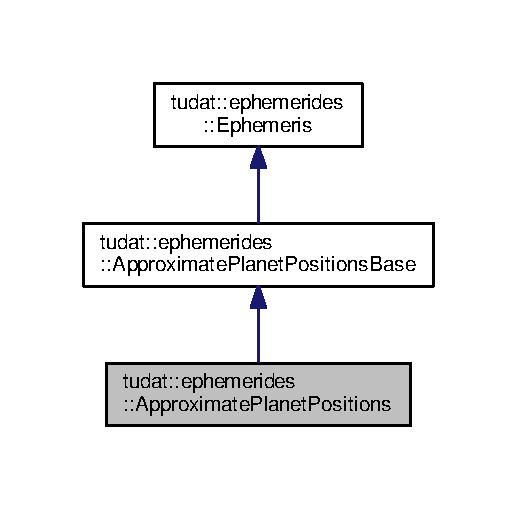
\includegraphics[width=248pt]{classtudat_1_1ephemerides_1_1ApproximatePlanetPositions__inherit__graph}
\end{center}
\end{figure}


Collaboration diagram for tudat\+:\+:ephemerides\+:\+:Approximate\+Planet\+Positions\+:
\nopagebreak
\begin{figure}[H]
\begin{center}
\leavevmode
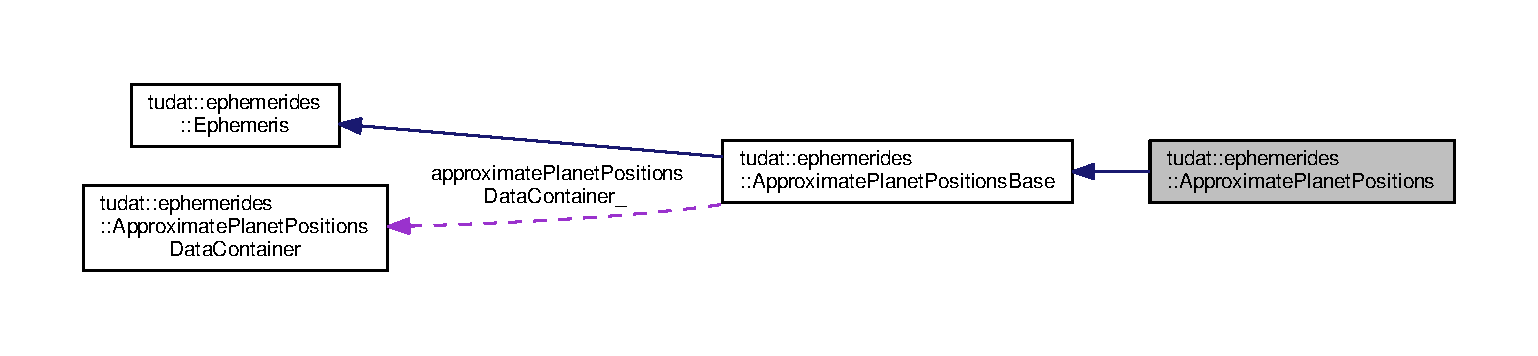
\includegraphics[width=350pt]{classtudat_1_1ephemerides_1_1ApproximatePlanetPositions__coll__graph}
\end{center}
\end{figure}
\subsection*{Public Member Functions}
\begin{DoxyCompactItemize}
\item 
\hyperlink{classtudat_1_1ephemerides_1_1ApproximatePlanetPositions_a5363e07d3ab914f1592e412035900899}{Approximate\+Planet\+Positions} (\hyperlink{classtudat_1_1ephemerides_1_1ApproximatePlanetPositionsBase_aa698885dcabac2815a6205d5502724d2}{Bodies\+With\+Ephemeris\+Data} body\+With\+Ephemeris\+Data, const double a\+Sun\+Gravitational\+Parameter=1.\+32712440018e20, const double reference\+Julian\+Date=basic\+\_\+astrodynamics\+::\+J\+U\+L\+I\+A\+N\+\_\+\+D\+A\+Y\+\_\+\+O\+N\+\_\+\+J2000)
\begin{DoxyCompactList}\small\item\em Default constructor. \end{DoxyCompactList}\item 
Eigen\+::\+Vector6d \hyperlink{classtudat_1_1ephemerides_1_1ApproximatePlanetPositions_a76a58a0bc977fb72020cda1837be1ddf}{get\+Cartesian\+State} (const double seconds\+Since\+Epoch)
\begin{DoxyCompactList}\small\item\em Get cartesian state from ephemeris. \end{DoxyCompactList}\item 
Eigen\+::\+Vector6d \hyperlink{classtudat_1_1ephemerides_1_1ApproximatePlanetPositions_a28a9f6436a540037f9da7a2d59d2342b}{get\+Keplerian\+State\+From\+Ephemeris} (const double seconds\+Since\+Epoch)
\begin{DoxyCompactList}\small\item\em Get keplerian state from ephemeris. \end{DoxyCompactList}\end{DoxyCompactItemize}
\subsection*{Additional Inherited Members}


\subsection{Detailed Description}
\hyperlink{classtudat_1_1ephemerides_1_1Ephemeris}{Ephemeris} class using J\+PL \char`\"{}\+Approximate Positions of Major Planets\char`\"{}. 

\hyperlink{classtudat_1_1ephemerides_1_1Ephemeris}{Ephemeris} class using J\+PL \char`\"{}\+Approximate Positions of Major Planets\char`\"{}. 

\subsection{Constructor \& Destructor Documentation}
\index{tudat\+::ephemerides\+::\+Approximate\+Planet\+Positions@{tudat\+::ephemerides\+::\+Approximate\+Planet\+Positions}!Approximate\+Planet\+Positions@{Approximate\+Planet\+Positions}}
\index{Approximate\+Planet\+Positions@{Approximate\+Planet\+Positions}!tudat\+::ephemerides\+::\+Approximate\+Planet\+Positions@{tudat\+::ephemerides\+::\+Approximate\+Planet\+Positions}}
\subsubsection[{\texorpdfstring{Approximate\+Planet\+Positions(\+Bodies\+With\+Ephemeris\+Data body\+With\+Ephemeris\+Data, const double a\+Sun\+Gravitational\+Parameter=1.\+32712440018e20, const double reference\+Julian\+Date=basic\+\_\+astrodynamics\+::\+J\+U\+L\+I\+A\+N\+\_\+\+D\+A\+Y\+\_\+\+O\+N\+\_\+\+J2000)}{ApproximatePlanetPositions(BodiesWithEphemerisData bodyWithEphemerisData, const double aSunGravitationalParameter=1.32712440018e20, const double referenceJulianDate=basic_astrodynamics::JULIAN_DAY_ON_J2000)}}]{\setlength{\rightskip}{0pt plus 5cm}tudat\+::ephemerides\+::\+Approximate\+Planet\+Positions\+::\+Approximate\+Planet\+Positions (
\begin{DoxyParamCaption}
\item[{{\bf Bodies\+With\+Ephemeris\+Data}}]{body\+With\+Ephemeris\+Data, }
\item[{const double}]{a\+Sun\+Gravitational\+Parameter = {\ttfamily 1.32712440018e20}, }
\item[{const double}]{reference\+Julian\+Date = {\ttfamily basic\+\_\+astrodynamics\+:\+:JULIAN\+\_\+DAY\+\_\+ON\+\_\+J2000}}
\end{DoxyParamCaption}
)\hspace{0.3cm}{\ttfamily [inline]}}\hypertarget{classtudat_1_1ephemerides_1_1ApproximatePlanetPositions_a5363e07d3ab914f1592e412035900899}{}\label{classtudat_1_1ephemerides_1_1ApproximatePlanetPositions_a5363e07d3ab914f1592e412035900899}


Default constructor. 

Default constructor that initializes the class from the body for which the position is approximated and the gravitational parameter of the Sun (default 1.\+32712440018e20). Other members are initialized to default values (N\+AN).


\begin{DoxyParams}{Parameters}
{\em body\+With\+Ephemeris\+Data} & The body for which the position is approximated. \\
\hline
{\em a\+Sun\+Gravitational\+Parameter} & The gravitational parameter of the Sun \mbox{[}m$^\wedge$3/s$^\wedge$2\mbox{]}. \\
\hline
{\em reference\+Julian\+Date} & Reference julian day w.\+r.\+t. which ephemeris is evaluated. \\
\hline
\end{DoxyParams}
\begin{DoxySeeAlso}{See also}
\hyperlink{classtudat_1_1ephemerides_1_1ApproximatePlanetPositionsBase_aa698885dcabac2815a6205d5502724d2}{Bodies\+With\+Ephemeris\+Data}, \hyperlink{classtudat_1_1ephemerides_1_1ApproximatePlanetPositionsBase}{Approximate\+Planet\+Positions\+Base}. 
\end{DoxySeeAlso}


\subsection{Member Function Documentation}
\index{tudat\+::ephemerides\+::\+Approximate\+Planet\+Positions@{tudat\+::ephemerides\+::\+Approximate\+Planet\+Positions}!get\+Cartesian\+State@{get\+Cartesian\+State}}
\index{get\+Cartesian\+State@{get\+Cartesian\+State}!tudat\+::ephemerides\+::\+Approximate\+Planet\+Positions@{tudat\+::ephemerides\+::\+Approximate\+Planet\+Positions}}
\subsubsection[{\texorpdfstring{get\+Cartesian\+State(const double seconds\+Since\+Epoch)}{getCartesianState(const double secondsSinceEpoch)}}]{\setlength{\rightskip}{0pt plus 5cm}Eigen\+::\+Vector6d tudat\+::ephemerides\+::\+Approximate\+Planet\+Positions\+::get\+Cartesian\+State (
\begin{DoxyParamCaption}
\item[{const double}]{seconds\+Since\+Epoch}
\end{DoxyParamCaption}
)\hspace{0.3cm}{\ttfamily [virtual]}}\hypertarget{classtudat_1_1ephemerides_1_1ApproximatePlanetPositions_a76a58a0bc977fb72020cda1837be1ddf}{}\label{classtudat_1_1ephemerides_1_1ApproximatePlanetPositions_a76a58a0bc977fb72020cda1837be1ddf}


Get cartesian state from ephemeris. 

Get state from ephemeris.

Returns cartesian state from ephemeris. 
\begin{DoxyParams}{Parameters}
{\em seconds\+Since\+Epoch} & Seconds since epoch. \\
\hline
\end{DoxyParams}
\begin{DoxyReturn}{Returns}
State in Cartesian elements from ephemeris. 
\end{DoxyReturn}


Implements \hyperlink{classtudat_1_1ephemerides_1_1Ephemeris_a9ffa2e6b00aa190385d87266bc6ca091}{tudat\+::ephemerides\+::\+Ephemeris}.

\index{tudat\+::ephemerides\+::\+Approximate\+Planet\+Positions@{tudat\+::ephemerides\+::\+Approximate\+Planet\+Positions}!get\+Keplerian\+State\+From\+Ephemeris@{get\+Keplerian\+State\+From\+Ephemeris}}
\index{get\+Keplerian\+State\+From\+Ephemeris@{get\+Keplerian\+State\+From\+Ephemeris}!tudat\+::ephemerides\+::\+Approximate\+Planet\+Positions@{tudat\+::ephemerides\+::\+Approximate\+Planet\+Positions}}
\subsubsection[{\texorpdfstring{get\+Keplerian\+State\+From\+Ephemeris(const double seconds\+Since\+Epoch)}{getKeplerianStateFromEphemeris(const double secondsSinceEpoch)}}]{\setlength{\rightskip}{0pt plus 5cm}Eigen\+::\+Vector6d tudat\+::ephemerides\+::\+Approximate\+Planet\+Positions\+::get\+Keplerian\+State\+From\+Ephemeris (
\begin{DoxyParamCaption}
\item[{const double}]{seconds\+Since\+Epoch}
\end{DoxyParamCaption}
)}\hypertarget{classtudat_1_1ephemerides_1_1ApproximatePlanetPositions_a28a9f6436a540037f9da7a2d59d2342b}{}\label{classtudat_1_1ephemerides_1_1ApproximatePlanetPositions_a28a9f6436a540037f9da7a2d59d2342b}


Get keplerian state from ephemeris. 

Returns keplerian state in from ephemeris. 
\begin{DoxyParams}{Parameters}
{\em seconds\+Since\+Epoch} & Seconds since epoch. \\
\hline
\end{DoxyParams}
\begin{DoxyReturn}{Returns}
State in Keplerian elements from ephemeris. 
\end{DoxyReturn}


The documentation for this class was generated from the following files\+:\begin{DoxyCompactItemize}
\item 
/home/lupi/\+Tudat/tudat\+Bundle/tudat/\+Tudat/\+Astrodynamics/\+Ephemerides/approximate\+Planet\+Positions.\+h\item 
/home/lupi/\+Tudat/tudat\+Bundle/tudat/\+Tudat/\+Astrodynamics/\+Ephemerides/approximate\+Planet\+Positions.\+cpp\end{DoxyCompactItemize}

\hypertarget{classtudat_1_1ephemerides_1_1ApproximatePlanetPositionsBase}{}\section{tudat\+:\+:ephemerides\+:\+:Approximate\+Planet\+Positions\+Base Class Reference}
\label{classtudat_1_1ephemerides_1_1ApproximatePlanetPositionsBase}\index{tudat\+::ephemerides\+::\+Approximate\+Planet\+Positions\+Base@{tudat\+::ephemerides\+::\+Approximate\+Planet\+Positions\+Base}}


\hyperlink{classtudat_1_1ephemerides_1_1Ephemeris}{Ephemeris} base class using J\+PL \char`\"{}\+Approximate Positions of Major Planets\char`\"{}.  




{\ttfamily \#include $<$approximate\+Planet\+Positions\+Base.\+h$>$}



Inheritance diagram for tudat\+:\+:ephemerides\+:\+:Approximate\+Planet\+Positions\+Base\+:
\nopagebreak
\begin{figure}[H]
\begin{center}
\leavevmode
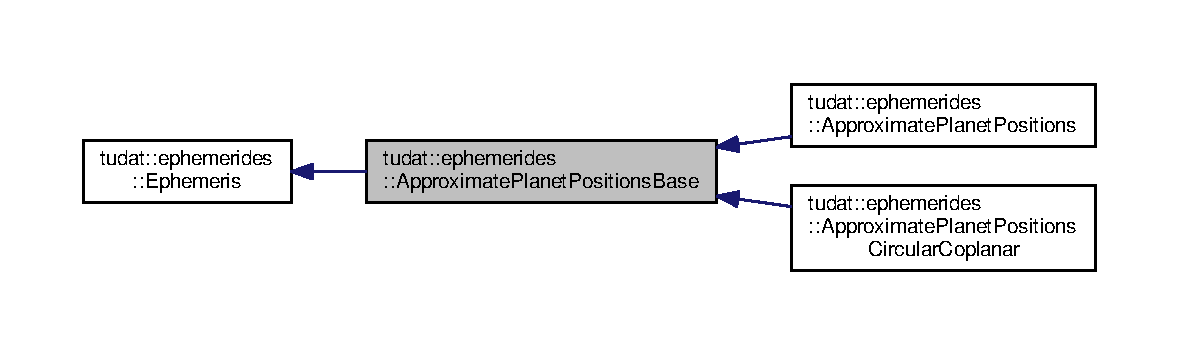
\includegraphics[width=350pt]{classtudat_1_1ephemerides_1_1ApproximatePlanetPositionsBase__inherit__graph}
\end{center}
\end{figure}


Collaboration diagram for tudat\+:\+:ephemerides\+:\+:Approximate\+Planet\+Positions\+Base\+:
\nopagebreak
\begin{figure}[H]
\begin{center}
\leavevmode
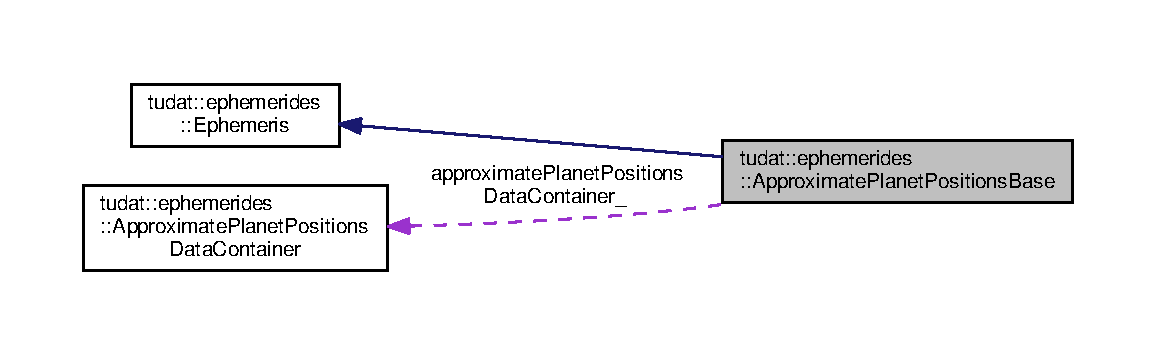
\includegraphics[width=350pt]{classtudat_1_1ephemerides_1_1ApproximatePlanetPositionsBase__coll__graph}
\end{center}
\end{figure}
\subsection*{Public Types}
\begin{DoxyCompactItemize}
\item 
enum \hyperlink{classtudat_1_1ephemerides_1_1ApproximatePlanetPositionsBase_aa698885dcabac2815a6205d5502724d2}{Bodies\+With\+Ephemeris\+Data} \{ \\*
{\bfseries mercury}, 
{\bfseries venus}, 
{\bfseries earth\+Moon\+Barycenter}, 
{\bfseries mars}, 
\\*
{\bfseries jupiter}, 
{\bfseries saturn}, 
{\bfseries uranus}, 
{\bfseries neptune}, 
\\*
{\bfseries pluto}
 \}\hypertarget{classtudat_1_1ephemerides_1_1ApproximatePlanetPositionsBase_aa698885dcabac2815a6205d5502724d2}{}\label{classtudat_1_1ephemerides_1_1ApproximatePlanetPositionsBase_aa698885dcabac2815a6205d5502724d2}
\begin{DoxyCompactList}\small\item\em Bodies with ephemeris data. \end{DoxyCompactList}
\end{DoxyCompactItemize}
\subsection*{Public Member Functions}
\begin{DoxyCompactItemize}
\item 
\hyperlink{classtudat_1_1ephemerides_1_1ApproximatePlanetPositionsBase_af74c02e220004c26042d40d1a935e02e}{Approximate\+Planet\+Positions\+Base} (const double a\+Sun\+Gravitational\+Parameter)
\begin{DoxyCompactList}\small\item\em Default constructor. \end{DoxyCompactList}\item 
virtual \hyperlink{classtudat_1_1ephemerides_1_1ApproximatePlanetPositionsBase_a9e8f9ead05a2dc897153caed1fbbbf78}{$\sim$\+Approximate\+Planet\+Positions\+Base} ()\hypertarget{classtudat_1_1ephemerides_1_1ApproximatePlanetPositionsBase_a9e8f9ead05a2dc897153caed1fbbbf78}{}\label{classtudat_1_1ephemerides_1_1ApproximatePlanetPositionsBase_a9e8f9ead05a2dc897153caed1fbbbf78}

\begin{DoxyCompactList}\small\item\em Default destructor. \end{DoxyCompactList}\item 
void \hyperlink{classtudat_1_1ephemerides_1_1ApproximatePlanetPositionsBase_aef19d67979b73f546c2fa448bcbfcbed}{parse\+Ephemeris\+Line\+Data\+\_\+} (const unsigned int \&first\+Line\+Number)
\begin{DoxyCompactList}\small\item\em Parse ephemeris line data. \end{DoxyCompactList}\item 
void \hyperlink{classtudat_1_1ephemerides_1_1ApproximatePlanetPositionsBase_af5aa54a364f7cc6429e4df57438236be}{parse\+Extra\+Terms\+Ephemeris\+Line\+Data\+\_\+} (const unsigned int \&line\+Number)
\begin{DoxyCompactList}\small\item\em Parse line data for extra terms for ephemeris. \end{DoxyCompactList}\item 
void \hyperlink{classtudat_1_1ephemerides_1_1ApproximatePlanetPositionsBase_a568eb00d49ec2d6ddda6fe353b20975b}{reload\+Data} ()
\begin{DoxyCompactList}\small\item\em Load in ephemeris data for planets. \end{DoxyCompactList}\item 
double \hyperlink{classtudat_1_1ephemerides_1_1ApproximatePlanetPositionsBase_abc58628f9a8defcd5bc8b8d9df778f98}{get\+Sun\+Gravitational\+Parameter} ()
\begin{DoxyCompactList}\small\item\em Returns the gravitational parameter of the Sun. \end{DoxyCompactList}\end{DoxyCompactItemize}
\subsection*{Protected Member Functions}
\begin{DoxyCompactItemize}
\item 
void \hyperlink{classtudat_1_1ephemerides_1_1ApproximatePlanetPositionsBase_aec3603d568cec958c2aef70100645c1b}{set\+Planet} (\hyperlink{classtudat_1_1ephemerides_1_1ApproximatePlanetPositionsBase_aa698885dcabac2815a6205d5502724d2}{Bodies\+With\+Ephemeris\+Data} body\+With\+Ephemeris\+Data)
\begin{DoxyCompactList}\small\item\em Set planet. \end{DoxyCompactList}\end{DoxyCompactItemize}
\subsection*{Protected Attributes}
\begin{DoxyCompactItemize}
\item 
const double \hyperlink{classtudat_1_1ephemerides_1_1ApproximatePlanetPositionsBase_a58b16732dcf7b19bda3810b455aca6bf}{sun\+Gravitational\+Parameter}
\begin{DoxyCompactList}\small\item\em Gravitational parameter of the Sun. \end{DoxyCompactList}\item 
double \hyperlink{classtudat_1_1ephemerides_1_1ApproximatePlanetPositionsBase_a6d6e4fdfb1666474b8e5647bfcf3746f}{julian\+Date\+\_\+}
\begin{DoxyCompactList}\small\item\em Julian date. \end{DoxyCompactList}\item 
double \hyperlink{classtudat_1_1ephemerides_1_1ApproximatePlanetPositionsBase_ad63ef8202dfe8a0a04feb350344ee7e7}{mean\+Longitude\+At\+Given\+Julian\+Date\+\_\+}
\begin{DoxyCompactList}\small\item\em Mean longitude at given Julian date. \end{DoxyCompactList}\item 
double \hyperlink{classtudat_1_1ephemerides_1_1ApproximatePlanetPositionsBase_aa967cb9533b467af0cf22d5bb5ed8501}{number\+Of\+Centuries\+Past\+J2000\+\_\+}
\begin{DoxyCompactList}\small\item\em Number of centuries passed J2000. \end{DoxyCompactList}\item 
std\+::map$<$ unsigned int, std\+::string $>$ \hyperlink{classtudat_1_1ephemerides_1_1ApproximatePlanetPositionsBase_acfc0c1fc4289411b5d90d1fae6058629}{container\+Of\+Data\+From\+Ephemeris\+File\+\_\+}
\begin{DoxyCompactList}\small\item\em Map container of data from ephemeris file. \end{DoxyCompactList}\item 
\hyperlink{structtudat_1_1ephemerides_1_1ApproximatePlanetPositionsDataContainer}{Approximate\+Planet\+Positions\+Data\+Container} \hyperlink{classtudat_1_1ephemerides_1_1ApproximatePlanetPositionsBase_a04dafb484427c3a552fb4a7f6f456ea0}{approximate\+Planet\+Positions\+Data\+Container\+\_\+}
\begin{DoxyCompactList}\small\item\em Approximate planet positions data container. \end{DoxyCompactList}\item 
Eigen\+::\+Vector6d \hyperlink{classtudat_1_1ephemerides_1_1ApproximatePlanetPositionsBase_a872f2535642808c26097146d513a1b3c}{planet\+Keplerian\+Elements\+At\+Given\+Julian\+Date\+\_\+}
\begin{DoxyCompactList}\small\item\em Keplerian elements of planet at given Julian date. \end{DoxyCompactList}\item 
std\+::stringstream \hyperlink{classtudat_1_1ephemerides_1_1ApproximatePlanetPositionsBase_a9c8716b05a0b4611ba7d25138cf6e9f5}{ephemeris\+Line\+Data\+\_\+}
\begin{DoxyCompactList}\small\item\em String stream for ephemeris line data. \end{DoxyCompactList}\end{DoxyCompactItemize}


\subsection{Detailed Description}
\hyperlink{classtudat_1_1ephemerides_1_1Ephemeris}{Ephemeris} base class using J\+PL \char`\"{}\+Approximate Positions of Major Planets\char`\"{}. 

\hyperlink{classtudat_1_1ephemerides_1_1Ephemeris}{Ephemeris} base class using J\+PL \char`\"{}\+Approximate Positions of Major Planets\char`\"{}. 

\subsection{Constructor \& Destructor Documentation}
\index{tudat\+::ephemerides\+::\+Approximate\+Planet\+Positions\+Base@{tudat\+::ephemerides\+::\+Approximate\+Planet\+Positions\+Base}!Approximate\+Planet\+Positions\+Base@{Approximate\+Planet\+Positions\+Base}}
\index{Approximate\+Planet\+Positions\+Base@{Approximate\+Planet\+Positions\+Base}!tudat\+::ephemerides\+::\+Approximate\+Planet\+Positions\+Base@{tudat\+::ephemerides\+::\+Approximate\+Planet\+Positions\+Base}}
\subsubsection[{\texorpdfstring{Approximate\+Planet\+Positions\+Base(const double a\+Sun\+Gravitational\+Parameter)}{ApproximatePlanetPositionsBase(const double aSunGravitationalParameter)}}]{\setlength{\rightskip}{0pt plus 5cm}tudat\+::ephemerides\+::\+Approximate\+Planet\+Positions\+Base\+::\+Approximate\+Planet\+Positions\+Base (
\begin{DoxyParamCaption}
\item[{const double}]{a\+Sun\+Gravitational\+Parameter}
\end{DoxyParamCaption}
)\hspace{0.3cm}{\ttfamily [inline]}}\hypertarget{classtudat_1_1ephemerides_1_1ApproximatePlanetPositionsBase_af74c02e220004c26042d40d1a935e02e}{}\label{classtudat_1_1ephemerides_1_1ApproximatePlanetPositionsBase_af74c02e220004c26042d40d1a935e02e}


Default constructor. 

Default constructor of the base class, initializes the gravitational parameter of the Sun to the input value, and all other private base class members to default values.


\begin{DoxyParams}{Parameters}
{\em a\+Sun\+Gravitational\+Parameter} & The gravitational parameter of the Sun \mbox{[}m$^\wedge$3/s$^\wedge$2\mbox{]}. \\
\hline
\end{DoxyParams}
\begin{DoxySeeAlso}{See also}
\hyperlink{classtudat_1_1ephemerides_1_1ApproximatePlanetPositions}{Approximate\+Planet\+Positions}, \hyperlink{classtudat_1_1ephemerides_1_1ApproximatePlanetPositionsCircularCoplanar}{Approximate\+Planet\+Positions\+Circular\+Coplanar}. 
\end{DoxySeeAlso}


\subsection{Member Function Documentation}
\index{tudat\+::ephemerides\+::\+Approximate\+Planet\+Positions\+Base@{tudat\+::ephemerides\+::\+Approximate\+Planet\+Positions\+Base}!get\+Sun\+Gravitational\+Parameter@{get\+Sun\+Gravitational\+Parameter}}
\index{get\+Sun\+Gravitational\+Parameter@{get\+Sun\+Gravitational\+Parameter}!tudat\+::ephemerides\+::\+Approximate\+Planet\+Positions\+Base@{tudat\+::ephemerides\+::\+Approximate\+Planet\+Positions\+Base}}
\subsubsection[{\texorpdfstring{get\+Sun\+Gravitational\+Parameter()}{getSunGravitationalParameter()}}]{\setlength{\rightskip}{0pt plus 5cm}double tudat\+::ephemerides\+::\+Approximate\+Planet\+Positions\+Base\+::get\+Sun\+Gravitational\+Parameter (
\begin{DoxyParamCaption}
{}
\end{DoxyParamCaption}
)\hspace{0.3cm}{\ttfamily [inline]}}\hypertarget{classtudat_1_1ephemerides_1_1ApproximatePlanetPositionsBase_abc58628f9a8defcd5bc8b8d9df778f98}{}\label{classtudat_1_1ephemerides_1_1ApproximatePlanetPositionsBase_abc58628f9a8defcd5bc8b8d9df778f98}


Returns the gravitational parameter of the Sun. 

Returns the gravitational parameter of the Sun that is used in the calculations. \begin{DoxyReturn}{Returns}
Gravitational parameter of the Sun. 
\end{DoxyReturn}
\index{tudat\+::ephemerides\+::\+Approximate\+Planet\+Positions\+Base@{tudat\+::ephemerides\+::\+Approximate\+Planet\+Positions\+Base}!parse\+Ephemeris\+Line\+Data\+\_\+@{parse\+Ephemeris\+Line\+Data\+\_\+}}
\index{parse\+Ephemeris\+Line\+Data\+\_\+@{parse\+Ephemeris\+Line\+Data\+\_\+}!tudat\+::ephemerides\+::\+Approximate\+Planet\+Positions\+Base@{tudat\+::ephemerides\+::\+Approximate\+Planet\+Positions\+Base}}
\subsubsection[{\texorpdfstring{parse\+Ephemeris\+Line\+Data\+\_\+(const unsigned int \&first\+Line\+Number)}{parseEphemerisLineData_(const unsigned int &firstLineNumber)}}]{\setlength{\rightskip}{0pt plus 5cm}void tudat\+::ephemerides\+::\+Approximate\+Planet\+Positions\+Base\+::parse\+Ephemeris\+Line\+Data\+\_\+ (
\begin{DoxyParamCaption}
\item[{const unsigned int \&}]{first\+Line\+Number}
\end{DoxyParamCaption}
)}\hypertarget{classtudat_1_1ephemerides_1_1ApproximatePlanetPositionsBase_aef19d67979b73f546c2fa448bcbfcbed}{}\label{classtudat_1_1ephemerides_1_1ApproximatePlanetPositionsBase_aef19d67979b73f546c2fa448bcbfcbed}


Parse ephemeris line data. 

Parses ephemeris line data. 
\begin{DoxyParams}{Parameters}
{\em first\+Line\+Number} & First line number. \\
\hline
\end{DoxyParams}
\index{tudat\+::ephemerides\+::\+Approximate\+Planet\+Positions\+Base@{tudat\+::ephemerides\+::\+Approximate\+Planet\+Positions\+Base}!parse\+Extra\+Terms\+Ephemeris\+Line\+Data\+\_\+@{parse\+Extra\+Terms\+Ephemeris\+Line\+Data\+\_\+}}
\index{parse\+Extra\+Terms\+Ephemeris\+Line\+Data\+\_\+@{parse\+Extra\+Terms\+Ephemeris\+Line\+Data\+\_\+}!tudat\+::ephemerides\+::\+Approximate\+Planet\+Positions\+Base@{tudat\+::ephemerides\+::\+Approximate\+Planet\+Positions\+Base}}
\subsubsection[{\texorpdfstring{parse\+Extra\+Terms\+Ephemeris\+Line\+Data\+\_\+(const unsigned int \&line\+Number)}{parseExtraTermsEphemerisLineData_(const unsigned int &lineNumber)}}]{\setlength{\rightskip}{0pt plus 5cm}void tudat\+::ephemerides\+::\+Approximate\+Planet\+Positions\+Base\+::parse\+Extra\+Terms\+Ephemeris\+Line\+Data\+\_\+ (
\begin{DoxyParamCaption}
\item[{const unsigned int \&}]{line\+Number}
\end{DoxyParamCaption}
)}\hypertarget{classtudat_1_1ephemerides_1_1ApproximatePlanetPositionsBase_af5aa54a364f7cc6429e4df57438236be}{}\label{classtudat_1_1ephemerides_1_1ApproximatePlanetPositionsBase_af5aa54a364f7cc6429e4df57438236be}


Parse line data for extra terms for ephemeris. 

Parses ephemeris line data for necessary extra terms. 
\begin{DoxyParams}{Parameters}
{\em line\+Number} & Line number. \\
\hline
\end{DoxyParams}
\index{tudat\+::ephemerides\+::\+Approximate\+Planet\+Positions\+Base@{tudat\+::ephemerides\+::\+Approximate\+Planet\+Positions\+Base}!reload\+Data@{reload\+Data}}
\index{reload\+Data@{reload\+Data}!tudat\+::ephemerides\+::\+Approximate\+Planet\+Positions\+Base@{tudat\+::ephemerides\+::\+Approximate\+Planet\+Positions\+Base}}
\subsubsection[{\texorpdfstring{reload\+Data()}{reloadData()}}]{\setlength{\rightskip}{0pt plus 5cm}void tudat\+::ephemerides\+::\+Approximate\+Planet\+Positions\+Base\+::reload\+Data (
\begin{DoxyParamCaption}
{}
\end{DoxyParamCaption}
)}\hypertarget{classtudat_1_1ephemerides_1_1ApproximatePlanetPositionsBase_a568eb00d49ec2d6ddda6fe353b20975b}{}\label{classtudat_1_1ephemerides_1_1ApproximatePlanetPositionsBase_a568eb00d49ec2d6ddda6fe353b20975b}


Load in ephemeris data for planets. 

This method opens and parses the p\+\_\+elem\+\_\+t2.\+txt ephemeris files for the planet positions. The resulting data is stored in \hyperlink{classtudat_1_1ephemerides_1_1ApproximatePlanetPositionsBase_acfc0c1fc4289411b5d90d1fae6058629}{Approximate\+Planet\+Positions\+Base\+::container\+Of\+Data\+From\+Ephemeris\+File\+\_\+} to be used in the generation of planet ephemeris. This method is automatically invoked if you call \hyperlink{classtudat_1_1ephemerides_1_1ApproximatePlanetPositionsBase_aec3603d568cec958c2aef70100645c1b}{Approximate\+Planet\+Positions\+Base\+::set\+Planet( Bodies\+With\+Ephemeris\+Data )}. \index{tudat\+::ephemerides\+::\+Approximate\+Planet\+Positions\+Base@{tudat\+::ephemerides\+::\+Approximate\+Planet\+Positions\+Base}!set\+Planet@{set\+Planet}}
\index{set\+Planet@{set\+Planet}!tudat\+::ephemerides\+::\+Approximate\+Planet\+Positions\+Base@{tudat\+::ephemerides\+::\+Approximate\+Planet\+Positions\+Base}}
\subsubsection[{\texorpdfstring{set\+Planet(\+Bodies\+With\+Ephemeris\+Data body\+With\+Ephemeris\+Data)}{setPlanet(BodiesWithEphemerisData bodyWithEphemerisData)}}]{\setlength{\rightskip}{0pt plus 5cm}void tudat\+::ephemerides\+::\+Approximate\+Planet\+Positions\+Base\+::set\+Planet (
\begin{DoxyParamCaption}
\item[{{\bf Bodies\+With\+Ephemeris\+Data}}]{body\+With\+Ephemeris\+Data}
\end{DoxyParamCaption}
)\hspace{0.3cm}{\ttfamily [protected]}}\hypertarget{classtudat_1_1ephemerides_1_1ApproximatePlanetPositionsBase_aec3603d568cec958c2aef70100645c1b}{}\label{classtudat_1_1ephemerides_1_1ApproximatePlanetPositionsBase_aec3603d568cec958c2aef70100645c1b}


Set planet. 

Sets planet to retrieve ephemeris data for. 
\begin{DoxyParams}{Parameters}
{\em body\+With\+Ephemeris\+Data} & Planet. \\
\hline
\end{DoxyParams}


\subsection{Member Data Documentation}
\index{tudat\+::ephemerides\+::\+Approximate\+Planet\+Positions\+Base@{tudat\+::ephemerides\+::\+Approximate\+Planet\+Positions\+Base}!approximate\+Planet\+Positions\+Data\+Container\+\_\+@{approximate\+Planet\+Positions\+Data\+Container\+\_\+}}
\index{approximate\+Planet\+Positions\+Data\+Container\+\_\+@{approximate\+Planet\+Positions\+Data\+Container\+\_\+}!tudat\+::ephemerides\+::\+Approximate\+Planet\+Positions\+Base@{tudat\+::ephemerides\+::\+Approximate\+Planet\+Positions\+Base}}
\subsubsection[{\texorpdfstring{approximate\+Planet\+Positions\+Data\+Container\+\_\+}{approximatePlanetPositionsDataContainer_}}]{\setlength{\rightskip}{0pt plus 5cm}{\bf Approximate\+Planet\+Positions\+Data\+Container} tudat\+::ephemerides\+::\+Approximate\+Planet\+Positions\+Base\+::approximate\+Planet\+Positions\+Data\+Container\+\_\+\hspace{0.3cm}{\ttfamily [protected]}}\hypertarget{classtudat_1_1ephemerides_1_1ApproximatePlanetPositionsBase_a04dafb484427c3a552fb4a7f6f456ea0}{}\label{classtudat_1_1ephemerides_1_1ApproximatePlanetPositionsBase_a04dafb484427c3a552fb4a7f6f456ea0}


Approximate planet positions data container. 

Approximate planet positions data container. \index{tudat\+::ephemerides\+::\+Approximate\+Planet\+Positions\+Base@{tudat\+::ephemerides\+::\+Approximate\+Planet\+Positions\+Base}!container\+Of\+Data\+From\+Ephemeris\+File\+\_\+@{container\+Of\+Data\+From\+Ephemeris\+File\+\_\+}}
\index{container\+Of\+Data\+From\+Ephemeris\+File\+\_\+@{container\+Of\+Data\+From\+Ephemeris\+File\+\_\+}!tudat\+::ephemerides\+::\+Approximate\+Planet\+Positions\+Base@{tudat\+::ephemerides\+::\+Approximate\+Planet\+Positions\+Base}}
\subsubsection[{\texorpdfstring{container\+Of\+Data\+From\+Ephemeris\+File\+\_\+}{containerOfDataFromEphemerisFile_}}]{\setlength{\rightskip}{0pt plus 5cm}std\+::map$<$ unsigned int, std\+::string $>$ tudat\+::ephemerides\+::\+Approximate\+Planet\+Positions\+Base\+::container\+Of\+Data\+From\+Ephemeris\+File\+\_\+\hspace{0.3cm}{\ttfamily [protected]}}\hypertarget{classtudat_1_1ephemerides_1_1ApproximatePlanetPositionsBase_acfc0c1fc4289411b5d90d1fae6058629}{}\label{classtudat_1_1ephemerides_1_1ApproximatePlanetPositionsBase_acfc0c1fc4289411b5d90d1fae6058629}


Map container of data from ephemeris file. 

Map container of string data from ephemeris data file. \index{tudat\+::ephemerides\+::\+Approximate\+Planet\+Positions\+Base@{tudat\+::ephemerides\+::\+Approximate\+Planet\+Positions\+Base}!ephemeris\+Line\+Data\+\_\+@{ephemeris\+Line\+Data\+\_\+}}
\index{ephemeris\+Line\+Data\+\_\+@{ephemeris\+Line\+Data\+\_\+}!tudat\+::ephemerides\+::\+Approximate\+Planet\+Positions\+Base@{tudat\+::ephemerides\+::\+Approximate\+Planet\+Positions\+Base}}
\subsubsection[{\texorpdfstring{ephemeris\+Line\+Data\+\_\+}{ephemerisLineData_}}]{\setlength{\rightskip}{0pt plus 5cm}std\+::stringstream tudat\+::ephemerides\+::\+Approximate\+Planet\+Positions\+Base\+::ephemeris\+Line\+Data\+\_\+\hspace{0.3cm}{\ttfamily [protected]}}\hypertarget{classtudat_1_1ephemerides_1_1ApproximatePlanetPositionsBase_a9c8716b05a0b4611ba7d25138cf6e9f5}{}\label{classtudat_1_1ephemerides_1_1ApproximatePlanetPositionsBase_a9c8716b05a0b4611ba7d25138cf6e9f5}


String stream for ephemeris line data. 

String stream for ephemeris line data. \index{tudat\+::ephemerides\+::\+Approximate\+Planet\+Positions\+Base@{tudat\+::ephemerides\+::\+Approximate\+Planet\+Positions\+Base}!julian\+Date\+\_\+@{julian\+Date\+\_\+}}
\index{julian\+Date\+\_\+@{julian\+Date\+\_\+}!tudat\+::ephemerides\+::\+Approximate\+Planet\+Positions\+Base@{tudat\+::ephemerides\+::\+Approximate\+Planet\+Positions\+Base}}
\subsubsection[{\texorpdfstring{julian\+Date\+\_\+}{julianDate_}}]{\setlength{\rightskip}{0pt plus 5cm}double tudat\+::ephemerides\+::\+Approximate\+Planet\+Positions\+Base\+::julian\+Date\+\_\+\hspace{0.3cm}{\ttfamily [protected]}}\hypertarget{classtudat_1_1ephemerides_1_1ApproximatePlanetPositionsBase_a6d6e4fdfb1666474b8e5647bfcf3746f}{}\label{classtudat_1_1ephemerides_1_1ApproximatePlanetPositionsBase_a6d6e4fdfb1666474b8e5647bfcf3746f}


Julian date. 

Julian date at which to obtain planet\textquotesingle{}s orbital elements. \index{tudat\+::ephemerides\+::\+Approximate\+Planet\+Positions\+Base@{tudat\+::ephemerides\+::\+Approximate\+Planet\+Positions\+Base}!mean\+Longitude\+At\+Given\+Julian\+Date\+\_\+@{mean\+Longitude\+At\+Given\+Julian\+Date\+\_\+}}
\index{mean\+Longitude\+At\+Given\+Julian\+Date\+\_\+@{mean\+Longitude\+At\+Given\+Julian\+Date\+\_\+}!tudat\+::ephemerides\+::\+Approximate\+Planet\+Positions\+Base@{tudat\+::ephemerides\+::\+Approximate\+Planet\+Positions\+Base}}
\subsubsection[{\texorpdfstring{mean\+Longitude\+At\+Given\+Julian\+Date\+\_\+}{meanLongitudeAtGivenJulianDate_}}]{\setlength{\rightskip}{0pt plus 5cm}double tudat\+::ephemerides\+::\+Approximate\+Planet\+Positions\+Base\+::mean\+Longitude\+At\+Given\+Julian\+Date\+\_\+\hspace{0.3cm}{\ttfamily [protected]}}\hypertarget{classtudat_1_1ephemerides_1_1ApproximatePlanetPositionsBase_ad63ef8202dfe8a0a04feb350344ee7e7}{}\label{classtudat_1_1ephemerides_1_1ApproximatePlanetPositionsBase_ad63ef8202dfe8a0a04feb350344ee7e7}


Mean longitude at given Julian date. 

Mean longitude of planet at given Julian date. \index{tudat\+::ephemerides\+::\+Approximate\+Planet\+Positions\+Base@{tudat\+::ephemerides\+::\+Approximate\+Planet\+Positions\+Base}!number\+Of\+Centuries\+Past\+J2000\+\_\+@{number\+Of\+Centuries\+Past\+J2000\+\_\+}}
\index{number\+Of\+Centuries\+Past\+J2000\+\_\+@{number\+Of\+Centuries\+Past\+J2000\+\_\+}!tudat\+::ephemerides\+::\+Approximate\+Planet\+Positions\+Base@{tudat\+::ephemerides\+::\+Approximate\+Planet\+Positions\+Base}}
\subsubsection[{\texorpdfstring{number\+Of\+Centuries\+Past\+J2000\+\_\+}{numberOfCenturiesPastJ2000_}}]{\setlength{\rightskip}{0pt plus 5cm}double tudat\+::ephemerides\+::\+Approximate\+Planet\+Positions\+Base\+::number\+Of\+Centuries\+Past\+J2000\+\_\+\hspace{0.3cm}{\ttfamily [protected]}}\hypertarget{classtudat_1_1ephemerides_1_1ApproximatePlanetPositionsBase_aa967cb9533b467af0cf22d5bb5ed8501}{}\label{classtudat_1_1ephemerides_1_1ApproximatePlanetPositionsBase_aa967cb9533b467af0cf22d5bb5ed8501}


Number of centuries passed J2000. 

Number of centuries passed J2000, computed using Julian date defined by user when retrieving state. \index{tudat\+::ephemerides\+::\+Approximate\+Planet\+Positions\+Base@{tudat\+::ephemerides\+::\+Approximate\+Planet\+Positions\+Base}!planet\+Keplerian\+Elements\+At\+Given\+Julian\+Date\+\_\+@{planet\+Keplerian\+Elements\+At\+Given\+Julian\+Date\+\_\+}}
\index{planet\+Keplerian\+Elements\+At\+Given\+Julian\+Date\+\_\+@{planet\+Keplerian\+Elements\+At\+Given\+Julian\+Date\+\_\+}!tudat\+::ephemerides\+::\+Approximate\+Planet\+Positions\+Base@{tudat\+::ephemerides\+::\+Approximate\+Planet\+Positions\+Base}}
\subsubsection[{\texorpdfstring{planet\+Keplerian\+Elements\+At\+Given\+Julian\+Date\+\_\+}{planetKeplerianElementsAtGivenJulianDate_}}]{\setlength{\rightskip}{0pt plus 5cm}Eigen\+::\+Vector6d tudat\+::ephemerides\+::\+Approximate\+Planet\+Positions\+Base\+::planet\+Keplerian\+Elements\+At\+Given\+Julian\+Date\+\_\+\hspace{0.3cm}{\ttfamily [protected]}}\hypertarget{classtudat_1_1ephemerides_1_1ApproximatePlanetPositionsBase_a872f2535642808c26097146d513a1b3c}{}\label{classtudat_1_1ephemerides_1_1ApproximatePlanetPositionsBase_a872f2535642808c26097146d513a1b3c}


Keplerian elements of planet at given Julian date. 

Keplerian elements of planet at given Julian date. \index{tudat\+::ephemerides\+::\+Approximate\+Planet\+Positions\+Base@{tudat\+::ephemerides\+::\+Approximate\+Planet\+Positions\+Base}!sun\+Gravitational\+Parameter@{sun\+Gravitational\+Parameter}}
\index{sun\+Gravitational\+Parameter@{sun\+Gravitational\+Parameter}!tudat\+::ephemerides\+::\+Approximate\+Planet\+Positions\+Base@{tudat\+::ephemerides\+::\+Approximate\+Planet\+Positions\+Base}}
\subsubsection[{\texorpdfstring{sun\+Gravitational\+Parameter}{sunGravitationalParameter}}]{\setlength{\rightskip}{0pt plus 5cm}const double tudat\+::ephemerides\+::\+Approximate\+Planet\+Positions\+Base\+::sun\+Gravitational\+Parameter\hspace{0.3cm}{\ttfamily [protected]}}\hypertarget{classtudat_1_1ephemerides_1_1ApproximatePlanetPositionsBase_a58b16732dcf7b19bda3810b455aca6bf}{}\label{classtudat_1_1ephemerides_1_1ApproximatePlanetPositionsBase_a58b16732dcf7b19bda3810b455aca6bf}


Gravitational parameter of the Sun. 

Gravitational parameter of the Sun. 

The documentation for this class was generated from the following files\+:\begin{DoxyCompactItemize}
\item 
/home/lupi/\+Tudat/tudat\+Bundle/tudat/\+Tudat/\+Astrodynamics/\+Ephemerides/approximate\+Planet\+Positions\+Base.\+h\item 
/home/lupi/\+Tudat/tudat\+Bundle/tudat/\+Tudat/\+Astrodynamics/\+Ephemerides/approximate\+Planet\+Positions\+Base.\+cpp\end{DoxyCompactItemize}

\hypertarget{classtudat_1_1ephemerides_1_1ApproximatePlanetPositionsCircularCoplanar}{}\section{tudat\+:\+:ephemerides\+:\+:Approximate\+Planet\+Positions\+Circular\+Coplanar Class Reference}
\label{classtudat_1_1ephemerides_1_1ApproximatePlanetPositionsCircularCoplanar}\index{tudat\+::ephemerides\+::\+Approximate\+Planet\+Positions\+Circular\+Coplanar@{tudat\+::ephemerides\+::\+Approximate\+Planet\+Positions\+Circular\+Coplanar}}


\hyperlink{classtudat_1_1ephemerides_1_1Ephemeris}{Ephemeris} class for circular, coplanar orbits using Approximate Positions of Major Planets.  




{\ttfamily \#include $<$approximate\+Planet\+Positions\+Circular\+Coplanar.\+h$>$}



Inheritance diagram for tudat\+:\+:ephemerides\+:\+:Approximate\+Planet\+Positions\+Circular\+Coplanar\+:
\nopagebreak
\begin{figure}[H]
\begin{center}
\leavevmode
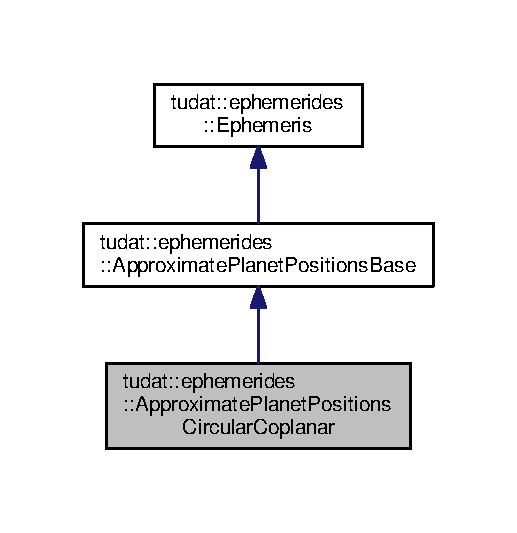
\includegraphics[width=248pt]{classtudat_1_1ephemerides_1_1ApproximatePlanetPositionsCircularCoplanar__inherit__graph}
\end{center}
\end{figure}


Collaboration diagram for tudat\+:\+:ephemerides\+:\+:Approximate\+Planet\+Positions\+Circular\+Coplanar\+:
\nopagebreak
\begin{figure}[H]
\begin{center}
\leavevmode
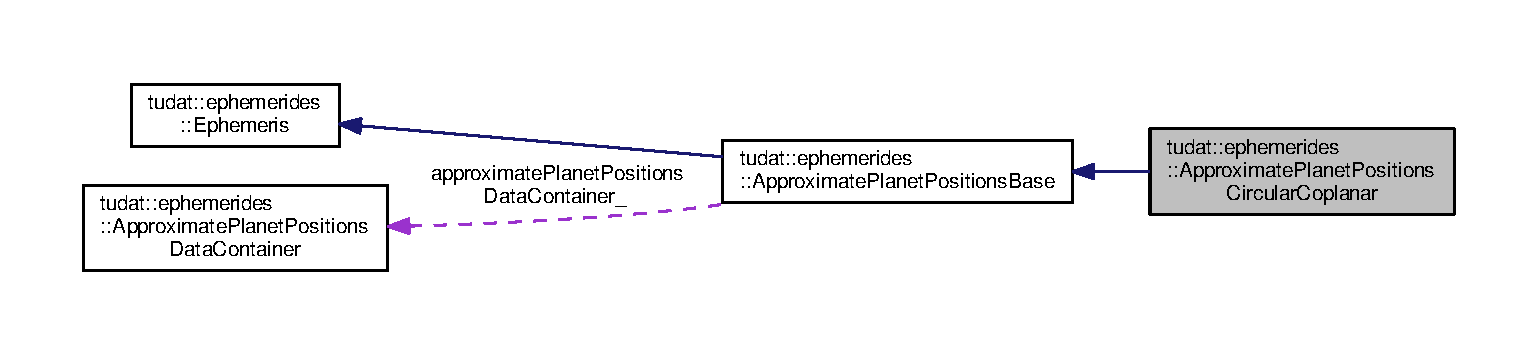
\includegraphics[width=350pt]{classtudat_1_1ephemerides_1_1ApproximatePlanetPositionsCircularCoplanar__coll__graph}
\end{center}
\end{figure}
\subsection*{Public Member Functions}
\begin{DoxyCompactItemize}
\item 
\hyperlink{classtudat_1_1ephemerides_1_1ApproximatePlanetPositionsCircularCoplanar_ae533f4f77671301038b2f9fe2cb489fe}{Approximate\+Planet\+Positions\+Circular\+Coplanar} (\hyperlink{classtudat_1_1ephemerides_1_1ApproximatePlanetPositionsBase_aa698885dcabac2815a6205d5502724d2}{Bodies\+With\+Ephemeris\+Data} body\+With\+Ephemeris\+Data, const double a\+Sun\+Gravitational\+Parameter=1.\+32712440018e20, const double reference\+Julian\+Date=basic\+\_\+astrodynamics\+::\+J\+U\+L\+I\+A\+N\+\_\+\+D\+A\+Y\+\_\+\+O\+N\+\_\+\+J2000)
\begin{DoxyCompactList}\small\item\em Default constructor. \end{DoxyCompactList}\item 
Eigen\+::\+Vector6d \hyperlink{classtudat_1_1ephemerides_1_1ApproximatePlanetPositionsCircularCoplanar_a72e87b71ccd875c6a349c1a9a0bcb544}{get\+Cartesian\+State} (const double seconds\+Since\+Epoch)
\begin{DoxyCompactList}\small\item\em Get state from ephemeris; circular, coplanar case. \end{DoxyCompactList}\end{DoxyCompactItemize}
\subsection*{Additional Inherited Members}


\subsection{Detailed Description}
\hyperlink{classtudat_1_1ephemerides_1_1Ephemeris}{Ephemeris} class for circular, coplanar orbits using Approximate Positions of Major Planets. 

\hyperlink{classtudat_1_1ephemerides_1_1Ephemeris}{Ephemeris} class for circular, coplanar planetary orbits, using J\+PL \char`\"{}\+Approximate Positions of Major Planets\char`\"{}. 

\subsection{Constructor \& Destructor Documentation}
\index{tudat\+::ephemerides\+::\+Approximate\+Planet\+Positions\+Circular\+Coplanar@{tudat\+::ephemerides\+::\+Approximate\+Planet\+Positions\+Circular\+Coplanar}!Approximate\+Planet\+Positions\+Circular\+Coplanar@{Approximate\+Planet\+Positions\+Circular\+Coplanar}}
\index{Approximate\+Planet\+Positions\+Circular\+Coplanar@{Approximate\+Planet\+Positions\+Circular\+Coplanar}!tudat\+::ephemerides\+::\+Approximate\+Planet\+Positions\+Circular\+Coplanar@{tudat\+::ephemerides\+::\+Approximate\+Planet\+Positions\+Circular\+Coplanar}}
\subsubsection[{\texorpdfstring{Approximate\+Planet\+Positions\+Circular\+Coplanar(\+Bodies\+With\+Ephemeris\+Data body\+With\+Ephemeris\+Data, const double a\+Sun\+Gravitational\+Parameter=1.\+32712440018e20, const double reference\+Julian\+Date=basic\+\_\+astrodynamics\+::\+J\+U\+L\+I\+A\+N\+\_\+\+D\+A\+Y\+\_\+\+O\+N\+\_\+\+J2000)}{ApproximatePlanetPositionsCircularCoplanar(BodiesWithEphemerisData bodyWithEphemerisData, const double aSunGravitationalParameter=1.32712440018e20, const double referenceJulianDate=basic_astrodynamics::JULIAN_DAY_ON_J2000)}}]{\setlength{\rightskip}{0pt plus 5cm}tudat\+::ephemerides\+::\+Approximate\+Planet\+Positions\+Circular\+Coplanar\+::\+Approximate\+Planet\+Positions\+Circular\+Coplanar (
\begin{DoxyParamCaption}
\item[{{\bf Bodies\+With\+Ephemeris\+Data}}]{body\+With\+Ephemeris\+Data, }
\item[{const double}]{a\+Sun\+Gravitational\+Parameter = {\ttfamily 1.32712440018e20}, }
\item[{const double}]{reference\+Julian\+Date = {\ttfamily basic\+\_\+astrodynamics\+:\+:JULIAN\+\_\+DAY\+\_\+ON\+\_\+J2000}}
\end{DoxyParamCaption}
)\hspace{0.3cm}{\ttfamily [inline]}}\hypertarget{classtudat_1_1ephemerides_1_1ApproximatePlanetPositionsCircularCoplanar_ae533f4f77671301038b2f9fe2cb489fe}{}\label{classtudat_1_1ephemerides_1_1ApproximatePlanetPositionsCircularCoplanar_ae533f4f77671301038b2f9fe2cb489fe}


Default constructor. 

Default constructor that initializes the class from the body for which the position is approximated and the gravitational parameter of the Sun (default 1.\+32712440018e20). Other members are initialized to default values.


\begin{DoxyParams}{Parameters}
{\em body\+With\+Ephemeris\+Data} & The body for which the position is approximated. \\
\hline
{\em a\+Sun\+Gravitational\+Parameter} & The gravitational parameter of the Sun \mbox{[}m$^\wedge$3/s$^\wedge$2\mbox{]}. \\
\hline
{\em reference\+Julian\+Date} & Reference julian day w.\+r.\+t. which ephemeris is evaluated. \\
\hline
\end{DoxyParams}
\begin{DoxySeeAlso}{See also}
\hyperlink{classtudat_1_1ephemerides_1_1ApproximatePlanetPositionsBase_aa698885dcabac2815a6205d5502724d2}{Bodies\+With\+Ephemeris\+Data}, \hyperlink{classtudat_1_1ephemerides_1_1ApproximatePlanetPositionsBase}{Approximate\+Planet\+Positions\+Base}. 
\end{DoxySeeAlso}


\subsection{Member Function Documentation}
\index{tudat\+::ephemerides\+::\+Approximate\+Planet\+Positions\+Circular\+Coplanar@{tudat\+::ephemerides\+::\+Approximate\+Planet\+Positions\+Circular\+Coplanar}!get\+Cartesian\+State@{get\+Cartesian\+State}}
\index{get\+Cartesian\+State@{get\+Cartesian\+State}!tudat\+::ephemerides\+::\+Approximate\+Planet\+Positions\+Circular\+Coplanar@{tudat\+::ephemerides\+::\+Approximate\+Planet\+Positions\+Circular\+Coplanar}}
\subsubsection[{\texorpdfstring{get\+Cartesian\+State(const double seconds\+Since\+Epoch)}{getCartesianState(const double secondsSinceEpoch)}}]{\setlength{\rightskip}{0pt plus 5cm}Eigen\+::\+Vector6d tudat\+::ephemerides\+::\+Approximate\+Planet\+Positions\+Circular\+Coplanar\+::get\+Cartesian\+State (
\begin{DoxyParamCaption}
\item[{const double}]{seconds\+Since\+Epoch}
\end{DoxyParamCaption}
)\hspace{0.3cm}{\ttfamily [virtual]}}\hypertarget{classtudat_1_1ephemerides_1_1ApproximatePlanetPositionsCircularCoplanar_a72e87b71ccd875c6a349c1a9a0bcb544}{}\label{classtudat_1_1ephemerides_1_1ApproximatePlanetPositionsCircularCoplanar_a72e87b71ccd875c6a349c1a9a0bcb544}


Get state from ephemeris; circular, coplanar case. 

Returns state in Cartesian elements from ephemeris for circular and coplanar orbit. 
\begin{DoxyParams}{Parameters}
{\em seconds\+Since\+Epoch} & Seconds since epoch. \\
\hline
\end{DoxyParams}
\begin{DoxyReturn}{Returns}
State in Cartesian elements from ephemeris for circular and coplanar orbit. 
\end{DoxyReturn}


Implements \hyperlink{classtudat_1_1ephemerides_1_1Ephemeris_a9ffa2e6b00aa190385d87266bc6ca091}{tudat\+::ephemerides\+::\+Ephemeris}.



The documentation for this class was generated from the following files\+:\begin{DoxyCompactItemize}
\item 
/home/lupi/\+Tudat/tudat\+Bundle/tudat/\+Tudat/\+Astrodynamics/\+Ephemerides/approximate\+Planet\+Positions\+Circular\+Coplanar.\+h\item 
/home/lupi/\+Tudat/tudat\+Bundle/tudat/\+Tudat/\+Astrodynamics/\+Ephemerides/approximate\+Planet\+Positions\+Circular\+Coplanar.\+cpp\end{DoxyCompactItemize}

\hypertarget{structtudat_1_1ephemerides_1_1ApproximatePlanetPositionsDataContainer}{}\section{tudat\+:\+:ephemerides\+:\+:Approximate\+Planet\+Positions\+Data\+Container Struct Reference}
\label{structtudat_1_1ephemerides_1_1ApproximatePlanetPositionsDataContainer}\index{tudat\+::ephemerides\+::\+Approximate\+Planet\+Positions\+Data\+Container@{tudat\+::ephemerides\+::\+Approximate\+Planet\+Positions\+Data\+Container}}


J\+PL \char`\"{}\+Approximate Positions of Major Planets\char`\"{} data container class.  




{\ttfamily \#include $<$approximate\+Planet\+Positions\+Data\+Container.\+h$>$}

\subsection*{Public Member Functions}
\begin{DoxyCompactItemize}
\item 
\hyperlink{structtudat_1_1ephemerides_1_1ApproximatePlanetPositionsDataContainer_a687ec166207da1954e50eccbc7bf4583}{Approximate\+Planet\+Positions\+Data\+Container} ()
\begin{DoxyCompactList}\small\item\em Default constructor. \end{DoxyCompactList}\end{DoxyCompactItemize}
\subsection*{Public Attributes}
\begin{DoxyCompactItemize}
\item 
std\+::string \hyperlink{structtudat_1_1ephemerides_1_1ApproximatePlanetPositionsDataContainer_a6bd2333695968c346ca1844b54eb5729}{planet\+Name\+\_\+}
\begin{DoxyCompactList}\small\item\em Planet name. \end{DoxyCompactList}\item 
double \hyperlink{structtudat_1_1ephemerides_1_1ApproximatePlanetPositionsDataContainer_ac08c9711d1912974f96721ec8a66f576}{semi\+Major\+Axis\+\_\+}
\begin{DoxyCompactList}\small\item\em Semi-\/major axis. \end{DoxyCompactList}\item 
double \hyperlink{structtudat_1_1ephemerides_1_1ApproximatePlanetPositionsDataContainer_af47f7d417c91a106312eae9e86e7c044}{eccentricity\+\_\+}
\begin{DoxyCompactList}\small\item\em Eccentricity. \end{DoxyCompactList}\item 
double \hyperlink{structtudat_1_1ephemerides_1_1ApproximatePlanetPositionsDataContainer_aab4e267bda985e1e9ce56aabffc94246}{inclination\+\_\+}
\begin{DoxyCompactList}\small\item\em Inclination. \end{DoxyCompactList}\item 
double \hyperlink{structtudat_1_1ephemerides_1_1ApproximatePlanetPositionsDataContainer_a825a60052373aa68c2ffd30cb3c07c50}{mean\+Longitude\+\_\+}
\begin{DoxyCompactList}\small\item\em Mean longitude. \end{DoxyCompactList}\item 
double \hyperlink{structtudat_1_1ephemerides_1_1ApproximatePlanetPositionsDataContainer_adbbfbfbce7f44d3291c6ea71255f4757}{longitude\+Of\+Perihelion\+\_\+}
\begin{DoxyCompactList}\small\item\em Longitude of perihelion. \end{DoxyCompactList}\item 
double \hyperlink{structtudat_1_1ephemerides_1_1ApproximatePlanetPositionsDataContainer_acdc92f2358fb6d9ebbedbd6f694c3bc1}{longitude\+Of\+Ascending\+Node\+\_\+}
\begin{DoxyCompactList}\small\item\em Longitude of ascending node. \end{DoxyCompactList}\item 
double \hyperlink{structtudat_1_1ephemerides_1_1ApproximatePlanetPositionsDataContainer_a1c8272dc9e033bf670258943b159bfed}{rate\+Of\+Change\+Of\+Semi\+Major\+Axis\+\_\+}
\begin{DoxyCompactList}\small\item\em Rate of change of semi-\/major axis. \end{DoxyCompactList}\item 
double \hyperlink{structtudat_1_1ephemerides_1_1ApproximatePlanetPositionsDataContainer_ad791c01b09d1abc2195ebc421bcb5430}{rate\+Of\+Change\+Of\+Eccentricity\+\_\+}
\begin{DoxyCompactList}\small\item\em Rate of change of eccentricity. \end{DoxyCompactList}\item 
double \hyperlink{structtudat_1_1ephemerides_1_1ApproximatePlanetPositionsDataContainer_addace5b4d9c07f45bf7b468734a3d624}{rate\+Of\+Change\+Of\+Inclination\+\_\+}
\begin{DoxyCompactList}\small\item\em Rate of change of inclination. \end{DoxyCompactList}\item 
double \hyperlink{structtudat_1_1ephemerides_1_1ApproximatePlanetPositionsDataContainer_ac7ea2134ba05e1025d387e637a2fc72b}{rate\+Of\+Change\+Of\+Mean\+Longitude\+\_\+}
\begin{DoxyCompactList}\small\item\em Rate of change of mean longitude. \end{DoxyCompactList}\item 
double \hyperlink{structtudat_1_1ephemerides_1_1ApproximatePlanetPositionsDataContainer_a9cc926b0ec785d207bf3dc9b9ac011bd}{rate\+Of\+Change\+Of\+Longitude\+Of\+Perihelion\+\_\+}
\begin{DoxyCompactList}\small\item\em Rate of change of longitude of perihelion. \end{DoxyCompactList}\item 
double \hyperlink{structtudat_1_1ephemerides_1_1ApproximatePlanetPositionsDataContainer_a6ff272075cdadb6cbe5268ace4cfb79b}{rate\+Of\+Change\+Of\+Longitude\+Of\+Ascending\+Node\+\_\+}
\begin{DoxyCompactList}\small\item\em Rate of change of longitude of ascending node. \end{DoxyCompactList}\item 
double \hyperlink{structtudat_1_1ephemerides_1_1ApproximatePlanetPositionsDataContainer_a447ede4724a8672f110ea685fd8a7ea5}{additional\+Term\+B\+\_\+}
\begin{DoxyCompactList}\small\item\em Additional term b. \end{DoxyCompactList}\item 
double \hyperlink{structtudat_1_1ephemerides_1_1ApproximatePlanetPositionsDataContainer_a5b45c04ec7348046da355253127bf936}{additional\+Term\+C\+\_\+}
\begin{DoxyCompactList}\small\item\em Additional term c. \end{DoxyCompactList}\item 
double \hyperlink{structtudat_1_1ephemerides_1_1ApproximatePlanetPositionsDataContainer_adf8e8ebd02b232dbc34b00a576aec60d}{additional\+Term\+S\+\_\+}
\begin{DoxyCompactList}\small\item\em Additional term s. \end{DoxyCompactList}\item 
double \hyperlink{structtudat_1_1ephemerides_1_1ApproximatePlanetPositionsDataContainer_a66a6e79e153d59f4d2ef1e6e6e7bbd36}{additional\+Term\+F\+\_\+}
\begin{DoxyCompactList}\small\item\em Additional term f. \end{DoxyCompactList}\end{DoxyCompactItemize}
\subsection*{Friends}
\begin{DoxyCompactItemize}
\item 
std\+::ostream \& \hyperlink{structtudat_1_1ephemerides_1_1ApproximatePlanetPositionsDataContainer_a17869ed932a229807f45d799c2d83913}{operator$<$$<$} (std\+::ostream \&stream, \hyperlink{structtudat_1_1ephemerides_1_1ApproximatePlanetPositionsDataContainer}{Approximate\+Planet\+Positions\+Data\+Container} \&approximate\+Planet\+Positions\+Data\+Container)
\begin{DoxyCompactList}\small\item\em Overload ostream to print class information. \end{DoxyCompactList}\end{DoxyCompactItemize}


\subsection{Detailed Description}
J\+PL \char`\"{}\+Approximate Positions of Major Planets\char`\"{} data container class. 

Data container class for J\+PL \char`\"{}\+Approximate Positions of Major Planets\char`\"{} ephemeris data. 

\subsection{Constructor \& Destructor Documentation}
\index{tudat\+::ephemerides\+::\+Approximate\+Planet\+Positions\+Data\+Container@{tudat\+::ephemerides\+::\+Approximate\+Planet\+Positions\+Data\+Container}!Approximate\+Planet\+Positions\+Data\+Container@{Approximate\+Planet\+Positions\+Data\+Container}}
\index{Approximate\+Planet\+Positions\+Data\+Container@{Approximate\+Planet\+Positions\+Data\+Container}!tudat\+::ephemerides\+::\+Approximate\+Planet\+Positions\+Data\+Container@{tudat\+::ephemerides\+::\+Approximate\+Planet\+Positions\+Data\+Container}}
\subsubsection[{\texorpdfstring{Approximate\+Planet\+Positions\+Data\+Container()}{ApproximatePlanetPositionsDataContainer()}}]{\setlength{\rightskip}{0pt plus 5cm}tudat\+::ephemerides\+::\+Approximate\+Planet\+Positions\+Data\+Container\+::\+Approximate\+Planet\+Positions\+Data\+Container (
\begin{DoxyParamCaption}
{}
\end{DoxyParamCaption}
)\hspace{0.3cm}{\ttfamily [inline]}}\hypertarget{structtudat_1_1ephemerides_1_1ApproximatePlanetPositionsDataContainer_a687ec166207da1954e50eccbc7bf4583}{}\label{structtudat_1_1ephemerides_1_1ApproximatePlanetPositionsDataContainer_a687ec166207da1954e50eccbc7bf4583}


Default constructor. 

Default constructor. 

\subsection{Friends And Related Function Documentation}
\index{tudat\+::ephemerides\+::\+Approximate\+Planet\+Positions\+Data\+Container@{tudat\+::ephemerides\+::\+Approximate\+Planet\+Positions\+Data\+Container}!operator$<$$<$@{operator$<$$<$}}
\index{operator$<$$<$@{operator$<$$<$}!tudat\+::ephemerides\+::\+Approximate\+Planet\+Positions\+Data\+Container@{tudat\+::ephemerides\+::\+Approximate\+Planet\+Positions\+Data\+Container}}
\subsubsection[{\texorpdfstring{operator$<$$<$}{operator<<}}]{\setlength{\rightskip}{0pt plus 5cm}std\+::ostream\& operator$<$$<$ (
\begin{DoxyParamCaption}
\item[{std\+::ostream \&}]{stream, }
\item[{{\bf Approximate\+Planet\+Positions\+Data\+Container} \&}]{approximate\+Planet\+Positions\+Data\+Container}
\end{DoxyParamCaption}
)\hspace{0.3cm}{\ttfamily [friend]}}\hypertarget{structtudat_1_1ephemerides_1_1ApproximatePlanetPositionsDataContainer_a17869ed932a229807f45d799c2d83913}{}\label{structtudat_1_1ephemerides_1_1ApproximatePlanetPositionsDataContainer_a17869ed932a229807f45d799c2d83913}


Overload ostream to print class information. 

Overloads ostream to print class information. 
\begin{DoxyParams}{Parameters}
{\em stream} & Stream object. \\
\hline
{\em approximate\+Planet\+Positions\+Data\+Container} & Aproximate planet positions data container. \\
\hline
\end{DoxyParams}
\begin{DoxyReturn}{Returns}
Stream object. 
\end{DoxyReturn}


\subsection{Member Data Documentation}
\index{tudat\+::ephemerides\+::\+Approximate\+Planet\+Positions\+Data\+Container@{tudat\+::ephemerides\+::\+Approximate\+Planet\+Positions\+Data\+Container}!additional\+Term\+B\+\_\+@{additional\+Term\+B\+\_\+}}
\index{additional\+Term\+B\+\_\+@{additional\+Term\+B\+\_\+}!tudat\+::ephemerides\+::\+Approximate\+Planet\+Positions\+Data\+Container@{tudat\+::ephemerides\+::\+Approximate\+Planet\+Positions\+Data\+Container}}
\subsubsection[{\texorpdfstring{additional\+Term\+B\+\_\+}{additionalTermB_}}]{\setlength{\rightskip}{0pt plus 5cm}double tudat\+::ephemerides\+::\+Approximate\+Planet\+Positions\+Data\+Container\+::additional\+Term\+B\+\_\+}\hypertarget{structtudat_1_1ephemerides_1_1ApproximatePlanetPositionsDataContainer_a447ede4724a8672f110ea685fd8a7ea5}{}\label{structtudat_1_1ephemerides_1_1ApproximatePlanetPositionsDataContainer_a447ede4724a8672f110ea685fd8a7ea5}


Additional term b. 

Additional term b, required for the computation of the mean anomaly for Jupiter through Pluto, for the period 3000 BC to 3000 AD. \index{tudat\+::ephemerides\+::\+Approximate\+Planet\+Positions\+Data\+Container@{tudat\+::ephemerides\+::\+Approximate\+Planet\+Positions\+Data\+Container}!additional\+Term\+C\+\_\+@{additional\+Term\+C\+\_\+}}
\index{additional\+Term\+C\+\_\+@{additional\+Term\+C\+\_\+}!tudat\+::ephemerides\+::\+Approximate\+Planet\+Positions\+Data\+Container@{tudat\+::ephemerides\+::\+Approximate\+Planet\+Positions\+Data\+Container}}
\subsubsection[{\texorpdfstring{additional\+Term\+C\+\_\+}{additionalTermC_}}]{\setlength{\rightskip}{0pt plus 5cm}double tudat\+::ephemerides\+::\+Approximate\+Planet\+Positions\+Data\+Container\+::additional\+Term\+C\+\_\+}\hypertarget{structtudat_1_1ephemerides_1_1ApproximatePlanetPositionsDataContainer_a5b45c04ec7348046da355253127bf936}{}\label{structtudat_1_1ephemerides_1_1ApproximatePlanetPositionsDataContainer_a5b45c04ec7348046da355253127bf936}


Additional term c. 

Additional term c, required for the computation of the mean anomaly for Jupiter through Pluto, for the period 3000 BC to 3000 AD. \index{tudat\+::ephemerides\+::\+Approximate\+Planet\+Positions\+Data\+Container@{tudat\+::ephemerides\+::\+Approximate\+Planet\+Positions\+Data\+Container}!additional\+Term\+F\+\_\+@{additional\+Term\+F\+\_\+}}
\index{additional\+Term\+F\+\_\+@{additional\+Term\+F\+\_\+}!tudat\+::ephemerides\+::\+Approximate\+Planet\+Positions\+Data\+Container@{tudat\+::ephemerides\+::\+Approximate\+Planet\+Positions\+Data\+Container}}
\subsubsection[{\texorpdfstring{additional\+Term\+F\+\_\+}{additionalTermF_}}]{\setlength{\rightskip}{0pt plus 5cm}double tudat\+::ephemerides\+::\+Approximate\+Planet\+Positions\+Data\+Container\+::additional\+Term\+F\+\_\+}\hypertarget{structtudat_1_1ephemerides_1_1ApproximatePlanetPositionsDataContainer_a66a6e79e153d59f4d2ef1e6e6e7bbd36}{}\label{structtudat_1_1ephemerides_1_1ApproximatePlanetPositionsDataContainer_a66a6e79e153d59f4d2ef1e6e6e7bbd36}


Additional term f. 

Additional term f, required for the computation of the mean anomaly for Jupiter through Pluto, for the period 3000 BC to 3000 AD. \index{tudat\+::ephemerides\+::\+Approximate\+Planet\+Positions\+Data\+Container@{tudat\+::ephemerides\+::\+Approximate\+Planet\+Positions\+Data\+Container}!additional\+Term\+S\+\_\+@{additional\+Term\+S\+\_\+}}
\index{additional\+Term\+S\+\_\+@{additional\+Term\+S\+\_\+}!tudat\+::ephemerides\+::\+Approximate\+Planet\+Positions\+Data\+Container@{tudat\+::ephemerides\+::\+Approximate\+Planet\+Positions\+Data\+Container}}
\subsubsection[{\texorpdfstring{additional\+Term\+S\+\_\+}{additionalTermS_}}]{\setlength{\rightskip}{0pt plus 5cm}double tudat\+::ephemerides\+::\+Approximate\+Planet\+Positions\+Data\+Container\+::additional\+Term\+S\+\_\+}\hypertarget{structtudat_1_1ephemerides_1_1ApproximatePlanetPositionsDataContainer_adf8e8ebd02b232dbc34b00a576aec60d}{}\label{structtudat_1_1ephemerides_1_1ApproximatePlanetPositionsDataContainer_adf8e8ebd02b232dbc34b00a576aec60d}


Additional term s. 

Additional term s, required for the computation of the mean anomaly for Jupiter through Pluto, for the period 3000 BC to 3000 AD. \index{tudat\+::ephemerides\+::\+Approximate\+Planet\+Positions\+Data\+Container@{tudat\+::ephemerides\+::\+Approximate\+Planet\+Positions\+Data\+Container}!eccentricity\+\_\+@{eccentricity\+\_\+}}
\index{eccentricity\+\_\+@{eccentricity\+\_\+}!tudat\+::ephemerides\+::\+Approximate\+Planet\+Positions\+Data\+Container@{tudat\+::ephemerides\+::\+Approximate\+Planet\+Positions\+Data\+Container}}
\subsubsection[{\texorpdfstring{eccentricity\+\_\+}{eccentricity_}}]{\setlength{\rightskip}{0pt plus 5cm}double tudat\+::ephemerides\+::\+Approximate\+Planet\+Positions\+Data\+Container\+::eccentricity\+\_\+}\hypertarget{structtudat_1_1ephemerides_1_1ApproximatePlanetPositionsDataContainer_af47f7d417c91a106312eae9e86e7c044}{}\label{structtudat_1_1ephemerides_1_1ApproximatePlanetPositionsDataContainer_af47f7d417c91a106312eae9e86e7c044}


Eccentricity. 

Eccentricity given in radians. \index{tudat\+::ephemerides\+::\+Approximate\+Planet\+Positions\+Data\+Container@{tudat\+::ephemerides\+::\+Approximate\+Planet\+Positions\+Data\+Container}!inclination\+\_\+@{inclination\+\_\+}}
\index{inclination\+\_\+@{inclination\+\_\+}!tudat\+::ephemerides\+::\+Approximate\+Planet\+Positions\+Data\+Container@{tudat\+::ephemerides\+::\+Approximate\+Planet\+Positions\+Data\+Container}}
\subsubsection[{\texorpdfstring{inclination\+\_\+}{inclination_}}]{\setlength{\rightskip}{0pt plus 5cm}double tudat\+::ephemerides\+::\+Approximate\+Planet\+Positions\+Data\+Container\+::inclination\+\_\+}\hypertarget{structtudat_1_1ephemerides_1_1ApproximatePlanetPositionsDataContainer_aab4e267bda985e1e9ce56aabffc94246}{}\label{structtudat_1_1ephemerides_1_1ApproximatePlanetPositionsDataContainer_aab4e267bda985e1e9ce56aabffc94246}


Inclination. 

Inclination given in radians. \index{tudat\+::ephemerides\+::\+Approximate\+Planet\+Positions\+Data\+Container@{tudat\+::ephemerides\+::\+Approximate\+Planet\+Positions\+Data\+Container}!longitude\+Of\+Ascending\+Node\+\_\+@{longitude\+Of\+Ascending\+Node\+\_\+}}
\index{longitude\+Of\+Ascending\+Node\+\_\+@{longitude\+Of\+Ascending\+Node\+\_\+}!tudat\+::ephemerides\+::\+Approximate\+Planet\+Positions\+Data\+Container@{tudat\+::ephemerides\+::\+Approximate\+Planet\+Positions\+Data\+Container}}
\subsubsection[{\texorpdfstring{longitude\+Of\+Ascending\+Node\+\_\+}{longitudeOfAscendingNode_}}]{\setlength{\rightskip}{0pt plus 5cm}double tudat\+::ephemerides\+::\+Approximate\+Planet\+Positions\+Data\+Container\+::longitude\+Of\+Ascending\+Node\+\_\+}\hypertarget{structtudat_1_1ephemerides_1_1ApproximatePlanetPositionsDataContainer_acdc92f2358fb6d9ebbedbd6f694c3bc1}{}\label{structtudat_1_1ephemerides_1_1ApproximatePlanetPositionsDataContainer_acdc92f2358fb6d9ebbedbd6f694c3bc1}


Longitude of ascending node. 

Longitude of the ascending node given in radians. \index{tudat\+::ephemerides\+::\+Approximate\+Planet\+Positions\+Data\+Container@{tudat\+::ephemerides\+::\+Approximate\+Planet\+Positions\+Data\+Container}!longitude\+Of\+Perihelion\+\_\+@{longitude\+Of\+Perihelion\+\_\+}}
\index{longitude\+Of\+Perihelion\+\_\+@{longitude\+Of\+Perihelion\+\_\+}!tudat\+::ephemerides\+::\+Approximate\+Planet\+Positions\+Data\+Container@{tudat\+::ephemerides\+::\+Approximate\+Planet\+Positions\+Data\+Container}}
\subsubsection[{\texorpdfstring{longitude\+Of\+Perihelion\+\_\+}{longitudeOfPerihelion_}}]{\setlength{\rightskip}{0pt plus 5cm}double tudat\+::ephemerides\+::\+Approximate\+Planet\+Positions\+Data\+Container\+::longitude\+Of\+Perihelion\+\_\+}\hypertarget{structtudat_1_1ephemerides_1_1ApproximatePlanetPositionsDataContainer_adbbfbfbce7f44d3291c6ea71255f4757}{}\label{structtudat_1_1ephemerides_1_1ApproximatePlanetPositionsDataContainer_adbbfbfbce7f44d3291c6ea71255f4757}


Longitude of perihelion. 

Longitude of perihelion given in radians. \index{tudat\+::ephemerides\+::\+Approximate\+Planet\+Positions\+Data\+Container@{tudat\+::ephemerides\+::\+Approximate\+Planet\+Positions\+Data\+Container}!mean\+Longitude\+\_\+@{mean\+Longitude\+\_\+}}
\index{mean\+Longitude\+\_\+@{mean\+Longitude\+\_\+}!tudat\+::ephemerides\+::\+Approximate\+Planet\+Positions\+Data\+Container@{tudat\+::ephemerides\+::\+Approximate\+Planet\+Positions\+Data\+Container}}
\subsubsection[{\texorpdfstring{mean\+Longitude\+\_\+}{meanLongitude_}}]{\setlength{\rightskip}{0pt plus 5cm}double tudat\+::ephemerides\+::\+Approximate\+Planet\+Positions\+Data\+Container\+::mean\+Longitude\+\_\+}\hypertarget{structtudat_1_1ephemerides_1_1ApproximatePlanetPositionsDataContainer_a825a60052373aa68c2ffd30cb3c07c50}{}\label{structtudat_1_1ephemerides_1_1ApproximatePlanetPositionsDataContainer_a825a60052373aa68c2ffd30cb3c07c50}


Mean longitude. 

Mean longitude given in radians. \index{tudat\+::ephemerides\+::\+Approximate\+Planet\+Positions\+Data\+Container@{tudat\+::ephemerides\+::\+Approximate\+Planet\+Positions\+Data\+Container}!planet\+Name\+\_\+@{planet\+Name\+\_\+}}
\index{planet\+Name\+\_\+@{planet\+Name\+\_\+}!tudat\+::ephemerides\+::\+Approximate\+Planet\+Positions\+Data\+Container@{tudat\+::ephemerides\+::\+Approximate\+Planet\+Positions\+Data\+Container}}
\subsubsection[{\texorpdfstring{planet\+Name\+\_\+}{planetName_}}]{\setlength{\rightskip}{0pt plus 5cm}std\+::string tudat\+::ephemerides\+::\+Approximate\+Planet\+Positions\+Data\+Container\+::planet\+Name\+\_\+}\hypertarget{structtudat_1_1ephemerides_1_1ApproximatePlanetPositionsDataContainer_a6bd2333695968c346ca1844b54eb5729}{}\label{structtudat_1_1ephemerides_1_1ApproximatePlanetPositionsDataContainer_a6bd2333695968c346ca1844b54eb5729}


Planet name. 

Planet name \index{tudat\+::ephemerides\+::\+Approximate\+Planet\+Positions\+Data\+Container@{tudat\+::ephemerides\+::\+Approximate\+Planet\+Positions\+Data\+Container}!rate\+Of\+Change\+Of\+Eccentricity\+\_\+@{rate\+Of\+Change\+Of\+Eccentricity\+\_\+}}
\index{rate\+Of\+Change\+Of\+Eccentricity\+\_\+@{rate\+Of\+Change\+Of\+Eccentricity\+\_\+}!tudat\+::ephemerides\+::\+Approximate\+Planet\+Positions\+Data\+Container@{tudat\+::ephemerides\+::\+Approximate\+Planet\+Positions\+Data\+Container}}
\subsubsection[{\texorpdfstring{rate\+Of\+Change\+Of\+Eccentricity\+\_\+}{rateOfChangeOfEccentricity_}}]{\setlength{\rightskip}{0pt plus 5cm}double tudat\+::ephemerides\+::\+Approximate\+Planet\+Positions\+Data\+Container\+::rate\+Of\+Change\+Of\+Eccentricity\+\_\+}\hypertarget{structtudat_1_1ephemerides_1_1ApproximatePlanetPositionsDataContainer_ad791c01b09d1abc2195ebc421bcb5430}{}\label{structtudat_1_1ephemerides_1_1ApproximatePlanetPositionsDataContainer_ad791c01b09d1abc2195ebc421bcb5430}


Rate of change of eccentricity. 

Rate of change of eccentricity given in radians per century. \index{tudat\+::ephemerides\+::\+Approximate\+Planet\+Positions\+Data\+Container@{tudat\+::ephemerides\+::\+Approximate\+Planet\+Positions\+Data\+Container}!rate\+Of\+Change\+Of\+Inclination\+\_\+@{rate\+Of\+Change\+Of\+Inclination\+\_\+}}
\index{rate\+Of\+Change\+Of\+Inclination\+\_\+@{rate\+Of\+Change\+Of\+Inclination\+\_\+}!tudat\+::ephemerides\+::\+Approximate\+Planet\+Positions\+Data\+Container@{tudat\+::ephemerides\+::\+Approximate\+Planet\+Positions\+Data\+Container}}
\subsubsection[{\texorpdfstring{rate\+Of\+Change\+Of\+Inclination\+\_\+}{rateOfChangeOfInclination_}}]{\setlength{\rightskip}{0pt plus 5cm}double tudat\+::ephemerides\+::\+Approximate\+Planet\+Positions\+Data\+Container\+::rate\+Of\+Change\+Of\+Inclination\+\_\+}\hypertarget{structtudat_1_1ephemerides_1_1ApproximatePlanetPositionsDataContainer_addace5b4d9c07f45bf7b468734a3d624}{}\label{structtudat_1_1ephemerides_1_1ApproximatePlanetPositionsDataContainer_addace5b4d9c07f45bf7b468734a3d624}


Rate of change of inclination. 

Rate of change of inclination given in degrees per century. \index{tudat\+::ephemerides\+::\+Approximate\+Planet\+Positions\+Data\+Container@{tudat\+::ephemerides\+::\+Approximate\+Planet\+Positions\+Data\+Container}!rate\+Of\+Change\+Of\+Longitude\+Of\+Ascending\+Node\+\_\+@{rate\+Of\+Change\+Of\+Longitude\+Of\+Ascending\+Node\+\_\+}}
\index{rate\+Of\+Change\+Of\+Longitude\+Of\+Ascending\+Node\+\_\+@{rate\+Of\+Change\+Of\+Longitude\+Of\+Ascending\+Node\+\_\+}!tudat\+::ephemerides\+::\+Approximate\+Planet\+Positions\+Data\+Container@{tudat\+::ephemerides\+::\+Approximate\+Planet\+Positions\+Data\+Container}}
\subsubsection[{\texorpdfstring{rate\+Of\+Change\+Of\+Longitude\+Of\+Ascending\+Node\+\_\+}{rateOfChangeOfLongitudeOfAscendingNode_}}]{\setlength{\rightskip}{0pt plus 5cm}double tudat\+::ephemerides\+::\+Approximate\+Planet\+Positions\+Data\+Container\+::rate\+Of\+Change\+Of\+Longitude\+Of\+Ascending\+Node\+\_\+}\hypertarget{structtudat_1_1ephemerides_1_1ApproximatePlanetPositionsDataContainer_a6ff272075cdadb6cbe5268ace4cfb79b}{}\label{structtudat_1_1ephemerides_1_1ApproximatePlanetPositionsDataContainer_a6ff272075cdadb6cbe5268ace4cfb79b}


Rate of change of longitude of ascending node. 

Rate of change of longitude of the ascending node given in degrees per century. \index{tudat\+::ephemerides\+::\+Approximate\+Planet\+Positions\+Data\+Container@{tudat\+::ephemerides\+::\+Approximate\+Planet\+Positions\+Data\+Container}!rate\+Of\+Change\+Of\+Longitude\+Of\+Perihelion\+\_\+@{rate\+Of\+Change\+Of\+Longitude\+Of\+Perihelion\+\_\+}}
\index{rate\+Of\+Change\+Of\+Longitude\+Of\+Perihelion\+\_\+@{rate\+Of\+Change\+Of\+Longitude\+Of\+Perihelion\+\_\+}!tudat\+::ephemerides\+::\+Approximate\+Planet\+Positions\+Data\+Container@{tudat\+::ephemerides\+::\+Approximate\+Planet\+Positions\+Data\+Container}}
\subsubsection[{\texorpdfstring{rate\+Of\+Change\+Of\+Longitude\+Of\+Perihelion\+\_\+}{rateOfChangeOfLongitudeOfPerihelion_}}]{\setlength{\rightskip}{0pt plus 5cm}double tudat\+::ephemerides\+::\+Approximate\+Planet\+Positions\+Data\+Container\+::rate\+Of\+Change\+Of\+Longitude\+Of\+Perihelion\+\_\+}\hypertarget{structtudat_1_1ephemerides_1_1ApproximatePlanetPositionsDataContainer_a9cc926b0ec785d207bf3dc9b9ac011bd}{}\label{structtudat_1_1ephemerides_1_1ApproximatePlanetPositionsDataContainer_a9cc926b0ec785d207bf3dc9b9ac011bd}


Rate of change of longitude of perihelion. 

Rate of change of longitude of perihelion given in degrees per century. \index{tudat\+::ephemerides\+::\+Approximate\+Planet\+Positions\+Data\+Container@{tudat\+::ephemerides\+::\+Approximate\+Planet\+Positions\+Data\+Container}!rate\+Of\+Change\+Of\+Mean\+Longitude\+\_\+@{rate\+Of\+Change\+Of\+Mean\+Longitude\+\_\+}}
\index{rate\+Of\+Change\+Of\+Mean\+Longitude\+\_\+@{rate\+Of\+Change\+Of\+Mean\+Longitude\+\_\+}!tudat\+::ephemerides\+::\+Approximate\+Planet\+Positions\+Data\+Container@{tudat\+::ephemerides\+::\+Approximate\+Planet\+Positions\+Data\+Container}}
\subsubsection[{\texorpdfstring{rate\+Of\+Change\+Of\+Mean\+Longitude\+\_\+}{rateOfChangeOfMeanLongitude_}}]{\setlength{\rightskip}{0pt plus 5cm}double tudat\+::ephemerides\+::\+Approximate\+Planet\+Positions\+Data\+Container\+::rate\+Of\+Change\+Of\+Mean\+Longitude\+\_\+}\hypertarget{structtudat_1_1ephemerides_1_1ApproximatePlanetPositionsDataContainer_ac7ea2134ba05e1025d387e637a2fc72b}{}\label{structtudat_1_1ephemerides_1_1ApproximatePlanetPositionsDataContainer_ac7ea2134ba05e1025d387e637a2fc72b}


Rate of change of mean longitude. 

Rate of change of mean longitude given in degrees per century. \index{tudat\+::ephemerides\+::\+Approximate\+Planet\+Positions\+Data\+Container@{tudat\+::ephemerides\+::\+Approximate\+Planet\+Positions\+Data\+Container}!rate\+Of\+Change\+Of\+Semi\+Major\+Axis\+\_\+@{rate\+Of\+Change\+Of\+Semi\+Major\+Axis\+\_\+}}
\index{rate\+Of\+Change\+Of\+Semi\+Major\+Axis\+\_\+@{rate\+Of\+Change\+Of\+Semi\+Major\+Axis\+\_\+}!tudat\+::ephemerides\+::\+Approximate\+Planet\+Positions\+Data\+Container@{tudat\+::ephemerides\+::\+Approximate\+Planet\+Positions\+Data\+Container}}
\subsubsection[{\texorpdfstring{rate\+Of\+Change\+Of\+Semi\+Major\+Axis\+\_\+}{rateOfChangeOfSemiMajorAxis_}}]{\setlength{\rightskip}{0pt plus 5cm}double tudat\+::ephemerides\+::\+Approximate\+Planet\+Positions\+Data\+Container\+::rate\+Of\+Change\+Of\+Semi\+Major\+Axis\+\_\+}\hypertarget{structtudat_1_1ephemerides_1_1ApproximatePlanetPositionsDataContainer_a1c8272dc9e033bf670258943b159bfed}{}\label{structtudat_1_1ephemerides_1_1ApproximatePlanetPositionsDataContainer_a1c8272dc9e033bf670258943b159bfed}


Rate of change of semi-\/major axis. 

Rate of change of semi-\/major axis given in Astronomical Units per century. \index{tudat\+::ephemerides\+::\+Approximate\+Planet\+Positions\+Data\+Container@{tudat\+::ephemerides\+::\+Approximate\+Planet\+Positions\+Data\+Container}!semi\+Major\+Axis\+\_\+@{semi\+Major\+Axis\+\_\+}}
\index{semi\+Major\+Axis\+\_\+@{semi\+Major\+Axis\+\_\+}!tudat\+::ephemerides\+::\+Approximate\+Planet\+Positions\+Data\+Container@{tudat\+::ephemerides\+::\+Approximate\+Planet\+Positions\+Data\+Container}}
\subsubsection[{\texorpdfstring{semi\+Major\+Axis\+\_\+}{semiMajorAxis_}}]{\setlength{\rightskip}{0pt plus 5cm}double tudat\+::ephemerides\+::\+Approximate\+Planet\+Positions\+Data\+Container\+::semi\+Major\+Axis\+\_\+}\hypertarget{structtudat_1_1ephemerides_1_1ApproximatePlanetPositionsDataContainer_ac08c9711d1912974f96721ec8a66f576}{}\label{structtudat_1_1ephemerides_1_1ApproximatePlanetPositionsDataContainer_ac08c9711d1912974f96721ec8a66f576}


Semi-\/major axis. 

Semi-\/major axis given in Astronomical Units. 

The documentation for this struct was generated from the following file\+:\begin{DoxyCompactItemize}
\item 
/home/lupi/\+Tudat/tudat\+Bundle/tudat/\+Tudat/\+Astrodynamics/\+Ephemerides/approximate\+Planet\+Positions\+Data\+Container.\+h\end{DoxyCompactItemize}

\hypertarget{classtudat_1_1simulation__setup_1_1ApproximatePlanetPositionSettings}{}\section{tudat\+:\+:simulation\+\_\+setup\+:\+:Approximate\+Planet\+Position\+Settings Class Reference}
\label{classtudat_1_1simulation__setup_1_1ApproximatePlanetPositionSettings}\index{tudat\+::simulation\+\_\+setup\+::\+Approximate\+Planet\+Position\+Settings@{tudat\+::simulation\+\_\+setup\+::\+Approximate\+Planet\+Position\+Settings}}


{\ttfamily \#include $<$create\+Ephemeris.\+h$>$}



Inheritance diagram for tudat\+:\+:simulation\+\_\+setup\+:\+:Approximate\+Planet\+Position\+Settings\+:
\nopagebreak
\begin{figure}[H]
\begin{center}
\leavevmode
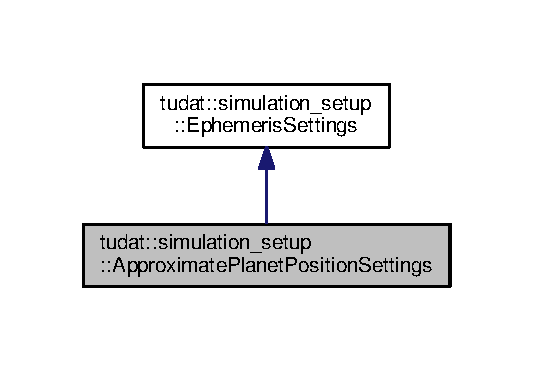
\includegraphics[width=256pt]{classtudat_1_1simulation__setup_1_1ApproximatePlanetPositionSettings__inherit__graph}
\end{center}
\end{figure}


Collaboration diagram for tudat\+:\+:simulation\+\_\+setup\+:\+:Approximate\+Planet\+Position\+Settings\+:
\nopagebreak
\begin{figure}[H]
\begin{center}
\leavevmode
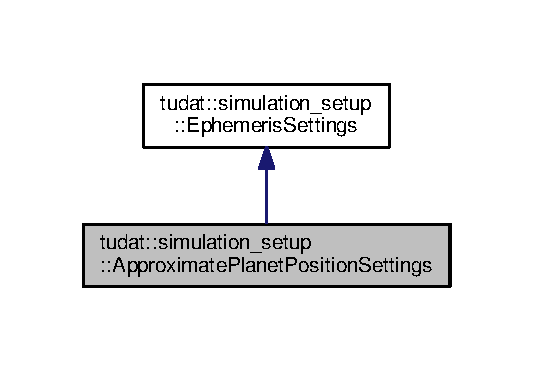
\includegraphics[width=256pt]{classtudat_1_1simulation__setup_1_1ApproximatePlanetPositionSettings__coll__graph}
\end{center}
\end{figure}
\subsection*{Public Member Functions}
\begin{DoxyCompactItemize}
\item 
\hyperlink{classtudat_1_1simulation__setup_1_1ApproximatePlanetPositionSettings_ad8f06740d82644b5cc3f329b5fd80168}{Approximate\+Planet\+Position\+Settings} (const \hyperlink{classtudat_1_1ephemerides_1_1ApproximatePlanetPositionsBase_aa698885dcabac2815a6205d5502724d2}{ephemerides\+::\+Approximate\+Planet\+Positions\+Base\+::\+Bodies\+With\+Ephemeris\+Data} body\+Identifier, const bool use\+Circular\+Coplanar\+Approximation)
\begin{DoxyCompactList}\small\item\em Constructor. \end{DoxyCompactList}\item 
\hyperlink{classtudat_1_1ephemerides_1_1ApproximatePlanetPositionsBase_aa698885dcabac2815a6205d5502724d2}{ephemerides\+::\+Approximate\+Planet\+Positions\+Base\+::\+Bodies\+With\+Ephemeris\+Data} \hyperlink{classtudat_1_1simulation__setup_1_1ApproximatePlanetPositionSettings_ae70bc8743a4e118b0f855bb78632964f}{get\+Body\+Identifier} ()
\begin{DoxyCompactList}\small\item\em Function to return parameter identifying for which body an ephemeris is to be created. \end{DoxyCompactList}\item 
bool \hyperlink{classtudat_1_1simulation__setup_1_1ApproximatePlanetPositionSettings_af33366b088c3eb28976b31f6968580de}{get\+Use\+Circular\+Coplanar\+Approximation} ()
\begin{DoxyCompactList}\small\item\em Function to return whether a circular, coplanar orbit of the body is to be assumed. \end{DoxyCompactList}\end{DoxyCompactItemize}
\subsection*{Additional Inherited Members}


\subsection{Detailed Description}
\hyperlink{classtudat_1_1simulation__setup_1_1EphemerisSettings}{Ephemeris\+Settings} derived class for defining settings of an approximate ephemeris for major planets.

\hyperlink{classtudat_1_1simulation__setup_1_1EphemerisSettings}{Ephemeris\+Settings} derived class for defining settings of an approximate ephemeris for major planets, as inplemented in Approximate\+Planet\+Positions class and derived class, described on \href{http://ssd.jpl.nasa.gov/txt/aprx_pos_planets.pdf}{\tt http\+://ssd.\+jpl.\+nasa.\+gov/txt/aprx\+\_\+pos\+\_\+planets.\+pdf}. 

\subsection{Constructor \& Destructor Documentation}
\index{tudat\+::simulation\+\_\+setup\+::\+Approximate\+Planet\+Position\+Settings@{tudat\+::simulation\+\_\+setup\+::\+Approximate\+Planet\+Position\+Settings}!Approximate\+Planet\+Position\+Settings@{Approximate\+Planet\+Position\+Settings}}
\index{Approximate\+Planet\+Position\+Settings@{Approximate\+Planet\+Position\+Settings}!tudat\+::simulation\+\_\+setup\+::\+Approximate\+Planet\+Position\+Settings@{tudat\+::simulation\+\_\+setup\+::\+Approximate\+Planet\+Position\+Settings}}
\subsubsection[{\texorpdfstring{Approximate\+Planet\+Position\+Settings(const ephemerides\+::\+Approximate\+Planet\+Positions\+Base\+::\+Bodies\+With\+Ephemeris\+Data body\+Identifier, const bool use\+Circular\+Coplanar\+Approximation)}{ApproximatePlanetPositionSettings(const ephemerides::ApproximatePlanetPositionsBase::BodiesWithEphemerisData bodyIdentifier, const bool useCircularCoplanarApproximation)}}]{\setlength{\rightskip}{0pt plus 5cm}tudat\+::simulation\+\_\+setup\+::\+Approximate\+Planet\+Position\+Settings\+::\+Approximate\+Planet\+Position\+Settings (
\begin{DoxyParamCaption}
\item[{const {\bf ephemerides\+::\+Approximate\+Planet\+Positions\+Base\+::\+Bodies\+With\+Ephemeris\+Data}}]{body\+Identifier, }
\item[{const bool}]{use\+Circular\+Coplanar\+Approximation}
\end{DoxyParamCaption}
)\hspace{0.3cm}{\ttfamily [inline]}}\hypertarget{classtudat_1_1simulation__setup_1_1ApproximatePlanetPositionSettings_ad8f06740d82644b5cc3f329b5fd80168}{}\label{classtudat_1_1simulation__setup_1_1ApproximatePlanetPositionSettings_ad8f06740d82644b5cc3f329b5fd80168}


Constructor. 

Constructor. 
\begin{DoxyParams}{Parameters}
{\em body\+Identifier} & Parameter identifying for which body an ephemeris is to be created. \\
\hline
{\em use\+Circular\+Coplanar\+Approximation} & Boolean defining whether a circular, coplanar orbit of the body is to be assumed, or whether a non-\/zero inclination and long-\/period changes in the orbit are to be included. \\
\hline
\end{DoxyParams}


\subsection{Member Function Documentation}
\index{tudat\+::simulation\+\_\+setup\+::\+Approximate\+Planet\+Position\+Settings@{tudat\+::simulation\+\_\+setup\+::\+Approximate\+Planet\+Position\+Settings}!get\+Body\+Identifier@{get\+Body\+Identifier}}
\index{get\+Body\+Identifier@{get\+Body\+Identifier}!tudat\+::simulation\+\_\+setup\+::\+Approximate\+Planet\+Position\+Settings@{tudat\+::simulation\+\_\+setup\+::\+Approximate\+Planet\+Position\+Settings}}
\subsubsection[{\texorpdfstring{get\+Body\+Identifier()}{getBodyIdentifier()}}]{\setlength{\rightskip}{0pt plus 5cm}{\bf ephemerides\+::\+Approximate\+Planet\+Positions\+Base\+::\+Bodies\+With\+Ephemeris\+Data} tudat\+::simulation\+\_\+setup\+::\+Approximate\+Planet\+Position\+Settings\+::get\+Body\+Identifier (
\begin{DoxyParamCaption}
{}
\end{DoxyParamCaption}
)\hspace{0.3cm}{\ttfamily [inline]}}\hypertarget{classtudat_1_1simulation__setup_1_1ApproximatePlanetPositionSettings_ae70bc8743a4e118b0f855bb78632964f}{}\label{classtudat_1_1simulation__setup_1_1ApproximatePlanetPositionSettings_ae70bc8743a4e118b0f855bb78632964f}


Function to return parameter identifying for which body an ephemeris is to be created. 

Function to return parameter identifying for which body an ephemeris is to be created. \begin{DoxyReturn}{Returns}
Parameter identifying for which body an ephemeris is to be created. 
\end{DoxyReturn}
\index{tudat\+::simulation\+\_\+setup\+::\+Approximate\+Planet\+Position\+Settings@{tudat\+::simulation\+\_\+setup\+::\+Approximate\+Planet\+Position\+Settings}!get\+Use\+Circular\+Coplanar\+Approximation@{get\+Use\+Circular\+Coplanar\+Approximation}}
\index{get\+Use\+Circular\+Coplanar\+Approximation@{get\+Use\+Circular\+Coplanar\+Approximation}!tudat\+::simulation\+\_\+setup\+::\+Approximate\+Planet\+Position\+Settings@{tudat\+::simulation\+\_\+setup\+::\+Approximate\+Planet\+Position\+Settings}}
\subsubsection[{\texorpdfstring{get\+Use\+Circular\+Coplanar\+Approximation()}{getUseCircularCoplanarApproximation()}}]{\setlength{\rightskip}{0pt plus 5cm}bool tudat\+::simulation\+\_\+setup\+::\+Approximate\+Planet\+Position\+Settings\+::get\+Use\+Circular\+Coplanar\+Approximation (
\begin{DoxyParamCaption}
{}
\end{DoxyParamCaption}
)\hspace{0.3cm}{\ttfamily [inline]}}\hypertarget{classtudat_1_1simulation__setup_1_1ApproximatePlanetPositionSettings_af33366b088c3eb28976b31f6968580de}{}\label{classtudat_1_1simulation__setup_1_1ApproximatePlanetPositionSettings_af33366b088c3eb28976b31f6968580de}


Function to return whether a circular, coplanar orbit of the body is to be assumed. 

Function to return whether a circular, coplanar orbit of the body is to be assumed. \begin{DoxyReturn}{Returns}
Boolean defining whether a circular, coplanar orbit of the body is to be assumed. 
\end{DoxyReturn}


The documentation for this class was generated from the following file\+:\begin{DoxyCompactItemize}
\item 
/home/lupi/\+Tudat/tudat\+Bundle/tudat/\+Tudat/\+Simulation\+Setup/\+Environment\+Setup/create\+Ephemeris.\+h\end{DoxyCompactItemize}

\hypertarget{classtudat_1_1aerodynamics_1_1AtmosphereModel}{}\section{tudat\+:\+:aerodynamics\+:\+:Atmosphere\+Model Class Reference}
\label{classtudat_1_1aerodynamics_1_1AtmosphereModel}\index{tudat\+::aerodynamics\+::\+Atmosphere\+Model@{tudat\+::aerodynamics\+::\+Atmosphere\+Model}}


Atmosphere model class.  




{\ttfamily \#include $<$atmosphere\+Model.\+h$>$}



Inheritance diagram for tudat\+:\+:aerodynamics\+:\+:Atmosphere\+Model\+:
\nopagebreak
\begin{figure}[H]
\begin{center}
\leavevmode
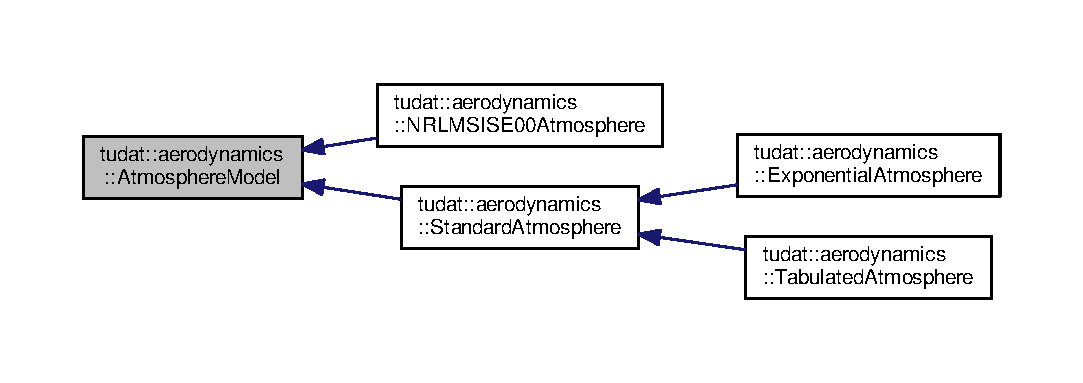
\includegraphics[width=350pt]{classtudat_1_1aerodynamics_1_1AtmosphereModel__inherit__graph}
\end{center}
\end{figure}
\subsection*{Public Member Functions}
\begin{DoxyCompactItemize}
\item 
virtual \hyperlink{classtudat_1_1aerodynamics_1_1AtmosphereModel_a1ceb7bfb8c497ca6b6a0ccbade902ed7}{$\sim$\+Atmosphere\+Model} ()
\begin{DoxyCompactList}\small\item\em Default destructor. \end{DoxyCompactList}\item 
virtual double \hyperlink{classtudat_1_1aerodynamics_1_1AtmosphereModel_a167feb7925eb65a4ca59317d5fba22fb}{get\+Density} (const double altitude, const double longitude, const double latitude, const double time)=0
\begin{DoxyCompactList}\small\item\em Get local density. \end{DoxyCompactList}\item 
virtual double \hyperlink{classtudat_1_1aerodynamics_1_1AtmosphereModel_a516553ea32c89f55a5ba7abe5a417ddc}{get\+Pressure} (const double altitude, const double longitude, const double latitude, const double time)=0
\begin{DoxyCompactList}\small\item\em Get local pressure. \end{DoxyCompactList}\item 
virtual double \hyperlink{classtudat_1_1aerodynamics_1_1AtmosphereModel_a9b6be6472481354320e2869e586be5ca}{get\+Temperature} (const double altitude, const double longitude, const double latitude, const double time)=0
\begin{DoxyCompactList}\small\item\em Get local temperature. \end{DoxyCompactList}\item 
virtual double \hyperlink{classtudat_1_1aerodynamics_1_1AtmosphereModel_a815606ec0437866d6308679c6f078bce}{get\+Speed\+Of\+Sound} (const double altitude, const double longitude, const double latitude, const double time)=0
\begin{DoxyCompactList}\small\item\em Get local speed of sound. \end{DoxyCompactList}\end{DoxyCompactItemize}


\subsection{Detailed Description}
Atmosphere model class. 

Base class for all atmosphere models. To keep the function generic for both reference atmospheres and standard atmospheres, altitude, longitude, latitude, and time are inputs for all functions. 

\subsection{Constructor \& Destructor Documentation}
\index{tudat\+::aerodynamics\+::\+Atmosphere\+Model@{tudat\+::aerodynamics\+::\+Atmosphere\+Model}!````~Atmosphere\+Model@{$\sim$\+Atmosphere\+Model}}
\index{````~Atmosphere\+Model@{$\sim$\+Atmosphere\+Model}!tudat\+::aerodynamics\+::\+Atmosphere\+Model@{tudat\+::aerodynamics\+::\+Atmosphere\+Model}}
\subsubsection[{\texorpdfstring{$\sim$\+Atmosphere\+Model()}{~AtmosphereModel()}}]{\setlength{\rightskip}{0pt plus 5cm}virtual tudat\+::aerodynamics\+::\+Atmosphere\+Model\+::$\sim$\+Atmosphere\+Model (
\begin{DoxyParamCaption}
{}
\end{DoxyParamCaption}
)\hspace{0.3cm}{\ttfamily [inline]}, {\ttfamily [virtual]}}\hypertarget{classtudat_1_1aerodynamics_1_1AtmosphereModel_a1ceb7bfb8c497ca6b6a0ccbade902ed7}{}\label{classtudat_1_1aerodynamics_1_1AtmosphereModel_a1ceb7bfb8c497ca6b6a0ccbade902ed7}


Default destructor. 

Default destructor. 

\subsection{Member Function Documentation}
\index{tudat\+::aerodynamics\+::\+Atmosphere\+Model@{tudat\+::aerodynamics\+::\+Atmosphere\+Model}!get\+Density@{get\+Density}}
\index{get\+Density@{get\+Density}!tudat\+::aerodynamics\+::\+Atmosphere\+Model@{tudat\+::aerodynamics\+::\+Atmosphere\+Model}}
\subsubsection[{\texorpdfstring{get\+Density(const double altitude, const double longitude, const double latitude, const double time)=0}{getDensity(const double altitude, const double longitude, const double latitude, const double time)=0}}]{\setlength{\rightskip}{0pt plus 5cm}virtual double tudat\+::aerodynamics\+::\+Atmosphere\+Model\+::get\+Density (
\begin{DoxyParamCaption}
\item[{const double}]{altitude, }
\item[{const double}]{longitude, }
\item[{const double}]{latitude, }
\item[{const double}]{time}
\end{DoxyParamCaption}
)\hspace{0.3cm}{\ttfamily [pure virtual]}}\hypertarget{classtudat_1_1aerodynamics_1_1AtmosphereModel_a167feb7925eb65a4ca59317d5fba22fb}{}\label{classtudat_1_1aerodynamics_1_1AtmosphereModel_a167feb7925eb65a4ca59317d5fba22fb}


Get local density. 

Returns the local density parameter of the atmosphere in kg per meter$^\wedge$3. 
\begin{DoxyParams}{Parameters}
{\em altitude} & Altitude. \\
\hline
{\em longitude} & Longitude. \\
\hline
{\em latitude} & Latitude. \\
\hline
{\em time} & \hyperlink{classtudat_1_1Time}{Time}. \\
\hline
\end{DoxyParams}
\begin{DoxyReturn}{Returns}
Atmospheric density. 
\end{DoxyReturn}


Implemented in \hyperlink{classtudat_1_1aerodynamics_1_1NRLMSISE00Atmosphere_a47aa6bc2a6782701055d74ef26ef2652}{tudat\+::aerodynamics\+::\+N\+R\+L\+M\+S\+I\+S\+E00\+Atmosphere}, \hyperlink{classtudat_1_1aerodynamics_1_1ExponentialAtmosphere_ac6bc5f5fee5475f805e34461fa77b29d}{tudat\+::aerodynamics\+::\+Exponential\+Atmosphere}, \hyperlink{classtudat_1_1aerodynamics_1_1TabulatedAtmosphere_a6185309cb023348803588eed3d80398b}{tudat\+::aerodynamics\+::\+Tabulated\+Atmosphere}, and \hyperlink{classtudat_1_1aerodynamics_1_1StandardAtmosphere_a85b7e8803277496e8f5abc9bb36d5bf6}{tudat\+::aerodynamics\+::\+Standard\+Atmosphere}.

\index{tudat\+::aerodynamics\+::\+Atmosphere\+Model@{tudat\+::aerodynamics\+::\+Atmosphere\+Model}!get\+Pressure@{get\+Pressure}}
\index{get\+Pressure@{get\+Pressure}!tudat\+::aerodynamics\+::\+Atmosphere\+Model@{tudat\+::aerodynamics\+::\+Atmosphere\+Model}}
\subsubsection[{\texorpdfstring{get\+Pressure(const double altitude, const double longitude, const double latitude, const double time)=0}{getPressure(const double altitude, const double longitude, const double latitude, const double time)=0}}]{\setlength{\rightskip}{0pt plus 5cm}virtual double tudat\+::aerodynamics\+::\+Atmosphere\+Model\+::get\+Pressure (
\begin{DoxyParamCaption}
\item[{const double}]{altitude, }
\item[{const double}]{longitude, }
\item[{const double}]{latitude, }
\item[{const double}]{time}
\end{DoxyParamCaption}
)\hspace{0.3cm}{\ttfamily [pure virtual]}}\hypertarget{classtudat_1_1aerodynamics_1_1AtmosphereModel_a516553ea32c89f55a5ba7abe5a417ddc}{}\label{classtudat_1_1aerodynamics_1_1AtmosphereModel_a516553ea32c89f55a5ba7abe5a417ddc}


Get local pressure. 

Returns the local pressure of the atmosphere parameter in Newton per meter$^\wedge$2. 
\begin{DoxyParams}{Parameters}
{\em altitude} & Altitude. \\
\hline
{\em longitude} & Longitude. \\
\hline
{\em latitude} & Latitude. \\
\hline
{\em time} & \hyperlink{classtudat_1_1Time}{Time}. \\
\hline
\end{DoxyParams}
\begin{DoxyReturn}{Returns}
Atmospheric pressure. 
\end{DoxyReturn}


Implemented in \hyperlink{classtudat_1_1aerodynamics_1_1NRLMSISE00Atmosphere_afb3da940e795477c8f3fa112bf8dd5f5}{tudat\+::aerodynamics\+::\+N\+R\+L\+M\+S\+I\+S\+E00\+Atmosphere}, \hyperlink{classtudat_1_1aerodynamics_1_1ExponentialAtmosphere_a5f9454b2cf717877723364ba3805e855}{tudat\+::aerodynamics\+::\+Exponential\+Atmosphere}, \hyperlink{classtudat_1_1aerodynamics_1_1TabulatedAtmosphere_a10a02961cbbf78570db466eee69d3778}{tudat\+::aerodynamics\+::\+Tabulated\+Atmosphere}, and \hyperlink{classtudat_1_1aerodynamics_1_1StandardAtmosphere_aedd2b6b8824cebea8dea628bfec0e236}{tudat\+::aerodynamics\+::\+Standard\+Atmosphere}.

\index{tudat\+::aerodynamics\+::\+Atmosphere\+Model@{tudat\+::aerodynamics\+::\+Atmosphere\+Model}!get\+Speed\+Of\+Sound@{get\+Speed\+Of\+Sound}}
\index{get\+Speed\+Of\+Sound@{get\+Speed\+Of\+Sound}!tudat\+::aerodynamics\+::\+Atmosphere\+Model@{tudat\+::aerodynamics\+::\+Atmosphere\+Model}}
\subsubsection[{\texorpdfstring{get\+Speed\+Of\+Sound(const double altitude, const double longitude, const double latitude, const double time)=0}{getSpeedOfSound(const double altitude, const double longitude, const double latitude, const double time)=0}}]{\setlength{\rightskip}{0pt plus 5cm}virtual double tudat\+::aerodynamics\+::\+Atmosphere\+Model\+::get\+Speed\+Of\+Sound (
\begin{DoxyParamCaption}
\item[{const double}]{altitude, }
\item[{const double}]{longitude, }
\item[{const double}]{latitude, }
\item[{const double}]{time}
\end{DoxyParamCaption}
)\hspace{0.3cm}{\ttfamily [pure virtual]}}\hypertarget{classtudat_1_1aerodynamics_1_1AtmosphereModel_a815606ec0437866d6308679c6f078bce}{}\label{classtudat_1_1aerodynamics_1_1AtmosphereModel_a815606ec0437866d6308679c6f078bce}


Get local speed of sound. 

Returns the local speed of sound of the atmosphere in m/s. 
\begin{DoxyParams}{Parameters}
{\em altitude} & Altitude. \\
\hline
{\em longitude} & Longitude. \\
\hline
{\em latitude} & Latitude. \\
\hline
{\em time} & \hyperlink{classtudat_1_1Time}{Time}. \\
\hline
\end{DoxyParams}
\begin{DoxyReturn}{Returns}
Atmospheric speed of sound. 
\end{DoxyReturn}


Implemented in \hyperlink{classtudat_1_1aerodynamics_1_1NRLMSISE00Atmosphere_a494e42d0266f7d9fa0ebc45bf0f7d78d}{tudat\+::aerodynamics\+::\+N\+R\+L\+M\+S\+I\+S\+E00\+Atmosphere}, \hyperlink{classtudat_1_1aerodynamics_1_1ExponentialAtmosphere_a90283cd42dc4ee31892750b82bedf14c}{tudat\+::aerodynamics\+::\+Exponential\+Atmosphere}, \hyperlink{classtudat_1_1aerodynamics_1_1TabulatedAtmosphere_ae644bf870445c03d007984d946ceaee4}{tudat\+::aerodynamics\+::\+Tabulated\+Atmosphere}, and \hyperlink{classtudat_1_1aerodynamics_1_1StandardAtmosphere_a9992c99f7994882307b05161e19fc298}{tudat\+::aerodynamics\+::\+Standard\+Atmosphere}.

\index{tudat\+::aerodynamics\+::\+Atmosphere\+Model@{tudat\+::aerodynamics\+::\+Atmosphere\+Model}!get\+Temperature@{get\+Temperature}}
\index{get\+Temperature@{get\+Temperature}!tudat\+::aerodynamics\+::\+Atmosphere\+Model@{tudat\+::aerodynamics\+::\+Atmosphere\+Model}}
\subsubsection[{\texorpdfstring{get\+Temperature(const double altitude, const double longitude, const double latitude, const double time)=0}{getTemperature(const double altitude, const double longitude, const double latitude, const double time)=0}}]{\setlength{\rightskip}{0pt plus 5cm}virtual double tudat\+::aerodynamics\+::\+Atmosphere\+Model\+::get\+Temperature (
\begin{DoxyParamCaption}
\item[{const double}]{altitude, }
\item[{const double}]{longitude, }
\item[{const double}]{latitude, }
\item[{const double}]{time}
\end{DoxyParamCaption}
)\hspace{0.3cm}{\ttfamily [pure virtual]}}\hypertarget{classtudat_1_1aerodynamics_1_1AtmosphereModel_a9b6be6472481354320e2869e586be5ca}{}\label{classtudat_1_1aerodynamics_1_1AtmosphereModel_a9b6be6472481354320e2869e586be5ca}


Get local temperature. 

Returns the local temperature of the atmosphere parameter in Kelvin. 
\begin{DoxyParams}{Parameters}
{\em altitude} & Altitude. \\
\hline
{\em longitude} & Longitude. \\
\hline
{\em latitude} & Latitude. \\
\hline
{\em time} & \hyperlink{classtudat_1_1Time}{Time}. \\
\hline
\end{DoxyParams}
\begin{DoxyReturn}{Returns}
Atmospheric temperature. 
\end{DoxyReturn}


Implemented in \hyperlink{classtudat_1_1aerodynamics_1_1NRLMSISE00Atmosphere_a16b8b8363a3b7f6759cd764ba239d8bf}{tudat\+::aerodynamics\+::\+N\+R\+L\+M\+S\+I\+S\+E00\+Atmosphere}, \hyperlink{classtudat_1_1aerodynamics_1_1ExponentialAtmosphere_aa486d36c2fbe56026d7a4cc17f7d04a2}{tudat\+::aerodynamics\+::\+Exponential\+Atmosphere}, \hyperlink{classtudat_1_1aerodynamics_1_1TabulatedAtmosphere_afdf6a072bd4c4d876ba2323f5955b441}{tudat\+::aerodynamics\+::\+Tabulated\+Atmosphere}, and \hyperlink{classtudat_1_1aerodynamics_1_1StandardAtmosphere_ac5b9a16a96cbb496a4ee76b3dc495543}{tudat\+::aerodynamics\+::\+Standard\+Atmosphere}.



The documentation for this class was generated from the following file\+:\begin{DoxyCompactItemize}
\item 
/home/lupi/\+Tudat/tudat\+Bundle/tudat/\+Tudat/\+Astrodynamics/\+Aerodynamics/atmosphere\+Model.\+h\end{DoxyCompactItemize}

\hypertarget{classtudat_1_1simulation__setup_1_1AtmosphereSettings}{}\section{tudat\+:\+:simulation\+\_\+setup\+:\+:Atmosphere\+Settings Class Reference}
\label{classtudat_1_1simulation__setup_1_1AtmosphereSettings}\index{tudat\+::simulation\+\_\+setup\+::\+Atmosphere\+Settings@{tudat\+::simulation\+\_\+setup\+::\+Atmosphere\+Settings}}


Class for providing settings for atmosphere model.  




{\ttfamily \#include $<$create\+Atmosphere\+Model.\+h$>$}



Inheritance diagram for tudat\+:\+:simulation\+\_\+setup\+:\+:Atmosphere\+Settings\+:
\nopagebreak
\begin{figure}[H]
\begin{center}
\leavevmode
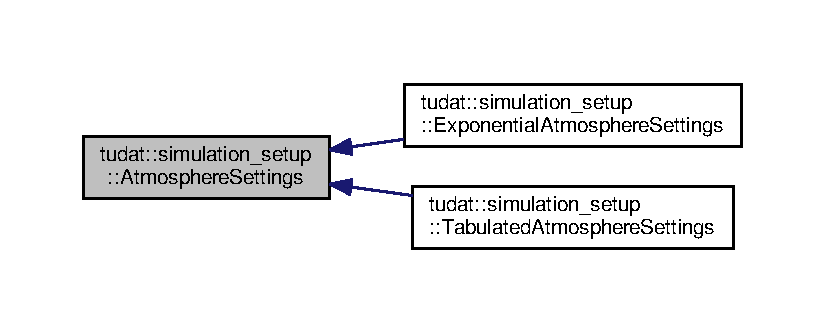
\includegraphics[width=350pt]{classtudat_1_1simulation__setup_1_1AtmosphereSettings__inherit__graph}
\end{center}
\end{figure}
\subsection*{Public Member Functions}
\begin{DoxyCompactItemize}
\item 
\hyperlink{classtudat_1_1simulation__setup_1_1AtmosphereSettings_a82760111a1975705c2bd939836e8486a}{Atmosphere\+Settings} (const Atmosphere\+Types atmosphere\+Type)
\begin{DoxyCompactList}\small\item\em Constructor, sets type of atmosphere model. \end{DoxyCompactList}\item 
virtual \hyperlink{classtudat_1_1simulation__setup_1_1AtmosphereSettings_a5d315b52924a7f82d4e269402c60a51c}{$\sim$\+Atmosphere\+Settings} ()\hypertarget{classtudat_1_1simulation__setup_1_1AtmosphereSettings_a5d315b52924a7f82d4e269402c60a51c}{}\label{classtudat_1_1simulation__setup_1_1AtmosphereSettings_a5d315b52924a7f82d4e269402c60a51c}

\begin{DoxyCompactList}\small\item\em Destructor. \end{DoxyCompactList}\item 
Atmosphere\+Types \hyperlink{classtudat_1_1simulation__setup_1_1AtmosphereSettings_aec4287b357a3bb6abc189f7c27474531}{get\+Atmosphere\+Type} ()
\begin{DoxyCompactList}\small\item\em Function to return type of atmosphere model that is to be created. \end{DoxyCompactList}\end{DoxyCompactItemize}


\subsection{Detailed Description}
Class for providing settings for atmosphere model. 

Class for providing settings for automatic atmosphere model creation. This class is a functional (base) class for settings of atmosphere models that require no information in addition to their type. Atmosphere model classes defining requiring additional information must be created using an object derived from this class. 

\subsection{Constructor \& Destructor Documentation}
\index{tudat\+::simulation\+\_\+setup\+::\+Atmosphere\+Settings@{tudat\+::simulation\+\_\+setup\+::\+Atmosphere\+Settings}!Atmosphere\+Settings@{Atmosphere\+Settings}}
\index{Atmosphere\+Settings@{Atmosphere\+Settings}!tudat\+::simulation\+\_\+setup\+::\+Atmosphere\+Settings@{tudat\+::simulation\+\_\+setup\+::\+Atmosphere\+Settings}}
\subsubsection[{\texorpdfstring{Atmosphere\+Settings(const Atmosphere\+Types atmosphere\+Type)}{AtmosphereSettings(const AtmosphereTypes atmosphereType)}}]{\setlength{\rightskip}{0pt plus 5cm}tudat\+::simulation\+\_\+setup\+::\+Atmosphere\+Settings\+::\+Atmosphere\+Settings (
\begin{DoxyParamCaption}
\item[{const Atmosphere\+Types}]{atmosphere\+Type}
\end{DoxyParamCaption}
)\hspace{0.3cm}{\ttfamily [inline]}}\hypertarget{classtudat_1_1simulation__setup_1_1AtmosphereSettings_a82760111a1975705c2bd939836e8486a}{}\label{classtudat_1_1simulation__setup_1_1AtmosphereSettings_a82760111a1975705c2bd939836e8486a}


Constructor, sets type of atmosphere model. 

Constructor, sets type of atmosphere model. Settings for atmosphere models requiring additional information should be defined in a derived class. 
\begin{DoxyParams}{Parameters}
{\em atmosphere\+Type} & Type of atmosphere model that is to be created. \\
\hline
\end{DoxyParams}


\subsection{Member Function Documentation}
\index{tudat\+::simulation\+\_\+setup\+::\+Atmosphere\+Settings@{tudat\+::simulation\+\_\+setup\+::\+Atmosphere\+Settings}!get\+Atmosphere\+Type@{get\+Atmosphere\+Type}}
\index{get\+Atmosphere\+Type@{get\+Atmosphere\+Type}!tudat\+::simulation\+\_\+setup\+::\+Atmosphere\+Settings@{tudat\+::simulation\+\_\+setup\+::\+Atmosphere\+Settings}}
\subsubsection[{\texorpdfstring{get\+Atmosphere\+Type()}{getAtmosphereType()}}]{\setlength{\rightskip}{0pt plus 5cm}Atmosphere\+Types tudat\+::simulation\+\_\+setup\+::\+Atmosphere\+Settings\+::get\+Atmosphere\+Type (
\begin{DoxyParamCaption}
{}
\end{DoxyParamCaption}
)\hspace{0.3cm}{\ttfamily [inline]}}\hypertarget{classtudat_1_1simulation__setup_1_1AtmosphereSettings_aec4287b357a3bb6abc189f7c27474531}{}\label{classtudat_1_1simulation__setup_1_1AtmosphereSettings_aec4287b357a3bb6abc189f7c27474531}


Function to return type of atmosphere model that is to be created. 

Function to return type of atmosphere model that is to be created. \begin{DoxyReturn}{Returns}
Type of atmosphere model that is to be created. 
\end{DoxyReturn}


The documentation for this class was generated from the following file\+:\begin{DoxyCompactItemize}
\item 
/home/lupi/\+Tudat/tudat\+Bundle/tudat/\+Tudat/\+Simulation\+Setup/\+Environment\+Setup/create\+Atmosphere\+Model.\+h\end{DoxyCompactItemize}

\hypertarget{classtudat_1_1simulation__setup_1_1BaseStateInterface}{}\section{tudat\+:\+:simulation\+\_\+setup\+:\+:Base\+State\+Interface Class Reference}
\label{classtudat_1_1simulation__setup_1_1BaseStateInterface}\index{tudat\+::simulation\+\_\+setup\+::\+Base\+State\+Interface@{tudat\+::simulation\+\_\+setup\+::\+Base\+State\+Interface}}


Base class used for the determination of the inertial state of a \hyperlink{classtudat_1_1simulation__setup_1_1Body}{Body}\textquotesingle{}s ephemeris origin.  




{\ttfamily \#include $<$body.\+h$>$}



Inheritance diagram for tudat\+:\+:simulation\+\_\+setup\+:\+:Base\+State\+Interface\+:
\nopagebreak
\begin{figure}[H]
\begin{center}
\leavevmode
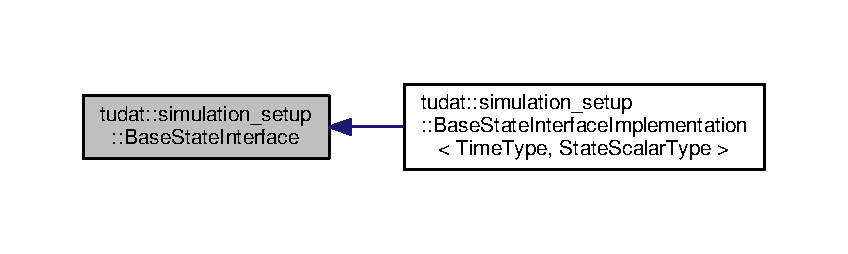
\includegraphics[width=350pt]{classtudat_1_1simulation__setup_1_1BaseStateInterface__inherit__graph}
\end{center}
\end{figure}
\subsection*{Public Member Functions}
\begin{DoxyCompactItemize}
\item 
\hyperlink{classtudat_1_1simulation__setup_1_1BaseStateInterface_aaef83a88c7daddd073c395d2c7f12361}{Base\+State\+Interface} (const std\+::string base\+Frame\+Id)
\begin{DoxyCompactList}\small\item\em Constructor. \end{DoxyCompactList}\item 
virtual \hyperlink{classtudat_1_1simulation__setup_1_1BaseStateInterface_ab3c1b1a5b34c7518b6ca72830835ee30}{$\sim$\+Base\+State\+Interface} ()\hypertarget{classtudat_1_1simulation__setup_1_1BaseStateInterface_ab3c1b1a5b34c7518b6ca72830835ee30}{}\label{classtudat_1_1simulation__setup_1_1BaseStateInterface_ab3c1b1a5b34c7518b6ca72830835ee30}

\begin{DoxyCompactList}\small\item\em Destructor. \end{DoxyCompactList}\item 
{\footnotesize template$<$typename Output\+Time\+Type , typename Output\+State\+Scalar\+Type $>$ }\\Eigen\+::\+Matrix$<$ Output\+State\+Scalar\+Type, 6, 1 $>$ \hyperlink{classtudat_1_1simulation__setup_1_1BaseStateInterface_a85b381f111bb8d6b3127acb85ecde227}{get\+Base\+Frame\+State} (const Output\+Time\+Type time)
\begin{DoxyCompactList}\small\item\em Function through which the state of base\+Frame\+Id\+\_\+ in the inertial frame can be determined. \end{DoxyCompactList}\item 
{\footnotesize template$<$$>$ }\\Eigen\+::\+Matrix$<$ double, 6, 1 $>$ \hyperlink{classtudat_1_1simulation__setup_1_1BaseStateInterface_a7c53f5a0e9ed86b220c6755a26a31214}{get\+Base\+Frame\+State} (const double time)\hypertarget{classtudat_1_1simulation__setup_1_1BaseStateInterface_a7c53f5a0e9ed86b220c6755a26a31214}{}\label{classtudat_1_1simulation__setup_1_1BaseStateInterface_a7c53f5a0e9ed86b220c6755a26a31214}

\begin{DoxyCompactList}\small\item\em Function through which the state of base\+Frame\+Id\+\_\+ in the inertial frame can be determined. \end{DoxyCompactList}\item 
{\footnotesize template$<$$>$ }\\Eigen\+::\+Matrix$<$ long double, 6, 1 $>$ \hyperlink{classtudat_1_1simulation__setup_1_1BaseStateInterface_a9ef1139380260ef592c40897d51f20fb}{get\+Base\+Frame\+State} (const double time)\hypertarget{classtudat_1_1simulation__setup_1_1BaseStateInterface_a9ef1139380260ef592c40897d51f20fb}{}\label{classtudat_1_1simulation__setup_1_1BaseStateInterface_a9ef1139380260ef592c40897d51f20fb}

\begin{DoxyCompactList}\small\item\em Function through which the state of base\+Frame\+Id\+\_\+ in the inertial frame can be determined. \end{DoxyCompactList}\item 
{\footnotesize template$<$$>$ }\\Eigen\+::\+Matrix$<$ double, 6, 1 $>$ \hyperlink{classtudat_1_1simulation__setup_1_1BaseStateInterface_a6c481834fbc606782ddc4edef418fb37}{get\+Base\+Frame\+State} (const \hyperlink{classtudat_1_1Time}{Time} time)\hypertarget{classtudat_1_1simulation__setup_1_1BaseStateInterface_a6c481834fbc606782ddc4edef418fb37}{}\label{classtudat_1_1simulation__setup_1_1BaseStateInterface_a6c481834fbc606782ddc4edef418fb37}

\begin{DoxyCompactList}\small\item\em Function through which the state of base\+Frame\+Id\+\_\+ in the inertial frame can be determined. \end{DoxyCompactList}\item 
{\footnotesize template$<$$>$ }\\Eigen\+::\+Matrix$<$ long double, 6, 1 $>$ \hyperlink{classtudat_1_1simulation__setup_1_1BaseStateInterface_afc84a9d6d3b0ae9708cb064dc0699c47}{get\+Base\+Frame\+State} (const \hyperlink{classtudat_1_1Time}{Time} time)\hypertarget{classtudat_1_1simulation__setup_1_1BaseStateInterface_afc84a9d6d3b0ae9708cb064dc0699c47}{}\label{classtudat_1_1simulation__setup_1_1BaseStateInterface_afc84a9d6d3b0ae9708cb064dc0699c47}

\begin{DoxyCompactList}\small\item\em Function through which the state of base\+Frame\+Id\+\_\+ in the inertial frame can be determined. \end{DoxyCompactList}\end{DoxyCompactItemize}
\subsection*{Protected Member Functions}
\begin{DoxyCompactItemize}
\item 
virtual Eigen\+::\+Matrix$<$ double, 6, 1 $>$ \hyperlink{classtudat_1_1simulation__setup_1_1BaseStateInterface_a008eb954015cfc4b02359126b2a29604}{get\+Base\+Frame\+Double\+State} (const double time)=0
\begin{DoxyCompactList}\small\item\em Pure virtual function through which the state of base\+Frame\+Id\+\_\+ in the inertial frame can be determined. \end{DoxyCompactList}\item 
virtual Eigen\+::\+Matrix$<$ long double, 6, 1 $>$ \hyperlink{classtudat_1_1simulation__setup_1_1BaseStateInterface_a0701e50ccd7a59be8ff1ce0576dc6af0}{get\+Base\+Frame\+Long\+Double\+State} (const double time)=0
\begin{DoxyCompactList}\small\item\em Pure virtual function through which the state of base\+Frame\+Id\+\_\+ in the inertial frame can be determined. \end{DoxyCompactList}\item 
virtual Eigen\+::\+Matrix$<$ double, 6, 1 $>$ \hyperlink{classtudat_1_1simulation__setup_1_1BaseStateInterface_aacd675d056aebe9af2f5d1642f799952}{get\+Base\+Frame\+Double\+State} (const \hyperlink{classtudat_1_1Time}{Time} \&time)=0
\begin{DoxyCompactList}\small\item\em Pure virtual function through which the state of base\+Frame\+Id\+\_\+ in the inertial frame can be determined. \end{DoxyCompactList}\item 
virtual Eigen\+::\+Matrix$<$ long double, 6, 1 $>$ \hyperlink{classtudat_1_1simulation__setup_1_1BaseStateInterface_afeaa791b565e385d8a8b0c9224b1e37f}{get\+Base\+Frame\+Long\+Double\+State} (const \hyperlink{classtudat_1_1Time}{Time} \&time)=0
\begin{DoxyCompactList}\small\item\em Pure virtual function through which the state of base\+Frame\+Id\+\_\+ in the inertial frame can be determined. \end{DoxyCompactList}\end{DoxyCompactItemize}
\subsection*{Protected Attributes}
\begin{DoxyCompactItemize}
\item 
std\+::string \hyperlink{classtudat_1_1simulation__setup_1_1BaseStateInterface_a4ae6ef15cf68aadd882c34de0cf3f503}{base\+Frame\+Id\+\_\+}\hypertarget{classtudat_1_1simulation__setup_1_1BaseStateInterface_a4ae6ef15cf68aadd882c34de0cf3f503}{}\label{classtudat_1_1simulation__setup_1_1BaseStateInterface_a4ae6ef15cf68aadd882c34de0cf3f503}

\begin{DoxyCompactList}\small\item\em Name of frame origin for which inertial state is computed by this class. \end{DoxyCompactList}\end{DoxyCompactItemize}


\subsection{Detailed Description}
Base class used for the determination of the inertial state of a \hyperlink{classtudat_1_1simulation__setup_1_1Body}{Body}\textquotesingle{}s ephemeris origin. 

Base class used for the determination of the inertial state of a \hyperlink{classtudat_1_1simulation__setup_1_1Body}{Body}\textquotesingle{}s ephemeris origin. This base class is used to provide an untemplated interface class through which to call the base frame state. The state may be defined in a templated manner in the derived class. 

\subsection{Constructor \& Destructor Documentation}
\index{tudat\+::simulation\+\_\+setup\+::\+Base\+State\+Interface@{tudat\+::simulation\+\_\+setup\+::\+Base\+State\+Interface}!Base\+State\+Interface@{Base\+State\+Interface}}
\index{Base\+State\+Interface@{Base\+State\+Interface}!tudat\+::simulation\+\_\+setup\+::\+Base\+State\+Interface@{tudat\+::simulation\+\_\+setup\+::\+Base\+State\+Interface}}
\subsubsection[{\texorpdfstring{Base\+State\+Interface(const std\+::string base\+Frame\+Id)}{BaseStateInterface(const std::string baseFrameId)}}]{\setlength{\rightskip}{0pt plus 5cm}tudat\+::simulation\+\_\+setup\+::\+Base\+State\+Interface\+::\+Base\+State\+Interface (
\begin{DoxyParamCaption}
\item[{const std\+::string}]{base\+Frame\+Id}
\end{DoxyParamCaption}
)\hspace{0.3cm}{\ttfamily [inline]}}\hypertarget{classtudat_1_1simulation__setup_1_1BaseStateInterface_aaef83a88c7daddd073c395d2c7f12361}{}\label{classtudat_1_1simulation__setup_1_1BaseStateInterface_aaef83a88c7daddd073c395d2c7f12361}


Constructor. 

Constructor 
\begin{DoxyParams}{Parameters}
{\em base\+Frame\+Id} & Name of frame origin for which inertial state is computed by this class \\
\hline
\end{DoxyParams}


\subsection{Member Function Documentation}
\index{tudat\+::simulation\+\_\+setup\+::\+Base\+State\+Interface@{tudat\+::simulation\+\_\+setup\+::\+Base\+State\+Interface}!get\+Base\+Frame\+Double\+State@{get\+Base\+Frame\+Double\+State}}
\index{get\+Base\+Frame\+Double\+State@{get\+Base\+Frame\+Double\+State}!tudat\+::simulation\+\_\+setup\+::\+Base\+State\+Interface@{tudat\+::simulation\+\_\+setup\+::\+Base\+State\+Interface}}
\subsubsection[{\texorpdfstring{get\+Base\+Frame\+Double\+State(const double time)=0}{getBaseFrameDoubleState(const double time)=0}}]{\setlength{\rightskip}{0pt plus 5cm}virtual Eigen\+::\+Matrix$<$ double, 6, 1 $>$ tudat\+::simulation\+\_\+setup\+::\+Base\+State\+Interface\+::get\+Base\+Frame\+Double\+State (
\begin{DoxyParamCaption}
\item[{const double}]{time}
\end{DoxyParamCaption}
)\hspace{0.3cm}{\ttfamily [protected]}, {\ttfamily [pure virtual]}}\hypertarget{classtudat_1_1simulation__setup_1_1BaseStateInterface_a008eb954015cfc4b02359126b2a29604}{}\label{classtudat_1_1simulation__setup_1_1BaseStateInterface_a008eb954015cfc4b02359126b2a29604}


Pure virtual function through which the state of base\+Frame\+Id\+\_\+ in the inertial frame can be determined. 

Pure virtual function through which the state of base\+Frame\+Id\+\_\+ in the inertial frame can be determined (double time and double state scalar). 
\begin{DoxyParams}{Parameters}
{\em time} & \hyperlink{classtudat_1_1Time}{Time} at which state is to be computed \\
\hline
\end{DoxyParams}
\begin{DoxyReturn}{Returns}
Inertial state of frame origin at requested time 
\end{DoxyReturn}


Implemented in \hyperlink{classtudat_1_1simulation__setup_1_1BaseStateInterfaceImplementation_ae53c051e177df8641d07fbb7f50c1197}{tudat\+::simulation\+\_\+setup\+::\+Base\+State\+Interface\+Implementation$<$ Time\+Type, State\+Scalar\+Type $>$}.

\index{tudat\+::simulation\+\_\+setup\+::\+Base\+State\+Interface@{tudat\+::simulation\+\_\+setup\+::\+Base\+State\+Interface}!get\+Base\+Frame\+Double\+State@{get\+Base\+Frame\+Double\+State}}
\index{get\+Base\+Frame\+Double\+State@{get\+Base\+Frame\+Double\+State}!tudat\+::simulation\+\_\+setup\+::\+Base\+State\+Interface@{tudat\+::simulation\+\_\+setup\+::\+Base\+State\+Interface}}
\subsubsection[{\texorpdfstring{get\+Base\+Frame\+Double\+State(const Time \&time)=0}{getBaseFrameDoubleState(const Time &time)=0}}]{\setlength{\rightskip}{0pt plus 5cm}virtual Eigen\+::\+Matrix$<$ double, 6, 1 $>$ tudat\+::simulation\+\_\+setup\+::\+Base\+State\+Interface\+::get\+Base\+Frame\+Double\+State (
\begin{DoxyParamCaption}
\item[{const {\bf Time} \&}]{time}
\end{DoxyParamCaption}
)\hspace{0.3cm}{\ttfamily [protected]}, {\ttfamily [pure virtual]}}\hypertarget{classtudat_1_1simulation__setup_1_1BaseStateInterface_aacd675d056aebe9af2f5d1642f799952}{}\label{classtudat_1_1simulation__setup_1_1BaseStateInterface_aacd675d056aebe9af2f5d1642f799952}


Pure virtual function through which the state of base\+Frame\+Id\+\_\+ in the inertial frame can be determined. 

Pure virtual function through which the state of base\+Frame\+Id\+\_\+ in the inertial frame can be determined (\hyperlink{classtudat_1_1Time}{Time} object time and double state scalar). 
\begin{DoxyParams}{Parameters}
{\em time} & \hyperlink{classtudat_1_1Time}{Time} at which state is to be computed \\
\hline
\end{DoxyParams}
\begin{DoxyReturn}{Returns}
Inertial state of frame origin at requested time 
\end{DoxyReturn}


Implemented in \hyperlink{classtudat_1_1simulation__setup_1_1BaseStateInterfaceImplementation_a9c86d9922b9358165f54a5012187606b}{tudat\+::simulation\+\_\+setup\+::\+Base\+State\+Interface\+Implementation$<$ Time\+Type, State\+Scalar\+Type $>$}.

\index{tudat\+::simulation\+\_\+setup\+::\+Base\+State\+Interface@{tudat\+::simulation\+\_\+setup\+::\+Base\+State\+Interface}!get\+Base\+Frame\+Long\+Double\+State@{get\+Base\+Frame\+Long\+Double\+State}}
\index{get\+Base\+Frame\+Long\+Double\+State@{get\+Base\+Frame\+Long\+Double\+State}!tudat\+::simulation\+\_\+setup\+::\+Base\+State\+Interface@{tudat\+::simulation\+\_\+setup\+::\+Base\+State\+Interface}}
\subsubsection[{\texorpdfstring{get\+Base\+Frame\+Long\+Double\+State(const double time)=0}{getBaseFrameLongDoubleState(const double time)=0}}]{\setlength{\rightskip}{0pt plus 5cm}virtual Eigen\+::\+Matrix$<$ long double, 6, 1 $>$ tudat\+::simulation\+\_\+setup\+::\+Base\+State\+Interface\+::get\+Base\+Frame\+Long\+Double\+State (
\begin{DoxyParamCaption}
\item[{const double}]{time}
\end{DoxyParamCaption}
)\hspace{0.3cm}{\ttfamily [protected]}, {\ttfamily [pure virtual]}}\hypertarget{classtudat_1_1simulation__setup_1_1BaseStateInterface_a0701e50ccd7a59be8ff1ce0576dc6af0}{}\label{classtudat_1_1simulation__setup_1_1BaseStateInterface_a0701e50ccd7a59be8ff1ce0576dc6af0}


Pure virtual function through which the state of base\+Frame\+Id\+\_\+ in the inertial frame can be determined. 

Pure virtual function through which the state of base\+Frame\+Id\+\_\+ in the inertial frame can be determined (double time and double long state scalar). 
\begin{DoxyParams}{Parameters}
{\em time} & \hyperlink{classtudat_1_1Time}{Time} at which state is to be computed \\
\hline
\end{DoxyParams}
\begin{DoxyReturn}{Returns}
Inertial state of frame origin at requested time 
\end{DoxyReturn}


Implemented in \hyperlink{classtudat_1_1simulation__setup_1_1BaseStateInterfaceImplementation_a0412c94ef47dfba9c26bd40b139004ad}{tudat\+::simulation\+\_\+setup\+::\+Base\+State\+Interface\+Implementation$<$ Time\+Type, State\+Scalar\+Type $>$}.

\index{tudat\+::simulation\+\_\+setup\+::\+Base\+State\+Interface@{tudat\+::simulation\+\_\+setup\+::\+Base\+State\+Interface}!get\+Base\+Frame\+Long\+Double\+State@{get\+Base\+Frame\+Long\+Double\+State}}
\index{get\+Base\+Frame\+Long\+Double\+State@{get\+Base\+Frame\+Long\+Double\+State}!tudat\+::simulation\+\_\+setup\+::\+Base\+State\+Interface@{tudat\+::simulation\+\_\+setup\+::\+Base\+State\+Interface}}
\subsubsection[{\texorpdfstring{get\+Base\+Frame\+Long\+Double\+State(const Time \&time)=0}{getBaseFrameLongDoubleState(const Time &time)=0}}]{\setlength{\rightskip}{0pt plus 5cm}virtual Eigen\+::\+Matrix$<$ long double, 6, 1 $>$ tudat\+::simulation\+\_\+setup\+::\+Base\+State\+Interface\+::get\+Base\+Frame\+Long\+Double\+State (
\begin{DoxyParamCaption}
\item[{const {\bf Time} \&}]{time}
\end{DoxyParamCaption}
)\hspace{0.3cm}{\ttfamily [protected]}, {\ttfamily [pure virtual]}}\hypertarget{classtudat_1_1simulation__setup_1_1BaseStateInterface_afeaa791b565e385d8a8b0c9224b1e37f}{}\label{classtudat_1_1simulation__setup_1_1BaseStateInterface_afeaa791b565e385d8a8b0c9224b1e37f}


Pure virtual function through which the state of base\+Frame\+Id\+\_\+ in the inertial frame can be determined. 

Pure virtual function through which the state of base\+Frame\+Id\+\_\+ in the inertial frame can be determined (\hyperlink{classtudat_1_1Time}{Time} object time and long double state scalar). 
\begin{DoxyParams}{Parameters}
{\em time} & \hyperlink{classtudat_1_1Time}{Time} at which state is to be computed \\
\hline
\end{DoxyParams}
\begin{DoxyReturn}{Returns}
Inertial state of frame origin at requested time 
\end{DoxyReturn}


Implemented in \hyperlink{classtudat_1_1simulation__setup_1_1BaseStateInterfaceImplementation_aee56c9b426b0371c6744db8a7566511b}{tudat\+::simulation\+\_\+setup\+::\+Base\+State\+Interface\+Implementation$<$ Time\+Type, State\+Scalar\+Type $>$}.

\index{tudat\+::simulation\+\_\+setup\+::\+Base\+State\+Interface@{tudat\+::simulation\+\_\+setup\+::\+Base\+State\+Interface}!get\+Base\+Frame\+State@{get\+Base\+Frame\+State}}
\index{get\+Base\+Frame\+State@{get\+Base\+Frame\+State}!tudat\+::simulation\+\_\+setup\+::\+Base\+State\+Interface@{tudat\+::simulation\+\_\+setup\+::\+Base\+State\+Interface}}
\subsubsection[{\texorpdfstring{get\+Base\+Frame\+State(const Output\+Time\+Type time)}{getBaseFrameState(const OutputTimeType time)}}]{\setlength{\rightskip}{0pt plus 5cm}template$<$typename Output\+Time\+Type , typename Output\+State\+Scalar\+Type $>$ Eigen\+::\+Matrix$<$ Output\+State\+Scalar\+Type, 6, 1 $>$ tudat\+::simulation\+\_\+setup\+::\+Base\+State\+Interface\+::get\+Base\+Frame\+State (
\begin{DoxyParamCaption}
\item[{const Output\+Time\+Type}]{time}
\end{DoxyParamCaption}
)}\hypertarget{classtudat_1_1simulation__setup_1_1BaseStateInterface_a85b381f111bb8d6b3127acb85ecde227}{}\label{classtudat_1_1simulation__setup_1_1BaseStateInterface_a85b381f111bb8d6b3127acb85ecde227}


Function through which the state of base\+Frame\+Id\+\_\+ in the inertial frame can be determined. 

Function through which the state of base\+Frame\+Id\+\_\+ in the inertial frame can be determined 
\begin{DoxyParams}{Parameters}
{\em time} & \hyperlink{classtudat_1_1Time}{Time} at which state is to be computed \\
\hline
\end{DoxyParams}
\begin{DoxyReturn}{Returns}
Inertial state of frame origin at requested time 
\end{DoxyReturn}


The documentation for this class was generated from the following files\+:\begin{DoxyCompactItemize}
\item 
/home/lupi/\+Tudat/tudat\+Bundle/tudat/\+Tudat/\+Simulation\+Setup/\+Environment\+Setup/body.\+h\item 
/home/lupi/\+Tudat/tudat\+Bundle/tudat/\+Tudat/\+Simulation\+Setup/\+Environment\+Setup/body.\+cpp\end{DoxyCompactItemize}

\hypertarget{classtudat_1_1simulation__setup_1_1BaseStateInterfaceImplementation}{}\section{tudat\+:\+:simulation\+\_\+setup\+:\+:Base\+State\+Interface\+Implementation$<$ Time\+Type, State\+Scalar\+Type $>$ Class Template Reference}
\label{classtudat_1_1simulation__setup_1_1BaseStateInterfaceImplementation}\index{tudat\+::simulation\+\_\+setup\+::\+Base\+State\+Interface\+Implementation$<$ Time\+Type, State\+Scalar\+Type $>$@{tudat\+::simulation\+\_\+setup\+::\+Base\+State\+Interface\+Implementation$<$ Time\+Type, State\+Scalar\+Type $>$}}


Class used for the determination of the inertial state of a \hyperlink{classtudat_1_1simulation__setup_1_1Body}{Body}\textquotesingle{}s ephemeris origin.  




{\ttfamily \#include $<$body.\+h$>$}



Inheritance diagram for tudat\+:\+:simulation\+\_\+setup\+:\+:Base\+State\+Interface\+Implementation$<$ Time\+Type, State\+Scalar\+Type $>$\+:
\nopagebreak
\begin{figure}[H]
\begin{center}
\leavevmode
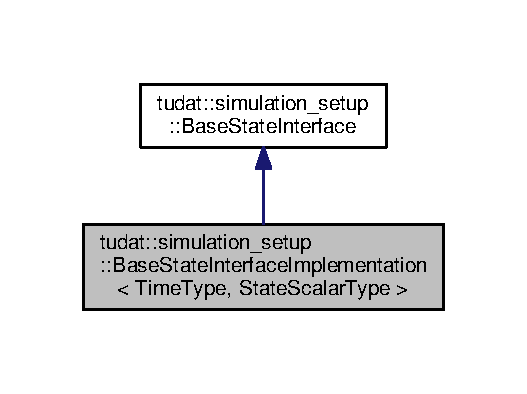
\includegraphics[width=253pt]{classtudat_1_1simulation__setup_1_1BaseStateInterfaceImplementation__inherit__graph}
\end{center}
\end{figure}


Collaboration diagram for tudat\+:\+:simulation\+\_\+setup\+:\+:Base\+State\+Interface\+Implementation$<$ Time\+Type, State\+Scalar\+Type $>$\+:
\nopagebreak
\begin{figure}[H]
\begin{center}
\leavevmode
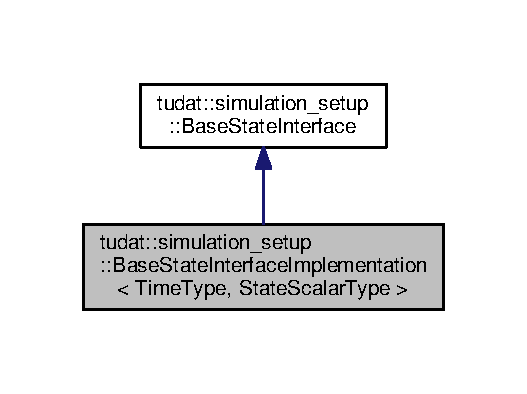
\includegraphics[width=253pt]{classtudat_1_1simulation__setup_1_1BaseStateInterfaceImplementation__coll__graph}
\end{center}
\end{figure}
\subsection*{Public Member Functions}
\begin{DoxyCompactItemize}
\item 
\hyperlink{classtudat_1_1simulation__setup_1_1BaseStateInterfaceImplementation_a93a176a72a12fcd0a16d40c7def9c466}{Base\+State\+Interface\+Implementation} (const std\+::string base\+Frame\+Id, const boost\+::function$<$ Eigen\+::\+Matrix$<$ State\+Scalar\+Type, 6, 1 $>$(const Time\+Type) $>$ state\+Function)
\begin{DoxyCompactList}\small\item\em Constructor. \end{DoxyCompactList}\item 
\hyperlink{classtudat_1_1simulation__setup_1_1BaseStateInterfaceImplementation_a7f082ae2a3552dcdf8cdfccb7f9454e3}{$\sim$\+Base\+State\+Interface\+Implementation} ()\hypertarget{classtudat_1_1simulation__setup_1_1BaseStateInterfaceImplementation_a7f082ae2a3552dcdf8cdfccb7f9454e3}{}\label{classtudat_1_1simulation__setup_1_1BaseStateInterfaceImplementation_a7f082ae2a3552dcdf8cdfccb7f9454e3}

\begin{DoxyCompactList}\small\item\em Destructor. \end{DoxyCompactList}\end{DoxyCompactItemize}
\subsection*{Protected Member Functions}
\begin{DoxyCompactItemize}
\item 
Eigen\+::\+Matrix$<$ double, 6, 1 $>$ \hyperlink{classtudat_1_1simulation__setup_1_1BaseStateInterfaceImplementation_ae53c051e177df8641d07fbb7f50c1197}{get\+Base\+Frame\+Double\+State} (const double time)
\begin{DoxyCompactList}\small\item\em Function through which the state of base\+Frame\+Id\+\_\+ in the inertial frame can be determined. \end{DoxyCompactList}\item 
Eigen\+::\+Matrix$<$ long double, 6, 1 $>$ \hyperlink{classtudat_1_1simulation__setup_1_1BaseStateInterfaceImplementation_a0412c94ef47dfba9c26bd40b139004ad}{get\+Base\+Frame\+Long\+Double\+State} (const double time)
\begin{DoxyCompactList}\small\item\em Function through which the state of base\+Frame\+Id\+\_\+ in the inertial frame can be determined. \end{DoxyCompactList}\item 
Eigen\+::\+Matrix$<$ double, 6, 1 $>$ \hyperlink{classtudat_1_1simulation__setup_1_1BaseStateInterfaceImplementation_a9c86d9922b9358165f54a5012187606b}{get\+Base\+Frame\+Double\+State} (const \hyperlink{classtudat_1_1Time}{Time} \&time)
\begin{DoxyCompactList}\small\item\em Function through which the state of base\+Frame\+Id\+\_\+ in the inertial frame can be determined. \end{DoxyCompactList}\item 
Eigen\+::\+Matrix$<$ long double, 6, 1 $>$ \hyperlink{classtudat_1_1simulation__setup_1_1BaseStateInterfaceImplementation_aee56c9b426b0371c6744db8a7566511b}{get\+Base\+Frame\+Long\+Double\+State} (const \hyperlink{classtudat_1_1Time}{Time} \&time)
\begin{DoxyCompactList}\small\item\em Function through which the state of base\+Frame\+Id\+\_\+ in the inertial frame can be determined. \end{DoxyCompactList}\end{DoxyCompactItemize}
\subsection*{Additional Inherited Members}


\subsection{Detailed Description}
\subsubsection*{template$<$typename Time\+Type, typename State\+Scalar\+Type$>$\\*
class tudat\+::simulation\+\_\+setup\+::\+Base\+State\+Interface\+Implementation$<$ Time\+Type, State\+Scalar\+Type $>$}

Class used for the determination of the inertial state of a \hyperlink{classtudat_1_1simulation__setup_1_1Body}{Body}\textquotesingle{}s ephemeris origin. 

\subsection{Constructor \& Destructor Documentation}
\index{tudat\+::simulation\+\_\+setup\+::\+Base\+State\+Interface\+Implementation@{tudat\+::simulation\+\_\+setup\+::\+Base\+State\+Interface\+Implementation}!Base\+State\+Interface\+Implementation@{Base\+State\+Interface\+Implementation}}
\index{Base\+State\+Interface\+Implementation@{Base\+State\+Interface\+Implementation}!tudat\+::simulation\+\_\+setup\+::\+Base\+State\+Interface\+Implementation@{tudat\+::simulation\+\_\+setup\+::\+Base\+State\+Interface\+Implementation}}
\subsubsection[{\texorpdfstring{Base\+State\+Interface\+Implementation(const std\+::string base\+Frame\+Id, const boost\+::function$<$ Eigen\+::\+Matrix$<$ State\+Scalar\+Type, 6, 1 $>$(const Time\+Type) $>$ state\+Function)}{BaseStateInterfaceImplementation(const std::string baseFrameId, const boost::function< Eigen::Matrix< StateScalarType, 6, 1 >(const TimeType) > stateFunction)}}]{\setlength{\rightskip}{0pt plus 5cm}template$<$typename Time\+Type , typename State\+Scalar\+Type $>$ {\bf tudat\+::simulation\+\_\+setup\+::\+Base\+State\+Interface\+Implementation}$<$ Time\+Type, State\+Scalar\+Type $>$\+::{\bf Base\+State\+Interface\+Implementation} (
\begin{DoxyParamCaption}
\item[{const std\+::string}]{base\+Frame\+Id, }
\item[{const boost\+::function$<$ Eigen\+::\+Matrix$<$ State\+Scalar\+Type, 6, 1 $>$(const Time\+Type) $>$}]{state\+Function}
\end{DoxyParamCaption}
)\hspace{0.3cm}{\ttfamily [inline]}}\hypertarget{classtudat_1_1simulation__setup_1_1BaseStateInterfaceImplementation_a93a176a72a12fcd0a16d40c7def9c466}{}\label{classtudat_1_1simulation__setup_1_1BaseStateInterfaceImplementation_a93a176a72a12fcd0a16d40c7def9c466}


Constructor. 

Constructor 
\begin{DoxyParams}{Parameters}
{\em base\+Frame\+Id} & Name of frame origin for which inertial state is computed by this class \\
\hline
{\em state\+Function} & Function returning frame\textquotesingle{}s inertial state as a function of time. \\
\hline
\end{DoxyParams}


\subsection{Member Function Documentation}
\index{tudat\+::simulation\+\_\+setup\+::\+Base\+State\+Interface\+Implementation@{tudat\+::simulation\+\_\+setup\+::\+Base\+State\+Interface\+Implementation}!get\+Base\+Frame\+Double\+State@{get\+Base\+Frame\+Double\+State}}
\index{get\+Base\+Frame\+Double\+State@{get\+Base\+Frame\+Double\+State}!tudat\+::simulation\+\_\+setup\+::\+Base\+State\+Interface\+Implementation@{tudat\+::simulation\+\_\+setup\+::\+Base\+State\+Interface\+Implementation}}
\subsubsection[{\texorpdfstring{get\+Base\+Frame\+Double\+State(const double time)}{getBaseFrameDoubleState(const double time)}}]{\setlength{\rightskip}{0pt plus 5cm}template$<$typename Time\+Type , typename State\+Scalar\+Type $>$ Eigen\+::\+Matrix$<$ double, 6, 1 $>$ {\bf tudat\+::simulation\+\_\+setup\+::\+Base\+State\+Interface\+Implementation}$<$ Time\+Type, State\+Scalar\+Type $>$\+::get\+Base\+Frame\+Double\+State (
\begin{DoxyParamCaption}
\item[{const double}]{time}
\end{DoxyParamCaption}
)\hspace{0.3cm}{\ttfamily [inline]}, {\ttfamily [protected]}, {\ttfamily [virtual]}}\hypertarget{classtudat_1_1simulation__setup_1_1BaseStateInterfaceImplementation_ae53c051e177df8641d07fbb7f50c1197}{}\label{classtudat_1_1simulation__setup_1_1BaseStateInterfaceImplementation_ae53c051e177df8641d07fbb7f50c1197}


Function through which the state of base\+Frame\+Id\+\_\+ in the inertial frame can be determined. 

Function through which the state of base\+Frame\+Id\+\_\+ in the inertial frame can be determined (double time and double state scalar). 
\begin{DoxyParams}{Parameters}
{\em time} & \hyperlink{classtudat_1_1Time}{Time} at which state is to be computed \\
\hline
\end{DoxyParams}
\begin{DoxyReturn}{Returns}
Inertial state of frame origin at requested time 
\end{DoxyReturn}


Implements \hyperlink{classtudat_1_1simulation__setup_1_1BaseStateInterface_a008eb954015cfc4b02359126b2a29604}{tudat\+::simulation\+\_\+setup\+::\+Base\+State\+Interface}.

\index{tudat\+::simulation\+\_\+setup\+::\+Base\+State\+Interface\+Implementation@{tudat\+::simulation\+\_\+setup\+::\+Base\+State\+Interface\+Implementation}!get\+Base\+Frame\+Double\+State@{get\+Base\+Frame\+Double\+State}}
\index{get\+Base\+Frame\+Double\+State@{get\+Base\+Frame\+Double\+State}!tudat\+::simulation\+\_\+setup\+::\+Base\+State\+Interface\+Implementation@{tudat\+::simulation\+\_\+setup\+::\+Base\+State\+Interface\+Implementation}}
\subsubsection[{\texorpdfstring{get\+Base\+Frame\+Double\+State(const Time \&time)}{getBaseFrameDoubleState(const Time &time)}}]{\setlength{\rightskip}{0pt plus 5cm}template$<$typename Time\+Type , typename State\+Scalar\+Type $>$ Eigen\+::\+Matrix$<$ double, 6, 1 $>$ {\bf tudat\+::simulation\+\_\+setup\+::\+Base\+State\+Interface\+Implementation}$<$ Time\+Type, State\+Scalar\+Type $>$\+::get\+Base\+Frame\+Double\+State (
\begin{DoxyParamCaption}
\item[{const {\bf Time} \&}]{time}
\end{DoxyParamCaption}
)\hspace{0.3cm}{\ttfamily [inline]}, {\ttfamily [protected]}, {\ttfamily [virtual]}}\hypertarget{classtudat_1_1simulation__setup_1_1BaseStateInterfaceImplementation_a9c86d9922b9358165f54a5012187606b}{}\label{classtudat_1_1simulation__setup_1_1BaseStateInterfaceImplementation_a9c86d9922b9358165f54a5012187606b}


Function through which the state of base\+Frame\+Id\+\_\+ in the inertial frame can be determined. 

Function through which the state of base\+Frame\+Id\+\_\+ in the inertial frame can be determined (\hyperlink{classtudat_1_1Time}{Time} object time and double state scalar). 
\begin{DoxyParams}{Parameters}
{\em time} & \hyperlink{classtudat_1_1Time}{Time} at which state is to be computed \\
\hline
\end{DoxyParams}
\begin{DoxyReturn}{Returns}
Inertial state of frame origin at requested time 
\end{DoxyReturn}


Implements \hyperlink{classtudat_1_1simulation__setup_1_1BaseStateInterface_aacd675d056aebe9af2f5d1642f799952}{tudat\+::simulation\+\_\+setup\+::\+Base\+State\+Interface}.

\index{tudat\+::simulation\+\_\+setup\+::\+Base\+State\+Interface\+Implementation@{tudat\+::simulation\+\_\+setup\+::\+Base\+State\+Interface\+Implementation}!get\+Base\+Frame\+Long\+Double\+State@{get\+Base\+Frame\+Long\+Double\+State}}
\index{get\+Base\+Frame\+Long\+Double\+State@{get\+Base\+Frame\+Long\+Double\+State}!tudat\+::simulation\+\_\+setup\+::\+Base\+State\+Interface\+Implementation@{tudat\+::simulation\+\_\+setup\+::\+Base\+State\+Interface\+Implementation}}
\subsubsection[{\texorpdfstring{get\+Base\+Frame\+Long\+Double\+State(const double time)}{getBaseFrameLongDoubleState(const double time)}}]{\setlength{\rightskip}{0pt plus 5cm}template$<$typename Time\+Type , typename State\+Scalar\+Type $>$ Eigen\+::\+Matrix$<$ long double, 6, 1 $>$ {\bf tudat\+::simulation\+\_\+setup\+::\+Base\+State\+Interface\+Implementation}$<$ Time\+Type, State\+Scalar\+Type $>$\+::get\+Base\+Frame\+Long\+Double\+State (
\begin{DoxyParamCaption}
\item[{const double}]{time}
\end{DoxyParamCaption}
)\hspace{0.3cm}{\ttfamily [inline]}, {\ttfamily [protected]}, {\ttfamily [virtual]}}\hypertarget{classtudat_1_1simulation__setup_1_1BaseStateInterfaceImplementation_a0412c94ef47dfba9c26bd40b139004ad}{}\label{classtudat_1_1simulation__setup_1_1BaseStateInterfaceImplementation_a0412c94ef47dfba9c26bd40b139004ad}


Function through which the state of base\+Frame\+Id\+\_\+ in the inertial frame can be determined. 

Function through which the state of base\+Frame\+Id\+\_\+ in the inertial frame can be determined (double time and double long state scalar). 
\begin{DoxyParams}{Parameters}
{\em time} & \hyperlink{classtudat_1_1Time}{Time} at which state is to be computed \\
\hline
\end{DoxyParams}
\begin{DoxyReturn}{Returns}
Inertial state of frame origin at requested time 
\end{DoxyReturn}


Implements \hyperlink{classtudat_1_1simulation__setup_1_1BaseStateInterface_a0701e50ccd7a59be8ff1ce0576dc6af0}{tudat\+::simulation\+\_\+setup\+::\+Base\+State\+Interface}.

\index{tudat\+::simulation\+\_\+setup\+::\+Base\+State\+Interface\+Implementation@{tudat\+::simulation\+\_\+setup\+::\+Base\+State\+Interface\+Implementation}!get\+Base\+Frame\+Long\+Double\+State@{get\+Base\+Frame\+Long\+Double\+State}}
\index{get\+Base\+Frame\+Long\+Double\+State@{get\+Base\+Frame\+Long\+Double\+State}!tudat\+::simulation\+\_\+setup\+::\+Base\+State\+Interface\+Implementation@{tudat\+::simulation\+\_\+setup\+::\+Base\+State\+Interface\+Implementation}}
\subsubsection[{\texorpdfstring{get\+Base\+Frame\+Long\+Double\+State(const Time \&time)}{getBaseFrameLongDoubleState(const Time &time)}}]{\setlength{\rightskip}{0pt plus 5cm}template$<$typename Time\+Type , typename State\+Scalar\+Type $>$ Eigen\+::\+Matrix$<$ long double, 6, 1 $>$ {\bf tudat\+::simulation\+\_\+setup\+::\+Base\+State\+Interface\+Implementation}$<$ Time\+Type, State\+Scalar\+Type $>$\+::get\+Base\+Frame\+Long\+Double\+State (
\begin{DoxyParamCaption}
\item[{const {\bf Time} \&}]{time}
\end{DoxyParamCaption}
)\hspace{0.3cm}{\ttfamily [inline]}, {\ttfamily [protected]}, {\ttfamily [virtual]}}\hypertarget{classtudat_1_1simulation__setup_1_1BaseStateInterfaceImplementation_aee56c9b426b0371c6744db8a7566511b}{}\label{classtudat_1_1simulation__setup_1_1BaseStateInterfaceImplementation_aee56c9b426b0371c6744db8a7566511b}


Function through which the state of base\+Frame\+Id\+\_\+ in the inertial frame can be determined. 

Function through which the state of base\+Frame\+Id\+\_\+ in the inertial frame can be determined (\hyperlink{classtudat_1_1Time}{Time} object time and long double state scalar). 
\begin{DoxyParams}{Parameters}
{\em time} & \hyperlink{classtudat_1_1Time}{Time} at which state is to be computed \\
\hline
\end{DoxyParams}
\begin{DoxyReturn}{Returns}
Inertial state of frame origin at requested time 
\end{DoxyReturn}


Implements \hyperlink{classtudat_1_1simulation__setup_1_1BaseStateInterface_afeaa791b565e385d8a8b0c9224b1e37f}{tudat\+::simulation\+\_\+setup\+::\+Base\+State\+Interface}.



The documentation for this class was generated from the following file\+:\begin{DoxyCompactItemize}
\item 
/home/lupi/\+Tudat/tudat\+Bundle/tudat/\+Tudat/\+Simulation\+Setup/\+Environment\+Setup/body.\+h\end{DoxyCompactItemize}

\hypertarget{classtudat_1_1basic__mathematics_1_1BasicFunction}{}\section{tudat\+:\+:basic\+\_\+mathematics\+:\+:Basic\+Function$<$ Independent\+Variable, Dependent\+Variable $>$ Class Template Reference}
\label{classtudat_1_1basic__mathematics_1_1BasicFunction}\index{tudat\+::basic\+\_\+mathematics\+::\+Basic\+Function$<$ Independent\+Variable, Dependent\+Variable $>$@{tudat\+::basic\+\_\+mathematics\+::\+Basic\+Function$<$ Independent\+Variable, Dependent\+Variable $>$}}


\hyperlink{classtudat_1_1basic__mathematics_1_1Function}{Function} with basic implementations for derivatives and integrals.  




{\ttfamily \#include $<$basic\+Function.\+h$>$}



Inheritance diagram for tudat\+:\+:basic\+\_\+mathematics\+:\+:Basic\+Function$<$ Independent\+Variable, Dependent\+Variable $>$\+:
\nopagebreak
\begin{figure}[H]
\begin{center}
\leavevmode
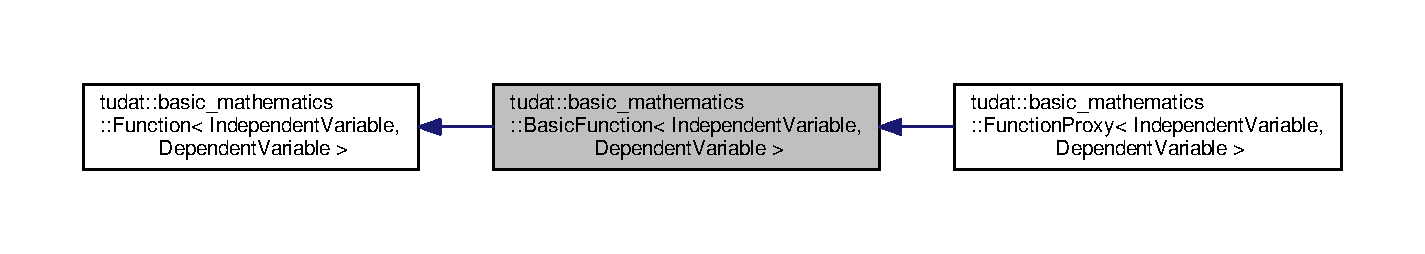
\includegraphics[width=350pt]{classtudat_1_1basic__mathematics_1_1BasicFunction__inherit__graph}
\end{center}
\end{figure}


Collaboration diagram for tudat\+:\+:basic\+\_\+mathematics\+:\+:Basic\+Function$<$ Independent\+Variable, Dependent\+Variable $>$\+:
\nopagebreak
\begin{figure}[H]
\begin{center}
\leavevmode
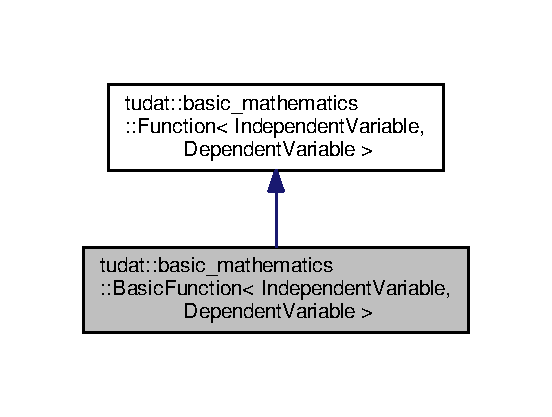
\includegraphics[width=265pt]{classtudat_1_1basic__mathematics_1_1BasicFunction__coll__graph}
\end{center}
\end{figure}
\subsection*{Public Member Functions}
\begin{DoxyCompactItemize}
\item 
\hyperlink{classtudat_1_1basic__mathematics_1_1BasicFunction_a6db9f3a2a2b5be0e10132e2b9b648132}{Basic\+Function} (unsigned int number\+Of\+Integration\+Steps=1000)\hypertarget{classtudat_1_1basic__mathematics_1_1BasicFunction_a6db9f3a2a2b5be0e10132e2b9b648132}{}\label{classtudat_1_1basic__mathematics_1_1BasicFunction_a6db9f3a2a2b5be0e10132e2b9b648132}

\begin{DoxyCompactList}\small\item\em Constructor with definition of the number of steps. \end{DoxyCompactList}\item 
virtual \hyperlink{classtudat_1_1basic__mathematics_1_1BasicFunction_a752b82484f0acb5f8ec1c55ea2dc731b}{$\sim$\+Basic\+Function} ()\hypertarget{classtudat_1_1basic__mathematics_1_1BasicFunction_a752b82484f0acb5f8ec1c55ea2dc731b}{}\label{classtudat_1_1basic__mathematics_1_1BasicFunction_a752b82484f0acb5f8ec1c55ea2dc731b}

\begin{DoxyCompactList}\small\item\em Default destructor. \end{DoxyCompactList}\item 
virtual Dependent\+Variable \hyperlink{classtudat_1_1basic__mathematics_1_1BasicFunction_ae0a0844b6c72c55ef059039eb147453b}{compute\+Derivative} (const unsigned int order, const Independent\+Variable independent\+Variable)
\begin{DoxyCompactList}\small\item\em Derivative (of a given order) of a function. \end{DoxyCompactList}\item 
Dependent\+Variable \hyperlink{classtudat_1_1basic__mathematics_1_1BasicFunction_a629836ffd0ff73670ea1e3182e1ac717}{compute\+Definite\+Integral\+Mock} (const unsigned int order, const Independent\+Variable lower\+Bound, const Independent\+Variable upperbound, const Dependent\+Variable place\+Holder)\hypertarget{classtudat_1_1basic__mathematics_1_1BasicFunction_a629836ffd0ff73670ea1e3182e1ac717}{}\label{classtudat_1_1basic__mathematics_1_1BasicFunction_a629836ffd0ff73670ea1e3182e1ac717}

\begin{DoxyCompactList}\small\item\em Alias for compute\+Definite\+Integral, but with an extra variable. Should not be used! \end{DoxyCompactList}\item 
virtual Dependent\+Variable \hyperlink{classtudat_1_1basic__mathematics_1_1BasicFunction_a9ff1a3c03832150f34c06c86317c2ac7}{compute\+Definite\+Integral} (const unsigned int order, const Independent\+Variable lower\+Bound, const Independent\+Variable upperbound)
\end{DoxyCompactItemize}
\subsection*{Public Attributes}
\begin{DoxyCompactItemize}
\item 
unsigned int \hyperlink{classtudat_1_1basic__mathematics_1_1BasicFunction_ae29d47c0ba66688c59c793805c920386}{integration\+Steps}\hypertarget{classtudat_1_1basic__mathematics_1_1BasicFunction_ae29d47c0ba66688c59c793805c920386}{}\label{classtudat_1_1basic__mathematics_1_1BasicFunction_ae29d47c0ba66688c59c793805c920386}

\begin{DoxyCompactList}\small\item\em Number of steps to take when performing numerical integration. \end{DoxyCompactList}\end{DoxyCompactItemize}
\subsection*{Static Protected Attributes}
\begin{DoxyCompactItemize}
\item 
static const double \hyperlink{classtudat_1_1basic__mathematics_1_1BasicFunction_a9d9d85a5dd2bb72ec73619c126593f0d}{sqrt\+\_\+epsilon\+\_\+double} = std\+::numeric\+\_\+limits$<$ double $>$\+::epsilon( )
\begin{DoxyCompactList}\small\item\em Square root of double precision, used to scale the step size. \end{DoxyCompactList}\end{DoxyCompactItemize}


\subsection{Detailed Description}
\subsubsection*{template$<$typename Independent\+Variable = double, typename Dependent\+Variable = double$>$\\*
class tudat\+::basic\+\_\+mathematics\+::\+Basic\+Function$<$ Independent\+Variable, Dependent\+Variable $>$}

\hyperlink{classtudat_1_1basic__mathematics_1_1Function}{Function} with basic implementations for derivatives and integrals. 

This class fills in the compute\+Derivative and compute\+Definite\+Integral functionality using numerical differentiation and integration. These are slower than their analytical counterparts, but useful when a closed form expression is available. 

\subsection{Member Function Documentation}
\index{tudat\+::basic\+\_\+mathematics\+::\+Basic\+Function@{tudat\+::basic\+\_\+mathematics\+::\+Basic\+Function}!compute\+Definite\+Integral@{compute\+Definite\+Integral}}
\index{compute\+Definite\+Integral@{compute\+Definite\+Integral}!tudat\+::basic\+\_\+mathematics\+::\+Basic\+Function@{tudat\+::basic\+\_\+mathematics\+::\+Basic\+Function}}
\subsubsection[{\texorpdfstring{compute\+Definite\+Integral(const unsigned int order, const Independent\+Variable lower\+Bound, const Independent\+Variable upperbound)}{computeDefiniteIntegral(const unsigned int order, const IndependentVariable lowerBound, const IndependentVariable upperbound)}}]{\setlength{\rightskip}{0pt plus 5cm}template$<$typename Independent\+Variable = double, typename Dependent\+Variable = double$>$ virtual Dependent\+Variable {\bf tudat\+::basic\+\_\+mathematics\+::\+Basic\+Function}$<$ Independent\+Variable, Dependent\+Variable $>$\+::compute\+Definite\+Integral (
\begin{DoxyParamCaption}
\item[{const unsigned int}]{order, }
\item[{const Independent\+Variable}]{lower\+Bound, }
\item[{const Independent\+Variable}]{upperbound}
\end{DoxyParamCaption}
)\hspace{0.3cm}{\ttfamily [inline]}, {\ttfamily [virtual]}}\hypertarget{classtudat_1_1basic__mathematics_1_1BasicFunction_a9ff1a3c03832150f34c06c86317c2ac7}{}\label{classtudat_1_1basic__mathematics_1_1BasicFunction_a9ff1a3c03832150f34c06c86317c2ac7}
Integral (of a given order) of a function from a given lower bound to upper bound (without constants).

Generic calculation of the function integral using numerical techniques. T\+O\+DO\+: Fix this code, as it doesnt work. 
\begin{DoxyParams}{Parameters}
{\em order} & Order of integral (i.\+e. integrate n times, with n = order ) \\
\hline
{\em lower\+Bound} & Lower integration bound \\
\hline
{\em upperbound} & Upper integration bound \\
\hline
\end{DoxyParams}
\begin{DoxyReturn}{Returns}
Nothing as yet; function not yet implemented 
\end{DoxyReturn}
\begin{DoxySeeAlso}{See also}
\hyperlink{classtudat_1_1basic__mathematics_1_1Function_a74c5639b8c6288471368e65312569e52}{Function\+::compute\+Definite\+Integral}. 
\end{DoxySeeAlso}


Implements \hyperlink{classtudat_1_1basic__mathematics_1_1Function_a74c5639b8c6288471368e65312569e52}{tudat\+::basic\+\_\+mathematics\+::\+Function$<$ Independent\+Variable, Dependent\+Variable $>$}.



Reimplemented in \hyperlink{structtudat_1_1unit__tests_1_1TestFunction3_a449b1eaeb3acc3fae0f584cb55f0452b}{tudat\+::unit\+\_\+tests\+::\+Test\+Function3}, \hyperlink{structtudat_1_1unit__tests_1_1TestFunctionWithLargeRootDifference_ad6962299859f91ab61908e9097fbe6f7}{tudat\+::unit\+\_\+tests\+::\+Test\+Function\+With\+Large\+Root\+Difference}, \hyperlink{structtudat_1_1unit__tests_1_1TestFunction1_abdca794bafaa237e6dccd248a9dda59b}{tudat\+::unit\+\_\+tests\+::\+Test\+Function1}, \hyperlink{structtudat_1_1unit__tests_1_1TestFunctionWithZeroRoot_a668c0a82b75c8a1edcb94bdd8f923f7e}{tudat\+::unit\+\_\+tests\+::\+Test\+Function\+With\+Zero\+Root}, and \hyperlink{structtudat_1_1unit__tests_1_1TestFunction2_a48c8418d145c79eec735d44d96cbf893}{tudat\+::unit\+\_\+tests\+::\+Test\+Function2}.

\index{tudat\+::basic\+\_\+mathematics\+::\+Basic\+Function@{tudat\+::basic\+\_\+mathematics\+::\+Basic\+Function}!compute\+Derivative@{compute\+Derivative}}
\index{compute\+Derivative@{compute\+Derivative}!tudat\+::basic\+\_\+mathematics\+::\+Basic\+Function@{tudat\+::basic\+\_\+mathematics\+::\+Basic\+Function}}
\subsubsection[{\texorpdfstring{compute\+Derivative(const unsigned int order, const Independent\+Variable independent\+Variable)}{computeDerivative(const unsigned int order, const IndependentVariable independentVariable)}}]{\setlength{\rightskip}{0pt plus 5cm}template$<$typename Independent\+Variable = double, typename Dependent\+Variable = double$>$ virtual Dependent\+Variable {\bf tudat\+::basic\+\_\+mathematics\+::\+Basic\+Function}$<$ Independent\+Variable, Dependent\+Variable $>$\+::compute\+Derivative (
\begin{DoxyParamCaption}
\item[{const unsigned int}]{order, }
\item[{const Independent\+Variable}]{independent\+Variable}
\end{DoxyParamCaption}
)\hspace{0.3cm}{\ttfamily [inline]}, {\ttfamily [virtual]}}\hypertarget{classtudat_1_1basic__mathematics_1_1BasicFunction_ae0a0844b6c72c55ef059039eb147453b}{}\label{classtudat_1_1basic__mathematics_1_1BasicFunction_ae0a0844b6c72c55ef059039eb147453b}


Derivative (of a given order) of a function. 

Generic calculation of the derivative of a function using numerical techniques. \begin{DoxySeeAlso}{See also}
Function\+::derivative T\+O\+DO\+: Use the external derivative code, this function is a basic/temporary implementation. for now this is the implementation\+: 
\end{DoxySeeAlso}

\begin{DoxyParams}{Parameters}
{\em order} & The Order of the derivative \\
\hline
{\em independent\+Variable} & The independent variable with respect to which the derivative is taken. \\
\hline
\end{DoxyParams}
\begin{DoxyReturn}{Returns}
The numerical derivative of the function. 
\end{DoxyReturn}


Implements \hyperlink{classtudat_1_1basic__mathematics_1_1Function_a0929cfbeb90a6cbc85d50455fd01d75f}{tudat\+::basic\+\_\+mathematics\+::\+Function$<$ Independent\+Variable, Dependent\+Variable $>$}.



Reimplemented in \hyperlink{classtudat_1_1basic__mathematics_1_1FunctionProxy_a5f79c3fef685b7b2eaaec22661680d61}{tudat\+::basic\+\_\+mathematics\+::\+Function\+Proxy$<$ Independent\+Variable, Dependent\+Variable $>$}, \hyperlink{structtudat_1_1unit__tests_1_1TestFunction3_ad2d7f08fa955641521a436cc280252cc}{tudat\+::unit\+\_\+tests\+::\+Test\+Function3}, \hyperlink{structtudat_1_1unit__tests_1_1TestFunctionWithLargeRootDifference_aad326dd34b4429048eb91d4d817892a2}{tudat\+::unit\+\_\+tests\+::\+Test\+Function\+With\+Large\+Root\+Difference}, \hyperlink{structtudat_1_1unit__tests_1_1TestFunction2_ad4de6c3724f2c6684ece65b7628c3e24}{tudat\+::unit\+\_\+tests\+::\+Test\+Function2}, \hyperlink{structtudat_1_1unit__tests_1_1TestFunction1_ad5c6ff20438f21b73c9148897c4e5c3c}{tudat\+::unit\+\_\+tests\+::\+Test\+Function1}, and \hyperlink{structtudat_1_1unit__tests_1_1TestFunctionWithZeroRoot_a8fb918e0e9e380dd493683892579336a}{tudat\+::unit\+\_\+tests\+::\+Test\+Function\+With\+Zero\+Root}.



\subsection{Member Data Documentation}
\index{tudat\+::basic\+\_\+mathematics\+::\+Basic\+Function@{tudat\+::basic\+\_\+mathematics\+::\+Basic\+Function}!sqrt\+\_\+epsilon\+\_\+double@{sqrt\+\_\+epsilon\+\_\+double}}
\index{sqrt\+\_\+epsilon\+\_\+double@{sqrt\+\_\+epsilon\+\_\+double}!tudat\+::basic\+\_\+mathematics\+::\+Basic\+Function@{tudat\+::basic\+\_\+mathematics\+::\+Basic\+Function}}
\subsubsection[{\texorpdfstring{sqrt\+\_\+epsilon\+\_\+double}{sqrt_epsilon_double}}]{\setlength{\rightskip}{0pt plus 5cm}template$<$typename Independent\+Variable = double, typename Dependent\+Variable = double$>$ const double {\bf tudat\+::basic\+\_\+mathematics\+::\+Basic\+Function}$<$ Independent\+Variable, Dependent\+Variable $>$\+::sqrt\+\_\+epsilon\+\_\+double = std\+::numeric\+\_\+limits$<$ double $>$\+::epsilon( )\hspace{0.3cm}{\ttfamily [static]}, {\ttfamily [protected]}}\hypertarget{classtudat_1_1basic__mathematics_1_1BasicFunction_a9d9d85a5dd2bb72ec73619c126593f0d}{}\label{classtudat_1_1basic__mathematics_1_1BasicFunction_a9d9d85a5dd2bb72ec73619c126593f0d}


Square root of double precision, used to scale the step size. 

The reason not to scale with epsilon itself is to limit the error due to floating point arithmetic with super small numbers\+: = sqrt(std\+::numeric\+\_\+limits$<$double$>$\+::epsilon()). T\+O\+DO\+: Remove when using external derivative code. 

The documentation for this class was generated from the following file\+:\begin{DoxyCompactItemize}
\item 
/home/lupi/\+Tudat/tudat\+Bundle/tudat/\+Tudat/\+Mathematics/\+Basic\+Mathematics/basic\+Function.\+h\end{DoxyCompactItemize}

\hypertarget{classtudat_1_1simulation__setup_1_1BasicSolidBodyGravityFieldVariationSettings}{}\section{tudat\+:\+:simulation\+\_\+setup\+:\+:Basic\+Solid\+Body\+Gravity\+Field\+Variation\+Settings Class Reference}
\label{classtudat_1_1simulation__setup_1_1BasicSolidBodyGravityFieldVariationSettings}\index{tudat\+::simulation\+\_\+setup\+::\+Basic\+Solid\+Body\+Gravity\+Field\+Variation\+Settings@{tudat\+::simulation\+\_\+setup\+::\+Basic\+Solid\+Body\+Gravity\+Field\+Variation\+Settings}}


{\ttfamily \#include $<$create\+Gravity\+Field\+Variations.\+h$>$}



Inheritance diagram for tudat\+:\+:simulation\+\_\+setup\+:\+:Basic\+Solid\+Body\+Gravity\+Field\+Variation\+Settings\+:
\nopagebreak
\begin{figure}[H]
\begin{center}
\leavevmode
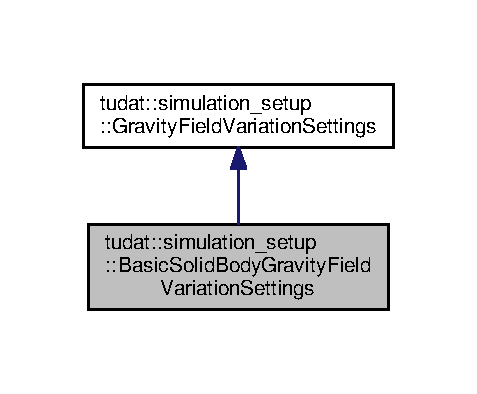
\includegraphics[width=229pt]{classtudat_1_1simulation__setup_1_1BasicSolidBodyGravityFieldVariationSettings__inherit__graph}
\end{center}
\end{figure}


Collaboration diagram for tudat\+:\+:simulation\+\_\+setup\+:\+:Basic\+Solid\+Body\+Gravity\+Field\+Variation\+Settings\+:
\nopagebreak
\begin{figure}[H]
\begin{center}
\leavevmode
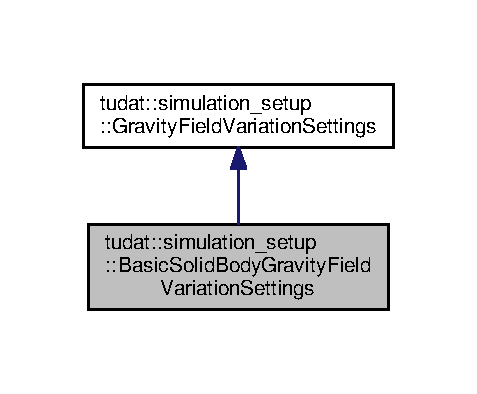
\includegraphics[width=229pt]{classtudat_1_1simulation__setup_1_1BasicSolidBodyGravityFieldVariationSettings__coll__graph}
\end{center}
\end{figure}
\subsection*{Public Member Functions}
\begin{DoxyCompactItemize}
\item 
\hyperlink{classtudat_1_1simulation__setup_1_1BasicSolidBodyGravityFieldVariationSettings_a26cb151a6e02b2c97fcc6f912795ecc9}{Basic\+Solid\+Body\+Gravity\+Field\+Variation\+Settings} (const std\+::vector$<$ std\+::string $>$ deforming\+Bodies, const std\+::vector$<$ std\+::vector$<$ std\+::complex$<$ double $>$ $>$ $>$ love\+Numbers, const double body\+Reference\+Radius, const boost\+::shared\+\_\+ptr$<$ \hyperlink{classtudat_1_1simulation__setup_1_1ModelInterpolationSettings}{Model\+Interpolation\+Settings} $>$ interpolator\+Settings=N\+U\+LL)
\begin{DoxyCompactList}\small\item\em Constructor. \end{DoxyCompactList}\item 
std\+::vector$<$ std\+::string $>$ \hyperlink{classtudat_1_1simulation__setup_1_1BasicSolidBodyGravityFieldVariationSettings_a31ba2f956752d37ffae251e8ca66c5d3}{get\+Deforming\+Bodies} ()
\begin{DoxyCompactList}\small\item\em Function to retrieve list of bodies causing tidal deformation. \end{DoxyCompactList}\item 
std\+::vector$<$ std\+::vector$<$ std\+::complex$<$ double $>$ $>$ $>$ \hyperlink{classtudat_1_1simulation__setup_1_1BasicSolidBodyGravityFieldVariationSettings_a2ea95f5725700d6160bde8bf265a477c}{get\+Love\+Numbers} ()
\begin{DoxyCompactList}\small\item\em Function to retrieve list of Love number for the deformed body. \end{DoxyCompactList}\item 
double \hyperlink{classtudat_1_1simulation__setup_1_1BasicSolidBodyGravityFieldVariationSettings_a3782fe04779b35885aac8a6a671a5ffe}{get\+Body\+Reference\+Radius} ()
\begin{DoxyCompactList}\small\item\em Function to retrieve reference (typically equatorial) radius of body being deformed. \end{DoxyCompactList}\item 
void \hyperlink{classtudat_1_1simulation__setup_1_1BasicSolidBodyGravityFieldVariationSettings_a5821016b4eb75b3e119b3d60f4d7cfcc}{reset\+Deforming\+Bodies} (const std\+::vector$<$ std\+::string $>$ \&deforming\+Bodies)
\begin{DoxyCompactList}\small\item\em Function to reset list of bodies causing tidal deformation. \end{DoxyCompactList}\end{DoxyCompactItemize}
\subsection*{Protected Attributes}
\begin{DoxyCompactItemize}
\item 
std\+::vector$<$ std\+::string $>$ \hyperlink{classtudat_1_1simulation__setup_1_1BasicSolidBodyGravityFieldVariationSettings_a698538439d1b9d1bf280d935b94f4e19}{deforming\+Bodies\+\_\+}\hypertarget{classtudat_1_1simulation__setup_1_1BasicSolidBodyGravityFieldVariationSettings_a698538439d1b9d1bf280d935b94f4e19}{}\label{classtudat_1_1simulation__setup_1_1BasicSolidBodyGravityFieldVariationSettings_a698538439d1b9d1bf280d935b94f4e19}

\begin{DoxyCompactList}\small\item\em List of bodies causing tidal deformation. \end{DoxyCompactList}\item 
std\+::vector$<$ std\+::vector$<$ std\+::complex$<$ double $>$ $>$ $>$ \hyperlink{classtudat_1_1simulation__setup_1_1BasicSolidBodyGravityFieldVariationSettings_aa4d7846c73f4a451ecf328dad7143008}{love\+Numbers\+\_\+}\hypertarget{classtudat_1_1simulation__setup_1_1BasicSolidBodyGravityFieldVariationSettings_aa4d7846c73f4a451ecf328dad7143008}{}\label{classtudat_1_1simulation__setup_1_1BasicSolidBodyGravityFieldVariationSettings_aa4d7846c73f4a451ecf328dad7143008}

\begin{DoxyCompactList}\small\item\em List of Love number for the deformed body. \end{DoxyCompactList}\item 
double \hyperlink{classtudat_1_1simulation__setup_1_1BasicSolidBodyGravityFieldVariationSettings_a7ffd8ccb084f4506edd3a09b899143dc}{body\+Reference\+Radius\+\_\+}\hypertarget{classtudat_1_1simulation__setup_1_1BasicSolidBodyGravityFieldVariationSettings_a7ffd8ccb084f4506edd3a09b899143dc}{}\label{classtudat_1_1simulation__setup_1_1BasicSolidBodyGravityFieldVariationSettings_a7ffd8ccb084f4506edd3a09b899143dc}

\begin{DoxyCompactList}\small\item\em Reference (typically equatorial) radius of body being deformed. \end{DoxyCompactList}\end{DoxyCompactItemize}


\subsection{Detailed Description}
Class to define settings for basic tidal gravity field variations, i.\+e. according to Eq. (6.\+6) of I\+E\+RS 2010 conventions. 

\subsection{Constructor \& Destructor Documentation}
\index{tudat\+::simulation\+\_\+setup\+::\+Basic\+Solid\+Body\+Gravity\+Field\+Variation\+Settings@{tudat\+::simulation\+\_\+setup\+::\+Basic\+Solid\+Body\+Gravity\+Field\+Variation\+Settings}!Basic\+Solid\+Body\+Gravity\+Field\+Variation\+Settings@{Basic\+Solid\+Body\+Gravity\+Field\+Variation\+Settings}}
\index{Basic\+Solid\+Body\+Gravity\+Field\+Variation\+Settings@{Basic\+Solid\+Body\+Gravity\+Field\+Variation\+Settings}!tudat\+::simulation\+\_\+setup\+::\+Basic\+Solid\+Body\+Gravity\+Field\+Variation\+Settings@{tudat\+::simulation\+\_\+setup\+::\+Basic\+Solid\+Body\+Gravity\+Field\+Variation\+Settings}}
\subsubsection[{\texorpdfstring{Basic\+Solid\+Body\+Gravity\+Field\+Variation\+Settings(const std\+::vector$<$ std\+::string $>$ deforming\+Bodies, const std\+::vector$<$ std\+::vector$<$ std\+::complex$<$ double $>$ $>$ $>$ love\+Numbers, const double body\+Reference\+Radius, const boost\+::shared\+\_\+ptr$<$ Model\+Interpolation\+Settings $>$ interpolator\+Settings=\+N\+U\+L\+L)}{BasicSolidBodyGravityFieldVariationSettings(const std::vector< std::string > deformingBodies, const std::vector< std::vector< std::complex< double > > > loveNumbers, const double bodyReferenceRadius, const boost::shared_ptr< ModelInterpolationSettings > interpolatorSettings=NULL)}}]{\setlength{\rightskip}{0pt plus 5cm}tudat\+::simulation\+\_\+setup\+::\+Basic\+Solid\+Body\+Gravity\+Field\+Variation\+Settings\+::\+Basic\+Solid\+Body\+Gravity\+Field\+Variation\+Settings (
\begin{DoxyParamCaption}
\item[{const std\+::vector$<$ std\+::string $>$}]{deforming\+Bodies, }
\item[{const std\+::vector$<$ std\+::vector$<$ std\+::complex$<$ double $>$ $>$ $>$}]{love\+Numbers, }
\item[{const double}]{body\+Reference\+Radius, }
\item[{const boost\+::shared\+\_\+ptr$<$ {\bf Model\+Interpolation\+Settings} $>$}]{interpolator\+Settings = {\ttfamily NULL}}
\end{DoxyParamCaption}
)\hspace{0.3cm}{\ttfamily [inline]}}\hypertarget{classtudat_1_1simulation__setup_1_1BasicSolidBodyGravityFieldVariationSettings_a26cb151a6e02b2c97fcc6f912795ecc9}{}\label{classtudat_1_1simulation__setup_1_1BasicSolidBodyGravityFieldVariationSettings_a26cb151a6e02b2c97fcc6f912795ecc9}


Constructor. 

Constructor 
\begin{DoxyParams}{Parameters}
{\em deforming\+Bodies} & List of bodies causing tidal deformation \\
\hline
{\em love\+Numbers} & List of Love number for the deformed body. First vector level denotes degree (index 0 = degree 2), second vector level denotes order and must be of maximum size (love\+Numbers.\+size( ) + 2, i.\+e. maximum degree $>$= maximum order) \\
\hline
{\em body\+Reference\+Radius} & Reference (typically equatorial) radius of body being deformed \\
\hline
{\em interpolator\+Settings} & Settings that are to be used to create an interpolator for the gravity field variations immediately upon creation (to be used during propagation). Default is N\+U\+LL, in which no interpolation is used, and the model is evaluated during propagation. \\
\hline
\end{DoxyParams}


\subsection{Member Function Documentation}
\index{tudat\+::simulation\+\_\+setup\+::\+Basic\+Solid\+Body\+Gravity\+Field\+Variation\+Settings@{tudat\+::simulation\+\_\+setup\+::\+Basic\+Solid\+Body\+Gravity\+Field\+Variation\+Settings}!get\+Body\+Reference\+Radius@{get\+Body\+Reference\+Radius}}
\index{get\+Body\+Reference\+Radius@{get\+Body\+Reference\+Radius}!tudat\+::simulation\+\_\+setup\+::\+Basic\+Solid\+Body\+Gravity\+Field\+Variation\+Settings@{tudat\+::simulation\+\_\+setup\+::\+Basic\+Solid\+Body\+Gravity\+Field\+Variation\+Settings}}
\subsubsection[{\texorpdfstring{get\+Body\+Reference\+Radius()}{getBodyReferenceRadius()}}]{\setlength{\rightskip}{0pt plus 5cm}double tudat\+::simulation\+\_\+setup\+::\+Basic\+Solid\+Body\+Gravity\+Field\+Variation\+Settings\+::get\+Body\+Reference\+Radius (
\begin{DoxyParamCaption}
{}
\end{DoxyParamCaption}
)\hspace{0.3cm}{\ttfamily [inline]}}\hypertarget{classtudat_1_1simulation__setup_1_1BasicSolidBodyGravityFieldVariationSettings_a3782fe04779b35885aac8a6a671a5ffe}{}\label{classtudat_1_1simulation__setup_1_1BasicSolidBodyGravityFieldVariationSettings_a3782fe04779b35885aac8a6a671a5ffe}


Function to retrieve reference (typically equatorial) radius of body being deformed. 

Function to retrieve reference (typically equatorial) radius of body being deformed \begin{DoxyReturn}{Returns}
Reference (typically equatorial) radius of body being deformed 
\end{DoxyReturn}
\index{tudat\+::simulation\+\_\+setup\+::\+Basic\+Solid\+Body\+Gravity\+Field\+Variation\+Settings@{tudat\+::simulation\+\_\+setup\+::\+Basic\+Solid\+Body\+Gravity\+Field\+Variation\+Settings}!get\+Deforming\+Bodies@{get\+Deforming\+Bodies}}
\index{get\+Deforming\+Bodies@{get\+Deforming\+Bodies}!tudat\+::simulation\+\_\+setup\+::\+Basic\+Solid\+Body\+Gravity\+Field\+Variation\+Settings@{tudat\+::simulation\+\_\+setup\+::\+Basic\+Solid\+Body\+Gravity\+Field\+Variation\+Settings}}
\subsubsection[{\texorpdfstring{get\+Deforming\+Bodies()}{getDeformingBodies()}}]{\setlength{\rightskip}{0pt plus 5cm}std\+::vector$<$ std\+::string $>$ tudat\+::simulation\+\_\+setup\+::\+Basic\+Solid\+Body\+Gravity\+Field\+Variation\+Settings\+::get\+Deforming\+Bodies (
\begin{DoxyParamCaption}
{}
\end{DoxyParamCaption}
)\hspace{0.3cm}{\ttfamily [inline]}}\hypertarget{classtudat_1_1simulation__setup_1_1BasicSolidBodyGravityFieldVariationSettings_a31ba2f956752d37ffae251e8ca66c5d3}{}\label{classtudat_1_1simulation__setup_1_1BasicSolidBodyGravityFieldVariationSettings_a31ba2f956752d37ffae251e8ca66c5d3}


Function to retrieve list of bodies causing tidal deformation. 

Function to retrieve list of bodies causing tidal deformation \begin{DoxyReturn}{Returns}
List of bodies causing tidal deformation 
\end{DoxyReturn}
\index{tudat\+::simulation\+\_\+setup\+::\+Basic\+Solid\+Body\+Gravity\+Field\+Variation\+Settings@{tudat\+::simulation\+\_\+setup\+::\+Basic\+Solid\+Body\+Gravity\+Field\+Variation\+Settings}!get\+Love\+Numbers@{get\+Love\+Numbers}}
\index{get\+Love\+Numbers@{get\+Love\+Numbers}!tudat\+::simulation\+\_\+setup\+::\+Basic\+Solid\+Body\+Gravity\+Field\+Variation\+Settings@{tudat\+::simulation\+\_\+setup\+::\+Basic\+Solid\+Body\+Gravity\+Field\+Variation\+Settings}}
\subsubsection[{\texorpdfstring{get\+Love\+Numbers()}{getLoveNumbers()}}]{\setlength{\rightskip}{0pt plus 5cm}std\+::vector$<$ std\+::vector$<$ std\+::complex$<$ double $>$ $>$ $>$ tudat\+::simulation\+\_\+setup\+::\+Basic\+Solid\+Body\+Gravity\+Field\+Variation\+Settings\+::get\+Love\+Numbers (
\begin{DoxyParamCaption}
{}
\end{DoxyParamCaption}
)\hspace{0.3cm}{\ttfamily [inline]}}\hypertarget{classtudat_1_1simulation__setup_1_1BasicSolidBodyGravityFieldVariationSettings_a2ea95f5725700d6160bde8bf265a477c}{}\label{classtudat_1_1simulation__setup_1_1BasicSolidBodyGravityFieldVariationSettings_a2ea95f5725700d6160bde8bf265a477c}


Function to retrieve list of Love number for the deformed body. 

Function to retrieve list of Love number for the deformed body. \begin{DoxyReturn}{Returns}
List of Love number for the deformed body. 
\end{DoxyReturn}
\index{tudat\+::simulation\+\_\+setup\+::\+Basic\+Solid\+Body\+Gravity\+Field\+Variation\+Settings@{tudat\+::simulation\+\_\+setup\+::\+Basic\+Solid\+Body\+Gravity\+Field\+Variation\+Settings}!reset\+Deforming\+Bodies@{reset\+Deforming\+Bodies}}
\index{reset\+Deforming\+Bodies@{reset\+Deforming\+Bodies}!tudat\+::simulation\+\_\+setup\+::\+Basic\+Solid\+Body\+Gravity\+Field\+Variation\+Settings@{tudat\+::simulation\+\_\+setup\+::\+Basic\+Solid\+Body\+Gravity\+Field\+Variation\+Settings}}
\subsubsection[{\texorpdfstring{reset\+Deforming\+Bodies(const std\+::vector$<$ std\+::string $>$ \&deforming\+Bodies)}{resetDeformingBodies(const std::vector< std::string > &deformingBodies)}}]{\setlength{\rightskip}{0pt plus 5cm}void tudat\+::simulation\+\_\+setup\+::\+Basic\+Solid\+Body\+Gravity\+Field\+Variation\+Settings\+::reset\+Deforming\+Bodies (
\begin{DoxyParamCaption}
\item[{const std\+::vector$<$ std\+::string $>$ \&}]{deforming\+Bodies}
\end{DoxyParamCaption}
)\hspace{0.3cm}{\ttfamily [inline]}}\hypertarget{classtudat_1_1simulation__setup_1_1BasicSolidBodyGravityFieldVariationSettings_a5821016b4eb75b3e119b3d60f4d7cfcc}{}\label{classtudat_1_1simulation__setup_1_1BasicSolidBodyGravityFieldVariationSettings_a5821016b4eb75b3e119b3d60f4d7cfcc}


Function to reset list of bodies causing tidal deformation. 

Function to reset list of bodies causing tidal deformation 
\begin{DoxyParams}{Parameters}
{\em deforming\+Bodies} & New list of bodies causing tidal deformation \\
\hline
\end{DoxyParams}


The documentation for this class was generated from the following file\+:\begin{DoxyCompactItemize}
\item 
/home/lupi/\+Tudat/tudat\+Bundle/tudat/\+Tudat/\+Simulation\+Setup/\+Environment\+Setup/create\+Gravity\+Field\+Variations.\+h\end{DoxyCompactItemize}

\hypertarget{classtudat_1_1gravitation_1_1BasicSolidBodyTideGravityFieldVariations}{}\section{tudat\+:\+:gravitation\+:\+:Basic\+Solid\+Body\+Tide\+Gravity\+Field\+Variations Class Reference}
\label{classtudat_1_1gravitation_1_1BasicSolidBodyTideGravityFieldVariations}\index{tudat\+::gravitation\+::\+Basic\+Solid\+Body\+Tide\+Gravity\+Field\+Variations@{tudat\+::gravitation\+::\+Basic\+Solid\+Body\+Tide\+Gravity\+Field\+Variations}}


{\ttfamily \#include $<$basic\+Solid\+Body\+Tide\+Gravity\+Field\+Variations.\+h$>$}



Inheritance diagram for tudat\+:\+:gravitation\+:\+:Basic\+Solid\+Body\+Tide\+Gravity\+Field\+Variations\+:
\nopagebreak
\begin{figure}[H]
\begin{center}
\leavevmode
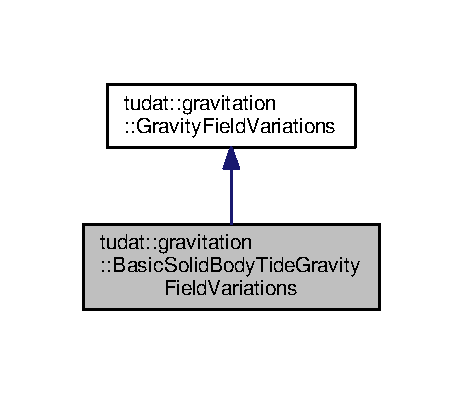
\includegraphics[width=222pt]{classtudat_1_1gravitation_1_1BasicSolidBodyTideGravityFieldVariations__inherit__graph}
\end{center}
\end{figure}


Collaboration diagram for tudat\+:\+:gravitation\+:\+:Basic\+Solid\+Body\+Tide\+Gravity\+Field\+Variations\+:
\nopagebreak
\begin{figure}[H]
\begin{center}
\leavevmode
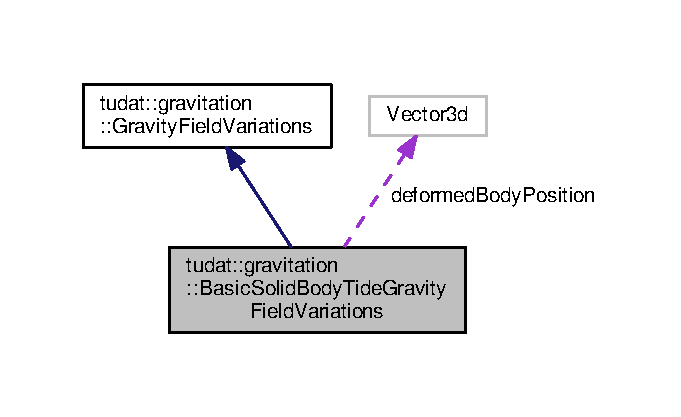
\includegraphics[width=327pt]{classtudat_1_1gravitation_1_1BasicSolidBodyTideGravityFieldVariations__coll__graph}
\end{center}
\end{figure}
\subsection*{Public Member Functions}
\begin{DoxyCompactItemize}
\item 
\hyperlink{classtudat_1_1gravitation_1_1BasicSolidBodyTideGravityFieldVariations_a698be5ee244e5444650db403b653102c}{Basic\+Solid\+Body\+Tide\+Gravity\+Field\+Variations} (const boost\+::function$<$ Eigen\+::\+Vector6d(const double) $>$ deformed\+Body\+State\+Function, const boost\+::function$<$ Eigen\+::\+Quaterniond(const double) $>$ deformed\+Body\+Orientation\+Function, const std\+::vector$<$ boost\+::function$<$ Eigen\+::\+Vector6d(const double) $>$ $>$ deforming\+Body\+State\+Functions, const double deformed\+Body\+Reference\+Radius, const boost\+::function$<$ double() $>$ deformed\+Body\+Mass, const std\+::vector$<$ boost\+::function$<$ double() $>$ $>$ deforming\+Body\+Masses, const std\+::vector$<$ std\+::vector$<$ std\+::complex$<$ double $>$ $>$ $>$ love\+Numbers, const std\+::vector$<$ std\+::string $>$ deforming\+Bodies)
\begin{DoxyCompactList}\small\item\em Constructor. \end{DoxyCompactList}\item 
virtual \hyperlink{classtudat_1_1gravitation_1_1BasicSolidBodyTideGravityFieldVariations_a724a92f0468e38cee6359323d7fafa8b}{$\sim$\+Basic\+Solid\+Body\+Tide\+Gravity\+Field\+Variations} ()
\begin{DoxyCompactList}\small\item\em Destructor. \end{DoxyCompactList}\item 
std\+::pair$<$ Eigen\+::\+Matrix\+Xd, Eigen\+::\+Matrix\+Xd $>$ \hyperlink{classtudat_1_1gravitation_1_1BasicSolidBodyTideGravityFieldVariations_a531dcae6f842ada23679d1151df4d5c4}{calculate\+Basic\+Spherical\+Harmonics\+Corrections} (const double time)
\begin{DoxyCompactList}\small\item\em Function for calculating basic spherical harmonic coefficient corrections. \end{DoxyCompactList}\item 
virtual std\+::pair$<$ Eigen\+::\+Matrix\+Xd, Eigen\+::\+Matrix\+Xd $>$ \hyperlink{classtudat_1_1gravitation_1_1BasicSolidBodyTideGravityFieldVariations_ad944298a2aaa69b32adcbb1243e99905}{calculate\+Spherical\+Harmonics\+Corrections} (const double time)
\begin{DoxyCompactList}\small\item\em Derived function for calculating spherical harmonic coefficient corrections. \end{DoxyCompactList}\item 
std\+::vector$<$ std\+::complex$<$ double $>$ $>$ \hyperlink{classtudat_1_1gravitation_1_1BasicSolidBodyTideGravityFieldVariations_a1a189f3f9b2f735519842f5a939065fb}{get\+Love\+Numbers\+Of\+Degree} (const int degree)
\begin{DoxyCompactList}\small\item\em Function to retrieve the love numbers at given degree. \end{DoxyCompactList}\item 
std\+::vector$<$ std\+::vector$<$ std\+::complex$<$ double $>$ $>$ $>$ \hyperlink{classtudat_1_1gravitation_1_1BasicSolidBodyTideGravityFieldVariations_a9e0d798403383edfea5f3a8e546e405f}{get\+Love\+Numbers} ()
\begin{DoxyCompactList}\small\item\em Function to return all love numbers. \end{DoxyCompactList}\item 
void \hyperlink{classtudat_1_1gravitation_1_1BasicSolidBodyTideGravityFieldVariations_a7e52b6a1d0a419927f27e3fe5468a8d3}{reset\+Love\+Numbers\+Of\+Degree} (const std\+::vector$<$ std\+::complex$<$ double $>$ $>$ love\+Numbers, const int degree)
\begin{DoxyCompactList}\small\item\em Function to reset the love numbers at given degree. \end{DoxyCompactList}\item 
double \hyperlink{classtudat_1_1gravitation_1_1BasicSolidBodyTideGravityFieldVariations_a7d18c02f68c969a278704db689631e2a}{get\+Deformed\+Body\+Reference\+Radius} ()
\begin{DoxyCompactList}\small\item\em Function to return reference radius the spherical harmonic gravity field of deformed body. \end{DoxyCompactList}\item 
boost\+::function$<$ double() $>$ \hyperlink{classtudat_1_1gravitation_1_1BasicSolidBodyTideGravityFieldVariations_af3a99ebffc6c259fd662fd24d521aa2a}{get\+Deformed\+Body\+Mass\+Function} ()
\begin{DoxyCompactList}\small\item\em Function to return the mass function of the deformed body. \end{DoxyCompactList}\item 
std\+::vector$<$ boost\+::function$<$ double() $>$ $>$ \hyperlink{classtudat_1_1gravitation_1_1BasicSolidBodyTideGravityFieldVariations_a8bcc5c47e45ad462c29946502ae53eea}{get\+Deforming\+Body\+Masses} ()
\begin{DoxyCompactList}\small\item\em Function to return list of the mass functions of the bodies causing the deformation. \end{DoxyCompactList}\item 
std\+::vector$<$ std\+::string $>$ \hyperlink{classtudat_1_1gravitation_1_1BasicSolidBodyTideGravityFieldVariations_a53c768e15c3aeff85f74986dc8a9567c}{get\+Deforming\+Bodies} ()
\begin{DoxyCompactList}\small\item\em Function to return list of the names of the bodies causing the deformation. \end{DoxyCompactList}\item 
boost\+::function$<$ Eigen\+::\+Vector6d(const double) $>$ \hyperlink{classtudat_1_1gravitation_1_1BasicSolidBodyTideGravityFieldVariations_ad4126a4f0fc3ebe5c0387a0825701ce9}{get\+Deformed\+Body\+State\+Function} ()
\begin{DoxyCompactList}\small\item\em Function to return the state function of the deformed body. \end{DoxyCompactList}\item 
boost\+::function$<$ Eigen\+::\+Quaterniond(const double) $>$ \hyperlink{classtudat_1_1gravitation_1_1BasicSolidBodyTideGravityFieldVariations_acf37c94f155bef85a68f6bb2f5dd870b}{get\+Deformed\+Body\+Orientation\+Function} ()
\item 
std\+::vector$<$ boost\+::function$<$ Eigen\+::\+Vector6d(const double) $>$ $>$ \hyperlink{classtudat_1_1gravitation_1_1BasicSolidBodyTideGravityFieldVariations_a27b0a1a1a38f110929aaca4e88216b70}{get\+Deforming\+Body\+State\+Functions} ()
\begin{DoxyCompactList}\small\item\em Function to return list of the state functions of the bodies causing the deformation. \end{DoxyCompactList}\item 
std\+::string \hyperlink{classtudat_1_1gravitation_1_1BasicSolidBodyTideGravityFieldVariations_a7639715b2180ffa04ca76032c0b99860}{get\+Concatenated\+Deforming\+Bodies} ()
\begin{DoxyCompactList}\small\item\em Get a string with the concatenation of all the bodies causing the deformation. \end{DoxyCompactList}\item 
Eigen\+::\+Matrix\+Xd \hyperlink{classtudat_1_1gravitation_1_1BasicSolidBodyTideGravityFieldVariations_aeb4ea086378d1254b6ece9355401a894}{get\+Current\+Cosine\+Corrections} ()
\begin{DoxyCompactList}\small\item\em Function to return the current corrections to the cosine coefficients. \end{DoxyCompactList}\item 
Eigen\+::\+Matrix\+Xd \hyperlink{classtudat_1_1gravitation_1_1BasicSolidBodyTideGravityFieldVariations_a849347887a7736bf139052146f708727}{get\+Current\+Sine\+Corrections} ()
\begin{DoxyCompactList}\small\item\em Function to return the current corrections to the sine coefficients. \end{DoxyCompactList}\end{DoxyCompactItemize}
\subsection*{Protected Member Functions}
\begin{DoxyCompactItemize}
\item 
virtual void \hyperlink{classtudat_1_1gravitation_1_1BasicSolidBodyTideGravityFieldVariations_aa4a8b7924134fed07f596b6b43df9472}{add\+Basic\+Solid\+Body\+Tide\+Corrections} (Eigen\+::\+Matrix\+Xd \&c\+Term\+Corrections, Eigen\+::\+Matrix\+Xd \&s\+Term\+Corrections)
\begin{DoxyCompactList}\small\item\em Calculates basic solid body gravity field corrections due to single body. \end{DoxyCompactList}\item 
virtual void \hyperlink{classtudat_1_1gravitation_1_1BasicSolidBodyTideGravityFieldVariations_a5026f7ed54fa6d1a60367a0b981913af}{set\+Body\+Geometry\+Parameters} (const int body\+Index, const double evaluation\+Time)
\begin{DoxyCompactList}\small\item\em Sets current properties (mass state) of body causing tidal deformation. \end{DoxyCompactList}\item 
virtual void \hyperlink{classtudat_1_1gravitation_1_1BasicSolidBodyTideGravityFieldVariations_a62c60cf127ad2a396a51b4c0733c7b72}{update\+Tidal\+Amplitude\+And\+Argument} (const int degree, const int order)
\begin{DoxyCompactList}\small\item\em Calculate tidal amplitude and argument at current degree and order. \end{DoxyCompactList}\end{DoxyCompactItemize}
\subsection*{Protected Attributes}
\begin{DoxyCompactItemize}
\item 
std\+::vector$<$ boost\+::function$<$ void(Eigen\+::\+Matrix\+Xd \&, Eigen\+::\+Matrix\+Xd \&) $>$ $>$ \hyperlink{classtudat_1_1gravitation_1_1BasicSolidBodyTideGravityFieldVariations_aa875438d3e5e31a16b45c0009975954a}{correction\+Functions}
\begin{DoxyCompactList}\small\item\em List of functions to call for calculating spherical harmonic corrections. \end{DoxyCompactList}\item 
boost\+::function$<$ Eigen\+::\+Vector6d(const double) $>$ \hyperlink{classtudat_1_1gravitation_1_1BasicSolidBodyTideGravityFieldVariations_a5d3b0e842e58504144a2e2e2ef96c90a}{deformed\+Body\+State\+Function\+\_\+}
\begin{DoxyCompactList}\small\item\em Function returning state of body being deformed. \end{DoxyCompactList}\item 
boost\+::function$<$ Eigen\+::\+Quaterniond(const double) $>$ \hyperlink{classtudat_1_1gravitation_1_1BasicSolidBodyTideGravityFieldVariations_a2ee3f417b4324455f45a353282759149}{deformed\+Body\+Orientation\+Function\+\_\+}
\begin{DoxyCompactList}\small\item\em Function providing rotation from inertial to body being deformed-\/fixed frame. \end{DoxyCompactList}\item 
std\+::vector$<$ boost\+::function$<$ Eigen\+::\+Vector6d(const double) $>$ $>$ \hyperlink{classtudat_1_1gravitation_1_1BasicSolidBodyTideGravityFieldVariations_aa007e8a4b2423b484bf49eb46dac39c9}{deforming\+Body\+State\+Functions\+\_\+}
\begin{DoxyCompactList}\small\item\em List of state functions of body causing deformations. \end{DoxyCompactList}\item 
double \hyperlink{classtudat_1_1gravitation_1_1BasicSolidBodyTideGravityFieldVariations_abe0acaf654a36869a9abd709a09607b0}{deformed\+Body\+Reference\+Radius\+\_\+}
\item 
boost\+::function$<$ double() $>$ \hyperlink{classtudat_1_1gravitation_1_1BasicSolidBodyTideGravityFieldVariations_ab12ae5c98ab6a31a2bbff565f1dc157c}{deformed\+Body\+Mass\+\_\+}
\begin{DoxyCompactList}\small\item\em Function returning mass of body being deformed. \end{DoxyCompactList}\item 
std\+::vector$<$ boost\+::function$<$ double() $>$ $>$ \hyperlink{classtudat_1_1gravitation_1_1BasicSolidBodyTideGravityFieldVariations_a001d0bd58615e93f73ec72849d03298d}{deforming\+Body\+Masses\+\_\+}
\begin{DoxyCompactList}\small\item\em List of functions returning masses of bodies causing deformation. \end{DoxyCompactList}\item 
std\+::vector$<$ std\+::vector$<$ std\+::complex$<$ double $>$ $>$ $>$ \hyperlink{classtudat_1_1gravitation_1_1BasicSolidBodyTideGravityFieldVariations_a87a672e14855c8795103eaa4830cf501}{love\+Numbers\+\_\+}
\begin{DoxyCompactList}\small\item\em List of love numbers for each degree and order. \end{DoxyCompactList}\item 
std\+::vector$<$ std\+::string $>$ \hyperlink{classtudat_1_1gravitation_1_1BasicSolidBodyTideGravityFieldVariations_a6da84354b18ad22f89fa49e720dd34a9}{deforming\+Bodies\+\_\+}
\begin{DoxyCompactList}\small\item\em List of names of bodies causing deformation. \end{DoxyCompactList}\item 
double \hyperlink{classtudat_1_1gravitation_1_1BasicSolidBodyTideGravityFieldVariations_a40b77e066ce4933eb7a4d9ca5fd27b76}{mass\+Ratio}
\begin{DoxyCompactList}\small\item\em Ratio of masses in current calculation step. \end{DoxyCompactList}\item 
double \hyperlink{classtudat_1_1gravitation_1_1BasicSolidBodyTideGravityFieldVariations_a6ba4ba751b56f7f653a7370371f5ab21}{radius\+Ratio}
\begin{DoxyCompactList}\small\item\em Ratio of radii in current calculation step. \end{DoxyCompactList}\item 
double \hyperlink{classtudat_1_1gravitation_1_1BasicSolidBodyTideGravityFieldVariations_a6646e9fc25280255248df924c8fcc6ea}{radius\+Ratio\+Power}
\begin{DoxyCompactList}\small\item\em Ratio of radii in current calculation step to the power (degree+1). \end{DoxyCompactList}\item 
double \hyperlink{classtudat_1_1gravitation_1_1BasicSolidBodyTideGravityFieldVariations_adf49e1f8b787b2d8f3df4a8f9ba07d19}{sine\+Of\+Latitude}
\begin{DoxyCompactList}\small\item\em Sine of latitude of currently considered body in current calculation step. \end{DoxyCompactList}\item 
std\+::complex$<$ double $>$ \hyperlink{classtudat_1_1gravitation_1_1BasicSolidBodyTideGravityFieldVariations_aaf20605f78a1e71fff58a82e047b721d}{i\+Longitude}
\begin{DoxyCompactList}\small\item\em Longitude of currently considered body times i in current calculation step. \end{DoxyCompactList}\item 
std\+::complex$<$ double $>$ \hyperlink{classtudat_1_1gravitation_1_1BasicSolidBodyTideGravityFieldVariations_aace888d4e6e5dde87704145b40913294}{tide\+Argument}
\begin{DoxyCompactList}\small\item\em Current argument of the tide. \end{DoxyCompactList}\item 
double \hyperlink{classtudat_1_1gravitation_1_1BasicSolidBodyTideGravityFieldVariations_a6b196974e5ec21765cbf3d0c6054be11}{tide\+Amplitude}
\begin{DoxyCompactList}\small\item\em Current amplitude of the tide. \end{DoxyCompactList}\item 
Eigen\+::\+Vector3d \hyperlink{classtudat_1_1gravitation_1_1BasicSolidBodyTideGravityFieldVariations_ae4df43a455c3c408c467e55de0c2684b}{deformed\+Body\+Position}\hypertarget{classtudat_1_1gravitation_1_1BasicSolidBodyTideGravityFieldVariations_ae4df43a455c3c408c467e55de0c2684b}{}\label{classtudat_1_1gravitation_1_1BasicSolidBodyTideGravityFieldVariations_ae4df43a455c3c408c467e55de0c2684b}

\begin{DoxyCompactList}\small\item\em Current position of body being deformed. \end{DoxyCompactList}\item 
Eigen\+::\+Quaterniond \hyperlink{classtudat_1_1gravitation_1_1BasicSolidBodyTideGravityFieldVariations_aa3d565d7ddcb5e355b934d6e25b8ed55}{to\+Deformed\+Body\+Frame\+Rotation}\hypertarget{classtudat_1_1gravitation_1_1BasicSolidBodyTideGravityFieldVariations_aa3d565d7ddcb5e355b934d6e25b8ed55}{}\label{classtudat_1_1gravitation_1_1BasicSolidBodyTideGravityFieldVariations_aa3d565d7ddcb5e355b934d6e25b8ed55}

\begin{DoxyCompactList}\small\item\em Current rotation to frame fixed to deformed body. \end{DoxyCompactList}\item 
Eigen\+::\+Matrix\+Xd \hyperlink{classtudat_1_1gravitation_1_1BasicSolidBodyTideGravityFieldVariations_a598b40a06e03913ae2694d0108af03fc}{current\+Cosine\+Corrections\+\_\+}\hypertarget{classtudat_1_1gravitation_1_1BasicSolidBodyTideGravityFieldVariations_a598b40a06e03913ae2694d0108af03fc}{}\label{classtudat_1_1gravitation_1_1BasicSolidBodyTideGravityFieldVariations_a598b40a06e03913ae2694d0108af03fc}

\begin{DoxyCompactList}\small\item\em Tidal corrections to cosine coefficients at current calculation step. \end{DoxyCompactList}\item 
Eigen\+::\+Matrix\+Xd \hyperlink{classtudat_1_1gravitation_1_1BasicSolidBodyTideGravityFieldVariations_ae3ef8888c89778135bd861f6b2b08bcc}{current\+Sine\+Corrections\+\_\+}\hypertarget{classtudat_1_1gravitation_1_1BasicSolidBodyTideGravityFieldVariations_ae3ef8888c89778135bd861f6b2b08bcc}{}\label{classtudat_1_1gravitation_1_1BasicSolidBodyTideGravityFieldVariations_ae3ef8888c89778135bd861f6b2b08bcc}

\begin{DoxyCompactList}\small\item\em Tidal corrections to sine coefficients at current calculation step. \end{DoxyCompactList}\end{DoxyCompactItemize}


\subsection{Detailed Description}
Class to calculate first-\/order solid body tide gravity field variations on a single body raised by any number of bodies up to any degree and order. 

\subsection{Constructor \& Destructor Documentation}
\index{tudat\+::gravitation\+::\+Basic\+Solid\+Body\+Tide\+Gravity\+Field\+Variations@{tudat\+::gravitation\+::\+Basic\+Solid\+Body\+Tide\+Gravity\+Field\+Variations}!Basic\+Solid\+Body\+Tide\+Gravity\+Field\+Variations@{Basic\+Solid\+Body\+Tide\+Gravity\+Field\+Variations}}
\index{Basic\+Solid\+Body\+Tide\+Gravity\+Field\+Variations@{Basic\+Solid\+Body\+Tide\+Gravity\+Field\+Variations}!tudat\+::gravitation\+::\+Basic\+Solid\+Body\+Tide\+Gravity\+Field\+Variations@{tudat\+::gravitation\+::\+Basic\+Solid\+Body\+Tide\+Gravity\+Field\+Variations}}
\subsubsection[{\texorpdfstring{Basic\+Solid\+Body\+Tide\+Gravity\+Field\+Variations(const boost\+::function$<$ Eigen\+::\+Vector6d(const double) $>$ deformed\+Body\+State\+Function, const boost\+::function$<$ Eigen\+::\+Quaterniond(const double) $>$ deformed\+Body\+Orientation\+Function, const std\+::vector$<$ boost\+::function$<$ Eigen\+::\+Vector6d(const double) $>$ $>$ deforming\+Body\+State\+Functions, const double deformed\+Body\+Reference\+Radius, const boost\+::function$<$ double() $>$ deformed\+Body\+Mass, const std\+::vector$<$ boost\+::function$<$ double() $>$ $>$ deforming\+Body\+Masses, const std\+::vector$<$ std\+::vector$<$ std\+::complex$<$ double $>$ $>$ $>$ love\+Numbers, const std\+::vector$<$ std\+::string $>$ deforming\+Bodies)}{BasicSolidBodyTideGravityFieldVariations(const boost::function< Eigen::Vector6d(const double) > deformedBodyStateFunction, const boost::function< Eigen::Quaterniond(const double) > deformedBodyOrientationFunction, const std::vector< boost::function< Eigen::Vector6d(const double) > > deformingBodyStateFunctions, const double deformedBodyReferenceRadius, const boost::function< double() > deformedBodyMass, const std::vector< boost::function< double() > > deformingBodyMasses, const std::vector< std::vector< std::complex< double > > > loveNumbers, const std::vector< std::string > deformingBodies)}}]{\setlength{\rightskip}{0pt plus 5cm}tudat\+::gravitation\+::\+Basic\+Solid\+Body\+Tide\+Gravity\+Field\+Variations\+::\+Basic\+Solid\+Body\+Tide\+Gravity\+Field\+Variations (
\begin{DoxyParamCaption}
\item[{const boost\+::function$<$ Eigen\+::\+Vector6d(const double) $>$}]{deformed\+Body\+State\+Function, }
\item[{const boost\+::function$<$ Eigen\+::\+Quaterniond(const double) $>$}]{deformed\+Body\+Orientation\+Function, }
\item[{const std\+::vector$<$ boost\+::function$<$ Eigen\+::\+Vector6d(const double) $>$ $>$}]{deforming\+Body\+State\+Functions, }
\item[{const double}]{deformed\+Body\+Reference\+Radius, }
\item[{const boost\+::function$<$ double() $>$}]{deformed\+Body\+Mass, }
\item[{const std\+::vector$<$ boost\+::function$<$ double() $>$ $>$}]{deforming\+Body\+Masses, }
\item[{const std\+::vector$<$ std\+::vector$<$ std\+::complex$<$ double $>$ $>$ $>$}]{love\+Numbers, }
\item[{const std\+::vector$<$ std\+::string $>$}]{deforming\+Bodies}
\end{DoxyParamCaption}
)\hspace{0.3cm}{\ttfamily [inline]}}\hypertarget{classtudat_1_1gravitation_1_1BasicSolidBodyTideGravityFieldVariations_a698be5ee244e5444650db403b653102c}{}\label{classtudat_1_1gravitation_1_1BasicSolidBodyTideGravityFieldVariations_a698be5ee244e5444650db403b653102c}


Constructor. 

Contructor, sets Love numbers and properties of deformed and tide-\/raising bodies. 
\begin{DoxyParams}{Parameters}
{\em deformed\+Body\+State\+Function} & Function returning state of body being deformed. \\
\hline
{\em deformed\+Body\+Orientation\+Function} & Function providing rotation from inertial to body being deformed-\/fixed frame \\
\hline
{\em deforming\+Body\+State\+Functions} & List of state functions of body causing deformations. \\
\hline
{\em deformed\+Body\+Reference\+Radius} & Reference radius (typically equatorial) of body being deformed\textquotesingle{}s spherical harmonic gravity field. \\
\hline
{\em deformed\+Body\+Mass} & Function returning mass (or gravitational parameter) of body being deformed. \\
\hline
{\em deforming\+Body\+Masses} & List of functions returning masses (or gravitational parameters) of bodies causing deformation. \\
\hline
{\em love\+Numbers} & List of love numbers for each degree and order. First vector level denotes degree (index 0 = degree 2), second vector level denotes order and must be of maximum size (love\+Numbers.\+size( ) + 2, i.\+e. maximum degree $>$= maximum order) \\
\hline
{\em deforming\+Bodies} & List of names of bodies causing deformation \\
\hline
\end{DoxyParams}
\index{tudat\+::gravitation\+::\+Basic\+Solid\+Body\+Tide\+Gravity\+Field\+Variations@{tudat\+::gravitation\+::\+Basic\+Solid\+Body\+Tide\+Gravity\+Field\+Variations}!````~Basic\+Solid\+Body\+Tide\+Gravity\+Field\+Variations@{$\sim$\+Basic\+Solid\+Body\+Tide\+Gravity\+Field\+Variations}}
\index{````~Basic\+Solid\+Body\+Tide\+Gravity\+Field\+Variations@{$\sim$\+Basic\+Solid\+Body\+Tide\+Gravity\+Field\+Variations}!tudat\+::gravitation\+::\+Basic\+Solid\+Body\+Tide\+Gravity\+Field\+Variations@{tudat\+::gravitation\+::\+Basic\+Solid\+Body\+Tide\+Gravity\+Field\+Variations}}
\subsubsection[{\texorpdfstring{$\sim$\+Basic\+Solid\+Body\+Tide\+Gravity\+Field\+Variations()}{~BasicSolidBodyTideGravityFieldVariations()}}]{\setlength{\rightskip}{0pt plus 5cm}virtual tudat\+::gravitation\+::\+Basic\+Solid\+Body\+Tide\+Gravity\+Field\+Variations\+::$\sim$\+Basic\+Solid\+Body\+Tide\+Gravity\+Field\+Variations (
\begin{DoxyParamCaption}
{}
\end{DoxyParamCaption}
)\hspace{0.3cm}{\ttfamily [inline]}, {\ttfamily [virtual]}}\hypertarget{classtudat_1_1gravitation_1_1BasicSolidBodyTideGravityFieldVariations_a724a92f0468e38cee6359323d7fafa8b}{}\label{classtudat_1_1gravitation_1_1BasicSolidBodyTideGravityFieldVariations_a724a92f0468e38cee6359323d7fafa8b}


Destructor. 

Destructor 

\subsection{Member Function Documentation}
\index{tudat\+::gravitation\+::\+Basic\+Solid\+Body\+Tide\+Gravity\+Field\+Variations@{tudat\+::gravitation\+::\+Basic\+Solid\+Body\+Tide\+Gravity\+Field\+Variations}!add\+Basic\+Solid\+Body\+Tide\+Corrections@{add\+Basic\+Solid\+Body\+Tide\+Corrections}}
\index{add\+Basic\+Solid\+Body\+Tide\+Corrections@{add\+Basic\+Solid\+Body\+Tide\+Corrections}!tudat\+::gravitation\+::\+Basic\+Solid\+Body\+Tide\+Gravity\+Field\+Variations@{tudat\+::gravitation\+::\+Basic\+Solid\+Body\+Tide\+Gravity\+Field\+Variations}}
\subsubsection[{\texorpdfstring{add\+Basic\+Solid\+Body\+Tide\+Corrections(\+Eigen\+::\+Matrix\+Xd \&c\+Term\+Corrections, Eigen\+::\+Matrix\+Xd \&s\+Term\+Corrections)}{addBasicSolidBodyTideCorrections(Eigen::MatrixXd &cTermCorrections, Eigen::MatrixXd &sTermCorrections)}}]{\setlength{\rightskip}{0pt plus 5cm}void tudat\+::gravitation\+::\+Basic\+Solid\+Body\+Tide\+Gravity\+Field\+Variations\+::add\+Basic\+Solid\+Body\+Tide\+Corrections (
\begin{DoxyParamCaption}
\item[{Eigen\+::\+Matrix\+Xd \&}]{c\+Term\+Corrections, }
\item[{Eigen\+::\+Matrix\+Xd \&}]{s\+Term\+Corrections}
\end{DoxyParamCaption}
)\hspace{0.3cm}{\ttfamily [protected]}, {\ttfamily [virtual]}}\hypertarget{classtudat_1_1gravitation_1_1BasicSolidBodyTideGravityFieldVariations_aa4a8b7924134fed07f596b6b43df9472}{}\label{classtudat_1_1gravitation_1_1BasicSolidBodyTideGravityFieldVariations_aa4a8b7924134fed07f596b6b43df9472}


Calculates basic solid body gravity field corrections due to single body. 

Calculates basic solid body gravity field corrections for all degrees and orders set. The arguments are modified as they are passed by reference, through which the corrections are returned. Class variables denoting properties of currently considered body must have been set before this function is called. 
\begin{DoxyParams}{Parameters}
{\em c\+Term\+Corrections} & Corrections to cosine terms (passed by reference; correction added to input value). \\
\hline
{\em s\+Term\+Corrections} & Corrections to sine terms.\\
\hline
\end{DoxyParams}
(passed by reference; correction added to input value). \index{tudat\+::gravitation\+::\+Basic\+Solid\+Body\+Tide\+Gravity\+Field\+Variations@{tudat\+::gravitation\+::\+Basic\+Solid\+Body\+Tide\+Gravity\+Field\+Variations}!calculate\+Basic\+Spherical\+Harmonics\+Corrections@{calculate\+Basic\+Spherical\+Harmonics\+Corrections}}
\index{calculate\+Basic\+Spherical\+Harmonics\+Corrections@{calculate\+Basic\+Spherical\+Harmonics\+Corrections}!tudat\+::gravitation\+::\+Basic\+Solid\+Body\+Tide\+Gravity\+Field\+Variations@{tudat\+::gravitation\+::\+Basic\+Solid\+Body\+Tide\+Gravity\+Field\+Variations}}
\subsubsection[{\texorpdfstring{calculate\+Basic\+Spherical\+Harmonics\+Corrections(const double time)}{calculateBasicSphericalHarmonicsCorrections(const double time)}}]{\setlength{\rightskip}{0pt plus 5cm}std\+::pair$<$ Eigen\+::\+Matrix\+Xd, Eigen\+::\+Matrix\+Xd $>$ tudat\+::gravitation\+::\+Basic\+Solid\+Body\+Tide\+Gravity\+Field\+Variations\+::calculate\+Basic\+Spherical\+Harmonics\+Corrections (
\begin{DoxyParamCaption}
\item[{const double}]{time}
\end{DoxyParamCaption}
)}\hypertarget{classtudat_1_1gravitation_1_1BasicSolidBodyTideGravityFieldVariations_a531dcae6f842ada23679d1151df4d5c4}{}\label{classtudat_1_1gravitation_1_1BasicSolidBodyTideGravityFieldVariations_a531dcae6f842ada23679d1151df4d5c4}


Function for calculating basic spherical harmonic coefficient corrections. 

Function for calculating spherical harmonic coefficient corrections.

Function for calculating basic spherical harmonic coefficient corrections. 
\begin{DoxyParams}{Parameters}
{\em time} & \hyperlink{classtudat_1_1Time}{Time} at which variations are to be calculated. \\
\hline
\end{DoxyParams}
\begin{DoxyReturn}{Returns}
Pair of matrices containing variations in (cosine,sine) coefficients. 
\end{DoxyReturn}
\index{tudat\+::gravitation\+::\+Basic\+Solid\+Body\+Tide\+Gravity\+Field\+Variations@{tudat\+::gravitation\+::\+Basic\+Solid\+Body\+Tide\+Gravity\+Field\+Variations}!calculate\+Spherical\+Harmonics\+Corrections@{calculate\+Spherical\+Harmonics\+Corrections}}
\index{calculate\+Spherical\+Harmonics\+Corrections@{calculate\+Spherical\+Harmonics\+Corrections}!tudat\+::gravitation\+::\+Basic\+Solid\+Body\+Tide\+Gravity\+Field\+Variations@{tudat\+::gravitation\+::\+Basic\+Solid\+Body\+Tide\+Gravity\+Field\+Variations}}
\subsubsection[{\texorpdfstring{calculate\+Spherical\+Harmonics\+Corrections(const double time)}{calculateSphericalHarmonicsCorrections(const double time)}}]{\setlength{\rightskip}{0pt plus 5cm}virtual std\+::pair$<$ Eigen\+::\+Matrix\+Xd, Eigen\+::\+Matrix\+Xd $>$ tudat\+::gravitation\+::\+Basic\+Solid\+Body\+Tide\+Gravity\+Field\+Variations\+::calculate\+Spherical\+Harmonics\+Corrections (
\begin{DoxyParamCaption}
\item[{const double}]{time}
\end{DoxyParamCaption}
)\hspace{0.3cm}{\ttfamily [inline]}, {\ttfamily [virtual]}}\hypertarget{classtudat_1_1gravitation_1_1BasicSolidBodyTideGravityFieldVariations_ad944298a2aaa69b32adcbb1243e99905}{}\label{classtudat_1_1gravitation_1_1BasicSolidBodyTideGravityFieldVariations_ad944298a2aaa69b32adcbb1243e99905}


Derived function for calculating spherical harmonic coefficient corrections. 

Derived function for calculating spherical harmonic coefficient corrections. 
\begin{DoxyParams}{Parameters}
{\em time} & \hyperlink{classtudat_1_1Time}{Time} at which variations are to be calculated. \\
\hline
\end{DoxyParams}
\begin{DoxyReturn}{Returns}
Pair of matrices containing variations in (cosine,sine) coefficients. 
\end{DoxyReturn}


Implements \hyperlink{classtudat_1_1gravitation_1_1GravityFieldVariations_ab42ff0b801e14ac4becc0619cc2a28d7}{tudat\+::gravitation\+::\+Gravity\+Field\+Variations}.

\index{tudat\+::gravitation\+::\+Basic\+Solid\+Body\+Tide\+Gravity\+Field\+Variations@{tudat\+::gravitation\+::\+Basic\+Solid\+Body\+Tide\+Gravity\+Field\+Variations}!get\+Concatenated\+Deforming\+Bodies@{get\+Concatenated\+Deforming\+Bodies}}
\index{get\+Concatenated\+Deforming\+Bodies@{get\+Concatenated\+Deforming\+Bodies}!tudat\+::gravitation\+::\+Basic\+Solid\+Body\+Tide\+Gravity\+Field\+Variations@{tudat\+::gravitation\+::\+Basic\+Solid\+Body\+Tide\+Gravity\+Field\+Variations}}
\subsubsection[{\texorpdfstring{get\+Concatenated\+Deforming\+Bodies()}{getConcatenatedDeformingBodies()}}]{\setlength{\rightskip}{0pt plus 5cm}std\+::string tudat\+::gravitation\+::\+Basic\+Solid\+Body\+Tide\+Gravity\+Field\+Variations\+::get\+Concatenated\+Deforming\+Bodies (
\begin{DoxyParamCaption}
{}
\end{DoxyParamCaption}
)\hspace{0.3cm}{\ttfamily [inline]}}\hypertarget{classtudat_1_1gravitation_1_1BasicSolidBodyTideGravityFieldVariations_a7639715b2180ffa04ca76032c0b99860}{}\label{classtudat_1_1gravitation_1_1BasicSolidBodyTideGravityFieldVariations_a7639715b2180ffa04ca76032c0b99860}


Get a string with the concatenation of all the bodies causing the deformation. 

Get a string with the concatenation of all the bodies causing the deformation. \begin{DoxyReturn}{Returns}
A string with the concatenation of all the bodies causing the deformation. 
\end{DoxyReturn}
\index{tudat\+::gravitation\+::\+Basic\+Solid\+Body\+Tide\+Gravity\+Field\+Variations@{tudat\+::gravitation\+::\+Basic\+Solid\+Body\+Tide\+Gravity\+Field\+Variations}!get\+Current\+Cosine\+Corrections@{get\+Current\+Cosine\+Corrections}}
\index{get\+Current\+Cosine\+Corrections@{get\+Current\+Cosine\+Corrections}!tudat\+::gravitation\+::\+Basic\+Solid\+Body\+Tide\+Gravity\+Field\+Variations@{tudat\+::gravitation\+::\+Basic\+Solid\+Body\+Tide\+Gravity\+Field\+Variations}}
\subsubsection[{\texorpdfstring{get\+Current\+Cosine\+Corrections()}{getCurrentCosineCorrections()}}]{\setlength{\rightskip}{0pt plus 5cm}Eigen\+::\+Matrix\+Xd tudat\+::gravitation\+::\+Basic\+Solid\+Body\+Tide\+Gravity\+Field\+Variations\+::get\+Current\+Cosine\+Corrections (
\begin{DoxyParamCaption}
{}
\end{DoxyParamCaption}
)\hspace{0.3cm}{\ttfamily [inline]}}\hypertarget{classtudat_1_1gravitation_1_1BasicSolidBodyTideGravityFieldVariations_aeb4ea086378d1254b6ece9355401a894}{}\label{classtudat_1_1gravitation_1_1BasicSolidBodyTideGravityFieldVariations_aeb4ea086378d1254b6ece9355401a894}


Function to return the current corrections to the cosine coefficients. 

Function to return the current corrections to the cosine coefficients (as calculated by current instance of this class). \begin{DoxyReturn}{Returns}
Current corrections to the cosine coefficients. 
\end{DoxyReturn}
\index{tudat\+::gravitation\+::\+Basic\+Solid\+Body\+Tide\+Gravity\+Field\+Variations@{tudat\+::gravitation\+::\+Basic\+Solid\+Body\+Tide\+Gravity\+Field\+Variations}!get\+Current\+Sine\+Corrections@{get\+Current\+Sine\+Corrections}}
\index{get\+Current\+Sine\+Corrections@{get\+Current\+Sine\+Corrections}!tudat\+::gravitation\+::\+Basic\+Solid\+Body\+Tide\+Gravity\+Field\+Variations@{tudat\+::gravitation\+::\+Basic\+Solid\+Body\+Tide\+Gravity\+Field\+Variations}}
\subsubsection[{\texorpdfstring{get\+Current\+Sine\+Corrections()}{getCurrentSineCorrections()}}]{\setlength{\rightskip}{0pt plus 5cm}Eigen\+::\+Matrix\+Xd tudat\+::gravitation\+::\+Basic\+Solid\+Body\+Tide\+Gravity\+Field\+Variations\+::get\+Current\+Sine\+Corrections (
\begin{DoxyParamCaption}
{}
\end{DoxyParamCaption}
)\hspace{0.3cm}{\ttfamily [inline]}}\hypertarget{classtudat_1_1gravitation_1_1BasicSolidBodyTideGravityFieldVariations_a849347887a7736bf139052146f708727}{}\label{classtudat_1_1gravitation_1_1BasicSolidBodyTideGravityFieldVariations_a849347887a7736bf139052146f708727}


Function to return the current corrections to the sine coefficients. 

Function to return the current corrections to the sine coefficients (as calculated by current instance of this class). \begin{DoxyReturn}{Returns}
Current corrections to the sine coefficients. 
\end{DoxyReturn}
\index{tudat\+::gravitation\+::\+Basic\+Solid\+Body\+Tide\+Gravity\+Field\+Variations@{tudat\+::gravitation\+::\+Basic\+Solid\+Body\+Tide\+Gravity\+Field\+Variations}!get\+Deformed\+Body\+Mass\+Function@{get\+Deformed\+Body\+Mass\+Function}}
\index{get\+Deformed\+Body\+Mass\+Function@{get\+Deformed\+Body\+Mass\+Function}!tudat\+::gravitation\+::\+Basic\+Solid\+Body\+Tide\+Gravity\+Field\+Variations@{tudat\+::gravitation\+::\+Basic\+Solid\+Body\+Tide\+Gravity\+Field\+Variations}}
\subsubsection[{\texorpdfstring{get\+Deformed\+Body\+Mass\+Function()}{getDeformedBodyMassFunction()}}]{\setlength{\rightskip}{0pt plus 5cm}boost\+::function$<$ double( ) $>$ tudat\+::gravitation\+::\+Basic\+Solid\+Body\+Tide\+Gravity\+Field\+Variations\+::get\+Deformed\+Body\+Mass\+Function (
\begin{DoxyParamCaption}
{}
\end{DoxyParamCaption}
)\hspace{0.3cm}{\ttfamily [inline]}}\hypertarget{classtudat_1_1gravitation_1_1BasicSolidBodyTideGravityFieldVariations_af3a99ebffc6c259fd662fd24d521aa2a}{}\label{classtudat_1_1gravitation_1_1BasicSolidBodyTideGravityFieldVariations_af3a99ebffc6c259fd662fd24d521aa2a}


Function to return the mass function of the deformed body. 

Function to return the mass function of the deformed body. \begin{DoxyReturn}{Returns}
Mass function of the deformed body. 
\end{DoxyReturn}
\index{tudat\+::gravitation\+::\+Basic\+Solid\+Body\+Tide\+Gravity\+Field\+Variations@{tudat\+::gravitation\+::\+Basic\+Solid\+Body\+Tide\+Gravity\+Field\+Variations}!get\+Deformed\+Body\+Orientation\+Function@{get\+Deformed\+Body\+Orientation\+Function}}
\index{get\+Deformed\+Body\+Orientation\+Function@{get\+Deformed\+Body\+Orientation\+Function}!tudat\+::gravitation\+::\+Basic\+Solid\+Body\+Tide\+Gravity\+Field\+Variations@{tudat\+::gravitation\+::\+Basic\+Solid\+Body\+Tide\+Gravity\+Field\+Variations}}
\subsubsection[{\texorpdfstring{get\+Deformed\+Body\+Orientation\+Function()}{getDeformedBodyOrientationFunction()}}]{\setlength{\rightskip}{0pt plus 5cm}boost\+::function$<$ Eigen\+::\+Quaterniond( const double ) $>$ tudat\+::gravitation\+::\+Basic\+Solid\+Body\+Tide\+Gravity\+Field\+Variations\+::get\+Deformed\+Body\+Orientation\+Function (
\begin{DoxyParamCaption}
{}
\end{DoxyParamCaption}
)\hspace{0.3cm}{\ttfamily [inline]}}\hypertarget{classtudat_1_1gravitation_1_1BasicSolidBodyTideGravityFieldVariations_acf37c94f155bef85a68f6bb2f5dd870b}{}\label{classtudat_1_1gravitation_1_1BasicSolidBodyTideGravityFieldVariations_acf37c94f155bef85a68f6bb2f5dd870b}
Function to return the orientation function (rotation to body-\/fixed frame) of the deformed body.

Function to return the orientation function (rotation to body-\/fixed frame) of the deformed body. \begin{DoxyReturn}{Returns}
Orientation function (rotation to body-\/fixed frame) of the deformed body. 
\end{DoxyReturn}
\index{tudat\+::gravitation\+::\+Basic\+Solid\+Body\+Tide\+Gravity\+Field\+Variations@{tudat\+::gravitation\+::\+Basic\+Solid\+Body\+Tide\+Gravity\+Field\+Variations}!get\+Deformed\+Body\+Reference\+Radius@{get\+Deformed\+Body\+Reference\+Radius}}
\index{get\+Deformed\+Body\+Reference\+Radius@{get\+Deformed\+Body\+Reference\+Radius}!tudat\+::gravitation\+::\+Basic\+Solid\+Body\+Tide\+Gravity\+Field\+Variations@{tudat\+::gravitation\+::\+Basic\+Solid\+Body\+Tide\+Gravity\+Field\+Variations}}
\subsubsection[{\texorpdfstring{get\+Deformed\+Body\+Reference\+Radius()}{getDeformedBodyReferenceRadius()}}]{\setlength{\rightskip}{0pt plus 5cm}double tudat\+::gravitation\+::\+Basic\+Solid\+Body\+Tide\+Gravity\+Field\+Variations\+::get\+Deformed\+Body\+Reference\+Radius (
\begin{DoxyParamCaption}
{}
\end{DoxyParamCaption}
)\hspace{0.3cm}{\ttfamily [inline]}}\hypertarget{classtudat_1_1gravitation_1_1BasicSolidBodyTideGravityFieldVariations_a7d18c02f68c969a278704db689631e2a}{}\label{classtudat_1_1gravitation_1_1BasicSolidBodyTideGravityFieldVariations_a7d18c02f68c969a278704db689631e2a}


Function to return reference radius the spherical harmonic gravity field of deformed body. 

Function to return reference radius (typically equatorial) the spherical harmonic gravity field of deformed body. \begin{DoxyReturn}{Returns}
Reference radius body being deformed\textquotesingle{}s spherical harmonic gravity field. 
\end{DoxyReturn}
\index{tudat\+::gravitation\+::\+Basic\+Solid\+Body\+Tide\+Gravity\+Field\+Variations@{tudat\+::gravitation\+::\+Basic\+Solid\+Body\+Tide\+Gravity\+Field\+Variations}!get\+Deformed\+Body\+State\+Function@{get\+Deformed\+Body\+State\+Function}}
\index{get\+Deformed\+Body\+State\+Function@{get\+Deformed\+Body\+State\+Function}!tudat\+::gravitation\+::\+Basic\+Solid\+Body\+Tide\+Gravity\+Field\+Variations@{tudat\+::gravitation\+::\+Basic\+Solid\+Body\+Tide\+Gravity\+Field\+Variations}}
\subsubsection[{\texorpdfstring{get\+Deformed\+Body\+State\+Function()}{getDeformedBodyStateFunction()}}]{\setlength{\rightskip}{0pt plus 5cm}boost\+::function$<$ Eigen\+::\+Vector6d( const double ) $>$ tudat\+::gravitation\+::\+Basic\+Solid\+Body\+Tide\+Gravity\+Field\+Variations\+::get\+Deformed\+Body\+State\+Function (
\begin{DoxyParamCaption}
{}
\end{DoxyParamCaption}
)\hspace{0.3cm}{\ttfamily [inline]}}\hypertarget{classtudat_1_1gravitation_1_1BasicSolidBodyTideGravityFieldVariations_ad4126a4f0fc3ebe5c0387a0825701ce9}{}\label{classtudat_1_1gravitation_1_1BasicSolidBodyTideGravityFieldVariations_ad4126a4f0fc3ebe5c0387a0825701ce9}


Function to return the state function of the deformed body. 

Function to return the state function of the deformed body. \begin{DoxyReturn}{Returns}
State function of the deformed body. 
\end{DoxyReturn}
\index{tudat\+::gravitation\+::\+Basic\+Solid\+Body\+Tide\+Gravity\+Field\+Variations@{tudat\+::gravitation\+::\+Basic\+Solid\+Body\+Tide\+Gravity\+Field\+Variations}!get\+Deforming\+Bodies@{get\+Deforming\+Bodies}}
\index{get\+Deforming\+Bodies@{get\+Deforming\+Bodies}!tudat\+::gravitation\+::\+Basic\+Solid\+Body\+Tide\+Gravity\+Field\+Variations@{tudat\+::gravitation\+::\+Basic\+Solid\+Body\+Tide\+Gravity\+Field\+Variations}}
\subsubsection[{\texorpdfstring{get\+Deforming\+Bodies()}{getDeformingBodies()}}]{\setlength{\rightskip}{0pt plus 5cm}std\+::vector$<$ std\+::string $>$ tudat\+::gravitation\+::\+Basic\+Solid\+Body\+Tide\+Gravity\+Field\+Variations\+::get\+Deforming\+Bodies (
\begin{DoxyParamCaption}
{}
\end{DoxyParamCaption}
)\hspace{0.3cm}{\ttfamily [inline]}}\hypertarget{classtudat_1_1gravitation_1_1BasicSolidBodyTideGravityFieldVariations_a53c768e15c3aeff85f74986dc8a9567c}{}\label{classtudat_1_1gravitation_1_1BasicSolidBodyTideGravityFieldVariations_a53c768e15c3aeff85f74986dc8a9567c}


Function to return list of the names of the bodies causing the deformation. 

Function to return list of the names of the bodies causing the deformation \begin{DoxyReturn}{Returns}
List of the names of the bodies causing the deformation 
\end{DoxyReturn}
\index{tudat\+::gravitation\+::\+Basic\+Solid\+Body\+Tide\+Gravity\+Field\+Variations@{tudat\+::gravitation\+::\+Basic\+Solid\+Body\+Tide\+Gravity\+Field\+Variations}!get\+Deforming\+Body\+Masses@{get\+Deforming\+Body\+Masses}}
\index{get\+Deforming\+Body\+Masses@{get\+Deforming\+Body\+Masses}!tudat\+::gravitation\+::\+Basic\+Solid\+Body\+Tide\+Gravity\+Field\+Variations@{tudat\+::gravitation\+::\+Basic\+Solid\+Body\+Tide\+Gravity\+Field\+Variations}}
\subsubsection[{\texorpdfstring{get\+Deforming\+Body\+Masses()}{getDeformingBodyMasses()}}]{\setlength{\rightskip}{0pt plus 5cm}std\+::vector$<$ boost\+::function$<$ double( ) $>$ $>$ tudat\+::gravitation\+::\+Basic\+Solid\+Body\+Tide\+Gravity\+Field\+Variations\+::get\+Deforming\+Body\+Masses (
\begin{DoxyParamCaption}
{}
\end{DoxyParamCaption}
)\hspace{0.3cm}{\ttfamily [inline]}}\hypertarget{classtudat_1_1gravitation_1_1BasicSolidBodyTideGravityFieldVariations_a8bcc5c47e45ad462c29946502ae53eea}{}\label{classtudat_1_1gravitation_1_1BasicSolidBodyTideGravityFieldVariations_a8bcc5c47e45ad462c29946502ae53eea}


Function to return list of the mass functions of the bodies causing the deformation. 

Function to return list of the mass functions of the bodies causing the deformation. \begin{DoxyReturn}{Returns}
List of the mass functions of the bodies causing the deformation. 
\end{DoxyReturn}
\index{tudat\+::gravitation\+::\+Basic\+Solid\+Body\+Tide\+Gravity\+Field\+Variations@{tudat\+::gravitation\+::\+Basic\+Solid\+Body\+Tide\+Gravity\+Field\+Variations}!get\+Deforming\+Body\+State\+Functions@{get\+Deforming\+Body\+State\+Functions}}
\index{get\+Deforming\+Body\+State\+Functions@{get\+Deforming\+Body\+State\+Functions}!tudat\+::gravitation\+::\+Basic\+Solid\+Body\+Tide\+Gravity\+Field\+Variations@{tudat\+::gravitation\+::\+Basic\+Solid\+Body\+Tide\+Gravity\+Field\+Variations}}
\subsubsection[{\texorpdfstring{get\+Deforming\+Body\+State\+Functions()}{getDeformingBodyStateFunctions()}}]{\setlength{\rightskip}{0pt plus 5cm}std\+::vector$<$ boost\+::function$<$ Eigen\+::\+Vector6d( const double ) $>$ $>$ tudat\+::gravitation\+::\+Basic\+Solid\+Body\+Tide\+Gravity\+Field\+Variations\+::get\+Deforming\+Body\+State\+Functions (
\begin{DoxyParamCaption}
{}
\end{DoxyParamCaption}
)\hspace{0.3cm}{\ttfamily [inline]}}\hypertarget{classtudat_1_1gravitation_1_1BasicSolidBodyTideGravityFieldVariations_a27b0a1a1a38f110929aaca4e88216b70}{}\label{classtudat_1_1gravitation_1_1BasicSolidBodyTideGravityFieldVariations_a27b0a1a1a38f110929aaca4e88216b70}


Function to return list of the state functions of the bodies causing the deformation. 

Function to return list of the state functions of the bodies causing the deformation. \begin{DoxyReturn}{Returns}
List of the state functions of the bodies causing the deformation. 
\end{DoxyReturn}
\index{tudat\+::gravitation\+::\+Basic\+Solid\+Body\+Tide\+Gravity\+Field\+Variations@{tudat\+::gravitation\+::\+Basic\+Solid\+Body\+Tide\+Gravity\+Field\+Variations}!get\+Love\+Numbers@{get\+Love\+Numbers}}
\index{get\+Love\+Numbers@{get\+Love\+Numbers}!tudat\+::gravitation\+::\+Basic\+Solid\+Body\+Tide\+Gravity\+Field\+Variations@{tudat\+::gravitation\+::\+Basic\+Solid\+Body\+Tide\+Gravity\+Field\+Variations}}
\subsubsection[{\texorpdfstring{get\+Love\+Numbers()}{getLoveNumbers()}}]{\setlength{\rightskip}{0pt plus 5cm}std\+::vector$<$ std\+::vector$<$ std\+::complex$<$ double $>$ $>$ $>$ tudat\+::gravitation\+::\+Basic\+Solid\+Body\+Tide\+Gravity\+Field\+Variations\+::get\+Love\+Numbers (
\begin{DoxyParamCaption}
{}
\end{DoxyParamCaption}
)\hspace{0.3cm}{\ttfamily [inline]}}\hypertarget{classtudat_1_1gravitation_1_1BasicSolidBodyTideGravityFieldVariations_a9e0d798403383edfea5f3a8e546e405f}{}\label{classtudat_1_1gravitation_1_1BasicSolidBodyTideGravityFieldVariations_a9e0d798403383edfea5f3a8e546e405f}


Function to return all love numbers. 

Function to return all love numbers, i.\+e. at all degrees and orders. \begin{DoxyReturn}{Returns}
Complete set of available love numbers. 
\end{DoxyReturn}
\index{tudat\+::gravitation\+::\+Basic\+Solid\+Body\+Tide\+Gravity\+Field\+Variations@{tudat\+::gravitation\+::\+Basic\+Solid\+Body\+Tide\+Gravity\+Field\+Variations}!get\+Love\+Numbers\+Of\+Degree@{get\+Love\+Numbers\+Of\+Degree}}
\index{get\+Love\+Numbers\+Of\+Degree@{get\+Love\+Numbers\+Of\+Degree}!tudat\+::gravitation\+::\+Basic\+Solid\+Body\+Tide\+Gravity\+Field\+Variations@{tudat\+::gravitation\+::\+Basic\+Solid\+Body\+Tide\+Gravity\+Field\+Variations}}
\subsubsection[{\texorpdfstring{get\+Love\+Numbers\+Of\+Degree(const int degree)}{getLoveNumbersOfDegree(const int degree)}}]{\setlength{\rightskip}{0pt plus 5cm}std\+::vector$<$ std\+::complex$<$ double $>$ $>$ tudat\+::gravitation\+::\+Basic\+Solid\+Body\+Tide\+Gravity\+Field\+Variations\+::get\+Love\+Numbers\+Of\+Degree (
\begin{DoxyParamCaption}
\item[{const int}]{degree}
\end{DoxyParamCaption}
)\hspace{0.3cm}{\ttfamily [inline]}}\hypertarget{classtudat_1_1gravitation_1_1BasicSolidBodyTideGravityFieldVariations_a1a189f3f9b2f735519842f5a939065fb}{}\label{classtudat_1_1gravitation_1_1BasicSolidBodyTideGravityFieldVariations_a1a189f3f9b2f735519842f5a939065fb}


Function to retrieve the love numbers at given degree. 

Function to retrieve the love numbers at given degree. Returns a vector containing (complex) love numbers at all orders in current degree. 
\begin{DoxyParams}{Parameters}
{\em degree} & Degree from which love numbers are to be retrieved. \\
\hline
\end{DoxyParams}
\begin{DoxyReturn}{Returns}
Vector of love numbers (i$^\wedge$\{th\} entry representing i$^\wedge$\{th\} order in requested degree) containing love numbers at current degree. 
\end{DoxyReturn}
\index{tudat\+::gravitation\+::\+Basic\+Solid\+Body\+Tide\+Gravity\+Field\+Variations@{tudat\+::gravitation\+::\+Basic\+Solid\+Body\+Tide\+Gravity\+Field\+Variations}!reset\+Love\+Numbers\+Of\+Degree@{reset\+Love\+Numbers\+Of\+Degree}}
\index{reset\+Love\+Numbers\+Of\+Degree@{reset\+Love\+Numbers\+Of\+Degree}!tudat\+::gravitation\+::\+Basic\+Solid\+Body\+Tide\+Gravity\+Field\+Variations@{tudat\+::gravitation\+::\+Basic\+Solid\+Body\+Tide\+Gravity\+Field\+Variations}}
\subsubsection[{\texorpdfstring{reset\+Love\+Numbers\+Of\+Degree(const std\+::vector$<$ std\+::complex$<$ double $>$ $>$ love\+Numbers, const int degree)}{resetLoveNumbersOfDegree(const std::vector< std::complex< double > > loveNumbers, const int degree)}}]{\setlength{\rightskip}{0pt plus 5cm}void tudat\+::gravitation\+::\+Basic\+Solid\+Body\+Tide\+Gravity\+Field\+Variations\+::reset\+Love\+Numbers\+Of\+Degree (
\begin{DoxyParamCaption}
\item[{const std\+::vector$<$ std\+::complex$<$ double $>$ $>$}]{love\+Numbers, }
\item[{const int}]{degree}
\end{DoxyParamCaption}
)\hspace{0.3cm}{\ttfamily [inline]}}\hypertarget{classtudat_1_1gravitation_1_1BasicSolidBodyTideGravityFieldVariations_a7e52b6a1d0a419927f27e3fe5468a8d3}{}\label{classtudat_1_1gravitation_1_1BasicSolidBodyTideGravityFieldVariations_a7e52b6a1d0a419927f27e3fe5468a8d3}


Function to reset the love numbers at given degree. 

Function to reset the love numbers at given degree. Input requires a vector containing (complex) love numbers at all orders in current degree. 
\begin{DoxyParams}{Parameters}
{\em degree} & Degree from which love numbers are to be retrieved. \\
\hline
{\em love\+Numbers} & Vector of love numbers (i$^\wedge$\{th\} entry representing i$^\wedge$\{th\} order in requested degree) containing new love numbers at current degree. \\
\hline
\end{DoxyParams}
\index{tudat\+::gravitation\+::\+Basic\+Solid\+Body\+Tide\+Gravity\+Field\+Variations@{tudat\+::gravitation\+::\+Basic\+Solid\+Body\+Tide\+Gravity\+Field\+Variations}!set\+Body\+Geometry\+Parameters@{set\+Body\+Geometry\+Parameters}}
\index{set\+Body\+Geometry\+Parameters@{set\+Body\+Geometry\+Parameters}!tudat\+::gravitation\+::\+Basic\+Solid\+Body\+Tide\+Gravity\+Field\+Variations@{tudat\+::gravitation\+::\+Basic\+Solid\+Body\+Tide\+Gravity\+Field\+Variations}}
\subsubsection[{\texorpdfstring{set\+Body\+Geometry\+Parameters(const int body\+Index, const double evaluation\+Time)}{setBodyGeometryParameters(const int bodyIndex, const double evaluationTime)}}]{\setlength{\rightskip}{0pt plus 5cm}void tudat\+::gravitation\+::\+Basic\+Solid\+Body\+Tide\+Gravity\+Field\+Variations\+::set\+Body\+Geometry\+Parameters (
\begin{DoxyParamCaption}
\item[{const int}]{body\+Index, }
\item[{const double}]{evaluation\+Time}
\end{DoxyParamCaption}
)\hspace{0.3cm}{\ttfamily [protected]}, {\ttfamily [virtual]}}\hypertarget{classtudat_1_1gravitation_1_1BasicSolidBodyTideGravityFieldVariations_a5026f7ed54fa6d1a60367a0b981913af}{}\label{classtudat_1_1gravitation_1_1BasicSolidBodyTideGravityFieldVariations_a5026f7ed54fa6d1a60367a0b981913af}


Sets current properties (mass state) of body causing tidal deformation. 

Sets current properties (mass state) of body involved in tidal deformation.

Sets current properties (mass state) of body causing tidal deformation. 
\begin{DoxyParams}{Parameters}
{\em body\+Index} & Index of body causing deformation for which data is to be retrieved. Deformed body is also updated to body\+Index = 0. \\
\hline
{\em evaluation\+Time} & \hyperlink{classtudat_1_1Time}{Time} at which properties are to be evaluated. \\
\hline
\end{DoxyParams}
\index{tudat\+::gravitation\+::\+Basic\+Solid\+Body\+Tide\+Gravity\+Field\+Variations@{tudat\+::gravitation\+::\+Basic\+Solid\+Body\+Tide\+Gravity\+Field\+Variations}!update\+Tidal\+Amplitude\+And\+Argument@{update\+Tidal\+Amplitude\+And\+Argument}}
\index{update\+Tidal\+Amplitude\+And\+Argument@{update\+Tidal\+Amplitude\+And\+Argument}!tudat\+::gravitation\+::\+Basic\+Solid\+Body\+Tide\+Gravity\+Field\+Variations@{tudat\+::gravitation\+::\+Basic\+Solid\+Body\+Tide\+Gravity\+Field\+Variations}}
\subsubsection[{\texorpdfstring{update\+Tidal\+Amplitude\+And\+Argument(const int degree, const int order)}{updateTidalAmplitudeAndArgument(const int degree, const int order)}}]{\setlength{\rightskip}{0pt plus 5cm}virtual void tudat\+::gravitation\+::\+Basic\+Solid\+Body\+Tide\+Gravity\+Field\+Variations\+::update\+Tidal\+Amplitude\+And\+Argument (
\begin{DoxyParamCaption}
\item[{const int}]{degree, }
\item[{const int}]{order}
\end{DoxyParamCaption}
)\hspace{0.3cm}{\ttfamily [inline]}, {\ttfamily [protected]}, {\ttfamily [virtual]}}\hypertarget{classtudat_1_1gravitation_1_1BasicSolidBodyTideGravityFieldVariations_a62c60cf127ad2a396a51b4c0733c7b72}{}\label{classtudat_1_1gravitation_1_1BasicSolidBodyTideGravityFieldVariations_a62c60cf127ad2a396a51b4c0733c7b72}


Calculate tidal amplitude and argument at current degree and order. 

Calculate tidal amplitude and argument at current degree and order. 
\begin{DoxyParams}{Parameters}
{\em degree} & Degree of tide. \\
\hline
{\em order} & Order of tide. \\
\hline
\end{DoxyParams}


\subsection{Member Data Documentation}
\index{tudat\+::gravitation\+::\+Basic\+Solid\+Body\+Tide\+Gravity\+Field\+Variations@{tudat\+::gravitation\+::\+Basic\+Solid\+Body\+Tide\+Gravity\+Field\+Variations}!correction\+Functions@{correction\+Functions}}
\index{correction\+Functions@{correction\+Functions}!tudat\+::gravitation\+::\+Basic\+Solid\+Body\+Tide\+Gravity\+Field\+Variations@{tudat\+::gravitation\+::\+Basic\+Solid\+Body\+Tide\+Gravity\+Field\+Variations}}
\subsubsection[{\texorpdfstring{correction\+Functions}{correctionFunctions}}]{\setlength{\rightskip}{0pt plus 5cm}std\+::vector$<$ boost\+::function$<$ void( Eigen\+::\+Matrix\+Xd\&, Eigen\+::\+Matrix\+Xd\& ) $>$ $>$ tudat\+::gravitation\+::\+Basic\+Solid\+Body\+Tide\+Gravity\+Field\+Variations\+::correction\+Functions\hspace{0.3cm}{\ttfamily [protected]}}\hypertarget{classtudat_1_1gravitation_1_1BasicSolidBodyTideGravityFieldVariations_aa875438d3e5e31a16b45c0009975954a}{}\label{classtudat_1_1gravitation_1_1BasicSolidBodyTideGravityFieldVariations_aa875438d3e5e31a16b45c0009975954a}


List of functions to call for calculating spherical harmonic corrections. 

List of functions to call for calculating spherical harmonic corrections. Each function modifies Matrix\+Xd arguments (cosine, sine) as they are passed by reference, and adds the required (tidal) correction. \index{tudat\+::gravitation\+::\+Basic\+Solid\+Body\+Tide\+Gravity\+Field\+Variations@{tudat\+::gravitation\+::\+Basic\+Solid\+Body\+Tide\+Gravity\+Field\+Variations}!deformed\+Body\+Mass\+\_\+@{deformed\+Body\+Mass\+\_\+}}
\index{deformed\+Body\+Mass\+\_\+@{deformed\+Body\+Mass\+\_\+}!tudat\+::gravitation\+::\+Basic\+Solid\+Body\+Tide\+Gravity\+Field\+Variations@{tudat\+::gravitation\+::\+Basic\+Solid\+Body\+Tide\+Gravity\+Field\+Variations}}
\subsubsection[{\texorpdfstring{deformed\+Body\+Mass\+\_\+}{deformedBodyMass_}}]{\setlength{\rightskip}{0pt plus 5cm}boost\+::function$<$ double( ) $>$ tudat\+::gravitation\+::\+Basic\+Solid\+Body\+Tide\+Gravity\+Field\+Variations\+::deformed\+Body\+Mass\+\_\+\hspace{0.3cm}{\ttfamily [protected]}}\hypertarget{classtudat_1_1gravitation_1_1BasicSolidBodyTideGravityFieldVariations_ab12ae5c98ab6a31a2bbff565f1dc157c}{}\label{classtudat_1_1gravitation_1_1BasicSolidBodyTideGravityFieldVariations_ab12ae5c98ab6a31a2bbff565f1dc157c}


Function returning mass of body being deformed. 

Function returning mass of body being deformed. \index{tudat\+::gravitation\+::\+Basic\+Solid\+Body\+Tide\+Gravity\+Field\+Variations@{tudat\+::gravitation\+::\+Basic\+Solid\+Body\+Tide\+Gravity\+Field\+Variations}!deformed\+Body\+Orientation\+Function\+\_\+@{deformed\+Body\+Orientation\+Function\+\_\+}}
\index{deformed\+Body\+Orientation\+Function\+\_\+@{deformed\+Body\+Orientation\+Function\+\_\+}!tudat\+::gravitation\+::\+Basic\+Solid\+Body\+Tide\+Gravity\+Field\+Variations@{tudat\+::gravitation\+::\+Basic\+Solid\+Body\+Tide\+Gravity\+Field\+Variations}}
\subsubsection[{\texorpdfstring{deformed\+Body\+Orientation\+Function\+\_\+}{deformedBodyOrientationFunction_}}]{\setlength{\rightskip}{0pt plus 5cm}boost\+::function$<$ Eigen\+::\+Quaterniond( const double ) $>$ tudat\+::gravitation\+::\+Basic\+Solid\+Body\+Tide\+Gravity\+Field\+Variations\+::deformed\+Body\+Orientation\+Function\+\_\+\hspace{0.3cm}{\ttfamily [protected]}}\hypertarget{classtudat_1_1gravitation_1_1BasicSolidBodyTideGravityFieldVariations_a2ee3f417b4324455f45a353282759149}{}\label{classtudat_1_1gravitation_1_1BasicSolidBodyTideGravityFieldVariations_a2ee3f417b4324455f45a353282759149}


Function providing rotation from inertial to body being deformed-\/fixed frame. 

Function providing rotation from inertial to body being deformed-\/fixed frame. \index{tudat\+::gravitation\+::\+Basic\+Solid\+Body\+Tide\+Gravity\+Field\+Variations@{tudat\+::gravitation\+::\+Basic\+Solid\+Body\+Tide\+Gravity\+Field\+Variations}!deformed\+Body\+Reference\+Radius\+\_\+@{deformed\+Body\+Reference\+Radius\+\_\+}}
\index{deformed\+Body\+Reference\+Radius\+\_\+@{deformed\+Body\+Reference\+Radius\+\_\+}!tudat\+::gravitation\+::\+Basic\+Solid\+Body\+Tide\+Gravity\+Field\+Variations@{tudat\+::gravitation\+::\+Basic\+Solid\+Body\+Tide\+Gravity\+Field\+Variations}}
\subsubsection[{\texorpdfstring{deformed\+Body\+Reference\+Radius\+\_\+}{deformedBodyReferenceRadius_}}]{\setlength{\rightskip}{0pt plus 5cm}double tudat\+::gravitation\+::\+Basic\+Solid\+Body\+Tide\+Gravity\+Field\+Variations\+::deformed\+Body\+Reference\+Radius\+\_\+\hspace{0.3cm}{\ttfamily [protected]}}\hypertarget{classtudat_1_1gravitation_1_1BasicSolidBodyTideGravityFieldVariations_abe0acaf654a36869a9abd709a09607b0}{}\label{classtudat_1_1gravitation_1_1BasicSolidBodyTideGravityFieldVariations_abe0acaf654a36869a9abd709a09607b0}
Reference radius (typically equatorial) of body being deformed\textquotesingle{}s spherical harmonic gravity field.

Reference radius (typically equatorial) of body being deformed\textquotesingle{}s spherical harmonic gravity field. \index{tudat\+::gravitation\+::\+Basic\+Solid\+Body\+Tide\+Gravity\+Field\+Variations@{tudat\+::gravitation\+::\+Basic\+Solid\+Body\+Tide\+Gravity\+Field\+Variations}!deformed\+Body\+State\+Function\+\_\+@{deformed\+Body\+State\+Function\+\_\+}}
\index{deformed\+Body\+State\+Function\+\_\+@{deformed\+Body\+State\+Function\+\_\+}!tudat\+::gravitation\+::\+Basic\+Solid\+Body\+Tide\+Gravity\+Field\+Variations@{tudat\+::gravitation\+::\+Basic\+Solid\+Body\+Tide\+Gravity\+Field\+Variations}}
\subsubsection[{\texorpdfstring{deformed\+Body\+State\+Function\+\_\+}{deformedBodyStateFunction_}}]{\setlength{\rightskip}{0pt plus 5cm}boost\+::function$<$ Eigen\+::\+Vector6d( const double ) $>$ tudat\+::gravitation\+::\+Basic\+Solid\+Body\+Tide\+Gravity\+Field\+Variations\+::deformed\+Body\+State\+Function\+\_\+\hspace{0.3cm}{\ttfamily [protected]}}\hypertarget{classtudat_1_1gravitation_1_1BasicSolidBodyTideGravityFieldVariations_a5d3b0e842e58504144a2e2e2ef96c90a}{}\label{classtudat_1_1gravitation_1_1BasicSolidBodyTideGravityFieldVariations_a5d3b0e842e58504144a2e2e2ef96c90a}


Function returning state of body being deformed. 

Function returning state of body being deformed. \index{tudat\+::gravitation\+::\+Basic\+Solid\+Body\+Tide\+Gravity\+Field\+Variations@{tudat\+::gravitation\+::\+Basic\+Solid\+Body\+Tide\+Gravity\+Field\+Variations}!deforming\+Bodies\+\_\+@{deforming\+Bodies\+\_\+}}
\index{deforming\+Bodies\+\_\+@{deforming\+Bodies\+\_\+}!tudat\+::gravitation\+::\+Basic\+Solid\+Body\+Tide\+Gravity\+Field\+Variations@{tudat\+::gravitation\+::\+Basic\+Solid\+Body\+Tide\+Gravity\+Field\+Variations}}
\subsubsection[{\texorpdfstring{deforming\+Bodies\+\_\+}{deformingBodies_}}]{\setlength{\rightskip}{0pt plus 5cm}std\+::vector$<$ std\+::string $>$ tudat\+::gravitation\+::\+Basic\+Solid\+Body\+Tide\+Gravity\+Field\+Variations\+::deforming\+Bodies\+\_\+\hspace{0.3cm}{\ttfamily [protected]}}\hypertarget{classtudat_1_1gravitation_1_1BasicSolidBodyTideGravityFieldVariations_a6da84354b18ad22f89fa49e720dd34a9}{}\label{classtudat_1_1gravitation_1_1BasicSolidBodyTideGravityFieldVariations_a6da84354b18ad22f89fa49e720dd34a9}


List of names of bodies causing deformation. 

List of names of bodies causing deformation. \index{tudat\+::gravitation\+::\+Basic\+Solid\+Body\+Tide\+Gravity\+Field\+Variations@{tudat\+::gravitation\+::\+Basic\+Solid\+Body\+Tide\+Gravity\+Field\+Variations}!deforming\+Body\+Masses\+\_\+@{deforming\+Body\+Masses\+\_\+}}
\index{deforming\+Body\+Masses\+\_\+@{deforming\+Body\+Masses\+\_\+}!tudat\+::gravitation\+::\+Basic\+Solid\+Body\+Tide\+Gravity\+Field\+Variations@{tudat\+::gravitation\+::\+Basic\+Solid\+Body\+Tide\+Gravity\+Field\+Variations}}
\subsubsection[{\texorpdfstring{deforming\+Body\+Masses\+\_\+}{deformingBodyMasses_}}]{\setlength{\rightskip}{0pt plus 5cm}std\+::vector$<$ boost\+::function$<$ double( ) $>$ $>$ tudat\+::gravitation\+::\+Basic\+Solid\+Body\+Tide\+Gravity\+Field\+Variations\+::deforming\+Body\+Masses\+\_\+\hspace{0.3cm}{\ttfamily [protected]}}\hypertarget{classtudat_1_1gravitation_1_1BasicSolidBodyTideGravityFieldVariations_a001d0bd58615e93f73ec72849d03298d}{}\label{classtudat_1_1gravitation_1_1BasicSolidBodyTideGravityFieldVariations_a001d0bd58615e93f73ec72849d03298d}


List of functions returning masses of bodies causing deformation. 

List of functions returning masses of bodies causing deformation. \index{tudat\+::gravitation\+::\+Basic\+Solid\+Body\+Tide\+Gravity\+Field\+Variations@{tudat\+::gravitation\+::\+Basic\+Solid\+Body\+Tide\+Gravity\+Field\+Variations}!deforming\+Body\+State\+Functions\+\_\+@{deforming\+Body\+State\+Functions\+\_\+}}
\index{deforming\+Body\+State\+Functions\+\_\+@{deforming\+Body\+State\+Functions\+\_\+}!tudat\+::gravitation\+::\+Basic\+Solid\+Body\+Tide\+Gravity\+Field\+Variations@{tudat\+::gravitation\+::\+Basic\+Solid\+Body\+Tide\+Gravity\+Field\+Variations}}
\subsubsection[{\texorpdfstring{deforming\+Body\+State\+Functions\+\_\+}{deformingBodyStateFunctions_}}]{\setlength{\rightskip}{0pt plus 5cm}std\+::vector$<$ boost\+::function$<$ Eigen\+::\+Vector6d( const double ) $>$ $>$ tudat\+::gravitation\+::\+Basic\+Solid\+Body\+Tide\+Gravity\+Field\+Variations\+::deforming\+Body\+State\+Functions\+\_\+\hspace{0.3cm}{\ttfamily [protected]}}\hypertarget{classtudat_1_1gravitation_1_1BasicSolidBodyTideGravityFieldVariations_aa007e8a4b2423b484bf49eb46dac39c9}{}\label{classtudat_1_1gravitation_1_1BasicSolidBodyTideGravityFieldVariations_aa007e8a4b2423b484bf49eb46dac39c9}


List of state functions of body causing deformations. 

List of state functions of body causing deformations. \index{tudat\+::gravitation\+::\+Basic\+Solid\+Body\+Tide\+Gravity\+Field\+Variations@{tudat\+::gravitation\+::\+Basic\+Solid\+Body\+Tide\+Gravity\+Field\+Variations}!i\+Longitude@{i\+Longitude}}
\index{i\+Longitude@{i\+Longitude}!tudat\+::gravitation\+::\+Basic\+Solid\+Body\+Tide\+Gravity\+Field\+Variations@{tudat\+::gravitation\+::\+Basic\+Solid\+Body\+Tide\+Gravity\+Field\+Variations}}
\subsubsection[{\texorpdfstring{i\+Longitude}{iLongitude}}]{\setlength{\rightskip}{0pt plus 5cm}std\+::complex$<$ double $>$ tudat\+::gravitation\+::\+Basic\+Solid\+Body\+Tide\+Gravity\+Field\+Variations\+::i\+Longitude\hspace{0.3cm}{\ttfamily [protected]}}\hypertarget{classtudat_1_1gravitation_1_1BasicSolidBodyTideGravityFieldVariations_aaf20605f78a1e71fff58a82e047b721d}{}\label{classtudat_1_1gravitation_1_1BasicSolidBodyTideGravityFieldVariations_aaf20605f78a1e71fff58a82e047b721d}


Longitude of currently considered body times i in current calculation step. 

i (sqrt(-\/1)) times longitude of body causing deformation in frame fixed to body being deformed in current calculation step. \index{tudat\+::gravitation\+::\+Basic\+Solid\+Body\+Tide\+Gravity\+Field\+Variations@{tudat\+::gravitation\+::\+Basic\+Solid\+Body\+Tide\+Gravity\+Field\+Variations}!love\+Numbers\+\_\+@{love\+Numbers\+\_\+}}
\index{love\+Numbers\+\_\+@{love\+Numbers\+\_\+}!tudat\+::gravitation\+::\+Basic\+Solid\+Body\+Tide\+Gravity\+Field\+Variations@{tudat\+::gravitation\+::\+Basic\+Solid\+Body\+Tide\+Gravity\+Field\+Variations}}
\subsubsection[{\texorpdfstring{love\+Numbers\+\_\+}{loveNumbers_}}]{\setlength{\rightskip}{0pt plus 5cm}std\+::vector$<$ std\+::vector$<$ std\+::complex$<$ double $>$ $>$ $>$ tudat\+::gravitation\+::\+Basic\+Solid\+Body\+Tide\+Gravity\+Field\+Variations\+::love\+Numbers\+\_\+\hspace{0.3cm}{\ttfamily [protected]}}\hypertarget{classtudat_1_1gravitation_1_1BasicSolidBodyTideGravityFieldVariations_a87a672e14855c8795103eaa4830cf501}{}\label{classtudat_1_1gravitation_1_1BasicSolidBodyTideGravityFieldVariations_a87a672e14855c8795103eaa4830cf501}


List of love numbers for each degree and order. 

List of love numbers for each degree and order. First vector level denotes degree (index 0 = degree 2), second vector level must be of size (love\+Numbers.\+size( ) + 2, i.\+e. maximum degree == maximum order. \index{tudat\+::gravitation\+::\+Basic\+Solid\+Body\+Tide\+Gravity\+Field\+Variations@{tudat\+::gravitation\+::\+Basic\+Solid\+Body\+Tide\+Gravity\+Field\+Variations}!mass\+Ratio@{mass\+Ratio}}
\index{mass\+Ratio@{mass\+Ratio}!tudat\+::gravitation\+::\+Basic\+Solid\+Body\+Tide\+Gravity\+Field\+Variations@{tudat\+::gravitation\+::\+Basic\+Solid\+Body\+Tide\+Gravity\+Field\+Variations}}
\subsubsection[{\texorpdfstring{mass\+Ratio}{massRatio}}]{\setlength{\rightskip}{0pt plus 5cm}double tudat\+::gravitation\+::\+Basic\+Solid\+Body\+Tide\+Gravity\+Field\+Variations\+::mass\+Ratio\hspace{0.3cm}{\ttfamily [protected]}}\hypertarget{classtudat_1_1gravitation_1_1BasicSolidBodyTideGravityFieldVariations_a40b77e066ce4933eb7a4d9ca5fd27b76}{}\label{classtudat_1_1gravitation_1_1BasicSolidBodyTideGravityFieldVariations_a40b77e066ce4933eb7a4d9ca5fd27b76}


Ratio of masses in current calculation step. 

Ratio of masses of body causing deformation to body being deformed in current calculation step. \index{tudat\+::gravitation\+::\+Basic\+Solid\+Body\+Tide\+Gravity\+Field\+Variations@{tudat\+::gravitation\+::\+Basic\+Solid\+Body\+Tide\+Gravity\+Field\+Variations}!radius\+Ratio@{radius\+Ratio}}
\index{radius\+Ratio@{radius\+Ratio}!tudat\+::gravitation\+::\+Basic\+Solid\+Body\+Tide\+Gravity\+Field\+Variations@{tudat\+::gravitation\+::\+Basic\+Solid\+Body\+Tide\+Gravity\+Field\+Variations}}
\subsubsection[{\texorpdfstring{radius\+Ratio}{radiusRatio}}]{\setlength{\rightskip}{0pt plus 5cm}double tudat\+::gravitation\+::\+Basic\+Solid\+Body\+Tide\+Gravity\+Field\+Variations\+::radius\+Ratio\hspace{0.3cm}{\ttfamily [protected]}}\hypertarget{classtudat_1_1gravitation_1_1BasicSolidBodyTideGravityFieldVariations_a6ba4ba751b56f7f653a7370371f5ab21}{}\label{classtudat_1_1gravitation_1_1BasicSolidBodyTideGravityFieldVariations_a6ba4ba751b56f7f653a7370371f5ab21}


Ratio of radii in current calculation step. 

Ratio of equatorial radius of body being deformed over distance between center of body being deformed to center of body causing deformation in current calculation step \index{tudat\+::gravitation\+::\+Basic\+Solid\+Body\+Tide\+Gravity\+Field\+Variations@{tudat\+::gravitation\+::\+Basic\+Solid\+Body\+Tide\+Gravity\+Field\+Variations}!radius\+Ratio\+Power@{radius\+Ratio\+Power}}
\index{radius\+Ratio\+Power@{radius\+Ratio\+Power}!tudat\+::gravitation\+::\+Basic\+Solid\+Body\+Tide\+Gravity\+Field\+Variations@{tudat\+::gravitation\+::\+Basic\+Solid\+Body\+Tide\+Gravity\+Field\+Variations}}
\subsubsection[{\texorpdfstring{radius\+Ratio\+Power}{radiusRatioPower}}]{\setlength{\rightskip}{0pt plus 5cm}double tudat\+::gravitation\+::\+Basic\+Solid\+Body\+Tide\+Gravity\+Field\+Variations\+::radius\+Ratio\+Power\hspace{0.3cm}{\ttfamily [protected]}}\hypertarget{classtudat_1_1gravitation_1_1BasicSolidBodyTideGravityFieldVariations_a6646e9fc25280255248df924c8fcc6ea}{}\label{classtudat_1_1gravitation_1_1BasicSolidBodyTideGravityFieldVariations_a6646e9fc25280255248df924c8fcc6ea}


Ratio of radii in current calculation step to the power (degree+1). 

Ratio of equatorial radius of body being deformed over distance between center of body being deformed to center of body causing deformation, to the power (degree+1), in current calculation step \index{tudat\+::gravitation\+::\+Basic\+Solid\+Body\+Tide\+Gravity\+Field\+Variations@{tudat\+::gravitation\+::\+Basic\+Solid\+Body\+Tide\+Gravity\+Field\+Variations}!sine\+Of\+Latitude@{sine\+Of\+Latitude}}
\index{sine\+Of\+Latitude@{sine\+Of\+Latitude}!tudat\+::gravitation\+::\+Basic\+Solid\+Body\+Tide\+Gravity\+Field\+Variations@{tudat\+::gravitation\+::\+Basic\+Solid\+Body\+Tide\+Gravity\+Field\+Variations}}
\subsubsection[{\texorpdfstring{sine\+Of\+Latitude}{sineOfLatitude}}]{\setlength{\rightskip}{0pt plus 5cm}double tudat\+::gravitation\+::\+Basic\+Solid\+Body\+Tide\+Gravity\+Field\+Variations\+::sine\+Of\+Latitude\hspace{0.3cm}{\ttfamily [protected]}}\hypertarget{classtudat_1_1gravitation_1_1BasicSolidBodyTideGravityFieldVariations_adf49e1f8b787b2d8f3df4a8f9ba07d19}{}\label{classtudat_1_1gravitation_1_1BasicSolidBodyTideGravityFieldVariations_adf49e1f8b787b2d8f3df4a8f9ba07d19}


Sine of latitude of currently considered body in current calculation step. 

Sine of latitude of body causing deformation in frame fixed to body being deformed in current calculation step. \index{tudat\+::gravitation\+::\+Basic\+Solid\+Body\+Tide\+Gravity\+Field\+Variations@{tudat\+::gravitation\+::\+Basic\+Solid\+Body\+Tide\+Gravity\+Field\+Variations}!tide\+Amplitude@{tide\+Amplitude}}
\index{tide\+Amplitude@{tide\+Amplitude}!tudat\+::gravitation\+::\+Basic\+Solid\+Body\+Tide\+Gravity\+Field\+Variations@{tudat\+::gravitation\+::\+Basic\+Solid\+Body\+Tide\+Gravity\+Field\+Variations}}
\subsubsection[{\texorpdfstring{tide\+Amplitude}{tideAmplitude}}]{\setlength{\rightskip}{0pt plus 5cm}double tudat\+::gravitation\+::\+Basic\+Solid\+Body\+Tide\+Gravity\+Field\+Variations\+::tide\+Amplitude\hspace{0.3cm}{\ttfamily [protected]}}\hypertarget{classtudat_1_1gravitation_1_1BasicSolidBodyTideGravityFieldVariations_a6b196974e5ec21765cbf3d0c6054be11}{}\label{classtudat_1_1gravitation_1_1BasicSolidBodyTideGravityFieldVariations_a6b196974e5ec21765cbf3d0c6054be11}


Current amplitude of the tide. 

Current amplitude of the tide, to be used as input to calculate\+Solid\+Body\+Tide\+Single\+Coefficient\+Set\+Correction\+From\+Amplitude. \index{tudat\+::gravitation\+::\+Basic\+Solid\+Body\+Tide\+Gravity\+Field\+Variations@{tudat\+::gravitation\+::\+Basic\+Solid\+Body\+Tide\+Gravity\+Field\+Variations}!tide\+Argument@{tide\+Argument}}
\index{tide\+Argument@{tide\+Argument}!tudat\+::gravitation\+::\+Basic\+Solid\+Body\+Tide\+Gravity\+Field\+Variations@{tudat\+::gravitation\+::\+Basic\+Solid\+Body\+Tide\+Gravity\+Field\+Variations}}
\subsubsection[{\texorpdfstring{tide\+Argument}{tideArgument}}]{\setlength{\rightskip}{0pt plus 5cm}std\+::complex$<$ double $>$ tudat\+::gravitation\+::\+Basic\+Solid\+Body\+Tide\+Gravity\+Field\+Variations\+::tide\+Argument\hspace{0.3cm}{\ttfamily [protected]}}\hypertarget{classtudat_1_1gravitation_1_1BasicSolidBodyTideGravityFieldVariations_aace888d4e6e5dde87704145b40913294}{}\label{classtudat_1_1gravitation_1_1BasicSolidBodyTideGravityFieldVariations_aace888d4e6e5dde87704145b40913294}


Current argument of the tide. 

Current argument of the tide, to be used as input to calculate\+Solid\+Body\+Tide\+Single\+Coefficient\+Set\+Correction\+From\+Amplitude, modulates the tide as exp( -\/tide\+Argument). 

The documentation for this class was generated from the following files\+:\begin{DoxyCompactItemize}
\item 
/home/lupi/\+Tudat/tudat\+Bundle/tudat/\+Tudat/\+Astrodynamics/\+Gravitation/basic\+Solid\+Body\+Tide\+Gravity\+Field\+Variations.\+h\item 
/home/lupi/\+Tudat/tudat\+Bundle/tudat/\+Tudat/\+Astrodynamics/\+Gravitation/basic\+Solid\+Body\+Tide\+Gravity\+Field\+Variations.\+cpp\end{DoxyCompactItemize}

\hypertarget{classtudat_1_1interpolators_1_1BinarySearchLookupScheme}{}\section{tudat\+:\+:interpolators\+:\+:Binary\+Search\+Lookup\+Scheme$<$ Independent\+Variable\+Type $>$ Class Template Reference}
\label{classtudat_1_1interpolators_1_1BinarySearchLookupScheme}\index{tudat\+::interpolators\+::\+Binary\+Search\+Lookup\+Scheme$<$ Independent\+Variable\+Type $>$@{tudat\+::interpolators\+::\+Binary\+Search\+Lookup\+Scheme$<$ Independent\+Variable\+Type $>$}}


Look-\/up scheme class for nearest left neighbour search using binary search algorithm.  




{\ttfamily \#include $<$lookup\+Scheme.\+h$>$}



Inheritance diagram for tudat\+:\+:interpolators\+:\+:Binary\+Search\+Lookup\+Scheme$<$ Independent\+Variable\+Type $>$\+:
\nopagebreak
\begin{figure}[H]
\begin{center}
\leavevmode
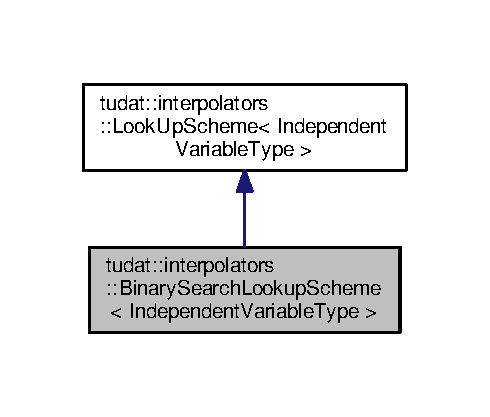
\includegraphics[width=235pt]{classtudat_1_1interpolators_1_1BinarySearchLookupScheme__inherit__graph}
\end{center}
\end{figure}


Collaboration diagram for tudat\+:\+:interpolators\+:\+:Binary\+Search\+Lookup\+Scheme$<$ Independent\+Variable\+Type $>$\+:
\nopagebreak
\begin{figure}[H]
\begin{center}
\leavevmode
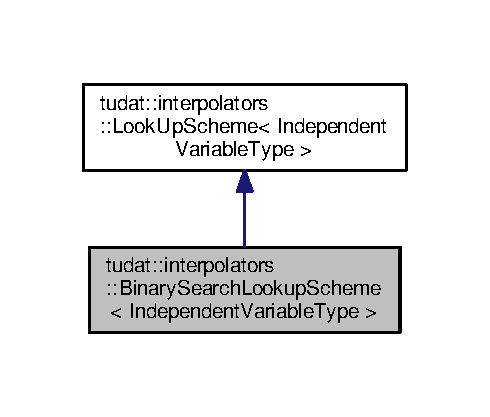
\includegraphics[width=235pt]{classtudat_1_1interpolators_1_1BinarySearchLookupScheme__coll__graph}
\end{center}
\end{figure}
\subsection*{Public Member Functions}
\begin{DoxyCompactItemize}
\item 
\hyperlink{classtudat_1_1interpolators_1_1BinarySearchLookupScheme_aa2ef6246aeee011cb6ab3786d0386481}{Binary\+Search\+Lookup\+Scheme} (const std\+::vector$<$ Independent\+Variable\+Type $>$ \&independent\+Variable\+Values)
\begin{DoxyCompactList}\small\item\em Constructor, used to set data vector. \end{DoxyCompactList}\item 
\hyperlink{classtudat_1_1interpolators_1_1BinarySearchLookupScheme_ae0a878950e354c57efb3fac7d402a47e}{$\sim$\+Binary\+Search\+Lookup\+Scheme} ()
\begin{DoxyCompactList}\small\item\em Default destructor. \end{DoxyCompactList}\item 
int \hyperlink{classtudat_1_1interpolators_1_1BinarySearchLookupScheme_a9c91bd06d198e6a5dc2a15ad7314c91f}{find\+Nearest\+Lower\+Neighbour} (const Independent\+Variable\+Type value\+To\+Lookup)
\begin{DoxyCompactList}\small\item\em Find nearest left neighbour. \end{DoxyCompactList}\end{DoxyCompactItemize}
\subsection*{Additional Inherited Members}


\subsection{Detailed Description}
\subsubsection*{template$<$typename Independent\+Variable\+Type$>$\\*
class tudat\+::interpolators\+::\+Binary\+Search\+Lookup\+Scheme$<$ Independent\+Variable\+Type $>$}

Look-\/up scheme class for nearest left neighbour search using binary search algorithm. 

Look-\/up scheme class for nearest left neighbour search using binary search algorithm. 
\begin{DoxyTemplParams}{Template Parameters}
{\em Independent\+Variable\+Type} & Type of entries of vector in which lookup is to be performed. \\
\hline
\end{DoxyTemplParams}


\subsection{Constructor \& Destructor Documentation}
\index{tudat\+::interpolators\+::\+Binary\+Search\+Lookup\+Scheme@{tudat\+::interpolators\+::\+Binary\+Search\+Lookup\+Scheme}!Binary\+Search\+Lookup\+Scheme@{Binary\+Search\+Lookup\+Scheme}}
\index{Binary\+Search\+Lookup\+Scheme@{Binary\+Search\+Lookup\+Scheme}!tudat\+::interpolators\+::\+Binary\+Search\+Lookup\+Scheme@{tudat\+::interpolators\+::\+Binary\+Search\+Lookup\+Scheme}}
\subsubsection[{\texorpdfstring{Binary\+Search\+Lookup\+Scheme(const std\+::vector$<$ Independent\+Variable\+Type $>$ \&independent\+Variable\+Values)}{BinarySearchLookupScheme(const std::vector< IndependentVariableType > &independentVariableValues)}}]{\setlength{\rightskip}{0pt plus 5cm}template$<$typename Independent\+Variable\+Type $>$ {\bf tudat\+::interpolators\+::\+Binary\+Search\+Lookup\+Scheme}$<$ Independent\+Variable\+Type $>$\+::{\bf Binary\+Search\+Lookup\+Scheme} (
\begin{DoxyParamCaption}
\item[{const std\+::vector$<$ Independent\+Variable\+Type $>$ \&}]{independent\+Variable\+Values}
\end{DoxyParamCaption}
)\hspace{0.3cm}{\ttfamily [inline]}}\hypertarget{classtudat_1_1interpolators_1_1BinarySearchLookupScheme_aa2ef6246aeee011cb6ab3786d0386481}{}\label{classtudat_1_1interpolators_1_1BinarySearchLookupScheme_aa2ef6246aeee011cb6ab3786d0386481}


Constructor, used to set data vector. 

Constructor, used to set data vector. 
\begin{DoxyParams}{Parameters}
{\em independent\+Variable\+Values} & vector of independent variable values in which to perform lookup procedure. \\
\hline
\end{DoxyParams}
\index{tudat\+::interpolators\+::\+Binary\+Search\+Lookup\+Scheme@{tudat\+::interpolators\+::\+Binary\+Search\+Lookup\+Scheme}!````~Binary\+Search\+Lookup\+Scheme@{$\sim$\+Binary\+Search\+Lookup\+Scheme}}
\index{````~Binary\+Search\+Lookup\+Scheme@{$\sim$\+Binary\+Search\+Lookup\+Scheme}!tudat\+::interpolators\+::\+Binary\+Search\+Lookup\+Scheme@{tudat\+::interpolators\+::\+Binary\+Search\+Lookup\+Scheme}}
\subsubsection[{\texorpdfstring{$\sim$\+Binary\+Search\+Lookup\+Scheme()}{~BinarySearchLookupScheme()}}]{\setlength{\rightskip}{0pt plus 5cm}template$<$typename Independent\+Variable\+Type $>$ {\bf tudat\+::interpolators\+::\+Binary\+Search\+Lookup\+Scheme}$<$ Independent\+Variable\+Type $>$\+::$\sim${\bf Binary\+Search\+Lookup\+Scheme} (
\begin{DoxyParamCaption}
{}
\end{DoxyParamCaption}
)\hspace{0.3cm}{\ttfamily [inline]}}\hypertarget{classtudat_1_1interpolators_1_1BinarySearchLookupScheme_ae0a878950e354c57efb3fac7d402a47e}{}\label{classtudat_1_1interpolators_1_1BinarySearchLookupScheme_ae0a878950e354c57efb3fac7d402a47e}


Default destructor. 

Default destructor 

\subsection{Member Function Documentation}
\index{tudat\+::interpolators\+::\+Binary\+Search\+Lookup\+Scheme@{tudat\+::interpolators\+::\+Binary\+Search\+Lookup\+Scheme}!find\+Nearest\+Lower\+Neighbour@{find\+Nearest\+Lower\+Neighbour}}
\index{find\+Nearest\+Lower\+Neighbour@{find\+Nearest\+Lower\+Neighbour}!tudat\+::interpolators\+::\+Binary\+Search\+Lookup\+Scheme@{tudat\+::interpolators\+::\+Binary\+Search\+Lookup\+Scheme}}
\subsubsection[{\texorpdfstring{find\+Nearest\+Lower\+Neighbour(const Independent\+Variable\+Type value\+To\+Lookup)}{findNearestLowerNeighbour(const IndependentVariableType valueToLookup)}}]{\setlength{\rightskip}{0pt plus 5cm}template$<$typename Independent\+Variable\+Type $>$ int {\bf tudat\+::interpolators\+::\+Binary\+Search\+Lookup\+Scheme}$<$ Independent\+Variable\+Type $>$\+::find\+Nearest\+Lower\+Neighbour (
\begin{DoxyParamCaption}
\item[{const Independent\+Variable\+Type}]{value\+To\+Lookup}
\end{DoxyParamCaption}
)\hspace{0.3cm}{\ttfamily [inline]}, {\ttfamily [virtual]}}\hypertarget{classtudat_1_1interpolators_1_1BinarySearchLookupScheme_a9c91bd06d198e6a5dc2a15ad7314c91f}{}\label{classtudat_1_1interpolators_1_1BinarySearchLookupScheme_a9c91bd06d198e6a5dc2a15ad7314c91f}


Find nearest left neighbour. 

Function finds nearest left neighbour of given value in independent\+Variable\+Values\+\_\+. 
\begin{DoxyParams}{Parameters}
{\em value\+To\+Lookup} & Value of which nearest neaighbour is to be determined. \\
\hline
\end{DoxyParams}
\begin{DoxyReturn}{Returns}
Index of entry in independent\+Variable\+Values\+\_\+ vector which is nearest lower neighbour to value\+To\+Lookup. 
\end{DoxyReturn}


Implements \hyperlink{classtudat_1_1interpolators_1_1LookUpScheme_a7749ee1bb2df25690a6e040a3e61f646}{tudat\+::interpolators\+::\+Look\+Up\+Scheme$<$ Independent\+Variable\+Type $>$}.



The documentation for this class was generated from the following file\+:\begin{DoxyCompactItemize}
\item 
/home/lupi/\+Tudat/tudat\+Bundle/tudat/\+Tudat/\+Mathematics/\+Interpolators/lookup\+Scheme.\+h\end{DoxyCompactItemize}

\hypertarget{classtudat_1_1root__finders_1_1BisectionCore}{}\section{tudat\+:\+:root\+\_\+finders\+:\+:Bisection\+Core$<$ Data\+Type $>$ Class Template Reference}
\label{classtudat_1_1root__finders_1_1BisectionCore}\index{tudat\+::root\+\_\+finders\+::\+Bisection\+Core$<$ Data\+Type $>$@{tudat\+::root\+\_\+finders\+::\+Bisection\+Core$<$ Data\+Type $>$}}


Bisection root-\/finding method.  




{\ttfamily \#include $<$bisection.\+h$>$}



Inheritance diagram for tudat\+:\+:root\+\_\+finders\+:\+:Bisection\+Core$<$ Data\+Type $>$\+:
\nopagebreak
\begin{figure}[H]
\begin{center}
\leavevmode
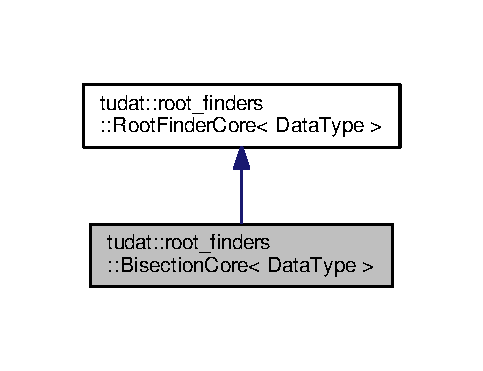
\includegraphics[width=232pt]{classtudat_1_1root__finders_1_1BisectionCore__inherit__graph}
\end{center}
\end{figure}


Collaboration diagram for tudat\+:\+:root\+\_\+finders\+:\+:Bisection\+Core$<$ Data\+Type $>$\+:
\nopagebreak
\begin{figure}[H]
\begin{center}
\leavevmode
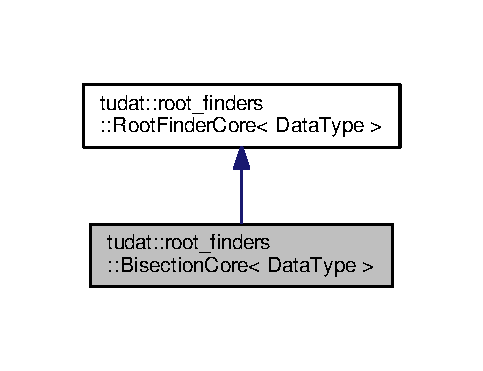
\includegraphics[width=232pt]{classtudat_1_1root__finders_1_1BisectionCore__coll__graph}
\end{center}
\end{figure}
\subsection*{Public Types}
\begin{DoxyCompactItemize}
\item 
typedef \hyperlink{classtudat_1_1root__finders_1_1RootFinderCore}{Root\+Finder\+Core}$<$ Data\+Type $>$\+::\hyperlink{classtudat_1_1root__finders_1_1BisectionCore_aaceafb2a0ce4effa2862eea28d7869c3}{Function\+Pointer} \hyperlink{classtudat_1_1root__finders_1_1BisectionCore_aaceafb2a0ce4effa2862eea28d7869c3}{Function\+Pointer}\hypertarget{classtudat_1_1root__finders_1_1BisectionCore_aaceafb2a0ce4effa2862eea28d7869c3}{}\label{classtudat_1_1root__finders_1_1BisectionCore_aaceafb2a0ce4effa2862eea28d7869c3}

\begin{DoxyCompactList}\small\item\em Useful type definition for the function pointer (from base class). \end{DoxyCompactList}\item 
typedef \hyperlink{classtudat_1_1root__finders_1_1RootFinderCore}{Root\+Finder\+Core}$<$ Data\+Type $>$\+::\hyperlink{classtudat_1_1root__finders_1_1BisectionCore_a4bfc03809c03253f1e3602cb75335adf}{Termination\+Function} \hyperlink{classtudat_1_1root__finders_1_1BisectionCore_a4bfc03809c03253f1e3602cb75335adf}{Termination\+Function}\hypertarget{classtudat_1_1root__finders_1_1BisectionCore_a4bfc03809c03253f1e3602cb75335adf}{}\label{classtudat_1_1root__finders_1_1BisectionCore_a4bfc03809c03253f1e3602cb75335adf}

\begin{DoxyCompactList}\small\item\em Useful type definition for the termination function (from base class). \end{DoxyCompactList}\end{DoxyCompactItemize}
\subsection*{Public Member Functions}
\begin{DoxyCompactItemize}
\item 
\hyperlink{classtudat_1_1root__finders_1_1BisectionCore_a947611a377418f1bbaf3e02c3e1b1ccd}{Bisection\+Core} (const \hyperlink{classtudat_1_1root__finders_1_1BisectionCore_a4bfc03809c03253f1e3602cb75335adf}{Termination\+Function} \hyperlink{classtudat_1_1root__finders_1_1RootFinderCore_a7a1efe7ce979318d398b4bb8574e70d6}{termination\+Function}, const Data\+Type lower\+Bound=-\/1.\+0, const Data\+Type upper\+Bound=1.\+0)
\begin{DoxyCompactList}\small\item\em Constructor taking a general termination function and the bracket of the solution. \end{DoxyCompactList}\item 
\hyperlink{classtudat_1_1root__finders_1_1BisectionCore_a631cdc22e0e5c364af8ba37af4183918}{Bisection\+Core} (const Data\+Type relative\+X\+Tolerance, const unsigned int max\+Iterations, const Data\+Type lower\+Bound=-\/1.\+0, const Data\+Type upper\+Bound=1.\+0)
\begin{DoxyCompactList}\small\item\em Constructor taking typical convergence criteria and the bracket of the solution. \end{DoxyCompactList}\item 
\hyperlink{classtudat_1_1root__finders_1_1BisectionCore_a51134d2717d23f95189d0d6eaddcb622}{$\sim$\+Bisection\+Core} ()\hypertarget{classtudat_1_1root__finders_1_1BisectionCore_a51134d2717d23f95189d0d6eaddcb622}{}\label{classtudat_1_1root__finders_1_1BisectionCore_a51134d2717d23f95189d0d6eaddcb622}

\begin{DoxyCompactList}\small\item\em Default destructor. \end{DoxyCompactList}\item 
Data\+Type \hyperlink{classtudat_1_1root__finders_1_1BisectionCore_ab8798225ad2e0ffa6d44b462b6f24584}{execute} (const \hyperlink{classtudat_1_1root__finders_1_1BisectionCore_aaceafb2a0ce4effa2862eea28d7869c3}{Function\+Pointer} \hyperlink{classtudat_1_1root__finders_1_1RootFinderCore_afbe57f7fa3baba13128d9dc2ca41dedd}{root\+Function}, const Data\+Type initial\+Guess=0.\+0)
\begin{DoxyCompactList}\small\item\em Find a root of the function provided as input. \end{DoxyCompactList}\item 
void \hyperlink{classtudat_1_1root__finders_1_1BisectionCore_ad493b8969c88ebb93eb6086f053cec98}{reset\+Boundaries} (const Data\+Type lower\+Bound, const Data\+Type upper\+Bound)
\begin{DoxyCompactList}\small\item\em Reset the bracket of the solution. \end{DoxyCompactList}\end{DoxyCompactItemize}
\subsection*{Additional Inherited Members}


\subsection{Detailed Description}
\subsubsection*{template$<$typename Data\+Type = double$>$\\*
class tudat\+::root\+\_\+finders\+::\+Bisection\+Core$<$ Data\+Type $>$}

Bisection root-\/finding method. 

The bisection root-\/finding method, a basic and robust root-\/finder that will always find a root given that a root exists, the function is continuous on the interval, and that it is bracketed by the lower and upper bound (required). For this method only the function of which the zero is sought is required, and no derivatives. It is recommended to use this method for validation only, as it is relatively slow.

It works by repeatedly shrinking the \mbox{[}lowerbound, upperbound\mbox{]} interval until the root has been found with sufficient accuracy. The shrinking is done by dividing the interval in half and evaluating in which interval the root lies. This sub-\/interval is then kept for the next iteration. The process is continued until the interval is sufficiently small. \mbox{[}Press et al., 2007\mbox{]}

Defined shorthand notations\+: Bisection\+Core$<$ double $>$ =$>$ Bisection


\begin{DoxyTemplParams}{Template Parameters}
{\em Data\+Type} & Data type used to represent floating-\/point values. \\
\hline
\end{DoxyTemplParams}


\subsection{Constructor \& Destructor Documentation}
\index{tudat\+::root\+\_\+finders\+::\+Bisection\+Core@{tudat\+::root\+\_\+finders\+::\+Bisection\+Core}!Bisection\+Core@{Bisection\+Core}}
\index{Bisection\+Core@{Bisection\+Core}!tudat\+::root\+\_\+finders\+::\+Bisection\+Core@{tudat\+::root\+\_\+finders\+::\+Bisection\+Core}}
\subsubsection[{\texorpdfstring{Bisection\+Core(const Termination\+Function termination\+Function, const Data\+Type lower\+Bound=-\/1.\+0, const Data\+Type upper\+Bound=1.\+0)}{BisectionCore(const TerminationFunction terminationFunction, const DataType lowerBound=-1.0, const DataType upperBound=1.0)}}]{\setlength{\rightskip}{0pt plus 5cm}template$<$typename Data\+Type  = double$>$ {\bf tudat\+::root\+\_\+finders\+::\+Bisection\+Core}$<$ Data\+Type $>$\+::{\bf Bisection\+Core} (
\begin{DoxyParamCaption}
\item[{const {\bf Termination\+Function}}]{termination\+Function, }
\item[{const Data\+Type}]{lower\+Bound = {\ttfamily -\/1.0}, }
\item[{const Data\+Type}]{upper\+Bound = {\ttfamily 1.0}}
\end{DoxyParamCaption}
)\hspace{0.3cm}{\ttfamily [inline]}}\hypertarget{classtudat_1_1root__finders_1_1BisectionCore_a947611a377418f1bbaf3e02c3e1b1ccd}{}\label{classtudat_1_1root__finders_1_1BisectionCore_a947611a377418f1bbaf3e02c3e1b1ccd}


Constructor taking a general termination function and the bracket of the solution. 

Constructor of the Bisection root-\/finder, taking the termination function (function determining whether to terminate the root-\/finding process) and the search interval with an upper and lower bound. It is required that the function values at upper and lower bound have an opposite sign. The default interval is \mbox{[}-\/1, 1\mbox{]}.


\begin{DoxyParams}{Parameters}
{\em termination\+Function} & The function specifying the termination conditions of the root-\/finding process. \\
\hline
\end{DoxyParams}
\begin{DoxySeeAlso}{See also}
\hyperlink{classtudat_1_1root__finders_1_1RootFinderCore_a7a1efe7ce979318d398b4bb8574e70d6}{Root\+Finder\+Core\+::termination\+Function} 
\end{DoxySeeAlso}

\begin{DoxyParams}{Parameters}
{\em lower\+Bound} & Lower bound of the interval containing a root. (Default is -\/1.\+0). \\
\hline
{\em upper\+Bound} & Upper bound of the interval containing a root. (Default is 1.\+0). \\
\hline
\end{DoxyParams}
\index{tudat\+::root\+\_\+finders\+::\+Bisection\+Core@{tudat\+::root\+\_\+finders\+::\+Bisection\+Core}!Bisection\+Core@{Bisection\+Core}}
\index{Bisection\+Core@{Bisection\+Core}!tudat\+::root\+\_\+finders\+::\+Bisection\+Core@{tudat\+::root\+\_\+finders\+::\+Bisection\+Core}}
\subsubsection[{\texorpdfstring{Bisection\+Core(const Data\+Type relative\+X\+Tolerance, const unsigned int max\+Iterations, const Data\+Type lower\+Bound=-\/1.\+0, const Data\+Type upper\+Bound=1.\+0)}{BisectionCore(const DataType relativeXTolerance, const unsigned int maxIterations, const DataType lowerBound=-1.0, const DataType upperBound=1.0)}}]{\setlength{\rightskip}{0pt plus 5cm}template$<$typename Data\+Type  = double$>$ {\bf tudat\+::root\+\_\+finders\+::\+Bisection\+Core}$<$ Data\+Type $>$\+::{\bf Bisection\+Core} (
\begin{DoxyParamCaption}
\item[{const Data\+Type}]{relative\+X\+Tolerance, }
\item[{const unsigned int}]{max\+Iterations, }
\item[{const Data\+Type}]{lower\+Bound = {\ttfamily -\/1.0}, }
\item[{const Data\+Type}]{upper\+Bound = {\ttfamily 1.0}}
\end{DoxyParamCaption}
)\hspace{0.3cm}{\ttfamily [inline]}}\hypertarget{classtudat_1_1root__finders_1_1BisectionCore_a631cdc22e0e5c364af8ba37af4183918}{}\label{classtudat_1_1root__finders_1_1BisectionCore_a631cdc22e0e5c364af8ba37af4183918}


Constructor taking typical convergence criteria and the bracket of the solution. 

Constructor of the Bisection root-\/finder, taking the maximum number of iterations, the relative tolerance for the independent variable, and the search interval with upper and lower bound. It is required that the function values at upper and lower bound have an opposite sign. The default interval is \mbox{[}-\/1, 1\mbox{]}. If desired, a custom convergence function can be provided to the alternative constructor.


\begin{DoxyParams}{Parameters}
{\em relative\+X\+Tolerance} & Relative difference between the root solution of two subsequent solutions below which convergence is reached. \\
\hline
{\em max\+Iterations} & Maximum number of iterations after which the root finder is terminated, i.\+e. convergence is assumed. \\
\hline
{\em lower\+Bound} & Lower bound of the interval containing a root. (Default is -\/1.\+0). \\
\hline
{\em upper\+Bound} & Upper bound of the interval containing a root. (Default is 1.\+0). \\
\hline
\end{DoxyParams}


\subsection{Member Function Documentation}
\index{tudat\+::root\+\_\+finders\+::\+Bisection\+Core@{tudat\+::root\+\_\+finders\+::\+Bisection\+Core}!execute@{execute}}
\index{execute@{execute}!tudat\+::root\+\_\+finders\+::\+Bisection\+Core@{tudat\+::root\+\_\+finders\+::\+Bisection\+Core}}
\subsubsection[{\texorpdfstring{execute(const Function\+Pointer root\+Function, const Data\+Type initial\+Guess=0.\+0)}{execute(const FunctionPointer rootFunction, const DataType initialGuess=0.0)}}]{\setlength{\rightskip}{0pt plus 5cm}template$<$typename Data\+Type  = double$>$ Data\+Type {\bf tudat\+::root\+\_\+finders\+::\+Bisection\+Core}$<$ Data\+Type $>$\+::execute (
\begin{DoxyParamCaption}
\item[{const {\bf Function\+Pointer}}]{root\+Function, }
\item[{const Data\+Type}]{initial\+Guess = {\ttfamily 0.0}}
\end{DoxyParamCaption}
)\hspace{0.3cm}{\ttfamily [inline]}, {\ttfamily [virtual]}}\hypertarget{classtudat_1_1root__finders_1_1BisectionCore_ab8798225ad2e0ffa6d44b462b6f24584}{}\label{classtudat_1_1root__finders_1_1BisectionCore_ab8798225ad2e0ffa6d44b462b6f24584}


Find a root of the function provided as input. 

Find a root of the function provided as input, using the termination function set by the constructor. (Note that the initial guess is not used, but is a requirement of the root-\/finder architecture.)


\begin{DoxyParams}{Parameters}
{\em root\+Function} & Function to find the root of. \\
\hline
{\em initial\+Guess} & The initial guess of the root. (Not used, default is 0.\+0). \\
\hline
\end{DoxyParams}
\begin{DoxyReturn}{Returns}
Root of the root\+Function that is found.
\end{DoxyReturn}

\begin{DoxyExceptions}{Exceptions}
{\em Convergence\+Exeption} & If the solution does not converge to a root value. \\
\hline
{\em std\+::runtime\+\_\+error} & If the interval does not bracket the root. \\
\hline
\end{DoxyExceptions}


Implements \hyperlink{classtudat_1_1root__finders_1_1RootFinderCore_a1fcd710906f66ebea649c83f08c2ae97}{tudat\+::root\+\_\+finders\+::\+Root\+Finder\+Core$<$ Data\+Type $>$}.

\index{tudat\+::root\+\_\+finders\+::\+Bisection\+Core@{tudat\+::root\+\_\+finders\+::\+Bisection\+Core}!reset\+Boundaries@{reset\+Boundaries}}
\index{reset\+Boundaries@{reset\+Boundaries}!tudat\+::root\+\_\+finders\+::\+Bisection\+Core@{tudat\+::root\+\_\+finders\+::\+Bisection\+Core}}
\subsubsection[{\texorpdfstring{reset\+Boundaries(const Data\+Type lower\+Bound, const Data\+Type upper\+Bound)}{resetBoundaries(const DataType lowerBound, const DataType upperBound)}}]{\setlength{\rightskip}{0pt plus 5cm}template$<$typename Data\+Type  = double$>$ void {\bf tudat\+::root\+\_\+finders\+::\+Bisection\+Core}$<$ Data\+Type $>$\+::reset\+Boundaries (
\begin{DoxyParamCaption}
\item[{const Data\+Type}]{lower\+Bound, }
\item[{const Data\+Type}]{upper\+Bound}
\end{DoxyParamCaption}
)\hspace{0.3cm}{\ttfamily [inline]}}\hypertarget{classtudat_1_1root__finders_1_1BisectionCore_ad493b8969c88ebb93eb6086f053cec98}{}\label{classtudat_1_1root__finders_1_1BisectionCore_ad493b8969c88ebb93eb6086f053cec98}


Reset the bracket of the solution. 

Resets the search interval with an upper and lower bound. It is required that the function values at upper and lower bound have an opposite sign.


\begin{DoxyParams}{Parameters}
{\em lower\+Bound} & Lower bound of the interval containing a root. \\
\hline
{\em upper\+Bound} & Upper bound of the interval containing a root. \\
\hline
\end{DoxyParams}


The documentation for this class was generated from the following file\+:\begin{DoxyCompactItemize}
\item 
/home/lupi/\+Tudat/tudat\+Bundle/tudat/\+Tudat/\+Mathematics/\+Root\+Finders/bisection.\+h\end{DoxyCompactItemize}

\hypertarget{classtudat_1_1simulation__setup_1_1Body}{}\section{tudat\+:\+:simulation\+\_\+setup\+:\+:Body Class Reference}
\label{classtudat_1_1simulation__setup_1_1Body}\index{tudat\+::simulation\+\_\+setup\+::\+Body@{tudat\+::simulation\+\_\+setup\+::\+Body}}


\hyperlink{classtudat_1_1simulation__setup_1_1Body}{Body} class representing the properties of a celestial body (natural or artificial).  




{\ttfamily \#include $<$body.\+h$>$}

\subsection*{Public Member Functions}
\begin{DoxyCompactItemize}
\item 
\hyperlink{classtudat_1_1simulation__setup_1_1Body_a802232493506b5fc4956779e74468f06}{Body} (const Eigen\+::\+Vector6d \&state=Eigen\+::\+Vector6d\+::\+Zero())
\begin{DoxyCompactList}\small\item\em Constructor for a body. \end{DoxyCompactList}\item 
boost\+::shared\+\_\+ptr$<$ \hyperlink{classtudat_1_1simulation__setup_1_1BaseStateInterface}{Base\+State\+Interface} $>$ \hyperlink{classtudat_1_1simulation__setup_1_1Body_a4dbe4ca3a89d67dfa7da256ad5343b68}{get\+Ephemeris\+Frame\+To\+Base\+Frame} ()
\begin{DoxyCompactList}\small\item\em Function to retrieve the class returning the state of this body\textquotesingle{}s ephemeris origin w.\+r.\+t. the global origin. \end{DoxyCompactList}\item 
void \hyperlink{classtudat_1_1simulation__setup_1_1Body_a6f30112a19952498a20d482ac5632012}{set\+Ephemeris\+Frame\+To\+Base\+Frame} (const boost\+::shared\+\_\+ptr$<$ \hyperlink{classtudat_1_1simulation__setup_1_1BaseStateInterface}{Base\+State\+Interface} $>$ ephemeris\+Frame\+To\+Base\+Frame)
\begin{DoxyCompactList}\small\item\em Function to set the class returning the state of this body\textquotesingle{}s ephemeris origin w.\+r.\+t. the global origin. \end{DoxyCompactList}\item 
void \hyperlink{classtudat_1_1simulation__setup_1_1Body_a157e498e30d7c90dd7a4b73c719fd5d5}{set\+State} (const Eigen\+::\+Vector6d \&state)
\begin{DoxyCompactList}\small\item\em Set current state of body manually. \end{DoxyCompactList}\item 
void \hyperlink{classtudat_1_1simulation__setup_1_1Body_ae5f634a6c751ad8922dc6e6662f6a502}{set\+Long\+State} (const Eigen\+::\+Matrix$<$ long double, 6, 1 $>$ \&long\+State)
\begin{DoxyCompactList}\small\item\em Set current state of body manually in long double precision. \end{DoxyCompactList}\item 
{\footnotesize template$<$typename State\+Scalar\+Type $>$ }\\void \hyperlink{classtudat_1_1simulation__setup_1_1Body_ab56fa0e8697fbb2dab1943d36fb7d493}{set\+Templated\+State} (const Eigen\+::\+Matrix$<$ State\+Scalar\+Type, 6, 1 $>$ \&state)
\begin{DoxyCompactList}\small\item\em Templated function to set the state manually. \end{DoxyCompactList}\item 
{\footnotesize template$<$typename State\+Scalar\+Type  = double, typename Time\+Type  = double$>$ }\\void \hyperlink{classtudat_1_1simulation__setup_1_1Body_a2f2cfc32c8e5b257b352809d623b2985}{set\+State\+From\+Ephemeris} (const Time\+Type \&time)
\item 
{\footnotesize template$<$typename State\+Scalar\+Type  = double, typename Time\+Type  = double$>$ }\\Eigen\+::\+Matrix$<$ State\+Scalar\+Type, 6, 1 $>$ \hyperlink{classtudat_1_1simulation__setup_1_1Body_a4ad52e0fbd714ebd2494d65005a8da5e}{get\+State\+In\+Base\+Frame\+From\+Ephemeris} (const Time\+Type time)
\item 
Eigen\+::\+Vector6d \hyperlink{classtudat_1_1simulation__setup_1_1Body_ae4541711e56e09272916448030882fc9}{get\+State} ()
\begin{DoxyCompactList}\small\item\em Get current state. \end{DoxyCompactList}\item 
Eigen\+::\+Vector3d \hyperlink{classtudat_1_1simulation__setup_1_1Body_a595498359521268dbeedc902953a0633}{get\+Position} ()
\begin{DoxyCompactList}\small\item\em Get current position. \end{DoxyCompactList}\item 
Eigen\+::\+Vector3d \hyperlink{classtudat_1_1simulation__setup_1_1Body_ad043093286bc331c63cefbeba4fa17d8}{get\+Velocity} ()
\begin{DoxyCompactList}\small\item\em Get current velocity. \end{DoxyCompactList}\item 
Eigen\+::\+Matrix$<$ long double, 6, 1 $>$ \hyperlink{classtudat_1_1simulation__setup_1_1Body_ab7c0bcfab31d20e5c203da1f92b90792}{get\+Long\+State} ()
\begin{DoxyCompactList}\small\item\em Get current state, in long double precision. \end{DoxyCompactList}\item 
Eigen\+::\+Matrix$<$ long double, 3, 1 $>$ \hyperlink{classtudat_1_1simulation__setup_1_1Body_ad60f6964ee99fca9f6a7ea5047a108ff}{get\+Long\+Position} ()
\begin{DoxyCompactList}\small\item\em Get current position, in long double precision. \end{DoxyCompactList}\item 
Eigen\+::\+Matrix$<$ long double, 3, 1 $>$ \hyperlink{classtudat_1_1simulation__setup_1_1Body_aeed3f086d3ca8d4c037bee67ad123016}{get\+Long\+Velocity} ()
\begin{DoxyCompactList}\small\item\em Get current velocity, in long double precision. \end{DoxyCompactList}\item 
{\footnotesize template$<$typename Scalar\+State\+Type $>$ }\\Eigen\+::\+Matrix$<$ Scalar\+State\+Type, 6, 1 $>$ \hyperlink{classtudat_1_1simulation__setup_1_1Body_a11ce61a7598916958edbbaf1e52415ca}{get\+Templated\+State} ()
\begin{DoxyCompactList}\small\item\em Templated function to retrieve the state. \end{DoxyCompactList}\item 
void \hyperlink{classtudat_1_1simulation__setup_1_1Body_a06605a2e4d471743ab9ff19feb6f3431}{set\+Current\+Rotation\+To\+Local\+Frame\+From\+Ephemeris} (const double time)
\begin{DoxyCompactList}\small\item\em Function to set the rotation from global to body-\/fixed frame at given time. \end{DoxyCompactList}\item 
void \hyperlink{classtudat_1_1simulation__setup_1_1Body_a352f45d815d365b742e55e94e0ec8f4c}{set\+Current\+Rotation\+To\+Local\+Frame\+Derivative\+From\+Ephemeris} (const double time)
\begin{DoxyCompactList}\small\item\em Function to set the rotation matrix derivative from global to body-\/fixed frame at given time. \end{DoxyCompactList}\item 
void \hyperlink{classtudat_1_1simulation__setup_1_1Body_a61a6e3eccaed8d438c22003516d8009f}{set\+Current\+Angular\+Velocity\+Vector\+In\+Global\+Frame} (const double time)
\begin{DoxyCompactList}\small\item\em Function to set the angular velocity vector in the global frame at given time. \end{DoxyCompactList}\item 
void \hyperlink{classtudat_1_1simulation__setup_1_1Body_afb338d46d3f9de1df04b929ed3766292}{set\+Current\+Rotational\+State\+To\+Local\+Frame\+From\+Ephemeris} (const double time)
\begin{DoxyCompactList}\small\item\em Function to set the full rotational state at given time. \end{DoxyCompactList}\item 
Eigen\+::\+Quaterniond \hyperlink{classtudat_1_1simulation__setup_1_1Body_a4c6c29c88751b36dbb09348115c436e2}{get\+Current\+Rotation\+To\+Global\+Frame} ()
\begin{DoxyCompactList}\small\item\em Get current rotation from body-\/fixed to inertial frame. \end{DoxyCompactList}\item 
Eigen\+::\+Quaterniond \hyperlink{classtudat_1_1simulation__setup_1_1Body_a7eaf728cdc11cf98ac7e7b75e38b62ca}{get\+Current\+Rotation\+To\+Local\+Frame} ()
\begin{DoxyCompactList}\small\item\em Get current rotation from inertial to body-\/fixed frame. \end{DoxyCompactList}\item 
Eigen\+::\+Matrix3d \hyperlink{classtudat_1_1simulation__setup_1_1Body_a0946c1b5fa661abd9935041ca7bc37ac}{get\+Current\+Rotation\+Matrix\+Derivative\+To\+Global\+Frame} ()
\begin{DoxyCompactList}\small\item\em Get current rotation matrix derivative from body-\/fixed to global frame. \end{DoxyCompactList}\item 
Eigen\+::\+Matrix3d \hyperlink{classtudat_1_1simulation__setup_1_1Body_a0cd33824b4bbd33c4ca120098a5bebd4}{get\+Current\+Rotation\+Matrix\+Derivative\+To\+Local\+Frame} ()
\begin{DoxyCompactList}\small\item\em Get current rotation matrix derivative from global to body-\/fixed frame. \end{DoxyCompactList}\item 
void \hyperlink{classtudat_1_1simulation__setup_1_1Body_ab9ee176fb6d8f2a8f9df7d1acce3ef24}{set\+Ephemeris} (const boost\+::shared\+\_\+ptr$<$ \hyperlink{classtudat_1_1ephemerides_1_1Ephemeris}{ephemerides\+::\+Ephemeris} $>$ body\+Ephemeris)
\begin{DoxyCompactList}\small\item\em Function to set the ephemeris of the body. \end{DoxyCompactList}\item 
void \hyperlink{classtudat_1_1simulation__setup_1_1Body_a66b39c1fb3827c1a59ba4f036e2b68d8}{set\+Gravity\+Field\+Model} (const boost\+::shared\+\_\+ptr$<$ \hyperlink{classtudat_1_1gravitation_1_1GravityFieldModel}{gravitation\+::\+Gravity\+Field\+Model} $>$ gravity\+Field\+Model)
\begin{DoxyCompactList}\small\item\em Function to set the gravity field of the body. \end{DoxyCompactList}\item 
void \hyperlink{classtudat_1_1simulation__setup_1_1Body_a2c14b27ed335c1dee68f943651f3be9a}{set\+Atmosphere\+Model} (const boost\+::shared\+\_\+ptr$<$ \hyperlink{classtudat_1_1aerodynamics_1_1AtmosphereModel}{aerodynamics\+::\+Atmosphere\+Model} $>$ atmosphere\+Model)
\begin{DoxyCompactList}\small\item\em Function to set the atmosphere model of the body. \end{DoxyCompactList}\item 
void \hyperlink{classtudat_1_1simulation__setup_1_1Body_ad72a4d4f70bf04344b4438480074178e}{set\+Rotational\+Ephemeris} (const boost\+::shared\+\_\+ptr$<$ \hyperlink{classtudat_1_1ephemerides_1_1RotationalEphemeris}{ephemerides\+::\+Rotational\+Ephemeris} $>$ rotational\+Ephemeris)
\begin{DoxyCompactList}\small\item\em Function to set the rotation model of the body. \end{DoxyCompactList}\item 
void \hyperlink{classtudat_1_1simulation__setup_1_1Body_aaeae7e6f9394ee839d1a578c80f33ed5}{set\+Dependent\+Orientation\+Calculator} (const boost\+::shared\+\_\+ptr$<$ \hyperlink{classtudat_1_1reference__frames_1_1DependentOrientationCalculator}{reference\+\_\+frames\+::\+Dependent\+Orientation\+Calculator} $>$ dependent\+Orientation\+Calculator)
\begin{DoxyCompactList}\small\item\em Function to set a rotation model that is only valid during numerical propagation. \end{DoxyCompactList}\item 
void \hyperlink{classtudat_1_1simulation__setup_1_1Body_ab64e549564945923504749067e0f0879}{set\+Shape\+Model} (const boost\+::shared\+\_\+ptr$<$ \hyperlink{classtudat_1_1basic__astrodynamics_1_1BodyShapeModel}{basic\+\_\+astrodynamics\+::\+Body\+Shape\+Model} $>$ shape\+Model)
\begin{DoxyCompactList}\small\item\em Function to set the shape model of the body. \end{DoxyCompactList}\item 
void \hyperlink{classtudat_1_1simulation__setup_1_1Body_aced3d9fdcfc443e55c48e8869537fa5e}{set\+Aerodynamic\+Coefficient\+Interface} (const boost\+::shared\+\_\+ptr$<$ \hyperlink{classtudat_1_1aerodynamics_1_1AerodynamicCoefficientInterface}{aerodynamics\+::\+Aerodynamic\+Coefficient\+Interface} $>$ aerodynamic\+Coefficient\+Interface)
\begin{DoxyCompactList}\small\item\em Function to set the aerodynamic coefficient interface of the body. \end{DoxyCompactList}\item 
void \hyperlink{classtudat_1_1simulation__setup_1_1Body_a1d1ae13ce0f4ad3d74c69a3bfbddd654}{set\+Flight\+Conditions} (const boost\+::shared\+\_\+ptr$<$ \hyperlink{classtudat_1_1aerodynamics_1_1FlightConditions}{aerodynamics\+::\+Flight\+Conditions} $>$ aerodynamic\+Flight\+Conditions)
\begin{DoxyCompactList}\small\item\em Function to set the body flight conditions. \end{DoxyCompactList}\item 
void \hyperlink{classtudat_1_1simulation__setup_1_1Body_ad52f9dc125c95021748c42ee5dd03621}{set\+Radiation\+Pressure\+Interface} (const std\+::string \&radiating\+Body, const boost\+::shared\+\_\+ptr$<$ \hyperlink{classtudat_1_1electro__magnetism_1_1RadiationPressureInterface}{electro\+\_\+magnetism\+::\+Radiation\+Pressure\+Interface} $>$ radiation\+Pressure\+Interface)
\begin{DoxyCompactList}\small\item\em Function to set the radiation pressure interface of the body, for a single radiation source. \end{DoxyCompactList}\item 
void \hyperlink{classtudat_1_1simulation__setup_1_1Body_a72d039d757b7e8b70654b79c776a32d4}{set\+Gravity\+Field\+Variation\+Set} (const boost\+::shared\+\_\+ptr$<$ \hyperlink{classtudat_1_1gravitation_1_1GravityFieldVariationsSet}{gravitation\+::\+Gravity\+Field\+Variations\+Set} $>$ gravity\+Field\+Variation\+Set)
\begin{DoxyCompactList}\small\item\em Function to set object containing all variations in the gravity field of this body. \end{DoxyCompactList}\item 
boost\+::shared\+\_\+ptr$<$ \hyperlink{classtudat_1_1gravitation_1_1GravityFieldModel}{gravitation\+::\+Gravity\+Field\+Model} $>$ \hyperlink{classtudat_1_1simulation__setup_1_1Body_adddf3831784320b9bc7a4c2f18ddc57d}{get\+Gravity\+Field\+Model} ()
\begin{DoxyCompactList}\small\item\em Function to get the gravity field model of the body. \end{DoxyCompactList}\item 
boost\+::shared\+\_\+ptr$<$ \hyperlink{classtudat_1_1ephemerides_1_1Ephemeris}{ephemerides\+::\+Ephemeris} $>$ \hyperlink{classtudat_1_1simulation__setup_1_1Body_a6df4ae46413f18304ec775ff430ffbea}{get\+Ephemeris} ()
\begin{DoxyCompactList}\small\item\em Function to get the ephemeris of the body. \end{DoxyCompactList}\item 
boost\+::shared\+\_\+ptr$<$ \hyperlink{classtudat_1_1aerodynamics_1_1AtmosphereModel}{aerodynamics\+::\+Atmosphere\+Model} $>$ \hyperlink{classtudat_1_1simulation__setup_1_1Body_ad655df1fe0eb22fcce46dcc0cd579c70}{get\+Atmosphere\+Model} ()
\begin{DoxyCompactList}\small\item\em Function to get the atmosphere model of the body. \end{DoxyCompactList}\item 
boost\+::shared\+\_\+ptr$<$ \hyperlink{classtudat_1_1ephemerides_1_1RotationalEphemeris}{ephemerides\+::\+Rotational\+Ephemeris} $>$ \hyperlink{classtudat_1_1simulation__setup_1_1Body_ad7f9739ae689c56a6e1c4903bcdcc7f0}{get\+Rotational\+Ephemeris} ()
\begin{DoxyCompactList}\small\item\em Function to get the rotation model of the body. \end{DoxyCompactList}\item 
boost\+::shared\+\_\+ptr$<$ \hyperlink{classtudat_1_1reference__frames_1_1DependentOrientationCalculator}{reference\+\_\+frames\+::\+Dependent\+Orientation\+Calculator} $>$ \hyperlink{classtudat_1_1simulation__setup_1_1Body_a449bb506aa309e75f20429d0d285697e}{get\+Dependent\+Orientation\+Calculator} ()
\begin{DoxyCompactList}\small\item\em Function to retrieve the model to compute the rotation of the body based on the current state of the environment. \end{DoxyCompactList}\item 
boost\+::shared\+\_\+ptr$<$ \hyperlink{classtudat_1_1basic__astrodynamics_1_1BodyShapeModel}{basic\+\_\+astrodynamics\+::\+Body\+Shape\+Model} $>$ \hyperlink{classtudat_1_1simulation__setup_1_1Body_afbb63724c2b0d7453475bf1c186793dc}{get\+Shape\+Model} ()
\begin{DoxyCompactList}\small\item\em Function to retrieve the shape model of body. \end{DoxyCompactList}\item 
boost\+::shared\+\_\+ptr$<$ \hyperlink{classtudat_1_1aerodynamics_1_1AerodynamicCoefficientInterface}{aerodynamics\+::\+Aerodynamic\+Coefficient\+Interface} $>$ \hyperlink{classtudat_1_1simulation__setup_1_1Body_a08e15216b11433e344afc9db6a17dff8}{get\+Aerodynamic\+Coefficient\+Interface} ()
\begin{DoxyCompactList}\small\item\em Function to retrieve the aerodynamic coefficient model of body. \end{DoxyCompactList}\item 
boost\+::shared\+\_\+ptr$<$ \hyperlink{classtudat_1_1aerodynamics_1_1FlightConditions}{aerodynamics\+::\+Flight\+Conditions} $>$ \hyperlink{classtudat_1_1simulation__setup_1_1Body_abf095882cd458103d85419fc3d306cb4}{get\+Flight\+Conditions} ()
\begin{DoxyCompactList}\small\item\em Function to retrieve the body flight conditions. \end{DoxyCompactList}\item 
std\+::map$<$ std\+::string, boost\+::shared\+\_\+ptr$<$ \hyperlink{classtudat_1_1electro__magnetism_1_1RadiationPressureInterface}{electro\+\_\+magnetism\+::\+Radiation\+Pressure\+Interface} $>$ $>$ \hyperlink{classtudat_1_1simulation__setup_1_1Body_a6f17a6e2e52d0a3b88414e6c2efb2c8c}{get\+Radiation\+Pressure\+Interfaces} ()
\begin{DoxyCompactList}\small\item\em Function to retrieve the shape model of the body. \end{DoxyCompactList}\item 
std\+::pair$<$ bool, boost\+::shared\+\_\+ptr$<$ \hyperlink{classtudat_1_1gravitation_1_1GravityFieldVariations}{gravitation\+::\+Gravity\+Field\+Variations} $>$ $>$ \hyperlink{classtudat_1_1simulation__setup_1_1Body_abc45128eb00463e71cfa70f8cfec0b25}{get\+Gravity\+Field\+Variation} (const gravitation\+::\+Body\+Deformation\+Types \&deformation\+Type, const std\+::string identifier=\char`\"{}\char`\"{})
\begin{DoxyCompactList}\small\item\em Function to retrieve a single object describing variation in the gravity field of this body. \end{DoxyCompactList}\item 
boost\+::shared\+\_\+ptr$<$ \hyperlink{classtudat_1_1gravitation_1_1GravityFieldVariationsSet}{gravitation\+::\+Gravity\+Field\+Variations\+Set} $>$ \hyperlink{classtudat_1_1simulation__setup_1_1Body_a35840a85441f26cc855faa982913f399}{get\+Gravity\+Field\+Variation\+Set} ()
\begin{DoxyCompactList}\small\item\em Function to retrieve object containing all variations in the gravity field of this body. \end{DoxyCompactList}\item 
boost\+::shared\+\_\+ptr$<$ \hyperlink{classtudat_1_1system__models_1_1VehicleSystems}{system\+\_\+models\+::\+Vehicle\+Systems} $>$ \hyperlink{classtudat_1_1simulation__setup_1_1Body_a810805c90e44eb5907ecf9e594db8ba6}{get\+Vehicle\+Systems} ()
\begin{DoxyCompactList}\small\item\em Function to retrieve container object with hardware systems present on/in body. \end{DoxyCompactList}\item 
void \hyperlink{classtudat_1_1simulation__setup_1_1Body_ae87cb3e9f23f172743d0181b382c4833}{set\+Vehicle\+Systems} (const boost\+::shared\+\_\+ptr$<$ \hyperlink{classtudat_1_1system__models_1_1VehicleSystems}{system\+\_\+models\+::\+Vehicle\+Systems} $>$ vehicle\+Systems)
\begin{DoxyCompactList}\small\item\em Function to set container object with hardware systems present on/in body. \end{DoxyCompactList}\item 
void \hyperlink{classtudat_1_1simulation__setup_1_1Body_ad2b427d0e55f67dac85de56f54dc3b9a}{set\+Body\+Mass\+Function} (const boost\+::function$<$ double(const double) $>$ body\+Mass\+Function)
\begin{DoxyCompactList}\small\item\em Function to set the function returning body mass as a function of time. \end{DoxyCompactList}\item 
void \hyperlink{classtudat_1_1simulation__setup_1_1Body_a0e311bb19378807ecf05302073337a07}{set\+Constant\+Body\+Mass} (const double body\+Mass)
\begin{DoxyCompactList}\small\item\em Function to set the body mass as being constant (i.\+e. time-\/independent) \end{DoxyCompactList}\item 
boost\+::function$<$ double(const double) $>$ \hyperlink{classtudat_1_1simulation__setup_1_1Body_a74dd82ccc5ffb2bb1dcaad58615bf620}{get\+Body\+Mass\+Function} ()
\begin{DoxyCompactList}\small\item\em Function to get the function returning body mass as a function of time. \end{DoxyCompactList}\item 
void \hyperlink{classtudat_1_1simulation__setup_1_1Body_aee9b25e036b5196abf916ef67f219fab}{update\+Mass} (const double time)
\begin{DoxyCompactList}\small\item\em Function to update the body mass to the current time. \end{DoxyCompactList}\item 
double \hyperlink{classtudat_1_1simulation__setup_1_1Body_a94f591d02b553b3450ad78172e50350d}{get\+Body\+Mass} ()
\begin{DoxyCompactList}\small\item\em Function to retrieve the current body mass. \end{DoxyCompactList}\item 
void \hyperlink{classtudat_1_1simulation__setup_1_1Body_ab23764a38675d6f9f9fc5c22212ac13f}{add\+Ground\+Station} (const std\+::string \&station\+Name, const boost\+::shared\+\_\+ptr$<$ \hyperlink{classtudat_1_1ground__stations_1_1GroundStation}{ground\+\_\+stations\+::\+Ground\+Station} $>$ \&station)
\begin{DoxyCompactList}\small\item\em Function to add a ground station to the body. \end{DoxyCompactList}\item 
boost\+::shared\+\_\+ptr$<$ \hyperlink{classtudat_1_1ground__stations_1_1GroundStation}{ground\+\_\+stations\+::\+Ground\+Station} $>$ \hyperlink{classtudat_1_1simulation__setup_1_1Body_a9d81354ec4acca0a2905688ee6e57030}{get\+Ground\+Station} (const std\+::string \&station\+Name) const 
\begin{DoxyCompactList}\small\item\em Function to retrieve a ground station. \end{DoxyCompactList}\item 
std\+::map$<$ std\+::string, boost\+::shared\+\_\+ptr$<$ \hyperlink{classtudat_1_1ground__stations_1_1GroundStation}{ground\+\_\+stations\+::\+Ground\+Station} $>$ $>$ \hyperlink{classtudat_1_1simulation__setup_1_1Body_ad0116ec0c6ef74c0ad8bcdf9b22b548e}{get\+Ground\+Station\+Map} () const 
\begin{DoxyCompactList}\small\item\em Function to retrieve full list of ground stations. \end{DoxyCompactList}\item 
void \hyperlink{classtudat_1_1simulation__setup_1_1Body_a0c2cbfb00a1d2291e8277ac7538536eb}{update\+Constant\+Ephemeris\+Dependent\+Member\+Quantities} ()
\begin{DoxyCompactList}\small\item\em Function to recompute the internal variables of member variables that depend on the ephemerides bodies. \end{DoxyCompactList}\item 
void \hyperlink{classtudat_1_1simulation__setup_1_1Body_a397a8d10e8da91cac860d4978784b963}{recompute\+State\+On\+Next\+Call} ()
\begin{DoxyCompactList}\small\item\em Function to indicate that the state needs to be recomputed on next call to set\+State\+From\+Ephemeris. \end{DoxyCompactList}\item 
{\footnotesize template$<$$>$ }\\Eigen\+::\+Matrix$<$ double, 6, 1 $>$ {\bfseries get\+Templated\+State} ()\hypertarget{classtudat_1_1simulation__setup_1_1Body_a5b104a64818a2097f29cd2d54b185e76}{}\label{classtudat_1_1simulation__setup_1_1Body_a5b104a64818a2097f29cd2d54b185e76}

\item 
{\footnotesize template$<$$>$ }\\Eigen\+::\+Matrix$<$ long double, 6, 1 $>$ {\bfseries get\+Templated\+State} ()\hypertarget{classtudat_1_1simulation__setup_1_1Body_aa0d27be87a92ac3004608d1ecf7b9fd3}{}\label{classtudat_1_1simulation__setup_1_1Body_aa0d27be87a92ac3004608d1ecf7b9fd3}

\item 
{\footnotesize template$<$$>$ }\\void \hyperlink{classtudat_1_1simulation__setup_1_1Body_aa857b1713489c0e596297e579051a1d2}{set\+Templated\+State} (const Eigen\+::\+Matrix$<$ double, 6, 1 $>$ \&state)\hypertarget{classtudat_1_1simulation__setup_1_1Body_aa857b1713489c0e596297e579051a1d2}{}\label{classtudat_1_1simulation__setup_1_1Body_aa857b1713489c0e596297e579051a1d2}

\begin{DoxyCompactList}\small\item\em Templated function to set the state manually. \end{DoxyCompactList}\item 
{\footnotesize template$<$$>$ }\\void \hyperlink{classtudat_1_1simulation__setup_1_1Body_a78d1bb0d438e8e6aff3a1462e0c41222}{set\+Templated\+State} (const Eigen\+::\+Matrix$<$ long double, 6, 1 $>$ \&state)\hypertarget{classtudat_1_1simulation__setup_1_1Body_a78d1bb0d438e8e6aff3a1462e0c41222}{}\label{classtudat_1_1simulation__setup_1_1Body_a78d1bb0d438e8e6aff3a1462e0c41222}

\begin{DoxyCompactList}\small\item\em Templated function to set the state manually. \end{DoxyCompactList}\end{DoxyCompactItemize}


\subsection{Detailed Description}
\hyperlink{classtudat_1_1simulation__setup_1_1Body}{Body} class representing the properties of a celestial body (natural or artificial). 

\hyperlink{classtudat_1_1simulation__setup_1_1Body}{Body} class representing the properties of a celestial body (natural or artificial). By storing all properties of bodies (ephemeris, rotation, gravity, etc.) in a set of body objects, the simulation environment can be defined in a clear and modular way. To create body objects, the \hyperlink{createBodies_8h_source}{create\+Bodies.\+h} function provides a range of functionality. The \hyperlink{createAccelerationModels_8h_source}{create\+Acceleration\+Models.\+h} file provides functions to use body objects to create acceleration objects. 

\subsection{Constructor \& Destructor Documentation}
\index{tudat\+::simulation\+\_\+setup\+::\+Body@{tudat\+::simulation\+\_\+setup\+::\+Body}!Body@{Body}}
\index{Body@{Body}!tudat\+::simulation\+\_\+setup\+::\+Body@{tudat\+::simulation\+\_\+setup\+::\+Body}}
\subsubsection[{\texorpdfstring{Body(const Eigen\+::\+Vector6d \&state=\+Eigen\+::\+Vector6d\+::\+Zero())}{Body(const Eigen::Vector6d &state=Eigen::Vector6d::Zero())}}]{\setlength{\rightskip}{0pt plus 5cm}tudat\+::simulation\+\_\+setup\+::\+Body\+::\+Body (
\begin{DoxyParamCaption}
\item[{const Eigen\+::\+Vector6d \&}]{state = {\ttfamily Eigen\+:\+:Vector6d\+:\+:Zero(~)}}
\end{DoxyParamCaption}
)\hspace{0.3cm}{\ttfamily [inline]}}\hypertarget{classtudat_1_1simulation__setup_1_1Body_a802232493506b5fc4956779e74468f06}{}\label{classtudat_1_1simulation__setup_1_1Body_a802232493506b5fc4956779e74468f06}


Constructor for a body. 

Constructor for a body, sets current state (with zero default value). 
\begin{DoxyParams}{Parameters}
{\em state} & Current state of body at initialization (default = zeroes). \\
\hline
\end{DoxyParams}


\subsection{Member Function Documentation}
\index{tudat\+::simulation\+\_\+setup\+::\+Body@{tudat\+::simulation\+\_\+setup\+::\+Body}!add\+Ground\+Station@{add\+Ground\+Station}}
\index{add\+Ground\+Station@{add\+Ground\+Station}!tudat\+::simulation\+\_\+setup\+::\+Body@{tudat\+::simulation\+\_\+setup\+::\+Body}}
\subsubsection[{\texorpdfstring{add\+Ground\+Station(const std\+::string \&station\+Name, const boost\+::shared\+\_\+ptr$<$ ground\+\_\+stations\+::\+Ground\+Station $>$ \&station)}{addGroundStation(const std::string &stationName, const boost::shared_ptr< ground_stations::GroundStation > &station)}}]{\setlength{\rightskip}{0pt plus 5cm}void tudat\+::simulation\+\_\+setup\+::\+Body\+::add\+Ground\+Station (
\begin{DoxyParamCaption}
\item[{const std\+::string \&}]{station\+Name, }
\item[{const boost\+::shared\+\_\+ptr$<$ {\bf ground\+\_\+stations\+::\+Ground\+Station} $>$ \&}]{station}
\end{DoxyParamCaption}
)\hspace{0.3cm}{\ttfamily [inline]}}\hypertarget{classtudat_1_1simulation__setup_1_1Body_ab23764a38675d6f9f9fc5c22212ac13f}{}\label{classtudat_1_1simulation__setup_1_1Body_ab23764a38675d6f9f9fc5c22212ac13f}


Function to add a ground station to the body. 

Function to add a ground station to the body 
\begin{DoxyParams}{Parameters}
{\em station\+Name} & Name of ground station \\
\hline
{\em station} & Ground station object that is to be set \\
\hline
\end{DoxyParams}
\index{tudat\+::simulation\+\_\+setup\+::\+Body@{tudat\+::simulation\+\_\+setup\+::\+Body}!get\+Aerodynamic\+Coefficient\+Interface@{get\+Aerodynamic\+Coefficient\+Interface}}
\index{get\+Aerodynamic\+Coefficient\+Interface@{get\+Aerodynamic\+Coefficient\+Interface}!tudat\+::simulation\+\_\+setup\+::\+Body@{tudat\+::simulation\+\_\+setup\+::\+Body}}
\subsubsection[{\texorpdfstring{get\+Aerodynamic\+Coefficient\+Interface()}{getAerodynamicCoefficientInterface()}}]{\setlength{\rightskip}{0pt plus 5cm}boost\+::shared\+\_\+ptr$<$ {\bf aerodynamics\+::\+Aerodynamic\+Coefficient\+Interface} $>$ tudat\+::simulation\+\_\+setup\+::\+Body\+::get\+Aerodynamic\+Coefficient\+Interface (
\begin{DoxyParamCaption}
{}
\end{DoxyParamCaption}
)\hspace{0.3cm}{\ttfamily [inline]}}\hypertarget{classtudat_1_1simulation__setup_1_1Body_a08e15216b11433e344afc9db6a17dff8}{}\label{classtudat_1_1simulation__setup_1_1Body_a08e15216b11433e344afc9db6a17dff8}


Function to retrieve the aerodynamic coefficient model of body. 

Function to retrieve the body aerodynamic coefficient model of body. \begin{DoxyReturn}{Returns}
Aerodynamic coefficient model of body. 
\end{DoxyReturn}
\index{tudat\+::simulation\+\_\+setup\+::\+Body@{tudat\+::simulation\+\_\+setup\+::\+Body}!get\+Atmosphere\+Model@{get\+Atmosphere\+Model}}
\index{get\+Atmosphere\+Model@{get\+Atmosphere\+Model}!tudat\+::simulation\+\_\+setup\+::\+Body@{tudat\+::simulation\+\_\+setup\+::\+Body}}
\subsubsection[{\texorpdfstring{get\+Atmosphere\+Model()}{getAtmosphereModel()}}]{\setlength{\rightskip}{0pt plus 5cm}boost\+::shared\+\_\+ptr$<$ {\bf aerodynamics\+::\+Atmosphere\+Model} $>$ tudat\+::simulation\+\_\+setup\+::\+Body\+::get\+Atmosphere\+Model (
\begin{DoxyParamCaption}
{}
\end{DoxyParamCaption}
)\hspace{0.3cm}{\ttfamily [inline]}}\hypertarget{classtudat_1_1simulation__setup_1_1Body_ad655df1fe0eb22fcce46dcc0cd579c70}{}\label{classtudat_1_1simulation__setup_1_1Body_ad655df1fe0eb22fcce46dcc0cd579c70}


Function to get the atmosphere model of the body. 

Function to get the atmosphere model of the body. \begin{DoxyReturn}{Returns}
Atmosphere model of the body. 
\end{DoxyReturn}
\index{tudat\+::simulation\+\_\+setup\+::\+Body@{tudat\+::simulation\+\_\+setup\+::\+Body}!get\+Body\+Mass@{get\+Body\+Mass}}
\index{get\+Body\+Mass@{get\+Body\+Mass}!tudat\+::simulation\+\_\+setup\+::\+Body@{tudat\+::simulation\+\_\+setup\+::\+Body}}
\subsubsection[{\texorpdfstring{get\+Body\+Mass()}{getBodyMass()}}]{\setlength{\rightskip}{0pt plus 5cm}double tudat\+::simulation\+\_\+setup\+::\+Body\+::get\+Body\+Mass (
\begin{DoxyParamCaption}
{}
\end{DoxyParamCaption}
)\hspace{0.3cm}{\ttfamily [inline]}}\hypertarget{classtudat_1_1simulation__setup_1_1Body_a94f591d02b553b3450ad78172e50350d}{}\label{classtudat_1_1simulation__setup_1_1Body_a94f591d02b553b3450ad78172e50350d}


Function to retrieve the current body mass. 

Function to retrieve the current body mass \begin{DoxyReturn}{Returns}
Current body mass. 
\end{DoxyReturn}
\index{tudat\+::simulation\+\_\+setup\+::\+Body@{tudat\+::simulation\+\_\+setup\+::\+Body}!get\+Body\+Mass\+Function@{get\+Body\+Mass\+Function}}
\index{get\+Body\+Mass\+Function@{get\+Body\+Mass\+Function}!tudat\+::simulation\+\_\+setup\+::\+Body@{tudat\+::simulation\+\_\+setup\+::\+Body}}
\subsubsection[{\texorpdfstring{get\+Body\+Mass\+Function()}{getBodyMassFunction()}}]{\setlength{\rightskip}{0pt plus 5cm}boost\+::function$<$ double( const double ) $>$ tudat\+::simulation\+\_\+setup\+::\+Body\+::get\+Body\+Mass\+Function (
\begin{DoxyParamCaption}
{}
\end{DoxyParamCaption}
)\hspace{0.3cm}{\ttfamily [inline]}}\hypertarget{classtudat_1_1simulation__setup_1_1Body_a74dd82ccc5ffb2bb1dcaad58615bf620}{}\label{classtudat_1_1simulation__setup_1_1Body_a74dd82ccc5ffb2bb1dcaad58615bf620}


Function to get the function returning body mass as a function of time. 

Function to get the function returning body mass as a function of time \begin{DoxyReturn}{Returns}
Function returning body mass as a function of time 
\end{DoxyReturn}
\index{tudat\+::simulation\+\_\+setup\+::\+Body@{tudat\+::simulation\+\_\+setup\+::\+Body}!get\+Current\+Rotation\+Matrix\+Derivative\+To\+Global\+Frame@{get\+Current\+Rotation\+Matrix\+Derivative\+To\+Global\+Frame}}
\index{get\+Current\+Rotation\+Matrix\+Derivative\+To\+Global\+Frame@{get\+Current\+Rotation\+Matrix\+Derivative\+To\+Global\+Frame}!tudat\+::simulation\+\_\+setup\+::\+Body@{tudat\+::simulation\+\_\+setup\+::\+Body}}
\subsubsection[{\texorpdfstring{get\+Current\+Rotation\+Matrix\+Derivative\+To\+Global\+Frame()}{getCurrentRotationMatrixDerivativeToGlobalFrame()}}]{\setlength{\rightskip}{0pt plus 5cm}Eigen\+::\+Matrix3d tudat\+::simulation\+\_\+setup\+::\+Body\+::get\+Current\+Rotation\+Matrix\+Derivative\+To\+Global\+Frame (
\begin{DoxyParamCaption}
{}
\end{DoxyParamCaption}
)\hspace{0.3cm}{\ttfamily [inline]}}\hypertarget{classtudat_1_1simulation__setup_1_1Body_a0946c1b5fa661abd9935041ca7bc37ac}{}\label{classtudat_1_1simulation__setup_1_1Body_a0946c1b5fa661abd9935041ca7bc37ac}


Get current rotation matrix derivative from body-\/fixed to global frame. 

Get current rotation matrix derivative from body-\/fixed frame to global, as set from the rotational\+Ephemeris\+\_\+ by the set\+Current\+Rotational\+State\+To\+Local\+Frame\+From\+Ephemeris or set\+Current\+Rotation\+To\+Local\+Frame\+Derivative\+From\+Ephemeris function. If body has no rotational ephemeris, an zero matrix (no rotation) is returned. \begin{DoxyReturn}{Returns}
Current otation matrix derivative from global to body-\/fixed frame. 
\end{DoxyReturn}
\index{tudat\+::simulation\+\_\+setup\+::\+Body@{tudat\+::simulation\+\_\+setup\+::\+Body}!get\+Current\+Rotation\+Matrix\+Derivative\+To\+Local\+Frame@{get\+Current\+Rotation\+Matrix\+Derivative\+To\+Local\+Frame}}
\index{get\+Current\+Rotation\+Matrix\+Derivative\+To\+Local\+Frame@{get\+Current\+Rotation\+Matrix\+Derivative\+To\+Local\+Frame}!tudat\+::simulation\+\_\+setup\+::\+Body@{tudat\+::simulation\+\_\+setup\+::\+Body}}
\subsubsection[{\texorpdfstring{get\+Current\+Rotation\+Matrix\+Derivative\+To\+Local\+Frame()}{getCurrentRotationMatrixDerivativeToLocalFrame()}}]{\setlength{\rightskip}{0pt plus 5cm}Eigen\+::\+Matrix3d tudat\+::simulation\+\_\+setup\+::\+Body\+::get\+Current\+Rotation\+Matrix\+Derivative\+To\+Local\+Frame (
\begin{DoxyParamCaption}
{}
\end{DoxyParamCaption}
)\hspace{0.3cm}{\ttfamily [inline]}}\hypertarget{classtudat_1_1simulation__setup_1_1Body_a0cd33824b4bbd33c4ca120098a5bebd4}{}\label{classtudat_1_1simulation__setup_1_1Body_a0cd33824b4bbd33c4ca120098a5bebd4}


Get current rotation matrix derivative from global to body-\/fixed frame. 

Get current rotation matrix derivative from global to body-\/fixed frame, as set from the rotational\+Ephemeris\+\_\+ by the set\+Current\+Rotational\+State\+To\+Local\+Frame\+From\+Ephemeris or set\+Current\+Rotation\+To\+Local\+Frame\+Derivative\+From\+Ephemeris function. If body has no rotational ephemeris, an zero matrix (no rotation) is returned. \begin{DoxyReturn}{Returns}
Current otation matrix derivative from global to body-\/fixed frame. 
\end{DoxyReturn}
\index{tudat\+::simulation\+\_\+setup\+::\+Body@{tudat\+::simulation\+\_\+setup\+::\+Body}!get\+Current\+Rotation\+To\+Global\+Frame@{get\+Current\+Rotation\+To\+Global\+Frame}}
\index{get\+Current\+Rotation\+To\+Global\+Frame@{get\+Current\+Rotation\+To\+Global\+Frame}!tudat\+::simulation\+\_\+setup\+::\+Body@{tudat\+::simulation\+\_\+setup\+::\+Body}}
\subsubsection[{\texorpdfstring{get\+Current\+Rotation\+To\+Global\+Frame()}{getCurrentRotationToGlobalFrame()}}]{\setlength{\rightskip}{0pt plus 5cm}Eigen\+::\+Quaterniond tudat\+::simulation\+\_\+setup\+::\+Body\+::get\+Current\+Rotation\+To\+Global\+Frame (
\begin{DoxyParamCaption}
{}
\end{DoxyParamCaption}
)\hspace{0.3cm}{\ttfamily [inline]}}\hypertarget{classtudat_1_1simulation__setup_1_1Body_a4c6c29c88751b36dbb09348115c436e2}{}\label{classtudat_1_1simulation__setup_1_1Body_a4c6c29c88751b36dbb09348115c436e2}


Get current rotation from body-\/fixed to inertial frame. 

Get current rotation from body-\/fixed to inertial frame, as set from the rotational\+Ephemeris\+\_\+ by the set\+Current\+Rotational\+State\+To\+Local\+Frame\+From\+Ephemeris or set\+Current\+Rotation\+To\+Local\+Frame\+From\+Ephemeris function. If body has no rotational ephemeris, an identity quaternion (no rotation) is returned. \begin{DoxyReturn}{Returns}
Current rotation from body-\/fixed to inertial frame 
\end{DoxyReturn}
\index{tudat\+::simulation\+\_\+setup\+::\+Body@{tudat\+::simulation\+\_\+setup\+::\+Body}!get\+Current\+Rotation\+To\+Local\+Frame@{get\+Current\+Rotation\+To\+Local\+Frame}}
\index{get\+Current\+Rotation\+To\+Local\+Frame@{get\+Current\+Rotation\+To\+Local\+Frame}!tudat\+::simulation\+\_\+setup\+::\+Body@{tudat\+::simulation\+\_\+setup\+::\+Body}}
\subsubsection[{\texorpdfstring{get\+Current\+Rotation\+To\+Local\+Frame()}{getCurrentRotationToLocalFrame()}}]{\setlength{\rightskip}{0pt plus 5cm}Eigen\+::\+Quaterniond tudat\+::simulation\+\_\+setup\+::\+Body\+::get\+Current\+Rotation\+To\+Local\+Frame (
\begin{DoxyParamCaption}
{}
\end{DoxyParamCaption}
)\hspace{0.3cm}{\ttfamily [inline]}}\hypertarget{classtudat_1_1simulation__setup_1_1Body_a7eaf728cdc11cf98ac7e7b75e38b62ca}{}\label{classtudat_1_1simulation__setup_1_1Body_a7eaf728cdc11cf98ac7e7b75e38b62ca}


Get current rotation from inertial to body-\/fixed frame. 

Get current rotation from inertial to body-\/fixed frame, as set from the rotational\+Ephemeris\+\_\+ by the set\+Current\+Rotational\+State\+To\+Local\+Frame\+From\+Ephemeris or set\+Current\+Rotation\+To\+Local\+Frame\+From\+Ephemeris function. If body has no rotational ephemeris, an identity quaternion (no rotation) is returned. \begin{DoxyReturn}{Returns}
Current rotation from inertial to body-\/fixed frame 
\end{DoxyReturn}
\index{tudat\+::simulation\+\_\+setup\+::\+Body@{tudat\+::simulation\+\_\+setup\+::\+Body}!get\+Dependent\+Orientation\+Calculator@{get\+Dependent\+Orientation\+Calculator}}
\index{get\+Dependent\+Orientation\+Calculator@{get\+Dependent\+Orientation\+Calculator}!tudat\+::simulation\+\_\+setup\+::\+Body@{tudat\+::simulation\+\_\+setup\+::\+Body}}
\subsubsection[{\texorpdfstring{get\+Dependent\+Orientation\+Calculator()}{getDependentOrientationCalculator()}}]{\setlength{\rightskip}{0pt plus 5cm}boost\+::shared\+\_\+ptr$<$ {\bf reference\+\_\+frames\+::\+Dependent\+Orientation\+Calculator} $>$ tudat\+::simulation\+\_\+setup\+::\+Body\+::get\+Dependent\+Orientation\+Calculator (
\begin{DoxyParamCaption}
{}
\end{DoxyParamCaption}
)\hspace{0.3cm}{\ttfamily [inline]}}\hypertarget{classtudat_1_1simulation__setup_1_1Body_a449bb506aa309e75f20429d0d285697e}{}\label{classtudat_1_1simulation__setup_1_1Body_a449bb506aa309e75f20429d0d285697e}


Function to retrieve the model to compute the rotation of the body based on the current state of the environment. 

Function to retrieve the model to compute the rotation of the body based on the current state of the environment (model is only valid during propagation). \begin{DoxyReturn}{Returns}
Model to compute the rotation of the body based on the current state of the environment 
\end{DoxyReturn}
\index{tudat\+::simulation\+\_\+setup\+::\+Body@{tudat\+::simulation\+\_\+setup\+::\+Body}!get\+Ephemeris@{get\+Ephemeris}}
\index{get\+Ephemeris@{get\+Ephemeris}!tudat\+::simulation\+\_\+setup\+::\+Body@{tudat\+::simulation\+\_\+setup\+::\+Body}}
\subsubsection[{\texorpdfstring{get\+Ephemeris()}{getEphemeris()}}]{\setlength{\rightskip}{0pt plus 5cm}boost\+::shared\+\_\+ptr$<$ {\bf ephemerides\+::\+Ephemeris} $>$ tudat\+::simulation\+\_\+setup\+::\+Body\+::get\+Ephemeris (
\begin{DoxyParamCaption}
{}
\end{DoxyParamCaption}
)\hspace{0.3cm}{\ttfamily [inline]}}\hypertarget{classtudat_1_1simulation__setup_1_1Body_a6df4ae46413f18304ec775ff430ffbea}{}\label{classtudat_1_1simulation__setup_1_1Body_a6df4ae46413f18304ec775ff430ffbea}


Function to get the ephemeris of the body. 

Function to get the ephemeris of the body. \begin{DoxyReturn}{Returns}
Ephemeris of the body. 
\end{DoxyReturn}
\index{tudat\+::simulation\+\_\+setup\+::\+Body@{tudat\+::simulation\+\_\+setup\+::\+Body}!get\+Ephemeris\+Frame\+To\+Base\+Frame@{get\+Ephemeris\+Frame\+To\+Base\+Frame}}
\index{get\+Ephemeris\+Frame\+To\+Base\+Frame@{get\+Ephemeris\+Frame\+To\+Base\+Frame}!tudat\+::simulation\+\_\+setup\+::\+Body@{tudat\+::simulation\+\_\+setup\+::\+Body}}
\subsubsection[{\texorpdfstring{get\+Ephemeris\+Frame\+To\+Base\+Frame()}{getEphemerisFrameToBaseFrame()}}]{\setlength{\rightskip}{0pt plus 5cm}boost\+::shared\+\_\+ptr$<$ {\bf Base\+State\+Interface} $>$ tudat\+::simulation\+\_\+setup\+::\+Body\+::get\+Ephemeris\+Frame\+To\+Base\+Frame (
\begin{DoxyParamCaption}
{}
\end{DoxyParamCaption}
)\hspace{0.3cm}{\ttfamily [inline]}}\hypertarget{classtudat_1_1simulation__setup_1_1Body_a4dbe4ca3a89d67dfa7da256ad5343b68}{}\label{classtudat_1_1simulation__setup_1_1Body_a4dbe4ca3a89d67dfa7da256ad5343b68}


Function to retrieve the class returning the state of this body\textquotesingle{}s ephemeris origin w.\+r.\+t. the global origin. 

Function to retrieve the class returning the state of this body\textquotesingle{}s ephemeris origin w.\+r.\+t. the global origin \begin{DoxyReturn}{Returns}
Class returning the state of this body\textquotesingle{}s ephemeris origin w.\+r.\+t. the global origin 
\end{DoxyReturn}
\index{tudat\+::simulation\+\_\+setup\+::\+Body@{tudat\+::simulation\+\_\+setup\+::\+Body}!get\+Flight\+Conditions@{get\+Flight\+Conditions}}
\index{get\+Flight\+Conditions@{get\+Flight\+Conditions}!tudat\+::simulation\+\_\+setup\+::\+Body@{tudat\+::simulation\+\_\+setup\+::\+Body}}
\subsubsection[{\texorpdfstring{get\+Flight\+Conditions()}{getFlightConditions()}}]{\setlength{\rightskip}{0pt plus 5cm}boost\+::shared\+\_\+ptr$<$ {\bf aerodynamics\+::\+Flight\+Conditions} $>$ tudat\+::simulation\+\_\+setup\+::\+Body\+::get\+Flight\+Conditions (
\begin{DoxyParamCaption}
{}
\end{DoxyParamCaption}
)\hspace{0.3cm}{\ttfamily [inline]}}\hypertarget{classtudat_1_1simulation__setup_1_1Body_abf095882cd458103d85419fc3d306cb4}{}\label{classtudat_1_1simulation__setup_1_1Body_abf095882cd458103d85419fc3d306cb4}


Function to retrieve the body flight conditions. 

Function to retrieve the body flight conditions, which calculates current aerodynamic angles, altitude, etc. \begin{DoxyReturn}{Returns}
\hyperlink{classtudat_1_1simulation__setup_1_1Body}{Body} flight conditions 
\end{DoxyReturn}
\index{tudat\+::simulation\+\_\+setup\+::\+Body@{tudat\+::simulation\+\_\+setup\+::\+Body}!get\+Gravity\+Field\+Model@{get\+Gravity\+Field\+Model}}
\index{get\+Gravity\+Field\+Model@{get\+Gravity\+Field\+Model}!tudat\+::simulation\+\_\+setup\+::\+Body@{tudat\+::simulation\+\_\+setup\+::\+Body}}
\subsubsection[{\texorpdfstring{get\+Gravity\+Field\+Model()}{getGravityFieldModel()}}]{\setlength{\rightskip}{0pt plus 5cm}boost\+::shared\+\_\+ptr$<$ {\bf gravitation\+::\+Gravity\+Field\+Model} $>$ tudat\+::simulation\+\_\+setup\+::\+Body\+::get\+Gravity\+Field\+Model (
\begin{DoxyParamCaption}
{}
\end{DoxyParamCaption}
)\hspace{0.3cm}{\ttfamily [inline]}}\hypertarget{classtudat_1_1simulation__setup_1_1Body_adddf3831784320b9bc7a4c2f18ddc57d}{}\label{classtudat_1_1simulation__setup_1_1Body_adddf3831784320b9bc7a4c2f18ddc57d}


Function to get the gravity field model of the body. 

Function to get the gravity field model of the body. \begin{DoxyReturn}{Returns}
Gravity field model of the body. 
\end{DoxyReturn}
\index{tudat\+::simulation\+\_\+setup\+::\+Body@{tudat\+::simulation\+\_\+setup\+::\+Body}!get\+Gravity\+Field\+Variation@{get\+Gravity\+Field\+Variation}}
\index{get\+Gravity\+Field\+Variation@{get\+Gravity\+Field\+Variation}!tudat\+::simulation\+\_\+setup\+::\+Body@{tudat\+::simulation\+\_\+setup\+::\+Body}}
\subsubsection[{\texorpdfstring{get\+Gravity\+Field\+Variation(const gravitation\+::\+Body\+Deformation\+Types \&deformation\+Type, const std\+::string identifier="""")}{getGravityFieldVariation(const gravitation::BodyDeformationTypes &deformationType, const std::string identifier="")}}]{\setlength{\rightskip}{0pt plus 5cm}std\+::pair$<$ bool, boost\+::shared\+\_\+ptr$<$ {\bf gravitation\+::\+Gravity\+Field\+Variations} $>$ $>$ tudat\+::simulation\+\_\+setup\+::\+Body\+::get\+Gravity\+Field\+Variation (
\begin{DoxyParamCaption}
\item[{const gravitation\+::\+Body\+Deformation\+Types \&}]{deformation\+Type, }
\item[{const std\+::string}]{identifier = {\ttfamily \char`\"{}\char`\"{}}}
\end{DoxyParamCaption}
)\hspace{0.3cm}{\ttfamily [inline]}}\hypertarget{classtudat_1_1simulation__setup_1_1Body_abc45128eb00463e71cfa70f8cfec0b25}{}\label{classtudat_1_1simulation__setup_1_1Body_abc45128eb00463e71cfa70f8cfec0b25}


Function to retrieve a single object describing variation in the gravity field of this body. 

Function to retrieve a single object describing variation in the gravity field of this body. 
\begin{DoxyParams}{Parameters}
{\em deformation\+Type} & Type of gravity field variation. \\
\hline
{\em identifier} & Identifier of gravity field variation that is to be retrieved (empty by default; only required if multiple variations of same type are present) \\
\hline
\end{DoxyParams}
\begin{DoxyReturn}{Returns}
Object describing requested variation in the gravity field of this body. 
\end{DoxyReturn}
\index{tudat\+::simulation\+\_\+setup\+::\+Body@{tudat\+::simulation\+\_\+setup\+::\+Body}!get\+Gravity\+Field\+Variation\+Set@{get\+Gravity\+Field\+Variation\+Set}}
\index{get\+Gravity\+Field\+Variation\+Set@{get\+Gravity\+Field\+Variation\+Set}!tudat\+::simulation\+\_\+setup\+::\+Body@{tudat\+::simulation\+\_\+setup\+::\+Body}}
\subsubsection[{\texorpdfstring{get\+Gravity\+Field\+Variation\+Set()}{getGravityFieldVariationSet()}}]{\setlength{\rightskip}{0pt plus 5cm}boost\+::shared\+\_\+ptr$<$ {\bf gravitation\+::\+Gravity\+Field\+Variations\+Set} $>$ tudat\+::simulation\+\_\+setup\+::\+Body\+::get\+Gravity\+Field\+Variation\+Set (
\begin{DoxyParamCaption}
{}
\end{DoxyParamCaption}
)\hspace{0.3cm}{\ttfamily [inline]}}\hypertarget{classtudat_1_1simulation__setup_1_1Body_a35840a85441f26cc855faa982913f399}{}\label{classtudat_1_1simulation__setup_1_1Body_a35840a85441f26cc855faa982913f399}


Function to retrieve object containing all variations in the gravity field of this body. 

Function to retrieve object containing all variations in the gravity field of this body. \begin{DoxyReturn}{Returns}
Object containing all variations in the gravity field of this body. 
\end{DoxyReturn}
\index{tudat\+::simulation\+\_\+setup\+::\+Body@{tudat\+::simulation\+\_\+setup\+::\+Body}!get\+Ground\+Station@{get\+Ground\+Station}}
\index{get\+Ground\+Station@{get\+Ground\+Station}!tudat\+::simulation\+\_\+setup\+::\+Body@{tudat\+::simulation\+\_\+setup\+::\+Body}}
\subsubsection[{\texorpdfstring{get\+Ground\+Station(const std\+::string \&station\+Name) const }{getGroundStation(const std::string &stationName) const }}]{\setlength{\rightskip}{0pt plus 5cm}boost\+::shared\+\_\+ptr$<$ {\bf ground\+\_\+stations\+::\+Ground\+Station} $>$ tudat\+::simulation\+\_\+setup\+::\+Body\+::get\+Ground\+Station (
\begin{DoxyParamCaption}
\item[{const std\+::string \&}]{station\+Name}
\end{DoxyParamCaption}
) const\hspace{0.3cm}{\ttfamily [inline]}}\hypertarget{classtudat_1_1simulation__setup_1_1Body_a9d81354ec4acca0a2905688ee6e57030}{}\label{classtudat_1_1simulation__setup_1_1Body_a9d81354ec4acca0a2905688ee6e57030}


Function to retrieve a ground station. 

Function to retrieve a ground station 
\begin{DoxyParams}{Parameters}
{\em station\+Name} & Name of ground station \\
\hline
\end{DoxyParams}
\begin{DoxyReturn}{Returns}
Ground station object that is retrieved 
\end{DoxyReturn}
\index{tudat\+::simulation\+\_\+setup\+::\+Body@{tudat\+::simulation\+\_\+setup\+::\+Body}!get\+Ground\+Station\+Map@{get\+Ground\+Station\+Map}}
\index{get\+Ground\+Station\+Map@{get\+Ground\+Station\+Map}!tudat\+::simulation\+\_\+setup\+::\+Body@{tudat\+::simulation\+\_\+setup\+::\+Body}}
\subsubsection[{\texorpdfstring{get\+Ground\+Station\+Map() const }{getGroundStationMap() const }}]{\setlength{\rightskip}{0pt plus 5cm}std\+::map$<$ std\+::string, boost\+::shared\+\_\+ptr$<$ {\bf ground\+\_\+stations\+::\+Ground\+Station} $>$ $>$ tudat\+::simulation\+\_\+setup\+::\+Body\+::get\+Ground\+Station\+Map (
\begin{DoxyParamCaption}
{}
\end{DoxyParamCaption}
) const\hspace{0.3cm}{\ttfamily [inline]}}\hypertarget{classtudat_1_1simulation__setup_1_1Body_ad0116ec0c6ef74c0ad8bcdf9b22b548e}{}\label{classtudat_1_1simulation__setup_1_1Body_ad0116ec0c6ef74c0ad8bcdf9b22b548e}


Function to retrieve full list of ground stations. 

Function to retrieve full list of ground stations \begin{DoxyReturn}{Returns}
Full list of ground stations 
\end{DoxyReturn}
\index{tudat\+::simulation\+\_\+setup\+::\+Body@{tudat\+::simulation\+\_\+setup\+::\+Body}!get\+Long\+Position@{get\+Long\+Position}}
\index{get\+Long\+Position@{get\+Long\+Position}!tudat\+::simulation\+\_\+setup\+::\+Body@{tudat\+::simulation\+\_\+setup\+::\+Body}}
\subsubsection[{\texorpdfstring{get\+Long\+Position()}{getLongPosition()}}]{\setlength{\rightskip}{0pt plus 5cm}Eigen\+::\+Matrix$<$ long double, 3, 1 $>$ tudat\+::simulation\+\_\+setup\+::\+Body\+::get\+Long\+Position (
\begin{DoxyParamCaption}
{}
\end{DoxyParamCaption}
)\hspace{0.3cm}{\ttfamily [inline]}}\hypertarget{classtudat_1_1simulation__setup_1_1Body_ad60f6964ee99fca9f6a7ea5047a108ff}{}\label{classtudat_1_1simulation__setup_1_1Body_ad60f6964ee99fca9f6a7ea5047a108ff}


Get current position, in long double precision. 

Returns the internally stored current position vector, in long double precision \begin{DoxyReturn}{Returns}
Current position, in long double precision 
\end{DoxyReturn}
\index{tudat\+::simulation\+\_\+setup\+::\+Body@{tudat\+::simulation\+\_\+setup\+::\+Body}!get\+Long\+State@{get\+Long\+State}}
\index{get\+Long\+State@{get\+Long\+State}!tudat\+::simulation\+\_\+setup\+::\+Body@{tudat\+::simulation\+\_\+setup\+::\+Body}}
\subsubsection[{\texorpdfstring{get\+Long\+State()}{getLongState()}}]{\setlength{\rightskip}{0pt plus 5cm}Eigen\+::\+Matrix$<$ long double, 6, 1 $>$ tudat\+::simulation\+\_\+setup\+::\+Body\+::get\+Long\+State (
\begin{DoxyParamCaption}
{}
\end{DoxyParamCaption}
)\hspace{0.3cm}{\ttfamily [inline]}}\hypertarget{classtudat_1_1simulation__setup_1_1Body_ab7c0bcfab31d20e5c203da1f92b90792}{}\label{classtudat_1_1simulation__setup_1_1Body_ab7c0bcfab31d20e5c203da1f92b90792}


Get current state, in long double precision. 

Returns the internally stored current state vector, in long double precision \begin{DoxyReturn}{Returns}
Current state, in long double precisio 
\end{DoxyReturn}
\index{tudat\+::simulation\+\_\+setup\+::\+Body@{tudat\+::simulation\+\_\+setup\+::\+Body}!get\+Long\+Velocity@{get\+Long\+Velocity}}
\index{get\+Long\+Velocity@{get\+Long\+Velocity}!tudat\+::simulation\+\_\+setup\+::\+Body@{tudat\+::simulation\+\_\+setup\+::\+Body}}
\subsubsection[{\texorpdfstring{get\+Long\+Velocity()}{getLongVelocity()}}]{\setlength{\rightskip}{0pt plus 5cm}Eigen\+::\+Matrix$<$ long double, 3, 1 $>$ tudat\+::simulation\+\_\+setup\+::\+Body\+::get\+Long\+Velocity (
\begin{DoxyParamCaption}
{}
\end{DoxyParamCaption}
)\hspace{0.3cm}{\ttfamily [inline]}}\hypertarget{classtudat_1_1simulation__setup_1_1Body_aeed3f086d3ca8d4c037bee67ad123016}{}\label{classtudat_1_1simulation__setup_1_1Body_aeed3f086d3ca8d4c037bee67ad123016}


Get current velocity, in long double precision. 

Returns the internally stored current velocity vector. \begin{DoxyReturn}{Returns}
Current velocity, in long double precision 
\end{DoxyReturn}
\index{tudat\+::simulation\+\_\+setup\+::\+Body@{tudat\+::simulation\+\_\+setup\+::\+Body}!get\+Position@{get\+Position}}
\index{get\+Position@{get\+Position}!tudat\+::simulation\+\_\+setup\+::\+Body@{tudat\+::simulation\+\_\+setup\+::\+Body}}
\subsubsection[{\texorpdfstring{get\+Position()}{getPosition()}}]{\setlength{\rightskip}{0pt plus 5cm}Eigen\+::\+Vector3d tudat\+::simulation\+\_\+setup\+::\+Body\+::get\+Position (
\begin{DoxyParamCaption}
{}
\end{DoxyParamCaption}
)\hspace{0.3cm}{\ttfamily [inline]}}\hypertarget{classtudat_1_1simulation__setup_1_1Body_a595498359521268dbeedc902953a0633}{}\label{classtudat_1_1simulation__setup_1_1Body_a595498359521268dbeedc902953a0633}


Get current position. 

Returns the internally stored current position vector. \begin{DoxyReturn}{Returns}
Current position. 
\end{DoxyReturn}
\index{tudat\+::simulation\+\_\+setup\+::\+Body@{tudat\+::simulation\+\_\+setup\+::\+Body}!get\+Radiation\+Pressure\+Interfaces@{get\+Radiation\+Pressure\+Interfaces}}
\index{get\+Radiation\+Pressure\+Interfaces@{get\+Radiation\+Pressure\+Interfaces}!tudat\+::simulation\+\_\+setup\+::\+Body@{tudat\+::simulation\+\_\+setup\+::\+Body}}
\subsubsection[{\texorpdfstring{get\+Radiation\+Pressure\+Interfaces()}{getRadiationPressureInterfaces()}}]{\setlength{\rightskip}{0pt plus 5cm}std\+::map$<$ std\+::string, boost\+::shared\+\_\+ptr$<$ {\bf electro\+\_\+magnetism\+::\+Radiation\+Pressure\+Interface} $>$ $>$ tudat\+::simulation\+\_\+setup\+::\+Body\+::get\+Radiation\+Pressure\+Interfaces (
\begin{DoxyParamCaption}
{}
\end{DoxyParamCaption}
)\hspace{0.3cm}{\ttfamily [inline]}}\hypertarget{classtudat_1_1simulation__setup_1_1Body_a6f17a6e2e52d0a3b88414e6c2efb2c8c}{}\label{classtudat_1_1simulation__setup_1_1Body_a6f17a6e2e52d0a3b88414e6c2efb2c8c}


Function to retrieve the shape model of the body. 

Function to retrieve the shape model of the body. \begin{DoxyReturn}{Returns}
Shape model of the body. 
\end{DoxyReturn}
\index{tudat\+::simulation\+\_\+setup\+::\+Body@{tudat\+::simulation\+\_\+setup\+::\+Body}!get\+Rotational\+Ephemeris@{get\+Rotational\+Ephemeris}}
\index{get\+Rotational\+Ephemeris@{get\+Rotational\+Ephemeris}!tudat\+::simulation\+\_\+setup\+::\+Body@{tudat\+::simulation\+\_\+setup\+::\+Body}}
\subsubsection[{\texorpdfstring{get\+Rotational\+Ephemeris()}{getRotationalEphemeris()}}]{\setlength{\rightskip}{0pt plus 5cm}boost\+::shared\+\_\+ptr$<$ {\bf ephemerides\+::\+Rotational\+Ephemeris} $>$ tudat\+::simulation\+\_\+setup\+::\+Body\+::get\+Rotational\+Ephemeris (
\begin{DoxyParamCaption}
{}
\end{DoxyParamCaption}
)\hspace{0.3cm}{\ttfamily [inline]}}\hypertarget{classtudat_1_1simulation__setup_1_1Body_ad7f9739ae689c56a6e1c4903bcdcc7f0}{}\label{classtudat_1_1simulation__setup_1_1Body_ad7f9739ae689c56a6e1c4903bcdcc7f0}


Function to get the rotation model of the body. 

Function to get the rotation model of the body. \begin{DoxyReturn}{Returns}
Rotation model of the body. 
\end{DoxyReturn}
\index{tudat\+::simulation\+\_\+setup\+::\+Body@{tudat\+::simulation\+\_\+setup\+::\+Body}!get\+Shape\+Model@{get\+Shape\+Model}}
\index{get\+Shape\+Model@{get\+Shape\+Model}!tudat\+::simulation\+\_\+setup\+::\+Body@{tudat\+::simulation\+\_\+setup\+::\+Body}}
\subsubsection[{\texorpdfstring{get\+Shape\+Model()}{getShapeModel()}}]{\setlength{\rightskip}{0pt plus 5cm}boost\+::shared\+\_\+ptr$<$ {\bf basic\+\_\+astrodynamics\+::\+Body\+Shape\+Model} $>$ tudat\+::simulation\+\_\+setup\+::\+Body\+::get\+Shape\+Model (
\begin{DoxyParamCaption}
{}
\end{DoxyParamCaption}
)\hspace{0.3cm}{\ttfamily [inline]}}\hypertarget{classtudat_1_1simulation__setup_1_1Body_afbb63724c2b0d7453475bf1c186793dc}{}\label{classtudat_1_1simulation__setup_1_1Body_afbb63724c2b0d7453475bf1c186793dc}


Function to retrieve the shape model of body. 

Function to retrieve the shape model of body. \begin{DoxyReturn}{Returns}
Shape model of body. 
\end{DoxyReturn}
\index{tudat\+::simulation\+\_\+setup\+::\+Body@{tudat\+::simulation\+\_\+setup\+::\+Body}!get\+State@{get\+State}}
\index{get\+State@{get\+State}!tudat\+::simulation\+\_\+setup\+::\+Body@{tudat\+::simulation\+\_\+setup\+::\+Body}}
\subsubsection[{\texorpdfstring{get\+State()}{getState()}}]{\setlength{\rightskip}{0pt plus 5cm}Eigen\+::\+Vector6d tudat\+::simulation\+\_\+setup\+::\+Body\+::get\+State (
\begin{DoxyParamCaption}
{}
\end{DoxyParamCaption}
)\hspace{0.3cm}{\ttfamily [inline]}}\hypertarget{classtudat_1_1simulation__setup_1_1Body_ae4541711e56e09272916448030882fc9}{}\label{classtudat_1_1simulation__setup_1_1Body_ae4541711e56e09272916448030882fc9}


Get current state. 

Returns the internally stored current state vector. \begin{DoxyReturn}{Returns}
Current state. 
\end{DoxyReturn}
\index{tudat\+::simulation\+\_\+setup\+::\+Body@{tudat\+::simulation\+\_\+setup\+::\+Body}!get\+State\+In\+Base\+Frame\+From\+Ephemeris@{get\+State\+In\+Base\+Frame\+From\+Ephemeris}}
\index{get\+State\+In\+Base\+Frame\+From\+Ephemeris@{get\+State\+In\+Base\+Frame\+From\+Ephemeris}!tudat\+::simulation\+\_\+setup\+::\+Body@{tudat\+::simulation\+\_\+setup\+::\+Body}}
\subsubsection[{\texorpdfstring{get\+State\+In\+Base\+Frame\+From\+Ephemeris(const Time\+Type time)}{getStateInBaseFrameFromEphemeris(const TimeType time)}}]{\setlength{\rightskip}{0pt plus 5cm}template$<$typename State\+Scalar\+Type  = double, typename Time\+Type  = double$>$ Eigen\+::\+Matrix$<$ State\+Scalar\+Type, 6, 1 $>$ tudat\+::simulation\+\_\+setup\+::\+Body\+::get\+State\+In\+Base\+Frame\+From\+Ephemeris (
\begin{DoxyParamCaption}
\item[{const Time\+Type}]{time}
\end{DoxyParamCaption}
)\hspace{0.3cm}{\ttfamily [inline]}}\hypertarget{classtudat_1_1simulation__setup_1_1Body_a4ad52e0fbd714ebd2494d65005a8da5e}{}\label{classtudat_1_1simulation__setup_1_1Body_a4ad52e0fbd714ebd2494d65005a8da5e}
Templated function to get the current state of the body from its ephemeris and global-\/to-\/ephemeris-\/frame function.

Templated function to get the current state of the body from its ephemeris and global-\/to-\/ephemeris-\/frame function. It calls the set\+State\+From\+Ephemeris state, resetting the current\+State\+\_\+ / current\+Long\+State\+\_\+ variables, and returning the state with the requested precision \begin{DoxyReturn}{Returns}
State at requested time 
\end{DoxyReturn}
\index{tudat\+::simulation\+\_\+setup\+::\+Body@{tudat\+::simulation\+\_\+setup\+::\+Body}!get\+Templated\+State@{get\+Templated\+State}}
\index{get\+Templated\+State@{get\+Templated\+State}!tudat\+::simulation\+\_\+setup\+::\+Body@{tudat\+::simulation\+\_\+setup\+::\+Body}}
\subsubsection[{\texorpdfstring{get\+Templated\+State()}{getTemplatedState()}}]{\setlength{\rightskip}{0pt plus 5cm}template$<$typename Scalar\+State\+Type $>$ Eigen\+::\+Matrix$<$ Scalar\+State\+Type, 6, 1 $>$ tudat\+::simulation\+\_\+setup\+::\+Body\+::get\+Templated\+State (
\begin{DoxyParamCaption}
{}
\end{DoxyParamCaption}
)}\hypertarget{classtudat_1_1simulation__setup_1_1Body_a11ce61a7598916958edbbaf1e52415ca}{}\label{classtudat_1_1simulation__setup_1_1Body_a11ce61a7598916958edbbaf1e52415ca}


Templated function to retrieve the state. 

Templated function to retrieve the state, calls either get\+State or get\+Long\+State function. \begin{DoxyReturn}{Returns}
Current state of the body, with State\+Scalar\+Type precision. 
\end{DoxyReturn}
\index{tudat\+::simulation\+\_\+setup\+::\+Body@{tudat\+::simulation\+\_\+setup\+::\+Body}!get\+Vehicle\+Systems@{get\+Vehicle\+Systems}}
\index{get\+Vehicle\+Systems@{get\+Vehicle\+Systems}!tudat\+::simulation\+\_\+setup\+::\+Body@{tudat\+::simulation\+\_\+setup\+::\+Body}}
\subsubsection[{\texorpdfstring{get\+Vehicle\+Systems()}{getVehicleSystems()}}]{\setlength{\rightskip}{0pt plus 5cm}boost\+::shared\+\_\+ptr$<$ {\bf system\+\_\+models\+::\+Vehicle\+Systems} $>$ tudat\+::simulation\+\_\+setup\+::\+Body\+::get\+Vehicle\+Systems (
\begin{DoxyParamCaption}
{}
\end{DoxyParamCaption}
)\hspace{0.3cm}{\ttfamily [inline]}}\hypertarget{classtudat_1_1simulation__setup_1_1Body_a810805c90e44eb5907ecf9e594db8ba6}{}\label{classtudat_1_1simulation__setup_1_1Body_a810805c90e44eb5907ecf9e594db8ba6}


Function to retrieve container object with hardware systems present on/in body. 

Function to retrieve container object with hardware systems present on/in body. \begin{DoxyReturn}{Returns}
Container object with hardware systems present on/in body 
\end{DoxyReturn}
\index{tudat\+::simulation\+\_\+setup\+::\+Body@{tudat\+::simulation\+\_\+setup\+::\+Body}!get\+Velocity@{get\+Velocity}}
\index{get\+Velocity@{get\+Velocity}!tudat\+::simulation\+\_\+setup\+::\+Body@{tudat\+::simulation\+\_\+setup\+::\+Body}}
\subsubsection[{\texorpdfstring{get\+Velocity()}{getVelocity()}}]{\setlength{\rightskip}{0pt plus 5cm}Eigen\+::\+Vector3d tudat\+::simulation\+\_\+setup\+::\+Body\+::get\+Velocity (
\begin{DoxyParamCaption}
{}
\end{DoxyParamCaption}
)\hspace{0.3cm}{\ttfamily [inline]}}\hypertarget{classtudat_1_1simulation__setup_1_1Body_ad043093286bc331c63cefbeba4fa17d8}{}\label{classtudat_1_1simulation__setup_1_1Body_ad043093286bc331c63cefbeba4fa17d8}


Get current velocity. 

Returns the internally stored current velocity vector. \begin{DoxyReturn}{Returns}
Current velocity. 
\end{DoxyReturn}
\index{tudat\+::simulation\+\_\+setup\+::\+Body@{tudat\+::simulation\+\_\+setup\+::\+Body}!recompute\+State\+On\+Next\+Call@{recompute\+State\+On\+Next\+Call}}
\index{recompute\+State\+On\+Next\+Call@{recompute\+State\+On\+Next\+Call}!tudat\+::simulation\+\_\+setup\+::\+Body@{tudat\+::simulation\+\_\+setup\+::\+Body}}
\subsubsection[{\texorpdfstring{recompute\+State\+On\+Next\+Call()}{recomputeStateOnNextCall()}}]{\setlength{\rightskip}{0pt plus 5cm}void tudat\+::simulation\+\_\+setup\+::\+Body\+::recompute\+State\+On\+Next\+Call (
\begin{DoxyParamCaption}
{}
\end{DoxyParamCaption}
)\hspace{0.3cm}{\ttfamily [inline]}}\hypertarget{classtudat_1_1simulation__setup_1_1Body_a397a8d10e8da91cac860d4978784b963}{}\label{classtudat_1_1simulation__setup_1_1Body_a397a8d10e8da91cac860d4978784b963}


Function to indicate that the state needs to be recomputed on next call to set\+State\+From\+Ephemeris. 

Function to reset the time to which the state was last updated using set\+State\+From\+Ephemeris function to nan, thereby singalling that it needs to be recomputed upon next call. \index{tudat\+::simulation\+\_\+setup\+::\+Body@{tudat\+::simulation\+\_\+setup\+::\+Body}!set\+Aerodynamic\+Coefficient\+Interface@{set\+Aerodynamic\+Coefficient\+Interface}}
\index{set\+Aerodynamic\+Coefficient\+Interface@{set\+Aerodynamic\+Coefficient\+Interface}!tudat\+::simulation\+\_\+setup\+::\+Body@{tudat\+::simulation\+\_\+setup\+::\+Body}}
\subsubsection[{\texorpdfstring{set\+Aerodynamic\+Coefficient\+Interface(const boost\+::shared\+\_\+ptr$<$ aerodynamics\+::\+Aerodynamic\+Coefficient\+Interface $>$ aerodynamic\+Coefficient\+Interface)}{setAerodynamicCoefficientInterface(const boost::shared_ptr< aerodynamics::AerodynamicCoefficientInterface > aerodynamicCoefficientInterface)}}]{\setlength{\rightskip}{0pt plus 5cm}void tudat\+::simulation\+\_\+setup\+::\+Body\+::set\+Aerodynamic\+Coefficient\+Interface (
\begin{DoxyParamCaption}
\item[{const boost\+::shared\+\_\+ptr$<$ {\bf aerodynamics\+::\+Aerodynamic\+Coefficient\+Interface} $>$}]{aerodynamic\+Coefficient\+Interface}
\end{DoxyParamCaption}
)\hspace{0.3cm}{\ttfamily [inline]}}\hypertarget{classtudat_1_1simulation__setup_1_1Body_aced3d9fdcfc443e55c48e8869537fa5e}{}\label{classtudat_1_1simulation__setup_1_1Body_aced3d9fdcfc443e55c48e8869537fa5e}


Function to set the aerodynamic coefficient interface of the body. 

Function to set the aerodynamic coefficient interface of the body. 
\begin{DoxyParams}{Parameters}
{\em aerodynamic\+Coefficient\+Interface} & Aerodynamic coefficient interface of the body. \\
\hline
\end{DoxyParams}
\index{tudat\+::simulation\+\_\+setup\+::\+Body@{tudat\+::simulation\+\_\+setup\+::\+Body}!set\+Atmosphere\+Model@{set\+Atmosphere\+Model}}
\index{set\+Atmosphere\+Model@{set\+Atmosphere\+Model}!tudat\+::simulation\+\_\+setup\+::\+Body@{tudat\+::simulation\+\_\+setup\+::\+Body}}
\subsubsection[{\texorpdfstring{set\+Atmosphere\+Model(const boost\+::shared\+\_\+ptr$<$ aerodynamics\+::\+Atmosphere\+Model $>$ atmosphere\+Model)}{setAtmosphereModel(const boost::shared_ptr< aerodynamics::AtmosphereModel > atmosphereModel)}}]{\setlength{\rightskip}{0pt plus 5cm}void tudat\+::simulation\+\_\+setup\+::\+Body\+::set\+Atmosphere\+Model (
\begin{DoxyParamCaption}
\item[{const boost\+::shared\+\_\+ptr$<$ {\bf aerodynamics\+::\+Atmosphere\+Model} $>$}]{atmosphere\+Model}
\end{DoxyParamCaption}
)\hspace{0.3cm}{\ttfamily [inline]}}\hypertarget{classtudat_1_1simulation__setup_1_1Body_a2c14b27ed335c1dee68f943651f3be9a}{}\label{classtudat_1_1simulation__setup_1_1Body_a2c14b27ed335c1dee68f943651f3be9a}


Function to set the atmosphere model of the body. 

Function to set the atmosphere model of the body. 
\begin{DoxyParams}{Parameters}
{\em atmosphere\+Model} & Atmosphere model of the body. \\
\hline
\end{DoxyParams}
\index{tudat\+::simulation\+\_\+setup\+::\+Body@{tudat\+::simulation\+\_\+setup\+::\+Body}!set\+Body\+Mass\+Function@{set\+Body\+Mass\+Function}}
\index{set\+Body\+Mass\+Function@{set\+Body\+Mass\+Function}!tudat\+::simulation\+\_\+setup\+::\+Body@{tudat\+::simulation\+\_\+setup\+::\+Body}}
\subsubsection[{\texorpdfstring{set\+Body\+Mass\+Function(const boost\+::function$<$ double(const double) $>$ body\+Mass\+Function)}{setBodyMassFunction(const boost::function< double(const double) > bodyMassFunction)}}]{\setlength{\rightskip}{0pt plus 5cm}void tudat\+::simulation\+\_\+setup\+::\+Body\+::set\+Body\+Mass\+Function (
\begin{DoxyParamCaption}
\item[{const boost\+::function$<$ double(const double) $>$}]{body\+Mass\+Function}
\end{DoxyParamCaption}
)\hspace{0.3cm}{\ttfamily [inline]}}\hypertarget{classtudat_1_1simulation__setup_1_1Body_ad2b427d0e55f67dac85de56f54dc3b9a}{}\label{classtudat_1_1simulation__setup_1_1Body_ad2b427d0e55f67dac85de56f54dc3b9a}


Function to set the function returning body mass as a function of time. 

Function to set the function returning body mass as a function of time 
\begin{DoxyParams}{Parameters}
{\em body\+Mass\+Function} & Function returning body mass as a function of time \\
\hline
\end{DoxyParams}
\index{tudat\+::simulation\+\_\+setup\+::\+Body@{tudat\+::simulation\+\_\+setup\+::\+Body}!set\+Constant\+Body\+Mass@{set\+Constant\+Body\+Mass}}
\index{set\+Constant\+Body\+Mass@{set\+Constant\+Body\+Mass}!tudat\+::simulation\+\_\+setup\+::\+Body@{tudat\+::simulation\+\_\+setup\+::\+Body}}
\subsubsection[{\texorpdfstring{set\+Constant\+Body\+Mass(const double body\+Mass)}{setConstantBodyMass(const double bodyMass)}}]{\setlength{\rightskip}{0pt plus 5cm}void tudat\+::simulation\+\_\+setup\+::\+Body\+::set\+Constant\+Body\+Mass (
\begin{DoxyParamCaption}
\item[{const double}]{body\+Mass}
\end{DoxyParamCaption}
)\hspace{0.3cm}{\ttfamily [inline]}}\hypertarget{classtudat_1_1simulation__setup_1_1Body_a0e311bb19378807ecf05302073337a07}{}\label{classtudat_1_1simulation__setup_1_1Body_a0e311bb19378807ecf05302073337a07}


Function to set the body mass as being constant (i.\+e. time-\/independent) 

Function to set the body mass as being constant (i.\+e. time-\/independent) 
\begin{DoxyParams}{Parameters}
{\em body\+Mass} & New constant body mass \\
\hline
\end{DoxyParams}
\index{tudat\+::simulation\+\_\+setup\+::\+Body@{tudat\+::simulation\+\_\+setup\+::\+Body}!set\+Current\+Angular\+Velocity\+Vector\+In\+Global\+Frame@{set\+Current\+Angular\+Velocity\+Vector\+In\+Global\+Frame}}
\index{set\+Current\+Angular\+Velocity\+Vector\+In\+Global\+Frame@{set\+Current\+Angular\+Velocity\+Vector\+In\+Global\+Frame}!tudat\+::simulation\+\_\+setup\+::\+Body@{tudat\+::simulation\+\_\+setup\+::\+Body}}
\subsubsection[{\texorpdfstring{set\+Current\+Angular\+Velocity\+Vector\+In\+Global\+Frame(const double time)}{setCurrentAngularVelocityVectorInGlobalFrame(const double time)}}]{\setlength{\rightskip}{0pt plus 5cm}void tudat\+::simulation\+\_\+setup\+::\+Body\+::set\+Current\+Angular\+Velocity\+Vector\+In\+Global\+Frame (
\begin{DoxyParamCaption}
\item[{const double}]{time}
\end{DoxyParamCaption}
)\hspace{0.3cm}{\ttfamily [inline]}}\hypertarget{classtudat_1_1simulation__setup_1_1Body_a61a6e3eccaed8d438c22003516d8009f}{}\label{classtudat_1_1simulation__setup_1_1Body_a61a6e3eccaed8d438c22003516d8009f}


Function to set the angular velocity vector in the global frame at given time. 

Function to set the angular velocity vector in the global frame at given time, using the rotational\+Ephemeris\+\_\+ member object 
\begin{DoxyParams}{Parameters}
{\em time} & \hyperlink{classtudat_1_1Time}{Time} at which the angular velocity vector in the global frame is to be retrieved. \\
\hline
\end{DoxyParams}
\index{tudat\+::simulation\+\_\+setup\+::\+Body@{tudat\+::simulation\+\_\+setup\+::\+Body}!set\+Current\+Rotational\+State\+To\+Local\+Frame\+From\+Ephemeris@{set\+Current\+Rotational\+State\+To\+Local\+Frame\+From\+Ephemeris}}
\index{set\+Current\+Rotational\+State\+To\+Local\+Frame\+From\+Ephemeris@{set\+Current\+Rotational\+State\+To\+Local\+Frame\+From\+Ephemeris}!tudat\+::simulation\+\_\+setup\+::\+Body@{tudat\+::simulation\+\_\+setup\+::\+Body}}
\subsubsection[{\texorpdfstring{set\+Current\+Rotational\+State\+To\+Local\+Frame\+From\+Ephemeris(const double time)}{setCurrentRotationalStateToLocalFrameFromEphemeris(const double time)}}]{\setlength{\rightskip}{0pt plus 5cm}void tudat\+::simulation\+\_\+setup\+::\+Body\+::set\+Current\+Rotational\+State\+To\+Local\+Frame\+From\+Ephemeris (
\begin{DoxyParamCaption}
\item[{const double}]{time}
\end{DoxyParamCaption}
)\hspace{0.3cm}{\ttfamily [inline]}}\hypertarget{classtudat_1_1simulation__setup_1_1Body_afb338d46d3f9de1df04b929ed3766292}{}\label{classtudat_1_1simulation__setup_1_1Body_afb338d46d3f9de1df04b929ed3766292}


Function to set the full rotational state at given time. 

Function to set the full rotational state at (rotation from global to body-\/fixed frame rotation matrix derivative from global to body-\/fixed frame and angular velocity vector in the global frame) at given time, using the rotational\+Ephemeris\+\_\+ member object. 
\begin{DoxyParams}{Parameters}
{\em time} & \hyperlink{classtudat_1_1Time}{Time} at which the angular velocity vector in the global frame is to be retrieved. \\
\hline
\end{DoxyParams}
\index{tudat\+::simulation\+\_\+setup\+::\+Body@{tudat\+::simulation\+\_\+setup\+::\+Body}!set\+Current\+Rotation\+To\+Local\+Frame\+Derivative\+From\+Ephemeris@{set\+Current\+Rotation\+To\+Local\+Frame\+Derivative\+From\+Ephemeris}}
\index{set\+Current\+Rotation\+To\+Local\+Frame\+Derivative\+From\+Ephemeris@{set\+Current\+Rotation\+To\+Local\+Frame\+Derivative\+From\+Ephemeris}!tudat\+::simulation\+\_\+setup\+::\+Body@{tudat\+::simulation\+\_\+setup\+::\+Body}}
\subsubsection[{\texorpdfstring{set\+Current\+Rotation\+To\+Local\+Frame\+Derivative\+From\+Ephemeris(const double time)}{setCurrentRotationToLocalFrameDerivativeFromEphemeris(const double time)}}]{\setlength{\rightskip}{0pt plus 5cm}void tudat\+::simulation\+\_\+setup\+::\+Body\+::set\+Current\+Rotation\+To\+Local\+Frame\+Derivative\+From\+Ephemeris (
\begin{DoxyParamCaption}
\item[{const double}]{time}
\end{DoxyParamCaption}
)\hspace{0.3cm}{\ttfamily [inline]}}\hypertarget{classtudat_1_1simulation__setup_1_1Body_a352f45d815d365b742e55e94e0ec8f4c}{}\label{classtudat_1_1simulation__setup_1_1Body_a352f45d815d365b742e55e94e0ec8f4c}


Function to set the rotation matrix derivative from global to body-\/fixed frame at given time. 

Function to set the rotation matrix derivative from global to body-\/fixed frame at given time, using the rotational\+Ephemeris\+\_\+ member object 
\begin{DoxyParams}{Parameters}
{\em time} & \hyperlink{classtudat_1_1Time}{Time} at which the rotation matrix derivative is to be retrieved. \\
\hline
\end{DoxyParams}
\index{tudat\+::simulation\+\_\+setup\+::\+Body@{tudat\+::simulation\+\_\+setup\+::\+Body}!set\+Current\+Rotation\+To\+Local\+Frame\+From\+Ephemeris@{set\+Current\+Rotation\+To\+Local\+Frame\+From\+Ephemeris}}
\index{set\+Current\+Rotation\+To\+Local\+Frame\+From\+Ephemeris@{set\+Current\+Rotation\+To\+Local\+Frame\+From\+Ephemeris}!tudat\+::simulation\+\_\+setup\+::\+Body@{tudat\+::simulation\+\_\+setup\+::\+Body}}
\subsubsection[{\texorpdfstring{set\+Current\+Rotation\+To\+Local\+Frame\+From\+Ephemeris(const double time)}{setCurrentRotationToLocalFrameFromEphemeris(const double time)}}]{\setlength{\rightskip}{0pt plus 5cm}void tudat\+::simulation\+\_\+setup\+::\+Body\+::set\+Current\+Rotation\+To\+Local\+Frame\+From\+Ephemeris (
\begin{DoxyParamCaption}
\item[{const double}]{time}
\end{DoxyParamCaption}
)\hspace{0.3cm}{\ttfamily [inline]}}\hypertarget{classtudat_1_1simulation__setup_1_1Body_a06605a2e4d471743ab9ff19feb6f3431}{}\label{classtudat_1_1simulation__setup_1_1Body_a06605a2e4d471743ab9ff19feb6f3431}


Function to set the rotation from global to body-\/fixed frame at given time. 

Function to set the rotation from global to body-\/fixed frame at given time, using the rotational\+Ephemeris\+\_\+ member object 
\begin{DoxyParams}{Parameters}
{\em time} & \hyperlink{classtudat_1_1Time}{Time} at which the rotation is to be retrieved. \\
\hline
\end{DoxyParams}
\index{tudat\+::simulation\+\_\+setup\+::\+Body@{tudat\+::simulation\+\_\+setup\+::\+Body}!set\+Dependent\+Orientation\+Calculator@{set\+Dependent\+Orientation\+Calculator}}
\index{set\+Dependent\+Orientation\+Calculator@{set\+Dependent\+Orientation\+Calculator}!tudat\+::simulation\+\_\+setup\+::\+Body@{tudat\+::simulation\+\_\+setup\+::\+Body}}
\subsubsection[{\texorpdfstring{set\+Dependent\+Orientation\+Calculator(const boost\+::shared\+\_\+ptr$<$ reference\+\_\+frames\+::\+Dependent\+Orientation\+Calculator $>$ dependent\+Orientation\+Calculator)}{setDependentOrientationCalculator(const boost::shared_ptr< reference_frames::DependentOrientationCalculator > dependentOrientationCalculator)}}]{\setlength{\rightskip}{0pt plus 5cm}void tudat\+::simulation\+\_\+setup\+::\+Body\+::set\+Dependent\+Orientation\+Calculator (
\begin{DoxyParamCaption}
\item[{const boost\+::shared\+\_\+ptr$<$ {\bf reference\+\_\+frames\+::\+Dependent\+Orientation\+Calculator} $>$}]{dependent\+Orientation\+Calculator}
\end{DoxyParamCaption}
)\hspace{0.3cm}{\ttfamily [inline]}}\hypertarget{classtudat_1_1simulation__setup_1_1Body_aaeae7e6f9394ee839d1a578c80f33ed5}{}\label{classtudat_1_1simulation__setup_1_1Body_aaeae7e6f9394ee839d1a578c80f33ed5}


Function to set a rotation model that is only valid during numerical propagation. 

Function to set a rotation model that is only valid during numerical propagation, as it depends on the full state of the environment 
\begin{DoxyParams}{Parameters}
{\em dependent\+Orientation\+Calculator} & Object from which the orientation is computed. \\
\hline
\end{DoxyParams}
\index{tudat\+::simulation\+\_\+setup\+::\+Body@{tudat\+::simulation\+\_\+setup\+::\+Body}!set\+Ephemeris@{set\+Ephemeris}}
\index{set\+Ephemeris@{set\+Ephemeris}!tudat\+::simulation\+\_\+setup\+::\+Body@{tudat\+::simulation\+\_\+setup\+::\+Body}}
\subsubsection[{\texorpdfstring{set\+Ephemeris(const boost\+::shared\+\_\+ptr$<$ ephemerides\+::\+Ephemeris $>$ body\+Ephemeris)}{setEphemeris(const boost::shared_ptr< ephemerides::Ephemeris > bodyEphemeris)}}]{\setlength{\rightskip}{0pt plus 5cm}void tudat\+::simulation\+\_\+setup\+::\+Body\+::set\+Ephemeris (
\begin{DoxyParamCaption}
\item[{const boost\+::shared\+\_\+ptr$<$ {\bf ephemerides\+::\+Ephemeris} $>$}]{body\+Ephemeris}
\end{DoxyParamCaption}
)\hspace{0.3cm}{\ttfamily [inline]}}\hypertarget{classtudat_1_1simulation__setup_1_1Body_ab9ee176fb6d8f2a8f9df7d1acce3ef24}{}\label{classtudat_1_1simulation__setup_1_1Body_ab9ee176fb6d8f2a8f9df7d1acce3ef24}


Function to set the ephemeris of the body. 

Function to set the ephemeris of the body, which is used to represent the (a priori) state history of the body. 
\begin{DoxyParams}{Parameters}
{\em body\+Ephemeris} & New ephemeris of the body. \\
\hline
\end{DoxyParams}
\index{tudat\+::simulation\+\_\+setup\+::\+Body@{tudat\+::simulation\+\_\+setup\+::\+Body}!set\+Ephemeris\+Frame\+To\+Base\+Frame@{set\+Ephemeris\+Frame\+To\+Base\+Frame}}
\index{set\+Ephemeris\+Frame\+To\+Base\+Frame@{set\+Ephemeris\+Frame\+To\+Base\+Frame}!tudat\+::simulation\+\_\+setup\+::\+Body@{tudat\+::simulation\+\_\+setup\+::\+Body}}
\subsubsection[{\texorpdfstring{set\+Ephemeris\+Frame\+To\+Base\+Frame(const boost\+::shared\+\_\+ptr$<$ Base\+State\+Interface $>$ ephemeris\+Frame\+To\+Base\+Frame)}{setEphemerisFrameToBaseFrame(const boost::shared_ptr< BaseStateInterface > ephemerisFrameToBaseFrame)}}]{\setlength{\rightskip}{0pt plus 5cm}void tudat\+::simulation\+\_\+setup\+::\+Body\+::set\+Ephemeris\+Frame\+To\+Base\+Frame (
\begin{DoxyParamCaption}
\item[{const boost\+::shared\+\_\+ptr$<$ {\bf Base\+State\+Interface} $>$}]{ephemeris\+Frame\+To\+Base\+Frame}
\end{DoxyParamCaption}
)\hspace{0.3cm}{\ttfamily [inline]}}\hypertarget{classtudat_1_1simulation__setup_1_1Body_a6f30112a19952498a20d482ac5632012}{}\label{classtudat_1_1simulation__setup_1_1Body_a6f30112a19952498a20d482ac5632012}


Function to set the class returning the state of this body\textquotesingle{}s ephemeris origin w.\+r.\+t. the global origin. 

Function to set the class returning the state of this body\textquotesingle{}s ephemeris origin w.\+r.\+t. the global origin 
\begin{DoxyParams}{Parameters}
{\em ephemeris\+Frame\+To\+Base\+Frame} & Class returning the state of this body\textquotesingle{}s ephemeris origin w.\+r.\+t. the global origin \\
\hline
\end{DoxyParams}
\index{tudat\+::simulation\+\_\+setup\+::\+Body@{tudat\+::simulation\+\_\+setup\+::\+Body}!set\+Flight\+Conditions@{set\+Flight\+Conditions}}
\index{set\+Flight\+Conditions@{set\+Flight\+Conditions}!tudat\+::simulation\+\_\+setup\+::\+Body@{tudat\+::simulation\+\_\+setup\+::\+Body}}
\subsubsection[{\texorpdfstring{set\+Flight\+Conditions(const boost\+::shared\+\_\+ptr$<$ aerodynamics\+::\+Flight\+Conditions $>$ aerodynamic\+Flight\+Conditions)}{setFlightConditions(const boost::shared_ptr< aerodynamics::FlightConditions > aerodynamicFlightConditions)}}]{\setlength{\rightskip}{0pt plus 5cm}void tudat\+::simulation\+\_\+setup\+::\+Body\+::set\+Flight\+Conditions (
\begin{DoxyParamCaption}
\item[{const boost\+::shared\+\_\+ptr$<$ {\bf aerodynamics\+::\+Flight\+Conditions} $>$}]{aerodynamic\+Flight\+Conditions}
\end{DoxyParamCaption}
)\hspace{0.3cm}{\ttfamily [inline]}}\hypertarget{classtudat_1_1simulation__setup_1_1Body_a1d1ae13ce0f4ad3d74c69a3bfbddd654}{}\label{classtudat_1_1simulation__setup_1_1Body_a1d1ae13ce0f4ad3d74c69a3bfbddd654}


Function to set the body flight conditions. 

Function to set the body flight conditions, which calculates current aerodynamic angles, altitude, etc. 
\begin{DoxyParams}{Parameters}
{\em aerodynamic\+Flight\+Conditions} & \hyperlink{classtudat_1_1simulation__setup_1_1Body}{Body} flight conditions \\
\hline
\end{DoxyParams}
\index{tudat\+::simulation\+\_\+setup\+::\+Body@{tudat\+::simulation\+\_\+setup\+::\+Body}!set\+Gravity\+Field\+Model@{set\+Gravity\+Field\+Model}}
\index{set\+Gravity\+Field\+Model@{set\+Gravity\+Field\+Model}!tudat\+::simulation\+\_\+setup\+::\+Body@{tudat\+::simulation\+\_\+setup\+::\+Body}}
\subsubsection[{\texorpdfstring{set\+Gravity\+Field\+Model(const boost\+::shared\+\_\+ptr$<$ gravitation\+::\+Gravity\+Field\+Model $>$ gravity\+Field\+Model)}{setGravityFieldModel(const boost::shared_ptr< gravitation::GravityFieldModel > gravityFieldModel)}}]{\setlength{\rightskip}{0pt plus 5cm}void tudat\+::simulation\+\_\+setup\+::\+Body\+::set\+Gravity\+Field\+Model (
\begin{DoxyParamCaption}
\item[{const boost\+::shared\+\_\+ptr$<$ {\bf gravitation\+::\+Gravity\+Field\+Model} $>$}]{gravity\+Field\+Model}
\end{DoxyParamCaption}
)\hspace{0.3cm}{\ttfamily [inline]}}\hypertarget{classtudat_1_1simulation__setup_1_1Body_a66b39c1fb3827c1a59ba4f036e2b68d8}{}\label{classtudat_1_1simulation__setup_1_1Body_a66b39c1fb3827c1a59ba4f036e2b68d8}


Function to set the gravity field of the body. 

Function to set the gravity field of the body; input is also used to (re)set the mass of the body. 
\begin{DoxyParams}{Parameters}
{\em gravity\+Field\+Model} & New gravity field of the body. \\
\hline
\end{DoxyParams}
\index{tudat\+::simulation\+\_\+setup\+::\+Body@{tudat\+::simulation\+\_\+setup\+::\+Body}!set\+Gravity\+Field\+Variation\+Set@{set\+Gravity\+Field\+Variation\+Set}}
\index{set\+Gravity\+Field\+Variation\+Set@{set\+Gravity\+Field\+Variation\+Set}!tudat\+::simulation\+\_\+setup\+::\+Body@{tudat\+::simulation\+\_\+setup\+::\+Body}}
\subsubsection[{\texorpdfstring{set\+Gravity\+Field\+Variation\+Set(const boost\+::shared\+\_\+ptr$<$ gravitation\+::\+Gravity\+Field\+Variations\+Set $>$ gravity\+Field\+Variation\+Set)}{setGravityFieldVariationSet(const boost::shared_ptr< gravitation::GravityFieldVariationsSet > gravityFieldVariationSet)}}]{\setlength{\rightskip}{0pt plus 5cm}void tudat\+::simulation\+\_\+setup\+::\+Body\+::set\+Gravity\+Field\+Variation\+Set (
\begin{DoxyParamCaption}
\item[{const boost\+::shared\+\_\+ptr$<$ {\bf gravitation\+::\+Gravity\+Field\+Variations\+Set} $>$}]{gravity\+Field\+Variation\+Set}
\end{DoxyParamCaption}
)\hspace{0.3cm}{\ttfamily [inline]}}\hypertarget{classtudat_1_1simulation__setup_1_1Body_a72d039d757b7e8b70654b79c776a32d4}{}\label{classtudat_1_1simulation__setup_1_1Body_a72d039d757b7e8b70654b79c776a32d4}


Function to set object containing all variations in the gravity field of this body. 

Function to set object containing all variations in the gravity field of this body. 
\begin{DoxyParams}{Parameters}
{\em gravity\+Field\+Variation\+Set} & Object containing all variations in the gravity field of this body. \\
\hline
\end{DoxyParams}
\index{tudat\+::simulation\+\_\+setup\+::\+Body@{tudat\+::simulation\+\_\+setup\+::\+Body}!set\+Long\+State@{set\+Long\+State}}
\index{set\+Long\+State@{set\+Long\+State}!tudat\+::simulation\+\_\+setup\+::\+Body@{tudat\+::simulation\+\_\+setup\+::\+Body}}
\subsubsection[{\texorpdfstring{set\+Long\+State(const Eigen\+::\+Matrix$<$ long double, 6, 1 $>$ \&long\+State)}{setLongState(const Eigen::Matrix< long double, 6, 1 > &longState)}}]{\setlength{\rightskip}{0pt plus 5cm}void tudat\+::simulation\+\_\+setup\+::\+Body\+::set\+Long\+State (
\begin{DoxyParamCaption}
\item[{const Eigen\+::\+Matrix$<$ long double, 6, 1 $>$ \&}]{long\+State}
\end{DoxyParamCaption}
)\hspace{0.3cm}{\ttfamily [inline]}}\hypertarget{classtudat_1_1simulation__setup_1_1Body_ae5f634a6c751ad8922dc6e6662f6a502}{}\label{classtudat_1_1simulation__setup_1_1Body_ae5f634a6c751ad8922dc6e6662f6a502}


Set current state of body manually in long double precision. 

Set current state of body manually in long double precision. State must be in the global frame. Note that this function sets both the current\+State\+\_\+ and current\+Long\+State\+\_\+ variables (current\+Long\+State\+\_\+ directly and current\+State\+\_\+ by casting the input to double entries). 
\begin{DoxyParams}{Parameters}
{\em long\+State} & Current state of the body that is set, in long double precision. \\
\hline
\end{DoxyParams}
\index{tudat\+::simulation\+\_\+setup\+::\+Body@{tudat\+::simulation\+\_\+setup\+::\+Body}!set\+Radiation\+Pressure\+Interface@{set\+Radiation\+Pressure\+Interface}}
\index{set\+Radiation\+Pressure\+Interface@{set\+Radiation\+Pressure\+Interface}!tudat\+::simulation\+\_\+setup\+::\+Body@{tudat\+::simulation\+\_\+setup\+::\+Body}}
\subsubsection[{\texorpdfstring{set\+Radiation\+Pressure\+Interface(const std\+::string \&radiating\+Body, const boost\+::shared\+\_\+ptr$<$ electro\+\_\+magnetism\+::\+Radiation\+Pressure\+Interface $>$ radiation\+Pressure\+Interface)}{setRadiationPressureInterface(const std::string &radiatingBody, const boost::shared_ptr< electro_magnetism::RadiationPressureInterface > radiationPressureInterface)}}]{\setlength{\rightskip}{0pt plus 5cm}void tudat\+::simulation\+\_\+setup\+::\+Body\+::set\+Radiation\+Pressure\+Interface (
\begin{DoxyParamCaption}
\item[{const std\+::string \&}]{radiating\+Body, }
\item[{const boost\+::shared\+\_\+ptr$<$ {\bf electro\+\_\+magnetism\+::\+Radiation\+Pressure\+Interface} $>$}]{radiation\+Pressure\+Interface}
\end{DoxyParamCaption}
)\hspace{0.3cm}{\ttfamily [inline]}}\hypertarget{classtudat_1_1simulation__setup_1_1Body_ad52f9dc125c95021748c42ee5dd03621}{}\label{classtudat_1_1simulation__setup_1_1Body_ad52f9dc125c95021748c42ee5dd03621}


Function to set the radiation pressure interface of the body, for a single radiation source. 

Function to set the radiation pressure interface of the body, for a single radiation source 
\begin{DoxyParams}{Parameters}
{\em radiating\+Body} & Name of body that is the source of the radiation. \\
\hline
{\em radiation\+Pressure\+Interface} & Radiation pressure interface of the body. \\
\hline
\end{DoxyParams}
\index{tudat\+::simulation\+\_\+setup\+::\+Body@{tudat\+::simulation\+\_\+setup\+::\+Body}!set\+Rotational\+Ephemeris@{set\+Rotational\+Ephemeris}}
\index{set\+Rotational\+Ephemeris@{set\+Rotational\+Ephemeris}!tudat\+::simulation\+\_\+setup\+::\+Body@{tudat\+::simulation\+\_\+setup\+::\+Body}}
\subsubsection[{\texorpdfstring{set\+Rotational\+Ephemeris(const boost\+::shared\+\_\+ptr$<$ ephemerides\+::\+Rotational\+Ephemeris $>$ rotational\+Ephemeris)}{setRotationalEphemeris(const boost::shared_ptr< ephemerides::RotationalEphemeris > rotationalEphemeris)}}]{\setlength{\rightskip}{0pt plus 5cm}void tudat\+::simulation\+\_\+setup\+::\+Body\+::set\+Rotational\+Ephemeris (
\begin{DoxyParamCaption}
\item[{const boost\+::shared\+\_\+ptr$<$ {\bf ephemerides\+::\+Rotational\+Ephemeris} $>$}]{rotational\+Ephemeris}
\end{DoxyParamCaption}
)\hspace{0.3cm}{\ttfamily [inline]}}\hypertarget{classtudat_1_1simulation__setup_1_1Body_ad72a4d4f70bf04344b4438480074178e}{}\label{classtudat_1_1simulation__setup_1_1Body_ad72a4d4f70bf04344b4438480074178e}


Function to set the rotation model of the body. 

Function to set the rotation model of the body. 
\begin{DoxyParams}{Parameters}
{\em rotational\+Ephemeris} & Rotation model of the body. \\
\hline
\end{DoxyParams}
\index{tudat\+::simulation\+\_\+setup\+::\+Body@{tudat\+::simulation\+\_\+setup\+::\+Body}!set\+Shape\+Model@{set\+Shape\+Model}}
\index{set\+Shape\+Model@{set\+Shape\+Model}!tudat\+::simulation\+\_\+setup\+::\+Body@{tudat\+::simulation\+\_\+setup\+::\+Body}}
\subsubsection[{\texorpdfstring{set\+Shape\+Model(const boost\+::shared\+\_\+ptr$<$ basic\+\_\+astrodynamics\+::\+Body\+Shape\+Model $>$ shape\+Model)}{setShapeModel(const boost::shared_ptr< basic_astrodynamics::BodyShapeModel > shapeModel)}}]{\setlength{\rightskip}{0pt plus 5cm}void tudat\+::simulation\+\_\+setup\+::\+Body\+::set\+Shape\+Model (
\begin{DoxyParamCaption}
\item[{const boost\+::shared\+\_\+ptr$<$ {\bf basic\+\_\+astrodynamics\+::\+Body\+Shape\+Model} $>$}]{shape\+Model}
\end{DoxyParamCaption}
)\hspace{0.3cm}{\ttfamily [inline]}}\hypertarget{classtudat_1_1simulation__setup_1_1Body_ab64e549564945923504749067e0f0879}{}\label{classtudat_1_1simulation__setup_1_1Body_ab64e549564945923504749067e0f0879}


Function to set the shape model of the body. 

Function to set the shape model of the body. 
\begin{DoxyParams}{Parameters}
{\em shape\+Model} & Shape model of the body. \\
\hline
\end{DoxyParams}
\index{tudat\+::simulation\+\_\+setup\+::\+Body@{tudat\+::simulation\+\_\+setup\+::\+Body}!set\+State@{set\+State}}
\index{set\+State@{set\+State}!tudat\+::simulation\+\_\+setup\+::\+Body@{tudat\+::simulation\+\_\+setup\+::\+Body}}
\subsubsection[{\texorpdfstring{set\+State(const Eigen\+::\+Vector6d \&state)}{setState(const Eigen::Vector6d &state)}}]{\setlength{\rightskip}{0pt plus 5cm}void tudat\+::simulation\+\_\+setup\+::\+Body\+::set\+State (
\begin{DoxyParamCaption}
\item[{const Eigen\+::\+Vector6d \&}]{state}
\end{DoxyParamCaption}
)\hspace{0.3cm}{\ttfamily [inline]}}\hypertarget{classtudat_1_1simulation__setup_1_1Body_a157e498e30d7c90dd7a4b73c719fd5d5}{}\label{classtudat_1_1simulation__setup_1_1Body_a157e498e30d7c90dd7a4b73c719fd5d5}


Set current state of body manually. 

Set current state of body manually, which must be in the global frame. Note that this function does not set the current\+Long\+State\+\_\+, use the set\+Long\+State when needing the use of the long precision current state. 
\begin{DoxyParams}{Parameters}
{\em state} & Current state of the body that is set. \\
\hline
\end{DoxyParams}
\index{tudat\+::simulation\+\_\+setup\+::\+Body@{tudat\+::simulation\+\_\+setup\+::\+Body}!set\+State\+From\+Ephemeris@{set\+State\+From\+Ephemeris}}
\index{set\+State\+From\+Ephemeris@{set\+State\+From\+Ephemeris}!tudat\+::simulation\+\_\+setup\+::\+Body@{tudat\+::simulation\+\_\+setup\+::\+Body}}
\subsubsection[{\texorpdfstring{set\+State\+From\+Ephemeris(const Time\+Type \&time)}{setStateFromEphemeris(const TimeType &time)}}]{\setlength{\rightskip}{0pt plus 5cm}template$<$typename State\+Scalar\+Type  = double, typename Time\+Type  = double$>$ void tudat\+::simulation\+\_\+setup\+::\+Body\+::set\+State\+From\+Ephemeris (
\begin{DoxyParamCaption}
\item[{const Time\+Type \&}]{time}
\end{DoxyParamCaption}
)\hspace{0.3cm}{\ttfamily [inline]}}\hypertarget{classtudat_1_1simulation__setup_1_1Body_a2f2cfc32c8e5b257b352809d623b2985}{}\label{classtudat_1_1simulation__setup_1_1Body_a2f2cfc32c8e5b257b352809d623b2985}
Templated function to set the current state of the body from its ephemeris and global-\/to-\/ephemeris-\/frame function.

Templated function to set the current state of the body from its ephemeris and global-\/to-\/ephemeris-\/frame function. It sets both the current\+State\+\_\+ and current\+Long\+State\+\_\+ variables. F F\+Undamental coputation is done on state with State\+Scalar\+Type precision as a function of Time\+Type time 
\begin{DoxyParams}{Parameters}
{\em time} & \hyperlink{classtudat_1_1Time}{Time} at which the global state is to be set. \\
\hline
\end{DoxyParams}
\index{tudat\+::simulation\+\_\+setup\+::\+Body@{tudat\+::simulation\+\_\+setup\+::\+Body}!set\+Templated\+State@{set\+Templated\+State}}
\index{set\+Templated\+State@{set\+Templated\+State}!tudat\+::simulation\+\_\+setup\+::\+Body@{tudat\+::simulation\+\_\+setup\+::\+Body}}
\subsubsection[{\texorpdfstring{set\+Templated\+State(const Eigen\+::\+Matrix$<$ State\+Scalar\+Type, 6, 1 $>$ \&state)}{setTemplatedState(const Eigen::Matrix< StateScalarType, 6, 1 > &state)}}]{\setlength{\rightskip}{0pt plus 5cm}template$<$typename State\+Scalar\+Type $>$ void tudat\+::simulation\+\_\+setup\+::\+Body\+::set\+Templated\+State (
\begin{DoxyParamCaption}
\item[{const Eigen\+::\+Matrix$<$ State\+Scalar\+Type, 6, 1 $>$ \&}]{state}
\end{DoxyParamCaption}
)}\hypertarget{classtudat_1_1simulation__setup_1_1Body_ab56fa0e8697fbb2dab1943d36fb7d493}{}\label{classtudat_1_1simulation__setup_1_1Body_ab56fa0e8697fbb2dab1943d36fb7d493}


Templated function to set the state manually. 

Templated function to set the state manually, calls either set\+State or set\+Long\+State function. 
\begin{DoxyParams}{Parameters}
{\em state} & Current state of the body that is set, with State\+Scalar\+Type precision. \\
\hline
\end{DoxyParams}
\index{tudat\+::simulation\+\_\+setup\+::\+Body@{tudat\+::simulation\+\_\+setup\+::\+Body}!set\+Vehicle\+Systems@{set\+Vehicle\+Systems}}
\index{set\+Vehicle\+Systems@{set\+Vehicle\+Systems}!tudat\+::simulation\+\_\+setup\+::\+Body@{tudat\+::simulation\+\_\+setup\+::\+Body}}
\subsubsection[{\texorpdfstring{set\+Vehicle\+Systems(const boost\+::shared\+\_\+ptr$<$ system\+\_\+models\+::\+Vehicle\+Systems $>$ vehicle\+Systems)}{setVehicleSystems(const boost::shared_ptr< system_models::VehicleSystems > vehicleSystems)}}]{\setlength{\rightskip}{0pt plus 5cm}void tudat\+::simulation\+\_\+setup\+::\+Body\+::set\+Vehicle\+Systems (
\begin{DoxyParamCaption}
\item[{const boost\+::shared\+\_\+ptr$<$ {\bf system\+\_\+models\+::\+Vehicle\+Systems} $>$}]{vehicle\+Systems}
\end{DoxyParamCaption}
)\hspace{0.3cm}{\ttfamily [inline]}}\hypertarget{classtudat_1_1simulation__setup_1_1Body_ae87cb3e9f23f172743d0181b382c4833}{}\label{classtudat_1_1simulation__setup_1_1Body_ae87cb3e9f23f172743d0181b382c4833}


Function to set container object with hardware systems present on/in body. 

Function to set container object with hardware systems present on/in body (typically only non-\/\+N\+U\+LL for a vehicle). 
\begin{DoxyParams}{Parameters}
{\em vehicle\+Systems} & Container object with hardware systems present on/in body \\
\hline
\end{DoxyParams}
\index{tudat\+::simulation\+\_\+setup\+::\+Body@{tudat\+::simulation\+\_\+setup\+::\+Body}!update\+Constant\+Ephemeris\+Dependent\+Member\+Quantities@{update\+Constant\+Ephemeris\+Dependent\+Member\+Quantities}}
\index{update\+Constant\+Ephemeris\+Dependent\+Member\+Quantities@{update\+Constant\+Ephemeris\+Dependent\+Member\+Quantities}!tudat\+::simulation\+\_\+setup\+::\+Body@{tudat\+::simulation\+\_\+setup\+::\+Body}}
\subsubsection[{\texorpdfstring{update\+Constant\+Ephemeris\+Dependent\+Member\+Quantities()}{updateConstantEphemerisDependentMemberQuantities()}}]{\setlength{\rightskip}{0pt plus 5cm}void tudat\+::simulation\+\_\+setup\+::\+Body\+::update\+Constant\+Ephemeris\+Dependent\+Member\+Quantities (
\begin{DoxyParamCaption}
{}
\end{DoxyParamCaption}
)\hspace{0.3cm}{\ttfamily [inline]}}\hypertarget{classtudat_1_1simulation__setup_1_1Body_a0c2cbfb00a1d2291e8277ac7538536eb}{}\label{classtudat_1_1simulation__setup_1_1Body_a0c2cbfb00a1d2291e8277ac7538536eb}


Function to recompute the internal variables of member variables that depend on the ephemerides bodies. 

Function to recompute the internal variables of member variables that depend on the ephemerides of this and other bodies. This function is typically called after equations of motion have been computed and set in environment to ensure full model consistency. \index{tudat\+::simulation\+\_\+setup\+::\+Body@{tudat\+::simulation\+\_\+setup\+::\+Body}!update\+Mass@{update\+Mass}}
\index{update\+Mass@{update\+Mass}!tudat\+::simulation\+\_\+setup\+::\+Body@{tudat\+::simulation\+\_\+setup\+::\+Body}}
\subsubsection[{\texorpdfstring{update\+Mass(const double time)}{updateMass(const double time)}}]{\setlength{\rightskip}{0pt plus 5cm}void tudat\+::simulation\+\_\+setup\+::\+Body\+::update\+Mass (
\begin{DoxyParamCaption}
\item[{const double}]{time}
\end{DoxyParamCaption}
)\hspace{0.3cm}{\ttfamily [inline]}}\hypertarget{classtudat_1_1simulation__setup_1_1Body_aee9b25e036b5196abf916ef67f219fab}{}\label{classtudat_1_1simulation__setup_1_1Body_aee9b25e036b5196abf916ef67f219fab}


Function to update the body mass to the current time. 

Function to update the body mass to the current time, using the body\+Mass\+Function\+\_\+ function 
\begin{DoxyParams}{Parameters}
{\em time} & Current time \\
\hline
\end{DoxyParams}


The documentation for this class was generated from the following files\+:\begin{DoxyCompactItemize}
\item 
/home/lupi/\+Tudat/tudat\+Bundle/tudat/\+Tudat/\+Simulation\+Setup/\+Environment\+Setup/body.\+h\item 
/home/lupi/\+Tudat/tudat\+Bundle/tudat/\+Tudat/\+Simulation\+Setup/\+Environment\+Setup/body.\+cpp\end{DoxyCompactItemize}

\hypertarget{classtudat_1_1propagators_1_1BodyAerodynamicAngleVariableSaveSettings}{}\section{tudat\+:\+:propagators\+:\+:Body\+Aerodynamic\+Angle\+Variable\+Save\+Settings Class Reference}
\label{classtudat_1_1propagators_1_1BodyAerodynamicAngleVariableSaveSettings}\index{tudat\+::propagators\+::\+Body\+Aerodynamic\+Angle\+Variable\+Save\+Settings@{tudat\+::propagators\+::\+Body\+Aerodynamic\+Angle\+Variable\+Save\+Settings}}


Class to define settings for saving an aerodynamics orientation angle from Aerodynamics\+Reference\+Frame\+Angles list.  




{\ttfamily \#include $<$propagation\+Output\+Settings.\+h$>$}



Inheritance diagram for tudat\+:\+:propagators\+:\+:Body\+Aerodynamic\+Angle\+Variable\+Save\+Settings\+:
\nopagebreak
\begin{figure}[H]
\begin{center}
\leavevmode
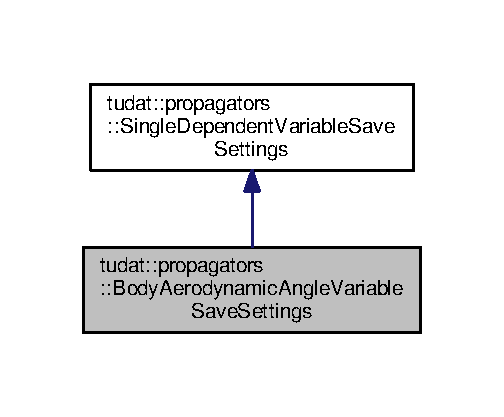
\includegraphics[width=242pt]{classtudat_1_1propagators_1_1BodyAerodynamicAngleVariableSaveSettings__inherit__graph}
\end{center}
\end{figure}


Collaboration diagram for tudat\+:\+:propagators\+:\+:Body\+Aerodynamic\+Angle\+Variable\+Save\+Settings\+:
\nopagebreak
\begin{figure}[H]
\begin{center}
\leavevmode
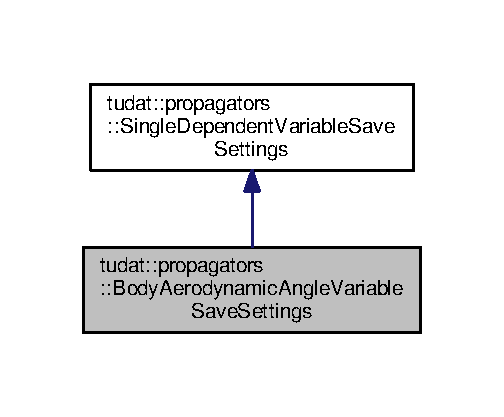
\includegraphics[width=242pt]{classtudat_1_1propagators_1_1BodyAerodynamicAngleVariableSaveSettings__coll__graph}
\end{center}
\end{figure}
\subsection*{Public Member Functions}
\begin{DoxyCompactItemize}
\item 
\hyperlink{classtudat_1_1propagators_1_1BodyAerodynamicAngleVariableSaveSettings_af24e2d196d5fd5ce718e7ffe3214b598}{Body\+Aerodynamic\+Angle\+Variable\+Save\+Settings} (const std\+::string \&associated\+Body, const reference\+\_\+frames\+::\+Aerodynamics\+Reference\+Frame\+Angles angle)
\begin{DoxyCompactList}\small\item\em Constructor. \end{DoxyCompactList}\end{DoxyCompactItemize}
\subsection*{Public Attributes}
\begin{DoxyCompactItemize}
\item 
reference\+\_\+frames\+::\+Aerodynamics\+Reference\+Frame\+Angles \hyperlink{classtudat_1_1propagators_1_1BodyAerodynamicAngleVariableSaveSettings_a79af0fa7b533d697d9e0a47574b9c7bf}{angle\+\_\+}\hypertarget{classtudat_1_1propagators_1_1BodyAerodynamicAngleVariableSaveSettings_a79af0fa7b533d697d9e0a47574b9c7bf}{}\label{classtudat_1_1propagators_1_1BodyAerodynamicAngleVariableSaveSettings_a79af0fa7b533d697d9e0a47574b9c7bf}

\begin{DoxyCompactList}\small\item\em Orientation angle that is to be saved. \end{DoxyCompactList}\end{DoxyCompactItemize}


\subsection{Detailed Description}
Class to define settings for saving an aerodynamics orientation angle from Aerodynamics\+Reference\+Frame\+Angles list. 

\subsection{Constructor \& Destructor Documentation}
\index{tudat\+::propagators\+::\+Body\+Aerodynamic\+Angle\+Variable\+Save\+Settings@{tudat\+::propagators\+::\+Body\+Aerodynamic\+Angle\+Variable\+Save\+Settings}!Body\+Aerodynamic\+Angle\+Variable\+Save\+Settings@{Body\+Aerodynamic\+Angle\+Variable\+Save\+Settings}}
\index{Body\+Aerodynamic\+Angle\+Variable\+Save\+Settings@{Body\+Aerodynamic\+Angle\+Variable\+Save\+Settings}!tudat\+::propagators\+::\+Body\+Aerodynamic\+Angle\+Variable\+Save\+Settings@{tudat\+::propagators\+::\+Body\+Aerodynamic\+Angle\+Variable\+Save\+Settings}}
\subsubsection[{\texorpdfstring{Body\+Aerodynamic\+Angle\+Variable\+Save\+Settings(const std\+::string \&associated\+Body, const reference\+\_\+frames\+::\+Aerodynamics\+Reference\+Frame\+Angles angle)}{BodyAerodynamicAngleVariableSaveSettings(const std::string &associatedBody, const reference_frames::AerodynamicsReferenceFrameAngles angle)}}]{\setlength{\rightskip}{0pt plus 5cm}tudat\+::propagators\+::\+Body\+Aerodynamic\+Angle\+Variable\+Save\+Settings\+::\+Body\+Aerodynamic\+Angle\+Variable\+Save\+Settings (
\begin{DoxyParamCaption}
\item[{const std\+::string \&}]{associated\+Body, }
\item[{const reference\+\_\+frames\+::\+Aerodynamics\+Reference\+Frame\+Angles}]{angle}
\end{DoxyParamCaption}
)\hspace{0.3cm}{\ttfamily [inline]}}\hypertarget{classtudat_1_1propagators_1_1BodyAerodynamicAngleVariableSaveSettings_af24e2d196d5fd5ce718e7ffe3214b598}{}\label{classtudat_1_1propagators_1_1BodyAerodynamicAngleVariableSaveSettings_af24e2d196d5fd5ce718e7ffe3214b598}


Constructor. 

Constructor. 
\begin{DoxyParams}{Parameters}
{\em associated\+Body} & Body for which the orientation angle is to be saved. \\
\hline
{\em angle} & Orientation angle that is to be saved. \\
\hline
\end{DoxyParams}


The documentation for this class was generated from the following file\+:\begin{DoxyCompactItemize}
\item 
/home/lupi/\+Tudat/tudat\+Bundle/tudat/\+Tudat/\+Simulation\+Setup/\+Propagation\+Setup/propagation\+Output\+Settings.\+h\end{DoxyCompactItemize}

\hypertarget{classtudat_1_1propulsion_1_1BodyFixedForceDirectionGuidance}{}\section{tudat\+:\+:propulsion\+:\+:Body\+Fixed\+Force\+Direction\+Guidance Class Reference}
\label{classtudat_1_1propulsion_1_1BodyFixedForceDirectionGuidance}\index{tudat\+::propulsion\+::\+Body\+Fixed\+Force\+Direction\+Guidance@{tudat\+::propulsion\+::\+Body\+Fixed\+Force\+Direction\+Guidance}}


Base class for computing the direction of a given force/acceleration.  




{\ttfamily \#include $<$thrust\+Guidance.\+h$>$}



Inheritance diagram for tudat\+:\+:propulsion\+:\+:Body\+Fixed\+Force\+Direction\+Guidance\+:
\nopagebreak
\begin{figure}[H]
\begin{center}
\leavevmode
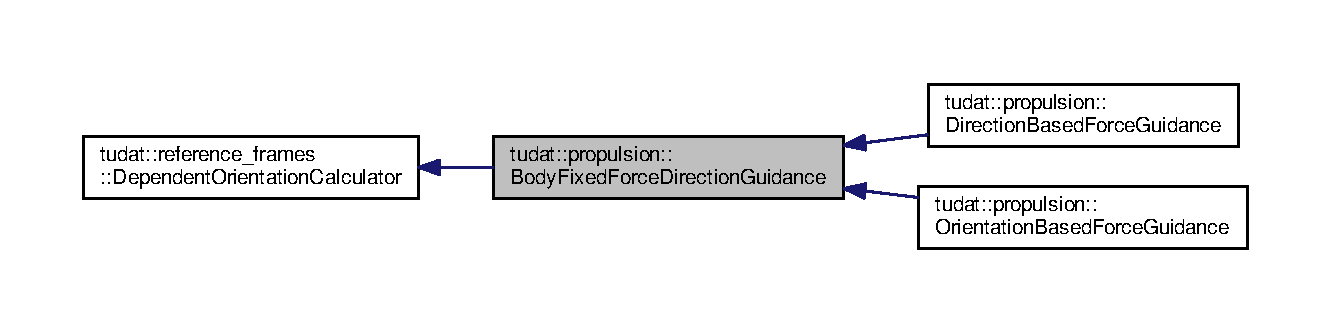
\includegraphics[width=350pt]{classtudat_1_1propulsion_1_1BodyFixedForceDirectionGuidance__inherit__graph}
\end{center}
\end{figure}


Collaboration diagram for tudat\+:\+:propulsion\+:\+:Body\+Fixed\+Force\+Direction\+Guidance\+:
\nopagebreak
\begin{figure}[H]
\begin{center}
\leavevmode
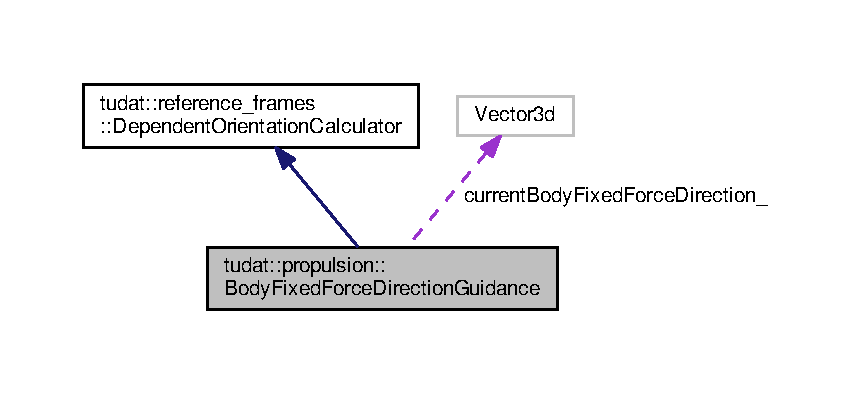
\includegraphics[width=350pt]{classtudat_1_1propulsion_1_1BodyFixedForceDirectionGuidance__coll__graph}
\end{center}
\end{figure}
\subsection*{Public Member Functions}
\begin{DoxyCompactItemize}
\item 
\hyperlink{classtudat_1_1propulsion_1_1BodyFixedForceDirectionGuidance_a18be30cae6aeaabebe4ef5e8fc447fff}{Body\+Fixed\+Force\+Direction\+Guidance} (const boost\+::function$<$ Eigen\+::\+Vector3d() $>$ body\+Fixed\+Force\+Direction)
\begin{DoxyCompactList}\small\item\em Constructor. \end{DoxyCompactList}\item 
virtual \hyperlink{classtudat_1_1propulsion_1_1BodyFixedForceDirectionGuidance_a34c738a626dced8c464072c23cd272d8}{$\sim$\+Body\+Fixed\+Force\+Direction\+Guidance} ()\hypertarget{classtudat_1_1propulsion_1_1BodyFixedForceDirectionGuidance_a34c738a626dced8c464072c23cd272d8}{}\label{classtudat_1_1propulsion_1_1BodyFixedForceDirectionGuidance_a34c738a626dced8c464072c23cd272d8}

\begin{DoxyCompactList}\small\item\em Destructor. \end{DoxyCompactList}\item 
virtual Eigen\+::\+Vector3d \hyperlink{classtudat_1_1propulsion_1_1BodyFixedForceDirectionGuidance_a4284988acc53bfac7681ebd44c876e74}{get\+Current\+Force\+Direction\+In\+Propagation\+Frame} ()=0
\begin{DoxyCompactList}\small\item\em Function to get the force/acceleration direction in the propagation frame. \end{DoxyCompactList}\item 
Eigen\+::\+Quaterniond \hyperlink{classtudat_1_1propulsion_1_1BodyFixedForceDirectionGuidance_a4d00bda9b8e058f61be0589e0808989a}{get\+Rotation\+To\+Local\+Frame} ()
\begin{DoxyCompactList}\small\item\em Function to compute the rotation from the propagation frame to the body-\/fixed frame. \end{DoxyCompactList}\item 
void \hyperlink{classtudat_1_1propulsion_1_1BodyFixedForceDirectionGuidance_a9c68637d16f973b22f5b06ee3aea1031}{update\+Calculator} (const double time)
\begin{DoxyCompactList}\small\item\em Function to update the object to the current time. \end{DoxyCompactList}\end{DoxyCompactItemize}
\subsection*{Protected Member Functions}
\begin{DoxyCompactItemize}
\item 
virtual void \hyperlink{classtudat_1_1propulsion_1_1BodyFixedForceDirectionGuidance_abac6943fd9ca3925e7228ac7d40db8f0}{update\+Force\+Direction} (const double time)=0
\begin{DoxyCompactList}\small\item\em Function to update the force/acceleration direction to the current time. \end{DoxyCompactList}\end{DoxyCompactItemize}
\subsection*{Protected Attributes}
\begin{DoxyCompactItemize}
\item 
boost\+::function$<$ Eigen\+::\+Vector3d() $>$ \hyperlink{classtudat_1_1propulsion_1_1BodyFixedForceDirectionGuidance_a03f2926bd81f039d42f3e0e49162a750}{body\+Fixed\+Force\+Direction\+\_\+}\hypertarget{classtudat_1_1propulsion_1_1BodyFixedForceDirectionGuidance_a03f2926bd81f039d42f3e0e49162a750}{}\label{classtudat_1_1propulsion_1_1BodyFixedForceDirectionGuidance_a03f2926bd81f039d42f3e0e49162a750}

\begin{DoxyCompactList}\small\item\em Function returning the direction of the force in the body-\/fixed frame. \end{DoxyCompactList}\item 
Eigen\+::\+Vector3d \hyperlink{classtudat_1_1propulsion_1_1BodyFixedForceDirectionGuidance_ab5201df1ef26337c7ec386489e6a5cec}{current\+Body\+Fixed\+Force\+Direction\+\_\+}\hypertarget{classtudat_1_1propulsion_1_1BodyFixedForceDirectionGuidance_ab5201df1ef26337c7ec386489e6a5cec}{}\label{classtudat_1_1propulsion_1_1BodyFixedForceDirectionGuidance_ab5201df1ef26337c7ec386489e6a5cec}

\begin{DoxyCompactList}\small\item\em Current direction of the force in the body-\/fixed frame as set by last call to update\+Calculator function. \end{DoxyCompactList}\end{DoxyCompactItemize}


\subsection{Detailed Description}
Base class for computing the direction of a given force/acceleration. 

Base class for computing the direction of a given force/acceleration. The computation is done directly from some a priori imposed rule, possibly as a function of dependent, independent or state variables. A derived class for using the current orientation of the vehicle (as computed by some other method and retrieved from the body class) may be set using the \hyperlink{classtudat_1_1propulsion_1_1OrientationBasedForceGuidance}{Orientation\+Based\+Force\+Guidance} class. 

\subsection{Constructor \& Destructor Documentation}
\index{tudat\+::propulsion\+::\+Body\+Fixed\+Force\+Direction\+Guidance@{tudat\+::propulsion\+::\+Body\+Fixed\+Force\+Direction\+Guidance}!Body\+Fixed\+Force\+Direction\+Guidance@{Body\+Fixed\+Force\+Direction\+Guidance}}
\index{Body\+Fixed\+Force\+Direction\+Guidance@{Body\+Fixed\+Force\+Direction\+Guidance}!tudat\+::propulsion\+::\+Body\+Fixed\+Force\+Direction\+Guidance@{tudat\+::propulsion\+::\+Body\+Fixed\+Force\+Direction\+Guidance}}
\subsubsection[{\texorpdfstring{Body\+Fixed\+Force\+Direction\+Guidance(const boost\+::function$<$ Eigen\+::\+Vector3d() $>$ body\+Fixed\+Force\+Direction)}{BodyFixedForceDirectionGuidance(const boost::function< Eigen::Vector3d() > bodyFixedForceDirection)}}]{\setlength{\rightskip}{0pt plus 5cm}tudat\+::propulsion\+::\+Body\+Fixed\+Force\+Direction\+Guidance\+::\+Body\+Fixed\+Force\+Direction\+Guidance (
\begin{DoxyParamCaption}
\item[{const boost\+::function$<$ Eigen\+::\+Vector3d() $>$}]{body\+Fixed\+Force\+Direction}
\end{DoxyParamCaption}
)\hspace{0.3cm}{\ttfamily [inline]}}\hypertarget{classtudat_1_1propulsion_1_1BodyFixedForceDirectionGuidance_a18be30cae6aeaabebe4ef5e8fc447fff}{}\label{classtudat_1_1propulsion_1_1BodyFixedForceDirectionGuidance_a18be30cae6aeaabebe4ef5e8fc447fff}


Constructor. 

Constructor, sets the direction of the force in the body-\/fixed frame. 
\begin{DoxyParams}{Parameters}
{\em body\+Fixed\+Force\+Direction} & Function returning the direction of the force in the body-\/fixed frame. \\
\hline
\end{DoxyParams}


\subsection{Member Function Documentation}
\index{tudat\+::propulsion\+::\+Body\+Fixed\+Force\+Direction\+Guidance@{tudat\+::propulsion\+::\+Body\+Fixed\+Force\+Direction\+Guidance}!get\+Current\+Force\+Direction\+In\+Propagation\+Frame@{get\+Current\+Force\+Direction\+In\+Propagation\+Frame}}
\index{get\+Current\+Force\+Direction\+In\+Propagation\+Frame@{get\+Current\+Force\+Direction\+In\+Propagation\+Frame}!tudat\+::propulsion\+::\+Body\+Fixed\+Force\+Direction\+Guidance@{tudat\+::propulsion\+::\+Body\+Fixed\+Force\+Direction\+Guidance}}
\subsubsection[{\texorpdfstring{get\+Current\+Force\+Direction\+In\+Propagation\+Frame()=0}{getCurrentForceDirectionInPropagationFrame()=0}}]{\setlength{\rightskip}{0pt plus 5cm}virtual Eigen\+::\+Vector3d tudat\+::propulsion\+::\+Body\+Fixed\+Force\+Direction\+Guidance\+::get\+Current\+Force\+Direction\+In\+Propagation\+Frame (
\begin{DoxyParamCaption}
{}
\end{DoxyParamCaption}
)\hspace{0.3cm}{\ttfamily [pure virtual]}}\hypertarget{classtudat_1_1propulsion_1_1BodyFixedForceDirectionGuidance_a4284988acc53bfac7681ebd44c876e74}{}\label{classtudat_1_1propulsion_1_1BodyFixedForceDirectionGuidance_a4284988acc53bfac7681ebd44c876e74}


Function to get the force/acceleration direction in the propagation frame. 

Function to get the force/acceleration direction in the propagation frame. Function is pure virtual and to be implemented in derived class. \begin{DoxyReturn}{Returns}
Direction of force (as unit vector) expressed in propagation frame. 
\end{DoxyReturn}


Implemented in \hyperlink{classtudat_1_1propulsion_1_1OrientationBasedForceGuidance_a9072ced143f8661246542216f41c5858}{tudat\+::propulsion\+::\+Orientation\+Based\+Force\+Guidance}, and \hyperlink{classtudat_1_1propulsion_1_1DirectionBasedForceGuidance_a38bb2a2a0f9dbe4779f2c41572a4fc58}{tudat\+::propulsion\+::\+Direction\+Based\+Force\+Guidance}.

\index{tudat\+::propulsion\+::\+Body\+Fixed\+Force\+Direction\+Guidance@{tudat\+::propulsion\+::\+Body\+Fixed\+Force\+Direction\+Guidance}!get\+Rotation\+To\+Local\+Frame@{get\+Rotation\+To\+Local\+Frame}}
\index{get\+Rotation\+To\+Local\+Frame@{get\+Rotation\+To\+Local\+Frame}!tudat\+::propulsion\+::\+Body\+Fixed\+Force\+Direction\+Guidance@{tudat\+::propulsion\+::\+Body\+Fixed\+Force\+Direction\+Guidance}}
\subsubsection[{\texorpdfstring{get\+Rotation\+To\+Local\+Frame()}{getRotationToLocalFrame()}}]{\setlength{\rightskip}{0pt plus 5cm}Eigen\+::\+Quaterniond tudat\+::propulsion\+::\+Body\+Fixed\+Force\+Direction\+Guidance\+::get\+Rotation\+To\+Local\+Frame (
\begin{DoxyParamCaption}
{}
\end{DoxyParamCaption}
)\hspace{0.3cm}{\ttfamily [inline]}, {\ttfamily [virtual]}}\hypertarget{classtudat_1_1propulsion_1_1BodyFixedForceDirectionGuidance_a4d00bda9b8e058f61be0589e0808989a}{}\label{classtudat_1_1propulsion_1_1BodyFixedForceDirectionGuidance_a4d00bda9b8e058f61be0589e0808989a}


Function to compute the rotation from the propagation frame to the body-\/fixed frame. 

Function to compute the rotation from the propagation frame to the body-\/fixed frame using the algorithm implemented in the derived class. The derived class must implement the function for the inverse rotation (get\+Rotation\+To\+Global\+Frame). \begin{DoxyReturn}{Returns}
Quaternion that provides the rotation from the propagation frame to the body-\/fixed frame. 
\end{DoxyReturn}


Implements \hyperlink{classtudat_1_1reference__frames_1_1DependentOrientationCalculator_ae55893820994179e02ec6189cd9fb00b}{tudat\+::reference\+\_\+frames\+::\+Dependent\+Orientation\+Calculator}.

\index{tudat\+::propulsion\+::\+Body\+Fixed\+Force\+Direction\+Guidance@{tudat\+::propulsion\+::\+Body\+Fixed\+Force\+Direction\+Guidance}!update\+Calculator@{update\+Calculator}}
\index{update\+Calculator@{update\+Calculator}!tudat\+::propulsion\+::\+Body\+Fixed\+Force\+Direction\+Guidance@{tudat\+::propulsion\+::\+Body\+Fixed\+Force\+Direction\+Guidance}}
\subsubsection[{\texorpdfstring{update\+Calculator(const double time)}{updateCalculator(const double time)}}]{\setlength{\rightskip}{0pt plus 5cm}void tudat\+::propulsion\+::\+Body\+Fixed\+Force\+Direction\+Guidance\+::update\+Calculator (
\begin{DoxyParamCaption}
\item[{const double}]{time}
\end{DoxyParamCaption}
)\hspace{0.3cm}{\ttfamily [inline]}, {\ttfamily [virtual]}}\hypertarget{classtudat_1_1propulsion_1_1BodyFixedForceDirectionGuidance_a9c68637d16f973b22f5b06ee3aea1031}{}\label{classtudat_1_1propulsion_1_1BodyFixedForceDirectionGuidance_a9c68637d16f973b22f5b06ee3aea1031}


Function to update the object to the current time. 

Function to update the object to the current time. This function updates only this base class, derived class must implement the update\+Force\+Direction function that obdates the full object. 
\begin{DoxyParams}{Parameters}
{\em time} & \hyperlink{classtudat_1_1Time}{Time} to which object is to be updated. \\
\hline
\end{DoxyParams}


Implements \hyperlink{classtudat_1_1reference__frames_1_1DependentOrientationCalculator_a801bc21f0df6beecea976cf5728c79ce}{tudat\+::reference\+\_\+frames\+::\+Dependent\+Orientation\+Calculator}.

\index{tudat\+::propulsion\+::\+Body\+Fixed\+Force\+Direction\+Guidance@{tudat\+::propulsion\+::\+Body\+Fixed\+Force\+Direction\+Guidance}!update\+Force\+Direction@{update\+Force\+Direction}}
\index{update\+Force\+Direction@{update\+Force\+Direction}!tudat\+::propulsion\+::\+Body\+Fixed\+Force\+Direction\+Guidance@{tudat\+::propulsion\+::\+Body\+Fixed\+Force\+Direction\+Guidance}}
\subsubsection[{\texorpdfstring{update\+Force\+Direction(const double time)=0}{updateForceDirection(const double time)=0}}]{\setlength{\rightskip}{0pt plus 5cm}virtual void tudat\+::propulsion\+::\+Body\+Fixed\+Force\+Direction\+Guidance\+::update\+Force\+Direction (
\begin{DoxyParamCaption}
\item[{const double}]{time}
\end{DoxyParamCaption}
)\hspace{0.3cm}{\ttfamily [protected]}, {\ttfamily [pure virtual]}}\hypertarget{classtudat_1_1propulsion_1_1BodyFixedForceDirectionGuidance_abac6943fd9ca3925e7228ac7d40db8f0}{}\label{classtudat_1_1propulsion_1_1BodyFixedForceDirectionGuidance_abac6943fd9ca3925e7228ac7d40db8f0}


Function to update the force/acceleration direction to the current time. 

Function to update the force/acceleration direction to the current time. This function is to be implemented in the derived class. 
\begin{DoxyParams}{Parameters}
{\em time} & \hyperlink{classtudat_1_1Time}{Time} to which object is to be updated. \\
\hline
\end{DoxyParams}


Implemented in \hyperlink{classtudat_1_1propulsion_1_1OrientationBasedForceGuidance_a4cd7dfac54b8948ecceb14a4565a1160}{tudat\+::propulsion\+::\+Orientation\+Based\+Force\+Guidance}, and \hyperlink{classtudat_1_1propulsion_1_1DirectionBasedForceGuidance_a4051907f746166d8d7fc9814b3e82192}{tudat\+::propulsion\+::\+Direction\+Based\+Force\+Guidance}.



The documentation for this class was generated from the following file\+:\begin{DoxyCompactItemize}
\item 
/home/lupi/\+Tudat/tudat\+Bundle/tudat/\+Tudat/\+Astrodynamics/\+Propulsion/thrust\+Guidance.\+h\end{DoxyCompactItemize}

\hypertarget{classtudat_1_1propagators_1_1BodyMassIntegratedStateProcessor}{}\section{tudat\+:\+:propagators\+:\+:Body\+Mass\+Integrated\+State\+Processor$<$ Time\+Type, State\+Scalar\+Type $>$ Class Template Reference}
\label{classtudat_1_1propagators_1_1BodyMassIntegratedStateProcessor}\index{tudat\+::propagators\+::\+Body\+Mass\+Integrated\+State\+Processor$<$ Time\+Type, State\+Scalar\+Type $>$@{tudat\+::propagators\+::\+Body\+Mass\+Integrated\+State\+Processor$<$ Time\+Type, State\+Scalar\+Type $>$}}


Class used for processing numerically integrated masses of bodies.  




{\ttfamily \#include $<$set\+Numerically\+Integrated\+States.\+h$>$}



Inheritance diagram for tudat\+:\+:propagators\+:\+:Body\+Mass\+Integrated\+State\+Processor$<$ Time\+Type, State\+Scalar\+Type $>$\+:
\nopagebreak
\begin{figure}[H]
\begin{center}
\leavevmode
\includegraphics[width=260pt]{classtudat_1_1propagators_1_1BodyMassIntegratedStateProcessor__inherit__graph}
\end{center}
\end{figure}


Collaboration diagram for tudat\+:\+:propagators\+:\+:Body\+Mass\+Integrated\+State\+Processor$<$ Time\+Type, State\+Scalar\+Type $>$\+:
\nopagebreak
\begin{figure}[H]
\begin{center}
\leavevmode
\includegraphics[width=260pt]{classtudat_1_1propagators_1_1BodyMassIntegratedStateProcessor__coll__graph}
\end{center}
\end{figure}
\subsection*{Public Member Functions}
\begin{DoxyCompactItemize}
\item 
\hyperlink{classtudat_1_1propagators_1_1BodyMassIntegratedStateProcessor_acb9c2430a95e3b770f86ba639340f6c0}{Body\+Mass\+Integrated\+State\+Processor} (const int start\+Index, const simulation\+\_\+setup\+::\+Named\+Body\+Map \&body\+Map, const std\+::vector$<$ std\+::string $>$ \&bodies\+To\+Integrate)
\begin{DoxyCompactList}\small\item\em Constructor. \end{DoxyCompactList}\item 
\hyperlink{classtudat_1_1propagators_1_1BodyMassIntegratedStateProcessor_ad6ec2043a50970d83671e0bfb44a87da}{$\sim$\+Body\+Mass\+Integrated\+State\+Processor} ()\hypertarget{classtudat_1_1propagators_1_1BodyMassIntegratedStateProcessor_ad6ec2043a50970d83671e0bfb44a87da}{}\label{classtudat_1_1propagators_1_1BodyMassIntegratedStateProcessor_ad6ec2043a50970d83671e0bfb44a87da}

\begin{DoxyCompactList}\small\item\em Destructor. \end{DoxyCompactList}\item 
void \hyperlink{classtudat_1_1propagators_1_1BodyMassIntegratedStateProcessor_a24172315a1044a3bfe4134a194b95aec}{process\+Integrated\+States} (const std\+::map$<$ Time\+Type, Eigen\+::\+Matrix$<$ State\+Scalar\+Type, Eigen\+::\+Dynamic, 1 $>$ $>$ \&numerical\+Solution)
\begin{DoxyCompactList}\small\item\em Function processing mass state in the full numerical\+Solution. \end{DoxyCompactList}\end{DoxyCompactItemize}
\subsection*{Additional Inherited Members}


\subsection{Detailed Description}
\subsubsection*{template$<$typename Time\+Type, typename State\+Scalar\+Type$>$\\*
class tudat\+::propagators\+::\+Body\+Mass\+Integrated\+State\+Processor$<$ Time\+Type, State\+Scalar\+Type $>$}

Class used for processing numerically integrated masses of bodies. 

\subsection{Constructor \& Destructor Documentation}
\index{tudat\+::propagators\+::\+Body\+Mass\+Integrated\+State\+Processor@{tudat\+::propagators\+::\+Body\+Mass\+Integrated\+State\+Processor}!Body\+Mass\+Integrated\+State\+Processor@{Body\+Mass\+Integrated\+State\+Processor}}
\index{Body\+Mass\+Integrated\+State\+Processor@{Body\+Mass\+Integrated\+State\+Processor}!tudat\+::propagators\+::\+Body\+Mass\+Integrated\+State\+Processor@{tudat\+::propagators\+::\+Body\+Mass\+Integrated\+State\+Processor}}
\subsubsection[{\texorpdfstring{Body\+Mass\+Integrated\+State\+Processor(const int start\+Index, const simulation\+\_\+setup\+::\+Named\+Body\+Map \&body\+Map, const std\+::vector$<$ std\+::string $>$ \&bodies\+To\+Integrate)}{BodyMassIntegratedStateProcessor(const int startIndex, const simulation_setup::NamedBodyMap &bodyMap, const std::vector< std::string > &bodiesToIntegrate)}}]{\setlength{\rightskip}{0pt plus 5cm}template$<$typename Time\+Type , typename State\+Scalar\+Type $>$ {\bf tudat\+::propagators\+::\+Body\+Mass\+Integrated\+State\+Processor}$<$ Time\+Type, State\+Scalar\+Type $>$\+::{\bf Body\+Mass\+Integrated\+State\+Processor} (
\begin{DoxyParamCaption}
\item[{const int}]{start\+Index, }
\item[{const simulation\+\_\+setup\+::\+Named\+Body\+Map \&}]{body\+Map, }
\item[{const std\+::vector$<$ std\+::string $>$ \&}]{bodies\+To\+Integrate}
\end{DoxyParamCaption}
)\hspace{0.3cm}{\ttfamily [inline]}}\hypertarget{classtudat_1_1propagators_1_1BodyMassIntegratedStateProcessor_acb9c2430a95e3b770f86ba639340f6c0}{}\label{classtudat_1_1propagators_1_1BodyMassIntegratedStateProcessor_acb9c2430a95e3b770f86ba639340f6c0}


Constructor. 

Constructor 
\begin{DoxyParams}{Parameters}
{\em start\+Index} & Index in the state vector where the translational state starts. \\
\hline
{\em body\+Map} & List of bodies used in simulations. \\
\hline
{\em bodies\+To\+Integrate} & List of bodies for which the mass is numerically integrated. Order in this vector is the same as the order in state vector. \\
\hline
\end{DoxyParams}


\subsection{Member Function Documentation}
\index{tudat\+::propagators\+::\+Body\+Mass\+Integrated\+State\+Processor@{tudat\+::propagators\+::\+Body\+Mass\+Integrated\+State\+Processor}!process\+Integrated\+States@{process\+Integrated\+States}}
\index{process\+Integrated\+States@{process\+Integrated\+States}!tudat\+::propagators\+::\+Body\+Mass\+Integrated\+State\+Processor@{tudat\+::propagators\+::\+Body\+Mass\+Integrated\+State\+Processor}}
\subsubsection[{\texorpdfstring{process\+Integrated\+States(const std\+::map$<$ Time\+Type, Eigen\+::\+Matrix$<$ State\+Scalar\+Type, Eigen\+::\+Dynamic, 1 $>$ $>$ \&numerical\+Solution)}{processIntegratedStates(const std::map< TimeType, Eigen::Matrix< StateScalarType, Eigen::Dynamic, 1 > > &numericalSolution)}}]{\setlength{\rightskip}{0pt plus 5cm}template$<$typename Time\+Type , typename State\+Scalar\+Type $>$ void {\bf tudat\+::propagators\+::\+Body\+Mass\+Integrated\+State\+Processor}$<$ Time\+Type, State\+Scalar\+Type $>$\+::process\+Integrated\+States (
\begin{DoxyParamCaption}
\item[{const std\+::map$<$ Time\+Type, Eigen\+::\+Matrix$<$ State\+Scalar\+Type, Eigen\+::\+Dynamic, 1 $>$ $>$ \&}]{numerical\+Solution}
\end{DoxyParamCaption}
)\hspace{0.3cm}{\ttfamily [inline]}, {\ttfamily [virtual]}}\hypertarget{classtudat_1_1propagators_1_1BodyMassIntegratedStateProcessor_a24172315a1044a3bfe4134a194b95aec}{}\label{classtudat_1_1propagators_1_1BodyMassIntegratedStateProcessor_a24172315a1044a3bfe4134a194b95aec}


Function processing mass state in the full numerical\+Solution. 

Function that processes the entries of the propagated mass in the full numerical\+Solution. 
\begin{DoxyParams}{Parameters}
{\em numerical\+Solution} & Full numerical solution of state, in global representation (representation is constant for mass). \\
\hline
\end{DoxyParams}


Implements \hyperlink{classtudat_1_1propagators_1_1IntegratedStateProcessor_a379cb44bfbb3506b9de350719e1a05ac}{tudat\+::propagators\+::\+Integrated\+State\+Processor$<$ Time\+Type, State\+Scalar\+Type $>$}.



The documentation for this class was generated from the following file\+:\begin{DoxyCompactItemize}
\item 
/home/lupi/\+Tudat/tudat\+Bundle/tudat/\+Tudat/\+Simulation\+Setup/\+Propagation\+Setup/set\+Numerically\+Integrated\+States.\+h\end{DoxyCompactItemize}

\hypertarget{classtudat_1_1propagators_1_1BodyMassStateDerivative}{}\section{tudat\+:\+:propagators\+:\+:Body\+Mass\+State\+Derivative$<$ State\+Scalar\+Type, Time\+Type $>$ Class Template Reference}
\label{classtudat_1_1propagators_1_1BodyMassStateDerivative}\index{tudat\+::propagators\+::\+Body\+Mass\+State\+Derivative$<$ State\+Scalar\+Type, Time\+Type $>$@{tudat\+::propagators\+::\+Body\+Mass\+State\+Derivative$<$ State\+Scalar\+Type, Time\+Type $>$}}


Class for computing the derivative of the mass of a set of bodies.  




{\ttfamily \#include $<$body\+Mass\+State\+Derivative.\+h$>$}



Inheritance diagram for tudat\+:\+:propagators\+:\+:Body\+Mass\+State\+Derivative$<$ State\+Scalar\+Type, Time\+Type $>$\+:
\nopagebreak
\begin{figure}[H]
\begin{center}
\leavevmode
\includegraphics[width=237pt]{classtudat_1_1propagators_1_1BodyMassStateDerivative__inherit__graph}
\end{center}
\end{figure}


Collaboration diagram for tudat\+:\+:propagators\+:\+:Body\+Mass\+State\+Derivative$<$ State\+Scalar\+Type, Time\+Type $>$\+:
\nopagebreak
\begin{figure}[H]
\begin{center}
\leavevmode
\includegraphics[width=237pt]{classtudat_1_1propagators_1_1BodyMassStateDerivative__coll__graph}
\end{center}
\end{figure}
\subsection*{Public Member Functions}
\begin{DoxyCompactItemize}
\item 
\hyperlink{classtudat_1_1propagators_1_1BodyMassStateDerivative_af37273f35aa12cea6df1baf0fa8b7e4c}{Body\+Mass\+State\+Derivative} (const std\+::map$<$ std\+::string, boost\+::shared\+\_\+ptr$<$ \hyperlink{classtudat_1_1basic__astrodynamics_1_1MassRateModel}{basic\+\_\+astrodynamics\+::\+Mass\+Rate\+Model} $>$ $>$ \&mass\+Rate\+Models, const std\+::vector$<$ std\+::string $>$ \&bodies\+To\+Integrate)
\begin{DoxyCompactList}\small\item\em Constructor. \end{DoxyCompactList}\item 
\hyperlink{classtudat_1_1propagators_1_1BodyMassStateDerivative_a781a7a03062385ab3fada5e17e7f26d0}{Body\+Mass\+State\+Derivative} (const std\+::map$<$ std\+::string, std\+::vector$<$ boost\+::shared\+\_\+ptr$<$ \hyperlink{classtudat_1_1basic__astrodynamics_1_1MassRateModel}{basic\+\_\+astrodynamics\+::\+Mass\+Rate\+Model} $>$ $>$ $>$ \&mass\+Rate\+Models, const std\+::vector$<$ std\+::string $>$ \&bodies\+To\+Integrate)
\begin{DoxyCompactList}\small\item\em Constructor. \end{DoxyCompactList}\item 
virtual \hyperlink{classtudat_1_1propagators_1_1BodyMassStateDerivative_a6af47edeba268e48d2d78011a9047889}{$\sim$\+Body\+Mass\+State\+Derivative} ()\hypertarget{classtudat_1_1propagators_1_1BodyMassStateDerivative_a6af47edeba268e48d2d78011a9047889}{}\label{classtudat_1_1propagators_1_1BodyMassStateDerivative_a6af47edeba268e48d2d78011a9047889}

\begin{DoxyCompactList}\small\item\em Destructor. \end{DoxyCompactList}\item 
void \hyperlink{classtudat_1_1propagators_1_1BodyMassStateDerivative_a5d23c3bf3aa36a0ffc94e0927051214e}{calculate\+System\+State\+Derivative} (const Time\+Type time, const Eigen\+::\+Matrix$<$ State\+Scalar\+Type, Eigen\+::\+Dynamic, 1 $>$ \&state\+Of\+System\+To\+Be\+Integrated, Eigen\+::\+Block$<$ Eigen\+::\+Matrix$<$ State\+Scalar\+Type, Eigen\+::\+Dynamic, Eigen\+::\+Dynamic $>$ $>$ state\+Derivative)
\begin{DoxyCompactList}\small\item\em Calculates the state derivative of the system of equations for the mass dynamics. \end{DoxyCompactList}\item 
void \hyperlink{classtudat_1_1propagators_1_1BodyMassStateDerivative_a7c37b818e0f9b8a895dc39d374ac4633}{clear\+State\+Derivative\+Model} ()
\begin{DoxyCompactList}\small\item\em Function to clear reference/cached values of body mass state derivative model. \end{DoxyCompactList}\item 
void \hyperlink{classtudat_1_1propagators_1_1BodyMassStateDerivative_a6d8703c45a5f57762d2c7159b8f1c640}{update\+State\+Derivative\+Model} (const Time\+Type current\+Time)
\begin{DoxyCompactList}\small\item\em Function to update the mass state derivative model to the current time. \end{DoxyCompactList}\item 
void \hyperlink{classtudat_1_1propagators_1_1BodyMassStateDerivative_aa924352ed0c6e56afe4c72c45102b3c6}{convert\+Current\+State\+To\+Global\+Representation} (const Eigen\+::\+Matrix$<$ State\+Scalar\+Type, Eigen\+::\+Dynamic, 1 $>$ \&internal\+Solution, const Time\+Type \&time, Eigen\+::\+Block$<$ Eigen\+::\+Matrix$<$ State\+Scalar\+Type, Eigen\+::\+Dynamic, 1 $>$ $>$ current\+Cartesian\+Local\+Soluton)
\item 
virtual Eigen\+::\+Matrix$<$ State\+Scalar\+Type, Eigen\+::\+Dynamic, Eigen\+::\+Dynamic $>$ \hyperlink{classtudat_1_1propagators_1_1BodyMassStateDerivative_a02810a56236b1c338f869e00b584b8b1}{convert\+From\+Output\+Solution} (const Eigen\+::\+Matrix$<$ State\+Scalar\+Type, Eigen\+::\+Dynamic, Eigen\+::\+Dynamic $>$ \&output\+Solution, const Time\+Type \&time)
\item 
void \hyperlink{classtudat_1_1propagators_1_1BodyMassStateDerivative_a70a988ff5e71b00f9b5c99a39921507e}{convert\+To\+Output\+Solution} (const Eigen\+::\+Matrix$<$ State\+Scalar\+Type, Eigen\+::\+Dynamic, Eigen\+::\+Dynamic $>$ \&internal\+Solution, const Time\+Type \&time, Eigen\+::\+Block$<$ Eigen\+::\+Matrix$<$ State\+Scalar\+Type, Eigen\+::\+Dynamic, 1 $>$ $>$ current\+Cartesian\+Local\+Soluton)
\item 
virtual int \hyperlink{classtudat_1_1propagators_1_1BodyMassStateDerivative_ae12d2a506db4676be1c59b9058e8dae7}{get\+State\+Size} ()
\begin{DoxyCompactList}\small\item\em Function to get the total size of the state of propagated masses. \end{DoxyCompactList}\item 
std\+::vector$<$ std\+::string $>$ \hyperlink{classtudat_1_1propagators_1_1BodyMassStateDerivative_a532cb9a49fb9507b5d829a2301cd20a8}{get\+Bodies\+To\+Integrate} ()
\begin{DoxyCompactList}\small\item\em Get list of bodies for which the mass is to be propagated. \end{DoxyCompactList}\item 
double \hyperlink{classtudat_1_1propagators_1_1BodyMassStateDerivative_a08b3e8d1ea2902b23f930f7f140c3b2f}{get\+Total\+Mass\+Rate\+For\+Body} (const std\+::string body\+Name)
\begin{DoxyCompactList}\small\item\em Function to return the current mass rate for a single body. \end{DoxyCompactList}\end{DoxyCompactItemize}
\subsection*{Additional Inherited Members}


\subsection{Detailed Description}
\subsubsection*{template$<$typename State\+Scalar\+Type = double, typename Time\+Type = double$>$\\*
class tudat\+::propagators\+::\+Body\+Mass\+State\+Derivative$<$ State\+Scalar\+Type, Time\+Type $>$}

Class for computing the derivative of the mass of a set of bodies. 

Class for computing the derivative of the mass of a set of bodies. Note that the local and global states are equal for mass propagation, both represent the physical body mass (in kg). 

\subsection{Constructor \& Destructor Documentation}
\index{tudat\+::propagators\+::\+Body\+Mass\+State\+Derivative@{tudat\+::propagators\+::\+Body\+Mass\+State\+Derivative}!Body\+Mass\+State\+Derivative@{Body\+Mass\+State\+Derivative}}
\index{Body\+Mass\+State\+Derivative@{Body\+Mass\+State\+Derivative}!tudat\+::propagators\+::\+Body\+Mass\+State\+Derivative@{tudat\+::propagators\+::\+Body\+Mass\+State\+Derivative}}
\subsubsection[{\texorpdfstring{Body\+Mass\+State\+Derivative(const std\+::map$<$ std\+::string, boost\+::shared\+\_\+ptr$<$ basic\+\_\+astrodynamics\+::\+Mass\+Rate\+Model $>$ $>$ \&mass\+Rate\+Models, const std\+::vector$<$ std\+::string $>$ \&bodies\+To\+Integrate)}{BodyMassStateDerivative(const std::map< std::string, boost::shared_ptr< basic_astrodynamics::MassRateModel > > &massRateModels, const std::vector< std::string > &bodiesToIntegrate)}}]{\setlength{\rightskip}{0pt plus 5cm}template$<$typename State\+Scalar\+Type  = double, typename Time\+Type  = double$>$ {\bf tudat\+::propagators\+::\+Body\+Mass\+State\+Derivative}$<$ State\+Scalar\+Type, Time\+Type $>$\+::{\bf Body\+Mass\+State\+Derivative} (
\begin{DoxyParamCaption}
\item[{const std\+::map$<$ std\+::string, boost\+::shared\+\_\+ptr$<$ {\bf basic\+\_\+astrodynamics\+::\+Mass\+Rate\+Model} $>$ $>$ \&}]{mass\+Rate\+Models, }
\item[{const std\+::vector$<$ std\+::string $>$ \&}]{bodies\+To\+Integrate}
\end{DoxyParamCaption}
)\hspace{0.3cm}{\ttfamily [inline]}}\hypertarget{classtudat_1_1propagators_1_1BodyMassStateDerivative_af37273f35aa12cea6df1baf0fa8b7e4c}{}\label{classtudat_1_1propagators_1_1BodyMassStateDerivative_af37273f35aa12cea6df1baf0fa8b7e4c}


Constructor. 

Constructor, sets the mass rate models and the bodies that are to be propagated (single mass rate model per body). 
\begin{DoxyParams}{Parameters}
{\em mass\+Rate\+Models} & Map of model per body that is to be used for the mass rate computation. \\
\hline
{\em bodies\+To\+Integrate} & List of bodies for which the mass is to be propagated. Note that this vector have more entries than the mass\+Rate\+Models map, as a body\textquotesingle{}s mass can be \textquotesingle{}propagated\textquotesingle{} with no rate model (i.\+e. constant mass). \\
\hline
\end{DoxyParams}
\index{tudat\+::propagators\+::\+Body\+Mass\+State\+Derivative@{tudat\+::propagators\+::\+Body\+Mass\+State\+Derivative}!Body\+Mass\+State\+Derivative@{Body\+Mass\+State\+Derivative}}
\index{Body\+Mass\+State\+Derivative@{Body\+Mass\+State\+Derivative}!tudat\+::propagators\+::\+Body\+Mass\+State\+Derivative@{tudat\+::propagators\+::\+Body\+Mass\+State\+Derivative}}
\subsubsection[{\texorpdfstring{Body\+Mass\+State\+Derivative(const std\+::map$<$ std\+::string, std\+::vector$<$ boost\+::shared\+\_\+ptr$<$ basic\+\_\+astrodynamics\+::\+Mass\+Rate\+Model $>$ $>$ $>$ \&mass\+Rate\+Models, const std\+::vector$<$ std\+::string $>$ \&bodies\+To\+Integrate)}{BodyMassStateDerivative(const std::map< std::string, std::vector< boost::shared_ptr< basic_astrodynamics::MassRateModel > > > &massRateModels, const std::vector< std::string > &bodiesToIntegrate)}}]{\setlength{\rightskip}{0pt plus 5cm}template$<$typename State\+Scalar\+Type  = double, typename Time\+Type  = double$>$ {\bf tudat\+::propagators\+::\+Body\+Mass\+State\+Derivative}$<$ State\+Scalar\+Type, Time\+Type $>$\+::{\bf Body\+Mass\+State\+Derivative} (
\begin{DoxyParamCaption}
\item[{const std\+::map$<$ std\+::string, std\+::vector$<$ boost\+::shared\+\_\+ptr$<$ {\bf basic\+\_\+astrodynamics\+::\+Mass\+Rate\+Model} $>$ $>$ $>$ \&}]{mass\+Rate\+Models, }
\item[{const std\+::vector$<$ std\+::string $>$ \&}]{bodies\+To\+Integrate}
\end{DoxyParamCaption}
)\hspace{0.3cm}{\ttfamily [inline]}}\hypertarget{classtudat_1_1propagators_1_1BodyMassStateDerivative_a781a7a03062385ab3fada5e17e7f26d0}{}\label{classtudat_1_1propagators_1_1BodyMassStateDerivative_a781a7a03062385ab3fada5e17e7f26d0}


Constructor. 

Constructor, sets the mass rate models and the bodies that are to be propagated. 
\begin{DoxyParams}{Parameters}
{\em mass\+Rate\+Models} & Map of models per body that are to be used for the mass rate computation. \\
\hline
{\em bodies\+To\+Integrate} & List of bodies for which the mass is to be propagated. Note that this vector have more entries than the mass\+Rate\+Models map, as a body\textquotesingle{}s mass can be \textquotesingle{}propagated\textquotesingle{} with no rate model (i.\+e. constant mass). \\
\hline
\end{DoxyParams}


\subsection{Member Function Documentation}
\index{tudat\+::propagators\+::\+Body\+Mass\+State\+Derivative@{tudat\+::propagators\+::\+Body\+Mass\+State\+Derivative}!calculate\+System\+State\+Derivative@{calculate\+System\+State\+Derivative}}
\index{calculate\+System\+State\+Derivative@{calculate\+System\+State\+Derivative}!tudat\+::propagators\+::\+Body\+Mass\+State\+Derivative@{tudat\+::propagators\+::\+Body\+Mass\+State\+Derivative}}
\subsubsection[{\texorpdfstring{calculate\+System\+State\+Derivative(const Time\+Type time, const Eigen\+::\+Matrix$<$ State\+Scalar\+Type, Eigen\+::\+Dynamic, 1 $>$ \&state\+Of\+System\+To\+Be\+Integrated, Eigen\+::\+Block$<$ Eigen\+::\+Matrix$<$ State\+Scalar\+Type, Eigen\+::\+Dynamic, Eigen\+::\+Dynamic $>$ $>$ state\+Derivative)}{calculateSystemStateDerivative(const TimeType time, const Eigen::Matrix< StateScalarType, Eigen::Dynamic, 1 > &stateOfSystemToBeIntegrated, Eigen::Block< Eigen::Matrix< StateScalarType, Eigen::Dynamic, Eigen::Dynamic > > stateDerivative)}}]{\setlength{\rightskip}{0pt plus 5cm}template$<$typename State\+Scalar\+Type  = double, typename Time\+Type  = double$>$ void {\bf tudat\+::propagators\+::\+Body\+Mass\+State\+Derivative}$<$ State\+Scalar\+Type, Time\+Type $>$\+::calculate\+System\+State\+Derivative (
\begin{DoxyParamCaption}
\item[{const Time\+Type}]{time, }
\item[{const Eigen\+::\+Matrix$<$ State\+Scalar\+Type, Eigen\+::\+Dynamic, 1 $>$ \&}]{state\+Of\+System\+To\+Be\+Integrated, }
\item[{Eigen\+::\+Block$<$ Eigen\+::\+Matrix$<$ State\+Scalar\+Type, Eigen\+::\+Dynamic, Eigen\+::\+Dynamic $>$ $>$}]{state\+Derivative}
\end{DoxyParamCaption}
)\hspace{0.3cm}{\ttfamily [inline]}, {\ttfamily [virtual]}}\hypertarget{classtudat_1_1propagators_1_1BodyMassStateDerivative_a5d23c3bf3aa36a0ffc94e0927051214e}{}\label{classtudat_1_1propagators_1_1BodyMassStateDerivative_a5d23c3bf3aa36a0ffc94e0927051214e}


Calculates the state derivative of the system of equations for the mass dynamics. 

Calculates the state derivative of the system of equations for the mass dynamics The environment and acceleration models (update\+State\+Derivative\+Model) must be updated before calling this function. 
\begin{DoxyParams}{Parameters}
{\em time} & \hyperlink{classtudat_1_1Time}{Time} at which the state derivative is to be calculated. \\
\hline
{\em state\+Of\+System\+To\+Be\+Integrated} & Current masses of the bodies that are propagated \\
\hline
{\em state\+Derivative} & Mass rates of the bodies for which the mass is propagated, in the same order as bodies\+To\+Integrate\+\_\+ \\
\hline
\end{DoxyParams}


Implements \hyperlink{classtudat_1_1propagators_1_1SingleStateTypeDerivative_ae3f4427ef5aee571271cbaa23bda3cb1}{tudat\+::propagators\+::\+Single\+State\+Type\+Derivative$<$ State\+Scalar\+Type, Time\+Type $>$}.

\index{tudat\+::propagators\+::\+Body\+Mass\+State\+Derivative@{tudat\+::propagators\+::\+Body\+Mass\+State\+Derivative}!clear\+State\+Derivative\+Model@{clear\+State\+Derivative\+Model}}
\index{clear\+State\+Derivative\+Model@{clear\+State\+Derivative\+Model}!tudat\+::propagators\+::\+Body\+Mass\+State\+Derivative@{tudat\+::propagators\+::\+Body\+Mass\+State\+Derivative}}
\subsubsection[{\texorpdfstring{clear\+State\+Derivative\+Model()}{clearStateDerivativeModel()}}]{\setlength{\rightskip}{0pt plus 5cm}template$<$typename State\+Scalar\+Type  = double, typename Time\+Type  = double$>$ void {\bf tudat\+::propagators\+::\+Body\+Mass\+State\+Derivative}$<$ State\+Scalar\+Type, Time\+Type $>$\+::clear\+State\+Derivative\+Model (
\begin{DoxyParamCaption}
{}
\end{DoxyParamCaption}
)\hspace{0.3cm}{\ttfamily [inline]}, {\ttfamily [virtual]}}\hypertarget{classtudat_1_1propagators_1_1BodyMassStateDerivative_a7c37b818e0f9b8a895dc39d374ac4633}{}\label{classtudat_1_1propagators_1_1BodyMassStateDerivative_a7c37b818e0f9b8a895dc39d374ac4633}


Function to clear reference/cached values of body mass state derivative model. 

Function to clear reference/cached values of body mass state derivative model. All mass rate models\textquotesingle{} current times are reset to ensure that they are all recalculated. 

Implements \hyperlink{classtudat_1_1propagators_1_1SingleStateTypeDerivative_a39840fb71c86fcc5e70804dd6aa7683b}{tudat\+::propagators\+::\+Single\+State\+Type\+Derivative$<$ State\+Scalar\+Type, Time\+Type $>$}.

\index{tudat\+::propagators\+::\+Body\+Mass\+State\+Derivative@{tudat\+::propagators\+::\+Body\+Mass\+State\+Derivative}!convert\+Current\+State\+To\+Global\+Representation@{convert\+Current\+State\+To\+Global\+Representation}}
\index{convert\+Current\+State\+To\+Global\+Representation@{convert\+Current\+State\+To\+Global\+Representation}!tudat\+::propagators\+::\+Body\+Mass\+State\+Derivative@{tudat\+::propagators\+::\+Body\+Mass\+State\+Derivative}}
\subsubsection[{\texorpdfstring{convert\+Current\+State\+To\+Global\+Representation(const Eigen\+::\+Matrix$<$ State\+Scalar\+Type, Eigen\+::\+Dynamic, 1 $>$ \&internal\+Solution, const Time\+Type \&time, Eigen\+::\+Block$<$ Eigen\+::\+Matrix$<$ State\+Scalar\+Type, Eigen\+::\+Dynamic, 1 $>$ $>$ current\+Cartesian\+Local\+Soluton)}{convertCurrentStateToGlobalRepresentation(const Eigen::Matrix< StateScalarType, Eigen::Dynamic, 1 > &internalSolution, const TimeType &time, Eigen::Block< Eigen::Matrix< StateScalarType, Eigen::Dynamic, 1 > > currentCartesianLocalSoluton)}}]{\setlength{\rightskip}{0pt plus 5cm}template$<$typename State\+Scalar\+Type  = double, typename Time\+Type  = double$>$ void {\bf tudat\+::propagators\+::\+Body\+Mass\+State\+Derivative}$<$ State\+Scalar\+Type, Time\+Type $>$\+::convert\+Current\+State\+To\+Global\+Representation (
\begin{DoxyParamCaption}
\item[{const Eigen\+::\+Matrix$<$ State\+Scalar\+Type, Eigen\+::\+Dynamic, 1 $>$ \&}]{internal\+Solution, }
\item[{const Time\+Type \&}]{time, }
\item[{Eigen\+::\+Block$<$ Eigen\+::\+Matrix$<$ State\+Scalar\+Type, Eigen\+::\+Dynamic, 1 $>$ $>$}]{current\+Cartesian\+Local\+Soluton}
\end{DoxyParamCaption}
)\hspace{0.3cm}{\ttfamily [inline]}, {\ttfamily [virtual]}}\hypertarget{classtudat_1_1propagators_1_1BodyMassStateDerivative_aa924352ed0c6e56afe4c72c45102b3c6}{}\label{classtudat_1_1propagators_1_1BodyMassStateDerivative_aa924352ed0c6e56afe4c72c45102b3c6}
Function included for compatibility purposes with base class, local and global representation is equal for mass rate model. Function returns (by reference) input internal\+Solution. 

Implements \hyperlink{classtudat_1_1propagators_1_1SingleStateTypeDerivative_ac1f76ef281c53cccc0ea66a12973b916}{tudat\+::propagators\+::\+Single\+State\+Type\+Derivative$<$ State\+Scalar\+Type, Time\+Type $>$}.

\index{tudat\+::propagators\+::\+Body\+Mass\+State\+Derivative@{tudat\+::propagators\+::\+Body\+Mass\+State\+Derivative}!convert\+From\+Output\+Solution@{convert\+From\+Output\+Solution}}
\index{convert\+From\+Output\+Solution@{convert\+From\+Output\+Solution}!tudat\+::propagators\+::\+Body\+Mass\+State\+Derivative@{tudat\+::propagators\+::\+Body\+Mass\+State\+Derivative}}
\subsubsection[{\texorpdfstring{convert\+From\+Output\+Solution(const Eigen\+::\+Matrix$<$ State\+Scalar\+Type, Eigen\+::\+Dynamic, Eigen\+::\+Dynamic $>$ \&output\+Solution, const Time\+Type \&time)}{convertFromOutputSolution(const Eigen::Matrix< StateScalarType, Eigen::Dynamic, Eigen::Dynamic > &outputSolution, const TimeType &time)}}]{\setlength{\rightskip}{0pt plus 5cm}template$<$typename State\+Scalar\+Type  = double, typename Time\+Type  = double$>$ virtual Eigen\+::\+Matrix$<$ State\+Scalar\+Type, Eigen\+::\+Dynamic, Eigen\+::\+Dynamic $>$ {\bf tudat\+::propagators\+::\+Body\+Mass\+State\+Derivative}$<$ State\+Scalar\+Type, Time\+Type $>$\+::convert\+From\+Output\+Solution (
\begin{DoxyParamCaption}
\item[{const Eigen\+::\+Matrix$<$ State\+Scalar\+Type, Eigen\+::\+Dynamic, Eigen\+::\+Dynamic $>$ \&}]{output\+Solution, }
\item[{const Time\+Type \&}]{time}
\end{DoxyParamCaption}
)\hspace{0.3cm}{\ttfamily [inline]}, {\ttfamily [virtual]}}\hypertarget{classtudat_1_1propagators_1_1BodyMassStateDerivative_a02810a56236b1c338f869e00b584b8b1}{}\label{classtudat_1_1propagators_1_1BodyMassStateDerivative_a02810a56236b1c338f869e00b584b8b1}
Function included for compatibility purposes with base class, input and output representation is equal for mass rate model. Function returns input output\+Solution. 

Implements \hyperlink{classtudat_1_1propagators_1_1SingleStateTypeDerivative_ad12197357ad23bc815274f69c0c9a6c3}{tudat\+::propagators\+::\+Single\+State\+Type\+Derivative$<$ State\+Scalar\+Type, Time\+Type $>$}.

\index{tudat\+::propagators\+::\+Body\+Mass\+State\+Derivative@{tudat\+::propagators\+::\+Body\+Mass\+State\+Derivative}!convert\+To\+Output\+Solution@{convert\+To\+Output\+Solution}}
\index{convert\+To\+Output\+Solution@{convert\+To\+Output\+Solution}!tudat\+::propagators\+::\+Body\+Mass\+State\+Derivative@{tudat\+::propagators\+::\+Body\+Mass\+State\+Derivative}}
\subsubsection[{\texorpdfstring{convert\+To\+Output\+Solution(const Eigen\+::\+Matrix$<$ State\+Scalar\+Type, Eigen\+::\+Dynamic, Eigen\+::\+Dynamic $>$ \&internal\+Solution, const Time\+Type \&time, Eigen\+::\+Block$<$ Eigen\+::\+Matrix$<$ State\+Scalar\+Type, Eigen\+::\+Dynamic, 1 $>$ $>$ current\+Cartesian\+Local\+Soluton)}{convertToOutputSolution(const Eigen::Matrix< StateScalarType, Eigen::Dynamic, Eigen::Dynamic > &internalSolution, const TimeType &time, Eigen::Block< Eigen::Matrix< StateScalarType, Eigen::Dynamic, 1 > > currentCartesianLocalSoluton)}}]{\setlength{\rightskip}{0pt plus 5cm}template$<$typename State\+Scalar\+Type  = double, typename Time\+Type  = double$>$ void {\bf tudat\+::propagators\+::\+Body\+Mass\+State\+Derivative}$<$ State\+Scalar\+Type, Time\+Type $>$\+::convert\+To\+Output\+Solution (
\begin{DoxyParamCaption}
\item[{const Eigen\+::\+Matrix$<$ State\+Scalar\+Type, Eigen\+::\+Dynamic, Eigen\+::\+Dynamic $>$ \&}]{internal\+Solution, }
\item[{const Time\+Type \&}]{time, }
\item[{Eigen\+::\+Block$<$ Eigen\+::\+Matrix$<$ State\+Scalar\+Type, Eigen\+::\+Dynamic, 1 $>$ $>$}]{current\+Cartesian\+Local\+Soluton}
\end{DoxyParamCaption}
)\hspace{0.3cm}{\ttfamily [inline]}, {\ttfamily [virtual]}}\hypertarget{classtudat_1_1propagators_1_1BodyMassStateDerivative_a70a988ff5e71b00f9b5c99a39921507e}{}\label{classtudat_1_1propagators_1_1BodyMassStateDerivative_a70a988ff5e71b00f9b5c99a39921507e}
Function included for compatibility purposes with base class, input and output representation is equal for mass rate model. Function returns (by reference) input internal\+Solution. 

Implements \hyperlink{classtudat_1_1propagators_1_1SingleStateTypeDerivative_aeab2b2a9eae937200a5def64dcf18960}{tudat\+::propagators\+::\+Single\+State\+Type\+Derivative$<$ State\+Scalar\+Type, Time\+Type $>$}.

\index{tudat\+::propagators\+::\+Body\+Mass\+State\+Derivative@{tudat\+::propagators\+::\+Body\+Mass\+State\+Derivative}!get\+Bodies\+To\+Integrate@{get\+Bodies\+To\+Integrate}}
\index{get\+Bodies\+To\+Integrate@{get\+Bodies\+To\+Integrate}!tudat\+::propagators\+::\+Body\+Mass\+State\+Derivative@{tudat\+::propagators\+::\+Body\+Mass\+State\+Derivative}}
\subsubsection[{\texorpdfstring{get\+Bodies\+To\+Integrate()}{getBodiesToIntegrate()}}]{\setlength{\rightskip}{0pt plus 5cm}template$<$typename State\+Scalar\+Type  = double, typename Time\+Type  = double$>$ std\+::vector$<$ std\+::string $>$ {\bf tudat\+::propagators\+::\+Body\+Mass\+State\+Derivative}$<$ State\+Scalar\+Type, Time\+Type $>$\+::get\+Bodies\+To\+Integrate (
\begin{DoxyParamCaption}
{}
\end{DoxyParamCaption}
)\hspace{0.3cm}{\ttfamily [inline]}}\hypertarget{classtudat_1_1propagators_1_1BodyMassStateDerivative_a532cb9a49fb9507b5d829a2301cd20a8}{}\label{classtudat_1_1propagators_1_1BodyMassStateDerivative_a532cb9a49fb9507b5d829a2301cd20a8}


Get list of bodies for which the mass is to be propagated. 

Get list of bodies for which the mass is to be propagated. \begin{DoxyReturn}{Returns}
List of bodies for which the mass is to be propagated. 
\end{DoxyReturn}
\index{tudat\+::propagators\+::\+Body\+Mass\+State\+Derivative@{tudat\+::propagators\+::\+Body\+Mass\+State\+Derivative}!get\+State\+Size@{get\+State\+Size}}
\index{get\+State\+Size@{get\+State\+Size}!tudat\+::propagators\+::\+Body\+Mass\+State\+Derivative@{tudat\+::propagators\+::\+Body\+Mass\+State\+Derivative}}
\subsubsection[{\texorpdfstring{get\+State\+Size()}{getStateSize()}}]{\setlength{\rightskip}{0pt plus 5cm}template$<$typename State\+Scalar\+Type  = double, typename Time\+Type  = double$>$ virtual int {\bf tudat\+::propagators\+::\+Body\+Mass\+State\+Derivative}$<$ State\+Scalar\+Type, Time\+Type $>$\+::get\+State\+Size (
\begin{DoxyParamCaption}
{}
\end{DoxyParamCaption}
)\hspace{0.3cm}{\ttfamily [inline]}, {\ttfamily [virtual]}}\hypertarget{classtudat_1_1propagators_1_1BodyMassStateDerivative_ae12d2a506db4676be1c59b9058e8dae7}{}\label{classtudat_1_1propagators_1_1BodyMassStateDerivative_ae12d2a506db4676be1c59b9058e8dae7}


Function to get the total size of the state of propagated masses. 

Function to get the total size of the state of propagated masses. Equal to number of bodies for which the mass is propagated. \begin{DoxyReturn}{Returns}
Size of propagated mass state. 
\end{DoxyReturn}


Implements \hyperlink{classtudat_1_1propagators_1_1SingleStateTypeDerivative_a53afad2061854a2cc8c03bfce3b3cf2a}{tudat\+::propagators\+::\+Single\+State\+Type\+Derivative$<$ State\+Scalar\+Type, Time\+Type $>$}.

\index{tudat\+::propagators\+::\+Body\+Mass\+State\+Derivative@{tudat\+::propagators\+::\+Body\+Mass\+State\+Derivative}!get\+Total\+Mass\+Rate\+For\+Body@{get\+Total\+Mass\+Rate\+For\+Body}}
\index{get\+Total\+Mass\+Rate\+For\+Body@{get\+Total\+Mass\+Rate\+For\+Body}!tudat\+::propagators\+::\+Body\+Mass\+State\+Derivative@{tudat\+::propagators\+::\+Body\+Mass\+State\+Derivative}}
\subsubsection[{\texorpdfstring{get\+Total\+Mass\+Rate\+For\+Body(const std\+::string body\+Name)}{getTotalMassRateForBody(const std::string bodyName)}}]{\setlength{\rightskip}{0pt plus 5cm}template$<$typename State\+Scalar\+Type  = double, typename Time\+Type  = double$>$ double {\bf tudat\+::propagators\+::\+Body\+Mass\+State\+Derivative}$<$ State\+Scalar\+Type, Time\+Type $>$\+::get\+Total\+Mass\+Rate\+For\+Body (
\begin{DoxyParamCaption}
\item[{const std\+::string}]{body\+Name}
\end{DoxyParamCaption}
)\hspace{0.3cm}{\ttfamily [inline]}}\hypertarget{classtudat_1_1propagators_1_1BodyMassStateDerivative_a08b3e8d1ea2902b23f930f7f140c3b2f}{}\label{classtudat_1_1propagators_1_1BodyMassStateDerivative_a08b3e8d1ea2902b23f930f7f140c3b2f}


Function to return the current mass rate for a single body. 

Function to return the current mass rate for a single body 
\begin{DoxyParams}{Parameters}
{\em body\+Name} & Name of body fo which the mass rate is to be returned. \\
\hline
\end{DoxyParams}
\begin{DoxyReturn}{Returns}
Current mass rate for requested body 
\end{DoxyReturn}
\index{tudat\+::propagators\+::\+Body\+Mass\+State\+Derivative@{tudat\+::propagators\+::\+Body\+Mass\+State\+Derivative}!update\+State\+Derivative\+Model@{update\+State\+Derivative\+Model}}
\index{update\+State\+Derivative\+Model@{update\+State\+Derivative\+Model}!tudat\+::propagators\+::\+Body\+Mass\+State\+Derivative@{tudat\+::propagators\+::\+Body\+Mass\+State\+Derivative}}
\subsubsection[{\texorpdfstring{update\+State\+Derivative\+Model(const Time\+Type current\+Time)}{updateStateDerivativeModel(const TimeType currentTime)}}]{\setlength{\rightskip}{0pt plus 5cm}template$<$typename State\+Scalar\+Type  = double, typename Time\+Type  = double$>$ void {\bf tudat\+::propagators\+::\+Body\+Mass\+State\+Derivative}$<$ State\+Scalar\+Type, Time\+Type $>$\+::update\+State\+Derivative\+Model (
\begin{DoxyParamCaption}
\item[{const Time\+Type}]{current\+Time}
\end{DoxyParamCaption}
)\hspace{0.3cm}{\ttfamily [inline]}, {\ttfamily [virtual]}}\hypertarget{classtudat_1_1propagators_1_1BodyMassStateDerivative_a6d8703c45a5f57762d2c7159b8f1c640}{}\label{classtudat_1_1propagators_1_1BodyMassStateDerivative_a6d8703c45a5f57762d2c7159b8f1c640}


Function to update the mass state derivative model to the current time. 

Function to update the mass state derivative model to the urrent time. c\+Note that this function only updates the state derivative model itself, the environment models must be updated before calling this function 
\begin{DoxyParams}{Parameters}
{\em current\+Time} & \hyperlink{classtudat_1_1Time}{Time} to which the mass state derivative is to be updated. \\
\hline
\end{DoxyParams}


Implements \hyperlink{classtudat_1_1propagators_1_1SingleStateTypeDerivative_a9542fa3986fabe6129f0bf5b788daeba}{tudat\+::propagators\+::\+Single\+State\+Type\+Derivative$<$ State\+Scalar\+Type, Time\+Type $>$}.



The documentation for this class was generated from the following file\+:\begin{DoxyCompactItemize}
\item 
/home/lupi/\+Tudat/tudat\+Bundle/tudat/\+Tudat/\+Astrodynamics/\+Propagators/body\+Mass\+State\+Derivative.\+h\end{DoxyCompactItemize}

\hypertarget{structtudat_1_1simulation__setup_1_1BodySettings}{}\section{tudat\+:\+:simulation\+\_\+setup\+:\+:Body\+Settings Struct Reference}
\label{structtudat_1_1simulation__setup_1_1BodySettings}\index{tudat\+::simulation\+\_\+setup\+::\+Body\+Settings@{tudat\+::simulation\+\_\+setup\+::\+Body\+Settings}}


Struct holding settings for a body to be created.  




{\ttfamily \#include $<$create\+Bodies.\+h$>$}

\subsection*{Public Attributes}
\begin{DoxyCompactItemize}
\item 
boost\+::shared\+\_\+ptr$<$ \hyperlink{classtudat_1_1simulation__setup_1_1AtmosphereSettings}{Atmosphere\+Settings} $>$ \hyperlink{structtudat_1_1simulation__setup_1_1BodySettings_a8a9718e0b527bb4b380b8a16fe484e9c}{atmosphere\+Settings}\hypertarget{structtudat_1_1simulation__setup_1_1BodySettings_a8a9718e0b527bb4b380b8a16fe484e9c}{}\label{structtudat_1_1simulation__setup_1_1BodySettings_a8a9718e0b527bb4b380b8a16fe484e9c}

\begin{DoxyCompactList}\small\item\em Settings for the atmosphere model that the body is to contain. \end{DoxyCompactList}\item 
boost\+::shared\+\_\+ptr$<$ \hyperlink{classtudat_1_1simulation__setup_1_1EphemerisSettings}{Ephemeris\+Settings} $>$ \hyperlink{structtudat_1_1simulation__setup_1_1BodySettings_aa92afce24a69e9329ddd8130823686ad}{ephemeris\+Settings}\hypertarget{structtudat_1_1simulation__setup_1_1BodySettings_aa92afce24a69e9329ddd8130823686ad}{}\label{structtudat_1_1simulation__setup_1_1BodySettings_aa92afce24a69e9329ddd8130823686ad}

\begin{DoxyCompactList}\small\item\em Settings for the ephemeris model that the body is to contain. \end{DoxyCompactList}\item 
boost\+::shared\+\_\+ptr$<$ \hyperlink{classtudat_1_1simulation__setup_1_1GravityFieldSettings}{Gravity\+Field\+Settings} $>$ \hyperlink{structtudat_1_1simulation__setup_1_1BodySettings_ae14c3cc6d634e81fe56b483732da0298}{gravity\+Field\+Settings}\hypertarget{structtudat_1_1simulation__setup_1_1BodySettings_ae14c3cc6d634e81fe56b483732da0298}{}\label{structtudat_1_1simulation__setup_1_1BodySettings_ae14c3cc6d634e81fe56b483732da0298}

\begin{DoxyCompactList}\small\item\em Settings for the gravity field model that the body is to contain. \end{DoxyCompactList}\item 
boost\+::shared\+\_\+ptr$<$ \hyperlink{classtudat_1_1simulation__setup_1_1RotationModelSettings}{Rotation\+Model\+Settings} $>$ \hyperlink{structtudat_1_1simulation__setup_1_1BodySettings_afd977d58142006fa0b4e40ee32b8e8f1}{rotation\+Model\+Settings}\hypertarget{structtudat_1_1simulation__setup_1_1BodySettings_afd977d58142006fa0b4e40ee32b8e8f1}{}\label{structtudat_1_1simulation__setup_1_1BodySettings_afd977d58142006fa0b4e40ee32b8e8f1}

\begin{DoxyCompactList}\small\item\em Settings for the rotation model that the body is to contain. \end{DoxyCompactList}\item 
boost\+::shared\+\_\+ptr$<$ \hyperlink{classtudat_1_1simulation__setup_1_1BodyShapeSettings}{Body\+Shape\+Settings} $>$ \hyperlink{structtudat_1_1simulation__setup_1_1BodySettings_aa8d0e84df13485b5f3c82c9b982ec5f0}{shape\+Model\+Settings}\hypertarget{structtudat_1_1simulation__setup_1_1BodySettings_aa8d0e84df13485b5f3c82c9b982ec5f0}{}\label{structtudat_1_1simulation__setup_1_1BodySettings_aa8d0e84df13485b5f3c82c9b982ec5f0}

\begin{DoxyCompactList}\small\item\em Settings for the shape model that the body is to contain. \end{DoxyCompactList}\item 
std\+::map$<$ std\+::string, boost\+::shared\+\_\+ptr$<$ \hyperlink{classtudat_1_1simulation__setup_1_1RadiationPressureInterfaceSettings}{Radiation\+Pressure\+Interface\+Settings} $>$ $>$ \hyperlink{structtudat_1_1simulation__setup_1_1BodySettings_a5e3ed3e841f455d2e013cf86257a39e0}{radiation\+Pressure\+Settings}\hypertarget{structtudat_1_1simulation__setup_1_1BodySettings_a5e3ed3e841f455d2e013cf86257a39e0}{}\label{structtudat_1_1simulation__setup_1_1BodySettings_a5e3ed3e841f455d2e013cf86257a39e0}

\begin{DoxyCompactList}\small\item\em Settings for the radiations pressure interfaces that the body is to contain (source body as key). \end{DoxyCompactList}\item 
boost\+::shared\+\_\+ptr$<$ \hyperlink{classtudat_1_1simulation__setup_1_1AerodynamicCoefficientSettings}{Aerodynamic\+Coefficient\+Settings} $>$ \hyperlink{structtudat_1_1simulation__setup_1_1BodySettings_ab5f5682fb9ab900be0873cbc0103973a}{aerodynamic\+Coefficient\+Settings}\hypertarget{structtudat_1_1simulation__setup_1_1BodySettings_ab5f5682fb9ab900be0873cbc0103973a}{}\label{structtudat_1_1simulation__setup_1_1BodySettings_ab5f5682fb9ab900be0873cbc0103973a}

\begin{DoxyCompactList}\small\item\em Settings for the aerodynamic coefficients that the body is to contain. \end{DoxyCompactList}\item 
std\+::vector$<$ boost\+::shared\+\_\+ptr$<$ \hyperlink{classtudat_1_1simulation__setup_1_1GravityFieldVariationSettings}{Gravity\+Field\+Variation\+Settings} $>$ $>$ \hyperlink{structtudat_1_1simulation__setup_1_1BodySettings_a7bd32a92aa3d7904d3b2a38b687e8189}{gravity\+Field\+Variation\+Settings}\hypertarget{structtudat_1_1simulation__setup_1_1BodySettings_a7bd32a92aa3d7904d3b2a38b687e8189}{}\label{structtudat_1_1simulation__setup_1_1BodySettings_a7bd32a92aa3d7904d3b2a38b687e8189}

\begin{DoxyCompactList}\small\item\em Settings for variations of the gravity field of the body. \end{DoxyCompactList}\end{DoxyCompactItemize}


\subsection{Detailed Description}
Struct holding settings for a body to be created. 

Struct holding settings for a body to be created. From the settings, a \hyperlink{classtudat_1_1simulation__setup_1_1Body}{Body} object is created by the create\+Bodies function. Default values can be generated from the function in \hyperlink{defaultBodies_8h_source}{default\+Bodies.\+h}. 

The documentation for this struct was generated from the following file\+:\begin{DoxyCompactItemize}
\item 
/home/lupi/\+Tudat/tudat\+Bundle/tudat/\+Tudat/\+Simulation\+Setup/\+Environment\+Setup/create\+Bodies.\+h\end{DoxyCompactItemize}

\hypertarget{classtudat_1_1basic__astrodynamics_1_1BodyShapeModel}{}\section{tudat\+:\+:basic\+\_\+astrodynamics\+:\+:Body\+Shape\+Model Class Reference}
\label{classtudat_1_1basic__astrodynamics_1_1BodyShapeModel}\index{tudat\+::basic\+\_\+astrodynamics\+::\+Body\+Shape\+Model@{tudat\+::basic\+\_\+astrodynamics\+::\+Body\+Shape\+Model}}


Base class for body shape models.  




{\ttfamily \#include $<$body\+Shape\+Model.\+h$>$}



Inheritance diagram for tudat\+:\+:basic\+\_\+astrodynamics\+:\+:Body\+Shape\+Model\+:
\nopagebreak
\begin{figure}[H]
\begin{center}
\leavevmode
\includegraphics[width=350pt]{classtudat_1_1basic__astrodynamics_1_1BodyShapeModel__inherit__graph}
\end{center}
\end{figure}
\subsection*{Public Member Functions}
\begin{DoxyCompactItemize}
\item 
\hyperlink{classtudat_1_1basic__astrodynamics_1_1BodyShapeModel_a9afa14876ae1e01c193995c53c443f8e}{Body\+Shape\+Model} ()\hypertarget{classtudat_1_1basic__astrodynamics_1_1BodyShapeModel_a9afa14876ae1e01c193995c53c443f8e}{}\label{classtudat_1_1basic__astrodynamics_1_1BodyShapeModel_a9afa14876ae1e01c193995c53c443f8e}

\begin{DoxyCompactList}\small\item\em Default constructor. \end{DoxyCompactList}\item 
virtual \hyperlink{classtudat_1_1basic__astrodynamics_1_1BodyShapeModel_a614eec798723a1f059436fb033a946ed}{$\sim$\+Body\+Shape\+Model} ()\hypertarget{classtudat_1_1basic__astrodynamics_1_1BodyShapeModel_a614eec798723a1f059436fb033a946ed}{}\label{classtudat_1_1basic__astrodynamics_1_1BodyShapeModel_a614eec798723a1f059436fb033a946ed}

\begin{DoxyCompactList}\small\item\em Virtual destructor. \end{DoxyCompactList}\item 
virtual double \hyperlink{classtudat_1_1basic__astrodynamics_1_1BodyShapeModel_a8439cdf3a6dd14875fb8892341bde3ee}{get\+Altitude} (const Eigen\+::\+Vector3d \&body\+Fixed\+Position)=0
\begin{DoxyCompactList}\small\item\em Calculates the altitude above the shape. \end{DoxyCompactList}\item 
virtual double \hyperlink{classtudat_1_1basic__astrodynamics_1_1BodyShapeModel_a36f348a51efc73a5414d55438d4347eb}{get\+Average\+Radius} ()=0
\begin{DoxyCompactList}\small\item\em Function to return the mean radius of the shape model. \end{DoxyCompactList}\end{DoxyCompactItemize}


\subsection{Detailed Description}
Base class for body shape models. 

This is the base class for shape models for (celestial) bodies, such as spheres, ellipsoids, or tri-\/axial ellipsoids. It can be used to calculate the altitude above such a shape or the local radius. 

\subsection{Member Function Documentation}
\index{tudat\+::basic\+\_\+astrodynamics\+::\+Body\+Shape\+Model@{tudat\+::basic\+\_\+astrodynamics\+::\+Body\+Shape\+Model}!get\+Altitude@{get\+Altitude}}
\index{get\+Altitude@{get\+Altitude}!tudat\+::basic\+\_\+astrodynamics\+::\+Body\+Shape\+Model@{tudat\+::basic\+\_\+astrodynamics\+::\+Body\+Shape\+Model}}
\subsubsection[{\texorpdfstring{get\+Altitude(const Eigen\+::\+Vector3d \&body\+Fixed\+Position)=0}{getAltitude(const Eigen::Vector3d &bodyFixedPosition)=0}}]{\setlength{\rightskip}{0pt plus 5cm}virtual double tudat\+::basic\+\_\+astrodynamics\+::\+Body\+Shape\+Model\+::get\+Altitude (
\begin{DoxyParamCaption}
\item[{const Eigen\+::\+Vector3d \&}]{body\+Fixed\+Position}
\end{DoxyParamCaption}
)\hspace{0.3cm}{\ttfamily [pure virtual]}}\hypertarget{classtudat_1_1basic__astrodynamics_1_1BodyShapeModel_a8439cdf3a6dd14875fb8892341bde3ee}{}\label{classtudat_1_1basic__astrodynamics_1_1BodyShapeModel_a8439cdf3a6dd14875fb8892341bde3ee}


Calculates the altitude above the shape. 

Function to calculate the altitude above the shape from the a body fixed position. 
\begin{DoxyParams}{Parameters}
{\em body\+Fixed\+Position} & Cartesian, body-\/fixed position of the point at which the altitude is to be determined. \\
\hline
\end{DoxyParams}
\begin{DoxyReturn}{Returns}
Altitude above the body. 
\end{DoxyReturn}


Implemented in \hyperlink{classtudat_1_1basic__astrodynamics_1_1OblateSpheroidBodyShapeModel_a9a4e37d448cb35c1a34259a11832eeb0}{tudat\+::basic\+\_\+astrodynamics\+::\+Oblate\+Spheroid\+Body\+Shape\+Model}, and \hyperlink{classtudat_1_1basic__astrodynamics_1_1SphericalBodyShapeModel_af58a594fa71dfd1791881c8961d571bb}{tudat\+::basic\+\_\+astrodynamics\+::\+Spherical\+Body\+Shape\+Model}.

\index{tudat\+::basic\+\_\+astrodynamics\+::\+Body\+Shape\+Model@{tudat\+::basic\+\_\+astrodynamics\+::\+Body\+Shape\+Model}!get\+Average\+Radius@{get\+Average\+Radius}}
\index{get\+Average\+Radius@{get\+Average\+Radius}!tudat\+::basic\+\_\+astrodynamics\+::\+Body\+Shape\+Model@{tudat\+::basic\+\_\+astrodynamics\+::\+Body\+Shape\+Model}}
\subsubsection[{\texorpdfstring{get\+Average\+Radius()=0}{getAverageRadius()=0}}]{\setlength{\rightskip}{0pt plus 5cm}virtual double tudat\+::basic\+\_\+astrodynamics\+::\+Body\+Shape\+Model\+::get\+Average\+Radius (
\begin{DoxyParamCaption}
{}
\end{DoxyParamCaption}
)\hspace{0.3cm}{\ttfamily [pure virtual]}}\hypertarget{classtudat_1_1basic__astrodynamics_1_1BodyShapeModel_a36f348a51efc73a5414d55438d4347eb}{}\label{classtudat_1_1basic__astrodynamics_1_1BodyShapeModel_a36f348a51efc73a5414d55438d4347eb}


Function to return the mean radius of the shape model. 

Function to return the mean radius of the shape model, to be used for functions requiring moderate to low accuracy for shape model, i.\+e. using a \textquotesingle{}nearest equivalent\textquotesingle{} sphere. \begin{DoxyReturn}{Returns}
Average radius of shape model. 
\end{DoxyReturn}


Implemented in \hyperlink{classtudat_1_1basic__astrodynamics_1_1OblateSpheroidBodyShapeModel_ad7f4f8bc028731164d1ae39a373e39a7}{tudat\+::basic\+\_\+astrodynamics\+::\+Oblate\+Spheroid\+Body\+Shape\+Model}, and \hyperlink{classtudat_1_1basic__astrodynamics_1_1SphericalBodyShapeModel_a707e6c239b890936d39018762cd0a627}{tudat\+::basic\+\_\+astrodynamics\+::\+Spherical\+Body\+Shape\+Model}.



The documentation for this class was generated from the following file\+:\begin{DoxyCompactItemize}
\item 
/home/lupi/\+Tudat/tudat\+Bundle/tudat/\+Tudat/\+Astrodynamics/\+Basic\+Astrodynamics/body\+Shape\+Model.\+h\end{DoxyCompactItemize}

\hypertarget{classtudat_1_1simulation__setup_1_1BodyShapeSettings}{}\section{tudat\+:\+:simulation\+\_\+setup\+:\+:Body\+Shape\+Settings Class Reference}
\label{classtudat_1_1simulation__setup_1_1BodyShapeSettings}\index{tudat\+::simulation\+\_\+setup\+::\+Body\+Shape\+Settings@{tudat\+::simulation\+\_\+setup\+::\+Body\+Shape\+Settings}}


Class for providing settings for body shape model.  




{\ttfamily \#include $<$create\+Body\+Shape\+Model.\+h$>$}



Inheritance diagram for tudat\+:\+:simulation\+\_\+setup\+:\+:Body\+Shape\+Settings\+:
\nopagebreak
\begin{figure}[H]
\begin{center}
\leavevmode
\includegraphics[width=350pt]{classtudat_1_1simulation__setup_1_1BodyShapeSettings__inherit__graph}
\end{center}
\end{figure}
\subsection*{Public Member Functions}
\begin{DoxyCompactItemize}
\item 
\hyperlink{classtudat_1_1simulation__setup_1_1BodyShapeSettings_af015990acdf8491ce08eaa09942e9ba9}{Body\+Shape\+Settings} (Body\+Shape\+Types body\+Shape\+Type)
\begin{DoxyCompactList}\small\item\em Constructor. \end{DoxyCompactList}\item 
virtual \hyperlink{classtudat_1_1simulation__setup_1_1BodyShapeSettings_a01c1acff52aa5e6ff7ebf38ebceb067d}{$\sim$\+Body\+Shape\+Settings} ()\hypertarget{classtudat_1_1simulation__setup_1_1BodyShapeSettings_a01c1acff52aa5e6ff7ebf38ebceb067d}{}\label{classtudat_1_1simulation__setup_1_1BodyShapeSettings_a01c1acff52aa5e6ff7ebf38ebceb067d}

\begin{DoxyCompactList}\small\item\em Virtual destructor. \end{DoxyCompactList}\item 
Body\+Shape\+Types \hyperlink{classtudat_1_1simulation__setup_1_1BodyShapeSettings_a2be8f01872d2daa61361202c4c63369c}{get\+Body\+Shape\+Type} ()
\begin{DoxyCompactList}\small\item\em Function to return the type of body shape model that is to be created. \end{DoxyCompactList}\end{DoxyCompactItemize}
\subsection*{Protected Attributes}
\begin{DoxyCompactItemize}
\item 
Body\+Shape\+Types \hyperlink{classtudat_1_1simulation__setup_1_1BodyShapeSettings_ae71984c56aa0ccfa926d5da83c799a47}{body\+Shape\+Type\+\_\+}\hypertarget{classtudat_1_1simulation__setup_1_1BodyShapeSettings_ae71984c56aa0ccfa926d5da83c799a47}{}\label{classtudat_1_1simulation__setup_1_1BodyShapeSettings_ae71984c56aa0ccfa926d5da83c799a47}

\begin{DoxyCompactList}\small\item\em Type of body shape model that is to be created. \end{DoxyCompactList}\end{DoxyCompactItemize}


\subsection{Detailed Description}
Class for providing settings for body shape model. 

Class for providing settings for automatic body shape model creation. This class is a functional (base) class for settings of body shapels models that require no information in addition to their type. Types requiring additional information must be created using an object derived from this class. 

\subsection{Constructor \& Destructor Documentation}
\index{tudat\+::simulation\+\_\+setup\+::\+Body\+Shape\+Settings@{tudat\+::simulation\+\_\+setup\+::\+Body\+Shape\+Settings}!Body\+Shape\+Settings@{Body\+Shape\+Settings}}
\index{Body\+Shape\+Settings@{Body\+Shape\+Settings}!tudat\+::simulation\+\_\+setup\+::\+Body\+Shape\+Settings@{tudat\+::simulation\+\_\+setup\+::\+Body\+Shape\+Settings}}
\subsubsection[{\texorpdfstring{Body\+Shape\+Settings(\+Body\+Shape\+Types body\+Shape\+Type)}{BodyShapeSettings(BodyShapeTypes bodyShapeType)}}]{\setlength{\rightskip}{0pt plus 5cm}tudat\+::simulation\+\_\+setup\+::\+Body\+Shape\+Settings\+::\+Body\+Shape\+Settings (
\begin{DoxyParamCaption}
\item[{Body\+Shape\+Types}]{body\+Shape\+Type}
\end{DoxyParamCaption}
)\hspace{0.3cm}{\ttfamily [inline]}}\hypertarget{classtudat_1_1simulation__setup_1_1BodyShapeSettings_af015990acdf8491ce08eaa09942e9ba9}{}\label{classtudat_1_1simulation__setup_1_1BodyShapeSettings_af015990acdf8491ce08eaa09942e9ba9}


Constructor. 

Constructor 
\begin{DoxyParams}{Parameters}
{\em body\+Shape\+Type} & Type of body shape model that is to be created. \\
\hline
\end{DoxyParams}


\subsection{Member Function Documentation}
\index{tudat\+::simulation\+\_\+setup\+::\+Body\+Shape\+Settings@{tudat\+::simulation\+\_\+setup\+::\+Body\+Shape\+Settings}!get\+Body\+Shape\+Type@{get\+Body\+Shape\+Type}}
\index{get\+Body\+Shape\+Type@{get\+Body\+Shape\+Type}!tudat\+::simulation\+\_\+setup\+::\+Body\+Shape\+Settings@{tudat\+::simulation\+\_\+setup\+::\+Body\+Shape\+Settings}}
\subsubsection[{\texorpdfstring{get\+Body\+Shape\+Type()}{getBodyShapeType()}}]{\setlength{\rightskip}{0pt plus 5cm}Body\+Shape\+Types tudat\+::simulation\+\_\+setup\+::\+Body\+Shape\+Settings\+::get\+Body\+Shape\+Type (
\begin{DoxyParamCaption}
{}
\end{DoxyParamCaption}
)\hspace{0.3cm}{\ttfamily [inline]}}\hypertarget{classtudat_1_1simulation__setup_1_1BodyShapeSettings_a2be8f01872d2daa61361202c4c63369c}{}\label{classtudat_1_1simulation__setup_1_1BodyShapeSettings_a2be8f01872d2daa61361202c4c63369c}


Function to return the type of body shape model that is to be created. 

Function to return the type of body shape model that is to be created. \begin{DoxyReturn}{Returns}
Type of body shape model that is to be created. 
\end{DoxyReturn}


The documentation for this class was generated from the following file\+:\begin{DoxyCompactItemize}
\item 
/home/lupi/\+Tudat/tudat\+Bundle/tudat/\+Tudat/\+Simulation\+Setup/\+Environment\+Setup/create\+Body\+Shape\+Model.\+h\end{DoxyCompactItemize}

\hypertarget{classtudat_1_1statistics_1_1BoostContinuousProbabilityDistribution}{}\section{tudat\+:\+:statistics\+:\+:Boost\+Continuous\+Probability\+Distribution$<$ Boost\+Distribution\+Type $>$ Class Template Reference}
\label{classtudat_1_1statistics_1_1BoostContinuousProbabilityDistribution}\index{tudat\+::statistics\+::\+Boost\+Continuous\+Probability\+Distribution$<$ Boost\+Distribution\+Type $>$@{tudat\+::statistics\+::\+Boost\+Continuous\+Probability\+Distribution$<$ Boost\+Distribution\+Type $>$}}


Interface for continuous random variable calculations using distributions implemented in boost.  




{\ttfamily \#include $<$boost\+Probability\+Distributions.\+h$>$}



Inheritance diagram for tudat\+:\+:statistics\+:\+:Boost\+Continuous\+Probability\+Distribution$<$ Boost\+Distribution\+Type $>$\+:
\nopagebreak
\begin{figure}[H]
\begin{center}
\leavevmode
\includegraphics[width=241pt]{classtudat_1_1statistics_1_1BoostContinuousProbabilityDistribution__inherit__graph}
\end{center}
\end{figure}


Collaboration diagram for tudat\+:\+:statistics\+:\+:Boost\+Continuous\+Probability\+Distribution$<$ Boost\+Distribution\+Type $>$\+:
\nopagebreak
\begin{figure}[H]
\begin{center}
\leavevmode
\includegraphics[width=241pt]{classtudat_1_1statistics_1_1BoostContinuousProbabilityDistribution__coll__graph}
\end{center}
\end{figure}
\subsection*{Public Member Functions}
\begin{DoxyCompactItemize}
\item 
\hyperlink{classtudat_1_1statistics_1_1BoostContinuousProbabilityDistribution_a0c61159df17227b0779b2d0d332cca88}{Boost\+Continuous\+Probability\+Distribution} (const Boost\+Distribution\+Type distribution)
\begin{DoxyCompactList}\small\item\em Constructor, sets distribution type. \end{DoxyCompactList}\item 
\hyperlink{classtudat_1_1statistics_1_1BoostContinuousProbabilityDistribution_abbc8ff7a2def3afb5bc1fba85429147e}{$\sim$\+Boost\+Continuous\+Probability\+Distribution} ()\hypertarget{classtudat_1_1statistics_1_1BoostContinuousProbabilityDistribution_abbc8ff7a2def3afb5bc1fba85429147e}{}\label{classtudat_1_1statistics_1_1BoostContinuousProbabilityDistribution_abbc8ff7a2def3afb5bc1fba85429147e}

\begin{DoxyCompactList}\small\item\em Destructor. \end{DoxyCompactList}\item 
double \hyperlink{classtudat_1_1statistics_1_1BoostContinuousProbabilityDistribution_a4ca43440bd33baebea62c568f0fb5df4}{evaluate\+Pdf} (const double \&independent\+Variable)
\begin{DoxyCompactList}\small\item\em Function to evaluate pdf of distribution. \end{DoxyCompactList}\item 
double \hyperlink{classtudat_1_1statistics_1_1BoostContinuousProbabilityDistribution_aacf2e0c715bddf0618d0af5f8abf8eb9}{evaluate\+Cdf} (const double \&independent\+Variable)
\begin{DoxyCompactList}\small\item\em Function to evaluate pcdfdf of distribution. \end{DoxyCompactList}\item 
double \hyperlink{classtudat_1_1statistics_1_1BoostContinuousProbabilityDistribution_a37b9839a1ea5dd3c71a1f10b5ea65fbb}{evaluate\+Inverse\+Cdf} (const double independent\+Variable)
\begin{DoxyCompactList}\small\item\em Function to evaluate pdf of distribution. \end{DoxyCompactList}\end{DoxyCompactItemize}


\subsection{Detailed Description}
\subsubsection*{template$<$typename Boost\+Distribution\+Type$>$\\*
class tudat\+::statistics\+::\+Boost\+Continuous\+Probability\+Distribution$<$ Boost\+Distribution\+Type $>$}

Interface for continuous random variable calculations using distributions implemented in boost. 

Interface for continuous random variable calculations using distributions implemented in boost. Derives from the \hyperlink{classtudat_1_1statistics_1_1InvertibleContinuousProbabilityDistribution}{Invertible\+Continuous\+Probability\+Distribution} class, uses boost implementation for evaluating distribution functions (pdf, cdf and inverse cdf). Class may be automatically generated by create\+Boost\+Random\+Variable function. 
\begin{DoxyTemplParams}{Template Parameters}
{\em Template} & parameter defining boost distribution type, N\+OT to be confused with Continuous\+Boost\+Statistical\+Distributions enum. Input should be consistent with first required input parameter to boost\+::math\+::pdf/cdf/quantile$<$ double $>$ functions. \\
\hline
\end{DoxyTemplParams}


\subsection{Constructor \& Destructor Documentation}
\index{tudat\+::statistics\+::\+Boost\+Continuous\+Probability\+Distribution@{tudat\+::statistics\+::\+Boost\+Continuous\+Probability\+Distribution}!Boost\+Continuous\+Probability\+Distribution@{Boost\+Continuous\+Probability\+Distribution}}
\index{Boost\+Continuous\+Probability\+Distribution@{Boost\+Continuous\+Probability\+Distribution}!tudat\+::statistics\+::\+Boost\+Continuous\+Probability\+Distribution@{tudat\+::statistics\+::\+Boost\+Continuous\+Probability\+Distribution}}
\subsubsection[{\texorpdfstring{Boost\+Continuous\+Probability\+Distribution(const Boost\+Distribution\+Type distribution)}{BoostContinuousProbabilityDistribution(const BoostDistributionType distribution)}}]{\setlength{\rightskip}{0pt plus 5cm}template$<$typename Boost\+Distribution\+Type $>$ {\bf tudat\+::statistics\+::\+Boost\+Continuous\+Probability\+Distribution}$<$ Boost\+Distribution\+Type $>$\+::{\bf Boost\+Continuous\+Probability\+Distribution} (
\begin{DoxyParamCaption}
\item[{const Boost\+Distribution\+Type}]{distribution}
\end{DoxyParamCaption}
)\hspace{0.3cm}{\ttfamily [inline]}}\hypertarget{classtudat_1_1statistics_1_1BoostContinuousProbabilityDistribution_a0c61159df17227b0779b2d0d332cca88}{}\label{classtudat_1_1statistics_1_1BoostContinuousProbabilityDistribution_a0c61159df17227b0779b2d0d332cca88}


Constructor, sets distribution type. 

Constructor, sets distribution type 
\begin{DoxyParams}{Parameters}
{\em distribution} & Distribution type implemented in boost \\
\hline
\end{DoxyParams}


\subsection{Member Function Documentation}
\index{tudat\+::statistics\+::\+Boost\+Continuous\+Probability\+Distribution@{tudat\+::statistics\+::\+Boost\+Continuous\+Probability\+Distribution}!evaluate\+Cdf@{evaluate\+Cdf}}
\index{evaluate\+Cdf@{evaluate\+Cdf}!tudat\+::statistics\+::\+Boost\+Continuous\+Probability\+Distribution@{tudat\+::statistics\+::\+Boost\+Continuous\+Probability\+Distribution}}
\subsubsection[{\texorpdfstring{evaluate\+Cdf(const double \&independent\+Variable)}{evaluateCdf(const double &independentVariable)}}]{\setlength{\rightskip}{0pt plus 5cm}template$<$typename Boost\+Distribution\+Type $>$ double {\bf tudat\+::statistics\+::\+Boost\+Continuous\+Probability\+Distribution}$<$ Boost\+Distribution\+Type $>$\+::evaluate\+Cdf (
\begin{DoxyParamCaption}
\item[{const double \&}]{independent\+Variable}
\end{DoxyParamCaption}
)\hspace{0.3cm}{\ttfamily [inline]}, {\ttfamily [virtual]}}\hypertarget{classtudat_1_1statistics_1_1BoostContinuousProbabilityDistribution_aacf2e0c715bddf0618d0af5f8abf8eb9}{}\label{classtudat_1_1statistics_1_1BoostContinuousProbabilityDistribution_aacf2e0c715bddf0618d0af5f8abf8eb9}


Function to evaluate pcdfdf of distribution. 

Function to evaluate cumulative distribution function at given independent\+Variable value by calling boost implementation 
\begin{DoxyParams}{Parameters}
{\em independent\+Variable} & Value of independent variable \\
\hline
\end{DoxyParams}
\begin{DoxyReturn}{Returns}
Evaluated cdf 
\end{DoxyReturn}


Implements \hyperlink{classtudat_1_1statistics_1_1ContinuousProbabilityDistribution_ad60887b5623ded9e73456dedcbf32a8a}{tudat\+::statistics\+::\+Continuous\+Probability\+Distribution$<$ double $>$}.

\index{tudat\+::statistics\+::\+Boost\+Continuous\+Probability\+Distribution@{tudat\+::statistics\+::\+Boost\+Continuous\+Probability\+Distribution}!evaluate\+Inverse\+Cdf@{evaluate\+Inverse\+Cdf}}
\index{evaluate\+Inverse\+Cdf@{evaluate\+Inverse\+Cdf}!tudat\+::statistics\+::\+Boost\+Continuous\+Probability\+Distribution@{tudat\+::statistics\+::\+Boost\+Continuous\+Probability\+Distribution}}
\subsubsection[{\texorpdfstring{evaluate\+Inverse\+Cdf(const double independent\+Variable)}{evaluateInverseCdf(const double independentVariable)}}]{\setlength{\rightskip}{0pt plus 5cm}template$<$typename Boost\+Distribution\+Type $>$ double {\bf tudat\+::statistics\+::\+Boost\+Continuous\+Probability\+Distribution}$<$ Boost\+Distribution\+Type $>$\+::evaluate\+Inverse\+Cdf (
\begin{DoxyParamCaption}
\item[{const double}]{independent\+Variable}
\end{DoxyParamCaption}
)\hspace{0.3cm}{\ttfamily [inline]}, {\ttfamily [virtual]}}\hypertarget{classtudat_1_1statistics_1_1BoostContinuousProbabilityDistribution_a37b9839a1ea5dd3c71a1f10b5ea65fbb}{}\label{classtudat_1_1statistics_1_1BoostContinuousProbabilityDistribution_a37b9839a1ea5dd3c71a1f10b5ea65fbb}


Function to evaluate pdf of distribution. 

Function to evaluate inverse cumulative distribution function at given probability value 
\begin{DoxyParams}{Parameters}
{\em independent\+Variable} & Value of probability at which inverse cdf is to be computed (must be in the domain \mbox{[}0,1\mbox{]}). Computed by calling boost implementation \\
\hline
\end{DoxyParams}
\begin{DoxyReturn}{Returns}
Evaluated inverse cdf 
\end{DoxyReturn}


Implements \hyperlink{classtudat_1_1statistics_1_1InvertibleContinuousProbabilityDistribution_a0c0afc377db1343a9d97c6b8153dbb54}{tudat\+::statistics\+::\+Invertible\+Continuous\+Probability\+Distribution$<$ double $>$}.

\index{tudat\+::statistics\+::\+Boost\+Continuous\+Probability\+Distribution@{tudat\+::statistics\+::\+Boost\+Continuous\+Probability\+Distribution}!evaluate\+Pdf@{evaluate\+Pdf}}
\index{evaluate\+Pdf@{evaluate\+Pdf}!tudat\+::statistics\+::\+Boost\+Continuous\+Probability\+Distribution@{tudat\+::statistics\+::\+Boost\+Continuous\+Probability\+Distribution}}
\subsubsection[{\texorpdfstring{evaluate\+Pdf(const double \&independent\+Variable)}{evaluatePdf(const double &independentVariable)}}]{\setlength{\rightskip}{0pt plus 5cm}template$<$typename Boost\+Distribution\+Type $>$ double {\bf tudat\+::statistics\+::\+Boost\+Continuous\+Probability\+Distribution}$<$ Boost\+Distribution\+Type $>$\+::evaluate\+Pdf (
\begin{DoxyParamCaption}
\item[{const double \&}]{independent\+Variable}
\end{DoxyParamCaption}
)\hspace{0.3cm}{\ttfamily [inline]}, {\ttfamily [virtual]}}\hypertarget{classtudat_1_1statistics_1_1BoostContinuousProbabilityDistribution_a4ca43440bd33baebea62c568f0fb5df4}{}\label{classtudat_1_1statistics_1_1BoostContinuousProbabilityDistribution_a4ca43440bd33baebea62c568f0fb5df4}


Function to evaluate pdf of distribution. 

Function to evaluate probability distribution function at given independent\+Variable value by calling boost implementation 
\begin{DoxyParams}{Parameters}
{\em independent\+Variable} & Value of independent variable \\
\hline
\end{DoxyParams}
\begin{DoxyReturn}{Returns}
Evaluated pdf 
\end{DoxyReturn}


Implements \hyperlink{classtudat_1_1statistics_1_1ContinuousProbabilityDistribution_a7edfe6753ce63fe4e12409d3fb88e499}{tudat\+::statistics\+::\+Continuous\+Probability\+Distribution$<$ double $>$}.



The documentation for this class was generated from the following file\+:\begin{DoxyCompactItemize}
\item 
/home/lupi/\+Tudat/tudat\+Bundle/tudat/\+Tudat/\+Mathematics/\+Statistics/boost\+Probability\+Distributions.\+h\end{DoxyCompactItemize}

\hypertarget{structtudat_1_1optimization_1_1Boundaries}{}\section{tudat\+:\+:optimization\+:\+:Boundaries Struct Reference}
\label{structtudat_1_1optimization_1_1Boundaries}\index{tudat\+::optimization\+::\+Boundaries@{tudat\+::optimization\+::\+Boundaries}}


Class used to store the upper and lower (multivariate) boundaries of the decision variables.  




{\ttfamily \#include $<$decision\+Variable\+Settings.\+h$>$}

\subsection*{Public Member Functions}
\begin{DoxyCompactItemize}
\item 
\hyperlink{structtudat_1_1optimization_1_1Boundaries_a3850c0d2eb04b13e20cd9b7b7fdb5cdf}{Boundaries} (const Eigen\+::\+Vector\+Xd lower\+Boundary, const Eigen\+::\+Vector\+Xd upper\+Boundary)
\begin{DoxyCompactList}\small\item\em Constructor. \end{DoxyCompactList}\item 
\hyperlink{structtudat_1_1optimization_1_1Boundaries_a6bb7ebeca76f179679010a1fdcac154b}{$\sim$\+Boundaries} ()\hypertarget{structtudat_1_1optimization_1_1Boundaries_a6bb7ebeca76f179679010a1fdcac154b}{}\label{structtudat_1_1optimization_1_1Boundaries_a6bb7ebeca76f179679010a1fdcac154b}

\begin{DoxyCompactList}\small\item\em Deconstructor. \end{DoxyCompactList}\item 
Eigen\+::\+Vector\+Xd \hyperlink{structtudat_1_1optimization_1_1Boundaries_aed0ba0658b4383b2401b5cea4927a914}{get\+Lower\+Boundary} ()
\begin{DoxyCompactList}\small\item\em Method to retrieve the lower boundary. \end{DoxyCompactList}\item 
Eigen\+::\+Vector\+Xd \hyperlink{structtudat_1_1optimization_1_1Boundaries_a2cf6c22afe7ed1f648b5cf1bb15202e1}{get\+Upper\+Boundary} ()
\begin{DoxyCompactList}\small\item\em Method to retrieve the upper boundary. \end{DoxyCompactList}\item 
double \hyperlink{structtudat_1_1optimization_1_1Boundaries_aa860b659dfcf583c5d8abcf714304864}{get\+Lower\+Boundary} (const unsigned int index)
\begin{DoxyCompactList}\small\item\em Method to access a position in the multivariate lower boundary. \end{DoxyCompactList}\item 
double \hyperlink{structtudat_1_1optimization_1_1Boundaries_a2616d1c8a4c8dafbf8265c2fd1f670ff}{get\+Upper\+Boundary} (const unsigned int index)
\begin{DoxyCompactList}\small\item\em Method to access a position in the multivariate upper boundary. \end{DoxyCompactList}\item 
void \hyperlink{structtudat_1_1optimization_1_1Boundaries_aea53e6e84b3b5e855d1ca8bc3a90f67f}{set\+Lower\+Boundary} (const Eigen\+::\+Vector\+Xd lower\+Boundary)
\begin{DoxyCompactList}\small\item\em Method to set or modify the lower boundary. \end{DoxyCompactList}\item 
void \hyperlink{structtudat_1_1optimization_1_1Boundaries_ad1c3faf390cc08fdb9d04028c489dc9b}{set\+Upper\+Boundary} (const Eigen\+::\+Vector\+Xd upper\+Boundary)
\begin{DoxyCompactList}\small\item\em Method to set or modify the upper boundary. \end{DoxyCompactList}\end{DoxyCompactItemize}


\subsection{Detailed Description}
Class used to store the upper and lower (multivariate) boundaries of the decision variables. 

\subsection{Constructor \& Destructor Documentation}
\index{tudat\+::optimization\+::\+Boundaries@{tudat\+::optimization\+::\+Boundaries}!Boundaries@{Boundaries}}
\index{Boundaries@{Boundaries}!tudat\+::optimization\+::\+Boundaries@{tudat\+::optimization\+::\+Boundaries}}
\subsubsection[{\texorpdfstring{Boundaries(const Eigen\+::\+Vector\+Xd lower\+Boundary, const Eigen\+::\+Vector\+Xd upper\+Boundary)}{Boundaries(const Eigen::VectorXd lowerBoundary, const Eigen::VectorXd upperBoundary)}}]{\setlength{\rightskip}{0pt plus 5cm}tudat\+::optimization\+::\+Boundaries\+::\+Boundaries (
\begin{DoxyParamCaption}
\item[{const Eigen\+::\+Vector\+Xd}]{lower\+Boundary, }
\item[{const Eigen\+::\+Vector\+Xd}]{upper\+Boundary}
\end{DoxyParamCaption}
)}\hypertarget{structtudat_1_1optimization_1_1Boundaries_a3850c0d2eb04b13e20cd9b7b7fdb5cdf}{}\label{structtudat_1_1optimization_1_1Boundaries_a3850c0d2eb04b13e20cd9b7b7fdb5cdf}


Constructor. 

Constructor. 
\begin{DoxyParams}{Parameters}
{\em lower\+Boundary} & multivariate lower boundary \\
\hline
{\em upper\+Boundary} & multivariate upper boundary \\
\hline
\end{DoxyParams}


\subsection{Member Function Documentation}
\index{tudat\+::optimization\+::\+Boundaries@{tudat\+::optimization\+::\+Boundaries}!get\+Lower\+Boundary@{get\+Lower\+Boundary}}
\index{get\+Lower\+Boundary@{get\+Lower\+Boundary}!tudat\+::optimization\+::\+Boundaries@{tudat\+::optimization\+::\+Boundaries}}
\subsubsection[{\texorpdfstring{get\+Lower\+Boundary()}{getLowerBoundary()}}]{\setlength{\rightskip}{0pt plus 5cm}Eigen\+::\+Vector\+Xd tudat\+::optimization\+::\+Boundaries\+::get\+Lower\+Boundary (
\begin{DoxyParamCaption}
{}
\end{DoxyParamCaption}
)}\hypertarget{structtudat_1_1optimization_1_1Boundaries_aed0ba0658b4383b2401b5cea4927a914}{}\label{structtudat_1_1optimization_1_1Boundaries_aed0ba0658b4383b2401b5cea4927a914}


Method to retrieve the lower boundary. 

Get the stored lower boundary \begin{DoxyReturn}{Returns}
lower boundary 
\end{DoxyReturn}
\index{tudat\+::optimization\+::\+Boundaries@{tudat\+::optimization\+::\+Boundaries}!get\+Lower\+Boundary@{get\+Lower\+Boundary}}
\index{get\+Lower\+Boundary@{get\+Lower\+Boundary}!tudat\+::optimization\+::\+Boundaries@{tudat\+::optimization\+::\+Boundaries}}
\subsubsection[{\texorpdfstring{get\+Lower\+Boundary(const unsigned int index)}{getLowerBoundary(const unsigned int index)}}]{\setlength{\rightskip}{0pt plus 5cm}double tudat\+::optimization\+::\+Boundaries\+::get\+Lower\+Boundary (
\begin{DoxyParamCaption}
\item[{const unsigned int}]{index}
\end{DoxyParamCaption}
)}\hypertarget{structtudat_1_1optimization_1_1Boundaries_aa860b659dfcf583c5d8abcf714304864}{}\label{structtudat_1_1optimization_1_1Boundaries_aa860b659dfcf583c5d8abcf714304864}


Method to access a position in the multivariate lower boundary. 

Method to access a position in the multivariate lower boundary and retrieve the value. It can be used to access directly 1 sized (scalar) lower boundaries 
\begin{DoxyParams}{Parameters}
{\em index} & position in the multivariate lower boundary \\
\hline
\end{DoxyParams}
\begin{DoxyReturn}{Returns}
double value of the position index 
\end{DoxyReturn}
\index{tudat\+::optimization\+::\+Boundaries@{tudat\+::optimization\+::\+Boundaries}!get\+Upper\+Boundary@{get\+Upper\+Boundary}}
\index{get\+Upper\+Boundary@{get\+Upper\+Boundary}!tudat\+::optimization\+::\+Boundaries@{tudat\+::optimization\+::\+Boundaries}}
\subsubsection[{\texorpdfstring{get\+Upper\+Boundary()}{getUpperBoundary()}}]{\setlength{\rightskip}{0pt plus 5cm}Eigen\+::\+Vector\+Xd tudat\+::optimization\+::\+Boundaries\+::get\+Upper\+Boundary (
\begin{DoxyParamCaption}
{}
\end{DoxyParamCaption}
)}\hypertarget{structtudat_1_1optimization_1_1Boundaries_a2cf6c22afe7ed1f648b5cf1bb15202e1}{}\label{structtudat_1_1optimization_1_1Boundaries_a2cf6c22afe7ed1f648b5cf1bb15202e1}


Method to retrieve the upper boundary. 

Get the stored upper boundary \begin{DoxyReturn}{Returns}
upper boundary 
\end{DoxyReturn}
\index{tudat\+::optimization\+::\+Boundaries@{tudat\+::optimization\+::\+Boundaries}!get\+Upper\+Boundary@{get\+Upper\+Boundary}}
\index{get\+Upper\+Boundary@{get\+Upper\+Boundary}!tudat\+::optimization\+::\+Boundaries@{tudat\+::optimization\+::\+Boundaries}}
\subsubsection[{\texorpdfstring{get\+Upper\+Boundary(const unsigned int index)}{getUpperBoundary(const unsigned int index)}}]{\setlength{\rightskip}{0pt plus 5cm}double tudat\+::optimization\+::\+Boundaries\+::get\+Upper\+Boundary (
\begin{DoxyParamCaption}
\item[{const unsigned int}]{index}
\end{DoxyParamCaption}
)}\hypertarget{structtudat_1_1optimization_1_1Boundaries_a2616d1c8a4c8dafbf8265c2fd1f670ff}{}\label{structtudat_1_1optimization_1_1Boundaries_a2616d1c8a4c8dafbf8265c2fd1f670ff}


Method to access a position in the multivariate upper boundary. 

Method to access a position in the multivariate upper boundary and retrieve the value. It can be used to access directly 1 sized (scalar) upper boundaries 
\begin{DoxyParams}{Parameters}
{\em index} & position in the multivariate upper boundary \\
\hline
\end{DoxyParams}
\begin{DoxyReturn}{Returns}
double value of the position index 
\end{DoxyReturn}
\index{tudat\+::optimization\+::\+Boundaries@{tudat\+::optimization\+::\+Boundaries}!set\+Lower\+Boundary@{set\+Lower\+Boundary}}
\index{set\+Lower\+Boundary@{set\+Lower\+Boundary}!tudat\+::optimization\+::\+Boundaries@{tudat\+::optimization\+::\+Boundaries}}
\subsubsection[{\texorpdfstring{set\+Lower\+Boundary(const Eigen\+::\+Vector\+Xd lower\+Boundary)}{setLowerBoundary(const Eigen::VectorXd lowerBoundary)}}]{\setlength{\rightskip}{0pt plus 5cm}void tudat\+::optimization\+::\+Boundaries\+::set\+Lower\+Boundary (
\begin{DoxyParamCaption}
\item[{const Eigen\+::\+Vector\+Xd}]{lower\+Boundary}
\end{DoxyParamCaption}
)}\hypertarget{structtudat_1_1optimization_1_1Boundaries_aea53e6e84b3b5e855d1ca8bc3a90f67f}{}\label{structtudat_1_1optimization_1_1Boundaries_aea53e6e84b3b5e855d1ca8bc3a90f67f}


Method to set or modify the lower boundary. 

Method to set or modify the lower boundary. 
\begin{DoxyParams}{Parameters}
{\em lower\+Boundary} & new (multivariate) lower boundary \\
\hline
\end{DoxyParams}
\index{tudat\+::optimization\+::\+Boundaries@{tudat\+::optimization\+::\+Boundaries}!set\+Upper\+Boundary@{set\+Upper\+Boundary}}
\index{set\+Upper\+Boundary@{set\+Upper\+Boundary}!tudat\+::optimization\+::\+Boundaries@{tudat\+::optimization\+::\+Boundaries}}
\subsubsection[{\texorpdfstring{set\+Upper\+Boundary(const Eigen\+::\+Vector\+Xd upper\+Boundary)}{setUpperBoundary(const Eigen::VectorXd upperBoundary)}}]{\setlength{\rightskip}{0pt plus 5cm}void tudat\+::optimization\+::\+Boundaries\+::set\+Upper\+Boundary (
\begin{DoxyParamCaption}
\item[{const Eigen\+::\+Vector\+Xd}]{upper\+Boundary}
\end{DoxyParamCaption}
)}\hypertarget{structtudat_1_1optimization_1_1Boundaries_ad1c3faf390cc08fdb9d04028c489dc9b}{}\label{structtudat_1_1optimization_1_1Boundaries_ad1c3faf390cc08fdb9d04028c489dc9b}


Method to set or modify the upper boundary. 

Method to set or modify the upper boundary. 
\begin{DoxyParams}{Parameters}
{\em upper\+Boundary} & new (multivariate) upper boundary \\
\hline
\end{DoxyParams}


The documentation for this struct was generated from the following files\+:\begin{DoxyCompactItemize}
\item 
/home/lupi/\+Tudat/tudat\+Bundle/tudat/\+Tudat/\+Optimization/decision\+Variable\+Settings.\+h\item 
/home/lupi/\+Tudat/tudat\+Bundle/tudat/\+Tudat/\+Optimization/decision\+Variable\+Settings.\+cpp\end{DoxyCompactItemize}

\hypertarget{classtudat_1_1unit__tests_1_1BurdenAndFairesNumericalIntegratorTest}{}\section{tudat\+:\+:unit\+\_\+tests\+:\+:Burden\+And\+Faires\+Numerical\+Integrator\+Test Class Reference}
\label{classtudat_1_1unit__tests_1_1BurdenAndFairesNumericalIntegratorTest}\index{tudat\+::unit\+\_\+tests\+::\+Burden\+And\+Faires\+Numerical\+Integrator\+Test@{tudat\+::unit\+\_\+tests\+::\+Burden\+And\+Faires\+Numerical\+Integrator\+Test}}


Class for Burden and Faires numerical integrators tests.  




{\ttfamily \#include $<$burden\+And\+Faires\+Numerical\+Integrator\+Test.\+h$>$}

\subsection*{Public Member Functions}
\begin{DoxyCompactItemize}
\item 
\hyperlink{classtudat_1_1unit__tests_1_1BurdenAndFairesNumericalIntegratorTest_a1440ed7a1ac678d95f75e034323d66a7}{Burden\+And\+Faires\+Numerical\+Integrator\+Test} ()
\begin{DoxyCompactList}\small\item\em Default constructor. \end{DoxyCompactList}\item 
std\+::pair$<$ double, bool $>$ \hyperlink{classtudat_1_1unit__tests_1_1BurdenAndFairesNumericalIntegratorTest_a798b53f6d7ede7fb9aa068107d4d0c4d}{compute\+New\+Step\+Size} (const double step\+Size, const double lower\+Order, const double higher\+Order, const double safety\+Factor\+For\+Next\+Step\+Size, const Eigen\+::\+Vector\+Xd \&relative\+Error\+Tolerance, const Eigen\+::\+Vector\+Xd \&absolute\+Error\+Tolerance, const Eigen\+::\+Vector\+Xd \&lower\+Order\+Estimate, const Eigen\+::\+Vector\+Xd \&higher\+Order\+Estimate)
\begin{DoxyCompactList}\small\item\em Compute new step size using method taken from (Burden and Faires, 2001). \end{DoxyCompactList}\item 
Eigen\+::\+Vector\+Xd \hyperlink{classtudat_1_1unit__tests_1_1BurdenAndFairesNumericalIntegratorTest_a657962dfec31b21d35f339789be55662}{compute\+State\+Derivative} (const double time, const Eigen\+::\+Vector\+Xd \&state)
\begin{DoxyCompactList}\small\item\em Compute state derivative for Burden and Faires example. \end{DoxyCompactList}\end{DoxyCompactItemize}
\subsection*{Public Attributes}
\begin{DoxyCompactItemize}
\item 
Eigen\+::\+Vector\+Xd \hyperlink{classtudat_1_1unit__tests_1_1BurdenAndFairesNumericalIntegratorTest_ad4421029c5b1ac5077f1365af4552135}{relative\+Error\+\_\+}
\begin{DoxyCompactList}\small\item\em Relative error. \end{DoxyCompactList}\item 
Eigen\+::\+Vector\+Xd \hyperlink{classtudat_1_1unit__tests_1_1BurdenAndFairesNumericalIntegratorTest_abef947500fcc216338b8232322e1870f}{lower\+Order\+Estimate\+\_\+}
\begin{DoxyCompactList}\small\item\em Lower order estimate. \end{DoxyCompactList}\item 
Eigen\+::\+Vector\+Xd \hyperlink{classtudat_1_1unit__tests_1_1BurdenAndFairesNumericalIntegratorTest_a1971ea7cf0958eb3200b35644516e2bf}{higher\+Order\+Estimate\+\_\+}
\begin{DoxyCompactList}\small\item\em Higher order estimate. \end{DoxyCompactList}\end{DoxyCompactItemize}


\subsection{Detailed Description}
Class for Burden and Faires numerical integrators tests. 

Class with function to compute new step size for Runge-\/\+Kutta variable step size integrators. The function is based on the error estimation method given in Algorithm 5.\+3 in (Burden and Faires, 2001). 

\subsection{Constructor \& Destructor Documentation}
\index{tudat\+::unit\+\_\+tests\+::\+Burden\+And\+Faires\+Numerical\+Integrator\+Test@{tudat\+::unit\+\_\+tests\+::\+Burden\+And\+Faires\+Numerical\+Integrator\+Test}!Burden\+And\+Faires\+Numerical\+Integrator\+Test@{Burden\+And\+Faires\+Numerical\+Integrator\+Test}}
\index{Burden\+And\+Faires\+Numerical\+Integrator\+Test@{Burden\+And\+Faires\+Numerical\+Integrator\+Test}!tudat\+::unit\+\_\+tests\+::\+Burden\+And\+Faires\+Numerical\+Integrator\+Test@{tudat\+::unit\+\_\+tests\+::\+Burden\+And\+Faires\+Numerical\+Integrator\+Test}}
\subsubsection[{\texorpdfstring{Burden\+And\+Faires\+Numerical\+Integrator\+Test()}{BurdenAndFairesNumericalIntegratorTest()}}]{\setlength{\rightskip}{0pt plus 5cm}tudat\+::unit\+\_\+tests\+::\+Burden\+And\+Faires\+Numerical\+Integrator\+Test\+::\+Burden\+And\+Faires\+Numerical\+Integrator\+Test (
\begin{DoxyParamCaption}
{}
\end{DoxyParamCaption}
)\hspace{0.3cm}{\ttfamily [inline]}}\hypertarget{classtudat_1_1unit__tests_1_1BurdenAndFairesNumericalIntegratorTest_a1440ed7a1ac678d95f75e034323d66a7}{}\label{classtudat_1_1unit__tests_1_1BurdenAndFairesNumericalIntegratorTest_a1440ed7a1ac678d95f75e034323d66a7}


Default constructor. 

Default constructor, initializing input parameters. 

\subsection{Member Function Documentation}
\index{tudat\+::unit\+\_\+tests\+::\+Burden\+And\+Faires\+Numerical\+Integrator\+Test@{tudat\+::unit\+\_\+tests\+::\+Burden\+And\+Faires\+Numerical\+Integrator\+Test}!compute\+New\+Step\+Size@{compute\+New\+Step\+Size}}
\index{compute\+New\+Step\+Size@{compute\+New\+Step\+Size}!tudat\+::unit\+\_\+tests\+::\+Burden\+And\+Faires\+Numerical\+Integrator\+Test@{tudat\+::unit\+\_\+tests\+::\+Burden\+And\+Faires\+Numerical\+Integrator\+Test}}
\subsubsection[{\texorpdfstring{compute\+New\+Step\+Size(const double step\+Size, const double lower\+Order, const double higher\+Order, const double safety\+Factor\+For\+Next\+Step\+Size, const Eigen\+::\+Vector\+Xd \&relative\+Error\+Tolerance, const Eigen\+::\+Vector\+Xd \&absolute\+Error\+Tolerance, const Eigen\+::\+Vector\+Xd \&lower\+Order\+Estimate, const Eigen\+::\+Vector\+Xd \&higher\+Order\+Estimate)}{computeNewStepSize(const double stepSize, const double lowerOrder, const double higherOrder, const double safetyFactorForNextStepSize, const Eigen::VectorXd &relativeErrorTolerance, const Eigen::VectorXd &absoluteErrorTolerance, const Eigen::VectorXd &lowerOrderEstimate, const Eigen::VectorXd &higherOrderEstimate)}}]{\setlength{\rightskip}{0pt plus 5cm}std\+::pair$<$ double, bool $>$ tudat\+::unit\+\_\+tests\+::\+Burden\+And\+Faires\+Numerical\+Integrator\+Test\+::compute\+New\+Step\+Size (
\begin{DoxyParamCaption}
\item[{const double}]{step\+Size, }
\item[{const double}]{lower\+Order, }
\item[{const double}]{higher\+Order, }
\item[{const double}]{safety\+Factor\+For\+Next\+Step\+Size, }
\item[{const Eigen\+::\+Vector\+Xd \&}]{relative\+Error\+Tolerance, }
\item[{const Eigen\+::\+Vector\+Xd \&}]{absolute\+Error\+Tolerance, }
\item[{const Eigen\+::\+Vector\+Xd \&}]{lower\+Order\+Estimate, }
\item[{const Eigen\+::\+Vector\+Xd \&}]{higher\+Order\+Estimate}
\end{DoxyParamCaption}
)\hspace{0.3cm}{\ttfamily [inline]}}\hypertarget{classtudat_1_1unit__tests_1_1BurdenAndFairesNumericalIntegratorTest_a798b53f6d7ede7fb9aa068107d4d0c4d}{}\label{classtudat_1_1unit__tests_1_1BurdenAndFairesNumericalIntegratorTest_a798b53f6d7ede7fb9aa068107d4d0c4d}


Compute new step size using method taken from (Burden and Faires, 2001). 

Computes the new step size based on the error estimation method given in Algorithm 5.\+3 in (Burden and Faires, 2001). \index{tudat\+::unit\+\_\+tests\+::\+Burden\+And\+Faires\+Numerical\+Integrator\+Test@{tudat\+::unit\+\_\+tests\+::\+Burden\+And\+Faires\+Numerical\+Integrator\+Test}!compute\+State\+Derivative@{compute\+State\+Derivative}}
\index{compute\+State\+Derivative@{compute\+State\+Derivative}!tudat\+::unit\+\_\+tests\+::\+Burden\+And\+Faires\+Numerical\+Integrator\+Test@{tudat\+::unit\+\_\+tests\+::\+Burden\+And\+Faires\+Numerical\+Integrator\+Test}}
\subsubsection[{\texorpdfstring{compute\+State\+Derivative(const double time, const Eigen\+::\+Vector\+Xd \&state)}{computeStateDerivative(const double time, const Eigen::VectorXd &state)}}]{\setlength{\rightskip}{0pt plus 5cm}Eigen\+::\+Vector\+Xd tudat\+::unit\+\_\+tests\+::\+Burden\+And\+Faires\+Numerical\+Integrator\+Test\+::compute\+State\+Derivative (
\begin{DoxyParamCaption}
\item[{const double}]{time, }
\item[{const Eigen\+::\+Vector\+Xd \&}]{state}
\end{DoxyParamCaption}
)\hspace{0.3cm}{\ttfamily [inline]}}\hypertarget{classtudat_1_1unit__tests_1_1BurdenAndFairesNumericalIntegratorTest_a657962dfec31b21d35f339789be55662}{}\label{classtudat_1_1unit__tests_1_1BurdenAndFairesNumericalIntegratorTest_a657962dfec31b21d35f339789be55662}


Compute state derivative for Burden and Faires example. 

Computes state derivative. The state derivative function defined corresponds to Example 3, pg. 278 in (Burden and Faires, 2001). The initial-\/value problem is\+:

\[ y' = y - t^{ 2 } + 1 \]

with $ 0 \leq t \leq 2 $ and $ y( 0 ) = 0.5 $. 
\begin{DoxyParams}{Parameters}
{\em time} & \hyperlink{classtudat_1_1Time}{Time} at which the state derivative needs to be evaluated. \\
\hline
{\em state} & State, length of which should be 1, at which the state derivative needs to be evaluated. \\
\hline
\end{DoxyParams}
\begin{DoxyReturn}{Returns}
State derivative, length equal to state values according to above expression. 
\end{DoxyReturn}


\subsection{Member Data Documentation}
\index{tudat\+::unit\+\_\+tests\+::\+Burden\+And\+Faires\+Numerical\+Integrator\+Test@{tudat\+::unit\+\_\+tests\+::\+Burden\+And\+Faires\+Numerical\+Integrator\+Test}!higher\+Order\+Estimate\+\_\+@{higher\+Order\+Estimate\+\_\+}}
\index{higher\+Order\+Estimate\+\_\+@{higher\+Order\+Estimate\+\_\+}!tudat\+::unit\+\_\+tests\+::\+Burden\+And\+Faires\+Numerical\+Integrator\+Test@{tudat\+::unit\+\_\+tests\+::\+Burden\+And\+Faires\+Numerical\+Integrator\+Test}}
\subsubsection[{\texorpdfstring{higher\+Order\+Estimate\+\_\+}{higherOrderEstimate_}}]{\setlength{\rightskip}{0pt plus 5cm}Eigen\+::\+Vector\+Xd tudat\+::unit\+\_\+tests\+::\+Burden\+And\+Faires\+Numerical\+Integrator\+Test\+::higher\+Order\+Estimate\+\_\+}\hypertarget{classtudat_1_1unit__tests_1_1BurdenAndFairesNumericalIntegratorTest_a1971ea7cf0958eb3200b35644516e2bf}{}\label{classtudat_1_1unit__tests_1_1BurdenAndFairesNumericalIntegratorTest_a1971ea7cf0958eb3200b35644516e2bf}


Higher order estimate. 

Higher order estimate computed for error control. \index{tudat\+::unit\+\_\+tests\+::\+Burden\+And\+Faires\+Numerical\+Integrator\+Test@{tudat\+::unit\+\_\+tests\+::\+Burden\+And\+Faires\+Numerical\+Integrator\+Test}!lower\+Order\+Estimate\+\_\+@{lower\+Order\+Estimate\+\_\+}}
\index{lower\+Order\+Estimate\+\_\+@{lower\+Order\+Estimate\+\_\+}!tudat\+::unit\+\_\+tests\+::\+Burden\+And\+Faires\+Numerical\+Integrator\+Test@{tudat\+::unit\+\_\+tests\+::\+Burden\+And\+Faires\+Numerical\+Integrator\+Test}}
\subsubsection[{\texorpdfstring{lower\+Order\+Estimate\+\_\+}{lowerOrderEstimate_}}]{\setlength{\rightskip}{0pt plus 5cm}Eigen\+::\+Vector\+Xd tudat\+::unit\+\_\+tests\+::\+Burden\+And\+Faires\+Numerical\+Integrator\+Test\+::lower\+Order\+Estimate\+\_\+}\hypertarget{classtudat_1_1unit__tests_1_1BurdenAndFairesNumericalIntegratorTest_abef947500fcc216338b8232322e1870f}{}\label{classtudat_1_1unit__tests_1_1BurdenAndFairesNumericalIntegratorTest_abef947500fcc216338b8232322e1870f}


Lower order estimate. 

Lower order estimate computed for error control. \index{tudat\+::unit\+\_\+tests\+::\+Burden\+And\+Faires\+Numerical\+Integrator\+Test@{tudat\+::unit\+\_\+tests\+::\+Burden\+And\+Faires\+Numerical\+Integrator\+Test}!relative\+Error\+\_\+@{relative\+Error\+\_\+}}
\index{relative\+Error\+\_\+@{relative\+Error\+\_\+}!tudat\+::unit\+\_\+tests\+::\+Burden\+And\+Faires\+Numerical\+Integrator\+Test@{tudat\+::unit\+\_\+tests\+::\+Burden\+And\+Faires\+Numerical\+Integrator\+Test}}
\subsubsection[{\texorpdfstring{relative\+Error\+\_\+}{relativeError_}}]{\setlength{\rightskip}{0pt plus 5cm}Eigen\+::\+Vector\+Xd tudat\+::unit\+\_\+tests\+::\+Burden\+And\+Faires\+Numerical\+Integrator\+Test\+::relative\+Error\+\_\+}\hypertarget{classtudat_1_1unit__tests_1_1BurdenAndFairesNumericalIntegratorTest_ad4421029c5b1ac5077f1365af4552135}{}\label{classtudat_1_1unit__tests_1_1BurdenAndFairesNumericalIntegratorTest_ad4421029c5b1ac5077f1365af4552135}


Relative error. 

Relative error computed by \hyperlink{classtudat_1_1unit__tests_1_1BurdenAndFairesNumericalIntegratorTest_a798b53f6d7ede7fb9aa068107d4d0c4d}{compute\+New\+Step\+Size( )}. 

The documentation for this class was generated from the following file\+:\begin{DoxyCompactItemize}
\item 
/home/lupi/\+Tudat/tudat\+Bundle/tudat/\+Tudat/\+Mathematics/\+Numerical\+Integrators/\+Unit\+Tests/burden\+And\+Faires\+Numerical\+Integrator\+Test.\+h\end{DoxyCompactItemize}

\hypertarget{classtudat_1_1electro__magnetism_1_1CannonBallRadiationPressureAcceleration}{}\section{tudat\+:\+:electro\+\_\+magnetism\+:\+:Cannon\+Ball\+Radiation\+Pressure\+Acceleration Class Reference}
\label{classtudat_1_1electro__magnetism_1_1CannonBallRadiationPressureAcceleration}\index{tudat\+::electro\+\_\+magnetism\+::\+Cannon\+Ball\+Radiation\+Pressure\+Acceleration@{tudat\+::electro\+\_\+magnetism\+::\+Cannon\+Ball\+Radiation\+Pressure\+Acceleration}}


Cannon-\/ball Radiation pressure acceleration model class.  




{\ttfamily \#include $<$cannon\+Ball\+Radiation\+Pressure\+Acceleration.\+h$>$}



Inheritance diagram for tudat\+:\+:electro\+\_\+magnetism\+:\+:Cannon\+Ball\+Radiation\+Pressure\+Acceleration\+:
\nopagebreak
\begin{figure}[H]
\begin{center}
\leavevmode
\includegraphics[width=287pt]{classtudat_1_1electro__magnetism_1_1CannonBallRadiationPressureAcceleration__inherit__graph}
\end{center}
\end{figure}


Collaboration diagram for tudat\+:\+:electro\+\_\+magnetism\+:\+:Cannon\+Ball\+Radiation\+Pressure\+Acceleration\+:
\nopagebreak
\begin{figure}[H]
\begin{center}
\leavevmode
\includegraphics[width=287pt]{classtudat_1_1electro__magnetism_1_1CannonBallRadiationPressureAcceleration__coll__graph}
\end{center}
\end{figure}
\subsection*{Public Member Functions}
\begin{DoxyCompactItemize}
\item 
E\+I\+G\+E\+N\+\_\+\+M\+A\+K\+E\+\_\+\+A\+L\+I\+G\+N\+E\+D\+\_\+\+O\+P\+E\+R\+A\+T\+O\+R\+\_\+\+N\+EW \hyperlink{classtudat_1_1electro__magnetism_1_1CannonBallRadiationPressureAcceleration_aaa4f917aa4848b06f635c8dfc11d30ee}{Cannon\+Ball\+Radiation\+Pressure\+Acceleration} (Vector3d\+Returning\+Function source\+Position\+Function, Vector3d\+Returning\+Function accelerated\+Body\+Position\+Function, Double\+Returning\+Function radiation\+Pressure\+Function, Double\+Returning\+Function radiation\+Pressure\+Coefficient\+Function, Double\+Returning\+Function area\+Function, Double\+Returning\+Function mass\+Function)
\begin{DoxyCompactList}\small\item\em Constructor taking function pointers for all variables. \end{DoxyCompactList}\item 
\hyperlink{classtudat_1_1electro__magnetism_1_1CannonBallRadiationPressureAcceleration_a69fb4b798d1a51cc5ff79a8d361257f8}{Cannon\+Ball\+Radiation\+Pressure\+Acceleration} (Vector3d\+Returning\+Function source\+Position\+Function, Vector3d\+Returning\+Function accelerated\+Body\+Position\+Function, Double\+Returning\+Function radiation\+Pressure\+Function, const double radiation\+Pressure\+Coefficient, const double area, const double mass)
\begin{DoxyCompactList}\small\item\em Constructor taking functions pointers and constant values for parameters. \end{DoxyCompactList}\item 
Eigen\+::\+Vector3d \hyperlink{classtudat_1_1electro__magnetism_1_1CannonBallRadiationPressureAcceleration_a4fb5ecf9b9b5f3c1170df2a1f3a62043}{get\+Acceleration} ()
\begin{DoxyCompactList}\small\item\em Get radiation pressure acceleration. \end{DoxyCompactList}\item 
void \hyperlink{classtudat_1_1electro__magnetism_1_1CannonBallRadiationPressureAcceleration_a1e77eb0e4b9f9cfffc1d39e772845fff}{update\+Members} (const double current\+Time=T\+U\+D\+A\+T\+\_\+\+N\+AN)
\begin{DoxyCompactList}\small\item\em Update member variables used by the radiation pressure acceleration model. \end{DoxyCompactList}\item 
boost\+::function$<$ double() $>$ \hyperlink{classtudat_1_1electro__magnetism_1_1CannonBallRadiationPressureAcceleration_a69e8d936c01f8cffed1afa8e43227a5d}{get\+Mass\+Function} ()
\begin{DoxyCompactList}\small\item\em Function to retrieve the function pointer returning mass of accelerated body. \end{DoxyCompactList}\end{DoxyCompactItemize}
\subsection*{Additional Inherited Members}


\subsection{Detailed Description}
Cannon-\/ball Radiation pressure acceleration model class. 

Class that can be used to compute the radiation pressure using a cannon-\/ball model, i.\+e., assuming force to be in opposite direction of the vector to the source. 

\subsection{Constructor \& Destructor Documentation}
\index{tudat\+::electro\+\_\+magnetism\+::\+Cannon\+Ball\+Radiation\+Pressure\+Acceleration@{tudat\+::electro\+\_\+magnetism\+::\+Cannon\+Ball\+Radiation\+Pressure\+Acceleration}!Cannon\+Ball\+Radiation\+Pressure\+Acceleration@{Cannon\+Ball\+Radiation\+Pressure\+Acceleration}}
\index{Cannon\+Ball\+Radiation\+Pressure\+Acceleration@{Cannon\+Ball\+Radiation\+Pressure\+Acceleration}!tudat\+::electro\+\_\+magnetism\+::\+Cannon\+Ball\+Radiation\+Pressure\+Acceleration@{tudat\+::electro\+\_\+magnetism\+::\+Cannon\+Ball\+Radiation\+Pressure\+Acceleration}}
\subsubsection[{\texorpdfstring{Cannon\+Ball\+Radiation\+Pressure\+Acceleration(\+Vector3d\+Returning\+Function source\+Position\+Function, Vector3d\+Returning\+Function accelerated\+Body\+Position\+Function, Double\+Returning\+Function radiation\+Pressure\+Function, Double\+Returning\+Function radiation\+Pressure\+Coefficient\+Function, Double\+Returning\+Function area\+Function, Double\+Returning\+Function mass\+Function)}{CannonBallRadiationPressureAcceleration(Vector3dReturningFunction sourcePositionFunction, Vector3dReturningFunction acceleratedBodyPositionFunction, DoubleReturningFunction radiationPressureFunction, DoubleReturningFunction radiationPressureCoefficientFunction, DoubleReturningFunction areaFunction, DoubleReturningFunction massFunction)}}]{\setlength{\rightskip}{0pt plus 5cm}E\+I\+G\+E\+N\+\_\+\+M\+A\+K\+E\+\_\+\+A\+L\+I\+G\+N\+E\+D\+\_\+\+O\+P\+E\+R\+A\+T\+O\+R\+\_\+\+N\+EW tudat\+::electro\+\_\+magnetism\+::\+Cannon\+Ball\+Radiation\+Pressure\+Acceleration\+::\+Cannon\+Ball\+Radiation\+Pressure\+Acceleration (
\begin{DoxyParamCaption}
\item[{Vector3d\+Returning\+Function}]{source\+Position\+Function, }
\item[{Vector3d\+Returning\+Function}]{accelerated\+Body\+Position\+Function, }
\item[{Double\+Returning\+Function}]{radiation\+Pressure\+Function, }
\item[{Double\+Returning\+Function}]{radiation\+Pressure\+Coefficient\+Function, }
\item[{Double\+Returning\+Function}]{area\+Function, }
\item[{Double\+Returning\+Function}]{mass\+Function}
\end{DoxyParamCaption}
)\hspace{0.3cm}{\ttfamily [inline]}}\hypertarget{classtudat_1_1electro__magnetism_1_1CannonBallRadiationPressureAcceleration_aaa4f917aa4848b06f635c8dfc11d30ee}{}\label{classtudat_1_1electro__magnetism_1_1CannonBallRadiationPressureAcceleration_aaa4f917aa4848b06f635c8dfc11d30ee}


Constructor taking function pointers for all variables. 

Constructor taking function pointers for all variables. 
\begin{DoxyParams}{Parameters}
{\em source\+Position\+Function} & Function returning position of radiation source. \\
\hline
{\em accelerated\+Body\+Position\+Function} & Function returning position of body undergoing radiation pressure acceleration. \\
\hline
{\em radiation\+Pressure\+Function} & Function returning current radiation pressure. \\
\hline
{\em radiation\+Pressure\+Coefficient\+Function} & Function returning current radiation pressure coefficient. \\
\hline
{\em area\+Function} & Function returning current area assumed to undergo radiation pressure. \\
\hline
{\em mass\+Function} & Function returning current mass of body undergoing acceleration. \\
\hline
\end{DoxyParams}
\index{tudat\+::electro\+\_\+magnetism\+::\+Cannon\+Ball\+Radiation\+Pressure\+Acceleration@{tudat\+::electro\+\_\+magnetism\+::\+Cannon\+Ball\+Radiation\+Pressure\+Acceleration}!Cannon\+Ball\+Radiation\+Pressure\+Acceleration@{Cannon\+Ball\+Radiation\+Pressure\+Acceleration}}
\index{Cannon\+Ball\+Radiation\+Pressure\+Acceleration@{Cannon\+Ball\+Radiation\+Pressure\+Acceleration}!tudat\+::electro\+\_\+magnetism\+::\+Cannon\+Ball\+Radiation\+Pressure\+Acceleration@{tudat\+::electro\+\_\+magnetism\+::\+Cannon\+Ball\+Radiation\+Pressure\+Acceleration}}
\subsubsection[{\texorpdfstring{Cannon\+Ball\+Radiation\+Pressure\+Acceleration(\+Vector3d\+Returning\+Function source\+Position\+Function, Vector3d\+Returning\+Function accelerated\+Body\+Position\+Function, Double\+Returning\+Function radiation\+Pressure\+Function, const double radiation\+Pressure\+Coefficient, const double area, const double mass)}{CannonBallRadiationPressureAcceleration(Vector3dReturningFunction sourcePositionFunction, Vector3dReturningFunction acceleratedBodyPositionFunction, DoubleReturningFunction radiationPressureFunction, const double radiationPressureCoefficient, const double area, const double mass)}}]{\setlength{\rightskip}{0pt plus 5cm}tudat\+::electro\+\_\+magnetism\+::\+Cannon\+Ball\+Radiation\+Pressure\+Acceleration\+::\+Cannon\+Ball\+Radiation\+Pressure\+Acceleration (
\begin{DoxyParamCaption}
\item[{Vector3d\+Returning\+Function}]{source\+Position\+Function, }
\item[{Vector3d\+Returning\+Function}]{accelerated\+Body\+Position\+Function, }
\item[{Double\+Returning\+Function}]{radiation\+Pressure\+Function, }
\item[{const double}]{radiation\+Pressure\+Coefficient, }
\item[{const double}]{area, }
\item[{const double}]{mass}
\end{DoxyParamCaption}
)\hspace{0.3cm}{\ttfamily [inline]}}\hypertarget{classtudat_1_1electro__magnetism_1_1CannonBallRadiationPressureAcceleration_a69fb4b798d1a51cc5ff79a8d361257f8}{}\label{classtudat_1_1electro__magnetism_1_1CannonBallRadiationPressureAcceleration_a69fb4b798d1a51cc5ff79a8d361257f8}


Constructor taking functions pointers and constant values for parameters. 

Constructor taking function pointers for position vectors and radiation pressure and constant values for other parameters. 
\begin{DoxyParams}{Parameters}
{\em source\+Position\+Function} & Function returning position of radiation source. \\
\hline
{\em accelerated\+Body\+Position\+Function} & Function returning position of body undergoing radiation pressure acceleration. \\
\hline
{\em radiation\+Pressure\+Function} & Function returning current radiation pressure. \\
\hline
{\em radiation\+Pressure\+Coefficient} & Constant radiation pressure coefficient. \\
\hline
{\em area} & Constant area assumed to undergo radiation pressure. \\
\hline
{\em mass} & Constant mass of body undergoing acceleration. \\
\hline
\end{DoxyParams}


\subsection{Member Function Documentation}
\index{tudat\+::electro\+\_\+magnetism\+::\+Cannon\+Ball\+Radiation\+Pressure\+Acceleration@{tudat\+::electro\+\_\+magnetism\+::\+Cannon\+Ball\+Radiation\+Pressure\+Acceleration}!get\+Acceleration@{get\+Acceleration}}
\index{get\+Acceleration@{get\+Acceleration}!tudat\+::electro\+\_\+magnetism\+::\+Cannon\+Ball\+Radiation\+Pressure\+Acceleration@{tudat\+::electro\+\_\+magnetism\+::\+Cannon\+Ball\+Radiation\+Pressure\+Acceleration}}
\subsubsection[{\texorpdfstring{get\+Acceleration()}{getAcceleration()}}]{\setlength{\rightskip}{0pt plus 5cm}Eigen\+::\+Vector3d tudat\+::electro\+\_\+magnetism\+::\+Cannon\+Ball\+Radiation\+Pressure\+Acceleration\+::get\+Acceleration (
\begin{DoxyParamCaption}
{}
\end{DoxyParamCaption}
)\hspace{0.3cm}{\ttfamily [inline]}, {\ttfamily [virtual]}}\hypertarget{classtudat_1_1electro__magnetism_1_1CannonBallRadiationPressureAcceleration_a4fb5ecf9b9b5f3c1170df2a1f3a62043}{}\label{classtudat_1_1electro__magnetism_1_1CannonBallRadiationPressureAcceleration_a4fb5ecf9b9b5f3c1170df2a1f3a62043}


Get radiation pressure acceleration. 

Returns the radiation pressure acceleration. No arguments are passed to this function. Instead, all data required for computation is to be obtained from pointers to functions/ classes/structs, etc., which are to be set in a derived class and evaluated by the \hyperlink{classtudat_1_1electro__magnetism_1_1CannonBallRadiationPressureAcceleration_a1e77eb0e4b9f9cfffc1d39e772845fff}{update\+Members()} function below. This function is essentially a wrapper for the free function that computes the radiation pressure acceleration. \begin{DoxyReturn}{Returns}
Radiation pressure acceleration. 
\end{DoxyReturn}
\begin{DoxySeeAlso}{See also}
compute\+Cannon\+Ball\+Radiation\+Pressure\+Acceleration(). 
\end{DoxySeeAlso}


Implements \hyperlink{classtudat_1_1basic__astrodynamics_1_1AccelerationModel_a1f59960bc477fc02e7d52697ced99750}{tudat\+::basic\+\_\+astrodynamics\+::\+Acceleration\+Model$<$ Acceleration\+Data\+Type $>$}.

\index{tudat\+::electro\+\_\+magnetism\+::\+Cannon\+Ball\+Radiation\+Pressure\+Acceleration@{tudat\+::electro\+\_\+magnetism\+::\+Cannon\+Ball\+Radiation\+Pressure\+Acceleration}!get\+Mass\+Function@{get\+Mass\+Function}}
\index{get\+Mass\+Function@{get\+Mass\+Function}!tudat\+::electro\+\_\+magnetism\+::\+Cannon\+Ball\+Radiation\+Pressure\+Acceleration@{tudat\+::electro\+\_\+magnetism\+::\+Cannon\+Ball\+Radiation\+Pressure\+Acceleration}}
\subsubsection[{\texorpdfstring{get\+Mass\+Function()}{getMassFunction()}}]{\setlength{\rightskip}{0pt plus 5cm}boost\+::function$<$ double( ) $>$ tudat\+::electro\+\_\+magnetism\+::\+Cannon\+Ball\+Radiation\+Pressure\+Acceleration\+::get\+Mass\+Function (
\begin{DoxyParamCaption}
{}
\end{DoxyParamCaption}
)\hspace{0.3cm}{\ttfamily [inline]}}\hypertarget{classtudat_1_1electro__magnetism_1_1CannonBallRadiationPressureAcceleration_a69e8d936c01f8cffed1afa8e43227a5d}{}\label{classtudat_1_1electro__magnetism_1_1CannonBallRadiationPressureAcceleration_a69e8d936c01f8cffed1afa8e43227a5d}


Function to retrieve the function pointer returning mass of accelerated body. 

Function to retrieve the function pointer returning mass of accelerated body. \begin{DoxyReturn}{Returns}
Function pointer returning mass of accelerated body. 
\end{DoxyReturn}
\index{tudat\+::electro\+\_\+magnetism\+::\+Cannon\+Ball\+Radiation\+Pressure\+Acceleration@{tudat\+::electro\+\_\+magnetism\+::\+Cannon\+Ball\+Radiation\+Pressure\+Acceleration}!update\+Members@{update\+Members}}
\index{update\+Members@{update\+Members}!tudat\+::electro\+\_\+magnetism\+::\+Cannon\+Ball\+Radiation\+Pressure\+Acceleration@{tudat\+::electro\+\_\+magnetism\+::\+Cannon\+Ball\+Radiation\+Pressure\+Acceleration}}
\subsubsection[{\texorpdfstring{update\+Members(const double current\+Time=\+T\+U\+D\+A\+T\+\_\+\+N\+A\+N)}{updateMembers(const double currentTime=TUDAT_NAN)}}]{\setlength{\rightskip}{0pt plus 5cm}void tudat\+::electro\+\_\+magnetism\+::\+Cannon\+Ball\+Radiation\+Pressure\+Acceleration\+::update\+Members (
\begin{DoxyParamCaption}
\item[{const double}]{current\+Time = {\ttfamily TUDAT\+\_\+NAN}}
\end{DoxyParamCaption}
)\hspace{0.3cm}{\ttfamily [inline]}, {\ttfamily [virtual]}}\hypertarget{classtudat_1_1electro__magnetism_1_1CannonBallRadiationPressureAcceleration_a1e77eb0e4b9f9cfffc1d39e772845fff}{}\label{classtudat_1_1electro__magnetism_1_1CannonBallRadiationPressureAcceleration_a1e77eb0e4b9f9cfffc1d39e772845fff}


Update member variables used by the radiation pressure acceleration model. 

Updates member variables used by the acceleration model. This function evaluates all dependent variables to the \textquotesingle{}current\textquotesingle{} values of these parameters. Only these current values, not the function-\/pointers are then used by the \hyperlink{classtudat_1_1electro__magnetism_1_1CannonBallRadiationPressureAcceleration_a4fb5ecf9b9b5f3c1170df2a1f3a62043}{get\+Acceleration( )} function. 
\begin{DoxyParams}{Parameters}
{\em current\+Time} & \hyperlink{classtudat_1_1Time}{Time} at which acceleration model is to be updated. \\
\hline
\end{DoxyParams}


Implements \hyperlink{classtudat_1_1basic__astrodynamics_1_1AccelerationModel_a966e85b72300b8cbc99ba60e40108d71}{tudat\+::basic\+\_\+astrodynamics\+::\+Acceleration\+Model$<$ Acceleration\+Data\+Type $>$}.



The documentation for this class was generated from the following file\+:\begin{DoxyCompactItemize}
\item 
/home/lupi/\+Tudat/tudat\+Bundle/tudat/\+Tudat/\+Astrodynamics/\+Electro\+Magnetism/cannon\+Ball\+Radiation\+Pressure\+Acceleration.\+h\end{DoxyCompactItemize}

\hypertarget{classtudat_1_1simulation__setup_1_1CannonBallRadiationPressureInterfaceSettings}{}\section{tudat\+:\+:simulation\+\_\+setup\+:\+:Cannon\+Ball\+Radiation\+Pressure\+Interface\+Settings Class Reference}
\label{classtudat_1_1simulation__setup_1_1CannonBallRadiationPressureInterfaceSettings}\index{tudat\+::simulation\+\_\+setup\+::\+Cannon\+Ball\+Radiation\+Pressure\+Interface\+Settings@{tudat\+::simulation\+\_\+setup\+::\+Cannon\+Ball\+Radiation\+Pressure\+Interface\+Settings}}


Class providing settings for the creation of a cannonball radiation pressure interface.  




{\ttfamily \#include $<$create\+Radiation\+Pressure\+Interface.\+h$>$}



Inheritance diagram for tudat\+:\+:simulation\+\_\+setup\+:\+:Cannon\+Ball\+Radiation\+Pressure\+Interface\+Settings\+:
\nopagebreak
\begin{figure}[H]
\begin{center}
\leavevmode
\includegraphics[width=233pt]{classtudat_1_1simulation__setup_1_1CannonBallRadiationPressureInterfaceSettings__inherit__graph}
\end{center}
\end{figure}


Collaboration diagram for tudat\+:\+:simulation\+\_\+setup\+:\+:Cannon\+Ball\+Radiation\+Pressure\+Interface\+Settings\+:
\nopagebreak
\begin{figure}[H]
\begin{center}
\leavevmode
\includegraphics[width=233pt]{classtudat_1_1simulation__setup_1_1CannonBallRadiationPressureInterfaceSettings__coll__graph}
\end{center}
\end{figure}
\subsection*{Public Member Functions}
\begin{DoxyCompactItemize}
\item 
\hyperlink{classtudat_1_1simulation__setup_1_1CannonBallRadiationPressureInterfaceSettings_a4cde94abffe7c2c5c594ec80c0e29f48}{Cannon\+Ball\+Radiation\+Pressure\+Interface\+Settings} (const std\+::string \&source\+Body, const double area, const double radiation\+Pressure\+Coefficient, const std\+::vector$<$ std\+::string $>$ \&occulting\+Bodies=std\+::vector$<$ std\+::string $>$())
\item 
double \hyperlink{classtudat_1_1simulation__setup_1_1CannonBallRadiationPressureInterfaceSettings_a9d6bf06bc17ed7f079137356700627d6}{get\+Area} ()
\begin{DoxyCompactList}\small\item\em Function to return surface area that undergoes radiation pressure. \end{DoxyCompactList}\item 
double \hyperlink{classtudat_1_1simulation__setup_1_1CannonBallRadiationPressureInterfaceSettings_a75fb8134e7cd9700c7e48dda33a8820d}{get\+Radiation\+Pressure\+Coefficient} ()
\begin{DoxyCompactList}\small\item\em Function to return radiation pressure coefficient. \end{DoxyCompactList}\end{DoxyCompactItemize}
\subsection*{Additional Inherited Members}


\subsection{Detailed Description}
Class providing settings for the creation of a cannonball radiation pressure interface. 

\subsection{Constructor \& Destructor Documentation}
\index{tudat\+::simulation\+\_\+setup\+::\+Cannon\+Ball\+Radiation\+Pressure\+Interface\+Settings@{tudat\+::simulation\+\_\+setup\+::\+Cannon\+Ball\+Radiation\+Pressure\+Interface\+Settings}!Cannon\+Ball\+Radiation\+Pressure\+Interface\+Settings@{Cannon\+Ball\+Radiation\+Pressure\+Interface\+Settings}}
\index{Cannon\+Ball\+Radiation\+Pressure\+Interface\+Settings@{Cannon\+Ball\+Radiation\+Pressure\+Interface\+Settings}!tudat\+::simulation\+\_\+setup\+::\+Cannon\+Ball\+Radiation\+Pressure\+Interface\+Settings@{tudat\+::simulation\+\_\+setup\+::\+Cannon\+Ball\+Radiation\+Pressure\+Interface\+Settings}}
\subsubsection[{\texorpdfstring{Cannon\+Ball\+Radiation\+Pressure\+Interface\+Settings(const std\+::string \&source\+Body, const double area, const double radiation\+Pressure\+Coefficient, const std\+::vector$<$ std\+::string $>$ \&occulting\+Bodies=std\+::vector$<$ std\+::string $>$())}{CannonBallRadiationPressureInterfaceSettings(const std::string &sourceBody, const double area, const double radiationPressureCoefficient, const std::vector< std::string > &occultingBodies=std::vector< std::string >())}}]{\setlength{\rightskip}{0pt plus 5cm}tudat\+::simulation\+\_\+setup\+::\+Cannon\+Ball\+Radiation\+Pressure\+Interface\+Settings\+::\+Cannon\+Ball\+Radiation\+Pressure\+Interface\+Settings (
\begin{DoxyParamCaption}
\item[{const std\+::string \&}]{source\+Body, }
\item[{const double}]{area, }
\item[{const double}]{radiation\+Pressure\+Coefficient, }
\item[{const std\+::vector$<$ std\+::string $>$ \&}]{occulting\+Bodies = {\ttfamily std\+:\+:vector$<$~std\+:\+:string~$>$(~)}}
\end{DoxyParamCaption}
)\hspace{0.3cm}{\ttfamily [inline]}}\hypertarget{classtudat_1_1simulation__setup_1_1CannonBallRadiationPressureInterfaceSettings_a4cde94abffe7c2c5c594ec80c0e29f48}{}\label{classtudat_1_1simulation__setup_1_1CannonBallRadiationPressureInterfaceSettings_a4cde94abffe7c2c5c594ec80c0e29f48}
Constructor Constructor 
\begin{DoxyParams}{Parameters}
{\em source\+Body} & Name of body emitting the radiation. \\
\hline
{\em area} & Surface area that undergoes radiation pressure. \\
\hline
{\em radiation\+Pressure\+Coefficient} & Radiation pressure coefficient. \\
\hline
{\em occulting\+Bodies} & List of bodies causing (partial) occultation. \\
\hline
\end{DoxyParams}


\subsection{Member Function Documentation}
\index{tudat\+::simulation\+\_\+setup\+::\+Cannon\+Ball\+Radiation\+Pressure\+Interface\+Settings@{tudat\+::simulation\+\_\+setup\+::\+Cannon\+Ball\+Radiation\+Pressure\+Interface\+Settings}!get\+Area@{get\+Area}}
\index{get\+Area@{get\+Area}!tudat\+::simulation\+\_\+setup\+::\+Cannon\+Ball\+Radiation\+Pressure\+Interface\+Settings@{tudat\+::simulation\+\_\+setup\+::\+Cannon\+Ball\+Radiation\+Pressure\+Interface\+Settings}}
\subsubsection[{\texorpdfstring{get\+Area()}{getArea()}}]{\setlength{\rightskip}{0pt plus 5cm}double tudat\+::simulation\+\_\+setup\+::\+Cannon\+Ball\+Radiation\+Pressure\+Interface\+Settings\+::get\+Area (
\begin{DoxyParamCaption}
{}
\end{DoxyParamCaption}
)\hspace{0.3cm}{\ttfamily [inline]}}\hypertarget{classtudat_1_1simulation__setup_1_1CannonBallRadiationPressureInterfaceSettings_a9d6bf06bc17ed7f079137356700627d6}{}\label{classtudat_1_1simulation__setup_1_1CannonBallRadiationPressureInterfaceSettings_a9d6bf06bc17ed7f079137356700627d6}


Function to return surface area that undergoes radiation pressure. 

Function to return surface area that undergoes radiation pressure. \begin{DoxyReturn}{Returns}
Surface area that undergoes radiation pressure. 
\end{DoxyReturn}
\index{tudat\+::simulation\+\_\+setup\+::\+Cannon\+Ball\+Radiation\+Pressure\+Interface\+Settings@{tudat\+::simulation\+\_\+setup\+::\+Cannon\+Ball\+Radiation\+Pressure\+Interface\+Settings}!get\+Radiation\+Pressure\+Coefficient@{get\+Radiation\+Pressure\+Coefficient}}
\index{get\+Radiation\+Pressure\+Coefficient@{get\+Radiation\+Pressure\+Coefficient}!tudat\+::simulation\+\_\+setup\+::\+Cannon\+Ball\+Radiation\+Pressure\+Interface\+Settings@{tudat\+::simulation\+\_\+setup\+::\+Cannon\+Ball\+Radiation\+Pressure\+Interface\+Settings}}
\subsubsection[{\texorpdfstring{get\+Radiation\+Pressure\+Coefficient()}{getRadiationPressureCoefficient()}}]{\setlength{\rightskip}{0pt plus 5cm}double tudat\+::simulation\+\_\+setup\+::\+Cannon\+Ball\+Radiation\+Pressure\+Interface\+Settings\+::get\+Radiation\+Pressure\+Coefficient (
\begin{DoxyParamCaption}
{}
\end{DoxyParamCaption}
)\hspace{0.3cm}{\ttfamily [inline]}}\hypertarget{classtudat_1_1simulation__setup_1_1CannonBallRadiationPressureInterfaceSettings_a75fb8134e7cd9700c7e48dda33a8820d}{}\label{classtudat_1_1simulation__setup_1_1CannonBallRadiationPressureInterfaceSettings_a75fb8134e7cd9700c7e48dda33a8820d}


Function to return radiation pressure coefficient. 

Function to return radiation pressure coefficient. \begin{DoxyReturn}{Returns}
Radiation pressure coefficient. 
\end{DoxyReturn}


The documentation for this class was generated from the following file\+:\begin{DoxyCompactItemize}
\item 
/home/lupi/\+Tudat/tudat\+Bundle/tudat/\+Tudat/\+Simulation\+Setup/\+Environment\+Setup/create\+Radiation\+Pressure\+Interface.\+h\end{DoxyCompactItemize}

\hypertarget{classtudat_1_1acceleration__partials_1_1CannonBallRadiationPressurePartial}{}\section{tudat\+:\+:acceleration\+\_\+partials\+:\+:Cannon\+Ball\+Radiation\+Pressure\+Partial Class Reference}
\label{classtudat_1_1acceleration__partials_1_1CannonBallRadiationPressurePartial}\index{tudat\+::acceleration\+\_\+partials\+::\+Cannon\+Ball\+Radiation\+Pressure\+Partial@{tudat\+::acceleration\+\_\+partials\+::\+Cannon\+Ball\+Radiation\+Pressure\+Partial}}


Class to calculate the partials of the cannnonball radiation pressure acceleration w.\+r.\+t. parameters and states.  




{\ttfamily \#include $<$radiation\+Pressure\+Acceleration\+Partial.\+h$>$}



Inheritance diagram for tudat\+:\+:acceleration\+\_\+partials\+:\+:Cannon\+Ball\+Radiation\+Pressure\+Partial\+:
\nopagebreak
\begin{figure}[H]
\begin{center}
\leavevmode
\includegraphics[width=231pt]{classtudat_1_1acceleration__partials_1_1CannonBallRadiationPressurePartial__inherit__graph}
\end{center}
\end{figure}


Collaboration diagram for tudat\+:\+:acceleration\+\_\+partials\+:\+:Cannon\+Ball\+Radiation\+Pressure\+Partial\+:
\nopagebreak
\begin{figure}[H]
\begin{center}
\leavevmode
\includegraphics[width=330pt]{classtudat_1_1acceleration__partials_1_1CannonBallRadiationPressurePartial__coll__graph}
\end{center}
\end{figure}
\subsection*{Public Member Functions}
\begin{DoxyCompactItemize}
\item 
\hyperlink{classtudat_1_1acceleration__partials_1_1CannonBallRadiationPressurePartial_aae08de769beaaee21e7e4c9cc68b9000}{Cannon\+Ball\+Radiation\+Pressure\+Partial} (const boost\+::shared\+\_\+ptr$<$ \hyperlink{classtudat_1_1electro__magnetism_1_1RadiationPressureInterface}{electro\+\_\+magnetism\+::\+Radiation\+Pressure\+Interface} $>$ radiation\+Pressure\+Interface, const boost\+::function$<$ double() $>$ mass\+Function, const std\+::string \&accelerated\+Body, const std\+::string \&accelerating\+Body)
\begin{DoxyCompactList}\small\item\em Constructor. \end{DoxyCompactList}\item 
\hyperlink{classtudat_1_1acceleration__partials_1_1CannonBallRadiationPressurePartial_aaf82430eca086ce0e21ed0c8b0359f24}{$\sim$\+Cannon\+Ball\+Radiation\+Pressure\+Partial} ()\hypertarget{classtudat_1_1acceleration__partials_1_1CannonBallRadiationPressurePartial_aaf82430eca086ce0e21ed0c8b0359f24}{}\label{classtudat_1_1acceleration__partials_1_1CannonBallRadiationPressurePartial_aaf82430eca086ce0e21ed0c8b0359f24}

\begin{DoxyCompactList}\small\item\em Destructor. \end{DoxyCompactList}\item 
void \hyperlink{classtudat_1_1acceleration__partials_1_1CannonBallRadiationPressurePartial_a7105f4ca7565bc0b0ffe893755ee3b26}{wrt\+Position\+Of\+Accelerated\+Body} (Eigen\+::\+Block$<$ Eigen\+::\+Matrix\+Xd $>$ partial\+Matrix, const bool add\+Contribution=1, const int start\+Row=0, const int start\+Column=0)
\begin{DoxyCompactList}\small\item\em Function for calculating the partial of the acceleration w.\+r.\+t. the position of body undergoing acceleration.. \end{DoxyCompactList}\item 
void \hyperlink{classtudat_1_1acceleration__partials_1_1CannonBallRadiationPressurePartial_ac7c82002af8222d1de3cf7c2a5d37341}{wrt\+Position\+Of\+Accelerating\+Body} (Eigen\+::\+Block$<$ Eigen\+::\+Matrix\+Xd $>$ partial\+Matrix, const bool add\+Contribution=1, const int start\+Row=0, const int start\+Column=0)
\begin{DoxyCompactList}\small\item\em Function for calculating the partial of the acceleration w.\+r.\+t. the velocity of body undergoing acceleration.. \end{DoxyCompactList}\item 
void \hyperlink{classtudat_1_1acceleration__partials_1_1CannonBallRadiationPressurePartial_aba3d2b12b38f731700103f233ab655f6}{wrt\+Non\+Translational\+State\+Of\+Additional\+Body} (Eigen\+::\+Block$<$ Eigen\+::\+Matrix\+Xd $>$ partial\+Matrix, const std\+::pair$<$ std\+::string, std\+::string $>$ \&state\+Reference\+Point, const propagators\+::\+Integrated\+State\+Type integrated\+State\+Type)
\begin{DoxyCompactList}\small\item\em Function for calculating the partial of the acceleration w.\+r.\+t. a non-\/translational integrated state. \end{DoxyCompactList}\item 
bool \hyperlink{classtudat_1_1acceleration__partials_1_1CannonBallRadiationPressurePartial_afce5101fe0a206f110fda0917146bc9f}{is\+State\+Derivative\+Dependent\+On\+Integrated\+Non\+Translational\+State} (const std\+::pair$<$ std\+::string, std\+::string $>$ \&state\+Reference\+Point, const propagators\+::\+Integrated\+State\+Type integrated\+State\+Type)
\begin{DoxyCompactList}\small\item\em Function for determining if the acceleration is dependent on a non-\/translational integrated state. \end{DoxyCompactList}\item 
std\+::pair$<$ boost\+::function$<$ void(Eigen\+::\+Matrix\+Xd \&) $>$, int $>$ \hyperlink{classtudat_1_1acceleration__partials_1_1CannonBallRadiationPressurePartial_af98f948ef60241826e27489cf31d05f4}{get\+Parameter\+Partial\+Function} (boost\+::shared\+\_\+ptr$<$ \hyperlink{classtudat_1_1estimatable__parameters_1_1EstimatableParameter}{estimatable\+\_\+parameters\+::\+Estimatable\+Parameter}$<$ double $>$ $>$ parameter)
\begin{DoxyCompactList}\small\item\em Function for setting up and retrieving a function returning a partial w.\+r.\+t. a double parameter. \end{DoxyCompactList}\item 
std\+::pair$<$ boost\+::function$<$ void(Eigen\+::\+Matrix\+Xd \&) $>$, int $>$ \hyperlink{classtudat_1_1acceleration__partials_1_1CannonBallRadiationPressurePartial_afc1fd975481defde6acc5d10f9c38922}{get\+Parameter\+Partial\+Function} (boost\+::shared\+\_\+ptr$<$ \hyperlink{classtudat_1_1estimatable__parameters_1_1EstimatableParameter}{estimatable\+\_\+parameters\+::\+Estimatable\+Parameter}$<$ Eigen\+::\+Vector\+Xd $>$ $>$ parameter)
\begin{DoxyCompactList}\small\item\em Function for setting up and retrieving a function returning a partial w.\+r.\+t. a vector parameter. \end{DoxyCompactList}\item 
void {\bfseries wrt\+Radiation\+Pressure\+Coefficient} (Eigen\+::\+Matrix\+Xd \&partial)\hypertarget{classtudat_1_1acceleration__partials_1_1CannonBallRadiationPressurePartial_afe5f40aa8a37b0b7498d703a4a3355c2}{}\label{classtudat_1_1acceleration__partials_1_1CannonBallRadiationPressurePartial_afe5f40aa8a37b0b7498d703a4a3355c2}

\item 
void \hyperlink{classtudat_1_1acceleration__partials_1_1CannonBallRadiationPressurePartial_ac146f0ef1adda30ba9657bac6e563692}{update} (const double current\+Time=0.\+0)
\begin{DoxyCompactList}\small\item\em Function for updating partial w.\+r.\+t. the bodies\textquotesingle{} positions. \end{DoxyCompactList}\end{DoxyCompactItemize}
\subsection*{Additional Inherited Members}


\subsection{Detailed Description}
Class to calculate the partials of the cannnonball radiation pressure acceleration w.\+r.\+t. parameters and states. 

\subsection{Constructor \& Destructor Documentation}
\index{tudat\+::acceleration\+\_\+partials\+::\+Cannon\+Ball\+Radiation\+Pressure\+Partial@{tudat\+::acceleration\+\_\+partials\+::\+Cannon\+Ball\+Radiation\+Pressure\+Partial}!Cannon\+Ball\+Radiation\+Pressure\+Partial@{Cannon\+Ball\+Radiation\+Pressure\+Partial}}
\index{Cannon\+Ball\+Radiation\+Pressure\+Partial@{Cannon\+Ball\+Radiation\+Pressure\+Partial}!tudat\+::acceleration\+\_\+partials\+::\+Cannon\+Ball\+Radiation\+Pressure\+Partial@{tudat\+::acceleration\+\_\+partials\+::\+Cannon\+Ball\+Radiation\+Pressure\+Partial}}
\subsubsection[{\texorpdfstring{Cannon\+Ball\+Radiation\+Pressure\+Partial(const boost\+::shared\+\_\+ptr$<$ electro\+\_\+magnetism\+::\+Radiation\+Pressure\+Interface $>$ radiation\+Pressure\+Interface, const boost\+::function$<$ double() $>$ mass\+Function, const std\+::string \&accelerated\+Body, const std\+::string \&accelerating\+Body)}{CannonBallRadiationPressurePartial(const boost::shared_ptr< electro_magnetism::RadiationPressureInterface > radiationPressureInterface, const boost::function< double() > massFunction, const std::string &acceleratedBody, const std::string &acceleratingBody)}}]{\setlength{\rightskip}{0pt plus 5cm}tudat\+::acceleration\+\_\+partials\+::\+Cannon\+Ball\+Radiation\+Pressure\+Partial\+::\+Cannon\+Ball\+Radiation\+Pressure\+Partial (
\begin{DoxyParamCaption}
\item[{const boost\+::shared\+\_\+ptr$<$ {\bf electro\+\_\+magnetism\+::\+Radiation\+Pressure\+Interface} $>$}]{radiation\+Pressure\+Interface, }
\item[{const boost\+::function$<$ double() $>$}]{mass\+Function, }
\item[{const std\+::string \&}]{accelerated\+Body, }
\item[{const std\+::string \&}]{accelerating\+Body}
\end{DoxyParamCaption}
)\hspace{0.3cm}{\ttfamily [inline]}}\hypertarget{classtudat_1_1acceleration__partials_1_1CannonBallRadiationPressurePartial_aae08de769beaaee21e7e4c9cc68b9000}{}\label{classtudat_1_1acceleration__partials_1_1CannonBallRadiationPressurePartial_aae08de769beaaee21e7e4c9cc68b9000}


Constructor. 

Constructor. 
\begin{DoxyParams}{Parameters}
{\em radiation\+Pressure\+Interface} & Interface object for properties of radiation pressure computation (i.\+e. reference area, pressure magnitude, etc.) \\
\hline
{\em mass\+Function} & Function returning the mass of the body undergoing the acceleration. \\
\hline
{\em accelerated\+Body} & Name of the body undergoing acceleration. \\
\hline
{\em accelerating\+Body} & Name of the body exerting acceleration. \\
\hline
\end{DoxyParams}


\subsection{Member Function Documentation}
\index{tudat\+::acceleration\+\_\+partials\+::\+Cannon\+Ball\+Radiation\+Pressure\+Partial@{tudat\+::acceleration\+\_\+partials\+::\+Cannon\+Ball\+Radiation\+Pressure\+Partial}!get\+Parameter\+Partial\+Function@{get\+Parameter\+Partial\+Function}}
\index{get\+Parameter\+Partial\+Function@{get\+Parameter\+Partial\+Function}!tudat\+::acceleration\+\_\+partials\+::\+Cannon\+Ball\+Radiation\+Pressure\+Partial@{tudat\+::acceleration\+\_\+partials\+::\+Cannon\+Ball\+Radiation\+Pressure\+Partial}}
\subsubsection[{\texorpdfstring{get\+Parameter\+Partial\+Function(boost\+::shared\+\_\+ptr$<$ estimatable\+\_\+parameters\+::\+Estimatable\+Parameter$<$ double $>$ $>$ parameter)}{getParameterPartialFunction(boost::shared_ptr< estimatable_parameters::EstimatableParameter< double > > parameter)}}]{\setlength{\rightskip}{0pt plus 5cm}std\+::pair$<$ boost\+::function$<$ void(Eigen\+::\+Matrix\+Xd \&) $>$, int $>$ tudat\+::acceleration\+\_\+partials\+::\+Cannon\+Ball\+Radiation\+Pressure\+Partial\+::get\+Parameter\+Partial\+Function (
\begin{DoxyParamCaption}
\item[{boost\+::shared\+\_\+ptr$<$ {\bf estimatable\+\_\+parameters\+::\+Estimatable\+Parameter}$<$ double $>$ $>$}]{parameter}
\end{DoxyParamCaption}
)\hspace{0.3cm}{\ttfamily [virtual]}}\hypertarget{classtudat_1_1acceleration__partials_1_1CannonBallRadiationPressurePartial_af98f948ef60241826e27489cf31d05f4}{}\label{classtudat_1_1acceleration__partials_1_1CannonBallRadiationPressurePartial_af98f948ef60241826e27489cf31d05f4}


Function for setting up and retrieving a function returning a partial w.\+r.\+t. a double parameter. 

Function for setting up and retrieving a function returning a partial w.\+r.\+t. a double parameter. Function returns empty function and zero size indicator for parameters with no dependency for current acceleration. 
\begin{DoxyParams}{Parameters}
{\em parameter} & Parameter w.\+r.\+t. which partial is to be taken. \\
\hline
\end{DoxyParams}
\begin{DoxyReturn}{Returns}
Pair of parameter partial function and number of columns in partial (0 for no dependency, 1 otherwise). 
\end{DoxyReturn}


Reimplemented from \hyperlink{classtudat_1_1orbit__determination_1_1StateDerivativePartial_a7cb295f87ba66fc5fd06f824d57a986b}{tudat\+::orbit\+\_\+determination\+::\+State\+Derivative\+Partial}.

\index{tudat\+::acceleration\+\_\+partials\+::\+Cannon\+Ball\+Radiation\+Pressure\+Partial@{tudat\+::acceleration\+\_\+partials\+::\+Cannon\+Ball\+Radiation\+Pressure\+Partial}!get\+Parameter\+Partial\+Function@{get\+Parameter\+Partial\+Function}}
\index{get\+Parameter\+Partial\+Function@{get\+Parameter\+Partial\+Function}!tudat\+::acceleration\+\_\+partials\+::\+Cannon\+Ball\+Radiation\+Pressure\+Partial@{tudat\+::acceleration\+\_\+partials\+::\+Cannon\+Ball\+Radiation\+Pressure\+Partial}}
\subsubsection[{\texorpdfstring{get\+Parameter\+Partial\+Function(boost\+::shared\+\_\+ptr$<$ estimatable\+\_\+parameters\+::\+Estimatable\+Parameter$<$ Eigen\+::\+Vector\+Xd $>$ $>$ parameter)}{getParameterPartialFunction(boost::shared_ptr< estimatable_parameters::EstimatableParameter< Eigen::VectorXd > > parameter)}}]{\setlength{\rightskip}{0pt plus 5cm}std\+::pair$<$ boost\+::function$<$ void(Eigen\+::\+Matrix\+Xd \&) $>$, int $>$ tudat\+::acceleration\+\_\+partials\+::\+Cannon\+Ball\+Radiation\+Pressure\+Partial\+::get\+Parameter\+Partial\+Function (
\begin{DoxyParamCaption}
\item[{boost\+::shared\+\_\+ptr$<$ {\bf estimatable\+\_\+parameters\+::\+Estimatable\+Parameter}$<$ Eigen\+::\+Vector\+Xd $>$ $>$}]{parameter}
\end{DoxyParamCaption}
)\hspace{0.3cm}{\ttfamily [virtual]}}\hypertarget{classtudat_1_1acceleration__partials_1_1CannonBallRadiationPressurePartial_afc1fd975481defde6acc5d10f9c38922}{}\label{classtudat_1_1acceleration__partials_1_1CannonBallRadiationPressurePartial_afc1fd975481defde6acc5d10f9c38922}


Function for setting up and retrieving a function returning a partial w.\+r.\+t. a vector parameter. 

Function for setting up and retrieving a function returning a partial w.\+r.\+t. a vector parameter. Function returns empty function and zero size indicator for parameters with no dependency for current acceleration. 
\begin{DoxyParams}{Parameters}
{\em parameter} & Parameter w.\+r.\+t. which partial is to be taken. \\
\hline
\end{DoxyParams}
\begin{DoxyReturn}{Returns}
Pair of parameter partial function and number of columns in partial (0 for no dependency). 
\end{DoxyReturn}


Reimplemented from \hyperlink{classtudat_1_1orbit__determination_1_1StateDerivativePartial_a89ee84b266831bc4aa563f22c4afacb5}{tudat\+::orbit\+\_\+determination\+::\+State\+Derivative\+Partial}.

\index{tudat\+::acceleration\+\_\+partials\+::\+Cannon\+Ball\+Radiation\+Pressure\+Partial@{tudat\+::acceleration\+\_\+partials\+::\+Cannon\+Ball\+Radiation\+Pressure\+Partial}!is\+State\+Derivative\+Dependent\+On\+Integrated\+Non\+Translational\+State@{is\+State\+Derivative\+Dependent\+On\+Integrated\+Non\+Translational\+State}}
\index{is\+State\+Derivative\+Dependent\+On\+Integrated\+Non\+Translational\+State@{is\+State\+Derivative\+Dependent\+On\+Integrated\+Non\+Translational\+State}!tudat\+::acceleration\+\_\+partials\+::\+Cannon\+Ball\+Radiation\+Pressure\+Partial@{tudat\+::acceleration\+\_\+partials\+::\+Cannon\+Ball\+Radiation\+Pressure\+Partial}}
\subsubsection[{\texorpdfstring{is\+State\+Derivative\+Dependent\+On\+Integrated\+Non\+Translational\+State(const std\+::pair$<$ std\+::string, std\+::string $>$ \&state\+Reference\+Point, const propagators\+::\+Integrated\+State\+Type integrated\+State\+Type)}{isStateDerivativeDependentOnIntegratedNonTranslationalState(const std::pair< std::string, std::string > &stateReferencePoint, const propagators::IntegratedStateType integratedStateType)}}]{\setlength{\rightskip}{0pt plus 5cm}bool tudat\+::acceleration\+\_\+partials\+::\+Cannon\+Ball\+Radiation\+Pressure\+Partial\+::is\+State\+Derivative\+Dependent\+On\+Integrated\+Non\+Translational\+State (
\begin{DoxyParamCaption}
\item[{const std\+::pair$<$ std\+::string, std\+::string $>$ \&}]{state\+Reference\+Point, }
\item[{const propagators\+::\+Integrated\+State\+Type}]{integrated\+State\+Type}
\end{DoxyParamCaption}
)\hspace{0.3cm}{\ttfamily [inline]}, {\ttfamily [virtual]}}\hypertarget{classtudat_1_1acceleration__partials_1_1CannonBallRadiationPressurePartial_afce5101fe0a206f110fda0917146bc9f}{}\label{classtudat_1_1acceleration__partials_1_1CannonBallRadiationPressurePartial_afce5101fe0a206f110fda0917146bc9f}


Function for determining if the acceleration is dependent on a non-\/translational integrated state. 

Function for determining if the acceleration is dependent on a non-\/translational integrated state. 
\begin{DoxyParams}{Parameters}
{\em state\+Reference\+Point} & Reference point id of propagated state \\
\hline
{\em integrated\+State\+Type} & Type of propagated state for which dependency is to be determined. \\
\hline
\end{DoxyParams}
\begin{DoxyReturn}{Returns}
True if dependency exists (non-\/zero partial), false otherwise. 
\end{DoxyReturn}


Reimplemented from \hyperlink{classtudat_1_1acceleration__partials_1_1AccelerationPartial_aac005cc281d426013544fcc77ec1b00d}{tudat\+::acceleration\+\_\+partials\+::\+Acceleration\+Partial}.

\index{tudat\+::acceleration\+\_\+partials\+::\+Cannon\+Ball\+Radiation\+Pressure\+Partial@{tudat\+::acceleration\+\_\+partials\+::\+Cannon\+Ball\+Radiation\+Pressure\+Partial}!update@{update}}
\index{update@{update}!tudat\+::acceleration\+\_\+partials\+::\+Cannon\+Ball\+Radiation\+Pressure\+Partial@{tudat\+::acceleration\+\_\+partials\+::\+Cannon\+Ball\+Radiation\+Pressure\+Partial}}
\subsubsection[{\texorpdfstring{update(const double current\+Time=0.\+0)}{update(const double currentTime=0.0)}}]{\setlength{\rightskip}{0pt plus 5cm}void tudat\+::acceleration\+\_\+partials\+::\+Cannon\+Ball\+Radiation\+Pressure\+Partial\+::update (
\begin{DoxyParamCaption}
\item[{const double}]{current\+Time = {\ttfamily 0.0}}
\end{DoxyParamCaption}
)\hspace{0.3cm}{\ttfamily [inline]}, {\ttfamily [virtual]}}\hypertarget{classtudat_1_1acceleration__partials_1_1CannonBallRadiationPressurePartial_ac146f0ef1adda30ba9657bac6e563692}{}\label{classtudat_1_1acceleration__partials_1_1CannonBallRadiationPressurePartial_ac146f0ef1adda30ba9657bac6e563692}


Function for updating partial w.\+r.\+t. the bodies\textquotesingle{} positions. 

Function for updating common blocks of partial to current state. For the radiation pressure acceleration, position partial is computed and set. 
\begin{DoxyParams}{Parameters}
{\em current\+Time} & \hyperlink{classtudat_1_1Time}{Time} at which partials are to be calculated \\
\hline
\end{DoxyParams}


Implements \hyperlink{classtudat_1_1orbit__determination_1_1StateDerivativePartial_a6801a8f31cc0fcdb9679c2db6be3b157}{tudat\+::orbit\+\_\+determination\+::\+State\+Derivative\+Partial}.

\index{tudat\+::acceleration\+\_\+partials\+::\+Cannon\+Ball\+Radiation\+Pressure\+Partial@{tudat\+::acceleration\+\_\+partials\+::\+Cannon\+Ball\+Radiation\+Pressure\+Partial}!wrt\+Non\+Translational\+State\+Of\+Additional\+Body@{wrt\+Non\+Translational\+State\+Of\+Additional\+Body}}
\index{wrt\+Non\+Translational\+State\+Of\+Additional\+Body@{wrt\+Non\+Translational\+State\+Of\+Additional\+Body}!tudat\+::acceleration\+\_\+partials\+::\+Cannon\+Ball\+Radiation\+Pressure\+Partial@{tudat\+::acceleration\+\_\+partials\+::\+Cannon\+Ball\+Radiation\+Pressure\+Partial}}
\subsubsection[{\texorpdfstring{wrt\+Non\+Translational\+State\+Of\+Additional\+Body(\+Eigen\+::\+Block$<$ Eigen\+::\+Matrix\+Xd $>$ partial\+Matrix, const std\+::pair$<$ std\+::string, std\+::string $>$ \&state\+Reference\+Point, const propagators\+::\+Integrated\+State\+Type integrated\+State\+Type)}{wrtNonTranslationalStateOfAdditionalBody(Eigen::Block< Eigen::MatrixXd > partialMatrix, const std::pair< std::string, std::string > &stateReferencePoint, const propagators::IntegratedStateType integratedStateType)}}]{\setlength{\rightskip}{0pt plus 5cm}void tudat\+::acceleration\+\_\+partials\+::\+Cannon\+Ball\+Radiation\+Pressure\+Partial\+::wrt\+Non\+Translational\+State\+Of\+Additional\+Body (
\begin{DoxyParamCaption}
\item[{Eigen\+::\+Block$<$ Eigen\+::\+Matrix\+Xd $>$}]{partial\+Matrix, }
\item[{const std\+::pair$<$ std\+::string, std\+::string $>$ \&}]{state\+Reference\+Point, }
\item[{const propagators\+::\+Integrated\+State\+Type}]{integrated\+State\+Type}
\end{DoxyParamCaption}
)\hspace{0.3cm}{\ttfamily [inline]}, {\ttfamily [virtual]}}\hypertarget{classtudat_1_1acceleration__partials_1_1CannonBallRadiationPressurePartial_aba3d2b12b38f731700103f233ab655f6}{}\label{classtudat_1_1acceleration__partials_1_1CannonBallRadiationPressurePartial_aba3d2b12b38f731700103f233ab655f6}


Function for calculating the partial of the acceleration w.\+r.\+t. a non-\/translational integrated state. 

Function for calculating the partial of the acceleration w.\+r.\+t. a non-\/translational integrated state and adding it to the existing partial block. 
\begin{DoxyParams}{Parameters}
{\em partial\+Matrix} & Block of partial derivatives of where current partial is to be added. \\
\hline
{\em state\+Reference\+Point} & Reference point id of propagated state \\
\hline
{\em integrated\+State\+Type} & Type of propagated state for which partial is to be computed. \\
\hline
\end{DoxyParams}


Reimplemented from \hyperlink{classtudat_1_1acceleration__partials_1_1AccelerationPartial_aaba8dd75dd1d18289a8fc2769d333c36}{tudat\+::acceleration\+\_\+partials\+::\+Acceleration\+Partial}.

\index{tudat\+::acceleration\+\_\+partials\+::\+Cannon\+Ball\+Radiation\+Pressure\+Partial@{tudat\+::acceleration\+\_\+partials\+::\+Cannon\+Ball\+Radiation\+Pressure\+Partial}!wrt\+Position\+Of\+Accelerated\+Body@{wrt\+Position\+Of\+Accelerated\+Body}}
\index{wrt\+Position\+Of\+Accelerated\+Body@{wrt\+Position\+Of\+Accelerated\+Body}!tudat\+::acceleration\+\_\+partials\+::\+Cannon\+Ball\+Radiation\+Pressure\+Partial@{tudat\+::acceleration\+\_\+partials\+::\+Cannon\+Ball\+Radiation\+Pressure\+Partial}}
\subsubsection[{\texorpdfstring{wrt\+Position\+Of\+Accelerated\+Body(\+Eigen\+::\+Block$<$ Eigen\+::\+Matrix\+Xd $>$ partial\+Matrix, const bool add\+Contribution=1, const int start\+Row=0, const int start\+Column=0)}{wrtPositionOfAcceleratedBody(Eigen::Block< Eigen::MatrixXd > partialMatrix, const bool addContribution=1, const int startRow=0, const int startColumn=0)}}]{\setlength{\rightskip}{0pt plus 5cm}void tudat\+::acceleration\+\_\+partials\+::\+Cannon\+Ball\+Radiation\+Pressure\+Partial\+::wrt\+Position\+Of\+Accelerated\+Body (
\begin{DoxyParamCaption}
\item[{Eigen\+::\+Block$<$ Eigen\+::\+Matrix\+Xd $>$}]{partial\+Matrix, }
\item[{const bool}]{add\+Contribution = {\ttfamily 1}, }
\item[{const int}]{start\+Row = {\ttfamily 0}, }
\item[{const int}]{start\+Column = {\ttfamily 0}}
\end{DoxyParamCaption}
)\hspace{0.3cm}{\ttfamily [inline]}, {\ttfamily [virtual]}}\hypertarget{classtudat_1_1acceleration__partials_1_1CannonBallRadiationPressurePartial_a7105f4ca7565bc0b0ffe893755ee3b26}{}\label{classtudat_1_1acceleration__partials_1_1CannonBallRadiationPressurePartial_a7105f4ca7565bc0b0ffe893755ee3b26}


Function for calculating the partial of the acceleration w.\+r.\+t. the position of body undergoing acceleration.. 

Function for calculating the partial of the acceleration w.\+r.\+t. the position of body undergoing acceleration and adding it to exting partial block. Update( ) function must have been called during current time step before calling this function. 
\begin{DoxyParams}{Parameters}
{\em partial\+Matrix} & Block of partial derivatives of acceleration w.\+r.\+t. Cartesian position of body undergoing acceleration where current partial is to be added. \\
\hline
{\em add\+Contribution} & Variable denoting whether to return the partial itself (true) or the negative partial (false). \\
\hline
{\em start\+Row} & First row in partial\+Matrix block where the computed partial is to be added. \\
\hline
{\em start\+Column} & First column in partial\+Matrix block where the computed partial is to be added. \\
\hline
\end{DoxyParams}


Implements \hyperlink{classtudat_1_1acceleration__partials_1_1AccelerationPartial_a629ee1ab826d64e6493d1dbf0fe7586b}{tudat\+::acceleration\+\_\+partials\+::\+Acceleration\+Partial}.

\index{tudat\+::acceleration\+\_\+partials\+::\+Cannon\+Ball\+Radiation\+Pressure\+Partial@{tudat\+::acceleration\+\_\+partials\+::\+Cannon\+Ball\+Radiation\+Pressure\+Partial}!wrt\+Position\+Of\+Accelerating\+Body@{wrt\+Position\+Of\+Accelerating\+Body}}
\index{wrt\+Position\+Of\+Accelerating\+Body@{wrt\+Position\+Of\+Accelerating\+Body}!tudat\+::acceleration\+\_\+partials\+::\+Cannon\+Ball\+Radiation\+Pressure\+Partial@{tudat\+::acceleration\+\_\+partials\+::\+Cannon\+Ball\+Radiation\+Pressure\+Partial}}
\subsubsection[{\texorpdfstring{wrt\+Position\+Of\+Accelerating\+Body(\+Eigen\+::\+Block$<$ Eigen\+::\+Matrix\+Xd $>$ partial\+Matrix, const bool add\+Contribution=1, const int start\+Row=0, const int start\+Column=0)}{wrtPositionOfAcceleratingBody(Eigen::Block< Eigen::MatrixXd > partialMatrix, const bool addContribution=1, const int startRow=0, const int startColumn=0)}}]{\setlength{\rightskip}{0pt plus 5cm}void tudat\+::acceleration\+\_\+partials\+::\+Cannon\+Ball\+Radiation\+Pressure\+Partial\+::wrt\+Position\+Of\+Accelerating\+Body (
\begin{DoxyParamCaption}
\item[{Eigen\+::\+Block$<$ Eigen\+::\+Matrix\+Xd $>$}]{partial\+Matrix, }
\item[{const bool}]{add\+Contribution = {\ttfamily 1}, }
\item[{const int}]{start\+Row = {\ttfamily 0}, }
\item[{const int}]{start\+Column = {\ttfamily 0}}
\end{DoxyParamCaption}
)\hspace{0.3cm}{\ttfamily [inline]}, {\ttfamily [virtual]}}\hypertarget{classtudat_1_1acceleration__partials_1_1CannonBallRadiationPressurePartial_ac7c82002af8222d1de3cf7c2a5d37341}{}\label{classtudat_1_1acceleration__partials_1_1CannonBallRadiationPressurePartial_ac7c82002af8222d1de3cf7c2a5d37341}


Function for calculating the partial of the acceleration w.\+r.\+t. the velocity of body undergoing acceleration.. 

Function for calculating the partial of the acceleration w.\+r.\+t. the velocity of body undergoing acceleration and adding it to exting partial block. The \hyperlink{classtudat_1_1acceleration__partials_1_1CannonBallRadiationPressurePartial_ac146f0ef1adda30ba9657bac6e563692}{update( )} function must have been called during current time step before calling this function. 
\begin{DoxyParams}{Parameters}
{\em partial\+Matrix} & Block of partial derivatives of acceleration w.\+r.\+t. Cartesian position of body exerting acceleration where current partial is to be added. \\
\hline
{\em add\+Contribution} & Variable denoting whether to return the partial itself (true) or the negative partial (false). \\
\hline
{\em start\+Row} & First row in partial\+Matrix block where the computed partial is to be added. \\
\hline
{\em start\+Column} & First column in partial\+Matrix block where the computed partial is to be added. \\
\hline
\end{DoxyParams}


Implements \hyperlink{classtudat_1_1acceleration__partials_1_1AccelerationPartial_a779c9c208d2054d8425178f4ea8f6021}{tudat\+::acceleration\+\_\+partials\+::\+Acceleration\+Partial}.



The documentation for this class was generated from the following files\+:\begin{DoxyCompactItemize}
\item 
/home/lupi/\+Tudat/tudat\+Bundle/tudat/\+Tudat/\+Astrodynamics/\+Orbit\+Determination/\+Acceleration\+Partials/radiation\+Pressure\+Acceleration\+Partial.\+h\item 
/home/lupi/\+Tudat/tudat\+Bundle/tudat/\+Tudat/\+Astrodynamics/\+Orbit\+Determination/\+Acceleration\+Partials/radiation\+Pressure\+Acceleration\+Partial.\+cpp\end{DoxyCompactItemize}

\hypertarget{classtudat_1_1geometric__shapes_1_1Capsule}{}\section{tudat\+:\+:geometric\+\_\+shapes\+:\+:Capsule Class Reference}
\label{classtudat_1_1geometric__shapes_1_1Capsule}\index{tudat\+::geometric\+\_\+shapes\+::\+Capsule@{tudat\+::geometric\+\_\+shapes\+::\+Capsule}}


\hyperlink{classtudat_1_1geometric__shapes_1_1Capsule}{Capsule} class.  




{\ttfamily \#include $<$capsule.\+h$>$}



Inheritance diagram for tudat\+:\+:geometric\+\_\+shapes\+:\+:Capsule\+:
\nopagebreak
\begin{figure}[H]
\begin{center}
\leavevmode
\includegraphics[width=226pt]{classtudat_1_1geometric__shapes_1_1Capsule__inherit__graph}
\end{center}
\end{figure}


Collaboration diagram for tudat\+:\+:geometric\+\_\+shapes\+:\+:Capsule\+:
\nopagebreak
\begin{figure}[H]
\begin{center}
\leavevmode
\includegraphics[width=226pt]{classtudat_1_1geometric__shapes_1_1Capsule__coll__graph}
\end{center}
\end{figure}
\subsection*{Public Member Functions}
\begin{DoxyCompactItemize}
\item 
\hyperlink{classtudat_1_1geometric__shapes_1_1Capsule_a529cff791e66aac5f64aa70f3b186f38}{Capsule} (const double nose\+Radius, const double middle\+Radius, const double rear\+Length, const double rear\+Angle, const double side\+Radius)
\begin{DoxyCompactList}\small\item\em Default constructor. \end{DoxyCompactList}\item 
double \hyperlink{classtudat_1_1geometric__shapes_1_1Capsule_a8300cfbdd73fc688163ea0115f332a16}{get\+Nose\+Radius} ()
\begin{DoxyCompactList}\small\item\em Get nose radius. \end{DoxyCompactList}\item 
double \hyperlink{classtudat_1_1geometric__shapes_1_1Capsule_a4a1659bd546cf5ddb3636be2d18f1f29}{get\+Middle\+Radius} ()
\begin{DoxyCompactList}\small\item\em Get middle radius. \end{DoxyCompactList}\item 
double \hyperlink{classtudat_1_1geometric__shapes_1_1Capsule_a947cd251361985f91b1e2dbae119eaab}{get\+Rear\+Length} ()
\begin{DoxyCompactList}\small\item\em Get rear length. \end{DoxyCompactList}\item 
double \hyperlink{classtudat_1_1geometric__shapes_1_1Capsule_a287f10b2ce3d889084f7de6f7c969362}{get\+Rear\+Angle} ()
\begin{DoxyCompactList}\small\item\em Get rear angle. \end{DoxyCompactList}\item 
double \hyperlink{classtudat_1_1geometric__shapes_1_1Capsule_a5e1731119ebfe256224cee1c998b2cd2}{get\+Side\+Radius} ()
\begin{DoxyCompactList}\small\item\em Get side radius. \end{DoxyCompactList}\end{DoxyCompactItemize}
\subsection*{Friends}
\begin{DoxyCompactItemize}
\item 
std\+::ostream \& \hyperlink{classtudat_1_1geometric__shapes_1_1Capsule_a0c1fb05bbdb0ec7b6baebffe664c8f29}{operator$<$$<$} (std\+::ostream \&stream, \hyperlink{classtudat_1_1geometric__shapes_1_1Capsule}{Capsule} \&capsule)
\begin{DoxyCompactList}\small\item\em Overload ostream to print class information. \end{DoxyCompactList}\end{DoxyCompactItemize}
\subsection*{Additional Inherited Members}


\subsection{Detailed Description}
\hyperlink{classtudat_1_1geometric__shapes_1_1Capsule}{Capsule} class. 

Class that defines a \hyperlink{classtudat_1_1geometric__shapes_1_1Capsule}{Capsule} shape, like that of the Apollo or A\+RD (Advanced Re-\/entry Demonstrator) capsule. The class derives from the \hyperlink{classtudat_1_1geometric__shapes_1_1CompositeSurfaceGeometry}{Composite\+Surface\+Geometry} class, its constituent surface geometries are a \hyperlink{classtudat_1_1geometric__shapes_1_1SphereSegment}{Sphere\+Segment} object for the nose region, a \hyperlink{classtudat_1_1geometric__shapes_1_1ConicalFrustum}{Conical\+Frustum} object for the afterbody, a \hyperlink{classtudat_1_1geometric__shapes_1_1SphereSegment}{Sphere\+Segment} object for the rear cap, and a \hyperlink{classtudat_1_1geometric__shapes_1_1Torus}{Torus} object for the connection between the nose and torus parts. The set\+Capsule( ) function needs to be called after each of the parameters has been set to initialize the capsule. 

\subsection{Constructor \& Destructor Documentation}
\index{tudat\+::geometric\+\_\+shapes\+::\+Capsule@{tudat\+::geometric\+\_\+shapes\+::\+Capsule}!Capsule@{Capsule}}
\index{Capsule@{Capsule}!tudat\+::geometric\+\_\+shapes\+::\+Capsule@{tudat\+::geometric\+\_\+shapes\+::\+Capsule}}
\subsubsection[{\texorpdfstring{Capsule(const double nose\+Radius, const double middle\+Radius, const double rear\+Length, const double rear\+Angle, const double side\+Radius)}{Capsule(const double noseRadius, const double middleRadius, const double rearLength, const double rearAngle, const double sideRadius)}}]{\setlength{\rightskip}{0pt plus 5cm}tudat\+::geometric\+\_\+shapes\+::\+Capsule\+::\+Capsule (
\begin{DoxyParamCaption}
\item[{const double}]{nose\+Radius, }
\item[{const double}]{middle\+Radius, }
\item[{const double}]{rear\+Length, }
\item[{const double}]{rear\+Angle, }
\item[{const double}]{side\+Radius}
\end{DoxyParamCaption}
)}\hypertarget{classtudat_1_1geometric__shapes_1_1Capsule_a529cff791e66aac5f64aa70f3b186f38}{}\label{classtudat_1_1geometric__shapes_1_1Capsule_a529cff791e66aac5f64aa70f3b186f38}


Default constructor. 

Default constructor, initializes single and composite surface lists. 
\begin{DoxyParams}{Parameters}
{\em nose\+Radius} & Radius of curvature of capsule nose. \\
\hline
{\em middle\+Radius} & Maximum radius of capsule \\
\hline
{\em rear\+Length} & Length of frustum section \\
\hline
{\em rear\+Angle} & Cone half angle of frustum part \\
\hline
{\em side\+Radius} & Radius of curvature of capsule shoulder. \\
\hline
\end{DoxyParams}


\subsection{Member Function Documentation}
\index{tudat\+::geometric\+\_\+shapes\+::\+Capsule@{tudat\+::geometric\+\_\+shapes\+::\+Capsule}!get\+Middle\+Radius@{get\+Middle\+Radius}}
\index{get\+Middle\+Radius@{get\+Middle\+Radius}!tudat\+::geometric\+\_\+shapes\+::\+Capsule@{tudat\+::geometric\+\_\+shapes\+::\+Capsule}}
\subsubsection[{\texorpdfstring{get\+Middle\+Radius()}{getMiddleRadius()}}]{\setlength{\rightskip}{0pt plus 5cm}double tudat\+::geometric\+\_\+shapes\+::\+Capsule\+::get\+Middle\+Radius (
\begin{DoxyParamCaption}
{}
\end{DoxyParamCaption}
)\hspace{0.3cm}{\ttfamily [inline]}}\hypertarget{classtudat_1_1geometric__shapes_1_1Capsule_a4a1659bd546cf5ddb3636be2d18f1f29}{}\label{classtudat_1_1geometric__shapes_1_1Capsule_a4a1659bd546cf5ddb3636be2d18f1f29}


Get middle radius. 

Returns the middle radius of the capsule. \begin{DoxyReturn}{Returns}
Middle radius. 
\end{DoxyReturn}
\index{tudat\+::geometric\+\_\+shapes\+::\+Capsule@{tudat\+::geometric\+\_\+shapes\+::\+Capsule}!get\+Nose\+Radius@{get\+Nose\+Radius}}
\index{get\+Nose\+Radius@{get\+Nose\+Radius}!tudat\+::geometric\+\_\+shapes\+::\+Capsule@{tudat\+::geometric\+\_\+shapes\+::\+Capsule}}
\subsubsection[{\texorpdfstring{get\+Nose\+Radius()}{getNoseRadius()}}]{\setlength{\rightskip}{0pt plus 5cm}double tudat\+::geometric\+\_\+shapes\+::\+Capsule\+::get\+Nose\+Radius (
\begin{DoxyParamCaption}
{}
\end{DoxyParamCaption}
)\hspace{0.3cm}{\ttfamily [inline]}}\hypertarget{classtudat_1_1geometric__shapes_1_1Capsule_a8300cfbdd73fc688163ea0115f332a16}{}\label{classtudat_1_1geometric__shapes_1_1Capsule_a8300cfbdd73fc688163ea0115f332a16}


Get nose radius. 

Returns the nose radius of the capsule. \begin{DoxyReturn}{Returns}
Nose radius. 
\end{DoxyReturn}
\index{tudat\+::geometric\+\_\+shapes\+::\+Capsule@{tudat\+::geometric\+\_\+shapes\+::\+Capsule}!get\+Rear\+Angle@{get\+Rear\+Angle}}
\index{get\+Rear\+Angle@{get\+Rear\+Angle}!tudat\+::geometric\+\_\+shapes\+::\+Capsule@{tudat\+::geometric\+\_\+shapes\+::\+Capsule}}
\subsubsection[{\texorpdfstring{get\+Rear\+Angle()}{getRearAngle()}}]{\setlength{\rightskip}{0pt plus 5cm}double tudat\+::geometric\+\_\+shapes\+::\+Capsule\+::get\+Rear\+Angle (
\begin{DoxyParamCaption}
{}
\end{DoxyParamCaption}
)\hspace{0.3cm}{\ttfamily [inline]}}\hypertarget{classtudat_1_1geometric__shapes_1_1Capsule_a287f10b2ce3d889084f7de6f7c969362}{}\label{classtudat_1_1geometric__shapes_1_1Capsule_a287f10b2ce3d889084f7de6f7c969362}


Get rear angle. 

Returns the rear angle. \begin{DoxyReturn}{Returns}
Rear angle. 
\end{DoxyReturn}
\index{tudat\+::geometric\+\_\+shapes\+::\+Capsule@{tudat\+::geometric\+\_\+shapes\+::\+Capsule}!get\+Rear\+Length@{get\+Rear\+Length}}
\index{get\+Rear\+Length@{get\+Rear\+Length}!tudat\+::geometric\+\_\+shapes\+::\+Capsule@{tudat\+::geometric\+\_\+shapes\+::\+Capsule}}
\subsubsection[{\texorpdfstring{get\+Rear\+Length()}{getRearLength()}}]{\setlength{\rightskip}{0pt plus 5cm}double tudat\+::geometric\+\_\+shapes\+::\+Capsule\+::get\+Rear\+Length (
\begin{DoxyParamCaption}
{}
\end{DoxyParamCaption}
)\hspace{0.3cm}{\ttfamily [inline]}}\hypertarget{classtudat_1_1geometric__shapes_1_1Capsule_a947cd251361985f91b1e2dbae119eaab}{}\label{classtudat_1_1geometric__shapes_1_1Capsule_a947cd251361985f91b1e2dbae119eaab}


Get rear length. 

Returns the rear length of the capsule. \begin{DoxyReturn}{Returns}
Rear length. 
\end{DoxyReturn}
\index{tudat\+::geometric\+\_\+shapes\+::\+Capsule@{tudat\+::geometric\+\_\+shapes\+::\+Capsule}!get\+Side\+Radius@{get\+Side\+Radius}}
\index{get\+Side\+Radius@{get\+Side\+Radius}!tudat\+::geometric\+\_\+shapes\+::\+Capsule@{tudat\+::geometric\+\_\+shapes\+::\+Capsule}}
\subsubsection[{\texorpdfstring{get\+Side\+Radius()}{getSideRadius()}}]{\setlength{\rightskip}{0pt plus 5cm}double tudat\+::geometric\+\_\+shapes\+::\+Capsule\+::get\+Side\+Radius (
\begin{DoxyParamCaption}
{}
\end{DoxyParamCaption}
)\hspace{0.3cm}{\ttfamily [inline]}}\hypertarget{classtudat_1_1geometric__shapes_1_1Capsule_a5e1731119ebfe256224cee1c998b2cd2}{}\label{classtudat_1_1geometric__shapes_1_1Capsule_a5e1731119ebfe256224cee1c998b2cd2}


Get side radius. 

Returns the side radius. \begin{DoxyReturn}{Returns}
side radius. 
\end{DoxyReturn}


\subsection{Friends And Related Function Documentation}
\index{tudat\+::geometric\+\_\+shapes\+::\+Capsule@{tudat\+::geometric\+\_\+shapes\+::\+Capsule}!operator$<$$<$@{operator$<$$<$}}
\index{operator$<$$<$@{operator$<$$<$}!tudat\+::geometric\+\_\+shapes\+::\+Capsule@{tudat\+::geometric\+\_\+shapes\+::\+Capsule}}
\subsubsection[{\texorpdfstring{operator$<$$<$}{operator<<}}]{\setlength{\rightskip}{0pt plus 5cm}std\+::ostream\& operator$<$$<$ (
\begin{DoxyParamCaption}
\item[{std\+::ostream \&}]{stream, }
\item[{{\bf Capsule} \&}]{capsule}
\end{DoxyParamCaption}
)\hspace{0.3cm}{\ttfamily [friend]}}\hypertarget{classtudat_1_1geometric__shapes_1_1Capsule_a0c1fb05bbdb0ec7b6baebffe664c8f29}{}\label{classtudat_1_1geometric__shapes_1_1Capsule_a0c1fb05bbdb0ec7b6baebffe664c8f29}


Overload ostream to print class information. 

Overloads ostream to print class information, prints the class type, and number defining parameters. 
\begin{DoxyParams}{Parameters}
{\em stream} & Stream to which info is to be printed. \\
\hline
{\em capsule} & \hyperlink{classtudat_1_1geometric__shapes_1_1Capsule}{Capsule} of which info is to be printed. \\
\hline
\end{DoxyParams}
\begin{DoxyReturn}{Returns}
Stream with printed info. 
\end{DoxyReturn}


The documentation for this class was generated from the following files\+:\begin{DoxyCompactItemize}
\item 
/home/lupi/\+Tudat/tudat\+Bundle/tudat/\+Tudat/\+Mathematics/\+Geometric\+Shapes/capsule.\+h\item 
/home/lupi/\+Tudat/tudat\+Bundle/tudat/\+Tudat/\+Mathematics/\+Geometric\+Shapes/capsule.\+cpp\end{DoxyCompactItemize}

\hypertarget{classtudat_1_1ephemerides_1_1CartesianStateExtractor}{}\section{tudat\+:\+:ephemerides\+:\+:Cartesian\+State\+Extractor Class Reference}
\label{classtudat_1_1ephemerides_1_1CartesianStateExtractor}\index{tudat\+::ephemerides\+::\+Cartesian\+State\+Extractor@{tudat\+::ephemerides\+::\+Cartesian\+State\+Extractor}}


Cartesian State extractor class.  




{\ttfamily \#include $<$cartesian\+State\+Extractor.\+h$>$}



Inheritance diagram for tudat\+:\+:ephemerides\+:\+:Cartesian\+State\+Extractor\+:
\nopagebreak
\begin{figure}[H]
\begin{center}
\leavevmode
\includegraphics[width=208pt]{classtudat_1_1ephemerides_1_1CartesianStateExtractor__inherit__graph}
\end{center}
\end{figure}


Collaboration diagram for tudat\+:\+:ephemerides\+:\+:Cartesian\+State\+Extractor\+:
\nopagebreak
\begin{figure}[H]
\begin{center}
\leavevmode
\includegraphics[width=208pt]{classtudat_1_1ephemerides_1_1CartesianStateExtractor__coll__graph}
\end{center}
\end{figure}
\subsection*{Public Member Functions}
\begin{DoxyCompactItemize}
\item 
boost\+::shared\+\_\+ptr$<$ Eigen\+::\+Vector6d $>$ \hyperlink{classtudat_1_1ephemerides_1_1CartesianStateExtractor_a06a0baaa4f724fd575b9ac92fec3f755}{extract} (\hyperlink{classtudat_1_1input__output_1_1Extractor_abfff04b61512a08b822cbcecb6613253}{Parsed\+Data\+Line\+Map\+Ptr} data\+Line\+Map)
\begin{DoxyCompactList}\small\item\em Extract the Cartesian elements. \end{DoxyCompactList}\end{DoxyCompactItemize}
\subsection*{Additional Inherited Members}


\subsection{Detailed Description}
Cartesian State extractor class. 

This class contains the functionality of extracting the Cartesian elements from a parsed data line map. 

\subsection{Member Function Documentation}
\index{tudat\+::ephemerides\+::\+Cartesian\+State\+Extractor@{tudat\+::ephemerides\+::\+Cartesian\+State\+Extractor}!extract@{extract}}
\index{extract@{extract}!tudat\+::ephemerides\+::\+Cartesian\+State\+Extractor@{tudat\+::ephemerides\+::\+Cartesian\+State\+Extractor}}
\subsubsection[{\texorpdfstring{extract(\+Parsed\+Data\+Line\+Map\+Ptr data\+Line\+Map)}{extract(ParsedDataLineMapPtr dataLineMap)}}]{\setlength{\rightskip}{0pt plus 5cm}boost\+::shared\+\_\+ptr$<$ Eigen\+::\+Vector6d $>$ tudat\+::ephemerides\+::\+Cartesian\+State\+Extractor\+::extract (
\begin{DoxyParamCaption}
\item[{{\bf Parsed\+Data\+Line\+Map\+Ptr}}]{data\+Line\+Map}
\end{DoxyParamCaption}
)\hspace{0.3cm}{\ttfamily [virtual]}}\hypertarget{classtudat_1_1ephemerides_1_1CartesianStateExtractor_a06a0baaa4f724fd575b9ac92fec3f755}{}\label{classtudat_1_1ephemerides_1_1CartesianStateExtractor_a06a0baaa4f724fd575b9ac92fec3f755}


Extract the Cartesian elements. 

Returns a Cartesian\+Elements object containing the cartesian elements found in the input data line map. If one of the elements is not present, the function throws an exception.


\begin{DoxyParams}{Parameters}
{\em data\+Line\+Map} & Data map corresponding to a parsed line. \\
\hline
\end{DoxyParams}
\begin{DoxyReturn}{Returns}
A Cartesian\+Elements object containing the orbital parameters found in the data map. 
\end{DoxyReturn}


Implements \hyperlink{classtudat_1_1input__output_1_1Extractor_a702e1c0f4ffc78cad05c1005e3755e94}{tudat\+::input\+\_\+output\+::\+Extractor$<$ Eigen\+::\+Vector6d $>$}.



The documentation for this class was generated from the following files\+:\begin{DoxyCompactItemize}
\item 
/home/lupi/\+Tudat/tudat\+Bundle/tudat/\+Tudat/\+Astrodynamics/\+Ephemerides/cartesian\+State\+Extractor.\+h\item 
/home/lupi/\+Tudat/tudat\+Bundle/tudat/\+Tudat/\+Astrodynamics/\+Ephemerides/cartesian\+State\+Extractor.\+cpp\end{DoxyCompactItemize}

\hypertarget{classtudat_1_1propagators_1_1CentralBodyData}{}\section{tudat\+:\+:propagators\+:\+:Central\+Body\+Data$<$ State\+Scalar\+Type, Time\+Type $>$ Class Template Reference}
\label{classtudat_1_1propagators_1_1CentralBodyData}\index{tudat\+::propagators\+::\+Central\+Body\+Data$<$ State\+Scalar\+Type, Time\+Type $>$@{tudat\+::propagators\+::\+Central\+Body\+Data$<$ State\+Scalar\+Type, Time\+Type $>$}}


This class acts as a data container for properties of central bodies in a numerical integration.  




{\ttfamily \#include $<$central\+Body\+Data.\+h$>$}

\subsection*{Public Member Functions}
\begin{DoxyCompactItemize}
\item 
\hyperlink{classtudat_1_1propagators_1_1CentralBodyData_af3cd6886afefbd57578d501a230b9818}{Central\+Body\+Data} (const std\+::vector$<$ std\+::string $>$ \&central\+Bodies, const std\+::vector$<$ std\+::string $>$ \&bodies\+To\+Integrate, const std\+::map$<$ std\+::string, boost\+::function$<$ Eigen\+::\+Matrix$<$ State\+Scalar\+Type, 6, 1 $>$(const Time\+Type) $>$ $>$ \&body\+State\+Functions)
\begin{DoxyCompactList}\small\item\em Constructor of the central bodies and the integrated bodies. \end{DoxyCompactList}\item 
void \hyperlink{classtudat_1_1propagators_1_1CentralBodyData_af71145449db77825d62cc1ff9263b5fe}{get\+Reference\+Frame\+Origin\+Inertial\+States} (const Eigen\+::\+Matrix$<$ State\+Scalar\+Type, Eigen\+::\+Dynamic, 1 $>$ \&internal\+State, const Time\+Type time, std\+::vector$<$ Eigen\+::\+Matrix$<$ State\+Scalar\+Type, 6, 1 $>$ $>$ \&reference\+Frame\+Origin\+States, const bool are\+Input\+State\+Local=true)
\begin{DoxyCompactList}\small\item\em Function to return the state of the central bodies in an inertial frame. \end{DoxyCompactList}\item 
std\+::vector$<$ int $>$ \hyperlink{classtudat_1_1propagators_1_1CentralBodyData_ae91f78f87313f86cab510d0061b24207}{get\+Update\+Order} ()
\begin{DoxyCompactList}\small\item\em Function to get the order in which the body states are to be called. \end{DoxyCompactList}\item 
std\+::vector$<$ Origin\+Type $>$ \hyperlink{classtudat_1_1propagators_1_1CentralBodyData_a64c84ff949475898c8a7bf4bb9803cfc}{get\+Body\+Origin\+Type} ()
\begin{DoxyCompactList}\small\item\em Function to get the type of reference frame origin for each of the propagated bodies. \end{DoxyCompactList}\item 
std\+::vector$<$ std\+::string $>$ \hyperlink{classtudat_1_1propagators_1_1CentralBodyData_a088730d334bb63d0ce1010a7ef020d95}{get\+Central\+Bodies} ()
\begin{DoxyCompactList}\small\item\em Function to get the names of central bodies. \end{DoxyCompactList}\end{DoxyCompactItemize}


\subsection{Detailed Description}
\subsubsection*{template$<$typename State\+Scalar\+Type = double, typename Time\+Type = double$>$\\*
class tudat\+::propagators\+::\+Central\+Body\+Data$<$ State\+Scalar\+Type, Time\+Type $>$}

This class acts as a data container for properties of central bodies in a numerical integration. 

This class acts as a data container for properties of central bodies in a numerical integration. It makes a distinction between central bodies that are integrated and those for which the state is taken from ephemeris The state of the central bodies in an inertial frame can be retrieved from it. 

\subsection{Constructor \& Destructor Documentation}
\index{tudat\+::propagators\+::\+Central\+Body\+Data@{tudat\+::propagators\+::\+Central\+Body\+Data}!Central\+Body\+Data@{Central\+Body\+Data}}
\index{Central\+Body\+Data@{Central\+Body\+Data}!tudat\+::propagators\+::\+Central\+Body\+Data@{tudat\+::propagators\+::\+Central\+Body\+Data}}
\subsubsection[{\texorpdfstring{Central\+Body\+Data(const std\+::vector$<$ std\+::string $>$ \&central\+Bodies, const std\+::vector$<$ std\+::string $>$ \&bodies\+To\+Integrate, const std\+::map$<$ std\+::string, boost\+::function$<$ Eigen\+::\+Matrix$<$ State\+Scalar\+Type, 6, 1 $>$(const Time\+Type) $>$ $>$ \&body\+State\+Functions)}{CentralBodyData(const std::vector< std::string > &centralBodies, const std::vector< std::string > &bodiesToIntegrate, const std::map< std::string, boost::function< Eigen::Matrix< StateScalarType, 6, 1 >(const TimeType) > > &bodyStateFunctions)}}]{\setlength{\rightskip}{0pt plus 5cm}template$<$typename State\+Scalar\+Type  = double, typename Time\+Type  = double$>$ {\bf tudat\+::propagators\+::\+Central\+Body\+Data}$<$ State\+Scalar\+Type, Time\+Type $>$\+::{\bf Central\+Body\+Data} (
\begin{DoxyParamCaption}
\item[{const std\+::vector$<$ std\+::string $>$ \&}]{central\+Bodies, }
\item[{const std\+::vector$<$ std\+::string $>$ \&}]{bodies\+To\+Integrate, }
\item[{const std\+::map$<$ std\+::string, boost\+::function$<$ Eigen\+::\+Matrix$<$ State\+Scalar\+Type, 6, 1 $>$(const Time\+Type) $>$ $>$ \&}]{body\+State\+Functions}
\end{DoxyParamCaption}
)\hspace{0.3cm}{\ttfamily [inline]}}\hypertarget{classtudat_1_1propagators_1_1CentralBodyData_af3cd6886afefbd57578d501a230b9818}{}\label{classtudat_1_1propagators_1_1CentralBodyData_af3cd6886afefbd57578d501a230b9818}


Constructor of the central bodies and the integrated bodies. 

Constructor, takes the names of the central bodies and the integrated bodies, as well as a list of body objects. Checks which central bodies are integrated bodies and sets the update order of the bodies\textquotesingle{} states accordingly. 
\begin{DoxyParams}{Parameters}
{\em central\+Bodies} & Names of central bodies, belonging to the entries in the bodies\+To\+Integrate vector of same index. \\
\hline
{\em bodies\+To\+Integrate} & Names of bodies that are to be integrated numerically. \\
\hline
{\em body\+State\+Functions} & List of functions for the origins of selected bodies. \\
\hline
\end{DoxyParams}


\subsection{Member Function Documentation}
\index{tudat\+::propagators\+::\+Central\+Body\+Data@{tudat\+::propagators\+::\+Central\+Body\+Data}!get\+Body\+Origin\+Type@{get\+Body\+Origin\+Type}}
\index{get\+Body\+Origin\+Type@{get\+Body\+Origin\+Type}!tudat\+::propagators\+::\+Central\+Body\+Data@{tudat\+::propagators\+::\+Central\+Body\+Data}}
\subsubsection[{\texorpdfstring{get\+Body\+Origin\+Type()}{getBodyOriginType()}}]{\setlength{\rightskip}{0pt plus 5cm}template$<$typename State\+Scalar\+Type  = double, typename Time\+Type  = double$>$ std\+::vector$<$ Origin\+Type $>$ {\bf tudat\+::propagators\+::\+Central\+Body\+Data}$<$ State\+Scalar\+Type, Time\+Type $>$\+::get\+Body\+Origin\+Type (
\begin{DoxyParamCaption}
{}
\end{DoxyParamCaption}
)\hspace{0.3cm}{\ttfamily [inline]}}\hypertarget{classtudat_1_1propagators_1_1CentralBodyData_a64c84ff949475898c8a7bf4bb9803cfc}{}\label{classtudat_1_1propagators_1_1CentralBodyData_a64c84ff949475898c8a7bf4bb9803cfc}


Function to get the type of reference frame origin for each of the propagated bodies. 

Function to get the type of reference frame origin for each of the propagated bodies. \begin{DoxyReturn}{Returns}
Type of reference frame origin for each of the propagated bodies. 
\end{DoxyReturn}
\index{tudat\+::propagators\+::\+Central\+Body\+Data@{tudat\+::propagators\+::\+Central\+Body\+Data}!get\+Central\+Bodies@{get\+Central\+Bodies}}
\index{get\+Central\+Bodies@{get\+Central\+Bodies}!tudat\+::propagators\+::\+Central\+Body\+Data@{tudat\+::propagators\+::\+Central\+Body\+Data}}
\subsubsection[{\texorpdfstring{get\+Central\+Bodies()}{getCentralBodies()}}]{\setlength{\rightskip}{0pt plus 5cm}template$<$typename State\+Scalar\+Type  = double, typename Time\+Type  = double$>$ std\+::vector$<$ std\+::string $>$ {\bf tudat\+::propagators\+::\+Central\+Body\+Data}$<$ State\+Scalar\+Type, Time\+Type $>$\+::get\+Central\+Bodies (
\begin{DoxyParamCaption}
{}
\end{DoxyParamCaption}
)\hspace{0.3cm}{\ttfamily [inline]}}\hypertarget{classtudat_1_1propagators_1_1CentralBodyData_a088730d334bb63d0ce1010a7ef020d95}{}\label{classtudat_1_1propagators_1_1CentralBodyData_a088730d334bb63d0ce1010a7ef020d95}


Function to get the names of central bodies. 

Function to get the names of central bodies, belonging to the entries in the bodies\+To\+Integrate vector of same index. \begin{DoxyReturn}{Returns}
Names of central bodies, belonging to the entries in the bodies\+To\+Integrate vector of same index. 
\end{DoxyReturn}
\index{tudat\+::propagators\+::\+Central\+Body\+Data@{tudat\+::propagators\+::\+Central\+Body\+Data}!get\+Reference\+Frame\+Origin\+Inertial\+States@{get\+Reference\+Frame\+Origin\+Inertial\+States}}
\index{get\+Reference\+Frame\+Origin\+Inertial\+States@{get\+Reference\+Frame\+Origin\+Inertial\+States}!tudat\+::propagators\+::\+Central\+Body\+Data@{tudat\+::propagators\+::\+Central\+Body\+Data}}
\subsubsection[{\texorpdfstring{get\+Reference\+Frame\+Origin\+Inertial\+States(const Eigen\+::\+Matrix$<$ State\+Scalar\+Type, Eigen\+::\+Dynamic, 1 $>$ \&internal\+State, const Time\+Type time, std\+::vector$<$ Eigen\+::\+Matrix$<$ State\+Scalar\+Type, 6, 1 $>$ $>$ \&reference\+Frame\+Origin\+States, const bool are\+Input\+State\+Local=true)}{getReferenceFrameOriginInertialStates(const Eigen::Matrix< StateScalarType, Eigen::Dynamic, 1 > &internalState, const TimeType time, std::vector< Eigen::Matrix< StateScalarType, 6, 1 > > &referenceFrameOriginStates, const bool areInputStateLocal=true)}}]{\setlength{\rightskip}{0pt plus 5cm}template$<$typename State\+Scalar\+Type  = double, typename Time\+Type  = double$>$ void {\bf tudat\+::propagators\+::\+Central\+Body\+Data}$<$ State\+Scalar\+Type, Time\+Type $>$\+::get\+Reference\+Frame\+Origin\+Inertial\+States (
\begin{DoxyParamCaption}
\item[{const Eigen\+::\+Matrix$<$ State\+Scalar\+Type, Eigen\+::\+Dynamic, 1 $>$ \&}]{internal\+State, }
\item[{const Time\+Type}]{time, }
\item[{std\+::vector$<$ Eigen\+::\+Matrix$<$ State\+Scalar\+Type, 6, 1 $>$ $>$ \&}]{reference\+Frame\+Origin\+States, }
\item[{const bool}]{are\+Input\+State\+Local = {\ttfamily true}}
\end{DoxyParamCaption}
)\hspace{0.3cm}{\ttfamily [inline]}}\hypertarget{classtudat_1_1propagators_1_1CentralBodyData_af71145449db77825d62cc1ff9263b5fe}{}\label{classtudat_1_1propagators_1_1CentralBodyData_af71145449db77825d62cc1ff9263b5fe}


Function to return the state of the central bodies in an inertial frame. 

Function to return the state of the central bodies in an inertial frame. The states of the integrated bodies in either their local frame or the inertial frame, and the current time have to be passed as arguments to this function. 
\begin{DoxyParams}{Parameters}
{\em internal\+State} & States of bodies that are numerically integrated, size should be 6 $\ast$ size of bodies\+To\+Integrate, with entries in the order of the bodies in the bodies\+To\+Integrate vector. \\
\hline
{\em time} & Current time (used for retrieving states from ephemerides) \\
\hline
{\em reference\+Frame\+Origin\+States} & Vector of states of the reference frame origins for each body (returned by reference). \\
\hline
{\em are\+Input\+State\+Local} & True if the internal\+State vector is given in the local frames of the integrated bodies, or the global frame. \\
\hline
\end{DoxyParams}
\index{tudat\+::propagators\+::\+Central\+Body\+Data@{tudat\+::propagators\+::\+Central\+Body\+Data}!get\+Update\+Order@{get\+Update\+Order}}
\index{get\+Update\+Order@{get\+Update\+Order}!tudat\+::propagators\+::\+Central\+Body\+Data@{tudat\+::propagators\+::\+Central\+Body\+Data}}
\subsubsection[{\texorpdfstring{get\+Update\+Order()}{getUpdateOrder()}}]{\setlength{\rightskip}{0pt plus 5cm}template$<$typename State\+Scalar\+Type  = double, typename Time\+Type  = double$>$ std\+::vector$<$ int $>$ {\bf tudat\+::propagators\+::\+Central\+Body\+Data}$<$ State\+Scalar\+Type, Time\+Type $>$\+::get\+Update\+Order (
\begin{DoxyParamCaption}
{}
\end{DoxyParamCaption}
)\hspace{0.3cm}{\ttfamily [inline]}}\hypertarget{classtudat_1_1propagators_1_1CentralBodyData_ae91f78f87313f86cab510d0061b24207}{}\label{classtudat_1_1propagators_1_1CentralBodyData_ae91f78f87313f86cab510d0061b24207}


Function to get the order in which the body states are to be called. 

Function to get the order in which the body states are to be called when getting global states. \begin{DoxyReturn}{Returns}
Order in which the body states are to be called when getting global states. 
\end{DoxyReturn}


The documentation for this class was generated from the following file\+:\begin{DoxyCompactItemize}
\item 
/home/lupi/\+Tudat/tudat\+Bundle/tudat/\+Tudat/\+Astrodynamics/\+Propagators/central\+Body\+Data.\+h\end{DoxyCompactItemize}

\hypertarget{classtudat_1_1gravitation_1_1CentralGravitationalAccelerationModel}{}\section{tudat\+:\+:gravitation\+:\+:Central\+Gravitational\+Acceleration\+Model$<$ State\+Matrix $>$ Class Template Reference}
\label{classtudat_1_1gravitation_1_1CentralGravitationalAccelerationModel}\index{tudat\+::gravitation\+::\+Central\+Gravitational\+Acceleration\+Model$<$ State\+Matrix $>$@{tudat\+::gravitation\+::\+Central\+Gravitational\+Acceleration\+Model$<$ State\+Matrix $>$}}


Template class for central gravitational acceleration model.  




{\ttfamily \#include $<$central\+Gravity\+Model.\+h$>$}



Inheritance diagram for tudat\+:\+:gravitation\+:\+:Central\+Gravitational\+Acceleration\+Model$<$ State\+Matrix $>$\+:
\nopagebreak
\begin{figure}[H]
\begin{center}
\leavevmode
\includegraphics[width=350pt]{classtudat_1_1gravitation_1_1CentralGravitationalAccelerationModel__inherit__graph}
\end{center}
\end{figure}


Collaboration diagram for tudat\+:\+:gravitation\+:\+:Central\+Gravitational\+Acceleration\+Model$<$ State\+Matrix $>$\+:
\nopagebreak
\begin{figure}[H]
\begin{center}
\leavevmode
\includegraphics[width=350pt]{classtudat_1_1gravitation_1_1CentralGravitationalAccelerationModel__coll__graph}
\end{center}
\end{figure}
\subsection*{Public Member Functions}
\begin{DoxyCompactItemize}
\item 
\hyperlink{classtudat_1_1gravitation_1_1CentralGravitationalAccelerationModel_ab6635cb21ad3775dbbe8befd6e3059fc}{Central\+Gravitational\+Acceleration\+Model} (const typename \hyperlink{classtudat_1_1gravitation_1_1SphericalHarmonicsGravitationalAccelerationModelBase_a4ca706c4f941be481fc5f490e49390d8}{Base\+::\+State\+Function} position\+Of\+Body\+Subject\+To\+Acceleration\+Function, const double a\+Gravitational\+Parameter, const typename \hyperlink{classtudat_1_1gravitation_1_1SphericalHarmonicsGravitationalAccelerationModelBase_a4ca706c4f941be481fc5f490e49390d8}{Base\+::\+State\+Function} position\+Of\+Body\+Exerting\+Acceleration\+Function=boost\+::lambda\+::constant(State\+Matrix\+::\+Zero()), const bool is\+Mutual\+Attraction\+Used=false)
\begin{DoxyCompactList}\small\item\em Constructor taking position-\/functions for bodies, and constant gravitational parameter. \end{DoxyCompactList}\item 
\hyperlink{classtudat_1_1gravitation_1_1CentralGravitationalAccelerationModel_af6a29bd8bfba41f586d47978ad4cc73e}{Central\+Gravitational\+Acceleration\+Model} (const typename \hyperlink{classtudat_1_1gravitation_1_1SphericalHarmonicsGravitationalAccelerationModelBase_a4ca706c4f941be481fc5f490e49390d8}{Base\+::\+State\+Function} position\+Of\+Body\+Subject\+To\+Acceleration\+Function, const boost\+::function$<$ double() $>$ a\+Gravitational\+Parameter\+Function, const typename \hyperlink{classtudat_1_1gravitation_1_1SphericalHarmonicsGravitationalAccelerationModelBase_a4ca706c4f941be481fc5f490e49390d8}{Base\+::\+State\+Function} position\+Of\+Body\+Exerting\+Acceleration\+Function=boost\+::lambda\+::constant(State\+Matrix\+::\+Zero()), const bool is\+Mutual\+Attraction\+Used=false)
\begin{DoxyCompactList}\small\item\em Constructor taking position-\/functions for bodies, and constant gravitational parameter. \end{DoxyCompactList}\item 
State\+Matrix \hyperlink{classtudat_1_1gravitation_1_1CentralGravitationalAccelerationModel_a1dc811759664e99193f323e02b0a4fe9}{get\+Acceleration} ()
\begin{DoxyCompactList}\small\item\em Get gravitational acceleration. \end{DoxyCompactList}\item 
void \hyperlink{classtudat_1_1gravitation_1_1CentralGravitationalAccelerationModel_a9430ea27b71056959af94b2f92353f62}{update\+Members} (const double current\+Time=T\+U\+D\+A\+T\+\_\+\+N\+AN)
\begin{DoxyCompactList}\small\item\em Update members. \end{DoxyCompactList}\end{DoxyCompactItemize}
\subsection*{Additional Inherited Members}


\subsection{Detailed Description}
\subsubsection*{template$<$typename State\+Matrix = Eigen\+::\+Vector3d$>$\\*
class tudat\+::gravitation\+::\+Central\+Gravitational\+Acceleration\+Model$<$ State\+Matrix $>$}

Template class for central gravitational acceleration model. 

This template class implements a central gravitational acceleration model, i.\+e., only the central term of the general spherical harmonics expansion. 
\begin{DoxyTemplParams}{Template Parameters}
{\em State\+Matrix} & Data type for state matrix (default = Eigen\+::\+Vector3d). \\
\hline
\end{DoxyTemplParams}


\subsection{Constructor \& Destructor Documentation}
\index{tudat\+::gravitation\+::\+Central\+Gravitational\+Acceleration\+Model@{tudat\+::gravitation\+::\+Central\+Gravitational\+Acceleration\+Model}!Central\+Gravitational\+Acceleration\+Model@{Central\+Gravitational\+Acceleration\+Model}}
\index{Central\+Gravitational\+Acceleration\+Model@{Central\+Gravitational\+Acceleration\+Model}!tudat\+::gravitation\+::\+Central\+Gravitational\+Acceleration\+Model@{tudat\+::gravitation\+::\+Central\+Gravitational\+Acceleration\+Model}}
\subsubsection[{\texorpdfstring{Central\+Gravitational\+Acceleration\+Model(const typename Base\+::\+State\+Function position\+Of\+Body\+Subject\+To\+Acceleration\+Function, const double a\+Gravitational\+Parameter, const typename Base\+::\+State\+Function position\+Of\+Body\+Exerting\+Acceleration\+Function=boost\+::lambda\+::constant(\+State\+Matrix\+::\+Zero()), const bool is\+Mutual\+Attraction\+Used=false)}{CentralGravitationalAccelerationModel(const typename Base::StateFunction positionOfBodySubjectToAccelerationFunction, const double aGravitationalParameter, const typename Base::StateFunction positionOfBodyExertingAccelerationFunction=boost::lambda::constant(StateMatrix::Zero()), const bool isMutualAttractionUsed=false)}}]{\setlength{\rightskip}{0pt plus 5cm}template$<$typename State\+Matrix  = Eigen\+::\+Vector3d$>$ {\bf tudat\+::gravitation\+::\+Central\+Gravitational\+Acceleration\+Model}$<$ State\+Matrix $>$\+::{\bf Central\+Gravitational\+Acceleration\+Model} (
\begin{DoxyParamCaption}
\item[{const typename {\bf Base\+::\+State\+Function}}]{position\+Of\+Body\+Subject\+To\+Acceleration\+Function, }
\item[{const double}]{a\+Gravitational\+Parameter, }
\item[{const typename {\bf Base\+::\+State\+Function}}]{position\+Of\+Body\+Exerting\+Acceleration\+Function = {\ttfamily boost\+:\+:lambda\+:\+:constant(~StateMatrix\+:\+:Zero(~)~)}, }
\item[{const bool}]{is\+Mutual\+Attraction\+Used = {\ttfamily false}}
\end{DoxyParamCaption}
)\hspace{0.3cm}{\ttfamily [inline]}}\hypertarget{classtudat_1_1gravitation_1_1CentralGravitationalAccelerationModel_ab6635cb21ad3775dbbe8befd6e3059fc}{}\label{classtudat_1_1gravitation_1_1CentralGravitationalAccelerationModel_ab6635cb21ad3775dbbe8befd6e3059fc}


Constructor taking position-\/functions for bodies, and constant gravitational parameter. 

Constructor taking a pointer to a function returning the position of the body subject to gravitational acceleration, a constant gravitational parameter, and a pointer to a function returning the position of the body exerting the gravitational acceleration (typically the central body). This constructor uses the Boost\+::lambda library to create a function on-\/the-\/fly that returns the constant gravitational parameter provided. The constructor also updates all the internal members. The position of the body exerting the gravitational acceleration is an optional parameter; the default position is the origin. 
\begin{DoxyParams}{Parameters}
{\em position\+Of\+Body\+Subject\+To\+Acceleration\+Function} & Pointer to function returning position of body subject to gravitational acceleration. \\
\hline
{\em a\+Gravitational\+Parameter} & A (constant) gravitational parameter \mbox{[}m$^\wedge$2 s$^\wedge$-\/3\mbox{]}. \\
\hline
{\em position\+Of\+Body\+Exerting\+Acceleration\+Function} & Pointer to function returning position of body exerting gravitational acceleration (default = (0,0,0)). \\
\hline
{\em is\+Mutual\+Attraction\+Used} & Variable denoting whether attraction from body undergoing acceleration on body exerting acceleration is included (i.\+e. whether a\+Gravitational\+Parameter refers to the property of the body exerting the acceleration, if variable is false, or the sum of the gravitational parameters, if the variable is true. \\
\hline
\end{DoxyParams}
\index{tudat\+::gravitation\+::\+Central\+Gravitational\+Acceleration\+Model@{tudat\+::gravitation\+::\+Central\+Gravitational\+Acceleration\+Model}!Central\+Gravitational\+Acceleration\+Model@{Central\+Gravitational\+Acceleration\+Model}}
\index{Central\+Gravitational\+Acceleration\+Model@{Central\+Gravitational\+Acceleration\+Model}!tudat\+::gravitation\+::\+Central\+Gravitational\+Acceleration\+Model@{tudat\+::gravitation\+::\+Central\+Gravitational\+Acceleration\+Model}}
\subsubsection[{\texorpdfstring{Central\+Gravitational\+Acceleration\+Model(const typename Base\+::\+State\+Function position\+Of\+Body\+Subject\+To\+Acceleration\+Function, const boost\+::function$<$ double() $>$ a\+Gravitational\+Parameter\+Function, const typename Base\+::\+State\+Function position\+Of\+Body\+Exerting\+Acceleration\+Function=boost\+::lambda\+::constant(\+State\+Matrix\+::\+Zero()), const bool is\+Mutual\+Attraction\+Used=false)}{CentralGravitationalAccelerationModel(const typename Base::StateFunction positionOfBodySubjectToAccelerationFunction, const boost::function< double() > aGravitationalParameterFunction, const typename Base::StateFunction positionOfBodyExertingAccelerationFunction=boost::lambda::constant(StateMatrix::Zero()), const bool isMutualAttractionUsed=false)}}]{\setlength{\rightskip}{0pt plus 5cm}template$<$typename State\+Matrix  = Eigen\+::\+Vector3d$>$ {\bf tudat\+::gravitation\+::\+Central\+Gravitational\+Acceleration\+Model}$<$ State\+Matrix $>$\+::{\bf Central\+Gravitational\+Acceleration\+Model} (
\begin{DoxyParamCaption}
\item[{const typename {\bf Base\+::\+State\+Function}}]{position\+Of\+Body\+Subject\+To\+Acceleration\+Function, }
\item[{const boost\+::function$<$ double() $>$}]{a\+Gravitational\+Parameter\+Function, }
\item[{const typename {\bf Base\+::\+State\+Function}}]{position\+Of\+Body\+Exerting\+Acceleration\+Function = {\ttfamily boost\+:\+:lambda\+:\+:constant(~StateMatrix\+:\+:Zero(~)~)}, }
\item[{const bool}]{is\+Mutual\+Attraction\+Used = {\ttfamily false}}
\end{DoxyParamCaption}
)\hspace{0.3cm}{\ttfamily [inline]}}\hypertarget{classtudat_1_1gravitation_1_1CentralGravitationalAccelerationModel_af6a29bd8bfba41f586d47978ad4cc73e}{}\label{classtudat_1_1gravitation_1_1CentralGravitationalAccelerationModel_af6a29bd8bfba41f586d47978ad4cc73e}


Constructor taking position-\/functions for bodies, and constant gravitational parameter. 

Constructor taking a pointer to a function returning the position of the body subject to gravitational acceleration, a constant gravitational parameter, and a pointer to a function returning the position of the body exerting the gravitational acceleration (typically the central body). This constructor uses the Boost\+::lambda library to create a function on-\/the-\/fly that returns the constant gravitational parameter provided. The constructor also updates all the internal members. The position of the body exerting the gravitational acceleration is an optional parameter; the default position is the origin. 
\begin{DoxyParams}{Parameters}
{\em position\+Of\+Body\+Subject\+To\+Acceleration\+Function} & Pointer to function returning position of body subject to gravitational acceleration. \\
\hline
{\em a\+Gravitational\+Parameter\+Function} & Functioning returning a (constant) gravitational parameter \mbox{[}m$^\wedge$2 s$^\wedge$-\/3\mbox{]}. \\
\hline
{\em position\+Of\+Body\+Exerting\+Acceleration\+Function} & Pointer to function returning position of body exerting gravitational acceleration (default = (0,0,0)). \\
\hline
{\em is\+Mutual\+Attraction\+Used} & Variable denoting whether attraction from body undergoing acceleration on body exerting acceleration is included (i.\+e. whether a\+Gravitational\+Parameter refers to the property of the body exerting the acceleration, if variable is false, or the sum of the gravitational parameters, if the variable is true. \\
\hline
\end{DoxyParams}


\subsection{Member Function Documentation}
\index{tudat\+::gravitation\+::\+Central\+Gravitational\+Acceleration\+Model@{tudat\+::gravitation\+::\+Central\+Gravitational\+Acceleration\+Model}!get\+Acceleration@{get\+Acceleration}}
\index{get\+Acceleration@{get\+Acceleration}!tudat\+::gravitation\+::\+Central\+Gravitational\+Acceleration\+Model@{tudat\+::gravitation\+::\+Central\+Gravitational\+Acceleration\+Model}}
\subsubsection[{\texorpdfstring{get\+Acceleration()}{getAcceleration()}}]{\setlength{\rightskip}{0pt plus 5cm}template$<$typename State\+Matrix  = Eigen\+::\+Vector3d$>$ State\+Matrix {\bf tudat\+::gravitation\+::\+Central\+Gravitational\+Acceleration\+Model}$<$ State\+Matrix $>$\+::get\+Acceleration (
\begin{DoxyParamCaption}
{}
\end{DoxyParamCaption}
)\hspace{0.3cm}{\ttfamily [inline]}, {\ttfamily [virtual]}}\hypertarget{classtudat_1_1gravitation_1_1CentralGravitationalAccelerationModel_a1dc811759664e99193f323e02b0a4fe9}{}\label{classtudat_1_1gravitation_1_1CentralGravitationalAccelerationModel_a1dc811759664e99193f323e02b0a4fe9}


Get gravitational acceleration. 

Returns the gravitational acceleration computed using the input parameters provided to the class. This function serves as a wrapper for the compute\+Gravitational\+Acceleration() function. \begin{DoxyReturn}{Returns}
Computed gravitational acceleration vector. 
\end{DoxyReturn}


Implements \hyperlink{classtudat_1_1basic__astrodynamics_1_1AccelerationModel_a1f59960bc477fc02e7d52697ced99750}{tudat\+::basic\+\_\+astrodynamics\+::\+Acceleration\+Model$<$ State\+Matrix $>$}.

\index{tudat\+::gravitation\+::\+Central\+Gravitational\+Acceleration\+Model@{tudat\+::gravitation\+::\+Central\+Gravitational\+Acceleration\+Model}!update\+Members@{update\+Members}}
\index{update\+Members@{update\+Members}!tudat\+::gravitation\+::\+Central\+Gravitational\+Acceleration\+Model@{tudat\+::gravitation\+::\+Central\+Gravitational\+Acceleration\+Model}}
\subsubsection[{\texorpdfstring{update\+Members(const double current\+Time=\+T\+U\+D\+A\+T\+\_\+\+N\+A\+N)}{updateMembers(const double currentTime=TUDAT_NAN)}}]{\setlength{\rightskip}{0pt plus 5cm}template$<$typename State\+Matrix  = Eigen\+::\+Vector3d$>$ void {\bf tudat\+::gravitation\+::\+Central\+Gravitational\+Acceleration\+Model}$<$ State\+Matrix $>$\+::update\+Members (
\begin{DoxyParamCaption}
\item[{const double}]{current\+Time = {\ttfamily TUDAT\+\_\+NAN}}
\end{DoxyParamCaption}
)\hspace{0.3cm}{\ttfamily [inline]}, {\ttfamily [virtual]}}\hypertarget{classtudat_1_1gravitation_1_1CentralGravitationalAccelerationModel_a9430ea27b71056959af94b2f92353f62}{}\label{classtudat_1_1gravitation_1_1CentralGravitationalAccelerationModel_a9430ea27b71056959af94b2f92353f62}


Update members. 

Updates class members relevant for computing the central gravitational acceleration. In this case the function simply updates the members in the base class. \begin{DoxySeeAlso}{See also}
\hyperlink{classtudat_1_1gravitation_1_1SphericalHarmonicsGravitationalAccelerationModelBase}{Spherical\+Harmonics\+Gravitational\+Acceleration\+Model\+Base}. 
\end{DoxySeeAlso}

\begin{DoxyParams}{Parameters}
{\em current\+Time} & \hyperlink{classtudat_1_1Time}{Time} at which acceleration model is to be updated. \\
\hline
\end{DoxyParams}


Implements \hyperlink{classtudat_1_1basic__astrodynamics_1_1AccelerationModel_a966e85b72300b8cbc99ba60e40108d71}{tudat\+::basic\+\_\+astrodynamics\+::\+Acceleration\+Model$<$ State\+Matrix $>$}.



The documentation for this class was generated from the following file\+:\begin{DoxyCompactItemize}
\item 
/home/lupi/\+Tudat/tudat\+Bundle/tudat/\+Tudat/\+Astrodynamics/\+Gravitation/central\+Gravity\+Model.\+h\end{DoxyCompactItemize}

\hypertarget{classtudat_1_1acceleration__partials_1_1CentralGravitationPartial}{}\section{tudat\+:\+:acceleration\+\_\+partials\+:\+:Central\+Gravitation\+Partial Class Reference}
\label{classtudat_1_1acceleration__partials_1_1CentralGravitationPartial}\index{tudat\+::acceleration\+\_\+partials\+::\+Central\+Gravitation\+Partial@{tudat\+::acceleration\+\_\+partials\+::\+Central\+Gravitation\+Partial}}


Class to calculate the partials of the central gravitational acceleration w.\+r.\+t. parameters and states.  




{\ttfamily \#include $<$central\+Gravity\+Acceleration\+Partial.\+h$>$}



Inheritance diagram for tudat\+:\+:acceleration\+\_\+partials\+:\+:Central\+Gravitation\+Partial\+:
\nopagebreak
\begin{figure}[H]
\begin{center}
\leavevmode
\includegraphics[width=221pt]{classtudat_1_1acceleration__partials_1_1CentralGravitationPartial__inherit__graph}
\end{center}
\end{figure}


Collaboration diagram for tudat\+:\+:acceleration\+\_\+partials\+:\+:Central\+Gravitation\+Partial\+:
\nopagebreak
\begin{figure}[H]
\begin{center}
\leavevmode
\includegraphics[width=350pt]{classtudat_1_1acceleration__partials_1_1CentralGravitationPartial__coll__graph}
\end{center}
\end{figure}
\subsection*{Public Member Functions}
\begin{DoxyCompactItemize}
\item 
\hyperlink{classtudat_1_1acceleration__partials_1_1CentralGravitationPartial_a597e5d40813a54470435be443fc44d60}{Central\+Gravitation\+Partial} (const boost\+::shared\+\_\+ptr$<$ \hyperlink{classtudat_1_1gravitation_1_1CentralGravitationalAccelerationModel}{gravitation\+::\+Central\+Gravitational\+Acceleration\+Model3d} $>$ gravitational\+Acceleration, const std\+::string accelerated\+Body, const std\+::string accelerating\+Body)
\begin{DoxyCompactList}\small\item\em Default constructor. \end{DoxyCompactList}\item 
void \hyperlink{classtudat_1_1acceleration__partials_1_1CentralGravitationPartial_a32b9a3d09a2c6df6102f1e76192457e8}{wrt\+Position\+Of\+Accelerated\+Body} (Eigen\+::\+Block$<$ Eigen\+::\+Matrix\+Xd $>$ partial\+Matrix, const bool add\+Contribution=1, const int start\+Row=0, const int start\+Column=0)
\begin{DoxyCompactList}\small\item\em Function for calculating the partial of the acceleration w.\+r.\+t. the position of body undergoing acceleration.. \end{DoxyCompactList}\item 
void \hyperlink{classtudat_1_1acceleration__partials_1_1CentralGravitationPartial_a7093f71f2e445a31878d3e90f6b02cb4}{wrt\+Position\+Of\+Accelerating\+Body} (Eigen\+::\+Block$<$ Eigen\+::\+Matrix\+Xd $>$ partial\+Matrix, const bool add\+Contribution=1, const int start\+Row=0, const int start\+Column=0)
\begin{DoxyCompactList}\small\item\em Function for calculating the partial of the acceleration w.\+r.\+t. the velocity of body undergoing acceleration.. \end{DoxyCompactList}\item 
bool \hyperlink{classtudat_1_1acceleration__partials_1_1CentralGravitationPartial_a4441f3336bacf890519f0d7eef1913ff}{is\+State\+Derivative\+Dependent\+On\+Integrated\+Non\+Translational\+State} (const std\+::pair$<$ std\+::string, std\+::string $>$ \&state\+Reference\+Point, const propagators\+::\+Integrated\+State\+Type integrated\+State\+Type)
\begin{DoxyCompactList}\small\item\em Function for determining if the acceleration is dependent on a non-\/translational integrated state. \end{DoxyCompactList}\item 
std\+::pair$<$ boost\+::function$<$ void(Eigen\+::\+Matrix\+Xd \&) $>$, int $>$ \hyperlink{classtudat_1_1acceleration__partials_1_1CentralGravitationPartial_a37e8ef888f9cdc9cb946d5a7ae3fcb00}{get\+Parameter\+Partial\+Function} (boost\+::shared\+\_\+ptr$<$ \hyperlink{classtudat_1_1estimatable__parameters_1_1EstimatableParameter}{estimatable\+\_\+parameters\+::\+Estimatable\+Parameter}$<$ double $>$ $>$ parameter)
\begin{DoxyCompactList}\small\item\em Function for setting up and retrieving a function returning a partial w.\+r.\+t. a double parameter. \end{DoxyCompactList}\item 
std\+::pair$<$ boost\+::function$<$ void(Eigen\+::\+Matrix\+Xd \&) $>$, int $>$ \hyperlink{classtudat_1_1acceleration__partials_1_1CentralGravitationPartial_ae21256b30f9648d48dc6c53805127d22}{get\+Parameter\+Partial\+Function} (boost\+::shared\+\_\+ptr$<$ \hyperlink{classtudat_1_1estimatable__parameters_1_1EstimatableParameter}{estimatable\+\_\+parameters\+::\+Estimatable\+Parameter}$<$ Eigen\+::\+Vector\+Xd $>$ $>$ parameter)
\begin{DoxyCompactList}\small\item\em Function for setting up and retrieving a function returning a partial w.\+r.\+t. a vector parameter. \end{DoxyCompactList}\item 
void \hyperlink{classtudat_1_1acceleration__partials_1_1CentralGravitationPartial_a340849314fd38579fdbf17d58b197be8}{update} (const double current\+Time=T\+U\+D\+A\+T\+\_\+\+N\+AN)
\begin{DoxyCompactList}\small\item\em Function for updating partial w.\+r.\+t. the bodies\textquotesingle{} positions. \end{DoxyCompactList}\end{DoxyCompactItemize}
\subsection*{Protected Member Functions}
\begin{DoxyCompactItemize}
\item 
std\+::pair$<$ boost\+::function$<$ void(Eigen\+::\+Matrix\+Xd \&) $>$, int $>$ \hyperlink{classtudat_1_1acceleration__partials_1_1CentralGravitationPartial_a153d189d25717713fe37986fc16cf372}{get\+Gravitational\+Parameter\+Partial\+Function} (const estimatable\+\_\+parameters\+::\+Estimateble\+Parameter\+Identifier \&parameter\+Id)
\begin{DoxyCompactList}\small\item\em Function to create a function returning the current partial w.\+r.\+t. a gravitational parameter. \end{DoxyCompactList}\item 
void \hyperlink{classtudat_1_1acceleration__partials_1_1CentralGravitationPartial_a9a5af1a5795d75c054b6edff0878149d}{wrt\+Gravitational\+Parameter\+Of\+Central\+Body} (Eigen\+::\+Matrix\+Xd \&gravitational\+Parameter\+Partial)\hypertarget{classtudat_1_1acceleration__partials_1_1CentralGravitationPartial_a9a5af1a5795d75c054b6edff0878149d}{}\label{classtudat_1_1acceleration__partials_1_1CentralGravitationPartial_a9a5af1a5795d75c054b6edff0878149d}

\begin{DoxyCompactList}\small\item\em Function to calculate central gravity partial w.\+r.\+t. central body gravitational parameter. \end{DoxyCompactList}\end{DoxyCompactItemize}
\subsection*{Protected Attributes}
\begin{DoxyCompactItemize}
\item 
boost\+::function$<$ double() $>$ \hyperlink{classtudat_1_1acceleration__partials_1_1CentralGravitationPartial_a24305038dc39ac405cf648c106537e4f}{gravitational\+Parameter\+Function\+\_\+}\hypertarget{classtudat_1_1acceleration__partials_1_1CentralGravitationPartial_a24305038dc39ac405cf648c106537e4f}{}\label{classtudat_1_1acceleration__partials_1_1CentralGravitationPartial_a24305038dc39ac405cf648c106537e4f}

\begin{DoxyCompactList}\small\item\em Function to retrieve current gravitational parameter of central body. \end{DoxyCompactList}\item 
boost\+::function$<$ Eigen\+::\+Vector3d() $>$ \hyperlink{classtudat_1_1acceleration__partials_1_1CentralGravitationPartial_a8316c91eb901fa1b04aa53e6e22069bf}{central\+Body\+State\+\_\+}\hypertarget{classtudat_1_1acceleration__partials_1_1CentralGravitationPartial_a8316c91eb901fa1b04aa53e6e22069bf}{}\label{classtudat_1_1acceleration__partials_1_1CentralGravitationPartial_a8316c91eb901fa1b04aa53e6e22069bf}

\begin{DoxyCompactList}\small\item\em Function to retrieve current state of body exerting acceleration. \end{DoxyCompactList}\item 
boost\+::function$<$ Eigen\+::\+Vector3d() $>$ \hyperlink{classtudat_1_1acceleration__partials_1_1CentralGravitationPartial_a3f593de984cd8c51dd65a918d12daeb7}{accelerated\+Body\+State\+\_\+}\hypertarget{classtudat_1_1acceleration__partials_1_1CentralGravitationPartial_a3f593de984cd8c51dd65a918d12daeb7}{}\label{classtudat_1_1acceleration__partials_1_1CentralGravitationPartial_a3f593de984cd8c51dd65a918d12daeb7}

\begin{DoxyCompactList}\small\item\em Function to retrieve current state of body undergoing acceleration. \end{DoxyCompactList}\item 
bool \hyperlink{classtudat_1_1acceleration__partials_1_1CentralGravitationPartial_ab51a24b74889017cf383f6737f76c771}{acceleration\+Uses\+Mutual\+Attraction\+\_\+}\hypertarget{classtudat_1_1acceleration__partials_1_1CentralGravitationPartial_ab51a24b74889017cf383f6737f76c771}{}\label{classtudat_1_1acceleration__partials_1_1CentralGravitationPartial_ab51a24b74889017cf383f6737f76c771}

\begin{DoxyCompactList}\small\item\em Boolean denoting whether the gravitational attraction of the central body on the accelerated body is included. \end{DoxyCompactList}\item 
Eigen\+::\+Vector3d \hyperlink{classtudat_1_1acceleration__partials_1_1CentralGravitationPartial_a23e4ef647cb009fb289451b8ed60aef3}{current\+Accelerated\+Body\+State\+\_\+}\hypertarget{classtudat_1_1acceleration__partials_1_1CentralGravitationPartial_a23e4ef647cb009fb289451b8ed60aef3}{}\label{classtudat_1_1acceleration__partials_1_1CentralGravitationPartial_a23e4ef647cb009fb289451b8ed60aef3}

\begin{DoxyCompactList}\small\item\em Current state of the body undergoing the acceleration (as set by update function). \end{DoxyCompactList}\item 
Eigen\+::\+Vector3d \hyperlink{classtudat_1_1acceleration__partials_1_1CentralGravitationPartial_a1e5f686d5f5b4801b23a2a688987f81d}{current\+Central\+Body\+State\+\_\+}\hypertarget{classtudat_1_1acceleration__partials_1_1CentralGravitationPartial_a1e5f686d5f5b4801b23a2a688987f81d}{}\label{classtudat_1_1acceleration__partials_1_1CentralGravitationPartial_a1e5f686d5f5b4801b23a2a688987f81d}

\begin{DoxyCompactList}\small\item\em Current state of the body exerting the acceleration (as set by update function). \end{DoxyCompactList}\item 
double \hyperlink{classtudat_1_1acceleration__partials_1_1CentralGravitationPartial_a3fbdd798345e32af1c7d4287bd0baa46}{current\+Gravitational\+Parameter\+\_\+}\hypertarget{classtudat_1_1acceleration__partials_1_1CentralGravitationPartial_a3fbdd798345e32af1c7d4287bd0baa46}{}\label{classtudat_1_1acceleration__partials_1_1CentralGravitationPartial_a3fbdd798345e32af1c7d4287bd0baa46}

\begin{DoxyCompactList}\small\item\em Current gravitational parameetr of the body exerting the acceleration (as set by update function). \end{DoxyCompactList}\item 
Eigen\+::\+Matrix3d \hyperlink{classtudat_1_1acceleration__partials_1_1CentralGravitationPartial_a1a7c7e309400d42b6ed9548e7b39dfa4}{current\+Partial\+Wrt\+Position\+\_\+}
\begin{DoxyCompactList}\small\item\em Current partial of central gravity acceleration w.\+r.\+t. position of body undergoing acceleration. \end{DoxyCompactList}\item 
boost\+::function$<$ void(const double) $>$ \hyperlink{classtudat_1_1acceleration__partials_1_1CentralGravitationPartial_a7d8183d0b1b68807e2f726590276eece}{acceleration\+Update\+Function\+\_\+}\hypertarget{classtudat_1_1acceleration__partials_1_1CentralGravitationPartial_a7d8183d0b1b68807e2f726590276eece}{}\label{classtudat_1_1acceleration__partials_1_1CentralGravitationPartial_a7d8183d0b1b68807e2f726590276eece}

\begin{DoxyCompactList}\small\item\em Function to update the gravitational acceleration model. \end{DoxyCompactList}\end{DoxyCompactItemize}


\subsection{Detailed Description}
Class to calculate the partials of the central gravitational acceleration w.\+r.\+t. parameters and states. 

\subsection{Constructor \& Destructor Documentation}
\index{tudat\+::acceleration\+\_\+partials\+::\+Central\+Gravitation\+Partial@{tudat\+::acceleration\+\_\+partials\+::\+Central\+Gravitation\+Partial}!Central\+Gravitation\+Partial@{Central\+Gravitation\+Partial}}
\index{Central\+Gravitation\+Partial@{Central\+Gravitation\+Partial}!tudat\+::acceleration\+\_\+partials\+::\+Central\+Gravitation\+Partial@{tudat\+::acceleration\+\_\+partials\+::\+Central\+Gravitation\+Partial}}
\subsubsection[{\texorpdfstring{Central\+Gravitation\+Partial(const boost\+::shared\+\_\+ptr$<$ gravitation\+::\+Central\+Gravitational\+Acceleration\+Model3d $>$ gravitational\+Acceleration, const std\+::string accelerated\+Body, const std\+::string accelerating\+Body)}{CentralGravitationPartial(const boost::shared_ptr< gravitation::CentralGravitationalAccelerationModel3d > gravitationalAcceleration, const std::string acceleratedBody, const std::string acceleratingBody)}}]{\setlength{\rightskip}{0pt plus 5cm}tudat\+::acceleration\+\_\+partials\+::\+Central\+Gravitation\+Partial\+::\+Central\+Gravitation\+Partial (
\begin{DoxyParamCaption}
\item[{const boost\+::shared\+\_\+ptr$<$ {\bf gravitation\+::\+Central\+Gravitational\+Acceleration\+Model3d} $>$}]{gravitational\+Acceleration, }
\item[{const std\+::string}]{accelerated\+Body, }
\item[{const std\+::string}]{accelerating\+Body}
\end{DoxyParamCaption}
)}\hypertarget{classtudat_1_1acceleration__partials_1_1CentralGravitationPartial_a597e5d40813a54470435be443fc44d60}{}\label{classtudat_1_1acceleration__partials_1_1CentralGravitationPartial_a597e5d40813a54470435be443fc44d60}


Default constructor. 

Constructor.

Default constructor. 
\begin{DoxyParams}{Parameters}
{\em gravitational\+Acceleration} & Central gravitational acceleration w.\+r.\+t. which partials are to be taken. \\
\hline
{\em accelerated\+Body} & Body undergoing acceleration. \\
\hline
{\em accelerating\+Body} & Body exerting acceleration. \\
\hline
\end{DoxyParams}


\subsection{Member Function Documentation}
\index{tudat\+::acceleration\+\_\+partials\+::\+Central\+Gravitation\+Partial@{tudat\+::acceleration\+\_\+partials\+::\+Central\+Gravitation\+Partial}!get\+Gravitational\+Parameter\+Partial\+Function@{get\+Gravitational\+Parameter\+Partial\+Function}}
\index{get\+Gravitational\+Parameter\+Partial\+Function@{get\+Gravitational\+Parameter\+Partial\+Function}!tudat\+::acceleration\+\_\+partials\+::\+Central\+Gravitation\+Partial@{tudat\+::acceleration\+\_\+partials\+::\+Central\+Gravitation\+Partial}}
\subsubsection[{\texorpdfstring{get\+Gravitational\+Parameter\+Partial\+Function(const estimatable\+\_\+parameters\+::\+Estimateble\+Parameter\+Identifier \&parameter\+Id)}{getGravitationalParameterPartialFunction(const estimatable_parameters::EstimatebleParameterIdentifier &parameterId)}}]{\setlength{\rightskip}{0pt plus 5cm}std\+::pair$<$ boost\+::function$<$ void(Eigen\+::\+Matrix\+Xd \&) $>$, int $>$ tudat\+::acceleration\+\_\+partials\+::\+Central\+Gravitation\+Partial\+::get\+Gravitational\+Parameter\+Partial\+Function (
\begin{DoxyParamCaption}
\item[{const estimatable\+\_\+parameters\+::\+Estimateble\+Parameter\+Identifier \&}]{parameter\+Id}
\end{DoxyParamCaption}
)\hspace{0.3cm}{\ttfamily [protected]}}\hypertarget{classtudat_1_1acceleration__partials_1_1CentralGravitationPartial_a153d189d25717713fe37986fc16cf372}{}\label{classtudat_1_1acceleration__partials_1_1CentralGravitationPartial_a153d189d25717713fe37986fc16cf372}


Function to create a function returning the current partial w.\+r.\+t. a gravitational parameter. 

Function to create a function returning the current partial w.\+r.\+t. a gravitational parameter. 
\begin{DoxyParams}{Parameters}
{\em parameter\+Id} & Identifier of parameter for which the partial is to be created. \\
\hline
\end{DoxyParams}
\begin{DoxyReturn}{Returns}
Pair with partial function and paramater partial size. The partial function is non-\/empty only if the parameter\+Id input represents the gravitational parameter of accelerating\+Body\+\_\+ (or accelerated\+Body\+\_\+ if acceleration\+Uses\+Mutual\+Attraction\+\_\+ is true). 
\end{DoxyReturn}
\index{tudat\+::acceleration\+\_\+partials\+::\+Central\+Gravitation\+Partial@{tudat\+::acceleration\+\_\+partials\+::\+Central\+Gravitation\+Partial}!get\+Parameter\+Partial\+Function@{get\+Parameter\+Partial\+Function}}
\index{get\+Parameter\+Partial\+Function@{get\+Parameter\+Partial\+Function}!tudat\+::acceleration\+\_\+partials\+::\+Central\+Gravitation\+Partial@{tudat\+::acceleration\+\_\+partials\+::\+Central\+Gravitation\+Partial}}
\subsubsection[{\texorpdfstring{get\+Parameter\+Partial\+Function(boost\+::shared\+\_\+ptr$<$ estimatable\+\_\+parameters\+::\+Estimatable\+Parameter$<$ double $>$ $>$ parameter)}{getParameterPartialFunction(boost::shared_ptr< estimatable_parameters::EstimatableParameter< double > > parameter)}}]{\setlength{\rightskip}{0pt plus 5cm}std\+::pair$<$ boost\+::function$<$ void(Eigen\+::\+Matrix\+Xd \&) $>$, int $>$ tudat\+::acceleration\+\_\+partials\+::\+Central\+Gravitation\+Partial\+::get\+Parameter\+Partial\+Function (
\begin{DoxyParamCaption}
\item[{boost\+::shared\+\_\+ptr$<$ {\bf estimatable\+\_\+parameters\+::\+Estimatable\+Parameter}$<$ double $>$ $>$}]{parameter}
\end{DoxyParamCaption}
)\hspace{0.3cm}{\ttfamily [virtual]}}\hypertarget{classtudat_1_1acceleration__partials_1_1CentralGravitationPartial_a37e8ef888f9cdc9cb946d5a7ae3fcb00}{}\label{classtudat_1_1acceleration__partials_1_1CentralGravitationPartial_a37e8ef888f9cdc9cb946d5a7ae3fcb00}


Function for setting up and retrieving a function returning a partial w.\+r.\+t. a double parameter. 

Function for setting up and retrieving a function returning a partial w.\+r.\+t. a double parameter. Function returns empty function and zero size indicator for parameters with no dependency for current acceleration. 
\begin{DoxyParams}{Parameters}
{\em parameter} & Parameter w.\+r.\+t. which partial is to be taken. \\
\hline
\end{DoxyParams}
\begin{DoxyReturn}{Returns}
Pair of parameter partial function and number of columns in partial (0 for no dependency, 1 otherwise). 
\end{DoxyReturn}


Reimplemented from \hyperlink{classtudat_1_1orbit__determination_1_1StateDerivativePartial_a7cb295f87ba66fc5fd06f824d57a986b}{tudat\+::orbit\+\_\+determination\+::\+State\+Derivative\+Partial}.

\index{tudat\+::acceleration\+\_\+partials\+::\+Central\+Gravitation\+Partial@{tudat\+::acceleration\+\_\+partials\+::\+Central\+Gravitation\+Partial}!get\+Parameter\+Partial\+Function@{get\+Parameter\+Partial\+Function}}
\index{get\+Parameter\+Partial\+Function@{get\+Parameter\+Partial\+Function}!tudat\+::acceleration\+\_\+partials\+::\+Central\+Gravitation\+Partial@{tudat\+::acceleration\+\_\+partials\+::\+Central\+Gravitation\+Partial}}
\subsubsection[{\texorpdfstring{get\+Parameter\+Partial\+Function(boost\+::shared\+\_\+ptr$<$ estimatable\+\_\+parameters\+::\+Estimatable\+Parameter$<$ Eigen\+::\+Vector\+Xd $>$ $>$ parameter)}{getParameterPartialFunction(boost::shared_ptr< estimatable_parameters::EstimatableParameter< Eigen::VectorXd > > parameter)}}]{\setlength{\rightskip}{0pt plus 5cm}std\+::pair$<$ boost\+::function$<$ void( Eigen\+::\+Matrix\+Xd\& ) $>$, int $>$ tudat\+::acceleration\+\_\+partials\+::\+Central\+Gravitation\+Partial\+::get\+Parameter\+Partial\+Function (
\begin{DoxyParamCaption}
\item[{boost\+::shared\+\_\+ptr$<$ {\bf estimatable\+\_\+parameters\+::\+Estimatable\+Parameter}$<$ Eigen\+::\+Vector\+Xd $>$ $>$}]{parameter}
\end{DoxyParamCaption}
)\hspace{0.3cm}{\ttfamily [inline]}, {\ttfamily [virtual]}}\hypertarget{classtudat_1_1acceleration__partials_1_1CentralGravitationPartial_ae21256b30f9648d48dc6c53805127d22}{}\label{classtudat_1_1acceleration__partials_1_1CentralGravitationPartial_ae21256b30f9648d48dc6c53805127d22}


Function for setting up and retrieving a function returning a partial w.\+r.\+t. a vector parameter. 

Function for setting up and retrieving a function returning a partial w.\+r.\+t. a vector parameter. Function returns empty function and zero size indicator for parameters with no dependency for current acceleration. 
\begin{DoxyParams}{Parameters}
{\em parameter} & Parameter w.\+r.\+t. which partial is to be taken. \\
\hline
\end{DoxyParams}
\begin{DoxyReturn}{Returns}
Pair of parameter partial function and number of columns in partial (0 for no dependency). 
\end{DoxyReturn}


Reimplemented from \hyperlink{classtudat_1_1orbit__determination_1_1StateDerivativePartial_a89ee84b266831bc4aa563f22c4afacb5}{tudat\+::orbit\+\_\+determination\+::\+State\+Derivative\+Partial}.

\index{tudat\+::acceleration\+\_\+partials\+::\+Central\+Gravitation\+Partial@{tudat\+::acceleration\+\_\+partials\+::\+Central\+Gravitation\+Partial}!is\+State\+Derivative\+Dependent\+On\+Integrated\+Non\+Translational\+State@{is\+State\+Derivative\+Dependent\+On\+Integrated\+Non\+Translational\+State}}
\index{is\+State\+Derivative\+Dependent\+On\+Integrated\+Non\+Translational\+State@{is\+State\+Derivative\+Dependent\+On\+Integrated\+Non\+Translational\+State}!tudat\+::acceleration\+\_\+partials\+::\+Central\+Gravitation\+Partial@{tudat\+::acceleration\+\_\+partials\+::\+Central\+Gravitation\+Partial}}
\subsubsection[{\texorpdfstring{is\+State\+Derivative\+Dependent\+On\+Integrated\+Non\+Translational\+State(const std\+::pair$<$ std\+::string, std\+::string $>$ \&state\+Reference\+Point, const propagators\+::\+Integrated\+State\+Type integrated\+State\+Type)}{isStateDerivativeDependentOnIntegratedNonTranslationalState(const std::pair< std::string, std::string > &stateReferencePoint, const propagators::IntegratedStateType integratedStateType)}}]{\setlength{\rightskip}{0pt plus 5cm}bool tudat\+::acceleration\+\_\+partials\+::\+Central\+Gravitation\+Partial\+::is\+State\+Derivative\+Dependent\+On\+Integrated\+Non\+Translational\+State (
\begin{DoxyParamCaption}
\item[{const std\+::pair$<$ std\+::string, std\+::string $>$ \&}]{state\+Reference\+Point, }
\item[{const propagators\+::\+Integrated\+State\+Type}]{integrated\+State\+Type}
\end{DoxyParamCaption}
)\hspace{0.3cm}{\ttfamily [inline]}, {\ttfamily [virtual]}}\hypertarget{classtudat_1_1acceleration__partials_1_1CentralGravitationPartial_a4441f3336bacf890519f0d7eef1913ff}{}\label{classtudat_1_1acceleration__partials_1_1CentralGravitationPartial_a4441f3336bacf890519f0d7eef1913ff}


Function for determining if the acceleration is dependent on a non-\/translational integrated state. 

Function for determining if the acceleration is dependent on a non-\/translational integrated state. No dependency is implemented, but a warning is provided if partial w.\+r.\+t. mass of body exerting acceleration (and undergoing acceleration if mutual attraction is used) is requested. 
\begin{DoxyParams}{Parameters}
{\em state\+Reference\+Point} & Reference point id of propagated state \\
\hline
{\em integrated\+State\+Type} & Type of propagated state for which dependency is to be determined. \\
\hline
\end{DoxyParams}
\begin{DoxyReturn}{Returns}
True if dependency exists (non-\/zero partial), false otherwise. 
\end{DoxyReturn}


Reimplemented from \hyperlink{classtudat_1_1acceleration__partials_1_1AccelerationPartial_aac005cc281d426013544fcc77ec1b00d}{tudat\+::acceleration\+\_\+partials\+::\+Acceleration\+Partial}.

\index{tudat\+::acceleration\+\_\+partials\+::\+Central\+Gravitation\+Partial@{tudat\+::acceleration\+\_\+partials\+::\+Central\+Gravitation\+Partial}!update@{update}}
\index{update@{update}!tudat\+::acceleration\+\_\+partials\+::\+Central\+Gravitation\+Partial@{tudat\+::acceleration\+\_\+partials\+::\+Central\+Gravitation\+Partial}}
\subsubsection[{\texorpdfstring{update(const double current\+Time=\+T\+U\+D\+A\+T\+\_\+\+N\+A\+N)}{update(const double currentTime=TUDAT_NAN)}}]{\setlength{\rightskip}{0pt plus 5cm}void tudat\+::acceleration\+\_\+partials\+::\+Central\+Gravitation\+Partial\+::update (
\begin{DoxyParamCaption}
\item[{const double}]{current\+Time = {\ttfamily TUDAT\+\_\+NAN}}
\end{DoxyParamCaption}
)\hspace{0.3cm}{\ttfamily [inline]}, {\ttfamily [virtual]}}\hypertarget{classtudat_1_1acceleration__partials_1_1CentralGravitationPartial_a340849314fd38579fdbf17d58b197be8}{}\label{classtudat_1_1acceleration__partials_1_1CentralGravitationPartial_a340849314fd38579fdbf17d58b197be8}


Function for updating partial w.\+r.\+t. the bodies\textquotesingle{} positions. 

Function for updating common blocks of partial to current state. For the central gravitational acceleration, position partial is computed and set. 
\begin{DoxyParams}{Parameters}
{\em current\+Time} & \hyperlink{classtudat_1_1Time}{Time} at which partials are to be calculated \\
\hline
\end{DoxyParams}


Implements \hyperlink{classtudat_1_1orbit__determination_1_1StateDerivativePartial_a6801a8f31cc0fcdb9679c2db6be3b157}{tudat\+::orbit\+\_\+determination\+::\+State\+Derivative\+Partial}.

\index{tudat\+::acceleration\+\_\+partials\+::\+Central\+Gravitation\+Partial@{tudat\+::acceleration\+\_\+partials\+::\+Central\+Gravitation\+Partial}!wrt\+Position\+Of\+Accelerated\+Body@{wrt\+Position\+Of\+Accelerated\+Body}}
\index{wrt\+Position\+Of\+Accelerated\+Body@{wrt\+Position\+Of\+Accelerated\+Body}!tudat\+::acceleration\+\_\+partials\+::\+Central\+Gravitation\+Partial@{tudat\+::acceleration\+\_\+partials\+::\+Central\+Gravitation\+Partial}}
\subsubsection[{\texorpdfstring{wrt\+Position\+Of\+Accelerated\+Body(\+Eigen\+::\+Block$<$ Eigen\+::\+Matrix\+Xd $>$ partial\+Matrix, const bool add\+Contribution=1, const int start\+Row=0, const int start\+Column=0)}{wrtPositionOfAcceleratedBody(Eigen::Block< Eigen::MatrixXd > partialMatrix, const bool addContribution=1, const int startRow=0, const int startColumn=0)}}]{\setlength{\rightskip}{0pt plus 5cm}void tudat\+::acceleration\+\_\+partials\+::\+Central\+Gravitation\+Partial\+::wrt\+Position\+Of\+Accelerated\+Body (
\begin{DoxyParamCaption}
\item[{Eigen\+::\+Block$<$ Eigen\+::\+Matrix\+Xd $>$}]{partial\+Matrix, }
\item[{const bool}]{add\+Contribution = {\ttfamily 1}, }
\item[{const int}]{start\+Row = {\ttfamily 0}, }
\item[{const int}]{start\+Column = {\ttfamily 0}}
\end{DoxyParamCaption}
)\hspace{0.3cm}{\ttfamily [inline]}, {\ttfamily [virtual]}}\hypertarget{classtudat_1_1acceleration__partials_1_1CentralGravitationPartial_a32b9a3d09a2c6df6102f1e76192457e8}{}\label{classtudat_1_1acceleration__partials_1_1CentralGravitationPartial_a32b9a3d09a2c6df6102f1e76192457e8}


Function for calculating the partial of the acceleration w.\+r.\+t. the position of body undergoing acceleration.. 

Function for calculating the partial of the acceleration w.\+r.\+t. the position of body undergoing acceleration and adding it to the existing partial block Update( ) function must have been called during current time step before calling this function. 
\begin{DoxyParams}{Parameters}
{\em partial\+Matrix} & Block of partial derivatives of acceleration w.\+r.\+t. Cartesian position of body undergoing acceleration where current partial is to be added. \\
\hline
{\em add\+Contribution} & Variable denoting whether to return the partial itself (true) or the negative partial (false). \\
\hline
{\em start\+Row} & First row in partial\+Matrix block where the computed partial is to be added. \\
\hline
{\em start\+Column} & First column in partial\+Matrix block where the computed partial is to be added. \\
\hline
\end{DoxyParams}


Implements \hyperlink{classtudat_1_1acceleration__partials_1_1AccelerationPartial_a629ee1ab826d64e6493d1dbf0fe7586b}{tudat\+::acceleration\+\_\+partials\+::\+Acceleration\+Partial}.

\index{tudat\+::acceleration\+\_\+partials\+::\+Central\+Gravitation\+Partial@{tudat\+::acceleration\+\_\+partials\+::\+Central\+Gravitation\+Partial}!wrt\+Position\+Of\+Accelerating\+Body@{wrt\+Position\+Of\+Accelerating\+Body}}
\index{wrt\+Position\+Of\+Accelerating\+Body@{wrt\+Position\+Of\+Accelerating\+Body}!tudat\+::acceleration\+\_\+partials\+::\+Central\+Gravitation\+Partial@{tudat\+::acceleration\+\_\+partials\+::\+Central\+Gravitation\+Partial}}
\subsubsection[{\texorpdfstring{wrt\+Position\+Of\+Accelerating\+Body(\+Eigen\+::\+Block$<$ Eigen\+::\+Matrix\+Xd $>$ partial\+Matrix, const bool add\+Contribution=1, const int start\+Row=0, const int start\+Column=0)}{wrtPositionOfAcceleratingBody(Eigen::Block< Eigen::MatrixXd > partialMatrix, const bool addContribution=1, const int startRow=0, const int startColumn=0)}}]{\setlength{\rightskip}{0pt plus 5cm}void tudat\+::acceleration\+\_\+partials\+::\+Central\+Gravitation\+Partial\+::wrt\+Position\+Of\+Accelerating\+Body (
\begin{DoxyParamCaption}
\item[{Eigen\+::\+Block$<$ Eigen\+::\+Matrix\+Xd $>$}]{partial\+Matrix, }
\item[{const bool}]{add\+Contribution = {\ttfamily 1}, }
\item[{const int}]{start\+Row = {\ttfamily 0}, }
\item[{const int}]{start\+Column = {\ttfamily 0}}
\end{DoxyParamCaption}
)\hspace{0.3cm}{\ttfamily [inline]}, {\ttfamily [virtual]}}\hypertarget{classtudat_1_1acceleration__partials_1_1CentralGravitationPartial_a7093f71f2e445a31878d3e90f6b02cb4}{}\label{classtudat_1_1acceleration__partials_1_1CentralGravitationPartial_a7093f71f2e445a31878d3e90f6b02cb4}


Function for calculating the partial of the acceleration w.\+r.\+t. the velocity of body undergoing acceleration.. 

Function for calculating the partial of the acceleration w.\+r.\+t. the velocity of body undergoing acceleration and adding it to the existing partial block. The \hyperlink{classtudat_1_1acceleration__partials_1_1CentralGravitationPartial_a340849314fd38579fdbf17d58b197be8}{update( )} function must have been called during current time step before calling this function. 
\begin{DoxyParams}{Parameters}
{\em partial\+Matrix} & Block of partial derivatives of acceleration w.\+r.\+t. Cartesian position of body exerting acceleration where current partial is to be added. \\
\hline
{\em add\+Contribution} & Variable denoting whether to return the partial itself (true) or the negative partial (false). \\
\hline
{\em start\+Row} & First row in partial\+Matrix block where the computed partial is to be added. \\
\hline
{\em start\+Column} & First column in partial\+Matrix block where the computed partial is to be added. \\
\hline
\end{DoxyParams}


Implements \hyperlink{classtudat_1_1acceleration__partials_1_1AccelerationPartial_a779c9c208d2054d8425178f4ea8f6021}{tudat\+::acceleration\+\_\+partials\+::\+Acceleration\+Partial}.



\subsection{Member Data Documentation}
\index{tudat\+::acceleration\+\_\+partials\+::\+Central\+Gravitation\+Partial@{tudat\+::acceleration\+\_\+partials\+::\+Central\+Gravitation\+Partial}!current\+Partial\+Wrt\+Position\+\_\+@{current\+Partial\+Wrt\+Position\+\_\+}}
\index{current\+Partial\+Wrt\+Position\+\_\+@{current\+Partial\+Wrt\+Position\+\_\+}!tudat\+::acceleration\+\_\+partials\+::\+Central\+Gravitation\+Partial@{tudat\+::acceleration\+\_\+partials\+::\+Central\+Gravitation\+Partial}}
\subsubsection[{\texorpdfstring{current\+Partial\+Wrt\+Position\+\_\+}{currentPartialWrtPosition_}}]{\setlength{\rightskip}{0pt plus 5cm}Eigen\+::\+Matrix3d tudat\+::acceleration\+\_\+partials\+::\+Central\+Gravitation\+Partial\+::current\+Partial\+Wrt\+Position\+\_\+\hspace{0.3cm}{\ttfamily [protected]}}\hypertarget{classtudat_1_1acceleration__partials_1_1CentralGravitationPartial_a1a7c7e309400d42b6ed9548e7b39dfa4}{}\label{classtudat_1_1acceleration__partials_1_1CentralGravitationPartial_a1a7c7e309400d42b6ed9548e7b39dfa4}


Current partial of central gravity acceleration w.\+r.\+t. position of body undergoing acceleration. 

Current partial of central gravity acceleration w.\+r.\+t. position of body undergoing acceleration ( = -\/partial of central gravity acceleration w.\+r.\+t. position of body exerting acceleration), calculated and set by \hyperlink{classtudat_1_1acceleration__partials_1_1CentralGravitationPartial_a340849314fd38579fdbf17d58b197be8}{update( )} function. 

The documentation for this class was generated from the following files\+:\begin{DoxyCompactItemize}
\item 
/home/lupi/\+Tudat/tudat\+Bundle/tudat/\+Tudat/\+Astrodynamics/\+Orbit\+Determination/\+Acceleration\+Partials/central\+Gravity\+Acceleration\+Partial.\+h\item 
/home/lupi/\+Tudat/tudat\+Bundle/tudat/\+Tudat/\+Astrodynamics/\+Orbit\+Determination/\+Acceleration\+Partials/central\+Gravity\+Acceleration\+Partial.\+cpp\end{DoxyCompactItemize}

\hypertarget{classtudat_1_1simulation__setup_1_1CentralGravityFieldSettings}{}\section{tudat\+:\+:simulation\+\_\+setup\+:\+:Central\+Gravity\+Field\+Settings Class Reference}
\label{classtudat_1_1simulation__setup_1_1CentralGravityFieldSettings}\index{tudat\+::simulation\+\_\+setup\+::\+Central\+Gravity\+Field\+Settings@{tudat\+::simulation\+\_\+setup\+::\+Central\+Gravity\+Field\+Settings}}


Derived class of \hyperlink{classtudat_1_1simulation__setup_1_1GravityFieldSettings}{Gravity\+Field\+Settings} defining settings of point mass gravity field.  




{\ttfamily \#include $<$create\+Gravity\+Field.\+h$>$}



Inheritance diagram for tudat\+:\+:simulation\+\_\+setup\+:\+:Central\+Gravity\+Field\+Settings\+:
\nopagebreak
\begin{figure}[H]
\begin{center}
\leavevmode
\includegraphics[width=223pt]{classtudat_1_1simulation__setup_1_1CentralGravityFieldSettings__inherit__graph}
\end{center}
\end{figure}


Collaboration diagram for tudat\+:\+:simulation\+\_\+setup\+:\+:Central\+Gravity\+Field\+Settings\+:
\nopagebreak
\begin{figure}[H]
\begin{center}
\leavevmode
\includegraphics[width=223pt]{classtudat_1_1simulation__setup_1_1CentralGravityFieldSettings__coll__graph}
\end{center}
\end{figure}
\subsection*{Public Member Functions}
\begin{DoxyCompactItemize}
\item 
\hyperlink{classtudat_1_1simulation__setup_1_1CentralGravityFieldSettings_a5a73181da4f204e4b4e61cb842fc85c9}{Central\+Gravity\+Field\+Settings} (double gravitational\+Parameter)
\begin{DoxyCompactList}\small\item\em Constructor. \end{DoxyCompactList}\item 
double \hyperlink{classtudat_1_1simulation__setup_1_1CentralGravityFieldSettings_afdcfa7ae589e429969062d0bca465ff5}{get\+Gravitational\+Parameter} ()
\begin{DoxyCompactList}\small\item\em Function to return gravitational parameter for gravity field. \end{DoxyCompactList}\end{DoxyCompactItemize}
\subsection*{Additional Inherited Members}


\subsection{Detailed Description}
Derived class of \hyperlink{classtudat_1_1simulation__setup_1_1GravityFieldSettings}{Gravity\+Field\+Settings} defining settings of point mass gravity field. 

\subsection{Constructor \& Destructor Documentation}
\index{tudat\+::simulation\+\_\+setup\+::\+Central\+Gravity\+Field\+Settings@{tudat\+::simulation\+\_\+setup\+::\+Central\+Gravity\+Field\+Settings}!Central\+Gravity\+Field\+Settings@{Central\+Gravity\+Field\+Settings}}
\index{Central\+Gravity\+Field\+Settings@{Central\+Gravity\+Field\+Settings}!tudat\+::simulation\+\_\+setup\+::\+Central\+Gravity\+Field\+Settings@{tudat\+::simulation\+\_\+setup\+::\+Central\+Gravity\+Field\+Settings}}
\subsubsection[{\texorpdfstring{Central\+Gravity\+Field\+Settings(double gravitational\+Parameter)}{CentralGravityFieldSettings(double gravitationalParameter)}}]{\setlength{\rightskip}{0pt plus 5cm}tudat\+::simulation\+\_\+setup\+::\+Central\+Gravity\+Field\+Settings\+::\+Central\+Gravity\+Field\+Settings (
\begin{DoxyParamCaption}
\item[{double}]{gravitational\+Parameter}
\end{DoxyParamCaption}
)\hspace{0.3cm}{\ttfamily [inline]}}\hypertarget{classtudat_1_1simulation__setup_1_1CentralGravityFieldSettings_a5a73181da4f204e4b4e61cb842fc85c9}{}\label{classtudat_1_1simulation__setup_1_1CentralGravityFieldSettings_a5a73181da4f204e4b4e61cb842fc85c9}


Constructor. 

Constructor. 
\begin{DoxyParams}{Parameters}
{\em gravitational\+Parameter} & Gravitational parameter of gravity field. \\
\hline
\end{DoxyParams}


\subsection{Member Function Documentation}
\index{tudat\+::simulation\+\_\+setup\+::\+Central\+Gravity\+Field\+Settings@{tudat\+::simulation\+\_\+setup\+::\+Central\+Gravity\+Field\+Settings}!get\+Gravitational\+Parameter@{get\+Gravitational\+Parameter}}
\index{get\+Gravitational\+Parameter@{get\+Gravitational\+Parameter}!tudat\+::simulation\+\_\+setup\+::\+Central\+Gravity\+Field\+Settings@{tudat\+::simulation\+\_\+setup\+::\+Central\+Gravity\+Field\+Settings}}
\subsubsection[{\texorpdfstring{get\+Gravitational\+Parameter()}{getGravitationalParameter()}}]{\setlength{\rightskip}{0pt plus 5cm}double tudat\+::simulation\+\_\+setup\+::\+Central\+Gravity\+Field\+Settings\+::get\+Gravitational\+Parameter (
\begin{DoxyParamCaption}
{}
\end{DoxyParamCaption}
)\hspace{0.3cm}{\ttfamily [inline]}}\hypertarget{classtudat_1_1simulation__setup_1_1CentralGravityFieldSettings_afdcfa7ae589e429969062d0bca465ff5}{}\label{classtudat_1_1simulation__setup_1_1CentralGravityFieldSettings_afdcfa7ae589e429969062d0bca465ff5}


Function to return gravitational parameter for gravity field. 

Function to return gravitational parameter for gravity field. \begin{DoxyReturn}{Returns}
Gravitational parameter for gravity field. 
\end{DoxyReturn}


The documentation for this class was generated from the following file\+:\begin{DoxyCompactItemize}
\item 
/home/lupi/\+Tudat/tudat\+Bundle/tudat/\+Tudat/\+Simulation\+Setup/\+Environment\+Setup/create\+Gravity\+Field.\+h\end{DoxyCompactItemize}

\hypertarget{classtudat_1_1gravitation_1_1CentralJ2GravitationalAccelerationModel}{}\section{tudat\+:\+:gravitation\+:\+:Central\+J2\+Gravitational\+Acceleration\+Model Class Reference}
\label{classtudat_1_1gravitation_1_1CentralJ2GravitationalAccelerationModel}\index{tudat\+::gravitation\+::\+Central\+J2\+Gravitational\+Acceleration\+Model@{tudat\+::gravitation\+::\+Central\+J2\+Gravitational\+Acceleration\+Model}}


Central + J2 gravitational acceleration model class.  




{\ttfamily \#include $<$central\+J2\+Gravity\+Model.\+h$>$}



Inheritance diagram for tudat\+:\+:gravitation\+:\+:Central\+J2\+Gravitational\+Acceleration\+Model\+:
\nopagebreak
\begin{figure}[H]
\begin{center}
\leavevmode
\includegraphics[width=350pt]{classtudat_1_1gravitation_1_1CentralJ2GravitationalAccelerationModel__inherit__graph}
\end{center}
\end{figure}


Collaboration diagram for tudat\+:\+:gravitation\+:\+:Central\+J2\+Gravitational\+Acceleration\+Model\+:
\nopagebreak
\begin{figure}[H]
\begin{center}
\leavevmode
\includegraphics[width=350pt]{classtudat_1_1gravitation_1_1CentralJ2GravitationalAccelerationModel__coll__graph}
\end{center}
\end{figure}
\subsection*{Public Member Functions}
\begin{DoxyCompactItemize}
\item 
\hyperlink{classtudat_1_1gravitation_1_1CentralJ2GravitationalAccelerationModel_a2d2767dc4bf74c60d61aee004aefeaef}{Central\+J2\+Gravitational\+Acceleration\+Model} (const \hyperlink{classtudat_1_1gravitation_1_1SphericalHarmonicsGravitationalAccelerationModelBase_a4ca706c4f941be481fc5f490e49390d8}{Base\+::\+State\+Function} position\+Of\+Body\+Subject\+To\+Acceleration\+Function, const double a\+Gravitational\+Parameter, const double an\+Equatorial\+Radius, const double a\+J2\+Gravity\+Coefficient, const \hyperlink{classtudat_1_1gravitation_1_1SphericalHarmonicsGravitationalAccelerationModelBase_a4ca706c4f941be481fc5f490e49390d8}{Base\+::\+State\+Function} position\+Of\+Body\+Exerting\+Acceleration\+Function=boost\+::lambda\+::constant(Eigen\+::\+Vector3d\+::\+Zero()))
\item 
Eigen\+::\+Vector3d \hyperlink{classtudat_1_1gravitation_1_1CentralJ2GravitationalAccelerationModel_abd75fb71f44ab8dd56edfcf9458c78eb}{get\+Acceleration} ()
\begin{DoxyCompactList}\small\item\em Get gravitational acceleration. \end{DoxyCompactList}\item 
void \hyperlink{classtudat_1_1gravitation_1_1CentralJ2GravitationalAccelerationModel_a29a5ea148a2db77b0f16809c699d480a}{update\+Members} (const double current\+Time=T\+U\+D\+A\+T\+\_\+\+N\+AN)
\begin{DoxyCompactList}\small\item\em Update members. \end{DoxyCompactList}\end{DoxyCompactItemize}
\subsection*{Protected Attributes}
\begin{DoxyCompactItemize}
\item 
const double \hyperlink{classtudat_1_1gravitation_1_1CentralJ2GravitationalAccelerationModel_a6d026fff91793df3c8160e9f3fc07c1e}{equatorial\+Radius}
\begin{DoxyCompactList}\small\item\em Equatorial radius \mbox{[}m\mbox{]}. \end{DoxyCompactList}\item 
const double \hyperlink{classtudat_1_1gravitation_1_1CentralJ2GravitationalAccelerationModel_a7197466bf1fd2bb185ebfef5660b1d57}{j2\+Gravity\+Coefficient}
\begin{DoxyCompactList}\small\item\em J2 gravity coefficient. \end{DoxyCompactList}\end{DoxyCompactItemize}
\subsection*{Additional Inherited Members}


\subsection{Detailed Description}
Central + J2 gravitational acceleration model class. 

This class implements a gravitational acceleration model that includes the central and J2 (unnormalized coefficient of general spherical harmonics expansion) terms. 

\subsection{Constructor \& Destructor Documentation}
\index{tudat\+::gravitation\+::\+Central\+J2\+Gravitational\+Acceleration\+Model@{tudat\+::gravitation\+::\+Central\+J2\+Gravitational\+Acceleration\+Model}!Central\+J2\+Gravitational\+Acceleration\+Model@{Central\+J2\+Gravitational\+Acceleration\+Model}}
\index{Central\+J2\+Gravitational\+Acceleration\+Model@{Central\+J2\+Gravitational\+Acceleration\+Model}!tudat\+::gravitation\+::\+Central\+J2\+Gravitational\+Acceleration\+Model@{tudat\+::gravitation\+::\+Central\+J2\+Gravitational\+Acceleration\+Model}}
\subsubsection[{\texorpdfstring{Central\+J2\+Gravitational\+Acceleration\+Model(const Base\+::\+State\+Function position\+Of\+Body\+Subject\+To\+Acceleration\+Function, const double a\+Gravitational\+Parameter, const double an\+Equatorial\+Radius, const double a\+J2\+Gravity\+Coefficient, const Base\+::\+State\+Function position\+Of\+Body\+Exerting\+Acceleration\+Function=boost\+::lambda\+::constant(\+Eigen\+::\+Vector3d\+::\+Zero()))}{CentralJ2GravitationalAccelerationModel(const Base::StateFunction positionOfBodySubjectToAccelerationFunction, const double aGravitationalParameter, const double anEquatorialRadius, const double aJ2GravityCoefficient, const Base::StateFunction positionOfBodyExertingAccelerationFunction=boost::lambda::constant(Eigen::Vector3d::Zero()))}}]{\setlength{\rightskip}{0pt plus 5cm}tudat\+::gravitation\+::\+Central\+J2\+Gravitational\+Acceleration\+Model\+::\+Central\+J2\+Gravitational\+Acceleration\+Model (
\begin{DoxyParamCaption}
\item[{const {\bf Base\+::\+State\+Function}}]{position\+Of\+Body\+Subject\+To\+Acceleration\+Function, }
\item[{const double}]{a\+Gravitational\+Parameter, }
\item[{const double}]{an\+Equatorial\+Radius, }
\item[{const double}]{a\+J2\+Gravity\+Coefficient, }
\item[{const {\bf Base\+::\+State\+Function}}]{position\+Of\+Body\+Exerting\+Acceleration\+Function = {\ttfamily boost\+:\+:lambda\+:\+:constant(~Eigen\+:\+:Vector3d\+:\+:Zero(~)~)}}
\end{DoxyParamCaption}
)\hspace{0.3cm}{\ttfamily [inline]}}\hypertarget{classtudat_1_1gravitation_1_1CentralJ2GravitationalAccelerationModel_a2d2767dc4bf74c60d61aee004aefeaef}{}\label{classtudat_1_1gravitation_1_1CentralJ2GravitationalAccelerationModel_a2d2767dc4bf74c60d61aee004aefeaef}
Constructor taking position-\/functions for bodies, and constant parameters of spherical harmonics expansion.

Constructor taking a pointer to a function returning the position of the body subject to gravitational acceleration, constant gravitational parameter, J2-\/coefficient, and equatorial radius of the body exerting the acceleration, and a pointer to a function returning the position of the body exerting the gravitational acceleration (typically the central body). This constructor uses the Boost\+::lambda library to create a function on-\/the-\/fly that returns the constant gravitational parameter, J2-\/coefficient, and equatorial radius provided. The constructor also updates all the internal members. The position of the body exerting the gravitational acceleration is an optional parameter; the default position is the origin. 
\begin{DoxyParams}{Parameters}
{\em position\+Of\+Body\+Subject\+To\+Acceleration\+Function} & Pointer to function returning position of body subject to gravitational acceleration. \\
\hline
{\em a\+Gravitational\+Parameter} & A (constant) gravitational parameter \mbox{[}m$^\wedge$2 s$^\wedge$-\/3\mbox{]}. \\
\hline
{\em an\+Equatorial\+Radius} & A (constant) equatorial radius \mbox{[}m\mbox{]}. \\
\hline
{\em a\+J2\+Gravity\+Coefficient} & A (constant) J2-\/coefficient. \\
\hline
{\em position\+Of\+Body\+Exerting\+Acceleration\+Function} & Pointer to function returning position of body exerting gravitational acceleration (default = (0,0,0)). \\
\hline
\end{DoxyParams}


\subsection{Member Function Documentation}
\index{tudat\+::gravitation\+::\+Central\+J2\+Gravitational\+Acceleration\+Model@{tudat\+::gravitation\+::\+Central\+J2\+Gravitational\+Acceleration\+Model}!get\+Acceleration@{get\+Acceleration}}
\index{get\+Acceleration@{get\+Acceleration}!tudat\+::gravitation\+::\+Central\+J2\+Gravitational\+Acceleration\+Model@{tudat\+::gravitation\+::\+Central\+J2\+Gravitational\+Acceleration\+Model}}
\subsubsection[{\texorpdfstring{get\+Acceleration()}{getAcceleration()}}]{\setlength{\rightskip}{0pt plus 5cm}Eigen\+::\+Vector3d tudat\+::gravitation\+::\+Central\+J2\+Gravitational\+Acceleration\+Model\+::get\+Acceleration (
\begin{DoxyParamCaption}
{}
\end{DoxyParamCaption}
)\hspace{0.3cm}{\ttfamily [virtual]}}\hypertarget{classtudat_1_1gravitation_1_1CentralJ2GravitationalAccelerationModel_abd75fb71f44ab8dd56edfcf9458c78eb}{}\label{classtudat_1_1gravitation_1_1CentralJ2GravitationalAccelerationModel_abd75fb71f44ab8dd56edfcf9458c78eb}


Get gravitational acceleration. 

Returns the gravitational acceleration computed using the input parameters provided to the class. This function serves as a wrapper for the compute\+Gravitational\+Acceleration() and compute\+Gravitational\+Acceleration\+Due\+To\+J2() functions. \begin{DoxyReturn}{Returns}
Computed gravitational acceleration vector. 
\end{DoxyReturn}


Implements \hyperlink{classtudat_1_1basic__astrodynamics_1_1AccelerationModel_a1f59960bc477fc02e7d52697ced99750}{tudat\+::basic\+\_\+astrodynamics\+::\+Acceleration\+Model$<$ Eigen\+::\+Vector3d $>$}.

\index{tudat\+::gravitation\+::\+Central\+J2\+Gravitational\+Acceleration\+Model@{tudat\+::gravitation\+::\+Central\+J2\+Gravitational\+Acceleration\+Model}!update\+Members@{update\+Members}}
\index{update\+Members@{update\+Members}!tudat\+::gravitation\+::\+Central\+J2\+Gravitational\+Acceleration\+Model@{tudat\+::gravitation\+::\+Central\+J2\+Gravitational\+Acceleration\+Model}}
\subsubsection[{\texorpdfstring{update\+Members(const double current\+Time=\+T\+U\+D\+A\+T\+\_\+\+N\+A\+N)}{updateMembers(const double currentTime=TUDAT_NAN)}}]{\setlength{\rightskip}{0pt plus 5cm}void tudat\+::gravitation\+::\+Central\+J2\+Gravitational\+Acceleration\+Model\+::update\+Members (
\begin{DoxyParamCaption}
\item[{const double}]{current\+Time = {\ttfamily TUDAT\+\_\+NAN}}
\end{DoxyParamCaption}
)\hspace{0.3cm}{\ttfamily [inline]}, {\ttfamily [virtual]}}\hypertarget{classtudat_1_1gravitation_1_1CentralJ2GravitationalAccelerationModel_a29a5ea148a2db77b0f16809c699d480a}{}\label{classtudat_1_1gravitation_1_1CentralJ2GravitationalAccelerationModel_a29a5ea148a2db77b0f16809c699d480a}


Update members. 

Updates class members relevant for computing the central gravitational acceleration. In this case the function simply updates the members in the base class. \begin{DoxySeeAlso}{See also}
\hyperlink{classtudat_1_1gravitation_1_1SphericalHarmonicsGravitationalAccelerationModelBase}{Spherical\+Harmonics\+Gravitational\+Acceleration\+Model\+Base}. 
\end{DoxySeeAlso}

\begin{DoxyParams}{Parameters}
{\em current\+Time} & \hyperlink{classtudat_1_1Time}{Time} at which acceleration model is to be updated. \\
\hline
\end{DoxyParams}


Implements \hyperlink{classtudat_1_1basic__astrodynamics_1_1AccelerationModel_a966e85b72300b8cbc99ba60e40108d71}{tudat\+::basic\+\_\+astrodynamics\+::\+Acceleration\+Model$<$ Eigen\+::\+Vector3d $>$}.



\subsection{Member Data Documentation}
\index{tudat\+::gravitation\+::\+Central\+J2\+Gravitational\+Acceleration\+Model@{tudat\+::gravitation\+::\+Central\+J2\+Gravitational\+Acceleration\+Model}!equatorial\+Radius@{equatorial\+Radius}}
\index{equatorial\+Radius@{equatorial\+Radius}!tudat\+::gravitation\+::\+Central\+J2\+Gravitational\+Acceleration\+Model@{tudat\+::gravitation\+::\+Central\+J2\+Gravitational\+Acceleration\+Model}}
\subsubsection[{\texorpdfstring{equatorial\+Radius}{equatorialRadius}}]{\setlength{\rightskip}{0pt plus 5cm}const double tudat\+::gravitation\+::\+Central\+J2\+Gravitational\+Acceleration\+Model\+::equatorial\+Radius\hspace{0.3cm}{\ttfamily [protected]}}\hypertarget{classtudat_1_1gravitation_1_1CentralJ2GravitationalAccelerationModel_a6d026fff91793df3c8160e9f3fc07c1e}{}\label{classtudat_1_1gravitation_1_1CentralJ2GravitationalAccelerationModel_a6d026fff91793df3c8160e9f3fc07c1e}


Equatorial radius \mbox{[}m\mbox{]}. 

Equatorial radius of unnormalized spherical harmonics gravity field representation \mbox{[}m\mbox{]}. \index{tudat\+::gravitation\+::\+Central\+J2\+Gravitational\+Acceleration\+Model@{tudat\+::gravitation\+::\+Central\+J2\+Gravitational\+Acceleration\+Model}!j2\+Gravity\+Coefficient@{j2\+Gravity\+Coefficient}}
\index{j2\+Gravity\+Coefficient@{j2\+Gravity\+Coefficient}!tudat\+::gravitation\+::\+Central\+J2\+Gravitational\+Acceleration\+Model@{tudat\+::gravitation\+::\+Central\+J2\+Gravitational\+Acceleration\+Model}}
\subsubsection[{\texorpdfstring{j2\+Gravity\+Coefficient}{j2GravityCoefficient}}]{\setlength{\rightskip}{0pt plus 5cm}const double tudat\+::gravitation\+::\+Central\+J2\+Gravitational\+Acceleration\+Model\+::j2\+Gravity\+Coefficient\hspace{0.3cm}{\ttfamily [protected]}}\hypertarget{classtudat_1_1gravitation_1_1CentralJ2GravitationalAccelerationModel_a7197466bf1fd2bb185ebfef5660b1d57}{}\label{classtudat_1_1gravitation_1_1CentralJ2GravitationalAccelerationModel_a7197466bf1fd2bb185ebfef5660b1d57}


J2 gravity coefficient. 

J2 coefficient of unnormalized spherical harmonics gravity field representation. 

The documentation for this class was generated from the following files\+:\begin{DoxyCompactItemize}
\item 
/home/lupi/\+Tudat/tudat\+Bundle/tudat/\+Tudat/\+Astrodynamics/\+Gravitation/central\+J2\+Gravity\+Model.\+h\item 
/home/lupi/\+Tudat/tudat\+Bundle/tudat/\+Tudat/\+Astrodynamics/\+Gravitation/central\+J2\+Gravity\+Model.\+cpp\end{DoxyCompactItemize}

\hypertarget{classtudat_1_1gravitation_1_1CentralJ2J3GravitationalAccelerationModel}{}\section{tudat\+:\+:gravitation\+:\+:Central\+J2\+J3\+Gravitational\+Acceleration\+Model Class Reference}
\label{classtudat_1_1gravitation_1_1CentralJ2J3GravitationalAccelerationModel}\index{tudat\+::gravitation\+::\+Central\+J2\+J3\+Gravitational\+Acceleration\+Model@{tudat\+::gravitation\+::\+Central\+J2\+J3\+Gravitational\+Acceleration\+Model}}


Central + J2 + J3 gravitational acceleration model class.  




{\ttfamily \#include $<$central\+J2\+J3\+Gravity\+Model.\+h$>$}



Inheritance diagram for tudat\+:\+:gravitation\+:\+:Central\+J2\+J3\+Gravitational\+Acceleration\+Model\+:
\nopagebreak
\begin{figure}[H]
\begin{center}
\leavevmode
\includegraphics[width=350pt]{classtudat_1_1gravitation_1_1CentralJ2J3GravitationalAccelerationModel__inherit__graph}
\end{center}
\end{figure}


Collaboration diagram for tudat\+:\+:gravitation\+:\+:Central\+J2\+J3\+Gravitational\+Acceleration\+Model\+:
\nopagebreak
\begin{figure}[H]
\begin{center}
\leavevmode
\includegraphics[width=350pt]{classtudat_1_1gravitation_1_1CentralJ2J3GravitationalAccelerationModel__coll__graph}
\end{center}
\end{figure}
\subsection*{Public Member Functions}
\begin{DoxyCompactItemize}
\item 
\hyperlink{classtudat_1_1gravitation_1_1CentralJ2J3GravitationalAccelerationModel_a807869026329ad24b84e7829d42eccec}{Central\+J2\+J3\+Gravitational\+Acceleration\+Model} (const \hyperlink{classtudat_1_1gravitation_1_1SphericalHarmonicsGravitationalAccelerationModelBase_a4ca706c4f941be481fc5f490e49390d8}{State\+Function} position\+Of\+Body\+Subject\+To\+Acceleration\+Function, const double a\+Gravitational\+Parameter, const double an\+Equatorial\+Radius, const double a\+J2\+Gravity\+Coefficient, const double a\+J3\+Gravity\+Coefficient, const \hyperlink{classtudat_1_1gravitation_1_1SphericalHarmonicsGravitationalAccelerationModelBase_a4ca706c4f941be481fc5f490e49390d8}{State\+Function} position\+Of\+Body\+Exerting\+Acceleration\+Function=boost\+::lambda\+::constant(Eigen\+::\+Vector3d\+::\+Zero()))
\item 
Eigen\+::\+Vector3d \hyperlink{classtudat_1_1gravitation_1_1CentralJ2J3GravitationalAccelerationModel_a5b067a8787c813b6b08a5b83a3f415f9}{get\+Acceleration} ()
\begin{DoxyCompactList}\small\item\em Get gravitational acceleration. \end{DoxyCompactList}\item 
void \hyperlink{classtudat_1_1gravitation_1_1CentralJ2J3GravitationalAccelerationModel_aa9cfafbe11efb4a60bb87ee5c6c06e1a}{update\+Members} (const double current\+Time=T\+U\+D\+A\+T\+\_\+\+N\+AN)
\begin{DoxyCompactList}\small\item\em Update members. \end{DoxyCompactList}\end{DoxyCompactItemize}
\subsection*{Protected Attributes}
\begin{DoxyCompactItemize}
\item 
const double \hyperlink{classtudat_1_1gravitation_1_1CentralJ2J3GravitationalAccelerationModel_a49cfbe489574fea31f7b233eef413dc3}{equatorial\+Radius}
\begin{DoxyCompactList}\small\item\em Equatorial radius \mbox{[}m\mbox{]}. \end{DoxyCompactList}\item 
const double \hyperlink{classtudat_1_1gravitation_1_1CentralJ2J3GravitationalAccelerationModel_a7d36540461ca5f8dfead0cee415452b3}{j2\+Gravity\+Coefficient}
\begin{DoxyCompactList}\small\item\em J2 gravity coefficient. \end{DoxyCompactList}\item 
const double \hyperlink{classtudat_1_1gravitation_1_1CentralJ2J3GravitationalAccelerationModel_a5b382c2c9adea0e0f46e46bb44f242f2}{j3\+Gravity\+Coefficient}
\begin{DoxyCompactList}\small\item\em J3 gravity coefficient. \end{DoxyCompactList}\end{DoxyCompactItemize}
\subsection*{Additional Inherited Members}


\subsection{Detailed Description}
Central + J2 + J3 gravitational acceleration model class. 

This class implements a gravitational acceleration model that includes the central, J2, and J3 (unnormalized coefficient of general spherical harmonics expansion) terms. 

\subsection{Constructor \& Destructor Documentation}
\index{tudat\+::gravitation\+::\+Central\+J2\+J3\+Gravitational\+Acceleration\+Model@{tudat\+::gravitation\+::\+Central\+J2\+J3\+Gravitational\+Acceleration\+Model}!Central\+J2\+J3\+Gravitational\+Acceleration\+Model@{Central\+J2\+J3\+Gravitational\+Acceleration\+Model}}
\index{Central\+J2\+J3\+Gravitational\+Acceleration\+Model@{Central\+J2\+J3\+Gravitational\+Acceleration\+Model}!tudat\+::gravitation\+::\+Central\+J2\+J3\+Gravitational\+Acceleration\+Model@{tudat\+::gravitation\+::\+Central\+J2\+J3\+Gravitational\+Acceleration\+Model}}
\subsubsection[{\texorpdfstring{Central\+J2\+J3\+Gravitational\+Acceleration\+Model(const State\+Function position\+Of\+Body\+Subject\+To\+Acceleration\+Function, const double a\+Gravitational\+Parameter, const double an\+Equatorial\+Radius, const double a\+J2\+Gravity\+Coefficient, const double a\+J3\+Gravity\+Coefficient, const State\+Function position\+Of\+Body\+Exerting\+Acceleration\+Function=boost\+::lambda\+::constant(\+Eigen\+::\+Vector3d\+::\+Zero()))}{CentralJ2J3GravitationalAccelerationModel(const StateFunction positionOfBodySubjectToAccelerationFunction, const double aGravitationalParameter, const double anEquatorialRadius, const double aJ2GravityCoefficient, const double aJ3GravityCoefficient, const StateFunction positionOfBodyExertingAccelerationFunction=boost::lambda::constant(Eigen::Vector3d::Zero()))}}]{\setlength{\rightskip}{0pt plus 5cm}tudat\+::gravitation\+::\+Central\+J2\+J3\+Gravitational\+Acceleration\+Model\+::\+Central\+J2\+J3\+Gravitational\+Acceleration\+Model (
\begin{DoxyParamCaption}
\item[{const {\bf State\+Function}}]{position\+Of\+Body\+Subject\+To\+Acceleration\+Function, }
\item[{const double}]{a\+Gravitational\+Parameter, }
\item[{const double}]{an\+Equatorial\+Radius, }
\item[{const double}]{a\+J2\+Gravity\+Coefficient, }
\item[{const double}]{a\+J3\+Gravity\+Coefficient, }
\item[{const {\bf State\+Function}}]{position\+Of\+Body\+Exerting\+Acceleration\+Function = {\ttfamily boost\+:\+:lambda\+:\+:constant(~Eigen\+:\+:Vector3d\+:\+:Zero(~)~)}}
\end{DoxyParamCaption}
)\hspace{0.3cm}{\ttfamily [inline]}}\hypertarget{classtudat_1_1gravitation_1_1CentralJ2J3GravitationalAccelerationModel_a807869026329ad24b84e7829d42eccec}{}\label{classtudat_1_1gravitation_1_1CentralJ2J3GravitationalAccelerationModel_a807869026329ad24b84e7829d42eccec}
Constructor taking position-\/functions for bodies, and constant parameters of spherical harmonics expansion.

Constructor taking a pointer to a function returning the position of the body subject to gravitational acceleration, constant gravitational parameter, J2-\/ and J3-\/coefficients, and equatorial radius of the body exerting the acceleration, and a pointer to a function returning the position of the body exerting the gravitational acceleration (typically the central body). This constructor uses the Boost\+::lambda library to create a function on-\/the-\/fly that returns the constant gravitational parameter, J2-\/ and J3-\/coefficients, and equatorial radius provided. The constructor also updates all the internal members. The position of the body exerting the gravitational acceleration is an optional parameter; the default position is the origin. 
\begin{DoxyParams}{Parameters}
{\em position\+Of\+Body\+Subject\+To\+Acceleration\+Function} & Pointer to function returning position of body subject to gravitational acceleration. \\
\hline
{\em a\+Gravitational\+Parameter} & A (constant) gravitational parameter \mbox{[}m$^\wedge$2 s$^\wedge$-\/3\mbox{]}. \\
\hline
{\em an\+Equatorial\+Radius} & A (constant) equatorial radius \mbox{[}m\mbox{]}. \\
\hline
{\em a\+J2\+Gravity\+Coefficient} & A (constant) J2-\/coefficient. \\
\hline
{\em a\+J3\+Gravity\+Coefficient} & A (constant) J3-\/coefficient. \\
\hline
{\em position\+Of\+Body\+Exerting\+Acceleration\+Function} & Pointer to function returning position of body exerting gravitational acceleration (default = (0,0,0)). \\
\hline
\end{DoxyParams}


\subsection{Member Function Documentation}
\index{tudat\+::gravitation\+::\+Central\+J2\+J3\+Gravitational\+Acceleration\+Model@{tudat\+::gravitation\+::\+Central\+J2\+J3\+Gravitational\+Acceleration\+Model}!get\+Acceleration@{get\+Acceleration}}
\index{get\+Acceleration@{get\+Acceleration}!tudat\+::gravitation\+::\+Central\+J2\+J3\+Gravitational\+Acceleration\+Model@{tudat\+::gravitation\+::\+Central\+J2\+J3\+Gravitational\+Acceleration\+Model}}
\subsubsection[{\texorpdfstring{get\+Acceleration()}{getAcceleration()}}]{\setlength{\rightskip}{0pt plus 5cm}Eigen\+::\+Vector3d tudat\+::gravitation\+::\+Central\+J2\+J3\+Gravitational\+Acceleration\+Model\+::get\+Acceleration (
\begin{DoxyParamCaption}
{}
\end{DoxyParamCaption}
)\hspace{0.3cm}{\ttfamily [virtual]}}\hypertarget{classtudat_1_1gravitation_1_1CentralJ2J3GravitationalAccelerationModel_a5b067a8787c813b6b08a5b83a3f415f9}{}\label{classtudat_1_1gravitation_1_1CentralJ2J3GravitationalAccelerationModel_a5b067a8787c813b6b08a5b83a3f415f9}


Get gravitational acceleration. 

Returns the gravitational acceleration computed using the input parameters provided to the class. This function serves as a wrapper for the compute\+Gravitational\+Acceleration(), compute\+Gravitational\+Acceleration\+Due\+To\+J2(), and compute\+Gravitational\+Acceleration\+Due\+To\+J3() functions. \begin{DoxyReturn}{Returns}
Computed gravitational acceleration vector. 
\end{DoxyReturn}


Implements \hyperlink{classtudat_1_1basic__astrodynamics_1_1AccelerationModel_a1f59960bc477fc02e7d52697ced99750}{tudat\+::basic\+\_\+astrodynamics\+::\+Acceleration\+Model$<$ Eigen\+::\+Vector3d $>$}.

\index{tudat\+::gravitation\+::\+Central\+J2\+J3\+Gravitational\+Acceleration\+Model@{tudat\+::gravitation\+::\+Central\+J2\+J3\+Gravitational\+Acceleration\+Model}!update\+Members@{update\+Members}}
\index{update\+Members@{update\+Members}!tudat\+::gravitation\+::\+Central\+J2\+J3\+Gravitational\+Acceleration\+Model@{tudat\+::gravitation\+::\+Central\+J2\+J3\+Gravitational\+Acceleration\+Model}}
\subsubsection[{\texorpdfstring{update\+Members(const double current\+Time=\+T\+U\+D\+A\+T\+\_\+\+N\+A\+N)}{updateMembers(const double currentTime=TUDAT_NAN)}}]{\setlength{\rightskip}{0pt plus 5cm}void tudat\+::gravitation\+::\+Central\+J2\+J3\+Gravitational\+Acceleration\+Model\+::update\+Members (
\begin{DoxyParamCaption}
\item[{const double}]{current\+Time = {\ttfamily TUDAT\+\_\+NAN}}
\end{DoxyParamCaption}
)\hspace{0.3cm}{\ttfamily [inline]}, {\ttfamily [virtual]}}\hypertarget{classtudat_1_1gravitation_1_1CentralJ2J3GravitationalAccelerationModel_aa9cfafbe11efb4a60bb87ee5c6c06e1a}{}\label{classtudat_1_1gravitation_1_1CentralJ2J3GravitationalAccelerationModel_aa9cfafbe11efb4a60bb87ee5c6c06e1a}


Update members. 

Updates class members relevant for computing the central gravitational acceleration. In this case the function simply updates the members in the base class. \begin{DoxySeeAlso}{See also}
\hyperlink{classtudat_1_1gravitation_1_1SphericalHarmonicsGravitationalAccelerationModelBase}{Spherical\+Harmonics\+Gravitational\+Acceleration\+Model\+Base}. 
\end{DoxySeeAlso}

\begin{DoxyParams}{Parameters}
{\em current\+Time} & \hyperlink{classtudat_1_1Time}{Time} at which acceleration model is to be updated. \\
\hline
\end{DoxyParams}


Implements \hyperlink{classtudat_1_1basic__astrodynamics_1_1AccelerationModel_a966e85b72300b8cbc99ba60e40108d71}{tudat\+::basic\+\_\+astrodynamics\+::\+Acceleration\+Model$<$ Eigen\+::\+Vector3d $>$}.



\subsection{Member Data Documentation}
\index{tudat\+::gravitation\+::\+Central\+J2\+J3\+Gravitational\+Acceleration\+Model@{tudat\+::gravitation\+::\+Central\+J2\+J3\+Gravitational\+Acceleration\+Model}!equatorial\+Radius@{equatorial\+Radius}}
\index{equatorial\+Radius@{equatorial\+Radius}!tudat\+::gravitation\+::\+Central\+J2\+J3\+Gravitational\+Acceleration\+Model@{tudat\+::gravitation\+::\+Central\+J2\+J3\+Gravitational\+Acceleration\+Model}}
\subsubsection[{\texorpdfstring{equatorial\+Radius}{equatorialRadius}}]{\setlength{\rightskip}{0pt plus 5cm}const double tudat\+::gravitation\+::\+Central\+J2\+J3\+Gravitational\+Acceleration\+Model\+::equatorial\+Radius\hspace{0.3cm}{\ttfamily [protected]}}\hypertarget{classtudat_1_1gravitation_1_1CentralJ2J3GravitationalAccelerationModel_a49cfbe489574fea31f7b233eef413dc3}{}\label{classtudat_1_1gravitation_1_1CentralJ2J3GravitationalAccelerationModel_a49cfbe489574fea31f7b233eef413dc3}


Equatorial radius \mbox{[}m\mbox{]}. 

Equatorial radius of unnormalized spherical harmonics gravity field representation. \mbox{[}m\mbox{]} \index{tudat\+::gravitation\+::\+Central\+J2\+J3\+Gravitational\+Acceleration\+Model@{tudat\+::gravitation\+::\+Central\+J2\+J3\+Gravitational\+Acceleration\+Model}!j2\+Gravity\+Coefficient@{j2\+Gravity\+Coefficient}}
\index{j2\+Gravity\+Coefficient@{j2\+Gravity\+Coefficient}!tudat\+::gravitation\+::\+Central\+J2\+J3\+Gravitational\+Acceleration\+Model@{tudat\+::gravitation\+::\+Central\+J2\+J3\+Gravitational\+Acceleration\+Model}}
\subsubsection[{\texorpdfstring{j2\+Gravity\+Coefficient}{j2GravityCoefficient}}]{\setlength{\rightskip}{0pt plus 5cm}const double tudat\+::gravitation\+::\+Central\+J2\+J3\+Gravitational\+Acceleration\+Model\+::j2\+Gravity\+Coefficient\hspace{0.3cm}{\ttfamily [protected]}}\hypertarget{classtudat_1_1gravitation_1_1CentralJ2J3GravitationalAccelerationModel_a7d36540461ca5f8dfead0cee415452b3}{}\label{classtudat_1_1gravitation_1_1CentralJ2J3GravitationalAccelerationModel_a7d36540461ca5f8dfead0cee415452b3}


J2 gravity coefficient. 

J2 coefficient of unnormalized spherical harmonics gravity field representation. \index{tudat\+::gravitation\+::\+Central\+J2\+J3\+Gravitational\+Acceleration\+Model@{tudat\+::gravitation\+::\+Central\+J2\+J3\+Gravitational\+Acceleration\+Model}!j3\+Gravity\+Coefficient@{j3\+Gravity\+Coefficient}}
\index{j3\+Gravity\+Coefficient@{j3\+Gravity\+Coefficient}!tudat\+::gravitation\+::\+Central\+J2\+J3\+Gravitational\+Acceleration\+Model@{tudat\+::gravitation\+::\+Central\+J2\+J3\+Gravitational\+Acceleration\+Model}}
\subsubsection[{\texorpdfstring{j3\+Gravity\+Coefficient}{j3GravityCoefficient}}]{\setlength{\rightskip}{0pt plus 5cm}const double tudat\+::gravitation\+::\+Central\+J2\+J3\+Gravitational\+Acceleration\+Model\+::j3\+Gravity\+Coefficient\hspace{0.3cm}{\ttfamily [protected]}}\hypertarget{classtudat_1_1gravitation_1_1CentralJ2J3GravitationalAccelerationModel_a5b382c2c9adea0e0f46e46bb44f242f2}{}\label{classtudat_1_1gravitation_1_1CentralJ2J3GravitationalAccelerationModel_a5b382c2c9adea0e0f46e46bb44f242f2}


J3 gravity coefficient. 

J3 coefficient of unnormalized spherical harmonics gravity field representation. 

The documentation for this class was generated from the following files\+:\begin{DoxyCompactItemize}
\item 
/home/lupi/\+Tudat/tudat\+Bundle/tudat/\+Tudat/\+Astrodynamics/\+Gravitation/central\+J2\+J3\+Gravity\+Model.\+h\item 
/home/lupi/\+Tudat/tudat\+Bundle/tudat/\+Tudat/\+Astrodynamics/\+Gravitation/central\+J2\+J3\+Gravity\+Model.\+cpp\end{DoxyCompactItemize}

\hypertarget{classtudat_1_1gravitation_1_1CentralJ2J3J4GravitationalAccelerationModel}{}\section{tudat\+:\+:gravitation\+:\+:Central\+J2\+J3\+J4\+Gravitational\+Acceleration\+Model Class Reference}
\label{classtudat_1_1gravitation_1_1CentralJ2J3J4GravitationalAccelerationModel}\index{tudat\+::gravitation\+::\+Central\+J2\+J3\+J4\+Gravitational\+Acceleration\+Model@{tudat\+::gravitation\+::\+Central\+J2\+J3\+J4\+Gravitational\+Acceleration\+Model}}


Central + J2 + J3 + J4 gravitational acceleration model class.  




{\ttfamily \#include $<$central\+J2\+J3\+J4\+Gravity\+Model.\+h$>$}



Inheritance diagram for tudat\+:\+:gravitation\+:\+:Central\+J2\+J3\+J4\+Gravitational\+Acceleration\+Model\+:
\nopagebreak
\begin{figure}[H]
\begin{center}
\leavevmode
\includegraphics[width=350pt]{classtudat_1_1gravitation_1_1CentralJ2J3J4GravitationalAccelerationModel__inherit__graph}
\end{center}
\end{figure}


Collaboration diagram for tudat\+:\+:gravitation\+:\+:Central\+J2\+J3\+J4\+Gravitational\+Acceleration\+Model\+:
\nopagebreak
\begin{figure}[H]
\begin{center}
\leavevmode
\includegraphics[width=350pt]{classtudat_1_1gravitation_1_1CentralJ2J3J4GravitationalAccelerationModel__coll__graph}
\end{center}
\end{figure}
\subsection*{Public Member Functions}
\begin{DoxyCompactItemize}
\item 
\hyperlink{classtudat_1_1gravitation_1_1CentralJ2J3J4GravitationalAccelerationModel_ae9c15c261561bc55dcc44c71d265881a}{Central\+J2\+J3\+J4\+Gravitational\+Acceleration\+Model} (const \hyperlink{classtudat_1_1gravitation_1_1SphericalHarmonicsGravitationalAccelerationModelBase_a4ca706c4f941be481fc5f490e49390d8}{State\+Function} position\+Of\+Body\+Subject\+To\+Acceleration\+Function, const double a\+Gravitational\+Parameter, const double an\+Equatorial\+Radius, const double a\+J2\+Gravity\+Coefficient, const double a\+J3\+Gravity\+Coefficient, const double a\+J4\+Gravity\+Coefficient, const \hyperlink{classtudat_1_1gravitation_1_1SphericalHarmonicsGravitationalAccelerationModelBase_a4ca706c4f941be481fc5f490e49390d8}{State\+Function} position\+Of\+Body\+Exerting\+Acceleration\+Function=boost\+::lambda\+::constant(Eigen\+::\+Vector3d\+::\+Zero()))
\item 
Eigen\+::\+Vector3d \hyperlink{classtudat_1_1gravitation_1_1CentralJ2J3J4GravitationalAccelerationModel_a5a8e57485fff4546caec93841a947406}{get\+Acceleration} ()
\begin{DoxyCompactList}\small\item\em Get gravitational acceleration. \end{DoxyCompactList}\item 
void \hyperlink{classtudat_1_1gravitation_1_1CentralJ2J3J4GravitationalAccelerationModel_a8cdbef1b4414bf04628e603907aaae1c}{update\+Members} (const double current\+Time=T\+U\+D\+A\+T\+\_\+\+N\+AN)
\begin{DoxyCompactList}\small\item\em Update members. \end{DoxyCompactList}\end{DoxyCompactItemize}
\subsection*{Protected Attributes}
\begin{DoxyCompactItemize}
\item 
const double \hyperlink{classtudat_1_1gravitation_1_1CentralJ2J3J4GravitationalAccelerationModel_a651dd6a21d94ff0adf69f46467eb2b9c}{equatorial\+Radius}
\begin{DoxyCompactList}\small\item\em Equatorial radius \mbox{[}m\mbox{]}. \end{DoxyCompactList}\item 
const double \hyperlink{classtudat_1_1gravitation_1_1CentralJ2J3J4GravitationalAccelerationModel_a071e61410c0e357127de1b14dc8e8fa3}{j2\+Gravity\+Coefficient}
\begin{DoxyCompactList}\small\item\em J2 gravity coefficient. \end{DoxyCompactList}\item 
const double \hyperlink{classtudat_1_1gravitation_1_1CentralJ2J3J4GravitationalAccelerationModel_af50f73459c35cf1861773b3e90a48e6d}{j3\+Gravity\+Coefficient}
\begin{DoxyCompactList}\small\item\em J3 gravity coefficient. \end{DoxyCompactList}\item 
const double \hyperlink{classtudat_1_1gravitation_1_1CentralJ2J3J4GravitationalAccelerationModel_a7caa1cdd5f679d90350a0eeebca5661b}{j4\+Gravity\+Coefficient}
\begin{DoxyCompactList}\small\item\em J4 gravity coefficient. \end{DoxyCompactList}\end{DoxyCompactItemize}
\subsection*{Additional Inherited Members}


\subsection{Detailed Description}
Central + J2 + J3 + J4 gravitational acceleration model class. 

This class implements a gravitational acceleration model that includes the central, J2, J3, and J4 (unnormalized coefficient of general spherical harmonics expansion) terms. 

\subsection{Constructor \& Destructor Documentation}
\index{tudat\+::gravitation\+::\+Central\+J2\+J3\+J4\+Gravitational\+Acceleration\+Model@{tudat\+::gravitation\+::\+Central\+J2\+J3\+J4\+Gravitational\+Acceleration\+Model}!Central\+J2\+J3\+J4\+Gravitational\+Acceleration\+Model@{Central\+J2\+J3\+J4\+Gravitational\+Acceleration\+Model}}
\index{Central\+J2\+J3\+J4\+Gravitational\+Acceleration\+Model@{Central\+J2\+J3\+J4\+Gravitational\+Acceleration\+Model}!tudat\+::gravitation\+::\+Central\+J2\+J3\+J4\+Gravitational\+Acceleration\+Model@{tudat\+::gravitation\+::\+Central\+J2\+J3\+J4\+Gravitational\+Acceleration\+Model}}
\subsubsection[{\texorpdfstring{Central\+J2\+J3\+J4\+Gravitational\+Acceleration\+Model(const State\+Function position\+Of\+Body\+Subject\+To\+Acceleration\+Function, const double a\+Gravitational\+Parameter, const double an\+Equatorial\+Radius, const double a\+J2\+Gravity\+Coefficient, const double a\+J3\+Gravity\+Coefficient, const double a\+J4\+Gravity\+Coefficient, const State\+Function position\+Of\+Body\+Exerting\+Acceleration\+Function=boost\+::lambda\+::constant(\+Eigen\+::\+Vector3d\+::\+Zero()))}{CentralJ2J3J4GravitationalAccelerationModel(const StateFunction positionOfBodySubjectToAccelerationFunction, const double aGravitationalParameter, const double anEquatorialRadius, const double aJ2GravityCoefficient, const double aJ3GravityCoefficient, const double aJ4GravityCoefficient, const StateFunction positionOfBodyExertingAccelerationFunction=boost::lambda::constant(Eigen::Vector3d::Zero()))}}]{\setlength{\rightskip}{0pt plus 5cm}tudat\+::gravitation\+::\+Central\+J2\+J3\+J4\+Gravitational\+Acceleration\+Model\+::\+Central\+J2\+J3\+J4\+Gravitational\+Acceleration\+Model (
\begin{DoxyParamCaption}
\item[{const {\bf State\+Function}}]{position\+Of\+Body\+Subject\+To\+Acceleration\+Function, }
\item[{const double}]{a\+Gravitational\+Parameter, }
\item[{const double}]{an\+Equatorial\+Radius, }
\item[{const double}]{a\+J2\+Gravity\+Coefficient, }
\item[{const double}]{a\+J3\+Gravity\+Coefficient, }
\item[{const double}]{a\+J4\+Gravity\+Coefficient, }
\item[{const {\bf State\+Function}}]{position\+Of\+Body\+Exerting\+Acceleration\+Function = {\ttfamily boost\+:\+:lambda\+:\+:constant(~Eigen\+:\+:Vector3d\+:\+:Zero(~)~)}}
\end{DoxyParamCaption}
)\hspace{0.3cm}{\ttfamily [inline]}}\hypertarget{classtudat_1_1gravitation_1_1CentralJ2J3J4GravitationalAccelerationModel_ae9c15c261561bc55dcc44c71d265881a}{}\label{classtudat_1_1gravitation_1_1CentralJ2J3J4GravitationalAccelerationModel_ae9c15c261561bc55dcc44c71d265881a}
Constructor taking position-\/functions for bodies, and constant parameters of spherical harmonics expansion.

Constructor taking a pointer to a function returning the position of the body subject to gravitational acceleration, constant gravitational parameter, J2-\/, J3-\/, and J4-\/coefficients, and equatorial radius of the body exerting the acceleration, and a pointer to a function returning the position of the body exerting the gravitational acceleration (typically the central body). This constructor uses the Boost\+::lambda library to create a function on-\/the-\/fly that returns the constant gravitational parameter, J2-\/, J3-\/, and J4-\/coefficients, and equatorial radius provided. The constructor also updates all the internal members. The position of the body exerting the gravitational acceleration is an optional parameter; the default position is the origin. 
\begin{DoxyParams}{Parameters}
{\em position\+Of\+Body\+Subject\+To\+Acceleration\+Function} & Pointer to function returning position of body subject to gravitational acceleration. \\
\hline
{\em a\+Gravitational\+Parameter} & A (constant) gravitational parameter \mbox{[}m$^\wedge$2 s$^\wedge$-\/3\mbox{]}. \\
\hline
{\em an\+Equatorial\+Radius} & A (constant) equatorial radius \mbox{[}m\mbox{]}. \\
\hline
{\em a\+J2\+Gravity\+Coefficient} & A (constant) J2-\/coefficient. \\
\hline
{\em a\+J3\+Gravity\+Coefficient} & A (constant) J3-\/coefficient. \\
\hline
{\em a\+J4\+Gravity\+Coefficient} & A (constant) J4-\/coefficient. \\
\hline
{\em position\+Of\+Body\+Exerting\+Acceleration\+Function} & Pointer to function returning position of body exerting gravitational acceleration (default = (0,0,0)). \\
\hline
\end{DoxyParams}


\subsection{Member Function Documentation}
\index{tudat\+::gravitation\+::\+Central\+J2\+J3\+J4\+Gravitational\+Acceleration\+Model@{tudat\+::gravitation\+::\+Central\+J2\+J3\+J4\+Gravitational\+Acceleration\+Model}!get\+Acceleration@{get\+Acceleration}}
\index{get\+Acceleration@{get\+Acceleration}!tudat\+::gravitation\+::\+Central\+J2\+J3\+J4\+Gravitational\+Acceleration\+Model@{tudat\+::gravitation\+::\+Central\+J2\+J3\+J4\+Gravitational\+Acceleration\+Model}}
\subsubsection[{\texorpdfstring{get\+Acceleration()}{getAcceleration()}}]{\setlength{\rightskip}{0pt plus 5cm}Eigen\+::\+Vector3d tudat\+::gravitation\+::\+Central\+J2\+J3\+J4\+Gravitational\+Acceleration\+Model\+::get\+Acceleration (
\begin{DoxyParamCaption}
{}
\end{DoxyParamCaption}
)\hspace{0.3cm}{\ttfamily [virtual]}}\hypertarget{classtudat_1_1gravitation_1_1CentralJ2J3J4GravitationalAccelerationModel_a5a8e57485fff4546caec93841a947406}{}\label{classtudat_1_1gravitation_1_1CentralJ2J3J4GravitationalAccelerationModel_a5a8e57485fff4546caec93841a947406}


Get gravitational acceleration. 

Returns the gravitational acceleration computed using the input parameters provided to the class. This function serves as a wrapper for the compute\+Gravitational\+Acceleration(), compute\+Gravitational\+Acceleration\+Due\+To\+J2(), and compute\+Gravitational\+Acceleration\+Due\+To\+J3() functions. \begin{DoxyReturn}{Returns}
Computed gravitational acceleration vector. 
\end{DoxyReturn}


Implements \hyperlink{classtudat_1_1basic__astrodynamics_1_1AccelerationModel_a1f59960bc477fc02e7d52697ced99750}{tudat\+::basic\+\_\+astrodynamics\+::\+Acceleration\+Model$<$ Eigen\+::\+Vector3d $>$}.

\index{tudat\+::gravitation\+::\+Central\+J2\+J3\+J4\+Gravitational\+Acceleration\+Model@{tudat\+::gravitation\+::\+Central\+J2\+J3\+J4\+Gravitational\+Acceleration\+Model}!update\+Members@{update\+Members}}
\index{update\+Members@{update\+Members}!tudat\+::gravitation\+::\+Central\+J2\+J3\+J4\+Gravitational\+Acceleration\+Model@{tudat\+::gravitation\+::\+Central\+J2\+J3\+J4\+Gravitational\+Acceleration\+Model}}
\subsubsection[{\texorpdfstring{update\+Members(const double current\+Time=\+T\+U\+D\+A\+T\+\_\+\+N\+A\+N)}{updateMembers(const double currentTime=TUDAT_NAN)}}]{\setlength{\rightskip}{0pt plus 5cm}void tudat\+::gravitation\+::\+Central\+J2\+J3\+J4\+Gravitational\+Acceleration\+Model\+::update\+Members (
\begin{DoxyParamCaption}
\item[{const double}]{current\+Time = {\ttfamily TUDAT\+\_\+NAN}}
\end{DoxyParamCaption}
)\hspace{0.3cm}{\ttfamily [inline]}, {\ttfamily [virtual]}}\hypertarget{classtudat_1_1gravitation_1_1CentralJ2J3J4GravitationalAccelerationModel_a8cdbef1b4414bf04628e603907aaae1c}{}\label{classtudat_1_1gravitation_1_1CentralJ2J3J4GravitationalAccelerationModel_a8cdbef1b4414bf04628e603907aaae1c}


Update members. 

Updates class members relevant for computing the central gravitational acceleration. In this case the function simply updates the members in the base class. \begin{DoxySeeAlso}{See also}
\hyperlink{classtudat_1_1gravitation_1_1SphericalHarmonicsGravitationalAccelerationModelBase}{Spherical\+Harmonics\+Gravitational\+Acceleration\+Model\+Base}. 
\end{DoxySeeAlso}

\begin{DoxyParams}{Parameters}
{\em current\+Time} & \hyperlink{classtudat_1_1Time}{Time} at which acceleration model is to be updated. \\
\hline
\end{DoxyParams}


Implements \hyperlink{classtudat_1_1basic__astrodynamics_1_1AccelerationModel_a966e85b72300b8cbc99ba60e40108d71}{tudat\+::basic\+\_\+astrodynamics\+::\+Acceleration\+Model$<$ Eigen\+::\+Vector3d $>$}.



\subsection{Member Data Documentation}
\index{tudat\+::gravitation\+::\+Central\+J2\+J3\+J4\+Gravitational\+Acceleration\+Model@{tudat\+::gravitation\+::\+Central\+J2\+J3\+J4\+Gravitational\+Acceleration\+Model}!equatorial\+Radius@{equatorial\+Radius}}
\index{equatorial\+Radius@{equatorial\+Radius}!tudat\+::gravitation\+::\+Central\+J2\+J3\+J4\+Gravitational\+Acceleration\+Model@{tudat\+::gravitation\+::\+Central\+J2\+J3\+J4\+Gravitational\+Acceleration\+Model}}
\subsubsection[{\texorpdfstring{equatorial\+Radius}{equatorialRadius}}]{\setlength{\rightskip}{0pt plus 5cm}const double tudat\+::gravitation\+::\+Central\+J2\+J3\+J4\+Gravitational\+Acceleration\+Model\+::equatorial\+Radius\hspace{0.3cm}{\ttfamily [protected]}}\hypertarget{classtudat_1_1gravitation_1_1CentralJ2J3J4GravitationalAccelerationModel_a651dd6a21d94ff0adf69f46467eb2b9c}{}\label{classtudat_1_1gravitation_1_1CentralJ2J3J4GravitationalAccelerationModel_a651dd6a21d94ff0adf69f46467eb2b9c}


Equatorial radius \mbox{[}m\mbox{]}. 

Equatorial radius of unnormalized spherical harmonics gravity field representation \mbox{[}m\mbox{]}. \index{tudat\+::gravitation\+::\+Central\+J2\+J3\+J4\+Gravitational\+Acceleration\+Model@{tudat\+::gravitation\+::\+Central\+J2\+J3\+J4\+Gravitational\+Acceleration\+Model}!j2\+Gravity\+Coefficient@{j2\+Gravity\+Coefficient}}
\index{j2\+Gravity\+Coefficient@{j2\+Gravity\+Coefficient}!tudat\+::gravitation\+::\+Central\+J2\+J3\+J4\+Gravitational\+Acceleration\+Model@{tudat\+::gravitation\+::\+Central\+J2\+J3\+J4\+Gravitational\+Acceleration\+Model}}
\subsubsection[{\texorpdfstring{j2\+Gravity\+Coefficient}{j2GravityCoefficient}}]{\setlength{\rightskip}{0pt plus 5cm}const double tudat\+::gravitation\+::\+Central\+J2\+J3\+J4\+Gravitational\+Acceleration\+Model\+::j2\+Gravity\+Coefficient\hspace{0.3cm}{\ttfamily [protected]}}\hypertarget{classtudat_1_1gravitation_1_1CentralJ2J3J4GravitationalAccelerationModel_a071e61410c0e357127de1b14dc8e8fa3}{}\label{classtudat_1_1gravitation_1_1CentralJ2J3J4GravitationalAccelerationModel_a071e61410c0e357127de1b14dc8e8fa3}


J2 gravity coefficient. 

J2 coefficient of unnormalized spherical harmonics gravity field representation. \index{tudat\+::gravitation\+::\+Central\+J2\+J3\+J4\+Gravitational\+Acceleration\+Model@{tudat\+::gravitation\+::\+Central\+J2\+J3\+J4\+Gravitational\+Acceleration\+Model}!j3\+Gravity\+Coefficient@{j3\+Gravity\+Coefficient}}
\index{j3\+Gravity\+Coefficient@{j3\+Gravity\+Coefficient}!tudat\+::gravitation\+::\+Central\+J2\+J3\+J4\+Gravitational\+Acceleration\+Model@{tudat\+::gravitation\+::\+Central\+J2\+J3\+J4\+Gravitational\+Acceleration\+Model}}
\subsubsection[{\texorpdfstring{j3\+Gravity\+Coefficient}{j3GravityCoefficient}}]{\setlength{\rightskip}{0pt plus 5cm}const double tudat\+::gravitation\+::\+Central\+J2\+J3\+J4\+Gravitational\+Acceleration\+Model\+::j3\+Gravity\+Coefficient\hspace{0.3cm}{\ttfamily [protected]}}\hypertarget{classtudat_1_1gravitation_1_1CentralJ2J3J4GravitationalAccelerationModel_af50f73459c35cf1861773b3e90a48e6d}{}\label{classtudat_1_1gravitation_1_1CentralJ2J3J4GravitationalAccelerationModel_af50f73459c35cf1861773b3e90a48e6d}


J3 gravity coefficient. 

J3 coefficient of unnormalized spherical harmonics gravity field representation. \index{tudat\+::gravitation\+::\+Central\+J2\+J3\+J4\+Gravitational\+Acceleration\+Model@{tudat\+::gravitation\+::\+Central\+J2\+J3\+J4\+Gravitational\+Acceleration\+Model}!j4\+Gravity\+Coefficient@{j4\+Gravity\+Coefficient}}
\index{j4\+Gravity\+Coefficient@{j4\+Gravity\+Coefficient}!tudat\+::gravitation\+::\+Central\+J2\+J3\+J4\+Gravitational\+Acceleration\+Model@{tudat\+::gravitation\+::\+Central\+J2\+J3\+J4\+Gravitational\+Acceleration\+Model}}
\subsubsection[{\texorpdfstring{j4\+Gravity\+Coefficient}{j4GravityCoefficient}}]{\setlength{\rightskip}{0pt plus 5cm}const double tudat\+::gravitation\+::\+Central\+J2\+J3\+J4\+Gravitational\+Acceleration\+Model\+::j4\+Gravity\+Coefficient\hspace{0.3cm}{\ttfamily [protected]}}\hypertarget{classtudat_1_1gravitation_1_1CentralJ2J3J4GravitationalAccelerationModel_a7caa1cdd5f679d90350a0eeebca5661b}{}\label{classtudat_1_1gravitation_1_1CentralJ2J3J4GravitationalAccelerationModel_a7caa1cdd5f679d90350a0eeebca5661b}


J4 gravity coefficient. 

J4 coefficient of unnormalized spherical harmonics gravity field representation. 

The documentation for this class was generated from the following files\+:\begin{DoxyCompactItemize}
\item 
/home/lupi/\+Tudat/tudat\+Bundle/tudat/\+Tudat/\+Astrodynamics/\+Gravitation/central\+J2\+J3\+J4\+Gravity\+Model.\+h\item 
/home/lupi/\+Tudat/tudat\+Bundle/tudat/\+Tudat/\+Astrodynamics/\+Gravitation/central\+J2\+J3\+J4\+Gravity\+Model.\+cpp\end{DoxyCompactItemize}

\hypertarget{classtudat_1_1propagators_1_1CombinedStateTransitionAndSensitivityMatrixInterface}{}\section{tudat\+:\+:propagators\+:\+:Combined\+State\+Transition\+And\+Sensitivity\+Matrix\+Interface Class Reference}
\label{classtudat_1_1propagators_1_1CombinedStateTransitionAndSensitivityMatrixInterface}\index{tudat\+::propagators\+::\+Combined\+State\+Transition\+And\+Sensitivity\+Matrix\+Interface@{tudat\+::propagators\+::\+Combined\+State\+Transition\+And\+Sensitivity\+Matrix\+Interface}}


Base class for interface object of interpolation of numerically propagated state transition and sensitivity matrices.  




{\ttfamily \#include $<$state\+Transition\+Matrix\+Interface.\+h$>$}



Inheritance diagram for tudat\+:\+:propagators\+:\+:Combined\+State\+Transition\+And\+Sensitivity\+Matrix\+Interface\+:
\nopagebreak
\begin{figure}[H]
\begin{center}
\leavevmode
\includegraphics[width=350pt]{classtudat_1_1propagators_1_1CombinedStateTransitionAndSensitivityMatrixInterface__inherit__graph}
\end{center}
\end{figure}
\subsection*{Public Member Functions}
\begin{DoxyCompactItemize}
\item 
\hyperlink{classtudat_1_1propagators_1_1CombinedStateTransitionAndSensitivityMatrixInterface_a9b6e7cdf19757be3d53adac83058583a}{Combined\+State\+Transition\+And\+Sensitivity\+Matrix\+Interface} (const int number\+Of\+Initial\+Dynamical\+Parameters, const int number\+Of\+Parameters)
\begin{DoxyCompactList}\small\item\em Constructor. \end{DoxyCompactList}\item 
virtual \hyperlink{classtudat_1_1propagators_1_1CombinedStateTransitionAndSensitivityMatrixInterface_a6d9636366ea19edc8271d148b1d36d8f}{$\sim$\+Combined\+State\+Transition\+And\+Sensitivity\+Matrix\+Interface} ()\hypertarget{classtudat_1_1propagators_1_1CombinedStateTransitionAndSensitivityMatrixInterface_a6d9636366ea19edc8271d148b1d36d8f}{}\label{classtudat_1_1propagators_1_1CombinedStateTransitionAndSensitivityMatrixInterface_a6d9636366ea19edc8271d148b1d36d8f}

\begin{DoxyCompactList}\small\item\em Destructor. \end{DoxyCompactList}\item 
virtual Eigen\+::\+Matrix\+Xd \hyperlink{classtudat_1_1propagators_1_1CombinedStateTransitionAndSensitivityMatrixInterface_ac878b1cd7e3fe120915a55b8da3c5be2}{get\+Combined\+State\+Transition\+And\+Sensitivity\+Matrix} (const double evaluation\+Time)=0
\begin{DoxyCompactList}\small\item\em Function to get the concatenated state transition and sensitivity matrix at a given time. \end{DoxyCompactList}\item 
virtual Eigen\+::\+Matrix\+Xd \hyperlink{classtudat_1_1propagators_1_1CombinedStateTransitionAndSensitivityMatrixInterface_aa97426509a0575040633ca39345f2bf8}{get\+Full\+Combined\+State\+Transition\+And\+Sensitivity\+Matrix} (const double evaluation\+Time)=0
\item 
int \hyperlink{classtudat_1_1propagators_1_1CombinedStateTransitionAndSensitivityMatrixInterface_a3c43147e2f396a4ac17de7aa17ba4be5}{get\+State\+Transition\+Matrix\+Size} ()
\begin{DoxyCompactList}\small\item\em Function to get the size of state transition matrix. \end{DoxyCompactList}\item 
int \hyperlink{classtudat_1_1propagators_1_1CombinedStateTransitionAndSensitivityMatrixInterface_a395cef103204010f38262618ceb39874}{get\+Sensitivity\+Matrix\+Size} ()
\begin{DoxyCompactList}\small\item\em Function to get the number of columns of sensitivity matrix. \end{DoxyCompactList}\item 
virtual int \hyperlink{classtudat_1_1propagators_1_1CombinedStateTransitionAndSensitivityMatrixInterface_af8e2ec2755dfecf36731e372c7828554}{get\+Full\+Parameter\+Vector\+Size} ()=0
\begin{DoxyCompactList}\small\item\em Function to get the size of the total parameter vector. \end{DoxyCompactList}\end{DoxyCompactItemize}
\subsection*{Protected Attributes}
\begin{DoxyCompactItemize}
\item 
int \hyperlink{classtudat_1_1propagators_1_1CombinedStateTransitionAndSensitivityMatrixInterface_a2419c077b45a1d425985ba800760d51d}{state\+Transition\+Matrix\+Size\+\_\+}\hypertarget{classtudat_1_1propagators_1_1CombinedStateTransitionAndSensitivityMatrixInterface_a2419c077b45a1d425985ba800760d51d}{}\label{classtudat_1_1propagators_1_1CombinedStateTransitionAndSensitivityMatrixInterface_a2419c077b45a1d425985ba800760d51d}

\begin{DoxyCompactList}\small\item\em Size of state transition matrix. \end{DoxyCompactList}\item 
int \hyperlink{classtudat_1_1propagators_1_1CombinedStateTransitionAndSensitivityMatrixInterface_a0809a46cc2fcb71ad5bcabaf75afff20}{sensitivity\+Matrix\+Size\+\_\+}\hypertarget{classtudat_1_1propagators_1_1CombinedStateTransitionAndSensitivityMatrixInterface_a0809a46cc2fcb71ad5bcabaf75afff20}{}\label{classtudat_1_1propagators_1_1CombinedStateTransitionAndSensitivityMatrixInterface_a0809a46cc2fcb71ad5bcabaf75afff20}

\begin{DoxyCompactList}\small\item\em Number of columns of sensitivity matrix. \end{DoxyCompactList}\end{DoxyCompactItemize}


\subsection{Detailed Description}
Base class for interface object of interpolation of numerically propagated state transition and sensitivity matrices. 

Base class for interface object of interpolation of numerically propagated state transition and sensitivity matrices. Derived classes implement the case of single-\/arc/multi-\/arc/combined dynamics. 

\subsection{Constructor \& Destructor Documentation}
\index{tudat\+::propagators\+::\+Combined\+State\+Transition\+And\+Sensitivity\+Matrix\+Interface@{tudat\+::propagators\+::\+Combined\+State\+Transition\+And\+Sensitivity\+Matrix\+Interface}!Combined\+State\+Transition\+And\+Sensitivity\+Matrix\+Interface@{Combined\+State\+Transition\+And\+Sensitivity\+Matrix\+Interface}}
\index{Combined\+State\+Transition\+And\+Sensitivity\+Matrix\+Interface@{Combined\+State\+Transition\+And\+Sensitivity\+Matrix\+Interface}!tudat\+::propagators\+::\+Combined\+State\+Transition\+And\+Sensitivity\+Matrix\+Interface@{tudat\+::propagators\+::\+Combined\+State\+Transition\+And\+Sensitivity\+Matrix\+Interface}}
\subsubsection[{\texorpdfstring{Combined\+State\+Transition\+And\+Sensitivity\+Matrix\+Interface(const int number\+Of\+Initial\+Dynamical\+Parameters, const int number\+Of\+Parameters)}{CombinedStateTransitionAndSensitivityMatrixInterface(const int numberOfInitialDynamicalParameters, const int numberOfParameters)}}]{\setlength{\rightskip}{0pt plus 5cm}tudat\+::propagators\+::\+Combined\+State\+Transition\+And\+Sensitivity\+Matrix\+Interface\+::\+Combined\+State\+Transition\+And\+Sensitivity\+Matrix\+Interface (
\begin{DoxyParamCaption}
\item[{const int}]{number\+Of\+Initial\+Dynamical\+Parameters, }
\item[{const int}]{number\+Of\+Parameters}
\end{DoxyParamCaption}
)\hspace{0.3cm}{\ttfamily [inline]}}\hypertarget{classtudat_1_1propagators_1_1CombinedStateTransitionAndSensitivityMatrixInterface_a9b6e7cdf19757be3d53adac83058583a}{}\label{classtudat_1_1propagators_1_1CombinedStateTransitionAndSensitivityMatrixInterface_a9b6e7cdf19757be3d53adac83058583a}


Constructor. 

Constructor 
\begin{DoxyParams}{Parameters}
{\em number\+Of\+Initial\+Dynamical\+Parameters} & Size of the estimated initial state vector (and size of square state transition matrix. \\
\hline
{\em number\+Of\+Parameters} & Total number of estimated parameters (initial states and other parameters). \\
\hline
\end{DoxyParams}


\subsection{Member Function Documentation}
\index{tudat\+::propagators\+::\+Combined\+State\+Transition\+And\+Sensitivity\+Matrix\+Interface@{tudat\+::propagators\+::\+Combined\+State\+Transition\+And\+Sensitivity\+Matrix\+Interface}!get\+Combined\+State\+Transition\+And\+Sensitivity\+Matrix@{get\+Combined\+State\+Transition\+And\+Sensitivity\+Matrix}}
\index{get\+Combined\+State\+Transition\+And\+Sensitivity\+Matrix@{get\+Combined\+State\+Transition\+And\+Sensitivity\+Matrix}!tudat\+::propagators\+::\+Combined\+State\+Transition\+And\+Sensitivity\+Matrix\+Interface@{tudat\+::propagators\+::\+Combined\+State\+Transition\+And\+Sensitivity\+Matrix\+Interface}}
\subsubsection[{\texorpdfstring{get\+Combined\+State\+Transition\+And\+Sensitivity\+Matrix(const double evaluation\+Time)=0}{getCombinedStateTransitionAndSensitivityMatrix(const double evaluationTime)=0}}]{\setlength{\rightskip}{0pt plus 5cm}virtual Eigen\+::\+Matrix\+Xd tudat\+::propagators\+::\+Combined\+State\+Transition\+And\+Sensitivity\+Matrix\+Interface\+::get\+Combined\+State\+Transition\+And\+Sensitivity\+Matrix (
\begin{DoxyParamCaption}
\item[{const double}]{evaluation\+Time}
\end{DoxyParamCaption}
)\hspace{0.3cm}{\ttfamily [pure virtual]}}\hypertarget{classtudat_1_1propagators_1_1CombinedStateTransitionAndSensitivityMatrixInterface_ac878b1cd7e3fe120915a55b8da3c5be2}{}\label{classtudat_1_1propagators_1_1CombinedStateTransitionAndSensitivityMatrixInterface_ac878b1cd7e3fe120915a55b8da3c5be2}


Function to get the concatenated state transition and sensitivity matrix at a given time. 

Function to get the concatenated state transition and sensitivity matrix at a given time. 
\begin{DoxyParams}{Parameters}
{\em evaluation\+Time} & \hyperlink{classtudat_1_1Time}{Time} at which to evaluate matrix interpolators \\
\hline
\end{DoxyParams}
\begin{DoxyReturn}{Returns}
Concatenated state transition and sensitivity matrices. 
\end{DoxyReturn}


Implemented in \hyperlink{classtudat_1_1propagators_1_1SingleArcCombinedStateTransitionAndSensitivityMatrixInterface_aaeddcfa1c7e7ab77673d3ebf6e10b6f3}{tudat\+::propagators\+::\+Single\+Arc\+Combined\+State\+Transition\+And\+Sensitivity\+Matrix\+Interface}.

\index{tudat\+::propagators\+::\+Combined\+State\+Transition\+And\+Sensitivity\+Matrix\+Interface@{tudat\+::propagators\+::\+Combined\+State\+Transition\+And\+Sensitivity\+Matrix\+Interface}!get\+Full\+Combined\+State\+Transition\+And\+Sensitivity\+Matrix@{get\+Full\+Combined\+State\+Transition\+And\+Sensitivity\+Matrix}}
\index{get\+Full\+Combined\+State\+Transition\+And\+Sensitivity\+Matrix@{get\+Full\+Combined\+State\+Transition\+And\+Sensitivity\+Matrix}!tudat\+::propagators\+::\+Combined\+State\+Transition\+And\+Sensitivity\+Matrix\+Interface@{tudat\+::propagators\+::\+Combined\+State\+Transition\+And\+Sensitivity\+Matrix\+Interface}}
\subsubsection[{\texorpdfstring{get\+Full\+Combined\+State\+Transition\+And\+Sensitivity\+Matrix(const double evaluation\+Time)=0}{getFullCombinedStateTransitionAndSensitivityMatrix(const double evaluationTime)=0}}]{\setlength{\rightskip}{0pt plus 5cm}virtual Eigen\+::\+Matrix\+Xd tudat\+::propagators\+::\+Combined\+State\+Transition\+And\+Sensitivity\+Matrix\+Interface\+::get\+Full\+Combined\+State\+Transition\+And\+Sensitivity\+Matrix (
\begin{DoxyParamCaption}
\item[{const double}]{evaluation\+Time}
\end{DoxyParamCaption}
)\hspace{0.3cm}{\ttfamily [pure virtual]}}\hypertarget{classtudat_1_1propagators_1_1CombinedStateTransitionAndSensitivityMatrixInterface_aa97426509a0575040633ca39345f2bf8}{}\label{classtudat_1_1propagators_1_1CombinedStateTransitionAndSensitivityMatrixInterface_aa97426509a0575040633ca39345f2bf8}
Function to get the concatenated state transition and sensitivity matrix at a given time, which includes zero values for parameters not active in current arc.

Function to get the concatenated state transition and sensitivity matrix at a given time, which includes zero values for parameters not active in current arc. 
\begin{DoxyParams}{Parameters}
{\em evaluation\+Time} & \hyperlink{classtudat_1_1Time}{Time} at which to evaluate matrix interpolators \\
\hline
\end{DoxyParams}
\begin{DoxyReturn}{Returns}
Concatenated state transition and sensitivity matrices, including inactive parameters at evaluation\+Time. 
\end{DoxyReturn}


Implemented in \hyperlink{classtudat_1_1propagators_1_1SingleArcCombinedStateTransitionAndSensitivityMatrixInterface_a436d658d8eabf9ec56497d81f7c2b11c}{tudat\+::propagators\+::\+Single\+Arc\+Combined\+State\+Transition\+And\+Sensitivity\+Matrix\+Interface}.

\index{tudat\+::propagators\+::\+Combined\+State\+Transition\+And\+Sensitivity\+Matrix\+Interface@{tudat\+::propagators\+::\+Combined\+State\+Transition\+And\+Sensitivity\+Matrix\+Interface}!get\+Full\+Parameter\+Vector\+Size@{get\+Full\+Parameter\+Vector\+Size}}
\index{get\+Full\+Parameter\+Vector\+Size@{get\+Full\+Parameter\+Vector\+Size}!tudat\+::propagators\+::\+Combined\+State\+Transition\+And\+Sensitivity\+Matrix\+Interface@{tudat\+::propagators\+::\+Combined\+State\+Transition\+And\+Sensitivity\+Matrix\+Interface}}
\subsubsection[{\texorpdfstring{get\+Full\+Parameter\+Vector\+Size()=0}{getFullParameterVectorSize()=0}}]{\setlength{\rightskip}{0pt plus 5cm}virtual int tudat\+::propagators\+::\+Combined\+State\+Transition\+And\+Sensitivity\+Matrix\+Interface\+::get\+Full\+Parameter\+Vector\+Size (
\begin{DoxyParamCaption}
{}
\end{DoxyParamCaption}
)\hspace{0.3cm}{\ttfamily [pure virtual]}}\hypertarget{classtudat_1_1propagators_1_1CombinedStateTransitionAndSensitivityMatrixInterface_af8e2ec2755dfecf36731e372c7828554}{}\label{classtudat_1_1propagators_1_1CombinedStateTransitionAndSensitivityMatrixInterface_af8e2ec2755dfecf36731e372c7828554}


Function to get the size of the total parameter vector. 

Function to get the size of the total parameter vector (both global and all local parameters). \begin{DoxyReturn}{Returns}
Size of the total parameter vector. 
\end{DoxyReturn}


Implemented in \hyperlink{classtudat_1_1propagators_1_1SingleArcCombinedStateTransitionAndSensitivityMatrixInterface_aeffc7ae729edd8188b499e969f712004}{tudat\+::propagators\+::\+Single\+Arc\+Combined\+State\+Transition\+And\+Sensitivity\+Matrix\+Interface}.

\index{tudat\+::propagators\+::\+Combined\+State\+Transition\+And\+Sensitivity\+Matrix\+Interface@{tudat\+::propagators\+::\+Combined\+State\+Transition\+And\+Sensitivity\+Matrix\+Interface}!get\+Sensitivity\+Matrix\+Size@{get\+Sensitivity\+Matrix\+Size}}
\index{get\+Sensitivity\+Matrix\+Size@{get\+Sensitivity\+Matrix\+Size}!tudat\+::propagators\+::\+Combined\+State\+Transition\+And\+Sensitivity\+Matrix\+Interface@{tudat\+::propagators\+::\+Combined\+State\+Transition\+And\+Sensitivity\+Matrix\+Interface}}
\subsubsection[{\texorpdfstring{get\+Sensitivity\+Matrix\+Size()}{getSensitivityMatrixSize()}}]{\setlength{\rightskip}{0pt plus 5cm}int tudat\+::propagators\+::\+Combined\+State\+Transition\+And\+Sensitivity\+Matrix\+Interface\+::get\+Sensitivity\+Matrix\+Size (
\begin{DoxyParamCaption}
{}
\end{DoxyParamCaption}
)\hspace{0.3cm}{\ttfamily [inline]}}\hypertarget{classtudat_1_1propagators_1_1CombinedStateTransitionAndSensitivityMatrixInterface_a395cef103204010f38262618ceb39874}{}\label{classtudat_1_1propagators_1_1CombinedStateTransitionAndSensitivityMatrixInterface_a395cef103204010f38262618ceb39874}


Function to get the number of columns of sensitivity matrix. 

Function to get the number of columns of sensitivity matrix. \begin{DoxyReturn}{Returns}
Number of columns of sensitivity matrix. 
\end{DoxyReturn}
\index{tudat\+::propagators\+::\+Combined\+State\+Transition\+And\+Sensitivity\+Matrix\+Interface@{tudat\+::propagators\+::\+Combined\+State\+Transition\+And\+Sensitivity\+Matrix\+Interface}!get\+State\+Transition\+Matrix\+Size@{get\+State\+Transition\+Matrix\+Size}}
\index{get\+State\+Transition\+Matrix\+Size@{get\+State\+Transition\+Matrix\+Size}!tudat\+::propagators\+::\+Combined\+State\+Transition\+And\+Sensitivity\+Matrix\+Interface@{tudat\+::propagators\+::\+Combined\+State\+Transition\+And\+Sensitivity\+Matrix\+Interface}}
\subsubsection[{\texorpdfstring{get\+State\+Transition\+Matrix\+Size()}{getStateTransitionMatrixSize()}}]{\setlength{\rightskip}{0pt plus 5cm}int tudat\+::propagators\+::\+Combined\+State\+Transition\+And\+Sensitivity\+Matrix\+Interface\+::get\+State\+Transition\+Matrix\+Size (
\begin{DoxyParamCaption}
{}
\end{DoxyParamCaption}
)\hspace{0.3cm}{\ttfamily [inline]}}\hypertarget{classtudat_1_1propagators_1_1CombinedStateTransitionAndSensitivityMatrixInterface_a3c43147e2f396a4ac17de7aa17ba4be5}{}\label{classtudat_1_1propagators_1_1CombinedStateTransitionAndSensitivityMatrixInterface_a3c43147e2f396a4ac17de7aa17ba4be5}


Function to get the size of state transition matrix. 

Function to get the size of state transition matrix \begin{DoxyReturn}{Returns}
Size of state transition matrix 
\end{DoxyReturn}


The documentation for this class was generated from the following file\+:\begin{DoxyCompactItemize}
\item 
/home/lupi/\+Tudat/tudat\+Bundle/tudat/\+Tudat/\+Astrodynamics/\+Propagators/state\+Transition\+Matrix\+Interface.\+h\end{DoxyCompactItemize}

\hypertarget{classtudat_1_1ephemerides_1_1CompositeEphemeris}{}\section{tudat\+:\+:ephemerides\+:\+:Composite\+Ephemeris$<$ Time\+Type, State\+Scalar\+Type $>$ Class Template Reference}
\label{classtudat_1_1ephemerides_1_1CompositeEphemeris}\index{tudat\+::ephemerides\+::\+Composite\+Ephemeris$<$ Time\+Type, State\+Scalar\+Type $>$@{tudat\+::ephemerides\+::\+Composite\+Ephemeris$<$ Time\+Type, State\+Scalar\+Type $>$}}


Class that combines a series of translational and rotational ephemeris functions.  




{\ttfamily \#include $<$composite\+Ephemeris.\+h$>$}



Inheritance diagram for tudat\+:\+:ephemerides\+:\+:Composite\+Ephemeris$<$ Time\+Type, State\+Scalar\+Type $>$\+:
\nopagebreak
\begin{figure}[H]
\begin{center}
\leavevmode
\includegraphics[width=237pt]{classtudat_1_1ephemerides_1_1CompositeEphemeris__inherit__graph}
\end{center}
\end{figure}


Collaboration diagram for tudat\+:\+:ephemerides\+:\+:Composite\+Ephemeris$<$ Time\+Type, State\+Scalar\+Type $>$\+:
\nopagebreak
\begin{figure}[H]
\begin{center}
\leavevmode
\includegraphics[width=237pt]{classtudat_1_1ephemerides_1_1CompositeEphemeris__coll__graph}
\end{center}
\end{figure}
\subsection*{Public Types}
\begin{DoxyCompactItemize}
\item 
typedef Eigen\+::\+Matrix$<$ State\+Scalar\+Type, 6, 1 $>$ {\bfseries State\+Type}\hypertarget{classtudat_1_1ephemerides_1_1CompositeEphemeris_a70e4010d05963c8ff6ee9a918e10cee7}{}\label{classtudat_1_1ephemerides_1_1CompositeEphemeris_a70e4010d05963c8ff6ee9a918e10cee7}

\end{DoxyCompactItemize}
\subsection*{Public Member Functions}
\begin{DoxyCompactItemize}
\item 
\hyperlink{classtudat_1_1ephemerides_1_1CompositeEphemeris_a0b901ed2bdfbb6deaf382cffb162bcfb}{Composite\+Ephemeris} (const std\+::map$<$ int, boost\+::function$<$ State\+Type(const Time\+Type \&) $>$ $>$ translational\+Ephemerides, const std\+::map$<$ int, boost\+::function$<$ State\+Type(const double, const State\+Type \&) $>$ $>$ rotational\+Ephemerides, const std\+::string reference\+Frame\+Origin=\char`\"{}S\+SB\char`\"{}, const std\+::string reference\+Frame\+Orientation=\char`\"{}E\+C\+L\+I\+P\+J2000\char`\"{})
\begin{DoxyCompactList}\small\item\em Constructor from series of translational and rotational ephemeris functions. \end{DoxyCompactList}\item 
\hyperlink{classtudat_1_1ephemerides_1_1CompositeEphemeris_abac65e1f6945ae888a48ea524b04f4be}{Composite\+Ephemeris} (const std\+::map$<$ int, std\+::pair$<$ boost\+::function$<$ State\+Type(const Time\+Type \&) $>$, bool $>$ $>$ translational\+Ephemerides, const std\+::map$<$ int, boost\+::function$<$ State\+Type(const double, const State\+Type \&) $>$ $>$ rotational\+Ephemerides, const std\+::string reference\+Frame\+Origin=\char`\"{}S\+SB\char`\"{}, const std\+::string reference\+Frame\+Orientation=\char`\"{}E\+C\+L\+I\+P\+J2000\char`\"{})
\begin{DoxyCompactList}\small\item\em Constructor from series of translational and rotational ephemeris functions. \end{DoxyCompactList}\item 
\hyperlink{classtudat_1_1ephemerides_1_1CompositeEphemeris_affde60b26b1fb26732475e50309bc541}{$\sim$\+Composite\+Ephemeris} ()\hypertarget{classtudat_1_1ephemerides_1_1CompositeEphemeris_affde60b26b1fb26732475e50309bc541}{}\label{classtudat_1_1ephemerides_1_1CompositeEphemeris_affde60b26b1fb26732475e50309bc541}

\begin{DoxyCompactList}\small\item\em Destructor. \end{DoxyCompactList}\item 
Eigen\+::\+Vector6d \hyperlink{classtudat_1_1ephemerides_1_1CompositeEphemeris_adaf00c6374bab84ecfa0a9f7e92d5f36}{get\+Cartesian\+State} (const double seconds\+Since\+Epoch)
\begin{DoxyCompactList}\small\item\em Get state from ephemeris. \end{DoxyCompactList}\item 
Eigen\+::\+Matrix$<$ long double, 6, 1 $>$ \hyperlink{classtudat_1_1ephemerides_1_1CompositeEphemeris_a42bbb7b71d00f1a9ae2dc70aa1e63b94}{get\+Cartesian\+Long\+State} (const double seconds\+Since\+Epoch)
\begin{DoxyCompactList}\small\item\em Get state from ephemeris (with long double as state scalar). \end{DoxyCompactList}\item 
Eigen\+::\+Matrix$<$ double, 6, 1 $>$ \hyperlink{classtudat_1_1ephemerides_1_1CompositeEphemeris_a91b0a66e98778b9ff6f3f70aae93fe88}{get\+Cartesian\+State\+From\+Extended\+Time} (const \hyperlink{classtudat_1_1Time}{Time} \&current\+Time)
\begin{DoxyCompactList}\small\item\em Get state from ephemeris (with double as state scalar and \hyperlink{classtudat_1_1Time}{Time} as time type). \end{DoxyCompactList}\item 
Eigen\+::\+Matrix$<$ long double, 6, 1 $>$ \hyperlink{classtudat_1_1ephemerides_1_1CompositeEphemeris_ac539a6b811fbbe82ff38461fb21f8e66}{get\+Cartesian\+Long\+State\+From\+Extended\+Time} (const \hyperlink{classtudat_1_1Time}{Time} \&current\+Time)
\begin{DoxyCompactList}\small\item\em Get state from ephemeris (with long double as state scalar and \hyperlink{classtudat_1_1Time}{Time} as time type). \end{DoxyCompactList}\item 
{\footnotesize template$<$typename Output\+Time\+Type , typename Output\+State\+Scalar\+Type $>$ }\\Eigen\+::\+Matrix$<$ Output\+State\+Scalar\+Type, 6, 1 $>$ \hyperlink{classtudat_1_1ephemerides_1_1CompositeEphemeris_aa87a7cbda8ca887a6f795f14a4601a36}{get\+Templated\+Cartesian\+State\+From\+Composite\+Ephemeris} (const Output\+Time\+Type \&current\+Time)
\begin{DoxyCompactList}\small\item\em Templated function to get the state from tabulated ephemeris. \end{DoxyCompactList}\item 
void \hyperlink{classtudat_1_1ephemerides_1_1CompositeEphemeris_a63a15a826c28ae2c98336f844d1f0a39}{add\+Translational\+Ephemeris} (const boost\+::function$<$ State\+Type(const Time\+Type \&) $>$ state\+Function, const int add=1)
\begin{DoxyCompactList}\small\item\em Add an additional translational ephemeris at the end of the chain. \end{DoxyCompactList}\end{DoxyCompactItemize}
\subsection*{Additional Inherited Members}


\subsection{Detailed Description}
\subsubsection*{template$<$typename Time\+Type = double, typename State\+Scalar\+Type = double$>$\\*
class tudat\+::ephemerides\+::\+Composite\+Ephemeris$<$ Time\+Type, State\+Scalar\+Type $>$}

Class that combines a series of translational and rotational ephemeris functions. 

Class that combines a series of translational and rotational ephemeris functions to yield a single translational ephemeris. By using this class, a single object can be used for calling a series of translations and rotations. The option is provided for both adding or subtracting a given translational state. 

\subsection{Constructor \& Destructor Documentation}
\index{tudat\+::ephemerides\+::\+Composite\+Ephemeris@{tudat\+::ephemerides\+::\+Composite\+Ephemeris}!Composite\+Ephemeris@{Composite\+Ephemeris}}
\index{Composite\+Ephemeris@{Composite\+Ephemeris}!tudat\+::ephemerides\+::\+Composite\+Ephemeris@{tudat\+::ephemerides\+::\+Composite\+Ephemeris}}
\subsubsection[{\texorpdfstring{Composite\+Ephemeris(const std\+::map$<$ int, boost\+::function$<$ State\+Type(const Time\+Type \&) $>$ $>$ translational\+Ephemerides, const std\+::map$<$ int, boost\+::function$<$ State\+Type(const double, const State\+Type \&) $>$ $>$ rotational\+Ephemerides, const std\+::string reference\+Frame\+Origin=""S\+SB"", const std\+::string reference\+Frame\+Orientation=""E\+C\+L\+I\+P\+J2000"")}{CompositeEphemeris(const std::map< int, boost::function< StateType(const TimeType &) > > translationalEphemerides, const std::map< int, boost::function< StateType(const double, const StateType &) > > rotationalEphemerides, const std::string referenceFrameOrigin="SSB", const std::string referenceFrameOrientation="ECLIPJ2000")}}]{\setlength{\rightskip}{0pt plus 5cm}template$<$typename Time\+Type  = double, typename State\+Scalar\+Type  = double$>$ {\bf tudat\+::ephemerides\+::\+Composite\+Ephemeris}$<$ Time\+Type, State\+Scalar\+Type $>$\+::{\bf Composite\+Ephemeris} (
\begin{DoxyParamCaption}
\item[{const std\+::map$<$ int, boost\+::function$<$ State\+Type(const Time\+Type \&) $>$ $>$}]{translational\+Ephemerides, }
\item[{const std\+::map$<$ int, boost\+::function$<$ State\+Type(const double, const State\+Type \&) $>$ $>$}]{rotational\+Ephemerides, }
\item[{const std\+::string}]{reference\+Frame\+Origin = {\ttfamily \char`\"{}SSB\char`\"{}}, }
\item[{const std\+::string}]{reference\+Frame\+Orientation = {\ttfamily \char`\"{}ECLIPJ2000\char`\"{}}}
\end{DoxyParamCaption}
)\hspace{0.3cm}{\ttfamily [inline]}}\hypertarget{classtudat_1_1ephemerides_1_1CompositeEphemeris_a0b901ed2bdfbb6deaf382cffb162bcfb}{}\label{classtudat_1_1ephemerides_1_1CompositeEphemeris_a0b901ed2bdfbb6deaf382cffb162bcfb}


Constructor from series of translational and rotational ephemeris functions. 

Constructor from series of translational and rotational ephemeris functions. Input is provided as maps, with key being the index providing the position in the order where the given function should be applied. Each index must be present only once (i.\+e. either in translation or rotation), must start with 0 (which must be a translational ephemeris), and must be increasing by 1. 
\begin{DoxyParams}{Parameters}
{\em translational\+Ephemerides} & List of translational ephemerides. \\
\hline
{\em rotational\+Ephemerides} & List of rotational ephemerides. \\
\hline
{\em reference\+Frame\+Origin} & Origin of reference frame in which state is defined. \\
\hline
{\em reference\+Frame\+Orientation} & Orientation of reference frame in which state is defined. \\
\hline
\end{DoxyParams}
\index{tudat\+::ephemerides\+::\+Composite\+Ephemeris@{tudat\+::ephemerides\+::\+Composite\+Ephemeris}!Composite\+Ephemeris@{Composite\+Ephemeris}}
\index{Composite\+Ephemeris@{Composite\+Ephemeris}!tudat\+::ephemerides\+::\+Composite\+Ephemeris@{tudat\+::ephemerides\+::\+Composite\+Ephemeris}}
\subsubsection[{\texorpdfstring{Composite\+Ephemeris(const std\+::map$<$ int, std\+::pair$<$ boost\+::function$<$ State\+Type(const Time\+Type \&) $>$, bool $>$ $>$ translational\+Ephemerides, const std\+::map$<$ int, boost\+::function$<$ State\+Type(const double, const State\+Type \&) $>$ $>$ rotational\+Ephemerides, const std\+::string reference\+Frame\+Origin=""S\+SB"", const std\+::string reference\+Frame\+Orientation=""E\+C\+L\+I\+P\+J2000"")}{CompositeEphemeris(const std::map< int, std::pair< boost::function< StateType(const TimeType &) >, bool > > translationalEphemerides, const std::map< int, boost::function< StateType(const double, const StateType &) > > rotationalEphemerides, const std::string referenceFrameOrigin="SSB", const std::string referenceFrameOrientation="ECLIPJ2000")}}]{\setlength{\rightskip}{0pt plus 5cm}template$<$typename Time\+Type  = double, typename State\+Scalar\+Type  = double$>$ {\bf tudat\+::ephemerides\+::\+Composite\+Ephemeris}$<$ Time\+Type, State\+Scalar\+Type $>$\+::{\bf Composite\+Ephemeris} (
\begin{DoxyParamCaption}
\item[{const std\+::map$<$ int, std\+::pair$<$ boost\+::function$<$ State\+Type(const Time\+Type \&) $>$, bool $>$ $>$}]{translational\+Ephemerides, }
\item[{const std\+::map$<$ int, boost\+::function$<$ State\+Type(const double, const State\+Type \&) $>$ $>$}]{rotational\+Ephemerides, }
\item[{const std\+::string}]{reference\+Frame\+Origin = {\ttfamily \char`\"{}SSB\char`\"{}}, }
\item[{const std\+::string}]{reference\+Frame\+Orientation = {\ttfamily \char`\"{}ECLIPJ2000\char`\"{}}}
\end{DoxyParamCaption}
)\hspace{0.3cm}{\ttfamily [inline]}}\hypertarget{classtudat_1_1ephemerides_1_1CompositeEphemeris_abac65e1f6945ae888a48ea524b04f4be}{}\label{classtudat_1_1ephemerides_1_1CompositeEphemeris_abac65e1f6945ae888a48ea524b04f4be}


Constructor from series of translational and rotational ephemeris functions. 

Constructor from series of translational and rotational ephemeris functions, allowing either addition or subtraction of translation ep Input is provided as maps, with key being the index providing the position in the order where the given function should be applied. Each index must be present only once (i.\+e. either in translation or rotation), must start with 0 (which must be a translational ephemeris), and must be increasing by 1. The second element of the pair that is the translational map value denotes whether to add (1) or subtract(0) it. 
\begin{DoxyParams}{Parameters}
{\em translational\+Ephemerides} & List of translational ephemerides, with subtraction/addition indicator. \\
\hline
{\em rotational\+Ephemerides} & List of rotational ephemerides. \\
\hline
{\em reference\+Frame\+Origin} & Origin of reference frame in which state is defined. \\
\hline
{\em reference\+Frame\+Orientation} & Orientation of reference frame in which state is defined. \\
\hline
\end{DoxyParams}


\subsection{Member Function Documentation}
\index{tudat\+::ephemerides\+::\+Composite\+Ephemeris@{tudat\+::ephemerides\+::\+Composite\+Ephemeris}!add\+Translational\+Ephemeris@{add\+Translational\+Ephemeris}}
\index{add\+Translational\+Ephemeris@{add\+Translational\+Ephemeris}!tudat\+::ephemerides\+::\+Composite\+Ephemeris@{tudat\+::ephemerides\+::\+Composite\+Ephemeris}}
\subsubsection[{\texorpdfstring{add\+Translational\+Ephemeris(const boost\+::function$<$ State\+Type(const Time\+Type \&) $>$ state\+Function, const int add=1)}{addTranslationalEphemeris(const boost::function< StateType(const TimeType &) > stateFunction, const int add=1)}}]{\setlength{\rightskip}{0pt plus 5cm}template$<$typename Time\+Type  = double, typename State\+Scalar\+Type  = double$>$ void {\bf tudat\+::ephemerides\+::\+Composite\+Ephemeris}$<$ Time\+Type, State\+Scalar\+Type $>$\+::add\+Translational\+Ephemeris (
\begin{DoxyParamCaption}
\item[{const boost\+::function$<$ State\+Type(const Time\+Type \&) $>$}]{state\+Function, }
\item[{const int}]{add = {\ttfamily 1}}
\end{DoxyParamCaption}
)\hspace{0.3cm}{\ttfamily [inline]}}\hypertarget{classtudat_1_1ephemerides_1_1CompositeEphemeris_a63a15a826c28ae2c98336f844d1f0a39}{}\label{classtudat_1_1ephemerides_1_1CompositeEphemeris_a63a15a826c28ae2c98336f844d1f0a39}


Add an additional translational ephemeris at the end of the chain. 

Function to add an additional translational ephemeris at the end of the chain. 
\begin{DoxyParams}{Parameters}
{\em state\+Function} & Translational ephemeris function to add. \\
\hline
{\em add} & Identifier setting whether to add (1) or subtract (-\/1) translation. \\
\hline
\end{DoxyParams}
\index{tudat\+::ephemerides\+::\+Composite\+Ephemeris@{tudat\+::ephemerides\+::\+Composite\+Ephemeris}!get\+Cartesian\+Long\+State@{get\+Cartesian\+Long\+State}}
\index{get\+Cartesian\+Long\+State@{get\+Cartesian\+Long\+State}!tudat\+::ephemerides\+::\+Composite\+Ephemeris@{tudat\+::ephemerides\+::\+Composite\+Ephemeris}}
\subsubsection[{\texorpdfstring{get\+Cartesian\+Long\+State(const double seconds\+Since\+Epoch)}{getCartesianLongState(const double secondsSinceEpoch)}}]{\setlength{\rightskip}{0pt plus 5cm}template$<$typename Time\+Type  = double, typename State\+Scalar\+Type  = double$>$ Eigen\+::\+Matrix$<$ long double, 6, 1 $>$ {\bf tudat\+::ephemerides\+::\+Composite\+Ephemeris}$<$ Time\+Type, State\+Scalar\+Type $>$\+::get\+Cartesian\+Long\+State (
\begin{DoxyParamCaption}
\item[{const double}]{seconds\+Since\+Epoch}
\end{DoxyParamCaption}
)\hspace{0.3cm}{\ttfamily [inline]}, {\ttfamily [virtual]}}\hypertarget{classtudat_1_1ephemerides_1_1CompositeEphemeris_a42bbb7b71d00f1a9ae2dc70aa1e63b94}{}\label{classtudat_1_1ephemerides_1_1CompositeEphemeris_a42bbb7b71d00f1a9ae2dc70aa1e63b94}


Get state from ephemeris (with long double as state scalar). 

Returns state from ephemeris with long double as state scalar at given time. 
\begin{DoxyParams}{Parameters}
{\em seconds\+Since\+Epoch} & Seconds since epoch at which ephemeris is to be evaluated. \\
\hline
\end{DoxyParams}
\begin{DoxyReturn}{Returns}
Constant state with long double as state scalar given by combined rotations and translations. 
\end{DoxyReturn}


Reimplemented from \hyperlink{classtudat_1_1ephemerides_1_1Ephemeris_a2b4485db49528e74903e2448e9a277ea}{tudat\+::ephemerides\+::\+Ephemeris}.

\index{tudat\+::ephemerides\+::\+Composite\+Ephemeris@{tudat\+::ephemerides\+::\+Composite\+Ephemeris}!get\+Cartesian\+Long\+State\+From\+Extended\+Time@{get\+Cartesian\+Long\+State\+From\+Extended\+Time}}
\index{get\+Cartesian\+Long\+State\+From\+Extended\+Time@{get\+Cartesian\+Long\+State\+From\+Extended\+Time}!tudat\+::ephemerides\+::\+Composite\+Ephemeris@{tudat\+::ephemerides\+::\+Composite\+Ephemeris}}
\subsubsection[{\texorpdfstring{get\+Cartesian\+Long\+State\+From\+Extended\+Time(const Time \&current\+Time)}{getCartesianLongStateFromExtendedTime(const Time &currentTime)}}]{\setlength{\rightskip}{0pt plus 5cm}template$<$typename Time\+Type  = double, typename State\+Scalar\+Type  = double$>$ Eigen\+::\+Matrix$<$ long double, 6, 1 $>$ {\bf tudat\+::ephemerides\+::\+Composite\+Ephemeris}$<$ Time\+Type, State\+Scalar\+Type $>$\+::get\+Cartesian\+Long\+State\+From\+Extended\+Time (
\begin{DoxyParamCaption}
\item[{const {\bf Time} \&}]{current\+Time}
\end{DoxyParamCaption}
)\hspace{0.3cm}{\ttfamily [inline]}, {\ttfamily [virtual]}}\hypertarget{classtudat_1_1ephemerides_1_1CompositeEphemeris_ac539a6b811fbbe82ff38461fb21f8e66}{}\label{classtudat_1_1ephemerides_1_1CompositeEphemeris_ac539a6b811fbbe82ff38461fb21f8e66}


Get state from ephemeris (with long double as state scalar and \hyperlink{classtudat_1_1Time}{Time} as time type). 

Returns state from ephemeris with long double as state scalar at given time (as custom \hyperlink{classtudat_1_1Time}{Time} type). 
\begin{DoxyParams}{Parameters}
{\em current\+Time} & \hyperlink{classtudat_1_1Time}{Time} at which state is to be evaluated \\
\hline
\end{DoxyParams}
\begin{DoxyReturn}{Returns}
State from ephemeris with long double as state scalar 
\end{DoxyReturn}


Reimplemented from \hyperlink{classtudat_1_1ephemerides_1_1Ephemeris_a0dc15b6ec16fea02fa3af1a7ffbdeefe}{tudat\+::ephemerides\+::\+Ephemeris}.

\index{tudat\+::ephemerides\+::\+Composite\+Ephemeris@{tudat\+::ephemerides\+::\+Composite\+Ephemeris}!get\+Cartesian\+State@{get\+Cartesian\+State}}
\index{get\+Cartesian\+State@{get\+Cartesian\+State}!tudat\+::ephemerides\+::\+Composite\+Ephemeris@{tudat\+::ephemerides\+::\+Composite\+Ephemeris}}
\subsubsection[{\texorpdfstring{get\+Cartesian\+State(const double seconds\+Since\+Epoch)}{getCartesianState(const double secondsSinceEpoch)}}]{\setlength{\rightskip}{0pt plus 5cm}template$<$typename Time\+Type  = double, typename State\+Scalar\+Type  = double$>$ Eigen\+::\+Vector6d {\bf tudat\+::ephemerides\+::\+Composite\+Ephemeris}$<$ Time\+Type, State\+Scalar\+Type $>$\+::get\+Cartesian\+State (
\begin{DoxyParamCaption}
\item[{const double}]{seconds\+Since\+Epoch}
\end{DoxyParamCaption}
)\hspace{0.3cm}{\ttfamily [inline]}, {\ttfamily [virtual]}}\hypertarget{classtudat_1_1ephemerides_1_1CompositeEphemeris_adaf00c6374bab84ecfa0a9f7e92d5f36}{}\label{classtudat_1_1ephemerides_1_1CompositeEphemeris_adaf00c6374bab84ecfa0a9f7e92d5f36}


Get state from ephemeris. 

Returns state from ephemeris at given time. 
\begin{DoxyParams}{Parameters}
{\em seconds\+Since\+Epoch} & Seconds since epoch at which ephemeris is to be evaluated. \\
\hline
\end{DoxyParams}
\begin{DoxyReturn}{Returns}
Constant state given by combined rotations and translations. 
\end{DoxyReturn}


Implements \hyperlink{classtudat_1_1ephemerides_1_1Ephemeris_a9ffa2e6b00aa190385d87266bc6ca091}{tudat\+::ephemerides\+::\+Ephemeris}.

\index{tudat\+::ephemerides\+::\+Composite\+Ephemeris@{tudat\+::ephemerides\+::\+Composite\+Ephemeris}!get\+Cartesian\+State\+From\+Extended\+Time@{get\+Cartesian\+State\+From\+Extended\+Time}}
\index{get\+Cartesian\+State\+From\+Extended\+Time@{get\+Cartesian\+State\+From\+Extended\+Time}!tudat\+::ephemerides\+::\+Composite\+Ephemeris@{tudat\+::ephemerides\+::\+Composite\+Ephemeris}}
\subsubsection[{\texorpdfstring{get\+Cartesian\+State\+From\+Extended\+Time(const Time \&current\+Time)}{getCartesianStateFromExtendedTime(const Time &currentTime)}}]{\setlength{\rightskip}{0pt plus 5cm}template$<$typename Time\+Type  = double, typename State\+Scalar\+Type  = double$>$ Eigen\+::\+Matrix$<$ double, 6, 1 $>$ {\bf tudat\+::ephemerides\+::\+Composite\+Ephemeris}$<$ Time\+Type, State\+Scalar\+Type $>$\+::get\+Cartesian\+State\+From\+Extended\+Time (
\begin{DoxyParamCaption}
\item[{const {\bf Time} \&}]{current\+Time}
\end{DoxyParamCaption}
)\hspace{0.3cm}{\ttfamily [inline]}, {\ttfamily [virtual]}}\hypertarget{classtudat_1_1ephemerides_1_1CompositeEphemeris_a91b0a66e98778b9ff6f3f70aae93fe88}{}\label{classtudat_1_1ephemerides_1_1CompositeEphemeris_a91b0a66e98778b9ff6f3f70aae93fe88}


Get state from ephemeris (with double as state scalar and \hyperlink{classtudat_1_1Time}{Time} as time type). 

Returns state from ephemeris with double as state scalar at given time (as custom \hyperlink{classtudat_1_1Time}{Time} type). 
\begin{DoxyParams}{Parameters}
{\em current\+Time} & \hyperlink{classtudat_1_1Time}{Time} at which state is to be evaluated \\
\hline
\end{DoxyParams}
\begin{DoxyReturn}{Returns}
State from ephemeris with long double as state scalar 
\end{DoxyReturn}


Reimplemented from \hyperlink{classtudat_1_1ephemerides_1_1Ephemeris_a4953c48335220b8c1b46fcd6c408b2d3}{tudat\+::ephemerides\+::\+Ephemeris}.

\index{tudat\+::ephemerides\+::\+Composite\+Ephemeris@{tudat\+::ephemerides\+::\+Composite\+Ephemeris}!get\+Templated\+Cartesian\+State\+From\+Composite\+Ephemeris@{get\+Templated\+Cartesian\+State\+From\+Composite\+Ephemeris}}
\index{get\+Templated\+Cartesian\+State\+From\+Composite\+Ephemeris@{get\+Templated\+Cartesian\+State\+From\+Composite\+Ephemeris}!tudat\+::ephemerides\+::\+Composite\+Ephemeris@{tudat\+::ephemerides\+::\+Composite\+Ephemeris}}
\subsubsection[{\texorpdfstring{get\+Templated\+Cartesian\+State\+From\+Composite\+Ephemeris(const Output\+Time\+Type \&current\+Time)}{getTemplatedCartesianStateFromCompositeEphemeris(const OutputTimeType &currentTime)}}]{\setlength{\rightskip}{0pt plus 5cm}template$<$typename Time\+Type  = double, typename State\+Scalar\+Type  = double$>$ template$<$typename Output\+Time\+Type , typename Output\+State\+Scalar\+Type $>$ Eigen\+::\+Matrix$<$ Output\+State\+Scalar\+Type, 6, 1 $>$ {\bf tudat\+::ephemerides\+::\+Composite\+Ephemeris}$<$ Time\+Type, State\+Scalar\+Type $>$\+::get\+Templated\+Cartesian\+State\+From\+Composite\+Ephemeris (
\begin{DoxyParamCaption}
\item[{const Output\+Time\+Type \&}]{current\+Time}
\end{DoxyParamCaption}
)\hspace{0.3cm}{\ttfamily [inline]}}\hypertarget{classtudat_1_1ephemerides_1_1CompositeEphemeris_aa87a7cbda8ca887a6f795f14a4601a36}{}\label{classtudat_1_1ephemerides_1_1CompositeEphemeris_aa87a7cbda8ca887a6f795f14a4601a36}


Templated function to get the state from tabulated ephemeris. 

Templated function to get the state from tabulated ephemeris. This function is called with the appropriate template arguments by each of the specific state functions. Its function is to have only a single function implemented, while ensuring that the numerical precision is at least that of the \hyperlink{classtudat_1_1ephemerides_1_1CompositeEphemeris}{Composite\+Ephemeris} and requested time/state scalar types. 
\begin{DoxyParams}{Parameters}
{\em current\+Time} & Seconds since epoch at which ephemeris is to be evaluated. \\
\hline
\end{DoxyParams}
\begin{DoxyReturn}{Returns}
State given by combined rotations and translations, at requested precision. 
\end{DoxyReturn}


The documentation for this class was generated from the following file\+:\begin{DoxyCompactItemize}
\item 
/home/lupi/\+Tudat/tudat\+Bundle/tudat/\+Tudat/\+Astrodynamics/\+Ephemerides/composite\+Ephemeris.\+h\end{DoxyCompactItemize}

\hypertarget{classtudat_1_1geometric__shapes_1_1CompositeSurfaceGeometry}{}\section{tudat\+:\+:geometric\+\_\+shapes\+:\+:Composite\+Surface\+Geometry Class Reference}
\label{classtudat_1_1geometric__shapes_1_1CompositeSurfaceGeometry}\index{tudat\+::geometric\+\_\+shapes\+::\+Composite\+Surface\+Geometry@{tudat\+::geometric\+\_\+shapes\+::\+Composite\+Surface\+Geometry}}


Composite surface geometry class.  




{\ttfamily \#include $<$composite\+Surface\+Geometry.\+h$>$}



Inheritance diagram for tudat\+:\+:geometric\+\_\+shapes\+:\+:Composite\+Surface\+Geometry\+:
\nopagebreak
\begin{figure}[H]
\begin{center}
\leavevmode
\includegraphics[width=226pt]{classtudat_1_1geometric__shapes_1_1CompositeSurfaceGeometry__inherit__graph}
\end{center}
\end{figure}


Collaboration diagram for tudat\+:\+:geometric\+\_\+shapes\+:\+:Composite\+Surface\+Geometry\+:
\nopagebreak
\begin{figure}[H]
\begin{center}
\leavevmode
\includegraphics[width=226pt]{classtudat_1_1geometric__shapes_1_1CompositeSurfaceGeometry__coll__graph}
\end{center}
\end{figure}
\subsection*{Public Types}
\begin{DoxyCompactItemize}
\item 
typedef boost\+::shared\+\_\+ptr$<$ \hyperlink{classtudat_1_1geometric__shapes_1_1CompositeSurfaceGeometry}{Composite\+Surface\+Geometry} $>$ \hyperlink{classtudat_1_1geometric__shapes_1_1CompositeSurfaceGeometry_aea778d4252cf5812c10f4ce0b84f7f6e}{Composite\+Surface\+Geometry\+Pointer}\hypertarget{classtudat_1_1geometric__shapes_1_1CompositeSurfaceGeometry_aea778d4252cf5812c10f4ce0b84f7f6e}{}\label{classtudat_1_1geometric__shapes_1_1CompositeSurfaceGeometry_aea778d4252cf5812c10f4ce0b84f7f6e}

\begin{DoxyCompactList}\small\item\em Typedef for shared-\/pointer to \hyperlink{classtudat_1_1geometric__shapes_1_1CompositeSurfaceGeometry}{Composite\+Surface\+Geometry} object. \end{DoxyCompactList}\end{DoxyCompactItemize}
\subsection*{Public Member Functions}
\begin{DoxyCompactItemize}
\item 
\hyperlink{classtudat_1_1geometric__shapes_1_1CompositeSurfaceGeometry_ab9ed61ad16ba6d4720fda53942dd7856}{Composite\+Surface\+Geometry} ()
\begin{DoxyCompactList}\small\item\em Default constructor. \end{DoxyCompactList}\item 
\hyperlink{classtudat_1_1geometric__shapes_1_1CompositeSurfaceGeometry_a602c9ca253693164c1c29e46a3428578}{Composite\+Surface\+Geometry} (std\+::vector$<$ boost\+::shared\+\_\+ptr$<$ \hyperlink{classtudat_1_1geometric__shapes_1_1SingleSurfaceGeometry}{Single\+Surface\+Geometry} $>$ $>$ single\+Surface\+Geometry\+List, std\+::vector$<$ boost\+::shared\+\_\+ptr$<$ \hyperlink{classtudat_1_1geometric__shapes_1_1CompositeSurfaceGeometry}{Composite\+Surface\+Geometry} $>$ $>$ composite\+Surface\+Geometry\+List)
\begin{DoxyCompactList}\small\item\em Constructor, sets constituent surface geometries of objects. \end{DoxyCompactList}\item 
virtual \hyperlink{classtudat_1_1geometric__shapes_1_1CompositeSurfaceGeometry_aca468e6bfcd0f755c4a269f369dcd9f4}{$\sim$\+Composite\+Surface\+Geometry} ()
\begin{DoxyCompactList}\small\item\em Default destructor. \end{DoxyCompactList}\item 
boost\+::shared\+\_\+ptr$<$ \hyperlink{classtudat_1_1geometric__shapes_1_1SingleSurfaceGeometry}{Single\+Surface\+Geometry} $>$ \hyperlink{classtudat_1_1geometric__shapes_1_1CompositeSurfaceGeometry_afd299ad37c628d31f3086ef71156bd1d}{get\+Single\+Surface\+Geometry} (const unsigned int index)
\begin{DoxyCompactList}\small\item\em Get pointer to stored \hyperlink{classtudat_1_1geometric__shapes_1_1SingleSurfaceGeometry}{Single\+Surface\+Geometry} object. \end{DoxyCompactList}\item 
boost\+::shared\+\_\+ptr$<$ \hyperlink{classtudat_1_1geometric__shapes_1_1CompositeSurfaceGeometry}{Composite\+Surface\+Geometry} $>$ \hyperlink{classtudat_1_1geometric__shapes_1_1CompositeSurfaceGeometry_a35a420c5bf311d1b24706224411643a7}{get\+Composite\+Surface\+Geometry} (const unsigned int index)
\begin{DoxyCompactList}\small\item\em Get pointer to a stored \hyperlink{classtudat_1_1geometric__shapes_1_1CompositeSurfaceGeometry}{Composite\+Surface\+Geometry} object. \end{DoxyCompactList}\item 
unsigned int \hyperlink{classtudat_1_1geometric__shapes_1_1CompositeSurfaceGeometry_a16f33cf68b86a0613d73d5786f4ee35f}{get\+Number\+Of\+Single\+Surface\+Geometries} ()
\begin{DoxyCompactList}\small\item\em Get number of single surface geometries. \end{DoxyCompactList}\item 
unsigned int \hyperlink{classtudat_1_1geometric__shapes_1_1CompositeSurfaceGeometry_a1ccb2cfbd1663085eef8d68e61b91277}{get\+Number\+Of\+Composite\+Surface\+Geometries} ()
\begin{DoxyCompactList}\small\item\em Get number of composite surface geometries. \end{DoxyCompactList}\end{DoxyCompactItemize}
\subsection*{Protected Member Functions}
\begin{DoxyCompactItemize}
\item 
void \hyperlink{classtudat_1_1geometric__shapes_1_1CompositeSurfaceGeometry_a0144ca0331c6931d66d1a3d7b8504cf6}{set\+Single\+Surface\+Geometry} (boost\+::shared\+\_\+ptr$<$ \hyperlink{classtudat_1_1geometric__shapes_1_1SingleSurfaceGeometry}{Single\+Surface\+Geometry} $>$ single\+Surface\+Geometry, const unsigned int index)
\begin{DoxyCompactList}\small\item\em Set pointer to \hyperlink{classtudat_1_1geometric__shapes_1_1SingleSurfaceGeometry}{Single\+Surface\+Geometry} object. \end{DoxyCompactList}\item 
void \hyperlink{classtudat_1_1geometric__shapes_1_1CompositeSurfaceGeometry_a8ee10753a669afed204315933d3c6972}{set\+Composite\+Surface\+Geometry} (boost\+::shared\+\_\+ptr$<$ \hyperlink{classtudat_1_1geometric__shapes_1_1CompositeSurfaceGeometry}{Composite\+Surface\+Geometry} $>$ composite\+Surface\+Geometry, const unsigned int index)
\begin{DoxyCompactList}\small\item\em Set pointer to a \hyperlink{classtudat_1_1geometric__shapes_1_1CompositeSurfaceGeometry}{Composite\+Surface\+Geometry} object. \end{DoxyCompactList}\item 
void \hyperlink{classtudat_1_1geometric__shapes_1_1CompositeSurfaceGeometry_afd48747cbffb44c8d43c0bf9f7fa9f8e}{set\+Number\+Of\+Single\+Surface\+Geometries} (const unsigned int number\+Of\+Single\+Surface\+Geometries)
\begin{DoxyCompactList}\small\item\em Set number of single surface geometries. \end{DoxyCompactList}\item 
void \hyperlink{classtudat_1_1geometric__shapes_1_1CompositeSurfaceGeometry_ac3cdda9771a521bb06221f192437d4cd}{set\+Number\+Of\+Composite\+Surface\+Geometries} (const unsigned int number\+Of\+Composite\+Surface\+Geometries)
\begin{DoxyCompactList}\small\item\em Set number of composite surface geometries. \end{DoxyCompactList}\end{DoxyCompactItemize}
\subsection*{Protected Attributes}
\begin{DoxyCompactItemize}
\item 
unsigned int \hyperlink{classtudat_1_1geometric__shapes_1_1CompositeSurfaceGeometry_a8ed9f8e2483f0cce40a90db9313844c1}{number\+Of\+Single\+Surface\+Geometries\+\_\+}
\begin{DoxyCompactList}\small\item\em Size of single\+Surface\+Geometry\+List\+\_\+. \end{DoxyCompactList}\item 
unsigned int \hyperlink{classtudat_1_1geometric__shapes_1_1CompositeSurfaceGeometry_a11b903bd3673915b555e647b98388e06}{number\+Of\+Composite\+Surface\+Geometries\+\_\+}
\begin{DoxyCompactList}\small\item\em Size of composite\+Surface\+Geometry\+List\+\_\+. \end{DoxyCompactList}\item 
std\+::vector$<$ Single\+Surface\+Geometry\+Pointer $>$ \hyperlink{classtudat_1_1geometric__shapes_1_1CompositeSurfaceGeometry_a98349fc2023b545d49ae7f8d51967a78}{single\+Surface\+Geometry\+List\+\_\+}
\begin{DoxyCompactList}\small\item\em Array of pointers to Single\+Surface\+Geometries. \end{DoxyCompactList}\item 
std\+::vector$<$ \hyperlink{classtudat_1_1geometric__shapes_1_1CompositeSurfaceGeometry_aea778d4252cf5812c10f4ce0b84f7f6e}{Composite\+Surface\+Geometry\+Pointer} $>$ \hyperlink{classtudat_1_1geometric__shapes_1_1CompositeSurfaceGeometry_a83b4e6b21537f894714dcc9b3fdf2c13}{composite\+Surface\+Geometry\+List\+\_\+}
\begin{DoxyCompactList}\small\item\em Array of pointers to Composite\+Surface\+Geometries. \end{DoxyCompactList}\end{DoxyCompactItemize}
\subsection*{Friends}
\begin{DoxyCompactItemize}
\item 
std\+::ostream \& \hyperlink{classtudat_1_1geometric__shapes_1_1CompositeSurfaceGeometry_ab84f7e6ad680c0300d822657c141a97a}{operator$<$$<$} (std\+::ostream \&stream, \hyperlink{classtudat_1_1geometric__shapes_1_1CompositeSurfaceGeometry}{Composite\+Surface\+Geometry} \&composite\+Surface\+Geometry)
\begin{DoxyCompactList}\small\item\em Overload ostream to print class information. \end{DoxyCompactList}\end{DoxyCompactItemize}


\subsection{Detailed Description}
Composite surface geometry class. 

Class for a composite surface geometry, which can be composed of any number of single surface or composite surface geometries, to be set by the user. This class is a container class for surface geometries.

\hyperlink{classtudat_1_1geometric__shapes_1_1SingleSurfaceGeometry}{Single\+Surface\+Geometry} objects should be retrieved from this class ( or recursively from a member of \hyperlink{classtudat_1_1geometric__shapes_1_1CompositeSurfaceGeometry}{Composite\+Surface\+Geometry} objects ) to perform geometric operations. 

\subsection{Constructor \& Destructor Documentation}
\index{tudat\+::geometric\+\_\+shapes\+::\+Composite\+Surface\+Geometry@{tudat\+::geometric\+\_\+shapes\+::\+Composite\+Surface\+Geometry}!Composite\+Surface\+Geometry@{Composite\+Surface\+Geometry}}
\index{Composite\+Surface\+Geometry@{Composite\+Surface\+Geometry}!tudat\+::geometric\+\_\+shapes\+::\+Composite\+Surface\+Geometry@{tudat\+::geometric\+\_\+shapes\+::\+Composite\+Surface\+Geometry}}
\subsubsection[{\texorpdfstring{Composite\+Surface\+Geometry()}{CompositeSurfaceGeometry()}}]{\setlength{\rightskip}{0pt plus 5cm}tudat\+::geometric\+\_\+shapes\+::\+Composite\+Surface\+Geometry\+::\+Composite\+Surface\+Geometry (
\begin{DoxyParamCaption}
{}
\end{DoxyParamCaption}
)\hspace{0.3cm}{\ttfamily [inline]}}\hypertarget{classtudat_1_1geometric__shapes_1_1CompositeSurfaceGeometry_ab9ed61ad16ba6d4720fda53942dd7856}{}\label{classtudat_1_1geometric__shapes_1_1CompositeSurfaceGeometry_ab9ed61ad16ba6d4720fda53942dd7856}


Default constructor. 

Default constructor. \index{tudat\+::geometric\+\_\+shapes\+::\+Composite\+Surface\+Geometry@{tudat\+::geometric\+\_\+shapes\+::\+Composite\+Surface\+Geometry}!Composite\+Surface\+Geometry@{Composite\+Surface\+Geometry}}
\index{Composite\+Surface\+Geometry@{Composite\+Surface\+Geometry}!tudat\+::geometric\+\_\+shapes\+::\+Composite\+Surface\+Geometry@{tudat\+::geometric\+\_\+shapes\+::\+Composite\+Surface\+Geometry}}
\subsubsection[{\texorpdfstring{Composite\+Surface\+Geometry(std\+::vector$<$ boost\+::shared\+\_\+ptr$<$ Single\+Surface\+Geometry $>$ $>$ single\+Surface\+Geometry\+List, std\+::vector$<$ boost\+::shared\+\_\+ptr$<$ Composite\+Surface\+Geometry $>$ $>$ composite\+Surface\+Geometry\+List)}{CompositeSurfaceGeometry(std::vector< boost::shared_ptr< SingleSurfaceGeometry > > singleSurfaceGeometryList, std::vector< boost::shared_ptr< CompositeSurfaceGeometry > > compositeSurfaceGeometryList)}}]{\setlength{\rightskip}{0pt plus 5cm}tudat\+::geometric\+\_\+shapes\+::\+Composite\+Surface\+Geometry\+::\+Composite\+Surface\+Geometry (
\begin{DoxyParamCaption}
\item[{std\+::vector$<$ boost\+::shared\+\_\+ptr$<$ {\bf Single\+Surface\+Geometry} $>$ $>$}]{single\+Surface\+Geometry\+List, }
\item[{std\+::vector$<$ boost\+::shared\+\_\+ptr$<$ {\bf Composite\+Surface\+Geometry} $>$ $>$}]{composite\+Surface\+Geometry\+List}
\end{DoxyParamCaption}
)}\hypertarget{classtudat_1_1geometric__shapes_1_1CompositeSurfaceGeometry_a602c9ca253693164c1c29e46a3428578}{}\label{classtudat_1_1geometric__shapes_1_1CompositeSurfaceGeometry_a602c9ca253693164c1c29e46a3428578}


Constructor, sets constituent surface geometries of objects. 

Constructor, sets constituent surface geometries of objects. 
\begin{DoxyParams}{Parameters}
{\em single\+Surface\+Geometry\+List} & vector of pointers to Single\+Surface\+Geometries \\
\hline
{\em composite\+Surface\+Geometry\+List} & vector of pointers to Composite\+Surface\+Geometries \\
\hline
\end{DoxyParams}
\index{tudat\+::geometric\+\_\+shapes\+::\+Composite\+Surface\+Geometry@{tudat\+::geometric\+\_\+shapes\+::\+Composite\+Surface\+Geometry}!````~Composite\+Surface\+Geometry@{$\sim$\+Composite\+Surface\+Geometry}}
\index{````~Composite\+Surface\+Geometry@{$\sim$\+Composite\+Surface\+Geometry}!tudat\+::geometric\+\_\+shapes\+::\+Composite\+Surface\+Geometry@{tudat\+::geometric\+\_\+shapes\+::\+Composite\+Surface\+Geometry}}
\subsubsection[{\texorpdfstring{$\sim$\+Composite\+Surface\+Geometry()}{~CompositeSurfaceGeometry()}}]{\setlength{\rightskip}{0pt plus 5cm}virtual tudat\+::geometric\+\_\+shapes\+::\+Composite\+Surface\+Geometry\+::$\sim$\+Composite\+Surface\+Geometry (
\begin{DoxyParamCaption}
{}
\end{DoxyParamCaption}
)\hspace{0.3cm}{\ttfamily [inline]}, {\ttfamily [virtual]}}\hypertarget{classtudat_1_1geometric__shapes_1_1CompositeSurfaceGeometry_aca468e6bfcd0f755c4a269f369dcd9f4}{}\label{classtudat_1_1geometric__shapes_1_1CompositeSurfaceGeometry_aca468e6bfcd0f755c4a269f369dcd9f4}


Default destructor. 

Default destructor. 

\subsection{Member Function Documentation}
\index{tudat\+::geometric\+\_\+shapes\+::\+Composite\+Surface\+Geometry@{tudat\+::geometric\+\_\+shapes\+::\+Composite\+Surface\+Geometry}!get\+Composite\+Surface\+Geometry@{get\+Composite\+Surface\+Geometry}}
\index{get\+Composite\+Surface\+Geometry@{get\+Composite\+Surface\+Geometry}!tudat\+::geometric\+\_\+shapes\+::\+Composite\+Surface\+Geometry@{tudat\+::geometric\+\_\+shapes\+::\+Composite\+Surface\+Geometry}}
\subsubsection[{\texorpdfstring{get\+Composite\+Surface\+Geometry(const unsigned int index)}{getCompositeSurfaceGeometry(const unsigned int index)}}]{\setlength{\rightskip}{0pt plus 5cm}boost\+::shared\+\_\+ptr$<$ {\bf Composite\+Surface\+Geometry} $>$ tudat\+::geometric\+\_\+shapes\+::\+Composite\+Surface\+Geometry\+::get\+Composite\+Surface\+Geometry (
\begin{DoxyParamCaption}
\item[{const unsigned int}]{index}
\end{DoxyParamCaption}
)\hspace{0.3cm}{\ttfamily [inline]}}\hypertarget{classtudat_1_1geometric__shapes_1_1CompositeSurfaceGeometry_a35a420c5bf311d1b24706224411643a7}{}\label{classtudat_1_1geometric__shapes_1_1CompositeSurfaceGeometry_a35a420c5bf311d1b24706224411643a7}


Get pointer to a stored \hyperlink{classtudat_1_1geometric__shapes_1_1CompositeSurfaceGeometry}{Composite\+Surface\+Geometry} object. 

Returns a pointer to a \hyperlink{classtudat_1_1geometric__shapes_1_1CompositeSurfaceGeometry}{Composite\+Surface\+Geometry} object stored in composite\+Surface\+Geometry\+List\+\_\+. 
\begin{DoxyParams}{Parameters}
{\em index} & Index of composite\+Surface\+Geometry\+List\+\_\+ where the object to be retrieved is stored. \\
\hline
\end{DoxyParams}
\begin{DoxyReturn}{Returns}
Pointer to \hyperlink{classtudat_1_1geometric__shapes_1_1CompositeSurfaceGeometry}{Composite\+Surface\+Geometry} object at index location in composite\+Surface\+Geometry\+List\+\_\+. 
\end{DoxyReturn}
\index{tudat\+::geometric\+\_\+shapes\+::\+Composite\+Surface\+Geometry@{tudat\+::geometric\+\_\+shapes\+::\+Composite\+Surface\+Geometry}!get\+Number\+Of\+Composite\+Surface\+Geometries@{get\+Number\+Of\+Composite\+Surface\+Geometries}}
\index{get\+Number\+Of\+Composite\+Surface\+Geometries@{get\+Number\+Of\+Composite\+Surface\+Geometries}!tudat\+::geometric\+\_\+shapes\+::\+Composite\+Surface\+Geometry@{tudat\+::geometric\+\_\+shapes\+::\+Composite\+Surface\+Geometry}}
\subsubsection[{\texorpdfstring{get\+Number\+Of\+Composite\+Surface\+Geometries()}{getNumberOfCompositeSurfaceGeometries()}}]{\setlength{\rightskip}{0pt plus 5cm}unsigned int tudat\+::geometric\+\_\+shapes\+::\+Composite\+Surface\+Geometry\+::get\+Number\+Of\+Composite\+Surface\+Geometries (
\begin{DoxyParamCaption}
{}
\end{DoxyParamCaption}
)\hspace{0.3cm}{\ttfamily [inline]}}\hypertarget{classtudat_1_1geometric__shapes_1_1CompositeSurfaceGeometry_a1ccb2cfbd1663085eef8d68e61b91277}{}\label{classtudat_1_1geometric__shapes_1_1CompositeSurfaceGeometry_a1ccb2cfbd1663085eef8d68e61b91277}


Get number of composite surface geometries. 

Returns the number of composite surface geometries stored in composite\+Surface\+Geometry\+List\+\_\+. \begin{DoxyReturn}{Returns}
Number of \hyperlink{classtudat_1_1geometric__shapes_1_1CompositeSurfaceGeometry}{Composite\+Surface\+Geometry} objects stored in class. 
\end{DoxyReturn}
\index{tudat\+::geometric\+\_\+shapes\+::\+Composite\+Surface\+Geometry@{tudat\+::geometric\+\_\+shapes\+::\+Composite\+Surface\+Geometry}!get\+Number\+Of\+Single\+Surface\+Geometries@{get\+Number\+Of\+Single\+Surface\+Geometries}}
\index{get\+Number\+Of\+Single\+Surface\+Geometries@{get\+Number\+Of\+Single\+Surface\+Geometries}!tudat\+::geometric\+\_\+shapes\+::\+Composite\+Surface\+Geometry@{tudat\+::geometric\+\_\+shapes\+::\+Composite\+Surface\+Geometry}}
\subsubsection[{\texorpdfstring{get\+Number\+Of\+Single\+Surface\+Geometries()}{getNumberOfSingleSurfaceGeometries()}}]{\setlength{\rightskip}{0pt plus 5cm}unsigned int tudat\+::geometric\+\_\+shapes\+::\+Composite\+Surface\+Geometry\+::get\+Number\+Of\+Single\+Surface\+Geometries (
\begin{DoxyParamCaption}
{}
\end{DoxyParamCaption}
)\hspace{0.3cm}{\ttfamily [inline]}}\hypertarget{classtudat_1_1geometric__shapes_1_1CompositeSurfaceGeometry_a16f33cf68b86a0613d73d5786f4ee35f}{}\label{classtudat_1_1geometric__shapes_1_1CompositeSurfaceGeometry_a16f33cf68b86a0613d73d5786f4ee35f}


Get number of single surface geometries. 

Returns the number of single surface geometries stored in single\+Surface\+Geometry\+List\+\_\+. \begin{DoxyReturn}{Returns}
Number of \hyperlink{classtudat_1_1geometric__shapes_1_1SingleSurfaceGeometry}{Single\+Surface\+Geometry} objects stored in class. 
\end{DoxyReturn}
\index{tudat\+::geometric\+\_\+shapes\+::\+Composite\+Surface\+Geometry@{tudat\+::geometric\+\_\+shapes\+::\+Composite\+Surface\+Geometry}!get\+Single\+Surface\+Geometry@{get\+Single\+Surface\+Geometry}}
\index{get\+Single\+Surface\+Geometry@{get\+Single\+Surface\+Geometry}!tudat\+::geometric\+\_\+shapes\+::\+Composite\+Surface\+Geometry@{tudat\+::geometric\+\_\+shapes\+::\+Composite\+Surface\+Geometry}}
\subsubsection[{\texorpdfstring{get\+Single\+Surface\+Geometry(const unsigned int index)}{getSingleSurfaceGeometry(const unsigned int index)}}]{\setlength{\rightskip}{0pt plus 5cm}boost\+::shared\+\_\+ptr$<$ {\bf Single\+Surface\+Geometry} $>$ tudat\+::geometric\+\_\+shapes\+::\+Composite\+Surface\+Geometry\+::get\+Single\+Surface\+Geometry (
\begin{DoxyParamCaption}
\item[{const unsigned int}]{index}
\end{DoxyParamCaption}
)\hspace{0.3cm}{\ttfamily [inline]}}\hypertarget{classtudat_1_1geometric__shapes_1_1CompositeSurfaceGeometry_afd299ad37c628d31f3086ef71156bd1d}{}\label{classtudat_1_1geometric__shapes_1_1CompositeSurfaceGeometry_afd299ad37c628d31f3086ef71156bd1d}


Get pointer to stored \hyperlink{classtudat_1_1geometric__shapes_1_1SingleSurfaceGeometry}{Single\+Surface\+Geometry} object. 

Returns a pointer to a \hyperlink{classtudat_1_1geometric__shapes_1_1SingleSurfaceGeometry}{Single\+Surface\+Geometry} object stored in single\+Surface\+Geometry\+List\+\_\+. 
\begin{DoxyParams}{Parameters}
{\em index} & Index of single\+Surface\+Geometry\+List\+\_\+ where the object to be retrieved is stored. \\
\hline
\end{DoxyParams}
\begin{DoxyReturn}{Returns}
Pointer to \hyperlink{classtudat_1_1geometric__shapes_1_1SingleSurfaceGeometry}{Single\+Surface\+Geometry} object at index location in single\+Surface\+Geometry\+List\+\_\+. 
\end{DoxyReturn}
\index{tudat\+::geometric\+\_\+shapes\+::\+Composite\+Surface\+Geometry@{tudat\+::geometric\+\_\+shapes\+::\+Composite\+Surface\+Geometry}!set\+Composite\+Surface\+Geometry@{set\+Composite\+Surface\+Geometry}}
\index{set\+Composite\+Surface\+Geometry@{set\+Composite\+Surface\+Geometry}!tudat\+::geometric\+\_\+shapes\+::\+Composite\+Surface\+Geometry@{tudat\+::geometric\+\_\+shapes\+::\+Composite\+Surface\+Geometry}}
\subsubsection[{\texorpdfstring{set\+Composite\+Surface\+Geometry(boost\+::shared\+\_\+ptr$<$ Composite\+Surface\+Geometry $>$ composite\+Surface\+Geometry, const unsigned int index)}{setCompositeSurfaceGeometry(boost::shared_ptr< CompositeSurfaceGeometry > compositeSurfaceGeometry, const unsigned int index)}}]{\setlength{\rightskip}{0pt plus 5cm}void tudat\+::geometric\+\_\+shapes\+::\+Composite\+Surface\+Geometry\+::set\+Composite\+Surface\+Geometry (
\begin{DoxyParamCaption}
\item[{boost\+::shared\+\_\+ptr$<$ {\bf Composite\+Surface\+Geometry} $>$}]{composite\+Surface\+Geometry, }
\item[{const unsigned int}]{index}
\end{DoxyParamCaption}
)\hspace{0.3cm}{\ttfamily [inline]}, {\ttfamily [protected]}}\hypertarget{classtudat_1_1geometric__shapes_1_1CompositeSurfaceGeometry_a8ee10753a669afed204315933d3c6972}{}\label{classtudat_1_1geometric__shapes_1_1CompositeSurfaceGeometry_a8ee10753a669afed204315933d3c6972}


Set pointer to a \hyperlink{classtudat_1_1geometric__shapes_1_1CompositeSurfaceGeometry}{Composite\+Surface\+Geometry} object. 

Sets a pointer to a \hyperlink{classtudat_1_1geometric__shapes_1_1CompositeSurfaceGeometry}{Composite\+Surface\+Geometry} in composite\+Surface\+Geometry\+List\+\_\+. 
\begin{DoxyParams}{Parameters}
{\em composite\+Surface\+Geometry} & Pointer to \hyperlink{classtudat_1_1geometric__shapes_1_1CompositeSurfaceGeometry}{Composite\+Surface\+Geometry} object which is to be stored in composite\+Surface\+Geometry\+List\+\_\+. \\
\hline
{\em index} & Index of composite\+Surface\+Geometry\+List\+\_\+ at which the surface is to be set. \\
\hline
\end{DoxyParams}
\index{tudat\+::geometric\+\_\+shapes\+::\+Composite\+Surface\+Geometry@{tudat\+::geometric\+\_\+shapes\+::\+Composite\+Surface\+Geometry}!set\+Number\+Of\+Composite\+Surface\+Geometries@{set\+Number\+Of\+Composite\+Surface\+Geometries}}
\index{set\+Number\+Of\+Composite\+Surface\+Geometries@{set\+Number\+Of\+Composite\+Surface\+Geometries}!tudat\+::geometric\+\_\+shapes\+::\+Composite\+Surface\+Geometry@{tudat\+::geometric\+\_\+shapes\+::\+Composite\+Surface\+Geometry}}
\subsubsection[{\texorpdfstring{set\+Number\+Of\+Composite\+Surface\+Geometries(const unsigned int number\+Of\+Composite\+Surface\+Geometries)}{setNumberOfCompositeSurfaceGeometries(const unsigned int numberOfCompositeSurfaceGeometries)}}]{\setlength{\rightskip}{0pt plus 5cm}void tudat\+::geometric\+\_\+shapes\+::\+Composite\+Surface\+Geometry\+::set\+Number\+Of\+Composite\+Surface\+Geometries (
\begin{DoxyParamCaption}
\item[{const unsigned int}]{number\+Of\+Composite\+Surface\+Geometries}
\end{DoxyParamCaption}
)\hspace{0.3cm}{\ttfamily [inline]}, {\ttfamily [protected]}}\hypertarget{classtudat_1_1geometric__shapes_1_1CompositeSurfaceGeometry_ac3cdda9771a521bb06221f192437d4cd}{}\label{classtudat_1_1geometric__shapes_1_1CompositeSurfaceGeometry_ac3cdda9771a521bb06221f192437d4cd}


Set number of composite surface geometries. 

Sets and allocates number of \hyperlink{classtudat_1_1geometric__shapes_1_1CompositeSurfaceGeometry}{Composite\+Surface\+Geometry} objects. 
\begin{DoxyParams}{Parameters}
{\em number\+Of\+Composite\+Surface\+Geometries} & Number of \hyperlink{classtudat_1_1geometric__shapes_1_1CompositeSurfaceGeometry}{Composite\+Surface\+Geometry} objects stored. \\
\hline
\end{DoxyParams}
\index{tudat\+::geometric\+\_\+shapes\+::\+Composite\+Surface\+Geometry@{tudat\+::geometric\+\_\+shapes\+::\+Composite\+Surface\+Geometry}!set\+Number\+Of\+Single\+Surface\+Geometries@{set\+Number\+Of\+Single\+Surface\+Geometries}}
\index{set\+Number\+Of\+Single\+Surface\+Geometries@{set\+Number\+Of\+Single\+Surface\+Geometries}!tudat\+::geometric\+\_\+shapes\+::\+Composite\+Surface\+Geometry@{tudat\+::geometric\+\_\+shapes\+::\+Composite\+Surface\+Geometry}}
\subsubsection[{\texorpdfstring{set\+Number\+Of\+Single\+Surface\+Geometries(const unsigned int number\+Of\+Single\+Surface\+Geometries)}{setNumberOfSingleSurfaceGeometries(const unsigned int numberOfSingleSurfaceGeometries)}}]{\setlength{\rightskip}{0pt plus 5cm}void tudat\+::geometric\+\_\+shapes\+::\+Composite\+Surface\+Geometry\+::set\+Number\+Of\+Single\+Surface\+Geometries (
\begin{DoxyParamCaption}
\item[{const unsigned int}]{number\+Of\+Single\+Surface\+Geometries}
\end{DoxyParamCaption}
)\hspace{0.3cm}{\ttfamily [inline]}, {\ttfamily [protected]}}\hypertarget{classtudat_1_1geometric__shapes_1_1CompositeSurfaceGeometry_afd48747cbffb44c8d43c0bf9f7fa9f8e}{}\label{classtudat_1_1geometric__shapes_1_1CompositeSurfaceGeometry_afd48747cbffb44c8d43c0bf9f7fa9f8e}


Set number of single surface geometries. 

Sets and allocates number of \hyperlink{classtudat_1_1geometric__shapes_1_1SingleSurfaceGeometry}{Single\+Surface\+Geometry} objects. 
\begin{DoxyParams}{Parameters}
{\em number\+Of\+Single\+Surface\+Geometries} & Number of \hyperlink{classtudat_1_1geometric__shapes_1_1SingleSurfaceGeometry}{Single\+Surface\+Geometry} objects stored. \\
\hline
\end{DoxyParams}
\index{tudat\+::geometric\+\_\+shapes\+::\+Composite\+Surface\+Geometry@{tudat\+::geometric\+\_\+shapes\+::\+Composite\+Surface\+Geometry}!set\+Single\+Surface\+Geometry@{set\+Single\+Surface\+Geometry}}
\index{set\+Single\+Surface\+Geometry@{set\+Single\+Surface\+Geometry}!tudat\+::geometric\+\_\+shapes\+::\+Composite\+Surface\+Geometry@{tudat\+::geometric\+\_\+shapes\+::\+Composite\+Surface\+Geometry}}
\subsubsection[{\texorpdfstring{set\+Single\+Surface\+Geometry(boost\+::shared\+\_\+ptr$<$ Single\+Surface\+Geometry $>$ single\+Surface\+Geometry, const unsigned int index)}{setSingleSurfaceGeometry(boost::shared_ptr< SingleSurfaceGeometry > singleSurfaceGeometry, const unsigned int index)}}]{\setlength{\rightskip}{0pt plus 5cm}void tudat\+::geometric\+\_\+shapes\+::\+Composite\+Surface\+Geometry\+::set\+Single\+Surface\+Geometry (
\begin{DoxyParamCaption}
\item[{boost\+::shared\+\_\+ptr$<$ {\bf Single\+Surface\+Geometry} $>$}]{single\+Surface\+Geometry, }
\item[{const unsigned int}]{index}
\end{DoxyParamCaption}
)\hspace{0.3cm}{\ttfamily [inline]}, {\ttfamily [protected]}}\hypertarget{classtudat_1_1geometric__shapes_1_1CompositeSurfaceGeometry_a0144ca0331c6931d66d1a3d7b8504cf6}{}\label{classtudat_1_1geometric__shapes_1_1CompositeSurfaceGeometry_a0144ca0331c6931d66d1a3d7b8504cf6}


Set pointer to \hyperlink{classtudat_1_1geometric__shapes_1_1SingleSurfaceGeometry}{Single\+Surface\+Geometry} object. 

Sets a pointer to a \hyperlink{classtudat_1_1geometric__shapes_1_1SingleSurfaceGeometry}{Single\+Surface\+Geometry} object in single\+Surface\+Geometry\+List\+\_\+. 
\begin{DoxyParams}{Parameters}
{\em single\+Surface\+Geometry} & Pointer to \hyperlink{classtudat_1_1geometric__shapes_1_1SingleSurfaceGeometry}{Single\+Surface\+Geometry} object which is to be stored in single\+Surface\+Geometry\+List\+\_\+. \\
\hline
{\em index} & Index of single\+Surface\+Geometry\+List\+\_\+ at which the surface is to be set. \\
\hline
\end{DoxyParams}


\subsection{Friends And Related Function Documentation}
\index{tudat\+::geometric\+\_\+shapes\+::\+Composite\+Surface\+Geometry@{tudat\+::geometric\+\_\+shapes\+::\+Composite\+Surface\+Geometry}!operator$<$$<$@{operator$<$$<$}}
\index{operator$<$$<$@{operator$<$$<$}!tudat\+::geometric\+\_\+shapes\+::\+Composite\+Surface\+Geometry@{tudat\+::geometric\+\_\+shapes\+::\+Composite\+Surface\+Geometry}}
\subsubsection[{\texorpdfstring{operator$<$$<$}{operator<<}}]{\setlength{\rightskip}{0pt plus 5cm}std\+::ostream\& operator$<$$<$ (
\begin{DoxyParamCaption}
\item[{std\+::ostream \&}]{stream, }
\item[{{\bf Composite\+Surface\+Geometry} \&}]{composite\+Surface\+Geometry}
\end{DoxyParamCaption}
)\hspace{0.3cm}{\ttfamily [friend]}}\hypertarget{classtudat_1_1geometric__shapes_1_1CompositeSurfaceGeometry_ab84f7e6ad680c0300d822657c141a97a}{}\label{classtudat_1_1geometric__shapes_1_1CompositeSurfaceGeometry_ab84f7e6ad680c0300d822657c141a97a}


Overload ostream to print class information. 

Overloads ostream to print class information, prints the class type, and number of constituent \hyperlink{classtudat_1_1geometric__shapes_1_1SingleSurfaceGeometry}{Single\+Surface\+Geometry} and composite\+Surface\+Geometry objects. 
\begin{DoxyParams}{Parameters}
{\em stream} & Stream object. \\
\hline
{\em composite\+Surface\+Geometry} & composite\+Surface\+Geometry object. \\
\hline
\end{DoxyParams}
\begin{DoxyReturn}{Returns}
Stream object. 
\end{DoxyReturn}


\subsection{Member Data Documentation}
\index{tudat\+::geometric\+\_\+shapes\+::\+Composite\+Surface\+Geometry@{tudat\+::geometric\+\_\+shapes\+::\+Composite\+Surface\+Geometry}!composite\+Surface\+Geometry\+List\+\_\+@{composite\+Surface\+Geometry\+List\+\_\+}}
\index{composite\+Surface\+Geometry\+List\+\_\+@{composite\+Surface\+Geometry\+List\+\_\+}!tudat\+::geometric\+\_\+shapes\+::\+Composite\+Surface\+Geometry@{tudat\+::geometric\+\_\+shapes\+::\+Composite\+Surface\+Geometry}}
\subsubsection[{\texorpdfstring{composite\+Surface\+Geometry\+List\+\_\+}{compositeSurfaceGeometryList_}}]{\setlength{\rightskip}{0pt plus 5cm}std\+::vector$<$ {\bf Composite\+Surface\+Geometry\+Pointer} $>$ tudat\+::geometric\+\_\+shapes\+::\+Composite\+Surface\+Geometry\+::composite\+Surface\+Geometry\+List\+\_\+\hspace{0.3cm}{\ttfamily [protected]}}\hypertarget{classtudat_1_1geometric__shapes_1_1CompositeSurfaceGeometry_a83b4e6b21537f894714dcc9b3fdf2c13}{}\label{classtudat_1_1geometric__shapes_1_1CompositeSurfaceGeometry_a83b4e6b21537f894714dcc9b3fdf2c13}


Array of pointers to Composite\+Surface\+Geometries. 

Array of pointers to Composite\+Surface\+Geometries. \index{tudat\+::geometric\+\_\+shapes\+::\+Composite\+Surface\+Geometry@{tudat\+::geometric\+\_\+shapes\+::\+Composite\+Surface\+Geometry}!number\+Of\+Composite\+Surface\+Geometries\+\_\+@{number\+Of\+Composite\+Surface\+Geometries\+\_\+}}
\index{number\+Of\+Composite\+Surface\+Geometries\+\_\+@{number\+Of\+Composite\+Surface\+Geometries\+\_\+}!tudat\+::geometric\+\_\+shapes\+::\+Composite\+Surface\+Geometry@{tudat\+::geometric\+\_\+shapes\+::\+Composite\+Surface\+Geometry}}
\subsubsection[{\texorpdfstring{number\+Of\+Composite\+Surface\+Geometries\+\_\+}{numberOfCompositeSurfaceGeometries_}}]{\setlength{\rightskip}{0pt plus 5cm}unsigned int tudat\+::geometric\+\_\+shapes\+::\+Composite\+Surface\+Geometry\+::number\+Of\+Composite\+Surface\+Geometries\+\_\+\hspace{0.3cm}{\ttfamily [protected]}}\hypertarget{classtudat_1_1geometric__shapes_1_1CompositeSurfaceGeometry_a11b903bd3673915b555e647b98388e06}{}\label{classtudat_1_1geometric__shapes_1_1CompositeSurfaceGeometry_a11b903bd3673915b555e647b98388e06}


Size of composite\+Surface\+Geometry\+List\+\_\+. 

Size of composite\+Surface\+Geometry\+List\+\_\+. \index{tudat\+::geometric\+\_\+shapes\+::\+Composite\+Surface\+Geometry@{tudat\+::geometric\+\_\+shapes\+::\+Composite\+Surface\+Geometry}!number\+Of\+Single\+Surface\+Geometries\+\_\+@{number\+Of\+Single\+Surface\+Geometries\+\_\+}}
\index{number\+Of\+Single\+Surface\+Geometries\+\_\+@{number\+Of\+Single\+Surface\+Geometries\+\_\+}!tudat\+::geometric\+\_\+shapes\+::\+Composite\+Surface\+Geometry@{tudat\+::geometric\+\_\+shapes\+::\+Composite\+Surface\+Geometry}}
\subsubsection[{\texorpdfstring{number\+Of\+Single\+Surface\+Geometries\+\_\+}{numberOfSingleSurfaceGeometries_}}]{\setlength{\rightskip}{0pt plus 5cm}unsigned int tudat\+::geometric\+\_\+shapes\+::\+Composite\+Surface\+Geometry\+::number\+Of\+Single\+Surface\+Geometries\+\_\+\hspace{0.3cm}{\ttfamily [protected]}}\hypertarget{classtudat_1_1geometric__shapes_1_1CompositeSurfaceGeometry_a8ed9f8e2483f0cce40a90db9313844c1}{}\label{classtudat_1_1geometric__shapes_1_1CompositeSurfaceGeometry_a8ed9f8e2483f0cce40a90db9313844c1}


Size of single\+Surface\+Geometry\+List\+\_\+. 

Size of single\+Surface\+Geometry\+List\+\_\+. \index{tudat\+::geometric\+\_\+shapes\+::\+Composite\+Surface\+Geometry@{tudat\+::geometric\+\_\+shapes\+::\+Composite\+Surface\+Geometry}!single\+Surface\+Geometry\+List\+\_\+@{single\+Surface\+Geometry\+List\+\_\+}}
\index{single\+Surface\+Geometry\+List\+\_\+@{single\+Surface\+Geometry\+List\+\_\+}!tudat\+::geometric\+\_\+shapes\+::\+Composite\+Surface\+Geometry@{tudat\+::geometric\+\_\+shapes\+::\+Composite\+Surface\+Geometry}}
\subsubsection[{\texorpdfstring{single\+Surface\+Geometry\+List\+\_\+}{singleSurfaceGeometryList_}}]{\setlength{\rightskip}{0pt plus 5cm}std\+::vector$<$ Single\+Surface\+Geometry\+Pointer $>$ tudat\+::geometric\+\_\+shapes\+::\+Composite\+Surface\+Geometry\+::single\+Surface\+Geometry\+List\+\_\+\hspace{0.3cm}{\ttfamily [protected]}}\hypertarget{classtudat_1_1geometric__shapes_1_1CompositeSurfaceGeometry_a98349fc2023b545d49ae7f8d51967a78}{}\label{classtudat_1_1geometric__shapes_1_1CompositeSurfaceGeometry_a98349fc2023b545d49ae7f8d51967a78}


Array of pointers to Single\+Surface\+Geometries. 

Array of pointers to Single\+Surface\+Geometries. 

The documentation for this class was generated from the following files\+:\begin{DoxyCompactItemize}
\item 
/home/lupi/\+Tudat/tudat\+Bundle/tudat/\+Tudat/\+Mathematics/\+Geometric\+Shapes/composite\+Surface\+Geometry.\+h\item 
/home/lupi/\+Tudat/tudat\+Bundle/tudat/\+Tudat/\+Mathematics/\+Geometric\+Shapes/composite\+Surface\+Geometry.\+cpp\end{DoxyCompactItemize}

\hypertarget{classtudat_1_1geometric__shapes_1_1ConicalFrustum}{}\section{tudat\+:\+:geometric\+\_\+shapes\+:\+:Conical\+Frustum Class Reference}
\label{classtudat_1_1geometric__shapes_1_1ConicalFrustum}\index{tudat\+::geometric\+\_\+shapes\+::\+Conical\+Frustum@{tudat\+::geometric\+\_\+shapes\+::\+Conical\+Frustum}}


\hyperlink{classtudat_1_1geometric__shapes_1_1ConicalFrustum}{Conical\+Frustum} class.  




{\ttfamily \#include $<$conical\+Frustum.\+h$>$}



Inheritance diagram for tudat\+:\+:geometric\+\_\+shapes\+:\+:Conical\+Frustum\+:
\nopagebreak
\begin{figure}[H]
\begin{center}
\leavevmode
\includegraphics[width=206pt]{classtudat_1_1geometric__shapes_1_1ConicalFrustum__inherit__graph}
\end{center}
\end{figure}


Collaboration diagram for tudat\+:\+:geometric\+\_\+shapes\+:\+:Conical\+Frustum\+:
\nopagebreak
\begin{figure}[H]
\begin{center}
\leavevmode
\includegraphics[width=206pt]{classtudat_1_1geometric__shapes_1_1ConicalFrustum__coll__graph}
\end{center}
\end{figure}
\subsection*{Public Member Functions}
\begin{DoxyCompactItemize}
\item 
\hyperlink{classtudat_1_1geometric__shapes_1_1ConicalFrustum_ad51c0e034edf7ced17108ea730a415ba}{Conical\+Frustum} (const double cone\+Half\+Angle, const double start\+Radius, const double length, const double minimum\+Azimuth\+Angle=0.\+0, const double maximum\+Azimuth\+Angle=2.\+0 $\ast$mathematical\+\_\+constants\+::\+PI)
\begin{DoxyCompactList}\small\item\em Conical frustum consructor, sets all shape parameters. \end{DoxyCompactList}\item 
Eigen\+::\+Vector\+Xd \hyperlink{classtudat_1_1geometric__shapes_1_1ConicalFrustum_ab6327cb231caa7f62d74b05762cf8cbd}{get\+Surface\+Point} (double length\+Fraction, double azimuth\+Angle)
\begin{DoxyCompactList}\small\item\em Get surface point on conical frustum. \end{DoxyCompactList}\item 
Eigen\+::\+Vector\+Xd \hyperlink{classtudat_1_1geometric__shapes_1_1ConicalFrustum_a9ca3cf3b34ad29ab4a4093b5624ccb61}{get\+Surface\+Derivative} (const double length\+Fraction, const double azimuth\+Angle, const int power\+Of\+Length\+Fraction\+Derivative, const int power\+Of\+Azimuth\+Angle\+Derivative)
\begin{DoxyCompactList}\small\item\em Get surface derivative on conical frustum. \end{DoxyCompactList}\item 
double \hyperlink{classtudat_1_1geometric__shapes_1_1ConicalFrustum_a88a2541e7fb9d2afd86ef210a9c9e4f3}{get\+Parameter} (int index)
\begin{DoxyCompactList}\small\item\em Get parameter of conical frustum. \end{DoxyCompactList}\item 
double \hyperlink{classtudat_1_1geometric__shapes_1_1ConicalFrustum_a20e19aecfe45948272f2f571343a80ce}{get\+Cone\+Half\+Angle} ()
\begin{DoxyCompactList}\small\item\em Get cone half angle. \end{DoxyCompactList}\item 
double \hyperlink{classtudat_1_1geometric__shapes_1_1ConicalFrustum_a3259f0efc48cd09ae54529567aecf0b0}{get\+Length} ()
\begin{DoxyCompactList}\small\item\em Get length. \end{DoxyCompactList}\item 
double \hyperlink{classtudat_1_1geometric__shapes_1_1ConicalFrustum_af16e6112014590109a2d13453b91a3fd}{get\+Start\+Radius} ()
\begin{DoxyCompactList}\small\item\em Get start radius. \end{DoxyCompactList}\item 
double \hyperlink{classtudat_1_1geometric__shapes_1_1ConicalFrustum_a48d15477e1ca6717ed93d37267654704}{get\+Minimum\+Azimuth\+Angle} ()
\begin{DoxyCompactList}\small\item\em Get minimum azimuth angle. \end{DoxyCompactList}\item 
double \hyperlink{classtudat_1_1geometric__shapes_1_1ConicalFrustum_a880c2cbd3a8cbbdb34c34ac3d8af5181}{get\+Maximum\+Azimuth\+Angle} ()
\begin{DoxyCompactList}\small\item\em Get maximum azimuth angle. \end{DoxyCompactList}\end{DoxyCompactItemize}
\subsection*{Friends}
\begin{DoxyCompactItemize}
\item 
std\+::ostream \& \hyperlink{classtudat_1_1geometric__shapes_1_1ConicalFrustum_a0ddab88d9e9edb5a28d756d80c994957}{operator$<$$<$} (std\+::ostream \&stream, \hyperlink{classtudat_1_1geometric__shapes_1_1ConicalFrustum}{Conical\+Frustum} \&conical\+Frustum)
\begin{DoxyCompactList}\small\item\em Overload ostream to print class information. \end{DoxyCompactList}\end{DoxyCompactItemize}
\subsection*{Additional Inherited Members}


\subsection{Detailed Description}
\hyperlink{classtudat_1_1geometric__shapes_1_1ConicalFrustum}{Conical\+Frustum} class. 

Class that defines the conical frustum shape. The independent variables are the fraction of the total length of the frustum and the circumferential angle, respectively. Parameters are the initial radius, the length and the the cone half angle, respectively. 

\subsection{Constructor \& Destructor Documentation}
\index{tudat\+::geometric\+\_\+shapes\+::\+Conical\+Frustum@{tudat\+::geometric\+\_\+shapes\+::\+Conical\+Frustum}!Conical\+Frustum@{Conical\+Frustum}}
\index{Conical\+Frustum@{Conical\+Frustum}!tudat\+::geometric\+\_\+shapes\+::\+Conical\+Frustum@{tudat\+::geometric\+\_\+shapes\+::\+Conical\+Frustum}}
\subsubsection[{\texorpdfstring{Conical\+Frustum(const double cone\+Half\+Angle, const double start\+Radius, const double length, const double minimum\+Azimuth\+Angle=0.\+0, const double maximum\+Azimuth\+Angle=2.\+0 $\ast$mathematical\+\_\+constants\+::\+P\+I)}{ConicalFrustum(const double coneHalfAngle, const double startRadius, const double length, const double minimumAzimuthAngle=0.0, const double maximumAzimuthAngle=2.0 *mathematical_constants::PI)}}]{\setlength{\rightskip}{0pt plus 5cm}tudat\+::geometric\+\_\+shapes\+::\+Conical\+Frustum\+::\+Conical\+Frustum (
\begin{DoxyParamCaption}
\item[{const double}]{cone\+Half\+Angle, }
\item[{const double}]{start\+Radius, }
\item[{const double}]{length, }
\item[{const double}]{minimum\+Azimuth\+Angle = {\ttfamily 0.0}, }
\item[{const double}]{maximum\+Azimuth\+Angle = {\ttfamily 2.0~$\ast$~mathematical\+\_\+constants\+:\+:PI}}
\end{DoxyParamCaption}
)}\hypertarget{classtudat_1_1geometric__shapes_1_1ConicalFrustum_ad51c0e034edf7ced17108ea730a415ba}{}\label{classtudat_1_1geometric__shapes_1_1ConicalFrustum_ad51c0e034edf7ced17108ea730a415ba}


Conical frustum consructor, sets all shape parameters. 

Conical frustum consructor, sets all shape parameters. Default angle values set to fully revolved frustum. 
\begin{DoxyParams}{Parameters}
{\em cone\+Half\+Angle} & Apex half angle of cone from which frustum is created. \\
\hline
{\em start\+Radius} & radius of frustum at beginning (i.\+e. 1st independent variable = 0 ) \\
\hline
{\em length} & Length of frustum \\
\hline
{\em minimum\+Azimuth\+Angle} & Minimum value of azimuth angle (i.\+e. angle about which the frustum is revolved) \\
\hline
{\em maximum\+Azimuth\+Angle} & Maximum value of azimuth angle (i.\+e. angle about which the frustum is revolved) \\
\hline
\end{DoxyParams}


\subsection{Member Function Documentation}
\index{tudat\+::geometric\+\_\+shapes\+::\+Conical\+Frustum@{tudat\+::geometric\+\_\+shapes\+::\+Conical\+Frustum}!get\+Cone\+Half\+Angle@{get\+Cone\+Half\+Angle}}
\index{get\+Cone\+Half\+Angle@{get\+Cone\+Half\+Angle}!tudat\+::geometric\+\_\+shapes\+::\+Conical\+Frustum@{tudat\+::geometric\+\_\+shapes\+::\+Conical\+Frustum}}
\subsubsection[{\texorpdfstring{get\+Cone\+Half\+Angle()}{getConeHalfAngle()}}]{\setlength{\rightskip}{0pt plus 5cm}double tudat\+::geometric\+\_\+shapes\+::\+Conical\+Frustum\+::get\+Cone\+Half\+Angle (
\begin{DoxyParamCaption}
{}
\end{DoxyParamCaption}
)\hspace{0.3cm}{\ttfamily [inline]}}\hypertarget{classtudat_1_1geometric__shapes_1_1ConicalFrustum_a20e19aecfe45948272f2f571343a80ce}{}\label{classtudat_1_1geometric__shapes_1_1ConicalFrustum_a20e19aecfe45948272f2f571343a80ce}


Get cone half angle. 

Returns the cone half angle. \begin{DoxyReturn}{Returns}
Cone half angle. 
\end{DoxyReturn}
\index{tudat\+::geometric\+\_\+shapes\+::\+Conical\+Frustum@{tudat\+::geometric\+\_\+shapes\+::\+Conical\+Frustum}!get\+Length@{get\+Length}}
\index{get\+Length@{get\+Length}!tudat\+::geometric\+\_\+shapes\+::\+Conical\+Frustum@{tudat\+::geometric\+\_\+shapes\+::\+Conical\+Frustum}}
\subsubsection[{\texorpdfstring{get\+Length()}{getLength()}}]{\setlength{\rightskip}{0pt plus 5cm}double tudat\+::geometric\+\_\+shapes\+::\+Conical\+Frustum\+::get\+Length (
\begin{DoxyParamCaption}
{}
\end{DoxyParamCaption}
)\hspace{0.3cm}{\ttfamily [inline]}}\hypertarget{classtudat_1_1geometric__shapes_1_1ConicalFrustum_a3259f0efc48cd09ae54529567aecf0b0}{}\label{classtudat_1_1geometric__shapes_1_1ConicalFrustum_a3259f0efc48cd09ae54529567aecf0b0}


Get length. 

Returns the length. \begin{DoxyReturn}{Returns}
Cone length. 
\end{DoxyReturn}
\index{tudat\+::geometric\+\_\+shapes\+::\+Conical\+Frustum@{tudat\+::geometric\+\_\+shapes\+::\+Conical\+Frustum}!get\+Maximum\+Azimuth\+Angle@{get\+Maximum\+Azimuth\+Angle}}
\index{get\+Maximum\+Azimuth\+Angle@{get\+Maximum\+Azimuth\+Angle}!tudat\+::geometric\+\_\+shapes\+::\+Conical\+Frustum@{tudat\+::geometric\+\_\+shapes\+::\+Conical\+Frustum}}
\subsubsection[{\texorpdfstring{get\+Maximum\+Azimuth\+Angle()}{getMaximumAzimuthAngle()}}]{\setlength{\rightskip}{0pt plus 5cm}double tudat\+::geometric\+\_\+shapes\+::\+Conical\+Frustum\+::get\+Maximum\+Azimuth\+Angle (
\begin{DoxyParamCaption}
{}
\end{DoxyParamCaption}
)\hspace{0.3cm}{\ttfamily [inline]}}\hypertarget{classtudat_1_1geometric__shapes_1_1ConicalFrustum_a880c2cbd3a8cbbdb34c34ac3d8af5181}{}\label{classtudat_1_1geometric__shapes_1_1ConicalFrustum_a880c2cbd3a8cbbdb34c34ac3d8af5181}


Get maximum azimuth angle. 

Returns the maximum azimuth angle. \begin{DoxyReturn}{Returns}
Maximum azimuth angle. 
\end{DoxyReturn}
\index{tudat\+::geometric\+\_\+shapes\+::\+Conical\+Frustum@{tudat\+::geometric\+\_\+shapes\+::\+Conical\+Frustum}!get\+Minimum\+Azimuth\+Angle@{get\+Minimum\+Azimuth\+Angle}}
\index{get\+Minimum\+Azimuth\+Angle@{get\+Minimum\+Azimuth\+Angle}!tudat\+::geometric\+\_\+shapes\+::\+Conical\+Frustum@{tudat\+::geometric\+\_\+shapes\+::\+Conical\+Frustum}}
\subsubsection[{\texorpdfstring{get\+Minimum\+Azimuth\+Angle()}{getMinimumAzimuthAngle()}}]{\setlength{\rightskip}{0pt plus 5cm}double tudat\+::geometric\+\_\+shapes\+::\+Conical\+Frustum\+::get\+Minimum\+Azimuth\+Angle (
\begin{DoxyParamCaption}
{}
\end{DoxyParamCaption}
)\hspace{0.3cm}{\ttfamily [inline]}}\hypertarget{classtudat_1_1geometric__shapes_1_1ConicalFrustum_a48d15477e1ca6717ed93d37267654704}{}\label{classtudat_1_1geometric__shapes_1_1ConicalFrustum_a48d15477e1ca6717ed93d37267654704}


Get minimum azimuth angle. 

Retuns the minimum azimuth angle. \begin{DoxyReturn}{Returns}
Minimum azimuth angle. 
\end{DoxyReturn}
\index{tudat\+::geometric\+\_\+shapes\+::\+Conical\+Frustum@{tudat\+::geometric\+\_\+shapes\+::\+Conical\+Frustum}!get\+Parameter@{get\+Parameter}}
\index{get\+Parameter@{get\+Parameter}!tudat\+::geometric\+\_\+shapes\+::\+Conical\+Frustum@{tudat\+::geometric\+\_\+shapes\+::\+Conical\+Frustum}}
\subsubsection[{\texorpdfstring{get\+Parameter(int index)}{getParameter(int index)}}]{\setlength{\rightskip}{0pt plus 5cm}double tudat\+::geometric\+\_\+shapes\+::\+Conical\+Frustum\+::get\+Parameter (
\begin{DoxyParamCaption}
\item[{int}]{index}
\end{DoxyParamCaption}
)\hspace{0.3cm}{\ttfamily [virtual]}}\hypertarget{classtudat_1_1geometric__shapes_1_1ConicalFrustum_a88a2541e7fb9d2afd86ef210a9c9e4f3}{}\label{classtudat_1_1geometric__shapes_1_1ConicalFrustum_a88a2541e7fb9d2afd86ef210a9c9e4f3}


Get parameter of conical frustum. 

Retrieves a parameter of the conical frustum. 
\begin{DoxyParams}{Parameters}
{\em index} & Index of parameter to return ( index = 0\+: returns cone half angle; index = 1\+: returns start radius; index = 2\+: returns length ). \\
\hline
\end{DoxyParams}
\begin{DoxyReturn}{Returns}
Selected parameter. 
\end{DoxyReturn}


Implements \hyperlink{classtudat_1_1geometric__shapes_1_1SingleSurfaceGeometry_a17437a185d1bc67dd7dc3cdfb43d92a6}{tudat\+::geometric\+\_\+shapes\+::\+Single\+Surface\+Geometry}.

\index{tudat\+::geometric\+\_\+shapes\+::\+Conical\+Frustum@{tudat\+::geometric\+\_\+shapes\+::\+Conical\+Frustum}!get\+Start\+Radius@{get\+Start\+Radius}}
\index{get\+Start\+Radius@{get\+Start\+Radius}!tudat\+::geometric\+\_\+shapes\+::\+Conical\+Frustum@{tudat\+::geometric\+\_\+shapes\+::\+Conical\+Frustum}}
\subsubsection[{\texorpdfstring{get\+Start\+Radius()}{getStartRadius()}}]{\setlength{\rightskip}{0pt plus 5cm}double tudat\+::geometric\+\_\+shapes\+::\+Conical\+Frustum\+::get\+Start\+Radius (
\begin{DoxyParamCaption}
{}
\end{DoxyParamCaption}
)\hspace{0.3cm}{\ttfamily [inline]}}\hypertarget{classtudat_1_1geometric__shapes_1_1ConicalFrustum_af16e6112014590109a2d13453b91a3fd}{}\label{classtudat_1_1geometric__shapes_1_1ConicalFrustum_af16e6112014590109a2d13453b91a3fd}


Get start radius. 

Returns the start radius. \begin{DoxyReturn}{Returns}
Start radius. 
\end{DoxyReturn}
\index{tudat\+::geometric\+\_\+shapes\+::\+Conical\+Frustum@{tudat\+::geometric\+\_\+shapes\+::\+Conical\+Frustum}!get\+Surface\+Derivative@{get\+Surface\+Derivative}}
\index{get\+Surface\+Derivative@{get\+Surface\+Derivative}!tudat\+::geometric\+\_\+shapes\+::\+Conical\+Frustum@{tudat\+::geometric\+\_\+shapes\+::\+Conical\+Frustum}}
\subsubsection[{\texorpdfstring{get\+Surface\+Derivative(const double length\+Fraction, const double azimuth\+Angle, const int power\+Of\+Length\+Fraction\+Derivative, const int power\+Of\+Azimuth\+Angle\+Derivative)}{getSurfaceDerivative(const double lengthFraction, const double azimuthAngle, const int powerOfLengthFractionDerivative, const int powerOfAzimuthAngleDerivative)}}]{\setlength{\rightskip}{0pt plus 5cm}Eigen\+::\+Vector\+Xd tudat\+::geometric\+\_\+shapes\+::\+Conical\+Frustum\+::get\+Surface\+Derivative (
\begin{DoxyParamCaption}
\item[{const double}]{length\+Fraction, }
\item[{const double}]{azimuth\+Angle, }
\item[{const int}]{power\+Of\+Length\+Fraction\+Derivative, }
\item[{const int}]{power\+Of\+Azimuth\+Angle\+Derivative}
\end{DoxyParamCaption}
)\hspace{0.3cm}{\ttfamily [virtual]}}\hypertarget{classtudat_1_1geometric__shapes_1_1ConicalFrustum_a9ca3cf3b34ad29ab4a4093b5624ccb61}{}\label{classtudat_1_1geometric__shapes_1_1ConicalFrustum_a9ca3cf3b34ad29ab4a4093b5624ccb61}


Get surface derivative on conical frustum. 

Retrieves the derivatives of the surface point with respect to the two independent variables. For power\+Of\+Length\+Fraction\+Derivative = 1 and power\+Of\+Azimuth\+Derivative = 2 the function returns\+: \[ \frac{ d^{ 3 } ( x, y, z ) } { du * dv^{ 2 } } \] ( with u and v the length fraction and azimuth angle ). 
\begin{DoxyParams}{Parameters}
{\em length\+Fraction} & Length fraction. \\
\hline
{\em azimuth\+Angle} & Azimuth angle. \\
\hline
{\em power\+Of\+Length\+Fraction\+Derivative} & Power of derivative with respect to length fraction. \\
\hline
{\em power\+Of\+Azimuth\+Angle\+Derivative} & Power of derivative with respect to azimuth angle. \\
\hline
\end{DoxyParams}
\begin{DoxyReturn}{Returns}
Surface derivative on conical frustum. 
\end{DoxyReturn}


Implements \hyperlink{classtudat_1_1geometric__shapes_1_1SingleSurfaceGeometry_ad5d412eff63b46b71cc774d222131795}{tudat\+::geometric\+\_\+shapes\+::\+Single\+Surface\+Geometry}.

\index{tudat\+::geometric\+\_\+shapes\+::\+Conical\+Frustum@{tudat\+::geometric\+\_\+shapes\+::\+Conical\+Frustum}!get\+Surface\+Point@{get\+Surface\+Point}}
\index{get\+Surface\+Point@{get\+Surface\+Point}!tudat\+::geometric\+\_\+shapes\+::\+Conical\+Frustum@{tudat\+::geometric\+\_\+shapes\+::\+Conical\+Frustum}}
\subsubsection[{\texorpdfstring{get\+Surface\+Point(double length\+Fraction, double azimuth\+Angle)}{getSurfacePoint(double lengthFraction, double azimuthAngle)}}]{\setlength{\rightskip}{0pt plus 5cm}Eigen\+::\+Vector\+Xd tudat\+::geometric\+\_\+shapes\+::\+Conical\+Frustum\+::get\+Surface\+Point (
\begin{DoxyParamCaption}
\item[{double}]{length\+Fraction, }
\item[{double}]{azimuth\+Angle}
\end{DoxyParamCaption}
)\hspace{0.3cm}{\ttfamily [virtual]}}\hypertarget{classtudat_1_1geometric__shapes_1_1ConicalFrustum_ab6327cb231caa7f62d74b05762cf8cbd}{}\label{classtudat_1_1geometric__shapes_1_1ConicalFrustum_ab6327cb231caa7f62d74b05762cf8cbd}


Get surface point on conical frustum. 

Retrieves a surface point in Cartesian coordinates on the conical frustum from values of the two independent variables. Function uses cartesian\+Position\+Vector\+\_\+ member variable. Values of this vector set previous to function call are irrelevant. 
\begin{DoxyParams}{Parameters}
{\em length\+Fraction} & Fraction of the length at which to retrieve the surface point. \\
\hline
{\em azimuth\+Angle} & Value of the azimuth angle at which to retrieve the surface point. \\
\hline
\end{DoxyParams}
\begin{DoxyReturn}{Returns}
Point on conical frustum in Cartesian coordinates. 
\end{DoxyReturn}


Implements \hyperlink{classtudat_1_1geometric__shapes_1_1SingleSurfaceGeometry_aec5c9957aa261662b34ddb0acf5eac40}{tudat\+::geometric\+\_\+shapes\+::\+Single\+Surface\+Geometry}.



\subsection{Friends And Related Function Documentation}
\index{tudat\+::geometric\+\_\+shapes\+::\+Conical\+Frustum@{tudat\+::geometric\+\_\+shapes\+::\+Conical\+Frustum}!operator$<$$<$@{operator$<$$<$}}
\index{operator$<$$<$@{operator$<$$<$}!tudat\+::geometric\+\_\+shapes\+::\+Conical\+Frustum@{tudat\+::geometric\+\_\+shapes\+::\+Conical\+Frustum}}
\subsubsection[{\texorpdfstring{operator$<$$<$}{operator<<}}]{\setlength{\rightskip}{0pt plus 5cm}std\+::ostream\& operator$<$$<$ (
\begin{DoxyParamCaption}
\item[{std\+::ostream \&}]{stream, }
\item[{{\bf Conical\+Frustum} \&}]{conical\+Frustum}
\end{DoxyParamCaption}
)\hspace{0.3cm}{\ttfamily [friend]}}\hypertarget{classtudat_1_1geometric__shapes_1_1ConicalFrustum_a0ddab88d9e9edb5a28d756d80c994957}{}\label{classtudat_1_1geometric__shapes_1_1ConicalFrustum_a0ddab88d9e9edb5a28d756d80c994957}


Overload ostream to print class information. 

Overloaded ostream to print class information, prints the class type, the ranges for the azimuth angle, cone half angle, length and the start radius. 
\begin{DoxyParams}{Parameters}
{\em stream} & Stream to which info is to be printed. \\
\hline
{\em conical\+Frustum} & Conical frustum of which info is to be printed. \\
\hline
\end{DoxyParams}
\begin{DoxyReturn}{Returns}
Stream with printed info. 
\end{DoxyReturn}


The documentation for this class was generated from the following files\+:\begin{DoxyCompactItemize}
\item 
/home/lupi/\+Tudat/tudat\+Bundle/tudat/\+Tudat/\+Mathematics/\+Geometric\+Shapes/conical\+Frustum.\+h\item 
/home/lupi/\+Tudat/tudat\+Bundle/tudat/\+Tudat/\+Mathematics/\+Geometric\+Shapes/conical\+Frustum.\+cpp\end{DoxyCompactItemize}

\hypertarget{classtudat_1_1simulation__setup_1_1ConstantAerodynamicCoefficientSettings}{}\section{tudat\+:\+:simulation\+\_\+setup\+:\+:Constant\+Aerodynamic\+Coefficient\+Settings Class Reference}
\label{classtudat_1_1simulation__setup_1_1ConstantAerodynamicCoefficientSettings}\index{tudat\+::simulation\+\_\+setup\+::\+Constant\+Aerodynamic\+Coefficient\+Settings@{tudat\+::simulation\+\_\+setup\+::\+Constant\+Aerodynamic\+Coefficient\+Settings}}


\hyperlink{classtudat_1_1simulation__setup_1_1AerodynamicCoefficientSettings}{Aerodynamic\+Coefficient\+Settings} for defining a constant aerodynamic coefficients.  




{\ttfamily \#include $<$create\+Aerodynamic\+Coefficient\+Interface.\+h$>$}



Inheritance diagram for tudat\+:\+:simulation\+\_\+setup\+:\+:Constant\+Aerodynamic\+Coefficient\+Settings\+:
\nopagebreak
\begin{figure}[H]
\begin{center}
\leavevmode
\includegraphics[width=247pt]{classtudat_1_1simulation__setup_1_1ConstantAerodynamicCoefficientSettings__inherit__graph}
\end{center}
\end{figure}


Collaboration diagram for tudat\+:\+:simulation\+\_\+setup\+:\+:Constant\+Aerodynamic\+Coefficient\+Settings\+:
\nopagebreak
\begin{figure}[H]
\begin{center}
\leavevmode
\includegraphics[width=247pt]{classtudat_1_1simulation__setup_1_1ConstantAerodynamicCoefficientSettings__coll__graph}
\end{center}
\end{figure}
\subsection*{Public Member Functions}
\begin{DoxyCompactItemize}
\item 
\hyperlink{classtudat_1_1simulation__setup_1_1ConstantAerodynamicCoefficientSettings_ad9845f3663c017608d0f752aa43e3676}{Constant\+Aerodynamic\+Coefficient\+Settings} (const double reference\+Length, const double reference\+Area, const double lateral\+Reference\+Length, const Eigen\+::\+Vector3d \&moment\+Reference\+Point, const Eigen\+::\+Vector3d \&constant\+Force\+Coefficient, const Eigen\+::\+Vector3d \&constant\+Moment\+Coefficient=Eigen\+::\+Vector3d\+::\+Zero(), const bool are\+Coefficients\+In\+Aerodynamic\+Frame=0, const bool are\+Coefficients\+In\+Negative\+Axis\+Direction=1)
\begin{DoxyCompactList}\small\item\em Constructor. \end{DoxyCompactList}\item 
\hyperlink{classtudat_1_1simulation__setup_1_1ConstantAerodynamicCoefficientSettings_a4db8de40f3460d446d5cde28ca76fb36}{Constant\+Aerodynamic\+Coefficient\+Settings} (const double reference\+Area, const Eigen\+::\+Vector3d \&constant\+Force\+Coefficient, const bool are\+Coefficients\+In\+Aerodynamic\+Frame=0, const bool are\+Coefficients\+In\+Negative\+Axis\+Direction=1)
\begin{DoxyCompactList}\small\item\em Constructor. \end{DoxyCompactList}\item 
Eigen\+::\+Vector3d \hyperlink{classtudat_1_1simulation__setup_1_1ConstantAerodynamicCoefficientSettings_a547a9b0db4a387a8c294ed894019c243}{get\+Constant\+Force\+Coefficient} ()
\begin{DoxyCompactList}\small\item\em Function to return constant force coefficients. \end{DoxyCompactList}\item 
Eigen\+::\+Vector3d \hyperlink{classtudat_1_1simulation__setup_1_1ConstantAerodynamicCoefficientSettings_afd82801686ddc02865fa757b35341315}{get\+Constant\+Moment\+Coefficient} ()
\begin{DoxyCompactList}\small\item\em Function to return constant moment coefficients. \end{DoxyCompactList}\end{DoxyCompactItemize}


\subsection{Detailed Description}
\hyperlink{classtudat_1_1simulation__setup_1_1AerodynamicCoefficientSettings}{Aerodynamic\+Coefficient\+Settings} for defining a constant aerodynamic coefficients. 

\subsection{Constructor \& Destructor Documentation}
\index{tudat\+::simulation\+\_\+setup\+::\+Constant\+Aerodynamic\+Coefficient\+Settings@{tudat\+::simulation\+\_\+setup\+::\+Constant\+Aerodynamic\+Coefficient\+Settings}!Constant\+Aerodynamic\+Coefficient\+Settings@{Constant\+Aerodynamic\+Coefficient\+Settings}}
\index{Constant\+Aerodynamic\+Coefficient\+Settings@{Constant\+Aerodynamic\+Coefficient\+Settings}!tudat\+::simulation\+\_\+setup\+::\+Constant\+Aerodynamic\+Coefficient\+Settings@{tudat\+::simulation\+\_\+setup\+::\+Constant\+Aerodynamic\+Coefficient\+Settings}}
\subsubsection[{\texorpdfstring{Constant\+Aerodynamic\+Coefficient\+Settings(const double reference\+Length, const double reference\+Area, const double lateral\+Reference\+Length, const Eigen\+::\+Vector3d \&moment\+Reference\+Point, const Eigen\+::\+Vector3d \&constant\+Force\+Coefficient, const Eigen\+::\+Vector3d \&constant\+Moment\+Coefficient=\+Eigen\+::\+Vector3d\+::\+Zero(), const bool are\+Coefficients\+In\+Aerodynamic\+Frame=0, const bool are\+Coefficients\+In\+Negative\+Axis\+Direction=1)}{ConstantAerodynamicCoefficientSettings(const double referenceLength, const double referenceArea, const double lateralReferenceLength, const Eigen::Vector3d &momentReferencePoint, const Eigen::Vector3d &constantForceCoefficient, const Eigen::Vector3d &constantMomentCoefficient=Eigen::Vector3d::Zero(), const bool areCoefficientsInAerodynamicFrame=0, const bool areCoefficientsInNegativeAxisDirection=1)}}]{\setlength{\rightskip}{0pt plus 5cm}tudat\+::simulation\+\_\+setup\+::\+Constant\+Aerodynamic\+Coefficient\+Settings\+::\+Constant\+Aerodynamic\+Coefficient\+Settings (
\begin{DoxyParamCaption}
\item[{const double}]{reference\+Length, }
\item[{const double}]{reference\+Area, }
\item[{const double}]{lateral\+Reference\+Length, }
\item[{const Eigen\+::\+Vector3d \&}]{moment\+Reference\+Point, }
\item[{const Eigen\+::\+Vector3d \&}]{constant\+Force\+Coefficient, }
\item[{const Eigen\+::\+Vector3d \&}]{constant\+Moment\+Coefficient = {\ttfamily Eigen\+:\+:Vector3d\+:\+:Zero(~)}, }
\item[{const bool}]{are\+Coefficients\+In\+Aerodynamic\+Frame = {\ttfamily 0}, }
\item[{const bool}]{are\+Coefficients\+In\+Negative\+Axis\+Direction = {\ttfamily 1}}
\end{DoxyParamCaption}
)\hspace{0.3cm}{\ttfamily [inline]}}\hypertarget{classtudat_1_1simulation__setup_1_1ConstantAerodynamicCoefficientSettings_ad9845f3663c017608d0f752aa43e3676}{}\label{classtudat_1_1simulation__setup_1_1ConstantAerodynamicCoefficientSettings_ad9845f3663c017608d0f752aa43e3676}


Constructor. 

Constructor. 
\begin{DoxyParams}{Parameters}
{\em constant\+Force\+Coefficient} & Constant force coefficients. \\
\hline
{\em constant\+Moment\+Coefficient} & Constant moment coefficients. \\
\hline
{\em reference\+Length} & Reference length with which aerodynamic moments (about x-\/ and z-\/ axes) are non-\/dimensionalized. \\
\hline
{\em reference\+Area} & Reference area with which aerodynamic forces and moments are non-\/dimensionalized. \\
\hline
{\em lateral\+Reference\+Length} & Reference length with which aerodynamic moments (about y-\/axis) is non-\/dimensionalized. \\
\hline
{\em moment\+Reference\+Point} & Point w.\+r.\+t. aerodynamic moment is calculated \\
\hline
{\em are\+Coefficients\+In\+Aerodynamic\+Frame} & Boolean to define whether the aerodynamic coefficients are defined in the aerodynamic frame (lift, drag, side force) or in the body frame (typically denoted as Cx, Cy, Cz). \\
\hline
{\em are\+Coefficients\+In\+Negative\+Axis\+Direction} & Boolean to define whether the aerodynamic coefficients are positiver along tyhe positive axes of the body or aerodynamic frame (see are\+Coefficients\+In\+Aerodynamic\+Frame). Note that for (lift, drag, side force), the coefficients are typically defined in negative direction. \\
\hline
\end{DoxyParams}
\index{tudat\+::simulation\+\_\+setup\+::\+Constant\+Aerodynamic\+Coefficient\+Settings@{tudat\+::simulation\+\_\+setup\+::\+Constant\+Aerodynamic\+Coefficient\+Settings}!Constant\+Aerodynamic\+Coefficient\+Settings@{Constant\+Aerodynamic\+Coefficient\+Settings}}
\index{Constant\+Aerodynamic\+Coefficient\+Settings@{Constant\+Aerodynamic\+Coefficient\+Settings}!tudat\+::simulation\+\_\+setup\+::\+Constant\+Aerodynamic\+Coefficient\+Settings@{tudat\+::simulation\+\_\+setup\+::\+Constant\+Aerodynamic\+Coefficient\+Settings}}
\subsubsection[{\texorpdfstring{Constant\+Aerodynamic\+Coefficient\+Settings(const double reference\+Area, const Eigen\+::\+Vector3d \&constant\+Force\+Coefficient, const bool are\+Coefficients\+In\+Aerodynamic\+Frame=0, const bool are\+Coefficients\+In\+Negative\+Axis\+Direction=1)}{ConstantAerodynamicCoefficientSettings(const double referenceArea, const Eigen::Vector3d &constantForceCoefficient, const bool areCoefficientsInAerodynamicFrame=0, const bool areCoefficientsInNegativeAxisDirection=1)}}]{\setlength{\rightskip}{0pt plus 5cm}tudat\+::simulation\+\_\+setup\+::\+Constant\+Aerodynamic\+Coefficient\+Settings\+::\+Constant\+Aerodynamic\+Coefficient\+Settings (
\begin{DoxyParamCaption}
\item[{const double}]{reference\+Area, }
\item[{const Eigen\+::\+Vector3d \&}]{constant\+Force\+Coefficient, }
\item[{const bool}]{are\+Coefficients\+In\+Aerodynamic\+Frame = {\ttfamily 0}, }
\item[{const bool}]{are\+Coefficients\+In\+Negative\+Axis\+Direction = {\ttfamily 1}}
\end{DoxyParamCaption}
)\hspace{0.3cm}{\ttfamily [inline]}}\hypertarget{classtudat_1_1simulation__setup_1_1ConstantAerodynamicCoefficientSettings_a4db8de40f3460d446d5cde28ca76fb36}{}\label{classtudat_1_1simulation__setup_1_1ConstantAerodynamicCoefficientSettings_a4db8de40f3460d446d5cde28ca76fb36}


Constructor. 

Constructor, omitting all moment coefficient data. 
\begin{DoxyParams}{Parameters}
{\em constant\+Force\+Coefficient} & Constant force coefficients. \\
\hline
{\em reference\+Area} & Reference area with which aerodynamic forces and moments are non-\/dimensionalized. \\
\hline
{\em are\+Coefficients\+In\+Aerodynamic\+Frame} & Boolean to define whether the aerodynamic coefficients are defined in the aerodynamic frame (lift, drag, side force) or in the body frame (typically denoted as Cx, Cy, Cz). \\
\hline
{\em are\+Coefficients\+In\+Negative\+Axis\+Direction} & Boolean to define whether the aerodynamic coefficients are positiver along tyhe positive axes of the body or aerodynamic frame (see are\+Coefficients\+In\+Aerodynamic\+Frame). Note that for (lift, drag, side force), the coefficients are typically defined in negative direction. \\
\hline
\end{DoxyParams}


\subsection{Member Function Documentation}
\index{tudat\+::simulation\+\_\+setup\+::\+Constant\+Aerodynamic\+Coefficient\+Settings@{tudat\+::simulation\+\_\+setup\+::\+Constant\+Aerodynamic\+Coefficient\+Settings}!get\+Constant\+Force\+Coefficient@{get\+Constant\+Force\+Coefficient}}
\index{get\+Constant\+Force\+Coefficient@{get\+Constant\+Force\+Coefficient}!tudat\+::simulation\+\_\+setup\+::\+Constant\+Aerodynamic\+Coefficient\+Settings@{tudat\+::simulation\+\_\+setup\+::\+Constant\+Aerodynamic\+Coefficient\+Settings}}
\subsubsection[{\texorpdfstring{get\+Constant\+Force\+Coefficient()}{getConstantForceCoefficient()}}]{\setlength{\rightskip}{0pt plus 5cm}Eigen\+::\+Vector3d tudat\+::simulation\+\_\+setup\+::\+Constant\+Aerodynamic\+Coefficient\+Settings\+::get\+Constant\+Force\+Coefficient (
\begin{DoxyParamCaption}
{}
\end{DoxyParamCaption}
)\hspace{0.3cm}{\ttfamily [inline]}}\hypertarget{classtudat_1_1simulation__setup_1_1ConstantAerodynamicCoefficientSettings_a547a9b0db4a387a8c294ed894019c243}{}\label{classtudat_1_1simulation__setup_1_1ConstantAerodynamicCoefficientSettings_a547a9b0db4a387a8c294ed894019c243}


Function to return constant force coefficients. 

Function to return constant force coefficients. \begin{DoxyReturn}{Returns}
Cnstant force coefficients. 
\end{DoxyReturn}
\index{tudat\+::simulation\+\_\+setup\+::\+Constant\+Aerodynamic\+Coefficient\+Settings@{tudat\+::simulation\+\_\+setup\+::\+Constant\+Aerodynamic\+Coefficient\+Settings}!get\+Constant\+Moment\+Coefficient@{get\+Constant\+Moment\+Coefficient}}
\index{get\+Constant\+Moment\+Coefficient@{get\+Constant\+Moment\+Coefficient}!tudat\+::simulation\+\_\+setup\+::\+Constant\+Aerodynamic\+Coefficient\+Settings@{tudat\+::simulation\+\_\+setup\+::\+Constant\+Aerodynamic\+Coefficient\+Settings}}
\subsubsection[{\texorpdfstring{get\+Constant\+Moment\+Coefficient()}{getConstantMomentCoefficient()}}]{\setlength{\rightskip}{0pt plus 5cm}Eigen\+::\+Vector3d tudat\+::simulation\+\_\+setup\+::\+Constant\+Aerodynamic\+Coefficient\+Settings\+::get\+Constant\+Moment\+Coefficient (
\begin{DoxyParamCaption}
{}
\end{DoxyParamCaption}
)\hspace{0.3cm}{\ttfamily [inline]}}\hypertarget{classtudat_1_1simulation__setup_1_1ConstantAerodynamicCoefficientSettings_afd82801686ddc02865fa757b35341315}{}\label{classtudat_1_1simulation__setup_1_1ConstantAerodynamicCoefficientSettings_afd82801686ddc02865fa757b35341315}


Function to return constant moment coefficients. 

Function to return constant moment coefficients. \begin{DoxyReturn}{Returns}
Cnstant force coefficients. 
\end{DoxyReturn}


The documentation for this class was generated from the following file\+:\begin{DoxyCompactItemize}
\item 
/home/lupi/\+Tudat/tudat\+Bundle/tudat/\+Tudat/\+Simulation\+Setup/\+Environment\+Setup/create\+Aerodynamic\+Coefficient\+Interface.\+h\end{DoxyCompactItemize}

\hypertarget{classtudat_1_1ephemerides_1_1ConstantEphemeris}{}\section{tudat\+:\+:ephemerides\+:\+:Constant\+Ephemeris Class Reference}
\label{classtudat_1_1ephemerides_1_1ConstantEphemeris}\index{tudat\+::ephemerides\+::\+Constant\+Ephemeris@{tudat\+::ephemerides\+::\+Constant\+Ephemeris}}


\hyperlink{classtudat_1_1ephemerides_1_1Ephemeris}{Ephemeris} class that gives a constant (i.\+e. time independent) state.  




{\ttfamily \#include $<$constant\+Ephemeris.\+h$>$}



Inheritance diagram for tudat\+:\+:ephemerides\+:\+:Constant\+Ephemeris\+:
\nopagebreak
\begin{figure}[H]
\begin{center}
\leavevmode
\includegraphics[width=189pt]{classtudat_1_1ephemerides_1_1ConstantEphemeris__inherit__graph}
\end{center}
\end{figure}


Collaboration diagram for tudat\+:\+:ephemerides\+:\+:Constant\+Ephemeris\+:
\nopagebreak
\begin{figure}[H]
\begin{center}
\leavevmode
\includegraphics[width=189pt]{classtudat_1_1ephemerides_1_1ConstantEphemeris__coll__graph}
\end{center}
\end{figure}
\subsection*{Public Member Functions}
\begin{DoxyCompactItemize}
\item 
\hyperlink{classtudat_1_1ephemerides_1_1ConstantEphemeris_a77a906c06e51beff654cb5abcad438fa}{Constant\+Ephemeris} (const boost\+::function$<$ Eigen\+::\+Vector6d() $>$ constant\+State\+Function, const std\+::string \&reference\+Frame\+Origin=\char`\"{}S\+SB\char`\"{}, const std\+::string \&reference\+Frame\+Orientation=\char`\"{}E\+C\+L\+I\+P\+J2000\char`\"{})
\begin{DoxyCompactList}\small\item\em Constructor of a constant \hyperlink{classtudat_1_1ephemerides_1_1Ephemeris}{Ephemeris} object. \end{DoxyCompactList}\item 
\hyperlink{classtudat_1_1ephemerides_1_1ConstantEphemeris_a6b2790cfaed758ff3737111afa99c5ad}{Constant\+Ephemeris} (const Eigen\+::\+Vector6d constant\+State, const std\+::string \&reference\+Frame\+Origin=\char`\"{}S\+SB\char`\"{}, const std\+::string \&reference\+Frame\+Orientation=\char`\"{}E\+C\+L\+I\+P\+J2000\char`\"{})
\begin{DoxyCompactList}\small\item\em Constructor of a constant \hyperlink{classtudat_1_1ephemerides_1_1Ephemeris}{Ephemeris} object. \end{DoxyCompactList}\item 
Eigen\+::\+Vector6d \hyperlink{classtudat_1_1ephemerides_1_1ConstantEphemeris_ae7f535c4585ecf1d7a20fa0aedfbc91f}{get\+Cartesian\+State} (const double secons\+Since\+Epoch=0.\+0)
\begin{DoxyCompactList}\small\item\em Get state from ephemeris. \end{DoxyCompactList}\item 
void \hyperlink{classtudat_1_1ephemerides_1_1ConstantEphemeris_a9afd90e3a4f200a9db318f1ce9e5e56a}{update\+Constant\+State} (const Eigen\+::\+Vector6d \&new\+State)
\begin{DoxyCompactList}\small\item\em Modifies the constant state. \end{DoxyCompactList}\end{DoxyCompactItemize}
\subsection*{Additional Inherited Members}


\subsection{Detailed Description}
\hyperlink{classtudat_1_1ephemerides_1_1Ephemeris}{Ephemeris} class that gives a constant (i.\+e. time independent) state. 

\subsection{Constructor \& Destructor Documentation}
\index{tudat\+::ephemerides\+::\+Constant\+Ephemeris@{tudat\+::ephemerides\+::\+Constant\+Ephemeris}!Constant\+Ephemeris@{Constant\+Ephemeris}}
\index{Constant\+Ephemeris@{Constant\+Ephemeris}!tudat\+::ephemerides\+::\+Constant\+Ephemeris@{tudat\+::ephemerides\+::\+Constant\+Ephemeris}}
\subsubsection[{\texorpdfstring{Constant\+Ephemeris(const boost\+::function$<$ Eigen\+::\+Vector6d() $>$ constant\+State\+Function, const std\+::string \&reference\+Frame\+Origin=""S\+SB"", const std\+::string \&reference\+Frame\+Orientation=""E\+C\+L\+I\+P\+J2000"")}{ConstantEphemeris(const boost::function< Eigen::Vector6d() > constantStateFunction, const std::string &referenceFrameOrigin="SSB", const std::string &referenceFrameOrientation="ECLIPJ2000")}}]{\setlength{\rightskip}{0pt plus 5cm}tudat\+::ephemerides\+::\+Constant\+Ephemeris\+::\+Constant\+Ephemeris (
\begin{DoxyParamCaption}
\item[{const boost\+::function$<$ Eigen\+::\+Vector6d() $>$}]{constant\+State\+Function, }
\item[{const std\+::string \&}]{reference\+Frame\+Origin = {\ttfamily \char`\"{}SSB\char`\"{}}, }
\item[{const std\+::string \&}]{reference\+Frame\+Orientation = {\ttfamily \char`\"{}ECLIPJ2000\char`\"{}}}
\end{DoxyParamCaption}
)\hspace{0.3cm}{\ttfamily [inline]}}\hypertarget{classtudat_1_1ephemerides_1_1ConstantEphemeris_a77a906c06e51beff654cb5abcad438fa}{}\label{classtudat_1_1ephemerides_1_1ConstantEphemeris_a77a906c06e51beff654cb5abcad438fa}


Constructor of a constant \hyperlink{classtudat_1_1ephemerides_1_1Ephemeris}{Ephemeris} object. 

Constructor. 
\begin{DoxyParams}{Parameters}
{\em constant\+State\+Function} & Function returning the constant state. \\
\hline
{\em reference\+Frame\+Origin} & Origin of reference frame in which state is defined. \\
\hline
{\em reference\+Frame\+Orientation} & Orientation of reference frame in which state is defined. \\
\hline
\end{DoxyParams}
\index{tudat\+::ephemerides\+::\+Constant\+Ephemeris@{tudat\+::ephemerides\+::\+Constant\+Ephemeris}!Constant\+Ephemeris@{Constant\+Ephemeris}}
\index{Constant\+Ephemeris@{Constant\+Ephemeris}!tudat\+::ephemerides\+::\+Constant\+Ephemeris@{tudat\+::ephemerides\+::\+Constant\+Ephemeris}}
\subsubsection[{\texorpdfstring{Constant\+Ephemeris(const Eigen\+::\+Vector6d constant\+State, const std\+::string \&reference\+Frame\+Origin=""S\+SB"", const std\+::string \&reference\+Frame\+Orientation=""E\+C\+L\+I\+P\+J2000"")}{ConstantEphemeris(const Eigen::Vector6d constantState, const std::string &referenceFrameOrigin="SSB", const std::string &referenceFrameOrientation="ECLIPJ2000")}}]{\setlength{\rightskip}{0pt plus 5cm}tudat\+::ephemerides\+::\+Constant\+Ephemeris\+::\+Constant\+Ephemeris (
\begin{DoxyParamCaption}
\item[{const Eigen\+::\+Vector6d}]{constant\+State, }
\item[{const std\+::string \&}]{reference\+Frame\+Origin = {\ttfamily \char`\"{}SSB\char`\"{}}, }
\item[{const std\+::string \&}]{reference\+Frame\+Orientation = {\ttfamily \char`\"{}ECLIPJ2000\char`\"{}}}
\end{DoxyParamCaption}
)\hspace{0.3cm}{\ttfamily [inline]}}\hypertarget{classtudat_1_1ephemerides_1_1ConstantEphemeris_a6b2790cfaed758ff3737111afa99c5ad}{}\label{classtudat_1_1ephemerides_1_1ConstantEphemeris_a6b2790cfaed758ff3737111afa99c5ad}


Constructor of a constant \hyperlink{classtudat_1_1ephemerides_1_1Ephemeris}{Ephemeris} object. 

Constructor 
\begin{DoxyParams}{Parameters}
{\em constant\+State} & Constant state value. \\
\hline
{\em reference\+Frame\+Origin} & Origin of reference frame in which state is defined. \\
\hline
{\em reference\+Frame\+Orientation} & Orientation of reference frame in which state is defined. \\
\hline
\end{DoxyParams}


\subsection{Member Function Documentation}
\index{tudat\+::ephemerides\+::\+Constant\+Ephemeris@{tudat\+::ephemerides\+::\+Constant\+Ephemeris}!get\+Cartesian\+State@{get\+Cartesian\+State}}
\index{get\+Cartesian\+State@{get\+Cartesian\+State}!tudat\+::ephemerides\+::\+Constant\+Ephemeris@{tudat\+::ephemerides\+::\+Constant\+Ephemeris}}
\subsubsection[{\texorpdfstring{get\+Cartesian\+State(const double secons\+Since\+Epoch=0.\+0)}{getCartesianState(const double seconsSinceEpoch=0.0)}}]{\setlength{\rightskip}{0pt plus 5cm}Eigen\+::\+Vector6d tudat\+::ephemerides\+::\+Constant\+Ephemeris\+::get\+Cartesian\+State (
\begin{DoxyParamCaption}
\item[{const double}]{secons\+Since\+Epoch = {\ttfamily 0.0}}
\end{DoxyParamCaption}
)\hspace{0.3cm}{\ttfamily [inline]}, {\ttfamily [virtual]}}\hypertarget{classtudat_1_1ephemerides_1_1ConstantEphemeris_ae7f535c4585ecf1d7a20fa0aedfbc91f}{}\label{classtudat_1_1ephemerides_1_1ConstantEphemeris_ae7f535c4585ecf1d7a20fa0aedfbc91f}


Get state from ephemeris. 

Returns state from ephemeris at given time. 
\begin{DoxyParams}{Parameters}
{\em secons\+Since\+Epoch} & Seconds since epoch at which ephemeris is to be evaluated (not used in this derived class) \\
\hline
\end{DoxyParams}
\begin{DoxyReturn}{Returns}
Constant state given by constant\+State\+Function\+\_\+ 
\end{DoxyReturn}


Implements \hyperlink{classtudat_1_1ephemerides_1_1Ephemeris_a9ffa2e6b00aa190385d87266bc6ca091}{tudat\+::ephemerides\+::\+Ephemeris}.

\index{tudat\+::ephemerides\+::\+Constant\+Ephemeris@{tudat\+::ephemerides\+::\+Constant\+Ephemeris}!update\+Constant\+State@{update\+Constant\+State}}
\index{update\+Constant\+State@{update\+Constant\+State}!tudat\+::ephemerides\+::\+Constant\+Ephemeris@{tudat\+::ephemerides\+::\+Constant\+Ephemeris}}
\subsubsection[{\texorpdfstring{update\+Constant\+State(const Eigen\+::\+Vector6d \&new\+State)}{updateConstantState(const Eigen::Vector6d &newState)}}]{\setlength{\rightskip}{0pt plus 5cm}void tudat\+::ephemerides\+::\+Constant\+Ephemeris\+::update\+Constant\+State (
\begin{DoxyParamCaption}
\item[{const Eigen\+::\+Vector6d \&}]{new\+State}
\end{DoxyParamCaption}
)\hspace{0.3cm}{\ttfamily [inline]}}\hypertarget{classtudat_1_1ephemerides_1_1ConstantEphemeris_a9afd90e3a4f200a9db318f1ce9e5e56a}{}\label{classtudat_1_1ephemerides_1_1ConstantEphemeris_a9afd90e3a4f200a9db318f1ce9e5e56a}


Modifies the constant state. 

Changes the constant state value to a new value. 
\begin{DoxyParams}{Parameters}
{\em new\+State} & New value for constant state. \\
\hline
\end{DoxyParams}


The documentation for this class was generated from the following file\+:\begin{DoxyCompactItemize}
\item 
/home/lupi/\+Tudat/tudat\+Bundle/tudat/\+Tudat/\+Astrodynamics/\+Ephemerides/constant\+Ephemeris.\+h\end{DoxyCompactItemize}

\hypertarget{classtudat_1_1simulation__setup_1_1ConstantEphemerisSettings}{}\section{tudat\+:\+:simulation\+\_\+setup\+:\+:Constant\+Ephemeris\+Settings Class Reference}
\label{classtudat_1_1simulation__setup_1_1ConstantEphemerisSettings}\index{tudat\+::simulation\+\_\+setup\+::\+Constant\+Ephemeris\+Settings@{tudat\+::simulation\+\_\+setup\+::\+Constant\+Ephemeris\+Settings}}


{\ttfamily \#include $<$create\+Ephemeris.\+h$>$}



Inheritance diagram for tudat\+:\+:simulation\+\_\+setup\+:\+:Constant\+Ephemeris\+Settings\+:
\nopagebreak
\begin{figure}[H]
\begin{center}
\leavevmode
\includegraphics[width=225pt]{classtudat_1_1simulation__setup_1_1ConstantEphemerisSettings__inherit__graph}
\end{center}
\end{figure}


Collaboration diagram for tudat\+:\+:simulation\+\_\+setup\+:\+:Constant\+Ephemeris\+Settings\+:
\nopagebreak
\begin{figure}[H]
\begin{center}
\leavevmode
\includegraphics[width=225pt]{classtudat_1_1simulation__setup_1_1ConstantEphemerisSettings__coll__graph}
\end{center}
\end{figure}
\subsection*{Public Member Functions}
\begin{DoxyCompactItemize}
\item 
\hyperlink{classtudat_1_1simulation__setup_1_1ConstantEphemerisSettings_a8ae2c1f03a66ae4961f440b04425e58c}{Constant\+Ephemeris\+Settings} (const Eigen\+::\+Vector6d \&constant\+State, const std\+::string \&frame\+Origin=\char`\"{}S\+SB\char`\"{}, const std\+::string \&frame\+Orientation=\char`\"{}E\+C\+L\+I\+P\+J2000\char`\"{})
\begin{DoxyCompactList}\small\item\em Constructor of settings for an ephemeris producing a constant (time-\/independent) state. \end{DoxyCompactList}\item 
Eigen\+::\+Vector6d \hyperlink{classtudat_1_1simulation__setup_1_1ConstantEphemerisSettings_ae8e3890781719e6d8bc6829188e50d53}{get\+Constant\+State} ()
\begin{DoxyCompactList}\small\item\em Function to return the constant state for output of the ephemeris at all times. \end{DoxyCompactList}\end{DoxyCompactItemize}
\subsection*{Additional Inherited Members}


\subsection{Detailed Description}
\hyperlink{classtudat_1_1simulation__setup_1_1EphemerisSettings}{Ephemeris\+Settings} derived class for defining settings of an ephemeris producing a constant (time-\/independent) state 

\subsection{Constructor \& Destructor Documentation}
\index{tudat\+::simulation\+\_\+setup\+::\+Constant\+Ephemeris\+Settings@{tudat\+::simulation\+\_\+setup\+::\+Constant\+Ephemeris\+Settings}!Constant\+Ephemeris\+Settings@{Constant\+Ephemeris\+Settings}}
\index{Constant\+Ephemeris\+Settings@{Constant\+Ephemeris\+Settings}!tudat\+::simulation\+\_\+setup\+::\+Constant\+Ephemeris\+Settings@{tudat\+::simulation\+\_\+setup\+::\+Constant\+Ephemeris\+Settings}}
\subsubsection[{\texorpdfstring{Constant\+Ephemeris\+Settings(const Eigen\+::\+Vector6d \&constant\+State, const std\+::string \&frame\+Origin=""S\+SB"", const std\+::string \&frame\+Orientation=""E\+C\+L\+I\+P\+J2000"")}{ConstantEphemerisSettings(const Eigen::Vector6d &constantState, const std::string &frameOrigin="SSB", const std::string &frameOrientation="ECLIPJ2000")}}]{\setlength{\rightskip}{0pt plus 5cm}tudat\+::simulation\+\_\+setup\+::\+Constant\+Ephemeris\+Settings\+::\+Constant\+Ephemeris\+Settings (
\begin{DoxyParamCaption}
\item[{const Eigen\+::\+Vector6d \&}]{constant\+State, }
\item[{const std\+::string \&}]{frame\+Origin = {\ttfamily \char`\"{}SSB\char`\"{}}, }
\item[{const std\+::string \&}]{frame\+Orientation = {\ttfamily \char`\"{}ECLIPJ2000\char`\"{}}}
\end{DoxyParamCaption}
)\hspace{0.3cm}{\ttfamily [inline]}}\hypertarget{classtudat_1_1simulation__setup_1_1ConstantEphemerisSettings_a8ae2c1f03a66ae4961f440b04425e58c}{}\label{classtudat_1_1simulation__setup_1_1ConstantEphemerisSettings_a8ae2c1f03a66ae4961f440b04425e58c}


Constructor of settings for an ephemeris producing a constant (time-\/independent) state. 

Constructor of settings for an ephemeris producing a constant (time-\/independent) state. 
\begin{DoxyParams}{Parameters}
{\em constant\+State} & Constant state that will be provided as output of the ephemeris at all times. \\
\hline
{\em frame\+Origin} & Origin of frame in which ephemeris data is defined. \\
\hline
{\em frame\+Orientation} & Orientation of frame in which ephemeris data is defined. \\
\hline
\end{DoxyParams}


\subsection{Member Function Documentation}
\index{tudat\+::simulation\+\_\+setup\+::\+Constant\+Ephemeris\+Settings@{tudat\+::simulation\+\_\+setup\+::\+Constant\+Ephemeris\+Settings}!get\+Constant\+State@{get\+Constant\+State}}
\index{get\+Constant\+State@{get\+Constant\+State}!tudat\+::simulation\+\_\+setup\+::\+Constant\+Ephemeris\+Settings@{tudat\+::simulation\+\_\+setup\+::\+Constant\+Ephemeris\+Settings}}
\subsubsection[{\texorpdfstring{get\+Constant\+State()}{getConstantState()}}]{\setlength{\rightskip}{0pt plus 5cm}Eigen\+::\+Vector6d tudat\+::simulation\+\_\+setup\+::\+Constant\+Ephemeris\+Settings\+::get\+Constant\+State (
\begin{DoxyParamCaption}
{}
\end{DoxyParamCaption}
)\hspace{0.3cm}{\ttfamily [inline]}}\hypertarget{classtudat_1_1simulation__setup_1_1ConstantEphemerisSettings_ae8e3890781719e6d8bc6829188e50d53}{}\label{classtudat_1_1simulation__setup_1_1ConstantEphemerisSettings_ae8e3890781719e6d8bc6829188e50d53}


Function to return the constant state for output of the ephemeris at all times. 

Function to return the constant state that will be provided as output of the ephemeris at all times. \begin{DoxyReturn}{Returns}
Boolean defining whether a circular, coplanar orbit of the body is to be assumed. 
\end{DoxyReturn}


The documentation for this class was generated from the following file\+:\begin{DoxyCompactItemize}
\item 
/home/lupi/\+Tudat/tudat\+Bundle/tudat/\+Tudat/\+Simulation\+Setup/\+Environment\+Setup/create\+Ephemeris.\+h\end{DoxyCompactItemize}

\hypertarget{classtudat_1_1observation__models_1_1ConstantObservationBias}{}\section{tudat\+:\+:observation\+\_\+models\+:\+:Constant\+Observation\+Bias$<$ Observation\+Size $>$ Class Template Reference}
\label{classtudat_1_1observation__models_1_1ConstantObservationBias}\index{tudat\+::observation\+\_\+models\+::\+Constant\+Observation\+Bias$<$ Observation\+Size $>$@{tudat\+::observation\+\_\+models\+::\+Constant\+Observation\+Bias$<$ Observation\+Size $>$}}


Class for a constant observation bias of a given size.  




{\ttfamily \#include $<$observation\+Bias.\+h$>$}



Inheritance diagram for tudat\+:\+:observation\+\_\+models\+:\+:Constant\+Observation\+Bias$<$ Observation\+Size $>$\+:
\nopagebreak
\begin{figure}[H]
\begin{center}
\leavevmode
\includegraphics[width=232pt]{classtudat_1_1observation__models_1_1ConstantObservationBias__inherit__graph}
\end{center}
\end{figure}


Collaboration diagram for tudat\+:\+:observation\+\_\+models\+:\+:Constant\+Observation\+Bias$<$ Observation\+Size $>$\+:
\nopagebreak
\begin{figure}[H]
\begin{center}
\leavevmode
\includegraphics[width=232pt]{classtudat_1_1observation__models_1_1ConstantObservationBias__coll__graph}
\end{center}
\end{figure}
\subsection*{Public Member Functions}
\begin{DoxyCompactItemize}
\item 
\hyperlink{classtudat_1_1observation__models_1_1ConstantObservationBias_a216252c1c33f3cbcee7bf3114fb1c720}{Constant\+Observation\+Bias} (const Eigen\+::\+Matrix$<$ double, Observation\+Size, 1 $>$ observation\+Bias)
\begin{DoxyCompactList}\small\item\em Constructor. \end{DoxyCompactList}\item 
\hyperlink{classtudat_1_1observation__models_1_1ConstantObservationBias_ab6f48f10712444f0ab736eea7bd89a47}{$\sim$\+Constant\+Observation\+Bias} ()\hypertarget{classtudat_1_1observation__models_1_1ConstantObservationBias_ab6f48f10712444f0ab736eea7bd89a47}{}\label{classtudat_1_1observation__models_1_1ConstantObservationBias_ab6f48f10712444f0ab736eea7bd89a47}

\begin{DoxyCompactList}\small\item\em Destructor. \end{DoxyCompactList}\item 
Eigen\+::\+Matrix$<$ double, Observation\+Size, 1 $>$ \hyperlink{classtudat_1_1observation__models_1_1ConstantObservationBias_aaf3dcb13a6094ddb048226b7579f6de1}{get\+Observation\+Bias} (const std\+::vector$<$ double $>$ \&link\+End\+Times, const std\+::vector$<$ Eigen\+::\+Matrix$<$ double, 6, 1 $>$ $>$ \&link\+End\+States)
\begin{DoxyCompactList}\small\item\em Function to retrieve the constant observation bias. \end{DoxyCompactList}\end{DoxyCompactItemize}


\subsection{Detailed Description}
\subsubsection*{template$<$int Observation\+Size = 1$>$\\*
class tudat\+::observation\+\_\+models\+::\+Constant\+Observation\+Bias$<$ Observation\+Size $>$}

Class for a constant observation bias of a given size. 

\subsection{Constructor \& Destructor Documentation}
\index{tudat\+::observation\+\_\+models\+::\+Constant\+Observation\+Bias@{tudat\+::observation\+\_\+models\+::\+Constant\+Observation\+Bias}!Constant\+Observation\+Bias@{Constant\+Observation\+Bias}}
\index{Constant\+Observation\+Bias@{Constant\+Observation\+Bias}!tudat\+::observation\+\_\+models\+::\+Constant\+Observation\+Bias@{tudat\+::observation\+\_\+models\+::\+Constant\+Observation\+Bias}}
\subsubsection[{\texorpdfstring{Constant\+Observation\+Bias(const Eigen\+::\+Matrix$<$ double, Observation\+Size, 1 $>$ observation\+Bias)}{ConstantObservationBias(const Eigen::Matrix< double, ObservationSize, 1 > observationBias)}}]{\setlength{\rightskip}{0pt plus 5cm}template$<$int Observation\+Size = 1$>$ {\bf tudat\+::observation\+\_\+models\+::\+Constant\+Observation\+Bias}$<$ Observation\+Size $>$\+::{\bf Constant\+Observation\+Bias} (
\begin{DoxyParamCaption}
\item[{const Eigen\+::\+Matrix$<$ double, Observation\+Size, 1 $>$}]{observation\+Bias}
\end{DoxyParamCaption}
)\hspace{0.3cm}{\ttfamily [inline]}}\hypertarget{classtudat_1_1observation__models_1_1ConstantObservationBias_a216252c1c33f3cbcee7bf3114fb1c720}{}\label{classtudat_1_1observation__models_1_1ConstantObservationBias_a216252c1c33f3cbcee7bf3114fb1c720}


Constructor. 

Constructor 
\begin{DoxyParams}{Parameters}
{\em observation\+Bias} & Constant (entry-\/wise) observation bias. \\
\hline
\end{DoxyParams}


\subsection{Member Function Documentation}
\index{tudat\+::observation\+\_\+models\+::\+Constant\+Observation\+Bias@{tudat\+::observation\+\_\+models\+::\+Constant\+Observation\+Bias}!get\+Observation\+Bias@{get\+Observation\+Bias}}
\index{get\+Observation\+Bias@{get\+Observation\+Bias}!tudat\+::observation\+\_\+models\+::\+Constant\+Observation\+Bias@{tudat\+::observation\+\_\+models\+::\+Constant\+Observation\+Bias}}
\subsubsection[{\texorpdfstring{get\+Observation\+Bias(const std\+::vector$<$ double $>$ \&link\+End\+Times, const std\+::vector$<$ Eigen\+::\+Matrix$<$ double, 6, 1 $>$ $>$ \&link\+End\+States)}{getObservationBias(const std::vector< double > &linkEndTimes, const std::vector< Eigen::Matrix< double, 6, 1 > > &linkEndStates)}}]{\setlength{\rightskip}{0pt plus 5cm}template$<$int Observation\+Size = 1$>$ Eigen\+::\+Matrix$<$ double, Observation\+Size, 1 $>$ {\bf tudat\+::observation\+\_\+models\+::\+Constant\+Observation\+Bias}$<$ Observation\+Size $>$\+::get\+Observation\+Bias (
\begin{DoxyParamCaption}
\item[{const std\+::vector$<$ double $>$ \&}]{link\+End\+Times, }
\item[{const std\+::vector$<$ Eigen\+::\+Matrix$<$ double, 6, 1 $>$ $>$ \&}]{link\+End\+States}
\end{DoxyParamCaption}
)\hspace{0.3cm}{\ttfamily [inline]}, {\ttfamily [virtual]}}\hypertarget{classtudat_1_1observation__models_1_1ConstantObservationBias_aaf3dcb13a6094ddb048226b7579f6de1}{}\label{classtudat_1_1observation__models_1_1ConstantObservationBias_aaf3dcb13a6094ddb048226b7579f6de1}


Function to retrieve the constant observation bias. 

Function to retrieve the constant observation bias. 
\begin{DoxyParams}{Parameters}
{\em link\+End\+Times} & List of times at each link end during observation (unused). \\
\hline
{\em link\+End\+States} & List of states at each link end during observation (unused). \\
\hline
\end{DoxyParams}
\begin{DoxyReturn}{Returns}
Constant observation bias. 
\end{DoxyReturn}


Implements \hyperlink{classtudat_1_1observation__models_1_1ObservationBias_a58e9f9e041804d67b69a478e4ed855c1}{tudat\+::observation\+\_\+models\+::\+Observation\+Bias$<$ Observation\+Size $>$}.



The documentation for this class was generated from the following file\+:\begin{DoxyCompactItemize}
\item 
/home/lupi/\+Tudat/tudat\+Bundle/tudat/\+Tudat/\+Astrodynamics/\+Observation\+Models/observation\+Bias.\+h\end{DoxyCompactItemize}

\hypertarget{classtudat_1_1estimatable__parameters_1_1ConstantRotationalOrientation}{}\section{tudat\+:\+:estimatable\+\_\+parameters\+:\+:Constant\+Rotational\+Orientation Class Reference}
\label{classtudat_1_1estimatable__parameters_1_1ConstantRotationalOrientation}\index{tudat\+::estimatable\+\_\+parameters\+::\+Constant\+Rotational\+Orientation@{tudat\+::estimatable\+\_\+parameters\+::\+Constant\+Rotational\+Orientation}}


Interface class for estimation of a body\textquotesingle{}s constant pole position (right ascension and declination of north pole).  




{\ttfamily \#include $<$constant\+Rotational\+Orientation.\+h$>$}



Inheritance diagram for tudat\+:\+:estimatable\+\_\+parameters\+:\+:Constant\+Rotational\+Orientation\+:
\nopagebreak
\begin{figure}[H]
\begin{center}
\leavevmode
\includegraphics[width=253pt]{classtudat_1_1estimatable__parameters_1_1ConstantRotationalOrientation__inherit__graph}
\end{center}
\end{figure}


Collaboration diagram for tudat\+:\+:estimatable\+\_\+parameters\+:\+:Constant\+Rotational\+Orientation\+:
\nopagebreak
\begin{figure}[H]
\begin{center}
\leavevmode
\includegraphics[width=253pt]{classtudat_1_1estimatable__parameters_1_1ConstantRotationalOrientation__coll__graph}
\end{center}
\end{figure}
\subsection*{Public Member Functions}
\begin{DoxyCompactItemize}
\item 
\hyperlink{classtudat_1_1estimatable__parameters_1_1ConstantRotationalOrientation_a8f382d9740b2400a4e4036f9dfe9f2fd}{Constant\+Rotational\+Orientation} (const boost\+::shared\+\_\+ptr$<$ \hyperlink{classtudat_1_1ephemerides_1_1SimpleRotationalEphemeris}{ephemerides\+::\+Simple\+Rotational\+Ephemeris} $>$ rotation\+Model, const std\+::string \&associated\+Body)
\begin{DoxyCompactList}\small\item\em Constructor. \end{DoxyCompactList}\item 
\hyperlink{classtudat_1_1estimatable__parameters_1_1ConstantRotationalOrientation_a7a9f5f110c6bf4d194d12303d8721256}{$\sim$\+Constant\+Rotational\+Orientation} ()\hypertarget{classtudat_1_1estimatable__parameters_1_1ConstantRotationalOrientation_a7a9f5f110c6bf4d194d12303d8721256}{}\label{classtudat_1_1estimatable__parameters_1_1ConstantRotationalOrientation_a7a9f5f110c6bf4d194d12303d8721256}

\begin{DoxyCompactList}\small\item\em Destructor. \end{DoxyCompactList}\item 
Eigen\+::\+Vector\+Xd \hyperlink{classtudat_1_1estimatable__parameters_1_1ConstantRotationalOrientation_ae5d7a223838d362632d8e1ac95833a88}{get\+Parameter\+Value} ()
\begin{DoxyCompactList}\small\item\em Get value of pole right ascension and declination (in that order) \end{DoxyCompactList}\item 
void \hyperlink{classtudat_1_1estimatable__parameters_1_1ConstantRotationalOrientation_a7bd1cbe847e0d1db60c8cd8e3f6c5943}{set\+Parameter\+Value} (const Eigen\+::\+Vector\+Xd parameter\+Value)
\begin{DoxyCompactList}\small\item\em Reset value of pole right ascension and declination (in that order) \end{DoxyCompactList}\item 
int \hyperlink{classtudat_1_1estimatable__parameters_1_1ConstantRotationalOrientation_a4222aa85e840c929eda9b6185c35d519}{get\+Parameter\+Size} ()
\begin{DoxyCompactList}\small\item\em Function to retrieve the size of the parameter. \end{DoxyCompactList}\end{DoxyCompactItemize}
\subsection*{Additional Inherited Members}


\subsection{Detailed Description}
Interface class for estimation of a body\textquotesingle{}s constant pole position (right ascension and declination of north pole). 

Interface class for estimation of a body\textquotesingle{}s constant pole position (right ascension and declination of north pole). Interfaces the estimation with the right ascension and declination Euler angle members of a Simple\+Rotational\+Ephemeris object 

\subsection{Constructor \& Destructor Documentation}
\index{tudat\+::estimatable\+\_\+parameters\+::\+Constant\+Rotational\+Orientation@{tudat\+::estimatable\+\_\+parameters\+::\+Constant\+Rotational\+Orientation}!Constant\+Rotational\+Orientation@{Constant\+Rotational\+Orientation}}
\index{Constant\+Rotational\+Orientation@{Constant\+Rotational\+Orientation}!tudat\+::estimatable\+\_\+parameters\+::\+Constant\+Rotational\+Orientation@{tudat\+::estimatable\+\_\+parameters\+::\+Constant\+Rotational\+Orientation}}
\subsubsection[{\texorpdfstring{Constant\+Rotational\+Orientation(const boost\+::shared\+\_\+ptr$<$ ephemerides\+::\+Simple\+Rotational\+Ephemeris $>$ rotation\+Model, const std\+::string \&associated\+Body)}{ConstantRotationalOrientation(const boost::shared_ptr< ephemerides::SimpleRotationalEphemeris > rotationModel, const std::string &associatedBody)}}]{\setlength{\rightskip}{0pt plus 5cm}tudat\+::estimatable\+\_\+parameters\+::\+Constant\+Rotational\+Orientation\+::\+Constant\+Rotational\+Orientation (
\begin{DoxyParamCaption}
\item[{const boost\+::shared\+\_\+ptr$<$ {\bf ephemerides\+::\+Simple\+Rotational\+Ephemeris} $>$}]{rotation\+Model, }
\item[{const std\+::string \&}]{associated\+Body}
\end{DoxyParamCaption}
)\hspace{0.3cm}{\ttfamily [inline]}}\hypertarget{classtudat_1_1estimatable__parameters_1_1ConstantRotationalOrientation_a8f382d9740b2400a4e4036f9dfe9f2fd}{}\label{classtudat_1_1estimatable__parameters_1_1ConstantRotationalOrientation_a8f382d9740b2400a4e4036f9dfe9f2fd}


Constructor. 

Constructor 
\begin{DoxyParams}{Parameters}
{\em rotation\+Model} & Simple\+Rotational\+Ephemeris object of which pole position is a property \\
\hline
{\em associated\+Body} & Name of body of which parameter is a property. \\
\hline
\end{DoxyParams}


\subsection{Member Function Documentation}
\index{tudat\+::estimatable\+\_\+parameters\+::\+Constant\+Rotational\+Orientation@{tudat\+::estimatable\+\_\+parameters\+::\+Constant\+Rotational\+Orientation}!get\+Parameter\+Size@{get\+Parameter\+Size}}
\index{get\+Parameter\+Size@{get\+Parameter\+Size}!tudat\+::estimatable\+\_\+parameters\+::\+Constant\+Rotational\+Orientation@{tudat\+::estimatable\+\_\+parameters\+::\+Constant\+Rotational\+Orientation}}
\subsubsection[{\texorpdfstring{get\+Parameter\+Size()}{getParameterSize()}}]{\setlength{\rightskip}{0pt plus 5cm}int tudat\+::estimatable\+\_\+parameters\+::\+Constant\+Rotational\+Orientation\+::get\+Parameter\+Size (
\begin{DoxyParamCaption}
{}
\end{DoxyParamCaption}
)\hspace{0.3cm}{\ttfamily [inline]}, {\ttfamily [virtual]}}\hypertarget{classtudat_1_1estimatable__parameters_1_1ConstantRotationalOrientation_a4222aa85e840c929eda9b6185c35d519}{}\label{classtudat_1_1estimatable__parameters_1_1ConstantRotationalOrientation_a4222aa85e840c929eda9b6185c35d519}


Function to retrieve the size of the parameter. 

Function to retrieve the size of the parameter \begin{DoxyReturn}{Returns}
Size of parameter value, 2 for this parameter 
\end{DoxyReturn}


Implements \hyperlink{classtudat_1_1estimatable__parameters_1_1EstimatableParameter_a989d54bab5c5e09ab6f1b709755b22e8}{tudat\+::estimatable\+\_\+parameters\+::\+Estimatable\+Parameter$<$ Eigen\+::\+Vector\+Xd $>$}.

\index{tudat\+::estimatable\+\_\+parameters\+::\+Constant\+Rotational\+Orientation@{tudat\+::estimatable\+\_\+parameters\+::\+Constant\+Rotational\+Orientation}!get\+Parameter\+Value@{get\+Parameter\+Value}}
\index{get\+Parameter\+Value@{get\+Parameter\+Value}!tudat\+::estimatable\+\_\+parameters\+::\+Constant\+Rotational\+Orientation@{tudat\+::estimatable\+\_\+parameters\+::\+Constant\+Rotational\+Orientation}}
\subsubsection[{\texorpdfstring{get\+Parameter\+Value()}{getParameterValue()}}]{\setlength{\rightskip}{0pt plus 5cm}Eigen\+::\+Vector\+Xd tudat\+::estimatable\+\_\+parameters\+::\+Constant\+Rotational\+Orientation\+::get\+Parameter\+Value (
\begin{DoxyParamCaption}
{}
\end{DoxyParamCaption}
)\hspace{0.3cm}{\ttfamily [inline]}, {\ttfamily [virtual]}}\hypertarget{classtudat_1_1estimatable__parameters_1_1ConstantRotationalOrientation_ae5d7a223838d362632d8e1ac95833a88}{}\label{classtudat_1_1estimatable__parameters_1_1ConstantRotationalOrientation_ae5d7a223838d362632d8e1ac95833a88}


Get value of pole right ascension and declination (in that order) 

Get value of pole right ascension and declination (in that order) \begin{DoxyReturn}{Returns}
Right ascension and declination (in that order) 
\end{DoxyReturn}


Implements \hyperlink{classtudat_1_1estimatable__parameters_1_1EstimatableParameter_a63413b914f9e8b68705aba7048780200}{tudat\+::estimatable\+\_\+parameters\+::\+Estimatable\+Parameter$<$ Eigen\+::\+Vector\+Xd $>$}.

\index{tudat\+::estimatable\+\_\+parameters\+::\+Constant\+Rotational\+Orientation@{tudat\+::estimatable\+\_\+parameters\+::\+Constant\+Rotational\+Orientation}!set\+Parameter\+Value@{set\+Parameter\+Value}}
\index{set\+Parameter\+Value@{set\+Parameter\+Value}!tudat\+::estimatable\+\_\+parameters\+::\+Constant\+Rotational\+Orientation@{tudat\+::estimatable\+\_\+parameters\+::\+Constant\+Rotational\+Orientation}}
\subsubsection[{\texorpdfstring{set\+Parameter\+Value(const Eigen\+::\+Vector\+Xd parameter\+Value)}{setParameterValue(const Eigen::VectorXd parameterValue)}}]{\setlength{\rightskip}{0pt plus 5cm}void tudat\+::estimatable\+\_\+parameters\+::\+Constant\+Rotational\+Orientation\+::set\+Parameter\+Value (
\begin{DoxyParamCaption}
\item[{const Eigen\+::\+Vector\+Xd}]{parameter\+Value}
\end{DoxyParamCaption}
)\hspace{0.3cm}{\ttfamily [inline]}, {\ttfamily [virtual]}}\hypertarget{classtudat_1_1estimatable__parameters_1_1ConstantRotationalOrientation_a7bd1cbe847e0d1db60c8cd8e3f6c5943}{}\label{classtudat_1_1estimatable__parameters_1_1ConstantRotationalOrientation_a7bd1cbe847e0d1db60c8cd8e3f6c5943}


Reset value of pole right ascension and declination (in that order) 

Reset value of pole right ascension and declination (in that order) 
\begin{DoxyParams}{Parameters}
{\em parameter\+Value} & New right ascension and declination (in that order) \\
\hline
\end{DoxyParams}


Implements \hyperlink{classtudat_1_1estimatable__parameters_1_1EstimatableParameter_a5df35bde257a6db401ca3c3613056554}{tudat\+::estimatable\+\_\+parameters\+::\+Estimatable\+Parameter$<$ Eigen\+::\+Vector\+Xd $>$}.



The documentation for this class was generated from the following file\+:\begin{DoxyCompactItemize}
\item 
/home/lupi/\+Tudat/tudat\+Bundle/tudat/\+Tudat/\+Astrodynamics/\+Orbit\+Determination/\+Estimatable\+Parameters/constant\+Rotational\+Orientation.\+h\end{DoxyCompactItemize}

\hypertarget{classtudat_1_1simulation__setup_1_1ConstantThrustEngineSettings}{}\section{tudat\+:\+:simulation\+\_\+setup\+:\+:Constant\+Thrust\+Engine\+Settings Class Reference}
\label{classtudat_1_1simulation__setup_1_1ConstantThrustEngineSettings}\index{tudat\+::simulation\+\_\+setup\+::\+Constant\+Thrust\+Engine\+Settings@{tudat\+::simulation\+\_\+setup\+::\+Constant\+Thrust\+Engine\+Settings}}


Class to define settigns for constant thrust settings.  




{\ttfamily \#include $<$thrust\+Settings.\+h$>$}



Inheritance diagram for tudat\+:\+:simulation\+\_\+setup\+:\+:Constant\+Thrust\+Engine\+Settings\+:
\nopagebreak
\begin{figure}[H]
\begin{center}
\leavevmode
\includegraphics[width=236pt]{classtudat_1_1simulation__setup_1_1ConstantThrustEngineSettings__inherit__graph}
\end{center}
\end{figure}


Collaboration diagram for tudat\+:\+:simulation\+\_\+setup\+:\+:Constant\+Thrust\+Engine\+Settings\+:
\nopagebreak
\begin{figure}[H]
\begin{center}
\leavevmode
\includegraphics[width=341pt]{classtudat_1_1simulation__setup_1_1ConstantThrustEngineSettings__coll__graph}
\end{center}
\end{figure}
\subsection*{Public Member Functions}
\begin{DoxyCompactItemize}
\item 
\hyperlink{classtudat_1_1simulation__setup_1_1ConstantThrustEngineSettings_a0564b55ceaea5934f6bcf72b839c9101}{Constant\+Thrust\+Engine\+Settings} (const double thrust\+Magnitude, const double specific\+Impulse, const Eigen\+::\+Vector3d body\+Fixed\+Thrust\+Direction=Eigen\+::\+Vector3d\+::\+UnitX())
\begin{DoxyCompactList}\small\item\em Constructor. \end{DoxyCompactList}\item 
\hyperlink{classtudat_1_1simulation__setup_1_1ConstantThrustEngineSettings_ae29e3a6bdb3c0b09d0bdc51ba1089ee5}{$\sim$\+Constant\+Thrust\+Engine\+Settings} ()\hypertarget{classtudat_1_1simulation__setup_1_1ConstantThrustEngineSettings_ae29e3a6bdb3c0b09d0bdc51ba1089ee5}{}\label{classtudat_1_1simulation__setup_1_1ConstantThrustEngineSettings_ae29e3a6bdb3c0b09d0bdc51ba1089ee5}

\begin{DoxyCompactList}\small\item\em Destructor. \end{DoxyCompactList}\end{DoxyCompactItemize}
\subsection*{Public Attributes}
\begin{DoxyCompactItemize}
\item 
double \hyperlink{classtudat_1_1simulation__setup_1_1ConstantThrustEngineSettings_af16b6213e164f7ee947684b19ca3e45f}{thrust\+Magnitude\+\_\+}\hypertarget{classtudat_1_1simulation__setup_1_1ConstantThrustEngineSettings_af16b6213e164f7ee947684b19ca3e45f}{}\label{classtudat_1_1simulation__setup_1_1ConstantThrustEngineSettings_af16b6213e164f7ee947684b19ca3e45f}

\begin{DoxyCompactList}\small\item\em Constant thrust magnitude that is to be used. \end{DoxyCompactList}\item 
double \hyperlink{classtudat_1_1simulation__setup_1_1ConstantThrustEngineSettings_a8d742f0d8101435059d43527da80e1be}{specific\+Impulse\+\_\+}\hypertarget{classtudat_1_1simulation__setup_1_1ConstantThrustEngineSettings_a8d742f0d8101435059d43527da80e1be}{}\label{classtudat_1_1simulation__setup_1_1ConstantThrustEngineSettings_a8d742f0d8101435059d43527da80e1be}

\begin{DoxyCompactList}\small\item\em Constant specific impulse that is to be used. \end{DoxyCompactList}\item 
Eigen\+::\+Vector3d \hyperlink{classtudat_1_1simulation__setup_1_1ConstantThrustEngineSettings_a106c13c84a319598328bd35ccb5e355e}{body\+Fixed\+Thrust\+Direction\+\_\+}\hypertarget{classtudat_1_1simulation__setup_1_1ConstantThrustEngineSettings_a106c13c84a319598328bd35ccb5e355e}{}\label{classtudat_1_1simulation__setup_1_1ConstantThrustEngineSettings_a106c13c84a319598328bd35ccb5e355e}

\begin{DoxyCompactList}\small\item\em Direction of thrust force in body-\/fixed frame. \end{DoxyCompactList}\end{DoxyCompactItemize}


\subsection{Detailed Description}
Class to define settigns for constant thrust settings. 

\subsection{Constructor \& Destructor Documentation}
\index{tudat\+::simulation\+\_\+setup\+::\+Constant\+Thrust\+Engine\+Settings@{tudat\+::simulation\+\_\+setup\+::\+Constant\+Thrust\+Engine\+Settings}!Constant\+Thrust\+Engine\+Settings@{Constant\+Thrust\+Engine\+Settings}}
\index{Constant\+Thrust\+Engine\+Settings@{Constant\+Thrust\+Engine\+Settings}!tudat\+::simulation\+\_\+setup\+::\+Constant\+Thrust\+Engine\+Settings@{tudat\+::simulation\+\_\+setup\+::\+Constant\+Thrust\+Engine\+Settings}}
\subsubsection[{\texorpdfstring{Constant\+Thrust\+Engine\+Settings(const double thrust\+Magnitude, const double specific\+Impulse, const Eigen\+::\+Vector3d body\+Fixed\+Thrust\+Direction=\+Eigen\+::\+Vector3d\+::\+Unit\+X())}{ConstantThrustEngineSettings(const double thrustMagnitude, const double specificImpulse, const Eigen::Vector3d bodyFixedThrustDirection=Eigen::Vector3d::UnitX())}}]{\setlength{\rightskip}{0pt plus 5cm}tudat\+::simulation\+\_\+setup\+::\+Constant\+Thrust\+Engine\+Settings\+::\+Constant\+Thrust\+Engine\+Settings (
\begin{DoxyParamCaption}
\item[{const double}]{thrust\+Magnitude, }
\item[{const double}]{specific\+Impulse, }
\item[{const Eigen\+::\+Vector3d}]{body\+Fixed\+Thrust\+Direction = {\ttfamily Eigen\+:\+:Vector3d\+:\+:UnitX(~)}}
\end{DoxyParamCaption}
)\hspace{0.3cm}{\ttfamily [inline]}}\hypertarget{classtudat_1_1simulation__setup_1_1ConstantThrustEngineSettings_a0564b55ceaea5934f6bcf72b839c9101}{}\label{classtudat_1_1simulation__setup_1_1ConstantThrustEngineSettings_a0564b55ceaea5934f6bcf72b839c9101}


Constructor. 

Constructor 
\begin{DoxyParams}{Parameters}
{\em thrust\+Magnitude} & Constant thrust magnitude that is to be used. \\
\hline
{\em specific\+Impulse} & Constant specific impulse that is to be used \\
\hline
{\em body\+Fixed\+Thrust\+Direction} & Direction of thrust force in body-\/fixed frame (along longitudinal axis by default). \\
\hline
\end{DoxyParams}


The documentation for this class was generated from the following file\+:\begin{DoxyCompactItemize}
\item 
/home/lupi/\+Tudat/tudat\+Bundle/tudat/\+Tudat/\+Simulation\+Setup/\+Propagation\+Setup/thrust\+Settings.\+h\end{DoxyCompactItemize}

\hypertarget{classtudat_1_1statistics_1_1ContinuousProbabilityDistribution}{}\section{tudat\+:\+:statistics\+:\+:Continuous\+Probability\+Distribution$<$ Independent\+Variable\+Type $>$ Class Template Reference}
\label{classtudat_1_1statistics_1_1ContinuousProbabilityDistribution}\index{tudat\+::statistics\+::\+Continuous\+Probability\+Distribution$<$ Independent\+Variable\+Type $>$@{tudat\+::statistics\+::\+Continuous\+Probability\+Distribution$<$ Independent\+Variable\+Type $>$}}


Base class for a continuous random variable.  




{\ttfamily \#include $<$continuous\+Probability\+Distributions.\+h$>$}



Inheritance diagram for tudat\+:\+:statistics\+:\+:Continuous\+Probability\+Distribution$<$ Independent\+Variable\+Type $>$\+:
\nopagebreak
\begin{figure}[H]
\begin{center}
\leavevmode
\includegraphics[width=350pt]{classtudat_1_1statistics_1_1ContinuousProbabilityDistribution__inherit__graph}
\end{center}
\end{figure}
\subsection*{Public Member Functions}
\begin{DoxyCompactItemize}
\item 
virtual \hyperlink{classtudat_1_1statistics_1_1ContinuousProbabilityDistribution_a621a691342d27745eb2e9f617372e075}{$\sim$\+Continuous\+Probability\+Distribution} ()\hypertarget{classtudat_1_1statistics_1_1ContinuousProbabilityDistribution_a621a691342d27745eb2e9f617372e075}{}\label{classtudat_1_1statistics_1_1ContinuousProbabilityDistribution_a621a691342d27745eb2e9f617372e075}

\begin{DoxyCompactList}\small\item\em Destructor. \end{DoxyCompactList}\item 
virtual double \hyperlink{classtudat_1_1statistics_1_1ContinuousProbabilityDistribution_a7edfe6753ce63fe4e12409d3fb88e499}{evaluate\+Pdf} (const Independent\+Variable\+Type \&independent\+Variable)=0
\begin{DoxyCompactList}\small\item\em Function to evaluate pdf of distribution. \end{DoxyCompactList}\item 
virtual double \hyperlink{classtudat_1_1statistics_1_1ContinuousProbabilityDistribution_ad60887b5623ded9e73456dedcbf32a8a}{evaluate\+Cdf} (const Independent\+Variable\+Type \&independent\+Variable)=0
\begin{DoxyCompactList}\small\item\em Function to evaluate cdf of distribution. \end{DoxyCompactList}\end{DoxyCompactItemize}


\subsection{Detailed Description}
\subsubsection*{template$<$typename Independent\+Variable\+Type$>$\\*
class tudat\+::statistics\+::\+Continuous\+Probability\+Distribution$<$ Independent\+Variable\+Type $>$}

Base class for a continuous random variable. 

Base class for a continuous random variable, providing interfaces for evaluating probability and cumulative distribution functions (inverse cdf is only available for derived class \hyperlink{classtudat_1_1statistics_1_1InvertibleContinuousProbabilityDistribution}{Invertible\+Continuous\+Probability\+Distribution}). Specific functions are to be implemented by derived class. Derived class may be used for random number generation through \hyperlink{classtudat_1_1statistics_1_1ContinuousRandomVariableGenerator}{Continuous\+Random\+Variable\+Generator} class. 

\subsection{Member Function Documentation}
\index{tudat\+::statistics\+::\+Continuous\+Probability\+Distribution@{tudat\+::statistics\+::\+Continuous\+Probability\+Distribution}!evaluate\+Cdf@{evaluate\+Cdf}}
\index{evaluate\+Cdf@{evaluate\+Cdf}!tudat\+::statistics\+::\+Continuous\+Probability\+Distribution@{tudat\+::statistics\+::\+Continuous\+Probability\+Distribution}}
\subsubsection[{\texorpdfstring{evaluate\+Cdf(const Independent\+Variable\+Type \&independent\+Variable)=0}{evaluateCdf(const IndependentVariableType &independentVariable)=0}}]{\setlength{\rightskip}{0pt plus 5cm}template$<$typename Independent\+Variable\+Type$>$ virtual double {\bf tudat\+::statistics\+::\+Continuous\+Probability\+Distribution}$<$ Independent\+Variable\+Type $>$\+::evaluate\+Cdf (
\begin{DoxyParamCaption}
\item[{const Independent\+Variable\+Type \&}]{independent\+Variable}
\end{DoxyParamCaption}
)\hspace{0.3cm}{\ttfamily [pure virtual]}}\hypertarget{classtudat_1_1statistics_1_1ContinuousProbabilityDistribution_ad60887b5623ded9e73456dedcbf32a8a}{}\label{classtudat_1_1statistics_1_1ContinuousProbabilityDistribution_ad60887b5623ded9e73456dedcbf32a8a}


Function to evaluate cdf of distribution. 

Function to evaluate cumulative distribution function at given independent\+Variable value. 
\begin{DoxyParams}{Parameters}
{\em independent\+Variable} & Value of independent variable \\
\hline
\end{DoxyParams}
\begin{DoxyReturn}{Returns}
Evaluated cdf 
\end{DoxyReturn}


Implemented in \hyperlink{classtudat_1_1statistics_1_1GaussianCopulaDistributionXd_a0c12013ebf12d3c5418431fef33fc2a8}{tudat\+::statistics\+::\+Gaussian\+Copula\+Distribution\+Xd}, \hyperlink{classtudat_1_1statistics_1_1KernelDensityDistribution_a414da60bdbf0bbcd97cdccc42521d6aa}{tudat\+::statistics\+::\+Kernel\+Density\+Distribution}, \hyperlink{classtudat_1_1statistics_1_1GaussianDistributionXd_a35b5b2168a1856aa4f93fca963c430e1}{tudat\+::statistics\+::\+Gaussian\+Distribution\+Xd}, \hyperlink{classtudat_1_1statistics_1_1BoostContinuousProbabilityDistribution_aacf2e0c715bddf0618d0af5f8abf8eb9}{tudat\+::statistics\+::\+Boost\+Continuous\+Probability\+Distribution$<$ Boost\+Distribution\+Type $>$}, and \hyperlink{classtudat_1_1statistics_1_1EpanechnikovKernelDistribution_a168c6dc6cec1b90c5eb98fc04509a980}{tudat\+::statistics\+::\+Epanechnikov\+Kernel\+Distribution}.

\index{tudat\+::statistics\+::\+Continuous\+Probability\+Distribution@{tudat\+::statistics\+::\+Continuous\+Probability\+Distribution}!evaluate\+Pdf@{evaluate\+Pdf}}
\index{evaluate\+Pdf@{evaluate\+Pdf}!tudat\+::statistics\+::\+Continuous\+Probability\+Distribution@{tudat\+::statistics\+::\+Continuous\+Probability\+Distribution}}
\subsubsection[{\texorpdfstring{evaluate\+Pdf(const Independent\+Variable\+Type \&independent\+Variable)=0}{evaluatePdf(const IndependentVariableType &independentVariable)=0}}]{\setlength{\rightskip}{0pt plus 5cm}template$<$typename Independent\+Variable\+Type$>$ virtual double {\bf tudat\+::statistics\+::\+Continuous\+Probability\+Distribution}$<$ Independent\+Variable\+Type $>$\+::evaluate\+Pdf (
\begin{DoxyParamCaption}
\item[{const Independent\+Variable\+Type \&}]{independent\+Variable}
\end{DoxyParamCaption}
)\hspace{0.3cm}{\ttfamily [pure virtual]}}\hypertarget{classtudat_1_1statistics_1_1ContinuousProbabilityDistribution_a7edfe6753ce63fe4e12409d3fb88e499}{}\label{classtudat_1_1statistics_1_1ContinuousProbabilityDistribution_a7edfe6753ce63fe4e12409d3fb88e499}


Function to evaluate pdf of distribution. 

Function to evaluate probability distribution function at given independent\+Variable value. 
\begin{DoxyParams}{Parameters}
{\em independent\+Variable} & Value of independent variable \\
\hline
\end{DoxyParams}
\begin{DoxyReturn}{Returns}
Evaluated pdf 
\end{DoxyReturn}


Implemented in \hyperlink{classtudat_1_1statistics_1_1GaussianCopulaDistributionXd_afa1a343fc638373f6df65402327f2135}{tudat\+::statistics\+::\+Gaussian\+Copula\+Distribution\+Xd}, \hyperlink{classtudat_1_1statistics_1_1KernelDensityDistribution_ac8713330d605559df79f572175d9136c}{tudat\+::statistics\+::\+Kernel\+Density\+Distribution}, \hyperlink{classtudat_1_1statistics_1_1GaussianDistributionXd_a8b09ee64c8fe4ddb15bdba86b9eb5a5a}{tudat\+::statistics\+::\+Gaussian\+Distribution\+Xd}, \hyperlink{classtudat_1_1statistics_1_1BoostContinuousProbabilityDistribution_a4ca43440bd33baebea62c568f0fb5df4}{tudat\+::statistics\+::\+Boost\+Continuous\+Probability\+Distribution$<$ Boost\+Distribution\+Type $>$}, and \hyperlink{classtudat_1_1statistics_1_1EpanechnikovKernelDistribution_ad4ef6494dd02a5efae26ffe69e1f8008}{tudat\+::statistics\+::\+Epanechnikov\+Kernel\+Distribution}.



The documentation for this class was generated from the following file\+:\begin{DoxyCompactItemize}
\item 
/home/lupi/\+Tudat/tudat\+Bundle/tudat/\+Tudat/\+Mathematics/\+Statistics/continuous\+Probability\+Distributions.\+h\end{DoxyCompactItemize}

\hypertarget{classtudat_1_1statistics_1_1ContinuousRandomVariableGenerator}{}\section{tudat\+:\+:statistics\+:\+:Continuous\+Random\+Variable\+Generator Class Reference}
\label{classtudat_1_1statistics_1_1ContinuousRandomVariableGenerator}\index{tudat\+::statistics\+::\+Continuous\+Random\+Variable\+Generator@{tudat\+::statistics\+::\+Continuous\+Random\+Variable\+Generator}}


Random number generator generated directly from inverse cdf function of probability distribution.  




{\ttfamily \#include $<$random\+Variable\+Generator.\+h$>$}



Inheritance diagram for tudat\+:\+:statistics\+:\+:Continuous\+Random\+Variable\+Generator\+:
\nopagebreak
\begin{figure}[H]
\begin{center}
\leavevmode
\includegraphics[width=261pt]{classtudat_1_1statistics_1_1ContinuousRandomVariableGenerator__inherit__graph}
\end{center}
\end{figure}


Collaboration diagram for tudat\+:\+:statistics\+:\+:Continuous\+Random\+Variable\+Generator\+:
\nopagebreak
\begin{figure}[H]
\begin{center}
\leavevmode
\includegraphics[width=261pt]{classtudat_1_1statistics_1_1ContinuousRandomVariableGenerator__coll__graph}
\end{center}
\end{figure}
\subsection*{Public Member Functions}
\begin{DoxyCompactItemize}
\item 
\hyperlink{classtudat_1_1statistics_1_1ContinuousRandomVariableGenerator_ab6ec450c7016de46176d102539ace288}{Continuous\+Random\+Variable\+Generator} (const boost\+::shared\+\_\+ptr$<$ \hyperlink{classtudat_1_1statistics_1_1InvertibleContinuousProbabilityDistribution}{Invertible\+Continuous\+Probability\+Distribution}$<$ double $>$ $>$ random\+Variable, const double seed)
\begin{DoxyCompactList}\small\item\em Constructor. \end{DoxyCompactList}\item 
double \hyperlink{classtudat_1_1statistics_1_1ContinuousRandomVariableGenerator_a91d2ccdbad16f47c24ec8d97e6aa53c3}{get\+Random\+Variable\+Value} ()
\begin{DoxyCompactList}\small\item\em Function to generate random number. \end{DoxyCompactList}\end{DoxyCompactItemize}
\subsection*{Additional Inherited Members}


\subsection{Detailed Description}
Random number generator generated directly from inverse cdf function of probability distribution. 

This class uses a probability distributio (or more specifically the inverse cumulative distribution function) from which numbers are randomly generated. The inverse cdf function is evaluated from an object of type \hyperlink{classtudat_1_1statistics_1_1InvertibleContinuousProbabilityDistribution}{Invertible\+Continuous\+Probability\+Distribution$<$ double $>$}. The uniform random number generator that is mapped to the random number from the specific distribution is generated from the boost\+::random\+::mt19937 generator; its seed may be either pseudo-\/random (time( 0 )) or user-\/defined. 

\subsection{Constructor \& Destructor Documentation}
\index{tudat\+::statistics\+::\+Continuous\+Random\+Variable\+Generator@{tudat\+::statistics\+::\+Continuous\+Random\+Variable\+Generator}!Continuous\+Random\+Variable\+Generator@{Continuous\+Random\+Variable\+Generator}}
\index{Continuous\+Random\+Variable\+Generator@{Continuous\+Random\+Variable\+Generator}!tudat\+::statistics\+::\+Continuous\+Random\+Variable\+Generator@{tudat\+::statistics\+::\+Continuous\+Random\+Variable\+Generator}}
\subsubsection[{\texorpdfstring{Continuous\+Random\+Variable\+Generator(const boost\+::shared\+\_\+ptr$<$ Invertible\+Continuous\+Probability\+Distribution$<$ double $>$ $>$ random\+Variable, const double seed)}{ContinuousRandomVariableGenerator(const boost::shared_ptr< InvertibleContinuousProbabilityDistribution< double > > randomVariable, const double seed)}}]{\setlength{\rightskip}{0pt plus 5cm}tudat\+::statistics\+::\+Continuous\+Random\+Variable\+Generator\+::\+Continuous\+Random\+Variable\+Generator (
\begin{DoxyParamCaption}
\item[{const boost\+::shared\+\_\+ptr$<$ {\bf Invertible\+Continuous\+Probability\+Distribution}$<$ double $>$ $>$}]{random\+Variable, }
\item[{const double}]{seed}
\end{DoxyParamCaption}
)\hspace{0.3cm}{\ttfamily [inline]}}\hypertarget{classtudat_1_1statistics_1_1ContinuousRandomVariableGenerator_ab6ec450c7016de46176d102539ace288}{}\label{classtudat_1_1statistics_1_1ContinuousRandomVariableGenerator_ab6ec450c7016de46176d102539ace288}


Constructor. 

Constructor 
\begin{DoxyParams}{Parameters}
{\em random\+Variable} & Probability distribution from which random number is generated. \\
\hline
{\em seed} & Seed of random number generator. \\
\hline
\end{DoxyParams}


\subsection{Member Function Documentation}
\index{tudat\+::statistics\+::\+Continuous\+Random\+Variable\+Generator@{tudat\+::statistics\+::\+Continuous\+Random\+Variable\+Generator}!get\+Random\+Variable\+Value@{get\+Random\+Variable\+Value}}
\index{get\+Random\+Variable\+Value@{get\+Random\+Variable\+Value}!tudat\+::statistics\+::\+Continuous\+Random\+Variable\+Generator@{tudat\+::statistics\+::\+Continuous\+Random\+Variable\+Generator}}
\subsubsection[{\texorpdfstring{get\+Random\+Variable\+Value()}{getRandomVariableValue()}}]{\setlength{\rightskip}{0pt plus 5cm}double tudat\+::statistics\+::\+Continuous\+Random\+Variable\+Generator\+::get\+Random\+Variable\+Value (
\begin{DoxyParamCaption}
{}
\end{DoxyParamCaption}
)\hspace{0.3cm}{\ttfamily [inline]}, {\ttfamily [virtual]}}\hypertarget{classtudat_1_1statistics_1_1ContinuousRandomVariableGenerator_a91d2ccdbad16f47c24ec8d97e6aa53c3}{}\label{classtudat_1_1statistics_1_1ContinuousRandomVariableGenerator_a91d2ccdbad16f47c24ec8d97e6aa53c3}


Function to generate random number. 

This function generates a random number from the distribution defined by random\+Variable\+\_\+ It maps the random number (representing the cdf value) generated by the random\+Number\+Generator\+\_\+ member to that of the value of the independent variable according to the distribution in random\+Variable\+\_\+. \begin{DoxyReturn}{Returns}
Randomly generated number of from given distribution 
\end{DoxyReturn}


Implements \hyperlink{classtudat_1_1statistics_1_1RandomVariableGenerator_a8fec0a593026cd247608027404ef4438}{tudat\+::statistics\+::\+Random\+Variable\+Generator$<$ double $>$}.



The documentation for this class was generated from the following file\+:\begin{DoxyCompactItemize}
\item 
/home/lupi/\+Tudat/tudat\+Bundle/tudat/\+Tudat/\+Mathematics/\+Statistics/random\+Variable\+Generator.\+h\end{DoxyCompactItemize}

\hypertarget{classtudat_1_1simulation__setup_1_1ControlSurfaceIncrementAerodynamicCoefficientSettings}{}\section{tudat\+:\+:simulation\+\_\+setup\+:\+:Control\+Surface\+Increment\+Aerodynamic\+Coefficient\+Settings Class Reference}
\label{classtudat_1_1simulation__setup_1_1ControlSurfaceIncrementAerodynamicCoefficientSettings}\index{tudat\+::simulation\+\_\+setup\+::\+Control\+Surface\+Increment\+Aerodynamic\+Coefficient\+Settings@{tudat\+::simulation\+\_\+setup\+::\+Control\+Surface\+Increment\+Aerodynamic\+Coefficient\+Settings}}


Class for providing settings for aerodynamic coefficient model of control surfaces.  




{\ttfamily \#include $<$create\+Aerodynamic\+Control\+Surfaces.\+h$>$}



Inheritance diagram for tudat\+:\+:simulation\+\_\+setup\+:\+:Control\+Surface\+Increment\+Aerodynamic\+Coefficient\+Settings\+:
\nopagebreak
\begin{figure}[H]
\begin{center}
\leavevmode
\includegraphics[width=350pt]{classtudat_1_1simulation__setup_1_1ControlSurfaceIncrementAerodynamicCoefficientSettings__inherit__graph}
\end{center}
\end{figure}
\subsection*{Public Member Functions}
\begin{DoxyCompactItemize}
\item 
\hyperlink{classtudat_1_1simulation__setup_1_1ControlSurfaceIncrementAerodynamicCoefficientSettings_a97d037ad3dce6fcc57800d6287679182}{Control\+Surface\+Increment\+Aerodynamic\+Coefficient\+Settings} (const Aerodynamic\+Coefficient\+Types aerodynamic\+Coefficient\+Type, const std\+::vector$<$ aerodynamics\+::\+Aerodynamic\+Coefficients\+Independent\+Variables $>$ independent\+Variable\+Names)
\begin{DoxyCompactList}\small\item\em Constructor, sets type of aerodynamic coefficient model. \end{DoxyCompactList}\item 
virtual \hyperlink{classtudat_1_1simulation__setup_1_1ControlSurfaceIncrementAerodynamicCoefficientSettings_a6beb2ad3f82e5b0babb625885717c66b}{$\sim$\+Control\+Surface\+Increment\+Aerodynamic\+Coefficient\+Settings} ()\hypertarget{classtudat_1_1simulation__setup_1_1ControlSurfaceIncrementAerodynamicCoefficientSettings_a6beb2ad3f82e5b0babb625885717c66b}{}\label{classtudat_1_1simulation__setup_1_1ControlSurfaceIncrementAerodynamicCoefficientSettings_a6beb2ad3f82e5b0babb625885717c66b}

\begin{DoxyCompactList}\small\item\em Destructor. \end{DoxyCompactList}\item 
Aerodynamic\+Coefficient\+Types \hyperlink{classtudat_1_1simulation__setup_1_1ControlSurfaceIncrementAerodynamicCoefficientSettings_a3301cfb6ed27265686a12d4da18a990d}{get\+Aerodynamic\+Coefficient\+Type} ()
\begin{DoxyCompactList}\small\item\em Function to return type of aerodynamic coefficient model that is to be created. \end{DoxyCompactList}\item 
std\+::vector$<$ aerodynamics\+::\+Aerodynamic\+Coefficients\+Independent\+Variables $>$ \hyperlink{classtudat_1_1simulation__setup_1_1ControlSurfaceIncrementAerodynamicCoefficientSettings_a6c3effe7bf5971c3194fd749df45a9c4}{get\+Independent\+Variable\+Names} ()
\begin{DoxyCompactList}\small\item\em Function to return identifiers of physical meaning of independent variables. \end{DoxyCompactList}\end{DoxyCompactItemize}
\subsection*{Protected Attributes}
\begin{DoxyCompactItemize}
\item 
Aerodynamic\+Coefficient\+Types \hyperlink{classtudat_1_1simulation__setup_1_1ControlSurfaceIncrementAerodynamicCoefficientSettings_ad5d0fc09b99daeb12b2fd469caea0fa8}{aerodynamic\+Coefficient\+Type\+\_\+}\hypertarget{classtudat_1_1simulation__setup_1_1ControlSurfaceIncrementAerodynamicCoefficientSettings_ad5d0fc09b99daeb12b2fd469caea0fa8}{}\label{classtudat_1_1simulation__setup_1_1ControlSurfaceIncrementAerodynamicCoefficientSettings_ad5d0fc09b99daeb12b2fd469caea0fa8}

\begin{DoxyCompactList}\small\item\em Type of aerodynamic coefficient model that is to be created. \end{DoxyCompactList}\item 
std\+::vector$<$ aerodynamics\+::\+Aerodynamic\+Coefficients\+Independent\+Variables $>$ \hyperlink{classtudat_1_1simulation__setup_1_1ControlSurfaceIncrementAerodynamicCoefficientSettings_a1045014102e0796a6864d8c624be813b}{independent\+Variable\+Names\+\_\+}\hypertarget{classtudat_1_1simulation__setup_1_1ControlSurfaceIncrementAerodynamicCoefficientSettings_a1045014102e0796a6864d8c624be813b}{}\label{classtudat_1_1simulation__setup_1_1ControlSurfaceIncrementAerodynamicCoefficientSettings_a1045014102e0796a6864d8c624be813b}

\begin{DoxyCompactList}\small\item\em Identifiers of physical meaning of independent variables. \end{DoxyCompactList}\end{DoxyCompactItemize}


\subsection{Detailed Description}
Class for providing settings for aerodynamic coefficient model of control surfaces. 

Class for providing settings for automatic control surfaces aerodynamic coefficient model creation. This class is a functional (base) class for settings of aerodynamic coefficient models that require no information in addition to their type. Aerodynamic coefficient model classes defining requiring additional information must be created using an object derived from this class. The aerodynamic reference quantities of this interface are not stored here, but are instead implicitly assumed to be equal to the \hyperlink{classtudat_1_1simulation__setup_1_1AerodynamicCoefficientSettings}{Aerodynamic\+Coefficient\+Settings} hosting it. 

\subsection{Constructor \& Destructor Documentation}
\index{tudat\+::simulation\+\_\+setup\+::\+Control\+Surface\+Increment\+Aerodynamic\+Coefficient\+Settings@{tudat\+::simulation\+\_\+setup\+::\+Control\+Surface\+Increment\+Aerodynamic\+Coefficient\+Settings}!Control\+Surface\+Increment\+Aerodynamic\+Coefficient\+Settings@{Control\+Surface\+Increment\+Aerodynamic\+Coefficient\+Settings}}
\index{Control\+Surface\+Increment\+Aerodynamic\+Coefficient\+Settings@{Control\+Surface\+Increment\+Aerodynamic\+Coefficient\+Settings}!tudat\+::simulation\+\_\+setup\+::\+Control\+Surface\+Increment\+Aerodynamic\+Coefficient\+Settings@{tudat\+::simulation\+\_\+setup\+::\+Control\+Surface\+Increment\+Aerodynamic\+Coefficient\+Settings}}
\subsubsection[{\texorpdfstring{Control\+Surface\+Increment\+Aerodynamic\+Coefficient\+Settings(const Aerodynamic\+Coefficient\+Types aerodynamic\+Coefficient\+Type, const std\+::vector$<$ aerodynamics\+::\+Aerodynamic\+Coefficients\+Independent\+Variables $>$ independent\+Variable\+Names)}{ControlSurfaceIncrementAerodynamicCoefficientSettings(const AerodynamicCoefficientTypes aerodynamicCoefficientType, const std::vector< aerodynamics::AerodynamicCoefficientsIndependentVariables > independentVariableNames)}}]{\setlength{\rightskip}{0pt plus 5cm}tudat\+::simulation\+\_\+setup\+::\+Control\+Surface\+Increment\+Aerodynamic\+Coefficient\+Settings\+::\+Control\+Surface\+Increment\+Aerodynamic\+Coefficient\+Settings (
\begin{DoxyParamCaption}
\item[{const Aerodynamic\+Coefficient\+Types}]{aerodynamic\+Coefficient\+Type, }
\item[{const std\+::vector$<$ aerodynamics\+::\+Aerodynamic\+Coefficients\+Independent\+Variables $>$}]{independent\+Variable\+Names}
\end{DoxyParamCaption}
)\hspace{0.3cm}{\ttfamily [inline]}}\hypertarget{classtudat_1_1simulation__setup_1_1ControlSurfaceIncrementAerodynamicCoefficientSettings_a97d037ad3dce6fcc57800d6287679182}{}\label{classtudat_1_1simulation__setup_1_1ControlSurfaceIncrementAerodynamicCoefficientSettings_a97d037ad3dce6fcc57800d6287679182}


Constructor, sets type of aerodynamic coefficient model. 

Constructor, sets type of aerodynamic coefficient model. Settings for aerodynamic coefficient models requiring additional information should be defined in a derived class. 
\begin{DoxyParams}{Parameters}
{\em aerodynamic\+Coefficient\+Type} & Type of aerodynamic coefficient model that is to be created. \\
\hline
{\em independent\+Variable\+Names} & Vector with identifiers the physical meaning of each independent variable of the aerodynamic coefficients (must contain exactly one entry of control\+\_\+surface\+\_\+deflection\+\_\+dependent). \\
\hline
\end{DoxyParams}


\subsection{Member Function Documentation}
\index{tudat\+::simulation\+\_\+setup\+::\+Control\+Surface\+Increment\+Aerodynamic\+Coefficient\+Settings@{tudat\+::simulation\+\_\+setup\+::\+Control\+Surface\+Increment\+Aerodynamic\+Coefficient\+Settings}!get\+Aerodynamic\+Coefficient\+Type@{get\+Aerodynamic\+Coefficient\+Type}}
\index{get\+Aerodynamic\+Coefficient\+Type@{get\+Aerodynamic\+Coefficient\+Type}!tudat\+::simulation\+\_\+setup\+::\+Control\+Surface\+Increment\+Aerodynamic\+Coefficient\+Settings@{tudat\+::simulation\+\_\+setup\+::\+Control\+Surface\+Increment\+Aerodynamic\+Coefficient\+Settings}}
\subsubsection[{\texorpdfstring{get\+Aerodynamic\+Coefficient\+Type()}{getAerodynamicCoefficientType()}}]{\setlength{\rightskip}{0pt plus 5cm}Aerodynamic\+Coefficient\+Types tudat\+::simulation\+\_\+setup\+::\+Control\+Surface\+Increment\+Aerodynamic\+Coefficient\+Settings\+::get\+Aerodynamic\+Coefficient\+Type (
\begin{DoxyParamCaption}
{}
\end{DoxyParamCaption}
)\hspace{0.3cm}{\ttfamily [inline]}}\hypertarget{classtudat_1_1simulation__setup_1_1ControlSurfaceIncrementAerodynamicCoefficientSettings_a3301cfb6ed27265686a12d4da18a990d}{}\label{classtudat_1_1simulation__setup_1_1ControlSurfaceIncrementAerodynamicCoefficientSettings_a3301cfb6ed27265686a12d4da18a990d}


Function to return type of aerodynamic coefficient model that is to be created. 

Function to return type of aerodynamic coefficient model that is to be created. \begin{DoxyReturn}{Returns}
Type of aerodynamic coefficient model that is to be created. 
\end{DoxyReturn}
\index{tudat\+::simulation\+\_\+setup\+::\+Control\+Surface\+Increment\+Aerodynamic\+Coefficient\+Settings@{tudat\+::simulation\+\_\+setup\+::\+Control\+Surface\+Increment\+Aerodynamic\+Coefficient\+Settings}!get\+Independent\+Variable\+Names@{get\+Independent\+Variable\+Names}}
\index{get\+Independent\+Variable\+Names@{get\+Independent\+Variable\+Names}!tudat\+::simulation\+\_\+setup\+::\+Control\+Surface\+Increment\+Aerodynamic\+Coefficient\+Settings@{tudat\+::simulation\+\_\+setup\+::\+Control\+Surface\+Increment\+Aerodynamic\+Coefficient\+Settings}}
\subsubsection[{\texorpdfstring{get\+Independent\+Variable\+Names()}{getIndependentVariableNames()}}]{\setlength{\rightskip}{0pt plus 5cm}std\+::vector$<$ aerodynamics\+::\+Aerodynamic\+Coefficients\+Independent\+Variables $>$ tudat\+::simulation\+\_\+setup\+::\+Control\+Surface\+Increment\+Aerodynamic\+Coefficient\+Settings\+::get\+Independent\+Variable\+Names (
\begin{DoxyParamCaption}
{}
\end{DoxyParamCaption}
)\hspace{0.3cm}{\ttfamily [inline]}}\hypertarget{classtudat_1_1simulation__setup_1_1ControlSurfaceIncrementAerodynamicCoefficientSettings_a6c3effe7bf5971c3194fd749df45a9c4}{}\label{classtudat_1_1simulation__setup_1_1ControlSurfaceIncrementAerodynamicCoefficientSettings_a6c3effe7bf5971c3194fd749df45a9c4}


Function to return identifiers of physical meaning of independent variables. 

Function to return identifiers of physical meaning of independent variables. \begin{DoxyReturn}{Returns}
Identifiers of physical meaning of independent variables. 
\end{DoxyReturn}


The documentation for this class was generated from the following file\+:\begin{DoxyCompactItemize}
\item 
/home/lupi/\+Tudat/tudat\+Bundle/tudat/\+Tudat/\+Simulation\+Setup/\+Environment\+Setup/create\+Aerodynamic\+Control\+Surfaces.\+h\end{DoxyCompactItemize}

\hypertarget{classtudat_1_1aerodynamics_1_1ControlSurfaceIncrementAerodynamicInterface}{}\section{tudat\+:\+:aerodynamics\+:\+:Control\+Surface\+Increment\+Aerodynamic\+Interface Class Reference}
\label{classtudat_1_1aerodynamics_1_1ControlSurfaceIncrementAerodynamicInterface}\index{tudat\+::aerodynamics\+::\+Control\+Surface\+Increment\+Aerodynamic\+Interface@{tudat\+::aerodynamics\+::\+Control\+Surface\+Increment\+Aerodynamic\+Interface}}


Base class to hold an aerodynamic coefficient interface for a vehicle control surface.  




{\ttfamily \#include $<$control\+Surface\+Aerodynamic\+Coefficient\+Interface.\+h$>$}



Inheritance diagram for tudat\+:\+:aerodynamics\+:\+:Control\+Surface\+Increment\+Aerodynamic\+Interface\+:
\nopagebreak
\begin{figure}[H]
\begin{center}
\leavevmode
\includegraphics[width=268pt]{classtudat_1_1aerodynamics_1_1ControlSurfaceIncrementAerodynamicInterface__inherit__graph}
\end{center}
\end{figure}


Collaboration diagram for tudat\+:\+:aerodynamics\+:\+:Control\+Surface\+Increment\+Aerodynamic\+Interface\+:
\nopagebreak
\begin{figure}[H]
\begin{center}
\leavevmode
\includegraphics[width=298pt]{classtudat_1_1aerodynamics_1_1ControlSurfaceIncrementAerodynamicInterface__coll__graph}
\end{center}
\end{figure}
\subsection*{Public Member Functions}
\begin{DoxyCompactItemize}
\item 
\hyperlink{classtudat_1_1aerodynamics_1_1ControlSurfaceIncrementAerodynamicInterface_a6e394a5420a42d40ba7f7fd39d97dfbe}{Control\+Surface\+Increment\+Aerodynamic\+Interface} (const std\+::vector$<$ Aerodynamic\+Coefficients\+Independent\+Variables $>$ independent\+Variable\+Names)
\begin{DoxyCompactList}\small\item\em Constructor. \end{DoxyCompactList}\item 
virtual \hyperlink{classtudat_1_1aerodynamics_1_1ControlSurfaceIncrementAerodynamicInterface_a36dca5cbb78f5bc4069ed99292bf90a1}{$\sim$\+Control\+Surface\+Increment\+Aerodynamic\+Interface} ()\hypertarget{classtudat_1_1aerodynamics_1_1ControlSurfaceIncrementAerodynamicInterface_a36dca5cbb78f5bc4069ed99292bf90a1}{}\label{classtudat_1_1aerodynamics_1_1ControlSurfaceIncrementAerodynamicInterface_a36dca5cbb78f5bc4069ed99292bf90a1}

\begin{DoxyCompactList}\small\item\em Destructor. \end{DoxyCompactList}\item 
virtual void \hyperlink{classtudat_1_1aerodynamics_1_1ControlSurfaceIncrementAerodynamicInterface_a50d3f4808de9cab082355ba42a9121cf}{update\+Current\+Coefficients} (std\+::vector$<$ double $>$ \&independent\+Variables)=0
\begin{DoxyCompactList}\small\item\em Compute the aerodynamic coefficient increments of the control surface. \end{DoxyCompactList}\item 
Eigen\+::\+Vector3d \hyperlink{classtudat_1_1aerodynamics_1_1ControlSurfaceIncrementAerodynamicInterface_a9a61e5e0e6d382c6831cbe47b7bbe16d}{get\+Current\+Force\+Coefficients} ()
\begin{DoxyCompactList}\small\item\em Function for returning current aerodynamic force coefficients. \end{DoxyCompactList}\item 
Eigen\+::\+Vector3d \hyperlink{classtudat_1_1aerodynamics_1_1ControlSurfaceIncrementAerodynamicInterface_a341c2c3abdd8c8720dd8c9aaf558c847}{get\+Current\+Moment\+Coefficients} ()
\begin{DoxyCompactList}\small\item\em Function for returning current aerodynamic moment coefficients. \end{DoxyCompactList}\item 
Eigen\+::\+Matrix$<$ double, 6, 1 $>$ \hyperlink{classtudat_1_1aerodynamics_1_1ControlSurfaceIncrementAerodynamicInterface_ac0c849aaef1ea3191be6a4bff68a5e1e}{get\+Current\+Aerodynamic\+Coefficients} ()
\begin{DoxyCompactList}\small\item\em Function for returning current aerodynamic force and moment coefficients. \end{DoxyCompactList}\item 
std\+::vector$<$ Aerodynamic\+Coefficients\+Independent\+Variables $>$ \hyperlink{classtudat_1_1aerodynamics_1_1ControlSurfaceIncrementAerodynamicInterface_a4de28c86ae40212514d2dcec8eb2ec64}{get\+Independent\+Variable\+Names} ()
\begin{DoxyCompactList}\small\item\em Function to return the identifiers of the physical meaning of each independent variable. \end{DoxyCompactList}\item 
Aerodynamic\+Coefficients\+Independent\+Variables \hyperlink{classtudat_1_1aerodynamics_1_1ControlSurfaceIncrementAerodynamicInterface_a8b2249fbdca499f342f09fdaaa3f9545}{get\+Independent\+Variable\+Name} (const unsigned int index)
\begin{DoxyCompactList}\small\item\em Function to return a single identifier of the physical meaning of one independent variable. \end{DoxyCompactList}\item 
unsigned int \hyperlink{classtudat_1_1aerodynamics_1_1ControlSurfaceIncrementAerodynamicInterface_aaee06c7be7a99ece4c3531d2d0ad42c7}{get\+Number\+Of\+Independent\+Variables} ()
\begin{DoxyCompactList}\small\item\em Function to return the number of independent variables upon which the coeficients depend. \end{DoxyCompactList}\end{DoxyCompactItemize}
\subsection*{Protected Attributes}
\begin{DoxyCompactItemize}
\item 
std\+::vector$<$ Aerodynamic\+Coefficients\+Independent\+Variables $>$ \hyperlink{classtudat_1_1aerodynamics_1_1ControlSurfaceIncrementAerodynamicInterface_add6d7eb16644057489243d5fbdbbf3cb}{independent\+Variable\+Names\+\_\+}\hypertarget{classtudat_1_1aerodynamics_1_1ControlSurfaceIncrementAerodynamicInterface_add6d7eb16644057489243d5fbdbbf3cb}{}\label{classtudat_1_1aerodynamics_1_1ControlSurfaceIncrementAerodynamicInterface_add6d7eb16644057489243d5fbdbbf3cb}

\begin{DoxyCompactList}\small\item\em Vector with identifiers for the physical meaning of each independent variable of the aerodynamic coefficients. \end{DoxyCompactList}\item 
unsigned int \hyperlink{classtudat_1_1aerodynamics_1_1ControlSurfaceIncrementAerodynamicInterface_ac8d30947065270db44a70ba9344236c2}{number\+Of\+Independent\+Variables\+\_\+}
\begin{DoxyCompactList}\small\item\em Number of independent variables upon which the force and moment coefficient increments depend. \end{DoxyCompactList}\item 
Eigen\+::\+Vector3d \hyperlink{classtudat_1_1aerodynamics_1_1ControlSurfaceIncrementAerodynamicInterface_ab7c7dfdd3e7190abac6021345145bc34}{current\+Force\+Coefficients\+\_\+}
\begin{DoxyCompactList}\small\item\em The current force coefficient increments. \end{DoxyCompactList}\item 
Eigen\+::\+Vector3d \hyperlink{classtudat_1_1aerodynamics_1_1ControlSurfaceIncrementAerodynamicInterface_a940f44e0431811d8a3c1832aca5f7015}{current\+Moment\+Coefficients\+\_\+}
\begin{DoxyCompactList}\small\item\em The current moment coefficient increments. \end{DoxyCompactList}\end{DoxyCompactItemize}


\subsection{Detailed Description}
Base class to hold an aerodynamic coefficient interface for a vehicle control surface. 

Base class to hold an aerodynamic coefficient interface for a vehicle control surface. This interface can, for instance, be a database of coefficients or an aerodynamic analysis code which generates coefficients.\+The aerodynamic coefficients are defined as a function of any number of independent variables, the physical meaning of which is stored in the coefficient interface. The control surface increment interface is always stored in an \hyperlink{classtudat_1_1aerodynamics_1_1AerodynamicCoefficientInterface}{Aerodynamic\+Coefficient\+Interface}, and never used independently in propagation. As such, the aerodynamic reference quantities of this interface are not stored here, but are instead implicitly assumed to be equal to the \hyperlink{classtudat_1_1aerodynamics_1_1AerodynamicCoefficientInterface}{Aerodynamic\+Coefficient\+Interface} hosting it. 

\subsection{Constructor \& Destructor Documentation}
\index{tudat\+::aerodynamics\+::\+Control\+Surface\+Increment\+Aerodynamic\+Interface@{tudat\+::aerodynamics\+::\+Control\+Surface\+Increment\+Aerodynamic\+Interface}!Control\+Surface\+Increment\+Aerodynamic\+Interface@{Control\+Surface\+Increment\+Aerodynamic\+Interface}}
\index{Control\+Surface\+Increment\+Aerodynamic\+Interface@{Control\+Surface\+Increment\+Aerodynamic\+Interface}!tudat\+::aerodynamics\+::\+Control\+Surface\+Increment\+Aerodynamic\+Interface@{tudat\+::aerodynamics\+::\+Control\+Surface\+Increment\+Aerodynamic\+Interface}}
\subsubsection[{\texorpdfstring{Control\+Surface\+Increment\+Aerodynamic\+Interface(const std\+::vector$<$ Aerodynamic\+Coefficients\+Independent\+Variables $>$ independent\+Variable\+Names)}{ControlSurfaceIncrementAerodynamicInterface(const std::vector< AerodynamicCoefficientsIndependentVariables > independentVariableNames)}}]{\setlength{\rightskip}{0pt plus 5cm}tudat\+::aerodynamics\+::\+Control\+Surface\+Increment\+Aerodynamic\+Interface\+::\+Control\+Surface\+Increment\+Aerodynamic\+Interface (
\begin{DoxyParamCaption}
\item[{const std\+::vector$<$ Aerodynamic\+Coefficients\+Independent\+Variables $>$}]{independent\+Variable\+Names}
\end{DoxyParamCaption}
)\hspace{0.3cm}{\ttfamily [inline]}}\hypertarget{classtudat_1_1aerodynamics_1_1ControlSurfaceIncrementAerodynamicInterface_a6e394a5420a42d40ba7f7fd39d97dfbe}{}\label{classtudat_1_1aerodynamics_1_1ControlSurfaceIncrementAerodynamicInterface_a6e394a5420a42d40ba7f7fd39d97dfbe}


Constructor. 

Constructor 
\begin{DoxyParams}{Parameters}
{\em independent\+Variable\+Names} & List of independent variable names. Note that an error is shown if not exactly one of these is a control\+\_\+surface\+\_\+deflection\+\_\+dependent. \\
\hline
\end{DoxyParams}


\subsection{Member Function Documentation}
\index{tudat\+::aerodynamics\+::\+Control\+Surface\+Increment\+Aerodynamic\+Interface@{tudat\+::aerodynamics\+::\+Control\+Surface\+Increment\+Aerodynamic\+Interface}!get\+Current\+Aerodynamic\+Coefficients@{get\+Current\+Aerodynamic\+Coefficients}}
\index{get\+Current\+Aerodynamic\+Coefficients@{get\+Current\+Aerodynamic\+Coefficients}!tudat\+::aerodynamics\+::\+Control\+Surface\+Increment\+Aerodynamic\+Interface@{tudat\+::aerodynamics\+::\+Control\+Surface\+Increment\+Aerodynamic\+Interface}}
\subsubsection[{\texorpdfstring{get\+Current\+Aerodynamic\+Coefficients()}{getCurrentAerodynamicCoefficients()}}]{\setlength{\rightskip}{0pt plus 5cm}Eigen\+::\+Matrix$<$ double, 6, 1 $>$ tudat\+::aerodynamics\+::\+Control\+Surface\+Increment\+Aerodynamic\+Interface\+::get\+Current\+Aerodynamic\+Coefficients (
\begin{DoxyParamCaption}
{}
\end{DoxyParamCaption}
)\hspace{0.3cm}{\ttfamily [inline]}}\hypertarget{classtudat_1_1aerodynamics_1_1ControlSurfaceIncrementAerodynamicInterface_ac0c849aaef1ea3191be6a4bff68a5e1e}{}\label{classtudat_1_1aerodynamics_1_1ControlSurfaceIncrementAerodynamicInterface_ac0c849aaef1ea3191be6a4bff68a5e1e}


Function for returning current aerodynamic force and moment coefficients. 

Function for returning current aerodynamic force and moment coefficients \begin{DoxyReturn}{Returns}
Force and moment coefficients at given independent variables 
\end{DoxyReturn}
\index{tudat\+::aerodynamics\+::\+Control\+Surface\+Increment\+Aerodynamic\+Interface@{tudat\+::aerodynamics\+::\+Control\+Surface\+Increment\+Aerodynamic\+Interface}!get\+Current\+Force\+Coefficients@{get\+Current\+Force\+Coefficients}}
\index{get\+Current\+Force\+Coefficients@{get\+Current\+Force\+Coefficients}!tudat\+::aerodynamics\+::\+Control\+Surface\+Increment\+Aerodynamic\+Interface@{tudat\+::aerodynamics\+::\+Control\+Surface\+Increment\+Aerodynamic\+Interface}}
\subsubsection[{\texorpdfstring{get\+Current\+Force\+Coefficients()}{getCurrentForceCoefficients()}}]{\setlength{\rightskip}{0pt plus 5cm}Eigen\+::\+Vector3d tudat\+::aerodynamics\+::\+Control\+Surface\+Increment\+Aerodynamic\+Interface\+::get\+Current\+Force\+Coefficients (
\begin{DoxyParamCaption}
{}
\end{DoxyParamCaption}
)\hspace{0.3cm}{\ttfamily [inline]}}\hypertarget{classtudat_1_1aerodynamics_1_1ControlSurfaceIncrementAerodynamicInterface_a9a61e5e0e6d382c6831cbe47b7bbe16d}{}\label{classtudat_1_1aerodynamics_1_1ControlSurfaceIncrementAerodynamicInterface_a9a61e5e0e6d382c6831cbe47b7bbe16d}


Function for returning current aerodynamic force coefficients. 

Function for returning current aerodynamic force coefficients. \begin{DoxyReturn}{Returns}
Force coefficients at current independent variables 
\end{DoxyReturn}
\index{tudat\+::aerodynamics\+::\+Control\+Surface\+Increment\+Aerodynamic\+Interface@{tudat\+::aerodynamics\+::\+Control\+Surface\+Increment\+Aerodynamic\+Interface}!get\+Current\+Moment\+Coefficients@{get\+Current\+Moment\+Coefficients}}
\index{get\+Current\+Moment\+Coefficients@{get\+Current\+Moment\+Coefficients}!tudat\+::aerodynamics\+::\+Control\+Surface\+Increment\+Aerodynamic\+Interface@{tudat\+::aerodynamics\+::\+Control\+Surface\+Increment\+Aerodynamic\+Interface}}
\subsubsection[{\texorpdfstring{get\+Current\+Moment\+Coefficients()}{getCurrentMomentCoefficients()}}]{\setlength{\rightskip}{0pt plus 5cm}Eigen\+::\+Vector3d tudat\+::aerodynamics\+::\+Control\+Surface\+Increment\+Aerodynamic\+Interface\+::get\+Current\+Moment\+Coefficients (
\begin{DoxyParamCaption}
{}
\end{DoxyParamCaption}
)\hspace{0.3cm}{\ttfamily [inline]}}\hypertarget{classtudat_1_1aerodynamics_1_1ControlSurfaceIncrementAerodynamicInterface_a341c2c3abdd8c8720dd8c9aaf558c847}{}\label{classtudat_1_1aerodynamics_1_1ControlSurfaceIncrementAerodynamicInterface_a341c2c3abdd8c8720dd8c9aaf558c847}


Function for returning current aerodynamic moment coefficients. 

Function for returning current aerodynamic moment coefficients. \begin{DoxyReturn}{Returns}
Moment coefficients at current independent variables 
\end{DoxyReturn}
\index{tudat\+::aerodynamics\+::\+Control\+Surface\+Increment\+Aerodynamic\+Interface@{tudat\+::aerodynamics\+::\+Control\+Surface\+Increment\+Aerodynamic\+Interface}!get\+Independent\+Variable\+Name@{get\+Independent\+Variable\+Name}}
\index{get\+Independent\+Variable\+Name@{get\+Independent\+Variable\+Name}!tudat\+::aerodynamics\+::\+Control\+Surface\+Increment\+Aerodynamic\+Interface@{tudat\+::aerodynamics\+::\+Control\+Surface\+Increment\+Aerodynamic\+Interface}}
\subsubsection[{\texorpdfstring{get\+Independent\+Variable\+Name(const unsigned int index)}{getIndependentVariableName(const unsigned int index)}}]{\setlength{\rightskip}{0pt plus 5cm}Aerodynamic\+Coefficients\+Independent\+Variables tudat\+::aerodynamics\+::\+Control\+Surface\+Increment\+Aerodynamic\+Interface\+::get\+Independent\+Variable\+Name (
\begin{DoxyParamCaption}
\item[{const unsigned int}]{index}
\end{DoxyParamCaption}
)\hspace{0.3cm}{\ttfamily [inline]}}\hypertarget{classtudat_1_1aerodynamics_1_1ControlSurfaceIncrementAerodynamicInterface_a8b2249fbdca499f342f09fdaaa3f9545}{}\label{classtudat_1_1aerodynamics_1_1ControlSurfaceIncrementAerodynamicInterface_a8b2249fbdca499f342f09fdaaa3f9545}


Function to return a single identifier of the physical meaning of one independent variable. 

Function to return a single identifier of the physical meaning of one of the independent independent variable of the coefficient interface. The index of the variable is defined by the input variable. 
\begin{DoxyParams}{Parameters}
{\em index} & Index of list of identfiers to return \\
\hline
\end{DoxyParams}
\begin{DoxyReturn}{Returns}
The identifiers of the physical meaning of the independent variable at the position of the input variable. 
\end{DoxyReturn}
\index{tudat\+::aerodynamics\+::\+Control\+Surface\+Increment\+Aerodynamic\+Interface@{tudat\+::aerodynamics\+::\+Control\+Surface\+Increment\+Aerodynamic\+Interface}!get\+Independent\+Variable\+Names@{get\+Independent\+Variable\+Names}}
\index{get\+Independent\+Variable\+Names@{get\+Independent\+Variable\+Names}!tudat\+::aerodynamics\+::\+Control\+Surface\+Increment\+Aerodynamic\+Interface@{tudat\+::aerodynamics\+::\+Control\+Surface\+Increment\+Aerodynamic\+Interface}}
\subsubsection[{\texorpdfstring{get\+Independent\+Variable\+Names()}{getIndependentVariableNames()}}]{\setlength{\rightskip}{0pt plus 5cm}std\+::vector$<$ Aerodynamic\+Coefficients\+Independent\+Variables $>$ tudat\+::aerodynamics\+::\+Control\+Surface\+Increment\+Aerodynamic\+Interface\+::get\+Independent\+Variable\+Names (
\begin{DoxyParamCaption}
{}
\end{DoxyParamCaption}
)\hspace{0.3cm}{\ttfamily [inline]}}\hypertarget{classtudat_1_1aerodynamics_1_1ControlSurfaceIncrementAerodynamicInterface_a4de28c86ae40212514d2dcec8eb2ec64}{}\label{classtudat_1_1aerodynamics_1_1ControlSurfaceIncrementAerodynamicInterface_a4de28c86ae40212514d2dcec8eb2ec64}


Function to return the identifiers of the physical meaning of each independent variable. 

Function to return the identifiers of the physical meaning of each independent variable of the aerodynamic coefficient interface. \begin{DoxyReturn}{Returns}
A vector with the identifiers of the physical meaning of each independent variable. 
\end{DoxyReturn}
\index{tudat\+::aerodynamics\+::\+Control\+Surface\+Increment\+Aerodynamic\+Interface@{tudat\+::aerodynamics\+::\+Control\+Surface\+Increment\+Aerodynamic\+Interface}!get\+Number\+Of\+Independent\+Variables@{get\+Number\+Of\+Independent\+Variables}}
\index{get\+Number\+Of\+Independent\+Variables@{get\+Number\+Of\+Independent\+Variables}!tudat\+::aerodynamics\+::\+Control\+Surface\+Increment\+Aerodynamic\+Interface@{tudat\+::aerodynamics\+::\+Control\+Surface\+Increment\+Aerodynamic\+Interface}}
\subsubsection[{\texorpdfstring{get\+Number\+Of\+Independent\+Variables()}{getNumberOfIndependentVariables()}}]{\setlength{\rightskip}{0pt plus 5cm}unsigned int tudat\+::aerodynamics\+::\+Control\+Surface\+Increment\+Aerodynamic\+Interface\+::get\+Number\+Of\+Independent\+Variables (
\begin{DoxyParamCaption}
{}
\end{DoxyParamCaption}
)\hspace{0.3cm}{\ttfamily [inline]}}\hypertarget{classtudat_1_1aerodynamics_1_1ControlSurfaceIncrementAerodynamicInterface_aaee06c7be7a99ece4c3531d2d0ad42c7}{}\label{classtudat_1_1aerodynamics_1_1ControlSurfaceIncrementAerodynamicInterface_aaee06c7be7a99ece4c3531d2d0ad42c7}


Function to return the number of independent variables upon which the coeficients depend. 

Function to return the number of independent variables upon which the coeficients depend. The size of the vector used as input for update\+Current\+Coefficients should always have the size returned by this variable. \begin{DoxyReturn}{Returns}
Number of independent variables upon which the coeficients depend 
\end{DoxyReturn}
\index{tudat\+::aerodynamics\+::\+Control\+Surface\+Increment\+Aerodynamic\+Interface@{tudat\+::aerodynamics\+::\+Control\+Surface\+Increment\+Aerodynamic\+Interface}!update\+Current\+Coefficients@{update\+Current\+Coefficients}}
\index{update\+Current\+Coefficients@{update\+Current\+Coefficients}!tudat\+::aerodynamics\+::\+Control\+Surface\+Increment\+Aerodynamic\+Interface@{tudat\+::aerodynamics\+::\+Control\+Surface\+Increment\+Aerodynamic\+Interface}}
\subsubsection[{\texorpdfstring{update\+Current\+Coefficients(std\+::vector$<$ double $>$ \&independent\+Variables)=0}{updateCurrentCoefficients(std::vector< double > &independentVariables)=0}}]{\setlength{\rightskip}{0pt plus 5cm}virtual void tudat\+::aerodynamics\+::\+Control\+Surface\+Increment\+Aerodynamic\+Interface\+::update\+Current\+Coefficients (
\begin{DoxyParamCaption}
\item[{std\+::vector$<$ double $>$ \&}]{independent\+Variables}
\end{DoxyParamCaption}
)\hspace{0.3cm}{\ttfamily [pure virtual]}}\hypertarget{classtudat_1_1aerodynamics_1_1ControlSurfaceIncrementAerodynamicInterface_a50d3f4808de9cab082355ba42a9121cf}{}\label{classtudat_1_1aerodynamics_1_1ControlSurfaceIncrementAerodynamicInterface_a50d3f4808de9cab082355ba42a9121cf}


Compute the aerodynamic coefficient increments of the control surface. 

Computes the current force and moment coefficients increments of the control surface, and is to be implemented in derived classes. Input is a set of independent variables (doubles) which represent the variables from which the coefficients are calculated 
\begin{DoxyParams}{Parameters}
{\em independent\+Variables} & Independent variables of force and moment coefficient determination implemented by derived class \\
\hline
\end{DoxyParams}


Implemented in \hyperlink{classtudat_1_1aerodynamics_1_1CustomControlSurfaceIncrementAerodynamicInterface_a8c5c91fb0c3fb66e5b4a599f117a8ddc}{tudat\+::aerodynamics\+::\+Custom\+Control\+Surface\+Increment\+Aerodynamic\+Interface}.



\subsection{Member Data Documentation}
\index{tudat\+::aerodynamics\+::\+Control\+Surface\+Increment\+Aerodynamic\+Interface@{tudat\+::aerodynamics\+::\+Control\+Surface\+Increment\+Aerodynamic\+Interface}!current\+Force\+Coefficients\+\_\+@{current\+Force\+Coefficients\+\_\+}}
\index{current\+Force\+Coefficients\+\_\+@{current\+Force\+Coefficients\+\_\+}!tudat\+::aerodynamics\+::\+Control\+Surface\+Increment\+Aerodynamic\+Interface@{tudat\+::aerodynamics\+::\+Control\+Surface\+Increment\+Aerodynamic\+Interface}}
\subsubsection[{\texorpdfstring{current\+Force\+Coefficients\+\_\+}{currentForceCoefficients_}}]{\setlength{\rightskip}{0pt plus 5cm}Eigen\+::\+Vector3d tudat\+::aerodynamics\+::\+Control\+Surface\+Increment\+Aerodynamic\+Interface\+::current\+Force\+Coefficients\+\_\+\hspace{0.3cm}{\ttfamily [protected]}}\hypertarget{classtudat_1_1aerodynamics_1_1ControlSurfaceIncrementAerodynamicInterface_ab7c7dfdd3e7190abac6021345145bc34}{}\label{classtudat_1_1aerodynamics_1_1ControlSurfaceIncrementAerodynamicInterface_ab7c7dfdd3e7190abac6021345145bc34}


The current force coefficient increments. 

The force coefficients increments at the current flight condition. \index{tudat\+::aerodynamics\+::\+Control\+Surface\+Increment\+Aerodynamic\+Interface@{tudat\+::aerodynamics\+::\+Control\+Surface\+Increment\+Aerodynamic\+Interface}!current\+Moment\+Coefficients\+\_\+@{current\+Moment\+Coefficients\+\_\+}}
\index{current\+Moment\+Coefficients\+\_\+@{current\+Moment\+Coefficients\+\_\+}!tudat\+::aerodynamics\+::\+Control\+Surface\+Increment\+Aerodynamic\+Interface@{tudat\+::aerodynamics\+::\+Control\+Surface\+Increment\+Aerodynamic\+Interface}}
\subsubsection[{\texorpdfstring{current\+Moment\+Coefficients\+\_\+}{currentMomentCoefficients_}}]{\setlength{\rightskip}{0pt plus 5cm}Eigen\+::\+Vector3d tudat\+::aerodynamics\+::\+Control\+Surface\+Increment\+Aerodynamic\+Interface\+::current\+Moment\+Coefficients\+\_\+\hspace{0.3cm}{\ttfamily [protected]}}\hypertarget{classtudat_1_1aerodynamics_1_1ControlSurfaceIncrementAerodynamicInterface_a940f44e0431811d8a3c1832aca5f7015}{}\label{classtudat_1_1aerodynamics_1_1ControlSurfaceIncrementAerodynamicInterface_a940f44e0431811d8a3c1832aca5f7015}


The current moment coefficient increments. 

The moment coefficient increments at the current flight condition. \index{tudat\+::aerodynamics\+::\+Control\+Surface\+Increment\+Aerodynamic\+Interface@{tudat\+::aerodynamics\+::\+Control\+Surface\+Increment\+Aerodynamic\+Interface}!number\+Of\+Independent\+Variables\+\_\+@{number\+Of\+Independent\+Variables\+\_\+}}
\index{number\+Of\+Independent\+Variables\+\_\+@{number\+Of\+Independent\+Variables\+\_\+}!tudat\+::aerodynamics\+::\+Control\+Surface\+Increment\+Aerodynamic\+Interface@{tudat\+::aerodynamics\+::\+Control\+Surface\+Increment\+Aerodynamic\+Interface}}
\subsubsection[{\texorpdfstring{number\+Of\+Independent\+Variables\+\_\+}{numberOfIndependentVariables_}}]{\setlength{\rightskip}{0pt plus 5cm}unsigned int tudat\+::aerodynamics\+::\+Control\+Surface\+Increment\+Aerodynamic\+Interface\+::number\+Of\+Independent\+Variables\+\_\+\hspace{0.3cm}{\ttfamily [protected]}}\hypertarget{classtudat_1_1aerodynamics_1_1ControlSurfaceIncrementAerodynamicInterface_ac8d30947065270db44a70ba9344236c2}{}\label{classtudat_1_1aerodynamics_1_1ControlSurfaceIncrementAerodynamicInterface_ac8d30947065270db44a70ba9344236c2}


Number of independent variables upon which the force and moment coefficient increments depend. 

Number of independent variables upon which the force and moment coefficient increments depend, i.\+e. the length of the vectors that should be used as input to update\+Current\+Coefficients 

The documentation for this class was generated from the following file\+:\begin{DoxyCompactItemize}
\item 
/home/lupi/\+Tudat/tudat\+Bundle/tudat/\+Tudat/\+Astrodynamics/\+Aerodynamics/control\+Surface\+Aerodynamic\+Coefficient\+Interface.\+h\end{DoxyCompactItemize}

\hypertarget{structtudat_1_1basic__mathematics_1_1ConvergenceException}{}\section{tudat\+:\+:basic\+\_\+mathematics\+:\+:Convergence\+Exception Struct Reference}
\label{structtudat_1_1basic__mathematics_1_1ConvergenceException}\index{tudat\+::basic\+\_\+mathematics\+::\+Convergence\+Exception@{tudat\+::basic\+\_\+mathematics\+::\+Convergence\+Exception}}


Exception indicating that an algorithm could not complete convergence to a solution.  




{\ttfamily \#include $<$convergence\+Exception.\+h$>$}



Inheritance diagram for tudat\+:\+:basic\+\_\+mathematics\+:\+:Convergence\+Exception\+:
\nopagebreak
\begin{figure}[H]
\begin{center}
\leavevmode
\includegraphics[width=266pt]{structtudat_1_1basic__mathematics_1_1ConvergenceException__inherit__graph}
\end{center}
\end{figure}


Collaboration diagram for tudat\+:\+:basic\+\_\+mathematics\+:\+:Convergence\+Exception\+:
\nopagebreak
\begin{figure}[H]
\begin{center}
\leavevmode
\includegraphics[width=266pt]{structtudat_1_1basic__mathematics_1_1ConvergenceException__coll__graph}
\end{center}
\end{figure}
\subsection*{Public Member Functions}
\begin{DoxyCompactItemize}
\item 
\hyperlink{structtudat_1_1basic__mathematics_1_1ConvergenceException_a6fbd7c9e9111630ff59887df5f01dd4b}{Convergence\+Exception} ()\hypertarget{structtudat_1_1basic__mathematics_1_1ConvergenceException_a6fbd7c9e9111630ff59887df5f01dd4b}{}\label{structtudat_1_1basic__mathematics_1_1ConvergenceException_a6fbd7c9e9111630ff59887df5f01dd4b}

\begin{DoxyCompactList}\small\item\em Constructor that sets exception message to default string. \end{DoxyCompactList}\item 
\hyperlink{structtudat_1_1basic__mathematics_1_1ConvergenceException_af5beda64cf5e208699380c5d30cec2cc}{Convergence\+Exception} (const char $\ast$err\+Message)\hypertarget{structtudat_1_1basic__mathematics_1_1ConvergenceException_af5beda64cf5e208699380c5d30cec2cc}{}\label{structtudat_1_1basic__mathematics_1_1ConvergenceException_af5beda64cf5e208699380c5d30cec2cc}

\begin{DoxyCompactList}\small\item\em Constructor that sets exception message based on input character array. \end{DoxyCompactList}\item 
\hyperlink{structtudat_1_1basic__mathematics_1_1ConvergenceException_a59da788f455791773cff49adef6400db}{Convergence\+Exception} (const std\+::string \&err\+Message)\hypertarget{structtudat_1_1basic__mathematics_1_1ConvergenceException_a59da788f455791773cff49adef6400db}{}\label{structtudat_1_1basic__mathematics_1_1ConvergenceException_a59da788f455791773cff49adef6400db}

\begin{DoxyCompactList}\small\item\em Constructor that sets exception message based on input string. \end{DoxyCompactList}\item 
const char $\ast$ \hyperlink{structtudat_1_1basic__mathematics_1_1ConvergenceException_ab661c40e02743b3b9636beecd48818aa}{what} () const   throw ( )\hypertarget{structtudat_1_1basic__mathematics_1_1ConvergenceException_ab661c40e02743b3b9636beecd48818aa}{}\label{structtudat_1_1basic__mathematics_1_1ConvergenceException_ab661c40e02743b3b9636beecd48818aa}

\begin{DoxyCompactList}\small\item\em Return what the exception message stored is. \end{DoxyCompactList}\end{DoxyCompactItemize}


\subsection{Detailed Description}
Exception indicating that an algorithm could not complete convergence to a solution. 

You can add extra information using; void f() \{ throw Convergence\+Exeption() $<$$<$ my\+\_\+info(42); \}

\begin{DoxySeeAlso}{See also}
Boost.\+Exception. 
\end{DoxySeeAlso}


The documentation for this struct was generated from the following file\+:\begin{DoxyCompactItemize}
\item 
/home/lupi/\+Tudat/tudat\+Bundle/tudat/\+Tudat/\+Mathematics/\+Basic\+Mathematics/convergence\+Exception.\+h\end{DoxyCompactItemize}

\hypertarget{classtudat_1_1interpolators_1_1CubicSplineInterpolator}{}\section{tudat\+:\+:interpolators\+:\+:Cubic\+Spline\+Interpolator$<$ Independent\+Variable\+Type, Dependent\+Variable\+Type, Scalar\+Type $>$ Class Template Reference}
\label{classtudat_1_1interpolators_1_1CubicSplineInterpolator}\index{tudat\+::interpolators\+::\+Cubic\+Spline\+Interpolator$<$ Independent\+Variable\+Type, Dependent\+Variable\+Type, Scalar\+Type $>$@{tudat\+::interpolators\+::\+Cubic\+Spline\+Interpolator$<$ Independent\+Variable\+Type, Dependent\+Variable\+Type, Scalar\+Type $>$}}


Cubic spline interpolator, implementation from (Press W.\+H., et al., 2002).  




{\ttfamily \#include $<$cubic\+Spline\+Interpolator.\+h$>$}



Inheritance diagram for tudat\+:\+:interpolators\+:\+:Cubic\+Spline\+Interpolator$<$ Independent\+Variable\+Type, Dependent\+Variable\+Type, Scalar\+Type $>$\+:
\nopagebreak
\begin{figure}[H]
\begin{center}
\leavevmode
\includegraphics[width=350pt]{classtudat_1_1interpolators_1_1CubicSplineInterpolator__inherit__graph}
\end{center}
\end{figure}


Collaboration diagram for tudat\+:\+:interpolators\+:\+:Cubic\+Spline\+Interpolator$<$ Independent\+Variable\+Type, Dependent\+Variable\+Type, Scalar\+Type $>$\+:
\nopagebreak
\begin{figure}[H]
\begin{center}
\leavevmode
\includegraphics[width=350pt]{classtudat_1_1interpolators_1_1CubicSplineInterpolator__coll__graph}
\end{center}
\end{figure}
\subsection*{Public Member Functions}
\begin{DoxyCompactItemize}
\item 
\hyperlink{classtudat_1_1interpolators_1_1CubicSplineInterpolator_a003322336ae7c4f8ffb9afeda10fa7df}{Cubic\+Spline\+Interpolator} (const std\+::vector$<$ Independent\+Variable\+Type $>$ \&independent\+Variables, const std\+::vector$<$ Dependent\+Variable\+Type $>$ \&dependent\+Variables, Available\+Lookup\+Scheme selected\+Lookup\+Scheme=hunting\+Algorithm)
\begin{DoxyCompactList}\small\item\em Cubic spline interpolator constructor. \end{DoxyCompactList}\item 
\hyperlink{classtudat_1_1interpolators_1_1CubicSplineInterpolator_a91f030d51e69eb2115da2ed4e8fcbb15}{Cubic\+Spline\+Interpolator} (const std\+::map$<$ Independent\+Variable\+Type, Dependent\+Variable\+Type $>$ data\+Map, const Available\+Lookup\+Scheme selected\+Lookup\+Scheme=hunting\+Algorithm)
\begin{DoxyCompactList}\small\item\em Cubic spline interpolator constructor. \end{DoxyCompactList}\item 
\hyperlink{classtudat_1_1interpolators_1_1CubicSplineInterpolator_afc6890b74cb63542a2a450d14d089c73}{$\sim$\+Cubic\+Spline\+Interpolator} ()
\begin{DoxyCompactList}\small\item\em Default destructor. \end{DoxyCompactList}\item 
Dependent\+Variable\+Type \hyperlink{classtudat_1_1interpolators_1_1CubicSplineInterpolator_a81ec99d79a07248afe3523dcf668e00b}{interpolate} (const Independent\+Variable\+Type target\+Independent\+Variable\+Value)
\begin{DoxyCompactList}\small\item\em Interpolate. \end{DoxyCompactList}\end{DoxyCompactItemize}
\subsection*{Additional Inherited Members}


\subsection{Detailed Description}
\subsubsection*{template$<$typename Independent\+Variable\+Type, typename Dependent\+Variable\+Type, typename Scalar\+Type = Independent\+Variable\+Type$>$\\*
class tudat\+::interpolators\+::\+Cubic\+Spline\+Interpolator$<$ Independent\+Variable\+Type, Dependent\+Variable\+Type, Scalar\+Type $>$}

Cubic spline interpolator, implementation from (Press W.\+H., et al., 2002). 

Cubic spline interpolator, implementation from (Press W.\+H., et al., 2002). Natural boundary conditions are imposed, meaning zero second derivatives (curvature) at end points. Continuity of first derivatives is imposed. 
\begin{DoxyTemplParams}{Template Parameters}
{\em Independent\+Variable\+Type} & Type of independent variables. \\
\hline
{\em Dependent\+Variable\+Type} & Type of dependent variables. \\
\hline
\end{DoxyTemplParams}


\subsection{Constructor \& Destructor Documentation}
\index{tudat\+::interpolators\+::\+Cubic\+Spline\+Interpolator@{tudat\+::interpolators\+::\+Cubic\+Spline\+Interpolator}!Cubic\+Spline\+Interpolator@{Cubic\+Spline\+Interpolator}}
\index{Cubic\+Spline\+Interpolator@{Cubic\+Spline\+Interpolator}!tudat\+::interpolators\+::\+Cubic\+Spline\+Interpolator@{tudat\+::interpolators\+::\+Cubic\+Spline\+Interpolator}}
\subsubsection[{\texorpdfstring{Cubic\+Spline\+Interpolator(const std\+::vector$<$ Independent\+Variable\+Type $>$ \&independent\+Variables, const std\+::vector$<$ Dependent\+Variable\+Type $>$ \&dependent\+Variables, Available\+Lookup\+Scheme selected\+Lookup\+Scheme=hunting\+Algorithm)}{CubicSplineInterpolator(const std::vector< IndependentVariableType > &independentVariables, const std::vector< DependentVariableType > &dependentVariables, AvailableLookupScheme selectedLookupScheme=huntingAlgorithm)}}]{\setlength{\rightskip}{0pt plus 5cm}template$<$typename Independent\+Variable\+Type , typename Dependent\+Variable\+Type , typename Scalar\+Type  = Independent\+Variable\+Type$>$ {\bf tudat\+::interpolators\+::\+Cubic\+Spline\+Interpolator}$<$ Independent\+Variable\+Type, Dependent\+Variable\+Type, Scalar\+Type $>$\+::{\bf Cubic\+Spline\+Interpolator} (
\begin{DoxyParamCaption}
\item[{const std\+::vector$<$ Independent\+Variable\+Type $>$ \&}]{independent\+Variables, }
\item[{const std\+::vector$<$ Dependent\+Variable\+Type $>$ \&}]{dependent\+Variables, }
\item[{Available\+Lookup\+Scheme}]{selected\+Lookup\+Scheme = {\ttfamily huntingAlgorithm}}
\end{DoxyParamCaption}
)\hspace{0.3cm}{\ttfamily [inline]}}\hypertarget{classtudat_1_1interpolators_1_1CubicSplineInterpolator_a003322336ae7c4f8ffb9afeda10fa7df}{}\label{classtudat_1_1interpolators_1_1CubicSplineInterpolator_a003322336ae7c4f8ffb9afeda10fa7df}


Cubic spline interpolator constructor. 

Cubic spline interpolator constructor taking separate vectors of dependent and independent variable values. 
\begin{DoxyParams}{Parameters}
{\em independent\+Variables} & Vector with the independent variable values, must be sorted in ascending order. \\
\hline
{\em dependent\+Variables} & Vector with the dependent variable values. \\
\hline
{\em selected\+Lookup\+Scheme} & Look-\/up scheme that is to be used when finding interval of requested independent variable value. \\
\hline
\end{DoxyParams}
\index{tudat\+::interpolators\+::\+Cubic\+Spline\+Interpolator@{tudat\+::interpolators\+::\+Cubic\+Spline\+Interpolator}!Cubic\+Spline\+Interpolator@{Cubic\+Spline\+Interpolator}}
\index{Cubic\+Spline\+Interpolator@{Cubic\+Spline\+Interpolator}!tudat\+::interpolators\+::\+Cubic\+Spline\+Interpolator@{tudat\+::interpolators\+::\+Cubic\+Spline\+Interpolator}}
\subsubsection[{\texorpdfstring{Cubic\+Spline\+Interpolator(const std\+::map$<$ Independent\+Variable\+Type, Dependent\+Variable\+Type $>$ data\+Map, const Available\+Lookup\+Scheme selected\+Lookup\+Scheme=hunting\+Algorithm)}{CubicSplineInterpolator(const std::map< IndependentVariableType, DependentVariableType > dataMap, const AvailableLookupScheme selectedLookupScheme=huntingAlgorithm)}}]{\setlength{\rightskip}{0pt plus 5cm}template$<$typename Independent\+Variable\+Type , typename Dependent\+Variable\+Type , typename Scalar\+Type  = Independent\+Variable\+Type$>$ {\bf tudat\+::interpolators\+::\+Cubic\+Spline\+Interpolator}$<$ Independent\+Variable\+Type, Dependent\+Variable\+Type, Scalar\+Type $>$\+::{\bf Cubic\+Spline\+Interpolator} (
\begin{DoxyParamCaption}
\item[{const std\+::map$<$ Independent\+Variable\+Type, Dependent\+Variable\+Type $>$}]{data\+Map, }
\item[{const Available\+Lookup\+Scheme}]{selected\+Lookup\+Scheme = {\ttfamily huntingAlgorithm}}
\end{DoxyParamCaption}
)\hspace{0.3cm}{\ttfamily [inline]}}\hypertarget{classtudat_1_1interpolators_1_1CubicSplineInterpolator_a91f030d51e69eb2115da2ed4e8fcbb15}{}\label{classtudat_1_1interpolators_1_1CubicSplineInterpolator_a91f030d51e69eb2115da2ed4e8fcbb15}


Cubic spline interpolator constructor. 

Cubic spline interpolator constructor taking single map of independent and dependent variable values. 
\begin{DoxyParams}{Parameters}
{\em data\+Map} & Map with the independent variable values as keys and corresponding dependent variable values as values. \\
\hline
{\em selected\+Lookup\+Scheme} & Lookup scheme that is to be used when finding interval of requested independent variable value. \\
\hline
\end{DoxyParams}
\index{tudat\+::interpolators\+::\+Cubic\+Spline\+Interpolator@{tudat\+::interpolators\+::\+Cubic\+Spline\+Interpolator}!````~Cubic\+Spline\+Interpolator@{$\sim$\+Cubic\+Spline\+Interpolator}}
\index{````~Cubic\+Spline\+Interpolator@{$\sim$\+Cubic\+Spline\+Interpolator}!tudat\+::interpolators\+::\+Cubic\+Spline\+Interpolator@{tudat\+::interpolators\+::\+Cubic\+Spline\+Interpolator}}
\subsubsection[{\texorpdfstring{$\sim$\+Cubic\+Spline\+Interpolator()}{~CubicSplineInterpolator()}}]{\setlength{\rightskip}{0pt plus 5cm}template$<$typename Independent\+Variable\+Type , typename Dependent\+Variable\+Type , typename Scalar\+Type  = Independent\+Variable\+Type$>$ {\bf tudat\+::interpolators\+::\+Cubic\+Spline\+Interpolator}$<$ Independent\+Variable\+Type, Dependent\+Variable\+Type, Scalar\+Type $>$\+::$\sim${\bf Cubic\+Spline\+Interpolator} (
\begin{DoxyParamCaption}
{}
\end{DoxyParamCaption}
)\hspace{0.3cm}{\ttfamily [inline]}}\hypertarget{classtudat_1_1interpolators_1_1CubicSplineInterpolator_afc6890b74cb63542a2a450d14d089c73}{}\label{classtudat_1_1interpolators_1_1CubicSplineInterpolator_afc6890b74cb63542a2a450d14d089c73}


Default destructor. 

Default destructor 

\subsection{Member Function Documentation}
\index{tudat\+::interpolators\+::\+Cubic\+Spline\+Interpolator@{tudat\+::interpolators\+::\+Cubic\+Spline\+Interpolator}!interpolate@{interpolate}}
\index{interpolate@{interpolate}!tudat\+::interpolators\+::\+Cubic\+Spline\+Interpolator@{tudat\+::interpolators\+::\+Cubic\+Spline\+Interpolator}}
\subsubsection[{\texorpdfstring{interpolate(const Independent\+Variable\+Type target\+Independent\+Variable\+Value)}{interpolate(const IndependentVariableType targetIndependentVariableValue)}}]{\setlength{\rightskip}{0pt plus 5cm}template$<$typename Independent\+Variable\+Type , typename Dependent\+Variable\+Type , typename Scalar\+Type  = Independent\+Variable\+Type$>$ Dependent\+Variable\+Type {\bf tudat\+::interpolators\+::\+Cubic\+Spline\+Interpolator}$<$ Independent\+Variable\+Type, Dependent\+Variable\+Type, Scalar\+Type $>$\+::interpolate (
\begin{DoxyParamCaption}
\item[{const Independent\+Variable\+Type}]{target\+Independent\+Variable\+Value}
\end{DoxyParamCaption}
)\hspace{0.3cm}{\ttfamily [inline]}, {\ttfamily [virtual]}}\hypertarget{classtudat_1_1interpolators_1_1CubicSplineInterpolator_a81ec99d79a07248afe3523dcf668e00b}{}\label{classtudat_1_1interpolators_1_1CubicSplineInterpolator_a81ec99d79a07248afe3523dcf668e00b}


Interpolate. 

Executes interpolation of data at a given target value of the independent variable, to yield an interpolated value of the dependent variable. 
\begin{DoxyParams}{Parameters}
{\em target\+Independent\+Variable\+Value} & Target independent variable value at which point the interpolation is performed. \\
\hline
\end{DoxyParams}
\begin{DoxyReturn}{Returns}
Interpolated dependent variable value. 
\end{DoxyReturn}


Implements \hyperlink{classtudat_1_1interpolators_1_1OneDimensionalInterpolator_a1756cce160465357493e18221aa49dee}{tudat\+::interpolators\+::\+One\+Dimensional\+Interpolator$<$ Independent\+Variable\+Type, Dependent\+Variable\+Type $>$}.



The documentation for this class was generated from the following file\+:\begin{DoxyCompactItemize}
\item 
/home/lupi/\+Tudat/tudat\+Bundle/tudat/\+Tudat/\+Mathematics/\+Interpolators/cubic\+Spline\+Interpolator.\+h\end{DoxyCompactItemize}

\hypertarget{classtudat_1_1aerodynamics_1_1CustomAerodynamicCoefficientInterface}{}\section{tudat\+:\+:aerodynamics\+:\+:Custom\+Aerodynamic\+Coefficient\+Interface Class Reference}
\label{classtudat_1_1aerodynamics_1_1CustomAerodynamicCoefficientInterface}\index{tudat\+::aerodynamics\+::\+Custom\+Aerodynamic\+Coefficient\+Interface@{tudat\+::aerodynamics\+::\+Custom\+Aerodynamic\+Coefficient\+Interface}}


{\ttfamily \#include $<$custom\+Aerodynamic\+Coefficient\+Interface.\+h$>$}



Inheritance diagram for tudat\+:\+:aerodynamics\+:\+:Custom\+Aerodynamic\+Coefficient\+Interface\+:
\nopagebreak
\begin{figure}[H]
\begin{center}
\leavevmode
\includegraphics[width=245pt]{classtudat_1_1aerodynamics_1_1CustomAerodynamicCoefficientInterface__inherit__graph}
\end{center}
\end{figure}


Collaboration diagram for tudat\+:\+:aerodynamics\+:\+:Custom\+Aerodynamic\+Coefficient\+Interface\+:
\nopagebreak
\begin{figure}[H]
\begin{center}
\leavevmode
\includegraphics[width=287pt]{classtudat_1_1aerodynamics_1_1CustomAerodynamicCoefficientInterface__coll__graph}
\end{center}
\end{figure}
\subsection*{Public Member Functions}
\begin{DoxyCompactItemize}
\item 
\hyperlink{classtudat_1_1aerodynamics_1_1CustomAerodynamicCoefficientInterface_ae2ba3219487bd5e0dfa9df55ec960953}{Custom\+Aerodynamic\+Coefficient\+Interface} (const boost\+::function$<$ Eigen\+::\+Vector3d(const std\+::vector$<$ double $>$ \&) $>$ force\+Coefficient\+Function, const boost\+::function$<$ Eigen\+::\+Vector3d(const std\+::vector$<$ double $>$ \&) $>$ moment\+Coefficient\+Function, const double reference\+Length, const double reference\+Area, const double lateral\+Reference\+Length, const Eigen\+::\+Vector3d \&moment\+Reference\+Point, const std\+::vector$<$ Aerodynamic\+Coefficients\+Independent\+Variables $>$ independent\+Variable\+Names, const bool are\+Coefficients\+In\+Aerodynamic\+Frame=true, const bool are\+Coefficients\+In\+Negative\+Axis\+Direction=true)
\begin{DoxyCompactList}\small\item\em Constructor. \end{DoxyCompactList}\item 
\hyperlink{classtudat_1_1aerodynamics_1_1CustomAerodynamicCoefficientInterface_a7db4e8365b5b080439d046d074e7f46a}{Custom\+Aerodynamic\+Coefficient\+Interface} (const boost\+::function$<$ Eigen\+::\+Vector6d(const std\+::vector$<$ double $>$ \&) $>$ coefficient\+Function, const double reference\+Length, const double reference\+Area, const double lateral\+Reference\+Length, const Eigen\+::\+Vector3d \&moment\+Reference\+Point, const std\+::vector$<$ Aerodynamic\+Coefficients\+Independent\+Variables $>$ independent\+Variable\+Names, const bool are\+Coefficients\+In\+Aerodynamic\+Frame=true, const bool are\+Coefficients\+In\+Negative\+Axis\+Direction=true)
\begin{DoxyCompactList}\small\item\em Constructor. \end{DoxyCompactList}\item 
virtual void \hyperlink{classtudat_1_1aerodynamics_1_1CustomAerodynamicCoefficientInterface_acaea0cdace6817da63eccc5c33a3d5ee}{update\+Current\+Coefficients} (const std\+::vector$<$ double $>$ \&independent\+Variables)
\begin{DoxyCompactList}\small\item\em Compute the aerodynamic coefficients at current flight condition. \end{DoxyCompactList}\end{DoxyCompactItemize}
\subsection*{Additional Inherited Members}


\subsection{Detailed Description}
Aerodynamic coefficient interface taking function pointers providing aerodynamics coefficients as a function of independent variables (doubles).

Aerodynamic coefficient interface taking function pointers providing aerodynamics coefficients as a function of independent variables (doubles). The origin of the coefficients or the nature of the independent variables is irrelevant for this class. A factory functios (create\+Constant\+Coefficient\+Aerodynamic\+Coefficient\+Interface) is provided in the create\+Flight\+Conditions file, which can be used to define constant coefficients. N\+O\+TE\+: Functionality of this class is tested in test\+\_\+aerodynamic\+\_\+coefficient\+\_\+generator test suite. 

\subsection{Constructor \& Destructor Documentation}
\index{tudat\+::aerodynamics\+::\+Custom\+Aerodynamic\+Coefficient\+Interface@{tudat\+::aerodynamics\+::\+Custom\+Aerodynamic\+Coefficient\+Interface}!Custom\+Aerodynamic\+Coefficient\+Interface@{Custom\+Aerodynamic\+Coefficient\+Interface}}
\index{Custom\+Aerodynamic\+Coefficient\+Interface@{Custom\+Aerodynamic\+Coefficient\+Interface}!tudat\+::aerodynamics\+::\+Custom\+Aerodynamic\+Coefficient\+Interface@{tudat\+::aerodynamics\+::\+Custom\+Aerodynamic\+Coefficient\+Interface}}
\subsubsection[{\texorpdfstring{Custom\+Aerodynamic\+Coefficient\+Interface(const boost\+::function$<$ Eigen\+::\+Vector3d(const std\+::vector$<$ double $>$ \&) $>$ force\+Coefficient\+Function, const boost\+::function$<$ Eigen\+::\+Vector3d(const std\+::vector$<$ double $>$ \&) $>$ moment\+Coefficient\+Function, const double reference\+Length, const double reference\+Area, const double lateral\+Reference\+Length, const Eigen\+::\+Vector3d \&moment\+Reference\+Point, const std\+::vector$<$ Aerodynamic\+Coefficients\+Independent\+Variables $>$ independent\+Variable\+Names, const bool are\+Coefficients\+In\+Aerodynamic\+Frame=true, const bool are\+Coefficients\+In\+Negative\+Axis\+Direction=true)}{CustomAerodynamicCoefficientInterface(const boost::function< Eigen::Vector3d(const std::vector< double > &) > forceCoefficientFunction, const boost::function< Eigen::Vector3d(const std::vector< double > &) > momentCoefficientFunction, const double referenceLength, const double referenceArea, const double lateralReferenceLength, const Eigen::Vector3d &momentReferencePoint, const std::vector< AerodynamicCoefficientsIndependentVariables > independentVariableNames, const bool areCoefficientsInAerodynamicFrame=true, const bool areCoefficientsInNegativeAxisDirection=true)}}]{\setlength{\rightskip}{0pt plus 5cm}tudat\+::aerodynamics\+::\+Custom\+Aerodynamic\+Coefficient\+Interface\+::\+Custom\+Aerodynamic\+Coefficient\+Interface (
\begin{DoxyParamCaption}
\item[{const boost\+::function$<$ Eigen\+::\+Vector3d(const std\+::vector$<$ double $>$ \&) $>$}]{force\+Coefficient\+Function, }
\item[{const boost\+::function$<$ Eigen\+::\+Vector3d(const std\+::vector$<$ double $>$ \&) $>$}]{moment\+Coefficient\+Function, }
\item[{const double}]{reference\+Length, }
\item[{const double}]{reference\+Area, }
\item[{const double}]{lateral\+Reference\+Length, }
\item[{const Eigen\+::\+Vector3d \&}]{moment\+Reference\+Point, }
\item[{const std\+::vector$<$ Aerodynamic\+Coefficients\+Independent\+Variables $>$}]{independent\+Variable\+Names, }
\item[{const bool}]{are\+Coefficients\+In\+Aerodynamic\+Frame = {\ttfamily true}, }
\item[{const bool}]{are\+Coefficients\+In\+Negative\+Axis\+Direction = {\ttfamily true}}
\end{DoxyParamCaption}
)\hspace{0.3cm}{\ttfamily [inline]}}\hypertarget{classtudat_1_1aerodynamics_1_1CustomAerodynamicCoefficientInterface_ae2ba3219487bd5e0dfa9df55ec960953}{}\label{classtudat_1_1aerodynamics_1_1CustomAerodynamicCoefficientInterface_ae2ba3219487bd5e0dfa9df55ec960953}


Constructor. 

Constructor. 
\begin{DoxyParams}{Parameters}
{\em force\+Coefficient\+Function} & Function returning the aerodynamic force coefficients as function of the set of independent variables. \\
\hline
{\em moment\+Coefficient\+Function} & Function returning the aerodynamic force coefficients as function of the set of independent variables. \\
\hline
{\em reference\+Length} & Reference length with which aerodynamic moments (about x-\/ and z-\/ axes) are non-\/dimensionalized. \\
\hline
{\em reference\+Area} & Reference area with which aerodynamic forces and moments are non-\/dimensionalized. \\
\hline
{\em lateral\+Reference\+Length} & Reference length with which aerodynamic moments (about y-\/axis) is non-\/dimensionalized. \\
\hline
{\em moment\+Reference\+Point} & Point w.\+r.\+t. which aerodynamic moment is calculated. \\
\hline
{\em independent\+Variable\+Names} & Vector with identifiers for the physical meaning of each independent variable of the aerodynamic coefficients. \\
\hline
{\em are\+Coefficients\+In\+Aerodynamic\+Frame} & Boolean to define whether the aerodynamic coefficients are defined in the aerodynamic frame (lift, drag, side force) or in the body frame (typically denoted as Cx, Cy, Cz) (default true). \\
\hline
{\em are\+Coefficients\+In\+Negative\+Axis\+Direction} & Boolean to define whether the aerodynamic coefficients are positiver along tyhe positive axes of the body or aerodynamic frame (see are\+Coefficients\+In\+Aerodynamic\+Frame). Note that for (lift, drag, side force), the coefficients are typically defined in negative direction (default true). \\
\hline
\end{DoxyParams}
\index{tudat\+::aerodynamics\+::\+Custom\+Aerodynamic\+Coefficient\+Interface@{tudat\+::aerodynamics\+::\+Custom\+Aerodynamic\+Coefficient\+Interface}!Custom\+Aerodynamic\+Coefficient\+Interface@{Custom\+Aerodynamic\+Coefficient\+Interface}}
\index{Custom\+Aerodynamic\+Coefficient\+Interface@{Custom\+Aerodynamic\+Coefficient\+Interface}!tudat\+::aerodynamics\+::\+Custom\+Aerodynamic\+Coefficient\+Interface@{tudat\+::aerodynamics\+::\+Custom\+Aerodynamic\+Coefficient\+Interface}}
\subsubsection[{\texorpdfstring{Custom\+Aerodynamic\+Coefficient\+Interface(const boost\+::function$<$ Eigen\+::\+Vector6d(const std\+::vector$<$ double $>$ \&) $>$ coefficient\+Function, const double reference\+Length, const double reference\+Area, const double lateral\+Reference\+Length, const Eigen\+::\+Vector3d \&moment\+Reference\+Point, const std\+::vector$<$ Aerodynamic\+Coefficients\+Independent\+Variables $>$ independent\+Variable\+Names, const bool are\+Coefficients\+In\+Aerodynamic\+Frame=true, const bool are\+Coefficients\+In\+Negative\+Axis\+Direction=true)}{CustomAerodynamicCoefficientInterface(const boost::function< Eigen::Vector6d(const std::vector< double > &) > coefficientFunction, const double referenceLength, const double referenceArea, const double lateralReferenceLength, const Eigen::Vector3d &momentReferencePoint, const std::vector< AerodynamicCoefficientsIndependentVariables > independentVariableNames, const bool areCoefficientsInAerodynamicFrame=true, const bool areCoefficientsInNegativeAxisDirection=true)}}]{\setlength{\rightskip}{0pt plus 5cm}tudat\+::aerodynamics\+::\+Custom\+Aerodynamic\+Coefficient\+Interface\+::\+Custom\+Aerodynamic\+Coefficient\+Interface (
\begin{DoxyParamCaption}
\item[{const boost\+::function$<$ Eigen\+::\+Vector6d(const std\+::vector$<$ double $>$ \&) $>$}]{coefficient\+Function, }
\item[{const double}]{reference\+Length, }
\item[{const double}]{reference\+Area, }
\item[{const double}]{lateral\+Reference\+Length, }
\item[{const Eigen\+::\+Vector3d \&}]{moment\+Reference\+Point, }
\item[{const std\+::vector$<$ Aerodynamic\+Coefficients\+Independent\+Variables $>$}]{independent\+Variable\+Names, }
\item[{const bool}]{are\+Coefficients\+In\+Aerodynamic\+Frame = {\ttfamily true}, }
\item[{const bool}]{are\+Coefficients\+In\+Negative\+Axis\+Direction = {\ttfamily true}}
\end{DoxyParamCaption}
)\hspace{0.3cm}{\ttfamily [inline]}}\hypertarget{classtudat_1_1aerodynamics_1_1CustomAerodynamicCoefficientInterface_a7db4e8365b5b080439d046d074e7f46a}{}\label{classtudat_1_1aerodynamics_1_1CustomAerodynamicCoefficientInterface_a7db4e8365b5b080439d046d074e7f46a}


Constructor. 

Constructor. 
\begin{DoxyParams}{Parameters}
{\em coefficient\+Function} & Function returning the concatenated aerodynamic force and moment coefficients as function of the set of independent variables. \\
\hline
{\em reference\+Length} & Reference length with which aerodynamic moments (about x-\/ and z-\/ axes) are non-\/dimensionalized. \\
\hline
{\em reference\+Area} & Reference area with which aerodynamic forces and moments are non-\/dimensionalized. \\
\hline
{\em lateral\+Reference\+Length} & Reference length with which aerodynamic moments (about y-\/axis) is non-\/dimensionalized. \\
\hline
{\em moment\+Reference\+Point} & Point w.\+r.\+t. which aerodynamic moment is calculated \\
\hline
{\em independent\+Variable\+Names} & Vector with identifiers for the physical meaning of each independent variable of the aerodynamic coefficients. \\
\hline
{\em are\+Coefficients\+In\+Aerodynamic\+Frame} & Boolean to define whether the aerodynamic coefficients are defined in the aerodynamic frame (lift, drag, side force) or in the body frame (typically denoted as Cx, Cy, Cz) (default true). \\
\hline
{\em are\+Coefficients\+In\+Negative\+Axis\+Direction} & Boolean to define whether the aerodynamic coefficients are positiver along tyhe positive axes of the body or aerodynamic frame (see are\+Coefficients\+In\+Aerodynamic\+Frame). Note that for (lift, drag, side force), the coefficients are typically defined in negative direction (default true). \\
\hline
\end{DoxyParams}


\subsection{Member Function Documentation}
\index{tudat\+::aerodynamics\+::\+Custom\+Aerodynamic\+Coefficient\+Interface@{tudat\+::aerodynamics\+::\+Custom\+Aerodynamic\+Coefficient\+Interface}!update\+Current\+Coefficients@{update\+Current\+Coefficients}}
\index{update\+Current\+Coefficients@{update\+Current\+Coefficients}!tudat\+::aerodynamics\+::\+Custom\+Aerodynamic\+Coefficient\+Interface@{tudat\+::aerodynamics\+::\+Custom\+Aerodynamic\+Coefficient\+Interface}}
\subsubsection[{\texorpdfstring{update\+Current\+Coefficients(const std\+::vector$<$ double $>$ \&independent\+Variables)}{updateCurrentCoefficients(const std::vector< double > &independentVariables)}}]{\setlength{\rightskip}{0pt plus 5cm}virtual void tudat\+::aerodynamics\+::\+Custom\+Aerodynamic\+Coefficient\+Interface\+::update\+Current\+Coefficients (
\begin{DoxyParamCaption}
\item[{const std\+::vector$<$ double $>$ \&}]{independent\+Variables}
\end{DoxyParamCaption}
)\hspace{0.3cm}{\ttfamily [inline]}, {\ttfamily [virtual]}}\hypertarget{classtudat_1_1aerodynamics_1_1CustomAerodynamicCoefficientInterface_acaea0cdace6817da63eccc5c33a3d5ee}{}\label{classtudat_1_1aerodynamics_1_1CustomAerodynamicCoefficientInterface_acaea0cdace6817da63eccc5c33a3d5ee}


Compute the aerodynamic coefficients at current flight condition. 

Compute the aerodynamic coefficients at current flight conditions (independent variables). Input is a set of independent variables (doubles) which represent the variables from which the coefficients are calculated. The physical nature of these variables depends on the coefficient\+Function\+\_\+ variables. The size of the independent variable vector must be number\+Of\+Independent\+Variables\+\_\+ 
\begin{DoxyParams}{Parameters}
{\em independent\+Variables} & Independent variables of force and moment coefficient determination implemented by derived class \\
\hline
\end{DoxyParams}


Implements \hyperlink{classtudat_1_1aerodynamics_1_1AerodynamicCoefficientInterface_af68d685a47306b6525ea06bec6e91880}{tudat\+::aerodynamics\+::\+Aerodynamic\+Coefficient\+Interface}.



The documentation for this class was generated from the following file\+:\begin{DoxyCompactItemize}
\item 
/home/lupi/\+Tudat/tudat\+Bundle/tudat/\+Tudat/\+Astrodynamics/\+Aerodynamics/custom\+Aerodynamic\+Coefficient\+Interface.\+h\end{DoxyCompactItemize}

\hypertarget{classtudat_1_1aerodynamics_1_1CustomControlSurfaceIncrementAerodynamicInterface}{}\section{tudat\+:\+:aerodynamics\+:\+:Custom\+Control\+Surface\+Increment\+Aerodynamic\+Interface Class Reference}
\label{classtudat_1_1aerodynamics_1_1CustomControlSurfaceIncrementAerodynamicInterface}\index{tudat\+::aerodynamics\+::\+Custom\+Control\+Surface\+Increment\+Aerodynamic\+Interface@{tudat\+::aerodynamics\+::\+Custom\+Control\+Surface\+Increment\+Aerodynamic\+Interface}}


{\ttfamily \#include $<$control\+Surface\+Aerodynamic\+Coefficient\+Interface.\+h$>$}



Inheritance diagram for tudat\+:\+:aerodynamics\+:\+:Custom\+Control\+Surface\+Increment\+Aerodynamic\+Interface\+:
\nopagebreak
\begin{figure}[H]
\begin{center}
\leavevmode
\includegraphics[width=268pt]{classtudat_1_1aerodynamics_1_1CustomControlSurfaceIncrementAerodynamicInterface__inherit__graph}
\end{center}
\end{figure}


Collaboration diagram for tudat\+:\+:aerodynamics\+:\+:Custom\+Control\+Surface\+Increment\+Aerodynamic\+Interface\+:
\nopagebreak
\begin{figure}[H]
\begin{center}
\leavevmode
\includegraphics[width=298pt]{classtudat_1_1aerodynamics_1_1CustomControlSurfaceIncrementAerodynamicInterface__coll__graph}
\end{center}
\end{figure}
\subsection*{Public Member Functions}
\begin{DoxyCompactItemize}
\item 
\hyperlink{classtudat_1_1aerodynamics_1_1CustomControlSurfaceIncrementAerodynamicInterface_abcad134bb8c9c51a5d39655a2eb13bd4}{Custom\+Control\+Surface\+Increment\+Aerodynamic\+Interface} (const boost\+::function$<$ Eigen\+::\+Vector6d(const std\+::vector$<$ double $>$ \&) $>$ coefficient\+Function, const std\+::vector$<$ Aerodynamic\+Coefficients\+Independent\+Variables $>$ independent\+Variable\+Names)
\begin{DoxyCompactList}\small\item\em Constructor. \end{DoxyCompactList}\item 
{\bfseries Custom\+Control\+Surface\+Increment\+Aerodynamic\+Interface} (const boost\+::function$<$ Eigen\+::\+Vector3d(const std\+::vector$<$ double $>$ \&) $>$ force\+Coefficient\+Function, const boost\+::function$<$ Eigen\+::\+Vector3d(const std\+::vector$<$ double $>$ \&) $>$ moment\+Coefficient\+Function, const std\+::vector$<$ Aerodynamic\+Coefficients\+Independent\+Variables $>$ independent\+Variable\+Names)\hypertarget{classtudat_1_1aerodynamics_1_1CustomControlSurfaceIncrementAerodynamicInterface_aedf1ad28203e5f8a1011b650da8a305b}{}\label{classtudat_1_1aerodynamics_1_1CustomControlSurfaceIncrementAerodynamicInterface_aedf1ad28203e5f8a1011b650da8a305b}

\item 
\hyperlink{classtudat_1_1aerodynamics_1_1CustomControlSurfaceIncrementAerodynamicInterface_af1a7104d7b3c2c3a15e7104697a61919}{$\sim$\+Custom\+Control\+Surface\+Increment\+Aerodynamic\+Interface} ()\hypertarget{classtudat_1_1aerodynamics_1_1CustomControlSurfaceIncrementAerodynamicInterface_af1a7104d7b3c2c3a15e7104697a61919}{}\label{classtudat_1_1aerodynamics_1_1CustomControlSurfaceIncrementAerodynamicInterface_af1a7104d7b3c2c3a15e7104697a61919}

\begin{DoxyCompactList}\small\item\em Destructor. \end{DoxyCompactList}\item 
void \hyperlink{classtudat_1_1aerodynamics_1_1CustomControlSurfaceIncrementAerodynamicInterface_a8c5c91fb0c3fb66e5b4a599f117a8ddc}{update\+Current\+Coefficients} (std\+::vector$<$ double $>$ \&independent\+Variables)
\begin{DoxyCompactList}\small\item\em Compute the aerodynamic coefficient increments of the control surface. \end{DoxyCompactList}\end{DoxyCompactItemize}
\subsection*{Protected Attributes}
\begin{DoxyCompactItemize}
\item 
boost\+::function$<$ Eigen\+::\+Vector6d(const std\+::vector$<$ double $>$ \&) $>$ \hyperlink{classtudat_1_1aerodynamics_1_1CustomControlSurfaceIncrementAerodynamicInterface_aeb14a5bff5abbf9653de56b75be92ebb}{coefficient\+Function\+\_\+}
\end{DoxyCompactItemize}


\subsection{Detailed Description}
Control surface aerodynamic coefficient interface taking function pointers providing aerodynamics coefficient increments as a function of independent variables (doubles).

Control surface aerodynamic coefficient interface taking function pointers providing aerodynamic coefficient increments as a function of independent variables (doubles). The origin of the coefficients or the nature of the independent variables is irrelevant for this class. A typical use of this class is to interface interpolated tabulated control surface increments. 

\subsection{Constructor \& Destructor Documentation}
\index{tudat\+::aerodynamics\+::\+Custom\+Control\+Surface\+Increment\+Aerodynamic\+Interface@{tudat\+::aerodynamics\+::\+Custom\+Control\+Surface\+Increment\+Aerodynamic\+Interface}!Custom\+Control\+Surface\+Increment\+Aerodynamic\+Interface@{Custom\+Control\+Surface\+Increment\+Aerodynamic\+Interface}}
\index{Custom\+Control\+Surface\+Increment\+Aerodynamic\+Interface@{Custom\+Control\+Surface\+Increment\+Aerodynamic\+Interface}!tudat\+::aerodynamics\+::\+Custom\+Control\+Surface\+Increment\+Aerodynamic\+Interface@{tudat\+::aerodynamics\+::\+Custom\+Control\+Surface\+Increment\+Aerodynamic\+Interface}}
\subsubsection[{\texorpdfstring{Custom\+Control\+Surface\+Increment\+Aerodynamic\+Interface(const boost\+::function$<$ Eigen\+::\+Vector6d(const std\+::vector$<$ double $>$ \&) $>$ coefficient\+Function, const std\+::vector$<$ Aerodynamic\+Coefficients\+Independent\+Variables $>$ independent\+Variable\+Names)}{CustomControlSurfaceIncrementAerodynamicInterface(const boost::function< Eigen::Vector6d(const std::vector< double > &) > coefficientFunction, const std::vector< AerodynamicCoefficientsIndependentVariables > independentVariableNames)}}]{\setlength{\rightskip}{0pt plus 5cm}tudat\+::aerodynamics\+::\+Custom\+Control\+Surface\+Increment\+Aerodynamic\+Interface\+::\+Custom\+Control\+Surface\+Increment\+Aerodynamic\+Interface (
\begin{DoxyParamCaption}
\item[{const boost\+::function$<$ Eigen\+::\+Vector6d(const std\+::vector$<$ double $>$ \&) $>$}]{coefficient\+Function, }
\item[{const std\+::vector$<$ Aerodynamic\+Coefficients\+Independent\+Variables $>$}]{independent\+Variable\+Names}
\end{DoxyParamCaption}
)\hspace{0.3cm}{\ttfamily [inline]}}\hypertarget{classtudat_1_1aerodynamics_1_1CustomControlSurfaceIncrementAerodynamicInterface_abcad134bb8c9c51a5d39655a2eb13bd4}{}\label{classtudat_1_1aerodynamics_1_1CustomControlSurfaceIncrementAerodynamicInterface_abcad134bb8c9c51a5d39655a2eb13bd4}


Constructor. 

Constructor. 
\begin{DoxyParams}{Parameters}
{\em coefficient\+Function} & Function returning the concatenated aerodynamic force and moment coefficient increments as function of the set of independent variables. \\
\hline
{\em independent\+Variable\+Names} & Vector with identifiers for the physical meaning of each independent variable of the aerodynamic coefficients. \\
\hline
\end{DoxyParams}


\subsection{Member Function Documentation}
\index{tudat\+::aerodynamics\+::\+Custom\+Control\+Surface\+Increment\+Aerodynamic\+Interface@{tudat\+::aerodynamics\+::\+Custom\+Control\+Surface\+Increment\+Aerodynamic\+Interface}!update\+Current\+Coefficients@{update\+Current\+Coefficients}}
\index{update\+Current\+Coefficients@{update\+Current\+Coefficients}!tudat\+::aerodynamics\+::\+Custom\+Control\+Surface\+Increment\+Aerodynamic\+Interface@{tudat\+::aerodynamics\+::\+Custom\+Control\+Surface\+Increment\+Aerodynamic\+Interface}}
\subsubsection[{\texorpdfstring{update\+Current\+Coefficients(std\+::vector$<$ double $>$ \&independent\+Variables)}{updateCurrentCoefficients(std::vector< double > &independentVariables)}}]{\setlength{\rightskip}{0pt plus 5cm}void tudat\+::aerodynamics\+::\+Custom\+Control\+Surface\+Increment\+Aerodynamic\+Interface\+::update\+Current\+Coefficients (
\begin{DoxyParamCaption}
\item[{std\+::vector$<$ double $>$ \&}]{independent\+Variables}
\end{DoxyParamCaption}
)\hspace{0.3cm}{\ttfamily [inline]}, {\ttfamily [virtual]}}\hypertarget{classtudat_1_1aerodynamics_1_1CustomControlSurfaceIncrementAerodynamicInterface_a8c5c91fb0c3fb66e5b4a599f117a8ddc}{}\label{classtudat_1_1aerodynamics_1_1CustomControlSurfaceIncrementAerodynamicInterface_a8c5c91fb0c3fb66e5b4a599f117a8ddc}


Compute the aerodynamic coefficient increments of the control surface. 

Computes the current force and moment coefficients increments of the control surface. Input is a set of independent variables (doubles) which represent the variables from which the coefficients are calculated 
\begin{DoxyParams}{Parameters}
{\em independent\+Variables} & Independent variables of force and moment coefficient determination implemented by derived class \\
\hline
\end{DoxyParams}


Implements \hyperlink{classtudat_1_1aerodynamics_1_1ControlSurfaceIncrementAerodynamicInterface_a50d3f4808de9cab082355ba42a9121cf}{tudat\+::aerodynamics\+::\+Control\+Surface\+Increment\+Aerodynamic\+Interface}.



\subsection{Member Data Documentation}
\index{tudat\+::aerodynamics\+::\+Custom\+Control\+Surface\+Increment\+Aerodynamic\+Interface@{tudat\+::aerodynamics\+::\+Custom\+Control\+Surface\+Increment\+Aerodynamic\+Interface}!coefficient\+Function\+\_\+@{coefficient\+Function\+\_\+}}
\index{coefficient\+Function\+\_\+@{coefficient\+Function\+\_\+}!tudat\+::aerodynamics\+::\+Custom\+Control\+Surface\+Increment\+Aerodynamic\+Interface@{tudat\+::aerodynamics\+::\+Custom\+Control\+Surface\+Increment\+Aerodynamic\+Interface}}
\subsubsection[{\texorpdfstring{coefficient\+Function\+\_\+}{coefficientFunction_}}]{\setlength{\rightskip}{0pt plus 5cm}boost\+::function$<$ Eigen\+::\+Vector6d( const std\+::vector$<$ double $>$\& ) $>$ tudat\+::aerodynamics\+::\+Custom\+Control\+Surface\+Increment\+Aerodynamic\+Interface\+::coefficient\+Function\+\_\+\hspace{0.3cm}{\ttfamily [protected]}}\hypertarget{classtudat_1_1aerodynamics_1_1CustomControlSurfaceIncrementAerodynamicInterface_aeb14a5bff5abbf9653de56b75be92ebb}{}\label{classtudat_1_1aerodynamics_1_1CustomControlSurfaceIncrementAerodynamicInterface_aeb14a5bff5abbf9653de56b75be92ebb}
Function returning the concatenated aerodynamic force and moment coefficient increments as function of the set of independent variables. 

The documentation for this class was generated from the following file\+:\begin{DoxyCompactItemize}
\item 
/home/lupi/\+Tudat/tudat\+Bundle/tudat/\+Tudat/\+Astrodynamics/\+Aerodynamics/control\+Surface\+Aerodynamic\+Coefficient\+Interface.\+h\end{DoxyCompactItemize}

\hypertarget{classtudat_1_1basic__astrodynamics_1_1CustomMassRateModel}{}\section{tudat\+:\+:basic\+\_\+astrodynamics\+:\+:Custom\+Mass\+Rate\+Model Class Reference}
\label{classtudat_1_1basic__astrodynamics_1_1CustomMassRateModel}\index{tudat\+::basic\+\_\+astrodynamics\+::\+Custom\+Mass\+Rate\+Model@{tudat\+::basic\+\_\+astrodynamics\+::\+Custom\+Mass\+Rate\+Model}}


Derived class for determining the rate of change of a body\textquotesingle{}s mass, user-\/defined by a function pointer.  




{\ttfamily \#include $<$mass\+Rate\+Model.\+h$>$}



Inheritance diagram for tudat\+:\+:basic\+\_\+astrodynamics\+:\+:Custom\+Mass\+Rate\+Model\+:
\nopagebreak
\begin{figure}[H]
\begin{center}
\leavevmode
\includegraphics[width=217pt]{classtudat_1_1basic__astrodynamics_1_1CustomMassRateModel__inherit__graph}
\end{center}
\end{figure}


Collaboration diagram for tudat\+:\+:basic\+\_\+astrodynamics\+:\+:Custom\+Mass\+Rate\+Model\+:
\nopagebreak
\begin{figure}[H]
\begin{center}
\leavevmode
\includegraphics[width=217pt]{classtudat_1_1basic__astrodynamics_1_1CustomMassRateModel__coll__graph}
\end{center}
\end{figure}
\subsection*{Public Member Functions}
\begin{DoxyCompactItemize}
\item 
\hyperlink{classtudat_1_1basic__astrodynamics_1_1CustomMassRateModel_a3b7643f3a361abb9cff9a56793ed9fb1}{Custom\+Mass\+Rate\+Model} (const boost\+::function$<$ double(const double) $>$ mass\+Rate\+Function)
\begin{DoxyCompactList}\small\item\em Constructor. \end{DoxyCompactList}\item 
\hyperlink{classtudat_1_1basic__astrodynamics_1_1CustomMassRateModel_a9d1cccf92a73639b48121643cd84596e}{$\sim$\+Custom\+Mass\+Rate\+Model} ()\hypertarget{classtudat_1_1basic__astrodynamics_1_1CustomMassRateModel_a9d1cccf92a73639b48121643cd84596e}{}\label{classtudat_1_1basic__astrodynamics_1_1CustomMassRateModel_a9d1cccf92a73639b48121643cd84596e}

\begin{DoxyCompactList}\small\item\em Destructor. \end{DoxyCompactList}\item 
void \hyperlink{classtudat_1_1basic__astrodynamics_1_1CustomMassRateModel_a60655ab7f951063ed436fcbd6b6073ee}{update\+Members} (const double current\+Time=T\+U\+D\+A\+T\+\_\+\+N\+AN)
\begin{DoxyCompactList}\small\item\em Update member variables used by the mass rate model and compute the mass rate. \end{DoxyCompactList}\end{DoxyCompactItemize}
\subsection*{Additional Inherited Members}


\subsection{Detailed Description}
Derived class for determining the rate of change of a body\textquotesingle{}s mass, user-\/defined by a function pointer. 

Derived class for determining the rate of change of a body\textquotesingle{}s mass, user-\/defined by a function pointer. This class can be used for any kind of mass rate model for which the user can define the dependency as a function of time. 

\subsection{Constructor \& Destructor Documentation}
\index{tudat\+::basic\+\_\+astrodynamics\+::\+Custom\+Mass\+Rate\+Model@{tudat\+::basic\+\_\+astrodynamics\+::\+Custom\+Mass\+Rate\+Model}!Custom\+Mass\+Rate\+Model@{Custom\+Mass\+Rate\+Model}}
\index{Custom\+Mass\+Rate\+Model@{Custom\+Mass\+Rate\+Model}!tudat\+::basic\+\_\+astrodynamics\+::\+Custom\+Mass\+Rate\+Model@{tudat\+::basic\+\_\+astrodynamics\+::\+Custom\+Mass\+Rate\+Model}}
\subsubsection[{\texorpdfstring{Custom\+Mass\+Rate\+Model(const boost\+::function$<$ double(const double) $>$ mass\+Rate\+Function)}{CustomMassRateModel(const boost::function< double(const double) > massRateFunction)}}]{\setlength{\rightskip}{0pt plus 5cm}tudat\+::basic\+\_\+astrodynamics\+::\+Custom\+Mass\+Rate\+Model\+::\+Custom\+Mass\+Rate\+Model (
\begin{DoxyParamCaption}
\item[{const boost\+::function$<$ double(const double) $>$}]{mass\+Rate\+Function}
\end{DoxyParamCaption}
)\hspace{0.3cm}{\ttfamily [inline]}}\hypertarget{classtudat_1_1basic__astrodynamics_1_1CustomMassRateModel_a3b7643f3a361abb9cff9a56793ed9fb1}{}\label{classtudat_1_1basic__astrodynamics_1_1CustomMassRateModel_a3b7643f3a361abb9cff9a56793ed9fb1}


Constructor. 

Constructor 
\begin{DoxyParams}{Parameters}
{\em mass\+Rate\+Function} & Function returning mass rate as a function of time. \\
\hline
\end{DoxyParams}


\subsection{Member Function Documentation}
\index{tudat\+::basic\+\_\+astrodynamics\+::\+Custom\+Mass\+Rate\+Model@{tudat\+::basic\+\_\+astrodynamics\+::\+Custom\+Mass\+Rate\+Model}!update\+Members@{update\+Members}}
\index{update\+Members@{update\+Members}!tudat\+::basic\+\_\+astrodynamics\+::\+Custom\+Mass\+Rate\+Model@{tudat\+::basic\+\_\+astrodynamics\+::\+Custom\+Mass\+Rate\+Model}}
\subsubsection[{\texorpdfstring{update\+Members(const double current\+Time=\+T\+U\+D\+A\+T\+\_\+\+N\+A\+N)}{updateMembers(const double currentTime=TUDAT_NAN)}}]{\setlength{\rightskip}{0pt plus 5cm}void tudat\+::basic\+\_\+astrodynamics\+::\+Custom\+Mass\+Rate\+Model\+::update\+Members (
\begin{DoxyParamCaption}
\item[{const double}]{current\+Time = {\ttfamily TUDAT\+\_\+NAN}}
\end{DoxyParamCaption}
)\hspace{0.3cm}{\ttfamily [inline]}, {\ttfamily [virtual]}}\hypertarget{classtudat_1_1basic__astrodynamics_1_1CustomMassRateModel_a60655ab7f951063ed436fcbd6b6073ee}{}\label{classtudat_1_1basic__astrodynamics_1_1CustomMassRateModel_a60655ab7f951063ed436fcbd6b6073ee}


Update member variables used by the mass rate model and compute the mass rate. 

Update member variables used by the mass rate model and compute the mass rate 
\begin{DoxyParams}{Parameters}
{\em current\+Time} & \hyperlink{classtudat_1_1Time}{Time} at which acceleration model is to be updated. \\
\hline
\end{DoxyParams}


Implements \hyperlink{classtudat_1_1basic__astrodynamics_1_1MassRateModel_a73c723ea252c57f3ac3109bb4c1bed42}{tudat\+::basic\+\_\+astrodynamics\+::\+Mass\+Rate\+Model}.



The documentation for this class was generated from the following file\+:\begin{DoxyCompactItemize}
\item 
/home/lupi/\+Tudat/tudat\+Bundle/tudat/\+Tudat/\+Astrodynamics/\+Basic\+Astrodynamics/mass\+Rate\+Model.\+h\end{DoxyCompactItemize}

\hypertarget{classtudat_1_1simulation__setup_1_1CustomMassRateModelSettings}{}\section{tudat\+:\+:simulation\+\_\+setup\+:\+:Custom\+Mass\+Rate\+Model\+Settings Class Reference}
\label{classtudat_1_1simulation__setup_1_1CustomMassRateModelSettings}\index{tudat\+::simulation\+\_\+setup\+::\+Custom\+Mass\+Rate\+Model\+Settings@{tudat\+::simulation\+\_\+setup\+::\+Custom\+Mass\+Rate\+Model\+Settings}}


Class defining the settings for a custom (i.\+e. predefined function of time) mass rate model.  




{\ttfamily \#include $<$create\+Mass\+Rate\+Models.\+h$>$}



Inheritance diagram for tudat\+:\+:simulation\+\_\+setup\+:\+:Custom\+Mass\+Rate\+Model\+Settings\+:
\nopagebreak
\begin{figure}[H]
\begin{center}
\leavevmode
\includegraphics[width=244pt]{classtudat_1_1simulation__setup_1_1CustomMassRateModelSettings__inherit__graph}
\end{center}
\end{figure}


Collaboration diagram for tudat\+:\+:simulation\+\_\+setup\+:\+:Custom\+Mass\+Rate\+Model\+Settings\+:
\nopagebreak
\begin{figure}[H]
\begin{center}
\leavevmode
\includegraphics[width=244pt]{classtudat_1_1simulation__setup_1_1CustomMassRateModelSettings__coll__graph}
\end{center}
\end{figure}
\subsection*{Public Member Functions}
\begin{DoxyCompactItemize}
\item 
\hyperlink{classtudat_1_1simulation__setup_1_1CustomMassRateModelSettings_af4ba6218e0a40b784e4c519fd16240a8}{Custom\+Mass\+Rate\+Model\+Settings} (const boost\+::function$<$ double(const double) $>$ mass\+Rate\+Function)
\begin{DoxyCompactList}\small\item\em Constructor. \end{DoxyCompactList}\item 
\hyperlink{classtudat_1_1simulation__setup_1_1CustomMassRateModelSettings_ab3d265aa251c3ffdf9050322a7a94ac9}{$\sim$\+Custom\+Mass\+Rate\+Model\+Settings} ()\hypertarget{classtudat_1_1simulation__setup_1_1CustomMassRateModelSettings_ab3d265aa251c3ffdf9050322a7a94ac9}{}\label{classtudat_1_1simulation__setup_1_1CustomMassRateModelSettings_ab3d265aa251c3ffdf9050322a7a94ac9}

\begin{DoxyCompactList}\small\item\em Destructor. \end{DoxyCompactList}\end{DoxyCompactItemize}
\subsection*{Public Attributes}
\begin{DoxyCompactItemize}
\item 
boost\+::function$<$ double(const double) $>$ \hyperlink{classtudat_1_1simulation__setup_1_1CustomMassRateModelSettings_a5fc9858ae54ce1f6042af6feab31e162}{mass\+Rate\+Function\+\_\+}\hypertarget{classtudat_1_1simulation__setup_1_1CustomMassRateModelSettings_a5fc9858ae54ce1f6042af6feab31e162}{}\label{classtudat_1_1simulation__setup_1_1CustomMassRateModelSettings_a5fc9858ae54ce1f6042af6feab31e162}

\begin{DoxyCompactList}\small\item\em Function returning the mass rate as a function of time. \end{DoxyCompactList}\end{DoxyCompactItemize}


\subsection{Detailed Description}
Class defining the settings for a custom (i.\+e. predefined function of time) mass rate model. 

\subsection{Constructor \& Destructor Documentation}
\index{tudat\+::simulation\+\_\+setup\+::\+Custom\+Mass\+Rate\+Model\+Settings@{tudat\+::simulation\+\_\+setup\+::\+Custom\+Mass\+Rate\+Model\+Settings}!Custom\+Mass\+Rate\+Model\+Settings@{Custom\+Mass\+Rate\+Model\+Settings}}
\index{Custom\+Mass\+Rate\+Model\+Settings@{Custom\+Mass\+Rate\+Model\+Settings}!tudat\+::simulation\+\_\+setup\+::\+Custom\+Mass\+Rate\+Model\+Settings@{tudat\+::simulation\+\_\+setup\+::\+Custom\+Mass\+Rate\+Model\+Settings}}
\subsubsection[{\texorpdfstring{Custom\+Mass\+Rate\+Model\+Settings(const boost\+::function$<$ double(const double) $>$ mass\+Rate\+Function)}{CustomMassRateModelSettings(const boost::function< double(const double) > massRateFunction)}}]{\setlength{\rightskip}{0pt plus 5cm}tudat\+::simulation\+\_\+setup\+::\+Custom\+Mass\+Rate\+Model\+Settings\+::\+Custom\+Mass\+Rate\+Model\+Settings (
\begin{DoxyParamCaption}
\item[{const boost\+::function$<$ double(const double) $>$}]{mass\+Rate\+Function}
\end{DoxyParamCaption}
)\hspace{0.3cm}{\ttfamily [inline]}}\hypertarget{classtudat_1_1simulation__setup_1_1CustomMassRateModelSettings_af4ba6218e0a40b784e4c519fd16240a8}{}\label{classtudat_1_1simulation__setup_1_1CustomMassRateModelSettings_af4ba6218e0a40b784e4c519fd16240a8}


Constructor. 

Constructor 
\begin{DoxyParams}{Parameters}
{\em mass\+Rate\+Function} & Function returning the mass rate as a function of time. \\
\hline
\end{DoxyParams}


The documentation for this class was generated from the following file\+:\begin{DoxyCompactItemize}
\item 
/home/lupi/\+Tudat/tudat\+Bundle/tudat/\+Tudat/\+Simulation\+Setup/\+Propagation\+Setup/create\+Mass\+Rate\+Models.\+h\end{DoxyCompactItemize}

\hypertarget{classtudat_1_1propagators_1_1CustomStateDerivative}{}\section{tudat\+:\+:propagators\+:\+:Custom\+State\+Derivative$<$ State\+Scalar\+Type, Time\+Type $>$ Class Template Reference}
\label{classtudat_1_1propagators_1_1CustomStateDerivative}\index{tudat\+::propagators\+::\+Custom\+State\+Derivative$<$ State\+Scalar\+Type, Time\+Type $>$@{tudat\+::propagators\+::\+Custom\+State\+Derivative$<$ State\+Scalar\+Type, Time\+Type $>$}}


{\ttfamily \#include $<$custom\+State\+Derivative.\+h$>$}



Inheritance diagram for tudat\+:\+:propagators\+:\+:Custom\+State\+Derivative$<$ State\+Scalar\+Type, Time\+Type $>$\+:
\nopagebreak
\begin{figure}[H]
\begin{center}
\leavevmode
\includegraphics[width=237pt]{classtudat_1_1propagators_1_1CustomStateDerivative__inherit__graph}
\end{center}
\end{figure}


Collaboration diagram for tudat\+:\+:propagators\+:\+:Custom\+State\+Derivative$<$ State\+Scalar\+Type, Time\+Type $>$\+:
\nopagebreak
\begin{figure}[H]
\begin{center}
\leavevmode
\includegraphics[width=237pt]{classtudat_1_1propagators_1_1CustomStateDerivative__coll__graph}
\end{center}
\end{figure}
\subsection*{Public Types}
\begin{DoxyCompactItemize}
\item 
typedef Eigen\+::\+Matrix$<$ State\+Scalar\+Type, Eigen\+::\+Dynamic, 1 $>$ {\bfseries State\+Vector\+Type}\hypertarget{classtudat_1_1propagators_1_1CustomStateDerivative_aeb6762568373f2ab6235d4c04e6881ff}{}\label{classtudat_1_1propagators_1_1CustomStateDerivative_aeb6762568373f2ab6235d4c04e6881ff}

\end{DoxyCompactItemize}
\subsection*{Public Member Functions}
\begin{DoxyCompactItemize}
\item 
\hyperlink{classtudat_1_1propagators_1_1CustomStateDerivative_aaf3a0c6e7421e646a65420a58813b24a}{Custom\+State\+Derivative} (const boost\+::function$<$ State\+Vector\+Type(const Time\+Type, const State\+Vector\+Type \&)$>$ state\+Derivative\+Model, const int state\+Size)
\begin{DoxyCompactList}\small\item\em Constructor. \end{DoxyCompactList}\item 
void \hyperlink{classtudat_1_1propagators_1_1CustomStateDerivative_afdf99d87ec97710ebf94b58785c33378}{calculate\+System\+State\+Derivative} (const Time\+Type time, const Eigen\+::\+Matrix$<$ State\+Scalar\+Type, Eigen\+::\+Dynamic, 1 $>$ \&state\+Of\+System\+To\+Be\+Integrated, Eigen\+::\+Block$<$ Eigen\+::\+Matrix$<$ State\+Scalar\+Type, Eigen\+::\+Dynamic, Eigen\+::\+Dynamic $>$ $>$ state\+Derivative)
\begin{DoxyCompactList}\small\item\em Calculates the custom state derivative. \end{DoxyCompactList}\item 
void \hyperlink{classtudat_1_1propagators_1_1CustomStateDerivative_a7b2ebdcc6f42cfb1cbb46291d6e80ffe}{clear\+State\+Derivative\+Model} ()\hypertarget{classtudat_1_1propagators_1_1CustomStateDerivative_a7b2ebdcc6f42cfb1cbb46291d6e80ffe}{}\label{classtudat_1_1propagators_1_1CustomStateDerivative_a7b2ebdcc6f42cfb1cbb46291d6e80ffe}

\begin{DoxyCompactList}\small\item\em Function included for consistency, not used in this derived class. \end{DoxyCompactList}\item 
void \hyperlink{classtudat_1_1propagators_1_1CustomStateDerivative_ae23ee87ceb17b4d8e2ce8e14ac65028b}{update\+State\+Derivative\+Model} (const Time\+Type current\+Time)\hypertarget{classtudat_1_1propagators_1_1CustomStateDerivative_ae23ee87ceb17b4d8e2ce8e14ac65028b}{}\label{classtudat_1_1propagators_1_1CustomStateDerivative_ae23ee87ceb17b4d8e2ce8e14ac65028b}

\begin{DoxyCompactList}\small\item\em Function included for consistency, not used in this derived class. \end{DoxyCompactList}\item 
void \hyperlink{classtudat_1_1propagators_1_1CustomStateDerivative_a0ac8d9b628761a6077cf280d1dbe6b5e}{convert\+Current\+State\+To\+Global\+Representation} (const Eigen\+::\+Matrix$<$ State\+Scalar\+Type, Eigen\+::\+Dynamic, 1 $>$ \&internal\+Solution, const Time\+Type \&time, Eigen\+::\+Block$<$ Eigen\+::\+Matrix$<$ State\+Scalar\+Type, Eigen\+::\+Dynamic, 1 $>$ $>$ current\+Local\+Solution)
\item 
virtual Eigen\+::\+Matrix$<$ State\+Scalar\+Type, Eigen\+::\+Dynamic, Eigen\+::\+Dynamic $>$ \hyperlink{classtudat_1_1propagators_1_1CustomStateDerivative_a6361733845c6c55305f326dbea40f5a1}{convert\+From\+Output\+Solution} (const Eigen\+::\+Matrix$<$ State\+Scalar\+Type, Eigen\+::\+Dynamic, Eigen\+::\+Dynamic $>$ \&output\+Solution, const Time\+Type \&time)
\item 
void \hyperlink{classtudat_1_1propagators_1_1CustomStateDerivative_a22dbfcc73c2922a4368b27841e0471de}{convert\+To\+Output\+Solution} (const Eigen\+::\+Matrix$<$ State\+Scalar\+Type, Eigen\+::\+Dynamic, Eigen\+::\+Dynamic $>$ \&internal\+Solution, const Time\+Type \&time, Eigen\+::\+Block$<$ Eigen\+::\+Matrix$<$ State\+Scalar\+Type, Eigen\+::\+Dynamic, 1 $>$ $>$ current\+Local\+Solution)
\item 
virtual int \hyperlink{classtudat_1_1propagators_1_1CustomStateDerivative_a9f28c0a80802f119d580335825d32f91}{get\+State\+Size} ()
\begin{DoxyCompactList}\small\item\em Function to get the total size of the state of propagated masses. \end{DoxyCompactList}\end{DoxyCompactItemize}
\subsection*{Additional Inherited Members}


\subsection{Detailed Description}
\subsubsection*{template$<$typename State\+Scalar\+Type = double, typename Time\+Type = double$>$\\*
class tudat\+::propagators\+::\+Custom\+State\+Derivative$<$ State\+Scalar\+Type, Time\+Type $>$}

Model to compute the derivative of a custom state (i.\+e. a state for which the physical significance is not \textquotesingle{}known\textquotesingle{} to the rest of the code 

\subsection{Constructor \& Destructor Documentation}
\index{tudat\+::propagators\+::\+Custom\+State\+Derivative@{tudat\+::propagators\+::\+Custom\+State\+Derivative}!Custom\+State\+Derivative@{Custom\+State\+Derivative}}
\index{Custom\+State\+Derivative@{Custom\+State\+Derivative}!tudat\+::propagators\+::\+Custom\+State\+Derivative@{tudat\+::propagators\+::\+Custom\+State\+Derivative}}
\subsubsection[{\texorpdfstring{Custom\+State\+Derivative(const boost\+::function$<$ State\+Vector\+Type(const Time\+Type, const State\+Vector\+Type \&)$>$ state\+Derivative\+Model, const int state\+Size)}{CustomStateDerivative(const boost::function< StateVectorType(const TimeType, const StateVectorType &)> stateDerivativeModel, const int stateSize)}}]{\setlength{\rightskip}{0pt plus 5cm}template$<$typename State\+Scalar\+Type  = double, typename Time\+Type  = double$>$ {\bf tudat\+::propagators\+::\+Custom\+State\+Derivative}$<$ State\+Scalar\+Type, Time\+Type $>$\+::{\bf Custom\+State\+Derivative} (
\begin{DoxyParamCaption}
\item[{const boost\+::function$<$ State\+Vector\+Type(const Time\+Type, const State\+Vector\+Type \&)$>$}]{state\+Derivative\+Model, }
\item[{const int}]{state\+Size}
\end{DoxyParamCaption}
)\hspace{0.3cm}{\ttfamily [inline]}}\hypertarget{classtudat_1_1propagators_1_1CustomStateDerivative_aaf3a0c6e7421e646a65420a58813b24a}{}\label{classtudat_1_1propagators_1_1CustomStateDerivative_aaf3a0c6e7421e646a65420a58813b24a}


Constructor. 

Constructor 
\begin{DoxyParams}{Parameters}
{\em state\+Derivative\+Model} & Function to compute the state derivative, as a function of current time and state. \\
\hline
{\em state\+Size} & Size of the custom state that is propagated. \\
\hline
\end{DoxyParams}


\subsection{Member Function Documentation}
\index{tudat\+::propagators\+::\+Custom\+State\+Derivative@{tudat\+::propagators\+::\+Custom\+State\+Derivative}!calculate\+System\+State\+Derivative@{calculate\+System\+State\+Derivative}}
\index{calculate\+System\+State\+Derivative@{calculate\+System\+State\+Derivative}!tudat\+::propagators\+::\+Custom\+State\+Derivative@{tudat\+::propagators\+::\+Custom\+State\+Derivative}}
\subsubsection[{\texorpdfstring{calculate\+System\+State\+Derivative(const Time\+Type time, const Eigen\+::\+Matrix$<$ State\+Scalar\+Type, Eigen\+::\+Dynamic, 1 $>$ \&state\+Of\+System\+To\+Be\+Integrated, Eigen\+::\+Block$<$ Eigen\+::\+Matrix$<$ State\+Scalar\+Type, Eigen\+::\+Dynamic, Eigen\+::\+Dynamic $>$ $>$ state\+Derivative)}{calculateSystemStateDerivative(const TimeType time, const Eigen::Matrix< StateScalarType, Eigen::Dynamic, 1 > &stateOfSystemToBeIntegrated, Eigen::Block< Eigen::Matrix< StateScalarType, Eigen::Dynamic, Eigen::Dynamic > > stateDerivative)}}]{\setlength{\rightskip}{0pt plus 5cm}template$<$typename State\+Scalar\+Type  = double, typename Time\+Type  = double$>$ void {\bf tudat\+::propagators\+::\+Custom\+State\+Derivative}$<$ State\+Scalar\+Type, Time\+Type $>$\+::calculate\+System\+State\+Derivative (
\begin{DoxyParamCaption}
\item[{const Time\+Type}]{time, }
\item[{const Eigen\+::\+Matrix$<$ State\+Scalar\+Type, Eigen\+::\+Dynamic, 1 $>$ \&}]{state\+Of\+System\+To\+Be\+Integrated, }
\item[{Eigen\+::\+Block$<$ Eigen\+::\+Matrix$<$ State\+Scalar\+Type, Eigen\+::\+Dynamic, Eigen\+::\+Dynamic $>$ $>$}]{state\+Derivative}
\end{DoxyParamCaption}
)\hspace{0.3cm}{\ttfamily [inline]}, {\ttfamily [virtual]}}\hypertarget{classtudat_1_1propagators_1_1CustomStateDerivative_afdf99d87ec97710ebf94b58785c33378}{}\label{classtudat_1_1propagators_1_1CustomStateDerivative_afdf99d87ec97710ebf94b58785c33378}


Calculates the custom state derivative. 

Calculates the custom state derivative 
\begin{DoxyParams}{Parameters}
{\em time} & \hyperlink{classtudat_1_1Time}{Time} at which the state derivative is to be calculated. \\
\hline
{\em state\+Of\+System\+To\+Be\+Integrated} & Current custom states \\
\hline
{\em state\+Derivative} & State derivative of custom states (returned by reference). \\
\hline
\end{DoxyParams}


Implements \hyperlink{classtudat_1_1propagators_1_1SingleStateTypeDerivative_ae3f4427ef5aee571271cbaa23bda3cb1}{tudat\+::propagators\+::\+Single\+State\+Type\+Derivative$<$ State\+Scalar\+Type, Time\+Type $>$}.

\index{tudat\+::propagators\+::\+Custom\+State\+Derivative@{tudat\+::propagators\+::\+Custom\+State\+Derivative}!convert\+Current\+State\+To\+Global\+Representation@{convert\+Current\+State\+To\+Global\+Representation}}
\index{convert\+Current\+State\+To\+Global\+Representation@{convert\+Current\+State\+To\+Global\+Representation}!tudat\+::propagators\+::\+Custom\+State\+Derivative@{tudat\+::propagators\+::\+Custom\+State\+Derivative}}
\subsubsection[{\texorpdfstring{convert\+Current\+State\+To\+Global\+Representation(const Eigen\+::\+Matrix$<$ State\+Scalar\+Type, Eigen\+::\+Dynamic, 1 $>$ \&internal\+Solution, const Time\+Type \&time, Eigen\+::\+Block$<$ Eigen\+::\+Matrix$<$ State\+Scalar\+Type, Eigen\+::\+Dynamic, 1 $>$ $>$ current\+Local\+Solution)}{convertCurrentStateToGlobalRepresentation(const Eigen::Matrix< StateScalarType, Eigen::Dynamic, 1 > &internalSolution, const TimeType &time, Eigen::Block< Eigen::Matrix< StateScalarType, Eigen::Dynamic, 1 > > currentLocalSolution)}}]{\setlength{\rightskip}{0pt plus 5cm}template$<$typename State\+Scalar\+Type  = double, typename Time\+Type  = double$>$ void {\bf tudat\+::propagators\+::\+Custom\+State\+Derivative}$<$ State\+Scalar\+Type, Time\+Type $>$\+::convert\+Current\+State\+To\+Global\+Representation (
\begin{DoxyParamCaption}
\item[{const Eigen\+::\+Matrix$<$ State\+Scalar\+Type, Eigen\+::\+Dynamic, 1 $>$ \&}]{internal\+Solution, }
\item[{const Time\+Type \&}]{time, }
\item[{Eigen\+::\+Block$<$ Eigen\+::\+Matrix$<$ State\+Scalar\+Type, Eigen\+::\+Dynamic, 1 $>$ $>$}]{current\+Local\+Solution}
\end{DoxyParamCaption}
)\hspace{0.3cm}{\ttfamily [inline]}, {\ttfamily [virtual]}}\hypertarget{classtudat_1_1propagators_1_1CustomStateDerivative_a0ac8d9b628761a6077cf280d1dbe6b5e}{}\label{classtudat_1_1propagators_1_1CustomStateDerivative_a0ac8d9b628761a6077cf280d1dbe6b5e}
Function included for compatibility purposes with base class, local and global representation is equal for custom model. Function returns (by reference) input internal\+Solution. 

Implements \hyperlink{classtudat_1_1propagators_1_1SingleStateTypeDerivative_ac1f76ef281c53cccc0ea66a12973b916}{tudat\+::propagators\+::\+Single\+State\+Type\+Derivative$<$ State\+Scalar\+Type, Time\+Type $>$}.

\index{tudat\+::propagators\+::\+Custom\+State\+Derivative@{tudat\+::propagators\+::\+Custom\+State\+Derivative}!convert\+From\+Output\+Solution@{convert\+From\+Output\+Solution}}
\index{convert\+From\+Output\+Solution@{convert\+From\+Output\+Solution}!tudat\+::propagators\+::\+Custom\+State\+Derivative@{tudat\+::propagators\+::\+Custom\+State\+Derivative}}
\subsubsection[{\texorpdfstring{convert\+From\+Output\+Solution(const Eigen\+::\+Matrix$<$ State\+Scalar\+Type, Eigen\+::\+Dynamic, Eigen\+::\+Dynamic $>$ \&output\+Solution, const Time\+Type \&time)}{convertFromOutputSolution(const Eigen::Matrix< StateScalarType, Eigen::Dynamic, Eigen::Dynamic > &outputSolution, const TimeType &time)}}]{\setlength{\rightskip}{0pt plus 5cm}template$<$typename State\+Scalar\+Type  = double, typename Time\+Type  = double$>$ virtual Eigen\+::\+Matrix$<$ State\+Scalar\+Type, Eigen\+::\+Dynamic, Eigen\+::\+Dynamic $>$ {\bf tudat\+::propagators\+::\+Custom\+State\+Derivative}$<$ State\+Scalar\+Type, Time\+Type $>$\+::convert\+From\+Output\+Solution (
\begin{DoxyParamCaption}
\item[{const Eigen\+::\+Matrix$<$ State\+Scalar\+Type, Eigen\+::\+Dynamic, Eigen\+::\+Dynamic $>$ \&}]{output\+Solution, }
\item[{const Time\+Type \&}]{time}
\end{DoxyParamCaption}
)\hspace{0.3cm}{\ttfamily [inline]}, {\ttfamily [virtual]}}\hypertarget{classtudat_1_1propagators_1_1CustomStateDerivative_a6361733845c6c55305f326dbea40f5a1}{}\label{classtudat_1_1propagators_1_1CustomStateDerivative_a6361733845c6c55305f326dbea40f5a1}
Function included for compatibility purposes with base class, input and output representation is equal for custom model. Function returns input output\+Solution. 

Implements \hyperlink{classtudat_1_1propagators_1_1SingleStateTypeDerivative_ad12197357ad23bc815274f69c0c9a6c3}{tudat\+::propagators\+::\+Single\+State\+Type\+Derivative$<$ State\+Scalar\+Type, Time\+Type $>$}.

\index{tudat\+::propagators\+::\+Custom\+State\+Derivative@{tudat\+::propagators\+::\+Custom\+State\+Derivative}!convert\+To\+Output\+Solution@{convert\+To\+Output\+Solution}}
\index{convert\+To\+Output\+Solution@{convert\+To\+Output\+Solution}!tudat\+::propagators\+::\+Custom\+State\+Derivative@{tudat\+::propagators\+::\+Custom\+State\+Derivative}}
\subsubsection[{\texorpdfstring{convert\+To\+Output\+Solution(const Eigen\+::\+Matrix$<$ State\+Scalar\+Type, Eigen\+::\+Dynamic, Eigen\+::\+Dynamic $>$ \&internal\+Solution, const Time\+Type \&time, Eigen\+::\+Block$<$ Eigen\+::\+Matrix$<$ State\+Scalar\+Type, Eigen\+::\+Dynamic, 1 $>$ $>$ current\+Local\+Solution)}{convertToOutputSolution(const Eigen::Matrix< StateScalarType, Eigen::Dynamic, Eigen::Dynamic > &internalSolution, const TimeType &time, Eigen::Block< Eigen::Matrix< StateScalarType, Eigen::Dynamic, 1 > > currentLocalSolution)}}]{\setlength{\rightskip}{0pt plus 5cm}template$<$typename State\+Scalar\+Type  = double, typename Time\+Type  = double$>$ void {\bf tudat\+::propagators\+::\+Custom\+State\+Derivative}$<$ State\+Scalar\+Type, Time\+Type $>$\+::convert\+To\+Output\+Solution (
\begin{DoxyParamCaption}
\item[{const Eigen\+::\+Matrix$<$ State\+Scalar\+Type, Eigen\+::\+Dynamic, Eigen\+::\+Dynamic $>$ \&}]{internal\+Solution, }
\item[{const Time\+Type \&}]{time, }
\item[{Eigen\+::\+Block$<$ Eigen\+::\+Matrix$<$ State\+Scalar\+Type, Eigen\+::\+Dynamic, 1 $>$ $>$}]{current\+Local\+Solution}
\end{DoxyParamCaption}
)\hspace{0.3cm}{\ttfamily [inline]}, {\ttfamily [virtual]}}\hypertarget{classtudat_1_1propagators_1_1CustomStateDerivative_a22dbfcc73c2922a4368b27841e0471de}{}\label{classtudat_1_1propagators_1_1CustomStateDerivative_a22dbfcc73c2922a4368b27841e0471de}
Function included for compatibility purposes with base class, input and output representation is equal for custom model. Function returns (by reference) input internal\+Solution. 

Implements \hyperlink{classtudat_1_1propagators_1_1SingleStateTypeDerivative_aeab2b2a9eae937200a5def64dcf18960}{tudat\+::propagators\+::\+Single\+State\+Type\+Derivative$<$ State\+Scalar\+Type, Time\+Type $>$}.

\index{tudat\+::propagators\+::\+Custom\+State\+Derivative@{tudat\+::propagators\+::\+Custom\+State\+Derivative}!get\+State\+Size@{get\+State\+Size}}
\index{get\+State\+Size@{get\+State\+Size}!tudat\+::propagators\+::\+Custom\+State\+Derivative@{tudat\+::propagators\+::\+Custom\+State\+Derivative}}
\subsubsection[{\texorpdfstring{get\+State\+Size()}{getStateSize()}}]{\setlength{\rightskip}{0pt plus 5cm}template$<$typename State\+Scalar\+Type  = double, typename Time\+Type  = double$>$ virtual int {\bf tudat\+::propagators\+::\+Custom\+State\+Derivative}$<$ State\+Scalar\+Type, Time\+Type $>$\+::get\+State\+Size (
\begin{DoxyParamCaption}
{}
\end{DoxyParamCaption}
)\hspace{0.3cm}{\ttfamily [inline]}, {\ttfamily [virtual]}}\hypertarget{classtudat_1_1propagators_1_1CustomStateDerivative_a9f28c0a80802f119d580335825d32f91}{}\label{classtudat_1_1propagators_1_1CustomStateDerivative_a9f28c0a80802f119d580335825d32f91}


Function to get the total size of the state of propagated masses. 

Function to get the total size of the state of propagated masses. \begin{DoxyReturn}{Returns}
Size of propagated custom state. 
\end{DoxyReturn}


Implements \hyperlink{classtudat_1_1propagators_1_1SingleStateTypeDerivative_a53afad2061854a2cc8c03bfce3b3cf2a}{tudat\+::propagators\+::\+Single\+State\+Type\+Derivative$<$ State\+Scalar\+Type, Time\+Type $>$}.



The documentation for this class was generated from the following file\+:\begin{DoxyCompactItemize}
\item 
/home/lupi/\+Tudat/tudat\+Bundle/tudat/\+Tudat/\+Astrodynamics/\+Propagators/custom\+State\+Derivative.\+h\end{DoxyCompactItemize}

\hypertarget{classtudat_1_1propagators_1_1CustomStatePropagatorSettings}{}\section{tudat\+:\+:propagators\+:\+:Custom\+State\+Propagator\+Settings$<$ State\+Scalar\+Type, Time\+Type $>$ Class Template Reference}
\label{classtudat_1_1propagators_1_1CustomStatePropagatorSettings}\index{tudat\+::propagators\+::\+Custom\+State\+Propagator\+Settings$<$ State\+Scalar\+Type, Time\+Type $>$@{tudat\+::propagators\+::\+Custom\+State\+Propagator\+Settings$<$ State\+Scalar\+Type, Time\+Type $>$}}


Class used to provide settings for a custom state derivative model.  




{\ttfamily \#include $<$propagation\+Settings.\+h$>$}



Inheritance diagram for tudat\+:\+:propagators\+:\+:Custom\+State\+Propagator\+Settings$<$ State\+Scalar\+Type, Time\+Type $>$\+:
\nopagebreak
\begin{figure}[H]
\begin{center}
\leavevmode
\includegraphics[width=244pt]{classtudat_1_1propagators_1_1CustomStatePropagatorSettings__inherit__graph}
\end{center}
\end{figure}


Collaboration diagram for tudat\+:\+:propagators\+:\+:Custom\+State\+Propagator\+Settings$<$ State\+Scalar\+Type, Time\+Type $>$\+:
\nopagebreak
\begin{figure}[H]
\begin{center}
\leavevmode
\includegraphics[width=244pt]{classtudat_1_1propagators_1_1CustomStatePropagatorSettings__coll__graph}
\end{center}
\end{figure}
\subsection*{Public Types}
\begin{DoxyCompactItemize}
\item 
typedef Eigen\+::\+Matrix$<$ State\+Scalar\+Type, Eigen\+::\+Dynamic, 1 $>$ {\bfseries State\+Vector\+Type}\hypertarget{classtudat_1_1propagators_1_1CustomStatePropagatorSettings_ab46c27a359ce424dd090619f5c3efa2d}{}\label{classtudat_1_1propagators_1_1CustomStatePropagatorSettings_ab46c27a359ce424dd090619f5c3efa2d}

\end{DoxyCompactItemize}
\subsection*{Public Member Functions}
\begin{DoxyCompactItemize}
\item 
\hyperlink{classtudat_1_1propagators_1_1CustomStatePropagatorSettings_a2fc6442292352bc3691476c6f043ceba}{Custom\+State\+Propagator\+Settings} (const boost\+::function$<$ State\+Scalar\+Type(const Time\+Type, const State\+Scalar\+Type) $>$ state\+Derivative\+Function, const State\+Scalar\+Type initial\+State, const boost\+::shared\+\_\+ptr$<$ \hyperlink{classtudat_1_1propagators_1_1PropagationTerminationSettings}{Propagation\+Termination\+Settings} $>$ termination\+Settings, const boost\+::shared\+\_\+ptr$<$ \hyperlink{classtudat_1_1propagators_1_1DependentVariableSaveSettings}{Dependent\+Variable\+Save\+Settings} $>$ dependent\+Variables\+To\+Save=boost\+::shared\+\_\+ptr$<$ \hyperlink{classtudat_1_1propagators_1_1DependentVariableSaveSettings}{Dependent\+Variable\+Save\+Settings} $>$(), const double print\+Interval=T\+U\+D\+A\+T\+\_\+\+N\+AN)
\begin{DoxyCompactList}\small\item\em Constructor for scalar custom state. \end{DoxyCompactList}\item 
\hyperlink{classtudat_1_1propagators_1_1CustomStatePropagatorSettings_af950dd4a22f803acc16ee8cfc8897242}{Custom\+State\+Propagator\+Settings} (const boost\+::function$<$ State\+Vector\+Type(const Time\+Type, const State\+Vector\+Type \&) $>$ state\+Derivative\+Function, const Eigen\+::\+Vector\+Xd initial\+State, const boost\+::shared\+\_\+ptr$<$ \hyperlink{classtudat_1_1propagators_1_1PropagationTerminationSettings}{Propagation\+Termination\+Settings} $>$ termination\+Settings, const boost\+::shared\+\_\+ptr$<$ \hyperlink{classtudat_1_1propagators_1_1DependentVariableSaveSettings}{Dependent\+Variable\+Save\+Settings} $>$ dependent\+Variables\+To\+Save=boost\+::shared\+\_\+ptr$<$ \hyperlink{classtudat_1_1propagators_1_1DependentVariableSaveSettings}{Dependent\+Variable\+Save\+Settings} $>$(), const double print\+Interval=T\+U\+D\+A\+T\+\_\+\+N\+AN)
\begin{DoxyCompactList}\small\item\em Constructor for vector custom state. \end{DoxyCompactList}\item 
\hyperlink{classtudat_1_1propagators_1_1CustomStatePropagatorSettings_a7031a1e5695f3be5b81615dd98fbe2d9}{$\sim$\+Custom\+State\+Propagator\+Settings} ()\hypertarget{classtudat_1_1propagators_1_1CustomStatePropagatorSettings_a7031a1e5695f3be5b81615dd98fbe2d9}{}\label{classtudat_1_1propagators_1_1CustomStatePropagatorSettings_a7031a1e5695f3be5b81615dd98fbe2d9}

\begin{DoxyCompactList}\small\item\em Destructor. \end{DoxyCompactList}\end{DoxyCompactItemize}
\subsection*{Public Attributes}
\begin{DoxyCompactItemize}
\item 
boost\+::function$<$ State\+Vector\+Type(const Time\+Type, const State\+Vector\+Type \&) $>$ \hyperlink{classtudat_1_1propagators_1_1CustomStatePropagatorSettings_a863667b49ff6c085bc7cb4e298c3a543}{state\+Derivative\+Function\+\_\+}\hypertarget{classtudat_1_1propagators_1_1CustomStatePropagatorSettings_a863667b49ff6c085bc7cb4e298c3a543}{}\label{classtudat_1_1propagators_1_1CustomStatePropagatorSettings_a863667b49ff6c085bc7cb4e298c3a543}

\begin{DoxyCompactList}\small\item\em Function to compute the state derivative, as a function of current time and state. \end{DoxyCompactList}\item 
int \hyperlink{classtudat_1_1propagators_1_1CustomStatePropagatorSettings_a4f24f1b2ba2e9c1293225a13bc2fd317}{state\+Size\+\_\+}\hypertarget{classtudat_1_1propagators_1_1CustomStatePropagatorSettings_a4f24f1b2ba2e9c1293225a13bc2fd317}{}\label{classtudat_1_1propagators_1_1CustomStatePropagatorSettings_a4f24f1b2ba2e9c1293225a13bc2fd317}

\begin{DoxyCompactList}\small\item\em Size of the state that is propagated. \end{DoxyCompactList}\end{DoxyCompactItemize}
\subsection*{Additional Inherited Members}


\subsection{Detailed Description}
\subsubsection*{template$<$typename State\+Scalar\+Type = double, typename Time\+Type = double$>$\\*
class tudat\+::propagators\+::\+Custom\+State\+Propagator\+Settings$<$ State\+Scalar\+Type, Time\+Type $>$}

Class used to provide settings for a custom state derivative model. 

Class used to provide settings for a custom state derivative model. The custom state derivative function has to be defined by the user and provided as input here. It may depend on the current state, and any dependent variables may be computed for other state derivative models. 

\subsection{Constructor \& Destructor Documentation}
\index{tudat\+::propagators\+::\+Custom\+State\+Propagator\+Settings@{tudat\+::propagators\+::\+Custom\+State\+Propagator\+Settings}!Custom\+State\+Propagator\+Settings@{Custom\+State\+Propagator\+Settings}}
\index{Custom\+State\+Propagator\+Settings@{Custom\+State\+Propagator\+Settings}!tudat\+::propagators\+::\+Custom\+State\+Propagator\+Settings@{tudat\+::propagators\+::\+Custom\+State\+Propagator\+Settings}}
\subsubsection[{\texorpdfstring{Custom\+State\+Propagator\+Settings(const boost\+::function$<$ State\+Scalar\+Type(const Time\+Type, const State\+Scalar\+Type) $>$ state\+Derivative\+Function, const State\+Scalar\+Type initial\+State, const boost\+::shared\+\_\+ptr$<$ Propagation\+Termination\+Settings $>$ termination\+Settings, const boost\+::shared\+\_\+ptr$<$ Dependent\+Variable\+Save\+Settings $>$ dependent\+Variables\+To\+Save=boost\+::shared\+\_\+ptr$<$ Dependent\+Variable\+Save\+Settings $>$(), const double print\+Interval=\+T\+U\+D\+A\+T\+\_\+\+N\+A\+N)}{CustomStatePropagatorSettings(const boost::function< StateScalarType(const TimeType, const StateScalarType) > stateDerivativeFunction, const StateScalarType initialState, const boost::shared_ptr< PropagationTerminationSettings > terminationSettings, const boost::shared_ptr< DependentVariableSaveSettings > dependentVariablesToSave=boost::shared_ptr< DependentVariableSaveSettings >(), const double printInterval=TUDAT_NAN)}}]{\setlength{\rightskip}{0pt plus 5cm}template$<$typename State\+Scalar\+Type  = double, typename Time\+Type  = double$>$ {\bf tudat\+::propagators\+::\+Custom\+State\+Propagator\+Settings}$<$ State\+Scalar\+Type, Time\+Type $>$\+::{\bf Custom\+State\+Propagator\+Settings} (
\begin{DoxyParamCaption}
\item[{const boost\+::function$<$ State\+Scalar\+Type(const Time\+Type, const State\+Scalar\+Type) $>$}]{state\+Derivative\+Function, }
\item[{const State\+Scalar\+Type}]{initial\+State, }
\item[{const boost\+::shared\+\_\+ptr$<$ {\bf Propagation\+Termination\+Settings} $>$}]{termination\+Settings, }
\item[{const boost\+::shared\+\_\+ptr$<$ {\bf Dependent\+Variable\+Save\+Settings} $>$}]{dependent\+Variables\+To\+Save = {\ttfamily boost\+:\+:shared\+\_\+ptr$<$~{\bf Dependent\+Variable\+Save\+Settings}~$>$(~)}, }
\item[{const double}]{print\+Interval = {\ttfamily TUDAT\+\_\+NAN}}
\end{DoxyParamCaption}
)\hspace{0.3cm}{\ttfamily [inline]}}\hypertarget{classtudat_1_1propagators_1_1CustomStatePropagatorSettings_a2fc6442292352bc3691476c6f043ceba}{}\label{classtudat_1_1propagators_1_1CustomStatePropagatorSettings_a2fc6442292352bc3691476c6f043ceba}


Constructor for scalar custom state. 

Constructor for scalar custom state 
\begin{DoxyParams}{Parameters}
{\em state\+Derivative\+Function} & Function to compute the state derivative, as a function of current time and state. \\
\hline
{\em initial\+State} & Initial state value of custom state \\
\hline
{\em termination\+Settings} & Settings for creating the object that checks whether the propagation is finished. \\
\hline
{\em dependent\+Variables\+To\+Save} & Settings for the dependent variables that are to be saved during propagation (default none). \\
\hline
{\em print\+Interval} & Variable indicating how often (once per print\+Interval\+\_\+ seconds or propagation independenty variable) the current state and time are to be printed to console (default never). \\
\hline
\end{DoxyParams}
\index{tudat\+::propagators\+::\+Custom\+State\+Propagator\+Settings@{tudat\+::propagators\+::\+Custom\+State\+Propagator\+Settings}!Custom\+State\+Propagator\+Settings@{Custom\+State\+Propagator\+Settings}}
\index{Custom\+State\+Propagator\+Settings@{Custom\+State\+Propagator\+Settings}!tudat\+::propagators\+::\+Custom\+State\+Propagator\+Settings@{tudat\+::propagators\+::\+Custom\+State\+Propagator\+Settings}}
\subsubsection[{\texorpdfstring{Custom\+State\+Propagator\+Settings(const boost\+::function$<$ State\+Vector\+Type(const Time\+Type, const State\+Vector\+Type \&) $>$ state\+Derivative\+Function, const Eigen\+::\+Vector\+Xd initial\+State, const boost\+::shared\+\_\+ptr$<$ Propagation\+Termination\+Settings $>$ termination\+Settings, const boost\+::shared\+\_\+ptr$<$ Dependent\+Variable\+Save\+Settings $>$ dependent\+Variables\+To\+Save=boost\+::shared\+\_\+ptr$<$ Dependent\+Variable\+Save\+Settings $>$(), const double print\+Interval=\+T\+U\+D\+A\+T\+\_\+\+N\+A\+N)}{CustomStatePropagatorSettings(const boost::function< StateVectorType(const TimeType, const StateVectorType &) > stateDerivativeFunction, const Eigen::VectorXd initialState, const boost::shared_ptr< PropagationTerminationSettings > terminationSettings, const boost::shared_ptr< DependentVariableSaveSettings > dependentVariablesToSave=boost::shared_ptr< DependentVariableSaveSettings >(), const double printInterval=TUDAT_NAN)}}]{\setlength{\rightskip}{0pt plus 5cm}template$<$typename State\+Scalar\+Type  = double, typename Time\+Type  = double$>$ {\bf tudat\+::propagators\+::\+Custom\+State\+Propagator\+Settings}$<$ State\+Scalar\+Type, Time\+Type $>$\+::{\bf Custom\+State\+Propagator\+Settings} (
\begin{DoxyParamCaption}
\item[{const boost\+::function$<$ State\+Vector\+Type(const Time\+Type, const State\+Vector\+Type \&) $>$}]{state\+Derivative\+Function, }
\item[{const Eigen\+::\+Vector\+Xd}]{initial\+State, }
\item[{const boost\+::shared\+\_\+ptr$<$ {\bf Propagation\+Termination\+Settings} $>$}]{termination\+Settings, }
\item[{const boost\+::shared\+\_\+ptr$<$ {\bf Dependent\+Variable\+Save\+Settings} $>$}]{dependent\+Variables\+To\+Save = {\ttfamily boost\+:\+:shared\+\_\+ptr$<$~{\bf Dependent\+Variable\+Save\+Settings}~$>$(~)}, }
\item[{const double}]{print\+Interval = {\ttfamily TUDAT\+\_\+NAN}}
\end{DoxyParamCaption}
)\hspace{0.3cm}{\ttfamily [inline]}}\hypertarget{classtudat_1_1propagators_1_1CustomStatePropagatorSettings_af950dd4a22f803acc16ee8cfc8897242}{}\label{classtudat_1_1propagators_1_1CustomStatePropagatorSettings_af950dd4a22f803acc16ee8cfc8897242}


Constructor for vector custom state. 

Constructor for vector custom state 
\begin{DoxyParams}{Parameters}
{\em state\+Derivative\+Function} & Function to compute the state derivative, as a function of current time and state. \\
\hline
{\em initial\+State} & Initial state value of custom state \\
\hline
{\em termination\+Settings} & Settings for creating the object that checks whether the propagation is finished. \\
\hline
{\em dependent\+Variables\+To\+Save} & Settings for the dependent variables that are to be saved during propagation (default none). \\
\hline
{\em print\+Interval} & Variable indicating how often (once per print\+Interval\+\_\+ seconds or propagation independenty variable) the current state and time are to be printed to console (default never). \\
\hline
\end{DoxyParams}


The documentation for this class was generated from the following file\+:\begin{DoxyCompactItemize}
\item 
/home/lupi/\+Tudat/tudat\+Bundle/tudat/\+Tudat/\+Simulation\+Setup/\+Propagation\+Setup/propagation\+Settings.\+h\end{DoxyCompactItemize}

\hypertarget{classtudat_1_1simulation__setup_1_1CustomThrustDirectionSettings}{}\section{tudat\+:\+:simulation\+\_\+setup\+:\+:Custom\+Thrust\+Direction\+Settings Class Reference}
\label{classtudat_1_1simulation__setup_1_1CustomThrustDirectionSettings}\index{tudat\+::simulation\+\_\+setup\+::\+Custom\+Thrust\+Direction\+Settings@{tudat\+::simulation\+\_\+setup\+::\+Custom\+Thrust\+Direction\+Settings}}


Class for defining custom thrust direction (i.\+e. predefined thrust function of time)  




{\ttfamily \#include $<$thrust\+Settings.\+h$>$}



Inheritance diagram for tudat\+:\+:simulation\+\_\+setup\+:\+:Custom\+Thrust\+Direction\+Settings\+:
\nopagebreak
\begin{figure}[H]
\begin{center}
\leavevmode
\includegraphics[width=247pt]{classtudat_1_1simulation__setup_1_1CustomThrustDirectionSettings__inherit__graph}
\end{center}
\end{figure}


Collaboration diagram for tudat\+:\+:simulation\+\_\+setup\+:\+:Custom\+Thrust\+Direction\+Settings\+:
\nopagebreak
\begin{figure}[H]
\begin{center}
\leavevmode
\includegraphics[width=247pt]{classtudat_1_1simulation__setup_1_1CustomThrustDirectionSettings__coll__graph}
\end{center}
\end{figure}
\subsection*{Public Member Functions}
\begin{DoxyCompactItemize}
\item 
\hyperlink{classtudat_1_1simulation__setup_1_1CustomThrustDirectionSettings_a8f2b1acde5110104b90e22fd512bd2f6}{Custom\+Thrust\+Direction\+Settings} (const boost\+::function$<$ Eigen\+::\+Vector3d(const double) $>$ thrust\+Direction\+Function)
\begin{DoxyCompactList}\small\item\em Constructor. \end{DoxyCompactList}\item 
\hyperlink{classtudat_1_1simulation__setup_1_1CustomThrustDirectionSettings_a786819cc80c6511220c76a4fa163c619}{$\sim$\+Custom\+Thrust\+Direction\+Settings} ()\hypertarget{classtudat_1_1simulation__setup_1_1CustomThrustDirectionSettings_a786819cc80c6511220c76a4fa163c619}{}\label{classtudat_1_1simulation__setup_1_1CustomThrustDirectionSettings_a786819cc80c6511220c76a4fa163c619}

\begin{DoxyCompactList}\small\item\em Destructor. \end{DoxyCompactList}\end{DoxyCompactItemize}
\subsection*{Public Attributes}
\begin{DoxyCompactItemize}
\item 
boost\+::function$<$ Eigen\+::\+Vector3d(const double) $>$ \hyperlink{classtudat_1_1simulation__setup_1_1CustomThrustDirectionSettings_a0bcf1b5f17f13a30c4506bca92490bec}{thrust\+Direction\+Function\+\_\+}\hypertarget{classtudat_1_1simulation__setup_1_1CustomThrustDirectionSettings_a0bcf1b5f17f13a30c4506bca92490bec}{}\label{classtudat_1_1simulation__setup_1_1CustomThrustDirectionSettings_a0bcf1b5f17f13a30c4506bca92490bec}

\begin{DoxyCompactList}\small\item\em Function returning thrust direction unit vector as function fo time. \end{DoxyCompactList}\end{DoxyCompactItemize}


\subsection{Detailed Description}
Class for defining custom thrust direction (i.\+e. predefined thrust function of time) 

\subsection{Constructor \& Destructor Documentation}
\index{tudat\+::simulation\+\_\+setup\+::\+Custom\+Thrust\+Direction\+Settings@{tudat\+::simulation\+\_\+setup\+::\+Custom\+Thrust\+Direction\+Settings}!Custom\+Thrust\+Direction\+Settings@{Custom\+Thrust\+Direction\+Settings}}
\index{Custom\+Thrust\+Direction\+Settings@{Custom\+Thrust\+Direction\+Settings}!tudat\+::simulation\+\_\+setup\+::\+Custom\+Thrust\+Direction\+Settings@{tudat\+::simulation\+\_\+setup\+::\+Custom\+Thrust\+Direction\+Settings}}
\subsubsection[{\texorpdfstring{Custom\+Thrust\+Direction\+Settings(const boost\+::function$<$ Eigen\+::\+Vector3d(const double) $>$ thrust\+Direction\+Function)}{CustomThrustDirectionSettings(const boost::function< Eigen::Vector3d(const double) > thrustDirectionFunction)}}]{\setlength{\rightskip}{0pt plus 5cm}tudat\+::simulation\+\_\+setup\+::\+Custom\+Thrust\+Direction\+Settings\+::\+Custom\+Thrust\+Direction\+Settings (
\begin{DoxyParamCaption}
\item[{const boost\+::function$<$ Eigen\+::\+Vector3d(const double) $>$}]{thrust\+Direction\+Function}
\end{DoxyParamCaption}
)\hspace{0.3cm}{\ttfamily [inline]}}\hypertarget{classtudat_1_1simulation__setup_1_1CustomThrustDirectionSettings_a8f2b1acde5110104b90e22fd512bd2f6}{}\label{classtudat_1_1simulation__setup_1_1CustomThrustDirectionSettings_a8f2b1acde5110104b90e22fd512bd2f6}


Constructor. 

Constructor 
\begin{DoxyParams}{Parameters}
{\em thrust\+Direction\+Function} & Function returning thrust direction unit vector as function fo time. \\
\hline
\end{DoxyParams}


The documentation for this class was generated from the following file\+:\begin{DoxyCompactItemize}
\item 
/home/lupi/\+Tudat/tudat\+Bundle/tudat/\+Tudat/\+Simulation\+Setup/\+Propagation\+Setup/thrust\+Settings.\+h\end{DoxyCompactItemize}

\hypertarget{classtudat_1_1propulsion_1_1CustomThrustMagnitudeWrapper}{}\section{tudat\+:\+:propulsion\+:\+:Custom\+Thrust\+Magnitude\+Wrapper Class Reference}
\label{classtudat_1_1propulsion_1_1CustomThrustMagnitudeWrapper}\index{tudat\+::propulsion\+::\+Custom\+Thrust\+Magnitude\+Wrapper@{tudat\+::propulsion\+::\+Custom\+Thrust\+Magnitude\+Wrapper}}


Class for custom computations of thrust magnitude and mass rate.  




{\ttfamily \#include $<$thrust\+Magnitude\+Wrapper.\+h$>$}



Inheritance diagram for tudat\+:\+:propulsion\+:\+:Custom\+Thrust\+Magnitude\+Wrapper\+:
\nopagebreak
\begin{figure}[H]
\begin{center}
\leavevmode
\includegraphics[width=241pt]{classtudat_1_1propulsion_1_1CustomThrustMagnitudeWrapper__inherit__graph}
\end{center}
\end{figure}


Collaboration diagram for tudat\+:\+:propulsion\+:\+:Custom\+Thrust\+Magnitude\+Wrapper\+:
\nopagebreak
\begin{figure}[H]
\begin{center}
\leavevmode
\includegraphics[width=241pt]{classtudat_1_1propulsion_1_1CustomThrustMagnitudeWrapper__coll__graph}
\end{center}
\end{figure}
\subsection*{Public Member Functions}
\begin{DoxyCompactItemize}
\item 
\hyperlink{classtudat_1_1propulsion_1_1CustomThrustMagnitudeWrapper_a1c244d23673583d300da50ae9a5317b2}{Custom\+Thrust\+Magnitude\+Wrapper} (const boost\+::function$<$ double(const double) $>$ thrust\+Magnitude\+Function, const boost\+::function$<$ double(const double) $>$ specific\+Impulse\+Function, const boost\+::function$<$ bool(const double) $>$ is\+Engine\+On\+Function=boost\+::lambda\+::constant(true), const boost\+::function$<$ void(const double) $>$ custom\+Thrust\+Reset\+Function=boost\+::function$<$ void(const double) $>$())
\begin{DoxyCompactList}\small\item\em Constructor. \end{DoxyCompactList}\item 
\hyperlink{classtudat_1_1propulsion_1_1CustomThrustMagnitudeWrapper_a9614b524a326593549730d15c6708ae2}{$\sim$\+Custom\+Thrust\+Magnitude\+Wrapper} ()\hypertarget{classtudat_1_1propulsion_1_1CustomThrustMagnitudeWrapper_a9614b524a326593549730d15c6708ae2}{}\label{classtudat_1_1propulsion_1_1CustomThrustMagnitudeWrapper_a9614b524a326593549730d15c6708ae2}

\begin{DoxyCompactList}\small\item\em Destructor. \end{DoxyCompactList}\item 
void \hyperlink{classtudat_1_1propulsion_1_1CustomThrustMagnitudeWrapper_ad018abccc9285d40a5776f706fd675a0}{update} (const double time)
\begin{DoxyCompactList}\small\item\em Function to update the thrust magnitude to the current time. \end{DoxyCompactList}\item 
double \hyperlink{classtudat_1_1propulsion_1_1CustomThrustMagnitudeWrapper_a8f8d5325f4570b0bd0420827386d787c}{get\+Current\+Thrust\+Magnitude} ()
\begin{DoxyCompactList}\small\item\em Function to return the current thrust magnitude. \end{DoxyCompactList}\item 
double \hyperlink{classtudat_1_1propulsion_1_1CustomThrustMagnitudeWrapper_a5de652e5d4f9f9e8b300c0f7ea79affc}{get\+Current\+Mass\+Rate} ()
\begin{DoxyCompactList}\small\item\em Function to return the current mass rate. \end{DoxyCompactList}\item 
virtual void \hyperlink{classtudat_1_1propulsion_1_1CustomThrustMagnitudeWrapper_a486076e5cf7a197691025e71b44533ee}{reset\+Derived\+Class\+Current\+Time} (const double current\+Time=T\+U\+D\+A\+T\+\_\+\+N\+AN)
\begin{DoxyCompactList}\small\item\em Function to reset the current time of the thrust model derived class. \end{DoxyCompactList}\end{DoxyCompactItemize}
\subsection*{Additional Inherited Members}


\subsection{Detailed Description}
Class for custom computations of thrust magnitude and mass rate. 

Class for custom computations of thrust magnitude and mass rate. Both the magnitude and specific impulse are parameterized as a function of time and provided as input, providing a flexible interface for user-\/defined thrust magnitude profiles. 

\subsection{Constructor \& Destructor Documentation}
\index{tudat\+::propulsion\+::\+Custom\+Thrust\+Magnitude\+Wrapper@{tudat\+::propulsion\+::\+Custom\+Thrust\+Magnitude\+Wrapper}!Custom\+Thrust\+Magnitude\+Wrapper@{Custom\+Thrust\+Magnitude\+Wrapper}}
\index{Custom\+Thrust\+Magnitude\+Wrapper@{Custom\+Thrust\+Magnitude\+Wrapper}!tudat\+::propulsion\+::\+Custom\+Thrust\+Magnitude\+Wrapper@{tudat\+::propulsion\+::\+Custom\+Thrust\+Magnitude\+Wrapper}}
\subsubsection[{\texorpdfstring{Custom\+Thrust\+Magnitude\+Wrapper(const boost\+::function$<$ double(const double) $>$ thrust\+Magnitude\+Function, const boost\+::function$<$ double(const double) $>$ specific\+Impulse\+Function, const boost\+::function$<$ bool(const double) $>$ is\+Engine\+On\+Function=boost\+::lambda\+::constant(true), const boost\+::function$<$ void(const double) $>$ custom\+Thrust\+Reset\+Function=boost\+::function$<$ void(const double) $>$())}{CustomThrustMagnitudeWrapper(const boost::function< double(const double) > thrustMagnitudeFunction, const boost::function< double(const double) > specificImpulseFunction, const boost::function< bool(const double) > isEngineOnFunction=boost::lambda::constant(true), const boost::function< void(const double) > customThrustResetFunction=boost::function< void(const double) >())}}]{\setlength{\rightskip}{0pt plus 5cm}tudat\+::propulsion\+::\+Custom\+Thrust\+Magnitude\+Wrapper\+::\+Custom\+Thrust\+Magnitude\+Wrapper (
\begin{DoxyParamCaption}
\item[{const boost\+::function$<$ double(const double) $>$}]{thrust\+Magnitude\+Function, }
\item[{const boost\+::function$<$ double(const double) $>$}]{specific\+Impulse\+Function, }
\item[{const boost\+::function$<$ bool(const double) $>$}]{is\+Engine\+On\+Function = {\ttfamily boost\+:\+:lambda\+:\+:constant(~true~)}, }
\item[{const boost\+::function$<$ void(const double) $>$}]{custom\+Thrust\+Reset\+Function = {\ttfamily boost\+:\+:function$<$~void(~const~double~)~$>$(~)}}
\end{DoxyParamCaption}
)\hspace{0.3cm}{\ttfamily [inline]}}\hypertarget{classtudat_1_1propulsion_1_1CustomThrustMagnitudeWrapper_a1c244d23673583d300da50ae9a5317b2}{}\label{classtudat_1_1propulsion_1_1CustomThrustMagnitudeWrapper_a1c244d23673583d300da50ae9a5317b2}


Constructor. 

Constructor 
\begin{DoxyParams}{Parameters}
{\em thrust\+Magnitude\+Function} & Function returning thrust as a function of time. \\
\hline
{\em specific\+Impulse\+Function} & Function returning specific impulse as a function of time. \\
\hline
{\em is\+Engine\+On\+Function} & Function returning whether the function is on (returns true if so) at a given time. \\
\hline
{\em custom\+Thrust\+Reset\+Function} & Custom function that is to be called when signalling that a new time step is being started (empty by default) \\
\hline
\end{DoxyParams}


\subsection{Member Function Documentation}
\index{tudat\+::propulsion\+::\+Custom\+Thrust\+Magnitude\+Wrapper@{tudat\+::propulsion\+::\+Custom\+Thrust\+Magnitude\+Wrapper}!get\+Current\+Mass\+Rate@{get\+Current\+Mass\+Rate}}
\index{get\+Current\+Mass\+Rate@{get\+Current\+Mass\+Rate}!tudat\+::propulsion\+::\+Custom\+Thrust\+Magnitude\+Wrapper@{tudat\+::propulsion\+::\+Custom\+Thrust\+Magnitude\+Wrapper}}
\subsubsection[{\texorpdfstring{get\+Current\+Mass\+Rate()}{getCurrentMassRate()}}]{\setlength{\rightskip}{0pt plus 5cm}double tudat\+::propulsion\+::\+Custom\+Thrust\+Magnitude\+Wrapper\+::get\+Current\+Mass\+Rate (
\begin{DoxyParamCaption}
{}
\end{DoxyParamCaption}
)\hspace{0.3cm}{\ttfamily [inline]}, {\ttfamily [virtual]}}\hypertarget{classtudat_1_1propulsion_1_1CustomThrustMagnitudeWrapper_a5de652e5d4f9f9e8b300c0f7ea79affc}{}\label{classtudat_1_1propulsion_1_1CustomThrustMagnitudeWrapper_a5de652e5d4f9f9e8b300c0f7ea79affc}


Function to return the current mass rate. 

Function to return the current mass rate, computed from quantities set by last call to update member function. \begin{DoxyReturn}{Returns}
Current mass rate. 
\end{DoxyReturn}


Implements \hyperlink{classtudat_1_1propulsion_1_1ThrustMagnitudeWrapper_abea551383a711c4fe3e04a77df3d3c0c}{tudat\+::propulsion\+::\+Thrust\+Magnitude\+Wrapper}.

\index{tudat\+::propulsion\+::\+Custom\+Thrust\+Magnitude\+Wrapper@{tudat\+::propulsion\+::\+Custom\+Thrust\+Magnitude\+Wrapper}!get\+Current\+Thrust\+Magnitude@{get\+Current\+Thrust\+Magnitude}}
\index{get\+Current\+Thrust\+Magnitude@{get\+Current\+Thrust\+Magnitude}!tudat\+::propulsion\+::\+Custom\+Thrust\+Magnitude\+Wrapper@{tudat\+::propulsion\+::\+Custom\+Thrust\+Magnitude\+Wrapper}}
\subsubsection[{\texorpdfstring{get\+Current\+Thrust\+Magnitude()}{getCurrentThrustMagnitude()}}]{\setlength{\rightskip}{0pt plus 5cm}double tudat\+::propulsion\+::\+Custom\+Thrust\+Magnitude\+Wrapper\+::get\+Current\+Thrust\+Magnitude (
\begin{DoxyParamCaption}
{}
\end{DoxyParamCaption}
)\hspace{0.3cm}{\ttfamily [inline]}, {\ttfamily [virtual]}}\hypertarget{classtudat_1_1propulsion_1_1CustomThrustMagnitudeWrapper_a8f8d5325f4570b0bd0420827386d787c}{}\label{classtudat_1_1propulsion_1_1CustomThrustMagnitudeWrapper_a8f8d5325f4570b0bd0420827386d787c}


Function to return the current thrust magnitude. 

Function to return the current thrust magnitude, as computed by last call to update member function. \begin{DoxyReturn}{Returns}
Current thrust magnitude 
\end{DoxyReturn}


Implements \hyperlink{classtudat_1_1propulsion_1_1ThrustMagnitudeWrapper_a303af8ecc94a8e0151a58711700dafe2}{tudat\+::propulsion\+::\+Thrust\+Magnitude\+Wrapper}.

\index{tudat\+::propulsion\+::\+Custom\+Thrust\+Magnitude\+Wrapper@{tudat\+::propulsion\+::\+Custom\+Thrust\+Magnitude\+Wrapper}!reset\+Derived\+Class\+Current\+Time@{reset\+Derived\+Class\+Current\+Time}}
\index{reset\+Derived\+Class\+Current\+Time@{reset\+Derived\+Class\+Current\+Time}!tudat\+::propulsion\+::\+Custom\+Thrust\+Magnitude\+Wrapper@{tudat\+::propulsion\+::\+Custom\+Thrust\+Magnitude\+Wrapper}}
\subsubsection[{\texorpdfstring{reset\+Derived\+Class\+Current\+Time(const double current\+Time=\+T\+U\+D\+A\+T\+\_\+\+N\+A\+N)}{resetDerivedClassCurrentTime(const double currentTime=TUDAT_NAN)}}]{\setlength{\rightskip}{0pt plus 5cm}virtual void tudat\+::propulsion\+::\+Custom\+Thrust\+Magnitude\+Wrapper\+::reset\+Derived\+Class\+Current\+Time (
\begin{DoxyParamCaption}
\item[{const double}]{current\+Time = {\ttfamily TUDAT\+\_\+NAN}}
\end{DoxyParamCaption}
)\hspace{0.3cm}{\ttfamily [inline]}, {\ttfamily [virtual]}}\hypertarget{classtudat_1_1propulsion_1_1CustomThrustMagnitudeWrapper_a486076e5cf7a197691025e71b44533ee}{}\label{classtudat_1_1propulsion_1_1CustomThrustMagnitudeWrapper_a486076e5cf7a197691025e71b44533ee}


Function to reset the current time of the thrust model derived class. 

Function to reset the current time of the thrust model derived class. Function is typically used to reset the time to NaN, signalling the need for a recomputation of all required quantities. 
\begin{DoxyParams}{Parameters}
{\em current\+Time} & New current time to be set in model. \\
\hline
\end{DoxyParams}


Reimplemented from \hyperlink{classtudat_1_1propulsion_1_1ThrustMagnitudeWrapper_acece32d609bb4946504acc94ec86504b}{tudat\+::propulsion\+::\+Thrust\+Magnitude\+Wrapper}.

\index{tudat\+::propulsion\+::\+Custom\+Thrust\+Magnitude\+Wrapper@{tudat\+::propulsion\+::\+Custom\+Thrust\+Magnitude\+Wrapper}!update@{update}}
\index{update@{update}!tudat\+::propulsion\+::\+Custom\+Thrust\+Magnitude\+Wrapper@{tudat\+::propulsion\+::\+Custom\+Thrust\+Magnitude\+Wrapper}}
\subsubsection[{\texorpdfstring{update(const double time)}{update(const double time)}}]{\setlength{\rightskip}{0pt plus 5cm}void tudat\+::propulsion\+::\+Custom\+Thrust\+Magnitude\+Wrapper\+::update (
\begin{DoxyParamCaption}
\item[{const double}]{time}
\end{DoxyParamCaption}
)\hspace{0.3cm}{\ttfamily [inline]}, {\ttfamily [virtual]}}\hypertarget{classtudat_1_1propulsion_1_1CustomThrustMagnitudeWrapper_ad018abccc9285d40a5776f706fd675a0}{}\label{classtudat_1_1propulsion_1_1CustomThrustMagnitudeWrapper_ad018abccc9285d40a5776f706fd675a0}


Function to update the thrust magnitude to the current time. 

Function to update the thrust magnitude to the current time. 
\begin{DoxyParams}{Parameters}
{\em time} & \hyperlink{classtudat_1_1Time}{Time} to which the model is to be updated. \\
\hline
\end{DoxyParams}


Implements \hyperlink{classtudat_1_1propulsion_1_1ThrustMagnitudeWrapper_a6a515296199563f2fcece10923d6dcca}{tudat\+::propulsion\+::\+Thrust\+Magnitude\+Wrapper}.



The documentation for this class was generated from the following file\+:\begin{DoxyCompactItemize}
\item 
/home/lupi/\+Tudat/tudat\+Bundle/tudat/\+Tudat/\+Astrodynamics/\+Propulsion/thrust\+Magnitude\+Wrapper.\+h\end{DoxyCompactItemize}

\hypertarget{classtudat_1_1simulation__setup_1_1CustomThrustOrientationSettings}{}\section{tudat\+:\+:simulation\+\_\+setup\+:\+:Custom\+Thrust\+Orientation\+Settings Class Reference}
\label{classtudat_1_1simulation__setup_1_1CustomThrustOrientationSettings}\index{tudat\+::simulation\+\_\+setup\+::\+Custom\+Thrust\+Orientation\+Settings@{tudat\+::simulation\+\_\+setup\+::\+Custom\+Thrust\+Orientation\+Settings}}


Class for defining custom orientation of thrust (i.\+e. predefined body-\/fixed-\/to-\/propagation rotation as function of time)  




{\ttfamily \#include $<$thrust\+Settings.\+h$>$}



Inheritance diagram for tudat\+:\+:simulation\+\_\+setup\+:\+:Custom\+Thrust\+Orientation\+Settings\+:
\nopagebreak
\begin{figure}[H]
\begin{center}
\leavevmode
\includegraphics[width=248pt]{classtudat_1_1simulation__setup_1_1CustomThrustOrientationSettings__inherit__graph}
\end{center}
\end{figure}


Collaboration diagram for tudat\+:\+:simulation\+\_\+setup\+:\+:Custom\+Thrust\+Orientation\+Settings\+:
\nopagebreak
\begin{figure}[H]
\begin{center}
\leavevmode
\includegraphics[width=248pt]{classtudat_1_1simulation__setup_1_1CustomThrustOrientationSettings__coll__graph}
\end{center}
\end{figure}
\subsection*{Public Member Functions}
\begin{DoxyCompactItemize}
\item 
\hyperlink{classtudat_1_1simulation__setup_1_1CustomThrustOrientationSettings_a18ff287ba66234504e3b3017fc5404c1}{Custom\+Thrust\+Orientation\+Settings} (const boost\+::function$<$ Eigen\+::\+Quaterniond(const double) $>$ thrust\+Orientation\+Function)
\begin{DoxyCompactList}\small\item\em Constructor. \end{DoxyCompactList}\item 
\hyperlink{classtudat_1_1simulation__setup_1_1CustomThrustOrientationSettings_acb735777a250d8d98c08c669f2868af3}{$\sim$\+Custom\+Thrust\+Orientation\+Settings} ()\hypertarget{classtudat_1_1simulation__setup_1_1CustomThrustOrientationSettings_acb735777a250d8d98c08c669f2868af3}{}\label{classtudat_1_1simulation__setup_1_1CustomThrustOrientationSettings_acb735777a250d8d98c08c669f2868af3}

\begin{DoxyCompactList}\small\item\em Destructor. \end{DoxyCompactList}\end{DoxyCompactItemize}
\subsection*{Public Attributes}
\begin{DoxyCompactItemize}
\item 
boost\+::function$<$ Eigen\+::\+Quaterniond(const double) $>$ \hyperlink{classtudat_1_1simulation__setup_1_1CustomThrustOrientationSettings_a1c75f9a9be9a9ff01097b38ebbed72f1}{thrust\+Orientation\+Function\+\_\+}\hypertarget{classtudat_1_1simulation__setup_1_1CustomThrustOrientationSettings_a1c75f9a9be9a9ff01097b38ebbed72f1}{}\label{classtudat_1_1simulation__setup_1_1CustomThrustOrientationSettings_a1c75f9a9be9a9ff01097b38ebbed72f1}

\begin{DoxyCompactList}\small\item\em Custom orientation of thrust (i.\+e. predefined body-\/fixed-\/to-\/propagation rotation as function of time. \end{DoxyCompactList}\end{DoxyCompactItemize}


\subsection{Detailed Description}
Class for defining custom orientation of thrust (i.\+e. predefined body-\/fixed-\/to-\/propagation rotation as function of time) 

Class for defining custom orientation of thrust (i.\+e. predefined body-\/fixed-\/to-\/propagation rotation as function of time). Thrust is then computed from body-\/fixed direction of thrust (defined in \hyperlink{classtudat_1_1simulation__setup_1_1ThrustEngineSettings}{Thrust\+Engine\+Settings}). 

\subsection{Constructor \& Destructor Documentation}
\index{tudat\+::simulation\+\_\+setup\+::\+Custom\+Thrust\+Orientation\+Settings@{tudat\+::simulation\+\_\+setup\+::\+Custom\+Thrust\+Orientation\+Settings}!Custom\+Thrust\+Orientation\+Settings@{Custom\+Thrust\+Orientation\+Settings}}
\index{Custom\+Thrust\+Orientation\+Settings@{Custom\+Thrust\+Orientation\+Settings}!tudat\+::simulation\+\_\+setup\+::\+Custom\+Thrust\+Orientation\+Settings@{tudat\+::simulation\+\_\+setup\+::\+Custom\+Thrust\+Orientation\+Settings}}
\subsubsection[{\texorpdfstring{Custom\+Thrust\+Orientation\+Settings(const boost\+::function$<$ Eigen\+::\+Quaterniond(const double) $>$ thrust\+Orientation\+Function)}{CustomThrustOrientationSettings(const boost::function< Eigen::Quaterniond(const double) > thrustOrientationFunction)}}]{\setlength{\rightskip}{0pt plus 5cm}tudat\+::simulation\+\_\+setup\+::\+Custom\+Thrust\+Orientation\+Settings\+::\+Custom\+Thrust\+Orientation\+Settings (
\begin{DoxyParamCaption}
\item[{const boost\+::function$<$ Eigen\+::\+Quaterniond(const double) $>$}]{thrust\+Orientation\+Function}
\end{DoxyParamCaption}
)\hspace{0.3cm}{\ttfamily [inline]}}\hypertarget{classtudat_1_1simulation__setup_1_1CustomThrustOrientationSettings_a18ff287ba66234504e3b3017fc5404c1}{}\label{classtudat_1_1simulation__setup_1_1CustomThrustOrientationSettings_a18ff287ba66234504e3b3017fc5404c1}


Constructor. 

Constructor 
\begin{DoxyParams}{Parameters}
{\em thrust\+Orientation\+Function} & Custom orientation of thrust (i.\+e. predefined body-\/fixed-\/to-\/propagation rotation as function of time) \\
\hline
\end{DoxyParams}


The documentation for this class was generated from the following file\+:\begin{DoxyCompactItemize}
\item 
/home/lupi/\+Tudat/tudat\+Bundle/tudat/\+Tudat/\+Simulation\+Setup/\+Propagation\+Setup/thrust\+Settings.\+h\end{DoxyCompactItemize}

\hypertarget{structtudat_1_1optimization_1_1DecisionVariableSettings}{}\section{tudat\+:\+:optimization\+:\+:Decision\+Variable\+Settings Struct Reference}
\label{structtudat_1_1optimization_1_1DecisionVariableSettings}\index{tudat\+::optimization\+::\+Decision\+Variable\+Settings@{tudat\+::optimization\+::\+Decision\+Variable\+Settings}}


Class containing multiple \hyperlink{structtudat_1_1optimization_1_1SingleDecisionVariableSettings}{Single\+Decision\+Variable\+Settings}.  




{\ttfamily \#include $<$decision\+Variable\+Settings.\+h$>$}

\subsection*{Public Member Functions}
\begin{DoxyCompactItemize}
\item 
\hyperlink{structtudat_1_1optimization_1_1DecisionVariableSettings_a669618bf6c2882c328f54cb8c485523d}{Decision\+Variable\+Settings} (std\+::vector$<$ boost\+::shared\+\_\+ptr$<$ \hyperlink{structtudat_1_1optimization_1_1SingleDecisionVariableSettings}{Single\+Decision\+Variable\+Settings} $>$ $>$ multi\+Decision\+Variable\+Settings)
\begin{DoxyCompactList}\small\item\em Constructor. \end{DoxyCompactList}\item 
\hyperlink{structtudat_1_1optimization_1_1DecisionVariableSettings_a19ef102eb509b0261686e022824e20d5}{Decision\+Variable\+Settings} (boost\+::shared\+\_\+ptr$<$ \hyperlink{structtudat_1_1optimization_1_1SingleDecisionVariableSettings}{Single\+Decision\+Variable\+Settings} $>$ single\+Decision\+Variable\+Settings)
\begin{DoxyCompactList}\small\item\em Constructor. \end{DoxyCompactList}\end{DoxyCompactItemize}
\subsection*{Public Attributes}
\begin{DoxyCompactItemize}
\item 
std\+::vector$<$ boost\+::shared\+\_\+ptr$<$ \hyperlink{structtudat_1_1optimization_1_1SingleDecisionVariableSettings}{Single\+Decision\+Variable\+Settings} $>$ $>$ \hyperlink{structtudat_1_1optimization_1_1DecisionVariableSettings_a9103cca6e36425aa27406065d448f75c}{decision\+Variable\+Settings\+\_\+}\hypertarget{structtudat_1_1optimization_1_1DecisionVariableSettings_a9103cca6e36425aa27406065d448f75c}{}\label{structtudat_1_1optimization_1_1DecisionVariableSettings_a9103cca6e36425aa27406065d448f75c}

\begin{DoxyCompactList}\small\item\em Vector of \hyperlink{structtudat_1_1optimization_1_1SingleDecisionVariableSettings}{Single\+Decision\+Variable\+Settings}. \end{DoxyCompactList}\end{DoxyCompactItemize}


\subsection{Detailed Description}
Class containing multiple \hyperlink{structtudat_1_1optimization_1_1SingleDecisionVariableSettings}{Single\+Decision\+Variable\+Settings}. 

\subsection{Constructor \& Destructor Documentation}
\index{tudat\+::optimization\+::\+Decision\+Variable\+Settings@{tudat\+::optimization\+::\+Decision\+Variable\+Settings}!Decision\+Variable\+Settings@{Decision\+Variable\+Settings}}
\index{Decision\+Variable\+Settings@{Decision\+Variable\+Settings}!tudat\+::optimization\+::\+Decision\+Variable\+Settings@{tudat\+::optimization\+::\+Decision\+Variable\+Settings}}
\subsubsection[{\texorpdfstring{Decision\+Variable\+Settings(std\+::vector$<$ boost\+::shared\+\_\+ptr$<$ Single\+Decision\+Variable\+Settings $>$ $>$ multi\+Decision\+Variable\+Settings)}{DecisionVariableSettings(std::vector< boost::shared_ptr< SingleDecisionVariableSettings > > multiDecisionVariableSettings)}}]{\setlength{\rightskip}{0pt plus 5cm}tudat\+::optimization\+::\+Decision\+Variable\+Settings\+::\+Decision\+Variable\+Settings (
\begin{DoxyParamCaption}
\item[{std\+::vector$<$ boost\+::shared\+\_\+ptr$<$ {\bf Single\+Decision\+Variable\+Settings} $>$ $>$}]{multi\+Decision\+Variable\+Settings}
\end{DoxyParamCaption}
)\hspace{0.3cm}{\ttfamily [inline]}}\hypertarget{structtudat_1_1optimization_1_1DecisionVariableSettings_a669618bf6c2882c328f54cb8c485523d}{}\label{structtudat_1_1optimization_1_1DecisionVariableSettings_a669618bf6c2882c328f54cb8c485523d}


Constructor. 

Constructor accepting a vector of \hyperlink{structtudat_1_1optimization_1_1SingleDecisionVariableSettings}{Single\+Decision\+Variable\+Settings} objects 
\begin{DoxyParams}{Parameters}
{\em multi\+Decision\+Variable\+Settings} & vector of single decision variable settings \\
\hline
\end{DoxyParams}
\index{tudat\+::optimization\+::\+Decision\+Variable\+Settings@{tudat\+::optimization\+::\+Decision\+Variable\+Settings}!Decision\+Variable\+Settings@{Decision\+Variable\+Settings}}
\index{Decision\+Variable\+Settings@{Decision\+Variable\+Settings}!tudat\+::optimization\+::\+Decision\+Variable\+Settings@{tudat\+::optimization\+::\+Decision\+Variable\+Settings}}
\subsubsection[{\texorpdfstring{Decision\+Variable\+Settings(boost\+::shared\+\_\+ptr$<$ Single\+Decision\+Variable\+Settings $>$ single\+Decision\+Variable\+Settings)}{DecisionVariableSettings(boost::shared_ptr< SingleDecisionVariableSettings > singleDecisionVariableSettings)}}]{\setlength{\rightskip}{0pt plus 5cm}tudat\+::optimization\+::\+Decision\+Variable\+Settings\+::\+Decision\+Variable\+Settings (
\begin{DoxyParamCaption}
\item[{boost\+::shared\+\_\+ptr$<$ {\bf Single\+Decision\+Variable\+Settings} $>$}]{single\+Decision\+Variable\+Settings}
\end{DoxyParamCaption}
)\hspace{0.3cm}{\ttfamily [inline]}}\hypertarget{structtudat_1_1optimization_1_1DecisionVariableSettings_a19ef102eb509b0261686e022824e20d5}{}\label{structtudat_1_1optimization_1_1DecisionVariableSettings_a19ef102eb509b0261686e022824e20d5}


Constructor. 

Constructor accepting a \hyperlink{structtudat_1_1optimization_1_1SingleDecisionVariableSettings}{Single\+Decision\+Variable\+Settings} object 
\begin{DoxyParams}{Parameters}
{\em single\+Decision\+Variable\+Settings} & Single decision variable settings object \\
\hline
\end{DoxyParams}


The documentation for this struct was generated from the following file\+:\begin{DoxyCompactItemize}
\item 
/home/lupi/\+Tudat/tudat\+Bundle/tudat/\+Tudat/\+Optimization/decision\+Variable\+Settings.\+h\end{DoxyCompactItemize}

\hypertarget{classtudat_1_1reference__frames_1_1DependentOrientationCalculator}{}\section{tudat\+:\+:reference\+\_\+frames\+:\+:Dependent\+Orientation\+Calculator Class Reference}
\label{classtudat_1_1reference__frames_1_1DependentOrientationCalculator}\index{tudat\+::reference\+\_\+frames\+::\+Dependent\+Orientation\+Calculator@{tudat\+::reference\+\_\+frames\+::\+Dependent\+Orientation\+Calculator}}


Class that computes the orientation of a body as a function of the current state and time.  




{\ttfamily \#include $<$dependent\+Orientation\+Calculator.\+h$>$}



Inheritance diagram for tudat\+:\+:reference\+\_\+frames\+:\+:Dependent\+Orientation\+Calculator\+:
\nopagebreak
\begin{figure}[H]
\begin{center}
\leavevmode
\includegraphics[width=350pt]{classtudat_1_1reference__frames_1_1DependentOrientationCalculator__inherit__graph}
\end{center}
\end{figure}
\subsection*{Public Member Functions}
\begin{DoxyCompactItemize}
\item 
\hyperlink{classtudat_1_1reference__frames_1_1DependentOrientationCalculator_a412b359df31e4a698f7b8163fcfd917c}{Dependent\+Orientation\+Calculator} ()\hypertarget{classtudat_1_1reference__frames_1_1DependentOrientationCalculator_a412b359df31e4a698f7b8163fcfd917c}{}\label{classtudat_1_1reference__frames_1_1DependentOrientationCalculator_a412b359df31e4a698f7b8163fcfd917c}

\begin{DoxyCompactList}\small\item\em Constructor. \end{DoxyCompactList}\item 
virtual \hyperlink{classtudat_1_1reference__frames_1_1DependentOrientationCalculator_aea8faf33883c339c4a9542e330d4bde2}{$\sim$\+Dependent\+Orientation\+Calculator} ()\hypertarget{classtudat_1_1reference__frames_1_1DependentOrientationCalculator_aea8faf33883c339c4a9542e330d4bde2}{}\label{classtudat_1_1reference__frames_1_1DependentOrientationCalculator_aea8faf33883c339c4a9542e330d4bde2}

\begin{DoxyCompactList}\small\item\em Destructor. \end{DoxyCompactList}\item 
virtual Eigen\+::\+Quaterniond \hyperlink{classtudat_1_1reference__frames_1_1DependentOrientationCalculator_ae55893820994179e02ec6189cd9fb00b}{get\+Rotation\+To\+Local\+Frame} ()=0
\begin{DoxyCompactList}\small\item\em Function to get the current rotation from the global (propagation/inertial) to the local (body-\/fixed) frame. \end{DoxyCompactList}\item 
virtual Eigen\+::\+Quaterniond \hyperlink{classtudat_1_1reference__frames_1_1DependentOrientationCalculator_a1b34033b2b7a0a65fa88482b3cbb46af}{get\+Rotation\+To\+Global\+Frame} ()=0
\begin{DoxyCompactList}\small\item\em Function to get the current rotation from the local (body-\/fixed) to the global (propagation/inertial) frame. \end{DoxyCompactList}\item 
virtual void \hyperlink{classtudat_1_1reference__frames_1_1DependentOrientationCalculator_a801bc21f0df6beecea976cf5728c79ce}{update\+Calculator} (const double current\+Time)=0
\begin{DoxyCompactList}\small\item\em Pure virtual function to update the object to the current state. \end{DoxyCompactList}\item 
Eigen\+::\+Quaterniond \hyperlink{classtudat_1_1reference__frames_1_1DependentOrientationCalculator_ac26bdf7e4506d22f9b1cbec406643255}{get\+Rotation\+To\+Local\+Frame} (const double current\+Time)
\begin{DoxyCompactList}\small\item\em Function to update the object to teh current time and retrieve the rotation to the local frame. \end{DoxyCompactList}\item 
Eigen\+::\+Quaterniond \hyperlink{classtudat_1_1reference__frames_1_1DependentOrientationCalculator_adc0c3adf1fa3997907446579de013a95}{get\+Rotation\+To\+Global\+Frame} (const double current\+Time)
\begin{DoxyCompactList}\small\item\em Function to update the object to teh current time and retrieve the rotation to the global frame. \end{DoxyCompactList}\item 
virtual void \hyperlink{classtudat_1_1reference__frames_1_1DependentOrientationCalculator_adc03930adf46bdc8cb9702d0f62055c1}{reset\+Derived\+Class\+Time} (const double current\+Time=T\+U\+D\+A\+T\+\_\+\+N\+AN)
\begin{DoxyCompactList}\small\item\em Function to reset the current time in the derived class. \end{DoxyCompactList}\item 
void \hyperlink{classtudat_1_1reference__frames_1_1DependentOrientationCalculator_ab6633244ee25cfb6b24335ea899ec145}{reset\+Current\+Time} (const double current\+Time=T\+U\+D\+A\+T\+\_\+\+N\+AN)
\begin{DoxyCompactList}\small\item\em Function to reset the current time of the object. \end{DoxyCompactList}\end{DoxyCompactItemize}
\subsection*{Protected Attributes}
\begin{DoxyCompactItemize}
\item 
double \hyperlink{classtudat_1_1reference__frames_1_1DependentOrientationCalculator_a0db024b775687211d42a35f004522d98}{current\+Time\+\_\+}\hypertarget{classtudat_1_1reference__frames_1_1DependentOrientationCalculator_a0db024b775687211d42a35f004522d98}{}\label{classtudat_1_1reference__frames_1_1DependentOrientationCalculator_a0db024b775687211d42a35f004522d98}

\begin{DoxyCompactList}\small\item\em Current simulation time. \end{DoxyCompactList}\end{DoxyCompactItemize}


\subsection{Detailed Description}
Class that computes the orientation of a body as a function of the current state and time. 

Class that computes the orientation of a body as a function of the current state and time. The functionality of this class is distinct from the Rotational\+Ephemeris, in the sense that it is only defined during the numerical propagation, as it relies on the current state of the environment for the computation of the rotations. 

\subsection{Member Function Documentation}
\index{tudat\+::reference\+\_\+frames\+::\+Dependent\+Orientation\+Calculator@{tudat\+::reference\+\_\+frames\+::\+Dependent\+Orientation\+Calculator}!get\+Rotation\+To\+Global\+Frame@{get\+Rotation\+To\+Global\+Frame}}
\index{get\+Rotation\+To\+Global\+Frame@{get\+Rotation\+To\+Global\+Frame}!tudat\+::reference\+\_\+frames\+::\+Dependent\+Orientation\+Calculator@{tudat\+::reference\+\_\+frames\+::\+Dependent\+Orientation\+Calculator}}
\subsubsection[{\texorpdfstring{get\+Rotation\+To\+Global\+Frame()=0}{getRotationToGlobalFrame()=0}}]{\setlength{\rightskip}{0pt plus 5cm}virtual Eigen\+::\+Quaterniond tudat\+::reference\+\_\+frames\+::\+Dependent\+Orientation\+Calculator\+::get\+Rotation\+To\+Global\+Frame (
\begin{DoxyParamCaption}
{}
\end{DoxyParamCaption}
)\hspace{0.3cm}{\ttfamily [pure virtual]}}\hypertarget{classtudat_1_1reference__frames_1_1DependentOrientationCalculator_a1b34033b2b7a0a65fa88482b3cbb46af}{}\label{classtudat_1_1reference__frames_1_1DependentOrientationCalculator_a1b34033b2b7a0a65fa88482b3cbb46af}


Function to get the current rotation from the local (body-\/fixed) to the global (propagation/inertial) frame. 

Function to get the current rotation from the local (body-\/fixed) to the global (propagation/inertial) frame. Function is pure virtual and must be defined in derived class. \begin{DoxyReturn}{Returns}
Current rotation from the local (body-\/fixed) to the global (propagation/inertial) frame. 
\end{DoxyReturn}


Implemented in \hyperlink{classtudat_1_1propulsion_1_1OrientationBasedForceGuidance_ad447f8f7e37e219c8e8b6ec4ab3b0f50}{tudat\+::propulsion\+::\+Orientation\+Based\+Force\+Guidance}, \hyperlink{classtudat_1_1propulsion_1_1DirectionBasedForceGuidance_aa3cdb1ff8b634719189a630c58c34ffa}{tudat\+::propulsion\+::\+Direction\+Based\+Force\+Guidance}, and \hyperlink{classtudat_1_1reference__frames_1_1AerodynamicAngleCalculator_ae7b951843ce6578117c64db9c7a54720}{tudat\+::reference\+\_\+frames\+::\+Aerodynamic\+Angle\+Calculator}.

\index{tudat\+::reference\+\_\+frames\+::\+Dependent\+Orientation\+Calculator@{tudat\+::reference\+\_\+frames\+::\+Dependent\+Orientation\+Calculator}!get\+Rotation\+To\+Global\+Frame@{get\+Rotation\+To\+Global\+Frame}}
\index{get\+Rotation\+To\+Global\+Frame@{get\+Rotation\+To\+Global\+Frame}!tudat\+::reference\+\_\+frames\+::\+Dependent\+Orientation\+Calculator@{tudat\+::reference\+\_\+frames\+::\+Dependent\+Orientation\+Calculator}}
\subsubsection[{\texorpdfstring{get\+Rotation\+To\+Global\+Frame(const double current\+Time)}{getRotationToGlobalFrame(const double currentTime)}}]{\setlength{\rightskip}{0pt plus 5cm}Eigen\+::\+Quaterniond tudat\+::reference\+\_\+frames\+::\+Dependent\+Orientation\+Calculator\+::get\+Rotation\+To\+Global\+Frame (
\begin{DoxyParamCaption}
\item[{const double}]{current\+Time}
\end{DoxyParamCaption}
)\hspace{0.3cm}{\ttfamily [inline]}}\hypertarget{classtudat_1_1reference__frames_1_1DependentOrientationCalculator_adc0c3adf1fa3997907446579de013a95}{}\label{classtudat_1_1reference__frames_1_1DependentOrientationCalculator_adc0c3adf1fa3997907446579de013a95}


Function to update the object to teh current time and retrieve the rotation to the global frame. 

Function to update the object to teh current time and retrieve the rotation to the global frame Note that the environment must have been updated to the current time before calling this function. 
\begin{DoxyParams}{Parameters}
{\em current\+Time} & \hyperlink{classtudat_1_1Time}{Time} to which angle calculator is to be updated. \\
\hline
\end{DoxyParams}
\begin{DoxyReturn}{Returns}
Current rotation from the local (body-\/fixed) to the global (propagation/inertial) frame. 
\end{DoxyReturn}
\index{tudat\+::reference\+\_\+frames\+::\+Dependent\+Orientation\+Calculator@{tudat\+::reference\+\_\+frames\+::\+Dependent\+Orientation\+Calculator}!get\+Rotation\+To\+Local\+Frame@{get\+Rotation\+To\+Local\+Frame}}
\index{get\+Rotation\+To\+Local\+Frame@{get\+Rotation\+To\+Local\+Frame}!tudat\+::reference\+\_\+frames\+::\+Dependent\+Orientation\+Calculator@{tudat\+::reference\+\_\+frames\+::\+Dependent\+Orientation\+Calculator}}
\subsubsection[{\texorpdfstring{get\+Rotation\+To\+Local\+Frame()=0}{getRotationToLocalFrame()=0}}]{\setlength{\rightskip}{0pt plus 5cm}virtual Eigen\+::\+Quaterniond tudat\+::reference\+\_\+frames\+::\+Dependent\+Orientation\+Calculator\+::get\+Rotation\+To\+Local\+Frame (
\begin{DoxyParamCaption}
{}
\end{DoxyParamCaption}
)\hspace{0.3cm}{\ttfamily [pure virtual]}}\hypertarget{classtudat_1_1reference__frames_1_1DependentOrientationCalculator_ae55893820994179e02ec6189cd9fb00b}{}\label{classtudat_1_1reference__frames_1_1DependentOrientationCalculator_ae55893820994179e02ec6189cd9fb00b}


Function to get the current rotation from the global (propagation/inertial) to the local (body-\/fixed) frame. 

Function to get the current rotation from the global (propagation/inertial) to the local (body-\/fixed) frame. Function is pure virtual and must be defined in derived class. \begin{DoxyReturn}{Returns}
Current rotation from the global (propagation/inertial) to the local (body-\/fixed) frame. 
\end{DoxyReturn}


Implemented in \hyperlink{classtudat_1_1reference__frames_1_1AerodynamicAngleCalculator_ae8de3add4e5d89be447eb707f17fbd13}{tudat\+::reference\+\_\+frames\+::\+Aerodynamic\+Angle\+Calculator}, and \hyperlink{classtudat_1_1propulsion_1_1BodyFixedForceDirectionGuidance_a4d00bda9b8e058f61be0589e0808989a}{tudat\+::propulsion\+::\+Body\+Fixed\+Force\+Direction\+Guidance}.

\index{tudat\+::reference\+\_\+frames\+::\+Dependent\+Orientation\+Calculator@{tudat\+::reference\+\_\+frames\+::\+Dependent\+Orientation\+Calculator}!get\+Rotation\+To\+Local\+Frame@{get\+Rotation\+To\+Local\+Frame}}
\index{get\+Rotation\+To\+Local\+Frame@{get\+Rotation\+To\+Local\+Frame}!tudat\+::reference\+\_\+frames\+::\+Dependent\+Orientation\+Calculator@{tudat\+::reference\+\_\+frames\+::\+Dependent\+Orientation\+Calculator}}
\subsubsection[{\texorpdfstring{get\+Rotation\+To\+Local\+Frame(const double current\+Time)}{getRotationToLocalFrame(const double currentTime)}}]{\setlength{\rightskip}{0pt plus 5cm}Eigen\+::\+Quaterniond tudat\+::reference\+\_\+frames\+::\+Dependent\+Orientation\+Calculator\+::get\+Rotation\+To\+Local\+Frame (
\begin{DoxyParamCaption}
\item[{const double}]{current\+Time}
\end{DoxyParamCaption}
)\hspace{0.3cm}{\ttfamily [inline]}}\hypertarget{classtudat_1_1reference__frames_1_1DependentOrientationCalculator_ac26bdf7e4506d22f9b1cbec406643255}{}\label{classtudat_1_1reference__frames_1_1DependentOrientationCalculator_ac26bdf7e4506d22f9b1cbec406643255}


Function to update the object to teh current time and retrieve the rotation to the local frame. 

Function to update the object to teh current time and retrieve the rotation to the local frame Note that the environment must have been updated to the current time before calling this function. 
\begin{DoxyParams}{Parameters}
{\em current\+Time} & \hyperlink{classtudat_1_1Time}{Time} to which angle calculator is to be updated. \\
\hline
\end{DoxyParams}
\begin{DoxyReturn}{Returns}
Current rotation from the global (propagation/inertial) to the local (body-\/fixed) frame. 
\end{DoxyReturn}
\index{tudat\+::reference\+\_\+frames\+::\+Dependent\+Orientation\+Calculator@{tudat\+::reference\+\_\+frames\+::\+Dependent\+Orientation\+Calculator}!reset\+Current\+Time@{reset\+Current\+Time}}
\index{reset\+Current\+Time@{reset\+Current\+Time}!tudat\+::reference\+\_\+frames\+::\+Dependent\+Orientation\+Calculator@{tudat\+::reference\+\_\+frames\+::\+Dependent\+Orientation\+Calculator}}
\subsubsection[{\texorpdfstring{reset\+Current\+Time(const double current\+Time=\+T\+U\+D\+A\+T\+\_\+\+N\+A\+N)}{resetCurrentTime(const double currentTime=TUDAT_NAN)}}]{\setlength{\rightskip}{0pt plus 5cm}void tudat\+::reference\+\_\+frames\+::\+Dependent\+Orientation\+Calculator\+::reset\+Current\+Time (
\begin{DoxyParamCaption}
\item[{const double}]{current\+Time = {\ttfamily TUDAT\+\_\+NAN}}
\end{DoxyParamCaption}
)\hspace{0.3cm}{\ttfamily [inline]}}\hypertarget{classtudat_1_1reference__frames_1_1DependentOrientationCalculator_ab6633244ee25cfb6b24335ea899ec145}{}\label{classtudat_1_1reference__frames_1_1DependentOrientationCalculator_ab6633244ee25cfb6b24335ea899ec145}


Function to reset the current time of the object. 

Function to reset the current time of the object. Note that the orientation is not recomputed by calling this function only the current\+Time\+\_\+ (and any associated variables) are reset. Function is typically used to reset time to NaN, signalling the need to recompute all variables. 
\begin{DoxyParams}{Parameters}
{\em current\+Time} & New value of current\+Time\+\_\+ variable. \\
\hline
\end{DoxyParams}
\index{tudat\+::reference\+\_\+frames\+::\+Dependent\+Orientation\+Calculator@{tudat\+::reference\+\_\+frames\+::\+Dependent\+Orientation\+Calculator}!reset\+Derived\+Class\+Time@{reset\+Derived\+Class\+Time}}
\index{reset\+Derived\+Class\+Time@{reset\+Derived\+Class\+Time}!tudat\+::reference\+\_\+frames\+::\+Dependent\+Orientation\+Calculator@{tudat\+::reference\+\_\+frames\+::\+Dependent\+Orientation\+Calculator}}
\subsubsection[{\texorpdfstring{reset\+Derived\+Class\+Time(const double current\+Time=\+T\+U\+D\+A\+T\+\_\+\+N\+A\+N)}{resetDerivedClassTime(const double currentTime=TUDAT_NAN)}}]{\setlength{\rightskip}{0pt plus 5cm}virtual void tudat\+::reference\+\_\+frames\+::\+Dependent\+Orientation\+Calculator\+::reset\+Derived\+Class\+Time (
\begin{DoxyParamCaption}
\item[{const double}]{current\+Time = {\ttfamily TUDAT\+\_\+NAN}}
\end{DoxyParamCaption}
)\hspace{0.3cm}{\ttfamily [inline]}, {\ttfamily [virtual]}}\hypertarget{classtudat_1_1reference__frames_1_1DependentOrientationCalculator_adc03930adf46bdc8cb9702d0f62055c1}{}\label{classtudat_1_1reference__frames_1_1DependentOrientationCalculator_adc03930adf46bdc8cb9702d0f62055c1}


Function to reset the current time in the derived class. 

Function to reset the current time in the derived class, must be implemented in the derived class. \begin{DoxySeeAlso}{See also}
\hyperlink{classtudat_1_1reference__frames_1_1DependentOrientationCalculator_ab6633244ee25cfb6b24335ea899ec145}{reset\+Current\+Time} 
\end{DoxySeeAlso}

\begin{DoxyParams}{Parameters}
{\em current\+Time} & New value of current\+Time\+\_\+ variable. \\
\hline
\end{DoxyParams}


Reimplemented in \hyperlink{classtudat_1_1reference__frames_1_1AerodynamicAngleCalculator_af68c8b73b9ec1e17d6e36cadd525e633}{tudat\+::reference\+\_\+frames\+::\+Aerodynamic\+Angle\+Calculator}.

\index{tudat\+::reference\+\_\+frames\+::\+Dependent\+Orientation\+Calculator@{tudat\+::reference\+\_\+frames\+::\+Dependent\+Orientation\+Calculator}!update\+Calculator@{update\+Calculator}}
\index{update\+Calculator@{update\+Calculator}!tudat\+::reference\+\_\+frames\+::\+Dependent\+Orientation\+Calculator@{tudat\+::reference\+\_\+frames\+::\+Dependent\+Orientation\+Calculator}}
\subsubsection[{\texorpdfstring{update\+Calculator(const double current\+Time)=0}{updateCalculator(const double currentTime)=0}}]{\setlength{\rightskip}{0pt plus 5cm}virtual void tudat\+::reference\+\_\+frames\+::\+Dependent\+Orientation\+Calculator\+::update\+Calculator (
\begin{DoxyParamCaption}
\item[{const double}]{current\+Time}
\end{DoxyParamCaption}
)\hspace{0.3cm}{\ttfamily [pure virtual]}}\hypertarget{classtudat_1_1reference__frames_1_1DependentOrientationCalculator_a801bc21f0df6beecea976cf5728c79ce}{}\label{classtudat_1_1reference__frames_1_1DependentOrientationCalculator_a801bc21f0df6beecea976cf5728c79ce}


Pure virtual function to update the object to the current state. 

Pure virtual function to update the object to the current state. 
\begin{DoxyParams}{Parameters}
{\em current\+Time} & \hyperlink{classtudat_1_1Time}{Time} to which angle calculator is to be updated. \\
\hline
\end{DoxyParams}


Implemented in \hyperlink{classtudat_1_1reference__frames_1_1AerodynamicAngleCalculator_aceb968e26cbe6d3f40590c4f7faeba21}{tudat\+::reference\+\_\+frames\+::\+Aerodynamic\+Angle\+Calculator}, and \hyperlink{classtudat_1_1propulsion_1_1BodyFixedForceDirectionGuidance_a9c68637d16f973b22f5b06ee3aea1031}{tudat\+::propulsion\+::\+Body\+Fixed\+Force\+Direction\+Guidance}.



The documentation for this class was generated from the following file\+:\begin{DoxyCompactItemize}
\item 
/home/lupi/\+Tudat/tudat\+Bundle/tudat/\+Tudat/\+Astrodynamics/\+Reference\+Frames/dependent\+Orientation\+Calculator.\+h\end{DoxyCompactItemize}

\hypertarget{classtudat_1_1propagators_1_1DependentVariableSaveSettings}{}\section{tudat\+:\+:propagators\+:\+:Dependent\+Variable\+Save\+Settings Class Reference}
\label{classtudat_1_1propagators_1_1DependentVariableSaveSettings}\index{tudat\+::propagators\+::\+Dependent\+Variable\+Save\+Settings@{tudat\+::propagators\+::\+Dependent\+Variable\+Save\+Settings}}


Container class for settings of all dependent variables that are to be saved.  




{\ttfamily \#include $<$propagation\+Output\+Settings.\+h$>$}

\subsection*{Public Member Functions}
\begin{DoxyCompactItemize}
\item 
\hyperlink{classtudat_1_1propagators_1_1DependentVariableSaveSettings_aee4b7fd21d5ae69536cba2f377c0d4bb}{Dependent\+Variable\+Save\+Settings} (const std\+::vector$<$ boost\+::shared\+\_\+ptr$<$ \hyperlink{classtudat_1_1propagators_1_1SingleDependentVariableSaveSettings}{Single\+Dependent\+Variable\+Save\+Settings} $>$ $>$ dependent\+Variables, const bool print\+Dependent\+Variable\+Types=1)
\begin{DoxyCompactList}\small\item\em Constructor. \end{DoxyCompactList}\end{DoxyCompactItemize}
\subsection*{Public Attributes}
\begin{DoxyCompactItemize}
\item 
std\+::vector$<$ boost\+::shared\+\_\+ptr$<$ \hyperlink{classtudat_1_1propagators_1_1SingleDependentVariableSaveSettings}{Single\+Dependent\+Variable\+Save\+Settings} $>$ $>$ \hyperlink{classtudat_1_1propagators_1_1DependentVariableSaveSettings_aa0e07e0f74ab14d556a56f5a51ff87cc}{dependent\+Variables\+\_\+}\hypertarget{classtudat_1_1propagators_1_1DependentVariableSaveSettings_aa0e07e0f74ab14d556a56f5a51ff87cc}{}\label{classtudat_1_1propagators_1_1DependentVariableSaveSettings_aa0e07e0f74ab14d556a56f5a51ff87cc}

\begin{DoxyCompactList}\small\item\em List of settings for parameters that are to be saved. \end{DoxyCompactList}\item 
bool \hyperlink{classtudat_1_1propagators_1_1DependentVariableSaveSettings_a85c76bfe9a5934dec1a2e814133073da}{print\+Dependent\+Variable\+Types\+\_\+}\hypertarget{classtudat_1_1propagators_1_1DependentVariableSaveSettings_a85c76bfe9a5934dec1a2e814133073da}{}\label{classtudat_1_1propagators_1_1DependentVariableSaveSettings_a85c76bfe9a5934dec1a2e814133073da}

\begin{DoxyCompactList}\small\item\em Variable denoting whether to print the list and vector entries of dependent variables when propagating. \end{DoxyCompactList}\end{DoxyCompactItemize}


\subsection{Detailed Description}
Container class for settings of all dependent variables that are to be saved. 

\subsection{Constructor \& Destructor Documentation}
\index{tudat\+::propagators\+::\+Dependent\+Variable\+Save\+Settings@{tudat\+::propagators\+::\+Dependent\+Variable\+Save\+Settings}!Dependent\+Variable\+Save\+Settings@{Dependent\+Variable\+Save\+Settings}}
\index{Dependent\+Variable\+Save\+Settings@{Dependent\+Variable\+Save\+Settings}!tudat\+::propagators\+::\+Dependent\+Variable\+Save\+Settings@{tudat\+::propagators\+::\+Dependent\+Variable\+Save\+Settings}}
\subsubsection[{\texorpdfstring{Dependent\+Variable\+Save\+Settings(const std\+::vector$<$ boost\+::shared\+\_\+ptr$<$ Single\+Dependent\+Variable\+Save\+Settings $>$ $>$ dependent\+Variables, const bool print\+Dependent\+Variable\+Types=1)}{DependentVariableSaveSettings(const std::vector< boost::shared_ptr< SingleDependentVariableSaveSettings > > dependentVariables, const bool printDependentVariableTypes=1)}}]{\setlength{\rightskip}{0pt plus 5cm}tudat\+::propagators\+::\+Dependent\+Variable\+Save\+Settings\+::\+Dependent\+Variable\+Save\+Settings (
\begin{DoxyParamCaption}
\item[{const std\+::vector$<$ boost\+::shared\+\_\+ptr$<$ {\bf Single\+Dependent\+Variable\+Save\+Settings} $>$ $>$}]{dependent\+Variables, }
\item[{const bool}]{print\+Dependent\+Variable\+Types = {\ttfamily 1}}
\end{DoxyParamCaption}
)\hspace{0.3cm}{\ttfamily [inline]}}\hypertarget{classtudat_1_1propagators_1_1DependentVariableSaveSettings_aee4b7fd21d5ae69536cba2f377c0d4bb}{}\label{classtudat_1_1propagators_1_1DependentVariableSaveSettings_aee4b7fd21d5ae69536cba2f377c0d4bb}


Constructor. 

Constructor 
\begin{DoxyParams}{Parameters}
{\em dependent\+Variables} & List of settings for parameters that are to be saved. \\
\hline
{\em print\+Dependent\+Variable\+Types} & Variable denoting whether to print the list and vector entries of dependent variables when propagating. \\
\hline
\end{DoxyParams}


The documentation for this class was generated from the following file\+:\begin{DoxyCompactItemize}
\item 
/home/lupi/\+Tudat/tudat\+Bundle/tudat/\+Tudat/\+Simulation\+Setup/\+Propagation\+Setup/propagation\+Output\+Settings.\+h\end{DoxyCompactItemize}

\hypertarget{classtudat_1_1unit__tests_1_1DerivedAccelerationModel}{}\section{tudat\+:\+:unit\+\_\+tests\+:\+:Derived\+Acceleration\+Model$<$ Acceleration\+Data\+Type, Position\+Data\+Type, Time\+Data\+Type $>$ Class Template Reference}
\label{classtudat_1_1unit__tests_1_1DerivedAccelerationModel}\index{tudat\+::unit\+\_\+tests\+::\+Derived\+Acceleration\+Model$<$ Acceleration\+Data\+Type, Position\+Data\+Type, Time\+Data\+Type $>$@{tudat\+::unit\+\_\+tests\+::\+Derived\+Acceleration\+Model$<$ Acceleration\+Data\+Type, Position\+Data\+Type, Time\+Data\+Type $>$}}


Acceleration model derived class.  




{\ttfamily \#include $<$test\+Acceleration\+Models.\+h$>$}



Inheritance diagram for tudat\+:\+:unit\+\_\+tests\+:\+:Derived\+Acceleration\+Model$<$ Acceleration\+Data\+Type, Position\+Data\+Type, Time\+Data\+Type $>$\+:
\nopagebreak
\begin{figure}[H]
\begin{center}
\leavevmode
\includegraphics[width=257pt]{classtudat_1_1unit__tests_1_1DerivedAccelerationModel__inherit__graph}
\end{center}
\end{figure}


Collaboration diagram for tudat\+:\+:unit\+\_\+tests\+:\+:Derived\+Acceleration\+Model$<$ Acceleration\+Data\+Type, Position\+Data\+Type, Time\+Data\+Type $>$\+:
\nopagebreak
\begin{figure}[H]
\begin{center}
\leavevmode
\includegraphics[width=257pt]{classtudat_1_1unit__tests_1_1DerivedAccelerationModel__coll__graph}
\end{center}
\end{figure}
\subsection*{Public Member Functions}
\begin{DoxyCompactItemize}
\item 
\hyperlink{classtudat_1_1unit__tests_1_1DerivedAccelerationModel_a3166b0d93f5259915d997f7ebed3c4c8}{Derived\+Acceleration\+Model} (const Position\+Returning\+Function a\+Position\+Function, const Time\+Returning\+Function a\+Time\+Function)
\begin{DoxyCompactList}\small\item\em Default constructor. \end{DoxyCompactList}\item 
Acceleration\+Data\+Type \hyperlink{classtudat_1_1unit__tests_1_1DerivedAccelerationModel_a18a9f073e9f83d021d94b9df8144d253}{get\+Acceleration} ()
\begin{DoxyCompactList}\small\item\em Get acceleration. \end{DoxyCompactList}\item 
void \hyperlink{classtudat_1_1unit__tests_1_1DerivedAccelerationModel_ae0f1908a1c80dfafc01e4c11e69e1373}{update\+Members} (const double current\+Time=T\+U\+D\+A\+T\+\_\+\+N\+AN)
\begin{DoxyCompactList}\small\item\em Update member variables used by the acceleration model. \end{DoxyCompactList}\end{DoxyCompactItemize}
\subsection*{Additional Inherited Members}


\subsection{Detailed Description}
\subsubsection*{template$<$typename Acceleration\+Data\+Type = Eigen\+::\+Vector3d, typename Position\+Data\+Type = Eigen\+::\+Vector3d, typename Time\+Data\+Type = double$>$\\*
class tudat\+::unit\+\_\+tests\+::\+Derived\+Acceleration\+Model$<$ Acceleration\+Data\+Type, Position\+Data\+Type, Time\+Data\+Type $>$}

Acceleration model derived class. 

This class serves as an example of a derived class from the Acceleration\+Model base class. This class contains an implementation that computes acceleration based on a given position and time. The context of this class is somewhat specific to make it more understandable, though derived classes of the Acceleration\+Model base class can be completely general. It should be noted that this class should N\+OT be used as is in the rest of the library, and is only used in conjunction with unit tests. 
\begin{DoxyTemplParams}{Template Parameters}
{\em Acceleration\+Data\+Type} & Data type used to represent accelerations (default=Eigen\+::\+Vector3d). \\
\hline
{\em Position\+Data\+Type} & Data type used to represent positions (default=Eigen\+::\+Vector3d). \\
\hline
{\em Time\+Data\+Type} & Data type used to represent time (default=double). \\
\hline
\end{DoxyTemplParams}


\subsection{Constructor \& Destructor Documentation}
\index{tudat\+::unit\+\_\+tests\+::\+Derived\+Acceleration\+Model@{tudat\+::unit\+\_\+tests\+::\+Derived\+Acceleration\+Model}!Derived\+Acceleration\+Model@{Derived\+Acceleration\+Model}}
\index{Derived\+Acceleration\+Model@{Derived\+Acceleration\+Model}!tudat\+::unit\+\_\+tests\+::\+Derived\+Acceleration\+Model@{tudat\+::unit\+\_\+tests\+::\+Derived\+Acceleration\+Model}}
\subsubsection[{\texorpdfstring{Derived\+Acceleration\+Model(const Position\+Returning\+Function a\+Position\+Function, const Time\+Returning\+Function a\+Time\+Function)}{DerivedAccelerationModel(const PositionReturningFunction aPositionFunction, const TimeReturningFunction aTimeFunction)}}]{\setlength{\rightskip}{0pt plus 5cm}template$<$typename Acceleration\+Data\+Type  = Eigen\+::\+Vector3d, typename Position\+Data\+Type  = Eigen\+::\+Vector3d, typename Time\+Data\+Type  = double$>$ {\bf tudat\+::unit\+\_\+tests\+::\+Derived\+Acceleration\+Model}$<$ Acceleration\+Data\+Type, Position\+Data\+Type, Time\+Data\+Type $>$\+::{\bf Derived\+Acceleration\+Model} (
\begin{DoxyParamCaption}
\item[{const Position\+Returning\+Function}]{a\+Position\+Function, }
\item[{const Time\+Returning\+Function}]{a\+Time\+Function}
\end{DoxyParamCaption}
)\hspace{0.3cm}{\ttfamily [inline]}}\hypertarget{classtudat_1_1unit__tests_1_1DerivedAccelerationModel_a3166b0d93f5259915d997f7ebed3c4c8}{}\label{classtudat_1_1unit__tests_1_1DerivedAccelerationModel_a3166b0d93f5259915d997f7ebed3c4c8}


Default constructor. 

Default constructor that takes function-\/pointers as input. These function-\/pointers point to functions that return a position and a time. Internally, the \hyperlink{classtudat_1_1unit__tests_1_1DerivedAccelerationModel_ae0f1908a1c80dfafc01e4c11e69e1373}{update\+Members()} function also gets called to ensure that all members are up-\/to-\/date after construction. 
\begin{DoxyParams}{Parameters}
{\em a\+Position\+Function} & A function-\/pointer that points to a function returning a position. \\
\hline
{\em a\+Time\+Function} & A function-\/pointer that points to a function returning a time. \\
\hline
\end{DoxyParams}


\subsection{Member Function Documentation}
\index{tudat\+::unit\+\_\+tests\+::\+Derived\+Acceleration\+Model@{tudat\+::unit\+\_\+tests\+::\+Derived\+Acceleration\+Model}!get\+Acceleration@{get\+Acceleration}}
\index{get\+Acceleration@{get\+Acceleration}!tudat\+::unit\+\_\+tests\+::\+Derived\+Acceleration\+Model@{tudat\+::unit\+\_\+tests\+::\+Derived\+Acceleration\+Model}}
\subsubsection[{\texorpdfstring{get\+Acceleration()}{getAcceleration()}}]{\setlength{\rightskip}{0pt plus 5cm}template$<$typename Acceleration\+Data\+Type  = Eigen\+::\+Vector3d, typename Position\+Data\+Type  = Eigen\+::\+Vector3d, typename Time\+Data\+Type  = double$>$ Acceleration\+Data\+Type {\bf tudat\+::unit\+\_\+tests\+::\+Derived\+Acceleration\+Model}$<$ Acceleration\+Data\+Type, Position\+Data\+Type, Time\+Data\+Type $>$\+::get\+Acceleration (
\begin{DoxyParamCaption}
{}
\end{DoxyParamCaption}
)\hspace{0.3cm}{\ttfamily [inline]}, {\ttfamily [virtual]}}\hypertarget{classtudat_1_1unit__tests_1_1DerivedAccelerationModel_a18a9f073e9f83d021d94b9df8144d253}{}\label{classtudat_1_1unit__tests_1_1DerivedAccelerationModel_a18a9f073e9f83d021d94b9df8144d253}


Get acceleration. 

Returns acceleration. In this case, this functions returns an acceleration that is dependent on the internally stored position and time members. This function merely serves as an example, rather than representing real dynamics. \begin{DoxyReturn}{Returns}
Computed acceleration. 
\end{DoxyReturn}


Implements \hyperlink{classtudat_1_1basic__astrodynamics_1_1AccelerationModel_a1f59960bc477fc02e7d52697ced99750}{tudat\+::basic\+\_\+astrodynamics\+::\+Acceleration\+Model$<$ Acceleration\+Data\+Type $>$}.

\index{tudat\+::unit\+\_\+tests\+::\+Derived\+Acceleration\+Model@{tudat\+::unit\+\_\+tests\+::\+Derived\+Acceleration\+Model}!update\+Members@{update\+Members}}
\index{update\+Members@{update\+Members}!tudat\+::unit\+\_\+tests\+::\+Derived\+Acceleration\+Model@{tudat\+::unit\+\_\+tests\+::\+Derived\+Acceleration\+Model}}
\subsubsection[{\texorpdfstring{update\+Members(const double current\+Time=\+T\+U\+D\+A\+T\+\_\+\+N\+A\+N)}{updateMembers(const double currentTime=TUDAT_NAN)}}]{\setlength{\rightskip}{0pt plus 5cm}template$<$typename Acceleration\+Data\+Type  = Eigen\+::\+Vector3d, typename Position\+Data\+Type  = Eigen\+::\+Vector3d, typename Time\+Data\+Type  = double$>$ void {\bf tudat\+::unit\+\_\+tests\+::\+Derived\+Acceleration\+Model}$<$ Acceleration\+Data\+Type, Position\+Data\+Type, Time\+Data\+Type $>$\+::update\+Members (
\begin{DoxyParamCaption}
\item[{const double}]{current\+Time = {\ttfamily TUDAT\+\_\+NAN}}
\end{DoxyParamCaption}
)\hspace{0.3cm}{\ttfamily [inline]}, {\ttfamily [virtual]}}\hypertarget{classtudat_1_1unit__tests_1_1DerivedAccelerationModel_ae0f1908a1c80dfafc01e4c11e69e1373}{}\label{classtudat_1_1unit__tests_1_1DerivedAccelerationModel_ae0f1908a1c80dfafc01e4c11e69e1373}


Update member variables used by the acceleration model. 

Updates member variables used by the acceleration model. In this case, the internally stored position and time are updated by calling the function-\/pointers passed to the constructor. 
\begin{DoxyParams}{Parameters}
{\em current\+Time} & \hyperlink{classtudat_1_1Time}{Time} at which acceleration model is to be updated. \\
\hline
\end{DoxyParams}


Implements \hyperlink{classtudat_1_1basic__astrodynamics_1_1AccelerationModel_a966e85b72300b8cbc99ba60e40108d71}{tudat\+::basic\+\_\+astrodynamics\+::\+Acceleration\+Model$<$ Acceleration\+Data\+Type $>$}.



The documentation for this class was generated from the following file\+:\begin{DoxyCompactItemize}
\item 
/home/lupi/\+Tudat/tudat\+Bundle/tudat/\+Tudat/\+Astrodynamics/\+Basic\+Astrodynamics/\+Unit\+Tests/test\+Acceleration\+Models.\+h\end{DoxyCompactItemize}

\hypertarget{classtudat_1_1input__output_1_1dictionary_1_1DictionaryComparer}{}\section{tudat\+:\+:input\+\_\+output\+:\+:dictionary\+:\+:Dictionary\+Comparer Class Reference}
\label{classtudat_1_1input__output_1_1dictionary_1_1DictionaryComparer}\index{tudat\+::input\+\_\+output\+::dictionary\+::\+Dictionary\+Comparer@{tudat\+::input\+\_\+output\+::dictionary\+::\+Dictionary\+Comparer}}


Dictionary comparer functor.  




{\ttfamily \#include $<$dictionary\+Comparer.\+h$>$}

\subsection*{Public Member Functions}
\begin{DoxyCompactItemize}
\item 
\hyperlink{classtudat_1_1input__output_1_1dictionary_1_1DictionaryComparer_a8cb0e747f8ff243620d3d0f6b7a25971}{Dictionary\+Comparer} ()
\begin{DoxyCompactList}\small\item\em Zombie constructor. \end{DoxyCompactList}\item 
\hyperlink{classtudat_1_1input__output_1_1dictionary_1_1DictionaryComparer_a85948b9c9ac0a9393c587e097560ba29}{Dictionary\+Comparer} (const input\+\_\+output\+::dictionary\+::\+Dictionary\+Entry\+Pointer a\+Dictionary\+Entry)
\begin{DoxyCompactList}\small\item\em Constructor taking dictionary entry. \end{DoxyCompactList}\item 
\hyperlink{classtudat_1_1input__output_1_1dictionary_1_1DictionaryComparer_ae9ba9b6d73c7e035a625e325d23bfe95}{Dictionary\+Comparer} (const std\+::string \&a\+Parameter\+Name)
\begin{DoxyCompactList}\small\item\em Constructor taking parameter name. \end{DoxyCompactList}\item 
bool \hyperlink{classtudat_1_1input__output_1_1dictionary_1_1DictionaryComparer_a64463c274c8ad6eea9d10316cfe0fcfb}{operator()} (Dictionary\+Entry\+Pointer first\+Dictionary\+Entry, Dictionary\+Entry\+Pointer second\+Dictionary\+Entry) const 
\begin{DoxyCompactList}\small\item\em Overload ()-\/operator to compare dictionary entries. \end{DoxyCompactList}\item 
bool \hyperlink{classtudat_1_1input__output_1_1dictionary_1_1DictionaryComparer_a905b12eb09791e699d7649967442cf0e}{operator()} (const std\+::string \&synonym) const 
\begin{DoxyCompactList}\small\item\em Overload ()-\/operator to compare synonym with parameter name. \end{DoxyCompactList}\item 
bool \hyperlink{classtudat_1_1input__output_1_1dictionary_1_1DictionaryComparer_a1b0536cddc20359a16ae7ec2105b2109}{operator()} (Dictionary\+Entry\+Pointer dictionary\+Entry) const 
\begin{DoxyCompactList}\small\item\em Overload ()-\/operator to compare dictionary entry with parameter name. \end{DoxyCompactList}\item 
bool \hyperlink{classtudat_1_1input__output_1_1dictionary_1_1DictionaryComparer_a3cbfac82306c8b072e26e25df6aad806}{operator()} (const input\+\_\+output\+::parsed\+\_\+data\+\_\+vector\+\_\+utilities\+::\+Parsed\+Data\+Line\+Map\+Ptr \&data\+Line) const 
\begin{DoxyCompactList}\small\item\em Overload ()-\/operator to compare data line with dictionary entry. \end{DoxyCompactList}\end{DoxyCompactItemize}


\subsection{Detailed Description}
Dictionary comparer functor. 

This is a functor that implements a number of overloads of the ()-\/operator to perform various comparison operations, used in conjunction with the dictionary-\/based input system implemented in Tudat. \begin{DoxySeeAlso}{See also}
\hyperlink{structtudat_1_1input__output_1_1dictionary_1_1DictionaryEntry}{Dictionary\+Entry}. 
\end{DoxySeeAlso}


\subsection{Constructor \& Destructor Documentation}
\index{tudat\+::input\+\_\+output\+::dictionary\+::\+Dictionary\+Comparer@{tudat\+::input\+\_\+output\+::dictionary\+::\+Dictionary\+Comparer}!Dictionary\+Comparer@{Dictionary\+Comparer}}
\index{Dictionary\+Comparer@{Dictionary\+Comparer}!tudat\+::input\+\_\+output\+::dictionary\+::\+Dictionary\+Comparer@{tudat\+::input\+\_\+output\+::dictionary\+::\+Dictionary\+Comparer}}
\subsubsection[{\texorpdfstring{Dictionary\+Comparer()}{DictionaryComparer()}}]{\setlength{\rightskip}{0pt plus 5cm}tudat\+::input\+\_\+output\+::dictionary\+::\+Dictionary\+Comparer\+::\+Dictionary\+Comparer (
\begin{DoxyParamCaption}
{}
\end{DoxyParamCaption}
)\hspace{0.3cm}{\ttfamily [inline]}}\hypertarget{classtudat_1_1input__output_1_1dictionary_1_1DictionaryComparer_a8cb0e747f8ff243620d3d0f6b7a25971}{}\label{classtudat_1_1input__output_1_1dictionary_1_1DictionaryComparer_a8cb0e747f8ff243620d3d0f6b7a25971}


Zombie constructor. 

Constructor that initializes all members with zombie state. \index{tudat\+::input\+\_\+output\+::dictionary\+::\+Dictionary\+Comparer@{tudat\+::input\+\_\+output\+::dictionary\+::\+Dictionary\+Comparer}!Dictionary\+Comparer@{Dictionary\+Comparer}}
\index{Dictionary\+Comparer@{Dictionary\+Comparer}!tudat\+::input\+\_\+output\+::dictionary\+::\+Dictionary\+Comparer@{tudat\+::input\+\_\+output\+::dictionary\+::\+Dictionary\+Comparer}}
\subsubsection[{\texorpdfstring{Dictionary\+Comparer(const input\+\_\+output\+::dictionary\+::\+Dictionary\+Entry\+Pointer a\+Dictionary\+Entry)}{DictionaryComparer(const input_output::dictionary::DictionaryEntryPointer aDictionaryEntry)}}]{\setlength{\rightskip}{0pt plus 5cm}tudat\+::input\+\_\+output\+::dictionary\+::\+Dictionary\+Comparer\+::\+Dictionary\+Comparer (
\begin{DoxyParamCaption}
\item[{const input\+\_\+output\+::dictionary\+::\+Dictionary\+Entry\+Pointer}]{a\+Dictionary\+Entry}
\end{DoxyParamCaption}
)\hspace{0.3cm}{\ttfamily [inline]}}\hypertarget{classtudat_1_1input__output_1_1dictionary_1_1DictionaryComparer_a85948b9c9ac0a9393c587e097560ba29}{}\label{classtudat_1_1input__output_1_1dictionary_1_1DictionaryComparer_a85948b9c9ac0a9393c587e097560ba29}


Constructor taking dictionary entry. 

Constructor that takes a dictionary entry as input and initializes the member dictionary entry. The parameter\+Name member is initialized with zombie state. 
\begin{DoxyParams}{Parameters}
{\em a\+Dictionary\+Entry} & Shared-\/pointer to a dictionary entry. \\
\hline
\end{DoxyParams}
\begin{DoxySeeAlso}{See also}
\hyperlink{structtudat_1_1input__output_1_1dictionary_1_1DictionaryEntry}{Dictionary\+Entry}. 
\end{DoxySeeAlso}
\index{tudat\+::input\+\_\+output\+::dictionary\+::\+Dictionary\+Comparer@{tudat\+::input\+\_\+output\+::dictionary\+::\+Dictionary\+Comparer}!Dictionary\+Comparer@{Dictionary\+Comparer}}
\index{Dictionary\+Comparer@{Dictionary\+Comparer}!tudat\+::input\+\_\+output\+::dictionary\+::\+Dictionary\+Comparer@{tudat\+::input\+\_\+output\+::dictionary\+::\+Dictionary\+Comparer}}
\subsubsection[{\texorpdfstring{Dictionary\+Comparer(const std\+::string \&a\+Parameter\+Name)}{DictionaryComparer(const std::string &aParameterName)}}]{\setlength{\rightskip}{0pt plus 5cm}tudat\+::input\+\_\+output\+::dictionary\+::\+Dictionary\+Comparer\+::\+Dictionary\+Comparer (
\begin{DoxyParamCaption}
\item[{const std\+::string \&}]{a\+Parameter\+Name}
\end{DoxyParamCaption}
)\hspace{0.3cm}{\ttfamily [inline]}}\hypertarget{classtudat_1_1input__output_1_1dictionary_1_1DictionaryComparer_ae9ba9b6d73c7e035a625e325d23bfe95}{}\label{classtudat_1_1input__output_1_1dictionary_1_1DictionaryComparer_ae9ba9b6d73c7e035a625e325d23bfe95}


Constructor taking parameter name. 

Constructor that takes a parameter name as input and initializes the member parameter name. The dictionary entry is initialized with zombie state. 
\begin{DoxyParams}{Parameters}
{\em a\+Parameter\+Name} & Parameter-\/name. \\
\hline
\end{DoxyParams}


\subsection{Member Function Documentation}
\index{tudat\+::input\+\_\+output\+::dictionary\+::\+Dictionary\+Comparer@{tudat\+::input\+\_\+output\+::dictionary\+::\+Dictionary\+Comparer}!operator()@{operator()}}
\index{operator()@{operator()}!tudat\+::input\+\_\+output\+::dictionary\+::\+Dictionary\+Comparer@{tudat\+::input\+\_\+output\+::dictionary\+::\+Dictionary\+Comparer}}
\subsubsection[{\texorpdfstring{operator()(\+Dictionary\+Entry\+Pointer first\+Dictionary\+Entry, Dictionary\+Entry\+Pointer second\+Dictionary\+Entry) const }{operator()(DictionaryEntryPointer firstDictionaryEntry, DictionaryEntryPointer secondDictionaryEntry) const }}]{\setlength{\rightskip}{0pt plus 5cm}bool tudat\+::input\+\_\+output\+::dictionary\+::\+Dictionary\+Comparer\+::operator() (
\begin{DoxyParamCaption}
\item[{Dictionary\+Entry\+Pointer}]{first\+Dictionary\+Entry, }
\item[{Dictionary\+Entry\+Pointer}]{second\+Dictionary\+Entry}
\end{DoxyParamCaption}
) const\hspace{0.3cm}{\ttfamily [inline]}}\hypertarget{classtudat_1_1input__output_1_1dictionary_1_1DictionaryComparer_a64463c274c8ad6eea9d10316cfe0fcfb}{}\label{classtudat_1_1input__output_1_1dictionary_1_1DictionaryComparer_a64463c274c8ad6eea9d10316cfe0fcfb}


Overload ()-\/operator to compare dictionary entries. 

Overloads the ()-\/operator to compare dictionary entries. This allows for a sorted S\+TL container of dictionary entries to be created (e.\+g., set). 
\begin{DoxyParams}{Parameters}
{\em first\+Dictionary\+Entry} & Shared-\/pointer to a dictionary entry. \\
\hline
{\em second\+Dictionary\+Entry} & Shared-\/pointer to a dictionary entry. \\
\hline
\end{DoxyParams}
\begin{DoxyReturn}{Returns}
True if parameter name of first dictionary entry should be sorted before parameter name of second dictionary entry. 
\end{DoxyReturn}
\index{tudat\+::input\+\_\+output\+::dictionary\+::\+Dictionary\+Comparer@{tudat\+::input\+\_\+output\+::dictionary\+::\+Dictionary\+Comparer}!operator()@{operator()}}
\index{operator()@{operator()}!tudat\+::input\+\_\+output\+::dictionary\+::\+Dictionary\+Comparer@{tudat\+::input\+\_\+output\+::dictionary\+::\+Dictionary\+Comparer}}
\subsubsection[{\texorpdfstring{operator()(const std\+::string \&synonym) const }{operator()(const std::string &synonym) const }}]{\setlength{\rightskip}{0pt plus 5cm}bool tudat\+::input\+\_\+output\+::dictionary\+::\+Dictionary\+Comparer\+::operator() (
\begin{DoxyParamCaption}
\item[{const std\+::string \&}]{synonym}
\end{DoxyParamCaption}
) const\hspace{0.3cm}{\ttfamily [inline]}}\hypertarget{classtudat_1_1input__output_1_1dictionary_1_1DictionaryComparer_a905b12eb09791e699d7649967442cf0e}{}\label{classtudat_1_1input__output_1_1dictionary_1_1DictionaryComparer_a905b12eb09791e699d7649967442cf0e}


Overload ()-\/operator to compare synonym with parameter name. 

Overloads the ()-\/operator to compare a given synonym with the set parameter name. The check is not case-\/sensitive. This allows for a list of synonyms to be checked against a specific parameter name, set through the constructor. 
\begin{DoxyParams}{Parameters}
{\em synonym} & Synonym to check. \\
\hline
\end{DoxyParams}
\begin{DoxyReturn}{Returns}
True if synonym matches parameter name (not case-\/sensitive). 
\end{DoxyReturn}
\index{tudat\+::input\+\_\+output\+::dictionary\+::\+Dictionary\+Comparer@{tudat\+::input\+\_\+output\+::dictionary\+::\+Dictionary\+Comparer}!operator()@{operator()}}
\index{operator()@{operator()}!tudat\+::input\+\_\+output\+::dictionary\+::\+Dictionary\+Comparer@{tudat\+::input\+\_\+output\+::dictionary\+::\+Dictionary\+Comparer}}
\subsubsection[{\texorpdfstring{operator()(\+Dictionary\+Entry\+Pointer dictionary\+Entry) const }{operator()(DictionaryEntryPointer dictionaryEntry) const }}]{\setlength{\rightskip}{0pt plus 5cm}bool tudat\+::input\+\_\+output\+::dictionary\+::\+Dictionary\+Comparer\+::operator() (
\begin{DoxyParamCaption}
\item[{Dictionary\+Entry\+Pointer}]{dictionary\+Entry}
\end{DoxyParamCaption}
) const\hspace{0.3cm}{\ttfamily [inline]}}\hypertarget{classtudat_1_1input__output_1_1dictionary_1_1DictionaryComparer_a1b0536cddc20359a16ae7ec2105b2109}{}\label{classtudat_1_1input__output_1_1dictionary_1_1DictionaryComparer_a1b0536cddc20359a16ae7ec2105b2109}


Overload ()-\/operator to compare dictionary entry with parameter name. 

Overloads the ()-\/operator to compare a given dictionary entry with the set parameter name. The check is case-\/sensitive. This allows for a set of dictionary entries to be compared against a specific parameter name, set through the constructor. 
\begin{DoxyParams}{Parameters}
{\em dictionary\+Entry} & Dictionary entry to check. \\
\hline
\end{DoxyParams}
\begin{DoxyReturn}{Returns}
True if dictionary entry matches parameter name (case-\/sensitive). 
\end{DoxyReturn}
\index{tudat\+::input\+\_\+output\+::dictionary\+::\+Dictionary\+Comparer@{tudat\+::input\+\_\+output\+::dictionary\+::\+Dictionary\+Comparer}!operator()@{operator()}}
\index{operator()@{operator()}!tudat\+::input\+\_\+output\+::dictionary\+::\+Dictionary\+Comparer@{tudat\+::input\+\_\+output\+::dictionary\+::\+Dictionary\+Comparer}}
\subsubsection[{\texorpdfstring{operator()(const input\+\_\+output\+::parsed\+\_\+data\+\_\+vector\+\_\+utilities\+::\+Parsed\+Data\+Line\+Map\+Ptr \&data\+Line) const }{operator()(const input_output::parsed_data_vector_utilities::ParsedDataLineMapPtr &dataLine) const }}]{\setlength{\rightskip}{0pt plus 5cm}bool tudat\+::input\+\_\+output\+::dictionary\+::\+Dictionary\+Comparer\+::operator() (
\begin{DoxyParamCaption}
\item[{const input\+\_\+output\+::parsed\+\_\+data\+\_\+vector\+\_\+utilities\+::\+Parsed\+Data\+Line\+Map\+Ptr \&}]{data\+Line}
\end{DoxyParamCaption}
) const}\hypertarget{classtudat_1_1input__output_1_1dictionary_1_1DictionaryComparer_a3cbfac82306c8b072e26e25df6aad806}{}\label{classtudat_1_1input__output_1_1dictionary_1_1DictionaryComparer_a3cbfac82306c8b072e26e25df6aad806}


Overload ()-\/operator to compare data line with dictionary entry. 

Overloads the ()-\/operator to compare a given data line with the set dictionary entry. The check ensures that the paremter name and all synonyms are checked. The is\+Case\+Sensitive flag in the dictionary entry is used to ensure that the comparisons are either case-\/sensitive or not, as specified. 
\begin{DoxyParams}{Parameters}
{\em data\+Line} & Data line from input stream. \\
\hline
\end{DoxyParams}
\begin{DoxyReturn}{Returns}
True if parameter name in data line matches dictionary entry. 
\end{DoxyReturn}


The documentation for this class was generated from the following files\+:\begin{DoxyCompactItemize}
\item 
/home/lupi/\+Tudat/tudat\+Bundle/tudat/\+Tudat/\+Input\+Output/dictionary\+Comparer.\+h\item 
/home/lupi/\+Tudat/tudat\+Bundle/tudat/\+Tudat/\+Input\+Output/dictionary\+Comparer.\+cpp\end{DoxyCompactItemize}

\hypertarget{structtudat_1_1input__output_1_1dictionary_1_1DictionaryEntry}{}\section{tudat\+:\+:input\+\_\+output\+:\+:dictionary\+:\+:Dictionary\+Entry Struct Reference}
\label{structtudat_1_1input__output_1_1dictionary_1_1DictionaryEntry}\index{tudat\+::input\+\_\+output\+::dictionary\+::\+Dictionary\+Entry@{tudat\+::input\+\_\+output\+::dictionary\+::\+Dictionary\+Entry}}


Dictionary entry.  




{\ttfamily \#include $<$dictionary\+Entry.\+h$>$}

\subsection*{Public Types}
\begin{DoxyCompactItemize}
\item 
typedef std\+::set$<$ std\+::string $>$ \hyperlink{structtudat_1_1input__output_1_1dictionary_1_1DictionaryEntry_abfd99206f775c73ff0e772894839f97f}{String\+Set}\hypertarget{structtudat_1_1input__output_1_1dictionary_1_1DictionaryEntry_abfd99206f775c73ff0e772894839f97f}{}\label{structtudat_1_1input__output_1_1dictionary_1_1DictionaryEntry_abfd99206f775c73ff0e772894839f97f}

\begin{DoxyCompactList}\small\item\em Typedef for set of strings. \end{DoxyCompactList}\end{DoxyCompactItemize}
\subsection*{Public Member Functions}
\begin{DoxyCompactItemize}
\item 
\hyperlink{structtudat_1_1input__output_1_1dictionary_1_1DictionaryEntry_a1bf55c4fc6fa76d1f3445266b538e712}{Dictionary\+Entry} ()
\begin{DoxyCompactList}\small\item\em Zombie constructor. \end{DoxyCompactList}\item 
\hyperlink{structtudat_1_1input__output_1_1dictionary_1_1DictionaryEntry_a37ace77cdced5c0e492185292eb58fa6}{Dictionary\+Entry} (std\+::string a\+Parameter\+Name, bool required=true, bool case\+Sensitive=false, \hyperlink{structtudat_1_1input__output_1_1dictionary_1_1DictionaryEntry_abfd99206f775c73ff0e772894839f97f}{String\+Set} some\+Synonyms=\hyperlink{structtudat_1_1input__output_1_1dictionary_1_1DictionaryEntry_abfd99206f775c73ff0e772894839f97f}{String\+Set}())
\begin{DoxyCompactList}\small\item\em Default constructor. \end{DoxyCompactList}\end{DoxyCompactItemize}
\subsection*{Public Attributes}
\begin{DoxyCompactItemize}
\item 
std\+::string \hyperlink{structtudat_1_1input__output_1_1dictionary_1_1DictionaryEntry_a81719f201bc0dc391e5ef36ce4e950ea}{parameter\+Name}
\begin{DoxyCompactList}\small\item\em Parameter name. \end{DoxyCompactList}\item 
bool \hyperlink{structtudat_1_1input__output_1_1dictionary_1_1DictionaryEntry_a3c4df6676ee88eac7eb79cf61f75d9f7}{is\+Required}
\begin{DoxyCompactList}\small\item\em Flag that sets if parameter is required or not. \end{DoxyCompactList}\item 
bool \hyperlink{structtudat_1_1input__output_1_1dictionary_1_1DictionaryEntry_a3c8b68c9840e1ea643325fb8f06c5c04}{is\+Case\+Sensitive}
\begin{DoxyCompactList}\small\item\em Flag that sets if parameter is case-\/sensitive. \end{DoxyCompactList}\item 
bool \hyperlink{structtudat_1_1input__output_1_1dictionary_1_1DictionaryEntry_a347ec4c8fe97ae87358fd671688a4944}{is\+Extracted}
\begin{DoxyCompactList}\small\item\em Flag that sets if parameter has been extracted already. \end{DoxyCompactList}\item 
\hyperlink{structtudat_1_1input__output_1_1dictionary_1_1DictionaryEntry_abfd99206f775c73ff0e772894839f97f}{String\+Set} \hyperlink{structtudat_1_1input__output_1_1dictionary_1_1DictionaryEntry_aabc54d115c5728ad6c88fbf95e973430}{synonyms}
\begin{DoxyCompactList}\small\item\em List of synonyms. \end{DoxyCompactList}\end{DoxyCompactItemize}


\subsection{Detailed Description}
Dictionary entry. 

This struct contains all of the information pertaining to a single dictionary entry\+: a parameter name, a flag to indicate if the parameter is required or optional, a flag to indicate if the parameter name is case-\/sensitive or not, a flag to indicate if the parameter has been extracted, and a list of synonyms for the given parameter. 

\subsection{Constructor \& Destructor Documentation}
\index{tudat\+::input\+\_\+output\+::dictionary\+::\+Dictionary\+Entry@{tudat\+::input\+\_\+output\+::dictionary\+::\+Dictionary\+Entry}!Dictionary\+Entry@{Dictionary\+Entry}}
\index{Dictionary\+Entry@{Dictionary\+Entry}!tudat\+::input\+\_\+output\+::dictionary\+::\+Dictionary\+Entry@{tudat\+::input\+\_\+output\+::dictionary\+::\+Dictionary\+Entry}}
\subsubsection[{\texorpdfstring{Dictionary\+Entry()}{DictionaryEntry()}}]{\setlength{\rightskip}{0pt plus 5cm}tudat\+::input\+\_\+output\+::dictionary\+::\+Dictionary\+Entry\+::\+Dictionary\+Entry (
\begin{DoxyParamCaption}
{}
\end{DoxyParamCaption}
)\hspace{0.3cm}{\ttfamily [inline]}}\hypertarget{structtudat_1_1input__output_1_1dictionary_1_1DictionaryEntry_a1bf55c4fc6fa76d1f3445266b538e712}{}\label{structtudat_1_1input__output_1_1dictionary_1_1DictionaryEntry_a1bf55c4fc6fa76d1f3445266b538e712}


Zombie constructor. 

Zombie constructor, initializing all of the class members to zombie state. This is needed to create a dictionary, which is an S\+TL set of shared-\/pointers to \hyperlink{structtudat_1_1input__output_1_1dictionary_1_1DictionaryEntry}{Dictionary\+Entry} objects. \begin{DoxySeeAlso}{See also}
Dictionary. 
\end{DoxySeeAlso}
\index{tudat\+::input\+\_\+output\+::dictionary\+::\+Dictionary\+Entry@{tudat\+::input\+\_\+output\+::dictionary\+::\+Dictionary\+Entry}!Dictionary\+Entry@{Dictionary\+Entry}}
\index{Dictionary\+Entry@{Dictionary\+Entry}!tudat\+::input\+\_\+output\+::dictionary\+::\+Dictionary\+Entry@{tudat\+::input\+\_\+output\+::dictionary\+::\+Dictionary\+Entry}}
\subsubsection[{\texorpdfstring{Dictionary\+Entry(std\+::string a\+Parameter\+Name, bool required=true, bool case\+Sensitive=false, String\+Set some\+Synonyms=\+String\+Set())}{DictionaryEntry(std::string aParameterName, bool required=true, bool caseSensitive=false, StringSet someSynonyms=StringSet())}}]{\setlength{\rightskip}{0pt plus 5cm}tudat\+::input\+\_\+output\+::dictionary\+::\+Dictionary\+Entry\+::\+Dictionary\+Entry (
\begin{DoxyParamCaption}
\item[{std\+::string}]{a\+Parameter\+Name, }
\item[{bool}]{required = {\ttfamily true}, }
\item[{bool}]{case\+Sensitive = {\ttfamily false}, }
\item[{{\bf String\+Set}}]{some\+Synonyms = {\ttfamily {\bf String\+Set}(~)}}
\end{DoxyParamCaption}
)\hspace{0.3cm}{\ttfamily [inline]}}\hypertarget{structtudat_1_1input__output_1_1dictionary_1_1DictionaryEntry_a37ace77cdced5c0e492185292eb58fa6}{}\label{structtudat_1_1input__output_1_1dictionary_1_1DictionaryEntry_a37ace77cdced5c0e492185292eb58fa6}


Default constructor. 

Default constructor, initializing all of the class members. 
\begin{DoxyParams}{Parameters}
{\em a\+Parameter\+Name} & Name of parameter for dictionary entry. \\
\hline
{\em required} & Boolean indicating if parameter is required. Default set to true. \\
\hline
{\em case\+Sensitive} & Boolean indicating if parameter is case\+Sensitive. Default set to false. \\
\hline
{\em some\+Synonyms} & Set of synonyms. \\
\hline
\end{DoxyParams}


\subsection{Member Data Documentation}
\index{tudat\+::input\+\_\+output\+::dictionary\+::\+Dictionary\+Entry@{tudat\+::input\+\_\+output\+::dictionary\+::\+Dictionary\+Entry}!is\+Case\+Sensitive@{is\+Case\+Sensitive}}
\index{is\+Case\+Sensitive@{is\+Case\+Sensitive}!tudat\+::input\+\_\+output\+::dictionary\+::\+Dictionary\+Entry@{tudat\+::input\+\_\+output\+::dictionary\+::\+Dictionary\+Entry}}
\subsubsection[{\texorpdfstring{is\+Case\+Sensitive}{isCaseSensitive}}]{\setlength{\rightskip}{0pt plus 5cm}bool tudat\+::input\+\_\+output\+::dictionary\+::\+Dictionary\+Entry\+::is\+Case\+Sensitive}\hypertarget{structtudat_1_1input__output_1_1dictionary_1_1DictionaryEntry_a3c8b68c9840e1ea643325fb8f06c5c04}{}\label{structtudat_1_1input__output_1_1dictionary_1_1DictionaryEntry_a3c8b68c9840e1ea643325fb8f06c5c04}


Flag that sets if parameter is case-\/sensitive. 

This flag indicates if the given dictionary entry is case-\/sensitive. If it is not case-\/senstive, both the input parameter and the dictionary entry are compared after transforming them to upper-\/case. Default is set to false, i.\+e., parameter IS N\+OT case-\/sensitive. \index{tudat\+::input\+\_\+output\+::dictionary\+::\+Dictionary\+Entry@{tudat\+::input\+\_\+output\+::dictionary\+::\+Dictionary\+Entry}!is\+Extracted@{is\+Extracted}}
\index{is\+Extracted@{is\+Extracted}!tudat\+::input\+\_\+output\+::dictionary\+::\+Dictionary\+Entry@{tudat\+::input\+\_\+output\+::dictionary\+::\+Dictionary\+Entry}}
\subsubsection[{\texorpdfstring{is\+Extracted}{isExtracted}}]{\setlength{\rightskip}{0pt plus 5cm}bool tudat\+::input\+\_\+output\+::dictionary\+::\+Dictionary\+Entry\+::is\+Extracted}\hypertarget{structtudat_1_1input__output_1_1dictionary_1_1DictionaryEntry_a347ec4c8fe97ae87358fd671688a4944}{}\label{structtudat_1_1input__output_1_1dictionary_1_1DictionaryEntry_a347ec4c8fe97ae87358fd671688a4944}


Flag that sets if parameter has been extracted already. 

This flag indicates if the given dictionary entry has already been extracted. The default is set to false. \index{tudat\+::input\+\_\+output\+::dictionary\+::\+Dictionary\+Entry@{tudat\+::input\+\_\+output\+::dictionary\+::\+Dictionary\+Entry}!is\+Required@{is\+Required}}
\index{is\+Required@{is\+Required}!tudat\+::input\+\_\+output\+::dictionary\+::\+Dictionary\+Entry@{tudat\+::input\+\_\+output\+::dictionary\+::\+Dictionary\+Entry}}
\subsubsection[{\texorpdfstring{is\+Required}{isRequired}}]{\setlength{\rightskip}{0pt plus 5cm}bool tudat\+::input\+\_\+output\+::dictionary\+::\+Dictionary\+Entry\+::is\+Required}\hypertarget{structtudat_1_1input__output_1_1dictionary_1_1DictionaryEntry_a3c4df6676ee88eac7eb79cf61f75d9f7}{}\label{structtudat_1_1input__output_1_1dictionary_1_1DictionaryEntry_a3c4df6676ee88eac7eb79cf61f75d9f7}


Flag that sets if parameter is required or not. 

This flag indicates if the given dictionary entry must be provided as input. If the required parameter name is not provided, an error is thrown. Default is set to true, i.\+e., parameter IS required. \index{tudat\+::input\+\_\+output\+::dictionary\+::\+Dictionary\+Entry@{tudat\+::input\+\_\+output\+::dictionary\+::\+Dictionary\+Entry}!parameter\+Name@{parameter\+Name}}
\index{parameter\+Name@{parameter\+Name}!tudat\+::input\+\_\+output\+::dictionary\+::\+Dictionary\+Entry@{tudat\+::input\+\_\+output\+::dictionary\+::\+Dictionary\+Entry}}
\subsubsection[{\texorpdfstring{parameter\+Name}{parameterName}}]{\setlength{\rightskip}{0pt plus 5cm}std\+::string tudat\+::input\+\_\+output\+::dictionary\+::\+Dictionary\+Entry\+::parameter\+Name}\hypertarget{structtudat_1_1input__output_1_1dictionary_1_1DictionaryEntry_a81719f201bc0dc391e5ef36ce4e950ea}{}\label{structtudat_1_1input__output_1_1dictionary_1_1DictionaryEntry_a81719f201bc0dc391e5ef36ce4e950ea}


Parameter name. 

String name of parameter. \index{tudat\+::input\+\_\+output\+::dictionary\+::\+Dictionary\+Entry@{tudat\+::input\+\_\+output\+::dictionary\+::\+Dictionary\+Entry}!synonyms@{synonyms}}
\index{synonyms@{synonyms}!tudat\+::input\+\_\+output\+::dictionary\+::\+Dictionary\+Entry@{tudat\+::input\+\_\+output\+::dictionary\+::\+Dictionary\+Entry}}
\subsubsection[{\texorpdfstring{synonyms}{synonyms}}]{\setlength{\rightskip}{0pt plus 5cm}{\bf String\+Set} tudat\+::input\+\_\+output\+::dictionary\+::\+Dictionary\+Entry\+::synonyms}\hypertarget{structtudat_1_1input__output_1_1dictionary_1_1DictionaryEntry_aabc54d115c5728ad6c88fbf95e973430}{}\label{structtudat_1_1input__output_1_1dictionary_1_1DictionaryEntry_aabc54d115c5728ad6c88fbf95e973430}


List of synonyms. 

List of synonyms stored as a set of strings. 

The documentation for this struct was generated from the following file\+:\begin{DoxyCompactItemize}
\item 
/home/lupi/\+Tudat/tudat\+Bundle/tudat/\+Tudat/\+Input\+Output/dictionary\+Entry.\+h\end{DoxyCompactItemize}

\hypertarget{classtudat_1_1system__models_1_1DirectEngineModel}{}\section{tudat\+:\+:system\+\_\+models\+:\+:Direct\+Engine\+Model Class Reference}
\label{classtudat_1_1system__models_1_1DirectEngineModel}\index{tudat\+::system\+\_\+models\+::\+Direct\+Engine\+Model@{tudat\+::system\+\_\+models\+::\+Direct\+Engine\+Model}}


Engine model derived class in which the thrust is computed directly from teh propellant mass flow and specific impulse.  




{\ttfamily \#include $<$engine\+Model.\+h$>$}



Inheritance diagram for tudat\+:\+:system\+\_\+models\+:\+:Direct\+Engine\+Model\+:
\nopagebreak
\begin{figure}[H]
\begin{center}
\leavevmode
\includegraphics[width=193pt]{classtudat_1_1system__models_1_1DirectEngineModel__inherit__graph}
\end{center}
\end{figure}


Collaboration diagram for tudat\+:\+:system\+\_\+models\+:\+:Direct\+Engine\+Model\+:
\nopagebreak
\begin{figure}[H]
\begin{center}
\leavevmode
\includegraphics[width=258pt]{classtudat_1_1system__models_1_1DirectEngineModel__coll__graph}
\end{center}
\end{figure}
\subsection*{Public Member Functions}
\begin{DoxyCompactItemize}
\item 
\hyperlink{classtudat_1_1system__models_1_1DirectEngineModel_ab92178b1ea762482bcf1ba15724387b4}{Direct\+Engine\+Model} (const boost\+::function$<$ double() $>$ specific\+Impulse\+Function, const boost\+::function$<$ double() $>$ mass\+Flow\+Function, const Eigen\+::\+Vector3d body\+Fixed\+Thrust\+Direction=Eigen\+::\+Vector3d\+::\+UnitX())
\begin{DoxyCompactList}\small\item\em Constructor. \end{DoxyCompactList}\item 
void \hyperlink{classtudat_1_1system__models_1_1DirectEngineModel_aa0feefd12642c98463d84bb0d84128b7}{update\+Engine\+Model} (const double current\+Time)
\begin{DoxyCompactList}\small\item\em Function to update the engine model to the current time. \end{DoxyCompactList}\item 
double \hyperlink{classtudat_1_1system__models_1_1DirectEngineModel_add81d20ccdbf76fe5850b52cfb703e3a}{get\+Current\+Mass\+Rate} ()
\begin{DoxyCompactList}\small\item\em Function to retrieve the propellant mass rate. \end{DoxyCompactList}\end{DoxyCompactItemize}
\subsection*{Protected Attributes}
\begin{DoxyCompactItemize}
\item 
boost\+::function$<$ double() $>$ \hyperlink{classtudat_1_1system__models_1_1DirectEngineModel_a84a44a5662e8544f516b3ed8b95a446a}{specific\+Impulse\+Function\+\_\+}\hypertarget{classtudat_1_1system__models_1_1DirectEngineModel_a84a44a5662e8544f516b3ed8b95a446a}{}\label{classtudat_1_1system__models_1_1DirectEngineModel_a84a44a5662e8544f516b3ed8b95a446a}

\begin{DoxyCompactList}\small\item\em Variable specific impulse of engine (no input arguments provided; must be updated by associated guidance law). \end{DoxyCompactList}\item 
boost\+::function$<$ double() $>$ \hyperlink{classtudat_1_1system__models_1_1DirectEngineModel_acb8424229dfbf9ab8ad95970ef51e965}{mass\+Flow\+Function\+\_\+}\hypertarget{classtudat_1_1system__models_1_1DirectEngineModel_acb8424229dfbf9ab8ad95970ef51e965}{}\label{classtudat_1_1system__models_1_1DirectEngineModel_acb8424229dfbf9ab8ad95970ef51e965}

\begin{DoxyCompactList}\small\item\em Variable mass flow function (no input arguments provided; must be updated by associated guidance law). \end{DoxyCompactList}\end{DoxyCompactItemize}


\subsection{Detailed Description}
Engine model derived class in which the thrust is computed directly from teh propellant mass flow and specific impulse. 

Engine model derived class in which the thrust is computed directly from teh propellant mass flow and specific impulse These two variables may be either constant or variable (magnitudes controlled by associated class defining e.\+g. G\+NC system. 

\subsection{Constructor \& Destructor Documentation}
\index{tudat\+::system\+\_\+models\+::\+Direct\+Engine\+Model@{tudat\+::system\+\_\+models\+::\+Direct\+Engine\+Model}!Direct\+Engine\+Model@{Direct\+Engine\+Model}}
\index{Direct\+Engine\+Model@{Direct\+Engine\+Model}!tudat\+::system\+\_\+models\+::\+Direct\+Engine\+Model@{tudat\+::system\+\_\+models\+::\+Direct\+Engine\+Model}}
\subsubsection[{\texorpdfstring{Direct\+Engine\+Model(const boost\+::function$<$ double() $>$ specific\+Impulse\+Function, const boost\+::function$<$ double() $>$ mass\+Flow\+Function, const Eigen\+::\+Vector3d body\+Fixed\+Thrust\+Direction=\+Eigen\+::\+Vector3d\+::\+Unit\+X())}{DirectEngineModel(const boost::function< double() > specificImpulseFunction, const boost::function< double() > massFlowFunction, const Eigen::Vector3d bodyFixedThrustDirection=Eigen::Vector3d::UnitX())}}]{\setlength{\rightskip}{0pt plus 5cm}tudat\+::system\+\_\+models\+::\+Direct\+Engine\+Model\+::\+Direct\+Engine\+Model (
\begin{DoxyParamCaption}
\item[{const boost\+::function$<$ double() $>$}]{specific\+Impulse\+Function, }
\item[{const boost\+::function$<$ double() $>$}]{mass\+Flow\+Function, }
\item[{const Eigen\+::\+Vector3d}]{body\+Fixed\+Thrust\+Direction = {\ttfamily Eigen\+:\+:Vector3d\+:\+:UnitX(~)}}
\end{DoxyParamCaption}
)\hspace{0.3cm}{\ttfamily [inline]}}\hypertarget{classtudat_1_1system__models_1_1DirectEngineModel_ab92178b1ea762482bcf1ba15724387b4}{}\label{classtudat_1_1system__models_1_1DirectEngineModel_ab92178b1ea762482bcf1ba15724387b4}


Constructor. 

Constructor 
\begin{DoxyParams}{Parameters}
{\em specific\+Impulse\+Function} & Variable specific impulse of engine. (no input arguments provided; must be updated by associated guidance law). \\
\hline
{\em mass\+Flow\+Function} & Variable mass flow function. (no input arguments provided; must be updated by associated guidance law). \\
\hline
{\em body\+Fixed\+Thrust\+Direction} & Vector denoting the direction of the thrust delivered by the engine in the body-\/fixed frame (for an ideal engine, this is the opposite direction of the nozzle direction). By default, this vector is set to the positive x-\/direction, along the longitudinal axis. \\
\hline
\end{DoxyParams}


\subsection{Member Function Documentation}
\index{tudat\+::system\+\_\+models\+::\+Direct\+Engine\+Model@{tudat\+::system\+\_\+models\+::\+Direct\+Engine\+Model}!get\+Current\+Mass\+Rate@{get\+Current\+Mass\+Rate}}
\index{get\+Current\+Mass\+Rate@{get\+Current\+Mass\+Rate}!tudat\+::system\+\_\+models\+::\+Direct\+Engine\+Model@{tudat\+::system\+\_\+models\+::\+Direct\+Engine\+Model}}
\subsubsection[{\texorpdfstring{get\+Current\+Mass\+Rate()}{getCurrentMassRate()}}]{\setlength{\rightskip}{0pt plus 5cm}double tudat\+::system\+\_\+models\+::\+Direct\+Engine\+Model\+::get\+Current\+Mass\+Rate (
\begin{DoxyParamCaption}
{}
\end{DoxyParamCaption}
)\hspace{0.3cm}{\ttfamily [inline]}, {\ttfamily [virtual]}}\hypertarget{classtudat_1_1system__models_1_1DirectEngineModel_add81d20ccdbf76fe5850b52cfb703e3a}{}\label{classtudat_1_1system__models_1_1DirectEngineModel_add81d20ccdbf76fe5850b52cfb703e3a}


Function to retrieve the propellant mass rate. 

Function to retrieve the propellant mass rate. \begin{DoxyReturn}{Returns}
Propellant mass rate. 
\end{DoxyReturn}


Implements \hyperlink{classtudat_1_1system__models_1_1EngineModel_a9e07041546adda4c8618f204d06609f4}{tudat\+::system\+\_\+models\+::\+Engine\+Model}.

\index{tudat\+::system\+\_\+models\+::\+Direct\+Engine\+Model@{tudat\+::system\+\_\+models\+::\+Direct\+Engine\+Model}!update\+Engine\+Model@{update\+Engine\+Model}}
\index{update\+Engine\+Model@{update\+Engine\+Model}!tudat\+::system\+\_\+models\+::\+Direct\+Engine\+Model@{tudat\+::system\+\_\+models\+::\+Direct\+Engine\+Model}}
\subsubsection[{\texorpdfstring{update\+Engine\+Model(const double current\+Time)}{updateEngineModel(const double currentTime)}}]{\setlength{\rightskip}{0pt plus 5cm}void tudat\+::system\+\_\+models\+::\+Direct\+Engine\+Model\+::update\+Engine\+Model (
\begin{DoxyParamCaption}
\item[{const double}]{current\+Time}
\end{DoxyParamCaption}
)\hspace{0.3cm}{\ttfamily [inline]}, {\ttfamily [virtual]}}\hypertarget{classtudat_1_1system__models_1_1DirectEngineModel_aa0feefd12642c98463d84bb0d84128b7}{}\label{classtudat_1_1system__models_1_1DirectEngineModel_aa0feefd12642c98463d84bb0d84128b7}


Function to update the engine model to the current time. 

Function to update the engine model to the current time. Retrieves the current mass flow and specific impulse; consequently computes the current thrust. 
\begin{DoxyParams}{Parameters}
{\em current\+Time} & Current itme in simulation. \\
\hline
\end{DoxyParams}


Implements \hyperlink{classtudat_1_1system__models_1_1EngineModel_acfe8c7ecd66348ad08d094990d79118f}{tudat\+::system\+\_\+models\+::\+Engine\+Model}.



The documentation for this class was generated from the following file\+:\begin{DoxyCompactItemize}
\item 
/home/lupi/\+Tudat/tudat\+Bundle/tudat/\+Tudat/\+Astrodynamics/\+System\+Models/engine\+Model.\+h\end{DoxyCompactItemize}

\hypertarget{classtudat_1_1propulsion_1_1DirectionBasedForceGuidance}{}\section{tudat\+:\+:propulsion\+:\+:Direction\+Based\+Force\+Guidance Class Reference}
\label{classtudat_1_1propulsion_1_1DirectionBasedForceGuidance}\index{tudat\+::propulsion\+::\+Direction\+Based\+Force\+Guidance@{tudat\+::propulsion\+::\+Direction\+Based\+Force\+Guidance}}


Class for computing the force direction directly from a function returning the associated unit vector of direction.  




{\ttfamily \#include $<$thrust\+Guidance.\+h$>$}



Inheritance diagram for tudat\+:\+:propulsion\+:\+:Direction\+Based\+Force\+Guidance\+:
\nopagebreak
\begin{figure}[H]
\begin{center}
\leavevmode
\includegraphics[width=248pt]{classtudat_1_1propulsion_1_1DirectionBasedForceGuidance__inherit__graph}
\end{center}
\end{figure}


Collaboration diagram for tudat\+:\+:propulsion\+:\+:Direction\+Based\+Force\+Guidance\+:
\nopagebreak
\begin{figure}[H]
\begin{center}
\leavevmode
\includegraphics[width=350pt]{classtudat_1_1propulsion_1_1DirectionBasedForceGuidance__coll__graph}
\end{center}
\end{figure}
\subsection*{Public Member Functions}
\begin{DoxyCompactItemize}
\item 
\hyperlink{classtudat_1_1propulsion_1_1DirectionBasedForceGuidance_a544f02b698d184353f11c2d9c7d9f98b}{Direction\+Based\+Force\+Guidance} (const boost\+::function$<$ Eigen\+::\+Vector3d(const double) $>$ force\+Direction\+Function, const std\+::string \&central\+Body, const boost\+::function$<$ Eigen\+::\+Vector3d() $>$ body\+Fixed\+Force\+Direction=boost\+::lambda\+::constant(Eigen\+::\+Vector3d\+::\+UnitX()))
\begin{DoxyCompactList}\small\item\em Constructor. \end{DoxyCompactList}\item 
Eigen\+::\+Vector3d \hyperlink{classtudat_1_1propulsion_1_1DirectionBasedForceGuidance_a38bb2a2a0f9dbe4779f2c41572a4fc58}{get\+Current\+Force\+Direction\+In\+Propagation\+Frame} ()
\begin{DoxyCompactList}\small\item\em Function returning the current force direction, as computed by last call to update\+Calculator/update\+Force\+Direction. \end{DoxyCompactList}\item 
Eigen\+::\+Quaterniond \hyperlink{classtudat_1_1propulsion_1_1DirectionBasedForceGuidance_aa3cdb1ff8b634719189a630c58c34ffa}{get\+Rotation\+To\+Global\+Frame} ()
\begin{DoxyCompactList}\small\item\em Function to get the rotation from body-\/fixed to inertial frame. \end{DoxyCompactList}\item 
std\+::string \hyperlink{classtudat_1_1propulsion_1_1DirectionBasedForceGuidance_aaabe4c8b7e3acd6a5bd8a9d235fcef5b}{get\+Central\+Body} ()
\begin{DoxyCompactList}\small\item\em Function to return the name of the central body. \end{DoxyCompactList}\end{DoxyCompactItemize}
\subsection*{Protected Member Functions}
\begin{DoxyCompactItemize}
\item 
void \hyperlink{classtudat_1_1propulsion_1_1DirectionBasedForceGuidance_a4051907f746166d8d7fc9814b3e82192}{update\+Force\+Direction} (const double time)
\begin{DoxyCompactList}\small\item\em Function to update the force direction to the current time. \end{DoxyCompactList}\end{DoxyCompactItemize}
\subsection*{Protected Attributes}
\begin{DoxyCompactItemize}
\item 
boost\+::function$<$ Eigen\+::\+Vector3d(const double) $>$ \hyperlink{classtudat_1_1propulsion_1_1DirectionBasedForceGuidance_a12e3ff59ea24dd27600a3cf911bce0dd}{force\+Direction\+Function\+\_\+}\hypertarget{classtudat_1_1propulsion_1_1DirectionBasedForceGuidance_a12e3ff59ea24dd27600a3cf911bce0dd}{}\label{classtudat_1_1propulsion_1_1DirectionBasedForceGuidance_a12e3ff59ea24dd27600a3cf911bce0dd}

\begin{DoxyCompactList}\small\item\em Function returning thrust-\/direction (represented in the relevant propagation frame) as a function of time. \end{DoxyCompactList}\item 
Eigen\+::\+Vector3d \hyperlink{classtudat_1_1propulsion_1_1DirectionBasedForceGuidance_a6a087c52317b694ada3e81c100ac0904}{current\+Force\+Direction\+\_\+}\hypertarget{classtudat_1_1propulsion_1_1DirectionBasedForceGuidance_a6a087c52317b694ada3e81c100ac0904}{}\label{classtudat_1_1propulsion_1_1DirectionBasedForceGuidance_a6a087c52317b694ada3e81c100ac0904}

\begin{DoxyCompactList}\small\item\em Current force direction, as computed by last call to update\+Calculator/update\+Force\+Direction. \end{DoxyCompactList}\item 
std\+::string \hyperlink{classtudat_1_1propulsion_1_1DirectionBasedForceGuidance_a148497bce447d1213046f6f49565fe9c}{central\+Body\+\_\+}\hypertarget{classtudat_1_1propulsion_1_1DirectionBasedForceGuidance_a148497bce447d1213046f6f49565fe9c}{}\label{classtudat_1_1propulsion_1_1DirectionBasedForceGuidance_a148497bce447d1213046f6f49565fe9c}

\begin{DoxyCompactList}\small\item\em Name of central body. \end{DoxyCompactList}\end{DoxyCompactItemize}


\subsection{Detailed Description}
Class for computing the force direction directly from a function returning the associated unit vector of direction. 

\subsection{Constructor \& Destructor Documentation}
\index{tudat\+::propulsion\+::\+Direction\+Based\+Force\+Guidance@{tudat\+::propulsion\+::\+Direction\+Based\+Force\+Guidance}!Direction\+Based\+Force\+Guidance@{Direction\+Based\+Force\+Guidance}}
\index{Direction\+Based\+Force\+Guidance@{Direction\+Based\+Force\+Guidance}!tudat\+::propulsion\+::\+Direction\+Based\+Force\+Guidance@{tudat\+::propulsion\+::\+Direction\+Based\+Force\+Guidance}}
\subsubsection[{\texorpdfstring{Direction\+Based\+Force\+Guidance(const boost\+::function$<$ Eigen\+::\+Vector3d(const double) $>$ force\+Direction\+Function, const std\+::string \&central\+Body, const boost\+::function$<$ Eigen\+::\+Vector3d() $>$ body\+Fixed\+Force\+Direction=boost\+::lambda\+::constant(\+Eigen\+::\+Vector3d\+::\+Unit\+X()))}{DirectionBasedForceGuidance(const boost::function< Eigen::Vector3d(const double) > forceDirectionFunction, const std::string &centralBody, const boost::function< Eigen::Vector3d() > bodyFixedForceDirection=boost::lambda::constant(Eigen::Vector3d::UnitX()))}}]{\setlength{\rightskip}{0pt plus 5cm}tudat\+::propulsion\+::\+Direction\+Based\+Force\+Guidance\+::\+Direction\+Based\+Force\+Guidance (
\begin{DoxyParamCaption}
\item[{const boost\+::function$<$ Eigen\+::\+Vector3d(const double) $>$}]{force\+Direction\+Function, }
\item[{const std\+::string \&}]{central\+Body, }
\item[{const boost\+::function$<$ Eigen\+::\+Vector3d() $>$}]{body\+Fixed\+Force\+Direction = {\ttfamily boost\+:\+:lambda\+:\+:constant(~Eigen\+:\+:Vector3d\+:\+:UnitX(~)~)}}
\end{DoxyParamCaption}
)\hspace{0.3cm}{\ttfamily [inline]}}\hypertarget{classtudat_1_1propulsion_1_1DirectionBasedForceGuidance_a544f02b698d184353f11c2d9c7d9f98b}{}\label{classtudat_1_1propulsion_1_1DirectionBasedForceGuidance_a544f02b698d184353f11c2d9c7d9f98b}


Constructor. 

Constructor 
\begin{DoxyParams}{Parameters}
{\em force\+Direction\+Function} & Function returning thrust-\/direction (represented in the relevant propagation frame) as a function of time. \\
\hline
{\em central\+Body} & Name of central body \\
\hline
{\em body\+Fixed\+Force\+Direction} & Function returning the unit-\/vector of the force direction in a body-\/fixed frame (e.\+g. engine thrust pointing in body-\/fixed frame). \\
\hline
\end{DoxyParams}


\subsection{Member Function Documentation}
\index{tudat\+::propulsion\+::\+Direction\+Based\+Force\+Guidance@{tudat\+::propulsion\+::\+Direction\+Based\+Force\+Guidance}!get\+Central\+Body@{get\+Central\+Body}}
\index{get\+Central\+Body@{get\+Central\+Body}!tudat\+::propulsion\+::\+Direction\+Based\+Force\+Guidance@{tudat\+::propulsion\+::\+Direction\+Based\+Force\+Guidance}}
\subsubsection[{\texorpdfstring{get\+Central\+Body()}{getCentralBody()}}]{\setlength{\rightskip}{0pt plus 5cm}std\+::string tudat\+::propulsion\+::\+Direction\+Based\+Force\+Guidance\+::get\+Central\+Body (
\begin{DoxyParamCaption}
{}
\end{DoxyParamCaption}
)\hspace{0.3cm}{\ttfamily [inline]}}\hypertarget{classtudat_1_1propulsion_1_1DirectionBasedForceGuidance_aaabe4c8b7e3acd6a5bd8a9d235fcef5b}{}\label{classtudat_1_1propulsion_1_1DirectionBasedForceGuidance_aaabe4c8b7e3acd6a5bd8a9d235fcef5b}


Function to return the name of the central body. 

Function to return the name of the central body. \begin{DoxyReturn}{Returns}
Name of the central body. 
\end{DoxyReturn}
\index{tudat\+::propulsion\+::\+Direction\+Based\+Force\+Guidance@{tudat\+::propulsion\+::\+Direction\+Based\+Force\+Guidance}!get\+Current\+Force\+Direction\+In\+Propagation\+Frame@{get\+Current\+Force\+Direction\+In\+Propagation\+Frame}}
\index{get\+Current\+Force\+Direction\+In\+Propagation\+Frame@{get\+Current\+Force\+Direction\+In\+Propagation\+Frame}!tudat\+::propulsion\+::\+Direction\+Based\+Force\+Guidance@{tudat\+::propulsion\+::\+Direction\+Based\+Force\+Guidance}}
\subsubsection[{\texorpdfstring{get\+Current\+Force\+Direction\+In\+Propagation\+Frame()}{getCurrentForceDirectionInPropagationFrame()}}]{\setlength{\rightskip}{0pt plus 5cm}Eigen\+::\+Vector3d tudat\+::propulsion\+::\+Direction\+Based\+Force\+Guidance\+::get\+Current\+Force\+Direction\+In\+Propagation\+Frame (
\begin{DoxyParamCaption}
{}
\end{DoxyParamCaption}
)\hspace{0.3cm}{\ttfamily [inline]}, {\ttfamily [virtual]}}\hypertarget{classtudat_1_1propulsion_1_1DirectionBasedForceGuidance_a38bb2a2a0f9dbe4779f2c41572a4fc58}{}\label{classtudat_1_1propulsion_1_1DirectionBasedForceGuidance_a38bb2a2a0f9dbe4779f2c41572a4fc58}


Function returning the current force direction, as computed by last call to update\+Calculator/update\+Force\+Direction. 

Function returning the current force direction, as computed by last call to update\+Calculator/update\+Force\+Direction. \begin{DoxyReturn}{Returns}
Current force direction, expressed in propagation frame. 
\end{DoxyReturn}


Implements \hyperlink{classtudat_1_1propulsion_1_1BodyFixedForceDirectionGuidance_a4284988acc53bfac7681ebd44c876e74}{tudat\+::propulsion\+::\+Body\+Fixed\+Force\+Direction\+Guidance}.

\index{tudat\+::propulsion\+::\+Direction\+Based\+Force\+Guidance@{tudat\+::propulsion\+::\+Direction\+Based\+Force\+Guidance}!get\+Rotation\+To\+Global\+Frame@{get\+Rotation\+To\+Global\+Frame}}
\index{get\+Rotation\+To\+Global\+Frame@{get\+Rotation\+To\+Global\+Frame}!tudat\+::propulsion\+::\+Direction\+Based\+Force\+Guidance@{tudat\+::propulsion\+::\+Direction\+Based\+Force\+Guidance}}
\subsubsection[{\texorpdfstring{get\+Rotation\+To\+Global\+Frame()}{getRotationToGlobalFrame()}}]{\setlength{\rightskip}{0pt plus 5cm}Eigen\+::\+Quaterniond tudat\+::propulsion\+::\+Direction\+Based\+Force\+Guidance\+::get\+Rotation\+To\+Global\+Frame (
\begin{DoxyParamCaption}
{}
\end{DoxyParamCaption}
)\hspace{0.3cm}{\ttfamily [inline]}, {\ttfamily [virtual]}}\hypertarget{classtudat_1_1propulsion_1_1DirectionBasedForceGuidance_aa3cdb1ff8b634719189a630c58c34ffa}{}\label{classtudat_1_1propulsion_1_1DirectionBasedForceGuidance_aa3cdb1ff8b634719189a630c58c34ffa}


Function to get the rotation from body-\/fixed to inertial frame. 

Function to get the rotation from body-\/fixed to inertial frame. N\+OT Y\+ET I\+M\+P\+L\+E\+M\+E\+N\+T\+ED IN T\+H\+IS D\+E\+R\+I\+V\+ED C\+L\+A\+SS. \begin{DoxyReturn}{Returns}
N\+OT Y\+ET I\+M\+P\+L\+E\+M\+E\+N\+T\+ED IN T\+H\+IS D\+E\+R\+I\+V\+ED C\+L\+A\+SS. 
\end{DoxyReturn}


Implements \hyperlink{classtudat_1_1reference__frames_1_1DependentOrientationCalculator_a1b34033b2b7a0a65fa88482b3cbb46af}{tudat\+::reference\+\_\+frames\+::\+Dependent\+Orientation\+Calculator}.

\index{tudat\+::propulsion\+::\+Direction\+Based\+Force\+Guidance@{tudat\+::propulsion\+::\+Direction\+Based\+Force\+Guidance}!update\+Force\+Direction@{update\+Force\+Direction}}
\index{update\+Force\+Direction@{update\+Force\+Direction}!tudat\+::propulsion\+::\+Direction\+Based\+Force\+Guidance@{tudat\+::propulsion\+::\+Direction\+Based\+Force\+Guidance}}
\subsubsection[{\texorpdfstring{update\+Force\+Direction(const double time)}{updateForceDirection(const double time)}}]{\setlength{\rightskip}{0pt plus 5cm}void tudat\+::propulsion\+::\+Direction\+Based\+Force\+Guidance\+::update\+Force\+Direction (
\begin{DoxyParamCaption}
\item[{const double}]{time}
\end{DoxyParamCaption}
)\hspace{0.3cm}{\ttfamily [inline]}, {\ttfamily [protected]}, {\ttfamily [virtual]}}\hypertarget{classtudat_1_1propulsion_1_1DirectionBasedForceGuidance_a4051907f746166d8d7fc9814b3e82192}{}\label{classtudat_1_1propulsion_1_1DirectionBasedForceGuidance_a4051907f746166d8d7fc9814b3e82192}


Function to update the force direction to the current time. 

Function to update the force direction to the current time. 
\begin{DoxyParams}{Parameters}
{\em time} & \hyperlink{classtudat_1_1Time}{Time} to which object is to be updated. \\
\hline
\end{DoxyParams}


Implements \hyperlink{classtudat_1_1propulsion_1_1BodyFixedForceDirectionGuidance_abac6943fd9ca3925e7228ac7d40db8f0}{tudat\+::propulsion\+::\+Body\+Fixed\+Force\+Direction\+Guidance}.



The documentation for this class was generated from the following file\+:\begin{DoxyCompactItemize}
\item 
/home/lupi/\+Tudat/tudat\+Bundle/tudat/\+Tudat/\+Astrodynamics/\+Propulsion/thrust\+Guidance.\+h\end{DoxyCompactItemize}

\hypertarget{classtudat_1_1simulation__setup_1_1DirectSpiceEphemerisSettings}{}\section{tudat\+:\+:simulation\+\_\+setup\+:\+:Direct\+Spice\+Ephemeris\+Settings Class Reference}
\label{classtudat_1_1simulation__setup_1_1DirectSpiceEphemerisSettings}\index{tudat\+::simulation\+\_\+setup\+::\+Direct\+Spice\+Ephemeris\+Settings@{tudat\+::simulation\+\_\+setup\+::\+Direct\+Spice\+Ephemeris\+Settings}}


\hyperlink{classtudat_1_1simulation__setup_1_1EphemerisSettings}{Ephemeris\+Settings} derived class for defining settings of an ephemeris linked directly to Spice.  




{\ttfamily \#include $<$create\+Ephemeris.\+h$>$}



Inheritance diagram for tudat\+:\+:simulation\+\_\+setup\+:\+:Direct\+Spice\+Ephemeris\+Settings\+:
\nopagebreak
\begin{figure}[H]
\begin{center}
\leavevmode
\includegraphics[width=236pt]{classtudat_1_1simulation__setup_1_1DirectSpiceEphemerisSettings__inherit__graph}
\end{center}
\end{figure}


Collaboration diagram for tudat\+:\+:simulation\+\_\+setup\+:\+:Direct\+Spice\+Ephemeris\+Settings\+:
\nopagebreak
\begin{figure}[H]
\begin{center}
\leavevmode
\includegraphics[width=236pt]{classtudat_1_1simulation__setup_1_1DirectSpiceEphemerisSettings__coll__graph}
\end{center}
\end{figure}
\subsection*{Public Member Functions}
\begin{DoxyCompactItemize}
\item 
\hyperlink{classtudat_1_1simulation__setup_1_1DirectSpiceEphemerisSettings_a6c164043a6e766237e687532c7833647}{Direct\+Spice\+Ephemeris\+Settings} (const std\+::string frame\+Origin=\char`\"{}S\+SB\char`\"{}, const std\+::string frame\+Orientation=\char`\"{}E\+C\+L\+I\+P\+J2000\char`\"{}, const bool correct\+For\+Stellar\+Abberation=false, const bool correct\+For\+Light\+Time\+Abberation=false, const bool converge\+Ligh\+Time\+Abberation=false, const Ephemeris\+Type ephemeris\+Type=direct\+\_\+spice\+\_\+ephemeris)
\begin{DoxyCompactList}\small\item\em Constructor. \end{DoxyCompactList}\item 
virtual \hyperlink{classtudat_1_1simulation__setup_1_1DirectSpiceEphemerisSettings_a1193509dbad3b84f024fc5a8c6c3bbb0}{$\sim$\+Direct\+Spice\+Ephemeris\+Settings} ()\hypertarget{classtudat_1_1simulation__setup_1_1DirectSpiceEphemerisSettings_a1193509dbad3b84f024fc5a8c6c3bbb0}{}\label{classtudat_1_1simulation__setup_1_1DirectSpiceEphemerisSettings_a1193509dbad3b84f024fc5a8c6c3bbb0}

\begin{DoxyCompactList}\small\item\em Destructor. \end{DoxyCompactList}\item 
bool \hyperlink{classtudat_1_1simulation__setup_1_1DirectSpiceEphemerisSettings_a320f26504673413b5d8b293c79e72d90}{get\+Correct\+For\+Stellar\+Abberation} ()
\begin{DoxyCompactList}\small\item\em Returns whether to correct for stellar abberation in retrieved values of (observed state). \end{DoxyCompactList}\item 
bool \hyperlink{classtudat_1_1simulation__setup_1_1DirectSpiceEphemerisSettings_ac9600e77afbdb5642468c2f5263b5bd7}{get\+Correct\+For\+Light\+Time\+Abberation} ()
\begin{DoxyCompactList}\small\item\em Returns whether to correct for light time in retrieved values of (observed state). \end{DoxyCompactList}\item 
bool \hyperlink{classtudat_1_1simulation__setup_1_1DirectSpiceEphemerisSettings_a847cb047b0acbe94c342067e741a9f35}{get\+Converge\+Ligh\+Time\+Abberation} ()
\begin{DoxyCompactList}\small\item\em Returns whether to use single iteration or max. 3 iterations for calculating light time. \end{DoxyCompactList}\end{DoxyCompactItemize}
\subsection*{Protected Attributes}
\begin{DoxyCompactItemize}
\item 
bool \hyperlink{classtudat_1_1simulation__setup_1_1DirectSpiceEphemerisSettings_ac3452025b85ad181452a6122dbdac181}{correct\+For\+Stellar\+Abberation\+\_\+}\hypertarget{classtudat_1_1simulation__setup_1_1DirectSpiceEphemerisSettings_ac3452025b85ad181452a6122dbdac181}{}\label{classtudat_1_1simulation__setup_1_1DirectSpiceEphemerisSettings_ac3452025b85ad181452a6122dbdac181}

\begin{DoxyCompactList}\small\item\em Boolean whether to correct for stellar abberation in retrieved values of (observed state). \end{DoxyCompactList}\item 
bool \hyperlink{classtudat_1_1simulation__setup_1_1DirectSpiceEphemerisSettings_a57bef4d5f482a8856d65d365fdd559d6}{correct\+For\+Light\+Time\+Abberation\+\_\+}\hypertarget{classtudat_1_1simulation__setup_1_1DirectSpiceEphemerisSettings_a57bef4d5f482a8856d65d365fdd559d6}{}\label{classtudat_1_1simulation__setup_1_1DirectSpiceEphemerisSettings_a57bef4d5f482a8856d65d365fdd559d6}

\begin{DoxyCompactList}\small\item\em Boolean whether to correct for light time in retrieved values of (observed state). \end{DoxyCompactList}\item 
bool \hyperlink{classtudat_1_1simulation__setup_1_1DirectSpiceEphemerisSettings_a78145cb1d4718dae095391d726b7bab2}{converge\+Ligh\+Time\+Abberation\+\_\+}\hypertarget{classtudat_1_1simulation__setup_1_1DirectSpiceEphemerisSettings_a78145cb1d4718dae095391d726b7bab2}{}\label{classtudat_1_1simulation__setup_1_1DirectSpiceEphemerisSettings_a78145cb1d4718dae095391d726b7bab2}

\begin{DoxyCompactList}\small\item\em Boolean whether to use single iteration or max. 3 iterations for calculating light time. \end{DoxyCompactList}\end{DoxyCompactItemize}


\subsection{Detailed Description}
\hyperlink{classtudat_1_1simulation__setup_1_1EphemerisSettings}{Ephemeris\+Settings} derived class for defining settings of an ephemeris linked directly to Spice. 

\subsection{Constructor \& Destructor Documentation}
\index{tudat\+::simulation\+\_\+setup\+::\+Direct\+Spice\+Ephemeris\+Settings@{tudat\+::simulation\+\_\+setup\+::\+Direct\+Spice\+Ephemeris\+Settings}!Direct\+Spice\+Ephemeris\+Settings@{Direct\+Spice\+Ephemeris\+Settings}}
\index{Direct\+Spice\+Ephemeris\+Settings@{Direct\+Spice\+Ephemeris\+Settings}!tudat\+::simulation\+\_\+setup\+::\+Direct\+Spice\+Ephemeris\+Settings@{tudat\+::simulation\+\_\+setup\+::\+Direct\+Spice\+Ephemeris\+Settings}}
\subsubsection[{\texorpdfstring{Direct\+Spice\+Ephemeris\+Settings(const std\+::string frame\+Origin=""S\+SB"", const std\+::string frame\+Orientation=""E\+C\+L\+I\+P\+J2000"", const bool correct\+For\+Stellar\+Abberation=false, const bool correct\+For\+Light\+Time\+Abberation=false, const bool converge\+Ligh\+Time\+Abberation=false, const Ephemeris\+Type ephemeris\+Type=direct\+\_\+spice\+\_\+ephemeris)}{DirectSpiceEphemerisSettings(const std::string frameOrigin="SSB", const std::string frameOrientation="ECLIPJ2000", const bool correctForStellarAbberation=false, const bool correctForLightTimeAbberation=false, const bool convergeLighTimeAbberation=false, const EphemerisType ephemerisType=direct_spice_ephemeris)}}]{\setlength{\rightskip}{0pt plus 5cm}tudat\+::simulation\+\_\+setup\+::\+Direct\+Spice\+Ephemeris\+Settings\+::\+Direct\+Spice\+Ephemeris\+Settings (
\begin{DoxyParamCaption}
\item[{const std\+::string}]{frame\+Origin = {\ttfamily \char`\"{}SSB\char`\"{}}, }
\item[{const std\+::string}]{frame\+Orientation = {\ttfamily \char`\"{}ECLIPJ2000\char`\"{}}, }
\item[{const bool}]{correct\+For\+Stellar\+Abberation = {\ttfamily false}, }
\item[{const bool}]{correct\+For\+Light\+Time\+Abberation = {\ttfamily false}, }
\item[{const bool}]{converge\+Ligh\+Time\+Abberation = {\ttfamily false}, }
\item[{const Ephemeris\+Type}]{ephemeris\+Type = {\ttfamily direct\+\_\+spice\+\_\+ephemeris}}
\end{DoxyParamCaption}
)\hspace{0.3cm}{\ttfamily [inline]}}\hypertarget{classtudat_1_1simulation__setup_1_1DirectSpiceEphemerisSettings_a6c164043a6e766237e687532c7833647}{}\label{classtudat_1_1simulation__setup_1_1DirectSpiceEphemerisSettings_a6c164043a6e766237e687532c7833647}


Constructor. 

Constructor, sets the properties from which the Spice ephemeris is to be retrieved. 
\begin{DoxyParams}{Parameters}
{\em frame\+Origin} & Name of body relative to which the ephemeris is to be calculated (optional \char`\"{}\+S\+S\+B\char`\"{} by default). \\
\hline
{\em correct\+For\+Stellar\+Abberation} & Boolean whether to correct for stellar Abberation in retrieved values of (observed state) (optional \char`\"{}\+E\+C\+L\+I\+P\+J2000\char`\"{} by defalut). \\
\hline
{\em correct\+For\+Light\+Time\+Abberation} & Boolean whether to correct for light time in retrieved values of (observed state) (optional false by default). \\
\hline
{\em converge\+Ligh\+Time\+Abberation} & Boolean whether to use single iteration or max. 3 iterations for calculating light time (optional false by default). \\
\hline
{\em frame\+Orientation} & Orientatioan of the reference frame in which the epehemeris is to be calculated (optional false by default). \\
\hline
{\em ephemeris\+Type} & Type of ephemeris that is to be created, always set to direct\+\_\+spice\+\_\+ephemeris when using this class directly. The derived class \hyperlink{classtudat_1_1simulation__setup_1_1InterpolatedSpiceEphemerisSettings}{Interpolated\+Spice\+Ephemeris\+Settings} sets this parameter to a different value. Not to be changed by used (optional direct\+\_\+spice\+\_\+ephemeris by default). \\
\hline
\end{DoxyParams}


\subsection{Member Function Documentation}
\index{tudat\+::simulation\+\_\+setup\+::\+Direct\+Spice\+Ephemeris\+Settings@{tudat\+::simulation\+\_\+setup\+::\+Direct\+Spice\+Ephemeris\+Settings}!get\+Converge\+Ligh\+Time\+Abberation@{get\+Converge\+Ligh\+Time\+Abberation}}
\index{get\+Converge\+Ligh\+Time\+Abberation@{get\+Converge\+Ligh\+Time\+Abberation}!tudat\+::simulation\+\_\+setup\+::\+Direct\+Spice\+Ephemeris\+Settings@{tudat\+::simulation\+\_\+setup\+::\+Direct\+Spice\+Ephemeris\+Settings}}
\subsubsection[{\texorpdfstring{get\+Converge\+Ligh\+Time\+Abberation()}{getConvergeLighTimeAbberation()}}]{\setlength{\rightskip}{0pt plus 5cm}bool tudat\+::simulation\+\_\+setup\+::\+Direct\+Spice\+Ephemeris\+Settings\+::get\+Converge\+Ligh\+Time\+Abberation (
\begin{DoxyParamCaption}
{}
\end{DoxyParamCaption}
)\hspace{0.3cm}{\ttfamily [inline]}}\hypertarget{classtudat_1_1simulation__setup_1_1DirectSpiceEphemerisSettings_a847cb047b0acbe94c342067e741a9f35}{}\label{classtudat_1_1simulation__setup_1_1DirectSpiceEphemerisSettings_a847cb047b0acbe94c342067e741a9f35}


Returns whether to use single iteration or max. 3 iterations for calculating light time. 

Returns whether to use single iteration or max. 3 iterations for calculating light time. \begin{DoxyReturn}{Returns}
Boolean defining whether to use single iteration or max. 3 iterations for calculating light time. 
\end{DoxyReturn}
\index{tudat\+::simulation\+\_\+setup\+::\+Direct\+Spice\+Ephemeris\+Settings@{tudat\+::simulation\+\_\+setup\+::\+Direct\+Spice\+Ephemeris\+Settings}!get\+Correct\+For\+Light\+Time\+Abberation@{get\+Correct\+For\+Light\+Time\+Abberation}}
\index{get\+Correct\+For\+Light\+Time\+Abberation@{get\+Correct\+For\+Light\+Time\+Abberation}!tudat\+::simulation\+\_\+setup\+::\+Direct\+Spice\+Ephemeris\+Settings@{tudat\+::simulation\+\_\+setup\+::\+Direct\+Spice\+Ephemeris\+Settings}}
\subsubsection[{\texorpdfstring{get\+Correct\+For\+Light\+Time\+Abberation()}{getCorrectForLightTimeAbberation()}}]{\setlength{\rightskip}{0pt plus 5cm}bool tudat\+::simulation\+\_\+setup\+::\+Direct\+Spice\+Ephemeris\+Settings\+::get\+Correct\+For\+Light\+Time\+Abberation (
\begin{DoxyParamCaption}
{}
\end{DoxyParamCaption}
)\hspace{0.3cm}{\ttfamily [inline]}}\hypertarget{classtudat_1_1simulation__setup_1_1DirectSpiceEphemerisSettings_ac9600e77afbdb5642468c2f5263b5bd7}{}\label{classtudat_1_1simulation__setup_1_1DirectSpiceEphemerisSettings_ac9600e77afbdb5642468c2f5263b5bd7}


Returns whether to correct for light time in retrieved values of (observed state). 

Returns whether to correct for light time in retrieved values of (observed state). \begin{DoxyReturn}{Returns}
Boolean defining whether to correct for light time in retrieved values of (observed state). 
\end{DoxyReturn}
\index{tudat\+::simulation\+\_\+setup\+::\+Direct\+Spice\+Ephemeris\+Settings@{tudat\+::simulation\+\_\+setup\+::\+Direct\+Spice\+Ephemeris\+Settings}!get\+Correct\+For\+Stellar\+Abberation@{get\+Correct\+For\+Stellar\+Abberation}}
\index{get\+Correct\+For\+Stellar\+Abberation@{get\+Correct\+For\+Stellar\+Abberation}!tudat\+::simulation\+\_\+setup\+::\+Direct\+Spice\+Ephemeris\+Settings@{tudat\+::simulation\+\_\+setup\+::\+Direct\+Spice\+Ephemeris\+Settings}}
\subsubsection[{\texorpdfstring{get\+Correct\+For\+Stellar\+Abberation()}{getCorrectForStellarAbberation()}}]{\setlength{\rightskip}{0pt plus 5cm}bool tudat\+::simulation\+\_\+setup\+::\+Direct\+Spice\+Ephemeris\+Settings\+::get\+Correct\+For\+Stellar\+Abberation (
\begin{DoxyParamCaption}
{}
\end{DoxyParamCaption}
)\hspace{0.3cm}{\ttfamily [inline]}}\hypertarget{classtudat_1_1simulation__setup_1_1DirectSpiceEphemerisSettings_a320f26504673413b5d8b293c79e72d90}{}\label{classtudat_1_1simulation__setup_1_1DirectSpiceEphemerisSettings_a320f26504673413b5d8b293c79e72d90}


Returns whether to correct for stellar abberation in retrieved values of (observed state). 

Returns whether to correct for stellar abberation in retrieved values of (observed state). \begin{DoxyReturn}{Returns}
Boolean defining whether to correct for stellar abberation in retrieved values of (observed state). 
\end{DoxyReturn}


The documentation for this class was generated from the following file\+:\begin{DoxyCompactItemize}
\item 
/home/lupi/\+Tudat/tudat\+Bundle/tudat/\+Tudat/\+Simulation\+Setup/\+Environment\+Setup/create\+Ephemeris.\+h\end{DoxyCompactItemize}

\hypertarget{classtudat_1_1unit__tests_1_1DummyAngleCalculator}{}\section{tudat\+:\+:unit\+\_\+tests\+:\+:Dummy\+Angle\+Calculator Class Reference}
\label{classtudat_1_1unit__tests_1_1DummyAngleCalculator}\index{tudat\+::unit\+\_\+tests\+::\+Dummy\+Angle\+Calculator@{tudat\+::unit\+\_\+tests\+::\+Dummy\+Angle\+Calculator}}


Inheritance diagram for tudat\+:\+:unit\+\_\+tests\+:\+:Dummy\+Angle\+Calculator\+:
\nopagebreak
\begin{figure}[H]
\begin{center}
\leavevmode
\includegraphics[width=201pt]{classtudat_1_1unit__tests_1_1DummyAngleCalculator__inherit__graph}
\end{center}
\end{figure}


Collaboration diagram for tudat\+:\+:unit\+\_\+tests\+:\+:Dummy\+Angle\+Calculator\+:
\nopagebreak
\begin{figure}[H]
\begin{center}
\leavevmode
\includegraphics[width=201pt]{classtudat_1_1unit__tests_1_1DummyAngleCalculator__coll__graph}
\end{center}
\end{figure}
\subsection*{Public Member Functions}
\begin{DoxyCompactItemize}
\item 
void \hyperlink{classtudat_1_1unit__tests_1_1DummyAngleCalculator_ac7c9dc1b0ab06c0807c368b44665bf2e}{update\+Guidance} (const double time)
\begin{DoxyCompactList}\small\item\em Pure virtual function to update the guidance to the current time and state. \end{DoxyCompactList}\item 
double {\bfseries get\+Dummy\+Angle\+Of\+Attack} ()\hypertarget{classtudat_1_1unit__tests_1_1DummyAngleCalculator_ab3a076b52ffb66deb06d7f3e10087f4e}{}\label{classtudat_1_1unit__tests_1_1DummyAngleCalculator_ab3a076b52ffb66deb06d7f3e10087f4e}

\item 
double {\bfseries get\+Dummy\+Angle\+Of\+Sideslip} ()\hypertarget{classtudat_1_1unit__tests_1_1DummyAngleCalculator_a121b589e1b90e641cba81e03ef9c6449}{}\label{classtudat_1_1unit__tests_1_1DummyAngleCalculator_a121b589e1b90e641cba81e03ef9c6449}

\item 
double {\bfseries get\+Dummy\+Bank\+Angle} ()\hypertarget{classtudat_1_1unit__tests_1_1DummyAngleCalculator_a2537651475e9a6a2c558cbd0f63517fc}{}\label{classtudat_1_1unit__tests_1_1DummyAngleCalculator_a2537651475e9a6a2c558cbd0f63517fc}

\end{DoxyCompactItemize}
\subsection*{Public Attributes}
\begin{DoxyCompactItemize}
\item 
double {\bfseries time\+\_\+}\hypertarget{classtudat_1_1unit__tests_1_1DummyAngleCalculator_af30833663e2472047b882b87407fdc1f}{}\label{classtudat_1_1unit__tests_1_1DummyAngleCalculator_af30833663e2472047b882b87407fdc1f}

\end{DoxyCompactItemize}
\subsection*{Additional Inherited Members}


\subsection{Member Function Documentation}
\index{tudat\+::unit\+\_\+tests\+::\+Dummy\+Angle\+Calculator@{tudat\+::unit\+\_\+tests\+::\+Dummy\+Angle\+Calculator}!update\+Guidance@{update\+Guidance}}
\index{update\+Guidance@{update\+Guidance}!tudat\+::unit\+\_\+tests\+::\+Dummy\+Angle\+Calculator@{tudat\+::unit\+\_\+tests\+::\+Dummy\+Angle\+Calculator}}
\subsubsection[{\texorpdfstring{update\+Guidance(const double time)}{updateGuidance(const double time)}}]{\setlength{\rightskip}{0pt plus 5cm}void tudat\+::unit\+\_\+tests\+::\+Dummy\+Angle\+Calculator\+::update\+Guidance (
\begin{DoxyParamCaption}
\item[{const double}]{current\+Time}
\end{DoxyParamCaption}
)\hspace{0.3cm}{\ttfamily [inline]}, {\ttfamily [virtual]}}\hypertarget{classtudat_1_1unit__tests_1_1DummyAngleCalculator_ac7c9dc1b0ab06c0807c368b44665bf2e}{}\label{classtudat_1_1unit__tests_1_1DummyAngleCalculator_ac7c9dc1b0ab06c0807c368b44665bf2e}


Pure virtual function to update the guidance to the current time and state. 

Pure virtual function to update the guidance to the current time and state 
\begin{DoxyParams}{Parameters}
{\em current\+Time} & \hyperlink{classtudat_1_1Time}{Time} to which the guidance object is to be updated. \\
\hline
\end{DoxyParams}


Implements \hyperlink{classtudat_1_1aerodynamics_1_1AerodynamicGuidance_a97a6200cf74d60a2a5ad1616e159ffc5}{tudat\+::aerodynamics\+::\+Aerodynamic\+Guidance}.



The documentation for this class was generated from the following file\+:\begin{DoxyCompactItemize}
\item 
/home/lupi/\+Tudat/tudat\+Bundle/tudat/\+Tudat/\+Astrodynamics/\+Aerodynamics/\+Unit\+Tests/unit\+Test\+Aerodynamic\+Moment\+And\+Aerodynamic\+Force.\+cpp\end{DoxyCompactItemize}

\hypertarget{classtudat_1_1input__output_1_1DummyExtractor}{}\section{tudat\+:\+:input\+\_\+output\+:\+:Dummy\+Extractor Class Reference}
\label{classtudat_1_1input__output_1_1DummyExtractor}\index{tudat\+::input\+\_\+output\+::\+Dummy\+Extractor@{tudat\+::input\+\_\+output\+::\+Dummy\+Extractor}}


Inheritance diagram for tudat\+:\+:input\+\_\+output\+:\+:Dummy\+Extractor\+:
\nopagebreak
\begin{figure}[H]
\begin{center}
\leavevmode
\includegraphics[width=189pt]{classtudat_1_1input__output_1_1DummyExtractor__inherit__graph}
\end{center}
\end{figure}


Collaboration diagram for tudat\+:\+:input\+\_\+output\+:\+:Dummy\+Extractor\+:
\nopagebreak
\begin{figure}[H]
\begin{center}
\leavevmode
\includegraphics[width=189pt]{classtudat_1_1input__output_1_1DummyExtractor__coll__graph}
\end{center}
\end{figure}
\subsection*{Public Member Functions}
\begin{DoxyCompactItemize}
\item 
boost\+::shared\+\_\+ptr$<$ double $>$ \hyperlink{classtudat_1_1input__output_1_1DummyExtractor_acfca71eebd8c789469ce7b74890392fb}{extract} (parsed\+\_\+data\+\_\+vector\+\_\+utilities\+::\+Parsed\+Data\+Line\+Map\+Ptr data)
\begin{DoxyCompactList}\small\item\em Extract function. \end{DoxyCompactList}\item 
bool {\bfseries dummy\+Check\+Optional\+Field\+Type} (\hyperlink{classtudat_1_1input__output_1_1Extractor_abfff04b61512a08b822cbcecb6613253}{Parsed\+Data\+Line\+Map\+Ptr} data\+Line\+Map, int number\+Of\+Fields, input\+\_\+output\+::\+Field\+Type first\+Field\+Type, input\+\_\+output\+::\+Field\+Type second\+Field\+Type)\hypertarget{classtudat_1_1input__output_1_1DummyExtractor_aed6ce9fd84ec9559dcd051017f0f8365}{}\label{classtudat_1_1input__output_1_1DummyExtractor_aed6ce9fd84ec9559dcd051017f0f8365}

\item 
void {\bfseries dummy\+Check\+Required\+Field\+Type} (\hyperlink{classtudat_1_1input__output_1_1Extractor_abfff04b61512a08b822cbcecb6613253}{Parsed\+Data\+Line\+Map\+Ptr} data\+Line\+Map, int number\+Of\+Fields, input\+\_\+output\+::\+Field\+Type first\+Field\+Type, input\+\_\+output\+::\+Field\+Type second\+Field\+Type)\hypertarget{classtudat_1_1input__output_1_1DummyExtractor_a54b5e685dc70a133b226648caa3cdd39}{}\label{classtudat_1_1input__output_1_1DummyExtractor_a54b5e685dc70a133b226648caa3cdd39}

\end{DoxyCompactItemize}
\subsection*{Additional Inherited Members}


\subsection{Member Function Documentation}
\index{tudat\+::input\+\_\+output\+::\+Dummy\+Extractor@{tudat\+::input\+\_\+output\+::\+Dummy\+Extractor}!extract@{extract}}
\index{extract@{extract}!tudat\+::input\+\_\+output\+::\+Dummy\+Extractor@{tudat\+::input\+\_\+output\+::\+Dummy\+Extractor}}
\subsubsection[{\texorpdfstring{extract(parsed\+\_\+data\+\_\+vector\+\_\+utilities\+::\+Parsed\+Data\+Line\+Map\+Ptr data)}{extract(parsed_data_vector_utilities::ParsedDataLineMapPtr data)}}]{\setlength{\rightskip}{0pt plus 5cm}boost\+::shared\+\_\+ptr$<$ double $>$ tudat\+::input\+\_\+output\+::\+Dummy\+Extractor\+::extract (
\begin{DoxyParamCaption}
\item[{parsed\+\_\+data\+\_\+vector\+\_\+utilities\+::\+Parsed\+Data\+Line\+Map\+Ptr}]{data}
\end{DoxyParamCaption}
)\hspace{0.3cm}{\ttfamily [inline]}, {\ttfamily [virtual]}}\hypertarget{classtudat_1_1input__output_1_1DummyExtractor_acfca71eebd8c789469ce7b74890392fb}{}\label{classtudat_1_1input__output_1_1DummyExtractor_acfca71eebd8c789469ce7b74890392fb}


Extract function. 

Extracts parsed data into a given data type and returns a shared pointer to it. 
\begin{DoxyParams}{Parameters}
{\em data} & Raw (parsed) data to extract values from. \\
\hline
\end{DoxyParams}
\begin{DoxyReturn}{Returns}
Extracted value. 
\end{DoxyReturn}


Implements \hyperlink{classtudat_1_1input__output_1_1Extractor_a702e1c0f4ffc78cad05c1005e3755e94}{tudat\+::input\+\_\+output\+::\+Extractor$<$ double $>$}.



The documentation for this class was generated from the following file\+:\begin{DoxyCompactItemize}
\item 
/home/lupi/\+Tudat/tudat\+Bundle/tudat/\+Tudat/\+Input\+Output/\+Unit\+Tests/unit\+Test\+Extractor.\+cpp\end{DoxyCompactItemize}

\hypertarget{classtudat_1_1unit__tests_1_1DummyGuidanceSystem}{}\section{tudat\+:\+:unit\+\_\+tests\+:\+:Dummy\+Guidance\+System Class Reference}
\label{classtudat_1_1unit__tests_1_1DummyGuidanceSystem}\index{tudat\+::unit\+\_\+tests\+::\+Dummy\+Guidance\+System@{tudat\+::unit\+\_\+tests\+::\+Dummy\+Guidance\+System}}
\subsection*{Public Member Functions}
\begin{DoxyCompactItemize}
\item 
{\bfseries Dummy\+Guidance\+System} (const boost\+::function$<$ void(const std\+::string \&, const double) $>$ control\+Surface\+Function, const boost\+::shared\+\_\+ptr$<$ \hyperlink{classtudat_1_1reference__frames_1_1AerodynamicAngleCalculator}{reference\+\_\+frames\+::\+Aerodynamic\+Angle\+Calculator} $>$ angle\+Calculator)\hypertarget{classtudat_1_1unit__tests_1_1DummyGuidanceSystem_a61ffacf56005ba92e891bf0097f73c9c}{}\label{classtudat_1_1unit__tests_1_1DummyGuidanceSystem_a61ffacf56005ba92e891bf0097f73c9c}

\item 
void {\bfseries update\+Guidance} (const double current\+Time)\hypertarget{classtudat_1_1unit__tests_1_1DummyGuidanceSystem_a34863236dd43131e9bbdd95a83f9809f}{}\label{classtudat_1_1unit__tests_1_1DummyGuidanceSystem_a34863236dd43131e9bbdd95a83f9809f}

\item 
double {\bfseries get\+Current\+Angle\+Of\+Attack} ()\hypertarget{classtudat_1_1unit__tests_1_1DummyGuidanceSystem_aa2003ac5a027deba24d99a7765a0127b}{}\label{classtudat_1_1unit__tests_1_1DummyGuidanceSystem_aa2003ac5a027deba24d99a7765a0127b}

\item 
double {\bfseries get\+Current\+Surface\+Deflection} ()\hypertarget{classtudat_1_1unit__tests_1_1DummyGuidanceSystem_a7c7d364882680f01cf46f8b6f6694b82}{}\label{classtudat_1_1unit__tests_1_1DummyGuidanceSystem_a7c7d364882680f01cf46f8b6f6694b82}

\end{DoxyCompactItemize}


\subsection{Detailed Description}
Dummy class used to test the use of control surface deflections in numerical propagation. In this class, a single control surface named \char`\"{}\+Test\+Surface\char`\"{} is set to a time-\/dependent deflection at each time step, as is the angle of attack. The update is performed by the Aerodynamic\+Angle\+Calculator, as linked by this class\textquotesingle{} constructor 

The documentation for this class was generated from the following file\+:\begin{DoxyCompactItemize}
\item 
/home/lupi/\+Tudat/tudat\+Bundle/tudat/\+Tudat/\+Astrodynamics/\+Aerodynamics/\+Unit\+Tests/unit\+Test\+Control\+Surface\+Increments.\+cpp\end{DoxyCompactItemize}

\hypertarget{classtudat_1_1unit__tests_1_1DummyNumericalIntegrator}{}\section{tudat\+:\+:unit\+\_\+tests\+:\+:Dummy\+Numerical\+Integrator Class Reference}
\label{classtudat_1_1unit__tests_1_1DummyNumericalIntegrator}\index{tudat\+::unit\+\_\+tests\+::\+Dummy\+Numerical\+Integrator@{tudat\+::unit\+\_\+tests\+::\+Dummy\+Numerical\+Integrator}}


Dummy numerical integrator.  




Inheritance diagram for tudat\+:\+:unit\+\_\+tests\+:\+:Dummy\+Numerical\+Integrator\+:
\nopagebreak
\begin{figure}[H]
\begin{center}
\leavevmode
\includegraphics[width=350pt]{classtudat_1_1unit__tests_1_1DummyNumericalIntegrator__inherit__graph}
\end{center}
\end{figure}


Collaboration diagram for tudat\+:\+:unit\+\_\+tests\+:\+:Dummy\+Numerical\+Integrator\+:
\nopagebreak
\begin{figure}[H]
\begin{center}
\leavevmode
\includegraphics[width=350pt]{classtudat_1_1unit__tests_1_1DummyNumericalIntegrator__coll__graph}
\end{center}
\end{figure}
\subsection*{Public Member Functions}
\begin{DoxyCompactItemize}
\item 
\hyperlink{classtudat_1_1unit__tests_1_1DummyNumericalIntegrator_acd6cd9cc4c5f567280ca6f6537e553dc}{Dummy\+Numerical\+Integrator} (const double interval\+Start, const Eigen\+::\+Vector\+Xd \&initial\+State)
\begin{DoxyCompactList}\small\item\em Default constructor. \end{DoxyCompactList}\item 
virtual double \hyperlink{classtudat_1_1unit__tests_1_1DummyNumericalIntegrator_a7e9a7cffb3ebf2cdf6057789de347f73}{get\+Next\+Step\+Size} () const 
\begin{DoxyCompactList}\small\item\em Get step size of the next step. \end{DoxyCompactList}\item 
virtual Eigen\+::\+Vector\+Xd \hyperlink{classtudat_1_1unit__tests_1_1DummyNumericalIntegrator_a114c322002865993772fb8af89b26b4f}{get\+Current\+State} () const 
\begin{DoxyCompactList}\small\item\em Get current state. \end{DoxyCompactList}\item 
virtual double \hyperlink{classtudat_1_1unit__tests_1_1DummyNumericalIntegrator_ac45e222c81d40070eaccc74cbf5dd2ca}{get\+Current\+Independent\+Variable} () const 
\begin{DoxyCompactList}\small\item\em Get current independent variable. \end{DoxyCompactList}\item 
virtual bool \hyperlink{classtudat_1_1unit__tests_1_1DummyNumericalIntegrator_a2fde96c0af702c49c80df90ce4540fbc}{rollback\+To\+Previous\+State} ()
\begin{DoxyCompactList}\small\item\em Rollback the internal state to the last state. \end{DoxyCompactList}\item 
virtual Eigen\+::\+Vector\+Xd \hyperlink{classtudat_1_1unit__tests_1_1DummyNumericalIntegrator_aa000aed365de1583a25fd8be85497081}{perform\+Integration\+Step} (const double step\+Size)
\begin{DoxyCompactList}\small\item\em Perform a single integration step that does not do anything. \end{DoxyCompactList}\end{DoxyCompactItemize}
\subsection*{Public Attributes}
\begin{DoxyCompactItemize}
\item 
int \hyperlink{classtudat_1_1unit__tests_1_1DummyNumericalIntegrator_a2b2a2f958f57ce022b8bd442a71c62be}{number\+Of\+Steps}
\begin{DoxyCompactList}\small\item\em Counter of the number of steps. \end{DoxyCompactList}\end{DoxyCompactItemize}
\subsection*{Protected Attributes}
\begin{DoxyCompactItemize}
\item 
double \hyperlink{classtudat_1_1unit__tests_1_1DummyNumericalIntegrator_a27977d4076722219595e7e623bc3c7a1}{step\+Size\+\_\+}
\begin{DoxyCompactList}\small\item\em Last used step size by this integrator. \end{DoxyCompactList}\item 
double \hyperlink{classtudat_1_1unit__tests_1_1DummyNumericalIntegrator_a2c55274d8e9f155d59aaa17451d59d7c}{current\+Independent\+Variable\+\_\+}
\begin{DoxyCompactList}\small\item\em Current independent variable value. \end{DoxyCompactList}\item 
Eigen\+::\+Vector\+Xd \hyperlink{classtudat_1_1unit__tests_1_1DummyNumericalIntegrator_ab2d46f039013f2f81de5e5d98de6ed64}{current\+State\+\_\+}
\begin{DoxyCompactList}\small\item\em Current state. \end{DoxyCompactList}\end{DoxyCompactItemize}
\subsection*{Additional Inherited Members}


\subsection{Detailed Description}
Dummy numerical integrator. 

Dummy numerical integrator that keeps track of the amount of steps made. 

\subsection{Constructor \& Destructor Documentation}
\index{tudat\+::unit\+\_\+tests\+::\+Dummy\+Numerical\+Integrator@{tudat\+::unit\+\_\+tests\+::\+Dummy\+Numerical\+Integrator}!Dummy\+Numerical\+Integrator@{Dummy\+Numerical\+Integrator}}
\index{Dummy\+Numerical\+Integrator@{Dummy\+Numerical\+Integrator}!tudat\+::unit\+\_\+tests\+::\+Dummy\+Numerical\+Integrator@{tudat\+::unit\+\_\+tests\+::\+Dummy\+Numerical\+Integrator}}
\subsubsection[{\texorpdfstring{Dummy\+Numerical\+Integrator(const double interval\+Start, const Eigen\+::\+Vector\+Xd \&initial\+State)}{DummyNumericalIntegrator(const double intervalStart, const Eigen::VectorXd &initialState)}}]{\setlength{\rightskip}{0pt plus 5cm}tudat\+::unit\+\_\+tests\+::\+Dummy\+Numerical\+Integrator\+::\+Dummy\+Numerical\+Integrator (
\begin{DoxyParamCaption}
\item[{const double}]{interval\+Start, }
\item[{const Eigen\+::\+Vector\+Xd \&}]{initial\+State}
\end{DoxyParamCaption}
)\hspace{0.3cm}{\ttfamily [inline]}}\hypertarget{classtudat_1_1unit__tests_1_1DummyNumericalIntegrator_acd6cd9cc4c5f567280ca6f6537e553dc}{}\label{classtudat_1_1unit__tests_1_1DummyNumericalIntegrator_acd6cd9cc4c5f567280ca6f6537e553dc}


Default constructor. 

Default constructor, setting zero\+Derivative as the state derivative function. 

\subsection{Member Function Documentation}
\index{tudat\+::unit\+\_\+tests\+::\+Dummy\+Numerical\+Integrator@{tudat\+::unit\+\_\+tests\+::\+Dummy\+Numerical\+Integrator}!get\+Current\+Independent\+Variable@{get\+Current\+Independent\+Variable}}
\index{get\+Current\+Independent\+Variable@{get\+Current\+Independent\+Variable}!tudat\+::unit\+\_\+tests\+::\+Dummy\+Numerical\+Integrator@{tudat\+::unit\+\_\+tests\+::\+Dummy\+Numerical\+Integrator}}
\subsubsection[{\texorpdfstring{get\+Current\+Independent\+Variable() const }{getCurrentIndependentVariable() const }}]{\setlength{\rightskip}{0pt plus 5cm}virtual double tudat\+::unit\+\_\+tests\+::\+Dummy\+Numerical\+Integrator\+::get\+Current\+Independent\+Variable (
\begin{DoxyParamCaption}
{}
\end{DoxyParamCaption}
) const\hspace{0.3cm}{\ttfamily [inline]}, {\ttfamily [virtual]}}\hypertarget{classtudat_1_1unit__tests_1_1DummyNumericalIntegrator_ac45e222c81d40070eaccc74cbf5dd2ca}{}\label{classtudat_1_1unit__tests_1_1DummyNumericalIntegrator_ac45e222c81d40070eaccc74cbf5dd2ca}


Get current independent variable. 

Returns the current value of the independent variable stored interally by the integrator. \begin{DoxyReturn}{Returns}
Current independent variable. 
\end{DoxyReturn}


Implements \hyperlink{classtudat_1_1numerical__integrators_1_1NumericalIntegrator_a8ca318a39081842472ccd1a165ec06a4}{tudat\+::numerical\+\_\+integrators\+::\+Numerical\+Integrator$<$ double, Eigen\+::\+Vector\+Xd, Eigen\+::\+Vector\+Xd $>$}.

\index{tudat\+::unit\+\_\+tests\+::\+Dummy\+Numerical\+Integrator@{tudat\+::unit\+\_\+tests\+::\+Dummy\+Numerical\+Integrator}!get\+Current\+State@{get\+Current\+State}}
\index{get\+Current\+State@{get\+Current\+State}!tudat\+::unit\+\_\+tests\+::\+Dummy\+Numerical\+Integrator@{tudat\+::unit\+\_\+tests\+::\+Dummy\+Numerical\+Integrator}}
\subsubsection[{\texorpdfstring{get\+Current\+State() const }{getCurrentState() const }}]{\setlength{\rightskip}{0pt plus 5cm}virtual Eigen\+::\+Vector\+Xd tudat\+::unit\+\_\+tests\+::\+Dummy\+Numerical\+Integrator\+::get\+Current\+State (
\begin{DoxyParamCaption}
{}
\end{DoxyParamCaption}
) const\hspace{0.3cm}{\ttfamily [inline]}, {\ttfamily [virtual]}}\hypertarget{classtudat_1_1unit__tests_1_1DummyNumericalIntegrator_a114c322002865993772fb8af89b26b4f}{}\label{classtudat_1_1unit__tests_1_1DummyNumericalIntegrator_a114c322002865993772fb8af89b26b4f}


Get current state. 

Returns the current state stored interally by the integrator. \begin{DoxyReturn}{Returns}
Current state. 
\end{DoxyReturn}


Implements \hyperlink{classtudat_1_1numerical__integrators_1_1NumericalIntegrator_a90b09d8d6a9b07d495bfabe9122748a1}{tudat\+::numerical\+\_\+integrators\+::\+Numerical\+Integrator$<$ double, Eigen\+::\+Vector\+Xd, Eigen\+::\+Vector\+Xd $>$}.

\index{tudat\+::unit\+\_\+tests\+::\+Dummy\+Numerical\+Integrator@{tudat\+::unit\+\_\+tests\+::\+Dummy\+Numerical\+Integrator}!get\+Next\+Step\+Size@{get\+Next\+Step\+Size}}
\index{get\+Next\+Step\+Size@{get\+Next\+Step\+Size}!tudat\+::unit\+\_\+tests\+::\+Dummy\+Numerical\+Integrator@{tudat\+::unit\+\_\+tests\+::\+Dummy\+Numerical\+Integrator}}
\subsubsection[{\texorpdfstring{get\+Next\+Step\+Size() const }{getNextStepSize() const }}]{\setlength{\rightskip}{0pt plus 5cm}virtual double tudat\+::unit\+\_\+tests\+::\+Dummy\+Numerical\+Integrator\+::get\+Next\+Step\+Size (
\begin{DoxyParamCaption}
{}
\end{DoxyParamCaption}
) const\hspace{0.3cm}{\ttfamily [inline]}, {\ttfamily [virtual]}}\hypertarget{classtudat_1_1unit__tests_1_1DummyNumericalIntegrator_a7e9a7cffb3ebf2cdf6057789de347f73}{}\label{classtudat_1_1unit__tests_1_1DummyNumericalIntegrator_a7e9a7cffb3ebf2cdf6057789de347f73}


Get step size of the next step. 

Returns the step size of the next step. \begin{DoxyReturn}{Returns}
Step size to be used for the next step. 
\end{DoxyReturn}


Implements \hyperlink{classtudat_1_1numerical__integrators_1_1NumericalIntegrator_ab8b38ad002b10d53adf7b2c2282a86cc}{tudat\+::numerical\+\_\+integrators\+::\+Numerical\+Integrator$<$ double, Eigen\+::\+Vector\+Xd, Eigen\+::\+Vector\+Xd $>$}.

\index{tudat\+::unit\+\_\+tests\+::\+Dummy\+Numerical\+Integrator@{tudat\+::unit\+\_\+tests\+::\+Dummy\+Numerical\+Integrator}!perform\+Integration\+Step@{perform\+Integration\+Step}}
\index{perform\+Integration\+Step@{perform\+Integration\+Step}!tudat\+::unit\+\_\+tests\+::\+Dummy\+Numerical\+Integrator@{tudat\+::unit\+\_\+tests\+::\+Dummy\+Numerical\+Integrator}}
\subsubsection[{\texorpdfstring{perform\+Integration\+Step(const double step\+Size)}{performIntegrationStep(const double stepSize)}}]{\setlength{\rightskip}{0pt plus 5cm}virtual Eigen\+::\+Vector\+Xd tudat\+::unit\+\_\+tests\+::\+Dummy\+Numerical\+Integrator\+::perform\+Integration\+Step (
\begin{DoxyParamCaption}
\item[{const double}]{step\+Size}
\end{DoxyParamCaption}
)\hspace{0.3cm}{\ttfamily [inline]}, {\ttfamily [virtual]}}\hypertarget{classtudat_1_1unit__tests_1_1DummyNumericalIntegrator_aa000aed365de1583a25fd8be85497081}{}\label{classtudat_1_1unit__tests_1_1DummyNumericalIntegrator_aa000aed365de1583a25fd8be85497081}


Perform a single integration step that does not do anything. 

Performs a single integration step that does not do anything, except incrementing the step counter. 
\begin{DoxyParams}{Parameters}
{\em step\+Size} & The step size of this step. \\
\hline
\end{DoxyParams}
\begin{DoxyReturn}{Returns}
The state history at the end of the interval, which is basically equal to the input. 
\end{DoxyReturn}


Implements \hyperlink{classtudat_1_1numerical__integrators_1_1NumericalIntegrator_a125da80be4a16cd933707212caefe8a5}{tudat\+::numerical\+\_\+integrators\+::\+Numerical\+Integrator$<$ double, Eigen\+::\+Vector\+Xd, Eigen\+::\+Vector\+Xd $>$}.

\index{tudat\+::unit\+\_\+tests\+::\+Dummy\+Numerical\+Integrator@{tudat\+::unit\+\_\+tests\+::\+Dummy\+Numerical\+Integrator}!rollback\+To\+Previous\+State@{rollback\+To\+Previous\+State}}
\index{rollback\+To\+Previous\+State@{rollback\+To\+Previous\+State}!tudat\+::unit\+\_\+tests\+::\+Dummy\+Numerical\+Integrator@{tudat\+::unit\+\_\+tests\+::\+Dummy\+Numerical\+Integrator}}
\subsubsection[{\texorpdfstring{rollback\+To\+Previous\+State()}{rollbackToPreviousState()}}]{\setlength{\rightskip}{0pt plus 5cm}virtual bool tudat\+::unit\+\_\+tests\+::\+Dummy\+Numerical\+Integrator\+::rollback\+To\+Previous\+State (
\begin{DoxyParamCaption}
{}
\end{DoxyParamCaption}
)\hspace{0.3cm}{\ttfamily [inline]}, {\ttfamily [virtual]}}\hypertarget{classtudat_1_1unit__tests_1_1DummyNumericalIntegrator_a2fde96c0af702c49c80df90ce4540fbc}{}\label{classtudat_1_1unit__tests_1_1DummyNumericalIntegrator_a2fde96c0af702c49c80df90ce4540fbc}


Rollback the internal state to the last state. 

Performs rollback of the internal state to the last state. This function can only be called once after calling \hyperlink{classtudat_1_1numerical__integrators_1_1NumericalIntegrator_aed0dfa86d274bd9e71c2fd6428edfd3e}{integrate\+To( )} or \hyperlink{classtudat_1_1unit__tests_1_1DummyNumericalIntegrator_aa000aed365de1583a25fd8be85497081}{perform\+Integration\+Step( )} unless specified otherwise by implementations, and can not be called before any of these functions have been called. Will return true if the rollback was succesful, and false otherwise. \begin{DoxyReturn}{Returns}
True if the rollback was successful. 
\end{DoxyReturn}


Implements \hyperlink{classtudat_1_1numerical__integrators_1_1NumericalIntegrator_a87d34e8535b55d430a511fb7e345dc2b}{tudat\+::numerical\+\_\+integrators\+::\+Numerical\+Integrator$<$ double, Eigen\+::\+Vector\+Xd, Eigen\+::\+Vector\+Xd $>$}.



\subsection{Member Data Documentation}
\index{tudat\+::unit\+\_\+tests\+::\+Dummy\+Numerical\+Integrator@{tudat\+::unit\+\_\+tests\+::\+Dummy\+Numerical\+Integrator}!current\+Independent\+Variable\+\_\+@{current\+Independent\+Variable\+\_\+}}
\index{current\+Independent\+Variable\+\_\+@{current\+Independent\+Variable\+\_\+}!tudat\+::unit\+\_\+tests\+::\+Dummy\+Numerical\+Integrator@{tudat\+::unit\+\_\+tests\+::\+Dummy\+Numerical\+Integrator}}
\subsubsection[{\texorpdfstring{current\+Independent\+Variable\+\_\+}{currentIndependentVariable_}}]{\setlength{\rightskip}{0pt plus 5cm}double tudat\+::unit\+\_\+tests\+::\+Dummy\+Numerical\+Integrator\+::current\+Independent\+Variable\+\_\+\hspace{0.3cm}{\ttfamily [protected]}}\hypertarget{classtudat_1_1unit__tests_1_1DummyNumericalIntegrator_a2c55274d8e9f155d59aaa17451d59d7c}{}\label{classtudat_1_1unit__tests_1_1DummyNumericalIntegrator_a2c55274d8e9f155d59aaa17451d59d7c}


Current independent variable value. 

Current value of independent variable stored internally by the integrator. \index{tudat\+::unit\+\_\+tests\+::\+Dummy\+Numerical\+Integrator@{tudat\+::unit\+\_\+tests\+::\+Dummy\+Numerical\+Integrator}!current\+State\+\_\+@{current\+State\+\_\+}}
\index{current\+State\+\_\+@{current\+State\+\_\+}!tudat\+::unit\+\_\+tests\+::\+Dummy\+Numerical\+Integrator@{tudat\+::unit\+\_\+tests\+::\+Dummy\+Numerical\+Integrator}}
\subsubsection[{\texorpdfstring{current\+State\+\_\+}{currentState_}}]{\setlength{\rightskip}{0pt plus 5cm}Eigen\+::\+Vector\+Xd tudat\+::unit\+\_\+tests\+::\+Dummy\+Numerical\+Integrator\+::current\+State\+\_\+\hspace{0.3cm}{\ttfamily [protected]}}\hypertarget{classtudat_1_1unit__tests_1_1DummyNumericalIntegrator_ab2d46f039013f2f81de5e5d98de6ed64}{}\label{classtudat_1_1unit__tests_1_1DummyNumericalIntegrator_ab2d46f039013f2f81de5e5d98de6ed64}


Current state. 

Current state stored internally by the integrator. \index{tudat\+::unit\+\_\+tests\+::\+Dummy\+Numerical\+Integrator@{tudat\+::unit\+\_\+tests\+::\+Dummy\+Numerical\+Integrator}!number\+Of\+Steps@{number\+Of\+Steps}}
\index{number\+Of\+Steps@{number\+Of\+Steps}!tudat\+::unit\+\_\+tests\+::\+Dummy\+Numerical\+Integrator@{tudat\+::unit\+\_\+tests\+::\+Dummy\+Numerical\+Integrator}}
\subsubsection[{\texorpdfstring{number\+Of\+Steps}{numberOfSteps}}]{\setlength{\rightskip}{0pt plus 5cm}int tudat\+::unit\+\_\+tests\+::\+Dummy\+Numerical\+Integrator\+::number\+Of\+Steps}\hypertarget{classtudat_1_1unit__tests_1_1DummyNumericalIntegrator_a2b2a2f958f57ce022b8bd442a71c62be}{}\label{classtudat_1_1unit__tests_1_1DummyNumericalIntegrator_a2b2a2f958f57ce022b8bd442a71c62be}


Counter of the number of steps. 

Counter of the number of steps taken. \index{tudat\+::unit\+\_\+tests\+::\+Dummy\+Numerical\+Integrator@{tudat\+::unit\+\_\+tests\+::\+Dummy\+Numerical\+Integrator}!step\+Size\+\_\+@{step\+Size\+\_\+}}
\index{step\+Size\+\_\+@{step\+Size\+\_\+}!tudat\+::unit\+\_\+tests\+::\+Dummy\+Numerical\+Integrator@{tudat\+::unit\+\_\+tests\+::\+Dummy\+Numerical\+Integrator}}
\subsubsection[{\texorpdfstring{step\+Size\+\_\+}{stepSize_}}]{\setlength{\rightskip}{0pt plus 5cm}double tudat\+::unit\+\_\+tests\+::\+Dummy\+Numerical\+Integrator\+::step\+Size\+\_\+\hspace{0.3cm}{\ttfamily [protected]}}\hypertarget{classtudat_1_1unit__tests_1_1DummyNumericalIntegrator_a27977d4076722219595e7e623bc3c7a1}{}\label{classtudat_1_1unit__tests_1_1DummyNumericalIntegrator_a27977d4076722219595e7e623bc3c7a1}


Last used step size by this integrator. 

Last used step size by this integrator. 

The documentation for this class was generated from the following file\+:\begin{DoxyCompactItemize}
\item 
/home/lupi/\+Tudat/tudat\+Bundle/tudat/\+Tudat/\+Mathematics/\+Numerical\+Integrators/\+Unit\+Tests/unit\+Test\+Numerical\+Integrator.\+cpp\end{DoxyCompactItemize}

\hypertarget{classtudat_1_1input__output_1_1dummyTextParser}{}\section{tudat\+:\+:input\+\_\+output\+:\+:dummy\+Text\+Parser Class Reference}
\label{classtudat_1_1input__output_1_1dummyTextParser}\index{tudat\+::input\+\_\+output\+::dummy\+Text\+Parser@{tudat\+::input\+\_\+output\+::dummy\+Text\+Parser}}


Inheritance diagram for tudat\+:\+:input\+\_\+output\+:\+:dummy\+Text\+Parser\+:
\nopagebreak
\begin{figure}[H]
\begin{center}
\leavevmode
\includegraphics[width=183pt]{classtudat_1_1input__output_1_1dummyTextParser__inherit__graph}
\end{center}
\end{figure}


Collaboration diagram for tudat\+:\+:input\+\_\+output\+:\+:dummy\+Text\+Parser\+:
\nopagebreak
\begin{figure}[H]
\begin{center}
\leavevmode
\includegraphics[width=183pt]{classtudat_1_1input__output_1_1dummyTextParser__coll__graph}
\end{center}
\end{figure}
\subsection*{Public Member Functions}
\begin{DoxyCompactItemize}
\item 
{\bfseries dummy\+Text\+Parser} (bool \hyperlink{classtudat_1_1input__output_1_1TextParser_a0523e93af363869e44119419880c41e4}{parse\+As\+Stream}=false)\hypertarget{classtudat_1_1input__output_1_1dummyTextParser_ac9e5a39322feebe8f236cf3e36ea4ff1}{}\label{classtudat_1_1input__output_1_1dummyTextParser_ac9e5a39322feebe8f236cf3e36ea4ff1}

\end{DoxyCompactItemize}
\subsection*{Protected Member Functions}
\begin{DoxyCompactItemize}
\item 
void \hyperlink{classtudat_1_1input__output_1_1dummyTextParser_adfb8fed5de4d02fc47be39209f137d15}{parse\+Line} (std\+::string \&line)
\begin{DoxyCompactList}\small\item\em Parse the given line content and append the resulting data lines to parsed\+Data. \end{DoxyCompactList}\end{DoxyCompactItemize}
\subsection*{Additional Inherited Members}


\subsection{Member Function Documentation}
\index{tudat\+::input\+\_\+output\+::dummy\+Text\+Parser@{tudat\+::input\+\_\+output\+::dummy\+Text\+Parser}!parse\+Line@{parse\+Line}}
\index{parse\+Line@{parse\+Line}!tudat\+::input\+\_\+output\+::dummy\+Text\+Parser@{tudat\+::input\+\_\+output\+::dummy\+Text\+Parser}}
\subsubsection[{\texorpdfstring{parse\+Line(std\+::string \&line)}{parseLine(std::string &line)}}]{\setlength{\rightskip}{0pt plus 5cm}void tudat\+::input\+\_\+output\+::dummy\+Text\+Parser\+::parse\+Line (
\begin{DoxyParamCaption}
\item[{std\+::string \&}]{line}
\end{DoxyParamCaption}
)\hspace{0.3cm}{\ttfamily [inline]}, {\ttfamily [protected]}, {\ttfamily [virtual]}}\hypertarget{classtudat_1_1input__output_1_1dummyTextParser_adfb8fed5de4d02fc47be39209f137d15}{}\label{classtudat_1_1input__output_1_1dummyTextParser_adfb8fed5de4d02fc47be39209f137d15}


Parse the given line content and append the resulting data lines to parsed\+Data. 

Parse all lines/fields from the passed string and store (append) them to parsed\+Data.

Needs to be overwritten if parse\+As\+Stream==false otherwise an exception will be thrown!


\begin{DoxyParams}{Parameters}
{\em line} & String to parse \\
\hline
\end{DoxyParams}


Reimplemented from \hyperlink{classtudat_1_1input__output_1_1TextParser_ac0e038fccafbb79ff2d8386f7521999c}{tudat\+::input\+\_\+output\+::\+Text\+Parser}.



The documentation for this class was generated from the following file\+:\begin{DoxyCompactItemize}
\item 
/home/lupi/\+Tudat/tudat\+Bundle/tudat/\+Tudat/\+Input\+Output/\+Unit\+Tests/unit\+Test\+Text\+Parser.\+cpp\end{DoxyCompactItemize}

\hypertarget{classtudat_1_1propagators_1_1DynamicsSimulator}{}\section{tudat\+:\+:propagators\+:\+:Dynamics\+Simulator$<$ State\+Scalar\+Type, Time\+Type $>$ Class Template Reference}
\label{classtudat_1_1propagators_1_1DynamicsSimulator}\index{tudat\+::propagators\+::\+Dynamics\+Simulator$<$ State\+Scalar\+Type, Time\+Type $>$@{tudat\+::propagators\+::\+Dynamics\+Simulator$<$ State\+Scalar\+Type, Time\+Type $>$}}


Base class for performing full numerical integration of a dynamical system.  




{\ttfamily \#include $<$dynamics\+Simulator.\+h$>$}



Inheritance diagram for tudat\+:\+:propagators\+:\+:Dynamics\+Simulator$<$ State\+Scalar\+Type, Time\+Type $>$\+:
\nopagebreak
\begin{figure}[H]
\begin{center}
\leavevmode
\includegraphics[width=237pt]{classtudat_1_1propagators_1_1DynamicsSimulator__inherit__graph}
\end{center}
\end{figure}
\subsection*{Public Member Functions}
\begin{DoxyCompactItemize}
\item 
\hyperlink{classtudat_1_1propagators_1_1DynamicsSimulator_a95efdba717f763e8957182090d92dff7}{Dynamics\+Simulator} (const simulation\+\_\+setup\+::\+Named\+Body\+Map \&body\+Map, const boost\+::shared\+\_\+ptr$<$ \hyperlink{classtudat_1_1numerical__integrators_1_1IntegratorSettings}{numerical\+\_\+integrators\+::\+Integrator\+Settings}$<$ Time\+Type $>$ $>$ integrator\+Settings, const boost\+::shared\+\_\+ptr$<$ \hyperlink{classtudat_1_1propagators_1_1PropagatorSettings}{Propagator\+Settings}$<$ State\+Scalar\+Type $>$ $>$ propagator\+Settings, const bool clear\+Numerical\+Solutions=true, const bool set\+Integrated\+Result=true)
\begin{DoxyCompactList}\small\item\em Constructor of simulator. \end{DoxyCompactList}\item 
virtual \hyperlink{classtudat_1_1propagators_1_1DynamicsSimulator_a67f2c180f0d3e5f6d60e8963a579b4f4}{$\sim$\+Dynamics\+Simulator} ()\hypertarget{classtudat_1_1propagators_1_1DynamicsSimulator_a67f2c180f0d3e5f6d60e8963a579b4f4}{}\label{classtudat_1_1propagators_1_1DynamicsSimulator_a67f2c180f0d3e5f6d60e8963a579b4f4}

\begin{DoxyCompactList}\small\item\em Virtual destructor. \end{DoxyCompactList}\item 
virtual void \hyperlink{classtudat_1_1propagators_1_1DynamicsSimulator_ae88b5eb4a3e70b135a99dd790997062b}{integrate\+Equations\+Of\+Motion} (const Eigen\+::\+Matrix$<$ State\+Scalar\+Type, Eigen\+::\+Dynamic, Eigen\+::\+Dynamic $>$ \&initial\+Global\+States)=0
\begin{DoxyCompactList}\small\item\em This function numerically (re-\/)integrates the equations of motion. \end{DoxyCompactList}\item 
boost\+::shared\+\_\+ptr$<$ \hyperlink{classtudat_1_1numerical__integrators_1_1IntegratorSettings}{numerical\+\_\+integrators\+::\+Integrator\+Settings}$<$ Time\+Type $>$ $>$ \hyperlink{classtudat_1_1propagators_1_1DynamicsSimulator_af924ad8058f25817d7aca5cff4154fc9}{get\+Integrator\+Settings} ()
\begin{DoxyCompactList}\small\item\em Function to get the settings for the numerical integrator. \end{DoxyCompactList}\item 
boost\+::function$<$ Eigen\+::\+Matrix$<$ State\+Scalar\+Type, Eigen\+::\+Dynamic, Eigen\+::\+Dynamic $>$ const Time\+Type, const Eigen\+::\+Matrix$<$ State\+Scalar\+Type, Eigen\+::\+Dynamic, Eigen\+::\+Dynamic $>$ \&) $>$ \hyperlink{classtudat_1_1propagators_1_1DynamicsSimulator_a80a48586431310115343f7fcc7412b4a}{get\+State\+Derivative\+Function} ()
\begin{DoxyCompactList}\small\item\em Function to get the function that performs a single state derivative function evaluation. \end{DoxyCompactList}\item 
boost\+::function$<$ Eigen\+::\+Matrix$<$ double, Eigen\+::\+Dynamic, Eigen\+::\+Dynamic $>$ const double, const Eigen\+::\+Matrix$<$ double, Eigen\+::\+Dynamic, Eigen\+::\+Dynamic $>$ \&) $>$ \hyperlink{classtudat_1_1propagators_1_1DynamicsSimulator_a7db72db47278cc8ce298704456c66992}{get\+Double\+State\+Derivative\+Function} ()
\begin{DoxyCompactList}\small\item\em Function to get the function that performs a single state derivative function evaluation with double precision. \end{DoxyCompactList}\item 
boost\+::shared\+\_\+ptr$<$ \hyperlink{classtudat_1_1propagators_1_1PropagatorSettings}{Propagator\+Settings}$<$ State\+Scalar\+Type $>$ $>$ \hyperlink{classtudat_1_1propagators_1_1DynamicsSimulator_aa67bed5c537de9f5343d07ad5f8e28a9}{get\+Propagator\+Settings} ()
\begin{DoxyCompactList}\small\item\em Function to get the settings for the propagator. \end{DoxyCompactList}\item 
boost\+::shared\+\_\+ptr$<$ \hyperlink{classtudat_1_1propagators_1_1EnvironmentUpdater}{Environment\+Updater}$<$ State\+Scalar\+Type, Time\+Type $>$ $>$ \hyperlink{classtudat_1_1propagators_1_1DynamicsSimulator_a5f0da6c4af850454e25dd3f8d52062bb}{get\+Environment\+Updater} ()
\begin{DoxyCompactList}\small\item\em Function to get the object that updates the environment. \end{DoxyCompactList}\item 
boost\+::shared\+\_\+ptr$<$ \hyperlink{classtudat_1_1propagators_1_1DynamicsStateDerivativeModel}{Dynamics\+State\+Derivative\+Model}$<$ Time\+Type, State\+Scalar\+Type $>$ $>$ \hyperlink{classtudat_1_1propagators_1_1DynamicsSimulator_a23e27a938f85d24385e737eb117faca0}{get\+Dynamics\+State\+Derivative} ()
\begin{DoxyCompactList}\small\item\em Function to get the object that updates and returns state derivative. \end{DoxyCompactList}\item 
simulation\+\_\+setup\+::\+Named\+Body\+Map \hyperlink{classtudat_1_1propagators_1_1DynamicsSimulator_ad7787475f86f5bfd27382ac7da2696b6}{get\+Named\+Body\+Map} ()
\begin{DoxyCompactList}\small\item\em Function to get the map of named bodies involved in simulation. \end{DoxyCompactList}\item 
boost\+::shared\+\_\+ptr$<$ \hyperlink{classtudat_1_1propagators_1_1PropagationTerminationCondition}{Propagation\+Termination\+Condition} $>$ {\bfseries get\+Propagation\+Termination\+Condition} ()\hypertarget{classtudat_1_1propagators_1_1DynamicsSimulator_a250a7c2a5d338aace3ad7006549db2a5}{}\label{classtudat_1_1propagators_1_1DynamicsSimulator_a250a7c2a5d338aace3ad7006549db2a5}

\item 
void \hyperlink{classtudat_1_1propagators_1_1DynamicsSimulator_aa32504872b8b83fa0fd69b83f35efb77}{reset\+Propagation\+Termination\+Conditions} (void)
\end{DoxyCompactItemize}
\subsection*{Protected Member Functions}
\begin{DoxyCompactItemize}
\item 
virtual void \hyperlink{classtudat_1_1propagators_1_1DynamicsSimulator_a95e587944d4cef24d68b4b72a3c0fee3}{process\+Numerical\+Equations\+Of\+Motion\+Solution} ()=0
\begin{DoxyCompactList}\small\item\em This function updates the environment with the numerical solution of the propagation. \end{DoxyCompactList}\end{DoxyCompactItemize}
\subsection*{Protected Attributes}
\begin{DoxyCompactItemize}
\item 
std\+::map$<$ Integrated\+State\+Type, std\+::vector$<$ boost\+::shared\+\_\+ptr$<$ \hyperlink{classtudat_1_1propagators_1_1IntegratedStateProcessor}{Integrated\+State\+Processor}$<$ Time\+Type, State\+Scalar\+Type $>$ $>$ $>$ $>$ \hyperlink{classtudat_1_1propagators_1_1DynamicsSimulator_af42a1bc0d2aacdbfcf3253ff8d3d93e9}{integrated\+State\+Processors\+\_\+}\hypertarget{classtudat_1_1propagators_1_1DynamicsSimulator_af42a1bc0d2aacdbfcf3253ff8d3d93e9}{}\label{classtudat_1_1propagators_1_1DynamicsSimulator_af42a1bc0d2aacdbfcf3253ff8d3d93e9}

\begin{DoxyCompactList}\small\item\em List of object (per dynamics type) that process the integrated numerical solution by updating the environment. \end{DoxyCompactList}\item 
boost\+::shared\+\_\+ptr$<$ \hyperlink{classtudat_1_1propagators_1_1EnvironmentUpdater}{Environment\+Updater}$<$ State\+Scalar\+Type, Time\+Type $>$ $>$ \hyperlink{classtudat_1_1propagators_1_1DynamicsSimulator_a4f2d6fc2e3ffbb06da4f8e621ae1c242}{environment\+Updater\+\_\+}
\begin{DoxyCompactList}\small\item\em Object responsible for updating the environment based on the current state and time. \end{DoxyCompactList}\item 
boost\+::shared\+\_\+ptr$<$ \hyperlink{classtudat_1_1propagators_1_1DynamicsStateDerivativeModel}{Dynamics\+State\+Derivative\+Model}$<$ Time\+Type, State\+Scalar\+Type $>$ $>$ \hyperlink{classtudat_1_1propagators_1_1DynamicsSimulator_a090680ef9e34a4b051f7fb431ae9d9b6}{dynamics\+State\+Derivative\+\_\+}\hypertarget{classtudat_1_1propagators_1_1DynamicsSimulator_a090680ef9e34a4b051f7fb431ae9d9b6}{}\label{classtudat_1_1propagators_1_1DynamicsSimulator_a090680ef9e34a4b051f7fb431ae9d9b6}

\begin{DoxyCompactList}\small\item\em Interface object that updates current environment and returns state derivative from single function call. \end{DoxyCompactList}\item 
boost\+::function$<$ Eigen\+::\+Matrix$<$ State\+Scalar\+Type, Eigen\+::\+Dynamic, Eigen\+::\+Dynamic $>$ const Time\+Type, const Eigen\+::\+Matrix$<$ State\+Scalar\+Type, Eigen\+::\+Dynamic, Eigen\+::\+Dynamic $>$ \&) $>$ \hyperlink{classtudat_1_1propagators_1_1DynamicsSimulator_af70e7d7f3f0d4020ad5daba0b0d29a06}{state\+Derivative\+Function\+\_\+}
\begin{DoxyCompactList}\small\item\em Function that performs a single state derivative function evaluation. \end{DoxyCompactList}\item 
boost\+::function$<$ Eigen\+::\+Matrix$<$ double, Eigen\+::\+Dynamic, Eigen\+::\+Dynamic $>$ const double, const Eigen\+::\+Matrix$<$ double, Eigen\+::\+Dynamic, Eigen\+::\+Dynamic $>$ \&) $>$ \hyperlink{classtudat_1_1propagators_1_1DynamicsSimulator_a13c8abe9d1ec9edcfedd5ec6c37246ee}{double\+State\+Derivative\+Function\+\_\+}
\begin{DoxyCompactList}\small\item\em Function that performs a single state derivative function evaluation with double precision. \end{DoxyCompactList}\item 
simulation\+\_\+setup\+::\+Named\+Body\+Map \hyperlink{classtudat_1_1propagators_1_1DynamicsSimulator_a3ab03bb478e4dc680caced68aa0f4ad6}{body\+Map\+\_\+}\hypertarget{classtudat_1_1propagators_1_1DynamicsSimulator_a3ab03bb478e4dc680caced68aa0f4ad6}{}\label{classtudat_1_1propagators_1_1DynamicsSimulator_a3ab03bb478e4dc680caced68aa0f4ad6}

\begin{DoxyCompactList}\small\item\em Map of bodies (with names) of all bodies in integration. \end{DoxyCompactList}\item 
boost\+::shared\+\_\+ptr$<$ \hyperlink{classtudat_1_1numerical__integrators_1_1IntegratorSettings}{numerical\+\_\+integrators\+::\+Integrator\+Settings}$<$ Time\+Type $>$ $>$ \hyperlink{classtudat_1_1propagators_1_1DynamicsSimulator_af490bb03699859ec27f77b0dd869d1ff}{integrator\+Settings\+\_\+}\hypertarget{classtudat_1_1propagators_1_1DynamicsSimulator_af490bb03699859ec27f77b0dd869d1ff}{}\label{classtudat_1_1propagators_1_1DynamicsSimulator_af490bb03699859ec27f77b0dd869d1ff}

\begin{DoxyCompactList}\small\item\em Settings for numerical integrator. \end{DoxyCompactList}\item 
boost\+::shared\+\_\+ptr$<$ \hyperlink{classtudat_1_1propagators_1_1PropagatorSettings}{Propagator\+Settings}$<$ State\+Scalar\+Type $>$ $>$ \hyperlink{classtudat_1_1propagators_1_1DynamicsSimulator_a99c9142e767acc697f85abc88a5e81c6}{propagator\+Settings\+\_\+}\hypertarget{classtudat_1_1propagators_1_1DynamicsSimulator_a99c9142e767acc697f85abc88a5e81c6}{}\label{classtudat_1_1propagators_1_1DynamicsSimulator_a99c9142e767acc697f85abc88a5e81c6}

\begin{DoxyCompactList}\small\item\em Settings for propagator. \end{DoxyCompactList}\item 
boost\+::shared\+\_\+ptr$<$ \hyperlink{classtudat_1_1propagators_1_1PropagationTerminationCondition}{Propagation\+Termination\+Condition} $>$ \hyperlink{classtudat_1_1propagators_1_1DynamicsSimulator_aa0c059ddba0bf32c7d955017da5c72ca}{propagation\+Termination\+Condition\+\_\+}\hypertarget{classtudat_1_1propagators_1_1DynamicsSimulator_aa0c059ddba0bf32c7d955017da5c72ca}{}\label{classtudat_1_1propagators_1_1DynamicsSimulator_aa0c059ddba0bf32c7d955017da5c72ca}

\begin{DoxyCompactList}\small\item\em Object defining when the propagation is to be terminated. \end{DoxyCompactList}\item 
boost\+::function$<$ Eigen\+::\+Vector\+Xd() $>$ \hyperlink{classtudat_1_1propagators_1_1DynamicsSimulator_a44e0cc3b18e9cd546a50919cd1669050}{dependent\+Variables\+Functions\+\_\+}\hypertarget{classtudat_1_1propagators_1_1DynamicsSimulator_a44e0cc3b18e9cd546a50919cd1669050}{}\label{classtudat_1_1propagators_1_1DynamicsSimulator_a44e0cc3b18e9cd546a50919cd1669050}

\begin{DoxyCompactList}\small\item\em Function returning dependent variables (during numerical propagation) \end{DoxyCompactList}\item 
std\+::map$<$ int, std\+::string $>$ \hyperlink{classtudat_1_1propagators_1_1DynamicsSimulator_afe72981aab159e4e5284d314cea67bb8}{dependent\+Variable\+Ids\+\_\+}\hypertarget{classtudat_1_1propagators_1_1DynamicsSimulator_afe72981aab159e4e5284d314cea67bb8}{}\label{classtudat_1_1propagators_1_1DynamicsSimulator_afe72981aab159e4e5284d314cea67bb8}

\begin{DoxyCompactList}\small\item\em Map listing starting entry of dependent variables in output vector, along with associated ID. \end{DoxyCompactList}\item 
boost\+::shared\+\_\+ptr$<$ \hyperlink{classtudat_1_1ephemerides_1_1ReferenceFrameManager}{ephemerides\+::\+Reference\+Frame\+Manager} $>$ \hyperlink{classtudat_1_1propagators_1_1DynamicsSimulator_ad8c2c2ca0fc3ef961cdd545384828591}{frame\+Manager\+\_\+}\hypertarget{classtudat_1_1propagators_1_1DynamicsSimulator_ad8c2c2ca0fc3ef961cdd545384828591}{}\label{classtudat_1_1propagators_1_1DynamicsSimulator_ad8c2c2ca0fc3ef961cdd545384828591}

\begin{DoxyCompactList}\small\item\em Object for retrieving ephemerides for transformation of reference frame (origins) \end{DoxyCompactList}\item 
bool \hyperlink{classtudat_1_1propagators_1_1DynamicsSimulator_ad847a666b8dd2357df29a84f149665af}{clear\+Numerical\+Solutions\+\_\+}
\item 
bool \hyperlink{classtudat_1_1propagators_1_1DynamicsSimulator_a137d3c91596b6928910af05b27774df5}{set\+Integrated\+Result\+\_\+}\hypertarget{classtudat_1_1propagators_1_1DynamicsSimulator_a137d3c91596b6928910af05b27774df5}{}\label{classtudat_1_1propagators_1_1DynamicsSimulator_a137d3c91596b6928910af05b27774df5}

\begin{DoxyCompactList}\small\item\em Boolean to determine whether to automatically use the integrated results to set ephemerides. \end{DoxyCompactList}\end{DoxyCompactItemize}


\subsection{Detailed Description}
\subsubsection*{template$<$typename State\+Scalar\+Type = double, typename Time\+Type = double$>$\\*
class tudat\+::propagators\+::\+Dynamics\+Simulator$<$ State\+Scalar\+Type, Time\+Type $>$}

Base class for performing full numerical integration of a dynamical system. 

Base class for performing full numerical integration of a dynamical system. Governing equations are set once, but can be re-\/integrated for different initial conditions using the same instance of the class. Derived classes define the specific kind of integration that is performed (single-\/arc/multi-\/arc/etc.) 

\subsection{Constructor \& Destructor Documentation}
\index{tudat\+::propagators\+::\+Dynamics\+Simulator@{tudat\+::propagators\+::\+Dynamics\+Simulator}!Dynamics\+Simulator@{Dynamics\+Simulator}}
\index{Dynamics\+Simulator@{Dynamics\+Simulator}!tudat\+::propagators\+::\+Dynamics\+Simulator@{tudat\+::propagators\+::\+Dynamics\+Simulator}}
\subsubsection[{\texorpdfstring{Dynamics\+Simulator(const simulation\+\_\+setup\+::\+Named\+Body\+Map \&body\+Map, const boost\+::shared\+\_\+ptr$<$ numerical\+\_\+integrators\+::\+Integrator\+Settings$<$ Time\+Type $>$ $>$ integrator\+Settings, const boost\+::shared\+\_\+ptr$<$ Propagator\+Settings$<$ State\+Scalar\+Type $>$ $>$ propagator\+Settings, const bool clear\+Numerical\+Solutions=true, const bool set\+Integrated\+Result=true)}{DynamicsSimulator(const simulation_setup::NamedBodyMap &bodyMap, const boost::shared_ptr< numerical_integrators::IntegratorSettings< TimeType > > integratorSettings, const boost::shared_ptr< PropagatorSettings< StateScalarType > > propagatorSettings, const bool clearNumericalSolutions=true, const bool setIntegratedResult=true)}}]{\setlength{\rightskip}{0pt plus 5cm}template$<$typename State\+Scalar\+Type  = double, typename Time\+Type  = double$>$ {\bf tudat\+::propagators\+::\+Dynamics\+Simulator}$<$ State\+Scalar\+Type, Time\+Type $>$\+::{\bf Dynamics\+Simulator} (
\begin{DoxyParamCaption}
\item[{const simulation\+\_\+setup\+::\+Named\+Body\+Map \&}]{body\+Map, }
\item[{const boost\+::shared\+\_\+ptr$<$ {\bf numerical\+\_\+integrators\+::\+Integrator\+Settings}$<$ Time\+Type $>$ $>$}]{integrator\+Settings, }
\item[{const boost\+::shared\+\_\+ptr$<$ {\bf Propagator\+Settings}$<$ State\+Scalar\+Type $>$ $>$}]{propagator\+Settings, }
\item[{const bool}]{clear\+Numerical\+Solutions = {\ttfamily true}, }
\item[{const bool}]{set\+Integrated\+Result = {\ttfamily true}}
\end{DoxyParamCaption}
)\hspace{0.3cm}{\ttfamily [inline]}}\hypertarget{classtudat_1_1propagators_1_1DynamicsSimulator_a95efdba717f763e8957182090d92dff7}{}\label{classtudat_1_1propagators_1_1DynamicsSimulator_a95efdba717f763e8957182090d92dff7}


Constructor of simulator. 

Constructor of simulator, constructs integrator and object for calculating each time step of integration. 
\begin{DoxyParams}{Parameters}
{\em body\+Map} & Map of bodies (with names) of all bodies in integration. \\
\hline
{\em integrator\+Settings} & Settings for numerical integrator. \\
\hline
{\em propagator\+Settings} & Settings for propagator. \\
\hline
{\em clear\+Numerical\+Solutions} & Boolean to determine whether to clear the raw numerical solution member variables after propagation and resetting ephemerides (default true). \\
\hline
{\em set\+Integrated\+Result} & Boolean to determine whether to automatically use the integrated results to set ephemerides (default true). \\
\hline
\end{DoxyParams}


\subsection{Member Function Documentation}
\index{tudat\+::propagators\+::\+Dynamics\+Simulator@{tudat\+::propagators\+::\+Dynamics\+Simulator}!get\+Double\+State\+Derivative\+Function@{get\+Double\+State\+Derivative\+Function}}
\index{get\+Double\+State\+Derivative\+Function@{get\+Double\+State\+Derivative\+Function}!tudat\+::propagators\+::\+Dynamics\+Simulator@{tudat\+::propagators\+::\+Dynamics\+Simulator}}
\subsubsection[{\texorpdfstring{get\+Double\+State\+Derivative\+Function()}{getDoubleStateDerivativeFunction()}}]{\setlength{\rightskip}{0pt plus 5cm}template$<$typename State\+Scalar\+Type  = double, typename Time\+Type  = double$>$ boost\+::function$<$ Eigen\+::\+Matrix$<$ double, Eigen\+::\+Dynamic, Eigen\+::\+Dynamic $>$ const double, const Eigen\+::\+Matrix$<$ double, Eigen\+::\+Dynamic, Eigen\+::\+Dynamic $>$\& ) $>$ {\bf tudat\+::propagators\+::\+Dynamics\+Simulator}$<$ State\+Scalar\+Type, Time\+Type $>$\+::get\+Double\+State\+Derivative\+Function (
\begin{DoxyParamCaption}
{}
\end{DoxyParamCaption}
)\hspace{0.3cm}{\ttfamily [inline]}}\hypertarget{classtudat_1_1propagators_1_1DynamicsSimulator_a7db72db47278cc8ce298704456c66992}{}\label{classtudat_1_1propagators_1_1DynamicsSimulator_a7db72db47278cc8ce298704456c66992}


Function to get the function that performs a single state derivative function evaluation with double precision. 

Function to get the function that performs a single state derivative function evaluation with double precision, regardless of template arguments. \begin{DoxyReturn}{Returns}
Function that performs a single state derivative function evaluation with double precision. 
\end{DoxyReturn}
\index{tudat\+::propagators\+::\+Dynamics\+Simulator@{tudat\+::propagators\+::\+Dynamics\+Simulator}!get\+Dynamics\+State\+Derivative@{get\+Dynamics\+State\+Derivative}}
\index{get\+Dynamics\+State\+Derivative@{get\+Dynamics\+State\+Derivative}!tudat\+::propagators\+::\+Dynamics\+Simulator@{tudat\+::propagators\+::\+Dynamics\+Simulator}}
\subsubsection[{\texorpdfstring{get\+Dynamics\+State\+Derivative()}{getDynamicsStateDerivative()}}]{\setlength{\rightskip}{0pt plus 5cm}template$<$typename State\+Scalar\+Type  = double, typename Time\+Type  = double$>$ boost\+::shared\+\_\+ptr$<$ {\bf Dynamics\+State\+Derivative\+Model}$<$ Time\+Type, State\+Scalar\+Type $>$ $>$ {\bf tudat\+::propagators\+::\+Dynamics\+Simulator}$<$ State\+Scalar\+Type, Time\+Type $>$\+::get\+Dynamics\+State\+Derivative (
\begin{DoxyParamCaption}
{}
\end{DoxyParamCaption}
)\hspace{0.3cm}{\ttfamily [inline]}}\hypertarget{classtudat_1_1propagators_1_1DynamicsSimulator_a23e27a938f85d24385e737eb117faca0}{}\label{classtudat_1_1propagators_1_1DynamicsSimulator_a23e27a938f85d24385e737eb117faca0}


Function to get the object that updates and returns state derivative. 

Function to get the object that updates current environment and returns state derivative from single function call \begin{DoxyReturn}{Returns}
Object that updates current environment and returns state derivative from single function call 
\end{DoxyReturn}
\index{tudat\+::propagators\+::\+Dynamics\+Simulator@{tudat\+::propagators\+::\+Dynamics\+Simulator}!get\+Environment\+Updater@{get\+Environment\+Updater}}
\index{get\+Environment\+Updater@{get\+Environment\+Updater}!tudat\+::propagators\+::\+Dynamics\+Simulator@{tudat\+::propagators\+::\+Dynamics\+Simulator}}
\subsubsection[{\texorpdfstring{get\+Environment\+Updater()}{getEnvironmentUpdater()}}]{\setlength{\rightskip}{0pt plus 5cm}template$<$typename State\+Scalar\+Type  = double, typename Time\+Type  = double$>$ boost\+::shared\+\_\+ptr$<$ {\bf Environment\+Updater}$<$ State\+Scalar\+Type, Time\+Type $>$ $>$ {\bf tudat\+::propagators\+::\+Dynamics\+Simulator}$<$ State\+Scalar\+Type, Time\+Type $>$\+::get\+Environment\+Updater (
\begin{DoxyParamCaption}
{}
\end{DoxyParamCaption}
)\hspace{0.3cm}{\ttfamily [inline]}}\hypertarget{classtudat_1_1propagators_1_1DynamicsSimulator_a5f0da6c4af850454e25dd3f8d52062bb}{}\label{classtudat_1_1propagators_1_1DynamicsSimulator_a5f0da6c4af850454e25dd3f8d52062bb}


Function to get the object that updates the environment. 

Function to get the object responsible for updating the environment based on the current state and time. \begin{DoxyReturn}{Returns}
Object responsible for updating the environment based on the current state and time. 
\end{DoxyReturn}
\index{tudat\+::propagators\+::\+Dynamics\+Simulator@{tudat\+::propagators\+::\+Dynamics\+Simulator}!get\+Integrator\+Settings@{get\+Integrator\+Settings}}
\index{get\+Integrator\+Settings@{get\+Integrator\+Settings}!tudat\+::propagators\+::\+Dynamics\+Simulator@{tudat\+::propagators\+::\+Dynamics\+Simulator}}
\subsubsection[{\texorpdfstring{get\+Integrator\+Settings()}{getIntegratorSettings()}}]{\setlength{\rightskip}{0pt plus 5cm}template$<$typename State\+Scalar\+Type  = double, typename Time\+Type  = double$>$ boost\+::shared\+\_\+ptr$<$ {\bf numerical\+\_\+integrators\+::\+Integrator\+Settings}$<$ Time\+Type $>$ $>$ {\bf tudat\+::propagators\+::\+Dynamics\+Simulator}$<$ State\+Scalar\+Type, Time\+Type $>$\+::get\+Integrator\+Settings (
\begin{DoxyParamCaption}
{}
\end{DoxyParamCaption}
)\hspace{0.3cm}{\ttfamily [inline]}}\hypertarget{classtudat_1_1propagators_1_1DynamicsSimulator_af924ad8058f25817d7aca5cff4154fc9}{}\label{classtudat_1_1propagators_1_1DynamicsSimulator_af924ad8058f25817d7aca5cff4154fc9}


Function to get the settings for the numerical integrator. 

Function to get the settings for the numerical integrator. \begin{DoxyReturn}{Returns}
The settings for the numerical integrator. 
\end{DoxyReturn}
\index{tudat\+::propagators\+::\+Dynamics\+Simulator@{tudat\+::propagators\+::\+Dynamics\+Simulator}!get\+Named\+Body\+Map@{get\+Named\+Body\+Map}}
\index{get\+Named\+Body\+Map@{get\+Named\+Body\+Map}!tudat\+::propagators\+::\+Dynamics\+Simulator@{tudat\+::propagators\+::\+Dynamics\+Simulator}}
\subsubsection[{\texorpdfstring{get\+Named\+Body\+Map()}{getNamedBodyMap()}}]{\setlength{\rightskip}{0pt plus 5cm}template$<$typename State\+Scalar\+Type  = double, typename Time\+Type  = double$>$ simulation\+\_\+setup\+::\+Named\+Body\+Map {\bf tudat\+::propagators\+::\+Dynamics\+Simulator}$<$ State\+Scalar\+Type, Time\+Type $>$\+::get\+Named\+Body\+Map (
\begin{DoxyParamCaption}
{}
\end{DoxyParamCaption}
)\hspace{0.3cm}{\ttfamily [inline]}}\hypertarget{classtudat_1_1propagators_1_1DynamicsSimulator_ad7787475f86f5bfd27382ac7da2696b6}{}\label{classtudat_1_1propagators_1_1DynamicsSimulator_ad7787475f86f5bfd27382ac7da2696b6}


Function to get the map of named bodies involved in simulation. 

Function to get the map of named bodies involved in simulation. \begin{DoxyReturn}{Returns}
Map of named bodies involved in simulation. 
\end{DoxyReturn}
\index{tudat\+::propagators\+::\+Dynamics\+Simulator@{tudat\+::propagators\+::\+Dynamics\+Simulator}!get\+Propagator\+Settings@{get\+Propagator\+Settings}}
\index{get\+Propagator\+Settings@{get\+Propagator\+Settings}!tudat\+::propagators\+::\+Dynamics\+Simulator@{tudat\+::propagators\+::\+Dynamics\+Simulator}}
\subsubsection[{\texorpdfstring{get\+Propagator\+Settings()}{getPropagatorSettings()}}]{\setlength{\rightskip}{0pt plus 5cm}template$<$typename State\+Scalar\+Type  = double, typename Time\+Type  = double$>$ boost\+::shared\+\_\+ptr$<$ {\bf Propagator\+Settings}$<$ State\+Scalar\+Type $>$ $>$ {\bf tudat\+::propagators\+::\+Dynamics\+Simulator}$<$ State\+Scalar\+Type, Time\+Type $>$\+::get\+Propagator\+Settings (
\begin{DoxyParamCaption}
{}
\end{DoxyParamCaption}
)\hspace{0.3cm}{\ttfamily [inline]}}\hypertarget{classtudat_1_1propagators_1_1DynamicsSimulator_aa67bed5c537de9f5343d07ad5f8e28a9}{}\label{classtudat_1_1propagators_1_1DynamicsSimulator_aa67bed5c537de9f5343d07ad5f8e28a9}


Function to get the settings for the propagator. 

Function to get the settings for the propagator. \begin{DoxyReturn}{Returns}
The settings for the propagator. 
\end{DoxyReturn}
\index{tudat\+::propagators\+::\+Dynamics\+Simulator@{tudat\+::propagators\+::\+Dynamics\+Simulator}!get\+State\+Derivative\+Function@{get\+State\+Derivative\+Function}}
\index{get\+State\+Derivative\+Function@{get\+State\+Derivative\+Function}!tudat\+::propagators\+::\+Dynamics\+Simulator@{tudat\+::propagators\+::\+Dynamics\+Simulator}}
\subsubsection[{\texorpdfstring{get\+State\+Derivative\+Function()}{getStateDerivativeFunction()}}]{\setlength{\rightskip}{0pt plus 5cm}template$<$typename State\+Scalar\+Type  = double, typename Time\+Type  = double$>$ boost\+::function$<$ Eigen\+::\+Matrix$<$ State\+Scalar\+Type, Eigen\+::\+Dynamic, Eigen\+::\+Dynamic $>$ const Time\+Type, const Eigen\+::\+Matrix$<$ State\+Scalar\+Type, Eigen\+::\+Dynamic, Eigen\+::\+Dynamic $>$\&) $>$ {\bf tudat\+::propagators\+::\+Dynamics\+Simulator}$<$ State\+Scalar\+Type, Time\+Type $>$\+::get\+State\+Derivative\+Function (
\begin{DoxyParamCaption}
{}
\end{DoxyParamCaption}
)\hspace{0.3cm}{\ttfamily [inline]}}\hypertarget{classtudat_1_1propagators_1_1DynamicsSimulator_a80a48586431310115343f7fcc7412b4a}{}\label{classtudat_1_1propagators_1_1DynamicsSimulator_a80a48586431310115343f7fcc7412b4a}


Function to get the function that performs a single state derivative function evaluation. 

Function to get the function that performs a single state derivative function evaluation. \begin{DoxyReturn}{Returns}
Function that performs a single state derivative function evaluation. 
\end{DoxyReturn}
\index{tudat\+::propagators\+::\+Dynamics\+Simulator@{tudat\+::propagators\+::\+Dynamics\+Simulator}!integrate\+Equations\+Of\+Motion@{integrate\+Equations\+Of\+Motion}}
\index{integrate\+Equations\+Of\+Motion@{integrate\+Equations\+Of\+Motion}!tudat\+::propagators\+::\+Dynamics\+Simulator@{tudat\+::propagators\+::\+Dynamics\+Simulator}}
\subsubsection[{\texorpdfstring{integrate\+Equations\+Of\+Motion(const Eigen\+::\+Matrix$<$ State\+Scalar\+Type, Eigen\+::\+Dynamic, Eigen\+::\+Dynamic $>$ \&initial\+Global\+States)=0}{integrateEquationsOfMotion(const Eigen::Matrix< StateScalarType, Eigen::Dynamic, Eigen::Dynamic > &initialGlobalStates)=0}}]{\setlength{\rightskip}{0pt plus 5cm}template$<$typename State\+Scalar\+Type  = double, typename Time\+Type  = double$>$ virtual void {\bf tudat\+::propagators\+::\+Dynamics\+Simulator}$<$ State\+Scalar\+Type, Time\+Type $>$\+::integrate\+Equations\+Of\+Motion (
\begin{DoxyParamCaption}
\item[{const Eigen\+::\+Matrix$<$ State\+Scalar\+Type, Eigen\+::\+Dynamic, Eigen\+::\+Dynamic $>$ \&}]{initial\+Global\+States}
\end{DoxyParamCaption}
)\hspace{0.3cm}{\ttfamily [pure virtual]}}\hypertarget{classtudat_1_1propagators_1_1DynamicsSimulator_ae88b5eb4a3e70b135a99dd790997062b}{}\label{classtudat_1_1propagators_1_1DynamicsSimulator_ae88b5eb4a3e70b135a99dd790997062b}


This function numerically (re-\/)integrates the equations of motion. 

This function numerically (re-\/)integrates the equations of motion, using the settings set through the constructor and a new initial state vector provided here. The raw results are set in the equations\+Of\+Motion\+Numerical\+Solution\+\_\+ 
\begin{DoxyParams}{Parameters}
{\em initial\+Global\+States} & Initial state vector that is to be used for numerical integration. Note that this state should be in the correct frame (i.\+e. corresponding to central\+Bodies in propagator\+Settings\+\_\+), but not in the propagator-\/specific form (i.\+e Encke, Gauss, etc. for translational dynamics) \\
\hline
\end{DoxyParams}
\begin{DoxySeeAlso}{See also}
\hyperlink{classtudat_1_1propagators_1_1SingleStateTypeDerivative_aeab2b2a9eae937200a5def64dcf18960}{Single\+State\+Type\+Derivative\+::convert\+To\+Output\+Solution} 
\end{DoxySeeAlso}


Implemented in \hyperlink{classtudat_1_1propagators_1_1SingleArcDynamicsSimulator_ab08dedc11f3ca6263b29befcde9e69dc}{tudat\+::propagators\+::\+Single\+Arc\+Dynamics\+Simulator$<$ State\+Scalar\+Type, Time\+Type $>$}.

\index{tudat\+::propagators\+::\+Dynamics\+Simulator@{tudat\+::propagators\+::\+Dynamics\+Simulator}!process\+Numerical\+Equations\+Of\+Motion\+Solution@{process\+Numerical\+Equations\+Of\+Motion\+Solution}}
\index{process\+Numerical\+Equations\+Of\+Motion\+Solution@{process\+Numerical\+Equations\+Of\+Motion\+Solution}!tudat\+::propagators\+::\+Dynamics\+Simulator@{tudat\+::propagators\+::\+Dynamics\+Simulator}}
\subsubsection[{\texorpdfstring{process\+Numerical\+Equations\+Of\+Motion\+Solution()=0}{processNumericalEquationsOfMotionSolution()=0}}]{\setlength{\rightskip}{0pt plus 5cm}template$<$typename State\+Scalar\+Type  = double, typename Time\+Type  = double$>$ virtual void {\bf tudat\+::propagators\+::\+Dynamics\+Simulator}$<$ State\+Scalar\+Type, Time\+Type $>$\+::process\+Numerical\+Equations\+Of\+Motion\+Solution (
\begin{DoxyParamCaption}
{}
\end{DoxyParamCaption}
)\hspace{0.3cm}{\ttfamily [protected]}, {\ttfamily [pure virtual]}}\hypertarget{classtudat_1_1propagators_1_1DynamicsSimulator_a95e587944d4cef24d68b4b72a3c0fee3}{}\label{classtudat_1_1propagators_1_1DynamicsSimulator_a95e587944d4cef24d68b4b72a3c0fee3}


This function updates the environment with the numerical solution of the propagation. 

This function updates the environment with the numerical solution of the propagation. For instance, it sets the propagated translational dynamics solution as the new input for the Ephemeris object of the body that was propagated. This function is pure virtual and must be implemented in the derived class. 

Implemented in \hyperlink{classtudat_1_1propagators_1_1SingleArcDynamicsSimulator_a351d3d697039d983a7b6b24b85122f32}{tudat\+::propagators\+::\+Single\+Arc\+Dynamics\+Simulator$<$ State\+Scalar\+Type, Time\+Type $>$}.

\index{tudat\+::propagators\+::\+Dynamics\+Simulator@{tudat\+::propagators\+::\+Dynamics\+Simulator}!reset\+Propagation\+Termination\+Conditions@{reset\+Propagation\+Termination\+Conditions}}
\index{reset\+Propagation\+Termination\+Conditions@{reset\+Propagation\+Termination\+Conditions}!tudat\+::propagators\+::\+Dynamics\+Simulator@{tudat\+::propagators\+::\+Dynamics\+Simulator}}
\subsubsection[{\texorpdfstring{reset\+Propagation\+Termination\+Conditions(void)}{resetPropagationTerminationConditions(void)}}]{\setlength{\rightskip}{0pt plus 5cm}template$<$typename State\+Scalar\+Type  = double, typename Time\+Type  = double$>$ void {\bf tudat\+::propagators\+::\+Dynamics\+Simulator}$<$ State\+Scalar\+Type, Time\+Type $>$\+::reset\+Propagation\+Termination\+Conditions (
\begin{DoxyParamCaption}
\item[{void}]{}
\end{DoxyParamCaption}
)\hspace{0.3cm}{\ttfamily [inline]}}\hypertarget{classtudat_1_1propagators_1_1DynamicsSimulator_aa32504872b8b83fa0fd69b83f35efb77}{}\label{classtudat_1_1propagators_1_1DynamicsSimulator_aa32504872b8b83fa0fd69b83f35efb77}
Function to reset the object that checks whether the simulation has finished from (newly defined) propagation settings.

Function to reset the object that checks whether the simulation has finished from (newly defined) propagation settings. 

\subsection{Member Data Documentation}
\index{tudat\+::propagators\+::\+Dynamics\+Simulator@{tudat\+::propagators\+::\+Dynamics\+Simulator}!clear\+Numerical\+Solutions\+\_\+@{clear\+Numerical\+Solutions\+\_\+}}
\index{clear\+Numerical\+Solutions\+\_\+@{clear\+Numerical\+Solutions\+\_\+}!tudat\+::propagators\+::\+Dynamics\+Simulator@{tudat\+::propagators\+::\+Dynamics\+Simulator}}
\subsubsection[{\texorpdfstring{clear\+Numerical\+Solutions\+\_\+}{clearNumericalSolutions_}}]{\setlength{\rightskip}{0pt plus 5cm}template$<$typename State\+Scalar\+Type  = double, typename Time\+Type  = double$>$ bool {\bf tudat\+::propagators\+::\+Dynamics\+Simulator}$<$ State\+Scalar\+Type, Time\+Type $>$\+::clear\+Numerical\+Solutions\+\_\+\hspace{0.3cm}{\ttfamily [protected]}}\hypertarget{classtudat_1_1propagators_1_1DynamicsSimulator_ad847a666b8dd2357df29a84f149665af}{}\label{classtudat_1_1propagators_1_1DynamicsSimulator_ad847a666b8dd2357df29a84f149665af}
Boolean to determine whether to clear the raw numerical solution member variables after propagation and resetting ephemerides. \index{tudat\+::propagators\+::\+Dynamics\+Simulator@{tudat\+::propagators\+::\+Dynamics\+Simulator}!double\+State\+Derivative\+Function\+\_\+@{double\+State\+Derivative\+Function\+\_\+}}
\index{double\+State\+Derivative\+Function\+\_\+@{double\+State\+Derivative\+Function\+\_\+}!tudat\+::propagators\+::\+Dynamics\+Simulator@{tudat\+::propagators\+::\+Dynamics\+Simulator}}
\subsubsection[{\texorpdfstring{double\+State\+Derivative\+Function\+\_\+}{doubleStateDerivativeFunction_}}]{\setlength{\rightskip}{0pt plus 5cm}template$<$typename State\+Scalar\+Type  = double, typename Time\+Type  = double$>$ boost\+::function$<$ Eigen\+::\+Matrix$<$ double, Eigen\+::\+Dynamic, Eigen\+::\+Dynamic $>$ const double, const Eigen\+::\+Matrix$<$ double, Eigen\+::\+Dynamic, Eigen\+::\+Dynamic $>$\& ) $>$ {\bf tudat\+::propagators\+::\+Dynamics\+Simulator}$<$ State\+Scalar\+Type, Time\+Type $>$\+::double\+State\+Derivative\+Function\+\_\+\hspace{0.3cm}{\ttfamily [protected]}}\hypertarget{classtudat_1_1propagators_1_1DynamicsSimulator_a13c8abe9d1ec9edcfedd5ec6c37246ee}{}\label{classtudat_1_1propagators_1_1DynamicsSimulator_a13c8abe9d1ec9edcfedd5ec6c37246ee}


Function that performs a single state derivative function evaluation with double precision. 

Function that performs a single state derivative function evaluation with double precision \begin{DoxySeeAlso}{See also}
\hyperlink{classtudat_1_1propagators_1_1DynamicsSimulator_af70e7d7f3f0d4020ad5daba0b0d29a06}{state\+Derivative\+Function\+\_\+} 
\end{DoxySeeAlso}
\index{tudat\+::propagators\+::\+Dynamics\+Simulator@{tudat\+::propagators\+::\+Dynamics\+Simulator}!environment\+Updater\+\_\+@{environment\+Updater\+\_\+}}
\index{environment\+Updater\+\_\+@{environment\+Updater\+\_\+}!tudat\+::propagators\+::\+Dynamics\+Simulator@{tudat\+::propagators\+::\+Dynamics\+Simulator}}
\subsubsection[{\texorpdfstring{environment\+Updater\+\_\+}{environmentUpdater_}}]{\setlength{\rightskip}{0pt plus 5cm}template$<$typename State\+Scalar\+Type  = double, typename Time\+Type  = double$>$ boost\+::shared\+\_\+ptr$<$ {\bf Environment\+Updater}$<$ State\+Scalar\+Type, Time\+Type $>$ $>$ {\bf tudat\+::propagators\+::\+Dynamics\+Simulator}$<$ State\+Scalar\+Type, Time\+Type $>$\+::environment\+Updater\+\_\+\hspace{0.3cm}{\ttfamily [protected]}}\hypertarget{classtudat_1_1propagators_1_1DynamicsSimulator_a4f2d6fc2e3ffbb06da4f8e621ae1c242}{}\label{classtudat_1_1propagators_1_1DynamicsSimulator_a4f2d6fc2e3ffbb06da4f8e621ae1c242}


Object responsible for updating the environment based on the current state and time. 

Object responsible for updating the environment based on the current state and time. Calling the update\+Environment function automatically updates all dependent variables that are needed to calulate the state derivative. \index{tudat\+::propagators\+::\+Dynamics\+Simulator@{tudat\+::propagators\+::\+Dynamics\+Simulator}!state\+Derivative\+Function\+\_\+@{state\+Derivative\+Function\+\_\+}}
\index{state\+Derivative\+Function\+\_\+@{state\+Derivative\+Function\+\_\+}!tudat\+::propagators\+::\+Dynamics\+Simulator@{tudat\+::propagators\+::\+Dynamics\+Simulator}}
\subsubsection[{\texorpdfstring{state\+Derivative\+Function\+\_\+}{stateDerivativeFunction_}}]{\setlength{\rightskip}{0pt plus 5cm}template$<$typename State\+Scalar\+Type  = double, typename Time\+Type  = double$>$ boost\+::function$<$ Eigen\+::\+Matrix$<$ State\+Scalar\+Type, Eigen\+::\+Dynamic, Eigen\+::\+Dynamic $>$ const Time\+Type, const Eigen\+::\+Matrix$<$ State\+Scalar\+Type, Eigen\+::\+Dynamic, Eigen\+::\+Dynamic $>$\& ) $>$ {\bf tudat\+::propagators\+::\+Dynamics\+Simulator}$<$ State\+Scalar\+Type, Time\+Type $>$\+::state\+Derivative\+Function\+\_\+\hspace{0.3cm}{\ttfamily [protected]}}\hypertarget{classtudat_1_1propagators_1_1DynamicsSimulator_af70e7d7f3f0d4020ad5daba0b0d29a06}{}\label{classtudat_1_1propagators_1_1DynamicsSimulator_af70e7d7f3f0d4020ad5daba0b0d29a06}


Function that performs a single state derivative function evaluation. 

Function that performs a single state derivative function evaluation, will typically be set to \hyperlink{classtudat_1_1propagators_1_1DynamicsStateDerivativeModel_a21c8ce5580f81720dd6ddce728ec0b48}{Dynamics\+State\+Derivative\+Model$<$ Time\+Type, State\+Scalar\+Type $>$\+::compute\+State\+Derivative} function. Calling this function will first update the environment (using environment\+Updater\+\_\+) and then calculate the full system state derivative. 

The documentation for this class was generated from the following file\+:\begin{DoxyCompactItemize}
\item 
/home/lupi/\+Tudat/tudat\+Bundle/tudat/\+Tudat/\+Simulation\+Setup/\+Propagation\+Setup/dynamics\+Simulator.\+h\end{DoxyCompactItemize}

\hypertarget{classtudat_1_1propagators_1_1DynamicsStateDerivativeModel}{}\section{tudat\+:\+:propagators\+:\+:Dynamics\+State\+Derivative\+Model$<$ Time\+Type, State\+Scalar\+Type $>$ Class Template Reference}
\label{classtudat_1_1propagators_1_1DynamicsStateDerivativeModel}\index{tudat\+::propagators\+::\+Dynamics\+State\+Derivative\+Model$<$ Time\+Type, State\+Scalar\+Type $>$@{tudat\+::propagators\+::\+Dynamics\+State\+Derivative\+Model$<$ Time\+Type, State\+Scalar\+Type $>$}}


Top-\/level class responsible for single complete function evaluation of dynamics state derivative.  




{\ttfamily \#include $<$dynamics\+State\+Derivative\+Model.\+h$>$}

\subsection*{Public Types}
\begin{DoxyCompactItemize}
\item 
typedef Eigen\+::\+Matrix$<$ State\+Scalar\+Type, Eigen\+::\+Dynamic, Eigen\+::\+Dynamic $>$ {\bfseries State\+Type}\hypertarget{classtudat_1_1propagators_1_1DynamicsStateDerivativeModel_a221ebd630673f02899062e6010793ee9}{}\label{classtudat_1_1propagators_1_1DynamicsStateDerivativeModel_a221ebd630673f02899062e6010793ee9}

\item 
typedef std\+::map$<$ Integrated\+State\+Type, std\+::vector$<$ boost\+::shared\+\_\+ptr$<$ \hyperlink{classtudat_1_1propagators_1_1SingleStateTypeDerivative}{Single\+State\+Type\+Derivative}$<$ State\+Scalar\+Type, Time\+Type $>$ $>$ $>$ $>$ {\bfseries State\+Derivative\+Calculator\+List}\hypertarget{classtudat_1_1propagators_1_1DynamicsStateDerivativeModel_a66a1996d3a7339037f61d0d3096c1ba2}{}\label{classtudat_1_1propagators_1_1DynamicsStateDerivativeModel_a66a1996d3a7339037f61d0d3096c1ba2}

\end{DoxyCompactItemize}
\subsection*{Public Member Functions}
\begin{DoxyCompactItemize}
\item 
\hyperlink{classtudat_1_1propagators_1_1DynamicsStateDerivativeModel_a07b4ee8366a4024a352a871ddbef9c24}{Dynamics\+State\+Derivative\+Model} (const std\+::vector$<$ boost\+::shared\+\_\+ptr$<$ \hyperlink{classtudat_1_1propagators_1_1SingleStateTypeDerivative}{Single\+State\+Type\+Derivative}$<$ State\+Scalar\+Type, Time\+Type $>$ $>$ $>$ state\+Derivative\+Models, const boost\+::function$<$ void(const Time\+Type, const std\+::unordered\+\_\+map$<$ Integrated\+State\+Type, Eigen\+::\+Matrix$<$ State\+Scalar\+Type, Eigen\+::\+Dynamic, 1 $>$ $>$ \&, const std\+::vector$<$ Integrated\+State\+Type $>$) $>$ environment\+Update\+Function, const boost\+::shared\+\_\+ptr$<$ \hyperlink{classtudat_1_1propagators_1_1VariationalEquations}{Variational\+Equations} $>$ variational\+Equations=boost\+::shared\+\_\+ptr$<$ \hyperlink{classtudat_1_1propagators_1_1VariationalEquations}{Variational\+Equations} $>$())
\begin{DoxyCompactList}\small\item\em Derivative model constructor. \end{DoxyCompactList}\item 
State\+Type \hyperlink{classtudat_1_1propagators_1_1DynamicsStateDerivativeModel_a21c8ce5580f81720dd6ddce728ec0b48}{compute\+State\+Derivative} (const Time\+Type time, const State\+Type \&state)
\begin{DoxyCompactList}\small\item\em Function to calculate the system state derivative. \end{DoxyCompactList}\item 
Eigen\+::\+Matrix\+Xd \hyperlink{classtudat_1_1propagators_1_1DynamicsStateDerivativeModel_a1574f2acab780ba335cb8cbb9f6bbe85}{compute\+State\+Double\+Derivative} (const double time, const Eigen\+::\+Matrix\+Xd \&state)
\begin{DoxyCompactList}\small\item\em Function to calculate the system state derivative with double precision, regardless of template arguments. \end{DoxyCompactList}\item 
Eigen\+::\+Matrix$<$ State\+Scalar\+Type, Eigen\+::\+Dynamic, 1 $>$ \hyperlink{classtudat_1_1propagators_1_1DynamicsStateDerivativeModel_a1868ccb38a3ff5a7129dcf686d8aea8a}{convert\+From\+Output\+Solution} (const Eigen\+::\+Matrix$<$ State\+Scalar\+Type, Eigen\+::\+Dynamic, 1 $>$ \&output\+State, const Time\+Type \&time)
\begin{DoxyCompactList}\small\item\em Function to convert the state in the conventional form to the propagator-\/specific form. \end{DoxyCompactList}\item 
Eigen\+::\+Matrix$<$ State\+Scalar\+Type, Eigen\+::\+Dynamic, 1 $>$ \hyperlink{classtudat_1_1propagators_1_1DynamicsStateDerivativeModel_a718840cf6f63a7c50db2a4fe7e51c33a}{convert\+To\+Output\+Solution} (const Eigen\+::\+Matrix$<$ State\+Scalar\+Type, Eigen\+::\+Dynamic, 1 $>$ \&internal\+Solution, const Time\+Type \&time)
\begin{DoxyCompactList}\small\item\em Function to convert the propagator-\/specific form of the state to the conventional form. \end{DoxyCompactList}\item 
std\+::map$<$ Time\+Type, Eigen\+::\+Matrix$<$ State\+Scalar\+Type, Eigen\+::\+Dynamic, 1 $>$ $>$ \hyperlink{classtudat_1_1propagators_1_1DynamicsStateDerivativeModel_a7f811fa19bc14d40f0b4d84c0723be69}{convert\+Numerical\+State\+Solutions\+To\+Output\+Solutions} (const std\+::map$<$ Time\+Type, Eigen\+::\+Matrix$<$ State\+Scalar\+Type, Eigen\+::\+Dynamic, 1 $>$ $>$ \&raw\+Solution)
\begin{DoxyCompactList}\small\item\em Function to convert a state history from propagator-\/specific form to the conventional form. \end{DoxyCompactList}\item 
void \hyperlink{classtudat_1_1propagators_1_1DynamicsStateDerivativeModel_ad3f8ddb1649a032fc3db60b4b34cf53c}{add\+Variational\+Equations} (boost\+::shared\+\_\+ptr$<$ \hyperlink{classtudat_1_1propagators_1_1VariationalEquations}{Variational\+Equations} $>$ variational\+Equations)
\begin{DoxyCompactList}\small\item\em Function to add variational equations to the state derivative model. \end{DoxyCompactList}\item 
void \hyperlink{classtudat_1_1propagators_1_1DynamicsStateDerivativeModel_a892a091b0906ce882f32f6dd6a202f4d}{set\+Propagation\+Settings} (const std\+::vector$<$ Integrated\+State\+Type $>$ \&state\+Types\+To\+Not\+Integrate, const bool evaluate\+Dynamics\+Equations, const bool evaluate\+Variational\+Equations)
\begin{DoxyCompactList}\small\item\em Function to set which segments of the full state to propagate. \end{DoxyCompactList}\item 
void \hyperlink{classtudat_1_1propagators_1_1DynamicsStateDerivativeModel_a1d4abdeced7b583e47be6ee78279932b}{update\+State\+Derivative\+Model\+Settings} (const Eigen\+::\+Matrix$<$ State\+Scalar\+Type, Eigen\+::\+Dynamic, 1 $>$ initial\+Body\+States)
\begin{DoxyCompactList}\small\item\em Function to update the settings of the state derivative models with new initial states. \end{DoxyCompactList}\item 
std\+::unordered\+\_\+map$<$ Integrated\+State\+Type, std\+::vector$<$ boost\+::shared\+\_\+ptr$<$ \hyperlink{classtudat_1_1propagators_1_1SingleStateTypeDerivative}{Single\+State\+Type\+Derivative}$<$ State\+Scalar\+Type, Time\+Type $>$ $>$ $>$ $>$ \hyperlink{classtudat_1_1propagators_1_1DynamicsStateDerivativeModel_a7c745cdbe25e01614d9900c60bbb8dca}{get\+State\+Derivative\+Models} ()
\begin{DoxyCompactList}\small\item\em Function to get complete list of state derivative models, sorted per state type. \end{DoxyCompactList}\item 
std\+::map$<$ Integrated\+State\+Type, int $>$ \hyperlink{classtudat_1_1propagators_1_1DynamicsStateDerivativeModel_a97bc8765abade5ac2da90ef94813d649}{get\+State\+Type\+Start\+Indices} ()
\begin{DoxyCompactList}\small\item\em Function to get state start index per state type in the complete state vector. \end{DoxyCompactList}\end{DoxyCompactItemize}


\subsection{Detailed Description}
\subsubsection*{template$<$typename Time\+Type = double, typename State\+Scalar\+Type = double$>$\\*
class tudat\+::propagators\+::\+Dynamics\+State\+Derivative\+Model$<$ Time\+Type, State\+Scalar\+Type $>$}

Top-\/level class responsible for single complete function evaluation of dynamics state derivative. 

Top-\/level class responsible for single complete function evaluation of dynamics state derivative. This class contains both the \hyperlink{classtudat_1_1propagators_1_1EnvironmentUpdater}{Environment\+Updater} and list of \hyperlink{classtudat_1_1propagators_1_1SingleStateTypeDerivative}{Single\+State\+Type\+Derivative} derived classes that define the full state derivative function, which fully evaluated by calling the compute\+State\+Derivative function. 

\subsection{Constructor \& Destructor Documentation}
\index{tudat\+::propagators\+::\+Dynamics\+State\+Derivative\+Model@{tudat\+::propagators\+::\+Dynamics\+State\+Derivative\+Model}!Dynamics\+State\+Derivative\+Model@{Dynamics\+State\+Derivative\+Model}}
\index{Dynamics\+State\+Derivative\+Model@{Dynamics\+State\+Derivative\+Model}!tudat\+::propagators\+::\+Dynamics\+State\+Derivative\+Model@{tudat\+::propagators\+::\+Dynamics\+State\+Derivative\+Model}}
\subsubsection[{\texorpdfstring{Dynamics\+State\+Derivative\+Model(const std\+::vector$<$ boost\+::shared\+\_\+ptr$<$ Single\+State\+Type\+Derivative$<$ State\+Scalar\+Type, Time\+Type $>$ $>$ $>$ state\+Derivative\+Models, const boost\+::function$<$ void(const Time\+Type, const std\+::unordered\+\_\+map$<$ Integrated\+State\+Type, Eigen\+::\+Matrix$<$ State\+Scalar\+Type, Eigen\+::\+Dynamic, 1 $>$ $>$ \&, const std\+::vector$<$ Integrated\+State\+Type $>$) $>$ environment\+Update\+Function, const boost\+::shared\+\_\+ptr$<$ Variational\+Equations $>$ variational\+Equations=boost\+::shared\+\_\+ptr$<$ Variational\+Equations $>$())}{DynamicsStateDerivativeModel(const std::vector< boost::shared_ptr< SingleStateTypeDerivative< StateScalarType, TimeType > > > stateDerivativeModels, const boost::function< void(const TimeType, const std::unordered_map< IntegratedStateType, Eigen::Matrix< StateScalarType, Eigen::Dynamic, 1 > > &, const std::vector< IntegratedStateType >) > environmentUpdateFunction, const boost::shared_ptr< VariationalEquations > variationalEquations=boost::shared_ptr< VariationalEquations >())}}]{\setlength{\rightskip}{0pt plus 5cm}template$<$typename Time\+Type  = double, typename State\+Scalar\+Type  = double$>$ {\bf tudat\+::propagators\+::\+Dynamics\+State\+Derivative\+Model}$<$ Time\+Type, State\+Scalar\+Type $>$\+::{\bf Dynamics\+State\+Derivative\+Model} (
\begin{DoxyParamCaption}
\item[{const std\+::vector$<$ boost\+::shared\+\_\+ptr$<$ {\bf Single\+State\+Type\+Derivative}$<$ State\+Scalar\+Type, Time\+Type $>$ $>$ $>$}]{state\+Derivative\+Models, }
\item[{const boost\+::function$<$ void(const Time\+Type, const std\+::unordered\+\_\+map$<$ Integrated\+State\+Type, Eigen\+::\+Matrix$<$ State\+Scalar\+Type, Eigen\+::\+Dynamic, 1 $>$ $>$ \&, const std\+::vector$<$ Integrated\+State\+Type $>$) $>$}]{environment\+Update\+Function, }
\item[{const boost\+::shared\+\_\+ptr$<$ {\bf Variational\+Equations} $>$}]{variational\+Equations = {\ttfamily boost\+:\+:shared\+\_\+ptr$<$~{\bf Variational\+Equations}~$>$(~)}}
\end{DoxyParamCaption}
)\hspace{0.3cm}{\ttfamily [inline]}}\hypertarget{classtudat_1_1propagators_1_1DynamicsStateDerivativeModel_a07b4ee8366a4024a352a871ddbef9c24}{}\label{classtudat_1_1propagators_1_1DynamicsStateDerivativeModel_a07b4ee8366a4024a352a871ddbef9c24}


Derivative model constructor. 

Derivative model constructor. Takes state derivative model and environment updater. Constructor checks whether all models use the same environment updater. 
\begin{DoxyParams}{Parameters}
{\em state\+Derivative\+Models} & Vector of state derivative models, with one entry for each type of dynamical equation. \\
\hline
{\em environment\+Update\+Function} & Function which is used to update time-\/dependent environment models to current time and state, must be consistent with member environment updaters of state\+Derivative\+Models entries. \\
\hline
{\em variational\+Equations} & Object used for computing the state derivative in the variational equations \\
\hline
\end{DoxyParams}


\subsection{Member Function Documentation}
\index{tudat\+::propagators\+::\+Dynamics\+State\+Derivative\+Model@{tudat\+::propagators\+::\+Dynamics\+State\+Derivative\+Model}!add\+Variational\+Equations@{add\+Variational\+Equations}}
\index{add\+Variational\+Equations@{add\+Variational\+Equations}!tudat\+::propagators\+::\+Dynamics\+State\+Derivative\+Model@{tudat\+::propagators\+::\+Dynamics\+State\+Derivative\+Model}}
\subsubsection[{\texorpdfstring{add\+Variational\+Equations(boost\+::shared\+\_\+ptr$<$ Variational\+Equations $>$ variational\+Equations)}{addVariationalEquations(boost::shared_ptr< VariationalEquations > variationalEquations)}}]{\setlength{\rightskip}{0pt plus 5cm}template$<$typename Time\+Type  = double, typename State\+Scalar\+Type  = double$>$ void {\bf tudat\+::propagators\+::\+Dynamics\+State\+Derivative\+Model}$<$ Time\+Type, State\+Scalar\+Type $>$\+::add\+Variational\+Equations (
\begin{DoxyParamCaption}
\item[{boost\+::shared\+\_\+ptr$<$ {\bf Variational\+Equations} $>$}]{variational\+Equations}
\end{DoxyParamCaption}
)\hspace{0.3cm}{\ttfamily [inline]}}\hypertarget{classtudat_1_1propagators_1_1DynamicsStateDerivativeModel_ad3f8ddb1649a032fc3db60b4b34cf53c}{}\label{classtudat_1_1propagators_1_1DynamicsStateDerivativeModel_ad3f8ddb1649a032fc3db60b4b34cf53c}


Function to add variational equations to the state derivative model. 

Function to add variational equations to the state derivative model. 
\begin{DoxyParams}{Parameters}
{\em variational\+Equations} & Object used for computing the state derivative in the variational equations \\
\hline
\end{DoxyParams}
\index{tudat\+::propagators\+::\+Dynamics\+State\+Derivative\+Model@{tudat\+::propagators\+::\+Dynamics\+State\+Derivative\+Model}!compute\+State\+Derivative@{compute\+State\+Derivative}}
\index{compute\+State\+Derivative@{compute\+State\+Derivative}!tudat\+::propagators\+::\+Dynamics\+State\+Derivative\+Model@{tudat\+::propagators\+::\+Dynamics\+State\+Derivative\+Model}}
\subsubsection[{\texorpdfstring{compute\+State\+Derivative(const Time\+Type time, const State\+Type \&state)}{computeStateDerivative(const TimeType time, const StateType &state)}}]{\setlength{\rightskip}{0pt plus 5cm}template$<$typename Time\+Type  = double, typename State\+Scalar\+Type  = double$>$ State\+Type {\bf tudat\+::propagators\+::\+Dynamics\+State\+Derivative\+Model}$<$ Time\+Type, State\+Scalar\+Type $>$\+::compute\+State\+Derivative (
\begin{DoxyParamCaption}
\item[{const Time\+Type}]{time, }
\item[{const State\+Type \&}]{state}
\end{DoxyParamCaption}
)\hspace{0.3cm}{\ttfamily [inline]}}\hypertarget{classtudat_1_1propagators_1_1DynamicsStateDerivativeModel_a21c8ce5580f81720dd6ddce728ec0b48}{}\label{classtudat_1_1propagators_1_1DynamicsStateDerivativeModel_a21c8ce5580f81720dd6ddce728ec0b48}


Function to calculate the system state derivative. 

Function to calculate the system state derivative, with settings as by last call to set\+Propagation\+Settings function. Dimensions of state must be consistent with these settings. Depending on the settings, this function may calculate the dynamical equations and/or variational equations for a subset of the dynamical equation types that are set in the state\+Derivative\+Models\+\_\+ map. 
\begin{DoxyParams}{Parameters}
{\em time} & Current time. \\
\hline
{\em state} & Current complete state. \\
\hline
\end{DoxyParams}
\begin{DoxyReturn}{Returns}
Calculated state derivative. 
\end{DoxyReturn}
\index{tudat\+::propagators\+::\+Dynamics\+State\+Derivative\+Model@{tudat\+::propagators\+::\+Dynamics\+State\+Derivative\+Model}!compute\+State\+Double\+Derivative@{compute\+State\+Double\+Derivative}}
\index{compute\+State\+Double\+Derivative@{compute\+State\+Double\+Derivative}!tudat\+::propagators\+::\+Dynamics\+State\+Derivative\+Model@{tudat\+::propagators\+::\+Dynamics\+State\+Derivative\+Model}}
\subsubsection[{\texorpdfstring{compute\+State\+Double\+Derivative(const double time, const Eigen\+::\+Matrix\+Xd \&state)}{computeStateDoubleDerivative(const double time, const Eigen::MatrixXd &state)}}]{\setlength{\rightskip}{0pt plus 5cm}template$<$typename Time\+Type  = double, typename State\+Scalar\+Type  = double$>$ Eigen\+::\+Matrix\+Xd {\bf tudat\+::propagators\+::\+Dynamics\+State\+Derivative\+Model}$<$ Time\+Type, State\+Scalar\+Type $>$\+::compute\+State\+Double\+Derivative (
\begin{DoxyParamCaption}
\item[{const double}]{time, }
\item[{const Eigen\+::\+Matrix\+Xd \&}]{state}
\end{DoxyParamCaption}
)\hspace{0.3cm}{\ttfamily [inline]}}\hypertarget{classtudat_1_1propagators_1_1DynamicsStateDerivativeModel_a1574f2acab780ba335cb8cbb9f6bbe85}{}\label{classtudat_1_1propagators_1_1DynamicsStateDerivativeModel_a1574f2acab780ba335cb8cbb9f6bbe85}


Function to calculate the system state derivative with double precision, regardless of template arguments. 

Function to calculate the system state derivative with double precision, regardless of template arguments \begin{DoxySeeAlso}{See also}
\hyperlink{classtudat_1_1propagators_1_1DynamicsStateDerivativeModel_a21c8ce5580f81720dd6ddce728ec0b48}{compute\+State\+Derivative} 
\end{DoxySeeAlso}

\begin{DoxyParams}{Parameters}
{\em time} & Current time. \\
\hline
{\em state} & Current complete state. \\
\hline
\end{DoxyParams}
\begin{DoxyReturn}{Returns}
Calculated state derivative. 
\end{DoxyReturn}
\index{tudat\+::propagators\+::\+Dynamics\+State\+Derivative\+Model@{tudat\+::propagators\+::\+Dynamics\+State\+Derivative\+Model}!convert\+From\+Output\+Solution@{convert\+From\+Output\+Solution}}
\index{convert\+From\+Output\+Solution@{convert\+From\+Output\+Solution}!tudat\+::propagators\+::\+Dynamics\+State\+Derivative\+Model@{tudat\+::propagators\+::\+Dynamics\+State\+Derivative\+Model}}
\subsubsection[{\texorpdfstring{convert\+From\+Output\+Solution(const Eigen\+::\+Matrix$<$ State\+Scalar\+Type, Eigen\+::\+Dynamic, 1 $>$ \&output\+State, const Time\+Type \&time)}{convertFromOutputSolution(const Eigen::Matrix< StateScalarType, Eigen::Dynamic, 1 > &outputState, const TimeType &time)}}]{\setlength{\rightskip}{0pt plus 5cm}template$<$typename Time\+Type  = double, typename State\+Scalar\+Type  = double$>$ Eigen\+::\+Matrix$<$ State\+Scalar\+Type, Eigen\+::\+Dynamic, 1 $>$ {\bf tudat\+::propagators\+::\+Dynamics\+State\+Derivative\+Model}$<$ Time\+Type, State\+Scalar\+Type $>$\+::convert\+From\+Output\+Solution (
\begin{DoxyParamCaption}
\item[{const Eigen\+::\+Matrix$<$ State\+Scalar\+Type, Eigen\+::\+Dynamic, 1 $>$ \&}]{output\+State, }
\item[{const Time\+Type \&}]{time}
\end{DoxyParamCaption}
)\hspace{0.3cm}{\ttfamily [inline]}}\hypertarget{classtudat_1_1propagators_1_1DynamicsStateDerivativeModel_a1868ccb38a3ff5a7129dcf686d8aea8a}{}\label{classtudat_1_1propagators_1_1DynamicsStateDerivativeModel_a1868ccb38a3ff5a7129dcf686d8aea8a}


Function to convert the state in the conventional form to the propagator-\/specific form. 

Function to convert the state in the conventional form to the propagator-\/specific form. The conventional form is one that is typically used to represent the current state in the environment (e.\+g. Body class). For translational dynamics this is the Cartesian position and velocity). 
\begin{DoxyParams}{Parameters}
{\em output\+State} & State in \textquotesingle{}conventional form\textquotesingle{} \\
\hline
{\em time} & Current time at which the state is valid. \\
\hline
\end{DoxyParams}
\begin{DoxyReturn}{Returns}
State (output\+State), converted to the \textquotesingle{}propagator-\/specific form\textquotesingle{} 
\end{DoxyReturn}
\index{tudat\+::propagators\+::\+Dynamics\+State\+Derivative\+Model@{tudat\+::propagators\+::\+Dynamics\+State\+Derivative\+Model}!convert\+Numerical\+State\+Solutions\+To\+Output\+Solutions@{convert\+Numerical\+State\+Solutions\+To\+Output\+Solutions}}
\index{convert\+Numerical\+State\+Solutions\+To\+Output\+Solutions@{convert\+Numerical\+State\+Solutions\+To\+Output\+Solutions}!tudat\+::propagators\+::\+Dynamics\+State\+Derivative\+Model@{tudat\+::propagators\+::\+Dynamics\+State\+Derivative\+Model}}
\subsubsection[{\texorpdfstring{convert\+Numerical\+State\+Solutions\+To\+Output\+Solutions(const std\+::map$<$ Time\+Type, Eigen\+::\+Matrix$<$ State\+Scalar\+Type, Eigen\+::\+Dynamic, 1 $>$ $>$ \&raw\+Solution)}{convertNumericalStateSolutionsToOutputSolutions(const std::map< TimeType, Eigen::Matrix< StateScalarType, Eigen::Dynamic, 1 > > &rawSolution)}}]{\setlength{\rightskip}{0pt plus 5cm}template$<$typename Time\+Type  = double, typename State\+Scalar\+Type  = double$>$ std\+::map$<$ Time\+Type, Eigen\+::\+Matrix$<$ State\+Scalar\+Type, Eigen\+::\+Dynamic, 1 $>$ $>$ {\bf tudat\+::propagators\+::\+Dynamics\+State\+Derivative\+Model}$<$ Time\+Type, State\+Scalar\+Type $>$\+::convert\+Numerical\+State\+Solutions\+To\+Output\+Solutions (
\begin{DoxyParamCaption}
\item[{const std\+::map$<$ Time\+Type, Eigen\+::\+Matrix$<$ State\+Scalar\+Type, Eigen\+::\+Dynamic, 1 $>$ $>$ \&}]{raw\+Solution}
\end{DoxyParamCaption}
)\hspace{0.3cm}{\ttfamily [inline]}}\hypertarget{classtudat_1_1propagators_1_1DynamicsStateDerivativeModel_a7f811fa19bc14d40f0b4d84c0723be69}{}\label{classtudat_1_1propagators_1_1DynamicsStateDerivativeModel_a7f811fa19bc14d40f0b4d84c0723be69}


Function to convert a state history from propagator-\/specific form to the conventional form. 

Function to convert a state history from propagator-\/specific form to the conventional form (not necessarily in inertial frame). \begin{DoxySeeAlso}{See also}
\hyperlink{classtudat_1_1propagators_1_1DynamicsStateDerivativeModel_a718840cf6f63a7c50db2a4fe7e51c33a}{Dynamics\+State\+Derivative\+Model\+::convert\+To\+Output\+Solution} 
\end{DoxySeeAlso}

\begin{DoxyParams}{Parameters}
{\em raw\+Solution} & State history in propagator-\/specific form (i.\+e. form that is used in numerical integration). \\
\hline
\end{DoxyParams}
\begin{DoxyReturn}{Returns}
State history (raw\+Solution), converted to the \textquotesingle{}conventional form\textquotesingle{} 
\end{DoxyReturn}
\index{tudat\+::propagators\+::\+Dynamics\+State\+Derivative\+Model@{tudat\+::propagators\+::\+Dynamics\+State\+Derivative\+Model}!convert\+To\+Output\+Solution@{convert\+To\+Output\+Solution}}
\index{convert\+To\+Output\+Solution@{convert\+To\+Output\+Solution}!tudat\+::propagators\+::\+Dynamics\+State\+Derivative\+Model@{tudat\+::propagators\+::\+Dynamics\+State\+Derivative\+Model}}
\subsubsection[{\texorpdfstring{convert\+To\+Output\+Solution(const Eigen\+::\+Matrix$<$ State\+Scalar\+Type, Eigen\+::\+Dynamic, 1 $>$ \&internal\+Solution, const Time\+Type \&time)}{convertToOutputSolution(const Eigen::Matrix< StateScalarType, Eigen::Dynamic, 1 > &internalSolution, const TimeType &time)}}]{\setlength{\rightskip}{0pt plus 5cm}template$<$typename Time\+Type  = double, typename State\+Scalar\+Type  = double$>$ Eigen\+::\+Matrix$<$ State\+Scalar\+Type, Eigen\+::\+Dynamic, 1 $>$ {\bf tudat\+::propagators\+::\+Dynamics\+State\+Derivative\+Model}$<$ Time\+Type, State\+Scalar\+Type $>$\+::convert\+To\+Output\+Solution (
\begin{DoxyParamCaption}
\item[{const Eigen\+::\+Matrix$<$ State\+Scalar\+Type, Eigen\+::\+Dynamic, 1 $>$ \&}]{internal\+Solution, }
\item[{const Time\+Type \&}]{time}
\end{DoxyParamCaption}
)\hspace{0.3cm}{\ttfamily [inline]}}\hypertarget{classtudat_1_1propagators_1_1DynamicsStateDerivativeModel_a718840cf6f63a7c50db2a4fe7e51c33a}{}\label{classtudat_1_1propagators_1_1DynamicsStateDerivativeModel_a718840cf6f63a7c50db2a4fe7e51c33a}


Function to convert the propagator-\/specific form of the state to the conventional form. 

Function to convert the propagator-\/specific form of the state to the conventional form. The conventional form is one that is typically used to represent the current state in the environment (e.\+g. Body class). For translational dynamics this is the Cartesian position and velocity). In contrast to the convert\+Current\+State\+To\+Global\+Representation function, this function does not provide the state in the inertial frame, but instead provides it in the frame in which it is propagated. 
\begin{DoxyParams}{Parameters}
{\em internal\+Solution} & State in propagator-\/specific form (i.\+e. form that is used in numerical integration). \\
\hline
{\em time} & Current time at which the state is valid. \\
\hline
\end{DoxyParams}
\begin{DoxyReturn}{Returns}
State (internal\+Solution), converted to the \textquotesingle{}conventional form\textquotesingle{} 
\end{DoxyReturn}
\index{tudat\+::propagators\+::\+Dynamics\+State\+Derivative\+Model@{tudat\+::propagators\+::\+Dynamics\+State\+Derivative\+Model}!get\+State\+Derivative\+Models@{get\+State\+Derivative\+Models}}
\index{get\+State\+Derivative\+Models@{get\+State\+Derivative\+Models}!tudat\+::propagators\+::\+Dynamics\+State\+Derivative\+Model@{tudat\+::propagators\+::\+Dynamics\+State\+Derivative\+Model}}
\subsubsection[{\texorpdfstring{get\+State\+Derivative\+Models()}{getStateDerivativeModels()}}]{\setlength{\rightskip}{0pt plus 5cm}template$<$typename Time\+Type  = double, typename State\+Scalar\+Type  = double$>$ std\+::unordered\+\_\+map$<$ Integrated\+State\+Type, std\+::vector$<$ boost\+::shared\+\_\+ptr $<$ {\bf Single\+State\+Type\+Derivative}$<$ State\+Scalar\+Type, Time\+Type $>$ $>$ $>$ $>$ {\bf tudat\+::propagators\+::\+Dynamics\+State\+Derivative\+Model}$<$ Time\+Type, State\+Scalar\+Type $>$\+::get\+State\+Derivative\+Models (
\begin{DoxyParamCaption}
{}
\end{DoxyParamCaption}
)\hspace{0.3cm}{\ttfamily [inline]}}\hypertarget{classtudat_1_1propagators_1_1DynamicsStateDerivativeModel_a7c745cdbe25e01614d9900c60bbb8dca}{}\label{classtudat_1_1propagators_1_1DynamicsStateDerivativeModel_a7c745cdbe25e01614d9900c60bbb8dca}


Function to get complete list of state derivative models, sorted per state type. 

Function to get complete list of state derivative models, sorted per state type. \begin{DoxyReturn}{Returns}
Complete list of state derivative models, sorted per state type. 
\end{DoxyReturn}
\index{tudat\+::propagators\+::\+Dynamics\+State\+Derivative\+Model@{tudat\+::propagators\+::\+Dynamics\+State\+Derivative\+Model}!get\+State\+Type\+Start\+Indices@{get\+State\+Type\+Start\+Indices}}
\index{get\+State\+Type\+Start\+Indices@{get\+State\+Type\+Start\+Indices}!tudat\+::propagators\+::\+Dynamics\+State\+Derivative\+Model@{tudat\+::propagators\+::\+Dynamics\+State\+Derivative\+Model}}
\subsubsection[{\texorpdfstring{get\+State\+Type\+Start\+Indices()}{getStateTypeStartIndices()}}]{\setlength{\rightskip}{0pt plus 5cm}template$<$typename Time\+Type  = double, typename State\+Scalar\+Type  = double$>$ std\+::map$<$ Integrated\+State\+Type, int $>$ {\bf tudat\+::propagators\+::\+Dynamics\+State\+Derivative\+Model}$<$ Time\+Type, State\+Scalar\+Type $>$\+::get\+State\+Type\+Start\+Indices (
\begin{DoxyParamCaption}
{}
\end{DoxyParamCaption}
)\hspace{0.3cm}{\ttfamily [inline]}}\hypertarget{classtudat_1_1propagators_1_1DynamicsStateDerivativeModel_a97bc8765abade5ac2da90ef94813d649}{}\label{classtudat_1_1propagators_1_1DynamicsStateDerivativeModel_a97bc8765abade5ac2da90ef94813d649}


Function to get state start index per state type in the complete state vector. 

Function to get state start index per state type in the complete state vector. \begin{DoxyReturn}{Returns}
State start index per state type in the complete state vector. 
\end{DoxyReturn}
\index{tudat\+::propagators\+::\+Dynamics\+State\+Derivative\+Model@{tudat\+::propagators\+::\+Dynamics\+State\+Derivative\+Model}!set\+Propagation\+Settings@{set\+Propagation\+Settings}}
\index{set\+Propagation\+Settings@{set\+Propagation\+Settings}!tudat\+::propagators\+::\+Dynamics\+State\+Derivative\+Model@{tudat\+::propagators\+::\+Dynamics\+State\+Derivative\+Model}}
\subsubsection[{\texorpdfstring{set\+Propagation\+Settings(const std\+::vector$<$ Integrated\+State\+Type $>$ \&state\+Types\+To\+Not\+Integrate, const bool evaluate\+Dynamics\+Equations, const bool evaluate\+Variational\+Equations)}{setPropagationSettings(const std::vector< IntegratedStateType > &stateTypesToNotIntegrate, const bool evaluateDynamicsEquations, const bool evaluateVariationalEquations)}}]{\setlength{\rightskip}{0pt plus 5cm}template$<$typename Time\+Type  = double, typename State\+Scalar\+Type  = double$>$ void {\bf tudat\+::propagators\+::\+Dynamics\+State\+Derivative\+Model}$<$ Time\+Type, State\+Scalar\+Type $>$\+::set\+Propagation\+Settings (
\begin{DoxyParamCaption}
\item[{const std\+::vector$<$ Integrated\+State\+Type $>$ \&}]{state\+Types\+To\+Not\+Integrate, }
\item[{const bool}]{evaluate\+Dynamics\+Equations, }
\item[{const bool}]{evaluate\+Variational\+Equations}
\end{DoxyParamCaption}
)\hspace{0.3cm}{\ttfamily [inline]}}\hypertarget{classtudat_1_1propagators_1_1DynamicsStateDerivativeModel_a892a091b0906ce882f32f6dd6a202f4d}{}\label{classtudat_1_1propagators_1_1DynamicsStateDerivativeModel_a892a091b0906ce882f32f6dd6a202f4d}


Function to set which segments of the full state to propagate. 

Function to set which segments of the full state to propagate, i.\+e. whether to propagate the variational/dynamical equations, and which types of the dynamics to propagate. 
\begin{DoxyParams}{Parameters}
{\em state\+Types\+To\+Not\+Integrate} & Types of dynamics to propagate \\
\hline
{\em evaluate\+Dynamics\+Equations} & Boolean to denote whether the dynamical equations are to be propagated or not \\
\hline
{\em evaluate\+Variational\+Equations} & Boolean to denote whether the variational equations are to be propagated or not \\
\hline
\end{DoxyParams}
\index{tudat\+::propagators\+::\+Dynamics\+State\+Derivative\+Model@{tudat\+::propagators\+::\+Dynamics\+State\+Derivative\+Model}!update\+State\+Derivative\+Model\+Settings@{update\+State\+Derivative\+Model\+Settings}}
\index{update\+State\+Derivative\+Model\+Settings@{update\+State\+Derivative\+Model\+Settings}!tudat\+::propagators\+::\+Dynamics\+State\+Derivative\+Model@{tudat\+::propagators\+::\+Dynamics\+State\+Derivative\+Model}}
\subsubsection[{\texorpdfstring{update\+State\+Derivative\+Model\+Settings(const Eigen\+::\+Matrix$<$ State\+Scalar\+Type, Eigen\+::\+Dynamic, 1 $>$ initial\+Body\+States)}{updateStateDerivativeModelSettings(const Eigen::Matrix< StateScalarType, Eigen::Dynamic, 1 > initialBodyStates)}}]{\setlength{\rightskip}{0pt plus 5cm}template$<$typename Time\+Type  = double, typename State\+Scalar\+Type  = double$>$ void {\bf tudat\+::propagators\+::\+Dynamics\+State\+Derivative\+Model}$<$ Time\+Type, State\+Scalar\+Type $>$\+::update\+State\+Derivative\+Model\+Settings (
\begin{DoxyParamCaption}
\item[{const Eigen\+::\+Matrix$<$ State\+Scalar\+Type, Eigen\+::\+Dynamic, 1 $>$}]{initial\+Body\+States}
\end{DoxyParamCaption}
)\hspace{0.3cm}{\ttfamily [inline]}}\hypertarget{classtudat_1_1propagators_1_1DynamicsStateDerivativeModel_a1d4abdeced7b583e47be6ee78279932b}{}\label{classtudat_1_1propagators_1_1DynamicsStateDerivativeModel_a1d4abdeced7b583e47be6ee78279932b}


Function to update the settings of the state derivative models with new initial states. 

Function to update the settings of the state derivative models with new initial states. This function is called when using, for instance and Encke propagator for the translational dynamics, and the reference orbits are modified. 
\begin{DoxyParams}{Parameters}
{\em initial\+Body\+States} & New initial state for the full propagated dynamics. \\
\hline
\end{DoxyParams}


The documentation for this class was generated from the following file\+:\begin{DoxyCompactItemize}
\item 
/home/lupi/\+Tudat/tudat\+Bundle/tudat/\+Tudat/\+Astrodynamics/\+Propagators/dynamics\+State\+Derivative\+Model.\+h\end{DoxyCompactItemize}

\hypertarget{classtudat_1_1mission__segments_1_1EccentricityFindingFunctions}{}\section{tudat\+:\+:mission\+\_\+segments\+:\+:Eccentricity\+Finding\+Functions Class Reference}
\label{classtudat_1_1mission__segments_1_1EccentricityFindingFunctions}\index{tudat\+::mission\+\_\+segments\+::\+Eccentricity\+Finding\+Functions@{tudat\+::mission\+\_\+segments\+::\+Eccentricity\+Finding\+Functions}}


Eccentricity finding functions class.  




{\ttfamily \#include $<$gravity\+Assist.\+h$>$}

\subsection*{Public Member Functions}
\begin{DoxyCompactItemize}
\item 
\hyperlink{classtudat_1_1mission__segments_1_1EccentricityFindingFunctions_a2181e6c239706a5b6ee73e1c0ac8d97c}{Eccentricity\+Finding\+Functions} (const double incoming\+Semi\+Major\+Axis, const double outgoing\+Semi\+Major\+Axis, const double bending\+Angle)
\begin{DoxyCompactList}\small\item\em Constructor with immediate definition of parameters. \end{DoxyCompactList}\item 
double \hyperlink{classtudat_1_1mission__segments_1_1EccentricityFindingFunctions_ab9b00ad2fe6116a3eba3fb89317fb5b5}{compute\+Incoming\+Eccentricity\+Function} (const double incoming\+Eccentricity)
\begin{DoxyCompactList}\small\item\em Compute incoming eccentricity function. \end{DoxyCompactList}\item 
double \hyperlink{classtudat_1_1mission__segments_1_1EccentricityFindingFunctions_a772c89f5575b47e6b8de0ff23a6eceb7}{compute\+First\+Derivative\+Incoming\+Eccentricity\+Function} (const double incoming\+Eccentricity)
\begin{DoxyCompactList}\small\item\em Compute first-\/derivative of the incoming eccentricity function. \end{DoxyCompactList}\end{DoxyCompactItemize}


\subsection{Detailed Description}
Eccentricity finding functions class. 

This class contains the functions required by the root-\/finders to find the incoming eccentricity in the gravity assist function to find the deltaV. 

\subsection{Constructor \& Destructor Documentation}
\index{tudat\+::mission\+\_\+segments\+::\+Eccentricity\+Finding\+Functions@{tudat\+::mission\+\_\+segments\+::\+Eccentricity\+Finding\+Functions}!Eccentricity\+Finding\+Functions@{Eccentricity\+Finding\+Functions}}
\index{Eccentricity\+Finding\+Functions@{Eccentricity\+Finding\+Functions}!tudat\+::mission\+\_\+segments\+::\+Eccentricity\+Finding\+Functions@{tudat\+::mission\+\_\+segments\+::\+Eccentricity\+Finding\+Functions}}
\subsubsection[{\texorpdfstring{Eccentricity\+Finding\+Functions(const double incoming\+Semi\+Major\+Axis, const double outgoing\+Semi\+Major\+Axis, const double bending\+Angle)}{EccentricityFindingFunctions(const double incomingSemiMajorAxis, const double outgoingSemiMajorAxis, const double bendingAngle)}}]{\setlength{\rightskip}{0pt plus 5cm}tudat\+::mission\+\_\+segments\+::\+Eccentricity\+Finding\+Functions\+::\+Eccentricity\+Finding\+Functions (
\begin{DoxyParamCaption}
\item[{const double}]{incoming\+Semi\+Major\+Axis, }
\item[{const double}]{outgoing\+Semi\+Major\+Axis, }
\item[{const double}]{bending\+Angle}
\end{DoxyParamCaption}
)\hspace{0.3cm}{\ttfamily [inline]}}\hypertarget{classtudat_1_1mission__segments_1_1EccentricityFindingFunctions_a2181e6c239706a5b6ee73e1c0ac8d97c}{}\label{classtudat_1_1mission__segments_1_1EccentricityFindingFunctions_a2181e6c239706a5b6ee73e1c0ac8d97c}


Constructor with immediate definition of parameters. 

Constructor that sets all the parameters in the eccentricity finding functions for use in the Newton Raphson rootfinder. 
\begin{DoxyParams}{Parameters}
{\em incoming\+Semi\+Major\+Axis} & The semi-\/major axis of the incomming hyperbolic leg. \mbox{[}m\mbox{]} \\
\hline
{\em outgoing\+Semi\+Major\+Axis} & The semi-\/major axis of the outgoing hyperbolic leg. \mbox{[}m\mbox{]} \\
\hline
{\em bending\+Angle} & The bending angle between the excess velocities. \mbox{[}rad\mbox{]} \\
\hline
\end{DoxyParams}


\subsection{Member Function Documentation}
\index{tudat\+::mission\+\_\+segments\+::\+Eccentricity\+Finding\+Functions@{tudat\+::mission\+\_\+segments\+::\+Eccentricity\+Finding\+Functions}!compute\+First\+Derivative\+Incoming\+Eccentricity\+Function@{compute\+First\+Derivative\+Incoming\+Eccentricity\+Function}}
\index{compute\+First\+Derivative\+Incoming\+Eccentricity\+Function@{compute\+First\+Derivative\+Incoming\+Eccentricity\+Function}!tudat\+::mission\+\_\+segments\+::\+Eccentricity\+Finding\+Functions@{tudat\+::mission\+\_\+segments\+::\+Eccentricity\+Finding\+Functions}}
\subsubsection[{\texorpdfstring{compute\+First\+Derivative\+Incoming\+Eccentricity\+Function(const double incoming\+Eccentricity)}{computeFirstDerivativeIncomingEccentricityFunction(const double incomingEccentricity)}}]{\setlength{\rightskip}{0pt plus 5cm}double tudat\+::mission\+\_\+segments\+::\+Eccentricity\+Finding\+Functions\+::compute\+First\+Derivative\+Incoming\+Eccentricity\+Function (
\begin{DoxyParamCaption}
\item[{const double}]{incoming\+Eccentricity}
\end{DoxyParamCaption}
)}\hypertarget{classtudat_1_1mission__segments_1_1EccentricityFindingFunctions_a772c89f5575b47e6b8de0ff23a6eceb7}{}\label{classtudat_1_1mission__segments_1_1EccentricityFindingFunctions_a772c89f5575b47e6b8de0ff23a6eceb7}


Compute first-\/derivative of the incoming eccentricity function. 

Computes the first-\/derivative of the incoming eccentricity function. This function is used by the Newton-\/\+Raphson root-\/finder to find the incoming eccentricity that matches the bending angle required in the gravity assist. 
\begin{DoxyParams}{Parameters}
{\em incoming\+Eccentricity} & Incoming eccentricity. \\
\hline
\end{DoxyParams}
\begin{DoxyReturn}{Returns}
Incoming eccentricity root finding function first-\/derivative value. 
\end{DoxyReturn}
\begin{DoxySeeAlso}{See also}
Newton\+Rapshon(). 
\end{DoxySeeAlso}
\index{tudat\+::mission\+\_\+segments\+::\+Eccentricity\+Finding\+Functions@{tudat\+::mission\+\_\+segments\+::\+Eccentricity\+Finding\+Functions}!compute\+Incoming\+Eccentricity\+Function@{compute\+Incoming\+Eccentricity\+Function}}
\index{compute\+Incoming\+Eccentricity\+Function@{compute\+Incoming\+Eccentricity\+Function}!tudat\+::mission\+\_\+segments\+::\+Eccentricity\+Finding\+Functions@{tudat\+::mission\+\_\+segments\+::\+Eccentricity\+Finding\+Functions}}
\subsubsection[{\texorpdfstring{compute\+Incoming\+Eccentricity\+Function(const double incoming\+Eccentricity)}{computeIncomingEccentricityFunction(const double incomingEccentricity)}}]{\setlength{\rightskip}{0pt plus 5cm}double tudat\+::mission\+\_\+segments\+::\+Eccentricity\+Finding\+Functions\+::compute\+Incoming\+Eccentricity\+Function (
\begin{DoxyParamCaption}
\item[{const double}]{incoming\+Eccentricity}
\end{DoxyParamCaption}
)}\hypertarget{classtudat_1_1mission__segments_1_1EccentricityFindingFunctions_ab9b00ad2fe6116a3eba3fb89317fb5b5}{}\label{classtudat_1_1mission__segments_1_1EccentricityFindingFunctions_ab9b00ad2fe6116a3eba3fb89317fb5b5}


Compute incoming eccentricity function. 

Computes incoming eccentricity function. This function is used by the Newton-\/\+Raphson root-\/ finder to find the incoming eccentricity that matches the bending angle required in the gravity assist. 
\begin{DoxyParams}{Parameters}
{\em incoming\+Eccentricity} & Incoming eccentricity. \\
\hline
\end{DoxyParams}
\begin{DoxyReturn}{Returns}
Incoming eccentricity root finding function value. 
\end{DoxyReturn}
\begin{DoxySeeAlso}{See also}
Newton\+Raphson(). 
\end{DoxySeeAlso}


The documentation for this class was generated from the following files\+:\begin{DoxyCompactItemize}
\item 
/home/lupi/\+Tudat/tudat\+Bundle/tudat/\+Tudat/\+Astrodynamics/\+Mission\+Segments/gravity\+Assist.\+h\item 
/home/lupi/\+Tudat/tudat\+Bundle/tudat/\+Tudat/\+Astrodynamics/\+Mission\+Segments/gravity\+Assist.\+cpp\end{DoxyCompactItemize}

\hypertarget{classtudat_1_1system__models_1_1EngineModel}{}\section{tudat\+:\+:system\+\_\+models\+:\+:Engine\+Model Class Reference}
\label{classtudat_1_1system__models_1_1EngineModel}\index{tudat\+::system\+\_\+models\+::\+Engine\+Model@{tudat\+::system\+\_\+models\+::\+Engine\+Model}}


Base class for a model of an engine, the mass rate/thrust computations are not implemented here.  




{\ttfamily \#include $<$engine\+Model.\+h$>$}



Inheritance diagram for tudat\+:\+:system\+\_\+models\+:\+:Engine\+Model\+:
\nopagebreak
\begin{figure}[H]
\begin{center}
\leavevmode
\includegraphics[width=193pt]{classtudat_1_1system__models_1_1EngineModel__inherit__graph}
\end{center}
\end{figure}


Collaboration diagram for tudat\+:\+:system\+\_\+models\+:\+:Engine\+Model\+:
\nopagebreak
\begin{figure}[H]
\begin{center}
\leavevmode
\includegraphics[width=258pt]{classtudat_1_1system__models_1_1EngineModel__coll__graph}
\end{center}
\end{figure}
\subsection*{Public Member Functions}
\begin{DoxyCompactItemize}
\item 
\hyperlink{classtudat_1_1system__models_1_1EngineModel_a0a770a9f91472482180d18b4524bc717}{Engine\+Model} (const Eigen\+::\+Vector3d body\+Fixed\+Thrust\+Direction=Eigen\+::\+Vector3d\+::\+UnitX())
\begin{DoxyCompactList}\small\item\em Constructor. \end{DoxyCompactList}\item 
virtual \hyperlink{classtudat_1_1system__models_1_1EngineModel_ac65de723c630a91dfdaf15e45b36f156}{$\sim$\+Engine\+Model} ()\hypertarget{classtudat_1_1system__models_1_1EngineModel_ac65de723c630a91dfdaf15e45b36f156}{}\label{classtudat_1_1system__models_1_1EngineModel_ac65de723c630a91dfdaf15e45b36f156}

\begin{DoxyCompactList}\small\item\em Destructor. \end{DoxyCompactList}\item 
double \hyperlink{classtudat_1_1system__models_1_1EngineModel_ae9116f135ec5d1c49cfc3f6c74c89ade}{get\+Current\+Thrust} ()
\begin{DoxyCompactList}\small\item\em Function to retrive the magnitude of the current engine thrust. \end{DoxyCompactList}\item 
virtual void \hyperlink{classtudat_1_1system__models_1_1EngineModel_acfe8c7ecd66348ad08d094990d79118f}{update\+Engine\+Model} (const double current\+Time)=0
\begin{DoxyCompactList}\small\item\em Pure virtual function to update the engine model to the current time. \end{DoxyCompactList}\item 
virtual double \hyperlink{classtudat_1_1system__models_1_1EngineModel_a9e07041546adda4c8618f204d06609f4}{get\+Current\+Mass\+Rate} ()=0
\begin{DoxyCompactList}\small\item\em Pure virtual function to retrieve the propellant mass rate. \end{DoxyCompactList}\item 
Eigen\+::\+Vector3d \hyperlink{classtudat_1_1system__models_1_1EngineModel_acb5bd9eebce45b35d9bd76455e95ff4b}{get\+Body\+Fixed\+Thrust\+Direction} ()
\begin{DoxyCompactList}\small\item\em Function to retrieve the vector denoting the direction of the thrust delivered by the engine in the body-\/fixed frame. \end{DoxyCompactList}\end{DoxyCompactItemize}
\subsection*{Protected Attributes}
\begin{DoxyCompactItemize}
\item 
double \hyperlink{classtudat_1_1system__models_1_1EngineModel_ac10cbda6bb73094700c6cef241d5224a}{current\+Thrust\+\_\+}\hypertarget{classtudat_1_1system__models_1_1EngineModel_ac10cbda6bb73094700c6cef241d5224a}{}\label{classtudat_1_1system__models_1_1EngineModel_ac10cbda6bb73094700c6cef241d5224a}

\begin{DoxyCompactList}\small\item\em Current magnitude of the thrust delivered by the engine. \end{DoxyCompactList}\item 
Eigen\+::\+Vector3d \hyperlink{classtudat_1_1system__models_1_1EngineModel_af77579b23f705ecc3ac02532ef1ab147}{body\+Fixed\+Thrust\+Direction\+\_\+}
\begin{DoxyCompactList}\small\item\em Vector denoting the direction of the thrust delivered by the engine in the body-\/fixed frame. \end{DoxyCompactList}\end{DoxyCompactItemize}


\subsection{Detailed Description}
Base class for a model of an engine, the mass rate/thrust computations are not implemented here. 

Base class for a model of an engine, the mass rate/thrust computations are not implemented here, and should be performed in a derived class. 

\subsection{Constructor \& Destructor Documentation}
\index{tudat\+::system\+\_\+models\+::\+Engine\+Model@{tudat\+::system\+\_\+models\+::\+Engine\+Model}!Engine\+Model@{Engine\+Model}}
\index{Engine\+Model@{Engine\+Model}!tudat\+::system\+\_\+models\+::\+Engine\+Model@{tudat\+::system\+\_\+models\+::\+Engine\+Model}}
\subsubsection[{\texorpdfstring{Engine\+Model(const Eigen\+::\+Vector3d body\+Fixed\+Thrust\+Direction=\+Eigen\+::\+Vector3d\+::\+Unit\+X())}{EngineModel(const Eigen::Vector3d bodyFixedThrustDirection=Eigen::Vector3d::UnitX())}}]{\setlength{\rightskip}{0pt plus 5cm}tudat\+::system\+\_\+models\+::\+Engine\+Model\+::\+Engine\+Model (
\begin{DoxyParamCaption}
\item[{const Eigen\+::\+Vector3d}]{body\+Fixed\+Thrust\+Direction = {\ttfamily Eigen\+:\+:Vector3d\+:\+:UnitX(~)}}
\end{DoxyParamCaption}
)\hspace{0.3cm}{\ttfamily [inline]}}\hypertarget{classtudat_1_1system__models_1_1EngineModel_a0a770a9f91472482180d18b4524bc717}{}\label{classtudat_1_1system__models_1_1EngineModel_a0a770a9f91472482180d18b4524bc717}


Constructor. 

Constructor 
\begin{DoxyParams}{Parameters}
{\em body\+Fixed\+Thrust\+Direction} & Vector denoting the direction of the thrust delivered by the engine in the body-\/fixed frame (for an ideal engine, this is the opposite direction of the nozzle direction). By default, this vector is set to the positive x-\/direction, along the longitudinal axis. \\
\hline
\end{DoxyParams}


\subsection{Member Function Documentation}
\index{tudat\+::system\+\_\+models\+::\+Engine\+Model@{tudat\+::system\+\_\+models\+::\+Engine\+Model}!get\+Body\+Fixed\+Thrust\+Direction@{get\+Body\+Fixed\+Thrust\+Direction}}
\index{get\+Body\+Fixed\+Thrust\+Direction@{get\+Body\+Fixed\+Thrust\+Direction}!tudat\+::system\+\_\+models\+::\+Engine\+Model@{tudat\+::system\+\_\+models\+::\+Engine\+Model}}
\subsubsection[{\texorpdfstring{get\+Body\+Fixed\+Thrust\+Direction()}{getBodyFixedThrustDirection()}}]{\setlength{\rightskip}{0pt plus 5cm}Eigen\+::\+Vector3d tudat\+::system\+\_\+models\+::\+Engine\+Model\+::get\+Body\+Fixed\+Thrust\+Direction (
\begin{DoxyParamCaption}
{}
\end{DoxyParamCaption}
)\hspace{0.3cm}{\ttfamily [inline]}}\hypertarget{classtudat_1_1system__models_1_1EngineModel_acb5bd9eebce45b35d9bd76455e95ff4b}{}\label{classtudat_1_1system__models_1_1EngineModel_acb5bd9eebce45b35d9bd76455e95ff4b}


Function to retrieve the vector denoting the direction of the thrust delivered by the engine in the body-\/fixed frame. 

Function to retrieve the vector denoting the direction of the thrust delivered by the engine in the body-\/fixed frame \begin{DoxyReturn}{Returns}
Vector denoting the direction of the thrust delivered by the engine in the body-\/fixed frame 
\end{DoxyReturn}
\index{tudat\+::system\+\_\+models\+::\+Engine\+Model@{tudat\+::system\+\_\+models\+::\+Engine\+Model}!get\+Current\+Mass\+Rate@{get\+Current\+Mass\+Rate}}
\index{get\+Current\+Mass\+Rate@{get\+Current\+Mass\+Rate}!tudat\+::system\+\_\+models\+::\+Engine\+Model@{tudat\+::system\+\_\+models\+::\+Engine\+Model}}
\subsubsection[{\texorpdfstring{get\+Current\+Mass\+Rate()=0}{getCurrentMassRate()=0}}]{\setlength{\rightskip}{0pt plus 5cm}virtual double tudat\+::system\+\_\+models\+::\+Engine\+Model\+::get\+Current\+Mass\+Rate (
\begin{DoxyParamCaption}
{}
\end{DoxyParamCaption}
)\hspace{0.3cm}{\ttfamily [pure virtual]}}\hypertarget{classtudat_1_1system__models_1_1EngineModel_a9e07041546adda4c8618f204d06609f4}{}\label{classtudat_1_1system__models_1_1EngineModel_a9e07041546adda4c8618f204d06609f4}


Pure virtual function to retrieve the propellant mass rate. 

Pure virtual function to retrieve the propellant mass rate. \begin{DoxyReturn}{Returns}
Propellant mass rate. 
\end{DoxyReturn}


Implemented in \hyperlink{classtudat_1_1system__models_1_1DirectEngineModel_add81d20ccdbf76fe5850b52cfb703e3a}{tudat\+::system\+\_\+models\+::\+Direct\+Engine\+Model}.

\index{tudat\+::system\+\_\+models\+::\+Engine\+Model@{tudat\+::system\+\_\+models\+::\+Engine\+Model}!get\+Current\+Thrust@{get\+Current\+Thrust}}
\index{get\+Current\+Thrust@{get\+Current\+Thrust}!tudat\+::system\+\_\+models\+::\+Engine\+Model@{tudat\+::system\+\_\+models\+::\+Engine\+Model}}
\subsubsection[{\texorpdfstring{get\+Current\+Thrust()}{getCurrentThrust()}}]{\setlength{\rightskip}{0pt plus 5cm}double tudat\+::system\+\_\+models\+::\+Engine\+Model\+::get\+Current\+Thrust (
\begin{DoxyParamCaption}
{}
\end{DoxyParamCaption}
)\hspace{0.3cm}{\ttfamily [inline]}}\hypertarget{classtudat_1_1system__models_1_1EngineModel_ae9116f135ec5d1c49cfc3f6c74c89ade}{}\label{classtudat_1_1system__models_1_1EngineModel_ae9116f135ec5d1c49cfc3f6c74c89ade}


Function to retrive the magnitude of the current engine thrust. 

Function to retrive the magnitude of the current engine thrust, which was set by the last call to the update\+Engine\+Model function (to be defined in the derived class). \begin{DoxyReturn}{Returns}
Current engine thrust. 
\end{DoxyReturn}
\index{tudat\+::system\+\_\+models\+::\+Engine\+Model@{tudat\+::system\+\_\+models\+::\+Engine\+Model}!update\+Engine\+Model@{update\+Engine\+Model}}
\index{update\+Engine\+Model@{update\+Engine\+Model}!tudat\+::system\+\_\+models\+::\+Engine\+Model@{tudat\+::system\+\_\+models\+::\+Engine\+Model}}
\subsubsection[{\texorpdfstring{update\+Engine\+Model(const double current\+Time)=0}{updateEngineModel(const double currentTime)=0}}]{\setlength{\rightskip}{0pt plus 5cm}virtual void tudat\+::system\+\_\+models\+::\+Engine\+Model\+::update\+Engine\+Model (
\begin{DoxyParamCaption}
\item[{const double}]{current\+Time}
\end{DoxyParamCaption}
)\hspace{0.3cm}{\ttfamily [pure virtual]}}\hypertarget{classtudat_1_1system__models_1_1EngineModel_acfe8c7ecd66348ad08d094990d79118f}{}\label{classtudat_1_1system__models_1_1EngineModel_acfe8c7ecd66348ad08d094990d79118f}


Pure virtual function to update the engine model to the current time. 

Pure virtual function to update the engine model to the current time. This function must be implemented in teh derived class, wehre it typically resets the current\+Thrust\+\_\+ variable (and any associated variables). 
\begin{DoxyParams}{Parameters}
{\em current\+Time} & Current itme in simulation. \\
\hline
\end{DoxyParams}


Implemented in \hyperlink{classtudat_1_1system__models_1_1DirectEngineModel_aa0feefd12642c98463d84bb0d84128b7}{tudat\+::system\+\_\+models\+::\+Direct\+Engine\+Model}.



\subsection{Member Data Documentation}
\index{tudat\+::system\+\_\+models\+::\+Engine\+Model@{tudat\+::system\+\_\+models\+::\+Engine\+Model}!body\+Fixed\+Thrust\+Direction\+\_\+@{body\+Fixed\+Thrust\+Direction\+\_\+}}
\index{body\+Fixed\+Thrust\+Direction\+\_\+@{body\+Fixed\+Thrust\+Direction\+\_\+}!tudat\+::system\+\_\+models\+::\+Engine\+Model@{tudat\+::system\+\_\+models\+::\+Engine\+Model}}
\subsubsection[{\texorpdfstring{body\+Fixed\+Thrust\+Direction\+\_\+}{bodyFixedThrustDirection_}}]{\setlength{\rightskip}{0pt plus 5cm}Eigen\+::\+Vector3d tudat\+::system\+\_\+models\+::\+Engine\+Model\+::body\+Fixed\+Thrust\+Direction\+\_\+\hspace{0.3cm}{\ttfamily [protected]}}\hypertarget{classtudat_1_1system__models_1_1EngineModel_af77579b23f705ecc3ac02532ef1ab147}{}\label{classtudat_1_1system__models_1_1EngineModel_af77579b23f705ecc3ac02532ef1ab147}


Vector denoting the direction of the thrust delivered by the engine in the body-\/fixed frame. 

Vector denoting the direction of the thrust delivered by the engine in the body-\/fixed frame (for an ideal engine, this is the opposite direction of the nozzle direction). By default, this vector is set to the positive x-\/direction, along the longitudinal axis 

The documentation for this class was generated from the following file\+:\begin{DoxyCompactItemize}
\item 
/home/lupi/\+Tudat/tudat\+Bundle/tudat/\+Tudat/\+Astrodynamics/\+System\+Models/engine\+Model.\+h\end{DoxyCompactItemize}

\hypertarget{classtudat_1_1propagators_1_1EnvironmentUpdater}{}\section{tudat\+:\+:propagators\+:\+:Environment\+Updater$<$ State\+Scalar\+Type, Time\+Type $>$ Class Template Reference}
\label{classtudat_1_1propagators_1_1EnvironmentUpdater}\index{tudat\+::propagators\+::\+Environment\+Updater$<$ State\+Scalar\+Type, Time\+Type $>$@{tudat\+::propagators\+::\+Environment\+Updater$<$ State\+Scalar\+Type, Time\+Type $>$}}


Class used to update the environment during numerical integration.  




{\ttfamily \#include $<$environment\+Updater.\+h$>$}

\subsection*{Public Member Functions}
\begin{DoxyCompactItemize}
\item 
\hyperlink{classtudat_1_1propagators_1_1EnvironmentUpdater_adf988e03317fa424c953e4df3f484d46}{Environment\+Updater} (const simulation\+\_\+setup\+::\+Named\+Body\+Map \&body\+List, const std\+::map$<$ Environment\+Models\+To\+Update, std\+::vector$<$ std\+::string $>$ $>$ \&update\+Settings, const std\+::map$<$ Integrated\+State\+Type, std\+::vector$<$ std\+::pair$<$ std\+::string, std\+::string $>$ $>$ $>$ \&integrated\+States=(std\+::map$<$ Integrated\+State\+Type, std\+::vector$<$ std\+::pair$<$ std\+::string, std\+::string $>$ $>$ $>$()))
\begin{DoxyCompactList}\small\item\em Constructor. \end{DoxyCompactList}\item 
void \hyperlink{classtudat_1_1propagators_1_1EnvironmentUpdater_a47305468e6755830c457070a30c5b68b}{update\+Environment} (const Time\+Type current\+Time, const std\+::unordered\+\_\+map$<$ Integrated\+State\+Type, Eigen\+::\+Matrix$<$ State\+Scalar\+Type, Eigen\+::\+Dynamic, 1 $>$ $>$ \&integrated\+States\+To\+Set, const std\+::vector$<$ Integrated\+State\+Type $>$ \&set\+Integrated\+States\+From\+Environment=std\+::vector$<$ Integrated\+State\+Type $>$())
\begin{DoxyCompactList}\small\item\em Function to update the environment to the current state and time. \end{DoxyCompactList}\end{DoxyCompactItemize}


\subsection{Detailed Description}
\subsubsection*{template$<$typename State\+Scalar\+Type, typename Time\+Type$>$\\*
class tudat\+::propagators\+::\+Environment\+Updater$<$ State\+Scalar\+Type, Time\+Type $>$}

Class used to update the environment during numerical integration. 

Class used to update the environment during numerical integration. The class ensures that the current state of the numerical integration is properly set, and that all the environment models that are used during the numerical integration are updated to the current time and state in the correct order. 

\subsection{Constructor \& Destructor Documentation}
\index{tudat\+::propagators\+::\+Environment\+Updater@{tudat\+::propagators\+::\+Environment\+Updater}!Environment\+Updater@{Environment\+Updater}}
\index{Environment\+Updater@{Environment\+Updater}!tudat\+::propagators\+::\+Environment\+Updater@{tudat\+::propagators\+::\+Environment\+Updater}}
\subsubsection[{\texorpdfstring{Environment\+Updater(const simulation\+\_\+setup\+::\+Named\+Body\+Map \&body\+List, const std\+::map$<$ Environment\+Models\+To\+Update, std\+::vector$<$ std\+::string $>$ $>$ \&update\+Settings, const std\+::map$<$ Integrated\+State\+Type, std\+::vector$<$ std\+::pair$<$ std\+::string, std\+::string $>$ $>$ $>$ \&integrated\+States=(std\+::map$<$ Integrated\+State\+Type, std\+::vector$<$ std\+::pair$<$ std\+::string, std\+::string $>$ $>$ $>$()))}{EnvironmentUpdater(const simulation_setup::NamedBodyMap &bodyList, const std::map< EnvironmentModelsToUpdate, std::vector< std::string > > &updateSettings, const std::map< IntegratedStateType, std::vector< std::pair< std::string, std::string > > > &integratedStates=(std::map< IntegratedStateType, std::vector< std::pair< std::string, std::string > > >()))}}]{\setlength{\rightskip}{0pt plus 5cm}template$<$typename State\+Scalar\+Type , typename Time\+Type $>$ {\bf tudat\+::propagators\+::\+Environment\+Updater}$<$ State\+Scalar\+Type, Time\+Type $>$\+::{\bf Environment\+Updater} (
\begin{DoxyParamCaption}
\item[{const simulation\+\_\+setup\+::\+Named\+Body\+Map \&}]{body\+List, }
\item[{const std\+::map$<$ Environment\+Models\+To\+Update, std\+::vector$<$ std\+::string $>$ $>$ \&}]{update\+Settings, }
\item[{const std\+::map$<$ Integrated\+State\+Type, std\+::vector$<$ std\+::pair$<$ std\+::string, std\+::string $>$ $>$ $>$ \&}]{integrated\+States = {\ttfamily (~std\+:\+:map$<$~IntegratedStateType,~~~~~~~~~~~~~~std\+:\+:vector$<$~std\+:\+:pair$<$~std\+:\+:string,~std\+:\+:string~$>$~$>$~$>$(~)~)}}
\end{DoxyParamCaption}
)\hspace{0.3cm}{\ttfamily [inline]}}\hypertarget{classtudat_1_1propagators_1_1EnvironmentUpdater_adf988e03317fa424c953e4df3f484d46}{}\label{classtudat_1_1propagators_1_1EnvironmentUpdater_adf988e03317fa424c953e4df3f484d46}


Constructor. 

Constructor, provides the required settings for updating the environment. 
\begin{DoxyParams}{Parameters}
{\em body\+List} & List of body objects, this list encompasses all environment object in the simulation. \\
\hline
{\em update\+Settings} & List of updates of the environment models that are required. The list defines per model type (key) the bodies for which this environment model should be updated (values) \\
\hline
{\em integrated\+States} & This map provides the list of identifiers for the numerically integrated states. The type of integrated state (key) is defined for each reference (value). Note that for the numerical integration of translational motion, the entry in the pair will have a second entry that is empty (\char`\"{}\char`\"{}), with the first entry defining the body that is integrated. \\
\hline
\end{DoxyParams}


\subsection{Member Function Documentation}
\index{tudat\+::propagators\+::\+Environment\+Updater@{tudat\+::propagators\+::\+Environment\+Updater}!update\+Environment@{update\+Environment}}
\index{update\+Environment@{update\+Environment}!tudat\+::propagators\+::\+Environment\+Updater@{tudat\+::propagators\+::\+Environment\+Updater}}
\subsubsection[{\texorpdfstring{update\+Environment(const Time\+Type current\+Time, const std\+::unordered\+\_\+map$<$ Integrated\+State\+Type, Eigen\+::\+Matrix$<$ State\+Scalar\+Type, Eigen\+::\+Dynamic, 1 $>$ $>$ \&integrated\+States\+To\+Set, const std\+::vector$<$ Integrated\+State\+Type $>$ \&set\+Integrated\+States\+From\+Environment=std\+::vector$<$ Integrated\+State\+Type $>$())}{updateEnvironment(const TimeType currentTime, const std::unordered_map< IntegratedStateType, Eigen::Matrix< StateScalarType, Eigen::Dynamic, 1 > > &integratedStatesToSet, const std::vector< IntegratedStateType > &setIntegratedStatesFromEnvironment=std::vector< IntegratedStateType >())}}]{\setlength{\rightskip}{0pt plus 5cm}template$<$typename State\+Scalar\+Type , typename Time\+Type $>$ void {\bf tudat\+::propagators\+::\+Environment\+Updater}$<$ State\+Scalar\+Type, Time\+Type $>$\+::update\+Environment (
\begin{DoxyParamCaption}
\item[{const Time\+Type}]{current\+Time, }
\item[{const std\+::unordered\+\_\+map$<$ Integrated\+State\+Type, Eigen\+::\+Matrix$<$ State\+Scalar\+Type, Eigen\+::\+Dynamic, 1 $>$ $>$ \&}]{integrated\+States\+To\+Set, }
\item[{const std\+::vector$<$ Integrated\+State\+Type $>$ \&}]{set\+Integrated\+States\+From\+Environment = {\ttfamily std\+:\+:vector$<$~IntegratedStateType~$>$(~)}}
\end{DoxyParamCaption}
)\hspace{0.3cm}{\ttfamily [inline]}}\hypertarget{classtudat_1_1propagators_1_1EnvironmentUpdater_a47305468e6755830c457070a30c5b68b}{}\label{classtudat_1_1propagators_1_1EnvironmentUpdater_a47305468e6755830c457070a30c5b68b}


Function to update the environment to the current state and time. 

Function to update the environment to the current state and time. This function calls the dependent variable functions set by the set\+Update\+Functions function. By default, the numerically integrated states are set in the environment first. This may be overridden by using the set\+Integrated\+States\+From\+Environment variable, which forces the function to ignore specific integrated states and update them from the existing environment models instead. 
\begin{DoxyParams}{Parameters}
{\em current\+Time} & Current time. \\
\hline
{\em integrated\+States\+To\+Set} & Current list of integrated states, with specific integrated states defined by integrated\+States\+\_\+ member variable. Note that these states must have been converted to the global state before input to this function, as is done by the convert\+Current\+State\+To\+Global\+Representation\+Per\+Type function of the \hyperlink{classtudat_1_1propagators_1_1DynamicsStateDerivativeModel}{Dynamics\+State\+Derivative\+Model}. \\
\hline
{\em set\+Integrated\+States\+From\+Environment} & Integrated state types which are not to be used for updating the environment, but which are to be set from existing environment models instead. \\
\hline
\end{DoxyParams}


The documentation for this class was generated from the following file\+:\begin{DoxyCompactItemize}
\item 
/home/lupi/\+Tudat/tudat\+Bundle/tudat/\+Tudat/\+Simulation\+Setup/\+Propagation\+Setup/environment\+Updater.\+h\end{DoxyCompactItemize}

\hypertarget{classtudat_1_1statistics_1_1EpanechnikovKernelDistribution}{}\section{tudat\+:\+:statistics\+:\+:Epanechnikov\+Kernel\+Distribution Class Reference}
\label{classtudat_1_1statistics_1_1EpanechnikovKernelDistribution}\index{tudat\+::statistics\+::\+Epanechnikov\+Kernel\+Distribution@{tudat\+::statistics\+::\+Epanechnikov\+Kernel\+Distribution}}


Class for Probability distribution using a single Epanechnikov kernel.  




{\ttfamily \#include $<$kernel\+Density\+Distribution.\+h$>$}



Inheritance diagram for tudat\+:\+:statistics\+:\+:Epanechnikov\+Kernel\+Distribution\+:
\nopagebreak
\begin{figure}[H]
\begin{center}
\leavevmode
\includegraphics[width=241pt]{classtudat_1_1statistics_1_1EpanechnikovKernelDistribution__inherit__graph}
\end{center}
\end{figure}


Collaboration diagram for tudat\+:\+:statistics\+:\+:Epanechnikov\+Kernel\+Distribution\+:
\nopagebreak
\begin{figure}[H]
\begin{center}
\leavevmode
\includegraphics[width=241pt]{classtudat_1_1statistics_1_1EpanechnikovKernelDistribution__coll__graph}
\end{center}
\end{figure}
\subsection*{Public Member Functions}
\begin{DoxyCompactItemize}
\item 
\hyperlink{classtudat_1_1statistics_1_1EpanechnikovKernelDistribution_a4ff2b8492862b80c9cf51dc9ca30c881}{Epanechnikov\+Kernel\+Distribution} (const double mean, const double band\+Width)
\begin{DoxyCompactList}\small\item\em Constructor. \end{DoxyCompactList}\item 
double \hyperlink{classtudat_1_1statistics_1_1EpanechnikovKernelDistribution_ad4ef6494dd02a5efae26ffe69e1f8008}{evaluate\+Pdf} (const double \&independent\+Variable)
\begin{DoxyCompactList}\small\item\em Function to evaluate pdf of distribution. \end{DoxyCompactList}\item 
double \hyperlink{classtudat_1_1statistics_1_1EpanechnikovKernelDistribution_a168c6dc6cec1b90c5eb98fc04509a980}{evaluate\+Cdf} (const double \&independent\+Variable)
\begin{DoxyCompactList}\small\item\em Function to evaluate cdf of distribution. \end{DoxyCompactList}\end{DoxyCompactItemize}


\subsection{Detailed Description}
Class for Probability distribution using a single Epanechnikov kernel. 

\subsection{Constructor \& Destructor Documentation}
\index{tudat\+::statistics\+::\+Epanechnikov\+Kernel\+Distribution@{tudat\+::statistics\+::\+Epanechnikov\+Kernel\+Distribution}!Epanechnikov\+Kernel\+Distribution@{Epanechnikov\+Kernel\+Distribution}}
\index{Epanechnikov\+Kernel\+Distribution@{Epanechnikov\+Kernel\+Distribution}!tudat\+::statistics\+::\+Epanechnikov\+Kernel\+Distribution@{tudat\+::statistics\+::\+Epanechnikov\+Kernel\+Distribution}}
\subsubsection[{\texorpdfstring{Epanechnikov\+Kernel\+Distribution(const double mean, const double band\+Width)}{EpanechnikovKernelDistribution(const double mean, const double bandWidth)}}]{\setlength{\rightskip}{0pt plus 5cm}tudat\+::statistics\+::\+Epanechnikov\+Kernel\+Distribution\+::\+Epanechnikov\+Kernel\+Distribution (
\begin{DoxyParamCaption}
\item[{const double}]{mean, }
\item[{const double}]{band\+Width}
\end{DoxyParamCaption}
)\hspace{0.3cm}{\ttfamily [inline]}}\hypertarget{classtudat_1_1statistics_1_1EpanechnikovKernelDistribution_a4ff2b8492862b80c9cf51dc9ca30c881}{}\label{classtudat_1_1statistics_1_1EpanechnikovKernelDistribution_a4ff2b8492862b80c9cf51dc9ca30c881}


Constructor. 

Constructor 
\begin{DoxyParams}{Parameters}
{\em mean} & Kernel mean \\
\hline
{\em band\+Width} & Kernel bandwidth \\
\hline
\end{DoxyParams}


\subsection{Member Function Documentation}
\index{tudat\+::statistics\+::\+Epanechnikov\+Kernel\+Distribution@{tudat\+::statistics\+::\+Epanechnikov\+Kernel\+Distribution}!evaluate\+Cdf@{evaluate\+Cdf}}
\index{evaluate\+Cdf@{evaluate\+Cdf}!tudat\+::statistics\+::\+Epanechnikov\+Kernel\+Distribution@{tudat\+::statistics\+::\+Epanechnikov\+Kernel\+Distribution}}
\subsubsection[{\texorpdfstring{evaluate\+Cdf(const double \&independent\+Variable)}{evaluateCdf(const double &independentVariable)}}]{\setlength{\rightskip}{0pt plus 5cm}double tudat\+::statistics\+::\+Epanechnikov\+Kernel\+Distribution\+::evaluate\+Cdf (
\begin{DoxyParamCaption}
\item[{const double \&}]{independent\+Variable}
\end{DoxyParamCaption}
)\hspace{0.3cm}{\ttfamily [virtual]}}\hypertarget{classtudat_1_1statistics_1_1EpanechnikovKernelDistribution_a168c6dc6cec1b90c5eb98fc04509a980}{}\label{classtudat_1_1statistics_1_1EpanechnikovKernelDistribution_a168c6dc6cec1b90c5eb98fc04509a980}


Function to evaluate cdf of distribution. 

Get probability mass.

Function to evaluate cumulative distribution function at given independent\+Variable value. 
\begin{DoxyParams}{Parameters}
{\em independent\+Variable} & Value of independent variable \\
\hline
\end{DoxyParams}
\begin{DoxyReturn}{Returns}
Evaluated cdf 
\end{DoxyReturn}


Implements \hyperlink{classtudat_1_1statistics_1_1ContinuousProbabilityDistribution_ad60887b5623ded9e73456dedcbf32a8a}{tudat\+::statistics\+::\+Continuous\+Probability\+Distribution$<$ double $>$}.

\index{tudat\+::statistics\+::\+Epanechnikov\+Kernel\+Distribution@{tudat\+::statistics\+::\+Epanechnikov\+Kernel\+Distribution}!evaluate\+Pdf@{evaluate\+Pdf}}
\index{evaluate\+Pdf@{evaluate\+Pdf}!tudat\+::statistics\+::\+Epanechnikov\+Kernel\+Distribution@{tudat\+::statistics\+::\+Epanechnikov\+Kernel\+Distribution}}
\subsubsection[{\texorpdfstring{evaluate\+Pdf(const double \&independent\+Variable)}{evaluatePdf(const double &independentVariable)}}]{\setlength{\rightskip}{0pt plus 5cm}double tudat\+::statistics\+::\+Epanechnikov\+Kernel\+Distribution\+::evaluate\+Pdf (
\begin{DoxyParamCaption}
\item[{const double \&}]{independent\+Variable}
\end{DoxyParamCaption}
)\hspace{0.3cm}{\ttfamily [virtual]}}\hypertarget{classtudat_1_1statistics_1_1EpanechnikovKernelDistribution_ad4ef6494dd02a5efae26ffe69e1f8008}{}\label{classtudat_1_1statistics_1_1EpanechnikovKernelDistribution_ad4ef6494dd02a5efae26ffe69e1f8008}


Function to evaluate pdf of distribution. 

Get probability density.

Function to evaluate probability distribution function at given independent\+Variable value. 
\begin{DoxyParams}{Parameters}
{\em independent\+Variable} & Value of independent variable \\
\hline
\end{DoxyParams}
\begin{DoxyReturn}{Returns}
Evaluated pdf 
\end{DoxyReturn}


Implements \hyperlink{classtudat_1_1statistics_1_1ContinuousProbabilityDistribution_a7edfe6753ce63fe4e12409d3fb88e499}{tudat\+::statistics\+::\+Continuous\+Probability\+Distribution$<$ double $>$}.



The documentation for this class was generated from the following files\+:\begin{DoxyCompactItemize}
\item 
/home/lupi/\+Tudat/tudat\+Bundle/tudat/\+Tudat/\+Mathematics/\+Statistics/kernel\+Density\+Distribution.\+h\item 
/home/lupi/\+Tudat/tudat\+Bundle/tudat/\+Tudat/\+Mathematics/\+Statistics/kernel\+Density\+Distribution.\+cpp\end{DoxyCompactItemize}

\hypertarget{classtudat_1_1ephemerides_1_1Ephemeris}{}\section{tudat\+:\+:ephemerides\+:\+:Ephemeris Class Reference}
\label{classtudat_1_1ephemerides_1_1Ephemeris}\index{tudat\+::ephemerides\+::\+Ephemeris@{tudat\+::ephemerides\+::\+Ephemeris}}


\hyperlink{classtudat_1_1ephemerides_1_1Ephemeris}{Ephemeris} base class.  




{\ttfamily \#include $<$ephemeris.\+h$>$}



Inheritance diagram for tudat\+:\+:ephemerides\+:\+:Ephemeris\+:
\nopagebreak
\begin{figure}[H]
\begin{center}
\leavevmode
\includegraphics[width=350pt]{classtudat_1_1ephemerides_1_1Ephemeris__inherit__graph}
\end{center}
\end{figure}
\subsection*{Public Member Functions}
\begin{DoxyCompactItemize}
\item 
\hyperlink{classtudat_1_1ephemerides_1_1Ephemeris_a84b2fe561ee07d270ed3cb5e0738b6cb}{Ephemeris} (const std\+::string \&reference\+Frame\+Origin=\char`\"{}\char`\"{}, const std\+::string \&reference\+Frame\+Orientation=\char`\"{}\char`\"{})
\begin{DoxyCompactList}\small\item\em Constructor. \end{DoxyCompactList}\item 
virtual \hyperlink{classtudat_1_1ephemerides_1_1Ephemeris_ac9c54e2db132b832948e18267736fcdb}{$\sim$\+Ephemeris} ()
\begin{DoxyCompactList}\small\item\em Default destructor. \end{DoxyCompactList}\item 
virtual Eigen\+::\+Vector6d \hyperlink{classtudat_1_1ephemerides_1_1Ephemeris_a9ffa2e6b00aa190385d87266bc6ca091}{get\+Cartesian\+State} (const double seconds\+Since\+Epoch)=0
\begin{DoxyCompactList}\small\item\em Get state from ephemeris. \end{DoxyCompactList}\item 
virtual Eigen\+::\+Matrix$<$ long double, 6, 1 $>$ \hyperlink{classtudat_1_1ephemerides_1_1Ephemeris_a2b4485db49528e74903e2448e9a277ea}{get\+Cartesian\+Long\+State} (const double seconds\+Since\+Epoch)
\begin{DoxyCompactList}\small\item\em Get state from ephemeris (with long double as state scalar). \end{DoxyCompactList}\item 
virtual Eigen\+::\+Vector6d \hyperlink{classtudat_1_1ephemerides_1_1Ephemeris_a4953c48335220b8c1b46fcd6c408b2d3}{get\+Cartesian\+State\+From\+Extended\+Time} (const \hyperlink{classtudat_1_1Time}{Time} \&current\+Time)
\begin{DoxyCompactList}\small\item\em Get state from ephemeris (with double as state scalar and \hyperlink{classtudat_1_1Time}{Time} as time type). \end{DoxyCompactList}\item 
virtual Eigen\+::\+Matrix$<$ long double, 6, 1 $>$ \hyperlink{classtudat_1_1ephemerides_1_1Ephemeris_a0dc15b6ec16fea02fa3af1a7ffbdeefe}{get\+Cartesian\+Long\+State\+From\+Extended\+Time} (const \hyperlink{classtudat_1_1Time}{Time} \&current\+Time)
\begin{DoxyCompactList}\small\item\em Get state from ephemeris (with long double as state scalar and \hyperlink{classtudat_1_1Time}{Time} as time type). \end{DoxyCompactList}\item 
{\footnotesize template$<$typename State\+Scalar\+Type , typename Time\+Type $>$ }\\Eigen\+::\+Matrix$<$ State\+Scalar\+Type, 6, 1 $>$ \hyperlink{classtudat_1_1ephemerides_1_1Ephemeris_aab6239fef97c6bc476ba7c0ea9c6e10b}{get\+Templated\+State\+From\+Ephemeris} (const Time\+Type \&time)
\begin{DoxyCompactList}\small\item\em Get state from ephemeris, with state scalar as template type. \end{DoxyCompactList}\item 
std\+::string \hyperlink{classtudat_1_1ephemerides_1_1Ephemeris_a6a81880bac3b4737ea522e232b40807b}{get\+Reference\+Frame\+Origin} ()
\begin{DoxyCompactList}\small\item\em Get reference frame origin. \end{DoxyCompactList}\item 
std\+::string \hyperlink{classtudat_1_1ephemerides_1_1Ephemeris_a9c03fe22d322ffecda1f60d91021f842}{get\+Reference\+Frame\+Orientation} ()
\begin{DoxyCompactList}\small\item\em Get reference frame orientation. \end{DoxyCompactList}\item 
{\footnotesize template$<$$>$ }\\Eigen\+::\+Matrix$<$ double, 6, 1 $>$ \hyperlink{classtudat_1_1ephemerides_1_1Ephemeris_a0ab52228c5e0e60253c4ad1c0e51d0fc}{get\+Templated\+State\+From\+Ephemeris} (const double \&time)\hypertarget{classtudat_1_1ephemerides_1_1Ephemeris_a0ab52228c5e0e60253c4ad1c0e51d0fc}{}\label{classtudat_1_1ephemerides_1_1Ephemeris_a0ab52228c5e0e60253c4ad1c0e51d0fc}

\begin{DoxyCompactList}\small\item\em Get state from ephemeris, with state scalar as template type (double specialization). \end{DoxyCompactList}\item 
{\footnotesize template$<$$>$ }\\Eigen\+::\+Matrix$<$ long double, 6, 1 $>$ \hyperlink{classtudat_1_1ephemerides_1_1Ephemeris_a74f968788b24caea12669f65f66b691a}{get\+Templated\+State\+From\+Ephemeris} (const double \&time)\hypertarget{classtudat_1_1ephemerides_1_1Ephemeris_a74f968788b24caea12669f65f66b691a}{}\label{classtudat_1_1ephemerides_1_1Ephemeris_a74f968788b24caea12669f65f66b691a}

\begin{DoxyCompactList}\small\item\em Get state from ephemeris, with state scalar as template type (long double specialization). \end{DoxyCompactList}\item 
{\footnotesize template$<$$>$ }\\Eigen\+::\+Matrix$<$ double, 6, 1 $>$ \hyperlink{classtudat_1_1ephemerides_1_1Ephemeris_aeec130c7f778a1d0c06fda7476d9ca75}{get\+Templated\+State\+From\+Ephemeris} (const \hyperlink{classtudat_1_1Time}{Time} \&time)\hypertarget{classtudat_1_1ephemerides_1_1Ephemeris_aeec130c7f778a1d0c06fda7476d9ca75}{}\label{classtudat_1_1ephemerides_1_1Ephemeris_aeec130c7f778a1d0c06fda7476d9ca75}

\begin{DoxyCompactList}\small\item\em Get state from ephemeris, with state scalar as template type (double specialization with \hyperlink{classtudat_1_1Time}{Time} input). \end{DoxyCompactList}\item 
{\footnotesize template$<$$>$ }\\Eigen\+::\+Matrix$<$ long double, 6, 1 $>$ \hyperlink{classtudat_1_1ephemerides_1_1Ephemeris_a0ec66ebe15e2bf0516448ff79cdd3012}{get\+Templated\+State\+From\+Ephemeris} (const \hyperlink{classtudat_1_1Time}{Time} \&time)\hypertarget{classtudat_1_1ephemerides_1_1Ephemeris_a0ec66ebe15e2bf0516448ff79cdd3012}{}\label{classtudat_1_1ephemerides_1_1Ephemeris_a0ec66ebe15e2bf0516448ff79cdd3012}

\begin{DoxyCompactList}\small\item\em Get state from ephemeris, with state scalar as template type (long double specialization with \hyperlink{classtudat_1_1Time}{Time} input). \end{DoxyCompactList}\end{DoxyCompactItemize}
\subsection*{Protected Attributes}
\begin{DoxyCompactItemize}
\item 
std\+::string \hyperlink{classtudat_1_1ephemerides_1_1Ephemeris_a69d6996ff459ef971f07b4f826528531}{reference\+Frame\+Origin\+\_\+}
\begin{DoxyCompactList}\small\item\em Reference frame origin. \end{DoxyCompactList}\item 
std\+::string \hyperlink{classtudat_1_1ephemerides_1_1Ephemeris_a423f4cfbc075f421a16b07bea53ca939}{reference\+Frame\+Orientation\+\_\+}
\begin{DoxyCompactList}\small\item\em Reference frame orientation. \end{DoxyCompactList}\end{DoxyCompactItemize}


\subsection{Detailed Description}
\hyperlink{classtudat_1_1ephemerides_1_1Ephemeris}{Ephemeris} base class. 

\hyperlink{classtudat_1_1ephemerides_1_1Ephemeris}{Ephemeris} base class. 

\subsection{Constructor \& Destructor Documentation}
\index{tudat\+::ephemerides\+::\+Ephemeris@{tudat\+::ephemerides\+::\+Ephemeris}!Ephemeris@{Ephemeris}}
\index{Ephemeris@{Ephemeris}!tudat\+::ephemerides\+::\+Ephemeris@{tudat\+::ephemerides\+::\+Ephemeris}}
\subsubsection[{\texorpdfstring{Ephemeris(const std\+::string \&reference\+Frame\+Origin="""", const std\+::string \&reference\+Frame\+Orientation="""")}{Ephemeris(const std::string &referenceFrameOrigin="", const std::string &referenceFrameOrientation="")}}]{\setlength{\rightskip}{0pt plus 5cm}tudat\+::ephemerides\+::\+Ephemeris\+::\+Ephemeris (
\begin{DoxyParamCaption}
\item[{const std\+::string \&}]{reference\+Frame\+Origin = {\ttfamily \char`\"{}\char`\"{}}, }
\item[{const std\+::string \&}]{reference\+Frame\+Orientation = {\ttfamily \char`\"{}\char`\"{}}}
\end{DoxyParamCaption}
)\hspace{0.3cm}{\ttfamily [inline]}}\hypertarget{classtudat_1_1ephemerides_1_1Ephemeris_a84b2fe561ee07d270ed3cb5e0738b6cb}{}\label{classtudat_1_1ephemerides_1_1Ephemeris_a84b2fe561ee07d270ed3cb5e0738b6cb}


Constructor. 

Constructor, sets reference frame associated with ephemeris (default empty). 
\begin{DoxyParams}{Parameters}
{\em reference\+Frame\+Origin} & Origin of reference frame (string identifier). \\
\hline
{\em reference\+Frame\+Orientation} & Orientation of reference frame (string identifier). \\
\hline
\end{DoxyParams}
\index{tudat\+::ephemerides\+::\+Ephemeris@{tudat\+::ephemerides\+::\+Ephemeris}!````~Ephemeris@{$\sim$\+Ephemeris}}
\index{````~Ephemeris@{$\sim$\+Ephemeris}!tudat\+::ephemerides\+::\+Ephemeris@{tudat\+::ephemerides\+::\+Ephemeris}}
\subsubsection[{\texorpdfstring{$\sim$\+Ephemeris()}{~Ephemeris()}}]{\setlength{\rightskip}{0pt plus 5cm}virtual tudat\+::ephemerides\+::\+Ephemeris\+::$\sim$\+Ephemeris (
\begin{DoxyParamCaption}
{}
\end{DoxyParamCaption}
)\hspace{0.3cm}{\ttfamily [inline]}, {\ttfamily [virtual]}}\hypertarget{classtudat_1_1ephemerides_1_1Ephemeris_ac9c54e2db132b832948e18267736fcdb}{}\label{classtudat_1_1ephemerides_1_1Ephemeris_ac9c54e2db132b832948e18267736fcdb}


Default destructor. 

Default destructor. 

\subsection{Member Function Documentation}
\index{tudat\+::ephemerides\+::\+Ephemeris@{tudat\+::ephemerides\+::\+Ephemeris}!get\+Cartesian\+Long\+State@{get\+Cartesian\+Long\+State}}
\index{get\+Cartesian\+Long\+State@{get\+Cartesian\+Long\+State}!tudat\+::ephemerides\+::\+Ephemeris@{tudat\+::ephemerides\+::\+Ephemeris}}
\subsubsection[{\texorpdfstring{get\+Cartesian\+Long\+State(const double seconds\+Since\+Epoch)}{getCartesianLongState(const double secondsSinceEpoch)}}]{\setlength{\rightskip}{0pt plus 5cm}virtual Eigen\+::\+Matrix$<$ long double, 6, 1 $>$ tudat\+::ephemerides\+::\+Ephemeris\+::get\+Cartesian\+Long\+State (
\begin{DoxyParamCaption}
\item[{const double}]{seconds\+Since\+Epoch}
\end{DoxyParamCaption}
)\hspace{0.3cm}{\ttfamily [inline]}, {\ttfamily [virtual]}}\hypertarget{classtudat_1_1ephemerides_1_1Ephemeris_a2b4485db49528e74903e2448e9a277ea}{}\label{classtudat_1_1ephemerides_1_1Ephemeris_a2b4485db49528e74903e2448e9a277ea}


Get state from ephemeris (with long double as state scalar). 

Returns state from ephemeris with long double as state scalar at given time. By default, this function casts the double get\+Cartesian\+State to long double. It may be overridden by derived classes to make use of full long double computations. 
\begin{DoxyParams}{Parameters}
{\em seconds\+Since\+Epoch} & Seconds since epoch at which ephemeris is to be evaluated. \\
\hline
\end{DoxyParams}
\begin{DoxyReturn}{Returns}
State from ephemeris with long double as state scalar 
\end{DoxyReturn}


Reimplemented in \hyperlink{classtudat_1_1ephemerides_1_1CompositeEphemeris_a42bbb7b71d00f1a9ae2dc70aa1e63b94}{tudat\+::ephemerides\+::\+Composite\+Ephemeris$<$ Time\+Type, State\+Scalar\+Type $>$}, \hyperlink{classtudat_1_1ephemerides_1_1TabulatedCartesianEphemeris_a0b73d788a6c6c33954ccec06971b3491}{tudat\+::ephemerides\+::\+Tabulated\+Cartesian\+Ephemeris$<$ State\+Scalar\+Type, Time\+Type $>$}, \hyperlink{classtudat_1_1ephemerides_1_1TabulatedCartesianEphemeris_a81f8d1e4c5133fd7d3cae7e73a80b74e}{tudat\+::ephemerides\+::\+Tabulated\+Cartesian\+Ephemeris$<$ State\+Scalar\+Type, Time\+Type $>$}, \hyperlink{classtudat_1_1ephemerides_1_1TabulatedCartesianEphemeris_a1ad7459c88b5ec8d18e4b1685f9f0636}{tudat\+::ephemerides\+::\+Tabulated\+Cartesian\+Ephemeris$<$ State\+Scalar\+Type, Time\+Type $>$}, and \hyperlink{classtudat_1_1ephemerides_1_1TabulatedCartesianEphemeris_abe3c0d7f7ad0c4c7e04006f3142f2a02}{tudat\+::ephemerides\+::\+Tabulated\+Cartesian\+Ephemeris$<$ State\+Scalar\+Type, Time\+Type $>$}.

\index{tudat\+::ephemerides\+::\+Ephemeris@{tudat\+::ephemerides\+::\+Ephemeris}!get\+Cartesian\+Long\+State\+From\+Extended\+Time@{get\+Cartesian\+Long\+State\+From\+Extended\+Time}}
\index{get\+Cartesian\+Long\+State\+From\+Extended\+Time@{get\+Cartesian\+Long\+State\+From\+Extended\+Time}!tudat\+::ephemerides\+::\+Ephemeris@{tudat\+::ephemerides\+::\+Ephemeris}}
\subsubsection[{\texorpdfstring{get\+Cartesian\+Long\+State\+From\+Extended\+Time(const Time \&current\+Time)}{getCartesianLongStateFromExtendedTime(const Time &currentTime)}}]{\setlength{\rightskip}{0pt plus 5cm}virtual Eigen\+::\+Matrix$<$ long double, 6, 1 $>$ tudat\+::ephemerides\+::\+Ephemeris\+::get\+Cartesian\+Long\+State\+From\+Extended\+Time (
\begin{DoxyParamCaption}
\item[{const {\bf Time} \&}]{current\+Time}
\end{DoxyParamCaption}
)\hspace{0.3cm}{\ttfamily [inline]}, {\ttfamily [virtual]}}\hypertarget{classtudat_1_1ephemerides_1_1Ephemeris_a0dc15b6ec16fea02fa3af1a7ffbdeefe}{}\label{classtudat_1_1ephemerides_1_1Ephemeris_a0dc15b6ec16fea02fa3af1a7ffbdeefe}


Get state from ephemeris (with long double as state scalar and \hyperlink{classtudat_1_1Time}{Time} as time type). 

Returns state from ephemeris with long double as state scalar at given time (as custom \hyperlink{classtudat_1_1Time}{Time} type). By default, this function casts the double get\+Cartesian\+State to long double. It may be overridden by derived classes to make use of full long double computations. 
\begin{DoxyParams}{Parameters}
{\em current\+Time} & \hyperlink{classtudat_1_1Time}{Time} at which state is to be evaluated \\
\hline
\end{DoxyParams}
\begin{DoxyReturn}{Returns}
State from ephemeris with long double as state scalar 
\end{DoxyReturn}


Reimplemented in \hyperlink{classtudat_1_1ephemerides_1_1CompositeEphemeris_ac539a6b811fbbe82ff38461fb21f8e66}{tudat\+::ephemerides\+::\+Composite\+Ephemeris$<$ Time\+Type, State\+Scalar\+Type $>$}, \hyperlink{classtudat_1_1ephemerides_1_1TabulatedCartesianEphemeris_a6243b4b5b33eaca2407df79d0032788b}{tudat\+::ephemerides\+::\+Tabulated\+Cartesian\+Ephemeris$<$ State\+Scalar\+Type, Time\+Type $>$}, \hyperlink{classtudat_1_1ephemerides_1_1TabulatedCartesianEphemeris_a4c744c1424da9db9b01e4339d5e2d378}{tudat\+::ephemerides\+::\+Tabulated\+Cartesian\+Ephemeris$<$ State\+Scalar\+Type, Time\+Type $>$}, \hyperlink{classtudat_1_1ephemerides_1_1TabulatedCartesianEphemeris_afe9b0674df3fb95fea4481eb66b3ee44}{tudat\+::ephemerides\+::\+Tabulated\+Cartesian\+Ephemeris$<$ State\+Scalar\+Type, Time\+Type $>$}, and \hyperlink{classtudat_1_1ephemerides_1_1TabulatedCartesianEphemeris_a07ef2071694a551c9157e7a1c9ee0319}{tudat\+::ephemerides\+::\+Tabulated\+Cartesian\+Ephemeris$<$ State\+Scalar\+Type, Time\+Type $>$}.

\index{tudat\+::ephemerides\+::\+Ephemeris@{tudat\+::ephemerides\+::\+Ephemeris}!get\+Cartesian\+State@{get\+Cartesian\+State}}
\index{get\+Cartesian\+State@{get\+Cartesian\+State}!tudat\+::ephemerides\+::\+Ephemeris@{tudat\+::ephemerides\+::\+Ephemeris}}
\subsubsection[{\texorpdfstring{get\+Cartesian\+State(const double seconds\+Since\+Epoch)=0}{getCartesianState(const double secondsSinceEpoch)=0}}]{\setlength{\rightskip}{0pt plus 5cm}virtual Eigen\+::\+Vector6d tudat\+::ephemerides\+::\+Ephemeris\+::get\+Cartesian\+State (
\begin{DoxyParamCaption}
\item[{const double}]{seconds\+Since\+Epoch}
\end{DoxyParamCaption}
)\hspace{0.3cm}{\ttfamily [pure virtual]}}\hypertarget{classtudat_1_1ephemerides_1_1Ephemeris_a9ffa2e6b00aa190385d87266bc6ca091}{}\label{classtudat_1_1ephemerides_1_1Ephemeris_a9ffa2e6b00aa190385d87266bc6ca091}


Get state from ephemeris. 

Returns state from ephemeris at given Julian date. 
\begin{DoxyParams}{Parameters}
{\em seconds\+Since\+Epoch} & Seconds since epoch at which ephemeris is to be evaluated. \\
\hline
\end{DoxyParams}
\begin{DoxyReturn}{Returns}
State from ephemeris. 
\end{DoxyReturn}


Implemented in \hyperlink{classtudat_1_1ephemerides_1_1CompositeEphemeris_adaf00c6374bab84ecfa0a9f7e92d5f36}{tudat\+::ephemerides\+::\+Composite\+Ephemeris$<$ Time\+Type, State\+Scalar\+Type $>$}, \hyperlink{classtudat_1_1ephemerides_1_1TabulatedCartesianEphemeris_a5ff805936be5cbac09509772948d9765}{tudat\+::ephemerides\+::\+Tabulated\+Cartesian\+Ephemeris$<$ State\+Scalar\+Type, Time\+Type $>$}, \hyperlink{classtudat_1_1ephemerides_1_1TabulatedCartesianEphemeris_aec6aafbcce0b0fc6f4b13e4559bb96ce}{tudat\+::ephemerides\+::\+Tabulated\+Cartesian\+Ephemeris$<$ State\+Scalar\+Type, Time\+Type $>$}, \hyperlink{classtudat_1_1ephemerides_1_1ApproximatePlanetPositionsCircularCoplanar_a72e87b71ccd875c6a349c1a9a0bcb544}{tudat\+::ephemerides\+::\+Approximate\+Planet\+Positions\+Circular\+Coplanar}, \hyperlink{classtudat_1_1ephemerides_1_1KeplerEphemeris_a75c1764cd02061e2de18b09202e479e5}{tudat\+::ephemerides\+::\+Kepler\+Ephemeris}, \hyperlink{classtudat_1_1ephemerides_1_1ApproximatePlanetPositions_a76a58a0bc977fb72020cda1837be1ddf}{tudat\+::ephemerides\+::\+Approximate\+Planet\+Positions}, \hyperlink{classtudat_1_1ephemerides_1_1SpiceEphemeris_aef29e7e00cb70ad756d6c329f1edc712}{tudat\+::ephemerides\+::\+Spice\+Ephemeris}, \hyperlink{classtudat_1_1ephemerides_1_1ConstantEphemeris_ae7f535c4585ecf1d7a20fa0aedfbc91f}{tudat\+::ephemerides\+::\+Constant\+Ephemeris}, \hyperlink{classtudat_1_1ephemerides_1_1TabulatedCartesianEphemeris_a7a24cf887cd69499572de80a5be9b57d}{tudat\+::ephemerides\+::\+Tabulated\+Cartesian\+Ephemeris$<$ State\+Scalar\+Type, Time\+Type $>$}, and \hyperlink{classtudat_1_1ephemerides_1_1TabulatedCartesianEphemeris_a73d4e6226a2fe278f84dc9889fad0d81}{tudat\+::ephemerides\+::\+Tabulated\+Cartesian\+Ephemeris$<$ State\+Scalar\+Type, Time\+Type $>$}.

\index{tudat\+::ephemerides\+::\+Ephemeris@{tudat\+::ephemerides\+::\+Ephemeris}!get\+Cartesian\+State\+From\+Extended\+Time@{get\+Cartesian\+State\+From\+Extended\+Time}}
\index{get\+Cartesian\+State\+From\+Extended\+Time@{get\+Cartesian\+State\+From\+Extended\+Time}!tudat\+::ephemerides\+::\+Ephemeris@{tudat\+::ephemerides\+::\+Ephemeris}}
\subsubsection[{\texorpdfstring{get\+Cartesian\+State\+From\+Extended\+Time(const Time \&current\+Time)}{getCartesianStateFromExtendedTime(const Time &currentTime)}}]{\setlength{\rightskip}{0pt plus 5cm}virtual Eigen\+::\+Vector6d tudat\+::ephemerides\+::\+Ephemeris\+::get\+Cartesian\+State\+From\+Extended\+Time (
\begin{DoxyParamCaption}
\item[{const {\bf Time} \&}]{current\+Time}
\end{DoxyParamCaption}
)\hspace{0.3cm}{\ttfamily [inline]}, {\ttfamily [virtual]}}\hypertarget{classtudat_1_1ephemerides_1_1Ephemeris_a4953c48335220b8c1b46fcd6c408b2d3}{}\label{classtudat_1_1ephemerides_1_1Ephemeris_a4953c48335220b8c1b46fcd6c408b2d3}


Get state from ephemeris (with double as state scalar and \hyperlink{classtudat_1_1Time}{Time} as time type). 

Returns state from ephemeris with double as state scalar at given time (as custom \hyperlink{classtudat_1_1Time}{Time} type). By default, this function casts the double get\+Cartesian\+State to double. It may be overridden by derived classes. 
\begin{DoxyParams}{Parameters}
{\em current\+Time} & \hyperlink{classtudat_1_1Time}{Time} at which state is to be evaluated \\
\hline
\end{DoxyParams}
\begin{DoxyReturn}{Returns}
State from ephemeris with double as state scalar 
\end{DoxyReturn}


Reimplemented in \hyperlink{classtudat_1_1ephemerides_1_1CompositeEphemeris_a91b0a66e98778b9ff6f3f70aae93fe88}{tudat\+::ephemerides\+::\+Composite\+Ephemeris$<$ Time\+Type, State\+Scalar\+Type $>$}, \hyperlink{classtudat_1_1ephemerides_1_1TabulatedCartesianEphemeris_ae85412c7f3d9925b17656d5adf45949e}{tudat\+::ephemerides\+::\+Tabulated\+Cartesian\+Ephemeris$<$ State\+Scalar\+Type, Time\+Type $>$}, \hyperlink{classtudat_1_1ephemerides_1_1TabulatedCartesianEphemeris_a714c87550efb01972cce14d1b5720389}{tudat\+::ephemerides\+::\+Tabulated\+Cartesian\+Ephemeris$<$ State\+Scalar\+Type, Time\+Type $>$}, \hyperlink{classtudat_1_1ephemerides_1_1TabulatedCartesianEphemeris_aac5716d83a1b531a1d5aec3b4af4ca85}{tudat\+::ephemerides\+::\+Tabulated\+Cartesian\+Ephemeris$<$ State\+Scalar\+Type, Time\+Type $>$}, and \hyperlink{classtudat_1_1ephemerides_1_1TabulatedCartesianEphemeris_a6ed4d92c8dc87dc9f18c95538aa1dd30}{tudat\+::ephemerides\+::\+Tabulated\+Cartesian\+Ephemeris$<$ State\+Scalar\+Type, Time\+Type $>$}.

\index{tudat\+::ephemerides\+::\+Ephemeris@{tudat\+::ephemerides\+::\+Ephemeris}!get\+Reference\+Frame\+Orientation@{get\+Reference\+Frame\+Orientation}}
\index{get\+Reference\+Frame\+Orientation@{get\+Reference\+Frame\+Orientation}!tudat\+::ephemerides\+::\+Ephemeris@{tudat\+::ephemerides\+::\+Ephemeris}}
\subsubsection[{\texorpdfstring{get\+Reference\+Frame\+Orientation()}{getReferenceFrameOrientation()}}]{\setlength{\rightskip}{0pt plus 5cm}std\+::string tudat\+::ephemerides\+::\+Ephemeris\+::get\+Reference\+Frame\+Orientation (
\begin{DoxyParamCaption}
{}
\end{DoxyParamCaption}
)\hspace{0.3cm}{\ttfamily [inline]}}\hypertarget{classtudat_1_1ephemerides_1_1Ephemeris_a9c03fe22d322ffecda1f60d91021f842}{}\label{classtudat_1_1ephemerides_1_1Ephemeris_a9c03fe22d322ffecda1f60d91021f842}


Get reference frame orientation. 

Returns the reference frame orientation as a string. \begin{DoxyReturn}{Returns}
Reference frame orientation 
\end{DoxyReturn}
\index{tudat\+::ephemerides\+::\+Ephemeris@{tudat\+::ephemerides\+::\+Ephemeris}!get\+Reference\+Frame\+Origin@{get\+Reference\+Frame\+Origin}}
\index{get\+Reference\+Frame\+Origin@{get\+Reference\+Frame\+Origin}!tudat\+::ephemerides\+::\+Ephemeris@{tudat\+::ephemerides\+::\+Ephemeris}}
\subsubsection[{\texorpdfstring{get\+Reference\+Frame\+Origin()}{getReferenceFrameOrigin()}}]{\setlength{\rightskip}{0pt plus 5cm}std\+::string tudat\+::ephemerides\+::\+Ephemeris\+::get\+Reference\+Frame\+Origin (
\begin{DoxyParamCaption}
{}
\end{DoxyParamCaption}
)\hspace{0.3cm}{\ttfamily [inline]}}\hypertarget{classtudat_1_1ephemerides_1_1Ephemeris_a6a81880bac3b4737ea522e232b40807b}{}\label{classtudat_1_1ephemerides_1_1Ephemeris_a6a81880bac3b4737ea522e232b40807b}


Get reference frame origin. 

Returns reference frame origin as a string. \begin{DoxyReturn}{Returns}
Reference frame origin. 
\end{DoxyReturn}
\index{tudat\+::ephemerides\+::\+Ephemeris@{tudat\+::ephemerides\+::\+Ephemeris}!get\+Templated\+State\+From\+Ephemeris@{get\+Templated\+State\+From\+Ephemeris}}
\index{get\+Templated\+State\+From\+Ephemeris@{get\+Templated\+State\+From\+Ephemeris}!tudat\+::ephemerides\+::\+Ephemeris@{tudat\+::ephemerides\+::\+Ephemeris}}
\subsubsection[{\texorpdfstring{get\+Templated\+State\+From\+Ephemeris(const Time\+Type \&time)}{getTemplatedStateFromEphemeris(const TimeType &time)}}]{\setlength{\rightskip}{0pt plus 5cm}template$<$typename State\+Scalar\+Type , typename Time\+Type $>$ Eigen\+::\+Matrix$<$ State\+Scalar\+Type, 6, 1 $>$ tudat\+::ephemerides\+::\+Ephemeris\+::get\+Templated\+State\+From\+Ephemeris (
\begin{DoxyParamCaption}
\item[{const Time\+Type \&}]{time}
\end{DoxyParamCaption}
)}\hypertarget{classtudat_1_1ephemerides_1_1Ephemeris_aab6239fef97c6bc476ba7c0ea9c6e10b}{}\label{classtudat_1_1ephemerides_1_1Ephemeris_aab6239fef97c6bc476ba7c0ea9c6e10b}


Get state from ephemeris, with state scalar as template type. 

Returns state from ephemeris (state scalar as template type) at given time. 
\begin{DoxyParams}{Parameters}
{\em time} & \hyperlink{classtudat_1_1Time}{Time} at which ephemeris is to be evaluated \\
\hline
\end{DoxyParams}
\begin{DoxyReturn}{Returns}
State from ephemeris with requested state scalar type. 
\end{DoxyReturn}


\subsection{Member Data Documentation}
\index{tudat\+::ephemerides\+::\+Ephemeris@{tudat\+::ephemerides\+::\+Ephemeris}!reference\+Frame\+Orientation\+\_\+@{reference\+Frame\+Orientation\+\_\+}}
\index{reference\+Frame\+Orientation\+\_\+@{reference\+Frame\+Orientation\+\_\+}!tudat\+::ephemerides\+::\+Ephemeris@{tudat\+::ephemerides\+::\+Ephemeris}}
\subsubsection[{\texorpdfstring{reference\+Frame\+Orientation\+\_\+}{referenceFrameOrientation_}}]{\setlength{\rightskip}{0pt plus 5cm}std\+::string tudat\+::ephemerides\+::\+Ephemeris\+::reference\+Frame\+Orientation\+\_\+\hspace{0.3cm}{\ttfamily [protected]}}\hypertarget{classtudat_1_1ephemerides_1_1Ephemeris_a423f4cfbc075f421a16b07bea53ca939}{}\label{classtudat_1_1ephemerides_1_1Ephemeris_a423f4cfbc075f421a16b07bea53ca939}


Reference frame orientation. 

Reference frame orientation. This identifier gives only the orientation of the reference frame, the origin is defined by the reference\+Frame\+Origin\+\_\+ variable. \index{tudat\+::ephemerides\+::\+Ephemeris@{tudat\+::ephemerides\+::\+Ephemeris}!reference\+Frame\+Origin\+\_\+@{reference\+Frame\+Origin\+\_\+}}
\index{reference\+Frame\+Origin\+\_\+@{reference\+Frame\+Origin\+\_\+}!tudat\+::ephemerides\+::\+Ephemeris@{tudat\+::ephemerides\+::\+Ephemeris}}
\subsubsection[{\texorpdfstring{reference\+Frame\+Origin\+\_\+}{referenceFrameOrigin_}}]{\setlength{\rightskip}{0pt plus 5cm}std\+::string tudat\+::ephemerides\+::\+Ephemeris\+::reference\+Frame\+Origin\+\_\+\hspace{0.3cm}{\ttfamily [protected]}}\hypertarget{classtudat_1_1ephemerides_1_1Ephemeris_a69d6996ff459ef971f07b4f826528531}{}\label{classtudat_1_1ephemerides_1_1Ephemeris_a69d6996ff459ef971f07b4f826528531}


Reference frame origin. 

Reference frame origin. This identifier gives only the origin of the reference frame, its orientation is defined by the reference\+Frame\+Orientation\+\_\+ variable. 

The documentation for this class was generated from the following files\+:\begin{DoxyCompactItemize}
\item 
/home/lupi/\+Tudat/tudat\+Bundle/tudat/\+Tudat/\+Astrodynamics/\+Ephemerides/ephemeris.\+h\item 
/home/lupi/\+Tudat/tudat\+Bundle/tudat/\+Tudat/\+Astrodynamics/\+Ephemerides/ephemeris.\+cpp\end{DoxyCompactItemize}

\hypertarget{classtudat_1_1simulation__setup_1_1EphemerisSettings}{}\section{tudat\+:\+:simulation\+\_\+setup\+:\+:Ephemeris\+Settings Class Reference}
\label{classtudat_1_1simulation__setup_1_1EphemerisSettings}\index{tudat\+::simulation\+\_\+setup\+::\+Ephemeris\+Settings@{tudat\+::simulation\+\_\+setup\+::\+Ephemeris\+Settings}}


Class for providing settings for ephemeris model.  




{\ttfamily \#include $<$create\+Ephemeris.\+h$>$}



Inheritance diagram for tudat\+:\+:simulation\+\_\+setup\+:\+:Ephemeris\+Settings\+:
\nopagebreak
\begin{figure}[H]
\begin{center}
\leavevmode
\includegraphics[width=350pt]{classtudat_1_1simulation__setup_1_1EphemerisSettings__inherit__graph}
\end{center}
\end{figure}
\subsection*{Public Member Functions}
\begin{DoxyCompactItemize}
\item 
\hyperlink{classtudat_1_1simulation__setup_1_1EphemerisSettings_a7a92d768f7e34e35eb6be96f55dddd1b}{Ephemeris\+Settings} (const Ephemeris\+Type ephemeris\+Type, const std\+::string \&frame\+Origin=\char`\"{}S\+SB\char`\"{}, const std\+::string \&frame\+Orientation=\char`\"{}E\+C\+L\+I\+P\+J2000\char`\"{})
\begin{DoxyCompactList}\small\item\em Constructor, sets type of ephemeris model. \end{DoxyCompactList}\item 
virtual \hyperlink{classtudat_1_1simulation__setup_1_1EphemerisSettings_a5b9ede78f5a09f7abbefe2631bc6f4bc}{$\sim$\+Ephemeris\+Settings} ()\hypertarget{classtudat_1_1simulation__setup_1_1EphemerisSettings_a5b9ede78f5a09f7abbefe2631bc6f4bc}{}\label{classtudat_1_1simulation__setup_1_1EphemerisSettings_a5b9ede78f5a09f7abbefe2631bc6f4bc}

\begin{DoxyCompactList}\small\item\em Destructor. \end{DoxyCompactList}\item 
Ephemeris\+Type \hyperlink{classtudat_1_1simulation__setup_1_1EphemerisSettings_a3256a2c33076cf34e070d269effa660a}{get\+Ephemeris\+Type} ()
\begin{DoxyCompactList}\small\item\em Function to return type of gravity field model that is to be created. \end{DoxyCompactList}\item 
std\+::string \hyperlink{classtudat_1_1simulation__setup_1_1EphemerisSettings_ad944818e2e49e527b955b39e3d09f608}{get\+Frame\+Origin} ()
\begin{DoxyCompactList}\small\item\em Function to return the origin of frame in which ephemeris data is defined. \end{DoxyCompactList}\item 
std\+::string \hyperlink{classtudat_1_1simulation__setup_1_1EphemerisSettings_a02f84b6df414e81a4f72d6a5b2aceb33}{get\+Frame\+Orientation} ()
\begin{DoxyCompactList}\small\item\em Function to return the orientation of frame in which ephemeris data is defined. \end{DoxyCompactList}\item 
void \hyperlink{classtudat_1_1simulation__setup_1_1EphemerisSettings_a2dbcb55a4542b28610c2a389b89c4447}{reset\+Frame\+Origin} (const std\+::string \&frame\+Origin)
\begin{DoxyCompactList}\small\item\em Function to reset the origin of the frame. \end{DoxyCompactList}\item 
void \hyperlink{classtudat_1_1simulation__setup_1_1EphemerisSettings_adad130efb8ba76972cb24f5787835e45}{reset\+Frame\+Orientation} (const std\+::string \&frame\+Orientation)
\begin{DoxyCompactList}\small\item\em Function to rese the orientation of the frame. \end{DoxyCompactList}\end{DoxyCompactItemize}
\subsection*{Protected Attributes}
\begin{DoxyCompactItemize}
\item 
Ephemeris\+Type \hyperlink{classtudat_1_1simulation__setup_1_1EphemerisSettings_ac988aa57dc2068b67fcc3515489577e6}{ephemeris\+Type\+\_\+}\hypertarget{classtudat_1_1simulation__setup_1_1EphemerisSettings_ac988aa57dc2068b67fcc3515489577e6}{}\label{classtudat_1_1simulation__setup_1_1EphemerisSettings_ac988aa57dc2068b67fcc3515489577e6}

\begin{DoxyCompactList}\small\item\em Type of ephemeris model that is to be created. \end{DoxyCompactList}\item 
std\+::string \hyperlink{classtudat_1_1simulation__setup_1_1EphemerisSettings_a2a15cbc42f0a7fd548e71b05cad51ce7}{frame\+Origin\+\_\+}\hypertarget{classtudat_1_1simulation__setup_1_1EphemerisSettings_a2a15cbc42f0a7fd548e71b05cad51ce7}{}\label{classtudat_1_1simulation__setup_1_1EphemerisSettings_a2a15cbc42f0a7fd548e71b05cad51ce7}

\begin{DoxyCompactList}\small\item\em Origin of frame in which ephemeris data is defined. \end{DoxyCompactList}\item 
std\+::string \hyperlink{classtudat_1_1simulation__setup_1_1EphemerisSettings_ad492ff71210dd4d1b84275c7864cae6c}{frame\+Orientation\+\_\+}\hypertarget{classtudat_1_1simulation__setup_1_1EphemerisSettings_ad492ff71210dd4d1b84275c7864cae6c}{}\label{classtudat_1_1simulation__setup_1_1EphemerisSettings_ad492ff71210dd4d1b84275c7864cae6c}

\begin{DoxyCompactList}\small\item\em Orientation of frame in which ephemeris data is defined. \end{DoxyCompactList}\end{DoxyCompactItemize}


\subsection{Detailed Description}
Class for providing settings for ephemeris model. 

Class for providing settings for automatic ephemeris model creation. This class is a functional (base) class for settings of ephemeris models that require no information in addition to their type (and frame origin and orientation). Ephemeris model classes defining requiring additional information must be created using an object derived from this class. 

\subsection{Constructor \& Destructor Documentation}
\index{tudat\+::simulation\+\_\+setup\+::\+Ephemeris\+Settings@{tudat\+::simulation\+\_\+setup\+::\+Ephemeris\+Settings}!Ephemeris\+Settings@{Ephemeris\+Settings}}
\index{Ephemeris\+Settings@{Ephemeris\+Settings}!tudat\+::simulation\+\_\+setup\+::\+Ephemeris\+Settings@{tudat\+::simulation\+\_\+setup\+::\+Ephemeris\+Settings}}
\subsubsection[{\texorpdfstring{Ephemeris\+Settings(const Ephemeris\+Type ephemeris\+Type, const std\+::string \&frame\+Origin=""S\+SB"", const std\+::string \&frame\+Orientation=""E\+C\+L\+I\+P\+J2000"")}{EphemerisSettings(const EphemerisType ephemerisType, const std::string &frameOrigin="SSB", const std::string &frameOrientation="ECLIPJ2000")}}]{\setlength{\rightskip}{0pt plus 5cm}tudat\+::simulation\+\_\+setup\+::\+Ephemeris\+Settings\+::\+Ephemeris\+Settings (
\begin{DoxyParamCaption}
\item[{const Ephemeris\+Type}]{ephemeris\+Type, }
\item[{const std\+::string \&}]{frame\+Origin = {\ttfamily \char`\"{}SSB\char`\"{}}, }
\item[{const std\+::string \&}]{frame\+Orientation = {\ttfamily \char`\"{}ECLIPJ2000\char`\"{}}}
\end{DoxyParamCaption}
)\hspace{0.3cm}{\ttfamily [inline]}}\hypertarget{classtudat_1_1simulation__setup_1_1EphemerisSettings_a7a92d768f7e34e35eb6be96f55dddd1b}{}\label{classtudat_1_1simulation__setup_1_1EphemerisSettings_a7a92d768f7e34e35eb6be96f55dddd1b}


Constructor, sets type of ephemeris model. 

Constructor, sets type of ephemeris model and frame origin and orientation. Settings for ephemeris models requiring additional information should be defined in a derived class. 
\begin{DoxyParams}{Parameters}
{\em ephemeris\+Type} & Type of ephemeris model that is to be created. \\
\hline
{\em frame\+Origin} & Origin of frame in which ephemeris data is defined (optional \char`\"{}\+S\+S\+B\char`\"{} by default). \\
\hline
{\em frame\+Orientation} & Orientation of frame in which ephemeris data is defined (optional \char`\"{}\+E\+C\+L\+I\+P\+J2000\char`\"{} by default). \\
\hline
\end{DoxyParams}


\subsection{Member Function Documentation}
\index{tudat\+::simulation\+\_\+setup\+::\+Ephemeris\+Settings@{tudat\+::simulation\+\_\+setup\+::\+Ephemeris\+Settings}!get\+Ephemeris\+Type@{get\+Ephemeris\+Type}}
\index{get\+Ephemeris\+Type@{get\+Ephemeris\+Type}!tudat\+::simulation\+\_\+setup\+::\+Ephemeris\+Settings@{tudat\+::simulation\+\_\+setup\+::\+Ephemeris\+Settings}}
\subsubsection[{\texorpdfstring{get\+Ephemeris\+Type()}{getEphemerisType()}}]{\setlength{\rightskip}{0pt plus 5cm}Ephemeris\+Type tudat\+::simulation\+\_\+setup\+::\+Ephemeris\+Settings\+::get\+Ephemeris\+Type (
\begin{DoxyParamCaption}
{}
\end{DoxyParamCaption}
)\hspace{0.3cm}{\ttfamily [inline]}}\hypertarget{classtudat_1_1simulation__setup_1_1EphemerisSettings_a3256a2c33076cf34e070d269effa660a}{}\label{classtudat_1_1simulation__setup_1_1EphemerisSettings_a3256a2c33076cf34e070d269effa660a}


Function to return type of gravity field model that is to be created. 

Function to return type of gravity field model that is to be created. \begin{DoxyReturn}{Returns}
Type of gravity field model that is to be created. 
\end{DoxyReturn}
\index{tudat\+::simulation\+\_\+setup\+::\+Ephemeris\+Settings@{tudat\+::simulation\+\_\+setup\+::\+Ephemeris\+Settings}!get\+Frame\+Orientation@{get\+Frame\+Orientation}}
\index{get\+Frame\+Orientation@{get\+Frame\+Orientation}!tudat\+::simulation\+\_\+setup\+::\+Ephemeris\+Settings@{tudat\+::simulation\+\_\+setup\+::\+Ephemeris\+Settings}}
\subsubsection[{\texorpdfstring{get\+Frame\+Orientation()}{getFrameOrientation()}}]{\setlength{\rightskip}{0pt plus 5cm}std\+::string tudat\+::simulation\+\_\+setup\+::\+Ephemeris\+Settings\+::get\+Frame\+Orientation (
\begin{DoxyParamCaption}
{}
\end{DoxyParamCaption}
)\hspace{0.3cm}{\ttfamily [inline]}}\hypertarget{classtudat_1_1simulation__setup_1_1EphemerisSettings_a02f84b6df414e81a4f72d6a5b2aceb33}{}\label{classtudat_1_1simulation__setup_1_1EphemerisSettings_a02f84b6df414e81a4f72d6a5b2aceb33}


Function to return the orientation of frame in which ephemeris data is defined. 

Function to return the orientation of frame in which ephemeris data is defined. \begin{DoxyReturn}{Returns}
Orientation of frame in which ephemeris data is defined. 
\end{DoxyReturn}
\index{tudat\+::simulation\+\_\+setup\+::\+Ephemeris\+Settings@{tudat\+::simulation\+\_\+setup\+::\+Ephemeris\+Settings}!get\+Frame\+Origin@{get\+Frame\+Origin}}
\index{get\+Frame\+Origin@{get\+Frame\+Origin}!tudat\+::simulation\+\_\+setup\+::\+Ephemeris\+Settings@{tudat\+::simulation\+\_\+setup\+::\+Ephemeris\+Settings}}
\subsubsection[{\texorpdfstring{get\+Frame\+Origin()}{getFrameOrigin()}}]{\setlength{\rightskip}{0pt plus 5cm}std\+::string tudat\+::simulation\+\_\+setup\+::\+Ephemeris\+Settings\+::get\+Frame\+Origin (
\begin{DoxyParamCaption}
{}
\end{DoxyParamCaption}
)\hspace{0.3cm}{\ttfamily [inline]}}\hypertarget{classtudat_1_1simulation__setup_1_1EphemerisSettings_ad944818e2e49e527b955b39e3d09f608}{}\label{classtudat_1_1simulation__setup_1_1EphemerisSettings_ad944818e2e49e527b955b39e3d09f608}


Function to return the origin of frame in which ephemeris data is defined. 

Function to return the origin of frame in which ephemeris data is defined. \begin{DoxyReturn}{Returns}
Origin of frame in which ephemeris data is defined. 
\end{DoxyReturn}
\index{tudat\+::simulation\+\_\+setup\+::\+Ephemeris\+Settings@{tudat\+::simulation\+\_\+setup\+::\+Ephemeris\+Settings}!reset\+Frame\+Orientation@{reset\+Frame\+Orientation}}
\index{reset\+Frame\+Orientation@{reset\+Frame\+Orientation}!tudat\+::simulation\+\_\+setup\+::\+Ephemeris\+Settings@{tudat\+::simulation\+\_\+setup\+::\+Ephemeris\+Settings}}
\subsubsection[{\texorpdfstring{reset\+Frame\+Orientation(const std\+::string \&frame\+Orientation)}{resetFrameOrientation(const std::string &frameOrientation)}}]{\setlength{\rightskip}{0pt plus 5cm}void tudat\+::simulation\+\_\+setup\+::\+Ephemeris\+Settings\+::reset\+Frame\+Orientation (
\begin{DoxyParamCaption}
\item[{const std\+::string \&}]{frame\+Orientation}
\end{DoxyParamCaption}
)\hspace{0.3cm}{\ttfamily [inline]}}\hypertarget{classtudat_1_1simulation__setup_1_1EphemerisSettings_adad130efb8ba76972cb24f5787835e45}{}\label{classtudat_1_1simulation__setup_1_1EphemerisSettings_adad130efb8ba76972cb24f5787835e45}


Function to rese the orientation of the frame. 

Function to reset the orientation of the frame. 
\begin{DoxyParams}{Parameters}
{\em frame\+Orientation} & New frame orientation \\
\hline
\end{DoxyParams}
\index{tudat\+::simulation\+\_\+setup\+::\+Ephemeris\+Settings@{tudat\+::simulation\+\_\+setup\+::\+Ephemeris\+Settings}!reset\+Frame\+Origin@{reset\+Frame\+Origin}}
\index{reset\+Frame\+Origin@{reset\+Frame\+Origin}!tudat\+::simulation\+\_\+setup\+::\+Ephemeris\+Settings@{tudat\+::simulation\+\_\+setup\+::\+Ephemeris\+Settings}}
\subsubsection[{\texorpdfstring{reset\+Frame\+Origin(const std\+::string \&frame\+Origin)}{resetFrameOrigin(const std::string &frameOrigin)}}]{\setlength{\rightskip}{0pt plus 5cm}void tudat\+::simulation\+\_\+setup\+::\+Ephemeris\+Settings\+::reset\+Frame\+Origin (
\begin{DoxyParamCaption}
\item[{const std\+::string \&}]{frame\+Origin}
\end{DoxyParamCaption}
)\hspace{0.3cm}{\ttfamily [inline]}}\hypertarget{classtudat_1_1simulation__setup_1_1EphemerisSettings_a2dbcb55a4542b28610c2a389b89c4447}{}\label{classtudat_1_1simulation__setup_1_1EphemerisSettings_a2dbcb55a4542b28610c2a389b89c4447}


Function to reset the origin of the frame. 

Function to reset the origin of the frame. 
\begin{DoxyParams}{Parameters}
{\em frame\+Origin} & New frame origin \\
\hline
\end{DoxyParams}


The documentation for this class was generated from the following file\+:\begin{DoxyCompactItemize}
\item 
/home/lupi/\+Tudat/tudat\+Bundle/tudat/\+Tudat/\+Simulation\+Setup/\+Environment\+Setup/create\+Ephemeris.\+h\end{DoxyCompactItemize}

\hypertarget{classtudat_1_1propagators_1_1EquationIntegrationInterface}{}\section{tudat\+:\+:propagators\+:\+:Equation\+Integration\+Interface$<$ State\+Type, Time\+Type $>$ Class Template Reference}
\label{classtudat_1_1propagators_1_1EquationIntegrationInterface}\index{tudat\+::propagators\+::\+Equation\+Integration\+Interface$<$ State\+Type, Time\+Type $>$@{tudat\+::propagators\+::\+Equation\+Integration\+Interface$<$ State\+Type, Time\+Type $>$}}


Interface class for integrating some state derivative function.  




{\ttfamily \#include $<$integrate\+Equations.\+h$>$}

\subsection*{Static Public Member Functions}
\begin{DoxyCompactItemize}
\item 
static void \hyperlink{classtudat_1_1propagators_1_1EquationIntegrationInterface_ad2a5d747afded7138730b957f74a3624}{integrate\+Equations} (boost\+::function$<$ State\+Type(const Time\+Type, const State\+Type \&) $>$ state\+Derivative\+Function, std\+::map$<$ Time\+Type, State\+Type $>$ \&solution\+History, const State\+Type initial\+State, const boost\+::shared\+\_\+ptr$<$ \hyperlink{classtudat_1_1numerical__integrators_1_1IntegratorSettings}{numerical\+\_\+integrators\+::\+Integrator\+Settings}$<$ Time\+Type $>$ $>$ integrator\+Settings, const boost\+::function$<$ bool(const double) $>$ stop\+Propagation\+Function, std\+::map$<$ Time\+Type, Eigen\+::\+Vector\+Xd $>$ \&dependent\+Variable\+History, const boost\+::function$<$ Eigen\+::\+Vector\+Xd() $>$ dependent\+Variable\+Function=boost\+::function$<$ Eigen\+::\+Vector\+Xd() $>$(), const Time\+Type print\+Interval=T\+U\+D\+A\+T\+\_\+\+N\+AN)
\begin{DoxyCompactList}\small\item\em Function to numerically integrate a given first order differential equation. \end{DoxyCompactList}\end{DoxyCompactItemize}


\subsection{Detailed Description}
\subsubsection*{template$<$typename State\+Type = Eigen\+::\+Matrix\+Xd, typename Time\+Type = double$>$\\*
class tudat\+::propagators\+::\+Equation\+Integration\+Interface$<$ State\+Type, Time\+Type $>$}

Interface class for integrating some state derivative function. 

Interface class for integrating some state derivative function.. This class is used instead of a single templated free function to allow Observation\+Model the integrator etc. to adapt its time step variable to long double if the \hyperlink{classtudat_1_1Time}{Time} object is used as Time\+Type. This class has template specializations for double/\+Time Time\+Type, and contains a single integrate\+Equations function that performs the required operation. 

\subsection{Member Function Documentation}
\index{tudat\+::propagators\+::\+Equation\+Integration\+Interface@{tudat\+::propagators\+::\+Equation\+Integration\+Interface}!integrate\+Equations@{integrate\+Equations}}
\index{integrate\+Equations@{integrate\+Equations}!tudat\+::propagators\+::\+Equation\+Integration\+Interface@{tudat\+::propagators\+::\+Equation\+Integration\+Interface}}
\subsubsection[{\texorpdfstring{integrate\+Equations(boost\+::function$<$ State\+Type(const Time\+Type, const State\+Type \&) $>$ state\+Derivative\+Function, std\+::map$<$ Time\+Type, State\+Type $>$ \&solution\+History, const State\+Type initial\+State, const boost\+::shared\+\_\+ptr$<$ numerical\+\_\+integrators\+::\+Integrator\+Settings$<$ Time\+Type $>$ $>$ integrator\+Settings, const boost\+::function$<$ bool(const double) $>$ stop\+Propagation\+Function, std\+::map$<$ Time\+Type, Eigen\+::\+Vector\+Xd $>$ \&dependent\+Variable\+History, const boost\+::function$<$ Eigen\+::\+Vector\+Xd() $>$ dependent\+Variable\+Function=boost\+::function$<$ Eigen\+::\+Vector\+Xd() $>$(), const Time\+Type print\+Interval=\+T\+U\+D\+A\+T\+\_\+\+N\+A\+N)}{integrateEquations(boost::function< StateType(const TimeType, const StateType &) > stateDerivativeFunction, std::map< TimeType, StateType > &solutionHistory, const StateType initialState, const boost::shared_ptr< numerical_integrators::IntegratorSettings< TimeType > > integratorSettings, const boost::function< bool(const double) > stopPropagationFunction, std::map< TimeType, Eigen::VectorXd > &dependentVariableHistory, const boost::function< Eigen::VectorXd() > dependentVariableFunction=boost::function< Eigen::VectorXd() >(), const TimeType printInterval=TUDAT_NAN)}}]{\setlength{\rightskip}{0pt plus 5cm}template$<$typename State\+Type = Eigen\+::\+Matrix\+Xd, typename Time\+Type = double$>$ static void {\bf tudat\+::propagators\+::\+Equation\+Integration\+Interface}$<$ State\+Type, Time\+Type $>$\+::integrate\+Equations (
\begin{DoxyParamCaption}
\item[{boost\+::function$<$ State\+Type(const Time\+Type, const State\+Type \&) $>$}]{state\+Derivative\+Function, }
\item[{std\+::map$<$ Time\+Type, State\+Type $>$ \&}]{solution\+History, }
\item[{const State\+Type}]{initial\+State, }
\item[{const boost\+::shared\+\_\+ptr$<$ {\bf numerical\+\_\+integrators\+::\+Integrator\+Settings}$<$ Time\+Type $>$ $>$}]{integrator\+Settings, }
\item[{const boost\+::function$<$ bool(const double) $>$}]{stop\+Propagation\+Function, }
\item[{std\+::map$<$ Time\+Type, Eigen\+::\+Vector\+Xd $>$ \&}]{dependent\+Variable\+History, }
\item[{const boost\+::function$<$ Eigen\+::\+Vector\+Xd() $>$}]{dependent\+Variable\+Function = {\ttfamily boost\+:\+:function$<$~Eigen\+:\+:VectorXd()~$>$()}, }
\item[{const Time\+Type}]{print\+Interval = {\ttfamily TUDAT\+\_\+NAN}}
\end{DoxyParamCaption}
)\hspace{0.3cm}{\ttfamily [static]}}\hypertarget{classtudat_1_1propagators_1_1EquationIntegrationInterface_ad2a5d747afded7138730b957f74a3624}{}\label{classtudat_1_1propagators_1_1EquationIntegrationInterface_ad2a5d747afded7138730b957f74a3624}


Function to numerically integrate a given first order differential equation. 

Function to numerically integrate a given first order differential equation, with the state derivative a function of a single independent variable and the current state 
\begin{DoxyParams}{Parameters}
{\em state\+Derivative\+Function} & Function returning the state derivative from current time and state. \\
\hline
{\em solution\+History} & History of numerical states given as map (time as key; returned by reference) \\
\hline
{\em initial\+State} & Initial state \\
\hline
{\em integrator\+Settings} & Settings for numerical integrator. \\
\hline
{\em stop\+Propagation\+Function} & Function determining whether the propagation is to be stopped at the current time. \\
\hline
{\em dependent\+Variable\+History} & History of dependent variables that are to be saved given as map (time as key; returned by reference) \\
\hline
{\em dependent\+Variable\+Function} & Function returning dependent variables (obtained from environment and state derivative model). \\
\hline
{\em print\+Interval} & Frequency with which to print progress to console (nan = never). \\
\hline
\end{DoxyParams}


The documentation for this class was generated from the following file\+:\begin{DoxyCompactItemize}
\item 
/home/lupi/\+Tudat/tudat\+Bundle/tudat/\+Tudat/\+Astrodynamics/\+Propagators/integrate\+Equations.\+h\end{DoxyCompactItemize}

\hypertarget{classtudat_1_1propagators_1_1EquationIntegrationInterface_3_01StateType_00_01double_01_4}{}\section{tudat\+:\+:propagators\+:\+:Equation\+Integration\+Interface$<$ State\+Type, double $>$ Class Template Reference}
\label{classtudat_1_1propagators_1_1EquationIntegrationInterface_3_01StateType_00_01double_01_4}\index{tudat\+::propagators\+::\+Equation\+Integration\+Interface$<$ State\+Type, double $>$@{tudat\+::propagators\+::\+Equation\+Integration\+Interface$<$ State\+Type, double $>$}}


Interface class for integrating some state derivative function.  




{\ttfamily \#include $<$integrate\+Equations.\+h$>$}

\subsection*{Static Public Member Functions}
\begin{DoxyCompactItemize}
\item 
static void \hyperlink{classtudat_1_1propagators_1_1EquationIntegrationInterface_3_01StateType_00_01double_01_4_ab676b8724686823a0052a71c0223631d}{integrate\+Equations} (boost\+::function$<$ State\+Type(const double, const State\+Type \&) $>$ state\+Derivative\+Function, std\+::map$<$ double, State\+Type $>$ \&solution\+History, const State\+Type initial\+State, const boost\+::shared\+\_\+ptr$<$ \hyperlink{classtudat_1_1numerical__integrators_1_1IntegratorSettings}{numerical\+\_\+integrators\+::\+Integrator\+Settings}$<$ double $>$ $>$ integrator\+Settings, const boost\+::function$<$ bool(const double) $>$ stop\+Propagation\+Function, std\+::map$<$ double, Eigen\+::\+Vector\+Xd $>$ \&dependent\+Variable\+History, const boost\+::function$<$ Eigen\+::\+Vector\+Xd() $>$ dependent\+Variable\+Function=boost\+::function$<$ Eigen\+::\+Vector\+Xd() $>$(), const double print\+Interval=T\+U\+D\+A\+T\+\_\+\+N\+AN)
\begin{DoxyCompactList}\small\item\em Function to numerically integrate a given first order differential equation. \end{DoxyCompactList}\end{DoxyCompactItemize}


\subsection{Detailed Description}
\subsubsection*{template$<$typename State\+Type$>$\\*
class tudat\+::propagators\+::\+Equation\+Integration\+Interface$<$ State\+Type, double $>$}

Interface class for integrating some state derivative function. 

\subsection{Member Function Documentation}
\index{tudat\+::propagators\+::\+Equation\+Integration\+Interface$<$ State\+Type, double $>$@{tudat\+::propagators\+::\+Equation\+Integration\+Interface$<$ State\+Type, double $>$}!integrate\+Equations@{integrate\+Equations}}
\index{integrate\+Equations@{integrate\+Equations}!tudat\+::propagators\+::\+Equation\+Integration\+Interface$<$ State\+Type, double $>$@{tudat\+::propagators\+::\+Equation\+Integration\+Interface$<$ State\+Type, double $>$}}
\subsubsection[{\texorpdfstring{integrate\+Equations(boost\+::function$<$ State\+Type(const double, const State\+Type \&) $>$ state\+Derivative\+Function, std\+::map$<$ double, State\+Type $>$ \&solution\+History, const State\+Type initial\+State, const boost\+::shared\+\_\+ptr$<$ numerical\+\_\+integrators\+::\+Integrator\+Settings$<$ double $>$ $>$ integrator\+Settings, const boost\+::function$<$ bool(const double) $>$ stop\+Propagation\+Function, std\+::map$<$ double, Eigen\+::\+Vector\+Xd $>$ \&dependent\+Variable\+History, const boost\+::function$<$ Eigen\+::\+Vector\+Xd() $>$ dependent\+Variable\+Function=boost\+::function$<$ Eigen\+::\+Vector\+Xd() $>$(), const double print\+Interval=\+T\+U\+D\+A\+T\+\_\+\+N\+A\+N)}{integrateEquations(boost::function< StateType(const double, const StateType &) > stateDerivativeFunction, std::map< double, StateType > &solutionHistory, const StateType initialState, const boost::shared_ptr< numerical_integrators::IntegratorSettings< double > > integratorSettings, const boost::function< bool(const double) > stopPropagationFunction, std::map< double, Eigen::VectorXd > &dependentVariableHistory, const boost::function< Eigen::VectorXd() > dependentVariableFunction=boost::function< Eigen::VectorXd() >(), const double printInterval=TUDAT_NAN)}}]{\setlength{\rightskip}{0pt plus 5cm}template$<$typename State\+Type $>$ static void {\bf tudat\+::propagators\+::\+Equation\+Integration\+Interface}$<$ State\+Type, double $>$\+::integrate\+Equations (
\begin{DoxyParamCaption}
\item[{boost\+::function$<$ State\+Type(const double, const State\+Type \&) $>$}]{state\+Derivative\+Function, }
\item[{std\+::map$<$ double, State\+Type $>$ \&}]{solution\+History, }
\item[{const State\+Type}]{initial\+State, }
\item[{const boost\+::shared\+\_\+ptr$<$ {\bf numerical\+\_\+integrators\+::\+Integrator\+Settings}$<$ double $>$ $>$}]{integrator\+Settings, }
\item[{const boost\+::function$<$ bool(const double) $>$}]{stop\+Propagation\+Function, }
\item[{std\+::map$<$ double, Eigen\+::\+Vector\+Xd $>$ \&}]{dependent\+Variable\+History, }
\item[{const boost\+::function$<$ Eigen\+::\+Vector\+Xd() $>$}]{dependent\+Variable\+Function = {\ttfamily boost\+:\+:function$<$~Eigen\+:\+:VectorXd(~)~$>$(~)}, }
\item[{const double}]{print\+Interval = {\ttfamily TUDAT\+\_\+NAN}}
\end{DoxyParamCaption}
)\hspace{0.3cm}{\ttfamily [inline]}, {\ttfamily [static]}}\hypertarget{classtudat_1_1propagators_1_1EquationIntegrationInterface_3_01StateType_00_01double_01_4_ab676b8724686823a0052a71c0223631d}{}\label{classtudat_1_1propagators_1_1EquationIntegrationInterface_3_01StateType_00_01double_01_4_ab676b8724686823a0052a71c0223631d}


Function to numerically integrate a given first order differential equation. 

Function to numerically integrate a given first order differential equation, with the state derivative a function of a single independent variable and the current state 
\begin{DoxyParams}{Parameters}
{\em state\+Derivative\+Function} & Function returning the state derivative from current time and state. \\
\hline
{\em solution\+History} & History of numerical states given as map (time as key; returned by reference) \\
\hline
{\em initial\+State} & Initial state \\
\hline
{\em integrator\+Settings} & Settings for numerical integrator. \\
\hline
{\em stop\+Propagation\+Function} & Function determining whether the propagation is to be stopped at the current time. \\
\hline
{\em dependent\+Variable\+History} & History of dependent variables that are to be saved given as map (time as key; returned by reference) \\
\hline
{\em dependent\+Variable\+Function} & Function returning dependent variables (obtained from environment and state derivative model). \\
\hline
{\em print\+Interval} & Frequency with which to print progress to console (nan = never). \\
\hline
\end{DoxyParams}


The documentation for this class was generated from the following file\+:\begin{DoxyCompactItemize}
\item 
/home/lupi/\+Tudat/tudat\+Bundle/tudat/\+Tudat/\+Astrodynamics/\+Propagators/integrate\+Equations.\+h\end{DoxyCompactItemize}

\hypertarget{classtudat_1_1propagators_1_1EquationIntegrationInterface_3_01StateType_00_01Time_01_4}{}\section{tudat\+:\+:propagators\+:\+:Equation\+Integration\+Interface$<$ State\+Type, Time $>$ Class Template Reference}
\label{classtudat_1_1propagators_1_1EquationIntegrationInterface_3_01StateType_00_01Time_01_4}\index{tudat\+::propagators\+::\+Equation\+Integration\+Interface$<$ State\+Type, Time $>$@{tudat\+::propagators\+::\+Equation\+Integration\+Interface$<$ State\+Type, Time $>$}}


Interface class for integrating some state derivative function.  




{\ttfamily \#include $<$integrate\+Equations.\+h$>$}

\subsection*{Static Public Member Functions}
\begin{DoxyCompactItemize}
\item 
static void \hyperlink{classtudat_1_1propagators_1_1EquationIntegrationInterface_3_01StateType_00_01Time_01_4_a76eb9dd2db530024ec0d989535cc3dc1}{integrate\+Equations} (boost\+::function$<$ State\+Type(const \hyperlink{classtudat_1_1Time}{Time}, const State\+Type \&) $>$ state\+Derivative\+Function, std\+::map$<$ \hyperlink{classtudat_1_1Time}{Time}, State\+Type $>$ \&solution\+History, const State\+Type initial\+State, const boost\+::shared\+\_\+ptr$<$ \hyperlink{classtudat_1_1numerical__integrators_1_1IntegratorSettings}{numerical\+\_\+integrators\+::\+Integrator\+Settings}$<$ \hyperlink{classtudat_1_1Time}{Time} $>$ $>$ integrator\+Settings, const boost\+::function$<$ bool(const double) $>$ stop\+Propagation\+Function, std\+::map$<$ \hyperlink{classtudat_1_1Time}{Time}, Eigen\+::\+Vector\+Xd $>$ \&dependent\+Variable\+History, const boost\+::function$<$ Eigen\+::\+Vector\+Xd() $>$ dependent\+Variable\+Function=boost\+::function$<$ Eigen\+::\+Vector\+Xd() $>$(), const \hyperlink{classtudat_1_1Time}{Time} print\+Interval=T\+U\+D\+A\+T\+\_\+\+N\+AN)
\begin{DoxyCompactList}\small\item\em Function to numerically integrate a given first order differential equation. \end{DoxyCompactList}\end{DoxyCompactItemize}


\subsection{Detailed Description}
\subsubsection*{template$<$typename State\+Type$>$\\*
class tudat\+::propagators\+::\+Equation\+Integration\+Interface$<$ State\+Type, Time $>$}

Interface class for integrating some state derivative function. 

\subsection{Member Function Documentation}
\index{tudat\+::propagators\+::\+Equation\+Integration\+Interface$<$ State\+Type, Time $>$@{tudat\+::propagators\+::\+Equation\+Integration\+Interface$<$ State\+Type, Time $>$}!integrate\+Equations@{integrate\+Equations}}
\index{integrate\+Equations@{integrate\+Equations}!tudat\+::propagators\+::\+Equation\+Integration\+Interface$<$ State\+Type, Time $>$@{tudat\+::propagators\+::\+Equation\+Integration\+Interface$<$ State\+Type, Time $>$}}
\subsubsection[{\texorpdfstring{integrate\+Equations(boost\+::function$<$ State\+Type(const Time, const State\+Type \&) $>$ state\+Derivative\+Function, std\+::map$<$ Time, State\+Type $>$ \&solution\+History, const State\+Type initial\+State, const boost\+::shared\+\_\+ptr$<$ numerical\+\_\+integrators\+::\+Integrator\+Settings$<$ Time $>$ $>$ integrator\+Settings, const boost\+::function$<$ bool(const double) $>$ stop\+Propagation\+Function, std\+::map$<$ Time, Eigen\+::\+Vector\+Xd $>$ \&dependent\+Variable\+History, const boost\+::function$<$ Eigen\+::\+Vector\+Xd() $>$ dependent\+Variable\+Function=boost\+::function$<$ Eigen\+::\+Vector\+Xd() $>$(), const Time print\+Interval=\+T\+U\+D\+A\+T\+\_\+\+N\+A\+N)}{integrateEquations(boost::function< StateType(const Time, const StateType &) > stateDerivativeFunction, std::map< Time, StateType > &solutionHistory, const StateType initialState, const boost::shared_ptr< numerical_integrators::IntegratorSettings< Time > > integratorSettings, const boost::function< bool(const double) > stopPropagationFunction, std::map< Time, Eigen::VectorXd > &dependentVariableHistory, const boost::function< Eigen::VectorXd() > dependentVariableFunction=boost::function< Eigen::VectorXd() >(), const Time printInterval=TUDAT_NAN)}}]{\setlength{\rightskip}{0pt plus 5cm}template$<$typename State\+Type $>$ static void {\bf tudat\+::propagators\+::\+Equation\+Integration\+Interface}$<$ State\+Type, {\bf Time} $>$\+::integrate\+Equations (
\begin{DoxyParamCaption}
\item[{boost\+::function$<$ State\+Type(const {\bf Time}, const State\+Type \&) $>$}]{state\+Derivative\+Function, }
\item[{std\+::map$<$ {\bf Time}, State\+Type $>$ \&}]{solution\+History, }
\item[{const State\+Type}]{initial\+State, }
\item[{const boost\+::shared\+\_\+ptr$<$ {\bf numerical\+\_\+integrators\+::\+Integrator\+Settings}$<$ {\bf Time} $>$ $>$}]{integrator\+Settings, }
\item[{const boost\+::function$<$ bool(const double) $>$}]{stop\+Propagation\+Function, }
\item[{std\+::map$<$ {\bf Time}, Eigen\+::\+Vector\+Xd $>$ \&}]{dependent\+Variable\+History, }
\item[{const boost\+::function$<$ Eigen\+::\+Vector\+Xd() $>$}]{dependent\+Variable\+Function = {\ttfamily boost\+:\+:function$<$~Eigen\+:\+:VectorXd(~)~$>$(~)}, }
\item[{const {\bf Time}}]{print\+Interval = {\ttfamily TUDAT\+\_\+NAN}}
\end{DoxyParamCaption}
)\hspace{0.3cm}{\ttfamily [inline]}, {\ttfamily [static]}}\hypertarget{classtudat_1_1propagators_1_1EquationIntegrationInterface_3_01StateType_00_01Time_01_4_a76eb9dd2db530024ec0d989535cc3dc1}{}\label{classtudat_1_1propagators_1_1EquationIntegrationInterface_3_01StateType_00_01Time_01_4_a76eb9dd2db530024ec0d989535cc3dc1}


Function to numerically integrate a given first order differential equation. 

Function to numerically integrate a given first order differential equation, with the state derivative a function of a single independent variable and the current state 
\begin{DoxyParams}{Parameters}
{\em state\+Derivative\+Function} & Function returning the state derivative from current time and state. \\
\hline
{\em solution\+History} & History of numerical states given as map (time as key; returned by reference) \\
\hline
{\em initial\+State} & Initial state \\
\hline
{\em integrator\+Settings} & Settings for numerical integrator. \\
\hline
{\em stop\+Propagation\+Function} & Function determining whether the propagation is to be stopped at the current time. \\
\hline
{\em dependent\+Variable\+History} & History of dependent variables that are to be saved given as map (time as key; returned by reference) \\
\hline
{\em dependent\+Variable\+Function} & Function returning dependent variables (obtained from environment and state derivative model). \\
\hline
{\em print\+Interval} & Frequency with which to print progress to console (nan = never). \\
\hline
\end{DoxyParams}


The documentation for this class was generated from the following file\+:\begin{DoxyCompactItemize}
\item 
/home/lupi/\+Tudat/tudat\+Bundle/tudat/\+Tudat/\+Astrodynamics/\+Propagators/integrate\+Equations.\+h\end{DoxyCompactItemize}

\hypertarget{classtudat_1_1aerodynamics_1_1EquilibriumTemperatureFunction}{}\section{tudat\+:\+:aerodynamics\+:\+:Equilibrium\+Temperature\+Function Class Reference}
\label{classtudat_1_1aerodynamics_1_1EquilibriumTemperatureFunction}\index{tudat\+::aerodynamics\+::\+Equilibrium\+Temperature\+Function@{tudat\+::aerodynamics\+::\+Equilibrium\+Temperature\+Function}}


Function that is used to compute the net heat flux from a given heat input and wall temperature.  




{\ttfamily \#include $<$equilibrium\+Wall\+Temperature.\+h$>$}



Inheritance diagram for tudat\+:\+:aerodynamics\+:\+:Equilibrium\+Temperature\+Function\+:
\nopagebreak
\begin{figure}[H]
\begin{center}
\leavevmode
\includegraphics[width=243pt]{classtudat_1_1aerodynamics_1_1EquilibriumTemperatureFunction__inherit__graph}
\end{center}
\end{figure}


Collaboration diagram for tudat\+:\+:aerodynamics\+:\+:Equilibrium\+Temperature\+Function\+:
\nopagebreak
\begin{figure}[H]
\begin{center}
\leavevmode
\includegraphics[width=243pt]{classtudat_1_1aerodynamics_1_1EquilibriumTemperatureFunction__coll__graph}
\end{center}
\end{figure}
\subsection*{Public Member Functions}
\begin{DoxyCompactItemize}
\item 
\hyperlink{classtudat_1_1aerodynamics_1_1EquilibriumTemperatureFunction_ac92385ff36562a2595b10800e2d7dcaa}{Equilibrium\+Temperature\+Function} (const boost\+::function$<$ double(const double) $>$ heat\+Transfer\+Function, const double wall\+Emissivity, double adiabatic\+Wall\+Temperature)
\begin{DoxyCompactList}\small\item\em Constructor. \end{DoxyCompactList}\item 
\hyperlink{classtudat_1_1aerodynamics_1_1EquilibriumTemperatureFunction_a94178bbbf87129eb32dfc2aa82aafa80}{$\sim$\+Equilibrium\+Temperature\+Function} ()\hypertarget{classtudat_1_1aerodynamics_1_1EquilibriumTemperatureFunction_a94178bbbf87129eb32dfc2aa82aafa80}{}\label{classtudat_1_1aerodynamics_1_1EquilibriumTemperatureFunction_a94178bbbf87129eb32dfc2aa82aafa80}

\begin{DoxyCompactList}\small\item\em Destructor. \end{DoxyCompactList}\item 
double \hyperlink{classtudat_1_1aerodynamics_1_1EquilibriumTemperatureFunction_abd89b7690138e463bcc52ebd667f7bfa}{evaluate} (const double current\+Wall\+Temperature)
\begin{DoxyCompactList}\small\item\em Compute net heat flux at given wall temperature. \end{DoxyCompactList}\item 
double \hyperlink{classtudat_1_1aerodynamics_1_1EquilibriumTemperatureFunction_abffe5b7f1fb949b9e1009d0434092ba8}{compute\+Derivative} (const unsigned int order, const double independent\+Variable)\hypertarget{classtudat_1_1aerodynamics_1_1EquilibriumTemperatureFunction_abffe5b7f1fb949b9e1009d0434092ba8}{}\label{classtudat_1_1aerodynamics_1_1EquilibriumTemperatureFunction_abffe5b7f1fb949b9e1009d0434092ba8}

\begin{DoxyCompactList}\small\item\em Compute first derivative of net heat flux at given wall temperature (F\+U\+N\+C\+T\+I\+ON N\+OT I\+M\+P\+L\+E\+M\+E\+N\+T\+ED) \end{DoxyCompactList}\item 
double \hyperlink{classtudat_1_1aerodynamics_1_1EquilibriumTemperatureFunction_af80114f81558e28479d8f945a209ac77}{compute\+Definite\+Integral} (const unsigned int order, const double lower\+Bound, const double upperbound)\hypertarget{classtudat_1_1aerodynamics_1_1EquilibriumTemperatureFunction_af80114f81558e28479d8f945a209ac77}{}\label{classtudat_1_1aerodynamics_1_1EquilibriumTemperatureFunction_af80114f81558e28479d8f945a209ac77}

\begin{DoxyCompactList}\small\item\em Compute first derivative of net heat flux at given wall temperature (F\+U\+N\+C\+T\+I\+ON N\+OT I\+M\+P\+L\+E\+M\+E\+N\+T\+ED) \end{DoxyCompactList}\item 
double \hyperlink{classtudat_1_1aerodynamics_1_1EquilibriumTemperatureFunction_ae04093a1bd72acd39f2d22e9d47bf297}{get\+Lower\+Bound} ()\hypertarget{classtudat_1_1aerodynamics_1_1EquilibriumTemperatureFunction_ae04093a1bd72acd39f2d22e9d47bf297}{}\label{classtudat_1_1aerodynamics_1_1EquilibriumTemperatureFunction_ae04093a1bd72acd39f2d22e9d47bf297}

\begin{DoxyCompactList}\small\item\em Function to retrieve the lower bound of the wall temperature. \end{DoxyCompactList}\item 
double \hyperlink{classtudat_1_1aerodynamics_1_1EquilibriumTemperatureFunction_a3be24594e7019e225a1fa86a21a66a50}{get\+Upper\+Bound} ()\hypertarget{classtudat_1_1aerodynamics_1_1EquilibriumTemperatureFunction_a3be24594e7019e225a1fa86a21a66a50}{}\label{classtudat_1_1aerodynamics_1_1EquilibriumTemperatureFunction_a3be24594e7019e225a1fa86a21a66a50}

\begin{DoxyCompactList}\small\item\em Function to retrieve the upper bound of the wall temperature. \end{DoxyCompactList}\item 
double \hyperlink{classtudat_1_1aerodynamics_1_1EquilibriumTemperatureFunction_a39fab24957a98060eb1a49295f8e8feb}{get\+Initial\+Guess} ()\hypertarget{classtudat_1_1aerodynamics_1_1EquilibriumTemperatureFunction_a39fab24957a98060eb1a49295f8e8feb}{}\label{classtudat_1_1aerodynamics_1_1EquilibriumTemperatureFunction_a39fab24957a98060eb1a49295f8e8feb}

\begin{DoxyCompactList}\small\item\em Function to retrieve the initial guess of the wall temperature. \end{DoxyCompactList}\end{DoxyCompactItemize}


\subsection{Detailed Description}
Function that is used to compute the net heat flux from a given heat input and wall temperature. 

\subsection{Constructor \& Destructor Documentation}
\index{tudat\+::aerodynamics\+::\+Equilibrium\+Temperature\+Function@{tudat\+::aerodynamics\+::\+Equilibrium\+Temperature\+Function}!Equilibrium\+Temperature\+Function@{Equilibrium\+Temperature\+Function}}
\index{Equilibrium\+Temperature\+Function@{Equilibrium\+Temperature\+Function}!tudat\+::aerodynamics\+::\+Equilibrium\+Temperature\+Function@{tudat\+::aerodynamics\+::\+Equilibrium\+Temperature\+Function}}
\subsubsection[{\texorpdfstring{Equilibrium\+Temperature\+Function(const boost\+::function$<$ double(const double) $>$ heat\+Transfer\+Function, const double wall\+Emissivity, double adiabatic\+Wall\+Temperature)}{EquilibriumTemperatureFunction(const boost::function< double(const double) > heatTransferFunction, const double wallEmissivity, double adiabaticWallTemperature)}}]{\setlength{\rightskip}{0pt plus 5cm}tudat\+::aerodynamics\+::\+Equilibrium\+Temperature\+Function\+::\+Equilibrium\+Temperature\+Function (
\begin{DoxyParamCaption}
\item[{const boost\+::function$<$ double(const double) $>$}]{heat\+Transfer\+Function, }
\item[{const double}]{wall\+Emissivity, }
\item[{double}]{adiabatic\+Wall\+Temperature}
\end{DoxyParamCaption}
)\hspace{0.3cm}{\ttfamily [inline]}}\hypertarget{classtudat_1_1aerodynamics_1_1EquilibriumTemperatureFunction_ac92385ff36562a2595b10800e2d7dcaa}{}\label{classtudat_1_1aerodynamics_1_1EquilibriumTemperatureFunction_ac92385ff36562a2595b10800e2d7dcaa}


Constructor. 

Constructor 
\begin{DoxyParams}{Parameters}
{\em heat\+Transfer\+Function} & Function returning the feat flux as a function of wall temperature. \\
\hline
{\em wall\+Emissivity} & Emmissivity of the wall to which heat transfer is taking place \\
\hline
{\em adiabatic\+Wall\+Temperature} & Adiabatic wall temperature \\
\hline
\end{DoxyParams}


\subsection{Member Function Documentation}
\index{tudat\+::aerodynamics\+::\+Equilibrium\+Temperature\+Function@{tudat\+::aerodynamics\+::\+Equilibrium\+Temperature\+Function}!evaluate@{evaluate}}
\index{evaluate@{evaluate}!tudat\+::aerodynamics\+::\+Equilibrium\+Temperature\+Function@{tudat\+::aerodynamics\+::\+Equilibrium\+Temperature\+Function}}
\subsubsection[{\texorpdfstring{evaluate(const double current\+Wall\+Temperature)}{evaluate(const double currentWallTemperature)}}]{\setlength{\rightskip}{0pt plus 5cm}double tudat\+::aerodynamics\+::\+Equilibrium\+Temperature\+Function\+::evaluate (
\begin{DoxyParamCaption}
\item[{const double}]{current\+Wall\+Temperature}
\end{DoxyParamCaption}
)\hspace{0.3cm}{\ttfamily [inline]}, {\ttfamily [virtual]}}\hypertarget{classtudat_1_1aerodynamics_1_1EquilibriumTemperatureFunction_abd89b7690138e463bcc52ebd667f7bfa}{}\label{classtudat_1_1aerodynamics_1_1EquilibriumTemperatureFunction_abd89b7690138e463bcc52ebd667f7bfa}


Compute net heat flux at given wall temperature. 

Compute net heat flux at given wall temperature 
\begin{DoxyParams}{Parameters}
{\em current\+Wall\+Temperature} & Wall temperature to be used for computation of input and output of heat. \\
\hline
\end{DoxyParams}
\begin{DoxyReturn}{Returns}
Net heat input to wall 
\end{DoxyReturn}


Implements \hyperlink{classtudat_1_1basic__mathematics_1_1Function_a69b59769da9784abaaa8a0a309d16de8}{tudat\+::basic\+\_\+mathematics\+::\+Function$<$ double, double $>$}.



The documentation for this class was generated from the following file\+:\begin{DoxyCompactItemize}
\item 
/home/lupi/\+Tudat/tudat\+Bundle/tudat/\+Tudat/\+Astrodynamics/\+Aerodynamics/equilibrium\+Wall\+Temperature.\+h\end{DoxyCompactItemize}

\hypertarget{classtudat_1_1estimatable__parameters_1_1EstimatableParameter}{}\section{tudat\+:\+:estimatable\+\_\+parameters\+:\+:Estimatable\+Parameter$<$ Parameter\+Type $>$ Class Template Reference}
\label{classtudat_1_1estimatable__parameters_1_1EstimatableParameter}\index{tudat\+::estimatable\+\_\+parameters\+::\+Estimatable\+Parameter$<$ Parameter\+Type $>$@{tudat\+::estimatable\+\_\+parameters\+::\+Estimatable\+Parameter$<$ Parameter\+Type $>$}}


Base class for a parameter that is to be estimated.  




{\ttfamily \#include $<$estimatable\+Parameter.\+h$>$}

\subsection*{Public Member Functions}
\begin{DoxyCompactItemize}
\item 
\hyperlink{classtudat_1_1estimatable__parameters_1_1EstimatableParameter_a4012bde7f5f26c5c590c0a149283dd4d}{Estimatable\+Parameter} (const Estimateble\+Parameters\+Enum parameter\+Name, const std\+::string \&associated\+Body, const std\+::string \&point\+On\+Body\+Id=\char`\"{}\char`\"{})
\begin{DoxyCompactList}\small\item\em Constructor. \end{DoxyCompactList}\item 
virtual \hyperlink{classtudat_1_1estimatable__parameters_1_1EstimatableParameter_a211a379e14476e36a7693f43be29cb11}{$\sim$\+Estimatable\+Parameter} ()\hypertarget{classtudat_1_1estimatable__parameters_1_1EstimatableParameter_a211a379e14476e36a7693f43be29cb11}{}\label{classtudat_1_1estimatable__parameters_1_1EstimatableParameter_a211a379e14476e36a7693f43be29cb11}

\begin{DoxyCompactList}\small\item\em Virtual destructor. \end{DoxyCompactList}\item 
virtual Parameter\+Type \hyperlink{classtudat_1_1estimatable__parameters_1_1EstimatableParameter_a63413b914f9e8b68705aba7048780200}{get\+Parameter\+Value} ()=0
\begin{DoxyCompactList}\small\item\em Pure virtual function to retrieve the value of the parameter. \end{DoxyCompactList}\item 
virtual void \hyperlink{classtudat_1_1estimatable__parameters_1_1EstimatableParameter_a5df35bde257a6db401ca3c3613056554}{set\+Parameter\+Value} (const Parameter\+Type parameter\+Value)=0
\begin{DoxyCompactList}\small\item\em Pure virtual function to (re)set the value of the parameter. \end{DoxyCompactList}\item 
Estimateble\+Parameter\+Identifier \hyperlink{classtudat_1_1estimatable__parameters_1_1EstimatableParameter_a23de3d6116f1414d5bb905f1b523cfdc}{get\+Parameter\+Name} ()
\begin{DoxyCompactList}\small\item\em Function to retrieve the type and associated body of the parameter. \end{DoxyCompactList}\item 
virtual int \hyperlink{classtudat_1_1estimatable__parameters_1_1EstimatableParameter_a989d54bab5c5e09ab6f1b709755b22e8}{get\+Parameter\+Size} ()=0
\begin{DoxyCompactList}\small\item\em Function to retrieve the size of the parameter. \end{DoxyCompactList}\item 
virtual std\+::string \hyperlink{classtudat_1_1estimatable__parameters_1_1EstimatableParameter_ae97f1a8ef867dcaf72ceeb5050e64629}{get\+Secondary\+Identifier} ()
\begin{DoxyCompactList}\small\item\em Function to return additional identifier for parameter. \end{DoxyCompactList}\end{DoxyCompactItemize}
\subsection*{Protected Attributes}
\begin{DoxyCompactItemize}
\item 
Estimateble\+Parameter\+Identifier \hyperlink{classtudat_1_1estimatable__parameters_1_1EstimatableParameter_a3d43d2db730c707b789768dad4de5ae6}{parameter\+Name\+\_\+}\hypertarget{classtudat_1_1estimatable__parameters_1_1EstimatableParameter_a3d43d2db730c707b789768dad4de5ae6}{}\label{classtudat_1_1estimatable__parameters_1_1EstimatableParameter_a3d43d2db730c707b789768dad4de5ae6}

\begin{DoxyCompactList}\small\item\em Identifier of parameter. \end{DoxyCompactList}\end{DoxyCompactItemize}


\subsection{Detailed Description}
\subsubsection*{template$<$typename Parameter\+Type$>$\\*
class tudat\+::estimatable\+\_\+parameters\+::\+Estimatable\+Parameter$<$ Parameter\+Type $>$}

Base class for a parameter that is to be estimated. 

Base class for a parameter that is to be estimated. A separate derived class is to be made for each type of parameter (i.\+e. gravitational parameter, initial translational state, etc. ). 

\subsection{Constructor \& Destructor Documentation}
\index{tudat\+::estimatable\+\_\+parameters\+::\+Estimatable\+Parameter@{tudat\+::estimatable\+\_\+parameters\+::\+Estimatable\+Parameter}!Estimatable\+Parameter@{Estimatable\+Parameter}}
\index{Estimatable\+Parameter@{Estimatable\+Parameter}!tudat\+::estimatable\+\_\+parameters\+::\+Estimatable\+Parameter@{tudat\+::estimatable\+\_\+parameters\+::\+Estimatable\+Parameter}}
\subsubsection[{\texorpdfstring{Estimatable\+Parameter(const Estimateble\+Parameters\+Enum parameter\+Name, const std\+::string \&associated\+Body, const std\+::string \&point\+On\+Body\+Id="""")}{EstimatableParameter(const EstimatebleParametersEnum parameterName, const std::string &associatedBody, const std::string &pointOnBodyId="")}}]{\setlength{\rightskip}{0pt plus 5cm}template$<$typename Parameter\+Type$>$ {\bf tudat\+::estimatable\+\_\+parameters\+::\+Estimatable\+Parameter}$<$ Parameter\+Type $>$\+::{\bf Estimatable\+Parameter} (
\begin{DoxyParamCaption}
\item[{const Estimateble\+Parameters\+Enum}]{parameter\+Name, }
\item[{const std\+::string \&}]{associated\+Body, }
\item[{const std\+::string \&}]{point\+On\+Body\+Id = {\ttfamily \char`\"{}\char`\"{}}}
\end{DoxyParamCaption}
)\hspace{0.3cm}{\ttfamily [inline]}}\hypertarget{classtudat_1_1estimatable__parameters_1_1EstimatableParameter_a4012bde7f5f26c5c590c0a149283dd4d}{}\label{classtudat_1_1estimatable__parameters_1_1EstimatableParameter_a4012bde7f5f26c5c590c0a149283dd4d}


Constructor. 

Constructor taking parameter name and associated body. All parameters are identified by a these two variables. Any additional information that may be required for uniquely defining a parameter is to be defined in the derived class. 
\begin{DoxyParams}{Parameters}
{\em parameter\+Name} & Enum value defining the type of the parameter. \\
\hline
{\em associated\+Body} & Name of body associated with patameters \\
\hline
{\em point\+On\+Body\+Id} & Reference point on body associated with parameter (empty by default). \\
\hline
\end{DoxyParams}


\subsection{Member Function Documentation}
\index{tudat\+::estimatable\+\_\+parameters\+::\+Estimatable\+Parameter@{tudat\+::estimatable\+\_\+parameters\+::\+Estimatable\+Parameter}!get\+Parameter\+Name@{get\+Parameter\+Name}}
\index{get\+Parameter\+Name@{get\+Parameter\+Name}!tudat\+::estimatable\+\_\+parameters\+::\+Estimatable\+Parameter@{tudat\+::estimatable\+\_\+parameters\+::\+Estimatable\+Parameter}}
\subsubsection[{\texorpdfstring{get\+Parameter\+Name()}{getParameterName()}}]{\setlength{\rightskip}{0pt plus 5cm}template$<$typename Parameter\+Type$>$ Estimateble\+Parameter\+Identifier {\bf tudat\+::estimatable\+\_\+parameters\+::\+Estimatable\+Parameter}$<$ Parameter\+Type $>$\+::get\+Parameter\+Name (
\begin{DoxyParamCaption}
{}
\end{DoxyParamCaption}
)\hspace{0.3cm}{\ttfamily [inline]}}\hypertarget{classtudat_1_1estimatable__parameters_1_1EstimatableParameter_a23de3d6116f1414d5bb905f1b523cfdc}{}\label{classtudat_1_1estimatable__parameters_1_1EstimatableParameter_a23de3d6116f1414d5bb905f1b523cfdc}


Function to retrieve the type and associated body of the parameter. 

Function to retrieve the type and associated body of the parameter. \begin{DoxyReturn}{Returns}
Identifier of parameter as a pair of parameter type and body of which parameter is a property. 
\end{DoxyReturn}
\index{tudat\+::estimatable\+\_\+parameters\+::\+Estimatable\+Parameter@{tudat\+::estimatable\+\_\+parameters\+::\+Estimatable\+Parameter}!get\+Parameter\+Size@{get\+Parameter\+Size}}
\index{get\+Parameter\+Size@{get\+Parameter\+Size}!tudat\+::estimatable\+\_\+parameters\+::\+Estimatable\+Parameter@{tudat\+::estimatable\+\_\+parameters\+::\+Estimatable\+Parameter}}
\subsubsection[{\texorpdfstring{get\+Parameter\+Size()=0}{getParameterSize()=0}}]{\setlength{\rightskip}{0pt plus 5cm}template$<$typename Parameter\+Type$>$ virtual int {\bf tudat\+::estimatable\+\_\+parameters\+::\+Estimatable\+Parameter}$<$ Parameter\+Type $>$\+::get\+Parameter\+Size (
\begin{DoxyParamCaption}
{}
\end{DoxyParamCaption}
)\hspace{0.3cm}{\ttfamily [pure virtual]}}\hypertarget{classtudat_1_1estimatable__parameters_1_1EstimatableParameter_a989d54bab5c5e09ab6f1b709755b22e8}{}\label{classtudat_1_1estimatable__parameters_1_1EstimatableParameter_a989d54bab5c5e09ab6f1b709755b22e8}


Function to retrieve the size of the parameter. 

Pure virtual function to retrieve the size of the parameter (i.\+e. 1 for double parameters) \begin{DoxyReturn}{Returns}
Size of parameter value. 
\end{DoxyReturn}


Implemented in \hyperlink{classtudat_1_1estimatable__parameters_1_1SphericalHarmonicsCosineCoefficients_a321eb698efe3468fd266620fa426b042}{tudat\+::estimatable\+\_\+parameters\+::\+Spherical\+Harmonics\+Cosine\+Coefficients}, \hyperlink{classtudat_1_1estimatable__parameters_1_1SphericalHarmonicsSineCoefficients_a6bc279795f8d3018b578a0bc519607d9}{tudat\+::estimatable\+\_\+parameters\+::\+Spherical\+Harmonics\+Sine\+Coefficients}, \hyperlink{classtudat_1_1estimatable__parameters_1_1ConstantRotationalOrientation_a4222aa85e840c929eda9b6185c35d519}{tudat\+::estimatable\+\_\+parameters\+::\+Constant\+Rotational\+Orientation}, \hyperlink{classtudat_1_1estimatable__parameters_1_1RotationRate_a9d0c87adc47873d0b8ec3fc59408fa03}{tudat\+::estimatable\+\_\+parameters\+::\+Rotation\+Rate}, \hyperlink{classtudat_1_1estimatable__parameters_1_1RadiationPressureCoefficient_ae7282eeffa763137a4d633d7dec4e10f}{tudat\+::estimatable\+\_\+parameters\+::\+Radiation\+Pressure\+Coefficient}, \hyperlink{classtudat_1_1estimatable__parameters_1_1InitialTranslationalStateParameter_af5ed822fe6786c76b9d522ad37230fb1}{tudat\+::estimatable\+\_\+parameters\+::\+Initial\+Translational\+State\+Parameter$<$ Initial\+State\+Parameter\+Type $>$}, and \hyperlink{classtudat_1_1estimatable__parameters_1_1GravitationalParameter_a2ba9a012c83544ca802ff58044c6bb78}{tudat\+::estimatable\+\_\+parameters\+::\+Gravitational\+Parameter}.

\index{tudat\+::estimatable\+\_\+parameters\+::\+Estimatable\+Parameter@{tudat\+::estimatable\+\_\+parameters\+::\+Estimatable\+Parameter}!get\+Parameter\+Value@{get\+Parameter\+Value}}
\index{get\+Parameter\+Value@{get\+Parameter\+Value}!tudat\+::estimatable\+\_\+parameters\+::\+Estimatable\+Parameter@{tudat\+::estimatable\+\_\+parameters\+::\+Estimatable\+Parameter}}
\subsubsection[{\texorpdfstring{get\+Parameter\+Value()=0}{getParameterValue()=0}}]{\setlength{\rightskip}{0pt plus 5cm}template$<$typename Parameter\+Type$>$ virtual Parameter\+Type {\bf tudat\+::estimatable\+\_\+parameters\+::\+Estimatable\+Parameter}$<$ Parameter\+Type $>$\+::get\+Parameter\+Value (
\begin{DoxyParamCaption}
{}
\end{DoxyParamCaption}
)\hspace{0.3cm}{\ttfamily [pure virtual]}}\hypertarget{classtudat_1_1estimatable__parameters_1_1EstimatableParameter_a63413b914f9e8b68705aba7048780200}{}\label{classtudat_1_1estimatable__parameters_1_1EstimatableParameter_a63413b914f9e8b68705aba7048780200}


Pure virtual function to retrieve the value of the parameter. 

Pure virtual function to retrieve the value of the parameter \begin{DoxyReturn}{Returns}
Current value of parameter. 
\end{DoxyReturn}


Implemented in \hyperlink{classtudat_1_1estimatable__parameters_1_1SphericalHarmonicsCosineCoefficients_af6d41ec450351355acfc0926a1f48c45}{tudat\+::estimatable\+\_\+parameters\+::\+Spherical\+Harmonics\+Cosine\+Coefficients}, \hyperlink{classtudat_1_1estimatable__parameters_1_1SphericalHarmonicsSineCoefficients_a7f35c3406fdf98248ae2093dc10293e0}{tudat\+::estimatable\+\_\+parameters\+::\+Spherical\+Harmonics\+Sine\+Coefficients}, \hyperlink{classtudat_1_1estimatable__parameters_1_1ConstantRotationalOrientation_ae5d7a223838d362632d8e1ac95833a88}{tudat\+::estimatable\+\_\+parameters\+::\+Constant\+Rotational\+Orientation}, \hyperlink{classtudat_1_1estimatable__parameters_1_1RotationRate_ac024f33645b293e73cb610f402e7a7ee}{tudat\+::estimatable\+\_\+parameters\+::\+Rotation\+Rate}, \hyperlink{classtudat_1_1estimatable__parameters_1_1RadiationPressureCoefficient_a1ff0890df59c45352030750744f9d121}{tudat\+::estimatable\+\_\+parameters\+::\+Radiation\+Pressure\+Coefficient}, \hyperlink{classtudat_1_1estimatable__parameters_1_1InitialTranslationalStateParameter_a127b7255f01047b7e25b44ffa8a15870}{tudat\+::estimatable\+\_\+parameters\+::\+Initial\+Translational\+State\+Parameter$<$ Initial\+State\+Parameter\+Type $>$}, and \hyperlink{classtudat_1_1estimatable__parameters_1_1GravitationalParameter_a86a5d5c5cbc0c898525a0cc8385d931e}{tudat\+::estimatable\+\_\+parameters\+::\+Gravitational\+Parameter}.

\index{tudat\+::estimatable\+\_\+parameters\+::\+Estimatable\+Parameter@{tudat\+::estimatable\+\_\+parameters\+::\+Estimatable\+Parameter}!get\+Secondary\+Identifier@{get\+Secondary\+Identifier}}
\index{get\+Secondary\+Identifier@{get\+Secondary\+Identifier}!tudat\+::estimatable\+\_\+parameters\+::\+Estimatable\+Parameter@{tudat\+::estimatable\+\_\+parameters\+::\+Estimatable\+Parameter}}
\subsubsection[{\texorpdfstring{get\+Secondary\+Identifier()}{getSecondaryIdentifier()}}]{\setlength{\rightskip}{0pt plus 5cm}template$<$typename Parameter\+Type$>$ virtual std\+::string {\bf tudat\+::estimatable\+\_\+parameters\+::\+Estimatable\+Parameter}$<$ Parameter\+Type $>$\+::get\+Secondary\+Identifier (
\begin{DoxyParamCaption}
{}
\end{DoxyParamCaption}
)\hspace{0.3cm}{\ttfamily [inline]}, {\ttfamily [virtual]}}\hypertarget{classtudat_1_1estimatable__parameters_1_1EstimatableParameter_ae97f1a8ef867dcaf72ceeb5050e64629}{}\label{classtudat_1_1estimatable__parameters_1_1EstimatableParameter_ae97f1a8ef867dcaf72ceeb5050e64629}


Function to return additional identifier for parameter. 

Function to return additional identifier for parameter, beyond information stored in parameter\+Name\+\_\+, default none. \begin{DoxyReturn}{Returns}
Additional identifier for parameter (default empty string). 
\end{DoxyReturn}
\index{tudat\+::estimatable\+\_\+parameters\+::\+Estimatable\+Parameter@{tudat\+::estimatable\+\_\+parameters\+::\+Estimatable\+Parameter}!set\+Parameter\+Value@{set\+Parameter\+Value}}
\index{set\+Parameter\+Value@{set\+Parameter\+Value}!tudat\+::estimatable\+\_\+parameters\+::\+Estimatable\+Parameter@{tudat\+::estimatable\+\_\+parameters\+::\+Estimatable\+Parameter}}
\subsubsection[{\texorpdfstring{set\+Parameter\+Value(const Parameter\+Type parameter\+Value)=0}{setParameterValue(const ParameterType parameterValue)=0}}]{\setlength{\rightskip}{0pt plus 5cm}template$<$typename Parameter\+Type$>$ virtual void {\bf tudat\+::estimatable\+\_\+parameters\+::\+Estimatable\+Parameter}$<$ Parameter\+Type $>$\+::set\+Parameter\+Value (
\begin{DoxyParamCaption}
\item[{const Parameter\+Type}]{parameter\+Value}
\end{DoxyParamCaption}
)\hspace{0.3cm}{\ttfamily [pure virtual]}}\hypertarget{classtudat_1_1estimatable__parameters_1_1EstimatableParameter_a5df35bde257a6db401ca3c3613056554}{}\label{classtudat_1_1estimatable__parameters_1_1EstimatableParameter_a5df35bde257a6db401ca3c3613056554}


Pure virtual function to (re)set the value of the parameter. 

Pure virtual function to (re)set the value of the parameter. 
\begin{DoxyParams}{Parameters}
{\em parameter\+Value} & to which the parameter is to be set. \\
\hline
\end{DoxyParams}


Implemented in \hyperlink{classtudat_1_1estimatable__parameters_1_1SphericalHarmonicsCosineCoefficients_a83b148618a4198a251bf8c651c19427b}{tudat\+::estimatable\+\_\+parameters\+::\+Spherical\+Harmonics\+Cosine\+Coefficients}, \hyperlink{classtudat_1_1estimatable__parameters_1_1SphericalHarmonicsSineCoefficients_addf046d353ecbacb2564945ef44e7a42}{tudat\+::estimatable\+\_\+parameters\+::\+Spherical\+Harmonics\+Sine\+Coefficients}, \hyperlink{classtudat_1_1estimatable__parameters_1_1ConstantRotationalOrientation_a7bd1cbe847e0d1db60c8cd8e3f6c5943}{tudat\+::estimatable\+\_\+parameters\+::\+Constant\+Rotational\+Orientation}, \hyperlink{classtudat_1_1estimatable__parameters_1_1RotationRate_afad73852fa105de2616b9be5c607f489}{tudat\+::estimatable\+\_\+parameters\+::\+Rotation\+Rate}, \hyperlink{classtudat_1_1estimatable__parameters_1_1RadiationPressureCoefficient_afa6dd3600b17a9d92c64c804e3596319}{tudat\+::estimatable\+\_\+parameters\+::\+Radiation\+Pressure\+Coefficient}, \hyperlink{classtudat_1_1estimatable__parameters_1_1InitialTranslationalStateParameter_a99775f766b178257618227c2f03d7d72}{tudat\+::estimatable\+\_\+parameters\+::\+Initial\+Translational\+State\+Parameter$<$ Initial\+State\+Parameter\+Type $>$}, and \hyperlink{classtudat_1_1estimatable__parameters_1_1GravitationalParameter_ab1610caa2f08b3b4988d56f60ab9ac89}{tudat\+::estimatable\+\_\+parameters\+::\+Gravitational\+Parameter}.



The documentation for this class was generated from the following file\+:\begin{DoxyCompactItemize}
\item 
/home/lupi/\+Tudat/tudat\+Bundle/tudat/\+Tudat/\+Astrodynamics/\+Orbit\+Determination/\+Estimatable\+Parameters/estimatable\+Parameter.\+h\end{DoxyCompactItemize}

\hypertarget{classtudat_1_1estimatable__parameters_1_1EstimatableParameterSet}{}\section{tudat\+:\+:estimatable\+\_\+parameters\+:\+:Estimatable\+Parameter\+Set$<$ Initial\+State\+Parameter\+Type $>$ Class Template Reference}
\label{classtudat_1_1estimatable__parameters_1_1EstimatableParameterSet}\index{tudat\+::estimatable\+\_\+parameters\+::\+Estimatable\+Parameter\+Set$<$ Initial\+State\+Parameter\+Type $>$@{tudat\+::estimatable\+\_\+parameters\+::\+Estimatable\+Parameter\+Set$<$ Initial\+State\+Parameter\+Type $>$}}


Container class for all parameters that are to be estimated.  




{\ttfamily \#include $<$estimatable\+Parameter.\+h$>$}

\subsection*{Public Member Functions}
\begin{DoxyCompactItemize}
\item 
\hyperlink{classtudat_1_1estimatable__parameters_1_1EstimatableParameterSet_afd05a345c7ad5543713cbc1027081f32}{Estimatable\+Parameter\+Set} (const std\+::vector$<$ boost\+::shared\+\_\+ptr$<$ \hyperlink{classtudat_1_1estimatable__parameters_1_1EstimatableParameter}{Estimatable\+Parameter}$<$ double $>$ $>$ $>$ \&estimated\+Double\+Parameters, const std\+::vector$<$ boost\+::shared\+\_\+ptr$<$ \hyperlink{classtudat_1_1estimatable__parameters_1_1EstimatableParameter}{Estimatable\+Parameter}$<$ Eigen\+::\+Vector\+Xd $>$ $>$ $>$ \&estimated\+Vector\+Parameters, const std\+::vector$<$ boost\+::shared\+\_\+ptr$<$ \hyperlink{classtudat_1_1estimatable__parameters_1_1EstimatableParameter}{Estimatable\+Parameter}$<$ Eigen\+::\+Matrix$<$ Initial\+State\+Parameter\+Type, Eigen\+::\+Dynamic, 1 $>$ $>$ $>$ $>$ \&estimate\+Initial\+State\+Parameters=(std\+::vector$<$ boost\+::shared\+\_\+ptr$<$ \hyperlink{classtudat_1_1estimatable__parameters_1_1EstimatableParameter}{Estimatable\+Parameter}$<$ Eigen\+::\+Matrix$<$ Initial\+State\+Parameter\+Type, Eigen\+::\+Dynamic, 1 $>$ $>$ $>$ $>$()))
\begin{DoxyCompactList}\small\item\em Constructor of parameter set. \end{DoxyCompactList}\item 
int \hyperlink{classtudat_1_1estimatable__parameters_1_1EstimatableParameterSet_ac9c2d399b936c6be1b9a2a01970b2897}{get\+Parameter\+Set\+Size} ()
\begin{DoxyCompactList}\small\item\em Function to return the total number of parameter values (including consider parameters) \end{DoxyCompactList}\item 
int \hyperlink{classtudat_1_1estimatable__parameters_1_1EstimatableParameterSet_aa714a41045e2e07cac5153ec5ded1549}{get\+Estimated\+Parameter\+Set\+Size} ()
\begin{DoxyCompactList}\small\item\em Function to return the total number of parameter values (excluding consider parameters). \end{DoxyCompactList}\item 
int \hyperlink{classtudat_1_1estimatable__parameters_1_1EstimatableParameterSet_a03a696e7e075391931b97885c2729808}{get\+Initial\+Dynamical\+State\+Parameter\+Size} ()
\begin{DoxyCompactList}\small\item\em Function to return the total number of initial state values that are estimated. \end{DoxyCompactList}\item 
{\footnotesize template$<$typename Parameter\+Scalar $>$ }\\Eigen\+::\+Matrix$<$ Parameter\+Scalar, Eigen\+::\+Dynamic, 1 $>$ \hyperlink{classtudat_1_1estimatable__parameters_1_1EstimatableParameterSet_af42f2138fb76a555002aa053f0028104}{get\+Full\+Parameter\+Values} ()
\begin{DoxyCompactList}\small\item\em Function that returns a vector containing all current parameter values. \end{DoxyCompactList}\item 
{\footnotesize template$<$typename Parameter\+Scalar $>$ }\\void \hyperlink{classtudat_1_1estimatable__parameters_1_1EstimatableParameterSet_adc772df222511eab4f5dc4373b5067ad}{reset\+Parameter\+Values} (const Eigen\+::\+Matrix$<$ Parameter\+Scalar, Eigen\+::\+Dynamic, 1 $>$ \&new\+Parameter\+Values)
\begin{DoxyCompactList}\small\item\em Function to reset all parameter values. \end{DoxyCompactList}\item 
std\+::map$<$ int, boost\+::shared\+\_\+ptr$<$ \hyperlink{classtudat_1_1estimatable__parameters_1_1EstimatableParameter}{Estimatable\+Parameter}$<$ double $>$ $>$ $>$ \hyperlink{classtudat_1_1estimatable__parameters_1_1EstimatableParameterSet_a96b66242d70e2987c8788261e8d2a546}{get\+Double\+Parameters} ()
\begin{DoxyCompactList}\small\item\em Function to retrieve double parameter objects. \end{DoxyCompactList}\item 
std\+::map$<$ int, boost\+::shared\+\_\+ptr$<$ \hyperlink{classtudat_1_1estimatable__parameters_1_1EstimatableParameter}{Estimatable\+Parameter}$<$ Eigen\+::\+Vector\+Xd $>$ $>$ $>$ \hyperlink{classtudat_1_1estimatable__parameters_1_1EstimatableParameterSet_a500ea821fa7ba0b64132f46015c583c0}{get\+Vector\+Parameters} ()
\begin{DoxyCompactList}\small\item\em Function to retrieve vector parameter objects. \end{DoxyCompactList}\item 
std\+::vector$<$ boost\+::shared\+\_\+ptr$<$ \hyperlink{classtudat_1_1estimatable__parameters_1_1EstimatableParameter}{Estimatable\+Parameter}$<$ double $>$ $>$ $>$ {\bfseries get\+Estimated\+Double\+Parameters} ()\hypertarget{classtudat_1_1estimatable__parameters_1_1EstimatableParameterSet_ae780d650380184ca37cf92f80cc7e9a3}{}\label{classtudat_1_1estimatable__parameters_1_1EstimatableParameterSet_ae780d650380184ca37cf92f80cc7e9a3}

\item 
std\+::vector$<$ boost\+::shared\+\_\+ptr$<$ \hyperlink{classtudat_1_1estimatable__parameters_1_1EstimatableParameter}{Estimatable\+Parameter}$<$ Eigen\+::\+Vector\+Xd $>$ $>$ $>$ {\bfseries get\+Estimated\+Vector\+Parameters} ()\hypertarget{classtudat_1_1estimatable__parameters_1_1EstimatableParameterSet_ac3d0dce1ab83e060d59e4c7a9f8848ec}{}\label{classtudat_1_1estimatable__parameters_1_1EstimatableParameterSet_ac3d0dce1ab83e060d59e4c7a9f8848ec}

\item 
std\+::vector$<$ boost\+::shared\+\_\+ptr$<$ \hyperlink{classtudat_1_1estimatable__parameters_1_1EstimatableParameter}{Estimatable\+Parameter}$<$ Eigen\+::\+Matrix$<$ Initial\+State\+Parameter\+Type, Eigen\+::\+Dynamic, 1 $>$ $>$ $>$ $>$ \hyperlink{classtudat_1_1estimatable__parameters_1_1EstimatableParameterSet_af23de084b2d68a3e6c78903686bf59fd}{get\+Estimated\+Initial\+State\+Parameters} ()
\item 
std\+::vector$<$ std\+::pair$<$ int, int $>$ $>$ \hyperlink{classtudat_1_1estimatable__parameters_1_1EstimatableParameterSet_adf82a225dfa7891cd6bc1486b3750c36}{get\+Parameters\+Indices} ()
\begin{DoxyCompactList}\small\item\em Function to retrieve list of start indices and sizes (map keys) of estimated parameters. \end{DoxyCompactList}\end{DoxyCompactItemize}
\subsection*{Protected Attributes}
\begin{DoxyCompactItemize}
\item 
int \hyperlink{classtudat_1_1estimatable__parameters_1_1EstimatableParameterSet_a5e12132938b203d7ca651e4d67dfcfa1}{initial\+Dynamical\+State\+Parameter\+Size\+\_\+}\hypertarget{classtudat_1_1estimatable__parameters_1_1EstimatableParameterSet_a5e12132938b203d7ca651e4d67dfcfa1}{}\label{classtudat_1_1estimatable__parameters_1_1EstimatableParameterSet_a5e12132938b203d7ca651e4d67dfcfa1}

\begin{DoxyCompactList}\small\item\em Total size of all initial dynamical states that is to be estimated. \end{DoxyCompactList}\item 
int \hyperlink{classtudat_1_1estimatable__parameters_1_1EstimatableParameterSet_a41e418cb98a3c66773851a8bcf5ae035}{total\+Parameter\+Set\+Size\+\_\+}\hypertarget{classtudat_1_1estimatable__parameters_1_1EstimatableParameterSet_a41e418cb98a3c66773851a8bcf5ae035}{}\label{classtudat_1_1estimatable__parameters_1_1EstimatableParameterSet_a41e418cb98a3c66773851a8bcf5ae035}

\begin{DoxyCompactList}\small\item\em Total number of parameter values (including currently non yet implemented consider parameters). \end{DoxyCompactList}\item 
int \hyperlink{classtudat_1_1estimatable__parameters_1_1EstimatableParameterSet_a75e372ee0830616efc9afb50f3ab4982}{estimated\+Parameter\+Set\+Size\+\_\+}\hypertarget{classtudat_1_1estimatable__parameters_1_1EstimatableParameterSet_a75e372ee0830616efc9afb50f3ab4982}{}\label{classtudat_1_1estimatable__parameters_1_1EstimatableParameterSet_a75e372ee0830616efc9afb50f3ab4982}

\begin{DoxyCompactList}\small\item\em Total number of estimated parameter values (excluding currently non yet implemented consider parameters). \end{DoxyCompactList}\item 
std\+::vector$<$ std\+::pair$<$ int, int $>$ $>$ \hyperlink{classtudat_1_1estimatable__parameters_1_1EstimatableParameterSet_ad129dfa4a6f98530b5456c7b900ab083}{parameter\+Indices\+\_\+}
\begin{DoxyCompactList}\small\item\em List of start indices and sizes (map keys) of estimated parameters. \end{DoxyCompactList}\item 
std\+::vector$<$ boost\+::shared\+\_\+ptr$<$ \hyperlink{classtudat_1_1estimatable__parameters_1_1EstimatableParameter}{Estimatable\+Parameter}$<$ double $>$ $>$ $>$ \hyperlink{classtudat_1_1estimatable__parameters_1_1EstimatableParameterSet_a9fa4ae935451d9f0ba4529773f3cda8e}{estimated\+Double\+Parameters\+\_\+}\hypertarget{classtudat_1_1estimatable__parameters_1_1EstimatableParameterSet_a9fa4ae935451d9f0ba4529773f3cda8e}{}\label{classtudat_1_1estimatable__parameters_1_1EstimatableParameterSet_a9fa4ae935451d9f0ba4529773f3cda8e}

\begin{DoxyCompactList}\small\item\em List of double parameters that are to be estimated. \end{DoxyCompactList}\item 
std\+::vector$<$ boost\+::shared\+\_\+ptr$<$ \hyperlink{classtudat_1_1estimatable__parameters_1_1EstimatableParameter}{Estimatable\+Parameter}$<$ Eigen\+::\+Vector\+Xd $>$ $>$ $>$ \hyperlink{classtudat_1_1estimatable__parameters_1_1EstimatableParameterSet_a175434a223b24b9765495408a12fc111}{estimated\+Vector\+Parameters\+\_\+}\hypertarget{classtudat_1_1estimatable__parameters_1_1EstimatableParameterSet_a175434a223b24b9765495408a12fc111}{}\label{classtudat_1_1estimatable__parameters_1_1EstimatableParameterSet_a175434a223b24b9765495408a12fc111}

\begin{DoxyCompactList}\small\item\em List of vector parameters that are to be estimated. \end{DoxyCompactList}\item 
std\+::vector$<$ boost\+::shared\+\_\+ptr$<$ \hyperlink{classtudat_1_1estimatable__parameters_1_1EstimatableParameter}{Estimatable\+Parameter}$<$ Eigen\+::\+Matrix$<$ Initial\+State\+Parameter\+Type, Eigen\+::\+Dynamic, 1 $>$ $>$ $>$ $>$ \hyperlink{classtudat_1_1estimatable__parameters_1_1EstimatableParameterSet_aa9eebb6062ad25d000a14b4e5b081923}{estimate\+Initial\+State\+Parameters\+\_\+}\hypertarget{classtudat_1_1estimatable__parameters_1_1EstimatableParameterSet_aa9eebb6062ad25d000a14b4e5b081923}{}\label{classtudat_1_1estimatable__parameters_1_1EstimatableParameterSet_aa9eebb6062ad25d000a14b4e5b081923}

\begin{DoxyCompactList}\small\item\em List of initial dynamical states that are to be estimated. \end{DoxyCompactList}\item 
std\+::map$<$ int, boost\+::shared\+\_\+ptr$<$ \hyperlink{classtudat_1_1estimatable__parameters_1_1EstimatableParameter}{Estimatable\+Parameter}$<$ double $>$ $>$ $>$ \hyperlink{classtudat_1_1estimatable__parameters_1_1EstimatableParameterSet_aac3a09c6c22df4228fad3d7c9ad43d9d}{double\+Parameters\+\_\+}\hypertarget{classtudat_1_1estimatable__parameters_1_1EstimatableParameterSet_aac3a09c6c22df4228fad3d7c9ad43d9d}{}\label{classtudat_1_1estimatable__parameters_1_1EstimatableParameterSet_aac3a09c6c22df4228fad3d7c9ad43d9d}

\begin{DoxyCompactList}\small\item\em Map of double parameters that are to be estimated, with start index in total parameter vector as key. \end{DoxyCompactList}\item 
std\+::map$<$ int, boost\+::shared\+\_\+ptr$<$ \hyperlink{classtudat_1_1estimatable__parameters_1_1EstimatableParameter}{Estimatable\+Parameter}$<$ Eigen\+::\+Vector\+Xd $>$ $>$ $>$ \hyperlink{classtudat_1_1estimatable__parameters_1_1EstimatableParameterSet_afdbd058b3d0951732b6a54170c8142ed}{vector\+Parameters\+\_\+}\hypertarget{classtudat_1_1estimatable__parameters_1_1EstimatableParameterSet_afdbd058b3d0951732b6a54170c8142ed}{}\label{classtudat_1_1estimatable__parameters_1_1EstimatableParameterSet_afdbd058b3d0951732b6a54170c8142ed}

\begin{DoxyCompactList}\small\item\em Map of vector parameters that are to be estimated, with start index in total parameter vector as key. \end{DoxyCompactList}\item 
std\+::map$<$ int, boost\+::shared\+\_\+ptr$<$ \hyperlink{classtudat_1_1estimatable__parameters_1_1EstimatableParameter}{Estimatable\+Parameter}$<$ Eigen\+::\+Matrix$<$ Initial\+State\+Parameter\+Type, Eigen\+::\+Dynamic, 1 $>$ $>$ $>$ $>$ \hyperlink{classtudat_1_1estimatable__parameters_1_1EstimatableParameterSet_ac3fde65a460064045e302b10d626e371}{initial\+State\+Parameters\+\_\+}\hypertarget{classtudat_1_1estimatable__parameters_1_1EstimatableParameterSet_ac3fde65a460064045e302b10d626e371}{}\label{classtudat_1_1estimatable__parameters_1_1EstimatableParameterSet_ac3fde65a460064045e302b10d626e371}

\begin{DoxyCompactList}\small\item\em Map of initial dynamical states that are to be estimated, with start index in total parameter vector as key. \end{DoxyCompactList}\end{DoxyCompactItemize}


\subsection{Detailed Description}
\subsubsection*{template$<$typename Initial\+State\+Parameter\+Type = double$>$\\*
class tudat\+::estimatable\+\_\+parameters\+::\+Estimatable\+Parameter\+Set$<$ Initial\+State\+Parameter\+Type $>$}

Container class for all parameters that are to be estimated. 

Container class for all parameters that are to be estimated. Class is templated with the scalar type used for the estimation of any initial dynamical states that may be included 

\subsection{Constructor \& Destructor Documentation}
\index{tudat\+::estimatable\+\_\+parameters\+::\+Estimatable\+Parameter\+Set@{tudat\+::estimatable\+\_\+parameters\+::\+Estimatable\+Parameter\+Set}!Estimatable\+Parameter\+Set@{Estimatable\+Parameter\+Set}}
\index{Estimatable\+Parameter\+Set@{Estimatable\+Parameter\+Set}!tudat\+::estimatable\+\_\+parameters\+::\+Estimatable\+Parameter\+Set@{tudat\+::estimatable\+\_\+parameters\+::\+Estimatable\+Parameter\+Set}}
\subsubsection[{\texorpdfstring{Estimatable\+Parameter\+Set(const std\+::vector$<$ boost\+::shared\+\_\+ptr$<$ Estimatable\+Parameter$<$ double $>$ $>$ $>$ \&estimated\+Double\+Parameters, const std\+::vector$<$ boost\+::shared\+\_\+ptr$<$ Estimatable\+Parameter$<$ Eigen\+::\+Vector\+Xd $>$ $>$ $>$ \&estimated\+Vector\+Parameters, const std\+::vector$<$ boost\+::shared\+\_\+ptr$<$ Estimatable\+Parameter$<$ Eigen\+::\+Matrix$<$ Initial\+State\+Parameter\+Type, Eigen\+::\+Dynamic, 1 $>$ $>$ $>$ $>$ \&estimate\+Initial\+State\+Parameters=(std\+::vector$<$ boost\+::shared\+\_\+ptr$<$ Estimatable\+Parameter$<$ Eigen\+::\+Matrix$<$ Initial\+State\+Parameter\+Type, Eigen\+::\+Dynamic, 1 $>$ $>$ $>$ $>$()))}{EstimatableParameterSet(const std::vector< boost::shared_ptr< EstimatableParameter< double > > > &estimatedDoubleParameters, const std::vector< boost::shared_ptr< EstimatableParameter< Eigen::VectorXd > > > &estimatedVectorParameters, const std::vector< boost::shared_ptr< EstimatableParameter< Eigen::Matrix< InitialStateParameterType, Eigen::Dynamic, 1 > > > > &estimateInitialStateParameters=(std::vector< boost::shared_ptr< EstimatableParameter< Eigen::Matrix< InitialStateParameterType, Eigen::Dynamic, 1 > > > >()))}}]{\setlength{\rightskip}{0pt plus 5cm}template$<$typename Initial\+State\+Parameter\+Type  = double$>$ {\bf tudat\+::estimatable\+\_\+parameters\+::\+Estimatable\+Parameter\+Set}$<$ Initial\+State\+Parameter\+Type $>$\+::{\bf Estimatable\+Parameter\+Set} (
\begin{DoxyParamCaption}
\item[{const std\+::vector$<$ boost\+::shared\+\_\+ptr$<$ {\bf Estimatable\+Parameter}$<$ double $>$ $>$ $>$ \&}]{estimated\+Double\+Parameters, }
\item[{const std\+::vector$<$ boost\+::shared\+\_\+ptr$<$ {\bf Estimatable\+Parameter}$<$ Eigen\+::\+Vector\+Xd $>$ $>$ $>$ \&}]{estimated\+Vector\+Parameters, }
\item[{const std\+::vector$<$ boost\+::shared\+\_\+ptr$<$ {\bf Estimatable\+Parameter}$<$ Eigen\+::\+Matrix$<$ Initial\+State\+Parameter\+Type, Eigen\+::\+Dynamic, 1 $>$ $>$ $>$ $>$ \&}]{estimate\+Initial\+State\+Parameters = {\ttfamily (~std\+:\+:vector$<$~boost\+:\+:shared\+\_\+ptr$<$~{\bf Estimatable\+Parameter}$<$~Eigen\+:\+:Matrix~~~~~~~~~~~~$<$~InitialStateParameterType,~Eigen\+:\+:Dynamic,~1~$>$~$>$~$>$~$>$(~)~)}}
\end{DoxyParamCaption}
)\hspace{0.3cm}{\ttfamily [inline]}}\hypertarget{classtudat_1_1estimatable__parameters_1_1EstimatableParameterSet_afd05a345c7ad5543713cbc1027081f32}{}\label{classtudat_1_1estimatable__parameters_1_1EstimatableParameterSet_afd05a345c7ad5543713cbc1027081f32}


Constructor of parameter set. 

Constructor of parameter set. 
\begin{DoxyParams}{Parameters}
{\em estimated\+Double\+Parameters} & List of double parameters that are estimated. \\
\hline
{\em estimated\+Vector\+Parameters} & List of vector parameters that are estimated. \\
\hline
{\em estimate\+Initial\+State\+Parameters} & List of initial dynamical states that are to be estimated. \\
\hline
\end{DoxyParams}


\subsection{Member Function Documentation}
\index{tudat\+::estimatable\+\_\+parameters\+::\+Estimatable\+Parameter\+Set@{tudat\+::estimatable\+\_\+parameters\+::\+Estimatable\+Parameter\+Set}!get\+Double\+Parameters@{get\+Double\+Parameters}}
\index{get\+Double\+Parameters@{get\+Double\+Parameters}!tudat\+::estimatable\+\_\+parameters\+::\+Estimatable\+Parameter\+Set@{tudat\+::estimatable\+\_\+parameters\+::\+Estimatable\+Parameter\+Set}}
\subsubsection[{\texorpdfstring{get\+Double\+Parameters()}{getDoubleParameters()}}]{\setlength{\rightskip}{0pt plus 5cm}template$<$typename Initial\+State\+Parameter\+Type  = double$>$ std\+::map$<$ int, boost\+::shared\+\_\+ptr$<$ {\bf Estimatable\+Parameter}$<$ double $>$ $>$ $>$ {\bf tudat\+::estimatable\+\_\+parameters\+::\+Estimatable\+Parameter\+Set}$<$ Initial\+State\+Parameter\+Type $>$\+::get\+Double\+Parameters (
\begin{DoxyParamCaption}
{}
\end{DoxyParamCaption}
)\hspace{0.3cm}{\ttfamily [inline]}}\hypertarget{classtudat_1_1estimatable__parameters_1_1EstimatableParameterSet_a96b66242d70e2987c8788261e8d2a546}{}\label{classtudat_1_1estimatable__parameters_1_1EstimatableParameterSet_a96b66242d70e2987c8788261e8d2a546}


Function to retrieve double parameter objects. 

Function to retrieve double parameter objects. \begin{DoxyReturn}{Returns}
Vector containing all double parameter objects 
\end{DoxyReturn}
\index{tudat\+::estimatable\+\_\+parameters\+::\+Estimatable\+Parameter\+Set@{tudat\+::estimatable\+\_\+parameters\+::\+Estimatable\+Parameter\+Set}!get\+Estimated\+Initial\+State\+Parameters@{get\+Estimated\+Initial\+State\+Parameters}}
\index{get\+Estimated\+Initial\+State\+Parameters@{get\+Estimated\+Initial\+State\+Parameters}!tudat\+::estimatable\+\_\+parameters\+::\+Estimatable\+Parameter\+Set@{tudat\+::estimatable\+\_\+parameters\+::\+Estimatable\+Parameter\+Set}}
\subsubsection[{\texorpdfstring{get\+Estimated\+Initial\+State\+Parameters()}{getEstimatedInitialStateParameters()}}]{\setlength{\rightskip}{0pt plus 5cm}template$<$typename Initial\+State\+Parameter\+Type  = double$>$ std\+::vector$<$ boost\+::shared\+\_\+ptr$<$ {\bf Estimatable\+Parameter}$<$ Eigen\+::\+Matrix$<$ Initial\+State\+Parameter\+Type, Eigen\+::\+Dynamic, 1 $>$ $>$ $>$ $>$ {\bf tudat\+::estimatable\+\_\+parameters\+::\+Estimatable\+Parameter\+Set}$<$ Initial\+State\+Parameter\+Type $>$\+::get\+Estimated\+Initial\+State\+Parameters (
\begin{DoxyParamCaption}
{}
\end{DoxyParamCaption}
)\hspace{0.3cm}{\ttfamily [inline]}}\hypertarget{classtudat_1_1estimatable__parameters_1_1EstimatableParameterSet_af23de084b2d68a3e6c78903686bf59fd}{}\label{classtudat_1_1estimatable__parameters_1_1EstimatableParameterSet_af23de084b2d68a3e6c78903686bf59fd}
Function to get list of initial dynamical states that are to be estimated.

Function to get list of initial dynamical states that are to be estimated. \begin{DoxyReturn}{Returns}
List of initial dynamical states that are to be estimated. 
\end{DoxyReturn}
\index{tudat\+::estimatable\+\_\+parameters\+::\+Estimatable\+Parameter\+Set@{tudat\+::estimatable\+\_\+parameters\+::\+Estimatable\+Parameter\+Set}!get\+Estimated\+Parameter\+Set\+Size@{get\+Estimated\+Parameter\+Set\+Size}}
\index{get\+Estimated\+Parameter\+Set\+Size@{get\+Estimated\+Parameter\+Set\+Size}!tudat\+::estimatable\+\_\+parameters\+::\+Estimatable\+Parameter\+Set@{tudat\+::estimatable\+\_\+parameters\+::\+Estimatable\+Parameter\+Set}}
\subsubsection[{\texorpdfstring{get\+Estimated\+Parameter\+Set\+Size()}{getEstimatedParameterSetSize()}}]{\setlength{\rightskip}{0pt plus 5cm}template$<$typename Initial\+State\+Parameter\+Type  = double$>$ int {\bf tudat\+::estimatable\+\_\+parameters\+::\+Estimatable\+Parameter\+Set}$<$ Initial\+State\+Parameter\+Type $>$\+::get\+Estimated\+Parameter\+Set\+Size (
\begin{DoxyParamCaption}
{}
\end{DoxyParamCaption}
)\hspace{0.3cm}{\ttfamily [inline]}}\hypertarget{classtudat_1_1estimatable__parameters_1_1EstimatableParameterSet_aa714a41045e2e07cac5153ec5ded1549}{}\label{classtudat_1_1estimatable__parameters_1_1EstimatableParameterSet_aa714a41045e2e07cac5153ec5ded1549}


Function to return the total number of parameter values (excluding consider parameters). 

Function to return the total number of parameter values (excluding consider parameters) \begin{DoxyReturn}{Returns}
Size of parameter vector (excluding consider parameters) 
\end{DoxyReturn}
\index{tudat\+::estimatable\+\_\+parameters\+::\+Estimatable\+Parameter\+Set@{tudat\+::estimatable\+\_\+parameters\+::\+Estimatable\+Parameter\+Set}!get\+Full\+Parameter\+Values@{get\+Full\+Parameter\+Values}}
\index{get\+Full\+Parameter\+Values@{get\+Full\+Parameter\+Values}!tudat\+::estimatable\+\_\+parameters\+::\+Estimatable\+Parameter\+Set@{tudat\+::estimatable\+\_\+parameters\+::\+Estimatable\+Parameter\+Set}}
\subsubsection[{\texorpdfstring{get\+Full\+Parameter\+Values()}{getFullParameterValues()}}]{\setlength{\rightskip}{0pt plus 5cm}template$<$typename Initial\+State\+Parameter\+Type  = double$>$ template$<$typename Parameter\+Scalar $>$ Eigen\+::\+Matrix$<$ Parameter\+Scalar, Eigen\+::\+Dynamic, 1 $>$ {\bf tudat\+::estimatable\+\_\+parameters\+::\+Estimatable\+Parameter\+Set}$<$ Initial\+State\+Parameter\+Type $>$\+::get\+Full\+Parameter\+Values (
\begin{DoxyParamCaption}
{}
\end{DoxyParamCaption}
)\hspace{0.3cm}{\ttfamily [inline]}}\hypertarget{classtudat_1_1estimatable__parameters_1_1EstimatableParameterSet_af42f2138fb76a555002aa053f0028104}{}\label{classtudat_1_1estimatable__parameters_1_1EstimatableParameterSet_af42f2138fb76a555002aa053f0028104}


Function that returns a vector containing all current parameter values. 

Function that returns a vector containing all current parameter values. The total vector starts with the initial state parameters, followed by the double and vector parameters, respectively. Initial state, double and vector parameter values are concatenated in the order in which they are set in the estimate\+Initial\+State\+Parameters\+\_\+, double\+Parameters\+\_\+ and vector\+Parameters\+\_\+ members. \begin{DoxyReturn}{Returns}
Vector containing all parameter values 
\end{DoxyReturn}
\index{tudat\+::estimatable\+\_\+parameters\+::\+Estimatable\+Parameter\+Set@{tudat\+::estimatable\+\_\+parameters\+::\+Estimatable\+Parameter\+Set}!get\+Initial\+Dynamical\+State\+Parameter\+Size@{get\+Initial\+Dynamical\+State\+Parameter\+Size}}
\index{get\+Initial\+Dynamical\+State\+Parameter\+Size@{get\+Initial\+Dynamical\+State\+Parameter\+Size}!tudat\+::estimatable\+\_\+parameters\+::\+Estimatable\+Parameter\+Set@{tudat\+::estimatable\+\_\+parameters\+::\+Estimatable\+Parameter\+Set}}
\subsubsection[{\texorpdfstring{get\+Initial\+Dynamical\+State\+Parameter\+Size()}{getInitialDynamicalStateParameterSize()}}]{\setlength{\rightskip}{0pt plus 5cm}template$<$typename Initial\+State\+Parameter\+Type  = double$>$ int {\bf tudat\+::estimatable\+\_\+parameters\+::\+Estimatable\+Parameter\+Set}$<$ Initial\+State\+Parameter\+Type $>$\+::get\+Initial\+Dynamical\+State\+Parameter\+Size (
\begin{DoxyParamCaption}
{}
\end{DoxyParamCaption}
)\hspace{0.3cm}{\ttfamily [inline]}}\hypertarget{classtudat_1_1estimatable__parameters_1_1EstimatableParameterSet_a03a696e7e075391931b97885c2729808}{}\label{classtudat_1_1estimatable__parameters_1_1EstimatableParameterSet_a03a696e7e075391931b97885c2729808}


Function to return the total number of initial state values that are estimated. 

Function to return the total number of initial state values that are estimated. \begin{DoxyReturn}{Returns}
Function to return the total number of initial state values that are estimated. 
\end{DoxyReturn}
\index{tudat\+::estimatable\+\_\+parameters\+::\+Estimatable\+Parameter\+Set@{tudat\+::estimatable\+\_\+parameters\+::\+Estimatable\+Parameter\+Set}!get\+Parameter\+Set\+Size@{get\+Parameter\+Set\+Size}}
\index{get\+Parameter\+Set\+Size@{get\+Parameter\+Set\+Size}!tudat\+::estimatable\+\_\+parameters\+::\+Estimatable\+Parameter\+Set@{tudat\+::estimatable\+\_\+parameters\+::\+Estimatable\+Parameter\+Set}}
\subsubsection[{\texorpdfstring{get\+Parameter\+Set\+Size()}{getParameterSetSize()}}]{\setlength{\rightskip}{0pt plus 5cm}template$<$typename Initial\+State\+Parameter\+Type  = double$>$ int {\bf tudat\+::estimatable\+\_\+parameters\+::\+Estimatable\+Parameter\+Set}$<$ Initial\+State\+Parameter\+Type $>$\+::get\+Parameter\+Set\+Size (
\begin{DoxyParamCaption}
{}
\end{DoxyParamCaption}
)\hspace{0.3cm}{\ttfamily [inline]}}\hypertarget{classtudat_1_1estimatable__parameters_1_1EstimatableParameterSet_ac9c2d399b936c6be1b9a2a01970b2897}{}\label{classtudat_1_1estimatable__parameters_1_1EstimatableParameterSet_ac9c2d399b936c6be1b9a2a01970b2897}


Function to return the total number of parameter values (including consider parameters) 

Function to return the total number of parameter values (including consider parameters) \begin{DoxyReturn}{Returns}
Size of parameter vector (including consider parameters) 
\end{DoxyReturn}
\index{tudat\+::estimatable\+\_\+parameters\+::\+Estimatable\+Parameter\+Set@{tudat\+::estimatable\+\_\+parameters\+::\+Estimatable\+Parameter\+Set}!get\+Parameters\+Indices@{get\+Parameters\+Indices}}
\index{get\+Parameters\+Indices@{get\+Parameters\+Indices}!tudat\+::estimatable\+\_\+parameters\+::\+Estimatable\+Parameter\+Set@{tudat\+::estimatable\+\_\+parameters\+::\+Estimatable\+Parameter\+Set}}
\subsubsection[{\texorpdfstring{get\+Parameters\+Indices()}{getParametersIndices()}}]{\setlength{\rightskip}{0pt plus 5cm}template$<$typename Initial\+State\+Parameter\+Type  = double$>$ std\+::vector$<$ std\+::pair$<$ int, int $>$ $>$ {\bf tudat\+::estimatable\+\_\+parameters\+::\+Estimatable\+Parameter\+Set}$<$ Initial\+State\+Parameter\+Type $>$\+::get\+Parameters\+Indices (
\begin{DoxyParamCaption}
{}
\end{DoxyParamCaption}
)\hspace{0.3cm}{\ttfamily [inline]}}\hypertarget{classtudat_1_1estimatable__parameters_1_1EstimatableParameterSet_adf82a225dfa7891cd6bc1486b3750c36}{}\label{classtudat_1_1estimatable__parameters_1_1EstimatableParameterSet_adf82a225dfa7891cd6bc1486b3750c36}


Function to retrieve list of start indices and sizes (map keys) of estimated parameters. 

Function to retrieve list of start indices and sizes (map keys) of estimated parameters. \begin{DoxyReturn}{Returns}
List of start indices and sizes (map keys) of estimated parameters. 
\end{DoxyReturn}
\index{tudat\+::estimatable\+\_\+parameters\+::\+Estimatable\+Parameter\+Set@{tudat\+::estimatable\+\_\+parameters\+::\+Estimatable\+Parameter\+Set}!get\+Vector\+Parameters@{get\+Vector\+Parameters}}
\index{get\+Vector\+Parameters@{get\+Vector\+Parameters}!tudat\+::estimatable\+\_\+parameters\+::\+Estimatable\+Parameter\+Set@{tudat\+::estimatable\+\_\+parameters\+::\+Estimatable\+Parameter\+Set}}
\subsubsection[{\texorpdfstring{get\+Vector\+Parameters()}{getVectorParameters()}}]{\setlength{\rightskip}{0pt plus 5cm}template$<$typename Initial\+State\+Parameter\+Type  = double$>$ std\+::map$<$ int, boost\+::shared\+\_\+ptr$<$ {\bf Estimatable\+Parameter}$<$ Eigen\+::\+Vector\+Xd $>$ $>$ $>$ {\bf tudat\+::estimatable\+\_\+parameters\+::\+Estimatable\+Parameter\+Set}$<$ Initial\+State\+Parameter\+Type $>$\+::get\+Vector\+Parameters (
\begin{DoxyParamCaption}
{}
\end{DoxyParamCaption}
)\hspace{0.3cm}{\ttfamily [inline]}}\hypertarget{classtudat_1_1estimatable__parameters_1_1EstimatableParameterSet_a500ea821fa7ba0b64132f46015c583c0}{}\label{classtudat_1_1estimatable__parameters_1_1EstimatableParameterSet_a500ea821fa7ba0b64132f46015c583c0}


Function to retrieve vector parameter objects. 

Function to retrieve vector parameter objects. \begin{DoxyReturn}{Returns}
Vector containing all vector parameter objects 
\end{DoxyReturn}
\index{tudat\+::estimatable\+\_\+parameters\+::\+Estimatable\+Parameter\+Set@{tudat\+::estimatable\+\_\+parameters\+::\+Estimatable\+Parameter\+Set}!reset\+Parameter\+Values@{reset\+Parameter\+Values}}
\index{reset\+Parameter\+Values@{reset\+Parameter\+Values}!tudat\+::estimatable\+\_\+parameters\+::\+Estimatable\+Parameter\+Set@{tudat\+::estimatable\+\_\+parameters\+::\+Estimatable\+Parameter\+Set}}
\subsubsection[{\texorpdfstring{reset\+Parameter\+Values(const Eigen\+::\+Matrix$<$ Parameter\+Scalar, Eigen\+::\+Dynamic, 1 $>$ \&new\+Parameter\+Values)}{resetParameterValues(const Eigen::Matrix< ParameterScalar, Eigen::Dynamic, 1 > &newParameterValues)}}]{\setlength{\rightskip}{0pt plus 5cm}template$<$typename Initial\+State\+Parameter\+Type  = double$>$ template$<$typename Parameter\+Scalar $>$ void {\bf tudat\+::estimatable\+\_\+parameters\+::\+Estimatable\+Parameter\+Set}$<$ Initial\+State\+Parameter\+Type $>$\+::reset\+Parameter\+Values (
\begin{DoxyParamCaption}
\item[{const Eigen\+::\+Matrix$<$ Parameter\+Scalar, Eigen\+::\+Dynamic, 1 $>$ \&}]{new\+Parameter\+Values}
\end{DoxyParamCaption}
)\hspace{0.3cm}{\ttfamily [inline]}}\hypertarget{classtudat_1_1estimatable__parameters_1_1EstimatableParameterSet_adc772df222511eab4f5dc4373b5067ad}{}\label{classtudat_1_1estimatable__parameters_1_1EstimatableParameterSet_adc772df222511eab4f5dc4373b5067ad}


Function to reset all parameter values. 

Function to reset all parameter values. 
\begin{DoxyParams}{Parameters}
{\em new\+Parameter\+Values} & New parameter values. Order of values in vector must be same order as return vector of get\+Full\+Parameter\+Values \\
\hline
\end{DoxyParams}


\subsection{Member Data Documentation}
\index{tudat\+::estimatable\+\_\+parameters\+::\+Estimatable\+Parameter\+Set@{tudat\+::estimatable\+\_\+parameters\+::\+Estimatable\+Parameter\+Set}!parameter\+Indices\+\_\+@{parameter\+Indices\+\_\+}}
\index{parameter\+Indices\+\_\+@{parameter\+Indices\+\_\+}!tudat\+::estimatable\+\_\+parameters\+::\+Estimatable\+Parameter\+Set@{tudat\+::estimatable\+\_\+parameters\+::\+Estimatable\+Parameter\+Set}}
\subsubsection[{\texorpdfstring{parameter\+Indices\+\_\+}{parameterIndices_}}]{\setlength{\rightskip}{0pt plus 5cm}template$<$typename Initial\+State\+Parameter\+Type  = double$>$ std\+::vector$<$ std\+::pair$<$ int, int $>$ $>$ {\bf tudat\+::estimatable\+\_\+parameters\+::\+Estimatable\+Parameter\+Set}$<$ Initial\+State\+Parameter\+Type $>$\+::parameter\+Indices\+\_\+\hspace{0.3cm}{\ttfamily [protected]}}\hypertarget{classtudat_1_1estimatable__parameters_1_1EstimatableParameterSet_ad129dfa4a6f98530b5456c7b900ab083}{}\label{classtudat_1_1estimatable__parameters_1_1EstimatableParameterSet_ad129dfa4a6f98530b5456c7b900ab083}


List of start indices and sizes (map keys) of estimated parameters. 

List of start indices and sizes (map keys) of estimated parameters, in order of vector estimate\+Initial\+State\+Parameters\+\_\+, followed by estimated\+Double\+Parameters\+\_\+, followed by estimated\+Vector\+Parameters\+\_\+. 

The documentation for this class was generated from the following file\+:\begin{DoxyCompactItemize}
\item 
/home/lupi/\+Tudat/tudat\+Bundle/tudat/\+Tudat/\+Astrodynamics/\+Orbit\+Determination/\+Estimatable\+Parameters/estimatable\+Parameter.\+h\end{DoxyCompactItemize}

\hypertarget{classtudat_1_1estimatable__parameters_1_1EstimatableParameterSettings}{}\section{tudat\+:\+:estimatable\+\_\+parameters\+:\+:Estimatable\+Parameter\+Settings Class Reference}
\label{classtudat_1_1estimatable__parameters_1_1EstimatableParameterSettings}\index{tudat\+::estimatable\+\_\+parameters\+::\+Estimatable\+Parameter\+Settings@{tudat\+::estimatable\+\_\+parameters\+::\+Estimatable\+Parameter\+Settings}}


Class for providing settings for parameters to estimate.  




{\ttfamily \#include $<$estimatable\+Parameter\+Settings.\+h$>$}



Inheritance diagram for tudat\+:\+:estimatable\+\_\+parameters\+:\+:Estimatable\+Parameter\+Settings\+:
\nopagebreak
\begin{figure}[H]
\begin{center}
\leavevmode
\includegraphics[width=350pt]{classtudat_1_1estimatable__parameters_1_1EstimatableParameterSettings__inherit__graph}
\end{center}
\end{figure}
\subsection*{Public Member Functions}
\begin{DoxyCompactItemize}
\item 
\hyperlink{classtudat_1_1estimatable__parameters_1_1EstimatableParameterSettings_a9daf25d39f47b7253d0705460760c79c}{Estimatable\+Parameter\+Settings} (const std\+::string associated\+Body, const Estimateble\+Parameters\+Enum parameter\+Type, const std\+::string point\+On\+Body\+Id=\char`\"{}\char`\"{})
\begin{DoxyCompactList}\small\item\em Constructor. \end{DoxyCompactList}\item 
virtual \hyperlink{classtudat_1_1estimatable__parameters_1_1EstimatableParameterSettings_a337ccc9c7a09be382677b818d3042082}{$\sim$\+Estimatable\+Parameter\+Settings} ()
\begin{DoxyCompactList}\small\item\em Virtual destructor. \end{DoxyCompactList}\end{DoxyCompactItemize}
\subsection*{Public Attributes}
\begin{DoxyCompactItemize}
\item 
Estimateble\+Parameter\+Identifier \hyperlink{classtudat_1_1estimatable__parameters_1_1EstimatableParameterSettings_a5879aeacc6f924dd33459251044bdc6e}{parameter\+Type\+\_\+}
\begin{DoxyCompactList}\small\item\em Identifier for parameter. \end{DoxyCompactList}\end{DoxyCompactItemize}


\subsection{Detailed Description}
Class for providing settings for parameters to estimate. 

Class for providing settings for parameters to estimate. This class is a functional base class for parameters that require no information in addition to their type. This class can be used for the easy setup of parameter objects (see \hyperlink{createEstimatableParameters_8h_source}{create\+Estimatable\+Parameters.\+h}), but users may also chose to do so manually. (Derived) Class members are all public, for ease of access and modification. 

\subsection{Constructor \& Destructor Documentation}
\index{tudat\+::estimatable\+\_\+parameters\+::\+Estimatable\+Parameter\+Settings@{tudat\+::estimatable\+\_\+parameters\+::\+Estimatable\+Parameter\+Settings}!Estimatable\+Parameter\+Settings@{Estimatable\+Parameter\+Settings}}
\index{Estimatable\+Parameter\+Settings@{Estimatable\+Parameter\+Settings}!tudat\+::estimatable\+\_\+parameters\+::\+Estimatable\+Parameter\+Settings@{tudat\+::estimatable\+\_\+parameters\+::\+Estimatable\+Parameter\+Settings}}
\subsubsection[{\texorpdfstring{Estimatable\+Parameter\+Settings(const std\+::string associated\+Body, const Estimateble\+Parameters\+Enum parameter\+Type, const std\+::string point\+On\+Body\+Id="""")}{EstimatableParameterSettings(const std::string associatedBody, const EstimatebleParametersEnum parameterType, const std::string pointOnBodyId="")}}]{\setlength{\rightskip}{0pt plus 5cm}tudat\+::estimatable\+\_\+parameters\+::\+Estimatable\+Parameter\+Settings\+::\+Estimatable\+Parameter\+Settings (
\begin{DoxyParamCaption}
\item[{const std\+::string}]{associated\+Body, }
\item[{const Estimateble\+Parameters\+Enum}]{parameter\+Type, }
\item[{const std\+::string}]{point\+On\+Body\+Id = {\ttfamily \char`\"{}\char`\"{}}}
\end{DoxyParamCaption}
)\hspace{0.3cm}{\ttfamily [inline]}}\hypertarget{classtudat_1_1estimatable__parameters_1_1EstimatableParameterSettings_a9daf25d39f47b7253d0705460760c79c}{}\label{classtudat_1_1estimatable__parameters_1_1EstimatableParameterSettings_a9daf25d39f47b7253d0705460760c79c}


Constructor. 

Constructor, takes parameter type and body of which it is a property. 
\begin{DoxyParams}{Parameters}
{\em associated\+Body} & Body of which parameter is a property. \\
\hline
{\em parameter\+Type} & Type of parameter. \\
\hline
{\em point\+On\+Body\+Id} & Reference point on body associated with parameter (empty by default). \\
\hline
\end{DoxyParams}
\index{tudat\+::estimatable\+\_\+parameters\+::\+Estimatable\+Parameter\+Settings@{tudat\+::estimatable\+\_\+parameters\+::\+Estimatable\+Parameter\+Settings}!````~Estimatable\+Parameter\+Settings@{$\sim$\+Estimatable\+Parameter\+Settings}}
\index{````~Estimatable\+Parameter\+Settings@{$\sim$\+Estimatable\+Parameter\+Settings}!tudat\+::estimatable\+\_\+parameters\+::\+Estimatable\+Parameter\+Settings@{tudat\+::estimatable\+\_\+parameters\+::\+Estimatable\+Parameter\+Settings}}
\subsubsection[{\texorpdfstring{$\sim$\+Estimatable\+Parameter\+Settings()}{~EstimatableParameterSettings()}}]{\setlength{\rightskip}{0pt plus 5cm}virtual tudat\+::estimatable\+\_\+parameters\+::\+Estimatable\+Parameter\+Settings\+::$\sim$\+Estimatable\+Parameter\+Settings (
\begin{DoxyParamCaption}
{}
\end{DoxyParamCaption}
)\hspace{0.3cm}{\ttfamily [inline]}, {\ttfamily [virtual]}}\hypertarget{classtudat_1_1estimatable__parameters_1_1EstimatableParameterSettings_a337ccc9c7a09be382677b818d3042082}{}\label{classtudat_1_1estimatable__parameters_1_1EstimatableParameterSettings_a337ccc9c7a09be382677b818d3042082}


Virtual destructor. 

Virtual destructor 

\subsection{Member Data Documentation}
\index{tudat\+::estimatable\+\_\+parameters\+::\+Estimatable\+Parameter\+Settings@{tudat\+::estimatable\+\_\+parameters\+::\+Estimatable\+Parameter\+Settings}!parameter\+Type\+\_\+@{parameter\+Type\+\_\+}}
\index{parameter\+Type\+\_\+@{parameter\+Type\+\_\+}!tudat\+::estimatable\+\_\+parameters\+::\+Estimatable\+Parameter\+Settings@{tudat\+::estimatable\+\_\+parameters\+::\+Estimatable\+Parameter\+Settings}}
\subsubsection[{\texorpdfstring{parameter\+Type\+\_\+}{parameterType_}}]{\setlength{\rightskip}{0pt plus 5cm}Estimateble\+Parameter\+Identifier tudat\+::estimatable\+\_\+parameters\+::\+Estimatable\+Parameter\+Settings\+::parameter\+Type\+\_\+}\hypertarget{classtudat_1_1estimatable__parameters_1_1EstimatableParameterSettings_a5879aeacc6f924dd33459251044bdc6e}{}\label{classtudat_1_1estimatable__parameters_1_1EstimatableParameterSettings_a5879aeacc6f924dd33459251044bdc6e}


Identifier for parameter. 

Identifier for parameter, contains type of parameter and body of which parameter is a property. 

The documentation for this class was generated from the following file\+:\begin{DoxyCompactItemize}
\item 
/home/lupi/\+Tudat/tudat\+Bundle/tudat/\+Tudat/\+Simulation\+Setup/\+Estimation\+Setup/estimatable\+Parameter\+Settings.\+h\end{DoxyCompactItemize}

\hypertarget{classtudat_1_1numerical__integrators_1_1EulerIntegrator}{}\section{tudat\+:\+:numerical\+\_\+integrators\+:\+:Euler\+Integrator$<$ Independent\+Variable\+Type, State\+Type, State\+Derivative\+Type, Time\+Step\+Type $>$ Class Template Reference}
\label{classtudat_1_1numerical__integrators_1_1EulerIntegrator}\index{tudat\+::numerical\+\_\+integrators\+::\+Euler\+Integrator$<$ Independent\+Variable\+Type, State\+Type, State\+Derivative\+Type, Time\+Step\+Type $>$@{tudat\+::numerical\+\_\+integrators\+::\+Euler\+Integrator$<$ Independent\+Variable\+Type, State\+Type, State\+Derivative\+Type, Time\+Step\+Type $>$}}


Class that implements the Euler integrator.  




{\ttfamily \#include $<$euler.\+h$>$}



Inheritance diagram for tudat\+:\+:numerical\+\_\+integrators\+:\+:Euler\+Integrator$<$ Independent\+Variable\+Type, State\+Type, State\+Derivative\+Type, Time\+Step\+Type $>$\+:
\nopagebreak
\begin{figure}[H]
\begin{center}
\leavevmode
\includegraphics[width=350pt]{classtudat_1_1numerical__integrators_1_1EulerIntegrator__inherit__graph}
\end{center}
\end{figure}


Collaboration diagram for tudat\+:\+:numerical\+\_\+integrators\+:\+:Euler\+Integrator$<$ Independent\+Variable\+Type, State\+Type, State\+Derivative\+Type, Time\+Step\+Type $>$\+:
\nopagebreak
\begin{figure}[H]
\begin{center}
\leavevmode
\includegraphics[width=350pt]{classtudat_1_1numerical__integrators_1_1EulerIntegrator__coll__graph}
\end{center}
\end{figure}
\subsection*{Public Types}
\begin{DoxyCompactItemize}
\item 
typedef \hyperlink{classtudat_1_1numerical__integrators_1_1ReinitializableNumericalIntegrator}{numerical\+\_\+integrators\+::\+Reinitializable\+Numerical\+Integrator}$<$ Independent\+Variable\+Type, State\+Type, State\+Derivative\+Type, Time\+Step\+Type $>$ \hyperlink{classtudat_1_1numerical__integrators_1_1EulerIntegrator_a2c8237c92c141983162d39a002ede599}{Reinitializable\+Numerical\+Integrator\+Base}
\begin{DoxyCompactList}\small\item\em Typedef of the base class. \end{DoxyCompactList}\item 
typedef \hyperlink{classtudat_1_1numerical__integrators_1_1NumericalIntegrator_a0d0a5d48ebaf1f5ad9cd7a73b44be0fc}{Reinitializable\+Numerical\+Integrator\+Base\+::\+Numerical\+Integrator\+Base\+::\+State\+Derivative\+Function} \hyperlink{classtudat_1_1numerical__integrators_1_1EulerIntegrator_a868c812e8c32d247e52ca0800c6db198}{State\+Derivative\+Function}
\begin{DoxyCompactList}\small\item\em Typedef to the state derivative function. \end{DoxyCompactList}\end{DoxyCompactItemize}
\subsection*{Public Member Functions}
\begin{DoxyCompactItemize}
\item 
\hyperlink{classtudat_1_1numerical__integrators_1_1EulerIntegrator_a35afaa235cbe71bd2ce8d26e25caeaae}{Euler\+Integrator} (const \hyperlink{classtudat_1_1numerical__integrators_1_1EulerIntegrator_a868c812e8c32d247e52ca0800c6db198}{State\+Derivative\+Function} \&state\+Derivative\+Function, const Independent\+Variable\+Type interval\+Start, const State\+Type \&initial\+State)
\begin{DoxyCompactList}\small\item\em Default constructor. \end{DoxyCompactList}\item 
virtual Time\+Step\+Type \hyperlink{classtudat_1_1numerical__integrators_1_1EulerIntegrator_afed70bf6b0e3c7dcc859efa88f244fc9}{get\+Next\+Step\+Size} () const 
\begin{DoxyCompactList}\small\item\em Get step size of the next step. \end{DoxyCompactList}\item 
virtual State\+Type \hyperlink{classtudat_1_1numerical__integrators_1_1EulerIntegrator_ac7581da0b3b719d3fa178cb275109cb2}{get\+Current\+State} () const 
\begin{DoxyCompactList}\small\item\em Get current state. \end{DoxyCompactList}\item 
virtual Independent\+Variable\+Type \hyperlink{classtudat_1_1numerical__integrators_1_1EulerIntegrator_a8f4705c257d7fe1a58b62717c0abe971}{get\+Current\+Independent\+Variable} () const 
\begin{DoxyCompactList}\small\item\em Returns the current independent variable. \end{DoxyCompactList}\item 
virtual State\+Type \hyperlink{classtudat_1_1numerical__integrators_1_1EulerIntegrator_a6ff2ab6fbde6cb97cfe77961963e4910}{perform\+Integration\+Step} (const Time\+Step\+Type step\+Size)
\begin{DoxyCompactList}\small\item\em Perform a single Euler integration step. \end{DoxyCompactList}\item 
virtual bool \hyperlink{classtudat_1_1numerical__integrators_1_1EulerIntegrator_a030f7c176b3b5d6a36f7d2c090be5e35}{rollback\+To\+Previous\+State} ()
\begin{DoxyCompactList}\small\item\em Rollback the internal state to the last state. \end{DoxyCompactList}\item 
void \hyperlink{classtudat_1_1numerical__integrators_1_1EulerIntegrator_a3f297ad8906048dcb955e674d7c9cb0b}{modify\+Current\+State} (const State\+Type \&new\+State)
\begin{DoxyCompactList}\small\item\em Modify the state at the current value of the independent variable. \end{DoxyCompactList}\end{DoxyCompactItemize}
\subsection*{Protected Attributes}
\begin{DoxyCompactItemize}
\item 
Time\+Step\+Type \hyperlink{classtudat_1_1numerical__integrators_1_1EulerIntegrator_a41ae773d51024c4388cba602ede31c58}{step\+Size\+\_\+}
\begin{DoxyCompactList}\small\item\em Last used step size. \end{DoxyCompactList}\item 
Independent\+Variable\+Type \hyperlink{classtudat_1_1numerical__integrators_1_1EulerIntegrator_a796713263d79972f32b6a6d600cb34ee}{current\+Independent\+Variable\+\_\+}
\begin{DoxyCompactList}\small\item\em Current independent variable. \end{DoxyCompactList}\item 
State\+Type \hyperlink{classtudat_1_1numerical__integrators_1_1EulerIntegrator_a923da3b83abbfd6ac4ff9da7a9695eda}{current\+State\+\_\+}
\begin{DoxyCompactList}\small\item\em Current state. \end{DoxyCompactList}\item 
Independent\+Variable\+Type \hyperlink{classtudat_1_1numerical__integrators_1_1EulerIntegrator_a19d04fd16d5ef487d089007f44315ee3}{last\+Independent\+Variable\+\_\+}
\begin{DoxyCompactList}\small\item\em Last independent variable. \end{DoxyCompactList}\item 
State\+Type \hyperlink{classtudat_1_1numerical__integrators_1_1EulerIntegrator_acf89c8e5e22c6836f2479468a595216a}{last\+State\+\_\+}
\begin{DoxyCompactList}\small\item\em Last state. \end{DoxyCompactList}\end{DoxyCompactItemize}
\subsection*{Additional Inherited Members}


\subsection{Detailed Description}
\subsubsection*{template$<$typename Independent\+Variable\+Type = double, typename State\+Type = Eigen\+::\+Vector\+Xd, typename State\+Derivative\+Type = Eigen\+::\+Vector\+Xd, typename Time\+Step\+Type = Independent\+Variable\+Type$>$\\*
class tudat\+::numerical\+\_\+integrators\+::\+Euler\+Integrator$<$ Independent\+Variable\+Type, State\+Type, State\+Derivative\+Type, Time\+Step\+Type $>$}

Class that implements the Euler integrator. 

Class that implements the Euler, fixed order, fixed step size integrator. 
\begin{DoxyTemplParams}{Template Parameters}
{\em State\+Type} & The type of the state. This type should support addition with State\+Derivative\+Type \\
\hline
{\em State\+Derivative\+Type} & The type of the state derivative. This type should support multiplication with Independent\+Variable\+Type and doubles. \\
\hline
{\em Independent\+Variable\+Type} & The type of the independent variable. \\
\hline
\end{DoxyTemplParams}
\begin{DoxySeeAlso}{See also}
\hyperlink{classtudat_1_1numerical__integrators_1_1NumericalIntegrator}{Numerical\+Integrator}. 
\end{DoxySeeAlso}


\subsection{Member Typedef Documentation}
\index{tudat\+::numerical\+\_\+integrators\+::\+Euler\+Integrator@{tudat\+::numerical\+\_\+integrators\+::\+Euler\+Integrator}!Reinitializable\+Numerical\+Integrator\+Base@{Reinitializable\+Numerical\+Integrator\+Base}}
\index{Reinitializable\+Numerical\+Integrator\+Base@{Reinitializable\+Numerical\+Integrator\+Base}!tudat\+::numerical\+\_\+integrators\+::\+Euler\+Integrator@{tudat\+::numerical\+\_\+integrators\+::\+Euler\+Integrator}}
\subsubsection[{\texorpdfstring{Reinitializable\+Numerical\+Integrator\+Base}{ReinitializableNumericalIntegratorBase}}]{\setlength{\rightskip}{0pt plus 5cm}template$<$typename Independent\+Variable\+Type  = double, typename State\+Type  = Eigen\+::\+Vector\+Xd, typename State\+Derivative\+Type  = Eigen\+::\+Vector\+Xd, typename Time\+Step\+Type  = Independent\+Variable\+Type$>$ typedef {\bf numerical\+\_\+integrators\+::\+Reinitializable\+Numerical\+Integrator}$<$ Independent\+Variable\+Type, State\+Type, State\+Derivative\+Type, Time\+Step\+Type $>$ {\bf tudat\+::numerical\+\_\+integrators\+::\+Euler\+Integrator}$<$ Independent\+Variable\+Type, State\+Type, State\+Derivative\+Type, Time\+Step\+Type $>$\+::{\bf Reinitializable\+Numerical\+Integrator\+Base}}\hypertarget{classtudat_1_1numerical__integrators_1_1EulerIntegrator_a2c8237c92c141983162d39a002ede599}{}\label{classtudat_1_1numerical__integrators_1_1EulerIntegrator_a2c8237c92c141983162d39a002ede599}


Typedef of the base class. 

Typedef of the base class with all template parameters filled in. \index{tudat\+::numerical\+\_\+integrators\+::\+Euler\+Integrator@{tudat\+::numerical\+\_\+integrators\+::\+Euler\+Integrator}!State\+Derivative\+Function@{State\+Derivative\+Function}}
\index{State\+Derivative\+Function@{State\+Derivative\+Function}!tudat\+::numerical\+\_\+integrators\+::\+Euler\+Integrator@{tudat\+::numerical\+\_\+integrators\+::\+Euler\+Integrator}}
\subsubsection[{\texorpdfstring{State\+Derivative\+Function}{StateDerivativeFunction}}]{\setlength{\rightskip}{0pt plus 5cm}template$<$typename Independent\+Variable\+Type  = double, typename State\+Type  = Eigen\+::\+Vector\+Xd, typename State\+Derivative\+Type  = Eigen\+::\+Vector\+Xd, typename Time\+Step\+Type  = Independent\+Variable\+Type$>$ typedef Reinitializable\+Numerical\+Integrator\+Base\+::\+Numerical\+Integrator\+Base\+:: {\bf State\+Derivative\+Function} {\bf tudat\+::numerical\+\_\+integrators\+::\+Euler\+Integrator}$<$ Independent\+Variable\+Type, State\+Type, State\+Derivative\+Type, Time\+Step\+Type $>$\+::{\bf State\+Derivative\+Function}}\hypertarget{classtudat_1_1numerical__integrators_1_1EulerIntegrator_a868c812e8c32d247e52ca0800c6db198}{}\label{classtudat_1_1numerical__integrators_1_1EulerIntegrator_a868c812e8c32d247e52ca0800c6db198}


Typedef to the state derivative function. 

Typedef to the state derivative function inherited from the base class. \begin{DoxySeeAlso}{See also}
\hyperlink{classtudat_1_1numerical__integrators_1_1NumericalIntegrator_a0d0a5d48ebaf1f5ad9cd7a73b44be0fc}{Numerical\+Integrator\+::\+State\+Derivative\+Function}. 
\end{DoxySeeAlso}


\subsection{Constructor \& Destructor Documentation}
\index{tudat\+::numerical\+\_\+integrators\+::\+Euler\+Integrator@{tudat\+::numerical\+\_\+integrators\+::\+Euler\+Integrator}!Euler\+Integrator@{Euler\+Integrator}}
\index{Euler\+Integrator@{Euler\+Integrator}!tudat\+::numerical\+\_\+integrators\+::\+Euler\+Integrator@{tudat\+::numerical\+\_\+integrators\+::\+Euler\+Integrator}}
\subsubsection[{\texorpdfstring{Euler\+Integrator(const State\+Derivative\+Function \&state\+Derivative\+Function, const Independent\+Variable\+Type interval\+Start, const State\+Type \&initial\+State)}{EulerIntegrator(const StateDerivativeFunction &stateDerivativeFunction, const IndependentVariableType intervalStart, const StateType &initialState)}}]{\setlength{\rightskip}{0pt plus 5cm}template$<$typename Independent\+Variable\+Type  = double, typename State\+Type  = Eigen\+::\+Vector\+Xd, typename State\+Derivative\+Type  = Eigen\+::\+Vector\+Xd, typename Time\+Step\+Type  = Independent\+Variable\+Type$>$ {\bf tudat\+::numerical\+\_\+integrators\+::\+Euler\+Integrator}$<$ Independent\+Variable\+Type, State\+Type, State\+Derivative\+Type, Time\+Step\+Type $>$\+::{\bf Euler\+Integrator} (
\begin{DoxyParamCaption}
\item[{const {\bf State\+Derivative\+Function} \&}]{state\+Derivative\+Function, }
\item[{const Independent\+Variable\+Type}]{interval\+Start, }
\item[{const State\+Type \&}]{initial\+State}
\end{DoxyParamCaption}
)\hspace{0.3cm}{\ttfamily [inline]}}\hypertarget{classtudat_1_1numerical__integrators_1_1EulerIntegrator_a35afaa235cbe71bd2ce8d26e25caeaae}{}\label{classtudat_1_1numerical__integrators_1_1EulerIntegrator_a35afaa235cbe71bd2ce8d26e25caeaae}


Default constructor. 

Default constructor, taking a state derivative function as argument. 
\begin{DoxyParams}{Parameters}
{\em state\+Derivative\+Function} & State derivative function. \\
\hline
{\em interval\+Start} & The start of the integration interval. \\
\hline
{\em initial\+State} & The initial state. \\
\hline
\end{DoxyParams}
\begin{DoxySeeAlso}{See also}
\hyperlink{classtudat_1_1numerical__integrators_1_1NumericalIntegrator_abc2bd9d5804101036116510ce87be2db}{Numerical\+Integrator\+::\+Numerical\+Integrator}. 
\end{DoxySeeAlso}


\subsection{Member Function Documentation}
\index{tudat\+::numerical\+\_\+integrators\+::\+Euler\+Integrator@{tudat\+::numerical\+\_\+integrators\+::\+Euler\+Integrator}!get\+Current\+Independent\+Variable@{get\+Current\+Independent\+Variable}}
\index{get\+Current\+Independent\+Variable@{get\+Current\+Independent\+Variable}!tudat\+::numerical\+\_\+integrators\+::\+Euler\+Integrator@{tudat\+::numerical\+\_\+integrators\+::\+Euler\+Integrator}}
\subsubsection[{\texorpdfstring{get\+Current\+Independent\+Variable() const }{getCurrentIndependentVariable() const }}]{\setlength{\rightskip}{0pt plus 5cm}template$<$typename Independent\+Variable\+Type  = double, typename State\+Type  = Eigen\+::\+Vector\+Xd, typename State\+Derivative\+Type  = Eigen\+::\+Vector\+Xd, typename Time\+Step\+Type  = Independent\+Variable\+Type$>$ virtual Independent\+Variable\+Type {\bf tudat\+::numerical\+\_\+integrators\+::\+Euler\+Integrator}$<$ Independent\+Variable\+Type, State\+Type, State\+Derivative\+Type, Time\+Step\+Type $>$\+::get\+Current\+Independent\+Variable (
\begin{DoxyParamCaption}
{}
\end{DoxyParamCaption}
) const\hspace{0.3cm}{\ttfamily [inline]}, {\ttfamily [virtual]}}\hypertarget{classtudat_1_1numerical__integrators_1_1EulerIntegrator_a8f4705c257d7fe1a58b62717c0abe971}{}\label{classtudat_1_1numerical__integrators_1_1EulerIntegrator_a8f4705c257d7fe1a58b62717c0abe971}


Returns the current independent variable. 

Returns the current value of the independent variable of the integrator. \begin{DoxyReturn}{Returns}
Current independent variable. 
\end{DoxyReturn}


Implements \hyperlink{classtudat_1_1numerical__integrators_1_1NumericalIntegrator_a8ca318a39081842472ccd1a165ec06a4}{tudat\+::numerical\+\_\+integrators\+::\+Numerical\+Integrator$<$ Independent\+Variable\+Type, State\+Type, State\+Derivative\+Type, Time\+Step\+Type $>$}.

\index{tudat\+::numerical\+\_\+integrators\+::\+Euler\+Integrator@{tudat\+::numerical\+\_\+integrators\+::\+Euler\+Integrator}!get\+Current\+State@{get\+Current\+State}}
\index{get\+Current\+State@{get\+Current\+State}!tudat\+::numerical\+\_\+integrators\+::\+Euler\+Integrator@{tudat\+::numerical\+\_\+integrators\+::\+Euler\+Integrator}}
\subsubsection[{\texorpdfstring{get\+Current\+State() const }{getCurrentState() const }}]{\setlength{\rightskip}{0pt plus 5cm}template$<$typename Independent\+Variable\+Type  = double, typename State\+Type  = Eigen\+::\+Vector\+Xd, typename State\+Derivative\+Type  = Eigen\+::\+Vector\+Xd, typename Time\+Step\+Type  = Independent\+Variable\+Type$>$ virtual State\+Type {\bf tudat\+::numerical\+\_\+integrators\+::\+Euler\+Integrator}$<$ Independent\+Variable\+Type, State\+Type, State\+Derivative\+Type, Time\+Step\+Type $>$\+::get\+Current\+State (
\begin{DoxyParamCaption}
{}
\end{DoxyParamCaption}
) const\hspace{0.3cm}{\ttfamily [inline]}, {\ttfamily [virtual]}}\hypertarget{classtudat_1_1numerical__integrators_1_1EulerIntegrator_ac7581da0b3b719d3fa178cb275109cb2}{}\label{classtudat_1_1numerical__integrators_1_1EulerIntegrator_ac7581da0b3b719d3fa178cb275109cb2}


Get current state. 

Returns the current state of the Euler integrator. \begin{DoxyReturn}{Returns}
Current integrated state. 
\end{DoxyReturn}


Implements \hyperlink{classtudat_1_1numerical__integrators_1_1NumericalIntegrator_a90b09d8d6a9b07d495bfabe9122748a1}{tudat\+::numerical\+\_\+integrators\+::\+Numerical\+Integrator$<$ Independent\+Variable\+Type, State\+Type, State\+Derivative\+Type, Time\+Step\+Type $>$}.

\index{tudat\+::numerical\+\_\+integrators\+::\+Euler\+Integrator@{tudat\+::numerical\+\_\+integrators\+::\+Euler\+Integrator}!get\+Next\+Step\+Size@{get\+Next\+Step\+Size}}
\index{get\+Next\+Step\+Size@{get\+Next\+Step\+Size}!tudat\+::numerical\+\_\+integrators\+::\+Euler\+Integrator@{tudat\+::numerical\+\_\+integrators\+::\+Euler\+Integrator}}
\subsubsection[{\texorpdfstring{get\+Next\+Step\+Size() const }{getNextStepSize() const }}]{\setlength{\rightskip}{0pt plus 5cm}template$<$typename Independent\+Variable\+Type  = double, typename State\+Type  = Eigen\+::\+Vector\+Xd, typename State\+Derivative\+Type  = Eigen\+::\+Vector\+Xd, typename Time\+Step\+Type  = Independent\+Variable\+Type$>$ virtual Time\+Step\+Type {\bf tudat\+::numerical\+\_\+integrators\+::\+Euler\+Integrator}$<$ Independent\+Variable\+Type, State\+Type, State\+Derivative\+Type, Time\+Step\+Type $>$\+::get\+Next\+Step\+Size (
\begin{DoxyParamCaption}
{}
\end{DoxyParamCaption}
) const\hspace{0.3cm}{\ttfamily [inline]}, {\ttfamily [virtual]}}\hypertarget{classtudat_1_1numerical__integrators_1_1EulerIntegrator_afed70bf6b0e3c7dcc859efa88f244fc9}{}\label{classtudat_1_1numerical__integrators_1_1EulerIntegrator_afed70bf6b0e3c7dcc859efa88f244fc9}


Get step size of the next step. 

Returns the step size of the next step. \begin{DoxyReturn}{Returns}
Step size to be used for the next step. 
\end{DoxyReturn}


Implements \hyperlink{classtudat_1_1numerical__integrators_1_1NumericalIntegrator_ab8b38ad002b10d53adf7b2c2282a86cc}{tudat\+::numerical\+\_\+integrators\+::\+Numerical\+Integrator$<$ Independent\+Variable\+Type, State\+Type, State\+Derivative\+Type, Time\+Step\+Type $>$}.

\index{tudat\+::numerical\+\_\+integrators\+::\+Euler\+Integrator@{tudat\+::numerical\+\_\+integrators\+::\+Euler\+Integrator}!modify\+Current\+State@{modify\+Current\+State}}
\index{modify\+Current\+State@{modify\+Current\+State}!tudat\+::numerical\+\_\+integrators\+::\+Euler\+Integrator@{tudat\+::numerical\+\_\+integrators\+::\+Euler\+Integrator}}
\subsubsection[{\texorpdfstring{modify\+Current\+State(const State\+Type \&new\+State)}{modifyCurrentState(const StateType &newState)}}]{\setlength{\rightskip}{0pt plus 5cm}template$<$typename Independent\+Variable\+Type  = double, typename State\+Type  = Eigen\+::\+Vector\+Xd, typename State\+Derivative\+Type  = Eigen\+::\+Vector\+Xd, typename Time\+Step\+Type  = Independent\+Variable\+Type$>$ void {\bf tudat\+::numerical\+\_\+integrators\+::\+Euler\+Integrator}$<$ Independent\+Variable\+Type, State\+Type, State\+Derivative\+Type, Time\+Step\+Type $>$\+::modify\+Current\+State (
\begin{DoxyParamCaption}
\item[{const State\+Type \&}]{new\+State}
\end{DoxyParamCaption}
)\hspace{0.3cm}{\ttfamily [inline]}, {\ttfamily [virtual]}}\hypertarget{classtudat_1_1numerical__integrators_1_1EulerIntegrator_a3f297ad8906048dcb955e674d7c9cb0b}{}\label{classtudat_1_1numerical__integrators_1_1EulerIntegrator_a3f297ad8906048dcb955e674d7c9cb0b}


Modify the state at the current value of the independent variable. 

Modify the state at the current value of the independent variable. 
\begin{DoxyParams}{Parameters}
{\em new\+State} & The new state to set the current state to. \\
\hline
\end{DoxyParams}


Implements \hyperlink{classtudat_1_1numerical__integrators_1_1ReinitializableNumericalIntegrator_a1e5577a5f0e02218ff8974564dee19b5}{tudat\+::numerical\+\_\+integrators\+::\+Reinitializable\+Numerical\+Integrator$<$ Independent\+Variable\+Type, State\+Type, State\+Derivative\+Type, Time\+Step\+Type $>$}.

\index{tudat\+::numerical\+\_\+integrators\+::\+Euler\+Integrator@{tudat\+::numerical\+\_\+integrators\+::\+Euler\+Integrator}!perform\+Integration\+Step@{perform\+Integration\+Step}}
\index{perform\+Integration\+Step@{perform\+Integration\+Step}!tudat\+::numerical\+\_\+integrators\+::\+Euler\+Integrator@{tudat\+::numerical\+\_\+integrators\+::\+Euler\+Integrator}}
\subsubsection[{\texorpdfstring{perform\+Integration\+Step(const Time\+Step\+Type step\+Size)}{performIntegrationStep(const TimeStepType stepSize)}}]{\setlength{\rightskip}{0pt plus 5cm}template$<$typename Independent\+Variable\+Type  = double, typename State\+Type  = Eigen\+::\+Vector\+Xd, typename State\+Derivative\+Type  = Eigen\+::\+Vector\+Xd, typename Time\+Step\+Type  = Independent\+Variable\+Type$>$ virtual State\+Type {\bf tudat\+::numerical\+\_\+integrators\+::\+Euler\+Integrator}$<$ Independent\+Variable\+Type, State\+Type, State\+Derivative\+Type, Time\+Step\+Type $>$\+::perform\+Integration\+Step (
\begin{DoxyParamCaption}
\item[{const Time\+Step\+Type}]{step\+Size}
\end{DoxyParamCaption}
)\hspace{0.3cm}{\ttfamily [inline]}, {\ttfamily [virtual]}}\hypertarget{classtudat_1_1numerical__integrators_1_1EulerIntegrator_a6ff2ab6fbde6cb97cfe77961963e4910}{}\label{classtudat_1_1numerical__integrators_1_1EulerIntegrator_a6ff2ab6fbde6cb97cfe77961963e4910}


Perform a single Euler integration step. 

Performs a single Euler integration step using a step of size specified by step\+Size. The initial state for the step is internally set to the final state of the previous step. In case this is the first step, the initial state is set to the initial state provided by the user. 
\begin{DoxyParams}{Parameters}
{\em step\+Size} & The size of the step to take. \\
\hline
\end{DoxyParams}
\begin{DoxyReturn}{Returns}
The state at the end of the interval. 
\end{DoxyReturn}


Implements \hyperlink{classtudat_1_1numerical__integrators_1_1NumericalIntegrator_a125da80be4a16cd933707212caefe8a5}{tudat\+::numerical\+\_\+integrators\+::\+Numerical\+Integrator$<$ Independent\+Variable\+Type, State\+Type, State\+Derivative\+Type, Time\+Step\+Type $>$}.

\index{tudat\+::numerical\+\_\+integrators\+::\+Euler\+Integrator@{tudat\+::numerical\+\_\+integrators\+::\+Euler\+Integrator}!rollback\+To\+Previous\+State@{rollback\+To\+Previous\+State}}
\index{rollback\+To\+Previous\+State@{rollback\+To\+Previous\+State}!tudat\+::numerical\+\_\+integrators\+::\+Euler\+Integrator@{tudat\+::numerical\+\_\+integrators\+::\+Euler\+Integrator}}
\subsubsection[{\texorpdfstring{rollback\+To\+Previous\+State()}{rollbackToPreviousState()}}]{\setlength{\rightskip}{0pt plus 5cm}template$<$typename Independent\+Variable\+Type  = double, typename State\+Type  = Eigen\+::\+Vector\+Xd, typename State\+Derivative\+Type  = Eigen\+::\+Vector\+Xd, typename Time\+Step\+Type  = Independent\+Variable\+Type$>$ virtual bool {\bf tudat\+::numerical\+\_\+integrators\+::\+Euler\+Integrator}$<$ Independent\+Variable\+Type, State\+Type, State\+Derivative\+Type, Time\+Step\+Type $>$\+::rollback\+To\+Previous\+State (
\begin{DoxyParamCaption}
{}
\end{DoxyParamCaption}
)\hspace{0.3cm}{\ttfamily [inline]}, {\ttfamily [virtual]}}\hypertarget{classtudat_1_1numerical__integrators_1_1EulerIntegrator_a030f7c176b3b5d6a36f7d2c090be5e35}{}\label{classtudat_1_1numerical__integrators_1_1EulerIntegrator_a030f7c176b3b5d6a36f7d2c090be5e35}


Rollback the internal state to the last state. 

Performs rollback of the internal state to the last state. This function can only be called once after calling \hyperlink{classtudat_1_1numerical__integrators_1_1NumericalIntegrator_aed0dfa86d274bd9e71c2fd6428edfd3e}{integrate\+To()} or \hyperlink{classtudat_1_1numerical__integrators_1_1EulerIntegrator_a6ff2ab6fbde6cb97cfe77961963e4910}{perform\+Integration\+Step()} unless specified otherwise by implementations, and can not be called before any of these functions have been called. Will return true if the rollback was successful, and false otherwise. \begin{DoxyReturn}{Returns}
True if the rollback was successful. 
\end{DoxyReturn}


Implements \hyperlink{classtudat_1_1numerical__integrators_1_1NumericalIntegrator_a87d34e8535b55d430a511fb7e345dc2b}{tudat\+::numerical\+\_\+integrators\+::\+Numerical\+Integrator$<$ Independent\+Variable\+Type, State\+Type, State\+Derivative\+Type, Time\+Step\+Type $>$}.



\subsection{Member Data Documentation}
\index{tudat\+::numerical\+\_\+integrators\+::\+Euler\+Integrator@{tudat\+::numerical\+\_\+integrators\+::\+Euler\+Integrator}!current\+Independent\+Variable\+\_\+@{current\+Independent\+Variable\+\_\+}}
\index{current\+Independent\+Variable\+\_\+@{current\+Independent\+Variable\+\_\+}!tudat\+::numerical\+\_\+integrators\+::\+Euler\+Integrator@{tudat\+::numerical\+\_\+integrators\+::\+Euler\+Integrator}}
\subsubsection[{\texorpdfstring{current\+Independent\+Variable\+\_\+}{currentIndependentVariable_}}]{\setlength{\rightskip}{0pt plus 5cm}template$<$typename Independent\+Variable\+Type  = double, typename State\+Type  = Eigen\+::\+Vector\+Xd, typename State\+Derivative\+Type  = Eigen\+::\+Vector\+Xd, typename Time\+Step\+Type  = Independent\+Variable\+Type$>$ Independent\+Variable\+Type {\bf tudat\+::numerical\+\_\+integrators\+::\+Euler\+Integrator}$<$ Independent\+Variable\+Type, State\+Type, State\+Derivative\+Type, Time\+Step\+Type $>$\+::current\+Independent\+Variable\+\_\+\hspace{0.3cm}{\ttfamily [protected]}}\hypertarget{classtudat_1_1numerical__integrators_1_1EulerIntegrator_a796713263d79972f32b6a6d600cb34ee}{}\label{classtudat_1_1numerical__integrators_1_1EulerIntegrator_a796713263d79972f32b6a6d600cb34ee}


Current independent variable. 

Current independent variable as computed by \hyperlink{classtudat_1_1numerical__integrators_1_1EulerIntegrator_a6ff2ab6fbde6cb97cfe77961963e4910}{perform\+Integration\+Step()}. \index{tudat\+::numerical\+\_\+integrators\+::\+Euler\+Integrator@{tudat\+::numerical\+\_\+integrators\+::\+Euler\+Integrator}!current\+State\+\_\+@{current\+State\+\_\+}}
\index{current\+State\+\_\+@{current\+State\+\_\+}!tudat\+::numerical\+\_\+integrators\+::\+Euler\+Integrator@{tudat\+::numerical\+\_\+integrators\+::\+Euler\+Integrator}}
\subsubsection[{\texorpdfstring{current\+State\+\_\+}{currentState_}}]{\setlength{\rightskip}{0pt plus 5cm}template$<$typename Independent\+Variable\+Type  = double, typename State\+Type  = Eigen\+::\+Vector\+Xd, typename State\+Derivative\+Type  = Eigen\+::\+Vector\+Xd, typename Time\+Step\+Type  = Independent\+Variable\+Type$>$ State\+Type {\bf tudat\+::numerical\+\_\+integrators\+::\+Euler\+Integrator}$<$ Independent\+Variable\+Type, State\+Type, State\+Derivative\+Type, Time\+Step\+Type $>$\+::current\+State\+\_\+\hspace{0.3cm}{\ttfamily [protected]}}\hypertarget{classtudat_1_1numerical__integrators_1_1EulerIntegrator_a923da3b83abbfd6ac4ff9da7a9695eda}{}\label{classtudat_1_1numerical__integrators_1_1EulerIntegrator_a923da3b83abbfd6ac4ff9da7a9695eda}


Current state. 

Current state as computed by \hyperlink{classtudat_1_1numerical__integrators_1_1EulerIntegrator_a6ff2ab6fbde6cb97cfe77961963e4910}{perform\+Integration\+Step( )}. \index{tudat\+::numerical\+\_\+integrators\+::\+Euler\+Integrator@{tudat\+::numerical\+\_\+integrators\+::\+Euler\+Integrator}!last\+Independent\+Variable\+\_\+@{last\+Independent\+Variable\+\_\+}}
\index{last\+Independent\+Variable\+\_\+@{last\+Independent\+Variable\+\_\+}!tudat\+::numerical\+\_\+integrators\+::\+Euler\+Integrator@{tudat\+::numerical\+\_\+integrators\+::\+Euler\+Integrator}}
\subsubsection[{\texorpdfstring{last\+Independent\+Variable\+\_\+}{lastIndependentVariable_}}]{\setlength{\rightskip}{0pt plus 5cm}template$<$typename Independent\+Variable\+Type  = double, typename State\+Type  = Eigen\+::\+Vector\+Xd, typename State\+Derivative\+Type  = Eigen\+::\+Vector\+Xd, typename Time\+Step\+Type  = Independent\+Variable\+Type$>$ Independent\+Variable\+Type {\bf tudat\+::numerical\+\_\+integrators\+::\+Euler\+Integrator}$<$ Independent\+Variable\+Type, State\+Type, State\+Derivative\+Type, Time\+Step\+Type $>$\+::last\+Independent\+Variable\+\_\+\hspace{0.3cm}{\ttfamily [protected]}}\hypertarget{classtudat_1_1numerical__integrators_1_1EulerIntegrator_a19d04fd16d5ef487d089007f44315ee3}{}\label{classtudat_1_1numerical__integrators_1_1EulerIntegrator_a19d04fd16d5ef487d089007f44315ee3}


Last independent variable. 

Last independent variable value as computed by \hyperlink{classtudat_1_1numerical__integrators_1_1EulerIntegrator_a6ff2ab6fbde6cb97cfe77961963e4910}{perform\+Integration\+Step()}. \index{tudat\+::numerical\+\_\+integrators\+::\+Euler\+Integrator@{tudat\+::numerical\+\_\+integrators\+::\+Euler\+Integrator}!last\+State\+\_\+@{last\+State\+\_\+}}
\index{last\+State\+\_\+@{last\+State\+\_\+}!tudat\+::numerical\+\_\+integrators\+::\+Euler\+Integrator@{tudat\+::numerical\+\_\+integrators\+::\+Euler\+Integrator}}
\subsubsection[{\texorpdfstring{last\+State\+\_\+}{lastState_}}]{\setlength{\rightskip}{0pt plus 5cm}template$<$typename Independent\+Variable\+Type  = double, typename State\+Type  = Eigen\+::\+Vector\+Xd, typename State\+Derivative\+Type  = Eigen\+::\+Vector\+Xd, typename Time\+Step\+Type  = Independent\+Variable\+Type$>$ State\+Type {\bf tudat\+::numerical\+\_\+integrators\+::\+Euler\+Integrator}$<$ Independent\+Variable\+Type, State\+Type, State\+Derivative\+Type, Time\+Step\+Type $>$\+::last\+State\+\_\+\hspace{0.3cm}{\ttfamily [protected]}}\hypertarget{classtudat_1_1numerical__integrators_1_1EulerIntegrator_acf89c8e5e22c6836f2479468a595216a}{}\label{classtudat_1_1numerical__integrators_1_1EulerIntegrator_acf89c8e5e22c6836f2479468a595216a}


Last state. 

Last state as computed by \hyperlink{classtudat_1_1numerical__integrators_1_1EulerIntegrator_a6ff2ab6fbde6cb97cfe77961963e4910}{perform\+Integration\+Step( )}. \index{tudat\+::numerical\+\_\+integrators\+::\+Euler\+Integrator@{tudat\+::numerical\+\_\+integrators\+::\+Euler\+Integrator}!step\+Size\+\_\+@{step\+Size\+\_\+}}
\index{step\+Size\+\_\+@{step\+Size\+\_\+}!tudat\+::numerical\+\_\+integrators\+::\+Euler\+Integrator@{tudat\+::numerical\+\_\+integrators\+::\+Euler\+Integrator}}
\subsubsection[{\texorpdfstring{step\+Size\+\_\+}{stepSize_}}]{\setlength{\rightskip}{0pt plus 5cm}template$<$typename Independent\+Variable\+Type  = double, typename State\+Type  = Eigen\+::\+Vector\+Xd, typename State\+Derivative\+Type  = Eigen\+::\+Vector\+Xd, typename Time\+Step\+Type  = Independent\+Variable\+Type$>$ Time\+Step\+Type {\bf tudat\+::numerical\+\_\+integrators\+::\+Euler\+Integrator}$<$ Independent\+Variable\+Type, State\+Type, State\+Derivative\+Type, Time\+Step\+Type $>$\+::step\+Size\+\_\+\hspace{0.3cm}{\ttfamily [protected]}}\hypertarget{classtudat_1_1numerical__integrators_1_1EulerIntegrator_a41ae773d51024c4388cba602ede31c58}{}\label{classtudat_1_1numerical__integrators_1_1EulerIntegrator_a41ae773d51024c4388cba602ede31c58}


Last used step size. 

Last used step size, passed to either \hyperlink{classtudat_1_1numerical__integrators_1_1NumericalIntegrator_aed0dfa86d274bd9e71c2fd6428edfd3e}{integrate\+To()} or \hyperlink{classtudat_1_1numerical__integrators_1_1EulerIntegrator_a6ff2ab6fbde6cb97cfe77961963e4910}{perform\+Integration\+Step()}. 

The documentation for this class was generated from the following file\+:\begin{DoxyCompactItemize}
\item 
/home/lupi/\+Tudat/tudat\+Bundle/tudat/\+Tudat/\+Mathematics/\+Numerical\+Integrators/euler.\+h\end{DoxyCompactItemize}

\hypertarget{classtudat_1_1aerodynamics_1_1ExponentialAtmosphere}{}\section{tudat\+:\+:aerodynamics\+:\+:Exponential\+Atmosphere Class Reference}
\label{classtudat_1_1aerodynamics_1_1ExponentialAtmosphere}\index{tudat\+::aerodynamics\+::\+Exponential\+Atmosphere@{tudat\+::aerodynamics\+::\+Exponential\+Atmosphere}}


Exponential atmosphere class.  




{\ttfamily \#include $<$exponential\+Atmosphere.\+h$>$}



Inheritance diagram for tudat\+:\+:aerodynamics\+:\+:Exponential\+Atmosphere\+:
\nopagebreak
\begin{figure}[H]
\begin{center}
\leavevmode
\includegraphics[width=206pt]{classtudat_1_1aerodynamics_1_1ExponentialAtmosphere__inherit__graph}
\end{center}
\end{figure}


Collaboration diagram for tudat\+:\+:aerodynamics\+:\+:Exponential\+Atmosphere\+:
\nopagebreak
\begin{figure}[H]
\begin{center}
\leavevmode
\includegraphics[width=206pt]{classtudat_1_1aerodynamics_1_1ExponentialAtmosphere__coll__graph}
\end{center}
\end{figure}
\subsection*{Public Types}
\begin{DoxyCompactItemize}
\item 
enum \hyperlink{classtudat_1_1aerodynamics_1_1ExponentialAtmosphere_a86631e9491185c2c0b8681acf2a13016}{Bodies\+With\+Predefined\+Exponential\+Atmospheres} \{ {\bfseries earth}
 \}\begin{DoxyCompactList}\small\item\em Bodies with predefined exponential atmospheres. \end{DoxyCompactList}
\end{DoxyCompactItemize}
\subsection*{Public Member Functions}
\begin{DoxyCompactItemize}
\item 
\hyperlink{classtudat_1_1aerodynamics_1_1ExponentialAtmosphere_a5ebde54a90c18ba708b8cadd7af3ab77}{Exponential\+Atmosphere} (const double scale\+Height, const double constant\+Temperature, const double density\+At\+Zero\+Altitude, const double specific\+Gas\+Constant=physical\+\_\+constants\+::\+S\+P\+E\+C\+I\+F\+I\+C\+\_\+\+G\+A\+S\+\_\+\+C\+O\+N\+S\+T\+A\+N\+T\+\_\+\+A\+IR, const double ratio\+Of\+Specific\+Heats=1.\+4)
\begin{DoxyCompactList}\small\item\em Default constructor. \end{DoxyCompactList}\item 
\hyperlink{classtudat_1_1aerodynamics_1_1ExponentialAtmosphere_a6181b92d0720900d9e4ac5fdf34f705e}{Exponential\+Atmosphere} (const \hyperlink{classtudat_1_1aerodynamics_1_1ExponentialAtmosphere_a86631e9491185c2c0b8681acf2a13016}{Bodies\+With\+Predefined\+Exponential\+Atmospheres} body\+With\+Predefined\+Exponential\+Atmosphere)
\begin{DoxyCompactList}\small\item\em Constructor from default atmospheric settings. \end{DoxyCompactList}\item 
double \hyperlink{classtudat_1_1aerodynamics_1_1ExponentialAtmosphere_a74ca5778d0d81aa30339643421a33fbf}{get\+Scale\+Height} ()
\begin{DoxyCompactList}\small\item\em Get scale height. \end{DoxyCompactList}\item 
double \hyperlink{classtudat_1_1aerodynamics_1_1ExponentialAtmosphere_aa58c9c4e0920ed33187f7fae3c2cecd4}{get\+Density\+At\+Zero\+Altitude} ()
\begin{DoxyCompactList}\small\item\em Get density at zero altitude. \end{DoxyCompactList}\item 
double \hyperlink{classtudat_1_1aerodynamics_1_1ExponentialAtmosphere_a2cbcf84eef3d96e1b5ff52d93ce6c5c3}{get\+Constant\+Temperature} ()
\begin{DoxyCompactList}\small\item\em Get constant temperature. \end{DoxyCompactList}\item 
double \hyperlink{classtudat_1_1aerodynamics_1_1ExponentialAtmosphere_a77885b25ff2ac9e7218efea48ab231b6}{get\+Specific\+Gas\+Constant} ()
\begin{DoxyCompactList}\small\item\em Get specific gas constant. \end{DoxyCompactList}\item 
double \hyperlink{classtudat_1_1aerodynamics_1_1ExponentialAtmosphere_a5e6fb84e94c8c020d2a8eee0c5212f7a}{get\+Ratio\+Of\+Specific\+Heats} ()
\begin{DoxyCompactList}\small\item\em Get ratio of specific heats. \end{DoxyCompactList}\item 
double \hyperlink{classtudat_1_1aerodynamics_1_1ExponentialAtmosphere_ac6bc5f5fee5475f805e34461fa77b29d}{get\+Density} (const double altitude, const double longitude=0.\+0, const double latitude=0.\+0, const double time=0.\+0)
\begin{DoxyCompactList}\small\item\em Get local density. \end{DoxyCompactList}\item 
double \hyperlink{classtudat_1_1aerodynamics_1_1ExponentialAtmosphere_a5f9454b2cf717877723364ba3805e855}{get\+Pressure} (const double altitude, const double longitude=0.\+0, const double latitude=0.\+0, const double time=0.\+0)
\begin{DoxyCompactList}\small\item\em Get local pressure. \end{DoxyCompactList}\item 
double \hyperlink{classtudat_1_1aerodynamics_1_1ExponentialAtmosphere_aa486d36c2fbe56026d7a4cc17f7d04a2}{get\+Temperature} (const double altitude, const double longitude=0.\+0, const double latitude=0.\+0, const double time=0.\+0)
\begin{DoxyCompactList}\small\item\em Get local temperature. \end{DoxyCompactList}\item 
double \hyperlink{classtudat_1_1aerodynamics_1_1ExponentialAtmosphere_a90283cd42dc4ee31892750b82bedf14c}{get\+Speed\+Of\+Sound} (const double altitude, const double longitude=0.\+0, const double latitude=0.\+0, const double time=0.\+0)
\begin{DoxyCompactList}\small\item\em Get local speed of sound in the atmosphere. \end{DoxyCompactList}\end{DoxyCompactItemize}


\subsection{Detailed Description}
Exponential atmosphere class. 

Class with an exponential atmosphere. The user has to initialize this class with a scale altitude, a density at zero meters altitude and a constant temperature. The density is determined by $ \rho = \rho_0 e^{-h/H} $, with $ \rho_0 $ the density at zero altitude, $ h $ the altitude, and $ H $ the scaling altitude. The temperature is taken as constant and the pressure follows from the universal gas law $ p = \rho RT $. 

\subsection{Member Enumeration Documentation}
\index{tudat\+::aerodynamics\+::\+Exponential\+Atmosphere@{tudat\+::aerodynamics\+::\+Exponential\+Atmosphere}!Bodies\+With\+Predefined\+Exponential\+Atmospheres@{Bodies\+With\+Predefined\+Exponential\+Atmospheres}}
\index{Bodies\+With\+Predefined\+Exponential\+Atmospheres@{Bodies\+With\+Predefined\+Exponential\+Atmospheres}!tudat\+::aerodynamics\+::\+Exponential\+Atmosphere@{tudat\+::aerodynamics\+::\+Exponential\+Atmosphere}}
\subsubsection[{\texorpdfstring{Bodies\+With\+Predefined\+Exponential\+Atmospheres}{BodiesWithPredefinedExponentialAtmospheres}}]{\setlength{\rightskip}{0pt plus 5cm}enum {\bf tudat\+::aerodynamics\+::\+Exponential\+Atmosphere\+::\+Bodies\+With\+Predefined\+Exponential\+Atmospheres}}\hypertarget{classtudat_1_1aerodynamics_1_1ExponentialAtmosphere_a86631e9491185c2c0b8681acf2a13016}{}\label{classtudat_1_1aerodynamics_1_1ExponentialAtmosphere_a86631e9491185c2c0b8681acf2a13016}


Bodies with predefined exponential atmospheres. 

Bodies with predefined exponential atmospheres. 

\subsection{Constructor \& Destructor Documentation}
\index{tudat\+::aerodynamics\+::\+Exponential\+Atmosphere@{tudat\+::aerodynamics\+::\+Exponential\+Atmosphere}!Exponential\+Atmosphere@{Exponential\+Atmosphere}}
\index{Exponential\+Atmosphere@{Exponential\+Atmosphere}!tudat\+::aerodynamics\+::\+Exponential\+Atmosphere@{tudat\+::aerodynamics\+::\+Exponential\+Atmosphere}}
\subsubsection[{\texorpdfstring{Exponential\+Atmosphere(const double scale\+Height, const double constant\+Temperature, const double density\+At\+Zero\+Altitude, const double specific\+Gas\+Constant=physical\+\_\+constants\+::\+S\+P\+E\+C\+I\+F\+I\+C\+\_\+\+G\+A\+S\+\_\+\+C\+O\+N\+S\+T\+A\+N\+T\+\_\+\+A\+I\+R, const double ratio\+Of\+Specific\+Heats=1.\+4)}{ExponentialAtmosphere(const double scaleHeight, const double constantTemperature, const double densityAtZeroAltitude, const double specificGasConstant=physical_constants::SPECIFIC_GAS_CONSTANT_AIR, const double ratioOfSpecificHeats=1.4)}}]{\setlength{\rightskip}{0pt plus 5cm}tudat\+::aerodynamics\+::\+Exponential\+Atmosphere\+::\+Exponential\+Atmosphere (
\begin{DoxyParamCaption}
\item[{const double}]{scale\+Height, }
\item[{const double}]{constant\+Temperature, }
\item[{const double}]{density\+At\+Zero\+Altitude, }
\item[{const double}]{specific\+Gas\+Constant = {\ttfamily physical\+\_\+constants\+:\+:SPECIFIC\+\_\+GAS\+\_\+CONSTANT\+\_\+AIR}, }
\item[{const double}]{ratio\+Of\+Specific\+Heats = {\ttfamily 1.4}}
\end{DoxyParamCaption}
)\hspace{0.3cm}{\ttfamily [inline]}}\hypertarget{classtudat_1_1aerodynamics_1_1ExponentialAtmosphere_a5ebde54a90c18ba708b8cadd7af3ab77}{}\label{classtudat_1_1aerodynamics_1_1ExponentialAtmosphere_a5ebde54a90c18ba708b8cadd7af3ab77}


Default constructor. 

Default constructor setting all parameters manually. 
\begin{DoxyParams}{Parameters}
{\em scale\+Height} & Scale height of atmosphere model. \\
\hline
{\em constant\+Temperature} & Constant atmospheric temperature. \\
\hline
{\em density\+At\+Zero\+Altitude} & Atmospheric density at zero altitude. \\
\hline
{\em specific\+Gas\+Constant} & The constant specific gas constant of the air \\
\hline
{\em ratio\+Of\+Specific\+Heats} & The constant ratio of specific heats of the air \\
\hline
\end{DoxyParams}
\index{tudat\+::aerodynamics\+::\+Exponential\+Atmosphere@{tudat\+::aerodynamics\+::\+Exponential\+Atmosphere}!Exponential\+Atmosphere@{Exponential\+Atmosphere}}
\index{Exponential\+Atmosphere@{Exponential\+Atmosphere}!tudat\+::aerodynamics\+::\+Exponential\+Atmosphere@{tudat\+::aerodynamics\+::\+Exponential\+Atmosphere}}
\subsubsection[{\texorpdfstring{Exponential\+Atmosphere(const Bodies\+With\+Predefined\+Exponential\+Atmospheres body\+With\+Predefined\+Exponential\+Atmosphere)}{ExponentialAtmosphere(const BodiesWithPredefinedExponentialAtmospheres bodyWithPredefinedExponentialAtmosphere)}}]{\setlength{\rightskip}{0pt plus 5cm}tudat\+::aerodynamics\+::\+Exponential\+Atmosphere\+::\+Exponential\+Atmosphere (
\begin{DoxyParamCaption}
\item[{const {\bf Bodies\+With\+Predefined\+Exponential\+Atmospheres}}]{body\+With\+Predefined\+Exponential\+Atmosphere}
\end{DoxyParamCaption}
)}\hypertarget{classtudat_1_1aerodynamics_1_1ExponentialAtmosphere_a6181b92d0720900d9e4ac5fdf34f705e}{}\label{classtudat_1_1aerodynamics_1_1ExponentialAtmosphere_a6181b92d0720900d9e4ac5fdf34f705e}


Constructor from default atmospheric settings. 

Constructor from default atmospheric settings. 
\begin{DoxyParams}{Parameters}
{\em body\+With\+Predefined\+Exponential\+Atmosphere} & Identifier of body for which the atmosphere is to be created. \\
\hline
\end{DoxyParams}


\subsection{Member Function Documentation}
\index{tudat\+::aerodynamics\+::\+Exponential\+Atmosphere@{tudat\+::aerodynamics\+::\+Exponential\+Atmosphere}!get\+Constant\+Temperature@{get\+Constant\+Temperature}}
\index{get\+Constant\+Temperature@{get\+Constant\+Temperature}!tudat\+::aerodynamics\+::\+Exponential\+Atmosphere@{tudat\+::aerodynamics\+::\+Exponential\+Atmosphere}}
\subsubsection[{\texorpdfstring{get\+Constant\+Temperature()}{getConstantTemperature()}}]{\setlength{\rightskip}{0pt plus 5cm}double tudat\+::aerodynamics\+::\+Exponential\+Atmosphere\+::get\+Constant\+Temperature (
\begin{DoxyParamCaption}
{}
\end{DoxyParamCaption}
)\hspace{0.3cm}{\ttfamily [inline]}}\hypertarget{classtudat_1_1aerodynamics_1_1ExponentialAtmosphere_a2cbcf84eef3d96e1b5ff52d93ce6c5c3}{}\label{classtudat_1_1aerodynamics_1_1ExponentialAtmosphere_a2cbcf84eef3d96e1b5ff52d93ce6c5c3}


Get constant temperature. 

Returns the atmospheric temperature (constant, property of exponential atmosphere) in Kelvin. \begin{DoxyReturn}{Returns}
constant\+Temperature Constant atmospheric temperature in exponential atmosphere. 
\end{DoxyReturn}
\index{tudat\+::aerodynamics\+::\+Exponential\+Atmosphere@{tudat\+::aerodynamics\+::\+Exponential\+Atmosphere}!get\+Density@{get\+Density}}
\index{get\+Density@{get\+Density}!tudat\+::aerodynamics\+::\+Exponential\+Atmosphere@{tudat\+::aerodynamics\+::\+Exponential\+Atmosphere}}
\subsubsection[{\texorpdfstring{get\+Density(const double altitude, const double longitude=0.\+0, const double latitude=0.\+0, const double time=0.\+0)}{getDensity(const double altitude, const double longitude=0.0, const double latitude=0.0, const double time=0.0)}}]{\setlength{\rightskip}{0pt plus 5cm}double tudat\+::aerodynamics\+::\+Exponential\+Atmosphere\+::get\+Density (
\begin{DoxyParamCaption}
\item[{const double}]{altitude, }
\item[{const double}]{longitude = {\ttfamily 0.0}, }
\item[{const double}]{latitude = {\ttfamily 0.0}, }
\item[{const double}]{time = {\ttfamily 0.0}}
\end{DoxyParamCaption}
)\hspace{0.3cm}{\ttfamily [inline]}, {\ttfamily [virtual]}}\hypertarget{classtudat_1_1aerodynamics_1_1ExponentialAtmosphere_ac6bc5f5fee5475f805e34461fa77b29d}{}\label{classtudat_1_1aerodynamics_1_1ExponentialAtmosphere_ac6bc5f5fee5475f805e34461fa77b29d}


Get local density. 

Returns the local density of the atmosphere in kg per meter$^\wedge$3. 
\begin{DoxyParams}{Parameters}
{\em altitude} & Altitude at which density is to be computed. \\
\hline
{\em longitude} & Longitude at which density is to be computed (not used but included for consistency with base class interface). \\
\hline
{\em latitude} & Latitude at which density is to be computed (not used but included for consistency with base class interface). \\
\hline
{\em time} & \hyperlink{classtudat_1_1Time}{Time} at which density is to be computed (not used but included for consistency with base class interface). \\
\hline
\end{DoxyParams}
\begin{DoxyReturn}{Returns}
Atmospheric density at specified altitude. 
\end{DoxyReturn}


Implements \hyperlink{classtudat_1_1aerodynamics_1_1StandardAtmosphere_a85b7e8803277496e8f5abc9bb36d5bf6}{tudat\+::aerodynamics\+::\+Standard\+Atmosphere}.

\index{tudat\+::aerodynamics\+::\+Exponential\+Atmosphere@{tudat\+::aerodynamics\+::\+Exponential\+Atmosphere}!get\+Density\+At\+Zero\+Altitude@{get\+Density\+At\+Zero\+Altitude}}
\index{get\+Density\+At\+Zero\+Altitude@{get\+Density\+At\+Zero\+Altitude}!tudat\+::aerodynamics\+::\+Exponential\+Atmosphere@{tudat\+::aerodynamics\+::\+Exponential\+Atmosphere}}
\subsubsection[{\texorpdfstring{get\+Density\+At\+Zero\+Altitude()}{getDensityAtZeroAltitude()}}]{\setlength{\rightskip}{0pt plus 5cm}double tudat\+::aerodynamics\+::\+Exponential\+Atmosphere\+::get\+Density\+At\+Zero\+Altitude (
\begin{DoxyParamCaption}
{}
\end{DoxyParamCaption}
)\hspace{0.3cm}{\ttfamily [inline]}}\hypertarget{classtudat_1_1aerodynamics_1_1ExponentialAtmosphere_aa58c9c4e0920ed33187f7fae3c2cecd4}{}\label{classtudat_1_1aerodynamics_1_1ExponentialAtmosphere_aa58c9c4e0920ed33187f7fae3c2cecd4}


Get density at zero altitude. 

Returns the density at zero altitude (property of exponential atmosphere) in kg per meter$^\wedge$3. \begin{DoxyReturn}{Returns}
density\+At\+Zero\+Altitude Atmospheric density at zero altitude. 
\end{DoxyReturn}
\index{tudat\+::aerodynamics\+::\+Exponential\+Atmosphere@{tudat\+::aerodynamics\+::\+Exponential\+Atmosphere}!get\+Pressure@{get\+Pressure}}
\index{get\+Pressure@{get\+Pressure}!tudat\+::aerodynamics\+::\+Exponential\+Atmosphere@{tudat\+::aerodynamics\+::\+Exponential\+Atmosphere}}
\subsubsection[{\texorpdfstring{get\+Pressure(const double altitude, const double longitude=0.\+0, const double latitude=0.\+0, const double time=0.\+0)}{getPressure(const double altitude, const double longitude=0.0, const double latitude=0.0, const double time=0.0)}}]{\setlength{\rightskip}{0pt plus 5cm}double tudat\+::aerodynamics\+::\+Exponential\+Atmosphere\+::get\+Pressure (
\begin{DoxyParamCaption}
\item[{const double}]{altitude, }
\item[{const double}]{longitude = {\ttfamily 0.0}, }
\item[{const double}]{latitude = {\ttfamily 0.0}, }
\item[{const double}]{time = {\ttfamily 0.0}}
\end{DoxyParamCaption}
)\hspace{0.3cm}{\ttfamily [inline]}, {\ttfamily [virtual]}}\hypertarget{classtudat_1_1aerodynamics_1_1ExponentialAtmosphere_a5f9454b2cf717877723364ba3805e855}{}\label{classtudat_1_1aerodynamics_1_1ExponentialAtmosphere_a5f9454b2cf717877723364ba3805e855}


Get local pressure. 

Returns the local pressure of the atmosphere in Newton per meter$^\wedge$2. 
\begin{DoxyParams}{Parameters}
{\em altitude} & Altitude at which pressure is to be computed. \\
\hline
{\em longitude} & Longitude at which pressure is to be computed (not used but included for consistency with base class interface). \\
\hline
{\em latitude} & Latitude at which pressure is to be computed (not used but included for consistency with base class interface). \\
\hline
{\em time} & \hyperlink{classtudat_1_1Time}{Time} at which pressure is to be computed (not used but included for consistency with base class interface). \\
\hline
\end{DoxyParams}
\begin{DoxyReturn}{Returns}
Atmospheric pressure at specified altitude. 
\end{DoxyReturn}


Implements \hyperlink{classtudat_1_1aerodynamics_1_1StandardAtmosphere_aedd2b6b8824cebea8dea628bfec0e236}{tudat\+::aerodynamics\+::\+Standard\+Atmosphere}.

\index{tudat\+::aerodynamics\+::\+Exponential\+Atmosphere@{tudat\+::aerodynamics\+::\+Exponential\+Atmosphere}!get\+Ratio\+Of\+Specific\+Heats@{get\+Ratio\+Of\+Specific\+Heats}}
\index{get\+Ratio\+Of\+Specific\+Heats@{get\+Ratio\+Of\+Specific\+Heats}!tudat\+::aerodynamics\+::\+Exponential\+Atmosphere@{tudat\+::aerodynamics\+::\+Exponential\+Atmosphere}}
\subsubsection[{\texorpdfstring{get\+Ratio\+Of\+Specific\+Heats()}{getRatioOfSpecificHeats()}}]{\setlength{\rightskip}{0pt plus 5cm}double tudat\+::aerodynamics\+::\+Exponential\+Atmosphere\+::get\+Ratio\+Of\+Specific\+Heats (
\begin{DoxyParamCaption}
{}
\end{DoxyParamCaption}
)\hspace{0.3cm}{\ttfamily [inline]}}\hypertarget{classtudat_1_1aerodynamics_1_1ExponentialAtmosphere_a5e6fb84e94c8c020d2a8eee0c5212f7a}{}\label{classtudat_1_1aerodynamics_1_1ExponentialAtmosphere_a5e6fb84e94c8c020d2a8eee0c5212f7a}


Get ratio of specific heats. 

Returns the ratio of specific hears of the air, its value is assumed constant, due to the assumption of constant atmospheric composition. \begin{DoxyReturn}{Returns}
Ratio of specific heats exponential atmosphere. 
\end{DoxyReturn}
\index{tudat\+::aerodynamics\+::\+Exponential\+Atmosphere@{tudat\+::aerodynamics\+::\+Exponential\+Atmosphere}!get\+Scale\+Height@{get\+Scale\+Height}}
\index{get\+Scale\+Height@{get\+Scale\+Height}!tudat\+::aerodynamics\+::\+Exponential\+Atmosphere@{tudat\+::aerodynamics\+::\+Exponential\+Atmosphere}}
\subsubsection[{\texorpdfstring{get\+Scale\+Height()}{getScaleHeight()}}]{\setlength{\rightskip}{0pt plus 5cm}double tudat\+::aerodynamics\+::\+Exponential\+Atmosphere\+::get\+Scale\+Height (
\begin{DoxyParamCaption}
{}
\end{DoxyParamCaption}
)\hspace{0.3cm}{\ttfamily [inline]}}\hypertarget{classtudat_1_1aerodynamics_1_1ExponentialAtmosphere_a74ca5778d0d81aa30339643421a33fbf}{}\label{classtudat_1_1aerodynamics_1_1ExponentialAtmosphere_a74ca5778d0d81aa30339643421a33fbf}


Get scale height. 

Returns the scale height (property of exponential atmosphere) in meters. \begin{DoxyReturn}{Returns}
scale\+Height Scale height of exponential atmosphere. 
\end{DoxyReturn}
\index{tudat\+::aerodynamics\+::\+Exponential\+Atmosphere@{tudat\+::aerodynamics\+::\+Exponential\+Atmosphere}!get\+Specific\+Gas\+Constant@{get\+Specific\+Gas\+Constant}}
\index{get\+Specific\+Gas\+Constant@{get\+Specific\+Gas\+Constant}!tudat\+::aerodynamics\+::\+Exponential\+Atmosphere@{tudat\+::aerodynamics\+::\+Exponential\+Atmosphere}}
\subsubsection[{\texorpdfstring{get\+Specific\+Gas\+Constant()}{getSpecificGasConstant()}}]{\setlength{\rightskip}{0pt plus 5cm}double tudat\+::aerodynamics\+::\+Exponential\+Atmosphere\+::get\+Specific\+Gas\+Constant (
\begin{DoxyParamCaption}
{}
\end{DoxyParamCaption}
)\hspace{0.3cm}{\ttfamily [inline]}}\hypertarget{classtudat_1_1aerodynamics_1_1ExponentialAtmosphere_a77885b25ff2ac9e7218efea48ab231b6}{}\label{classtudat_1_1aerodynamics_1_1ExponentialAtmosphere_a77885b25ff2ac9e7218efea48ab231b6}


Get specific gas constant. 

Returns the specific gas constant of the air in J/(kg K), its value is assumed constant, due to the assumption of constant atmospheric composition. \begin{DoxyReturn}{Returns}
Specific gas constant in exponential atmosphere. 
\end{DoxyReturn}
\index{tudat\+::aerodynamics\+::\+Exponential\+Atmosphere@{tudat\+::aerodynamics\+::\+Exponential\+Atmosphere}!get\+Speed\+Of\+Sound@{get\+Speed\+Of\+Sound}}
\index{get\+Speed\+Of\+Sound@{get\+Speed\+Of\+Sound}!tudat\+::aerodynamics\+::\+Exponential\+Atmosphere@{tudat\+::aerodynamics\+::\+Exponential\+Atmosphere}}
\subsubsection[{\texorpdfstring{get\+Speed\+Of\+Sound(const double altitude, const double longitude=0.\+0, const double latitude=0.\+0, const double time=0.\+0)}{getSpeedOfSound(const double altitude, const double longitude=0.0, const double latitude=0.0, const double time=0.0)}}]{\setlength{\rightskip}{0pt plus 5cm}double tudat\+::aerodynamics\+::\+Exponential\+Atmosphere\+::get\+Speed\+Of\+Sound (
\begin{DoxyParamCaption}
\item[{const double}]{altitude, }
\item[{const double}]{longitude = {\ttfamily 0.0}, }
\item[{const double}]{latitude = {\ttfamily 0.0}, }
\item[{const double}]{time = {\ttfamily 0.0}}
\end{DoxyParamCaption}
)\hspace{0.3cm}{\ttfamily [inline]}, {\ttfamily [virtual]}}\hypertarget{classtudat_1_1aerodynamics_1_1ExponentialAtmosphere_a90283cd42dc4ee31892750b82bedf14c}{}\label{classtudat_1_1aerodynamics_1_1ExponentialAtmosphere_a90283cd42dc4ee31892750b82bedf14c}


Get local speed of sound in the atmosphere. 

Returns the speed of sound in the atmosphere in m/s. 
\begin{DoxyParams}{Parameters}
{\em altitude} & Altitude at which speed of sounds is to be computed. \\
\hline
{\em longitude} & Longitude at which speed of sounds is to be computed (not used but included for consistency with base class interface). \\
\hline
{\em latitude} & Latitude at which speed of sounds is to be computed (not used but included for consistency with base class interface). \\
\hline
{\em time} & \hyperlink{classtudat_1_1Time}{Time} at which speed of sounds is to be computed (not used but included for consistency with base class interface). \\
\hline
\end{DoxyParams}
\begin{DoxyReturn}{Returns}
Atmospheric speed of sounds at specified altitude. 
\end{DoxyReturn}


Implements \hyperlink{classtudat_1_1aerodynamics_1_1StandardAtmosphere_a9992c99f7994882307b05161e19fc298}{tudat\+::aerodynamics\+::\+Standard\+Atmosphere}.

\index{tudat\+::aerodynamics\+::\+Exponential\+Atmosphere@{tudat\+::aerodynamics\+::\+Exponential\+Atmosphere}!get\+Temperature@{get\+Temperature}}
\index{get\+Temperature@{get\+Temperature}!tudat\+::aerodynamics\+::\+Exponential\+Atmosphere@{tudat\+::aerodynamics\+::\+Exponential\+Atmosphere}}
\subsubsection[{\texorpdfstring{get\+Temperature(const double altitude, const double longitude=0.\+0, const double latitude=0.\+0, const double time=0.\+0)}{getTemperature(const double altitude, const double longitude=0.0, const double latitude=0.0, const double time=0.0)}}]{\setlength{\rightskip}{0pt plus 5cm}double tudat\+::aerodynamics\+::\+Exponential\+Atmosphere\+::get\+Temperature (
\begin{DoxyParamCaption}
\item[{const double}]{altitude, }
\item[{const double}]{longitude = {\ttfamily 0.0}, }
\item[{const double}]{latitude = {\ttfamily 0.0}, }
\item[{const double}]{time = {\ttfamily 0.0}}
\end{DoxyParamCaption}
)\hspace{0.3cm}{\ttfamily [inline]}, {\ttfamily [virtual]}}\hypertarget{classtudat_1_1aerodynamics_1_1ExponentialAtmosphere_aa486d36c2fbe56026d7a4cc17f7d04a2}{}\label{classtudat_1_1aerodynamics_1_1ExponentialAtmosphere_aa486d36c2fbe56026d7a4cc17f7d04a2}


Get local temperature. 

Returns the local temperature of the atmosphere in Kelvin. 
\begin{DoxyParams}{Parameters}
{\em altitude} & Altitude at which temperature is to be computed \\
\hline
{\em longitude} & Longitude at which temperature is to be computed (not used but included for consistency with base class interface). \\
\hline
{\em latitude} & Latitude at which temperature is to be computed (not used but included for consistency with base class interface). \\
\hline
{\em time} & \hyperlink{classtudat_1_1Time}{Time} at which temperature is to be computed (not used but included for consistency with base class interface). \\
\hline
\end{DoxyParams}
\begin{DoxyReturn}{Returns}
constant\+Temperature Atmospheric temperature at specified altitude. 
\end{DoxyReturn}


Implements \hyperlink{classtudat_1_1aerodynamics_1_1StandardAtmosphere_ac5b9a16a96cbb496a4ee76b3dc495543}{tudat\+::aerodynamics\+::\+Standard\+Atmosphere}.



The documentation for this class was generated from the following files\+:\begin{DoxyCompactItemize}
\item 
/home/lupi/\+Tudat/tudat\+Bundle/tudat/\+Tudat/\+Astrodynamics/\+Aerodynamics/exponential\+Atmosphere.\+h\item 
/home/lupi/\+Tudat/tudat\+Bundle/tudat/\+Tudat/\+Astrodynamics/\+Aerodynamics/exponential\+Atmosphere.\+cpp\end{DoxyCompactItemize}

\hypertarget{classtudat_1_1simulation__setup_1_1ExponentialAtmosphereSettings}{}\section{tudat\+:\+:simulation\+\_\+setup\+:\+:Exponential\+Atmosphere\+Settings Class Reference}
\label{classtudat_1_1simulation__setup_1_1ExponentialAtmosphereSettings}\index{tudat\+::simulation\+\_\+setup\+::\+Exponential\+Atmosphere\+Settings@{tudat\+::simulation\+\_\+setup\+::\+Exponential\+Atmosphere\+Settings}}


\hyperlink{classtudat_1_1simulation__setup_1_1AtmosphereSettings}{Atmosphere\+Settings} for defining an exponential atmosphere.  




{\ttfamily \#include $<$create\+Atmosphere\+Model.\+h$>$}



Inheritance diagram for tudat\+:\+:simulation\+\_\+setup\+:\+:Exponential\+Atmosphere\+Settings\+:
\nopagebreak
\begin{figure}[H]
\begin{center}
\leavevmode
\includegraphics[width=242pt]{classtudat_1_1simulation__setup_1_1ExponentialAtmosphereSettings__inherit__graph}
\end{center}
\end{figure}


Collaboration diagram for tudat\+:\+:simulation\+\_\+setup\+:\+:Exponential\+Atmosphere\+Settings\+:
\nopagebreak
\begin{figure}[H]
\begin{center}
\leavevmode
\includegraphics[width=242pt]{classtudat_1_1simulation__setup_1_1ExponentialAtmosphereSettings__coll__graph}
\end{center}
\end{figure}
\subsection*{Public Member Functions}
\begin{DoxyCompactItemize}
\item 
\hyperlink{classtudat_1_1simulation__setup_1_1ExponentialAtmosphereSettings_a315a4d1d2e2faf3662a847685f34e1d3}{Exponential\+Atmosphere\+Settings} (const double density\+Scale\+Height, const double constant\+Temperature, const double density\+At\+Zero\+Altitude, const double specific\+Gas\+Constant)
\begin{DoxyCompactList}\small\item\em Constructor. \end{DoxyCompactList}\item 
double \hyperlink{classtudat_1_1simulation__setup_1_1ExponentialAtmosphereSettings_ae2654f691fa13bd913d052300376a5cd}{get\+Density\+Scale\+Height} ()
\begin{DoxyCompactList}\small\item\em Function to return scale heigh for density profile of atmosphere. \end{DoxyCompactList}\item 
double \hyperlink{classtudat_1_1simulation__setup_1_1ExponentialAtmosphereSettings_a7726581a154975351ff48e426788e8af}{get\+Constant\+Temperature} ()
\begin{DoxyCompactList}\small\item\em Function to return constant atmospheric temperature. \end{DoxyCompactList}\item 
double \hyperlink{classtudat_1_1simulation__setup_1_1ExponentialAtmosphereSettings_a4c7022b628cf8055728eba4df03f37cc}{get\+Density\+At\+Zero\+Altitude} ()
\begin{DoxyCompactList}\small\item\em Function to return atmospheric density at ground level. \end{DoxyCompactList}\item 
double \hyperlink{classtudat_1_1simulation__setup_1_1ExponentialAtmosphereSettings_a5377998853c2e147b149ed7a8c92842a}{get\+Specific\+Gas\+Constant} ()
\begin{DoxyCompactList}\small\item\em Function to return specific gas constant for (constant) atmospheric chemical. \end{DoxyCompactList}\end{DoxyCompactItemize}


\subsection{Detailed Description}
\hyperlink{classtudat_1_1simulation__setup_1_1AtmosphereSettings}{Atmosphere\+Settings} for defining an exponential atmosphere. 

\subsection{Constructor \& Destructor Documentation}
\index{tudat\+::simulation\+\_\+setup\+::\+Exponential\+Atmosphere\+Settings@{tudat\+::simulation\+\_\+setup\+::\+Exponential\+Atmosphere\+Settings}!Exponential\+Atmosphere\+Settings@{Exponential\+Atmosphere\+Settings}}
\index{Exponential\+Atmosphere\+Settings@{Exponential\+Atmosphere\+Settings}!tudat\+::simulation\+\_\+setup\+::\+Exponential\+Atmosphere\+Settings@{tudat\+::simulation\+\_\+setup\+::\+Exponential\+Atmosphere\+Settings}}
\subsubsection[{\texorpdfstring{Exponential\+Atmosphere\+Settings(const double density\+Scale\+Height, const double constant\+Temperature, const double density\+At\+Zero\+Altitude, const double specific\+Gas\+Constant)}{ExponentialAtmosphereSettings(const double densityScaleHeight, const double constantTemperature, const double densityAtZeroAltitude, const double specificGasConstant)}}]{\setlength{\rightskip}{0pt plus 5cm}tudat\+::simulation\+\_\+setup\+::\+Exponential\+Atmosphere\+Settings\+::\+Exponential\+Atmosphere\+Settings (
\begin{DoxyParamCaption}
\item[{const double}]{density\+Scale\+Height, }
\item[{const double}]{constant\+Temperature, }
\item[{const double}]{density\+At\+Zero\+Altitude, }
\item[{const double}]{specific\+Gas\+Constant}
\end{DoxyParamCaption}
)\hspace{0.3cm}{\ttfamily [inline]}}\hypertarget{classtudat_1_1simulation__setup_1_1ExponentialAtmosphereSettings_a315a4d1d2e2faf3662a847685f34e1d3}{}\label{classtudat_1_1simulation__setup_1_1ExponentialAtmosphereSettings_a315a4d1d2e2faf3662a847685f34e1d3}


Constructor. 

Constructor. 
\begin{DoxyParams}{Parameters}
{\em density\+Scale\+Height} & Scale heigh for density profile of atmosphere. \\
\hline
{\em constant\+Temperature} & Constant atmospheric temperature. \\
\hline
{\em density\+At\+Zero\+Altitude} & Atmospheric density at ground level. \\
\hline
{\em specific\+Gas\+Constant} & Specific gas constant for (constant) atmospheric chemical composition. \\
\hline
\end{DoxyParams}


\subsection{Member Function Documentation}
\index{tudat\+::simulation\+\_\+setup\+::\+Exponential\+Atmosphere\+Settings@{tudat\+::simulation\+\_\+setup\+::\+Exponential\+Atmosphere\+Settings}!get\+Constant\+Temperature@{get\+Constant\+Temperature}}
\index{get\+Constant\+Temperature@{get\+Constant\+Temperature}!tudat\+::simulation\+\_\+setup\+::\+Exponential\+Atmosphere\+Settings@{tudat\+::simulation\+\_\+setup\+::\+Exponential\+Atmosphere\+Settings}}
\subsubsection[{\texorpdfstring{get\+Constant\+Temperature()}{getConstantTemperature()}}]{\setlength{\rightskip}{0pt plus 5cm}double tudat\+::simulation\+\_\+setup\+::\+Exponential\+Atmosphere\+Settings\+::get\+Constant\+Temperature (
\begin{DoxyParamCaption}
{}
\end{DoxyParamCaption}
)\hspace{0.3cm}{\ttfamily [inline]}}\hypertarget{classtudat_1_1simulation__setup_1_1ExponentialAtmosphereSettings_a7726581a154975351ff48e426788e8af}{}\label{classtudat_1_1simulation__setup_1_1ExponentialAtmosphereSettings_a7726581a154975351ff48e426788e8af}


Function to return constant atmospheric temperature. 

Function to return constant atmospheric temperature. \begin{DoxyReturn}{Returns}
Constant atmospheric temperature. 
\end{DoxyReturn}
\index{tudat\+::simulation\+\_\+setup\+::\+Exponential\+Atmosphere\+Settings@{tudat\+::simulation\+\_\+setup\+::\+Exponential\+Atmosphere\+Settings}!get\+Density\+At\+Zero\+Altitude@{get\+Density\+At\+Zero\+Altitude}}
\index{get\+Density\+At\+Zero\+Altitude@{get\+Density\+At\+Zero\+Altitude}!tudat\+::simulation\+\_\+setup\+::\+Exponential\+Atmosphere\+Settings@{tudat\+::simulation\+\_\+setup\+::\+Exponential\+Atmosphere\+Settings}}
\subsubsection[{\texorpdfstring{get\+Density\+At\+Zero\+Altitude()}{getDensityAtZeroAltitude()}}]{\setlength{\rightskip}{0pt plus 5cm}double tudat\+::simulation\+\_\+setup\+::\+Exponential\+Atmosphere\+Settings\+::get\+Density\+At\+Zero\+Altitude (
\begin{DoxyParamCaption}
{}
\end{DoxyParamCaption}
)\hspace{0.3cm}{\ttfamily [inline]}}\hypertarget{classtudat_1_1simulation__setup_1_1ExponentialAtmosphereSettings_a4c7022b628cf8055728eba4df03f37cc}{}\label{classtudat_1_1simulation__setup_1_1ExponentialAtmosphereSettings_a4c7022b628cf8055728eba4df03f37cc}


Function to return atmospheric density at ground level. 

Function to return atmospheric density at ground level. \begin{DoxyReturn}{Returns}
Atmospheric density at ground level. 
\end{DoxyReturn}
\index{tudat\+::simulation\+\_\+setup\+::\+Exponential\+Atmosphere\+Settings@{tudat\+::simulation\+\_\+setup\+::\+Exponential\+Atmosphere\+Settings}!get\+Density\+Scale\+Height@{get\+Density\+Scale\+Height}}
\index{get\+Density\+Scale\+Height@{get\+Density\+Scale\+Height}!tudat\+::simulation\+\_\+setup\+::\+Exponential\+Atmosphere\+Settings@{tudat\+::simulation\+\_\+setup\+::\+Exponential\+Atmosphere\+Settings}}
\subsubsection[{\texorpdfstring{get\+Density\+Scale\+Height()}{getDensityScaleHeight()}}]{\setlength{\rightskip}{0pt plus 5cm}double tudat\+::simulation\+\_\+setup\+::\+Exponential\+Atmosphere\+Settings\+::get\+Density\+Scale\+Height (
\begin{DoxyParamCaption}
{}
\end{DoxyParamCaption}
)\hspace{0.3cm}{\ttfamily [inline]}}\hypertarget{classtudat_1_1simulation__setup_1_1ExponentialAtmosphereSettings_ae2654f691fa13bd913d052300376a5cd}{}\label{classtudat_1_1simulation__setup_1_1ExponentialAtmosphereSettings_ae2654f691fa13bd913d052300376a5cd}


Function to return scale heigh for density profile of atmosphere. 

Function to return scale heigh for density profile of atmosphere. \begin{DoxyReturn}{Returns}
Scale heigh for density profile of atmosphere. 
\end{DoxyReturn}
\index{tudat\+::simulation\+\_\+setup\+::\+Exponential\+Atmosphere\+Settings@{tudat\+::simulation\+\_\+setup\+::\+Exponential\+Atmosphere\+Settings}!get\+Specific\+Gas\+Constant@{get\+Specific\+Gas\+Constant}}
\index{get\+Specific\+Gas\+Constant@{get\+Specific\+Gas\+Constant}!tudat\+::simulation\+\_\+setup\+::\+Exponential\+Atmosphere\+Settings@{tudat\+::simulation\+\_\+setup\+::\+Exponential\+Atmosphere\+Settings}}
\subsubsection[{\texorpdfstring{get\+Specific\+Gas\+Constant()}{getSpecificGasConstant()}}]{\setlength{\rightskip}{0pt plus 5cm}double tudat\+::simulation\+\_\+setup\+::\+Exponential\+Atmosphere\+Settings\+::get\+Specific\+Gas\+Constant (
\begin{DoxyParamCaption}
{}
\end{DoxyParamCaption}
)\hspace{0.3cm}{\ttfamily [inline]}}\hypertarget{classtudat_1_1simulation__setup_1_1ExponentialAtmosphereSettings_a5377998853c2e147b149ed7a8c92842a}{}\label{classtudat_1_1simulation__setup_1_1ExponentialAtmosphereSettings_a5377998853c2e147b149ed7a8c92842a}


Function to return specific gas constant for (constant) atmospheric chemical. 

Function to return specific gas constant for (constant) atmospheric chemical \begin{DoxyReturn}{Returns}
Specific gas constant for (constant) atmospheric chemical 
\end{DoxyReturn}


The documentation for this class was generated from the following file\+:\begin{DoxyCompactItemize}
\item 
/home/lupi/\+Tudat/tudat\+Bundle/tudat/\+Tudat/\+Simulation\+Setup/\+Environment\+Setup/create\+Atmosphere\+Model.\+h\end{DoxyCompactItemize}

\hypertarget{classtudat_1_1input__output_1_1Extractor}{}\section{tudat\+:\+:input\+\_\+output\+:\+:Extractor$<$ T $>$ Class Template Reference}
\label{classtudat_1_1input__output_1_1Extractor}\index{tudat\+::input\+\_\+output\+::\+Extractor$<$ T $>$@{tudat\+::input\+\_\+output\+::\+Extractor$<$ T $>$}}


\hyperlink{classtudat_1_1input__output_1_1Extractor}{Extractor} base class.  




{\ttfamily \#include $<$extractor.\+h$>$}

\subsection*{Public Member Functions}
\begin{DoxyCompactItemize}
\item 
virtual \hyperlink{classtudat_1_1input__output_1_1Extractor_aff3c90a85713175523fcb917e7a2de8f}{$\sim$\+Extractor} ()\hypertarget{classtudat_1_1input__output_1_1Extractor_aff3c90a85713175523fcb917e7a2de8f}{}\label{classtudat_1_1input__output_1_1Extractor_aff3c90a85713175523fcb917e7a2de8f}

\begin{DoxyCompactList}\small\item\em Default destructor. \end{DoxyCompactList}\item 
virtual boost\+::shared\+\_\+ptr$<$ T $>$ \hyperlink{classtudat_1_1input__output_1_1Extractor_a702e1c0f4ffc78cad05c1005e3755e94}{extract} (parsed\+\_\+data\+\_\+vector\+\_\+utilities\+::\+Parsed\+Data\+Line\+Map\+Ptr data)=0
\begin{DoxyCompactList}\small\item\em Extract function. \end{DoxyCompactList}\end{DoxyCompactItemize}
\subsection*{Protected Types}
\begin{DoxyCompactItemize}
\item 
typedef parsed\+\_\+data\+\_\+vector\+\_\+utilities\+::\+Field\+Value\+Ptr \hyperlink{classtudat_1_1input__output_1_1Extractor_a50e09f32d40315fbc58b482561bf5317}{Field\+Value\+Ptr}
\item 
typedef parsed\+\_\+data\+\_\+vector\+\_\+utilities\+::\+Parsed\+Data\+Line\+Map\+Ptr \hyperlink{classtudat_1_1input__output_1_1Extractor_abfff04b61512a08b822cbcecb6613253}{Parsed\+Data\+Line\+Map\+Ptr}\hypertarget{classtudat_1_1input__output_1_1Extractor_abfff04b61512a08b822cbcecb6613253}{}\label{classtudat_1_1input__output_1_1Extractor_abfff04b61512a08b822cbcecb6613253}

\begin{DoxyCompactList}\small\item\em Shortcut to parsed data line map shared-\/pointer. \end{DoxyCompactList}\item 
typedef parsed\+\_\+data\+\_\+vector\+\_\+utilities\+::\+Parsed\+Data\+Vector\+Ptr \hyperlink{classtudat_1_1input__output_1_1Extractor_a4ef13b59802f0a183cca98df67f01fed}{Parsed\+Data\+Vector\+Ptr}\hypertarget{classtudat_1_1input__output_1_1Extractor_a4ef13b59802f0a183cca98df67f01fed}{}\label{classtudat_1_1input__output_1_1Extractor_a4ef13b59802f0a183cca98df67f01fed}

\begin{DoxyCompactList}\small\item\em Shortcut to parsed data vector shared-\/pointer. \end{DoxyCompactList}\end{DoxyCompactItemize}
\subsection*{Protected Member Functions}
\begin{DoxyCompactItemize}
\item 
bool \hyperlink{classtudat_1_1input__output_1_1Extractor_aa8b4479a4ea688d31ca0887a7ea8cacc}{check\+Optional\+Field\+Type} (\hyperlink{classtudat_1_1input__output_1_1Extractor_abfff04b61512a08b822cbcecb6613253}{Parsed\+Data\+Line\+Map\+Ptr} data\+Line\+Map, int number\+Of\+Fields,...)
\begin{DoxyCompactList}\small\item\em Check if the given data map contains all the passed Field\+Types. Returns false on fail. \end{DoxyCompactList}\item 
void \hyperlink{classtudat_1_1input__output_1_1Extractor_aca0c1f90a927a7e4413cb06d24e12966}{check\+Required\+Field\+Type} (\hyperlink{classtudat_1_1input__output_1_1Extractor_abfff04b61512a08b822cbcecb6613253}{Parsed\+Data\+Line\+Map\+Ptr} data\+Line\+Map, int number\+Of\+Fields,...)
\begin{DoxyCompactList}\small\item\em Check if the given data map contains all the passed Field\+Types. Throws an exception on fail. \end{DoxyCompactList}\end{DoxyCompactItemize}


\subsection{Detailed Description}
\subsubsection*{template$<$class T$>$\\*
class tudat\+::input\+\_\+output\+::\+Extractor$<$ T $>$}

\hyperlink{classtudat_1_1input__output_1_1Extractor}{Extractor} base class. 

This abstract class belongs to the parser-\/extractor architecture implemented in Tudat. This base class can be used to derive specific extractors that take data in the form of a Parsed\+Data\+Line\+Map\+Ptr object and return extracted values. 
\begin{DoxyTemplParams}{Template Parameters}
{\em T} & Generic-\/type returned by \hyperlink{classtudat_1_1input__output_1_1Extractor_a702e1c0f4ffc78cad05c1005e3755e94}{extract()} function. \\
\hline
\end{DoxyTemplParams}
\begin{DoxySeeAlso}{See also}
\hyperlink{classtudat_1_1input__output_1_1Extractor_abfff04b61512a08b822cbcecb6613253}{Parsed\+Data\+Line\+Map\+Ptr}, \hyperlink{classtudat_1_1input__output_1_1Parser}{Parser} 
\end{DoxySeeAlso}


\subsection{Member Typedef Documentation}
\index{tudat\+::input\+\_\+output\+::\+Extractor@{tudat\+::input\+\_\+output\+::\+Extractor}!Field\+Value\+Ptr@{Field\+Value\+Ptr}}
\index{Field\+Value\+Ptr@{Field\+Value\+Ptr}!tudat\+::input\+\_\+output\+::\+Extractor@{tudat\+::input\+\_\+output\+::\+Extractor}}
\subsubsection[{\texorpdfstring{Field\+Value\+Ptr}{FieldValuePtr}}]{\setlength{\rightskip}{0pt plus 5cm}template$<$class T$>$ typedef parsed\+\_\+data\+\_\+vector\+\_\+utilities\+::\+Field\+Value\+Ptr {\bf tudat\+::input\+\_\+output\+::\+Extractor}$<$ T $>$\+::{\bf Field\+Value\+Ptr}\hspace{0.3cm}{\ttfamily [protected]}}\hypertarget{classtudat_1_1input__output_1_1Extractor_a50e09f32d40315fbc58b482561bf5317}{}\label{classtudat_1_1input__output_1_1Extractor_a50e09f32d40315fbc58b482561bf5317}
Short-\/hand notations. Shortcut to field value shared-\/pointer. 

\subsection{Member Function Documentation}
\index{tudat\+::input\+\_\+output\+::\+Extractor@{tudat\+::input\+\_\+output\+::\+Extractor}!check\+Optional\+Field\+Type@{check\+Optional\+Field\+Type}}
\index{check\+Optional\+Field\+Type@{check\+Optional\+Field\+Type}!tudat\+::input\+\_\+output\+::\+Extractor@{tudat\+::input\+\_\+output\+::\+Extractor}}
\subsubsection[{\texorpdfstring{check\+Optional\+Field\+Type(\+Parsed\+Data\+Line\+Map\+Ptr data\+Line\+Map, int number\+Of\+Fields,...)}{checkOptionalFieldType(ParsedDataLineMapPtr dataLineMap, int numberOfFields,...)}}]{\setlength{\rightskip}{0pt plus 5cm}template$<$class T$>$ bool {\bf tudat\+::input\+\_\+output\+::\+Extractor}$<$ T $>$\+::check\+Optional\+Field\+Type (
\begin{DoxyParamCaption}
\item[{{\bf Parsed\+Data\+Line\+Map\+Ptr}}]{data\+Line\+Map, }
\item[{int}]{number\+Of\+Fields, }
\item[{}]{...}
\end{DoxyParamCaption}
)\hspace{0.3cm}{\ttfamily [inline]}, {\ttfamily [protected]}}\hypertarget{classtudat_1_1input__output_1_1Extractor_aa8b4479a4ea688d31ca0887a7ea8cacc}{}\label{classtudat_1_1input__output_1_1Extractor_aa8b4479a4ea688d31ca0887a7ea8cacc}


Check if the given data map contains all the passed Field\+Types. Returns false on fail. 

When this method encounters a Field\+Type that is not present in the passed data map, it returns false otherwise true. 
\begin{DoxyParams}{Parameters}
{\em data\+Line\+Map} & Check this datamap for all the requested Field\+Types. \\
\hline
{\em number\+Of\+Fields} & Number of Field\+Types passed along to the function (after the number\+Of\+Fields field). \\
\hline
{\em ...} & Variable number of Fieldtypes to search for. \\
\hline
\end{DoxyParams}
\begin{DoxyReturn}{Returns}
True if all the passed Field\+Types are present in the passed datamap. 
\end{DoxyReturn}
\index{tudat\+::input\+\_\+output\+::\+Extractor@{tudat\+::input\+\_\+output\+::\+Extractor}!check\+Required\+Field\+Type@{check\+Required\+Field\+Type}}
\index{check\+Required\+Field\+Type@{check\+Required\+Field\+Type}!tudat\+::input\+\_\+output\+::\+Extractor@{tudat\+::input\+\_\+output\+::\+Extractor}}
\subsubsection[{\texorpdfstring{check\+Required\+Field\+Type(\+Parsed\+Data\+Line\+Map\+Ptr data\+Line\+Map, int number\+Of\+Fields,...)}{checkRequiredFieldType(ParsedDataLineMapPtr dataLineMap, int numberOfFields,...)}}]{\setlength{\rightskip}{0pt plus 5cm}template$<$class T$>$ void {\bf tudat\+::input\+\_\+output\+::\+Extractor}$<$ T $>$\+::check\+Required\+Field\+Type (
\begin{DoxyParamCaption}
\item[{{\bf Parsed\+Data\+Line\+Map\+Ptr}}]{data\+Line\+Map, }
\item[{int}]{number\+Of\+Fields, }
\item[{}]{...}
\end{DoxyParamCaption}
)\hspace{0.3cm}{\ttfamily [inline]}, {\ttfamily [protected]}}\hypertarget{classtudat_1_1input__output_1_1Extractor_aca0c1f90a927a7e4413cb06d24e12966}{}\label{classtudat_1_1input__output_1_1Extractor_aca0c1f90a927a7e4413cb06d24e12966}


Check if the given data map contains all the passed Field\+Types. Throws an exception on fail. 

When this method encounters a Field\+Type that is not present in the passed data map, it throws a boost\+::enable\+\_\+error\+\_\+info (std\+::runtime\+\_\+error). 
\begin{DoxyParams}{Parameters}
{\em data\+Line\+Map} & Check this datamap for all the requested Field\+Types. \\
\hline
{\em number\+Of\+Fields} & Number of Field\+Types passed along to the function (after the number\+Of\+Fields field). \\
\hline
{\em ...} & Variable number of Fieldtypes to search for. \\
\hline
\end{DoxyParams}
\index{tudat\+::input\+\_\+output\+::\+Extractor@{tudat\+::input\+\_\+output\+::\+Extractor}!extract@{extract}}
\index{extract@{extract}!tudat\+::input\+\_\+output\+::\+Extractor@{tudat\+::input\+\_\+output\+::\+Extractor}}
\subsubsection[{\texorpdfstring{extract(parsed\+\_\+data\+\_\+vector\+\_\+utilities\+::\+Parsed\+Data\+Line\+Map\+Ptr data)=0}{extract(parsed_data_vector_utilities::ParsedDataLineMapPtr data)=0}}]{\setlength{\rightskip}{0pt plus 5cm}template$<$class T$>$ virtual boost\+::shared\+\_\+ptr$<$ T $>$ {\bf tudat\+::input\+\_\+output\+::\+Extractor}$<$ T $>$\+::extract (
\begin{DoxyParamCaption}
\item[{parsed\+\_\+data\+\_\+vector\+\_\+utilities\+::\+Parsed\+Data\+Line\+Map\+Ptr}]{data}
\end{DoxyParamCaption}
)\hspace{0.3cm}{\ttfamily [pure virtual]}}\hypertarget{classtudat_1_1input__output_1_1Extractor_a702e1c0f4ffc78cad05c1005e3755e94}{}\label{classtudat_1_1input__output_1_1Extractor_a702e1c0f4ffc78cad05c1005e3755e94}


Extract function. 

Extracts parsed data into a given data type and returns a shared pointer to it. 
\begin{DoxyParams}{Parameters}
{\em data} & Raw (parsed) data to extract values from. \\
\hline
\end{DoxyParams}
\begin{DoxyReturn}{Returns}
Extracted value. 
\end{DoxyReturn}


Implemented in \hyperlink{classtudat_1_1input__output_1_1solar__activity_1_1ExtractSolarActivityData_a6632403124ae795fa571790c6b8ab3a0}{tudat\+::input\+\_\+output\+::solar\+\_\+activity\+::\+Extract\+Solar\+Activity\+Data}, \hyperlink{classtudat_1_1ephemerides_1_1KeplerStateExtractor_a0fe8508d6658a3d3049c9e7ca2f125a5}{tudat\+::ephemerides\+::\+Kepler\+State\+Extractor}, \hyperlink{classtudat_1_1ephemerides_1_1CartesianStateExtractor_a06a0baaa4f724fd575b9ac92fec3f755}{tudat\+::ephemerides\+::\+Cartesian\+State\+Extractor}, and \hyperlink{classtudat_1_1input__output_1_1DummyExtractor_acfca71eebd8c789469ce7b74890392fb}{tudat\+::input\+\_\+output\+::\+Dummy\+Extractor}.



The documentation for this class was generated from the following file\+:\begin{DoxyCompactItemize}
\item 
/home/lupi/\+Tudat/tudat\+Bundle/tudat/\+Tudat/\+Input\+Output/extractor.\+h\end{DoxyCompactItemize}

\hypertarget{classtudat_1_1input__output_1_1solar__activity_1_1ExtractSolarActivityData}{}\section{tudat\+:\+:input\+\_\+output\+:\+:solar\+\_\+activity\+:\+:Extract\+Solar\+Activity\+Data Class Reference}
\label{classtudat_1_1input__output_1_1solar__activity_1_1ExtractSolarActivityData}\index{tudat\+::input\+\_\+output\+::solar\+\_\+activity\+::\+Extract\+Solar\+Activity\+Data@{tudat\+::input\+\_\+output\+::solar\+\_\+activity\+::\+Extract\+Solar\+Activity\+Data}}


Solar activity extractor class.  




{\ttfamily \#include $<$extract\+Solar\+Activity\+Data.\+h$>$}



Inheritance diagram for tudat\+:\+:input\+\_\+output\+:\+:solar\+\_\+activity\+:\+:Extract\+Solar\+Activity\+Data\+:
\nopagebreak
\begin{figure}[H]
\begin{center}
\leavevmode
\includegraphics[width=350pt]{classtudat_1_1input__output_1_1solar__activity_1_1ExtractSolarActivityData__inherit__graph}
\end{center}
\end{figure}


Collaboration diagram for tudat\+:\+:input\+\_\+output\+:\+:solar\+\_\+activity\+:\+:Extract\+Solar\+Activity\+Data\+:
\nopagebreak
\begin{figure}[H]
\begin{center}
\leavevmode
\includegraphics[width=350pt]{classtudat_1_1input__output_1_1solar__activity_1_1ExtractSolarActivityData__coll__graph}
\end{center}
\end{figure}
\subsection*{Public Member Functions}
\begin{DoxyCompactItemize}
\item 
boost\+::shared\+\_\+ptr$<$ \hyperlink{structtudat_1_1input__output_1_1solar__activity_1_1SolarActivityData}{tudat\+::input\+\_\+output\+::solar\+\_\+activity\+::\+Solar\+Activity\+Data} $>$ \hyperlink{classtudat_1_1input__output_1_1solar__activity_1_1ExtractSolarActivityData_a6632403124ae795fa571790c6b8ab3a0}{extract} (tudat\+::input\+\_\+output\+::parsed\+\_\+data\+\_\+vector\+\_\+utilities\+::\+Parsed\+Data\+Line\+Map\+Ptr data)
\begin{DoxyCompactList}\small\item\em Extracts the solar activity data to a \hyperlink{structtudat_1_1input__output_1_1solar__activity_1_1SolarActivityData}{Solar\+Activity\+Data} container. \end{DoxyCompactList}\end{DoxyCompactItemize}
\subsection*{Additional Inherited Members}


\subsection{Detailed Description}
Solar activity extractor class. 

This class extracts the numeric information from a Parsed\+Data\+Line\+Map\+Ptr containing parsed solar activity data designed and placec them in a container of class \hyperlink{structtudat_1_1input__output_1_1solar__activity_1_1SolarActivityData}{Solar\+Activity\+Data} 

\subsection{Member Function Documentation}
\index{tudat\+::input\+\_\+output\+::solar\+\_\+activity\+::\+Extract\+Solar\+Activity\+Data@{tudat\+::input\+\_\+output\+::solar\+\_\+activity\+::\+Extract\+Solar\+Activity\+Data}!extract@{extract}}
\index{extract@{extract}!tudat\+::input\+\_\+output\+::solar\+\_\+activity\+::\+Extract\+Solar\+Activity\+Data@{tudat\+::input\+\_\+output\+::solar\+\_\+activity\+::\+Extract\+Solar\+Activity\+Data}}
\subsubsection[{\texorpdfstring{extract(tudat\+::input\+\_\+output\+::parsed\+\_\+data\+\_\+vector\+\_\+utilities\+::\+Parsed\+Data\+Line\+Map\+Ptr data)}{extract(tudat::input_output::parsed_data_vector_utilities::ParsedDataLineMapPtr data)}}]{\setlength{\rightskip}{0pt plus 5cm}boost\+::shared\+\_\+ptr$<$ {\bf Solar\+Activity\+Data} $>$ tudat\+::input\+\_\+output\+::solar\+\_\+activity\+::\+Extract\+Solar\+Activity\+Data\+::extract (
\begin{DoxyParamCaption}
\item[{tudat\+::input\+\_\+output\+::parsed\+\_\+data\+\_\+vector\+\_\+utilities\+::\+Parsed\+Data\+Line\+Map\+Ptr}]{data}
\end{DoxyParamCaption}
)\hspace{0.3cm}{\ttfamily [virtual]}}\hypertarget{classtudat_1_1input__output_1_1solar__activity_1_1ExtractSolarActivityData_a6632403124ae795fa571790c6b8ab3a0}{}\label{classtudat_1_1input__output_1_1solar__activity_1_1ExtractSolarActivityData_a6632403124ae795fa571790c6b8ab3a0}


Extracts the solar activity data to a \hyperlink{structtudat_1_1input__output_1_1solar__activity_1_1SolarActivityData}{Solar\+Activity\+Data} container. 

Extracts the solar activity data from a \char`\"{}\+Parsed\+Data\+Line\+Map\char`\"{} object and saves it in a \char`\"{}\+Solar\+Activity\+Data\char`\"{} contatiner. 

Implements \hyperlink{classtudat_1_1input__output_1_1Extractor_a702e1c0f4ffc78cad05c1005e3755e94}{tudat\+::input\+\_\+output\+::\+Extractor$<$ tudat\+::input\+\_\+output\+::solar\+\_\+activity\+::\+Solar\+Activity\+Data $>$}.



The documentation for this class was generated from the following files\+:\begin{DoxyCompactItemize}
\item 
/home/lupi/\+Tudat/tudat\+Bundle/tudat/\+Tudat/\+Input\+Output/extract\+Solar\+Activity\+Data.\+h\item 
/home/lupi/\+Tudat/tudat\+Bundle/tudat/\+Tudat/\+Input\+Output/extract\+Solar\+Activity\+Data.\+cpp\end{DoxyCompactItemize}

\hypertarget{classtudat_1_1input__output_1_1FieldTransform}{}\section{tudat\+:\+:input\+\_\+output\+:\+:Field\+Transform Class Reference}
\label{classtudat_1_1input__output_1_1FieldTransform}\index{tudat\+::input\+\_\+output\+::\+Field\+Transform@{tudat\+::input\+\_\+output\+::\+Field\+Transform}}


Field transform base class.  




{\ttfamily \#include $<$field\+Transform.\+h$>$}



Inheritance diagram for tudat\+:\+:input\+\_\+output\+:\+:Field\+Transform\+:
\nopagebreak
\begin{figure}[H]
\begin{center}
\leavevmode
\includegraphics[width=306pt]{classtudat_1_1input__output_1_1FieldTransform__inherit__graph}
\end{center}
\end{figure}
\subsection*{Public Member Functions}
\begin{DoxyCompactItemize}
\item 
virtual \hyperlink{classtudat_1_1input__output_1_1FieldTransform_af96f02794dd22ee9db116bb83f81f0a9}{$\sim$\+Field\+Transform} ()\hypertarget{classtudat_1_1input__output_1_1FieldTransform_af96f02794dd22ee9db116bb83f81f0a9}{}\label{classtudat_1_1input__output_1_1FieldTransform_af96f02794dd22ee9db116bb83f81f0a9}

\begin{DoxyCompactList}\small\item\em Default destructor. \end{DoxyCompactList}\item 
virtual boost\+::shared\+\_\+ptr$<$ std\+::string $>$ \hyperlink{classtudat_1_1input__output_1_1FieldTransform_ab4be93a414fa1175cbc518fffe3b912a}{transform} (const std\+::string \&input)=0
\begin{DoxyCompactList}\small\item\em Transform input string. \end{DoxyCompactList}\end{DoxyCompactItemize}


\subsection{Detailed Description}
Field transform base class. 

This abstract class belongs to the parser-\/extractor architecture implemented in Tudat. This base class can be used to derive specific transformation classes that take strings and return shared-\/pointers to transformed strings. \begin{DoxySeeAlso}{See also}
\hyperlink{classtudat_1_1input__output_1_1Extractor}{Extractor}, \hyperlink{classtudat_1_1input__output_1_1Parser}{Parser} 
\end{DoxySeeAlso}


\subsection{Member Function Documentation}
\index{tudat\+::input\+\_\+output\+::\+Field\+Transform@{tudat\+::input\+\_\+output\+::\+Field\+Transform}!transform@{transform}}
\index{transform@{transform}!tudat\+::input\+\_\+output\+::\+Field\+Transform@{tudat\+::input\+\_\+output\+::\+Field\+Transform}}
\subsubsection[{\texorpdfstring{transform(const std\+::string \&input)=0}{transform(const std::string &input)=0}}]{\setlength{\rightskip}{0pt plus 5cm}virtual boost\+::shared\+\_\+ptr$<$ std\+::string $>$ tudat\+::input\+\_\+output\+::\+Field\+Transform\+::transform (
\begin{DoxyParamCaption}
\item[{const std\+::string \&}]{input}
\end{DoxyParamCaption}
)\hspace{0.3cm}{\ttfamily [pure virtual]}}\hypertarget{classtudat_1_1input__output_1_1FieldTransform_ab4be93a414fa1175cbc518fffe3b912a}{}\label{classtudat_1_1input__output_1_1FieldTransform_ab4be93a414fa1175cbc518fffe3b912a}


Transform input string. 

Returns a transformed string. 
\begin{DoxyParams}{Parameters}
{\em input} & Input string. \\
\hline
\end{DoxyParams}
\begin{DoxyReturn}{Returns}
Shared-\/pointer to transformed string. 
\end{DoxyReturn}


Implemented in \hyperlink{classtudat_1_1input__output_1_1LinearFieldTransform_ac4bb87a66f329fc36999f8fd78d477e4}{tudat\+::input\+\_\+output\+::\+Linear\+Field\+Transform}, and \hyperlink{structtudat_1_1unit__tests_1_1TestTransform_aa68c181987c9d82d51bcfae675c6fdba}{tudat\+::unit\+\_\+tests\+::\+Test\+Transform}.



The documentation for this class was generated from the following file\+:\begin{DoxyCompactItemize}
\item 
/home/lupi/\+Tudat/tudat\+Bundle/tudat/\+Tudat/\+Input\+Output/field\+Transform.\+h\end{DoxyCompactItemize}

\hypertarget{classtudat_1_1input__output_1_1FieldValue}{}\section{tudat\+:\+:input\+\_\+output\+:\+:Field\+Value Class Reference}
\label{classtudat_1_1input__output_1_1FieldValue}\index{tudat\+::input\+\_\+output\+::\+Field\+Value@{tudat\+::input\+\_\+output\+::\+Field\+Value}}


Field value class.  




{\ttfamily \#include $<$field\+Value.\+h$>$}

\subsection*{Public Member Functions}
\begin{DoxyCompactItemize}
\item 
\hyperlink{classtudat_1_1input__output_1_1FieldValue_ad8b2de31cda471fc3620ddd731bbc932}{Field\+Value} (const Field\+Type \&\hyperlink{classtudat_1_1input__output_1_1FieldValue_aef971559bdcdf9d08782073882e161a0}{type}, const std\+::string \&field, const boost\+::shared\+\_\+ptr$<$ \hyperlink{classtudat_1_1input__output_1_1FieldTransform}{Field\+Transform} $>$ transformer=boost\+::shared\+\_\+ptr$<$ \hyperlink{classtudat_1_1input__output_1_1FieldTransform}{Field\+Transform} $>$())
\begin{DoxyCompactList}\small\item\em Create a \hyperlink{classtudat_1_1input__output_1_1FieldValue}{Field\+Value} containing type, string content and transformation of field. \end{DoxyCompactList}\item 
{\footnotesize template$<$typename T $>$ }\\T \hyperlink{classtudat_1_1input__output_1_1FieldValue_a2b0c0ef1510cfe80cf5bd2644c802921}{get} ()\hypertarget{classtudat_1_1input__output_1_1FieldValue_a2b0c0ef1510cfe80cf5bd2644c802921}{}\label{classtudat_1_1input__output_1_1FieldValue_a2b0c0ef1510cfe80cf5bd2644c802921}

\begin{DoxyCompactList}\small\item\em Get value of field content in SI units. \end{DoxyCompactList}\item 
{\footnotesize template$<$typename T $>$ }\\boost\+::shared\+\_\+ptr$<$ T $>$ \hyperlink{classtudat_1_1input__output_1_1FieldValue_a1b67d53aac822f0511cecb36ada7f7a1}{get\+Pointer} ()\hypertarget{classtudat_1_1input__output_1_1FieldValue_a1b67d53aac822f0511cecb36ada7f7a1}{}\label{classtudat_1_1input__output_1_1FieldValue_a1b67d53aac822f0511cecb36ada7f7a1}

\begin{DoxyCompactList}\small\item\em Get a shared pointer to the value of field content in SI units. \end{DoxyCompactList}\item 
const std\+::string \& \hyperlink{classtudat_1_1input__output_1_1FieldValue_a3df0ef770d9892455684c493c1f2afe6}{get\+Transformed} ()\hypertarget{classtudat_1_1input__output_1_1FieldValue_a3df0ef770d9892455684c493c1f2afe6}{}\label{classtudat_1_1input__output_1_1FieldValue_a3df0ef770d9892455684c493c1f2afe6}

\begin{DoxyCompactList}\small\item\em Get transformed field content. \end{DoxyCompactList}\item 
const std\+::string \& \hyperlink{classtudat_1_1input__output_1_1FieldValue_ab8ca94a7853ab16819629be28607fef9}{get\+Raw} ()\hypertarget{classtudat_1_1input__output_1_1FieldValue_ab8ca94a7853ab16819629be28607fef9}{}\label{classtudat_1_1input__output_1_1FieldValue_ab8ca94a7853ab16819629be28607fef9}

\begin{DoxyCompactList}\small\item\em Get raw field content. \end{DoxyCompactList}\end{DoxyCompactItemize}
\subsection*{Public Attributes}
\begin{DoxyCompactItemize}
\item 
const Field\+Type \hyperlink{classtudat_1_1input__output_1_1FieldValue_aef971559bdcdf9d08782073882e161a0}{type}\hypertarget{classtudat_1_1input__output_1_1FieldValue_aef971559bdcdf9d08782073882e161a0}{}\label{classtudat_1_1input__output_1_1FieldValue_aef971559bdcdf9d08782073882e161a0}

\begin{DoxyCompactList}\small\item\em Field\+Type of the \hyperlink{classtudat_1_1input__output_1_1FieldValue}{Field\+Value}. \end{DoxyCompactList}\end{DoxyCompactItemize}
\subsection*{Protected Member Functions}
\begin{DoxyCompactItemize}
\item 
void \hyperlink{classtudat_1_1input__output_1_1FieldValue_a8bbe59c9bab2bcfc0fb11d714345d33f}{load\+Transformation} ()\hypertarget{classtudat_1_1input__output_1_1FieldValue_a8bbe59c9bab2bcfc0fb11d714345d33f}{}\label{classtudat_1_1input__output_1_1FieldValue_a8bbe59c9bab2bcfc0fb11d714345d33f}

\begin{DoxyCompactList}\small\item\em Load the transformed string if required. \end{DoxyCompactList}\end{DoxyCompactItemize}


\subsection{Detailed Description}
Field value class. 

\subsection{Constructor \& Destructor Documentation}
\index{tudat\+::input\+\_\+output\+::\+Field\+Value@{tudat\+::input\+\_\+output\+::\+Field\+Value}!Field\+Value@{Field\+Value}}
\index{Field\+Value@{Field\+Value}!tudat\+::input\+\_\+output\+::\+Field\+Value@{tudat\+::input\+\_\+output\+::\+Field\+Value}}
\subsubsection[{\texorpdfstring{Field\+Value(const Field\+Type \&type, const std\+::string \&field, const boost\+::shared\+\_\+ptr$<$ Field\+Transform $>$ transformer=boost\+::shared\+\_\+ptr$<$ Field\+Transform $>$())}{FieldValue(const FieldType &type, const std::string &field, const boost::shared_ptr< FieldTransform > transformer=boost::shared_ptr< FieldTransform >())}}]{\setlength{\rightskip}{0pt plus 5cm}tudat\+::input\+\_\+output\+::\+Field\+Value\+::\+Field\+Value (
\begin{DoxyParamCaption}
\item[{const Field\+Type \&}]{type, }
\item[{const std\+::string \&}]{field, }
\item[{const boost\+::shared\+\_\+ptr$<$ {\bf Field\+Transform} $>$}]{transformer = {\ttfamily boost\+:\+:shared\+\_\+ptr$<$~{\bf Field\+Transform}~$>$(~)}}
\end{DoxyParamCaption}
)}\hypertarget{classtudat_1_1input__output_1_1FieldValue_ad8b2de31cda471fc3620ddd731bbc932}{}\label{classtudat_1_1input__output_1_1FieldValue_ad8b2de31cda471fc3620ddd731bbc932}


Create a \hyperlink{classtudat_1_1input__output_1_1FieldValue}{Field\+Value} containing type, string content and transformation of field. 

Create a \hyperlink{classtudat_1_1input__output_1_1FieldValue}{Field\+Value} which contains the type, the content as a string and unit transformation of the field. 
\begin{DoxyParams}{Parameters}
{\em type} & Field type. \\
\hline
{\em field} & Field data. \\
\hline
{\em transformer} & Transformation to apply to field data. \\
\hline
\end{DoxyParams}


The documentation for this class was generated from the following files\+:\begin{DoxyCompactItemize}
\item 
/home/lupi/\+Tudat/tudat\+Bundle/tudat/\+Tudat/\+Input\+Output/field\+Value.\+h\item 
/home/lupi/\+Tudat/tudat\+Bundle/tudat/\+Tudat/\+Input\+Output/field\+Value.\+cpp\end{DoxyCompactItemize}

\hypertarget{structtudat_1_1optimization_1_1FinalCartesianComponentObjectiveFunctionSettings}{}\section{tudat\+:\+:optimization\+:\+:Final\+Cartesian\+Component\+Objective\+Function\+Settings Struct Reference}
\label{structtudat_1_1optimization_1_1FinalCartesianComponentObjectiveFunctionSettings}\index{tudat\+::optimization\+::\+Final\+Cartesian\+Component\+Objective\+Function\+Settings@{tudat\+::optimization\+::\+Final\+Cartesian\+Component\+Objective\+Function\+Settings}}


Inheritance diagram for tudat\+:\+:optimization\+:\+:Final\+Cartesian\+Component\+Objective\+Function\+Settings\+:
\nopagebreak
\begin{figure}[H]
\begin{center}
\leavevmode
\includegraphics[width=257pt]{structtudat_1_1optimization_1_1FinalCartesianComponentObjectiveFunctionSettings__inherit__graph}
\end{center}
\end{figure}


Collaboration diagram for tudat\+:\+:optimization\+:\+:Final\+Cartesian\+Component\+Objective\+Function\+Settings\+:
\nopagebreak
\begin{figure}[H]
\begin{center}
\leavevmode
\includegraphics[width=257pt]{structtudat_1_1optimization_1_1FinalCartesianComponentObjectiveFunctionSettings__coll__graph}
\end{center}
\end{figure}
\subsection*{Public Member Functions}
\begin{DoxyCompactItemize}
\item 
{\bfseries Final\+Cartesian\+Component\+Objective\+Function\+Settings} (orbital\+\_\+elements\+::\+Cartesian\+Elements cartesian\+Component, const std\+::string associated\+Body, const double objective\+Value, const double tolerance=1e-\/3, const unsigned int max\+Number\+Of\+Evolutions=100)\hypertarget{structtudat_1_1optimization_1_1FinalCartesianComponentObjectiveFunctionSettings_a96a008c00c7a415ad8e3a2d4bba3a0df}{}\label{structtudat_1_1optimization_1_1FinalCartesianComponentObjectiveFunctionSettings_a96a008c00c7a415ad8e3a2d4bba3a0df}

\item 
{\bfseries Final\+Cartesian\+Component\+Objective\+Function\+Settings} (orbital\+\_\+elements\+::\+Cartesian\+Elements cartesian\+Component, const std\+::string associated\+Body, const bool minimize\+Or\+Maximize=true, const unsigned int max\+Number\+Of\+Evolutions=100)\hypertarget{structtudat_1_1optimization_1_1FinalCartesianComponentObjectiveFunctionSettings_a0249e2b58f996413a55ff3d1f5633a10}{}\label{structtudat_1_1optimization_1_1FinalCartesianComponentObjectiveFunctionSettings_a0249e2b58f996413a55ff3d1f5633a10}

\end{DoxyCompactItemize}
\subsection*{Public Attributes}
\begin{DoxyCompactItemize}
\item 
orbital\+\_\+elements\+::\+Cartesian\+Elements {\bfseries cartesian\+Component\+\_\+}\hypertarget{structtudat_1_1optimization_1_1FinalCartesianComponentObjectiveFunctionSettings_ab293143c00ee8d3fc13cb1985c5ba95d}{}\label{structtudat_1_1optimization_1_1FinalCartesianComponentObjectiveFunctionSettings_ab293143c00ee8d3fc13cb1985c5ba95d}

\item 
std\+::string {\bfseries associated\+Body\+\_\+}\hypertarget{structtudat_1_1optimization_1_1FinalCartesianComponentObjectiveFunctionSettings_a9378d71d02e5198a355b4a356d5a7173}{}\label{structtudat_1_1optimization_1_1FinalCartesianComponentObjectiveFunctionSettings_a9378d71d02e5198a355b4a356d5a7173}

\end{DoxyCompactItemize}


The documentation for this struct was generated from the following file\+:\begin{DoxyCompactItemize}
\item 
/home/lupi/\+Tudat/tudat\+Bundle/tudat/\+Tudat/\+Optimization/objective\+Function.\+h\end{DoxyCompactItemize}

\hypertarget{structtudat_1_1optimization_1_1FinalKeplerElementObjectiveFunctionSettings}{}\section{tudat\+:\+:optimization\+:\+:Final\+Kepler\+Element\+Objective\+Function\+Settings Struct Reference}
\label{structtudat_1_1optimization_1_1FinalKeplerElementObjectiveFunctionSettings}\index{tudat\+::optimization\+::\+Final\+Kepler\+Element\+Objective\+Function\+Settings@{tudat\+::optimization\+::\+Final\+Kepler\+Element\+Objective\+Function\+Settings}}


Inheritance diagram for tudat\+:\+:optimization\+:\+:Final\+Kepler\+Element\+Objective\+Function\+Settings\+:
\nopagebreak
\begin{figure}[H]
\begin{center}
\leavevmode
\includegraphics[width=229pt]{structtudat_1_1optimization_1_1FinalKeplerElementObjectiveFunctionSettings__inherit__graph}
\end{center}
\end{figure}


Collaboration diagram for tudat\+:\+:optimization\+:\+:Final\+Kepler\+Element\+Objective\+Function\+Settings\+:
\nopagebreak
\begin{figure}[H]
\begin{center}
\leavevmode
\includegraphics[width=229pt]{structtudat_1_1optimization_1_1FinalKeplerElementObjectiveFunctionSettings__coll__graph}
\end{center}
\end{figure}
\subsection*{Public Member Functions}
\begin{DoxyCompactItemize}
\item 
{\bfseries Final\+Kepler\+Element\+Objective\+Function\+Settings} (orbital\+\_\+elements\+::\+Keplerian\+Elements kepler\+Element, const std\+::string associated\+Body, std\+::string central\+Body, const double objective\+Value, const double tolerance=1e-\/3, const unsigned int max\+Number\+Of\+Evolutions=100)\hypertarget{structtudat_1_1optimization_1_1FinalKeplerElementObjectiveFunctionSettings_ae18dc5c3094fdb42fd970e4836aeab45}{}\label{structtudat_1_1optimization_1_1FinalKeplerElementObjectiveFunctionSettings_ae18dc5c3094fdb42fd970e4836aeab45}

\item 
{\bfseries Final\+Kepler\+Element\+Objective\+Function\+Settings} (orbital\+\_\+elements\+::\+Keplerian\+Elements kepler\+Element, const std\+::string associated\+Body, std\+::string central\+Body, const bool minimize\+Or\+Maximize=true, const unsigned int max\+Number\+Of\+Evolutions=100)\hypertarget{structtudat_1_1optimization_1_1FinalKeplerElementObjectiveFunctionSettings_a46aef1ea3b3649118fbeb0b851febb26}{}\label{structtudat_1_1optimization_1_1FinalKeplerElementObjectiveFunctionSettings_a46aef1ea3b3649118fbeb0b851febb26}

\end{DoxyCompactItemize}
\subsection*{Public Attributes}
\begin{DoxyCompactItemize}
\item 
orbital\+\_\+elements\+::\+Keplerian\+Elements {\bfseries kepler\+Element\+\_\+}\hypertarget{structtudat_1_1optimization_1_1FinalKeplerElementObjectiveFunctionSettings_abcb9875f81a06cd90b179800322bee02}{}\label{structtudat_1_1optimization_1_1FinalKeplerElementObjectiveFunctionSettings_abcb9875f81a06cd90b179800322bee02}

\item 
std\+::string {\bfseries associated\+Body\+\_\+}\hypertarget{structtudat_1_1optimization_1_1FinalKeplerElementObjectiveFunctionSettings_a5bcb5cb2372551989623911a5a07de86}{}\label{structtudat_1_1optimization_1_1FinalKeplerElementObjectiveFunctionSettings_a5bcb5cb2372551989623911a5a07de86}

\item 
std\+::string {\bfseries central\+Body\+\_\+}\hypertarget{structtudat_1_1optimization_1_1FinalKeplerElementObjectiveFunctionSettings_a6f7e6a15666440a0c2768eb4745291ce}{}\label{structtudat_1_1optimization_1_1FinalKeplerElementObjectiveFunctionSettings_a6f7e6a15666440a0c2768eb4745291ce}

\end{DoxyCompactItemize}


The documentation for this struct was generated from the following file\+:\begin{DoxyCompactItemize}
\item 
/home/lupi/\+Tudat/tudat\+Bundle/tudat/\+Tudat/\+Optimization/objective\+Function.\+h\end{DoxyCompactItemize}

\hypertarget{structtudat_1_1optimization_1_1FinalSphericalOrbitalElementObjectiveFunctionSettings}{}\section{tudat\+:\+:optimization\+:\+:Final\+Spherical\+Orbital\+Element\+Objective\+Function\+Settings Struct Reference}
\label{structtudat_1_1optimization_1_1FinalSphericalOrbitalElementObjectiveFunctionSettings}\index{tudat\+::optimization\+::\+Final\+Spherical\+Orbital\+Element\+Objective\+Function\+Settings@{tudat\+::optimization\+::\+Final\+Spherical\+Orbital\+Element\+Objective\+Function\+Settings}}


Inheritance diagram for tudat\+:\+:optimization\+:\+:Final\+Spherical\+Orbital\+Element\+Objective\+Function\+Settings\+:
\nopagebreak
\begin{figure}[H]
\begin{center}
\leavevmode
\includegraphics[width=229pt]{structtudat_1_1optimization_1_1FinalSphericalOrbitalElementObjectiveFunctionSettings__inherit__graph}
\end{center}
\end{figure}


Collaboration diagram for tudat\+:\+:optimization\+:\+:Final\+Spherical\+Orbital\+Element\+Objective\+Function\+Settings\+:
\nopagebreak
\begin{figure}[H]
\begin{center}
\leavevmode
\includegraphics[width=229pt]{structtudat_1_1optimization_1_1FinalSphericalOrbitalElementObjectiveFunctionSettings__coll__graph}
\end{center}
\end{figure}
\subsection*{Public Member Functions}
\begin{DoxyCompactItemize}
\item 
{\bfseries Final\+Spherical\+Orbital\+Element\+Objective\+Function\+Settings} (orbital\+\_\+elements\+::\+Spherical\+Orbital\+State\+Elements sperical\+Orbital\+Element, const std\+::string associated\+Body, const double objective\+Value, const double tolerance=1e-\/3, const unsigned int max\+Number\+Of\+Evolutions=100)\hypertarget{structtudat_1_1optimization_1_1FinalSphericalOrbitalElementObjectiveFunctionSettings_afdce3ee3cc024663778b5322b79927bc}{}\label{structtudat_1_1optimization_1_1FinalSphericalOrbitalElementObjectiveFunctionSettings_afdce3ee3cc024663778b5322b79927bc}

\item 
{\bfseries Final\+Spherical\+Orbital\+Element\+Objective\+Function\+Settings} (orbital\+\_\+elements\+::\+Spherical\+Orbital\+State\+Elements sperical\+Orbital\+Element, const std\+::string associated\+Body, const bool minimize\+Or\+Maximize=true, const unsigned int max\+Number\+Of\+Evolutions=100)\hypertarget{structtudat_1_1optimization_1_1FinalSphericalOrbitalElementObjectiveFunctionSettings_a8b3ebcb323ba91868a6b1a06a5fccd81}{}\label{structtudat_1_1optimization_1_1FinalSphericalOrbitalElementObjectiveFunctionSettings_a8b3ebcb323ba91868a6b1a06a5fccd81}

\end{DoxyCompactItemize}
\subsection*{Public Attributes}
\begin{DoxyCompactItemize}
\item 
orbital\+\_\+elements\+::\+Spherical\+Orbital\+State\+Elements {\bfseries spherical\+Orbital\+Element\+\_\+}\hypertarget{structtudat_1_1optimization_1_1FinalSphericalOrbitalElementObjectiveFunctionSettings_af72d70a958dbdaa0e5e644512f15a46a}{}\label{structtudat_1_1optimization_1_1FinalSphericalOrbitalElementObjectiveFunctionSettings_af72d70a958dbdaa0e5e644512f15a46a}

\item 
std\+::string {\bfseries associated\+Body\+\_\+}\hypertarget{structtudat_1_1optimization_1_1FinalSphericalOrbitalElementObjectiveFunctionSettings_a937b3ffdd0bfe624e6a5aba979a680ca}{}\label{structtudat_1_1optimization_1_1FinalSphericalOrbitalElementObjectiveFunctionSettings_a937b3ffdd0bfe624e6a5aba979a680ca}

\end{DoxyCompactItemize}


The documentation for this struct was generated from the following file\+:\begin{DoxyCompactItemize}
\item 
/home/lupi/\+Tudat/tudat\+Bundle/tudat/\+Tudat/\+Optimization/objective\+Function.\+h\end{DoxyCompactItemize}

\hypertarget{classtudat_1_1observation__models_1_1FirstOrderLightTimeCorrectionCalculator}{}\section{tudat\+:\+:observation\+\_\+models\+:\+:First\+Order\+Light\+Time\+Correction\+Calculator Class Reference}
\label{classtudat_1_1observation__models_1_1FirstOrderLightTimeCorrectionCalculator}\index{tudat\+::observation\+\_\+models\+::\+First\+Order\+Light\+Time\+Correction\+Calculator@{tudat\+::observation\+\_\+models\+::\+First\+Order\+Light\+Time\+Correction\+Calculator}}


Class to calculate first order relativistic light time correction (Shapiro time delay) due to a set of point masses.  




{\ttfamily \#include $<$first\+Order\+Relativistic\+Light\+Time\+Correction.\+h$>$}



Inheritance diagram for tudat\+:\+:observation\+\_\+models\+:\+:First\+Order\+Light\+Time\+Correction\+Calculator\+:
\nopagebreak
\begin{figure}[H]
\begin{center}
\leavevmode
\includegraphics[width=227pt]{classtudat_1_1observation__models_1_1FirstOrderLightTimeCorrectionCalculator__inherit__graph}
\end{center}
\end{figure}


Collaboration diagram for tudat\+:\+:observation\+\_\+models\+:\+:First\+Order\+Light\+Time\+Correction\+Calculator\+:
\nopagebreak
\begin{figure}[H]
\begin{center}
\leavevmode
\includegraphics[width=227pt]{classtudat_1_1observation__models_1_1FirstOrderLightTimeCorrectionCalculator__coll__graph}
\end{center}
\end{figure}
\subsection*{Public Member Functions}
\begin{DoxyCompactItemize}
\item 
\hyperlink{classtudat_1_1observation__models_1_1FirstOrderLightTimeCorrectionCalculator_a36a8fae8864489b6084df060d9c8c87a}{First\+Order\+Light\+Time\+Correction\+Calculator} (const std\+::vector$<$ boost\+::function$<$ Eigen\+::\+Vector6d(const double) $>$ $>$ \&perturbing\+Body\+State\+Functions, const std\+::vector$<$ boost\+::function$<$ double() $>$ $>$ \&perturbing\+Body\+Gravitational\+Parameter\+Functions, const std\+::vector$<$ std\+::string $>$ perturbing\+Body\+Names, const std\+::string transmitting\+Body, const std\+::string receiving\+Body, const boost\+::function$<$ double() $>$ \&ppn\+Parameter\+Gamma\+Function=boost\+::lambda\+::constant(1.\+0))
\begin{DoxyCompactList}\small\item\em Constructor, takes and sets gravitating body properties. \end{DoxyCompactList}\item 
\hyperlink{classtudat_1_1observation__models_1_1FirstOrderLightTimeCorrectionCalculator_a3e27fe74efe2902153ef21791fbb34ce}{$\sim$\+First\+Order\+Light\+Time\+Correction\+Calculator} ()\hypertarget{classtudat_1_1observation__models_1_1FirstOrderLightTimeCorrectionCalculator_a3e27fe74efe2902153ef21791fbb34ce}{}\label{classtudat_1_1observation__models_1_1FirstOrderLightTimeCorrectionCalculator_a3e27fe74efe2902153ef21791fbb34ce}

\begin{DoxyCompactList}\small\item\em Destructor. \end{DoxyCompactList}\item 
double \hyperlink{classtudat_1_1observation__models_1_1FirstOrderLightTimeCorrectionCalculator_a068dc8bfba9d0c432f68bdf1dad5018e}{calculate\+Light\+Time\+Correction} (const Eigen\+::\+Vector6d \&transmitter\+State, const Eigen\+::\+Vector6d \&receiver\+State, const double transmission\+Time, const double reception\+Time)
\begin{DoxyCompactList}\small\item\em Function to calculate first-\/order relativistic light time correction due to set of gravitating point masses. \end{DoxyCompactList}\item 
std\+::vector$<$ std\+::string $>$ \hyperlink{classtudat_1_1observation__models_1_1FirstOrderLightTimeCorrectionCalculator_aac1f4742269989af210f97add08d81f3}{get\+Perturbing\+Body\+Names} ()
\begin{DoxyCompactList}\small\item\em Function to get the names of bodies causing light-\/time correction. \end{DoxyCompactList}\item 
std\+::vector$<$ boost\+::function$<$ double() $>$ $>$ \hyperlink{classtudat_1_1observation__models_1_1FirstOrderLightTimeCorrectionCalculator_ae6e78e045a3623f7a0356376808583a0}{get\+Perturbing\+Body\+Gravitational\+Parameter\+Functions} ()
\begin{DoxyCompactList}\small\item\em Function to get the set of functions returning the gravitational parameters of the gravitating bodies. \end{DoxyCompactList}\item 
double \hyperlink{classtudat_1_1observation__models_1_1FirstOrderLightTimeCorrectionCalculator_aba33789466489bf4cbfa0b150754ffde}{get\+Current\+Total\+Light\+Time\+Correction} ()
\begin{DoxyCompactList}\small\item\em Function to get the total light-\/time correction, as computed by last call to calculate\+Light\+Time\+Correction. \end{DoxyCompactList}\item 
double \hyperlink{classtudat_1_1observation__models_1_1FirstOrderLightTimeCorrectionCalculator_a822e03d3eb61af5a7691e17286a83e81}{get\+Current\+Light\+Time\+Correction\+Component} (const int body\+Index)
\item 
boost\+::function$<$ double() $>$ \hyperlink{classtudat_1_1observation__models_1_1FirstOrderLightTimeCorrectionCalculator_a1ffb34f9c40d0aeb9e43cbb3eb234159}{get\+Ppn\+Parameter\+Gamma\+Function\+\_\+} ()
\begin{DoxyCompactList}\small\item\em Function to get the function returning the parametric post-\/\+Newtonian parameter gamma. \end{DoxyCompactList}\end{DoxyCompactItemize}
\subsection*{Additional Inherited Members}


\subsection{Detailed Description}
Class to calculate first order relativistic light time correction (Shapiro time delay) due to a set of point masses. 

Class to calculate first order relativistic light time correction (Shapiro time delay) due to a set of point masses. This class has the properties (mass and position) of the gravitating bodies as member variables. It receives the states and times of receiver and transmitter as input each time a light time is to be calculated. N\+O\+TE\+: If the perturbing body is equal to the transmitting or receiving body, the transmission or reception time, respectively, are used to evaluate this perturbing body\textquotesingle{}s state when computing the correction. For all other bodies, the mid-\/way point of the light time is used. 

\subsection{Constructor \& Destructor Documentation}
\index{tudat\+::observation\+\_\+models\+::\+First\+Order\+Light\+Time\+Correction\+Calculator@{tudat\+::observation\+\_\+models\+::\+First\+Order\+Light\+Time\+Correction\+Calculator}!First\+Order\+Light\+Time\+Correction\+Calculator@{First\+Order\+Light\+Time\+Correction\+Calculator}}
\index{First\+Order\+Light\+Time\+Correction\+Calculator@{First\+Order\+Light\+Time\+Correction\+Calculator}!tudat\+::observation\+\_\+models\+::\+First\+Order\+Light\+Time\+Correction\+Calculator@{tudat\+::observation\+\_\+models\+::\+First\+Order\+Light\+Time\+Correction\+Calculator}}
\subsubsection[{\texorpdfstring{First\+Order\+Light\+Time\+Correction\+Calculator(const std\+::vector$<$ boost\+::function$<$ Eigen\+::\+Vector6d(const double) $>$ $>$ \&perturbing\+Body\+State\+Functions, const std\+::vector$<$ boost\+::function$<$ double() $>$ $>$ \&perturbing\+Body\+Gravitational\+Parameter\+Functions, const std\+::vector$<$ std\+::string $>$ perturbing\+Body\+Names, const std\+::string transmitting\+Body, const std\+::string receiving\+Body, const boost\+::function$<$ double() $>$ \&ppn\+Parameter\+Gamma\+Function=boost\+::lambda\+::constant(1.\+0))}{FirstOrderLightTimeCorrectionCalculator(const std::vector< boost::function< Eigen::Vector6d(const double) > > &perturbingBodyStateFunctions, const std::vector< boost::function< double() > > &perturbingBodyGravitationalParameterFunctions, const std::vector< std::string > perturbingBodyNames, const std::string transmittingBody, const std::string receivingBody, const boost::function< double() > &ppnParameterGammaFunction=boost::lambda::constant(1.0))}}]{\setlength{\rightskip}{0pt plus 5cm}tudat\+::observation\+\_\+models\+::\+First\+Order\+Light\+Time\+Correction\+Calculator\+::\+First\+Order\+Light\+Time\+Correction\+Calculator (
\begin{DoxyParamCaption}
\item[{const std\+::vector$<$ boost\+::function$<$ Eigen\+::\+Vector6d(const double) $>$ $>$ \&}]{perturbing\+Body\+State\+Functions, }
\item[{const std\+::vector$<$ boost\+::function$<$ double() $>$ $>$ \&}]{perturbing\+Body\+Gravitational\+Parameter\+Functions, }
\item[{const std\+::vector$<$ std\+::string $>$}]{perturbing\+Body\+Names, }
\item[{const std\+::string}]{transmitting\+Body, }
\item[{const std\+::string}]{receiving\+Body, }
\item[{const boost\+::function$<$ double() $>$ \&}]{ppn\+Parameter\+Gamma\+Function = {\ttfamily boost\+:\+:lambda\+:\+:constant(~1.0~)}}
\end{DoxyParamCaption}
)\hspace{0.3cm}{\ttfamily [inline]}}\hypertarget{classtudat_1_1observation__models_1_1FirstOrderLightTimeCorrectionCalculator_a36a8fae8864489b6084df060d9c8c87a}{}\label{classtudat_1_1observation__models_1_1FirstOrderLightTimeCorrectionCalculator_a36a8fae8864489b6084df060d9c8c87a}


Constructor, takes and sets gravitating body properties. 

Constructor, takes and sets gravitating body properties. 
\begin{DoxyParams}{Parameters}
{\em perturbing\+Body\+State\+Functions} & Set of function returning the state of the gravitating bodies as a function of time. \\
\hline
{\em perturbing\+Body\+Gravitational\+Parameter\+Functions} & Set of functions returning the gravitational parameters of the gravitating bodies. \\
\hline
{\em perturbing\+Body\+Names} & Names of bodies causing light-\/time correction. \\
\hline
{\em transmitting\+Body} & Name of transmitting body \\
\hline
{\em receiving\+Body} & Name of receiving body \\
\hline
{\em ppn\+Parameter\+Gamma\+Function} & Function returning the parametric post-\/\+Newtonian parameter gamma, a measure for the space-\/time curvature due to a unit rest mass (default 1.\+0; value from GR) \\
\hline
\end{DoxyParams}


\subsection{Member Function Documentation}
\index{tudat\+::observation\+\_\+models\+::\+First\+Order\+Light\+Time\+Correction\+Calculator@{tudat\+::observation\+\_\+models\+::\+First\+Order\+Light\+Time\+Correction\+Calculator}!calculate\+Light\+Time\+Correction@{calculate\+Light\+Time\+Correction}}
\index{calculate\+Light\+Time\+Correction@{calculate\+Light\+Time\+Correction}!tudat\+::observation\+\_\+models\+::\+First\+Order\+Light\+Time\+Correction\+Calculator@{tudat\+::observation\+\_\+models\+::\+First\+Order\+Light\+Time\+Correction\+Calculator}}
\subsubsection[{\texorpdfstring{calculate\+Light\+Time\+Correction(const Eigen\+::\+Vector6d \&transmitter\+State, const Eigen\+::\+Vector6d \&receiver\+State, const double transmission\+Time, const double reception\+Time)}{calculateLightTimeCorrection(const Eigen::Vector6d &transmitterState, const Eigen::Vector6d &receiverState, const double transmissionTime, const double receptionTime)}}]{\setlength{\rightskip}{0pt plus 5cm}double tudat\+::observation\+\_\+models\+::\+First\+Order\+Light\+Time\+Correction\+Calculator\+::calculate\+Light\+Time\+Correction (
\begin{DoxyParamCaption}
\item[{const Eigen\+::\+Vector6d \&}]{transmitter\+State, }
\item[{const Eigen\+::\+Vector6d \&}]{receiver\+State, }
\item[{const double}]{transmission\+Time, }
\item[{const double}]{reception\+Time}
\end{DoxyParamCaption}
)\hspace{0.3cm}{\ttfamily [virtual]}}\hypertarget{classtudat_1_1observation__models_1_1FirstOrderLightTimeCorrectionCalculator_a068dc8bfba9d0c432f68bdf1dad5018e}{}\label{classtudat_1_1observation__models_1_1FirstOrderLightTimeCorrectionCalculator_a068dc8bfba9d0c432f68bdf1dad5018e}


Function to calculate first-\/order relativistic light time correction due to set of gravitating point masses. 

Function to calculate first order relativistic light time correction due to set of gravitating point masses.

Function to calculate first order relativistic light time correction due to set of gravitating point masses, according to Eq. (11.\+17) of 2010 I\+E\+RS conventions. Calculation are performed by calling ca calculate\+First\+Order\+Light\+Time\+Correction\+From\+Central\+Body function for each gravitating body. 
\begin{DoxyParams}{Parameters}
{\em transmitter\+State} & State of transmitter at transmission time. \\
\hline
{\em receiver\+State} & State of receiver at reception time \\
\hline
{\em transmission\+Time} & \hyperlink{classtudat_1_1Time}{Time} of signal transmission \\
\hline
{\em reception\+Time} & \hyperlink{classtudat_1_1Time}{Time} of signal reception \\
\hline
\end{DoxyParams}
\begin{DoxyReturn}{Returns}
Total light time correction due to gravitating masses defined by perturbing\+Body\+State\+Functions\+\_\+ and perturbing\+Body\+Gravitational\+Parameter\+Functions\+\_\+ member variables. 
\end{DoxyReturn}


Implements \hyperlink{classtudat_1_1observation__models_1_1LightTimeCorrection_a75c56b78e1603b14387991fdfffac1ce}{tudat\+::observation\+\_\+models\+::\+Light\+Time\+Correction}.

\index{tudat\+::observation\+\_\+models\+::\+First\+Order\+Light\+Time\+Correction\+Calculator@{tudat\+::observation\+\_\+models\+::\+First\+Order\+Light\+Time\+Correction\+Calculator}!get\+Current\+Light\+Time\+Correction\+Component@{get\+Current\+Light\+Time\+Correction\+Component}}
\index{get\+Current\+Light\+Time\+Correction\+Component@{get\+Current\+Light\+Time\+Correction\+Component}!tudat\+::observation\+\_\+models\+::\+First\+Order\+Light\+Time\+Correction\+Calculator@{tudat\+::observation\+\_\+models\+::\+First\+Order\+Light\+Time\+Correction\+Calculator}}
\subsubsection[{\texorpdfstring{get\+Current\+Light\+Time\+Correction\+Component(const int body\+Index)}{getCurrentLightTimeCorrectionComponent(const int bodyIndex)}}]{\setlength{\rightskip}{0pt plus 5cm}double tudat\+::observation\+\_\+models\+::\+First\+Order\+Light\+Time\+Correction\+Calculator\+::get\+Current\+Light\+Time\+Correction\+Component (
\begin{DoxyParamCaption}
\item[{const int}]{body\+Index}
\end{DoxyParamCaption}
)\hspace{0.3cm}{\ttfamily [inline]}}\hypertarget{classtudat_1_1observation__models_1_1FirstOrderLightTimeCorrectionCalculator_a822e03d3eb61af5a7691e17286a83e81}{}\label{classtudat_1_1observation__models_1_1FirstOrderLightTimeCorrectionCalculator_a822e03d3eb61af5a7691e17286a83e81}
Function to get the light-\/time correction of given perturbing body, as computed by last call to calculate\+Light\+Time\+Correction.

Function to get the light-\/time correction of given perturbing body, as computed by last call to calculate\+Light\+Time\+Correction. 
\begin{DoxyParams}{Parameters}
{\em body\+Index} & Index in list of bodies for which the correction is to be returbed \\
\hline
\end{DoxyParams}
\begin{DoxyReturn}{Returns}
Light-\/time correction of given perturbing body, as computed by last call to calculate\+Light\+Time\+Correction. 
\end{DoxyReturn}
\index{tudat\+::observation\+\_\+models\+::\+First\+Order\+Light\+Time\+Correction\+Calculator@{tudat\+::observation\+\_\+models\+::\+First\+Order\+Light\+Time\+Correction\+Calculator}!get\+Current\+Total\+Light\+Time\+Correction@{get\+Current\+Total\+Light\+Time\+Correction}}
\index{get\+Current\+Total\+Light\+Time\+Correction@{get\+Current\+Total\+Light\+Time\+Correction}!tudat\+::observation\+\_\+models\+::\+First\+Order\+Light\+Time\+Correction\+Calculator@{tudat\+::observation\+\_\+models\+::\+First\+Order\+Light\+Time\+Correction\+Calculator}}
\subsubsection[{\texorpdfstring{get\+Current\+Total\+Light\+Time\+Correction()}{getCurrentTotalLightTimeCorrection()}}]{\setlength{\rightskip}{0pt plus 5cm}double tudat\+::observation\+\_\+models\+::\+First\+Order\+Light\+Time\+Correction\+Calculator\+::get\+Current\+Total\+Light\+Time\+Correction (
\begin{DoxyParamCaption}
{}
\end{DoxyParamCaption}
)\hspace{0.3cm}{\ttfamily [inline]}}\hypertarget{classtudat_1_1observation__models_1_1FirstOrderLightTimeCorrectionCalculator_aba33789466489bf4cbfa0b150754ffde}{}\label{classtudat_1_1observation__models_1_1FirstOrderLightTimeCorrectionCalculator_aba33789466489bf4cbfa0b150754ffde}


Function to get the total light-\/time correction, as computed by last call to calculate\+Light\+Time\+Correction. 

Function to get the total light-\/time correction, as computed by last call to calculate\+Light\+Time\+Correction. \begin{DoxyReturn}{Returns}
Total light-\/time correction, as computed by last call to calculate\+Light\+Time\+Correction. 
\end{DoxyReturn}
\index{tudat\+::observation\+\_\+models\+::\+First\+Order\+Light\+Time\+Correction\+Calculator@{tudat\+::observation\+\_\+models\+::\+First\+Order\+Light\+Time\+Correction\+Calculator}!get\+Perturbing\+Body\+Gravitational\+Parameter\+Functions@{get\+Perturbing\+Body\+Gravitational\+Parameter\+Functions}}
\index{get\+Perturbing\+Body\+Gravitational\+Parameter\+Functions@{get\+Perturbing\+Body\+Gravitational\+Parameter\+Functions}!tudat\+::observation\+\_\+models\+::\+First\+Order\+Light\+Time\+Correction\+Calculator@{tudat\+::observation\+\_\+models\+::\+First\+Order\+Light\+Time\+Correction\+Calculator}}
\subsubsection[{\texorpdfstring{get\+Perturbing\+Body\+Gravitational\+Parameter\+Functions()}{getPerturbingBodyGravitationalParameterFunctions()}}]{\setlength{\rightskip}{0pt plus 5cm}std\+::vector$<$ boost\+::function$<$ double( ) $>$ $>$ tudat\+::observation\+\_\+models\+::\+First\+Order\+Light\+Time\+Correction\+Calculator\+::get\+Perturbing\+Body\+Gravitational\+Parameter\+Functions (
\begin{DoxyParamCaption}
{}
\end{DoxyParamCaption}
)\hspace{0.3cm}{\ttfamily [inline]}}\hypertarget{classtudat_1_1observation__models_1_1FirstOrderLightTimeCorrectionCalculator_ae6e78e045a3623f7a0356376808583a0}{}\label{classtudat_1_1observation__models_1_1FirstOrderLightTimeCorrectionCalculator_ae6e78e045a3623f7a0356376808583a0}


Function to get the set of functions returning the gravitational parameters of the gravitating bodies. 

Function to get the set of functions returning the gravitational parameters of the gravitating bodies. \begin{DoxyReturn}{Returns}
Set of functions returning the gravitational parameters of the gravitating bodies. 
\end{DoxyReturn}
\index{tudat\+::observation\+\_\+models\+::\+First\+Order\+Light\+Time\+Correction\+Calculator@{tudat\+::observation\+\_\+models\+::\+First\+Order\+Light\+Time\+Correction\+Calculator}!get\+Perturbing\+Body\+Names@{get\+Perturbing\+Body\+Names}}
\index{get\+Perturbing\+Body\+Names@{get\+Perturbing\+Body\+Names}!tudat\+::observation\+\_\+models\+::\+First\+Order\+Light\+Time\+Correction\+Calculator@{tudat\+::observation\+\_\+models\+::\+First\+Order\+Light\+Time\+Correction\+Calculator}}
\subsubsection[{\texorpdfstring{get\+Perturbing\+Body\+Names()}{getPerturbingBodyNames()}}]{\setlength{\rightskip}{0pt plus 5cm}std\+::vector$<$ std\+::string $>$ tudat\+::observation\+\_\+models\+::\+First\+Order\+Light\+Time\+Correction\+Calculator\+::get\+Perturbing\+Body\+Names (
\begin{DoxyParamCaption}
{}
\end{DoxyParamCaption}
)\hspace{0.3cm}{\ttfamily [inline]}}\hypertarget{classtudat_1_1observation__models_1_1FirstOrderLightTimeCorrectionCalculator_aac1f4742269989af210f97add08d81f3}{}\label{classtudat_1_1observation__models_1_1FirstOrderLightTimeCorrectionCalculator_aac1f4742269989af210f97add08d81f3}


Function to get the names of bodies causing light-\/time correction. 

Function to get the names of bodies causing light-\/time correction. \begin{DoxyReturn}{Returns}
Names of bodies causing light-\/time correction. 
\end{DoxyReturn}
\index{tudat\+::observation\+\_\+models\+::\+First\+Order\+Light\+Time\+Correction\+Calculator@{tudat\+::observation\+\_\+models\+::\+First\+Order\+Light\+Time\+Correction\+Calculator}!get\+Ppn\+Parameter\+Gamma\+Function\+\_\+@{get\+Ppn\+Parameter\+Gamma\+Function\+\_\+}}
\index{get\+Ppn\+Parameter\+Gamma\+Function\+\_\+@{get\+Ppn\+Parameter\+Gamma\+Function\+\_\+}!tudat\+::observation\+\_\+models\+::\+First\+Order\+Light\+Time\+Correction\+Calculator@{tudat\+::observation\+\_\+models\+::\+First\+Order\+Light\+Time\+Correction\+Calculator}}
\subsubsection[{\texorpdfstring{get\+Ppn\+Parameter\+Gamma\+Function\+\_\+()}{getPpnParameterGammaFunction_()}}]{\setlength{\rightskip}{0pt plus 5cm}boost\+::function$<$ double( ) $>$ tudat\+::observation\+\_\+models\+::\+First\+Order\+Light\+Time\+Correction\+Calculator\+::get\+Ppn\+Parameter\+Gamma\+Function\+\_\+ (
\begin{DoxyParamCaption}
{}
\end{DoxyParamCaption}
)\hspace{0.3cm}{\ttfamily [inline]}}\hypertarget{classtudat_1_1observation__models_1_1FirstOrderLightTimeCorrectionCalculator_a1ffb34f9c40d0aeb9e43cbb3eb234159}{}\label{classtudat_1_1observation__models_1_1FirstOrderLightTimeCorrectionCalculator_a1ffb34f9c40d0aeb9e43cbb3eb234159}


Function to get the function returning the parametric post-\/\+Newtonian parameter gamma. 

Function to get the function returning the parametric post-\/\+Newtonian parameter gamma \begin{DoxyReturn}{Returns}
Function returning the parametric post-\/\+Newtonian parameter gamma 
\end{DoxyReturn}


The documentation for this class was generated from the following files\+:\begin{DoxyCompactItemize}
\item 
/home/lupi/\+Tudat/tudat\+Bundle/tudat/\+Tudat/\+Astrodynamics/\+Observation\+Models/\+Observable\+Corrections/first\+Order\+Relativistic\+Light\+Time\+Correction.\+h\item 
/home/lupi/\+Tudat/tudat\+Bundle/tudat/\+Tudat/\+Astrodynamics/\+Observation\+Models/\+Observable\+Corrections/first\+Order\+Relativistic\+Light\+Time\+Correction.\+cpp\end{DoxyCompactItemize}

\hypertarget{classtudat_1_1observation__models_1_1FirstOrderRelativisticLightTimeCorrectionSettings}{}\section{tudat\+:\+:observation\+\_\+models\+:\+:First\+Order\+Relativistic\+Light\+Time\+Correction\+Settings Class Reference}
\label{classtudat_1_1observation__models_1_1FirstOrderRelativisticLightTimeCorrectionSettings}\index{tudat\+::observation\+\_\+models\+::\+First\+Order\+Relativistic\+Light\+Time\+Correction\+Settings@{tudat\+::observation\+\_\+models\+::\+First\+Order\+Relativistic\+Light\+Time\+Correction\+Settings}}


{\ttfamily \#include $<$create\+Light\+Time\+Correction.\+h$>$}



Inheritance diagram for tudat\+:\+:observation\+\_\+models\+:\+:First\+Order\+Relativistic\+Light\+Time\+Correction\+Settings\+:
\nopagebreak
\begin{figure}[H]
\begin{center}
\leavevmode
\includegraphics[width=232pt]{classtudat_1_1observation__models_1_1FirstOrderRelativisticLightTimeCorrectionSettings__inherit__graph}
\end{center}
\end{figure}


Collaboration diagram for tudat\+:\+:observation\+\_\+models\+:\+:First\+Order\+Relativistic\+Light\+Time\+Correction\+Settings\+:
\nopagebreak
\begin{figure}[H]
\begin{center}
\leavevmode
\includegraphics[width=232pt]{classtudat_1_1observation__models_1_1FirstOrderRelativisticLightTimeCorrectionSettings__coll__graph}
\end{center}
\end{figure}
\subsection*{Public Member Functions}
\begin{DoxyCompactItemize}
\item 
\hyperlink{classtudat_1_1observation__models_1_1FirstOrderRelativisticLightTimeCorrectionSettings_ac7a1d72c3d7eb9b69630531447015166}{First\+Order\+Relativistic\+Light\+Time\+Correction\+Settings} (const std\+::vector$<$ std\+::string $>$ \&perturbing\+Bodies)
\begin{DoxyCompactList}\small\item\em Constructor. \end{DoxyCompactList}\item 
\hyperlink{classtudat_1_1observation__models_1_1FirstOrderRelativisticLightTimeCorrectionSettings_ac9e3fa9e97730907190ab96399dd18bb}{$\sim$\+First\+Order\+Relativistic\+Light\+Time\+Correction\+Settings} ()\hypertarget{classtudat_1_1observation__models_1_1FirstOrderRelativisticLightTimeCorrectionSettings_ac9e3fa9e97730907190ab96399dd18bb}{}\label{classtudat_1_1observation__models_1_1FirstOrderRelativisticLightTimeCorrectionSettings_ac9e3fa9e97730907190ab96399dd18bb}

\begin{DoxyCompactList}\small\item\em Destructor. \end{DoxyCompactList}\item 
std\+::vector$<$ std\+::string $>$ \hyperlink{classtudat_1_1observation__models_1_1FirstOrderRelativisticLightTimeCorrectionSettings_ac5f1130c1ad18cb187a1ec30d55cd533}{get\+Perturbing\+Bodies} ()
\begin{DoxyCompactList}\small\item\em Function returning the list of bodies for which the point masses are used to compute the light-\/time correction. \end{DoxyCompactList}\end{DoxyCompactItemize}
\subsection*{Additional Inherited Members}


\subsection{Detailed Description}
Class to defining settings for first-\/order relativistic light time correction (Shapiro time delay) due to a set of point masses 

\subsection{Constructor \& Destructor Documentation}
\index{tudat\+::observation\+\_\+models\+::\+First\+Order\+Relativistic\+Light\+Time\+Correction\+Settings@{tudat\+::observation\+\_\+models\+::\+First\+Order\+Relativistic\+Light\+Time\+Correction\+Settings}!First\+Order\+Relativistic\+Light\+Time\+Correction\+Settings@{First\+Order\+Relativistic\+Light\+Time\+Correction\+Settings}}
\index{First\+Order\+Relativistic\+Light\+Time\+Correction\+Settings@{First\+Order\+Relativistic\+Light\+Time\+Correction\+Settings}!tudat\+::observation\+\_\+models\+::\+First\+Order\+Relativistic\+Light\+Time\+Correction\+Settings@{tudat\+::observation\+\_\+models\+::\+First\+Order\+Relativistic\+Light\+Time\+Correction\+Settings}}
\subsubsection[{\texorpdfstring{First\+Order\+Relativistic\+Light\+Time\+Correction\+Settings(const std\+::vector$<$ std\+::string $>$ \&perturbing\+Bodies)}{FirstOrderRelativisticLightTimeCorrectionSettings(const std::vector< std::string > &perturbingBodies)}}]{\setlength{\rightskip}{0pt plus 5cm}tudat\+::observation\+\_\+models\+::\+First\+Order\+Relativistic\+Light\+Time\+Correction\+Settings\+::\+First\+Order\+Relativistic\+Light\+Time\+Correction\+Settings (
\begin{DoxyParamCaption}
\item[{const std\+::vector$<$ std\+::string $>$ \&}]{perturbing\+Bodies}
\end{DoxyParamCaption}
)\hspace{0.3cm}{\ttfamily [inline]}}\hypertarget{classtudat_1_1observation__models_1_1FirstOrderRelativisticLightTimeCorrectionSettings_ac7a1d72c3d7eb9b69630531447015166}{}\label{classtudat_1_1observation__models_1_1FirstOrderRelativisticLightTimeCorrectionSettings_ac7a1d72c3d7eb9b69630531447015166}


Constructor. 

Constructor 
\begin{DoxyParams}{Parameters}
{\em perturbing\+Bodies} & List of bodies for which the point masses are used to compute the light-\/time correction. \\
\hline
\end{DoxyParams}


\subsection{Member Function Documentation}
\index{tudat\+::observation\+\_\+models\+::\+First\+Order\+Relativistic\+Light\+Time\+Correction\+Settings@{tudat\+::observation\+\_\+models\+::\+First\+Order\+Relativistic\+Light\+Time\+Correction\+Settings}!get\+Perturbing\+Bodies@{get\+Perturbing\+Bodies}}
\index{get\+Perturbing\+Bodies@{get\+Perturbing\+Bodies}!tudat\+::observation\+\_\+models\+::\+First\+Order\+Relativistic\+Light\+Time\+Correction\+Settings@{tudat\+::observation\+\_\+models\+::\+First\+Order\+Relativistic\+Light\+Time\+Correction\+Settings}}
\subsubsection[{\texorpdfstring{get\+Perturbing\+Bodies()}{getPerturbingBodies()}}]{\setlength{\rightskip}{0pt plus 5cm}std\+::vector$<$ std\+::string $>$ tudat\+::observation\+\_\+models\+::\+First\+Order\+Relativistic\+Light\+Time\+Correction\+Settings\+::get\+Perturbing\+Bodies (
\begin{DoxyParamCaption}
{}
\end{DoxyParamCaption}
)\hspace{0.3cm}{\ttfamily [inline]}}\hypertarget{classtudat_1_1observation__models_1_1FirstOrderRelativisticLightTimeCorrectionSettings_ac5f1130c1ad18cb187a1ec30d55cd533}{}\label{classtudat_1_1observation__models_1_1FirstOrderRelativisticLightTimeCorrectionSettings_ac5f1130c1ad18cb187a1ec30d55cd533}


Function returning the list of bodies for which the point masses are used to compute the light-\/time correction. 

Function returning the list of bodies for which the point masses are used to compute the light-\/time correction. \begin{DoxyReturn}{Returns}
List of bodies for which the point masses are used to compute the light-\/time correction. 
\end{DoxyReturn}


The documentation for this class was generated from the following file\+:\begin{DoxyCompactItemize}
\item 
/home/lupi/\+Tudat/tudat\+Bundle/tudat/\+Tudat/\+Simulation\+Setup/\+Estimation\+Setup/create\+Light\+Time\+Correction.\+h\end{DoxyCompactItemize}

\hypertarget{classtudat_1_1propagators_1_1FixedTimePropagationTerminationCondition}{}\section{tudat\+:\+:propagators\+:\+:Fixed\+Time\+Propagation\+Termination\+Condition Class Reference}
\label{classtudat_1_1propagators_1_1FixedTimePropagationTerminationCondition}\index{tudat\+::propagators\+::\+Fixed\+Time\+Propagation\+Termination\+Condition@{tudat\+::propagators\+::\+Fixed\+Time\+Propagation\+Termination\+Condition}}


Class for stopping the propagation after a fixed amount of time (i.\+e. for certain independent variable value)  




{\ttfamily \#include $<$propagation\+Termination.\+h$>$}



Inheritance diagram for tudat\+:\+:propagators\+:\+:Fixed\+Time\+Propagation\+Termination\+Condition\+:
\nopagebreak
\begin{figure}[H]
\begin{center}
\leavevmode
\includegraphics[width=251pt]{classtudat_1_1propagators_1_1FixedTimePropagationTerminationCondition__inherit__graph}
\end{center}
\end{figure}


Collaboration diagram for tudat\+:\+:propagators\+:\+:Fixed\+Time\+Propagation\+Termination\+Condition\+:
\nopagebreak
\begin{figure}[H]
\begin{center}
\leavevmode
\includegraphics[width=251pt]{classtudat_1_1propagators_1_1FixedTimePropagationTerminationCondition__coll__graph}
\end{center}
\end{figure}
\subsection*{Public Member Functions}
\begin{DoxyCompactItemize}
\item 
\hyperlink{classtudat_1_1propagators_1_1FixedTimePropagationTerminationCondition_abece50cbcd9790be252ce5121d5174d5}{Fixed\+Time\+Propagation\+Termination\+Condition} (const double stop\+Time, const bool propagation\+Direction\+Is\+Positive)
\begin{DoxyCompactList}\small\item\em Constructor. \end{DoxyCompactList}\item 
bool \hyperlink{classtudat_1_1propagators_1_1FixedTimePropagationTerminationCondition_abb0134403600810ccedd54e6a88e0337}{check\+Stop\+Condition} (const double time)
\begin{DoxyCompactList}\small\item\em Function to check whether the propagation is to be be stopped. \end{DoxyCompactList}\end{DoxyCompactItemize}


\subsection{Detailed Description}
Class for stopping the propagation after a fixed amount of time (i.\+e. for certain independent variable value) 

\subsection{Constructor \& Destructor Documentation}
\index{tudat\+::propagators\+::\+Fixed\+Time\+Propagation\+Termination\+Condition@{tudat\+::propagators\+::\+Fixed\+Time\+Propagation\+Termination\+Condition}!Fixed\+Time\+Propagation\+Termination\+Condition@{Fixed\+Time\+Propagation\+Termination\+Condition}}
\index{Fixed\+Time\+Propagation\+Termination\+Condition@{Fixed\+Time\+Propagation\+Termination\+Condition}!tudat\+::propagators\+::\+Fixed\+Time\+Propagation\+Termination\+Condition@{tudat\+::propagators\+::\+Fixed\+Time\+Propagation\+Termination\+Condition}}
\subsubsection[{\texorpdfstring{Fixed\+Time\+Propagation\+Termination\+Condition(const double stop\+Time, const bool propagation\+Direction\+Is\+Positive)}{FixedTimePropagationTerminationCondition(const double stopTime, const bool propagationDirectionIsPositive)}}]{\setlength{\rightskip}{0pt plus 5cm}tudat\+::propagators\+::\+Fixed\+Time\+Propagation\+Termination\+Condition\+::\+Fixed\+Time\+Propagation\+Termination\+Condition (
\begin{DoxyParamCaption}
\item[{const double}]{stop\+Time, }
\item[{const bool}]{propagation\+Direction\+Is\+Positive}
\end{DoxyParamCaption}
)\hspace{0.3cm}{\ttfamily [inline]}}\hypertarget{classtudat_1_1propagators_1_1FixedTimePropagationTerminationCondition_abece50cbcd9790be252ce5121d5174d5}{}\label{classtudat_1_1propagators_1_1FixedTimePropagationTerminationCondition_abece50cbcd9790be252ce5121d5174d5}


Constructor. 

Constructor 
\begin{DoxyParams}{Parameters}
{\em stop\+Time} & \hyperlink{classtudat_1_1Time}{Time} at which the propagation is to stop. \\
\hline
{\em propagation\+Direction\+Is\+Positive} & Boolean denoting whether propagation is forward (if true) or backwards (if false) in time. \\
\hline
\end{DoxyParams}


\subsection{Member Function Documentation}
\index{tudat\+::propagators\+::\+Fixed\+Time\+Propagation\+Termination\+Condition@{tudat\+::propagators\+::\+Fixed\+Time\+Propagation\+Termination\+Condition}!check\+Stop\+Condition@{check\+Stop\+Condition}}
\index{check\+Stop\+Condition@{check\+Stop\+Condition}!tudat\+::propagators\+::\+Fixed\+Time\+Propagation\+Termination\+Condition@{tudat\+::propagators\+::\+Fixed\+Time\+Propagation\+Termination\+Condition}}
\subsubsection[{\texorpdfstring{check\+Stop\+Condition(const double time)}{checkStopCondition(const double time)}}]{\setlength{\rightskip}{0pt plus 5cm}bool tudat\+::propagators\+::\+Fixed\+Time\+Propagation\+Termination\+Condition\+::check\+Stop\+Condition (
\begin{DoxyParamCaption}
\item[{const double}]{time}
\end{DoxyParamCaption}
)\hspace{0.3cm}{\ttfamily [virtual]}}\hypertarget{classtudat_1_1propagators_1_1FixedTimePropagationTerminationCondition_abb0134403600810ccedd54e6a88e0337}{}\label{classtudat_1_1propagators_1_1FixedTimePropagationTerminationCondition_abb0134403600810ccedd54e6a88e0337}


Function to check whether the propagation is to be be stopped. 

Function to check whether the propagation is to be be stopped, i.\+e. whether the stop\+Time\+\_\+ has been reached or not. 
\begin{DoxyParams}{Parameters}
{\em time} & Current time in propagation \\
\hline
\end{DoxyParams}
\begin{DoxyReturn}{Returns}
True if propagation is to be stopped, false otherwise. 
\end{DoxyReturn}


Implements \hyperlink{classtudat_1_1propagators_1_1PropagationTerminationCondition_a2a53592475bbfb408fd12faf21c5f3be}{tudat\+::propagators\+::\+Propagation\+Termination\+Condition}.



The documentation for this class was generated from the following files\+:\begin{DoxyCompactItemize}
\item 
/home/lupi/\+Tudat/tudat\+Bundle/tudat/\+Tudat/\+Simulation\+Setup/\+Propagation\+Setup/propagation\+Termination.\+h\item 
/home/lupi/\+Tudat/tudat\+Bundle/tudat/\+Tudat/\+Simulation\+Setup/\+Propagation\+Setup/propagation\+Termination.\+cpp\end{DoxyCompactItemize}

\hypertarget{classtudat_1_1input__output_1_1FixedWidthParser}{}\section{tudat\+:\+:input\+\_\+output\+:\+:Fixed\+Width\+Parser Class Reference}
\label{classtudat_1_1input__output_1_1FixedWidthParser}\index{tudat\+::input\+\_\+output\+::\+Fixed\+Width\+Parser@{tudat\+::input\+\_\+output\+::\+Fixed\+Width\+Parser}}


Fixed-\/width parser.  




{\ttfamily \#include $<$fixed\+Width\+Parser.\+h$>$}



Inheritance diagram for tudat\+:\+:input\+\_\+output\+:\+:Fixed\+Width\+Parser\+:
\nopagebreak
\begin{figure}[H]
\begin{center}
\leavevmode
\includegraphics[width=181pt]{classtudat_1_1input__output_1_1FixedWidthParser__inherit__graph}
\end{center}
\end{figure}


Collaboration diagram for tudat\+:\+:input\+\_\+output\+:\+:Fixed\+Width\+Parser\+:
\nopagebreak
\begin{figure}[H]
\begin{center}
\leavevmode
\includegraphics[width=181pt]{classtudat_1_1input__output_1_1FixedWidthParser__coll__graph}
\end{center}
\end{figure}
\subsection*{Public Member Functions}
\begin{DoxyCompactItemize}
\item 
\hyperlink{classtudat_1_1input__output_1_1FixedWidthParser_a8fda5e8900c048b03262fcca6f7511b5}{Fixed\+Width\+Parser} (int number\+Of\+Fields,...)
\begin{DoxyCompactList}\small\item\em Create a parser that parses based on specified field widths and field type list. \end{DoxyCompactList}\item 
void \hyperlink{classtudat_1_1input__output_1_1FixedWidthParser_a5b524ddc5ccdd4c8c1e48910703e90dc}{set\+Trim} (bool trim)\hypertarget{classtudat_1_1input__output_1_1FixedWidthParser_a5b524ddc5ccdd4c8c1e48910703e90dc}{}\label{classtudat_1_1input__output_1_1FixedWidthParser_a5b524ddc5ccdd4c8c1e48910703e90dc}

\begin{DoxyCompactList}\small\item\em Set trim\+: Trim whitespace off fields (default=true). \end{DoxyCompactList}\item 
bool \hyperlink{classtudat_1_1input__output_1_1FixedWidthParser_a7c88bbf8652d6f183d5c33d70cd9ad3b}{get\+Trim} ()\hypertarget{classtudat_1_1input__output_1_1FixedWidthParser_a7c88bbf8652d6f183d5c33d70cd9ad3b}{}\label{classtudat_1_1input__output_1_1FixedWidthParser_a7c88bbf8652d6f183d5c33d70cd9ad3b}

\begin{DoxyCompactList}\small\item\em Get trim setting\+: Trim whitespace off fields (default=true). \end{DoxyCompactList}\item 
void \hyperlink{classtudat_1_1input__output_1_1FixedWidthParser_a999b4b9b23ace0c28c3402124318dfb0}{set\+Unit\+Transformation\+Map} (std\+::map$<$ Field\+Type, boost\+::shared\+\_\+ptr$<$ \hyperlink{classtudat_1_1input__output_1_1FieldTransform}{Field\+Transform} $>$ $>$ unit\+Transformation\+Map)\hypertarget{classtudat_1_1input__output_1_1FixedWidthParser_a999b4b9b23ace0c28c3402124318dfb0}{}\label{classtudat_1_1input__output_1_1FixedWidthParser_a999b4b9b23ace0c28c3402124318dfb0}

\begin{DoxyCompactList}\small\item\em Set unit transformation map. \end{DoxyCompactList}\end{DoxyCompactItemize}
\subsection*{Protected Member Functions}
\begin{DoxyCompactItemize}
\item 
void \hyperlink{classtudat_1_1input__output_1_1FixedWidthParser_ab09cb31c9956aaacff64cb5e2228f91c}{parse\+Line} (std\+::string \&line)
\begin{DoxyCompactList}\small\item\em Parses one line of text. \end{DoxyCompactList}\end{DoxyCompactItemize}
\subsection*{Additional Inherited Members}


\subsection{Detailed Description}
Fixed-\/width parser. 

This class can be used to parse a raw line of data into a series of fields, based on a fixed field width. This class inherits from the \hyperlink{classtudat_1_1input__output_1_1TextParser}{Text\+Parser} abstract base class. \begin{DoxySeeAlso}{See also}
\hyperlink{classtudat_1_1input__output_1_1TextParser}{Text\+Parser} 
\end{DoxySeeAlso}


\subsection{Constructor \& Destructor Documentation}
\index{tudat\+::input\+\_\+output\+::\+Fixed\+Width\+Parser@{tudat\+::input\+\_\+output\+::\+Fixed\+Width\+Parser}!Fixed\+Width\+Parser@{Fixed\+Width\+Parser}}
\index{Fixed\+Width\+Parser@{Fixed\+Width\+Parser}!tudat\+::input\+\_\+output\+::\+Fixed\+Width\+Parser@{tudat\+::input\+\_\+output\+::\+Fixed\+Width\+Parser}}
\subsubsection[{\texorpdfstring{Fixed\+Width\+Parser(int number\+Of\+Fields,...)}{FixedWidthParser(int numberOfFields,...)}}]{\setlength{\rightskip}{0pt plus 5cm}tudat\+::input\+\_\+output\+::\+Fixed\+Width\+Parser\+::\+Fixed\+Width\+Parser (
\begin{DoxyParamCaption}
\item[{int}]{number\+Of\+Fields, }
\item[{}]{...}
\end{DoxyParamCaption}
)}\hypertarget{classtudat_1_1input__output_1_1FixedWidthParser_a8fda5e8900c048b03262fcca6f7511b5}{}\label{classtudat_1_1input__output_1_1FixedWidthParser_a8fda5e8900c048b03262fcca6f7511b5}


Create a parser that parses based on specified field widths and field type list. 

Default constructor.


\begin{DoxyParams}{Parameters}
{\em number\+Of\+Fields} & Number of fields to parse. Arguments are the field types\+: e.\+g. Fixed\+Width\+Parser(4, fieldtypes\+::\+I\+D, fieldtypes\+::\+X, fieldtypes\+::\+Y, fieldtypes\+::\+Z); \\
\hline
\end{DoxyParams}


\subsection{Member Function Documentation}
\index{tudat\+::input\+\_\+output\+::\+Fixed\+Width\+Parser@{tudat\+::input\+\_\+output\+::\+Fixed\+Width\+Parser}!parse\+Line@{parse\+Line}}
\index{parse\+Line@{parse\+Line}!tudat\+::input\+\_\+output\+::\+Fixed\+Width\+Parser@{tudat\+::input\+\_\+output\+::\+Fixed\+Width\+Parser}}
\subsubsection[{\texorpdfstring{parse\+Line(std\+::string \&line)}{parseLine(std::string &line)}}]{\setlength{\rightskip}{0pt plus 5cm}void tudat\+::input\+\_\+output\+::\+Fixed\+Width\+Parser\+::parse\+Line (
\begin{DoxyParamCaption}
\item[{std\+::string \&}]{line}
\end{DoxyParamCaption}
)\hspace{0.3cm}{\ttfamily [protected]}, {\ttfamily [virtual]}}\hypertarget{classtudat_1_1input__output_1_1FixedWidthParser_ab09cb31c9956aaacff64cb5e2228f91c}{}\label{classtudat_1_1input__output_1_1FixedWidthParser_ab09cb31c9956aaacff64cb5e2228f91c}


Parses one line of text. 

Parses one line of text by dividing the line in fields using specified field widths. Any white space at the start or end of a field are trimmed. 
\begin{DoxyParams}{Parameters}
{\em line} & Raw line of data. \\
\hline
\end{DoxyParams}


Reimplemented from \hyperlink{classtudat_1_1input__output_1_1TextParser_ac0e038fccafbb79ff2d8386f7521999c}{tudat\+::input\+\_\+output\+::\+Text\+Parser}.



The documentation for this class was generated from the following files\+:\begin{DoxyCompactItemize}
\item 
/home/lupi/\+Tudat/tudat\+Bundle/tudat/\+Tudat/\+Input\+Output/fixed\+Width\+Parser.\+h\item 
/home/lupi/\+Tudat/tudat\+Bundle/tudat/\+Tudat/\+Input\+Output/fixed\+Width\+Parser.\+cpp\end{DoxyCompactItemize}

\hypertarget{classtudat_1_1aerodynamics_1_1FlightConditions}{}\section{tudat\+:\+:aerodynamics\+:\+:Flight\+Conditions Class Reference}
\label{classtudat_1_1aerodynamics_1_1FlightConditions}\index{tudat\+::aerodynamics\+::\+Flight\+Conditions@{tudat\+::aerodynamics\+::\+Flight\+Conditions}}


{\ttfamily \#include $<$flight\+Conditions.\+h$>$}

\subsection*{Public Member Functions}
\begin{DoxyCompactItemize}
\item 
\hyperlink{classtudat_1_1aerodynamics_1_1FlightConditions_ad2ec928073866cc7bbe5940a92d78e17}{Flight\+Conditions} (const boost\+::shared\+\_\+ptr$<$ \hyperlink{classtudat_1_1aerodynamics_1_1AtmosphereModel}{aerodynamics\+::\+Atmosphere\+Model} $>$ atmosphere\+Model, const boost\+::shared\+\_\+ptr$<$ \hyperlink{classtudat_1_1basic__astrodynamics_1_1BodyShapeModel}{basic\+\_\+astrodynamics\+::\+Body\+Shape\+Model} $>$ shape\+Model, const boost\+::shared\+\_\+ptr$<$ \hyperlink{classtudat_1_1aerodynamics_1_1AerodynamicCoefficientInterface}{Aerodynamic\+Coefficient\+Interface} $>$ aerodynamic\+Coefficient\+Interface, const boost\+::shared\+\_\+ptr$<$ \hyperlink{classtudat_1_1reference__frames_1_1AerodynamicAngleCalculator}{reference\+\_\+frames\+::\+Aerodynamic\+Angle\+Calculator} $>$ aerodynamic\+Angle\+Calculator=boost\+::shared\+\_\+ptr$<$ \hyperlink{classtudat_1_1reference__frames_1_1AerodynamicAngleCalculator}{reference\+\_\+frames\+::\+Aerodynamic\+Angle\+Calculator} $>$(), const boost\+::function$<$ double(const std\+::string \&)$>$ control\+Surface\+Deflection\+Function=boost\+::function$<$ double(const std\+::string \&)$>$())
\begin{DoxyCompactList}\small\item\em Constructor, sets objects and functions from which relevant environment and state variables are retrieved. \end{DoxyCompactList}\item 
void \hyperlink{classtudat_1_1aerodynamics_1_1FlightConditions_aadc4e2d6d38dc4b57f944c73b18060c7}{update\+Conditions} (const double current\+Time)
\begin{DoxyCompactList}\small\item\em Function to update all flight conditions. \end{DoxyCompactList}\item 
double \hyperlink{classtudat_1_1aerodynamics_1_1FlightConditions_a9be363eadc6441e9f83ede3110f7399e}{get\+Current\+Altitude} ()
\begin{DoxyCompactList}\small\item\em Function to retrieve (and compute if necessary) the current altitude. \end{DoxyCompactList}\item 
double \hyperlink{classtudat_1_1aerodynamics_1_1FlightConditions_a7cea9d3de862973c734b27a9d8fc9f63}{get\+Current\+Density} ()
\begin{DoxyCompactList}\small\item\em Function to retrieve (and compute if necessary) the current freestream density. \end{DoxyCompactList}\item 
double \hyperlink{classtudat_1_1aerodynamics_1_1FlightConditions_af2d0fa06499fae7521ac806a16ebbd0b}{get\+Current\+Freestream\+Temperature} ()
\begin{DoxyCompactList}\small\item\em Function to retrieve (and compute if necessary) the current freestream temperature. \end{DoxyCompactList}\item 
double \hyperlink{classtudat_1_1aerodynamics_1_1FlightConditions_acbf90152f6cb45e3366fb08a2bb73c8f}{get\+Current\+Dynamic\+Pressure} ()
\begin{DoxyCompactList}\small\item\em Function to retrieve (and compute if necessary) the current freestream dynamic pressure. \end{DoxyCompactList}\item 
double \hyperlink{classtudat_1_1aerodynamics_1_1FlightConditions_a9143a4ceb811cd9d911d603a58e036ed}{get\+Current\+Pressure} ()
\begin{DoxyCompactList}\small\item\em Function to retrieve (and compute if necessary) the current freestream pressure. \end{DoxyCompactList}\item 
double \hyperlink{classtudat_1_1aerodynamics_1_1FlightConditions_a92503b7936f9baf95e246d65e969ccee}{get\+Current\+Airspeed} ()
\item 
double \hyperlink{classtudat_1_1aerodynamics_1_1FlightConditions_a9d2787d6c3678aa01c050f81b79b709f}{get\+Current\+Speed\+Of\+Sound} ()
\begin{DoxyCompactList}\small\item\em Function to retrieve (and compute if necessary) the current speed of sound. \end{DoxyCompactList}\item 
double \hyperlink{classtudat_1_1aerodynamics_1_1FlightConditions_aebdb26331700d0f1c742b6b25625d973}{get\+Current\+Mach\+Number} ()
\begin{DoxyCompactList}\small\item\em Function to retrieve (and compute if necessary) the current Mach number. \end{DoxyCompactList}\item 
double \hyperlink{classtudat_1_1aerodynamics_1_1FlightConditions_a61e90cedd2518bf5dc83498a46743a0a}{get\+Current\+Geodetic\+Latitude} ()
\begin{DoxyCompactList}\small\item\em Function to retrieve (and compute if necessary) the current geodetic latitude. \end{DoxyCompactList}\item 
double \hyperlink{classtudat_1_1aerodynamics_1_1FlightConditions_a0be39dd2b49d03fe576e73c3faa28ee8}{get\+Current\+Time} ()
\begin{DoxyCompactList}\small\item\em Function to return the current time of the \hyperlink{classtudat_1_1aerodynamics_1_1FlightConditions}{Flight\+Conditions}. \end{DoxyCompactList}\item 
boost\+::shared\+\_\+ptr$<$ \hyperlink{classtudat_1_1aerodynamics_1_1AtmosphereModel}{aerodynamics\+::\+Atmosphere\+Model} $>$ \hyperlink{classtudat_1_1aerodynamics_1_1FlightConditions_abe7c660416abceb97e068290a21ede22}{get\+Atmosphere\+Model} () const 
\begin{DoxyCompactList}\small\item\em Function to return atmosphere model object. \end{DoxyCompactList}\item 
void \hyperlink{classtudat_1_1aerodynamics_1_1FlightConditions_aa6f9223633f404140c8e43da7ce7615a}{set\+Aerodynamic\+Angle\+Calculator} (const boost\+::shared\+\_\+ptr$<$ \hyperlink{classtudat_1_1reference__frames_1_1AerodynamicAngleCalculator}{reference\+\_\+frames\+::\+Aerodynamic\+Angle\+Calculator} $>$ aerodynamic\+Angle\+Calculator)
\begin{DoxyCompactList}\small\item\em Function to (re)set aerodynamic angle calculator object. \end{DoxyCompactList}\item 
void \hyperlink{classtudat_1_1aerodynamics_1_1FlightConditions_aec5433b817a438eeecb844d524359708}{set\+Aerodynamic\+Coefficients\+Independent\+Variable\+Function} (const Aerodynamic\+Coefficients\+Independent\+Variables independent\+Variable, const boost\+::function$<$ double() $>$ coefficient\+Dependency)
\begin{DoxyCompactList}\small\item\em Function to set custom dependency of aerodynamic coefficients. \end{DoxyCompactList}\item 
Eigen\+::\+Vector6d \hyperlink{classtudat_1_1aerodynamics_1_1FlightConditions_a52bb2cc9d5748b7f1c0f96ad9d2de54e}{get\+Current\+Body\+Centered\+Body\+Fixed\+State} ()
\begin{DoxyCompactList}\small\item\em Function to return current central body-\/fixed state of vehicle. \end{DoxyCompactList}\item 
Eigen\+::\+Vector3d \hyperlink{classtudat_1_1aerodynamics_1_1FlightConditions_a00c11388084a2789dd9fc5afb368699f}{get\+Current\+Airspeed\+Based\+Velocity} ()
\begin{DoxyCompactList}\small\item\em Function to return current central body-\/fixed velocity of vehicle. \end{DoxyCompactList}\item 
boost\+::shared\+\_\+ptr$<$ \hyperlink{classtudat_1_1reference__frames_1_1AerodynamicAngleCalculator}{reference\+\_\+frames\+::\+Aerodynamic\+Angle\+Calculator} $>$ \hyperlink{classtudat_1_1aerodynamics_1_1FlightConditions_a8764be01f8e409922da4d773fb922ded}{get\+Aerodynamic\+Angle\+Calculator} ()
\begin{DoxyCompactList}\small\item\em Function to return aerodynamic angle calculator object. \end{DoxyCompactList}\item 
boost\+::shared\+\_\+ptr$<$ \hyperlink{classtudat_1_1aerodynamics_1_1AerodynamicCoefficientInterface}{Aerodynamic\+Coefficient\+Interface} $>$ \hyperlink{classtudat_1_1aerodynamics_1_1FlightConditions_a34dc838cf637ea11ee10b14c3ebfd1d7}{get\+Aerodynamic\+Coefficient\+Interface} ()
\begin{DoxyCompactList}\small\item\em Function to return object from which the aerodynamic coefficients are obtained. \end{DoxyCompactList}\item 
std\+::vector$<$ double $>$ \hyperlink{classtudat_1_1aerodynamics_1_1FlightConditions_a84146564b6d8a1296760ccd554285956}{get\+Aerodynamic\+Coefficient\+Independent\+Variables} ()
\begin{DoxyCompactList}\small\item\em Function to return list of independent variables of the aerodynamic coefficient interface. \end{DoxyCompactList}\item 
std\+::map$<$ std\+::string, std\+::vector$<$ double $>$ $>$ \hyperlink{classtudat_1_1aerodynamics_1_1FlightConditions_ae3a53b8a97eecc77c2b3105f09b6a480}{get\+Control\+Surface\+Aerodynamic\+Coefficient\+Independent\+Variables} ()
\begin{DoxyCompactList}\small\item\em Function to return list of independent variables of the control surface aerodynamic coefficient interface. \end{DoxyCompactList}\item 
void \hyperlink{classtudat_1_1aerodynamics_1_1FlightConditions_a7687127ea0233711d3d4c1dd8cdcdb90}{reset\+Current\+Time} (const double current\+Time=T\+U\+D\+A\+T\+\_\+\+N\+AN)
\begin{DoxyCompactList}\small\item\em Function to reset the current time of the flight conditions. \end{DoxyCompactList}\end{DoxyCompactItemize}


\subsection{Detailed Description}
Class for calculating aerodynamic flight characteristics of a vehicle during numerical integration.

Class for calculating aerodynamic flight characteristics of a vehicle during numerical integration. Class is used to ensure that dependent variables such as density, altitude, etc. are only calculated once during each numerical integration step. The get functions of this class are linked to the various models in the code that subsequently require these values. 

\subsection{Constructor \& Destructor Documentation}
\index{tudat\+::aerodynamics\+::\+Flight\+Conditions@{tudat\+::aerodynamics\+::\+Flight\+Conditions}!Flight\+Conditions@{Flight\+Conditions}}
\index{Flight\+Conditions@{Flight\+Conditions}!tudat\+::aerodynamics\+::\+Flight\+Conditions@{tudat\+::aerodynamics\+::\+Flight\+Conditions}}
\subsubsection[{\texorpdfstring{Flight\+Conditions(const boost\+::shared\+\_\+ptr$<$ aerodynamics\+::\+Atmosphere\+Model $>$ atmosphere\+Model, const boost\+::shared\+\_\+ptr$<$ basic\+\_\+astrodynamics\+::\+Body\+Shape\+Model $>$ shape\+Model, const boost\+::shared\+\_\+ptr$<$ Aerodynamic\+Coefficient\+Interface $>$ aerodynamic\+Coefficient\+Interface, const boost\+::shared\+\_\+ptr$<$ reference\+\_\+frames\+::\+Aerodynamic\+Angle\+Calculator $>$ aerodynamic\+Angle\+Calculator=boost\+::shared\+\_\+ptr$<$ reference\+\_\+frames\+::\+Aerodynamic\+Angle\+Calculator $>$(), const boost\+::function$<$ double(const std\+::string \&)$>$ control\+Surface\+Deflection\+Function=boost\+::function$<$ double(const std\+::string \&)$>$())}{FlightConditions(const boost::shared_ptr< aerodynamics::AtmosphereModel > atmosphereModel, const boost::shared_ptr< basic_astrodynamics::BodyShapeModel > shapeModel, const boost::shared_ptr< AerodynamicCoefficientInterface > aerodynamicCoefficientInterface, const boost::shared_ptr< reference_frames::AerodynamicAngleCalculator > aerodynamicAngleCalculator=boost::shared_ptr< reference_frames::AerodynamicAngleCalculator >(), const boost::function< double(const std::string &)> controlSurfaceDeflectionFunction=boost::function< double(const std::string &)>())}}]{\setlength{\rightskip}{0pt plus 5cm}tudat\+::aerodynamics\+::\+Flight\+Conditions\+::\+Flight\+Conditions (
\begin{DoxyParamCaption}
\item[{const boost\+::shared\+\_\+ptr$<$ {\bf aerodynamics\+::\+Atmosphere\+Model} $>$}]{atmosphere\+Model, }
\item[{const boost\+::shared\+\_\+ptr$<$ {\bf basic\+\_\+astrodynamics\+::\+Body\+Shape\+Model} $>$}]{shape\+Model, }
\item[{const boost\+::shared\+\_\+ptr$<$ {\bf Aerodynamic\+Coefficient\+Interface} $>$}]{aerodynamic\+Coefficient\+Interface, }
\item[{const boost\+::shared\+\_\+ptr$<$ {\bf reference\+\_\+frames\+::\+Aerodynamic\+Angle\+Calculator} $>$}]{aerodynamic\+Angle\+Calculator = {\ttfamily boost\+:\+:shared\+\_\+ptr$<$~{\bf reference\+\_\+frames\+::\+Aerodynamic\+Angle\+Calculator}~$>$(~)}, }
\item[{const boost\+::function$<$ double(const std\+::string \&)$>$}]{control\+Surface\+Deflection\+Function = {\ttfamily boost\+:\+:function$<$~double(~const~std\+:\+:string\&~)$>$(~)}}
\end{DoxyParamCaption}
)}\hypertarget{classtudat_1_1aerodynamics_1_1FlightConditions_ad2ec928073866cc7bbe5940a92d78e17}{}\label{classtudat_1_1aerodynamics_1_1FlightConditions_ad2ec928073866cc7bbe5940a92d78e17}


Constructor, sets objects and functions from which relevant environment and state variables are retrieved. 

Constructor, sets objects and functions from which relevant environment and state variables are retrieved. 
\begin{DoxyParams}{Parameters}
{\em atmosphere\+Model} & Atmosphere model of atmosphere through which vehicle is flying \\
\hline
{\em shape\+Model} & Model describing the shape of the body w.\+r.\+t. which the flight is taking place. \\
\hline
{\em aerodynamic\+Coefficient\+Interface} & Class from which the aerodynamic (force and moment) coefficients are retrieved \\
\hline
{\em aerodynamic\+Angle\+Calculator} & Object from which the aerodynamic/trajectory angles of the vehicle are calculated. \\
\hline
{\em control\+Surface\+Deflection\+Function} & Function returning control surface deflection, with input the control surface identifier. \\
\hline
\end{DoxyParams}


\subsection{Member Function Documentation}
\index{tudat\+::aerodynamics\+::\+Flight\+Conditions@{tudat\+::aerodynamics\+::\+Flight\+Conditions}!get\+Aerodynamic\+Angle\+Calculator@{get\+Aerodynamic\+Angle\+Calculator}}
\index{get\+Aerodynamic\+Angle\+Calculator@{get\+Aerodynamic\+Angle\+Calculator}!tudat\+::aerodynamics\+::\+Flight\+Conditions@{tudat\+::aerodynamics\+::\+Flight\+Conditions}}
\subsubsection[{\texorpdfstring{get\+Aerodynamic\+Angle\+Calculator()}{getAerodynamicAngleCalculator()}}]{\setlength{\rightskip}{0pt plus 5cm}boost\+::shared\+\_\+ptr$<$ {\bf reference\+\_\+frames\+::\+Aerodynamic\+Angle\+Calculator} $>$ tudat\+::aerodynamics\+::\+Flight\+Conditions\+::get\+Aerodynamic\+Angle\+Calculator (
\begin{DoxyParamCaption}
{}
\end{DoxyParamCaption}
)\hspace{0.3cm}{\ttfamily [inline]}}\hypertarget{classtudat_1_1aerodynamics_1_1FlightConditions_a8764be01f8e409922da4d773fb922ded}{}\label{classtudat_1_1aerodynamics_1_1FlightConditions_a8764be01f8e409922da4d773fb922ded}


Function to return aerodynamic angle calculator object. 

Function to return aerodynamic angle calculator object \begin{DoxyReturn}{Returns}
Aerodynamic angle calculator object 
\end{DoxyReturn}
\index{tudat\+::aerodynamics\+::\+Flight\+Conditions@{tudat\+::aerodynamics\+::\+Flight\+Conditions}!get\+Aerodynamic\+Coefficient\+Independent\+Variables@{get\+Aerodynamic\+Coefficient\+Independent\+Variables}}
\index{get\+Aerodynamic\+Coefficient\+Independent\+Variables@{get\+Aerodynamic\+Coefficient\+Independent\+Variables}!tudat\+::aerodynamics\+::\+Flight\+Conditions@{tudat\+::aerodynamics\+::\+Flight\+Conditions}}
\subsubsection[{\texorpdfstring{get\+Aerodynamic\+Coefficient\+Independent\+Variables()}{getAerodynamicCoefficientIndependentVariables()}}]{\setlength{\rightskip}{0pt plus 5cm}std\+::vector$<$ double $>$ tudat\+::aerodynamics\+::\+Flight\+Conditions\+::get\+Aerodynamic\+Coefficient\+Independent\+Variables (
\begin{DoxyParamCaption}
{}
\end{DoxyParamCaption}
)\hspace{0.3cm}{\ttfamily [inline]}}\hypertarget{classtudat_1_1aerodynamics_1_1FlightConditions_a84146564b6d8a1296760ccd554285956}{}\label{classtudat_1_1aerodynamics_1_1FlightConditions_a84146564b6d8a1296760ccd554285956}


Function to return list of independent variables of the aerodynamic coefficient interface. 

Function to return list of independent variables of the aerodynamic coefficient interface \begin{DoxyReturn}{Returns}
List of independent variables of the aerodynamic coefficient interface 
\end{DoxyReturn}
\index{tudat\+::aerodynamics\+::\+Flight\+Conditions@{tudat\+::aerodynamics\+::\+Flight\+Conditions}!get\+Aerodynamic\+Coefficient\+Interface@{get\+Aerodynamic\+Coefficient\+Interface}}
\index{get\+Aerodynamic\+Coefficient\+Interface@{get\+Aerodynamic\+Coefficient\+Interface}!tudat\+::aerodynamics\+::\+Flight\+Conditions@{tudat\+::aerodynamics\+::\+Flight\+Conditions}}
\subsubsection[{\texorpdfstring{get\+Aerodynamic\+Coefficient\+Interface()}{getAerodynamicCoefficientInterface()}}]{\setlength{\rightskip}{0pt plus 5cm}boost\+::shared\+\_\+ptr$<$ {\bf Aerodynamic\+Coefficient\+Interface} $>$ tudat\+::aerodynamics\+::\+Flight\+Conditions\+::get\+Aerodynamic\+Coefficient\+Interface (
\begin{DoxyParamCaption}
{}
\end{DoxyParamCaption}
)\hspace{0.3cm}{\ttfamily [inline]}}\hypertarget{classtudat_1_1aerodynamics_1_1FlightConditions_a34dc838cf637ea11ee10b14c3ebfd1d7}{}\label{classtudat_1_1aerodynamics_1_1FlightConditions_a34dc838cf637ea11ee10b14c3ebfd1d7}


Function to return object from which the aerodynamic coefficients are obtained. 

Function to return object from which the aerodynamic coefficients are obtained. \begin{DoxyReturn}{Returns}
Object from which the aerodynamic coefficients are obtained. 
\end{DoxyReturn}
\index{tudat\+::aerodynamics\+::\+Flight\+Conditions@{tudat\+::aerodynamics\+::\+Flight\+Conditions}!get\+Atmosphere\+Model@{get\+Atmosphere\+Model}}
\index{get\+Atmosphere\+Model@{get\+Atmosphere\+Model}!tudat\+::aerodynamics\+::\+Flight\+Conditions@{tudat\+::aerodynamics\+::\+Flight\+Conditions}}
\subsubsection[{\texorpdfstring{get\+Atmosphere\+Model() const }{getAtmosphereModel() const }}]{\setlength{\rightskip}{0pt plus 5cm}boost\+::shared\+\_\+ptr$<$ {\bf aerodynamics\+::\+Atmosphere\+Model} $>$ tudat\+::aerodynamics\+::\+Flight\+Conditions\+::get\+Atmosphere\+Model (
\begin{DoxyParamCaption}
{}
\end{DoxyParamCaption}
) const\hspace{0.3cm}{\ttfamily [inline]}}\hypertarget{classtudat_1_1aerodynamics_1_1FlightConditions_abe7c660416abceb97e068290a21ede22}{}\label{classtudat_1_1aerodynamics_1_1FlightConditions_abe7c660416abceb97e068290a21ede22}


Function to return atmosphere model object. 

Function to return atmosphere model object \begin{DoxyReturn}{Returns}
Atmosphere model object 
\end{DoxyReturn}
\index{tudat\+::aerodynamics\+::\+Flight\+Conditions@{tudat\+::aerodynamics\+::\+Flight\+Conditions}!get\+Control\+Surface\+Aerodynamic\+Coefficient\+Independent\+Variables@{get\+Control\+Surface\+Aerodynamic\+Coefficient\+Independent\+Variables}}
\index{get\+Control\+Surface\+Aerodynamic\+Coefficient\+Independent\+Variables@{get\+Control\+Surface\+Aerodynamic\+Coefficient\+Independent\+Variables}!tudat\+::aerodynamics\+::\+Flight\+Conditions@{tudat\+::aerodynamics\+::\+Flight\+Conditions}}
\subsubsection[{\texorpdfstring{get\+Control\+Surface\+Aerodynamic\+Coefficient\+Independent\+Variables()}{getControlSurfaceAerodynamicCoefficientIndependentVariables()}}]{\setlength{\rightskip}{0pt plus 5cm}std\+::map$<$ std\+::string, std\+::vector$<$ double $>$ $>$ tudat\+::aerodynamics\+::\+Flight\+Conditions\+::get\+Control\+Surface\+Aerodynamic\+Coefficient\+Independent\+Variables (
\begin{DoxyParamCaption}
{}
\end{DoxyParamCaption}
)\hspace{0.3cm}{\ttfamily [inline]}}\hypertarget{classtudat_1_1aerodynamics_1_1FlightConditions_ae3a53b8a97eecc77c2b3105f09b6a480}{}\label{classtudat_1_1aerodynamics_1_1FlightConditions_ae3a53b8a97eecc77c2b3105f09b6a480}


Function to return list of independent variables of the control surface aerodynamic coefficient interface. 

Function to return list of independent variables of the control surface aerodynamic coefficient interface \begin{DoxyReturn}{Returns}
List of independent variables of the control surface aerodynamic coefficient interface, with map key the control surface identifiers. 
\end{DoxyReturn}
\index{tudat\+::aerodynamics\+::\+Flight\+Conditions@{tudat\+::aerodynamics\+::\+Flight\+Conditions}!get\+Current\+Airspeed@{get\+Current\+Airspeed}}
\index{get\+Current\+Airspeed@{get\+Current\+Airspeed}!tudat\+::aerodynamics\+::\+Flight\+Conditions@{tudat\+::aerodynamics\+::\+Flight\+Conditions}}
\subsubsection[{\texorpdfstring{get\+Current\+Airspeed()}{getCurrentAirspeed()}}]{\setlength{\rightskip}{0pt plus 5cm}double tudat\+::aerodynamics\+::\+Flight\+Conditions\+::get\+Current\+Airspeed (
\begin{DoxyParamCaption}
{}
\end{DoxyParamCaption}
)\hspace{0.3cm}{\ttfamily [inline]}}\hypertarget{classtudat_1_1aerodynamics_1_1FlightConditions_a92503b7936f9baf95e246d65e969ccee}{}\label{classtudat_1_1aerodynamics_1_1FlightConditions_a92503b7936f9baf95e246d65e969ccee}
Function to retrieve (and compute if necessary) the current airspeed \begin{DoxyReturn}{Returns}
Current airspeed 
\end{DoxyReturn}
\index{tudat\+::aerodynamics\+::\+Flight\+Conditions@{tudat\+::aerodynamics\+::\+Flight\+Conditions}!get\+Current\+Airspeed\+Based\+Velocity@{get\+Current\+Airspeed\+Based\+Velocity}}
\index{get\+Current\+Airspeed\+Based\+Velocity@{get\+Current\+Airspeed\+Based\+Velocity}!tudat\+::aerodynamics\+::\+Flight\+Conditions@{tudat\+::aerodynamics\+::\+Flight\+Conditions}}
\subsubsection[{\texorpdfstring{get\+Current\+Airspeed\+Based\+Velocity()}{getCurrentAirspeedBasedVelocity()}}]{\setlength{\rightskip}{0pt plus 5cm}Eigen\+::\+Vector3d tudat\+::aerodynamics\+::\+Flight\+Conditions\+::get\+Current\+Airspeed\+Based\+Velocity (
\begin{DoxyParamCaption}
{}
\end{DoxyParamCaption}
)\hspace{0.3cm}{\ttfamily [inline]}}\hypertarget{classtudat_1_1aerodynamics_1_1FlightConditions_a00c11388084a2789dd9fc5afb368699f}{}\label{classtudat_1_1aerodynamics_1_1FlightConditions_a00c11388084a2789dd9fc5afb368699f}


Function to return current central body-\/fixed velocity of vehicle. 

Function to return central body-\/fixed velocity of vehicle. \begin{DoxyReturn}{Returns}
Current central body-\/fixed velocity of vehicle. 
\end{DoxyReturn}
\index{tudat\+::aerodynamics\+::\+Flight\+Conditions@{tudat\+::aerodynamics\+::\+Flight\+Conditions}!get\+Current\+Altitude@{get\+Current\+Altitude}}
\index{get\+Current\+Altitude@{get\+Current\+Altitude}!tudat\+::aerodynamics\+::\+Flight\+Conditions@{tudat\+::aerodynamics\+::\+Flight\+Conditions}}
\subsubsection[{\texorpdfstring{get\+Current\+Altitude()}{getCurrentAltitude()}}]{\setlength{\rightskip}{0pt plus 5cm}double tudat\+::aerodynamics\+::\+Flight\+Conditions\+::get\+Current\+Altitude (
\begin{DoxyParamCaption}
{}
\end{DoxyParamCaption}
)\hspace{0.3cm}{\ttfamily [inline]}}\hypertarget{classtudat_1_1aerodynamics_1_1FlightConditions_a9be363eadc6441e9f83ede3110f7399e}{}\label{classtudat_1_1aerodynamics_1_1FlightConditions_a9be363eadc6441e9f83ede3110f7399e}


Function to retrieve (and compute if necessary) the current altitude. 

Function to retrieve (and compute if necessary) the current altitude \begin{DoxyReturn}{Returns}
Current altitude 
\end{DoxyReturn}
\index{tudat\+::aerodynamics\+::\+Flight\+Conditions@{tudat\+::aerodynamics\+::\+Flight\+Conditions}!get\+Current\+Body\+Centered\+Body\+Fixed\+State@{get\+Current\+Body\+Centered\+Body\+Fixed\+State}}
\index{get\+Current\+Body\+Centered\+Body\+Fixed\+State@{get\+Current\+Body\+Centered\+Body\+Fixed\+State}!tudat\+::aerodynamics\+::\+Flight\+Conditions@{tudat\+::aerodynamics\+::\+Flight\+Conditions}}
\subsubsection[{\texorpdfstring{get\+Current\+Body\+Centered\+Body\+Fixed\+State()}{getCurrentBodyCenteredBodyFixedState()}}]{\setlength{\rightskip}{0pt plus 5cm}Eigen\+::\+Vector6d tudat\+::aerodynamics\+::\+Flight\+Conditions\+::get\+Current\+Body\+Centered\+Body\+Fixed\+State (
\begin{DoxyParamCaption}
{}
\end{DoxyParamCaption}
)\hspace{0.3cm}{\ttfamily [inline]}}\hypertarget{classtudat_1_1aerodynamics_1_1FlightConditions_a52bb2cc9d5748b7f1c0f96ad9d2de54e}{}\label{classtudat_1_1aerodynamics_1_1FlightConditions_a52bb2cc9d5748b7f1c0f96ad9d2de54e}


Function to return current central body-\/fixed state of vehicle. 

Function to return central body-\/fixed state of vehicle. \begin{DoxyReturn}{Returns}
Current central body-\/fixed state of vehicle. 
\end{DoxyReturn}
\index{tudat\+::aerodynamics\+::\+Flight\+Conditions@{tudat\+::aerodynamics\+::\+Flight\+Conditions}!get\+Current\+Density@{get\+Current\+Density}}
\index{get\+Current\+Density@{get\+Current\+Density}!tudat\+::aerodynamics\+::\+Flight\+Conditions@{tudat\+::aerodynamics\+::\+Flight\+Conditions}}
\subsubsection[{\texorpdfstring{get\+Current\+Density()}{getCurrentDensity()}}]{\setlength{\rightskip}{0pt plus 5cm}double tudat\+::aerodynamics\+::\+Flight\+Conditions\+::get\+Current\+Density (
\begin{DoxyParamCaption}
{}
\end{DoxyParamCaption}
)\hspace{0.3cm}{\ttfamily [inline]}}\hypertarget{classtudat_1_1aerodynamics_1_1FlightConditions_a7cea9d3de862973c734b27a9d8fc9f63}{}\label{classtudat_1_1aerodynamics_1_1FlightConditions_a7cea9d3de862973c734b27a9d8fc9f63}


Function to retrieve (and compute if necessary) the current freestream density. 

Function to retrieve (and compute if necessary) the current freestream density \begin{DoxyReturn}{Returns}
Current freestream density 
\end{DoxyReturn}
\index{tudat\+::aerodynamics\+::\+Flight\+Conditions@{tudat\+::aerodynamics\+::\+Flight\+Conditions}!get\+Current\+Dynamic\+Pressure@{get\+Current\+Dynamic\+Pressure}}
\index{get\+Current\+Dynamic\+Pressure@{get\+Current\+Dynamic\+Pressure}!tudat\+::aerodynamics\+::\+Flight\+Conditions@{tudat\+::aerodynamics\+::\+Flight\+Conditions}}
\subsubsection[{\texorpdfstring{get\+Current\+Dynamic\+Pressure()}{getCurrentDynamicPressure()}}]{\setlength{\rightskip}{0pt plus 5cm}double tudat\+::aerodynamics\+::\+Flight\+Conditions\+::get\+Current\+Dynamic\+Pressure (
\begin{DoxyParamCaption}
{}
\end{DoxyParamCaption}
)\hspace{0.3cm}{\ttfamily [inline]}}\hypertarget{classtudat_1_1aerodynamics_1_1FlightConditions_acbf90152f6cb45e3366fb08a2bb73c8f}{}\label{classtudat_1_1aerodynamics_1_1FlightConditions_acbf90152f6cb45e3366fb08a2bb73c8f}


Function to retrieve (and compute if necessary) the current freestream dynamic pressure. 

Function to retrieve (and compute if necessary) the current freestream dynamic pressure \begin{DoxyReturn}{Returns}
Current freestream dynamic pressure 
\end{DoxyReturn}
\index{tudat\+::aerodynamics\+::\+Flight\+Conditions@{tudat\+::aerodynamics\+::\+Flight\+Conditions}!get\+Current\+Freestream\+Temperature@{get\+Current\+Freestream\+Temperature}}
\index{get\+Current\+Freestream\+Temperature@{get\+Current\+Freestream\+Temperature}!tudat\+::aerodynamics\+::\+Flight\+Conditions@{tudat\+::aerodynamics\+::\+Flight\+Conditions}}
\subsubsection[{\texorpdfstring{get\+Current\+Freestream\+Temperature()}{getCurrentFreestreamTemperature()}}]{\setlength{\rightskip}{0pt plus 5cm}double tudat\+::aerodynamics\+::\+Flight\+Conditions\+::get\+Current\+Freestream\+Temperature (
\begin{DoxyParamCaption}
{}
\end{DoxyParamCaption}
)\hspace{0.3cm}{\ttfamily [inline]}}\hypertarget{classtudat_1_1aerodynamics_1_1FlightConditions_af2d0fa06499fae7521ac806a16ebbd0b}{}\label{classtudat_1_1aerodynamics_1_1FlightConditions_af2d0fa06499fae7521ac806a16ebbd0b}


Function to retrieve (and compute if necessary) the current freestream temperature. 

Function to retrieve (and compute if necessary) the current freestream temperature \begin{DoxyReturn}{Returns}
Current freestream temperature 
\end{DoxyReturn}
\index{tudat\+::aerodynamics\+::\+Flight\+Conditions@{tudat\+::aerodynamics\+::\+Flight\+Conditions}!get\+Current\+Geodetic\+Latitude@{get\+Current\+Geodetic\+Latitude}}
\index{get\+Current\+Geodetic\+Latitude@{get\+Current\+Geodetic\+Latitude}!tudat\+::aerodynamics\+::\+Flight\+Conditions@{tudat\+::aerodynamics\+::\+Flight\+Conditions}}
\subsubsection[{\texorpdfstring{get\+Current\+Geodetic\+Latitude()}{getCurrentGeodeticLatitude()}}]{\setlength{\rightskip}{0pt plus 5cm}double tudat\+::aerodynamics\+::\+Flight\+Conditions\+::get\+Current\+Geodetic\+Latitude (
\begin{DoxyParamCaption}
{}
\end{DoxyParamCaption}
)\hspace{0.3cm}{\ttfamily [inline]}}\hypertarget{classtudat_1_1aerodynamics_1_1FlightConditions_a61e90cedd2518bf5dc83498a46743a0a}{}\label{classtudat_1_1aerodynamics_1_1FlightConditions_a61e90cedd2518bf5dc83498a46743a0a}


Function to retrieve (and compute if necessary) the current geodetic latitude. 

Function to retrieve (and compute if necessary) the current geodetic latitude \begin{DoxyReturn}{Returns}
Current geodetic latitude 
\end{DoxyReturn}
\index{tudat\+::aerodynamics\+::\+Flight\+Conditions@{tudat\+::aerodynamics\+::\+Flight\+Conditions}!get\+Current\+Mach\+Number@{get\+Current\+Mach\+Number}}
\index{get\+Current\+Mach\+Number@{get\+Current\+Mach\+Number}!tudat\+::aerodynamics\+::\+Flight\+Conditions@{tudat\+::aerodynamics\+::\+Flight\+Conditions}}
\subsubsection[{\texorpdfstring{get\+Current\+Mach\+Number()}{getCurrentMachNumber()}}]{\setlength{\rightskip}{0pt plus 5cm}double tudat\+::aerodynamics\+::\+Flight\+Conditions\+::get\+Current\+Mach\+Number (
\begin{DoxyParamCaption}
{}
\end{DoxyParamCaption}
)\hspace{0.3cm}{\ttfamily [inline]}}\hypertarget{classtudat_1_1aerodynamics_1_1FlightConditions_aebdb26331700d0f1c742b6b25625d973}{}\label{classtudat_1_1aerodynamics_1_1FlightConditions_aebdb26331700d0f1c742b6b25625d973}


Function to retrieve (and compute if necessary) the current Mach number. 

Function to retrieve (and compute if necessary) the current Mach number \begin{DoxyReturn}{Returns}
Current Mach number 
\end{DoxyReturn}
\index{tudat\+::aerodynamics\+::\+Flight\+Conditions@{tudat\+::aerodynamics\+::\+Flight\+Conditions}!get\+Current\+Pressure@{get\+Current\+Pressure}}
\index{get\+Current\+Pressure@{get\+Current\+Pressure}!tudat\+::aerodynamics\+::\+Flight\+Conditions@{tudat\+::aerodynamics\+::\+Flight\+Conditions}}
\subsubsection[{\texorpdfstring{get\+Current\+Pressure()}{getCurrentPressure()}}]{\setlength{\rightskip}{0pt plus 5cm}double tudat\+::aerodynamics\+::\+Flight\+Conditions\+::get\+Current\+Pressure (
\begin{DoxyParamCaption}
{}
\end{DoxyParamCaption}
)\hspace{0.3cm}{\ttfamily [inline]}}\hypertarget{classtudat_1_1aerodynamics_1_1FlightConditions_a9143a4ceb811cd9d911d603a58e036ed}{}\label{classtudat_1_1aerodynamics_1_1FlightConditions_a9143a4ceb811cd9d911d603a58e036ed}


Function to retrieve (and compute if necessary) the current freestream pressure. 

Function to retrieve (and compute if necessary) the current freestream pressure \begin{DoxyReturn}{Returns}
Current freestream dynamic pressure 
\end{DoxyReturn}
\index{tudat\+::aerodynamics\+::\+Flight\+Conditions@{tudat\+::aerodynamics\+::\+Flight\+Conditions}!get\+Current\+Speed\+Of\+Sound@{get\+Current\+Speed\+Of\+Sound}}
\index{get\+Current\+Speed\+Of\+Sound@{get\+Current\+Speed\+Of\+Sound}!tudat\+::aerodynamics\+::\+Flight\+Conditions@{tudat\+::aerodynamics\+::\+Flight\+Conditions}}
\subsubsection[{\texorpdfstring{get\+Current\+Speed\+Of\+Sound()}{getCurrentSpeedOfSound()}}]{\setlength{\rightskip}{0pt plus 5cm}double tudat\+::aerodynamics\+::\+Flight\+Conditions\+::get\+Current\+Speed\+Of\+Sound (
\begin{DoxyParamCaption}
{}
\end{DoxyParamCaption}
)\hspace{0.3cm}{\ttfamily [inline]}}\hypertarget{classtudat_1_1aerodynamics_1_1FlightConditions_a9d2787d6c3678aa01c050f81b79b709f}{}\label{classtudat_1_1aerodynamics_1_1FlightConditions_a9d2787d6c3678aa01c050f81b79b709f}


Function to retrieve (and compute if necessary) the current speed of sound. 

Function to retrieve (and compute if necessary) the current speed of sound \begin{DoxyReturn}{Returns}
Current speed of sound 
\end{DoxyReturn}
\index{tudat\+::aerodynamics\+::\+Flight\+Conditions@{tudat\+::aerodynamics\+::\+Flight\+Conditions}!get\+Current\+Time@{get\+Current\+Time}}
\index{get\+Current\+Time@{get\+Current\+Time}!tudat\+::aerodynamics\+::\+Flight\+Conditions@{tudat\+::aerodynamics\+::\+Flight\+Conditions}}
\subsubsection[{\texorpdfstring{get\+Current\+Time()}{getCurrentTime()}}]{\setlength{\rightskip}{0pt plus 5cm}double tudat\+::aerodynamics\+::\+Flight\+Conditions\+::get\+Current\+Time (
\begin{DoxyParamCaption}
{}
\end{DoxyParamCaption}
)\hspace{0.3cm}{\ttfamily [inline]}}\hypertarget{classtudat_1_1aerodynamics_1_1FlightConditions_a0be39dd2b49d03fe576e73c3faa28ee8}{}\label{classtudat_1_1aerodynamics_1_1FlightConditions_a0be39dd2b49d03fe576e73c3faa28ee8}


Function to return the current time of the \hyperlink{classtudat_1_1aerodynamics_1_1FlightConditions}{Flight\+Conditions}. 

Function to return the current time of the \hyperlink{classtudat_1_1aerodynamics_1_1FlightConditions}{Flight\+Conditions}. \begin{DoxyReturn}{Returns}
Current time of the \hyperlink{classtudat_1_1aerodynamics_1_1FlightConditions}{Flight\+Conditions} 
\end{DoxyReturn}
\index{tudat\+::aerodynamics\+::\+Flight\+Conditions@{tudat\+::aerodynamics\+::\+Flight\+Conditions}!reset\+Current\+Time@{reset\+Current\+Time}}
\index{reset\+Current\+Time@{reset\+Current\+Time}!tudat\+::aerodynamics\+::\+Flight\+Conditions@{tudat\+::aerodynamics\+::\+Flight\+Conditions}}
\subsubsection[{\texorpdfstring{reset\+Current\+Time(const double current\+Time=\+T\+U\+D\+A\+T\+\_\+\+N\+A\+N)}{resetCurrentTime(const double currentTime=TUDAT_NAN)}}]{\setlength{\rightskip}{0pt plus 5cm}void tudat\+::aerodynamics\+::\+Flight\+Conditions\+::reset\+Current\+Time (
\begin{DoxyParamCaption}
\item[{const double}]{current\+Time = {\ttfamily TUDAT\+\_\+NAN}}
\end{DoxyParamCaption}
)\hspace{0.3cm}{\ttfamily [inline]}}\hypertarget{classtudat_1_1aerodynamics_1_1FlightConditions_a7687127ea0233711d3d4c1dd8cdcdb90}{}\label{classtudat_1_1aerodynamics_1_1FlightConditions_a7687127ea0233711d3d4c1dd8cdcdb90}


Function to reset the current time of the flight conditions. 

Function to reset the current time of the flight conditions. This function is typically sused to set the current time to NaN, indicating the need to recompute all quantities for the next time computation. 
\begin{DoxyParams}{Parameters}
{\em current\+Time} & \\
\hline
\end{DoxyParams}
\index{tudat\+::aerodynamics\+::\+Flight\+Conditions@{tudat\+::aerodynamics\+::\+Flight\+Conditions}!set\+Aerodynamic\+Angle\+Calculator@{set\+Aerodynamic\+Angle\+Calculator}}
\index{set\+Aerodynamic\+Angle\+Calculator@{set\+Aerodynamic\+Angle\+Calculator}!tudat\+::aerodynamics\+::\+Flight\+Conditions@{tudat\+::aerodynamics\+::\+Flight\+Conditions}}
\subsubsection[{\texorpdfstring{set\+Aerodynamic\+Angle\+Calculator(const boost\+::shared\+\_\+ptr$<$ reference\+\_\+frames\+::\+Aerodynamic\+Angle\+Calculator $>$ aerodynamic\+Angle\+Calculator)}{setAerodynamicAngleCalculator(const boost::shared_ptr< reference_frames::AerodynamicAngleCalculator > aerodynamicAngleCalculator)}}]{\setlength{\rightskip}{0pt plus 5cm}void tudat\+::aerodynamics\+::\+Flight\+Conditions\+::set\+Aerodynamic\+Angle\+Calculator (
\begin{DoxyParamCaption}
\item[{const boost\+::shared\+\_\+ptr$<$ {\bf reference\+\_\+frames\+::\+Aerodynamic\+Angle\+Calculator} $>$}]{aerodynamic\+Angle\+Calculator}
\end{DoxyParamCaption}
)\hspace{0.3cm}{\ttfamily [inline]}}\hypertarget{classtudat_1_1aerodynamics_1_1FlightConditions_aa6f9223633f404140c8e43da7ce7615a}{}\label{classtudat_1_1aerodynamics_1_1FlightConditions_aa6f9223633f404140c8e43da7ce7615a}


Function to (re)set aerodynamic angle calculator object. 

Function to (re)set aerodynamic angle calculator object 
\begin{DoxyParams}{Parameters}
{\em aerodynamic\+Angle\+Calculator} & Aerodynamic angle calculator object to set. \\
\hline
\end{DoxyParams}
\index{tudat\+::aerodynamics\+::\+Flight\+Conditions@{tudat\+::aerodynamics\+::\+Flight\+Conditions}!set\+Aerodynamic\+Coefficients\+Independent\+Variable\+Function@{set\+Aerodynamic\+Coefficients\+Independent\+Variable\+Function}}
\index{set\+Aerodynamic\+Coefficients\+Independent\+Variable\+Function@{set\+Aerodynamic\+Coefficients\+Independent\+Variable\+Function}!tudat\+::aerodynamics\+::\+Flight\+Conditions@{tudat\+::aerodynamics\+::\+Flight\+Conditions}}
\subsubsection[{\texorpdfstring{set\+Aerodynamic\+Coefficients\+Independent\+Variable\+Function(const Aerodynamic\+Coefficients\+Independent\+Variables independent\+Variable, const boost\+::function$<$ double() $>$ coefficient\+Dependency)}{setAerodynamicCoefficientsIndependentVariableFunction(const AerodynamicCoefficientsIndependentVariables independentVariable, const boost::function< double() > coefficientDependency)}}]{\setlength{\rightskip}{0pt plus 5cm}void tudat\+::aerodynamics\+::\+Flight\+Conditions\+::set\+Aerodynamic\+Coefficients\+Independent\+Variable\+Function (
\begin{DoxyParamCaption}
\item[{const Aerodynamic\+Coefficients\+Independent\+Variables}]{independent\+Variable, }
\item[{const boost\+::function$<$ double() $>$}]{coefficient\+Dependency}
\end{DoxyParamCaption}
)}\hypertarget{classtudat_1_1aerodynamics_1_1FlightConditions_aec5433b817a438eeecb844d524359708}{}\label{classtudat_1_1aerodynamics_1_1FlightConditions_aec5433b817a438eeecb844d524359708}


Function to set custom dependency of aerodynamic coefficients. 

Function to set custom dependency of aerodynamic coefficients. If needed, the Aerodynamic\+Coefficients\+Independent\+Variables enum may be expanded to include e.\+g. control surface deflections, the values of which will then be retrieved from the function set here 
\begin{DoxyParams}{Parameters}
{\em independent\+Variable} & Identifier of independent variable \\
\hline
{\em coefficient\+Dependency} & Function returning the current value of the independent variable. \\
\hline
\end{DoxyParams}
\index{tudat\+::aerodynamics\+::\+Flight\+Conditions@{tudat\+::aerodynamics\+::\+Flight\+Conditions}!update\+Conditions@{update\+Conditions}}
\index{update\+Conditions@{update\+Conditions}!tudat\+::aerodynamics\+::\+Flight\+Conditions@{tudat\+::aerodynamics\+::\+Flight\+Conditions}}
\subsubsection[{\texorpdfstring{update\+Conditions(const double current\+Time)}{updateConditions(const double currentTime)}}]{\setlength{\rightskip}{0pt plus 5cm}void tudat\+::aerodynamics\+::\+Flight\+Conditions\+::update\+Conditions (
\begin{DoxyParamCaption}
\item[{const double}]{current\+Time}
\end{DoxyParamCaption}
)}\hypertarget{classtudat_1_1aerodynamics_1_1FlightConditions_aadc4e2d6d38dc4b57f944c73b18060c7}{}\label{classtudat_1_1aerodynamics_1_1FlightConditions_aadc4e2d6d38dc4b57f944c73b18060c7}


Function to update all flight conditions. 

Function to update all flight conditions (altitude, density, force coefficients) to current state of vehicle and central body. 
\begin{DoxyParams}{Parameters}
{\em current\+Time} & \hyperlink{classtudat_1_1Time}{Time} to which conditions are to be updated. \\
\hline
\end{DoxyParams}


The documentation for this class was generated from the following files\+:\begin{DoxyCompactItemize}
\item 
/home/lupi/\+Tudat/tudat\+Bundle/tudat/\+Tudat/\+Astrodynamics/\+Aerodynamics/flight\+Conditions.\+h\item 
/home/lupi/\+Tudat/tudat\+Bundle/tudat/\+Tudat/\+Astrodynamics/\+Aerodynamics/flight\+Conditions.\+cpp\end{DoxyCompactItemize}

\hypertarget{classtudat_1_1simulation__setup_1_1FromBodyThrustEngineSettings}{}\section{tudat\+:\+:simulation\+\_\+setup\+:\+:From\+Body\+Thrust\+Engine\+Settings Class Reference}
\label{classtudat_1_1simulation__setup_1_1FromBodyThrustEngineSettings}\index{tudat\+::simulation\+\_\+setup\+::\+From\+Body\+Thrust\+Engine\+Settings@{tudat\+::simulation\+\_\+setup\+::\+From\+Body\+Thrust\+Engine\+Settings}}


Class to define thrust magnitude to be taken directly from an engine model.  




{\ttfamily \#include $<$thrust\+Settings.\+h$>$}



Inheritance diagram for tudat\+:\+:simulation\+\_\+setup\+:\+:From\+Body\+Thrust\+Engine\+Settings\+:
\nopagebreak
\begin{figure}[H]
\begin{center}
\leavevmode
\includegraphics[width=241pt]{classtudat_1_1simulation__setup_1_1FromBodyThrustEngineSettings__inherit__graph}
\end{center}
\end{figure}


Collaboration diagram for tudat\+:\+:simulation\+\_\+setup\+:\+:From\+Body\+Thrust\+Engine\+Settings\+:
\nopagebreak
\begin{figure}[H]
\begin{center}
\leavevmode
\includegraphics[width=241pt]{classtudat_1_1simulation__setup_1_1FromBodyThrustEngineSettings__coll__graph}
\end{center}
\end{figure}
\subsection*{Public Member Functions}
\begin{DoxyCompactItemize}
\item 
\hyperlink{classtudat_1_1simulation__setup_1_1FromBodyThrustEngineSettings_adaa1620d4ad4d3b7f87e70067063a994}{From\+Body\+Thrust\+Engine\+Settings} (const bool use\+All\+Engines=1, const std\+::string \&thrust\+Origin=\char`\"{}\char`\"{})
\begin{DoxyCompactList}\small\item\em Constructor. \end{DoxyCompactList}\end{DoxyCompactItemize}
\subsection*{Public Attributes}
\begin{DoxyCompactItemize}
\item 
bool \hyperlink{classtudat_1_1simulation__setup_1_1FromBodyThrustEngineSettings_a6c42d12482f4532b56c124509bf6a5d1}{use\+All\+Engines\+\_\+}\hypertarget{classtudat_1_1simulation__setup_1_1FromBodyThrustEngineSettings_a6c42d12482f4532b56c124509bf6a5d1}{}\label{classtudat_1_1simulation__setup_1_1FromBodyThrustEngineSettings_a6c42d12482f4532b56c124509bf6a5d1}

\begin{DoxyCompactList}\small\item\em Boolean denoting whether all engines of the associated body are to be combined into a single thrust magnitude. \end{DoxyCompactList}\end{DoxyCompactItemize}


\subsection{Detailed Description}
Class to define thrust magnitude to be taken directly from an engine model. 

\subsection{Constructor \& Destructor Documentation}
\index{tudat\+::simulation\+\_\+setup\+::\+From\+Body\+Thrust\+Engine\+Settings@{tudat\+::simulation\+\_\+setup\+::\+From\+Body\+Thrust\+Engine\+Settings}!From\+Body\+Thrust\+Engine\+Settings@{From\+Body\+Thrust\+Engine\+Settings}}
\index{From\+Body\+Thrust\+Engine\+Settings@{From\+Body\+Thrust\+Engine\+Settings}!tudat\+::simulation\+\_\+setup\+::\+From\+Body\+Thrust\+Engine\+Settings@{tudat\+::simulation\+\_\+setup\+::\+From\+Body\+Thrust\+Engine\+Settings}}
\subsubsection[{\texorpdfstring{From\+Body\+Thrust\+Engine\+Settings(const bool use\+All\+Engines=1, const std\+::string \&thrust\+Origin="""")}{FromBodyThrustEngineSettings(const bool useAllEngines=1, const std::string &thrustOrigin="")}}]{\setlength{\rightskip}{0pt plus 5cm}tudat\+::simulation\+\_\+setup\+::\+From\+Body\+Thrust\+Engine\+Settings\+::\+From\+Body\+Thrust\+Engine\+Settings (
\begin{DoxyParamCaption}
\item[{const bool}]{use\+All\+Engines = {\ttfamily 1}, }
\item[{const std\+::string \&}]{thrust\+Origin = {\ttfamily \char`\"{}\char`\"{}}}
\end{DoxyParamCaption}
)\hspace{0.3cm}{\ttfamily [inline]}}\hypertarget{classtudat_1_1simulation__setup_1_1FromBodyThrustEngineSettings_adaa1620d4ad4d3b7f87e70067063a994}{}\label{classtudat_1_1simulation__setup_1_1FromBodyThrustEngineSettings_adaa1620d4ad4d3b7f87e70067063a994}


Constructor. 

Constructor 
\begin{DoxyParams}{Parameters}
{\em use\+All\+Engines} & Boolean denoting whether all engines of the associated body are to be combined into a single thrust magnitude. \\
\hline
{\em thrust\+Origin} & Name of engine model from which thrust is to be derived (must be empty if use\+All\+Thrust\+Models is set to true) \\
\hline
\end{DoxyParams}


The documentation for this class was generated from the following file\+:\begin{DoxyCompactItemize}
\item 
/home/lupi/\+Tudat/tudat\+Bundle/tudat/\+Tudat/\+Simulation\+Setup/\+Propagation\+Setup/thrust\+Settings.\+h\end{DoxyCompactItemize}

\hypertarget{classtudat_1_1simulation__setup_1_1FromFunctionThrustEngineSettings}{}\section{tudat\+:\+:simulation\+\_\+setup\+:\+:From\+Function\+Thrust\+Engine\+Settings Class Reference}
\label{classtudat_1_1simulation__setup_1_1FromFunctionThrustEngineSettings}\index{tudat\+::simulation\+\_\+setup\+::\+From\+Function\+Thrust\+Engine\+Settings@{tudat\+::simulation\+\_\+setup\+::\+From\+Function\+Thrust\+Engine\+Settings}}


Class to define custom settings for thrust magnitude/specific impulse.  




{\ttfamily \#include $<$thrust\+Settings.\+h$>$}



Inheritance diagram for tudat\+:\+:simulation\+\_\+setup\+:\+:From\+Function\+Thrust\+Engine\+Settings\+:
\nopagebreak
\begin{figure}[H]
\begin{center}
\leavevmode
\includegraphics[width=256pt]{classtudat_1_1simulation__setup_1_1FromFunctionThrustEngineSettings__inherit__graph}
\end{center}
\end{figure}


Collaboration diagram for tudat\+:\+:simulation\+\_\+setup\+:\+:From\+Function\+Thrust\+Engine\+Settings\+:
\nopagebreak
\begin{figure}[H]
\begin{center}
\leavevmode
\includegraphics[width=341pt]{classtudat_1_1simulation__setup_1_1FromFunctionThrustEngineSettings__coll__graph}
\end{center}
\end{figure}
\subsection*{Public Member Functions}
\begin{DoxyCompactItemize}
\item 
\hyperlink{classtudat_1_1simulation__setup_1_1FromFunctionThrustEngineSettings_a08f1f93d3054fe6124d55a832695be5a}{From\+Function\+Thrust\+Engine\+Settings} (const boost\+::function$<$ double(const double) $>$ thrust\+Magnitude\+Function, const boost\+::function$<$ double(const double) $>$ specific\+Impulse\+Function, const boost\+::function$<$ bool(const double) $>$ is\+Engine\+On\+Function=boost\+::lambda\+::constant(true), const Eigen\+::\+Vector3d body\+Fixed\+Thrust\+Direction=Eigen\+::\+Vector3d\+::\+UnitX(), const boost\+::function$<$ void(const double) $>$ custom\+Thrust\+Reset\+Function=boost\+::function$<$ void(const double) $>$())
\begin{DoxyCompactList}\small\item\em Constructor. \end{DoxyCompactList}\item 
\hyperlink{classtudat_1_1simulation__setup_1_1FromFunctionThrustEngineSettings_aea55f4c0a0e9ad2c58b9201036a98e14}{$\sim$\+From\+Function\+Thrust\+Engine\+Settings} ()\hypertarget{classtudat_1_1simulation__setup_1_1FromFunctionThrustEngineSettings_aea55f4c0a0e9ad2c58b9201036a98e14}{}\label{classtudat_1_1simulation__setup_1_1FromFunctionThrustEngineSettings_aea55f4c0a0e9ad2c58b9201036a98e14}

\begin{DoxyCompactList}\small\item\em Destructor. \end{DoxyCompactList}\end{DoxyCompactItemize}
\subsection*{Public Attributes}
\begin{DoxyCompactItemize}
\item 
boost\+::function$<$ double(const double) $>$ \hyperlink{classtudat_1_1simulation__setup_1_1FromFunctionThrustEngineSettings_a9256d086b1602cbe688021221add658d}{thrust\+Magnitude\+Function\+\_\+}\hypertarget{classtudat_1_1simulation__setup_1_1FromFunctionThrustEngineSettings_a9256d086b1602cbe688021221add658d}{}\label{classtudat_1_1simulation__setup_1_1FromFunctionThrustEngineSettings_a9256d086b1602cbe688021221add658d}

\begin{DoxyCompactList}\small\item\em Function returning thrust magnitude as a function of time. \end{DoxyCompactList}\item 
boost\+::function$<$ double(const double) $>$ \hyperlink{classtudat_1_1simulation__setup_1_1FromFunctionThrustEngineSettings_af14fa51bb87d9112083ceb31f187da18}{specific\+Impulse\+Function\+\_\+}\hypertarget{classtudat_1_1simulation__setup_1_1FromFunctionThrustEngineSettings_af14fa51bb87d9112083ceb31f187da18}{}\label{classtudat_1_1simulation__setup_1_1FromFunctionThrustEngineSettings_af14fa51bb87d9112083ceb31f187da18}

\begin{DoxyCompactList}\small\item\em Function returning specific impulse as a function of time. \end{DoxyCompactList}\item 
boost\+::function$<$ bool(const double) $>$ \hyperlink{classtudat_1_1simulation__setup_1_1FromFunctionThrustEngineSettings_a2913a446ced9aea760305e3cc00715c9}{is\+Engine\+On\+Function\+\_\+}\hypertarget{classtudat_1_1simulation__setup_1_1FromFunctionThrustEngineSettings_a2913a446ced9aea760305e3cc00715c9}{}\label{classtudat_1_1simulation__setup_1_1FromFunctionThrustEngineSettings_a2913a446ced9aea760305e3cc00715c9}

\begin{DoxyCompactList}\small\item\em Function returning boolean denoting whether thrust is to be used. \end{DoxyCompactList}\item 
Eigen\+::\+Vector3d \hyperlink{classtudat_1_1simulation__setup_1_1FromFunctionThrustEngineSettings_a3f613809d13fc50c27531dcb4164c355}{body\+Fixed\+Thrust\+Direction\+\_\+}\hypertarget{classtudat_1_1simulation__setup_1_1FromFunctionThrustEngineSettings_a3f613809d13fc50c27531dcb4164c355}{}\label{classtudat_1_1simulation__setup_1_1FromFunctionThrustEngineSettings_a3f613809d13fc50c27531dcb4164c355}

\begin{DoxyCompactList}\small\item\em Direction of thrust force in body-\/fixed frame. \end{DoxyCompactList}\item 
boost\+::function$<$ void(const double) $>$ {\bfseries custom\+Thrust\+Reset\+Function\+\_\+}\hypertarget{classtudat_1_1simulation__setup_1_1FromFunctionThrustEngineSettings_a9ca9892400bec803b3a7ecfe71f92c04}{}\label{classtudat_1_1simulation__setup_1_1FromFunctionThrustEngineSettings_a9ca9892400bec803b3a7ecfe71f92c04}

\end{DoxyCompactItemize}


\subsection{Detailed Description}
Class to define custom settings for thrust magnitude/specific impulse. 

Class to define custom settings for thrust magnitude/specific impulse. Using this function, the thrust magnitude and specific impulse are defined by arbitrary functions of time, the implementation for which is completely open to the user. Also, a reset-\/function can be added, which is used to signal that a new time step is being computed (if applicable). Note that for the definition of thrust and specific impulse as a function of a number independent variables with clear physical meaning (e.\+g. dynamic pressure, Mach number, freestream density, etc.), the \hyperlink{classtudat_1_1simulation__setup_1_1ParameterizedThrustMagnitudeSettings}{Parameterized\+Thrust\+Magnitude\+Settings} settings object can be used. 

\subsection{Constructor \& Destructor Documentation}
\index{tudat\+::simulation\+\_\+setup\+::\+From\+Function\+Thrust\+Engine\+Settings@{tudat\+::simulation\+\_\+setup\+::\+From\+Function\+Thrust\+Engine\+Settings}!From\+Function\+Thrust\+Engine\+Settings@{From\+Function\+Thrust\+Engine\+Settings}}
\index{From\+Function\+Thrust\+Engine\+Settings@{From\+Function\+Thrust\+Engine\+Settings}!tudat\+::simulation\+\_\+setup\+::\+From\+Function\+Thrust\+Engine\+Settings@{tudat\+::simulation\+\_\+setup\+::\+From\+Function\+Thrust\+Engine\+Settings}}
\subsubsection[{\texorpdfstring{From\+Function\+Thrust\+Engine\+Settings(const boost\+::function$<$ double(const double) $>$ thrust\+Magnitude\+Function, const boost\+::function$<$ double(const double) $>$ specific\+Impulse\+Function, const boost\+::function$<$ bool(const double) $>$ is\+Engine\+On\+Function=boost\+::lambda\+::constant(true), const Eigen\+::\+Vector3d body\+Fixed\+Thrust\+Direction=\+Eigen\+::\+Vector3d\+::\+Unit\+X(), const boost\+::function$<$ void(const double) $>$ custom\+Thrust\+Reset\+Function=boost\+::function$<$ void(const double) $>$())}{FromFunctionThrustEngineSettings(const boost::function< double(const double) > thrustMagnitudeFunction, const boost::function< double(const double) > specificImpulseFunction, const boost::function< bool(const double) > isEngineOnFunction=boost::lambda::constant(true), const Eigen::Vector3d bodyFixedThrustDirection=Eigen::Vector3d::UnitX(), const boost::function< void(const double) > customThrustResetFunction=boost::function< void(const double) >())}}]{\setlength{\rightskip}{0pt plus 5cm}tudat\+::simulation\+\_\+setup\+::\+From\+Function\+Thrust\+Engine\+Settings\+::\+From\+Function\+Thrust\+Engine\+Settings (
\begin{DoxyParamCaption}
\item[{const boost\+::function$<$ double(const double) $>$}]{thrust\+Magnitude\+Function, }
\item[{const boost\+::function$<$ double(const double) $>$}]{specific\+Impulse\+Function, }
\item[{const boost\+::function$<$ bool(const double) $>$}]{is\+Engine\+On\+Function = {\ttfamily boost\+:\+:lambda\+:\+:constant(~true~)}, }
\item[{const Eigen\+::\+Vector3d}]{body\+Fixed\+Thrust\+Direction = {\ttfamily Eigen\+:\+:Vector3d\+:\+:UnitX(~)}, }
\item[{const boost\+::function$<$ void(const double) $>$}]{custom\+Thrust\+Reset\+Function = {\ttfamily boost\+:\+:function$<$~void(~const~double~)~$>$(~)}}
\end{DoxyParamCaption}
)\hspace{0.3cm}{\ttfamily [inline]}}\hypertarget{classtudat_1_1simulation__setup_1_1FromFunctionThrustEngineSettings_a08f1f93d3054fe6124d55a832695be5a}{}\label{classtudat_1_1simulation__setup_1_1FromFunctionThrustEngineSettings_a08f1f93d3054fe6124d55a832695be5a}


Constructor. 

Constructor 
\begin{DoxyParams}{Parameters}
{\em thrust\+Magnitude\+Function} & Function returning thrust magnitude as a function of time. \\
\hline
{\em specific\+Impulse\+Function} & Function returning specific impulse as a function of time. \\
\hline
{\em is\+Engine\+On\+Function} & Function returning boolean denoting whether thrust is to be used (thrust and mass rate set to zero if false, regardless of output of thrust\+Magnitude\+Function). \\
\hline
{\em body\+Fixed\+Thrust\+Direction} & Direction of thrust force in body-\/fixed frame (along longitudinal axis by default). \\
\hline
{\em custom\+Thrust\+Reset\+Function} & Custom function that is to be called when signalling that a new time step is being started (empty by default) \\
\hline
\end{DoxyParams}


The documentation for this class was generated from the following file\+:\begin{DoxyCompactItemize}
\item 
/home/lupi/\+Tudat/tudat\+Bundle/tudat/\+Tudat/\+Simulation\+Setup/\+Propagation\+Setup/thrust\+Settings.\+h\end{DoxyCompactItemize}

\hypertarget{classtudat_1_1simulation__setup_1_1FromThrustMassModelSettings}{}\section{tudat\+:\+:simulation\+\_\+setup\+:\+:From\+Thrust\+Mass\+Model\+Settings Class Reference}
\label{classtudat_1_1simulation__setup_1_1FromThrustMassModelSettings}\index{tudat\+::simulation\+\_\+setup\+::\+From\+Thrust\+Mass\+Model\+Settings@{tudat\+::simulation\+\_\+setup\+::\+From\+Thrust\+Mass\+Model\+Settings}}


Class defining the settings of a thrust model where the thrust is directly retrieved from (a) model(s) of an engine.  




{\ttfamily \#include $<$create\+Mass\+Rate\+Models.\+h$>$}



Inheritance diagram for tudat\+:\+:simulation\+\_\+setup\+:\+:From\+Thrust\+Mass\+Model\+Settings\+:
\nopagebreak
\begin{figure}[H]
\begin{center}
\leavevmode
\includegraphics[width=239pt]{classtudat_1_1simulation__setup_1_1FromThrustMassModelSettings__inherit__graph}
\end{center}
\end{figure}


Collaboration diagram for tudat\+:\+:simulation\+\_\+setup\+:\+:From\+Thrust\+Mass\+Model\+Settings\+:
\nopagebreak
\begin{figure}[H]
\begin{center}
\leavevmode
\includegraphics[width=239pt]{classtudat_1_1simulation__setup_1_1FromThrustMassModelSettings__coll__graph}
\end{center}
\end{figure}
\subsection*{Public Member Functions}
\begin{DoxyCompactItemize}
\item 
\hyperlink{classtudat_1_1simulation__setup_1_1FromThrustMassModelSettings_aa23bd0f877a3cb7eac6a26082f0d3e26}{From\+Thrust\+Mass\+Model\+Settings} (const bool use\+All\+Thrust\+Models=1, const std\+::string \&associated\+Throust\+Source=\char`\"{}\char`\"{})
\begin{DoxyCompactList}\small\item\em Constructor. \end{DoxyCompactList}\item 
\hyperlink{classtudat_1_1simulation__setup_1_1FromThrustMassModelSettings_af505d48a2053b6135bfc9bb0ebbfa9b6}{$\sim$\+From\+Thrust\+Mass\+Model\+Settings} ()\hypertarget{classtudat_1_1simulation__setup_1_1FromThrustMassModelSettings_af505d48a2053b6135bfc9bb0ebbfa9b6}{}\label{classtudat_1_1simulation__setup_1_1FromThrustMassModelSettings_af505d48a2053b6135bfc9bb0ebbfa9b6}

\begin{DoxyCompactList}\small\item\em Destructor. \end{DoxyCompactList}\end{DoxyCompactItemize}
\subsection*{Public Attributes}
\begin{DoxyCompactItemize}
\item 
std\+::string \hyperlink{classtudat_1_1simulation__setup_1_1FromThrustMassModelSettings_af55c910dfb5ae91fee7bfc9b9bbd9246}{associated\+Throust\+Source\+\_\+}\hypertarget{classtudat_1_1simulation__setup_1_1FromThrustMassModelSettings_af55c910dfb5ae91fee7bfc9b9bbd9246}{}\label{classtudat_1_1simulation__setup_1_1FromThrustMassModelSettings_af55c910dfb5ae91fee7bfc9b9bbd9246}

\begin{DoxyCompactList}\small\item\em Name of engine model from which thrust is to be derived. \end{DoxyCompactList}\item 
bool \hyperlink{classtudat_1_1simulation__setup_1_1FromThrustMassModelSettings_a2cf4e18d8228de3f3f62495a944e48de}{use\+All\+Thrust\+Models\+\_\+}\hypertarget{classtudat_1_1simulation__setup_1_1FromThrustMassModelSettings_a2cf4e18d8228de3f3f62495a944e48de}{}\label{classtudat_1_1simulation__setup_1_1FromThrustMassModelSettings_a2cf4e18d8228de3f3f62495a944e48de}

\begin{DoxyCompactList}\small\item\em Boolean denoting whether all engines of the associated body are to be combined into a single thrust model. \end{DoxyCompactList}\end{DoxyCompactItemize}


\subsection{Detailed Description}
Class defining the settings of a thrust model where the thrust is directly retrieved from (a) model(s) of an engine. 

\subsection{Constructor \& Destructor Documentation}
\index{tudat\+::simulation\+\_\+setup\+::\+From\+Thrust\+Mass\+Model\+Settings@{tudat\+::simulation\+\_\+setup\+::\+From\+Thrust\+Mass\+Model\+Settings}!From\+Thrust\+Mass\+Model\+Settings@{From\+Thrust\+Mass\+Model\+Settings}}
\index{From\+Thrust\+Mass\+Model\+Settings@{From\+Thrust\+Mass\+Model\+Settings}!tudat\+::simulation\+\_\+setup\+::\+From\+Thrust\+Mass\+Model\+Settings@{tudat\+::simulation\+\_\+setup\+::\+From\+Thrust\+Mass\+Model\+Settings}}
\subsubsection[{\texorpdfstring{From\+Thrust\+Mass\+Model\+Settings(const bool use\+All\+Thrust\+Models=1, const std\+::string \&associated\+Throust\+Source="""")}{FromThrustMassModelSettings(const bool useAllThrustModels=1, const std::string &associatedThroustSource="")}}]{\setlength{\rightskip}{0pt plus 5cm}tudat\+::simulation\+\_\+setup\+::\+From\+Thrust\+Mass\+Model\+Settings\+::\+From\+Thrust\+Mass\+Model\+Settings (
\begin{DoxyParamCaption}
\item[{const bool}]{use\+All\+Thrust\+Models = {\ttfamily 1}, }
\item[{const std\+::string \&}]{associated\+Throust\+Source = {\ttfamily \char`\"{}\char`\"{}}}
\end{DoxyParamCaption}
)\hspace{0.3cm}{\ttfamily [inline]}}\hypertarget{classtudat_1_1simulation__setup_1_1FromThrustMassModelSettings_aa23bd0f877a3cb7eac6a26082f0d3e26}{}\label{classtudat_1_1simulation__setup_1_1FromThrustMassModelSettings_aa23bd0f877a3cb7eac6a26082f0d3e26}


Constructor. 

Constructor 
\begin{DoxyParams}{Parameters}
{\em use\+All\+Thrust\+Models} & Boolean denoting whether all engines of the associated body are to be combined into a single thrust model. \\
\hline
{\em associated\+Throust\+Source} & Name of engine model from which thrust is to be derived (must be empty if use\+All\+Thrust\+Models is set to true) \\
\hline
\end{DoxyParams}


The documentation for this class was generated from the following file\+:\begin{DoxyCompactItemize}
\item 
/home/lupi/\+Tudat/tudat\+Bundle/tudat/\+Tudat/\+Simulation\+Setup/\+Propagation\+Setup/create\+Mass\+Rate\+Models.\+h\end{DoxyCompactItemize}

\hypertarget{classtudat_1_1propulsion_1_1FromThrustMassRateModel}{}\section{tudat\+:\+:propulsion\+:\+:From\+Thrust\+Mass\+Rate\+Model Class Reference}
\label{classtudat_1_1propulsion_1_1FromThrustMassRateModel}\index{tudat\+::propulsion\+::\+From\+Thrust\+Mass\+Rate\+Model@{tudat\+::propulsion\+::\+From\+Thrust\+Mass\+Rate\+Model}}


This class provides the mass rate from a (set of) thrust model(s), used in numerically propagating a body\textquotesingle{}s total mass.  




{\ttfamily \#include $<$mass\+Rate\+From\+Thrust.\+h$>$}



Inheritance diagram for tudat\+:\+:propulsion\+:\+:From\+Thrust\+Mass\+Rate\+Model\+:
\nopagebreak
\begin{figure}[H]
\begin{center}
\leavevmode
\includegraphics[width=218pt]{classtudat_1_1propulsion_1_1FromThrustMassRateModel__inherit__graph}
\end{center}
\end{figure}


Collaboration diagram for tudat\+:\+:propulsion\+:\+:From\+Thrust\+Mass\+Rate\+Model\+:
\nopagebreak
\begin{figure}[H]
\begin{center}
\leavevmode
\includegraphics[width=218pt]{classtudat_1_1propulsion_1_1FromThrustMassRateModel__coll__graph}
\end{center}
\end{figure}
\subsection*{Public Member Functions}
\begin{DoxyCompactItemize}
\item 
\hyperlink{classtudat_1_1propulsion_1_1FromThrustMassRateModel_ae9111d9f6dd0d78a23e62656852b7d68}{From\+Thrust\+Mass\+Rate\+Model} (const boost\+::shared\+\_\+ptr$<$ \hyperlink{classtudat_1_1propulsion_1_1ThrustAcceleration}{Thrust\+Acceleration} $>$ thrust\+Acceleration)
\begin{DoxyCompactList}\small\item\em Constructor taking single acceleration model. \end{DoxyCompactList}\item 
\hyperlink{classtudat_1_1propulsion_1_1FromThrustMassRateModel_a692f1b4035aa747e731629753d268481}{From\+Thrust\+Mass\+Rate\+Model} (const std\+::vector$<$ boost\+::shared\+\_\+ptr$<$ \hyperlink{classtudat_1_1propulsion_1_1ThrustAcceleration}{Thrust\+Acceleration} $>$ $>$ thrust\+Accelerations)
\begin{DoxyCompactList}\small\item\em Constructor taking list of acceleration models. \end{DoxyCompactList}\item 
\hyperlink{classtudat_1_1propulsion_1_1FromThrustMassRateModel_adc6d43d81a86425a324568dce822f5ea}{$\sim$\+From\+Thrust\+Mass\+Rate\+Model} ()\hypertarget{classtudat_1_1propulsion_1_1FromThrustMassRateModel_adc6d43d81a86425a324568dce822f5ea}{}\label{classtudat_1_1propulsion_1_1FromThrustMassRateModel_adc6d43d81a86425a324568dce822f5ea}

\begin{DoxyCompactList}\small\item\em Destructor. \end{DoxyCompactList}\item 
void \hyperlink{classtudat_1_1propulsion_1_1FromThrustMassRateModel_abc3aa103c5d58b1ddbb224786b6c0ff9}{update\+Members} (const double current\+Time=T\+U\+D\+A\+T\+\_\+\+N\+AN)
\begin{DoxyCompactList}\small\item\em Update member variables used by the mass rate model and compute the mass rate. \end{DoxyCompactList}\end{DoxyCompactItemize}
\subsection*{Additional Inherited Members}


\subsection{Detailed Description}
This class provides the mass rate from a (set of) thrust model(s), used in numerically propagating a body\textquotesingle{}s total mass. 

This class provides the mass rate from a (set of) thrust model(s, used in numerically propagating a body\textquotesingle{}s total mass. The mass rate is directly obtained from the thrust accelerations. This class can be used to sum the mass rates due to any number of thrust acceleration models. 

\subsection{Constructor \& Destructor Documentation}
\index{tudat\+::propulsion\+::\+From\+Thrust\+Mass\+Rate\+Model@{tudat\+::propulsion\+::\+From\+Thrust\+Mass\+Rate\+Model}!From\+Thrust\+Mass\+Rate\+Model@{From\+Thrust\+Mass\+Rate\+Model}}
\index{From\+Thrust\+Mass\+Rate\+Model@{From\+Thrust\+Mass\+Rate\+Model}!tudat\+::propulsion\+::\+From\+Thrust\+Mass\+Rate\+Model@{tudat\+::propulsion\+::\+From\+Thrust\+Mass\+Rate\+Model}}
\subsubsection[{\texorpdfstring{From\+Thrust\+Mass\+Rate\+Model(const boost\+::shared\+\_\+ptr$<$ Thrust\+Acceleration $>$ thrust\+Acceleration)}{FromThrustMassRateModel(const boost::shared_ptr< ThrustAcceleration > thrustAcceleration)}}]{\setlength{\rightskip}{0pt plus 5cm}tudat\+::propulsion\+::\+From\+Thrust\+Mass\+Rate\+Model\+::\+From\+Thrust\+Mass\+Rate\+Model (
\begin{DoxyParamCaption}
\item[{const boost\+::shared\+\_\+ptr$<$ {\bf Thrust\+Acceleration} $>$}]{thrust\+Acceleration}
\end{DoxyParamCaption}
)\hspace{0.3cm}{\ttfamily [inline]}}\hypertarget{classtudat_1_1propulsion_1_1FromThrustMassRateModel_ae9111d9f6dd0d78a23e62656852b7d68}{}\label{classtudat_1_1propulsion_1_1FromThrustMassRateModel_ae9111d9f6dd0d78a23e62656852b7d68}


Constructor taking single acceleration model. 

Constructor taking single acceleration model. 
\begin{DoxyParams}{Parameters}
{\em thrust\+Acceleration} & Thrust acceleration model from which the mass rate is to be retrieved. \\
\hline
\end{DoxyParams}
\index{tudat\+::propulsion\+::\+From\+Thrust\+Mass\+Rate\+Model@{tudat\+::propulsion\+::\+From\+Thrust\+Mass\+Rate\+Model}!From\+Thrust\+Mass\+Rate\+Model@{From\+Thrust\+Mass\+Rate\+Model}}
\index{From\+Thrust\+Mass\+Rate\+Model@{From\+Thrust\+Mass\+Rate\+Model}!tudat\+::propulsion\+::\+From\+Thrust\+Mass\+Rate\+Model@{tudat\+::propulsion\+::\+From\+Thrust\+Mass\+Rate\+Model}}
\subsubsection[{\texorpdfstring{From\+Thrust\+Mass\+Rate\+Model(const std\+::vector$<$ boost\+::shared\+\_\+ptr$<$ Thrust\+Acceleration $>$ $>$ thrust\+Accelerations)}{FromThrustMassRateModel(const std::vector< boost::shared_ptr< ThrustAcceleration > > thrustAccelerations)}}]{\setlength{\rightskip}{0pt plus 5cm}tudat\+::propulsion\+::\+From\+Thrust\+Mass\+Rate\+Model\+::\+From\+Thrust\+Mass\+Rate\+Model (
\begin{DoxyParamCaption}
\item[{const std\+::vector$<$ boost\+::shared\+\_\+ptr$<$ {\bf Thrust\+Acceleration} $>$ $>$}]{thrust\+Accelerations}
\end{DoxyParamCaption}
)\hspace{0.3cm}{\ttfamily [inline]}}\hypertarget{classtudat_1_1propulsion_1_1FromThrustMassRateModel_a692f1b4035aa747e731629753d268481}{}\label{classtudat_1_1propulsion_1_1FromThrustMassRateModel_a692f1b4035aa747e731629753d268481}


Constructor taking list of acceleration models. 

Constructor taking list of acceleration models. 
\begin{DoxyParams}{Parameters}
{\em thrust\+Accelerations} & List of thrust acceleration models from which the mass rates are to be retrieved and summed.\\
\hline
\end{DoxyParams}
Constructor 

\subsection{Member Function Documentation}
\index{tudat\+::propulsion\+::\+From\+Thrust\+Mass\+Rate\+Model@{tudat\+::propulsion\+::\+From\+Thrust\+Mass\+Rate\+Model}!update\+Members@{update\+Members}}
\index{update\+Members@{update\+Members}!tudat\+::propulsion\+::\+From\+Thrust\+Mass\+Rate\+Model@{tudat\+::propulsion\+::\+From\+Thrust\+Mass\+Rate\+Model}}
\subsubsection[{\texorpdfstring{update\+Members(const double current\+Time=\+T\+U\+D\+A\+T\+\_\+\+N\+A\+N)}{updateMembers(const double currentTime=TUDAT_NAN)}}]{\setlength{\rightskip}{0pt plus 5cm}void tudat\+::propulsion\+::\+From\+Thrust\+Mass\+Rate\+Model\+::update\+Members (
\begin{DoxyParamCaption}
\item[{const double}]{current\+Time = {\ttfamily TUDAT\+\_\+NAN}}
\end{DoxyParamCaption}
)\hspace{0.3cm}{\ttfamily [inline]}, {\ttfamily [virtual]}}\hypertarget{classtudat_1_1propulsion_1_1FromThrustMassRateModel_abc3aa103c5d58b1ddbb224786b6c0ff9}{}\label{classtudat_1_1propulsion_1_1FromThrustMassRateModel_abc3aa103c5d58b1ddbb224786b6c0ff9}


Update member variables used by the mass rate model and compute the mass rate. 

Update member variables used by the mass rate model and compute the mass rate. Updates the thrusta acceleration models and sums the resulting mass rates, updating the current\+Mass\+Rate\+\_\+ variable. 
\begin{DoxyParams}{Parameters}
{\em current\+Time} & \hyperlink{classtudat_1_1Time}{Time} at which mass rate model is to be updated. \\
\hline
\end{DoxyParams}


Implements \hyperlink{classtudat_1_1basic__astrodynamics_1_1MassRateModel_a73c723ea252c57f3ac3109bb4c1bed42}{tudat\+::basic\+\_\+astrodynamics\+::\+Mass\+Rate\+Model}.



The documentation for this class was generated from the following file\+:\begin{DoxyCompactItemize}
\item 
/home/lupi/\+Tudat/tudat\+Bundle/tudat/\+Tudat/\+Astrodynamics/\+Propulsion/mass\+Rate\+From\+Thrust.\+h\end{DoxyCompactItemize}

\hypertarget{classtudat_1_1simulation__setup_1_1FullThrustInterpolationInterface}{}\section{tudat\+:\+:simulation\+\_\+setup\+:\+:Full\+Thrust\+Interpolation\+Interface Class Reference}
\label{classtudat_1_1simulation__setup_1_1FullThrustInterpolationInterface}\index{tudat\+::simulation\+\_\+setup\+::\+Full\+Thrust\+Interpolation\+Interface@{tudat\+::simulation\+\_\+setup\+::\+Full\+Thrust\+Interpolation\+Interface}}


{\ttfamily \#include $<$acceleration\+Settings.\+h$>$}

\subsection*{Public Member Functions}
\begin{DoxyCompactItemize}
\item 
\hyperlink{classtudat_1_1simulation__setup_1_1FullThrustInterpolationInterface_ab2172c5a4be94598cc770b24934af9ba}{Full\+Thrust\+Interpolation\+Interface} (const boost\+::shared\+\_\+ptr$<$ \hyperlink{classtudat_1_1interpolators_1_1OneDimensionalInterpolator}{interpolators\+::\+One\+Dimensional\+Interpolator}$<$ double, Eigen\+::\+Vector3d $>$ $>$ thrust\+Interpolator, const boost\+::function$<$ Eigen\+::\+Matrix3d() $>$ rotation\+Function=boost\+::lambda\+::constant(Eigen\+::\+Matrix3d\+::\+Identity()))
\begin{DoxyCompactList}\small\item\em Constructor. \end{DoxyCompactList}\item 
double \hyperlink{classtudat_1_1simulation__setup_1_1FullThrustInterpolationInterface_a864be539796a1546e8a3dd7c5bfb62ee}{get\+Thrust\+Magnitude} (const double time)
\begin{DoxyCompactList}\small\item\em Function to retrieve the current thrust magnitude. \end{DoxyCompactList}\item 
Eigen\+::\+Vector3d \hyperlink{classtudat_1_1simulation__setup_1_1FullThrustInterpolationInterface_aa8525ab07094c5c9998f7c787f4043a4}{get\+Thrust\+Direction} (const double time)
\begin{DoxyCompactList}\small\item\em Function to retrieve the current thrust direction (in the propagation frame). \end{DoxyCompactList}\item 
void \hyperlink{classtudat_1_1simulation__setup_1_1FullThrustInterpolationInterface_a941ea04e49a48c16e19b619f0ce44718}{reset\+Rotation\+Function} (const boost\+::function$<$ Eigen\+::\+Matrix3d() $>$ rotation\+Function)
\begin{DoxyCompactList}\small\item\em Function to reset the function to rotate to propation frame. \end{DoxyCompactList}\item 
void {\bfseries reset\+Time} (const double current\+Time=T\+U\+D\+A\+T\+\_\+\+N\+AN)\hypertarget{classtudat_1_1simulation__setup_1_1FullThrustInterpolationInterface_a5faebff09753455845a5d783808940e5}{}\label{classtudat_1_1simulation__setup_1_1FullThrustInterpolationInterface_a5faebff09753455845a5d783808940e5}

\end{DoxyCompactItemize}


\subsection{Detailed Description}
Interface class that allows single interpolator to be used for thrust direction and magnitude (which are separated in thrust implementation) 

\subsection{Constructor \& Destructor Documentation}
\index{tudat\+::simulation\+\_\+setup\+::\+Full\+Thrust\+Interpolation\+Interface@{tudat\+::simulation\+\_\+setup\+::\+Full\+Thrust\+Interpolation\+Interface}!Full\+Thrust\+Interpolation\+Interface@{Full\+Thrust\+Interpolation\+Interface}}
\index{Full\+Thrust\+Interpolation\+Interface@{Full\+Thrust\+Interpolation\+Interface}!tudat\+::simulation\+\_\+setup\+::\+Full\+Thrust\+Interpolation\+Interface@{tudat\+::simulation\+\_\+setup\+::\+Full\+Thrust\+Interpolation\+Interface}}
\subsubsection[{\texorpdfstring{Full\+Thrust\+Interpolation\+Interface(const boost\+::shared\+\_\+ptr$<$ interpolators\+::\+One\+Dimensional\+Interpolator$<$ double, Eigen\+::\+Vector3d $>$ $>$ thrust\+Interpolator, const boost\+::function$<$ Eigen\+::\+Matrix3d() $>$ rotation\+Function=boost\+::lambda\+::constant(\+Eigen\+::\+Matrix3d\+::\+Identity()))}{FullThrustInterpolationInterface(const boost::shared_ptr< interpolators::OneDimensionalInterpolator< double, Eigen::Vector3d > > thrustInterpolator, const boost::function< Eigen::Matrix3d() > rotationFunction=boost::lambda::constant(Eigen::Matrix3d::Identity()))}}]{\setlength{\rightskip}{0pt plus 5cm}tudat\+::simulation\+\_\+setup\+::\+Full\+Thrust\+Interpolation\+Interface\+::\+Full\+Thrust\+Interpolation\+Interface (
\begin{DoxyParamCaption}
\item[{const boost\+::shared\+\_\+ptr$<$ {\bf interpolators\+::\+One\+Dimensional\+Interpolator}$<$ double, Eigen\+::\+Vector3d $>$ $>$}]{thrust\+Interpolator, }
\item[{const boost\+::function$<$ Eigen\+::\+Matrix3d() $>$}]{rotation\+Function = {\ttfamily boost\+:\+:lambda\+:\+:constant(~Eigen\+:\+:Matrix3d\+:\+:Identity(~)~)}}
\end{DoxyParamCaption}
)\hspace{0.3cm}{\ttfamily [inline]}}\hypertarget{classtudat_1_1simulation__setup_1_1FullThrustInterpolationInterface_ab2172c5a4be94598cc770b24934af9ba}{}\label{classtudat_1_1simulation__setup_1_1FullThrustInterpolationInterface_ab2172c5a4be94598cc770b24934af9ba}


Constructor. 

Constructor 
\begin{DoxyParams}{Parameters}
{\em thrust\+Interpolator} & Object that returns the total thrust vector, expressed in some reference frame B \\
\hline
{\em rotation\+Function} & Function that returns the rotation matrix from the frame B to teh frame in which the propagation is performed. \\
\hline
\end{DoxyParams}


\subsection{Member Function Documentation}
\index{tudat\+::simulation\+\_\+setup\+::\+Full\+Thrust\+Interpolation\+Interface@{tudat\+::simulation\+\_\+setup\+::\+Full\+Thrust\+Interpolation\+Interface}!get\+Thrust\+Direction@{get\+Thrust\+Direction}}
\index{get\+Thrust\+Direction@{get\+Thrust\+Direction}!tudat\+::simulation\+\_\+setup\+::\+Full\+Thrust\+Interpolation\+Interface@{tudat\+::simulation\+\_\+setup\+::\+Full\+Thrust\+Interpolation\+Interface}}
\subsubsection[{\texorpdfstring{get\+Thrust\+Direction(const double time)}{getThrustDirection(const double time)}}]{\setlength{\rightskip}{0pt plus 5cm}Eigen\+::\+Vector3d tudat\+::simulation\+\_\+setup\+::\+Full\+Thrust\+Interpolation\+Interface\+::get\+Thrust\+Direction (
\begin{DoxyParamCaption}
\item[{const double}]{time}
\end{DoxyParamCaption}
)\hspace{0.3cm}{\ttfamily [inline]}}\hypertarget{classtudat_1_1simulation__setup_1_1FullThrustInterpolationInterface_aa8525ab07094c5c9998f7c787f4043a4}{}\label{classtudat_1_1simulation__setup_1_1FullThrustInterpolationInterface_aa8525ab07094c5c9998f7c787f4043a4}


Function to retrieve the current thrust direction (in the propagation frame). 

Function to retrieve the current thrust direction (in the propagation frame)., updates thrust to current time if needed. 
\begin{DoxyParams}{Parameters}
{\em time} & \hyperlink{classtudat_1_1Time}{Time} at which thrust must be evaluated. \\
\hline
\end{DoxyParams}
\begin{DoxyReturn}{Returns}
Current thrust direction in propagation frame.. 
\end{DoxyReturn}
\index{tudat\+::simulation\+\_\+setup\+::\+Full\+Thrust\+Interpolation\+Interface@{tudat\+::simulation\+\_\+setup\+::\+Full\+Thrust\+Interpolation\+Interface}!get\+Thrust\+Magnitude@{get\+Thrust\+Magnitude}}
\index{get\+Thrust\+Magnitude@{get\+Thrust\+Magnitude}!tudat\+::simulation\+\_\+setup\+::\+Full\+Thrust\+Interpolation\+Interface@{tudat\+::simulation\+\_\+setup\+::\+Full\+Thrust\+Interpolation\+Interface}}
\subsubsection[{\texorpdfstring{get\+Thrust\+Magnitude(const double time)}{getThrustMagnitude(const double time)}}]{\setlength{\rightskip}{0pt plus 5cm}double tudat\+::simulation\+\_\+setup\+::\+Full\+Thrust\+Interpolation\+Interface\+::get\+Thrust\+Magnitude (
\begin{DoxyParamCaption}
\item[{const double}]{time}
\end{DoxyParamCaption}
)\hspace{0.3cm}{\ttfamily [inline]}}\hypertarget{classtudat_1_1simulation__setup_1_1FullThrustInterpolationInterface_a864be539796a1546e8a3dd7c5bfb62ee}{}\label{classtudat_1_1simulation__setup_1_1FullThrustInterpolationInterface_a864be539796a1546e8a3dd7c5bfb62ee}


Function to retrieve the current thrust magnitude. 

Function to retrieve the current thrust magnitude, updates thrust to current time if needed. 
\begin{DoxyParams}{Parameters}
{\em time} & \hyperlink{classtudat_1_1Time}{Time} at which thrust must be evaluated. \\
\hline
\end{DoxyParams}
\begin{DoxyReturn}{Returns}
Current thrust magnitude. 
\end{DoxyReturn}
\index{tudat\+::simulation\+\_\+setup\+::\+Full\+Thrust\+Interpolation\+Interface@{tudat\+::simulation\+\_\+setup\+::\+Full\+Thrust\+Interpolation\+Interface}!reset\+Rotation\+Function@{reset\+Rotation\+Function}}
\index{reset\+Rotation\+Function@{reset\+Rotation\+Function}!tudat\+::simulation\+\_\+setup\+::\+Full\+Thrust\+Interpolation\+Interface@{tudat\+::simulation\+\_\+setup\+::\+Full\+Thrust\+Interpolation\+Interface}}
\subsubsection[{\texorpdfstring{reset\+Rotation\+Function(const boost\+::function$<$ Eigen\+::\+Matrix3d() $>$ rotation\+Function)}{resetRotationFunction(const boost::function< Eigen::Matrix3d() > rotationFunction)}}]{\setlength{\rightskip}{0pt plus 5cm}void tudat\+::simulation\+\_\+setup\+::\+Full\+Thrust\+Interpolation\+Interface\+::reset\+Rotation\+Function (
\begin{DoxyParamCaption}
\item[{const boost\+::function$<$ Eigen\+::\+Matrix3d() $>$}]{rotation\+Function}
\end{DoxyParamCaption}
)\hspace{0.3cm}{\ttfamily [inline]}}\hypertarget{classtudat_1_1simulation__setup_1_1FullThrustInterpolationInterface_a941ea04e49a48c16e19b619f0ce44718}{}\label{classtudat_1_1simulation__setup_1_1FullThrustInterpolationInterface_a941ea04e49a48c16e19b619f0ce44718}


Function to reset the function to rotate to propation frame. 

Function to reset the function to rotate to propation frame 
\begin{DoxyParams}{Parameters}
{\em rotation\+Function} & New function that returns the rotation matrix from the frame B to teh frame in which the propagation is performed. \\
\hline
\end{DoxyParams}


The documentation for this class was generated from the following file\+:\begin{DoxyCompactItemize}
\item 
/home/lupi/\+Tudat/tudat\+Bundle/tudat/\+Tudat/\+Simulation\+Setup/\+Propagation\+Setup/acceleration\+Settings.\+h\end{DoxyCompactItemize}

\hypertarget{classtudat_1_1basic__mathematics_1_1Function}{}\section{tudat\+:\+:basic\+\_\+mathematics\+:\+:Function$<$ Independent\+Variable, Dependent\+Variable $>$ Class Template Reference}
\label{classtudat_1_1basic__mathematics_1_1Function}\index{tudat\+::basic\+\_\+mathematics\+::\+Function$<$ Independent\+Variable, Dependent\+Variable $>$@{tudat\+::basic\+\_\+mathematics\+::\+Function$<$ Independent\+Variable, Dependent\+Variable $>$}}


\hyperlink{classtudat_1_1basic__mathematics_1_1Function}{Function} interface to allow evaluation of a mathematical function.  




{\ttfamily \#include $<$function.\+h$>$}



Inheritance diagram for tudat\+:\+:basic\+\_\+mathematics\+:\+:Function$<$ Independent\+Variable, Dependent\+Variable $>$\+:
\nopagebreak
\begin{figure}[H]
\begin{center}
\leavevmode
\includegraphics[width=350pt]{classtudat_1_1basic__mathematics_1_1Function__inherit__graph}
\end{center}
\end{figure}
\subsection*{Public Member Functions}
\begin{DoxyCompactItemize}
\item 
virtual \hyperlink{classtudat_1_1basic__mathematics_1_1Function_ae438d4c770503bfdf34c812e4f47cf09}{$\sim$\+Function} ()\hypertarget{classtudat_1_1basic__mathematics_1_1Function_ae438d4c770503bfdf34c812e4f47cf09}{}\label{classtudat_1_1basic__mathematics_1_1Function_ae438d4c770503bfdf34c812e4f47cf09}

\begin{DoxyCompactList}\small\item\em Default destructor. \end{DoxyCompactList}\item 
virtual Dependent\+Variable \hyperlink{classtudat_1_1basic__mathematics_1_1Function_a69b59769da9784abaaa8a0a309d16de8}{evaluate} (const Independent\+Variable input\+Value)=0
\begin{DoxyCompactList}\small\item\em Compute mathematical function value. This implementation is a pure virtual function. \end{DoxyCompactList}\item 
Dependent\+Variable \hyperlink{classtudat_1_1basic__mathematics_1_1Function_a4b135236b9531d0329c151afeef8a2d8}{operator()} (const double input\+Value)\hypertarget{classtudat_1_1basic__mathematics_1_1Function_a4b135236b9531d0329c151afeef8a2d8}{}\label{classtudat_1_1basic__mathematics_1_1Function_a4b135236b9531d0329c151afeef8a2d8}

\begin{DoxyCompactList}\small\item\em Alias for evaluate( double ). \end{DoxyCompactList}\item 
virtual Dependent\+Variable \hyperlink{classtudat_1_1basic__mathematics_1_1Function_a0929cfbeb90a6cbc85d50455fd01d75f}{compute\+Derivative} (const unsigned int order, const Independent\+Variable independent\+Variable)=0
\begin{DoxyCompactList}\small\item\em Evaluate the derivative of the function. This implementation is a pure virtual function. \end{DoxyCompactList}\item 
virtual Dependent\+Variable \hyperlink{classtudat_1_1basic__mathematics_1_1Function_a74c5639b8c6288471368e65312569e52}{compute\+Definite\+Integral} (const unsigned int order, const Independent\+Variable lower\+Bound, const Independent\+Variable upperbound)=0
\begin{DoxyCompactList}\small\item\em Evaluate the definite integral of the function. \end{DoxyCompactList}\end{DoxyCompactItemize}


\subsection{Detailed Description}
\subsubsection*{template$<$typename Independent\+Variable = double, typename Dependent\+Variable = double$>$\\*
class tudat\+::basic\+\_\+mathematics\+::\+Function$<$ Independent\+Variable, Dependent\+Variable $>$}

\hyperlink{classtudat_1_1basic__mathematics_1_1Function}{Function} interface to allow evaluation of a mathematical function. 

This class adds the ability to a class to be evaluated as a mathematical function. 
\begin{DoxyTemplParams}{Template Parameters}
{\em Independent\+Variable} & Mathematical variable for independent input (e.\+g., x). \\
\hline
{\em Dependent\+Variable} & Mathematical variable for dependent output (e.\+g., y=f(x)). \\
\hline
\end{DoxyTemplParams}


\subsection{Member Function Documentation}
\index{tudat\+::basic\+\_\+mathematics\+::\+Function@{tudat\+::basic\+\_\+mathematics\+::\+Function}!compute\+Definite\+Integral@{compute\+Definite\+Integral}}
\index{compute\+Definite\+Integral@{compute\+Definite\+Integral}!tudat\+::basic\+\_\+mathematics\+::\+Function@{tudat\+::basic\+\_\+mathematics\+::\+Function}}
\subsubsection[{\texorpdfstring{compute\+Definite\+Integral(const unsigned int order, const Independent\+Variable lower\+Bound, const Independent\+Variable upperbound)=0}{computeDefiniteIntegral(const unsigned int order, const IndependentVariable lowerBound, const IndependentVariable upperbound)=0}}]{\setlength{\rightskip}{0pt plus 5cm}template$<$typename Independent\+Variable = double, typename Dependent\+Variable = double$>$ virtual Dependent\+Variable {\bf tudat\+::basic\+\_\+mathematics\+::\+Function}$<$ Independent\+Variable, Dependent\+Variable $>$\+::compute\+Definite\+Integral (
\begin{DoxyParamCaption}
\item[{const unsigned int}]{order, }
\item[{const Independent\+Variable}]{lower\+Bound, }
\item[{const Independent\+Variable}]{upperbound}
\end{DoxyParamCaption}
)\hspace{0.3cm}{\ttfamily [pure virtual]}}\hypertarget{classtudat_1_1basic__mathematics_1_1Function_a74c5639b8c6288471368e65312569e52}{}\label{classtudat_1_1basic__mathematics_1_1Function_a74c5639b8c6288471368e65312569e52}


Evaluate the definite integral of the function. 

This evaluates the definite integral of a given order of this function. This implementation is a pure virtual function. 
\begin{DoxyParams}{Parameters}
{\em order} & Order of the integral to evaluate. \\
\hline
{\em lower\+Bound} & Integration lower bound (integrate from this point). \\
\hline
{\em upperbound} & Integration upper bound (integrate to this point). \\
\hline
\end{DoxyParams}
\begin{DoxyReturn}{Returns}
the definite numerical integral of this function 
\end{DoxyReturn}


Implemented in \hyperlink{classtudat_1_1mission__segments_1_1ImprovedInversePolynomialWall_aafcdb10c4212c31db81a955030719e01}{tudat\+::mission\+\_\+segments\+::\+Improved\+Inverse\+Polynomial\+Wall}, \hyperlink{classtudat_1_1mission__segments_1_1OscillatingFunctionNovak_ac8f56d30994eb778970c8b7d2b9a4568}{tudat\+::mission\+\_\+segments\+::\+Oscillating\+Function\+Novak}, \hyperlink{structtudat_1_1unit__tests_1_1TestFunction3_a449b1eaeb3acc3fae0f584cb55f0452b}{tudat\+::unit\+\_\+tests\+::\+Test\+Function3}, \hyperlink{classtudat_1_1basic__mathematics_1_1BasicFunction_a9ff1a3c03832150f34c06c86317c2ac7}{tudat\+::basic\+\_\+mathematics\+::\+Basic\+Function$<$ Independent\+Variable, Dependent\+Variable $>$}, \hyperlink{classtudat_1_1basic__mathematics_1_1BasicFunction_a9ff1a3c03832150f34c06c86317c2ac7}{tudat\+::basic\+\_\+mathematics\+::\+Basic\+Function$<$ double, double $>$}, \hyperlink{structtudat_1_1unit__tests_1_1TestFunctionWithLargeRootDifference_ad6962299859f91ab61908e9097fbe6f7}{tudat\+::unit\+\_\+tests\+::\+Test\+Function\+With\+Large\+Root\+Difference}, \hyperlink{structtudat_1_1unit__tests_1_1TestFunction1_abdca794bafaa237e6dccd248a9dda59b}{tudat\+::unit\+\_\+tests\+::\+Test\+Function1}, \hyperlink{structtudat_1_1unit__tests_1_1TestFunctionWithZeroRoot_a668c0a82b75c8a1edcb94bdd8f923f7e}{tudat\+::unit\+\_\+tests\+::\+Test\+Function\+With\+Zero\+Root}, \hyperlink{structtudat_1_1unit__tests_1_1TestFunction2_a48c8418d145c79eec735d44d96cbf893}{tudat\+::unit\+\_\+tests\+::\+Test\+Function2}, and \hyperlink{classtudat_1_1aerodynamics_1_1EquilibriumTemperatureFunction_af80114f81558e28479d8f945a209ac77}{tudat\+::aerodynamics\+::\+Equilibrium\+Temperature\+Function}.

\index{tudat\+::basic\+\_\+mathematics\+::\+Function@{tudat\+::basic\+\_\+mathematics\+::\+Function}!compute\+Derivative@{compute\+Derivative}}
\index{compute\+Derivative@{compute\+Derivative}!tudat\+::basic\+\_\+mathematics\+::\+Function@{tudat\+::basic\+\_\+mathematics\+::\+Function}}
\subsubsection[{\texorpdfstring{compute\+Derivative(const unsigned int order, const Independent\+Variable independent\+Variable)=0}{computeDerivative(const unsigned int order, const IndependentVariable independentVariable)=0}}]{\setlength{\rightskip}{0pt plus 5cm}template$<$typename Independent\+Variable = double, typename Dependent\+Variable = double$>$ virtual Dependent\+Variable {\bf tudat\+::basic\+\_\+mathematics\+::\+Function}$<$ Independent\+Variable, Dependent\+Variable $>$\+::compute\+Derivative (
\begin{DoxyParamCaption}
\item[{const unsigned int}]{order, }
\item[{const Independent\+Variable}]{independent\+Variable}
\end{DoxyParamCaption}
)\hspace{0.3cm}{\ttfamily [pure virtual]}}\hypertarget{classtudat_1_1basic__mathematics_1_1Function_a0929cfbeb90a6cbc85d50455fd01d75f}{}\label{classtudat_1_1basic__mathematics_1_1Function_a0929cfbeb90a6cbc85d50455fd01d75f}


Evaluate the derivative of the function. This implementation is a pure virtual function. 

This evaluates the derivative of a given order of this function. 
\begin{DoxyParams}{Parameters}
{\em order} & Order of the derivative to evaluate. \\
\hline
{\em independent\+Variable} & Location where to evaluate the derivative. \\
\hline
\end{DoxyParams}
\begin{DoxyReturn}{Returns}
the derivative of the function 
\end{DoxyReturn}


Implemented in \hyperlink{classtudat_1_1mission__segments_1_1ImprovedInversePolynomialWall_aeac28ab0027cf43dbb2e443ddd133d67}{tudat\+::mission\+\_\+segments\+::\+Improved\+Inverse\+Polynomial\+Wall}, \hyperlink{classtudat_1_1mission__segments_1_1OscillatingFunctionNovak_ab6a7579fe3bed9a3901140f9e58d004c}{tudat\+::mission\+\_\+segments\+::\+Oscillating\+Function\+Novak}, \hyperlink{classtudat_1_1basic__mathematics_1_1FunctionProxy_a5f79c3fef685b7b2eaaec22661680d61}{tudat\+::basic\+\_\+mathematics\+::\+Function\+Proxy$<$ Independent\+Variable, Dependent\+Variable $>$}, \hyperlink{classtudat_1_1basic__mathematics_1_1BasicFunction_ae0a0844b6c72c55ef059039eb147453b}{tudat\+::basic\+\_\+mathematics\+::\+Basic\+Function$<$ Independent\+Variable, Dependent\+Variable $>$}, \hyperlink{classtudat_1_1basic__mathematics_1_1BasicFunction_ae0a0844b6c72c55ef059039eb147453b}{tudat\+::basic\+\_\+mathematics\+::\+Basic\+Function$<$ double, double $>$}, \hyperlink{structtudat_1_1unit__tests_1_1TestFunction3_ad2d7f08fa955641521a436cc280252cc}{tudat\+::unit\+\_\+tests\+::\+Test\+Function3}, \hyperlink{classtudat_1_1aerodynamics_1_1EquilibriumTemperatureFunction_abffe5b7f1fb949b9e1009d0434092ba8}{tudat\+::aerodynamics\+::\+Equilibrium\+Temperature\+Function}, \hyperlink{structtudat_1_1unit__tests_1_1TestFunctionWithLargeRootDifference_aad326dd34b4429048eb91d4d817892a2}{tudat\+::unit\+\_\+tests\+::\+Test\+Function\+With\+Large\+Root\+Difference}, \hyperlink{structtudat_1_1unit__tests_1_1TestFunction2_ad4de6c3724f2c6684ece65b7628c3e24}{tudat\+::unit\+\_\+tests\+::\+Test\+Function2}, \hyperlink{structtudat_1_1unit__tests_1_1TestFunction1_ad5c6ff20438f21b73c9148897c4e5c3c}{tudat\+::unit\+\_\+tests\+::\+Test\+Function1}, and \hyperlink{structtudat_1_1unit__tests_1_1TestFunctionWithZeroRoot_a8fb918e0e9e380dd493683892579336a}{tudat\+::unit\+\_\+tests\+::\+Test\+Function\+With\+Zero\+Root}.

\index{tudat\+::basic\+\_\+mathematics\+::\+Function@{tudat\+::basic\+\_\+mathematics\+::\+Function}!evaluate@{evaluate}}
\index{evaluate@{evaluate}!tudat\+::basic\+\_\+mathematics\+::\+Function@{tudat\+::basic\+\_\+mathematics\+::\+Function}}
\subsubsection[{\texorpdfstring{evaluate(const Independent\+Variable input\+Value)=0}{evaluate(const IndependentVariable inputValue)=0}}]{\setlength{\rightskip}{0pt plus 5cm}template$<$typename Independent\+Variable = double, typename Dependent\+Variable = double$>$ virtual Dependent\+Variable {\bf tudat\+::basic\+\_\+mathematics\+::\+Function}$<$ Independent\+Variable, Dependent\+Variable $>$\+::evaluate (
\begin{DoxyParamCaption}
\item[{const Independent\+Variable}]{input\+Value}
\end{DoxyParamCaption}
)\hspace{0.3cm}{\ttfamily [pure virtual]}}\hypertarget{classtudat_1_1basic__mathematics_1_1Function_a69b59769da9784abaaa8a0a309d16de8}{}\label{classtudat_1_1basic__mathematics_1_1Function_a69b59769da9784abaaa8a0a309d16de8}


Compute mathematical function value. This implementation is a pure virtual function. 

Computes the value of the mathematical function used for the root-\/finder algorithm being used. 
\begin{DoxyParams}{Parameters}
{\em input\+Value} & Input value. \\
\hline
\end{DoxyParams}
\begin{DoxyReturn}{Returns}
Computed mathematical function value. 
\end{DoxyReturn}


Implemented in \hyperlink{classtudat_1_1mission__segments_1_1ImprovedInversePolynomialWall_a9fe09f98e8bb360bba7b90d5462150ca}{tudat\+::mission\+\_\+segments\+::\+Improved\+Inverse\+Polynomial\+Wall}, \hyperlink{classtudat_1_1mission__segments_1_1OscillatingFunctionNovak_a3d0ac0b2d7a09ed14894740fab68a0e6}{tudat\+::mission\+\_\+segments\+::\+Oscillating\+Function\+Novak}, \hyperlink{classtudat_1_1basic__mathematics_1_1FunctionProxy_ab8ef1b8407695652bb20416bbbf5909c}{tudat\+::basic\+\_\+mathematics\+::\+Function\+Proxy$<$ Independent\+Variable, Dependent\+Variable $>$}, \hyperlink{structtudat_1_1unit__tests_1_1TestFunction3_a4ffdf6e236017692b9ee4b9fcf9d3f00}{tudat\+::unit\+\_\+tests\+::\+Test\+Function3}, \hyperlink{classtudat_1_1aerodynamics_1_1EquilibriumTemperatureFunction_abd89b7690138e463bcc52ebd667f7bfa}{tudat\+::aerodynamics\+::\+Equilibrium\+Temperature\+Function}, \hyperlink{structtudat_1_1unit__tests_1_1TestFunctionWithLargeRootDifference_a60e68f6399dbcd0204dba345f8fac4cd}{tudat\+::unit\+\_\+tests\+::\+Test\+Function\+With\+Large\+Root\+Difference}, \hyperlink{structtudat_1_1unit__tests_1_1TestFunction2_af48f8ec9949c4a3fd79600e945490c9b}{tudat\+::unit\+\_\+tests\+::\+Test\+Function2}, \hyperlink{structtudat_1_1unit__tests_1_1TestFunction1_ac8b0089177fd73eac4cc3f4cf80807ec}{tudat\+::unit\+\_\+tests\+::\+Test\+Function1}, and \hyperlink{structtudat_1_1unit__tests_1_1TestFunctionWithZeroRoot_a48ea1d8818820199485e588721d198f1}{tudat\+::unit\+\_\+tests\+::\+Test\+Function\+With\+Zero\+Root}.



The documentation for this class was generated from the following file\+:\begin{DoxyCompactItemize}
\item 
/home/lupi/\+Tudat/tudat\+Bundle/tudat/\+Tudat/\+Mathematics/\+Basic\+Mathematics/function.\+h\end{DoxyCompactItemize}

\hypertarget{classtudat_1_1basic__mathematics_1_1FunctionProxy}{}\section{tudat\+:\+:basic\+\_\+mathematics\+:\+:Function\+Proxy$<$ Independent\+Variable, Dependent\+Variable $>$ Class Template Reference}
\label{classtudat_1_1basic__mathematics_1_1FunctionProxy}\index{tudat\+::basic\+\_\+mathematics\+::\+Function\+Proxy$<$ Independent\+Variable, Dependent\+Variable $>$@{tudat\+::basic\+\_\+mathematics\+::\+Function\+Proxy$<$ Independent\+Variable, Dependent\+Variable $>$}}


\hyperlink{classtudat_1_1basic__mathematics_1_1Function}{Function} interface to allow evaluation of a mathematical function.  




{\ttfamily \#include $<$function\+Proxy.\+h$>$}



Inheritance diagram for tudat\+:\+:basic\+\_\+mathematics\+:\+:Function\+Proxy$<$ Independent\+Variable, Dependent\+Variable $>$\+:
\nopagebreak
\begin{figure}[H]
\begin{center}
\leavevmode
\includegraphics[width=350pt]{classtudat_1_1basic__mathematics_1_1FunctionProxy__inherit__graph}
\end{center}
\end{figure}


Collaboration diagram for tudat\+:\+:basic\+\_\+mathematics\+:\+:Function\+Proxy$<$ Independent\+Variable, Dependent\+Variable $>$\+:
\nopagebreak
\begin{figure}[H]
\begin{center}
\leavevmode
\includegraphics[width=350pt]{classtudat_1_1basic__mathematics_1_1FunctionProxy__coll__graph}
\end{center}
\end{figure}
\subsection*{Public Types}
\begin{DoxyCompactItemize}
\item 
typedef \hyperlink{classtudat_1_1basic__mathematics_1_1BasicFunction}{Basic\+Function}$<$ Independent\+Variable, Dependent\+Variable $>$ \hyperlink{classtudat_1_1basic__mathematics_1_1FunctionProxy_a36e77082724d43941643c7c32523a319}{Parent}
\begin{DoxyCompactList}\small\item\em Typedef for a basic function. \end{DoxyCompactList}\item 
typedef boost\+::function$<$ Dependent\+Variable(Independent\+Variable) $>$ \hyperlink{classtudat_1_1basic__mathematics_1_1FunctionProxy_a1861c20597dcc1cbce1e7c455f2d82a9}{Function\+Signature}
\begin{DoxyCompactList}\small\item\em Typedef for the function that relates the dependent variable to the independent variable. \end{DoxyCompactList}\item 
typedef boost\+::shared\+\_\+ptr$<$ \hyperlink{classtudat_1_1basic__mathematics_1_1FunctionProxy}{Function\+Proxy} $>$ \hyperlink{classtudat_1_1basic__mathematics_1_1FunctionProxy_ab350957b6bb15fb811624a5ffc0ab60f}{Function\+Proxy\+Pointer}\hypertarget{classtudat_1_1basic__mathematics_1_1FunctionProxy_ab350957b6bb15fb811624a5ffc0ab60f}{}\label{classtudat_1_1basic__mathematics_1_1FunctionProxy_ab350957b6bb15fb811624a5ffc0ab60f}

\begin{DoxyCompactList}\small\item\em Typedef for a shared pointer to the class \hyperlink{classtudat_1_1basic__mathematics_1_1FunctionProxy}{Function\+Proxy}. \end{DoxyCompactList}\end{DoxyCompactItemize}
\subsection*{Public Member Functions}
\begin{DoxyCompactItemize}
\item 
\hyperlink{classtudat_1_1basic__mathematics_1_1FunctionProxy_a0a135b936dfe7b39852091286c02f79e}{Function\+Proxy} (\hyperlink{classtudat_1_1basic__mathematics_1_1FunctionProxy_a1861c20597dcc1cbce1e7c455f2d82a9}{Function\+Signature} real\+Function)
\begin{DoxyCompactList}\small\item\em Create a \hyperlink{classtudat_1_1basic__mathematics_1_1Function}{Function} object, using a specified function pointer. \end{DoxyCompactList}\item 
virtual Dependent\+Variable \hyperlink{classtudat_1_1basic__mathematics_1_1FunctionProxy_ab8ef1b8407695652bb20416bbbf5909c}{evaluate} (const Independent\+Variable independent\+Variable)
\begin{DoxyCompactList}\small\item\em Evaluate the mathematical function. \end{DoxyCompactList}\item 
Dependent\+Variable \hyperlink{classtudat_1_1basic__mathematics_1_1FunctionProxy_a5f79c3fef685b7b2eaaec22661680d61}{compute\+Derivative} (const unsigned int order, const Independent\+Variable independent\+Variable)
\begin{DoxyCompactList}\small\item\em Evaluate the derivative of the function. \end{DoxyCompactList}\item 
void \hyperlink{classtudat_1_1basic__mathematics_1_1FunctionProxy_a9480775191c8926a3877501680db11b3}{add\+Binding} (const int order, \hyperlink{classtudat_1_1basic__mathematics_1_1FunctionProxy_a1861c20597dcc1cbce1e7c455f2d82a9}{Function\+Signature} function)
\begin{DoxyCompactList}\small\item\em Add a binding for an explicit form of a function derivative or integral. \end{DoxyCompactList}\item 
\hyperlink{classtudat_1_1basic__mathematics_1_1FunctionProxy_a1861c20597dcc1cbce1e7c455f2d82a9}{Function\+Signature} \hyperlink{classtudat_1_1basic__mathematics_1_1FunctionProxy_aae18a04b79478c6318dd2b91c345f2f5}{find\+Binding} (int order=0)
\begin{DoxyCompactList}\small\item\em Get a function representing the derivative or integral previously set. \end{DoxyCompactList}\end{DoxyCompactItemize}
\subsection*{Additional Inherited Members}


\subsection{Detailed Description}
\subsubsection*{template$<$typename Independent\+Variable = double, typename Dependent\+Variable = double$>$\\*
class tudat\+::basic\+\_\+mathematics\+::\+Function\+Proxy$<$ Independent\+Variable, Dependent\+Variable $>$}

\hyperlink{classtudat_1_1basic__mathematics_1_1Function}{Function} interface to allow evaluation of a mathematical function. 

Adds the ability for an already defined C++ function to be evaluated as a mathematical function.

You need to set one C++ binding representing the mathematical function in the constructor. Additional derivative and integral forms can be set using the add\+Binding function. If no explicit binding is found, numerical techniques are used to solve for derivatives and integrals. 
\begin{DoxyTemplParams}{Template Parameters}
{\em Independent\+Variable} & Mathematical variable for independent input (e.\+g., x). \\
\hline
{\em Dependent\+Variable} & Mathematical variable for dependent output (e.\+g., y=f(x)). \\
\hline
\end{DoxyTemplParams}


\subsection{Member Typedef Documentation}
\index{tudat\+::basic\+\_\+mathematics\+::\+Function\+Proxy@{tudat\+::basic\+\_\+mathematics\+::\+Function\+Proxy}!Function\+Signature@{Function\+Signature}}
\index{Function\+Signature@{Function\+Signature}!tudat\+::basic\+\_\+mathematics\+::\+Function\+Proxy@{tudat\+::basic\+\_\+mathematics\+::\+Function\+Proxy}}
\subsubsection[{\texorpdfstring{Function\+Signature}{FunctionSignature}}]{\setlength{\rightskip}{0pt plus 5cm}template$<$typename Independent\+Variable  = double, typename Dependent\+Variable  = double$>$ typedef boost\+::function$<$ Dependent\+Variable( Independent\+Variable ) $>$ {\bf tudat\+::basic\+\_\+mathematics\+::\+Function\+Proxy}$<$ Independent\+Variable, Dependent\+Variable $>$\+::{\bf Function\+Signature}}\hypertarget{classtudat_1_1basic__mathematics_1_1FunctionProxy_a1861c20597dcc1cbce1e7c455f2d82a9}{}\label{classtudat_1_1basic__mathematics_1_1FunctionProxy_a1861c20597dcc1cbce1e7c455f2d82a9}


Typedef for the function that relates the dependent variable to the independent variable. 

the independent and dependent variables are both doubles. \index{tudat\+::basic\+\_\+mathematics\+::\+Function\+Proxy@{tudat\+::basic\+\_\+mathematics\+::\+Function\+Proxy}!Parent@{Parent}}
\index{Parent@{Parent}!tudat\+::basic\+\_\+mathematics\+::\+Function\+Proxy@{tudat\+::basic\+\_\+mathematics\+::\+Function\+Proxy}}
\subsubsection[{\texorpdfstring{Parent}{Parent}}]{\setlength{\rightskip}{0pt plus 5cm}template$<$typename Independent\+Variable  = double, typename Dependent\+Variable  = double$>$ typedef {\bf Basic\+Function}$<$ Independent\+Variable, Dependent\+Variable $>$ {\bf tudat\+::basic\+\_\+mathematics\+::\+Function\+Proxy}$<$ Independent\+Variable, Dependent\+Variable $>$\+::{\bf Parent}}\hypertarget{classtudat_1_1basic__mathematics_1_1FunctionProxy_a36e77082724d43941643c7c32523a319}{}\label{classtudat_1_1basic__mathematics_1_1FunctionProxy_a36e77082724d43941643c7c32523a319}


Typedef for a basic function. 

the independent and dependent variables are both doubles. 

\subsection{Constructor \& Destructor Documentation}
\index{tudat\+::basic\+\_\+mathematics\+::\+Function\+Proxy@{tudat\+::basic\+\_\+mathematics\+::\+Function\+Proxy}!Function\+Proxy@{Function\+Proxy}}
\index{Function\+Proxy@{Function\+Proxy}!tudat\+::basic\+\_\+mathematics\+::\+Function\+Proxy@{tudat\+::basic\+\_\+mathematics\+::\+Function\+Proxy}}
\subsubsection[{\texorpdfstring{Function\+Proxy(\+Function\+Signature real\+Function)}{FunctionProxy(FunctionSignature realFunction)}}]{\setlength{\rightskip}{0pt plus 5cm}template$<$typename Independent\+Variable  = double, typename Dependent\+Variable  = double$>$ {\bf tudat\+::basic\+\_\+mathematics\+::\+Function\+Proxy}$<$ Independent\+Variable, Dependent\+Variable $>$\+::{\bf Function\+Proxy} (
\begin{DoxyParamCaption}
\item[{{\bf Function\+Signature}}]{real\+Function}
\end{DoxyParamCaption}
)\hspace{0.3cm}{\ttfamily [inline]}}\hypertarget{classtudat_1_1basic__mathematics_1_1FunctionProxy_a0a135b936dfe7b39852091286c02f79e}{}\label{classtudat_1_1basic__mathematics_1_1FunctionProxy_a0a135b936dfe7b39852091286c02f79e}


Create a \hyperlink{classtudat_1_1basic__mathematics_1_1Function}{Function} object, using a specified function pointer. 


\begin{DoxyParams}{Parameters}
{\em real\+Function} & C++ function that will be used to evaluate this mathematical function. \\
\hline
\end{DoxyParams}


\subsection{Member Function Documentation}
\index{tudat\+::basic\+\_\+mathematics\+::\+Function\+Proxy@{tudat\+::basic\+\_\+mathematics\+::\+Function\+Proxy}!add\+Binding@{add\+Binding}}
\index{add\+Binding@{add\+Binding}!tudat\+::basic\+\_\+mathematics\+::\+Function\+Proxy@{tudat\+::basic\+\_\+mathematics\+::\+Function\+Proxy}}
\subsubsection[{\texorpdfstring{add\+Binding(const int order, Function\+Signature function)}{addBinding(const int order, FunctionSignature function)}}]{\setlength{\rightskip}{0pt plus 5cm}template$<$typename Independent\+Variable  = double, typename Dependent\+Variable  = double$>$ void {\bf tudat\+::basic\+\_\+mathematics\+::\+Function\+Proxy}$<$ Independent\+Variable, Dependent\+Variable $>$\+::add\+Binding (
\begin{DoxyParamCaption}
\item[{const int}]{order, }
\item[{{\bf Function\+Signature}}]{function}
\end{DoxyParamCaption}
)\hspace{0.3cm}{\ttfamily [inline]}}\hypertarget{classtudat_1_1basic__mathematics_1_1FunctionProxy_a9480775191c8926a3877501680db11b3}{}\label{classtudat_1_1basic__mathematics_1_1FunctionProxy_a9480775191c8926a3877501680db11b3}


Add a binding for an explicit form of a function derivative or integral. 

Using this method, you can bind additional C++ functions to either a specific derivative or an integral of the base function.

Don\textquotesingle{}t add 0th order binding\+: it is bound separately (constructor) so no table lookup is required.


\begin{DoxyParams}{Parameters}
{\em order} & Order of integration (negative for a derivative function). \\
\hline
{\em function} & The functionsignature of the function set by the used. \\
\hline
\end{DoxyParams}
\index{tudat\+::basic\+\_\+mathematics\+::\+Function\+Proxy@{tudat\+::basic\+\_\+mathematics\+::\+Function\+Proxy}!compute\+Derivative@{compute\+Derivative}}
\index{compute\+Derivative@{compute\+Derivative}!tudat\+::basic\+\_\+mathematics\+::\+Function\+Proxy@{tudat\+::basic\+\_\+mathematics\+::\+Function\+Proxy}}
\subsubsection[{\texorpdfstring{compute\+Derivative(const unsigned int order, const Independent\+Variable independent\+Variable)}{computeDerivative(const unsigned int order, const IndependentVariable independentVariable)}}]{\setlength{\rightskip}{0pt plus 5cm}template$<$typename Independent\+Variable  = double, typename Dependent\+Variable  = double$>$ Dependent\+Variable {\bf tudat\+::basic\+\_\+mathematics\+::\+Function\+Proxy}$<$ Independent\+Variable, Dependent\+Variable $>$\+::compute\+Derivative (
\begin{DoxyParamCaption}
\item[{const unsigned int}]{order, }
\item[{const Independent\+Variable}]{independent\+Variable}
\end{DoxyParamCaption}
)\hspace{0.3cm}{\ttfamily [inline]}, {\ttfamily [virtual]}}\hypertarget{classtudat_1_1basic__mathematics_1_1FunctionProxy_a5f79c3fef685b7b2eaaec22661680d61}{}\label{classtudat_1_1basic__mathematics_1_1FunctionProxy_a5f79c3fef685b7b2eaaec22661680d61}


Evaluate the derivative of the function. 

This evaluates the derivative of a given order of this function. 
\begin{DoxyParams}{Parameters}
{\em order} & Order of the derivative to evaluate. \\
\hline
{\em independent\+Variable} & Location where to evaluate the derivative. \\
\hline
\end{DoxyParams}
\begin{DoxyReturn}{Returns}
The function that gives the derivative. 
\end{DoxyReturn}


Reimplemented from \hyperlink{classtudat_1_1basic__mathematics_1_1BasicFunction_ae0a0844b6c72c55ef059039eb147453b}{tudat\+::basic\+\_\+mathematics\+::\+Basic\+Function$<$ Independent\+Variable, Dependent\+Variable $>$}.

\index{tudat\+::basic\+\_\+mathematics\+::\+Function\+Proxy@{tudat\+::basic\+\_\+mathematics\+::\+Function\+Proxy}!evaluate@{evaluate}}
\index{evaluate@{evaluate}!tudat\+::basic\+\_\+mathematics\+::\+Function\+Proxy@{tudat\+::basic\+\_\+mathematics\+::\+Function\+Proxy}}
\subsubsection[{\texorpdfstring{evaluate(const Independent\+Variable independent\+Variable)}{evaluate(const IndependentVariable independentVariable)}}]{\setlength{\rightskip}{0pt plus 5cm}template$<$typename Independent\+Variable  = double, typename Dependent\+Variable  = double$>$ virtual Dependent\+Variable {\bf tudat\+::basic\+\_\+mathematics\+::\+Function\+Proxy}$<$ Independent\+Variable, Dependent\+Variable $>$\+::evaluate (
\begin{DoxyParamCaption}
\item[{const Independent\+Variable}]{independent\+Variable}
\end{DoxyParamCaption}
)\hspace{0.3cm}{\ttfamily [inline]}, {\ttfamily [virtual]}}\hypertarget{classtudat_1_1basic__mathematics_1_1FunctionProxy_ab8ef1b8407695652bb20416bbbf5909c}{}\label{classtudat_1_1basic__mathematics_1_1FunctionProxy_ab8ef1b8407695652bb20416bbbf5909c}


Evaluate the mathematical function. 

Performs simple delegation of the evaluation to the user set function. 
\begin{DoxyParams}{Parameters}
{\em independent\+Variable} & Location where to evaluate the function. \\
\hline
\end{DoxyParams}
\begin{DoxySeeAlso}{See also}
\hyperlink{classtudat_1_1basic__mathematics_1_1Function_a69b59769da9784abaaa8a0a309d16de8}{Function\+::evaluate( Independent\+Variable )}. 
\end{DoxySeeAlso}
\begin{DoxyReturn}{Returns}
the value of the dependent varaible. 
\end{DoxyReturn}


Implements \hyperlink{classtudat_1_1basic__mathematics_1_1Function_a69b59769da9784abaaa8a0a309d16de8}{tudat\+::basic\+\_\+mathematics\+::\+Function$<$ Independent\+Variable, Dependent\+Variable $>$}.

\index{tudat\+::basic\+\_\+mathematics\+::\+Function\+Proxy@{tudat\+::basic\+\_\+mathematics\+::\+Function\+Proxy}!find\+Binding@{find\+Binding}}
\index{find\+Binding@{find\+Binding}!tudat\+::basic\+\_\+mathematics\+::\+Function\+Proxy@{tudat\+::basic\+\_\+mathematics\+::\+Function\+Proxy}}
\subsubsection[{\texorpdfstring{find\+Binding(int order=0)}{findBinding(int order=0)}}]{\setlength{\rightskip}{0pt plus 5cm}template$<$typename Independent\+Variable  = double, typename Dependent\+Variable  = double$>$ {\bf Function\+Signature} {\bf tudat\+::basic\+\_\+mathematics\+::\+Function\+Proxy}$<$ Independent\+Variable, Dependent\+Variable $>$\+::find\+Binding (
\begin{DoxyParamCaption}
\item[{int}]{order = {\ttfamily 0}}
\end{DoxyParamCaption}
)\hspace{0.3cm}{\ttfamily [inline]}}\hypertarget{classtudat_1_1basic__mathematics_1_1FunctionProxy_aae18a04b79478c6318dd2b91c345f2f5}{}\label{classtudat_1_1basic__mathematics_1_1FunctionProxy_aae18a04b79478c6318dd2b91c345f2f5}


Get a function representing the derivative or integral previously set. 

Retrieves a binding that was set using \hyperlink{classtudat_1_1basic__mathematics_1_1FunctionProxy_a9480775191c8926a3877501680db11b3}{Function\+Proxy\+::add\+Binding(int, Function\+Signature)} 
\begin{DoxyParams}{Parameters}
{\em order} & Order of integration (negative for a derivative function). \\
\hline
\end{DoxyParams}
\begin{DoxyReturn}{Returns}
the binding 
\end{DoxyReturn}


The documentation for this class was generated from the following file\+:\begin{DoxyCompactItemize}
\item 
/home/lupi/\+Tudat/tudat\+Bundle/tudat/\+Tudat/\+Mathematics/\+Basic\+Mathematics/function\+Proxy.\+h\end{DoxyCompactItemize}

\hypertarget{structtudat_1_1aerodynamics_1_1GasComponentProperties}{}\section{tudat\+:\+:aerodynamics\+:\+:Gas\+Component\+Properties Struct Reference}
\label{structtudat_1_1aerodynamics_1_1GasComponentProperties}\index{tudat\+::aerodynamics\+::\+Gas\+Component\+Properties@{tudat\+::aerodynamics\+::\+Gas\+Component\+Properties}}


Gas component properties data structure.  




{\ttfamily \#include $<$nrlmsise00\+Atmosphere.\+h$>$}

\subsection*{Public Member Functions}
\begin{DoxyCompactItemize}
\item 
\hyperlink{structtudat_1_1aerodynamics_1_1GasComponentProperties_aff9b2511fcc561249671fb09a33556a0}{Gas\+Component\+Properties} ()
\begin{DoxyCompactList}\small\item\em default constructor \end{DoxyCompactList}\end{DoxyCompactItemize}
\subsection*{Public Attributes}
\begin{DoxyCompactItemize}
\item 
double \hyperlink{structtudat_1_1aerodynamics_1_1GasComponentProperties_a0eee9fbfd1f12381cd6b61d39d723984}{diameter\+Argon}\hypertarget{structtudat_1_1aerodynamics_1_1GasComponentProperties_a0eee9fbfd1f12381cd6b61d39d723984}{}\label{structtudat_1_1aerodynamics_1_1GasComponentProperties_a0eee9fbfd1f12381cd6b61d39d723984}

\begin{DoxyCompactList}\small\item\em Molecular colision diameter of Argon in m. \end{DoxyCompactList}\item 
double \hyperlink{structtudat_1_1aerodynamics_1_1GasComponentProperties_a2f2c30831b4c4f9f428c06a0bbd719cd}{diameter\+Atomic\+Hydrogen}\hypertarget{structtudat_1_1aerodynamics_1_1GasComponentProperties_a2f2c30831b4c4f9f428c06a0bbd719cd}{}\label{structtudat_1_1aerodynamics_1_1GasComponentProperties_a2f2c30831b4c4f9f428c06a0bbd719cd}

\begin{DoxyCompactList}\small\item\em Molecular colision diameter of Atomic Hydrogen in m. \end{DoxyCompactList}\item 
double \hyperlink{structtudat_1_1aerodynamics_1_1GasComponentProperties_a79573f168694c923a87e460e457e0fc1}{diameter\+Helium}\hypertarget{structtudat_1_1aerodynamics_1_1GasComponentProperties_a79573f168694c923a87e460e457e0fc1}{}\label{structtudat_1_1aerodynamics_1_1GasComponentProperties_a79573f168694c923a87e460e457e0fc1}

\begin{DoxyCompactList}\small\item\em Molecular colision diameter of Helium in m. \end{DoxyCompactList}\item 
double \hyperlink{structtudat_1_1aerodynamics_1_1GasComponentProperties_abce48f267ef9b7c04734576ab6215897}{diameter\+Nitrogen}\hypertarget{structtudat_1_1aerodynamics_1_1GasComponentProperties_abce48f267ef9b7c04734576ab6215897}{}\label{structtudat_1_1aerodynamics_1_1GasComponentProperties_abce48f267ef9b7c04734576ab6215897}

\begin{DoxyCompactList}\small\item\em Molecular colision diameter of Nitrogen in m. \end{DoxyCompactList}\item 
double \hyperlink{structtudat_1_1aerodynamics_1_1GasComponentProperties_a44852bf0481e6121bf7496bfcd446572}{diameter\+Oxygen}\hypertarget{structtudat_1_1aerodynamics_1_1GasComponentProperties_a44852bf0481e6121bf7496bfcd446572}{}\label{structtudat_1_1aerodynamics_1_1GasComponentProperties_a44852bf0481e6121bf7496bfcd446572}

\begin{DoxyCompactList}\small\item\em Molecular colision diameter of Oxygen in m. \end{DoxyCompactList}\item 
double \hyperlink{structtudat_1_1aerodynamics_1_1GasComponentProperties_a59e56b9e161af4f692b682b0980238a8}{diameter\+Atomic\+Nitrogen}\hypertarget{structtudat_1_1aerodynamics_1_1GasComponentProperties_a59e56b9e161af4f692b682b0980238a8}{}\label{structtudat_1_1aerodynamics_1_1GasComponentProperties_a59e56b9e161af4f692b682b0980238a8}

\begin{DoxyCompactList}\small\item\em Molecular colision diameter of Atomic Nitrogen in m. \end{DoxyCompactList}\item 
double \hyperlink{structtudat_1_1aerodynamics_1_1GasComponentProperties_a7c99fbe879e09c97911ef5f8244cea2a}{diameter\+Atomic\+Oxygen}\hypertarget{structtudat_1_1aerodynamics_1_1GasComponentProperties_a7c99fbe879e09c97911ef5f8244cea2a}{}\label{structtudat_1_1aerodynamics_1_1GasComponentProperties_a7c99fbe879e09c97911ef5f8244cea2a}

\begin{DoxyCompactList}\small\item\em Molecular colision diameter of Atomic Oxygen in m. \end{DoxyCompactList}\item 
double \hyperlink{structtudat_1_1aerodynamics_1_1GasComponentProperties_a126b657eb80305e4f1b31c05e6b9510e}{molar\+Mass\+Argon}\hypertarget{structtudat_1_1aerodynamics_1_1GasComponentProperties_a126b657eb80305e4f1b31c05e6b9510e}{}\label{structtudat_1_1aerodynamics_1_1GasComponentProperties_a126b657eb80305e4f1b31c05e6b9510e}

\begin{DoxyCompactList}\small\item\em molar mass of Argon in kg/mole \end{DoxyCompactList}\item 
double \hyperlink{structtudat_1_1aerodynamics_1_1GasComponentProperties_addddae4e15ca06d0664072ddd17a71b7}{molar\+Mass\+Atomic\+Hydrogen}\hypertarget{structtudat_1_1aerodynamics_1_1GasComponentProperties_addddae4e15ca06d0664072ddd17a71b7}{}\label{structtudat_1_1aerodynamics_1_1GasComponentProperties_addddae4e15ca06d0664072ddd17a71b7}

\begin{DoxyCompactList}\small\item\em Molar mass of Atomic Hydrogen in kg/mole. \end{DoxyCompactList}\item 
double \hyperlink{structtudat_1_1aerodynamics_1_1GasComponentProperties_a1c4e0c74563a23f5c261a9ff979af161}{molar\+Mass\+Helium}\hypertarget{structtudat_1_1aerodynamics_1_1GasComponentProperties_a1c4e0c74563a23f5c261a9ff979af161}{}\label{structtudat_1_1aerodynamics_1_1GasComponentProperties_a1c4e0c74563a23f5c261a9ff979af161}

\begin{DoxyCompactList}\small\item\em Molar mass of Helium in kg/mole. \end{DoxyCompactList}\item 
double \hyperlink{structtudat_1_1aerodynamics_1_1GasComponentProperties_a04c2f25313e763b540d04b6f551024f5}{molar\+Mass\+Nitrogen}\hypertarget{structtudat_1_1aerodynamics_1_1GasComponentProperties_a04c2f25313e763b540d04b6f551024f5}{}\label{structtudat_1_1aerodynamics_1_1GasComponentProperties_a04c2f25313e763b540d04b6f551024f5}

\begin{DoxyCompactList}\small\item\em Molar mass of Nitrogen in kg/mole. \end{DoxyCompactList}\item 
double \hyperlink{structtudat_1_1aerodynamics_1_1GasComponentProperties_a5f0bb54190f91f550a5a8cd8bea60d12}{molar\+Mass\+Oxygen}\hypertarget{structtudat_1_1aerodynamics_1_1GasComponentProperties_a5f0bb54190f91f550a5a8cd8bea60d12}{}\label{structtudat_1_1aerodynamics_1_1GasComponentProperties_a5f0bb54190f91f550a5a8cd8bea60d12}

\begin{DoxyCompactList}\small\item\em Molar mass of Oxygen in kg/mole. \end{DoxyCompactList}\item 
double \hyperlink{structtudat_1_1aerodynamics_1_1GasComponentProperties_a86ee45d846b4739d5bdd17ba3b32cacc}{molar\+Mass\+Atomic\+Nitrogen}\hypertarget{structtudat_1_1aerodynamics_1_1GasComponentProperties_a86ee45d846b4739d5bdd17ba3b32cacc}{}\label{structtudat_1_1aerodynamics_1_1GasComponentProperties_a86ee45d846b4739d5bdd17ba3b32cacc}

\begin{DoxyCompactList}\small\item\em Molar mass of Atomic Nitrogen in kg/mole. \end{DoxyCompactList}\item 
double \hyperlink{structtudat_1_1aerodynamics_1_1GasComponentProperties_abc82d21b9d649bb427f9d9c677af9927}{molar\+Mass\+Atomic\+Oxygen}\hypertarget{structtudat_1_1aerodynamics_1_1GasComponentProperties_abc82d21b9d649bb427f9d9c677af9927}{}\label{structtudat_1_1aerodynamics_1_1GasComponentProperties_abc82d21b9d649bb427f9d9c677af9927}

\begin{DoxyCompactList}\small\item\em Molar mass of Atomic Oxygen in kg/mole. \end{DoxyCompactList}\end{DoxyCompactItemize}


\subsection{Detailed Description}
Gas component properties data structure. 

This data structure contains the molar mass and collision diameter of the most frequently observed gasses in the atmosphere. 

\subsection{Constructor \& Destructor Documentation}
\index{tudat\+::aerodynamics\+::\+Gas\+Component\+Properties@{tudat\+::aerodynamics\+::\+Gas\+Component\+Properties}!Gas\+Component\+Properties@{Gas\+Component\+Properties}}
\index{Gas\+Component\+Properties@{Gas\+Component\+Properties}!tudat\+::aerodynamics\+::\+Gas\+Component\+Properties@{tudat\+::aerodynamics\+::\+Gas\+Component\+Properties}}
\subsubsection[{\texorpdfstring{Gas\+Component\+Properties()}{GasComponentProperties()}}]{\setlength{\rightskip}{0pt plus 5cm}tudat\+::aerodynamics\+::\+Gas\+Component\+Properties\+::\+Gas\+Component\+Properties (
\begin{DoxyParamCaption}
{}
\end{DoxyParamCaption}
)\hspace{0.3cm}{\ttfamily [inline]}}\hypertarget{structtudat_1_1aerodynamics_1_1GasComponentProperties_aff9b2511fcc561249671fb09a33556a0}{}\label{structtudat_1_1aerodynamics_1_1GasComponentProperties_aff9b2511fcc561249671fb09a33556a0}


default constructor 

Constructs a \hyperlink{structtudat_1_1aerodynamics_1_1GasComponentProperties}{Gas\+Component\+Properties} data structure with values obtained from the following sources\+: Collision diameters from\+: Tables of Physical \& Chemical Constants Kaye \& Laby Online, Kaye \& Laby Online, 2016 (\href{http://www.kayelaby.npl.co.uk/general_physics/2_2/2_2_4.html}{\tt http\+://www.\+kayelaby.\+npl.\+co.\+uk/general\+\_\+physics/2\+\_\+2/2\+\_\+2\+\_\+4.\+html}) Molar mass from\+: N\+I\+ST,2016 (\href{http://www.nist.gov/pml/data/images/illo_for_2014_PT_1.PNG}{\tt http\+://www.\+nist.\+gov/pml/data/images/illo\+\_\+for\+\_\+2014\+\_\+\+P\+T\+\_\+1.\+P\+NG})

Data to be verified 

The documentation for this struct was generated from the following file\+:\begin{DoxyCompactItemize}
\item 
/home/lupi/\+Tudat/tudat\+Bundle/tudat/\+Tudat/\+Astrodynamics/\+Aerodynamics/nrlmsise00\+Atmosphere.\+h\end{DoxyCompactItemize}

\hypertarget{classtudat_1_1statistics_1_1GaussianCopulaDistributionXd}{}\section{tudat\+:\+:statistics\+:\+:Gaussian\+Copula\+Distribution\+Xd Class Reference}
\label{classtudat_1_1statistics_1_1GaussianCopulaDistributionXd}\index{tudat\+::statistics\+::\+Gaussian\+Copula\+Distribution\+Xd@{tudat\+::statistics\+::\+Gaussian\+Copula\+Distribution\+Xd}}


Implementation of Gaussian Copula Distribution.  




{\ttfamily \#include $<$multi\+Variate\+Gaussian\+Probability\+Distributions.\+h$>$}



Inheritance diagram for tudat\+:\+:statistics\+:\+:Gaussian\+Copula\+Distribution\+Xd\+:
\nopagebreak
\begin{figure}[H]
\begin{center}
\leavevmode
\includegraphics[width=241pt]{classtudat_1_1statistics_1_1GaussianCopulaDistributionXd__inherit__graph}
\end{center}
\end{figure}


Collaboration diagram for tudat\+:\+:statistics\+:\+:Gaussian\+Copula\+Distribution\+Xd\+:
\nopagebreak
\begin{figure}[H]
\begin{center}
\leavevmode
\includegraphics[width=241pt]{classtudat_1_1statistics_1_1GaussianCopulaDistributionXd__coll__graph}
\end{center}
\end{figure}
\subsection*{Public Member Functions}
\begin{DoxyCompactItemize}
\item 
\hyperlink{classtudat_1_1statistics_1_1GaussianCopulaDistributionXd_a2673f53188b4648ce6a7cdf70b2e43e3}{Gaussian\+Copula\+Distribution\+Xd} (const Eigen\+::\+Matrix\+Xd \&correlation\+Matrix)
\begin{DoxyCompactList}\small\item\em Constructor. \end{DoxyCompactList}\item 
double \hyperlink{classtudat_1_1statistics_1_1GaussianCopulaDistributionXd_afa1a343fc638373f6df65402327f2135}{evaluate\+Pdf} (const Eigen\+::\+Vector\+Xd \&independent\+Variables)
\begin{DoxyCompactList}\small\item\em Function to evaluate pdf of Gaussian cupola distribution. \end{DoxyCompactList}\item 
double \hyperlink{classtudat_1_1statistics_1_1GaussianCopulaDistributionXd_a0c12013ebf12d3c5418431fef33fc2a8}{evaluate\+Cdf} (const Eigen\+::\+Vector\+Xd \&independent\+Variables)
\begin{DoxyCompactList}\small\item\em Function to evaluate cdf of Gaussian cupola distribution (not yet implemented) \end{DoxyCompactList}\end{DoxyCompactItemize}


\subsection{Detailed Description}
Implementation of Gaussian Copula Distribution. 

Implementation of Gaussian Copula Distribution. A Gaussian copula can be used to link several marginal distributions to form a joint distribution. Only pdf is presently implemented, a runtime error is thrown if the cdf function is called. Source\+: Song, P. X.-\/K. Multivariate Dispersion Models Generated from Gaussian Copula Scandinavian Journal of Statistics, 2000, 27, 305-\/320 

\subsection{Constructor \& Destructor Documentation}
\index{tudat\+::statistics\+::\+Gaussian\+Copula\+Distribution\+Xd@{tudat\+::statistics\+::\+Gaussian\+Copula\+Distribution\+Xd}!Gaussian\+Copula\+Distribution\+Xd@{Gaussian\+Copula\+Distribution\+Xd}}
\index{Gaussian\+Copula\+Distribution\+Xd@{Gaussian\+Copula\+Distribution\+Xd}!tudat\+::statistics\+::\+Gaussian\+Copula\+Distribution\+Xd@{tudat\+::statistics\+::\+Gaussian\+Copula\+Distribution\+Xd}}
\subsubsection[{\texorpdfstring{Gaussian\+Copula\+Distribution\+Xd(const Eigen\+::\+Matrix\+Xd \&correlation\+Matrix)}{GaussianCopulaDistributionXd(const Eigen::MatrixXd &correlationMatrix)}}]{\setlength{\rightskip}{0pt plus 5cm}tudat\+::statistics\+::\+Gaussian\+Copula\+Distribution\+Xd\+::\+Gaussian\+Copula\+Distribution\+Xd (
\begin{DoxyParamCaption}
\item[{const Eigen\+::\+Matrix\+Xd \&}]{correlation\+Matrix}
\end{DoxyParamCaption}
)\hspace{0.3cm}{\ttfamily [inline]}}\hypertarget{classtudat_1_1statistics_1_1GaussianCopulaDistributionXd_a2673f53188b4648ce6a7cdf70b2e43e3}{}\label{classtudat_1_1statistics_1_1GaussianCopulaDistributionXd_a2673f53188b4648ce6a7cdf70b2e43e3}


Constructor. 

Constructor 
\begin{DoxyParams}{Parameters}
{\em correlation\+Matrix} & Correlation matrix of distribution \\
\hline
\end{DoxyParams}


\subsection{Member Function Documentation}
\index{tudat\+::statistics\+::\+Gaussian\+Copula\+Distribution\+Xd@{tudat\+::statistics\+::\+Gaussian\+Copula\+Distribution\+Xd}!evaluate\+Cdf@{evaluate\+Cdf}}
\index{evaluate\+Cdf@{evaluate\+Cdf}!tudat\+::statistics\+::\+Gaussian\+Copula\+Distribution\+Xd@{tudat\+::statistics\+::\+Gaussian\+Copula\+Distribution\+Xd}}
\subsubsection[{\texorpdfstring{evaluate\+Cdf(const Eigen\+::\+Vector\+Xd \&independent\+Variables)}{evaluateCdf(const Eigen::VectorXd &independentVariables)}}]{\setlength{\rightskip}{0pt plus 5cm}double tudat\+::statistics\+::\+Gaussian\+Copula\+Distribution\+Xd\+::evaluate\+Cdf (
\begin{DoxyParamCaption}
\item[{const Eigen\+::\+Vector\+Xd \&}]{independent\+Variables}
\end{DoxyParamCaption}
)\hspace{0.3cm}{\ttfamily [inline]}, {\ttfamily [virtual]}}\hypertarget{classtudat_1_1statistics_1_1GaussianCopulaDistributionXd_a0c12013ebf12d3c5418431fef33fc2a8}{}\label{classtudat_1_1statistics_1_1GaussianCopulaDistributionXd_a0c12013ebf12d3c5418431fef33fc2a8}


Function to evaluate cdf of Gaussian cupola distribution (not yet implemented) 

Function to evaluate cumulative distribution function of Gaussian cupola distribution at given list of independent variable values. N\+O\+TE\+: function not yet implemented 
\begin{DoxyParams}{Parameters}
{\em independent\+Variables} & List of independent variable values \\
\hline
\end{DoxyParams}
\begin{DoxyReturn}{Returns}
Evaluated Gaussian cupola cdf. 
\end{DoxyReturn}


Implements \hyperlink{classtudat_1_1statistics_1_1ContinuousProbabilityDistribution_ad60887b5623ded9e73456dedcbf32a8a}{tudat\+::statistics\+::\+Continuous\+Probability\+Distribution$<$ Eigen\+::\+Vector\+Xd $>$}.

\index{tudat\+::statistics\+::\+Gaussian\+Copula\+Distribution\+Xd@{tudat\+::statistics\+::\+Gaussian\+Copula\+Distribution\+Xd}!evaluate\+Pdf@{evaluate\+Pdf}}
\index{evaluate\+Pdf@{evaluate\+Pdf}!tudat\+::statistics\+::\+Gaussian\+Copula\+Distribution\+Xd@{tudat\+::statistics\+::\+Gaussian\+Copula\+Distribution\+Xd}}
\subsubsection[{\texorpdfstring{evaluate\+Pdf(const Eigen\+::\+Vector\+Xd \&independent\+Variables)}{evaluatePdf(const Eigen::VectorXd &independentVariables)}}]{\setlength{\rightskip}{0pt plus 5cm}double tudat\+::statistics\+::\+Gaussian\+Copula\+Distribution\+Xd\+::evaluate\+Pdf (
\begin{DoxyParamCaption}
\item[{const Eigen\+::\+Vector\+Xd \&}]{independent\+Variables}
\end{DoxyParamCaption}
)\hspace{0.3cm}{\ttfamily [virtual]}}\hypertarget{classtudat_1_1statistics_1_1GaussianCopulaDistributionXd_afa1a343fc638373f6df65402327f2135}{}\label{classtudat_1_1statistics_1_1GaussianCopulaDistributionXd_afa1a343fc638373f6df65402327f2135}


Function to evaluate pdf of Gaussian cupola distribution. 

Function to evaluate probability distribution function of Gaussian cupola distribution at given list of independent variable values. 
\begin{DoxyParams}{Parameters}
{\em independent\+Variables} & List of independent variable values \\
\hline
\end{DoxyParams}
\begin{DoxyReturn}{Returns}
Evaluated multivariate Gaussian pdf 
\end{DoxyReturn}


Implements \hyperlink{classtudat_1_1statistics_1_1ContinuousProbabilityDistribution_a7edfe6753ce63fe4e12409d3fb88e499}{tudat\+::statistics\+::\+Continuous\+Probability\+Distribution$<$ Eigen\+::\+Vector\+Xd $>$}.



The documentation for this class was generated from the following files\+:\begin{DoxyCompactItemize}
\item 
/home/lupi/\+Tudat/tudat\+Bundle/tudat/\+Tudat/\+Mathematics/\+Statistics/multi\+Variate\+Gaussian\+Probability\+Distributions.\+h\item 
/home/lupi/\+Tudat/tudat\+Bundle/tudat/\+Tudat/\+Mathematics/\+Statistics/multi\+Variate\+Gaussian\+Probability\+Distributions.\+cpp\end{DoxyCompactItemize}

\hypertarget{classtudat_1_1statistics_1_1GaussianDistributionXd}{}\section{tudat\+:\+:statistics\+:\+:Gaussian\+Distribution\+Xd Class Reference}
\label{classtudat_1_1statistics_1_1GaussianDistributionXd}\index{tudat\+::statistics\+::\+Gaussian\+Distribution\+Xd@{tudat\+::statistics\+::\+Gaussian\+Distribution\+Xd}}


Implementation of multi-\/dimensional Gaussian Probability Distribution.  




{\ttfamily \#include $<$multi\+Variate\+Gaussian\+Probability\+Distributions.\+h$>$}



Inheritance diagram for tudat\+:\+:statistics\+:\+:Gaussian\+Distribution\+Xd\+:
\nopagebreak
\begin{figure}[H]
\begin{center}
\leavevmode
\includegraphics[width=241pt]{classtudat_1_1statistics_1_1GaussianDistributionXd__inherit__graph}
\end{center}
\end{figure}


Collaboration diagram for tudat\+:\+:statistics\+:\+:Gaussian\+Distribution\+Xd\+:
\nopagebreak
\begin{figure}[H]
\begin{center}
\leavevmode
\includegraphics[width=241pt]{classtudat_1_1statistics_1_1GaussianDistributionXd__coll__graph}
\end{center}
\end{figure}
\subsection*{Public Member Functions}
\begin{DoxyCompactItemize}
\item 
\hyperlink{classtudat_1_1statistics_1_1GaussianDistributionXd_ab8ead3736954d1f2e4fcb914bd25f8b9}{Gaussian\+Distribution\+Xd} (const Eigen\+::\+Vector\+Xd \&mean, const Eigen\+::\+Matrix\+Xd \&covariance\+Matrix)
\begin{DoxyCompactList}\small\item\em Constructor. \end{DoxyCompactList}\item 
double \hyperlink{classtudat_1_1statistics_1_1GaussianDistributionXd_a8b09ee64c8fe4ddb15bdba86b9eb5a5a}{evaluate\+Pdf} (const Eigen\+::\+Vector\+Xd \&independent\+Variables)
\begin{DoxyCompactList}\small\item\em Function to evaluate pdf of multivariate Gaussian distribution. \end{DoxyCompactList}\item 
double \hyperlink{classtudat_1_1statistics_1_1GaussianDistributionXd_a35b5b2168a1856aa4f93fca963c430e1}{evaluate\+Cdf} (const Eigen\+::\+Vector\+Xd \&independent\+Variables)
\begin{DoxyCompactList}\small\item\em Function to evaluate cdf of multivariate Gaussian distribution (not yet implemented) \end{DoxyCompactList}\end{DoxyCompactItemize}


\subsection{Detailed Description}
Implementation of multi-\/dimensional Gaussian Probability Distribution. 

Implementation of multi-\/dimensional Gaussian Probability Distribution. Only pdf is presently implemented, a runtime error is thrown if the cdf function is called. Model taken from Tong, Y. The Multivariate Normal Distribution Springer-\/\+Verslag, 1990 

\subsection{Constructor \& Destructor Documentation}
\index{tudat\+::statistics\+::\+Gaussian\+Distribution\+Xd@{tudat\+::statistics\+::\+Gaussian\+Distribution\+Xd}!Gaussian\+Distribution\+Xd@{Gaussian\+Distribution\+Xd}}
\index{Gaussian\+Distribution\+Xd@{Gaussian\+Distribution\+Xd}!tudat\+::statistics\+::\+Gaussian\+Distribution\+Xd@{tudat\+::statistics\+::\+Gaussian\+Distribution\+Xd}}
\subsubsection[{\texorpdfstring{Gaussian\+Distribution\+Xd(const Eigen\+::\+Vector\+Xd \&mean, const Eigen\+::\+Matrix\+Xd \&covariance\+Matrix)}{GaussianDistributionXd(const Eigen::VectorXd &mean, const Eigen::MatrixXd &covarianceMatrix)}}]{\setlength{\rightskip}{0pt plus 5cm}tudat\+::statistics\+::\+Gaussian\+Distribution\+Xd\+::\+Gaussian\+Distribution\+Xd (
\begin{DoxyParamCaption}
\item[{const Eigen\+::\+Vector\+Xd \&}]{mean, }
\item[{const Eigen\+::\+Matrix\+Xd \&}]{covariance\+Matrix}
\end{DoxyParamCaption}
)\hspace{0.3cm}{\ttfamily [inline]}}\hypertarget{classtudat_1_1statistics_1_1GaussianDistributionXd_ab8ead3736954d1f2e4fcb914bd25f8b9}{}\label{classtudat_1_1statistics_1_1GaussianDistributionXd_ab8ead3736954d1f2e4fcb914bd25f8b9}


Constructor. 

Constructor 
\begin{DoxyParams}{Parameters}
{\em mean} & Mean values of distribution \\
\hline
{\em covariance\+Matrix} & Covariance matrix of distribution \\
\hline
\end{DoxyParams}


\subsection{Member Function Documentation}
\index{tudat\+::statistics\+::\+Gaussian\+Distribution\+Xd@{tudat\+::statistics\+::\+Gaussian\+Distribution\+Xd}!evaluate\+Cdf@{evaluate\+Cdf}}
\index{evaluate\+Cdf@{evaluate\+Cdf}!tudat\+::statistics\+::\+Gaussian\+Distribution\+Xd@{tudat\+::statistics\+::\+Gaussian\+Distribution\+Xd}}
\subsubsection[{\texorpdfstring{evaluate\+Cdf(const Eigen\+::\+Vector\+Xd \&independent\+Variables)}{evaluateCdf(const Eigen::VectorXd &independentVariables)}}]{\setlength{\rightskip}{0pt plus 5cm}double tudat\+::statistics\+::\+Gaussian\+Distribution\+Xd\+::evaluate\+Cdf (
\begin{DoxyParamCaption}
\item[{const Eigen\+::\+Vector\+Xd \&}]{independent\+Variables}
\end{DoxyParamCaption}
)\hspace{0.3cm}{\ttfamily [inline]}, {\ttfamily [virtual]}}\hypertarget{classtudat_1_1statistics_1_1GaussianDistributionXd_a35b5b2168a1856aa4f93fca963c430e1}{}\label{classtudat_1_1statistics_1_1GaussianDistributionXd_a35b5b2168a1856aa4f93fca963c430e1}


Function to evaluate cdf of multivariate Gaussian distribution (not yet implemented) 

Function to evaluate cumulative distribution function of multivariate Gaussian distribution at given list of independent variable values. N\+O\+TE\+: function not yet implemented 
\begin{DoxyParams}{Parameters}
{\em independent\+Variables} & List of independent variable values \\
\hline
\end{DoxyParams}
\begin{DoxyReturn}{Returns}
Evaluated multivariate Gaussian cdf. 
\end{DoxyReturn}


Implements \hyperlink{classtudat_1_1statistics_1_1ContinuousProbabilityDistribution_ad60887b5623ded9e73456dedcbf32a8a}{tudat\+::statistics\+::\+Continuous\+Probability\+Distribution$<$ Eigen\+::\+Vector\+Xd $>$}.

\index{tudat\+::statistics\+::\+Gaussian\+Distribution\+Xd@{tudat\+::statistics\+::\+Gaussian\+Distribution\+Xd}!evaluate\+Pdf@{evaluate\+Pdf}}
\index{evaluate\+Pdf@{evaluate\+Pdf}!tudat\+::statistics\+::\+Gaussian\+Distribution\+Xd@{tudat\+::statistics\+::\+Gaussian\+Distribution\+Xd}}
\subsubsection[{\texorpdfstring{evaluate\+Pdf(const Eigen\+::\+Vector\+Xd \&independent\+Variables)}{evaluatePdf(const Eigen::VectorXd &independentVariables)}}]{\setlength{\rightskip}{0pt plus 5cm}double tudat\+::statistics\+::\+Gaussian\+Distribution\+Xd\+::evaluate\+Pdf (
\begin{DoxyParamCaption}
\item[{const Eigen\+::\+Vector\+Xd \&}]{independent\+Variables}
\end{DoxyParamCaption}
)\hspace{0.3cm}{\ttfamily [inline]}, {\ttfamily [virtual]}}\hypertarget{classtudat_1_1statistics_1_1GaussianDistributionXd_a8b09ee64c8fe4ddb15bdba86b9eb5a5a}{}\label{classtudat_1_1statistics_1_1GaussianDistributionXd_a8b09ee64c8fe4ddb15bdba86b9eb5a5a}


Function to evaluate pdf of multivariate Gaussian distribution. 

Function to evaluate probability distribution function of multivariate Gaussian distribution at given list of independent variable values. 
\begin{DoxyParams}{Parameters}
{\em independent\+Variables} & List of independent variable values \\
\hline
\end{DoxyParams}
\begin{DoxyReturn}{Returns}
Evaluated multivariate Gaussian pdf 
\end{DoxyReturn}


Implements \hyperlink{classtudat_1_1statistics_1_1ContinuousProbabilityDistribution_a7edfe6753ce63fe4e12409d3fb88e499}{tudat\+::statistics\+::\+Continuous\+Probability\+Distribution$<$ Eigen\+::\+Vector\+Xd $>$}.



The documentation for this class was generated from the following file\+:\begin{DoxyCompactItemize}
\item 
/home/lupi/\+Tudat/tudat\+Bundle/tudat/\+Tudat/\+Mathematics/\+Statistics/multi\+Variate\+Gaussian\+Probability\+Distributions.\+h\end{DoxyCompactItemize}

\hypertarget{classtudat_1_1estimatable__parameters_1_1GravitationalParameter}{}\section{tudat\+:\+:estimatable\+\_\+parameters\+:\+:Gravitational\+Parameter Class Reference}
\label{classtudat_1_1estimatable__parameters_1_1GravitationalParameter}\index{tudat\+::estimatable\+\_\+parameters\+::\+Gravitational\+Parameter@{tudat\+::estimatable\+\_\+parameters\+::\+Gravitational\+Parameter}}


Interface class for the estimation of a gravitational parameter.  




{\ttfamily \#include $<$gravitational\+Parameter.\+h$>$}



Inheritance diagram for tudat\+:\+:estimatable\+\_\+parameters\+:\+:Gravitational\+Parameter\+:
\nopagebreak
\begin{figure}[H]
\begin{center}
\leavevmode
\includegraphics[width=253pt]{classtudat_1_1estimatable__parameters_1_1GravitationalParameter__inherit__graph}
\end{center}
\end{figure}


Collaboration diagram for tudat\+:\+:estimatable\+\_\+parameters\+:\+:Gravitational\+Parameter\+:
\nopagebreak
\begin{figure}[H]
\begin{center}
\leavevmode
\includegraphics[width=253pt]{classtudat_1_1estimatable__parameters_1_1GravitationalParameter__coll__graph}
\end{center}
\end{figure}
\subsection*{Public Member Functions}
\begin{DoxyCompactItemize}
\item 
\hyperlink{classtudat_1_1estimatable__parameters_1_1GravitationalParameter_a22d89c85aea31b86082124452ab863a0}{Gravitational\+Parameter} (const boost\+::shared\+\_\+ptr$<$ \hyperlink{classtudat_1_1gravitation_1_1GravityFieldModel}{gravitation\+::\+Gravity\+Field\+Model} $>$ gravity\+Field\+Model, const std\+::string \&associated\+Body)
\begin{DoxyCompactList}\small\item\em Constructor. \end{DoxyCompactList}\item 
\hyperlink{classtudat_1_1estimatable__parameters_1_1GravitationalParameter_a542215c55c183555fac8c511b2c7a23e}{$\sim$\+Gravitational\+Parameter} ()\hypertarget{classtudat_1_1estimatable__parameters_1_1GravitationalParameter_a542215c55c183555fac8c511b2c7a23e}{}\label{classtudat_1_1estimatable__parameters_1_1GravitationalParameter_a542215c55c183555fac8c511b2c7a23e}

\begin{DoxyCompactList}\small\item\em Destructor. \end{DoxyCompactList}\item 
double \hyperlink{classtudat_1_1estimatable__parameters_1_1GravitationalParameter_a86a5d5c5cbc0c898525a0cc8385d931e}{get\+Parameter\+Value} ()
\begin{DoxyCompactList}\small\item\em Function to get the current value of the gravitational parameter that is to be estimated. \end{DoxyCompactList}\item 
void \hyperlink{classtudat_1_1estimatable__parameters_1_1GravitationalParameter_ab1610caa2f08b3b4988d56f60ab9ac89}{set\+Parameter\+Value} (double parameter\+Value)
\begin{DoxyCompactList}\small\item\em Function to reset the value of the gravitational parameter that is to be estimated. \end{DoxyCompactList}\item 
int \hyperlink{classtudat_1_1estimatable__parameters_1_1GravitationalParameter_a2ba9a012c83544ca802ff58044c6bb78}{get\+Parameter\+Size} ()
\begin{DoxyCompactList}\small\item\em Function to retrieve the size of the parameter (always 1). \end{DoxyCompactList}\end{DoxyCompactItemize}
\subsection*{Additional Inherited Members}


\subsection{Detailed Description}
Interface class for the estimation of a gravitational parameter. 

\subsection{Constructor \& Destructor Documentation}
\index{tudat\+::estimatable\+\_\+parameters\+::\+Gravitational\+Parameter@{tudat\+::estimatable\+\_\+parameters\+::\+Gravitational\+Parameter}!Gravitational\+Parameter@{Gravitational\+Parameter}}
\index{Gravitational\+Parameter@{Gravitational\+Parameter}!tudat\+::estimatable\+\_\+parameters\+::\+Gravitational\+Parameter@{tudat\+::estimatable\+\_\+parameters\+::\+Gravitational\+Parameter}}
\subsubsection[{\texorpdfstring{Gravitational\+Parameter(const boost\+::shared\+\_\+ptr$<$ gravitation\+::\+Gravity\+Field\+Model $>$ gravity\+Field\+Model, const std\+::string \&associated\+Body)}{GravitationalParameter(const boost::shared_ptr< gravitation::GravityFieldModel > gravityFieldModel, const std::string &associatedBody)}}]{\setlength{\rightskip}{0pt plus 5cm}tudat\+::estimatable\+\_\+parameters\+::\+Gravitational\+Parameter\+::\+Gravitational\+Parameter (
\begin{DoxyParamCaption}
\item[{const boost\+::shared\+\_\+ptr$<$ {\bf gravitation\+::\+Gravity\+Field\+Model} $>$}]{gravity\+Field\+Model, }
\item[{const std\+::string \&}]{associated\+Body}
\end{DoxyParamCaption}
)\hspace{0.3cm}{\ttfamily [inline]}}\hypertarget{classtudat_1_1estimatable__parameters_1_1GravitationalParameter_a22d89c85aea31b86082124452ab863a0}{}\label{classtudat_1_1estimatable__parameters_1_1GravitationalParameter_a22d89c85aea31b86082124452ab863a0}


Constructor. 

Constructor 
\begin{DoxyParams}{Parameters}
{\em gravity\+Field\+Model} & Gravity field object containing the gravitational parameter to be estimated. \\
\hline
{\em associated\+Body} & Name of body containing the gravity\+Field\+Model object \\
\hline
\end{DoxyParams}


\subsection{Member Function Documentation}
\index{tudat\+::estimatable\+\_\+parameters\+::\+Gravitational\+Parameter@{tudat\+::estimatable\+\_\+parameters\+::\+Gravitational\+Parameter}!get\+Parameter\+Size@{get\+Parameter\+Size}}
\index{get\+Parameter\+Size@{get\+Parameter\+Size}!tudat\+::estimatable\+\_\+parameters\+::\+Gravitational\+Parameter@{tudat\+::estimatable\+\_\+parameters\+::\+Gravitational\+Parameter}}
\subsubsection[{\texorpdfstring{get\+Parameter\+Size()}{getParameterSize()}}]{\setlength{\rightskip}{0pt plus 5cm}int tudat\+::estimatable\+\_\+parameters\+::\+Gravitational\+Parameter\+::get\+Parameter\+Size (
\begin{DoxyParamCaption}
{}
\end{DoxyParamCaption}
)\hspace{0.3cm}{\ttfamily [inline]}, {\ttfamily [virtual]}}\hypertarget{classtudat_1_1estimatable__parameters_1_1GravitationalParameter_a2ba9a012c83544ca802ff58044c6bb78}{}\label{classtudat_1_1estimatable__parameters_1_1GravitationalParameter_a2ba9a012c83544ca802ff58044c6bb78}


Function to retrieve the size of the parameter (always 1). 

Function to retrieve the size of the parameter (always 1). \begin{DoxyReturn}{Returns}
Size of parameter value (always 1). 
\end{DoxyReturn}


Implements \hyperlink{classtudat_1_1estimatable__parameters_1_1EstimatableParameter_a989d54bab5c5e09ab6f1b709755b22e8}{tudat\+::estimatable\+\_\+parameters\+::\+Estimatable\+Parameter$<$ double $>$}.

\index{tudat\+::estimatable\+\_\+parameters\+::\+Gravitational\+Parameter@{tudat\+::estimatable\+\_\+parameters\+::\+Gravitational\+Parameter}!get\+Parameter\+Value@{get\+Parameter\+Value}}
\index{get\+Parameter\+Value@{get\+Parameter\+Value}!tudat\+::estimatable\+\_\+parameters\+::\+Gravitational\+Parameter@{tudat\+::estimatable\+\_\+parameters\+::\+Gravitational\+Parameter}}
\subsubsection[{\texorpdfstring{get\+Parameter\+Value()}{getParameterValue()}}]{\setlength{\rightskip}{0pt plus 5cm}double tudat\+::estimatable\+\_\+parameters\+::\+Gravitational\+Parameter\+::get\+Parameter\+Value (
\begin{DoxyParamCaption}
{}
\end{DoxyParamCaption}
)\hspace{0.3cm}{\ttfamily [inline]}, {\ttfamily [virtual]}}\hypertarget{classtudat_1_1estimatable__parameters_1_1GravitationalParameter_a86a5d5c5cbc0c898525a0cc8385d931e}{}\label{classtudat_1_1estimatable__parameters_1_1GravitationalParameter_a86a5d5c5cbc0c898525a0cc8385d931e}


Function to get the current value of the gravitational parameter that is to be estimated. 

Function to get the current value of the gravitational parameter that is to be estimated. \begin{DoxyReturn}{Returns}
Current value of the gravitational parameter that is to be estimated. 
\end{DoxyReturn}


Implements \hyperlink{classtudat_1_1estimatable__parameters_1_1EstimatableParameter_a63413b914f9e8b68705aba7048780200}{tudat\+::estimatable\+\_\+parameters\+::\+Estimatable\+Parameter$<$ double $>$}.

\index{tudat\+::estimatable\+\_\+parameters\+::\+Gravitational\+Parameter@{tudat\+::estimatable\+\_\+parameters\+::\+Gravitational\+Parameter}!set\+Parameter\+Value@{set\+Parameter\+Value}}
\index{set\+Parameter\+Value@{set\+Parameter\+Value}!tudat\+::estimatable\+\_\+parameters\+::\+Gravitational\+Parameter@{tudat\+::estimatable\+\_\+parameters\+::\+Gravitational\+Parameter}}
\subsubsection[{\texorpdfstring{set\+Parameter\+Value(double parameter\+Value)}{setParameterValue(double parameterValue)}}]{\setlength{\rightskip}{0pt plus 5cm}void tudat\+::estimatable\+\_\+parameters\+::\+Gravitational\+Parameter\+::set\+Parameter\+Value (
\begin{DoxyParamCaption}
\item[{double}]{parameter\+Value}
\end{DoxyParamCaption}
)\hspace{0.3cm}{\ttfamily [inline]}, {\ttfamily [virtual]}}\hypertarget{classtudat_1_1estimatable__parameters_1_1GravitationalParameter_ab1610caa2f08b3b4988d56f60ab9ac89}{}\label{classtudat_1_1estimatable__parameters_1_1GravitationalParameter_ab1610caa2f08b3b4988d56f60ab9ac89}


Function to reset the value of the gravitational parameter that is to be estimated. 

Function to reset the value of the gravitational parameter that is to be estimated. 
\begin{DoxyParams}{Parameters}
{\em parameter\+Value} & New value of the gravitational parameter that is to be estimated. \\
\hline
\end{DoxyParams}


Implements \hyperlink{classtudat_1_1estimatable__parameters_1_1EstimatableParameter_a5df35bde257a6db401ca3c3613056554}{tudat\+::estimatable\+\_\+parameters\+::\+Estimatable\+Parameter$<$ double $>$}.



The documentation for this class was generated from the following file\+:\begin{DoxyCompactItemize}
\item 
/home/lupi/\+Tudat/tudat\+Bundle/tudat/\+Tudat/\+Astrodynamics/\+Orbit\+Determination/\+Estimatable\+Parameters/gravitational\+Parameter.\+h\end{DoxyCompactItemize}

\hypertarget{classtudat_1_1gravitation_1_1GravityFieldModel}{}\section{tudat\+:\+:gravitation\+:\+:Gravity\+Field\+Model Class Reference}
\label{classtudat_1_1gravitation_1_1GravityFieldModel}\index{tudat\+::gravitation\+::\+Gravity\+Field\+Model@{tudat\+::gravitation\+::\+Gravity\+Field\+Model}}


\hyperlink{classtudat_1_1gravitation_1_1GravityFieldModel}{Gravity\+Field\+Model} class.  




{\ttfamily \#include $<$gravity\+Field\+Model.\+h$>$}



Inheritance diagram for tudat\+:\+:gravitation\+:\+:Gravity\+Field\+Model\+:
\nopagebreak
\begin{figure}[H]
\begin{center}
\leavevmode
\includegraphics[width=259pt]{classtudat_1_1gravitation_1_1GravityFieldModel__inherit__graph}
\end{center}
\end{figure}
\subsection*{Public Member Functions}
\begin{DoxyCompactItemize}
\item 
\hyperlink{classtudat_1_1gravitation_1_1GravityFieldModel_aff01dcf5db49f5dbacb92768080f0ff7}{Gravity\+Field\+Model} (const double gravitational\+Parameter)
\begin{DoxyCompactList}\small\item\em Default constructor. \end{DoxyCompactList}\item 
virtual \hyperlink{classtudat_1_1gravitation_1_1GravityFieldModel_ac07d5622f8ab741498c4f09891539378}{$\sim$\+Gravity\+Field\+Model} ()
\begin{DoxyCompactList}\small\item\em Default destructor. \end{DoxyCompactList}\item 
void \hyperlink{classtudat_1_1gravitation_1_1GravityFieldModel_abfd190adae679f7de648c44196415315}{reset\+Gravitational\+Parameter} (const double gravitational\+Parameter)
\begin{DoxyCompactList}\small\item\em Set the gravitational parameter. \end{DoxyCompactList}\item 
double \hyperlink{classtudat_1_1gravitation_1_1GravityFieldModel_a3bc2da209f97a04d2a79dd6e029e02d5}{get\+Gravitational\+Parameter} ()
\begin{DoxyCompactList}\small\item\em Get the gravitational parameter. \end{DoxyCompactList}\item 
double \hyperlink{classtudat_1_1gravitation_1_1GravityFieldModel_aec4e7e39757b3751afe4e3cd28a0b98b}{get\+Gravitational\+Potential} (const Eigen\+::\+Vector3d \&body\+Fixed\+Position)
\begin{DoxyCompactList}\small\item\em Get the gravitational potential at given body-\/fixed position. \end{DoxyCompactList}\item 
virtual Eigen\+::\+Vector3d \hyperlink{classtudat_1_1gravitation_1_1GravityFieldModel_a9b33395ebfd2a6bb1ee69c92a5b44b6b}{get\+Gradient\+Of\+Potential} (const Eigen\+::\+Vector3d \&body\+Fixed\+Position)
\begin{DoxyCompactList}\small\item\em Get the gradient of the potential. \end{DoxyCompactList}\end{DoxyCompactItemize}
\subsection*{Protected Attributes}
\begin{DoxyCompactItemize}
\item 
double \hyperlink{classtudat_1_1gravitation_1_1GravityFieldModel_a09f7494a3ec50394da0bfd859473d546}{gravitational\+Parameter\+\_\+}
\begin{DoxyCompactList}\small\item\em Gravitational parameter. \end{DoxyCompactList}\end{DoxyCompactItemize}


\subsection{Detailed Description}
\hyperlink{classtudat_1_1gravitation_1_1GravityFieldModel}{Gravity\+Field\+Model} class. 

Gravity field model class included in Tudat. 

\subsection{Constructor \& Destructor Documentation}
\index{tudat\+::gravitation\+::\+Gravity\+Field\+Model@{tudat\+::gravitation\+::\+Gravity\+Field\+Model}!Gravity\+Field\+Model@{Gravity\+Field\+Model}}
\index{Gravity\+Field\+Model@{Gravity\+Field\+Model}!tudat\+::gravitation\+::\+Gravity\+Field\+Model@{tudat\+::gravitation\+::\+Gravity\+Field\+Model}}
\subsubsection[{\texorpdfstring{Gravity\+Field\+Model(const double gravitational\+Parameter)}{GravityFieldModel(const double gravitationalParameter)}}]{\setlength{\rightskip}{0pt plus 5cm}tudat\+::gravitation\+::\+Gravity\+Field\+Model\+::\+Gravity\+Field\+Model (
\begin{DoxyParamCaption}
\item[{const double}]{gravitational\+Parameter}
\end{DoxyParamCaption}
)\hspace{0.3cm}{\ttfamily [inline]}}\hypertarget{classtudat_1_1gravitation_1_1GravityFieldModel_aff01dcf5db49f5dbacb92768080f0ff7}{}\label{classtudat_1_1gravitation_1_1GravityFieldModel_aff01dcf5db49f5dbacb92768080f0ff7}


Default constructor. 

Default constructor. 
\begin{DoxyParams}{Parameters}
{\em gravitational\+Parameter} & Gravitational parameter associated with gravity field \\
\hline
\end{DoxyParams}
\index{tudat\+::gravitation\+::\+Gravity\+Field\+Model@{tudat\+::gravitation\+::\+Gravity\+Field\+Model}!````~Gravity\+Field\+Model@{$\sim$\+Gravity\+Field\+Model}}
\index{````~Gravity\+Field\+Model@{$\sim$\+Gravity\+Field\+Model}!tudat\+::gravitation\+::\+Gravity\+Field\+Model@{tudat\+::gravitation\+::\+Gravity\+Field\+Model}}
\subsubsection[{\texorpdfstring{$\sim$\+Gravity\+Field\+Model()}{~GravityFieldModel()}}]{\setlength{\rightskip}{0pt plus 5cm}virtual tudat\+::gravitation\+::\+Gravity\+Field\+Model\+::$\sim$\+Gravity\+Field\+Model (
\begin{DoxyParamCaption}
{}
\end{DoxyParamCaption}
)\hspace{0.3cm}{\ttfamily [inline]}, {\ttfamily [virtual]}}\hypertarget{classtudat_1_1gravitation_1_1GravityFieldModel_ac07d5622f8ab741498c4f09891539378}{}\label{classtudat_1_1gravitation_1_1GravityFieldModel_ac07d5622f8ab741498c4f09891539378}


Default destructor. 

Default destructor. 

\subsection{Member Function Documentation}
\index{tudat\+::gravitation\+::\+Gravity\+Field\+Model@{tudat\+::gravitation\+::\+Gravity\+Field\+Model}!get\+Gradient\+Of\+Potential@{get\+Gradient\+Of\+Potential}}
\index{get\+Gradient\+Of\+Potential@{get\+Gradient\+Of\+Potential}!tudat\+::gravitation\+::\+Gravity\+Field\+Model@{tudat\+::gravitation\+::\+Gravity\+Field\+Model}}
\subsubsection[{\texorpdfstring{get\+Gradient\+Of\+Potential(const Eigen\+::\+Vector3d \&body\+Fixed\+Position)}{getGradientOfPotential(const Eigen::Vector3d &bodyFixedPosition)}}]{\setlength{\rightskip}{0pt plus 5cm}virtual Eigen\+::\+Vector3d tudat\+::gravitation\+::\+Gravity\+Field\+Model\+::get\+Gradient\+Of\+Potential (
\begin{DoxyParamCaption}
\item[{const Eigen\+::\+Vector3d \&}]{body\+Fixed\+Position}
\end{DoxyParamCaption}
)\hspace{0.3cm}{\ttfamily [inline]}, {\ttfamily [virtual]}}\hypertarget{classtudat_1_1gravitation_1_1GravityFieldModel_a9b33395ebfd2a6bb1ee69c92a5b44b6b}{}\label{classtudat_1_1gravitation_1_1GravityFieldModel_a9b33395ebfd2a6bb1ee69c92a5b44b6b}


Get the gradient of the potential. 

Returns the gradient of the potential for the gravity field selected. 
\begin{DoxyParams}{Parameters}
{\em body\+Fixed\+Position} & Position at which gradient of potential is to be determined. \\
\hline
\end{DoxyParams}
\begin{DoxyReturn}{Returns}
Gradient of potential. 
\end{DoxyReturn}


Reimplemented in \hyperlink{classtudat_1_1gravitation_1_1SphericalHarmonicsGravityField_a7e24f9dd380f6d26572f263f79809bdd}{tudat\+::gravitation\+::\+Spherical\+Harmonics\+Gravity\+Field}.

\index{tudat\+::gravitation\+::\+Gravity\+Field\+Model@{tudat\+::gravitation\+::\+Gravity\+Field\+Model}!get\+Gravitational\+Parameter@{get\+Gravitational\+Parameter}}
\index{get\+Gravitational\+Parameter@{get\+Gravitational\+Parameter}!tudat\+::gravitation\+::\+Gravity\+Field\+Model@{tudat\+::gravitation\+::\+Gravity\+Field\+Model}}
\subsubsection[{\texorpdfstring{get\+Gravitational\+Parameter()}{getGravitationalParameter()}}]{\setlength{\rightskip}{0pt plus 5cm}double tudat\+::gravitation\+::\+Gravity\+Field\+Model\+::get\+Gravitational\+Parameter (
\begin{DoxyParamCaption}
{}
\end{DoxyParamCaption}
)\hspace{0.3cm}{\ttfamily [inline]}}\hypertarget{classtudat_1_1gravitation_1_1GravityFieldModel_a3bc2da209f97a04d2a79dd6e029e02d5}{}\label{classtudat_1_1gravitation_1_1GravityFieldModel_a3bc2da209f97a04d2a79dd6e029e02d5}


Get the gravitational parameter. 

Return the gravitational parameter in meter$^\wedge$3 per second$^\wedge$2. \begin{DoxyReturn}{Returns}
Gravitational parameter. 
\end{DoxyReturn}
\index{tudat\+::gravitation\+::\+Gravity\+Field\+Model@{tudat\+::gravitation\+::\+Gravity\+Field\+Model}!get\+Gravitational\+Potential@{get\+Gravitational\+Potential}}
\index{get\+Gravitational\+Potential@{get\+Gravitational\+Potential}!tudat\+::gravitation\+::\+Gravity\+Field\+Model@{tudat\+::gravitation\+::\+Gravity\+Field\+Model}}
\subsubsection[{\texorpdfstring{get\+Gravitational\+Potential(const Eigen\+::\+Vector3d \&body\+Fixed\+Position)}{getGravitationalPotential(const Eigen::Vector3d &bodyFixedPosition)}}]{\setlength{\rightskip}{0pt plus 5cm}double tudat\+::gravitation\+::\+Gravity\+Field\+Model\+::get\+Gravitational\+Potential (
\begin{DoxyParamCaption}
\item[{const Eigen\+::\+Vector3d \&}]{body\+Fixed\+Position}
\end{DoxyParamCaption}
)\hspace{0.3cm}{\ttfamily [inline]}}\hypertarget{classtudat_1_1gravitation_1_1GravityFieldModel_aec4e7e39757b3751afe4e3cd28a0b98b}{}\label{classtudat_1_1gravitation_1_1GravityFieldModel_aec4e7e39757b3751afe4e3cd28a0b98b}


Get the gravitational potential at given body-\/fixed position. 

Return the gravitational potential at given body-\/fixed position. 
\begin{DoxyParams}{Parameters}
{\em body\+Fixed\+Position} & Position at which the gravitational potential is to be evaluated. \\
\hline
\end{DoxyParams}
\begin{DoxyReturn}{Returns}
Gravitational potential. 
\end{DoxyReturn}
\index{tudat\+::gravitation\+::\+Gravity\+Field\+Model@{tudat\+::gravitation\+::\+Gravity\+Field\+Model}!reset\+Gravitational\+Parameter@{reset\+Gravitational\+Parameter}}
\index{reset\+Gravitational\+Parameter@{reset\+Gravitational\+Parameter}!tudat\+::gravitation\+::\+Gravity\+Field\+Model@{tudat\+::gravitation\+::\+Gravity\+Field\+Model}}
\subsubsection[{\texorpdfstring{reset\+Gravitational\+Parameter(const double gravitational\+Parameter)}{resetGravitationalParameter(const double gravitationalParameter)}}]{\setlength{\rightskip}{0pt plus 5cm}void tudat\+::gravitation\+::\+Gravity\+Field\+Model\+::reset\+Gravitational\+Parameter (
\begin{DoxyParamCaption}
\item[{const double}]{gravitational\+Parameter}
\end{DoxyParamCaption}
)\hspace{0.3cm}{\ttfamily [inline]}}\hypertarget{classtudat_1_1gravitation_1_1GravityFieldModel_abfd190adae679f7de648c44196415315}{}\label{classtudat_1_1gravitation_1_1GravityFieldModel_abfd190adae679f7de648c44196415315}


Set the gravitational parameter. 

Define the gravitational parameter in meter$^\wedge$3 per second$^\wedge$2. 
\begin{DoxyParams}{Parameters}
{\em gravitational\+Parameter} & New gravitational parameter associated with gravity field. \\
\hline
\end{DoxyParams}


\subsection{Member Data Documentation}
\index{tudat\+::gravitation\+::\+Gravity\+Field\+Model@{tudat\+::gravitation\+::\+Gravity\+Field\+Model}!gravitational\+Parameter\+\_\+@{gravitational\+Parameter\+\_\+}}
\index{gravitational\+Parameter\+\_\+@{gravitational\+Parameter\+\_\+}!tudat\+::gravitation\+::\+Gravity\+Field\+Model@{tudat\+::gravitation\+::\+Gravity\+Field\+Model}}
\subsubsection[{\texorpdfstring{gravitational\+Parameter\+\_\+}{gravitationalParameter_}}]{\setlength{\rightskip}{0pt plus 5cm}double tudat\+::gravitation\+::\+Gravity\+Field\+Model\+::gravitational\+Parameter\+\_\+\hspace{0.3cm}{\ttfamily [protected]}}\hypertarget{classtudat_1_1gravitation_1_1GravityFieldModel_a09f7494a3ec50394da0bfd859473d546}{}\label{classtudat_1_1gravitation_1_1GravityFieldModel_a09f7494a3ec50394da0bfd859473d546}


Gravitational parameter. 

The gravitational parameter in meter$^\wedge$3 per second$^\wedge$2. 

The documentation for this class was generated from the following file\+:\begin{DoxyCompactItemize}
\item 
/home/lupi/\+Tudat/tudat\+Bundle/tudat/\+Tudat/\+Astrodynamics/\+Gravitation/gravity\+Field\+Model.\+h\end{DoxyCompactItemize}

\hypertarget{classtudat_1_1simulation__setup_1_1GravityFieldSettings}{}\section{tudat\+:\+:simulation\+\_\+setup\+:\+:Gravity\+Field\+Settings Class Reference}
\label{classtudat_1_1simulation__setup_1_1GravityFieldSettings}\index{tudat\+::simulation\+\_\+setup\+::\+Gravity\+Field\+Settings@{tudat\+::simulation\+\_\+setup\+::\+Gravity\+Field\+Settings}}


Class for providing settings for gravity field model.  




{\ttfamily \#include $<$create\+Gravity\+Field.\+h$>$}



Inheritance diagram for tudat\+:\+:simulation\+\_\+setup\+:\+:Gravity\+Field\+Settings\+:
\nopagebreak
\begin{figure}[H]
\begin{center}
\leavevmode
\includegraphics[width=350pt]{classtudat_1_1simulation__setup_1_1GravityFieldSettings__inherit__graph}
\end{center}
\end{figure}
\subsection*{Public Member Functions}
\begin{DoxyCompactItemize}
\item 
\hyperlink{classtudat_1_1simulation__setup_1_1GravityFieldSettings_a410bdae779dd436f713d4116b64a0601}{Gravity\+Field\+Settings} (const Gravity\+Field\+Type gravity\+Field\+Type)
\begin{DoxyCompactList}\small\item\em Constructor, sets type of gravity field model. \end{DoxyCompactList}\item 
virtual \hyperlink{classtudat_1_1simulation__setup_1_1GravityFieldSettings_a1c09b45caa37db3c2e17ebf1fac98d7c}{$\sim$\+Gravity\+Field\+Settings} ()\hypertarget{classtudat_1_1simulation__setup_1_1GravityFieldSettings_a1c09b45caa37db3c2e17ebf1fac98d7c}{}\label{classtudat_1_1simulation__setup_1_1GravityFieldSettings_a1c09b45caa37db3c2e17ebf1fac98d7c}

\begin{DoxyCompactList}\small\item\em Destructor. \end{DoxyCompactList}\item 
Gravity\+Field\+Type \hyperlink{classtudat_1_1simulation__setup_1_1GravityFieldSettings_a186ea91c0ece0951f21ec4280f277f71}{get\+Gravity\+Field\+Type} ()
\begin{DoxyCompactList}\small\item\em Function to return type of gravity field model that is to be created. \end{DoxyCompactList}\end{DoxyCompactItemize}
\subsection*{Protected Attributes}
\begin{DoxyCompactItemize}
\item 
Gravity\+Field\+Type \hyperlink{classtudat_1_1simulation__setup_1_1GravityFieldSettings_ab9d4396fbf0b4c66710b78eb14928056}{gravity\+Field\+Type\+\_\+}\hypertarget{classtudat_1_1simulation__setup_1_1GravityFieldSettings_ab9d4396fbf0b4c66710b78eb14928056}{}\label{classtudat_1_1simulation__setup_1_1GravityFieldSettings_ab9d4396fbf0b4c66710b78eb14928056}

\begin{DoxyCompactList}\small\item\em Type of gravity field model that is to be created. \end{DoxyCompactList}\end{DoxyCompactItemize}


\subsection{Detailed Description}
Class for providing settings for gravity field model. 

Class for providing settings for automatic gravity field model creation. This class is a functional (base) class for settings of gravity field models that require no information in addition to their type. Gravity field model classes defining requiring additional information must be created using an object derived from this class. 

\subsection{Constructor \& Destructor Documentation}
\index{tudat\+::simulation\+\_\+setup\+::\+Gravity\+Field\+Settings@{tudat\+::simulation\+\_\+setup\+::\+Gravity\+Field\+Settings}!Gravity\+Field\+Settings@{Gravity\+Field\+Settings}}
\index{Gravity\+Field\+Settings@{Gravity\+Field\+Settings}!tudat\+::simulation\+\_\+setup\+::\+Gravity\+Field\+Settings@{tudat\+::simulation\+\_\+setup\+::\+Gravity\+Field\+Settings}}
\subsubsection[{\texorpdfstring{Gravity\+Field\+Settings(const Gravity\+Field\+Type gravity\+Field\+Type)}{GravityFieldSettings(const GravityFieldType gravityFieldType)}}]{\setlength{\rightskip}{0pt plus 5cm}tudat\+::simulation\+\_\+setup\+::\+Gravity\+Field\+Settings\+::\+Gravity\+Field\+Settings (
\begin{DoxyParamCaption}
\item[{const Gravity\+Field\+Type}]{gravity\+Field\+Type}
\end{DoxyParamCaption}
)\hspace{0.3cm}{\ttfamily [inline]}}\hypertarget{classtudat_1_1simulation__setup_1_1GravityFieldSettings_a410bdae779dd436f713d4116b64a0601}{}\label{classtudat_1_1simulation__setup_1_1GravityFieldSettings_a410bdae779dd436f713d4116b64a0601}


Constructor, sets type of gravity field model. 

Constructor, sets type of gravity field model. Settings for gravity field models requiring additional information should be defined in a derived class. 
\begin{DoxyParams}{Parameters}
{\em gravity\+Field\+Type} & Type of gravity field model that is to be created. \\
\hline
\end{DoxyParams}


\subsection{Member Function Documentation}
\index{tudat\+::simulation\+\_\+setup\+::\+Gravity\+Field\+Settings@{tudat\+::simulation\+\_\+setup\+::\+Gravity\+Field\+Settings}!get\+Gravity\+Field\+Type@{get\+Gravity\+Field\+Type}}
\index{get\+Gravity\+Field\+Type@{get\+Gravity\+Field\+Type}!tudat\+::simulation\+\_\+setup\+::\+Gravity\+Field\+Settings@{tudat\+::simulation\+\_\+setup\+::\+Gravity\+Field\+Settings}}
\subsubsection[{\texorpdfstring{get\+Gravity\+Field\+Type()}{getGravityFieldType()}}]{\setlength{\rightskip}{0pt plus 5cm}Gravity\+Field\+Type tudat\+::simulation\+\_\+setup\+::\+Gravity\+Field\+Settings\+::get\+Gravity\+Field\+Type (
\begin{DoxyParamCaption}
{}
\end{DoxyParamCaption}
)\hspace{0.3cm}{\ttfamily [inline]}}\hypertarget{classtudat_1_1simulation__setup_1_1GravityFieldSettings_a186ea91c0ece0951f21ec4280f277f71}{}\label{classtudat_1_1simulation__setup_1_1GravityFieldSettings_a186ea91c0ece0951f21ec4280f277f71}


Function to return type of gravity field model that is to be created. 

Function to return type of gravity field model that is to be created. \begin{DoxyReturn}{Returns}
Type of gravity field model that is to be created. 
\end{DoxyReturn}


The documentation for this class was generated from the following file\+:\begin{DoxyCompactItemize}
\item 
/home/lupi/\+Tudat/tudat\+Bundle/tudat/\+Tudat/\+Simulation\+Setup/\+Environment\+Setup/create\+Gravity\+Field.\+h\end{DoxyCompactItemize}

\hypertarget{classtudat_1_1gravitation_1_1GravityFieldVariations}{}\section{tudat\+:\+:gravitation\+:\+:Gravity\+Field\+Variations Class Reference}
\label{classtudat_1_1gravitation_1_1GravityFieldVariations}\index{tudat\+::gravitation\+::\+Gravity\+Field\+Variations@{tudat\+::gravitation\+::\+Gravity\+Field\+Variations}}


{\ttfamily \#include $<$gravity\+Field\+Variations.\+h$>$}



Inheritance diagram for tudat\+:\+:gravitation\+:\+:Gravity\+Field\+Variations\+:
\nopagebreak
\begin{figure}[H]
\begin{center}
\leavevmode
\includegraphics[width=350pt]{classtudat_1_1gravitation_1_1GravityFieldVariations__inherit__graph}
\end{center}
\end{figure}
\subsection*{Public Member Functions}
\begin{DoxyCompactItemize}
\item 
\hyperlink{classtudat_1_1gravitation_1_1GravityFieldVariations_acda33e409345701ee320c046987f3831}{Gravity\+Field\+Variations} (const int minimum\+Degree, const int minimum\+Order, const int maximum\+Degree, const int maximum\+Order)
\begin{DoxyCompactList}\small\item\em Base class constructor. \end{DoxyCompactList}\item 
virtual \hyperlink{classtudat_1_1gravitation_1_1GravityFieldVariations_abc4ba19f0c8593ef85932fc1724626ad}{$\sim$\+Gravity\+Field\+Variations} ()
\begin{DoxyCompactList}\small\item\em Virtual destructor. \end{DoxyCompactList}\item 
virtual std\+::pair$<$ Eigen\+::\+Matrix\+Xd, Eigen\+::\+Matrix\+Xd $>$ \hyperlink{classtudat_1_1gravitation_1_1GravityFieldVariations_ab42ff0b801e14ac4becc0619cc2a28d7}{calculate\+Spherical\+Harmonics\+Corrections} (const double time)=0
\begin{DoxyCompactList}\small\item\em Pure virtual function for calculating corrections. \end{DoxyCompactList}\item 
void \hyperlink{classtudat_1_1gravitation_1_1GravityFieldVariations_aafc95a18c23948b8185502d55dce013c}{add\+Spherical\+Harmonics\+Corrections} (const double time, Eigen\+::\+Matrix\+Xd \&sine\+Coefficients, Eigen\+::\+Matrix\+Xd \&cosine\+Coefficients)
\begin{DoxyCompactList}\small\item\em Function to add sine and cosine corrections at given time to coefficient matrices. \end{DoxyCompactList}\item 
int \hyperlink{classtudat_1_1gravitation_1_1GravityFieldVariations_adf0bf02857540c01e8ba09cfdb7f1297}{get\+Maximum\+Degree} ()
\begin{DoxyCompactList}\small\item\em Function to return the maximum degree of the corrections. \end{DoxyCompactList}\item 
int \hyperlink{classtudat_1_1gravitation_1_1GravityFieldVariations_a7bf60004124e9b4ffb848bc65d79fffe}{get\+Maximum\+Order} ()
\begin{DoxyCompactList}\small\item\em Function to return the maximum order of the corrections. \end{DoxyCompactList}\item 
int \hyperlink{classtudat_1_1gravitation_1_1GravityFieldVariations_ac94b3de70f1076be33863e7f5dd9ee06}{get\+Minimum\+Degree} ()
\begin{DoxyCompactList}\small\item\em Function to return the minimum degree of the corrections. \end{DoxyCompactList}\item 
int \hyperlink{classtudat_1_1gravitation_1_1GravityFieldVariations_a7441c32cc79d98603b85c404acaeb9b7}{get\+Minimum\+Order} ()
\begin{DoxyCompactList}\small\item\em Function to return the minimum order of the corrections. \end{DoxyCompactList}\item 
int \hyperlink{classtudat_1_1gravitation_1_1GravityFieldVariations_a5282fb284729fde0dcafb4fe6741e258}{get\+Number\+Of\+Degrees} ()
\begin{DoxyCompactList}\small\item\em Function to return the number of degrees of the corrections. \end{DoxyCompactList}\item 
int \hyperlink{classtudat_1_1gravitation_1_1GravityFieldVariations_a24e2d4646f61f2d7368f12ad152f1efc}{get\+Number\+Of\+Orders} ()
\begin{DoxyCompactList}\small\item\em Function to return the number of orders of the corrections. \end{DoxyCompactList}\end{DoxyCompactItemize}
\subsection*{Protected Attributes}
\begin{DoxyCompactItemize}
\item 
int \hyperlink{classtudat_1_1gravitation_1_1GravityFieldVariations_a9bf8b72830d19d382bcdc935cd69c69e}{minimum\+Degree\+\_\+}
\begin{DoxyCompactList}\small\item\em Minimum degree of variations. \end{DoxyCompactList}\item 
int \hyperlink{classtudat_1_1gravitation_1_1GravityFieldVariations_a6f6ab951e6a5ec1ca230d629ae2a1104}{minimum\+Order\+\_\+}
\begin{DoxyCompactList}\small\item\em Minimum order of variations. \end{DoxyCompactList}\item 
int \hyperlink{classtudat_1_1gravitation_1_1GravityFieldVariations_a5014de246777abec5b844b7585d7efea}{maximum\+Degree\+\_\+}
\begin{DoxyCompactList}\small\item\em Maximum degree of variations. \end{DoxyCompactList}\item 
int \hyperlink{classtudat_1_1gravitation_1_1GravityFieldVariations_ab5d6f1bd7478e0a44dd6145cfa834242}{maximum\+Order\+\_\+}
\begin{DoxyCompactList}\small\item\em Maximum order of variations. \end{DoxyCompactList}\item 
int \hyperlink{classtudat_1_1gravitation_1_1GravityFieldVariations_a236edca529bfd6895123089bcfaf883d}{number\+Of\+Degrees\+\_\+}
\begin{DoxyCompactList}\small\item\em Number of degrees of variations. \end{DoxyCompactList}\item 
int \hyperlink{classtudat_1_1gravitation_1_1GravityFieldVariations_a8235f01b085cb96035fb7473526e938b}{number\+Of\+Orders\+\_\+}
\begin{DoxyCompactList}\small\item\em Number of orders of variations. \end{DoxyCompactList}\end{DoxyCompactItemize}


\subsection{Detailed Description}
Virual base class for spherical harmonic gravity field variations (i.\+e. time-\/dependencies of sine and cosine coefficients)

Virual base class for spherical harmonic gravity field variations (i.\+e. time-\/dependencies of sine and cosine coefficients). The interface of derived classes with \hyperlink{classtudat_1_1gravitation_1_1TimeDependentSphericalHarmonicsGravityField}{Time\+Dependent\+Spherical\+Harmonics\+Gravity\+Field}, which combines all corrections and adds them to nominal values, can be performed either directly, or through an interpolator (see \hyperlink{classtudat_1_1gravitation_1_1PairInterpolationInterface}{Pair\+Interpolation\+Interface} and create\+Interpolated\+Spherical\+Harmonic\+Correction\+Functions) to save on computation time when evaluating slowly changing functions at very short intervals. All correction coefficients are calculated as rectangular blocks in both the cosine and sine matrices (of equal size). 

\subsection{Constructor \& Destructor Documentation}
\index{tudat\+::gravitation\+::\+Gravity\+Field\+Variations@{tudat\+::gravitation\+::\+Gravity\+Field\+Variations}!Gravity\+Field\+Variations@{Gravity\+Field\+Variations}}
\index{Gravity\+Field\+Variations@{Gravity\+Field\+Variations}!tudat\+::gravitation\+::\+Gravity\+Field\+Variations@{tudat\+::gravitation\+::\+Gravity\+Field\+Variations}}
\subsubsection[{\texorpdfstring{Gravity\+Field\+Variations(const int minimum\+Degree, const int minimum\+Order, const int maximum\+Degree, const int maximum\+Order)}{GravityFieldVariations(const int minimumDegree, const int minimumOrder, const int maximumDegree, const int maximumOrder)}}]{\setlength{\rightskip}{0pt plus 5cm}tudat\+::gravitation\+::\+Gravity\+Field\+Variations\+::\+Gravity\+Field\+Variations (
\begin{DoxyParamCaption}
\item[{const int}]{minimum\+Degree, }
\item[{const int}]{minimum\+Order, }
\item[{const int}]{maximum\+Degree, }
\item[{const int}]{maximum\+Order}
\end{DoxyParamCaption}
)\hspace{0.3cm}{\ttfamily [inline]}}\hypertarget{classtudat_1_1gravitation_1_1GravityFieldVariations_acda33e409345701ee320c046987f3831}{}\label{classtudat_1_1gravitation_1_1GravityFieldVariations_acda33e409345701ee320c046987f3831}


Base class constructor. 

Base class constructor, input defines the size and position of correction blocks in sine and cosine matrices 
\begin{DoxyParams}{Parameters}
{\em minimum\+Degree} & Degree where the rectangular correction blocks start. \\
\hline
{\em minimum\+Order} & Order where the rectangular correction blocks start. \\
\hline
{\em maximum\+Degree} & Degree where the rectangular correction blocks end. \\
\hline
{\em maximum\+Order} & Order where the rectangular correction blocks end. \\
\hline
\end{DoxyParams}
\index{tudat\+::gravitation\+::\+Gravity\+Field\+Variations@{tudat\+::gravitation\+::\+Gravity\+Field\+Variations}!````~Gravity\+Field\+Variations@{$\sim$\+Gravity\+Field\+Variations}}
\index{````~Gravity\+Field\+Variations@{$\sim$\+Gravity\+Field\+Variations}!tudat\+::gravitation\+::\+Gravity\+Field\+Variations@{tudat\+::gravitation\+::\+Gravity\+Field\+Variations}}
\subsubsection[{\texorpdfstring{$\sim$\+Gravity\+Field\+Variations()}{~GravityFieldVariations()}}]{\setlength{\rightskip}{0pt plus 5cm}virtual tudat\+::gravitation\+::\+Gravity\+Field\+Variations\+::$\sim$\+Gravity\+Field\+Variations (
\begin{DoxyParamCaption}
{}
\end{DoxyParamCaption}
)\hspace{0.3cm}{\ttfamily [inline]}, {\ttfamily [virtual]}}\hypertarget{classtudat_1_1gravitation_1_1GravityFieldVariations_abc4ba19f0c8593ef85932fc1724626ad}{}\label{classtudat_1_1gravitation_1_1GravityFieldVariations_abc4ba19f0c8593ef85932fc1724626ad}


Virtual destructor. 

Virtual destructor 

\subsection{Member Function Documentation}
\index{tudat\+::gravitation\+::\+Gravity\+Field\+Variations@{tudat\+::gravitation\+::\+Gravity\+Field\+Variations}!add\+Spherical\+Harmonics\+Corrections@{add\+Spherical\+Harmonics\+Corrections}}
\index{add\+Spherical\+Harmonics\+Corrections@{add\+Spherical\+Harmonics\+Corrections}!tudat\+::gravitation\+::\+Gravity\+Field\+Variations@{tudat\+::gravitation\+::\+Gravity\+Field\+Variations}}
\subsubsection[{\texorpdfstring{add\+Spherical\+Harmonics\+Corrections(const double time, Eigen\+::\+Matrix\+Xd \&sine\+Coefficients, Eigen\+::\+Matrix\+Xd \&cosine\+Coefficients)}{addSphericalHarmonicsCorrections(const double time, Eigen::MatrixXd &sineCoefficients, Eigen::MatrixXd &cosineCoefficients)}}]{\setlength{\rightskip}{0pt plus 5cm}void tudat\+::gravitation\+::\+Gravity\+Field\+Variations\+::add\+Spherical\+Harmonics\+Corrections (
\begin{DoxyParamCaption}
\item[{const double}]{time, }
\item[{Eigen\+::\+Matrix\+Xd \&}]{sine\+Coefficients, }
\item[{Eigen\+::\+Matrix\+Xd \&}]{cosine\+Coefficients}
\end{DoxyParamCaption}
)}\hypertarget{classtudat_1_1gravitation_1_1GravityFieldVariations_aafc95a18c23948b8185502d55dce013c}{}\label{classtudat_1_1gravitation_1_1GravityFieldVariations_aafc95a18c23948b8185502d55dce013c}


Function to add sine and cosine corrections at given time to coefficient matrices. 

Function to add sine and cosine corrections at given time to coefficient matrices. The current sine and cosine matrices are passed by reference, the corrections are calculated internally and added to them. 
\begin{DoxyParams}{Parameters}
{\em time} & \hyperlink{classtudat_1_1Time}{Time} at which corrections are to be evaluated. \\
\hline
{\em sine\+Coefficients} & Current spherical harmonic sine coefficients, calculated corrections are added and returned by reference \\
\hline
{\em cosine\+Coefficients} & Current spherical harmonic cosine coefficients, calculated corrections are added and returned by reference \\
\hline
\end{DoxyParams}
\index{tudat\+::gravitation\+::\+Gravity\+Field\+Variations@{tudat\+::gravitation\+::\+Gravity\+Field\+Variations}!calculate\+Spherical\+Harmonics\+Corrections@{calculate\+Spherical\+Harmonics\+Corrections}}
\index{calculate\+Spherical\+Harmonics\+Corrections@{calculate\+Spherical\+Harmonics\+Corrections}!tudat\+::gravitation\+::\+Gravity\+Field\+Variations@{tudat\+::gravitation\+::\+Gravity\+Field\+Variations}}
\subsubsection[{\texorpdfstring{calculate\+Spherical\+Harmonics\+Corrections(const double time)=0}{calculateSphericalHarmonicsCorrections(const double time)=0}}]{\setlength{\rightskip}{0pt plus 5cm}virtual std\+::pair$<$ Eigen\+::\+Matrix\+Xd, Eigen\+::\+Matrix\+Xd $>$ tudat\+::gravitation\+::\+Gravity\+Field\+Variations\+::calculate\+Spherical\+Harmonics\+Corrections (
\begin{DoxyParamCaption}
\item[{const double}]{time}
\end{DoxyParamCaption}
)\hspace{0.3cm}{\ttfamily [pure virtual]}}\hypertarget{classtudat_1_1gravitation_1_1GravityFieldVariations_ab42ff0b801e14ac4becc0619cc2a28d7}{}\label{classtudat_1_1gravitation_1_1GravityFieldVariations_ab42ff0b801e14ac4becc0619cc2a28d7}


Pure virtual function for calculating corrections. 

Pure virtual function for calculating corrections at given time. 
\begin{DoxyParams}{Parameters}
{\em time} & \hyperlink{classtudat_1_1Time}{Time} at which variations are to be calculated. \\
\hline
\end{DoxyParams}
\begin{DoxyReturn}{Returns}
Pair of matrices containing variations in (cosine, sine) coefficients at block positions in total matrices defined by minimum\+Degree\+\_\+, minimum\+Order\+\_\+, number\+Of\+Degrees\+\_\+, number\+Of\+Orders\+\_\+; 
\end{DoxyReturn}


Implemented in \hyperlink{classtudat_1_1gravitation_1_1BasicSolidBodyTideGravityFieldVariations_ad944298a2aaa69b32adcbb1243e99905}{tudat\+::gravitation\+::\+Basic\+Solid\+Body\+Tide\+Gravity\+Field\+Variations}, and \hyperlink{classtudat_1_1gravitation_1_1TabulatedGravityFieldVariations_a58abfadc1b7268a7465da6990dfbf280}{tudat\+::gravitation\+::\+Tabulated\+Gravity\+Field\+Variations}.

\index{tudat\+::gravitation\+::\+Gravity\+Field\+Variations@{tudat\+::gravitation\+::\+Gravity\+Field\+Variations}!get\+Maximum\+Degree@{get\+Maximum\+Degree}}
\index{get\+Maximum\+Degree@{get\+Maximum\+Degree}!tudat\+::gravitation\+::\+Gravity\+Field\+Variations@{tudat\+::gravitation\+::\+Gravity\+Field\+Variations}}
\subsubsection[{\texorpdfstring{get\+Maximum\+Degree()}{getMaximumDegree()}}]{\setlength{\rightskip}{0pt plus 5cm}int tudat\+::gravitation\+::\+Gravity\+Field\+Variations\+::get\+Maximum\+Degree (
\begin{DoxyParamCaption}
{}
\end{DoxyParamCaption}
)\hspace{0.3cm}{\ttfamily [inline]}}\hypertarget{classtudat_1_1gravitation_1_1GravityFieldVariations_adf0bf02857540c01e8ba09cfdb7f1297}{}\label{classtudat_1_1gravitation_1_1GravityFieldVariations_adf0bf02857540c01e8ba09cfdb7f1297}


Function to return the maximum degree of the corrections. 

Function to return the maximum degree of the corrections. \index{tudat\+::gravitation\+::\+Gravity\+Field\+Variations@{tudat\+::gravitation\+::\+Gravity\+Field\+Variations}!get\+Maximum\+Order@{get\+Maximum\+Order}}
\index{get\+Maximum\+Order@{get\+Maximum\+Order}!tudat\+::gravitation\+::\+Gravity\+Field\+Variations@{tudat\+::gravitation\+::\+Gravity\+Field\+Variations}}
\subsubsection[{\texorpdfstring{get\+Maximum\+Order()}{getMaximumOrder()}}]{\setlength{\rightskip}{0pt plus 5cm}int tudat\+::gravitation\+::\+Gravity\+Field\+Variations\+::get\+Maximum\+Order (
\begin{DoxyParamCaption}
{}
\end{DoxyParamCaption}
)\hspace{0.3cm}{\ttfamily [inline]}}\hypertarget{classtudat_1_1gravitation_1_1GravityFieldVariations_a7bf60004124e9b4ffb848bc65d79fffe}{}\label{classtudat_1_1gravitation_1_1GravityFieldVariations_a7bf60004124e9b4ffb848bc65d79fffe}


Function to return the maximum order of the corrections. 

Function to return the maximum order of the corrections. \index{tudat\+::gravitation\+::\+Gravity\+Field\+Variations@{tudat\+::gravitation\+::\+Gravity\+Field\+Variations}!get\+Minimum\+Degree@{get\+Minimum\+Degree}}
\index{get\+Minimum\+Degree@{get\+Minimum\+Degree}!tudat\+::gravitation\+::\+Gravity\+Field\+Variations@{tudat\+::gravitation\+::\+Gravity\+Field\+Variations}}
\subsubsection[{\texorpdfstring{get\+Minimum\+Degree()}{getMinimumDegree()}}]{\setlength{\rightskip}{0pt plus 5cm}int tudat\+::gravitation\+::\+Gravity\+Field\+Variations\+::get\+Minimum\+Degree (
\begin{DoxyParamCaption}
{}
\end{DoxyParamCaption}
)\hspace{0.3cm}{\ttfamily [inline]}}\hypertarget{classtudat_1_1gravitation_1_1GravityFieldVariations_ac94b3de70f1076be33863e7f5dd9ee06}{}\label{classtudat_1_1gravitation_1_1GravityFieldVariations_ac94b3de70f1076be33863e7f5dd9ee06}


Function to return the minimum degree of the corrections. 

Function to return the minimum degree of the corrections. \index{tudat\+::gravitation\+::\+Gravity\+Field\+Variations@{tudat\+::gravitation\+::\+Gravity\+Field\+Variations}!get\+Minimum\+Order@{get\+Minimum\+Order}}
\index{get\+Minimum\+Order@{get\+Minimum\+Order}!tudat\+::gravitation\+::\+Gravity\+Field\+Variations@{tudat\+::gravitation\+::\+Gravity\+Field\+Variations}}
\subsubsection[{\texorpdfstring{get\+Minimum\+Order()}{getMinimumOrder()}}]{\setlength{\rightskip}{0pt plus 5cm}int tudat\+::gravitation\+::\+Gravity\+Field\+Variations\+::get\+Minimum\+Order (
\begin{DoxyParamCaption}
{}
\end{DoxyParamCaption}
)\hspace{0.3cm}{\ttfamily [inline]}}\hypertarget{classtudat_1_1gravitation_1_1GravityFieldVariations_a7441c32cc79d98603b85c404acaeb9b7}{}\label{classtudat_1_1gravitation_1_1GravityFieldVariations_a7441c32cc79d98603b85c404acaeb9b7}


Function to return the minimum order of the corrections. 

Function to return the minimum order of the corrections. \index{tudat\+::gravitation\+::\+Gravity\+Field\+Variations@{tudat\+::gravitation\+::\+Gravity\+Field\+Variations}!get\+Number\+Of\+Degrees@{get\+Number\+Of\+Degrees}}
\index{get\+Number\+Of\+Degrees@{get\+Number\+Of\+Degrees}!tudat\+::gravitation\+::\+Gravity\+Field\+Variations@{tudat\+::gravitation\+::\+Gravity\+Field\+Variations}}
\subsubsection[{\texorpdfstring{get\+Number\+Of\+Degrees()}{getNumberOfDegrees()}}]{\setlength{\rightskip}{0pt plus 5cm}int tudat\+::gravitation\+::\+Gravity\+Field\+Variations\+::get\+Number\+Of\+Degrees (
\begin{DoxyParamCaption}
{}
\end{DoxyParamCaption}
)\hspace{0.3cm}{\ttfamily [inline]}}\hypertarget{classtudat_1_1gravitation_1_1GravityFieldVariations_a5282fb284729fde0dcafb4fe6741e258}{}\label{classtudat_1_1gravitation_1_1GravityFieldVariations_a5282fb284729fde0dcafb4fe6741e258}


Function to return the number of degrees of the corrections. 

Function to return the number of degrees of the corrections. \index{tudat\+::gravitation\+::\+Gravity\+Field\+Variations@{tudat\+::gravitation\+::\+Gravity\+Field\+Variations}!get\+Number\+Of\+Orders@{get\+Number\+Of\+Orders}}
\index{get\+Number\+Of\+Orders@{get\+Number\+Of\+Orders}!tudat\+::gravitation\+::\+Gravity\+Field\+Variations@{tudat\+::gravitation\+::\+Gravity\+Field\+Variations}}
\subsubsection[{\texorpdfstring{get\+Number\+Of\+Orders()}{getNumberOfOrders()}}]{\setlength{\rightskip}{0pt plus 5cm}int tudat\+::gravitation\+::\+Gravity\+Field\+Variations\+::get\+Number\+Of\+Orders (
\begin{DoxyParamCaption}
{}
\end{DoxyParamCaption}
)\hspace{0.3cm}{\ttfamily [inline]}}\hypertarget{classtudat_1_1gravitation_1_1GravityFieldVariations_a24e2d4646f61f2d7368f12ad152f1efc}{}\label{classtudat_1_1gravitation_1_1GravityFieldVariations_a24e2d4646f61f2d7368f12ad152f1efc}


Function to return the number of orders of the corrections. 

Function to return the number of orders of the corrections. 

\subsection{Member Data Documentation}
\index{tudat\+::gravitation\+::\+Gravity\+Field\+Variations@{tudat\+::gravitation\+::\+Gravity\+Field\+Variations}!maximum\+Degree\+\_\+@{maximum\+Degree\+\_\+}}
\index{maximum\+Degree\+\_\+@{maximum\+Degree\+\_\+}!tudat\+::gravitation\+::\+Gravity\+Field\+Variations@{tudat\+::gravitation\+::\+Gravity\+Field\+Variations}}
\subsubsection[{\texorpdfstring{maximum\+Degree\+\_\+}{maximumDegree_}}]{\setlength{\rightskip}{0pt plus 5cm}int tudat\+::gravitation\+::\+Gravity\+Field\+Variations\+::maximum\+Degree\+\_\+\hspace{0.3cm}{\ttfamily [protected]}}\hypertarget{classtudat_1_1gravitation_1_1GravityFieldVariations_a5014de246777abec5b844b7585d7efea}{}\label{classtudat_1_1gravitation_1_1GravityFieldVariations_a5014de246777abec5b844b7585d7efea}


Maximum degree of variations. 

Maximum degree of variations \index{tudat\+::gravitation\+::\+Gravity\+Field\+Variations@{tudat\+::gravitation\+::\+Gravity\+Field\+Variations}!maximum\+Order\+\_\+@{maximum\+Order\+\_\+}}
\index{maximum\+Order\+\_\+@{maximum\+Order\+\_\+}!tudat\+::gravitation\+::\+Gravity\+Field\+Variations@{tudat\+::gravitation\+::\+Gravity\+Field\+Variations}}
\subsubsection[{\texorpdfstring{maximum\+Order\+\_\+}{maximumOrder_}}]{\setlength{\rightskip}{0pt plus 5cm}int tudat\+::gravitation\+::\+Gravity\+Field\+Variations\+::maximum\+Order\+\_\+\hspace{0.3cm}{\ttfamily [protected]}}\hypertarget{classtudat_1_1gravitation_1_1GravityFieldVariations_ab5d6f1bd7478e0a44dd6145cfa834242}{}\label{classtudat_1_1gravitation_1_1GravityFieldVariations_ab5d6f1bd7478e0a44dd6145cfa834242}


Maximum order of variations. 

Maximum order of variations \index{tudat\+::gravitation\+::\+Gravity\+Field\+Variations@{tudat\+::gravitation\+::\+Gravity\+Field\+Variations}!minimum\+Degree\+\_\+@{minimum\+Degree\+\_\+}}
\index{minimum\+Degree\+\_\+@{minimum\+Degree\+\_\+}!tudat\+::gravitation\+::\+Gravity\+Field\+Variations@{tudat\+::gravitation\+::\+Gravity\+Field\+Variations}}
\subsubsection[{\texorpdfstring{minimum\+Degree\+\_\+}{minimumDegree_}}]{\setlength{\rightskip}{0pt plus 5cm}int tudat\+::gravitation\+::\+Gravity\+Field\+Variations\+::minimum\+Degree\+\_\+\hspace{0.3cm}{\ttfamily [protected]}}\hypertarget{classtudat_1_1gravitation_1_1GravityFieldVariations_a9bf8b72830d19d382bcdc935cd69c69e}{}\label{classtudat_1_1gravitation_1_1GravityFieldVariations_a9bf8b72830d19d382bcdc935cd69c69e}


Minimum degree of variations. 

Minimum degree of variations \index{tudat\+::gravitation\+::\+Gravity\+Field\+Variations@{tudat\+::gravitation\+::\+Gravity\+Field\+Variations}!minimum\+Order\+\_\+@{minimum\+Order\+\_\+}}
\index{minimum\+Order\+\_\+@{minimum\+Order\+\_\+}!tudat\+::gravitation\+::\+Gravity\+Field\+Variations@{tudat\+::gravitation\+::\+Gravity\+Field\+Variations}}
\subsubsection[{\texorpdfstring{minimum\+Order\+\_\+}{minimumOrder_}}]{\setlength{\rightskip}{0pt plus 5cm}int tudat\+::gravitation\+::\+Gravity\+Field\+Variations\+::minimum\+Order\+\_\+\hspace{0.3cm}{\ttfamily [protected]}}\hypertarget{classtudat_1_1gravitation_1_1GravityFieldVariations_a6f6ab951e6a5ec1ca230d629ae2a1104}{}\label{classtudat_1_1gravitation_1_1GravityFieldVariations_a6f6ab951e6a5ec1ca230d629ae2a1104}


Minimum order of variations. 

Minimum order of variations \index{tudat\+::gravitation\+::\+Gravity\+Field\+Variations@{tudat\+::gravitation\+::\+Gravity\+Field\+Variations}!number\+Of\+Degrees\+\_\+@{number\+Of\+Degrees\+\_\+}}
\index{number\+Of\+Degrees\+\_\+@{number\+Of\+Degrees\+\_\+}!tudat\+::gravitation\+::\+Gravity\+Field\+Variations@{tudat\+::gravitation\+::\+Gravity\+Field\+Variations}}
\subsubsection[{\texorpdfstring{number\+Of\+Degrees\+\_\+}{numberOfDegrees_}}]{\setlength{\rightskip}{0pt plus 5cm}int tudat\+::gravitation\+::\+Gravity\+Field\+Variations\+::number\+Of\+Degrees\+\_\+\hspace{0.3cm}{\ttfamily [protected]}}\hypertarget{classtudat_1_1gravitation_1_1GravityFieldVariations_a236edca529bfd6895123089bcfaf883d}{}\label{classtudat_1_1gravitation_1_1GravityFieldVariations_a236edca529bfd6895123089bcfaf883d}


Number of degrees of variations. 

Number of degrees of variations \index{tudat\+::gravitation\+::\+Gravity\+Field\+Variations@{tudat\+::gravitation\+::\+Gravity\+Field\+Variations}!number\+Of\+Orders\+\_\+@{number\+Of\+Orders\+\_\+}}
\index{number\+Of\+Orders\+\_\+@{number\+Of\+Orders\+\_\+}!tudat\+::gravitation\+::\+Gravity\+Field\+Variations@{tudat\+::gravitation\+::\+Gravity\+Field\+Variations}}
\subsubsection[{\texorpdfstring{number\+Of\+Orders\+\_\+}{numberOfOrders_}}]{\setlength{\rightskip}{0pt plus 5cm}int tudat\+::gravitation\+::\+Gravity\+Field\+Variations\+::number\+Of\+Orders\+\_\+\hspace{0.3cm}{\ttfamily [protected]}}\hypertarget{classtudat_1_1gravitation_1_1GravityFieldVariations_a8235f01b085cb96035fb7473526e938b}{}\label{classtudat_1_1gravitation_1_1GravityFieldVariations_a8235f01b085cb96035fb7473526e938b}


Number of orders of variations. 

Number of orders of variations 

The documentation for this class was generated from the following files\+:\begin{DoxyCompactItemize}
\item 
/home/lupi/\+Tudat/tudat\+Bundle/tudat/\+Tudat/\+Astrodynamics/\+Gravitation/gravity\+Field\+Variations.\+h\item 
/home/lupi/\+Tudat/tudat\+Bundle/tudat/\+Tudat/\+Astrodynamics/\+Gravitation/gravity\+Field\+Variations.\+cpp\end{DoxyCompactItemize}

\hypertarget{classtudat_1_1simulation__setup_1_1GravityFieldVariationSettings}{}\section{tudat\+:\+:simulation\+\_\+setup\+:\+:Gravity\+Field\+Variation\+Settings Class Reference}
\label{classtudat_1_1simulation__setup_1_1GravityFieldVariationSettings}\index{tudat\+::simulation\+\_\+setup\+::\+Gravity\+Field\+Variation\+Settings@{tudat\+::simulation\+\_\+setup\+::\+Gravity\+Field\+Variation\+Settings}}


Base class for defining settings for gravity field variations.  




{\ttfamily \#include $<$create\+Gravity\+Field\+Variations.\+h$>$}



Inheritance diagram for tudat\+:\+:simulation\+\_\+setup\+:\+:Gravity\+Field\+Variation\+Settings\+:
\nopagebreak
\begin{figure}[H]
\begin{center}
\leavevmode
\includegraphics[width=350pt]{classtudat_1_1simulation__setup_1_1GravityFieldVariationSettings__inherit__graph}
\end{center}
\end{figure}
\subsection*{Public Member Functions}
\begin{DoxyCompactItemize}
\item 
\hyperlink{classtudat_1_1simulation__setup_1_1GravityFieldVariationSettings_a7bbe8bedf9065f592dad15b251071992}{Gravity\+Field\+Variation\+Settings} (const gravitation\+::\+Body\+Deformation\+Types body\+Deformation\+Type, const boost\+::shared\+\_\+ptr$<$ \hyperlink{classtudat_1_1simulation__setup_1_1ModelInterpolationSettings}{Model\+Interpolation\+Settings} $>$ interpolator\+Settings=N\+U\+LL)
\begin{DoxyCompactList}\small\item\em Constructor. \end{DoxyCompactList}\item 
virtual \hyperlink{classtudat_1_1simulation__setup_1_1GravityFieldVariationSettings_a17e41bc6135c61efa9c744f4113dbee3}{$\sim$\+Gravity\+Field\+Variation\+Settings} ()\hypertarget{classtudat_1_1simulation__setup_1_1GravityFieldVariationSettings_a17e41bc6135c61efa9c744f4113dbee3}{}\label{classtudat_1_1simulation__setup_1_1GravityFieldVariationSettings_a17e41bc6135c61efa9c744f4113dbee3}

\begin{DoxyCompactList}\small\item\em Virtual destructor. \end{DoxyCompactList}\item 
gravitation\+::\+Body\+Deformation\+Types \hyperlink{classtudat_1_1simulation__setup_1_1GravityFieldVariationSettings_acee7cd815d479636cd2f5818da7169ea}{get\+Body\+Deformation\+Type} ()
\begin{DoxyCompactList}\small\item\em Function to retrieve type of gravity field variation to be used. \end{DoxyCompactList}\item 
boost\+::shared\+\_\+ptr$<$ \hyperlink{classtudat_1_1simulation__setup_1_1ModelInterpolationSettings}{Model\+Interpolation\+Settings} $>$ \hyperlink{classtudat_1_1simulation__setup_1_1GravityFieldVariationSettings_ab00af425ca496794a2f3b0f3449f7719}{get\+Interpolator\+Settings} ()
\begin{DoxyCompactList}\small\item\em Function to retrieve settings that are to be used to create an interpolator for the gravity field variations. \end{DoxyCompactList}\end{DoxyCompactItemize}
\subsection*{Protected Attributes}
\begin{DoxyCompactItemize}
\item 
gravitation\+::\+Body\+Deformation\+Types \hyperlink{classtudat_1_1simulation__setup_1_1GravityFieldVariationSettings_a0ca6fcefc85945e00280718409b4e05c}{body\+Deformation\+Type\+\_\+}\hypertarget{classtudat_1_1simulation__setup_1_1GravityFieldVariationSettings_a0ca6fcefc85945e00280718409b4e05c}{}\label{classtudat_1_1simulation__setup_1_1GravityFieldVariationSettings_a0ca6fcefc85945e00280718409b4e05c}

\begin{DoxyCompactList}\small\item\em Type of gravity field variation to be used. \end{DoxyCompactList}\item 
boost\+::shared\+\_\+ptr$<$ \hyperlink{classtudat_1_1simulation__setup_1_1ModelInterpolationSettings}{Model\+Interpolation\+Settings} $>$ \hyperlink{classtudat_1_1simulation__setup_1_1GravityFieldVariationSettings_adbe509504009ea40cc9d664894ec29ec}{interpolator\+Settings\+\_\+}
\begin{DoxyCompactList}\small\item\em Settings that are to be used to create an interpolator for the gravity field variations. \end{DoxyCompactList}\end{DoxyCompactItemize}


\subsection{Detailed Description}
Base class for defining settings for gravity field variations. 

Base class (non-\/functiona;) for defining settings for gravity field variations. Each type fo gravity field variations requires its own dedicated derived class, in which the properties to be used for the specific model are to be defined. 

\subsection{Constructor \& Destructor Documentation}
\index{tudat\+::simulation\+\_\+setup\+::\+Gravity\+Field\+Variation\+Settings@{tudat\+::simulation\+\_\+setup\+::\+Gravity\+Field\+Variation\+Settings}!Gravity\+Field\+Variation\+Settings@{Gravity\+Field\+Variation\+Settings}}
\index{Gravity\+Field\+Variation\+Settings@{Gravity\+Field\+Variation\+Settings}!tudat\+::simulation\+\_\+setup\+::\+Gravity\+Field\+Variation\+Settings@{tudat\+::simulation\+\_\+setup\+::\+Gravity\+Field\+Variation\+Settings}}
\subsubsection[{\texorpdfstring{Gravity\+Field\+Variation\+Settings(const gravitation\+::\+Body\+Deformation\+Types body\+Deformation\+Type, const boost\+::shared\+\_\+ptr$<$ Model\+Interpolation\+Settings $>$ interpolator\+Settings=\+N\+U\+L\+L)}{GravityFieldVariationSettings(const gravitation::BodyDeformationTypes bodyDeformationType, const boost::shared_ptr< ModelInterpolationSettings > interpolatorSettings=NULL)}}]{\setlength{\rightskip}{0pt plus 5cm}tudat\+::simulation\+\_\+setup\+::\+Gravity\+Field\+Variation\+Settings\+::\+Gravity\+Field\+Variation\+Settings (
\begin{DoxyParamCaption}
\item[{const gravitation\+::\+Body\+Deformation\+Types}]{body\+Deformation\+Type, }
\item[{const boost\+::shared\+\_\+ptr$<$ {\bf Model\+Interpolation\+Settings} $>$}]{interpolator\+Settings = {\ttfamily NULL}}
\end{DoxyParamCaption}
)\hspace{0.3cm}{\ttfamily [inline]}}\hypertarget{classtudat_1_1simulation__setup_1_1GravityFieldVariationSettings_a7bbe8bedf9065f592dad15b251071992}{}\label{classtudat_1_1simulation__setup_1_1GravityFieldVariationSettings_a7bbe8bedf9065f592dad15b251071992}


Constructor. 

Constructor 
\begin{DoxyParams}{Parameters}
{\em body\+Deformation\+Type} & Type of gravity field variation to be used. \\
\hline
{\em interpolator\+Settings} & Settings that are to be used to create an interpolator for the gravity field variations immediately upon creation (to be used during propagation). Default is N\+U\+LL, in which no interpolation is used, and the model is evaluated during propagation. \\
\hline
\end{DoxyParams}


\subsection{Member Function Documentation}
\index{tudat\+::simulation\+\_\+setup\+::\+Gravity\+Field\+Variation\+Settings@{tudat\+::simulation\+\_\+setup\+::\+Gravity\+Field\+Variation\+Settings}!get\+Body\+Deformation\+Type@{get\+Body\+Deformation\+Type}}
\index{get\+Body\+Deformation\+Type@{get\+Body\+Deformation\+Type}!tudat\+::simulation\+\_\+setup\+::\+Gravity\+Field\+Variation\+Settings@{tudat\+::simulation\+\_\+setup\+::\+Gravity\+Field\+Variation\+Settings}}
\subsubsection[{\texorpdfstring{get\+Body\+Deformation\+Type()}{getBodyDeformationType()}}]{\setlength{\rightskip}{0pt plus 5cm}gravitation\+::\+Body\+Deformation\+Types tudat\+::simulation\+\_\+setup\+::\+Gravity\+Field\+Variation\+Settings\+::get\+Body\+Deformation\+Type (
\begin{DoxyParamCaption}
{}
\end{DoxyParamCaption}
)\hspace{0.3cm}{\ttfamily [inline]}}\hypertarget{classtudat_1_1simulation__setup_1_1GravityFieldVariationSettings_acee7cd815d479636cd2f5818da7169ea}{}\label{classtudat_1_1simulation__setup_1_1GravityFieldVariationSettings_acee7cd815d479636cd2f5818da7169ea}


Function to retrieve type of gravity field variation to be used. 

Function to retrieve type of gravity field variation to be used. \begin{DoxyReturn}{Returns}
Type of gravity field variation to be used. 
\end{DoxyReturn}
\index{tudat\+::simulation\+\_\+setup\+::\+Gravity\+Field\+Variation\+Settings@{tudat\+::simulation\+\_\+setup\+::\+Gravity\+Field\+Variation\+Settings}!get\+Interpolator\+Settings@{get\+Interpolator\+Settings}}
\index{get\+Interpolator\+Settings@{get\+Interpolator\+Settings}!tudat\+::simulation\+\_\+setup\+::\+Gravity\+Field\+Variation\+Settings@{tudat\+::simulation\+\_\+setup\+::\+Gravity\+Field\+Variation\+Settings}}
\subsubsection[{\texorpdfstring{get\+Interpolator\+Settings()}{getInterpolatorSettings()}}]{\setlength{\rightskip}{0pt plus 5cm}boost\+::shared\+\_\+ptr$<$ {\bf Model\+Interpolation\+Settings} $>$ tudat\+::simulation\+\_\+setup\+::\+Gravity\+Field\+Variation\+Settings\+::get\+Interpolator\+Settings (
\begin{DoxyParamCaption}
{}
\end{DoxyParamCaption}
)\hspace{0.3cm}{\ttfamily [inline]}}\hypertarget{classtudat_1_1simulation__setup_1_1GravityFieldVariationSettings_ab00af425ca496794a2f3b0f3449f7719}{}\label{classtudat_1_1simulation__setup_1_1GravityFieldVariationSettings_ab00af425ca496794a2f3b0f3449f7719}


Function to retrieve settings that are to be used to create an interpolator for the gravity field variations. 

Function to retrieve settings that are to be used to create an interpolator for the gravity field variations

\begin{DoxyReturn}{Returns}
Settings that are to be used to create an interpolator for the gravity field variations (if not N\+U\+LL) 
\end{DoxyReturn}


\subsection{Member Data Documentation}
\index{tudat\+::simulation\+\_\+setup\+::\+Gravity\+Field\+Variation\+Settings@{tudat\+::simulation\+\_\+setup\+::\+Gravity\+Field\+Variation\+Settings}!interpolator\+Settings\+\_\+@{interpolator\+Settings\+\_\+}}
\index{interpolator\+Settings\+\_\+@{interpolator\+Settings\+\_\+}!tudat\+::simulation\+\_\+setup\+::\+Gravity\+Field\+Variation\+Settings@{tudat\+::simulation\+\_\+setup\+::\+Gravity\+Field\+Variation\+Settings}}
\subsubsection[{\texorpdfstring{interpolator\+Settings\+\_\+}{interpolatorSettings_}}]{\setlength{\rightskip}{0pt plus 5cm}boost\+::shared\+\_\+ptr$<$ {\bf Model\+Interpolation\+Settings} $>$ tudat\+::simulation\+\_\+setup\+::\+Gravity\+Field\+Variation\+Settings\+::interpolator\+Settings\+\_\+\hspace{0.3cm}{\ttfamily [protected]}}\hypertarget{classtudat_1_1simulation__setup_1_1GravityFieldVariationSettings_adbe509504009ea40cc9d664894ec29ec}{}\label{classtudat_1_1simulation__setup_1_1GravityFieldVariationSettings_adbe509504009ea40cc9d664894ec29ec}


Settings that are to be used to create an interpolator for the gravity field variations. 

Settings that are to be used to create an interpolator for the gravity field variations immediately upon creation. If N\+U\+LL, no interpolation is used, and the model is evaluated during propagation. 

The documentation for this class was generated from the following file\+:\begin{DoxyCompactItemize}
\item 
/home/lupi/\+Tudat/tudat\+Bundle/tudat/\+Tudat/\+Simulation\+Setup/\+Environment\+Setup/create\+Gravity\+Field\+Variations.\+h\end{DoxyCompactItemize}

\hypertarget{classtudat_1_1gravitation_1_1GravityFieldVariationsSet}{}\section{tudat\+:\+:gravitation\+:\+:Gravity\+Field\+Variations\+Set Class Reference}
\label{classtudat_1_1gravitation_1_1GravityFieldVariationsSet}\index{tudat\+::gravitation\+::\+Gravity\+Field\+Variations\+Set@{tudat\+::gravitation\+::\+Gravity\+Field\+Variations\+Set}}


{\ttfamily \#include $<$gravity\+Field\+Variations.\+h$>$}

\subsection*{Public Member Functions}
\begin{DoxyCompactItemize}
\item 
\hyperlink{classtudat_1_1gravitation_1_1GravityFieldVariationsSet_a36795e6b1bbba8e453d732c4ea32bddc}{Gravity\+Field\+Variations\+Set} (const std\+::vector$<$ boost\+::shared\+\_\+ptr$<$ \hyperlink{classtudat_1_1gravitation_1_1GravityFieldVariations}{Gravity\+Field\+Variations} $>$ $>$ variation\+Objects, const std\+::vector$<$ Body\+Deformation\+Types $>$ variation\+Type, const std\+::vector$<$ std\+::string $>$ variation\+Identifier, const std\+::map$<$ int, boost\+::shared\+\_\+ptr$<$ \hyperlink{classtudat_1_1interpolators_1_1InterpolatorSettings}{interpolators\+::\+Interpolator\+Settings} $>$ $>$ create\+Interpolator=std\+::map$<$ int, boost\+::shared\+\_\+ptr$<$ \hyperlink{classtudat_1_1interpolators_1_1InterpolatorSettings}{interpolators\+::\+Interpolator\+Settings} $>$ $>$(), const std\+::map$<$ int, double $>$ initial\+Times=std\+::map$<$ int, double $>$(), const std\+::map$<$ int, double $>$ final\+Times=std\+::map$<$ int, double $>$(), const std\+::map$<$ int, double $>$ time\+Steps=std\+::map$<$ int, double $>$())
\begin{DoxyCompactList}\small\item\em Class constructor. \end{DoxyCompactList}\item 
std\+::pair$<$ bool, boost\+::shared\+\_\+ptr$<$ \hyperlink{classtudat_1_1gravitation_1_1GravityFieldVariations}{gravitation\+::\+Gravity\+Field\+Variations} $>$ $>$ \hyperlink{classtudat_1_1gravitation_1_1GravityFieldVariationsSet_a3d04dc05f82e1007921a7ed25e6640b9}{get\+Gravity\+Field\+Variation} (const Body\+Deformation\+Types deformation\+Type, const std\+::string identifier=\char`\"{}\char`\"{})
\begin{DoxyCompactList}\small\item\em Function to retrieve a variation object of given type (and name if necessary). \end{DoxyCompactList}\item 
std\+::vector$<$ boost\+::function$<$ void(const double, Eigen\+::\+Matrix\+Xd \&, Eigen\+::\+Matrix\+Xd \&) $>$ $>$ \hyperlink{classtudat_1_1gravitation_1_1GravityFieldVariationsSet_a6528ab72696d37853ffde47a49a4c424}{get\+Variation\+Functions} ()
\begin{DoxyCompactList}\small\item\em Function to retrieve list of variation functions. \end{DoxyCompactList}\item 
std\+::vector$<$ boost\+::shared\+\_\+ptr$<$ \hyperlink{classtudat_1_1gravitation_1_1GravityFieldVariations}{Gravity\+Field\+Variations} $>$ $>$ {\bfseries get\+Variation\+Objects} ()\hypertarget{classtudat_1_1gravitation_1_1GravityFieldVariationsSet_aa1d5966d493c2cd42489445e72313c63}{}\label{classtudat_1_1gravitation_1_1GravityFieldVariationsSet_aa1d5966d493c2cd42489445e72313c63}

\end{DoxyCompactItemize}


\subsection{Detailed Description}
Container class containing all gravity field variations for a single Body (and \hyperlink{classtudat_1_1gravitation_1_1TimeDependentSphericalHarmonicsGravityField}{Time\+Dependent\+Spherical\+Harmonics\+Gravity\+Field}).

Container class containing all gravity field variations for a single Body (and \hyperlink{classtudat_1_1gravitation_1_1TimeDependentSphericalHarmonicsGravityField}{Time\+Dependent\+Spherical\+Harmonics\+Gravity\+Field}). Also contains information on whether an interpolator is used for calculation of corrections by \hyperlink{classtudat_1_1gravitation_1_1TimeDependentSphericalHarmonicsGravityField}{Time\+Dependent\+Spherical\+Harmonics\+Gravity\+Field} and, if so, the associated interpolator settings. Multiple corrections of a single type may be contained in this class, in which case each of them must be supplied with a unique identifier (string). 

\subsection{Constructor \& Destructor Documentation}
\index{tudat\+::gravitation\+::\+Gravity\+Field\+Variations\+Set@{tudat\+::gravitation\+::\+Gravity\+Field\+Variations\+Set}!Gravity\+Field\+Variations\+Set@{Gravity\+Field\+Variations\+Set}}
\index{Gravity\+Field\+Variations\+Set@{Gravity\+Field\+Variations\+Set}!tudat\+::gravitation\+::\+Gravity\+Field\+Variations\+Set@{tudat\+::gravitation\+::\+Gravity\+Field\+Variations\+Set}}
\subsubsection[{\texorpdfstring{Gravity\+Field\+Variations\+Set(const std\+::vector$<$ boost\+::shared\+\_\+ptr$<$ Gravity\+Field\+Variations $>$ $>$ variation\+Objects, const std\+::vector$<$ Body\+Deformation\+Types $>$ variation\+Type, const std\+::vector$<$ std\+::string $>$ variation\+Identifier, const std\+::map$<$ int, boost\+::shared\+\_\+ptr$<$ interpolators\+::\+Interpolator\+Settings $>$ $>$ create\+Interpolator=std\+::map$<$ int, boost\+::shared\+\_\+ptr$<$ interpolators\+::\+Interpolator\+Settings $>$ $>$(), const std\+::map$<$ int, double $>$ initial\+Times=std\+::map$<$ int, double $>$(), const std\+::map$<$ int, double $>$ final\+Times=std\+::map$<$ int, double $>$(), const std\+::map$<$ int, double $>$ time\+Steps=std\+::map$<$ int, double $>$())}{GravityFieldVariationsSet(const std::vector< boost::shared_ptr< GravityFieldVariations > > variationObjects, const std::vector< BodyDeformationTypes > variationType, const std::vector< std::string > variationIdentifier, const std::map< int, boost::shared_ptr< interpolators::InterpolatorSettings > > createInterpolator=std::map< int, boost::shared_ptr< interpolators::InterpolatorSettings > >(), const std::map< int, double > initialTimes=std::map< int, double >(), const std::map< int, double > finalTimes=std::map< int, double >(), const std::map< int, double > timeSteps=std::map< int, double >())}}]{\setlength{\rightskip}{0pt plus 5cm}tudat\+::gravitation\+::\+Gravity\+Field\+Variations\+Set\+::\+Gravity\+Field\+Variations\+Set (
\begin{DoxyParamCaption}
\item[{const std\+::vector$<$ boost\+::shared\+\_\+ptr$<$ {\bf Gravity\+Field\+Variations} $>$ $>$}]{variation\+Objects, }
\item[{const std\+::vector$<$ Body\+Deformation\+Types $>$}]{variation\+Type, }
\item[{const std\+::vector$<$ std\+::string $>$}]{variation\+Identifier, }
\item[{const std\+::map$<$ int, boost\+::shared\+\_\+ptr$<$ {\bf interpolators\+::\+Interpolator\+Settings} $>$ $>$}]{create\+Interpolator = {\ttfamily std\+:\+:map$<$~int,~boost\+:\+:shared\+\_\+ptr$<$~{\bf interpolators\+::\+Interpolator\+Settings}~$>$~$>$(~)}, }
\item[{const std\+::map$<$ int, double $>$}]{initial\+Times = {\ttfamily std\+:\+:map$<$~int,~double~$>$(~)}, }
\item[{const std\+::map$<$ int, double $>$}]{final\+Times = {\ttfamily std\+:\+:map$<$~int,~double~$>$(~)}, }
\item[{const std\+::map$<$ int, double $>$}]{time\+Steps = {\ttfamily std\+:\+:map$<$~int,~double~$>$(~)}}
\end{DoxyParamCaption}
)}\hypertarget{classtudat_1_1gravitation_1_1GravityFieldVariationsSet_a36795e6b1bbba8e453d732c4ea32bddc}{}\label{classtudat_1_1gravitation_1_1GravityFieldVariationsSet_a36795e6b1bbba8e453d732c4ea32bddc}


Class constructor. 

Class contructor, requires set of correction objects (and associated properties). 
\begin{DoxyParams}{Parameters}
{\em variation\+Objects} & List of \hyperlink{classtudat_1_1gravitation_1_1GravityFieldVariations}{Gravity\+Field\+Variations} objects denoting the complete set of variations to take into account. \\
\hline
{\em variation\+Type} & List of type identifiers of variation\+Objects (prevents use of dynamic casts), must be of same size as variation\+Objects. \\
\hline
{\em variation\+Identifier} & Name of variation object for each entry of variation\+Objects, must be of same size as variation\+Objects. Entries only required to be non-\/empty if multiple variations objects of same type are included in variation\+Objects list. \\
\hline
{\em create\+Interpolator} & List of booleans denoting whether to interpolate a given entry of variation\+Objects or not, must be of same size as variation\+Objects. \\
\hline
{\em initial\+Times} & Initial times for interpolation, must contain an entry for each variation (map key denotes index of variation\+Objects) for which create\+Interpolator is true. \\
\hline
{\em final\+Times} & Final times for interpolation, must contain an entry for each variation (map key denotes index of variation\+Objects) for which create\+Interpolator is true. \\
\hline
{\em time\+Steps} & \hyperlink{classtudat_1_1Time}{Time} steps for interpolation, must contain an entry for each variation (map key denotes index of variation\+Objects) for which create\+Interpolator is true. \\
\hline
\end{DoxyParams}


\subsection{Member Function Documentation}
\index{tudat\+::gravitation\+::\+Gravity\+Field\+Variations\+Set@{tudat\+::gravitation\+::\+Gravity\+Field\+Variations\+Set}!get\+Gravity\+Field\+Variation@{get\+Gravity\+Field\+Variation}}
\index{get\+Gravity\+Field\+Variation@{get\+Gravity\+Field\+Variation}!tudat\+::gravitation\+::\+Gravity\+Field\+Variations\+Set@{tudat\+::gravitation\+::\+Gravity\+Field\+Variations\+Set}}
\subsubsection[{\texorpdfstring{get\+Gravity\+Field\+Variation(const Body\+Deformation\+Types deformation\+Type, const std\+::string identifier="""")}{getGravityFieldVariation(const BodyDeformationTypes deformationType, const std::string identifier="")}}]{\setlength{\rightskip}{0pt plus 5cm}std\+::pair$<$ bool, boost\+::shared\+\_\+ptr$<$ {\bf gravitation\+::\+Gravity\+Field\+Variations} $>$ $>$ tudat\+::gravitation\+::\+Gravity\+Field\+Variations\+Set\+::get\+Gravity\+Field\+Variation (
\begin{DoxyParamCaption}
\item[{const Body\+Deformation\+Types}]{deformation\+Type, }
\item[{const std\+::string}]{identifier = {\ttfamily \char`\"{}\char`\"{}}}
\end{DoxyParamCaption}
)}\hypertarget{classtudat_1_1gravitation_1_1GravityFieldVariationsSet_a3d04dc05f82e1007921a7ed25e6640b9}{}\label{classtudat_1_1gravitation_1_1GravityFieldVariationsSet_a3d04dc05f82e1007921a7ed25e6640b9}


Function to retrieve a variation object of given type (and name if necessary). 

Function to retrieve a variation object of given type (and name if necessary). Name must be provided only if if multiple variation objects of same type are included in variation\+Objects\+\_\+ list. 
\begin{DoxyParams}{Parameters}
{\em deformation\+Type} & Type of gravity field variation. \\
\hline
{\em identifier} & Name of gravity field variation (only required if if multiple variation objects of same type are included in variation\+Objects\+\_\+ list (ignored otherwise). \\
\hline
\end{DoxyParams}
\begin{DoxyReturn}{Returns}
Pair containing boolean (true if requested variation found, false otherwise) and pointer to variation object (only if requested variation found). 
\end{DoxyReturn}
\index{tudat\+::gravitation\+::\+Gravity\+Field\+Variations\+Set@{tudat\+::gravitation\+::\+Gravity\+Field\+Variations\+Set}!get\+Variation\+Functions@{get\+Variation\+Functions}}
\index{get\+Variation\+Functions@{get\+Variation\+Functions}!tudat\+::gravitation\+::\+Gravity\+Field\+Variations\+Set@{tudat\+::gravitation\+::\+Gravity\+Field\+Variations\+Set}}
\subsubsection[{\texorpdfstring{get\+Variation\+Functions()}{getVariationFunctions()}}]{\setlength{\rightskip}{0pt plus 5cm}std\+::vector$<$ boost\+::function$<$ void(const double, Eigen\+::\+Matrix\+Xd \&, Eigen\+::\+Matrix\+Xd \&) $>$ $>$ tudat\+::gravitation\+::\+Gravity\+Field\+Variations\+Set\+::get\+Variation\+Functions (
\begin{DoxyParamCaption}
{}
\end{DoxyParamCaption}
)}\hypertarget{classtudat_1_1gravitation_1_1GravityFieldVariationsSet_a6528ab72696d37853ffde47a49a4c424}{}\label{classtudat_1_1gravitation_1_1GravityFieldVariationsSet_a6528ab72696d37853ffde47a49a4c424}


Function to retrieve list of variation functions. 

Function to retrieve list of variation functions, entries are either created using function pointer binding to \hyperlink{classtudat_1_1gravitation_1_1PairInterpolationInterface}{Pair\+Interpolation\+Interface} (if given variation is to be interpolated) or to \hyperlink{classtudat_1_1gravitation_1_1GravityFieldVariations}{Gravity\+Field\+Variations} directly (if no interpolation requested). \begin{DoxyReturn}{Returns}
List of gravity field coefficient variation functions, matching the interface of \hyperlink{classtudat_1_1gravitation_1_1GravityFieldVariations_aafc95a18c23948b8185502d55dce013c}{Gravity\+Field\+Variations\+::add\+Spherical\+Harmonics\+Corrections} 
\end{DoxyReturn}


The documentation for this class was generated from the following files\+:\begin{DoxyCompactItemize}
\item 
/home/lupi/\+Tudat/tudat\+Bundle/tudat/\+Tudat/\+Astrodynamics/\+Gravitation/gravity\+Field\+Variations.\+h\item 
/home/lupi/\+Tudat/tudat\+Bundle/tudat/\+Tudat/\+Astrodynamics/\+Gravitation/gravity\+Field\+Variations.\+cpp\end{DoxyCompactItemize}

\hypertarget{classtudat_1_1ground__stations_1_1GroundStation}{}\section{tudat\+:\+:ground\+\_\+stations\+:\+:Ground\+Station Class Reference}
\label{classtudat_1_1ground__stations_1_1GroundStation}\index{tudat\+::ground\+\_\+stations\+::\+Ground\+Station@{tudat\+::ground\+\_\+stations\+::\+Ground\+Station}}


Class to store properties of a ground station (i.\+e. reference point with associated systems on a celestial body)  




{\ttfamily \#include $<$ground\+Station.\+h$>$}

\subsection*{Public Member Functions}
\begin{DoxyCompactItemize}
\item 
\hyperlink{classtudat_1_1ground__stations_1_1GroundStation_a8df54bbd81d9794ba72c71aef7508f57}{Ground\+Station} (const boost\+::shared\+\_\+ptr$<$ \hyperlink{classtudat_1_1ground__stations_1_1GroundStationState}{Ground\+Station\+State} $>$ station\+State, const std\+::string \&station\+Id)
\begin{DoxyCompactList}\small\item\em Constructor. \end{DoxyCompactList}\item 
{\footnotesize template$<$typename State\+Scalar\+Type , typename Time\+Type $>$ }\\Eigen\+::\+Matrix$<$ State\+Scalar\+Type, 6, 1 $>$ \hyperlink{classtudat_1_1ground__stations_1_1GroundStation_a59db63cb3b4693ebedd3a7fa8c340503}{get\+State\+In\+Planet\+Fixed\+Frame} (const Time\+Type \&time)
\begin{DoxyCompactList}\small\item\em Function that returns (at reference epoch) the state of the ground station. \end{DoxyCompactList}\item 
boost\+::shared\+\_\+ptr$<$ \hyperlink{classtudat_1_1ground__stations_1_1GroundStationState}{Ground\+Station\+State} $>$ \hyperlink{classtudat_1_1ground__stations_1_1GroundStation_ac653b3dea042e94d210f4f9af5b8bdf4}{get\+Nominal\+Station\+State} ()
\begin{DoxyCompactList}\small\item\em Function to return object to define and compute the state of the ground station. \end{DoxyCompactList}\item 
std\+::string \hyperlink{classtudat_1_1ground__stations_1_1GroundStation_a00509a759dba9a0470fca4d143c3ccf4}{get\+Station\+Id} ()
\begin{DoxyCompactList}\small\item\em Function to return name of the ground station. \end{DoxyCompactList}\end{DoxyCompactItemize}


\subsection{Detailed Description}
Class to store properties of a ground station (i.\+e. reference point with associated systems on a celestial body) 

\subsection{Constructor \& Destructor Documentation}
\index{tudat\+::ground\+\_\+stations\+::\+Ground\+Station@{tudat\+::ground\+\_\+stations\+::\+Ground\+Station}!Ground\+Station@{Ground\+Station}}
\index{Ground\+Station@{Ground\+Station}!tudat\+::ground\+\_\+stations\+::\+Ground\+Station@{tudat\+::ground\+\_\+stations\+::\+Ground\+Station}}
\subsubsection[{\texorpdfstring{Ground\+Station(const boost\+::shared\+\_\+ptr$<$ Ground\+Station\+State $>$ station\+State, const std\+::string \&station\+Id)}{GroundStation(const boost::shared_ptr< GroundStationState > stationState, const std::string &stationId)}}]{\setlength{\rightskip}{0pt plus 5cm}tudat\+::ground\+\_\+stations\+::\+Ground\+Station\+::\+Ground\+Station (
\begin{DoxyParamCaption}
\item[{const boost\+::shared\+\_\+ptr$<$ {\bf Ground\+Station\+State} $>$}]{station\+State, }
\item[{const std\+::string \&}]{station\+Id}
\end{DoxyParamCaption}
)\hspace{0.3cm}{\ttfamily [inline]}}\hypertarget{classtudat_1_1ground__stations_1_1GroundStation_a8df54bbd81d9794ba72c71aef7508f57}{}\label{classtudat_1_1ground__stations_1_1GroundStation_a8df54bbd81d9794ba72c71aef7508f57}


Constructor. 

Constructor 
\begin{DoxyParams}{Parameters}
{\em station\+State} & Object to define and compute the state of the ground station. \\
\hline
{\em station\+Id} & Name of the ground station \\
\hline
\end{DoxyParams}


\subsection{Member Function Documentation}
\index{tudat\+::ground\+\_\+stations\+::\+Ground\+Station@{tudat\+::ground\+\_\+stations\+::\+Ground\+Station}!get\+Nominal\+Station\+State@{get\+Nominal\+Station\+State}}
\index{get\+Nominal\+Station\+State@{get\+Nominal\+Station\+State}!tudat\+::ground\+\_\+stations\+::\+Ground\+Station@{tudat\+::ground\+\_\+stations\+::\+Ground\+Station}}
\subsubsection[{\texorpdfstring{get\+Nominal\+Station\+State()}{getNominalStationState()}}]{\setlength{\rightskip}{0pt plus 5cm}boost\+::shared\+\_\+ptr$<$ {\bf Ground\+Station\+State} $>$ tudat\+::ground\+\_\+stations\+::\+Ground\+Station\+::get\+Nominal\+Station\+State (
\begin{DoxyParamCaption}
{}
\end{DoxyParamCaption}
)\hspace{0.3cm}{\ttfamily [inline]}}\hypertarget{classtudat_1_1ground__stations_1_1GroundStation_ac653b3dea042e94d210f4f9af5b8bdf4}{}\label{classtudat_1_1ground__stations_1_1GroundStation_ac653b3dea042e94d210f4f9af5b8bdf4}


Function to return object to define and compute the state of the ground station. 

Function to return object to define and compute the state of the ground station. \begin{DoxyReturn}{Returns}
Object to define and compute the state of the ground station. 
\end{DoxyReturn}
\index{tudat\+::ground\+\_\+stations\+::\+Ground\+Station@{tudat\+::ground\+\_\+stations\+::\+Ground\+Station}!get\+State\+In\+Planet\+Fixed\+Frame@{get\+State\+In\+Planet\+Fixed\+Frame}}
\index{get\+State\+In\+Planet\+Fixed\+Frame@{get\+State\+In\+Planet\+Fixed\+Frame}!tudat\+::ground\+\_\+stations\+::\+Ground\+Station@{tudat\+::ground\+\_\+stations\+::\+Ground\+Station}}
\subsubsection[{\texorpdfstring{get\+State\+In\+Planet\+Fixed\+Frame(const Time\+Type \&time)}{getStateInPlanetFixedFrame(const TimeType &time)}}]{\setlength{\rightskip}{0pt plus 5cm}template$<$typename State\+Scalar\+Type , typename Time\+Type $>$ Eigen\+::\+Matrix$<$ State\+Scalar\+Type, 6, 1 $>$ tudat\+::ground\+\_\+stations\+::\+Ground\+Station\+::get\+State\+In\+Planet\+Fixed\+Frame (
\begin{DoxyParamCaption}
\item[{const Time\+Type \&}]{time}
\end{DoxyParamCaption}
)\hspace{0.3cm}{\ttfamily [inline]}}\hypertarget{classtudat_1_1ground__stations_1_1GroundStation_a59db63cb3b4693ebedd3a7fa8c340503}{}\label{classtudat_1_1ground__stations_1_1GroundStation_a59db63cb3b4693ebedd3a7fa8c340503}


Function that returns (at reference epoch) the state of the ground station. 

Function that returns (at reference epoch) the state of the ground station. State is computed by nominal\+Station\+State\+\_\+ and cast to the required format by this function 
\begin{DoxyParams}{Parameters}
{\em time} & \hyperlink{classtudat_1_1Time}{Time} (in seconds since J2000) at which state is to be retrieved \\
\hline
\end{DoxyParams}
\begin{DoxyReturn}{Returns}
State at requested time. 
\end{DoxyReturn}
\index{tudat\+::ground\+\_\+stations\+::\+Ground\+Station@{tudat\+::ground\+\_\+stations\+::\+Ground\+Station}!get\+Station\+Id@{get\+Station\+Id}}
\index{get\+Station\+Id@{get\+Station\+Id}!tudat\+::ground\+\_\+stations\+::\+Ground\+Station@{tudat\+::ground\+\_\+stations\+::\+Ground\+Station}}
\subsubsection[{\texorpdfstring{get\+Station\+Id()}{getStationId()}}]{\setlength{\rightskip}{0pt plus 5cm}std\+::string tudat\+::ground\+\_\+stations\+::\+Ground\+Station\+::get\+Station\+Id (
\begin{DoxyParamCaption}
{}
\end{DoxyParamCaption}
)\hspace{0.3cm}{\ttfamily [inline]}}\hypertarget{classtudat_1_1ground__stations_1_1GroundStation_a00509a759dba9a0470fca4d143c3ccf4}{}\label{classtudat_1_1ground__stations_1_1GroundStation_a00509a759dba9a0470fca4d143c3ccf4}


Function to return name of the ground station. 

Function to return name of the ground station \begin{DoxyReturn}{Returns}
Name of the ground station 
\end{DoxyReturn}


The documentation for this class was generated from the following file\+:\begin{DoxyCompactItemize}
\item 
/home/lupi/\+Tudat/tudat\+Bundle/tudat/\+Tudat/\+Astrodynamics/\+Ground\+Stations/ground\+Station.\+h\end{DoxyCompactItemize}

\hypertarget{classtudat_1_1ground__stations_1_1GroundStationState}{}\section{tudat\+:\+:ground\+\_\+stations\+:\+:Ground\+Station\+State Class Reference}
\label{classtudat_1_1ground__stations_1_1GroundStationState}\index{tudat\+::ground\+\_\+stations\+::\+Ground\+Station\+State@{tudat\+::ground\+\_\+stations\+::\+Ground\+Station\+State}}


Class storing and computing the (time-\/variable) state of a ground station in a body-\/fixed frame.  




{\ttfamily \#include $<$ground\+Station\+State.\+h$>$}



Collaboration diagram for tudat\+:\+:ground\+\_\+stations\+:\+:Ground\+Station\+State\+:
\nopagebreak
\begin{figure}[H]
\begin{center}
\leavevmode
\includegraphics[width=217pt]{classtudat_1_1ground__stations_1_1GroundStationState__coll__graph}
\end{center}
\end{figure}
\subsection*{Public Member Functions}
\begin{DoxyCompactItemize}
\item 
\hyperlink{classtudat_1_1ground__stations_1_1GroundStationState_ac633824ae9fa6c8a1a8cdc3e1309c35d}{Ground\+Station\+State} (const Eigen\+::\+Vector3d station\+Position, const coordinate\+\_\+conversions\+::\+Position\+Element\+Types input\+Element\+Type=coordinate\+\_\+conversions\+::cartesian\+\_\+position, const boost\+::shared\+\_\+ptr$<$ \hyperlink{classtudat_1_1basic__astrodynamics_1_1BodyShapeModel}{basic\+\_\+astrodynamics\+::\+Body\+Shape\+Model} $>$ body\+Surface=boost\+::shared\+\_\+ptr$<$ \hyperlink{classtudat_1_1basic__astrodynamics_1_1BodyShapeModel}{basic\+\_\+astrodynamics\+::\+Body\+Shape\+Model} $>$())
\begin{DoxyCompactList}\small\item\em Constructor. \end{DoxyCompactList}\item 
Eigen\+::\+Vector6d \hyperlink{classtudat_1_1ground__stations_1_1GroundStationState_a852d6bf1c17c7228b738ba792eeaf40d}{get\+Cartesian\+State\+In\+Time} (const double seconds\+Since\+Epoch, const double input\+Reference\+Epoch=basic\+\_\+astrodynamics\+::\+J\+U\+L\+I\+A\+N\+\_\+\+D\+A\+Y\+\_\+\+O\+N\+\_\+\+J2000)
\begin{DoxyCompactList}\small\item\em Function to obtain the Cartesian state of the ground station in the local frame at a given time. \end{DoxyCompactList}\item 
Eigen\+::\+Vector3d \hyperlink{classtudat_1_1ground__stations_1_1GroundStationState_a9aa8bfcfa00107b8727ff9cacff2ca52}{get\+Nominal\+Cartesian\+Position} ()
\begin{DoxyCompactList}\small\item\em Function to return the nominal (unperturbed) Cartesian position of the station. \end{DoxyCompactList}\item 
Eigen\+::\+Vector3d \hyperlink{classtudat_1_1ground__stations_1_1GroundStationState_acc884d85ea5331749bc7ac6bec9b0b7c}{get\+Nominal\+Spherical\+Position} ()
\begin{DoxyCompactList}\small\item\em Function to return the nominal (unperturbed) spherical position of the station. \end{DoxyCompactList}\item 
Eigen\+::\+Vector3d \hyperlink{classtudat_1_1ground__stations_1_1GroundStationState_a33bc2b3d84acddff0bb2bd94d6b6e272}{get\+Nominal\+Geodetic\+Position} ()
\begin{DoxyCompactList}\small\item\em Function to return the nominal (unperturbed) geodetic position of the station. \end{DoxyCompactList}\item 
void \hyperlink{classtudat_1_1ground__stations_1_1GroundStationState_a8974c59ff3436e23fcd8302536c21a38}{reset\+Ground\+Station\+Position\+At\+Epoch} (const Eigen\+::\+Vector3d station\+Position, const coordinate\+\_\+conversions\+::\+Position\+Element\+Types input\+Element\+Type=coordinate\+\_\+conversions\+::cartesian\+\_\+position)
\begin{DoxyCompactList}\small\item\em Function to (re)set the nominal state of the station. \end{DoxyCompactList}\item 
boost\+::shared\+\_\+ptr$<$ \hyperlink{classtudat_1_1basic__astrodynamics_1_1BodyShapeModel}{basic\+\_\+astrodynamics\+::\+Body\+Shape\+Model} $>$ \hyperlink{classtudat_1_1ground__stations_1_1GroundStationState_a6676b031478c2d73a226ee5789d953d3}{get\+Body\+Surface} ()
\begin{DoxyCompactList}\small\item\em Function to retrieve the shape of body on which state is defined. \end{DoxyCompactList}\end{DoxyCompactItemize}
\subsection*{Protected Attributes}
\begin{DoxyCompactItemize}
\item 
Eigen\+::\+Vector3d \hyperlink{classtudat_1_1ground__stations_1_1GroundStationState_acc4e35ba9f9a797f000eb848982706ba}{cartesian\+Position\+\_\+}
\begin{DoxyCompactList}\small\item\em Cartesian position of station. \end{DoxyCompactList}\item 
Eigen\+::\+Vector3d \hyperlink{classtudat_1_1ground__stations_1_1GroundStationState_aed814dd2ad671f8df67be153d92c1966}{spherical\+Position\+\_\+}
\begin{DoxyCompactList}\small\item\em Spherical position of station. \end{DoxyCompactList}\item 
Eigen\+::\+Vector3d \hyperlink{classtudat_1_1ground__stations_1_1GroundStationState_a2af20fd123b1e5ca703c4ee7c9b25bc8}{geodetic\+Position}
\begin{DoxyCompactList}\small\item\em Geodetic position of station. \end{DoxyCompactList}\item 
boost\+::shared\+\_\+ptr$<$ \hyperlink{classtudat_1_1basic__astrodynamics_1_1BodyShapeModel}{basic\+\_\+astrodynamics\+::\+Body\+Shape\+Model} $>$ \hyperlink{classtudat_1_1ground__stations_1_1GroundStationState_a3c63970e8a21c6d219c443c729ace442}{body\+Surface\+\_\+}\hypertarget{classtudat_1_1ground__stations_1_1GroundStationState_a3c63970e8a21c6d219c443c729ace442}{}\label{classtudat_1_1ground__stations_1_1GroundStationState_a3c63970e8a21c6d219c443c729ace442}

\begin{DoxyCompactList}\small\item\em Shape of body on which state is defined. \end{DoxyCompactList}\end{DoxyCompactItemize}


\subsection{Detailed Description}
Class storing and computing the (time-\/variable) state of a ground station in a body-\/fixed frame. 

\subsection{Constructor \& Destructor Documentation}
\index{tudat\+::ground\+\_\+stations\+::\+Ground\+Station\+State@{tudat\+::ground\+\_\+stations\+::\+Ground\+Station\+State}!Ground\+Station\+State@{Ground\+Station\+State}}
\index{Ground\+Station\+State@{Ground\+Station\+State}!tudat\+::ground\+\_\+stations\+::\+Ground\+Station\+State@{tudat\+::ground\+\_\+stations\+::\+Ground\+Station\+State}}
\subsubsection[{\texorpdfstring{Ground\+Station\+State(const Eigen\+::\+Vector3d station\+Position, const coordinate\+\_\+conversions\+::\+Position\+Element\+Types input\+Element\+Type=coordinate\+\_\+conversions\+::cartesian\+\_\+position, const boost\+::shared\+\_\+ptr$<$ basic\+\_\+astrodynamics\+::\+Body\+Shape\+Model $>$ body\+Surface=boost\+::shared\+\_\+ptr$<$ basic\+\_\+astrodynamics\+::\+Body\+Shape\+Model $>$())}{GroundStationState(const Eigen::Vector3d stationPosition, const coordinate_conversions::PositionElementTypes inputElementType=coordinate_conversions::cartesian_position, const boost::shared_ptr< basic_astrodynamics::BodyShapeModel > bodySurface=boost::shared_ptr< basic_astrodynamics::BodyShapeModel >())}}]{\setlength{\rightskip}{0pt plus 5cm}tudat\+::ground\+\_\+stations\+::\+Ground\+Station\+State\+::\+Ground\+Station\+State (
\begin{DoxyParamCaption}
\item[{const Eigen\+::\+Vector3d}]{station\+Position, }
\item[{const coordinate\+\_\+conversions\+::\+Position\+Element\+Types}]{input\+Element\+Type = {\ttfamily coordinate\+\_\+conversions\+:\+:cartesian\+\_\+position}, }
\item[{const boost\+::shared\+\_\+ptr$<$ {\bf basic\+\_\+astrodynamics\+::\+Body\+Shape\+Model} $>$}]{body\+Surface = {\ttfamily boost\+:\+:shared\+\_\+ptr$<$~{\bf basic\+\_\+astrodynamics\+::\+Body\+Shape\+Model}~$>$(~)}}
\end{DoxyParamCaption}
)}\hypertarget{classtudat_1_1ground__stations_1_1GroundStationState_ac633824ae9fa6c8a1a8cdc3e1309c35d}{}\label{classtudat_1_1ground__stations_1_1GroundStationState_ac633824ae9fa6c8a1a8cdc3e1309c35d}


Constructor. 

Constructor 
\begin{DoxyParams}{Parameters}
{\em station\+Position} & Position of ground station in body-\/fixed frame \\
\hline
{\em input\+Element\+Type} & Element type (e.\+g. Cartesian, spherical, etc.) of ground\+Station\+Position. \\
\hline
{\em body\+Surface} & Shape of body on which state is defined. If N\+U\+LL (default), no conversions to/from geodetic position are possible. \\
\hline
\end{DoxyParams}


\subsection{Member Function Documentation}
\index{tudat\+::ground\+\_\+stations\+::\+Ground\+Station\+State@{tudat\+::ground\+\_\+stations\+::\+Ground\+Station\+State}!get\+Body\+Surface@{get\+Body\+Surface}}
\index{get\+Body\+Surface@{get\+Body\+Surface}!tudat\+::ground\+\_\+stations\+::\+Ground\+Station\+State@{tudat\+::ground\+\_\+stations\+::\+Ground\+Station\+State}}
\subsubsection[{\texorpdfstring{get\+Body\+Surface()}{getBodySurface()}}]{\setlength{\rightskip}{0pt plus 5cm}boost\+::shared\+\_\+ptr$<$ {\bf basic\+\_\+astrodynamics\+::\+Body\+Shape\+Model} $>$ tudat\+::ground\+\_\+stations\+::\+Ground\+Station\+State\+::get\+Body\+Surface (
\begin{DoxyParamCaption}
{}
\end{DoxyParamCaption}
)\hspace{0.3cm}{\ttfamily [inline]}}\hypertarget{classtudat_1_1ground__stations_1_1GroundStationState_a6676b031478c2d73a226ee5789d953d3}{}\label{classtudat_1_1ground__stations_1_1GroundStationState_a6676b031478c2d73a226ee5789d953d3}


Function to retrieve the shape of body on which state is defined. 

Function to retrieve the shape of body on which state is defined \textbackslash{} return Shape of body on which state is defined \index{tudat\+::ground\+\_\+stations\+::\+Ground\+Station\+State@{tudat\+::ground\+\_\+stations\+::\+Ground\+Station\+State}!get\+Cartesian\+State\+In\+Time@{get\+Cartesian\+State\+In\+Time}}
\index{get\+Cartesian\+State\+In\+Time@{get\+Cartesian\+State\+In\+Time}!tudat\+::ground\+\_\+stations\+::\+Ground\+Station\+State@{tudat\+::ground\+\_\+stations\+::\+Ground\+Station\+State}}
\subsubsection[{\texorpdfstring{get\+Cartesian\+State\+In\+Time(const double seconds\+Since\+Epoch, const double input\+Reference\+Epoch=basic\+\_\+astrodynamics\+::\+J\+U\+L\+I\+A\+N\+\_\+\+D\+A\+Y\+\_\+\+O\+N\+\_\+\+J2000)}{getCartesianStateInTime(const double secondsSinceEpoch, const double inputReferenceEpoch=basic_astrodynamics::JULIAN_DAY_ON_J2000)}}]{\setlength{\rightskip}{0pt plus 5cm}Eigen\+::\+Vector6d tudat\+::ground\+\_\+stations\+::\+Ground\+Station\+State\+::get\+Cartesian\+State\+In\+Time (
\begin{DoxyParamCaption}
\item[{const double}]{seconds\+Since\+Epoch, }
\item[{const double}]{input\+Reference\+Epoch = {\ttfamily basic\+\_\+astrodynamics\+:\+:JULIAN\+\_\+DAY\+\_\+ON\+\_\+J2000}}
\end{DoxyParamCaption}
)}\hypertarget{classtudat_1_1ground__stations_1_1GroundStationState_a852d6bf1c17c7228b738ba792eeaf40d}{}\label{classtudat_1_1ground__stations_1_1GroundStationState_a852d6bf1c17c7228b738ba792eeaf40d}


Function to obtain the Cartesian state of the ground station in the local frame at a given time. 

Function to obtain the Cartesian state of the ground station in the local frame (body-\/fixed, not topocentric) at a given time. Adds all position variations to the nominal state (at the requested time) and returns the state. N\+O\+TE\+: poisition variations are as yet not included. 
\begin{DoxyParams}{Parameters}
{\em seconds\+Since\+Epoch} & Secons since reference epoch at which the position is to be retrieved. \\
\hline
{\em input\+Reference\+Epoch} & Reference epoch julian day \\
\hline
\end{DoxyParams}
\begin{DoxyReturn}{Returns}
Cartesian state of station in local frame at requested time. 
\end{DoxyReturn}
\index{tudat\+::ground\+\_\+stations\+::\+Ground\+Station\+State@{tudat\+::ground\+\_\+stations\+::\+Ground\+Station\+State}!get\+Nominal\+Cartesian\+Position@{get\+Nominal\+Cartesian\+Position}}
\index{get\+Nominal\+Cartesian\+Position@{get\+Nominal\+Cartesian\+Position}!tudat\+::ground\+\_\+stations\+::\+Ground\+Station\+State@{tudat\+::ground\+\_\+stations\+::\+Ground\+Station\+State}}
\subsubsection[{\texorpdfstring{get\+Nominal\+Cartesian\+Position()}{getNominalCartesianPosition()}}]{\setlength{\rightskip}{0pt plus 5cm}Eigen\+::\+Vector3d tudat\+::ground\+\_\+stations\+::\+Ground\+Station\+State\+::get\+Nominal\+Cartesian\+Position (
\begin{DoxyParamCaption}
{}
\end{DoxyParamCaption}
)\hspace{0.3cm}{\ttfamily [inline]}}\hypertarget{classtudat_1_1ground__stations_1_1GroundStationState_a9aa8bfcfa00107b8727ff9cacff2ca52}{}\label{classtudat_1_1ground__stations_1_1GroundStationState_a9aa8bfcfa00107b8727ff9cacff2ca52}


Function to return the nominal (unperturbed) Cartesian position of the station. 

Function to return the nominal Cartesian (unperturbed, i.\+e. not including linear drift, eccentricity, tidal variations, etc.) position of the station in body-\/fixed system. \begin{DoxyReturn}{Returns}
Unperturbed Cartesian position of the station 
\end{DoxyReturn}
\index{tudat\+::ground\+\_\+stations\+::\+Ground\+Station\+State@{tudat\+::ground\+\_\+stations\+::\+Ground\+Station\+State}!get\+Nominal\+Geodetic\+Position@{get\+Nominal\+Geodetic\+Position}}
\index{get\+Nominal\+Geodetic\+Position@{get\+Nominal\+Geodetic\+Position}!tudat\+::ground\+\_\+stations\+::\+Ground\+Station\+State@{tudat\+::ground\+\_\+stations\+::\+Ground\+Station\+State}}
\subsubsection[{\texorpdfstring{get\+Nominal\+Geodetic\+Position()}{getNominalGeodeticPosition()}}]{\setlength{\rightskip}{0pt plus 5cm}Eigen\+::\+Vector3d tudat\+::ground\+\_\+stations\+::\+Ground\+Station\+State\+::get\+Nominal\+Geodetic\+Position (
\begin{DoxyParamCaption}
{}
\end{DoxyParamCaption}
)\hspace{0.3cm}{\ttfamily [inline]}}\hypertarget{classtudat_1_1ground__stations_1_1GroundStationState_a33bc2b3d84acddff0bb2bd94d6b6e272}{}\label{classtudat_1_1ground__stations_1_1GroundStationState_a33bc2b3d84acddff0bb2bd94d6b6e272}


Function to return the nominal (unperturbed) geodetic position of the station. 

Function to return the nominal geodetic (unperturbed, i.\+e. not including linear drift, eccentricity, tidal variations, etc.) position of the station in body-\/fixed system. N\+O\+TE\+: This vector is only defined in body\+Surface\+\_\+ was non-\/\+N\+U\+LL at last setting of nominal state (call to reset\+Ground\+Station\+Position\+At\+Epoch). \begin{DoxyReturn}{Returns}
Unperturbed geodetic position of the station 
\end{DoxyReturn}
\index{tudat\+::ground\+\_\+stations\+::\+Ground\+Station\+State@{tudat\+::ground\+\_\+stations\+::\+Ground\+Station\+State}!get\+Nominal\+Spherical\+Position@{get\+Nominal\+Spherical\+Position}}
\index{get\+Nominal\+Spherical\+Position@{get\+Nominal\+Spherical\+Position}!tudat\+::ground\+\_\+stations\+::\+Ground\+Station\+State@{tudat\+::ground\+\_\+stations\+::\+Ground\+Station\+State}}
\subsubsection[{\texorpdfstring{get\+Nominal\+Spherical\+Position()}{getNominalSphericalPosition()}}]{\setlength{\rightskip}{0pt plus 5cm}Eigen\+::\+Vector3d tudat\+::ground\+\_\+stations\+::\+Ground\+Station\+State\+::get\+Nominal\+Spherical\+Position (
\begin{DoxyParamCaption}
{}
\end{DoxyParamCaption}
)\hspace{0.3cm}{\ttfamily [inline]}}\hypertarget{classtudat_1_1ground__stations_1_1GroundStationState_acc884d85ea5331749bc7ac6bec9b0b7c}{}\label{classtudat_1_1ground__stations_1_1GroundStationState_acc884d85ea5331749bc7ac6bec9b0b7c}


Function to return the nominal (unperturbed) spherical position of the station. 

Function to return the nominal spherical (unperturbed, i.\+e. not including linear drift, eccentricity, tidal variations, etc.) position of the station in body-\/fixed system. \begin{DoxyReturn}{Returns}
Unperturbed spherical position of the station 
\end{DoxyReturn}
\index{tudat\+::ground\+\_\+stations\+::\+Ground\+Station\+State@{tudat\+::ground\+\_\+stations\+::\+Ground\+Station\+State}!reset\+Ground\+Station\+Position\+At\+Epoch@{reset\+Ground\+Station\+Position\+At\+Epoch}}
\index{reset\+Ground\+Station\+Position\+At\+Epoch@{reset\+Ground\+Station\+Position\+At\+Epoch}!tudat\+::ground\+\_\+stations\+::\+Ground\+Station\+State@{tudat\+::ground\+\_\+stations\+::\+Ground\+Station\+State}}
\subsubsection[{\texorpdfstring{reset\+Ground\+Station\+Position\+At\+Epoch(const Eigen\+::\+Vector3d station\+Position, const coordinate\+\_\+conversions\+::\+Position\+Element\+Types input\+Element\+Type=coordinate\+\_\+conversions\+::cartesian\+\_\+position)}{resetGroundStationPositionAtEpoch(const Eigen::Vector3d stationPosition, const coordinate_conversions::PositionElementTypes inputElementType=coordinate_conversions::cartesian_position)}}]{\setlength{\rightskip}{0pt plus 5cm}void tudat\+::ground\+\_\+stations\+::\+Ground\+Station\+State\+::reset\+Ground\+Station\+Position\+At\+Epoch (
\begin{DoxyParamCaption}
\item[{const Eigen\+::\+Vector3d}]{station\+Position, }
\item[{const coordinate\+\_\+conversions\+::\+Position\+Element\+Types}]{input\+Element\+Type = {\ttfamily coordinate\+\_\+conversions\+:\+:cartesian\+\_\+position}}
\end{DoxyParamCaption}
)}\hypertarget{classtudat_1_1ground__stations_1_1GroundStationState_a8974c59ff3436e23fcd8302536c21a38}{}\label{classtudat_1_1ground__stations_1_1GroundStationState_a8974c59ff3436e23fcd8302536c21a38}


Function to (re)set the nominal state of the station. 

Function to (re)set the nominal state of the station. Input may be in any type of elements defined in Position\+Element\+Types enum. 
\begin{DoxyParams}{Parameters}
{\em station\+Position} & Position of ground station in body-\/fixed frame \\
\hline
{\em input\+Element\+Type} & Element type (e.\+g. Cartesian, spherical, etc.) of ground\+Station\+Position. \\
\hline
\end{DoxyParams}


\subsection{Member Data Documentation}
\index{tudat\+::ground\+\_\+stations\+::\+Ground\+Station\+State@{tudat\+::ground\+\_\+stations\+::\+Ground\+Station\+State}!cartesian\+Position\+\_\+@{cartesian\+Position\+\_\+}}
\index{cartesian\+Position\+\_\+@{cartesian\+Position\+\_\+}!tudat\+::ground\+\_\+stations\+::\+Ground\+Station\+State@{tudat\+::ground\+\_\+stations\+::\+Ground\+Station\+State}}
\subsubsection[{\texorpdfstring{cartesian\+Position\+\_\+}{cartesianPosition_}}]{\setlength{\rightskip}{0pt plus 5cm}Eigen\+::\+Vector3d tudat\+::ground\+\_\+stations\+::\+Ground\+Station\+State\+::cartesian\+Position\+\_\+\hspace{0.3cm}{\ttfamily [protected]}}\hypertarget{classtudat_1_1ground__stations_1_1GroundStationState_acc4e35ba9f9a797f000eb848982706ba}{}\label{classtudat_1_1ground__stations_1_1GroundStationState_acc4e35ba9f9a797f000eb848982706ba}


Cartesian position of station. 

Cartesian position of station, without variations (linear drift, eccentricity, tides, etc.), in the body-\/fixed frame. \index{tudat\+::ground\+\_\+stations\+::\+Ground\+Station\+State@{tudat\+::ground\+\_\+stations\+::\+Ground\+Station\+State}!geodetic\+Position@{geodetic\+Position}}
\index{geodetic\+Position@{geodetic\+Position}!tudat\+::ground\+\_\+stations\+::\+Ground\+Station\+State@{tudat\+::ground\+\_\+stations\+::\+Ground\+Station\+State}}
\subsubsection[{\texorpdfstring{geodetic\+Position}{geodeticPosition}}]{\setlength{\rightskip}{0pt plus 5cm}Eigen\+::\+Vector3d tudat\+::ground\+\_\+stations\+::\+Ground\+Station\+State\+::geodetic\+Position\hspace{0.3cm}{\ttfamily [protected]}}\hypertarget{classtudat_1_1ground__stations_1_1GroundStationState_a2af20fd123b1e5ca703c4ee7c9b25bc8}{}\label{classtudat_1_1ground__stations_1_1GroundStationState_a2af20fd123b1e5ca703c4ee7c9b25bc8}


Geodetic position of station. 

Geodetic position of station, without variations (linear drift, eccentricity, tides, etc.), in the body-\/fixed frame. The order of the entries is\+: altitude, geodetic latitude, longitude. This vector is only defined in body\+Surface\+\_\+ was non-\/\+N\+U\+LL at last setting of nominal state (call to reset\+Ground\+Station\+Position\+At\+Epoch). \index{tudat\+::ground\+\_\+stations\+::\+Ground\+Station\+State@{tudat\+::ground\+\_\+stations\+::\+Ground\+Station\+State}!spherical\+Position\+\_\+@{spherical\+Position\+\_\+}}
\index{spherical\+Position\+\_\+@{spherical\+Position\+\_\+}!tudat\+::ground\+\_\+stations\+::\+Ground\+Station\+State@{tudat\+::ground\+\_\+stations\+::\+Ground\+Station\+State}}
\subsubsection[{\texorpdfstring{spherical\+Position\+\_\+}{sphericalPosition_}}]{\setlength{\rightskip}{0pt plus 5cm}Eigen\+::\+Vector3d tudat\+::ground\+\_\+stations\+::\+Ground\+Station\+State\+::spherical\+Position\+\_\+\hspace{0.3cm}{\ttfamily [protected]}}\hypertarget{classtudat_1_1ground__stations_1_1GroundStationState_aed814dd2ad671f8df67be153d92c1966}{}\label{classtudat_1_1ground__stations_1_1GroundStationState_aed814dd2ad671f8df67be153d92c1966}


Spherical position of station. 

Spherical position of station, without variations (linear drift, eccentricity, tides, etc.), in the body-\/fixed frame. The order of the entries is\+: radius, geocentric latitude, longitude. 

The documentation for this class was generated from the following files\+:\begin{DoxyCompactItemize}
\item 
/home/lupi/\+Tudat/tudat\+Bundle/tudat/\+Tudat/\+Astrodynamics/\+Ground\+Stations/ground\+Station\+State.\+h\item 
/home/lupi/\+Tudat/tudat\+Bundle/tudat/\+Tudat/\+Astrodynamics/\+Ground\+Stations/ground\+Station\+State.\+cpp\end{DoxyCompactItemize}

\hypertarget{classtudat_1_1root__finders_1_1HalleyRootFinderCore}{}\section{tudat\+:\+:root\+\_\+finders\+:\+:Halley\+Root\+Finder\+Core$<$ Data\+Type $>$ Class Template Reference}
\label{classtudat_1_1root__finders_1_1HalleyRootFinderCore}\index{tudat\+::root\+\_\+finders\+::\+Halley\+Root\+Finder\+Core$<$ Data\+Type $>$@{tudat\+::root\+\_\+finders\+::\+Halley\+Root\+Finder\+Core$<$ Data\+Type $>$}}


Halley\textquotesingle{}s root-\/finding method.  




{\ttfamily \#include $<$halley\+Root\+Finder.\+h$>$}



Inheritance diagram for tudat\+:\+:root\+\_\+finders\+:\+:Halley\+Root\+Finder\+Core$<$ Data\+Type $>$\+:
\nopagebreak
\begin{figure}[H]
\begin{center}
\leavevmode
\includegraphics[width=232pt]{classtudat_1_1root__finders_1_1HalleyRootFinderCore__inherit__graph}
\end{center}
\end{figure}


Collaboration diagram for tudat\+:\+:root\+\_\+finders\+:\+:Halley\+Root\+Finder\+Core$<$ Data\+Type $>$\+:
\nopagebreak
\begin{figure}[H]
\begin{center}
\leavevmode
\includegraphics[width=232pt]{classtudat_1_1root__finders_1_1HalleyRootFinderCore__coll__graph}
\end{center}
\end{figure}
\subsection*{Public Types}
\begin{DoxyCompactItemize}
\item 
typedef \hyperlink{classtudat_1_1root__finders_1_1RootFinderCore}{Root\+Finder\+Core}$<$ Data\+Type $>$\+::\hyperlink{classtudat_1_1root__finders_1_1HalleyRootFinderCore_a9e10efc0cf93a8e2639cef69cb93212a}{Function\+Pointer} \hyperlink{classtudat_1_1root__finders_1_1HalleyRootFinderCore_a9e10efc0cf93a8e2639cef69cb93212a}{Function\+Pointer}\hypertarget{classtudat_1_1root__finders_1_1HalleyRootFinderCore_a9e10efc0cf93a8e2639cef69cb93212a}{}\label{classtudat_1_1root__finders_1_1HalleyRootFinderCore_a9e10efc0cf93a8e2639cef69cb93212a}

\begin{DoxyCompactList}\small\item\em Usefull type definition for the function pointer (from base class). \end{DoxyCompactList}\item 
typedef \hyperlink{classtudat_1_1root__finders_1_1RootFinderCore}{Root\+Finder\+Core}$<$ Data\+Type $>$\+::\hyperlink{classtudat_1_1root__finders_1_1HalleyRootFinderCore_a7dfa4d30c36f3eef9584a4f108cfc8b9}{Termination\+Function} \hyperlink{classtudat_1_1root__finders_1_1HalleyRootFinderCore_a7dfa4d30c36f3eef9584a4f108cfc8b9}{Termination\+Function}\hypertarget{classtudat_1_1root__finders_1_1HalleyRootFinderCore_a7dfa4d30c36f3eef9584a4f108cfc8b9}{}\label{classtudat_1_1root__finders_1_1HalleyRootFinderCore_a7dfa4d30c36f3eef9584a4f108cfc8b9}

\begin{DoxyCompactList}\small\item\em Usefull type definition for the termination function (from base class). \end{DoxyCompactList}\end{DoxyCompactItemize}
\subsection*{Public Member Functions}
\begin{DoxyCompactItemize}
\item 
\hyperlink{classtudat_1_1root__finders_1_1HalleyRootFinderCore_a699852e1e5066afc555d5dc4e4e0f43e}{Halley\+Root\+Finder\+Core} (\hyperlink{classtudat_1_1root__finders_1_1HalleyRootFinderCore_a7dfa4d30c36f3eef9584a4f108cfc8b9}{Termination\+Function} \hyperlink{classtudat_1_1root__finders_1_1RootFinderCore_a7a1efe7ce979318d398b4bb8574e70d6}{termination\+Function})
\begin{DoxyCompactList}\small\item\em Constructor taking the general termination function. \end{DoxyCompactList}\item 
\hyperlink{classtudat_1_1root__finders_1_1HalleyRootFinderCore_a5abe46bfab9183bdafe48b9519e6f88f}{Halley\+Root\+Finder\+Core} (const Data\+Type relative\+X\+Tolerance, const unsigned int max\+Iterations)
\begin{DoxyCompactList}\small\item\em Constructor taking typical convergence criteria. \end{DoxyCompactList}\item 
\hyperlink{classtudat_1_1root__finders_1_1HalleyRootFinderCore_a02307d44e9c531242e0f63b273b5bf62}{$\sim$\+Halley\+Root\+Finder\+Core} ()
\begin{DoxyCompactList}\small\item\em Default destructor. \end{DoxyCompactList}\item 
Data\+Type \hyperlink{classtudat_1_1root__finders_1_1HalleyRootFinderCore_a666b95371eb59ad0b272f5456109dc13}{execute} (const \hyperlink{classtudat_1_1root__finders_1_1HalleyRootFinderCore_a9e10efc0cf93a8e2639cef69cb93212a}{Function\+Pointer} \hyperlink{classtudat_1_1root__finders_1_1RootFinderCore_afbe57f7fa3baba13128d9dc2ca41dedd}{root\+Function}, const Data\+Type initial\+Guess)
\begin{DoxyCompactList}\small\item\em Find a root of the function provided as input. \end{DoxyCompactList}\end{DoxyCompactItemize}
\subsection*{Additional Inherited Members}


\subsection{Detailed Description}
\subsubsection*{template$<$typename Data\+Type = double$>$\\*
class tudat\+::root\+\_\+finders\+::\+Halley\+Root\+Finder\+Core$<$ Data\+Type $>$}

Halley\textquotesingle{}s root-\/finding method. 

Halley\textquotesingle{}s root-\/finding method, also known as the tangent hyperbolas method or Halley\textquotesingle{}s rational formula. It requires a function and its first two derivatives. To start the algorithm, also an initial guess of the root location is needed.

It only makes sense to use Halley\textquotesingle{}s method when it is easy to compute the second derivative $f''(x_i)$, often from other pieces of functions that are already being used in the computation of $f(x_i)$ and $f'(x_i)$. Otherwise, Newton-\/\+Rapshon with an increased number of iterations is preferable. \mbox{[}Press et al., 2007, p.\+463\mbox{]}

The iterative scheme is given by\+: \mbox{[}Weisstein, 2014\mbox{]}

\[ x_{n+1} = x_n-\frac{2 F\left(x_n\right) F'\left(x_n\right)} {2 F'\left(x_n\right){}^2-F\left(x_n\right) F''\left(x_n\right)} \]

Defined shorthand notations\+: Halley\+Root\+Finder\+Core$<$ double $>$ =$>$ Halley\+Root\+Finder


\begin{DoxyTemplParams}{Template Parameters}
{\em Data\+Type} & Data type used to represent floating-\/point values. \\
\hline
\end{DoxyTemplParams}


\subsection{Constructor \& Destructor Documentation}
\index{tudat\+::root\+\_\+finders\+::\+Halley\+Root\+Finder\+Core@{tudat\+::root\+\_\+finders\+::\+Halley\+Root\+Finder\+Core}!Halley\+Root\+Finder\+Core@{Halley\+Root\+Finder\+Core}}
\index{Halley\+Root\+Finder\+Core@{Halley\+Root\+Finder\+Core}!tudat\+::root\+\_\+finders\+::\+Halley\+Root\+Finder\+Core@{tudat\+::root\+\_\+finders\+::\+Halley\+Root\+Finder\+Core}}
\subsubsection[{\texorpdfstring{Halley\+Root\+Finder\+Core(\+Termination\+Function termination\+Function)}{HalleyRootFinderCore(TerminationFunction terminationFunction)}}]{\setlength{\rightskip}{0pt plus 5cm}template$<$typename Data\+Type  = double$>$ {\bf tudat\+::root\+\_\+finders\+::\+Halley\+Root\+Finder\+Core}$<$ Data\+Type $>$\+::{\bf Halley\+Root\+Finder\+Core} (
\begin{DoxyParamCaption}
\item[{{\bf Termination\+Function}}]{termination\+Function}
\end{DoxyParamCaption}
)\hspace{0.3cm}{\ttfamily [inline]}}\hypertarget{classtudat_1_1root__finders_1_1HalleyRootFinderCore_a699852e1e5066afc555d5dc4e4e0f43e}{}\label{classtudat_1_1root__finders_1_1HalleyRootFinderCore_a699852e1e5066afc555d5dc4e4e0f43e}


Constructor taking the general termination function. 

Constructor of Halley\textquotesingle{}s root-\/finding method, taking the termination function (function determining whether to terminate the root-\/finding process).


\begin{DoxyParams}{Parameters}
{\em termination\+Function} & The function specifying the termination conditions of the root-\/finding process. \\
\hline
\end{DoxyParams}
\begin{DoxySeeAlso}{See also}
\hyperlink{classtudat_1_1root__finders_1_1RootFinderCore_a7a1efe7ce979318d398b4bb8574e70d6}{Root\+Finder\+Core\+::termination\+Function} 
\end{DoxySeeAlso}
\index{tudat\+::root\+\_\+finders\+::\+Halley\+Root\+Finder\+Core@{tudat\+::root\+\_\+finders\+::\+Halley\+Root\+Finder\+Core}!Halley\+Root\+Finder\+Core@{Halley\+Root\+Finder\+Core}}
\index{Halley\+Root\+Finder\+Core@{Halley\+Root\+Finder\+Core}!tudat\+::root\+\_\+finders\+::\+Halley\+Root\+Finder\+Core@{tudat\+::root\+\_\+finders\+::\+Halley\+Root\+Finder\+Core}}
\subsubsection[{\texorpdfstring{Halley\+Root\+Finder\+Core(const Data\+Type relative\+X\+Tolerance, const unsigned int max\+Iterations)}{HalleyRootFinderCore(const DataType relativeXTolerance, const unsigned int maxIterations)}}]{\setlength{\rightskip}{0pt plus 5cm}template$<$typename Data\+Type  = double$>$ {\bf tudat\+::root\+\_\+finders\+::\+Halley\+Root\+Finder\+Core}$<$ Data\+Type $>$\+::{\bf Halley\+Root\+Finder\+Core} (
\begin{DoxyParamCaption}
\item[{const Data\+Type}]{relative\+X\+Tolerance, }
\item[{const unsigned int}]{max\+Iterations}
\end{DoxyParamCaption}
)\hspace{0.3cm}{\ttfamily [inline]}}\hypertarget{classtudat_1_1root__finders_1_1HalleyRootFinderCore_a5abe46bfab9183bdafe48b9519e6f88f}{}\label{classtudat_1_1root__finders_1_1HalleyRootFinderCore_a5abe46bfab9183bdafe48b9519e6f88f}


Constructor taking typical convergence criteria. 

Constructor of Halley\textquotesingle{}s root-\/finding method, taking the maximum number of iterations and the relative tolerance for the independent variable. If desired, a custom convergence function can provided to the alternative constructor.


\begin{DoxyParams}{Parameters}
{\em relative\+X\+Tolerance} & Relative difference between the root solution of two subsequent solutions below which convergence is reached. \\
\hline
{\em max\+Iterations} & Maximum number of iterations after which the root finder is terminated, i.\+e. convergence is assumed. \\
\hline
\end{DoxyParams}
\index{tudat\+::root\+\_\+finders\+::\+Halley\+Root\+Finder\+Core@{tudat\+::root\+\_\+finders\+::\+Halley\+Root\+Finder\+Core}!````~Halley\+Root\+Finder\+Core@{$\sim$\+Halley\+Root\+Finder\+Core}}
\index{````~Halley\+Root\+Finder\+Core@{$\sim$\+Halley\+Root\+Finder\+Core}!tudat\+::root\+\_\+finders\+::\+Halley\+Root\+Finder\+Core@{tudat\+::root\+\_\+finders\+::\+Halley\+Root\+Finder\+Core}}
\subsubsection[{\texorpdfstring{$\sim$\+Halley\+Root\+Finder\+Core()}{~HalleyRootFinderCore()}}]{\setlength{\rightskip}{0pt plus 5cm}template$<$typename Data\+Type  = double$>$ {\bf tudat\+::root\+\_\+finders\+::\+Halley\+Root\+Finder\+Core}$<$ Data\+Type $>$\+::$\sim${\bf Halley\+Root\+Finder\+Core} (
\begin{DoxyParamCaption}
{}
\end{DoxyParamCaption}
)\hspace{0.3cm}{\ttfamily [inline]}}\hypertarget{classtudat_1_1root__finders_1_1HalleyRootFinderCore_a02307d44e9c531242e0f63b273b5bf62}{}\label{classtudat_1_1root__finders_1_1HalleyRootFinderCore_a02307d44e9c531242e0f63b273b5bf62}


Default destructor. 

Default destructor. 

\subsection{Member Function Documentation}
\index{tudat\+::root\+\_\+finders\+::\+Halley\+Root\+Finder\+Core@{tudat\+::root\+\_\+finders\+::\+Halley\+Root\+Finder\+Core}!execute@{execute}}
\index{execute@{execute}!tudat\+::root\+\_\+finders\+::\+Halley\+Root\+Finder\+Core@{tudat\+::root\+\_\+finders\+::\+Halley\+Root\+Finder\+Core}}
\subsubsection[{\texorpdfstring{execute(const Function\+Pointer root\+Function, const Data\+Type initial\+Guess)}{execute(const FunctionPointer rootFunction, const DataType initialGuess)}}]{\setlength{\rightskip}{0pt plus 5cm}template$<$typename Data\+Type  = double$>$ Data\+Type {\bf tudat\+::root\+\_\+finders\+::\+Halley\+Root\+Finder\+Core}$<$ Data\+Type $>$\+::execute (
\begin{DoxyParamCaption}
\item[{const {\bf Function\+Pointer}}]{root\+Function, }
\item[{const Data\+Type}]{initial\+Guess}
\end{DoxyParamCaption}
)\hspace{0.3cm}{\ttfamily [inline]}, {\ttfamily [virtual]}}\hypertarget{classtudat_1_1root__finders_1_1HalleyRootFinderCore_a666b95371eb59ad0b272f5456109dc13}{}\label{classtudat_1_1root__finders_1_1HalleyRootFinderCore_a666b95371eb59ad0b272f5456109dc13}


Find a root of the function provided as input. 

Find a root of the function provided as input, using the termination function set by the constructor. Not only the function but also the first two derivatives are required.


\begin{DoxyParams}{Parameters}
{\em root\+Function} & Function to find the root of. \\
\hline
{\em initial\+Guess} & The initial guess of the root. \\
\hline
\end{DoxyParams}
\begin{DoxyReturn}{Returns}
Root of the root\+Function that is found.
\end{DoxyReturn}

\begin{DoxyExceptions}{Exceptions}
{\em Convergence\+Exeption} & If the solution does not converge to a root value. \\
\hline
\end{DoxyExceptions}


Implements \hyperlink{classtudat_1_1root__finders_1_1RootFinderCore_a1fcd710906f66ebea649c83f08c2ae97}{tudat\+::root\+\_\+finders\+::\+Root\+Finder\+Core$<$ Data\+Type $>$}.



The documentation for this class was generated from the following file\+:\begin{DoxyCompactItemize}
\item 
/home/lupi/\+Tudat/tudat\+Bundle/tudat/\+Tudat/\+Mathematics/\+Root\+Finders/halley\+Root\+Finder.\+h\end{DoxyCompactItemize}

\hypertarget{structstd_1_1hash_3_01tudat_1_1propagators_1_1IntegratedStateType_01_4}{}\section{std\+:\+:hash$<$ tudat\+:\+:propagators\+:\+:Integrated\+State\+Type $>$ Struct Template Reference}
\label{structstd_1_1hash_3_01tudat_1_1propagators_1_1IntegratedStateType_01_4}\index{std\+::hash$<$ tudat\+::propagators\+::\+Integrated\+State\+Type $>$@{std\+::hash$<$ tudat\+::propagators\+::\+Integrated\+State\+Type $>$}}


Hash for Integrated\+State\+Type enum.  




{\ttfamily \#include $<$propagation\+Settings.\+h$>$}

\subsection*{Public Types}
\begin{DoxyCompactItemize}
\item 
typedef tudat\+::propagators\+::\+Integrated\+State\+Type {\bfseries argument\+\_\+type}\hypertarget{structstd_1_1hash_3_01tudat_1_1propagators_1_1IntegratedStateType_01_4_af071914a95fb3b8931b26f90444ec5f2}{}\label{structstd_1_1hash_3_01tudat_1_1propagators_1_1IntegratedStateType_01_4_af071914a95fb3b8931b26f90444ec5f2}

\item 
typedef size\+\_\+t {\bfseries result\+\_\+type}\hypertarget{structstd_1_1hash_3_01tudat_1_1propagators_1_1IntegratedStateType_01_4_a3926db02391b57f4ef2915c26f574785}{}\label{structstd_1_1hash_3_01tudat_1_1propagators_1_1IntegratedStateType_01_4_a3926db02391b57f4ef2915c26f574785}

\end{DoxyCompactItemize}
\subsection*{Public Member Functions}
\begin{DoxyCompactItemize}
\item 
result\+\_\+type {\bfseries operator()} (const argument\+\_\+type \&x) const \hypertarget{structstd_1_1hash_3_01tudat_1_1propagators_1_1IntegratedStateType_01_4_ab45c712cd66d3302d08f0c4deb629c83}{}\label{structstd_1_1hash_3_01tudat_1_1propagators_1_1IntegratedStateType_01_4_ab45c712cd66d3302d08f0c4deb629c83}

\end{DoxyCompactItemize}


\subsection{Detailed Description}
\subsubsection*{template$<$$>$\\*
struct std\+::hash$<$ tudat\+::propagators\+::\+Integrated\+State\+Type $>$}

Hash for Integrated\+State\+Type enum. 

The documentation for this struct was generated from the following file\+:\begin{DoxyCompactItemize}
\item 
/home/lupi/\+Tudat/tudat\+Bundle/tudat/\+Tudat/\+Simulation\+Setup/\+Propagation\+Setup/propagation\+Settings.\+h\end{DoxyCompactItemize}

\hypertarget{classtudat_1_1interpolators_1_1HermiteCubicSplineInterpolator}{}\section{tudat\+:\+:interpolators\+:\+:Hermite\+Cubic\+Spline\+Interpolator$<$ Independent\+Variable\+Type, Dependent\+Variable\+Type $>$ Class Template Reference}
\label{classtudat_1_1interpolators_1_1HermiteCubicSplineInterpolator}\index{tudat\+::interpolators\+::\+Hermite\+Cubic\+Spline\+Interpolator$<$ Independent\+Variable\+Type, Dependent\+Variable\+Type $>$@{tudat\+::interpolators\+::\+Hermite\+Cubic\+Spline\+Interpolator$<$ Independent\+Variable\+Type, Dependent\+Variable\+Type $>$}}


Hermite Cubic Spline \hyperlink{classtudat_1_1interpolators_1_1Interpolator}{Interpolator}.  




{\ttfamily \#include $<$hermite\+Cubic\+Spline\+Interpolator.\+h$>$}



Inheritance diagram for tudat\+:\+:interpolators\+:\+:Hermite\+Cubic\+Spline\+Interpolator$<$ Independent\+Variable\+Type, Dependent\+Variable\+Type $>$\+:
\nopagebreak
\begin{figure}[H]
\begin{center}
\leavevmode
\includegraphics[width=350pt]{classtudat_1_1interpolators_1_1HermiteCubicSplineInterpolator__inherit__graph}
\end{center}
\end{figure}


Collaboration diagram for tudat\+:\+:interpolators\+:\+:Hermite\+Cubic\+Spline\+Interpolator$<$ Independent\+Variable\+Type, Dependent\+Variable\+Type $>$\+:
\nopagebreak
\begin{figure}[H]
\begin{center}
\leavevmode
\includegraphics[width=350pt]{classtudat_1_1interpolators_1_1HermiteCubicSplineInterpolator__coll__graph}
\end{center}
\end{figure}
\subsection*{Public Member Functions}
\begin{DoxyCompactItemize}
\item 
\hyperlink{classtudat_1_1interpolators_1_1HermiteCubicSplineInterpolator_a0a1914c7a7c52351b9ee775ef2303a5c}{Hermite\+Cubic\+Spline\+Interpolator} (const std\+::vector$<$ Independent\+Variable\+Type $>$ \&independent\+Values, const std\+::vector$<$ Dependent\+Variable\+Type $>$ \&dependent\+Values, const std\+::vector$<$ Dependent\+Variable\+Type $>$ \&derivative\+Values, Available\+Lookup\+Scheme selected\+Lookup\+Scheme=hunting\+Algorithm)\hypertarget{classtudat_1_1interpolators_1_1HermiteCubicSplineInterpolator_a0a1914c7a7c52351b9ee775ef2303a5c}{}\label{classtudat_1_1interpolators_1_1HermiteCubicSplineInterpolator_a0a1914c7a7c52351b9ee775ef2303a5c}

\begin{DoxyCompactList}\small\item\em Constructor. \end{DoxyCompactList}\item 
{\bfseries Hermite\+Cubic\+Spline\+Interpolator} (const std\+::map$<$ Independent\+Variable\+Type, Dependent\+Variable\+Type $>$ \&data\+Map, const std\+::vector$<$ Dependent\+Variable\+Type $>$ \&derivative\+Values, const Available\+Lookup\+Scheme selected\+Lookup\+Scheme=hunting\+Algorithm)\hypertarget{classtudat_1_1interpolators_1_1HermiteCubicSplineInterpolator_a428a9dd73111a939a84a1b7d9b742b48}{}\label{classtudat_1_1interpolators_1_1HermiteCubicSplineInterpolator_a428a9dd73111a939a84a1b7d9b742b48}

\item 
\hyperlink{classtudat_1_1interpolators_1_1HermiteCubicSplineInterpolator_a5b0bba307773a7a60a5d0f92cc886d77}{$\sim$\+Hermite\+Cubic\+Spline\+Interpolator} ()\hypertarget{classtudat_1_1interpolators_1_1HermiteCubicSplineInterpolator_a5b0bba307773a7a60a5d0f92cc886d77}{}\label{classtudat_1_1interpolators_1_1HermiteCubicSplineInterpolator_a5b0bba307773a7a60a5d0f92cc886d77}

\begin{DoxyCompactList}\small\item\em Destructor. \end{DoxyCompactList}\item 
std\+::vector$<$ std\+::vector$<$ Dependent\+Variable\+Type $>$ $>$ \hyperlink{classtudat_1_1interpolators_1_1HermiteCubicSplineInterpolator_a4d03b7ea0c2b5df565be79160b091134}{Get\+Coefficients} ()\hypertarget{classtudat_1_1interpolators_1_1HermiteCubicSplineInterpolator_a4d03b7ea0c2b5df565be79160b091134}{}\label{classtudat_1_1interpolators_1_1HermiteCubicSplineInterpolator_a4d03b7ea0c2b5df565be79160b091134}

\begin{DoxyCompactList}\small\item\em Get coefficients. \end{DoxyCompactList}\item 
Dependent\+Variable\+Type \hyperlink{classtudat_1_1interpolators_1_1HermiteCubicSplineInterpolator_a3f82bb48c7218d7c7ed53ea86ad4e679}{interpolate} (const Independent\+Variable\+Type target\+Independent\+Variable\+Value)
\begin{DoxyCompactList}\small\item\em Function interpolates dependent variable value at given independent variable value. \end{DoxyCompactList}\end{DoxyCompactItemize}
\subsection*{Protected Member Functions}
\begin{DoxyCompactItemize}
\item 
void \hyperlink{classtudat_1_1interpolators_1_1HermiteCubicSplineInterpolator_a1776c11d272dbe912c7dcc1cdd177538}{compute\+Coefficients} ()\hypertarget{classtudat_1_1interpolators_1_1HermiteCubicSplineInterpolator_a1776c11d272dbe912c7dcc1cdd177538}{}\label{classtudat_1_1interpolators_1_1HermiteCubicSplineInterpolator_a1776c11d272dbe912c7dcc1cdd177538}

\begin{DoxyCompactList}\small\item\em Compute coefficients of the splines. \end{DoxyCompactList}\end{DoxyCompactItemize}
\subsection*{Additional Inherited Members}


\subsection{Detailed Description}
\subsubsection*{template$<$typename Independent\+Variable\+Type, typename Dependent\+Variable\+Type$>$\\*
class tudat\+::interpolators\+::\+Hermite\+Cubic\+Spline\+Interpolator$<$ Independent\+Variable\+Type, Dependent\+Variable\+Type $>$}

Hermite Cubic Spline \hyperlink{classtudat_1_1interpolators_1_1Interpolator}{Interpolator}. 

\subsection{Member Function Documentation}
\index{tudat\+::interpolators\+::\+Hermite\+Cubic\+Spline\+Interpolator@{tudat\+::interpolators\+::\+Hermite\+Cubic\+Spline\+Interpolator}!interpolate@{interpolate}}
\index{interpolate@{interpolate}!tudat\+::interpolators\+::\+Hermite\+Cubic\+Spline\+Interpolator@{tudat\+::interpolators\+::\+Hermite\+Cubic\+Spline\+Interpolator}}
\subsubsection[{\texorpdfstring{interpolate(const Independent\+Variable\+Type target\+Independent\+Variable\+Value)}{interpolate(const IndependentVariableType targetIndependentVariableValue)}}]{\setlength{\rightskip}{0pt plus 5cm}template$<$typename Independent\+Variable\+Type , typename Dependent\+Variable\+Type $>$ Dependent\+Variable\+Type {\bf tudat\+::interpolators\+::\+Hermite\+Cubic\+Spline\+Interpolator}$<$ Independent\+Variable\+Type, Dependent\+Variable\+Type $>$\+::interpolate (
\begin{DoxyParamCaption}
\item[{const Independent\+Variable\+Type}]{target\+Independent\+Variable\+Value}
\end{DoxyParamCaption}
)\hspace{0.3cm}{\ttfamily [inline]}, {\ttfamily [virtual]}}\hypertarget{classtudat_1_1interpolators_1_1HermiteCubicSplineInterpolator_a3f82bb48c7218d7c7ed53ea86ad4e679}{}\label{classtudat_1_1interpolators_1_1HermiteCubicSplineInterpolator_a3f82bb48c7218d7c7ed53ea86ad4e679}


Function interpolates dependent variable value at given independent variable value. 

Function interpolates dependent variable value at given independent variable value. 
\begin{DoxyParams}{Parameters}
{\em target\+Independent\+Variable\+Value} & Value of independent variable at which interpolation is to take place. \\
\hline
\end{DoxyParams}
\begin{DoxyReturn}{Returns}
Interpolated value of interpolated dependent variable. 
\end{DoxyReturn}


Implements \hyperlink{classtudat_1_1interpolators_1_1OneDimensionalInterpolator_a1756cce160465357493e18221aa49dee}{tudat\+::interpolators\+::\+One\+Dimensional\+Interpolator$<$ Independent\+Variable\+Type, Dependent\+Variable\+Type $>$}.



The documentation for this class was generated from the following file\+:\begin{DoxyCompactItemize}
\item 
/home/lupi/\+Tudat/tudat\+Bundle/tudat/\+Tudat/\+Mathematics/\+Interpolators/hermite\+Cubic\+Spline\+Interpolator.\+h\end{DoxyCompactItemize}

\hypertarget{classtudat_1_1interpolators_1_1HuntingAlgorithmLookupScheme}{}\section{tudat\+:\+:interpolators\+:\+:Hunting\+Algorithm\+Lookup\+Scheme$<$ Independent\+Variable\+Type $>$ Class Template Reference}
\label{classtudat_1_1interpolators_1_1HuntingAlgorithmLookupScheme}\index{tudat\+::interpolators\+::\+Hunting\+Algorithm\+Lookup\+Scheme$<$ Independent\+Variable\+Type $>$@{tudat\+::interpolators\+::\+Hunting\+Algorithm\+Lookup\+Scheme$<$ Independent\+Variable\+Type $>$}}


Look-\/up scheme class for nearest left neighbour search using hunting algorithm.  




{\ttfamily \#include $<$lookup\+Scheme.\+h$>$}



Inheritance diagram for tudat\+:\+:interpolators\+:\+:Hunting\+Algorithm\+Lookup\+Scheme$<$ Independent\+Variable\+Type $>$\+:
\nopagebreak
\begin{figure}[H]
\begin{center}
\leavevmode
\includegraphics[width=245pt]{classtudat_1_1interpolators_1_1HuntingAlgorithmLookupScheme__inherit__graph}
\end{center}
\end{figure}


Collaboration diagram for tudat\+:\+:interpolators\+:\+:Hunting\+Algorithm\+Lookup\+Scheme$<$ Independent\+Variable\+Type $>$\+:
\nopagebreak
\begin{figure}[H]
\begin{center}
\leavevmode
\includegraphics[width=245pt]{classtudat_1_1interpolators_1_1HuntingAlgorithmLookupScheme__coll__graph}
\end{center}
\end{figure}
\subsection*{Public Member Functions}
\begin{DoxyCompactItemize}
\item 
\hyperlink{classtudat_1_1interpolators_1_1HuntingAlgorithmLookupScheme_a3fb7eafeb1f8b9056632e9ccca263da4}{Hunting\+Algorithm\+Lookup\+Scheme} (const std\+::vector$<$ Independent\+Variable\+Type $>$ \&independent\+Variable\+Values)
\begin{DoxyCompactList}\small\item\em Constructor, used to set data vector. \end{DoxyCompactList}\item 
\hyperlink{classtudat_1_1interpolators_1_1HuntingAlgorithmLookupScheme_a45c5e88d66c4c2cfa605f4281ddf04ef}{$\sim$\+Hunting\+Algorithm\+Lookup\+Scheme} ()
\begin{DoxyCompactList}\small\item\em Default destructor. \end{DoxyCompactList}\item 
int \hyperlink{classtudat_1_1interpolators_1_1HuntingAlgorithmLookupScheme_a52750dd9d4c1b1177459ee5630b24451}{find\+Nearest\+Lower\+Neighbour} (const Independent\+Variable\+Type value\+To\+Lookup)
\begin{DoxyCompactList}\small\item\em Find nearest left neighbour. \end{DoxyCompactList}\end{DoxyCompactItemize}
\subsection*{Additional Inherited Members}


\subsection{Detailed Description}
\subsubsection*{template$<$typename Independent\+Variable\+Type$>$\\*
class tudat\+::interpolators\+::\+Hunting\+Algorithm\+Lookup\+Scheme$<$ Independent\+Variable\+Type $>$}

Look-\/up scheme class for nearest left neighbour search using hunting algorithm. 

Look-\/up scheme class for nearest left neighbour search using hunting algorithm. 
\begin{DoxyTemplParams}{Template Parameters}
{\em Independent\+Variable\+Type} & Type of entries of vector in which lookup is to be performed. \\
\hline
\end{DoxyTemplParams}


\subsection{Constructor \& Destructor Documentation}
\index{tudat\+::interpolators\+::\+Hunting\+Algorithm\+Lookup\+Scheme@{tudat\+::interpolators\+::\+Hunting\+Algorithm\+Lookup\+Scheme}!Hunting\+Algorithm\+Lookup\+Scheme@{Hunting\+Algorithm\+Lookup\+Scheme}}
\index{Hunting\+Algorithm\+Lookup\+Scheme@{Hunting\+Algorithm\+Lookup\+Scheme}!tudat\+::interpolators\+::\+Hunting\+Algorithm\+Lookup\+Scheme@{tudat\+::interpolators\+::\+Hunting\+Algorithm\+Lookup\+Scheme}}
\subsubsection[{\texorpdfstring{Hunting\+Algorithm\+Lookup\+Scheme(const std\+::vector$<$ Independent\+Variable\+Type $>$ \&independent\+Variable\+Values)}{HuntingAlgorithmLookupScheme(const std::vector< IndependentVariableType > &independentVariableValues)}}]{\setlength{\rightskip}{0pt plus 5cm}template$<$typename Independent\+Variable\+Type $>$ {\bf tudat\+::interpolators\+::\+Hunting\+Algorithm\+Lookup\+Scheme}$<$ Independent\+Variable\+Type $>$\+::{\bf Hunting\+Algorithm\+Lookup\+Scheme} (
\begin{DoxyParamCaption}
\item[{const std\+::vector$<$ Independent\+Variable\+Type $>$ \&}]{independent\+Variable\+Values}
\end{DoxyParamCaption}
)\hspace{0.3cm}{\ttfamily [inline]}}\hypertarget{classtudat_1_1interpolators_1_1HuntingAlgorithmLookupScheme_a3fb7eafeb1f8b9056632e9ccca263da4}{}\label{classtudat_1_1interpolators_1_1HuntingAlgorithmLookupScheme_a3fb7eafeb1f8b9056632e9ccca263da4}


Constructor, used to set data vector. 

Constructor, used to set data vector. Initializes guess from \textquotesingle{}previous\textquotesingle{} request to 0. 
\begin{DoxyParams}{Parameters}
{\em independent\+Variable\+Values} & vector of independent variable values in which to perform lookup procedure. \\
\hline
\end{DoxyParams}
\index{tudat\+::interpolators\+::\+Hunting\+Algorithm\+Lookup\+Scheme@{tudat\+::interpolators\+::\+Hunting\+Algorithm\+Lookup\+Scheme}!````~Hunting\+Algorithm\+Lookup\+Scheme@{$\sim$\+Hunting\+Algorithm\+Lookup\+Scheme}}
\index{````~Hunting\+Algorithm\+Lookup\+Scheme@{$\sim$\+Hunting\+Algorithm\+Lookup\+Scheme}!tudat\+::interpolators\+::\+Hunting\+Algorithm\+Lookup\+Scheme@{tudat\+::interpolators\+::\+Hunting\+Algorithm\+Lookup\+Scheme}}
\subsubsection[{\texorpdfstring{$\sim$\+Hunting\+Algorithm\+Lookup\+Scheme()}{~HuntingAlgorithmLookupScheme()}}]{\setlength{\rightskip}{0pt plus 5cm}template$<$typename Independent\+Variable\+Type $>$ {\bf tudat\+::interpolators\+::\+Hunting\+Algorithm\+Lookup\+Scheme}$<$ Independent\+Variable\+Type $>$\+::$\sim${\bf Hunting\+Algorithm\+Lookup\+Scheme} (
\begin{DoxyParamCaption}
{}
\end{DoxyParamCaption}
)\hspace{0.3cm}{\ttfamily [inline]}}\hypertarget{classtudat_1_1interpolators_1_1HuntingAlgorithmLookupScheme_a45c5e88d66c4c2cfa605f4281ddf04ef}{}\label{classtudat_1_1interpolators_1_1HuntingAlgorithmLookupScheme_a45c5e88d66c4c2cfa605f4281ddf04ef}


Default destructor. 

Default destructor 

\subsection{Member Function Documentation}
\index{tudat\+::interpolators\+::\+Hunting\+Algorithm\+Lookup\+Scheme@{tudat\+::interpolators\+::\+Hunting\+Algorithm\+Lookup\+Scheme}!find\+Nearest\+Lower\+Neighbour@{find\+Nearest\+Lower\+Neighbour}}
\index{find\+Nearest\+Lower\+Neighbour@{find\+Nearest\+Lower\+Neighbour}!tudat\+::interpolators\+::\+Hunting\+Algorithm\+Lookup\+Scheme@{tudat\+::interpolators\+::\+Hunting\+Algorithm\+Lookup\+Scheme}}
\subsubsection[{\texorpdfstring{find\+Nearest\+Lower\+Neighbour(const Independent\+Variable\+Type value\+To\+Lookup)}{findNearestLowerNeighbour(const IndependentVariableType valueToLookup)}}]{\setlength{\rightskip}{0pt plus 5cm}template$<$typename Independent\+Variable\+Type $>$ int {\bf tudat\+::interpolators\+::\+Hunting\+Algorithm\+Lookup\+Scheme}$<$ Independent\+Variable\+Type $>$\+::find\+Nearest\+Lower\+Neighbour (
\begin{DoxyParamCaption}
\item[{const Independent\+Variable\+Type}]{value\+To\+Lookup}
\end{DoxyParamCaption}
)\hspace{0.3cm}{\ttfamily [inline]}, {\ttfamily [virtual]}}\hypertarget{classtudat_1_1interpolators_1_1HuntingAlgorithmLookupScheme_a52750dd9d4c1b1177459ee5630b24451}{}\label{classtudat_1_1interpolators_1_1HuntingAlgorithmLookupScheme_a52750dd9d4c1b1177459ee5630b24451}


Find nearest left neighbour. 

Function finds nearest left neighbour of given value in ndependent\+Variable\+Values\+\_\+. If this is first call of function, a binary search is used. 
\begin{DoxyParams}{Parameters}
{\em value\+To\+Lookup} & Value of which nearest neighbour is to be determined. \\
\hline
\end{DoxyParams}
\begin{DoxyReturn}{Returns}
Index of entry in independent\+Variable\+Values\+\_\+ vector which is nearest lower neighbour to value\+To\+Lookup. 
\end{DoxyReturn}


Implements \hyperlink{classtudat_1_1interpolators_1_1LookUpScheme_a7749ee1bb2df25690a6e040a3e61f646}{tudat\+::interpolators\+::\+Look\+Up\+Scheme$<$ Independent\+Variable\+Type $>$}.



The documentation for this class was generated from the following file\+:\begin{DoxyCompactItemize}
\item 
/home/lupi/\+Tudat/tudat\+Bundle/tudat/\+Tudat/\+Mathematics/\+Interpolators/lookup\+Scheme.\+h\end{DoxyCompactItemize}

\hypertarget{classtudat_1_1propagators_1_1HybridPropagationTerminationCondition}{}\section{tudat\+:\+:propagators\+:\+:Hybrid\+Propagation\+Termination\+Condition Class Reference}
\label{classtudat_1_1propagators_1_1HybridPropagationTerminationCondition}\index{tudat\+::propagators\+::\+Hybrid\+Propagation\+Termination\+Condition@{tudat\+::propagators\+::\+Hybrid\+Propagation\+Termination\+Condition}}


Class for stopping the propagation when one or all of a given set of stopping conditions is reached.  




{\ttfamily \#include $<$propagation\+Termination.\+h$>$}



Inheritance diagram for tudat\+:\+:propagators\+:\+:Hybrid\+Propagation\+Termination\+Condition\+:
\nopagebreak
\begin{figure}[H]
\begin{center}
\leavevmode
\includegraphics[width=247pt]{classtudat_1_1propagators_1_1HybridPropagationTerminationCondition__inherit__graph}
\end{center}
\end{figure}


Collaboration diagram for tudat\+:\+:propagators\+:\+:Hybrid\+Propagation\+Termination\+Condition\+:
\nopagebreak
\begin{figure}[H]
\begin{center}
\leavevmode
\includegraphics[width=247pt]{classtudat_1_1propagators_1_1HybridPropagationTerminationCondition__coll__graph}
\end{center}
\end{figure}
\subsection*{Public Member Functions}
\begin{DoxyCompactItemize}
\item 
\hyperlink{classtudat_1_1propagators_1_1HybridPropagationTerminationCondition_a473bea81882bc00ae106eae021cf0001}{Hybrid\+Propagation\+Termination\+Condition} (const std\+::vector$<$ boost\+::shared\+\_\+ptr$<$ \hyperlink{classtudat_1_1propagators_1_1PropagationTerminationCondition}{Propagation\+Termination\+Condition} $>$ $>$ propagation\+Termination\+Condition, const bool ful\+Fill\+Single\+Condition=0)
\begin{DoxyCompactList}\small\item\em Constructor. \end{DoxyCompactList}\item 
bool \hyperlink{classtudat_1_1propagators_1_1HybridPropagationTerminationCondition_a951f0fa363f1a7f360c4c390fc09aa6d}{check\+Stop\+Condition} (const double time)
\begin{DoxyCompactList}\small\item\em Function to check whether the propagation is to be be stopped. \end{DoxyCompactList}\end{DoxyCompactItemize}


\subsection{Detailed Description}
Class for stopping the propagation when one or all of a given set of stopping conditions is reached. 

\subsection{Constructor \& Destructor Documentation}
\index{tudat\+::propagators\+::\+Hybrid\+Propagation\+Termination\+Condition@{tudat\+::propagators\+::\+Hybrid\+Propagation\+Termination\+Condition}!Hybrid\+Propagation\+Termination\+Condition@{Hybrid\+Propagation\+Termination\+Condition}}
\index{Hybrid\+Propagation\+Termination\+Condition@{Hybrid\+Propagation\+Termination\+Condition}!tudat\+::propagators\+::\+Hybrid\+Propagation\+Termination\+Condition@{tudat\+::propagators\+::\+Hybrid\+Propagation\+Termination\+Condition}}
\subsubsection[{\texorpdfstring{Hybrid\+Propagation\+Termination\+Condition(const std\+::vector$<$ boost\+::shared\+\_\+ptr$<$ Propagation\+Termination\+Condition $>$ $>$ propagation\+Termination\+Condition, const bool ful\+Fill\+Single\+Condition=0)}{HybridPropagationTerminationCondition(const std::vector< boost::shared_ptr< PropagationTerminationCondition > > propagationTerminationCondition, const bool fulFillSingleCondition=0)}}]{\setlength{\rightskip}{0pt plus 5cm}tudat\+::propagators\+::\+Hybrid\+Propagation\+Termination\+Condition\+::\+Hybrid\+Propagation\+Termination\+Condition (
\begin{DoxyParamCaption}
\item[{const std\+::vector$<$ boost\+::shared\+\_\+ptr$<$ {\bf Propagation\+Termination\+Condition} $>$ $>$}]{propagation\+Termination\+Condition, }
\item[{const bool}]{ful\+Fill\+Single\+Condition = {\ttfamily 0}}
\end{DoxyParamCaption}
)\hspace{0.3cm}{\ttfamily [inline]}}\hypertarget{classtudat_1_1propagators_1_1HybridPropagationTerminationCondition_a473bea81882bc00ae106eae021cf0001}{}\label{classtudat_1_1propagators_1_1HybridPropagationTerminationCondition_a473bea81882bc00ae106eae021cf0001}


Constructor. 

Constructor 
\begin{DoxyParams}{Parameters}
{\em propagation\+Termination\+Condition} & List of termination conditions that are checked when calling check\+Stop\+Condition is called. \\
\hline
{\em ful\+Fill\+Single\+Condition} & Boolean denoting whether a single (if true) or all (if false) of the entries in the propagation\+Termination\+Condition\+\_\+ should return true from the check\+Stop\+Condition function to stop the propagation. \\
\hline
\end{DoxyParams}


\subsection{Member Function Documentation}
\index{tudat\+::propagators\+::\+Hybrid\+Propagation\+Termination\+Condition@{tudat\+::propagators\+::\+Hybrid\+Propagation\+Termination\+Condition}!check\+Stop\+Condition@{check\+Stop\+Condition}}
\index{check\+Stop\+Condition@{check\+Stop\+Condition}!tudat\+::propagators\+::\+Hybrid\+Propagation\+Termination\+Condition@{tudat\+::propagators\+::\+Hybrid\+Propagation\+Termination\+Condition}}
\subsubsection[{\texorpdfstring{check\+Stop\+Condition(const double time)}{checkStopCondition(const double time)}}]{\setlength{\rightskip}{0pt plus 5cm}bool tudat\+::propagators\+::\+Hybrid\+Propagation\+Termination\+Condition\+::check\+Stop\+Condition (
\begin{DoxyParamCaption}
\item[{const double}]{time}
\end{DoxyParamCaption}
)\hspace{0.3cm}{\ttfamily [virtual]}}\hypertarget{classtudat_1_1propagators_1_1HybridPropagationTerminationCondition_a951f0fa363f1a7f360c4c390fc09aa6d}{}\label{classtudat_1_1propagators_1_1HybridPropagationTerminationCondition_a951f0fa363f1a7f360c4c390fc09aa6d}


Function to check whether the propagation is to be be stopped. 

Function to check whether the propagation is to be be stopped, i.\+e. one or all (depending on value of ful\+Fill\+Single\+Condition\+\_\+) of the stopping conditions are fulfilled. \begin{DoxyReturn}{Returns}
True if propagation is to be stopped, false otherwise. 
\end{DoxyReturn}


Implements \hyperlink{classtudat_1_1propagators_1_1PropagationTerminationCondition_a2a53592475bbfb408fd12faf21c5f3be}{tudat\+::propagators\+::\+Propagation\+Termination\+Condition}.



The documentation for this class was generated from the following files\+:\begin{DoxyCompactItemize}
\item 
/home/lupi/\+Tudat/tudat\+Bundle/tudat/\+Tudat/\+Simulation\+Setup/\+Propagation\+Setup/propagation\+Termination.\+h\item 
/home/lupi/\+Tudat/tudat\+Bundle/tudat/\+Tudat/\+Simulation\+Setup/\+Propagation\+Setup/propagation\+Termination.\+cpp\end{DoxyCompactItemize}

\hypertarget{classtudat_1_1aerodynamics_1_1HypersonicLocalInclinationAnalysis}{}\section{tudat\+:\+:aerodynamics\+:\+:Hypersonic\+Local\+Inclination\+Analysis Class Reference}
\label{classtudat_1_1aerodynamics_1_1HypersonicLocalInclinationAnalysis}\index{tudat\+::aerodynamics\+::\+Hypersonic\+Local\+Inclination\+Analysis@{tudat\+::aerodynamics\+::\+Hypersonic\+Local\+Inclination\+Analysis}}


Class for inviscid hypersonic aerodynamic analysis using local inclination methods.  




{\ttfamily \#include $<$hypersonic\+Local\+Inclination\+Analysis.\+h$>$}



Inheritance diagram for tudat\+:\+:aerodynamics\+:\+:Hypersonic\+Local\+Inclination\+Analysis\+:
\nopagebreak
\begin{figure}[H]
\begin{center}
\leavevmode
\includegraphics[width=250pt]{classtudat_1_1aerodynamics_1_1HypersonicLocalInclinationAnalysis__inherit__graph}
\end{center}
\end{figure}


Collaboration diagram for tudat\+:\+:aerodynamics\+:\+:Hypersonic\+Local\+Inclination\+Analysis\+:
\nopagebreak
\begin{figure}[H]
\begin{center}
\leavevmode
\includegraphics[width=289pt]{classtudat_1_1aerodynamics_1_1HypersonicLocalInclinationAnalysis__coll__graph}
\end{center}
\end{figure}
\subsection*{Public Member Functions}
\begin{DoxyCompactItemize}
\item 
\hyperlink{classtudat_1_1aerodynamics_1_1HypersonicLocalInclinationAnalysis_adce8ada2453063490dba0c93dff237b1}{Hypersonic\+Local\+Inclination\+Analysis} (const std\+::vector$<$ std\+::vector$<$ double $>$ $>$ \&data\+Points\+Of\+Independent\+Variables, const boost\+::shared\+\_\+ptr$<$ \hyperlink{classtudat_1_1SurfaceGeometry}{Surface\+Geometry} $>$ input\+Vehicle\+Surface, const std\+::vector$<$ int $>$ \&number\+Of\+Lines, const std\+::vector$<$ int $>$ \&number\+Of\+Points, const std\+::vector$<$ bool $>$ \&invert\+Orders, const std\+::vector$<$ std\+::vector$<$ int $>$ $>$ \&selected\+Methods, const double reference\+Area, const double reference\+Length, const Eigen\+::\+Vector3d \&moment\+Reference\+Point)
\begin{DoxyCompactList}\small\item\em Default constructor. \end{DoxyCompactList}\item 
\hyperlink{classtudat_1_1aerodynamics_1_1HypersonicLocalInclinationAnalysis_ab2103af7d1c4307ba63c355890161b39}{$\sim$\+Hypersonic\+Local\+Inclination\+Analysis} ()
\begin{DoxyCompactList}\small\item\em Default destructor. \end{DoxyCompactList}\item 
Eigen\+::\+Vector6d \hyperlink{classtudat_1_1aerodynamics_1_1HypersonicLocalInclinationAnalysis_afa3ab626ce49d0ac1311d68a13f55693}{get\+Aerodynamic\+Coefficients\+Data\+Point} (const boost\+::array$<$ int, 3 $>$ independent\+Variables)
\begin{DoxyCompactList}\small\item\em Get aerodynamic coefficients. \end{DoxyCompactList}\item 
void \hyperlink{classtudat_1_1aerodynamics_1_1HypersonicLocalInclinationAnalysis_afd7c40ebd7440f831f83ee2784408fad}{determine\+Inclinations} (const double angle\+Of\+Attack, const double angle\+Of\+Sideslip)
\begin{DoxyCompactList}\small\item\em Determine inclination angles of panels on a given part. \end{DoxyCompactList}\item 
int \hyperlink{classtudat_1_1aerodynamics_1_1HypersonicLocalInclinationAnalysis_ab8c49686ee6d71cffbe7d6cf80c5d507}{get\+Number\+Of\+Vehicle\+Parts} () const 
\begin{DoxyCompactList}\small\item\em Get the number of vehicle parts. \end{DoxyCompactList}\item 
boost\+::shared\+\_\+ptr$<$ \hyperlink{classtudat_1_1geometric__shapes_1_1LawgsPartGeometry}{geometric\+\_\+shapes\+::\+Lawgs\+Part\+Geometry} $>$ \hyperlink{classtudat_1_1aerodynamics_1_1HypersonicLocalInclinationAnalysis_ae27f7438e60d0e9d31a7b97435efdb32}{get\+Vehicle\+Part} (const int vehicle\+Index) const 
\begin{DoxyCompactList}\small\item\em Get a vehicle part. \end{DoxyCompactList}\end{DoxyCompactItemize}
\subsection*{Friends}
\begin{DoxyCompactItemize}
\item 
std\+::ostream \& \hyperlink{classtudat_1_1aerodynamics_1_1HypersonicLocalInclinationAnalysis_a087c421e8b4964b89a921caf810e6bfa}{operator$<$$<$} (std\+::ostream \&stream, \hyperlink{classtudat_1_1aerodynamics_1_1HypersonicLocalInclinationAnalysis}{Hypersonic\+Local\+Inclination\+Analysis} \&hypersonic\+Local\+Inclination\+Analysis)
\begin{DoxyCompactList}\small\item\em Overload ostream to print class information. \end{DoxyCompactList}\end{DoxyCompactItemize}
\subsection*{Additional Inherited Members}


\subsection{Detailed Description}
Class for inviscid hypersonic aerodynamic analysis using local inclination methods. 

Class for inviscid hypersonic aerodynamic analysis using local inclination methods. These methods assume that the local pressure on the vehicle is only dependent on the local inclination angle w.\+r.\+t. the freestream flow and freestream conditions, such as Mach number and ratio of specific heats. All aerodynamic coefficients can be calculated using the generate\+Coefficients function, or on an as needed basis by using the get\+Aerodynamic\+Coefficients\+Data\+Point function. Note that during the panel inclination determination process, a geometry with outward surface-\/normals is assumed. The resulting coefficients are expressed in the same reference frame as that of the input geometry. 

\subsection{Constructor \& Destructor Documentation}
\index{tudat\+::aerodynamics\+::\+Hypersonic\+Local\+Inclination\+Analysis@{tudat\+::aerodynamics\+::\+Hypersonic\+Local\+Inclination\+Analysis}!Hypersonic\+Local\+Inclination\+Analysis@{Hypersonic\+Local\+Inclination\+Analysis}}
\index{Hypersonic\+Local\+Inclination\+Analysis@{Hypersonic\+Local\+Inclination\+Analysis}!tudat\+::aerodynamics\+::\+Hypersonic\+Local\+Inclination\+Analysis@{tudat\+::aerodynamics\+::\+Hypersonic\+Local\+Inclination\+Analysis}}
\subsubsection[{\texorpdfstring{Hypersonic\+Local\+Inclination\+Analysis(const std\+::vector$<$ std\+::vector$<$ double $>$ $>$ \&data\+Points\+Of\+Independent\+Variables, const boost\+::shared\+\_\+ptr$<$ Surface\+Geometry $>$ input\+Vehicle\+Surface, const std\+::vector$<$ int $>$ \&number\+Of\+Lines, const std\+::vector$<$ int $>$ \&number\+Of\+Points, const std\+::vector$<$ bool $>$ \&invert\+Orders, const std\+::vector$<$ std\+::vector$<$ int $>$ $>$ \&selected\+Methods, const double reference\+Area, const double reference\+Length, const Eigen\+::\+Vector3d \&moment\+Reference\+Point)}{HypersonicLocalInclinationAnalysis(const std::vector< std::vector< double > > &dataPointsOfIndependentVariables, const boost::shared_ptr< SurfaceGeometry > inputVehicleSurface, const std::vector< int > &numberOfLines, const std::vector< int > &numberOfPoints, const std::vector< bool > &invertOrders, const std::vector< std::vector< int > > &selectedMethods, const double referenceArea, const double referenceLength, const Eigen::Vector3d &momentReferencePoint)}}]{\setlength{\rightskip}{0pt plus 5cm}tudat\+::aerodynamics\+::\+Hypersonic\+Local\+Inclination\+Analysis\+::\+Hypersonic\+Local\+Inclination\+Analysis (
\begin{DoxyParamCaption}
\item[{const std\+::vector$<$ std\+::vector$<$ double $>$ $>$ \&}]{data\+Points\+Of\+Independent\+Variables, }
\item[{const boost\+::shared\+\_\+ptr$<$ {\bf Surface\+Geometry} $>$}]{input\+Vehicle\+Surface, }
\item[{const std\+::vector$<$ int $>$ \&}]{number\+Of\+Lines, }
\item[{const std\+::vector$<$ int $>$ \&}]{number\+Of\+Points, }
\item[{const std\+::vector$<$ bool $>$ \&}]{invert\+Orders, }
\item[{const std\+::vector$<$ std\+::vector$<$ int $>$ $>$ \&}]{selected\+Methods, }
\item[{const double}]{reference\+Area, }
\item[{const double}]{reference\+Length, }
\item[{const Eigen\+::\+Vector3d \&}]{moment\+Reference\+Point}
\end{DoxyParamCaption}
)}\hypertarget{classtudat_1_1aerodynamics_1_1HypersonicLocalInclinationAnalysis_adce8ada2453063490dba0c93dff237b1}{}\label{classtudat_1_1aerodynamics_1_1HypersonicLocalInclinationAnalysis_adce8ada2453063490dba0c93dff237b1}


Default constructor. 

Default constructor of class, specified vehicle geometry, discretization properties, independent variable ranges, reference values and local inclination methods that are to be used 
\begin{DoxyParams}{Parameters}
{\em data\+Points\+Of\+Independent\+Variables} & Vector of vector, with each subvector containing the data points of each of the independent variables for the coefficient generation. The physical meaning of each of the three independent variables is\+: 0 = mach numner, 1 = angle of attack, 2 = angle of sideslip. Each of the subvectors must be sorted in ascending order. \\
\hline
{\em input\+Vehicle\+Surface} & Vehicle surface geometry for which the coefficients are to be determined. \\
\hline
{\em number\+Of\+Lines} & Number of discretization points in the first independent surface variable of each of the subparts of input\+Vehicle\+Surface. \\
\hline
{\em number\+Of\+Points} & Number of discretization points in the second independent surface variable of each of the subparts of input\+Vehicle\+Surface. \\
\hline
{\em invert\+Orders} & Booleans to denote whether the surface normals of the panels of each discretized input\+Vehicle\+Surface subpart are to be inverted (i.\+e. inward-\/facing-\/$>$outward facing or vice versa) \\
\hline
{\em selected\+Methods} & Array of selected local inclination methods, the first index represents compression/expansion, the second index denotes the vehicle part index. The value for each separate method can be found in the update\+Compression\+Pressures and update\+Expansion\+Pressures functions, respectively. \\
\hline
{\em reference\+Area} & Reference area used to non-\/dimensionalize aerodynamic forces and moments. \\
\hline
{\em reference\+Length} & Reference length used to non-\/dimensionalize aerodynamic moments. \\
\hline
{\em moment\+Reference\+Point} & Reference point wrt which aerodynamic moments are calculated. \\
\hline
\end{DoxyParams}
\index{tudat\+::aerodynamics\+::\+Hypersonic\+Local\+Inclination\+Analysis@{tudat\+::aerodynamics\+::\+Hypersonic\+Local\+Inclination\+Analysis}!````~Hypersonic\+Local\+Inclination\+Analysis@{$\sim$\+Hypersonic\+Local\+Inclination\+Analysis}}
\index{````~Hypersonic\+Local\+Inclination\+Analysis@{$\sim$\+Hypersonic\+Local\+Inclination\+Analysis}!tudat\+::aerodynamics\+::\+Hypersonic\+Local\+Inclination\+Analysis@{tudat\+::aerodynamics\+::\+Hypersonic\+Local\+Inclination\+Analysis}}
\subsubsection[{\texorpdfstring{$\sim$\+Hypersonic\+Local\+Inclination\+Analysis()}{~HypersonicLocalInclinationAnalysis()}}]{\setlength{\rightskip}{0pt plus 5cm}tudat\+::aerodynamics\+::\+Hypersonic\+Local\+Inclination\+Analysis\+::$\sim$\+Hypersonic\+Local\+Inclination\+Analysis (
\begin{DoxyParamCaption}
{}
\end{DoxyParamCaption}
)\hspace{0.3cm}{\ttfamily [inline]}}\hypertarget{classtudat_1_1aerodynamics_1_1HypersonicLocalInclinationAnalysis_ab2103af7d1c4307ba63c355890161b39}{}\label{classtudat_1_1aerodynamics_1_1HypersonicLocalInclinationAnalysis_ab2103af7d1c4307ba63c355890161b39}


Default destructor. 

Default destructor. 

\subsection{Member Function Documentation}
\index{tudat\+::aerodynamics\+::\+Hypersonic\+Local\+Inclination\+Analysis@{tudat\+::aerodynamics\+::\+Hypersonic\+Local\+Inclination\+Analysis}!determine\+Inclinations@{determine\+Inclinations}}
\index{determine\+Inclinations@{determine\+Inclinations}!tudat\+::aerodynamics\+::\+Hypersonic\+Local\+Inclination\+Analysis@{tudat\+::aerodynamics\+::\+Hypersonic\+Local\+Inclination\+Analysis}}
\subsubsection[{\texorpdfstring{determine\+Inclinations(const double angle\+Of\+Attack, const double angle\+Of\+Sideslip)}{determineInclinations(const double angleOfAttack, const double angleOfSideslip)}}]{\setlength{\rightskip}{0pt plus 5cm}void tudat\+::aerodynamics\+::\+Hypersonic\+Local\+Inclination\+Analysis\+::determine\+Inclinations (
\begin{DoxyParamCaption}
\item[{const double}]{angle\+Of\+Attack, }
\item[{const double}]{angle\+Of\+Sideslip}
\end{DoxyParamCaption}
)}\hypertarget{classtudat_1_1aerodynamics_1_1HypersonicLocalInclinationAnalysis_afd7c40ebd7440f831f83ee2784408fad}{}\label{classtudat_1_1aerodynamics_1_1HypersonicLocalInclinationAnalysis_afd7c40ebd7440f831f83ee2784408fad}


Determine inclination angles of panels on a given part. 

Determines the inclination angle of panels on a single part.

Determines panel inclinations for all panels on all parts for given attitude. Outward pointing surface-\/normals are assumed! 
\begin{DoxyParams}{Parameters}
{\em angle\+Of\+Attack} & Angle of attack at which to determine inclination angles. \\
\hline
{\em angle\+Of\+Sideslip} & Angle of sideslip at which to determine inclination angles. \\
\hline
\end{DoxyParams}
\index{tudat\+::aerodynamics\+::\+Hypersonic\+Local\+Inclination\+Analysis@{tudat\+::aerodynamics\+::\+Hypersonic\+Local\+Inclination\+Analysis}!get\+Aerodynamic\+Coefficients\+Data\+Point@{get\+Aerodynamic\+Coefficients\+Data\+Point}}
\index{get\+Aerodynamic\+Coefficients\+Data\+Point@{get\+Aerodynamic\+Coefficients\+Data\+Point}!tudat\+::aerodynamics\+::\+Hypersonic\+Local\+Inclination\+Analysis@{tudat\+::aerodynamics\+::\+Hypersonic\+Local\+Inclination\+Analysis}}
\subsubsection[{\texorpdfstring{get\+Aerodynamic\+Coefficients\+Data\+Point(const boost\+::array$<$ int, 3 $>$ independent\+Variables)}{getAerodynamicCoefficientsDataPoint(const boost::array< int, 3 > independentVariables)}}]{\setlength{\rightskip}{0pt plus 5cm}Vector6d tudat\+::aerodynamics\+::\+Hypersonic\+Local\+Inclination\+Analysis\+::get\+Aerodynamic\+Coefficients\+Data\+Point (
\begin{DoxyParamCaption}
\item[{const boost\+::array$<$ int, 3 $>$}]{independent\+Variables}
\end{DoxyParamCaption}
)}\hypertarget{classtudat_1_1aerodynamics_1_1HypersonicLocalInclinationAnalysis_afa3ab626ce49d0ac1311d68a13f55693}{}\label{classtudat_1_1aerodynamics_1_1HypersonicLocalInclinationAnalysis_afa3ab626ce49d0ac1311d68a13f55693}


Get aerodynamic coefficients. 

Returns aerodynamic coefficients. The physical meaning of each of the three independent variables is\+: 0 = mach numner, 1 = angle of attack, 2 = angle of sideslip. 
\begin{DoxyParams}{Parameters}
{\em independent\+Variables} & Array of values of independent variable indices in data\+Points\+Of\+Independent\+Variables\+\_\+. \\
\hline
\end{DoxyParams}
\begin{DoxyReturn}{Returns}
vector of coefficients at specified independent variable indices. 
\end{DoxyReturn}
\index{tudat\+::aerodynamics\+::\+Hypersonic\+Local\+Inclination\+Analysis@{tudat\+::aerodynamics\+::\+Hypersonic\+Local\+Inclination\+Analysis}!get\+Number\+Of\+Vehicle\+Parts@{get\+Number\+Of\+Vehicle\+Parts}}
\index{get\+Number\+Of\+Vehicle\+Parts@{get\+Number\+Of\+Vehicle\+Parts}!tudat\+::aerodynamics\+::\+Hypersonic\+Local\+Inclination\+Analysis@{tudat\+::aerodynamics\+::\+Hypersonic\+Local\+Inclination\+Analysis}}
\subsubsection[{\texorpdfstring{get\+Number\+Of\+Vehicle\+Parts() const }{getNumberOfVehicleParts() const }}]{\setlength{\rightskip}{0pt plus 5cm}int tudat\+::aerodynamics\+::\+Hypersonic\+Local\+Inclination\+Analysis\+::get\+Number\+Of\+Vehicle\+Parts (
\begin{DoxyParamCaption}
{}
\end{DoxyParamCaption}
) const\hspace{0.3cm}{\ttfamily [inline]}}\hypertarget{classtudat_1_1aerodynamics_1_1HypersonicLocalInclinationAnalysis_ab8c49686ee6d71cffbe7d6cf80c5d507}{}\label{classtudat_1_1aerodynamics_1_1HypersonicLocalInclinationAnalysis_ab8c49686ee6d71cffbe7d6cf80c5d507}


Get the number of vehicle parts. 

Returns the number of vehicle parts. \begin{DoxyReturn}{Returns}
The number of vehicle parts. 
\end{DoxyReturn}
\index{tudat\+::aerodynamics\+::\+Hypersonic\+Local\+Inclination\+Analysis@{tudat\+::aerodynamics\+::\+Hypersonic\+Local\+Inclination\+Analysis}!get\+Vehicle\+Part@{get\+Vehicle\+Part}}
\index{get\+Vehicle\+Part@{get\+Vehicle\+Part}!tudat\+::aerodynamics\+::\+Hypersonic\+Local\+Inclination\+Analysis@{tudat\+::aerodynamics\+::\+Hypersonic\+Local\+Inclination\+Analysis}}
\subsubsection[{\texorpdfstring{get\+Vehicle\+Part(const int vehicle\+Index) const }{getVehiclePart(const int vehicleIndex) const }}]{\setlength{\rightskip}{0pt plus 5cm}boost\+::shared\+\_\+ptr$<$ {\bf geometric\+\_\+shapes\+::\+Lawgs\+Part\+Geometry} $>$ tudat\+::aerodynamics\+::\+Hypersonic\+Local\+Inclination\+Analysis\+::get\+Vehicle\+Part (
\begin{DoxyParamCaption}
\item[{const int}]{vehicle\+Index}
\end{DoxyParamCaption}
) const\hspace{0.3cm}{\ttfamily [inline]}}\hypertarget{classtudat_1_1aerodynamics_1_1HypersonicLocalInclinationAnalysis_ae27f7438e60d0e9d31a7b97435efdb32}{}\label{classtudat_1_1aerodynamics_1_1HypersonicLocalInclinationAnalysis_ae27f7438e60d0e9d31a7b97435efdb32}


Get a vehicle part. 

Returns a vehicle part. 
\begin{DoxyParams}{Parameters}
{\em vehicle\+Index} & Index in vehicle\+Parts\+\_\+ to be retrieved. \\
\hline
\end{DoxyParams}
\begin{DoxyReturn}{Returns}
Requested vehicle part. 
\end{DoxyReturn}


\subsection{Friends And Related Function Documentation}
\index{tudat\+::aerodynamics\+::\+Hypersonic\+Local\+Inclination\+Analysis@{tudat\+::aerodynamics\+::\+Hypersonic\+Local\+Inclination\+Analysis}!operator$<$$<$@{operator$<$$<$}}
\index{operator$<$$<$@{operator$<$$<$}!tudat\+::aerodynamics\+::\+Hypersonic\+Local\+Inclination\+Analysis@{tudat\+::aerodynamics\+::\+Hypersonic\+Local\+Inclination\+Analysis}}
\subsubsection[{\texorpdfstring{operator$<$$<$}{operator<<}}]{\setlength{\rightskip}{0pt plus 5cm}std\+::ostream\& operator$<$$<$ (
\begin{DoxyParamCaption}
\item[{std\+::ostream \&}]{stream, }
\item[{{\bf Hypersonic\+Local\+Inclination\+Analysis} \&}]{hypersonic\+Local\+Inclination\+Analysis}
\end{DoxyParamCaption}
)\hspace{0.3cm}{\ttfamily [friend]}}\hypertarget{classtudat_1_1aerodynamics_1_1HypersonicLocalInclinationAnalysis_a087c421e8b4964b89a921caf810e6bfa}{}\label{classtudat_1_1aerodynamics_1_1HypersonicLocalInclinationAnalysis_a087c421e8b4964b89a921caf810e6bfa}


Overload ostream to print class information. 

Overloads ostream to print class information, prints the number of lawgs geometry parts and names. 
\begin{DoxyParams}{Parameters}
{\em stream} & Stream object. \\
\hline
{\em hypersonic\+Local\+Inclination\+Analysis} & Hypersonic local inclination analysis. \\
\hline
\end{DoxyParams}
\begin{DoxyReturn}{Returns}
Stream object. 
\end{DoxyReturn}


The documentation for this class was generated from the following files\+:\begin{DoxyCompactItemize}
\item 
/home/lupi/\+Tudat/tudat\+Bundle/tudat/\+Tudat/\+Astrodynamics/\+Aerodynamics/hypersonic\+Local\+Inclination\+Analysis.\+h\item 
/home/lupi/\+Tudat/tudat\+Bundle/tudat/\+Tudat/\+Astrodynamics/\+Aerodynamics/hypersonic\+Local\+Inclination\+Analysis.\+cpp\end{DoxyCompactItemize}

\hypertarget{classtudat_1_1mission__segments_1_1ImprovedInversePolynomialWall}{}\section{tudat\+:\+:mission\+\_\+segments\+:\+:Improved\+Inverse\+Polynomial\+Wall Class Reference}
\label{classtudat_1_1mission__segments_1_1ImprovedInversePolynomialWall}\index{tudat\+::mission\+\_\+segments\+::\+Improved\+Inverse\+Polynomial\+Wall@{tudat\+::mission\+\_\+segments\+::\+Improved\+Inverse\+Polynomial\+Wall}}


{\ttfamily \#include $<$improved\+Inverse\+Polynomial\+Wall.\+h$>$}



Inheritance diagram for tudat\+:\+:mission\+\_\+segments\+:\+:Improved\+Inverse\+Polynomial\+Wall\+:
\nopagebreak
\begin{figure}[H]
\begin{center}
\leavevmode
\includegraphics[width=243pt]{classtudat_1_1mission__segments_1_1ImprovedInversePolynomialWall__inherit__graph}
\end{center}
\end{figure}


Collaboration diagram for tudat\+:\+:mission\+\_\+segments\+:\+:Improved\+Inverse\+Polynomial\+Wall\+:
\nopagebreak
\begin{figure}[H]
\begin{center}
\leavevmode
\includegraphics[width=243pt]{classtudat_1_1mission__segments_1_1ImprovedInversePolynomialWall__coll__graph}
\end{center}
\end{figure}
\subsection*{Public Member Functions}
\begin{DoxyCompactItemize}
\item 
\hyperlink{classtudat_1_1mission__segments_1_1ImprovedInversePolynomialWall_a7a3107f44326b49bff1152442333179e}{Improved\+Inverse\+Polynomial\+Wall} (const boost\+::function$<$ double() $>$ a\+Time\+Dependent\+Parameter, const boost\+::function$<$ std\+::pair$<$ Eigen\+::\+Vector3d, Eigen\+::\+Vector3d $>$() $>$ a\+Set\+Of\+Boundary\+Parameters)
\begin{DoxyCompactList}\small\item\em Default constructor with immediate definition of parameters. \end{DoxyCompactList}\item 
\hyperlink{classtudat_1_1mission__segments_1_1ImprovedInversePolynomialWall_aae77824552261821ddeb2a64aeaa5f0a}{$\sim$\+Improved\+Inverse\+Polynomial\+Wall} ()
\begin{DoxyCompactList}\small\item\em Default destructor. \end{DoxyCompactList}\item 
double \hyperlink{classtudat_1_1mission__segments_1_1ImprovedInversePolynomialWall_a9fe09f98e8bb360bba7b90d5462150ca}{evaluate} (const double an\+Azimuthal\+Angle)
\begin{DoxyCompactList}\small\item\em Evaluate the function value for a given (in-\/plane) azimuthal angle. \end{DoxyCompactList}\item 
double \hyperlink{classtudat_1_1mission__segments_1_1ImprovedInversePolynomialWall_aeac28ab0027cf43dbb2e443ddd133d67}{compute\+Derivative} (const unsigned int order, const double an\+Azimuthal\+Angle)
\begin{DoxyCompactList}\small\item\em Compute the derivative of the function. \end{DoxyCompactList}\item 
double \hyperlink{classtudat_1_1mission__segments_1_1ImprovedInversePolynomialWall_aafcdb10c4212c31db81a955030719e01}{compute\+Definite\+Integral} (const unsigned int order, const double lower\+Bound, const double upper\+Bound)
\begin{DoxyCompactList}\small\item\em Compute the definite integral of the function. \end{DoxyCompactList}\end{DoxyCompactItemize}


\subsection{Detailed Description}
Improved inverse polynomial function approximating the radial position of a thrusting spacecraft.

This class contains an improved inverse polynomial function, and its exact first and second derivative w.\+r.\+t. the azimuthal angle $ \theta $. It is a mathematical function, and can be used to approximate the radial position of a thrusting spacecraft. The function is documented by Wall et al. \mbox{[}2010\mbox{]} as the \char`\"{}improved inverse polynomial method\char`\"{}. The radial position of the spacecraft is parameterized in terms of an independent variable, the (in-\/plane) azimuthal angle $ \theta $. The first and second derivative are taken with respect to this independent variable.

The function is completely described by the independent variable $ \theta $ and a set of seven parameters. These parameters are related to the boundary conditions of the problem\+: three initial conditions, three final conditions and the total time-\/of-\/flight. One of the parameters is used to solve for the time-\/of-\/flight and is therefore a time-\/dependent parameter. These seven parameters are passed to this class as boost\+::functions to facilitate the flexible external manipulation of their values. 

\subsection{Constructor \& Destructor Documentation}
\index{tudat\+::mission\+\_\+segments\+::\+Improved\+Inverse\+Polynomial\+Wall@{tudat\+::mission\+\_\+segments\+::\+Improved\+Inverse\+Polynomial\+Wall}!Improved\+Inverse\+Polynomial\+Wall@{Improved\+Inverse\+Polynomial\+Wall}}
\index{Improved\+Inverse\+Polynomial\+Wall@{Improved\+Inverse\+Polynomial\+Wall}!tudat\+::mission\+\_\+segments\+::\+Improved\+Inverse\+Polynomial\+Wall@{tudat\+::mission\+\_\+segments\+::\+Improved\+Inverse\+Polynomial\+Wall}}
\subsubsection[{\texorpdfstring{Improved\+Inverse\+Polynomial\+Wall(const boost\+::function$<$ double() $>$ a\+Time\+Dependent\+Parameter, const boost\+::function$<$ std\+::pair$<$ Eigen\+::\+Vector3d, Eigen\+::\+Vector3d $>$() $>$ a\+Set\+Of\+Boundary\+Parameters)}{ImprovedInversePolynomialWall(const boost::function< double() > aTimeDependentParameter, const boost::function< std::pair< Eigen::Vector3d, Eigen::Vector3d >() > aSetOfBoundaryParameters)}}]{\setlength{\rightskip}{0pt plus 5cm}tudat\+::mission\+\_\+segments\+::\+Improved\+Inverse\+Polynomial\+Wall\+::\+Improved\+Inverse\+Polynomial\+Wall (
\begin{DoxyParamCaption}
\item[{const boost\+::function$<$ double() $>$}]{a\+Time\+Dependent\+Parameter, }
\item[{const boost\+::function$<$ std\+::pair$<$ Eigen\+::\+Vector3d, Eigen\+::\+Vector3d $>$() $>$}]{a\+Set\+Of\+Boundary\+Parameters}
\end{DoxyParamCaption}
)\hspace{0.3cm}{\ttfamily [inline]}}\hypertarget{classtudat_1_1mission__segments_1_1ImprovedInversePolynomialWall_a7a3107f44326b49bff1152442333179e}{}\label{classtudat_1_1mission__segments_1_1ImprovedInversePolynomialWall_a7a3107f44326b49bff1152442333179e}


Default constructor with immediate definition of parameters. 

Default constructor with immediate definition of parameters through boost\+::functions. This setup allows for a flexible external manipulation of the values of the parameters.


\begin{DoxyParams}{Parameters}
{\em a\+Time\+Dependent\+Parameter} & The parameter that is used to solve for the time-\/of-\/flight. This parameter is equivalent to parameter d from Wall et al. \mbox{[}2010\mbox{]}. \\
\hline
{\em a\+Set\+Of\+Boundary\+Parameters} & A set of six parameters, related to the position boundary conditions. These parameters are equivalent to the parameters a, b, c, e, f, and g from Wall et al. \mbox{[}2010\mbox{]}. The order is important! a\+Set\+Of\+Boundary\+Parameters.\+first( 0 ) = a a\+Set\+Of\+Boundary\+Parameters.\+first( 1 ) = b a\+Set\+Of\+Boundary\+Parameters.\+first( 2 ) = c a\+Set\+Of\+Boundary\+Parameters.\+second( 0 ) = e a\+Set\+Of\+Boundary\+Parameters.\+second( 1 ) = f a\+Set\+Of\+Boundary\+Parameters.\+second( 2 ) = g \\
\hline
\end{DoxyParams}
\index{tudat\+::mission\+\_\+segments\+::\+Improved\+Inverse\+Polynomial\+Wall@{tudat\+::mission\+\_\+segments\+::\+Improved\+Inverse\+Polynomial\+Wall}!````~Improved\+Inverse\+Polynomial\+Wall@{$\sim$\+Improved\+Inverse\+Polynomial\+Wall}}
\index{````~Improved\+Inverse\+Polynomial\+Wall@{$\sim$\+Improved\+Inverse\+Polynomial\+Wall}!tudat\+::mission\+\_\+segments\+::\+Improved\+Inverse\+Polynomial\+Wall@{tudat\+::mission\+\_\+segments\+::\+Improved\+Inverse\+Polynomial\+Wall}}
\subsubsection[{\texorpdfstring{$\sim$\+Improved\+Inverse\+Polynomial\+Wall()}{~ImprovedInversePolynomialWall()}}]{\setlength{\rightskip}{0pt plus 5cm}tudat\+::mission\+\_\+segments\+::\+Improved\+Inverse\+Polynomial\+Wall\+::$\sim$\+Improved\+Inverse\+Polynomial\+Wall (
\begin{DoxyParamCaption}
{}
\end{DoxyParamCaption}
)\hspace{0.3cm}{\ttfamily [inline]}}\hypertarget{classtudat_1_1mission__segments_1_1ImprovedInversePolynomialWall_aae77824552261821ddeb2a64aeaa5f0a}{}\label{classtudat_1_1mission__segments_1_1ImprovedInversePolynomialWall_aae77824552261821ddeb2a64aeaa5f0a}


Default destructor. 

Default destructor. 

\subsection{Member Function Documentation}
\index{tudat\+::mission\+\_\+segments\+::\+Improved\+Inverse\+Polynomial\+Wall@{tudat\+::mission\+\_\+segments\+::\+Improved\+Inverse\+Polynomial\+Wall}!compute\+Definite\+Integral@{compute\+Definite\+Integral}}
\index{compute\+Definite\+Integral@{compute\+Definite\+Integral}!tudat\+::mission\+\_\+segments\+::\+Improved\+Inverse\+Polynomial\+Wall@{tudat\+::mission\+\_\+segments\+::\+Improved\+Inverse\+Polynomial\+Wall}}
\subsubsection[{\texorpdfstring{compute\+Definite\+Integral(const unsigned int order, const double lower\+Bound, const double upper\+Bound)}{computeDefiniteIntegral(const unsigned int order, const double lowerBound, const double upperBound)}}]{\setlength{\rightskip}{0pt plus 5cm}double tudat\+::mission\+\_\+segments\+::\+Improved\+Inverse\+Polynomial\+Wall\+::compute\+Definite\+Integral (
\begin{DoxyParamCaption}
\item[{const unsigned int}]{order, }
\item[{const double}]{lower\+Bound, }
\item[{const double}]{upper\+Bound}
\end{DoxyParamCaption}
)\hspace{0.3cm}{\ttfamily [virtual]}}\hypertarget{classtudat_1_1mission__segments_1_1ImprovedInversePolynomialWall_aafcdb10c4212c31db81a955030719e01}{}\label{classtudat_1_1mission__segments_1_1ImprovedInversePolynomialWall_aafcdb10c4212c31db81a955030719e01}


Compute the definite integral of the function. 

This function throws a runtime error when it is called. The integral of the inverse polynomial function is not part of the shape-\/based method and has not been implemented.


\begin{DoxyParams}{Parameters}
{\em order} & Order of the integral to evaluate. \\
\hline
{\em lower\+Bound} & Integration lower bound (integrate from this point). \\
\hline
{\em upper\+Bound} & Integration upper bound (integrate to this point). \\
\hline
\end{DoxyParams}
\begin{DoxyReturn}{Returns}
Value of the integral.
\end{DoxyReturn}

\begin{DoxyExceptions}{Exceptions}
{\em std\+::runtime\+\_\+error} & when this function is used. \\
\hline
\end{DoxyExceptions}


Implements \hyperlink{classtudat_1_1basic__mathematics_1_1Function_a74c5639b8c6288471368e65312569e52}{tudat\+::basic\+\_\+mathematics\+::\+Function$<$  $>$}.

\index{tudat\+::mission\+\_\+segments\+::\+Improved\+Inverse\+Polynomial\+Wall@{tudat\+::mission\+\_\+segments\+::\+Improved\+Inverse\+Polynomial\+Wall}!compute\+Derivative@{compute\+Derivative}}
\index{compute\+Derivative@{compute\+Derivative}!tudat\+::mission\+\_\+segments\+::\+Improved\+Inverse\+Polynomial\+Wall@{tudat\+::mission\+\_\+segments\+::\+Improved\+Inverse\+Polynomial\+Wall}}
\subsubsection[{\texorpdfstring{compute\+Derivative(const unsigned int order, const double an\+Azimuthal\+Angle)}{computeDerivative(const unsigned int order, const double anAzimuthalAngle)}}]{\setlength{\rightskip}{0pt plus 5cm}double tudat\+::mission\+\_\+segments\+::\+Improved\+Inverse\+Polynomial\+Wall\+::compute\+Derivative (
\begin{DoxyParamCaption}
\item[{const unsigned int}]{order, }
\item[{const double}]{an\+Azimuthal\+Angle}
\end{DoxyParamCaption}
)\hspace{0.3cm}{\ttfamily [virtual]}}\hypertarget{classtudat_1_1mission__segments_1_1ImprovedInversePolynomialWall_aeac28ab0027cf43dbb2e443ddd133d67}{}\label{classtudat_1_1mission__segments_1_1ImprovedInversePolynomialWall_aeac28ab0027cf43dbb2e443ddd133d67}


Compute the derivative of the function. 

Computes the derivative of a given order of the function, for a given (in-\/plane) azimuthal angle $ \theta $. It only evaluates the first, second or third derivative, therefore the order should be 1, 2 or 3.

The first derivative of the function is\+:

\[ \frac{ dr }{ d\theta } ( \theta ) = -r^2 \left( -b \sin \left( \theta + c \right) + 3 d \theta^2 + 4 e \theta^3 + 5 f \theta^4 + 6 g \theta^5 \right) \]

The second derivative of the function is\+:

\[ \frac{ d^2 r }{ d \theta^2 } ( \theta ) = 2 r^3 \left( -b \sin \left( \theta + c \right) + 3 d \theta^2 + 4 e \theta^3 + 5 f \theta^4 + 6 g \theta^5 \right)^2 - r^2 \left( -b \cos \left( \theta + c \right) + 6 d \theta + 12 e \theta^2 + 20 f \theta^3 + 30 g \theta^4 \right) \]

When substituting for the first derivative, the equation becomes\+:

\[ \frac{ d^2 r }{ d \theta^2 } ( \theta ) = \frac{ 2 }{ r } r^{ \prime 2 } - r^2 \left( -b \cos \left( \theta + c \right) + 6 d \theta + 12 e \theta^2 + 20 f \theta^3 + 30 g \theta^4 \right) \]

The third derivative of the function is\+:

\[ \frac{ d^3 r }{ d \theta^3 } ( \theta ) = -6 r^4 \left( -b \sin \left( \theta + c \right) + 3 d \theta^2 + 4 e \theta^3 + 5 f \theta^4 + 6 g \theta^5 \right)^3 + 6 r^3 \left( -b \sin \left( \theta + c \right) + 3 d \theta^2 + 4 e \theta^3 + 5 f \theta^4 + 6 g \theta^5 \right) \left( -b \cos \left( \theta + c \right) + d \theta + 12 e \theta^2 + 20 f \theta^3 + 30 g \theta^4 \right) - r^2 \left( b \sin \left( \theta + c \right) + 6 d + 24 e \theta + 60 f \theta^2 + 120 g \theta^3 \right) \]

When substituting for the first and second derivative, the equation becomes\+:

\[ \frac{ d^3 r }{ d \theta^3 } ( \theta ) = \frac{ 6 r^{ \prime 3 } }{ r^2 } - \frac{ 6 r^{ \prime } }{ r } \left( \frac{ 2 r^{ \prime 2 } }{ r } - r^{ \prime \prime } \right) - r^2 \left( b \sin \left( \theta + c \right) + 6 d + 24 e \theta + 60 f \theta^2 + 120 g \theta^3 \right) \]

In these formulas $ r $ is the radial position of the spacecraft, $ \theta $ is the (in-\/plane) azimuthal angle, the prime indicates the derivative with respect to $ \theta $, and $ ( a, b, c, d, e, f, g ) $ are parameters that define the shape of the trajectory. The parameter $ d $ is the time-\/dependent parameter which is used to solve for a required time-\/of-\/flight.


\begin{DoxyParams}{Parameters}
{\em order} & Order of the derivative to evaluate. Can be either 1, 2 or 3. \\
\hline
{\em an\+Azimuthal\+Angle} & Value of the (in-\/plane) azimuthal angle \mbox{[}rad\mbox{]}. \\
\hline
\end{DoxyParams}
\begin{DoxyReturn}{Returns}
Value of the derivative of order 1, 2 or 3 of the function \mbox{[}-\/, rad$^\wedge$-\/1, rad$^\wedge$-\/2\mbox{]}. 
\end{DoxyReturn}


Implements \hyperlink{classtudat_1_1basic__mathematics_1_1Function_a0929cfbeb90a6cbc85d50455fd01d75f}{tudat\+::basic\+\_\+mathematics\+::\+Function$<$  $>$}.

\index{tudat\+::mission\+\_\+segments\+::\+Improved\+Inverse\+Polynomial\+Wall@{tudat\+::mission\+\_\+segments\+::\+Improved\+Inverse\+Polynomial\+Wall}!evaluate@{evaluate}}
\index{evaluate@{evaluate}!tudat\+::mission\+\_\+segments\+::\+Improved\+Inverse\+Polynomial\+Wall@{tudat\+::mission\+\_\+segments\+::\+Improved\+Inverse\+Polynomial\+Wall}}
\subsubsection[{\texorpdfstring{evaluate(const double an\+Azimuthal\+Angle)}{evaluate(const double anAzimuthalAngle)}}]{\setlength{\rightskip}{0pt plus 5cm}double tudat\+::mission\+\_\+segments\+::\+Improved\+Inverse\+Polynomial\+Wall\+::evaluate (
\begin{DoxyParamCaption}
\item[{const double}]{an\+Azimuthal\+Angle}
\end{DoxyParamCaption}
)\hspace{0.3cm}{\ttfamily [virtual]}}\hypertarget{classtudat_1_1mission__segments_1_1ImprovedInversePolynomialWall_a9fe09f98e8bb360bba7b90d5462150ca}{}\label{classtudat_1_1mission__segments_1_1ImprovedInversePolynomialWall_a9fe09f98e8bb360bba7b90d5462150ca}


Evaluate the function value for a given (in-\/plane) azimuthal angle. 

Evaluates the inverse polynomial function for a given (in-\/plane) azimuthal angle $ \theta $.

The (improved version of the) inverse polynomial function is given by Wall et al. \mbox{[}2010\mbox{]} as\+:

\[ r ( \theta ) = \frac{ 1 } { a + b \cos( \theta + c ) + d \theta^3 + e \theta^4 + f \theta^5 + g \theta^6 } \]

in which $ r $ is the radial position of the spacecraft, $ \theta $ is the (in-\/plane) azimuthal angle and $ ( a, b, c, d, e, f, g ) $ are parameters that define the shape of the trajectory. The parameter $ d $ is the time-\/dependent parameter which is used to solve for a required time-\/of-\/flight.


\begin{DoxyParams}{Parameters}
{\em an\+Azimuthal\+Angle} & Value of the (in-\/plane) azimuthal angle \mbox{[}rad\mbox{]}. \\
\hline
\end{DoxyParams}
\begin{DoxyReturn}{Returns}
The radial position at $ \theta $ \mbox{[}m\mbox{]}. 
\end{DoxyReturn}


Implements \hyperlink{classtudat_1_1basic__mathematics_1_1Function_a69b59769da9784abaaa8a0a309d16de8}{tudat\+::basic\+\_\+mathematics\+::\+Function$<$  $>$}.



The documentation for this class was generated from the following files\+:\begin{DoxyCompactItemize}
\item 
/home/lupi/\+Tudat/tudat\+Bundle/tudat/\+Tudat/\+Astrodynamics/\+Mission\+Segments/improved\+Inverse\+Polynomial\+Wall.\+h\item 
/home/lupi/\+Tudat/tudat\+Bundle/tudat/\+Tudat/\+Astrodynamics/\+Mission\+Segments/improved\+Inverse\+Polynomial\+Wall.\+cpp\end{DoxyCompactItemize}

\hypertarget{classtudat_1_1estimatable__parameters_1_1InitialTranslationalStateEstimatableParameterSettings}{}\section{tudat\+:\+:estimatable\+\_\+parameters\+:\+:Initial\+Translational\+State\+Estimatable\+Parameter\+Settings$<$ Initial\+State\+Parameter\+Type $>$ Class Template Reference}
\label{classtudat_1_1estimatable__parameters_1_1InitialTranslationalStateEstimatableParameterSettings}\index{tudat\+::estimatable\+\_\+parameters\+::\+Initial\+Translational\+State\+Estimatable\+Parameter\+Settings$<$ Initial\+State\+Parameter\+Type $>$@{tudat\+::estimatable\+\_\+parameters\+::\+Initial\+Translational\+State\+Estimatable\+Parameter\+Settings$<$ Initial\+State\+Parameter\+Type $>$}}


Class to define settings for estimating an initial translational state.  




{\ttfamily \#include $<$estimatable\+Parameter\+Settings.\+h$>$}



Inheritance diagram for tudat\+:\+:estimatable\+\_\+parameters\+:\+:Initial\+Translational\+State\+Estimatable\+Parameter\+Settings$<$ Initial\+State\+Parameter\+Type $>$\+:
\nopagebreak
\begin{figure}[H]
\begin{center}
\leavevmode
\includegraphics[width=253pt]{classtudat_1_1estimatable__parameters_1_1InitialTranslationalStateEstimatableParameterSettings__inherit__graph}
\end{center}
\end{figure}


Collaboration diagram for tudat\+:\+:estimatable\+\_\+parameters\+:\+:Initial\+Translational\+State\+Estimatable\+Parameter\+Settings$<$ Initial\+State\+Parameter\+Type $>$\+:
\nopagebreak
\begin{figure}[H]
\begin{center}
\leavevmode
\includegraphics[width=253pt]{classtudat_1_1estimatable__parameters_1_1InitialTranslationalStateEstimatableParameterSettings__coll__graph}
\end{center}
\end{figure}
\subsection*{Public Member Functions}
\begin{DoxyCompactItemize}
\item 
\hyperlink{classtudat_1_1estimatable__parameters_1_1InitialTranslationalStateEstimatableParameterSettings_a128ec99c66ac26bc1b2be609c3bed16a}{Initial\+Translational\+State\+Estimatable\+Parameter\+Settings} (const std\+::string \&associated\+Body, const Eigen\+::\+Matrix$<$ Initial\+State\+Parameter\+Type, 6, 1 $>$ initial\+State\+Value, const std\+::string \&central\+Body=\char`\"{}S\+SB\char`\"{}, const std\+::string \&frame\+Orientation=\char`\"{}E\+C\+L\+I\+P\+J2000\char`\"{})
\begin{DoxyCompactList}\small\item\em Constructor, sets initial value of translational state. \end{DoxyCompactList}\item 
\hyperlink{classtudat_1_1estimatable__parameters_1_1InitialTranslationalStateEstimatableParameterSettings_ae297bc5744cbc5ae719df0f91205580d}{Initial\+Translational\+State\+Estimatable\+Parameter\+Settings} (const std\+::string \&associated\+Body, const double initial\+Time, const std\+::string \&central\+Body=\char`\"{}S\+SB\char`\"{}, const std\+::string \&frame\+Orientation=\char`\"{}E\+C\+L\+I\+P\+J2000\char`\"{})
\begin{DoxyCompactList}\small\item\em Constructor, without initial value of translational state. \end{DoxyCompactList}\end{DoxyCompactItemize}
\subsection*{Public Attributes}
\begin{DoxyCompactItemize}
\item 
double \hyperlink{classtudat_1_1estimatable__parameters_1_1InitialTranslationalStateEstimatableParameterSettings_a6ce7e1d3a6c6e488d24858a913ef52b8}{initial\+Time\+\_\+}\hypertarget{classtudat_1_1estimatable__parameters_1_1InitialTranslationalStateEstimatableParameterSettings_a6ce7e1d3a6c6e488d24858a913ef52b8}{}\label{classtudat_1_1estimatable__parameters_1_1InitialTranslationalStateEstimatableParameterSettings_a6ce7e1d3a6c6e488d24858a913ef52b8}

\begin{DoxyCompactList}\small\item\em \hyperlink{classtudat_1_1Time}{Time} at which initial state is defined (NaN for user-\/defined initial state value). \end{DoxyCompactList}\item 
Eigen\+::\+Matrix$<$ Initial\+State\+Parameter\+Type, 6, 1 $>$ \hyperlink{classtudat_1_1estimatable__parameters_1_1InitialTranslationalStateEstimatableParameterSettings_a33b322bb83c28fbf844bd7a65de7abdc}{initial\+State\+Value\+\_\+}\hypertarget{classtudat_1_1estimatable__parameters_1_1InitialTranslationalStateEstimatableParameterSettings_a33b322bb83c28fbf844bd7a65de7abdc}{}\label{classtudat_1_1estimatable__parameters_1_1InitialTranslationalStateEstimatableParameterSettings_a33b322bb83c28fbf844bd7a65de7abdc}

\begin{DoxyCompactList}\small\item\em Current value of initial state (w.\+r.\+t. central\+Body), set manually by used. \end{DoxyCompactList}\item 
std\+::string \hyperlink{classtudat_1_1estimatable__parameters_1_1InitialTranslationalStateEstimatableParameterSettings_a0d4dd2d34e7689da2e793604d4a65679}{central\+Body\+\_\+}\hypertarget{classtudat_1_1estimatable__parameters_1_1InitialTranslationalStateEstimatableParameterSettings_a0d4dd2d34e7689da2e793604d4a65679}{}\label{classtudat_1_1estimatable__parameters_1_1InitialTranslationalStateEstimatableParameterSettings_a0d4dd2d34e7689da2e793604d4a65679}

\begin{DoxyCompactList}\small\item\em Body w.\+r.\+t. which the initial state is to be estimated. \end{DoxyCompactList}\item 
std\+::string \hyperlink{classtudat_1_1estimatable__parameters_1_1InitialTranslationalStateEstimatableParameterSettings_a59c28541f7a3b447b6064d8d1f2292c4}{frame\+Orientation\+\_\+}\hypertarget{classtudat_1_1estimatable__parameters_1_1InitialTranslationalStateEstimatableParameterSettings_a59c28541f7a3b447b6064d8d1f2292c4}{}\label{classtudat_1_1estimatable__parameters_1_1InitialTranslationalStateEstimatableParameterSettings_a59c28541f7a3b447b6064d8d1f2292c4}

\begin{DoxyCompactList}\small\item\em Orientation of the frame in which the state is defined. \end{DoxyCompactList}\end{DoxyCompactItemize}


\subsection{Detailed Description}
\subsubsection*{template$<$typename Initial\+State\+Parameter\+Type$>$\\*
class tudat\+::estimatable\+\_\+parameters\+::\+Initial\+Translational\+State\+Estimatable\+Parameter\+Settings$<$ Initial\+State\+Parameter\+Type $>$}

Class to define settings for estimating an initial translational state. 

\subsection{Constructor \& Destructor Documentation}
\index{tudat\+::estimatable\+\_\+parameters\+::\+Initial\+Translational\+State\+Estimatable\+Parameter\+Settings@{tudat\+::estimatable\+\_\+parameters\+::\+Initial\+Translational\+State\+Estimatable\+Parameter\+Settings}!Initial\+Translational\+State\+Estimatable\+Parameter\+Settings@{Initial\+Translational\+State\+Estimatable\+Parameter\+Settings}}
\index{Initial\+Translational\+State\+Estimatable\+Parameter\+Settings@{Initial\+Translational\+State\+Estimatable\+Parameter\+Settings}!tudat\+::estimatable\+\_\+parameters\+::\+Initial\+Translational\+State\+Estimatable\+Parameter\+Settings@{tudat\+::estimatable\+\_\+parameters\+::\+Initial\+Translational\+State\+Estimatable\+Parameter\+Settings}}
\subsubsection[{\texorpdfstring{Initial\+Translational\+State\+Estimatable\+Parameter\+Settings(const std\+::string \&associated\+Body, const Eigen\+::\+Matrix$<$ Initial\+State\+Parameter\+Type, 6, 1 $>$ initial\+State\+Value, const std\+::string \&central\+Body=""S\+SB"", const std\+::string \&frame\+Orientation=""E\+C\+L\+I\+P\+J2000"")}{InitialTranslationalStateEstimatableParameterSettings(const std::string &associatedBody, const Eigen::Matrix< InitialStateParameterType, 6, 1 > initialStateValue, const std::string &centralBody="SSB", const std::string &frameOrientation="ECLIPJ2000")}}]{\setlength{\rightskip}{0pt plus 5cm}template$<$typename Initial\+State\+Parameter\+Type $>$ {\bf tudat\+::estimatable\+\_\+parameters\+::\+Initial\+Translational\+State\+Estimatable\+Parameter\+Settings}$<$ Initial\+State\+Parameter\+Type $>$\+::{\bf Initial\+Translational\+State\+Estimatable\+Parameter\+Settings} (
\begin{DoxyParamCaption}
\item[{const std\+::string \&}]{associated\+Body, }
\item[{const Eigen\+::\+Matrix$<$ Initial\+State\+Parameter\+Type, 6, 1 $>$}]{initial\+State\+Value, }
\item[{const std\+::string \&}]{central\+Body = {\ttfamily \char`\"{}SSB\char`\"{}}, }
\item[{const std\+::string \&}]{frame\+Orientation = {\ttfamily \char`\"{}ECLIPJ2000\char`\"{}}}
\end{DoxyParamCaption}
)\hspace{0.3cm}{\ttfamily [inline]}}\hypertarget{classtudat_1_1estimatable__parameters_1_1InitialTranslationalStateEstimatableParameterSettings_a128ec99c66ac26bc1b2be609c3bed16a}{}\label{classtudat_1_1estimatable__parameters_1_1InitialTranslationalStateEstimatableParameterSettings_a128ec99c66ac26bc1b2be609c3bed16a}


Constructor, sets initial value of translational state. 

Constructor, sets initial value of translational state. 
\begin{DoxyParams}{Parameters}
{\em associated\+Body} & Body for which initial state is to be estimated. \\
\hline
{\em initial\+State\+Value} & Current value of initial state (w.\+r.\+t. central\+Body) \\
\hline
{\em central\+Body} & Body w.\+r.\+t. which the initial state is to be estimated. \\
\hline
{\em frame\+Orientation} & Orientation of the frame in which the state is defined. \\
\hline
\end{DoxyParams}
\index{tudat\+::estimatable\+\_\+parameters\+::\+Initial\+Translational\+State\+Estimatable\+Parameter\+Settings@{tudat\+::estimatable\+\_\+parameters\+::\+Initial\+Translational\+State\+Estimatable\+Parameter\+Settings}!Initial\+Translational\+State\+Estimatable\+Parameter\+Settings@{Initial\+Translational\+State\+Estimatable\+Parameter\+Settings}}
\index{Initial\+Translational\+State\+Estimatable\+Parameter\+Settings@{Initial\+Translational\+State\+Estimatable\+Parameter\+Settings}!tudat\+::estimatable\+\_\+parameters\+::\+Initial\+Translational\+State\+Estimatable\+Parameter\+Settings@{tudat\+::estimatable\+\_\+parameters\+::\+Initial\+Translational\+State\+Estimatable\+Parameter\+Settings}}
\subsubsection[{\texorpdfstring{Initial\+Translational\+State\+Estimatable\+Parameter\+Settings(const std\+::string \&associated\+Body, const double initial\+Time, const std\+::string \&central\+Body=""S\+SB"", const std\+::string \&frame\+Orientation=""E\+C\+L\+I\+P\+J2000"")}{InitialTranslationalStateEstimatableParameterSettings(const std::string &associatedBody, const double initialTime, const std::string &centralBody="SSB", const std::string &frameOrientation="ECLIPJ2000")}}]{\setlength{\rightskip}{0pt plus 5cm}template$<$typename Initial\+State\+Parameter\+Type $>$ {\bf tudat\+::estimatable\+\_\+parameters\+::\+Initial\+Translational\+State\+Estimatable\+Parameter\+Settings}$<$ Initial\+State\+Parameter\+Type $>$\+::{\bf Initial\+Translational\+State\+Estimatable\+Parameter\+Settings} (
\begin{DoxyParamCaption}
\item[{const std\+::string \&}]{associated\+Body, }
\item[{const double}]{initial\+Time, }
\item[{const std\+::string \&}]{central\+Body = {\ttfamily \char`\"{}SSB\char`\"{}}, }
\item[{const std\+::string \&}]{frame\+Orientation = {\ttfamily \char`\"{}ECLIPJ2000\char`\"{}}}
\end{DoxyParamCaption}
)\hspace{0.3cm}{\ttfamily [inline]}}\hypertarget{classtudat_1_1estimatable__parameters_1_1InitialTranslationalStateEstimatableParameterSettings_ae297bc5744cbc5ae719df0f91205580d}{}\label{classtudat_1_1estimatable__parameters_1_1InitialTranslationalStateEstimatableParameterSettings_ae297bc5744cbc5ae719df0f91205580d}


Constructor, without initial value of translational state. 

Constructor, without initial value of translational state. Current initial state is retrieved from environment (ephemeris objects) during creation of parameter object. 
\begin{DoxyParams}{Parameters}
{\em associated\+Body} & Body for which initial state is to be estimated. \\
\hline
{\em initial\+Time} & \hyperlink{classtudat_1_1Time}{Time} at which initial state is defined. \\
\hline
{\em central\+Body} & Body w.\+r.\+t. which the initial state is to be estimated. \\
\hline
{\em frame\+Orientation} & Orientation of the frame in which the state is defined. \\
\hline
\end{DoxyParams}


The documentation for this class was generated from the following file\+:\begin{DoxyCompactItemize}
\item 
/home/lupi/\+Tudat/tudat\+Bundle/tudat/\+Tudat/\+Simulation\+Setup/\+Estimation\+Setup/estimatable\+Parameter\+Settings.\+h\end{DoxyCompactItemize}

\hypertarget{classtudat_1_1estimatable__parameters_1_1InitialTranslationalStateParameter}{}\section{tudat\+:\+:estimatable\+\_\+parameters\+:\+:Initial\+Translational\+State\+Parameter$<$ Initial\+State\+Parameter\+Type $>$ Class Template Reference}
\label{classtudat_1_1estimatable__parameters_1_1InitialTranslationalStateParameter}\index{tudat\+::estimatable\+\_\+parameters\+::\+Initial\+Translational\+State\+Parameter$<$ Initial\+State\+Parameter\+Type $>$@{tudat\+::estimatable\+\_\+parameters\+::\+Initial\+Translational\+State\+Parameter$<$ Initial\+State\+Parameter\+Type $>$}}


Interface class for the estimation of an initial translational state.  




{\ttfamily \#include $<$initial\+Translational\+State.\+h$>$}



Inheritance diagram for tudat\+:\+:estimatable\+\_\+parameters\+:\+:Initial\+Translational\+State\+Parameter$<$ Initial\+State\+Parameter\+Type $>$\+:
\nopagebreak
\begin{figure}[H]
\begin{center}
\leavevmode
\includegraphics[width=350pt]{classtudat_1_1estimatable__parameters_1_1InitialTranslationalStateParameter__inherit__graph}
\end{center}
\end{figure}


Collaboration diagram for tudat\+:\+:estimatable\+\_\+parameters\+:\+:Initial\+Translational\+State\+Parameter$<$ Initial\+State\+Parameter\+Type $>$\+:
\nopagebreak
\begin{figure}[H]
\begin{center}
\leavevmode
\includegraphics[width=350pt]{classtudat_1_1estimatable__parameters_1_1InitialTranslationalStateParameter__coll__graph}
\end{center}
\end{figure}
\subsection*{Public Member Functions}
\begin{DoxyCompactItemize}
\item 
\hyperlink{classtudat_1_1estimatable__parameters_1_1InitialTranslationalStateParameter_acf9521e63317dfcec39505fc183685f7}{Initial\+Translational\+State\+Parameter} (const std\+::string \&associated\+Body, const Eigen\+::\+Matrix$<$ Initial\+State\+Parameter\+Type, Eigen\+::\+Dynamic, 1 $>$ \&initial\+Translational\+State, const std\+::string \&central\+Body=\char`\"{}S\+SB\char`\"{}, const std\+::string \&frame\+Orientation=\char`\"{}E\+C\+L\+I\+P\+J2000\char`\"{})
\begin{DoxyCompactList}\small\item\em Constructor, sets initial value of translational state. \end{DoxyCompactList}\item 
Eigen\+::\+Matrix$<$ Initial\+State\+Parameter\+Type, Eigen\+::\+Dynamic, 1 $>$ \hyperlink{classtudat_1_1estimatable__parameters_1_1InitialTranslationalStateParameter_a127b7255f01047b7e25b44ffa8a15870}{get\+Parameter\+Value} ()
\begin{DoxyCompactList}\small\item\em Function to get the current value of initial state w.\+r.\+t. central\+Body. \end{DoxyCompactList}\item 
void \hyperlink{classtudat_1_1estimatable__parameters_1_1InitialTranslationalStateParameter_a99775f766b178257618227c2f03d7d72}{set\+Parameter\+Value} (Eigen\+::\+Matrix$<$ Initial\+State\+Parameter\+Type, Eigen\+::\+Dynamic, 1 $>$ parameter\+Value)
\begin{DoxyCompactList}\small\item\em Function to reset the current value of initial state w.\+r.\+t. central\+Body. \end{DoxyCompactList}\item 
int \hyperlink{classtudat_1_1estimatable__parameters_1_1InitialTranslationalStateParameter_af5ed822fe6786c76b9d522ad37230fb1}{get\+Parameter\+Size} ()
\begin{DoxyCompactList}\small\item\em Function to retrieve the size of the parameter (always 6). \end{DoxyCompactList}\item 
std\+::string \hyperlink{classtudat_1_1estimatable__parameters_1_1InitialTranslationalStateParameter_ad48cafad51ed877bc215295ecd0b8319}{get\+Central\+Body} ()
\begin{DoxyCompactList}\small\item\em Function to get the name of the body w.\+r.\+t. which the initial state is to be estimated. \end{DoxyCompactList}\end{DoxyCompactItemize}
\subsection*{Additional Inherited Members}


\subsection{Detailed Description}
\subsubsection*{template$<$typename Initial\+State\+Parameter\+Type = double$>$\\*
class tudat\+::estimatable\+\_\+parameters\+::\+Initial\+Translational\+State\+Parameter$<$ Initial\+State\+Parameter\+Type $>$}

Interface class for the estimation of an initial translational state. 

\subsection{Constructor \& Destructor Documentation}
\index{tudat\+::estimatable\+\_\+parameters\+::\+Initial\+Translational\+State\+Parameter@{tudat\+::estimatable\+\_\+parameters\+::\+Initial\+Translational\+State\+Parameter}!Initial\+Translational\+State\+Parameter@{Initial\+Translational\+State\+Parameter}}
\index{Initial\+Translational\+State\+Parameter@{Initial\+Translational\+State\+Parameter}!tudat\+::estimatable\+\_\+parameters\+::\+Initial\+Translational\+State\+Parameter@{tudat\+::estimatable\+\_\+parameters\+::\+Initial\+Translational\+State\+Parameter}}
\subsubsection[{\texorpdfstring{Initial\+Translational\+State\+Parameter(const std\+::string \&associated\+Body, const Eigen\+::\+Matrix$<$ Initial\+State\+Parameter\+Type, Eigen\+::\+Dynamic, 1 $>$ \&initial\+Translational\+State, const std\+::string \&central\+Body=""S\+SB"", const std\+::string \&frame\+Orientation=""E\+C\+L\+I\+P\+J2000"")}{InitialTranslationalStateParameter(const std::string &associatedBody, const Eigen::Matrix< InitialStateParameterType, Eigen::Dynamic, 1 > &initialTranslationalState, const std::string &centralBody="SSB", const std::string &frameOrientation="ECLIPJ2000")}}]{\setlength{\rightskip}{0pt plus 5cm}template$<$typename Initial\+State\+Parameter\+Type  = double$>$ {\bf tudat\+::estimatable\+\_\+parameters\+::\+Initial\+Translational\+State\+Parameter}$<$ Initial\+State\+Parameter\+Type $>$\+::{\bf Initial\+Translational\+State\+Parameter} (
\begin{DoxyParamCaption}
\item[{const std\+::string \&}]{associated\+Body, }
\item[{const Eigen\+::\+Matrix$<$ Initial\+State\+Parameter\+Type, Eigen\+::\+Dynamic, 1 $>$ \&}]{initial\+Translational\+State, }
\item[{const std\+::string \&}]{central\+Body = {\ttfamily \char`\"{}SSB\char`\"{}}, }
\item[{const std\+::string \&}]{frame\+Orientation = {\ttfamily \char`\"{}ECLIPJ2000\char`\"{}}}
\end{DoxyParamCaption}
)\hspace{0.3cm}{\ttfamily [inline]}}\hypertarget{classtudat_1_1estimatable__parameters_1_1InitialTranslationalStateParameter_acf9521e63317dfcec39505fc183685f7}{}\label{classtudat_1_1estimatable__parameters_1_1InitialTranslationalStateParameter_acf9521e63317dfcec39505fc183685f7}


Constructor, sets initial value of translational state. 

Constructor, sets initial value of translational state. 
\begin{DoxyParams}{Parameters}
{\em associated\+Body} & Body for which initial state is to be estimated. \\
\hline
{\em initial\+Translational\+State} & Current value of initial state (w.\+r.\+t. central\+Body) \\
\hline
{\em central\+Body} & Body w.\+r.\+t. which the initial state is to be estimated. \\
\hline
{\em frame\+Orientation} & Orientation of the frame in which the state is defined. \\
\hline
\end{DoxyParams}


\subsection{Member Function Documentation}
\index{tudat\+::estimatable\+\_\+parameters\+::\+Initial\+Translational\+State\+Parameter@{tudat\+::estimatable\+\_\+parameters\+::\+Initial\+Translational\+State\+Parameter}!get\+Central\+Body@{get\+Central\+Body}}
\index{get\+Central\+Body@{get\+Central\+Body}!tudat\+::estimatable\+\_\+parameters\+::\+Initial\+Translational\+State\+Parameter@{tudat\+::estimatable\+\_\+parameters\+::\+Initial\+Translational\+State\+Parameter}}
\subsubsection[{\texorpdfstring{get\+Central\+Body()}{getCentralBody()}}]{\setlength{\rightskip}{0pt plus 5cm}template$<$typename Initial\+State\+Parameter\+Type  = double$>$ std\+::string {\bf tudat\+::estimatable\+\_\+parameters\+::\+Initial\+Translational\+State\+Parameter}$<$ Initial\+State\+Parameter\+Type $>$\+::get\+Central\+Body (
\begin{DoxyParamCaption}
{}
\end{DoxyParamCaption}
)\hspace{0.3cm}{\ttfamily [inline]}}\hypertarget{classtudat_1_1estimatable__parameters_1_1InitialTranslationalStateParameter_ad48cafad51ed877bc215295ecd0b8319}{}\label{classtudat_1_1estimatable__parameters_1_1InitialTranslationalStateParameter_ad48cafad51ed877bc215295ecd0b8319}


Function to get the name of the body w.\+r.\+t. which the initial state is to be estimated. 

Function to get the name of the body w.\+r.\+t. which the initial state is to be estimated. \begin{DoxyReturn}{Returns}
Name of the body w.\+r.\+t. which the initial state is to be estimated. 
\end{DoxyReturn}
\index{tudat\+::estimatable\+\_\+parameters\+::\+Initial\+Translational\+State\+Parameter@{tudat\+::estimatable\+\_\+parameters\+::\+Initial\+Translational\+State\+Parameter}!get\+Parameter\+Size@{get\+Parameter\+Size}}
\index{get\+Parameter\+Size@{get\+Parameter\+Size}!tudat\+::estimatable\+\_\+parameters\+::\+Initial\+Translational\+State\+Parameter@{tudat\+::estimatable\+\_\+parameters\+::\+Initial\+Translational\+State\+Parameter}}
\subsubsection[{\texorpdfstring{get\+Parameter\+Size()}{getParameterSize()}}]{\setlength{\rightskip}{0pt plus 5cm}template$<$typename Initial\+State\+Parameter\+Type  = double$>$ int {\bf tudat\+::estimatable\+\_\+parameters\+::\+Initial\+Translational\+State\+Parameter}$<$ Initial\+State\+Parameter\+Type $>$\+::get\+Parameter\+Size (
\begin{DoxyParamCaption}
{}
\end{DoxyParamCaption}
)\hspace{0.3cm}{\ttfamily [inline]}, {\ttfamily [virtual]}}\hypertarget{classtudat_1_1estimatable__parameters_1_1InitialTranslationalStateParameter_af5ed822fe6786c76b9d522ad37230fb1}{}\label{classtudat_1_1estimatable__parameters_1_1InitialTranslationalStateParameter_af5ed822fe6786c76b9d522ad37230fb1}


Function to retrieve the size of the parameter (always 6). 

Function to retrieve the size of the parameter (always 6). \begin{DoxyReturn}{Returns}
Size of parameter value (always 6). 
\end{DoxyReturn}


Implements \hyperlink{classtudat_1_1estimatable__parameters_1_1EstimatableParameter_a989d54bab5c5e09ab6f1b709755b22e8}{tudat\+::estimatable\+\_\+parameters\+::\+Estimatable\+Parameter$<$ Eigen\+::\+Matrix$<$ Initial\+State\+Parameter\+Type, Eigen\+::\+Dynamic, 1 $>$ $>$}.

\index{tudat\+::estimatable\+\_\+parameters\+::\+Initial\+Translational\+State\+Parameter@{tudat\+::estimatable\+\_\+parameters\+::\+Initial\+Translational\+State\+Parameter}!get\+Parameter\+Value@{get\+Parameter\+Value}}
\index{get\+Parameter\+Value@{get\+Parameter\+Value}!tudat\+::estimatable\+\_\+parameters\+::\+Initial\+Translational\+State\+Parameter@{tudat\+::estimatable\+\_\+parameters\+::\+Initial\+Translational\+State\+Parameter}}
\subsubsection[{\texorpdfstring{get\+Parameter\+Value()}{getParameterValue()}}]{\setlength{\rightskip}{0pt plus 5cm}template$<$typename Initial\+State\+Parameter\+Type  = double$>$ Eigen\+::\+Matrix$<$ Initial\+State\+Parameter\+Type, Eigen\+::\+Dynamic, 1 $>$ {\bf tudat\+::estimatable\+\_\+parameters\+::\+Initial\+Translational\+State\+Parameter}$<$ Initial\+State\+Parameter\+Type $>$\+::get\+Parameter\+Value (
\begin{DoxyParamCaption}
{}
\end{DoxyParamCaption}
)\hspace{0.3cm}{\ttfamily [inline]}, {\ttfamily [virtual]}}\hypertarget{classtudat_1_1estimatable__parameters_1_1InitialTranslationalStateParameter_a127b7255f01047b7e25b44ffa8a15870}{}\label{classtudat_1_1estimatable__parameters_1_1InitialTranslationalStateParameter_a127b7255f01047b7e25b44ffa8a15870}


Function to get the current value of initial state w.\+r.\+t. central\+Body. 

Function to get the current value of initial state w.\+r.\+t. central\+Body. \begin{DoxyReturn}{Returns}
The current value of initial state w.\+r.\+t. central\+Body. 
\end{DoxyReturn}


Implements \hyperlink{classtudat_1_1estimatable__parameters_1_1EstimatableParameter_a63413b914f9e8b68705aba7048780200}{tudat\+::estimatable\+\_\+parameters\+::\+Estimatable\+Parameter$<$ Eigen\+::\+Matrix$<$ Initial\+State\+Parameter\+Type, Eigen\+::\+Dynamic, 1 $>$ $>$}.

\index{tudat\+::estimatable\+\_\+parameters\+::\+Initial\+Translational\+State\+Parameter@{tudat\+::estimatable\+\_\+parameters\+::\+Initial\+Translational\+State\+Parameter}!set\+Parameter\+Value@{set\+Parameter\+Value}}
\index{set\+Parameter\+Value@{set\+Parameter\+Value}!tudat\+::estimatable\+\_\+parameters\+::\+Initial\+Translational\+State\+Parameter@{tudat\+::estimatable\+\_\+parameters\+::\+Initial\+Translational\+State\+Parameter}}
\subsubsection[{\texorpdfstring{set\+Parameter\+Value(\+Eigen\+::\+Matrix$<$ Initial\+State\+Parameter\+Type, Eigen\+::\+Dynamic, 1 $>$ parameter\+Value)}{setParameterValue(Eigen::Matrix< InitialStateParameterType, Eigen::Dynamic, 1 > parameterValue)}}]{\setlength{\rightskip}{0pt plus 5cm}template$<$typename Initial\+State\+Parameter\+Type  = double$>$ void {\bf tudat\+::estimatable\+\_\+parameters\+::\+Initial\+Translational\+State\+Parameter}$<$ Initial\+State\+Parameter\+Type $>$\+::set\+Parameter\+Value (
\begin{DoxyParamCaption}
\item[{Eigen\+::\+Matrix$<$ Initial\+State\+Parameter\+Type, Eigen\+::\+Dynamic, 1 $>$}]{parameter\+Value}
\end{DoxyParamCaption}
)\hspace{0.3cm}{\ttfamily [inline]}, {\ttfamily [virtual]}}\hypertarget{classtudat_1_1estimatable__parameters_1_1InitialTranslationalStateParameter_a99775f766b178257618227c2f03d7d72}{}\label{classtudat_1_1estimatable__parameters_1_1InitialTranslationalStateParameter_a99775f766b178257618227c2f03d7d72}


Function to reset the current value of initial state w.\+r.\+t. central\+Body. 

Function to reset the current value of initial state w.\+r.\+t. central\+Body. 
\begin{DoxyParams}{Parameters}
{\em parameter\+Value} & The new value of initial state w.\+r.\+t. central\+Body. \\
\hline
\end{DoxyParams}


Implements \hyperlink{classtudat_1_1estimatable__parameters_1_1EstimatableParameter_a5df35bde257a6db401ca3c3613056554}{tudat\+::estimatable\+\_\+parameters\+::\+Estimatable\+Parameter$<$ Eigen\+::\+Matrix$<$ Initial\+State\+Parameter\+Type, Eigen\+::\+Dynamic, 1 $>$ $>$}.



The documentation for this class was generated from the following file\+:\begin{DoxyCompactItemize}
\item 
/home/lupi/\+Tudat/tudat\+Bundle/tudat/\+Tudat/\+Astrodynamics/\+Orbit\+Determination/\+Estimatable\+Parameters/initial\+Translational\+State.\+h\end{DoxyCompactItemize}

\hypertarget{classtudat_1_1propagators_1_1IntegratedStateProcessor}{}\section{tudat\+:\+:propagators\+:\+:Integrated\+State\+Processor$<$ Time\+Type, State\+Scalar\+Type $>$ Class Template Reference}
\label{classtudat_1_1propagators_1_1IntegratedStateProcessor}\index{tudat\+::propagators\+::\+Integrated\+State\+Processor$<$ Time\+Type, State\+Scalar\+Type $>$@{tudat\+::propagators\+::\+Integrated\+State\+Processor$<$ Time\+Type, State\+Scalar\+Type $>$}}


Base class for settings how numerically integrated states are processed.  




{\ttfamily \#include $<$set\+Numerically\+Integrated\+States.\+h$>$}



Inheritance diagram for tudat\+:\+:propagators\+:\+:Integrated\+State\+Processor$<$ Time\+Type, State\+Scalar\+Type $>$\+:
\nopagebreak
\begin{figure}[H]
\begin{center}
\leavevmode
\includegraphics[width=350pt]{classtudat_1_1propagators_1_1IntegratedStateProcessor__inherit__graph}
\end{center}
\end{figure}
\subsection*{Public Member Functions}
\begin{DoxyCompactItemize}
\item 
\hyperlink{classtudat_1_1propagators_1_1IntegratedStateProcessor_afe2a747863b453263a4398712346a9e9}{Integrated\+State\+Processor} (const Integrated\+State\+Type state\+Type, const std\+::pair$<$ int, int $>$ start\+Index\+And\+Size)
\begin{DoxyCompactList}\small\item\em Constructor. \end{DoxyCompactList}\item 
virtual \hyperlink{classtudat_1_1propagators_1_1IntegratedStateProcessor_ab0ec743ee7b147be2e5c8ee4e25a54a1}{$\sim$\+Integrated\+State\+Processor} ()\hypertarget{classtudat_1_1propagators_1_1IntegratedStateProcessor_ab0ec743ee7b147be2e5c8ee4e25a54a1}{}\label{classtudat_1_1propagators_1_1IntegratedStateProcessor_ab0ec743ee7b147be2e5c8ee4e25a54a1}

\begin{DoxyCompactList}\small\item\em Virtual destructor. \end{DoxyCompactList}\item 
virtual void \hyperlink{classtudat_1_1propagators_1_1IntegratedStateProcessor_a379cb44bfbb3506b9de350719e1a05ac}{process\+Integrated\+States} (const std\+::map$<$ Time\+Type, Eigen\+::\+Matrix$<$ State\+Scalar\+Type, Eigen\+::\+Dynamic, 1 $>$ $>$ \&numerical\+Solution)=0
\begin{DoxyCompactList}\small\item\em Function that processes the entries of the state\+Type\+\_\+ in the full numerical\+Solution. \end{DoxyCompactList}\end{DoxyCompactItemize}
\subsection*{Public Attributes}
\begin{DoxyCompactItemize}
\item 
Integrated\+State\+Type \hyperlink{classtudat_1_1propagators_1_1IntegratedStateProcessor_aa37431c3c4e60e9f922cc70737d5de47}{state\+Type\+\_\+}\hypertarget{classtudat_1_1propagators_1_1IntegratedStateProcessor_aa37431c3c4e60e9f922cc70737d5de47}{}\label{classtudat_1_1propagators_1_1IntegratedStateProcessor_aa37431c3c4e60e9f922cc70737d5de47}

\begin{DoxyCompactList}\small\item\em Type of state that is to be set in environment. \end{DoxyCompactList}\item 
std\+::pair$<$ int, int $>$ \hyperlink{classtudat_1_1propagators_1_1IntegratedStateProcessor_ae03065ec333ec767023e999ff2f884e5}{start\+Index\+And\+Size\+\_\+}
\begin{DoxyCompactList}\small\item\em Start index of current state type in integrated state vector, and its size in the vector. \end{DoxyCompactList}\end{DoxyCompactItemize}


\subsection{Detailed Description}
\subsubsection*{template$<$typename Time\+Type, typename State\+Scalar\+Type$>$\\*
class tudat\+::propagators\+::\+Integrated\+State\+Processor$<$ Time\+Type, State\+Scalar\+Type $>$}

Base class for settings how numerically integrated states are processed. 

Base class for defining settings on how numerically integrated states are to be processed in the environment. This class is pure virtual, and a derived class must be provided for each state type. 

\subsection{Constructor \& Destructor Documentation}
\index{tudat\+::propagators\+::\+Integrated\+State\+Processor@{tudat\+::propagators\+::\+Integrated\+State\+Processor}!Integrated\+State\+Processor@{Integrated\+State\+Processor}}
\index{Integrated\+State\+Processor@{Integrated\+State\+Processor}!tudat\+::propagators\+::\+Integrated\+State\+Processor@{tudat\+::propagators\+::\+Integrated\+State\+Processor}}
\subsubsection[{\texorpdfstring{Integrated\+State\+Processor(const Integrated\+State\+Type state\+Type, const std\+::pair$<$ int, int $>$ start\+Index\+And\+Size)}{IntegratedStateProcessor(const IntegratedStateType stateType, const std::pair< int, int > startIndexAndSize)}}]{\setlength{\rightskip}{0pt plus 5cm}template$<$typename Time\+Type, typename State\+Scalar\+Type$>$ {\bf tudat\+::propagators\+::\+Integrated\+State\+Processor}$<$ Time\+Type, State\+Scalar\+Type $>$\+::{\bf Integrated\+State\+Processor} (
\begin{DoxyParamCaption}
\item[{const Integrated\+State\+Type}]{state\+Type, }
\item[{const std\+::pair$<$ int, int $>$}]{start\+Index\+And\+Size}
\end{DoxyParamCaption}
)\hspace{0.3cm}{\ttfamily [inline]}}\hypertarget{classtudat_1_1propagators_1_1IntegratedStateProcessor_afe2a747863b453263a4398712346a9e9}{}\label{classtudat_1_1propagators_1_1IntegratedStateProcessor_afe2a747863b453263a4398712346a9e9}


Constructor. 

Constructor 
\begin{DoxyParams}{Parameters}
{\em state\+Type} & Type of state that is to be set in environment. \\
\hline
{\em start\+Index\+And\+Size} & Start index of current state type in integrated state vector, and its size in the vector (first and second entry of pair). \\
\hline
\end{DoxyParams}


\subsection{Member Function Documentation}
\index{tudat\+::propagators\+::\+Integrated\+State\+Processor@{tudat\+::propagators\+::\+Integrated\+State\+Processor}!process\+Integrated\+States@{process\+Integrated\+States}}
\index{process\+Integrated\+States@{process\+Integrated\+States}!tudat\+::propagators\+::\+Integrated\+State\+Processor@{tudat\+::propagators\+::\+Integrated\+State\+Processor}}
\subsubsection[{\texorpdfstring{process\+Integrated\+States(const std\+::map$<$ Time\+Type, Eigen\+::\+Matrix$<$ State\+Scalar\+Type, Eigen\+::\+Dynamic, 1 $>$ $>$ \&numerical\+Solution)=0}{processIntegratedStates(const std::map< TimeType, Eigen::Matrix< StateScalarType, Eigen::Dynamic, 1 > > &numericalSolution)=0}}]{\setlength{\rightskip}{0pt plus 5cm}template$<$typename Time\+Type, typename State\+Scalar\+Type$>$ virtual void {\bf tudat\+::propagators\+::\+Integrated\+State\+Processor}$<$ Time\+Type, State\+Scalar\+Type $>$\+::process\+Integrated\+States (
\begin{DoxyParamCaption}
\item[{const std\+::map$<$ Time\+Type, Eigen\+::\+Matrix$<$ State\+Scalar\+Type, Eigen\+::\+Dynamic, 1 $>$ $>$ \&}]{numerical\+Solution}
\end{DoxyParamCaption}
)\hspace{0.3cm}{\ttfamily [pure virtual]}}\hypertarget{classtudat_1_1propagators_1_1IntegratedStateProcessor_a379cb44bfbb3506b9de350719e1a05ac}{}\label{classtudat_1_1propagators_1_1IntegratedStateProcessor_a379cb44bfbb3506b9de350719e1a05ac}


Function that processes the entries of the state\+Type\+\_\+ in the full numerical\+Solution. 

Function that processes the entries of the state\+Type\+\_\+ in the full numerical\+Solution 
\begin{DoxyParams}{Parameters}
{\em numerical\+Solution} & Full numerical solution, in global representation (see convert\+To\+Output\+Solution function in associated \hyperlink{classtudat_1_1propagators_1_1SingleStateTypeDerivative}{Single\+State\+Type\+Derivative} derived class. \\
\hline
\end{DoxyParams}


Implemented in \hyperlink{classtudat_1_1propagators_1_1BodyMassIntegratedStateProcessor_a24172315a1044a3bfe4134a194b95aec}{tudat\+::propagators\+::\+Body\+Mass\+Integrated\+State\+Processor$<$ Time\+Type, State\+Scalar\+Type $>$}, and \hyperlink{classtudat_1_1propagators_1_1TranslationalStateIntegratedStateProcessor_af6a1bc3febf6a960c16a7186cfd4642a}{tudat\+::propagators\+::\+Translational\+State\+Integrated\+State\+Processor$<$ Time\+Type, State\+Scalar\+Type $>$}.



\subsection{Member Data Documentation}
\index{tudat\+::propagators\+::\+Integrated\+State\+Processor@{tudat\+::propagators\+::\+Integrated\+State\+Processor}!start\+Index\+And\+Size\+\_\+@{start\+Index\+And\+Size\+\_\+}}
\index{start\+Index\+And\+Size\+\_\+@{start\+Index\+And\+Size\+\_\+}!tudat\+::propagators\+::\+Integrated\+State\+Processor@{tudat\+::propagators\+::\+Integrated\+State\+Processor}}
\subsubsection[{\texorpdfstring{start\+Index\+And\+Size\+\_\+}{startIndexAndSize_}}]{\setlength{\rightskip}{0pt plus 5cm}template$<$typename Time\+Type, typename State\+Scalar\+Type$>$ std\+::pair$<$ int, int $>$ {\bf tudat\+::propagators\+::\+Integrated\+State\+Processor}$<$ Time\+Type, State\+Scalar\+Type $>$\+::start\+Index\+And\+Size\+\_\+}\hypertarget{classtudat_1_1propagators_1_1IntegratedStateProcessor_ae03065ec333ec767023e999ff2f884e5}{}\label{classtudat_1_1propagators_1_1IntegratedStateProcessor_ae03065ec333ec767023e999ff2f884e5}


Start index of current state type in integrated state vector, and its size in the vector. 

Start index of current state type in integrated state vector, and its size in the vector (first and second entry of pair). 

The documentation for this class was generated from the following file\+:\begin{DoxyCompactItemize}
\item 
/home/lupi/\+Tudat/tudat\+Bundle/tudat/\+Tudat/\+Simulation\+Setup/\+Propagation\+Setup/set\+Numerically\+Integrated\+States.\+h\end{DoxyCompactItemize}

\hypertarget{classtudat_1_1numerical__integrators_1_1IntegratorSettings}{}\section{tudat\+:\+:numerical\+\_\+integrators\+:\+:Integrator\+Settings$<$ Time\+Type $>$ Class Template Reference}
\label{classtudat_1_1numerical__integrators_1_1IntegratorSettings}\index{tudat\+::numerical\+\_\+integrators\+::\+Integrator\+Settings$<$ Time\+Type $>$@{tudat\+::numerical\+\_\+integrators\+::\+Integrator\+Settings$<$ Time\+Type $>$}}


Class to define settings of numerical integrator.  




{\ttfamily \#include $<$create\+Numerical\+Integrator.\+h$>$}



Inheritance diagram for tudat\+:\+:numerical\+\_\+integrators\+:\+:Integrator\+Settings$<$ Time\+Type $>$\+:
\nopagebreak
\begin{figure}[H]
\begin{center}
\leavevmode
\includegraphics[width=265pt]{classtudat_1_1numerical__integrators_1_1IntegratorSettings__inherit__graph}
\end{center}
\end{figure}
\subsection*{Public Member Functions}
\begin{DoxyCompactItemize}
\item 
\hyperlink{classtudat_1_1numerical__integrators_1_1IntegratorSettings_af56614ece02c8164a8d38be6492ac925}{Integrator\+Settings} (const Available\+Integrators integrator\+Type, const Time\+Type initial\+Time, const Time\+Type initial\+Time\+Step, const int save\+Frequency=1)
\begin{DoxyCompactList}\small\item\em Constructor. \end{DoxyCompactList}\item 
virtual \hyperlink{classtudat_1_1numerical__integrators_1_1IntegratorSettings_a6a21fbb1e84dcf6d3c1c2cac225d2d34}{$\sim$\+Integrator\+Settings} ()
\begin{DoxyCompactList}\small\item\em Virtual destructor. \end{DoxyCompactList}\end{DoxyCompactItemize}
\subsection*{Public Attributes}
\begin{DoxyCompactItemize}
\item 
Available\+Integrators \hyperlink{classtudat_1_1numerical__integrators_1_1IntegratorSettings_ab1fa0bf04bb06c5fee5a84bef7243ce4}{integrator\+Type\+\_\+}
\begin{DoxyCompactList}\small\item\em Type of numerical integrator. \end{DoxyCompactList}\item 
Time\+Type \hyperlink{classtudat_1_1numerical__integrators_1_1IntegratorSettings_ade260f7c4ac8183e011b7c46f17fdcb4}{initial\+Time\+\_\+}
\begin{DoxyCompactList}\small\item\em Start time of numerical integration. \end{DoxyCompactList}\item 
Time\+Type \hyperlink{classtudat_1_1numerical__integrators_1_1IntegratorSettings_ad97592b354b94c4e3d74f4e5579c8b14}{initial\+Time\+Step\+\_\+}
\begin{DoxyCompactList}\small\item\em Initial time step used in numerical integration. \end{DoxyCompactList}\item 
int \hyperlink{classtudat_1_1numerical__integrators_1_1IntegratorSettings_a6d823e9354ad993a0605cf28fa85dd8b}{save\+Frequency\+\_\+}
\begin{DoxyCompactList}\small\item\em Frequency which with to save numerical integration result. \end{DoxyCompactList}\end{DoxyCompactItemize}


\subsection{Detailed Description}
\subsubsection*{template$<$typename Time\+Type = double$>$\\*
class tudat\+::numerical\+\_\+integrators\+::\+Integrator\+Settings$<$ Time\+Type $>$}

Class to define settings of numerical integrator. 

Class to define settings of numerical integrator, for instance for use in numerical integration of equations of motion/ variational equations. This class can be used for simple integrators such as fixed step RK and Euler. Integrators that require more settings to define have their own derived class (see below). 

\subsection{Constructor \& Destructor Documentation}
\index{tudat\+::numerical\+\_\+integrators\+::\+Integrator\+Settings@{tudat\+::numerical\+\_\+integrators\+::\+Integrator\+Settings}!Integrator\+Settings@{Integrator\+Settings}}
\index{Integrator\+Settings@{Integrator\+Settings}!tudat\+::numerical\+\_\+integrators\+::\+Integrator\+Settings@{tudat\+::numerical\+\_\+integrators\+::\+Integrator\+Settings}}
\subsubsection[{\texorpdfstring{Integrator\+Settings(const Available\+Integrators integrator\+Type, const Time\+Type initial\+Time, const Time\+Type initial\+Time\+Step, const int save\+Frequency=1)}{IntegratorSettings(const AvailableIntegrators integratorType, const TimeType initialTime, const TimeType initialTimeStep, const int saveFrequency=1)}}]{\setlength{\rightskip}{0pt plus 5cm}template$<$typename Time\+Type  = double$>$ {\bf tudat\+::numerical\+\_\+integrators\+::\+Integrator\+Settings}$<$ Time\+Type $>$\+::{\bf Integrator\+Settings} (
\begin{DoxyParamCaption}
\item[{const Available\+Integrators}]{integrator\+Type, }
\item[{const Time\+Type}]{initial\+Time, }
\item[{const Time\+Type}]{initial\+Time\+Step, }
\item[{const int}]{save\+Frequency = {\ttfamily 1}}
\end{DoxyParamCaption}
)\hspace{0.3cm}{\ttfamily [inline]}}\hypertarget{classtudat_1_1numerical__integrators_1_1IntegratorSettings_af56614ece02c8164a8d38be6492ac925}{}\label{classtudat_1_1numerical__integrators_1_1IntegratorSettings_af56614ece02c8164a8d38be6492ac925}


Constructor. 

Constructor for integrator settings. 
\begin{DoxyParams}{Parameters}
{\em integrator\+Type} & Type of numerical integrator \\
\hline
{\em initial\+Time} & Start time (independent variable) of numerical integration. \\
\hline
{\em initial\+Time\+Step} & Initial time (independent variable) step used in numerical integration. Adapted during integration for variable step size integrators. \\
\hline
{\em save\+Frequency} & Frequency at which to save the numerical integrated states (in units of i.\+e. per n integration time steps, with n = save\+Frequency). \\
\hline
\end{DoxyParams}
\index{tudat\+::numerical\+\_\+integrators\+::\+Integrator\+Settings@{tudat\+::numerical\+\_\+integrators\+::\+Integrator\+Settings}!````~Integrator\+Settings@{$\sim$\+Integrator\+Settings}}
\index{````~Integrator\+Settings@{$\sim$\+Integrator\+Settings}!tudat\+::numerical\+\_\+integrators\+::\+Integrator\+Settings@{tudat\+::numerical\+\_\+integrators\+::\+Integrator\+Settings}}
\subsubsection[{\texorpdfstring{$\sim$\+Integrator\+Settings()}{~IntegratorSettings()}}]{\setlength{\rightskip}{0pt plus 5cm}template$<$typename Time\+Type  = double$>$ virtual {\bf tudat\+::numerical\+\_\+integrators\+::\+Integrator\+Settings}$<$ Time\+Type $>$\+::$\sim${\bf Integrator\+Settings} (
\begin{DoxyParamCaption}
{}
\end{DoxyParamCaption}
)\hspace{0.3cm}{\ttfamily [inline]}, {\ttfamily [virtual]}}\hypertarget{classtudat_1_1numerical__integrators_1_1IntegratorSettings_a6a21fbb1e84dcf6d3c1c2cac225d2d34}{}\label{classtudat_1_1numerical__integrators_1_1IntegratorSettings_a6a21fbb1e84dcf6d3c1c2cac225d2d34}


Virtual destructor. 

Virtual destructor. 

\subsection{Member Data Documentation}
\index{tudat\+::numerical\+\_\+integrators\+::\+Integrator\+Settings@{tudat\+::numerical\+\_\+integrators\+::\+Integrator\+Settings}!initial\+Time\+\_\+@{initial\+Time\+\_\+}}
\index{initial\+Time\+\_\+@{initial\+Time\+\_\+}!tudat\+::numerical\+\_\+integrators\+::\+Integrator\+Settings@{tudat\+::numerical\+\_\+integrators\+::\+Integrator\+Settings}}
\subsubsection[{\texorpdfstring{initial\+Time\+\_\+}{initialTime_}}]{\setlength{\rightskip}{0pt plus 5cm}template$<$typename Time\+Type  = double$>$ Time\+Type {\bf tudat\+::numerical\+\_\+integrators\+::\+Integrator\+Settings}$<$ Time\+Type $>$\+::initial\+Time\+\_\+}\hypertarget{classtudat_1_1numerical__integrators_1_1IntegratorSettings_ade260f7c4ac8183e011b7c46f17fdcb4}{}\label{classtudat_1_1numerical__integrators_1_1IntegratorSettings_ade260f7c4ac8183e011b7c46f17fdcb4}


Start time of numerical integration. 

Start time (independent variable) of numerical integration. \index{tudat\+::numerical\+\_\+integrators\+::\+Integrator\+Settings@{tudat\+::numerical\+\_\+integrators\+::\+Integrator\+Settings}!initial\+Time\+Step\+\_\+@{initial\+Time\+Step\+\_\+}}
\index{initial\+Time\+Step\+\_\+@{initial\+Time\+Step\+\_\+}!tudat\+::numerical\+\_\+integrators\+::\+Integrator\+Settings@{tudat\+::numerical\+\_\+integrators\+::\+Integrator\+Settings}}
\subsubsection[{\texorpdfstring{initial\+Time\+Step\+\_\+}{initialTimeStep_}}]{\setlength{\rightskip}{0pt plus 5cm}template$<$typename Time\+Type  = double$>$ Time\+Type {\bf tudat\+::numerical\+\_\+integrators\+::\+Integrator\+Settings}$<$ Time\+Type $>$\+::initial\+Time\+Step\+\_\+}\hypertarget{classtudat_1_1numerical__integrators_1_1IntegratorSettings_ad97592b354b94c4e3d74f4e5579c8b14}{}\label{classtudat_1_1numerical__integrators_1_1IntegratorSettings_ad97592b354b94c4e3d74f4e5579c8b14}


Initial time step used in numerical integration. 

Initial time (independent variable) step used in numerical integration. Adapted during integration for variable step size integrators. \index{tudat\+::numerical\+\_\+integrators\+::\+Integrator\+Settings@{tudat\+::numerical\+\_\+integrators\+::\+Integrator\+Settings}!integrator\+Type\+\_\+@{integrator\+Type\+\_\+}}
\index{integrator\+Type\+\_\+@{integrator\+Type\+\_\+}!tudat\+::numerical\+\_\+integrators\+::\+Integrator\+Settings@{tudat\+::numerical\+\_\+integrators\+::\+Integrator\+Settings}}
\subsubsection[{\texorpdfstring{integrator\+Type\+\_\+}{integratorType_}}]{\setlength{\rightskip}{0pt plus 5cm}template$<$typename Time\+Type  = double$>$ Available\+Integrators {\bf tudat\+::numerical\+\_\+integrators\+::\+Integrator\+Settings}$<$ Time\+Type $>$\+::integrator\+Type\+\_\+}\hypertarget{classtudat_1_1numerical__integrators_1_1IntegratorSettings_ab1fa0bf04bb06c5fee5a84bef7243ce4}{}\label{classtudat_1_1numerical__integrators_1_1IntegratorSettings_ab1fa0bf04bb06c5fee5a84bef7243ce4}


Type of numerical integrator. 

Type of numerical integrator, from enum of available integrators. \index{tudat\+::numerical\+\_\+integrators\+::\+Integrator\+Settings@{tudat\+::numerical\+\_\+integrators\+::\+Integrator\+Settings}!save\+Frequency\+\_\+@{save\+Frequency\+\_\+}}
\index{save\+Frequency\+\_\+@{save\+Frequency\+\_\+}!tudat\+::numerical\+\_\+integrators\+::\+Integrator\+Settings@{tudat\+::numerical\+\_\+integrators\+::\+Integrator\+Settings}}
\subsubsection[{\texorpdfstring{save\+Frequency\+\_\+}{saveFrequency_}}]{\setlength{\rightskip}{0pt plus 5cm}template$<$typename Time\+Type  = double$>$ int {\bf tudat\+::numerical\+\_\+integrators\+::\+Integrator\+Settings}$<$ Time\+Type $>$\+::save\+Frequency\+\_\+}\hypertarget{classtudat_1_1numerical__integrators_1_1IntegratorSettings_a6d823e9354ad993a0605cf28fa85dd8b}{}\label{classtudat_1_1numerical__integrators_1_1IntegratorSettings_a6d823e9354ad993a0605cf28fa85dd8b}


Frequency which with to save numerical integration result. 

Frequency at which to save the numerical integrated states (in units of i.\+e. per n integration time steps, with n = save\+Frequency). 

The documentation for this class was generated from the following file\+:\begin{DoxyCompactItemize}
\item 
/home/lupi/\+Tudat/tudat\+Bundle/tudat/\+Tudat/\+Mathematics/\+Numerical\+Integrators/create\+Numerical\+Integrator.\+h\end{DoxyCompactItemize}

\hypertarget{classtudat_1_1propagators_1_1IntermediateAerodynamicRotationVariableSaveSettings}{}\section{tudat\+:\+:propagators\+:\+:Intermediate\+Aerodynamic\+Rotation\+Variable\+Save\+Settings Class Reference}
\label{classtudat_1_1propagators_1_1IntermediateAerodynamicRotationVariableSaveSettings}\index{tudat\+::propagators\+::\+Intermediate\+Aerodynamic\+Rotation\+Variable\+Save\+Settings@{tudat\+::propagators\+::\+Intermediate\+Aerodynamic\+Rotation\+Variable\+Save\+Settings}}


Class to define settings for saving a rotation matrix between two Aerodynamics\+Reference\+Frames.  




{\ttfamily \#include $<$propagation\+Output\+Settings.\+h$>$}



Inheritance diagram for tudat\+:\+:propagators\+:\+:Intermediate\+Aerodynamic\+Rotation\+Variable\+Save\+Settings\+:
\nopagebreak
\begin{figure}[H]
\begin{center}
\leavevmode
\includegraphics[width=250pt]{classtudat_1_1propagators_1_1IntermediateAerodynamicRotationVariableSaveSettings__inherit__graph}
\end{center}
\end{figure}


Collaboration diagram for tudat\+:\+:propagators\+:\+:Intermediate\+Aerodynamic\+Rotation\+Variable\+Save\+Settings\+:
\nopagebreak
\begin{figure}[H]
\begin{center}
\leavevmode
\includegraphics[width=250pt]{classtudat_1_1propagators_1_1IntermediateAerodynamicRotationVariableSaveSettings__coll__graph}
\end{center}
\end{figure}
\subsection*{Public Member Functions}
\begin{DoxyCompactItemize}
\item 
\hyperlink{classtudat_1_1propagators_1_1IntermediateAerodynamicRotationVariableSaveSettings_ad10f82132ef394fab10f4df75bd788c2}{Intermediate\+Aerodynamic\+Rotation\+Variable\+Save\+Settings} (const std\+::string \&associated\+Body, const reference\+\_\+frames\+::\+Aerodynamics\+Reference\+Frames base\+Frame, const reference\+\_\+frames\+::\+Aerodynamics\+Reference\+Frames target\+Frame)
\begin{DoxyCompactList}\small\item\em Constructor. \end{DoxyCompactList}\end{DoxyCompactItemize}
\subsection*{Public Attributes}
\begin{DoxyCompactItemize}
\item 
reference\+\_\+frames\+::\+Aerodynamics\+Reference\+Frames \hyperlink{classtudat_1_1propagators_1_1IntermediateAerodynamicRotationVariableSaveSettings_aaf2d71a72a6a01d30c1d594d0f4524ad}{base\+Frame\+\_\+}\hypertarget{classtudat_1_1propagators_1_1IntermediateAerodynamicRotationVariableSaveSettings_aaf2d71a72a6a01d30c1d594d0f4524ad}{}\label{classtudat_1_1propagators_1_1IntermediateAerodynamicRotationVariableSaveSettings_aaf2d71a72a6a01d30c1d594d0f4524ad}

\begin{DoxyCompactList}\small\item\em Frame from which rotation is to take place. \end{DoxyCompactList}\item 
reference\+\_\+frames\+::\+Aerodynamics\+Reference\+Frames \hyperlink{classtudat_1_1propagators_1_1IntermediateAerodynamicRotationVariableSaveSettings_a15e4f881ccf43a927162c1f479654d07}{target\+Frame\+\_\+}\hypertarget{classtudat_1_1propagators_1_1IntermediateAerodynamicRotationVariableSaveSettings_a15e4f881ccf43a927162c1f479654d07}{}\label{classtudat_1_1propagators_1_1IntermediateAerodynamicRotationVariableSaveSettings_a15e4f881ccf43a927162c1f479654d07}

\begin{DoxyCompactList}\small\item\em Frame to which the rotation is to take place. \end{DoxyCompactList}\end{DoxyCompactItemize}


\subsection{Detailed Description}
Class to define settings for saving a rotation matrix between two Aerodynamics\+Reference\+Frames. 

\subsection{Constructor \& Destructor Documentation}
\index{tudat\+::propagators\+::\+Intermediate\+Aerodynamic\+Rotation\+Variable\+Save\+Settings@{tudat\+::propagators\+::\+Intermediate\+Aerodynamic\+Rotation\+Variable\+Save\+Settings}!Intermediate\+Aerodynamic\+Rotation\+Variable\+Save\+Settings@{Intermediate\+Aerodynamic\+Rotation\+Variable\+Save\+Settings}}
\index{Intermediate\+Aerodynamic\+Rotation\+Variable\+Save\+Settings@{Intermediate\+Aerodynamic\+Rotation\+Variable\+Save\+Settings}!tudat\+::propagators\+::\+Intermediate\+Aerodynamic\+Rotation\+Variable\+Save\+Settings@{tudat\+::propagators\+::\+Intermediate\+Aerodynamic\+Rotation\+Variable\+Save\+Settings}}
\subsubsection[{\texorpdfstring{Intermediate\+Aerodynamic\+Rotation\+Variable\+Save\+Settings(const std\+::string \&associated\+Body, const reference\+\_\+frames\+::\+Aerodynamics\+Reference\+Frames base\+Frame, const reference\+\_\+frames\+::\+Aerodynamics\+Reference\+Frames target\+Frame)}{IntermediateAerodynamicRotationVariableSaveSettings(const std::string &associatedBody, const reference_frames::AerodynamicsReferenceFrames baseFrame, const reference_frames::AerodynamicsReferenceFrames targetFrame)}}]{\setlength{\rightskip}{0pt plus 5cm}tudat\+::propagators\+::\+Intermediate\+Aerodynamic\+Rotation\+Variable\+Save\+Settings\+::\+Intermediate\+Aerodynamic\+Rotation\+Variable\+Save\+Settings (
\begin{DoxyParamCaption}
\item[{const std\+::string \&}]{associated\+Body, }
\item[{const reference\+\_\+frames\+::\+Aerodynamics\+Reference\+Frames}]{base\+Frame, }
\item[{const reference\+\_\+frames\+::\+Aerodynamics\+Reference\+Frames}]{target\+Frame}
\end{DoxyParamCaption}
)\hspace{0.3cm}{\ttfamily [inline]}}\hypertarget{classtudat_1_1propagators_1_1IntermediateAerodynamicRotationVariableSaveSettings_ad10f82132ef394fab10f4df75bd788c2}{}\label{classtudat_1_1propagators_1_1IntermediateAerodynamicRotationVariableSaveSettings_ad10f82132ef394fab10f4df75bd788c2}


Constructor. 

Constructor 
\begin{DoxyParams}{Parameters}
{\em associated\+Body} & Body for which the rotation matrix is to be saved. \\
\hline
{\em base\+Frame} & Frame from which rotation is to take place. \\
\hline
{\em target\+Frame} & Frame to which the rotation is to take place. \\
\hline
\end{DoxyParams}


The documentation for this class was generated from the following file\+:\begin{DoxyCompactItemize}
\item 
/home/lupi/\+Tudat/tudat\+Bundle/tudat/\+Tudat/\+Simulation\+Setup/\+Propagation\+Setup/propagation\+Output\+Settings.\+h\end{DoxyCompactItemize}

\hypertarget{classtudat_1_1simulation__setup_1_1InterpolatedSpiceEphemerisSettings}{}\section{tudat\+:\+:simulation\+\_\+setup\+:\+:Interpolated\+Spice\+Ephemeris\+Settings Class Reference}
\label{classtudat_1_1simulation__setup_1_1InterpolatedSpiceEphemerisSettings}\index{tudat\+::simulation\+\_\+setup\+::\+Interpolated\+Spice\+Ephemeris\+Settings@{tudat\+::simulation\+\_\+setup\+::\+Interpolated\+Spice\+Ephemeris\+Settings}}


{\ttfamily \#include $<$create\+Ephemeris.\+h$>$}



Inheritance diagram for tudat\+:\+:simulation\+\_\+setup\+:\+:Interpolated\+Spice\+Ephemeris\+Settings\+:
\nopagebreak
\begin{figure}[H]
\begin{center}
\leavevmode
\includegraphics[width=236pt]{classtudat_1_1simulation__setup_1_1InterpolatedSpiceEphemerisSettings__inherit__graph}
\end{center}
\end{figure}


Collaboration diagram for tudat\+:\+:simulation\+\_\+setup\+:\+:Interpolated\+Spice\+Ephemeris\+Settings\+:
\nopagebreak
\begin{figure}[H]
\begin{center}
\leavevmode
\includegraphics[width=236pt]{classtudat_1_1simulation__setup_1_1InterpolatedSpiceEphemerisSettings__coll__graph}
\end{center}
\end{figure}
\subsection*{Public Member Functions}
\begin{DoxyCompactItemize}
\item 
\hyperlink{classtudat_1_1simulation__setup_1_1InterpolatedSpiceEphemerisSettings_afc1dcfeb27f1073bcff03d1bfd2ba15e}{Interpolated\+Spice\+Ephemeris\+Settings} (double initial\+Time, double final\+Time, double time\+Step, std\+::string frame\+Origin=\char`\"{}S\+SB\char`\"{}, std\+::string frame\+Orientation=\char`\"{}E\+C\+L\+I\+P\+J2000\char`\"{}, boost\+::shared\+\_\+ptr$<$ \hyperlink{classtudat_1_1interpolators_1_1InterpolatorSettings}{interpolators\+::\+Interpolator\+Settings} $>$ interpolator\+Settings=boost\+::make\+\_\+shared$<$ \hyperlink{classtudat_1_1interpolators_1_1LagrangeInterpolatorSettings}{interpolators\+::\+Lagrange\+Interpolator\+Settings} $>$(6))
\begin{DoxyCompactList}\small\item\em Constructor. \end{DoxyCompactList}\item 
double \hyperlink{classtudat_1_1simulation__setup_1_1InterpolatedSpiceEphemerisSettings_a7d09a1e6f575d87c7f7f33bb9d7f28a4}{get\+Initial\+Time} ()
\begin{DoxyCompactList}\small\item\em Function to return initial time from which interpolated data from Spice should be created. \end{DoxyCompactList}\item 
double \hyperlink{classtudat_1_1simulation__setup_1_1InterpolatedSpiceEphemerisSettings_a32d620aa07d6e723ed1084cfef9a5a9e}{get\+Final\+Time} ()
\begin{DoxyCompactList}\small\item\em Function to return final time from which interpolated data from Spice should be created. \end{DoxyCompactList}\item 
double \hyperlink{classtudat_1_1simulation__setup_1_1InterpolatedSpiceEphemerisSettings_a462ed5fc8d752e3b39f2624e0b6520e4}{get\+Time\+Step} ()
\begin{DoxyCompactList}\small\item\em Function to return time step with which interpolated data from Spice should be created. \end{DoxyCompactList}\item 
boost\+::shared\+\_\+ptr$<$ \hyperlink{classtudat_1_1interpolators_1_1InterpolatorSettings}{interpolators\+::\+Interpolator\+Settings} $>$ \hyperlink{classtudat_1_1simulation__setup_1_1InterpolatedSpiceEphemerisSettings_ab2fa9fe08dde3660a5503e3b3852b4af}{get\+Interpolator\+Settings} ()
\begin{DoxyCompactList}\small\item\em Function to return settings to be used for the state interpolation. \end{DoxyCompactList}\item 
bool {\bfseries get\+Use\+Long\+Double\+States} ()\hypertarget{classtudat_1_1simulation__setup_1_1InterpolatedSpiceEphemerisSettings_a2d445496b349d60706ad2ac0e5e27e91}{}\label{classtudat_1_1simulation__setup_1_1InterpolatedSpiceEphemerisSettings_a2d445496b349d60706ad2ac0e5e27e91}

\item 
void {\bfseries set\+Use\+Long\+Double\+States} (const bool use\+Long\+Double\+States)\hypertarget{classtudat_1_1simulation__setup_1_1InterpolatedSpiceEphemerisSettings_a486fa22993d27966420123d91c9d69c9}{}\label{classtudat_1_1simulation__setup_1_1InterpolatedSpiceEphemerisSettings_a486fa22993d27966420123d91c9d69c9}

\end{DoxyCompactItemize}
\subsection*{Additional Inherited Members}


\subsection{Detailed Description}
\hyperlink{classtudat_1_1simulation__setup_1_1EphemerisSettings}{Ephemeris\+Settings} derived class for defining settings of a ephemeris interpolated from Spice data.

\hyperlink{classtudat_1_1simulation__setup_1_1EphemerisSettings}{Ephemeris\+Settings} derived class for defining settings of a ephemeris interpolated from Spice data. Retrieving a state from Spice can be very computationally intensive. Using the settings of this class, ephemeris data for a body is pre-\/computed using a limited number of calls to Spice, which is then used to create an interpolator (6th order Lagrange). For many numerical integration scenarios, this approach may be faster than using \hyperlink{classtudat_1_1simulation__setup_1_1DirectSpiceEphemerisSettings}{Direct\+Spice\+Ephemeris\+Settings}, with negligible influence on accuracy. 

\subsection{Constructor \& Destructor Documentation}
\index{tudat\+::simulation\+\_\+setup\+::\+Interpolated\+Spice\+Ephemeris\+Settings@{tudat\+::simulation\+\_\+setup\+::\+Interpolated\+Spice\+Ephemeris\+Settings}!Interpolated\+Spice\+Ephemeris\+Settings@{Interpolated\+Spice\+Ephemeris\+Settings}}
\index{Interpolated\+Spice\+Ephemeris\+Settings@{Interpolated\+Spice\+Ephemeris\+Settings}!tudat\+::simulation\+\_\+setup\+::\+Interpolated\+Spice\+Ephemeris\+Settings@{tudat\+::simulation\+\_\+setup\+::\+Interpolated\+Spice\+Ephemeris\+Settings}}
\subsubsection[{\texorpdfstring{Interpolated\+Spice\+Ephemeris\+Settings(double initial\+Time, double final\+Time, double time\+Step, std\+::string frame\+Origin=""S\+SB"", std\+::string frame\+Orientation=""E\+C\+L\+I\+P\+J2000"", boost\+::shared\+\_\+ptr$<$ interpolators\+::\+Interpolator\+Settings $>$ interpolator\+Settings=boost\+::make\+\_\+shared$<$ interpolators\+::\+Lagrange\+Interpolator\+Settings $>$(6))}{InterpolatedSpiceEphemerisSettings(double initialTime, double finalTime, double timeStep, std::string frameOrigin="SSB", std::string frameOrientation="ECLIPJ2000", boost::shared_ptr< interpolators::InterpolatorSettings > interpolatorSettings=boost::make_shared< interpolators::LagrangeInterpolatorSettings >(6))}}]{\setlength{\rightskip}{0pt plus 5cm}tudat\+::simulation\+\_\+setup\+::\+Interpolated\+Spice\+Ephemeris\+Settings\+::\+Interpolated\+Spice\+Ephemeris\+Settings (
\begin{DoxyParamCaption}
\item[{double}]{initial\+Time, }
\item[{double}]{final\+Time, }
\item[{double}]{time\+Step, }
\item[{std\+::string}]{frame\+Origin = {\ttfamily \char`\"{}SSB\char`\"{}}, }
\item[{std\+::string}]{frame\+Orientation = {\ttfamily \char`\"{}ECLIPJ2000\char`\"{}}, }
\item[{boost\+::shared\+\_\+ptr$<$ {\bf interpolators\+::\+Interpolator\+Settings} $>$}]{interpolator\+Settings = {\ttfamily boost\+:\+:make\+\_\+shared$<$~{\bf interpolators\+::\+Lagrange\+Interpolator\+Settings}~$>$(~6~)}}
\end{DoxyParamCaption}
)\hspace{0.3cm}{\ttfamily [inline]}}\hypertarget{classtudat_1_1simulation__setup_1_1InterpolatedSpiceEphemerisSettings_afc1dcfeb27f1073bcff03d1bfd2ba15e}{}\label{classtudat_1_1simulation__setup_1_1InterpolatedSpiceEphemerisSettings_afc1dcfeb27f1073bcff03d1bfd2ba15e}


Constructor. 

Constructor, sets the properties from which the tabulated spice data is to be created from which an ephemeris is to be created. 
\begin{DoxyParams}{Parameters}
{\em initial\+Time} & Initial time from which interpolated data from Spice should be created. \\
\hline
{\em final\+Time} & Final time from which interpolated data from Spice should be created. \\
\hline
{\em time\+Step} & \hyperlink{classtudat_1_1Time}{Time} step with which interpolated data from Spice should be created. \\
\hline
{\em frame\+Origin} & Name of body relative to which the ephemeris is to be calculated (optional \char`\"{}\+S\+S\+B\char`\"{} by default). \\
\hline
{\em frame\+Orientation} & Orientatioan of the reference frame in which the epehemeris is to be calculated (optional \char`\"{}\+E\+C\+L\+I\+P\+J2000\char`\"{} by default). \\
\hline
{\em interpolator\+Settings} & Settings to be used for the state interpolation. \\
\hline
\end{DoxyParams}


\subsection{Member Function Documentation}
\index{tudat\+::simulation\+\_\+setup\+::\+Interpolated\+Spice\+Ephemeris\+Settings@{tudat\+::simulation\+\_\+setup\+::\+Interpolated\+Spice\+Ephemeris\+Settings}!get\+Final\+Time@{get\+Final\+Time}}
\index{get\+Final\+Time@{get\+Final\+Time}!tudat\+::simulation\+\_\+setup\+::\+Interpolated\+Spice\+Ephemeris\+Settings@{tudat\+::simulation\+\_\+setup\+::\+Interpolated\+Spice\+Ephemeris\+Settings}}
\subsubsection[{\texorpdfstring{get\+Final\+Time()}{getFinalTime()}}]{\setlength{\rightskip}{0pt plus 5cm}double tudat\+::simulation\+\_\+setup\+::\+Interpolated\+Spice\+Ephemeris\+Settings\+::get\+Final\+Time (
\begin{DoxyParamCaption}
{}
\end{DoxyParamCaption}
)\hspace{0.3cm}{\ttfamily [inline]}}\hypertarget{classtudat_1_1simulation__setup_1_1InterpolatedSpiceEphemerisSettings_a32d620aa07d6e723ed1084cfef9a5a9e}{}\label{classtudat_1_1simulation__setup_1_1InterpolatedSpiceEphemerisSettings_a32d620aa07d6e723ed1084cfef9a5a9e}


Function to return final time from which interpolated data from Spice should be created. 

Function to return final time from which interpolated data from Spice should be created. \begin{DoxyReturn}{Returns}
Final time from which interpolated data from Spice should be created. 
\end{DoxyReturn}
\index{tudat\+::simulation\+\_\+setup\+::\+Interpolated\+Spice\+Ephemeris\+Settings@{tudat\+::simulation\+\_\+setup\+::\+Interpolated\+Spice\+Ephemeris\+Settings}!get\+Initial\+Time@{get\+Initial\+Time}}
\index{get\+Initial\+Time@{get\+Initial\+Time}!tudat\+::simulation\+\_\+setup\+::\+Interpolated\+Spice\+Ephemeris\+Settings@{tudat\+::simulation\+\_\+setup\+::\+Interpolated\+Spice\+Ephemeris\+Settings}}
\subsubsection[{\texorpdfstring{get\+Initial\+Time()}{getInitialTime()}}]{\setlength{\rightskip}{0pt plus 5cm}double tudat\+::simulation\+\_\+setup\+::\+Interpolated\+Spice\+Ephemeris\+Settings\+::get\+Initial\+Time (
\begin{DoxyParamCaption}
{}
\end{DoxyParamCaption}
)\hspace{0.3cm}{\ttfamily [inline]}}\hypertarget{classtudat_1_1simulation__setup_1_1InterpolatedSpiceEphemerisSettings_a7d09a1e6f575d87c7f7f33bb9d7f28a4}{}\label{classtudat_1_1simulation__setup_1_1InterpolatedSpiceEphemerisSettings_a7d09a1e6f575d87c7f7f33bb9d7f28a4}


Function to return initial time from which interpolated data from Spice should be created. 

Function to return initial time from which interpolated data from Spice should be created. \begin{DoxyReturn}{Returns}
Initial time from which interpolated data from Spice should be created. 
\end{DoxyReturn}
\index{tudat\+::simulation\+\_\+setup\+::\+Interpolated\+Spice\+Ephemeris\+Settings@{tudat\+::simulation\+\_\+setup\+::\+Interpolated\+Spice\+Ephemeris\+Settings}!get\+Interpolator\+Settings@{get\+Interpolator\+Settings}}
\index{get\+Interpolator\+Settings@{get\+Interpolator\+Settings}!tudat\+::simulation\+\_\+setup\+::\+Interpolated\+Spice\+Ephemeris\+Settings@{tudat\+::simulation\+\_\+setup\+::\+Interpolated\+Spice\+Ephemeris\+Settings}}
\subsubsection[{\texorpdfstring{get\+Interpolator\+Settings()}{getInterpolatorSettings()}}]{\setlength{\rightskip}{0pt plus 5cm}boost\+::shared\+\_\+ptr$<$ {\bf interpolators\+::\+Interpolator\+Settings} $>$ tudat\+::simulation\+\_\+setup\+::\+Interpolated\+Spice\+Ephemeris\+Settings\+::get\+Interpolator\+Settings (
\begin{DoxyParamCaption}
{}
\end{DoxyParamCaption}
)\hspace{0.3cm}{\ttfamily [inline]}}\hypertarget{classtudat_1_1simulation__setup_1_1InterpolatedSpiceEphemerisSettings_ab2fa9fe08dde3660a5503e3b3852b4af}{}\label{classtudat_1_1simulation__setup_1_1InterpolatedSpiceEphemerisSettings_ab2fa9fe08dde3660a5503e3b3852b4af}


Function to return settings to be used for the state interpolation. 

Function to return settings to be used for the state interpolation. \begin{DoxyReturn}{Returns}
Settings to be used for the state interpolation. 
\end{DoxyReturn}
\index{tudat\+::simulation\+\_\+setup\+::\+Interpolated\+Spice\+Ephemeris\+Settings@{tudat\+::simulation\+\_\+setup\+::\+Interpolated\+Spice\+Ephemeris\+Settings}!get\+Time\+Step@{get\+Time\+Step}}
\index{get\+Time\+Step@{get\+Time\+Step}!tudat\+::simulation\+\_\+setup\+::\+Interpolated\+Spice\+Ephemeris\+Settings@{tudat\+::simulation\+\_\+setup\+::\+Interpolated\+Spice\+Ephemeris\+Settings}}
\subsubsection[{\texorpdfstring{get\+Time\+Step()}{getTimeStep()}}]{\setlength{\rightskip}{0pt plus 5cm}double tudat\+::simulation\+\_\+setup\+::\+Interpolated\+Spice\+Ephemeris\+Settings\+::get\+Time\+Step (
\begin{DoxyParamCaption}
{}
\end{DoxyParamCaption}
)\hspace{0.3cm}{\ttfamily [inline]}}\hypertarget{classtudat_1_1simulation__setup_1_1InterpolatedSpiceEphemerisSettings_a462ed5fc8d752e3b39f2624e0b6520e4}{}\label{classtudat_1_1simulation__setup_1_1InterpolatedSpiceEphemerisSettings_a462ed5fc8d752e3b39f2624e0b6520e4}


Function to return time step with which interpolated data from Spice should be created. 

Function to return time step with which interpolated data from Spice should be created. \begin{DoxyReturn}{Returns}
\hyperlink{classtudat_1_1Time}{Time} step with which interpolated data from Spice should be created. 
\end{DoxyReturn}


The documentation for this class was generated from the following file\+:\begin{DoxyCompactItemize}
\item 
/home/lupi/\+Tudat/tudat\+Bundle/tudat/\+Tudat/\+Simulation\+Setup/\+Environment\+Setup/create\+Ephemeris.\+h\end{DoxyCompactItemize}

\hypertarget{classtudat_1_1interpolators_1_1Interpolator}{}\section{tudat\+:\+:interpolators\+:\+:Interpolator$<$ Independent\+Variable\+Type, Dependent\+Variable\+Type $>$ Class Template Reference}
\label{classtudat_1_1interpolators_1_1Interpolator}\index{tudat\+::interpolators\+::\+Interpolator$<$ Independent\+Variable\+Type, Dependent\+Variable\+Type $>$@{tudat\+::interpolators\+::\+Interpolator$<$ Independent\+Variable\+Type, Dependent\+Variable\+Type $>$}}


Base class for interpolator.  




{\ttfamily \#include $<$interpolator.\+h$>$}



Inheritance diagram for tudat\+:\+:interpolators\+:\+:Interpolator$<$ Independent\+Variable\+Type, Dependent\+Variable\+Type $>$\+:
\nopagebreak
\begin{figure}[H]
\begin{center}
\leavevmode
\includegraphics[width=350pt]{classtudat_1_1interpolators_1_1Interpolator__inherit__graph}
\end{center}
\end{figure}
\subsection*{Public Member Functions}
\begin{DoxyCompactItemize}
\item 
virtual \hyperlink{classtudat_1_1interpolators_1_1Interpolator_ac6359fc3104b07fb6cac0b3b3221cc3d}{$\sim$\+Interpolator} ()
\begin{DoxyCompactList}\small\item\em Destructor. \end{DoxyCompactList}\item 
virtual Dependent\+Variable\+Type \hyperlink{classtudat_1_1interpolators_1_1Interpolator_a0b8c3f199c7a2297928936f00790f190}{interpolate} (const std\+::vector$<$ Independent\+Variable\+Type $>$ \&independent\+Variable\+Values)=0
\begin{DoxyCompactList}\small\item\em Interpolate. \end{DoxyCompactList}\item 
virtual int \hyperlink{classtudat_1_1interpolators_1_1Interpolator_a2fec09b3d811b2399d9abce5c8917b5a}{get\+Number\+Of\+Dimensions} ()=0
\begin{DoxyCompactList}\small\item\em Function to return the number of independent variables of the interpolation. \end{DoxyCompactList}\end{DoxyCompactItemize}


\subsection{Detailed Description}
\subsubsection*{template$<$typename Independent\+Variable\+Type, typename Dependent\+Variable\+Type$>$\\*
class tudat\+::interpolators\+::\+Interpolator$<$ Independent\+Variable\+Type, Dependent\+Variable\+Type $>$}

Base class for interpolator. 

Base class for the interpolators included in Tudat, the dependent and independent variable types are specified as user parameters, as are the number of dimensions. The number of dimensions is chosen as a template parameter, so that a boost multi\+\_\+array of this dimension can be used as a member variable of derived classes. 
\begin{DoxyTemplParams}{Template Parameters}
{\em Independent\+Variable\+Type} & Type of independent variable(s). \\
\hline
{\em Independent\+Variable\+Type} & Type of dependent variable. \\
\hline
{\em number\+Of\+Dimensions} & Number of independent directions for independent variables. \\
\hline
\end{DoxyTemplParams}


\subsection{Constructor \& Destructor Documentation}
\index{tudat\+::interpolators\+::\+Interpolator@{tudat\+::interpolators\+::\+Interpolator}!````~Interpolator@{$\sim$\+Interpolator}}
\index{````~Interpolator@{$\sim$\+Interpolator}!tudat\+::interpolators\+::\+Interpolator@{tudat\+::interpolators\+::\+Interpolator}}
\subsubsection[{\texorpdfstring{$\sim$\+Interpolator()}{~Interpolator()}}]{\setlength{\rightskip}{0pt plus 5cm}template$<$typename Independent\+Variable\+Type , typename Dependent\+Variable\+Type $>$ virtual {\bf tudat\+::interpolators\+::\+Interpolator}$<$ Independent\+Variable\+Type, Dependent\+Variable\+Type $>$\+::$\sim${\bf Interpolator} (
\begin{DoxyParamCaption}
{}
\end{DoxyParamCaption}
)\hspace{0.3cm}{\ttfamily [inline]}, {\ttfamily [virtual]}}\hypertarget{classtudat_1_1interpolators_1_1Interpolator_ac6359fc3104b07fb6cac0b3b3221cc3d}{}\label{classtudat_1_1interpolators_1_1Interpolator_ac6359fc3104b07fb6cac0b3b3221cc3d}


Destructor. 

Destructor. 

\subsection{Member Function Documentation}
\index{tudat\+::interpolators\+::\+Interpolator@{tudat\+::interpolators\+::\+Interpolator}!get\+Number\+Of\+Dimensions@{get\+Number\+Of\+Dimensions}}
\index{get\+Number\+Of\+Dimensions@{get\+Number\+Of\+Dimensions}!tudat\+::interpolators\+::\+Interpolator@{tudat\+::interpolators\+::\+Interpolator}}
\subsubsection[{\texorpdfstring{get\+Number\+Of\+Dimensions()=0}{getNumberOfDimensions()=0}}]{\setlength{\rightskip}{0pt plus 5cm}template$<$typename Independent\+Variable\+Type , typename Dependent\+Variable\+Type $>$ virtual int {\bf tudat\+::interpolators\+::\+Interpolator}$<$ Independent\+Variable\+Type, Dependent\+Variable\+Type $>$\+::get\+Number\+Of\+Dimensions (
\begin{DoxyParamCaption}
{}
\end{DoxyParamCaption}
)\hspace{0.3cm}{\ttfamily [pure virtual]}}\hypertarget{classtudat_1_1interpolators_1_1Interpolator_a2fec09b3d811b2399d9abce5c8917b5a}{}\label{classtudat_1_1interpolators_1_1Interpolator_a2fec09b3d811b2399d9abce5c8917b5a}


Function to return the number of independent variables of the interpolation. 

Function to return the number of independent variables of the interpolation, i.\+e. size that the vector used as input for \hyperlink{classtudat_1_1interpolators_1_1Interpolator_a0b8c3f199c7a2297928936f00790f190}{Interpolator\+::interpolate} should be. \begin{DoxyReturn}{Returns}
Number of independent variables of the interpolation. 
\end{DoxyReturn}


Implemented in \hyperlink{classtudat_1_1interpolators_1_1MultiLinearInterpolator_abf364cf2456ae2df1f2c12ac5bdcf77b}{tudat\+::interpolators\+::\+Multi\+Linear\+Interpolator$<$ Independent\+Variable\+Type, Dependent\+Variable\+Type, Number\+Of\+Dimensions $>$}, and \hyperlink{classtudat_1_1interpolators_1_1OneDimensionalInterpolator_a149d4201dc4869276bd2961d17e5acdd}{tudat\+::interpolators\+::\+One\+Dimensional\+Interpolator$<$ Independent\+Variable\+Type, Dependent\+Variable\+Type $>$}.

\index{tudat\+::interpolators\+::\+Interpolator@{tudat\+::interpolators\+::\+Interpolator}!interpolate@{interpolate}}
\index{interpolate@{interpolate}!tudat\+::interpolators\+::\+Interpolator@{tudat\+::interpolators\+::\+Interpolator}}
\subsubsection[{\texorpdfstring{interpolate(const std\+::vector$<$ Independent\+Variable\+Type $>$ \&independent\+Variable\+Values)=0}{interpolate(const std::vector< IndependentVariableType > &independentVariableValues)=0}}]{\setlength{\rightskip}{0pt plus 5cm}template$<$typename Independent\+Variable\+Type , typename Dependent\+Variable\+Type $>$ virtual Dependent\+Variable\+Type {\bf tudat\+::interpolators\+::\+Interpolator}$<$ Independent\+Variable\+Type, Dependent\+Variable\+Type $>$\+::interpolate (
\begin{DoxyParamCaption}
\item[{const std\+::vector$<$ Independent\+Variable\+Type $>$ \&}]{independent\+Variable\+Values}
\end{DoxyParamCaption}
)\hspace{0.3cm}{\ttfamily [pure virtual]}}\hypertarget{classtudat_1_1interpolators_1_1Interpolator_a0b8c3f199c7a2297928936f00790f190}{}\label{classtudat_1_1interpolators_1_1Interpolator_a0b8c3f199c7a2297928936f00790f190}


Interpolate. 

This function performs the interpolation. It must be implemented in derived classes. 
\begin{DoxyParams}{Parameters}
{\em independent\+Variable\+Values} & Vector of values of independent variables at which the value of the dependent variable is to be determined. \\
\hline
\end{DoxyParams}
\begin{DoxyReturn}{Returns}
Interpolated value of dependent variable. 
\end{DoxyReturn}


Implemented in \hyperlink{classtudat_1_1interpolators_1_1MultiLinearInterpolator_ac41f7ee6508212d5827fb461c850a75f}{tudat\+::interpolators\+::\+Multi\+Linear\+Interpolator$<$ Independent\+Variable\+Type, Dependent\+Variable\+Type, Number\+Of\+Dimensions $>$}, and \hyperlink{classtudat_1_1interpolators_1_1OneDimensionalInterpolator_aaf340e39d13f8b31cab6887b48427918}{tudat\+::interpolators\+::\+One\+Dimensional\+Interpolator$<$ Independent\+Variable\+Type, Dependent\+Variable\+Type $>$}.



The documentation for this class was generated from the following file\+:\begin{DoxyCompactItemize}
\item 
/home/lupi/\+Tudat/tudat\+Bundle/tudat/\+Tudat/\+Mathematics/\+Interpolators/interpolator.\+h\end{DoxyCompactItemize}

\hypertarget{classtudat_1_1interpolators_1_1InterpolatorSettings}{}\section{tudat\+:\+:interpolators\+:\+:Interpolator\+Settings Class Reference}
\label{classtudat_1_1interpolators_1_1InterpolatorSettings}\index{tudat\+::interpolators\+::\+Interpolator\+Settings@{tudat\+::interpolators\+::\+Interpolator\+Settings}}


Base class for providing settings for creating an interpolator.  




{\ttfamily \#include $<$create\+Interpolator.\+h$>$}



Inheritance diagram for tudat\+:\+:interpolators\+:\+:Interpolator\+Settings\+:
\nopagebreak
\begin{figure}[H]
\begin{center}
\leavevmode
\includegraphics[width=227pt]{classtudat_1_1interpolators_1_1InterpolatorSettings__inherit__graph}
\end{center}
\end{figure}
\subsection*{Public Member Functions}
\begin{DoxyCompactItemize}
\item 
\hyperlink{classtudat_1_1interpolators_1_1InterpolatorSettings_a71512d63540bb770739b9be0e85980b4}{Interpolator\+Settings} (const One\+Dimensional\+Interpolator\+Types interpolator\+Type, const Available\+Lookup\+Scheme selected\+Lookup\+Scheme=hunting\+Algorithm, const bool use\+Long\+Double\+Time\+Step=0)
\begin{DoxyCompactList}\small\item\em Constructor. \end{DoxyCompactList}\item 
virtual \hyperlink{classtudat_1_1interpolators_1_1InterpolatorSettings_ae32f4577b9bb2256efe74b57d8d7bad7}{$\sim$\+Interpolator\+Settings} ()\hypertarget{classtudat_1_1interpolators_1_1InterpolatorSettings_ae32f4577b9bb2256efe74b57d8d7bad7}{}\label{classtudat_1_1interpolators_1_1InterpolatorSettings_ae32f4577b9bb2256efe74b57d8d7bad7}

\begin{DoxyCompactList}\small\item\em Virtual destructor. \end{DoxyCompactList}\item 
One\+Dimensional\+Interpolator\+Types \hyperlink{classtudat_1_1interpolators_1_1InterpolatorSettings_a16ceb8f2f1f002b46c9d0bec96495bdf}{get\+Interpolator\+Type} ()
\begin{DoxyCompactList}\small\item\em Function to get the selected type of interpolator. \end{DoxyCompactList}\item 
Available\+Lookup\+Scheme \hyperlink{classtudat_1_1interpolators_1_1InterpolatorSettings_a92883f0636896ae9a1a366bb81399556}{get\+Selected\+Lookup\+Scheme} ()
\begin{DoxyCompactList}\small\item\em Function to get the selected type of lookup scheme for independent variables. \end{DoxyCompactList}\item 
bool \hyperlink{classtudat_1_1interpolators_1_1InterpolatorSettings_adab7eabdb0659b3be137cf9eb44c0145}{get\+Use\+Long\+Double\+Time\+Step} ()
\begin{DoxyCompactList}\small\item\em Function to get a boolean denoting whether time step is to be a long double. \end{DoxyCompactList}\end{DoxyCompactItemize}
\subsection*{Protected Attributes}
\begin{DoxyCompactItemize}
\item 
One\+Dimensional\+Interpolator\+Types \hyperlink{classtudat_1_1interpolators_1_1InterpolatorSettings_a306a7d727e40447d14d8a83ac44292c6}{interpolator\+Type\+\_\+}\hypertarget{classtudat_1_1interpolators_1_1InterpolatorSettings_a306a7d727e40447d14d8a83ac44292c6}{}\label{classtudat_1_1interpolators_1_1InterpolatorSettings_a306a7d727e40447d14d8a83ac44292c6}

\begin{DoxyCompactList}\small\item\em Selected type of interpolator. \end{DoxyCompactList}\item 
Available\+Lookup\+Scheme \hyperlink{classtudat_1_1interpolators_1_1InterpolatorSettings_a4953b3e5ee75ec9af2fd2bc1544fb976}{selected\+Lookup\+Scheme\+\_\+}\hypertarget{classtudat_1_1interpolators_1_1InterpolatorSettings_a4953b3e5ee75ec9af2fd2bc1544fb976}{}\label{classtudat_1_1interpolators_1_1InterpolatorSettings_a4953b3e5ee75ec9af2fd2bc1544fb976}

\begin{DoxyCompactList}\small\item\em Selected type of lookup scheme for independent variables. \end{DoxyCompactList}\item 
bool \hyperlink{classtudat_1_1interpolators_1_1InterpolatorSettings_a9828fe406d08ef1c0435f4b2dca5a047}{use\+Long\+Double\+Time\+Step\+\_\+}\hypertarget{classtudat_1_1interpolators_1_1InterpolatorSettings_a9828fe406d08ef1c0435f4b2dca5a047}{}\label{classtudat_1_1interpolators_1_1InterpolatorSettings_a9828fe406d08ef1c0435f4b2dca5a047}

\begin{DoxyCompactList}\small\item\em Boolean denoting whether time step is to be a long double. \end{DoxyCompactList}\end{DoxyCompactItemize}


\subsection{Detailed Description}
Base class for providing settings for creating an interpolator. 

Base class for providing settings for creating an interpolator using the create\+Interpolator function. This base class is functional, i.\+e. may be used directly for interpolator types requiring no additional information. For interpolators that do require more information, a derived class is provided. 

\subsection{Constructor \& Destructor Documentation}
\index{tudat\+::interpolators\+::\+Interpolator\+Settings@{tudat\+::interpolators\+::\+Interpolator\+Settings}!Interpolator\+Settings@{Interpolator\+Settings}}
\index{Interpolator\+Settings@{Interpolator\+Settings}!tudat\+::interpolators\+::\+Interpolator\+Settings@{tudat\+::interpolators\+::\+Interpolator\+Settings}}
\subsubsection[{\texorpdfstring{Interpolator\+Settings(const One\+Dimensional\+Interpolator\+Types interpolator\+Type, const Available\+Lookup\+Scheme selected\+Lookup\+Scheme=hunting\+Algorithm, const bool use\+Long\+Double\+Time\+Step=0)}{InterpolatorSettings(const OneDimensionalInterpolatorTypes interpolatorType, const AvailableLookupScheme selectedLookupScheme=huntingAlgorithm, const bool useLongDoubleTimeStep=0)}}]{\setlength{\rightskip}{0pt plus 5cm}tudat\+::interpolators\+::\+Interpolator\+Settings\+::\+Interpolator\+Settings (
\begin{DoxyParamCaption}
\item[{const One\+Dimensional\+Interpolator\+Types}]{interpolator\+Type, }
\item[{const Available\+Lookup\+Scheme}]{selected\+Lookup\+Scheme = {\ttfamily huntingAlgorithm}, }
\item[{const bool}]{use\+Long\+Double\+Time\+Step = {\ttfamily 0}}
\end{DoxyParamCaption}
)\hspace{0.3cm}{\ttfamily [inline]}}\hypertarget{classtudat_1_1interpolators_1_1InterpolatorSettings_a71512d63540bb770739b9be0e85980b4}{}\label{classtudat_1_1interpolators_1_1InterpolatorSettings_a71512d63540bb770739b9be0e85980b4}


Constructor. 

Constructor 
\begin{DoxyParams}{Parameters}
{\em interpolator\+Type} & Selected type of interpolator. \\
\hline
{\em selected\+Lookup\+Scheme} & Selected type of lookup scheme for independent variables. \\
\hline
{\em use\+Long\+Double\+Time\+Step} & Boolean denoting whether time step is to be a long double, time step is a double if false. \\
\hline
\end{DoxyParams}


\subsection{Member Function Documentation}
\index{tudat\+::interpolators\+::\+Interpolator\+Settings@{tudat\+::interpolators\+::\+Interpolator\+Settings}!get\+Interpolator\+Type@{get\+Interpolator\+Type}}
\index{get\+Interpolator\+Type@{get\+Interpolator\+Type}!tudat\+::interpolators\+::\+Interpolator\+Settings@{tudat\+::interpolators\+::\+Interpolator\+Settings}}
\subsubsection[{\texorpdfstring{get\+Interpolator\+Type()}{getInterpolatorType()}}]{\setlength{\rightskip}{0pt plus 5cm}One\+Dimensional\+Interpolator\+Types tudat\+::interpolators\+::\+Interpolator\+Settings\+::get\+Interpolator\+Type (
\begin{DoxyParamCaption}
{}
\end{DoxyParamCaption}
)\hspace{0.3cm}{\ttfamily [inline]}}\hypertarget{classtudat_1_1interpolators_1_1InterpolatorSettings_a16ceb8f2f1f002b46c9d0bec96495bdf}{}\label{classtudat_1_1interpolators_1_1InterpolatorSettings_a16ceb8f2f1f002b46c9d0bec96495bdf}


Function to get the selected type of interpolator. 

Function to get the selected type of interpolator. \begin{DoxyReturn}{Returns}
Selected type of interpolator. 
\end{DoxyReturn}
\index{tudat\+::interpolators\+::\+Interpolator\+Settings@{tudat\+::interpolators\+::\+Interpolator\+Settings}!get\+Selected\+Lookup\+Scheme@{get\+Selected\+Lookup\+Scheme}}
\index{get\+Selected\+Lookup\+Scheme@{get\+Selected\+Lookup\+Scheme}!tudat\+::interpolators\+::\+Interpolator\+Settings@{tudat\+::interpolators\+::\+Interpolator\+Settings}}
\subsubsection[{\texorpdfstring{get\+Selected\+Lookup\+Scheme()}{getSelectedLookupScheme()}}]{\setlength{\rightskip}{0pt plus 5cm}Available\+Lookup\+Scheme tudat\+::interpolators\+::\+Interpolator\+Settings\+::get\+Selected\+Lookup\+Scheme (
\begin{DoxyParamCaption}
{}
\end{DoxyParamCaption}
)\hspace{0.3cm}{\ttfamily [inline]}}\hypertarget{classtudat_1_1interpolators_1_1InterpolatorSettings_a92883f0636896ae9a1a366bb81399556}{}\label{classtudat_1_1interpolators_1_1InterpolatorSettings_a92883f0636896ae9a1a366bb81399556}


Function to get the selected type of lookup scheme for independent variables. 

Function to get the selected type of lookup scheme for independent variables. \begin{DoxyReturn}{Returns}
Selected type of lookup scheme for independent variables. 
\end{DoxyReturn}
\index{tudat\+::interpolators\+::\+Interpolator\+Settings@{tudat\+::interpolators\+::\+Interpolator\+Settings}!get\+Use\+Long\+Double\+Time\+Step@{get\+Use\+Long\+Double\+Time\+Step}}
\index{get\+Use\+Long\+Double\+Time\+Step@{get\+Use\+Long\+Double\+Time\+Step}!tudat\+::interpolators\+::\+Interpolator\+Settings@{tudat\+::interpolators\+::\+Interpolator\+Settings}}
\subsubsection[{\texorpdfstring{get\+Use\+Long\+Double\+Time\+Step()}{getUseLongDoubleTimeStep()}}]{\setlength{\rightskip}{0pt plus 5cm}bool tudat\+::interpolators\+::\+Interpolator\+Settings\+::get\+Use\+Long\+Double\+Time\+Step (
\begin{DoxyParamCaption}
{}
\end{DoxyParamCaption}
)\hspace{0.3cm}{\ttfamily [inline]}}\hypertarget{classtudat_1_1interpolators_1_1InterpolatorSettings_adab7eabdb0659b3be137cf9eb44c0145}{}\label{classtudat_1_1interpolators_1_1InterpolatorSettings_adab7eabdb0659b3be137cf9eb44c0145}


Function to get a boolean denoting whether time step is to be a long double. 

Function to get a boolean denoting whether time step is to be a long double \begin{DoxyReturn}{Returns}
Boolean denoting whether time step is to be a long double 
\end{DoxyReturn}


The documentation for this class was generated from the following file\+:\begin{DoxyCompactItemize}
\item 
/home/lupi/\+Tudat/tudat\+Bundle/tudat/\+Tudat/\+Mathematics/\+Interpolators/create\+Interpolator.\+h\end{DoxyCompactItemize}

\hypertarget{classtudat_1_1statistics_1_1InvertibleContinuousProbabilityDistribution}{}\section{tudat\+:\+:statistics\+:\+:Invertible\+Continuous\+Probability\+Distribution$<$ Independent\+Variable\+Type $>$ Class Template Reference}
\label{classtudat_1_1statistics_1_1InvertibleContinuousProbabilityDistribution}\index{tudat\+::statistics\+::\+Invertible\+Continuous\+Probability\+Distribution$<$ Independent\+Variable\+Type $>$@{tudat\+::statistics\+::\+Invertible\+Continuous\+Probability\+Distribution$<$ Independent\+Variable\+Type $>$}}


Derived class of \hyperlink{classtudat_1_1statistics_1_1ContinuousProbabilityDistribution}{Continuous\+Probability\+Distribution} that includes inverse cdf computation.  




{\ttfamily \#include $<$continuous\+Probability\+Distributions.\+h$>$}



Inheritance diagram for tudat\+:\+:statistics\+:\+:Invertible\+Continuous\+Probability\+Distribution$<$ Independent\+Variable\+Type $>$\+:
\nopagebreak
\begin{figure}[H]
\begin{center}
\leavevmode
\includegraphics[width=274pt]{classtudat_1_1statistics_1_1InvertibleContinuousProbabilityDistribution__inherit__graph}
\end{center}
\end{figure}


Collaboration diagram for tudat\+:\+:statistics\+:\+:Invertible\+Continuous\+Probability\+Distribution$<$ Independent\+Variable\+Type $>$\+:
\nopagebreak
\begin{figure}[H]
\begin{center}
\leavevmode
\includegraphics[width=274pt]{classtudat_1_1statistics_1_1InvertibleContinuousProbabilityDistribution__coll__graph}
\end{center}
\end{figure}
\subsection*{Public Member Functions}
\begin{DoxyCompactItemize}
\item 
virtual \hyperlink{classtudat_1_1statistics_1_1InvertibleContinuousProbabilityDistribution_a805f591ad936812ec626c9fbe1dcb2ab}{$\sim$\+Invertible\+Continuous\+Probability\+Distribution} ()\hypertarget{classtudat_1_1statistics_1_1InvertibleContinuousProbabilityDistribution_a805f591ad936812ec626c9fbe1dcb2ab}{}\label{classtudat_1_1statistics_1_1InvertibleContinuousProbabilityDistribution_a805f591ad936812ec626c9fbe1dcb2ab}

\begin{DoxyCompactList}\small\item\em Destructor. \end{DoxyCompactList}\item 
virtual double \hyperlink{classtudat_1_1statistics_1_1InvertibleContinuousProbabilityDistribution_a0c0afc377db1343a9d97c6b8153dbb54}{evaluate\+Inverse\+Cdf} (const Independent\+Variable\+Type independent\+Variable)=0
\begin{DoxyCompactList}\small\item\em Function to evaluate inverse cdf of distribution. \end{DoxyCompactList}\end{DoxyCompactItemize}


\subsection{Detailed Description}
\subsubsection*{template$<$typename Independent\+Variable\+Type$>$\\*
class tudat\+::statistics\+::\+Invertible\+Continuous\+Probability\+Distribution$<$ Independent\+Variable\+Type $>$}

Derived class of \hyperlink{classtudat_1_1statistics_1_1ContinuousProbabilityDistribution}{Continuous\+Probability\+Distribution} that includes inverse cdf computation. 

\subsection{Member Function Documentation}
\index{tudat\+::statistics\+::\+Invertible\+Continuous\+Probability\+Distribution@{tudat\+::statistics\+::\+Invertible\+Continuous\+Probability\+Distribution}!evaluate\+Inverse\+Cdf@{evaluate\+Inverse\+Cdf}}
\index{evaluate\+Inverse\+Cdf@{evaluate\+Inverse\+Cdf}!tudat\+::statistics\+::\+Invertible\+Continuous\+Probability\+Distribution@{tudat\+::statistics\+::\+Invertible\+Continuous\+Probability\+Distribution}}
\subsubsection[{\texorpdfstring{evaluate\+Inverse\+Cdf(const Independent\+Variable\+Type independent\+Variable)=0}{evaluateInverseCdf(const IndependentVariableType independentVariable)=0}}]{\setlength{\rightskip}{0pt plus 5cm}template$<$typename Independent\+Variable\+Type$>$ virtual double {\bf tudat\+::statistics\+::\+Invertible\+Continuous\+Probability\+Distribution}$<$ Independent\+Variable\+Type $>$\+::evaluate\+Inverse\+Cdf (
\begin{DoxyParamCaption}
\item[{const Independent\+Variable\+Type}]{independent\+Variable}
\end{DoxyParamCaption}
)\hspace{0.3cm}{\ttfamily [pure virtual]}}\hypertarget{classtudat_1_1statistics_1_1InvertibleContinuousProbabilityDistribution_a0c0afc377db1343a9d97c6b8153dbb54}{}\label{classtudat_1_1statistics_1_1InvertibleContinuousProbabilityDistribution_a0c0afc377db1343a9d97c6b8153dbb54}


Function to evaluate inverse cdf of distribution. 

Function to evaluate inverse cumulative distribution function at given probability value 
\begin{DoxyParams}{Parameters}
{\em independent\+Variable} & Value of probability at which inverse cdf is to be computed (must be in the domain \mbox{[}0,1\mbox{]}). \\
\hline
\end{DoxyParams}
\begin{DoxyReturn}{Returns}
Evaluated inverse cdf 
\end{DoxyReturn}


Implemented in \hyperlink{classtudat_1_1statistics_1_1BoostContinuousProbabilityDistribution_a37b9839a1ea5dd3c71a1f10b5ea65fbb}{tudat\+::statistics\+::\+Boost\+Continuous\+Probability\+Distribution$<$ Boost\+Distribution\+Type $>$}.



The documentation for this class was generated from the following file\+:\begin{DoxyCompactItemize}
\item 
/home/lupi/\+Tudat/tudat\+Bundle/tudat/\+Tudat/\+Mathematics/\+Statistics/continuous\+Probability\+Distributions.\+h\end{DoxyCompactItemize}

\hypertarget{classtudat_1_1ephemerides_1_1KeplerEphemeris}{}\section{tudat\+:\+:ephemerides\+:\+:Kepler\+Ephemeris Class Reference}
\label{classtudat_1_1ephemerides_1_1KeplerEphemeris}\index{tudat\+::ephemerides\+::\+Kepler\+Ephemeris@{tudat\+::ephemerides\+::\+Kepler\+Ephemeris}}


{\ttfamily \#include $<$kepler\+Ephemeris.\+h$>$}



Inheritance diagram for tudat\+:\+:ephemerides\+:\+:Kepler\+Ephemeris\+:
\nopagebreak
\begin{figure}[H]
\begin{center}
\leavevmode
\includegraphics[width=180pt]{classtudat_1_1ephemerides_1_1KeplerEphemeris__inherit__graph}
\end{center}
\end{figure}


Collaboration diagram for tudat\+:\+:ephemerides\+:\+:Kepler\+Ephemeris\+:
\nopagebreak
\begin{figure}[H]
\begin{center}
\leavevmode
\includegraphics[width=180pt]{classtudat_1_1ephemerides_1_1KeplerEphemeris__coll__graph}
\end{center}
\end{figure}
\subsection*{Public Member Functions}
\begin{DoxyCompactItemize}
\item 
\hyperlink{classtudat_1_1ephemerides_1_1KeplerEphemeris_ab2333125f79d592d29243b62200a2132}{Kepler\+Ephemeris} (const Eigen\+::\+Vector6d \&initial\+State\+In\+Keplerian\+Elements, const double epoch\+Of\+Initial\+State, const double central\+Body\+Gravitational\+Parameter, const std\+::string \&reference\+Frame\+Origin=\char`\"{}S\+SB\char`\"{}, const std\+::string \&reference\+Frame\+Orientation=\char`\"{}E\+C\+L\+I\+P\+J2000\char`\"{}, const double root\+Finder\+Absolute\+Tolerance=200.\+0 $\ast$std\+::numeric\+\_\+limits$<$ double $>$\+::epsilon(), const double root\+Finder\+Maximum\+Number\+Of\+Iterations=1000.\+0)
\begin{DoxyCompactList}\small\item\em Class constructor. \end{DoxyCompactList}\item 
Eigen\+::\+Vector6d \hyperlink{classtudat_1_1ephemerides_1_1KeplerEphemeris_a75c1764cd02061e2de18b09202e479e5}{get\+Cartesian\+State} (const double seconds\+Since\+Epoch)
\begin{DoxyCompactList}\small\item\em Function to get state from ephemeris. \end{DoxyCompactList}\end{DoxyCompactItemize}
\subsection*{Additional Inherited Members}


\subsection{Detailed Description}
\hyperlink{classtudat_1_1ephemerides_1_1Ephemeris}{Ephemeris} derived class that calculates the Cartesian position as a function of time assuming a Kepler orbit.

\hyperlink{classtudat_1_1ephemerides_1_1Ephemeris}{Ephemeris} derived class that calculates the Cartesian position as a function of time assuming a Kepler orbit. In this class, both the Kepler propagation and conversion to Cartesian coordinates is done internally using precomputed values of the initial Kepler elements, thereby reducing computation time compared to succesively using the propagate\+Kepler\+Orbit or convert\+Keplerian\+To\+Cartesian\+Elements functions. 

\subsection{Constructor \& Destructor Documentation}
\index{tudat\+::ephemerides\+::\+Kepler\+Ephemeris@{tudat\+::ephemerides\+::\+Kepler\+Ephemeris}!Kepler\+Ephemeris@{Kepler\+Ephemeris}}
\index{Kepler\+Ephemeris@{Kepler\+Ephemeris}!tudat\+::ephemerides\+::\+Kepler\+Ephemeris@{tudat\+::ephemerides\+::\+Kepler\+Ephemeris}}
\subsubsection[{\texorpdfstring{Kepler\+Ephemeris(const Eigen\+::\+Vector6d \&initial\+State\+In\+Keplerian\+Elements, const double epoch\+Of\+Initial\+State, const double central\+Body\+Gravitational\+Parameter, const std\+::string \&reference\+Frame\+Origin=""S\+SB"", const std\+::string \&reference\+Frame\+Orientation=""E\+C\+L\+I\+P\+J2000"", const double root\+Finder\+Absolute\+Tolerance=200.\+0 $\ast$std\+::numeric\+\_\+limits$<$ double $>$\+::epsilon(), const double root\+Finder\+Maximum\+Number\+Of\+Iterations=1000.\+0)}{KeplerEphemeris(const Eigen::Vector6d &initialStateInKeplerianElements, const double epochOfInitialState, const double centralBodyGravitationalParameter, const std::string &referenceFrameOrigin="SSB", const std::string &referenceFrameOrientation="ECLIPJ2000", const double rootFinderAbsoluteTolerance=200.0 *std::numeric_limits< double >::epsilon(), const double rootFinderMaximumNumberOfIterations=1000.0)}}]{\setlength{\rightskip}{0pt plus 5cm}tudat\+::ephemerides\+::\+Kepler\+Ephemeris\+::\+Kepler\+Ephemeris (
\begin{DoxyParamCaption}
\item[{const Eigen\+::\+Vector6d \&}]{initial\+State\+In\+Keplerian\+Elements, }
\item[{const double}]{epoch\+Of\+Initial\+State, }
\item[{const double}]{central\+Body\+Gravitational\+Parameter, }
\item[{const std\+::string \&}]{reference\+Frame\+Origin = {\ttfamily \char`\"{}SSB\char`\"{}}, }
\item[{const std\+::string \&}]{reference\+Frame\+Orientation = {\ttfamily \char`\"{}ECLIPJ2000\char`\"{}}, }
\item[{const double}]{root\+Finder\+Absolute\+Tolerance = {\ttfamily 200.0~$\ast$~std\+:\+:numeric\+\_\+limits$<$~double~$>$\+:\+:epsilon(~)}, }
\item[{const double}]{root\+Finder\+Maximum\+Number\+Of\+Iterations = {\ttfamily 1000.0}}
\end{DoxyParamCaption}
)}\hypertarget{classtudat_1_1ephemerides_1_1KeplerEphemeris_ab2333125f79d592d29243b62200a2132}{}\label{classtudat_1_1ephemerides_1_1KeplerEphemeris_ab2333125f79d592d29243b62200a2132}


Class constructor. 

Class constructor, sets the characteristics of the Kepler orbit and the root finder used for converting mean to eccentric anomalies. 
\begin{DoxyParams}{Parameters}
{\em initial\+State\+In\+Keplerian\+Elements} & Kepler elements at time epoch\+Of\+Initial\+State. \\
\hline
{\em epoch\+Of\+Initial\+State} & \hyperlink{classtudat_1_1Time}{Time} at which initial\+State\+In\+Keplerian\+Elements represents the Keplerian state. \\
\hline
{\em central\+Body\+Gravitational\+Parameter} & Gravitational parameter of the central body that is used in the computations. \\
\hline
{\em reference\+Frame\+Origin} & Origin of reference frame (string identifier) (default S\+SB). \\
\hline
{\em reference\+Frame\+Orientation} & Orientation of reference frame (string identifier) (default E\+C\+L\+I\+P\+J000 \\
\hline
{\em root\+Finder\+Absolute\+Tolerance} & Convergence tolerance for root finder used to convert mean to eccentric anomaly on each call to get\+Cartesian\+State (default 200$\ast$epsilon). \\
\hline
{\em root\+Finder\+Maximum\+Number\+Of\+Iterations} & Maximum iteration for root finder used to convert mean to eccentric anomaly on each call to get\+Cartesian\+State (default 1000). \\
\hline
\end{DoxyParams}


\subsection{Member Function Documentation}
\index{tudat\+::ephemerides\+::\+Kepler\+Ephemeris@{tudat\+::ephemerides\+::\+Kepler\+Ephemeris}!get\+Cartesian\+State@{get\+Cartesian\+State}}
\index{get\+Cartesian\+State@{get\+Cartesian\+State}!tudat\+::ephemerides\+::\+Kepler\+Ephemeris@{tudat\+::ephemerides\+::\+Kepler\+Ephemeris}}
\subsubsection[{\texorpdfstring{get\+Cartesian\+State(const double seconds\+Since\+Epoch)}{getCartesianState(const double secondsSinceEpoch)}}]{\setlength{\rightskip}{0pt plus 5cm}Eigen\+::\+Vector6d tudat\+::ephemerides\+::\+Kepler\+Ephemeris\+::get\+Cartesian\+State (
\begin{DoxyParamCaption}
\item[{const double}]{seconds\+Since\+Epoch}
\end{DoxyParamCaption}
)\hspace{0.3cm}{\ttfamily [virtual]}}\hypertarget{classtudat_1_1ephemerides_1_1KeplerEphemeris_a75c1764cd02061e2de18b09202e479e5}{}\label{classtudat_1_1ephemerides_1_1KeplerEphemeris_a75c1764cd02061e2de18b09202e479e5}


Function to get state from ephemeris. 

Returns state from ephemeris at given time, assuming a purely Keplerian orbit 
\begin{DoxyParams}{Parameters}
{\em seconds\+Since\+Epoch} & Seconds since epoch at which ephemeris is to be evaluated. \\
\hline
\end{DoxyParams}
\begin{DoxyReturn}{Returns}
Keplerian orbit Cartesian state at given time. 
\end{DoxyReturn}


Implements \hyperlink{classtudat_1_1ephemerides_1_1Ephemeris_a9ffa2e6b00aa190385d87266bc6ca091}{tudat\+::ephemerides\+::\+Ephemeris}.



The documentation for this class was generated from the following files\+:\begin{DoxyCompactItemize}
\item 
/home/lupi/\+Tudat/tudat\+Bundle/tudat/\+Tudat/\+Astrodynamics/\+Ephemerides/kepler\+Ephemeris.\+h\item 
/home/lupi/\+Tudat/tudat\+Bundle/tudat/\+Tudat/\+Astrodynamics/\+Ephemerides/kepler\+Ephemeris.\+cpp\end{DoxyCompactItemize}

\hypertarget{classtudat_1_1simulation__setup_1_1KeplerEphemerisSettings}{}\section{tudat\+:\+:simulation\+\_\+setup\+:\+:Kepler\+Ephemeris\+Settings Class Reference}
\label{classtudat_1_1simulation__setup_1_1KeplerEphemerisSettings}\index{tudat\+::simulation\+\_\+setup\+::\+Kepler\+Ephemeris\+Settings@{tudat\+::simulation\+\_\+setup\+::\+Kepler\+Ephemeris\+Settings}}


{\ttfamily \#include $<$create\+Ephemeris.\+h$>$}



Inheritance diagram for tudat\+:\+:simulation\+\_\+setup\+:\+:Kepler\+Ephemeris\+Settings\+:
\nopagebreak
\begin{figure}[H]
\begin{center}
\leavevmode
\includegraphics[width=213pt]{classtudat_1_1simulation__setup_1_1KeplerEphemerisSettings__inherit__graph}
\end{center}
\end{figure}


Collaboration diagram for tudat\+:\+:simulation\+\_\+setup\+:\+:Kepler\+Ephemeris\+Settings\+:
\nopagebreak
\begin{figure}[H]
\begin{center}
\leavevmode
\includegraphics[width=213pt]{classtudat_1_1simulation__setup_1_1KeplerEphemerisSettings__coll__graph}
\end{center}
\end{figure}
\subsection*{Public Member Functions}
\begin{DoxyCompactItemize}
\item 
\hyperlink{classtudat_1_1simulation__setup_1_1KeplerEphemerisSettings_af359ded5cee4bbcf19e226d29a929a37}{Kepler\+Ephemeris\+Settings} (const Eigen\+::\+Vector6d \&initial\+State\+In\+Keplerian\+Elements, const double epoch\+Of\+Initial\+State, const double central\+Body\+Gravitational\+Parameter, const std\+::string \&reference\+Frame\+Origin=\char`\"{}S\+SB\char`\"{}, const std\+::string \&reference\+Frame\+Orientation=\char`\"{}E\+C\+L\+I\+P\+J2000\char`\"{}, const double root\+Finder\+Absolute\+Tolerance=200.\+0 $\ast$std\+::numeric\+\_\+limits$<$ double $>$\+::epsilon(), const double root\+Finder\+Maximum\+Number\+Of\+Iterations=1000.\+0)
\begin{DoxyCompactList}\small\item\em Constructor. \end{DoxyCompactList}\item 
Eigen\+::\+Vector6d \hyperlink{classtudat_1_1simulation__setup_1_1KeplerEphemerisSettings_ab08e160ca168b5296434fb2f6f36e310}{get\+Initial\+State\+In\+Keplerian\+Elements} ()
\begin{DoxyCompactList}\small\item\em Function to return the kepler elements at time epoch\+Of\+Initial\+State. \end{DoxyCompactList}\item 
double \hyperlink{classtudat_1_1simulation__setup_1_1KeplerEphemerisSettings_a8fbfc310d0b5ceffe29faea308faf5db}{get\+Epoch\+Of\+Initial\+State} ()
\begin{DoxyCompactList}\small\item\em Function to return the initial epoch from which propagation of Kepler orbit is performed. \end{DoxyCompactList}\item 
double \hyperlink{classtudat_1_1simulation__setup_1_1KeplerEphemerisSettings_a33af0e38d1f3cf55bc7f68ff446d96c0}{get\+Central\+Body\+Gravitational\+Parameter} ()
\item 
double \hyperlink{classtudat_1_1simulation__setup_1_1KeplerEphemerisSettings_a214b4611c699ef8d9b2c15395f6a6115}{get\+Root\+Finder\+Absolute\+Tolerance} ()
\item 
double \hyperlink{classtudat_1_1simulation__setup_1_1KeplerEphemerisSettings_acb7bc87bb785de555ccdd9bb56d39f6d}{get\+Root\+Finder\+Maximum\+Number\+Of\+Iterations} ()
\end{DoxyCompactItemize}
\subsection*{Additional Inherited Members}


\subsection{Detailed Description}
\hyperlink{classtudat_1_1simulation__setup_1_1EphemerisSettings}{Ephemeris\+Settings} derived class for defining settings of an ephemeris representing an ideal Kepler orbit. 

\subsection{Constructor \& Destructor Documentation}
\index{tudat\+::simulation\+\_\+setup\+::\+Kepler\+Ephemeris\+Settings@{tudat\+::simulation\+\_\+setup\+::\+Kepler\+Ephemeris\+Settings}!Kepler\+Ephemeris\+Settings@{Kepler\+Ephemeris\+Settings}}
\index{Kepler\+Ephemeris\+Settings@{Kepler\+Ephemeris\+Settings}!tudat\+::simulation\+\_\+setup\+::\+Kepler\+Ephemeris\+Settings@{tudat\+::simulation\+\_\+setup\+::\+Kepler\+Ephemeris\+Settings}}
\subsubsection[{\texorpdfstring{Kepler\+Ephemeris\+Settings(const Eigen\+::\+Vector6d \&initial\+State\+In\+Keplerian\+Elements, const double epoch\+Of\+Initial\+State, const double central\+Body\+Gravitational\+Parameter, const std\+::string \&reference\+Frame\+Origin=""S\+SB"", const std\+::string \&reference\+Frame\+Orientation=""E\+C\+L\+I\+P\+J2000"", const double root\+Finder\+Absolute\+Tolerance=200.\+0 $\ast$std\+::numeric\+\_\+limits$<$ double $>$\+::epsilon(), const double root\+Finder\+Maximum\+Number\+Of\+Iterations=1000.\+0)}{KeplerEphemerisSettings(const Eigen::Vector6d &initialStateInKeplerianElements, const double epochOfInitialState, const double centralBodyGravitationalParameter, const std::string &referenceFrameOrigin="SSB", const std::string &referenceFrameOrientation="ECLIPJ2000", const double rootFinderAbsoluteTolerance=200.0 *std::numeric_limits< double >::epsilon(), const double rootFinderMaximumNumberOfIterations=1000.0)}}]{\setlength{\rightskip}{0pt plus 5cm}tudat\+::simulation\+\_\+setup\+::\+Kepler\+Ephemeris\+Settings\+::\+Kepler\+Ephemeris\+Settings (
\begin{DoxyParamCaption}
\item[{const Eigen\+::\+Vector6d \&}]{initial\+State\+In\+Keplerian\+Elements, }
\item[{const double}]{epoch\+Of\+Initial\+State, }
\item[{const double}]{central\+Body\+Gravitational\+Parameter, }
\item[{const std\+::string \&}]{reference\+Frame\+Origin = {\ttfamily \char`\"{}SSB\char`\"{}}, }
\item[{const std\+::string \&}]{reference\+Frame\+Orientation = {\ttfamily \char`\"{}ECLIPJ2000\char`\"{}}, }
\item[{const double}]{root\+Finder\+Absolute\+Tolerance = {\ttfamily 200.0~$\ast$~std\+:\+:numeric\+\_\+limits$<$~double~$>$\+:\+:epsilon(~)}, }
\item[{const double}]{root\+Finder\+Maximum\+Number\+Of\+Iterations = {\ttfamily 1000.0}}
\end{DoxyParamCaption}
)\hspace{0.3cm}{\ttfamily [inline]}}\hypertarget{classtudat_1_1simulation__setup_1_1KeplerEphemerisSettings_af359ded5cee4bbcf19e226d29a929a37}{}\label{classtudat_1_1simulation__setup_1_1KeplerEphemerisSettings_af359ded5cee4bbcf19e226d29a929a37}


Constructor. 

Constructor 
\begin{DoxyParams}{Parameters}
{\em initial\+State\+In\+Keplerian\+Elements} & Kepler elements at time epoch\+Of\+Initial\+State. \\
\hline
{\em epoch\+Of\+Initial\+State} & \hyperlink{classtudat_1_1Time}{Time} at which initial\+State\+In\+Keplerian\+Elements represents the Keplerian state. \\
\hline
{\em central\+Body\+Gravitational\+Parameter} & Gravitational parameter of the central body that is used in the computations. \\
\hline
{\em reference\+Frame\+Origin} & Origin of reference frame (string identifier). \\
\hline
{\em reference\+Frame\+Orientation} & Orientation of reference frame (string identifier) \\
\hline
{\em root\+Finder\+Absolute\+Tolerance} & Convergence tolerance for root finder used to convert mean to eccentric anomaly on each call to get\+Cartesian\+State. \\
\hline
{\em root\+Finder\+Maximum\+Number\+Of\+Iterations} & Maximum iteration for root finder used to convert mean to eccentric anomaly on each call to get\+Cartesian\+State. \\
\hline
\end{DoxyParams}


\subsection{Member Function Documentation}
\index{tudat\+::simulation\+\_\+setup\+::\+Kepler\+Ephemeris\+Settings@{tudat\+::simulation\+\_\+setup\+::\+Kepler\+Ephemeris\+Settings}!get\+Central\+Body\+Gravitational\+Parameter@{get\+Central\+Body\+Gravitational\+Parameter}}
\index{get\+Central\+Body\+Gravitational\+Parameter@{get\+Central\+Body\+Gravitational\+Parameter}!tudat\+::simulation\+\_\+setup\+::\+Kepler\+Ephemeris\+Settings@{tudat\+::simulation\+\_\+setup\+::\+Kepler\+Ephemeris\+Settings}}
\subsubsection[{\texorpdfstring{get\+Central\+Body\+Gravitational\+Parameter()}{getCentralBodyGravitationalParameter()}}]{\setlength{\rightskip}{0pt plus 5cm}double tudat\+::simulation\+\_\+setup\+::\+Kepler\+Ephemeris\+Settings\+::get\+Central\+Body\+Gravitational\+Parameter (
\begin{DoxyParamCaption}
{}
\end{DoxyParamCaption}
)\hspace{0.3cm}{\ttfamily [inline]}}\hypertarget{classtudat_1_1simulation__setup_1_1KeplerEphemerisSettings_a33af0e38d1f3cf55bc7f68ff446d96c0}{}\label{classtudat_1_1simulation__setup_1_1KeplerEphemerisSettings_a33af0e38d1f3cf55bc7f68ff446d96c0}
Function to return the gravitational parameter of central body about which the Kepler orbit is defined.

Function to return the gravitational parameter of central body about which the Kepler orbit is defined. \begin{DoxyReturn}{Returns}
Gravitational parameter of central body about which the Kepler orbit is defined. 
\end{DoxyReturn}
\index{tudat\+::simulation\+\_\+setup\+::\+Kepler\+Ephemeris\+Settings@{tudat\+::simulation\+\_\+setup\+::\+Kepler\+Ephemeris\+Settings}!get\+Epoch\+Of\+Initial\+State@{get\+Epoch\+Of\+Initial\+State}}
\index{get\+Epoch\+Of\+Initial\+State@{get\+Epoch\+Of\+Initial\+State}!tudat\+::simulation\+\_\+setup\+::\+Kepler\+Ephemeris\+Settings@{tudat\+::simulation\+\_\+setup\+::\+Kepler\+Ephemeris\+Settings}}
\subsubsection[{\texorpdfstring{get\+Epoch\+Of\+Initial\+State()}{getEpochOfInitialState()}}]{\setlength{\rightskip}{0pt plus 5cm}double tudat\+::simulation\+\_\+setup\+::\+Kepler\+Ephemeris\+Settings\+::get\+Epoch\+Of\+Initial\+State (
\begin{DoxyParamCaption}
{}
\end{DoxyParamCaption}
)\hspace{0.3cm}{\ttfamily [inline]}}\hypertarget{classtudat_1_1simulation__setup_1_1KeplerEphemerisSettings_a8fbfc310d0b5ceffe29faea308faf5db}{}\label{classtudat_1_1simulation__setup_1_1KeplerEphemerisSettings_a8fbfc310d0b5ceffe29faea308faf5db}


Function to return the initial epoch from which propagation of Kepler orbit is performed. 

Function to return the initial epoch from which propagation of Kepler orbit is performed. \begin{DoxyReturn}{Returns}
Initial epoch from which propagation of Kepler orbit is performed. 
\end{DoxyReturn}
\index{tudat\+::simulation\+\_\+setup\+::\+Kepler\+Ephemeris\+Settings@{tudat\+::simulation\+\_\+setup\+::\+Kepler\+Ephemeris\+Settings}!get\+Initial\+State\+In\+Keplerian\+Elements@{get\+Initial\+State\+In\+Keplerian\+Elements}}
\index{get\+Initial\+State\+In\+Keplerian\+Elements@{get\+Initial\+State\+In\+Keplerian\+Elements}!tudat\+::simulation\+\_\+setup\+::\+Kepler\+Ephemeris\+Settings@{tudat\+::simulation\+\_\+setup\+::\+Kepler\+Ephemeris\+Settings}}
\subsubsection[{\texorpdfstring{get\+Initial\+State\+In\+Keplerian\+Elements()}{getInitialStateInKeplerianElements()}}]{\setlength{\rightskip}{0pt plus 5cm}Eigen\+::\+Vector6d tudat\+::simulation\+\_\+setup\+::\+Kepler\+Ephemeris\+Settings\+::get\+Initial\+State\+In\+Keplerian\+Elements (
\begin{DoxyParamCaption}
{}
\end{DoxyParamCaption}
)\hspace{0.3cm}{\ttfamily [inline]}}\hypertarget{classtudat_1_1simulation__setup_1_1KeplerEphemerisSettings_ab08e160ca168b5296434fb2f6f36e310}{}\label{classtudat_1_1simulation__setup_1_1KeplerEphemerisSettings_ab08e160ca168b5296434fb2f6f36e310}


Function to return the kepler elements at time epoch\+Of\+Initial\+State. 

Function to return the kepler elements at time epoch\+Of\+Initial\+State. \begin{DoxyReturn}{Returns}
Kepler elements at time epoch\+Of\+Initial\+State. 
\end{DoxyReturn}
\index{tudat\+::simulation\+\_\+setup\+::\+Kepler\+Ephemeris\+Settings@{tudat\+::simulation\+\_\+setup\+::\+Kepler\+Ephemeris\+Settings}!get\+Root\+Finder\+Absolute\+Tolerance@{get\+Root\+Finder\+Absolute\+Tolerance}}
\index{get\+Root\+Finder\+Absolute\+Tolerance@{get\+Root\+Finder\+Absolute\+Tolerance}!tudat\+::simulation\+\_\+setup\+::\+Kepler\+Ephemeris\+Settings@{tudat\+::simulation\+\_\+setup\+::\+Kepler\+Ephemeris\+Settings}}
\subsubsection[{\texorpdfstring{get\+Root\+Finder\+Absolute\+Tolerance()}{getRootFinderAbsoluteTolerance()}}]{\setlength{\rightskip}{0pt plus 5cm}double tudat\+::simulation\+\_\+setup\+::\+Kepler\+Ephemeris\+Settings\+::get\+Root\+Finder\+Absolute\+Tolerance (
\begin{DoxyParamCaption}
{}
\end{DoxyParamCaption}
)\hspace{0.3cm}{\ttfamily [inline]}}\hypertarget{classtudat_1_1simulation__setup_1_1KeplerEphemerisSettings_a214b4611c699ef8d9b2c15395f6a6115}{}\label{classtudat_1_1simulation__setup_1_1KeplerEphemerisSettings_a214b4611c699ef8d9b2c15395f6a6115}
Function to return the convergence tolerance for root finder used to convert mean to eccentric anomaly

Function to return the convergence tolerance for root finder used to convert mean to eccentric anomaly \begin{DoxyReturn}{Returns}
Convergence tolerance for root finder used to convert mean to eccentric anomaly 
\end{DoxyReturn}
\index{tudat\+::simulation\+\_\+setup\+::\+Kepler\+Ephemeris\+Settings@{tudat\+::simulation\+\_\+setup\+::\+Kepler\+Ephemeris\+Settings}!get\+Root\+Finder\+Maximum\+Number\+Of\+Iterations@{get\+Root\+Finder\+Maximum\+Number\+Of\+Iterations}}
\index{get\+Root\+Finder\+Maximum\+Number\+Of\+Iterations@{get\+Root\+Finder\+Maximum\+Number\+Of\+Iterations}!tudat\+::simulation\+\_\+setup\+::\+Kepler\+Ephemeris\+Settings@{tudat\+::simulation\+\_\+setup\+::\+Kepler\+Ephemeris\+Settings}}
\subsubsection[{\texorpdfstring{get\+Root\+Finder\+Maximum\+Number\+Of\+Iterations()}{getRootFinderMaximumNumberOfIterations()}}]{\setlength{\rightskip}{0pt plus 5cm}double tudat\+::simulation\+\_\+setup\+::\+Kepler\+Ephemeris\+Settings\+::get\+Root\+Finder\+Maximum\+Number\+Of\+Iterations (
\begin{DoxyParamCaption}
{}
\end{DoxyParamCaption}
)\hspace{0.3cm}{\ttfamily [inline]}}\hypertarget{classtudat_1_1simulation__setup_1_1KeplerEphemerisSettings_acb7bc87bb785de555ccdd9bb56d39f6d}{}\label{classtudat_1_1simulation__setup_1_1KeplerEphemerisSettings_acb7bc87bb785de555ccdd9bb56d39f6d}
Function to return the maximum iteration for root finder used to convert mean to eccentric anomaly

Function to return the maximum iteration for root finder used to convert mean to eccentric anomaly \begin{DoxyReturn}{Returns}
Maximum iteration for root finder used to convert mean to eccentric anomaly 
\end{DoxyReturn}


The documentation for this class was generated from the following file\+:\begin{DoxyCompactItemize}
\item 
/home/lupi/\+Tudat/tudat\+Bundle/tudat/\+Tudat/\+Simulation\+Setup/\+Environment\+Setup/create\+Ephemeris.\+h\end{DoxyCompactItemize}

\hypertarget{classtudat_1_1ephemerides_1_1KeplerStateExtractor}{}\section{tudat\+:\+:ephemerides\+:\+:Kepler\+State\+Extractor Class Reference}
\label{classtudat_1_1ephemerides_1_1KeplerStateExtractor}\index{tudat\+::ephemerides\+::\+Kepler\+State\+Extractor@{tudat\+::ephemerides\+::\+Kepler\+State\+Extractor}}


Keplerian State extractor class.  




{\ttfamily \#include $<$kepler\+State\+Extractor.\+h$>$}



Inheritance diagram for tudat\+:\+:ephemerides\+:\+:Kepler\+State\+Extractor\+:
\nopagebreak
\begin{figure}[H]
\begin{center}
\leavevmode
\includegraphics[width=193pt]{classtudat_1_1ephemerides_1_1KeplerStateExtractor__inherit__graph}
\end{center}
\end{figure}


Collaboration diagram for tudat\+:\+:ephemerides\+:\+:Kepler\+State\+Extractor\+:
\nopagebreak
\begin{figure}[H]
\begin{center}
\leavevmode
\includegraphics[width=193pt]{classtudat_1_1ephemerides_1_1KeplerStateExtractor__coll__graph}
\end{center}
\end{figure}
\subsection*{Public Member Functions}
\begin{DoxyCompactItemize}
\item 
boost\+::shared\+\_\+ptr$<$ Eigen\+::\+Vector6d $>$ \hyperlink{classtudat_1_1ephemerides_1_1KeplerStateExtractor_a0fe8508d6658a3d3049c9e7ca2f125a5}{extract} (\hyperlink{classtudat_1_1input__output_1_1Extractor_abfff04b61512a08b822cbcecb6613253}{Parsed\+Data\+Line\+Map\+Ptr} data\+Line\+Map)
\begin{DoxyCompactList}\small\item\em Extract the Keplerian Elements. \end{DoxyCompactList}\end{DoxyCompactItemize}
\subsection*{Additional Inherited Members}


\subsection{Detailed Description}
Keplerian State extractor class. 

This class contains the functionality of extracting the Keplerian elements from a parsed data line map. 

\subsection{Member Function Documentation}
\index{tudat\+::ephemerides\+::\+Kepler\+State\+Extractor@{tudat\+::ephemerides\+::\+Kepler\+State\+Extractor}!extract@{extract}}
\index{extract@{extract}!tudat\+::ephemerides\+::\+Kepler\+State\+Extractor@{tudat\+::ephemerides\+::\+Kepler\+State\+Extractor}}
\subsubsection[{\texorpdfstring{extract(\+Parsed\+Data\+Line\+Map\+Ptr data\+Line\+Map)}{extract(ParsedDataLineMapPtr dataLineMap)}}]{\setlength{\rightskip}{0pt plus 5cm}boost\+::shared\+\_\+ptr$<$ Eigen\+::\+Vector6d $>$ tudat\+::ephemerides\+::\+Kepler\+State\+Extractor\+::extract (
\begin{DoxyParamCaption}
\item[{{\bf Parsed\+Data\+Line\+Map\+Ptr}}]{data\+Line\+Map}
\end{DoxyParamCaption}
)\hspace{0.3cm}{\ttfamily [virtual]}}\hypertarget{classtudat_1_1ephemerides_1_1KeplerStateExtractor_a0fe8508d6658a3d3049c9e7ca2f125a5}{}\label{classtudat_1_1ephemerides_1_1KeplerStateExtractor_a0fe8508d6658a3d3049c9e7ca2f125a5}


Extract the Keplerian Elements. 

Returns a Keplerian\+Elements object containing the orbital parameters found in the input data line map. If one of the elements is not present, the function throws an exception. If no true anomaly field type is found, the function searches for the mean anomaly field type and performs the necessary conversions. The if-\/statements can be easily extended to deal with other non-\/standard field types.


\begin{DoxyParams}{Parameters}
{\em data\+Line\+Map} & Data map corresponding to a parsed line. \\
\hline
\end{DoxyParams}
\begin{DoxyReturn}{Returns}
A Keplerian\+Elements object containing the orbital parameters found in the data map. 
\end{DoxyReturn}


Implements \hyperlink{classtudat_1_1input__output_1_1Extractor_a702e1c0f4ffc78cad05c1005e3755e94}{tudat\+::input\+\_\+output\+::\+Extractor$<$ Eigen\+::\+Vector6d $>$}.



The documentation for this class was generated from the following files\+:\begin{DoxyCompactItemize}
\item 
/home/lupi/\+Tudat/tudat\+Bundle/tudat/\+Tudat/\+Astrodynamics/\+Ephemerides/kepler\+State\+Extractor.\+h\item 
/home/lupi/\+Tudat/tudat\+Bundle/tudat/\+Tudat/\+Astrodynamics/\+Ephemerides/kepler\+State\+Extractor.\+cpp\end{DoxyCompactItemize}

\hypertarget{classtudat_1_1statistics_1_1KernelDensityDistribution}{}\section{tudat\+:\+:statistics\+:\+:Kernel\+Density\+Distribution Class Reference}
\label{classtudat_1_1statistics_1_1KernelDensityDistribution}\index{tudat\+::statistics\+::\+Kernel\+Density\+Distribution@{tudat\+::statistics\+::\+Kernel\+Density\+Distribution}}


Class that uses random samples to generate a multivariate probability distribution using Kernel Density distribution.  




{\ttfamily \#include $<$kernel\+Density\+Distribution.\+h$>$}



Inheritance diagram for tudat\+:\+:statistics\+:\+:Kernel\+Density\+Distribution\+:
\nopagebreak
\begin{figure}[H]
\begin{center}
\leavevmode
\includegraphics[width=241pt]{classtudat_1_1statistics_1_1KernelDensityDistribution__inherit__graph}
\end{center}
\end{figure}


Collaboration diagram for tudat\+:\+:statistics\+:\+:Kernel\+Density\+Distribution\+:
\nopagebreak
\begin{figure}[H]
\begin{center}
\leavevmode
\includegraphics[width=241pt]{classtudat_1_1statistics_1_1KernelDensityDistribution__coll__graph}
\end{center}
\end{figure}
\subsection*{Public Member Functions}
\begin{DoxyCompactItemize}
\item 
\hyperlink{classtudat_1_1statistics_1_1KernelDensityDistribution_ae326df1759095eb05aae78280bf7fa20}{Kernel\+Density\+Distribution} (const std\+::vector$<$ Eigen\+::\+Vector\+Xd $>$ \&samples, const double band\+Width\+Factor=1.\+0, const Kernel\+Type kernel\+\_\+type=Kernel\+Type\+::gaussian\+\_\+kernel, const Eigen\+::\+Vector\+Xd \&manual\+Standard\+Deviation=Eigen\+::\+Vector\+Xd\+::\+Zero(0), const Eigen\+::\+Vector\+Xd \&manual\+Bandwidth=Eigen\+::\+Vector\+Xd\+::\+Zero(0))
\begin{DoxyCompactList}\small\item\em Constructor. \end{DoxyCompactList}\item 
double \hyperlink{classtudat_1_1statistics_1_1KernelDensityDistribution_ac8713330d605559df79f572175d9136c}{evaluate\+Pdf} (const Eigen\+::\+Vector\+Xd \&independent\+Variables)
\begin{DoxyCompactList}\small\item\em Function to evaluate pdf of distribution. \end{DoxyCompactList}\item 
double \hyperlink{classtudat_1_1statistics_1_1KernelDensityDistribution_a414da60bdbf0bbcd97cdccc42521d6aa}{evaluate\+Cdf} (const Eigen\+::\+Vector\+Xd \&independent\+Variables)
\begin{DoxyCompactList}\small\item\em Function to evaluate cdf of distribution. \end{DoxyCompactList}\item 
double \hyperlink{classtudat_1_1statistics_1_1KernelDensityDistribution_a7ae58f7bbdc51bdfbb0655ff98fee4dc}{evaluate\+Marginal\+Probability\+Density} (const std\+::vector$<$ int $>$ \&marginal\+Dimensions, const Eigen\+::\+Vector\+Xd \&independent\+Variables)
\begin{DoxyCompactList}\small\item\em Function to evaluate probability density of marginal (in one or more dimensions) distribution. \end{DoxyCompactList}\item 
double \hyperlink{classtudat_1_1statistics_1_1KernelDensityDistribution_a17e30a2f4db5bfb68c35d3be551802bb}{evaluate\+Marginal\+Probability\+Density} (const int marginal\+Dimension, const double independent\+Variable)
\begin{DoxyCompactList}\small\item\em Function to evaluate marginal distribution density at single dimension. \end{DoxyCompactList}\item 
double \hyperlink{classtudat_1_1statistics_1_1KernelDensityDistribution_a20e89a464116be53ca29c7344c34fb06}{evaluate\+Cumulative\+Marginal\+Probability} (const int marginal\+Dimension, const double independent\+Variable)
\begin{DoxyCompactList}\small\item\em Function to evaluate cumulative probability of marginal distribution at single dimension. \end{DoxyCompactList}\item 
double \hyperlink{classtudat_1_1statistics_1_1KernelDensityDistribution_a880a77577d2ef5a77e168fa0df101cf7}{evaluate\+Cumulative\+Conditional\+Marginal\+Probability} (const std\+::vector$<$ int $>$ \&condition\+Dimensions, const std\+::vector$<$ double $>$ \&conditions, const int marginal\+Dimension, const double independent\+Variable)
\begin{DoxyCompactList}\small\item\em Function to evaluate cumulative probability of marginal distribution of conditional distribution at single dimension. \end{DoxyCompactList}\item 
double \hyperlink{classtudat_1_1statistics_1_1KernelDensityDistribution_a05756e1d03cdeeaf55e6e6677d844841}{evaluate\+Conditional\+Marginal\+Probability\+Density} (const std\+::vector$<$ int $>$ \&condition\+Dimensions, const std\+::vector$<$ double $>$ \&conditions, const int marginal\+Dimension, const double independent\+Variable)
\begin{DoxyCompactList}\small\item\em Function to evaluate probability density of marginal distribution of conditional distribution at single dimension. \end{DoxyCompactList}\item 
void \hyperlink{classtudat_1_1statistics_1_1KernelDensityDistribution_ab2049005a0f3decd363646f2832b5c89}{compute\+Optimal\+Band\+Width} ()
\begin{DoxyCompactList}\small\item\em Compute optimal bandwidth using the provided samples. \end{DoxyCompactList}\item 
Eigen\+::\+Vector\+Xd \hyperlink{classtudat_1_1statistics_1_1KernelDensityDistribution_ae4f8ad854752925254940a989399f141}{get\+Optimal\+Band\+Width} ()
\begin{DoxyCompactList}\small\item\em Function to retrieve the optimal bandwidth. \end{DoxyCompactList}\item 
Eigen\+::\+Vector\+Xd \hyperlink{classtudat_1_1statistics_1_1KernelDensityDistribution_afc9e72b066ced6e06347a569df69c556}{get\+Band\+Width} ()
\begin{DoxyCompactList}\small\item\em Function to retrieve the bandwidth. \end{DoxyCompactList}\item 
std\+::vector$<$ Eigen\+::\+Vector\+Xd $>$ \hyperlink{classtudat_1_1statistics_1_1KernelDensityDistribution_a085c6ea1a52e4e2ce859d0a6865c8793}{get\+Samples} ()
\begin{DoxyCompactList}\small\item\em Function to retrieve the data samples used to generate kernel density distribution. \end{DoxyCompactList}\item 
void \hyperlink{classtudat_1_1statistics_1_1KernelDensityDistribution_ab80de71e5a2bc8ed07d5dcaf468fd834}{set\+Band\+Width} (const Eigen\+::\+Vector\+Xd \&band\+Width)
\begin{DoxyCompactList}\small\item\em Function to manually reset the bandwidth. \end{DoxyCompactList}\item 
Eigen\+::\+Vector\+Xd \hyperlink{classtudat_1_1statistics_1_1KernelDensityDistribution_a3ce8d6572385efa10c80d70d898aade5}{get\+Sample\+Mean} ()
\begin{DoxyCompactList}\small\item\em Function to retrieve the sample mean. \end{DoxyCompactList}\item 
Eigen\+::\+Vector\+Xd \hyperlink{classtudat_1_1statistics_1_1KernelDensityDistribution_abc1c800ffc9b8365dd47ff1927cbec11}{get\+Sample\+Variance} ()
\begin{DoxyCompactList}\small\item\em Function to retrieve the sample variance. \end{DoxyCompactList}\item 
Eigen\+::\+Vector\+Xd \hyperlink{classtudat_1_1statistics_1_1KernelDensityDistribution_a234e3d235dafb5f52caca40249ffc2fd}{get\+Sample\+Standard\+Deviation} ()
\begin{DoxyCompactList}\small\item\em Function to retrieve the sample standard deviation. \end{DoxyCompactList}\item 
int \hyperlink{classtudat_1_1statistics_1_1KernelDensityDistribution_aea73cb503e18645c591dfc52e589be99}{get\+Number\+Of\+Samples} ()
\begin{DoxyCompactList}\small\item\em Function to retrieve the number of samples. \end{DoxyCompactList}\end{DoxyCompactItemize}


\subsection{Detailed Description}
Class that uses random samples to generate a multivariate probability distribution using Kernel Density distribution. 

Class that uses random samples to generate a multivariate probability distribution using Kernel Density distribution. The bandwidth of the kernels may be supplied by the user, or an optimal distrubution may be computed by this class At present, the user has the choice of a Gaussian or Epanechnikov distribution for the kernels. 

\subsection{Constructor \& Destructor Documentation}
\index{tudat\+::statistics\+::\+Kernel\+Density\+Distribution@{tudat\+::statistics\+::\+Kernel\+Density\+Distribution}!Kernel\+Density\+Distribution@{Kernel\+Density\+Distribution}}
\index{Kernel\+Density\+Distribution@{Kernel\+Density\+Distribution}!tudat\+::statistics\+::\+Kernel\+Density\+Distribution@{tudat\+::statistics\+::\+Kernel\+Density\+Distribution}}
\subsubsection[{\texorpdfstring{Kernel\+Density\+Distribution(const std\+::vector$<$ Eigen\+::\+Vector\+Xd $>$ \&samples, const double band\+Width\+Factor=1.\+0, const Kernel\+Type kernel\+\_\+type=\+Kernel\+Type\+::gaussian\+\_\+kernel, const Eigen\+::\+Vector\+Xd \&manual\+Standard\+Deviation=\+Eigen\+::\+Vector\+Xd\+::\+Zero(0), const Eigen\+::\+Vector\+Xd \&manual\+Bandwidth=\+Eigen\+::\+Vector\+Xd\+::\+Zero(0))}{KernelDensityDistribution(const std::vector< Eigen::VectorXd > &samples, const double bandWidthFactor=1.0, const KernelType kernel_type=KernelType::gaussian_kernel, const Eigen::VectorXd &manualStandardDeviation=Eigen::VectorXd::Zero(0), const Eigen::VectorXd &manualBandwidth=Eigen::VectorXd::Zero(0))}}]{\setlength{\rightskip}{0pt plus 5cm}tudat\+::statistics\+::\+Kernel\+Density\+Distribution\+::\+Kernel\+Density\+Distribution (
\begin{DoxyParamCaption}
\item[{const std\+::vector$<$ Eigen\+::\+Vector\+Xd $>$ \&}]{samples, }
\item[{const double}]{band\+Width\+Factor = {\ttfamily 1.0}, }
\item[{const Kernel\+Type}]{kernel\+\_\+type = {\ttfamily KernelType\+:\+:gaussian\+\_\+kernel}, }
\item[{const Eigen\+::\+Vector\+Xd \&}]{manual\+Standard\+Deviation = {\ttfamily Eigen\+:\+:VectorXd\+:\+:Zero(~0~)}, }
\item[{const Eigen\+::\+Vector\+Xd \&}]{manual\+Bandwidth = {\ttfamily Eigen\+:\+:VectorXd\+:\+:Zero(~0~)}}
\end{DoxyParamCaption}
)}\hypertarget{classtudat_1_1statistics_1_1KernelDensityDistribution_ae326df1759095eb05aae78280bf7fa20}{}\label{classtudat_1_1statistics_1_1KernelDensityDistribution_ae326df1759095eb05aae78280bf7fa20}


Constructor. 

Constructor 
\begin{DoxyParams}{Parameters}
{\em samples} & Data samples from which the empirical distribution is to be created. \\
\hline
{\em band\+Width\+Factor} & Factor by which to multiply the computed bandwidth values of the kernels. \\
\hline
{\em kernel\+\_\+type} & Type of distribution to be used for the kernels in the distribution. \\
\hline
{\em manual\+Standard\+Deviation} & Standard deviations with which to scale the entries of each sample. By default this vector is empty and not used. If it is provided, it is used to scale the entry i of each sample by manual\+Standard\+Deviation( i ) / sample\+Standard\+Deviation( i ), where sample\+Standard\+Deviation is the standard deviation computed from the samples/ \\
\hline
{\em manual\+Bandwidth} & Vector of bandwidths for each dimension that is to be used in the kernels. By default this vector is empty and not used. Optimal bandwidths (scaled by band\+Width\+Factor) are used in this default case. \\
\hline
\end{DoxyParams}


\subsection{Member Function Documentation}
\index{tudat\+::statistics\+::\+Kernel\+Density\+Distribution@{tudat\+::statistics\+::\+Kernel\+Density\+Distribution}!compute\+Optimal\+Band\+Width@{compute\+Optimal\+Band\+Width}}
\index{compute\+Optimal\+Band\+Width@{compute\+Optimal\+Band\+Width}!tudat\+::statistics\+::\+Kernel\+Density\+Distribution@{tudat\+::statistics\+::\+Kernel\+Density\+Distribution}}
\subsubsection[{\texorpdfstring{compute\+Optimal\+Band\+Width()}{computeOptimalBandWidth()}}]{\setlength{\rightskip}{0pt plus 5cm}void tudat\+::statistics\+::\+Kernel\+Density\+Distribution\+::compute\+Optimal\+Band\+Width (
\begin{DoxyParamCaption}
{}
\end{DoxyParamCaption}
)}\hypertarget{classtudat_1_1statistics_1_1KernelDensityDistribution_ab2049005a0f3decd363646f2832b5c89}{}\label{classtudat_1_1statistics_1_1KernelDensityDistribution_ab2049005a0f3decd363646f2832b5c89}


Compute optimal bandwidth using the provided samples. 

Compute the optimal bandwidth. \index{tudat\+::statistics\+::\+Kernel\+Density\+Distribution@{tudat\+::statistics\+::\+Kernel\+Density\+Distribution}!evaluate\+Cdf@{evaluate\+Cdf}}
\index{evaluate\+Cdf@{evaluate\+Cdf}!tudat\+::statistics\+::\+Kernel\+Density\+Distribution@{tudat\+::statistics\+::\+Kernel\+Density\+Distribution}}
\subsubsection[{\texorpdfstring{evaluate\+Cdf(const Eigen\+::\+Vector\+Xd \&independent\+Variables)}{evaluateCdf(const Eigen::VectorXd &independentVariables)}}]{\setlength{\rightskip}{0pt plus 5cm}double tudat\+::statistics\+::\+Kernel\+Density\+Distribution\+::evaluate\+Cdf (
\begin{DoxyParamCaption}
\item[{const Eigen\+::\+Vector\+Xd \&}]{independent\+Variables}
\end{DoxyParamCaption}
)\hspace{0.3cm}{\ttfamily [virtual]}}\hypertarget{classtudat_1_1statistics_1_1KernelDensityDistribution_a414da60bdbf0bbcd97cdccc42521d6aa}{}\label{classtudat_1_1statistics_1_1KernelDensityDistribution_a414da60bdbf0bbcd97cdccc42521d6aa}


Function to evaluate cdf of distribution. 

Get cumulative probability of the kernel density distribution.

Function to evaluate cumulative distribution function at given independent\+Variable value. 
\begin{DoxyParams}{Parameters}
{\em independent\+Variables} & Values of independent variable \\
\hline
\end{DoxyParams}
\begin{DoxyReturn}{Returns}
Evaluated cdf 
\end{DoxyReturn}


Implements \hyperlink{classtudat_1_1statistics_1_1ContinuousProbabilityDistribution_ad60887b5623ded9e73456dedcbf32a8a}{tudat\+::statistics\+::\+Continuous\+Probability\+Distribution$<$ Eigen\+::\+Vector\+Xd $>$}.

\index{tudat\+::statistics\+::\+Kernel\+Density\+Distribution@{tudat\+::statistics\+::\+Kernel\+Density\+Distribution}!evaluate\+Conditional\+Marginal\+Probability\+Density@{evaluate\+Conditional\+Marginal\+Probability\+Density}}
\index{evaluate\+Conditional\+Marginal\+Probability\+Density@{evaluate\+Conditional\+Marginal\+Probability\+Density}!tudat\+::statistics\+::\+Kernel\+Density\+Distribution@{tudat\+::statistics\+::\+Kernel\+Density\+Distribution}}
\subsubsection[{\texorpdfstring{evaluate\+Conditional\+Marginal\+Probability\+Density(const std\+::vector$<$ int $>$ \&condition\+Dimensions, const std\+::vector$<$ double $>$ \&conditions, const int marginal\+Dimension, const double independent\+Variable)}{evaluateConditionalMarginalProbabilityDensity(const std::vector< int > &conditionDimensions, const std::vector< double > &conditions, const int marginalDimension, const double independentVariable)}}]{\setlength{\rightskip}{0pt plus 5cm}double tudat\+::statistics\+::\+Kernel\+Density\+Distribution\+::evaluate\+Conditional\+Marginal\+Probability\+Density (
\begin{DoxyParamCaption}
\item[{const std\+::vector$<$ int $>$ \&}]{condition\+Dimensions, }
\item[{const std\+::vector$<$ double $>$ \&}]{conditions, }
\item[{const int}]{marginal\+Dimension, }
\item[{const double}]{independent\+Variable}
\end{DoxyParamCaption}
)}\hypertarget{classtudat_1_1statistics_1_1KernelDensityDistribution_a05756e1d03cdeeaf55e6e6677d844841}{}\label{classtudat_1_1statistics_1_1KernelDensityDistribution_a05756e1d03cdeeaf55e6e6677d844841}


Function to evaluate probability density of marginal distribution of conditional distribution at single dimension. 

Function to evaluate conditional probability density of marginal distribution at single dimension.

Function to evaluate probability density of marginal distribution of conditional distribution at single dimension, given conditions of cdf on other dimensions 
\begin{DoxyParams}{Parameters}
{\em condition\+Dimensions} & List of dimensions in which pdf is given \\
\hline
{\em conditions} & Independent variables at which values of pdf, in dimensions listed in condition\+Dimensions, are to be computed. \\
\hline
{\em marginal\+Dimension} & Dimension in which the marginal pdf is to be computed \\
\hline
{\em independent\+Variable} & Independent variable at which conditional marginal pdf is to be computed \\
\hline
\end{DoxyParams}
\begin{DoxyReturn}{Returns}
Conditional pdf of marginal distribution at given settings. 
\end{DoxyReturn}
\index{tudat\+::statistics\+::\+Kernel\+Density\+Distribution@{tudat\+::statistics\+::\+Kernel\+Density\+Distribution}!evaluate\+Cumulative\+Conditional\+Marginal\+Probability@{evaluate\+Cumulative\+Conditional\+Marginal\+Probability}}
\index{evaluate\+Cumulative\+Conditional\+Marginal\+Probability@{evaluate\+Cumulative\+Conditional\+Marginal\+Probability}!tudat\+::statistics\+::\+Kernel\+Density\+Distribution@{tudat\+::statistics\+::\+Kernel\+Density\+Distribution}}
\subsubsection[{\texorpdfstring{evaluate\+Cumulative\+Conditional\+Marginal\+Probability(const std\+::vector$<$ int $>$ \&condition\+Dimensions, const std\+::vector$<$ double $>$ \&conditions, const int marginal\+Dimension, const double independent\+Variable)}{evaluateCumulativeConditionalMarginalProbability(const std::vector< int > &conditionDimensions, const std::vector< double > &conditions, const int marginalDimension, const double independentVariable)}}]{\setlength{\rightskip}{0pt plus 5cm}double tudat\+::statistics\+::\+Kernel\+Density\+Distribution\+::evaluate\+Cumulative\+Conditional\+Marginal\+Probability (
\begin{DoxyParamCaption}
\item[{const std\+::vector$<$ int $>$ \&}]{condition\+Dimensions, }
\item[{const std\+::vector$<$ double $>$ \&}]{conditions, }
\item[{const int}]{marginal\+Dimension, }
\item[{const double}]{independent\+Variable}
\end{DoxyParamCaption}
)}\hypertarget{classtudat_1_1statistics_1_1KernelDensityDistribution_a880a77577d2ef5a77e168fa0df101cf7}{}\label{classtudat_1_1statistics_1_1KernelDensityDistribution_a880a77577d2ef5a77e168fa0df101cf7}


Function to evaluate cumulative probability of marginal distribution of conditional distribution at single dimension. 

Function to evaluate cumulative conditional probability of marginal distribution at single dimension.

Function to evaluate cumulative probability of marginal distribution of conditional distribution at single dimension, given conditions of cdf on other dimensions 
\begin{DoxyParams}{Parameters}
{\em condition\+Dimensions} & List of dimensions in which cdf is given \\
\hline
{\em conditions} & Independent variables at which values of cdf, in dimensions listed in condition\+Dimensions, are to be computed. \\
\hline
{\em marginal\+Dimension} & Dimension in which the marginal cdf is to be computed \\
\hline
{\em independent\+Variable} & Independent variable at which conditional marginal cdf is to be computed \\
\hline
\end{DoxyParams}
\begin{DoxyReturn}{Returns}
Cumulative conditional probability of marginal distribution at given settings. 
\end{DoxyReturn}
\index{tudat\+::statistics\+::\+Kernel\+Density\+Distribution@{tudat\+::statistics\+::\+Kernel\+Density\+Distribution}!evaluate\+Cumulative\+Marginal\+Probability@{evaluate\+Cumulative\+Marginal\+Probability}}
\index{evaluate\+Cumulative\+Marginal\+Probability@{evaluate\+Cumulative\+Marginal\+Probability}!tudat\+::statistics\+::\+Kernel\+Density\+Distribution@{tudat\+::statistics\+::\+Kernel\+Density\+Distribution}}
\subsubsection[{\texorpdfstring{evaluate\+Cumulative\+Marginal\+Probability(const int marginal\+Dimension, const double independent\+Variable)}{evaluateCumulativeMarginalProbability(const int marginalDimension, const double independentVariable)}}]{\setlength{\rightskip}{0pt plus 5cm}double tudat\+::statistics\+::\+Kernel\+Density\+Distribution\+::evaluate\+Cumulative\+Marginal\+Probability (
\begin{DoxyParamCaption}
\item[{const int}]{marginal\+Dimension, }
\item[{const double}]{independent\+Variable}
\end{DoxyParamCaption}
)}\hypertarget{classtudat_1_1statistics_1_1KernelDensityDistribution_a20e89a464116be53ca29c7344c34fb06}{}\label{classtudat_1_1statistics_1_1KernelDensityDistribution_a20e89a464116be53ca29c7344c34fb06}


Function to evaluate cumulative probability of marginal distribution at single dimension. 

Get cumulative probability of marginal distribution.

Function to evaluate cumulative probability of marginal distribution at single dimension. 
\begin{DoxyParams}{Parameters}
{\em marginal\+Dimension} & Dimension in whihc the marginal distribution is to be computed \\
\hline
{\em independent\+Variable} & Value of independent variable in dimension marginal\+Dimension \\
\hline
\end{DoxyParams}
\begin{DoxyReturn}{Returns}
cumulative probability of marginal distribution at given dimension and independent variable. 
\end{DoxyReturn}
\index{tudat\+::statistics\+::\+Kernel\+Density\+Distribution@{tudat\+::statistics\+::\+Kernel\+Density\+Distribution}!evaluate\+Marginal\+Probability\+Density@{evaluate\+Marginal\+Probability\+Density}}
\index{evaluate\+Marginal\+Probability\+Density@{evaluate\+Marginal\+Probability\+Density}!tudat\+::statistics\+::\+Kernel\+Density\+Distribution@{tudat\+::statistics\+::\+Kernel\+Density\+Distribution}}
\subsubsection[{\texorpdfstring{evaluate\+Marginal\+Probability\+Density(const std\+::vector$<$ int $>$ \&marginal\+Dimensions, const Eigen\+::\+Vector\+Xd \&independent\+Variables)}{evaluateMarginalProbabilityDensity(const std::vector< int > &marginalDimensions, const Eigen::VectorXd &independentVariables)}}]{\setlength{\rightskip}{0pt plus 5cm}double tudat\+::statistics\+::\+Kernel\+Density\+Distribution\+::evaluate\+Marginal\+Probability\+Density (
\begin{DoxyParamCaption}
\item[{const std\+::vector$<$ int $>$ \&}]{marginal\+Dimensions, }
\item[{const Eigen\+::\+Vector\+Xd \&}]{independent\+Variables}
\end{DoxyParamCaption}
)}\hypertarget{classtudat_1_1statistics_1_1KernelDensityDistribution_a7ae58f7bbdc51bdfbb0655ff98fee4dc}{}\label{classtudat_1_1statistics_1_1KernelDensityDistribution_a7ae58f7bbdc51bdfbb0655ff98fee4dc}


Function to evaluate probability density of marginal (in one or more dimensions) distribution. 

Function to evaluate probability density of joint marginal distribution.

Function to evaluate probability density of marginal (in one or more dimensions) distribution, 
\begin{DoxyParams}{Parameters}
{\em marginal\+Dimensions} & Dimensions over which the marginal probaility is to be computed \\
\hline
{\em independent\+Variables} & Values of independent variables (in marginal\+Dimensions) at which marginal probability is to be computed \\
\hline
\end{DoxyParams}
\begin{DoxyReturn}{Returns}
Probability density of marginal distribution. 
\end{DoxyReturn}
\index{tudat\+::statistics\+::\+Kernel\+Density\+Distribution@{tudat\+::statistics\+::\+Kernel\+Density\+Distribution}!evaluate\+Marginal\+Probability\+Density@{evaluate\+Marginal\+Probability\+Density}}
\index{evaluate\+Marginal\+Probability\+Density@{evaluate\+Marginal\+Probability\+Density}!tudat\+::statistics\+::\+Kernel\+Density\+Distribution@{tudat\+::statistics\+::\+Kernel\+Density\+Distribution}}
\subsubsection[{\texorpdfstring{evaluate\+Marginal\+Probability\+Density(const int marginal\+Dimension, const double independent\+Variable)}{evaluateMarginalProbabilityDensity(const int marginalDimension, const double independentVariable)}}]{\setlength{\rightskip}{0pt plus 5cm}double tudat\+::statistics\+::\+Kernel\+Density\+Distribution\+::evaluate\+Marginal\+Probability\+Density (
\begin{DoxyParamCaption}
\item[{const int}]{marginal\+Dimension, }
\item[{const double}]{independent\+Variable}
\end{DoxyParamCaption}
)}\hypertarget{classtudat_1_1statistics_1_1KernelDensityDistribution_a17e30a2f4db5bfb68c35d3be551802bb}{}\label{classtudat_1_1statistics_1_1KernelDensityDistribution_a17e30a2f4db5bfb68c35d3be551802bb}


Function to evaluate marginal distribution density at single dimension. 

Function to evaluate marginal distribution density at single dimension. 
\begin{DoxyParams}{Parameters}
{\em marginal\+Dimension} & Dimension in which the marginal distribution is to be computed \\
\hline
{\em independent\+Variable} & Value of independent variable in dimension marginal\+Dimension \\
\hline
\end{DoxyParams}
\begin{DoxyReturn}{Returns}
Probability density of marginal distribution at given dimension and independent variable. 
\end{DoxyReturn}
\index{tudat\+::statistics\+::\+Kernel\+Density\+Distribution@{tudat\+::statistics\+::\+Kernel\+Density\+Distribution}!evaluate\+Pdf@{evaluate\+Pdf}}
\index{evaluate\+Pdf@{evaluate\+Pdf}!tudat\+::statistics\+::\+Kernel\+Density\+Distribution@{tudat\+::statistics\+::\+Kernel\+Density\+Distribution}}
\subsubsection[{\texorpdfstring{evaluate\+Pdf(const Eigen\+::\+Vector\+Xd \&independent\+Variables)}{evaluatePdf(const Eigen::VectorXd &independentVariables)}}]{\setlength{\rightskip}{0pt plus 5cm}double tudat\+::statistics\+::\+Kernel\+Density\+Distribution\+::evaluate\+Pdf (
\begin{DoxyParamCaption}
\item[{const Eigen\+::\+Vector\+Xd \&}]{independent\+Variables}
\end{DoxyParamCaption}
)\hspace{0.3cm}{\ttfamily [virtual]}}\hypertarget{classtudat_1_1statistics_1_1KernelDensityDistribution_ac8713330d605559df79f572175d9136c}{}\label{classtudat_1_1statistics_1_1KernelDensityDistribution_ac8713330d605559df79f572175d9136c}


Function to evaluate pdf of distribution. 

Get probability density of the kernel density distribution.

Function to evaluate probability distribution function at given independent\+Variable value. 
\begin{DoxyParams}{Parameters}
{\em independent\+Variables} & Values of independent variable \\
\hline
\end{DoxyParams}
\begin{DoxyReturn}{Returns}
Evaluated pdf 
\end{DoxyReturn}


Implements \hyperlink{classtudat_1_1statistics_1_1ContinuousProbabilityDistribution_a7edfe6753ce63fe4e12409d3fb88e499}{tudat\+::statistics\+::\+Continuous\+Probability\+Distribution$<$ Eigen\+::\+Vector\+Xd $>$}.

\index{tudat\+::statistics\+::\+Kernel\+Density\+Distribution@{tudat\+::statistics\+::\+Kernel\+Density\+Distribution}!get\+Band\+Width@{get\+Band\+Width}}
\index{get\+Band\+Width@{get\+Band\+Width}!tudat\+::statistics\+::\+Kernel\+Density\+Distribution@{tudat\+::statistics\+::\+Kernel\+Density\+Distribution}}
\subsubsection[{\texorpdfstring{get\+Band\+Width()}{getBandWidth()}}]{\setlength{\rightskip}{0pt plus 5cm}Eigen\+::\+Vector\+Xd tudat\+::statistics\+::\+Kernel\+Density\+Distribution\+::get\+Band\+Width (
\begin{DoxyParamCaption}
{}
\end{DoxyParamCaption}
)\hspace{0.3cm}{\ttfamily [inline]}}\hypertarget{classtudat_1_1statistics_1_1KernelDensityDistribution_afc9e72b066ced6e06347a569df69c556}{}\label{classtudat_1_1statistics_1_1KernelDensityDistribution_afc9e72b066ced6e06347a569df69c556}


Function to retrieve the bandwidth. 

Function to retrieve the bandwidth \begin{DoxyReturn}{Returns}
Bandwidth 
\end{DoxyReturn}
\index{tudat\+::statistics\+::\+Kernel\+Density\+Distribution@{tudat\+::statistics\+::\+Kernel\+Density\+Distribution}!get\+Number\+Of\+Samples@{get\+Number\+Of\+Samples}}
\index{get\+Number\+Of\+Samples@{get\+Number\+Of\+Samples}!tudat\+::statistics\+::\+Kernel\+Density\+Distribution@{tudat\+::statistics\+::\+Kernel\+Density\+Distribution}}
\subsubsection[{\texorpdfstring{get\+Number\+Of\+Samples()}{getNumberOfSamples()}}]{\setlength{\rightskip}{0pt plus 5cm}int tudat\+::statistics\+::\+Kernel\+Density\+Distribution\+::get\+Number\+Of\+Samples (
\begin{DoxyParamCaption}
{}
\end{DoxyParamCaption}
)\hspace{0.3cm}{\ttfamily [inline]}}\hypertarget{classtudat_1_1statistics_1_1KernelDensityDistribution_aea73cb503e18645c591dfc52e589be99}{}\label{classtudat_1_1statistics_1_1KernelDensityDistribution_aea73cb503e18645c591dfc52e589be99}


Function to retrieve the number of samples. 

Function to retrieve the number of samples. \begin{DoxyReturn}{Returns}
Number of samples. 
\end{DoxyReturn}
\index{tudat\+::statistics\+::\+Kernel\+Density\+Distribution@{tudat\+::statistics\+::\+Kernel\+Density\+Distribution}!get\+Optimal\+Band\+Width@{get\+Optimal\+Band\+Width}}
\index{get\+Optimal\+Band\+Width@{get\+Optimal\+Band\+Width}!tudat\+::statistics\+::\+Kernel\+Density\+Distribution@{tudat\+::statistics\+::\+Kernel\+Density\+Distribution}}
\subsubsection[{\texorpdfstring{get\+Optimal\+Band\+Width()}{getOptimalBandWidth()}}]{\setlength{\rightskip}{0pt plus 5cm}Eigen\+::\+Vector\+Xd tudat\+::statistics\+::\+Kernel\+Density\+Distribution\+::get\+Optimal\+Band\+Width (
\begin{DoxyParamCaption}
{}
\end{DoxyParamCaption}
)\hspace{0.3cm}{\ttfamily [inline]}}\hypertarget{classtudat_1_1statistics_1_1KernelDensityDistribution_ae4f8ad854752925254940a989399f141}{}\label{classtudat_1_1statistics_1_1KernelDensityDistribution_ae4f8ad854752925254940a989399f141}


Function to retrieve the optimal bandwidth. 

Function to retrieve the optimal bandwidth \begin{DoxyReturn}{Returns}
Optimal bandwidth 
\end{DoxyReturn}
\index{tudat\+::statistics\+::\+Kernel\+Density\+Distribution@{tudat\+::statistics\+::\+Kernel\+Density\+Distribution}!get\+Sample\+Mean@{get\+Sample\+Mean}}
\index{get\+Sample\+Mean@{get\+Sample\+Mean}!tudat\+::statistics\+::\+Kernel\+Density\+Distribution@{tudat\+::statistics\+::\+Kernel\+Density\+Distribution}}
\subsubsection[{\texorpdfstring{get\+Sample\+Mean()}{getSampleMean()}}]{\setlength{\rightskip}{0pt plus 5cm}Eigen\+::\+Vector\+Xd tudat\+::statistics\+::\+Kernel\+Density\+Distribution\+::get\+Sample\+Mean (
\begin{DoxyParamCaption}
{}
\end{DoxyParamCaption}
)\hspace{0.3cm}{\ttfamily [inline]}}\hypertarget{classtudat_1_1statistics_1_1KernelDensityDistribution_a3ce8d6572385efa10c80d70d898aade5}{}\label{classtudat_1_1statistics_1_1KernelDensityDistribution_a3ce8d6572385efa10c80d70d898aade5}


Function to retrieve the sample mean. 

Function to retrieve the sample mean. \begin{DoxyReturn}{Returns}
Sample mean. 
\end{DoxyReturn}
\index{tudat\+::statistics\+::\+Kernel\+Density\+Distribution@{tudat\+::statistics\+::\+Kernel\+Density\+Distribution}!get\+Samples@{get\+Samples}}
\index{get\+Samples@{get\+Samples}!tudat\+::statistics\+::\+Kernel\+Density\+Distribution@{tudat\+::statistics\+::\+Kernel\+Density\+Distribution}}
\subsubsection[{\texorpdfstring{get\+Samples()}{getSamples()}}]{\setlength{\rightskip}{0pt plus 5cm}std\+::vector$<$ Eigen\+::\+Vector\+Xd $>$ tudat\+::statistics\+::\+Kernel\+Density\+Distribution\+::get\+Samples (
\begin{DoxyParamCaption}
{}
\end{DoxyParamCaption}
)\hspace{0.3cm}{\ttfamily [inline]}}\hypertarget{classtudat_1_1statistics_1_1KernelDensityDistribution_a085c6ea1a52e4e2ce859d0a6865c8793}{}\label{classtudat_1_1statistics_1_1KernelDensityDistribution_a085c6ea1a52e4e2ce859d0a6865c8793}


Function to retrieve the data samples used to generate kernel density distribution. 

Function to retrieve the data samples used to generate kernel density distribution. \begin{DoxyReturn}{Returns}
Data samples used to generate kernel density distribution. 
\end{DoxyReturn}
\index{tudat\+::statistics\+::\+Kernel\+Density\+Distribution@{tudat\+::statistics\+::\+Kernel\+Density\+Distribution}!get\+Sample\+Standard\+Deviation@{get\+Sample\+Standard\+Deviation}}
\index{get\+Sample\+Standard\+Deviation@{get\+Sample\+Standard\+Deviation}!tudat\+::statistics\+::\+Kernel\+Density\+Distribution@{tudat\+::statistics\+::\+Kernel\+Density\+Distribution}}
\subsubsection[{\texorpdfstring{get\+Sample\+Standard\+Deviation()}{getSampleStandardDeviation()}}]{\setlength{\rightskip}{0pt plus 5cm}Eigen\+::\+Vector\+Xd tudat\+::statistics\+::\+Kernel\+Density\+Distribution\+::get\+Sample\+Standard\+Deviation (
\begin{DoxyParamCaption}
{}
\end{DoxyParamCaption}
)\hspace{0.3cm}{\ttfamily [inline]}}\hypertarget{classtudat_1_1statistics_1_1KernelDensityDistribution_a234e3d235dafb5f52caca40249ffc2fd}{}\label{classtudat_1_1statistics_1_1KernelDensityDistribution_a234e3d235dafb5f52caca40249ffc2fd}


Function to retrieve the sample standard deviation. 

Function to retrieve the sample standard deviation. \begin{DoxyReturn}{Returns}
Sample standard deviation. 
\end{DoxyReturn}
\index{tudat\+::statistics\+::\+Kernel\+Density\+Distribution@{tudat\+::statistics\+::\+Kernel\+Density\+Distribution}!get\+Sample\+Variance@{get\+Sample\+Variance}}
\index{get\+Sample\+Variance@{get\+Sample\+Variance}!tudat\+::statistics\+::\+Kernel\+Density\+Distribution@{tudat\+::statistics\+::\+Kernel\+Density\+Distribution}}
\subsubsection[{\texorpdfstring{get\+Sample\+Variance()}{getSampleVariance()}}]{\setlength{\rightskip}{0pt plus 5cm}Eigen\+::\+Vector\+Xd tudat\+::statistics\+::\+Kernel\+Density\+Distribution\+::get\+Sample\+Variance (
\begin{DoxyParamCaption}
{}
\end{DoxyParamCaption}
)\hspace{0.3cm}{\ttfamily [inline]}}\hypertarget{classtudat_1_1statistics_1_1KernelDensityDistribution_abc1c800ffc9b8365dd47ff1927cbec11}{}\label{classtudat_1_1statistics_1_1KernelDensityDistribution_abc1c800ffc9b8365dd47ff1927cbec11}


Function to retrieve the sample variance. 

Function to retrieve the sample variance. \begin{DoxyReturn}{Returns}
Sample variance. 
\end{DoxyReturn}
\index{tudat\+::statistics\+::\+Kernel\+Density\+Distribution@{tudat\+::statistics\+::\+Kernel\+Density\+Distribution}!set\+Band\+Width@{set\+Band\+Width}}
\index{set\+Band\+Width@{set\+Band\+Width}!tudat\+::statistics\+::\+Kernel\+Density\+Distribution@{tudat\+::statistics\+::\+Kernel\+Density\+Distribution}}
\subsubsection[{\texorpdfstring{set\+Band\+Width(const Eigen\+::\+Vector\+Xd \&band\+Width)}{setBandWidth(const Eigen::VectorXd &bandWidth)}}]{\setlength{\rightskip}{0pt plus 5cm}void tudat\+::statistics\+::\+Kernel\+Density\+Distribution\+::set\+Band\+Width (
\begin{DoxyParamCaption}
\item[{const Eigen\+::\+Vector\+Xd \&}]{band\+Width}
\end{DoxyParamCaption}
)\hspace{0.3cm}{\ttfamily [inline]}}\hypertarget{classtudat_1_1statistics_1_1KernelDensityDistribution_ab80de71e5a2bc8ed07d5dcaf468fd834}{}\label{classtudat_1_1statistics_1_1KernelDensityDistribution_ab80de71e5a2bc8ed07d5dcaf468fd834}


Function to manually reset the bandwidth. 

Function to manually reset the bandwidth. Calling this function automatically recomputes the kernels. 
\begin{DoxyParams}{Parameters}
{\em band\+Width} & New bandwidth to be used for each dimension. \\
\hline
\end{DoxyParams}


The documentation for this class was generated from the following files\+:\begin{DoxyCompactItemize}
\item 
/home/lupi/\+Tudat/tudat\+Bundle/tudat/\+Tudat/\+Mathematics/\+Statistics/kernel\+Density\+Distribution.\+h\item 
/home/lupi/\+Tudat/tudat\+Bundle/tudat/\+Tudat/\+Mathematics/\+Statistics/kernel\+Density\+Distribution.\+cpp\end{DoxyCompactItemize}

\hypertarget{classtudat_1_1interpolators_1_1LagrangeInterpolator}{}\section{tudat\+:\+:interpolators\+:\+:Lagrange\+Interpolator$<$ Independent\+Variable\+Type, Dependent\+Variable\+Type, Scalar\+Type $>$ Class Template Reference}
\label{classtudat_1_1interpolators_1_1LagrangeInterpolator}\index{tudat\+::interpolators\+::\+Lagrange\+Interpolator$<$ Independent\+Variable\+Type, Dependent\+Variable\+Type, Scalar\+Type $>$@{tudat\+::interpolators\+::\+Lagrange\+Interpolator$<$ Independent\+Variable\+Type, Dependent\+Variable\+Type, Scalar\+Type $>$}}


Class to perform Lagrange polynomial interpolation.  




{\ttfamily \#include $<$lagrange\+Interpolator.\+h$>$}



Inheritance diagram for tudat\+:\+:interpolators\+:\+:Lagrange\+Interpolator$<$ Independent\+Variable\+Type, Dependent\+Variable\+Type, Scalar\+Type $>$\+:
\nopagebreak
\begin{figure}[H]
\begin{center}
\leavevmode
\includegraphics[width=350pt]{classtudat_1_1interpolators_1_1LagrangeInterpolator__inherit__graph}
\end{center}
\end{figure}


Collaboration diagram for tudat\+:\+:interpolators\+:\+:Lagrange\+Interpolator$<$ Independent\+Variable\+Type, Dependent\+Variable\+Type, Scalar\+Type $>$\+:
\nopagebreak
\begin{figure}[H]
\begin{center}
\leavevmode
\includegraphics[width=350pt]{classtudat_1_1interpolators_1_1LagrangeInterpolator__coll__graph}
\end{center}
\end{figure}
\subsection*{Public Member Functions}
\begin{DoxyCompactItemize}
\item 
\hyperlink{classtudat_1_1interpolators_1_1LagrangeInterpolator_ad1fce556b4969276ef9ee2acb7e4a41a}{Lagrange\+Interpolator} (const std\+::vector$<$ Independent\+Variable\+Type $>$ \&independent\+Variables, const std\+::vector$<$ Dependent\+Variable\+Type $>$ \&dependent\+Variables, const int number\+Of\+Stages, const Available\+Lookup\+Scheme selected\+Lookup\+Scheme=hunting\+Algorithm, const Lagrange\+Interpolator\+Boundary\+Handling boundary\+Handling=lagrange\+\_\+cubic\+\_\+spline\+\_\+boundary\+\_\+interpolation)
\begin{DoxyCompactList}\small\item\em Constructor from vectors of independent/dependent data. \end{DoxyCompactList}\item 
\hyperlink{classtudat_1_1interpolators_1_1LagrangeInterpolator_a9c95512b4901363bb881483a66bd2cad}{Lagrange\+Interpolator} (const std\+::map$<$ Independent\+Variable\+Type, Dependent\+Variable\+Type $>$ \&data\+Map, const int number\+Of\+Stages, const Available\+Lookup\+Scheme selected\+Lookup\+Scheme=hunting\+Algorithm, const Lagrange\+Interpolator\+Boundary\+Handling boundary\+Handling=lagrange\+\_\+cubic\+\_\+spline\+\_\+boundary\+\_\+interpolation)
\begin{DoxyCompactList}\small\item\em Constructor from map of independent/dependent data. \end{DoxyCompactList}\item 
\hyperlink{classtudat_1_1interpolators_1_1LagrangeInterpolator_aa41b862da7b1ec1cb6783f65ab2634d9}{$\sim$\+Lagrange\+Interpolator} ()\hypertarget{classtudat_1_1interpolators_1_1LagrangeInterpolator_aa41b862da7b1ec1cb6783f65ab2634d9}{}\label{classtudat_1_1interpolators_1_1LagrangeInterpolator_aa41b862da7b1ec1cb6783f65ab2634d9}

\begin{DoxyCompactList}\small\item\em Destructor. \end{DoxyCompactList}\item 
Dependent\+Variable\+Type \hyperlink{classtudat_1_1interpolators_1_1LagrangeInterpolator_ada90e5c75857ef9246d582d24c74fc85}{interpolate} (const Independent\+Variable\+Type target\+Independent\+Variable\+Value)
\begin{DoxyCompactList}\small\item\em Function interpolates dependent variable value at given independent variable value. \end{DoxyCompactList}\end{DoxyCompactItemize}
\subsection*{Additional Inherited Members}


\subsection{Detailed Description}
\subsubsection*{template$<$typename Independent\+Variable\+Type, typename Dependent\+Variable\+Type, typename Scalar\+Type = Independent\+Variable\+Type$>$\\*
class tudat\+::interpolators\+::\+Lagrange\+Interpolator$<$ Independent\+Variable\+Type, Dependent\+Variable\+Type, Scalar\+Type $>$}

Class to perform Lagrange polynomial interpolation. 

Class to perform Lagrange polynomial interpolation from a set of independent and dependent values, as well as the order of the interpolation. Note that this class is optimized for many function calls to interpolate, since the denominators for the interpolations are pre-\/computed for all interpolation intervals. See e.\+g. \href{http://mathworld.wolfram.com/LagrangeInterpolatingPolynomial.html}{\tt http\+://mathworld.\+wolfram.\+com/\+Lagrange\+Interpolating\+Polynomial.\+html} for mathematical details 

\subsection{Constructor \& Destructor Documentation}
\index{tudat\+::interpolators\+::\+Lagrange\+Interpolator@{tudat\+::interpolators\+::\+Lagrange\+Interpolator}!Lagrange\+Interpolator@{Lagrange\+Interpolator}}
\index{Lagrange\+Interpolator@{Lagrange\+Interpolator}!tudat\+::interpolators\+::\+Lagrange\+Interpolator@{tudat\+::interpolators\+::\+Lagrange\+Interpolator}}
\subsubsection[{\texorpdfstring{Lagrange\+Interpolator(const std\+::vector$<$ Independent\+Variable\+Type $>$ \&independent\+Variables, const std\+::vector$<$ Dependent\+Variable\+Type $>$ \&dependent\+Variables, const int number\+Of\+Stages, const Available\+Lookup\+Scheme selected\+Lookup\+Scheme=hunting\+Algorithm, const Lagrange\+Interpolator\+Boundary\+Handling boundary\+Handling=lagrange\+\_\+cubic\+\_\+spline\+\_\+boundary\+\_\+interpolation)}{LagrangeInterpolator(const std::vector< IndependentVariableType > &independentVariables, const std::vector< DependentVariableType > &dependentVariables, const int numberOfStages, const AvailableLookupScheme selectedLookupScheme=huntingAlgorithm, const LagrangeInterpolatorBoundaryHandling boundaryHandling=lagrange_cubic_spline_boundary_interpolation)}}]{\setlength{\rightskip}{0pt plus 5cm}template$<$typename Independent\+Variable\+Type , typename Dependent\+Variable\+Type , typename Scalar\+Type  = Independent\+Variable\+Type$>$ {\bf tudat\+::interpolators\+::\+Lagrange\+Interpolator}$<$ Independent\+Variable\+Type, Dependent\+Variable\+Type, Scalar\+Type $>$\+::{\bf Lagrange\+Interpolator} (
\begin{DoxyParamCaption}
\item[{const std\+::vector$<$ Independent\+Variable\+Type $>$ \&}]{independent\+Variables, }
\item[{const std\+::vector$<$ Dependent\+Variable\+Type $>$ \&}]{dependent\+Variables, }
\item[{const int}]{number\+Of\+Stages, }
\item[{const Available\+Lookup\+Scheme}]{selected\+Lookup\+Scheme = {\ttfamily huntingAlgorithm}, }
\item[{const Lagrange\+Interpolator\+Boundary\+Handling}]{boundary\+Handling = {\ttfamily lagrange\+\_\+cubic\+\_\+spline\+\_\+boundary\+\_\+interpolation}}
\end{DoxyParamCaption}
)\hspace{0.3cm}{\ttfamily [inline]}}\hypertarget{classtudat_1_1interpolators_1_1LagrangeInterpolator_ad1fce556b4969276ef9ee2acb7e4a41a}{}\label{classtudat_1_1interpolators_1_1LagrangeInterpolator_ad1fce556b4969276ef9ee2acb7e4a41a}


Constructor from vectors of independent/dependent data. 

This constructor initializes the interpolator from two vectors containing the independent variables and dependent variables. A look-\/up scheme can be provided to override the given default. 
\begin{DoxyParams}{Parameters}
{\em independent\+Variables} & Vector of values of independent variables that are used, must be sorted in ascending order. \\
\hline
{\em dependent\+Variables} & Vector of values of dependent variables that are used. \\
\hline
{\em number\+Of\+Stages} & Number of data points that are used to calculate the interpolating polynomial (must be even). \\
\hline
{\em selected\+Lookup\+Scheme} & Identifier of lookupscheme from enum. This algorithm is used to find the nearest lower data point in the independent variables when requesting interpolation. \\
\hline
{\em boundary\+Handling} & Boundary handling does something. \\
\hline
\end{DoxyParams}
\index{tudat\+::interpolators\+::\+Lagrange\+Interpolator@{tudat\+::interpolators\+::\+Lagrange\+Interpolator}!Lagrange\+Interpolator@{Lagrange\+Interpolator}}
\index{Lagrange\+Interpolator@{Lagrange\+Interpolator}!tudat\+::interpolators\+::\+Lagrange\+Interpolator@{tudat\+::interpolators\+::\+Lagrange\+Interpolator}}
\subsubsection[{\texorpdfstring{Lagrange\+Interpolator(const std\+::map$<$ Independent\+Variable\+Type, Dependent\+Variable\+Type $>$ \&data\+Map, const int number\+Of\+Stages, const Available\+Lookup\+Scheme selected\+Lookup\+Scheme=hunting\+Algorithm, const Lagrange\+Interpolator\+Boundary\+Handling boundary\+Handling=lagrange\+\_\+cubic\+\_\+spline\+\_\+boundary\+\_\+interpolation)}{LagrangeInterpolator(const std::map< IndependentVariableType, DependentVariableType > &dataMap, const int numberOfStages, const AvailableLookupScheme selectedLookupScheme=huntingAlgorithm, const LagrangeInterpolatorBoundaryHandling boundaryHandling=lagrange_cubic_spline_boundary_interpolation)}}]{\setlength{\rightskip}{0pt plus 5cm}template$<$typename Independent\+Variable\+Type , typename Dependent\+Variable\+Type , typename Scalar\+Type  = Independent\+Variable\+Type$>$ {\bf tudat\+::interpolators\+::\+Lagrange\+Interpolator}$<$ Independent\+Variable\+Type, Dependent\+Variable\+Type, Scalar\+Type $>$\+::{\bf Lagrange\+Interpolator} (
\begin{DoxyParamCaption}
\item[{const std\+::map$<$ Independent\+Variable\+Type, Dependent\+Variable\+Type $>$ \&}]{data\+Map, }
\item[{const int}]{number\+Of\+Stages, }
\item[{const Available\+Lookup\+Scheme}]{selected\+Lookup\+Scheme = {\ttfamily huntingAlgorithm}, }
\item[{const Lagrange\+Interpolator\+Boundary\+Handling}]{boundary\+Handling = {\ttfamily lagrange\+\_\+cubic\+\_\+spline\+\_\+boundary\+\_\+interpolation}}
\end{DoxyParamCaption}
)\hspace{0.3cm}{\ttfamily [inline]}}\hypertarget{classtudat_1_1interpolators_1_1LagrangeInterpolator_a9c95512b4901363bb881483a66bd2cad}{}\label{classtudat_1_1interpolators_1_1LagrangeInterpolator_a9c95512b4901363bb881483a66bd2cad}


Constructor from map of independent/dependent data. 

This constructor initializes the interpolator from a map containing independent variables as key and dependent variables as value. A look-\/up scheme can be provided to override the given default. 
\begin{DoxyParams}{Parameters}
{\em data\+Map} & Map containing independent variables as key and dependent variables as value. \\
\hline
{\em number\+Of\+Stages} & Number of data points that are used to calculate the interpolating polynomial (must be even). \\
\hline
{\em selected\+Lookup\+Scheme} & Identifier of lookupscheme from enum. This algorithm is used to find the nearest lower data point in the independent variables when requesting interpolation. \\
\hline
{\em boundary\+Handling} & Boundary Handling does something. \\
\hline
\end{DoxyParams}


\subsection{Member Function Documentation}
\index{tudat\+::interpolators\+::\+Lagrange\+Interpolator@{tudat\+::interpolators\+::\+Lagrange\+Interpolator}!interpolate@{interpolate}}
\index{interpolate@{interpolate}!tudat\+::interpolators\+::\+Lagrange\+Interpolator@{tudat\+::interpolators\+::\+Lagrange\+Interpolator}}
\subsubsection[{\texorpdfstring{interpolate(const Independent\+Variable\+Type target\+Independent\+Variable\+Value)}{interpolate(const IndependentVariableType targetIndependentVariableValue)}}]{\setlength{\rightskip}{0pt plus 5cm}template$<$typename Independent\+Variable\+Type , typename Dependent\+Variable\+Type , typename Scalar\+Type  = Independent\+Variable\+Type$>$ Dependent\+Variable\+Type {\bf tudat\+::interpolators\+::\+Lagrange\+Interpolator}$<$ Independent\+Variable\+Type, Dependent\+Variable\+Type, Scalar\+Type $>$\+::interpolate (
\begin{DoxyParamCaption}
\item[{const Independent\+Variable\+Type}]{target\+Independent\+Variable\+Value}
\end{DoxyParamCaption}
)\hspace{0.3cm}{\ttfamily [inline]}, {\ttfamily [virtual]}}\hypertarget{classtudat_1_1interpolators_1_1LagrangeInterpolator_ada90e5c75857ef9246d582d24c74fc85}{}\label{classtudat_1_1interpolators_1_1LagrangeInterpolator_ada90e5c75857ef9246d582d24c74fc85}


Function interpolates dependent variable value at given independent variable value. 

Function interpolates dependent variable value at given independent variable value. The polynomial centered on the requested interval is used for the interpolation. Note that the number of data points, not the values of the independent variables are used for determining the center (in case of a non-\/equispaced grid). If the required interpolating polynimial goes beyond the independent variable bondaries, a cubic spline with natural boundary conditions is used. 
\begin{DoxyParams}{Parameters}
{\em target\+Independent\+Variable\+Value} & Value of independent variable at which interpolation is to take place. \\
\hline
\end{DoxyParams}
\begin{DoxyReturn}{Returns}
Interpolated value of dependent variable. 
\end{DoxyReturn}


Implements \hyperlink{classtudat_1_1interpolators_1_1OneDimensionalInterpolator_a1756cce160465357493e18221aa49dee}{tudat\+::interpolators\+::\+One\+Dimensional\+Interpolator$<$ Independent\+Variable\+Type, Dependent\+Variable\+Type $>$}.



The documentation for this class was generated from the following file\+:\begin{DoxyCompactItemize}
\item 
/home/lupi/\+Tudat/tudat\+Bundle/tudat/\+Tudat/\+Mathematics/\+Interpolators/lagrange\+Interpolator.\+h\end{DoxyCompactItemize}

\hypertarget{classtudat_1_1interpolators_1_1LagrangeInterpolatorSettings}{}\section{tudat\+:\+:interpolators\+:\+:Lagrange\+Interpolator\+Settings Class Reference}
\label{classtudat_1_1interpolators_1_1LagrangeInterpolatorSettings}\index{tudat\+::interpolators\+::\+Lagrange\+Interpolator\+Settings@{tudat\+::interpolators\+::\+Lagrange\+Interpolator\+Settings}}


Class for providing settings to creating a Lagrange interpolator.  




{\ttfamily \#include $<$create\+Interpolator.\+h$>$}



Inheritance diagram for tudat\+:\+:interpolators\+:\+:Lagrange\+Interpolator\+Settings\+:
\nopagebreak
\begin{figure}[H]
\begin{center}
\leavevmode
\includegraphics[width=227pt]{classtudat_1_1interpolators_1_1LagrangeInterpolatorSettings__inherit__graph}
\end{center}
\end{figure}


Collaboration diagram for tudat\+:\+:interpolators\+:\+:Lagrange\+Interpolator\+Settings\+:
\nopagebreak
\begin{figure}[H]
\begin{center}
\leavevmode
\includegraphics[width=227pt]{classtudat_1_1interpolators_1_1LagrangeInterpolatorSettings__coll__graph}
\end{center}
\end{figure}
\subsection*{Public Member Functions}
\begin{DoxyCompactItemize}
\item 
\hyperlink{classtudat_1_1interpolators_1_1LagrangeInterpolatorSettings_afc80111a5d232b1b24377ce25ca1122a}{Lagrange\+Interpolator\+Settings} (const int interpolator\+Order, const bool use\+Long\+Double\+Time\+Step=0, const Available\+Lookup\+Scheme selected\+Lookup\+Scheme=hunting\+Algorithm, const Lagrange\+Interpolator\+Boundary\+Handling boundary\+Handling=lagrange\+\_\+cubic\+\_\+spline\+\_\+boundary\+\_\+interpolation)
\begin{DoxyCompactList}\small\item\em Constructor. \end{DoxyCompactList}\item 
\hyperlink{classtudat_1_1interpolators_1_1LagrangeInterpolatorSettings_a9941e23b2273de2125c4eced955b9c5f}{$\sim$\+Lagrange\+Interpolator\+Settings} ()\hypertarget{classtudat_1_1interpolators_1_1LagrangeInterpolatorSettings_a9941e23b2273de2125c4eced955b9c5f}{}\label{classtudat_1_1interpolators_1_1LagrangeInterpolatorSettings_a9941e23b2273de2125c4eced955b9c5f}

\begin{DoxyCompactList}\small\item\em Destructor. \end{DoxyCompactList}\item 
int \hyperlink{classtudat_1_1interpolators_1_1LagrangeInterpolatorSettings_a89db0c98e62d77129bfacc93243e16e4}{get\+Interpolator\+Order} ()
\begin{DoxyCompactList}\small\item\em Function to get the order of the Lagrange interpolator that is to be created. \end{DoxyCompactList}\item 
Lagrange\+Interpolator\+Boundary\+Handling {\bfseries get\+Boundary\+Handling} ()\hypertarget{classtudat_1_1interpolators_1_1LagrangeInterpolatorSettings_abdbe5a7c22938e2d7cad5e9f62300ba3}{}\label{classtudat_1_1interpolators_1_1LagrangeInterpolatorSettings_abdbe5a7c22938e2d7cad5e9f62300ba3}

\end{DoxyCompactItemize}
\subsection*{Protected Attributes}
\begin{DoxyCompactItemize}
\item 
int \hyperlink{classtudat_1_1interpolators_1_1LagrangeInterpolatorSettings_a3af277eb4d3865932b4a44b3fd16be6b}{interpolator\+Order\+\_\+}\hypertarget{classtudat_1_1interpolators_1_1LagrangeInterpolatorSettings_a3af277eb4d3865932b4a44b3fd16be6b}{}\label{classtudat_1_1interpolators_1_1LagrangeInterpolatorSettings_a3af277eb4d3865932b4a44b3fd16be6b}

\begin{DoxyCompactList}\small\item\em Order of the Lagrange interpolator that is to be created. \end{DoxyCompactList}\item 
Lagrange\+Interpolator\+Boundary\+Handling {\bfseries boundary\+Handling\+\_\+}\hypertarget{classtudat_1_1interpolators_1_1LagrangeInterpolatorSettings_a46af6bfcf5cea6b6238a049e24fb42c7}{}\label{classtudat_1_1interpolators_1_1LagrangeInterpolatorSettings_a46af6bfcf5cea6b6238a049e24fb42c7}

\end{DoxyCompactItemize}


\subsection{Detailed Description}
Class for providing settings to creating a Lagrange interpolator. 

\subsection{Constructor \& Destructor Documentation}
\index{tudat\+::interpolators\+::\+Lagrange\+Interpolator\+Settings@{tudat\+::interpolators\+::\+Lagrange\+Interpolator\+Settings}!Lagrange\+Interpolator\+Settings@{Lagrange\+Interpolator\+Settings}}
\index{Lagrange\+Interpolator\+Settings@{Lagrange\+Interpolator\+Settings}!tudat\+::interpolators\+::\+Lagrange\+Interpolator\+Settings@{tudat\+::interpolators\+::\+Lagrange\+Interpolator\+Settings}}
\subsubsection[{\texorpdfstring{Lagrange\+Interpolator\+Settings(const int interpolator\+Order, const bool use\+Long\+Double\+Time\+Step=0, const Available\+Lookup\+Scheme selected\+Lookup\+Scheme=hunting\+Algorithm, const Lagrange\+Interpolator\+Boundary\+Handling boundary\+Handling=lagrange\+\_\+cubic\+\_\+spline\+\_\+boundary\+\_\+interpolation)}{LagrangeInterpolatorSettings(const int interpolatorOrder, const bool useLongDoubleTimeStep=0, const AvailableLookupScheme selectedLookupScheme=huntingAlgorithm, const LagrangeInterpolatorBoundaryHandling boundaryHandling=lagrange_cubic_spline_boundary_interpolation)}}]{\setlength{\rightskip}{0pt plus 5cm}tudat\+::interpolators\+::\+Lagrange\+Interpolator\+Settings\+::\+Lagrange\+Interpolator\+Settings (
\begin{DoxyParamCaption}
\item[{const int}]{interpolator\+Order, }
\item[{const bool}]{use\+Long\+Double\+Time\+Step = {\ttfamily 0}, }
\item[{const Available\+Lookup\+Scheme}]{selected\+Lookup\+Scheme = {\ttfamily huntingAlgorithm}, }
\item[{const Lagrange\+Interpolator\+Boundary\+Handling}]{boundary\+Handling = {\ttfamily lagrange\+\_\+cubic\+\_\+spline\+\_\+boundary\+\_\+interpolation}}
\end{DoxyParamCaption}
)\hspace{0.3cm}{\ttfamily [inline]}}\hypertarget{classtudat_1_1interpolators_1_1LagrangeInterpolatorSettings_afc80111a5d232b1b24377ce25ca1122a}{}\label{classtudat_1_1interpolators_1_1LagrangeInterpolatorSettings_afc80111a5d232b1b24377ce25ca1122a}


Constructor. 

Constructor. 
\begin{DoxyParams}{Parameters}
{\em interpolator\+Order} & Order of the Lagrange interpolator that is to be created. \\
\hline
{\em use\+Long\+Double\+Time\+Step} & Boolean denoting whether time step is to be a long double, time step is a double if false. \\
\hline
{\em selected\+Lookup\+Scheme} & Selected type of lookup scheme for independent variables. \\
\hline
{\em boundary\+Handling} & Variable denoting the method by which the boundary interpolation is handled. \\
\hline
\end{DoxyParams}


\subsection{Member Function Documentation}
\index{tudat\+::interpolators\+::\+Lagrange\+Interpolator\+Settings@{tudat\+::interpolators\+::\+Lagrange\+Interpolator\+Settings}!get\+Interpolator\+Order@{get\+Interpolator\+Order}}
\index{get\+Interpolator\+Order@{get\+Interpolator\+Order}!tudat\+::interpolators\+::\+Lagrange\+Interpolator\+Settings@{tudat\+::interpolators\+::\+Lagrange\+Interpolator\+Settings}}
\subsubsection[{\texorpdfstring{get\+Interpolator\+Order()}{getInterpolatorOrder()}}]{\setlength{\rightskip}{0pt plus 5cm}int tudat\+::interpolators\+::\+Lagrange\+Interpolator\+Settings\+::get\+Interpolator\+Order (
\begin{DoxyParamCaption}
{}
\end{DoxyParamCaption}
)\hspace{0.3cm}{\ttfamily [inline]}}\hypertarget{classtudat_1_1interpolators_1_1LagrangeInterpolatorSettings_a89db0c98e62d77129bfacc93243e16e4}{}\label{classtudat_1_1interpolators_1_1LagrangeInterpolatorSettings_a89db0c98e62d77129bfacc93243e16e4}


Function to get the order of the Lagrange interpolator that is to be created. 

Function to get the order of the Lagrange interpolator that is to be created. \begin{DoxyReturn}{Returns}
Order of the Lagrange interpolator that is to be created. 
\end{DoxyReturn}


The documentation for this class was generated from the following file\+:\begin{DoxyCompactItemize}
\item 
/home/lupi/\+Tudat/tudat\+Bundle/tudat/\+Tudat/\+Mathematics/\+Interpolators/create\+Interpolator.\+h\end{DoxyCompactItemize}

\hypertarget{classtudat_1_1mission__segments_1_1LambertFunctionsGooding}{}\section{tudat\+:\+:mission\+\_\+segments\+:\+:Lambert\+Functions\+Gooding Class Reference}
\label{classtudat_1_1mission__segments_1_1LambertFunctionsGooding}\index{tudat\+::mission\+\_\+segments\+::\+Lambert\+Functions\+Gooding@{tudat\+::mission\+\_\+segments\+::\+Lambert\+Functions\+Gooding}}


Gooding Lambert functions class.  




{\ttfamily \#include $<$lambert\+Routines.\+h$>$}

\subsection*{Public Member Functions}
\begin{DoxyCompactItemize}
\item 
\hyperlink{classtudat_1_1mission__segments_1_1LambertFunctionsGooding_a20ab9d6cb406bcf2859118ecbbd4bfa3}{Lambert\+Functions\+Gooding} (const double a\+Q\+Parameter, const double a\+Normalized\+Time\+Of\+Flight)
\begin{DoxyCompactList}\small\item\em Constructor with immediate definition of parameters. \end{DoxyCompactList}\item 
double \hyperlink{classtudat_1_1mission__segments_1_1LambertFunctionsGooding_a2e79db651f15d2e0c749131dec97a4b0}{compute\+Lambert\+Function\+Gooding} (const double x\+Parameter)
\begin{DoxyCompactList}\small\item\em Define general Lambert function. \end{DoxyCompactList}\item 
double \hyperlink{classtudat_1_1mission__segments_1_1LambertFunctionsGooding_a840445c6a6a6e641071d345a30351149}{compute\+First\+Derivative\+Lambert\+Function\+Gooding} (const double x\+Parameter)
\begin{DoxyCompactList}\small\item\em Define first derivative of general Lambert function. \end{DoxyCompactList}\item 
double \hyperlink{classtudat_1_1mission__segments_1_1LambertFunctionsGooding_a6a4439f4b7f8a5375b1989140131a894}{lambert\+Function\+Positive\+Gooding} (const double x\+Parameter)
\begin{DoxyCompactList}\small\item\em Define Lambert function for positive lambert\+Eccentric\+Anomaly. \end{DoxyCompactList}\item 
double \hyperlink{classtudat_1_1mission__segments_1_1LambertFunctionsGooding_ab0a5a78377684e239ea851700571e32a}{lambert\+Function\+Negative\+Gooding} (const double x\+Parameter)
\begin{DoxyCompactList}\small\item\em Define Lambert function for negative lambert\+Eccentric\+Anomaly. \end{DoxyCompactList}\item 
double \hyperlink{classtudat_1_1mission__segments_1_1LambertFunctionsGooding_afb44881b2d389192522574b5be5f7e0d}{lambert\+First\+Derivative\+Function\+Positive\+Gooding} (const double x\+Parameter)
\begin{DoxyCompactList}\small\item\em Define first derivative of Lambert function for positive lambert\+Eccentric\+Anomaly. \end{DoxyCompactList}\item 
double \hyperlink{classtudat_1_1mission__segments_1_1LambertFunctionsGooding_ab3e79aabf0f02b5181ff3a85db25f281}{lambert\+First\+Derivative\+Function\+Negative\+Gooding} (const double x\+Parameter)
\begin{DoxyCompactList}\small\item\em Define first derivative of Lambert function for negative lambert\+Eccentric\+Anomaly. \end{DoxyCompactList}\end{DoxyCompactItemize}


\subsection{Detailed Description}
Gooding Lambert functions class. 

This class contains the auxiliary functions required by the root-\/finder in the Lambert routine from Gooding. 

\subsection{Constructor \& Destructor Documentation}
\index{tudat\+::mission\+\_\+segments\+::\+Lambert\+Functions\+Gooding@{tudat\+::mission\+\_\+segments\+::\+Lambert\+Functions\+Gooding}!Lambert\+Functions\+Gooding@{Lambert\+Functions\+Gooding}}
\index{Lambert\+Functions\+Gooding@{Lambert\+Functions\+Gooding}!tudat\+::mission\+\_\+segments\+::\+Lambert\+Functions\+Gooding@{tudat\+::mission\+\_\+segments\+::\+Lambert\+Functions\+Gooding}}
\subsubsection[{\texorpdfstring{Lambert\+Functions\+Gooding(const double a\+Q\+Parameter, const double a\+Normalized\+Time\+Of\+Flight)}{LambertFunctionsGooding(const double aQParameter, const double aNormalizedTimeOfFlight)}}]{\setlength{\rightskip}{0pt plus 5cm}tudat\+::mission\+\_\+segments\+::\+Lambert\+Functions\+Gooding\+::\+Lambert\+Functions\+Gooding (
\begin{DoxyParamCaption}
\item[{const double}]{a\+Q\+Parameter, }
\item[{const double}]{a\+Normalized\+Time\+Of\+Flight}
\end{DoxyParamCaption}
)\hspace{0.3cm}{\ttfamily [inline]}}\hypertarget{classtudat_1_1mission__segments_1_1LambertFunctionsGooding_a20ab9d6cb406bcf2859118ecbbd4bfa3}{}\label{classtudat_1_1mission__segments_1_1LambertFunctionsGooding_a20ab9d6cb406bcf2859118ecbbd4bfa3}


Constructor with immediate definition of parameters. 

Constructor that sets all the parameters in the Lambert functions for use in the Newton-\/\+Raphson rootfinder. 
\begin{DoxyParams}{Parameters}
{\em a\+Q\+Parameter} & The value of the Lambert q-\/parameter. \mbox{[}-\/\mbox{]} \\
\hline
{\em a\+Normalized\+Time\+Of\+Flight} & The normalized time-\/of-\/flight for the Lambert problem. \mbox{[}-\/\mbox{]} \\
\hline
\end{DoxyParams}


\subsection{Member Function Documentation}
\index{tudat\+::mission\+\_\+segments\+::\+Lambert\+Functions\+Gooding@{tudat\+::mission\+\_\+segments\+::\+Lambert\+Functions\+Gooding}!compute\+First\+Derivative\+Lambert\+Function\+Gooding@{compute\+First\+Derivative\+Lambert\+Function\+Gooding}}
\index{compute\+First\+Derivative\+Lambert\+Function\+Gooding@{compute\+First\+Derivative\+Lambert\+Function\+Gooding}!tudat\+::mission\+\_\+segments\+::\+Lambert\+Functions\+Gooding@{tudat\+::mission\+\_\+segments\+::\+Lambert\+Functions\+Gooding}}
\subsubsection[{\texorpdfstring{compute\+First\+Derivative\+Lambert\+Function\+Gooding(const double x\+Parameter)}{computeFirstDerivativeLambertFunctionGooding(const double xParameter)}}]{\setlength{\rightskip}{0pt plus 5cm}double tudat\+::mission\+\_\+segments\+::\+Lambert\+Functions\+Gooding\+::compute\+First\+Derivative\+Lambert\+Function\+Gooding (
\begin{DoxyParamCaption}
\item[{const double}]{x\+Parameter}
\end{DoxyParamCaption}
)}\hypertarget{classtudat_1_1mission__segments_1_1LambertFunctionsGooding_a840445c6a6a6e641071d345a30351149}{}\label{classtudat_1_1mission__segments_1_1LambertFunctionsGooding_a840445c6a6a6e641071d345a30351149}


Define first derivative of general Lambert function. 

Defines the first derivative of general Lambert function. 
\begin{DoxyParams}{Parameters}
{\em x\+Parameter} & x-\/parameter. \\
\hline
\end{DoxyParams}
\begin{DoxyReturn}{Returns}
Derivative of the Lambert function. 
\end{DoxyReturn}
\index{tudat\+::mission\+\_\+segments\+::\+Lambert\+Functions\+Gooding@{tudat\+::mission\+\_\+segments\+::\+Lambert\+Functions\+Gooding}!compute\+Lambert\+Function\+Gooding@{compute\+Lambert\+Function\+Gooding}}
\index{compute\+Lambert\+Function\+Gooding@{compute\+Lambert\+Function\+Gooding}!tudat\+::mission\+\_\+segments\+::\+Lambert\+Functions\+Gooding@{tudat\+::mission\+\_\+segments\+::\+Lambert\+Functions\+Gooding}}
\subsubsection[{\texorpdfstring{compute\+Lambert\+Function\+Gooding(const double x\+Parameter)}{computeLambertFunctionGooding(const double xParameter)}}]{\setlength{\rightskip}{0pt plus 5cm}double tudat\+::mission\+\_\+segments\+::\+Lambert\+Functions\+Gooding\+::compute\+Lambert\+Function\+Gooding (
\begin{DoxyParamCaption}
\item[{const double}]{x\+Parameter}
\end{DoxyParamCaption}
)}\hypertarget{classtudat_1_1mission__segments_1_1LambertFunctionsGooding_a2e79db651f15d2e0c749131dec97a4b0}{}\label{classtudat_1_1mission__segments_1_1LambertFunctionsGooding_a2e79db651f15d2e0c749131dec97a4b0}


Define general Lambert function. 

Defines the general Lambert function. 
\begin{DoxyParams}{Parameters}
{\em x\+Parameter} & x-\/parameter. \\
\hline
\end{DoxyParams}
\begin{DoxyReturn}{Returns}
Lambert function value. 
\end{DoxyReturn}
\index{tudat\+::mission\+\_\+segments\+::\+Lambert\+Functions\+Gooding@{tudat\+::mission\+\_\+segments\+::\+Lambert\+Functions\+Gooding}!lambert\+First\+Derivative\+Function\+Negative\+Gooding@{lambert\+First\+Derivative\+Function\+Negative\+Gooding}}
\index{lambert\+First\+Derivative\+Function\+Negative\+Gooding@{lambert\+First\+Derivative\+Function\+Negative\+Gooding}!tudat\+::mission\+\_\+segments\+::\+Lambert\+Functions\+Gooding@{tudat\+::mission\+\_\+segments\+::\+Lambert\+Functions\+Gooding}}
\subsubsection[{\texorpdfstring{lambert\+First\+Derivative\+Function\+Negative\+Gooding(const double x\+Parameter)}{lambertFirstDerivativeFunctionNegativeGooding(const double xParameter)}}]{\setlength{\rightskip}{0pt plus 5cm}double tudat\+::mission\+\_\+segments\+::\+Lambert\+Functions\+Gooding\+::lambert\+First\+Derivative\+Function\+Negative\+Gooding (
\begin{DoxyParamCaption}
\item[{const double}]{x\+Parameter}
\end{DoxyParamCaption}
)}\hypertarget{classtudat_1_1mission__segments_1_1LambertFunctionsGooding_ab3e79aabf0f02b5181ff3a85db25f281}{}\label{classtudat_1_1mission__segments_1_1LambertFunctionsGooding_ab3e79aabf0f02b5181ff3a85db25f281}


Define first derivative of Lambert function for negative lambert\+Eccentric\+Anomaly. 

Defines first derivative of Lambert function for negative lambert\+Eccentric\+Anomaly. 
\begin{DoxyParams}{Parameters}
{\em x\+Parameter} & x-\/parameter. \\
\hline
\end{DoxyParams}
\begin{DoxyReturn}{Returns}
Derivative of the Lambert function for a negative lambert\+Eccentric\+Anomaly. 
\end{DoxyReturn}
\index{tudat\+::mission\+\_\+segments\+::\+Lambert\+Functions\+Gooding@{tudat\+::mission\+\_\+segments\+::\+Lambert\+Functions\+Gooding}!lambert\+First\+Derivative\+Function\+Positive\+Gooding@{lambert\+First\+Derivative\+Function\+Positive\+Gooding}}
\index{lambert\+First\+Derivative\+Function\+Positive\+Gooding@{lambert\+First\+Derivative\+Function\+Positive\+Gooding}!tudat\+::mission\+\_\+segments\+::\+Lambert\+Functions\+Gooding@{tudat\+::mission\+\_\+segments\+::\+Lambert\+Functions\+Gooding}}
\subsubsection[{\texorpdfstring{lambert\+First\+Derivative\+Function\+Positive\+Gooding(const double x\+Parameter)}{lambertFirstDerivativeFunctionPositiveGooding(const double xParameter)}}]{\setlength{\rightskip}{0pt plus 5cm}double tudat\+::mission\+\_\+segments\+::\+Lambert\+Functions\+Gooding\+::lambert\+First\+Derivative\+Function\+Positive\+Gooding (
\begin{DoxyParamCaption}
\item[{const double}]{x\+Parameter}
\end{DoxyParamCaption}
)}\hypertarget{classtudat_1_1mission__segments_1_1LambertFunctionsGooding_afb44881b2d389192522574b5be5f7e0d}{}\label{classtudat_1_1mission__segments_1_1LambertFunctionsGooding_afb44881b2d389192522574b5be5f7e0d}


Define first derivative of Lambert function for positive lambert\+Eccentric\+Anomaly. 

Defines the first derivative of Lambert function for a positive lambert\+Eccentric\+Anomaly. 
\begin{DoxyParams}{Parameters}
{\em x\+Parameter} & x-\/parameter. \\
\hline
\end{DoxyParams}
\begin{DoxyReturn}{Returns}
Derivative of the Lambert function for a positive lambert\+Eccentric\+Anomaly. 
\end{DoxyReturn}
\index{tudat\+::mission\+\_\+segments\+::\+Lambert\+Functions\+Gooding@{tudat\+::mission\+\_\+segments\+::\+Lambert\+Functions\+Gooding}!lambert\+Function\+Negative\+Gooding@{lambert\+Function\+Negative\+Gooding}}
\index{lambert\+Function\+Negative\+Gooding@{lambert\+Function\+Negative\+Gooding}!tudat\+::mission\+\_\+segments\+::\+Lambert\+Functions\+Gooding@{tudat\+::mission\+\_\+segments\+::\+Lambert\+Functions\+Gooding}}
\subsubsection[{\texorpdfstring{lambert\+Function\+Negative\+Gooding(const double x\+Parameter)}{lambertFunctionNegativeGooding(const double xParameter)}}]{\setlength{\rightskip}{0pt plus 5cm}double tudat\+::mission\+\_\+segments\+::\+Lambert\+Functions\+Gooding\+::lambert\+Function\+Negative\+Gooding (
\begin{DoxyParamCaption}
\item[{const double}]{x\+Parameter}
\end{DoxyParamCaption}
)}\hypertarget{classtudat_1_1mission__segments_1_1LambertFunctionsGooding_ab0a5a78377684e239ea851700571e32a}{}\label{classtudat_1_1mission__segments_1_1LambertFunctionsGooding_ab0a5a78377684e239ea851700571e32a}


Define Lambert function for negative lambert\+Eccentric\+Anomaly. 

Defines the Lambert function for a negative lambert\+Eccentric\+Anomaly. 
\begin{DoxyParams}{Parameters}
{\em x\+Parameter} & x-\/parameter. \\
\hline
\end{DoxyParams}
\begin{DoxyReturn}{Returns}
Lambert function value for a negative lambert\+Eccentric\+Anomaly. 
\end{DoxyReturn}
\index{tudat\+::mission\+\_\+segments\+::\+Lambert\+Functions\+Gooding@{tudat\+::mission\+\_\+segments\+::\+Lambert\+Functions\+Gooding}!lambert\+Function\+Positive\+Gooding@{lambert\+Function\+Positive\+Gooding}}
\index{lambert\+Function\+Positive\+Gooding@{lambert\+Function\+Positive\+Gooding}!tudat\+::mission\+\_\+segments\+::\+Lambert\+Functions\+Gooding@{tudat\+::mission\+\_\+segments\+::\+Lambert\+Functions\+Gooding}}
\subsubsection[{\texorpdfstring{lambert\+Function\+Positive\+Gooding(const double x\+Parameter)}{lambertFunctionPositiveGooding(const double xParameter)}}]{\setlength{\rightskip}{0pt plus 5cm}double tudat\+::mission\+\_\+segments\+::\+Lambert\+Functions\+Gooding\+::lambert\+Function\+Positive\+Gooding (
\begin{DoxyParamCaption}
\item[{const double}]{x\+Parameter}
\end{DoxyParamCaption}
)}\hypertarget{classtudat_1_1mission__segments_1_1LambertFunctionsGooding_a6a4439f4b7f8a5375b1989140131a894}{}\label{classtudat_1_1mission__segments_1_1LambertFunctionsGooding_a6a4439f4b7f8a5375b1989140131a894}


Define Lambert function for positive lambert\+Eccentric\+Anomaly. 

Defines the Lambert function for a positive lambert\+Eccentric\+Anomaly. 
\begin{DoxyParams}{Parameters}
{\em x\+Parameter} & x-\/parameter. \\
\hline
\end{DoxyParams}
\begin{DoxyReturn}{Returns}
Lambert function value for a positive lambert\+Eccentric\+Anomaly. 
\end{DoxyReturn}


The documentation for this class was generated from the following files\+:\begin{DoxyCompactItemize}
\item 
/home/lupi/\+Tudat/tudat\+Bundle/tudat/\+Tudat/\+Astrodynamics/\+Mission\+Segments/lambert\+Routines.\+h\item 
/home/lupi/\+Tudat/tudat\+Bundle/tudat/\+Tudat/\+Astrodynamics/\+Mission\+Segments/lambert\+Routines.\+cpp\end{DoxyCompactItemize}

\hypertarget{classtudat_1_1mission__segments_1_1LambertTargeter}{}\section{tudat\+:\+:mission\+\_\+segments\+:\+:Lambert\+Targeter Class Reference}
\label{classtudat_1_1mission__segments_1_1LambertTargeter}\index{tudat\+::mission\+\_\+segments\+::\+Lambert\+Targeter@{tudat\+::mission\+\_\+segments\+::\+Lambert\+Targeter}}


Lambert targeting algorithm class.  




{\ttfamily \#include $<$lambert\+Targeter.\+h$>$}



Inheritance diagram for tudat\+:\+:mission\+\_\+segments\+:\+:Lambert\+Targeter\+:
\nopagebreak
\begin{figure}[H]
\begin{center}
\leavevmode
\includegraphics[width=350pt]{classtudat_1_1mission__segments_1_1LambertTargeter__inherit__graph}
\end{center}
\end{figure}


Collaboration diagram for tudat\+:\+:mission\+\_\+segments\+:\+:Lambert\+Targeter\+:
\nopagebreak
\begin{figure}[H]
\begin{center}
\leavevmode
\includegraphics[width=271pt]{classtudat_1_1mission__segments_1_1LambertTargeter__coll__graph}
\end{center}
\end{figure}
\subsection*{Public Member Functions}
\begin{DoxyCompactItemize}
\item 
E\+I\+G\+E\+N\+\_\+\+M\+A\+K\+E\+\_\+\+A\+L\+I\+G\+N\+E\+D\+\_\+\+O\+P\+E\+R\+A\+T\+O\+R\+\_\+\+N\+EW \hyperlink{classtudat_1_1mission__segments_1_1LambertTargeter_a332842cdf2c2302ed2ade4c50b170ad9}{Lambert\+Targeter} (const Eigen\+::\+Vector3d \&a\+Cartesian\+Position\+At\+Departure, const Eigen\+::\+Vector3d \&a\+Cartesian\+Position\+At\+Arrival, const double a\+Time\+Of\+Flight, const double a\+Gravitational\+Parameter)
\begin{DoxyCompactList}\small\item\em Default constructor. \end{DoxyCompactList}\item 
virtual \hyperlink{classtudat_1_1mission__segments_1_1LambertTargeter_ab70e44ba68bb104a0d86e293e00b0ea2}{$\sim$\+Lambert\+Targeter} ()
\begin{DoxyCompactList}\small\item\em Default destructor. \end{DoxyCompactList}\item 
Eigen\+::\+Vector3d \hyperlink{classtudat_1_1mission__segments_1_1LambertTargeter_aaa55de14f573813df2ca90540ef51148}{get\+Inertial\+Velocity\+At\+Departure} ()
\begin{DoxyCompactList}\small\item\em Get inertial velocity at departure. \end{DoxyCompactList}\item 
Eigen\+::\+Vector3d \hyperlink{classtudat_1_1mission__segments_1_1LambertTargeter_a9f04eb41af7d6ab2c3ae2597b65155fd}{get\+Inertial\+Velocity\+At\+Arrival} ()
\begin{DoxyCompactList}\small\item\em Get inertial velocity at arrival. \end{DoxyCompactList}\item 
std\+::pair$<$ Eigen\+::\+Vector3d, Eigen\+::\+Vector3d $>$ \hyperlink{classtudat_1_1mission__segments_1_1LambertTargeter_ae3a2c762748e3e4ed914b9b248003bf6}{get\+Inertial\+Velocity\+Vectors} ()
\begin{DoxyCompactList}\small\item\em Get inertial velocity vectors. \end{DoxyCompactList}\end{DoxyCompactItemize}
\subsection*{Protected Member Functions}
\begin{DoxyCompactItemize}
\item 
virtual void \hyperlink{classtudat_1_1mission__segments_1_1LambertTargeter_ac022ab6c8aa0d941b1d049036a7d8054}{execute} ()=0
\begin{DoxyCompactList}\small\item\em Execute Lambert targeting algorithm. \end{DoxyCompactList}\end{DoxyCompactItemize}
\subsection*{Protected Attributes}
\begin{DoxyCompactItemize}
\item 
const Eigen\+::\+Vector3d \hyperlink{classtudat_1_1mission__segments_1_1LambertTargeter_a67d3a9e1b514c0ca2dad3f235c46941b}{cartesian\+Position\+At\+Departure}
\begin{DoxyCompactList}\small\item\em Cartesian position at departure. \end{DoxyCompactList}\item 
const Eigen\+::\+Vector3d \hyperlink{classtudat_1_1mission__segments_1_1LambertTargeter_ab710c1fabfd56361c457449c99efd5fa}{cartesian\+Position\+At\+Arrival}
\begin{DoxyCompactList}\small\item\em Cartesian position at arrival. \end{DoxyCompactList}\item 
const double \hyperlink{classtudat_1_1mission__segments_1_1LambertTargeter_a74f0ac221b22693ba7fe0b7398007e9b}{time\+Of\+Flight}
\begin{DoxyCompactList}\small\item\em Time-\/of-\/flight. \end{DoxyCompactList}\item 
const double \hyperlink{classtudat_1_1mission__segments_1_1LambertTargeter_ab22c920bfc0f13cdfee122fa2bb93ea2}{gravitational\+Parameter}
\begin{DoxyCompactList}\small\item\em Gravitational parameter. \end{DoxyCompactList}\item 
Eigen\+::\+Vector3d \hyperlink{classtudat_1_1mission__segments_1_1LambertTargeter_a461475bd753a2ba590f1a403a8695794}{cartesian\+Velocity\+At\+Departure}
\begin{DoxyCompactList}\small\item\em Cartesian velocity at departure. \end{DoxyCompactList}\item 
Eigen\+::\+Vector3d \hyperlink{classtudat_1_1mission__segments_1_1LambertTargeter_a7260e16ff3a70f4971945d66ef08e682}{cartesian\+Velocity\+At\+Arrival}
\begin{DoxyCompactList}\small\item\em Cartesian velocity at arrival. \end{DoxyCompactList}\item 
bool \hyperlink{classtudat_1_1mission__segments_1_1LambertTargeter_aa9dd030ab3e408d72f44c4f9ea2fe03a}{solved}
\begin{DoxyCompactList}\small\item\em Solved boolean flag. \end{DoxyCompactList}\end{DoxyCompactItemize}


\subsection{Detailed Description}
Lambert targeting algorithm class. 

Implementation of Lambert targeting algorithm in Tudat. 

\subsection{Constructor \& Destructor Documentation}
\index{tudat\+::mission\+\_\+segments\+::\+Lambert\+Targeter@{tudat\+::mission\+\_\+segments\+::\+Lambert\+Targeter}!Lambert\+Targeter@{Lambert\+Targeter}}
\index{Lambert\+Targeter@{Lambert\+Targeter}!tudat\+::mission\+\_\+segments\+::\+Lambert\+Targeter@{tudat\+::mission\+\_\+segments\+::\+Lambert\+Targeter}}
\subsubsection[{\texorpdfstring{Lambert\+Targeter(const Eigen\+::\+Vector3d \&a\+Cartesian\+Position\+At\+Departure, const Eigen\+::\+Vector3d \&a\+Cartesian\+Position\+At\+Arrival, const double a\+Time\+Of\+Flight, const double a\+Gravitational\+Parameter)}{LambertTargeter(const Eigen::Vector3d &aCartesianPositionAtDeparture, const Eigen::Vector3d &aCartesianPositionAtArrival, const double aTimeOfFlight, const double aGravitationalParameter)}}]{\setlength{\rightskip}{0pt plus 5cm}E\+I\+G\+E\+N\+\_\+\+M\+A\+K\+E\+\_\+\+A\+L\+I\+G\+N\+E\+D\+\_\+\+O\+P\+E\+R\+A\+T\+O\+R\+\_\+\+N\+EW tudat\+::mission\+\_\+segments\+::\+Lambert\+Targeter\+::\+Lambert\+Targeter (
\begin{DoxyParamCaption}
\item[{const Eigen\+::\+Vector3d \&}]{a\+Cartesian\+Position\+At\+Departure, }
\item[{const Eigen\+::\+Vector3d \&}]{a\+Cartesian\+Position\+At\+Arrival, }
\item[{const double}]{a\+Time\+Of\+Flight, }
\item[{const double}]{a\+Gravitational\+Parameter}
\end{DoxyParamCaption}
)\hspace{0.3cm}{\ttfamily [inline]}}\hypertarget{classtudat_1_1mission__segments_1_1LambertTargeter_a332842cdf2c2302ed2ade4c50b170ad9}{}\label{classtudat_1_1mission__segments_1_1LambertTargeter_a332842cdf2c2302ed2ade4c50b170ad9}


Default constructor. 

Default constructor that only initializes parameters. Execution of solving routine happens on member function call. 
\begin{DoxyParams}{Parameters}
{\em a\+Cartesian\+Position\+At\+Departure} & The position at departure in Cartesian coordinates. \mbox{[}m\mbox{]} \\
\hline
{\em a\+Cartesian\+Position\+At\+Arrival} & The position at arrival in Cartesian coordinates. \mbox{[}m\mbox{]} \\
\hline
{\em a\+Time\+Of\+Flight} & The time-\/of-\/flight between departure and arrival. \mbox{[}s\mbox{]} \\
\hline
{\em a\+Gravitational\+Parameter} & The gravitational parameter of the main body. \mbox{[}m$^\wedge$3 s$^\wedge$-\/2\mbox{]} \\
\hline
\end{DoxyParams}
\index{tudat\+::mission\+\_\+segments\+::\+Lambert\+Targeter@{tudat\+::mission\+\_\+segments\+::\+Lambert\+Targeter}!````~Lambert\+Targeter@{$\sim$\+Lambert\+Targeter}}
\index{````~Lambert\+Targeter@{$\sim$\+Lambert\+Targeter}!tudat\+::mission\+\_\+segments\+::\+Lambert\+Targeter@{tudat\+::mission\+\_\+segments\+::\+Lambert\+Targeter}}
\subsubsection[{\texorpdfstring{$\sim$\+Lambert\+Targeter()}{~LambertTargeter()}}]{\setlength{\rightskip}{0pt plus 5cm}virtual tudat\+::mission\+\_\+segments\+::\+Lambert\+Targeter\+::$\sim$\+Lambert\+Targeter (
\begin{DoxyParamCaption}
{}
\end{DoxyParamCaption}
)\hspace{0.3cm}{\ttfamily [inline]}, {\ttfamily [virtual]}}\hypertarget{classtudat_1_1mission__segments_1_1LambertTargeter_ab70e44ba68bb104a0d86e293e00b0ea2}{}\label{classtudat_1_1mission__segments_1_1LambertTargeter_ab70e44ba68bb104a0d86e293e00b0ea2}


Default destructor. 

Default destructor. 

\subsection{Member Function Documentation}
\index{tudat\+::mission\+\_\+segments\+::\+Lambert\+Targeter@{tudat\+::mission\+\_\+segments\+::\+Lambert\+Targeter}!execute@{execute}}
\index{execute@{execute}!tudat\+::mission\+\_\+segments\+::\+Lambert\+Targeter@{tudat\+::mission\+\_\+segments\+::\+Lambert\+Targeter}}
\subsubsection[{\texorpdfstring{execute()=0}{execute()=0}}]{\setlength{\rightskip}{0pt plus 5cm}virtual void tudat\+::mission\+\_\+segments\+::\+Lambert\+Targeter\+::execute (
\begin{DoxyParamCaption}
{}
\end{DoxyParamCaption}
)\hspace{0.3cm}{\ttfamily [protected]}, {\ttfamily [pure virtual]}}\hypertarget{classtudat_1_1mission__segments_1_1LambertTargeter_ac022ab6c8aa0d941b1d049036a7d8054}{}\label{classtudat_1_1mission__segments_1_1LambertTargeter_ac022ab6c8aa0d941b1d049036a7d8054}


Execute Lambert targeting algorithm. 

Executes the Lambert targeting algorithm. Since the parameters of the Lambert routine are set directly in the constructor, the same \hyperlink{classtudat_1_1mission__segments_1_1LambertTargeter}{Lambert\+Targeter} object cannot be reused for a different problem. This makes the class more robust, as all parameters are consistent with a single problem at all times. Since each object corresponds to a unique problem, there is no need to call this function more than once. Therefore, this function is protected and run at construction. 

Implemented in \hyperlink{classtudat_1_1mission__segments_1_1MultiRevolutionLambertTargeterIzzo_a12b1d8e5895d3e73bd6c8b9a462c90ae}{tudat\+::mission\+\_\+segments\+::\+Multi\+Revolution\+Lambert\+Targeter\+Izzo}, \hyperlink{classtudat_1_1mission__segments_1_1ZeroRevolutionLambertTargeterIzzo_a1cb96dd1627e781c996d38b9303a57df}{tudat\+::mission\+\_\+segments\+::\+Zero\+Revolution\+Lambert\+Targeter\+Izzo}, \hyperlink{classtudat_1_1mission__segments_1_1LambertTargeterIzzo_a912b334947302675369e10f964770028}{tudat\+::mission\+\_\+segments\+::\+Lambert\+Targeter\+Izzo}, \hyperlink{classtudat_1_1mission__segments_1_1LambertTargeterGooding_a6a8d24104f7fd12f753b0df2799b2eff}{tudat\+::mission\+\_\+segments\+::\+Lambert\+Targeter\+Gooding}, and \hyperlink{classtudat_1_1mission__segments_1_1LambertTargeterDummy_a2af97bf82a51fcec65e57e0802ef7118}{tudat\+::mission\+\_\+segments\+::\+Lambert\+Targeter\+Dummy}.

\index{tudat\+::mission\+\_\+segments\+::\+Lambert\+Targeter@{tudat\+::mission\+\_\+segments\+::\+Lambert\+Targeter}!get\+Inertial\+Velocity\+At\+Arrival@{get\+Inertial\+Velocity\+At\+Arrival}}
\index{get\+Inertial\+Velocity\+At\+Arrival@{get\+Inertial\+Velocity\+At\+Arrival}!tudat\+::mission\+\_\+segments\+::\+Lambert\+Targeter@{tudat\+::mission\+\_\+segments\+::\+Lambert\+Targeter}}
\subsubsection[{\texorpdfstring{get\+Inertial\+Velocity\+At\+Arrival()}{getInertialVelocityAtArrival()}}]{\setlength{\rightskip}{0pt plus 5cm}Eigen\+::\+Vector3d tudat\+::mission\+\_\+segments\+::\+Lambert\+Targeter\+::get\+Inertial\+Velocity\+At\+Arrival (
\begin{DoxyParamCaption}
{}
\end{DoxyParamCaption}
)\hspace{0.3cm}{\ttfamily [inline]}}\hypertarget{classtudat_1_1mission__segments_1_1LambertTargeter_a9f04eb41af7d6ab2c3ae2597b65155fd}{}\label{classtudat_1_1mission__segments_1_1LambertTargeter_a9f04eb41af7d6ab2c3ae2597b65155fd}


Get inertial velocity at arrival. 

Returns the inertial velocity at arrival ( heliocentric or planetocentric ). \begin{DoxyReturn}{Returns}
Inertial velocity at arrival. 
\end{DoxyReturn}
\index{tudat\+::mission\+\_\+segments\+::\+Lambert\+Targeter@{tudat\+::mission\+\_\+segments\+::\+Lambert\+Targeter}!get\+Inertial\+Velocity\+At\+Departure@{get\+Inertial\+Velocity\+At\+Departure}}
\index{get\+Inertial\+Velocity\+At\+Departure@{get\+Inertial\+Velocity\+At\+Departure}!tudat\+::mission\+\_\+segments\+::\+Lambert\+Targeter@{tudat\+::mission\+\_\+segments\+::\+Lambert\+Targeter}}
\subsubsection[{\texorpdfstring{get\+Inertial\+Velocity\+At\+Departure()}{getInertialVelocityAtDeparture()}}]{\setlength{\rightskip}{0pt plus 5cm}Eigen\+::\+Vector3d tudat\+::mission\+\_\+segments\+::\+Lambert\+Targeter\+::get\+Inertial\+Velocity\+At\+Departure (
\begin{DoxyParamCaption}
{}
\end{DoxyParamCaption}
)\hspace{0.3cm}{\ttfamily [inline]}}\hypertarget{classtudat_1_1mission__segments_1_1LambertTargeter_aaa55de14f573813df2ca90540ef51148}{}\label{classtudat_1_1mission__segments_1_1LambertTargeter_aaa55de14f573813df2ca90540ef51148}


Get inertial velocity at departure. 

Returns the inertial velocity at departure ( heliocentric or planetocentric ). \begin{DoxyReturn}{Returns}
Inertial velocity at departure. 
\end{DoxyReturn}
\index{tudat\+::mission\+\_\+segments\+::\+Lambert\+Targeter@{tudat\+::mission\+\_\+segments\+::\+Lambert\+Targeter}!get\+Inertial\+Velocity\+Vectors@{get\+Inertial\+Velocity\+Vectors}}
\index{get\+Inertial\+Velocity\+Vectors@{get\+Inertial\+Velocity\+Vectors}!tudat\+::mission\+\_\+segments\+::\+Lambert\+Targeter@{tudat\+::mission\+\_\+segments\+::\+Lambert\+Targeter}}
\subsubsection[{\texorpdfstring{get\+Inertial\+Velocity\+Vectors()}{getInertialVelocityVectors()}}]{\setlength{\rightskip}{0pt plus 5cm}std\+::pair$<$ Eigen\+::\+Vector3d, Eigen\+::\+Vector3d $>$ tudat\+::mission\+\_\+segments\+::\+Lambert\+Targeter\+::get\+Inertial\+Velocity\+Vectors (
\begin{DoxyParamCaption}
{}
\end{DoxyParamCaption}
)\hspace{0.3cm}{\ttfamily [inline]}}\hypertarget{classtudat_1_1mission__segments_1_1LambertTargeter_ae3a2c762748e3e4ed914b9b248003bf6}{}\label{classtudat_1_1mission__segments_1_1LambertTargeter_ae3a2c762748e3e4ed914b9b248003bf6}


Get inertial velocity vectors. 

Returns a pair of vectors, the first corresponding to the velocity vector along the transfer ellipse, the second to the the velocity vector at arrival. \begin{DoxyReturn}{Returns}
Pair of velocity vectors. 
\end{DoxyReturn}


\subsection{Member Data Documentation}
\index{tudat\+::mission\+\_\+segments\+::\+Lambert\+Targeter@{tudat\+::mission\+\_\+segments\+::\+Lambert\+Targeter}!cartesian\+Position\+At\+Arrival@{cartesian\+Position\+At\+Arrival}}
\index{cartesian\+Position\+At\+Arrival@{cartesian\+Position\+At\+Arrival}!tudat\+::mission\+\_\+segments\+::\+Lambert\+Targeter@{tudat\+::mission\+\_\+segments\+::\+Lambert\+Targeter}}
\subsubsection[{\texorpdfstring{cartesian\+Position\+At\+Arrival}{cartesianPositionAtArrival}}]{\setlength{\rightskip}{0pt plus 5cm}const Eigen\+::\+Vector3d tudat\+::mission\+\_\+segments\+::\+Lambert\+Targeter\+::cartesian\+Position\+At\+Arrival\hspace{0.3cm}{\ttfamily [protected]}}\hypertarget{classtudat_1_1mission__segments_1_1LambertTargeter_ab710c1fabfd56361c457449c99efd5fa}{}\label{classtudat_1_1mission__segments_1_1LambertTargeter_ab710c1fabfd56361c457449c99efd5fa}


Cartesian position at arrival. 

Cartesian position at arrival. \index{tudat\+::mission\+\_\+segments\+::\+Lambert\+Targeter@{tudat\+::mission\+\_\+segments\+::\+Lambert\+Targeter}!cartesian\+Position\+At\+Departure@{cartesian\+Position\+At\+Departure}}
\index{cartesian\+Position\+At\+Departure@{cartesian\+Position\+At\+Departure}!tudat\+::mission\+\_\+segments\+::\+Lambert\+Targeter@{tudat\+::mission\+\_\+segments\+::\+Lambert\+Targeter}}
\subsubsection[{\texorpdfstring{cartesian\+Position\+At\+Departure}{cartesianPositionAtDeparture}}]{\setlength{\rightskip}{0pt plus 5cm}const Eigen\+::\+Vector3d tudat\+::mission\+\_\+segments\+::\+Lambert\+Targeter\+::cartesian\+Position\+At\+Departure\hspace{0.3cm}{\ttfamily [protected]}}\hypertarget{classtudat_1_1mission__segments_1_1LambertTargeter_a67d3a9e1b514c0ca2dad3f235c46941b}{}\label{classtudat_1_1mission__segments_1_1LambertTargeter_a67d3a9e1b514c0ca2dad3f235c46941b}


Cartesian position at departure. 

Cartesian position at departure. \index{tudat\+::mission\+\_\+segments\+::\+Lambert\+Targeter@{tudat\+::mission\+\_\+segments\+::\+Lambert\+Targeter}!cartesian\+Velocity\+At\+Arrival@{cartesian\+Velocity\+At\+Arrival}}
\index{cartesian\+Velocity\+At\+Arrival@{cartesian\+Velocity\+At\+Arrival}!tudat\+::mission\+\_\+segments\+::\+Lambert\+Targeter@{tudat\+::mission\+\_\+segments\+::\+Lambert\+Targeter}}
\subsubsection[{\texorpdfstring{cartesian\+Velocity\+At\+Arrival}{cartesianVelocityAtArrival}}]{\setlength{\rightskip}{0pt plus 5cm}Eigen\+::\+Vector3d tudat\+::mission\+\_\+segments\+::\+Lambert\+Targeter\+::cartesian\+Velocity\+At\+Arrival\hspace{0.3cm}{\ttfamily [protected]}}\hypertarget{classtudat_1_1mission__segments_1_1LambertTargeter_a7260e16ff3a70f4971945d66ef08e682}{}\label{classtudat_1_1mission__segments_1_1LambertTargeter_a7260e16ff3a70f4971945d66ef08e682}


Cartesian velocity at arrival. 

Cartesian velocity at arrival. \index{tudat\+::mission\+\_\+segments\+::\+Lambert\+Targeter@{tudat\+::mission\+\_\+segments\+::\+Lambert\+Targeter}!cartesian\+Velocity\+At\+Departure@{cartesian\+Velocity\+At\+Departure}}
\index{cartesian\+Velocity\+At\+Departure@{cartesian\+Velocity\+At\+Departure}!tudat\+::mission\+\_\+segments\+::\+Lambert\+Targeter@{tudat\+::mission\+\_\+segments\+::\+Lambert\+Targeter}}
\subsubsection[{\texorpdfstring{cartesian\+Velocity\+At\+Departure}{cartesianVelocityAtDeparture}}]{\setlength{\rightskip}{0pt plus 5cm}Eigen\+::\+Vector3d tudat\+::mission\+\_\+segments\+::\+Lambert\+Targeter\+::cartesian\+Velocity\+At\+Departure\hspace{0.3cm}{\ttfamily [protected]}}\hypertarget{classtudat_1_1mission__segments_1_1LambertTargeter_a461475bd753a2ba590f1a403a8695794}{}\label{classtudat_1_1mission__segments_1_1LambertTargeter_a461475bd753a2ba590f1a403a8695794}


Cartesian velocity at departure. 

Cartesian velocity at departure. \index{tudat\+::mission\+\_\+segments\+::\+Lambert\+Targeter@{tudat\+::mission\+\_\+segments\+::\+Lambert\+Targeter}!gravitational\+Parameter@{gravitational\+Parameter}}
\index{gravitational\+Parameter@{gravitational\+Parameter}!tudat\+::mission\+\_\+segments\+::\+Lambert\+Targeter@{tudat\+::mission\+\_\+segments\+::\+Lambert\+Targeter}}
\subsubsection[{\texorpdfstring{gravitational\+Parameter}{gravitationalParameter}}]{\setlength{\rightskip}{0pt plus 5cm}const double tudat\+::mission\+\_\+segments\+::\+Lambert\+Targeter\+::gravitational\+Parameter\hspace{0.3cm}{\ttfamily [protected]}}\hypertarget{classtudat_1_1mission__segments_1_1LambertTargeter_ab22c920bfc0f13cdfee122fa2bb93ea2}{}\label{classtudat_1_1mission__segments_1_1LambertTargeter_ab22c920bfc0f13cdfee122fa2bb93ea2}


Gravitational parameter. 

Gravitational parameter. \index{tudat\+::mission\+\_\+segments\+::\+Lambert\+Targeter@{tudat\+::mission\+\_\+segments\+::\+Lambert\+Targeter}!solved@{solved}}
\index{solved@{solved}!tudat\+::mission\+\_\+segments\+::\+Lambert\+Targeter@{tudat\+::mission\+\_\+segments\+::\+Lambert\+Targeter}}
\subsubsection[{\texorpdfstring{solved}{solved}}]{\setlength{\rightskip}{0pt plus 5cm}bool tudat\+::mission\+\_\+segments\+::\+Lambert\+Targeter\+::solved\hspace{0.3cm}{\ttfamily [protected]}}\hypertarget{classtudat_1_1mission__segments_1_1LambertTargeter_aa9dd030ab3e408d72f44c4f9ea2fe03a}{}\label{classtudat_1_1mission__segments_1_1LambertTargeter_aa9dd030ab3e408d72f44c4f9ea2fe03a}


Solved boolean flag. 

Boolean flag to indicate the problem has a computed outcome. \index{tudat\+::mission\+\_\+segments\+::\+Lambert\+Targeter@{tudat\+::mission\+\_\+segments\+::\+Lambert\+Targeter}!time\+Of\+Flight@{time\+Of\+Flight}}
\index{time\+Of\+Flight@{time\+Of\+Flight}!tudat\+::mission\+\_\+segments\+::\+Lambert\+Targeter@{tudat\+::mission\+\_\+segments\+::\+Lambert\+Targeter}}
\subsubsection[{\texorpdfstring{time\+Of\+Flight}{timeOfFlight}}]{\setlength{\rightskip}{0pt plus 5cm}const double tudat\+::mission\+\_\+segments\+::\+Lambert\+Targeter\+::time\+Of\+Flight\hspace{0.3cm}{\ttfamily [protected]}}\hypertarget{classtudat_1_1mission__segments_1_1LambertTargeter_a74f0ac221b22693ba7fe0b7398007e9b}{}\label{classtudat_1_1mission__segments_1_1LambertTargeter_a74f0ac221b22693ba7fe0b7398007e9b}


Time-\/of-\/flight. 

Time-\/of-\/flight. 

The documentation for this class was generated from the following file\+:\begin{DoxyCompactItemize}
\item 
/home/lupi/\+Tudat/tudat\+Bundle/tudat/\+Tudat/\+Astrodynamics/\+Mission\+Segments/lambert\+Targeter.\+h\end{DoxyCompactItemize}

\hypertarget{classtudat_1_1mission__segments_1_1LambertTargeterDummy}{}\section{tudat\+:\+:mission\+\_\+segments\+:\+:Lambert\+Targeter\+Dummy Class Reference}
\label{classtudat_1_1mission__segments_1_1LambertTargeterDummy}\index{tudat\+::mission\+\_\+segments\+::\+Lambert\+Targeter\+Dummy@{tudat\+::mission\+\_\+segments\+::\+Lambert\+Targeter\+Dummy}}


Inheritance diagram for tudat\+:\+:mission\+\_\+segments\+:\+:Lambert\+Targeter\+Dummy\+:
\nopagebreak
\begin{figure}[H]
\begin{center}
\leavevmode
\includegraphics[width=208pt]{classtudat_1_1mission__segments_1_1LambertTargeterDummy__inherit__graph}
\end{center}
\end{figure}


Collaboration diagram for tudat\+:\+:mission\+\_\+segments\+:\+:Lambert\+Targeter\+Dummy\+:
\nopagebreak
\begin{figure}[H]
\begin{center}
\leavevmode
\includegraphics[width=272pt]{classtudat_1_1mission__segments_1_1LambertTargeterDummy__coll__graph}
\end{center}
\end{figure}
\subsection*{Public Member Functions}
\begin{DoxyCompactItemize}
\item 
{\bfseries Lambert\+Targeter\+Dummy} (const Eigen\+::\+Vector3d \&\hyperlink{classtudat_1_1mission__segments_1_1LambertTargeter_a67d3a9e1b514c0ca2dad3f235c46941b}{cartesian\+Position\+At\+Departure}, const Eigen\+::\+Vector3d \&\hyperlink{classtudat_1_1mission__segments_1_1LambertTargeter_ab710c1fabfd56361c457449c99efd5fa}{cartesian\+Position\+At\+Arrival}, const double \&\hyperlink{classtudat_1_1mission__segments_1_1LambertTargeter_a74f0ac221b22693ba7fe0b7398007e9b}{time\+Of\+Flight}, const double \&\hyperlink{classtudat_1_1mission__segments_1_1LambertTargeter_ab22c920bfc0f13cdfee122fa2bb93ea2}{gravitational\+Parameter})\hypertarget{classtudat_1_1mission__segments_1_1LambertTargeterDummy_a9bdd3cd1b58a685490c68bd6c9b699d2}{}\label{classtudat_1_1mission__segments_1_1LambertTargeterDummy_a9bdd3cd1b58a685490c68bd6c9b699d2}

\end{DoxyCompactItemize}
\subsection*{Protected Member Functions}
\begin{DoxyCompactItemize}
\item 
void \hyperlink{classtudat_1_1mission__segments_1_1LambertTargeterDummy_a2af97bf82a51fcec65e57e0802ef7118}{execute} ()
\begin{DoxyCompactList}\small\item\em Execute Lambert targeting algorithm. \end{DoxyCompactList}\end{DoxyCompactItemize}
\subsection*{Additional Inherited Members}


\subsection{Member Function Documentation}
\index{tudat\+::mission\+\_\+segments\+::\+Lambert\+Targeter\+Dummy@{tudat\+::mission\+\_\+segments\+::\+Lambert\+Targeter\+Dummy}!execute@{execute}}
\index{execute@{execute}!tudat\+::mission\+\_\+segments\+::\+Lambert\+Targeter\+Dummy@{tudat\+::mission\+\_\+segments\+::\+Lambert\+Targeter\+Dummy}}
\subsubsection[{\texorpdfstring{execute()}{execute()}}]{\setlength{\rightskip}{0pt plus 5cm}void tudat\+::mission\+\_\+segments\+::\+Lambert\+Targeter\+Dummy\+::execute (
\begin{DoxyParamCaption}
{}
\end{DoxyParamCaption}
)\hspace{0.3cm}{\ttfamily [inline]}, {\ttfamily [protected]}, {\ttfamily [virtual]}}\hypertarget{classtudat_1_1mission__segments_1_1LambertTargeterDummy_a2af97bf82a51fcec65e57e0802ef7118}{}\label{classtudat_1_1mission__segments_1_1LambertTargeterDummy_a2af97bf82a51fcec65e57e0802ef7118}


Execute Lambert targeting algorithm. 

Executes the Lambert targeting algorithm. Since the parameters of the Lambert routine are set directly in the constructor, the same \hyperlink{classtudat_1_1mission__segments_1_1LambertTargeter}{Lambert\+Targeter} object cannot be reused for a different problem. This makes the class more robust, as all parameters are consistent with a single problem at all times. Since each object corresponds to a unique problem, there is no need to call this function more than once. Therefore, this function is protected and run at construction. 

Implements \hyperlink{classtudat_1_1mission__segments_1_1LambertTargeter_ac022ab6c8aa0d941b1d049036a7d8054}{tudat\+::mission\+\_\+segments\+::\+Lambert\+Targeter}.



The documentation for this class was generated from the following file\+:\begin{DoxyCompactItemize}
\item 
/home/lupi/\+Tudat/tudat\+Bundle/tudat/\+Tudat/\+Astrodynamics/\+Mission\+Segments/\+Unit\+Tests/unit\+Test\+Lambert\+Targeter.\+cpp\end{DoxyCompactItemize}

\hypertarget{classtudat_1_1mission__segments_1_1LambertTargeterGooding}{}\section{tudat\+:\+:mission\+\_\+segments\+:\+:Lambert\+Targeter\+Gooding Class Reference}
\label{classtudat_1_1mission__segments_1_1LambertTargeterGooding}\index{tudat\+::mission\+\_\+segments\+::\+Lambert\+Targeter\+Gooding@{tudat\+::mission\+\_\+segments\+::\+Lambert\+Targeter\+Gooding}}


Gooding Lambert targeting algorithm class.  




{\ttfamily \#include $<$lambert\+Targeter\+Gooding.\+h$>$}



Inheritance diagram for tudat\+:\+:mission\+\_\+segments\+:\+:Lambert\+Targeter\+Gooding\+:
\nopagebreak
\begin{figure}[H]
\begin{center}
\leavevmode
\includegraphics[width=210pt]{classtudat_1_1mission__segments_1_1LambertTargeterGooding__inherit__graph}
\end{center}
\end{figure}


Collaboration diagram for tudat\+:\+:mission\+\_\+segments\+:\+:Lambert\+Targeter\+Gooding\+:
\nopagebreak
\begin{figure}[H]
\begin{center}
\leavevmode
\includegraphics[width=273pt]{classtudat_1_1mission__segments_1_1LambertTargeterGooding__coll__graph}
\end{center}
\end{figure}
\subsection*{Public Member Functions}
\begin{DoxyCompactItemize}
\item 
\hyperlink{classtudat_1_1mission__segments_1_1LambertTargeterGooding_acb5db095620081363af56fdabc1d7ecd}{Lambert\+Targeter\+Gooding} (const Eigen\+::\+Vector3d \&a\+Cartesian\+Position\+At\+Departure, const Eigen\+::\+Vector3d \&a\+Cartesian\+Position\+At\+Arrival, const double a\+Time\+Of\+Flight, const double a\+Gravitational\+Parameter, root\+\_\+finders\+::\+Root\+Finder\+Pointer a\+Root\+Finder=root\+\_\+finders\+::\+Root\+Finder\+Pointer())
\begin{DoxyCompactList}\small\item\em Constructor with immediate definition of parameters and execution of the algorithm. \end{DoxyCompactList}\item 
double \hyperlink{classtudat_1_1mission__segments_1_1LambertTargeterGooding_a5aaa67242a073186793fe51cf76c18d7}{get\+Radial\+Velocity\+At\+Departure} ()
\begin{DoxyCompactList}\small\item\em Get radial velocity at departure. \end{DoxyCompactList}\item 
double \hyperlink{classtudat_1_1mission__segments_1_1LambertTargeterGooding_ac1cfec31d01487e5094c13dede87de00}{get\+Radial\+Velocity\+At\+Arrival} ()
\begin{DoxyCompactList}\small\item\em Get radial velocity at arrival. \end{DoxyCompactList}\item 
double \hyperlink{classtudat_1_1mission__segments_1_1LambertTargeterGooding_adcff4746bb258f78195cee3eb03e3bf8}{get\+Transverse\+Velocity\+At\+Departure} ()
\begin{DoxyCompactList}\small\item\em Get transverse velocity at departure. \end{DoxyCompactList}\item 
double \hyperlink{classtudat_1_1mission__segments_1_1LambertTargeterGooding_a03ead3601fead16cc6fcbc7c6ed0914d}{get\+Transverse\+Velocity\+At\+Arrival} ()
\begin{DoxyCompactList}\small\item\em Get transverse velocity at arrival. \end{DoxyCompactList}\item 
double \hyperlink{classtudat_1_1mission__segments_1_1LambertTargeterGooding_a4093726973d7154f32538cbd6455d00e}{get\+Semi\+Major\+Axis} ()
\begin{DoxyCompactList}\small\item\em Get semi-\/major axis. \end{DoxyCompactList}\end{DoxyCompactItemize}
\subsection*{Protected Member Functions}
\begin{DoxyCompactItemize}
\item 
void \hyperlink{classtudat_1_1mission__segments_1_1LambertTargeterGooding_a6a8d24104f7fd12f753b0df2799b2eff}{execute} ()
\begin{DoxyCompactList}\small\item\em Execute Lambert targeting algorithm. \end{DoxyCompactList}\end{DoxyCompactItemize}
\subsection*{Additional Inherited Members}


\subsection{Detailed Description}
Gooding Lambert targeting algorithm class. 

Implementation of the Gooding Lambert targeting algorithm in Tudat. 

\subsection{Constructor \& Destructor Documentation}
\index{tudat\+::mission\+\_\+segments\+::\+Lambert\+Targeter\+Gooding@{tudat\+::mission\+\_\+segments\+::\+Lambert\+Targeter\+Gooding}!Lambert\+Targeter\+Gooding@{Lambert\+Targeter\+Gooding}}
\index{Lambert\+Targeter\+Gooding@{Lambert\+Targeter\+Gooding}!tudat\+::mission\+\_\+segments\+::\+Lambert\+Targeter\+Gooding@{tudat\+::mission\+\_\+segments\+::\+Lambert\+Targeter\+Gooding}}
\subsubsection[{\texorpdfstring{Lambert\+Targeter\+Gooding(const Eigen\+::\+Vector3d \&a\+Cartesian\+Position\+At\+Departure, const Eigen\+::\+Vector3d \&a\+Cartesian\+Position\+At\+Arrival, const double a\+Time\+Of\+Flight, const double a\+Gravitational\+Parameter, root\+\_\+finders\+::\+Root\+Finder\+Pointer a\+Root\+Finder=root\+\_\+finders\+::\+Root\+Finder\+Pointer())}{LambertTargeterGooding(const Eigen::Vector3d &aCartesianPositionAtDeparture, const Eigen::Vector3d &aCartesianPositionAtArrival, const double aTimeOfFlight, const double aGravitationalParameter, root_finders::RootFinderPointer aRootFinder=root_finders::RootFinderPointer())}}]{\setlength{\rightskip}{0pt plus 5cm}tudat\+::mission\+\_\+segments\+::\+Lambert\+Targeter\+Gooding\+::\+Lambert\+Targeter\+Gooding (
\begin{DoxyParamCaption}
\item[{const Eigen\+::\+Vector3d \&}]{a\+Cartesian\+Position\+At\+Departure, }
\item[{const Eigen\+::\+Vector3d \&}]{a\+Cartesian\+Position\+At\+Arrival, }
\item[{const double}]{a\+Time\+Of\+Flight, }
\item[{const double}]{a\+Gravitational\+Parameter, }
\item[{root\+\_\+finders\+::\+Root\+Finder\+Pointer}]{a\+Root\+Finder = {\ttfamily root\+\_\+finders\+:\+:RootFinderPointer(~)}}
\end{DoxyParamCaption}
)}\hypertarget{classtudat_1_1mission__segments_1_1LambertTargeterGooding_acb5db095620081363af56fdabc1d7ecd}{}\label{classtudat_1_1mission__segments_1_1LambertTargeterGooding_acb5db095620081363af56fdabc1d7ecd}


Constructor with immediate definition of parameters and execution of the algorithm. 

Constructor with immediate definition of parameters and execution of the algorithm. 
\begin{DoxyParams}{Parameters}
{\em a\+Cartesian\+Position\+At\+Departure} & The position at departure in Cartesian coordinates. \mbox{[}m\mbox{]} \\
\hline
{\em a\+Cartesian\+Position\+At\+Arrival} & The position at arrival in Cartesian coordinates. \mbox{[}m\mbox{]} \\
\hline
{\em a\+Time\+Of\+Flight} & The time-\/of-\/flight between departure and arrival. \mbox{[}s\mbox{]} \\
\hline
{\em a\+Gravitational\+Parameter} & The gravitational parameter of the main body. \mbox{[}m$^\wedge$3 s$^\wedge$-\/2\mbox{]} \\
\hline
{\em a\+Root\+Finder} & The shared-\/pointer to the rootfinder to be used to solve the problem. \mbox{[}-\/\mbox{]} \\
\hline
\end{DoxyParams}
\begin{DoxySeeAlso}{See also}
\hyperlink{classtudat_1_1mission__segments_1_1LambertTargeter}{Lambert\+Targeter}. 
\end{DoxySeeAlso}


\subsection{Member Function Documentation}
\index{tudat\+::mission\+\_\+segments\+::\+Lambert\+Targeter\+Gooding@{tudat\+::mission\+\_\+segments\+::\+Lambert\+Targeter\+Gooding}!execute@{execute}}
\index{execute@{execute}!tudat\+::mission\+\_\+segments\+::\+Lambert\+Targeter\+Gooding@{tudat\+::mission\+\_\+segments\+::\+Lambert\+Targeter\+Gooding}}
\subsubsection[{\texorpdfstring{execute()}{execute()}}]{\setlength{\rightskip}{0pt plus 5cm}void tudat\+::mission\+\_\+segments\+::\+Lambert\+Targeter\+Gooding\+::execute (
\begin{DoxyParamCaption}
{}
\end{DoxyParamCaption}
)\hspace{0.3cm}{\ttfamily [protected]}, {\ttfamily [virtual]}}\hypertarget{classtudat_1_1mission__segments_1_1LambertTargeterGooding_a6a8d24104f7fd12f753b0df2799b2eff}{}\label{classtudat_1_1mission__segments_1_1LambertTargeterGooding_a6a8d24104f7fd12f753b0df2799b2eff}


Execute Lambert targeting algorithm. 

Execute Lambert targeting solver.

Executes the Lambert targeting algorithm. 

Implements \hyperlink{classtudat_1_1mission__segments_1_1LambertTargeter_ac022ab6c8aa0d941b1d049036a7d8054}{tudat\+::mission\+\_\+segments\+::\+Lambert\+Targeter}.

\index{tudat\+::mission\+\_\+segments\+::\+Lambert\+Targeter\+Gooding@{tudat\+::mission\+\_\+segments\+::\+Lambert\+Targeter\+Gooding}!get\+Radial\+Velocity\+At\+Arrival@{get\+Radial\+Velocity\+At\+Arrival}}
\index{get\+Radial\+Velocity\+At\+Arrival@{get\+Radial\+Velocity\+At\+Arrival}!tudat\+::mission\+\_\+segments\+::\+Lambert\+Targeter\+Gooding@{tudat\+::mission\+\_\+segments\+::\+Lambert\+Targeter\+Gooding}}
\subsubsection[{\texorpdfstring{get\+Radial\+Velocity\+At\+Arrival()}{getRadialVelocityAtArrival()}}]{\setlength{\rightskip}{0pt plus 5cm}double tudat\+::mission\+\_\+segments\+::\+Lambert\+Targeter\+Gooding\+::get\+Radial\+Velocity\+At\+Arrival (
\begin{DoxyParamCaption}
{}
\end{DoxyParamCaption}
)}\hypertarget{classtudat_1_1mission__segments_1_1LambertTargeterGooding_ac1cfec31d01487e5094c13dede87de00}{}\label{classtudat_1_1mission__segments_1_1LambertTargeterGooding_ac1cfec31d01487e5094c13dede87de00}


Get radial velocity at arrival. 

Returns the radial velocity at arrival. \begin{DoxyReturn}{Returns}
Radial velocity at arrival. 
\end{DoxyReturn}
\index{tudat\+::mission\+\_\+segments\+::\+Lambert\+Targeter\+Gooding@{tudat\+::mission\+\_\+segments\+::\+Lambert\+Targeter\+Gooding}!get\+Radial\+Velocity\+At\+Departure@{get\+Radial\+Velocity\+At\+Departure}}
\index{get\+Radial\+Velocity\+At\+Departure@{get\+Radial\+Velocity\+At\+Departure}!tudat\+::mission\+\_\+segments\+::\+Lambert\+Targeter\+Gooding@{tudat\+::mission\+\_\+segments\+::\+Lambert\+Targeter\+Gooding}}
\subsubsection[{\texorpdfstring{get\+Radial\+Velocity\+At\+Departure()}{getRadialVelocityAtDeparture()}}]{\setlength{\rightskip}{0pt plus 5cm}double tudat\+::mission\+\_\+segments\+::\+Lambert\+Targeter\+Gooding\+::get\+Radial\+Velocity\+At\+Departure (
\begin{DoxyParamCaption}
{}
\end{DoxyParamCaption}
)}\hypertarget{classtudat_1_1mission__segments_1_1LambertTargeterGooding_a5aaa67242a073186793fe51cf76c18d7}{}\label{classtudat_1_1mission__segments_1_1LambertTargeterGooding_a5aaa67242a073186793fe51cf76c18d7}


Get radial velocity at departure. 

Returns the radial velocity at departure. \begin{DoxyReturn}{Returns}
Radial velocity at departure. 
\end{DoxyReturn}
\index{tudat\+::mission\+\_\+segments\+::\+Lambert\+Targeter\+Gooding@{tudat\+::mission\+\_\+segments\+::\+Lambert\+Targeter\+Gooding}!get\+Semi\+Major\+Axis@{get\+Semi\+Major\+Axis}}
\index{get\+Semi\+Major\+Axis@{get\+Semi\+Major\+Axis}!tudat\+::mission\+\_\+segments\+::\+Lambert\+Targeter\+Gooding@{tudat\+::mission\+\_\+segments\+::\+Lambert\+Targeter\+Gooding}}
\subsubsection[{\texorpdfstring{get\+Semi\+Major\+Axis()}{getSemiMajorAxis()}}]{\setlength{\rightskip}{0pt plus 5cm}double tudat\+::mission\+\_\+segments\+::\+Lambert\+Targeter\+Gooding\+::get\+Semi\+Major\+Axis (
\begin{DoxyParamCaption}
{}
\end{DoxyParamCaption}
)}\hypertarget{classtudat_1_1mission__segments_1_1LambertTargeterGooding_a4093726973d7154f32538cbd6455d00e}{}\label{classtudat_1_1mission__segments_1_1LambertTargeterGooding_a4093726973d7154f32538cbd6455d00e}


Get semi-\/major axis. 

Returns the semi-\/major axis of the computed conic. \begin{DoxyReturn}{Returns}
Semi-\/major axis. 
\end{DoxyReturn}
\index{tudat\+::mission\+\_\+segments\+::\+Lambert\+Targeter\+Gooding@{tudat\+::mission\+\_\+segments\+::\+Lambert\+Targeter\+Gooding}!get\+Transverse\+Velocity\+At\+Arrival@{get\+Transverse\+Velocity\+At\+Arrival}}
\index{get\+Transverse\+Velocity\+At\+Arrival@{get\+Transverse\+Velocity\+At\+Arrival}!tudat\+::mission\+\_\+segments\+::\+Lambert\+Targeter\+Gooding@{tudat\+::mission\+\_\+segments\+::\+Lambert\+Targeter\+Gooding}}
\subsubsection[{\texorpdfstring{get\+Transverse\+Velocity\+At\+Arrival()}{getTransverseVelocityAtArrival()}}]{\setlength{\rightskip}{0pt plus 5cm}double tudat\+::mission\+\_\+segments\+::\+Lambert\+Targeter\+Gooding\+::get\+Transverse\+Velocity\+At\+Arrival (
\begin{DoxyParamCaption}
{}
\end{DoxyParamCaption}
)}\hypertarget{classtudat_1_1mission__segments_1_1LambertTargeterGooding_a03ead3601fead16cc6fcbc7c6ed0914d}{}\label{classtudat_1_1mission__segments_1_1LambertTargeterGooding_a03ead3601fead16cc6fcbc7c6ed0914d}


Get transverse velocity at arrival. 

Returns the transverse velocity at arrival. \begin{DoxyReturn}{Returns}
Transverse velocity at arrival. 
\end{DoxyReturn}
\index{tudat\+::mission\+\_\+segments\+::\+Lambert\+Targeter\+Gooding@{tudat\+::mission\+\_\+segments\+::\+Lambert\+Targeter\+Gooding}!get\+Transverse\+Velocity\+At\+Departure@{get\+Transverse\+Velocity\+At\+Departure}}
\index{get\+Transverse\+Velocity\+At\+Departure@{get\+Transverse\+Velocity\+At\+Departure}!tudat\+::mission\+\_\+segments\+::\+Lambert\+Targeter\+Gooding@{tudat\+::mission\+\_\+segments\+::\+Lambert\+Targeter\+Gooding}}
\subsubsection[{\texorpdfstring{get\+Transverse\+Velocity\+At\+Departure()}{getTransverseVelocityAtDeparture()}}]{\setlength{\rightskip}{0pt plus 5cm}double tudat\+::mission\+\_\+segments\+::\+Lambert\+Targeter\+Gooding\+::get\+Transverse\+Velocity\+At\+Departure (
\begin{DoxyParamCaption}
{}
\end{DoxyParamCaption}
)}\hypertarget{classtudat_1_1mission__segments_1_1LambertTargeterGooding_adcff4746bb258f78195cee3eb03e3bf8}{}\label{classtudat_1_1mission__segments_1_1LambertTargeterGooding_adcff4746bb258f78195cee3eb03e3bf8}


Get transverse velocity at departure. 

Returns the transverse velocity at departure. \begin{DoxyReturn}{Returns}
Transverse velocity at departure. 
\end{DoxyReturn}


The documentation for this class was generated from the following files\+:\begin{DoxyCompactItemize}
\item 
/home/lupi/\+Tudat/tudat\+Bundle/tudat/\+Tudat/\+Astrodynamics/\+Mission\+Segments/lambert\+Targeter\+Gooding.\+h\item 
/home/lupi/\+Tudat/tudat\+Bundle/tudat/\+Tudat/\+Astrodynamics/\+Mission\+Segments/lambert\+Targeter\+Gooding.\+cpp\end{DoxyCompactItemize}

\hypertarget{classtudat_1_1mission__segments_1_1LambertTargeterIzzo}{}\section{tudat\+:\+:mission\+\_\+segments\+:\+:Lambert\+Targeter\+Izzo Class Reference}
\label{classtudat_1_1mission__segments_1_1LambertTargeterIzzo}\index{tudat\+::mission\+\_\+segments\+::\+Lambert\+Targeter\+Izzo@{tudat\+::mission\+\_\+segments\+::\+Lambert\+Targeter\+Izzo}}


Izzo Lambert targeting algorithm class.  




{\ttfamily \#include $<$lambert\+Targeter\+Izzo.\+h$>$}



Inheritance diagram for tudat\+:\+:mission\+\_\+segments\+:\+:Lambert\+Targeter\+Izzo\+:
\nopagebreak
\begin{figure}[H]
\begin{center}
\leavevmode
\includegraphics[width=206pt]{classtudat_1_1mission__segments_1_1LambertTargeterIzzo__inherit__graph}
\end{center}
\end{figure}


Collaboration diagram for tudat\+:\+:mission\+\_\+segments\+:\+:Lambert\+Targeter\+Izzo\+:
\nopagebreak
\begin{figure}[H]
\begin{center}
\leavevmode
\includegraphics[width=271pt]{classtudat_1_1mission__segments_1_1LambertTargeterIzzo__coll__graph}
\end{center}
\end{figure}
\subsection*{Public Member Functions}
\begin{DoxyCompactItemize}
\item 
\hyperlink{classtudat_1_1mission__segments_1_1LambertTargeterIzzo_ad660e3634e3f021cc17e4c7ae7564eb6}{Lambert\+Targeter\+Izzo} (const Eigen\+::\+Vector3d \&a\+Cartesian\+Position\+At\+Departure, const Eigen\+::\+Vector3d \&a\+Cartesian\+Position\+At\+Arrival, const double a\+Time\+Of\+Flight, const double a\+Gravitational\+Parameter, const bool is\+Retrograde=false, const double convergence\+Tolerance=1e-\/9, const int maximum\+Number\+Of\+Iterations=50)
\begin{DoxyCompactList}\small\item\em Constructor with immediate definition of parameters and execution of the algorithm. \end{DoxyCompactList}\item 
double \hyperlink{classtudat_1_1mission__segments_1_1LambertTargeterIzzo_abad3427d519bc98b15567e1573163a93}{get\+Radial\+Velocity\+At\+Departure} ()
\begin{DoxyCompactList}\small\item\em Get radial velocity at departure. \end{DoxyCompactList}\item 
double \hyperlink{classtudat_1_1mission__segments_1_1LambertTargeterIzzo_a0c5f399909e2e930dae9a98cd5d01746}{get\+Radial\+Velocity\+At\+Arrival} ()
\begin{DoxyCompactList}\small\item\em Get radial velocity at arrival. \end{DoxyCompactList}\item 
double \hyperlink{classtudat_1_1mission__segments_1_1LambertTargeterIzzo_a28a61b1f42cee3c59360c80f7b1f4d6e}{get\+Transverse\+Velocity\+At\+Departure} ()
\begin{DoxyCompactList}\small\item\em Get transverse velocity at departure. \end{DoxyCompactList}\item 
double \hyperlink{classtudat_1_1mission__segments_1_1LambertTargeterIzzo_a8627ebb8af6b7a9112cb8d4c125602e7}{get\+Transverse\+Velocity\+At\+Arrival} ()
\begin{DoxyCompactList}\small\item\em Get transverse velocity at arrival. \end{DoxyCompactList}\item 
double \hyperlink{classtudat_1_1mission__segments_1_1LambertTargeterIzzo_aee1bcc293abb0c136ad3153c30a341fe}{get\+Semi\+Major\+Axis} ()
\begin{DoxyCompactList}\small\item\em Get semi-\/major axis. \end{DoxyCompactList}\end{DoxyCompactItemize}
\subsection*{Protected Member Functions}
\begin{DoxyCompactItemize}
\item 
void \hyperlink{classtudat_1_1mission__segments_1_1LambertTargeterIzzo_a912b334947302675369e10f964770028}{execute} ()
\begin{DoxyCompactList}\small\item\em Execute Lambert targeting algorithm. \end{DoxyCompactList}\end{DoxyCompactItemize}
\subsection*{Additional Inherited Members}


\subsection{Detailed Description}
Izzo Lambert targeting algorithm class. 

Implementation of the Izzo Lambert targeting algorithm in Tudat. 

\subsection{Constructor \& Destructor Documentation}
\index{tudat\+::mission\+\_\+segments\+::\+Lambert\+Targeter\+Izzo@{tudat\+::mission\+\_\+segments\+::\+Lambert\+Targeter\+Izzo}!Lambert\+Targeter\+Izzo@{Lambert\+Targeter\+Izzo}}
\index{Lambert\+Targeter\+Izzo@{Lambert\+Targeter\+Izzo}!tudat\+::mission\+\_\+segments\+::\+Lambert\+Targeter\+Izzo@{tudat\+::mission\+\_\+segments\+::\+Lambert\+Targeter\+Izzo}}
\subsubsection[{\texorpdfstring{Lambert\+Targeter\+Izzo(const Eigen\+::\+Vector3d \&a\+Cartesian\+Position\+At\+Departure, const Eigen\+::\+Vector3d \&a\+Cartesian\+Position\+At\+Arrival, const double a\+Time\+Of\+Flight, const double a\+Gravitational\+Parameter, const bool is\+Retrograde=false, const double convergence\+Tolerance=1e-\/9, const int maximum\+Number\+Of\+Iterations=50)}{LambertTargeterIzzo(const Eigen::Vector3d &aCartesianPositionAtDeparture, const Eigen::Vector3d &aCartesianPositionAtArrival, const double aTimeOfFlight, const double aGravitationalParameter, const bool isRetrograde=false, const double convergenceTolerance=1e-9, const int maximumNumberOfIterations=50)}}]{\setlength{\rightskip}{0pt plus 5cm}tudat\+::mission\+\_\+segments\+::\+Lambert\+Targeter\+Izzo\+::\+Lambert\+Targeter\+Izzo (
\begin{DoxyParamCaption}
\item[{const Eigen\+::\+Vector3d \&}]{a\+Cartesian\+Position\+At\+Departure, }
\item[{const Eigen\+::\+Vector3d \&}]{a\+Cartesian\+Position\+At\+Arrival, }
\item[{const double}]{a\+Time\+Of\+Flight, }
\item[{const double}]{a\+Gravitational\+Parameter, }
\item[{const bool}]{is\+Retrograde = {\ttfamily false}, }
\item[{const double}]{convergence\+Tolerance = {\ttfamily 1e-\/9}, }
\item[{const int}]{maximum\+Number\+Of\+Iterations = {\ttfamily 50}}
\end{DoxyParamCaption}
)\hspace{0.3cm}{\ttfamily [inline]}}\hypertarget{classtudat_1_1mission__segments_1_1LambertTargeterIzzo_ad660e3634e3f021cc17e4c7ae7564eb6}{}\label{classtudat_1_1mission__segments_1_1LambertTargeterIzzo_ad660e3634e3f021cc17e4c7ae7564eb6}


Constructor with immediate definition of parameters and execution of the algorithm. 

Constructor with immediate definition of parameters and execution of the algorithm. 
\begin{DoxyParams}{Parameters}
{\em a\+Cartesian\+Position\+At\+Departure} & The position at departure in Cartesian coordinates. \mbox{[}m\mbox{]} \\
\hline
{\em a\+Cartesian\+Position\+At\+Arrival} & The position at arrival in Cartesian coordinates. \mbox{[}m\mbox{]} \\
\hline
{\em a\+Time\+Of\+Flight} & The time-\/of-\/flight between departure and arrival. \mbox{[}s\mbox{]} \\
\hline
{\em a\+Gravitational\+Parameter} & The gravitational parameter of the main body. \mbox{[}m$^\wedge$3 s$^\wedge$-\/2\mbox{]} \\
\hline
{\em is\+Retrograde} & Flag to indicate retrograde motion, (default is false). \\
\hline
{\em convergence\+Tolerance} & Convergence tolerance for the root-\/finding process, (default is 1e-\/9). \\
\hline
{\em maximum\+Number\+Of\+Iterations} & The maximum number of iterations for the root-\/finding process, (default is 50). \\
\hline
\end{DoxyParams}
\begin{DoxySeeAlso}{See also}
\hyperlink{classtudat_1_1mission__segments_1_1LambertTargeter}{Lambert\+Targeter}. 
\end{DoxySeeAlso}


\subsection{Member Function Documentation}
\index{tudat\+::mission\+\_\+segments\+::\+Lambert\+Targeter\+Izzo@{tudat\+::mission\+\_\+segments\+::\+Lambert\+Targeter\+Izzo}!execute@{execute}}
\index{execute@{execute}!tudat\+::mission\+\_\+segments\+::\+Lambert\+Targeter\+Izzo@{tudat\+::mission\+\_\+segments\+::\+Lambert\+Targeter\+Izzo}}
\subsubsection[{\texorpdfstring{execute()}{execute()}}]{\setlength{\rightskip}{0pt plus 5cm}void tudat\+::mission\+\_\+segments\+::\+Lambert\+Targeter\+Izzo\+::execute (
\begin{DoxyParamCaption}
{}
\end{DoxyParamCaption}
)\hspace{0.3cm}{\ttfamily [protected]}, {\ttfamily [virtual]}}\hypertarget{classtudat_1_1mission__segments_1_1LambertTargeterIzzo_a912b334947302675369e10f964770028}{}\label{classtudat_1_1mission__segments_1_1LambertTargeterIzzo_a912b334947302675369e10f964770028}


Execute Lambert targeting algorithm. 

Execute Lambert targeting solver.

Executes the Lambert targeting algorithm. 

Implements \hyperlink{classtudat_1_1mission__segments_1_1LambertTargeter_ac022ab6c8aa0d941b1d049036a7d8054}{tudat\+::mission\+\_\+segments\+::\+Lambert\+Targeter}.

\index{tudat\+::mission\+\_\+segments\+::\+Lambert\+Targeter\+Izzo@{tudat\+::mission\+\_\+segments\+::\+Lambert\+Targeter\+Izzo}!get\+Radial\+Velocity\+At\+Arrival@{get\+Radial\+Velocity\+At\+Arrival}}
\index{get\+Radial\+Velocity\+At\+Arrival@{get\+Radial\+Velocity\+At\+Arrival}!tudat\+::mission\+\_\+segments\+::\+Lambert\+Targeter\+Izzo@{tudat\+::mission\+\_\+segments\+::\+Lambert\+Targeter\+Izzo}}
\subsubsection[{\texorpdfstring{get\+Radial\+Velocity\+At\+Arrival()}{getRadialVelocityAtArrival()}}]{\setlength{\rightskip}{0pt plus 5cm}double tudat\+::mission\+\_\+segments\+::\+Lambert\+Targeter\+Izzo\+::get\+Radial\+Velocity\+At\+Arrival (
\begin{DoxyParamCaption}
{}
\end{DoxyParamCaption}
)}\hypertarget{classtudat_1_1mission__segments_1_1LambertTargeterIzzo_a0c5f399909e2e930dae9a98cd5d01746}{}\label{classtudat_1_1mission__segments_1_1LambertTargeterIzzo_a0c5f399909e2e930dae9a98cd5d01746}


Get radial velocity at arrival. 

Returns the radial velocity at arrival. \begin{DoxyReturn}{Returns}
Radial velocity at arrival. 
\end{DoxyReturn}
\index{tudat\+::mission\+\_\+segments\+::\+Lambert\+Targeter\+Izzo@{tudat\+::mission\+\_\+segments\+::\+Lambert\+Targeter\+Izzo}!get\+Radial\+Velocity\+At\+Departure@{get\+Radial\+Velocity\+At\+Departure}}
\index{get\+Radial\+Velocity\+At\+Departure@{get\+Radial\+Velocity\+At\+Departure}!tudat\+::mission\+\_\+segments\+::\+Lambert\+Targeter\+Izzo@{tudat\+::mission\+\_\+segments\+::\+Lambert\+Targeter\+Izzo}}
\subsubsection[{\texorpdfstring{get\+Radial\+Velocity\+At\+Departure()}{getRadialVelocityAtDeparture()}}]{\setlength{\rightskip}{0pt plus 5cm}double tudat\+::mission\+\_\+segments\+::\+Lambert\+Targeter\+Izzo\+::get\+Radial\+Velocity\+At\+Departure (
\begin{DoxyParamCaption}
{}
\end{DoxyParamCaption}
)}\hypertarget{classtudat_1_1mission__segments_1_1LambertTargeterIzzo_abad3427d519bc98b15567e1573163a93}{}\label{classtudat_1_1mission__segments_1_1LambertTargeterIzzo_abad3427d519bc98b15567e1573163a93}


Get radial velocity at departure. 

Returns the radial velocity at departure. \begin{DoxyReturn}{Returns}
Radial velocity at departure. 
\end{DoxyReturn}
\index{tudat\+::mission\+\_\+segments\+::\+Lambert\+Targeter\+Izzo@{tudat\+::mission\+\_\+segments\+::\+Lambert\+Targeter\+Izzo}!get\+Semi\+Major\+Axis@{get\+Semi\+Major\+Axis}}
\index{get\+Semi\+Major\+Axis@{get\+Semi\+Major\+Axis}!tudat\+::mission\+\_\+segments\+::\+Lambert\+Targeter\+Izzo@{tudat\+::mission\+\_\+segments\+::\+Lambert\+Targeter\+Izzo}}
\subsubsection[{\texorpdfstring{get\+Semi\+Major\+Axis()}{getSemiMajorAxis()}}]{\setlength{\rightskip}{0pt plus 5cm}double tudat\+::mission\+\_\+segments\+::\+Lambert\+Targeter\+Izzo\+::get\+Semi\+Major\+Axis (
\begin{DoxyParamCaption}
{}
\end{DoxyParamCaption}
)}\hypertarget{classtudat_1_1mission__segments_1_1LambertTargeterIzzo_aee1bcc293abb0c136ad3153c30a341fe}{}\label{classtudat_1_1mission__segments_1_1LambertTargeterIzzo_aee1bcc293abb0c136ad3153c30a341fe}


Get semi-\/major axis. 

Returns the semi-\/major axis of the computed conic. \begin{DoxyReturn}{Returns}
Semi-\/major axis. 
\end{DoxyReturn}
\index{tudat\+::mission\+\_\+segments\+::\+Lambert\+Targeter\+Izzo@{tudat\+::mission\+\_\+segments\+::\+Lambert\+Targeter\+Izzo}!get\+Transverse\+Velocity\+At\+Arrival@{get\+Transverse\+Velocity\+At\+Arrival}}
\index{get\+Transverse\+Velocity\+At\+Arrival@{get\+Transverse\+Velocity\+At\+Arrival}!tudat\+::mission\+\_\+segments\+::\+Lambert\+Targeter\+Izzo@{tudat\+::mission\+\_\+segments\+::\+Lambert\+Targeter\+Izzo}}
\subsubsection[{\texorpdfstring{get\+Transverse\+Velocity\+At\+Arrival()}{getTransverseVelocityAtArrival()}}]{\setlength{\rightskip}{0pt plus 5cm}double tudat\+::mission\+\_\+segments\+::\+Lambert\+Targeter\+Izzo\+::get\+Transverse\+Velocity\+At\+Arrival (
\begin{DoxyParamCaption}
{}
\end{DoxyParamCaption}
)}\hypertarget{classtudat_1_1mission__segments_1_1LambertTargeterIzzo_a8627ebb8af6b7a9112cb8d4c125602e7}{}\label{classtudat_1_1mission__segments_1_1LambertTargeterIzzo_a8627ebb8af6b7a9112cb8d4c125602e7}


Get transverse velocity at arrival. 

Returns the transverse velocity at arrival. \begin{DoxyReturn}{Returns}
Transverse velocity at arrival. 
\end{DoxyReturn}
\index{tudat\+::mission\+\_\+segments\+::\+Lambert\+Targeter\+Izzo@{tudat\+::mission\+\_\+segments\+::\+Lambert\+Targeter\+Izzo}!get\+Transverse\+Velocity\+At\+Departure@{get\+Transverse\+Velocity\+At\+Departure}}
\index{get\+Transverse\+Velocity\+At\+Departure@{get\+Transverse\+Velocity\+At\+Departure}!tudat\+::mission\+\_\+segments\+::\+Lambert\+Targeter\+Izzo@{tudat\+::mission\+\_\+segments\+::\+Lambert\+Targeter\+Izzo}}
\subsubsection[{\texorpdfstring{get\+Transverse\+Velocity\+At\+Departure()}{getTransverseVelocityAtDeparture()}}]{\setlength{\rightskip}{0pt plus 5cm}double tudat\+::mission\+\_\+segments\+::\+Lambert\+Targeter\+Izzo\+::get\+Transverse\+Velocity\+At\+Departure (
\begin{DoxyParamCaption}
{}
\end{DoxyParamCaption}
)}\hypertarget{classtudat_1_1mission__segments_1_1LambertTargeterIzzo_a28a61b1f42cee3c59360c80f7b1f4d6e}{}\label{classtudat_1_1mission__segments_1_1LambertTargeterIzzo_a28a61b1f42cee3c59360c80f7b1f4d6e}


Get transverse velocity at departure. 

Returns the transverse velocity at departure. \begin{DoxyReturn}{Returns}
Transverse velocity at departure. 
\end{DoxyReturn}


The documentation for this class was generated from the following files\+:\begin{DoxyCompactItemize}
\item 
/home/lupi/\+Tudat/tudat\+Bundle/tudat/\+Tudat/\+Astrodynamics/\+Mission\+Segments/lambert\+Targeter\+Izzo.\+h\item 
/home/lupi/\+Tudat/tudat\+Bundle/tudat/\+Tudat/\+Astrodynamics/\+Mission\+Segments/lambert\+Targeter\+Izzo.\+cpp\end{DoxyCompactItemize}

\hypertarget{classtudat_1_1geometric__shapes_1_1LawgsPartGeometry}{}\section{tudat\+:\+:geometric\+\_\+shapes\+:\+:Lawgs\+Part\+Geometry Class Reference}
\label{classtudat_1_1geometric__shapes_1_1LawgsPartGeometry}\index{tudat\+::geometric\+\_\+shapes\+::\+Lawgs\+Part\+Geometry@{tudat\+::geometric\+\_\+shapes\+::\+Lawgs\+Part\+Geometry}}


Class to define a mesh accoring to Lawgs standards.  




{\ttfamily \#include $<$lawgs\+Part\+Geometry.\+h$>$}



Inheritance diagram for tudat\+:\+:geometric\+\_\+shapes\+:\+:Lawgs\+Part\+Geometry\+:
\nopagebreak
\begin{figure}[H]
\begin{center}
\leavevmode
\includegraphics[width=226pt]{classtudat_1_1geometric__shapes_1_1LawgsPartGeometry__inherit__graph}
\end{center}
\end{figure}


Collaboration diagram for tudat\+:\+:geometric\+\_\+shapes\+:\+:Lawgs\+Part\+Geometry\+:
\nopagebreak
\begin{figure}[H]
\begin{center}
\leavevmode
\includegraphics[width=226pt]{classtudat_1_1geometric__shapes_1_1LawgsPartGeometry__coll__graph}
\end{center}
\end{figure}
\subsection*{Public Member Functions}
\begin{DoxyCompactItemize}
\item 
\hyperlink{classtudat_1_1geometric__shapes_1_1LawgsPartGeometry_ad94fc244be9691996b9ee1703b66925d}{Lawgs\+Part\+Geometry} ()
\begin{DoxyCompactList}\small\item\em Default constructor. \end{DoxyCompactList}\item 
virtual \hyperlink{classtudat_1_1geometric__shapes_1_1LawgsPartGeometry_aab069c9b07682f09943011c3a653113c}{$\sim$\+Lawgs\+Part\+Geometry} ()
\begin{DoxyCompactList}\small\item\em Default destructor. \end{DoxyCompactList}\item 
void \hyperlink{classtudat_1_1geometric__shapes_1_1LawgsPartGeometry_afa3ac8b84737b41184c9af54e49c8933}{set\+Mesh} (boost\+::shared\+\_\+ptr$<$ \hyperlink{classtudat_1_1geometric__shapes_1_1SingleSurfaceGeometry}{Single\+Surface\+Geometry} $>$ original\+Surface, int number\+Of\+Lines, int number\+Of\+Points)
\begin{DoxyCompactList}\small\item\em Create a mesh surface on a single-\/surface geometry. \end{DoxyCompactList}\item 
\hyperlink{classtudat_1_1geometric__shapes_1_1LawgsPartGeometry_a2cd980840078ea65ecad3d6768c8b82d}{Lawgs\+Part\+Geometry} (const \hyperlink{classtudat_1_1geometric__shapes_1_1LawgsPartGeometry}{Lawgs\+Part\+Geometry} \&part\+To\+Copy)
\begin{DoxyCompactList}\small\item\em Copy constructor. \end{DoxyCompactList}\item 
virtual Eigen\+::\+Vector\+Xd \hyperlink{classtudat_1_1geometric__shapes_1_1LawgsPartGeometry_a7076f2fc68b8df7032c191805a41ac57}{get\+Surface\+Point} (const double independent\+Variable1, const double independent\+Variable2)
\begin{DoxyCompactList}\small\item\em Function to retrieve surface point. \end{DoxyCompactList}\item 
virtual Eigen\+::\+Vector\+Xd \hyperlink{classtudat_1_1geometric__shapes_1_1LawgsPartGeometry_a1f1cb867a6612ee3bb9dffa30e4f5755}{get\+Surface\+Derivative} (const double u, const double v, const int u\+Derivative, const int v\+Derivative)
\begin{DoxyCompactList}\small\item\em Get surface derivative (currently not implemented). \end{DoxyCompactList}\item 
void \hyperlink{classtudat_1_1geometric__shapes_1_1LawgsPartGeometry_a2ef6186379526cc3bc090ee3225dd7bf}{set\+Name} (const std\+::string \&name)
\begin{DoxyCompactList}\small\item\em Set name of a Lawgs part. \end{DoxyCompactList}\item 
virtual double \hyperlink{classtudat_1_1geometric__shapes_1_1LawgsPartGeometry_af7846a5393045d590ba4d1fb58e30fb0}{get\+Parameter} (const int i)
\begin{DoxyCompactList}\small\item\em Get parameter. \end{DoxyCompactList}\item 
virtual void \hyperlink{classtudat_1_1geometric__shapes_1_1LawgsPartGeometry_ac10cdea82268f795ebd1f95e994317c4}{set\+Parameter} (const int parameter\+Index, const double value)
\begin{DoxyCompactList}\small\item\em Set parameter. \end{DoxyCompactList}\item 
std\+::string \hyperlink{classtudat_1_1geometric__shapes_1_1LawgsPartGeometry_ab5d086fe776b2e09918fa12e2ecf1d0f}{get\+Name} ()
\begin{DoxyCompactList}\small\item\em Get part name. \end{DoxyCompactList}\end{DoxyCompactItemize}
\subsection*{Protected Attributes}
\begin{DoxyCompactItemize}
\item 
std\+::string \hyperlink{classtudat_1_1geometric__shapes_1_1LawgsPartGeometry_a45a1463a81f989e428f955686ab986c9}{name\+\_\+}
\begin{DoxyCompactList}\small\item\em Part name. \end{DoxyCompactList}\end{DoxyCompactItemize}
\subsection*{Friends}
\begin{DoxyCompactItemize}
\item 
std\+::ostream \& \hyperlink{classtudat_1_1geometric__shapes_1_1LawgsPartGeometry_a4f16202de16c8bf7ed8f9c15208f8fcc}{operator$<$$<$} (std\+::ostream \&stream, \hyperlink{classtudat_1_1geometric__shapes_1_1LawgsPartGeometry}{Lawgs\+Part\+Geometry} \&lawgs\+Part\+Geometry)
\begin{DoxyCompactList}\small\item\em Overload ostream to print class information. \end{DoxyCompactList}\end{DoxyCompactItemize}
\subsection*{Additional Inherited Members}


\subsection{Detailed Description}
Class to define a mesh accoring to Lawgs standards. 

Class to define a surface mesh accoring to the Langley Wireframe Geometry standard, seet reference. 

\subsection{Constructor \& Destructor Documentation}
\index{tudat\+::geometric\+\_\+shapes\+::\+Lawgs\+Part\+Geometry@{tudat\+::geometric\+\_\+shapes\+::\+Lawgs\+Part\+Geometry}!Lawgs\+Part\+Geometry@{Lawgs\+Part\+Geometry}}
\index{Lawgs\+Part\+Geometry@{Lawgs\+Part\+Geometry}!tudat\+::geometric\+\_\+shapes\+::\+Lawgs\+Part\+Geometry@{tudat\+::geometric\+\_\+shapes\+::\+Lawgs\+Part\+Geometry}}
\subsubsection[{\texorpdfstring{Lawgs\+Part\+Geometry()}{LawgsPartGeometry()}}]{\setlength{\rightskip}{0pt plus 5cm}tudat\+::geometric\+\_\+shapes\+::\+Lawgs\+Part\+Geometry\+::\+Lawgs\+Part\+Geometry (
\begin{DoxyParamCaption}
{}
\end{DoxyParamCaption}
)\hspace{0.3cm}{\ttfamily [inline]}}\hypertarget{classtudat_1_1geometric__shapes_1_1LawgsPartGeometry_ad94fc244be9691996b9ee1703b66925d}{}\label{classtudat_1_1geometric__shapes_1_1LawgsPartGeometry_ad94fc244be9691996b9ee1703b66925d}


Default constructor. 

Default constructor. \index{tudat\+::geometric\+\_\+shapes\+::\+Lawgs\+Part\+Geometry@{tudat\+::geometric\+\_\+shapes\+::\+Lawgs\+Part\+Geometry}!````~Lawgs\+Part\+Geometry@{$\sim$\+Lawgs\+Part\+Geometry}}
\index{````~Lawgs\+Part\+Geometry@{$\sim$\+Lawgs\+Part\+Geometry}!tudat\+::geometric\+\_\+shapes\+::\+Lawgs\+Part\+Geometry@{tudat\+::geometric\+\_\+shapes\+::\+Lawgs\+Part\+Geometry}}
\subsubsection[{\texorpdfstring{$\sim$\+Lawgs\+Part\+Geometry()}{~LawgsPartGeometry()}}]{\setlength{\rightskip}{0pt plus 5cm}virtual tudat\+::geometric\+\_\+shapes\+::\+Lawgs\+Part\+Geometry\+::$\sim$\+Lawgs\+Part\+Geometry (
\begin{DoxyParamCaption}
{}
\end{DoxyParamCaption}
)\hspace{0.3cm}{\ttfamily [inline]}, {\ttfamily [virtual]}}\hypertarget{classtudat_1_1geometric__shapes_1_1LawgsPartGeometry_aab069c9b07682f09943011c3a653113c}{}\label{classtudat_1_1geometric__shapes_1_1LawgsPartGeometry_aab069c9b07682f09943011c3a653113c}


Default destructor. 

Default destructor. \index{tudat\+::geometric\+\_\+shapes\+::\+Lawgs\+Part\+Geometry@{tudat\+::geometric\+\_\+shapes\+::\+Lawgs\+Part\+Geometry}!Lawgs\+Part\+Geometry@{Lawgs\+Part\+Geometry}}
\index{Lawgs\+Part\+Geometry@{Lawgs\+Part\+Geometry}!tudat\+::geometric\+\_\+shapes\+::\+Lawgs\+Part\+Geometry@{tudat\+::geometric\+\_\+shapes\+::\+Lawgs\+Part\+Geometry}}
\subsubsection[{\texorpdfstring{Lawgs\+Part\+Geometry(const Lawgs\+Part\+Geometry \&part\+To\+Copy)}{LawgsPartGeometry(const LawgsPartGeometry &partToCopy)}}]{\setlength{\rightskip}{0pt plus 5cm}tudat\+::geometric\+\_\+shapes\+::\+Lawgs\+Part\+Geometry\+::\+Lawgs\+Part\+Geometry (
\begin{DoxyParamCaption}
\item[{const {\bf Lawgs\+Part\+Geometry} \&}]{part\+To\+Copy}
\end{DoxyParamCaption}
)}\hypertarget{classtudat_1_1geometric__shapes_1_1LawgsPartGeometry_a2cd980840078ea65ecad3d6768c8b82d}{}\label{classtudat_1_1geometric__shapes_1_1LawgsPartGeometry_a2cd980840078ea65ecad3d6768c8b82d}


Copy constructor. 

Copy constructor to deep-\/copy contents of a Lawgs\+Part\+Geomtry object to a new one. 
\begin{DoxyParams}{Parameters}
{\em part\+To\+Copy} & \hyperlink{classtudat_1_1geometric__shapes_1_1LawgsPartGeometry}{Lawgs\+Part\+Geometry} to copy \\
\hline
\end{DoxyParams}


\subsection{Member Function Documentation}
\index{tudat\+::geometric\+\_\+shapes\+::\+Lawgs\+Part\+Geometry@{tudat\+::geometric\+\_\+shapes\+::\+Lawgs\+Part\+Geometry}!get\+Name@{get\+Name}}
\index{get\+Name@{get\+Name}!tudat\+::geometric\+\_\+shapes\+::\+Lawgs\+Part\+Geometry@{tudat\+::geometric\+\_\+shapes\+::\+Lawgs\+Part\+Geometry}}
\subsubsection[{\texorpdfstring{get\+Name()}{getName()}}]{\setlength{\rightskip}{0pt plus 5cm}std\+::string tudat\+::geometric\+\_\+shapes\+::\+Lawgs\+Part\+Geometry\+::get\+Name (
\begin{DoxyParamCaption}
{}
\end{DoxyParamCaption}
)\hspace{0.3cm}{\ttfamily [inline]}}\hypertarget{classtudat_1_1geometric__shapes_1_1LawgsPartGeometry_ab5d086fe776b2e09918fa12e2ecf1d0f}{}\label{classtudat_1_1geometric__shapes_1_1LawgsPartGeometry_ab5d086fe776b2e09918fa12e2ecf1d0f}


Get part name. 

Returns part name. \begin{DoxyReturn}{Returns}
Part name. 
\end{DoxyReturn}
\index{tudat\+::geometric\+\_\+shapes\+::\+Lawgs\+Part\+Geometry@{tudat\+::geometric\+\_\+shapes\+::\+Lawgs\+Part\+Geometry}!get\+Parameter@{get\+Parameter}}
\index{get\+Parameter@{get\+Parameter}!tudat\+::geometric\+\_\+shapes\+::\+Lawgs\+Part\+Geometry@{tudat\+::geometric\+\_\+shapes\+::\+Lawgs\+Part\+Geometry}}
\subsubsection[{\texorpdfstring{get\+Parameter(const int i)}{getParameter(const int i)}}]{\setlength{\rightskip}{0pt plus 5cm}double tudat\+::geometric\+\_\+shapes\+::\+Lawgs\+Part\+Geometry\+::get\+Parameter (
\begin{DoxyParamCaption}
\item[{const int}]{i}
\end{DoxyParamCaption}
)\hspace{0.3cm}{\ttfamily [virtual]}}\hypertarget{classtudat_1_1geometric__shapes_1_1LawgsPartGeometry_af7846a5393045d590ba4d1fb58e30fb0}{}\label{classtudat_1_1geometric__shapes_1_1LawgsPartGeometry_af7846a5393045d590ba4d1fb58e30fb0}


Get parameter. 

Function not currently impemented for Lawgs. 
\begin{DoxyParams}{Parameters}
{\em i} & Function not currently impemented for Lawgs. \\
\hline
\end{DoxyParams}
\begin{DoxyReturn}{Returns}
Function not currently impemented for Lawgs. 
\end{DoxyReturn}


Implements \hyperlink{classtudat_1_1geometric__shapes_1_1SingleSurfaceGeometry_a17437a185d1bc67dd7dc3cdfb43d92a6}{tudat\+::geometric\+\_\+shapes\+::\+Single\+Surface\+Geometry}.

\index{tudat\+::geometric\+\_\+shapes\+::\+Lawgs\+Part\+Geometry@{tudat\+::geometric\+\_\+shapes\+::\+Lawgs\+Part\+Geometry}!get\+Surface\+Derivative@{get\+Surface\+Derivative}}
\index{get\+Surface\+Derivative@{get\+Surface\+Derivative}!tudat\+::geometric\+\_\+shapes\+::\+Lawgs\+Part\+Geometry@{tudat\+::geometric\+\_\+shapes\+::\+Lawgs\+Part\+Geometry}}
\subsubsection[{\texorpdfstring{get\+Surface\+Derivative(const double u, const double v, const int u\+Derivative, const int v\+Derivative)}{getSurfaceDerivative(const double u, const double v, const int uDerivative, const int vDerivative)}}]{\setlength{\rightskip}{0pt plus 5cm}Eigen\+::\+Vector\+Xd tudat\+::geometric\+\_\+shapes\+::\+Lawgs\+Part\+Geometry\+::get\+Surface\+Derivative (
\begin{DoxyParamCaption}
\item[{const double}]{u, }
\item[{const double}]{v, }
\item[{const int}]{u\+Derivative, }
\item[{const int}]{v\+Derivative}
\end{DoxyParamCaption}
)\hspace{0.3cm}{\ttfamily [virtual]}}\hypertarget{classtudat_1_1geometric__shapes_1_1LawgsPartGeometry_a1f1cb867a6612ee3bb9dffa30e4f5755}{}\label{classtudat_1_1geometric__shapes_1_1LawgsPartGeometry_a1f1cb867a6612ee3bb9dffa30e4f5755}


Get surface derivative (currently not implemented). 

Currently unavailable function to return surface derivative. 
\begin{DoxyParams}{Parameters}
{\em u} & N\+O\+TE\+: Function unavailable. \\
\hline
{\em v} & N\+O\+TE\+: Function unavailable. \\
\hline
{\em u\+Derivative} & N\+O\+TE\+: Function unavailable. \\
\hline
{\em v\+Derivative} & N\+O\+TE\+: Function unavailable. \\
\hline
\end{DoxyParams}
\begin{DoxyReturn}{Returns}
N\+O\+TE\+: Function unavailable. 
\end{DoxyReturn}


Implements \hyperlink{classtudat_1_1geometric__shapes_1_1SingleSurfaceGeometry_ad5d412eff63b46b71cc774d222131795}{tudat\+::geometric\+\_\+shapes\+::\+Single\+Surface\+Geometry}.

\index{tudat\+::geometric\+\_\+shapes\+::\+Lawgs\+Part\+Geometry@{tudat\+::geometric\+\_\+shapes\+::\+Lawgs\+Part\+Geometry}!get\+Surface\+Point@{get\+Surface\+Point}}
\index{get\+Surface\+Point@{get\+Surface\+Point}!tudat\+::geometric\+\_\+shapes\+::\+Lawgs\+Part\+Geometry@{tudat\+::geometric\+\_\+shapes\+::\+Lawgs\+Part\+Geometry}}
\subsubsection[{\texorpdfstring{get\+Surface\+Point(const double independent\+Variable1, const double independent\+Variable2)}{getSurfacePoint(const double independentVariable1, const double independentVariable2)}}]{\setlength{\rightskip}{0pt plus 5cm}Eigen\+::\+Vector\+Xd tudat\+::geometric\+\_\+shapes\+::\+Lawgs\+Part\+Geometry\+::get\+Surface\+Point (
\begin{DoxyParamCaption}
\item[{const double}]{independent\+Variable1, }
\item[{const double}]{independent\+Variable2}
\end{DoxyParamCaption}
)\hspace{0.3cm}{\ttfamily [virtual]}}\hypertarget{classtudat_1_1geometric__shapes_1_1LawgsPartGeometry_a7076f2fc68b8df7032c191805a41ac57}{}\label{classtudat_1_1geometric__shapes_1_1LawgsPartGeometry_a7076f2fc68b8df7032c191805a41ac57}


Function to retrieve surface point. 

Get surface point.

This function retrieves a surface point from on a panel. Because four points define a panel in this mesh format, the collection of panels will not be necessarilly watertight, making this function non-\/trivial, since the four points defining the panel will not necessarily lie in the same plane. 
\begin{DoxyParams}{Parameters}
{\em independent\+Variable1} & Independent variable indicating on (or between) which lines to retrieve a point. \\
\hline
{\em independent\+Variable2} & Independent variable indicating on (or between) which points to retrieve a point. \\
\hline
\end{DoxyParams}
\begin{DoxyReturn}{Returns}
point on mesh panel. 
\end{DoxyReturn}


Implements \hyperlink{classtudat_1_1geometric__shapes_1_1SingleSurfaceGeometry_aec5c9957aa261662b34ddb0acf5eac40}{tudat\+::geometric\+\_\+shapes\+::\+Single\+Surface\+Geometry}.

\index{tudat\+::geometric\+\_\+shapes\+::\+Lawgs\+Part\+Geometry@{tudat\+::geometric\+\_\+shapes\+::\+Lawgs\+Part\+Geometry}!set\+Mesh@{set\+Mesh}}
\index{set\+Mesh@{set\+Mesh}!tudat\+::geometric\+\_\+shapes\+::\+Lawgs\+Part\+Geometry@{tudat\+::geometric\+\_\+shapes\+::\+Lawgs\+Part\+Geometry}}
\subsubsection[{\texorpdfstring{set\+Mesh(boost\+::shared\+\_\+ptr$<$ Single\+Surface\+Geometry $>$ original\+Surface, int number\+Of\+Lines, int number\+Of\+Points)}{setMesh(boost::shared_ptr< SingleSurfaceGeometry > originalSurface, int numberOfLines, int numberOfPoints)}}]{\setlength{\rightskip}{0pt plus 5cm}void tudat\+::geometric\+\_\+shapes\+::\+Lawgs\+Part\+Geometry\+::set\+Mesh (
\begin{DoxyParamCaption}
\item[{boost\+::shared\+\_\+ptr$<$ {\bf Single\+Surface\+Geometry} $>$}]{original\+Surface, }
\item[{int}]{number\+Of\+Lines, }
\item[{int}]{number\+Of\+Points}
\end{DoxyParamCaption}
)}\hypertarget{classtudat_1_1geometric__shapes_1_1LawgsPartGeometry_afa3ac8b84737b41184c9af54e49c8933}{}\label{classtudat_1_1geometric__shapes_1_1LawgsPartGeometry_afa3ac8b84737b41184c9af54e49c8933}


Create a mesh surface on a single-\/surface geometry. 

Constructor from surface geometry (i.\+e., geometry type conversion).

Creates a mesh surface on a single-\/surface geometry. A meshed surface based on the given surface geometry is created. 
\begin{DoxyParams}{Parameters}
{\em original\+Surface} & surface from which a mesh is to be created. \\
\hline
{\em number\+Of\+Lines} & Number of points to be sampled from 1st independent variable. \\
\hline
{\em number\+Of\+Points} & Number of points to be sampled from 2nd independent variable. \\
\hline
\end{DoxyParams}
\index{tudat\+::geometric\+\_\+shapes\+::\+Lawgs\+Part\+Geometry@{tudat\+::geometric\+\_\+shapes\+::\+Lawgs\+Part\+Geometry}!set\+Name@{set\+Name}}
\index{set\+Name@{set\+Name}!tudat\+::geometric\+\_\+shapes\+::\+Lawgs\+Part\+Geometry@{tudat\+::geometric\+\_\+shapes\+::\+Lawgs\+Part\+Geometry}}
\subsubsection[{\texorpdfstring{set\+Name(const std\+::string \&name)}{setName(const std::string &name)}}]{\setlength{\rightskip}{0pt plus 5cm}void tudat\+::geometric\+\_\+shapes\+::\+Lawgs\+Part\+Geometry\+::set\+Name (
\begin{DoxyParamCaption}
\item[{const std\+::string \&}]{name}
\end{DoxyParamCaption}
)\hspace{0.3cm}{\ttfamily [inline]}}\hypertarget{classtudat_1_1geometric__shapes_1_1LawgsPartGeometry_a2ef6186379526cc3bc090ee3225dd7bf}{}\label{classtudat_1_1geometric__shapes_1_1LawgsPartGeometry_a2ef6186379526cc3bc090ee3225dd7bf}


Set name of a Lawgs part. 

Sets the name of a Lawgs part. 
\begin{DoxyParams}{Parameters}
{\em name} & New name of a Lawgs part. \\
\hline
\end{DoxyParams}
\index{tudat\+::geometric\+\_\+shapes\+::\+Lawgs\+Part\+Geometry@{tudat\+::geometric\+\_\+shapes\+::\+Lawgs\+Part\+Geometry}!set\+Parameter@{set\+Parameter}}
\index{set\+Parameter@{set\+Parameter}!tudat\+::geometric\+\_\+shapes\+::\+Lawgs\+Part\+Geometry@{tudat\+::geometric\+\_\+shapes\+::\+Lawgs\+Part\+Geometry}}
\subsubsection[{\texorpdfstring{set\+Parameter(const int parameter\+Index, const double value)}{setParameter(const int parameterIndex, const double value)}}]{\setlength{\rightskip}{0pt plus 5cm}void tudat\+::geometric\+\_\+shapes\+::\+Lawgs\+Part\+Geometry\+::set\+Parameter (
\begin{DoxyParamCaption}
\item[{const int}]{parameter\+Index, }
\item[{const double}]{value}
\end{DoxyParamCaption}
)\hspace{0.3cm}{\ttfamily [virtual]}}\hypertarget{classtudat_1_1geometric__shapes_1_1LawgsPartGeometry_ac10cdea82268f795ebd1f95e994317c4}{}\label{classtudat_1_1geometric__shapes_1_1LawgsPartGeometry_ac10cdea82268f795ebd1f95e994317c4}


Set parameter. 

Sets parameter. Function not currently impemented for Lawgs. 
\begin{DoxyParams}{Parameters}
{\em parameter\+Index} & Function not currently impemented for Lawgs. \\
\hline
{\em value} & Function not currently impemented for Lawgs. \\
\hline
\end{DoxyParams}
\begin{DoxyReturn}{Returns}
Function not currently impemented for Lawgs. 
\end{DoxyReturn}


\subsection{Friends And Related Function Documentation}
\index{tudat\+::geometric\+\_\+shapes\+::\+Lawgs\+Part\+Geometry@{tudat\+::geometric\+\_\+shapes\+::\+Lawgs\+Part\+Geometry}!operator$<$$<$@{operator$<$$<$}}
\index{operator$<$$<$@{operator$<$$<$}!tudat\+::geometric\+\_\+shapes\+::\+Lawgs\+Part\+Geometry@{tudat\+::geometric\+\_\+shapes\+::\+Lawgs\+Part\+Geometry}}
\subsubsection[{\texorpdfstring{operator$<$$<$}{operator<<}}]{\setlength{\rightskip}{0pt plus 5cm}std\+::ostream\& operator$<$$<$ (
\begin{DoxyParamCaption}
\item[{std\+::ostream \&}]{stream, }
\item[{{\bf Lawgs\+Part\+Geometry} \&}]{lawgs\+Part\+Geometry}
\end{DoxyParamCaption}
)\hspace{0.3cm}{\ttfamily [friend]}}\hypertarget{classtudat_1_1geometric__shapes_1_1LawgsPartGeometry_a4f16202de16c8bf7ed8f9c15208f8fcc}{}\label{classtudat_1_1geometric__shapes_1_1LawgsPartGeometry_a4f16202de16c8bf7ed8f9c15208f8fcc}


Overload ostream to print class information. 

Overloads ostream to print class information, prints the number of lines and points, and the name of the part. 
\begin{DoxyParams}{Parameters}
{\em stream} & Stream object. \\
\hline
{\em lawgs\+Part\+Geometry} & Lawgs part geometry. \\
\hline
\end{DoxyParams}
\begin{DoxyReturn}{Returns}
Stream object. 
\end{DoxyReturn}


\subsection{Member Data Documentation}
\index{tudat\+::geometric\+\_\+shapes\+::\+Lawgs\+Part\+Geometry@{tudat\+::geometric\+\_\+shapes\+::\+Lawgs\+Part\+Geometry}!name\+\_\+@{name\+\_\+}}
\index{name\+\_\+@{name\+\_\+}!tudat\+::geometric\+\_\+shapes\+::\+Lawgs\+Part\+Geometry@{tudat\+::geometric\+\_\+shapes\+::\+Lawgs\+Part\+Geometry}}
\subsubsection[{\texorpdfstring{name\+\_\+}{name_}}]{\setlength{\rightskip}{0pt plus 5cm}std\+::string tudat\+::geometric\+\_\+shapes\+::\+Lawgs\+Part\+Geometry\+::name\+\_\+\hspace{0.3cm}{\ttfamily [protected]}}\hypertarget{classtudat_1_1geometric__shapes_1_1LawgsPartGeometry_a45a1463a81f989e428f955686ab986c9}{}\label{classtudat_1_1geometric__shapes_1_1LawgsPartGeometry_a45a1463a81f989e428f955686ab986c9}


Part name. 

Part name. 

The documentation for this class was generated from the following files\+:\begin{DoxyCompactItemize}
\item 
/home/lupi/\+Tudat/tudat\+Bundle/tudat/\+Tudat/\+Mathematics/\+Geometric\+Shapes/lawgs\+Part\+Geometry.\+h\item 
/home/lupi/\+Tudat/tudat\+Bundle/tudat/\+Tudat/\+Mathematics/\+Geometric\+Shapes/lawgs\+Part\+Geometry.\+cpp\end{DoxyCompactItemize}

\hypertarget{classtudat_1_1basic__mathematics_1_1LegendreCache}{}\section{tudat\+:\+:basic\+\_\+mathematics\+:\+:Legendre\+Cache Class Reference}
\label{classtudat_1_1basic__mathematics_1_1LegendreCache}\index{tudat\+::basic\+\_\+mathematics\+::\+Legendre\+Cache@{tudat\+::basic\+\_\+mathematics\+::\+Legendre\+Cache}}


Class for creating and accessing a back-\/end cache of Legendre polynomials.  




{\ttfamily \#include $<$legendre\+Polynomials.\+h$>$}

\subsection*{Public Types}
\begin{DoxyCompactItemize}
\item 
typedef boost\+::function$<$ double(int, int, \hyperlink{classtudat_1_1basic__mathematics_1_1LegendreCache}{Legendre\+Cache} \&) $>$ \hyperlink{classtudat_1_1basic__mathematics_1_1LegendreCache_aa09fa0b6f9b5fc3ce708d5f365d0f6f4}{Legendre\+Polynomial\+Function}\hypertarget{classtudat_1_1basic__mathematics_1_1LegendreCache_aa09fa0b6f9b5fc3ce708d5f365d0f6f4}{}\label{classtudat_1_1basic__mathematics_1_1LegendreCache_aa09fa0b6f9b5fc3ce708d5f365d0f6f4}

\begin{DoxyCompactList}\small\item\em Define Legendre polynomial function pointer. \end{DoxyCompactList}\end{DoxyCompactItemize}
\subsection*{Public Member Functions}
\begin{DoxyCompactItemize}
\item 
\hyperlink{classtudat_1_1basic__mathematics_1_1LegendreCache_ace17d10db3c668eaea0a28fd4633bc7c}{Legendre\+Cache} (const bool use\+Geodesy\+Normalization=1)
\begin{DoxyCompactList}\small\item\em Default constructor, initializes cache object with 0 maximum degree and order. \end{DoxyCompactList}\item 
\hyperlink{classtudat_1_1basic__mathematics_1_1LegendreCache_a69fc5726b1c8e5f45e712bf4791bd394}{Legendre\+Cache} (const int maximum\+Degree, const int maximum\+Order, const bool use\+Geodesy\+Normalization=1)
\begin{DoxyCompactList}\small\item\em Constructor. \end{DoxyCompactList}\item 
void \hyperlink{classtudat_1_1basic__mathematics_1_1LegendreCache_aabb909b51bb51bc99e7c76f26b8b57ca}{reset\+Maximum\+Degree\+And\+Order} (const int maximum\+Degree, const int maximum\+Order)
\begin{DoxyCompactList}\small\item\em Update maximum degree and order of cache. \end{DoxyCompactList}\item 
void \hyperlink{classtudat_1_1basic__mathematics_1_1LegendreCache_ad3d0056011b0b9b312ff38b85ff43e60}{update} (const double polynomial\+Parameter)
\begin{DoxyCompactList}\small\item\em Update cache with new polynomial parameter (sine of latitude) \end{DoxyCompactList}\item 
double \hyperlink{classtudat_1_1basic__mathematics_1_1LegendreCache_ac9ce6352fca3d5b62d46f5cb670806ce}{get\+Current\+Polynomial\+Parameter} ()
\begin{DoxyCompactList}\small\item\em \hyperlink{classtudat_1_1basic__mathematics_1_1Function}{Function} to return the current polynomial parameter (typically sine of latitude) \end{DoxyCompactList}\item 
double \hyperlink{classtudat_1_1basic__mathematics_1_1LegendreCache_a5a532a0f385e531180aa43604ad68ec5}{get\+Current\+Polynomial\+Parameter\+Complement} ()
\begin{DoxyCompactList}\small\item\em \hyperlink{classtudat_1_1basic__mathematics_1_1Function}{Function} to return the complement to the current polynomial parameter (typically cosine of latitude) \end{DoxyCompactList}\item 
double \hyperlink{classtudat_1_1basic__mathematics_1_1LegendreCache_a02a77fc013d30dc211432d4e52945971}{get\+Legendre\+Polynomial} (const int degree, const int order)
\begin{DoxyCompactList}\small\item\em Get Legendre polynomial value from the cache. \end{DoxyCompactList}\item 
double \hyperlink{classtudat_1_1basic__mathematics_1_1LegendreCache_af87bdafb61a50dad488f17aedf0cd4a3}{get\+Legendre\+Polynomial\+Derivative} (const int degree, const int order)
\begin{DoxyCompactList}\small\item\em Get first derivative of Legendre polynomial value from the cache. \end{DoxyCompactList}\item 
double \hyperlink{classtudat_1_1basic__mathematics_1_1LegendreCache_a75e0dca6ef4b5a740e9a28decac1d2d2}{get\+Legendre\+Polynomial\+Second\+Derivative} (const int degree, const int order)
\begin{DoxyCompactList}\small\item\em Get second derivative of Legendre polynomial value from the cache. \end{DoxyCompactList}\item 
int \hyperlink{classtudat_1_1basic__mathematics_1_1LegendreCache_ab1fb7963e60da2209408559c6ea3471f}{get\+Maximum\+Degree} ()
\begin{DoxyCompactList}\small\item\em \hyperlink{classtudat_1_1basic__mathematics_1_1Function}{Function} to get the maximum degree of cache. \end{DoxyCompactList}\item 
int \hyperlink{classtudat_1_1basic__mathematics_1_1LegendreCache_aa4504f508c9f1ff20f94ef4e31cf6433}{get\+Maximum\+Order} ()
\begin{DoxyCompactList}\small\item\em \hyperlink{classtudat_1_1basic__mathematics_1_1Function}{Function} to get the maximum order of cache. \end{DoxyCompactList}\item 
bool \hyperlink{classtudat_1_1basic__mathematics_1_1LegendreCache_aafa44f5eda0e117ac13e086b25912e1c}{get\+Use\+Geodesy\+Normalization} ()
\begin{DoxyCompactList}\small\item\em \hyperlink{classtudat_1_1basic__mathematics_1_1Function}{Function} to get whether the Legendre polynomials are geodesy-\/normalized or unnormalized. \end{DoxyCompactList}\item 
void \hyperlink{classtudat_1_1basic__mathematics_1_1LegendreCache_a7d45643f87339dffc39baf7ca472182c}{set\+Compute\+Second\+Derivatives} (const bool compute\+Second\+Derivatives)
\begin{DoxyCompactList}\small\item\em \hyperlink{classtudat_1_1basic__mathematics_1_1Function}{Function} to reset whether the second derivatives are to be computed when calling update function. \end{DoxyCompactList}\end{DoxyCompactItemize}


\subsection{Detailed Description}
Class for creating and accessing a back-\/end cache of Legendre polynomials. 

\subsection{Constructor \& Destructor Documentation}
\index{tudat\+::basic\+\_\+mathematics\+::\+Legendre\+Cache@{tudat\+::basic\+\_\+mathematics\+::\+Legendre\+Cache}!Legendre\+Cache@{Legendre\+Cache}}
\index{Legendre\+Cache@{Legendre\+Cache}!tudat\+::basic\+\_\+mathematics\+::\+Legendre\+Cache@{tudat\+::basic\+\_\+mathematics\+::\+Legendre\+Cache}}
\subsubsection[{\texorpdfstring{Legendre\+Cache(const bool use\+Geodesy\+Normalization=1)}{LegendreCache(const bool useGeodesyNormalization=1)}}]{\setlength{\rightskip}{0pt plus 5cm}tudat\+::basic\+\_\+mathematics\+::\+Legendre\+Cache\+::\+Legendre\+Cache (
\begin{DoxyParamCaption}
\item[{const bool}]{use\+Geodesy\+Normalization = {\ttfamily 1}}
\end{DoxyParamCaption}
)}\hypertarget{classtudat_1_1basic__mathematics_1_1LegendreCache_ace17d10db3c668eaea0a28fd4633bc7c}{}\label{classtudat_1_1basic__mathematics_1_1LegendreCache_ace17d10db3c668eaea0a28fd4633bc7c}


Default constructor, initializes cache object with 0 maximum degree and order. 

Default constructor, initializes cache object with 0 mazimum degree and order. 
\begin{DoxyParams}{Parameters}
{\em use\+Geodesy\+Normalization} & Parameter defining whether the cache is used for a normalized or unnormalized gravity field. \\
\hline
\end{DoxyParams}
\index{tudat\+::basic\+\_\+mathematics\+::\+Legendre\+Cache@{tudat\+::basic\+\_\+mathematics\+::\+Legendre\+Cache}!Legendre\+Cache@{Legendre\+Cache}}
\index{Legendre\+Cache@{Legendre\+Cache}!tudat\+::basic\+\_\+mathematics\+::\+Legendre\+Cache@{tudat\+::basic\+\_\+mathematics\+::\+Legendre\+Cache}}
\subsubsection[{\texorpdfstring{Legendre\+Cache(const int maximum\+Degree, const int maximum\+Order, const bool use\+Geodesy\+Normalization=1)}{LegendreCache(const int maximumDegree, const int maximumOrder, const bool useGeodesyNormalization=1)}}]{\setlength{\rightskip}{0pt plus 5cm}tudat\+::basic\+\_\+mathematics\+::\+Legendre\+Cache\+::\+Legendre\+Cache (
\begin{DoxyParamCaption}
\item[{const int}]{maximum\+Degree, }
\item[{const int}]{maximum\+Order, }
\item[{const bool}]{use\+Geodesy\+Normalization = {\ttfamily 1}}
\end{DoxyParamCaption}
)}\hypertarget{classtudat_1_1basic__mathematics_1_1LegendreCache_a69fc5726b1c8e5f45e712bf4791bd394}{}\label{classtudat_1_1basic__mathematics_1_1LegendreCache_a69fc5726b1c8e5f45e712bf4791bd394}


Constructor. 

Constructor 
\begin{DoxyParams}{Parameters}
{\em maximum\+Degree} & Maximum degree to which to update cache \\
\hline
{\em maximum\+Order} & Maximum order to which to update cache \\
\hline
{\em use\+Geodesy\+Normalization} & Parameter defining whether the cache is used for a normalized or unnormalized gravity field. \\
\hline
\end{DoxyParams}


\subsection{Member Function Documentation}
\index{tudat\+::basic\+\_\+mathematics\+::\+Legendre\+Cache@{tudat\+::basic\+\_\+mathematics\+::\+Legendre\+Cache}!get\+Current\+Polynomial\+Parameter@{get\+Current\+Polynomial\+Parameter}}
\index{get\+Current\+Polynomial\+Parameter@{get\+Current\+Polynomial\+Parameter}!tudat\+::basic\+\_\+mathematics\+::\+Legendre\+Cache@{tudat\+::basic\+\_\+mathematics\+::\+Legendre\+Cache}}
\subsubsection[{\texorpdfstring{get\+Current\+Polynomial\+Parameter()}{getCurrentPolynomialParameter()}}]{\setlength{\rightskip}{0pt plus 5cm}double tudat\+::basic\+\_\+mathematics\+::\+Legendre\+Cache\+::get\+Current\+Polynomial\+Parameter (
\begin{DoxyParamCaption}
{}
\end{DoxyParamCaption}
)\hspace{0.3cm}{\ttfamily [inline]}}\hypertarget{classtudat_1_1basic__mathematics_1_1LegendreCache_ac9ce6352fca3d5b62d46f5cb670806ce}{}\label{classtudat_1_1basic__mathematics_1_1LegendreCache_ac9ce6352fca3d5b62d46f5cb670806ce}


\hyperlink{classtudat_1_1basic__mathematics_1_1Function}{Function} to return the current polynomial parameter (typically sine of latitude) 

\hyperlink{classtudat_1_1basic__mathematics_1_1Function}{Function} to return the current polynomial parameter (typically sine of latitude) \begin{DoxyReturn}{Returns}
Current polynomial parameter 
\end{DoxyReturn}
\index{tudat\+::basic\+\_\+mathematics\+::\+Legendre\+Cache@{tudat\+::basic\+\_\+mathematics\+::\+Legendre\+Cache}!get\+Current\+Polynomial\+Parameter\+Complement@{get\+Current\+Polynomial\+Parameter\+Complement}}
\index{get\+Current\+Polynomial\+Parameter\+Complement@{get\+Current\+Polynomial\+Parameter\+Complement}!tudat\+::basic\+\_\+mathematics\+::\+Legendre\+Cache@{tudat\+::basic\+\_\+mathematics\+::\+Legendre\+Cache}}
\subsubsection[{\texorpdfstring{get\+Current\+Polynomial\+Parameter\+Complement()}{getCurrentPolynomialParameterComplement()}}]{\setlength{\rightskip}{0pt plus 5cm}double tudat\+::basic\+\_\+mathematics\+::\+Legendre\+Cache\+::get\+Current\+Polynomial\+Parameter\+Complement (
\begin{DoxyParamCaption}
{}
\end{DoxyParamCaption}
)\hspace{0.3cm}{\ttfamily [inline]}}\hypertarget{classtudat_1_1basic__mathematics_1_1LegendreCache_a5a532a0f385e531180aa43604ad68ec5}{}\label{classtudat_1_1basic__mathematics_1_1LegendreCache_a5a532a0f385e531180aa43604ad68ec5}


\hyperlink{classtudat_1_1basic__mathematics_1_1Function}{Function} to return the complement to the current polynomial parameter (typically cosine of latitude) 

\hyperlink{classtudat_1_1basic__mathematics_1_1Function}{Function} to return the complement to the current polynomial parameter (typically cosine of latitude) \begin{DoxyReturn}{Returns}
Complement to the current polynomial parameter 
\end{DoxyReturn}
\index{tudat\+::basic\+\_\+mathematics\+::\+Legendre\+Cache@{tudat\+::basic\+\_\+mathematics\+::\+Legendre\+Cache}!get\+Legendre\+Polynomial@{get\+Legendre\+Polynomial}}
\index{get\+Legendre\+Polynomial@{get\+Legendre\+Polynomial}!tudat\+::basic\+\_\+mathematics\+::\+Legendre\+Cache@{tudat\+::basic\+\_\+mathematics\+::\+Legendre\+Cache}}
\subsubsection[{\texorpdfstring{get\+Legendre\+Polynomial(const int degree, const int order)}{getLegendrePolynomial(const int degree, const int order)}}]{\setlength{\rightskip}{0pt plus 5cm}double tudat\+::basic\+\_\+mathematics\+::\+Legendre\+Cache\+::get\+Legendre\+Polynomial (
\begin{DoxyParamCaption}
\item[{const int}]{degree, }
\item[{const int}]{order}
\end{DoxyParamCaption}
)}\hypertarget{classtudat_1_1basic__mathematics_1_1LegendreCache_a02a77fc013d30dc211432d4e52945971}{}\label{classtudat_1_1basic__mathematics_1_1LegendreCache_a02a77fc013d30dc211432d4e52945971}


Get Legendre polynomial value from the cache. 

Get Legendre polynomial value from the cache, as computed by last call to update function. 
\begin{DoxyParams}{Parameters}
{\em degree} & Degree of requested Legendre polynomial. \\
\hline
{\em order} & Order of requested Legendre polynomial. \\
\hline
\end{DoxyParams}
\begin{DoxyReturn}{Returns}
Legendre polynomial value. 
\end{DoxyReturn}
\index{tudat\+::basic\+\_\+mathematics\+::\+Legendre\+Cache@{tudat\+::basic\+\_\+mathematics\+::\+Legendre\+Cache}!get\+Legendre\+Polynomial\+Derivative@{get\+Legendre\+Polynomial\+Derivative}}
\index{get\+Legendre\+Polynomial\+Derivative@{get\+Legendre\+Polynomial\+Derivative}!tudat\+::basic\+\_\+mathematics\+::\+Legendre\+Cache@{tudat\+::basic\+\_\+mathematics\+::\+Legendre\+Cache}}
\subsubsection[{\texorpdfstring{get\+Legendre\+Polynomial\+Derivative(const int degree, const int order)}{getLegendrePolynomialDerivative(const int degree, const int order)}}]{\setlength{\rightskip}{0pt plus 5cm}double tudat\+::basic\+\_\+mathematics\+::\+Legendre\+Cache\+::get\+Legendre\+Polynomial\+Derivative (
\begin{DoxyParamCaption}
\item[{const int}]{degree, }
\item[{const int}]{order}
\end{DoxyParamCaption}
)}\hypertarget{classtudat_1_1basic__mathematics_1_1LegendreCache_af87bdafb61a50dad488f17aedf0cd4a3}{}\label{classtudat_1_1basic__mathematics_1_1LegendreCache_af87bdafb61a50dad488f17aedf0cd4a3}


Get first derivative of Legendre polynomial value from the cache. 

Get first derivative of Legendre polynomial value from the cache, as computed by last call to update function. 
\begin{DoxyParams}{Parameters}
{\em degree} & Degree of requested Legendre polynomial. \\
\hline
{\em order} & Order of requested Legendre polynomial. \\
\hline
\end{DoxyParams}
\begin{DoxyReturn}{Returns}
First derivative of Legendre polynomial value. 
\end{DoxyReturn}
\index{tudat\+::basic\+\_\+mathematics\+::\+Legendre\+Cache@{tudat\+::basic\+\_\+mathematics\+::\+Legendre\+Cache}!get\+Legendre\+Polynomial\+Second\+Derivative@{get\+Legendre\+Polynomial\+Second\+Derivative}}
\index{get\+Legendre\+Polynomial\+Second\+Derivative@{get\+Legendre\+Polynomial\+Second\+Derivative}!tudat\+::basic\+\_\+mathematics\+::\+Legendre\+Cache@{tudat\+::basic\+\_\+mathematics\+::\+Legendre\+Cache}}
\subsubsection[{\texorpdfstring{get\+Legendre\+Polynomial\+Second\+Derivative(const int degree, const int order)}{getLegendrePolynomialSecondDerivative(const int degree, const int order)}}]{\setlength{\rightskip}{0pt plus 5cm}double tudat\+::basic\+\_\+mathematics\+::\+Legendre\+Cache\+::get\+Legendre\+Polynomial\+Second\+Derivative (
\begin{DoxyParamCaption}
\item[{const int}]{degree, }
\item[{const int}]{order}
\end{DoxyParamCaption}
)}\hypertarget{classtudat_1_1basic__mathematics_1_1LegendreCache_a75e0dca6ef4b5a740e9a28decac1d2d2}{}\label{classtudat_1_1basic__mathematics_1_1LegendreCache_a75e0dca6ef4b5a740e9a28decac1d2d2}


Get second derivative of Legendre polynomial value from the cache. 

Get second derivative of Legendre polynomial value from the cache, as computed by last call to update function. 
\begin{DoxyParams}{Parameters}
{\em degree} & Degree of requested Legendre polynomial. \\
\hline
{\em order} & Order of requested Legendre polynomial. \\
\hline
\end{DoxyParams}
\begin{DoxyReturn}{Returns}
Second derivative of Legendre polynomial value. 
\end{DoxyReturn}
\index{tudat\+::basic\+\_\+mathematics\+::\+Legendre\+Cache@{tudat\+::basic\+\_\+mathematics\+::\+Legendre\+Cache}!get\+Maximum\+Degree@{get\+Maximum\+Degree}}
\index{get\+Maximum\+Degree@{get\+Maximum\+Degree}!tudat\+::basic\+\_\+mathematics\+::\+Legendre\+Cache@{tudat\+::basic\+\_\+mathematics\+::\+Legendre\+Cache}}
\subsubsection[{\texorpdfstring{get\+Maximum\+Degree()}{getMaximumDegree()}}]{\setlength{\rightskip}{0pt plus 5cm}int tudat\+::basic\+\_\+mathematics\+::\+Legendre\+Cache\+::get\+Maximum\+Degree (
\begin{DoxyParamCaption}
{}
\end{DoxyParamCaption}
)\hspace{0.3cm}{\ttfamily [inline]}}\hypertarget{classtudat_1_1basic__mathematics_1_1LegendreCache_ab1fb7963e60da2209408559c6ea3471f}{}\label{classtudat_1_1basic__mathematics_1_1LegendreCache_ab1fb7963e60da2209408559c6ea3471f}


\hyperlink{classtudat_1_1basic__mathematics_1_1Function}{Function} to get the maximum degree of cache. 

\hyperlink{classtudat_1_1basic__mathematics_1_1Function}{Function} to get the maximum degree of cache \begin{DoxyReturn}{Returns}
Maximum degree of cache. 
\end{DoxyReturn}
\index{tudat\+::basic\+\_\+mathematics\+::\+Legendre\+Cache@{tudat\+::basic\+\_\+mathematics\+::\+Legendre\+Cache}!get\+Maximum\+Order@{get\+Maximum\+Order}}
\index{get\+Maximum\+Order@{get\+Maximum\+Order}!tudat\+::basic\+\_\+mathematics\+::\+Legendre\+Cache@{tudat\+::basic\+\_\+mathematics\+::\+Legendre\+Cache}}
\subsubsection[{\texorpdfstring{get\+Maximum\+Order()}{getMaximumOrder()}}]{\setlength{\rightskip}{0pt plus 5cm}int tudat\+::basic\+\_\+mathematics\+::\+Legendre\+Cache\+::get\+Maximum\+Order (
\begin{DoxyParamCaption}
{}
\end{DoxyParamCaption}
)\hspace{0.3cm}{\ttfamily [inline]}}\hypertarget{classtudat_1_1basic__mathematics_1_1LegendreCache_aa4504f508c9f1ff20f94ef4e31cf6433}{}\label{classtudat_1_1basic__mathematics_1_1LegendreCache_aa4504f508c9f1ff20f94ef4e31cf6433}


\hyperlink{classtudat_1_1basic__mathematics_1_1Function}{Function} to get the maximum order of cache. 

\hyperlink{classtudat_1_1basic__mathematics_1_1Function}{Function} to get the maximum order of cache. \begin{DoxyReturn}{Returns}
Maximum order of cache. 
\end{DoxyReturn}
\index{tudat\+::basic\+\_\+mathematics\+::\+Legendre\+Cache@{tudat\+::basic\+\_\+mathematics\+::\+Legendre\+Cache}!get\+Use\+Geodesy\+Normalization@{get\+Use\+Geodesy\+Normalization}}
\index{get\+Use\+Geodesy\+Normalization@{get\+Use\+Geodesy\+Normalization}!tudat\+::basic\+\_\+mathematics\+::\+Legendre\+Cache@{tudat\+::basic\+\_\+mathematics\+::\+Legendre\+Cache}}
\subsubsection[{\texorpdfstring{get\+Use\+Geodesy\+Normalization()}{getUseGeodesyNormalization()}}]{\setlength{\rightskip}{0pt plus 5cm}bool tudat\+::basic\+\_\+mathematics\+::\+Legendre\+Cache\+::get\+Use\+Geodesy\+Normalization (
\begin{DoxyParamCaption}
{}
\end{DoxyParamCaption}
)\hspace{0.3cm}{\ttfamily [inline]}}\hypertarget{classtudat_1_1basic__mathematics_1_1LegendreCache_aafa44f5eda0e117ac13e086b25912e1c}{}\label{classtudat_1_1basic__mathematics_1_1LegendreCache_aafa44f5eda0e117ac13e086b25912e1c}


\hyperlink{classtudat_1_1basic__mathematics_1_1Function}{Function} to get whether the Legendre polynomials are geodesy-\/normalized or unnormalized. 

\hyperlink{classtudat_1_1basic__mathematics_1_1Function}{Function} to get whether the Legendre polynomials are geodesy-\/normalized or unnormalized \begin{DoxyReturn}{Returns}
Boolean denoting to get whether the Legendre polynomials are geodesy-\/normalized or unnormalized 
\end{DoxyReturn}
\index{tudat\+::basic\+\_\+mathematics\+::\+Legendre\+Cache@{tudat\+::basic\+\_\+mathematics\+::\+Legendre\+Cache}!reset\+Maximum\+Degree\+And\+Order@{reset\+Maximum\+Degree\+And\+Order}}
\index{reset\+Maximum\+Degree\+And\+Order@{reset\+Maximum\+Degree\+And\+Order}!tudat\+::basic\+\_\+mathematics\+::\+Legendre\+Cache@{tudat\+::basic\+\_\+mathematics\+::\+Legendre\+Cache}}
\subsubsection[{\texorpdfstring{reset\+Maximum\+Degree\+And\+Order(const int maximum\+Degree, const int maximum\+Order)}{resetMaximumDegreeAndOrder(const int maximumDegree, const int maximumOrder)}}]{\setlength{\rightskip}{0pt plus 5cm}void tudat\+::basic\+\_\+mathematics\+::\+Legendre\+Cache\+::reset\+Maximum\+Degree\+And\+Order (
\begin{DoxyParamCaption}
\item[{const int}]{maximum\+Degree, }
\item[{const int}]{maximum\+Order}
\end{DoxyParamCaption}
)}\hypertarget{classtudat_1_1basic__mathematics_1_1LegendreCache_aabb909b51bb51bc99e7c76f26b8b57ca}{}\label{classtudat_1_1basic__mathematics_1_1LegendreCache_aabb909b51bb51bc99e7c76f26b8b57ca}


Update maximum degree and order of cache. 

Update maximum degree and order of cache 
\begin{DoxyParams}{Parameters}
{\em maximum\+Degree} & Maximum degree to which to update cache \\
\hline
{\em maximum\+Order} & Maximum order to which to update cache \\
\hline
\end{DoxyParams}
\index{tudat\+::basic\+\_\+mathematics\+::\+Legendre\+Cache@{tudat\+::basic\+\_\+mathematics\+::\+Legendre\+Cache}!set\+Compute\+Second\+Derivatives@{set\+Compute\+Second\+Derivatives}}
\index{set\+Compute\+Second\+Derivatives@{set\+Compute\+Second\+Derivatives}!tudat\+::basic\+\_\+mathematics\+::\+Legendre\+Cache@{tudat\+::basic\+\_\+mathematics\+::\+Legendre\+Cache}}
\subsubsection[{\texorpdfstring{set\+Compute\+Second\+Derivatives(const bool compute\+Second\+Derivatives)}{setComputeSecondDerivatives(const bool computeSecondDerivatives)}}]{\setlength{\rightskip}{0pt plus 5cm}void tudat\+::basic\+\_\+mathematics\+::\+Legendre\+Cache\+::set\+Compute\+Second\+Derivatives (
\begin{DoxyParamCaption}
\item[{const bool}]{compute\+Second\+Derivatives}
\end{DoxyParamCaption}
)\hspace{0.3cm}{\ttfamily [inline]}}\hypertarget{classtudat_1_1basic__mathematics_1_1LegendreCache_a7d45643f87339dffc39baf7ca472182c}{}\label{classtudat_1_1basic__mathematics_1_1LegendreCache_a7d45643f87339dffc39baf7ca472182c}


\hyperlink{classtudat_1_1basic__mathematics_1_1Function}{Function} to reset whether the second derivatives are to be computed when calling update function. 

\hyperlink{classtudat_1_1basic__mathematics_1_1Function}{Function} to reset whether the second derivatives are to be computed when calling update function 
\begin{DoxyParams}{Parameters}
{\em compute\+Second\+Derivatives} & Boolean denoting whether the second derivatives of the Legendre polynomials are to be computed when calling update function. \\
\hline
\end{DoxyParams}
\index{tudat\+::basic\+\_\+mathematics\+::\+Legendre\+Cache@{tudat\+::basic\+\_\+mathematics\+::\+Legendre\+Cache}!update@{update}}
\index{update@{update}!tudat\+::basic\+\_\+mathematics\+::\+Legendre\+Cache@{tudat\+::basic\+\_\+mathematics\+::\+Legendre\+Cache}}
\subsubsection[{\texorpdfstring{update(const double polynomial\+Parameter)}{update(const double polynomialParameter)}}]{\setlength{\rightskip}{0pt plus 5cm}void tudat\+::basic\+\_\+mathematics\+::\+Legendre\+Cache\+::update (
\begin{DoxyParamCaption}
\item[{const double}]{polynomial\+Parameter}
\end{DoxyParamCaption}
)}\hypertarget{classtudat_1_1basic__mathematics_1_1LegendreCache_ad3d0056011b0b9b312ff38b85ff43e60}{}\label{classtudat_1_1basic__mathematics_1_1LegendreCache_ad3d0056011b0b9b312ff38b85ff43e60}


Update cache with new polynomial parameter (sine of latitude) 

Get Legendre polynomial from cache when possible, and from direct computation otherwise.

Update cache with new polynomial parameter (sine of latitude). 
\begin{DoxyParams}{Parameters}
{\em polynomial\+Parameter} & Parameter used as input argument for Legendre polynomials, in astrodynamics applications, this is typically the sine of the body-\/fixed latitude. \\
\hline
\end{DoxyParams}


The documentation for this class was generated from the following files\+:\begin{DoxyCompactItemize}
\item 
/home/lupi/\+Tudat/tudat\+Bundle/tudat/\+Tudat/\+Mathematics/\+Basic\+Mathematics/legendre\+Polynomials.\+h\item 
/home/lupi/\+Tudat/tudat\+Bundle/tudat/\+Tudat/\+Mathematics/\+Basic\+Mathematics/legendre\+Polynomials.\+cpp\end{DoxyCompactItemize}

\hypertarget{classtudat_1_1gravitation_1_1circular__restricted__three__body__problem_1_1LibrationPoint}{}\section{tudat\+:\+:gravitation\+:\+:circular\+\_\+restricted\+\_\+three\+\_\+body\+\_\+problem\+:\+:Libration\+Point Class Reference}
\label{classtudat_1_1gravitation_1_1circular__restricted__three__body__problem_1_1LibrationPoint}\index{tudat\+::gravitation\+::circular\+\_\+restricted\+\_\+three\+\_\+body\+\_\+problem\+::\+Libration\+Point@{tudat\+::gravitation\+::circular\+\_\+restricted\+\_\+three\+\_\+body\+\_\+problem\+::\+Libration\+Point}}


Libration point class.  




{\ttfamily \#include $<$libration\+Point.\+h$>$}

\subsection*{Public Types}
\begin{DoxyCompactItemize}
\item 
enum \hyperlink{classtudat_1_1gravitation_1_1circular__restricted__three__body__problem_1_1LibrationPoint_a5214173f012fc769e5c89dba4fd2c741}{Lagrange\+Libration\+Points} \{ \\*
{\bfseries l1}, 
{\bfseries l2}, 
{\bfseries l3}, 
{\bfseries l4}, 
\\*
{\bfseries l5}
 \}\hypertarget{classtudat_1_1gravitation_1_1circular__restricted__three__body__problem_1_1LibrationPoint_a5214173f012fc769e5c89dba4fd2c741}{}\label{classtudat_1_1gravitation_1_1circular__restricted__three__body__problem_1_1LibrationPoint_a5214173f012fc769e5c89dba4fd2c741}
\begin{DoxyCompactList}\small\item\em Lagrange libration points. \end{DoxyCompactList}
\end{DoxyCompactItemize}
\subsection*{Public Member Functions}
\begin{DoxyCompactItemize}
\item 
\hyperlink{classtudat_1_1gravitation_1_1circular__restricted__three__body__problem_1_1LibrationPoint_ab8cfd514459d7d758d54626058cb5d10}{Libration\+Point} (const double a\+Primary\+Gravitational\+Parameter, const double a\+Secondary\+Gravitational\+Parameter, const root\+\_\+finders\+::\+Root\+Finder\+Pointer a\+Root\+Finder)\hypertarget{classtudat_1_1gravitation_1_1circular__restricted__three__body__problem_1_1LibrationPoint_ab8cfd514459d7d758d54626058cb5d10}{}\label{classtudat_1_1gravitation_1_1circular__restricted__three__body__problem_1_1LibrationPoint_ab8cfd514459d7d758d54626058cb5d10}

\begin{DoxyCompactList}\small\item\em Default constructor. \end{DoxyCompactList}\item 
\hyperlink{classtudat_1_1gravitation_1_1circular__restricted__three__body__problem_1_1LibrationPoint_a50d214a8cc85b5d56ece50234830b81d}{Libration\+Point} (const double a\+Mass\+Parameter, const root\+\_\+finders\+::\+Root\+Finder\+Pointer a\+Root\+Finder)
\begin{DoxyCompactList}\small\item\em Default constructor. \end{DoxyCompactList}\item 
double \hyperlink{classtudat_1_1gravitation_1_1circular__restricted__three__body__problem_1_1LibrationPoint_aa67e55f3d0b60b3e70a630f4569d81ac}{get\+Mass\+Parameter} ()
\begin{DoxyCompactList}\small\item\em Get dimensionless mass parameter. \end{DoxyCompactList}\item 
Eigen\+::\+Vector3d \hyperlink{classtudat_1_1gravitation_1_1circular__restricted__three__body__problem_1_1LibrationPoint_a95282e2dc3cb4a7ae4d278469dabc82d}{get\+Location\+Of\+Lagrange\+Libration\+Point} ()
\begin{DoxyCompactList}\small\item\em Get location of Lagrange libration point. \end{DoxyCompactList}\item 
void \hyperlink{classtudat_1_1gravitation_1_1circular__restricted__three__body__problem_1_1LibrationPoint_a0b4e0d0015a41964210f605dd2ab018d}{compute\+Location\+Of\+Libration\+Point} (\hyperlink{classtudat_1_1gravitation_1_1circular__restricted__three__body__problem_1_1LibrationPoint_a5214173f012fc769e5c89dba4fd2c741}{Lagrange\+Libration\+Points} lagrange\+Libration\+Point)
\begin{DoxyCompactList}\small\item\em Compute location of Lagrange libration point. \end{DoxyCompactList}\end{DoxyCompactItemize}


\subsection{Detailed Description}
Libration point class. 

This class includes functions to compute the location of Lagrange libration points in the C\+R\+T\+BP. 

\subsection{Constructor \& Destructor Documentation}
\index{tudat\+::gravitation\+::circular\+\_\+restricted\+\_\+three\+\_\+body\+\_\+problem\+::\+Libration\+Point@{tudat\+::gravitation\+::circular\+\_\+restricted\+\_\+three\+\_\+body\+\_\+problem\+::\+Libration\+Point}!Libration\+Point@{Libration\+Point}}
\index{Libration\+Point@{Libration\+Point}!tudat\+::gravitation\+::circular\+\_\+restricted\+\_\+three\+\_\+body\+\_\+problem\+::\+Libration\+Point@{tudat\+::gravitation\+::circular\+\_\+restricted\+\_\+three\+\_\+body\+\_\+problem\+::\+Libration\+Point}}
\subsubsection[{\texorpdfstring{Libration\+Point(const double a\+Mass\+Parameter, const root\+\_\+finders\+::\+Root\+Finder\+Pointer a\+Root\+Finder)}{LibrationPoint(const double aMassParameter, const root_finders::RootFinderPointer aRootFinder)}}]{\setlength{\rightskip}{0pt plus 5cm}tudat\+::gravitation\+::circular\+\_\+restricted\+\_\+three\+\_\+body\+\_\+problem\+::\+Libration\+Point\+::\+Libration\+Point (
\begin{DoxyParamCaption}
\item[{const double}]{a\+Mass\+Parameter, }
\item[{const root\+\_\+finders\+::\+Root\+Finder\+Pointer}]{a\+Root\+Finder}
\end{DoxyParamCaption}
)\hspace{0.3cm}{\ttfamily [inline]}}\hypertarget{classtudat_1_1gravitation_1_1circular__restricted__three__body__problem_1_1LibrationPoint_a50d214a8cc85b5d56ece50234830b81d}{}\label{classtudat_1_1gravitation_1_1circular__restricted__three__body__problem_1_1LibrationPoint_a50d214a8cc85b5d56ece50234830b81d}


Default constructor. 

Default constructor. 
\begin{DoxyParams}{Parameters}
{\em a\+Mass\+Parameter} & Dimensionless mass parameter of the smaller of the massive bodies in the C\+R\+T\+BP. \\
\hline
{\em a\+Root\+Finder} & Shared pointer to the rootfinder which is used for finding the L1, L2 and L3 libration points. The rootfinder contains termination conditions inside. \\
\hline
\end{DoxyParams}


\subsection{Member Function Documentation}
\index{tudat\+::gravitation\+::circular\+\_\+restricted\+\_\+three\+\_\+body\+\_\+problem\+::\+Libration\+Point@{tudat\+::gravitation\+::circular\+\_\+restricted\+\_\+three\+\_\+body\+\_\+problem\+::\+Libration\+Point}!compute\+Location\+Of\+Libration\+Point@{compute\+Location\+Of\+Libration\+Point}}
\index{compute\+Location\+Of\+Libration\+Point@{compute\+Location\+Of\+Libration\+Point}!tudat\+::gravitation\+::circular\+\_\+restricted\+\_\+three\+\_\+body\+\_\+problem\+::\+Libration\+Point@{tudat\+::gravitation\+::circular\+\_\+restricted\+\_\+three\+\_\+body\+\_\+problem\+::\+Libration\+Point}}
\subsubsection[{\texorpdfstring{compute\+Location\+Of\+Libration\+Point(\+Lagrange\+Libration\+Points lagrange\+Libration\+Point)}{computeLocationOfLibrationPoint(LagrangeLibrationPoints lagrangeLibrationPoint)}}]{\setlength{\rightskip}{0pt plus 5cm}void tudat\+::gravitation\+::circular\+\_\+restricted\+\_\+three\+\_\+body\+\_\+problem\+::\+Libration\+Point\+::compute\+Location\+Of\+Libration\+Point (
\begin{DoxyParamCaption}
\item[{{\bf Lagrange\+Libration\+Points}}]{lagrange\+Libration\+Point}
\end{DoxyParamCaption}
)}\hypertarget{classtudat_1_1gravitation_1_1circular__restricted__three__body__problem_1_1LibrationPoint_a0b4e0d0015a41964210f605dd2ab018d}{}\label{classtudat_1_1gravitation_1_1circular__restricted__three__body__problem_1_1LibrationPoint_a0b4e0d0015a41964210f605dd2ab018d}


Compute location of Lagrange libration point. 

Computes the location as a position vector in Cartesian elements of a given Lagrange libration point. 
\begin{DoxyParams}{Parameters}
{\em lagrange\+Libration\+Point} & Lagrange libration point. \\
\hline
\end{DoxyParams}
\index{tudat\+::gravitation\+::circular\+\_\+restricted\+\_\+three\+\_\+body\+\_\+problem\+::\+Libration\+Point@{tudat\+::gravitation\+::circular\+\_\+restricted\+\_\+three\+\_\+body\+\_\+problem\+::\+Libration\+Point}!get\+Location\+Of\+Lagrange\+Libration\+Point@{get\+Location\+Of\+Lagrange\+Libration\+Point}}
\index{get\+Location\+Of\+Lagrange\+Libration\+Point@{get\+Location\+Of\+Lagrange\+Libration\+Point}!tudat\+::gravitation\+::circular\+\_\+restricted\+\_\+three\+\_\+body\+\_\+problem\+::\+Libration\+Point@{tudat\+::gravitation\+::circular\+\_\+restricted\+\_\+three\+\_\+body\+\_\+problem\+::\+Libration\+Point}}
\subsubsection[{\texorpdfstring{get\+Location\+Of\+Lagrange\+Libration\+Point()}{getLocationOfLagrangeLibrationPoint()}}]{\setlength{\rightskip}{0pt plus 5cm}Eigen\+::\+Vector3d tudat\+::gravitation\+::circular\+\_\+restricted\+\_\+three\+\_\+body\+\_\+problem\+::\+Libration\+Point\+::get\+Location\+Of\+Lagrange\+Libration\+Point (
\begin{DoxyParamCaption}
{}
\end{DoxyParamCaption}
)\hspace{0.3cm}{\ttfamily [inline]}}\hypertarget{classtudat_1_1gravitation_1_1circular__restricted__three__body__problem_1_1LibrationPoint_a95282e2dc3cb4a7ae4d278469dabc82d}{}\label{classtudat_1_1gravitation_1_1circular__restricted__three__body__problem_1_1LibrationPoint_a95282e2dc3cb4a7ae4d278469dabc82d}


Get location of Lagrange libration point. 

Returns the position vector in Cartesian elements of a Lagrange libration point. The libration point is selected when the \hyperlink{classtudat_1_1gravitation_1_1circular__restricted__three__body__problem_1_1LibrationPoint_a0b4e0d0015a41964210f605dd2ab018d}{compute\+Location\+Of\+Libration\+Point( )} function is called. \begin{DoxyReturn}{Returns}
Cartesian position elements of Lagrange libration point. 
\end{DoxyReturn}
\index{tudat\+::gravitation\+::circular\+\_\+restricted\+\_\+three\+\_\+body\+\_\+problem\+::\+Libration\+Point@{tudat\+::gravitation\+::circular\+\_\+restricted\+\_\+three\+\_\+body\+\_\+problem\+::\+Libration\+Point}!get\+Mass\+Parameter@{get\+Mass\+Parameter}}
\index{get\+Mass\+Parameter@{get\+Mass\+Parameter}!tudat\+::gravitation\+::circular\+\_\+restricted\+\_\+three\+\_\+body\+\_\+problem\+::\+Libration\+Point@{tudat\+::gravitation\+::circular\+\_\+restricted\+\_\+three\+\_\+body\+\_\+problem\+::\+Libration\+Point}}
\subsubsection[{\texorpdfstring{get\+Mass\+Parameter()}{getMassParameter()}}]{\setlength{\rightskip}{0pt plus 5cm}double tudat\+::gravitation\+::circular\+\_\+restricted\+\_\+three\+\_\+body\+\_\+problem\+::\+Libration\+Point\+::get\+Mass\+Parameter (
\begin{DoxyParamCaption}
{}
\end{DoxyParamCaption}
)\hspace{0.3cm}{\ttfamily [inline]}}\hypertarget{classtudat_1_1gravitation_1_1circular__restricted__three__body__problem_1_1LibrationPoint_aa67e55f3d0b60b3e70a630f4569d81ac}{}\label{classtudat_1_1gravitation_1_1circular__restricted__three__body__problem_1_1LibrationPoint_aa67e55f3d0b60b3e70a630f4569d81ac}


Get dimensionless mass parameter. 

Returns the dimensionless mass parameter based on the gravitational parameters of the primary and secondary bodies. \begin{DoxyReturn}{Returns}
Dimensionless mass parameter. 
\end{DoxyReturn}


The documentation for this class was generated from the following files\+:\begin{DoxyCompactItemize}
\item 
/home/lupi/\+Tudat/tudat\+Bundle/tudat/\+Tudat/\+Astrodynamics/\+Gravitation/libration\+Point.\+h\item 
/home/lupi/\+Tudat/tudat\+Bundle/tudat/\+Tudat/\+Astrodynamics/\+Gravitation/libration\+Point.\+cpp\end{DoxyCompactItemize}

\hypertarget{classtudat_1_1observation__models_1_1LightTimeCalculator}{}\section{tudat\+:\+:observation\+\_\+models\+:\+:Light\+Time\+Calculator$<$ Observation\+Scalar\+Type, Time\+Type, State\+Scalar\+Type $>$ Class Template Reference}
\label{classtudat_1_1observation__models_1_1LightTimeCalculator}\index{tudat\+::observation\+\_\+models\+::\+Light\+Time\+Calculator$<$ Observation\+Scalar\+Type, Time\+Type, State\+Scalar\+Type $>$@{tudat\+::observation\+\_\+models\+::\+Light\+Time\+Calculator$<$ Observation\+Scalar\+Type, Time\+Type, State\+Scalar\+Type $>$}}


Class to calculate the light time between two points.  




{\ttfamily \#include $<$light\+Time\+Solution.\+h$>$}

\subsection*{Public Types}
\begin{DoxyCompactItemize}
\item 
typedef Eigen\+::\+Matrix$<$ State\+Scalar\+Type, 6, 1 $>$ {\bfseries State\+Type}\hypertarget{classtudat_1_1observation__models_1_1LightTimeCalculator_a24eaf4926caf8da0081c23ccf605d494}{}\label{classtudat_1_1observation__models_1_1LightTimeCalculator_a24eaf4926caf8da0081c23ccf605d494}

\item 
typedef Eigen\+::\+Matrix$<$ State\+Scalar\+Type, 3, 1 $>$ {\bfseries Position\+Type}\hypertarget{classtudat_1_1observation__models_1_1LightTimeCalculator_a4331a5cf40cb479f7768bf21e08126fa}{}\label{classtudat_1_1observation__models_1_1LightTimeCalculator_a4331a5cf40cb479f7768bf21e08126fa}

\end{DoxyCompactItemize}
\subsection*{Public Member Functions}
\begin{DoxyCompactItemize}
\item 
\hyperlink{classtudat_1_1observation__models_1_1LightTimeCalculator_a5b9f4a7828a0f833a7aa758e036caec2}{Light\+Time\+Calculator} (const boost\+::function$<$ State\+Type(const Time\+Type) $>$ position\+Function\+Of\+Transmitting\+Body, const boost\+::function$<$ State\+Type(const Time\+Type) $>$ position\+Function\+Of\+Receiving\+Body, const std\+::vector$<$ boost\+::shared\+\_\+ptr$<$ \hyperlink{classtudat_1_1observation__models_1_1LightTimeCorrection}{Light\+Time\+Correction} $>$ $>$ correction\+Functions=std\+::vector$<$ boost\+::shared\+\_\+ptr$<$ \hyperlink{classtudat_1_1observation__models_1_1LightTimeCorrection}{Light\+Time\+Correction} $>$ $>$(), const bool iterate\+Corrections=false)
\begin{DoxyCompactList}\small\item\em Class constructor. \end{DoxyCompactList}\item 
{\bfseries Light\+Time\+Calculator} (const boost\+::function$<$ State\+Type(const Time\+Type) $>$ position\+Function\+Of\+Transmitting\+Body, const boost\+::function$<$ State\+Type(const Time\+Type) $>$ position\+Function\+Of\+Receiving\+Body, const std\+::vector$<$ Light\+Time\+Correction\+Function $>$ correction\+Functions, const bool iterate\+Corrections=false)\hypertarget{classtudat_1_1observation__models_1_1LightTimeCalculator_af94da0e8329d528ca233ed16216ace4a}{}\label{classtudat_1_1observation__models_1_1LightTimeCalculator_af94da0e8329d528ca233ed16216ace4a}

\item 
Observation\+Scalar\+Type \hyperlink{classtudat_1_1observation__models_1_1LightTimeCalculator_a443e7780033bad235680d09302998f27}{calculate\+Light\+Time} (const Time\+Type time, const bool is\+Time\+At\+Reception=true, const Observation\+Scalar\+Type tolerance=get\+Default\+Light\+Time\+Tolerance$<$ Observation\+Scalar\+Type, State\+Scalar\+Type $>$())
\begin{DoxyCompactList}\small\item\em Function to calculate the light time. \end{DoxyCompactList}\item 
Position\+Type \hyperlink{classtudat_1_1observation__models_1_1LightTimeCalculator_abd00b7606d11aa0b97a308dfada2fb1f}{calculate\+Relative\+Range\+Vector} (const Time\+Type time, const bool is\+Time\+At\+Reception=1, const Observation\+Scalar\+Type tolerance=get\+Default\+Light\+Time\+Tolerance$<$ Observation\+Scalar\+Type, State\+Scalar\+Type $>$())
\begin{DoxyCompactList}\small\item\em Function to calculate the \textquotesingle{}measured\textquotesingle{} vector from transmitter to receiver. \end{DoxyCompactList}\item 
Observation\+Scalar\+Type \hyperlink{classtudat_1_1observation__models_1_1LightTimeCalculator_a17d3bd4cb3f317531efba5880669b5d5}{calculate\+Light\+Time\+With\+Link\+Ends\+States} (State\+Type \&receiver\+State\+Output, State\+Type \&transmitter\+State\+Output, const Time\+Type time, const bool is\+Time\+At\+Reception=1, const Observation\+Scalar\+Type tolerance=(get\+Default\+Light\+Time\+Tolerance$<$ Observation\+Scalar\+Type, State\+Scalar\+Type $>$()))
\begin{DoxyCompactList}\small\item\em Function to calculate the light time and link-\/ends states. \end{DoxyCompactList}\item 
std\+::vector$<$ boost\+::shared\+\_\+ptr$<$ \hyperlink{classtudat_1_1observation__models_1_1LightTimeCorrection}{Light\+Time\+Correction} $>$ $>$ {\bfseries get\+Light\+Time\+Correction} ()\hypertarget{classtudat_1_1observation__models_1_1LightTimeCalculator_a1300c14861c693a6601927df22c78380}{}\label{classtudat_1_1observation__models_1_1LightTimeCalculator_a1300c14861c693a6601927df22c78380}

\end{DoxyCompactItemize}
\subsection*{Protected Member Functions}
\begin{DoxyCompactItemize}
\item 
Observation\+Scalar\+Type \hyperlink{classtudat_1_1observation__models_1_1LightTimeCalculator_a209aabee665a259cd66d3da7561a0029}{calculate\+New\+Light\+Time\+Estime} (const State\+Type \&receiver\+State, const State\+Type \&transmitter\+State) const 
\begin{DoxyCompactList}\small\item\em Function to calculate a new light-\/time estimate from the link-\/ends states. \end{DoxyCompactList}\item 
void \hyperlink{classtudat_1_1observation__models_1_1LightTimeCalculator_a37931071dd66c8d99db80fd917fec67c}{set\+Total\+Light\+Time\+Correction} (const State\+Type \&transmitter\+State, const State\+Type \&receiver\+State, const Time\+Type transmission\+Time, const Time\+Type reception\+Time)
\begin{DoxyCompactList}\small\item\em Function to reset the current\+Correction\+\_\+ variable during current iteration. \end{DoxyCompactList}\end{DoxyCompactItemize}
\subsection*{Protected Attributes}
\begin{DoxyCompactItemize}
\item 
boost\+::function$<$ State\+Type(const double) $>$ \hyperlink{classtudat_1_1observation__models_1_1LightTimeCalculator_af259e010986b119ed8792a70aea82553}{state\+Function\+Of\+Transmitting\+Body\+\_\+}
\begin{DoxyCompactList}\small\item\em Transmitter state function. \end{DoxyCompactList}\item 
boost\+::function$<$ State\+Type(const double) $>$ \hyperlink{classtudat_1_1observation__models_1_1LightTimeCalculator_a14e286292e8443509fb55c29668b063b}{state\+Function\+Of\+Receiving\+Body\+\_\+}
\begin{DoxyCompactList}\small\item\em Receiver state function. \end{DoxyCompactList}\item 
std\+::vector$<$ boost\+::shared\+\_\+ptr$<$ \hyperlink{classtudat_1_1observation__models_1_1LightTimeCorrection}{Light\+Time\+Correction} $>$ $>$ \hyperlink{classtudat_1_1observation__models_1_1LightTimeCalculator_a588c0ec0d95dd20dec85f65e8234cea8}{correction\+Functions\+\_\+}
\begin{DoxyCompactList}\small\item\em List of light-\/time correction functions. \end{DoxyCompactList}\item 
bool \hyperlink{classtudat_1_1observation__models_1_1LightTimeCalculator_a585fe91b5f74288844fc855771f73dff}{iterate\+Corrections\+\_\+}
\begin{DoxyCompactList}\small\item\em Boolean deciding whether to recalculate the correction during each iteration. \end{DoxyCompactList}\item 
double \hyperlink{classtudat_1_1observation__models_1_1LightTimeCalculator_a09cedc2fa76a64a4c07e4e5c77f39c36}{current\+Correction\+\_\+}\hypertarget{classtudat_1_1observation__models_1_1LightTimeCalculator_a09cedc2fa76a64a4c07e4e5c77f39c36}{}\label{classtudat_1_1observation__models_1_1LightTimeCalculator_a09cedc2fa76a64a4c07e4e5c77f39c36}

\begin{DoxyCompactList}\small\item\em Current light-\/time correction. \end{DoxyCompactList}\end{DoxyCompactItemize}


\subsection{Detailed Description}
\subsubsection*{template$<$typename Observation\+Scalar\+Type = double, typename Time\+Type = double, typename State\+Scalar\+Type = Observation\+Scalar\+Type$>$\\*
class tudat\+::observation\+\_\+models\+::\+Light\+Time\+Calculator$<$ Observation\+Scalar\+Type, Time\+Type, State\+Scalar\+Type $>$}

Class to calculate the light time between two points. 

This class calculates the light time between two points, of which the state functions have to be provided. Additionally, light-\/time corrections (such as tropospheric or relatvistic corrections) can be applied. The motion of the ends of the link during the light time is taken into account in the calculations. 

\subsection{Constructor \& Destructor Documentation}
\index{tudat\+::observation\+\_\+models\+::\+Light\+Time\+Calculator@{tudat\+::observation\+\_\+models\+::\+Light\+Time\+Calculator}!Light\+Time\+Calculator@{Light\+Time\+Calculator}}
\index{Light\+Time\+Calculator@{Light\+Time\+Calculator}!tudat\+::observation\+\_\+models\+::\+Light\+Time\+Calculator@{tudat\+::observation\+\_\+models\+::\+Light\+Time\+Calculator}}
\subsubsection[{\texorpdfstring{Light\+Time\+Calculator(const boost\+::function$<$ State\+Type(const Time\+Type) $>$ position\+Function\+Of\+Transmitting\+Body, const boost\+::function$<$ State\+Type(const Time\+Type) $>$ position\+Function\+Of\+Receiving\+Body, const std\+::vector$<$ boost\+::shared\+\_\+ptr$<$ Light\+Time\+Correction $>$ $>$ correction\+Functions=std\+::vector$<$ boost\+::shared\+\_\+ptr$<$ Light\+Time\+Correction $>$ $>$(), const bool iterate\+Corrections=false)}{LightTimeCalculator(const boost::function< StateType(const TimeType) > positionFunctionOfTransmittingBody, const boost::function< StateType(const TimeType) > positionFunctionOfReceivingBody, const std::vector< boost::shared_ptr< LightTimeCorrection > > correctionFunctions=std::vector< boost::shared_ptr< LightTimeCorrection > >(), const bool iterateCorrections=false)}}]{\setlength{\rightskip}{0pt plus 5cm}template$<$typename Observation\+Scalar\+Type  = double, typename Time\+Type  = double, typename State\+Scalar\+Type  = Observation\+Scalar\+Type$>$ {\bf tudat\+::observation\+\_\+models\+::\+Light\+Time\+Calculator}$<$ Observation\+Scalar\+Type, Time\+Type, State\+Scalar\+Type $>$\+::{\bf Light\+Time\+Calculator} (
\begin{DoxyParamCaption}
\item[{const boost\+::function$<$ State\+Type(const Time\+Type) $>$}]{position\+Function\+Of\+Transmitting\+Body, }
\item[{const boost\+::function$<$ State\+Type(const Time\+Type) $>$}]{position\+Function\+Of\+Receiving\+Body, }
\item[{const std\+::vector$<$ boost\+::shared\+\_\+ptr$<$ {\bf Light\+Time\+Correction} $>$ $>$}]{correction\+Functions = {\ttfamily std\+:\+:vector$<$~boost\+:\+:shared\+\_\+ptr$<$~{\bf Light\+Time\+Correction}~$>$~$>$(~)}, }
\item[{const bool}]{iterate\+Corrections = {\ttfamily false}}
\end{DoxyParamCaption}
)\hspace{0.3cm}{\ttfamily [inline]}}\hypertarget{classtudat_1_1observation__models_1_1LightTimeCalculator_a5b9f4a7828a0f833a7aa758e036caec2}{}\label{classtudat_1_1observation__models_1_1LightTimeCalculator_a5b9f4a7828a0f833a7aa758e036caec2}


Class constructor. 

This constructor is used to initialize the state functions and light-\/time correction functions. 
\begin{DoxyParams}{Parameters}
{\em position\+Function\+Of\+Transmitting\+Body} & State function of transmitter. \\
\hline
{\em position\+Function\+Of\+Receiving\+Body} & State function of receiver. \\
\hline
{\em correction\+Functions} & List of light-\/time correction functions. \\
\hline
{\em iterate\+Corrections} & Boolean determining whether to recalculate the light-\/time correction during each iteration. \\
\hline
\end{DoxyParams}


\subsection{Member Function Documentation}
\index{tudat\+::observation\+\_\+models\+::\+Light\+Time\+Calculator@{tudat\+::observation\+\_\+models\+::\+Light\+Time\+Calculator}!calculate\+Light\+Time@{calculate\+Light\+Time}}
\index{calculate\+Light\+Time@{calculate\+Light\+Time}!tudat\+::observation\+\_\+models\+::\+Light\+Time\+Calculator@{tudat\+::observation\+\_\+models\+::\+Light\+Time\+Calculator}}
\subsubsection[{\texorpdfstring{calculate\+Light\+Time(const Time\+Type time, const bool is\+Time\+At\+Reception=true, const Observation\+Scalar\+Type tolerance=get\+Default\+Light\+Time\+Tolerance$<$ Observation\+Scalar\+Type, State\+Scalar\+Type $>$())}{calculateLightTime(const TimeType time, const bool isTimeAtReception=true, const ObservationScalarType tolerance=getDefaultLightTimeTolerance< ObservationScalarType, StateScalarType >())}}]{\setlength{\rightskip}{0pt plus 5cm}template$<$typename Observation\+Scalar\+Type  = double, typename Time\+Type  = double, typename State\+Scalar\+Type  = Observation\+Scalar\+Type$>$ Observation\+Scalar\+Type {\bf tudat\+::observation\+\_\+models\+::\+Light\+Time\+Calculator}$<$ Observation\+Scalar\+Type, Time\+Type, State\+Scalar\+Type $>$\+::calculate\+Light\+Time (
\begin{DoxyParamCaption}
\item[{const Time\+Type}]{time, }
\item[{const bool}]{is\+Time\+At\+Reception = {\ttfamily true}, }
\item[{const Observation\+Scalar\+Type}]{tolerance = {\ttfamily getDefaultLightTimeTolerance$<$~ObservationScalarType,~StateScalarType~$>$(~)}}
\end{DoxyParamCaption}
)\hspace{0.3cm}{\ttfamily [inline]}}\hypertarget{classtudat_1_1observation__models_1_1LightTimeCalculator_a443e7780033bad235680d09302998f27}{}\label{classtudat_1_1observation__models_1_1LightTimeCalculator_a443e7780033bad235680d09302998f27}


Function to calculate the light time. 

This function calculates the light time between the link ends defined in the constructor. The input time can be either at transmission or at reception (default) time. 
\begin{DoxyParams}{Parameters}
{\em time} & \hyperlink{classtudat_1_1Time}{Time} at reception or transmission. \\
\hline
{\em is\+Time\+At\+Reception} & True if input time is at reception, false if at transmission. \\
\hline
{\em tolerance} & Maximum allowed light-\/time difference between two subsequent iterations for which solution is accepted. \\
\hline
\end{DoxyParams}
\begin{DoxyReturn}{Returns}
The value of the light time between the link ends. 
\end{DoxyReturn}
\index{tudat\+::observation\+\_\+models\+::\+Light\+Time\+Calculator@{tudat\+::observation\+\_\+models\+::\+Light\+Time\+Calculator}!calculate\+Light\+Time\+With\+Link\+Ends\+States@{calculate\+Light\+Time\+With\+Link\+Ends\+States}}
\index{calculate\+Light\+Time\+With\+Link\+Ends\+States@{calculate\+Light\+Time\+With\+Link\+Ends\+States}!tudat\+::observation\+\_\+models\+::\+Light\+Time\+Calculator@{tudat\+::observation\+\_\+models\+::\+Light\+Time\+Calculator}}
\subsubsection[{\texorpdfstring{calculate\+Light\+Time\+With\+Link\+Ends\+States(\+State\+Type \&receiver\+State\+Output, State\+Type \&transmitter\+State\+Output, const Time\+Type time, const bool is\+Time\+At\+Reception=1, const Observation\+Scalar\+Type tolerance=(get\+Default\+Light\+Time\+Tolerance$<$ Observation\+Scalar\+Type, State\+Scalar\+Type $>$()))}{calculateLightTimeWithLinkEndsStates(StateType &receiverStateOutput, StateType &transmitterStateOutput, const TimeType time, const bool isTimeAtReception=1, const ObservationScalarType tolerance=(getDefaultLightTimeTolerance< ObservationScalarType, StateScalarType >()))}}]{\setlength{\rightskip}{0pt plus 5cm}template$<$typename Observation\+Scalar\+Type  = double, typename Time\+Type  = double, typename State\+Scalar\+Type  = Observation\+Scalar\+Type$>$ Observation\+Scalar\+Type {\bf tudat\+::observation\+\_\+models\+::\+Light\+Time\+Calculator}$<$ Observation\+Scalar\+Type, Time\+Type, State\+Scalar\+Type $>$\+::calculate\+Light\+Time\+With\+Link\+Ends\+States (
\begin{DoxyParamCaption}
\item[{State\+Type \&}]{receiver\+State\+Output, }
\item[{State\+Type \&}]{transmitter\+State\+Output, }
\item[{const Time\+Type}]{time, }
\item[{const bool}]{is\+Time\+At\+Reception = {\ttfamily 1}, }
\item[{const Observation\+Scalar\+Type}]{tolerance = {\ttfamily (~getDefaultLightTimeTolerance$<$~ObservationScalarType,~StateScalarType~$>$(~)~)}}
\end{DoxyParamCaption}
)\hspace{0.3cm}{\ttfamily [inline]}}\hypertarget{classtudat_1_1observation__models_1_1LightTimeCalculator_a17d3bd4cb3f317531efba5880669b5d5}{}\label{classtudat_1_1observation__models_1_1LightTimeCalculator_a17d3bd4cb3f317531efba5880669b5d5}


Function to calculate the light time and link-\/ends states. 

Function to calculate the transmitter state at transmission time, the receiver state at reception time, and the light time. The input time can be either at transmission or reception (default) time. 
\begin{DoxyParams}{Parameters}
{\em receiver\+State\+Output} & Output by reference of receiver state. \\
\hline
{\em transmitter\+State\+Output} & Output by reference of transmitter state. \\
\hline
{\em time} & \hyperlink{classtudat_1_1Time}{Time} at reception or transmission. \\
\hline
{\em is\+Time\+At\+Reception} & True if input time is at reception, false if at transmission. \\
\hline
{\em tolerance} & Maximum allowed light-\/time difference between two subsequent iterations for which solution is accepted. \\
\hline
\end{DoxyParams}
\begin{DoxyReturn}{Returns}
The value of the light time between the reciever state and the transmitter state. 
\end{DoxyReturn}
\index{tudat\+::observation\+\_\+models\+::\+Light\+Time\+Calculator@{tudat\+::observation\+\_\+models\+::\+Light\+Time\+Calculator}!calculate\+New\+Light\+Time\+Estime@{calculate\+New\+Light\+Time\+Estime}}
\index{calculate\+New\+Light\+Time\+Estime@{calculate\+New\+Light\+Time\+Estime}!tudat\+::observation\+\_\+models\+::\+Light\+Time\+Calculator@{tudat\+::observation\+\_\+models\+::\+Light\+Time\+Calculator}}
\subsubsection[{\texorpdfstring{calculate\+New\+Light\+Time\+Estime(const State\+Type \&receiver\+State, const State\+Type \&transmitter\+State) const }{calculateNewLightTimeEstime(const StateType &receiverState, const StateType &transmitterState) const }}]{\setlength{\rightskip}{0pt plus 5cm}template$<$typename Observation\+Scalar\+Type  = double, typename Time\+Type  = double, typename State\+Scalar\+Type  = Observation\+Scalar\+Type$>$ Observation\+Scalar\+Type {\bf tudat\+::observation\+\_\+models\+::\+Light\+Time\+Calculator}$<$ Observation\+Scalar\+Type, Time\+Type, State\+Scalar\+Type $>$\+::calculate\+New\+Light\+Time\+Estime (
\begin{DoxyParamCaption}
\item[{const State\+Type \&}]{receiver\+State, }
\item[{const State\+Type \&}]{transmitter\+State}
\end{DoxyParamCaption}
) const\hspace{0.3cm}{\ttfamily [inline]}, {\ttfamily [protected]}}\hypertarget{classtudat_1_1observation__models_1_1LightTimeCalculator_a209aabee665a259cd66d3da7561a0029}{}\label{classtudat_1_1observation__models_1_1LightTimeCalculator_a209aabee665a259cd66d3da7561a0029}


Function to calculate a new light-\/time estimate from the link-\/ends states. 

Function to calculate a new light-\/time estimate from the states of the two ends of the link. This function recalculates the light time each iteration from the assumed receiver/transmitter state, as well as the current\+Correction\+\_\+ variable. 
\begin{DoxyParams}{Parameters}
{\em receiver\+State} & Assumed state of receiver. \\
\hline
{\em transmitter\+State} & Assumed state of transmitter. \\
\hline
\end{DoxyParams}
\begin{DoxyReturn}{Returns}
New value of the light-\/time estimate. 
\end{DoxyReturn}
\index{tudat\+::observation\+\_\+models\+::\+Light\+Time\+Calculator@{tudat\+::observation\+\_\+models\+::\+Light\+Time\+Calculator}!calculate\+Relative\+Range\+Vector@{calculate\+Relative\+Range\+Vector}}
\index{calculate\+Relative\+Range\+Vector@{calculate\+Relative\+Range\+Vector}!tudat\+::observation\+\_\+models\+::\+Light\+Time\+Calculator@{tudat\+::observation\+\_\+models\+::\+Light\+Time\+Calculator}}
\subsubsection[{\texorpdfstring{calculate\+Relative\+Range\+Vector(const Time\+Type time, const bool is\+Time\+At\+Reception=1, const Observation\+Scalar\+Type tolerance=get\+Default\+Light\+Time\+Tolerance$<$ Observation\+Scalar\+Type, State\+Scalar\+Type $>$())}{calculateRelativeRangeVector(const TimeType time, const bool isTimeAtReception=1, const ObservationScalarType tolerance=getDefaultLightTimeTolerance< ObservationScalarType, StateScalarType >())}}]{\setlength{\rightskip}{0pt plus 5cm}template$<$typename Observation\+Scalar\+Type  = double, typename Time\+Type  = double, typename State\+Scalar\+Type  = Observation\+Scalar\+Type$>$ Position\+Type {\bf tudat\+::observation\+\_\+models\+::\+Light\+Time\+Calculator}$<$ Observation\+Scalar\+Type, Time\+Type, State\+Scalar\+Type $>$\+::calculate\+Relative\+Range\+Vector (
\begin{DoxyParamCaption}
\item[{const Time\+Type}]{time, }
\item[{const bool}]{is\+Time\+At\+Reception = {\ttfamily 1}, }
\item[{const Observation\+Scalar\+Type}]{tolerance = {\ttfamily getDefaultLightTimeTolerance$<$~ObservationScalarType,~StateScalarType~$>$(~)}}
\end{DoxyParamCaption}
)\hspace{0.3cm}{\ttfamily [inline]}}\hypertarget{classtudat_1_1observation__models_1_1LightTimeCalculator_abd00b7606d11aa0b97a308dfada2fb1f}{}\label{classtudat_1_1observation__models_1_1LightTimeCalculator_abd00b7606d11aa0b97a308dfada2fb1f}


Function to calculate the \textquotesingle{}measured\textquotesingle{} vector from transmitter to receiver. 

Function to calculate the vector from transmitter at transmitter time to receiver at reception time. The input time can be either at transmission or reception (default) time. 
\begin{DoxyParams}{Parameters}
{\em time} & \hyperlink{classtudat_1_1Time}{Time} at reception or transmission. \\
\hline
{\em is\+Time\+At\+Reception} & True if input time is at reception, false if at transmission. \\
\hline
{\em tolerance} & Maximum allowed light-\/time difference between two subsequent iterations for which solution is accepted. \\
\hline
\end{DoxyParams}
\begin{DoxyReturn}{Returns}
The vector from the transmitter to the reciever. 
\end{DoxyReturn}
\index{tudat\+::observation\+\_\+models\+::\+Light\+Time\+Calculator@{tudat\+::observation\+\_\+models\+::\+Light\+Time\+Calculator}!set\+Total\+Light\+Time\+Correction@{set\+Total\+Light\+Time\+Correction}}
\index{set\+Total\+Light\+Time\+Correction@{set\+Total\+Light\+Time\+Correction}!tudat\+::observation\+\_\+models\+::\+Light\+Time\+Calculator@{tudat\+::observation\+\_\+models\+::\+Light\+Time\+Calculator}}
\subsubsection[{\texorpdfstring{set\+Total\+Light\+Time\+Correction(const State\+Type \&transmitter\+State, const State\+Type \&receiver\+State, const Time\+Type transmission\+Time, const Time\+Type reception\+Time)}{setTotalLightTimeCorrection(const StateType &transmitterState, const StateType &receiverState, const TimeType transmissionTime, const TimeType receptionTime)}}]{\setlength{\rightskip}{0pt plus 5cm}template$<$typename Observation\+Scalar\+Type  = double, typename Time\+Type  = double, typename State\+Scalar\+Type  = Observation\+Scalar\+Type$>$ void {\bf tudat\+::observation\+\_\+models\+::\+Light\+Time\+Calculator}$<$ Observation\+Scalar\+Type, Time\+Type, State\+Scalar\+Type $>$\+::set\+Total\+Light\+Time\+Correction (
\begin{DoxyParamCaption}
\item[{const State\+Type \&}]{transmitter\+State, }
\item[{const State\+Type \&}]{receiver\+State, }
\item[{const Time\+Type}]{transmission\+Time, }
\item[{const Time\+Type}]{reception\+Time}
\end{DoxyParamCaption}
)\hspace{0.3cm}{\ttfamily [inline]}, {\ttfamily [protected]}}\hypertarget{classtudat_1_1observation__models_1_1LightTimeCalculator_a37931071dd66c8d99db80fd917fec67c}{}\label{classtudat_1_1observation__models_1_1LightTimeCalculator_a37931071dd66c8d99db80fd917fec67c}


Function to reset the current\+Correction\+\_\+ variable during current iteration. 

Function to reset the current\+Correction\+\_\+ variable during current iteration, representing the sum of all corrections causing the light time to deviate from the Euclidean value. 
\begin{DoxyParams}{Parameters}
{\em transmitter\+State} & State of transmitter. \\
\hline
{\em receiver\+State} & State of receiver. \\
\hline
{\em transmission\+Time} & \hyperlink{classtudat_1_1Time}{Time} at transmission. \\
\hline
{\em reception\+Time} & \hyperlink{classtudat_1_1Time}{Time} at reception. \\
\hline
\end{DoxyParams}


\subsection{Member Data Documentation}
\index{tudat\+::observation\+\_\+models\+::\+Light\+Time\+Calculator@{tudat\+::observation\+\_\+models\+::\+Light\+Time\+Calculator}!correction\+Functions\+\_\+@{correction\+Functions\+\_\+}}
\index{correction\+Functions\+\_\+@{correction\+Functions\+\_\+}!tudat\+::observation\+\_\+models\+::\+Light\+Time\+Calculator@{tudat\+::observation\+\_\+models\+::\+Light\+Time\+Calculator}}
\subsubsection[{\texorpdfstring{correction\+Functions\+\_\+}{correctionFunctions_}}]{\setlength{\rightskip}{0pt plus 5cm}template$<$typename Observation\+Scalar\+Type  = double, typename Time\+Type  = double, typename State\+Scalar\+Type  = Observation\+Scalar\+Type$>$ std\+::vector$<$ boost\+::shared\+\_\+ptr$<$ {\bf Light\+Time\+Correction} $>$ $>$ {\bf tudat\+::observation\+\_\+models\+::\+Light\+Time\+Calculator}$<$ Observation\+Scalar\+Type, Time\+Type, State\+Scalar\+Type $>$\+::correction\+Functions\+\_\+\hspace{0.3cm}{\ttfamily [protected]}}\hypertarget{classtudat_1_1observation__models_1_1LightTimeCalculator_a588c0ec0d95dd20dec85f65e8234cea8}{}\label{classtudat_1_1observation__models_1_1LightTimeCalculator_a588c0ec0d95dd20dec85f65e8234cea8}


List of light-\/time correction functions. 

List of light-\/time correction functions, i.\+e. tropospheric, relativistic, etc. \index{tudat\+::observation\+\_\+models\+::\+Light\+Time\+Calculator@{tudat\+::observation\+\_\+models\+::\+Light\+Time\+Calculator}!iterate\+Corrections\+\_\+@{iterate\+Corrections\+\_\+}}
\index{iterate\+Corrections\+\_\+@{iterate\+Corrections\+\_\+}!tudat\+::observation\+\_\+models\+::\+Light\+Time\+Calculator@{tudat\+::observation\+\_\+models\+::\+Light\+Time\+Calculator}}
\subsubsection[{\texorpdfstring{iterate\+Corrections\+\_\+}{iterateCorrections_}}]{\setlength{\rightskip}{0pt plus 5cm}template$<$typename Observation\+Scalar\+Type  = double, typename Time\+Type  = double, typename State\+Scalar\+Type  = Observation\+Scalar\+Type$>$ bool {\bf tudat\+::observation\+\_\+models\+::\+Light\+Time\+Calculator}$<$ Observation\+Scalar\+Type, Time\+Type, State\+Scalar\+Type $>$\+::iterate\+Corrections\+\_\+\hspace{0.3cm}{\ttfamily [protected]}}\hypertarget{classtudat_1_1observation__models_1_1LightTimeCalculator_a585fe91b5f74288844fc855771f73dff}{}\label{classtudat_1_1observation__models_1_1LightTimeCalculator_a585fe91b5f74288844fc855771f73dff}


Boolean deciding whether to recalculate the correction during each iteration. 

Boolean deciding whether to recalculate the correction during each iteration. If it is set true, the corrections are calculated during each iteration of the light-\/time calculations. If it is set to false, it is calculated once at the begining. Additionally, when convergence is reached, it is recalculated to check whether the light time with new correction violates the convergence. If so, another iteration is performed. \index{tudat\+::observation\+\_\+models\+::\+Light\+Time\+Calculator@{tudat\+::observation\+\_\+models\+::\+Light\+Time\+Calculator}!state\+Function\+Of\+Receiving\+Body\+\_\+@{state\+Function\+Of\+Receiving\+Body\+\_\+}}
\index{state\+Function\+Of\+Receiving\+Body\+\_\+@{state\+Function\+Of\+Receiving\+Body\+\_\+}!tudat\+::observation\+\_\+models\+::\+Light\+Time\+Calculator@{tudat\+::observation\+\_\+models\+::\+Light\+Time\+Calculator}}
\subsubsection[{\texorpdfstring{state\+Function\+Of\+Receiving\+Body\+\_\+}{stateFunctionOfReceivingBody_}}]{\setlength{\rightskip}{0pt plus 5cm}template$<$typename Observation\+Scalar\+Type  = double, typename Time\+Type  = double, typename State\+Scalar\+Type  = Observation\+Scalar\+Type$>$ boost\+::function$<$ State\+Type( const double ) $>$ {\bf tudat\+::observation\+\_\+models\+::\+Light\+Time\+Calculator}$<$ Observation\+Scalar\+Type, Time\+Type, State\+Scalar\+Type $>$\+::state\+Function\+Of\+Receiving\+Body\+\_\+\hspace{0.3cm}{\ttfamily [protected]}}\hypertarget{classtudat_1_1observation__models_1_1LightTimeCalculator_a14e286292e8443509fb55c29668b063b}{}\label{classtudat_1_1observation__models_1_1LightTimeCalculator_a14e286292e8443509fb55c29668b063b}


Receiver state function. 

Receiver state function. \index{tudat\+::observation\+\_\+models\+::\+Light\+Time\+Calculator@{tudat\+::observation\+\_\+models\+::\+Light\+Time\+Calculator}!state\+Function\+Of\+Transmitting\+Body\+\_\+@{state\+Function\+Of\+Transmitting\+Body\+\_\+}}
\index{state\+Function\+Of\+Transmitting\+Body\+\_\+@{state\+Function\+Of\+Transmitting\+Body\+\_\+}!tudat\+::observation\+\_\+models\+::\+Light\+Time\+Calculator@{tudat\+::observation\+\_\+models\+::\+Light\+Time\+Calculator}}
\subsubsection[{\texorpdfstring{state\+Function\+Of\+Transmitting\+Body\+\_\+}{stateFunctionOfTransmittingBody_}}]{\setlength{\rightskip}{0pt plus 5cm}template$<$typename Observation\+Scalar\+Type  = double, typename Time\+Type  = double, typename State\+Scalar\+Type  = Observation\+Scalar\+Type$>$ boost\+::function$<$ State\+Type( const double ) $>$ {\bf tudat\+::observation\+\_\+models\+::\+Light\+Time\+Calculator}$<$ Observation\+Scalar\+Type, Time\+Type, State\+Scalar\+Type $>$\+::state\+Function\+Of\+Transmitting\+Body\+\_\+\hspace{0.3cm}{\ttfamily [protected]}}\hypertarget{classtudat_1_1observation__models_1_1LightTimeCalculator_af259e010986b119ed8792a70aea82553}{}\label{classtudat_1_1observation__models_1_1LightTimeCalculator_af259e010986b119ed8792a70aea82553}


Transmitter state function. 

Transmitter state function. 

The documentation for this class was generated from the following file\+:\begin{DoxyCompactItemize}
\item 
/home/lupi/\+Tudat/tudat\+Bundle/tudat/\+Tudat/\+Astrodynamics/\+Observation\+Models/light\+Time\+Solution.\+h\end{DoxyCompactItemize}

\hypertarget{classtudat_1_1observation__models_1_1LightTimeCorrection}{}\section{tudat\+:\+:observation\+\_\+models\+:\+:Light\+Time\+Correction Class Reference}
\label{classtudat_1_1observation__models_1_1LightTimeCorrection}\index{tudat\+::observation\+\_\+models\+::\+Light\+Time\+Correction@{tudat\+::observation\+\_\+models\+::\+Light\+Time\+Correction}}


Base class for computing deviations from the light-\/time w.\+r.\+t. straight-\/line propagation at constant velocity (c).  




{\ttfamily \#include $<$light\+Time\+Correction.\+h$>$}



Inheritance diagram for tudat\+:\+:observation\+\_\+models\+:\+:Light\+Time\+Correction\+:
\nopagebreak
\begin{figure}[H]
\begin{center}
\leavevmode
\includegraphics[width=350pt]{classtudat_1_1observation__models_1_1LightTimeCorrection__inherit__graph}
\end{center}
\end{figure}
\subsection*{Public Member Functions}
\begin{DoxyCompactItemize}
\item 
\hyperlink{classtudat_1_1observation__models_1_1LightTimeCorrection_a20cb0650b967cd964bbe81a2764078bf}{Light\+Time\+Correction} (const Light\+Time\+Correction\+Type light\+Time\+Correction\+Type)
\begin{DoxyCompactList}\small\item\em Constructor. \end{DoxyCompactList}\item 
virtual \hyperlink{classtudat_1_1observation__models_1_1LightTimeCorrection_ab60099af529c7966175180888fa00e7e}{$\sim$\+Light\+Time\+Correction} ()\hypertarget{classtudat_1_1observation__models_1_1LightTimeCorrection_ab60099af529c7966175180888fa00e7e}{}\label{classtudat_1_1observation__models_1_1LightTimeCorrection_ab60099af529c7966175180888fa00e7e}

\begin{DoxyCompactList}\small\item\em Destructor. \end{DoxyCompactList}\item 
virtual double \hyperlink{classtudat_1_1observation__models_1_1LightTimeCorrection_a75c56b78e1603b14387991fdfffac1ce}{calculate\+Light\+Time\+Correction} (const Eigen\+::\+Vector6d \&transmitter\+State, const Eigen\+::\+Vector6d \&receiver\+State, const double transmission\+Time, const double reception\+Time)=0
\begin{DoxyCompactList}\small\item\em Pure virtual function to compute the light-\/time correction. \end{DoxyCompactList}\item 
Light\+Time\+Correction\+Type \hyperlink{classtudat_1_1observation__models_1_1LightTimeCorrection_a737da4f572539d1fa8e80dfbaf2b2074}{get\+Light\+Time\+Correction\+Type} ()
\begin{DoxyCompactList}\small\item\em Function to retrieve the type of light-\/time correction represented by instance of class. \end{DoxyCompactList}\end{DoxyCompactItemize}
\subsection*{Protected Attributes}
\begin{DoxyCompactItemize}
\item 
Light\+Time\+Correction\+Type \hyperlink{classtudat_1_1observation__models_1_1LightTimeCorrection_afa94454bd377d1c7ceb2625213a80ae2}{light\+Time\+Correction\+Type\+\_\+}\hypertarget{classtudat_1_1observation__models_1_1LightTimeCorrection_afa94454bd377d1c7ceb2625213a80ae2}{}\label{classtudat_1_1observation__models_1_1LightTimeCorrection_afa94454bd377d1c7ceb2625213a80ae2}

\begin{DoxyCompactList}\small\item\em Type of light-\/time correction represented by instance of class. \end{DoxyCompactList}\end{DoxyCompactItemize}


\subsection{Detailed Description}
Base class for computing deviations from the light-\/time w.\+r.\+t. straight-\/line propagation at constant velocity (c). 

Base class for computing deviations from the light-\/time w.\+r.\+t. straight-\/line propagation at constant velocity (c). This base class is non-\/functional, and each time of light-\/time correction must be defined in a dedicated derived class 

\subsection{Constructor \& Destructor Documentation}
\index{tudat\+::observation\+\_\+models\+::\+Light\+Time\+Correction@{tudat\+::observation\+\_\+models\+::\+Light\+Time\+Correction}!Light\+Time\+Correction@{Light\+Time\+Correction}}
\index{Light\+Time\+Correction@{Light\+Time\+Correction}!tudat\+::observation\+\_\+models\+::\+Light\+Time\+Correction@{tudat\+::observation\+\_\+models\+::\+Light\+Time\+Correction}}
\subsubsection[{\texorpdfstring{Light\+Time\+Correction(const Light\+Time\+Correction\+Type light\+Time\+Correction\+Type)}{LightTimeCorrection(const LightTimeCorrectionType lightTimeCorrectionType)}}]{\setlength{\rightskip}{0pt plus 5cm}tudat\+::observation\+\_\+models\+::\+Light\+Time\+Correction\+::\+Light\+Time\+Correction (
\begin{DoxyParamCaption}
\item[{const Light\+Time\+Correction\+Type}]{light\+Time\+Correction\+Type}
\end{DoxyParamCaption}
)\hspace{0.3cm}{\ttfamily [inline]}}\hypertarget{classtudat_1_1observation__models_1_1LightTimeCorrection_a20cb0650b967cd964bbe81a2764078bf}{}\label{classtudat_1_1observation__models_1_1LightTimeCorrection_a20cb0650b967cd964bbe81a2764078bf}


Constructor. 

Constructor 
\begin{DoxyParams}{Parameters}
{\em light\+Time\+Correction\+Type} & Type of light-\/time correction represented by instance of class. \\
\hline
\end{DoxyParams}


\subsection{Member Function Documentation}
\index{tudat\+::observation\+\_\+models\+::\+Light\+Time\+Correction@{tudat\+::observation\+\_\+models\+::\+Light\+Time\+Correction}!calculate\+Light\+Time\+Correction@{calculate\+Light\+Time\+Correction}}
\index{calculate\+Light\+Time\+Correction@{calculate\+Light\+Time\+Correction}!tudat\+::observation\+\_\+models\+::\+Light\+Time\+Correction@{tudat\+::observation\+\_\+models\+::\+Light\+Time\+Correction}}
\subsubsection[{\texorpdfstring{calculate\+Light\+Time\+Correction(const Eigen\+::\+Vector6d \&transmitter\+State, const Eigen\+::\+Vector6d \&receiver\+State, const double transmission\+Time, const double reception\+Time)=0}{calculateLightTimeCorrection(const Eigen::Vector6d &transmitterState, const Eigen::Vector6d &receiverState, const double transmissionTime, const double receptionTime)=0}}]{\setlength{\rightskip}{0pt plus 5cm}virtual double tudat\+::observation\+\_\+models\+::\+Light\+Time\+Correction\+::calculate\+Light\+Time\+Correction (
\begin{DoxyParamCaption}
\item[{const Eigen\+::\+Vector6d \&}]{transmitter\+State, }
\item[{const Eigen\+::\+Vector6d \&}]{receiver\+State, }
\item[{const double}]{transmission\+Time, }
\item[{const double}]{reception\+Time}
\end{DoxyParamCaption}
)\hspace{0.3cm}{\ttfamily [pure virtual]}}\hypertarget{classtudat_1_1observation__models_1_1LightTimeCorrection_a75c56b78e1603b14387991fdfffac1ce}{}\label{classtudat_1_1observation__models_1_1LightTimeCorrection_a75c56b78e1603b14387991fdfffac1ce}


Pure virtual function to compute the light-\/time correction. 

Pure virtual function to compute the light-\/time correction, function is to be implemented in derived class for specific correction model. The input is the states and times of the two link ends (at the current iteration of the solution of the implicit light-\/time equation), which is the information of the link already computed by the light time calculator, ensuring that no double computations are performed. 
\begin{DoxyParams}{Parameters}
{\em transmitter\+State} & State of transmitted at transmission time \\
\hline
{\em receiver\+State} & State of receiver at reception time \\
\hline
{\em transmission\+Time} & \hyperlink{classtudat_1_1Time}{Time} of signal transmission \\
\hline
{\em reception\+Time} & \hyperlink{classtudat_1_1Time}{Time} of singal reception \\
\hline
\end{DoxyParams}
\begin{DoxyReturn}{Returns}

\end{DoxyReturn}


Implemented in \hyperlink{classtudat_1_1observation__models_1_1FirstOrderLightTimeCorrectionCalculator_a068dc8bfba9d0c432f68bdf1dad5018e}{tudat\+::observation\+\_\+models\+::\+First\+Order\+Light\+Time\+Correction\+Calculator}, and \hyperlink{classtudat_1_1observation__models_1_1LightTimeCorrectionFunctionWrapper_ad789bf281633cc47e9bae2ef5615101b}{tudat\+::observation\+\_\+models\+::\+Light\+Time\+Correction\+Function\+Wrapper}.

\index{tudat\+::observation\+\_\+models\+::\+Light\+Time\+Correction@{tudat\+::observation\+\_\+models\+::\+Light\+Time\+Correction}!get\+Light\+Time\+Correction\+Type@{get\+Light\+Time\+Correction\+Type}}
\index{get\+Light\+Time\+Correction\+Type@{get\+Light\+Time\+Correction\+Type}!tudat\+::observation\+\_\+models\+::\+Light\+Time\+Correction@{tudat\+::observation\+\_\+models\+::\+Light\+Time\+Correction}}
\subsubsection[{\texorpdfstring{get\+Light\+Time\+Correction\+Type()}{getLightTimeCorrectionType()}}]{\setlength{\rightskip}{0pt plus 5cm}Light\+Time\+Correction\+Type tudat\+::observation\+\_\+models\+::\+Light\+Time\+Correction\+::get\+Light\+Time\+Correction\+Type (
\begin{DoxyParamCaption}
{}
\end{DoxyParamCaption}
)\hspace{0.3cm}{\ttfamily [inline]}}\hypertarget{classtudat_1_1observation__models_1_1LightTimeCorrection_a737da4f572539d1fa8e80dfbaf2b2074}{}\label{classtudat_1_1observation__models_1_1LightTimeCorrection_a737da4f572539d1fa8e80dfbaf2b2074}


Function to retrieve the type of light-\/time correction represented by instance of class. 

Function to retrieve the type of light-\/time correction represented by instance of class. \begin{DoxyReturn}{Returns}
Type of light-\/time correction represented by instance of class. 
\end{DoxyReturn}


The documentation for this class was generated from the following file\+:\begin{DoxyCompactItemize}
\item 
/home/lupi/\+Tudat/tudat\+Bundle/tudat/\+Tudat/\+Astrodynamics/\+Observation\+Models/\+Observable\+Corrections/light\+Time\+Correction.\+h\end{DoxyCompactItemize}

\hypertarget{classtudat_1_1observation__models_1_1LightTimeCorrectionFunctionWrapper}{}\section{tudat\+:\+:observation\+\_\+models\+:\+:Light\+Time\+Correction\+Function\+Wrapper Class Reference}
\label{classtudat_1_1observation__models_1_1LightTimeCorrectionFunctionWrapper}\index{tudat\+::observation\+\_\+models\+::\+Light\+Time\+Correction\+Function\+Wrapper@{tudat\+::observation\+\_\+models\+::\+Light\+Time\+Correction\+Function\+Wrapper}}


Inheritance diagram for tudat\+:\+:observation\+\_\+models\+:\+:Light\+Time\+Correction\+Function\+Wrapper\+:
\nopagebreak
\begin{figure}[H]
\begin{center}
\leavevmode
\includegraphics[width=227pt]{classtudat_1_1observation__models_1_1LightTimeCorrectionFunctionWrapper__inherit__graph}
\end{center}
\end{figure}


Collaboration diagram for tudat\+:\+:observation\+\_\+models\+:\+:Light\+Time\+Correction\+Function\+Wrapper\+:
\nopagebreak
\begin{figure}[H]
\begin{center}
\leavevmode
\includegraphics[width=227pt]{classtudat_1_1observation__models_1_1LightTimeCorrectionFunctionWrapper__coll__graph}
\end{center}
\end{figure}
\subsection*{Public Member Functions}
\begin{DoxyCompactItemize}
\item 
{\bfseries Light\+Time\+Correction\+Function\+Wrapper} (const Light\+Time\+Correction\+Function light\+Time\+Correction\+Function)\hypertarget{classtudat_1_1observation__models_1_1LightTimeCorrectionFunctionWrapper_a60ad1501648b6623ca9c65f9ec364d70}{}\label{classtudat_1_1observation__models_1_1LightTimeCorrectionFunctionWrapper_a60ad1501648b6623ca9c65f9ec364d70}

\item 
double \hyperlink{classtudat_1_1observation__models_1_1LightTimeCorrectionFunctionWrapper_ad789bf281633cc47e9bae2ef5615101b}{calculate\+Light\+Time\+Correction} (const Eigen\+::\+Vector6d \&transmitter\+State, const Eigen\+::\+Vector6d \&receiver\+State, const double transmission\+Time, const double reception\+Time)
\begin{DoxyCompactList}\small\item\em Pure virtual function to compute the light-\/time correction. \end{DoxyCompactList}\end{DoxyCompactItemize}
\subsection*{Additional Inherited Members}


\subsection{Member Function Documentation}
\index{tudat\+::observation\+\_\+models\+::\+Light\+Time\+Correction\+Function\+Wrapper@{tudat\+::observation\+\_\+models\+::\+Light\+Time\+Correction\+Function\+Wrapper}!calculate\+Light\+Time\+Correction@{calculate\+Light\+Time\+Correction}}
\index{calculate\+Light\+Time\+Correction@{calculate\+Light\+Time\+Correction}!tudat\+::observation\+\_\+models\+::\+Light\+Time\+Correction\+Function\+Wrapper@{tudat\+::observation\+\_\+models\+::\+Light\+Time\+Correction\+Function\+Wrapper}}
\subsubsection[{\texorpdfstring{calculate\+Light\+Time\+Correction(const Eigen\+::\+Vector6d \&transmitter\+State, const Eigen\+::\+Vector6d \&receiver\+State, const double transmission\+Time, const double reception\+Time)}{calculateLightTimeCorrection(const Eigen::Vector6d &transmitterState, const Eigen::Vector6d &receiverState, const double transmissionTime, const double receptionTime)}}]{\setlength{\rightskip}{0pt plus 5cm}double tudat\+::observation\+\_\+models\+::\+Light\+Time\+Correction\+Function\+Wrapper\+::calculate\+Light\+Time\+Correction (
\begin{DoxyParamCaption}
\item[{const Eigen\+::\+Vector6d \&}]{transmitter\+State, }
\item[{const Eigen\+::\+Vector6d \&}]{receiver\+State, }
\item[{const double}]{transmission\+Time, }
\item[{const double}]{reception\+Time}
\end{DoxyParamCaption}
)\hspace{0.3cm}{\ttfamily [inline]}, {\ttfamily [virtual]}}\hypertarget{classtudat_1_1observation__models_1_1LightTimeCorrectionFunctionWrapper_ad789bf281633cc47e9bae2ef5615101b}{}\label{classtudat_1_1observation__models_1_1LightTimeCorrectionFunctionWrapper_ad789bf281633cc47e9bae2ef5615101b}


Pure virtual function to compute the light-\/time correction. 

Pure virtual function to compute the light-\/time correction, function is to be implemented in derived class for specific correction model. The input is the states and times of the two link ends (at the current iteration of the solution of the implicit light-\/time equation), which is the information of the link already computed by the light time calculator, ensuring that no double computations are performed. 
\begin{DoxyParams}{Parameters}
{\em transmitter\+State} & State of transmitted at transmission time \\
\hline
{\em receiver\+State} & State of receiver at reception time \\
\hline
{\em transmission\+Time} & \hyperlink{classtudat_1_1Time}{Time} of signal transmission \\
\hline
{\em reception\+Time} & \hyperlink{classtudat_1_1Time}{Time} of singal reception \\
\hline
\end{DoxyParams}
\begin{DoxyReturn}{Returns}

\end{DoxyReturn}


Implements \hyperlink{classtudat_1_1observation__models_1_1LightTimeCorrection_a75c56b78e1603b14387991fdfffac1ce}{tudat\+::observation\+\_\+models\+::\+Light\+Time\+Correction}.



The documentation for this class was generated from the following file\+:\begin{DoxyCompactItemize}
\item 
/home/lupi/\+Tudat/tudat\+Bundle/tudat/\+Tudat/\+Astrodynamics/\+Observation\+Models/light\+Time\+Solution.\+h\end{DoxyCompactItemize}

\hypertarget{classtudat_1_1observation__models_1_1LightTimeCorrectionSettings}{}\section{tudat\+:\+:observation\+\_\+models\+:\+:Light\+Time\+Correction\+Settings Class Reference}
\label{classtudat_1_1observation__models_1_1LightTimeCorrectionSettings}\index{tudat\+::observation\+\_\+models\+::\+Light\+Time\+Correction\+Settings@{tudat\+::observation\+\_\+models\+::\+Light\+Time\+Correction\+Settings}}


Base class for light-\/time correction settings.  




{\ttfamily \#include $<$create\+Light\+Time\+Correction.\+h$>$}



Inheritance diagram for tudat\+:\+:observation\+\_\+models\+:\+:Light\+Time\+Correction\+Settings\+:
\nopagebreak
\begin{figure}[H]
\begin{center}
\leavevmode
\includegraphics[width=232pt]{classtudat_1_1observation__models_1_1LightTimeCorrectionSettings__inherit__graph}
\end{center}
\end{figure}
\subsection*{Public Member Functions}
\begin{DoxyCompactItemize}
\item 
\hyperlink{classtudat_1_1observation__models_1_1LightTimeCorrectionSettings_afc34c776871b0deb9ca4c16e7115aae9}{Light\+Time\+Correction\+Settings} (const Light\+Time\+Correction\+Type correction\+Type)
\begin{DoxyCompactList}\small\item\em Constructor, takes light-\/time correction type. \end{DoxyCompactList}\item 
virtual \hyperlink{classtudat_1_1observation__models_1_1LightTimeCorrectionSettings_a2267ce7437cfff2bc37ea20da3cbfc4e}{$\sim$\+Light\+Time\+Correction\+Settings} ()\hypertarget{classtudat_1_1observation__models_1_1LightTimeCorrectionSettings_a2267ce7437cfff2bc37ea20da3cbfc4e}{}\label{classtudat_1_1observation__models_1_1LightTimeCorrectionSettings_a2267ce7437cfff2bc37ea20da3cbfc4e}

\begin{DoxyCompactList}\small\item\em Default destructor. \end{DoxyCompactList}\item 
Light\+Time\+Correction\+Type \hyperlink{classtudat_1_1observation__models_1_1LightTimeCorrectionSettings_a6ae90356bae4d78beab461688e5a65a1}{get\+Correction\+Type} ()
\begin{DoxyCompactList}\small\item\em Function returning the type of light-\/time correction that is to be created. \end{DoxyCompactList}\end{DoxyCompactItemize}
\subsection*{Protected Attributes}
\begin{DoxyCompactItemize}
\item 
Light\+Time\+Correction\+Type \hyperlink{classtudat_1_1observation__models_1_1LightTimeCorrectionSettings_a673b884fb05c1d42ae4209612808e933}{correction\+Type\+\_\+}\hypertarget{classtudat_1_1observation__models_1_1LightTimeCorrectionSettings_a673b884fb05c1d42ae4209612808e933}{}\label{classtudat_1_1observation__models_1_1LightTimeCorrectionSettings_a673b884fb05c1d42ae4209612808e933}

\begin{DoxyCompactList}\small\item\em Type of light-\/time correction that is to be created. \end{DoxyCompactList}\end{DoxyCompactItemize}


\subsection{Detailed Description}
Base class for light-\/time correction settings. 

Base class for light-\/time correction settings. This class is not used for calculations of corrections, but is used for the purpose of defining the light time correction properties. The create\+Light\+Time\+Corrections function produces the classes that calculate the actual corrections, based on settings in instances of derived \hyperlink{classtudat_1_1observation__models_1_1LightTimeCorrectionSettings}{Light\+Time\+Correction\+Settings} classes. 

\subsection{Constructor \& Destructor Documentation}
\index{tudat\+::observation\+\_\+models\+::\+Light\+Time\+Correction\+Settings@{tudat\+::observation\+\_\+models\+::\+Light\+Time\+Correction\+Settings}!Light\+Time\+Correction\+Settings@{Light\+Time\+Correction\+Settings}}
\index{Light\+Time\+Correction\+Settings@{Light\+Time\+Correction\+Settings}!tudat\+::observation\+\_\+models\+::\+Light\+Time\+Correction\+Settings@{tudat\+::observation\+\_\+models\+::\+Light\+Time\+Correction\+Settings}}
\subsubsection[{\texorpdfstring{Light\+Time\+Correction\+Settings(const Light\+Time\+Correction\+Type correction\+Type)}{LightTimeCorrectionSettings(const LightTimeCorrectionType correctionType)}}]{\setlength{\rightskip}{0pt plus 5cm}tudat\+::observation\+\_\+models\+::\+Light\+Time\+Correction\+Settings\+::\+Light\+Time\+Correction\+Settings (
\begin{DoxyParamCaption}
\item[{const Light\+Time\+Correction\+Type}]{correction\+Type}
\end{DoxyParamCaption}
)\hspace{0.3cm}{\ttfamily [inline]}}\hypertarget{classtudat_1_1observation__models_1_1LightTimeCorrectionSettings_afc34c776871b0deb9ca4c16e7115aae9}{}\label{classtudat_1_1observation__models_1_1LightTimeCorrectionSettings_afc34c776871b0deb9ca4c16e7115aae9}


Constructor, takes light-\/time correction type. 


\begin{DoxyParams}{Parameters}
{\em correction\+Type} & Type of light-\/time correction that is to be created \\
\hline
\end{DoxyParams}


\subsection{Member Function Documentation}
\index{tudat\+::observation\+\_\+models\+::\+Light\+Time\+Correction\+Settings@{tudat\+::observation\+\_\+models\+::\+Light\+Time\+Correction\+Settings}!get\+Correction\+Type@{get\+Correction\+Type}}
\index{get\+Correction\+Type@{get\+Correction\+Type}!tudat\+::observation\+\_\+models\+::\+Light\+Time\+Correction\+Settings@{tudat\+::observation\+\_\+models\+::\+Light\+Time\+Correction\+Settings}}
\subsubsection[{\texorpdfstring{get\+Correction\+Type()}{getCorrectionType()}}]{\setlength{\rightskip}{0pt plus 5cm}Light\+Time\+Correction\+Type tudat\+::observation\+\_\+models\+::\+Light\+Time\+Correction\+Settings\+::get\+Correction\+Type (
\begin{DoxyParamCaption}
{}
\end{DoxyParamCaption}
)\hspace{0.3cm}{\ttfamily [inline]}}\hypertarget{classtudat_1_1observation__models_1_1LightTimeCorrectionSettings_a6ae90356bae4d78beab461688e5a65a1}{}\label{classtudat_1_1observation__models_1_1LightTimeCorrectionSettings_a6ae90356bae4d78beab461688e5a65a1}


Function returning the type of light-\/time correction that is to be created. 

Function returning the type of light-\/time correction that is to be created \begin{DoxyReturn}{Returns}
Type of light-\/time correction that is to be created 
\end{DoxyReturn}


The documentation for this class was generated from the following file\+:\begin{DoxyCompactItemize}
\item 
/home/lupi/\+Tudat/tudat\+Bundle/tudat/\+Tudat/\+Simulation\+Setup/\+Estimation\+Setup/create\+Light\+Time\+Correction.\+h\end{DoxyCompactItemize}

\hypertarget{classtudat_1_1input__output_1_1LinearFieldTransform}{}\section{tudat\+:\+:input\+\_\+output\+:\+:Linear\+Field\+Transform Class Reference}
\label{classtudat_1_1input__output_1_1LinearFieldTransform}\index{tudat\+::input\+\_\+output\+::\+Linear\+Field\+Transform@{tudat\+::input\+\_\+output\+::\+Linear\+Field\+Transform}}


Linear field transform class.  




{\ttfamily \#include $<$linear\+Field\+Transform.\+h$>$}



Inheritance diagram for tudat\+:\+:input\+\_\+output\+:\+:Linear\+Field\+Transform\+:
\nopagebreak
\begin{figure}[H]
\begin{center}
\leavevmode
\includegraphics[width=194pt]{classtudat_1_1input__output_1_1LinearFieldTransform__inherit__graph}
\end{center}
\end{figure}


Collaboration diagram for tudat\+:\+:input\+\_\+output\+:\+:Linear\+Field\+Transform\+:
\nopagebreak
\begin{figure}[H]
\begin{center}
\leavevmode
\includegraphics[width=194pt]{classtudat_1_1input__output_1_1LinearFieldTransform__coll__graph}
\end{center}
\end{figure}
\subsection*{Public Member Functions}
\begin{DoxyCompactItemize}
\item 
\hyperlink{classtudat_1_1input__output_1_1LinearFieldTransform_a173895df536ab1093933d10b7179c1fc}{Linear\+Field\+Transform} (const double a\+Slope, const double an\+Intercept)
\begin{DoxyCompactList}\small\item\em Constructor of the linear field transform. \end{DoxyCompactList}\item 
\hyperlink{classtudat_1_1input__output_1_1LinearFieldTransform_adf9338f10e39cc585d4ef9e7e7ccd9f1}{$\sim$\+Linear\+Field\+Transform} ()\hypertarget{classtudat_1_1input__output_1_1LinearFieldTransform_adf9338f10e39cc585d4ef9e7e7ccd9f1}{}\label{classtudat_1_1input__output_1_1LinearFieldTransform_adf9338f10e39cc585d4ef9e7e7ccd9f1}

\begin{DoxyCompactList}\small\item\em Default destructor. \end{DoxyCompactList}\item 
boost\+::shared\+\_\+ptr$<$ std\+::string $>$ \hyperlink{classtudat_1_1input__output_1_1LinearFieldTransform_ac4bb87a66f329fc36999f8fd78d477e4}{transform} (const std\+::string \&input)
\begin{DoxyCompactList}\small\item\em Transform input string. \end{DoxyCompactList}\end{DoxyCompactItemize}
\subsection*{Protected Attributes}
\begin{DoxyCompactItemize}
\item 
const double \hyperlink{classtudat_1_1input__output_1_1LinearFieldTransform_a9afdff8005651fcdb2e8b2c9db21df91}{slope}\hypertarget{classtudat_1_1input__output_1_1LinearFieldTransform_a9afdff8005651fcdb2e8b2c9db21df91}{}\label{classtudat_1_1input__output_1_1LinearFieldTransform_a9afdff8005651fcdb2e8b2c9db21df91}

\begin{DoxyCompactList}\small\item\em Slope of the transformation. \end{DoxyCompactList}\item 
const double \hyperlink{classtudat_1_1input__output_1_1LinearFieldTransform_a00fb52aeff04f40dd6da39ed0bee8529}{intercept}\hypertarget{classtudat_1_1input__output_1_1LinearFieldTransform_a00fb52aeff04f40dd6da39ed0bee8529}{}\label{classtudat_1_1input__output_1_1LinearFieldTransform_a00fb52aeff04f40dd6da39ed0bee8529}

\begin{DoxyCompactList}\small\item\em Intercept of the transformation. \end{DoxyCompactList}\end{DoxyCompactItemize}


\subsection{Detailed Description}
Linear field transform class. 

This class can be used to linearly transform an input field (string). The linear transformation is of the form\+: result = slope $\ast$ input + intercept. This class is derived from the \hyperlink{classtudat_1_1input__output_1_1FieldTransform}{Field\+Transform} abstract base class. \begin{DoxySeeAlso}{See also}
\hyperlink{classtudat_1_1input__output_1_1FieldTransform}{Field\+Transform} 
\end{DoxySeeAlso}


\subsection{Constructor \& Destructor Documentation}
\index{tudat\+::input\+\_\+output\+::\+Linear\+Field\+Transform@{tudat\+::input\+\_\+output\+::\+Linear\+Field\+Transform}!Linear\+Field\+Transform@{Linear\+Field\+Transform}}
\index{Linear\+Field\+Transform@{Linear\+Field\+Transform}!tudat\+::input\+\_\+output\+::\+Linear\+Field\+Transform@{tudat\+::input\+\_\+output\+::\+Linear\+Field\+Transform}}
\subsubsection[{\texorpdfstring{Linear\+Field\+Transform(const double a\+Slope, const double an\+Intercept)}{LinearFieldTransform(const double aSlope, const double anIntercept)}}]{\setlength{\rightskip}{0pt plus 5cm}tudat\+::input\+\_\+output\+::\+Linear\+Field\+Transform\+::\+Linear\+Field\+Transform (
\begin{DoxyParamCaption}
\item[{const double}]{a\+Slope, }
\item[{const double}]{an\+Intercept}
\end{DoxyParamCaption}
)\hspace{0.3cm}{\ttfamily [inline]}}\hypertarget{classtudat_1_1input__output_1_1LinearFieldTransform_a173895df536ab1093933d10b7179c1fc}{}\label{classtudat_1_1input__output_1_1LinearFieldTransform_a173895df536ab1093933d10b7179c1fc}


Constructor of the linear field transform. 

Constructor of the linear field transformation. Linear transformation is of the form\+: $y=a*x+b$, where $a$ is the slope and b is the intercept. 
\begin{DoxyParams}{Parameters}
{\em a\+Slope} & Slope of the linear field transform. \\
\hline
{\em an\+Intercept} & Intercept of the linear field transform. \\
\hline
\end{DoxyParams}


\subsection{Member Function Documentation}
\index{tudat\+::input\+\_\+output\+::\+Linear\+Field\+Transform@{tudat\+::input\+\_\+output\+::\+Linear\+Field\+Transform}!transform@{transform}}
\index{transform@{transform}!tudat\+::input\+\_\+output\+::\+Linear\+Field\+Transform@{tudat\+::input\+\_\+output\+::\+Linear\+Field\+Transform}}
\subsubsection[{\texorpdfstring{transform(const std\+::string \&input)}{transform(const std::string &input)}}]{\setlength{\rightskip}{0pt plus 5cm}boost\+::shared\+\_\+ptr$<$ std\+::string $>$ tudat\+::input\+\_\+output\+::\+Linear\+Field\+Transform\+::transform (
\begin{DoxyParamCaption}
\item[{const std\+::string \&}]{input}
\end{DoxyParamCaption}
)\hspace{0.3cm}{\ttfamily [virtual]}}\hypertarget{classtudat_1_1input__output_1_1LinearFieldTransform_ac4bb87a66f329fc36999f8fd78d477e4}{}\label{classtudat_1_1input__output_1_1LinearFieldTransform_ac4bb87a66f329fc36999f8fd78d477e4}


Transform input string. 

Returns a transformed string, according to the linear transformation\+: result = slope $\ast$ input + intercept. 
\begin{DoxyParams}{Parameters}
{\em input} & Input string. \\
\hline
\end{DoxyParams}
\begin{DoxyReturn}{Returns}
Shared-\/pointer to transformed string. 
\end{DoxyReturn}


Implements \hyperlink{classtudat_1_1input__output_1_1FieldTransform_ab4be93a414fa1175cbc518fffe3b912a}{tudat\+::input\+\_\+output\+::\+Field\+Transform}.



The documentation for this class was generated from the following files\+:\begin{DoxyCompactItemize}
\item 
/home/lupi/\+Tudat/tudat\+Bundle/tudat/\+Tudat/\+Input\+Output/linear\+Field\+Transform.\+h\item 
/home/lupi/\+Tudat/tudat\+Bundle/tudat/\+Tudat/\+Input\+Output/linear\+Field\+Transform.\+cpp\end{DoxyCompactItemize}

\hypertarget{classtudat_1_1interpolators_1_1LinearInterpolator}{}\section{tudat\+:\+:interpolators\+:\+:Linear\+Interpolator$<$ Independent\+Variable\+Type, Dependent\+Variable\+Type $>$ Class Template Reference}
\label{classtudat_1_1interpolators_1_1LinearInterpolator}\index{tudat\+::interpolators\+::\+Linear\+Interpolator$<$ Independent\+Variable\+Type, Dependent\+Variable\+Type $>$@{tudat\+::interpolators\+::\+Linear\+Interpolator$<$ Independent\+Variable\+Type, Dependent\+Variable\+Type $>$}}


Linear interpolator class.  




{\ttfamily \#include $<$linear\+Interpolator.\+h$>$}



Inheritance diagram for tudat\+:\+:interpolators\+:\+:Linear\+Interpolator$<$ Independent\+Variable\+Type, Dependent\+Variable\+Type $>$\+:
\nopagebreak
\begin{figure}[H]
\begin{center}
\leavevmode
\includegraphics[width=350pt]{classtudat_1_1interpolators_1_1LinearInterpolator__inherit__graph}
\end{center}
\end{figure}


Collaboration diagram for tudat\+:\+:interpolators\+:\+:Linear\+Interpolator$<$ Independent\+Variable\+Type, Dependent\+Variable\+Type $>$\+:
\nopagebreak
\begin{figure}[H]
\begin{center}
\leavevmode
\includegraphics[width=350pt]{classtudat_1_1interpolators_1_1LinearInterpolator__coll__graph}
\end{center}
\end{figure}
\subsection*{Public Member Functions}
\begin{DoxyCompactItemize}
\item 
\hyperlink{classtudat_1_1interpolators_1_1LinearInterpolator_a052c1a959155c9f965a6d4b80f9e368b}{Linear\+Interpolator} (const std\+::map$<$ Independent\+Variable\+Type, Dependent\+Variable\+Type $>$ \&data\+Map, const Available\+Lookup\+Scheme selected\+Lookup\+Scheme=hunting\+Algorithm)
\begin{DoxyCompactList}\small\item\em Constructor from map of independent/dependent data. \end{DoxyCompactList}\item 
\hyperlink{classtudat_1_1interpolators_1_1LinearInterpolator_aeec6d571de4036786bec6223af54d949}{Linear\+Interpolator} (const std\+::vector$<$ Independent\+Variable\+Type $>$ \&independent\+Values, const std\+::vector$<$ Dependent\+Variable\+Type $>$ \&dependent\+Values, const Available\+Lookup\+Scheme selected\+Lookup\+Scheme=hunting\+Algorithm)
\begin{DoxyCompactList}\small\item\em Constructor from vectors of independent/dependent data. \end{DoxyCompactList}\item 
\hyperlink{classtudat_1_1interpolators_1_1LinearInterpolator_a1e3717d8a457644d561e0df9640e2862}{$\sim$\+Linear\+Interpolator} ()
\begin{DoxyCompactList}\small\item\em Default destructor. \end{DoxyCompactList}\item 
Dependent\+Variable\+Type \hyperlink{classtudat_1_1interpolators_1_1LinearInterpolator_af693119bb532933f08f1c4a813072040}{interpolate} (const Independent\+Variable\+Type independent\+Variable\+Value)
\begin{DoxyCompactList}\small\item\em Function interpolates dependent variable value at given independent variable value. \end{DoxyCompactList}\end{DoxyCompactItemize}
\subsection*{Additional Inherited Members}


\subsection{Detailed Description}
\subsubsection*{template$<$typename Independent\+Variable\+Type, typename Dependent\+Variable\+Type$>$\\*
class tudat\+::interpolators\+::\+Linear\+Interpolator$<$ Independent\+Variable\+Type, Dependent\+Variable\+Type $>$}

Linear interpolator class. 

This class is used to perform linear interpolation in a single dimension from a set of data in independent and dependent variables. 

\subsection{Constructor \& Destructor Documentation}
\index{tudat\+::interpolators\+::\+Linear\+Interpolator@{tudat\+::interpolators\+::\+Linear\+Interpolator}!Linear\+Interpolator@{Linear\+Interpolator}}
\index{Linear\+Interpolator@{Linear\+Interpolator}!tudat\+::interpolators\+::\+Linear\+Interpolator@{tudat\+::interpolators\+::\+Linear\+Interpolator}}
\subsubsection[{\texorpdfstring{Linear\+Interpolator(const std\+::map$<$ Independent\+Variable\+Type, Dependent\+Variable\+Type $>$ \&data\+Map, const Available\+Lookup\+Scheme selected\+Lookup\+Scheme=hunting\+Algorithm)}{LinearInterpolator(const std::map< IndependentVariableType, DependentVariableType > &dataMap, const AvailableLookupScheme selectedLookupScheme=huntingAlgorithm)}}]{\setlength{\rightskip}{0pt plus 5cm}template$<$typename Independent\+Variable\+Type , typename Dependent\+Variable\+Type $>$ {\bf tudat\+::interpolators\+::\+Linear\+Interpolator}$<$ Independent\+Variable\+Type, Dependent\+Variable\+Type $>$\+::{\bf Linear\+Interpolator} (
\begin{DoxyParamCaption}
\item[{const std\+::map$<$ Independent\+Variable\+Type, Dependent\+Variable\+Type $>$ \&}]{data\+Map, }
\item[{const Available\+Lookup\+Scheme}]{selected\+Lookup\+Scheme = {\ttfamily huntingAlgorithm}}
\end{DoxyParamCaption}
)\hspace{0.3cm}{\ttfamily [inline]}}\hypertarget{classtudat_1_1interpolators_1_1LinearInterpolator_a052c1a959155c9f965a6d4b80f9e368b}{}\label{classtudat_1_1interpolators_1_1LinearInterpolator_a052c1a959155c9f965a6d4b80f9e368b}


Constructor from map of independent/dependent data. 

This constructor initializes the interpolator from a map containing independent variables as key and dependent variables as value. A look-\/up scheme can be provided to override the given default. 
\begin{DoxyParams}{Parameters}
{\em data\+Map} & Map containing independent variables as key and dependent variables as value. \\
\hline
{\em selected\+Lookup\+Scheme} & Identifier of lookupscheme from enum. This algorithm is used to find the nearest lower data point in the independent variables when requesting interpolation. \\
\hline
\end{DoxyParams}
\index{tudat\+::interpolators\+::\+Linear\+Interpolator@{tudat\+::interpolators\+::\+Linear\+Interpolator}!Linear\+Interpolator@{Linear\+Interpolator}}
\index{Linear\+Interpolator@{Linear\+Interpolator}!tudat\+::interpolators\+::\+Linear\+Interpolator@{tudat\+::interpolators\+::\+Linear\+Interpolator}}
\subsubsection[{\texorpdfstring{Linear\+Interpolator(const std\+::vector$<$ Independent\+Variable\+Type $>$ \&independent\+Values, const std\+::vector$<$ Dependent\+Variable\+Type $>$ \&dependent\+Values, const Available\+Lookup\+Scheme selected\+Lookup\+Scheme=hunting\+Algorithm)}{LinearInterpolator(const std::vector< IndependentVariableType > &independentValues, const std::vector< DependentVariableType > &dependentValues, const AvailableLookupScheme selectedLookupScheme=huntingAlgorithm)}}]{\setlength{\rightskip}{0pt plus 5cm}template$<$typename Independent\+Variable\+Type , typename Dependent\+Variable\+Type $>$ {\bf tudat\+::interpolators\+::\+Linear\+Interpolator}$<$ Independent\+Variable\+Type, Dependent\+Variable\+Type $>$\+::{\bf Linear\+Interpolator} (
\begin{DoxyParamCaption}
\item[{const std\+::vector$<$ Independent\+Variable\+Type $>$ \&}]{independent\+Values, }
\item[{const std\+::vector$<$ Dependent\+Variable\+Type $>$ \&}]{dependent\+Values, }
\item[{const Available\+Lookup\+Scheme}]{selected\+Lookup\+Scheme = {\ttfamily huntingAlgorithm}}
\end{DoxyParamCaption}
)\hspace{0.3cm}{\ttfamily [inline]}}\hypertarget{classtudat_1_1interpolators_1_1LinearInterpolator_aeec6d571de4036786bec6223af54d949}{}\label{classtudat_1_1interpolators_1_1LinearInterpolator_aeec6d571de4036786bec6223af54d949}


Constructor from vectors of independent/dependent data. 

This constructor initializes the interpolator from two vectors containing the independent variables and dependent variables. A look-\/up scheme can be provided to override the given default. 
\begin{DoxyParams}{Parameters}
{\em independent\+Values} & Vector of values of independent variables that are used, must be sorted in ascending order. \\
\hline
{\em dependent\+Values} & Vector of values of dependent variables that are used. \\
\hline
{\em selected\+Lookup\+Scheme} & Identifier of lookupscheme from enum. This algorithm is used to find the nearest lower data point in the independent variables when requesting interpolation. \\
\hline
\end{DoxyParams}
\index{tudat\+::interpolators\+::\+Linear\+Interpolator@{tudat\+::interpolators\+::\+Linear\+Interpolator}!````~Linear\+Interpolator@{$\sim$\+Linear\+Interpolator}}
\index{````~Linear\+Interpolator@{$\sim$\+Linear\+Interpolator}!tudat\+::interpolators\+::\+Linear\+Interpolator@{tudat\+::interpolators\+::\+Linear\+Interpolator}}
\subsubsection[{\texorpdfstring{$\sim$\+Linear\+Interpolator()}{~LinearInterpolator()}}]{\setlength{\rightskip}{0pt plus 5cm}template$<$typename Independent\+Variable\+Type , typename Dependent\+Variable\+Type $>$ {\bf tudat\+::interpolators\+::\+Linear\+Interpolator}$<$ Independent\+Variable\+Type, Dependent\+Variable\+Type $>$\+::$\sim${\bf Linear\+Interpolator} (
\begin{DoxyParamCaption}
{}
\end{DoxyParamCaption}
)\hspace{0.3cm}{\ttfamily [inline]}}\hypertarget{classtudat_1_1interpolators_1_1LinearInterpolator_a1e3717d8a457644d561e0df9640e2862}{}\label{classtudat_1_1interpolators_1_1LinearInterpolator_a1e3717d8a457644d561e0df9640e2862}


Default destructor. 

Default destructor 

\subsection{Member Function Documentation}
\index{tudat\+::interpolators\+::\+Linear\+Interpolator@{tudat\+::interpolators\+::\+Linear\+Interpolator}!interpolate@{interpolate}}
\index{interpolate@{interpolate}!tudat\+::interpolators\+::\+Linear\+Interpolator@{tudat\+::interpolators\+::\+Linear\+Interpolator}}
\subsubsection[{\texorpdfstring{interpolate(const Independent\+Variable\+Type independent\+Variable\+Value)}{interpolate(const IndependentVariableType independentVariableValue)}}]{\setlength{\rightskip}{0pt plus 5cm}template$<$typename Independent\+Variable\+Type , typename Dependent\+Variable\+Type $>$ Dependent\+Variable\+Type {\bf tudat\+::interpolators\+::\+Linear\+Interpolator}$<$ Independent\+Variable\+Type, Dependent\+Variable\+Type $>$\+::interpolate (
\begin{DoxyParamCaption}
\item[{const Independent\+Variable\+Type}]{independent\+Variable\+Value}
\end{DoxyParamCaption}
)\hspace{0.3cm}{\ttfamily [inline]}, {\ttfamily [virtual]}}\hypertarget{classtudat_1_1interpolators_1_1LinearInterpolator_af693119bb532933f08f1c4a813072040}{}\label{classtudat_1_1interpolators_1_1LinearInterpolator_af693119bb532933f08f1c4a813072040}


Function interpolates dependent variable value at given independent variable value. 

Function interpolates dependent variable value at given independent variable value. 
\begin{DoxyParams}{Parameters}
{\em independent\+Variable\+Value} & Value of independent variable at which interpolation is to take place. \\
\hline
\end{DoxyParams}
\begin{DoxyReturn}{Returns}
Interpolated value of dependent variable. 
\end{DoxyReturn}


Implements \hyperlink{classtudat_1_1interpolators_1_1OneDimensionalInterpolator_a1756cce160465357493e18221aa49dee}{tudat\+::interpolators\+::\+One\+Dimensional\+Interpolator$<$ Independent\+Variable\+Type, Dependent\+Variable\+Type $>$}.



The documentation for this class was generated from the following file\+:\begin{DoxyCompactItemize}
\item 
/home/lupi/\+Tudat/tudat\+Bundle/tudat/\+Tudat/\+Mathematics/\+Interpolators/linear\+Interpolator.\+h\end{DoxyCompactItemize}

\hypertarget{structtudat_1_1optimization_1_1LinkingProblem}{}\section{tudat\+:\+:optimization\+:\+:Linking\+Problem Struct Reference}
\label{structtudat_1_1optimization_1_1LinkingProblem}\index{tudat\+::optimization\+::\+Linking\+Problem@{tudat\+::optimization\+::\+Linking\+Problem}}
\subsection*{Public Member Functions}
\begin{DoxyCompactItemize}
\item 
{\bfseries Linking\+Problem} (std\+::vector$<$ boost\+::shared\+\_\+ptr$<$ \hyperlink{structtudat_1_1optimization_1_1MissionSegmentSettings}{Mission\+Segment\+Settings} $>$ $>$ \&mission\+Segments)\hypertarget{structtudat_1_1optimization_1_1LinkingProblem_a75b4c35252219e706f34fb7730197b48}{}\label{structtudat_1_1optimization_1_1LinkingProblem_a75b4c35252219e706f34fb7730197b48}

\item 
std\+::vector$<$ double $>$ {\bfseries fitness} (const std\+::vector$<$ double $>$ \&decision\+Variables) const \hypertarget{structtudat_1_1optimization_1_1LinkingProblem_a8e613543f59f90a9a4d50fa8b6ecf4a7}{}\label{structtudat_1_1optimization_1_1LinkingProblem_a8e613543f59f90a9a4d50fa8b6ecf4a7}

\item 
std\+::pair$<$ std\+::vector$<$ double $>$, std\+::vector$<$ double $>$ $>$ {\bfseries get\+\_\+bounds} () const \hypertarget{structtudat_1_1optimization_1_1LinkingProblem_a97e6719317f76997ea0ad80c1151341e}{}\label{structtudat_1_1optimization_1_1LinkingProblem_a97e6719317f76997ea0ad80c1151341e}

\end{DoxyCompactItemize}


The documentation for this struct was generated from the following file\+:\begin{DoxyCompactItemize}
\item 
/home/lupi/\+Tudat/tudat\+Bundle/tudat/\+Tudat/\+Optimization/mission\+Linker.\+cpp\end{DoxyCompactItemize}

\hypertarget{classtudat_1_1interpolators_1_1LookUpScheme}{}\section{tudat\+:\+:interpolators\+:\+:Look\+Up\+Scheme$<$ Independent\+Variable\+Type $>$ Class Template Reference}
\label{classtudat_1_1interpolators_1_1LookUpScheme}\index{tudat\+::interpolators\+::\+Look\+Up\+Scheme$<$ Independent\+Variable\+Type $>$@{tudat\+::interpolators\+::\+Look\+Up\+Scheme$<$ Independent\+Variable\+Type $>$}}


Look-\/up scheme class for nearest left neighbour search.  




{\ttfamily \#include $<$lookup\+Scheme.\+h$>$}



Inheritance diagram for tudat\+:\+:interpolators\+:\+:Look\+Up\+Scheme$<$ Independent\+Variable\+Type $>$\+:
\nopagebreak
\begin{figure}[H]
\begin{center}
\leavevmode
\includegraphics[width=350pt]{classtudat_1_1interpolators_1_1LookUpScheme__inherit__graph}
\end{center}
\end{figure}
\subsection*{Public Member Functions}
\begin{DoxyCompactItemize}
\item 
\hyperlink{classtudat_1_1interpolators_1_1LookUpScheme_a6e9a14c5e9a66966beba83a190f145eb}{Look\+Up\+Scheme} (const std\+::vector$<$ Independent\+Variable\+Type $>$ \&independent\+Variable\+Values)
\begin{DoxyCompactList}\small\item\em Constructor, used to set data vector. \end{DoxyCompactList}\item 
virtual \hyperlink{classtudat_1_1interpolators_1_1LookUpScheme_a61dad132b9b66c6a673d6afa811a516d}{$\sim$\+Look\+Up\+Scheme} ()
\begin{DoxyCompactList}\small\item\em Destructor. \end{DoxyCompactList}\item 
virtual int \hyperlink{classtudat_1_1interpolators_1_1LookUpScheme_a7749ee1bb2df25690a6e040a3e61f646}{find\+Nearest\+Lower\+Neighbour} (const Independent\+Variable\+Type value\+To\+Lookup)=0
\begin{DoxyCompactList}\small\item\em Find nearest left neighbour. \end{DoxyCompactList}\end{DoxyCompactItemize}
\subsection*{Protected Attributes}
\begin{DoxyCompactItemize}
\item 
std\+::vector$<$ Independent\+Variable\+Type $>$ \hyperlink{classtudat_1_1interpolators_1_1LookUpScheme_a753a3db9ce3acfe0bbb4272155360ab7}{independent\+Variable\+Values\+\_\+}
\begin{DoxyCompactList}\small\item\em Vector of independent variable values in which lookup is to be performed. \end{DoxyCompactList}\end{DoxyCompactItemize}


\subsection{Detailed Description}
\subsubsection*{template$<$typename Independent\+Variable\+Type$>$\\*
class tudat\+::interpolators\+::\+Look\+Up\+Scheme$<$ Independent\+Variable\+Type $>$}

Look-\/up scheme class for nearest left neighbour search. 

Look-\/up scheme class for nearest left neighbour search, allows for different types of look-\/up scheme with a single interface. 
\begin{DoxyTemplParams}{Template Parameters}
{\em Independent\+Variable\+Type} & Type of entries of vector in which lookup is to be performed. \\
\hline
\end{DoxyTemplParams}


\subsection{Constructor \& Destructor Documentation}
\index{tudat\+::interpolators\+::\+Look\+Up\+Scheme@{tudat\+::interpolators\+::\+Look\+Up\+Scheme}!Look\+Up\+Scheme@{Look\+Up\+Scheme}}
\index{Look\+Up\+Scheme@{Look\+Up\+Scheme}!tudat\+::interpolators\+::\+Look\+Up\+Scheme@{tudat\+::interpolators\+::\+Look\+Up\+Scheme}}
\subsubsection[{\texorpdfstring{Look\+Up\+Scheme(const std\+::vector$<$ Independent\+Variable\+Type $>$ \&independent\+Variable\+Values)}{LookUpScheme(const std::vector< IndependentVariableType > &independentVariableValues)}}]{\setlength{\rightskip}{0pt plus 5cm}template$<$typename Independent\+Variable\+Type $>$ {\bf tudat\+::interpolators\+::\+Look\+Up\+Scheme}$<$ Independent\+Variable\+Type $>$\+::{\bf Look\+Up\+Scheme} (
\begin{DoxyParamCaption}
\item[{const std\+::vector$<$ Independent\+Variable\+Type $>$ \&}]{independent\+Variable\+Values}
\end{DoxyParamCaption}
)\hspace{0.3cm}{\ttfamily [inline]}}\hypertarget{classtudat_1_1interpolators_1_1LookUpScheme_a6e9a14c5e9a66966beba83a190f145eb}{}\label{classtudat_1_1interpolators_1_1LookUpScheme_a6e9a14c5e9a66966beba83a190f145eb}


Constructor, used to set data vector. 

Constructor, used to set data vector. 
\begin{DoxyParams}{Parameters}
{\em independent\+Variable\+Values} & vector of independent variable values in which to perform lookup procedure. \\
\hline
\end{DoxyParams}
\index{tudat\+::interpolators\+::\+Look\+Up\+Scheme@{tudat\+::interpolators\+::\+Look\+Up\+Scheme}!````~Look\+Up\+Scheme@{$\sim$\+Look\+Up\+Scheme}}
\index{````~Look\+Up\+Scheme@{$\sim$\+Look\+Up\+Scheme}!tudat\+::interpolators\+::\+Look\+Up\+Scheme@{tudat\+::interpolators\+::\+Look\+Up\+Scheme}}
\subsubsection[{\texorpdfstring{$\sim$\+Look\+Up\+Scheme()}{~LookUpScheme()}}]{\setlength{\rightskip}{0pt plus 5cm}template$<$typename Independent\+Variable\+Type $>$ virtual {\bf tudat\+::interpolators\+::\+Look\+Up\+Scheme}$<$ Independent\+Variable\+Type $>$\+::$\sim${\bf Look\+Up\+Scheme} (
\begin{DoxyParamCaption}
{}
\end{DoxyParamCaption}
)\hspace{0.3cm}{\ttfamily [inline]}, {\ttfamily [virtual]}}\hypertarget{classtudat_1_1interpolators_1_1LookUpScheme_a61dad132b9b66c6a673d6afa811a516d}{}\label{classtudat_1_1interpolators_1_1LookUpScheme_a61dad132b9b66c6a673d6afa811a516d}


Destructor. 

Destructor. 

\subsection{Member Function Documentation}
\index{tudat\+::interpolators\+::\+Look\+Up\+Scheme@{tudat\+::interpolators\+::\+Look\+Up\+Scheme}!find\+Nearest\+Lower\+Neighbour@{find\+Nearest\+Lower\+Neighbour}}
\index{find\+Nearest\+Lower\+Neighbour@{find\+Nearest\+Lower\+Neighbour}!tudat\+::interpolators\+::\+Look\+Up\+Scheme@{tudat\+::interpolators\+::\+Look\+Up\+Scheme}}
\subsubsection[{\texorpdfstring{find\+Nearest\+Lower\+Neighbour(const Independent\+Variable\+Type value\+To\+Lookup)=0}{findNearestLowerNeighbour(const IndependentVariableType valueToLookup)=0}}]{\setlength{\rightskip}{0pt plus 5cm}template$<$typename Independent\+Variable\+Type $>$ virtual int {\bf tudat\+::interpolators\+::\+Look\+Up\+Scheme}$<$ Independent\+Variable\+Type $>$\+::find\+Nearest\+Lower\+Neighbour (
\begin{DoxyParamCaption}
\item[{const Independent\+Variable\+Type}]{value\+To\+Lookup}
\end{DoxyParamCaption}
)\hspace{0.3cm}{\ttfamily [pure virtual]}}\hypertarget{classtudat_1_1interpolators_1_1LookUpScheme_a7749ee1bb2df25690a6e040a3e61f646}{}\label{classtudat_1_1interpolators_1_1LookUpScheme_a7749ee1bb2df25690a6e040a3e61f646}


Find nearest left neighbour. 

Function finds nearest left neighbour of given value in independent\+Variable\+Values\+\_\+. 
\begin{DoxyParams}{Parameters}
{\em value\+To\+Lookup} & Value of which nearest neaighbour is to be determined. \\
\hline
\end{DoxyParams}
\begin{DoxyReturn}{Returns}
Index of entry in independent\+Variable\+Values\+\_\+ vector which is nearest lower neighbour to value\+To\+Lookup. 
\end{DoxyReturn}


Implemented in \hyperlink{classtudat_1_1interpolators_1_1BinarySearchLookupScheme_a9c91bd06d198e6a5dc2a15ad7314c91f}{tudat\+::interpolators\+::\+Binary\+Search\+Lookup\+Scheme$<$ Independent\+Variable\+Type $>$}, and \hyperlink{classtudat_1_1interpolators_1_1HuntingAlgorithmLookupScheme_a52750dd9d4c1b1177459ee5630b24451}{tudat\+::interpolators\+::\+Hunting\+Algorithm\+Lookup\+Scheme$<$ Independent\+Variable\+Type $>$}.



\subsection{Member Data Documentation}
\index{tudat\+::interpolators\+::\+Look\+Up\+Scheme@{tudat\+::interpolators\+::\+Look\+Up\+Scheme}!independent\+Variable\+Values\+\_\+@{independent\+Variable\+Values\+\_\+}}
\index{independent\+Variable\+Values\+\_\+@{independent\+Variable\+Values\+\_\+}!tudat\+::interpolators\+::\+Look\+Up\+Scheme@{tudat\+::interpolators\+::\+Look\+Up\+Scheme}}
\subsubsection[{\texorpdfstring{independent\+Variable\+Values\+\_\+}{independentVariableValues_}}]{\setlength{\rightskip}{0pt plus 5cm}template$<$typename Independent\+Variable\+Type $>$ std\+::vector$<$ Independent\+Variable\+Type $>$ {\bf tudat\+::interpolators\+::\+Look\+Up\+Scheme}$<$ Independent\+Variable\+Type $>$\+::independent\+Variable\+Values\+\_\+\hspace{0.3cm}{\ttfamily [protected]}}\hypertarget{classtudat_1_1interpolators_1_1LookUpScheme_a753a3db9ce3acfe0bbb4272155360ab7}{}\label{classtudat_1_1interpolators_1_1LookUpScheme_a753a3db9ce3acfe0bbb4272155360ab7}


Vector of independent variable values in which lookup is to be performed. 

Vector of independent variable values in which lookup is to be performed. 

The documentation for this class was generated from the following file\+:\begin{DoxyCompactItemize}
\item 
/home/lupi/\+Tudat/tudat\+Bundle/tudat/\+Tudat/\+Mathematics/\+Interpolators/lookup\+Scheme.\+h\end{DoxyCompactItemize}

\hypertarget{classtudat_1_1propagators_1_1MassPropagatorSettings}{}\section{tudat\+:\+:propagators\+:\+:Mass\+Propagator\+Settings$<$ State\+Scalar\+Type $>$ Class Template Reference}
\label{classtudat_1_1propagators_1_1MassPropagatorSettings}\index{tudat\+::propagators\+::\+Mass\+Propagator\+Settings$<$ State\+Scalar\+Type $>$@{tudat\+::propagators\+::\+Mass\+Propagator\+Settings$<$ State\+Scalar\+Type $>$}}


Class for defining settings for propagating the mass of a body.  




{\ttfamily \#include $<$propagation\+Settings.\+h$>$}



Inheritance diagram for tudat\+:\+:propagators\+:\+:Mass\+Propagator\+Settings$<$ State\+Scalar\+Type $>$\+:
\nopagebreak
\begin{figure}[H]
\begin{center}
\leavevmode
\includegraphics[width=210pt]{classtudat_1_1propagators_1_1MassPropagatorSettings__inherit__graph}
\end{center}
\end{figure}


Collaboration diagram for tudat\+:\+:propagators\+:\+:Mass\+Propagator\+Settings$<$ State\+Scalar\+Type $>$\+:
\nopagebreak
\begin{figure}[H]
\begin{center}
\leavevmode
\includegraphics[width=210pt]{classtudat_1_1propagators_1_1MassPropagatorSettings__coll__graph}
\end{center}
\end{figure}
\subsection*{Public Member Functions}
\begin{DoxyCompactItemize}
\item 
\hyperlink{classtudat_1_1propagators_1_1MassPropagatorSettings_a333acfa4187f05d3afd95643c5507381}{Mass\+Propagator\+Settings} (const std\+::vector$<$ std\+::string $>$ bodies\+With\+Mass\+To\+Propagate, const std\+::map$<$ std\+::string, boost\+::shared\+\_\+ptr$<$ \hyperlink{classtudat_1_1basic__astrodynamics_1_1MassRateModel}{basic\+\_\+astrodynamics\+::\+Mass\+Rate\+Model} $>$ $>$ mass\+Rate\+Models, const Eigen\+::\+Matrix$<$ State\+Scalar\+Type, Eigen\+::\+Dynamic, 1 $>$ \&initial\+Body\+Masses, const boost\+::shared\+\_\+ptr$<$ \hyperlink{classtudat_1_1propagators_1_1PropagationTerminationSettings}{Propagation\+Termination\+Settings} $>$ termination\+Settings, const boost\+::shared\+\_\+ptr$<$ \hyperlink{classtudat_1_1propagators_1_1DependentVariableSaveSettings}{Dependent\+Variable\+Save\+Settings} $>$ dependent\+Variables\+To\+Save=boost\+::shared\+\_\+ptr$<$ \hyperlink{classtudat_1_1propagators_1_1DependentVariableSaveSettings}{Dependent\+Variable\+Save\+Settings} $>$(), const double print\+Interval=T\+U\+D\+A\+T\+\_\+\+N\+AN)
\begin{DoxyCompactList}\small\item\em Constructor of mass state propagator settings, with single mass rate model per body. \end{DoxyCompactList}\item 
\hyperlink{classtudat_1_1propagators_1_1MassPropagatorSettings_a3befd07b3c8b0534d3126156b243d6ac}{Mass\+Propagator\+Settings} (const std\+::vector$<$ std\+::string $>$ bodies\+With\+Mass\+To\+Propagate, const std\+::map$<$ std\+::string, std\+::vector$<$ boost\+::shared\+\_\+ptr$<$ \hyperlink{classtudat_1_1basic__astrodynamics_1_1MassRateModel}{basic\+\_\+astrodynamics\+::\+Mass\+Rate\+Model} $>$ $>$ $>$ mass\+Rate\+Models, const Eigen\+::\+Matrix$<$ State\+Scalar\+Type, Eigen\+::\+Dynamic, 1 $>$ \&initial\+Body\+Masses, const boost\+::shared\+\_\+ptr$<$ \hyperlink{classtudat_1_1propagators_1_1PropagationTerminationSettings}{Propagation\+Termination\+Settings} $>$ termination\+Settings, const boost\+::shared\+\_\+ptr$<$ \hyperlink{classtudat_1_1propagators_1_1DependentVariableSaveSettings}{Dependent\+Variable\+Save\+Settings} $>$ dependent\+Variables\+To\+Save=boost\+::shared\+\_\+ptr$<$ \hyperlink{classtudat_1_1propagators_1_1DependentVariableSaveSettings}{Dependent\+Variable\+Save\+Settings} $>$(), const double print\+Interval=T\+U\+D\+A\+T\+\_\+\+N\+AN)
\begin{DoxyCompactList}\small\item\em Constructor of mass state propagator settings. \end{DoxyCompactList}\end{DoxyCompactItemize}
\subsection*{Public Attributes}
\begin{DoxyCompactItemize}
\item 
std\+::vector$<$ std\+::string $>$ \hyperlink{classtudat_1_1propagators_1_1MassPropagatorSettings_a0aa96b2683fb7c9486f351e4b0416018}{bodies\+With\+Mass\+To\+Propagate\+\_\+}\hypertarget{classtudat_1_1propagators_1_1MassPropagatorSettings_a0aa96b2683fb7c9486f351e4b0416018}{}\label{classtudat_1_1propagators_1_1MassPropagatorSettings_a0aa96b2683fb7c9486f351e4b0416018}

\begin{DoxyCompactList}\small\item\em List of bodies for which the mass is to be propagated. \end{DoxyCompactList}\item 
std\+::map$<$ std\+::string, std\+::vector$<$ boost\+::shared\+\_\+ptr$<$ \hyperlink{classtudat_1_1basic__astrodynamics_1_1MassRateModel}{basic\+\_\+astrodynamics\+::\+Mass\+Rate\+Model} $>$ $>$ $>$ \hyperlink{classtudat_1_1propagators_1_1MassPropagatorSettings_a349afec568bc06d827f2400c77e4b5ab}{mass\+Rate\+Models\+\_\+}\hypertarget{classtudat_1_1propagators_1_1MassPropagatorSettings_a349afec568bc06d827f2400c77e4b5ab}{}\label{classtudat_1_1propagators_1_1MassPropagatorSettings_a349afec568bc06d827f2400c77e4b5ab}

\begin{DoxyCompactList}\small\item\em List of mass rate models per propagated body. \end{DoxyCompactList}\end{DoxyCompactItemize}
\subsection*{Additional Inherited Members}


\subsection{Detailed Description}
\subsubsection*{template$<$typename State\+Scalar\+Type$>$\\*
class tudat\+::propagators\+::\+Mass\+Propagator\+Settings$<$ State\+Scalar\+Type $>$}

Class for defining settings for propagating the mass of a body. 

Class for defining settings for propagating the mass of a body. The body masses are propagated in their natural form (i.\+e. no choice of equations of motion as is the case for translational dynamics)l 

\subsection{Constructor \& Destructor Documentation}
\index{tudat\+::propagators\+::\+Mass\+Propagator\+Settings@{tudat\+::propagators\+::\+Mass\+Propagator\+Settings}!Mass\+Propagator\+Settings@{Mass\+Propagator\+Settings}}
\index{Mass\+Propagator\+Settings@{Mass\+Propagator\+Settings}!tudat\+::propagators\+::\+Mass\+Propagator\+Settings@{tudat\+::propagators\+::\+Mass\+Propagator\+Settings}}
\subsubsection[{\texorpdfstring{Mass\+Propagator\+Settings(const std\+::vector$<$ std\+::string $>$ bodies\+With\+Mass\+To\+Propagate, const std\+::map$<$ std\+::string, boost\+::shared\+\_\+ptr$<$ basic\+\_\+astrodynamics\+::\+Mass\+Rate\+Model $>$ $>$ mass\+Rate\+Models, const Eigen\+::\+Matrix$<$ State\+Scalar\+Type, Eigen\+::\+Dynamic, 1 $>$ \&initial\+Body\+Masses, const boost\+::shared\+\_\+ptr$<$ Propagation\+Termination\+Settings $>$ termination\+Settings, const boost\+::shared\+\_\+ptr$<$ Dependent\+Variable\+Save\+Settings $>$ dependent\+Variables\+To\+Save=boost\+::shared\+\_\+ptr$<$ Dependent\+Variable\+Save\+Settings $>$(), const double print\+Interval=\+T\+U\+D\+A\+T\+\_\+\+N\+A\+N)}{MassPropagatorSettings(const std::vector< std::string > bodiesWithMassToPropagate, const std::map< std::string, boost::shared_ptr< basic_astrodynamics::MassRateModel > > massRateModels, const Eigen::Matrix< StateScalarType, Eigen::Dynamic, 1 > &initialBodyMasses, const boost::shared_ptr< PropagationTerminationSettings > terminationSettings, const boost::shared_ptr< DependentVariableSaveSettings > dependentVariablesToSave=boost::shared_ptr< DependentVariableSaveSettings >(), const double printInterval=TUDAT_NAN)}}]{\setlength{\rightskip}{0pt plus 5cm}template$<$typename State\+Scalar\+Type $>$ {\bf tudat\+::propagators\+::\+Mass\+Propagator\+Settings}$<$ State\+Scalar\+Type $>$\+::{\bf Mass\+Propagator\+Settings} (
\begin{DoxyParamCaption}
\item[{const std\+::vector$<$ std\+::string $>$}]{bodies\+With\+Mass\+To\+Propagate, }
\item[{const std\+::map$<$ std\+::string, boost\+::shared\+\_\+ptr$<$ {\bf basic\+\_\+astrodynamics\+::\+Mass\+Rate\+Model} $>$ $>$}]{mass\+Rate\+Models, }
\item[{const Eigen\+::\+Matrix$<$ State\+Scalar\+Type, Eigen\+::\+Dynamic, 1 $>$ \&}]{initial\+Body\+Masses, }
\item[{const boost\+::shared\+\_\+ptr$<$ {\bf Propagation\+Termination\+Settings} $>$}]{termination\+Settings, }
\item[{const boost\+::shared\+\_\+ptr$<$ {\bf Dependent\+Variable\+Save\+Settings} $>$}]{dependent\+Variables\+To\+Save = {\ttfamily boost\+:\+:shared\+\_\+ptr$<$~{\bf Dependent\+Variable\+Save\+Settings}~$>$(~)}, }
\item[{const double}]{print\+Interval = {\ttfamily TUDAT\+\_\+NAN}}
\end{DoxyParamCaption}
)\hspace{0.3cm}{\ttfamily [inline]}}\hypertarget{classtudat_1_1propagators_1_1MassPropagatorSettings_a333acfa4187f05d3afd95643c5507381}{}\label{classtudat_1_1propagators_1_1MassPropagatorSettings_a333acfa4187f05d3afd95643c5507381}


Constructor of mass state propagator settings, with single mass rate model per body. 

Constructor of mass state propagator settings, with single mass rate model per body. 
\begin{DoxyParams}{Parameters}
{\em bodies\+With\+Mass\+To\+Propagate} & List of bodies for which the mass is to be propagated. \\
\hline
{\em mass\+Rate\+Models} & List of mass rate models per propagated body. \\
\hline
{\em initial\+Body\+Masses} & Initial masses used as input for numerical integration. \\
\hline
{\em termination\+Settings} & Settings for creating the object that checks whether the propagation is finished. \\
\hline
{\em dependent\+Variables\+To\+Save} & Settings for the dependent variables that are to be saved during propagation (default none). \\
\hline
{\em print\+Interval} & Variable indicating how often (once per print\+Interval\+\_\+ seconds or propagation independenty variable) the current state and time are to be printed to console (default never). \\
\hline
\end{DoxyParams}
\index{tudat\+::propagators\+::\+Mass\+Propagator\+Settings@{tudat\+::propagators\+::\+Mass\+Propagator\+Settings}!Mass\+Propagator\+Settings@{Mass\+Propagator\+Settings}}
\index{Mass\+Propagator\+Settings@{Mass\+Propagator\+Settings}!tudat\+::propagators\+::\+Mass\+Propagator\+Settings@{tudat\+::propagators\+::\+Mass\+Propagator\+Settings}}
\subsubsection[{\texorpdfstring{Mass\+Propagator\+Settings(const std\+::vector$<$ std\+::string $>$ bodies\+With\+Mass\+To\+Propagate, const std\+::map$<$ std\+::string, std\+::vector$<$ boost\+::shared\+\_\+ptr$<$ basic\+\_\+astrodynamics\+::\+Mass\+Rate\+Model $>$ $>$ $>$ mass\+Rate\+Models, const Eigen\+::\+Matrix$<$ State\+Scalar\+Type, Eigen\+::\+Dynamic, 1 $>$ \&initial\+Body\+Masses, const boost\+::shared\+\_\+ptr$<$ Propagation\+Termination\+Settings $>$ termination\+Settings, const boost\+::shared\+\_\+ptr$<$ Dependent\+Variable\+Save\+Settings $>$ dependent\+Variables\+To\+Save=boost\+::shared\+\_\+ptr$<$ Dependent\+Variable\+Save\+Settings $>$(), const double print\+Interval=\+T\+U\+D\+A\+T\+\_\+\+N\+A\+N)}{MassPropagatorSettings(const std::vector< std::string > bodiesWithMassToPropagate, const std::map< std::string, std::vector< boost::shared_ptr< basic_astrodynamics::MassRateModel > > > massRateModels, const Eigen::Matrix< StateScalarType, Eigen::Dynamic, 1 > &initialBodyMasses, const boost::shared_ptr< PropagationTerminationSettings > terminationSettings, const boost::shared_ptr< DependentVariableSaveSettings > dependentVariablesToSave=boost::shared_ptr< DependentVariableSaveSettings >(), const double printInterval=TUDAT_NAN)}}]{\setlength{\rightskip}{0pt plus 5cm}template$<$typename State\+Scalar\+Type $>$ {\bf tudat\+::propagators\+::\+Mass\+Propagator\+Settings}$<$ State\+Scalar\+Type $>$\+::{\bf Mass\+Propagator\+Settings} (
\begin{DoxyParamCaption}
\item[{const std\+::vector$<$ std\+::string $>$}]{bodies\+With\+Mass\+To\+Propagate, }
\item[{const std\+::map$<$ std\+::string, std\+::vector$<$ boost\+::shared\+\_\+ptr$<$ {\bf basic\+\_\+astrodynamics\+::\+Mass\+Rate\+Model} $>$ $>$ $>$}]{mass\+Rate\+Models, }
\item[{const Eigen\+::\+Matrix$<$ State\+Scalar\+Type, Eigen\+::\+Dynamic, 1 $>$ \&}]{initial\+Body\+Masses, }
\item[{const boost\+::shared\+\_\+ptr$<$ {\bf Propagation\+Termination\+Settings} $>$}]{termination\+Settings, }
\item[{const boost\+::shared\+\_\+ptr$<$ {\bf Dependent\+Variable\+Save\+Settings} $>$}]{dependent\+Variables\+To\+Save = {\ttfamily boost\+:\+:shared\+\_\+ptr$<$~{\bf Dependent\+Variable\+Save\+Settings}~$>$(~)}, }
\item[{const double}]{print\+Interval = {\ttfamily TUDAT\+\_\+NAN}}
\end{DoxyParamCaption}
)\hspace{0.3cm}{\ttfamily [inline]}}\hypertarget{classtudat_1_1propagators_1_1MassPropagatorSettings_a3befd07b3c8b0534d3126156b243d6ac}{}\label{classtudat_1_1propagators_1_1MassPropagatorSettings_a3befd07b3c8b0534d3126156b243d6ac}


Constructor of mass state propagator settings. 

Constructor of mass state propagator settings 
\begin{DoxyParams}{Parameters}
{\em bodies\+With\+Mass\+To\+Propagate} & List of bodies for which the mass is to be propagated. \\
\hline
{\em mass\+Rate\+Models} & List of mass rate models per propagated body. \\
\hline
{\em initial\+Body\+Masses} & Initial masses used as input for numerical integration. \\
\hline
{\em termination\+Settings} & Settings for creating the object that checks whether the propagation is finished. \\
\hline
{\em dependent\+Variables\+To\+Save} & Settings for the dependent variables that are to be saved during propagation (default none). \\
\hline
{\em print\+Interval} & Variable indicating how often (once per print\+Interval\+\_\+ seconds or propagation independenty variable) the current state and time are to be printed to console (default never). \\
\hline
\end{DoxyParams}


The documentation for this class was generated from the following file\+:\begin{DoxyCompactItemize}
\item 
/home/lupi/\+Tudat/tudat\+Bundle/tudat/\+Tudat/\+Simulation\+Setup/\+Propagation\+Setup/propagation\+Settings.\+h\end{DoxyCompactItemize}

\hypertarget{classtudat_1_1basic__astrodynamics_1_1MassRateModel}{}\section{tudat\+:\+:basic\+\_\+astrodynamics\+:\+:Mass\+Rate\+Model Class Reference}
\label{classtudat_1_1basic__astrodynamics_1_1MassRateModel}\index{tudat\+::basic\+\_\+astrodynamics\+::\+Mass\+Rate\+Model@{tudat\+::basic\+\_\+astrodynamics\+::\+Mass\+Rate\+Model}}


Base class for determining the rate of change of a body\textquotesingle{}s mass, to be used in numerical integration.  




{\ttfamily \#include $<$mass\+Rate\+Model.\+h$>$}



Inheritance diagram for tudat\+:\+:basic\+\_\+astrodynamics\+:\+:Mass\+Rate\+Model\+:
\nopagebreak
\begin{figure}[H]
\begin{center}
\leavevmode
\includegraphics[width=350pt]{classtudat_1_1basic__astrodynamics_1_1MassRateModel__inherit__graph}
\end{center}
\end{figure}
\subsection*{Public Member Functions}
\begin{DoxyCompactItemize}
\item 
\hyperlink{classtudat_1_1basic__astrodynamics_1_1MassRateModel_a1683d8d274ad04b9cb92abbf8d2f7773}{Mass\+Rate\+Model} ()\hypertarget{classtudat_1_1basic__astrodynamics_1_1MassRateModel_a1683d8d274ad04b9cb92abbf8d2f7773}{}\label{classtudat_1_1basic__astrodynamics_1_1MassRateModel_a1683d8d274ad04b9cb92abbf8d2f7773}

\begin{DoxyCompactList}\small\item\em Constructor. \end{DoxyCompactList}\item 
virtual \hyperlink{classtudat_1_1basic__astrodynamics_1_1MassRateModel_ab1417a088fd41b31e1709f316f7bbfc6}{$\sim$\+Mass\+Rate\+Model} ()\hypertarget{classtudat_1_1basic__astrodynamics_1_1MassRateModel_ab1417a088fd41b31e1709f316f7bbfc6}{}\label{classtudat_1_1basic__astrodynamics_1_1MassRateModel_ab1417a088fd41b31e1709f316f7bbfc6}

\begin{DoxyCompactList}\small\item\em Destructor. \end{DoxyCompactList}\item 
virtual double \hyperlink{classtudat_1_1basic__astrodynamics_1_1MassRateModel_aae103a96511649566f7bce8417a2f049}{get\+Mass\+Rate} ()
\begin{DoxyCompactList}\small\item\em Function to retrieve current mass rate. \end{DoxyCompactList}\item 
virtual void \hyperlink{classtudat_1_1basic__astrodynamics_1_1MassRateModel_a73c723ea252c57f3ac3109bb4c1bed42}{update\+Members} (const double current\+Time=T\+U\+D\+A\+T\+\_\+\+N\+AN)=0
\begin{DoxyCompactList}\small\item\em Update member variables used by the mass rate model, and internally compute mass rate. \end{DoxyCompactList}\item 
virtual void \hyperlink{classtudat_1_1basic__astrodynamics_1_1MassRateModel_a40eab52663ad3e184899354596d0dbca}{reset\+Time} (const double current\+Time=T\+U\+D\+A\+T\+\_\+\+N\+AN)
\begin{DoxyCompactList}\small\item\em Function to reset the current time. \end{DoxyCompactList}\end{DoxyCompactItemize}
\subsection*{Protected Attributes}
\begin{DoxyCompactItemize}
\item 
double \hyperlink{classtudat_1_1basic__astrodynamics_1_1MassRateModel_a036c0d6616d8bc654cb84276f1fd667c}{current\+Time\+\_\+}\hypertarget{classtudat_1_1basic__astrodynamics_1_1MassRateModel_a036c0d6616d8bc654cb84276f1fd667c}{}\label{classtudat_1_1basic__astrodynamics_1_1MassRateModel_a036c0d6616d8bc654cb84276f1fd667c}

\begin{DoxyCompactList}\small\item\em Previous time to which mass rate model was updated. \end{DoxyCompactList}\item 
double \hyperlink{classtudat_1_1basic__astrodynamics_1_1MassRateModel_a0275d5e4455508410ca4effa18e2c1ce}{current\+Mass\+Rate\+\_\+}\hypertarget{classtudat_1_1basic__astrodynamics_1_1MassRateModel_a0275d5e4455508410ca4effa18e2c1ce}{}\label{classtudat_1_1basic__astrodynamics_1_1MassRateModel_a0275d5e4455508410ca4effa18e2c1ce}

\begin{DoxyCompactList}\small\item\em Current mass rate, as set by last call to update\+Members (implemented in derived class) \end{DoxyCompactList}\end{DoxyCompactItemize}


\subsection{Detailed Description}
Base class for determining the rate of change of a body\textquotesingle{}s mass, to be used in numerical integration. 

Base class for determining the rate of change of a body\textquotesingle{}s mass, to be used in numerical integration. Specific types of mass rate models are to be implemented in derived classes 

\subsection{Member Function Documentation}
\index{tudat\+::basic\+\_\+astrodynamics\+::\+Mass\+Rate\+Model@{tudat\+::basic\+\_\+astrodynamics\+::\+Mass\+Rate\+Model}!get\+Mass\+Rate@{get\+Mass\+Rate}}
\index{get\+Mass\+Rate@{get\+Mass\+Rate}!tudat\+::basic\+\_\+astrodynamics\+::\+Mass\+Rate\+Model@{tudat\+::basic\+\_\+astrodynamics\+::\+Mass\+Rate\+Model}}
\subsubsection[{\texorpdfstring{get\+Mass\+Rate()}{getMassRate()}}]{\setlength{\rightskip}{0pt plus 5cm}virtual double tudat\+::basic\+\_\+astrodynamics\+::\+Mass\+Rate\+Model\+::get\+Mass\+Rate (
\begin{DoxyParamCaption}
{}
\end{DoxyParamCaption}
)\hspace{0.3cm}{\ttfamily [inline]}, {\ttfamily [virtual]}}\hypertarget{classtudat_1_1basic__astrodynamics_1_1MassRateModel_aae103a96511649566f7bce8417a2f049}{}\label{classtudat_1_1basic__astrodynamics_1_1MassRateModel_aae103a96511649566f7bce8417a2f049}


Function to retrieve current mass rate. 

Function to retrieve current mass rate, as set by last call to update\+Members (implemented in derived class) \begin{DoxyReturn}{Returns}
Current mass rate 
\end{DoxyReturn}
\index{tudat\+::basic\+\_\+astrodynamics\+::\+Mass\+Rate\+Model@{tudat\+::basic\+\_\+astrodynamics\+::\+Mass\+Rate\+Model}!reset\+Time@{reset\+Time}}
\index{reset\+Time@{reset\+Time}!tudat\+::basic\+\_\+astrodynamics\+::\+Mass\+Rate\+Model@{tudat\+::basic\+\_\+astrodynamics\+::\+Mass\+Rate\+Model}}
\subsubsection[{\texorpdfstring{reset\+Time(const double current\+Time=\+T\+U\+D\+A\+T\+\_\+\+N\+A\+N)}{resetTime(const double currentTime=TUDAT_NAN)}}]{\setlength{\rightskip}{0pt plus 5cm}virtual void tudat\+::basic\+\_\+astrodynamics\+::\+Mass\+Rate\+Model\+::reset\+Time (
\begin{DoxyParamCaption}
\item[{const double}]{current\+Time = {\ttfamily TUDAT\+\_\+NAN}}
\end{DoxyParamCaption}
)\hspace{0.3cm}{\ttfamily [inline]}, {\ttfamily [virtual]}}\hypertarget{classtudat_1_1basic__astrodynamics_1_1MassRateModel_a40eab52663ad3e184899354596d0dbca}{}\label{classtudat_1_1basic__astrodynamics_1_1MassRateModel_a40eab52663ad3e184899354596d0dbca}


Function to reset the current time. 

Function to reset the current time of the acceleration model. 
\begin{DoxyParams}{Parameters}
{\em current\+Time} & Current time (default NaN). \\
\hline
\end{DoxyParams}
\index{tudat\+::basic\+\_\+astrodynamics\+::\+Mass\+Rate\+Model@{tudat\+::basic\+\_\+astrodynamics\+::\+Mass\+Rate\+Model}!update\+Members@{update\+Members}}
\index{update\+Members@{update\+Members}!tudat\+::basic\+\_\+astrodynamics\+::\+Mass\+Rate\+Model@{tudat\+::basic\+\_\+astrodynamics\+::\+Mass\+Rate\+Model}}
\subsubsection[{\texorpdfstring{update\+Members(const double current\+Time=\+T\+U\+D\+A\+T\+\_\+\+N\+A\+N)=0}{updateMembers(const double currentTime=TUDAT_NAN)=0}}]{\setlength{\rightskip}{0pt plus 5cm}virtual void tudat\+::basic\+\_\+astrodynamics\+::\+Mass\+Rate\+Model\+::update\+Members (
\begin{DoxyParamCaption}
\item[{const double}]{current\+Time = {\ttfamily TUDAT\+\_\+NAN}}
\end{DoxyParamCaption}
)\hspace{0.3cm}{\ttfamily [pure virtual]}}\hypertarget{classtudat_1_1basic__astrodynamics_1_1MassRateModel_a73c723ea252c57f3ac3109bb4c1bed42}{}\label{classtudat_1_1basic__astrodynamics_1_1MassRateModel_a73c723ea252c57f3ac3109bb4c1bed42}


Update member variables used by the mass rate model, and internally compute mass rate. 

Updates member variables used by the mass rate model, and internally compute mass rate. In the case of mass rate models containing varying parameters, function-\/pointers returning such a parameter (for instance the Cartesian state of a body) will be set as a member variable. This function evaluates such function-\/pointers and updates member variables to the \textquotesingle{}current\textquotesingle{} values of these parameters. Only these current values, not the function-\/pointers are then used for the actual computation function. 
\begin{DoxyParams}{Parameters}
{\em current\+Time} & \hyperlink{classtudat_1_1Time}{Time} at which acceleration model is to be updated. \\
\hline
\end{DoxyParams}


Implemented in \hyperlink{classtudat_1_1basic__astrodynamics_1_1CustomMassRateModel_a60655ab7f951063ed436fcbd6b6073ee}{tudat\+::basic\+\_\+astrodynamics\+::\+Custom\+Mass\+Rate\+Model}, and \hyperlink{classtudat_1_1propulsion_1_1FromThrustMassRateModel_abc3aa103c5d58b1ddbb224786b6c0ff9}{tudat\+::propulsion\+::\+From\+Thrust\+Mass\+Rate\+Model}.



The documentation for this class was generated from the following file\+:\begin{DoxyCompactItemize}
\item 
/home/lupi/\+Tudat/tudat\+Bundle/tudat/\+Tudat/\+Astrodynamics/\+Basic\+Astrodynamics/mass\+Rate\+Model.\+h\end{DoxyCompactItemize}

\hypertarget{classtudat_1_1simulation__setup_1_1MassRateModelSettings}{}\section{tudat\+:\+:simulation\+\_\+setup\+:\+:Mass\+Rate\+Model\+Settings Class Reference}
\label{classtudat_1_1simulation__setup_1_1MassRateModelSettings}\index{tudat\+::simulation\+\_\+setup\+::\+Mass\+Rate\+Model\+Settings@{tudat\+::simulation\+\_\+setup\+::\+Mass\+Rate\+Model\+Settings}}


Class for providing settings for a mass rate model.  




{\ttfamily \#include $<$create\+Mass\+Rate\+Models.\+h$>$}



Inheritance diagram for tudat\+:\+:simulation\+\_\+setup\+:\+:Mass\+Rate\+Model\+Settings\+:
\nopagebreak
\begin{figure}[H]
\begin{center}
\leavevmode
\includegraphics[width=350pt]{classtudat_1_1simulation__setup_1_1MassRateModelSettings__inherit__graph}
\end{center}
\end{figure}
\subsection*{Public Member Functions}
\begin{DoxyCompactItemize}
\item 
\hyperlink{classtudat_1_1simulation__setup_1_1MassRateModelSettings_a49e887fe50d6c9ce9cac056d99f8de73}{Mass\+Rate\+Model\+Settings} (const basic\+\_\+astrodynamics\+::\+Available\+Mass\+Rate\+Models mass\+Rate\+Type)
\begin{DoxyCompactList}\small\item\em Constructor. \end{DoxyCompactList}\item 
virtual \hyperlink{classtudat_1_1simulation__setup_1_1MassRateModelSettings_ae135352ebe4e750ed2cf36e3a23913db}{$\sim$\+Mass\+Rate\+Model\+Settings} ()\hypertarget{classtudat_1_1simulation__setup_1_1MassRateModelSettings_ae135352ebe4e750ed2cf36e3a23913db}{}\label{classtudat_1_1simulation__setup_1_1MassRateModelSettings_ae135352ebe4e750ed2cf36e3a23913db}

\begin{DoxyCompactList}\small\item\em Destructor. \end{DoxyCompactList}\end{DoxyCompactItemize}
\subsection*{Public Attributes}
\begin{DoxyCompactItemize}
\item 
basic\+\_\+astrodynamics\+::\+Available\+Mass\+Rate\+Models \hyperlink{classtudat_1_1simulation__setup_1_1MassRateModelSettings_aee5f1c1cf447b5097c9349b26fc1032d}{mass\+Rate\+Type\+\_\+}\hypertarget{classtudat_1_1simulation__setup_1_1MassRateModelSettings_aee5f1c1cf447b5097c9349b26fc1032d}{}\label{classtudat_1_1simulation__setup_1_1MassRateModelSettings_aee5f1c1cf447b5097c9349b26fc1032d}

\begin{DoxyCompactList}\small\item\em Type of mass rate model that is to be used. \end{DoxyCompactList}\end{DoxyCompactItemize}


\subsection{Detailed Description}
Class for providing settings for a mass rate model. 

Class for providing settings for a mass rate model, that defines the models to be used to numerically propagate the mass of a body during a simulation. If any additional information (besides the type of the mass rate model) is required, these must be implemented in a derived class (dedicated for each mass rate model type). 

\subsection{Constructor \& Destructor Documentation}
\index{tudat\+::simulation\+\_\+setup\+::\+Mass\+Rate\+Model\+Settings@{tudat\+::simulation\+\_\+setup\+::\+Mass\+Rate\+Model\+Settings}!Mass\+Rate\+Model\+Settings@{Mass\+Rate\+Model\+Settings}}
\index{Mass\+Rate\+Model\+Settings@{Mass\+Rate\+Model\+Settings}!tudat\+::simulation\+\_\+setup\+::\+Mass\+Rate\+Model\+Settings@{tudat\+::simulation\+\_\+setup\+::\+Mass\+Rate\+Model\+Settings}}
\subsubsection[{\texorpdfstring{Mass\+Rate\+Model\+Settings(const basic\+\_\+astrodynamics\+::\+Available\+Mass\+Rate\+Models mass\+Rate\+Type)}{MassRateModelSettings(const basic_astrodynamics::AvailableMassRateModels massRateType)}}]{\setlength{\rightskip}{0pt plus 5cm}tudat\+::simulation\+\_\+setup\+::\+Mass\+Rate\+Model\+Settings\+::\+Mass\+Rate\+Model\+Settings (
\begin{DoxyParamCaption}
\item[{const basic\+\_\+astrodynamics\+::\+Available\+Mass\+Rate\+Models}]{mass\+Rate\+Type}
\end{DoxyParamCaption}
)\hspace{0.3cm}{\ttfamily [inline]}}\hypertarget{classtudat_1_1simulation__setup_1_1MassRateModelSettings_a49e887fe50d6c9ce9cac056d99f8de73}{}\label{classtudat_1_1simulation__setup_1_1MassRateModelSettings_a49e887fe50d6c9ce9cac056d99f8de73}


Constructor. 

Constructor 
\begin{DoxyParams}{Parameters}
{\em mass\+Rate\+Type} & Type of mass rate model that is to be used. \\
\hline
\end{DoxyParams}


The documentation for this class was generated from the following file\+:\begin{DoxyCompactItemize}
\item 
/home/lupi/\+Tudat/tudat\+Bundle/tudat/\+Tudat/\+Simulation\+Setup/\+Propagation\+Setup/create\+Mass\+Rate\+Models.\+h\end{DoxyCompactItemize}

\hypertarget{classtudat_1_1root__finders_1_1termination__conditions_1_1MaximumIterationsTerminationCondition}{}\section{tudat\+:\+:root\+\_\+finders\+:\+:termination\+\_\+conditions\+:\+:Maximum\+Iterations\+Termination\+Condition Class Reference}
\label{classtudat_1_1root__finders_1_1termination__conditions_1_1MaximumIterationsTerminationCondition}\index{tudat\+::root\+\_\+finders\+::termination\+\_\+conditions\+::\+Maximum\+Iterations\+Termination\+Condition@{tudat\+::root\+\_\+finders\+::termination\+\_\+conditions\+::\+Maximum\+Iterations\+Termination\+Condition}}


Maximum iterations termination condition.  




{\ttfamily \#include $<$termination\+Conditions.\+h$>$}



Inheritance diagram for tudat\+:\+:root\+\_\+finders\+:\+:termination\+\_\+conditions\+:\+:Maximum\+Iterations\+Termination\+Condition\+:
\nopagebreak
\begin{figure}[H]
\begin{center}
\leavevmode
\includegraphics[width=237pt]{classtudat_1_1root__finders_1_1termination__conditions_1_1MaximumIterationsTerminationCondition__inherit__graph}
\end{center}
\end{figure}


Collaboration diagram for tudat\+:\+:root\+\_\+finders\+:\+:termination\+\_\+conditions\+:\+:Maximum\+Iterations\+Termination\+Condition\+:
\nopagebreak
\begin{figure}[H]
\begin{center}
\leavevmode
\includegraphics[width=237pt]{classtudat_1_1root__finders_1_1termination__conditions_1_1MaximumIterationsTerminationCondition__coll__graph}
\end{center}
\end{figure}
\subsection*{Public Member Functions}
\begin{DoxyCompactItemize}
\item 
\hyperlink{classtudat_1_1root__finders_1_1termination__conditions_1_1MaximumIterationsTerminationCondition_a2ebd3d480db48ed0330daad7b07e8e0d}{Maximum\+Iterations\+Termination\+Condition} (const unsigned int a\+Maximum\+Number\+Of\+Iterations=1000, const bool a\+Throw\+Run\+Time\+Exception\+Flag=true)
\begin{DoxyCompactList}\small\item\em Default constructor, taking maximum number of iterations and run-\/time exception flag. \end{DoxyCompactList}\item 
bool \hyperlink{classtudat_1_1root__finders_1_1termination__conditions_1_1MaximumIterationsTerminationCondition_ac14b8f4f3e4cdd71814dbcca445eef45}{check\+Termination\+Condition} (const double current\+Root\+Guess, const double previous\+Root\+Guess, const double current\+Root\+Function\+Value, const double previous\+Root\+Function\+Value, const unsigned int number\+Of\+Iterations)\hypertarget{classtudat_1_1root__finders_1_1termination__conditions_1_1MaximumIterationsTerminationCondition_ac14b8f4f3e4cdd71814dbcca445eef45}{}\label{classtudat_1_1root__finders_1_1termination__conditions_1_1MaximumIterationsTerminationCondition_ac14b8f4f3e4cdd71814dbcca445eef45}

\begin{DoxyCompactList}\small\item\em Check termination condition (wrapper for check\+Maximum\+Iterations\+Exceeded()-\/function). \end{DoxyCompactList}\end{DoxyCompactItemize}


\subsection{Detailed Description}
Maximum iterations termination condition. 

This class implements the Termination\+Condition base class to check if the maximum number of iterations has been reached by the root-\/finder that this class is used in conjunction with. This class effectively serves as a wrapper for the check\+Maximum\+Iterations\+Exceeded()-\/function. \begin{DoxySeeAlso}{See also}
check\+Maximum\+Iterations\+Exceeded(). 
\end{DoxySeeAlso}


\subsection{Constructor \& Destructor Documentation}
\index{tudat\+::root\+\_\+finders\+::termination\+\_\+conditions\+::\+Maximum\+Iterations\+Termination\+Condition@{tudat\+::root\+\_\+finders\+::termination\+\_\+conditions\+::\+Maximum\+Iterations\+Termination\+Condition}!Maximum\+Iterations\+Termination\+Condition@{Maximum\+Iterations\+Termination\+Condition}}
\index{Maximum\+Iterations\+Termination\+Condition@{Maximum\+Iterations\+Termination\+Condition}!tudat\+::root\+\_\+finders\+::termination\+\_\+conditions\+::\+Maximum\+Iterations\+Termination\+Condition@{tudat\+::root\+\_\+finders\+::termination\+\_\+conditions\+::\+Maximum\+Iterations\+Termination\+Condition}}
\subsubsection[{\texorpdfstring{Maximum\+Iterations\+Termination\+Condition(const unsigned int a\+Maximum\+Number\+Of\+Iterations=1000, const bool a\+Throw\+Run\+Time\+Exception\+Flag=true)}{MaximumIterationsTerminationCondition(const unsigned int aMaximumNumberOfIterations=1000, const bool aThrowRunTimeExceptionFlag=true)}}]{\setlength{\rightskip}{0pt plus 5cm}tudat\+::root\+\_\+finders\+::termination\+\_\+conditions\+::\+Maximum\+Iterations\+Termination\+Condition\+::\+Maximum\+Iterations\+Termination\+Condition (
\begin{DoxyParamCaption}
\item[{const unsigned int}]{a\+Maximum\+Number\+Of\+Iterations = {\ttfamily 1000}, }
\item[{const bool}]{a\+Throw\+Run\+Time\+Exception\+Flag = {\ttfamily true}}
\end{DoxyParamCaption}
)\hspace{0.3cm}{\ttfamily [inline]}}\hypertarget{classtudat_1_1root__finders_1_1termination__conditions_1_1MaximumIterationsTerminationCondition_a2ebd3d480db48ed0330daad7b07e8e0d}{}\label{classtudat_1_1root__finders_1_1termination__conditions_1_1MaximumIterationsTerminationCondition_a2ebd3d480db48ed0330daad7b07e8e0d}


Default constructor, taking maximum number of iterations and run-\/time exception flag. 

Default constructor, taking a specified maximum number of iterations (default=1000) and a flag indicating if a run-\/time exception should be thrown if this number is exceeded (default=true). 
\begin{DoxyParams}{Parameters}
{\em a\+Maximum\+Number\+Of\+Iterations} & Maximum number of iterations (default=1000). \\
\hline
{\em a\+Throw\+Run\+Time\+Exception\+Flag} & Flag that indicates if run-\/time error should be triggered if maximum number of iterations is exceeded (default=true). \\
\hline
\end{DoxyParams}


The documentation for this class was generated from the following file\+:\begin{DoxyCompactItemize}
\item 
/home/lupi/\+Tudat/tudat\+Bundle/tudat/\+Tudat/\+Mathematics/\+Root\+Finders/termination\+Conditions.\+h\end{DoxyCompactItemize}

\hypertarget{classtudat_1_1numerical__integrators_1_1RungeKuttaVariableStepSizeIntegrator_1_1MinimumStepSizeExceededError}{}\section{tudat\+:\+:numerical\+\_\+integrators\+:\+:Runge\+Kutta\+Variable\+Step\+Size\+Integrator$<$ Independent\+Variable\+Type, State\+Type, State\+Derivative\+Type, Time\+Step\+Type $>$\+:\+:Minimum\+Step\+Size\+Exceeded\+Error Class Reference}
\label{classtudat_1_1numerical__integrators_1_1RungeKuttaVariableStepSizeIntegrator_1_1MinimumStepSizeExceededError}\index{tudat\+::numerical\+\_\+integrators\+::\+Runge\+Kutta\+Variable\+Step\+Size\+Integrator$<$ Independent\+Variable\+Type, State\+Type, State\+Derivative\+Type, Time\+Step\+Type $>$\+::\+Minimum\+Step\+Size\+Exceeded\+Error@{tudat\+::numerical\+\_\+integrators\+::\+Runge\+Kutta\+Variable\+Step\+Size\+Integrator$<$ Independent\+Variable\+Type, State\+Type, State\+Derivative\+Type, Time\+Step\+Type $>$\+::\+Minimum\+Step\+Size\+Exceeded\+Error}}


Exception that is thrown if the minimum step size is exceeded.  




{\ttfamily \#include $<$runge\+Kutta\+Variable\+Step\+Size\+Integrator.\+h$>$}



Inheritance diagram for tudat\+:\+:numerical\+\_\+integrators\+:\+:Runge\+Kutta\+Variable\+Step\+Size\+Integrator$<$ Independent\+Variable\+Type, State\+Type, State\+Derivative\+Type, Time\+Step\+Type $>$\+:\+:Minimum\+Step\+Size\+Exceeded\+Error\+:
\nopagebreak
\begin{figure}[H]
\begin{center}
\leavevmode
\includegraphics[width=271pt]{classtudat_1_1numerical__integrators_1_1RungeKuttaVariableStepSizeIntegrator_1_1MinimumStepSizeExceededError__inherit__graph}
\end{center}
\end{figure}


Collaboration diagram for tudat\+:\+:numerical\+\_\+integrators\+:\+:Runge\+Kutta\+Variable\+Step\+Size\+Integrator$<$ Independent\+Variable\+Type, State\+Type, State\+Derivative\+Type, Time\+Step\+Type $>$\+:\+:Minimum\+Step\+Size\+Exceeded\+Error\+:
\nopagebreak
\begin{figure}[H]
\begin{center}
\leavevmode
\includegraphics[width=271pt]{classtudat_1_1numerical__integrators_1_1RungeKuttaVariableStepSizeIntegrator_1_1MinimumStepSizeExceededError__coll__graph}
\end{center}
\end{figure}
\subsection*{Public Member Functions}
\begin{DoxyCompactItemize}
\item 
\hyperlink{classtudat_1_1numerical__integrators_1_1RungeKuttaVariableStepSizeIntegrator_1_1MinimumStepSizeExceededError_af073ac75f9a5229a1e309d822fd123d0}{Minimum\+Step\+Size\+Exceeded\+Error} (Time\+Step\+Type \hyperlink{classtudat_1_1numerical__integrators_1_1RungeKuttaVariableStepSizeIntegrator_a7055fda3b282fa93820597e2e7ee1f81}{minimum\+Step\+Size\+\_\+}, Time\+Step\+Type requested\+Step\+Size\+\_\+)
\begin{DoxyCompactList}\small\item\em Default constructor. \end{DoxyCompactList}\end{DoxyCompactItemize}
\subsection*{Public Attributes}
\begin{DoxyCompactItemize}
\item 
Time\+Step\+Type \hyperlink{classtudat_1_1numerical__integrators_1_1RungeKuttaVariableStepSizeIntegrator_1_1MinimumStepSizeExceededError_a3887ff27114314b8c7c9c8b7edfc1282}{minimum\+Step\+Size}
\begin{DoxyCompactList}\small\item\em The minimum step size allowed by the integrator. \end{DoxyCompactList}\item 
Time\+Step\+Type \hyperlink{classtudat_1_1numerical__integrators_1_1RungeKuttaVariableStepSizeIntegrator_1_1MinimumStepSizeExceededError_a1891f06b118052203b3ceaf2b10de36a}{requested\+Step\+Size}
\begin{DoxyCompactList}\small\item\em The new calculated step size. \end{DoxyCompactList}\end{DoxyCompactItemize}


\subsection{Detailed Description}
\subsubsection*{template$<$typename Independent\+Variable\+Type = double, typename State\+Type = Eigen\+::\+Vector\+Xd, typename State\+Derivative\+Type = State\+Type, typename Time\+Step\+Type = Independent\+Variable\+Type$>$\\*
class tudat\+::numerical\+\_\+integrators\+::\+Runge\+Kutta\+Variable\+Step\+Size\+Integrator$<$ Independent\+Variable\+Type, State\+Type, State\+Derivative\+Type, Time\+Step\+Type $>$\+::\+Minimum\+Step\+Size\+Exceeded\+Error}

Exception that is thrown if the minimum step size is exceeded. 

Exception thrown by Runge\+Kutta\+Variable\+Step\+Size\+Integrator$<$$>$\+:\+: \hyperlink{classtudat_1_1numerical__integrators_1_1RungeKuttaVariableStepSizeIntegrator_a2074aa4b30e623e505c990f12161a388}{compute\+Next\+Step\+Size\+And\+Validate\+Result()} if the minimum step size is exceeded. 

\subsection{Constructor \& Destructor Documentation}
\index{tudat\+::numerical\+\_\+integrators\+::\+Runge\+Kutta\+Variable\+Step\+Size\+Integrator\+::\+Minimum\+Step\+Size\+Exceeded\+Error@{tudat\+::numerical\+\_\+integrators\+::\+Runge\+Kutta\+Variable\+Step\+Size\+Integrator\+::\+Minimum\+Step\+Size\+Exceeded\+Error}!Minimum\+Step\+Size\+Exceeded\+Error@{Minimum\+Step\+Size\+Exceeded\+Error}}
\index{Minimum\+Step\+Size\+Exceeded\+Error@{Minimum\+Step\+Size\+Exceeded\+Error}!tudat\+::numerical\+\_\+integrators\+::\+Runge\+Kutta\+Variable\+Step\+Size\+Integrator\+::\+Minimum\+Step\+Size\+Exceeded\+Error@{tudat\+::numerical\+\_\+integrators\+::\+Runge\+Kutta\+Variable\+Step\+Size\+Integrator\+::\+Minimum\+Step\+Size\+Exceeded\+Error}}
\subsubsection[{\texorpdfstring{Minimum\+Step\+Size\+Exceeded\+Error(\+Time\+Step\+Type minimum\+Step\+Size\+\_\+, Time\+Step\+Type requested\+Step\+Size\+\_\+)}{MinimumStepSizeExceededError(TimeStepType minimumStepSize_, TimeStepType requestedStepSize_)}}]{\setlength{\rightskip}{0pt plus 5cm}template$<$typename Independent\+Variable\+Type  = double, typename State\+Type  = Eigen\+::\+Vector\+Xd, typename State\+Derivative\+Type  = State\+Type, typename Time\+Step\+Type  = Independent\+Variable\+Type$>$ {\bf tudat\+::numerical\+\_\+integrators\+::\+Runge\+Kutta\+Variable\+Step\+Size\+Integrator}$<$ Independent\+Variable\+Type, State\+Type, State\+Derivative\+Type, Time\+Step\+Type $>$\+::Minimum\+Step\+Size\+Exceeded\+Error\+::\+Minimum\+Step\+Size\+Exceeded\+Error (
\begin{DoxyParamCaption}
\item[{Time\+Step\+Type}]{minimum\+Step\+Size\+\_\+, }
\item[{Time\+Step\+Type}]{requested\+Step\+Size\+\_\+}
\end{DoxyParamCaption}
)\hspace{0.3cm}{\ttfamily [inline]}}\hypertarget{classtudat_1_1numerical__integrators_1_1RungeKuttaVariableStepSizeIntegrator_1_1MinimumStepSizeExceededError_af073ac75f9a5229a1e309d822fd123d0}{}\label{classtudat_1_1numerical__integrators_1_1RungeKuttaVariableStepSizeIntegrator_1_1MinimumStepSizeExceededError_af073ac75f9a5229a1e309d822fd123d0}


Default constructor. 

Default constructor, initializes the parent runtime\+\_\+error. 
\begin{DoxyParams}{Parameters}
{\em minimum\+Step\+Size\+\_\+} & The minimum step size allowed by the integrator. \\
\hline
{\em requested\+Step\+Size\+\_\+} & The new calculated step size. \\
\hline
\end{DoxyParams}


\subsection{Member Data Documentation}
\index{tudat\+::numerical\+\_\+integrators\+::\+Runge\+Kutta\+Variable\+Step\+Size\+Integrator\+::\+Minimum\+Step\+Size\+Exceeded\+Error@{tudat\+::numerical\+\_\+integrators\+::\+Runge\+Kutta\+Variable\+Step\+Size\+Integrator\+::\+Minimum\+Step\+Size\+Exceeded\+Error}!minimum\+Step\+Size@{minimum\+Step\+Size}}
\index{minimum\+Step\+Size@{minimum\+Step\+Size}!tudat\+::numerical\+\_\+integrators\+::\+Runge\+Kutta\+Variable\+Step\+Size\+Integrator\+::\+Minimum\+Step\+Size\+Exceeded\+Error@{tudat\+::numerical\+\_\+integrators\+::\+Runge\+Kutta\+Variable\+Step\+Size\+Integrator\+::\+Minimum\+Step\+Size\+Exceeded\+Error}}
\subsubsection[{\texorpdfstring{minimum\+Step\+Size}{minimumStepSize}}]{\setlength{\rightskip}{0pt plus 5cm}template$<$typename Independent\+Variable\+Type  = double, typename State\+Type  = Eigen\+::\+Vector\+Xd, typename State\+Derivative\+Type  = State\+Type, typename Time\+Step\+Type  = Independent\+Variable\+Type$>$ Time\+Step\+Type {\bf tudat\+::numerical\+\_\+integrators\+::\+Runge\+Kutta\+Variable\+Step\+Size\+Integrator}$<$ Independent\+Variable\+Type, State\+Type, State\+Derivative\+Type, Time\+Step\+Type $>$\+::Minimum\+Step\+Size\+Exceeded\+Error\+::minimum\+Step\+Size}\hypertarget{classtudat_1_1numerical__integrators_1_1RungeKuttaVariableStepSizeIntegrator_1_1MinimumStepSizeExceededError_a3887ff27114314b8c7c9c8b7edfc1282}{}\label{classtudat_1_1numerical__integrators_1_1RungeKuttaVariableStepSizeIntegrator_1_1MinimumStepSizeExceededError_a3887ff27114314b8c7c9c8b7edfc1282}


The minimum step size allowed by the integrator. 

The minimum step size allowed by the integrator. \index{tudat\+::numerical\+\_\+integrators\+::\+Runge\+Kutta\+Variable\+Step\+Size\+Integrator\+::\+Minimum\+Step\+Size\+Exceeded\+Error@{tudat\+::numerical\+\_\+integrators\+::\+Runge\+Kutta\+Variable\+Step\+Size\+Integrator\+::\+Minimum\+Step\+Size\+Exceeded\+Error}!requested\+Step\+Size@{requested\+Step\+Size}}
\index{requested\+Step\+Size@{requested\+Step\+Size}!tudat\+::numerical\+\_\+integrators\+::\+Runge\+Kutta\+Variable\+Step\+Size\+Integrator\+::\+Minimum\+Step\+Size\+Exceeded\+Error@{tudat\+::numerical\+\_\+integrators\+::\+Runge\+Kutta\+Variable\+Step\+Size\+Integrator\+::\+Minimum\+Step\+Size\+Exceeded\+Error}}
\subsubsection[{\texorpdfstring{requested\+Step\+Size}{requestedStepSize}}]{\setlength{\rightskip}{0pt plus 5cm}template$<$typename Independent\+Variable\+Type  = double, typename State\+Type  = Eigen\+::\+Vector\+Xd, typename State\+Derivative\+Type  = State\+Type, typename Time\+Step\+Type  = Independent\+Variable\+Type$>$ Time\+Step\+Type {\bf tudat\+::numerical\+\_\+integrators\+::\+Runge\+Kutta\+Variable\+Step\+Size\+Integrator}$<$ Independent\+Variable\+Type, State\+Type, State\+Derivative\+Type, Time\+Step\+Type $>$\+::Minimum\+Step\+Size\+Exceeded\+Error\+::requested\+Step\+Size}\hypertarget{classtudat_1_1numerical__integrators_1_1RungeKuttaVariableStepSizeIntegrator_1_1MinimumStepSizeExceededError_a1891f06b118052203b3ceaf2b10de36a}{}\label{classtudat_1_1numerical__integrators_1_1RungeKuttaVariableStepSizeIntegrator_1_1MinimumStepSizeExceededError_a1891f06b118052203b3ceaf2b10de36a}


The new calculated step size. 

The new calculated step size. 

The documentation for this class was generated from the following file\+:\begin{DoxyCompactItemize}
\item 
/home/lupi/\+Tudat/tudat\+Bundle/tudat/\+Tudat/\+Mathematics/\+Numerical\+Integrators/runge\+Kutta\+Variable\+Step\+Size\+Integrator.\+h\end{DoxyCompactItemize}

\hypertarget{classtudat_1_1input__output_1_1MissileDatcomData}{}\section{tudat\+:\+:input\+\_\+output\+:\+:Missile\+Datcom\+Data Class Reference}
\label{classtudat_1_1input__output_1_1MissileDatcomData}\index{tudat\+::input\+\_\+output\+::\+Missile\+Datcom\+Data@{tudat\+::input\+\_\+output\+::\+Missile\+Datcom\+Data}}


Class which converts and contains the Missile Datcom output aerodynamic data.  




{\ttfamily \#include $<$missile\+Datcom\+Data.\+h$>$}

\subsection*{Public Types}
\begin{DoxyCompactItemize}
\item 
enum \hyperlink{classtudat_1_1input__output_1_1MissileDatcomData_a59f58b6a3d2b3eaf142d8dae05aff805}{Static\+Coefficient\+Names} \{ \\*
{\bfseries cn} = 0, 
{\bfseries cm} = 1, 
{\bfseries ca} = 2, 
{\bfseries cy} = 3, 
\\*
{\bfseries cln} = 4, 
{\bfseries cll} = 5, 
{\bfseries cna} = 6, 
{\bfseries cma} = 7, 
\\*
{\bfseries cyb} = 8, 
{\bfseries cnb} = 9, 
{\bfseries clb} = 10
 \}\begin{DoxyCompactList}\small\item\em Enum of static coefficients. \end{DoxyCompactList}
\item 
enum \hyperlink{classtudat_1_1input__output_1_1MissileDatcomData_a93b8790c7c2d450f94483c2f67dace70}{Dynamic\+Coefficient\+Names} \{ \\*
{\bfseries cnq} = 0, 
{\bfseries cmq} = 1, 
{\bfseries caq} = 2, 
{\bfseries cyq} = 3, 
\\*
{\bfseries clnq} = 4, 
{\bfseries cllq} = 5, 
{\bfseries cnr} = 6, 
{\bfseries cmr} = 7, 
\\*
{\bfseries car} = 8, 
{\bfseries cyr} = 9, 
{\bfseries clnr} = 10, 
{\bfseries cllr} = 11, 
\\*
{\bfseries cnp} = 12, 
{\bfseries cmp} = 13, 
{\bfseries cap} = 14, 
{\bfseries cyp} = 15, 
\\*
{\bfseries clnp} = 16, 
{\bfseries cllp} = 17, 
{\bfseries cnad} = 18, 
{\bfseries cmad} = 19
 \}\begin{DoxyCompactList}\small\item\em Enum of dynamic coefficients. \end{DoxyCompactList}
\end{DoxyCompactItemize}
\subsection*{Public Member Functions}
\begin{DoxyCompactItemize}
\item 
\hyperlink{classtudat_1_1input__output_1_1MissileDatcomData_a7818405c9b4f8bdb3302948dcb64513b}{Missile\+Datcom\+Data} (const std\+::string \&file\+Name\+And\+Path)
\begin{DoxyCompactList}\small\item\em Constructor that reads and processes Missile Datcom output. \end{DoxyCompactList}\item 
double \hyperlink{classtudat_1_1input__output_1_1MissileDatcomData_ac415b9399cc895a2a010826b9432a753}{get\+Static\+Coefficient} (int mach\+Index, int angle\+Of\+Attack\+Index, \hyperlink{classtudat_1_1input__output_1_1MissileDatcomData_a59f58b6a3d2b3eaf142d8dae05aff805}{Static\+Coefficient\+Names} coefficient\+Index)
\begin{DoxyCompactList}\small\item\em Access the static coefficient database. \end{DoxyCompactList}\item 
double \hyperlink{classtudat_1_1input__output_1_1MissileDatcomData_a415898448aceb412dcb867b79f1eda19}{get\+Dynamic\+Coefficient} (int mach\+Index, int angle\+Of\+Attack\+Index, \hyperlink{classtudat_1_1input__output_1_1MissileDatcomData_a93b8790c7c2d450f94483c2f67dace70}{Dynamic\+Coefficient\+Names} coefficient\+Index)
\begin{DoxyCompactList}\small\item\em Access the dynamic coefficient database. \end{DoxyCompactList}\item 
std\+::vector$<$ double $>$ \hyperlink{classtudat_1_1input__output_1_1MissileDatcomData_a78afcae23a03f68ab848e9b4f6a67630}{get\+Angle\+Of\+Attacks} ()
\begin{DoxyCompactList}\small\item\em Retrieve the angle of attacks. \end{DoxyCompactList}\item 
std\+::vector$<$ double $>$ \hyperlink{classtudat_1_1input__output_1_1MissileDatcomData_af194cf80d0da6f96f5e6c587f206e8b1}{get\+Mach\+Numbers} ()
\begin{DoxyCompactList}\small\item\em Retrieve the Mach numbers. \end{DoxyCompactList}\item 
double \hyperlink{classtudat_1_1input__output_1_1MissileDatcomData_afa1d01855c36699eb9e39ab8f883f781}{get\+Side\+Slip\+Angle} ()
\begin{DoxyCompactList}\small\item\em Retrieve the side slip angle. \end{DoxyCompactList}\item 
std\+::vector$<$ double $>$ \hyperlink{classtudat_1_1input__output_1_1MissileDatcomData_a65edc8773e36bdbe06aa3b2ec54e0d8c}{get\+Reynolds\+Numbers} ()
\begin{DoxyCompactList}\small\item\em Retrieve the Reynolds Numbers. \end{DoxyCompactList}\item 
void \hyperlink{classtudat_1_1input__output_1_1MissileDatcomData_adcc70a61395544f5fde79dd17e40e8c0}{write\+Coefficients\+To\+File} (const std\+::string \&file\+Name\+Base, const int base\+Precision=std\+::numeric\+\_\+limits$<$ double $>$\+::digits10, const int exponent\+Width=2)
\begin{DoxyCompactList}\small\item\em Write the database to space-\/separated files. \end{DoxyCompactList}\end{DoxyCompactItemize}


\subsection{Detailed Description}
Class which converts and contains the Missile Datcom output aerodynamic data. 

Class which converts and contains the Missile Datcom output aerodynamic data It is initialized with the data from the \hyperlink{classtudat_1_1input__output_1_1MissileDatcomReader}{Missile\+Datcom\+Reader}. It first converts the vector obtained from the for004.\+dat file to usable data. Subsequently, coefficients can be retrieved per type. 

\subsection{Member Enumeration Documentation}
\index{tudat\+::input\+\_\+output\+::\+Missile\+Datcom\+Data@{tudat\+::input\+\_\+output\+::\+Missile\+Datcom\+Data}!Dynamic\+Coefficient\+Names@{Dynamic\+Coefficient\+Names}}
\index{Dynamic\+Coefficient\+Names@{Dynamic\+Coefficient\+Names}!tudat\+::input\+\_\+output\+::\+Missile\+Datcom\+Data@{tudat\+::input\+\_\+output\+::\+Missile\+Datcom\+Data}}
\subsubsection[{\texorpdfstring{Dynamic\+Coefficient\+Names}{DynamicCoefficientNames}}]{\setlength{\rightskip}{0pt plus 5cm}enum {\bf tudat\+::input\+\_\+output\+::\+Missile\+Datcom\+Data\+::\+Dynamic\+Coefficient\+Names}}\hypertarget{classtudat_1_1input__output_1_1MissileDatcomData_a93b8790c7c2d450f94483c2f67dace70}{}\label{classtudat_1_1input__output_1_1MissileDatcomData_a93b8790c7c2d450f94483c2f67dace70}


Enum of dynamic coefficients. 

Enum of dynamic coefficients available via Missile Datcom output. See documentation for details. \index{tudat\+::input\+\_\+output\+::\+Missile\+Datcom\+Data@{tudat\+::input\+\_\+output\+::\+Missile\+Datcom\+Data}!Static\+Coefficient\+Names@{Static\+Coefficient\+Names}}
\index{Static\+Coefficient\+Names@{Static\+Coefficient\+Names}!tudat\+::input\+\_\+output\+::\+Missile\+Datcom\+Data@{tudat\+::input\+\_\+output\+::\+Missile\+Datcom\+Data}}
\subsubsection[{\texorpdfstring{Static\+Coefficient\+Names}{StaticCoefficientNames}}]{\setlength{\rightskip}{0pt plus 5cm}enum {\bf tudat\+::input\+\_\+output\+::\+Missile\+Datcom\+Data\+::\+Static\+Coefficient\+Names}}\hypertarget{classtudat_1_1input__output_1_1MissileDatcomData_a59f58b6a3d2b3eaf142d8dae05aff805}{}\label{classtudat_1_1input__output_1_1MissileDatcomData_a59f58b6a3d2b3eaf142d8dae05aff805}


Enum of static coefficients. 

Enum of static coefficients available via Missile Datcom output. See documentation for details. 

\subsection{Constructor \& Destructor Documentation}
\index{tudat\+::input\+\_\+output\+::\+Missile\+Datcom\+Data@{tudat\+::input\+\_\+output\+::\+Missile\+Datcom\+Data}!Missile\+Datcom\+Data@{Missile\+Datcom\+Data}}
\index{Missile\+Datcom\+Data@{Missile\+Datcom\+Data}!tudat\+::input\+\_\+output\+::\+Missile\+Datcom\+Data@{tudat\+::input\+\_\+output\+::\+Missile\+Datcom\+Data}}
\subsubsection[{\texorpdfstring{Missile\+Datcom\+Data(const std\+::string \&file\+Name\+And\+Path)}{MissileDatcomData(const std::string &fileNameAndPath)}}]{\setlength{\rightskip}{0pt plus 5cm}tudat\+::input\+\_\+output\+::\+Missile\+Datcom\+Data\+::\+Missile\+Datcom\+Data (
\begin{DoxyParamCaption}
\item[{const std\+::string \&}]{file\+Name\+And\+Path}
\end{DoxyParamCaption}
)}\hypertarget{classtudat_1_1input__output_1_1MissileDatcomData_a7818405c9b4f8bdb3302948dcb64513b}{}\label{classtudat_1_1input__output_1_1MissileDatcomData_a7818405c9b4f8bdb3302948dcb64513b}


Constructor that reads and processes Missile Datcom output. 

Constructor. Reads Missile Datcom file and sets class member variables from file contents. 
\begin{DoxyParams}{Parameters}
{\em file\+Name\+And\+Path} & Name of the file containg missile datcom output, including the relative path wrt Tudat root path. \\
\hline
\end{DoxyParams}


\subsection{Member Function Documentation}
\index{tudat\+::input\+\_\+output\+::\+Missile\+Datcom\+Data@{tudat\+::input\+\_\+output\+::\+Missile\+Datcom\+Data}!get\+Angle\+Of\+Attacks@{get\+Angle\+Of\+Attacks}}
\index{get\+Angle\+Of\+Attacks@{get\+Angle\+Of\+Attacks}!tudat\+::input\+\_\+output\+::\+Missile\+Datcom\+Data@{tudat\+::input\+\_\+output\+::\+Missile\+Datcom\+Data}}
\subsubsection[{\texorpdfstring{get\+Angle\+Of\+Attacks()}{getAngleOfAttacks()}}]{\setlength{\rightskip}{0pt plus 5cm}std\+::vector$<$ double $>$ tudat\+::input\+\_\+output\+::\+Missile\+Datcom\+Data\+::get\+Angle\+Of\+Attacks (
\begin{DoxyParamCaption}
{}
\end{DoxyParamCaption}
)\hspace{0.3cm}{\ttfamily [inline]}}\hypertarget{classtudat_1_1input__output_1_1MissileDatcomData_a78afcae23a03f68ab848e9b4f6a67630}{}\label{classtudat_1_1input__output_1_1MissileDatcomData_a78afcae23a03f68ab848e9b4f6a67630}


Retrieve the angle of attacks. 

Retrieve the vector with the different angle of attacks. \begin{DoxyReturn}{Returns}
The vector with the different angles of attack. 
\end{DoxyReturn}
\index{tudat\+::input\+\_\+output\+::\+Missile\+Datcom\+Data@{tudat\+::input\+\_\+output\+::\+Missile\+Datcom\+Data}!get\+Dynamic\+Coefficient@{get\+Dynamic\+Coefficient}}
\index{get\+Dynamic\+Coefficient@{get\+Dynamic\+Coefficient}!tudat\+::input\+\_\+output\+::\+Missile\+Datcom\+Data@{tudat\+::input\+\_\+output\+::\+Missile\+Datcom\+Data}}
\subsubsection[{\texorpdfstring{get\+Dynamic\+Coefficient(int mach\+Index, int angle\+Of\+Attack\+Index, Dynamic\+Coefficient\+Names coefficient\+Index)}{getDynamicCoefficient(int machIndex, int angleOfAttackIndex, DynamicCoefficientNames coefficientIndex)}}]{\setlength{\rightskip}{0pt plus 5cm}double tudat\+::input\+\_\+output\+::\+Missile\+Datcom\+Data\+::get\+Dynamic\+Coefficient (
\begin{DoxyParamCaption}
\item[{int}]{mach\+Index, }
\item[{int}]{angle\+Of\+Attack\+Index, }
\item[{{\bf Dynamic\+Coefficient\+Names}}]{coefficient\+Index}
\end{DoxyParamCaption}
)}\hypertarget{classtudat_1_1input__output_1_1MissileDatcomData_a415898448aceb412dcb867b79f1eda19}{}\label{classtudat_1_1input__output_1_1MissileDatcomData_a415898448aceb412dcb867b79f1eda19}


Access the dynamic coefficient database. 

Function to access the dynamic coefficient database.

Accesses the dynamic coefficient database. 
\begin{DoxyParams}{Parameters}
{\em mach\+Index} & The machnumber index at which the coefficient is accessed. \\
\hline
{\em angle\+Of\+Attack\+Index} & The angle of attack index at which the coefficient is accessed. \\
\hline
{\em coefficient\+Index} & The index of the coefficient. \\
\hline
\end{DoxyParams}
\begin{DoxyReturn}{Returns}
Dynamic coefficient value. 
\end{DoxyReturn}
\index{tudat\+::input\+\_\+output\+::\+Missile\+Datcom\+Data@{tudat\+::input\+\_\+output\+::\+Missile\+Datcom\+Data}!get\+Mach\+Numbers@{get\+Mach\+Numbers}}
\index{get\+Mach\+Numbers@{get\+Mach\+Numbers}!tudat\+::input\+\_\+output\+::\+Missile\+Datcom\+Data@{tudat\+::input\+\_\+output\+::\+Missile\+Datcom\+Data}}
\subsubsection[{\texorpdfstring{get\+Mach\+Numbers()}{getMachNumbers()}}]{\setlength{\rightskip}{0pt plus 5cm}std\+::vector$<$ double $>$ tudat\+::input\+\_\+output\+::\+Missile\+Datcom\+Data\+::get\+Mach\+Numbers (
\begin{DoxyParamCaption}
{}
\end{DoxyParamCaption}
)\hspace{0.3cm}{\ttfamily [inline]}}\hypertarget{classtudat_1_1input__output_1_1MissileDatcomData_af194cf80d0da6f96f5e6c587f206e8b1}{}\label{classtudat_1_1input__output_1_1MissileDatcomData_af194cf80d0da6f96f5e6c587f206e8b1}


Retrieve the Mach numbers. 

Retrieve the vector with the different angle of attacks. \begin{DoxyReturn}{Returns}
The vector with the different angles of attack. 
\end{DoxyReturn}
\index{tudat\+::input\+\_\+output\+::\+Missile\+Datcom\+Data@{tudat\+::input\+\_\+output\+::\+Missile\+Datcom\+Data}!get\+Reynolds\+Numbers@{get\+Reynolds\+Numbers}}
\index{get\+Reynolds\+Numbers@{get\+Reynolds\+Numbers}!tudat\+::input\+\_\+output\+::\+Missile\+Datcom\+Data@{tudat\+::input\+\_\+output\+::\+Missile\+Datcom\+Data}}
\subsubsection[{\texorpdfstring{get\+Reynolds\+Numbers()}{getReynoldsNumbers()}}]{\setlength{\rightskip}{0pt plus 5cm}std\+::vector$<$ double $>$ tudat\+::input\+\_\+output\+::\+Missile\+Datcom\+Data\+::get\+Reynolds\+Numbers (
\begin{DoxyParamCaption}
{}
\end{DoxyParamCaption}
)\hspace{0.3cm}{\ttfamily [inline]}}\hypertarget{classtudat_1_1input__output_1_1MissileDatcomData_a65edc8773e36bdbe06aa3b2ec54e0d8c}{}\label{classtudat_1_1input__output_1_1MissileDatcomData_a65edc8773e36bdbe06aa3b2ec54e0d8c}


Retrieve the Reynolds Numbers. 

Retrieve the vector with the different Reynolds Numbers. \begin{DoxyReturn}{Returns}
The vector with the different Reynolds Numbers. 
\end{DoxyReturn}
\index{tudat\+::input\+\_\+output\+::\+Missile\+Datcom\+Data@{tudat\+::input\+\_\+output\+::\+Missile\+Datcom\+Data}!get\+Side\+Slip\+Angle@{get\+Side\+Slip\+Angle}}
\index{get\+Side\+Slip\+Angle@{get\+Side\+Slip\+Angle}!tudat\+::input\+\_\+output\+::\+Missile\+Datcom\+Data@{tudat\+::input\+\_\+output\+::\+Missile\+Datcom\+Data}}
\subsubsection[{\texorpdfstring{get\+Side\+Slip\+Angle()}{getSideSlipAngle()}}]{\setlength{\rightskip}{0pt plus 5cm}double tudat\+::input\+\_\+output\+::\+Missile\+Datcom\+Data\+::get\+Side\+Slip\+Angle (
\begin{DoxyParamCaption}
{}
\end{DoxyParamCaption}
)\hspace{0.3cm}{\ttfamily [inline]}}\hypertarget{classtudat_1_1input__output_1_1MissileDatcomData_afa1d01855c36699eb9e39ab8f883f781}{}\label{classtudat_1_1input__output_1_1MissileDatcomData_afa1d01855c36699eb9e39ab8f883f781}


Retrieve the side slip angle. 

Retrieve the vector with the different side slip angles. \begin{DoxyReturn}{Returns}
The vector with the different side slip angles. 
\end{DoxyReturn}
\index{tudat\+::input\+\_\+output\+::\+Missile\+Datcom\+Data@{tudat\+::input\+\_\+output\+::\+Missile\+Datcom\+Data}!get\+Static\+Coefficient@{get\+Static\+Coefficient}}
\index{get\+Static\+Coefficient@{get\+Static\+Coefficient}!tudat\+::input\+\_\+output\+::\+Missile\+Datcom\+Data@{tudat\+::input\+\_\+output\+::\+Missile\+Datcom\+Data}}
\subsubsection[{\texorpdfstring{get\+Static\+Coefficient(int mach\+Index, int angle\+Of\+Attack\+Index, Static\+Coefficient\+Names coefficient\+Index)}{getStaticCoefficient(int machIndex, int angleOfAttackIndex, StaticCoefficientNames coefficientIndex)}}]{\setlength{\rightskip}{0pt plus 5cm}double tudat\+::input\+\_\+output\+::\+Missile\+Datcom\+Data\+::get\+Static\+Coefficient (
\begin{DoxyParamCaption}
\item[{int}]{mach\+Index, }
\item[{int}]{angle\+Of\+Attack\+Index, }
\item[{{\bf Static\+Coefficient\+Names}}]{coefficient\+Index}
\end{DoxyParamCaption}
)}\hypertarget{classtudat_1_1input__output_1_1MissileDatcomData_ac415b9399cc895a2a010826b9432a753}{}\label{classtudat_1_1input__output_1_1MissileDatcomData_ac415b9399cc895a2a010826b9432a753}


Access the static coefficient database. 

Function to access the static coefficient database.

Accesses the static coefficient database. 
\begin{DoxyParams}{Parameters}
{\em mach\+Index} & The machnumber index at which the coefficient is accessed. \\
\hline
{\em angle\+Of\+Attack\+Index} & The angle of attack index at which the coefficient is accessed. \\
\hline
{\em coefficient\+Index} & The index of the coefficient. \\
\hline
\end{DoxyParams}
\begin{DoxyReturn}{Returns}
The value of the coefficient. 
\end{DoxyReturn}
\index{tudat\+::input\+\_\+output\+::\+Missile\+Datcom\+Data@{tudat\+::input\+\_\+output\+::\+Missile\+Datcom\+Data}!write\+Coefficients\+To\+File@{write\+Coefficients\+To\+File}}
\index{write\+Coefficients\+To\+File@{write\+Coefficients\+To\+File}!tudat\+::input\+\_\+output\+::\+Missile\+Datcom\+Data@{tudat\+::input\+\_\+output\+::\+Missile\+Datcom\+Data}}
\subsubsection[{\texorpdfstring{write\+Coefficients\+To\+File(const std\+::string \&file\+Name\+Base, const int base\+Precision=std\+::numeric\+\_\+limits$<$ double $>$\+::digits10, const int exponent\+Width=2)}{writeCoefficientsToFile(const std::string &fileNameBase, const int basePrecision=std::numeric_limits< double >::digits10, const int exponentWidth=2)}}]{\setlength{\rightskip}{0pt plus 5cm}void tudat\+::input\+\_\+output\+::\+Missile\+Datcom\+Data\+::write\+Coefficients\+To\+File (
\begin{DoxyParamCaption}
\item[{const std\+::string \&}]{file\+Name\+Base, }
\item[{const int}]{base\+Precision = {\ttfamily std\+:\+:numeric\+\_\+limits$<$~double~$>$\+:\+:digits10}, }
\item[{const int}]{exponent\+Width = {\ttfamily 2}}
\end{DoxyParamCaption}
)}\hypertarget{classtudat_1_1input__output_1_1MissileDatcomData_adcc70a61395544f5fde79dd17e40e8c0}{}\label{classtudat_1_1input__output_1_1MissileDatcomData_adcc70a61395544f5fde79dd17e40e8c0}


Write the database to space-\/separated files. 

Write the database to C\+SV files.

Writes the stored data to a file. Per angle of attack a txt file is generated. 
\begin{DoxyParams}{Parameters}
{\em file\+Name\+Base} & Base for the output filename. \\
\hline
{\em base\+Precision} & Number of digits of precision of the base of the output floating-\/point numbers in scientific notation. \\
\hline
{\em exponent\+Width} & Number of digits used to represent the exponent of the output floating-\/point numbers in scientific notation. \\
\hline
\end{DoxyParams}


The documentation for this class was generated from the following files\+:\begin{DoxyCompactItemize}
\item 
/home/lupi/\+Tudat/tudat\+Bundle/tudat/\+Tudat/\+Input\+Output/missile\+Datcom\+Data.\+h\item 
/home/lupi/\+Tudat/tudat\+Bundle/tudat/\+Tudat/\+Input\+Output/missile\+Datcom\+Data.\+cpp\end{DoxyCompactItemize}

\hypertarget{classtudat_1_1input__output_1_1MissileDatcomReader}{}\section{tudat\+:\+:input\+\_\+output\+:\+:Missile\+Datcom\+Reader Class Reference}
\label{classtudat_1_1input__output_1_1MissileDatcomReader}\index{tudat\+::input\+\_\+output\+::\+Missile\+Datcom\+Reader@{tudat\+::input\+\_\+output\+::\+Missile\+Datcom\+Reader}}


Class to read a for004.\+dat file generated by missile Datcom.  




{\ttfamily \#include $<$missile\+Datcom\+Reader.\+h$>$}

\subsection*{Public Member Functions}
\begin{DoxyCompactItemize}
\item 
\hyperlink{classtudat_1_1input__output_1_1MissileDatcomReader_ac84988368de300fd84157238640723c9}{Missile\+Datcom\+Reader} (const std\+::string \&file\+Name\+And\+Path)
\begin{DoxyCompactList}\small\item\em Class constructor, reads data file. \end{DoxyCompactList}\item 
std\+::vector$<$ double $>$ \hyperlink{classtudat_1_1input__output_1_1MissileDatcomReader_a4970f09b9a8a1cc551503749a454d0d2}{get\+Missile\+Datcom\+Data} ()
\begin{DoxyCompactList}\small\item\em Gets the split and parsed data from the 004 file. \end{DoxyCompactList}\end{DoxyCompactItemize}


\subsection{Detailed Description}
Class to read a for004.\+dat file generated by missile Datcom. 

Class to read a for004.\+dat file generated by missile Datcom. Based on the input cards F\+LC,1,145 (Flight Condition Data) S\+B1,1,220 (Static Coefficient and Derivative Data) D\+B1,1,400 (Dynamic Derivative Data) 

\subsection{Constructor \& Destructor Documentation}
\index{tudat\+::input\+\_\+output\+::\+Missile\+Datcom\+Reader@{tudat\+::input\+\_\+output\+::\+Missile\+Datcom\+Reader}!Missile\+Datcom\+Reader@{Missile\+Datcom\+Reader}}
\index{Missile\+Datcom\+Reader@{Missile\+Datcom\+Reader}!tudat\+::input\+\_\+output\+::\+Missile\+Datcom\+Reader@{tudat\+::input\+\_\+output\+::\+Missile\+Datcom\+Reader}}
\subsubsection[{\texorpdfstring{Missile\+Datcom\+Reader(const std\+::string \&file\+Name\+And\+Path)}{MissileDatcomReader(const std::string &fileNameAndPath)}}]{\setlength{\rightskip}{0pt plus 5cm}tudat\+::input\+\_\+output\+::\+Missile\+Datcom\+Reader\+::\+Missile\+Datcom\+Reader (
\begin{DoxyParamCaption}
\item[{const std\+::string \&}]{file\+Name\+And\+Path}
\end{DoxyParamCaption}
)}\hypertarget{classtudat_1_1input__output_1_1MissileDatcomReader_ac84988368de300fd84157238640723c9}{}\label{classtudat_1_1input__output_1_1MissileDatcomReader_ac84988368de300fd84157238640723c9}


Class constructor, reads data file. 

Default constructor.

Class constructor, reads data file to vector of doubles containing all data. 
\begin{DoxyParams}{Parameters}
{\em file\+Name\+And\+Path} & Path and name of file containing missile datcom data \\
\hline
\end{DoxyParams}


\subsection{Member Function Documentation}
\index{tudat\+::input\+\_\+output\+::\+Missile\+Datcom\+Reader@{tudat\+::input\+\_\+output\+::\+Missile\+Datcom\+Reader}!get\+Missile\+Datcom\+Data@{get\+Missile\+Datcom\+Data}}
\index{get\+Missile\+Datcom\+Data@{get\+Missile\+Datcom\+Data}!tudat\+::input\+\_\+output\+::\+Missile\+Datcom\+Reader@{tudat\+::input\+\_\+output\+::\+Missile\+Datcom\+Reader}}
\subsubsection[{\texorpdfstring{get\+Missile\+Datcom\+Data()}{getMissileDatcomData()}}]{\setlength{\rightskip}{0pt plus 5cm}std\+::vector$<$ double $>$ tudat\+::input\+\_\+output\+::\+Missile\+Datcom\+Reader\+::get\+Missile\+Datcom\+Data (
\begin{DoxyParamCaption}
{}
\end{DoxyParamCaption}
)\hspace{0.3cm}{\ttfamily [inline]}}\hypertarget{classtudat_1_1input__output_1_1MissileDatcomReader_a4970f09b9a8a1cc551503749a454d0d2}{}\label{classtudat_1_1input__output_1_1MissileDatcomReader_a4970f09b9a8a1cc551503749a454d0d2}


Gets the split and parsed data from the 004 file. 

Gets the split and parsed data from the 004 file. \begin{DoxyReturn}{Returns}
Vector of doubles, which have been sequentially read from 004 file. 
\end{DoxyReturn}


The documentation for this class was generated from the following files\+:\begin{DoxyCompactItemize}
\item 
/home/lupi/\+Tudat/tudat\+Bundle/tudat/\+Tudat/\+Input\+Output/missile\+Datcom\+Reader.\+h\item 
/home/lupi/\+Tudat/tudat\+Bundle/tudat/\+Tudat/\+Input\+Output/missile\+Datcom\+Reader.\+cpp\end{DoxyCompactItemize}

\hypertarget{structtudat_1_1optimization_1_1MissionLinker}{}\section{tudat\+:\+:optimization\+:\+:Mission\+Linker Struct Reference}
\label{structtudat_1_1optimization_1_1MissionLinker}\index{tudat\+::optimization\+::\+Mission\+Linker@{tudat\+::optimization\+::\+Mission\+Linker}}


Class to integrate different mission segmen settings in a chain.  




{\ttfamily \#include $<$mission\+Linker.\+h$>$}

\subsection*{Public Member Functions}
\begin{DoxyCompactItemize}
\item 
\hyperlink{structtudat_1_1optimization_1_1MissionLinker_ab0d734e238a59e107ee41adc22c22bf0}{Mission\+Linker} (std\+::vector$<$ boost\+::shared\+\_\+ptr$<$ \hyperlink{structtudat_1_1optimization_1_1MissionSegmentSettings}{Mission\+Segment\+Settings} $>$ $>$ mission\+Segment\+Settings, boost\+::shared\+\_\+ptr$<$ \hyperlink{structtudat_1_1optimization_1_1OptimizationSettings}{Optimization\+Settings} $>$ optimization\+Settings=boost\+::make\+\_\+shared$<$ \hyperlink{structtudat_1_1optimization_1_1OptimizationSettings}{Optimization\+Settings} $>$(), const bool optimize\+Configuration=true)
\begin{DoxyCompactList}\small\item\em Constructor. \end{DoxyCompactList}\item 
\hyperlink{structtudat_1_1optimization_1_1MissionLinker_a438c8ba91d56002d8cb218033f6ae382}{$\sim$\+Mission\+Linker} ()\hypertarget{structtudat_1_1optimization_1_1MissionLinker_a438c8ba91d56002d8cb218033f6ae382}{}\label{structtudat_1_1optimization_1_1MissionLinker_a438c8ba91d56002d8cb218033f6ae382}

\begin{DoxyCompactList}\small\item\em Deconstructor. \end{DoxyCompactList}\item 
void \hyperlink{structtudat_1_1optimization_1_1MissionLinker_a3c202f90f33f1cf63240ff91ba892159}{optimize} (void)
\begin{DoxyCompactList}\small\item\em Function to link and optimize the different mission segments. \end{DoxyCompactList}\end{DoxyCompactItemize}
\subsection*{Public Attributes}
\begin{DoxyCompactItemize}
\item 
std\+::vector$<$ boost\+::shared\+\_\+ptr$<$ \hyperlink{structtudat_1_1optimization_1_1MissionSegmentSettings}{Mission\+Segment\+Settings} $>$ $>$ \hyperlink{structtudat_1_1optimization_1_1MissionLinker_a12b0cb26938522dede2a23362bddb52e}{mission\+Segment\+Settings\+\_\+}\hypertarget{structtudat_1_1optimization_1_1MissionLinker_a12b0cb26938522dede2a23362bddb52e}{}\label{structtudat_1_1optimization_1_1MissionLinker_a12b0cb26938522dede2a23362bddb52e}

\begin{DoxyCompactList}\small\item\em Storage variable containing the vector of mission segment settings. \end{DoxyCompactList}\item 
boost\+::shared\+\_\+ptr$<$ \hyperlink{structtudat_1_1optimization_1_1OptimizationSettings}{Optimization\+Settings} $>$ \hyperlink{structtudat_1_1optimization_1_1MissionLinker_a2d723fb40bf8d098e485696ba1ed0c7f}{optimization\+Settings\+\_\+}\hypertarget{structtudat_1_1optimization_1_1MissionLinker_a2d723fb40bf8d098e485696ba1ed0c7f}{}\label{structtudat_1_1optimization_1_1MissionLinker_a2d723fb40bf8d098e485696ba1ed0c7f}

\begin{DoxyCompactList}\small\item\em Object containing information for the optimization process. \end{DoxyCompactList}\end{DoxyCompactItemize}


\subsection{Detailed Description}
Class to integrate different mission segmen settings in a chain. 

\subsection{Constructor \& Destructor Documentation}
\index{tudat\+::optimization\+::\+Mission\+Linker@{tudat\+::optimization\+::\+Mission\+Linker}!Mission\+Linker@{Mission\+Linker}}
\index{Mission\+Linker@{Mission\+Linker}!tudat\+::optimization\+::\+Mission\+Linker@{tudat\+::optimization\+::\+Mission\+Linker}}
\subsubsection[{\texorpdfstring{Mission\+Linker(std\+::vector$<$ boost\+::shared\+\_\+ptr$<$ Mission\+Segment\+Settings $>$ $>$ mission\+Segment\+Settings, boost\+::shared\+\_\+ptr$<$ Optimization\+Settings $>$ optimization\+Settings=boost\+::make\+\_\+shared$<$ Optimization\+Settings $>$(), const bool optimize\+Configuration=true)}{MissionLinker(std::vector< boost::shared_ptr< MissionSegmentSettings > > missionSegmentSettings, boost::shared_ptr< OptimizationSettings > optimizationSettings=boost::make_shared< OptimizationSettings >(), const bool optimizeConfiguration=true)}}]{\setlength{\rightskip}{0pt plus 5cm}tudat\+::optimization\+::\+Mission\+Linker\+::\+Mission\+Linker (
\begin{DoxyParamCaption}
\item[{std\+::vector$<$ boost\+::shared\+\_\+ptr$<$ {\bf Mission\+Segment\+Settings} $>$ $>$}]{mission\+Segment\+Settings, }
\item[{boost\+::shared\+\_\+ptr$<$ {\bf Optimization\+Settings} $>$}]{optimization\+Settings = {\ttfamily boost\+:\+:make\+\_\+shared$<$~{\bf Optimization\+Settings}~$>$()}, }
\item[{const bool}]{optimize\+Configuration = {\ttfamily true}}
\end{DoxyParamCaption}
)\hspace{0.3cm}{\ttfamily [inline]}}\hypertarget{structtudat_1_1optimization_1_1MissionLinker_ab0d734e238a59e107ee41adc22c22bf0}{}\label{structtudat_1_1optimization_1_1MissionLinker_ab0d734e238a59e107ee41adc22c22bf0}


Constructor. 

\hyperlink{structtudat_1_1optimization_1_1MissionLinker}{Mission\+Linker} 
\begin{DoxyParams}{Parameters}
{\em mission\+Segment\+Settings} & vector of \hyperlink{structtudat_1_1optimization_1_1MissionSegmentSettings}{Mission\+Segment\+Settings} objects chronologically ordered \\
\hline
{\em optimization\+Settings} & object to define the optimization type, the population size, whether the optimization should end at the maximum number of evolutions defined in the objective function and the verbosity \\
\hline
{\em optimize\+Configuration} & set to true if the user desires to perform the linking and optimization with the costruction \\
\hline
\end{DoxyParams}


\subsection{Member Function Documentation}
\index{tudat\+::optimization\+::\+Mission\+Linker@{tudat\+::optimization\+::\+Mission\+Linker}!optimize@{optimize}}
\index{optimize@{optimize}!tudat\+::optimization\+::\+Mission\+Linker@{tudat\+::optimization\+::\+Mission\+Linker}}
\subsubsection[{\texorpdfstring{optimize(void)}{optimize(void)}}]{\setlength{\rightskip}{0pt plus 5cm}void tudat\+::optimization\+::\+Mission\+Linker\+::optimize (
\begin{DoxyParamCaption}
\item[{void}]{}
\end{DoxyParamCaption}
)}\hypertarget{structtudat_1_1optimization_1_1MissionLinker_a3c202f90f33f1cf63240ff91ba892159}{}\label{structtudat_1_1optimization_1_1MissionLinker_a3c202f90f33f1cf63240ff91ba892159}


Function to link and optimize the different mission segments. 

Function to link and optimize the different mission segments 

The documentation for this struct was generated from the following files\+:\begin{DoxyCompactItemize}
\item 
/home/lupi/\+Tudat/tudat\+Bundle/tudat/\+Tudat/\+Optimization/mission\+Linker.\+h\item 
/home/lupi/\+Tudat/tudat\+Bundle/tudat/\+Tudat/\+Optimization/mission\+Linker.\+cpp\end{DoxyCompactItemize}

\hypertarget{structtudat_1_1optimization_1_1MissionSegmentSettings}{}\section{tudat\+:\+:optimization\+:\+:Mission\+Segment\+Settings Struct Reference}
\label{structtudat_1_1optimization_1_1MissionSegmentSettings}\index{tudat\+::optimization\+::\+Mission\+Segment\+Settings@{tudat\+::optimization\+::\+Mission\+Segment\+Settings}}


Class for the definition of a mission segment.  




{\ttfamily \#include $<$mission\+Segment\+Settings.\+h$>$}

\subsection*{Public Member Functions}
\begin{DoxyCompactItemize}
\item 
\hyperlink{structtudat_1_1optimization_1_1MissionSegmentSettings_ac82df8c6df3b28595643c95edd82826a}{Mission\+Segment\+Settings} (boost\+::shared\+\_\+ptr$<$ \hyperlink{classtudat_1_1propagators_1_1SingleArcDynamicsSimulator}{propagators\+::\+Single\+Arc\+Dynamics\+Simulator}$<$  $>$ $>$ dynamics\+Simulator, boost\+::shared\+\_\+ptr$<$ \hyperlink{structtudat_1_1optimization_1_1DecisionVariableSettings}{Decision\+Variable\+Settings} $>$ decision\+Variable\+Settings=N\+U\+LL, boost\+::shared\+\_\+ptr$<$ \hyperlink{structtudat_1_1optimization_1_1ObjectiveFunctionSettings}{Objective\+Function\+Settings} $>$ objective\+Function\+Settings=N\+U\+LL)
\begin{DoxyCompactList}\small\item\em Constructor. \end{DoxyCompactList}\item 
\hyperlink{structtudat_1_1optimization_1_1MissionSegmentSettings_a623bedefe73209d53fdc2fcdf3d4a922}{Mission\+Segment\+Settings} (boost\+::shared\+\_\+ptr$<$ \hyperlink{classtudat_1_1propagators_1_1SingleArcDynamicsSimulator}{propagators\+::\+Single\+Arc\+Dynamics\+Simulator}$<$  $>$ $>$ dynamics\+Simulator, boost\+::shared\+\_\+ptr$<$ \hyperlink{structtudat_1_1optimization_1_1SingleDecisionVariableSettings}{Single\+Decision\+Variable\+Settings} $>$ single\+Decision\+Variable\+Settings, boost\+::shared\+\_\+ptr$<$ \hyperlink{structtudat_1_1optimization_1_1ObjectiveFunctionSettings}{Objective\+Function\+Settings} $>$ objective\+Function\+Settings=N\+U\+LL)
\begin{DoxyCompactList}\small\item\em Constructor. \end{DoxyCompactList}\item 
\hyperlink{structtudat_1_1optimization_1_1MissionSegmentSettings_a621262e2c45a699eb4532b3ed60faf67}{Mission\+Segment\+Settings} (boost\+::shared\+\_\+ptr$<$ \hyperlink{classtudat_1_1propagators_1_1SingleArcDynamicsSimulator}{propagators\+::\+Single\+Arc\+Dynamics\+Simulator}$<$  $>$ $>$ dynamics\+Simulator, boost\+::shared\+\_\+ptr$<$ \hyperlink{structtudat_1_1optimization_1_1ObjectiveFunctionSettings}{Objective\+Function\+Settings} $>$ objective\+Function\+Settings)
\begin{DoxyCompactList}\small\item\em Constructor. \end{DoxyCompactList}\item 
bool \hyperlink{structtudat_1_1optimization_1_1MissionSegmentSettings_a76e3b194435e688da751e353ebeb12f7}{has\+Propagator\+Settings} (propagators\+::\+Integrated\+State\+Type propagator\+Type=propagators\+::transational\+\_\+state)
\begin{DoxyCompactList}\small\item\em Method to check the propagator settings in the dynamics simulator. \end{DoxyCompactList}\item 
boost\+::shared\+\_\+ptr$<$ \hyperlink{classtudat_1_1propagators_1_1PropagatorSettings}{propagators\+::\+Propagator\+Settings}$<$  $>$ $>$ \hyperlink{structtudat_1_1optimization_1_1MissionSegmentSettings_ab67c2aff92faf1663f79d98438ef44ae}{select\+Propagator\+Settings} (propagators\+::\+Integrated\+State\+Type propagator\+Type=propagators\+::transational\+\_\+state)
\begin{DoxyCompactList}\small\item\em Method to retrieve the propagator settings from the dynamics simulator. \end{DoxyCompactList}\item 
Eigen\+::\+Vector6d \hyperlink{structtudat_1_1optimization_1_1MissionSegmentSettings_a880db4d100e81410e19ba8fa391265f5}{get\+Initial\+Orbital\+State} (const std\+::string selected\+Body\+Name, int $\ast$initial\+Segment\+Size)
\begin{DoxyCompactList}\small\item\em Method to retrieve the initial translational cartesian states of a certain body. \end{DoxyCompactList}\item 
void \hyperlink{structtudat_1_1optimization_1_1MissionSegmentSettings_a97ec854c48f8eac4e472f1bdffe09655}{reset\+Orbital\+State} (Eigen\+::\+Vector6d modified\+State, int initial\+Segment\+Size)
\begin{DoxyCompactList}\small\item\em Method to modify the initial orbital state of a body. \end{DoxyCompactList}\item 
void \hyperlink{structtudat_1_1optimization_1_1MissionSegmentSettings_a476445910c06b0f86a636f0f18a3009a}{modify\+Cartesian\+Component} (orbital\+\_\+elements\+::\+Cartesian\+Elements cartesian\+Component, const std\+::string selected\+Body\+Name, const double new\+Value)
\begin{DoxyCompactList}\small\item\em Method to modify the value of a specified initial cartesian component. \end{DoxyCompactList}\item 
void \hyperlink{structtudat_1_1optimization_1_1MissionSegmentSettings_a068451b9141ac549080da867505a3c9d}{modify\+Kepler\+Element} (orbital\+\_\+elements\+::\+Keplerian\+Elements kepler\+Element, const std\+::string selected\+Body\+Name, const std\+::string central\+Body, const double new\+Value)
\begin{DoxyCompactList}\small\item\em Method to modify the value of a specified initial Kepler element. \end{DoxyCompactList}\item 
void \hyperlink{structtudat_1_1optimization_1_1MissionSegmentSettings_a2ca87c8464e7aa25098884898e65cb42}{modify\+Spherical\+Component} (orbital\+\_\+elements\+::\+Spherical\+Orbital\+State\+Elements spherical\+Orbital\+Element, const std\+::string selected\+Body\+Name, const double new\+Value)
\begin{DoxyCompactList}\small\item\em Method to modify the value of a specified initial spherical orbital element. \end{DoxyCompactList}\item 
double \hyperlink{structtudat_1_1optimization_1_1MissionSegmentSettings_a882af2b7c4897e940b840a723274c8c0}{get\+Final\+Simulation\+Epoch} ()
\begin{DoxyCompactList}\small\item\em Returns the final simulation epoch. \end{DoxyCompactList}\item 
std\+::map$<$ std\+::string, Eigen\+::\+Vector6d $>$ \hyperlink{structtudat_1_1optimization_1_1MissionSegmentSettings_ab575fb0d094a8c8562f772570cdae41c}{get\+Final\+Orbital\+States} (const double final\+Time)
\begin{DoxyCompactList}\small\item\em Returns the final interpolated orbital states. \end{DoxyCompactList}\item 
std\+::map$<$ std\+::string, double $>$ \hyperlink{structtudat_1_1optimization_1_1MissionSegmentSettings_ae8ddf559d8bd4fe45ab3aec4508a91b3}{get\+Final\+Body\+Masses} (const double final\+Time)
\begin{DoxyCompactList}\small\item\em Returns the final body masses. \end{DoxyCompactList}\item 
void \hyperlink{structtudat_1_1optimization_1_1MissionSegmentSettings_a99d3514bd38a195b02e42e00cc173ee8}{reset\+Initial\+Orbital\+States} (std\+::map$<$ std\+::string, Eigen\+::\+Vector6d $>$ new\+States)
\begin{DoxyCompactList}\small\item\em Reset the initial cartesian states of all the bodies. \end{DoxyCompactList}\item 
void \hyperlink{structtudat_1_1optimization_1_1MissionSegmentSettings_a583644cd0c920f276f119b1645ddeff0}{reset\+Start\+Epoch} (const double start\+Epoch)
\begin{DoxyCompactList}\small\item\em Reset the simulation start epoch in the integrator settings. \end{DoxyCompactList}\item 
void \hyperlink{structtudat_1_1optimization_1_1MissionSegmentSettings_a4fc917e2c0eb2279d687abab32ac545b}{reset\+Body\+Masses} (std\+::map$<$ std\+::string, double $>$ new\+Masses)
\begin{DoxyCompactList}\small\item\em Reset the initial body masses. \end{DoxyCompactList}\item 
void \hyperlink{structtudat_1_1optimization_1_1MissionSegmentSettings_ae9f9953868505feb740cfb1795bf1861}{set\+Preliminary\+Conditions} (const double start\+Epoch, std\+::map$<$ std\+::string, Eigen\+::\+Vector6d $>$ new\+States, std\+::map$<$ std\+::string, double $>$ new\+Masses=std\+::map$<$ std\+::string, double $>$())
\begin{DoxyCompactList}\small\item\em Reset simulation start epoch, initial orbital states and initial body masses. \end{DoxyCompactList}\item 
void \hyperlink{structtudat_1_1optimization_1_1MissionSegmentSettings_ac4ec457f12b9b691c3afb92bad8fef38}{set\+Propagation\+Conditions} (Eigen\+::\+Vector\+Xd \&new\+Values)
\begin{DoxyCompactList}\small\item\em Reset the values of the decision variables in the dynamics simulator. \end{DoxyCompactList}\item 
double \hyperlink{structtudat_1_1optimization_1_1MissionSegmentSettings_a778ecad548173f907b9268ebb452bd68}{get\+Objective\+Function\+Value} (void)
\begin{DoxyCompactList}\small\item\em Return the value of the objective function with the current configuration. \end{DoxyCompactList}\end{DoxyCompactItemize}
\subsection*{Public Attributes}
\begin{DoxyCompactItemize}
\item 
boost\+::shared\+\_\+ptr$<$ \hyperlink{classtudat_1_1propagators_1_1SingleArcDynamicsSimulator}{propagators\+::\+Single\+Arc\+Dynamics\+Simulator}$<$  $>$ $>$ \hyperlink{structtudat_1_1optimization_1_1MissionSegmentSettings_a276bfcac1c9719c06553124a67b51dfb}{dynamics\+Simulator\+\_\+}\hypertarget{structtudat_1_1optimization_1_1MissionSegmentSettings_a276bfcac1c9719c06553124a67b51dfb}{}\label{structtudat_1_1optimization_1_1MissionSegmentSettings_a276bfcac1c9719c06553124a67b51dfb}

\begin{DoxyCompactList}\small\item\em Storage variable for the dynamics simulator. \end{DoxyCompactList}\item 
boost\+::shared\+\_\+ptr$<$ \hyperlink{structtudat_1_1optimization_1_1DecisionVariableSettings}{Decision\+Variable\+Settings} $>$ \hyperlink{structtudat_1_1optimization_1_1MissionSegmentSettings_a6ce13cf8c15e064ea822687c32f93c96}{decision\+Variable\+Settings\+\_\+}\hypertarget{structtudat_1_1optimization_1_1MissionSegmentSettings_a6ce13cf8c15e064ea822687c32f93c96}{}\label{structtudat_1_1optimization_1_1MissionSegmentSettings_a6ce13cf8c15e064ea822687c32f93c96}

\begin{DoxyCompactList}\small\item\em Storage variable for the (multiple) decision variable settings. \end{DoxyCompactList}\item 
boost\+::shared\+\_\+ptr$<$ \hyperlink{structtudat_1_1optimization_1_1ObjectiveFunctionSettings}{Objective\+Function\+Settings} $>$ \hyperlink{structtudat_1_1optimization_1_1MissionSegmentSettings_a9e6bfd78e3a8223055add035517aded0}{objective\+Function\+Settings\+\_\+}\hypertarget{structtudat_1_1optimization_1_1MissionSegmentSettings_a9e6bfd78e3a8223055add035517aded0}{}\label{structtudat_1_1optimization_1_1MissionSegmentSettings_a9e6bfd78e3a8223055add035517aded0}

\begin{DoxyCompactList}\small\item\em Storage variable for the objective function settingd. \end{DoxyCompactList}\item 
Eigen\+::\+Vector\+Xd \hyperlink{structtudat_1_1optimization_1_1MissionSegmentSettings_ac9b64e893444b93efbb3acedc2c02046}{decision\+Variable\+Values\+\_\+}
\end{DoxyCompactItemize}


\subsection{Detailed Description}
Class for the definition of a mission segment. 

\subsection{Constructor \& Destructor Documentation}
\index{tudat\+::optimization\+::\+Mission\+Segment\+Settings@{tudat\+::optimization\+::\+Mission\+Segment\+Settings}!Mission\+Segment\+Settings@{Mission\+Segment\+Settings}}
\index{Mission\+Segment\+Settings@{Mission\+Segment\+Settings}!tudat\+::optimization\+::\+Mission\+Segment\+Settings@{tudat\+::optimization\+::\+Mission\+Segment\+Settings}}
\subsubsection[{\texorpdfstring{Mission\+Segment\+Settings(boost\+::shared\+\_\+ptr$<$ propagators\+::\+Single\+Arc\+Dynamics\+Simulator$<$  $>$ $>$ dynamics\+Simulator, boost\+::shared\+\_\+ptr$<$ Decision\+Variable\+Settings $>$ decision\+Variable\+Settings=\+N\+U\+L\+L, boost\+::shared\+\_\+ptr$<$ Objective\+Function\+Settings $>$ objective\+Function\+Settings=\+N\+U\+L\+L)}{MissionSegmentSettings(boost::shared_ptr< propagators::SingleArcDynamicsSimulator<  > > dynamicsSimulator, boost::shared_ptr< DecisionVariableSettings > decisionVariableSettings=NULL, boost::shared_ptr< ObjectiveFunctionSettings > objectiveFunctionSettings=NULL)}}]{\setlength{\rightskip}{0pt plus 5cm}tudat\+::optimization\+::\+Mission\+Segment\+Settings\+::\+Mission\+Segment\+Settings (
\begin{DoxyParamCaption}
\item[{boost\+::shared\+\_\+ptr$<$ {\bf propagators\+::\+Single\+Arc\+Dynamics\+Simulator}$<$  $>$ $>$}]{dynamics\+Simulator, }
\item[{boost\+::shared\+\_\+ptr$<$ {\bf Decision\+Variable\+Settings} $>$}]{decision\+Variable\+Settings = {\ttfamily NULL}, }
\item[{boost\+::shared\+\_\+ptr$<$ {\bf Objective\+Function\+Settings} $>$}]{objective\+Function\+Settings = {\ttfamily NULL}}
\end{DoxyParamCaption}
)\hspace{0.3cm}{\ttfamily [inline]}}\hypertarget{structtudat_1_1optimization_1_1MissionSegmentSettings_ac82df8c6df3b28595643c95edd82826a}{}\label{structtudat_1_1optimization_1_1MissionSegmentSettings_ac82df8c6df3b28595643c95edd82826a}


Constructor. 

Constructor for the definition of multiple decision variable 
\begin{DoxyParams}{Parameters}
{\em dynamics\+Simulator} & pre-\/defined single arc dynamics simulator that will be automatically modified during the optimization \\
\hline
{\em decision\+Variable\+Settings} & object containing a vector of multiple decision variable settings associated with the dynamics simulator \\
\hline
{\em objective\+Function\+Settings} & object containing the objective function settings \\
\hline
\end{DoxyParams}
\index{tudat\+::optimization\+::\+Mission\+Segment\+Settings@{tudat\+::optimization\+::\+Mission\+Segment\+Settings}!Mission\+Segment\+Settings@{Mission\+Segment\+Settings}}
\index{Mission\+Segment\+Settings@{Mission\+Segment\+Settings}!tudat\+::optimization\+::\+Mission\+Segment\+Settings@{tudat\+::optimization\+::\+Mission\+Segment\+Settings}}
\subsubsection[{\texorpdfstring{Mission\+Segment\+Settings(boost\+::shared\+\_\+ptr$<$ propagators\+::\+Single\+Arc\+Dynamics\+Simulator$<$  $>$ $>$ dynamics\+Simulator, boost\+::shared\+\_\+ptr$<$ Single\+Decision\+Variable\+Settings $>$ single\+Decision\+Variable\+Settings, boost\+::shared\+\_\+ptr$<$ Objective\+Function\+Settings $>$ objective\+Function\+Settings=\+N\+U\+L\+L)}{MissionSegmentSettings(boost::shared_ptr< propagators::SingleArcDynamicsSimulator<  > > dynamicsSimulator, boost::shared_ptr< SingleDecisionVariableSettings > singleDecisionVariableSettings, boost::shared_ptr< ObjectiveFunctionSettings > objectiveFunctionSettings=NULL)}}]{\setlength{\rightskip}{0pt plus 5cm}tudat\+::optimization\+::\+Mission\+Segment\+Settings\+::\+Mission\+Segment\+Settings (
\begin{DoxyParamCaption}
\item[{boost\+::shared\+\_\+ptr$<$ {\bf propagators\+::\+Single\+Arc\+Dynamics\+Simulator}$<$  $>$ $>$}]{dynamics\+Simulator, }
\item[{boost\+::shared\+\_\+ptr$<$ {\bf Single\+Decision\+Variable\+Settings} $>$}]{single\+Decision\+Variable\+Settings, }
\item[{boost\+::shared\+\_\+ptr$<$ {\bf Objective\+Function\+Settings} $>$}]{objective\+Function\+Settings = {\ttfamily NULL}}
\end{DoxyParamCaption}
)\hspace{0.3cm}{\ttfamily [inline]}}\hypertarget{structtudat_1_1optimization_1_1MissionSegmentSettings_a623bedefe73209d53fdc2fcdf3d4a922}{}\label{structtudat_1_1optimization_1_1MissionSegmentSettings_a623bedefe73209d53fdc2fcdf3d4a922}


Constructor. 

Constructor for the definition of a single decision variable settings 
\begin{DoxyParams}{Parameters}
{\em dynamics\+Simulator} & pre-\/defined single arc dynamics simulator that will be automatically modified during the optimization \\
\hline
{\em single\+Decision\+Variable\+Settings} & object containing a single decision variable settings \\
\hline
{\em objective\+Function\+Settings} & object containing the objective function settings \\
\hline
\end{DoxyParams}
\index{tudat\+::optimization\+::\+Mission\+Segment\+Settings@{tudat\+::optimization\+::\+Mission\+Segment\+Settings}!Mission\+Segment\+Settings@{Mission\+Segment\+Settings}}
\index{Mission\+Segment\+Settings@{Mission\+Segment\+Settings}!tudat\+::optimization\+::\+Mission\+Segment\+Settings@{tudat\+::optimization\+::\+Mission\+Segment\+Settings}}
\subsubsection[{\texorpdfstring{Mission\+Segment\+Settings(boost\+::shared\+\_\+ptr$<$ propagators\+::\+Single\+Arc\+Dynamics\+Simulator$<$  $>$ $>$ dynamics\+Simulator, boost\+::shared\+\_\+ptr$<$ Objective\+Function\+Settings $>$ objective\+Function\+Settings)}{MissionSegmentSettings(boost::shared_ptr< propagators::SingleArcDynamicsSimulator<  > > dynamicsSimulator, boost::shared_ptr< ObjectiveFunctionSettings > objectiveFunctionSettings)}}]{\setlength{\rightskip}{0pt plus 5cm}tudat\+::optimization\+::\+Mission\+Segment\+Settings\+::\+Mission\+Segment\+Settings (
\begin{DoxyParamCaption}
\item[{boost\+::shared\+\_\+ptr$<$ {\bf propagators\+::\+Single\+Arc\+Dynamics\+Simulator}$<$  $>$ $>$}]{dynamics\+Simulator, }
\item[{boost\+::shared\+\_\+ptr$<$ {\bf Objective\+Function\+Settings} $>$}]{objective\+Function\+Settings}
\end{DoxyParamCaption}
)\hspace{0.3cm}{\ttfamily [inline]}}\hypertarget{structtudat_1_1optimization_1_1MissionSegmentSettings_a621262e2c45a699eb4532b3ed60faf67}{}\label{structtudat_1_1optimization_1_1MissionSegmentSettings_a621262e2c45a699eb4532b3ed60faf67}


Constructor. 

Constructor for a mission segment without decision variables 
\begin{DoxyParams}{Parameters}
{\em dynamics\+Simulator} & pre-\/defined single arc dynamics simulator that will be automatically modified during the optimization \\
\hline
{\em objective\+Function\+Settings} & object containing the objective function settings \\
\hline
\end{DoxyParams}


\subsection{Member Function Documentation}
\index{tudat\+::optimization\+::\+Mission\+Segment\+Settings@{tudat\+::optimization\+::\+Mission\+Segment\+Settings}!get\+Final\+Body\+Masses@{get\+Final\+Body\+Masses}}
\index{get\+Final\+Body\+Masses@{get\+Final\+Body\+Masses}!tudat\+::optimization\+::\+Mission\+Segment\+Settings@{tudat\+::optimization\+::\+Mission\+Segment\+Settings}}
\subsubsection[{\texorpdfstring{get\+Final\+Body\+Masses(const double final\+Time)}{getFinalBodyMasses(const double finalTime)}}]{\setlength{\rightskip}{0pt plus 5cm}std\+::map$<$ std\+::string, double $>$ tudat\+::optimization\+::\+Mission\+Segment\+Settings\+::get\+Final\+Body\+Masses (
\begin{DoxyParamCaption}
\item[{const double}]{final\+Time}
\end{DoxyParamCaption}
)}\hypertarget{structtudat_1_1optimization_1_1MissionSegmentSettings_ae8ddf559d8bd4fe45ab3aec4508a91b3}{}\label{structtudat_1_1optimization_1_1MissionSegmentSettings_ae8ddf559d8bd4fe45ab3aec4508a91b3}


Returns the final body masses. 

Returns the final body masses interpolated to the epoch final\+Time. The masses are stored in a map with the associated body names as key 
\begin{DoxyParams}{Parameters}
{\em final\+Time} & \hyperlink{classtudat_1_1Time}{Time} to which the body masses must be interpolated \\
\hline
\end{DoxyParams}
\begin{DoxyReturn}{Returns}
Map of final body masses interpolated to the epoch final\+Time with the associated body names as key 
\end{DoxyReturn}
\index{tudat\+::optimization\+::\+Mission\+Segment\+Settings@{tudat\+::optimization\+::\+Mission\+Segment\+Settings}!get\+Final\+Orbital\+States@{get\+Final\+Orbital\+States}}
\index{get\+Final\+Orbital\+States@{get\+Final\+Orbital\+States}!tudat\+::optimization\+::\+Mission\+Segment\+Settings@{tudat\+::optimization\+::\+Mission\+Segment\+Settings}}
\subsubsection[{\texorpdfstring{get\+Final\+Orbital\+States(const double final\+Time)}{getFinalOrbitalStates(const double finalTime)}}]{\setlength{\rightskip}{0pt plus 5cm}std\+::map$<$ std\+::string, Eigen\+::\+Vector6d $>$ tudat\+::optimization\+::\+Mission\+Segment\+Settings\+::get\+Final\+Orbital\+States (
\begin{DoxyParamCaption}
\item[{const double}]{final\+Time}
\end{DoxyParamCaption}
)}\hypertarget{structtudat_1_1optimization_1_1MissionSegmentSettings_ab575fb0d094a8c8562f772570cdae41c}{}\label{structtudat_1_1optimization_1_1MissionSegmentSettings_ab575fb0d094a8c8562f772570cdae41c}


Returns the final interpolated orbital states. 

Returns the final orbital states interpolated to the epoch final\+Time. The orbital states are stored in a map with the associated body names as key 
\begin{DoxyParams}{Parameters}
{\em final\+Time} & \hyperlink{classtudat_1_1Time}{Time} to which the orbital states must be interpolated \\
\hline
\end{DoxyParams}
\begin{DoxyReturn}{Returns}
Map of final orbital states interpolated to the epoch final\+Time with the associated body names as key 
\end{DoxyReturn}
\index{tudat\+::optimization\+::\+Mission\+Segment\+Settings@{tudat\+::optimization\+::\+Mission\+Segment\+Settings}!get\+Final\+Simulation\+Epoch@{get\+Final\+Simulation\+Epoch}}
\index{get\+Final\+Simulation\+Epoch@{get\+Final\+Simulation\+Epoch}!tudat\+::optimization\+::\+Mission\+Segment\+Settings@{tudat\+::optimization\+::\+Mission\+Segment\+Settings}}
\subsubsection[{\texorpdfstring{get\+Final\+Simulation\+Epoch()}{getFinalSimulationEpoch()}}]{\setlength{\rightskip}{0pt plus 5cm}double tudat\+::optimization\+::\+Mission\+Segment\+Settings\+::get\+Final\+Simulation\+Epoch (
\begin{DoxyParamCaption}
{}
\end{DoxyParamCaption}
)}\hypertarget{structtudat_1_1optimization_1_1MissionSegmentSettings_a882af2b7c4897e940b840a723274c8c0}{}\label{structtudat_1_1optimization_1_1MissionSegmentSettings_a882af2b7c4897e940b840a723274c8c0}


Returns the final simulation epoch. 

Returns the final simulation epoch, which is either defined in the time termination settings or is interpolated from the actual termination conditions. \begin{DoxyReturn}{Returns}
Final simulation epoch 
\end{DoxyReturn}
\index{tudat\+::optimization\+::\+Mission\+Segment\+Settings@{tudat\+::optimization\+::\+Mission\+Segment\+Settings}!get\+Initial\+Orbital\+State@{get\+Initial\+Orbital\+State}}
\index{get\+Initial\+Orbital\+State@{get\+Initial\+Orbital\+State}!tudat\+::optimization\+::\+Mission\+Segment\+Settings@{tudat\+::optimization\+::\+Mission\+Segment\+Settings}}
\subsubsection[{\texorpdfstring{get\+Initial\+Orbital\+State(const std\+::string selected\+Body\+Name, int $\ast$initial\+Segment\+Size)}{getInitialOrbitalState(const std::string selectedBodyName, int *initialSegmentSize)}}]{\setlength{\rightskip}{0pt plus 5cm}Eigen\+::\+Vector6d tudat\+::optimization\+::\+Mission\+Segment\+Settings\+::get\+Initial\+Orbital\+State (
\begin{DoxyParamCaption}
\item[{const std\+::string}]{selected\+Body\+Name, }
\item[{int $\ast$}]{initial\+Segment\+Size}
\end{DoxyParamCaption}
)}\hypertarget{structtudat_1_1optimization_1_1MissionSegmentSettings_a880db4d100e81410e19ba8fa391265f5}{}\label{structtudat_1_1optimization_1_1MissionSegmentSettings_a880db4d100e81410e19ba8fa391265f5}


Method to retrieve the initial translational cartesian states of a certain body. 

Method to retrieve the initial orbital states of a certain body specified by its name in the body\+Map in the dynamics simulator. The method also returns the initial position of the state in the initial state vector. 
\begin{DoxyParams}{Parameters}
{\em selected\+Body\+Name} & Name of the body for which the initial orbital state is required, as specified in the body\+Map keys. \\
\hline
{\em initial\+Segment\+Size} & Return value of the initial segment size. (specify any int) \\
\hline
\end{DoxyParams}
\begin{DoxyReturn}{Returns}
Orbital state 
\end{DoxyReturn}
\index{tudat\+::optimization\+::\+Mission\+Segment\+Settings@{tudat\+::optimization\+::\+Mission\+Segment\+Settings}!get\+Objective\+Function\+Value@{get\+Objective\+Function\+Value}}
\index{get\+Objective\+Function\+Value@{get\+Objective\+Function\+Value}!tudat\+::optimization\+::\+Mission\+Segment\+Settings@{tudat\+::optimization\+::\+Mission\+Segment\+Settings}}
\subsubsection[{\texorpdfstring{get\+Objective\+Function\+Value(void)}{getObjectiveFunctionValue(void)}}]{\setlength{\rightskip}{0pt plus 5cm}double tudat\+::optimization\+::\+Mission\+Segment\+Settings\+::get\+Objective\+Function\+Value (
\begin{DoxyParamCaption}
\item[{void}]{}
\end{DoxyParamCaption}
)}\hypertarget{structtudat_1_1optimization_1_1MissionSegmentSettings_a778ecad548173f907b9268ebb452bd68}{}\label{structtudat_1_1optimization_1_1MissionSegmentSettings_a778ecad548173f907b9268ebb452bd68}


Return the value of the objective function with the current configuration. 

Return the value of the objective function with the current configuration \begin{DoxyReturn}{Returns}
Current value of the objective function 
\end{DoxyReturn}
\index{tudat\+::optimization\+::\+Mission\+Segment\+Settings@{tudat\+::optimization\+::\+Mission\+Segment\+Settings}!has\+Propagator\+Settings@{has\+Propagator\+Settings}}
\index{has\+Propagator\+Settings@{has\+Propagator\+Settings}!tudat\+::optimization\+::\+Mission\+Segment\+Settings@{tudat\+::optimization\+::\+Mission\+Segment\+Settings}}
\subsubsection[{\texorpdfstring{has\+Propagator\+Settings(propagators\+::\+Integrated\+State\+Type propagator\+Type=propagators\+::transational\+\_\+state)}{hasPropagatorSettings(propagators::IntegratedStateType propagatorType=propagators::transational_state)}}]{\setlength{\rightskip}{0pt plus 5cm}bool tudat\+::optimization\+::\+Mission\+Segment\+Settings\+::has\+Propagator\+Settings (
\begin{DoxyParamCaption}
\item[{propagators\+::\+Integrated\+State\+Type}]{propagator\+Type = {\ttfamily propagators\+:\+:transational\+\_\+state}}
\end{DoxyParamCaption}
)}\hypertarget{structtudat_1_1optimization_1_1MissionSegmentSettings_a76e3b194435e688da751e353ebeb12f7}{}\label{structtudat_1_1optimization_1_1MissionSegmentSettings_a76e3b194435e688da751e353ebeb12f7}


Method to check the propagator settings in the dynamics simulator. 

Method to check wether the dynamics simulator possesses a propagator settings with state type propagator\+Type 
\begin{DoxyParams}{Parameters}
{\em propagator\+Type} & state type of the propagator settings to look for \\
\hline
\end{DoxyParams}
\begin{DoxyReturn}{Returns}
true if the propagator with propagator\+Type state type is found, false otherwise 
\end{DoxyReturn}
\index{tudat\+::optimization\+::\+Mission\+Segment\+Settings@{tudat\+::optimization\+::\+Mission\+Segment\+Settings}!modify\+Cartesian\+Component@{modify\+Cartesian\+Component}}
\index{modify\+Cartesian\+Component@{modify\+Cartesian\+Component}!tudat\+::optimization\+::\+Mission\+Segment\+Settings@{tudat\+::optimization\+::\+Mission\+Segment\+Settings}}
\subsubsection[{\texorpdfstring{modify\+Cartesian\+Component(orbital\+\_\+elements\+::\+Cartesian\+Elements cartesian\+Component, const std\+::string selected\+Body\+Name, const double new\+Value)}{modifyCartesianComponent(orbital_elements::CartesianElements cartesianComponent, const std::string selectedBodyName, const double newValue)}}]{\setlength{\rightskip}{0pt plus 5cm}void tudat\+::optimization\+::\+Mission\+Segment\+Settings\+::modify\+Cartesian\+Component (
\begin{DoxyParamCaption}
\item[{orbital\+\_\+elements\+::\+Cartesian\+Elements}]{cartesian\+Component, }
\item[{const std\+::string}]{selected\+Body\+Name, }
\item[{const double}]{new\+Value}
\end{DoxyParamCaption}
)}\hypertarget{structtudat_1_1optimization_1_1MissionSegmentSettings_a476445910c06b0f86a636f0f18a3009a}{}\label{structtudat_1_1optimization_1_1MissionSegmentSettings_a476445910c06b0f86a636f0f18a3009a}


Method to modify the value of a specified initial cartesian component. 

Method to modify a specified initial cartesian component of a specified body from the body\+Map in the dynamics simulator. 
\begin{DoxyParams}{Parameters}
{\em cartesian\+Component} & Name of the cartesian component to be modified \\
\hline
{\em selected\+Body\+Name} & Name of the associated body in the body\+Map in the dynamics simulator \\
\hline
{\em new\+Value} & New value of the cartesian component \\
\hline
\end{DoxyParams}
\index{tudat\+::optimization\+::\+Mission\+Segment\+Settings@{tudat\+::optimization\+::\+Mission\+Segment\+Settings}!modify\+Kepler\+Element@{modify\+Kepler\+Element}}
\index{modify\+Kepler\+Element@{modify\+Kepler\+Element}!tudat\+::optimization\+::\+Mission\+Segment\+Settings@{tudat\+::optimization\+::\+Mission\+Segment\+Settings}}
\subsubsection[{\texorpdfstring{modify\+Kepler\+Element(orbital\+\_\+elements\+::\+Keplerian\+Elements kepler\+Element, const std\+::string selected\+Body\+Name, const std\+::string central\+Body, const double new\+Value)}{modifyKeplerElement(orbital_elements::KeplerianElements keplerElement, const std::string selectedBodyName, const std::string centralBody, const double newValue)}}]{\setlength{\rightskip}{0pt plus 5cm}void tudat\+::optimization\+::\+Mission\+Segment\+Settings\+::modify\+Kepler\+Element (
\begin{DoxyParamCaption}
\item[{orbital\+\_\+elements\+::\+Keplerian\+Elements}]{kepler\+Element, }
\item[{const std\+::string}]{selected\+Body\+Name, }
\item[{const std\+::string}]{central\+Body, }
\item[{const double}]{new\+Value}
\end{DoxyParamCaption}
)}\hypertarget{structtudat_1_1optimization_1_1MissionSegmentSettings_a068451b9141ac549080da867505a3c9d}{}\label{structtudat_1_1optimization_1_1MissionSegmentSettings_a068451b9141ac549080da867505a3c9d}


Method to modify the value of a specified initial Kepler element. 

Method to modify the value a specified initial Kepler component of a specified body from the body\+Map in the dynamics simulator. 
\begin{DoxyParams}{Parameters}
{\em kepler\+Element} & Name of the Kepler orbital element to be modified \\
\hline
{\em selected\+Body\+Name} & Name of the associated body in the body\+Map in the dynamics simulator \\
\hline
{\em central\+Body} & Name of the associated central body in the body\+Map in the dyamics simulator \\
\hline
{\em new\+Value} & New value of the Kepler element \\
\hline
\end{DoxyParams}
\index{tudat\+::optimization\+::\+Mission\+Segment\+Settings@{tudat\+::optimization\+::\+Mission\+Segment\+Settings}!modify\+Spherical\+Component@{modify\+Spherical\+Component}}
\index{modify\+Spherical\+Component@{modify\+Spherical\+Component}!tudat\+::optimization\+::\+Mission\+Segment\+Settings@{tudat\+::optimization\+::\+Mission\+Segment\+Settings}}
\subsubsection[{\texorpdfstring{modify\+Spherical\+Component(orbital\+\_\+elements\+::\+Spherical\+Orbital\+State\+Elements spherical\+Orbital\+Element, const std\+::string selected\+Body\+Name, const double new\+Value)}{modifySphericalComponent(orbital_elements::SphericalOrbitalStateElements sphericalOrbitalElement, const std::string selectedBodyName, const double newValue)}}]{\setlength{\rightskip}{0pt plus 5cm}void tudat\+::optimization\+::\+Mission\+Segment\+Settings\+::modify\+Spherical\+Component (
\begin{DoxyParamCaption}
\item[{orbital\+\_\+elements\+::\+Spherical\+Orbital\+State\+Elements}]{spherical\+Orbital\+Element, }
\item[{const std\+::string}]{selected\+Body\+Name, }
\item[{const double}]{new\+Value}
\end{DoxyParamCaption}
)}\hypertarget{structtudat_1_1optimization_1_1MissionSegmentSettings_a2ca87c8464e7aa25098884898e65cb42}{}\label{structtudat_1_1optimization_1_1MissionSegmentSettings_a2ca87c8464e7aa25098884898e65cb42}


Method to modify the value of a specified initial spherical orbital element. 

Method to modify the value a specified initial spherical orbital component of a specified body from the body\+Map in the dynamics simulator. 
\begin{DoxyParams}{Parameters}
{\em spherical\+Orbital\+Element} & Name of the spherical orbital element to be modified \\
\hline
{\em selected\+Body\+Name} & Name of the associated body in the body\+Map in the dynamics simulator \\
\hline
{\em new\+Value} & New value of the spherical orbital element \\
\hline
\end{DoxyParams}
\index{tudat\+::optimization\+::\+Mission\+Segment\+Settings@{tudat\+::optimization\+::\+Mission\+Segment\+Settings}!reset\+Body\+Masses@{reset\+Body\+Masses}}
\index{reset\+Body\+Masses@{reset\+Body\+Masses}!tudat\+::optimization\+::\+Mission\+Segment\+Settings@{tudat\+::optimization\+::\+Mission\+Segment\+Settings}}
\subsubsection[{\texorpdfstring{reset\+Body\+Masses(std\+::map$<$ std\+::string, double $>$ new\+Masses)}{resetBodyMasses(std::map< std::string, double > newMasses)}}]{\setlength{\rightskip}{0pt plus 5cm}void tudat\+::optimization\+::\+Mission\+Segment\+Settings\+::reset\+Body\+Masses (
\begin{DoxyParamCaption}
\item[{std\+::map$<$ std\+::string, double $>$}]{new\+Masses}
\end{DoxyParamCaption}
)}\hypertarget{structtudat_1_1optimization_1_1MissionSegmentSettings_a4fc917e2c0eb2279d687abab32ac545b}{}\label{structtudat_1_1optimization_1_1MissionSegmentSettings_a4fc917e2c0eb2279d687abab32ac545b}


Reset the initial body masses. 

Reset the constant body masses and the initial body masses (if a mass propagator is present) of all the bodies 
\begin{DoxyParams}{Parameters}
{\em new\+Masses} & Map of new body mass values with associated body names as key \\
\hline
\end{DoxyParams}
\index{tudat\+::optimization\+::\+Mission\+Segment\+Settings@{tudat\+::optimization\+::\+Mission\+Segment\+Settings}!reset\+Initial\+Orbital\+States@{reset\+Initial\+Orbital\+States}}
\index{reset\+Initial\+Orbital\+States@{reset\+Initial\+Orbital\+States}!tudat\+::optimization\+::\+Mission\+Segment\+Settings@{tudat\+::optimization\+::\+Mission\+Segment\+Settings}}
\subsubsection[{\texorpdfstring{reset\+Initial\+Orbital\+States(std\+::map$<$ std\+::string, Eigen\+::\+Vector6d $>$ new\+States)}{resetInitialOrbitalStates(std::map< std::string, Eigen::Vector6d > newStates)}}]{\setlength{\rightskip}{0pt plus 5cm}void tudat\+::optimization\+::\+Mission\+Segment\+Settings\+::reset\+Initial\+Orbital\+States (
\begin{DoxyParamCaption}
\item[{std\+::map$<$ std\+::string, Eigen\+::\+Vector6d $>$}]{new\+States}
\end{DoxyParamCaption}
)}\hypertarget{structtudat_1_1optimization_1_1MissionSegmentSettings_a99d3514bd38a195b02e42e00cc173ee8}{}\label{structtudat_1_1optimization_1_1MissionSegmentSettings_a99d3514bd38a195b02e42e00cc173ee8}


Reset the initial cartesian states of all the bodies. 

Reset the initial cartesian states of all the bodies in the translational state propagator settings in the dynamics simulator 
\begin{DoxyParams}{Parameters}
{\em new\+States} & Map of new cartesian states with associated body name as key \\
\hline
\end{DoxyParams}
\index{tudat\+::optimization\+::\+Mission\+Segment\+Settings@{tudat\+::optimization\+::\+Mission\+Segment\+Settings}!reset\+Orbital\+State@{reset\+Orbital\+State}}
\index{reset\+Orbital\+State@{reset\+Orbital\+State}!tudat\+::optimization\+::\+Mission\+Segment\+Settings@{tudat\+::optimization\+::\+Mission\+Segment\+Settings}}
\subsubsection[{\texorpdfstring{reset\+Orbital\+State(\+Eigen\+::\+Vector6d modified\+State, int initial\+Segment\+Size)}{resetOrbitalState(Eigen::Vector6d modifiedState, int initialSegmentSize)}}]{\setlength{\rightskip}{0pt plus 5cm}void tudat\+::optimization\+::\+Mission\+Segment\+Settings\+::reset\+Orbital\+State (
\begin{DoxyParamCaption}
\item[{Eigen\+::\+Vector6d}]{modified\+State, }
\item[{int}]{initial\+Segment\+Size}
\end{DoxyParamCaption}
)}\hypertarget{structtudat_1_1optimization_1_1MissionSegmentSettings_a97ec854c48f8eac4e472f1bdffe09655}{}\label{structtudat_1_1optimization_1_1MissionSegmentSettings_a97ec854c48f8eac4e472f1bdffe09655}


Method to modify the initial orbital state of a body. 

Method to modify the initial orbital state of a body in the translational state propagator settings by specifing the position in the vector of initial states of the first member 
\begin{DoxyParams}{Parameters}
{\em modified\+State} & New orbital state to be substituted in the vector of orbital states \\
\hline
{\em initial\+Segment\+Size} & Position in the vector of the first member of the orbital state \\
\hline
\end{DoxyParams}
\index{tudat\+::optimization\+::\+Mission\+Segment\+Settings@{tudat\+::optimization\+::\+Mission\+Segment\+Settings}!reset\+Start\+Epoch@{reset\+Start\+Epoch}}
\index{reset\+Start\+Epoch@{reset\+Start\+Epoch}!tudat\+::optimization\+::\+Mission\+Segment\+Settings@{tudat\+::optimization\+::\+Mission\+Segment\+Settings}}
\subsubsection[{\texorpdfstring{reset\+Start\+Epoch(const double start\+Epoch)}{resetStartEpoch(const double startEpoch)}}]{\setlength{\rightskip}{0pt plus 5cm}void tudat\+::optimization\+::\+Mission\+Segment\+Settings\+::reset\+Start\+Epoch (
\begin{DoxyParamCaption}
\item[{const double}]{start\+Epoch}
\end{DoxyParamCaption}
)}\hypertarget{structtudat_1_1optimization_1_1MissionSegmentSettings_a583644cd0c920f276f119b1645ddeff0}{}\label{structtudat_1_1optimization_1_1MissionSegmentSettings_a583644cd0c920f276f119b1645ddeff0}


Reset the simulation start epoch in the integrator settings. 

Reset the simulation start epoch in the integrator settings in the dynamics simulator 
\begin{DoxyParams}{Parameters}
{\em start\+Epoch} & New value for the simulation start epoch \\
\hline
\end{DoxyParams}
\index{tudat\+::optimization\+::\+Mission\+Segment\+Settings@{tudat\+::optimization\+::\+Mission\+Segment\+Settings}!select\+Propagator\+Settings@{select\+Propagator\+Settings}}
\index{select\+Propagator\+Settings@{select\+Propagator\+Settings}!tudat\+::optimization\+::\+Mission\+Segment\+Settings@{tudat\+::optimization\+::\+Mission\+Segment\+Settings}}
\subsubsection[{\texorpdfstring{select\+Propagator\+Settings(propagators\+::\+Integrated\+State\+Type propagator\+Type=propagators\+::transational\+\_\+state)}{selectPropagatorSettings(propagators::IntegratedStateType propagatorType=propagators::transational_state)}}]{\setlength{\rightskip}{0pt plus 5cm}boost\+::shared\+\_\+ptr$<$ {\bf propagators\+::\+Propagator\+Settings}$<$  $>$ $>$ tudat\+::optimization\+::\+Mission\+Segment\+Settings\+::select\+Propagator\+Settings (
\begin{DoxyParamCaption}
\item[{propagators\+::\+Integrated\+State\+Type}]{propagator\+Type = {\ttfamily propagators\+:\+:transational\+\_\+state}}
\end{DoxyParamCaption}
)}\hypertarget{structtudat_1_1optimization_1_1MissionSegmentSettings_ab67c2aff92faf1663f79d98438ef44ae}{}\label{structtudat_1_1optimization_1_1MissionSegmentSettings_ab67c2aff92faf1663f79d98438ef44ae}


Method to retrieve the propagator settings from the dynamics simulator. 

Method to retrieve the propagator settings from the dynamics simulator, specifying what state type you need 
\begin{DoxyParams}{Parameters}
{\em propagator\+Type} & state type of the propagator settings that you need \\
\hline
\end{DoxyParams}
\begin{DoxyReturn}{Returns}
shared pointer to the propagator settings required. Runtime error if the propagator settings specified do not exist. 
\end{DoxyReturn}
\index{tudat\+::optimization\+::\+Mission\+Segment\+Settings@{tudat\+::optimization\+::\+Mission\+Segment\+Settings}!set\+Preliminary\+Conditions@{set\+Preliminary\+Conditions}}
\index{set\+Preliminary\+Conditions@{set\+Preliminary\+Conditions}!tudat\+::optimization\+::\+Mission\+Segment\+Settings@{tudat\+::optimization\+::\+Mission\+Segment\+Settings}}
\subsubsection[{\texorpdfstring{set\+Preliminary\+Conditions(const double start\+Epoch, std\+::map$<$ std\+::string, Eigen\+::\+Vector6d $>$ new\+States, std\+::map$<$ std\+::string, double $>$ new\+Masses=std\+::map$<$ std\+::string, double $>$())}{setPreliminaryConditions(const double startEpoch, std::map< std::string, Eigen::Vector6d > newStates, std::map< std::string, double > newMasses=std::map< std::string, double >())}}]{\setlength{\rightskip}{0pt plus 5cm}void tudat\+::optimization\+::\+Mission\+Segment\+Settings\+::set\+Preliminary\+Conditions (
\begin{DoxyParamCaption}
\item[{const double}]{start\+Epoch, }
\item[{std\+::map$<$ std\+::string, Eigen\+::\+Vector6d $>$}]{new\+States, }
\item[{std\+::map$<$ std\+::string, double $>$}]{new\+Masses = {\ttfamily std\+:\+:map$<$~std\+:\+:string,~double~$>$()}}
\end{DoxyParamCaption}
)}\hypertarget{structtudat_1_1optimization_1_1MissionSegmentSettings_ae9f9953868505feb740cfb1795bf1861}{}\label{structtudat_1_1optimization_1_1MissionSegmentSettings_ae9f9953868505feb740cfb1795bf1861}


Reset simulation start epoch, initial orbital states and initial body masses. 

Reset simulation start epoch in the integrator settings, initial orbital states in the translational state propagator settings, body masses in the body\+Mass and initial body masses in the mass propagator settings if present 
\begin{DoxyParams}{Parameters}
{\em start\+Epoch} & New value of the simulation start epoch \\
\hline
{\em new\+States} & Map containing the new initial cartesian orbital states with associated body names as key \\
\hline
{\em new\+Masses} & Map containing the new initial body masses with associated body names as key \\
\hline
\end{DoxyParams}
\index{tudat\+::optimization\+::\+Mission\+Segment\+Settings@{tudat\+::optimization\+::\+Mission\+Segment\+Settings}!set\+Propagation\+Conditions@{set\+Propagation\+Conditions}}
\index{set\+Propagation\+Conditions@{set\+Propagation\+Conditions}!tudat\+::optimization\+::\+Mission\+Segment\+Settings@{tudat\+::optimization\+::\+Mission\+Segment\+Settings}}
\subsubsection[{\texorpdfstring{set\+Propagation\+Conditions(\+Eigen\+::\+Vector\+Xd \&new\+Values)}{setPropagationConditions(Eigen::VectorXd &newValues)}}]{\setlength{\rightskip}{0pt plus 5cm}void tudat\+::optimization\+::\+Mission\+Segment\+Settings\+::set\+Propagation\+Conditions (
\begin{DoxyParamCaption}
\item[{Eigen\+::\+Vector\+Xd \&}]{new\+Values}
\end{DoxyParamCaption}
)}\hypertarget{structtudat_1_1optimization_1_1MissionSegmentSettings_ac4ec457f12b9b691c3afb92bad8fef38}{}\label{structtudat_1_1optimization_1_1MissionSegmentSettings_ac4ec457f12b9b691c3afb92bad8fef38}


Reset the values of the decision variables in the dynamics simulator. 

Reset the values of the decision variables in the dynamics simulator 
\begin{DoxyParams}{Parameters}
{\em new\+Values} & Vector of size n = number of decision variable settings \\
\hline
\end{DoxyParams}


\subsection{Member Data Documentation}
\index{tudat\+::optimization\+::\+Mission\+Segment\+Settings@{tudat\+::optimization\+::\+Mission\+Segment\+Settings}!decision\+Variable\+Values\+\_\+@{decision\+Variable\+Values\+\_\+}}
\index{decision\+Variable\+Values\+\_\+@{decision\+Variable\+Values\+\_\+}!tudat\+::optimization\+::\+Mission\+Segment\+Settings@{tudat\+::optimization\+::\+Mission\+Segment\+Settings}}
\subsubsection[{\texorpdfstring{decision\+Variable\+Values\+\_\+}{decisionVariableValues_}}]{\setlength{\rightskip}{0pt plus 5cm}Eigen\+::\+Vector\+Xd tudat\+::optimization\+::\+Mission\+Segment\+Settings\+::decision\+Variable\+Values\+\_\+}\hypertarget{structtudat_1_1optimization_1_1MissionSegmentSettings_ac9b64e893444b93efbb3acedc2c02046}{}\label{structtudat_1_1optimization_1_1MissionSegmentSettings_ac9b64e893444b93efbb3acedc2c02046}
Storage variable for the best decision variables values after optimization 

The documentation for this struct was generated from the following files\+:\begin{DoxyCompactItemize}
\item 
/home/lupi/\+Tudat/tudat\+Bundle/tudat/\+Tudat/\+Optimization/mission\+Segment\+Settings.\+h\item 
/home/lupi/\+Tudat/tudat\+Bundle/tudat/\+Tudat/\+Optimization/mission\+Segment\+Settings.\+cpp\end{DoxyCompactItemize}

\hypertarget{classtudat_1_1simulation__setup_1_1ModelInterpolationSettings}{}\section{tudat\+:\+:simulation\+\_\+setup\+:\+:Model\+Interpolation\+Settings Class Reference}
\label{classtudat_1_1simulation__setup_1_1ModelInterpolationSettings}\index{tudat\+::simulation\+\_\+setup\+::\+Model\+Interpolation\+Settings@{tudat\+::simulation\+\_\+setup\+::\+Model\+Interpolation\+Settings}}


{\ttfamily \#include $<$create\+Gravity\+Field\+Variations.\+h$>$}

\subsection*{Public Member Functions}
\begin{DoxyCompactItemize}
\item 
\hyperlink{classtudat_1_1simulation__setup_1_1ModelInterpolationSettings_a87aa5eb1389709c989e6d32b72ce3c64}{Model\+Interpolation\+Settings} (const double initial\+Time=0.\+0, const double final\+Time=0.\+0, const double time\+Step=0.\+0, const boost\+::shared\+\_\+ptr$<$ \hyperlink{classtudat_1_1interpolators_1_1InterpolatorSettings}{interpolators\+::\+Interpolator\+Settings} $>$ interpolator\+Settings=boost\+::make\+\_\+shared$<$ \hyperlink{classtudat_1_1interpolators_1_1LagrangeInterpolatorSettings}{interpolators\+::\+Lagrange\+Interpolator\+Settings} $>$(6))
\begin{DoxyCompactList}\small\item\em Constructor. \end{DoxyCompactList}\end{DoxyCompactItemize}
\subsection*{Public Attributes}
\begin{DoxyCompactItemize}
\item 
boost\+::shared\+\_\+ptr$<$ \hyperlink{classtudat_1_1interpolators_1_1InterpolatorSettings}{interpolators\+::\+Interpolator\+Settings} $>$ {\bfseries interpolator\+Settings\+\_\+}\hypertarget{classtudat_1_1simulation__setup_1_1ModelInterpolationSettings_ac45ee80ab55623b78754fb8dd718ebba}{}\label{classtudat_1_1simulation__setup_1_1ModelInterpolationSettings_ac45ee80ab55623b78754fb8dd718ebba}

\item 
double \hyperlink{classtudat_1_1simulation__setup_1_1ModelInterpolationSettings_a4edb62b7b43adb976b774d5208f66ca2}{initial\+Time\+\_\+}\hypertarget{classtudat_1_1simulation__setup_1_1ModelInterpolationSettings_a4edb62b7b43adb976b774d5208f66ca2}{}\label{classtudat_1_1simulation__setup_1_1ModelInterpolationSettings_a4edb62b7b43adb976b774d5208f66ca2}

\begin{DoxyCompactList}\small\item\em Start time for interpolator. \end{DoxyCompactList}\item 
double \hyperlink{classtudat_1_1simulation__setup_1_1ModelInterpolationSettings_a27100f33bf4e12b01eca3e554c044d9b}{final\+Time\+\_\+}\hypertarget{classtudat_1_1simulation__setup_1_1ModelInterpolationSettings_a27100f33bf4e12b01eca3e554c044d9b}{}\label{classtudat_1_1simulation__setup_1_1ModelInterpolationSettings_a27100f33bf4e12b01eca3e554c044d9b}

\begin{DoxyCompactList}\small\item\em End time for interpolator. \end{DoxyCompactList}\item 
double \hyperlink{classtudat_1_1simulation__setup_1_1ModelInterpolationSettings_a3148abe038357537862c1be22f9ef440}{time\+Step\+\_\+}\hypertarget{classtudat_1_1simulation__setup_1_1ModelInterpolationSettings_a3148abe038357537862c1be22f9ef440}{}\label{classtudat_1_1simulation__setup_1_1ModelInterpolationSettings_a3148abe038357537862c1be22f9ef440}

\begin{DoxyCompactList}\small\item\em \hyperlink{classtudat_1_1Time}{Time} step with which to evaluate model, and provide input to interpolator. \end{DoxyCompactList}\end{DoxyCompactItemize}


\subsection{Detailed Description}
Object to define settings to be used for interpolating time-\/variations computed by an environment model.

Object to define settings to be used for interpolating time-\/variations computed by an environment model. For instance, gravity field variations may be computed a priori (in certain cases) and interpolated during propagation, which can significantly reduce the computation time.\+class \hyperlink{classtudat_1_1simulation__setup_1_1ModelInterpolationSettings}{Model\+Interpolation\+Settings} 

\subsection{Constructor \& Destructor Documentation}
\index{tudat\+::simulation\+\_\+setup\+::\+Model\+Interpolation\+Settings@{tudat\+::simulation\+\_\+setup\+::\+Model\+Interpolation\+Settings}!Model\+Interpolation\+Settings@{Model\+Interpolation\+Settings}}
\index{Model\+Interpolation\+Settings@{Model\+Interpolation\+Settings}!tudat\+::simulation\+\_\+setup\+::\+Model\+Interpolation\+Settings@{tudat\+::simulation\+\_\+setup\+::\+Model\+Interpolation\+Settings}}
\subsubsection[{\texorpdfstring{Model\+Interpolation\+Settings(const double initial\+Time=0.\+0, const double final\+Time=0.\+0, const double time\+Step=0.\+0, const boost\+::shared\+\_\+ptr$<$ interpolators\+::\+Interpolator\+Settings $>$ interpolator\+Settings=boost\+::make\+\_\+shared$<$ interpolators\+::\+Lagrange\+Interpolator\+Settings $>$(6))}{ModelInterpolationSettings(const double initialTime=0.0, const double finalTime=0.0, const double timeStep=0.0, const boost::shared_ptr< interpolators::InterpolatorSettings > interpolatorSettings=boost::make_shared< interpolators::LagrangeInterpolatorSettings >(6))}}]{\setlength{\rightskip}{0pt plus 5cm}tudat\+::simulation\+\_\+setup\+::\+Model\+Interpolation\+Settings\+::\+Model\+Interpolation\+Settings (
\begin{DoxyParamCaption}
\item[{const double}]{initial\+Time = {\ttfamily 0.0}, }
\item[{const double}]{final\+Time = {\ttfamily 0.0}, }
\item[{const double}]{time\+Step = {\ttfamily 0.0}, }
\item[{const boost\+::shared\+\_\+ptr$<$ {\bf interpolators\+::\+Interpolator\+Settings} $>$}]{interpolator\+Settings = {\ttfamily boost\+:\+:make\+\_\+shared$<$~{\bf interpolators\+::\+Lagrange\+Interpolator\+Settings}~$>$(~6~)}}
\end{DoxyParamCaption}
)\hspace{0.3cm}{\ttfamily [inline]}}\hypertarget{classtudat_1_1simulation__setup_1_1ModelInterpolationSettings_a87aa5eb1389709c989e6d32b72ce3c64}{}\label{classtudat_1_1simulation__setup_1_1ModelInterpolationSettings_a87aa5eb1389709c989e6d32b72ce3c64}


Constructor. 

Constructor 
\begin{DoxyParams}{Parameters}
{\em initial\+Time} & Start time for interpolator. \\
\hline
{\em final\+Time} & End time for interpolator. \\
\hline
{\em time\+Step} & \hyperlink{classtudat_1_1Time}{Time} step with which to evaluate model, and provide input to interpolator \\
\hline
{\em interpolator\+Settings} & Settings to use to crate the interpolator (i.\+e. type and any required associated information). \\
\hline
\end{DoxyParams}


The documentation for this class was generated from the following file\+:\begin{DoxyCompactItemize}
\item 
/home/lupi/\+Tudat/tudat\+Bundle/tudat/\+Tudat/\+Simulation\+Setup/\+Environment\+Setup/create\+Gravity\+Field\+Variations.\+h\end{DoxyCompactItemize}

\hypertarget{classtudat_1_1input__output_1_1MultiArrayFileReader}{}\section{tudat\+:\+:input\+\_\+output\+:\+:Multi\+Array\+File\+Reader$<$ Number\+Of\+Dimensions $>$ Class Template Reference}
\label{classtudat_1_1input__output_1_1MultiArrayFileReader}\index{tudat\+::input\+\_\+output\+::\+Multi\+Array\+File\+Reader$<$ Number\+Of\+Dimensions $>$@{tudat\+::input\+\_\+output\+::\+Multi\+Array\+File\+Reader$<$ Number\+Of\+Dimensions $>$}}


Interface class for reading coefficients as a function of N independent variables from a file.  




{\ttfamily \#include $<$multi\+Dimensional\+Array\+Reader.\+h$>$}

\subsection*{Static Public Member Functions}
\begin{DoxyCompactItemize}
\item 
static boost\+::multi\+\_\+array$<$ double, static\+\_\+cast$<$ size\+\_\+t $>$ Number\+Of\+Dimensions) $>$ \hyperlink{classtudat_1_1input__output_1_1MultiArrayFileReader_a54c5d8add5a13c0ff67246d44806d114}{read\+Multi\+Array} (const std\+::string file\+Name)
\begin{DoxyCompactList}\small\item\em Function to read only a multi-\/array from the file. \end{DoxyCompactList}\item 
static std\+::pair$<$ boost\+::multi\+\_\+array$<$ double, 1 $>$, std\+::vector$<$ std\+::vector$<$ double $>$ $>$ $>$ \hyperlink{classtudat_1_1input__output_1_1MultiArrayFileReader_a389e47eb23ab362e18473a369068e688}{read\+Multi\+Array\+And\+Independent\+Variables} (const std\+::string file\+Name)
\begin{DoxyCompactList}\small\item\em Function to read a multi-\/array from the file, and the values of the independent variables at which it is defined. \end{DoxyCompactList}\end{DoxyCompactItemize}


\subsection{Detailed Description}
\subsubsection*{template$<$unsigned int Number\+Of\+Dimensions$>$\\*
class tudat\+::input\+\_\+output\+::\+Multi\+Array\+File\+Reader$<$ Number\+Of\+Dimensions $>$}

Interface class for reading coefficients as a function of N independent variables from a file. 

Interface class for reading coefficients as a function of N independent variables from a file. This class is used instead of a single templated free function to allow multi-\/arrays of different sizes to be created using the same interface. N\+O\+TE\+: The possibility of using a single templated implementation for arbitrary multi-\/array size should be investigated in the future. 

\subsection{Member Function Documentation}
\index{tudat\+::input\+\_\+output\+::\+Multi\+Array\+File\+Reader@{tudat\+::input\+\_\+output\+::\+Multi\+Array\+File\+Reader}!read\+Multi\+Array@{read\+Multi\+Array}}
\index{read\+Multi\+Array@{read\+Multi\+Array}!tudat\+::input\+\_\+output\+::\+Multi\+Array\+File\+Reader@{tudat\+::input\+\_\+output\+::\+Multi\+Array\+File\+Reader}}
\subsubsection[{\texorpdfstring{read\+Multi\+Array(const std\+::string file\+Name)}{readMultiArray(const std::string fileName)}}]{\setlength{\rightskip}{0pt plus 5cm}template$<$unsigned int Number\+Of\+Dimensions$>$ static boost\+::multi\+\_\+array$<$ double, static\+\_\+cast$<$ size\+\_\+t $>$ Number\+Of\+Dimensions ) $>$ {\bf tudat\+::input\+\_\+output\+::\+Multi\+Array\+File\+Reader}$<$ Number\+Of\+Dimensions $>$\+::read\+Multi\+Array (
\begin{DoxyParamCaption}
\item[{const std\+::string}]{file\+Name}
\end{DoxyParamCaption}
)\hspace{0.3cm}{\ttfamily [static]}}\hypertarget{classtudat_1_1input__output_1_1MultiArrayFileReader_a54c5d8add5a13c0ff67246d44806d114}{}\label{classtudat_1_1input__output_1_1MultiArrayFileReader_a54c5d8add5a13c0ff67246d44806d114}


Function to read only a multi-\/array from the file. 

Function to read only a multi-\/array from the file, not saving the values of the independent variables it is defined. 
\begin{DoxyParams}{Parameters}
{\em file\+Name} & Name of the coefficient file \\
\hline
\end{DoxyParams}
\begin{DoxyReturn}{Returns}
Multi-\/array containing file contents. 
\end{DoxyReturn}
\index{tudat\+::input\+\_\+output\+::\+Multi\+Array\+File\+Reader@{tudat\+::input\+\_\+output\+::\+Multi\+Array\+File\+Reader}!read\+Multi\+Array\+And\+Independent\+Variables@{read\+Multi\+Array\+And\+Independent\+Variables}}
\index{read\+Multi\+Array\+And\+Independent\+Variables@{read\+Multi\+Array\+And\+Independent\+Variables}!tudat\+::input\+\_\+output\+::\+Multi\+Array\+File\+Reader@{tudat\+::input\+\_\+output\+::\+Multi\+Array\+File\+Reader}}
\subsubsection[{\texorpdfstring{read\+Multi\+Array\+And\+Independent\+Variables(const std\+::string file\+Name)}{readMultiArrayAndIndependentVariables(const std::string fileName)}}]{\setlength{\rightskip}{0pt plus 5cm}template$<$unsigned int Number\+Of\+Dimensions$>$ static std\+::pair$<$ boost\+::multi\+\_\+array$<$ double, 1 $>$, std\+::vector$<$ std\+::vector$<$ double $>$ $>$ $>$ {\bf tudat\+::input\+\_\+output\+::\+Multi\+Array\+File\+Reader}$<$ Number\+Of\+Dimensions $>$\+::read\+Multi\+Array\+And\+Independent\+Variables (
\begin{DoxyParamCaption}
\item[{const std\+::string}]{file\+Name}
\end{DoxyParamCaption}
)\hspace{0.3cm}{\ttfamily [static]}}\hypertarget{classtudat_1_1input__output_1_1MultiArrayFileReader_a389e47eb23ab362e18473a369068e688}{}\label{classtudat_1_1input__output_1_1MultiArrayFileReader_a389e47eb23ab362e18473a369068e688}


Function to read a multi-\/array from the file, and the values of the independent variables at which it is defined. 

Function to read a multi-\/array from the file, and the values of the independent variables at which it is defined 
\begin{DoxyParams}{Parameters}
{\em file\+Name} & Name of the coefficient file \\
\hline
\end{DoxyParams}
\begin{DoxyReturn}{Returns}
Pair\+: first entry containing multi-\/array of double coefficients, second containing list of independent variables at which coefficients are defined. 
\end{DoxyReturn}


The documentation for this class was generated from the following file\+:\begin{DoxyCompactItemize}
\item 
/home/lupi/\+Tudat/tudat\+Bundle/tudat/\+Tudat/\+Input\+Output/multi\+Dimensional\+Array\+Reader.\+h\end{DoxyCompactItemize}

\hypertarget{classtudat_1_1input__output_1_1MultiArrayFileReader_3_011_01_4}{}\section{tudat\+:\+:input\+\_\+output\+:\+:Multi\+Array\+File\+Reader$<$ 1 $>$ Class Template Reference}
\label{classtudat_1_1input__output_1_1MultiArrayFileReader_3_011_01_4}\index{tudat\+::input\+\_\+output\+::\+Multi\+Array\+File\+Reader$<$ 1 $>$@{tudat\+::input\+\_\+output\+::\+Multi\+Array\+File\+Reader$<$ 1 $>$}}


Interface class for reading coefficients as a function of 1 independent variables from a file.  




{\ttfamily \#include $<$multi\+Dimensional\+Array\+Reader.\+h$>$}

\subsection*{Static Public Member Functions}
\begin{DoxyCompactItemize}
\item 
static boost\+::multi\+\_\+array$<$ double, 1 $>$ \hyperlink{classtudat_1_1input__output_1_1MultiArrayFileReader_3_011_01_4_a886e534bbc95306fb55b7f3100951c6a}{read\+Multi\+Array} (const std\+::string file\+Name)
\begin{DoxyCompactList}\small\item\em Function to read only a multi-\/array of size 1 from the file. \end{DoxyCompactList}\item 
static std\+::pair$<$ boost\+::multi\+\_\+array$<$ double, 1 $>$, std\+::vector$<$ std\+::vector$<$ double $>$ $>$ $>$ \hyperlink{classtudat_1_1input__output_1_1MultiArrayFileReader_3_011_01_4_ae0bc3012f5bffdd3cb658c7817960fc3}{read\+Multi\+Array\+And\+Independent\+Variables} (const std\+::string file\+Name)
\begin{DoxyCompactList}\small\item\em Function to read a multi-\/array from the file, and the values of the independent variables at which it is defined. \end{DoxyCompactList}\end{DoxyCompactItemize}


\subsection{Detailed Description}
\subsubsection*{template$<$$>$\\*
class tudat\+::input\+\_\+output\+::\+Multi\+Array\+File\+Reader$<$ 1 $>$}

Interface class for reading coefficients as a function of 1 independent variables from a file. 

\subsection{Member Function Documentation}
\index{tudat\+::input\+\_\+output\+::\+Multi\+Array\+File\+Reader$<$ 1 $>$@{tudat\+::input\+\_\+output\+::\+Multi\+Array\+File\+Reader$<$ 1 $>$}!read\+Multi\+Array@{read\+Multi\+Array}}
\index{read\+Multi\+Array@{read\+Multi\+Array}!tudat\+::input\+\_\+output\+::\+Multi\+Array\+File\+Reader$<$ 1 $>$@{tudat\+::input\+\_\+output\+::\+Multi\+Array\+File\+Reader$<$ 1 $>$}}
\subsubsection[{\texorpdfstring{read\+Multi\+Array(const std\+::string file\+Name)}{readMultiArray(const std::string fileName)}}]{\setlength{\rightskip}{0pt plus 5cm}static boost\+::multi\+\_\+array$<$ double, 1 $>$ {\bf tudat\+::input\+\_\+output\+::\+Multi\+Array\+File\+Reader}$<$ 1 $>$\+::read\+Multi\+Array (
\begin{DoxyParamCaption}
\item[{const std\+::string}]{file\+Name}
\end{DoxyParamCaption}
)\hspace{0.3cm}{\ttfamily [inline]}, {\ttfamily [static]}}\hypertarget{classtudat_1_1input__output_1_1MultiArrayFileReader_3_011_01_4_a886e534bbc95306fb55b7f3100951c6a}{}\label{classtudat_1_1input__output_1_1MultiArrayFileReader_3_011_01_4_a886e534bbc95306fb55b7f3100951c6a}


Function to read only a multi-\/array of size 1 from the file. 

Function to read only a multi-\/array of size 1 from the file, not saving the values of the independent variables it is defined. 
\begin{DoxyParams}{Parameters}
{\em file\+Name} & Name of the coefficient file \\
\hline
\end{DoxyParams}
\begin{DoxyReturn}{Returns}
Multi-\/array containing file contents. 
\end{DoxyReturn}
\index{tudat\+::input\+\_\+output\+::\+Multi\+Array\+File\+Reader$<$ 1 $>$@{tudat\+::input\+\_\+output\+::\+Multi\+Array\+File\+Reader$<$ 1 $>$}!read\+Multi\+Array\+And\+Independent\+Variables@{read\+Multi\+Array\+And\+Independent\+Variables}}
\index{read\+Multi\+Array\+And\+Independent\+Variables@{read\+Multi\+Array\+And\+Independent\+Variables}!tudat\+::input\+\_\+output\+::\+Multi\+Array\+File\+Reader$<$ 1 $>$@{tudat\+::input\+\_\+output\+::\+Multi\+Array\+File\+Reader$<$ 1 $>$}}
\subsubsection[{\texorpdfstring{read\+Multi\+Array\+And\+Independent\+Variables(const std\+::string file\+Name)}{readMultiArrayAndIndependentVariables(const std::string fileName)}}]{\setlength{\rightskip}{0pt plus 5cm}static std\+::pair$<$ boost\+::multi\+\_\+array$<$ double, 1 $>$, std\+::vector$<$ std\+::vector$<$ double $>$ $>$ $>$ {\bf tudat\+::input\+\_\+output\+::\+Multi\+Array\+File\+Reader}$<$ 1 $>$\+::read\+Multi\+Array\+And\+Independent\+Variables (
\begin{DoxyParamCaption}
\item[{const std\+::string}]{file\+Name}
\end{DoxyParamCaption}
)\hspace{0.3cm}{\ttfamily [inline]}, {\ttfamily [static]}}\hypertarget{classtudat_1_1input__output_1_1MultiArrayFileReader_3_011_01_4_ae0bc3012f5bffdd3cb658c7817960fc3}{}\label{classtudat_1_1input__output_1_1MultiArrayFileReader_3_011_01_4_ae0bc3012f5bffdd3cb658c7817960fc3}


Function to read a multi-\/array from the file, and the values of the independent variables at which it is defined. 

Function to read a multi-\/array of size 1 from the file, and the values of the independent variables at which it is defined 
\begin{DoxyParams}{Parameters}
{\em file\+Name} & Name of the coefficient file \\
\hline
\end{DoxyParams}
\begin{DoxyReturn}{Returns}
Pair\+: first entry containing multi-\/array of double coefficients, second containing list of independent variables at which coefficients are defined. 
\end{DoxyReturn}


The documentation for this class was generated from the following file\+:\begin{DoxyCompactItemize}
\item 
/home/lupi/\+Tudat/tudat\+Bundle/tudat/\+Tudat/\+Input\+Output/multi\+Dimensional\+Array\+Reader.\+h\end{DoxyCompactItemize}

\hypertarget{classtudat_1_1input__output_1_1MultiArrayFileReader_3_012_01_4}{}\section{tudat\+:\+:input\+\_\+output\+:\+:Multi\+Array\+File\+Reader$<$ 2 $>$ Class Template Reference}
\label{classtudat_1_1input__output_1_1MultiArrayFileReader_3_012_01_4}\index{tudat\+::input\+\_\+output\+::\+Multi\+Array\+File\+Reader$<$ 2 $>$@{tudat\+::input\+\_\+output\+::\+Multi\+Array\+File\+Reader$<$ 2 $>$}}


Interface class for reading coefficients as a function of 2 independent variables from a file.  




{\ttfamily \#include $<$multi\+Dimensional\+Array\+Reader.\+h$>$}

\subsection*{Static Public Member Functions}
\begin{DoxyCompactItemize}
\item 
static boost\+::multi\+\_\+array$<$ double, 2 $>$ \hyperlink{classtudat_1_1input__output_1_1MultiArrayFileReader_3_012_01_4_a9aa87c74597aabe34c05161fe4641bb3}{read\+Multi\+Array} (const std\+::string file\+Name)
\begin{DoxyCompactList}\small\item\em Function to read only a multi-\/array of size 2 from the file. \end{DoxyCompactList}\item 
static std\+::pair$<$ boost\+::multi\+\_\+array$<$ double, 2 $>$, std\+::vector$<$ std\+::vector$<$ double $>$ $>$ $>$ \hyperlink{classtudat_1_1input__output_1_1MultiArrayFileReader_3_012_01_4_ade30d3ab35b2a84d6e5cd440ecf1b115}{read\+Multi\+Array\+And\+Independent\+Variables} (const std\+::string file\+Name)
\begin{DoxyCompactList}\small\item\em Function to read a multi-\/array from the file, and the values of the independent variables at which it is defined. \end{DoxyCompactList}\end{DoxyCompactItemize}


\subsection{Detailed Description}
\subsubsection*{template$<$$>$\\*
class tudat\+::input\+\_\+output\+::\+Multi\+Array\+File\+Reader$<$ 2 $>$}

Interface class for reading coefficients as a function of 2 independent variables from a file. 

\subsection{Member Function Documentation}
\index{tudat\+::input\+\_\+output\+::\+Multi\+Array\+File\+Reader$<$ 2 $>$@{tudat\+::input\+\_\+output\+::\+Multi\+Array\+File\+Reader$<$ 2 $>$}!read\+Multi\+Array@{read\+Multi\+Array}}
\index{read\+Multi\+Array@{read\+Multi\+Array}!tudat\+::input\+\_\+output\+::\+Multi\+Array\+File\+Reader$<$ 2 $>$@{tudat\+::input\+\_\+output\+::\+Multi\+Array\+File\+Reader$<$ 2 $>$}}
\subsubsection[{\texorpdfstring{read\+Multi\+Array(const std\+::string file\+Name)}{readMultiArray(const std::string fileName)}}]{\setlength{\rightskip}{0pt plus 5cm}static boost\+::multi\+\_\+array$<$ double, 2 $>$ {\bf tudat\+::input\+\_\+output\+::\+Multi\+Array\+File\+Reader}$<$ 2 $>$\+::read\+Multi\+Array (
\begin{DoxyParamCaption}
\item[{const std\+::string}]{file\+Name}
\end{DoxyParamCaption}
)\hspace{0.3cm}{\ttfamily [inline]}, {\ttfamily [static]}}\hypertarget{classtudat_1_1input__output_1_1MultiArrayFileReader_3_012_01_4_a9aa87c74597aabe34c05161fe4641bb3}{}\label{classtudat_1_1input__output_1_1MultiArrayFileReader_3_012_01_4_a9aa87c74597aabe34c05161fe4641bb3}


Function to read only a multi-\/array of size 2 from the file. 

Function to read only a multi-\/array of size 2 from the file, not saving the values of the independent variables it is defined. 
\begin{DoxyParams}{Parameters}
{\em file\+Name} & Name of the coefficient file \\
\hline
\end{DoxyParams}
\begin{DoxyReturn}{Returns}
Multi-\/array containing file contents. 
\end{DoxyReturn}
\index{tudat\+::input\+\_\+output\+::\+Multi\+Array\+File\+Reader$<$ 2 $>$@{tudat\+::input\+\_\+output\+::\+Multi\+Array\+File\+Reader$<$ 2 $>$}!read\+Multi\+Array\+And\+Independent\+Variables@{read\+Multi\+Array\+And\+Independent\+Variables}}
\index{read\+Multi\+Array\+And\+Independent\+Variables@{read\+Multi\+Array\+And\+Independent\+Variables}!tudat\+::input\+\_\+output\+::\+Multi\+Array\+File\+Reader$<$ 2 $>$@{tudat\+::input\+\_\+output\+::\+Multi\+Array\+File\+Reader$<$ 2 $>$}}
\subsubsection[{\texorpdfstring{read\+Multi\+Array\+And\+Independent\+Variables(const std\+::string file\+Name)}{readMultiArrayAndIndependentVariables(const std::string fileName)}}]{\setlength{\rightskip}{0pt plus 5cm}static std\+::pair$<$ boost\+::multi\+\_\+array$<$ double, 2 $>$, std\+::vector$<$ std\+::vector$<$ double $>$ $>$ $>$ {\bf tudat\+::input\+\_\+output\+::\+Multi\+Array\+File\+Reader}$<$ 2 $>$\+::read\+Multi\+Array\+And\+Independent\+Variables (
\begin{DoxyParamCaption}
\item[{const std\+::string}]{file\+Name}
\end{DoxyParamCaption}
)\hspace{0.3cm}{\ttfamily [inline]}, {\ttfamily [static]}}\hypertarget{classtudat_1_1input__output_1_1MultiArrayFileReader_3_012_01_4_ade30d3ab35b2a84d6e5cd440ecf1b115}{}\label{classtudat_1_1input__output_1_1MultiArrayFileReader_3_012_01_4_ade30d3ab35b2a84d6e5cd440ecf1b115}


Function to read a multi-\/array from the file, and the values of the independent variables at which it is defined. 

Function to read a multi-\/array of size 2 from the file, and the values of the independent variables at which it is defined 
\begin{DoxyParams}{Parameters}
{\em file\+Name} & Name of the coefficient file \\
\hline
\end{DoxyParams}
\begin{DoxyReturn}{Returns}
Pair\+: first entry containing multi-\/array of double coefficients, second containing list of independent variables at which coefficients are defined. 
\end{DoxyReturn}


The documentation for this class was generated from the following file\+:\begin{DoxyCompactItemize}
\item 
/home/lupi/\+Tudat/tudat\+Bundle/tudat/\+Tudat/\+Input\+Output/multi\+Dimensional\+Array\+Reader.\+h\end{DoxyCompactItemize}

\hypertarget{classtudat_1_1input__output_1_1MultiArrayFileReader_3_013_01_4}{}\section{tudat\+:\+:input\+\_\+output\+:\+:Multi\+Array\+File\+Reader$<$ 3 $>$ Class Template Reference}
\label{classtudat_1_1input__output_1_1MultiArrayFileReader_3_013_01_4}\index{tudat\+::input\+\_\+output\+::\+Multi\+Array\+File\+Reader$<$ 3 $>$@{tudat\+::input\+\_\+output\+::\+Multi\+Array\+File\+Reader$<$ 3 $>$}}


Interface class for reading coefficients as a function of 3 independent variables from a file.  




{\ttfamily \#include $<$multi\+Dimensional\+Array\+Reader.\+h$>$}

\subsection*{Static Public Member Functions}
\begin{DoxyCompactItemize}
\item 
static boost\+::multi\+\_\+array$<$ double, 3 $>$ \hyperlink{classtudat_1_1input__output_1_1MultiArrayFileReader_3_013_01_4_a60426a144e25388d92070923363c383b}{read\+Multi\+Array} (const std\+::string file\+Name)
\begin{DoxyCompactList}\small\item\em Function to read only a multi-\/array of size 3 from the file. \end{DoxyCompactList}\item 
static std\+::pair$<$ boost\+::multi\+\_\+array$<$ double, 3 $>$, std\+::vector$<$ std\+::vector$<$ double $>$ $>$ $>$ \hyperlink{classtudat_1_1input__output_1_1MultiArrayFileReader_3_013_01_4_a6ab39e60c3d4febe0a46009baf6ae1a8}{read\+Multi\+Array\+And\+Independent\+Variables} (const std\+::string file\+Name)
\begin{DoxyCompactList}\small\item\em Function to read a multi-\/array from the file, and the values of the independent variables at which it is defined. \end{DoxyCompactList}\end{DoxyCompactItemize}


\subsection{Detailed Description}
\subsubsection*{template$<$$>$\\*
class tudat\+::input\+\_\+output\+::\+Multi\+Array\+File\+Reader$<$ 3 $>$}

Interface class for reading coefficients as a function of 3 independent variables from a file. 

\subsection{Member Function Documentation}
\index{tudat\+::input\+\_\+output\+::\+Multi\+Array\+File\+Reader$<$ 3 $>$@{tudat\+::input\+\_\+output\+::\+Multi\+Array\+File\+Reader$<$ 3 $>$}!read\+Multi\+Array@{read\+Multi\+Array}}
\index{read\+Multi\+Array@{read\+Multi\+Array}!tudat\+::input\+\_\+output\+::\+Multi\+Array\+File\+Reader$<$ 3 $>$@{tudat\+::input\+\_\+output\+::\+Multi\+Array\+File\+Reader$<$ 3 $>$}}
\subsubsection[{\texorpdfstring{read\+Multi\+Array(const std\+::string file\+Name)}{readMultiArray(const std::string fileName)}}]{\setlength{\rightskip}{0pt plus 5cm}static boost\+::multi\+\_\+array$<$ double, 3 $>$ {\bf tudat\+::input\+\_\+output\+::\+Multi\+Array\+File\+Reader}$<$ 3 $>$\+::read\+Multi\+Array (
\begin{DoxyParamCaption}
\item[{const std\+::string}]{file\+Name}
\end{DoxyParamCaption}
)\hspace{0.3cm}{\ttfamily [inline]}, {\ttfamily [static]}}\hypertarget{classtudat_1_1input__output_1_1MultiArrayFileReader_3_013_01_4_a60426a144e25388d92070923363c383b}{}\label{classtudat_1_1input__output_1_1MultiArrayFileReader_3_013_01_4_a60426a144e25388d92070923363c383b}


Function to read only a multi-\/array of size 3 from the file. 

Function to read only a multi-\/array of size 3 from the file, not saving the values of the independent variables it is defined. 
\begin{DoxyParams}{Parameters}
{\em file\+Name} & Name of the coefficient file \\
\hline
\end{DoxyParams}
\begin{DoxyReturn}{Returns}
Multi-\/array containing file contents. 
\end{DoxyReturn}
\index{tudat\+::input\+\_\+output\+::\+Multi\+Array\+File\+Reader$<$ 3 $>$@{tudat\+::input\+\_\+output\+::\+Multi\+Array\+File\+Reader$<$ 3 $>$}!read\+Multi\+Array\+And\+Independent\+Variables@{read\+Multi\+Array\+And\+Independent\+Variables}}
\index{read\+Multi\+Array\+And\+Independent\+Variables@{read\+Multi\+Array\+And\+Independent\+Variables}!tudat\+::input\+\_\+output\+::\+Multi\+Array\+File\+Reader$<$ 3 $>$@{tudat\+::input\+\_\+output\+::\+Multi\+Array\+File\+Reader$<$ 3 $>$}}
\subsubsection[{\texorpdfstring{read\+Multi\+Array\+And\+Independent\+Variables(const std\+::string file\+Name)}{readMultiArrayAndIndependentVariables(const std::string fileName)}}]{\setlength{\rightskip}{0pt plus 5cm}static std\+::pair$<$ boost\+::multi\+\_\+array$<$ double, 3 $>$, std\+::vector$<$ std\+::vector$<$ double $>$ $>$ $>$ {\bf tudat\+::input\+\_\+output\+::\+Multi\+Array\+File\+Reader}$<$ 3 $>$\+::read\+Multi\+Array\+And\+Independent\+Variables (
\begin{DoxyParamCaption}
\item[{const std\+::string}]{file\+Name}
\end{DoxyParamCaption}
)\hspace{0.3cm}{\ttfamily [inline]}, {\ttfamily [static]}}\hypertarget{classtudat_1_1input__output_1_1MultiArrayFileReader_3_013_01_4_a6ab39e60c3d4febe0a46009baf6ae1a8}{}\label{classtudat_1_1input__output_1_1MultiArrayFileReader_3_013_01_4_a6ab39e60c3d4febe0a46009baf6ae1a8}


Function to read a multi-\/array from the file, and the values of the independent variables at which it is defined. 

Function to read a multi-\/array of size 3 from the file, and the values of the independent variables at which it is defined 
\begin{DoxyParams}{Parameters}
{\em file\+Name} & Name of the coefficient file \\
\hline
\end{DoxyParams}
\begin{DoxyReturn}{Returns}
Pair\+: first entry containing multi-\/array of double coefficients, second containing list of independent variables at which coefficients are defined. 
\end{DoxyReturn}


The documentation for this class was generated from the following file\+:\begin{DoxyCompactItemize}
\item 
/home/lupi/\+Tudat/tudat\+Bundle/tudat/\+Tudat/\+Input\+Output/multi\+Dimensional\+Array\+Reader.\+h\end{DoxyCompactItemize}

\hypertarget{classtudat_1_1interpolators_1_1MultiLinearInterpolator}{}\section{tudat\+:\+:interpolators\+:\+:Multi\+Linear\+Interpolator$<$ Independent\+Variable\+Type, Dependent\+Variable\+Type, Number\+Of\+Dimensions $>$ Class Template Reference}
\label{classtudat_1_1interpolators_1_1MultiLinearInterpolator}\index{tudat\+::interpolators\+::\+Multi\+Linear\+Interpolator$<$ Independent\+Variable\+Type, Dependent\+Variable\+Type, Number\+Of\+Dimensions $>$@{tudat\+::interpolators\+::\+Multi\+Linear\+Interpolator$<$ Independent\+Variable\+Type, Dependent\+Variable\+Type, Number\+Of\+Dimensions $>$}}


Class for performing multi-\/linear interpolation for arbitrary number of independent variables.  




{\ttfamily \#include $<$multi\+Linear\+Interpolator.\+h$>$}



Inheritance diagram for tudat\+:\+:interpolators\+:\+:Multi\+Linear\+Interpolator$<$ Independent\+Variable\+Type, Dependent\+Variable\+Type, Number\+Of\+Dimensions $>$\+:
\nopagebreak
\begin{figure}[H]
\begin{center}
\leavevmode
\includegraphics[width=350pt]{classtudat_1_1interpolators_1_1MultiLinearInterpolator__inherit__graph}
\end{center}
\end{figure}


Collaboration diagram for tudat\+:\+:interpolators\+:\+:Multi\+Linear\+Interpolator$<$ Independent\+Variable\+Type, Dependent\+Variable\+Type, Number\+Of\+Dimensions $>$\+:
\nopagebreak
\begin{figure}[H]
\begin{center}
\leavevmode
\includegraphics[width=350pt]{classtudat_1_1interpolators_1_1MultiLinearInterpolator__coll__graph}
\end{center}
\end{figure}
\subsection*{Public Member Functions}
\begin{DoxyCompactItemize}
\item 
\hyperlink{classtudat_1_1interpolators_1_1MultiLinearInterpolator_ad25643fd4d7de65225ff4e2f1fc9634b}{Multi\+Linear\+Interpolator} (const std\+::vector$<$ std\+::vector$<$ Independent\+Variable\+Type $>$ $>$ independent\+Values, const boost\+::multi\+\_\+array$<$ Dependent\+Variable\+Type, static\+\_\+cast$<$ size\+\_\+t $>$(Number\+Of\+Dimensions)$>$ dependent\+Data, const Available\+Lookup\+Scheme selected\+Lookup\+Scheme=hunting\+Algorithm)
\begin{DoxyCompactList}\small\item\em Constructor taking independent and dependent variable data. \end{DoxyCompactList}\item 
\hyperlink{classtudat_1_1interpolators_1_1MultiLinearInterpolator_a67681ba587347490e34a17750ba99d34}{$\sim$\+Multi\+Linear\+Interpolator} ()
\begin{DoxyCompactList}\small\item\em Default destructor. \end{DoxyCompactList}\item 
Dependent\+Variable\+Type \hyperlink{classtudat_1_1interpolators_1_1MultiLinearInterpolator_ac41f7ee6508212d5827fb461c850a75f}{interpolate} (const std\+::vector$<$ Independent\+Variable\+Type $>$ \&independent\+Values\+To\+Interpolate)
\begin{DoxyCompactList}\small\item\em Function to perform interpolation. \end{DoxyCompactList}\item 
int \hyperlink{classtudat_1_1interpolators_1_1MultiLinearInterpolator_abf364cf2456ae2df1f2c12ac5bdcf77b}{get\+Number\+Of\+Dimensions} ()
\begin{DoxyCompactList}\small\item\em Function to return the number of independent variables of the interpolation. \end{DoxyCompactList}\end{DoxyCompactItemize}


\subsection{Detailed Description}
\subsubsection*{template$<$typename Independent\+Variable\+Type, typename Dependent\+Variable\+Type, int Number\+Of\+Dimensions$>$\\*
class tudat\+::interpolators\+::\+Multi\+Linear\+Interpolator$<$ Independent\+Variable\+Type, Dependent\+Variable\+Type, Number\+Of\+Dimensions $>$}

Class for performing multi-\/linear interpolation for arbitrary number of independent variables. 

Class for performing multi-\/linear interpolation for arbitrary number of independent variables. Interpolation is calculated recursively over all dimensions of independent variables. Note that the types (i.\+e. double, float) of all independent variables must be the same. 
\begin{DoxyTemplParams}{Template Parameters}
{\em Independent\+Variable\+Type} & Type for independent variables. \\
\hline
{\em Dependent\+Variable\+Type} & Type for dependent variable. \\
\hline
{\em Number\+Of\+Dimensions} & Number of independent variables. \\
\hline
\end{DoxyTemplParams}


\subsection{Constructor \& Destructor Documentation}
\index{tudat\+::interpolators\+::\+Multi\+Linear\+Interpolator@{tudat\+::interpolators\+::\+Multi\+Linear\+Interpolator}!Multi\+Linear\+Interpolator@{Multi\+Linear\+Interpolator}}
\index{Multi\+Linear\+Interpolator@{Multi\+Linear\+Interpolator}!tudat\+::interpolators\+::\+Multi\+Linear\+Interpolator@{tudat\+::interpolators\+::\+Multi\+Linear\+Interpolator}}
\subsubsection[{\texorpdfstring{Multi\+Linear\+Interpolator(const std\+::vector$<$ std\+::vector$<$ Independent\+Variable\+Type $>$ $>$ independent\+Values, const boost\+::multi\+\_\+array$<$ Dependent\+Variable\+Type, static\+\_\+cast$<$ size\+\_\+t $>$(\+Number\+Of\+Dimensions)$>$ dependent\+Data, const Available\+Lookup\+Scheme selected\+Lookup\+Scheme=hunting\+Algorithm)}{MultiLinearInterpolator(const std::vector< std::vector< IndependentVariableType > > independentValues, const boost::multi_array< DependentVariableType, static_cast< size_t >(NumberOfDimensions)> dependentData, const AvailableLookupScheme selectedLookupScheme=huntingAlgorithm)}}]{\setlength{\rightskip}{0pt plus 5cm}template$<$typename Independent\+Variable\+Type , typename Dependent\+Variable\+Type , int Number\+Of\+Dimensions$>$ {\bf tudat\+::interpolators\+::\+Multi\+Linear\+Interpolator}$<$ Independent\+Variable\+Type, Dependent\+Variable\+Type, Number\+Of\+Dimensions $>$\+::{\bf Multi\+Linear\+Interpolator} (
\begin{DoxyParamCaption}
\item[{const std\+::vector$<$ std\+::vector$<$ Independent\+Variable\+Type $>$ $>$}]{independent\+Values, }
\item[{const boost\+::multi\+\_\+array$<$ Dependent\+Variable\+Type, static\+\_\+cast$<$ size\+\_\+t $>$(Number\+Of\+Dimensions)$>$}]{dependent\+Data, }
\item[{const Available\+Lookup\+Scheme}]{selected\+Lookup\+Scheme = {\ttfamily huntingAlgorithm}}
\end{DoxyParamCaption}
)\hspace{0.3cm}{\ttfamily [inline]}}\hypertarget{classtudat_1_1interpolators_1_1MultiLinearInterpolator_ad25643fd4d7de65225ff4e2f1fc9634b}{}\label{classtudat_1_1interpolators_1_1MultiLinearInterpolator_ad25643fd4d7de65225ff4e2f1fc9634b}


Constructor taking independent and dependent variable data. 


\begin{DoxyParams}{Parameters}
{\em independent\+Values} & Vector of vectors containing data points of independent variables, each must be sorted in ascending order. \\
\hline
{\em dependent\+Data} & Multi-\/dimensional array of dependent data at each point of hyper-\/rectangular grid formed by independent variable points. \\
\hline
{\em selected\+Lookup\+Scheme} & Identifier of lookupscheme from enum. This algorithm is used to find the nearest lower data point in the independent variables when requesting interpolation. \\
\hline
\end{DoxyParams}
\index{tudat\+::interpolators\+::\+Multi\+Linear\+Interpolator@{tudat\+::interpolators\+::\+Multi\+Linear\+Interpolator}!````~Multi\+Linear\+Interpolator@{$\sim$\+Multi\+Linear\+Interpolator}}
\index{````~Multi\+Linear\+Interpolator@{$\sim$\+Multi\+Linear\+Interpolator}!tudat\+::interpolators\+::\+Multi\+Linear\+Interpolator@{tudat\+::interpolators\+::\+Multi\+Linear\+Interpolator}}
\subsubsection[{\texorpdfstring{$\sim$\+Multi\+Linear\+Interpolator()}{~MultiLinearInterpolator()}}]{\setlength{\rightskip}{0pt plus 5cm}template$<$typename Independent\+Variable\+Type , typename Dependent\+Variable\+Type , int Number\+Of\+Dimensions$>$ {\bf tudat\+::interpolators\+::\+Multi\+Linear\+Interpolator}$<$ Independent\+Variable\+Type, Dependent\+Variable\+Type, Number\+Of\+Dimensions $>$\+::$\sim${\bf Multi\+Linear\+Interpolator} (
\begin{DoxyParamCaption}
{}
\end{DoxyParamCaption}
)\hspace{0.3cm}{\ttfamily [inline]}}\hypertarget{classtudat_1_1interpolators_1_1MultiLinearInterpolator_a67681ba587347490e34a17750ba99d34}{}\label{classtudat_1_1interpolators_1_1MultiLinearInterpolator_a67681ba587347490e34a17750ba99d34}


Default destructor. 

Default destructor 

\subsection{Member Function Documentation}
\index{tudat\+::interpolators\+::\+Multi\+Linear\+Interpolator@{tudat\+::interpolators\+::\+Multi\+Linear\+Interpolator}!get\+Number\+Of\+Dimensions@{get\+Number\+Of\+Dimensions}}
\index{get\+Number\+Of\+Dimensions@{get\+Number\+Of\+Dimensions}!tudat\+::interpolators\+::\+Multi\+Linear\+Interpolator@{tudat\+::interpolators\+::\+Multi\+Linear\+Interpolator}}
\subsubsection[{\texorpdfstring{get\+Number\+Of\+Dimensions()}{getNumberOfDimensions()}}]{\setlength{\rightskip}{0pt plus 5cm}template$<$typename Independent\+Variable\+Type , typename Dependent\+Variable\+Type , int Number\+Of\+Dimensions$>$ int {\bf tudat\+::interpolators\+::\+Multi\+Linear\+Interpolator}$<$ Independent\+Variable\+Type, Dependent\+Variable\+Type, Number\+Of\+Dimensions $>$\+::get\+Number\+Of\+Dimensions (
\begin{DoxyParamCaption}
{}
\end{DoxyParamCaption}
)\hspace{0.3cm}{\ttfamily [inline]}, {\ttfamily [virtual]}}\hypertarget{classtudat_1_1interpolators_1_1MultiLinearInterpolator_abf364cf2456ae2df1f2c12ac5bdcf77b}{}\label{classtudat_1_1interpolators_1_1MultiLinearInterpolator_abf364cf2456ae2df1f2c12ac5bdcf77b}


Function to return the number of independent variables of the interpolation. 

Function to return the number of independent variables of the interpolation, i.\+e. size that the vector used as input for \hyperlink{classtudat_1_1interpolators_1_1Interpolator_a0b8c3f199c7a2297928936f00790f190}{Interpolator\+::interpolate} should be. \begin{DoxyReturn}{Returns}
Number of independent variables of the interpolation. 
\end{DoxyReturn}


Implements \hyperlink{classtudat_1_1interpolators_1_1Interpolator_a2fec09b3d811b2399d9abce5c8917b5a}{tudat\+::interpolators\+::\+Interpolator$<$ Independent\+Variable\+Type, Dependent\+Variable\+Type $>$}.

\index{tudat\+::interpolators\+::\+Multi\+Linear\+Interpolator@{tudat\+::interpolators\+::\+Multi\+Linear\+Interpolator}!interpolate@{interpolate}}
\index{interpolate@{interpolate}!tudat\+::interpolators\+::\+Multi\+Linear\+Interpolator@{tudat\+::interpolators\+::\+Multi\+Linear\+Interpolator}}
\subsubsection[{\texorpdfstring{interpolate(const std\+::vector$<$ Independent\+Variable\+Type $>$ \&independent\+Values\+To\+Interpolate)}{interpolate(const std::vector< IndependentVariableType > &independentValuesToInterpolate)}}]{\setlength{\rightskip}{0pt plus 5cm}template$<$typename Independent\+Variable\+Type , typename Dependent\+Variable\+Type , int Number\+Of\+Dimensions$>$ Dependent\+Variable\+Type {\bf tudat\+::interpolators\+::\+Multi\+Linear\+Interpolator}$<$ Independent\+Variable\+Type, Dependent\+Variable\+Type, Number\+Of\+Dimensions $>$\+::interpolate (
\begin{DoxyParamCaption}
\item[{const std\+::vector$<$ Independent\+Variable\+Type $>$ \&}]{independent\+Values\+To\+Interpolate}
\end{DoxyParamCaption}
)\hspace{0.3cm}{\ttfamily [inline]}, {\ttfamily [virtual]}}\hypertarget{classtudat_1_1interpolators_1_1MultiLinearInterpolator_ac41f7ee6508212d5827fb461c850a75f}{}\label{classtudat_1_1interpolators_1_1MultiLinearInterpolator_ac41f7ee6508212d5827fb461c850a75f}


Function to perform interpolation. 

This function performs the multilinear interpolation. 
\begin{DoxyParams}{Parameters}
{\em independent\+Values\+To\+Interpolate} & Vector of values of independent variables at which the value of the dependent variable is to be determined. \\
\hline
\end{DoxyParams}
\begin{DoxyReturn}{Returns}
Interpolated value of dependent variable in all dimensions. 
\end{DoxyReturn}


Implements \hyperlink{classtudat_1_1interpolators_1_1Interpolator_a0b8c3f199c7a2297928936f00790f190}{tudat\+::interpolators\+::\+Interpolator$<$ Independent\+Variable\+Type, Dependent\+Variable\+Type $>$}.



The documentation for this class was generated from the following file\+:\begin{DoxyCompactItemize}
\item 
/home/lupi/\+Tudat/tudat\+Bundle/tudat/\+Tudat/\+Mathematics/\+Interpolators/multi\+Linear\+Interpolator.\+h\end{DoxyCompactItemize}

\hypertarget{classtudat_1_1mission__segments_1_1MultiRevolutionLambertTargeterIzzo}{}\section{tudat\+:\+:mission\+\_\+segments\+:\+:Multi\+Revolution\+Lambert\+Targeter\+Izzo Class Reference}
\label{classtudat_1_1mission__segments_1_1MultiRevolutionLambertTargeterIzzo}\index{tudat\+::mission\+\_\+segments\+::\+Multi\+Revolution\+Lambert\+Targeter\+Izzo@{tudat\+::mission\+\_\+segments\+::\+Multi\+Revolution\+Lambert\+Targeter\+Izzo}}


Izzo Lambert targeting algorithm class (multiple revolution).  




{\ttfamily \#include $<$multi\+Revolution\+Lambert\+Targeter\+Izzo.\+h$>$}



Inheritance diagram for tudat\+:\+:mission\+\_\+segments\+:\+:Multi\+Revolution\+Lambert\+Targeter\+Izzo\+:
\nopagebreak
\begin{figure}[H]
\begin{center}
\leavevmode
\includegraphics[width=260pt]{classtudat_1_1mission__segments_1_1MultiRevolutionLambertTargeterIzzo__inherit__graph}
\end{center}
\end{figure}


Collaboration diagram for tudat\+:\+:mission\+\_\+segments\+:\+:Multi\+Revolution\+Lambert\+Targeter\+Izzo\+:
\nopagebreak
\begin{figure}[H]
\begin{center}
\leavevmode
\includegraphics[width=298pt]{classtudat_1_1mission__segments_1_1MultiRevolutionLambertTargeterIzzo__coll__graph}
\end{center}
\end{figure}
\subsection*{Public Member Functions}
\begin{DoxyCompactItemize}
\item 
E\+I\+G\+E\+N\+\_\+\+M\+A\+K\+E\+\_\+\+A\+L\+I\+G\+N\+E\+D\+\_\+\+O\+P\+E\+R\+A\+T\+O\+R\+\_\+\+N\+EW \hyperlink{classtudat_1_1mission__segments_1_1MultiRevolutionLambertTargeterIzzo_afe0dfe9e561220642db5a438b8518a47}{Multi\+Revolution\+Lambert\+Targeter\+Izzo} (const Eigen\+::\+Vector3d \&a\+Cartesian\+Position\+At\+Departure, const Eigen\+::\+Vector3d \&a\+Cartesian\+Position\+At\+Arrival, const double a\+Time\+Of\+Flight, const double a\+Gravitational\+Parameter, const int a\+Number\+Of\+Revolutions=0, const bool a\+Is\+Right\+Branch=false, const bool a\+Is\+Retrograde=false, const double a\+Convergence\+Tolerance=1e-\/9, const int a\+Maximum\+Number\+Of\+Iterations=50)
\begin{DoxyCompactList}\small\item\em Multiple revolution Lambert problem constructor for problem definition. \end{DoxyCompactList}\item 
void \hyperlink{classtudat_1_1mission__segments_1_1MultiRevolutionLambertTargeterIzzo_a043cf2017321acf61c66d0e1b3854cd2}{compute\+For\+Revolutions\+And\+Branch} (const int a\+Number\+Of\+Revolutions, const bool a\+Is\+Right\+Branch)
\begin{DoxyCompactList}\small\item\em Compute solution for N revolutions and branch. \end{DoxyCompactList}\item 
int \hyperlink{classtudat_1_1mission__segments_1_1MultiRevolutionLambertTargeterIzzo_a631d7f7fafb29a70736339d8880b9573}{get\+Maximum\+Number\+Of\+Revolutions} ()
\begin{DoxyCompactList}\small\item\em Get maximum number of revolutions calculated. \end{DoxyCompactList}\end{DoxyCompactItemize}
\subsection*{Static Public Attributes}
\begin{DoxyCompactItemize}
\item 
static const int \hyperlink{classtudat_1_1mission__segments_1_1MultiRevolutionLambertTargeterIzzo_a13989fb53b66d6f5ddc3eb3283a9dd0d}{N\+O\+\_\+\+M\+A\+X\+I\+M\+U\+M\+\_\+\+R\+E\+V\+O\+L\+U\+T\+I\+O\+NS} = -\/1
\begin{DoxyCompactList}\small\item\em Flag indicating that the maximum number of revolutions has not yet been calculated! \end{DoxyCompactList}\end{DoxyCompactItemize}
\subsection*{Protected Member Functions}
\begin{DoxyCompactItemize}
\item 
void \hyperlink{classtudat_1_1mission__segments_1_1MultiRevolutionLambertTargeterIzzo_a85a8176d44d76522c7294003d6c438f0}{sanity\+Check\+Number\+Of\+Revolutions} ()
\begin{DoxyCompactList}\small\item\em Sanity check number of revolutions. \end{DoxyCompactList}\item 
void \hyperlink{classtudat_1_1mission__segments_1_1MultiRevolutionLambertTargeterIzzo_a12b1d8e5895d3e73bd6c8b9a462c90ae}{execute} ()
\begin{DoxyCompactList}\small\item\em Execute the solving procedure (for multiple revolutions). \end{DoxyCompactList}\item 
virtual double \hyperlink{classtudat_1_1mission__segments_1_1MultiRevolutionLambertTargeterIzzo_a757b698ee15bb15678118698cf178a0e}{compute\+Time\+Of\+Flight} (const double x\+Parameter)
\begin{DoxyCompactList}\small\item\em Compute time-\/of-\/flight using Lagrange\textquotesingle{}s equation (for multiple revolutions). \end{DoxyCompactList}\item 
double \hyperlink{classtudat_1_1mission__segments_1_1MultiRevolutionLambertTargeterIzzo_a4dd9cff148719f99c31ace8234cef3dd}{compute\+Root\+Time\+Of\+Flight} ()
\begin{DoxyCompactList}\small\item\em Solve the time of flight equation for x (for multiple revolutions). \end{DoxyCompactList}\end{DoxyCompactItemize}
\subsection*{Protected Attributes}
\begin{DoxyCompactItemize}
\item 
int \hyperlink{classtudat_1_1mission__segments_1_1MultiRevolutionLambertTargeterIzzo_abc7999d932142238f64050ec3c2d4d85}{number\+Of\+Revolutions}
\begin{DoxyCompactList}\small\item\em Number of revolutions in problem. \end{DoxyCompactList}\item 
bool \hyperlink{classtudat_1_1mission__segments_1_1MultiRevolutionLambertTargeterIzzo_a6da335c19c0dfd2a914ec4c08e76a01f}{is\+Right\+Branch}
\begin{DoxyCompactList}\small\item\em Left/right branch flag. \end{DoxyCompactList}\item 
int \hyperlink{classtudat_1_1mission__segments_1_1MultiRevolutionLambertTargeterIzzo_a39d81688a72b0ff52cb5e938ea5af1c4}{maximum\+Number\+Of\+Revolutions}
\begin{DoxyCompactList}\small\item\em Maximum number of revolutions possible in problem. \end{DoxyCompactList}\end{DoxyCompactItemize}


\subsection{Detailed Description}
Izzo Lambert targeting algorithm class (multiple revolution). 

Solves the multi revolution (input parameter) Lambert problem using Izzo\textquotesingle{}s algorithms, i.\+e., the two point boundary value problem of what kind of unperturbed Keplerian orbit connects two positions in a certain time of flight.

This class uses lazy evaluation, solving the algorithm is postponed until the function call relying on the computations.

The algorithm used is the same algorithms as the zero revolution base class (Izzo\textquotesingle{}s method)\+: only the computation of the time of flight (based on Battin\textquotesingle{}s x-\/variable) now includes the number of revolutions. The branch is required for specifying the neighborhood of the two roots of the problem. Furthermore, the non-\/dimensionalized parameters are stored internally and reused for new calculations of new solutions for the same object.


\begin{DoxyExceptions}{Exceptions}
{\em std\+::runtime\+\_\+error} & For negative time of flight and gravitational parameter values. Also, the number of revolutions is checked for feasibility\+: no negative values are allowed and is checked against an automatic computation of the maximum number of revolutions. \\
\hline
{\em \hyperlink{structtudat_1_1basic__mathematics_1_1ConvergenceException}{basic\+\_\+mathematics\+::\+Convergence\+Exception}} & When the internal rootfinding algorithm fails to converge within a reasonable amount of iterations. \\
\hline
\end{DoxyExceptions}


\subsection{Constructor \& Destructor Documentation}
\index{tudat\+::mission\+\_\+segments\+::\+Multi\+Revolution\+Lambert\+Targeter\+Izzo@{tudat\+::mission\+\_\+segments\+::\+Multi\+Revolution\+Lambert\+Targeter\+Izzo}!Multi\+Revolution\+Lambert\+Targeter\+Izzo@{Multi\+Revolution\+Lambert\+Targeter\+Izzo}}
\index{Multi\+Revolution\+Lambert\+Targeter\+Izzo@{Multi\+Revolution\+Lambert\+Targeter\+Izzo}!tudat\+::mission\+\_\+segments\+::\+Multi\+Revolution\+Lambert\+Targeter\+Izzo@{tudat\+::mission\+\_\+segments\+::\+Multi\+Revolution\+Lambert\+Targeter\+Izzo}}
\subsubsection[{\texorpdfstring{Multi\+Revolution\+Lambert\+Targeter\+Izzo(const Eigen\+::\+Vector3d \&a\+Cartesian\+Position\+At\+Departure, const Eigen\+::\+Vector3d \&a\+Cartesian\+Position\+At\+Arrival, const double a\+Time\+Of\+Flight, const double a\+Gravitational\+Parameter, const int a\+Number\+Of\+Revolutions=0, const bool a\+Is\+Right\+Branch=false, const bool a\+Is\+Retrograde=false, const double a\+Convergence\+Tolerance=1e-\/9, const int a\+Maximum\+Number\+Of\+Iterations=50)}{MultiRevolutionLambertTargeterIzzo(const Eigen::Vector3d &aCartesianPositionAtDeparture, const Eigen::Vector3d &aCartesianPositionAtArrival, const double aTimeOfFlight, const double aGravitationalParameter, const int aNumberOfRevolutions=0, const bool aIsRightBranch=false, const bool aIsRetrograde=false, const double aConvergenceTolerance=1e-9, const int aMaximumNumberOfIterations=50)}}]{\setlength{\rightskip}{0pt plus 5cm}E\+I\+G\+E\+N\+\_\+\+M\+A\+K\+E\+\_\+\+A\+L\+I\+G\+N\+E\+D\+\_\+\+O\+P\+E\+R\+A\+T\+O\+R\+\_\+\+N\+EW tudat\+::mission\+\_\+segments\+::\+Multi\+Revolution\+Lambert\+Targeter\+Izzo\+::\+Multi\+Revolution\+Lambert\+Targeter\+Izzo (
\begin{DoxyParamCaption}
\item[{const Eigen\+::\+Vector3d \&}]{a\+Cartesian\+Position\+At\+Departure, }
\item[{const Eigen\+::\+Vector3d \&}]{a\+Cartesian\+Position\+At\+Arrival, }
\item[{const double}]{a\+Time\+Of\+Flight, }
\item[{const double}]{a\+Gravitational\+Parameter, }
\item[{const int}]{a\+Number\+Of\+Revolutions = {\ttfamily 0}, }
\item[{const bool}]{a\+Is\+Right\+Branch = {\ttfamily false}, }
\item[{const bool}]{a\+Is\+Retrograde = {\ttfamily false}, }
\item[{const double}]{a\+Convergence\+Tolerance = {\ttfamily 1e-\/9}, }
\item[{const int}]{a\+Maximum\+Number\+Of\+Iterations = {\ttfamily 50}}
\end{DoxyParamCaption}
)\hspace{0.3cm}{\ttfamily [inline]}}\hypertarget{classtudat_1_1mission__segments_1_1MultiRevolutionLambertTargeterIzzo_afe0dfe9e561220642db5a438b8518a47}{}\label{classtudat_1_1mission__segments_1_1MultiRevolutionLambertTargeterIzzo_afe0dfe9e561220642db5a438b8518a47}


Multiple revolution Lambert problem constructor for problem definition. 

Constructs a lambert problem with all relevant parameters for a multiple revolution problem (i.\+e. allowing multiple full revolutions in the solution). Constructor does not compute a solution in order to save on computations; solving is done on first member function call by user. 
\begin{DoxyParams}{Parameters}
{\em a\+Cartesian\+Position\+At\+Departure} & The initial position in xyz-\/coordinates. \mbox{[}m\mbox{]} \\
\hline
{\em a\+Cartesian\+Position\+At\+Arrival} & The final position in xyz-\/coordinates. \mbox{[}m\mbox{]} \\
\hline
{\em a\+Time\+Of\+Flight} & The time-\/of-\/flight between the two positions. \mbox{[}s\mbox{]} \\
\hline
{\em a\+Gravitational\+Parameter} & The gravitational parameter of the central body for the computed solution orbit. \mbox{[}m$^\wedge$3/s$^\wedge$2\mbox{]} \\
\hline
{\em a\+Number\+Of\+Revolutions} & The required number of revolutions in the problem solution (default 0). \mbox{[}-\/\mbox{]} \\
\hline
{\em a\+Is\+Right\+Branch} & A boolean flag to indicate whether the right or left branch (corresponding to a low or high energy transfer arc) should be used in the solution (default false). \mbox{[}-\/\mbox{]} \\
\hline
{\em a\+Is\+Retrograde} & A boolean flag to indicate retrograde motion with (default false). \mbox{[}-\/\mbox{]} \\
\hline
{\em a\+Convergence\+Tolerance} & The required tolerance for the root solving procedure. \mbox{[}-\/\mbox{]} \\
\hline
{\em a\+Maximum\+Number\+Of\+Iterations} & The required number of iterations the root solving procedure is allowed to go through (default 50). \mbox{[}-\/\mbox{]} \\
\hline
\end{DoxyParams}


\subsection{Member Function Documentation}
\index{tudat\+::mission\+\_\+segments\+::\+Multi\+Revolution\+Lambert\+Targeter\+Izzo@{tudat\+::mission\+\_\+segments\+::\+Multi\+Revolution\+Lambert\+Targeter\+Izzo}!compute\+For\+Revolutions\+And\+Branch@{compute\+For\+Revolutions\+And\+Branch}}
\index{compute\+For\+Revolutions\+And\+Branch@{compute\+For\+Revolutions\+And\+Branch}!tudat\+::mission\+\_\+segments\+::\+Multi\+Revolution\+Lambert\+Targeter\+Izzo@{tudat\+::mission\+\_\+segments\+::\+Multi\+Revolution\+Lambert\+Targeter\+Izzo}}
\subsubsection[{\texorpdfstring{compute\+For\+Revolutions\+And\+Branch(const int a\+Number\+Of\+Revolutions, const bool a\+Is\+Right\+Branch)}{computeForRevolutionsAndBranch(const int aNumberOfRevolutions, const bool aIsRightBranch)}}]{\setlength{\rightskip}{0pt plus 5cm}void tudat\+::mission\+\_\+segments\+::\+Multi\+Revolution\+Lambert\+Targeter\+Izzo\+::compute\+For\+Revolutions\+And\+Branch (
\begin{DoxyParamCaption}
\item[{const int}]{a\+Number\+Of\+Revolutions, }
\item[{const bool}]{a\+Is\+Right\+Branch}
\end{DoxyParamCaption}
)}\hypertarget{classtudat_1_1mission__segments_1_1MultiRevolutionLambertTargeterIzzo_a043cf2017321acf61c66d0e1b3854cd2}{}\label{classtudat_1_1mission__segments_1_1MultiRevolutionLambertTargeterIzzo_a043cf2017321acf61c66d0e1b3854cd2}


Compute solution for N revolutions and branch. 

Using the constants from the problem specified in the constructor, this calculates an alternative solution specified by the number of revolutions and branch selected. 
\begin{DoxyParams}{Parameters}
{\em a\+Number\+Of\+Revolutions} & Number of revolutions for the alternative solution. \mbox{[}-\/\mbox{]} \\
\hline
{\em a\+Is\+Right\+Branch} & A boolean flag to indicate retrograde motion. \mbox{[}-\/\mbox{]} \\
\hline
\end{DoxyParams}
\index{tudat\+::mission\+\_\+segments\+::\+Multi\+Revolution\+Lambert\+Targeter\+Izzo@{tudat\+::mission\+\_\+segments\+::\+Multi\+Revolution\+Lambert\+Targeter\+Izzo}!compute\+Root\+Time\+Of\+Flight@{compute\+Root\+Time\+Of\+Flight}}
\index{compute\+Root\+Time\+Of\+Flight@{compute\+Root\+Time\+Of\+Flight}!tudat\+::mission\+\_\+segments\+::\+Multi\+Revolution\+Lambert\+Targeter\+Izzo@{tudat\+::mission\+\_\+segments\+::\+Multi\+Revolution\+Lambert\+Targeter\+Izzo}}
\subsubsection[{\texorpdfstring{compute\+Root\+Time\+Of\+Flight()}{computeRootTimeOfFlight()}}]{\setlength{\rightskip}{0pt plus 5cm}double tudat\+::mission\+\_\+segments\+::\+Multi\+Revolution\+Lambert\+Targeter\+Izzo\+::compute\+Root\+Time\+Of\+Flight (
\begin{DoxyParamCaption}
{}
\end{DoxyParamCaption}
)\hspace{0.3cm}{\ttfamily [protected]}, {\ttfamily [virtual]}}\hypertarget{classtudat_1_1mission__segments_1_1MultiRevolutionLambertTargeterIzzo_a4dd9cff148719f99c31ace8234cef3dd}{}\label{classtudat_1_1mission__segments_1_1MultiRevolutionLambertTargeterIzzo_a4dd9cff148719f99c31ace8234cef3dd}


Solve the time of flight equation for x (for multiple revolutions). 

Initializes and finds the root of the equation $ 0 = t_f - F( x ) $, where $ F( x ) $ is a function to compute the time-\/of-\/flight as a function of $ x $, for a multiple revolution solution. \begin{DoxyReturn}{Returns}
x\+Parameter Computed x parameter. 
\end{DoxyReturn}


Reimplemented from \hyperlink{classtudat_1_1mission__segments_1_1ZeroRevolutionLambertTargeterIzzo_a98925d977adff13d26b20caf4a1faa49}{tudat\+::mission\+\_\+segments\+::\+Zero\+Revolution\+Lambert\+Targeter\+Izzo}.

\index{tudat\+::mission\+\_\+segments\+::\+Multi\+Revolution\+Lambert\+Targeter\+Izzo@{tudat\+::mission\+\_\+segments\+::\+Multi\+Revolution\+Lambert\+Targeter\+Izzo}!compute\+Time\+Of\+Flight@{compute\+Time\+Of\+Flight}}
\index{compute\+Time\+Of\+Flight@{compute\+Time\+Of\+Flight}!tudat\+::mission\+\_\+segments\+::\+Multi\+Revolution\+Lambert\+Targeter\+Izzo@{tudat\+::mission\+\_\+segments\+::\+Multi\+Revolution\+Lambert\+Targeter\+Izzo}}
\subsubsection[{\texorpdfstring{compute\+Time\+Of\+Flight(const double x\+Parameter)}{computeTimeOfFlight(const double xParameter)}}]{\setlength{\rightskip}{0pt plus 5cm}double tudat\+::mission\+\_\+segments\+::\+Multi\+Revolution\+Lambert\+Targeter\+Izzo\+::compute\+Time\+Of\+Flight (
\begin{DoxyParamCaption}
\item[{const double}]{x\+Parameter}
\end{DoxyParamCaption}
)\hspace{0.3cm}{\ttfamily [protected]}, {\ttfamily [virtual]}}\hypertarget{classtudat_1_1mission__segments_1_1MultiRevolutionLambertTargeterIzzo_a757b698ee15bb15678118698cf178a0e}{}\label{classtudat_1_1mission__segments_1_1MultiRevolutionLambertTargeterIzzo_a757b698ee15bb15678118698cf178a0e}


Compute time-\/of-\/flight using Lagrange\textquotesingle{}s equation (for multiple revolutions). 

Computes the time-\/of-\/flight according to Lagrange\textquotesingle{}s equation as a function of the x-\/parameter as used by Battin, using the class\textquotesingle{}s sub results, including multiple revolutions. 
\begin{DoxyParams}{Parameters}
{\em x\+Parameter} & x parameter in Izzo\textquotesingle{}s algorithm. \\
\hline
\end{DoxyParams}
\begin{DoxyReturn}{Returns}
time\+Of\+Flight Computed time-\/of-\/flight. 
\end{DoxyReturn}


Reimplemented from \hyperlink{classtudat_1_1mission__segments_1_1ZeroRevolutionLambertTargeterIzzo_a580304bcf54f4024c3ccf191ca5d2633}{tudat\+::mission\+\_\+segments\+::\+Zero\+Revolution\+Lambert\+Targeter\+Izzo}.

\index{tudat\+::mission\+\_\+segments\+::\+Multi\+Revolution\+Lambert\+Targeter\+Izzo@{tudat\+::mission\+\_\+segments\+::\+Multi\+Revolution\+Lambert\+Targeter\+Izzo}!execute@{execute}}
\index{execute@{execute}!tudat\+::mission\+\_\+segments\+::\+Multi\+Revolution\+Lambert\+Targeter\+Izzo@{tudat\+::mission\+\_\+segments\+::\+Multi\+Revolution\+Lambert\+Targeter\+Izzo}}
\subsubsection[{\texorpdfstring{execute()}{execute()}}]{\setlength{\rightskip}{0pt plus 5cm}void tudat\+::mission\+\_\+segments\+::\+Multi\+Revolution\+Lambert\+Targeter\+Izzo\+::execute (
\begin{DoxyParamCaption}
{}
\end{DoxyParamCaption}
)\hspace{0.3cm}{\ttfamily [protected]}, {\ttfamily [virtual]}}\hypertarget{classtudat_1_1mission__segments_1_1MultiRevolutionLambertTargeterIzzo_a12b1d8e5895d3e73bd6c8b9a462c90ae}{}\label{classtudat_1_1mission__segments_1_1MultiRevolutionLambertTargeterIzzo_a12b1d8e5895d3e73bd6c8b9a462c90ae}


Execute the solving procedure (for multiple revolutions). 

Execute solving procedure (for multiple revolutions).

Executes the de-\/dimensionalization of the input parameter, solves the root for the time of flight equation, and subsequently reconstructs the inertial velocities to obtain a solution to the Lambert problem specified by the constructor of the class. If the number of revolutions specified is zero, it automatically calls to the base class function to calculate for zero revolutions. 

Reimplemented from \hyperlink{classtudat_1_1mission__segments_1_1ZeroRevolutionLambertTargeterIzzo_a1cb96dd1627e781c996d38b9303a57df}{tudat\+::mission\+\_\+segments\+::\+Zero\+Revolution\+Lambert\+Targeter\+Izzo}.

\index{tudat\+::mission\+\_\+segments\+::\+Multi\+Revolution\+Lambert\+Targeter\+Izzo@{tudat\+::mission\+\_\+segments\+::\+Multi\+Revolution\+Lambert\+Targeter\+Izzo}!get\+Maximum\+Number\+Of\+Revolutions@{get\+Maximum\+Number\+Of\+Revolutions}}
\index{get\+Maximum\+Number\+Of\+Revolutions@{get\+Maximum\+Number\+Of\+Revolutions}!tudat\+::mission\+\_\+segments\+::\+Multi\+Revolution\+Lambert\+Targeter\+Izzo@{tudat\+::mission\+\_\+segments\+::\+Multi\+Revolution\+Lambert\+Targeter\+Izzo}}
\subsubsection[{\texorpdfstring{get\+Maximum\+Number\+Of\+Revolutions()}{getMaximumNumberOfRevolutions()}}]{\setlength{\rightskip}{0pt plus 5cm}int tudat\+::mission\+\_\+segments\+::\+Multi\+Revolution\+Lambert\+Targeter\+Izzo\+::get\+Maximum\+Number\+Of\+Revolutions (
\begin{DoxyParamCaption}
{}
\end{DoxyParamCaption}
)}\hypertarget{classtudat_1_1mission__segments_1_1MultiRevolutionLambertTargeterIzzo_a631d7f7fafb29a70736339d8880b9573}{}\label{classtudat_1_1mission__segments_1_1MultiRevolutionLambertTargeterIzzo_a631d7f7fafb29a70736339d8880b9573}


Get maximum number of revolutions calculated. 

Returns the maximum number of revolutions possible in a solution to the problem specified. \begin{DoxyReturn}{Returns}
maximum\+Number\+Of\+Revolutions Maximum number of revolutions possible for the problem. 
\end{DoxyReturn}
\index{tudat\+::mission\+\_\+segments\+::\+Multi\+Revolution\+Lambert\+Targeter\+Izzo@{tudat\+::mission\+\_\+segments\+::\+Multi\+Revolution\+Lambert\+Targeter\+Izzo}!sanity\+Check\+Number\+Of\+Revolutions@{sanity\+Check\+Number\+Of\+Revolutions}}
\index{sanity\+Check\+Number\+Of\+Revolutions@{sanity\+Check\+Number\+Of\+Revolutions}!tudat\+::mission\+\_\+segments\+::\+Multi\+Revolution\+Lambert\+Targeter\+Izzo@{tudat\+::mission\+\_\+segments\+::\+Multi\+Revolution\+Lambert\+Targeter\+Izzo}}
\subsubsection[{\texorpdfstring{sanity\+Check\+Number\+Of\+Revolutions()}{sanityCheckNumberOfRevolutions()}}]{\setlength{\rightskip}{0pt plus 5cm}void tudat\+::mission\+\_\+segments\+::\+Multi\+Revolution\+Lambert\+Targeter\+Izzo\+::sanity\+Check\+Number\+Of\+Revolutions (
\begin{DoxyParamCaption}
{}
\end{DoxyParamCaption}
)\hspace{0.3cm}{\ttfamily [protected]}}\hypertarget{classtudat_1_1mission__segments_1_1MultiRevolutionLambertTargeterIzzo_a85a8176d44d76522c7294003d6c438f0}{}\label{classtudat_1_1mission__segments_1_1MultiRevolutionLambertTargeterIzzo_a85a8176d44d76522c7294003d6c438f0}


Sanity check number of revolutions. 

Computes (if not done before) the maximum number of revolutions possible and checks whether the number of revolutions specified is within this solution space. This only yields a proper outcome after dimensions have been transformed. 

\subsection{Member Data Documentation}
\index{tudat\+::mission\+\_\+segments\+::\+Multi\+Revolution\+Lambert\+Targeter\+Izzo@{tudat\+::mission\+\_\+segments\+::\+Multi\+Revolution\+Lambert\+Targeter\+Izzo}!is\+Right\+Branch@{is\+Right\+Branch}}
\index{is\+Right\+Branch@{is\+Right\+Branch}!tudat\+::mission\+\_\+segments\+::\+Multi\+Revolution\+Lambert\+Targeter\+Izzo@{tudat\+::mission\+\_\+segments\+::\+Multi\+Revolution\+Lambert\+Targeter\+Izzo}}
\subsubsection[{\texorpdfstring{is\+Right\+Branch}{isRightBranch}}]{\setlength{\rightskip}{0pt plus 5cm}bool tudat\+::mission\+\_\+segments\+::\+Multi\+Revolution\+Lambert\+Targeter\+Izzo\+::is\+Right\+Branch\hspace{0.3cm}{\ttfamily [protected]}}\hypertarget{classtudat_1_1mission__segments_1_1MultiRevolutionLambertTargeterIzzo_a6da335c19c0dfd2a914ec4c08e76a01f}{}\label{classtudat_1_1mission__segments_1_1MultiRevolutionLambertTargeterIzzo_a6da335c19c0dfd2a914ec4c08e76a01f}


Left/right branch flag. 

Boolean indicator for left or right branch solution, corresponding to a low or high energy transfer of the multiple solutions. \index{tudat\+::mission\+\_\+segments\+::\+Multi\+Revolution\+Lambert\+Targeter\+Izzo@{tudat\+::mission\+\_\+segments\+::\+Multi\+Revolution\+Lambert\+Targeter\+Izzo}!maximum\+Number\+Of\+Revolutions@{maximum\+Number\+Of\+Revolutions}}
\index{maximum\+Number\+Of\+Revolutions@{maximum\+Number\+Of\+Revolutions}!tudat\+::mission\+\_\+segments\+::\+Multi\+Revolution\+Lambert\+Targeter\+Izzo@{tudat\+::mission\+\_\+segments\+::\+Multi\+Revolution\+Lambert\+Targeter\+Izzo}}
\subsubsection[{\texorpdfstring{maximum\+Number\+Of\+Revolutions}{maximumNumberOfRevolutions}}]{\setlength{\rightskip}{0pt plus 5cm}int tudat\+::mission\+\_\+segments\+::\+Multi\+Revolution\+Lambert\+Targeter\+Izzo\+::maximum\+Number\+Of\+Revolutions\hspace{0.3cm}{\ttfamily [protected]}}\hypertarget{classtudat_1_1mission__segments_1_1MultiRevolutionLambertTargeterIzzo_a39d81688a72b0ff52cb5e938ea5af1c4}{}\label{classtudat_1_1mission__segments_1_1MultiRevolutionLambertTargeterIzzo_a39d81688a72b0ff52cb5e938ea5af1c4}


Maximum number of revolutions possible in problem. 

Number of full revolutions possible as a solution in the problem specified.

NB\+: The following parameter is calculated on construction of the object and therefore not declared const. \index{tudat\+::mission\+\_\+segments\+::\+Multi\+Revolution\+Lambert\+Targeter\+Izzo@{tudat\+::mission\+\_\+segments\+::\+Multi\+Revolution\+Lambert\+Targeter\+Izzo}!N\+O\+\_\+\+M\+A\+X\+I\+M\+U\+M\+\_\+\+R\+E\+V\+O\+L\+U\+T\+I\+O\+NS@{N\+O\+\_\+\+M\+A\+X\+I\+M\+U\+M\+\_\+\+R\+E\+V\+O\+L\+U\+T\+I\+O\+NS}}
\index{N\+O\+\_\+\+M\+A\+X\+I\+M\+U\+M\+\_\+\+R\+E\+V\+O\+L\+U\+T\+I\+O\+NS@{N\+O\+\_\+\+M\+A\+X\+I\+M\+U\+M\+\_\+\+R\+E\+V\+O\+L\+U\+T\+I\+O\+NS}!tudat\+::mission\+\_\+segments\+::\+Multi\+Revolution\+Lambert\+Targeter\+Izzo@{tudat\+::mission\+\_\+segments\+::\+Multi\+Revolution\+Lambert\+Targeter\+Izzo}}
\subsubsection[{\texorpdfstring{N\+O\+\_\+\+M\+A\+X\+I\+M\+U\+M\+\_\+\+R\+E\+V\+O\+L\+U\+T\+I\+O\+NS}{NO_MAXIMUM_REVOLUTIONS}}]{\setlength{\rightskip}{0pt plus 5cm}const int tudat\+::mission\+\_\+segments\+::\+Multi\+Revolution\+Lambert\+Targeter\+Izzo\+::\+N\+O\+\_\+\+M\+A\+X\+I\+M\+U\+M\+\_\+\+R\+E\+V\+O\+L\+U\+T\+I\+O\+NS = -\/1\hspace{0.3cm}{\ttfamily [static]}}\hypertarget{classtudat_1_1mission__segments_1_1MultiRevolutionLambertTargeterIzzo_a13989fb53b66d6f5ddc3eb3283a9dd0d}{}\label{classtudat_1_1mission__segments_1_1MultiRevolutionLambertTargeterIzzo_a13989fb53b66d6f5ddc3eb3283a9dd0d}


Flag indicating that the maximum number of revolutions has not yet been calculated! 

When maximum\+Number\+Of\+Revolutions is this amount of revolutions, it has not yet been initialized. Initialization is done automatically for the user. \index{tudat\+::mission\+\_\+segments\+::\+Multi\+Revolution\+Lambert\+Targeter\+Izzo@{tudat\+::mission\+\_\+segments\+::\+Multi\+Revolution\+Lambert\+Targeter\+Izzo}!number\+Of\+Revolutions@{number\+Of\+Revolutions}}
\index{number\+Of\+Revolutions@{number\+Of\+Revolutions}!tudat\+::mission\+\_\+segments\+::\+Multi\+Revolution\+Lambert\+Targeter\+Izzo@{tudat\+::mission\+\_\+segments\+::\+Multi\+Revolution\+Lambert\+Targeter\+Izzo}}
\subsubsection[{\texorpdfstring{number\+Of\+Revolutions}{numberOfRevolutions}}]{\setlength{\rightskip}{0pt plus 5cm}int tudat\+::mission\+\_\+segments\+::\+Multi\+Revolution\+Lambert\+Targeter\+Izzo\+::number\+Of\+Revolutions\hspace{0.3cm}{\ttfamily [protected]}}\hypertarget{classtudat_1_1mission__segments_1_1MultiRevolutionLambertTargeterIzzo_abc7999d932142238f64050ec3c2d4d85}{}\label{classtudat_1_1mission__segments_1_1MultiRevolutionLambertTargeterIzzo_abc7999d932142238f64050ec3c2d4d85}


Number of revolutions in problem. 

Number of full revolutions needed in the solution to the problem specified.

NB\+: the following parameters can be readjusted by the appropriate public function and therefore not declared const. 

The documentation for this class was generated from the following files\+:\begin{DoxyCompactItemize}
\item 
/home/lupi/\+Tudat/tudat\+Bundle/tudat/\+Tudat/\+Astrodynamics/\+Mission\+Segments/multi\+Revolution\+Lambert\+Targeter\+Izzo.\+h\item 
/home/lupi/\+Tudat/tudat\+Bundle/tudat/\+Tudat/\+Astrodynamics/\+Mission\+Segments/multi\+Revolution\+Lambert\+Targeter\+Izzo.\+cpp\end{DoxyCompactItemize}

\hypertarget{classtudat_1_1propagators_1_1MultiTypePropagatorSettings}{}\section{tudat\+:\+:propagators\+:\+:Multi\+Type\+Propagator\+Settings$<$ State\+Scalar\+Type $>$ Class Template Reference}
\label{classtudat_1_1propagators_1_1MultiTypePropagatorSettings}\index{tudat\+::propagators\+::\+Multi\+Type\+Propagator\+Settings$<$ State\+Scalar\+Type $>$@{tudat\+::propagators\+::\+Multi\+Type\+Propagator\+Settings$<$ State\+Scalar\+Type $>$}}


Class for defining settings for propagating multiple types of dynamics concurrently.  




{\ttfamily \#include $<$propagation\+Settings.\+h$>$}



Inheritance diagram for tudat\+:\+:propagators\+:\+:Multi\+Type\+Propagator\+Settings$<$ State\+Scalar\+Type $>$\+:
\nopagebreak
\begin{figure}[H]
\begin{center}
\leavevmode
\includegraphics[width=229pt]{classtudat_1_1propagators_1_1MultiTypePropagatorSettings__inherit__graph}
\end{center}
\end{figure}


Collaboration diagram for tudat\+:\+:propagators\+:\+:Multi\+Type\+Propagator\+Settings$<$ State\+Scalar\+Type $>$\+:
\nopagebreak
\begin{figure}[H]
\begin{center}
\leavevmode
\includegraphics[width=229pt]{classtudat_1_1propagators_1_1MultiTypePropagatorSettings__coll__graph}
\end{center}
\end{figure}
\subsection*{Public Member Functions}
\begin{DoxyCompactItemize}
\item 
\hyperlink{classtudat_1_1propagators_1_1MultiTypePropagatorSettings_a69251cc9c5d8da9bf959bc2f8ac12e7b}{Multi\+Type\+Propagator\+Settings} (const std\+::map$<$ Integrated\+State\+Type, std\+::vector$<$ boost\+::shared\+\_\+ptr$<$ \hyperlink{classtudat_1_1propagators_1_1PropagatorSettings}{Propagator\+Settings}$<$ State\+Scalar\+Type $>$ $>$ $>$ $>$ propagator\+Settings\+Map, const boost\+::shared\+\_\+ptr$<$ \hyperlink{classtudat_1_1propagators_1_1PropagationTerminationSettings}{Propagation\+Termination\+Settings} $>$ termination\+Settings, const boost\+::shared\+\_\+ptr$<$ \hyperlink{classtudat_1_1propagators_1_1DependentVariableSaveSettings}{Dependent\+Variable\+Save\+Settings} $>$ dependent\+Variables\+To\+Save=boost\+::shared\+\_\+ptr$<$ \hyperlink{classtudat_1_1propagators_1_1DependentVariableSaveSettings}{Dependent\+Variable\+Save\+Settings} $>$(), const double print\+Interval=T\+U\+D\+A\+T\+\_\+\+N\+AN)
\begin{DoxyCompactList}\small\item\em Constructor. \end{DoxyCompactList}\item 
\hyperlink{classtudat_1_1propagators_1_1MultiTypePropagatorSettings_aa7643ab82e38a08ffa07431abb15b18b}{Multi\+Type\+Propagator\+Settings} (const std\+::vector$<$ boost\+::shared\+\_\+ptr$<$ \hyperlink{classtudat_1_1propagators_1_1PropagatorSettings}{Propagator\+Settings}$<$ State\+Scalar\+Type $>$ $>$ $>$ propagator\+Settings\+Vector, const boost\+::shared\+\_\+ptr$<$ \hyperlink{classtudat_1_1propagators_1_1PropagationTerminationSettings}{Propagation\+Termination\+Settings} $>$ termination\+Settings, const boost\+::shared\+\_\+ptr$<$ \hyperlink{classtudat_1_1propagators_1_1DependentVariableSaveSettings}{Dependent\+Variable\+Save\+Settings} $>$ dependent\+Variables\+To\+Save=boost\+::shared\+\_\+ptr$<$ \hyperlink{classtudat_1_1propagators_1_1DependentVariableSaveSettings}{Dependent\+Variable\+Save\+Settings} $>$(), const double print\+Interval=T\+U\+D\+A\+T\+\_\+\+N\+AN)
\begin{DoxyCompactList}\small\item\em Constructor. \end{DoxyCompactList}\item 
\hyperlink{classtudat_1_1propagators_1_1MultiTypePropagatorSettings_afb771c69041db1c20cd0d2667284cf74}{$\sim$\+Multi\+Type\+Propagator\+Settings} ()\hypertarget{classtudat_1_1propagators_1_1MultiTypePropagatorSettings_afb771c69041db1c20cd0d2667284cf74}{}\label{classtudat_1_1propagators_1_1MultiTypePropagatorSettings_afb771c69041db1c20cd0d2667284cf74}

\begin{DoxyCompactList}\small\item\em Destructor. \end{DoxyCompactList}\item 
void \hyperlink{classtudat_1_1propagators_1_1MultiTypePropagatorSettings_a146eb15064b1931e1dbe22abce89dfd5}{reset\+Initial\+States} (const Eigen\+::\+Matrix$<$ State\+Scalar\+Type, Eigen\+::\+Dynamic, 1 $>$ \&initial\+Body\+States)
\begin{DoxyCompactList}\small\item\em Function to reset the initial state used as input for numerical integration. \end{DoxyCompactList}\end{DoxyCompactItemize}
\subsection*{Public Attributes}
\begin{DoxyCompactItemize}
\item 
std\+::map$<$ Integrated\+State\+Type, std\+::vector$<$ boost\+::shared\+\_\+ptr$<$ \hyperlink{classtudat_1_1propagators_1_1PropagatorSettings}{Propagator\+Settings}$<$ State\+Scalar\+Type $>$ $>$ $>$ $>$ \hyperlink{classtudat_1_1propagators_1_1MultiTypePropagatorSettings_a82254033e0d25850b5e82b4846bb733c}{propagator\+Settings\+Map\+\_\+}
\begin{DoxyCompactList}\small\item\em List of propagator settings to use. \end{DoxyCompactList}\end{DoxyCompactItemize}
\subsection*{Additional Inherited Members}


\subsection{Detailed Description}
\subsubsection*{template$<$typename State\+Scalar\+Type$>$\\*
class tudat\+::propagators\+::\+Multi\+Type\+Propagator\+Settings$<$ State\+Scalar\+Type $>$}

Class for defining settings for propagating multiple types of dynamics concurrently. 

\subsection{Constructor \& Destructor Documentation}
\index{tudat\+::propagators\+::\+Multi\+Type\+Propagator\+Settings@{tudat\+::propagators\+::\+Multi\+Type\+Propagator\+Settings}!Multi\+Type\+Propagator\+Settings@{Multi\+Type\+Propagator\+Settings}}
\index{Multi\+Type\+Propagator\+Settings@{Multi\+Type\+Propagator\+Settings}!tudat\+::propagators\+::\+Multi\+Type\+Propagator\+Settings@{tudat\+::propagators\+::\+Multi\+Type\+Propagator\+Settings}}
\subsubsection[{\texorpdfstring{Multi\+Type\+Propagator\+Settings(const std\+::map$<$ Integrated\+State\+Type, std\+::vector$<$ boost\+::shared\+\_\+ptr$<$ Propagator\+Settings$<$ State\+Scalar\+Type $>$ $>$ $>$ $>$ propagator\+Settings\+Map, const boost\+::shared\+\_\+ptr$<$ Propagation\+Termination\+Settings $>$ termination\+Settings, const boost\+::shared\+\_\+ptr$<$ Dependent\+Variable\+Save\+Settings $>$ dependent\+Variables\+To\+Save=boost\+::shared\+\_\+ptr$<$ Dependent\+Variable\+Save\+Settings $>$(), const double print\+Interval=\+T\+U\+D\+A\+T\+\_\+\+N\+A\+N)}{MultiTypePropagatorSettings(const std::map< IntegratedStateType, std::vector< boost::shared_ptr< PropagatorSettings< StateScalarType > > > > propagatorSettingsMap, const boost::shared_ptr< PropagationTerminationSettings > terminationSettings, const boost::shared_ptr< DependentVariableSaveSettings > dependentVariablesToSave=boost::shared_ptr< DependentVariableSaveSettings >(), const double printInterval=TUDAT_NAN)}}]{\setlength{\rightskip}{0pt plus 5cm}template$<$typename State\+Scalar\+Type $>$ {\bf tudat\+::propagators\+::\+Multi\+Type\+Propagator\+Settings}$<$ State\+Scalar\+Type $>$\+::{\bf Multi\+Type\+Propagator\+Settings} (
\begin{DoxyParamCaption}
\item[{const std\+::map$<$ Integrated\+State\+Type, std\+::vector$<$ boost\+::shared\+\_\+ptr$<$ {\bf Propagator\+Settings}$<$ State\+Scalar\+Type $>$ $>$ $>$ $>$}]{propagator\+Settings\+Map, }
\item[{const boost\+::shared\+\_\+ptr$<$ {\bf Propagation\+Termination\+Settings} $>$}]{termination\+Settings, }
\item[{const boost\+::shared\+\_\+ptr$<$ {\bf Dependent\+Variable\+Save\+Settings} $>$}]{dependent\+Variables\+To\+Save = {\ttfamily boost\+:\+:shared\+\_\+ptr$<$~{\bf Dependent\+Variable\+Save\+Settings}~$>$(~)}, }
\item[{const double}]{print\+Interval = {\ttfamily TUDAT\+\_\+NAN}}
\end{DoxyParamCaption}
)\hspace{0.3cm}{\ttfamily [inline]}}\hypertarget{classtudat_1_1propagators_1_1MultiTypePropagatorSettings_a69251cc9c5d8da9bf959bc2f8ac12e7b}{}\label{classtudat_1_1propagators_1_1MultiTypePropagatorSettings_a69251cc9c5d8da9bf959bc2f8ac12e7b}


Constructor. 

Constructor 
\begin{DoxyParams}{Parameters}
{\em propagator\+Settings\+Map} & List of propagator settings to use (state type as key). List of propagator settigns per type given as vector in map value. \\
\hline
{\em termination\+Settings} & Settings for creating the object that checks whether the propagation is finished. \\
\hline
{\em dependent\+Variables\+To\+Save} & Settings for the dependent variables that are to be saved during propagation (default none). \\
\hline
{\em print\+Interval} & Variable indicating how often (once per print\+Interval\+\_\+ seconds or propagation independenty variable) the current state and time are to be printed to console (default never). \\
\hline
\end{DoxyParams}
\index{tudat\+::propagators\+::\+Multi\+Type\+Propagator\+Settings@{tudat\+::propagators\+::\+Multi\+Type\+Propagator\+Settings}!Multi\+Type\+Propagator\+Settings@{Multi\+Type\+Propagator\+Settings}}
\index{Multi\+Type\+Propagator\+Settings@{Multi\+Type\+Propagator\+Settings}!tudat\+::propagators\+::\+Multi\+Type\+Propagator\+Settings@{tudat\+::propagators\+::\+Multi\+Type\+Propagator\+Settings}}
\subsubsection[{\texorpdfstring{Multi\+Type\+Propagator\+Settings(const std\+::vector$<$ boost\+::shared\+\_\+ptr$<$ Propagator\+Settings$<$ State\+Scalar\+Type $>$ $>$ $>$ propagator\+Settings\+Vector, const boost\+::shared\+\_\+ptr$<$ Propagation\+Termination\+Settings $>$ termination\+Settings, const boost\+::shared\+\_\+ptr$<$ Dependent\+Variable\+Save\+Settings $>$ dependent\+Variables\+To\+Save=boost\+::shared\+\_\+ptr$<$ Dependent\+Variable\+Save\+Settings $>$(), const double print\+Interval=\+T\+U\+D\+A\+T\+\_\+\+N\+A\+N)}{MultiTypePropagatorSettings(const std::vector< boost::shared_ptr< PropagatorSettings< StateScalarType > > > propagatorSettingsVector, const boost::shared_ptr< PropagationTerminationSettings > terminationSettings, const boost::shared_ptr< DependentVariableSaveSettings > dependentVariablesToSave=boost::shared_ptr< DependentVariableSaveSettings >(), const double printInterval=TUDAT_NAN)}}]{\setlength{\rightskip}{0pt plus 5cm}template$<$typename State\+Scalar\+Type $>$ {\bf tudat\+::propagators\+::\+Multi\+Type\+Propagator\+Settings}$<$ State\+Scalar\+Type $>$\+::{\bf Multi\+Type\+Propagator\+Settings} (
\begin{DoxyParamCaption}
\item[{const std\+::vector$<$ boost\+::shared\+\_\+ptr$<$ {\bf Propagator\+Settings}$<$ State\+Scalar\+Type $>$ $>$ $>$}]{propagator\+Settings\+Vector, }
\item[{const boost\+::shared\+\_\+ptr$<$ {\bf Propagation\+Termination\+Settings} $>$}]{termination\+Settings, }
\item[{const boost\+::shared\+\_\+ptr$<$ {\bf Dependent\+Variable\+Save\+Settings} $>$}]{dependent\+Variables\+To\+Save = {\ttfamily boost\+:\+:shared\+\_\+ptr$<$~{\bf Dependent\+Variable\+Save\+Settings}~$>$(~)}, }
\item[{const double}]{print\+Interval = {\ttfamily TUDAT\+\_\+NAN}}
\end{DoxyParamCaption}
)\hspace{0.3cm}{\ttfamily [inline]}}\hypertarget{classtudat_1_1propagators_1_1MultiTypePropagatorSettings_aa7643ab82e38a08ffa07431abb15b18b}{}\label{classtudat_1_1propagators_1_1MultiTypePropagatorSettings_aa7643ab82e38a08ffa07431abb15b18b}


Constructor. 

Constructor 
\begin{DoxyParams}{Parameters}
{\em propagator\+Settings\+Vector} & Vector of propagator settings to use. \\
\hline
{\em termination\+Settings} & Settings for creating the object that checks whether the propagation is finished. \\
\hline
{\em dependent\+Variables\+To\+Save} & Settings for the dependent variables that are to be saved during propagation (default none). \\
\hline
{\em print\+Interval} & Variable indicating how often (once per print\+Interval\+\_\+ seconds or propagation independenty variable) the current state and time are to be printed to console (default never). \\
\hline
\end{DoxyParams}


\subsection{Member Function Documentation}
\index{tudat\+::propagators\+::\+Multi\+Type\+Propagator\+Settings@{tudat\+::propagators\+::\+Multi\+Type\+Propagator\+Settings}!reset\+Initial\+States@{reset\+Initial\+States}}
\index{reset\+Initial\+States@{reset\+Initial\+States}!tudat\+::propagators\+::\+Multi\+Type\+Propagator\+Settings@{tudat\+::propagators\+::\+Multi\+Type\+Propagator\+Settings}}
\subsubsection[{\texorpdfstring{reset\+Initial\+States(const Eigen\+::\+Matrix$<$ State\+Scalar\+Type, Eigen\+::\+Dynamic, 1 $>$ \&initial\+Body\+States)}{resetInitialStates(const Eigen::Matrix< StateScalarType, Eigen::Dynamic, 1 > &initialBodyStates)}}]{\setlength{\rightskip}{0pt plus 5cm}template$<$typename State\+Scalar\+Type $>$ void {\bf tudat\+::propagators\+::\+Multi\+Type\+Propagator\+Settings}$<$ State\+Scalar\+Type $>$\+::reset\+Initial\+States (
\begin{DoxyParamCaption}
\item[{const Eigen\+::\+Matrix$<$ State\+Scalar\+Type, Eigen\+::\+Dynamic, 1 $>$ \&}]{initial\+Body\+States}
\end{DoxyParamCaption}
)\hspace{0.3cm}{\ttfamily [inline]}, {\ttfamily [virtual]}}\hypertarget{classtudat_1_1propagators_1_1MultiTypePropagatorSettings_a146eb15064b1931e1dbe22abce89dfd5}{}\label{classtudat_1_1propagators_1_1MultiTypePropagatorSettings_a146eb15064b1931e1dbe22abce89dfd5}


Function to reset the initial state used as input for numerical integration. 

Function to reset the initial state used as input for numerical integration 
\begin{DoxyParams}{Parameters}
{\em initial\+Body\+States} & New initial state used as input for numerical integration, sorted in order of Integrated\+State\+Type, and then in the order of the vector of \hyperlink{classtudat_1_1propagators_1_1PropagatorSettings}{Propagator\+Settings} of given type. \\
\hline
\end{DoxyParams}


Reimplemented from \hyperlink{classtudat_1_1propagators_1_1PropagatorSettings_a372bd085a2032236531536f5d8c46fb3}{tudat\+::propagators\+::\+Propagator\+Settings$<$ State\+Scalar\+Type $>$}.



\subsection{Member Data Documentation}
\index{tudat\+::propagators\+::\+Multi\+Type\+Propagator\+Settings@{tudat\+::propagators\+::\+Multi\+Type\+Propagator\+Settings}!propagator\+Settings\+Map\+\_\+@{propagator\+Settings\+Map\+\_\+}}
\index{propagator\+Settings\+Map\+\_\+@{propagator\+Settings\+Map\+\_\+}!tudat\+::propagators\+::\+Multi\+Type\+Propagator\+Settings@{tudat\+::propagators\+::\+Multi\+Type\+Propagator\+Settings}}
\subsubsection[{\texorpdfstring{propagator\+Settings\+Map\+\_\+}{propagatorSettingsMap_}}]{\setlength{\rightskip}{0pt plus 5cm}template$<$typename State\+Scalar\+Type $>$ std\+::map$<$ Integrated\+State\+Type, std\+::vector$<$ boost\+::shared\+\_\+ptr$<$ {\bf Propagator\+Settings}$<$ State\+Scalar\+Type $>$ $>$ $>$ $>$ {\bf tudat\+::propagators\+::\+Multi\+Type\+Propagator\+Settings}$<$ State\+Scalar\+Type $>$\+::propagator\+Settings\+Map\+\_\+}\hypertarget{classtudat_1_1propagators_1_1MultiTypePropagatorSettings_a82254033e0d25850b5e82b4846bb733c}{}\label{classtudat_1_1propagators_1_1MultiTypePropagatorSettings_a82254033e0d25850b5e82b4846bb733c}


List of propagator settings to use. 

List of propagator settings to use (state type as key). List of propagator settigns per type given as vector in map value. 

The documentation for this class was generated from the following file\+:\begin{DoxyCompactItemize}
\item 
/home/lupi/\+Tudat/tudat\+Bundle/tudat/\+Tudat/\+Simulation\+Setup/\+Propagation\+Setup/propagation\+Settings.\+h\end{DoxyCompactItemize}

\hypertarget{classtudat_1_1simulation__setup_1_1MutualSphericalHarmonicAccelerationSettings}{}\section{tudat\+:\+:simulation\+\_\+setup\+:\+:Mutual\+Spherical\+Harmonic\+Acceleration\+Settings Class Reference}
\label{classtudat_1_1simulation__setup_1_1MutualSphericalHarmonicAccelerationSettings}\index{tudat\+::simulation\+\_\+setup\+::\+Mutual\+Spherical\+Harmonic\+Acceleration\+Settings@{tudat\+::simulation\+\_\+setup\+::\+Mutual\+Spherical\+Harmonic\+Acceleration\+Settings}}


Class for providing acceleration settings for mutual spherical harmonics acceleration model.  




{\ttfamily \#include $<$acceleration\+Settings.\+h$>$}



Inheritance diagram for tudat\+:\+:simulation\+\_\+setup\+:\+:Mutual\+Spherical\+Harmonic\+Acceleration\+Settings\+:
\nopagebreak
\begin{figure}[H]
\begin{center}
\leavevmode
\includegraphics[width=268pt]{classtudat_1_1simulation__setup_1_1MutualSphericalHarmonicAccelerationSettings__inherit__graph}
\end{center}
\end{figure}


Collaboration diagram for tudat\+:\+:simulation\+\_\+setup\+:\+:Mutual\+Spherical\+Harmonic\+Acceleration\+Settings\+:
\nopagebreak
\begin{figure}[H]
\begin{center}
\leavevmode
\includegraphics[width=268pt]{classtudat_1_1simulation__setup_1_1MutualSphericalHarmonicAccelerationSettings__coll__graph}
\end{center}
\end{figure}
\subsection*{Public Member Functions}
\begin{DoxyCompactItemize}
\item 
\hyperlink{classtudat_1_1simulation__setup_1_1MutualSphericalHarmonicAccelerationSettings_a6a4f833009fad7dedec6119952082995}{Mutual\+Spherical\+Harmonic\+Acceleration\+Settings} (const int maximum\+Degree\+Of\+Body\+Exerting\+Acceleration, const int maximum\+Order\+Of\+Body\+Exerting\+Acceleration, const int maximum\+Degree\+Of\+Body\+Undergoing\+Acceleration, const int maximum\+Order\+Of\+Body\+Undergoing\+Acceleration, const int maximum\+Degree\+Of\+Central\+Body=0, const int maximum\+Order\+Of\+Central\+Body=0)
\begin{DoxyCompactList}\small\item\em Constructor to set maximum degrees and orders that are to be taken into account. \end{DoxyCompactList}\end{DoxyCompactItemize}
\subsection*{Public Attributes}
\begin{DoxyCompactItemize}
\item 
int \hyperlink{classtudat_1_1simulation__setup_1_1MutualSphericalHarmonicAccelerationSettings_aa2ad546c8a7080e148bd763f3ae6b637}{maximum\+Degree\+Of\+Body\+Exerting\+Acceleration\+\_\+}\hypertarget{classtudat_1_1simulation__setup_1_1MutualSphericalHarmonicAccelerationSettings_aa2ad546c8a7080e148bd763f3ae6b637}{}\label{classtudat_1_1simulation__setup_1_1MutualSphericalHarmonicAccelerationSettings_aa2ad546c8a7080e148bd763f3ae6b637}

\begin{DoxyCompactList}\small\item\em Maximum degree of body exerting acceleration. \end{DoxyCompactList}\item 
int \hyperlink{classtudat_1_1simulation__setup_1_1MutualSphericalHarmonicAccelerationSettings_a323c76355df81d093cce955f7887a31d}{maximum\+Order\+Of\+Body\+Exerting\+Acceleration\+\_\+}\hypertarget{classtudat_1_1simulation__setup_1_1MutualSphericalHarmonicAccelerationSettings_a323c76355df81d093cce955f7887a31d}{}\label{classtudat_1_1simulation__setup_1_1MutualSphericalHarmonicAccelerationSettings_a323c76355df81d093cce955f7887a31d}

\begin{DoxyCompactList}\small\item\em Maximum order of body exerting acceleration. \end{DoxyCompactList}\item 
int \hyperlink{classtudat_1_1simulation__setup_1_1MutualSphericalHarmonicAccelerationSettings_aedbd1772b679ecabf61faf4eac5f2084}{maximum\+Degree\+Of\+Body\+Undergoing\+Acceleration\+\_\+}\hypertarget{classtudat_1_1simulation__setup_1_1MutualSphericalHarmonicAccelerationSettings_aedbd1772b679ecabf61faf4eac5f2084}{}\label{classtudat_1_1simulation__setup_1_1MutualSphericalHarmonicAccelerationSettings_aedbd1772b679ecabf61faf4eac5f2084}

\begin{DoxyCompactList}\small\item\em Maximum degree of body undergoing acceleration. \end{DoxyCompactList}\item 
int \hyperlink{classtudat_1_1simulation__setup_1_1MutualSphericalHarmonicAccelerationSettings_a144d1699f757adda8d592beca407757a}{maximum\+Order\+Of\+Body\+Undergoing\+Acceleration\+\_\+}\hypertarget{classtudat_1_1simulation__setup_1_1MutualSphericalHarmonicAccelerationSettings_a144d1699f757adda8d592beca407757a}{}\label{classtudat_1_1simulation__setup_1_1MutualSphericalHarmonicAccelerationSettings_a144d1699f757adda8d592beca407757a}

\begin{DoxyCompactList}\small\item\em Maximum order of body undergoing acceleration. \end{DoxyCompactList}\item 
int \hyperlink{classtudat_1_1simulation__setup_1_1MutualSphericalHarmonicAccelerationSettings_a43a495a3a4a61022121492ddb084b970}{maximum\+Degree\+Of\+Central\+Body\+\_\+}\hypertarget{classtudat_1_1simulation__setup_1_1MutualSphericalHarmonicAccelerationSettings_a43a495a3a4a61022121492ddb084b970}{}\label{classtudat_1_1simulation__setup_1_1MutualSphericalHarmonicAccelerationSettings_a43a495a3a4a61022121492ddb084b970}

\begin{DoxyCompactList}\small\item\em Maximum degree of central body (only releveant for 3rd body acceleration). \end{DoxyCompactList}\item 
int \hyperlink{classtudat_1_1simulation__setup_1_1MutualSphericalHarmonicAccelerationSettings_a86bd96a07d1981e7fb023471e99b140d}{maximum\+Order\+Of\+Central\+Body\+\_\+}\hypertarget{classtudat_1_1simulation__setup_1_1MutualSphericalHarmonicAccelerationSettings_a86bd96a07d1981e7fb023471e99b140d}{}\label{classtudat_1_1simulation__setup_1_1MutualSphericalHarmonicAccelerationSettings_a86bd96a07d1981e7fb023471e99b140d}

\begin{DoxyCompactList}\small\item\em Maximum order of central body (only releveant for 3rd body acceleration). \end{DoxyCompactList}\end{DoxyCompactItemize}


\subsection{Detailed Description}
Class for providing acceleration settings for mutual spherical harmonics acceleration model. 

Class for providing acceleration settings for mutual spherical harmonics acceleration model, specifically the maximum degree and order up to which the fields of the bodies are be expanded. Please note that the minimum degrees and orders are currently always set to zero. 

\subsection{Constructor \& Destructor Documentation}
\index{tudat\+::simulation\+\_\+setup\+::\+Mutual\+Spherical\+Harmonic\+Acceleration\+Settings@{tudat\+::simulation\+\_\+setup\+::\+Mutual\+Spherical\+Harmonic\+Acceleration\+Settings}!Mutual\+Spherical\+Harmonic\+Acceleration\+Settings@{Mutual\+Spherical\+Harmonic\+Acceleration\+Settings}}
\index{Mutual\+Spherical\+Harmonic\+Acceleration\+Settings@{Mutual\+Spherical\+Harmonic\+Acceleration\+Settings}!tudat\+::simulation\+\_\+setup\+::\+Mutual\+Spherical\+Harmonic\+Acceleration\+Settings@{tudat\+::simulation\+\_\+setup\+::\+Mutual\+Spherical\+Harmonic\+Acceleration\+Settings}}
\subsubsection[{\texorpdfstring{Mutual\+Spherical\+Harmonic\+Acceleration\+Settings(const int maximum\+Degree\+Of\+Body\+Exerting\+Acceleration, const int maximum\+Order\+Of\+Body\+Exerting\+Acceleration, const int maximum\+Degree\+Of\+Body\+Undergoing\+Acceleration, const int maximum\+Order\+Of\+Body\+Undergoing\+Acceleration, const int maximum\+Degree\+Of\+Central\+Body=0, const int maximum\+Order\+Of\+Central\+Body=0)}{MutualSphericalHarmonicAccelerationSettings(const int maximumDegreeOfBodyExertingAcceleration, const int maximumOrderOfBodyExertingAcceleration, const int maximumDegreeOfBodyUndergoingAcceleration, const int maximumOrderOfBodyUndergoingAcceleration, const int maximumDegreeOfCentralBody=0, const int maximumOrderOfCentralBody=0)}}]{\setlength{\rightskip}{0pt plus 5cm}tudat\+::simulation\+\_\+setup\+::\+Mutual\+Spherical\+Harmonic\+Acceleration\+Settings\+::\+Mutual\+Spherical\+Harmonic\+Acceleration\+Settings (
\begin{DoxyParamCaption}
\item[{const int}]{maximum\+Degree\+Of\+Body\+Exerting\+Acceleration, }
\item[{const int}]{maximum\+Order\+Of\+Body\+Exerting\+Acceleration, }
\item[{const int}]{maximum\+Degree\+Of\+Body\+Undergoing\+Acceleration, }
\item[{const int}]{maximum\+Order\+Of\+Body\+Undergoing\+Acceleration, }
\item[{const int}]{maximum\+Degree\+Of\+Central\+Body = {\ttfamily 0}, }
\item[{const int}]{maximum\+Order\+Of\+Central\+Body = {\ttfamily 0}}
\end{DoxyParamCaption}
)\hspace{0.3cm}{\ttfamily [inline]}}\hypertarget{classtudat_1_1simulation__setup_1_1MutualSphericalHarmonicAccelerationSettings_a6a4f833009fad7dedec6119952082995}{}\label{classtudat_1_1simulation__setup_1_1MutualSphericalHarmonicAccelerationSettings_a6a4f833009fad7dedec6119952082995}


Constructor to set maximum degrees and orders that are to be taken into account. 

Constructor to set maximum degrees and orders that are to be taken into account. 
\begin{DoxyParams}{Parameters}
{\em maximum\+Degree\+Of\+Body\+Exerting\+Acceleration} & Maximum degree of body exerting acceleration. \\
\hline
{\em maximum\+Order\+Of\+Body\+Exerting\+Acceleration} & Maximum order of body exerting acceleration. \\
\hline
{\em maximum\+Degree\+Of\+Body\+Undergoing\+Acceleration} & Maximum degree of body undergoing acceleration. \\
\hline
{\em maximum\+Order\+Of\+Body\+Undergoing\+Acceleration} & Maximum order of body undergoing acceleration. \\
\hline
{\em maximum\+Degree\+Of\+Central\+Body} & Maximum degree of central body (only releveant for 3rd body acceleration). \\
\hline
{\em maximum\+Order\+Of\+Central\+Body} & Maximum order of central body (only releveant for 3rd body acceleration). \\
\hline
\end{DoxyParams}


The documentation for this class was generated from the following file\+:\begin{DoxyCompactItemize}
\item 
/home/lupi/\+Tudat/tudat\+Bundle/tudat/\+Tudat/\+Simulation\+Setup/\+Propagation\+Setup/acceleration\+Settings.\+h\end{DoxyCompactItemize}

\hypertarget{classtudat_1_1gravitation_1_1MutualSphericalHarmonicsGravitationalAccelerationModel}{}\section{tudat\+:\+:gravitation\+:\+:Mutual\+Spherical\+Harmonics\+Gravitational\+Acceleration\+Model Class Reference}
\label{classtudat_1_1gravitation_1_1MutualSphericalHarmonicsGravitationalAccelerationModel}\index{tudat\+::gravitation\+::\+Mutual\+Spherical\+Harmonics\+Gravitational\+Acceleration\+Model@{tudat\+::gravitation\+::\+Mutual\+Spherical\+Harmonics\+Gravitational\+Acceleration\+Model}}


Class to calculate the mutual spherical harmonic gravitational acceleration between two bodies.  




{\ttfamily \#include $<$mutual\+Spherical\+Harmonic\+Gravity\+Model.\+h$>$}



Inheritance diagram for tudat\+:\+:gravitation\+:\+:Mutual\+Spherical\+Harmonics\+Gravitational\+Acceleration\+Model\+:
\nopagebreak
\begin{figure}[H]
\begin{center}
\leavevmode
\includegraphics[width=232pt]{classtudat_1_1gravitation_1_1MutualSphericalHarmonicsGravitationalAccelerationModel__inherit__graph}
\end{center}
\end{figure}


Collaboration diagram for tudat\+:\+:gravitation\+:\+:Mutual\+Spherical\+Harmonics\+Gravitational\+Acceleration\+Model\+:
\nopagebreak
\begin{figure}[H]
\begin{center}
\leavevmode
\includegraphics[width=232pt]{classtudat_1_1gravitation_1_1MutualSphericalHarmonicsGravitationalAccelerationModel__coll__graph}
\end{center}
\end{figure}
\subsection*{Public Member Functions}
\begin{DoxyCompactItemize}
\item 
\hyperlink{classtudat_1_1gravitation_1_1MutualSphericalHarmonicsGravitationalAccelerationModel_a00f2bb7e1498d6082d6aeef80f2db742}{Mutual\+Spherical\+Harmonics\+Gravitational\+Acceleration\+Model} (const State\+Function \&position\+Of\+Body\+Subject\+To\+Acceleration\+Function, const State\+Function \&position\+Of\+Body\+Exerting\+Acceleration\+Function, const Data\+Returning\+Function \&gravitational\+Parameter\+Function, const double equatorial\+Radius\+Of\+Body\+Exerting\+Acceleration, const double equatorial\+Radius\+Of\+Body\+Undergoing\+Acceleration, const Coefficient\+Matrix\+Returning\+Function \&cosine\+Harmonic\+Coefficients\+Function\+Of\+Body\+Exerting\+Acceleration, const Coefficient\+Matrix\+Returning\+Function \&sine\+Harmonic\+Coefficients\+Function\+Of\+Body\+Exerting\+Acceleration, const Coefficient\+Matrix\+Returning\+Function \&cosine\+Harmonic\+Coefficients\+Function\+Of\+Body\+Undergoing\+Acceleration, const Coefficient\+Matrix\+Returning\+Function \&sine\+Harmonic\+Coefficients\+Function\+Of\+Body\+Undergoing\+Acceleration, const boost\+::function$<$ Eigen\+::\+Quaterniond() $>$ \&to\+Local\+Frame\+Of\+Body\+Exerting\+Acceleration\+Transformation, const boost\+::function$<$ Eigen\+::\+Quaterniond() $>$ \&to\+Local\+Frame\+Of\+Body\+Undergoing\+Acceleration\+Transformation, const bool use\+Central\+Body\+Fixed\+Frame, boost\+::shared\+\_\+ptr$<$ \hyperlink{classtudat_1_1basic__mathematics_1_1SphericalHarmonicsCache}{basic\+\_\+mathematics\+::\+Spherical\+Harmonics\+Cache} $>$ spherical\+Harmonics\+Cache\+Of\+Body\+Exerting\+Acceleration=boost\+::make\+\_\+shared$<$ \hyperlink{classtudat_1_1basic__mathematics_1_1SphericalHarmonicsCache}{basic\+\_\+mathematics\+::\+Spherical\+Harmonics\+Cache} $>$(), boost\+::shared\+\_\+ptr$<$ \hyperlink{classtudat_1_1basic__mathematics_1_1SphericalHarmonicsCache}{basic\+\_\+mathematics\+::\+Spherical\+Harmonics\+Cache} $>$ spherical\+Harmonics\+Cache\+Of\+Body\+Undergoing\+Acceleration=boost\+::make\+\_\+shared$<$ \hyperlink{classtudat_1_1basic__mathematics_1_1SphericalHarmonicsCache}{basic\+\_\+mathematics\+::\+Spherical\+Harmonics\+Cache} $>$())
\begin{DoxyCompactList}\small\item\em Constructor. \end{DoxyCompactList}\item 
virtual void \hyperlink{classtudat_1_1gravitation_1_1MutualSphericalHarmonicsGravitationalAccelerationModel_a5924a6d967e6f2168c2dcc9cb8c3d627}{update\+Members} (const double current\+Time=T\+U\+D\+A\+T\+\_\+\+N\+AN)
\begin{DoxyCompactList}\small\item\em Update member variables used by the acceleration model. \end{DoxyCompactList}\item 
virtual void \hyperlink{classtudat_1_1gravitation_1_1MutualSphericalHarmonicsGravitationalAccelerationModel_a59385d672fe32ef2cc3f9cda959a0d18}{reset\+Time} (const double current\+Time=T\+U\+D\+A\+T\+\_\+\+N\+AN)
\begin{DoxyCompactList}\small\item\em Function to reset the current time. \end{DoxyCompactList}\item 
Eigen\+::\+Vector3d \hyperlink{classtudat_1_1gravitation_1_1MutualSphericalHarmonicsGravitationalAccelerationModel_a9e317eb00b45c6890cdfc6b155b68175}{get\+Acceleration} ()
\begin{DoxyCompactList}\small\item\em Function to get the mutual sh acceleration value. \end{DoxyCompactList}\item 
bool \hyperlink{classtudat_1_1gravitation_1_1MutualSphericalHarmonicsGravitationalAccelerationModel_a75331f65a99468b30ceeab80e8257b44}{get\+Use\+Central\+Body\+Fixed\+Frame} ()
\begin{DoxyCompactList}\small\item\em Function returning whether the acceleration is expressed in a frame centered on the body exerting the acceleration. \end{DoxyCompactList}\item 
Data\+Returning\+Function \hyperlink{classtudat_1_1gravitation_1_1MutualSphericalHarmonicsGravitationalAccelerationModel_a98193f13cbb7e99569c50991fad4fc4f}{get\+Gravitational\+Parameter\+Function} ()
\begin{DoxyCompactList}\small\item\em Function to return the function returning the relevant gravitational parameter. \end{DoxyCompactList}\item 
boost\+::shared\+\_\+ptr$<$ \hyperlink{classtudat_1_1gravitation_1_1SphericalHarmonicsGravitationalAccelerationModel}{Spherical\+Harmonics\+Gravitational\+Acceleration\+Model} $>$ \hyperlink{classtudat_1_1gravitation_1_1MutualSphericalHarmonicsGravitationalAccelerationModel_a8fc48bcff16b9f7612fc5448dd2cfe2f}{get\+Acceleration\+Model\+From\+Sh\+Expansion\+Of\+Body\+Exerting\+Acceleration} ()
\begin{DoxyCompactList}\small\item\em Function returning the object calculating spherical harmonic acceleration due to the body exerting acceleration. \end{DoxyCompactList}\item 
boost\+::shared\+\_\+ptr$<$ \hyperlink{classtudat_1_1gravitation_1_1SphericalHarmonicsGravitationalAccelerationModel}{Spherical\+Harmonics\+Gravitational\+Acceleration\+Model} $>$ \hyperlink{classtudat_1_1gravitation_1_1MutualSphericalHarmonicsGravitationalAccelerationModel_aa92e6776706d5a05bcd1b0cd932f2c4f}{get\+Acceleration\+Model\+From\+Sh\+Expansion\+Of\+Body\+Undergoing\+Acceleration} ()
\begin{DoxyCompactList}\small\item\em Function returning the object calculating spherical harmonic acceleration due to the body undergoing acceleration. \end{DoxyCompactList}\end{DoxyCompactItemize}
\subsection*{Protected Attributes}
\begin{DoxyCompactItemize}
\item 
bool \hyperlink{classtudat_1_1gravitation_1_1MutualSphericalHarmonicsGravitationalAccelerationModel_aebd70be134dd6b05ae3c322c129dd848}{use\+Central\+Body\+Fixed\+Frame\+\_\+}
\begin{DoxyCompactList}\small\item\em Boolean denoting whether the acceleration is expressed in a frame centered on the body exerting the acceleration. \end{DoxyCompactList}\item 
Data\+Returning\+Function \hyperlink{classtudat_1_1gravitation_1_1MutualSphericalHarmonicsGravitationalAccelerationModel_a25e4191f473af6700db45554ec375374}{gravitational\+Parameter\+Function\+\_\+}\hypertarget{classtudat_1_1gravitation_1_1MutualSphericalHarmonicsGravitationalAccelerationModel_a25e4191f473af6700db45554ec375374}{}\label{classtudat_1_1gravitation_1_1MutualSphericalHarmonicsGravitationalAccelerationModel_a25e4191f473af6700db45554ec375374}

\begin{DoxyCompactList}\small\item\em Function returning the gravitational parameter used for both spherical harmonic accelerations. \end{DoxyCompactList}\item 
boost\+::shared\+\_\+ptr$<$ \hyperlink{classtudat_1_1gravitation_1_1SphericalHarmonicsGravitationalAccelerationModel}{Spherical\+Harmonics\+Gravitational\+Acceleration\+Model} $>$ \hyperlink{classtudat_1_1gravitation_1_1MutualSphericalHarmonicsGravitationalAccelerationModel_a5e471de06ab7d92a7d4710a00665e804}{acceleration\+Model\+From\+Sh\+Expansion\+Of\+Body\+Exerting\+Acceleration\+\_\+}
\begin{DoxyCompactList}\small\item\em Object calculating spherical harmonic acceleration due to the body exerting acceleration. \end{DoxyCompactList}\item 
boost\+::shared\+\_\+ptr$<$ \hyperlink{classtudat_1_1gravitation_1_1SphericalHarmonicsGravitationalAccelerationModel}{Spherical\+Harmonics\+Gravitational\+Acceleration\+Model} $>$ \hyperlink{classtudat_1_1gravitation_1_1MutualSphericalHarmonicsGravitationalAccelerationModel_a0cca31351eb37f661aea828b1cae6848}{acceleration\+Model\+From\+Sh\+Expansion\+Of\+Bodyundergoing\+Acceleration\+\_\+}
\begin{DoxyCompactList}\small\item\em Object calculating spherical harmonic acceleration due to the body undergoing acceleration. \end{DoxyCompactList}\end{DoxyCompactItemize}


\subsection{Detailed Description}
Class to calculate the mutual spherical harmonic gravitational acceleration between two bodies. 

Class to calculate the mutual spherical harmonic gravitational acceleration between two extended bodies A and B. The calculations include the interaction of the point masses A and B, extended body A and point mass B, as well as extended bodyB and point mass A. As an example, the model can be used for precise calculations of the dynamics of planetary system (Earth-\/\+Moon, Mars-\/\+Phoboss-\/\+Deimos, Jupiter-\/\+Galilean satellites). Model is taken from Lainey et al. (2001, 2004) 

\subsection{Constructor \& Destructor Documentation}
\index{tudat\+::gravitation\+::\+Mutual\+Spherical\+Harmonics\+Gravitational\+Acceleration\+Model@{tudat\+::gravitation\+::\+Mutual\+Spherical\+Harmonics\+Gravitational\+Acceleration\+Model}!Mutual\+Spherical\+Harmonics\+Gravitational\+Acceleration\+Model@{Mutual\+Spherical\+Harmonics\+Gravitational\+Acceleration\+Model}}
\index{Mutual\+Spherical\+Harmonics\+Gravitational\+Acceleration\+Model@{Mutual\+Spherical\+Harmonics\+Gravitational\+Acceleration\+Model}!tudat\+::gravitation\+::\+Mutual\+Spherical\+Harmonics\+Gravitational\+Acceleration\+Model@{tudat\+::gravitation\+::\+Mutual\+Spherical\+Harmonics\+Gravitational\+Acceleration\+Model}}
\subsubsection[{\texorpdfstring{Mutual\+Spherical\+Harmonics\+Gravitational\+Acceleration\+Model(const State\+Function \&position\+Of\+Body\+Subject\+To\+Acceleration\+Function, const State\+Function \&position\+Of\+Body\+Exerting\+Acceleration\+Function, const Data\+Returning\+Function \&gravitational\+Parameter\+Function, const double equatorial\+Radius\+Of\+Body\+Exerting\+Acceleration, const double equatorial\+Radius\+Of\+Body\+Undergoing\+Acceleration, const Coefficient\+Matrix\+Returning\+Function \&cosine\+Harmonic\+Coefficients\+Function\+Of\+Body\+Exerting\+Acceleration, const Coefficient\+Matrix\+Returning\+Function \&sine\+Harmonic\+Coefficients\+Function\+Of\+Body\+Exerting\+Acceleration, const Coefficient\+Matrix\+Returning\+Function \&cosine\+Harmonic\+Coefficients\+Function\+Of\+Body\+Undergoing\+Acceleration, const Coefficient\+Matrix\+Returning\+Function \&sine\+Harmonic\+Coefficients\+Function\+Of\+Body\+Undergoing\+Acceleration, const boost\+::function$<$ Eigen\+::\+Quaterniond() $>$ \&to\+Local\+Frame\+Of\+Body\+Exerting\+Acceleration\+Transformation, const boost\+::function$<$ Eigen\+::\+Quaterniond() $>$ \&to\+Local\+Frame\+Of\+Body\+Undergoing\+Acceleration\+Transformation, const bool use\+Central\+Body\+Fixed\+Frame, boost\+::shared\+\_\+ptr$<$ basic\+\_\+mathematics\+::\+Spherical\+Harmonics\+Cache $>$ spherical\+Harmonics\+Cache\+Of\+Body\+Exerting\+Acceleration=boost\+::make\+\_\+shared$<$ basic\+\_\+mathematics\+::\+Spherical\+Harmonics\+Cache $>$(), boost\+::shared\+\_\+ptr$<$ basic\+\_\+mathematics\+::\+Spherical\+Harmonics\+Cache $>$ spherical\+Harmonics\+Cache\+Of\+Body\+Undergoing\+Acceleration=boost\+::make\+\_\+shared$<$ basic\+\_\+mathematics\+::\+Spherical\+Harmonics\+Cache $>$())}{MutualSphericalHarmonicsGravitationalAccelerationModel(const StateFunction &positionOfBodySubjectToAccelerationFunction, const StateFunction &positionOfBodyExertingAccelerationFunction, const DataReturningFunction &gravitationalParameterFunction, const double equatorialRadiusOfBodyExertingAcceleration, const double equatorialRadiusOfBodyUndergoingAcceleration, const CoefficientMatrixReturningFunction &cosineHarmonicCoefficientsFunctionOfBodyExertingAcceleration, const CoefficientMatrixReturningFunction &sineHarmonicCoefficientsFunctionOfBodyExertingAcceleration, const CoefficientMatrixReturningFunction &cosineHarmonicCoefficientsFunctionOfBodyUndergoingAcceleration, const CoefficientMatrixReturningFunction &sineHarmonicCoefficientsFunctionOfBodyUndergoingAcceleration, const boost::function< Eigen::Quaterniond() > &toLocalFrameOfBodyExertingAccelerationTransformation, const boost::function< Eigen::Quaterniond() > &toLocalFrameOfBodyUndergoingAccelerationTransformation, const bool useCentralBodyFixedFrame, boost::shared_ptr< basic_mathematics::SphericalHarmonicsCache > sphericalHarmonicsCacheOfBodyExertingAcceleration=boost::make_shared< basic_mathematics::SphericalHarmonicsCache >(), boost::shared_ptr< basic_mathematics::SphericalHarmonicsCache > sphericalHarmonicsCacheOfBodyUndergoingAcceleration=boost::make_shared< basic_mathematics::SphericalHarmonicsCache >())}}]{\setlength{\rightskip}{0pt plus 5cm}tudat\+::gravitation\+::\+Mutual\+Spherical\+Harmonics\+Gravitational\+Acceleration\+Model\+::\+Mutual\+Spherical\+Harmonics\+Gravitational\+Acceleration\+Model (
\begin{DoxyParamCaption}
\item[{const State\+Function \&}]{position\+Of\+Body\+Subject\+To\+Acceleration\+Function, }
\item[{const State\+Function \&}]{position\+Of\+Body\+Exerting\+Acceleration\+Function, }
\item[{const Data\+Returning\+Function \&}]{gravitational\+Parameter\+Function, }
\item[{const double}]{equatorial\+Radius\+Of\+Body\+Exerting\+Acceleration, }
\item[{const double}]{equatorial\+Radius\+Of\+Body\+Undergoing\+Acceleration, }
\item[{const Coefficient\+Matrix\+Returning\+Function \&}]{cosine\+Harmonic\+Coefficients\+Function\+Of\+Body\+Exerting\+Acceleration, }
\item[{const Coefficient\+Matrix\+Returning\+Function \&}]{sine\+Harmonic\+Coefficients\+Function\+Of\+Body\+Exerting\+Acceleration, }
\item[{const Coefficient\+Matrix\+Returning\+Function \&}]{cosine\+Harmonic\+Coefficients\+Function\+Of\+Body\+Undergoing\+Acceleration, }
\item[{const Coefficient\+Matrix\+Returning\+Function \&}]{sine\+Harmonic\+Coefficients\+Function\+Of\+Body\+Undergoing\+Acceleration, }
\item[{const boost\+::function$<$ Eigen\+::\+Quaterniond() $>$ \&}]{to\+Local\+Frame\+Of\+Body\+Exerting\+Acceleration\+Transformation, }
\item[{const boost\+::function$<$ Eigen\+::\+Quaterniond() $>$ \&}]{to\+Local\+Frame\+Of\+Body\+Undergoing\+Acceleration\+Transformation, }
\item[{const bool}]{use\+Central\+Body\+Fixed\+Frame, }
\item[{boost\+::shared\+\_\+ptr$<$ {\bf basic\+\_\+mathematics\+::\+Spherical\+Harmonics\+Cache} $>$}]{spherical\+Harmonics\+Cache\+Of\+Body\+Exerting\+Acceleration = {\ttfamily boost\+:\+:make\+\_\+shared$<$~{\bf basic\+\_\+mathematics\+::\+Spherical\+Harmonics\+Cache}~$>$(~)}, }
\item[{boost\+::shared\+\_\+ptr$<$ {\bf basic\+\_\+mathematics\+::\+Spherical\+Harmonics\+Cache} $>$}]{spherical\+Harmonics\+Cache\+Of\+Body\+Undergoing\+Acceleration = {\ttfamily boost\+:\+:make\+\_\+shared$<$~{\bf basic\+\_\+mathematics\+::\+Spherical\+Harmonics\+Cache}~$>$(~)}}
\end{DoxyParamCaption}
)\hspace{0.3cm}{\ttfamily [inline]}}\hypertarget{classtudat_1_1gravitation_1_1MutualSphericalHarmonicsGravitationalAccelerationModel_a00f2bb7e1498d6082d6aeef80f2db742}{}\label{classtudat_1_1gravitation_1_1MutualSphericalHarmonicsGravitationalAccelerationModel_a00f2bb7e1498d6082d6aeef80f2db742}


Constructor. 

Constructor, provides the position functions of the involved bodies, and the required data on their gravitational fields. 
\begin{DoxyParams}{Parameters}
{\em position\+Of\+Body\+Subject\+To\+Acceleration\+Function} & Function returning the current position of the body undergoing the acceleration. \\
\hline
{\em position\+Of\+Body\+Exerting\+Acceleration\+Function} & Function returning the current position of the body exerting the acceleration. \\
\hline
{\em gravitational\+Parameter\+Function} & Function returning the current gravitational parameter, either of the body exerting the acceleration or the sum of that of both bodies, depending on value of use\+Central\+Body\+Fixed\+Frame, (false for former, true for latter). \\
\hline
{\em equatorial\+Radius\+Of\+Body\+Exerting\+Acceleration} & Equatorial radius used in representation of spherical harmonic coefficients of body exerting acceleration. \\
\hline
{\em equatorial\+Radius\+Of\+Body\+Undergoing\+Acceleration} & Equatorial radius used in representation of spherical harmonic coefficients of body undergoing acceleration. \\
\hline
{\em cosine\+Harmonic\+Coefficients\+Function\+Of\+Body\+Exerting\+Acceleration} & Function returning the spherical harmonic cosine coefficients of the body exerting the acceleration. \\
\hline
{\em sine\+Harmonic\+Coefficients\+Function\+Of\+Body\+Exerting\+Acceleration} & Function returning the spherical harmonic sine coefficients of the body exerting the acceleration. \\
\hline
{\em cosine\+Harmonic\+Coefficients\+Function\+Of\+Body\+Undergoing\+Acceleration} & Function returning the spherical harmonic cosine coefficients of the body undergoing the acceleration. \\
\hline
{\em sine\+Harmonic\+Coefficients\+Function\+Of\+Body\+Undergoing\+Acceleration} & Function returning the spherical harmonic sine coefficients of the body undergoing the acceleration. \\
\hline
{\em to\+Local\+Frame\+Of\+Body\+Exerting\+Acceleration\+Transformation} & Function returning the quaternion to rotate from the body-\/fixed frame of the body exerting the acceleration, in which the spherical harmonic coefficients are defined, to the inertially oriented frame, in which the acceleration is expressed. \\
\hline
{\em to\+Local\+Frame\+Of\+Body\+Undergoing\+Acceleration\+Transformation} & Function returning the quaternion to rotate from the body-\/fixed frame of the body undergoing the acceleration, in which the spherical harmonic coefficients are defined, to the inertially oriented frame, in which the acceleration is expressed. \\
\hline
{\em use\+Central\+Body\+Fixed\+Frame} & Boolean denoting whether the acceleration is expressed in a frame centered on the body exerting the acceleration, in which case the gravitational parameter that is used is the some of the gravitational parameters of both bodies, to take into account the inertial acceleration of the reference frame in which the acceleration is performed. \\
\hline
{\em spherical\+Harmonics\+Cache\+Of\+Body\+Exerting\+Acceleration} & Caching object for computation of spherical harmonic potential (gradient) of body exerting acceleration.
\begin{DoxyItemize}
\item 
\end{DoxyItemize}\\
\hline
{\em spherical\+Harmonics\+Cache\+Of\+Body\+Undergoing\+Acceleration} & Caching object for computation of spherical harmonic potential (gradient) of body undergoing acceleration. \\
\hline
\end{DoxyParams}


\subsection{Member Function Documentation}
\index{tudat\+::gravitation\+::\+Mutual\+Spherical\+Harmonics\+Gravitational\+Acceleration\+Model@{tudat\+::gravitation\+::\+Mutual\+Spherical\+Harmonics\+Gravitational\+Acceleration\+Model}!get\+Acceleration@{get\+Acceleration}}
\index{get\+Acceleration@{get\+Acceleration}!tudat\+::gravitation\+::\+Mutual\+Spherical\+Harmonics\+Gravitational\+Acceleration\+Model@{tudat\+::gravitation\+::\+Mutual\+Spherical\+Harmonics\+Gravitational\+Acceleration\+Model}}
\subsubsection[{\texorpdfstring{get\+Acceleration()}{getAcceleration()}}]{\setlength{\rightskip}{0pt plus 5cm}Eigen\+::\+Vector3d tudat\+::gravitation\+::\+Mutual\+Spherical\+Harmonics\+Gravitational\+Acceleration\+Model\+::get\+Acceleration (
\begin{DoxyParamCaption}
{}
\end{DoxyParamCaption}
)\hspace{0.3cm}{\ttfamily [inline]}, {\ttfamily [virtual]}}\hypertarget{classtudat_1_1gravitation_1_1MutualSphericalHarmonicsGravitationalAccelerationModel_a9e317eb00b45c6890cdfc6b155b68175}{}\label{classtudat_1_1gravitation_1_1MutualSphericalHarmonicsGravitationalAccelerationModel_a9e317eb00b45c6890cdfc6b155b68175}


Function to get the mutual sh acceleration value. 

Function to get the mutual sh acceleration value, determined from the sum of the two constituent acceleration models. 

Implements \hyperlink{classtudat_1_1basic__astrodynamics_1_1AccelerationModel_a1f59960bc477fc02e7d52697ced99750}{tudat\+::basic\+\_\+astrodynamics\+::\+Acceleration\+Model$<$ Eigen\+::\+Vector3d $>$}.

\index{tudat\+::gravitation\+::\+Mutual\+Spherical\+Harmonics\+Gravitational\+Acceleration\+Model@{tudat\+::gravitation\+::\+Mutual\+Spherical\+Harmonics\+Gravitational\+Acceleration\+Model}!get\+Acceleration\+Model\+From\+Sh\+Expansion\+Of\+Body\+Exerting\+Acceleration@{get\+Acceleration\+Model\+From\+Sh\+Expansion\+Of\+Body\+Exerting\+Acceleration}}
\index{get\+Acceleration\+Model\+From\+Sh\+Expansion\+Of\+Body\+Exerting\+Acceleration@{get\+Acceleration\+Model\+From\+Sh\+Expansion\+Of\+Body\+Exerting\+Acceleration}!tudat\+::gravitation\+::\+Mutual\+Spherical\+Harmonics\+Gravitational\+Acceleration\+Model@{tudat\+::gravitation\+::\+Mutual\+Spherical\+Harmonics\+Gravitational\+Acceleration\+Model}}
\subsubsection[{\texorpdfstring{get\+Acceleration\+Model\+From\+Sh\+Expansion\+Of\+Body\+Exerting\+Acceleration()}{getAccelerationModelFromShExpansionOfBodyExertingAcceleration()}}]{\setlength{\rightskip}{0pt plus 5cm}boost\+::shared\+\_\+ptr$<$ {\bf Spherical\+Harmonics\+Gravitational\+Acceleration\+Model} $>$ tudat\+::gravitation\+::\+Mutual\+Spherical\+Harmonics\+Gravitational\+Acceleration\+Model\+::get\+Acceleration\+Model\+From\+Sh\+Expansion\+Of\+Body\+Exerting\+Acceleration (
\begin{DoxyParamCaption}
{}
\end{DoxyParamCaption}
)\hspace{0.3cm}{\ttfamily [inline]}}\hypertarget{classtudat_1_1gravitation_1_1MutualSphericalHarmonicsGravitationalAccelerationModel_a8fc48bcff16b9f7612fc5448dd2cfe2f}{}\label{classtudat_1_1gravitation_1_1MutualSphericalHarmonicsGravitationalAccelerationModel_a8fc48bcff16b9f7612fc5448dd2cfe2f}


Function returning the object calculating spherical harmonic acceleration due to the body exerting acceleration. 

Function returning the object calculating spherical harmonic acceleration due to the body exerting acceleration \index{tudat\+::gravitation\+::\+Mutual\+Spherical\+Harmonics\+Gravitational\+Acceleration\+Model@{tudat\+::gravitation\+::\+Mutual\+Spherical\+Harmonics\+Gravitational\+Acceleration\+Model}!get\+Acceleration\+Model\+From\+Sh\+Expansion\+Of\+Body\+Undergoing\+Acceleration@{get\+Acceleration\+Model\+From\+Sh\+Expansion\+Of\+Body\+Undergoing\+Acceleration}}
\index{get\+Acceleration\+Model\+From\+Sh\+Expansion\+Of\+Body\+Undergoing\+Acceleration@{get\+Acceleration\+Model\+From\+Sh\+Expansion\+Of\+Body\+Undergoing\+Acceleration}!tudat\+::gravitation\+::\+Mutual\+Spherical\+Harmonics\+Gravitational\+Acceleration\+Model@{tudat\+::gravitation\+::\+Mutual\+Spherical\+Harmonics\+Gravitational\+Acceleration\+Model}}
\subsubsection[{\texorpdfstring{get\+Acceleration\+Model\+From\+Sh\+Expansion\+Of\+Body\+Undergoing\+Acceleration()}{getAccelerationModelFromShExpansionOfBodyUndergoingAcceleration()}}]{\setlength{\rightskip}{0pt plus 5cm}boost\+::shared\+\_\+ptr$<$ {\bf Spherical\+Harmonics\+Gravitational\+Acceleration\+Model} $>$ tudat\+::gravitation\+::\+Mutual\+Spherical\+Harmonics\+Gravitational\+Acceleration\+Model\+::get\+Acceleration\+Model\+From\+Sh\+Expansion\+Of\+Body\+Undergoing\+Acceleration (
\begin{DoxyParamCaption}
{}
\end{DoxyParamCaption}
)\hspace{0.3cm}{\ttfamily [inline]}}\hypertarget{classtudat_1_1gravitation_1_1MutualSphericalHarmonicsGravitationalAccelerationModel_aa92e6776706d5a05bcd1b0cd932f2c4f}{}\label{classtudat_1_1gravitation_1_1MutualSphericalHarmonicsGravitationalAccelerationModel_aa92e6776706d5a05bcd1b0cd932f2c4f}


Function returning the object calculating spherical harmonic acceleration due to the body undergoing acceleration. 

Function returning the object calculating spherical harmonic acceleration due to the body undergoing acceleration \index{tudat\+::gravitation\+::\+Mutual\+Spherical\+Harmonics\+Gravitational\+Acceleration\+Model@{tudat\+::gravitation\+::\+Mutual\+Spherical\+Harmonics\+Gravitational\+Acceleration\+Model}!get\+Gravitational\+Parameter\+Function@{get\+Gravitational\+Parameter\+Function}}
\index{get\+Gravitational\+Parameter\+Function@{get\+Gravitational\+Parameter\+Function}!tudat\+::gravitation\+::\+Mutual\+Spherical\+Harmonics\+Gravitational\+Acceleration\+Model@{tudat\+::gravitation\+::\+Mutual\+Spherical\+Harmonics\+Gravitational\+Acceleration\+Model}}
\subsubsection[{\texorpdfstring{get\+Gravitational\+Parameter\+Function()}{getGravitationalParameterFunction()}}]{\setlength{\rightskip}{0pt plus 5cm}Data\+Returning\+Function tudat\+::gravitation\+::\+Mutual\+Spherical\+Harmonics\+Gravitational\+Acceleration\+Model\+::get\+Gravitational\+Parameter\+Function (
\begin{DoxyParamCaption}
{}
\end{DoxyParamCaption}
)\hspace{0.3cm}{\ttfamily [inline]}}\hypertarget{classtudat_1_1gravitation_1_1MutualSphericalHarmonicsGravitationalAccelerationModel_a98193f13cbb7e99569c50991fad4fc4f}{}\label{classtudat_1_1gravitation_1_1MutualSphericalHarmonicsGravitationalAccelerationModel_a98193f13cbb7e99569c50991fad4fc4f}


Function to return the function returning the relevant gravitational parameter. 

Function to return the function returning the relevant gravitational parameter. \begin{DoxyReturn}{Returns}
Function returning the gravitational parameter used in the computations. 
\end{DoxyReturn}
\index{tudat\+::gravitation\+::\+Mutual\+Spherical\+Harmonics\+Gravitational\+Acceleration\+Model@{tudat\+::gravitation\+::\+Mutual\+Spherical\+Harmonics\+Gravitational\+Acceleration\+Model}!get\+Use\+Central\+Body\+Fixed\+Frame@{get\+Use\+Central\+Body\+Fixed\+Frame}}
\index{get\+Use\+Central\+Body\+Fixed\+Frame@{get\+Use\+Central\+Body\+Fixed\+Frame}!tudat\+::gravitation\+::\+Mutual\+Spherical\+Harmonics\+Gravitational\+Acceleration\+Model@{tudat\+::gravitation\+::\+Mutual\+Spherical\+Harmonics\+Gravitational\+Acceleration\+Model}}
\subsubsection[{\texorpdfstring{get\+Use\+Central\+Body\+Fixed\+Frame()}{getUseCentralBodyFixedFrame()}}]{\setlength{\rightskip}{0pt plus 5cm}bool tudat\+::gravitation\+::\+Mutual\+Spherical\+Harmonics\+Gravitational\+Acceleration\+Model\+::get\+Use\+Central\+Body\+Fixed\+Frame (
\begin{DoxyParamCaption}
{}
\end{DoxyParamCaption}
)\hspace{0.3cm}{\ttfamily [inline]}}\hypertarget{classtudat_1_1gravitation_1_1MutualSphericalHarmonicsGravitationalAccelerationModel_a75331f65a99468b30ceeab80e8257b44}{}\label{classtudat_1_1gravitation_1_1MutualSphericalHarmonicsGravitationalAccelerationModel_a75331f65a99468b30ceeab80e8257b44}


Function returning whether the acceleration is expressed in a frame centered on the body exerting the acceleration. 

Function returning whether the acceleration is expressed in a frame centered on the body exerting the acceleration. \index{tudat\+::gravitation\+::\+Mutual\+Spherical\+Harmonics\+Gravitational\+Acceleration\+Model@{tudat\+::gravitation\+::\+Mutual\+Spherical\+Harmonics\+Gravitational\+Acceleration\+Model}!reset\+Time@{reset\+Time}}
\index{reset\+Time@{reset\+Time}!tudat\+::gravitation\+::\+Mutual\+Spherical\+Harmonics\+Gravitational\+Acceleration\+Model@{tudat\+::gravitation\+::\+Mutual\+Spherical\+Harmonics\+Gravitational\+Acceleration\+Model}}
\subsubsection[{\texorpdfstring{reset\+Time(const double current\+Time=\+T\+U\+D\+A\+T\+\_\+\+N\+A\+N)}{resetTime(const double currentTime=TUDAT_NAN)}}]{\setlength{\rightskip}{0pt plus 5cm}virtual void tudat\+::gravitation\+::\+Mutual\+Spherical\+Harmonics\+Gravitational\+Acceleration\+Model\+::reset\+Time (
\begin{DoxyParamCaption}
\item[{const double}]{current\+Time = {\ttfamily TUDAT\+\_\+NAN}}
\end{DoxyParamCaption}
)\hspace{0.3cm}{\ttfamily [inline]}, {\ttfamily [virtual]}}\hypertarget{classtudat_1_1gravitation_1_1MutualSphericalHarmonicsGravitationalAccelerationModel_a59385d672fe32ef2cc3f9cda959a0d18}{}\label{classtudat_1_1gravitation_1_1MutualSphericalHarmonicsGravitationalAccelerationModel_a59385d672fe32ef2cc3f9cda959a0d18}


Function to reset the current time. 

Function to reset the current time of the acceleration model. 
\begin{DoxyParams}{Parameters}
{\em current\+Time} & Current time (default NaN). \\
\hline
\end{DoxyParams}


Reimplemented from \hyperlink{classtudat_1_1basic__astrodynamics_1_1AccelerationModel_a325aae81896137d88b756aac15e188da}{tudat\+::basic\+\_\+astrodynamics\+::\+Acceleration\+Model$<$ Eigen\+::\+Vector3d $>$}.

\index{tudat\+::gravitation\+::\+Mutual\+Spherical\+Harmonics\+Gravitational\+Acceleration\+Model@{tudat\+::gravitation\+::\+Mutual\+Spherical\+Harmonics\+Gravitational\+Acceleration\+Model}!update\+Members@{update\+Members}}
\index{update\+Members@{update\+Members}!tudat\+::gravitation\+::\+Mutual\+Spherical\+Harmonics\+Gravitational\+Acceleration\+Model@{tudat\+::gravitation\+::\+Mutual\+Spherical\+Harmonics\+Gravitational\+Acceleration\+Model}}
\subsubsection[{\texorpdfstring{update\+Members(const double current\+Time=\+T\+U\+D\+A\+T\+\_\+\+N\+A\+N)}{updateMembers(const double currentTime=TUDAT_NAN)}}]{\setlength{\rightskip}{0pt plus 5cm}virtual void tudat\+::gravitation\+::\+Mutual\+Spherical\+Harmonics\+Gravitational\+Acceleration\+Model\+::update\+Members (
\begin{DoxyParamCaption}
\item[{const double}]{current\+Time = {\ttfamily TUDAT\+\_\+NAN}}
\end{DoxyParamCaption}
)\hspace{0.3cm}{\ttfamily [inline]}, {\ttfamily [virtual]}}\hypertarget{classtudat_1_1gravitation_1_1MutualSphericalHarmonicsGravitationalAccelerationModel_a5924a6d967e6f2168c2dcc9cb8c3d627}{}\label{classtudat_1_1gravitation_1_1MutualSphericalHarmonicsGravitationalAccelerationModel_a5924a6d967e6f2168c2dcc9cb8c3d627}


Update member variables used by the acceleration model. 

Update member variables used by the two constituent sh acceleration models. 

Implements \hyperlink{classtudat_1_1basic__astrodynamics_1_1AccelerationModel_a966e85b72300b8cbc99ba60e40108d71}{tudat\+::basic\+\_\+astrodynamics\+::\+Acceleration\+Model$<$ Eigen\+::\+Vector3d $>$}.



\subsection{Member Data Documentation}
\index{tudat\+::gravitation\+::\+Mutual\+Spherical\+Harmonics\+Gravitational\+Acceleration\+Model@{tudat\+::gravitation\+::\+Mutual\+Spherical\+Harmonics\+Gravitational\+Acceleration\+Model}!acceleration\+Model\+From\+Sh\+Expansion\+Of\+Body\+Exerting\+Acceleration\+\_\+@{acceleration\+Model\+From\+Sh\+Expansion\+Of\+Body\+Exerting\+Acceleration\+\_\+}}
\index{acceleration\+Model\+From\+Sh\+Expansion\+Of\+Body\+Exerting\+Acceleration\+\_\+@{acceleration\+Model\+From\+Sh\+Expansion\+Of\+Body\+Exerting\+Acceleration\+\_\+}!tudat\+::gravitation\+::\+Mutual\+Spherical\+Harmonics\+Gravitational\+Acceleration\+Model@{tudat\+::gravitation\+::\+Mutual\+Spherical\+Harmonics\+Gravitational\+Acceleration\+Model}}
\subsubsection[{\texorpdfstring{acceleration\+Model\+From\+Sh\+Expansion\+Of\+Body\+Exerting\+Acceleration\+\_\+}{accelerationModelFromShExpansionOfBodyExertingAcceleration_}}]{\setlength{\rightskip}{0pt plus 5cm}boost\+::shared\+\_\+ptr$<$ {\bf Spherical\+Harmonics\+Gravitational\+Acceleration\+Model} $>$ tudat\+::gravitation\+::\+Mutual\+Spherical\+Harmonics\+Gravitational\+Acceleration\+Model\+::acceleration\+Model\+From\+Sh\+Expansion\+Of\+Body\+Exerting\+Acceleration\+\_\+\hspace{0.3cm}{\ttfamily [protected]}}\hypertarget{classtudat_1_1gravitation_1_1MutualSphericalHarmonicsGravitationalAccelerationModel_a5e471de06ab7d92a7d4710a00665e804}{}\label{classtudat_1_1gravitation_1_1MutualSphericalHarmonicsGravitationalAccelerationModel_a5e471de06ab7d92a7d4710a00665e804}


Object calculating spherical harmonic acceleration due to the body exerting acceleration. 

Object calculating spherical harmonic acceleration due to the body exerting acceleration \index{tudat\+::gravitation\+::\+Mutual\+Spherical\+Harmonics\+Gravitational\+Acceleration\+Model@{tudat\+::gravitation\+::\+Mutual\+Spherical\+Harmonics\+Gravitational\+Acceleration\+Model}!acceleration\+Model\+From\+Sh\+Expansion\+Of\+Bodyundergoing\+Acceleration\+\_\+@{acceleration\+Model\+From\+Sh\+Expansion\+Of\+Bodyundergoing\+Acceleration\+\_\+}}
\index{acceleration\+Model\+From\+Sh\+Expansion\+Of\+Bodyundergoing\+Acceleration\+\_\+@{acceleration\+Model\+From\+Sh\+Expansion\+Of\+Bodyundergoing\+Acceleration\+\_\+}!tudat\+::gravitation\+::\+Mutual\+Spherical\+Harmonics\+Gravitational\+Acceleration\+Model@{tudat\+::gravitation\+::\+Mutual\+Spherical\+Harmonics\+Gravitational\+Acceleration\+Model}}
\subsubsection[{\texorpdfstring{acceleration\+Model\+From\+Sh\+Expansion\+Of\+Bodyundergoing\+Acceleration\+\_\+}{accelerationModelFromShExpansionOfBodyundergoingAcceleration_}}]{\setlength{\rightskip}{0pt plus 5cm}boost\+::shared\+\_\+ptr$<$ {\bf Spherical\+Harmonics\+Gravitational\+Acceleration\+Model} $>$ tudat\+::gravitation\+::\+Mutual\+Spherical\+Harmonics\+Gravitational\+Acceleration\+Model\+::acceleration\+Model\+From\+Sh\+Expansion\+Of\+Bodyundergoing\+Acceleration\+\_\+\hspace{0.3cm}{\ttfamily [protected]}}\hypertarget{classtudat_1_1gravitation_1_1MutualSphericalHarmonicsGravitationalAccelerationModel_a0cca31351eb37f661aea828b1cae6848}{}\label{classtudat_1_1gravitation_1_1MutualSphericalHarmonicsGravitationalAccelerationModel_a0cca31351eb37f661aea828b1cae6848}


Object calculating spherical harmonic acceleration due to the body undergoing acceleration. 

Object calculating spherical harmonic acceleration due to the body undergoing acceleration, as felt by the body undergoing the acceleration due to the figure-\/point mass coupling between the body undergoing and the body exerting the acceleration. Note that this acceleration has no central-\/central term (i.\+e. C(0,0) is set to zero), as this term is only calculated by acceleration\+Model\+From\+Sh\+Expansion\+Of\+Body\+Exerting\+Acceleration\+\_\+. \index{tudat\+::gravitation\+::\+Mutual\+Spherical\+Harmonics\+Gravitational\+Acceleration\+Model@{tudat\+::gravitation\+::\+Mutual\+Spherical\+Harmonics\+Gravitational\+Acceleration\+Model}!use\+Central\+Body\+Fixed\+Frame\+\_\+@{use\+Central\+Body\+Fixed\+Frame\+\_\+}}
\index{use\+Central\+Body\+Fixed\+Frame\+\_\+@{use\+Central\+Body\+Fixed\+Frame\+\_\+}!tudat\+::gravitation\+::\+Mutual\+Spherical\+Harmonics\+Gravitational\+Acceleration\+Model@{tudat\+::gravitation\+::\+Mutual\+Spherical\+Harmonics\+Gravitational\+Acceleration\+Model}}
\subsubsection[{\texorpdfstring{use\+Central\+Body\+Fixed\+Frame\+\_\+}{useCentralBodyFixedFrame_}}]{\setlength{\rightskip}{0pt plus 5cm}bool tudat\+::gravitation\+::\+Mutual\+Spherical\+Harmonics\+Gravitational\+Acceleration\+Model\+::use\+Central\+Body\+Fixed\+Frame\+\_\+\hspace{0.3cm}{\ttfamily [protected]}}\hypertarget{classtudat_1_1gravitation_1_1MutualSphericalHarmonicsGravitationalAccelerationModel_aebd70be134dd6b05ae3c322c129dd848}{}\label{classtudat_1_1gravitation_1_1MutualSphericalHarmonicsGravitationalAccelerationModel_aebd70be134dd6b05ae3c322c129dd848}


Boolean denoting whether the acceleration is expressed in a frame centered on the body exerting the acceleration. 

Boolean denoting whether the acceleration is expressed in a frame centered on the body exerting the acceleration, in which case the gravitational parameter that is used is the some of the gravitational parameters of both bodies, to take into account the inertial acceleration of the reference frame in which the acceleration is performed. 

The documentation for this class was generated from the following file\+:\begin{DoxyCompactItemize}
\item 
/home/lupi/\+Tudat/tudat\+Bundle/tudat/\+Tudat/\+Astrodynamics/\+Gravitation/mutual\+Spherical\+Harmonic\+Gravity\+Model.\+h\end{DoxyCompactItemize}

\hypertarget{classtudat_1_1propagators_1_1NBodyCowellStateDerivative}{}\section{tudat\+:\+:propagators\+:\+:N\+Body\+Cowell\+State\+Derivative$<$ State\+Scalar\+Type, Time\+Type $>$ Class Template Reference}
\label{classtudat_1_1propagators_1_1NBodyCowellStateDerivative}\index{tudat\+::propagators\+::\+N\+Body\+Cowell\+State\+Derivative$<$ State\+Scalar\+Type, Time\+Type $>$@{tudat\+::propagators\+::\+N\+Body\+Cowell\+State\+Derivative$<$ State\+Scalar\+Type, Time\+Type $>$}}


Class for computing the state derivative of translational motion of N bodies, using a Cowell propagator.  




{\ttfamily \#include $<$n\+Body\+Cowell\+State\+Derivative.\+h$>$}



Inheritance diagram for tudat\+:\+:propagators\+:\+:N\+Body\+Cowell\+State\+Derivative$<$ State\+Scalar\+Type, Time\+Type $>$\+:
\nopagebreak
\begin{figure}[H]
\begin{center}
\leavevmode
\includegraphics[width=237pt]{classtudat_1_1propagators_1_1NBodyCowellStateDerivative__inherit__graph}
\end{center}
\end{figure}


Collaboration diagram for tudat\+:\+:propagators\+:\+:N\+Body\+Cowell\+State\+Derivative$<$ State\+Scalar\+Type, Time\+Type $>$\+:
\nopagebreak
\begin{figure}[H]
\begin{center}
\leavevmode
\includegraphics[width=350pt]{classtudat_1_1propagators_1_1NBodyCowellStateDerivative__coll__graph}
\end{center}
\end{figure}
\subsection*{Public Member Functions}
\begin{DoxyCompactItemize}
\item 
\hyperlink{classtudat_1_1propagators_1_1NBodyCowellStateDerivative_a7687e7501ad0e2353082f3498867f972}{N\+Body\+Cowell\+State\+Derivative} (const basic\+\_\+astrodynamics\+::\+Acceleration\+Map \&acceleration\+Models\+Per\+Body, const boost\+::shared\+\_\+ptr$<$ \hyperlink{classtudat_1_1propagators_1_1CentralBodyData}{Central\+Body\+Data}$<$ State\+Scalar\+Type, Time\+Type $>$ $>$ central\+Body\+Data, const std\+::vector$<$ std\+::string $>$ \&bodies\+To\+Integrate)
\begin{DoxyCompactList}\small\item\em Constructor. \end{DoxyCompactList}\item 
\hyperlink{classtudat_1_1propagators_1_1NBodyCowellStateDerivative_a96d7e00e616b51750f0f366da21baf38}{$\sim$\+N\+Body\+Cowell\+State\+Derivative} ()\hypertarget{classtudat_1_1propagators_1_1NBodyCowellStateDerivative_a96d7e00e616b51750f0f366da21baf38}{}\label{classtudat_1_1propagators_1_1NBodyCowellStateDerivative_a96d7e00e616b51750f0f366da21baf38}

\begin{DoxyCompactList}\small\item\em Destructor. \end{DoxyCompactList}\item 
void \hyperlink{classtudat_1_1propagators_1_1NBodyCowellStateDerivative_a0be6f4ae1ff3e940eabb556e87bea38e}{calculate\+System\+State\+Derivative} (const Time\+Type time, const Eigen\+::\+Matrix$<$ State\+Scalar\+Type, Eigen\+::\+Dynamic, 1 $>$ \&state\+Of\+System\+To\+Be\+Integrated, Eigen\+::\+Block$<$ Eigen\+::\+Matrix$<$ State\+Scalar\+Type, Eigen\+::\+Dynamic, Eigen\+::\+Dynamic $>$ $>$ state\+Derivative)
\begin{DoxyCompactList}\small\item\em Calculates the state derivative of the translational motion of the system. \end{DoxyCompactList}\item 
Eigen\+::\+Matrix$<$ State\+Scalar\+Type, Eigen\+::\+Dynamic, Eigen\+::\+Dynamic $>$ \hyperlink{classtudat_1_1propagators_1_1NBodyCowellStateDerivative_ac9b98ba54b33e191adf8c65c170eac57}{convert\+From\+Output\+Solution} (const Eigen\+::\+Matrix$<$ State\+Scalar\+Type, Eigen\+::\+Dynamic, Eigen\+::\+Dynamic $>$ \&cartesian\+Solution, const Time\+Type \&time)
\begin{DoxyCompactList}\small\item\em Function to convert the state in the conventional form to the propagator-\/specific form. \end{DoxyCompactList}\item 
void \hyperlink{classtudat_1_1propagators_1_1NBodyCowellStateDerivative_a5121de8ef25e600d6efa821aa03635c9}{convert\+To\+Output\+Solution} (const Eigen\+::\+Matrix$<$ State\+Scalar\+Type, Eigen\+::\+Dynamic, Eigen\+::\+Dynamic $>$ \&internal\+Solution, const Time\+Type \&time, Eigen\+::\+Block$<$ Eigen\+::\+Matrix$<$ State\+Scalar\+Type, Eigen\+::\+Dynamic, 1 $>$ $>$ current\+Cartesian\+Local\+Soluton)
\begin{DoxyCompactList}\small\item\em Function to convert the propagator-\/specific form of the state to the conventional form. \end{DoxyCompactList}\end{DoxyCompactItemize}
\subsection*{Additional Inherited Members}


\subsection{Detailed Description}
\subsubsection*{template$<$typename State\+Scalar\+Type = double, typename Time\+Type = double$>$\\*
class tudat\+::propagators\+::\+N\+Body\+Cowell\+State\+Derivative$<$ State\+Scalar\+Type, Time\+Type $>$}

Class for computing the state derivative of translational motion of N bodies, using a Cowell propagator. 

\subsection{Constructor \& Destructor Documentation}
\index{tudat\+::propagators\+::\+N\+Body\+Cowell\+State\+Derivative@{tudat\+::propagators\+::\+N\+Body\+Cowell\+State\+Derivative}!N\+Body\+Cowell\+State\+Derivative@{N\+Body\+Cowell\+State\+Derivative}}
\index{N\+Body\+Cowell\+State\+Derivative@{N\+Body\+Cowell\+State\+Derivative}!tudat\+::propagators\+::\+N\+Body\+Cowell\+State\+Derivative@{tudat\+::propagators\+::\+N\+Body\+Cowell\+State\+Derivative}}
\subsubsection[{\texorpdfstring{N\+Body\+Cowell\+State\+Derivative(const basic\+\_\+astrodynamics\+::\+Acceleration\+Map \&acceleration\+Models\+Per\+Body, const boost\+::shared\+\_\+ptr$<$ Central\+Body\+Data$<$ State\+Scalar\+Type, Time\+Type $>$ $>$ central\+Body\+Data, const std\+::vector$<$ std\+::string $>$ \&bodies\+To\+Integrate)}{NBodyCowellStateDerivative(const basic_astrodynamics::AccelerationMap &accelerationModelsPerBody, const boost::shared_ptr< CentralBodyData< StateScalarType, TimeType > > centralBodyData, const std::vector< std::string > &bodiesToIntegrate)}}]{\setlength{\rightskip}{0pt plus 5cm}template$<$typename State\+Scalar\+Type  = double, typename Time\+Type  = double$>$ {\bf tudat\+::propagators\+::\+N\+Body\+Cowell\+State\+Derivative}$<$ State\+Scalar\+Type, Time\+Type $>$\+::{\bf N\+Body\+Cowell\+State\+Derivative} (
\begin{DoxyParamCaption}
\item[{const basic\+\_\+astrodynamics\+::\+Acceleration\+Map \&}]{acceleration\+Models\+Per\+Body, }
\item[{const boost\+::shared\+\_\+ptr$<$ {\bf Central\+Body\+Data}$<$ State\+Scalar\+Type, Time\+Type $>$ $>$}]{central\+Body\+Data, }
\item[{const std\+::vector$<$ std\+::string $>$ \&}]{bodies\+To\+Integrate}
\end{DoxyParamCaption}
)\hspace{0.3cm}{\ttfamily [inline]}}\hypertarget{classtudat_1_1propagators_1_1NBodyCowellStateDerivative_a7687e7501ad0e2353082f3498867f972}{}\label{classtudat_1_1propagators_1_1NBodyCowellStateDerivative_a7687e7501ad0e2353082f3498867f972}


Constructor. 

Constructor 
\begin{DoxyParams}{Parameters}
{\em acceleration\+Models\+Per\+Body} & A map containing the list of accelerations acting on each body, identifying the body being acted on and the body acted on by an acceleration. The map has as key a string denoting the name of the body the list of accelerations, provided as the value corresponding to a key, is acting on. This map-\/value is again a map with string as key, denoting the body exerting the acceleration, and as value a pointer to an acceleration model. \\
\hline
{\em central\+Body\+Data} & Object responsible for providing the current integration origins from the global origins. \\
\hline
{\em bodies\+To\+Integrate} & List of names of bodies that are to be integrated numerically. \\
\hline
\end{DoxyParams}


\subsection{Member Function Documentation}
\index{tudat\+::propagators\+::\+N\+Body\+Cowell\+State\+Derivative@{tudat\+::propagators\+::\+N\+Body\+Cowell\+State\+Derivative}!calculate\+System\+State\+Derivative@{calculate\+System\+State\+Derivative}}
\index{calculate\+System\+State\+Derivative@{calculate\+System\+State\+Derivative}!tudat\+::propagators\+::\+N\+Body\+Cowell\+State\+Derivative@{tudat\+::propagators\+::\+N\+Body\+Cowell\+State\+Derivative}}
\subsubsection[{\texorpdfstring{calculate\+System\+State\+Derivative(const Time\+Type time, const Eigen\+::\+Matrix$<$ State\+Scalar\+Type, Eigen\+::\+Dynamic, 1 $>$ \&state\+Of\+System\+To\+Be\+Integrated, Eigen\+::\+Block$<$ Eigen\+::\+Matrix$<$ State\+Scalar\+Type, Eigen\+::\+Dynamic, Eigen\+::\+Dynamic $>$ $>$ state\+Derivative)}{calculateSystemStateDerivative(const TimeType time, const Eigen::Matrix< StateScalarType, Eigen::Dynamic, 1 > &stateOfSystemToBeIntegrated, Eigen::Block< Eigen::Matrix< StateScalarType, Eigen::Dynamic, Eigen::Dynamic > > stateDerivative)}}]{\setlength{\rightskip}{0pt plus 5cm}template$<$typename State\+Scalar\+Type  = double, typename Time\+Type  = double$>$ void {\bf tudat\+::propagators\+::\+N\+Body\+Cowell\+State\+Derivative}$<$ State\+Scalar\+Type, Time\+Type $>$\+::calculate\+System\+State\+Derivative (
\begin{DoxyParamCaption}
\item[{const Time\+Type}]{time, }
\item[{const Eigen\+::\+Matrix$<$ State\+Scalar\+Type, Eigen\+::\+Dynamic, 1 $>$ \&}]{state\+Of\+System\+To\+Be\+Integrated, }
\item[{Eigen\+::\+Block$<$ Eigen\+::\+Matrix$<$ State\+Scalar\+Type, Eigen\+::\+Dynamic, Eigen\+::\+Dynamic $>$ $>$}]{state\+Derivative}
\end{DoxyParamCaption}
)\hspace{0.3cm}{\ttfamily [inline]}, {\ttfamily [virtual]}}\hypertarget{classtudat_1_1propagators_1_1NBodyCowellStateDerivative_a0be6f4ae1ff3e940eabb556e87bea38e}{}\label{classtudat_1_1propagators_1_1NBodyCowellStateDerivative_a0be6f4ae1ff3e940eabb556e87bea38e}


Calculates the state derivative of the translational motion of the system. 

Calculates the state derivative (velocity+acceleration of each body) of the translational motion of the system at the given time and position/velocity of bodies. 
\begin{DoxyParams}{Parameters}
{\em time} & \hyperlink{classtudat_1_1Time}{Time} (T\+DB seconds since J2000) at which the system is to be updated. \\
\hline
{\em state\+Of\+System\+To\+Be\+Integrated} & List of 6 $\ast$ bodies\+To\+Be\+Integrated\+Numerically\+\_\+.\+size( ), containing Caartesian position/velocity of the bodies being integrated. The order of the values is defined by the order of bodies in bodies\+To\+Be\+Integrated\+Numerically\+\_\+ \\
\hline
{\em state\+Derivative} & Current state derivative (velocity+acceleration) of system of bodies integrated numerically (returned by reference). \\
\hline
\end{DoxyParams}


Implements \hyperlink{classtudat_1_1propagators_1_1SingleStateTypeDerivative_ae3f4427ef5aee571271cbaa23bda3cb1}{tudat\+::propagators\+::\+Single\+State\+Type\+Derivative$<$ State\+Scalar\+Type, Time\+Type $>$}.

\index{tudat\+::propagators\+::\+N\+Body\+Cowell\+State\+Derivative@{tudat\+::propagators\+::\+N\+Body\+Cowell\+State\+Derivative}!convert\+From\+Output\+Solution@{convert\+From\+Output\+Solution}}
\index{convert\+From\+Output\+Solution@{convert\+From\+Output\+Solution}!tudat\+::propagators\+::\+N\+Body\+Cowell\+State\+Derivative@{tudat\+::propagators\+::\+N\+Body\+Cowell\+State\+Derivative}}
\subsubsection[{\texorpdfstring{convert\+From\+Output\+Solution(const Eigen\+::\+Matrix$<$ State\+Scalar\+Type, Eigen\+::\+Dynamic, Eigen\+::\+Dynamic $>$ \&cartesian\+Solution, const Time\+Type \&time)}{convertFromOutputSolution(const Eigen::Matrix< StateScalarType, Eigen::Dynamic, Eigen::Dynamic > &cartesianSolution, const TimeType &time)}}]{\setlength{\rightskip}{0pt plus 5cm}template$<$typename State\+Scalar\+Type  = double, typename Time\+Type  = double$>$ Eigen\+::\+Matrix$<$ State\+Scalar\+Type, Eigen\+::\+Dynamic, Eigen\+::\+Dynamic $>$ {\bf tudat\+::propagators\+::\+N\+Body\+Cowell\+State\+Derivative}$<$ State\+Scalar\+Type, Time\+Type $>$\+::convert\+From\+Output\+Solution (
\begin{DoxyParamCaption}
\item[{const Eigen\+::\+Matrix$<$ State\+Scalar\+Type, Eigen\+::\+Dynamic, Eigen\+::\+Dynamic $>$ \&}]{cartesian\+Solution, }
\item[{const Time\+Type \&}]{time}
\end{DoxyParamCaption}
)\hspace{0.3cm}{\ttfamily [inline]}, {\ttfamily [virtual]}}\hypertarget{classtudat_1_1propagators_1_1NBodyCowellStateDerivative_ac9b98ba54b33e191adf8c65c170eac57}{}\label{classtudat_1_1propagators_1_1NBodyCowellStateDerivative_ac9b98ba54b33e191adf8c65c170eac57}


Function to convert the state in the conventional form to the propagator-\/specific form. 

Function to convert the state in the conventional form to the propagator-\/specific form. For the Cowell propagator, the two are equivalent, and this function returns the input state. 
\begin{DoxyParams}{Parameters}
{\em cartesian\+Solution} & State in \textquotesingle{}conventional form\textquotesingle{} \\
\hline
{\em time} & Current time at which the state is valid (not used in this class). \\
\hline
\end{DoxyParams}
\begin{DoxyReturn}{Returns}
State (output\+Solution), converted to the \textquotesingle{}propagator-\/specific form\textquotesingle{} (which is equal to output\+Solution). 
\end{DoxyReturn}


Implements \hyperlink{classtudat_1_1propagators_1_1SingleStateTypeDerivative_ad12197357ad23bc815274f69c0c9a6c3}{tudat\+::propagators\+::\+Single\+State\+Type\+Derivative$<$ State\+Scalar\+Type, Time\+Type $>$}.

\index{tudat\+::propagators\+::\+N\+Body\+Cowell\+State\+Derivative@{tudat\+::propagators\+::\+N\+Body\+Cowell\+State\+Derivative}!convert\+To\+Output\+Solution@{convert\+To\+Output\+Solution}}
\index{convert\+To\+Output\+Solution@{convert\+To\+Output\+Solution}!tudat\+::propagators\+::\+N\+Body\+Cowell\+State\+Derivative@{tudat\+::propagators\+::\+N\+Body\+Cowell\+State\+Derivative}}
\subsubsection[{\texorpdfstring{convert\+To\+Output\+Solution(const Eigen\+::\+Matrix$<$ State\+Scalar\+Type, Eigen\+::\+Dynamic, Eigen\+::\+Dynamic $>$ \&internal\+Solution, const Time\+Type \&time, Eigen\+::\+Block$<$ Eigen\+::\+Matrix$<$ State\+Scalar\+Type, Eigen\+::\+Dynamic, 1 $>$ $>$ current\+Cartesian\+Local\+Soluton)}{convertToOutputSolution(const Eigen::Matrix< StateScalarType, Eigen::Dynamic, Eigen::Dynamic > &internalSolution, const TimeType &time, Eigen::Block< Eigen::Matrix< StateScalarType, Eigen::Dynamic, 1 > > currentCartesianLocalSoluton)}}]{\setlength{\rightskip}{0pt plus 5cm}template$<$typename State\+Scalar\+Type  = double, typename Time\+Type  = double$>$ void {\bf tudat\+::propagators\+::\+N\+Body\+Cowell\+State\+Derivative}$<$ State\+Scalar\+Type, Time\+Type $>$\+::convert\+To\+Output\+Solution (
\begin{DoxyParamCaption}
\item[{const Eigen\+::\+Matrix$<$ State\+Scalar\+Type, Eigen\+::\+Dynamic, Eigen\+::\+Dynamic $>$ \&}]{internal\+Solution, }
\item[{const Time\+Type \&}]{time, }
\item[{Eigen\+::\+Block$<$ Eigen\+::\+Matrix$<$ State\+Scalar\+Type, Eigen\+::\+Dynamic, 1 $>$ $>$}]{current\+Cartesian\+Local\+Soluton}
\end{DoxyParamCaption}
)\hspace{0.3cm}{\ttfamily [inline]}, {\ttfamily [virtual]}}\hypertarget{classtudat_1_1propagators_1_1NBodyCowellStateDerivative_a5121de8ef25e600d6efa821aa03635c9}{}\label{classtudat_1_1propagators_1_1NBodyCowellStateDerivative_a5121de8ef25e600d6efa821aa03635c9}


Function to convert the propagator-\/specific form of the state to the conventional form. 

Function to convert the propagator-\/specific form of the state to the conventional form. For the Cowell propagator, the two are equivalent, and this function returns the input state. In contrast to the convert\+Current\+State\+To\+Global\+Representation function, this function does not provide the state in the inertial frame, but instead provides it in the frame in which it is propagated. 
\begin{DoxyParams}{Parameters}
{\em internal\+Solution} & State in propagator-\/specific form (i.\+e. form that is used in numerical integration, equal to conventional form for this class). \\
\hline
{\em time} & Current time at which the state is valid (not used in this class). \\
\hline
{\em current\+Cartesian\+Local\+Soluton} & State (internal\+Solution), converted to the \textquotesingle{}conventional form\textquotesingle{}, which is equal to output\+Solution for this class (returned by reference). \\
\hline
\end{DoxyParams}


Implements \hyperlink{classtudat_1_1propagators_1_1SingleStateTypeDerivative_aeab2b2a9eae937200a5def64dcf18960}{tudat\+::propagators\+::\+Single\+State\+Type\+Derivative$<$ State\+Scalar\+Type, Time\+Type $>$}.



The documentation for this class was generated from the following file\+:\begin{DoxyCompactItemize}
\item 
/home/lupi/\+Tudat/tudat\+Bundle/tudat/\+Tudat/\+Astrodynamics/\+Propagators/n\+Body\+Cowell\+State\+Derivative.\+h\end{DoxyCompactItemize}

\hypertarget{classtudat_1_1propagators_1_1NBodyEnckeStateDerivative}{}\section{tudat\+:\+:propagators\+:\+:N\+Body\+Encke\+State\+Derivative$<$ State\+Scalar\+Type, Time\+Type $>$ Class Template Reference}
\label{classtudat_1_1propagators_1_1NBodyEnckeStateDerivative}\index{tudat\+::propagators\+::\+N\+Body\+Encke\+State\+Derivative$<$ State\+Scalar\+Type, Time\+Type $>$@{tudat\+::propagators\+::\+N\+Body\+Encke\+State\+Derivative$<$ State\+Scalar\+Type, Time\+Type $>$}}


Class for computing the state derivative of translational motion of N bodies, using an Encke propagator.  




{\ttfamily \#include $<$n\+Body\+Encke\+State\+Derivative.\+h$>$}



Inheritance diagram for tudat\+:\+:propagators\+:\+:N\+Body\+Encke\+State\+Derivative$<$ State\+Scalar\+Type, Time\+Type $>$\+:
\nopagebreak
\begin{figure}[H]
\begin{center}
\leavevmode
\includegraphics[width=237pt]{classtudat_1_1propagators_1_1NBodyEnckeStateDerivative__inherit__graph}
\end{center}
\end{figure}


Collaboration diagram for tudat\+:\+:propagators\+:\+:N\+Body\+Encke\+State\+Derivative$<$ State\+Scalar\+Type, Time\+Type $>$\+:
\nopagebreak
\begin{figure}[H]
\begin{center}
\leavevmode
\includegraphics[width=350pt]{classtudat_1_1propagators_1_1NBodyEnckeStateDerivative__coll__graph}
\end{center}
\end{figure}
\subsection*{Public Member Functions}
\begin{DoxyCompactItemize}
\item 
\hyperlink{classtudat_1_1propagators_1_1NBodyEnckeStateDerivative_ab72d2f14a2e5dec244a3611d763c8e4c}{N\+Body\+Encke\+State\+Derivative} (const basic\+\_\+astrodynamics\+::\+Acceleration\+Map \&acceleration\+Models\+Per\+Body, const boost\+::shared\+\_\+ptr$<$ \hyperlink{classtudat_1_1propagators_1_1CentralBodyData}{Central\+Body\+Data}$<$ State\+Scalar\+Type, Time\+Type $>$ $>$ central\+Body\+Data, const std\+::vector$<$ std\+::string $>$ \&bodies\+To\+Integrate, const std\+::vector$<$ Eigen\+::\+Matrix$<$ State\+Scalar\+Type, 6, 1 $>$ $>$ \&initial\+Kepler\+Elements, const Time\+Type \&initial\+Time)
\begin{DoxyCompactList}\small\item\em Constructor, computes required reference quantities, and removes central gravity from acceleration list. \end{DoxyCompactList}\item 
void \hyperlink{classtudat_1_1propagators_1_1NBodyEnckeStateDerivative_a02845b9e47c1bc44fe5aeb4fcee3bcf1}{clear\+Derived\+State\+Derivative\+Model} ()
\begin{DoxyCompactList}\small\item\em Function to clear reference values of Encke state derivative model. \end{DoxyCompactList}\item 
void \hyperlink{classtudat_1_1propagators_1_1NBodyEnckeStateDerivative_a4e919b4ac2c5314fa628a696904e3567}{calculate\+System\+State\+Derivative} (const Time\+Type time, const Eigen\+::\+Matrix$<$ State\+Scalar\+Type, Eigen\+::\+Dynamic, 1 $>$ \&state\+Of\+System\+To\+Be\+Integrated, Eigen\+::\+Block$<$ Eigen\+::\+Matrix$<$ State\+Scalar\+Type, Eigen\+::\+Dynamic, Eigen\+::\+Dynamic $>$ $>$ state\+Derivative)
\begin{DoxyCompactList}\small\item\em Calculates the state derivative of the translational motion of the system, using the Encke algorithm. \end{DoxyCompactList}\item 
Eigen\+::\+Matrix$<$ State\+Scalar\+Type, Eigen\+::\+Dynamic, Eigen\+::\+Dynamic $>$ \hyperlink{classtudat_1_1propagators_1_1NBodyEnckeStateDerivative_ae452f6473f5d4ec89e7c8b64b6962bd9}{convert\+From\+Output\+Solution} (const Eigen\+::\+Matrix$<$ State\+Scalar\+Type, Eigen\+::\+Dynamic, Eigen\+::\+Dynamic $>$ \&cartesian\+Solution, const Time\+Type \&time)
\begin{DoxyCompactList}\small\item\em Function to convert the state in the conventional form to the Encke-\/propagator-\/specific form. \end{DoxyCompactList}\item 
void \hyperlink{classtudat_1_1propagators_1_1NBodyEnckeStateDerivative_a25e159a87de0078f39a1b15842ac5062}{convert\+To\+Output\+Solution} (const Eigen\+::\+Matrix$<$ State\+Scalar\+Type, Eigen\+::\+Dynamic, Eigen\+::\+Dynamic $>$ \&internal\+Solution, const Time\+Type \&time, Eigen\+::\+Block$<$ Eigen\+::\+Matrix$<$ State\+Scalar\+Type, Eigen\+::\+Dynamic, 1 $>$ $>$ current\+Cartesian\+Local\+Soluton)
\begin{DoxyCompactList}\small\item\em Function to convert the Encke-\/propagator-\/specific form of the state to the conventional form. \end{DoxyCompactList}\item 
basic\+\_\+astrodynamics\+::\+Acceleration\+Map \hyperlink{classtudat_1_1propagators_1_1NBodyEnckeStateDerivative_aa08f372eed53077155c3572d0db36e57}{get\+Full\+Accelerations\+Map} ()
\begin{DoxyCompactList}\small\item\em Function to get map containing the list of accelerations acting on each body,. \end{DoxyCompactList}\end{DoxyCompactItemize}
\subsection*{Additional Inherited Members}


\subsection{Detailed Description}
\subsubsection*{template$<$typename State\+Scalar\+Type = double, typename Time\+Type = double$>$\\*
class tudat\+::propagators\+::\+N\+Body\+Encke\+State\+Derivative$<$ State\+Scalar\+Type, Time\+Type $>$}

Class for computing the state derivative of translational motion of N bodies, using an Encke propagator. 

Class for computing the state derivative of translational motion of N bodies, using an Encke propagator. The Encke propagator propagates the Cartesian deviation from an ideal (pre-\/defined) Keplerian orbit. See e.\+g. Wakker, Astrodynamics II for mathematical details. 

\subsection{Constructor \& Destructor Documentation}
\index{tudat\+::propagators\+::\+N\+Body\+Encke\+State\+Derivative@{tudat\+::propagators\+::\+N\+Body\+Encke\+State\+Derivative}!N\+Body\+Encke\+State\+Derivative@{N\+Body\+Encke\+State\+Derivative}}
\index{N\+Body\+Encke\+State\+Derivative@{N\+Body\+Encke\+State\+Derivative}!tudat\+::propagators\+::\+N\+Body\+Encke\+State\+Derivative@{tudat\+::propagators\+::\+N\+Body\+Encke\+State\+Derivative}}
\subsubsection[{\texorpdfstring{N\+Body\+Encke\+State\+Derivative(const basic\+\_\+astrodynamics\+::\+Acceleration\+Map \&acceleration\+Models\+Per\+Body, const boost\+::shared\+\_\+ptr$<$ Central\+Body\+Data$<$ State\+Scalar\+Type, Time\+Type $>$ $>$ central\+Body\+Data, const std\+::vector$<$ std\+::string $>$ \&bodies\+To\+Integrate, const std\+::vector$<$ Eigen\+::\+Matrix$<$ State\+Scalar\+Type, 6, 1 $>$ $>$ \&initial\+Kepler\+Elements, const Time\+Type \&initial\+Time)}{NBodyEnckeStateDerivative(const basic_astrodynamics::AccelerationMap &accelerationModelsPerBody, const boost::shared_ptr< CentralBodyData< StateScalarType, TimeType > > centralBodyData, const std::vector< std::string > &bodiesToIntegrate, const std::vector< Eigen::Matrix< StateScalarType, 6, 1 > > &initialKeplerElements, const TimeType &initialTime)}}]{\setlength{\rightskip}{0pt plus 5cm}template$<$typename State\+Scalar\+Type  = double, typename Time\+Type  = double$>$ {\bf tudat\+::propagators\+::\+N\+Body\+Encke\+State\+Derivative}$<$ State\+Scalar\+Type, Time\+Type $>$\+::{\bf N\+Body\+Encke\+State\+Derivative} (
\begin{DoxyParamCaption}
\item[{const basic\+\_\+astrodynamics\+::\+Acceleration\+Map \&}]{acceleration\+Models\+Per\+Body, }
\item[{const boost\+::shared\+\_\+ptr$<$ {\bf Central\+Body\+Data}$<$ State\+Scalar\+Type, Time\+Type $>$ $>$}]{central\+Body\+Data, }
\item[{const std\+::vector$<$ std\+::string $>$ \&}]{bodies\+To\+Integrate, }
\item[{const std\+::vector$<$ Eigen\+::\+Matrix$<$ State\+Scalar\+Type, 6, 1 $>$ $>$ \&}]{initial\+Kepler\+Elements, }
\item[{const Time\+Type \&}]{initial\+Time}
\end{DoxyParamCaption}
)\hspace{0.3cm}{\ttfamily [inline]}}\hypertarget{classtudat_1_1propagators_1_1NBodyEnckeStateDerivative_ab72d2f14a2e5dec244a3611d763c8e4c}{}\label{classtudat_1_1propagators_1_1NBodyEnckeStateDerivative_ab72d2f14a2e5dec244a3611d763c8e4c}


Constructor, computes required reference quantities, and removes central gravity from acceleration list. 

Constructor, computes required reference quantities, and removes central gravity from acceleration list. For a spherical harmonic central gravity, the C(0,0) coefficient is set to zero. 
\begin{DoxyParams}{Parameters}
{\em acceleration\+Models\+Per\+Body} & A map containing the list of accelerations acting on each body, identifying the body being acted on and the body acted on by an acceleration. The map has as key a string denoting the name of the body the list of accelerations, provided as the value corresponding to a key, is acting on. This map-\/value is again a map with string as key, denoting the body exerting the acceleration, and as value a pointer to an acceleration model. \\
\hline
{\em central\+Body\+Data} & Object responsible for providing the current integration origins from the global origins. \\
\hline
{\em bodies\+To\+Integrate} & List of names of bodies that are to be integrated numerically. \\
\hline
{\em initial\+Kepler\+Elements} & Kepler elements of bodies\+To\+Integrate, valid at initial\+Time. \\
\hline
{\em initial\+Time} & \hyperlink{classtudat_1_1Time}{Time} at which the initial\+Kepler\+Elements provide the orbital state. \\
\hline
\end{DoxyParams}


\subsection{Member Function Documentation}
\index{tudat\+::propagators\+::\+N\+Body\+Encke\+State\+Derivative@{tudat\+::propagators\+::\+N\+Body\+Encke\+State\+Derivative}!calculate\+System\+State\+Derivative@{calculate\+System\+State\+Derivative}}
\index{calculate\+System\+State\+Derivative@{calculate\+System\+State\+Derivative}!tudat\+::propagators\+::\+N\+Body\+Encke\+State\+Derivative@{tudat\+::propagators\+::\+N\+Body\+Encke\+State\+Derivative}}
\subsubsection[{\texorpdfstring{calculate\+System\+State\+Derivative(const Time\+Type time, const Eigen\+::\+Matrix$<$ State\+Scalar\+Type, Eigen\+::\+Dynamic, 1 $>$ \&state\+Of\+System\+To\+Be\+Integrated, Eigen\+::\+Block$<$ Eigen\+::\+Matrix$<$ State\+Scalar\+Type, Eigen\+::\+Dynamic, Eigen\+::\+Dynamic $>$ $>$ state\+Derivative)}{calculateSystemStateDerivative(const TimeType time, const Eigen::Matrix< StateScalarType, Eigen::Dynamic, 1 > &stateOfSystemToBeIntegrated, Eigen::Block< Eigen::Matrix< StateScalarType, Eigen::Dynamic, Eigen::Dynamic > > stateDerivative)}}]{\setlength{\rightskip}{0pt plus 5cm}template$<$typename State\+Scalar\+Type  = double, typename Time\+Type  = double$>$ void {\bf tudat\+::propagators\+::\+N\+Body\+Encke\+State\+Derivative}$<$ State\+Scalar\+Type, Time\+Type $>$\+::calculate\+System\+State\+Derivative (
\begin{DoxyParamCaption}
\item[{const Time\+Type}]{time, }
\item[{const Eigen\+::\+Matrix$<$ State\+Scalar\+Type, Eigen\+::\+Dynamic, 1 $>$ \&}]{state\+Of\+System\+To\+Be\+Integrated, }
\item[{Eigen\+::\+Block$<$ Eigen\+::\+Matrix$<$ State\+Scalar\+Type, Eigen\+::\+Dynamic, Eigen\+::\+Dynamic $>$ $>$}]{state\+Derivative}
\end{DoxyParamCaption}
)\hspace{0.3cm}{\ttfamily [inline]}, {\ttfamily [virtual]}}\hypertarget{classtudat_1_1propagators_1_1NBodyEnckeStateDerivative_a4e919b4ac2c5314fa628a696904e3567}{}\label{classtudat_1_1propagators_1_1NBodyEnckeStateDerivative_a4e919b4ac2c5314fa628a696904e3567}


Calculates the state derivative of the translational motion of the system, using the Encke algorithm. 

Calculates the state derivative the translational motion of the system at the given time and state of bodies. The velocity and acceleration of each body w.\+r.\+t. their reference Kepler orbits are computed by this function, i.\+e. the derivative of the Encke state. 
\begin{DoxyParams}{Parameters}
{\em time} & \hyperlink{classtudat_1_1Time}{Time} (T\+DB seconds since J2000) at which the system is to be updated. \\
\hline
{\em state\+Of\+System\+To\+Be\+Integrated} & List of 6 $\ast$ bodies\+To\+Be\+Integrated\+Numerically\+\_\+.\+size( ), containing Cartesian position/velocity deviations from the reference Kepler orbits of the bodies being integrated. The order of the values is defined by the order of bodies in bodies\+To\+Be\+Integrated\+Numerically\+\_\+ \\
\hline
{\em state\+Derivative} & Current derivative of Encke state (velocity + acceleration w.\+r.\+t. reference Kepler orbit) of system of bodies integrated numerically (returned by reference). \\
\hline
\end{DoxyParams}


Implements \hyperlink{classtudat_1_1propagators_1_1SingleStateTypeDerivative_ae3f4427ef5aee571271cbaa23bda3cb1}{tudat\+::propagators\+::\+Single\+State\+Type\+Derivative$<$ State\+Scalar\+Type, Time\+Type $>$}.

\index{tudat\+::propagators\+::\+N\+Body\+Encke\+State\+Derivative@{tudat\+::propagators\+::\+N\+Body\+Encke\+State\+Derivative}!clear\+Derived\+State\+Derivative\+Model@{clear\+Derived\+State\+Derivative\+Model}}
\index{clear\+Derived\+State\+Derivative\+Model@{clear\+Derived\+State\+Derivative\+Model}!tudat\+::propagators\+::\+N\+Body\+Encke\+State\+Derivative@{tudat\+::propagators\+::\+N\+Body\+Encke\+State\+Derivative}}
\subsubsection[{\texorpdfstring{clear\+Derived\+State\+Derivative\+Model()}{clearDerivedStateDerivativeModel()}}]{\setlength{\rightskip}{0pt plus 5cm}template$<$typename State\+Scalar\+Type  = double, typename Time\+Type  = double$>$ void {\bf tudat\+::propagators\+::\+N\+Body\+Encke\+State\+Derivative}$<$ State\+Scalar\+Type, Time\+Type $>$\+::clear\+Derived\+State\+Derivative\+Model (
\begin{DoxyParamCaption}
{}
\end{DoxyParamCaption}
)\hspace{0.3cm}{\ttfamily [inline]}}\hypertarget{classtudat_1_1propagators_1_1NBodyEnckeStateDerivative_a02845b9e47c1bc44fe5aeb4fcee3bcf1}{}\label{classtudat_1_1propagators_1_1NBodyEnckeStateDerivative_a02845b9e47c1bc44fe5aeb4fcee3bcf1}


Function to clear reference values of Encke state derivative model. 

Function to clear reference values of Encke state derivative model, in addition to those performed in the clear\+Translational\+State\+Derivative\+Model function. It resets the current\+Kepler\+Orbit\+Time\+\_\+ to ensure that the reference orbit is recomputed. \index{tudat\+::propagators\+::\+N\+Body\+Encke\+State\+Derivative@{tudat\+::propagators\+::\+N\+Body\+Encke\+State\+Derivative}!convert\+From\+Output\+Solution@{convert\+From\+Output\+Solution}}
\index{convert\+From\+Output\+Solution@{convert\+From\+Output\+Solution}!tudat\+::propagators\+::\+N\+Body\+Encke\+State\+Derivative@{tudat\+::propagators\+::\+N\+Body\+Encke\+State\+Derivative}}
\subsubsection[{\texorpdfstring{convert\+From\+Output\+Solution(const Eigen\+::\+Matrix$<$ State\+Scalar\+Type, Eigen\+::\+Dynamic, Eigen\+::\+Dynamic $>$ \&cartesian\+Solution, const Time\+Type \&time)}{convertFromOutputSolution(const Eigen::Matrix< StateScalarType, Eigen::Dynamic, Eigen::Dynamic > &cartesianSolution, const TimeType &time)}}]{\setlength{\rightskip}{0pt plus 5cm}template$<$typename State\+Scalar\+Type  = double, typename Time\+Type  = double$>$ Eigen\+::\+Matrix$<$ State\+Scalar\+Type, Eigen\+::\+Dynamic, Eigen\+::\+Dynamic $>$ {\bf tudat\+::propagators\+::\+N\+Body\+Encke\+State\+Derivative}$<$ State\+Scalar\+Type, Time\+Type $>$\+::convert\+From\+Output\+Solution (
\begin{DoxyParamCaption}
\item[{const Eigen\+::\+Matrix$<$ State\+Scalar\+Type, Eigen\+::\+Dynamic, Eigen\+::\+Dynamic $>$ \&}]{cartesian\+Solution, }
\item[{const Time\+Type \&}]{time}
\end{DoxyParamCaption}
)\hspace{0.3cm}{\ttfamily [inline]}, {\ttfamily [virtual]}}\hypertarget{classtudat_1_1propagators_1_1NBodyEnckeStateDerivative_ae452f6473f5d4ec89e7c8b64b6962bd9}{}\label{classtudat_1_1propagators_1_1NBodyEnckeStateDerivative_ae452f6473f5d4ec89e7c8b64b6962bd9}


Function to convert the state in the conventional form to the Encke-\/propagator-\/specific form. 

Function to convert the state in the conventional form to the propagator-\/specific form. For the Encke propagator, this transforms the Cartesian state w.\+r.\+t. the central body (conventional form) to the Cartesian deviation from the Kepler orbit w.\+r.\+t. this central body (Encke form). 
\begin{DoxyParams}{Parameters}
{\em cartesian\+Solution} & State in \textquotesingle{}conventional form\textquotesingle{} \\
\hline
{\em time} & Current time at which the state is valid, used to computed Kepler orbits \\
\hline
\end{DoxyParams}
\begin{DoxyReturn}{Returns}
State (output\+Solution), converted to the Encke-\/propagator-\/specific form 
\end{DoxyReturn}


Implements \hyperlink{classtudat_1_1propagators_1_1SingleStateTypeDerivative_ad12197357ad23bc815274f69c0c9a6c3}{tudat\+::propagators\+::\+Single\+State\+Type\+Derivative$<$ State\+Scalar\+Type, Time\+Type $>$}.

\index{tudat\+::propagators\+::\+N\+Body\+Encke\+State\+Derivative@{tudat\+::propagators\+::\+N\+Body\+Encke\+State\+Derivative}!convert\+To\+Output\+Solution@{convert\+To\+Output\+Solution}}
\index{convert\+To\+Output\+Solution@{convert\+To\+Output\+Solution}!tudat\+::propagators\+::\+N\+Body\+Encke\+State\+Derivative@{tudat\+::propagators\+::\+N\+Body\+Encke\+State\+Derivative}}
\subsubsection[{\texorpdfstring{convert\+To\+Output\+Solution(const Eigen\+::\+Matrix$<$ State\+Scalar\+Type, Eigen\+::\+Dynamic, Eigen\+::\+Dynamic $>$ \&internal\+Solution, const Time\+Type \&time, Eigen\+::\+Block$<$ Eigen\+::\+Matrix$<$ State\+Scalar\+Type, Eigen\+::\+Dynamic, 1 $>$ $>$ current\+Cartesian\+Local\+Soluton)}{convertToOutputSolution(const Eigen::Matrix< StateScalarType, Eigen::Dynamic, Eigen::Dynamic > &internalSolution, const TimeType &time, Eigen::Block< Eigen::Matrix< StateScalarType, Eigen::Dynamic, 1 > > currentCartesianLocalSoluton)}}]{\setlength{\rightskip}{0pt plus 5cm}template$<$typename State\+Scalar\+Type  = double, typename Time\+Type  = double$>$ void {\bf tudat\+::propagators\+::\+N\+Body\+Encke\+State\+Derivative}$<$ State\+Scalar\+Type, Time\+Type $>$\+::convert\+To\+Output\+Solution (
\begin{DoxyParamCaption}
\item[{const Eigen\+::\+Matrix$<$ State\+Scalar\+Type, Eigen\+::\+Dynamic, Eigen\+::\+Dynamic $>$ \&}]{internal\+Solution, }
\item[{const Time\+Type \&}]{time, }
\item[{Eigen\+::\+Block$<$ Eigen\+::\+Matrix$<$ State\+Scalar\+Type, Eigen\+::\+Dynamic, 1 $>$ $>$}]{current\+Cartesian\+Local\+Soluton}
\end{DoxyParamCaption}
)\hspace{0.3cm}{\ttfamily [inline]}, {\ttfamily [virtual]}}\hypertarget{classtudat_1_1propagators_1_1NBodyEnckeStateDerivative_a25e159a87de0078f39a1b15842ac5062}{}\label{classtudat_1_1propagators_1_1NBodyEnckeStateDerivative_a25e159a87de0078f39a1b15842ac5062}


Function to convert the Encke-\/propagator-\/specific form of the state to the conventional form. 

Function to convert the Encle-\/propagator-\/specific form of the state to the conventional form. For the Encke propagator, this transforms the Cartesian state w.\+r.\+t. the central body (conventional form) to the Cartesian deviation from the Kepler orbit w.\+r.\+t. this central body (Encke form). In contrast to the convert\+Current\+State\+To\+Global\+Representation function, this function does not provide the state in the inertial frame, but instead provides it in the frame in which it is propagated. 
\begin{DoxyParams}{Parameters}
{\em internal\+Solution} & State in Encke-\/propagator-\/specific form (i.\+e. form that is used in numerical integration)/ \\
\hline
{\em time} & Current time at which the state is valid \\
\hline
{\em current\+Cartesian\+Local\+Soluton} & State (internal\+Solution, which is Encke-\/formulation), converted to the \textquotesingle{}conventional form\textquotesingle{}. \\
\hline
\end{DoxyParams}


Implements \hyperlink{classtudat_1_1propagators_1_1SingleStateTypeDerivative_aeab2b2a9eae937200a5def64dcf18960}{tudat\+::propagators\+::\+Single\+State\+Type\+Derivative$<$ State\+Scalar\+Type, Time\+Type $>$}.

\index{tudat\+::propagators\+::\+N\+Body\+Encke\+State\+Derivative@{tudat\+::propagators\+::\+N\+Body\+Encke\+State\+Derivative}!get\+Full\+Accelerations\+Map@{get\+Full\+Accelerations\+Map}}
\index{get\+Full\+Accelerations\+Map@{get\+Full\+Accelerations\+Map}!tudat\+::propagators\+::\+N\+Body\+Encke\+State\+Derivative@{tudat\+::propagators\+::\+N\+Body\+Encke\+State\+Derivative}}
\subsubsection[{\texorpdfstring{get\+Full\+Accelerations\+Map()}{getFullAccelerationsMap()}}]{\setlength{\rightskip}{0pt plus 5cm}template$<$typename State\+Scalar\+Type  = double, typename Time\+Type  = double$>$ basic\+\_\+astrodynamics\+::\+Acceleration\+Map {\bf tudat\+::propagators\+::\+N\+Body\+Encke\+State\+Derivative}$<$ State\+Scalar\+Type, Time\+Type $>$\+::get\+Full\+Accelerations\+Map (
\begin{DoxyParamCaption}
{}
\end{DoxyParamCaption}
)\hspace{0.3cm}{\ttfamily [inline]}, {\ttfamily [virtual]}}\hypertarget{classtudat_1_1propagators_1_1NBodyEnckeStateDerivative_aa08f372eed53077155c3572d0db36e57}{}\label{classtudat_1_1propagators_1_1NBodyEnckeStateDerivative_aa08f372eed53077155c3572d0db36e57}


Function to get map containing the list of accelerations acting on each body,. 

Function to get map containing the list of accelerations acting on each body, \begin{DoxyReturn}{Returns}
A map containing the list of accelerations acting on each body, 
\end{DoxyReturn}


Reimplemented from \hyperlink{classtudat_1_1propagators_1_1NBodyStateDerivative_ace7b03eeaa9a2571af87d578d3b747c7}{tudat\+::propagators\+::\+N\+Body\+State\+Derivative$<$ State\+Scalar\+Type, Time\+Type $>$}.



The documentation for this class was generated from the following file\+:\begin{DoxyCompactItemize}
\item 
/home/lupi/\+Tudat/tudat\+Bundle/tudat/\+Tudat/\+Astrodynamics/\+Propagators/n\+Body\+Encke\+State\+Derivative.\+h\end{DoxyCompactItemize}

\hypertarget{classtudat_1_1propagators_1_1NBodyStateDerivative}{}\section{tudat\+:\+:propagators\+:\+:N\+Body\+State\+Derivative$<$ State\+Scalar\+Type, Time\+Type $>$ Class Template Reference}
\label{classtudat_1_1propagators_1_1NBodyStateDerivative}\index{tudat\+::propagators\+::\+N\+Body\+State\+Derivative$<$ State\+Scalar\+Type, Time\+Type $>$@{tudat\+::propagators\+::\+N\+Body\+State\+Derivative$<$ State\+Scalar\+Type, Time\+Type $>$}}


State derivative for the translational dynamics of N bodies.  




{\ttfamily \#include $<$n\+Body\+State\+Derivative.\+h$>$}



Inheritance diagram for tudat\+:\+:propagators\+:\+:N\+Body\+State\+Derivative$<$ State\+Scalar\+Type, Time\+Type $>$\+:
\nopagebreak
\begin{figure}[H]
\begin{center}
\leavevmode
\includegraphics[width=350pt]{classtudat_1_1propagators_1_1NBodyStateDerivative__inherit__graph}
\end{center}
\end{figure}


Collaboration diagram for tudat\+:\+:propagators\+:\+:N\+Body\+State\+Derivative$<$ State\+Scalar\+Type, Time\+Type $>$\+:
\nopagebreak
\begin{figure}[H]
\begin{center}
\leavevmode
\includegraphics[width=350pt]{classtudat_1_1propagators_1_1NBodyStateDerivative__coll__graph}
\end{center}
\end{figure}
\subsection*{Public Member Functions}
\begin{DoxyCompactItemize}
\item 
\hyperlink{classtudat_1_1propagators_1_1NBodyStateDerivative_a9436969bd31800277db367e8fefb1f38}{N\+Body\+State\+Derivative} (const basic\+\_\+astrodynamics\+::\+Acceleration\+Map \&acceleration\+Models\+Per\+Body, const boost\+::shared\+\_\+ptr$<$ \hyperlink{classtudat_1_1propagators_1_1CentralBodyData}{Central\+Body\+Data}$<$ State\+Scalar\+Type, Time\+Type $>$ $>$ central\+Body\+Data, const Translational\+Propagator\+Type propagator\+Type, const std\+::vector$<$ std\+::string $>$ \&bodies\+To\+Integrate)
\item 
virtual \hyperlink{classtudat_1_1propagators_1_1NBodyStateDerivative_a350b843b4f15844b59b0187e00022313}{$\sim$\+N\+Body\+State\+Derivative} ()\hypertarget{classtudat_1_1propagators_1_1NBodyStateDerivative_a350b843b4f15844b59b0187e00022313}{}\label{classtudat_1_1propagators_1_1NBodyStateDerivative_a350b843b4f15844b59b0187e00022313}

\begin{DoxyCompactList}\small\item\em Destructor. \end{DoxyCompactList}\item 
virtual void \hyperlink{classtudat_1_1propagators_1_1NBodyStateDerivative_aa1485260a3a591741454070ce4b89fb2}{clear\+Derived\+Translational\+State\+Derivative\+Model} ()
\begin{DoxyCompactList}\small\item\em Function to clear any reference/cached values of state derivative model. \end{DoxyCompactList}\item 
void \hyperlink{classtudat_1_1propagators_1_1NBodyStateDerivative_a24ded178bab0fdf4155b5c2fea461e9a}{clear\+Translational\+State\+Derivative\+Model} ()
\begin{DoxyCompactList}\small\item\em Function to clear reference/cached values of acceleration models. \end{DoxyCompactList}\item 
void \hyperlink{classtudat_1_1propagators_1_1NBodyStateDerivative_a1a4df6d3bc026a5d7d780f812fc10ba3}{clear\+State\+Derivative\+Model} ()
\begin{DoxyCompactList}\small\item\em Function to clear reference/cached values of translational state derivative model. \end{DoxyCompactList}\item 
void \hyperlink{classtudat_1_1propagators_1_1NBodyStateDerivative_a1db2b5b538eeb857e040a8744d886e61}{update\+State\+Derivative\+Model} (const Time\+Type current\+Time)
\begin{DoxyCompactList}\small\item\em Function to update the state derivative model to the current time. \end{DoxyCompactList}\item 
void \hyperlink{classtudat_1_1propagators_1_1NBodyStateDerivative_a17b2f9c92c77ced3cfa2b563878c84eb}{convert\+Current\+State\+To\+Global\+Representation} (const Eigen\+::\+Matrix$<$ State\+Scalar\+Type, Eigen\+::\+Dynamic, 1 $>$ \&internal\+Solution, const Time\+Type \&time, Eigen\+::\+Block$<$ Eigen\+::\+Matrix$<$ State\+Scalar\+Type, Eigen\+::\+Dynamic, 1 $>$ $>$ current\+Cartesian\+Local\+Soluton)
\begin{DoxyCompactList}\small\item\em Function to convert the propagator-\/specific form of the state to the conventional form in the global frame. \end{DoxyCompactList}\item 
std\+::vector$<$ std\+::string $>$ \hyperlink{classtudat_1_1propagators_1_1NBodyStateDerivative_a6371faac2a8c345ff0b585708e5df1f8}{get\+Bodies\+To\+Be\+Integrated\+Numerically} ()
\begin{DoxyCompactList}\small\item\em Function to get list of names of bodies that are to be integrated numerically. \end{DoxyCompactList}\item 
virtual basic\+\_\+astrodynamics\+::\+Acceleration\+Map \hyperlink{classtudat_1_1propagators_1_1NBodyStateDerivative_ace7b03eeaa9a2571af87d578d3b747c7}{get\+Full\+Accelerations\+Map} ()
\begin{DoxyCompactList}\small\item\em Function to get map containing the list of accelerations acting on each body,. \end{DoxyCompactList}\item 
boost\+::shared\+\_\+ptr$<$ \hyperlink{classtudat_1_1propagators_1_1CentralBodyData}{Central\+Body\+Data}$<$ State\+Scalar\+Type, Time\+Type $>$ $>$ \hyperlink{classtudat_1_1propagators_1_1NBodyStateDerivative_a3f9dbc0f8bff359e387bdc8a488e1495}{get\+Central\+Body\+Data} ()
\begin{DoxyCompactList}\small\item\em Function to get object providing the current integration origins. \end{DoxyCompactList}\item 
Translational\+Propagator\+Type \hyperlink{classtudat_1_1propagators_1_1NBodyStateDerivative_a6854e29873694a2ec2f25950b5315796}{get\+Propagator\+Type} ()
\begin{DoxyCompactList}\small\item\em Function to get type of propagator that is to be used (i.\+e. Cowell, Encke, etc.) \end{DoxyCompactList}\item 
int \hyperlink{classtudat_1_1propagators_1_1NBodyStateDerivative_a93aeb6b8f4de1817816ad19ddec65a19}{get\+State\+Size} ()
\begin{DoxyCompactList}\small\item\em Function to return the size of the state handled by the object. \end{DoxyCompactList}\item 
Eigen\+::\+Vector3d \hyperlink{classtudat_1_1propagators_1_1NBodyStateDerivative_a2f6fa526b5bfa1e80a7c4a80fa36ea91}{get\+Total\+Acceleration\+For\+Body} (const std\+::string \&body\+Name)
\begin{DoxyCompactList}\small\item\em Function to retrieve the total acceleration acting on a given body. \end{DoxyCompactList}\item 
basic\+\_\+astrodynamics\+::\+Acceleration\+Map \hyperlink{classtudat_1_1propagators_1_1NBodyStateDerivative_a3c8a3939cf0e2a6b2ea1c23e44196ac7}{get\+Accelerations\+Map} ()
\begin{DoxyCompactList}\small\item\em Function to retrieve the map containing the list of accelerations acting on each body. \end{DoxyCompactList}\end{DoxyCompactItemize}
\subsection*{Protected Member Functions}
\begin{DoxyCompactItemize}
\item 
void \hyperlink{classtudat_1_1propagators_1_1NBodyStateDerivative_a107c7354c39b9793ddee9eb6b363a4da}{create\+Acceleration\+Model\+List} ()
\item 
void \hyperlink{classtudat_1_1propagators_1_1NBodyStateDerivative_a9dc88981ebb90ecf8f7673760d321597}{sum\+State\+Derivative\+Contributions} (const Eigen\+::\+Matrix$<$ State\+Scalar\+Type, Eigen\+::\+Dynamic, 1 $>$ \&state\+Of\+System\+To\+Be\+Integrated, Eigen\+::\+Block$<$ Eigen\+::\+Matrix$<$ State\+Scalar\+Type, Eigen\+::\+Dynamic, Eigen\+::\+Dynamic $>$ $>$ state\+Derivative)
\begin{DoxyCompactList}\small\item\em Function to get the state derivative of the system in Cartesian coordinates. \end{DoxyCompactList}\end{DoxyCompactItemize}
\subsection*{Protected Attributes}
\begin{DoxyCompactItemize}
\item 
basic\+\_\+astrodynamics\+::\+Acceleration\+Map \hyperlink{classtudat_1_1propagators_1_1NBodyStateDerivative_aa9ae6d8dfda131ffca5b23c1564342af}{acceleration\+Models\+Per\+Body\+\_\+}
\begin{DoxyCompactList}\small\item\em A map containing the list of accelerations acting on each body,. \end{DoxyCompactList}\item 
std\+::vector$<$ boost\+::shared\+\_\+ptr$<$ \hyperlink{classtudat_1_1basic__astrodynamics_1_1AccelerationModel}{basic\+\_\+astrodynamics\+::\+Acceleration\+Model}$<$ Eigen\+::\+Vector3d $>$ $>$ $>$ \hyperlink{classtudat_1_1propagators_1_1NBodyStateDerivative_a0c1448d2a35b826e8e97a21e8cf32d12}{acceleration\+Model\+List\+\_\+}\hypertarget{classtudat_1_1propagators_1_1NBodyStateDerivative_a0c1448d2a35b826e8e97a21e8cf32d12}{}\label{classtudat_1_1propagators_1_1NBodyStateDerivative_a0c1448d2a35b826e8e97a21e8cf32d12}

\begin{DoxyCompactList}\small\item\em Vector of acceleration models, containing all entries of acceleration\+Models\+Per\+Body\+\_\+. \end{DoxyCompactList}\item 
boost\+::shared\+\_\+ptr$<$ \hyperlink{classtudat_1_1propagators_1_1CentralBodyData}{Central\+Body\+Data}$<$ State\+Scalar\+Type, Time\+Type $>$ $>$ \hyperlink{classtudat_1_1propagators_1_1NBodyStateDerivative_a07725dacbad6336f213dd64f2291b70a}{central\+Body\+Data\+\_\+}\hypertarget{classtudat_1_1propagators_1_1NBodyStateDerivative_a07725dacbad6336f213dd64f2291b70a}{}\label{classtudat_1_1propagators_1_1NBodyStateDerivative_a07725dacbad6336f213dd64f2291b70a}

\begin{DoxyCompactList}\small\item\em Object responsible for providing the current integration origins from the global origins. \end{DoxyCompactList}\item 
Translational\+Propagator\+Type \hyperlink{classtudat_1_1propagators_1_1NBodyStateDerivative_a0b30df07d47b0cf367fe633fd15c5736}{propagator\+Type\+\_\+}\hypertarget{classtudat_1_1propagators_1_1NBodyStateDerivative_a0b30df07d47b0cf367fe633fd15c5736}{}\label{classtudat_1_1propagators_1_1NBodyStateDerivative_a0b30df07d47b0cf367fe633fd15c5736}

\begin{DoxyCompactList}\small\item\em Type of propagator that is to be used (i.\+e. Cowell, Encke, etc.) \end{DoxyCompactList}\item 
std\+::vector$<$ std\+::string $>$ \hyperlink{classtudat_1_1propagators_1_1NBodyStateDerivative_a87be0b1f42e3315d24947a9434c84db7}{bodies\+To\+Be\+Integrated\+Numerically\+\_\+}\hypertarget{classtudat_1_1propagators_1_1NBodyStateDerivative_a87be0b1f42e3315d24947a9434c84db7}{}\label{classtudat_1_1propagators_1_1NBodyStateDerivative_a87be0b1f42e3315d24947a9434c84db7}

\begin{DoxyCompactList}\small\item\em List of names of bodies that are to be integrated numerically. \end{DoxyCompactList}\item 
std\+::vector$<$ int $>$ {\bfseries body\+Order\+\_\+}\hypertarget{classtudat_1_1propagators_1_1NBodyStateDerivative_a04d54fb3449d2859a301feb7efc8aa8f}{}\label{classtudat_1_1propagators_1_1NBodyStateDerivative_a04d54fb3449d2859a301feb7efc8aa8f}

\item 
std\+::unordered\+\_\+map$<$ std\+::string, std\+::vector$<$ boost\+::shared\+\_\+ptr$<$ \hyperlink{classtudat_1_1basic__astrodynamics_1_1AccelerationModel}{basic\+\_\+astrodynamics\+::\+Acceleration\+Model}$<$ Eigen\+::\+Vector3d $>$ $>$ $>$ $>$\+::iterator \hyperlink{classtudat_1_1propagators_1_1NBodyStateDerivative_a153ea76f2a8254565b44de4126ae583f}{inner\+Acceleration\+Iterator}\hypertarget{classtudat_1_1propagators_1_1NBodyStateDerivative_a153ea76f2a8254565b44de4126ae583f}{}\label{classtudat_1_1propagators_1_1NBodyStateDerivative_a153ea76f2a8254565b44de4126ae583f}

\begin{DoxyCompactList}\small\item\em Predefined iterator to save (de-\/)allocation time. \end{DoxyCompactList}\item 
std\+::unordered\+\_\+map$<$ std\+::string, std\+::unordered\+\_\+map$<$ std\+::string, std\+::vector$<$ boost\+::shared\+\_\+ptr$<$ \hyperlink{classtudat_1_1basic__astrodynamics_1_1AccelerationModel}{basic\+\_\+astrodynamics\+::\+Acceleration\+Model}$<$ Eigen\+::\+Vector3d $>$ $>$ $>$ $>$ $>$\+::iterator \hyperlink{classtudat_1_1propagators_1_1NBodyStateDerivative_acaa5a4b14235f22e56c61eb569d09695}{outer\+Acceleration\+Iterator}\hypertarget{classtudat_1_1propagators_1_1NBodyStateDerivative_acaa5a4b14235f22e56c61eb569d09695}{}\label{classtudat_1_1propagators_1_1NBodyStateDerivative_acaa5a4b14235f22e56c61eb569d09695}

\begin{DoxyCompactList}\small\item\em Predefined iterator to save (de-\/)allocation time. \end{DoxyCompactList}\item 
std\+::vector$<$ Eigen\+::\+Matrix$<$ State\+Scalar\+Type, 6, 1 $>$ $>$ \hyperlink{classtudat_1_1propagators_1_1NBodyStateDerivative_afc6bc65cd868409d374eb558f07770a4}{central\+Body\+Inertial\+States\+\_\+}\hypertarget{classtudat_1_1propagators_1_1NBodyStateDerivative_afc6bc65cd868409d374eb558f07770a4}{}\label{classtudat_1_1propagators_1_1NBodyStateDerivative_afc6bc65cd868409d374eb558f07770a4}

\begin{DoxyCompactList}\small\item\em List of states of teh central bodies of the propagated bodies. \end{DoxyCompactList}\end{DoxyCompactItemize}


\subsection{Detailed Description}
\subsubsection*{template$<$typename State\+Scalar\+Type = double, typename Time\+Type = double$>$\\*
class tudat\+::propagators\+::\+N\+Body\+State\+Derivative$<$ State\+Scalar\+Type, Time\+Type $>$}

State derivative for the translational dynamics of N bodies. 

This class calculates the trabnslational state derivative of any number of bodies, each under the influence of any number of bodies, both from the set being integrated and otherwise. 

\subsection{Constructor \& Destructor Documentation}
\index{tudat\+::propagators\+::\+N\+Body\+State\+Derivative@{tudat\+::propagators\+::\+N\+Body\+State\+Derivative}!N\+Body\+State\+Derivative@{N\+Body\+State\+Derivative}}
\index{N\+Body\+State\+Derivative@{N\+Body\+State\+Derivative}!tudat\+::propagators\+::\+N\+Body\+State\+Derivative@{tudat\+::propagators\+::\+N\+Body\+State\+Derivative}}
\subsubsection[{\texorpdfstring{N\+Body\+State\+Derivative(const basic\+\_\+astrodynamics\+::\+Acceleration\+Map \&acceleration\+Models\+Per\+Body, const boost\+::shared\+\_\+ptr$<$ Central\+Body\+Data$<$ State\+Scalar\+Type, Time\+Type $>$ $>$ central\+Body\+Data, const Translational\+Propagator\+Type propagator\+Type, const std\+::vector$<$ std\+::string $>$ \&bodies\+To\+Integrate)}{NBodyStateDerivative(const basic_astrodynamics::AccelerationMap &accelerationModelsPerBody, const boost::shared_ptr< CentralBodyData< StateScalarType, TimeType > > centralBodyData, const TranslationalPropagatorType propagatorType, const std::vector< std::string > &bodiesToIntegrate)}}]{\setlength{\rightskip}{0pt plus 5cm}template$<$typename State\+Scalar\+Type  = double, typename Time\+Type  = double$>$ {\bf tudat\+::propagators\+::\+N\+Body\+State\+Derivative}$<$ State\+Scalar\+Type, Time\+Type $>$\+::{\bf N\+Body\+State\+Derivative} (
\begin{DoxyParamCaption}
\item[{const basic\+\_\+astrodynamics\+::\+Acceleration\+Map \&}]{acceleration\+Models\+Per\+Body, }
\item[{const boost\+::shared\+\_\+ptr$<$ {\bf Central\+Body\+Data}$<$ State\+Scalar\+Type, Time\+Type $>$ $>$}]{central\+Body\+Data, }
\item[{const Translational\+Propagator\+Type}]{propagator\+Type, }
\item[{const std\+::vector$<$ std\+::string $>$ \&}]{bodies\+To\+Integrate}
\end{DoxyParamCaption}
)\hspace{0.3cm}{\ttfamily [inline]}}\hypertarget{classtudat_1_1propagators_1_1NBodyStateDerivative_a9436969bd31800277db367e8fefb1f38}{}\label{classtudat_1_1propagators_1_1NBodyStateDerivative_a9436969bd31800277db367e8fefb1f38}
Constructor from data for translational Cartesian state derivative creation. It is assumed that all acceleration are exerted on bodies by bodies.

From this constructor, the object for generating the state derivative is created. Required are the acceleration models, a map of all (named) bodies involved in the simulation and a list of body names, which must be a subset of the body\+List that are to be numerically integrated. Note that the state derivative model currently has 3 degrees of freedom (3 translational) in Cartesian coordinates. 
\begin{DoxyParams}{Parameters}
{\em acceleration\+Models\+Per\+Body} & A map containing the list of accelerations acting on each body, identifying the body being acted on and the body acted on by an acceleration. The map has as key a string denoting the name of the body the list of accelerations, provided as the value corresponding to a key, is acting on. This map-\/value is again a map with string as key, denoting the body exerting the acceleration, and as value a pointer to an acceleration model. \\
\hline
{\em central\+Body\+Data} & Object responsible for providing the current integration origins from the global origins. \\
\hline
{\em propagator\+Type} & Type of propagator that is to be used (i.\+e. Cowell, Encke, etc.) \\
\hline
{\em bodies\+To\+Integrate} & List of names of bodies that are to be integrated numerically. \\
\hline
\end{DoxyParams}


\subsection{Member Function Documentation}
\index{tudat\+::propagators\+::\+N\+Body\+State\+Derivative@{tudat\+::propagators\+::\+N\+Body\+State\+Derivative}!clear\+Derived\+Translational\+State\+Derivative\+Model@{clear\+Derived\+Translational\+State\+Derivative\+Model}}
\index{clear\+Derived\+Translational\+State\+Derivative\+Model@{clear\+Derived\+Translational\+State\+Derivative\+Model}!tudat\+::propagators\+::\+N\+Body\+State\+Derivative@{tudat\+::propagators\+::\+N\+Body\+State\+Derivative}}
\subsubsection[{\texorpdfstring{clear\+Derived\+Translational\+State\+Derivative\+Model()}{clearDerivedTranslationalStateDerivativeModel()}}]{\setlength{\rightskip}{0pt plus 5cm}template$<$typename State\+Scalar\+Type  = double, typename Time\+Type  = double$>$ virtual void {\bf tudat\+::propagators\+::\+N\+Body\+State\+Derivative}$<$ State\+Scalar\+Type, Time\+Type $>$\+::clear\+Derived\+Translational\+State\+Derivative\+Model (
\begin{DoxyParamCaption}
{}
\end{DoxyParamCaption}
)\hspace{0.3cm}{\ttfamily [inline]}, {\ttfamily [virtual]}}\hypertarget{classtudat_1_1propagators_1_1NBodyStateDerivative_aa1485260a3a591741454070ce4b89fb2}{}\label{classtudat_1_1propagators_1_1NBodyStateDerivative_aa1485260a3a591741454070ce4b89fb2}


Function to clear any reference/cached values of state derivative model. 

Function to clear any reference/cached values of state derivative model, in addition to those performed in the clear\+Translational\+State\+Derivative\+Model function. Default implementation is empty. \index{tudat\+::propagators\+::\+N\+Body\+State\+Derivative@{tudat\+::propagators\+::\+N\+Body\+State\+Derivative}!clear\+State\+Derivative\+Model@{clear\+State\+Derivative\+Model}}
\index{clear\+State\+Derivative\+Model@{clear\+State\+Derivative\+Model}!tudat\+::propagators\+::\+N\+Body\+State\+Derivative@{tudat\+::propagators\+::\+N\+Body\+State\+Derivative}}
\subsubsection[{\texorpdfstring{clear\+State\+Derivative\+Model()}{clearStateDerivativeModel()}}]{\setlength{\rightskip}{0pt plus 5cm}template$<$typename State\+Scalar\+Type  = double, typename Time\+Type  = double$>$ void {\bf tudat\+::propagators\+::\+N\+Body\+State\+Derivative}$<$ State\+Scalar\+Type, Time\+Type $>$\+::clear\+State\+Derivative\+Model (
\begin{DoxyParamCaption}
{}
\end{DoxyParamCaption}
)\hspace{0.3cm}{\ttfamily [inline]}, {\ttfamily [virtual]}}\hypertarget{classtudat_1_1propagators_1_1NBodyStateDerivative_a1a4df6d3bc026a5d7d780f812fc10ba3}{}\label{classtudat_1_1propagators_1_1NBodyStateDerivative_a1a4df6d3bc026a5d7d780f812fc10ba3}


Function to clear reference/cached values of translational state derivative model. 

Function to clear reference/cached values of translational state derivative model. For each derived class, this entails resetting the current time in the acceleration models to NaN (see clear\+Translational\+State\+Derivative\+Model). Every derived class requiring additional values to be cleared should implement the clear\+Derived\+Translational\+State\+Derivative\+Model function. 

Implements \hyperlink{classtudat_1_1propagators_1_1SingleStateTypeDerivative_a39840fb71c86fcc5e70804dd6aa7683b}{tudat\+::propagators\+::\+Single\+State\+Type\+Derivative$<$ State\+Scalar\+Type, Time\+Type $>$}.

\index{tudat\+::propagators\+::\+N\+Body\+State\+Derivative@{tudat\+::propagators\+::\+N\+Body\+State\+Derivative}!clear\+Translational\+State\+Derivative\+Model@{clear\+Translational\+State\+Derivative\+Model}}
\index{clear\+Translational\+State\+Derivative\+Model@{clear\+Translational\+State\+Derivative\+Model}!tudat\+::propagators\+::\+N\+Body\+State\+Derivative@{tudat\+::propagators\+::\+N\+Body\+State\+Derivative}}
\subsubsection[{\texorpdfstring{clear\+Translational\+State\+Derivative\+Model()}{clearTranslationalStateDerivativeModel()}}]{\setlength{\rightskip}{0pt plus 5cm}template$<$typename State\+Scalar\+Type  = double, typename Time\+Type  = double$>$ void {\bf tudat\+::propagators\+::\+N\+Body\+State\+Derivative}$<$ State\+Scalar\+Type, Time\+Type $>$\+::clear\+Translational\+State\+Derivative\+Model (
\begin{DoxyParamCaption}
{}
\end{DoxyParamCaption}
)\hspace{0.3cm}{\ttfamily [inline]}}\hypertarget{classtudat_1_1propagators_1_1NBodyStateDerivative_a24ded178bab0fdf4155b5c2fea461e9a}{}\label{classtudat_1_1propagators_1_1NBodyStateDerivative_a24ded178bab0fdf4155b5c2fea461e9a}


Function to clear reference/cached values of acceleration models. 

Function to clear reference/cached values of acceleration models, to ensure that they are all recalculated. \index{tudat\+::propagators\+::\+N\+Body\+State\+Derivative@{tudat\+::propagators\+::\+N\+Body\+State\+Derivative}!convert\+Current\+State\+To\+Global\+Representation@{convert\+Current\+State\+To\+Global\+Representation}}
\index{convert\+Current\+State\+To\+Global\+Representation@{convert\+Current\+State\+To\+Global\+Representation}!tudat\+::propagators\+::\+N\+Body\+State\+Derivative@{tudat\+::propagators\+::\+N\+Body\+State\+Derivative}}
\subsubsection[{\texorpdfstring{convert\+Current\+State\+To\+Global\+Representation(const Eigen\+::\+Matrix$<$ State\+Scalar\+Type, Eigen\+::\+Dynamic, 1 $>$ \&internal\+Solution, const Time\+Type \&time, Eigen\+::\+Block$<$ Eigen\+::\+Matrix$<$ State\+Scalar\+Type, Eigen\+::\+Dynamic, 1 $>$ $>$ current\+Cartesian\+Local\+Soluton)}{convertCurrentStateToGlobalRepresentation(const Eigen::Matrix< StateScalarType, Eigen::Dynamic, 1 > &internalSolution, const TimeType &time, Eigen::Block< Eigen::Matrix< StateScalarType, Eigen::Dynamic, 1 > > currentCartesianLocalSoluton)}}]{\setlength{\rightskip}{0pt plus 5cm}template$<$typename State\+Scalar\+Type  = double, typename Time\+Type  = double$>$ void {\bf tudat\+::propagators\+::\+N\+Body\+State\+Derivative}$<$ State\+Scalar\+Type, Time\+Type $>$\+::convert\+Current\+State\+To\+Global\+Representation (
\begin{DoxyParamCaption}
\item[{const Eigen\+::\+Matrix$<$ State\+Scalar\+Type, Eigen\+::\+Dynamic, 1 $>$ \&}]{internal\+Solution, }
\item[{const Time\+Type \&}]{time, }
\item[{Eigen\+::\+Block$<$ Eigen\+::\+Matrix$<$ State\+Scalar\+Type, Eigen\+::\+Dynamic, 1 $>$ $>$}]{current\+Cartesian\+Local\+Soluton}
\end{DoxyParamCaption}
)\hspace{0.3cm}{\ttfamily [inline]}, {\ttfamily [virtual]}}\hypertarget{classtudat_1_1propagators_1_1NBodyStateDerivative_a17b2f9c92c77ced3cfa2b563878c84eb}{}\label{classtudat_1_1propagators_1_1NBodyStateDerivative_a17b2f9c92c77ced3cfa2b563878c84eb}


Function to convert the propagator-\/specific form of the state to the conventional form in the global frame. 

Function to convert the propagator-\/specific form of the state to the conventional form in the global frame. The conventional form for translational dynamics this is the Cartesian position and velocity). The inertial frame is typically the barycenter with J2000/\+E\+C\+L\+I\+P\+J2000 orientation, but may differ depending on simulation settings. 
\begin{DoxyParams}{Parameters}
{\em internal\+Solution} & State in propagator-\/specific form (i.\+e. form that is used in numerical integration). \\
\hline
{\em time} & Current time at which the state is valid. \\
\hline
{\em current\+Cartesian\+Local\+Soluton} & State (internal\+Solution), converted to the Cartesian state in inertial coordinates (returned by reference). \\
\hline
\end{DoxyParams}


Implements \hyperlink{classtudat_1_1propagators_1_1SingleStateTypeDerivative_ac1f76ef281c53cccc0ea66a12973b916}{tudat\+::propagators\+::\+Single\+State\+Type\+Derivative$<$ State\+Scalar\+Type, Time\+Type $>$}.

\index{tudat\+::propagators\+::\+N\+Body\+State\+Derivative@{tudat\+::propagators\+::\+N\+Body\+State\+Derivative}!create\+Acceleration\+Model\+List@{create\+Acceleration\+Model\+List}}
\index{create\+Acceleration\+Model\+List@{create\+Acceleration\+Model\+List}!tudat\+::propagators\+::\+N\+Body\+State\+Derivative@{tudat\+::propagators\+::\+N\+Body\+State\+Derivative}}
\subsubsection[{\texorpdfstring{create\+Acceleration\+Model\+List()}{createAccelerationModelList()}}]{\setlength{\rightskip}{0pt plus 5cm}template$<$typename State\+Scalar\+Type  = double, typename Time\+Type  = double$>$ void {\bf tudat\+::propagators\+::\+N\+Body\+State\+Derivative}$<$ State\+Scalar\+Type, Time\+Type $>$\+::create\+Acceleration\+Model\+List (
\begin{DoxyParamCaption}
{}
\end{DoxyParamCaption}
)\hspace{0.3cm}{\ttfamily [inline]}, {\ttfamily [protected]}}\hypertarget{classtudat_1_1propagators_1_1NBodyStateDerivative_a107c7354c39b9793ddee9eb6b363a4da}{}\label{classtudat_1_1propagators_1_1NBodyStateDerivative_a107c7354c39b9793ddee9eb6b363a4da}
Function to set the vector of acceleration models (acceleration\+Model\+List\+\_\+) form the map of map of acceleration models (acceleration\+Models\+Per\+Body\+\_\+). \index{tudat\+::propagators\+::\+N\+Body\+State\+Derivative@{tudat\+::propagators\+::\+N\+Body\+State\+Derivative}!get\+Accelerations\+Map@{get\+Accelerations\+Map}}
\index{get\+Accelerations\+Map@{get\+Accelerations\+Map}!tudat\+::propagators\+::\+N\+Body\+State\+Derivative@{tudat\+::propagators\+::\+N\+Body\+State\+Derivative}}
\subsubsection[{\texorpdfstring{get\+Accelerations\+Map()}{getAccelerationsMap()}}]{\setlength{\rightskip}{0pt plus 5cm}template$<$typename State\+Scalar\+Type  = double, typename Time\+Type  = double$>$ basic\+\_\+astrodynamics\+::\+Acceleration\+Map {\bf tudat\+::propagators\+::\+N\+Body\+State\+Derivative}$<$ State\+Scalar\+Type, Time\+Type $>$\+::get\+Accelerations\+Map (
\begin{DoxyParamCaption}
{}
\end{DoxyParamCaption}
)\hspace{0.3cm}{\ttfamily [inline]}}\hypertarget{classtudat_1_1propagators_1_1NBodyStateDerivative_a3c8a3939cf0e2a6b2ea1c23e44196ac7}{}\label{classtudat_1_1propagators_1_1NBodyStateDerivative_a3c8a3939cf0e2a6b2ea1c23e44196ac7}


Function to retrieve the map containing the list of accelerations acting on each body. 

Function to retrieve the map containing the list of accelerations acting on each body. \begin{DoxyReturn}{Returns}
Map containing the list of accelerations acting on each body, 
\end{DoxyReturn}
\index{tudat\+::propagators\+::\+N\+Body\+State\+Derivative@{tudat\+::propagators\+::\+N\+Body\+State\+Derivative}!get\+Bodies\+To\+Be\+Integrated\+Numerically@{get\+Bodies\+To\+Be\+Integrated\+Numerically}}
\index{get\+Bodies\+To\+Be\+Integrated\+Numerically@{get\+Bodies\+To\+Be\+Integrated\+Numerically}!tudat\+::propagators\+::\+N\+Body\+State\+Derivative@{tudat\+::propagators\+::\+N\+Body\+State\+Derivative}}
\subsubsection[{\texorpdfstring{get\+Bodies\+To\+Be\+Integrated\+Numerically()}{getBodiesToBeIntegratedNumerically()}}]{\setlength{\rightskip}{0pt plus 5cm}template$<$typename State\+Scalar\+Type  = double, typename Time\+Type  = double$>$ std\+::vector$<$ std\+::string $>$ {\bf tudat\+::propagators\+::\+N\+Body\+State\+Derivative}$<$ State\+Scalar\+Type, Time\+Type $>$\+::get\+Bodies\+To\+Be\+Integrated\+Numerically (
\begin{DoxyParamCaption}
{}
\end{DoxyParamCaption}
)\hspace{0.3cm}{\ttfamily [inline]}}\hypertarget{classtudat_1_1propagators_1_1NBodyStateDerivative_a6371faac2a8c345ff0b585708e5df1f8}{}\label{classtudat_1_1propagators_1_1NBodyStateDerivative_a6371faac2a8c345ff0b585708e5df1f8}


Function to get list of names of bodies that are to be integrated numerically. 

Function to get list of names of bodies that are to be integrated numerically. \begin{DoxyReturn}{Returns}
List of names of bodies that are to be integrated numerically. 
\end{DoxyReturn}
\index{tudat\+::propagators\+::\+N\+Body\+State\+Derivative@{tudat\+::propagators\+::\+N\+Body\+State\+Derivative}!get\+Central\+Body\+Data@{get\+Central\+Body\+Data}}
\index{get\+Central\+Body\+Data@{get\+Central\+Body\+Data}!tudat\+::propagators\+::\+N\+Body\+State\+Derivative@{tudat\+::propagators\+::\+N\+Body\+State\+Derivative}}
\subsubsection[{\texorpdfstring{get\+Central\+Body\+Data()}{getCentralBodyData()}}]{\setlength{\rightskip}{0pt plus 5cm}template$<$typename State\+Scalar\+Type  = double, typename Time\+Type  = double$>$ boost\+::shared\+\_\+ptr$<$ {\bf Central\+Body\+Data}$<$ State\+Scalar\+Type, Time\+Type $>$ $>$ {\bf tudat\+::propagators\+::\+N\+Body\+State\+Derivative}$<$ State\+Scalar\+Type, Time\+Type $>$\+::get\+Central\+Body\+Data (
\begin{DoxyParamCaption}
{}
\end{DoxyParamCaption}
)\hspace{0.3cm}{\ttfamily [inline]}}\hypertarget{classtudat_1_1propagators_1_1NBodyStateDerivative_a3f9dbc0f8bff359e387bdc8a488e1495}{}\label{classtudat_1_1propagators_1_1NBodyStateDerivative_a3f9dbc0f8bff359e387bdc8a488e1495}


Function to get object providing the current integration origins. 

Function to get object responsible for providing the current integration origins from the global origins. \begin{DoxyReturn}{Returns}
Object providing the current integration origins from the global origins. 
\end{DoxyReturn}
\index{tudat\+::propagators\+::\+N\+Body\+State\+Derivative@{tudat\+::propagators\+::\+N\+Body\+State\+Derivative}!get\+Full\+Accelerations\+Map@{get\+Full\+Accelerations\+Map}}
\index{get\+Full\+Accelerations\+Map@{get\+Full\+Accelerations\+Map}!tudat\+::propagators\+::\+N\+Body\+State\+Derivative@{tudat\+::propagators\+::\+N\+Body\+State\+Derivative}}
\subsubsection[{\texorpdfstring{get\+Full\+Accelerations\+Map()}{getFullAccelerationsMap()}}]{\setlength{\rightskip}{0pt plus 5cm}template$<$typename State\+Scalar\+Type  = double, typename Time\+Type  = double$>$ virtual basic\+\_\+astrodynamics\+::\+Acceleration\+Map {\bf tudat\+::propagators\+::\+N\+Body\+State\+Derivative}$<$ State\+Scalar\+Type, Time\+Type $>$\+::get\+Full\+Accelerations\+Map (
\begin{DoxyParamCaption}
{}
\end{DoxyParamCaption}
)\hspace{0.3cm}{\ttfamily [inline]}, {\ttfamily [virtual]}}\hypertarget{classtudat_1_1propagators_1_1NBodyStateDerivative_ace7b03eeaa9a2571af87d578d3b747c7}{}\label{classtudat_1_1propagators_1_1NBodyStateDerivative_ace7b03eeaa9a2571af87d578d3b747c7}


Function to get map containing the list of accelerations acting on each body,. 

Function to get map containing the list of accelerations acting on each body, \begin{DoxyReturn}{Returns}
A map containing the list of accelerations acting on each body, 
\end{DoxyReturn}


Reimplemented in \hyperlink{classtudat_1_1propagators_1_1NBodyEnckeStateDerivative_aa08f372eed53077155c3572d0db36e57}{tudat\+::propagators\+::\+N\+Body\+Encke\+State\+Derivative$<$ State\+Scalar\+Type, Time\+Type $>$}.

\index{tudat\+::propagators\+::\+N\+Body\+State\+Derivative@{tudat\+::propagators\+::\+N\+Body\+State\+Derivative}!get\+Propagator\+Type@{get\+Propagator\+Type}}
\index{get\+Propagator\+Type@{get\+Propagator\+Type}!tudat\+::propagators\+::\+N\+Body\+State\+Derivative@{tudat\+::propagators\+::\+N\+Body\+State\+Derivative}}
\subsubsection[{\texorpdfstring{get\+Propagator\+Type()}{getPropagatorType()}}]{\setlength{\rightskip}{0pt plus 5cm}template$<$typename State\+Scalar\+Type  = double, typename Time\+Type  = double$>$ Translational\+Propagator\+Type {\bf tudat\+::propagators\+::\+N\+Body\+State\+Derivative}$<$ State\+Scalar\+Type, Time\+Type $>$\+::get\+Propagator\+Type (
\begin{DoxyParamCaption}
{}
\end{DoxyParamCaption}
)\hspace{0.3cm}{\ttfamily [inline]}}\hypertarget{classtudat_1_1propagators_1_1NBodyStateDerivative_a6854e29873694a2ec2f25950b5315796}{}\label{classtudat_1_1propagators_1_1NBodyStateDerivative_a6854e29873694a2ec2f25950b5315796}


Function to get type of propagator that is to be used (i.\+e. Cowell, Encke, etc.) 

Function to type of propagator that is to be used (i.\+e. Cowell, Encke, etc.) \begin{DoxyReturn}{Returns}
Type of propagator that is to be used (i.\+e. Cowell, Encke, etc.) 
\end{DoxyReturn}
\index{tudat\+::propagators\+::\+N\+Body\+State\+Derivative@{tudat\+::propagators\+::\+N\+Body\+State\+Derivative}!get\+State\+Size@{get\+State\+Size}}
\index{get\+State\+Size@{get\+State\+Size}!tudat\+::propagators\+::\+N\+Body\+State\+Derivative@{tudat\+::propagators\+::\+N\+Body\+State\+Derivative}}
\subsubsection[{\texorpdfstring{get\+State\+Size()}{getStateSize()}}]{\setlength{\rightskip}{0pt plus 5cm}template$<$typename State\+Scalar\+Type  = double, typename Time\+Type  = double$>$ int {\bf tudat\+::propagators\+::\+N\+Body\+State\+Derivative}$<$ State\+Scalar\+Type, Time\+Type $>$\+::get\+State\+Size (
\begin{DoxyParamCaption}
{}
\end{DoxyParamCaption}
)\hspace{0.3cm}{\ttfamily [inline]}, {\ttfamily [virtual]}}\hypertarget{classtudat_1_1propagators_1_1NBodyStateDerivative_a93aeb6b8f4de1817816ad19ddec65a19}{}\label{classtudat_1_1propagators_1_1NBodyStateDerivative_a93aeb6b8f4de1817816ad19ddec65a19}


Function to return the size of the state handled by the object. 

Function to return the size of the state handled by the object \begin{DoxyReturn}{Returns}
Size of the state under consideration (6 times the number if integrated bodies). 
\end{DoxyReturn}


Implements \hyperlink{classtudat_1_1propagators_1_1SingleStateTypeDerivative_a53afad2061854a2cc8c03bfce3b3cf2a}{tudat\+::propagators\+::\+Single\+State\+Type\+Derivative$<$ State\+Scalar\+Type, Time\+Type $>$}.

\index{tudat\+::propagators\+::\+N\+Body\+State\+Derivative@{tudat\+::propagators\+::\+N\+Body\+State\+Derivative}!get\+Total\+Acceleration\+For\+Body@{get\+Total\+Acceleration\+For\+Body}}
\index{get\+Total\+Acceleration\+For\+Body@{get\+Total\+Acceleration\+For\+Body}!tudat\+::propagators\+::\+N\+Body\+State\+Derivative@{tudat\+::propagators\+::\+N\+Body\+State\+Derivative}}
\subsubsection[{\texorpdfstring{get\+Total\+Acceleration\+For\+Body(const std\+::string \&body\+Name)}{getTotalAccelerationForBody(const std::string &bodyName)}}]{\setlength{\rightskip}{0pt plus 5cm}template$<$typename State\+Scalar\+Type  = double, typename Time\+Type  = double$>$ Eigen\+::\+Vector3d {\bf tudat\+::propagators\+::\+N\+Body\+State\+Derivative}$<$ State\+Scalar\+Type, Time\+Type $>$\+::get\+Total\+Acceleration\+For\+Body (
\begin{DoxyParamCaption}
\item[{const std\+::string \&}]{body\+Name}
\end{DoxyParamCaption}
)\hspace{0.3cm}{\ttfamily [inline]}}\hypertarget{classtudat_1_1propagators_1_1NBodyStateDerivative_a2f6fa526b5bfa1e80a7c4a80fa36ea91}{}\label{classtudat_1_1propagators_1_1NBodyStateDerivative_a2f6fa526b5bfa1e80a7c4a80fa36ea91}


Function to retrieve the total acceleration acting on a given body. 

Function to retrieve the total acceleration acting on a given body. The environment and acceleration models must have been updated to the current state before calling this function. N\+O\+TE\+: This function is typically used to retrieve the acceleration for output purposes, not to compute the translational state derivative. 
\begin{DoxyParams}{Parameters}
{\em body\+Name} & Name of body for which accelerations are to be retrieved. \\
\hline
\end{DoxyParams}
\begin{DoxyReturn}{Returns}

\end{DoxyReturn}
\index{tudat\+::propagators\+::\+N\+Body\+State\+Derivative@{tudat\+::propagators\+::\+N\+Body\+State\+Derivative}!sum\+State\+Derivative\+Contributions@{sum\+State\+Derivative\+Contributions}}
\index{sum\+State\+Derivative\+Contributions@{sum\+State\+Derivative\+Contributions}!tudat\+::propagators\+::\+N\+Body\+State\+Derivative@{tudat\+::propagators\+::\+N\+Body\+State\+Derivative}}
\subsubsection[{\texorpdfstring{sum\+State\+Derivative\+Contributions(const Eigen\+::\+Matrix$<$ State\+Scalar\+Type, Eigen\+::\+Dynamic, 1 $>$ \&state\+Of\+System\+To\+Be\+Integrated, Eigen\+::\+Block$<$ Eigen\+::\+Matrix$<$ State\+Scalar\+Type, Eigen\+::\+Dynamic, Eigen\+::\+Dynamic $>$ $>$ state\+Derivative)}{sumStateDerivativeContributions(const Eigen::Matrix< StateScalarType, Eigen::Dynamic, 1 > &stateOfSystemToBeIntegrated, Eigen::Block< Eigen::Matrix< StateScalarType, Eigen::Dynamic, Eigen::Dynamic > > stateDerivative)}}]{\setlength{\rightskip}{0pt plus 5cm}template$<$typename State\+Scalar\+Type  = double, typename Time\+Type  = double$>$ void {\bf tudat\+::propagators\+::\+N\+Body\+State\+Derivative}$<$ State\+Scalar\+Type, Time\+Type $>$\+::sum\+State\+Derivative\+Contributions (
\begin{DoxyParamCaption}
\item[{const Eigen\+::\+Matrix$<$ State\+Scalar\+Type, Eigen\+::\+Dynamic, 1 $>$ \&}]{state\+Of\+System\+To\+Be\+Integrated, }
\item[{Eigen\+::\+Block$<$ Eigen\+::\+Matrix$<$ State\+Scalar\+Type, Eigen\+::\+Dynamic, Eigen\+::\+Dynamic $>$ $>$}]{state\+Derivative}
\end{DoxyParamCaption}
)\hspace{0.3cm}{\ttfamily [inline]}, {\ttfamily [protected]}}\hypertarget{classtudat_1_1propagators_1_1NBodyStateDerivative_a9dc88981ebb90ecf8f7673760d321597}{}\label{classtudat_1_1propagators_1_1NBodyStateDerivative_a9dc88981ebb90ecf8f7673760d321597}


Function to get the state derivative of the system in Cartesian coordinates. 

Function to get the state derivative of the system in Cartesian coordinates. The environment and acceleration models must have been updated to the current state before calling this function. 
\begin{DoxyParams}{Parameters}
{\em state\+Of\+System\+To\+Be\+Integrated} & Current Cartesian state of the system. \\
\hline
{\em state\+Derivative} & State derivative of the system in Cartesian coordinates (returned by reference). \\
\hline
\end{DoxyParams}
\index{tudat\+::propagators\+::\+N\+Body\+State\+Derivative@{tudat\+::propagators\+::\+N\+Body\+State\+Derivative}!update\+State\+Derivative\+Model@{update\+State\+Derivative\+Model}}
\index{update\+State\+Derivative\+Model@{update\+State\+Derivative\+Model}!tudat\+::propagators\+::\+N\+Body\+State\+Derivative@{tudat\+::propagators\+::\+N\+Body\+State\+Derivative}}
\subsubsection[{\texorpdfstring{update\+State\+Derivative\+Model(const Time\+Type current\+Time)}{updateStateDerivativeModel(const TimeType currentTime)}}]{\setlength{\rightskip}{0pt plus 5cm}template$<$typename State\+Scalar\+Type  = double, typename Time\+Type  = double$>$ void {\bf tudat\+::propagators\+::\+N\+Body\+State\+Derivative}$<$ State\+Scalar\+Type, Time\+Type $>$\+::update\+State\+Derivative\+Model (
\begin{DoxyParamCaption}
\item[{const Time\+Type}]{current\+Time}
\end{DoxyParamCaption}
)\hspace{0.3cm}{\ttfamily [inline]}, {\ttfamily [virtual]}}\hypertarget{classtudat_1_1propagators_1_1NBodyStateDerivative_a1db2b5b538eeb857e040a8744d886e61}{}\label{classtudat_1_1propagators_1_1NBodyStateDerivative_a1db2b5b538eeb857e040a8744d886e61}


Function to update the state derivative model to the current time. 

Function to update the state derivative model (i.\+e. acceleration, torque, etc. models) to the current time. Note that this function only updates the state derivative model itself, the environment models must be updated before calling this function. 
\begin{DoxyParams}{Parameters}
{\em current\+Time} & \hyperlink{classtudat_1_1Time}{Time} at which state derivative is to be calculated \\
\hline
\end{DoxyParams}


Implements \hyperlink{classtudat_1_1propagators_1_1SingleStateTypeDerivative_a9542fa3986fabe6129f0bf5b788daeba}{tudat\+::propagators\+::\+Single\+State\+Type\+Derivative$<$ State\+Scalar\+Type, Time\+Type $>$}.



\subsection{Member Data Documentation}
\index{tudat\+::propagators\+::\+N\+Body\+State\+Derivative@{tudat\+::propagators\+::\+N\+Body\+State\+Derivative}!acceleration\+Models\+Per\+Body\+\_\+@{acceleration\+Models\+Per\+Body\+\_\+}}
\index{acceleration\+Models\+Per\+Body\+\_\+@{acceleration\+Models\+Per\+Body\+\_\+}!tudat\+::propagators\+::\+N\+Body\+State\+Derivative@{tudat\+::propagators\+::\+N\+Body\+State\+Derivative}}
\subsubsection[{\texorpdfstring{acceleration\+Models\+Per\+Body\+\_\+}{accelerationModelsPerBody_}}]{\setlength{\rightskip}{0pt plus 5cm}template$<$typename State\+Scalar\+Type  = double, typename Time\+Type  = double$>$ basic\+\_\+astrodynamics\+::\+Acceleration\+Map {\bf tudat\+::propagators\+::\+N\+Body\+State\+Derivative}$<$ State\+Scalar\+Type, Time\+Type $>$\+::acceleration\+Models\+Per\+Body\+\_\+\hspace{0.3cm}{\ttfamily [protected]}}\hypertarget{classtudat_1_1propagators_1_1NBodyStateDerivative_aa9ae6d8dfda131ffca5b23c1564342af}{}\label{classtudat_1_1propagators_1_1NBodyStateDerivative_aa9ae6d8dfda131ffca5b23c1564342af}


A map containing the list of accelerations acting on each body,. 

A map containing the list of accelerations acting on each body, identifying the body being acted on and the body acted on by an acceleration. The map has as key a string denoting the name of the body the list of accelerations, provided as the value corresponding to a key, is acting on. This map-\/value is again a map with string as key, denoting the body exerting the acceleration, and as value a pointer to an acceleration model. 

The documentation for this class was generated from the following file\+:\begin{DoxyCompactItemize}
\item 
/home/lupi/\+Tudat/tudat\+Bundle/tudat/\+Tudat/\+Astrodynamics/\+Propagators/n\+Body\+State\+Derivative.\+h\end{DoxyCompactItemize}

\hypertarget{classtudat_1_1root__finders_1_1NewtonRaphsonCore}{}\section{tudat\+:\+:root\+\_\+finders\+:\+:Newton\+Raphson\+Core$<$ Data\+Type $>$ Class Template Reference}
\label{classtudat_1_1root__finders_1_1NewtonRaphsonCore}\index{tudat\+::root\+\_\+finders\+::\+Newton\+Raphson\+Core$<$ Data\+Type $>$@{tudat\+::root\+\_\+finders\+::\+Newton\+Raphson\+Core$<$ Data\+Type $>$}}


Newton-\/\+Raphson rootfinder.  




{\ttfamily \#include $<$newton\+Raphson.\+h$>$}



Inheritance diagram for tudat\+:\+:root\+\_\+finders\+:\+:Newton\+Raphson\+Core$<$ Data\+Type $>$\+:
\nopagebreak
\begin{figure}[H]
\begin{center}
\leavevmode
\includegraphics[width=232pt]{classtudat_1_1root__finders_1_1NewtonRaphsonCore__inherit__graph}
\end{center}
\end{figure}


Collaboration diagram for tudat\+:\+:root\+\_\+finders\+:\+:Newton\+Raphson\+Core$<$ Data\+Type $>$\+:
\nopagebreak
\begin{figure}[H]
\begin{center}
\leavevmode
\includegraphics[width=232pt]{classtudat_1_1root__finders_1_1NewtonRaphsonCore__coll__graph}
\end{center}
\end{figure}
\subsection*{Public Types}
\begin{DoxyCompactItemize}
\item 
typedef \hyperlink{classtudat_1_1root__finders_1_1RootFinderCore}{Root\+Finder\+Core}$<$ Data\+Type $>$\+::\hyperlink{classtudat_1_1root__finders_1_1NewtonRaphsonCore_a33d0c83c99670045066d67b92458757d}{Function\+Pointer} \hyperlink{classtudat_1_1root__finders_1_1NewtonRaphsonCore_a33d0c83c99670045066d67b92458757d}{Function\+Pointer}\hypertarget{classtudat_1_1root__finders_1_1NewtonRaphsonCore_a33d0c83c99670045066d67b92458757d}{}\label{classtudat_1_1root__finders_1_1NewtonRaphsonCore_a33d0c83c99670045066d67b92458757d}

\begin{DoxyCompactList}\small\item\em Usefull type definition for the function pointer (from base class) \end{DoxyCompactList}\item 
typedef \hyperlink{classtudat_1_1root__finders_1_1RootFinderCore}{Root\+Finder\+Core}$<$ Data\+Type $>$\+::\hyperlink{classtudat_1_1root__finders_1_1NewtonRaphsonCore_afcac89fdbf9dff9b8233cfa271edc19d}{Termination\+Function} \hyperlink{classtudat_1_1root__finders_1_1NewtonRaphsonCore_afcac89fdbf9dff9b8233cfa271edc19d}{Termination\+Function}\hypertarget{classtudat_1_1root__finders_1_1NewtonRaphsonCore_afcac89fdbf9dff9b8233cfa271edc19d}{}\label{classtudat_1_1root__finders_1_1NewtonRaphsonCore_afcac89fdbf9dff9b8233cfa271edc19d}

\begin{DoxyCompactList}\small\item\em Usefull type definition for the termination function (from base class) \end{DoxyCompactList}\end{DoxyCompactItemize}
\subsection*{Public Member Functions}
\begin{DoxyCompactItemize}
\item 
\hyperlink{classtudat_1_1root__finders_1_1NewtonRaphsonCore_a75558d03909dc64951a997088e4cfdf0}{Newton\+Raphson\+Core} (\hyperlink{classtudat_1_1root__finders_1_1NewtonRaphsonCore_afcac89fdbf9dff9b8233cfa271edc19d}{Termination\+Function} \hyperlink{classtudat_1_1root__finders_1_1RootFinderCore_a7a1efe7ce979318d398b4bb8574e70d6}{termination\+Function})
\begin{DoxyCompactList}\small\item\em This is the constructor taking the general termination function. \end{DoxyCompactList}\item 
\hyperlink{classtudat_1_1root__finders_1_1NewtonRaphsonCore_a8c0189e16dffee9d55f7f70eeb58d94d}{Newton\+Raphson\+Core} (const Data\+Type relative\+X\+Tolerance, const unsigned int max\+Iterations)
\begin{DoxyCompactList}\small\item\em Constructor taking typical convergence criteria. \end{DoxyCompactList}\item 
\hyperlink{classtudat_1_1root__finders_1_1NewtonRaphsonCore_ad12e7cc490221d0d3387c075a4318d28}{$\sim$\+Newton\+Raphson\+Core} ()
\begin{DoxyCompactList}\small\item\em Default destructor. \end{DoxyCompactList}\item 
Data\+Type \hyperlink{classtudat_1_1root__finders_1_1NewtonRaphsonCore_a292a69a9f5905e29171638837e0ec1f6}{execute} (const \hyperlink{classtudat_1_1root__finders_1_1NewtonRaphsonCore_a33d0c83c99670045066d67b92458757d}{Function\+Pointer} \hyperlink{classtudat_1_1root__finders_1_1RootFinderCore_afbe57f7fa3baba13128d9dc2ca41dedd}{root\+Function}, const Data\+Type initial\+Guess)
\begin{DoxyCompactList}\small\item\em Find a root of the function provided as input. \end{DoxyCompactList}\end{DoxyCompactItemize}
\subsection*{Additional Inherited Members}


\subsection{Detailed Description}
\subsubsection*{template$<$typename Data\+Type = double$>$\\*
class tudat\+::root\+\_\+finders\+::\+Newton\+Raphson\+Core$<$ Data\+Type $>$}

Newton-\/\+Raphson rootfinder. 

Rootfinder using Newton-\/\+Raphson\textquotesingle{}s Method. It requires a function, and its first derivative. To start the process, also one initial guess of the root value is required.

The iterative scheme is given by\+:

\[ x_{n+1} = x_n - \frac{F\left(x_n\right)}{F'\left(x_n\right)} \]

Defined shorthand notations\+: Newton\+Raphson\+Core$<$ double, double $>$ =$>$ Newton\+Raphson


\begin{DoxyTemplParams}{Template Parameters}
{\em Data\+Type} & Data type used to represent floating-\/point values. \\
\hline
\end{DoxyTemplParams}


\subsection{Constructor \& Destructor Documentation}
\index{tudat\+::root\+\_\+finders\+::\+Newton\+Raphson\+Core@{tudat\+::root\+\_\+finders\+::\+Newton\+Raphson\+Core}!Newton\+Raphson\+Core@{Newton\+Raphson\+Core}}
\index{Newton\+Raphson\+Core@{Newton\+Raphson\+Core}!tudat\+::root\+\_\+finders\+::\+Newton\+Raphson\+Core@{tudat\+::root\+\_\+finders\+::\+Newton\+Raphson\+Core}}
\subsubsection[{\texorpdfstring{Newton\+Raphson\+Core(\+Termination\+Function termination\+Function)}{NewtonRaphsonCore(TerminationFunction terminationFunction)}}]{\setlength{\rightskip}{0pt plus 5cm}template$<$typename Data\+Type  = double$>$ {\bf tudat\+::root\+\_\+finders\+::\+Newton\+Raphson\+Core}$<$ Data\+Type $>$\+::{\bf Newton\+Raphson\+Core} (
\begin{DoxyParamCaption}
\item[{{\bf Termination\+Function}}]{termination\+Function}
\end{DoxyParamCaption}
)\hspace{0.3cm}{\ttfamily [inline]}}\hypertarget{classtudat_1_1root__finders_1_1NewtonRaphsonCore_a75558d03909dc64951a997088e4cfdf0}{}\label{classtudat_1_1root__finders_1_1NewtonRaphsonCore_a75558d03909dc64951a997088e4cfdf0}


This is the constructor taking the general termination function. 

This is the constructor taking the general termination function 
\begin{DoxyParams}{Parameters}
{\em termination\+Function} & The function specifying the termination conditions of the root-\/finding process \\
\hline
\end{DoxyParams}
\begin{DoxySeeAlso}{See also}
\hyperlink{classtudat_1_1root__finders_1_1RootFinderCore_a7a1efe7ce979318d398b4bb8574e70d6}{Root\+Finder\+Core\+::termination\+Function} 
\end{DoxySeeAlso}
\index{tudat\+::root\+\_\+finders\+::\+Newton\+Raphson\+Core@{tudat\+::root\+\_\+finders\+::\+Newton\+Raphson\+Core}!Newton\+Raphson\+Core@{Newton\+Raphson\+Core}}
\index{Newton\+Raphson\+Core@{Newton\+Raphson\+Core}!tudat\+::root\+\_\+finders\+::\+Newton\+Raphson\+Core@{tudat\+::root\+\_\+finders\+::\+Newton\+Raphson\+Core}}
\subsubsection[{\texorpdfstring{Newton\+Raphson\+Core(const Data\+Type relative\+X\+Tolerance, const unsigned int max\+Iterations)}{NewtonRaphsonCore(const DataType relativeXTolerance, const unsigned int maxIterations)}}]{\setlength{\rightskip}{0pt plus 5cm}template$<$typename Data\+Type  = double$>$ {\bf tudat\+::root\+\_\+finders\+::\+Newton\+Raphson\+Core}$<$ Data\+Type $>$\+::{\bf Newton\+Raphson\+Core} (
\begin{DoxyParamCaption}
\item[{const Data\+Type}]{relative\+X\+Tolerance, }
\item[{const unsigned int}]{max\+Iterations}
\end{DoxyParamCaption}
)\hspace{0.3cm}{\ttfamily [inline]}}\hypertarget{classtudat_1_1root__finders_1_1NewtonRaphsonCore_a8c0189e16dffee9d55f7f70eeb58d94d}{}\label{classtudat_1_1root__finders_1_1NewtonRaphsonCore_a8c0189e16dffee9d55f7f70eeb58d94d}


Constructor taking typical convergence criteria. 

Constructor taking maximum number of iterations and relative tolerance for independent variable. If desired, a custom convergence function can provided to the alternative constructor 
\begin{DoxyParams}{Parameters}
{\em relative\+X\+Tolerance} & Relative difference between the root solution of two subsequent solutions below which convergence is reached. \\
\hline
{\em max\+Iterations} & Maximum number of iterations after which the root finder is terminated, i.\+e. convergence is assumed \\
\hline
\end{DoxyParams}
\index{tudat\+::root\+\_\+finders\+::\+Newton\+Raphson\+Core@{tudat\+::root\+\_\+finders\+::\+Newton\+Raphson\+Core}!````~Newton\+Raphson\+Core@{$\sim$\+Newton\+Raphson\+Core}}
\index{````~Newton\+Raphson\+Core@{$\sim$\+Newton\+Raphson\+Core}!tudat\+::root\+\_\+finders\+::\+Newton\+Raphson\+Core@{tudat\+::root\+\_\+finders\+::\+Newton\+Raphson\+Core}}
\subsubsection[{\texorpdfstring{$\sim$\+Newton\+Raphson\+Core()}{~NewtonRaphsonCore()}}]{\setlength{\rightskip}{0pt plus 5cm}template$<$typename Data\+Type  = double$>$ {\bf tudat\+::root\+\_\+finders\+::\+Newton\+Raphson\+Core}$<$ Data\+Type $>$\+::$\sim${\bf Newton\+Raphson\+Core} (
\begin{DoxyParamCaption}
{}
\end{DoxyParamCaption}
)\hspace{0.3cm}{\ttfamily [inline]}}\hypertarget{classtudat_1_1root__finders_1_1NewtonRaphsonCore_ad12e7cc490221d0d3387c075a4318d28}{}\label{classtudat_1_1root__finders_1_1NewtonRaphsonCore_ad12e7cc490221d0d3387c075a4318d28}


Default destructor. 

Default destructor. 

\subsection{Member Function Documentation}
\index{tudat\+::root\+\_\+finders\+::\+Newton\+Raphson\+Core@{tudat\+::root\+\_\+finders\+::\+Newton\+Raphson\+Core}!execute@{execute}}
\index{execute@{execute}!tudat\+::root\+\_\+finders\+::\+Newton\+Raphson\+Core@{tudat\+::root\+\_\+finders\+::\+Newton\+Raphson\+Core}}
\subsubsection[{\texorpdfstring{execute(const Function\+Pointer root\+Function, const Data\+Type initial\+Guess)}{execute(const FunctionPointer rootFunction, const DataType initialGuess)}}]{\setlength{\rightskip}{0pt plus 5cm}template$<$typename Data\+Type  = double$>$ Data\+Type {\bf tudat\+::root\+\_\+finders\+::\+Newton\+Raphson\+Core}$<$ Data\+Type $>$\+::execute (
\begin{DoxyParamCaption}
\item[{const {\bf Function\+Pointer}}]{root\+Function, }
\item[{const Data\+Type}]{initial\+Guess}
\end{DoxyParamCaption}
)\hspace{0.3cm}{\ttfamily [inline]}, {\ttfamily [virtual]}}\hypertarget{classtudat_1_1root__finders_1_1NewtonRaphsonCore_a292a69a9f5905e29171638837e0ec1f6}{}\label{classtudat_1_1root__finders_1_1NewtonRaphsonCore_a292a69a9f5905e29171638837e0ec1f6}


Find a root of the function provided as input. 

Find a root of the function provided as input, using the termination function set by the constructor 
\begin{DoxyParams}{Parameters}
{\em root\+Function} & Function to find root of. \\
\hline
{\em initial\+Guess} & The initial guess of the root. \\
\hline
\end{DoxyParams}

\begin{DoxyExceptions}{Exceptions}
{\em Convergence\+Exeption} & If the solution does not converge to a root value. \\
\hline
\end{DoxyExceptions}
\begin{DoxyReturn}{Returns}
Root of the root\+Function that is found 
\end{DoxyReturn}


Implements \hyperlink{classtudat_1_1root__finders_1_1RootFinderCore_a1fcd710906f66ebea649c83f08c2ae97}{tudat\+::root\+\_\+finders\+::\+Root\+Finder\+Core$<$ Data\+Type $>$}.



The documentation for this class was generated from the following file\+:\begin{DoxyCompactItemize}
\item 
/home/lupi/\+Tudat/tudat\+Bundle/tudat/\+Tudat/\+Mathematics/\+Root\+Finders/newton\+Raphson.\+h\end{DoxyCompactItemize}

\hypertarget{classtudat_1_1aerodynamics_1_1NRLMSISE00Atmosphere}{}\section{tudat\+:\+:aerodynamics\+:\+:N\+R\+L\+M\+S\+I\+S\+E00\+Atmosphere Class Reference}
\label{classtudat_1_1aerodynamics_1_1NRLMSISE00Atmosphere}\index{tudat\+::aerodynamics\+::\+N\+R\+L\+M\+S\+I\+S\+E00\+Atmosphere@{tudat\+::aerodynamics\+::\+N\+R\+L\+M\+S\+I\+S\+E00\+Atmosphere}}


N\+R\+L\+M\+S\+I\+S\+E-\/00 atmosphere model class.  




{\ttfamily \#include $<$nrlmsise00\+Atmosphere.\+h$>$}



Inheritance diagram for tudat\+:\+:aerodynamics\+:\+:N\+R\+L\+M\+S\+I\+S\+E00\+Atmosphere\+:
\nopagebreak
\begin{figure}[H]
\begin{center}
\leavevmode
\includegraphics[width=217pt]{classtudat_1_1aerodynamics_1_1NRLMSISE00Atmosphere__inherit__graph}
\end{center}
\end{figure}


Collaboration diagram for tudat\+:\+:aerodynamics\+:\+:N\+R\+L\+M\+S\+I\+S\+E00\+Atmosphere\+:
\nopagebreak
\begin{figure}[H]
\begin{center}
\leavevmode
\includegraphics[width=217pt]{classtudat_1_1aerodynamics_1_1NRLMSISE00Atmosphere__coll__graph}
\end{center}
\end{figure}
\subsection*{Public Types}
\begin{DoxyCompactItemize}
\item 
typedef boost\+::function$<$ \hyperlink{structtudat_1_1aerodynamics_1_1NRLMSISE00Input}{N\+R\+L\+M\+S\+I\+S\+E00\+Input}(double, double, double, double) $>$ \hyperlink{classtudat_1_1aerodynamics_1_1NRLMSISE00Atmosphere_aee0e57056d5fc68264773dd94b8b8f3b}{N\+R\+L\+M\+S\+I\+S\+E00\+Input\+Function}
\begin{DoxyCompactList}\small\item\em N\+R\+L\+M\+S\+I\+S\+E\+Input function. \end{DoxyCompactList}\end{DoxyCompactItemize}
\subsection*{Public Member Functions}
\begin{DoxyCompactItemize}
\item 
\hyperlink{classtudat_1_1aerodynamics_1_1NRLMSISE00Atmosphere_a83ec6d0bb41bd6cd34dd16ac5a408195}{N\+R\+L\+M\+S\+I\+S\+E00\+Atmosphere} (const \hyperlink{classtudat_1_1aerodynamics_1_1NRLMSISE00Atmosphere_aee0e57056d5fc68264773dd94b8b8f3b}{N\+R\+L\+M\+S\+I\+S\+E00\+Input\+Function} nrlmsise00\+Input\+Function, const bool use\+Ideal\+Gas\+Law=true)
\begin{DoxyCompactList}\small\item\em Default constructor. \end{DoxyCompactList}\item 
\hyperlink{classtudat_1_1aerodynamics_1_1NRLMSISE00Atmosphere_af30909b7ca9b2e925a6c62c148226df5}{N\+R\+L\+M\+S\+I\+S\+E00\+Atmosphere} (const \hyperlink{classtudat_1_1aerodynamics_1_1NRLMSISE00Atmosphere_aee0e57056d5fc68264773dd94b8b8f3b}{N\+R\+L\+M\+S\+I\+S\+E00\+Input\+Function} nrlmsise00\+Input\+Function, const double specific\+Heat\+Ratio, const \hyperlink{structtudat_1_1aerodynamics_1_1GasComponentProperties}{Gas\+Component\+Properties} gas\+Properties, const bool use\+Ideal\+Gas\+Law=true)
\begin{DoxyCompactList}\small\item\em Constructor. \end{DoxyCompactList}\item 
void \hyperlink{classtudat_1_1aerodynamics_1_1NRLMSISE00Atmosphere_a9c4cfe9a72d0e00b1746d85849e9e61c}{set\+Gas\+Component\+Properties} (const \hyperlink{structtudat_1_1aerodynamics_1_1GasComponentProperties}{Gas\+Component\+Properties} gas\+Component\+Properties)
\begin{DoxyCompactList}\small\item\em Set gas component properties. \end{DoxyCompactList}\item 
double \hyperlink{classtudat_1_1aerodynamics_1_1NRLMSISE00Atmosphere_a47aa6bc2a6782701055d74ef26ef2652}{get\+Density} (const double altitude, const double longitude, const double latitude, const double time)
\begin{DoxyCompactList}\small\item\em Get local density. \end{DoxyCompactList}\item 
double \hyperlink{classtudat_1_1aerodynamics_1_1NRLMSISE00Atmosphere_afb3da940e795477c8f3fa112bf8dd5f5}{get\+Pressure} (const double altitude, const double longitude, const double latitude, const double time)
\begin{DoxyCompactList}\small\item\em Get local pressure. \end{DoxyCompactList}\item 
double \hyperlink{classtudat_1_1aerodynamics_1_1NRLMSISE00Atmosphere_a16b8b8363a3b7f6759cd764ba239d8bf}{get\+Temperature} (const double altitude, const double longitude, const double latitude, const double time)
\begin{DoxyCompactList}\small\item\em Get local temperature. \end{DoxyCompactList}\item 
double \hyperlink{classtudat_1_1aerodynamics_1_1NRLMSISE00Atmosphere_a494e42d0266f7d9fa0ebc45bf0f7d78d}{get\+Speed\+Of\+Sound} (const double altitude, const double longitude, const double latitude, const double time)
\begin{DoxyCompactList}\small\item\em Get local speed of sound. \end{DoxyCompactList}\item 
double \hyperlink{classtudat_1_1aerodynamics_1_1NRLMSISE00Atmosphere_a0e205f917f3c2f11b148a7a7f4f9bc07}{get\+Mean\+Free\+Path} (const double altitude, const double longitude, const double latitude, const double time)
\begin{DoxyCompactList}\small\item\em Get local mean free path. \end{DoxyCompactList}\item 
double \hyperlink{classtudat_1_1aerodynamics_1_1NRLMSISE00Atmosphere_ac187a49f5bdbfecb523200718b3cd443}{get\+Mean\+Molar\+Mass} (const double altitude, const double longitude, const double latitude, const double time)
\begin{DoxyCompactList}\small\item\em Get local mean molar mass. \end{DoxyCompactList}\item 
std\+::vector$<$ double $>$ \hyperlink{classtudat_1_1aerodynamics_1_1NRLMSISE00Atmosphere_a99b458d72a6953dca8de46f88a625df4}{get\+Number\+Densities} (const double altitude, const double longitude, const double latitude, const double time)
\begin{DoxyCompactList}\small\item\em get local number density of the gas components. \end{DoxyCompactList}\item 
double \hyperlink{classtudat_1_1aerodynamics_1_1NRLMSISE00Atmosphere_ac4cc8f6d6362b4ef8fa176412b623215}{get\+Average\+Number\+Density} (const double altitude, const double longitude, const double latitude, const double time)
\begin{DoxyCompactList}\small\item\em Get local average number density. \end{DoxyCompactList}\item 
double \hyperlink{classtudat_1_1aerodynamics_1_1NRLMSISE00Atmosphere_a4af6d0c8273998f75ba8bdc4c2cc4755}{get\+Weighted\+Average\+Collision\+Diameter} (const double altitude, const double longitude, const double latitude, const double time)
\begin{DoxyCompactList}\small\item\em Get local weighted average collision diameter. \end{DoxyCompactList}\item 
std\+::pair$<$ std\+::vector$<$ double $>$, std\+::vector$<$ double $>$ $>$ \hyperlink{classtudat_1_1aerodynamics_1_1NRLMSISE00Atmosphere_ab317008d9d94f2acf51f9fc08a03975e}{get\+Full\+Output} (const double altitude, const double longitude, const double latitude, const double time)
\begin{DoxyCompactList}\small\item\em Get the full model output. \end{DoxyCompactList}\item 
void \hyperlink{classtudat_1_1aerodynamics_1_1NRLMSISE00Atmosphere_afc0f053e11cb133e4821a85f810366f8}{reset\+Hash\+Key} ()
\begin{DoxyCompactList}\small\item\em Reset the hash key. \end{DoxyCompactList}\item 
\hyperlink{structtudat_1_1aerodynamics_1_1NRLMSISE00Input}{N\+R\+L\+M\+S\+I\+S\+E00\+Input} \hyperlink{classtudat_1_1aerodynamics_1_1NRLMSISE00Atmosphere_a00e56dcbeb048a358500a2bef4b359dd}{get\+N\+R\+L\+M\+S\+I\+S\+E00\+Input} ()
\begin{DoxyCompactList}\small\item\em Function to get Input data to N\+R\+L\+M\+S\+I\+S\+E00 atmosphere model. \end{DoxyCompactList}\end{DoxyCompactItemize}


\subsection{Detailed Description}
N\+R\+L\+M\+S\+I\+S\+E-\/00 atmosphere model class. 

N\+R\+L\+M\+S\+I\+S\+E-\/00 atmosphere model class. This class uses the N\+R\+L\+M\+S\+I\+S\+E00 atmosphere model to calculate atmospheric density and temperature. The G\+T\+D7 function is used\+: Neutral Atmosphere Empircial Model from the surface to lower exosphere. Currently the ideal gas law is used to compute the speed of sound. The specific heat ratio is assumed to be constant and equal to 1.\+4. 

\subsection{Member Typedef Documentation}
\index{tudat\+::aerodynamics\+::\+N\+R\+L\+M\+S\+I\+S\+E00\+Atmosphere@{tudat\+::aerodynamics\+::\+N\+R\+L\+M\+S\+I\+S\+E00\+Atmosphere}!N\+R\+L\+M\+S\+I\+S\+E00\+Input\+Function@{N\+R\+L\+M\+S\+I\+S\+E00\+Input\+Function}}
\index{N\+R\+L\+M\+S\+I\+S\+E00\+Input\+Function@{N\+R\+L\+M\+S\+I\+S\+E00\+Input\+Function}!tudat\+::aerodynamics\+::\+N\+R\+L\+M\+S\+I\+S\+E00\+Atmosphere@{tudat\+::aerodynamics\+::\+N\+R\+L\+M\+S\+I\+S\+E00\+Atmosphere}}
\subsubsection[{\texorpdfstring{N\+R\+L\+M\+S\+I\+S\+E00\+Input\+Function}{NRLMSISE00InputFunction}}]{\setlength{\rightskip}{0pt plus 5cm}typedef boost\+::function$<$ {\bf N\+R\+L\+M\+S\+I\+S\+E00\+Input}( double, double, double, double ) $>$ {\bf tudat\+::aerodynamics\+::\+N\+R\+L\+M\+S\+I\+S\+E00\+Atmosphere\+::\+N\+R\+L\+M\+S\+I\+S\+E00\+Input\+Function}}\hypertarget{classtudat_1_1aerodynamics_1_1NRLMSISE00Atmosphere_aee0e57056d5fc68264773dd94b8b8f3b}{}\label{classtudat_1_1aerodynamics_1_1NRLMSISE00Atmosphere_aee0e57056d5fc68264773dd94b8b8f3b}


N\+R\+L\+M\+S\+I\+S\+E\+Input function. 

Boost function that accepts (altitude, longitude, latitude, time ) and returns N\+R\+L\+M\+S\+I\+S\+E\+Input data. 

\subsection{Constructor \& Destructor Documentation}
\index{tudat\+::aerodynamics\+::\+N\+R\+L\+M\+S\+I\+S\+E00\+Atmosphere@{tudat\+::aerodynamics\+::\+N\+R\+L\+M\+S\+I\+S\+E00\+Atmosphere}!N\+R\+L\+M\+S\+I\+S\+E00\+Atmosphere@{N\+R\+L\+M\+S\+I\+S\+E00\+Atmosphere}}
\index{N\+R\+L\+M\+S\+I\+S\+E00\+Atmosphere@{N\+R\+L\+M\+S\+I\+S\+E00\+Atmosphere}!tudat\+::aerodynamics\+::\+N\+R\+L\+M\+S\+I\+S\+E00\+Atmosphere@{tudat\+::aerodynamics\+::\+N\+R\+L\+M\+S\+I\+S\+E00\+Atmosphere}}
\subsubsection[{\texorpdfstring{N\+R\+L\+M\+S\+I\+S\+E00\+Atmosphere(const N\+R\+L\+M\+S\+I\+S\+E00\+Input\+Function nrlmsise00\+Input\+Function, const bool use\+Ideal\+Gas\+Law=true)}{NRLMSISE00Atmosphere(const NRLMSISE00InputFunction nrlmsise00InputFunction, const bool useIdealGasLaw=true)}}]{\setlength{\rightskip}{0pt plus 5cm}tudat\+::aerodynamics\+::\+N\+R\+L\+M\+S\+I\+S\+E00\+Atmosphere\+::\+N\+R\+L\+M\+S\+I\+S\+E00\+Atmosphere (
\begin{DoxyParamCaption}
\item[{const {\bf N\+R\+L\+M\+S\+I\+S\+E00\+Input\+Function}}]{nrlmsise00\+Input\+Function, }
\item[{const bool}]{use\+Ideal\+Gas\+Law = {\ttfamily true}}
\end{DoxyParamCaption}
)\hspace{0.3cm}{\ttfamily [inline]}}\hypertarget{classtudat_1_1aerodynamics_1_1NRLMSISE00Atmosphere_a83ec6d0bb41bd6cd34dd16ac5a408195}{}\label{classtudat_1_1aerodynamics_1_1NRLMSISE00Atmosphere_a83ec6d0bb41bd6cd34dd16ac5a408195}


Default constructor. 

Default constructor. 
\begin{DoxyParams}{Parameters}
{\em nrlmsise00\+Input\+Function} & Function which provides the N\+R\+L\+M\+S\+I\+S\+E00 model input as a function of (altitude, longitude, latitude, time ). \\
\hline
{\em use\+Ideal\+Gas\+Law} & Variable denoting whether to use the ideal gas law for computation of pressure. \\
\hline
\end{DoxyParams}
\index{tudat\+::aerodynamics\+::\+N\+R\+L\+M\+S\+I\+S\+E00\+Atmosphere@{tudat\+::aerodynamics\+::\+N\+R\+L\+M\+S\+I\+S\+E00\+Atmosphere}!N\+R\+L\+M\+S\+I\+S\+E00\+Atmosphere@{N\+R\+L\+M\+S\+I\+S\+E00\+Atmosphere}}
\index{N\+R\+L\+M\+S\+I\+S\+E00\+Atmosphere@{N\+R\+L\+M\+S\+I\+S\+E00\+Atmosphere}!tudat\+::aerodynamics\+::\+N\+R\+L\+M\+S\+I\+S\+E00\+Atmosphere@{tudat\+::aerodynamics\+::\+N\+R\+L\+M\+S\+I\+S\+E00\+Atmosphere}}
\subsubsection[{\texorpdfstring{N\+R\+L\+M\+S\+I\+S\+E00\+Atmosphere(const N\+R\+L\+M\+S\+I\+S\+E00\+Input\+Function nrlmsise00\+Input\+Function, const double specific\+Heat\+Ratio, const Gas\+Component\+Properties gas\+Properties, const bool use\+Ideal\+Gas\+Law=true)}{NRLMSISE00Atmosphere(const NRLMSISE00InputFunction nrlmsise00InputFunction, const double specificHeatRatio, const GasComponentProperties gasProperties, const bool useIdealGasLaw=true)}}]{\setlength{\rightskip}{0pt plus 5cm}tudat\+::aerodynamics\+::\+N\+R\+L\+M\+S\+I\+S\+E00\+Atmosphere\+::\+N\+R\+L\+M\+S\+I\+S\+E00\+Atmosphere (
\begin{DoxyParamCaption}
\item[{const {\bf N\+R\+L\+M\+S\+I\+S\+E00\+Input\+Function}}]{nrlmsise00\+Input\+Function, }
\item[{const double}]{specific\+Heat\+Ratio, }
\item[{const {\bf Gas\+Component\+Properties}}]{gas\+Properties, }
\item[{const bool}]{use\+Ideal\+Gas\+Law = {\ttfamily true}}
\end{DoxyParamCaption}
)\hspace{0.3cm}{\ttfamily [inline]}}\hypertarget{classtudat_1_1aerodynamics_1_1NRLMSISE00Atmosphere_af30909b7ca9b2e925a6c62c148226df5}{}\label{classtudat_1_1aerodynamics_1_1NRLMSISE00Atmosphere_af30909b7ca9b2e925a6c62c148226df5}


Constructor. 

Constructor that sets the gas component properties and specific heat ratio. 
\begin{DoxyParams}{Parameters}
{\em nrlmsise00\+Input\+Function} & shared function pointer to provide all necessary input. \\
\hline
{\em specific\+Heat\+Ratio} & value of the specific heat ratio. \\
\hline
{\em gas\+Properties} & a \hyperlink{structtudat_1_1aerodynamics_1_1GasComponentProperties}{Gas\+Component\+Properties} data structure that contains the molecule collision diameters and the molar mass. \\
\hline
{\em use\+Ideal\+Gas\+Law} & Boolean denoting whether the ideal gas law is to be used. \\
\hline
\end{DoxyParams}


\subsection{Member Function Documentation}
\index{tudat\+::aerodynamics\+::\+N\+R\+L\+M\+S\+I\+S\+E00\+Atmosphere@{tudat\+::aerodynamics\+::\+N\+R\+L\+M\+S\+I\+S\+E00\+Atmosphere}!get\+Average\+Number\+Density@{get\+Average\+Number\+Density}}
\index{get\+Average\+Number\+Density@{get\+Average\+Number\+Density}!tudat\+::aerodynamics\+::\+N\+R\+L\+M\+S\+I\+S\+E00\+Atmosphere@{tudat\+::aerodynamics\+::\+N\+R\+L\+M\+S\+I\+S\+E00\+Atmosphere}}
\subsubsection[{\texorpdfstring{get\+Average\+Number\+Density(const double altitude, const double longitude, const double latitude, const double time)}{getAverageNumberDensity(const double altitude, const double longitude, const double latitude, const double time)}}]{\setlength{\rightskip}{0pt plus 5cm}double tudat\+::aerodynamics\+::\+N\+R\+L\+M\+S\+I\+S\+E00\+Atmosphere\+::get\+Average\+Number\+Density (
\begin{DoxyParamCaption}
\item[{const double}]{altitude, }
\item[{const double}]{longitude, }
\item[{const double}]{latitude, }
\item[{const double}]{time}
\end{DoxyParamCaption}
)\hspace{0.3cm}{\ttfamily [inline]}}\hypertarget{classtudat_1_1aerodynamics_1_1NRLMSISE00Atmosphere_ac4cc8f6d6362b4ef8fa176412b623215}{}\label{classtudat_1_1aerodynamics_1_1NRLMSISE00Atmosphere_ac4cc8f6d6362b4ef8fa176412b623215}


Get local average number density. 

Returns the local average number density in m$^\wedge$-\/3 
\begin{DoxyParams}{Parameters}
{\em altitude} & Altitude at which density is to be computed \mbox{[}m\mbox{]}. \\
\hline
{\em longitude} & Longitude at which density is to be computed \mbox{[}rad\mbox{]}. \\
\hline
{\em latitude} & Latitude at which density is to be computed \mbox{[}rad\mbox{]}. \\
\hline
{\em time} & \hyperlink{classtudat_1_1Time}{Time} at which density is to be computed (seconds since J2000). \\
\hline
\end{DoxyParams}
\begin{DoxyReturn}{Returns}
average number density. 
\end{DoxyReturn}
\index{tudat\+::aerodynamics\+::\+N\+R\+L\+M\+S\+I\+S\+E00\+Atmosphere@{tudat\+::aerodynamics\+::\+N\+R\+L\+M\+S\+I\+S\+E00\+Atmosphere}!get\+Density@{get\+Density}}
\index{get\+Density@{get\+Density}!tudat\+::aerodynamics\+::\+N\+R\+L\+M\+S\+I\+S\+E00\+Atmosphere@{tudat\+::aerodynamics\+::\+N\+R\+L\+M\+S\+I\+S\+E00\+Atmosphere}}
\subsubsection[{\texorpdfstring{get\+Density(const double altitude, const double longitude, const double latitude, const double time)}{getDensity(const double altitude, const double longitude, const double latitude, const double time)}}]{\setlength{\rightskip}{0pt plus 5cm}double tudat\+::aerodynamics\+::\+N\+R\+L\+M\+S\+I\+S\+E00\+Atmosphere\+::get\+Density (
\begin{DoxyParamCaption}
\item[{const double}]{altitude, }
\item[{const double}]{longitude, }
\item[{const double}]{latitude, }
\item[{const double}]{time}
\end{DoxyParamCaption}
)\hspace{0.3cm}{\ttfamily [inline]}, {\ttfamily [virtual]}}\hypertarget{classtudat_1_1aerodynamics_1_1NRLMSISE00Atmosphere_a47aa6bc2a6782701055d74ef26ef2652}{}\label{classtudat_1_1aerodynamics_1_1NRLMSISE00Atmosphere_a47aa6bc2a6782701055d74ef26ef2652}


Get local density. 

Returns the local density of the atmosphere in kg per meter$^\wedge$3. 
\begin{DoxyParams}{Parameters}
{\em altitude} & Altitude at which density is to be computed \mbox{[}m\mbox{]}. \\
\hline
{\em longitude} & Longitude at which density is to be computed \mbox{[}rad\mbox{]}. \\
\hline
{\em latitude} & Latitude at which density is to be computed \mbox{[}rad\mbox{]}. \\
\hline
{\em time} & \hyperlink{classtudat_1_1Time}{Time} at which density is to be computed (seconds since J2000). \\
\hline
\end{DoxyParams}
\begin{DoxyReturn}{Returns}
Atmospheric density \mbox{[}kg/m$^\wedge$3\mbox{]}. 
\end{DoxyReturn}


Implements \hyperlink{classtudat_1_1aerodynamics_1_1AtmosphereModel_a167feb7925eb65a4ca59317d5fba22fb}{tudat\+::aerodynamics\+::\+Atmosphere\+Model}.

\index{tudat\+::aerodynamics\+::\+N\+R\+L\+M\+S\+I\+S\+E00\+Atmosphere@{tudat\+::aerodynamics\+::\+N\+R\+L\+M\+S\+I\+S\+E00\+Atmosphere}!get\+Full\+Output@{get\+Full\+Output}}
\index{get\+Full\+Output@{get\+Full\+Output}!tudat\+::aerodynamics\+::\+N\+R\+L\+M\+S\+I\+S\+E00\+Atmosphere@{tudat\+::aerodynamics\+::\+N\+R\+L\+M\+S\+I\+S\+E00\+Atmosphere}}
\subsubsection[{\texorpdfstring{get\+Full\+Output(const double altitude, const double longitude, const double latitude, const double time)}{getFullOutput(const double altitude, const double longitude, const double latitude, const double time)}}]{\setlength{\rightskip}{0pt plus 5cm}std\+::pair$<$ std\+::vector$<$ double $>$, std\+::vector$<$ double $>$ $>$ tudat\+::aerodynamics\+::\+N\+R\+L\+M\+S\+I\+S\+E00\+Atmosphere\+::get\+Full\+Output (
\begin{DoxyParamCaption}
\item[{const double}]{altitude, }
\item[{const double}]{longitude, }
\item[{const double}]{latitude, }
\item[{const double}]{time}
\end{DoxyParamCaption}
)}\hypertarget{classtudat_1_1aerodynamics_1_1NRLMSISE00Atmosphere_ab317008d9d94f2acf51f9fc08a03975e}{}\label{classtudat_1_1aerodynamics_1_1NRLMSISE00Atmosphere_ab317008d9d94f2acf51f9fc08a03975e}


Get the full model output. 

Gets the output directly from the model. This will return a pair of double vectors containing density and temperature values. 
\begin{DoxyParams}{Parameters}
{\em altitude} & Altitude at which output is to be computed \mbox{[}m\mbox{]}. \\
\hline
{\em longitude} & Longitude at which output is to be computed \mbox{[}rad\mbox{]}. \\
\hline
{\em latitude} & Latitude at which output is to be computed \mbox{[}rad\mbox{]}. \\
\hline
{\em time} & \hyperlink{classtudat_1_1Time}{Time} at which output is to be computed (seconds since J2000). \\
\hline
\end{DoxyParams}
\begin{DoxyReturn}{Returns}
Full density and temperature values 
\end{DoxyReturn}
\index{tudat\+::aerodynamics\+::\+N\+R\+L\+M\+S\+I\+S\+E00\+Atmosphere@{tudat\+::aerodynamics\+::\+N\+R\+L\+M\+S\+I\+S\+E00\+Atmosphere}!get\+Mean\+Free\+Path@{get\+Mean\+Free\+Path}}
\index{get\+Mean\+Free\+Path@{get\+Mean\+Free\+Path}!tudat\+::aerodynamics\+::\+N\+R\+L\+M\+S\+I\+S\+E00\+Atmosphere@{tudat\+::aerodynamics\+::\+N\+R\+L\+M\+S\+I\+S\+E00\+Atmosphere}}
\subsubsection[{\texorpdfstring{get\+Mean\+Free\+Path(const double altitude, const double longitude, const double latitude, const double time)}{getMeanFreePath(const double altitude, const double longitude, const double latitude, const double time)}}]{\setlength{\rightskip}{0pt plus 5cm}double tudat\+::aerodynamics\+::\+N\+R\+L\+M\+S\+I\+S\+E00\+Atmosphere\+::get\+Mean\+Free\+Path (
\begin{DoxyParamCaption}
\item[{const double}]{altitude, }
\item[{const double}]{longitude, }
\item[{const double}]{latitude, }
\item[{const double}]{time}
\end{DoxyParamCaption}
)\hspace{0.3cm}{\ttfamily [inline]}}\hypertarget{classtudat_1_1aerodynamics_1_1NRLMSISE00Atmosphere_a0e205f917f3c2f11b148a7a7f4f9bc07}{}\label{classtudat_1_1aerodynamics_1_1NRLMSISE00Atmosphere_a0e205f917f3c2f11b148a7a7f4f9bc07}


Get local mean free path. 

Returns the local mean free path in m. 
\begin{DoxyParams}{Parameters}
{\em altitude} & Altitude at which mean free path is to be computed \mbox{[}m\mbox{]}. \\
\hline
{\em longitude} & Longitude at which mean free path is to be computed \mbox{[}rad\mbox{]}. \\
\hline
{\em latitude} & Latitude at which mean free path is to be computed \mbox{[}rad\mbox{]}. \\
\hline
{\em time} & \hyperlink{classtudat_1_1Time}{Time} at which mean free path is to be computed (seconds since J2000). \\
\hline
\end{DoxyParams}
\begin{DoxyReturn}{Returns}
Mean free path. 
\end{DoxyReturn}
\index{tudat\+::aerodynamics\+::\+N\+R\+L\+M\+S\+I\+S\+E00\+Atmosphere@{tudat\+::aerodynamics\+::\+N\+R\+L\+M\+S\+I\+S\+E00\+Atmosphere}!get\+Mean\+Molar\+Mass@{get\+Mean\+Molar\+Mass}}
\index{get\+Mean\+Molar\+Mass@{get\+Mean\+Molar\+Mass}!tudat\+::aerodynamics\+::\+N\+R\+L\+M\+S\+I\+S\+E00\+Atmosphere@{tudat\+::aerodynamics\+::\+N\+R\+L\+M\+S\+I\+S\+E00\+Atmosphere}}
\subsubsection[{\texorpdfstring{get\+Mean\+Molar\+Mass(const double altitude, const double longitude, const double latitude, const double time)}{getMeanMolarMass(const double altitude, const double longitude, const double latitude, const double time)}}]{\setlength{\rightskip}{0pt plus 5cm}double tudat\+::aerodynamics\+::\+N\+R\+L\+M\+S\+I\+S\+E00\+Atmosphere\+::get\+Mean\+Molar\+Mass (
\begin{DoxyParamCaption}
\item[{const double}]{altitude, }
\item[{const double}]{longitude, }
\item[{const double}]{latitude, }
\item[{const double}]{time}
\end{DoxyParamCaption}
)\hspace{0.3cm}{\ttfamily [inline]}}\hypertarget{classtudat_1_1aerodynamics_1_1NRLMSISE00Atmosphere_ac187a49f5bdbfecb523200718b3cd443}{}\label{classtudat_1_1aerodynamics_1_1NRLMSISE00Atmosphere_ac187a49f5bdbfecb523200718b3cd443}


Get local mean molar mass. 

Returns the local mean molar mass in kg/mol. 
\begin{DoxyParams}{Parameters}
{\em altitude} & Altitude at which mean molar mass is to be computed \mbox{[}m\mbox{]}. \\
\hline
{\em longitude} & Longitude at which mean molar mass is to be computed \mbox{[}rad\mbox{]}. \\
\hline
{\em latitude} & Latitude at which mean molar mass is to be computed \mbox{[}rad\mbox{]}. \\
\hline
{\em time} & \hyperlink{classtudat_1_1Time}{Time} at which mean molar mass is to be computed (seconds since J2000). \\
\hline
\end{DoxyParams}
\begin{DoxyReturn}{Returns}
mean molar mass. 
\end{DoxyReturn}
\index{tudat\+::aerodynamics\+::\+N\+R\+L\+M\+S\+I\+S\+E00\+Atmosphere@{tudat\+::aerodynamics\+::\+N\+R\+L\+M\+S\+I\+S\+E00\+Atmosphere}!get\+N\+R\+L\+M\+S\+I\+S\+E00\+Input@{get\+N\+R\+L\+M\+S\+I\+S\+E00\+Input}}
\index{get\+N\+R\+L\+M\+S\+I\+S\+E00\+Input@{get\+N\+R\+L\+M\+S\+I\+S\+E00\+Input}!tudat\+::aerodynamics\+::\+N\+R\+L\+M\+S\+I\+S\+E00\+Atmosphere@{tudat\+::aerodynamics\+::\+N\+R\+L\+M\+S\+I\+S\+E00\+Atmosphere}}
\subsubsection[{\texorpdfstring{get\+N\+R\+L\+M\+S\+I\+S\+E00\+Input()}{getNRLMSISE00Input()}}]{\setlength{\rightskip}{0pt plus 5cm}{\bf N\+R\+L\+M\+S\+I\+S\+E00\+Input} tudat\+::aerodynamics\+::\+N\+R\+L\+M\+S\+I\+S\+E00\+Atmosphere\+::get\+N\+R\+L\+M\+S\+I\+S\+E00\+Input (
\begin{DoxyParamCaption}
{}
\end{DoxyParamCaption}
)\hspace{0.3cm}{\ttfamily [inline]}}\hypertarget{classtudat_1_1aerodynamics_1_1NRLMSISE00Atmosphere_a00e56dcbeb048a358500a2bef4b359dd}{}\label{classtudat_1_1aerodynamics_1_1NRLMSISE00Atmosphere_a00e56dcbeb048a358500a2bef4b359dd}


Function to get Input data to N\+R\+L\+M\+S\+I\+S\+E00 atmosphere model. 

Function to get input data to N\+R\+L\+M\+S\+I\+S\+E00 atmosphere model \begin{DoxyReturn}{Returns}
Input data to N\+R\+L\+M\+S\+I\+S\+E00 atmosphere model 
\end{DoxyReturn}
\index{tudat\+::aerodynamics\+::\+N\+R\+L\+M\+S\+I\+S\+E00\+Atmosphere@{tudat\+::aerodynamics\+::\+N\+R\+L\+M\+S\+I\+S\+E00\+Atmosphere}!get\+Number\+Densities@{get\+Number\+Densities}}
\index{get\+Number\+Densities@{get\+Number\+Densities}!tudat\+::aerodynamics\+::\+N\+R\+L\+M\+S\+I\+S\+E00\+Atmosphere@{tudat\+::aerodynamics\+::\+N\+R\+L\+M\+S\+I\+S\+E00\+Atmosphere}}
\subsubsection[{\texorpdfstring{get\+Number\+Densities(const double altitude, const double longitude, const double latitude, const double time)}{getNumberDensities(const double altitude, const double longitude, const double latitude, const double time)}}]{\setlength{\rightskip}{0pt plus 5cm}std\+::vector$<$ double $>$ tudat\+::aerodynamics\+::\+N\+R\+L\+M\+S\+I\+S\+E00\+Atmosphere\+::get\+Number\+Densities (
\begin{DoxyParamCaption}
\item[{const double}]{altitude, }
\item[{const double}]{longitude, }
\item[{const double}]{latitude, }
\item[{const double}]{time}
\end{DoxyParamCaption}
)\hspace{0.3cm}{\ttfamily [inline]}}\hypertarget{classtudat_1_1aerodynamics_1_1NRLMSISE00Atmosphere_a99b458d72a6953dca8de46f88a625df4}{}\label{classtudat_1_1aerodynamics_1_1NRLMSISE00Atmosphere_a99b458d72a6953dca8de46f88a625df4}


get local number density of the gas components. 

Returns the number density of each gas component in a vector. 
\begin{DoxyParams}{Parameters}
{\em altitude} & Altitude at which number density is to be computed \mbox{[}m\mbox{]}. \\
\hline
{\em longitude} & Longitude at which number density is to be computed \mbox{[}rad\mbox{]}. \\
\hline
{\em latitude} & Latitude at which number density is to be computed \mbox{[}rad\mbox{]}. \\
\hline
{\em time} & \hyperlink{classtudat_1_1Time}{Time} at which number density is to be computed (seconds since J2000). \\
\hline
\end{DoxyParams}
\begin{DoxyReturn}{Returns}
Number densities of gas components 
\end{DoxyReturn}
\index{tudat\+::aerodynamics\+::\+N\+R\+L\+M\+S\+I\+S\+E00\+Atmosphere@{tudat\+::aerodynamics\+::\+N\+R\+L\+M\+S\+I\+S\+E00\+Atmosphere}!get\+Pressure@{get\+Pressure}}
\index{get\+Pressure@{get\+Pressure}!tudat\+::aerodynamics\+::\+N\+R\+L\+M\+S\+I\+S\+E00\+Atmosphere@{tudat\+::aerodynamics\+::\+N\+R\+L\+M\+S\+I\+S\+E00\+Atmosphere}}
\subsubsection[{\texorpdfstring{get\+Pressure(const double altitude, const double longitude, const double latitude, const double time)}{getPressure(const double altitude, const double longitude, const double latitude, const double time)}}]{\setlength{\rightskip}{0pt plus 5cm}double tudat\+::aerodynamics\+::\+N\+R\+L\+M\+S\+I\+S\+E00\+Atmosphere\+::get\+Pressure (
\begin{DoxyParamCaption}
\item[{const double}]{altitude, }
\item[{const double}]{longitude, }
\item[{const double}]{latitude, }
\item[{const double}]{time}
\end{DoxyParamCaption}
)\hspace{0.3cm}{\ttfamily [inline]}, {\ttfamily [virtual]}}\hypertarget{classtudat_1_1aerodynamics_1_1NRLMSISE00Atmosphere_afb3da940e795477c8f3fa112bf8dd5f5}{}\label{classtudat_1_1aerodynamics_1_1NRLMSISE00Atmosphere_afb3da940e795477c8f3fa112bf8dd5f5}


Get local pressure. 

Returns the local pressure of the atmosphere in Newton per meter$^\wedge$2. The pressure is not implemented in the current version (returns NaN). 
\begin{DoxyParams}{Parameters}
{\em altitude} & Altitude at which pressure is to be computed \mbox{[}m\mbox{]}. \\
\hline
{\em longitude} & Longitude at which pressure is to be computed \mbox{[}rad\mbox{]}. \\
\hline
{\em latitude} & Latitude at which pressure is to be computed \mbox{[}rad\mbox{]}. \\
\hline
{\em time} & \hyperlink{classtudat_1_1Time}{Time} at which pressure is to be computed (seconds since J2000). \\
\hline
\end{DoxyParams}
\begin{DoxyReturn}{Returns}
Atmospheric pressure. 
\end{DoxyReturn}


Implements \hyperlink{classtudat_1_1aerodynamics_1_1AtmosphereModel_a516553ea32c89f55a5ba7abe5a417ddc}{tudat\+::aerodynamics\+::\+Atmosphere\+Model}.

\index{tudat\+::aerodynamics\+::\+N\+R\+L\+M\+S\+I\+S\+E00\+Atmosphere@{tudat\+::aerodynamics\+::\+N\+R\+L\+M\+S\+I\+S\+E00\+Atmosphere}!get\+Speed\+Of\+Sound@{get\+Speed\+Of\+Sound}}
\index{get\+Speed\+Of\+Sound@{get\+Speed\+Of\+Sound}!tudat\+::aerodynamics\+::\+N\+R\+L\+M\+S\+I\+S\+E00\+Atmosphere@{tudat\+::aerodynamics\+::\+N\+R\+L\+M\+S\+I\+S\+E00\+Atmosphere}}
\subsubsection[{\texorpdfstring{get\+Speed\+Of\+Sound(const double altitude, const double longitude, const double latitude, const double time)}{getSpeedOfSound(const double altitude, const double longitude, const double latitude, const double time)}}]{\setlength{\rightskip}{0pt plus 5cm}double tudat\+::aerodynamics\+::\+N\+R\+L\+M\+S\+I\+S\+E00\+Atmosphere\+::get\+Speed\+Of\+Sound (
\begin{DoxyParamCaption}
\item[{const double}]{altitude, }
\item[{const double}]{longitude, }
\item[{const double}]{latitude, }
\item[{const double}]{time}
\end{DoxyParamCaption}
)\hspace{0.3cm}{\ttfamily [inline]}, {\ttfamily [virtual]}}\hypertarget{classtudat_1_1aerodynamics_1_1NRLMSISE00Atmosphere_a494e42d0266f7d9fa0ebc45bf0f7d78d}{}\label{classtudat_1_1aerodynamics_1_1NRLMSISE00Atmosphere_a494e42d0266f7d9fa0ebc45bf0f7d78d}


Get local speed of sound. 

Returns the local speed of sound in m/s. 
\begin{DoxyParams}{Parameters}
{\em altitude} & Altitude at which speed of sound is to be computed \mbox{[}m\mbox{]}. \\
\hline
{\em longitude} & Longitude at which speed of sound is to be computed \mbox{[}rad\mbox{]}. \\
\hline
{\em latitude} & Latitude at whichspeed of sound is to be computed \mbox{[}rad\mbox{]}. \\
\hline
{\em time} & \hyperlink{classtudat_1_1Time}{Time} at which speed of sound is to be computed (seconds since J2000). \\
\hline
\end{DoxyParams}
\begin{DoxyReturn}{Returns}
Speed of sound. 
\end{DoxyReturn}


Implements \hyperlink{classtudat_1_1aerodynamics_1_1AtmosphereModel_a815606ec0437866d6308679c6f078bce}{tudat\+::aerodynamics\+::\+Atmosphere\+Model}.

\index{tudat\+::aerodynamics\+::\+N\+R\+L\+M\+S\+I\+S\+E00\+Atmosphere@{tudat\+::aerodynamics\+::\+N\+R\+L\+M\+S\+I\+S\+E00\+Atmosphere}!get\+Temperature@{get\+Temperature}}
\index{get\+Temperature@{get\+Temperature}!tudat\+::aerodynamics\+::\+N\+R\+L\+M\+S\+I\+S\+E00\+Atmosphere@{tudat\+::aerodynamics\+::\+N\+R\+L\+M\+S\+I\+S\+E00\+Atmosphere}}
\subsubsection[{\texorpdfstring{get\+Temperature(const double altitude, const double longitude, const double latitude, const double time)}{getTemperature(const double altitude, const double longitude, const double latitude, const double time)}}]{\setlength{\rightskip}{0pt plus 5cm}double tudat\+::aerodynamics\+::\+N\+R\+L\+M\+S\+I\+S\+E00\+Atmosphere\+::get\+Temperature (
\begin{DoxyParamCaption}
\item[{const double}]{altitude, }
\item[{const double}]{longitude, }
\item[{const double}]{latitude, }
\item[{const double}]{time}
\end{DoxyParamCaption}
)\hspace{0.3cm}{\ttfamily [inline]}, {\ttfamily [virtual]}}\hypertarget{classtudat_1_1aerodynamics_1_1NRLMSISE00Atmosphere_a16b8b8363a3b7f6759cd764ba239d8bf}{}\label{classtudat_1_1aerodynamics_1_1NRLMSISE00Atmosphere_a16b8b8363a3b7f6759cd764ba239d8bf}


Get local temperature. 

Returns the local temperature of the atmosphere parameter in Kelvin. 
\begin{DoxyParams}{Parameters}
{\em altitude} & Altitude at which temperature is to be computed \mbox{[}m\mbox{]}. \\
\hline
{\em longitude} & Longitude at which temperature is to be computed \mbox{[}rad\mbox{]}. \\
\hline
{\em latitude} & Latitude at which temperature is to be computed \mbox{[}rad\mbox{]}. \\
\hline
{\em time} & \hyperlink{classtudat_1_1Time}{Time} at which temperature is to be computed (seconds since J2000). \\
\hline
\end{DoxyParams}
\begin{DoxyReturn}{Returns}
Atmospheric temperature. 
\end{DoxyReturn}


Implements \hyperlink{classtudat_1_1aerodynamics_1_1AtmosphereModel_a9b6be6472481354320e2869e586be5ca}{tudat\+::aerodynamics\+::\+Atmosphere\+Model}.

\index{tudat\+::aerodynamics\+::\+N\+R\+L\+M\+S\+I\+S\+E00\+Atmosphere@{tudat\+::aerodynamics\+::\+N\+R\+L\+M\+S\+I\+S\+E00\+Atmosphere}!get\+Weighted\+Average\+Collision\+Diameter@{get\+Weighted\+Average\+Collision\+Diameter}}
\index{get\+Weighted\+Average\+Collision\+Diameter@{get\+Weighted\+Average\+Collision\+Diameter}!tudat\+::aerodynamics\+::\+N\+R\+L\+M\+S\+I\+S\+E00\+Atmosphere@{tudat\+::aerodynamics\+::\+N\+R\+L\+M\+S\+I\+S\+E00\+Atmosphere}}
\subsubsection[{\texorpdfstring{get\+Weighted\+Average\+Collision\+Diameter(const double altitude, const double longitude, const double latitude, const double time)}{getWeightedAverageCollisionDiameter(const double altitude, const double longitude, const double latitude, const double time)}}]{\setlength{\rightskip}{0pt plus 5cm}double tudat\+::aerodynamics\+::\+N\+R\+L\+M\+S\+I\+S\+E00\+Atmosphere\+::get\+Weighted\+Average\+Collision\+Diameter (
\begin{DoxyParamCaption}
\item[{const double}]{altitude, }
\item[{const double}]{longitude, }
\item[{const double}]{latitude, }
\item[{const double}]{time}
\end{DoxyParamCaption}
)\hspace{0.3cm}{\ttfamily [inline]}}\hypertarget{classtudat_1_1aerodynamics_1_1NRLMSISE00Atmosphere_a4af6d0c8273998f75ba8bdc4c2cc4755}{}\label{classtudat_1_1aerodynamics_1_1NRLMSISE00Atmosphere_a4af6d0c8273998f75ba8bdc4c2cc4755}


Get local weighted average collision diameter. 

Returns the local weighted average collision diameter using the number densities as weights. 
\begin{DoxyParams}{Parameters}
{\em altitude} & Altitude at which average collision diameter is to be computed \mbox{[}m\mbox{]}. \\
\hline
{\em longitude} & Longitude at which average collision diameter is to be computed \mbox{[}rad\mbox{]}. \\
\hline
{\em latitude} & Latitude at which average collision diameter is to be computed \mbox{[}rad\mbox{]}. \\
\hline
{\em time} & \hyperlink{classtudat_1_1Time}{Time} at which average collision diameter is to be computed (seconds since J2000). \\
\hline
\end{DoxyParams}
\begin{DoxyReturn}{Returns}
weighted average collision diameter. 
\end{DoxyReturn}
\index{tudat\+::aerodynamics\+::\+N\+R\+L\+M\+S\+I\+S\+E00\+Atmosphere@{tudat\+::aerodynamics\+::\+N\+R\+L\+M\+S\+I\+S\+E00\+Atmosphere}!reset\+Hash\+Key@{reset\+Hash\+Key}}
\index{reset\+Hash\+Key@{reset\+Hash\+Key}!tudat\+::aerodynamics\+::\+N\+R\+L\+M\+S\+I\+S\+E00\+Atmosphere@{tudat\+::aerodynamics\+::\+N\+R\+L\+M\+S\+I\+S\+E00\+Atmosphere}}
\subsubsection[{\texorpdfstring{reset\+Hash\+Key()}{resetHashKey()}}]{\setlength{\rightskip}{0pt plus 5cm}void tudat\+::aerodynamics\+::\+N\+R\+L\+M\+S\+I\+S\+E00\+Atmosphere\+::reset\+Hash\+Key (
\begin{DoxyParamCaption}
{}
\end{DoxyParamCaption}
)\hspace{0.3cm}{\ttfamily [inline]}}\hypertarget{classtudat_1_1aerodynamics_1_1NRLMSISE00Atmosphere_afc0f053e11cb133e4821a85f810366f8}{}\label{classtudat_1_1aerodynamics_1_1NRLMSISE00Atmosphere_afc0f053e11cb133e4821a85f810366f8}


Reset the hash key. 

Resets the hash key, this allows re-\/computation even if the independent parameters haven\textquotesingle{}t changed. Such as in the case of changes to the model. \index{tudat\+::aerodynamics\+::\+N\+R\+L\+M\+S\+I\+S\+E00\+Atmosphere@{tudat\+::aerodynamics\+::\+N\+R\+L\+M\+S\+I\+S\+E00\+Atmosphere}!set\+Gas\+Component\+Properties@{set\+Gas\+Component\+Properties}}
\index{set\+Gas\+Component\+Properties@{set\+Gas\+Component\+Properties}!tudat\+::aerodynamics\+::\+N\+R\+L\+M\+S\+I\+S\+E00\+Atmosphere@{tudat\+::aerodynamics\+::\+N\+R\+L\+M\+S\+I\+S\+E00\+Atmosphere}}
\subsubsection[{\texorpdfstring{set\+Gas\+Component\+Properties(const Gas\+Component\+Properties gas\+Component\+Properties)}{setGasComponentProperties(const GasComponentProperties gasComponentProperties)}}]{\setlength{\rightskip}{0pt plus 5cm}void tudat\+::aerodynamics\+::\+N\+R\+L\+M\+S\+I\+S\+E00\+Atmosphere\+::set\+Gas\+Component\+Properties (
\begin{DoxyParamCaption}
\item[{const {\bf Gas\+Component\+Properties}}]{gas\+Component\+Properties}
\end{DoxyParamCaption}
)\hspace{0.3cm}{\ttfamily [inline]}}\hypertarget{classtudat_1_1aerodynamics_1_1NRLMSISE00Atmosphere_a9c4cfe9a72d0e00b1746d85849e9e61c}{}\label{classtudat_1_1aerodynamics_1_1NRLMSISE00Atmosphere_a9c4cfe9a72d0e00b1746d85849e9e61c}


Set gas component properties. 

Sets the gas component properties. These are required for the calculation of the speed of sound and the mean free path. 
\begin{DoxyParams}{Parameters}
{\em gas\+Component\+Properties} & Properties of the gas components \\
\hline
\end{DoxyParams}


The documentation for this class was generated from the following files\+:\begin{DoxyCompactItemize}
\item 
/home/lupi/\+Tudat/tudat\+Bundle/tudat/\+Tudat/\+Astrodynamics/\+Aerodynamics/nrlmsise00\+Atmosphere.\+h\item 
/home/lupi/\+Tudat/tudat\+Bundle/tudat/\+Tudat/\+Astrodynamics/\+Aerodynamics/nrlmsise00\+Atmosphere.\+cpp\end{DoxyCompactItemize}

\hypertarget{structtudat_1_1aerodynamics_1_1NRLMSISE00Input}{}\section{tudat\+:\+:aerodynamics\+:\+:N\+R\+L\+M\+S\+I\+S\+E00\+Input Struct Reference}
\label{structtudat_1_1aerodynamics_1_1NRLMSISE00Input}\index{tudat\+::aerodynamics\+::\+N\+R\+L\+M\+S\+I\+S\+E00\+Input@{tudat\+::aerodynamics\+::\+N\+R\+L\+M\+S\+I\+S\+E00\+Input}}


Struct for Solar Activity data.  




{\ttfamily \#include $<$nrlmsise00\+Atmosphere.\+h$>$}

\subsection*{Public Member Functions}
\begin{DoxyCompactItemize}
\item 
\hyperlink{structtudat_1_1aerodynamics_1_1NRLMSISE00Input_a9e18207dd9135add620f5e0ead66442d}{N\+R\+L\+M\+S\+I\+S\+E00\+Input} (int \hyperlink{structtudat_1_1aerodynamics_1_1NRLMSISE00Input_a83350bb7163f51646519f9703de0d082}{year}=0, int \hyperlink{structtudat_1_1aerodynamics_1_1NRLMSISE00Input_a58fd8cbf01f7c6db102142bf4eaf5420}{day\+Of\+The\+Year}=0, double \hyperlink{structtudat_1_1aerodynamics_1_1NRLMSISE00Input_abfffa31fb2f519c392d6f4ce38af47f4}{second\+Of\+The\+Day}=0.\+0, double \hyperlink{structtudat_1_1aerodynamics_1_1NRLMSISE00Input_ac1591dce12d418721ea177826524c5e7}{local\+Solar\+Time}=0.\+0, double \hyperlink{structtudat_1_1aerodynamics_1_1NRLMSISE00Input_aa8acc6d483891e09cc3ac8833ed4f768}{f107}=0.\+0, double \hyperlink{structtudat_1_1aerodynamics_1_1NRLMSISE00Input_a4a547d100e582bfcec41b07a1f2a20ed}{f107a}=0.\+0, double \hyperlink{structtudat_1_1aerodynamics_1_1NRLMSISE00Input_a3e40e49460a1a234b26d43a45af424ed}{ap\+Daily}=0.\+0, std\+::vector$<$ double $>$ \hyperlink{structtudat_1_1aerodynamics_1_1NRLMSISE00Input_a519ac4148a97e930fea9e5a4624f3c1a}{ap\+Vector}=std\+::vector$<$ double $>$(7, 0.\+0), std\+::vector$<$ int $>$ \hyperlink{structtudat_1_1aerodynamics_1_1NRLMSISE00Input_a90237ee7bf069c7a1bf5d0135bd8638d}{switches}=std\+::vector$<$ int $>$())
\begin{DoxyCompactList}\small\item\em Input for computation of N\+R\+L\+M\+S\+I\+S\+E00 atmospheric conditions at current time and position. \end{DoxyCompactList}\end{DoxyCompactItemize}
\subsection*{Public Attributes}
\begin{DoxyCompactItemize}
\item 
int \hyperlink{structtudat_1_1aerodynamics_1_1NRLMSISE00Input_a83350bb7163f51646519f9703de0d082}{year}\hypertarget{structtudat_1_1aerodynamics_1_1NRLMSISE00Input_a83350bb7163f51646519f9703de0d082}{}\label{structtudat_1_1aerodynamics_1_1NRLMSISE00Input_a83350bb7163f51646519f9703de0d082}

\begin{DoxyCompactList}\small\item\em Current year. \end{DoxyCompactList}\item 
int \hyperlink{structtudat_1_1aerodynamics_1_1NRLMSISE00Input_a58fd8cbf01f7c6db102142bf4eaf5420}{day\+Of\+The\+Year}\hypertarget{structtudat_1_1aerodynamics_1_1NRLMSISE00Input_a58fd8cbf01f7c6db102142bf4eaf5420}{}\label{structtudat_1_1aerodynamics_1_1NRLMSISE00Input_a58fd8cbf01f7c6db102142bf4eaf5420}

\begin{DoxyCompactList}\small\item\em Day in the current year. \end{DoxyCompactList}\item 
double \hyperlink{structtudat_1_1aerodynamics_1_1NRLMSISE00Input_abfffa31fb2f519c392d6f4ce38af47f4}{second\+Of\+The\+Day}\hypertarget{structtudat_1_1aerodynamics_1_1NRLMSISE00Input_abfffa31fb2f519c392d6f4ce38af47f4}{}\label{structtudat_1_1aerodynamics_1_1NRLMSISE00Input_abfffa31fb2f519c392d6f4ce38af47f4}

\begin{DoxyCompactList}\small\item\em Number of seconds into the current day. \end{DoxyCompactList}\item 
double \hyperlink{structtudat_1_1aerodynamics_1_1NRLMSISE00Input_ac1591dce12d418721ea177826524c5e7}{local\+Solar\+Time}\hypertarget{structtudat_1_1aerodynamics_1_1NRLMSISE00Input_ac1591dce12d418721ea177826524c5e7}{}\label{structtudat_1_1aerodynamics_1_1NRLMSISE00Input_ac1591dce12d418721ea177826524c5e7}

\begin{DoxyCompactList}\small\item\em Local solar time at the computation position. \end{DoxyCompactList}\item 
double \hyperlink{structtudat_1_1aerodynamics_1_1NRLMSISE00Input_aa8acc6d483891e09cc3ac8833ed4f768}{f107}\hypertarget{structtudat_1_1aerodynamics_1_1NRLMSISE00Input_aa8acc6d483891e09cc3ac8833ed4f768}{}\label{structtudat_1_1aerodynamics_1_1NRLMSISE00Input_aa8acc6d483891e09cc3ac8833ed4f768}

\begin{DoxyCompactList}\small\item\em Current daily F10.\+7 flux for previous day. \end{DoxyCompactList}\item 
double \hyperlink{structtudat_1_1aerodynamics_1_1NRLMSISE00Input_a4a547d100e582bfcec41b07a1f2a20ed}{f107a}\hypertarget{structtudat_1_1aerodynamics_1_1NRLMSISE00Input_a4a547d100e582bfcec41b07a1f2a20ed}{}\label{structtudat_1_1aerodynamics_1_1NRLMSISE00Input_a4a547d100e582bfcec41b07a1f2a20ed}

\begin{DoxyCompactList}\small\item\em 81 day average of F10.\+7 flux (centered on current day\+Of\+The\+Year). \end{DoxyCompactList}\item 
double \hyperlink{structtudat_1_1aerodynamics_1_1NRLMSISE00Input_a3e40e49460a1a234b26d43a45af424ed}{ap\+Daily}\hypertarget{structtudat_1_1aerodynamics_1_1NRLMSISE00Input_a3e40e49460a1a234b26d43a45af424ed}{}\label{structtudat_1_1aerodynamics_1_1NRLMSISE00Input_a3e40e49460a1a234b26d43a45af424ed}

\begin{DoxyCompactList}\small\item\em Current daily magnetic index. \end{DoxyCompactList}\item 
std\+::vector$<$ double $>$ \hyperlink{structtudat_1_1aerodynamics_1_1NRLMSISE00Input_a519ac4148a97e930fea9e5a4624f3c1a}{ap\+Vector}
\begin{DoxyCompactList}\small\item\em Current magnetic index data vector\+: \end{DoxyCompactList}\item 
std\+::vector$<$ int $>$ \hyperlink{structtudat_1_1aerodynamics_1_1NRLMSISE00Input_a90237ee7bf069c7a1bf5d0135bd8638d}{switches}
\begin{DoxyCompactList}\small\item\em List of N\+R\+L\+M\+S\+I\+S\+E-\/specific flags\+: \end{DoxyCompactList}\end{DoxyCompactItemize}


\subsection{Detailed Description}
Struct for Solar Activity data. 

\subsection{Constructor \& Destructor Documentation}
\index{tudat\+::aerodynamics\+::\+N\+R\+L\+M\+S\+I\+S\+E00\+Input@{tudat\+::aerodynamics\+::\+N\+R\+L\+M\+S\+I\+S\+E00\+Input}!N\+R\+L\+M\+S\+I\+S\+E00\+Input@{N\+R\+L\+M\+S\+I\+S\+E00\+Input}}
\index{N\+R\+L\+M\+S\+I\+S\+E00\+Input@{N\+R\+L\+M\+S\+I\+S\+E00\+Input}!tudat\+::aerodynamics\+::\+N\+R\+L\+M\+S\+I\+S\+E00\+Input@{tudat\+::aerodynamics\+::\+N\+R\+L\+M\+S\+I\+S\+E00\+Input}}
\subsubsection[{\texorpdfstring{N\+R\+L\+M\+S\+I\+S\+E00\+Input(int year=0, int day\+Of\+The\+Year=0, double second\+Of\+The\+Day=0.\+0, double local\+Solar\+Time=0.\+0, double f107=0.\+0, double f107a=0.\+0, double ap\+Daily=0.\+0, std\+::vector$<$ double $>$ ap\+Vector=std\+::vector$<$ double $>$(7, 0.\+0), std\+::vector$<$ int $>$ switches=std\+::vector$<$ int $>$())}{NRLMSISE00Input(int year=0, int dayOfTheYear=0, double secondOfTheDay=0.0, double localSolarTime=0.0, double f107=0.0, double f107a=0.0, double apDaily=0.0, std::vector< double > apVector=std::vector< double >(7, 0.0), std::vector< int > switches=std::vector< int >())}}]{\setlength{\rightskip}{0pt plus 5cm}tudat\+::aerodynamics\+::\+N\+R\+L\+M\+S\+I\+S\+E00\+Input\+::\+N\+R\+L\+M\+S\+I\+S\+E00\+Input (
\begin{DoxyParamCaption}
\item[{int}]{year = {\ttfamily 0}, }
\item[{int}]{day\+Of\+The\+Year = {\ttfamily 0}, }
\item[{double}]{second\+Of\+The\+Day = {\ttfamily 0.0}, }
\item[{double}]{local\+Solar\+Time = {\ttfamily 0.0}, }
\item[{double}]{f107 = {\ttfamily 0.0}, }
\item[{double}]{f107a = {\ttfamily 0.0}, }
\item[{double}]{ap\+Daily = {\ttfamily 0.0}, }
\item[{std\+::vector$<$ double $>$}]{ap\+Vector = {\ttfamily std\+:\+:vector$<$~double$>$(~7,~0.0~)}, }
\item[{std\+::vector$<$ int $>$}]{switches = {\ttfamily std\+:\+:vector$<$~int~$>$(~)}}
\end{DoxyParamCaption}
)\hspace{0.3cm}{\ttfamily [inline]}}\hypertarget{structtudat_1_1aerodynamics_1_1NRLMSISE00Input_a9e18207dd9135add620f5e0ead66442d}{}\label{structtudat_1_1aerodynamics_1_1NRLMSISE00Input_a9e18207dd9135add620f5e0ead66442d}


Input for computation of N\+R\+L\+M\+S\+I\+S\+E00 atmospheric conditions at current time and position. 

Input for computation of N\+R\+L\+M\+S\+I\+S\+E00 atmospheric conditions at current time and position. The computation of this struct may be reperformed every time step, to reflect the changes in atmospheric condition. 
\begin{DoxyParams}{Parameters}
{\em year} & Current year \\
\hline
{\em day\+Of\+The\+Year} & Day in the current year \\
\hline
{\em second\+Of\+The\+Day} & Number of seconds into the current day. \\
\hline
{\em local\+Solar\+Time} & Local solar time at the computation position \\
\hline
{\em f107} & Current daily F10.\+7 flux for previous day \\
\hline
{\em f107a} & 81 day average of F10.\+7 flux (centered on current day\+Of\+The\+Year). \\
\hline
{\em ap\+Daily} & Current daily magnetic index \\
\hline
{\em ap\+Vector} & Current magnetic index data vector\+: \\
\hline
\end{DoxyParams}
\begin{DoxySeeAlso}{See also}
ap\+\_\+array 
\end{DoxySeeAlso}

\begin{DoxyParams}{Parameters}
{\em switches} & List of N\+R\+L\+M\+S\+I\+S\+E-\/specific flags\+: \\
\hline
\end{DoxyParams}
\begin{DoxySeeAlso}{See also}
nrlmsise\+\_\+flags 
\end{DoxySeeAlso}


\subsection{Member Data Documentation}
\index{tudat\+::aerodynamics\+::\+N\+R\+L\+M\+S\+I\+S\+E00\+Input@{tudat\+::aerodynamics\+::\+N\+R\+L\+M\+S\+I\+S\+E00\+Input}!ap\+Vector@{ap\+Vector}}
\index{ap\+Vector@{ap\+Vector}!tudat\+::aerodynamics\+::\+N\+R\+L\+M\+S\+I\+S\+E00\+Input@{tudat\+::aerodynamics\+::\+N\+R\+L\+M\+S\+I\+S\+E00\+Input}}
\subsubsection[{\texorpdfstring{ap\+Vector}{apVector}}]{\setlength{\rightskip}{0pt plus 5cm}std\+::vector$<$ double $>$ tudat\+::aerodynamics\+::\+N\+R\+L\+M\+S\+I\+S\+E00\+Input\+::ap\+Vector}\hypertarget{structtudat_1_1aerodynamics_1_1NRLMSISE00Input_a519ac4148a97e930fea9e5a4624f3c1a}{}\label{structtudat_1_1aerodynamics_1_1NRLMSISE00Input_a519ac4148a97e930fea9e5a4624f3c1a}


Current magnetic index data vector\+: 

\begin{DoxySeeAlso}{See also}
ap\+\_\+array 
\end{DoxySeeAlso}
\index{tudat\+::aerodynamics\+::\+N\+R\+L\+M\+S\+I\+S\+E00\+Input@{tudat\+::aerodynamics\+::\+N\+R\+L\+M\+S\+I\+S\+E00\+Input}!switches@{switches}}
\index{switches@{switches}!tudat\+::aerodynamics\+::\+N\+R\+L\+M\+S\+I\+S\+E00\+Input@{tudat\+::aerodynamics\+::\+N\+R\+L\+M\+S\+I\+S\+E00\+Input}}
\subsubsection[{\texorpdfstring{switches}{switches}}]{\setlength{\rightskip}{0pt plus 5cm}std\+::vector$<$ int $>$ tudat\+::aerodynamics\+::\+N\+R\+L\+M\+S\+I\+S\+E00\+Input\+::switches}\hypertarget{structtudat_1_1aerodynamics_1_1NRLMSISE00Input_a90237ee7bf069c7a1bf5d0135bd8638d}{}\label{structtudat_1_1aerodynamics_1_1NRLMSISE00Input_a90237ee7bf069c7a1bf5d0135bd8638d}


List of N\+R\+L\+M\+S\+I\+S\+E-\/specific flags\+: 

\begin{DoxySeeAlso}{See also}
nrlmsise\+\_\+flag 
\end{DoxySeeAlso}


The documentation for this struct was generated from the following file\+:\begin{DoxyCompactItemize}
\item 
/home/lupi/\+Tudat/tudat\+Bundle/tudat/\+Tudat/\+Astrodynamics/\+Aerodynamics/nrlmsise00\+Atmosphere.\+h\end{DoxyCompactItemize}

\hypertarget{classtudat_1_1numerical__integrators_1_1NumericalIntegrator}{}\section{tudat\+:\+:numerical\+\_\+integrators\+:\+:Numerical\+Integrator$<$ Independent\+Variable\+Type, State\+Type, State\+Derivative\+Type, Time\+Step\+Type $>$ Class Template Reference}
\label{classtudat_1_1numerical__integrators_1_1NumericalIntegrator}\index{tudat\+::numerical\+\_\+integrators\+::\+Numerical\+Integrator$<$ Independent\+Variable\+Type, State\+Type, State\+Derivative\+Type, Time\+Step\+Type $>$@{tudat\+::numerical\+\_\+integrators\+::\+Numerical\+Integrator$<$ Independent\+Variable\+Type, State\+Type, State\+Derivative\+Type, Time\+Step\+Type $>$}}


Base class for the numerical integrators.  




{\ttfamily \#include $<$numerical\+Integrator.\+h$>$}



Inheritance diagram for tudat\+:\+:numerical\+\_\+integrators\+:\+:Numerical\+Integrator$<$ Independent\+Variable\+Type, State\+Type, State\+Derivative\+Type, Time\+Step\+Type $>$\+:
\nopagebreak
\begin{figure}[H]
\begin{center}
\leavevmode
\includegraphics[width=350pt]{classtudat_1_1numerical__integrators_1_1NumericalIntegrator__inherit__graph}
\end{center}
\end{figure}
\subsection*{Public Types}
\begin{DoxyCompactItemize}
\item 
typedef boost\+::function$<$ State\+Derivative\+Type(const Independent\+Variable\+Type, const State\+Type \&) $>$ \hyperlink{classtudat_1_1numerical__integrators_1_1NumericalIntegrator_a0d0a5d48ebaf1f5ad9cd7a73b44be0fc}{State\+Derivative\+Function}
\begin{DoxyCompactList}\small\item\em Typedef to the state derivative function. \end{DoxyCompactList}\end{DoxyCompactItemize}
\subsection*{Public Member Functions}
\begin{DoxyCompactItemize}
\item 
\hyperlink{classtudat_1_1numerical__integrators_1_1NumericalIntegrator_abc2bd9d5804101036116510ce87be2db}{Numerical\+Integrator} (const \hyperlink{classtudat_1_1numerical__integrators_1_1NumericalIntegrator_a0d0a5d48ebaf1f5ad9cd7a73b44be0fc}{State\+Derivative\+Function} \&state\+Derivative\+Function)
\begin{DoxyCompactList}\small\item\em Default constructor. \end{DoxyCompactList}\item 
virtual \hyperlink{classtudat_1_1numerical__integrators_1_1NumericalIntegrator_abaa3ce86883c7bc620b6473500557ccb}{$\sim$\+Numerical\+Integrator} ()
\begin{DoxyCompactList}\small\item\em Default virtual destructor. \end{DoxyCompactList}\item 
virtual Time\+Step\+Type \hyperlink{classtudat_1_1numerical__integrators_1_1NumericalIntegrator_ab8b38ad002b10d53adf7b2c2282a86cc}{get\+Next\+Step\+Size} () const =0
\begin{DoxyCompactList}\small\item\em Get step size of the next step. \end{DoxyCompactList}\item 
virtual State\+Type \hyperlink{classtudat_1_1numerical__integrators_1_1NumericalIntegrator_a90b09d8d6a9b07d495bfabe9122748a1}{get\+Current\+State} () const =0
\begin{DoxyCompactList}\small\item\em Get current state. \end{DoxyCompactList}\item 
virtual Independent\+Variable\+Type \hyperlink{classtudat_1_1numerical__integrators_1_1NumericalIntegrator_a8ca318a39081842472ccd1a165ec06a4}{get\+Current\+Independent\+Variable} () const =0
\begin{DoxyCompactList}\small\item\em Get current independent variable. \end{DoxyCompactList}\item 
virtual bool \hyperlink{classtudat_1_1numerical__integrators_1_1NumericalIntegrator_a87d34e8535b55d430a511fb7e345dc2b}{rollback\+To\+Previous\+State} ()=0
\begin{DoxyCompactList}\small\item\em Rollback internal state to the step performed by \hyperlink{classtudat_1_1numerical__integrators_1_1NumericalIntegrator_a125da80be4a16cd933707212caefe8a5}{perform\+Integration\+Step()} \end{DoxyCompactList}\item 
virtual State\+Type \hyperlink{classtudat_1_1numerical__integrators_1_1NumericalIntegrator_aed0dfa86d274bd9e71c2fd6428edfd3e}{integrate\+To} (const Independent\+Variable\+Type interval\+End, const Time\+Step\+Type initial\+Step\+Size, const Time\+Step\+Type final\+Time\+Tolerance=std\+::numeric\+\_\+limits$<$ Time\+Step\+Type $>$\+::epsilon())
\begin{DoxyCompactList}\small\item\em Perform an integration to a specified independent variable value. \end{DoxyCompactList}\item 
virtual State\+Type \hyperlink{classtudat_1_1numerical__integrators_1_1NumericalIntegrator_a125da80be4a16cd933707212caefe8a5}{perform\+Integration\+Step} (const Time\+Step\+Type step\+Size)=0
\begin{DoxyCompactList}\small\item\em Perform a single integration step. \end{DoxyCompactList}\item 
\hyperlink{classtudat_1_1numerical__integrators_1_1NumericalIntegrator_a0d0a5d48ebaf1f5ad9cd7a73b44be0fc}{State\+Derivative\+Function} \hyperlink{classtudat_1_1numerical__integrators_1_1NumericalIntegrator_abe7509347b34000520da61da0e090c47}{get\+State\+Derivative\+Function} ()
\begin{DoxyCompactList}\small\item\em Function to return the function that computes and returns the state derivative. \end{DoxyCompactList}\end{DoxyCompactItemize}
\subsection*{Protected Attributes}
\begin{DoxyCompactItemize}
\item 
\hyperlink{classtudat_1_1numerical__integrators_1_1NumericalIntegrator_a0d0a5d48ebaf1f5ad9cd7a73b44be0fc}{State\+Derivative\+Function} \hyperlink{classtudat_1_1numerical__integrators_1_1NumericalIntegrator_a9da0d5b84797f0f84783447c6b6cffcf}{state\+Derivative\+Function\+\_\+}
\begin{DoxyCompactList}\small\item\em Function that returns the state derivative. \end{DoxyCompactList}\end{DoxyCompactItemize}


\subsection{Detailed Description}
\subsubsection*{template$<$typename Independent\+Variable\+Type = double, typename State\+Type = Eigen\+::\+Vector\+Xd, typename State\+Derivative\+Type = Eigen\+::\+Vector\+Xd, typename Time\+Step\+Type = Independent\+Variable\+Type$>$\\*
class tudat\+::numerical\+\_\+integrators\+::\+Numerical\+Integrator$<$ Independent\+Variable\+Type, State\+Type, State\+Derivative\+Type, Time\+Step\+Type $>$}

Base class for the numerical integrators. 

Base class for numerical integrators. 
\begin{DoxyTemplParams}{Template Parameters}
{\em State\+Type} & The type of the state. This type should support addition, subtraction and assignment operators. \\
\hline
{\em State\+Derivative\+Type} & The type of the state derivative. This type should support multiplication with Independent\+Variable\+Type and doubles. \\
\hline
{\em Independent\+Variable\+Type} & The type of the independent variable. \\
\hline
\end{DoxyTemplParams}


\subsection{Member Typedef Documentation}
\index{tudat\+::numerical\+\_\+integrators\+::\+Numerical\+Integrator@{tudat\+::numerical\+\_\+integrators\+::\+Numerical\+Integrator}!State\+Derivative\+Function@{State\+Derivative\+Function}}
\index{State\+Derivative\+Function@{State\+Derivative\+Function}!tudat\+::numerical\+\_\+integrators\+::\+Numerical\+Integrator@{tudat\+::numerical\+\_\+integrators\+::\+Numerical\+Integrator}}
\subsubsection[{\texorpdfstring{State\+Derivative\+Function}{StateDerivativeFunction}}]{\setlength{\rightskip}{0pt plus 5cm}template$<$typename Independent\+Variable\+Type = double, typename State\+Type = Eigen\+::\+Vector\+Xd, typename State\+Derivative\+Type = Eigen\+::\+Vector\+Xd, typename Time\+Step\+Type = Independent\+Variable\+Type$>$ typedef boost\+::function$<$ State\+Derivative\+Type( const Independent\+Variable\+Type, const State\+Type\& ) $>$ {\bf tudat\+::numerical\+\_\+integrators\+::\+Numerical\+Integrator}$<$ Independent\+Variable\+Type, State\+Type, State\+Derivative\+Type, Time\+Step\+Type $>$\+::{\bf State\+Derivative\+Function}}\hypertarget{classtudat_1_1numerical__integrators_1_1NumericalIntegrator_a0d0a5d48ebaf1f5ad9cd7a73b44be0fc}{}\label{classtudat_1_1numerical__integrators_1_1NumericalIntegrator_a0d0a5d48ebaf1f5ad9cd7a73b44be0fc}


Typedef to the state derivative function. 

Typedef to the state derivative function. This should be a pointer to a function or a boost function. 

\subsection{Constructor \& Destructor Documentation}
\index{tudat\+::numerical\+\_\+integrators\+::\+Numerical\+Integrator@{tudat\+::numerical\+\_\+integrators\+::\+Numerical\+Integrator}!Numerical\+Integrator@{Numerical\+Integrator}}
\index{Numerical\+Integrator@{Numerical\+Integrator}!tudat\+::numerical\+\_\+integrators\+::\+Numerical\+Integrator@{tudat\+::numerical\+\_\+integrators\+::\+Numerical\+Integrator}}
\subsubsection[{\texorpdfstring{Numerical\+Integrator(const State\+Derivative\+Function \&state\+Derivative\+Function)}{NumericalIntegrator(const StateDerivativeFunction &stateDerivativeFunction)}}]{\setlength{\rightskip}{0pt plus 5cm}template$<$typename Independent\+Variable\+Type = double, typename State\+Type = Eigen\+::\+Vector\+Xd, typename State\+Derivative\+Type = Eigen\+::\+Vector\+Xd, typename Time\+Step\+Type = Independent\+Variable\+Type$>$ {\bf tudat\+::numerical\+\_\+integrators\+::\+Numerical\+Integrator}$<$ Independent\+Variable\+Type, State\+Type, State\+Derivative\+Type, Time\+Step\+Type $>$\+::{\bf Numerical\+Integrator} (
\begin{DoxyParamCaption}
\item[{const {\bf State\+Derivative\+Function} \&}]{state\+Derivative\+Function}
\end{DoxyParamCaption}
)\hspace{0.3cm}{\ttfamily [inline]}}\hypertarget{classtudat_1_1numerical__integrators_1_1NumericalIntegrator_abc2bd9d5804101036116510ce87be2db}{}\label{classtudat_1_1numerical__integrators_1_1NumericalIntegrator_abc2bd9d5804101036116510ce87be2db}


Default constructor. 

Default constructor, taking a state derivative function as argument. 
\begin{DoxyParams}{Parameters}
{\em state\+Derivative\+Function} & State derivative function. \\
\hline
\end{DoxyParams}
\index{tudat\+::numerical\+\_\+integrators\+::\+Numerical\+Integrator@{tudat\+::numerical\+\_\+integrators\+::\+Numerical\+Integrator}!````~Numerical\+Integrator@{$\sim$\+Numerical\+Integrator}}
\index{````~Numerical\+Integrator@{$\sim$\+Numerical\+Integrator}!tudat\+::numerical\+\_\+integrators\+::\+Numerical\+Integrator@{tudat\+::numerical\+\_\+integrators\+::\+Numerical\+Integrator}}
\subsubsection[{\texorpdfstring{$\sim$\+Numerical\+Integrator()}{~NumericalIntegrator()}}]{\setlength{\rightskip}{0pt plus 5cm}template$<$typename Independent\+Variable\+Type = double, typename State\+Type = Eigen\+::\+Vector\+Xd, typename State\+Derivative\+Type = Eigen\+::\+Vector\+Xd, typename Time\+Step\+Type = Independent\+Variable\+Type$>$ virtual {\bf tudat\+::numerical\+\_\+integrators\+::\+Numerical\+Integrator}$<$ Independent\+Variable\+Type, State\+Type, State\+Derivative\+Type, Time\+Step\+Type $>$\+::$\sim${\bf Numerical\+Integrator} (
\begin{DoxyParamCaption}
{}
\end{DoxyParamCaption}
)\hspace{0.3cm}{\ttfamily [inline]}, {\ttfamily [virtual]}}\hypertarget{classtudat_1_1numerical__integrators_1_1NumericalIntegrator_abaa3ce86883c7bc620b6473500557ccb}{}\label{classtudat_1_1numerical__integrators_1_1NumericalIntegrator_abaa3ce86883c7bc620b6473500557ccb}


Default virtual destructor. 

Default virtual destructor. 

\subsection{Member Function Documentation}
\index{tudat\+::numerical\+\_\+integrators\+::\+Numerical\+Integrator@{tudat\+::numerical\+\_\+integrators\+::\+Numerical\+Integrator}!get\+Current\+Independent\+Variable@{get\+Current\+Independent\+Variable}}
\index{get\+Current\+Independent\+Variable@{get\+Current\+Independent\+Variable}!tudat\+::numerical\+\_\+integrators\+::\+Numerical\+Integrator@{tudat\+::numerical\+\_\+integrators\+::\+Numerical\+Integrator}}
\subsubsection[{\texorpdfstring{get\+Current\+Independent\+Variable() const =0}{getCurrentIndependentVariable() const =0}}]{\setlength{\rightskip}{0pt plus 5cm}template$<$typename Independent\+Variable\+Type = double, typename State\+Type = Eigen\+::\+Vector\+Xd, typename State\+Derivative\+Type = Eigen\+::\+Vector\+Xd, typename Time\+Step\+Type = Independent\+Variable\+Type$>$ virtual Independent\+Variable\+Type {\bf tudat\+::numerical\+\_\+integrators\+::\+Numerical\+Integrator}$<$ Independent\+Variable\+Type, State\+Type, State\+Derivative\+Type, Time\+Step\+Type $>$\+::get\+Current\+Independent\+Variable (
\begin{DoxyParamCaption}
{}
\end{DoxyParamCaption}
) const\hspace{0.3cm}{\ttfamily [pure virtual]}}\hypertarget{classtudat_1_1numerical__integrators_1_1NumericalIntegrator_a8ca318a39081842472ccd1a165ec06a4}{}\label{classtudat_1_1numerical__integrators_1_1NumericalIntegrator_a8ca318a39081842472ccd1a165ec06a4}


Get current independent variable. 

Returns the current value of the independent variable of the integrator. Derived classes should override this and provide the computed independent variable by \hyperlink{classtudat_1_1numerical__integrators_1_1NumericalIntegrator_a125da80be4a16cd933707212caefe8a5}{perform\+Integration\+Step()}. \begin{DoxyReturn}{Returns}
Current independent variable. 
\end{DoxyReturn}


Implemented in \hyperlink{classtudat_1_1numerical__integrators_1_1RungeKuttaVariableStepSizeIntegrator_a640c507f5895c305937d01bebb910b09}{tudat\+::numerical\+\_\+integrators\+::\+Runge\+Kutta\+Variable\+Step\+Size\+Integrator$<$ Independent\+Variable\+Type, State\+Type, State\+Derivative\+Type, Time\+Step\+Type $>$}, \hyperlink{classtudat_1_1numerical__integrators_1_1EulerIntegrator_a8f4705c257d7fe1a58b62717c0abe971}{tudat\+::numerical\+\_\+integrators\+::\+Euler\+Integrator$<$ Independent\+Variable\+Type, State\+Type, State\+Derivative\+Type, Time\+Step\+Type $>$}, \hyperlink{classtudat_1_1numerical__integrators_1_1RungeKutta4Integrator_a6dabe80255676fe59945cb26d4e82f87}{tudat\+::numerical\+\_\+integrators\+::\+Runge\+Kutta4\+Integrator$<$ Independent\+Variable\+Type, State\+Type, State\+Derivative\+Type, Time\+Step\+Type $>$}, and \hyperlink{classtudat_1_1unit__tests_1_1DummyNumericalIntegrator_ac45e222c81d40070eaccc74cbf5dd2ca}{tudat\+::unit\+\_\+tests\+::\+Dummy\+Numerical\+Integrator}.

\index{tudat\+::numerical\+\_\+integrators\+::\+Numerical\+Integrator@{tudat\+::numerical\+\_\+integrators\+::\+Numerical\+Integrator}!get\+Current\+State@{get\+Current\+State}}
\index{get\+Current\+State@{get\+Current\+State}!tudat\+::numerical\+\_\+integrators\+::\+Numerical\+Integrator@{tudat\+::numerical\+\_\+integrators\+::\+Numerical\+Integrator}}
\subsubsection[{\texorpdfstring{get\+Current\+State() const =0}{getCurrentState() const =0}}]{\setlength{\rightskip}{0pt plus 5cm}template$<$typename Independent\+Variable\+Type = double, typename State\+Type = Eigen\+::\+Vector\+Xd, typename State\+Derivative\+Type = Eigen\+::\+Vector\+Xd, typename Time\+Step\+Type = Independent\+Variable\+Type$>$ virtual State\+Type {\bf tudat\+::numerical\+\_\+integrators\+::\+Numerical\+Integrator}$<$ Independent\+Variable\+Type, State\+Type, State\+Derivative\+Type, Time\+Step\+Type $>$\+::get\+Current\+State (
\begin{DoxyParamCaption}
{}
\end{DoxyParamCaption}
) const\hspace{0.3cm}{\ttfamily [pure virtual]}}\hypertarget{classtudat_1_1numerical__integrators_1_1NumericalIntegrator_a90b09d8d6a9b07d495bfabe9122748a1}{}\label{classtudat_1_1numerical__integrators_1_1NumericalIntegrator_a90b09d8d6a9b07d495bfabe9122748a1}


Get current state. 

Returns the current state of the integrator. Derived classes should override this and provide the computed state by \hyperlink{classtudat_1_1numerical__integrators_1_1NumericalIntegrator_a125da80be4a16cd933707212caefe8a5}{perform\+Integration\+Step( )}. \begin{DoxyReturn}{Returns}
Current integrated state. 
\end{DoxyReturn}


Implemented in \hyperlink{classtudat_1_1numerical__integrators_1_1RungeKuttaVariableStepSizeIntegrator_aac981f6098e36439e8e041815437f342}{tudat\+::numerical\+\_\+integrators\+::\+Runge\+Kutta\+Variable\+Step\+Size\+Integrator$<$ Independent\+Variable\+Type, State\+Type, State\+Derivative\+Type, Time\+Step\+Type $>$}, \hyperlink{classtudat_1_1numerical__integrators_1_1EulerIntegrator_ac7581da0b3b719d3fa178cb275109cb2}{tudat\+::numerical\+\_\+integrators\+::\+Euler\+Integrator$<$ Independent\+Variable\+Type, State\+Type, State\+Derivative\+Type, Time\+Step\+Type $>$}, \hyperlink{classtudat_1_1numerical__integrators_1_1RungeKutta4Integrator_a072af689041e40a752b076074f605aaf}{tudat\+::numerical\+\_\+integrators\+::\+Runge\+Kutta4\+Integrator$<$ Independent\+Variable\+Type, State\+Type, State\+Derivative\+Type, Time\+Step\+Type $>$}, and \hyperlink{classtudat_1_1unit__tests_1_1DummyNumericalIntegrator_a114c322002865993772fb8af89b26b4f}{tudat\+::unit\+\_\+tests\+::\+Dummy\+Numerical\+Integrator}.

\index{tudat\+::numerical\+\_\+integrators\+::\+Numerical\+Integrator@{tudat\+::numerical\+\_\+integrators\+::\+Numerical\+Integrator}!get\+Next\+Step\+Size@{get\+Next\+Step\+Size}}
\index{get\+Next\+Step\+Size@{get\+Next\+Step\+Size}!tudat\+::numerical\+\_\+integrators\+::\+Numerical\+Integrator@{tudat\+::numerical\+\_\+integrators\+::\+Numerical\+Integrator}}
\subsubsection[{\texorpdfstring{get\+Next\+Step\+Size() const =0}{getNextStepSize() const =0}}]{\setlength{\rightskip}{0pt plus 5cm}template$<$typename Independent\+Variable\+Type = double, typename State\+Type = Eigen\+::\+Vector\+Xd, typename State\+Derivative\+Type = Eigen\+::\+Vector\+Xd, typename Time\+Step\+Type = Independent\+Variable\+Type$>$ virtual Time\+Step\+Type {\bf tudat\+::numerical\+\_\+integrators\+::\+Numerical\+Integrator}$<$ Independent\+Variable\+Type, State\+Type, State\+Derivative\+Type, Time\+Step\+Type $>$\+::get\+Next\+Step\+Size (
\begin{DoxyParamCaption}
{}
\end{DoxyParamCaption}
) const\hspace{0.3cm}{\ttfamily [pure virtual]}}\hypertarget{classtudat_1_1numerical__integrators_1_1NumericalIntegrator_ab8b38ad002b10d53adf7b2c2282a86cc}{}\label{classtudat_1_1numerical__integrators_1_1NumericalIntegrator_ab8b38ad002b10d53adf7b2c2282a86cc}


Get step size of the next step. 

Returns the step size of the next step. Derived classes should override this and provide the last step size that was computed or passed to \hyperlink{classtudat_1_1numerical__integrators_1_1NumericalIntegrator_a125da80be4a16cd933707212caefe8a5}{perform\+Integration\+Step( )}. \begin{DoxyReturn}{Returns}
Step size to be used for the next step. 
\end{DoxyReturn}


Implemented in \hyperlink{classtudat_1_1numerical__integrators_1_1RungeKuttaVariableStepSizeIntegrator_a25fef3ffc408b23a1c2b32351f54372d}{tudat\+::numerical\+\_\+integrators\+::\+Runge\+Kutta\+Variable\+Step\+Size\+Integrator$<$ Independent\+Variable\+Type, State\+Type, State\+Derivative\+Type, Time\+Step\+Type $>$}, \hyperlink{classtudat_1_1numerical__integrators_1_1EulerIntegrator_afed70bf6b0e3c7dcc859efa88f244fc9}{tudat\+::numerical\+\_\+integrators\+::\+Euler\+Integrator$<$ Independent\+Variable\+Type, State\+Type, State\+Derivative\+Type, Time\+Step\+Type $>$}, \hyperlink{classtudat_1_1numerical__integrators_1_1RungeKutta4Integrator_a58cc12e96d7943c3a818d56fa25a9262}{tudat\+::numerical\+\_\+integrators\+::\+Runge\+Kutta4\+Integrator$<$ Independent\+Variable\+Type, State\+Type, State\+Derivative\+Type, Time\+Step\+Type $>$}, and \hyperlink{classtudat_1_1unit__tests_1_1DummyNumericalIntegrator_a7e9a7cffb3ebf2cdf6057789de347f73}{tudat\+::unit\+\_\+tests\+::\+Dummy\+Numerical\+Integrator}.

\index{tudat\+::numerical\+\_\+integrators\+::\+Numerical\+Integrator@{tudat\+::numerical\+\_\+integrators\+::\+Numerical\+Integrator}!get\+State\+Derivative\+Function@{get\+State\+Derivative\+Function}}
\index{get\+State\+Derivative\+Function@{get\+State\+Derivative\+Function}!tudat\+::numerical\+\_\+integrators\+::\+Numerical\+Integrator@{tudat\+::numerical\+\_\+integrators\+::\+Numerical\+Integrator}}
\subsubsection[{\texorpdfstring{get\+State\+Derivative\+Function()}{getStateDerivativeFunction()}}]{\setlength{\rightskip}{0pt plus 5cm}template$<$typename Independent\+Variable\+Type = double, typename State\+Type = Eigen\+::\+Vector\+Xd, typename State\+Derivative\+Type = Eigen\+::\+Vector\+Xd, typename Time\+Step\+Type = Independent\+Variable\+Type$>$ {\bf State\+Derivative\+Function} {\bf tudat\+::numerical\+\_\+integrators\+::\+Numerical\+Integrator}$<$ Independent\+Variable\+Type, State\+Type, State\+Derivative\+Type, Time\+Step\+Type $>$\+::get\+State\+Derivative\+Function (
\begin{DoxyParamCaption}
{}
\end{DoxyParamCaption}
)\hspace{0.3cm}{\ttfamily [inline]}}\hypertarget{classtudat_1_1numerical__integrators_1_1NumericalIntegrator_abe7509347b34000520da61da0e090c47}{}\label{classtudat_1_1numerical__integrators_1_1NumericalIntegrator_abe7509347b34000520da61da0e090c47}


Function to return the function that computes and returns the state derivative. 

Function to return the function that computes and returns the state derivative \begin{DoxyReturn}{Returns}
Function that returns the state derivative 
\end{DoxyReturn}
\index{tudat\+::numerical\+\_\+integrators\+::\+Numerical\+Integrator@{tudat\+::numerical\+\_\+integrators\+::\+Numerical\+Integrator}!integrate\+To@{integrate\+To}}
\index{integrate\+To@{integrate\+To}!tudat\+::numerical\+\_\+integrators\+::\+Numerical\+Integrator@{tudat\+::numerical\+\_\+integrators\+::\+Numerical\+Integrator}}
\subsubsection[{\texorpdfstring{integrate\+To(const Independent\+Variable\+Type interval\+End, const Time\+Step\+Type initial\+Step\+Size, const Time\+Step\+Type final\+Time\+Tolerance=std\+::numeric\+\_\+limits$<$ Time\+Step\+Type $>$\+::epsilon())}{integrateTo(const IndependentVariableType intervalEnd, const TimeStepType initialStepSize, const TimeStepType finalTimeTolerance=std::numeric_limits< TimeStepType >::epsilon())}}]{\setlength{\rightskip}{0pt plus 5cm}template$<$typename Independent\+Variable\+Type, typename State\+Type , typename State\+Derivative\+Type , typename Time\+Step\+Type$>$ State\+Type {\bf tudat\+::numerical\+\_\+integrators\+::\+Numerical\+Integrator}$<$ Independent\+Variable\+Type, State\+Type, State\+Derivative\+Type, Time\+Step\+Type $>$\+::integrate\+To (
\begin{DoxyParamCaption}
\item[{const Independent\+Variable\+Type}]{interval\+End, }
\item[{const Time\+Step\+Type}]{initial\+Step\+Size, }
\item[{const Time\+Step\+Type}]{final\+Time\+Tolerance = {\ttfamily std\+:\+:numeric\+\_\+limits$<$~TimeStepType~$>$\+:\+:epsilon(~)}}
\end{DoxyParamCaption}
)\hspace{0.3cm}{\ttfamily [virtual]}}\hypertarget{classtudat_1_1numerical__integrators_1_1NumericalIntegrator_aed0dfa86d274bd9e71c2fd6428edfd3e}{}\label{classtudat_1_1numerical__integrators_1_1NumericalIntegrator_aed0dfa86d274bd9e71c2fd6428edfd3e}


Perform an integration to a specified independent variable value. 

Performs an integration to independent\+Variable\+End with initial state and initial independent variable value specified by the current state of the integrator and the current independent variable value. This implementation of integrate\+To chooses the final step size such that it exactly coincides with the given independent\+Variable\+End. 
\begin{DoxyParams}{Parameters}
{\em interval\+End} & The value of the independent variable at the end of the interval to integrate over. \\
\hline
{\em initial\+Step\+Size} & The initial step size to use. \\
\hline
{\em final\+Time\+Tolerance} & Tolerance to within which the final time should be reached. \\
\hline
\end{DoxyParams}
\begin{DoxyReturn}{Returns}
The state at independent\+Variable\+End. 
\end{DoxyReturn}
\index{tudat\+::numerical\+\_\+integrators\+::\+Numerical\+Integrator@{tudat\+::numerical\+\_\+integrators\+::\+Numerical\+Integrator}!perform\+Integration\+Step@{perform\+Integration\+Step}}
\index{perform\+Integration\+Step@{perform\+Integration\+Step}!tudat\+::numerical\+\_\+integrators\+::\+Numerical\+Integrator@{tudat\+::numerical\+\_\+integrators\+::\+Numerical\+Integrator}}
\subsubsection[{\texorpdfstring{perform\+Integration\+Step(const Time\+Step\+Type step\+Size)=0}{performIntegrationStep(const TimeStepType stepSize)=0}}]{\setlength{\rightskip}{0pt plus 5cm}template$<$typename Independent\+Variable\+Type = double, typename State\+Type = Eigen\+::\+Vector\+Xd, typename State\+Derivative\+Type = Eigen\+::\+Vector\+Xd, typename Time\+Step\+Type = Independent\+Variable\+Type$>$ virtual State\+Type {\bf tudat\+::numerical\+\_\+integrators\+::\+Numerical\+Integrator}$<$ Independent\+Variable\+Type, State\+Type, State\+Derivative\+Type, Time\+Step\+Type $>$\+::perform\+Integration\+Step (
\begin{DoxyParamCaption}
\item[{const Time\+Step\+Type}]{step\+Size}
\end{DoxyParamCaption}
)\hspace{0.3cm}{\ttfamily [pure virtual]}}\hypertarget{classtudat_1_1numerical__integrators_1_1NumericalIntegrator_a125da80be4a16cd933707212caefe8a5}{}\label{classtudat_1_1numerical__integrators_1_1NumericalIntegrator_a125da80be4a16cd933707212caefe8a5}


Perform a single integration step. 

Performs a single integration step from current independent variable and state as specified by initial\+State\+History and specified step\+Size. This function should determine the next step and make it available to \hyperlink{classtudat_1_1numerical__integrators_1_1NumericalIntegrator_ab8b38ad002b10d53adf7b2c2282a86cc}{get\+Next\+Step\+Size()}, return the current state and store it for \hyperlink{classtudat_1_1numerical__integrators_1_1NumericalIntegrator_a90b09d8d6a9b07d495bfabe9122748a1}{get\+Current\+State()}, and store the current independent variable value for \hyperlink{classtudat_1_1numerical__integrators_1_1NumericalIntegrator_a8ca318a39081842472ccd1a165ec06a4}{get\+Current\+Independent\+Variable()}. 
\begin{DoxyParams}{Parameters}
{\em step\+Size} & The step size of this step. \\
\hline
\end{DoxyParams}
\begin{DoxyReturn}{Returns}
The state at the end of the interval. 
\end{DoxyReturn}


Implemented in \hyperlink{classtudat_1_1numerical__integrators_1_1RungeKuttaVariableStepSizeIntegrator_a34e884253297c9bfb17d756c36510cc4}{tudat\+::numerical\+\_\+integrators\+::\+Runge\+Kutta\+Variable\+Step\+Size\+Integrator$<$ Independent\+Variable\+Type, State\+Type, State\+Derivative\+Type, Time\+Step\+Type $>$}, \hyperlink{classtudat_1_1numerical__integrators_1_1EulerIntegrator_a6ff2ab6fbde6cb97cfe77961963e4910}{tudat\+::numerical\+\_\+integrators\+::\+Euler\+Integrator$<$ Independent\+Variable\+Type, State\+Type, State\+Derivative\+Type, Time\+Step\+Type $>$}, \hyperlink{classtudat_1_1unit__tests_1_1DummyNumericalIntegrator_aa000aed365de1583a25fd8be85497081}{tudat\+::unit\+\_\+tests\+::\+Dummy\+Numerical\+Integrator}, and \hyperlink{classtudat_1_1numerical__integrators_1_1RungeKutta4Integrator_abaa09d78b7b023d900cecb8fcbdcdca6}{tudat\+::numerical\+\_\+integrators\+::\+Runge\+Kutta4\+Integrator$<$ Independent\+Variable\+Type, State\+Type, State\+Derivative\+Type, Time\+Step\+Type $>$}.

\index{tudat\+::numerical\+\_\+integrators\+::\+Numerical\+Integrator@{tudat\+::numerical\+\_\+integrators\+::\+Numerical\+Integrator}!rollback\+To\+Previous\+State@{rollback\+To\+Previous\+State}}
\index{rollback\+To\+Previous\+State@{rollback\+To\+Previous\+State}!tudat\+::numerical\+\_\+integrators\+::\+Numerical\+Integrator@{tudat\+::numerical\+\_\+integrators\+::\+Numerical\+Integrator}}
\subsubsection[{\texorpdfstring{rollback\+To\+Previous\+State()=0}{rollbackToPreviousState()=0}}]{\setlength{\rightskip}{0pt plus 5cm}template$<$typename Independent\+Variable\+Type = double, typename State\+Type = Eigen\+::\+Vector\+Xd, typename State\+Derivative\+Type = Eigen\+::\+Vector\+Xd, typename Time\+Step\+Type = Independent\+Variable\+Type$>$ virtual bool {\bf tudat\+::numerical\+\_\+integrators\+::\+Numerical\+Integrator}$<$ Independent\+Variable\+Type, State\+Type, State\+Derivative\+Type, Time\+Step\+Type $>$\+::rollback\+To\+Previous\+State (
\begin{DoxyParamCaption}
{}
\end{DoxyParamCaption}
)\hspace{0.3cm}{\ttfamily [pure virtual]}}\hypertarget{classtudat_1_1numerical__integrators_1_1NumericalIntegrator_a87d34e8535b55d430a511fb7e345dc2b}{}\label{classtudat_1_1numerical__integrators_1_1NumericalIntegrator_a87d34e8535b55d430a511fb7e345dc2b}


Rollback internal state to the step performed by \hyperlink{classtudat_1_1numerical__integrators_1_1NumericalIntegrator_a125da80be4a16cd933707212caefe8a5}{perform\+Integration\+Step()} 

Performs rollback of internal state to the step performed by \hyperlink{classtudat_1_1numerical__integrators_1_1NumericalIntegrator_a125da80be4a16cd933707212caefe8a5}{perform\+Integration\+Step()}. This is not necessarily equal the start of the integration interval after \hyperlink{classtudat_1_1numerical__integrators_1_1NumericalIntegrator_aed0dfa86d274bd9e71c2fd6428edfd3e}{integrate\+To()} has been. called. This function can only be called once after calling or \hyperlink{classtudat_1_1numerical__integrators_1_1NumericalIntegrator_a125da80be4a16cd933707212caefe8a5}{perform\+Integration\+Step()} unless specified otherwise by implementations, and can not be called before \hyperlink{classtudat_1_1numerical__integrators_1_1NumericalIntegrator_aed0dfa86d274bd9e71c2fd6428edfd3e}{integrate\+To()} has been called. Will return true if the rollback was successful, and false otherwise. \begin{DoxyReturn}{Returns}
True if the rollback was successful. 
\end{DoxyReturn}


Implemented in \hyperlink{classtudat_1_1numerical__integrators_1_1RungeKuttaVariableStepSizeIntegrator_a71350bc154120adfd9cf9871618eaf22}{tudat\+::numerical\+\_\+integrators\+::\+Runge\+Kutta\+Variable\+Step\+Size\+Integrator$<$ Independent\+Variable\+Type, State\+Type, State\+Derivative\+Type, Time\+Step\+Type $>$}, \hyperlink{classtudat_1_1numerical__integrators_1_1RungeKutta4Integrator_a5c08ffb9818f8e3d0de77cc3a91348ba}{tudat\+::numerical\+\_\+integrators\+::\+Runge\+Kutta4\+Integrator$<$ Independent\+Variable\+Type, State\+Type, State\+Derivative\+Type, Time\+Step\+Type $>$}, \hyperlink{classtudat_1_1numerical__integrators_1_1EulerIntegrator_a030f7c176b3b5d6a36f7d2c090be5e35}{tudat\+::numerical\+\_\+integrators\+::\+Euler\+Integrator$<$ Independent\+Variable\+Type, State\+Type, State\+Derivative\+Type, Time\+Step\+Type $>$}, and \hyperlink{classtudat_1_1unit__tests_1_1DummyNumericalIntegrator_a2fde96c0af702c49c80df90ce4540fbc}{tudat\+::unit\+\_\+tests\+::\+Dummy\+Numerical\+Integrator}.



\subsection{Member Data Documentation}
\index{tudat\+::numerical\+\_\+integrators\+::\+Numerical\+Integrator@{tudat\+::numerical\+\_\+integrators\+::\+Numerical\+Integrator}!state\+Derivative\+Function\+\_\+@{state\+Derivative\+Function\+\_\+}}
\index{state\+Derivative\+Function\+\_\+@{state\+Derivative\+Function\+\_\+}!tudat\+::numerical\+\_\+integrators\+::\+Numerical\+Integrator@{tudat\+::numerical\+\_\+integrators\+::\+Numerical\+Integrator}}
\subsubsection[{\texorpdfstring{state\+Derivative\+Function\+\_\+}{stateDerivativeFunction_}}]{\setlength{\rightskip}{0pt plus 5cm}template$<$typename Independent\+Variable\+Type = double, typename State\+Type = Eigen\+::\+Vector\+Xd, typename State\+Derivative\+Type = Eigen\+::\+Vector\+Xd, typename Time\+Step\+Type = Independent\+Variable\+Type$>$ {\bf State\+Derivative\+Function} {\bf tudat\+::numerical\+\_\+integrators\+::\+Numerical\+Integrator}$<$ Independent\+Variable\+Type, State\+Type, State\+Derivative\+Type, Time\+Step\+Type $>$\+::state\+Derivative\+Function\+\_\+\hspace{0.3cm}{\ttfamily [protected]}}\hypertarget{classtudat_1_1numerical__integrators_1_1NumericalIntegrator_a9da0d5b84797f0f84783447c6b6cffcf}{}\label{classtudat_1_1numerical__integrators_1_1NumericalIntegrator_a9da0d5b84797f0f84783447c6b6cffcf}


Function that returns the state derivative. 

Function that returns the state derivative, as passed to the constructor. 

The documentation for this class was generated from the following file\+:\begin{DoxyCompactItemize}
\item 
/home/lupi/\+Tudat/tudat\+Bundle/tudat/\+Tudat/\+Mathematics/\+Numerical\+Integrators/numerical\+Integrator.\+h\end{DoxyCompactItemize}

\hypertarget{classtudat_1_1numerical__quadrature_1_1NumericalQuadrature}{}\section{tudat\+:\+:numerical\+\_\+quadrature\+:\+:Numerical\+Quadrature$<$ Independent\+Variable\+Type, Dependent\+Variable\+Type $>$ Class Template Reference}
\label{classtudat_1_1numerical__quadrature_1_1NumericalQuadrature}\index{tudat\+::numerical\+\_\+quadrature\+::\+Numerical\+Quadrature$<$ Independent\+Variable\+Type, Dependent\+Variable\+Type $>$@{tudat\+::numerical\+\_\+quadrature\+::\+Numerical\+Quadrature$<$ Independent\+Variable\+Type, Dependent\+Variable\+Type $>$}}


Base class for numerical quadrature.  




{\ttfamily \#include $<$numerical\+Quadrature.\+h$>$}



Inheritance diagram for tudat\+:\+:numerical\+\_\+quadrature\+:\+:Numerical\+Quadrature$<$ Independent\+Variable\+Type, Dependent\+Variable\+Type $>$\+:
\nopagebreak
\begin{figure}[H]
\begin{center}
\leavevmode
\includegraphics[width=350pt]{classtudat_1_1numerical__quadrature_1_1NumericalQuadrature__inherit__graph}
\end{center}
\end{figure}
\subsection*{Public Member Functions}
\begin{DoxyCompactItemize}
\item 
virtual \hyperlink{classtudat_1_1numerical__quadrature_1_1NumericalQuadrature_a602011cbb2341401407f5221bc016a79}{$\sim$\+Numerical\+Quadrature} ()\hypertarget{classtudat_1_1numerical__quadrature_1_1NumericalQuadrature_a602011cbb2341401407f5221bc016a79}{}\label{classtudat_1_1numerical__quadrature_1_1NumericalQuadrature_a602011cbb2341401407f5221bc016a79}

\begin{DoxyCompactList}\small\item\em Destructor. \end{DoxyCompactList}\item 
virtual Dependent\+Variable\+Type \hyperlink{classtudat_1_1numerical__quadrature_1_1NumericalQuadrature_ab47826b9612a50e5dfc1b1c17d0d0b1c}{get\+Quadrature} ()=0
\begin{DoxyCompactList}\small\item\em This function returns the value of the numerical integration performed by quadrature. \end{DoxyCompactList}\end{DoxyCompactItemize}
\subsection*{Protected Member Functions}
\begin{DoxyCompactItemize}
\item 
virtual void \hyperlink{classtudat_1_1numerical__quadrature_1_1NumericalQuadrature_a878612c6ed5f9f606ac537071ca67f15}{perform\+Quadrature} ()=0
\begin{DoxyCompactList}\small\item\em Function that is called to perform the numerical quadrature. \end{DoxyCompactList}\end{DoxyCompactItemize}


\subsection{Detailed Description}
\subsubsection*{template$<$typename Independent\+Variable\+Type, typename Dependent\+Variable\+Type$>$\\*
class tudat\+::numerical\+\_\+quadrature\+::\+Numerical\+Quadrature$<$ Independent\+Variable\+Type, Dependent\+Variable\+Type $>$}

Base class for numerical quadrature. 

Base class for the numerical quadrature methods included in Tudat, the dependent and independent variable types are specified as template parameters. 

\subsection{Member Function Documentation}
\index{tudat\+::numerical\+\_\+quadrature\+::\+Numerical\+Quadrature@{tudat\+::numerical\+\_\+quadrature\+::\+Numerical\+Quadrature}!get\+Quadrature@{get\+Quadrature}}
\index{get\+Quadrature@{get\+Quadrature}!tudat\+::numerical\+\_\+quadrature\+::\+Numerical\+Quadrature@{tudat\+::numerical\+\_\+quadrature\+::\+Numerical\+Quadrature}}
\subsubsection[{\texorpdfstring{get\+Quadrature()=0}{getQuadrature()=0}}]{\setlength{\rightskip}{0pt plus 5cm}template$<$typename Independent\+Variable\+Type , typename Dependent\+Variable\+Type $>$ virtual Dependent\+Variable\+Type {\bf tudat\+::numerical\+\_\+quadrature\+::\+Numerical\+Quadrature}$<$ Independent\+Variable\+Type, Dependent\+Variable\+Type $>$\+::get\+Quadrature (
\begin{DoxyParamCaption}
{}
\end{DoxyParamCaption}
)\hspace{0.3cm}{\ttfamily [pure virtual]}}\hypertarget{classtudat_1_1numerical__quadrature_1_1NumericalQuadrature_ab47826b9612a50e5dfc1b1c17d0d0b1c}{}\label{classtudat_1_1numerical__quadrature_1_1NumericalQuadrature_ab47826b9612a50e5dfc1b1c17d0d0b1c}


This function returns the value of the numerical integration performed by quadrature. 

This function returns the value of the numerical integration. It must be implemented in derived classes. \begin{DoxyReturn}{Returns}
Integral of the data. 
\end{DoxyReturn}


Implemented in \hyperlink{classtudat_1_1numerical__quadrature_1_1TrapezoidNumericalQuadrature_a07f87eae9444f7bbafb53fb83318d356}{tudat\+::numerical\+\_\+quadrature\+::\+Trapezoid\+Numerical\+Quadrature$<$ Independent\+Variable\+Type, Dependent\+Variable\+Type $>$}.

\index{tudat\+::numerical\+\_\+quadrature\+::\+Numerical\+Quadrature@{tudat\+::numerical\+\_\+quadrature\+::\+Numerical\+Quadrature}!perform\+Quadrature@{perform\+Quadrature}}
\index{perform\+Quadrature@{perform\+Quadrature}!tudat\+::numerical\+\_\+quadrature\+::\+Numerical\+Quadrature@{tudat\+::numerical\+\_\+quadrature\+::\+Numerical\+Quadrature}}
\subsubsection[{\texorpdfstring{perform\+Quadrature()=0}{performQuadrature()=0}}]{\setlength{\rightskip}{0pt plus 5cm}template$<$typename Independent\+Variable\+Type , typename Dependent\+Variable\+Type $>$ virtual void {\bf tudat\+::numerical\+\_\+quadrature\+::\+Numerical\+Quadrature}$<$ Independent\+Variable\+Type, Dependent\+Variable\+Type $>$\+::perform\+Quadrature (
\begin{DoxyParamCaption}
{}
\end{DoxyParamCaption}
)\hspace{0.3cm}{\ttfamily [protected]}, {\ttfamily [pure virtual]}}\hypertarget{classtudat_1_1numerical__quadrature_1_1NumericalQuadrature_a878612c6ed5f9f606ac537071ca67f15}{}\label{classtudat_1_1numerical__quadrature_1_1NumericalQuadrature_a878612c6ed5f9f606ac537071ca67f15}


Function that is called to perform the numerical quadrature. 

Function that is called to perform the numerical quadrature. It must be implemented in derived classes. Any implementation of perform\+Quadrature must be made consistent with that of get\+Quadrature. 

Implemented in \hyperlink{classtudat_1_1numerical__quadrature_1_1TrapezoidNumericalQuadrature_a2f675b21a3a8176da38893bd7632c702}{tudat\+::numerical\+\_\+quadrature\+::\+Trapezoid\+Numerical\+Quadrature$<$ Independent\+Variable\+Type, Dependent\+Variable\+Type $>$}.



The documentation for this class was generated from the following file\+:\begin{DoxyCompactItemize}
\item 
/home/lupi/\+Tudat/tudat\+Bundle/tudat/\+Tudat/\+Mathematics/\+Numerical\+Quadrature/numerical\+Quadrature.\+h\end{DoxyCompactItemize}

\hypertarget{structtudat_1_1unit__tests_1_1ObjectiveFunction}{}\section{tudat\+:\+:unit\+\_\+tests\+:\+:Objective\+Function Struct Reference}
\label{structtudat_1_1unit__tests_1_1ObjectiveFunction}\index{tudat\+::unit\+\_\+tests\+::\+Objective\+Function@{tudat\+::unit\+\_\+tests\+::\+Objective\+Function}}
\subsection*{Public Member Functions}
\begin{DoxyCompactItemize}
\item 
{\bfseries Objective\+Function} (boost\+::shared\+\_\+ptr$<$ \hyperlink{structtudat_1_1optimization_1_1MissionSegmentSettings}{optimization\+::\+Mission\+Segment\+Settings} $>$ mission\+Segment, const double desired\+Longitude, const double desired\+Radius)\hypertarget{structtudat_1_1unit__tests_1_1ObjectiveFunction_ad76b525b1fe75228bd2481a307da8080}{}\label{structtudat_1_1unit__tests_1_1ObjectiveFunction_ad76b525b1fe75228bd2481a307da8080}

\item 
double {\bfseries function} ()\hypertarget{structtudat_1_1unit__tests_1_1ObjectiveFunction_a0989613170a5ba34196e8e133f700f3f}{}\label{structtudat_1_1unit__tests_1_1ObjectiveFunction_a0989613170a5ba34196e8e133f700f3f}

\end{DoxyCompactItemize}
\subsection*{Public Attributes}
\begin{DoxyCompactItemize}
\item 
boost\+::shared\+\_\+ptr$<$ \hyperlink{structtudat_1_1optimization_1_1MissionSegmentSettings}{optimization\+::\+Mission\+Segment\+Settings} $>$ {\bfseries mission\+Segment\+\_\+}\hypertarget{structtudat_1_1unit__tests_1_1ObjectiveFunction_a0a3e165bdf12bd9ae69a7c9650bca4ca}{}\label{structtudat_1_1unit__tests_1_1ObjectiveFunction_a0a3e165bdf12bd9ae69a7c9650bca4ca}

\item 
double {\bfseries desired\+Longitude\+\_\+}\hypertarget{structtudat_1_1unit__tests_1_1ObjectiveFunction_a0876e7fccc371c7d85c7752ae7ff3a23}{}\label{structtudat_1_1unit__tests_1_1ObjectiveFunction_a0876e7fccc371c7d85c7752ae7ff3a23}

\item 
double {\bfseries desired\+Radius\+\_\+}\hypertarget{structtudat_1_1unit__tests_1_1ObjectiveFunction_aaf11343a7307bb6fc7520ee764a37e3b}{}\label{structtudat_1_1unit__tests_1_1ObjectiveFunction_aaf11343a7307bb6fc7520ee764a37e3b}

\end{DoxyCompactItemize}


The documentation for this struct was generated from the following file\+:\begin{DoxyCompactItemize}
\item 
/home/lupi/\+Tudat/tudat\+Bundle/tudat/\+Tudat/\+Optimization/\+Unit\+Tests/unit\+Test\+Mission\+Linker.\+cpp\end{DoxyCompactItemize}

\hypertarget{structtudat_1_1unit__tests_1_1ObjectiveFunctionClass}{}\section{tudat\+:\+:unit\+\_\+tests\+:\+:Objective\+Function\+Class Struct Reference}
\label{structtudat_1_1unit__tests_1_1ObjectiveFunctionClass}\index{tudat\+::unit\+\_\+tests\+::\+Objective\+Function\+Class@{tudat\+::unit\+\_\+tests\+::\+Objective\+Function\+Class}}
\subsection*{Public Member Functions}
\begin{DoxyCompactItemize}
\item 
{\bfseries Objective\+Function\+Class} (boost\+::shared\+\_\+ptr$<$ \hyperlink{classtudat_1_1propagators_1_1SingleArcDynamicsSimulator}{propagators\+::\+Single\+Arc\+Dynamics\+Simulator}$<$  $>$ $>$ dynamics\+Simulator, const double final\+Epoch)\hypertarget{structtudat_1_1unit__tests_1_1ObjectiveFunctionClass_a4b143f155935e5934a3762048a6b971d}{}\label{structtudat_1_1unit__tests_1_1ObjectiveFunctionClass_a4b143f155935e5934a3762048a6b971d}

\item 
double {\bfseries user\+Defined\+Objective\+Function} ()\hypertarget{structtudat_1_1unit__tests_1_1ObjectiveFunctionClass_a2ef8da6b6115c8c24f398693f4df18ff}{}\label{structtudat_1_1unit__tests_1_1ObjectiveFunctionClass_a2ef8da6b6115c8c24f398693f4df18ff}

\end{DoxyCompactItemize}
\subsection*{Public Attributes}
\begin{DoxyCompactItemize}
\item 
boost\+::shared\+\_\+ptr$<$ \hyperlink{classtudat_1_1propagators_1_1SingleArcDynamicsSimulator}{propagators\+::\+Single\+Arc\+Dynamics\+Simulator}$<$  $>$ $>$ {\bfseries dynamics\+Simulator\+\_\+}\hypertarget{structtudat_1_1unit__tests_1_1ObjectiveFunctionClass_a0cb4835c6d5a15535822c55f2cd11573}{}\label{structtudat_1_1unit__tests_1_1ObjectiveFunctionClass_a0cb4835c6d5a15535822c55f2cd11573}

\item 
double {\bfseries final\+Epoch\+\_\+}\hypertarget{structtudat_1_1unit__tests_1_1ObjectiveFunctionClass_a1942b6a4b7af378e1e4109d1924c785c}{}\label{structtudat_1_1unit__tests_1_1ObjectiveFunctionClass_a1942b6a4b7af378e1e4109d1924c785c}

\end{DoxyCompactItemize}


The documentation for this struct was generated from the following file\+:\begin{DoxyCompactItemize}
\item 
/home/lupi/\+Tudat/tudat\+Bundle/tudat/\+Tudat/\+Optimization/\+Unit\+Tests/unit\+Test\+Mission\+Segment\+Settings.\+cpp\end{DoxyCompactItemize}

\hypertarget{structtudat_1_1optimization_1_1ObjectiveFunctionFromFinalDependentVariableSettings}{}\section{tudat\+:\+:optimization\+:\+:Objective\+Function\+From\+Final\+Dependent\+Variable\+Settings Struct Reference}
\label{structtudat_1_1optimization_1_1ObjectiveFunctionFromFinalDependentVariableSettings}\index{tudat\+::optimization\+::\+Objective\+Function\+From\+Final\+Dependent\+Variable\+Settings@{tudat\+::optimization\+::\+Objective\+Function\+From\+Final\+Dependent\+Variable\+Settings}}


Inheritance diagram for tudat\+:\+:optimization\+:\+:Objective\+Function\+From\+Final\+Dependent\+Variable\+Settings\+:
\nopagebreak
\begin{figure}[H]
\begin{center}
\leavevmode
\includegraphics[width=244pt]{structtudat_1_1optimization_1_1ObjectiveFunctionFromFinalDependentVariableSettings__inherit__graph}
\end{center}
\end{figure}


Collaboration diagram for tudat\+:\+:optimization\+:\+:Objective\+Function\+From\+Final\+Dependent\+Variable\+Settings\+:
\nopagebreak
\begin{figure}[H]
\begin{center}
\leavevmode
\includegraphics[width=225pt]{structtudat_1_1optimization_1_1ObjectiveFunctionFromFinalDependentVariableSettings__coll__graph}
\end{center}
\end{figure}
\subsection*{Public Member Functions}
\begin{DoxyCompactItemize}
\item 
{\bfseries Objective\+Function\+From\+Final\+Dependent\+Variable\+Settings} (boost\+::shared\+\_\+ptr$<$ \hyperlink{classtudat_1_1propagators_1_1SingleDependentVariableSaveSettings}{propagators\+::\+Single\+Dependent\+Variable\+Save\+Settings} $>$ dependent\+Variable\+Save\+Settings, const double objective\+Value, const int index\+In\+Vectorial\+Variable=0, const double tolerance=1e-\/3, const unsigned int max\+Number\+Of\+Evolutions=100)\hypertarget{structtudat_1_1optimization_1_1ObjectiveFunctionFromFinalDependentVariableSettings_aa330e57dd0655f8edbd28b84ca5c1443}{}\label{structtudat_1_1optimization_1_1ObjectiveFunctionFromFinalDependentVariableSettings_aa330e57dd0655f8edbd28b84ca5c1443}

\item 
{\bfseries Objective\+Function\+From\+Final\+Dependent\+Variable\+Settings} (boost\+::shared\+\_\+ptr$<$ \hyperlink{classtudat_1_1propagators_1_1SingleDependentVariableSaveSettings}{propagators\+::\+Single\+Dependent\+Variable\+Save\+Settings} $>$ dependent\+Variable\+Save\+Settings, const bool minimize\+Or\+Maximize, const int index\+In\+Vectorial\+Variable=0, const unsigned int max\+Number\+Of\+Evolutions=100)\hypertarget{structtudat_1_1optimization_1_1ObjectiveFunctionFromFinalDependentVariableSettings_ad40fbe160af3a431beff444a332f341f}{}\label{structtudat_1_1optimization_1_1ObjectiveFunctionFromFinalDependentVariableSettings_ad40fbe160af3a431beff444a332f341f}

\item 
int {\bfseries get\+Position\+In\+Dependent\+Variables\+Save\+Vector} (boost\+::shared\+\_\+ptr$<$ \hyperlink{classtudat_1_1propagators_1_1SingleArcDynamicsSimulator}{propagators\+::\+Single\+Arc\+Dynamics\+Simulator}$<$  $>$ $>$ dynamics\+Simulator)\hypertarget{structtudat_1_1optimization_1_1ObjectiveFunctionFromFinalDependentVariableSettings_a3f93e4dadb4b6f2498fcab47eb739773}{}\label{structtudat_1_1optimization_1_1ObjectiveFunctionFromFinalDependentVariableSettings_a3f93e4dadb4b6f2498fcab47eb739773}

\end{DoxyCompactItemize}
\subsection*{Public Attributes}
\begin{DoxyCompactItemize}
\item 
boost\+::shared\+\_\+ptr$<$ \hyperlink{classtudat_1_1propagators_1_1SingleDependentVariableSaveSettings}{propagators\+::\+Single\+Dependent\+Variable\+Save\+Settings} $>$ {\bfseries dependent\+Variable\+Save\+Settings\+\_\+}\hypertarget{structtudat_1_1optimization_1_1ObjectiveFunctionFromFinalDependentVariableSettings_ab0cc0402ae43353f0a024788ea1196eb}{}\label{structtudat_1_1optimization_1_1ObjectiveFunctionFromFinalDependentVariableSettings_ab0cc0402ae43353f0a024788ea1196eb}

\item 
int {\bfseries index\+In\+Vectorial\+Variable\+\_\+}\hypertarget{structtudat_1_1optimization_1_1ObjectiveFunctionFromFinalDependentVariableSettings_a828e7f6481225fc140eb1c7dff74c799}{}\label{structtudat_1_1optimization_1_1ObjectiveFunctionFromFinalDependentVariableSettings_a828e7f6481225fc140eb1c7dff74c799}

\end{DoxyCompactItemize}


The documentation for this struct was generated from the following files\+:\begin{DoxyCompactItemize}
\item 
/home/lupi/\+Tudat/tudat\+Bundle/tudat/\+Tudat/\+Optimization/objective\+Function.\+h\item 
/home/lupi/\+Tudat/tudat\+Bundle/tudat/\+Tudat/\+Optimization/objective\+Function.\+cpp\end{DoxyCompactItemize}

\hypertarget{structtudat_1_1optimization_1_1ObjectiveFunctionFromMinOrMaxDependentVariableSettings}{}\section{tudat\+:\+:optimization\+:\+:Objective\+Function\+From\+Min\+Or\+Max\+Dependent\+Variable\+Settings Struct Reference}
\label{structtudat_1_1optimization_1_1ObjectiveFunctionFromMinOrMaxDependentVariableSettings}\index{tudat\+::optimization\+::\+Objective\+Function\+From\+Min\+Or\+Max\+Dependent\+Variable\+Settings@{tudat\+::optimization\+::\+Objective\+Function\+From\+Min\+Or\+Max\+Dependent\+Variable\+Settings}}


Inheritance diagram for tudat\+:\+:optimization\+:\+:Objective\+Function\+From\+Min\+Or\+Max\+Dependent\+Variable\+Settings\+:
\nopagebreak
\begin{figure}[H]
\begin{center}
\leavevmode
\includegraphics[width=244pt]{structtudat_1_1optimization_1_1ObjectiveFunctionFromMinOrMaxDependentVariableSettings__inherit__graph}
\end{center}
\end{figure}


Collaboration diagram for tudat\+:\+:optimization\+:\+:Objective\+Function\+From\+Min\+Or\+Max\+Dependent\+Variable\+Settings\+:
\nopagebreak
\begin{figure}[H]
\begin{center}
\leavevmode
\includegraphics[width=244pt]{structtudat_1_1optimization_1_1ObjectiveFunctionFromMinOrMaxDependentVariableSettings__coll__graph}
\end{center}
\end{figure}
\subsection*{Public Member Functions}
\begin{DoxyCompactItemize}
\item 
{\bfseries Objective\+Function\+From\+Min\+Or\+Max\+Dependent\+Variable\+Settings} (boost\+::shared\+\_\+ptr$<$ \hyperlink{classtudat_1_1propagators_1_1SingleDependentVariableSaveSettings}{propagators\+::\+Single\+Dependent\+Variable\+Save\+Settings} $>$ dependent\+Variable\+Save\+Settings, const double objective\+Value, const int index\+In\+Vectorial\+Variable=0, const bool minimum\+Or\+Maximum=true, const double tolerance=1e-\/3, const unsigned int max\+Number\+Of\+Evolutions=100)\hypertarget{structtudat_1_1optimization_1_1ObjectiveFunctionFromMinOrMaxDependentVariableSettings_a1500315db989ebbfcbced245c28155be}{}\label{structtudat_1_1optimization_1_1ObjectiveFunctionFromMinOrMaxDependentVariableSettings_a1500315db989ebbfcbced245c28155be}

\item 
{\bfseries Objective\+Function\+From\+Min\+Or\+Max\+Dependent\+Variable\+Settings} (boost\+::shared\+\_\+ptr$<$ \hyperlink{classtudat_1_1propagators_1_1SingleDependentVariableSaveSettings}{propagators\+::\+Single\+Dependent\+Variable\+Save\+Settings} $>$ dependent\+Variable\+Save\+Settings, const int index\+In\+Vectorial\+Variable=0, const bool minimize\+Or\+Maximize=true, const bool minimum\+Or\+Maximum=true, const unsigned int max\+Number\+Of\+Evolutions=100)\hypertarget{structtudat_1_1optimization_1_1ObjectiveFunctionFromMinOrMaxDependentVariableSettings_aa3d3afdb0316f27dcb01d3f79bc18820}{}\label{structtudat_1_1optimization_1_1ObjectiveFunctionFromMinOrMaxDependentVariableSettings_aa3d3afdb0316f27dcb01d3f79bc18820}

\item 
double {\bfseries get\+Min\+Or\+Max\+Save\+Variable} (boost\+::shared\+\_\+ptr$<$ \hyperlink{classtudat_1_1propagators_1_1SingleArcDynamicsSimulator}{propagators\+::\+Single\+Arc\+Dynamics\+Simulator}$<$  $>$ $>$ dynamics\+Simulator)\hypertarget{structtudat_1_1optimization_1_1ObjectiveFunctionFromMinOrMaxDependentVariableSettings_a5abb643846463a2ed16a494c7c349f2a}{}\label{structtudat_1_1optimization_1_1ObjectiveFunctionFromMinOrMaxDependentVariableSettings_a5abb643846463a2ed16a494c7c349f2a}

\end{DoxyCompactItemize}
\subsection*{Public Attributes}
\begin{DoxyCompactItemize}
\item 
const bool {\bfseries minimum\+Or\+Maximum\+\_\+}\hypertarget{structtudat_1_1optimization_1_1ObjectiveFunctionFromMinOrMaxDependentVariableSettings_af552234ec3d9cbdb7cc2300625685378}{}\label{structtudat_1_1optimization_1_1ObjectiveFunctionFromMinOrMaxDependentVariableSettings_af552234ec3d9cbdb7cc2300625685378}

\end{DoxyCompactItemize}


The documentation for this struct was generated from the following files\+:\begin{DoxyCompactItemize}
\item 
/home/lupi/\+Tudat/tudat\+Bundle/tudat/\+Tudat/\+Optimization/objective\+Function.\+h\item 
/home/lupi/\+Tudat/tudat\+Bundle/tudat/\+Tudat/\+Optimization/objective\+Function.\+cpp\end{DoxyCompactItemize}

\hypertarget{structtudat_1_1optimization_1_1ObjectiveFunctionSettings}{}\section{tudat\+:\+:optimization\+:\+:Objective\+Function\+Settings Struct Reference}
\label{structtudat_1_1optimization_1_1ObjectiveFunctionSettings}\index{tudat\+::optimization\+::\+Objective\+Function\+Settings@{tudat\+::optimization\+::\+Objective\+Function\+Settings}}


The \hyperlink{structtudat_1_1optimization_1_1ObjectiveFunctionSettings}{Objective\+Function\+Settings} struct.  




{\ttfamily \#include $<$objective\+Function.\+h$>$}



Inheritance diagram for tudat\+:\+:optimization\+:\+:Objective\+Function\+Settings\+:
\nopagebreak
\begin{figure}[H]
\begin{center}
\leavevmode
\includegraphics[width=350pt]{structtudat_1_1optimization_1_1ObjectiveFunctionSettings__inherit__graph}
\end{center}
\end{figure}
\subsection*{Public Member Functions}
\begin{DoxyCompactItemize}
\item 
\hyperlink{structtudat_1_1optimization_1_1ObjectiveFunctionSettings_a554e9d53c58455c1cb735a352d311397}{Objective\+Function\+Settings} (Objective\+Function\+Type objective\+Variable, const double objective\+Value, const double tolerance=1e-\/3, const unsigned int max\+Number\+Of\+Evolutions=100)
\begin{DoxyCompactList}\small\item\em \hyperlink{structtudat_1_1optimization_1_1ObjectiveFunctionSettings}{Objective\+Function\+Settings}. \end{DoxyCompactList}\item 
\hyperlink{structtudat_1_1optimization_1_1ObjectiveFunctionSettings_a68ec4b9ffdaae74eee5b55909cd0547b}{Objective\+Function\+Settings} (Objective\+Function\+Type objective\+Variable, const bool minimize\+Or\+Maximize=true, const unsigned int max\+Number\+Of\+Evolutions=100)
\begin{DoxyCompactList}\small\item\em \hyperlink{structtudat_1_1optimization_1_1ObjectiveFunctionSettings}{Objective\+Function\+Settings}. \end{DoxyCompactList}\end{DoxyCompactItemize}
\subsection*{Public Attributes}
\begin{DoxyCompactItemize}
\item 
Objective\+Function\+Type {\bfseries objective\+Variable\+\_\+}\hypertarget{structtudat_1_1optimization_1_1ObjectiveFunctionSettings_acecfcd896b5d5f2cd8a85daf57c8be41}{}\label{structtudat_1_1optimization_1_1ObjectiveFunctionSettings_acecfcd896b5d5f2cd8a85daf57c8be41}

\item 
double {\bfseries objective\+Value\+\_\+}\hypertarget{structtudat_1_1optimization_1_1ObjectiveFunctionSettings_aca5decdbe37ed0f7730ca015e8c1ac01}{}\label{structtudat_1_1optimization_1_1ObjectiveFunctionSettings_aca5decdbe37ed0f7730ca015e8c1ac01}

\item 
double {\bfseries tolerance\+\_\+}\hypertarget{structtudat_1_1optimization_1_1ObjectiveFunctionSettings_a5637f6f6ada50e763c4014fb41e1e86d}{}\label{structtudat_1_1optimization_1_1ObjectiveFunctionSettings_a5637f6f6ada50e763c4014fb41e1e86d}

\item 
bool {\bfseries minimize\+Or\+Maximize\+\_\+}\hypertarget{structtudat_1_1optimization_1_1ObjectiveFunctionSettings_a29d471241f521e1697dba14424704bc5}{}\label{structtudat_1_1optimization_1_1ObjectiveFunctionSettings_a29d471241f521e1697dba14424704bc5}

\item 
unsigned int {\bfseries max\+Number\+Of\+Evolutions\+\_\+}\hypertarget{structtudat_1_1optimization_1_1ObjectiveFunctionSettings_abacc475762ba7bafd125be28f9095880}{}\label{structtudat_1_1optimization_1_1ObjectiveFunctionSettings_abacc475762ba7bafd125be28f9095880}

\item 
bool {\bfseries objective\+Value\+Is\+Set\+\_\+}\hypertarget{structtudat_1_1optimization_1_1ObjectiveFunctionSettings_a9a893337af8c92286b267421e7a92209}{}\label{structtudat_1_1optimization_1_1ObjectiveFunctionSettings_a9a893337af8c92286b267421e7a92209}

\end{DoxyCompactItemize}


\subsection{Detailed Description}
The \hyperlink{structtudat_1_1optimization_1_1ObjectiveFunctionSettings}{Objective\+Function\+Settings} struct. 

\subsection{Constructor \& Destructor Documentation}
\index{tudat\+::optimization\+::\+Objective\+Function\+Settings@{tudat\+::optimization\+::\+Objective\+Function\+Settings}!Objective\+Function\+Settings@{Objective\+Function\+Settings}}
\index{Objective\+Function\+Settings@{Objective\+Function\+Settings}!tudat\+::optimization\+::\+Objective\+Function\+Settings@{tudat\+::optimization\+::\+Objective\+Function\+Settings}}
\subsubsection[{\texorpdfstring{Objective\+Function\+Settings(\+Objective\+Function\+Type objective\+Variable, const double objective\+Value, const double tolerance=1e-\/3, const unsigned int max\+Number\+Of\+Evolutions=100)}{ObjectiveFunctionSettings(ObjectiveFunctionType objectiveVariable, const double objectiveValue, const double tolerance=1e-3, const unsigned int maxNumberOfEvolutions=100)}}]{\setlength{\rightskip}{0pt plus 5cm}tudat\+::optimization\+::\+Objective\+Function\+Settings\+::\+Objective\+Function\+Settings (
\begin{DoxyParamCaption}
\item[{Objective\+Function\+Type}]{objective\+Variable, }
\item[{const double}]{objective\+Value, }
\item[{const double}]{tolerance = {\ttfamily 1e-\/3}, }
\item[{const unsigned int}]{max\+Number\+Of\+Evolutions = {\ttfamily 100}}
\end{DoxyParamCaption}
)\hspace{0.3cm}{\ttfamily [inline]}}\hypertarget{structtudat_1_1optimization_1_1ObjectiveFunctionSettings_a554e9d53c58455c1cb735a352d311397}{}\label{structtudat_1_1optimization_1_1ObjectiveFunctionSettings_a554e9d53c58455c1cb735a352d311397}


\hyperlink{structtudat_1_1optimization_1_1ObjectiveFunctionSettings}{Objective\+Function\+Settings}. 


\begin{DoxyParams}{Parameters}
{\em objective\+Variable} & \\
\hline
{\em objective\+Value} & \\
\hline
\end{DoxyParams}
\index{tudat\+::optimization\+::\+Objective\+Function\+Settings@{tudat\+::optimization\+::\+Objective\+Function\+Settings}!Objective\+Function\+Settings@{Objective\+Function\+Settings}}
\index{Objective\+Function\+Settings@{Objective\+Function\+Settings}!tudat\+::optimization\+::\+Objective\+Function\+Settings@{tudat\+::optimization\+::\+Objective\+Function\+Settings}}
\subsubsection[{\texorpdfstring{Objective\+Function\+Settings(\+Objective\+Function\+Type objective\+Variable, const bool minimize\+Or\+Maximize=true, const unsigned int max\+Number\+Of\+Evolutions=100)}{ObjectiveFunctionSettings(ObjectiveFunctionType objectiveVariable, const bool minimizeOrMaximize=true, const unsigned int maxNumberOfEvolutions=100)}}]{\setlength{\rightskip}{0pt plus 5cm}tudat\+::optimization\+::\+Objective\+Function\+Settings\+::\+Objective\+Function\+Settings (
\begin{DoxyParamCaption}
\item[{Objective\+Function\+Type}]{objective\+Variable, }
\item[{const bool}]{minimize\+Or\+Maximize = {\ttfamily true}, }
\item[{const unsigned int}]{max\+Number\+Of\+Evolutions = {\ttfamily 100}}
\end{DoxyParamCaption}
)\hspace{0.3cm}{\ttfamily [inline]}}\hypertarget{structtudat_1_1optimization_1_1ObjectiveFunctionSettings_a68ec4b9ffdaae74eee5b55909cd0547b}{}\label{structtudat_1_1optimization_1_1ObjectiveFunctionSettings_a68ec4b9ffdaae74eee5b55909cd0547b}


\hyperlink{structtudat_1_1optimization_1_1ObjectiveFunctionSettings}{Objective\+Function\+Settings}. 


\begin{DoxyParams}{Parameters}
{\em objective\+Variable} & \\
\hline
{\em minimize\+Or\+Maximize} & \\
\hline
\end{DoxyParams}


The documentation for this struct was generated from the following file\+:\begin{DoxyCompactItemize}
\item 
/home/lupi/\+Tudat/tudat\+Bundle/tudat/\+Tudat/\+Optimization/objective\+Function.\+h\end{DoxyCompactItemize}

\hypertarget{classtudat_1_1simulation__setup_1_1OblateSphericalBodyShapeSettings}{}\section{tudat\+:\+:simulation\+\_\+setup\+:\+:Oblate\+Spherical\+Body\+Shape\+Settings Class Reference}
\label{classtudat_1_1simulation__setup_1_1OblateSphericalBodyShapeSettings}\index{tudat\+::simulation\+\_\+setup\+::\+Oblate\+Spherical\+Body\+Shape\+Settings@{tudat\+::simulation\+\_\+setup\+::\+Oblate\+Spherical\+Body\+Shape\+Settings}}


{\ttfamily \#include $<$create\+Body\+Shape\+Model.\+h$>$}



Inheritance diagram for tudat\+:\+:simulation\+\_\+setup\+:\+:Oblate\+Spherical\+Body\+Shape\+Settings\+:
\nopagebreak
\begin{figure}[H]
\begin{center}
\leavevmode
\includegraphics[width=258pt]{classtudat_1_1simulation__setup_1_1OblateSphericalBodyShapeSettings__inherit__graph}
\end{center}
\end{figure}


Collaboration diagram for tudat\+:\+:simulation\+\_\+setup\+:\+:Oblate\+Spherical\+Body\+Shape\+Settings\+:
\nopagebreak
\begin{figure}[H]
\begin{center}
\leavevmode
\includegraphics[width=258pt]{classtudat_1_1simulation__setup_1_1OblateSphericalBodyShapeSettings__coll__graph}
\end{center}
\end{figure}
\subsection*{Public Member Functions}
\begin{DoxyCompactItemize}
\item 
\hyperlink{classtudat_1_1simulation__setup_1_1OblateSphericalBodyShapeSettings_ad6768063441c5420795bffe22ee1a487}{Oblate\+Spherical\+Body\+Shape\+Settings} (const double equatorial\+Radius, const double flattening)
\begin{DoxyCompactList}\small\item\em Constructor. \end{DoxyCompactList}\item 
double \hyperlink{classtudat_1_1simulation__setup_1_1OblateSphericalBodyShapeSettings_ad9e5f7f262c5ce90fb28291b17ae7c74}{get\+Equatorial\+Radius} ()
\begin{DoxyCompactList}\small\item\em Function to return the equatorial radius of spheroid shape model. \end{DoxyCompactList}\item 
double \hyperlink{classtudat_1_1simulation__setup_1_1OblateSphericalBodyShapeSettings_a585fb851ead176b7d905f0c2b7c3702a}{get\+Flattening} ()
\begin{DoxyCompactList}\small\item\em Function to return the flattening of spheroid shape model. \end{DoxyCompactList}\end{DoxyCompactItemize}
\subsection*{Additional Inherited Members}


\subsection{Detailed Description}
\hyperlink{classtudat_1_1simulation__setup_1_1BodyShapeSettings}{Body\+Shape\+Settings} derived class for defining settings of an oblate spheroid (flattened sphere) shape model 

\subsection{Constructor \& Destructor Documentation}
\index{tudat\+::simulation\+\_\+setup\+::\+Oblate\+Spherical\+Body\+Shape\+Settings@{tudat\+::simulation\+\_\+setup\+::\+Oblate\+Spherical\+Body\+Shape\+Settings}!Oblate\+Spherical\+Body\+Shape\+Settings@{Oblate\+Spherical\+Body\+Shape\+Settings}}
\index{Oblate\+Spherical\+Body\+Shape\+Settings@{Oblate\+Spherical\+Body\+Shape\+Settings}!tudat\+::simulation\+\_\+setup\+::\+Oblate\+Spherical\+Body\+Shape\+Settings@{tudat\+::simulation\+\_\+setup\+::\+Oblate\+Spherical\+Body\+Shape\+Settings}}
\subsubsection[{\texorpdfstring{Oblate\+Spherical\+Body\+Shape\+Settings(const double equatorial\+Radius, const double flattening)}{OblateSphericalBodyShapeSettings(const double equatorialRadius, const double flattening)}}]{\setlength{\rightskip}{0pt plus 5cm}tudat\+::simulation\+\_\+setup\+::\+Oblate\+Spherical\+Body\+Shape\+Settings\+::\+Oblate\+Spherical\+Body\+Shape\+Settings (
\begin{DoxyParamCaption}
\item[{const double}]{equatorial\+Radius, }
\item[{const double}]{flattening}
\end{DoxyParamCaption}
)\hspace{0.3cm}{\ttfamily [inline]}}\hypertarget{classtudat_1_1simulation__setup_1_1OblateSphericalBodyShapeSettings_ad6768063441c5420795bffe22ee1a487}{}\label{classtudat_1_1simulation__setup_1_1OblateSphericalBodyShapeSettings_ad6768063441c5420795bffe22ee1a487}


Constructor. 

Constructor 
\begin{DoxyParams}{Parameters}
{\em equatorial\+Radius} & Equatorial radius of spheroid shape model. \\
\hline
{\em flattening} & Flattening of spheroid shape model. \\
\hline
\end{DoxyParams}


\subsection{Member Function Documentation}
\index{tudat\+::simulation\+\_\+setup\+::\+Oblate\+Spherical\+Body\+Shape\+Settings@{tudat\+::simulation\+\_\+setup\+::\+Oblate\+Spherical\+Body\+Shape\+Settings}!get\+Equatorial\+Radius@{get\+Equatorial\+Radius}}
\index{get\+Equatorial\+Radius@{get\+Equatorial\+Radius}!tudat\+::simulation\+\_\+setup\+::\+Oblate\+Spherical\+Body\+Shape\+Settings@{tudat\+::simulation\+\_\+setup\+::\+Oblate\+Spherical\+Body\+Shape\+Settings}}
\subsubsection[{\texorpdfstring{get\+Equatorial\+Radius()}{getEquatorialRadius()}}]{\setlength{\rightskip}{0pt plus 5cm}double tudat\+::simulation\+\_\+setup\+::\+Oblate\+Spherical\+Body\+Shape\+Settings\+::get\+Equatorial\+Radius (
\begin{DoxyParamCaption}
{}
\end{DoxyParamCaption}
)\hspace{0.3cm}{\ttfamily [inline]}}\hypertarget{classtudat_1_1simulation__setup_1_1OblateSphericalBodyShapeSettings_ad9e5f7f262c5ce90fb28291b17ae7c74}{}\label{classtudat_1_1simulation__setup_1_1OblateSphericalBodyShapeSettings_ad9e5f7f262c5ce90fb28291b17ae7c74}


Function to return the equatorial radius of spheroid shape model. 

Function to return the equatorial radius of spheroid shape model. \begin{DoxyReturn}{Returns}
Flattening of spheroid shape model. 
\end{DoxyReturn}
\index{tudat\+::simulation\+\_\+setup\+::\+Oblate\+Spherical\+Body\+Shape\+Settings@{tudat\+::simulation\+\_\+setup\+::\+Oblate\+Spherical\+Body\+Shape\+Settings}!get\+Flattening@{get\+Flattening}}
\index{get\+Flattening@{get\+Flattening}!tudat\+::simulation\+\_\+setup\+::\+Oblate\+Spherical\+Body\+Shape\+Settings@{tudat\+::simulation\+\_\+setup\+::\+Oblate\+Spherical\+Body\+Shape\+Settings}}
\subsubsection[{\texorpdfstring{get\+Flattening()}{getFlattening()}}]{\setlength{\rightskip}{0pt plus 5cm}double tudat\+::simulation\+\_\+setup\+::\+Oblate\+Spherical\+Body\+Shape\+Settings\+::get\+Flattening (
\begin{DoxyParamCaption}
{}
\end{DoxyParamCaption}
)\hspace{0.3cm}{\ttfamily [inline]}}\hypertarget{classtudat_1_1simulation__setup_1_1OblateSphericalBodyShapeSettings_a585fb851ead176b7d905f0c2b7c3702a}{}\label{classtudat_1_1simulation__setup_1_1OblateSphericalBodyShapeSettings_a585fb851ead176b7d905f0c2b7c3702a}


Function to return the flattening of spheroid shape model. 

Function to return the flattening of spheroid shape model. \begin{DoxyReturn}{Returns}
Flattening of spheroid shape model. 
\end{DoxyReturn}


The documentation for this class was generated from the following file\+:\begin{DoxyCompactItemize}
\item 
/home/lupi/\+Tudat/tudat\+Bundle/tudat/\+Tudat/\+Simulation\+Setup/\+Environment\+Setup/create\+Body\+Shape\+Model.\+h\end{DoxyCompactItemize}

\hypertarget{classtudat_1_1basic__astrodynamics_1_1OblateSpheroidBodyShapeModel}{}\section{tudat\+:\+:basic\+\_\+astrodynamics\+:\+:Oblate\+Spheroid\+Body\+Shape\+Model Class Reference}
\label{classtudat_1_1basic__astrodynamics_1_1OblateSpheroidBodyShapeModel}\index{tudat\+::basic\+\_\+astrodynamics\+::\+Oblate\+Spheroid\+Body\+Shape\+Model@{tudat\+::basic\+\_\+astrodynamics\+::\+Oblate\+Spheroid\+Body\+Shape\+Model}}


Body shape model for an oblate spheroid.  




{\ttfamily \#include $<$oblate\+Spheroid\+Body\+Shape\+Model.\+h$>$}



Inheritance diagram for tudat\+:\+:basic\+\_\+astrodynamics\+:\+:Oblate\+Spheroid\+Body\+Shape\+Model\+:
\nopagebreak
\begin{figure}[H]
\begin{center}
\leavevmode
\includegraphics[width=246pt]{classtudat_1_1basic__astrodynamics_1_1OblateSpheroidBodyShapeModel__inherit__graph}
\end{center}
\end{figure}


Collaboration diagram for tudat\+:\+:basic\+\_\+astrodynamics\+:\+:Oblate\+Spheroid\+Body\+Shape\+Model\+:
\nopagebreak
\begin{figure}[H]
\begin{center}
\leavevmode
\includegraphics[width=246pt]{classtudat_1_1basic__astrodynamics_1_1OblateSpheroidBodyShapeModel__coll__graph}
\end{center}
\end{figure}
\subsection*{Public Member Functions}
\begin{DoxyCompactItemize}
\item 
\hyperlink{classtudat_1_1basic__astrodynamics_1_1OblateSpheroidBodyShapeModel_aebf1990811f769576c13381ce78a015b}{Oblate\+Spheroid\+Body\+Shape\+Model} (const double equatorial\+Radius, const double flattening)
\begin{DoxyCompactList}\small\item\em Constructor. \end{DoxyCompactList}\item 
\hyperlink{classtudat_1_1basic__astrodynamics_1_1OblateSpheroidBodyShapeModel_a950481963aae3938aaf993c80f5aba79}{$\sim$\+Oblate\+Spheroid\+Body\+Shape\+Model} ()\hypertarget{classtudat_1_1basic__astrodynamics_1_1OblateSpheroidBodyShapeModel_a950481963aae3938aaf993c80f5aba79}{}\label{classtudat_1_1basic__astrodynamics_1_1OblateSpheroidBodyShapeModel_a950481963aae3938aaf993c80f5aba79}

\begin{DoxyCompactList}\small\item\em Destructor. \end{DoxyCompactList}\item 
double \hyperlink{classtudat_1_1basic__astrodynamics_1_1OblateSpheroidBodyShapeModel_a9a4e37d448cb35c1a34259a11832eeb0}{get\+Altitude} (const Eigen\+::\+Vector3d \&body\+Fixed\+Position)
\begin{DoxyCompactList}\small\item\em Calculates the altitude above the oblate spheroid. \end{DoxyCompactList}\item 
Eigen\+::\+Vector3d \hyperlink{classtudat_1_1basic__astrodynamics_1_1OblateSpheroidBodyShapeModel_aded23b1755f1cc33dacaa0c4b9544bf6}{get\+Geodetic\+Position\+Wrt\+Shape} (const Eigen\+::\+Vector3d \&body\+Fixed\+Position, const double tolerance=1.\+0\+E-\/4)
\begin{DoxyCompactList}\small\item\em Calculates the geodetic position w.\+r.\+t. the oblate spheroid. \end{DoxyCompactList}\item 
double \hyperlink{classtudat_1_1basic__astrodynamics_1_1OblateSpheroidBodyShapeModel_a3d69a2f5417e69eadac8e2ced7b2a131}{get\+Geodetic\+Latitude} (const Eigen\+::\+Vector3d \&body\+Fixed\+Position, const double tolerance=1.\+0\+E-\/4)
\begin{DoxyCompactList}\small\item\em Calculates the geodetic latitude w.\+r.\+t. the oblate spheroid. \end{DoxyCompactList}\item 
double \hyperlink{classtudat_1_1basic__astrodynamics_1_1OblateSpheroidBodyShapeModel_ad7f4f8bc028731164d1ae39a373e39a7}{get\+Average\+Radius} ()
\begin{DoxyCompactList}\small\item\em Function to return the mean radius of the oblate spheroid. \end{DoxyCompactList}\item 
double \hyperlink{classtudat_1_1basic__astrodynamics_1_1OblateSpheroidBodyShapeModel_a25c7eeff7bb98a99860b71872b8365e0}{get\+Equatorial\+Radius} ()
\begin{DoxyCompactList}\small\item\em Function to obtain the equatorial radius. \end{DoxyCompactList}\item 
double \hyperlink{classtudat_1_1basic__astrodynamics_1_1OblateSpheroidBodyShapeModel_a15a0caded02c3b00dd14dbf2e344995b}{get\+Flattening} ()
\begin{DoxyCompactList}\small\item\em Function to obtain the flattening of the oblate spheroid. \end{DoxyCompactList}\end{DoxyCompactItemize}


\subsection{Detailed Description}
Body shape model for an oblate spheroid. 

Body shape model for an oblate spheroid (flattened sphere), typically used as approximation for planets and large moons. 

\subsection{Constructor \& Destructor Documentation}
\index{tudat\+::basic\+\_\+astrodynamics\+::\+Oblate\+Spheroid\+Body\+Shape\+Model@{tudat\+::basic\+\_\+astrodynamics\+::\+Oblate\+Spheroid\+Body\+Shape\+Model}!Oblate\+Spheroid\+Body\+Shape\+Model@{Oblate\+Spheroid\+Body\+Shape\+Model}}
\index{Oblate\+Spheroid\+Body\+Shape\+Model@{Oblate\+Spheroid\+Body\+Shape\+Model}!tudat\+::basic\+\_\+astrodynamics\+::\+Oblate\+Spheroid\+Body\+Shape\+Model@{tudat\+::basic\+\_\+astrodynamics\+::\+Oblate\+Spheroid\+Body\+Shape\+Model}}
\subsubsection[{\texorpdfstring{Oblate\+Spheroid\+Body\+Shape\+Model(const double equatorial\+Radius, const double flattening)}{OblateSpheroidBodyShapeModel(const double equatorialRadius, const double flattening)}}]{\setlength{\rightskip}{0pt plus 5cm}tudat\+::basic\+\_\+astrodynamics\+::\+Oblate\+Spheroid\+Body\+Shape\+Model\+::\+Oblate\+Spheroid\+Body\+Shape\+Model (
\begin{DoxyParamCaption}
\item[{const double}]{equatorial\+Radius, }
\item[{const double}]{flattening}
\end{DoxyParamCaption}
)\hspace{0.3cm}{\ttfamily [inline]}}\hypertarget{classtudat_1_1basic__astrodynamics_1_1OblateSpheroidBodyShapeModel_aebf1990811f769576c13381ce78a015b}{}\label{classtudat_1_1basic__astrodynamics_1_1OblateSpheroidBodyShapeModel_aebf1990811f769576c13381ce78a015b}


Constructor. 

Constructor, sets the geomtric properties of the shape. 
\begin{DoxyParams}{Parameters}
{\em equatorial\+Radius} & Equatorial radius of the oblate spheroid \\
\hline
{\em flattening} & Flattening of the oblate spheroid \\
\hline
\end{DoxyParams}


\subsection{Member Function Documentation}
\index{tudat\+::basic\+\_\+astrodynamics\+::\+Oblate\+Spheroid\+Body\+Shape\+Model@{tudat\+::basic\+\_\+astrodynamics\+::\+Oblate\+Spheroid\+Body\+Shape\+Model}!get\+Altitude@{get\+Altitude}}
\index{get\+Altitude@{get\+Altitude}!tudat\+::basic\+\_\+astrodynamics\+::\+Oblate\+Spheroid\+Body\+Shape\+Model@{tudat\+::basic\+\_\+astrodynamics\+::\+Oblate\+Spheroid\+Body\+Shape\+Model}}
\subsubsection[{\texorpdfstring{get\+Altitude(const Eigen\+::\+Vector3d \&body\+Fixed\+Position)}{getAltitude(const Eigen::Vector3d &bodyFixedPosition)}}]{\setlength{\rightskip}{0pt plus 5cm}double tudat\+::basic\+\_\+astrodynamics\+::\+Oblate\+Spheroid\+Body\+Shape\+Model\+::get\+Altitude (
\begin{DoxyParamCaption}
\item[{const Eigen\+::\+Vector3d \&}]{body\+Fixed\+Position}
\end{DoxyParamCaption}
)\hspace{0.3cm}{\ttfamily [inline]}, {\ttfamily [virtual]}}\hypertarget{classtudat_1_1basic__astrodynamics_1_1OblateSpheroidBodyShapeModel_a9a4e37d448cb35c1a34259a11832eeb0}{}\label{classtudat_1_1basic__astrodynamics_1_1OblateSpheroidBodyShapeModel_a9a4e37d448cb35c1a34259a11832eeb0}


Calculates the altitude above the oblate spheroid. 

Function to calculate the altitude above the oblate spheroid from a body fixed position. 
\begin{DoxyParams}{Parameters}
{\em body\+Fixed\+Position} & Cartesian, body-\/fixed position of the point at which the altitude is to be determined. \\
\hline
\end{DoxyParams}
\begin{DoxyReturn}{Returns}
Altitude above the oblate spheroid. 
\end{DoxyReturn}


Implements \hyperlink{classtudat_1_1basic__astrodynamics_1_1BodyShapeModel_a8439cdf3a6dd14875fb8892341bde3ee}{tudat\+::basic\+\_\+astrodynamics\+::\+Body\+Shape\+Model}.

\index{tudat\+::basic\+\_\+astrodynamics\+::\+Oblate\+Spheroid\+Body\+Shape\+Model@{tudat\+::basic\+\_\+astrodynamics\+::\+Oblate\+Spheroid\+Body\+Shape\+Model}!get\+Average\+Radius@{get\+Average\+Radius}}
\index{get\+Average\+Radius@{get\+Average\+Radius}!tudat\+::basic\+\_\+astrodynamics\+::\+Oblate\+Spheroid\+Body\+Shape\+Model@{tudat\+::basic\+\_\+astrodynamics\+::\+Oblate\+Spheroid\+Body\+Shape\+Model}}
\subsubsection[{\texorpdfstring{get\+Average\+Radius()}{getAverageRadius()}}]{\setlength{\rightskip}{0pt plus 5cm}double tudat\+::basic\+\_\+astrodynamics\+::\+Oblate\+Spheroid\+Body\+Shape\+Model\+::get\+Average\+Radius (
\begin{DoxyParamCaption}
{}
\end{DoxyParamCaption}
)\hspace{0.3cm}{\ttfamily [inline]}, {\ttfamily [virtual]}}\hypertarget{classtudat_1_1basic__astrodynamics_1_1OblateSpheroidBodyShapeModel_ad7f4f8bc028731164d1ae39a373e39a7}{}\label{classtudat_1_1basic__astrodynamics_1_1OblateSpheroidBodyShapeModel_ad7f4f8bc028731164d1ae39a373e39a7}


Function to return the mean radius of the oblate spheroid. 

Function to return the mean radius of the oblate spheroid. \begin{DoxyReturn}{Returns}
Average radius of oblate spheroid. 
\end{DoxyReturn}


Implements \hyperlink{classtudat_1_1basic__astrodynamics_1_1BodyShapeModel_a36f348a51efc73a5414d55438d4347eb}{tudat\+::basic\+\_\+astrodynamics\+::\+Body\+Shape\+Model}.

\index{tudat\+::basic\+\_\+astrodynamics\+::\+Oblate\+Spheroid\+Body\+Shape\+Model@{tudat\+::basic\+\_\+astrodynamics\+::\+Oblate\+Spheroid\+Body\+Shape\+Model}!get\+Equatorial\+Radius@{get\+Equatorial\+Radius}}
\index{get\+Equatorial\+Radius@{get\+Equatorial\+Radius}!tudat\+::basic\+\_\+astrodynamics\+::\+Oblate\+Spheroid\+Body\+Shape\+Model@{tudat\+::basic\+\_\+astrodynamics\+::\+Oblate\+Spheroid\+Body\+Shape\+Model}}
\subsubsection[{\texorpdfstring{get\+Equatorial\+Radius()}{getEquatorialRadius()}}]{\setlength{\rightskip}{0pt plus 5cm}double tudat\+::basic\+\_\+astrodynamics\+::\+Oblate\+Spheroid\+Body\+Shape\+Model\+::get\+Equatorial\+Radius (
\begin{DoxyParamCaption}
{}
\end{DoxyParamCaption}
)\hspace{0.3cm}{\ttfamily [inline]}}\hypertarget{classtudat_1_1basic__astrodynamics_1_1OblateSpheroidBodyShapeModel_a25c7eeff7bb98a99860b71872b8365e0}{}\label{classtudat_1_1basic__astrodynamics_1_1OblateSpheroidBodyShapeModel_a25c7eeff7bb98a99860b71872b8365e0}


Function to obtain the equatorial radius. 

Function to obtain the equatorial radius \begin{DoxyReturn}{Returns}
Equatorial radius of the oblate spheroid 
\end{DoxyReturn}
\index{tudat\+::basic\+\_\+astrodynamics\+::\+Oblate\+Spheroid\+Body\+Shape\+Model@{tudat\+::basic\+\_\+astrodynamics\+::\+Oblate\+Spheroid\+Body\+Shape\+Model}!get\+Flattening@{get\+Flattening}}
\index{get\+Flattening@{get\+Flattening}!tudat\+::basic\+\_\+astrodynamics\+::\+Oblate\+Spheroid\+Body\+Shape\+Model@{tudat\+::basic\+\_\+astrodynamics\+::\+Oblate\+Spheroid\+Body\+Shape\+Model}}
\subsubsection[{\texorpdfstring{get\+Flattening()}{getFlattening()}}]{\setlength{\rightskip}{0pt plus 5cm}double tudat\+::basic\+\_\+astrodynamics\+::\+Oblate\+Spheroid\+Body\+Shape\+Model\+::get\+Flattening (
\begin{DoxyParamCaption}
{}
\end{DoxyParamCaption}
)\hspace{0.3cm}{\ttfamily [inline]}}\hypertarget{classtudat_1_1basic__astrodynamics_1_1OblateSpheroidBodyShapeModel_a15a0caded02c3b00dd14dbf2e344995b}{}\label{classtudat_1_1basic__astrodynamics_1_1OblateSpheroidBodyShapeModel_a15a0caded02c3b00dd14dbf2e344995b}


Function to obtain the flattening of the oblate spheroid. 

Function to obtain the flattening of the oblate spheroid \begin{DoxyReturn}{Returns}
Flattening radius of the oblate spheroid 
\end{DoxyReturn}
\index{tudat\+::basic\+\_\+astrodynamics\+::\+Oblate\+Spheroid\+Body\+Shape\+Model@{tudat\+::basic\+\_\+astrodynamics\+::\+Oblate\+Spheroid\+Body\+Shape\+Model}!get\+Geodetic\+Latitude@{get\+Geodetic\+Latitude}}
\index{get\+Geodetic\+Latitude@{get\+Geodetic\+Latitude}!tudat\+::basic\+\_\+astrodynamics\+::\+Oblate\+Spheroid\+Body\+Shape\+Model@{tudat\+::basic\+\_\+astrodynamics\+::\+Oblate\+Spheroid\+Body\+Shape\+Model}}
\subsubsection[{\texorpdfstring{get\+Geodetic\+Latitude(const Eigen\+::\+Vector3d \&body\+Fixed\+Position, const double tolerance=1.\+0\+E-\/4)}{getGeodeticLatitude(const Eigen::Vector3d &bodyFixedPosition, const double tolerance=1.0E-4)}}]{\setlength{\rightskip}{0pt plus 5cm}double tudat\+::basic\+\_\+astrodynamics\+::\+Oblate\+Spheroid\+Body\+Shape\+Model\+::get\+Geodetic\+Latitude (
\begin{DoxyParamCaption}
\item[{const Eigen\+::\+Vector3d \&}]{body\+Fixed\+Position, }
\item[{const double}]{tolerance = {\ttfamily 1.0E-\/4}}
\end{DoxyParamCaption}
)\hspace{0.3cm}{\ttfamily [inline]}}\hypertarget{classtudat_1_1basic__astrodynamics_1_1OblateSpheroidBodyShapeModel_a3d69a2f5417e69eadac8e2ced7b2a131}{}\label{classtudat_1_1basic__astrodynamics_1_1OblateSpheroidBodyShapeModel_a3d69a2f5417e69eadac8e2ced7b2a131}


Calculates the geodetic latitude w.\+r.\+t. the oblate spheroid. 

Function to calculate the geodetic latitude w.\+r.\+t. the oblate spheroid. \begin{DoxySeeAlso}{See also}
convert\+Cartesian\+To\+Geodetic\+Coordinates 
\end{DoxySeeAlso}

\begin{DoxyParams}{Parameters}
{\em body\+Fixed\+Position} & Cartesian, body-\/fixed position of the point at which the geodetic latitude is to be determined. \\
\hline
{\em tolerance} & Convergence criterion for iterative algorithm that is employed. Represents the required change of position (in m) between two iterations. \\
\hline
\end{DoxyParams}
\begin{DoxyReturn}{Returns}
Geodetic latitude at requested point. 
\end{DoxyReturn}
\index{tudat\+::basic\+\_\+astrodynamics\+::\+Oblate\+Spheroid\+Body\+Shape\+Model@{tudat\+::basic\+\_\+astrodynamics\+::\+Oblate\+Spheroid\+Body\+Shape\+Model}!get\+Geodetic\+Position\+Wrt\+Shape@{get\+Geodetic\+Position\+Wrt\+Shape}}
\index{get\+Geodetic\+Position\+Wrt\+Shape@{get\+Geodetic\+Position\+Wrt\+Shape}!tudat\+::basic\+\_\+astrodynamics\+::\+Oblate\+Spheroid\+Body\+Shape\+Model@{tudat\+::basic\+\_\+astrodynamics\+::\+Oblate\+Spheroid\+Body\+Shape\+Model}}
\subsubsection[{\texorpdfstring{get\+Geodetic\+Position\+Wrt\+Shape(const Eigen\+::\+Vector3d \&body\+Fixed\+Position, const double tolerance=1.\+0\+E-\/4)}{getGeodeticPositionWrtShape(const Eigen::Vector3d &bodyFixedPosition, const double tolerance=1.0E-4)}}]{\setlength{\rightskip}{0pt plus 5cm}Eigen\+::\+Vector3d tudat\+::basic\+\_\+astrodynamics\+::\+Oblate\+Spheroid\+Body\+Shape\+Model\+::get\+Geodetic\+Position\+Wrt\+Shape (
\begin{DoxyParamCaption}
\item[{const Eigen\+::\+Vector3d \&}]{body\+Fixed\+Position, }
\item[{const double}]{tolerance = {\ttfamily 1.0E-\/4}}
\end{DoxyParamCaption}
)\hspace{0.3cm}{\ttfamily [inline]}}\hypertarget{classtudat_1_1basic__astrodynamics_1_1OblateSpheroidBodyShapeModel_aded23b1755f1cc33dacaa0c4b9544bf6}{}\label{classtudat_1_1basic__astrodynamics_1_1OblateSpheroidBodyShapeModel_aded23b1755f1cc33dacaa0c4b9544bf6}


Calculates the geodetic position w.\+r.\+t. the oblate spheroid. 

Function to calculate the geodetic position w.\+r.\+t. the oblate spheroid. \begin{DoxySeeAlso}{See also}
convert\+Cartesian\+To\+Geodetic\+Coordinates 
\end{DoxySeeAlso}

\begin{DoxyParams}{Parameters}
{\em body\+Fixed\+Position} & Cartesian, body-\/fixed position of the point at which the geodetic position is to be determined. \\
\hline
{\em tolerance} & Convergence criterion for iterative algorithm that is employed. Represents the required change of position (in m) between two iterations. \\
\hline
\end{DoxyParams}
\begin{DoxyReturn}{Returns}
Geodetic coordinates at requested point. 
\end{DoxyReturn}


The documentation for this class was generated from the following file\+:\begin{DoxyCompactItemize}
\item 
/home/lupi/\+Tudat/tudat\+Bundle/tudat/\+Tudat/\+Astrodynamics/\+Basic\+Astrodynamics/oblate\+Spheroid\+Body\+Shape\+Model.\+h\end{DoxyCompactItemize}

\hypertarget{classtudat_1_1observation__models_1_1ObservationBias}{}\section{tudat\+:\+:observation\+\_\+models\+:\+:Observation\+Bias$<$ Observation\+Size $>$ Class Template Reference}
\label{classtudat_1_1observation__models_1_1ObservationBias}\index{tudat\+::observation\+\_\+models\+::\+Observation\+Bias$<$ Observation\+Size $>$@{tudat\+::observation\+\_\+models\+::\+Observation\+Bias$<$ Observation\+Size $>$}}


Base class (non-\/functional) for describing observation biases.  




{\ttfamily \#include $<$observation\+Bias.\+h$>$}



Inheritance diagram for tudat\+:\+:observation\+\_\+models\+:\+:Observation\+Bias$<$ Observation\+Size $>$\+:
\nopagebreak
\begin{figure}[H]
\begin{center}
\leavevmode
\includegraphics[width=232pt]{classtudat_1_1observation__models_1_1ObservationBias__inherit__graph}
\end{center}
\end{figure}
\subsection*{Public Member Functions}
\begin{DoxyCompactItemize}
\item 
\hyperlink{classtudat_1_1observation__models_1_1ObservationBias_a31ad7d28d9b81c4c0df65fd47e39f3ea}{Observation\+Bias} ()\hypertarget{classtudat_1_1observation__models_1_1ObservationBias_a31ad7d28d9b81c4c0df65fd47e39f3ea}{}\label{classtudat_1_1observation__models_1_1ObservationBias_a31ad7d28d9b81c4c0df65fd47e39f3ea}

\begin{DoxyCompactList}\small\item\em Constructor. \end{DoxyCompactList}\item 
virtual \hyperlink{classtudat_1_1observation__models_1_1ObservationBias_a5e9f892808937f518b7398f6cfcd19de}{$\sim$\+Observation\+Bias} ()\hypertarget{classtudat_1_1observation__models_1_1ObservationBias_a5e9f892808937f518b7398f6cfcd19de}{}\label{classtudat_1_1observation__models_1_1ObservationBias_a5e9f892808937f518b7398f6cfcd19de}

\begin{DoxyCompactList}\small\item\em Destructor. \end{DoxyCompactList}\item 
virtual Eigen\+::\+Matrix$<$ double, Observation\+Size, 1 $>$ \hyperlink{classtudat_1_1observation__models_1_1ObservationBias_a58e9f9e041804d67b69a478e4ed855c1}{get\+Observation\+Bias} (const std\+::vector$<$ double $>$ \&link\+End\+Times, const std\+::vector$<$ Eigen\+::\+Matrix$<$ double, 6, 1 $>$ $>$ \&link\+End\+States)=0
\begin{DoxyCompactList}\small\item\em Pure virtual function to retrieve the observation bias. \end{DoxyCompactList}\item 
int \hyperlink{classtudat_1_1observation__models_1_1ObservationBias_adaa0258566dfe1e9438afbcfb57ccddb}{get\+Observation\+Size} ()
\begin{DoxyCompactList}\small\item\em Function to return the size of the associated observation. \end{DoxyCompactList}\end{DoxyCompactItemize}


\subsection{Detailed Description}
\subsubsection*{template$<$int Observation\+Size = 1$>$\\*
class tudat\+::observation\+\_\+models\+::\+Observation\+Bias$<$ Observation\+Size $>$}

Base class (non-\/functional) for describing observation biases. 

Base class (non-\/functional) for describing observation biases. In this context, an observation bias denotes any deviation from the ideal observable between two reference points. 

\subsection{Member Function Documentation}
\index{tudat\+::observation\+\_\+models\+::\+Observation\+Bias@{tudat\+::observation\+\_\+models\+::\+Observation\+Bias}!get\+Observation\+Bias@{get\+Observation\+Bias}}
\index{get\+Observation\+Bias@{get\+Observation\+Bias}!tudat\+::observation\+\_\+models\+::\+Observation\+Bias@{tudat\+::observation\+\_\+models\+::\+Observation\+Bias}}
\subsubsection[{\texorpdfstring{get\+Observation\+Bias(const std\+::vector$<$ double $>$ \&link\+End\+Times, const std\+::vector$<$ Eigen\+::\+Matrix$<$ double, 6, 1 $>$ $>$ \&link\+End\+States)=0}{getObservationBias(const std::vector< double > &linkEndTimes, const std::vector< Eigen::Matrix< double, 6, 1 > > &linkEndStates)=0}}]{\setlength{\rightskip}{0pt plus 5cm}template$<$int Observation\+Size = 1$>$ virtual Eigen\+::\+Matrix$<$ double, Observation\+Size, 1 $>$ {\bf tudat\+::observation\+\_\+models\+::\+Observation\+Bias}$<$ Observation\+Size $>$\+::get\+Observation\+Bias (
\begin{DoxyParamCaption}
\item[{const std\+::vector$<$ double $>$ \&}]{link\+End\+Times, }
\item[{const std\+::vector$<$ Eigen\+::\+Matrix$<$ double, 6, 1 $>$ $>$ \&}]{link\+End\+States}
\end{DoxyParamCaption}
)\hspace{0.3cm}{\ttfamily [pure virtual]}}\hypertarget{classtudat_1_1observation__models_1_1ObservationBias_a58e9f9e041804d67b69a478e4ed855c1}{}\label{classtudat_1_1observation__models_1_1ObservationBias_a58e9f9e041804d67b69a478e4ed855c1}


Pure virtual function to retrieve the observation bias. 

Pure virtual function to retrieve the observation bias as a function of the observation times and states (which are typically computed by the \hyperlink{classtudat_1_1observation__models_1_1ObservationModel}{Observation\+Model}) 
\begin{DoxyParams}{Parameters}
{\em link\+End\+Times} & List of times at each link end during observation. \\
\hline
{\em link\+End\+States} & List of states at each link end during observation. \\
\hline
\end{DoxyParams}
\begin{DoxyReturn}{Returns}
Observation bias at given times and states. 
\end{DoxyReturn}


Implemented in \hyperlink{classtudat_1_1observation__models_1_1ConstantObservationBias_aaf3dcb13a6094ddb048226b7579f6de1}{tudat\+::observation\+\_\+models\+::\+Constant\+Observation\+Bias$<$ Observation\+Size $>$}.

\index{tudat\+::observation\+\_\+models\+::\+Observation\+Bias@{tudat\+::observation\+\_\+models\+::\+Observation\+Bias}!get\+Observation\+Size@{get\+Observation\+Size}}
\index{get\+Observation\+Size@{get\+Observation\+Size}!tudat\+::observation\+\_\+models\+::\+Observation\+Bias@{tudat\+::observation\+\_\+models\+::\+Observation\+Bias}}
\subsubsection[{\texorpdfstring{get\+Observation\+Size()}{getObservationSize()}}]{\setlength{\rightskip}{0pt plus 5cm}template$<$int Observation\+Size = 1$>$ int {\bf tudat\+::observation\+\_\+models\+::\+Observation\+Bias}$<$ Observation\+Size $>$\+::get\+Observation\+Size (
\begin{DoxyParamCaption}
{}
\end{DoxyParamCaption}
)\hspace{0.3cm}{\ttfamily [inline]}}\hypertarget{classtudat_1_1observation__models_1_1ObservationBias_adaa0258566dfe1e9438afbcfb57ccddb}{}\label{classtudat_1_1observation__models_1_1ObservationBias_adaa0258566dfe1e9438afbcfb57ccddb}


Function to return the size of the associated observation. 

Function to return the size of the associated observation \begin{DoxyReturn}{Returns}
Size of the associated observation 
\end{DoxyReturn}


The documentation for this class was generated from the following file\+:\begin{DoxyCompactItemize}
\item 
/home/lupi/\+Tudat/tudat\+Bundle/tudat/\+Tudat/\+Astrodynamics/\+Observation\+Models/observation\+Bias.\+h\end{DoxyCompactItemize}

\hypertarget{classtudat_1_1observation__models_1_1ObservationModel}{}\section{tudat\+:\+:observation\+\_\+models\+:\+:Observation\+Model$<$ Observation\+Size, Observation\+Scalar\+Type, Time\+Type, State\+Scalar\+Type $>$ Class Template Reference}
\label{classtudat_1_1observation__models_1_1ObservationModel}\index{tudat\+::observation\+\_\+models\+::\+Observation\+Model$<$ Observation\+Size, Observation\+Scalar\+Type, Time\+Type, State\+Scalar\+Type $>$@{tudat\+::observation\+\_\+models\+::\+Observation\+Model$<$ Observation\+Size, Observation\+Scalar\+Type, Time\+Type, State\+Scalar\+Type $>$}}


Base class for models of observables (i.\+e. range, range-\/rate, etc.).  




{\ttfamily \#include $<$observation\+Model.\+h$>$}

\subsection*{Public Member Functions}
\begin{DoxyCompactItemize}
\item 
\hyperlink{classtudat_1_1observation__models_1_1ObservationModel_a3cf3a0c2d483f193dee6af1940ff819c}{Observation\+Model} (const Observable\+Type observable\+Type, const boost\+::shared\+\_\+ptr$<$ \hyperlink{classtudat_1_1observation__models_1_1ObservationBias}{Observation\+Bias}$<$ Observation\+Size $>$ $>$ observation\+Bias\+Calculator=N\+U\+LL)
\begin{DoxyCompactList}\small\item\em Constructor. \end{DoxyCompactList}\item 
virtual \hyperlink{classtudat_1_1observation__models_1_1ObservationModel_a33f5919bec46354f53e05fce0582d69d}{$\sim$\+Observation\+Model} ()\hypertarget{classtudat_1_1observation__models_1_1ObservationModel_a33f5919bec46354f53e05fce0582d69d}{}\label{classtudat_1_1observation__models_1_1ObservationModel_a33f5919bec46354f53e05fce0582d69d}

\begin{DoxyCompactList}\small\item\em Virtual destructor. \end{DoxyCompactList}\item 
Observable\+Type \hyperlink{classtudat_1_1observation__models_1_1ObservationModel_aa13d8f8170c751ddfba26bc48ec0cb14}{get\+Observable\+Type} ()
\begin{DoxyCompactList}\small\item\em Function to return the type of observable. \end{DoxyCompactList}\item 
virtual Eigen\+::\+Matrix$<$ Observation\+Scalar\+Type, Observation\+Size, 1 $>$ \hyperlink{classtudat_1_1observation__models_1_1ObservationModel_aaa82da2eb90342259242e4cf06c7e3ff}{compute\+Ideal\+Observations\+With\+Link\+End\+Data} (const Time\+Type time, const Link\+End\+Type link\+End\+Associated\+With\+Time, std\+::vector$<$ Time\+Type $>$ \&link\+End\+Times, std\+::vector$<$ Eigen\+::\+Matrix$<$ State\+Scalar\+Type, 6, 1 $>$ $>$ \&link\+End\+States)=0
\begin{DoxyCompactList}\small\item\em Function to compute the observable without any corrections. \end{DoxyCompactList}\item 
Eigen\+::\+Matrix$<$ Observation\+Scalar\+Type, Observation\+Size, 1 $>$ \hyperlink{classtudat_1_1observation__models_1_1ObservationModel_a68f35de1a7471f738ff13d72971853e5}{compute\+Observations\+With\+Link\+End\+Data} (const Time\+Type time, const Link\+End\+Type link\+End\+Associated\+With\+Time, std\+::vector$<$ Time\+Type $>$ \&link\+End\+Times, std\+::vector$<$ Eigen\+::\+Matrix$<$ State\+Scalar\+Type, 6, 1 $>$ $>$ \&link\+End\+States)
\begin{DoxyCompactList}\small\item\em Function to compute full observation at given time. \end{DoxyCompactList}\item 
virtual Eigen\+::\+Matrix$<$ Observation\+Scalar\+Type, Observation\+Size, 1 $>$ \hyperlink{classtudat_1_1observation__models_1_1ObservationModel_a72d060cec8d6cc8f0e6109d6d09e53ec}{compute\+Ideal\+Observations} (const Time\+Type time, const Link\+End\+Type link\+End\+Associated\+With\+Time)
\begin{DoxyCompactList}\small\item\em Function to compute the observable without any corrections. \end{DoxyCompactList}\item 
Eigen\+::\+Matrix$<$ Observation\+Scalar\+Type, Observation\+Size, 1 $>$ \hyperlink{classtudat_1_1observation__models_1_1ObservationModel_ad5af574dd94eac92c52d27f8ab123b51}{compute\+Observations} (const Time\+Type time, const Link\+End\+Type link\+End\+Associated\+With\+Time)
\begin{DoxyCompactList}\small\item\em Function to compute full observation at given time. \end{DoxyCompactList}\item 
Observation\+Scalar\+Type {\bfseries compute\+Observation\+Entry} (const Time\+Type time, const Link\+End\+Type link\+End\+Associated\+With\+Time, const int observation\+Entry)\hypertarget{classtudat_1_1observation__models_1_1ObservationModel_ac0f3cff0496214c5e3cc2a0d9499d49e}{}\label{classtudat_1_1observation__models_1_1ObservationModel_ac0f3cff0496214c5e3cc2a0d9499d49e}

\item 
int \hyperlink{classtudat_1_1observation__models_1_1ObservationModel_aac7071806c67df81660f247b6e06c413}{get\+Observation\+Size} ()
\begin{DoxyCompactList}\small\item\em Function to return the size of the observable. \end{DoxyCompactList}\end{DoxyCompactItemize}
\subsection*{Protected Attributes}
\begin{DoxyCompactItemize}
\item 
Observable\+Type \hyperlink{classtudat_1_1observation__models_1_1ObservationModel_a087a9b8ab47d7599787d537d4796dc45}{observable\+Type\+\_\+}\hypertarget{classtudat_1_1observation__models_1_1ObservationModel_a087a9b8ab47d7599787d537d4796dc45}{}\label{classtudat_1_1observation__models_1_1ObservationModel_a087a9b8ab47d7599787d537d4796dc45}

\begin{DoxyCompactList}\small\item\em Type of observable, used for derived class type identification without explicit casts. \end{DoxyCompactList}\item 
boost\+::shared\+\_\+ptr$<$ \hyperlink{classtudat_1_1observation__models_1_1ObservationBias}{Observation\+Bias}$<$ Observation\+Size $>$ $>$ \hyperlink{classtudat_1_1observation__models_1_1ObservationModel_a361d74a8660b2462ed7cc98c50b2ed3d}{observation\+Bias\+Calculator\+\_\+}
\begin{DoxyCompactList}\small\item\em Object for calculating system-\/dependent errors in the observable. \end{DoxyCompactList}\item 
bool \hyperlink{classtudat_1_1observation__models_1_1ObservationModel_a007dfc516d3ebd1edc3a901ea089f895}{is\+Bias\+Null\+\_\+}\hypertarget{classtudat_1_1observation__models_1_1ObservationModel_a007dfc516d3ebd1edc3a901ea089f895}{}\label{classtudat_1_1observation__models_1_1ObservationModel_a007dfc516d3ebd1edc3a901ea089f895}

\begin{DoxyCompactList}\small\item\em Boolean set by constructor to denote whether observation\+Bias\+Calculator\+\_\+ is N\+U\+LL. \end{DoxyCompactList}\item 
std\+::vector$<$ Time\+Type $>$ \hyperlink{classtudat_1_1observation__models_1_1ObservationModel_acd85588f95a8b9f649fcf105e44f8c9b}{link\+End\+Times\+\_\+}\hypertarget{classtudat_1_1observation__models_1_1ObservationModel_acd85588f95a8b9f649fcf105e44f8c9b}{}\label{classtudat_1_1observation__models_1_1ObservationModel_acd85588f95a8b9f649fcf105e44f8c9b}

\begin{DoxyCompactList}\small\item\em Pre-\/define list of times used when calling function returning link-\/end states/times from interface function. \end{DoxyCompactList}\item 
std\+::vector$<$ Eigen\+::\+Matrix$<$ State\+Scalar\+Type, 6, 1 $>$ $>$ \hyperlink{classtudat_1_1observation__models_1_1ObservationModel_af9aa09c76e02b72c4bb882d5723d7d2e}{link\+End\+States\+\_\+}\hypertarget{classtudat_1_1observation__models_1_1ObservationModel_af9aa09c76e02b72c4bb882d5723d7d2e}{}\label{classtudat_1_1observation__models_1_1ObservationModel_af9aa09c76e02b72c4bb882d5723d7d2e}

\begin{DoxyCompactList}\small\item\em Pre-\/define list of states used when calling function returning link-\/end states/times from interface function. \end{DoxyCompactList}\end{DoxyCompactItemize}


\subsection{Detailed Description}
\subsubsection*{template$<$int Observation\+Size = Eigen\+::\+Dynamic, typename Observation\+Scalar\+Type = double, typename Time\+Type = double, typename State\+Scalar\+Type = Observation\+Scalar\+Type$>$\\*
class tudat\+::observation\+\_\+models\+::\+Observation\+Model$<$ Observation\+Size, Observation\+Scalar\+Type, Time\+Type, State\+Scalar\+Type $>$}

Base class for models of observables (i.\+e. range, range-\/rate, etc.). 

Base class for models of observables to be used in (for instance) orbit determination. Each type of observables (1-\/way range, 2-\/way range, Doppler, V\+L\+BI, etc.) has its own derived class capable of simulating observables of the given type using given link ends. The functions to be used for computing the observables can be called with/without deviations from ideal observable (see base class member functions). Corrections are computed from an observation\+Bias\+Calculator member object, which is empty by default. Also, the observable may be a with/without returning (by reference) the times and states at each of the link ends. Returning these times/states prevents recomputations of these quantities in later calculations. 

\subsection{Constructor \& Destructor Documentation}
\index{tudat\+::observation\+\_\+models\+::\+Observation\+Model@{tudat\+::observation\+\_\+models\+::\+Observation\+Model}!Observation\+Model@{Observation\+Model}}
\index{Observation\+Model@{Observation\+Model}!tudat\+::observation\+\_\+models\+::\+Observation\+Model@{tudat\+::observation\+\_\+models\+::\+Observation\+Model}}
\subsubsection[{\texorpdfstring{Observation\+Model(const Observable\+Type observable\+Type, const boost\+::shared\+\_\+ptr$<$ Observation\+Bias$<$ Observation\+Size $>$ $>$ observation\+Bias\+Calculator=\+N\+U\+L\+L)}{ObservationModel(const ObservableType observableType, const boost::shared_ptr< ObservationBias< ObservationSize > > observationBiasCalculator=NULL)}}]{\setlength{\rightskip}{0pt plus 5cm}template$<$int Observation\+Size = Eigen\+::\+Dynamic, typename Observation\+Scalar\+Type = double, typename Time\+Type = double, typename State\+Scalar\+Type = Observation\+Scalar\+Type$>$ {\bf tudat\+::observation\+\_\+models\+::\+Observation\+Model}$<$ Observation\+Size, Observation\+Scalar\+Type, Time\+Type, State\+Scalar\+Type $>$\+::{\bf Observation\+Model} (
\begin{DoxyParamCaption}
\item[{const Observable\+Type}]{observable\+Type, }
\item[{const boost\+::shared\+\_\+ptr$<$ {\bf Observation\+Bias}$<$ Observation\+Size $>$ $>$}]{observation\+Bias\+Calculator = {\ttfamily NULL}}
\end{DoxyParamCaption}
)\hspace{0.3cm}{\ttfamily [inline]}}\hypertarget{classtudat_1_1observation__models_1_1ObservationModel_a3cf3a0c2d483f193dee6af1940ff819c}{}\label{classtudat_1_1observation__models_1_1ObservationModel_a3cf3a0c2d483f193dee6af1940ff819c}


Constructor. 

Base class constructor. 
\begin{DoxyParams}{Parameters}
{\em observable\+Type} & Type of observable, used for derived class type identification without explicit casts. \\
\hline
{\em observation\+Bias\+Calculator} & Object for calculating system-\/dependent errors in the observable, i.\+e. deviations from the physically ideal observable between reference points (default none). \\
\hline
\end{DoxyParams}


\subsection{Member Function Documentation}
\index{tudat\+::observation\+\_\+models\+::\+Observation\+Model@{tudat\+::observation\+\_\+models\+::\+Observation\+Model}!compute\+Ideal\+Observations@{compute\+Ideal\+Observations}}
\index{compute\+Ideal\+Observations@{compute\+Ideal\+Observations}!tudat\+::observation\+\_\+models\+::\+Observation\+Model@{tudat\+::observation\+\_\+models\+::\+Observation\+Model}}
\subsubsection[{\texorpdfstring{compute\+Ideal\+Observations(const Time\+Type time, const Link\+End\+Type link\+End\+Associated\+With\+Time)}{computeIdealObservations(const TimeType time, const LinkEndType linkEndAssociatedWithTime)}}]{\setlength{\rightskip}{0pt plus 5cm}template$<$int Observation\+Size = Eigen\+::\+Dynamic, typename Observation\+Scalar\+Type = double, typename Time\+Type = double, typename State\+Scalar\+Type = Observation\+Scalar\+Type$>$ virtual Eigen\+::\+Matrix$<$ Observation\+Scalar\+Type, Observation\+Size, 1 $>$ {\bf tudat\+::observation\+\_\+models\+::\+Observation\+Model}$<$ Observation\+Size, Observation\+Scalar\+Type, Time\+Type, State\+Scalar\+Type $>$\+::compute\+Ideal\+Observations (
\begin{DoxyParamCaption}
\item[{const Time\+Type}]{time, }
\item[{const Link\+End\+Type}]{link\+End\+Associated\+With\+Time}
\end{DoxyParamCaption}
)\hspace{0.3cm}{\ttfamily [inline]}, {\ttfamily [virtual]}}\hypertarget{classtudat_1_1observation__models_1_1ObservationModel_a72d060cec8d6cc8f0e6109d6d09e53ec}{}\label{classtudat_1_1observation__models_1_1ObservationModel_a72d060cec8d6cc8f0e6109d6d09e53ec}


Function to compute the observable without any corrections. 

Function to compute the observable without any corrections, i.\+e. the ideal physical observable as computed from the defined link ends (in the derived class). Note that this observable does include e.\+g. light-\/time corrections, which represent physically true corrections. It does not include e.\+g. system-\/dependent measurement errors, such as biases or clock errors. This function may be redefined in derived class for improved efficiency. 
\begin{DoxyParams}{Parameters}
{\em time} & \hyperlink{classtudat_1_1Time}{Time} at which observable is to be evaluated. \\
\hline
{\em link\+End\+Associated\+With\+Time} & Link end at which given time is valid, i.\+e. link end for which associated time is kept constant (to input value) \\
\hline
\end{DoxyParams}
\begin{DoxyReturn}{Returns}
Ideal observable. 
\end{DoxyReturn}


Reimplemented in \hyperlink{classtudat_1_1observation__models_1_1OneWayRangeObservationModel_a5769a9cb140e316bbd5f7d18009bfbbe}{tudat\+::observation\+\_\+models\+::\+One\+Way\+Range\+Observation\+Model$<$ Observation\+Scalar\+Type, Time\+Type, State\+Scalar\+Type $>$}, and \hyperlink{classtudat_1_1observation__models_1_1PositionObservationModel_af5cb758c7a81aeac27e89e4c933838ea}{tudat\+::observation\+\_\+models\+::\+Position\+Observation\+Model$<$ Observation\+Scalar\+Type, Time\+Type, State\+Scalar\+Type $>$}.

\index{tudat\+::observation\+\_\+models\+::\+Observation\+Model@{tudat\+::observation\+\_\+models\+::\+Observation\+Model}!compute\+Ideal\+Observations\+With\+Link\+End\+Data@{compute\+Ideal\+Observations\+With\+Link\+End\+Data}}
\index{compute\+Ideal\+Observations\+With\+Link\+End\+Data@{compute\+Ideal\+Observations\+With\+Link\+End\+Data}!tudat\+::observation\+\_\+models\+::\+Observation\+Model@{tudat\+::observation\+\_\+models\+::\+Observation\+Model}}
\subsubsection[{\texorpdfstring{compute\+Ideal\+Observations\+With\+Link\+End\+Data(const Time\+Type time, const Link\+End\+Type link\+End\+Associated\+With\+Time, std\+::vector$<$ Time\+Type $>$ \&link\+End\+Times, std\+::vector$<$ Eigen\+::\+Matrix$<$ State\+Scalar\+Type, 6, 1 $>$ $>$ \&link\+End\+States)=0}{computeIdealObservationsWithLinkEndData(const TimeType time, const LinkEndType linkEndAssociatedWithTime, std::vector< TimeType > &linkEndTimes, std::vector< Eigen::Matrix< StateScalarType, 6, 1 > > &linkEndStates)=0}}]{\setlength{\rightskip}{0pt plus 5cm}template$<$int Observation\+Size = Eigen\+::\+Dynamic, typename Observation\+Scalar\+Type = double, typename Time\+Type = double, typename State\+Scalar\+Type = Observation\+Scalar\+Type$>$ virtual Eigen\+::\+Matrix$<$ Observation\+Scalar\+Type, Observation\+Size, 1 $>$ {\bf tudat\+::observation\+\_\+models\+::\+Observation\+Model}$<$ Observation\+Size, Observation\+Scalar\+Type, Time\+Type, State\+Scalar\+Type $>$\+::compute\+Ideal\+Observations\+With\+Link\+End\+Data (
\begin{DoxyParamCaption}
\item[{const Time\+Type}]{time, }
\item[{const Link\+End\+Type}]{link\+End\+Associated\+With\+Time, }
\item[{std\+::vector$<$ Time\+Type $>$ \&}]{link\+End\+Times, }
\item[{std\+::vector$<$ Eigen\+::\+Matrix$<$ State\+Scalar\+Type, 6, 1 $>$ $>$ \&}]{link\+End\+States}
\end{DoxyParamCaption}
)\hspace{0.3cm}{\ttfamily [pure virtual]}}\hypertarget{classtudat_1_1observation__models_1_1ObservationModel_aaa82da2eb90342259242e4cf06c7e3ff}{}\label{classtudat_1_1observation__models_1_1ObservationModel_aaa82da2eb90342259242e4cf06c7e3ff}


Function to compute the observable without any corrections. 

Function to compute the observable without any corrections, i.\+e. the ideal physical observable as computed from the defined link ends (in the derived class). Note that this observable does include e.\+g. light-\/time corrections, which represent physically true corrections. It does not include e.\+g. system-\/dependent measurement errors, such as biases or clock errors. The times and states of the link ends are also returned in full precision (determined by class template arguments). These states and times are returned by reference. 
\begin{DoxyParams}{Parameters}
{\em time} & \hyperlink{classtudat_1_1Time}{Time} at which observable is to be evaluated. \\
\hline
{\em link\+End\+Associated\+With\+Time} & Link end at which given time is valid, i.\+e. link end for which associated time is kept constant (to input value) \\
\hline
{\em link\+End\+Times} & List of times at each link end during observation (returned by reference). \\
\hline
{\em link\+End\+States} & List of states at each link end during observation (returned by reference). \\
\hline
\end{DoxyParams}
\begin{DoxyReturn}{Returns}
Ideal observable. 
\end{DoxyReturn}


Implemented in \hyperlink{classtudat_1_1observation__models_1_1OneWayRangeObservationModel_a114b3c63a963459b4f0cdfb314d10401}{tudat\+::observation\+\_\+models\+::\+One\+Way\+Range\+Observation\+Model$<$ Observation\+Scalar\+Type, Time\+Type, State\+Scalar\+Type $>$}, \hyperlink{classtudat_1_1observation__models_1_1PositionObservationModel_ac0d1c09733ce49796321973755908173}{tudat\+::observation\+\_\+models\+::\+Position\+Observation\+Model$<$ Observation\+Scalar\+Type, Time\+Type, State\+Scalar\+Type $>$}, and \hyperlink{classtudat_1_1observation__models_1_1AngularPositionObservationModel_a8f4020222c0f02173eefddbaac466e07}{tudat\+::observation\+\_\+models\+::\+Angular\+Position\+Observation\+Model$<$ Observation\+Scalar\+Type, Time\+Type, State\+Scalar\+Type $>$}.

\index{tudat\+::observation\+\_\+models\+::\+Observation\+Model@{tudat\+::observation\+\_\+models\+::\+Observation\+Model}!compute\+Observations@{compute\+Observations}}
\index{compute\+Observations@{compute\+Observations}!tudat\+::observation\+\_\+models\+::\+Observation\+Model@{tudat\+::observation\+\_\+models\+::\+Observation\+Model}}
\subsubsection[{\texorpdfstring{compute\+Observations(const Time\+Type time, const Link\+End\+Type link\+End\+Associated\+With\+Time)}{computeObservations(const TimeType time, const LinkEndType linkEndAssociatedWithTime)}}]{\setlength{\rightskip}{0pt plus 5cm}template$<$int Observation\+Size = Eigen\+::\+Dynamic, typename Observation\+Scalar\+Type = double, typename Time\+Type = double, typename State\+Scalar\+Type = Observation\+Scalar\+Type$>$ Eigen\+::\+Matrix$<$ Observation\+Scalar\+Type, Observation\+Size, 1 $>$ {\bf tudat\+::observation\+\_\+models\+::\+Observation\+Model}$<$ Observation\+Size, Observation\+Scalar\+Type, Time\+Type, State\+Scalar\+Type $>$\+::compute\+Observations (
\begin{DoxyParamCaption}
\item[{const Time\+Type}]{time, }
\item[{const Link\+End\+Type}]{link\+End\+Associated\+With\+Time}
\end{DoxyParamCaption}
)\hspace{0.3cm}{\ttfamily [inline]}}\hypertarget{classtudat_1_1observation__models_1_1ObservationModel_ad5af574dd94eac92c52d27f8ab123b51}{}\label{classtudat_1_1observation__models_1_1ObservationModel_ad5af574dd94eac92c52d27f8ab123b51}


Function to compute full observation at given time. 

Function to compute observation at given time (include any defined non-\/ideal corrections). 
\begin{DoxyParams}{Parameters}
{\em time} & \hyperlink{classtudat_1_1Time}{Time} at which observable is to be evaluated. \\
\hline
{\em link\+End\+Associated\+With\+Time} & Link end at which given time is valid, i.\+e. link end for which associated time is kept constant (to input value) \\
\hline
\end{DoxyParams}
\begin{DoxyReturn}{Returns}
Calculated (non-\/ideal) observable value. 
\end{DoxyReturn}
\index{tudat\+::observation\+\_\+models\+::\+Observation\+Model@{tudat\+::observation\+\_\+models\+::\+Observation\+Model}!compute\+Observations\+With\+Link\+End\+Data@{compute\+Observations\+With\+Link\+End\+Data}}
\index{compute\+Observations\+With\+Link\+End\+Data@{compute\+Observations\+With\+Link\+End\+Data}!tudat\+::observation\+\_\+models\+::\+Observation\+Model@{tudat\+::observation\+\_\+models\+::\+Observation\+Model}}
\subsubsection[{\texorpdfstring{compute\+Observations\+With\+Link\+End\+Data(const Time\+Type time, const Link\+End\+Type link\+End\+Associated\+With\+Time, std\+::vector$<$ Time\+Type $>$ \&link\+End\+Times, std\+::vector$<$ Eigen\+::\+Matrix$<$ State\+Scalar\+Type, 6, 1 $>$ $>$ \&link\+End\+States)}{computeObservationsWithLinkEndData(const TimeType time, const LinkEndType linkEndAssociatedWithTime, std::vector< TimeType > &linkEndTimes, std::vector< Eigen::Matrix< StateScalarType, 6, 1 > > &linkEndStates)}}]{\setlength{\rightskip}{0pt plus 5cm}template$<$int Observation\+Size = Eigen\+::\+Dynamic, typename Observation\+Scalar\+Type = double, typename Time\+Type = double, typename State\+Scalar\+Type = Observation\+Scalar\+Type$>$ Eigen\+::\+Matrix$<$ Observation\+Scalar\+Type, Observation\+Size, 1 $>$ {\bf tudat\+::observation\+\_\+models\+::\+Observation\+Model}$<$ Observation\+Size, Observation\+Scalar\+Type, Time\+Type, State\+Scalar\+Type $>$\+::compute\+Observations\+With\+Link\+End\+Data (
\begin{DoxyParamCaption}
\item[{const Time\+Type}]{time, }
\item[{const Link\+End\+Type}]{link\+End\+Associated\+With\+Time, }
\item[{std\+::vector$<$ Time\+Type $>$ \&}]{link\+End\+Times, }
\item[{std\+::vector$<$ Eigen\+::\+Matrix$<$ State\+Scalar\+Type, 6, 1 $>$ $>$ \&}]{link\+End\+States}
\end{DoxyParamCaption}
)\hspace{0.3cm}{\ttfamily [inline]}}\hypertarget{classtudat_1_1observation__models_1_1ObservationModel_a68f35de1a7471f738ff13d72971853e5}{}\label{classtudat_1_1observation__models_1_1ObservationModel_a68f35de1a7471f738ff13d72971853e5}


Function to compute full observation at given time. 

Function to compute observation at given time (include any defined non-\/ideal corrections). The times and states of the link ends are given in full precision (determined by class template arguments). These states and times are returned by reference. 
\begin{DoxyParams}{Parameters}
{\em time} & \hyperlink{classtudat_1_1Time}{Time} at which observation is to be simulated \\
\hline
{\em link\+End\+Associated\+With\+Time} & Link end at which current time is measured, i.\+e. reference link end for observable. \\
\hline
{\em link\+End\+Times} & List of times at each link end during observation (returned by reference). \\
\hline
{\em link\+End\+States} & List of states at each link end during observation (returned by reference). \\
\hline
\end{DoxyParams}
\begin{DoxyReturn}{Returns}
Calculated observable value. 
\end{DoxyReturn}
\index{tudat\+::observation\+\_\+models\+::\+Observation\+Model@{tudat\+::observation\+\_\+models\+::\+Observation\+Model}!get\+Observable\+Type@{get\+Observable\+Type}}
\index{get\+Observable\+Type@{get\+Observable\+Type}!tudat\+::observation\+\_\+models\+::\+Observation\+Model@{tudat\+::observation\+\_\+models\+::\+Observation\+Model}}
\subsubsection[{\texorpdfstring{get\+Observable\+Type()}{getObservableType()}}]{\setlength{\rightskip}{0pt plus 5cm}template$<$int Observation\+Size = Eigen\+::\+Dynamic, typename Observation\+Scalar\+Type = double, typename Time\+Type = double, typename State\+Scalar\+Type = Observation\+Scalar\+Type$>$ Observable\+Type {\bf tudat\+::observation\+\_\+models\+::\+Observation\+Model}$<$ Observation\+Size, Observation\+Scalar\+Type, Time\+Type, State\+Scalar\+Type $>$\+::get\+Observable\+Type (
\begin{DoxyParamCaption}
{}
\end{DoxyParamCaption}
)\hspace{0.3cm}{\ttfamily [inline]}}\hypertarget{classtudat_1_1observation__models_1_1ObservationModel_aa13d8f8170c751ddfba26bc48ec0cb14}{}\label{classtudat_1_1observation__models_1_1ObservationModel_aa13d8f8170c751ddfba26bc48ec0cb14}


Function to return the type of observable. 

Function to return the type of observable. \begin{DoxyReturn}{Returns}
Type of observable. 
\end{DoxyReturn}
\index{tudat\+::observation\+\_\+models\+::\+Observation\+Model@{tudat\+::observation\+\_\+models\+::\+Observation\+Model}!get\+Observation\+Size@{get\+Observation\+Size}}
\index{get\+Observation\+Size@{get\+Observation\+Size}!tudat\+::observation\+\_\+models\+::\+Observation\+Model@{tudat\+::observation\+\_\+models\+::\+Observation\+Model}}
\subsubsection[{\texorpdfstring{get\+Observation\+Size()}{getObservationSize()}}]{\setlength{\rightskip}{0pt plus 5cm}template$<$int Observation\+Size = Eigen\+::\+Dynamic, typename Observation\+Scalar\+Type = double, typename Time\+Type = double, typename State\+Scalar\+Type = Observation\+Scalar\+Type$>$ int {\bf tudat\+::observation\+\_\+models\+::\+Observation\+Model}$<$ Observation\+Size, Observation\+Scalar\+Type, Time\+Type, State\+Scalar\+Type $>$\+::get\+Observation\+Size (
\begin{DoxyParamCaption}
{}
\end{DoxyParamCaption}
)\hspace{0.3cm}{\ttfamily [inline]}}\hypertarget{classtudat_1_1observation__models_1_1ObservationModel_aac7071806c67df81660f247b6e06c413}{}\label{classtudat_1_1observation__models_1_1ObservationModel_aac7071806c67df81660f247b6e06c413}


Function to return the size of the observable. 

Function to return the size of the observable \begin{DoxyReturn}{Returns}
Size of the observable 
\end{DoxyReturn}


\subsection{Member Data Documentation}
\index{tudat\+::observation\+\_\+models\+::\+Observation\+Model@{tudat\+::observation\+\_\+models\+::\+Observation\+Model}!observation\+Bias\+Calculator\+\_\+@{observation\+Bias\+Calculator\+\_\+}}
\index{observation\+Bias\+Calculator\+\_\+@{observation\+Bias\+Calculator\+\_\+}!tudat\+::observation\+\_\+models\+::\+Observation\+Model@{tudat\+::observation\+\_\+models\+::\+Observation\+Model}}
\subsubsection[{\texorpdfstring{observation\+Bias\+Calculator\+\_\+}{observationBiasCalculator_}}]{\setlength{\rightskip}{0pt plus 5cm}template$<$int Observation\+Size = Eigen\+::\+Dynamic, typename Observation\+Scalar\+Type = double, typename Time\+Type = double, typename State\+Scalar\+Type = Observation\+Scalar\+Type$>$ boost\+::shared\+\_\+ptr$<$ {\bf Observation\+Bias}$<$ Observation\+Size $>$ $>$ {\bf tudat\+::observation\+\_\+models\+::\+Observation\+Model}$<$ Observation\+Size, Observation\+Scalar\+Type, Time\+Type, State\+Scalar\+Type $>$\+::observation\+Bias\+Calculator\+\_\+\hspace{0.3cm}{\ttfamily [protected]}}\hypertarget{classtudat_1_1observation__models_1_1ObservationModel_a361d74a8660b2462ed7cc98c50b2ed3d}{}\label{classtudat_1_1observation__models_1_1ObservationModel_a361d74a8660b2462ed7cc98c50b2ed3d}


Object for calculating system-\/dependent errors in the observable. 

Object for calculating system-\/dependent errors in the observable, i.\+e. deviations from the physically true observable 

The documentation for this class was generated from the following file\+:\begin{DoxyCompactItemize}
\item 
/home/lupi/\+Tudat/tudat\+Bundle/tudat/\+Tudat/\+Astrodynamics/\+Observation\+Models/observation\+Model.\+h\end{DoxyCompactItemize}

\hypertarget{classtudat_1_1observation__models_1_1ObservationModelCreator}{}\section{tudat\+:\+:observation\+\_\+models\+:\+:Observation\+Model\+Creator$<$ Observation\+Size, Observation\+Scalar\+Type, Time\+Type, State\+Scalar\+Type $>$ Class Template Reference}
\label{classtudat_1_1observation__models_1_1ObservationModelCreator}\index{tudat\+::observation\+\_\+models\+::\+Observation\+Model\+Creator$<$ Observation\+Size, Observation\+Scalar\+Type, Time\+Type, State\+Scalar\+Type $>$@{tudat\+::observation\+\_\+models\+::\+Observation\+Model\+Creator$<$ Observation\+Size, Observation\+Scalar\+Type, Time\+Type, State\+Scalar\+Type $>$}}


Interface class for creating observation models.  




{\ttfamily \#include $<$create\+Observation\+Model.\+h$>$}

\subsection*{Static Public Member Functions}
\begin{DoxyCompactItemize}
\item 
static boost\+::shared\+\_\+ptr$<$ \hyperlink{classtudat_1_1observation__models_1_1ObservationModel}{observation\+\_\+models\+::\+Observation\+Model}$<$ Observation\+Size, Observation\+Scalar\+Type, Time\+Type, State\+Scalar\+Type $>$ $>$ \hyperlink{classtudat_1_1observation__models_1_1ObservationModelCreator_a633776bdbcc3f4a20594695bf25c9045}{create\+Observation\+Model} (const Observable\+Type observable\+Type, const Link\+Ends \&link\+Ends, const simulation\+\_\+setup\+::\+Named\+Body\+Map \&body\+Map, const std\+::vector$<$ boost\+::shared\+\_\+ptr$<$ \hyperlink{classtudat_1_1observation__models_1_1LightTimeCorrectionSettings}{Light\+Time\+Correction\+Settings} $>$ $>$ \&single\+Observable\+Corrections=std\+::vector$<$ boost\+::shared\+\_\+ptr$<$ \hyperlink{classtudat_1_1observation__models_1_1LightTimeCorrectionSettings}{Light\+Time\+Correction\+Settings} $>$ $>$(), const boost\+::shared\+\_\+ptr$<$ \hyperlink{classtudat_1_1observation__models_1_1ObservationBias}{Observation\+Bias}$<$ Observation\+Size $>$ $>$ observation\+Bias\+Calculator=N\+U\+LL)
\begin{DoxyCompactList}\small\item\em Function to create an observation model. \end{DoxyCompactList}\end{DoxyCompactItemize}


\subsection{Detailed Description}
\subsubsection*{template$<$int Observation\+Size = 1, typename Observation\+Scalar\+Type = double, typename Time\+Type = double, typename State\+Scalar\+Type = Observation\+Scalar\+Type$>$\\*
class tudat\+::observation\+\_\+models\+::\+Observation\+Model\+Creator$<$ Observation\+Size, Observation\+Scalar\+Type, Time\+Type, State\+Scalar\+Type $>$}

Interface class for creating observation models. 

Interface class for creating observation models. This class is used instead of a single templated free function to allow \hyperlink{classtudat_1_1observation__models_1_1ObservationModel}{Observation\+Model} deroved classed with different Observation\+Size template arguments to be created using the same interface. This class has template specializations for each value of Observation\+Size, and contains a single create\+Observation\+Model function that performs the required operation. 

\subsection{Member Function Documentation}
\index{tudat\+::observation\+\_\+models\+::\+Observation\+Model\+Creator@{tudat\+::observation\+\_\+models\+::\+Observation\+Model\+Creator}!create\+Observation\+Model@{create\+Observation\+Model}}
\index{create\+Observation\+Model@{create\+Observation\+Model}!tudat\+::observation\+\_\+models\+::\+Observation\+Model\+Creator@{tudat\+::observation\+\_\+models\+::\+Observation\+Model\+Creator}}
\subsubsection[{\texorpdfstring{create\+Observation\+Model(const Observable\+Type observable\+Type, const Link\+Ends \&link\+Ends, const simulation\+\_\+setup\+::\+Named\+Body\+Map \&body\+Map, const std\+::vector$<$ boost\+::shared\+\_\+ptr$<$ Light\+Time\+Correction\+Settings $>$ $>$ \&single\+Observable\+Corrections=std\+::vector$<$ boost\+::shared\+\_\+ptr$<$ Light\+Time\+Correction\+Settings $>$ $>$(), const boost\+::shared\+\_\+ptr$<$ Observation\+Bias$<$ Observation\+Size $>$ $>$ observation\+Bias\+Calculator=\+N\+U\+L\+L)}{createObservationModel(const ObservableType observableType, const LinkEnds &linkEnds, const simulation_setup::NamedBodyMap &bodyMap, const std::vector< boost::shared_ptr< LightTimeCorrectionSettings > > &singleObservableCorrections=std::vector< boost::shared_ptr< LightTimeCorrectionSettings > >(), const boost::shared_ptr< ObservationBias< ObservationSize > > observationBiasCalculator=NULL)}}]{\setlength{\rightskip}{0pt plus 5cm}template$<$int Observation\+Size = 1, typename Observation\+Scalar\+Type  = double, typename Time\+Type  = double, typename State\+Scalar\+Type  = Observation\+Scalar\+Type$>$ static boost\+::shared\+\_\+ptr$<$ {\bf observation\+\_\+models\+::\+Observation\+Model}$<$ Observation\+Size, Observation\+Scalar\+Type, Time\+Type, State\+Scalar\+Type $>$ $>$ {\bf tudat\+::observation\+\_\+models\+::\+Observation\+Model\+Creator}$<$ Observation\+Size, Observation\+Scalar\+Type, Time\+Type, State\+Scalar\+Type $>$\+::create\+Observation\+Model (
\begin{DoxyParamCaption}
\item[{const Observable\+Type}]{observable\+Type, }
\item[{const Link\+Ends \&}]{link\+Ends, }
\item[{const simulation\+\_\+setup\+::\+Named\+Body\+Map \&}]{body\+Map, }
\item[{const std\+::vector$<$ boost\+::shared\+\_\+ptr$<$ {\bf Light\+Time\+Correction\+Settings} $>$ $>$ \&}]{single\+Observable\+Corrections = {\ttfamily std\+:\+:vector$<$~boost\+:\+:shared\+\_\+ptr$<$~{\bf Light\+Time\+Correction\+Settings}~$>$~$>$()}, }
\item[{const boost\+::shared\+\_\+ptr$<$ {\bf Observation\+Bias}$<$ Observation\+Size $>$ $>$}]{observation\+Bias\+Calculator = {\ttfamily NULL}}
\end{DoxyParamCaption}
)\hspace{0.3cm}{\ttfamily [static]}}\hypertarget{classtudat_1_1observation__models_1_1ObservationModelCreator_a633776bdbcc3f4a20594695bf25c9045}{}\label{classtudat_1_1observation__models_1_1ObservationModelCreator_a633776bdbcc3f4a20594695bf25c9045}


Function to create an observation model. 

Function to create an observation model. 
\begin{DoxyParams}{Parameters}
{\em observable\+Type} & Type of observation model that is to be created. \\
\hline
{\em link\+Ends} & Link ends for observation model that is to be created \\
\hline
{\em body\+Map} & List of body objects that comprises the environment \\
\hline
{\em single\+Observable\+Corrections} & List of light time corrections that are used when computing the observable. \\
\hline
{\em observation\+Bias\+Calculator} & \\
\hline
\end{DoxyParams}
\begin{DoxyReturn}{Returns}
Observation model of required settings. 
\end{DoxyReturn}


The documentation for this class was generated from the following file\+:\begin{DoxyCompactItemize}
\item 
/home/lupi/\+Tudat/tudat\+Bundle/tudat/\+Tudat/\+Simulation\+Setup/\+Estimation\+Setup/create\+Observation\+Model.\+h\end{DoxyCompactItemize}

\hypertarget{classtudat_1_1observation__models_1_1ObservationModelCreator_3_011_00_01ObservationScalarType_000a796f0b9a7fff0a1600b7fb834d19c2}{}\section{tudat\+:\+:observation\+\_\+models\+:\+:Observation\+Model\+Creator$<$ 1, Observation\+Scalar\+Type, Time\+Type, State\+Scalar\+Type $>$ Class Template Reference}
\label{classtudat_1_1observation__models_1_1ObservationModelCreator_3_011_00_01ObservationScalarType_000a796f0b9a7fff0a1600b7fb834d19c2}\index{tudat\+::observation\+\_\+models\+::\+Observation\+Model\+Creator$<$ 1, Observation\+Scalar\+Type, Time\+Type, State\+Scalar\+Type $>$@{tudat\+::observation\+\_\+models\+::\+Observation\+Model\+Creator$<$ 1, Observation\+Scalar\+Type, Time\+Type, State\+Scalar\+Type $>$}}


Interface class for creating observation models of size 1.  




{\ttfamily \#include $<$create\+Observation\+Model.\+h$>$}

\subsection*{Static Public Member Functions}
\begin{DoxyCompactItemize}
\item 
static boost\+::shared\+\_\+ptr$<$ \hyperlink{classtudat_1_1observation__models_1_1ObservationModel}{observation\+\_\+models\+::\+Observation\+Model}$<$ 1, Observation\+Scalar\+Type, Time\+Type, State\+Scalar\+Type $>$ $>$ \hyperlink{classtudat_1_1observation__models_1_1ObservationModelCreator_3_011_00_01ObservationScalarType_000a796f0b9a7fff0a1600b7fb834d19c2_ae9fd293adfe7dd20ebe6578b54d14e9d}{create\+Observation\+Model} (const Observable\+Type observable\+Type, const Link\+Ends \&link\+Ends, const simulation\+\_\+setup\+::\+Named\+Body\+Map \&body\+Map, const std\+::vector$<$ boost\+::shared\+\_\+ptr$<$ \hyperlink{classtudat_1_1observation__models_1_1LightTimeCorrectionSettings}{Light\+Time\+Correction\+Settings} $>$ $>$ \&single\+Observable\+Corrections=std\+::vector$<$ boost\+::shared\+\_\+ptr$<$ \hyperlink{classtudat_1_1observation__models_1_1LightTimeCorrectionSettings}{Light\+Time\+Correction\+Settings} $>$ $>$(), const boost\+::shared\+\_\+ptr$<$ \hyperlink{classtudat_1_1observation__models_1_1ObservationBias}{Observation\+Bias}$<$ 1 $>$ $>$ observation\+Bias\+Calculator=N\+U\+LL)
\begin{DoxyCompactList}\small\item\em Function to create an observation model of size 1. \end{DoxyCompactList}\end{DoxyCompactItemize}


\subsection{Detailed Description}
\subsubsection*{template$<$typename Observation\+Scalar\+Type, typename Time\+Type, typename State\+Scalar\+Type$>$\\*
class tudat\+::observation\+\_\+models\+::\+Observation\+Model\+Creator$<$ 1, Observation\+Scalar\+Type, Time\+Type, State\+Scalar\+Type $>$}

Interface class for creating observation models of size 1. 

\subsection{Member Function Documentation}
\index{tudat\+::observation\+\_\+models\+::\+Observation\+Model\+Creator$<$ 1, Observation\+Scalar\+Type, Time\+Type, State\+Scalar\+Type $>$@{tudat\+::observation\+\_\+models\+::\+Observation\+Model\+Creator$<$ 1, Observation\+Scalar\+Type, Time\+Type, State\+Scalar\+Type $>$}!create\+Observation\+Model@{create\+Observation\+Model}}
\index{create\+Observation\+Model@{create\+Observation\+Model}!tudat\+::observation\+\_\+models\+::\+Observation\+Model\+Creator$<$ 1, Observation\+Scalar\+Type, Time\+Type, State\+Scalar\+Type $>$@{tudat\+::observation\+\_\+models\+::\+Observation\+Model\+Creator$<$ 1, Observation\+Scalar\+Type, Time\+Type, State\+Scalar\+Type $>$}}
\subsubsection[{\texorpdfstring{create\+Observation\+Model(const Observable\+Type observable\+Type, const Link\+Ends \&link\+Ends, const simulation\+\_\+setup\+::\+Named\+Body\+Map \&body\+Map, const std\+::vector$<$ boost\+::shared\+\_\+ptr$<$ Light\+Time\+Correction\+Settings $>$ $>$ \&single\+Observable\+Corrections=std\+::vector$<$ boost\+::shared\+\_\+ptr$<$ Light\+Time\+Correction\+Settings $>$ $>$(), const boost\+::shared\+\_\+ptr$<$ Observation\+Bias$<$ 1 $>$ $>$ observation\+Bias\+Calculator=\+N\+U\+L\+L)}{createObservationModel(const ObservableType observableType, const LinkEnds &linkEnds, const simulation_setup::NamedBodyMap &bodyMap, const std::vector< boost::shared_ptr< LightTimeCorrectionSettings > > &singleObservableCorrections=std::vector< boost::shared_ptr< LightTimeCorrectionSettings > >(), const boost::shared_ptr< ObservationBias< 1 > > observationBiasCalculator=NULL)}}]{\setlength{\rightskip}{0pt plus 5cm}template$<$typename Observation\+Scalar\+Type , typename Time\+Type , typename State\+Scalar\+Type $>$ static boost\+::shared\+\_\+ptr$<$ {\bf observation\+\_\+models\+::\+Observation\+Model}$<$ 1, Observation\+Scalar\+Type, Time\+Type, State\+Scalar\+Type $>$ $>$ {\bf tudat\+::observation\+\_\+models\+::\+Observation\+Model\+Creator}$<$ 1, Observation\+Scalar\+Type, Time\+Type, State\+Scalar\+Type $>$\+::create\+Observation\+Model (
\begin{DoxyParamCaption}
\item[{const Observable\+Type}]{observable\+Type, }
\item[{const Link\+Ends \&}]{link\+Ends, }
\item[{const simulation\+\_\+setup\+::\+Named\+Body\+Map \&}]{body\+Map, }
\item[{const std\+::vector$<$ boost\+::shared\+\_\+ptr$<$ {\bf Light\+Time\+Correction\+Settings} $>$ $>$ \&}]{single\+Observable\+Corrections = {\ttfamily std\+:\+:vector$<$~boost\+:\+:shared\+\_\+ptr$<$~{\bf Light\+Time\+Correction\+Settings}~$>$~$>$(~)}, }
\item[{const boost\+::shared\+\_\+ptr$<$ {\bf Observation\+Bias}$<$ 1 $>$ $>$}]{observation\+Bias\+Calculator = {\ttfamily NULL}}
\end{DoxyParamCaption}
)\hspace{0.3cm}{\ttfamily [inline]}, {\ttfamily [static]}}\hypertarget{classtudat_1_1observation__models_1_1ObservationModelCreator_3_011_00_01ObservationScalarType_000a796f0b9a7fff0a1600b7fb834d19c2_ae9fd293adfe7dd20ebe6578b54d14e9d}{}\label{classtudat_1_1observation__models_1_1ObservationModelCreator_3_011_00_01ObservationScalarType_000a796f0b9a7fff0a1600b7fb834d19c2_ae9fd293adfe7dd20ebe6578b54d14e9d}


Function to create an observation model of size 1. 

Function to create an observation model of size 1. 
\begin{DoxyParams}{Parameters}
{\em observable\+Type} & Type of observation model that is to be created. \\
\hline
{\em link\+Ends} & Link ends for observation model that is to be created \\
\hline
{\em body\+Map} & List of body objects that comprises the environment \\
\hline
{\em single\+Observable\+Corrections} & List of light time corrections that are used when computing the observable. \\
\hline
{\em observation\+Bias\+Calculator} & \\
\hline
\end{DoxyParams}
\begin{DoxyReturn}{Returns}
Observation model of required settings. 
\end{DoxyReturn}


The documentation for this class was generated from the following file\+:\begin{DoxyCompactItemize}
\item 
/home/lupi/\+Tudat/tudat\+Bundle/tudat/\+Tudat/\+Simulation\+Setup/\+Estimation\+Setup/create\+Observation\+Model.\+h\end{DoxyCompactItemize}

\hypertarget{classtudat_1_1observation__models_1_1ObservationModelCreator_3_012_00_01ObservationScalarType_0033b5d530be6322c2a034190aca409101}{}\section{tudat\+:\+:observation\+\_\+models\+:\+:Observation\+Model\+Creator$<$ 2, Observation\+Scalar\+Type, Time\+Type, State\+Scalar\+Type $>$ Class Template Reference}
\label{classtudat_1_1observation__models_1_1ObservationModelCreator_3_012_00_01ObservationScalarType_0033b5d530be6322c2a034190aca409101}\index{tudat\+::observation\+\_\+models\+::\+Observation\+Model\+Creator$<$ 2, Observation\+Scalar\+Type, Time\+Type, State\+Scalar\+Type $>$@{tudat\+::observation\+\_\+models\+::\+Observation\+Model\+Creator$<$ 2, Observation\+Scalar\+Type, Time\+Type, State\+Scalar\+Type $>$}}


Interface class for creating observation models of size 2.  




{\ttfamily \#include $<$create\+Observation\+Model.\+h$>$}

\subsection*{Static Public Member Functions}
\begin{DoxyCompactItemize}
\item 
static boost\+::shared\+\_\+ptr$<$ \hyperlink{classtudat_1_1observation__models_1_1ObservationModel}{observation\+\_\+models\+::\+Observation\+Model}$<$ 2, Observation\+Scalar\+Type, Time\+Type, State\+Scalar\+Type $>$ $>$ \hyperlink{classtudat_1_1observation__models_1_1ObservationModelCreator_3_012_00_01ObservationScalarType_0033b5d530be6322c2a034190aca409101_a212b4ea73060f65431f9b506cf07cae4}{create\+Observation\+Model} (const Observable\+Type observable\+Type, const Link\+Ends \&link\+Ends, const simulation\+\_\+setup\+::\+Named\+Body\+Map \&body\+Map, const std\+::vector$<$ boost\+::shared\+\_\+ptr$<$ \hyperlink{classtudat_1_1observation__models_1_1LightTimeCorrectionSettings}{Light\+Time\+Correction\+Settings} $>$ $>$ \&single\+Observable\+Corrections=std\+::vector$<$ boost\+::shared\+\_\+ptr$<$ \hyperlink{classtudat_1_1observation__models_1_1LightTimeCorrectionSettings}{Light\+Time\+Correction\+Settings} $>$ $>$(), const boost\+::shared\+\_\+ptr$<$ \hyperlink{classtudat_1_1observation__models_1_1ObservationBias}{Observation\+Bias}$<$ 2 $>$ $>$ observation\+Bias\+Calculator=N\+U\+LL)
\begin{DoxyCompactList}\small\item\em Function to create an observation model of size 2. \end{DoxyCompactList}\end{DoxyCompactItemize}


\subsection{Detailed Description}
\subsubsection*{template$<$typename Observation\+Scalar\+Type, typename Time\+Type, typename State\+Scalar\+Type$>$\\*
class tudat\+::observation\+\_\+models\+::\+Observation\+Model\+Creator$<$ 2, Observation\+Scalar\+Type, Time\+Type, State\+Scalar\+Type $>$}

Interface class for creating observation models of size 2. 

\subsection{Member Function Documentation}
\index{tudat\+::observation\+\_\+models\+::\+Observation\+Model\+Creator$<$ 2, Observation\+Scalar\+Type, Time\+Type, State\+Scalar\+Type $>$@{tudat\+::observation\+\_\+models\+::\+Observation\+Model\+Creator$<$ 2, Observation\+Scalar\+Type, Time\+Type, State\+Scalar\+Type $>$}!create\+Observation\+Model@{create\+Observation\+Model}}
\index{create\+Observation\+Model@{create\+Observation\+Model}!tudat\+::observation\+\_\+models\+::\+Observation\+Model\+Creator$<$ 2, Observation\+Scalar\+Type, Time\+Type, State\+Scalar\+Type $>$@{tudat\+::observation\+\_\+models\+::\+Observation\+Model\+Creator$<$ 2, Observation\+Scalar\+Type, Time\+Type, State\+Scalar\+Type $>$}}
\subsubsection[{\texorpdfstring{create\+Observation\+Model(const Observable\+Type observable\+Type, const Link\+Ends \&link\+Ends, const simulation\+\_\+setup\+::\+Named\+Body\+Map \&body\+Map, const std\+::vector$<$ boost\+::shared\+\_\+ptr$<$ Light\+Time\+Correction\+Settings $>$ $>$ \&single\+Observable\+Corrections=std\+::vector$<$ boost\+::shared\+\_\+ptr$<$ Light\+Time\+Correction\+Settings $>$ $>$(), const boost\+::shared\+\_\+ptr$<$ Observation\+Bias$<$ 2 $>$ $>$ observation\+Bias\+Calculator=\+N\+U\+L\+L)}{createObservationModel(const ObservableType observableType, const LinkEnds &linkEnds, const simulation_setup::NamedBodyMap &bodyMap, const std::vector< boost::shared_ptr< LightTimeCorrectionSettings > > &singleObservableCorrections=std::vector< boost::shared_ptr< LightTimeCorrectionSettings > >(), const boost::shared_ptr< ObservationBias< 2 > > observationBiasCalculator=NULL)}}]{\setlength{\rightskip}{0pt plus 5cm}template$<$typename Observation\+Scalar\+Type , typename Time\+Type , typename State\+Scalar\+Type $>$ static boost\+::shared\+\_\+ptr$<$ {\bf observation\+\_\+models\+::\+Observation\+Model}$<$ 2, Observation\+Scalar\+Type, Time\+Type, State\+Scalar\+Type $>$ $>$ {\bf tudat\+::observation\+\_\+models\+::\+Observation\+Model\+Creator}$<$ 2, Observation\+Scalar\+Type, Time\+Type, State\+Scalar\+Type $>$\+::create\+Observation\+Model (
\begin{DoxyParamCaption}
\item[{const Observable\+Type}]{observable\+Type, }
\item[{const Link\+Ends \&}]{link\+Ends, }
\item[{const simulation\+\_\+setup\+::\+Named\+Body\+Map \&}]{body\+Map, }
\item[{const std\+::vector$<$ boost\+::shared\+\_\+ptr$<$ {\bf Light\+Time\+Correction\+Settings} $>$ $>$ \&}]{single\+Observable\+Corrections = {\ttfamily std\+:\+:vector$<$~boost\+:\+:shared\+\_\+ptr$<$~{\bf Light\+Time\+Correction\+Settings}~$>$~$>$(~)}, }
\item[{const boost\+::shared\+\_\+ptr$<$ {\bf Observation\+Bias}$<$ 2 $>$ $>$}]{observation\+Bias\+Calculator = {\ttfamily NULL}}
\end{DoxyParamCaption}
)\hspace{0.3cm}{\ttfamily [inline]}, {\ttfamily [static]}}\hypertarget{classtudat_1_1observation__models_1_1ObservationModelCreator_3_012_00_01ObservationScalarType_0033b5d530be6322c2a034190aca409101_a212b4ea73060f65431f9b506cf07cae4}{}\label{classtudat_1_1observation__models_1_1ObservationModelCreator_3_012_00_01ObservationScalarType_0033b5d530be6322c2a034190aca409101_a212b4ea73060f65431f9b506cf07cae4}


Function to create an observation model of size 2. 

Function to create an observation model of size 2. 
\begin{DoxyParams}{Parameters}
{\em observable\+Type} & Type of observation model that is to be created. \\
\hline
{\em link\+Ends} & Link ends for observation model that is to be created \\
\hline
{\em body\+Map} & List of body objects that comprises the environment \\
\hline
{\em single\+Observable\+Corrections} & List of light time corrections that are used when computing the observable. \\
\hline
{\em observation\+Bias\+Calculator} & \\
\hline
\end{DoxyParams}
\begin{DoxyReturn}{Returns}
Observation model of required settings. 
\end{DoxyReturn}


The documentation for this class was generated from the following file\+:\begin{DoxyCompactItemize}
\item 
/home/lupi/\+Tudat/tudat\+Bundle/tudat/\+Tudat/\+Simulation\+Setup/\+Estimation\+Setup/create\+Observation\+Model.\+h\end{DoxyCompactItemize}

\hypertarget{classtudat_1_1observation__models_1_1ObservationModelCreator_3_013_00_01ObservationScalarType_0078c72a15a51c4fe05f5fe0bec6a78c76}{}\section{tudat\+:\+:observation\+\_\+models\+:\+:Observation\+Model\+Creator$<$ 3, Observation\+Scalar\+Type, Time\+Type, State\+Scalar\+Type $>$ Class Template Reference}
\label{classtudat_1_1observation__models_1_1ObservationModelCreator_3_013_00_01ObservationScalarType_0078c72a15a51c4fe05f5fe0bec6a78c76}\index{tudat\+::observation\+\_\+models\+::\+Observation\+Model\+Creator$<$ 3, Observation\+Scalar\+Type, Time\+Type, State\+Scalar\+Type $>$@{tudat\+::observation\+\_\+models\+::\+Observation\+Model\+Creator$<$ 3, Observation\+Scalar\+Type, Time\+Type, State\+Scalar\+Type $>$}}


Interface class for creating observation models of size 3.  




{\ttfamily \#include $<$create\+Observation\+Model.\+h$>$}

\subsection*{Static Public Member Functions}
\begin{DoxyCompactItemize}
\item 
static boost\+::shared\+\_\+ptr$<$ \hyperlink{classtudat_1_1observation__models_1_1ObservationModel}{observation\+\_\+models\+::\+Observation\+Model}$<$ 3, Observation\+Scalar\+Type, Time\+Type, State\+Scalar\+Type $>$ $>$ \hyperlink{classtudat_1_1observation__models_1_1ObservationModelCreator_3_013_00_01ObservationScalarType_0078c72a15a51c4fe05f5fe0bec6a78c76_a795d70afc5bd2116b02ad313b0497735}{create\+Observation\+Model} (const Observable\+Type observable\+Type, const Link\+Ends \&link\+Ends, const simulation\+\_\+setup\+::\+Named\+Body\+Map \&body\+Map, const std\+::vector$<$ boost\+::shared\+\_\+ptr$<$ \hyperlink{classtudat_1_1observation__models_1_1LightTimeCorrectionSettings}{Light\+Time\+Correction\+Settings} $>$ $>$ \&single\+Observable\+Corrections=std\+::vector$<$ boost\+::shared\+\_\+ptr$<$ \hyperlink{classtudat_1_1observation__models_1_1LightTimeCorrectionSettings}{Light\+Time\+Correction\+Settings} $>$ $>$(), const boost\+::shared\+\_\+ptr$<$ \hyperlink{classtudat_1_1observation__models_1_1ObservationBias}{Observation\+Bias}$<$ 3 $>$ $>$ observation\+Bias\+Calculator=N\+U\+LL)
\begin{DoxyCompactList}\small\item\em Function to create an observation model of size 3. \end{DoxyCompactList}\end{DoxyCompactItemize}


\subsection{Detailed Description}
\subsubsection*{template$<$typename Observation\+Scalar\+Type, typename Time\+Type, typename State\+Scalar\+Type$>$\\*
class tudat\+::observation\+\_\+models\+::\+Observation\+Model\+Creator$<$ 3, Observation\+Scalar\+Type, Time\+Type, State\+Scalar\+Type $>$}

Interface class for creating observation models of size 3. 

\subsection{Member Function Documentation}
\index{tudat\+::observation\+\_\+models\+::\+Observation\+Model\+Creator$<$ 3, Observation\+Scalar\+Type, Time\+Type, State\+Scalar\+Type $>$@{tudat\+::observation\+\_\+models\+::\+Observation\+Model\+Creator$<$ 3, Observation\+Scalar\+Type, Time\+Type, State\+Scalar\+Type $>$}!create\+Observation\+Model@{create\+Observation\+Model}}
\index{create\+Observation\+Model@{create\+Observation\+Model}!tudat\+::observation\+\_\+models\+::\+Observation\+Model\+Creator$<$ 3, Observation\+Scalar\+Type, Time\+Type, State\+Scalar\+Type $>$@{tudat\+::observation\+\_\+models\+::\+Observation\+Model\+Creator$<$ 3, Observation\+Scalar\+Type, Time\+Type, State\+Scalar\+Type $>$}}
\subsubsection[{\texorpdfstring{create\+Observation\+Model(const Observable\+Type observable\+Type, const Link\+Ends \&link\+Ends, const simulation\+\_\+setup\+::\+Named\+Body\+Map \&body\+Map, const std\+::vector$<$ boost\+::shared\+\_\+ptr$<$ Light\+Time\+Correction\+Settings $>$ $>$ \&single\+Observable\+Corrections=std\+::vector$<$ boost\+::shared\+\_\+ptr$<$ Light\+Time\+Correction\+Settings $>$ $>$(), const boost\+::shared\+\_\+ptr$<$ Observation\+Bias$<$ 3 $>$ $>$ observation\+Bias\+Calculator=\+N\+U\+L\+L)}{createObservationModel(const ObservableType observableType, const LinkEnds &linkEnds, const simulation_setup::NamedBodyMap &bodyMap, const std::vector< boost::shared_ptr< LightTimeCorrectionSettings > > &singleObservableCorrections=std::vector< boost::shared_ptr< LightTimeCorrectionSettings > >(), const boost::shared_ptr< ObservationBias< 3 > > observationBiasCalculator=NULL)}}]{\setlength{\rightskip}{0pt plus 5cm}template$<$typename Observation\+Scalar\+Type , typename Time\+Type , typename State\+Scalar\+Type $>$ static boost\+::shared\+\_\+ptr$<$ {\bf observation\+\_\+models\+::\+Observation\+Model}$<$ 3, Observation\+Scalar\+Type, Time\+Type, State\+Scalar\+Type $>$ $>$ {\bf tudat\+::observation\+\_\+models\+::\+Observation\+Model\+Creator}$<$ 3, Observation\+Scalar\+Type, Time\+Type, State\+Scalar\+Type $>$\+::create\+Observation\+Model (
\begin{DoxyParamCaption}
\item[{const Observable\+Type}]{observable\+Type, }
\item[{const Link\+Ends \&}]{link\+Ends, }
\item[{const simulation\+\_\+setup\+::\+Named\+Body\+Map \&}]{body\+Map, }
\item[{const std\+::vector$<$ boost\+::shared\+\_\+ptr$<$ {\bf Light\+Time\+Correction\+Settings} $>$ $>$ \&}]{single\+Observable\+Corrections = {\ttfamily std\+:\+:vector$<$~boost\+:\+:shared\+\_\+ptr$<$~{\bf Light\+Time\+Correction\+Settings}~$>$~$>$(~)}, }
\item[{const boost\+::shared\+\_\+ptr$<$ {\bf Observation\+Bias}$<$ 3 $>$ $>$}]{observation\+Bias\+Calculator = {\ttfamily NULL}}
\end{DoxyParamCaption}
)\hspace{0.3cm}{\ttfamily [inline]}, {\ttfamily [static]}}\hypertarget{classtudat_1_1observation__models_1_1ObservationModelCreator_3_013_00_01ObservationScalarType_0078c72a15a51c4fe05f5fe0bec6a78c76_a795d70afc5bd2116b02ad313b0497735}{}\label{classtudat_1_1observation__models_1_1ObservationModelCreator_3_013_00_01ObservationScalarType_0078c72a15a51c4fe05f5fe0bec6a78c76_a795d70afc5bd2116b02ad313b0497735}


Function to create an observation model of size 3. 

Function to create an observation model of size 3. 
\begin{DoxyParams}{Parameters}
{\em observable\+Type} & Type of observation model that is to be created. \\
\hline
{\em link\+Ends} & Link ends for observation model that is to be created \\
\hline
{\em body\+Map} & List of body objects that comprises the environment \\
\hline
{\em single\+Observable\+Corrections} & List of light time corrections that are used when computing the observable. \\
\hline
{\em observation\+Bias\+Calculator} & \\
\hline
\end{DoxyParams}
\begin{DoxyReturn}{Returns}
Observation model of required settings. 
\end{DoxyReturn}


The documentation for this class was generated from the following file\+:\begin{DoxyCompactItemize}
\item 
/home/lupi/\+Tudat/tudat\+Bundle/tudat/\+Tudat/\+Simulation\+Setup/\+Estimation\+Setup/create\+Observation\+Model.\+h\end{DoxyCompactItemize}

\hypertarget{classtudat_1_1interpolators_1_1OneDimensionalInterpolator}{}\section{tudat\+:\+:interpolators\+:\+:One\+Dimensional\+Interpolator$<$ Independent\+Variable\+Type, Dependent\+Variable\+Type $>$ Class Template Reference}
\label{classtudat_1_1interpolators_1_1OneDimensionalInterpolator}\index{tudat\+::interpolators\+::\+One\+Dimensional\+Interpolator$<$ Independent\+Variable\+Type, Dependent\+Variable\+Type $>$@{tudat\+::interpolators\+::\+One\+Dimensional\+Interpolator$<$ Independent\+Variable\+Type, Dependent\+Variable\+Type $>$}}


Base class for interpolator with one independent independent variable.  




{\ttfamily \#include $<$one\+Dimensional\+Interpolator.\+h$>$}



Inheritance diagram for tudat\+:\+:interpolators\+:\+:One\+Dimensional\+Interpolator$<$ Independent\+Variable\+Type, Dependent\+Variable\+Type $>$\+:
\nopagebreak
\begin{figure}[H]
\begin{center}
\leavevmode
\includegraphics[width=350pt]{classtudat_1_1interpolators_1_1OneDimensionalInterpolator__inherit__graph}
\end{center}
\end{figure}


Collaboration diagram for tudat\+:\+:interpolators\+:\+:One\+Dimensional\+Interpolator$<$ Independent\+Variable\+Type, Dependent\+Variable\+Type $>$\+:
\nopagebreak
\begin{figure}[H]
\begin{center}
\leavevmode
\includegraphics[width=350pt]{classtudat_1_1interpolators_1_1OneDimensionalInterpolator__coll__graph}
\end{center}
\end{figure}
\subsection*{Public Member Functions}
\begin{DoxyCompactItemize}
\item 
virtual \hyperlink{classtudat_1_1interpolators_1_1OneDimensionalInterpolator_ad359d0d7a6f229fb9f65260cb3bd2779}{$\sim$\+One\+Dimensional\+Interpolator} ()
\begin{DoxyCompactList}\small\item\em Destructor. \end{DoxyCompactList}\item 
virtual Dependent\+Variable\+Type \hyperlink{classtudat_1_1interpolators_1_1OneDimensionalInterpolator_aaf340e39d13f8b31cab6887b48427918}{interpolate} (const std\+::vector$<$ Independent\+Variable\+Type $>$ \&independent\+Variable\+Values)
\begin{DoxyCompactList}\small\item\em Function to perform interpolation. \end{DoxyCompactList}\item 
virtual Dependent\+Variable\+Type \hyperlink{classtudat_1_1interpolators_1_1OneDimensionalInterpolator_a1756cce160465357493e18221aa49dee}{interpolate} (const Independent\+Variable\+Type independent\+Variable\+Value)=0
\begin{DoxyCompactList}\small\item\em Function to perform interpolation. \end{DoxyCompactList}\item 
int \hyperlink{classtudat_1_1interpolators_1_1OneDimensionalInterpolator_a149d4201dc4869276bd2961d17e5acdd}{get\+Number\+Of\+Dimensions} ()
\begin{DoxyCompactList}\small\item\em Function to return the number of independent variables of the interpolation. \end{DoxyCompactList}\item 
boost\+::shared\+\_\+ptr$<$ \hyperlink{classtudat_1_1interpolators_1_1LookUpScheme}{Look\+Up\+Scheme}$<$ Independent\+Variable\+Type $>$ $>$ \hyperlink{classtudat_1_1interpolators_1_1OneDimensionalInterpolator_aa26fe6cb1401a8ccb2fab17321f7f41c}{get\+Look\+Up\+Scheme} ()
\begin{DoxyCompactList}\small\item\em Function to return the lookup scheme used by the interpolator. \end{DoxyCompactList}\item 
std\+::vector$<$ Independent\+Variable\+Type $>$ \hyperlink{classtudat_1_1interpolators_1_1OneDimensionalInterpolator_ab6b15e16220ddf2f5896c37afb1d1e05}{get\+Independent\+Values} ()
\begin{DoxyCompactList}\small\item\em Function to return the ector with independent variables used by the interpolator. \end{DoxyCompactList}\item 
std\+::vector$<$ Dependent\+Variable\+Type $>$ \hyperlink{classtudat_1_1interpolators_1_1OneDimensionalInterpolator_ad0b73292c984422f5dd2164d3dbda3ff}{get\+Dependent\+Values} ()
\begin{DoxyCompactList}\small\item\em Function to return the ector with dependent variables used by the interpolator. \end{DoxyCompactList}\end{DoxyCompactItemize}
\subsection*{Protected Member Functions}
\begin{DoxyCompactItemize}
\item 
void \hyperlink{classtudat_1_1interpolators_1_1OneDimensionalInterpolator_abc218f1803c7f54fad3e0e71d625c764}{make\+Lookup\+Scheme} (const Available\+Lookup\+Scheme selected\+Scheme)
\begin{DoxyCompactList}\small\item\em Make look-\/up scheme that is to be used. \end{DoxyCompactList}\end{DoxyCompactItemize}
\subsection*{Protected Attributes}
\begin{DoxyCompactItemize}
\item 
boost\+::shared\+\_\+ptr$<$ \hyperlink{classtudat_1_1interpolators_1_1LookUpScheme}{Look\+Up\+Scheme}$<$ Independent\+Variable\+Type $>$ $>$ \hyperlink{classtudat_1_1interpolators_1_1OneDimensionalInterpolator_a2a10fe6e43ac42100e4f650ab83798f5}{look\+Up\+Scheme\+\_\+}
\begin{DoxyCompactList}\small\item\em Pointer to look up scheme. \end{DoxyCompactList}\item 
std\+::vector$<$ Dependent\+Variable\+Type $>$ \hyperlink{classtudat_1_1interpolators_1_1OneDimensionalInterpolator_aabbc1fda1543131d0e6bf62bcd377839}{dependent\+Values\+\_\+}
\begin{DoxyCompactList}\small\item\em Vector with dependent variables. \end{DoxyCompactList}\item 
std\+::vector$<$ Independent\+Variable\+Type $>$ \hyperlink{classtudat_1_1interpolators_1_1OneDimensionalInterpolator_a283eacac87aef562273161b6d42c77f6}{independent\+Values\+\_\+}
\begin{DoxyCompactList}\small\item\em Vector with independent variables. \end{DoxyCompactList}\end{DoxyCompactItemize}


\subsection{Detailed Description}
\subsubsection*{template$<$typename Independent\+Variable\+Type, typename Dependent\+Variable\+Type$>$\\*
class tudat\+::interpolators\+::\+One\+Dimensional\+Interpolator$<$ Independent\+Variable\+Type, Dependent\+Variable\+Type $>$}

Base class for interpolator with one independent independent variable. 

Base class for the interpolators in one independent variable included in Tudat 
\begin{DoxyTemplParams}{Template Parameters}
{\em Independent\+Variable\+Type} & Type of independent variable(s) \\
\hline
{\em Independent\+Variable\+Type} & Type of dependent variable \\
\hline
\end{DoxyTemplParams}


\subsection{Constructor \& Destructor Documentation}
\index{tudat\+::interpolators\+::\+One\+Dimensional\+Interpolator@{tudat\+::interpolators\+::\+One\+Dimensional\+Interpolator}!````~One\+Dimensional\+Interpolator@{$\sim$\+One\+Dimensional\+Interpolator}}
\index{````~One\+Dimensional\+Interpolator@{$\sim$\+One\+Dimensional\+Interpolator}!tudat\+::interpolators\+::\+One\+Dimensional\+Interpolator@{tudat\+::interpolators\+::\+One\+Dimensional\+Interpolator}}
\subsubsection[{\texorpdfstring{$\sim$\+One\+Dimensional\+Interpolator()}{~OneDimensionalInterpolator()}}]{\setlength{\rightskip}{0pt plus 5cm}template$<$typename Independent\+Variable\+Type, typename Dependent\+Variable\+Type$>$ virtual {\bf tudat\+::interpolators\+::\+One\+Dimensional\+Interpolator}$<$ Independent\+Variable\+Type, Dependent\+Variable\+Type $>$\+::$\sim${\bf One\+Dimensional\+Interpolator} (
\begin{DoxyParamCaption}
{}
\end{DoxyParamCaption}
)\hspace{0.3cm}{\ttfamily [inline]}, {\ttfamily [virtual]}}\hypertarget{classtudat_1_1interpolators_1_1OneDimensionalInterpolator_ad359d0d7a6f229fb9f65260cb3bd2779}{}\label{classtudat_1_1interpolators_1_1OneDimensionalInterpolator_ad359d0d7a6f229fb9f65260cb3bd2779}


Destructor. 

Destructor. 

\subsection{Member Function Documentation}
\index{tudat\+::interpolators\+::\+One\+Dimensional\+Interpolator@{tudat\+::interpolators\+::\+One\+Dimensional\+Interpolator}!get\+Dependent\+Values@{get\+Dependent\+Values}}
\index{get\+Dependent\+Values@{get\+Dependent\+Values}!tudat\+::interpolators\+::\+One\+Dimensional\+Interpolator@{tudat\+::interpolators\+::\+One\+Dimensional\+Interpolator}}
\subsubsection[{\texorpdfstring{get\+Dependent\+Values()}{getDependentValues()}}]{\setlength{\rightskip}{0pt plus 5cm}template$<$typename Independent\+Variable\+Type, typename Dependent\+Variable\+Type$>$ std\+::vector$<$ Dependent\+Variable\+Type $>$ {\bf tudat\+::interpolators\+::\+One\+Dimensional\+Interpolator}$<$ Independent\+Variable\+Type, Dependent\+Variable\+Type $>$\+::get\+Dependent\+Values (
\begin{DoxyParamCaption}
{}
\end{DoxyParamCaption}
)\hspace{0.3cm}{\ttfamily [inline]}}\hypertarget{classtudat_1_1interpolators_1_1OneDimensionalInterpolator_ad0b73292c984422f5dd2164d3dbda3ff}{}\label{classtudat_1_1interpolators_1_1OneDimensionalInterpolator_ad0b73292c984422f5dd2164d3dbda3ff}


Function to return the ector with dependent variables used by the interpolator. 

Function to return the ector with dependent variables used by the interpolator. \begin{DoxyReturn}{Returns}
Dependent variables used by the interpolator. 
\end{DoxyReturn}
\index{tudat\+::interpolators\+::\+One\+Dimensional\+Interpolator@{tudat\+::interpolators\+::\+One\+Dimensional\+Interpolator}!get\+Independent\+Values@{get\+Independent\+Values}}
\index{get\+Independent\+Values@{get\+Independent\+Values}!tudat\+::interpolators\+::\+One\+Dimensional\+Interpolator@{tudat\+::interpolators\+::\+One\+Dimensional\+Interpolator}}
\subsubsection[{\texorpdfstring{get\+Independent\+Values()}{getIndependentValues()}}]{\setlength{\rightskip}{0pt plus 5cm}template$<$typename Independent\+Variable\+Type, typename Dependent\+Variable\+Type$>$ std\+::vector$<$ Independent\+Variable\+Type $>$ {\bf tudat\+::interpolators\+::\+One\+Dimensional\+Interpolator}$<$ Independent\+Variable\+Type, Dependent\+Variable\+Type $>$\+::get\+Independent\+Values (
\begin{DoxyParamCaption}
{}
\end{DoxyParamCaption}
)\hspace{0.3cm}{\ttfamily [inline]}}\hypertarget{classtudat_1_1interpolators_1_1OneDimensionalInterpolator_ab6b15e16220ddf2f5896c37afb1d1e05}{}\label{classtudat_1_1interpolators_1_1OneDimensionalInterpolator_ab6b15e16220ddf2f5896c37afb1d1e05}


Function to return the ector with independent variables used by the interpolator. 

Function to return the ector with independent variables used by the interpolator. \begin{DoxyReturn}{Returns}
Independent variables used by the interpolator. 
\end{DoxyReturn}
\index{tudat\+::interpolators\+::\+One\+Dimensional\+Interpolator@{tudat\+::interpolators\+::\+One\+Dimensional\+Interpolator}!get\+Look\+Up\+Scheme@{get\+Look\+Up\+Scheme}}
\index{get\+Look\+Up\+Scheme@{get\+Look\+Up\+Scheme}!tudat\+::interpolators\+::\+One\+Dimensional\+Interpolator@{tudat\+::interpolators\+::\+One\+Dimensional\+Interpolator}}
\subsubsection[{\texorpdfstring{get\+Look\+Up\+Scheme()}{getLookUpScheme()}}]{\setlength{\rightskip}{0pt plus 5cm}template$<$typename Independent\+Variable\+Type, typename Dependent\+Variable\+Type$>$ boost\+::shared\+\_\+ptr$<$ {\bf Look\+Up\+Scheme}$<$ Independent\+Variable\+Type $>$ $>$ {\bf tudat\+::interpolators\+::\+One\+Dimensional\+Interpolator}$<$ Independent\+Variable\+Type, Dependent\+Variable\+Type $>$\+::get\+Look\+Up\+Scheme (
\begin{DoxyParamCaption}
{}
\end{DoxyParamCaption}
)\hspace{0.3cm}{\ttfamily [inline]}}\hypertarget{classtudat_1_1interpolators_1_1OneDimensionalInterpolator_aa26fe6cb1401a8ccb2fab17321f7f41c}{}\label{classtudat_1_1interpolators_1_1OneDimensionalInterpolator_aa26fe6cb1401a8ccb2fab17321f7f41c}


Function to return the lookup scheme used by the interpolator. 

Function to return the lookup scheme used by the interpolator. \begin{DoxyReturn}{Returns}
The lookup scheme used by the interpolator. 
\end{DoxyReturn}
\index{tudat\+::interpolators\+::\+One\+Dimensional\+Interpolator@{tudat\+::interpolators\+::\+One\+Dimensional\+Interpolator}!get\+Number\+Of\+Dimensions@{get\+Number\+Of\+Dimensions}}
\index{get\+Number\+Of\+Dimensions@{get\+Number\+Of\+Dimensions}!tudat\+::interpolators\+::\+One\+Dimensional\+Interpolator@{tudat\+::interpolators\+::\+One\+Dimensional\+Interpolator}}
\subsubsection[{\texorpdfstring{get\+Number\+Of\+Dimensions()}{getNumberOfDimensions()}}]{\setlength{\rightskip}{0pt plus 5cm}template$<$typename Independent\+Variable\+Type, typename Dependent\+Variable\+Type$>$ int {\bf tudat\+::interpolators\+::\+One\+Dimensional\+Interpolator}$<$ Independent\+Variable\+Type, Dependent\+Variable\+Type $>$\+::get\+Number\+Of\+Dimensions (
\begin{DoxyParamCaption}
{}
\end{DoxyParamCaption}
)\hspace{0.3cm}{\ttfamily [inline]}, {\ttfamily [virtual]}}\hypertarget{classtudat_1_1interpolators_1_1OneDimensionalInterpolator_a149d4201dc4869276bd2961d17e5acdd}{}\label{classtudat_1_1interpolators_1_1OneDimensionalInterpolator_a149d4201dc4869276bd2961d17e5acdd}


Function to return the number of independent variables of the interpolation. 

Function to return the number of independent variables of the interpolation, which is always equal to 1 for this class and its derived class. \begin{DoxyReturn}{Returns}
Number of independent variables of the interpolation (1). 
\end{DoxyReturn}


Implements \hyperlink{classtudat_1_1interpolators_1_1Interpolator_a2fec09b3d811b2399d9abce5c8917b5a}{tudat\+::interpolators\+::\+Interpolator$<$ Independent\+Variable\+Type, Dependent\+Variable\+Type $>$}.

\index{tudat\+::interpolators\+::\+One\+Dimensional\+Interpolator@{tudat\+::interpolators\+::\+One\+Dimensional\+Interpolator}!interpolate@{interpolate}}
\index{interpolate@{interpolate}!tudat\+::interpolators\+::\+One\+Dimensional\+Interpolator@{tudat\+::interpolators\+::\+One\+Dimensional\+Interpolator}}
\subsubsection[{\texorpdfstring{interpolate(const std\+::vector$<$ Independent\+Variable\+Type $>$ \&independent\+Variable\+Values)}{interpolate(const std::vector< IndependentVariableType > &independentVariableValues)}}]{\setlength{\rightskip}{0pt plus 5cm}template$<$typename Independent\+Variable\+Type, typename Dependent\+Variable\+Type$>$ virtual Dependent\+Variable\+Type {\bf tudat\+::interpolators\+::\+One\+Dimensional\+Interpolator}$<$ Independent\+Variable\+Type, Dependent\+Variable\+Type $>$\+::interpolate (
\begin{DoxyParamCaption}
\item[{const std\+::vector$<$ Independent\+Variable\+Type $>$ \&}]{independent\+Variable\+Values}
\end{DoxyParamCaption}
)\hspace{0.3cm}{\ttfamily [inline]}, {\ttfamily [virtual]}}\hypertarget{classtudat_1_1interpolators_1_1OneDimensionalInterpolator_aaf340e39d13f8b31cab6887b48427918}{}\label{classtudat_1_1interpolators_1_1OneDimensionalInterpolator_aaf340e39d13f8b31cab6887b48427918}


Function to perform interpolation. 

This function performs the interpolation. It calls the function that takes a single independent variable value, which is to be implemented in derived classes. 
\begin{DoxyParams}{Parameters}
{\em independent\+Variable\+Values} & Vector of values of independent variables at which the value of the dependent variable is to be determined. \\
\hline
\end{DoxyParams}
\begin{DoxyReturn}{Returns}
Interpolated value of dependent variable. 
\end{DoxyReturn}


Implements \hyperlink{classtudat_1_1interpolators_1_1Interpolator_a0b8c3f199c7a2297928936f00790f190}{tudat\+::interpolators\+::\+Interpolator$<$ Independent\+Variable\+Type, Dependent\+Variable\+Type $>$}.

\index{tudat\+::interpolators\+::\+One\+Dimensional\+Interpolator@{tudat\+::interpolators\+::\+One\+Dimensional\+Interpolator}!interpolate@{interpolate}}
\index{interpolate@{interpolate}!tudat\+::interpolators\+::\+One\+Dimensional\+Interpolator@{tudat\+::interpolators\+::\+One\+Dimensional\+Interpolator}}
\subsubsection[{\texorpdfstring{interpolate(const Independent\+Variable\+Type independent\+Variable\+Value)=0}{interpolate(const IndependentVariableType independentVariableValue)=0}}]{\setlength{\rightskip}{0pt plus 5cm}template$<$typename Independent\+Variable\+Type, typename Dependent\+Variable\+Type$>$ virtual Dependent\+Variable\+Type {\bf tudat\+::interpolators\+::\+One\+Dimensional\+Interpolator}$<$ Independent\+Variable\+Type, Dependent\+Variable\+Type $>$\+::interpolate (
\begin{DoxyParamCaption}
\item[{const Independent\+Variable\+Type}]{independent\+Variable\+Value}
\end{DoxyParamCaption}
)\hspace{0.3cm}{\ttfamily [pure virtual]}}\hypertarget{classtudat_1_1interpolators_1_1OneDimensionalInterpolator_a1756cce160465357493e18221aa49dee}{}\label{classtudat_1_1interpolators_1_1OneDimensionalInterpolator_a1756cce160465357493e18221aa49dee}


Function to perform interpolation. 

This function performs the interpolation 
\begin{DoxyParams}{Parameters}
{\em independent\+Variable\+Value} & Independent variable value at which the value of the dependent variable is to be determined. \\
\hline
\end{DoxyParams}
\begin{DoxyReturn}{Returns}
Interpolated value of dependent variable. 
\end{DoxyReturn}


Implemented in \hyperlink{classtudat_1_1interpolators_1_1CubicSplineInterpolator_a81ec99d79a07248afe3523dcf668e00b}{tudat\+::interpolators\+::\+Cubic\+Spline\+Interpolator$<$ Independent\+Variable\+Type, Dependent\+Variable\+Type, Scalar\+Type $>$}, \hyperlink{classtudat_1_1interpolators_1_1LagrangeInterpolator_ada90e5c75857ef9246d582d24c74fc85}{tudat\+::interpolators\+::\+Lagrange\+Interpolator$<$ Independent\+Variable\+Type, Dependent\+Variable\+Type, Scalar\+Type $>$}, \hyperlink{classtudat_1_1interpolators_1_1LinearInterpolator_af693119bb532933f08f1c4a813072040}{tudat\+::interpolators\+::\+Linear\+Interpolator$<$ Independent\+Variable\+Type, Dependent\+Variable\+Type $>$}, and \hyperlink{classtudat_1_1interpolators_1_1HermiteCubicSplineInterpolator_a3f82bb48c7218d7c7ed53ea86ad4e679}{tudat\+::interpolators\+::\+Hermite\+Cubic\+Spline\+Interpolator$<$ Independent\+Variable\+Type, Dependent\+Variable\+Type $>$}.

\index{tudat\+::interpolators\+::\+One\+Dimensional\+Interpolator@{tudat\+::interpolators\+::\+One\+Dimensional\+Interpolator}!make\+Lookup\+Scheme@{make\+Lookup\+Scheme}}
\index{make\+Lookup\+Scheme@{make\+Lookup\+Scheme}!tudat\+::interpolators\+::\+One\+Dimensional\+Interpolator@{tudat\+::interpolators\+::\+One\+Dimensional\+Interpolator}}
\subsubsection[{\texorpdfstring{make\+Lookup\+Scheme(const Available\+Lookup\+Scheme selected\+Scheme)}{makeLookupScheme(const AvailableLookupScheme selectedScheme)}}]{\setlength{\rightskip}{0pt plus 5cm}template$<$typename Independent\+Variable\+Type, typename Dependent\+Variable\+Type$>$ void {\bf tudat\+::interpolators\+::\+One\+Dimensional\+Interpolator}$<$ Independent\+Variable\+Type, Dependent\+Variable\+Type $>$\+::make\+Lookup\+Scheme (
\begin{DoxyParamCaption}
\item[{const Available\+Lookup\+Scheme}]{selected\+Scheme}
\end{DoxyParamCaption}
)\hspace{0.3cm}{\ttfamily [inline]}, {\ttfamily [protected]}}\hypertarget{classtudat_1_1interpolators_1_1OneDimensionalInterpolator_abc218f1803c7f54fad3e0e71d625c764}{}\label{classtudat_1_1interpolators_1_1OneDimensionalInterpolator_abc218f1803c7f54fad3e0e71d625c764}


Make look-\/up scheme that is to be used. 

This function creates the look-\/up scheme that is to be used in determining the interval of the independent variable grid where the interpolation is to be performed. It takes the type of lookup scheme as an enum and constructs the look-\/up scheme from the independent\+Values\+\_\+ that have been set previously. 
\begin{DoxyParams}{Parameters}
{\em selected\+Scheme} & Type of look-\/up scheme that is to be used \\
\hline
\end{DoxyParams}


\subsection{Member Data Documentation}
\index{tudat\+::interpolators\+::\+One\+Dimensional\+Interpolator@{tudat\+::interpolators\+::\+One\+Dimensional\+Interpolator}!dependent\+Values\+\_\+@{dependent\+Values\+\_\+}}
\index{dependent\+Values\+\_\+@{dependent\+Values\+\_\+}!tudat\+::interpolators\+::\+One\+Dimensional\+Interpolator@{tudat\+::interpolators\+::\+One\+Dimensional\+Interpolator}}
\subsubsection[{\texorpdfstring{dependent\+Values\+\_\+}{dependentValues_}}]{\setlength{\rightskip}{0pt plus 5cm}template$<$typename Independent\+Variable\+Type, typename Dependent\+Variable\+Type$>$ std\+::vector$<$ Dependent\+Variable\+Type $>$ {\bf tudat\+::interpolators\+::\+One\+Dimensional\+Interpolator}$<$ Independent\+Variable\+Type, Dependent\+Variable\+Type $>$\+::dependent\+Values\+\_\+\hspace{0.3cm}{\ttfamily [protected]}}\hypertarget{classtudat_1_1interpolators_1_1OneDimensionalInterpolator_aabbc1fda1543131d0e6bf62bcd377839}{}\label{classtudat_1_1interpolators_1_1OneDimensionalInterpolator_aabbc1fda1543131d0e6bf62bcd377839}


Vector with dependent variables. 

Vector with dependent variables. \index{tudat\+::interpolators\+::\+One\+Dimensional\+Interpolator@{tudat\+::interpolators\+::\+One\+Dimensional\+Interpolator}!independent\+Values\+\_\+@{independent\+Values\+\_\+}}
\index{independent\+Values\+\_\+@{independent\+Values\+\_\+}!tudat\+::interpolators\+::\+One\+Dimensional\+Interpolator@{tudat\+::interpolators\+::\+One\+Dimensional\+Interpolator}}
\subsubsection[{\texorpdfstring{independent\+Values\+\_\+}{independentValues_}}]{\setlength{\rightskip}{0pt plus 5cm}template$<$typename Independent\+Variable\+Type, typename Dependent\+Variable\+Type$>$ std\+::vector$<$ Independent\+Variable\+Type $>$ {\bf tudat\+::interpolators\+::\+One\+Dimensional\+Interpolator}$<$ Independent\+Variable\+Type, Dependent\+Variable\+Type $>$\+::independent\+Values\+\_\+\hspace{0.3cm}{\ttfamily [protected]}}\hypertarget{classtudat_1_1interpolators_1_1OneDimensionalInterpolator_a283eacac87aef562273161b6d42c77f6}{}\label{classtudat_1_1interpolators_1_1OneDimensionalInterpolator_a283eacac87aef562273161b6d42c77f6}


Vector with independent variables. 

Vector with independent variables. \index{tudat\+::interpolators\+::\+One\+Dimensional\+Interpolator@{tudat\+::interpolators\+::\+One\+Dimensional\+Interpolator}!look\+Up\+Scheme\+\_\+@{look\+Up\+Scheme\+\_\+}}
\index{look\+Up\+Scheme\+\_\+@{look\+Up\+Scheme\+\_\+}!tudat\+::interpolators\+::\+One\+Dimensional\+Interpolator@{tudat\+::interpolators\+::\+One\+Dimensional\+Interpolator}}
\subsubsection[{\texorpdfstring{look\+Up\+Scheme\+\_\+}{lookUpScheme_}}]{\setlength{\rightskip}{0pt plus 5cm}template$<$typename Independent\+Variable\+Type, typename Dependent\+Variable\+Type$>$ boost\+::shared\+\_\+ptr$<$ {\bf Look\+Up\+Scheme}$<$ Independent\+Variable\+Type $>$ $>$ {\bf tudat\+::interpolators\+::\+One\+Dimensional\+Interpolator}$<$ Independent\+Variable\+Type, Dependent\+Variable\+Type $>$\+::look\+Up\+Scheme\+\_\+\hspace{0.3cm}{\ttfamily [protected]}}\hypertarget{classtudat_1_1interpolators_1_1OneDimensionalInterpolator_a2a10fe6e43ac42100e4f650ab83798f5}{}\label{classtudat_1_1interpolators_1_1OneDimensionalInterpolator_a2a10fe6e43ac42100e4f650ab83798f5}


Pointer to look up scheme. 

Pointer to the lookup scheme that is used to determine in which interval the requested independent variable value falls. 

The documentation for this class was generated from the following file\+:\begin{DoxyCompactItemize}
\item 
/home/lupi/\+Tudat/tudat\+Bundle/tudat/\+Tudat/\+Mathematics/\+Interpolators/one\+Dimensional\+Interpolator.\+h\end{DoxyCompactItemize}

\hypertarget{classtudat_1_1observation__models_1_1OneWayRangeObservationModel}{}\section{tudat\+:\+:observation\+\_\+models\+:\+:One\+Way\+Range\+Observation\+Model$<$ Observation\+Scalar\+Type, Time\+Type, State\+Scalar\+Type $>$ Class Template Reference}
\label{classtudat_1_1observation__models_1_1OneWayRangeObservationModel}\index{tudat\+::observation\+\_\+models\+::\+One\+Way\+Range\+Observation\+Model$<$ Observation\+Scalar\+Type, Time\+Type, State\+Scalar\+Type $>$@{tudat\+::observation\+\_\+models\+::\+One\+Way\+Range\+Observation\+Model$<$ Observation\+Scalar\+Type, Time\+Type, State\+Scalar\+Type $>$}}


Class for simulating one-\/way range observables.  




{\ttfamily \#include $<$one\+Way\+Range\+Observation\+Model.\+h$>$}



Inheritance diagram for tudat\+:\+:observation\+\_\+models\+:\+:One\+Way\+Range\+Observation\+Model$<$ Observation\+Scalar\+Type, Time\+Type, State\+Scalar\+Type $>$\+:
\nopagebreak
\begin{figure}[H]
\begin{center}
\leavevmode
\includegraphics[width=350pt]{classtudat_1_1observation__models_1_1OneWayRangeObservationModel__inherit__graph}
\end{center}
\end{figure}


Collaboration diagram for tudat\+:\+:observation\+\_\+models\+:\+:One\+Way\+Range\+Observation\+Model$<$ Observation\+Scalar\+Type, Time\+Type, State\+Scalar\+Type $>$\+:
\nopagebreak
\begin{figure}[H]
\begin{center}
\leavevmode
\includegraphics[width=350pt]{classtudat_1_1observation__models_1_1OneWayRangeObservationModel__coll__graph}
\end{center}
\end{figure}
\subsection*{Public Types}
\begin{DoxyCompactItemize}
\item 
typedef Eigen\+::\+Matrix$<$ State\+Scalar\+Type, 6, 1 $>$ {\bfseries State\+Type}\hypertarget{classtudat_1_1observation__models_1_1OneWayRangeObservationModel_acbbf08e274c07f3669f92a59fa75248e}{}\label{classtudat_1_1observation__models_1_1OneWayRangeObservationModel_acbbf08e274c07f3669f92a59fa75248e}

\item 
typedef Eigen\+::\+Matrix$<$ State\+Scalar\+Type, 3, 1 $>$ {\bfseries Position\+Type}\hypertarget{classtudat_1_1observation__models_1_1OneWayRangeObservationModel_a4c1e8b7673cf6811660d3639bbe8b560}{}\label{classtudat_1_1observation__models_1_1OneWayRangeObservationModel_a4c1e8b7673cf6811660d3639bbe8b560}

\end{DoxyCompactItemize}
\subsection*{Public Member Functions}
\begin{DoxyCompactItemize}
\item 
\hyperlink{classtudat_1_1observation__models_1_1OneWayRangeObservationModel_a250d02c750c666f8b2dc5622aeeb8dc5}{One\+Way\+Range\+Observation\+Model} (const boost\+::shared\+\_\+ptr$<$ \hyperlink{classtudat_1_1observation__models_1_1LightTimeCalculator}{observation\+\_\+models\+::\+Light\+Time\+Calculator}$<$ Observation\+Scalar\+Type, Time\+Type, State\+Scalar\+Type $>$ $>$ light\+Time\+Calculator, const boost\+::shared\+\_\+ptr$<$ \hyperlink{classtudat_1_1observation__models_1_1ObservationBias}{Observation\+Bias}$<$ 1 $>$ $>$ observation\+Bias\+Calculator=N\+U\+LL)
\begin{DoxyCompactList}\small\item\em Constructor. \end{DoxyCompactList}\item 
\hyperlink{classtudat_1_1observation__models_1_1OneWayRangeObservationModel_ab70b2fe05931a4c321fd11b2812e9f2b}{$\sim$\+One\+Way\+Range\+Observation\+Model} ()\hypertarget{classtudat_1_1observation__models_1_1OneWayRangeObservationModel_ab70b2fe05931a4c321fd11b2812e9f2b}{}\label{classtudat_1_1observation__models_1_1OneWayRangeObservationModel_ab70b2fe05931a4c321fd11b2812e9f2b}

\begin{DoxyCompactList}\small\item\em Destructor. \end{DoxyCompactList}\item 
Eigen\+::\+Matrix$<$ Observation\+Scalar\+Type, 1, 1 $>$ \hyperlink{classtudat_1_1observation__models_1_1OneWayRangeObservationModel_a5769a9cb140e316bbd5f7d18009bfbbe}{compute\+Ideal\+Observations} (const Time\+Type time, const Link\+End\+Type link\+End\+Associated\+With\+Time)
\begin{DoxyCompactList}\small\item\em Function to compute ideal one-\/way range observation at given time. \end{DoxyCompactList}\item 
Eigen\+::\+Matrix$<$ Observation\+Scalar\+Type, 1, 1 $>$ \hyperlink{classtudat_1_1observation__models_1_1OneWayRangeObservationModel_a114b3c63a963459b4f0cdfb314d10401}{compute\+Ideal\+Observations\+With\+Link\+End\+Data} (const Time\+Type time, const Link\+End\+Type link\+End\+Associated\+With\+Time, std\+::vector$<$ Time\+Type $>$ \&link\+End\+Times, std\+::vector$<$ Eigen\+::\+Matrix$<$ State\+Scalar\+Type, 6, 1 $>$ $>$ \&link\+End\+States)
\begin{DoxyCompactList}\small\item\em Function to compute one-\/way range observable without any corrections. \end{DoxyCompactList}\item 
boost\+::shared\+\_\+ptr$<$ \hyperlink{classtudat_1_1observation__models_1_1LightTimeCalculator}{observation\+\_\+models\+::\+Light\+Time\+Calculator}$<$ Observation\+Scalar\+Type, Time\+Type, State\+Scalar\+Type $>$ $>$ \hyperlink{classtudat_1_1observation__models_1_1OneWayRangeObservationModel_a5ce2b4ba94b5a2a230953142a194314e}{get\+Light\+Time\+Calculator} ()
\begin{DoxyCompactList}\small\item\em Function to get the object to calculate light time. \end{DoxyCompactList}\end{DoxyCompactItemize}
\subsection*{Additional Inherited Members}


\subsection{Detailed Description}
\subsubsection*{template$<$typename Observation\+Scalar\+Type = double, typename Time\+Type = double, typename State\+Scalar\+Type = Observation\+Scalar\+Type$>$\\*
class tudat\+::observation\+\_\+models\+::\+One\+Way\+Range\+Observation\+Model$<$ Observation\+Scalar\+Type, Time\+Type, State\+Scalar\+Type $>$}

Class for simulating one-\/way range observables. 

Class for simulating one-\/way range, based on light-\/time and light-\/time corrections. The one-\/way range is defined as the light time multiplied by speed of light. The user may add observation biases to model system-\/dependent deviations between measured and true observation. 

\subsection{Constructor \& Destructor Documentation}
\index{tudat\+::observation\+\_\+models\+::\+One\+Way\+Range\+Observation\+Model@{tudat\+::observation\+\_\+models\+::\+One\+Way\+Range\+Observation\+Model}!One\+Way\+Range\+Observation\+Model@{One\+Way\+Range\+Observation\+Model}}
\index{One\+Way\+Range\+Observation\+Model@{One\+Way\+Range\+Observation\+Model}!tudat\+::observation\+\_\+models\+::\+One\+Way\+Range\+Observation\+Model@{tudat\+::observation\+\_\+models\+::\+One\+Way\+Range\+Observation\+Model}}
\subsubsection[{\texorpdfstring{One\+Way\+Range\+Observation\+Model(const boost\+::shared\+\_\+ptr$<$ observation\+\_\+models\+::\+Light\+Time\+Calculator$<$ Observation\+Scalar\+Type, Time\+Type, State\+Scalar\+Type $>$ $>$ light\+Time\+Calculator, const boost\+::shared\+\_\+ptr$<$ Observation\+Bias$<$ 1 $>$ $>$ observation\+Bias\+Calculator=\+N\+U\+L\+L)}{OneWayRangeObservationModel(const boost::shared_ptr< observation_models::LightTimeCalculator< ObservationScalarType, TimeType, StateScalarType > > lightTimeCalculator, const boost::shared_ptr< ObservationBias< 1 > > observationBiasCalculator=NULL)}}]{\setlength{\rightskip}{0pt plus 5cm}template$<$typename Observation\+Scalar\+Type  = double, typename Time\+Type  = double, typename State\+Scalar\+Type  = Observation\+Scalar\+Type$>$ {\bf tudat\+::observation\+\_\+models\+::\+One\+Way\+Range\+Observation\+Model}$<$ Observation\+Scalar\+Type, Time\+Type, State\+Scalar\+Type $>$\+::{\bf One\+Way\+Range\+Observation\+Model} (
\begin{DoxyParamCaption}
\item[{const boost\+::shared\+\_\+ptr$<$ {\bf observation\+\_\+models\+::\+Light\+Time\+Calculator}$<$ Observation\+Scalar\+Type, Time\+Type, State\+Scalar\+Type $>$ $>$}]{light\+Time\+Calculator, }
\item[{const boost\+::shared\+\_\+ptr$<$ {\bf Observation\+Bias}$<$ 1 $>$ $>$}]{observation\+Bias\+Calculator = {\ttfamily NULL}}
\end{DoxyParamCaption}
)\hspace{0.3cm}{\ttfamily [inline]}}\hypertarget{classtudat_1_1observation__models_1_1OneWayRangeObservationModel_a250d02c750c666f8b2dc5622aeeb8dc5}{}\label{classtudat_1_1observation__models_1_1OneWayRangeObservationModel_a250d02c750c666f8b2dc5622aeeb8dc5}


Constructor. 

Constructor, 
\begin{DoxyParams}{Parameters}
{\em light\+Time\+Calculator} & Object to compute the light-\/time (including any corrections w.\+r.\+t. Euclidean case) \\
\hline
{\em observation\+Bias\+Calculator} & Object for calculating system-\/dependent errors in the observable, i.\+e. deviations from the physically ideal observable between reference points (default none). \\
\hline
\end{DoxyParams}


\subsection{Member Function Documentation}
\index{tudat\+::observation\+\_\+models\+::\+One\+Way\+Range\+Observation\+Model@{tudat\+::observation\+\_\+models\+::\+One\+Way\+Range\+Observation\+Model}!compute\+Ideal\+Observations@{compute\+Ideal\+Observations}}
\index{compute\+Ideal\+Observations@{compute\+Ideal\+Observations}!tudat\+::observation\+\_\+models\+::\+One\+Way\+Range\+Observation\+Model@{tudat\+::observation\+\_\+models\+::\+One\+Way\+Range\+Observation\+Model}}
\subsubsection[{\texorpdfstring{compute\+Ideal\+Observations(const Time\+Type time, const Link\+End\+Type link\+End\+Associated\+With\+Time)}{computeIdealObservations(const TimeType time, const LinkEndType linkEndAssociatedWithTime)}}]{\setlength{\rightskip}{0pt plus 5cm}template$<$typename Observation\+Scalar\+Type  = double, typename Time\+Type  = double, typename State\+Scalar\+Type  = Observation\+Scalar\+Type$>$ Eigen\+::\+Matrix$<$ Observation\+Scalar\+Type, 1, 1 $>$ {\bf tudat\+::observation\+\_\+models\+::\+One\+Way\+Range\+Observation\+Model}$<$ Observation\+Scalar\+Type, Time\+Type, State\+Scalar\+Type $>$\+::compute\+Ideal\+Observations (
\begin{DoxyParamCaption}
\item[{const Time\+Type}]{time, }
\item[{const Link\+End\+Type}]{link\+End\+Associated\+With\+Time}
\end{DoxyParamCaption}
)\hspace{0.3cm}{\ttfamily [inline]}, {\ttfamily [virtual]}}\hypertarget{classtudat_1_1observation__models_1_1OneWayRangeObservationModel_a5769a9cb140e316bbd5f7d18009bfbbe}{}\label{classtudat_1_1observation__models_1_1OneWayRangeObservationModel_a5769a9cb140e316bbd5f7d18009bfbbe}


Function to compute ideal one-\/way range observation at given time. 

This function compute ideal the one-\/way observation at a given time. The time argument can be either the reception or transmission time (defined by link\+End\+Associated\+With\+Time input) Note that this observable does include e.\+g. light-\/time corrections, which represent physically true corrections. It does not include e.\+g. system-\/dependent measurement. 
\begin{DoxyParams}{Parameters}
{\em time} & \hyperlink{classtudat_1_1Time}{Time} at which observation is to be simulated \\
\hline
{\em link\+End\+Associated\+With\+Time} & Link end at which given time is valid, i.\+e. link end for which associated time is kept constant (to input value) \\
\hline
\end{DoxyParams}
\begin{DoxyReturn}{Returns}
Calculated observed one-\/way range value. 
\end{DoxyReturn}


Reimplemented from \hyperlink{classtudat_1_1observation__models_1_1ObservationModel_a72d060cec8d6cc8f0e6109d6d09e53ec}{tudat\+::observation\+\_\+models\+::\+Observation\+Model$<$ 1, Observation\+Scalar\+Type, Time\+Type, State\+Scalar\+Type $>$}.

\index{tudat\+::observation\+\_\+models\+::\+One\+Way\+Range\+Observation\+Model@{tudat\+::observation\+\_\+models\+::\+One\+Way\+Range\+Observation\+Model}!compute\+Ideal\+Observations\+With\+Link\+End\+Data@{compute\+Ideal\+Observations\+With\+Link\+End\+Data}}
\index{compute\+Ideal\+Observations\+With\+Link\+End\+Data@{compute\+Ideal\+Observations\+With\+Link\+End\+Data}!tudat\+::observation\+\_\+models\+::\+One\+Way\+Range\+Observation\+Model@{tudat\+::observation\+\_\+models\+::\+One\+Way\+Range\+Observation\+Model}}
\subsubsection[{\texorpdfstring{compute\+Ideal\+Observations\+With\+Link\+End\+Data(const Time\+Type time, const Link\+End\+Type link\+End\+Associated\+With\+Time, std\+::vector$<$ Time\+Type $>$ \&link\+End\+Times, std\+::vector$<$ Eigen\+::\+Matrix$<$ State\+Scalar\+Type, 6, 1 $>$ $>$ \&link\+End\+States)}{computeIdealObservationsWithLinkEndData(const TimeType time, const LinkEndType linkEndAssociatedWithTime, std::vector< TimeType > &linkEndTimes, std::vector< Eigen::Matrix< StateScalarType, 6, 1 > > &linkEndStates)}}]{\setlength{\rightskip}{0pt plus 5cm}template$<$typename Observation\+Scalar\+Type  = double, typename Time\+Type  = double, typename State\+Scalar\+Type  = Observation\+Scalar\+Type$>$ Eigen\+::\+Matrix$<$ Observation\+Scalar\+Type, 1, 1 $>$ {\bf tudat\+::observation\+\_\+models\+::\+One\+Way\+Range\+Observation\+Model}$<$ Observation\+Scalar\+Type, Time\+Type, State\+Scalar\+Type $>$\+::compute\+Ideal\+Observations\+With\+Link\+End\+Data (
\begin{DoxyParamCaption}
\item[{const Time\+Type}]{time, }
\item[{const Link\+End\+Type}]{link\+End\+Associated\+With\+Time, }
\item[{std\+::vector$<$ Time\+Type $>$ \&}]{link\+End\+Times, }
\item[{std\+::vector$<$ Eigen\+::\+Matrix$<$ State\+Scalar\+Type, 6, 1 $>$ $>$ \&}]{link\+End\+States}
\end{DoxyParamCaption}
)\hspace{0.3cm}{\ttfamily [inline]}, {\ttfamily [virtual]}}\hypertarget{classtudat_1_1observation__models_1_1OneWayRangeObservationModel_a114b3c63a963459b4f0cdfb314d10401}{}\label{classtudat_1_1observation__models_1_1OneWayRangeObservationModel_a114b3c63a963459b4f0cdfb314d10401}


Function to compute one-\/way range observable without any corrections. 

Function to compute one-\/way range observable without any corrections, i.\+e. the true physical range as computed from the defined link ends. Note that this observable does include light-\/time corrections, which represent physically true corrections. It does not include e.\+g. system-\/dependent measurement errors, such as biases or clock errors. The times and states of the link ends are also returned in full precision (determined by class template arguments). These states and times are returned by reference. 
\begin{DoxyParams}{Parameters}
{\em time} & \hyperlink{classtudat_1_1Time}{Time} at which observable is to be evaluated. \\
\hline
{\em link\+End\+Associated\+With\+Time} & Link end at which given time is valid, i.\+e. link end for which associated time is kept constant (to input value) \\
\hline
{\em link\+End\+Times} & List of times at each link end during observation. \\
\hline
{\em link\+End\+States} & List of states at each link end during observation. \\
\hline
\end{DoxyParams}
\begin{DoxyReturn}{Returns}
Ideal one-\/way range observable. 
\end{DoxyReturn}


Implements \hyperlink{classtudat_1_1observation__models_1_1ObservationModel_aaa82da2eb90342259242e4cf06c7e3ff}{tudat\+::observation\+\_\+models\+::\+Observation\+Model$<$ 1, Observation\+Scalar\+Type, Time\+Type, State\+Scalar\+Type $>$}.

\index{tudat\+::observation\+\_\+models\+::\+One\+Way\+Range\+Observation\+Model@{tudat\+::observation\+\_\+models\+::\+One\+Way\+Range\+Observation\+Model}!get\+Light\+Time\+Calculator@{get\+Light\+Time\+Calculator}}
\index{get\+Light\+Time\+Calculator@{get\+Light\+Time\+Calculator}!tudat\+::observation\+\_\+models\+::\+One\+Way\+Range\+Observation\+Model@{tudat\+::observation\+\_\+models\+::\+One\+Way\+Range\+Observation\+Model}}
\subsubsection[{\texorpdfstring{get\+Light\+Time\+Calculator()}{getLightTimeCalculator()}}]{\setlength{\rightskip}{0pt plus 5cm}template$<$typename Observation\+Scalar\+Type  = double, typename Time\+Type  = double, typename State\+Scalar\+Type  = Observation\+Scalar\+Type$>$ boost\+::shared\+\_\+ptr$<$ {\bf observation\+\_\+models\+::\+Light\+Time\+Calculator}$<$ Observation\+Scalar\+Type, Time\+Type, State\+Scalar\+Type $>$ $>$ {\bf tudat\+::observation\+\_\+models\+::\+One\+Way\+Range\+Observation\+Model}$<$ Observation\+Scalar\+Type, Time\+Type, State\+Scalar\+Type $>$\+::get\+Light\+Time\+Calculator (
\begin{DoxyParamCaption}
{}
\end{DoxyParamCaption}
)\hspace{0.3cm}{\ttfamily [inline]}}\hypertarget{classtudat_1_1observation__models_1_1OneWayRangeObservationModel_a5ce2b4ba94b5a2a230953142a194314e}{}\label{classtudat_1_1observation__models_1_1OneWayRangeObservationModel_a5ce2b4ba94b5a2a230953142a194314e}


Function to get the object to calculate light time. 

Function to get the object to calculate light time. \begin{DoxyReturn}{Returns}
Object to calculate light time. 
\end{DoxyReturn}


The documentation for this class was generated from the following file\+:\begin{DoxyCompactItemize}
\item 
/home/lupi/\+Tudat/tudat\+Bundle/tudat/\+Tudat/\+Astrodynamics/\+Observation\+Models/one\+Way\+Range\+Observation\+Model.\+h\end{DoxyCompactItemize}

\hypertarget{structtudat_1_1optimization_1_1OptimizationSettings}{}\section{tudat\+:\+:optimization\+:\+:Optimization\+Settings Struct Reference}
\label{structtudat_1_1optimization_1_1OptimizationSettings}\index{tudat\+::optimization\+::\+Optimization\+Settings@{tudat\+::optimization\+::\+Optimization\+Settings}}


Class to define the optimization type, the population size and others.  




{\ttfamily \#include $<$mission\+Linker.\+h$>$}

\subsection*{Public Member Functions}
\begin{DoxyCompactItemize}
\item 
\hyperlink{structtudat_1_1optimization_1_1OptimizationSettings_a4e66da6c1c4ba28dd02d7e3e1d7802b1}{Optimization\+Settings} (Optimization\+Types optimization\+Type=global\+\_\+optimization, const int population\+Size=32, const bool stop\+At\+Max\+Number\+Of\+Evolutions=true, const int verbosity=0)
\begin{DoxyCompactList}\small\item\em Constructor. \end{DoxyCompactList}\end{DoxyCompactItemize}
\subsection*{Public Attributes}
\begin{DoxyCompactItemize}
\item 
Optimization\+Types \hyperlink{structtudat_1_1optimization_1_1OptimizationSettings_a68d89e94f78741e391af984fc157ade9}{optimization\+Type\+\_\+}\hypertarget{structtudat_1_1optimization_1_1OptimizationSettings_a68d89e94f78741e391af984fc157ade9}{}\label{structtudat_1_1optimization_1_1OptimizationSettings_a68d89e94f78741e391af984fc157ade9}

\begin{DoxyCompactList}\small\item\em Storage variable containing the optimization type. \end{DoxyCompactList}\item 
int \hyperlink{structtudat_1_1optimization_1_1OptimizationSettings_a83e9993ce6e1a43f2ec887c1f57d081f}{population\+Size\+\_\+}\hypertarget{structtudat_1_1optimization_1_1OptimizationSettings_a83e9993ce6e1a43f2ec887c1f57d081f}{}\label{structtudat_1_1optimization_1_1OptimizationSettings_a83e9993ce6e1a43f2ec887c1f57d081f}

\begin{DoxyCompactList}\small\item\em Storage variable containing the population size. \end{DoxyCompactList}\item 
bool \hyperlink{structtudat_1_1optimization_1_1OptimizationSettings_a84e30eafb2caf9bfbb1a910ece971b5a}{stop\+At\+Max\+Number\+Of\+Evolutions\+\_\+}
\item 
int \hyperlink{structtudat_1_1optimization_1_1OptimizationSettings_aab965914d38b47a749d5fa6c7aaf9ee3}{verbosity\+\_\+}\hypertarget{structtudat_1_1optimization_1_1OptimizationSettings_aab965914d38b47a749d5fa6c7aaf9ee3}{}\label{structtudat_1_1optimization_1_1OptimizationSettings_aab965914d38b47a749d5fa6c7aaf9ee3}

\begin{DoxyCompactList}\small\item\em Storage variable containing the verbosity. \end{DoxyCompactList}\end{DoxyCompactItemize}


\subsection{Detailed Description}
Class to define the optimization type, the population size and others. 

class to define the optimization type, the population size, whether the optimization should end at the maximum number of evolutions defined in the objective function and the verbosity 

\subsection{Constructor \& Destructor Documentation}
\index{tudat\+::optimization\+::\+Optimization\+Settings@{tudat\+::optimization\+::\+Optimization\+Settings}!Optimization\+Settings@{Optimization\+Settings}}
\index{Optimization\+Settings@{Optimization\+Settings}!tudat\+::optimization\+::\+Optimization\+Settings@{tudat\+::optimization\+::\+Optimization\+Settings}}
\subsubsection[{\texorpdfstring{Optimization\+Settings(\+Optimization\+Types optimization\+Type=global\+\_\+optimization, const int population\+Size=32, const bool stop\+At\+Max\+Number\+Of\+Evolutions=true, const int verbosity=0)}{OptimizationSettings(OptimizationTypes optimizationType=global_optimization, const int populationSize=32, const bool stopAtMaxNumberOfEvolutions=true, const int verbosity=0)}}]{\setlength{\rightskip}{0pt plus 5cm}tudat\+::optimization\+::\+Optimization\+Settings\+::\+Optimization\+Settings (
\begin{DoxyParamCaption}
\item[{Optimization\+Types}]{optimization\+Type = {\ttfamily global\+\_\+optimization}, }
\item[{const int}]{population\+Size = {\ttfamily 32}, }
\item[{const bool}]{stop\+At\+Max\+Number\+Of\+Evolutions = {\ttfamily true}, }
\item[{const int}]{verbosity = {\ttfamily 0}}
\end{DoxyParamCaption}
)\hspace{0.3cm}{\ttfamily [inline]}}\hypertarget{structtudat_1_1optimization_1_1OptimizationSettings_a4e66da6c1c4ba28dd02d7e3e1d7802b1}{}\label{structtudat_1_1optimization_1_1OptimizationSettings_a4e66da6c1c4ba28dd02d7e3e1d7802b1}


Constructor. 

Constructor. 
\begin{DoxyParams}{Parameters}
{\em optimization\+Type} & If global\+\_\+optimization the optimization process will use the alghorithm de1220, if local\+\_\+optimization the compass\+\_\+search will be used instead \\
\hline
{\em population\+Size} & Number of individuals in the optimization population \\
\hline
{\em stop\+At\+Max\+Number\+Of\+Evolutions} & Decide whether the optimization should stop at the maximum number of evolutions defined in the objective function \\
\hline
{\em verbosity} & Set to 0 to not receive any message during optimization. n$>$0 to receive messages every n evolutions \\
\hline
\end{DoxyParams}


\subsection{Member Data Documentation}
\index{tudat\+::optimization\+::\+Optimization\+Settings@{tudat\+::optimization\+::\+Optimization\+Settings}!stop\+At\+Max\+Number\+Of\+Evolutions\+\_\+@{stop\+At\+Max\+Number\+Of\+Evolutions\+\_\+}}
\index{stop\+At\+Max\+Number\+Of\+Evolutions\+\_\+@{stop\+At\+Max\+Number\+Of\+Evolutions\+\_\+}!tudat\+::optimization\+::\+Optimization\+Settings@{tudat\+::optimization\+::\+Optimization\+Settings}}
\subsubsection[{\texorpdfstring{stop\+At\+Max\+Number\+Of\+Evolutions\+\_\+}{stopAtMaxNumberOfEvolutions_}}]{\setlength{\rightskip}{0pt plus 5cm}bool tudat\+::optimization\+::\+Optimization\+Settings\+::stop\+At\+Max\+Number\+Of\+Evolutions\+\_\+}\hypertarget{structtudat_1_1optimization_1_1OptimizationSettings_a84e30eafb2caf9bfbb1a910ece971b5a}{}\label{structtudat_1_1optimization_1_1OptimizationSettings_a84e30eafb2caf9bfbb1a910ece971b5a}
Variable defining whether whether the optimization should stop at the maximum number of evolutions defined in the objective function 

The documentation for this struct was generated from the following file\+:\begin{DoxyCompactItemize}
\item 
/home/lupi/\+Tudat/tudat\+Bundle/tudat/\+Tudat/\+Optimization/mission\+Linker.\+h\end{DoxyCompactItemize}

\hypertarget{classtudat_1_1propulsion_1_1OrientationBasedForceGuidance}{}\section{tudat\+:\+:propulsion\+:\+:Orientation\+Based\+Force\+Guidance Class Reference}
\label{classtudat_1_1propulsion_1_1OrientationBasedForceGuidance}\index{tudat\+::propulsion\+::\+Orientation\+Based\+Force\+Guidance@{tudat\+::propulsion\+::\+Orientation\+Based\+Force\+Guidance}}


Class for computing the force direction using the rotation matrix from the propagation to the body-\/fixed frame.  




{\ttfamily \#include $<$thrust\+Guidance.\+h$>$}



Inheritance diagram for tudat\+:\+:propulsion\+:\+:Orientation\+Based\+Force\+Guidance\+:
\nopagebreak
\begin{figure}[H]
\begin{center}
\leavevmode
\includegraphics[width=248pt]{classtudat_1_1propulsion_1_1OrientationBasedForceGuidance__inherit__graph}
\end{center}
\end{figure}


Collaboration diagram for tudat\+:\+:propulsion\+:\+:Orientation\+Based\+Force\+Guidance\+:
\nopagebreak
\begin{figure}[H]
\begin{center}
\leavevmode
\includegraphics[width=350pt]{classtudat_1_1propulsion_1_1OrientationBasedForceGuidance__coll__graph}
\end{center}
\end{figure}
\subsection*{Public Member Functions}
\begin{DoxyCompactItemize}
\item 
\hyperlink{classtudat_1_1propulsion_1_1OrientationBasedForceGuidance_a17906f5adb5ca617fd86d77ae0f6c149}{Orientation\+Based\+Force\+Guidance} (const boost\+::function$<$ Eigen\+::\+Quaterniond(const double) $>$ body\+Fixed\+Frame\+To\+Base\+Frame\+Function, const boost\+::function$<$ Eigen\+::\+Vector3d() $>$ body\+Fixed\+Force\+Direction=boost\+::lambda\+::constant(Eigen\+::\+Vector3d\+::\+UnitX()))
\begin{DoxyCompactList}\small\item\em Constructor. \end{DoxyCompactList}\item 
Eigen\+::\+Vector3d \hyperlink{classtudat_1_1propulsion_1_1OrientationBasedForceGuidance_a9072ced143f8661246542216f41c5858}{get\+Current\+Force\+Direction\+In\+Propagation\+Frame} ()
\begin{DoxyCompactList}\small\item\em Function returning the current force direction, as computed by last call to update\+Calculator/update\+Force\+Direction. \end{DoxyCompactList}\item 
Eigen\+::\+Quaterniond \hyperlink{classtudat_1_1propulsion_1_1OrientationBasedForceGuidance_ad447f8f7e37e219c8e8b6ec4ab3b0f50}{get\+Rotation\+To\+Global\+Frame} ()
\begin{DoxyCompactList}\small\item\em Function to get the rotation from body-\/fixed to inertial frame. \end{DoxyCompactList}\end{DoxyCompactItemize}
\subsection*{Protected Member Functions}
\begin{DoxyCompactItemize}
\item 
void \hyperlink{classtudat_1_1propulsion_1_1OrientationBasedForceGuidance_a4cd7dfac54b8948ecceb14a4565a1160}{update\+Force\+Direction} (const double time)
\begin{DoxyCompactList}\small\item\em Function to update the force direction to the current time. \end{DoxyCompactList}\end{DoxyCompactItemize}
\subsection*{Protected Attributes}
\begin{DoxyCompactItemize}
\item 
boost\+::function$<$ Eigen\+::\+Quaterniond(const double) $>$ \hyperlink{classtudat_1_1propulsion_1_1OrientationBasedForceGuidance_af71a32341bb9cb1a138263d407c1f431}{body\+Fixed\+Frame\+To\+Base\+Frame\+Function\+\_\+}\hypertarget{classtudat_1_1propulsion_1_1OrientationBasedForceGuidance_af71a32341bb9cb1a138263d407c1f431}{}\label{classtudat_1_1propulsion_1_1OrientationBasedForceGuidance_af71a32341bb9cb1a138263d407c1f431}

\begin{DoxyCompactList}\small\item\em Function returning rotation from the body-\/fixed frame to the relevant propagation frame as a function of time. \end{DoxyCompactList}\item 
Eigen\+::\+Quaterniond \hyperlink{classtudat_1_1propulsion_1_1OrientationBasedForceGuidance_ad5e40e42563aa2d5a623e3fbf916c3f8}{current\+Body\+Fixed\+Frame\+To\+Base\+Frame\+\_\+}\hypertarget{classtudat_1_1propulsion_1_1OrientationBasedForceGuidance_ad5e40e42563aa2d5a623e3fbf916c3f8}{}\label{classtudat_1_1propulsion_1_1OrientationBasedForceGuidance_ad5e40e42563aa2d5a623e3fbf916c3f8}

\begin{DoxyCompactList}\small\item\em The rotation from body-\/fixed to inertial frame. \end{DoxyCompactList}\end{DoxyCompactItemize}


\subsection{Detailed Description}
Class for computing the force direction using the rotation matrix from the propagation to the body-\/fixed frame. 

\subsection{Constructor \& Destructor Documentation}
\index{tudat\+::propulsion\+::\+Orientation\+Based\+Force\+Guidance@{tudat\+::propulsion\+::\+Orientation\+Based\+Force\+Guidance}!Orientation\+Based\+Force\+Guidance@{Orientation\+Based\+Force\+Guidance}}
\index{Orientation\+Based\+Force\+Guidance@{Orientation\+Based\+Force\+Guidance}!tudat\+::propulsion\+::\+Orientation\+Based\+Force\+Guidance@{tudat\+::propulsion\+::\+Orientation\+Based\+Force\+Guidance}}
\subsubsection[{\texorpdfstring{Orientation\+Based\+Force\+Guidance(const boost\+::function$<$ Eigen\+::\+Quaterniond(const double) $>$ body\+Fixed\+Frame\+To\+Base\+Frame\+Function, const boost\+::function$<$ Eigen\+::\+Vector3d() $>$ body\+Fixed\+Force\+Direction=boost\+::lambda\+::constant(\+Eigen\+::\+Vector3d\+::\+Unit\+X()))}{OrientationBasedForceGuidance(const boost::function< Eigen::Quaterniond(const double) > bodyFixedFrameToBaseFrameFunction, const boost::function< Eigen::Vector3d() > bodyFixedForceDirection=boost::lambda::constant(Eigen::Vector3d::UnitX()))}}]{\setlength{\rightskip}{0pt plus 5cm}tudat\+::propulsion\+::\+Orientation\+Based\+Force\+Guidance\+::\+Orientation\+Based\+Force\+Guidance (
\begin{DoxyParamCaption}
\item[{const boost\+::function$<$ Eigen\+::\+Quaterniond(const double) $>$}]{body\+Fixed\+Frame\+To\+Base\+Frame\+Function, }
\item[{const boost\+::function$<$ Eigen\+::\+Vector3d() $>$}]{body\+Fixed\+Force\+Direction = {\ttfamily boost\+:\+:lambda\+:\+:constant(~Eigen\+:\+:Vector3d\+:\+:UnitX(~)~)}}
\end{DoxyParamCaption}
)\hspace{0.3cm}{\ttfamily [inline]}}\hypertarget{classtudat_1_1propulsion_1_1OrientationBasedForceGuidance_a17906f5adb5ca617fd86d77ae0f6c149}{}\label{classtudat_1_1propulsion_1_1OrientationBasedForceGuidance_a17906f5adb5ca617fd86d77ae0f6c149}


Constructor. 

Constructor 
\begin{DoxyParams}{Parameters}
{\em body\+Fixed\+Frame\+To\+Base\+Frame\+Function} & Function returning rotation from the body-\/fixed frame to the relevant propagation frame as a function of time. \\
\hline
{\em body\+Fixed\+Force\+Direction} & Function returning the unit-\/vector of the force direction in a body-\/fixed frame (e.\+g. engine thrust pointing in body-\/fixed frame). \\
\hline
\end{DoxyParams}


\subsection{Member Function Documentation}
\index{tudat\+::propulsion\+::\+Orientation\+Based\+Force\+Guidance@{tudat\+::propulsion\+::\+Orientation\+Based\+Force\+Guidance}!get\+Current\+Force\+Direction\+In\+Propagation\+Frame@{get\+Current\+Force\+Direction\+In\+Propagation\+Frame}}
\index{get\+Current\+Force\+Direction\+In\+Propagation\+Frame@{get\+Current\+Force\+Direction\+In\+Propagation\+Frame}!tudat\+::propulsion\+::\+Orientation\+Based\+Force\+Guidance@{tudat\+::propulsion\+::\+Orientation\+Based\+Force\+Guidance}}
\subsubsection[{\texorpdfstring{get\+Current\+Force\+Direction\+In\+Propagation\+Frame()}{getCurrentForceDirectionInPropagationFrame()}}]{\setlength{\rightskip}{0pt plus 5cm}Eigen\+::\+Vector3d tudat\+::propulsion\+::\+Orientation\+Based\+Force\+Guidance\+::get\+Current\+Force\+Direction\+In\+Propagation\+Frame (
\begin{DoxyParamCaption}
{}
\end{DoxyParamCaption}
)\hspace{0.3cm}{\ttfamily [inline]}, {\ttfamily [virtual]}}\hypertarget{classtudat_1_1propulsion_1_1OrientationBasedForceGuidance_a9072ced143f8661246542216f41c5858}{}\label{classtudat_1_1propulsion_1_1OrientationBasedForceGuidance_a9072ced143f8661246542216f41c5858}


Function returning the current force direction, as computed by last call to update\+Calculator/update\+Force\+Direction. 

Function returning the current force direction, as computed by last call to update\+Calculator/update\+Force\+Direction. \begin{DoxyReturn}{Returns}
Current force direction, expressed in propagation frame. 
\end{DoxyReturn}


Implements \hyperlink{classtudat_1_1propulsion_1_1BodyFixedForceDirectionGuidance_a4284988acc53bfac7681ebd44c876e74}{tudat\+::propulsion\+::\+Body\+Fixed\+Force\+Direction\+Guidance}.

\index{tudat\+::propulsion\+::\+Orientation\+Based\+Force\+Guidance@{tudat\+::propulsion\+::\+Orientation\+Based\+Force\+Guidance}!get\+Rotation\+To\+Global\+Frame@{get\+Rotation\+To\+Global\+Frame}}
\index{get\+Rotation\+To\+Global\+Frame@{get\+Rotation\+To\+Global\+Frame}!tudat\+::propulsion\+::\+Orientation\+Based\+Force\+Guidance@{tudat\+::propulsion\+::\+Orientation\+Based\+Force\+Guidance}}
\subsubsection[{\texorpdfstring{get\+Rotation\+To\+Global\+Frame()}{getRotationToGlobalFrame()}}]{\setlength{\rightskip}{0pt plus 5cm}Eigen\+::\+Quaterniond tudat\+::propulsion\+::\+Orientation\+Based\+Force\+Guidance\+::get\+Rotation\+To\+Global\+Frame (
\begin{DoxyParamCaption}
{}
\end{DoxyParamCaption}
)\hspace{0.3cm}{\ttfamily [inline]}, {\ttfamily [virtual]}}\hypertarget{classtudat_1_1propulsion_1_1OrientationBasedForceGuidance_ad447f8f7e37e219c8e8b6ec4ab3b0f50}{}\label{classtudat_1_1propulsion_1_1OrientationBasedForceGuidance_ad447f8f7e37e219c8e8b6ec4ab3b0f50}


Function to get the rotation from body-\/fixed to inertial frame. 

Function to get the rotation from body-\/fixed to inertial frame. For thsi derived class, this simply means returning the current\+Body\+Fixed\+Frame\+To\+Base\+Frame\+\_\+ rotation. \begin{DoxyReturn}{Returns}
The rotation from body-\/fixed to inertial frame. 
\end{DoxyReturn}


Implements \hyperlink{classtudat_1_1reference__frames_1_1DependentOrientationCalculator_a1b34033b2b7a0a65fa88482b3cbb46af}{tudat\+::reference\+\_\+frames\+::\+Dependent\+Orientation\+Calculator}.

\index{tudat\+::propulsion\+::\+Orientation\+Based\+Force\+Guidance@{tudat\+::propulsion\+::\+Orientation\+Based\+Force\+Guidance}!update\+Force\+Direction@{update\+Force\+Direction}}
\index{update\+Force\+Direction@{update\+Force\+Direction}!tudat\+::propulsion\+::\+Orientation\+Based\+Force\+Guidance@{tudat\+::propulsion\+::\+Orientation\+Based\+Force\+Guidance}}
\subsubsection[{\texorpdfstring{update\+Force\+Direction(const double time)}{updateForceDirection(const double time)}}]{\setlength{\rightskip}{0pt plus 5cm}void tudat\+::propulsion\+::\+Orientation\+Based\+Force\+Guidance\+::update\+Force\+Direction (
\begin{DoxyParamCaption}
\item[{const double}]{time}
\end{DoxyParamCaption}
)\hspace{0.3cm}{\ttfamily [inline]}, {\ttfamily [protected]}, {\ttfamily [virtual]}}\hypertarget{classtudat_1_1propulsion_1_1OrientationBasedForceGuidance_a4cd7dfac54b8948ecceb14a4565a1160}{}\label{classtudat_1_1propulsion_1_1OrientationBasedForceGuidance_a4cd7dfac54b8948ecceb14a4565a1160}


Function to update the force direction to the current time. 

Function to update the force direction to the current time. 
\begin{DoxyParams}{Parameters}
{\em time} & \hyperlink{classtudat_1_1Time}{Time} to which object is to be updated. \\
\hline
\end{DoxyParams}


Implements \hyperlink{classtudat_1_1propulsion_1_1BodyFixedForceDirectionGuidance_abac6943fd9ca3925e7228ac7d40db8f0}{tudat\+::propulsion\+::\+Body\+Fixed\+Force\+Direction\+Guidance}.



The documentation for this class was generated from the following file\+:\begin{DoxyCompactItemize}
\item 
/home/lupi/\+Tudat/tudat\+Bundle/tudat/\+Tudat/\+Astrodynamics/\+Propulsion/thrust\+Guidance.\+h\end{DoxyCompactItemize}

\hypertarget{classtudat_1_1mission__segments_1_1OscillatingFunctionNovak}{}\section{tudat\+:\+:mission\+\_\+segments\+:\+:Oscillating\+Function\+Novak Class Reference}
\label{classtudat_1_1mission__segments_1_1OscillatingFunctionNovak}\index{tudat\+::mission\+\_\+segments\+::\+Oscillating\+Function\+Novak@{tudat\+::mission\+\_\+segments\+::\+Oscillating\+Function\+Novak}}


{\ttfamily \#include $<$oscillating\+Function\+Novak.\+h$>$}



Inheritance diagram for tudat\+:\+:mission\+\_\+segments\+:\+:Oscillating\+Function\+Novak\+:
\nopagebreak
\begin{figure}[H]
\begin{center}
\leavevmode
\includegraphics[width=214pt]{classtudat_1_1mission__segments_1_1OscillatingFunctionNovak__inherit__graph}
\end{center}
\end{figure}


Collaboration diagram for tudat\+:\+:mission\+\_\+segments\+:\+:Oscillating\+Function\+Novak\+:
\nopagebreak
\begin{figure}[H]
\begin{center}
\leavevmode
\includegraphics[width=214pt]{classtudat_1_1mission__segments_1_1OscillatingFunctionNovak__coll__graph}
\end{center}
\end{figure}
\subsection*{Public Member Functions}
\begin{DoxyCompactItemize}
\item 
\hyperlink{classtudat_1_1mission__segments_1_1OscillatingFunctionNovak_a2ad7eec25cc8fd85af87dca564544afb}{Oscillating\+Function\+Novak} (const boost\+::function$<$ std\+::pair$<$ Eigen\+::\+Vector2d, const Eigen\+::\+Vector2d $>$() $>$ a\+Set\+Of\+Boundary\+Parameters)
\begin{DoxyCompactList}\small\item\em Default constructor with immediate definition of parameters. \end{DoxyCompactList}\item 
\hyperlink{classtudat_1_1mission__segments_1_1OscillatingFunctionNovak_acbdd7fcee056d0b6433dbe909e24cd89}{$\sim$\+Oscillating\+Function\+Novak} ()
\begin{DoxyCompactList}\small\item\em Default destructor. \end{DoxyCompactList}\item 
double \hyperlink{classtudat_1_1mission__segments_1_1OscillatingFunctionNovak_a3d0ac0b2d7a09ed14894740fab68a0e6}{evaluate} (const double an\+Azimuthal\+Angle)
\begin{DoxyCompactList}\small\item\em Evaluate the function value for a given (in-\/plane) azimuthal angle. \end{DoxyCompactList}\item 
double \hyperlink{classtudat_1_1mission__segments_1_1OscillatingFunctionNovak_ab6a7579fe3bed9a3901140f9e58d004c}{compute\+Derivative} (const unsigned int order, const double an\+Azimuthal\+Angle)
\begin{DoxyCompactList}\small\item\em Compute the derivative of the function. \end{DoxyCompactList}\item 
double \hyperlink{classtudat_1_1mission__segments_1_1OscillatingFunctionNovak_ac8f56d30994eb778970c8b7d2b9a4568}{compute\+Definite\+Integral} (const unsigned int order, const double lower\+Bound, const double upper\+Bound)
\begin{DoxyCompactList}\small\item\em Compute the definite integral of the function. \end{DoxyCompactList}\end{DoxyCompactItemize}


\subsection{Detailed Description}
Oscillating function approximating the (out-\/of-\/plane) elevation angle of a thrusting spacecraft.

This class contains an oscillating function, and its exact first and second derivative w.\+r.\+t. the azimuthal angle $ \theta $. It is a mathematical function, and can be used to approximate the out-\/of-\/plane motion of a thrusting spacecraft. The function is documented by Novak and Vasile \mbox{[}2011\mbox{]}. It approximates the (out-\/of-\/plane) elevation angle of the spacecraft. The (out-\/of-\/plane) elevation angle is parameterized in terms of an independent variable, the (in-\/plane) azimuthal angle $ \theta $. The first and second derivative are taken with respect to this independent variable.

The function is completely described by the independent variable $ \theta $ and a set of four parameters. These parameters are related to the boundary conditions of the problem\+: two initial conditions and two final conditions. These parameters are passed to this class as boost\+::functions to facilitate the flexible external manipulation of their values. 

\subsection{Constructor \& Destructor Documentation}
\index{tudat\+::mission\+\_\+segments\+::\+Oscillating\+Function\+Novak@{tudat\+::mission\+\_\+segments\+::\+Oscillating\+Function\+Novak}!Oscillating\+Function\+Novak@{Oscillating\+Function\+Novak}}
\index{Oscillating\+Function\+Novak@{Oscillating\+Function\+Novak}!tudat\+::mission\+\_\+segments\+::\+Oscillating\+Function\+Novak@{tudat\+::mission\+\_\+segments\+::\+Oscillating\+Function\+Novak}}
\subsubsection[{\texorpdfstring{Oscillating\+Function\+Novak(const boost\+::function$<$ std\+::pair$<$ Eigen\+::\+Vector2d, const Eigen\+::\+Vector2d $>$() $>$ a\+Set\+Of\+Boundary\+Parameters)}{OscillatingFunctionNovak(const boost::function< std::pair< Eigen::Vector2d, const Eigen::Vector2d >() > aSetOfBoundaryParameters)}}]{\setlength{\rightskip}{0pt plus 5cm}tudat\+::mission\+\_\+segments\+::\+Oscillating\+Function\+Novak\+::\+Oscillating\+Function\+Novak (
\begin{DoxyParamCaption}
\item[{const boost\+::function$<$ std\+::pair$<$ Eigen\+::\+Vector2d, const Eigen\+::\+Vector2d $>$() $>$}]{a\+Set\+Of\+Boundary\+Parameters}
\end{DoxyParamCaption}
)\hspace{0.3cm}{\ttfamily [inline]}}\hypertarget{classtudat_1_1mission__segments_1_1OscillatingFunctionNovak_a2ad7eec25cc8fd85af87dca564544afb}{}\label{classtudat_1_1mission__segments_1_1OscillatingFunctionNovak_a2ad7eec25cc8fd85af87dca564544afb}


Default constructor with immediate definition of parameters. 

Default constructor with immediate definition of parameters through boost\+::functions. This setup allows for a flexible external manipulation of the values of the parameters.


\begin{DoxyParams}{Parameters}
{\em a\+Set\+Of\+Boundary\+Parameters} & A set of four parameters, related to the boundary conditions. These parameters are equivalent to the parameters b0, b1, b2, and b3 from Novak and Vasile \mbox{[}2011\mbox{]}. The order is important! a\+Set\+Of\+Boundary\+Parameters.\+first( 0 ) = b0 a\+Set\+Of\+Boundary\+Parameters.\+first( 1 ) = b1 a\+Set\+Of\+Boundary\+Parameters.\+second( 0 ) = b2 a\+Set\+Of\+Boundary\+Parameters.\+second( 1 ) = b3 \\
\hline
\end{DoxyParams}
\index{tudat\+::mission\+\_\+segments\+::\+Oscillating\+Function\+Novak@{tudat\+::mission\+\_\+segments\+::\+Oscillating\+Function\+Novak}!````~Oscillating\+Function\+Novak@{$\sim$\+Oscillating\+Function\+Novak}}
\index{````~Oscillating\+Function\+Novak@{$\sim$\+Oscillating\+Function\+Novak}!tudat\+::mission\+\_\+segments\+::\+Oscillating\+Function\+Novak@{tudat\+::mission\+\_\+segments\+::\+Oscillating\+Function\+Novak}}
\subsubsection[{\texorpdfstring{$\sim$\+Oscillating\+Function\+Novak()}{~OscillatingFunctionNovak()}}]{\setlength{\rightskip}{0pt plus 5cm}tudat\+::mission\+\_\+segments\+::\+Oscillating\+Function\+Novak\+::$\sim$\+Oscillating\+Function\+Novak (
\begin{DoxyParamCaption}
{}
\end{DoxyParamCaption}
)\hspace{0.3cm}{\ttfamily [inline]}}\hypertarget{classtudat_1_1mission__segments_1_1OscillatingFunctionNovak_acbdd7fcee056d0b6433dbe909e24cd89}{}\label{classtudat_1_1mission__segments_1_1OscillatingFunctionNovak_acbdd7fcee056d0b6433dbe909e24cd89}


Default destructor. 

Default destructor. 

\subsection{Member Function Documentation}
\index{tudat\+::mission\+\_\+segments\+::\+Oscillating\+Function\+Novak@{tudat\+::mission\+\_\+segments\+::\+Oscillating\+Function\+Novak}!compute\+Definite\+Integral@{compute\+Definite\+Integral}}
\index{compute\+Definite\+Integral@{compute\+Definite\+Integral}!tudat\+::mission\+\_\+segments\+::\+Oscillating\+Function\+Novak@{tudat\+::mission\+\_\+segments\+::\+Oscillating\+Function\+Novak}}
\subsubsection[{\texorpdfstring{compute\+Definite\+Integral(const unsigned int order, const double lower\+Bound, const double upper\+Bound)}{computeDefiniteIntegral(const unsigned int order, const double lowerBound, const double upperBound)}}]{\setlength{\rightskip}{0pt plus 5cm}double tudat\+::mission\+\_\+segments\+::\+Oscillating\+Function\+Novak\+::compute\+Definite\+Integral (
\begin{DoxyParamCaption}
\item[{const unsigned int}]{order, }
\item[{const double}]{lower\+Bound, }
\item[{const double}]{upper\+Bound}
\end{DoxyParamCaption}
)\hspace{0.3cm}{\ttfamily [virtual]}}\hypertarget{classtudat_1_1mission__segments_1_1OscillatingFunctionNovak_ac8f56d30994eb778970c8b7d2b9a4568}{}\label{classtudat_1_1mission__segments_1_1OscillatingFunctionNovak_ac8f56d30994eb778970c8b7d2b9a4568}


Compute the definite integral of the function. 

This function throws a runtime error when it is called. The integral of the inverse polynomial function is not part of the shape-\/based method.


\begin{DoxyParams}{Parameters}
{\em order} & Order of the integral to evaluate. \\
\hline
{\em lower\+Bound} & Integration lower bound (integrate from this point). \\
\hline
{\em upper\+Bound} & Integration upper bound (integrate to this point). \\
\hline
\end{DoxyParams}
\begin{DoxyReturn}{Returns}
Value of the integral.
\end{DoxyReturn}

\begin{DoxyExceptions}{Exceptions}
{\em std\+::runtime\+\_\+error} & when this function is used. \\
\hline
\end{DoxyExceptions}


Implements \hyperlink{classtudat_1_1basic__mathematics_1_1Function_a74c5639b8c6288471368e65312569e52}{tudat\+::basic\+\_\+mathematics\+::\+Function$<$  $>$}.

\index{tudat\+::mission\+\_\+segments\+::\+Oscillating\+Function\+Novak@{tudat\+::mission\+\_\+segments\+::\+Oscillating\+Function\+Novak}!compute\+Derivative@{compute\+Derivative}}
\index{compute\+Derivative@{compute\+Derivative}!tudat\+::mission\+\_\+segments\+::\+Oscillating\+Function\+Novak@{tudat\+::mission\+\_\+segments\+::\+Oscillating\+Function\+Novak}}
\subsubsection[{\texorpdfstring{compute\+Derivative(const unsigned int order, const double an\+Azimuthal\+Angle)}{computeDerivative(const unsigned int order, const double anAzimuthalAngle)}}]{\setlength{\rightskip}{0pt plus 5cm}double tudat\+::mission\+\_\+segments\+::\+Oscillating\+Function\+Novak\+::compute\+Derivative (
\begin{DoxyParamCaption}
\item[{const unsigned int}]{order, }
\item[{const double}]{an\+Azimuthal\+Angle}
\end{DoxyParamCaption}
)\hspace{0.3cm}{\ttfamily [virtual]}}\hypertarget{classtudat_1_1mission__segments_1_1OscillatingFunctionNovak_ab6a7579fe3bed9a3901140f9e58d004c}{}\label{classtudat_1_1mission__segments_1_1OscillatingFunctionNovak_ab6a7579fe3bed9a3901140f9e58d004c}


Compute the derivative of the function. 

Computes the derivative of a given order of the function, for a given (in-\/plane) azimuthal angle $ \theta $. It only evaluates the first, second or third derivative, therefore the order should be 1, 2 or 3.

The first derivative of the function is\+:

\[ \frac{ d \phi }{ d \theta } ( \theta ) = \left( b_1 + b_2 + b_3 \theta \right) \cos \theta - \left( b_0 + b_1 \theta - b_3 \right) \sin \theta \]

The second derivative of the function is\+:

\[ \frac{ d^2 \phi }{ d \theta^2 } ( \theta ) = \left( - b_0 - b_1 \theta + 2 b_3 \right) \cos \theta - \left( 2 b_1 + b_2 + b_3 \theta \right) \sin \theta \]

The third derivative of the function is\+:

\[ \frac{ d^3 \phi }{ d \theta^3 } ( \theta ) = - \left( 3 b_1 + b_2 + b_3 \theta \right) \cos \theta - \left( b_0 + b_1 \theta - 3 b_3 \right) \sin \theta \]

In these formulas $ \phi $ is the (out-\/of-\/plane) elevation angle of the spacecraft, $ \theta $ is the (in-\/plane) azimuthal angle, the prime indicates the derivative with respect to $ \theta $, and $ ( b_0 ,b_1, b_2, b_3 ) $ are parameters that define the shape of the trajectory.


\begin{DoxyParams}{Parameters}
{\em order} & Order of the derivative to evaluate. Can be either 1, 2 or 3. \\
\hline
{\em an\+Azimuthal\+Angle} & Value of the (in-\/plane) azimuthal angle \mbox{[}rad\mbox{]}. \\
\hline
\end{DoxyParams}
\begin{DoxyReturn}{Returns}
Value of the derivative of order 1, 2 or 3 of the function \mbox{[}-\/, rad$^\wedge$-\/1, rad$^\wedge$-\/2\mbox{]}. 
\end{DoxyReturn}


Implements \hyperlink{classtudat_1_1basic__mathematics_1_1Function_a0929cfbeb90a6cbc85d50455fd01d75f}{tudat\+::basic\+\_\+mathematics\+::\+Function$<$  $>$}.

\index{tudat\+::mission\+\_\+segments\+::\+Oscillating\+Function\+Novak@{tudat\+::mission\+\_\+segments\+::\+Oscillating\+Function\+Novak}!evaluate@{evaluate}}
\index{evaluate@{evaluate}!tudat\+::mission\+\_\+segments\+::\+Oscillating\+Function\+Novak@{tudat\+::mission\+\_\+segments\+::\+Oscillating\+Function\+Novak}}
\subsubsection[{\texorpdfstring{evaluate(const double an\+Azimuthal\+Angle)}{evaluate(const double anAzimuthalAngle)}}]{\setlength{\rightskip}{0pt plus 5cm}double tudat\+::mission\+\_\+segments\+::\+Oscillating\+Function\+Novak\+::evaluate (
\begin{DoxyParamCaption}
\item[{const double}]{an\+Azimuthal\+Angle}
\end{DoxyParamCaption}
)\hspace{0.3cm}{\ttfamily [virtual]}}\hypertarget{classtudat_1_1mission__segments_1_1OscillatingFunctionNovak_a3d0ac0b2d7a09ed14894740fab68a0e6}{}\label{classtudat_1_1mission__segments_1_1OscillatingFunctionNovak_a3d0ac0b2d7a09ed14894740fab68a0e6}


Evaluate the function value for a given (in-\/plane) azimuthal angle. 

Evaluates the oscillating function for a given (in-\/plane) azimuthal angle $ \theta $.

The function is given by Novak and Vasile \mbox{[}2011\mbox{]} as\+:

\[ \phi ( \theta ) = \left( b_0 + b_1 \theta \right) \cos \theta + \left( b_2 + b_3 \theta \right) sin \theta \]

in which $ \phi $ is the (out-\/of-\/plane) elevation angle of the spacecraft, $ \theta $ is the (in-\/plane) azimuthal angle and $ ( b_0 ,b_1, b_2, b_3) $ are parameters that define the shape of the trajectory.


\begin{DoxyParams}{Parameters}
{\em an\+Azimuthal\+Angle} & Value of the (in-\/plane) azimuthal angle \mbox{[}rad\mbox{]}. \\
\hline
\end{DoxyParams}
\begin{DoxyReturn}{Returns}
The (out-\/of-\/plane) elevation angle at $ \theta $ \mbox{[}m\mbox{]}. 
\end{DoxyReturn}


Implements \hyperlink{classtudat_1_1basic__mathematics_1_1Function_a69b59769da9784abaaa8a0a309d16de8}{tudat\+::basic\+\_\+mathematics\+::\+Function$<$  $>$}.



The documentation for this class was generated from the following files\+:\begin{DoxyCompactItemize}
\item 
/home/lupi/\+Tudat/tudat\+Bundle/tudat/\+Tudat/\+Astrodynamics/\+Mission\+Segments/oscillating\+Function\+Novak.\+h\item 
/home/lupi/\+Tudat/tudat\+Bundle/tudat/\+Tudat/\+Astrodynamics/\+Mission\+Segments/oscillating\+Function\+Novak.\+cpp\end{DoxyCompactItemize}

\hypertarget{classtudat_1_1gravitation_1_1PairInterpolationInterface}{}\section{tudat\+:\+:gravitation\+:\+:Pair\+Interpolation\+Interface Class Reference}
\label{classtudat_1_1gravitation_1_1PairInterpolationInterface}\index{tudat\+::gravitation\+::\+Pair\+Interpolation\+Interface@{tudat\+::gravitation\+::\+Pair\+Interpolation\+Interface}}


{\ttfamily \#include $<$gravity\+Field\+Variations.\+h$>$}

\subsection*{Public Member Functions}
\begin{DoxyCompactItemize}
\item 
\hyperlink{classtudat_1_1gravitation_1_1PairInterpolationInterface_a0389d333f9beec7ca7d2ac893ea105f7}{Pair\+Interpolation\+Interface} (const boost\+::shared\+\_\+ptr$<$ \hyperlink{classtudat_1_1interpolators_1_1OneDimensionalInterpolator}{interpolators\+::\+One\+Dimensional\+Interpolator}$<$ double, Eigen\+::\+Matrix\+Xd $>$ $>$ cosine\+Sine\+Interpolator, const int start\+Degree, const int start\+Order, const int number\+Of\+Degrees, const int number\+Of\+Orders)
\begin{DoxyCompactList}\small\item\em Class constructor. \end{DoxyCompactList}\item 
void \hyperlink{classtudat_1_1gravitation_1_1PairInterpolationInterface_ab550f64bdb760f1cf3562610c716ed99}{get\+Cosine\+Sine\+Pair} (const double time, Eigen\+::\+Matrix\+Xd \&sine\+Coefficients, Eigen\+::\+Matrix\+Xd \&cosine\+Coefficients)
\begin{DoxyCompactList}\small\item\em Function to add sine and cosine corrections at given time to coefficient matrices. \end{DoxyCompactList}\end{DoxyCompactItemize}


\subsection{Detailed Description}
Interface class between \hyperlink{classtudat_1_1gravitation_1_1GravityFieldVariations}{Gravity\+Field\+Variations} objects that are interpolated and \hyperlink{classtudat_1_1gravitation_1_1TimeDependentSphericalHarmonicsGravityField}{Time\+Dependent\+Spherical\+Harmonics\+Gravity\+Field}.

Interface class between \hyperlink{classtudat_1_1gravitation_1_1GravityFieldVariations}{Gravity\+Field\+Variations} objects that are interpolated and \hyperlink{classtudat_1_1gravitation_1_1TimeDependentSphericalHarmonicsGravityField}{Time\+Dependent\+Spherical\+Harmonics\+Gravity\+Field}, the get\+Cosine\+Sine\+Pair function mimics the add\+Spherical\+Harmonics\+Corrections function of \hyperlink{classtudat_1_1gravitation_1_1GravityFieldVariations}{Gravity\+Field\+Variations}. All correction coefficients are calculated as rectnagular blocks in both the cosine and sine matrices (of equal size) 

\subsection{Constructor \& Destructor Documentation}
\index{tudat\+::gravitation\+::\+Pair\+Interpolation\+Interface@{tudat\+::gravitation\+::\+Pair\+Interpolation\+Interface}!Pair\+Interpolation\+Interface@{Pair\+Interpolation\+Interface}}
\index{Pair\+Interpolation\+Interface@{Pair\+Interpolation\+Interface}!tudat\+::gravitation\+::\+Pair\+Interpolation\+Interface@{tudat\+::gravitation\+::\+Pair\+Interpolation\+Interface}}
\subsubsection[{\texorpdfstring{Pair\+Interpolation\+Interface(const boost\+::shared\+\_\+ptr$<$ interpolators\+::\+One\+Dimensional\+Interpolator$<$ double, Eigen\+::\+Matrix\+Xd $>$ $>$ cosine\+Sine\+Interpolator, const int start\+Degree, const int start\+Order, const int number\+Of\+Degrees, const int number\+Of\+Orders)}{PairInterpolationInterface(const boost::shared_ptr< interpolators::OneDimensionalInterpolator< double, Eigen::MatrixXd > > cosineSineInterpolator, const int startDegree, const int startOrder, const int numberOfDegrees, const int numberOfOrders)}}]{\setlength{\rightskip}{0pt plus 5cm}tudat\+::gravitation\+::\+Pair\+Interpolation\+Interface\+::\+Pair\+Interpolation\+Interface (
\begin{DoxyParamCaption}
\item[{const boost\+::shared\+\_\+ptr$<$ {\bf interpolators\+::\+One\+Dimensional\+Interpolator}$<$ double, Eigen\+::\+Matrix\+Xd $>$ $>$}]{cosine\+Sine\+Interpolator, }
\item[{const int}]{start\+Degree, }
\item[{const int}]{start\+Order, }
\item[{const int}]{number\+Of\+Degrees, }
\item[{const int}]{number\+Of\+Orders}
\end{DoxyParamCaption}
)\hspace{0.3cm}{\ttfamily [inline]}}\hypertarget{classtudat_1_1gravitation_1_1PairInterpolationInterface_a0389d333f9beec7ca7d2ac893ea105f7}{}\label{classtudat_1_1gravitation_1_1PairInterpolationInterface_a0389d333f9beec7ca7d2ac893ea105f7}


Class constructor. 

Constructor, receives an interpolator (typically created from a \hyperlink{classtudat_1_1gravitation_1_1GravityFieldVariations}{Gravity\+Field\+Variations} object by the create\+Interpolated\+Spherical\+Harmonic\+Correction\+Functions function), which is used to approximate the spherical harmonic coefficient corrections at any given time (inside the interpolation window). All correction coefficients are calculated as rectangular blocks in both the cosine and sine matrices (of equal size) 
\begin{DoxyParams}{Parameters}
{\em cosine\+Sine\+Interpolator} & Interpolator object for approximating coefficient corrections. \\
\hline
{\em start\+Degree} & Degree where the rectangular correction block starts. \\
\hline
{\em start\+Order} & Order where the rectangular correction block starts. \\
\hline
{\em number\+Of\+Degrees} & Size of the rectangular correction block in the degree direction. \\
\hline
{\em number\+Of\+Orders} & Size of the rectangular correction block in the order direction. \\
\hline
\end{DoxyParams}


\subsection{Member Function Documentation}
\index{tudat\+::gravitation\+::\+Pair\+Interpolation\+Interface@{tudat\+::gravitation\+::\+Pair\+Interpolation\+Interface}!get\+Cosine\+Sine\+Pair@{get\+Cosine\+Sine\+Pair}}
\index{get\+Cosine\+Sine\+Pair@{get\+Cosine\+Sine\+Pair}!tudat\+::gravitation\+::\+Pair\+Interpolation\+Interface@{tudat\+::gravitation\+::\+Pair\+Interpolation\+Interface}}
\subsubsection[{\texorpdfstring{get\+Cosine\+Sine\+Pair(const double time, Eigen\+::\+Matrix\+Xd \&sine\+Coefficients, Eigen\+::\+Matrix\+Xd \&cosine\+Coefficients)}{getCosineSinePair(const double time, Eigen::MatrixXd &sineCoefficients, Eigen::MatrixXd &cosineCoefficients)}}]{\setlength{\rightskip}{0pt plus 5cm}void tudat\+::gravitation\+::\+Pair\+Interpolation\+Interface\+::get\+Cosine\+Sine\+Pair (
\begin{DoxyParamCaption}
\item[{const double}]{time, }
\item[{Eigen\+::\+Matrix\+Xd \&}]{sine\+Coefficients, }
\item[{Eigen\+::\+Matrix\+Xd \&}]{cosine\+Coefficients}
\end{DoxyParamCaption}
)}\hypertarget{classtudat_1_1gravitation_1_1PairInterpolationInterface_ab550f64bdb760f1cf3562610c716ed99}{}\label{classtudat_1_1gravitation_1_1PairInterpolationInterface_ab550f64bdb760f1cf3562610c716ed99}


Function to add sine and cosine corrections at given time to coefficient matrices. 

Function to add sine and cosine corrections at given time to coefficient matrices. The current sine and cosine matrices are passed by reference, the corrections are calculated internally and added to them. 
\begin{DoxyParams}{Parameters}
{\em time} & \hyperlink{classtudat_1_1Time}{Time} at which corrections are to be evaluated. \\
\hline
{\em sine\+Coefficients} & Current spherical harmonic sine coefficients, calculated corrections are added and returned by reference \\
\hline
{\em cosine\+Coefficients} & Current spherical harmonic cosine coefficients, calculated corrections are added and returned by reference \\
\hline
\end{DoxyParams}


The documentation for this class was generated from the following files\+:\begin{DoxyCompactItemize}
\item 
/home/lupi/\+Tudat/tudat\+Bundle/tudat/\+Tudat/\+Astrodynamics/\+Gravitation/gravity\+Field\+Variations.\+h\item 
/home/lupi/\+Tudat/tudat\+Bundle/tudat/\+Tudat/\+Astrodynamics/\+Gravitation/gravity\+Field\+Variations.\+cpp\end{DoxyCompactItemize}

\hypertarget{classtudat_1_1simulation__setup_1_1ParameterizedThrustMagnitudeSettings}{}\section{tudat\+:\+:simulation\+\_\+setup\+:\+:Parameterized\+Thrust\+Magnitude\+Settings Class Reference}
\label{classtudat_1_1simulation__setup_1_1ParameterizedThrustMagnitudeSettings}\index{tudat\+::simulation\+\_\+setup\+::\+Parameterized\+Thrust\+Magnitude\+Settings@{tudat\+::simulation\+\_\+setup\+::\+Parameterized\+Thrust\+Magnitude\+Settings}}


Class to define the thrust magnitude and specific impulse as an interpolated function of N independent variables.  




{\ttfamily \#include $<$thrust\+Settings.\+h$>$}



Inheritance diagram for tudat\+:\+:simulation\+\_\+setup\+:\+:Parameterized\+Thrust\+Magnitude\+Settings\+:
\nopagebreak
\begin{figure}[H]
\begin{center}
\leavevmode
\includegraphics[width=238pt]{classtudat_1_1simulation__setup_1_1ParameterizedThrustMagnitudeSettings__inherit__graph}
\end{center}
\end{figure}


Collaboration diagram for tudat\+:\+:simulation\+\_\+setup\+:\+:Parameterized\+Thrust\+Magnitude\+Settings\+:
\nopagebreak
\begin{figure}[H]
\begin{center}
\leavevmode
\includegraphics[width=343pt]{classtudat_1_1simulation__setup_1_1ParameterizedThrustMagnitudeSettings__coll__graph}
\end{center}
\end{figure}
\subsection*{Public Member Functions}
\begin{DoxyCompactItemize}
\item 
\hyperlink{classtudat_1_1simulation__setup_1_1ParameterizedThrustMagnitudeSettings_a35cf9d1771df030daf0d4eb11f3f7086}{Parameterized\+Thrust\+Magnitude\+Settings} (const boost\+::shared\+\_\+ptr$<$ \hyperlink{classtudat_1_1interpolators_1_1Interpolator}{interpolators\+::\+Interpolator}$<$ double, double $>$ $>$ thrust\+Magnitude\+Interpolator, const std\+::vector$<$ propulsion\+::\+Thrust\+Independent\+Variables $>$ thrust\+Independent\+Variables, const boost\+::shared\+\_\+ptr$<$ \hyperlink{classtudat_1_1interpolators_1_1Interpolator}{interpolators\+::\+Interpolator}$<$ double, double $>$ $>$ specific\+Impulse\+Interpolator, const std\+::vector$<$ propulsion\+::\+Thrust\+Independent\+Variables $>$ specific\+Impulse\+Dependent\+Variables, const std\+::vector$<$ boost\+::function$<$ double() $>$ $>$ thrust\+Guidance\+Input\+Variables=std\+::vector$<$ boost\+::function$<$ double() $>$ $>$(), const std\+::vector$<$ boost\+::function$<$ double() $>$ $>$ specific\+Impulse\+Guidance\+Input\+Variables=std\+::vector$<$ boost\+::function$<$ double() $>$ $>$(), const boost\+::function$<$ void(const double) $>$ input\+Update\+Function=boost\+::function$<$ void(const double) $>$(), const Eigen\+::\+Vector3d body\+Fixed\+Thrust\+Direction=Eigen\+::\+Vector3d\+::\+UnitX())
\begin{DoxyCompactList}\small\item\em Constructor for parameterized thrust and specific impulse. \end{DoxyCompactList}\item 
\hyperlink{classtudat_1_1simulation__setup_1_1ParameterizedThrustMagnitudeSettings_a97acca3bedf261ec857e60b681ea2864}{Parameterized\+Thrust\+Magnitude\+Settings} (const boost\+::shared\+\_\+ptr$<$ \hyperlink{classtudat_1_1interpolators_1_1Interpolator}{interpolators\+::\+Interpolator}$<$ double, double $>$ $>$ thrust\+Magnitude\+Interpolator, const std\+::vector$<$ propulsion\+::\+Thrust\+Independent\+Variables $>$ thrust\+Independent\+Variables, const double constant\+Specific\+Impulse, const std\+::vector$<$ boost\+::function$<$ double() $>$ $>$ thrust\+Guidance\+Input\+Variables=std\+::vector$<$ boost\+::function$<$ double() $>$ $>$(), const boost\+::function$<$ void(const double) $>$ input\+Update\+Function=boost\+::function$<$ void(const double) $>$(), const Eigen\+::\+Vector3d body\+Fixed\+Thrust\+Direction=Eigen\+::\+Vector3d\+::\+UnitX())
\begin{DoxyCompactList}\small\item\em Constructor for parameterized thrust and constant specific impulse. \end{DoxyCompactList}\end{DoxyCompactItemize}
\subsection*{Public Attributes}
\begin{DoxyCompactItemize}
\item 
boost\+::function$<$ double(const std\+::vector$<$ double $>$ \&) $>$ \hyperlink{classtudat_1_1simulation__setup_1_1ParameterizedThrustMagnitudeSettings_ad3e6e05f43e16ff15d19781663771e62}{thrust\+Magnitude\+Function\+\_\+}\hypertarget{classtudat_1_1simulation__setup_1_1ParameterizedThrustMagnitudeSettings_ad3e6e05f43e16ff15d19781663771e62}{}\label{classtudat_1_1simulation__setup_1_1ParameterizedThrustMagnitudeSettings_ad3e6e05f43e16ff15d19781663771e62}

\begin{DoxyCompactList}\small\item\em Function returning the thrust as a function of the independent variables. \end{DoxyCompactList}\item 
boost\+::function$<$ double(const std\+::vector$<$ double $>$ \&) $>$ \hyperlink{classtudat_1_1simulation__setup_1_1ParameterizedThrustMagnitudeSettings_a331bea3eaa413edc5d9260a686015190}{specific\+Impulse\+Function\+\_\+}\hypertarget{classtudat_1_1simulation__setup_1_1ParameterizedThrustMagnitudeSettings_a331bea3eaa413edc5d9260a686015190}{}\label{classtudat_1_1simulation__setup_1_1ParameterizedThrustMagnitudeSettings_a331bea3eaa413edc5d9260a686015190}

\begin{DoxyCompactList}\small\item\em Function returning the specific impulse as a function of the independent variables. \end{DoxyCompactList}\item 
std\+::vector$<$ propulsion\+::\+Thrust\+Independent\+Variables $>$ \hyperlink{classtudat_1_1simulation__setup_1_1ParameterizedThrustMagnitudeSettings_a655329f1f6c1b2b3bab0ffe38e71608f}{thrust\+Independent\+Variables\+\_\+}\hypertarget{classtudat_1_1simulation__setup_1_1ParameterizedThrustMagnitudeSettings_a655329f1f6c1b2b3bab0ffe38e71608f}{}\label{classtudat_1_1simulation__setup_1_1ParameterizedThrustMagnitudeSettings_a655329f1f6c1b2b3bab0ffe38e71608f}

\begin{DoxyCompactList}\small\item\em List of identifiers for the physical meaning of each of the entries of the input to thrust\+Magnitude\+Function\+\_\+. \end{DoxyCompactList}\item 
std\+::vector$<$ propulsion\+::\+Thrust\+Independent\+Variables $>$ \hyperlink{classtudat_1_1simulation__setup_1_1ParameterizedThrustMagnitudeSettings_a441cde95f875aee0ace63be55d6d4d86}{specific\+Impulse\+Dependent\+Variables\+\_\+}\hypertarget{classtudat_1_1simulation__setup_1_1ParameterizedThrustMagnitudeSettings_a441cde95f875aee0ace63be55d6d4d86}{}\label{classtudat_1_1simulation__setup_1_1ParameterizedThrustMagnitudeSettings_a441cde95f875aee0ace63be55d6d4d86}

\begin{DoxyCompactList}\small\item\em List of identifiers for the physical meaning of each of the entries of the input to specific\+Impulse\+Dependent\+Variables\+\_\+. \end{DoxyCompactList}\item 
std\+::vector$<$ boost\+::function$<$ double() $>$ $>$ \hyperlink{classtudat_1_1simulation__setup_1_1ParameterizedThrustMagnitudeSettings_a210c06816c5605cb3397e2746f7bbda1}{thrust\+Guidance\+Input\+Variables\+\_\+}\hypertarget{classtudat_1_1simulation__setup_1_1ParameterizedThrustMagnitudeSettings_a210c06816c5605cb3397e2746f7bbda1}{}\label{classtudat_1_1simulation__setup_1_1ParameterizedThrustMagnitudeSettings_a210c06816c5605cb3397e2746f7bbda1}

\begin{DoxyCompactList}\small\item\em List of functions returning user-\/defined guidance input variables for the thrust. \end{DoxyCompactList}\item 
std\+::vector$<$ boost\+::function$<$ double() $>$ $>$ \hyperlink{classtudat_1_1simulation__setup_1_1ParameterizedThrustMagnitudeSettings_a6cc28fa5a19534fec6e7d2d1e39c366f}{specific\+Impulse\+Guidance\+Input\+Variables\+\_\+}\hypertarget{classtudat_1_1simulation__setup_1_1ParameterizedThrustMagnitudeSettings_a6cc28fa5a19534fec6e7d2d1e39c366f}{}\label{classtudat_1_1simulation__setup_1_1ParameterizedThrustMagnitudeSettings_a6cc28fa5a19534fec6e7d2d1e39c366f}

\begin{DoxyCompactList}\small\item\em List of functions returning user-\/defined guidance input variables for the specific impulse. \end{DoxyCompactList}\item 
boost\+::function$<$ void(const double) $>$ \hyperlink{classtudat_1_1simulation__setup_1_1ParameterizedThrustMagnitudeSettings_a29db6d8688c2fc65f9adb8a1ee18f40d}{input\+Update\+Function\+\_\+}\hypertarget{classtudat_1_1simulation__setup_1_1ParameterizedThrustMagnitudeSettings_a29db6d8688c2fc65f9adb8a1ee18f40d}{}\label{classtudat_1_1simulation__setup_1_1ParameterizedThrustMagnitudeSettings_a29db6d8688c2fc65f9adb8a1ee18f40d}

\begin{DoxyCompactList}\small\item\em Function that is called to update the user-\/defined guidance to the current time. \end{DoxyCompactList}\item 
Eigen\+::\+Vector3d \hyperlink{classtudat_1_1simulation__setup_1_1ParameterizedThrustMagnitudeSettings_a88c783a473370e5f5f12f34a0f4fe9ad}{body\+Fixed\+Thrust\+Direction\+\_\+}\hypertarget{classtudat_1_1simulation__setup_1_1ParameterizedThrustMagnitudeSettings_a88c783a473370e5f5f12f34a0f4fe9ad}{}\label{classtudat_1_1simulation__setup_1_1ParameterizedThrustMagnitudeSettings_a88c783a473370e5f5f12f34a0f4fe9ad}

\begin{DoxyCompactList}\small\item\em Direction of the thrust vector in the body-\/fixed frame. \end{DoxyCompactList}\end{DoxyCompactItemize}


\subsection{Detailed Description}
Class to define the thrust magnitude and specific impulse as an interpolated function of N independent variables. 

Class to define the thrust magnitude and specific impulse as an interpolated function of N independent variables. The physical meaning of the variables must be defined here, selecting from the options in the Thrust\+Independent\+Variables enum, and they are automatically retrieved from the relevant environment models during the propagation. Note that any number of user-\/specific functions may be included, as a guidance\+\_\+input\+\_\+dependent\+\_\+thrust type or throttle\+\_\+dependent\+\_\+thrust. In the case of the throttle\+\_\+dependent\+\_\+thrust, the thrust\+Magnitude\+Interpolator input variable is assumed to define the maximum possible thrust, which is then multiplied by the function defining the throttle\+\_\+dependent\+\_\+thrust. 

\subsection{Constructor \& Destructor Documentation}
\index{tudat\+::simulation\+\_\+setup\+::\+Parameterized\+Thrust\+Magnitude\+Settings@{tudat\+::simulation\+\_\+setup\+::\+Parameterized\+Thrust\+Magnitude\+Settings}!Parameterized\+Thrust\+Magnitude\+Settings@{Parameterized\+Thrust\+Magnitude\+Settings}}
\index{Parameterized\+Thrust\+Magnitude\+Settings@{Parameterized\+Thrust\+Magnitude\+Settings}!tudat\+::simulation\+\_\+setup\+::\+Parameterized\+Thrust\+Magnitude\+Settings@{tudat\+::simulation\+\_\+setup\+::\+Parameterized\+Thrust\+Magnitude\+Settings}}
\subsubsection[{\texorpdfstring{Parameterized\+Thrust\+Magnitude\+Settings(const boost\+::shared\+\_\+ptr$<$ interpolators\+::\+Interpolator$<$ double, double $>$ $>$ thrust\+Magnitude\+Interpolator, const std\+::vector$<$ propulsion\+::\+Thrust\+Independent\+Variables $>$ thrust\+Independent\+Variables, const boost\+::shared\+\_\+ptr$<$ interpolators\+::\+Interpolator$<$ double, double $>$ $>$ specific\+Impulse\+Interpolator, const std\+::vector$<$ propulsion\+::\+Thrust\+Independent\+Variables $>$ specific\+Impulse\+Dependent\+Variables, const std\+::vector$<$ boost\+::function$<$ double() $>$ $>$ thrust\+Guidance\+Input\+Variables=std\+::vector$<$ boost\+::function$<$ double() $>$ $>$(), const std\+::vector$<$ boost\+::function$<$ double() $>$ $>$ specific\+Impulse\+Guidance\+Input\+Variables=std\+::vector$<$ boost\+::function$<$ double() $>$ $>$(), const boost\+::function$<$ void(const double) $>$ input\+Update\+Function=boost\+::function$<$ void(const double) $>$(), const Eigen\+::\+Vector3d body\+Fixed\+Thrust\+Direction=\+Eigen\+::\+Vector3d\+::\+Unit\+X())}{ParameterizedThrustMagnitudeSettings(const boost::shared_ptr< interpolators::Interpolator< double, double > > thrustMagnitudeInterpolator, const std::vector< propulsion::ThrustIndependentVariables > thrustIndependentVariables, const boost::shared_ptr< interpolators::Interpolator< double, double > > specificImpulseInterpolator, const std::vector< propulsion::ThrustIndependentVariables > specificImpulseDependentVariables, const std::vector< boost::function< double() > > thrustGuidanceInputVariables=std::vector< boost::function< double() > >(), const std::vector< boost::function< double() > > specificImpulseGuidanceInputVariables=std::vector< boost::function< double() > >(), const boost::function< void(const double) > inputUpdateFunction=boost::function< void(const double) >(), const Eigen::Vector3d bodyFixedThrustDirection=Eigen::Vector3d::UnitX())}}]{\setlength{\rightskip}{0pt plus 5cm}tudat\+::simulation\+\_\+setup\+::\+Parameterized\+Thrust\+Magnitude\+Settings\+::\+Parameterized\+Thrust\+Magnitude\+Settings (
\begin{DoxyParamCaption}
\item[{const boost\+::shared\+\_\+ptr$<$ {\bf interpolators\+::\+Interpolator}$<$ double, double $>$ $>$}]{thrust\+Magnitude\+Interpolator, }
\item[{const std\+::vector$<$ propulsion\+::\+Thrust\+Independent\+Variables $>$}]{thrust\+Independent\+Variables, }
\item[{const boost\+::shared\+\_\+ptr$<$ {\bf interpolators\+::\+Interpolator}$<$ double, double $>$ $>$}]{specific\+Impulse\+Interpolator, }
\item[{const std\+::vector$<$ propulsion\+::\+Thrust\+Independent\+Variables $>$}]{specific\+Impulse\+Dependent\+Variables, }
\item[{const std\+::vector$<$ boost\+::function$<$ double() $>$ $>$}]{thrust\+Guidance\+Input\+Variables = {\ttfamily std\+:\+:vector$<$~boost\+:\+:function$<$~double(~)~$>$~$>$(~)}, }
\item[{const std\+::vector$<$ boost\+::function$<$ double() $>$ $>$}]{specific\+Impulse\+Guidance\+Input\+Variables = {\ttfamily std\+:\+:vector$<$~boost\+:\+:function$<$~double(~)~$>$~$>$(~)}, }
\item[{const boost\+::function$<$ void(const double) $>$}]{input\+Update\+Function = {\ttfamily boost\+:\+:function$<$~void(~const~double)~$>$(~)}, }
\item[{const Eigen\+::\+Vector3d}]{body\+Fixed\+Thrust\+Direction = {\ttfamily Eigen\+:\+:Vector3d\+:\+:UnitX(~)}}
\end{DoxyParamCaption}
)\hspace{0.3cm}{\ttfamily [inline]}}\hypertarget{classtudat_1_1simulation__setup_1_1ParameterizedThrustMagnitudeSettings_a35cf9d1771df030daf0d4eb11f3f7086}{}\label{classtudat_1_1simulation__setup_1_1ParameterizedThrustMagnitudeSettings_a35cf9d1771df030daf0d4eb11f3f7086}


Constructor for parameterized thrust and specific impulse. 

Constructor, defines the interpolators for thrust and specific impulse, as well as the physical meaning of each of the independent variables. 
\begin{DoxyParams}{Parameters}
{\em thrust\+Magnitude\+Interpolator} & Interpolator returning the current thrust (or maximum thrust if thrust\+Independent\+Variables contains an throttle\+\_\+dependent\+\_\+thrust entry) as a function of the independent variables. \\
\hline
{\em thrust\+Independent\+Variables} & List of identifiers for the physical meaning of each of the entries of the input to the \textquotesingle{}interpolate\textquotesingle{} function of thrust\+Magnitude\+Interpolator. \\
\hline
{\em specific\+Impulse\+Interpolator} & Interpolator returning the current specific impulse as a function of the independent variables. \\
\hline
{\em specific\+Impulse\+Dependent\+Variables} & List of identifiers for the physical meaning of each of the entries of the input to the \textquotesingle{}interpolate\textquotesingle{} function of specific\+Impulse\+Interpolator. \\
\hline
{\em thrust\+Guidance\+Input\+Variables} & List of functions returning user-\/defined guidance input variables for the thrust (default none). The order of the functions in this vector is passed to the thrust\+Magnitude\+Interpolator in the order of the throttle\+\_\+dependent\+\_\+thrust and guidance\+\_\+input\+\_\+dependent\+\_\+thrust in the thrust\+Independent\+Variables vector \\
\hline
{\em specific\+Impulse\+Guidance\+Input\+Variables} & List of functions returning user-\/defined guidance input variables for the specific impulse (default none). The order of the functions in this vector is passed to the specific\+Impulse\+Interpolator in the order of the and guidance\+\_\+input\+\_\+dependent\+\_\+thrust in the thrust\+Independent\+Variables vector \\
\hline
{\em input\+Update\+Function} & Function that is called to update the user-\/defined guidance to the current time (empty by default). \\
\hline
{\em body\+Fixed\+Thrust\+Direction} & Direction of the thrust vector in the body-\/fixed frame (default in x-\/direction; to vehicle front). \\
\hline
\end{DoxyParams}
\index{tudat\+::simulation\+\_\+setup\+::\+Parameterized\+Thrust\+Magnitude\+Settings@{tudat\+::simulation\+\_\+setup\+::\+Parameterized\+Thrust\+Magnitude\+Settings}!Parameterized\+Thrust\+Magnitude\+Settings@{Parameterized\+Thrust\+Magnitude\+Settings}}
\index{Parameterized\+Thrust\+Magnitude\+Settings@{Parameterized\+Thrust\+Magnitude\+Settings}!tudat\+::simulation\+\_\+setup\+::\+Parameterized\+Thrust\+Magnitude\+Settings@{tudat\+::simulation\+\_\+setup\+::\+Parameterized\+Thrust\+Magnitude\+Settings}}
\subsubsection[{\texorpdfstring{Parameterized\+Thrust\+Magnitude\+Settings(const boost\+::shared\+\_\+ptr$<$ interpolators\+::\+Interpolator$<$ double, double $>$ $>$ thrust\+Magnitude\+Interpolator, const std\+::vector$<$ propulsion\+::\+Thrust\+Independent\+Variables $>$ thrust\+Independent\+Variables, const double constant\+Specific\+Impulse, const std\+::vector$<$ boost\+::function$<$ double() $>$ $>$ thrust\+Guidance\+Input\+Variables=std\+::vector$<$ boost\+::function$<$ double() $>$ $>$(), const boost\+::function$<$ void(const double) $>$ input\+Update\+Function=boost\+::function$<$ void(const double) $>$(), const Eigen\+::\+Vector3d body\+Fixed\+Thrust\+Direction=\+Eigen\+::\+Vector3d\+::\+Unit\+X())}{ParameterizedThrustMagnitudeSettings(const boost::shared_ptr< interpolators::Interpolator< double, double > > thrustMagnitudeInterpolator, const std::vector< propulsion::ThrustIndependentVariables > thrustIndependentVariables, const double constantSpecificImpulse, const std::vector< boost::function< double() > > thrustGuidanceInputVariables=std::vector< boost::function< double() > >(), const boost::function< void(const double) > inputUpdateFunction=boost::function< void(const double) >(), const Eigen::Vector3d bodyFixedThrustDirection=Eigen::Vector3d::UnitX())}}]{\setlength{\rightskip}{0pt plus 5cm}tudat\+::simulation\+\_\+setup\+::\+Parameterized\+Thrust\+Magnitude\+Settings\+::\+Parameterized\+Thrust\+Magnitude\+Settings (
\begin{DoxyParamCaption}
\item[{const boost\+::shared\+\_\+ptr$<$ {\bf interpolators\+::\+Interpolator}$<$ double, double $>$ $>$}]{thrust\+Magnitude\+Interpolator, }
\item[{const std\+::vector$<$ propulsion\+::\+Thrust\+Independent\+Variables $>$}]{thrust\+Independent\+Variables, }
\item[{const double}]{constant\+Specific\+Impulse, }
\item[{const std\+::vector$<$ boost\+::function$<$ double() $>$ $>$}]{thrust\+Guidance\+Input\+Variables = {\ttfamily std\+:\+:vector$<$~boost\+:\+:function$<$~double(~)~$>$~$>$(~)}, }
\item[{const boost\+::function$<$ void(const double) $>$}]{input\+Update\+Function = {\ttfamily boost\+:\+:function$<$~void(~const~double)~$>$(~)}, }
\item[{const Eigen\+::\+Vector3d}]{body\+Fixed\+Thrust\+Direction = {\ttfamily Eigen\+:\+:Vector3d\+:\+:UnitX(~)}}
\end{DoxyParamCaption}
)\hspace{0.3cm}{\ttfamily [inline]}}\hypertarget{classtudat_1_1simulation__setup_1_1ParameterizedThrustMagnitudeSettings_a97acca3bedf261ec857e60b681ea2864}{}\label{classtudat_1_1simulation__setup_1_1ParameterizedThrustMagnitudeSettings_a97acca3bedf261ec857e60b681ea2864}


Constructor for parameterized thrust and constant specific impulse. 

Constructor, defines a constant thrust and an interpolator for thrust, as well as the physical meaning of each of the independent variables. 
\begin{DoxyParams}{Parameters}
{\em thrust\+Magnitude\+Interpolator} & Interpolator returning the current thrust (or maximum thrust if thrust\+Independent\+Variables contains an throttle\+\_\+dependent\+\_\+thrust entry) as a function of the independent variables. \\
\hline
{\em thrust\+Independent\+Variables} & List of identifiers for the physical meaning of each of the entries of the input to the \textquotesingle{}interpolate\textquotesingle{} function of thrust\+Magnitude\+Interpolator. \\
\hline
{\em constant\+Specific\+Impulse} & Constant specific impulse \\
\hline
{\em thrust\+Guidance\+Input\+Variables} & List of functions returning user-\/defined guidance input variables for the thrust (default none). The order of the functions in this vector is passed to the thrust\+Magnitude\+Interpolator in the order of the throttle\+\_\+dependent\+\_\+thrust and guidance\+\_\+input\+\_\+dependent\+\_\+thrust in the thrust\+Independent\+Variables vector \\
\hline
{\em input\+Update\+Function} & Function that is called to update the user-\/defined guidance to the current time (empty by default). \\
\hline
{\em body\+Fixed\+Thrust\+Direction} & Direction of the thrust vector in the body-\/fixed frame (default in x-\/direction; to vehicle front). \\
\hline
\end{DoxyParams}


The documentation for this class was generated from the following files\+:\begin{DoxyCompactItemize}
\item 
/home/lupi/\+Tudat/tudat\+Bundle/tudat/\+Tudat/\+Simulation\+Setup/\+Propagation\+Setup/thrust\+Settings.\+h\item 
/home/lupi/\+Tudat/tudat\+Bundle/tudat/\+Tudat/\+Simulation\+Setup/\+Propagation\+Setup/thrust\+Settings.\+cpp\end{DoxyCompactItemize}

\hypertarget{classtudat_1_1propulsion_1_1ParameterizedThrustMagnitudeWrapper}{}\section{tudat\+:\+:propulsion\+:\+:Parameterized\+Thrust\+Magnitude\+Wrapper Class Reference}
\label{classtudat_1_1propulsion_1_1ParameterizedThrustMagnitudeWrapper}\index{tudat\+::propulsion\+::\+Parameterized\+Thrust\+Magnitude\+Wrapper@{tudat\+::propulsion\+::\+Parameterized\+Thrust\+Magnitude\+Wrapper}}


{\ttfamily \#include $<$thrust\+Magnitude\+Wrapper.\+h$>$}



Inheritance diagram for tudat\+:\+:propulsion\+:\+:Parameterized\+Thrust\+Magnitude\+Wrapper\+:
\nopagebreak
\begin{figure}[H]
\begin{center}
\leavevmode
\includegraphics[width=232pt]{classtudat_1_1propulsion_1_1ParameterizedThrustMagnitudeWrapper__inherit__graph}
\end{center}
\end{figure}


Collaboration diagram for tudat\+:\+:propulsion\+:\+:Parameterized\+Thrust\+Magnitude\+Wrapper\+:
\nopagebreak
\begin{figure}[H]
\begin{center}
\leavevmode
\includegraphics[width=232pt]{classtudat_1_1propulsion_1_1ParameterizedThrustMagnitudeWrapper__coll__graph}
\end{center}
\end{figure}
\subsection*{Public Member Functions}
\begin{DoxyCompactItemize}
\item 
\hyperlink{classtudat_1_1propulsion_1_1ParameterizedThrustMagnitudeWrapper_a4a26ca8a090f901aabef7ac07aead115}{Parameterized\+Thrust\+Magnitude\+Wrapper} (const boost\+::function$<$ double(const std\+::vector$<$ double $>$ \&) $>$ thrust\+Magnitude\+Function, const boost\+::function$<$ double(const std\+::vector$<$ double $>$ \&) $>$ specific\+Impulse\+Function, const std\+::vector$<$ boost\+::function$<$ double() $>$ $>$ thrust\+Input\+Variable\+Functions, const std\+::vector$<$ boost\+::function$<$ double() $>$ $>$ specific\+Impulse\+Input\+Variable\+Functions, const std\+::vector$<$ propulsion\+::\+Thrust\+Independent\+Variables $>$ thrust\+Independent\+Variables, const std\+::vector$<$ propulsion\+::\+Thrust\+Independent\+Variables $>$ specific\+Impulse\+Dependent\+Variables, const boost\+::function$<$ void(const double) $>$ input\+Update\+Function=boost\+::function$<$ void(const double) $>$())
\begin{DoxyCompactList}\small\item\em Constructor for parameterized thrust and specific impulse. \end{DoxyCompactList}\item 
\hyperlink{classtudat_1_1propulsion_1_1ParameterizedThrustMagnitudeWrapper_a578598427e7002773a448a398b822f0d}{$\sim$\+Parameterized\+Thrust\+Magnitude\+Wrapper} ()\hypertarget{classtudat_1_1propulsion_1_1ParameterizedThrustMagnitudeWrapper_a578598427e7002773a448a398b822f0d}{}\label{classtudat_1_1propulsion_1_1ParameterizedThrustMagnitudeWrapper_a578598427e7002773a448a398b822f0d}

\begin{DoxyCompactList}\small\item\em Destructor. \end{DoxyCompactList}\item 
void \hyperlink{classtudat_1_1propulsion_1_1ParameterizedThrustMagnitudeWrapper_a9986324434fea86a4e9b54d86e0200b3}{update} (const double time)
\begin{DoxyCompactList}\small\item\em Function to update the thrust magnitude to the current time. \end{DoxyCompactList}\item 
virtual void \hyperlink{classtudat_1_1propulsion_1_1ParameterizedThrustMagnitudeWrapper_aad77dd957a787846b3220792bc138fe6}{reset\+Derived\+Class\+Current\+Time} (const double current\+Time=T\+U\+D\+A\+T\+\_\+\+N\+AN)
\begin{DoxyCompactList}\small\item\em Function to reset the current time of the thrust model derived class. \end{DoxyCompactList}\item 
double \hyperlink{classtudat_1_1propulsion_1_1ParameterizedThrustMagnitudeWrapper_ae58d66ba89046b58507f1245f5184611}{get\+Current\+Thrust\+Magnitude} ()
\begin{DoxyCompactList}\small\item\em Function to return the current thrust magnitude. \end{DoxyCompactList}\item 
double \hyperlink{classtudat_1_1propulsion_1_1ParameterizedThrustMagnitudeWrapper_a20169ccccc57cba8106be96e0a9cc592}{get\+Current\+Mass\+Rate} ()
\begin{DoxyCompactList}\small\item\em Function to return the current mass rate. \end{DoxyCompactList}\end{DoxyCompactItemize}
\subsection*{Additional Inherited Members}


\subsection{Detailed Description}
Class to compute the engine thrust and specific impulse as a parameterized function of any number of indepedent variables.

Class to compute the engine thrust and specific impulse as a parameterized function of any number of indepedent variables. The physical meaning of the variables must be defined here, selecting from the options in the Thrust\+Independent\+Variables enum, and they are automatically retrieved from the relevant environment models during the propagation. Note that any number of user-\/specific functions may be included, as a guidance\+\_\+input\+\_\+dependent\+\_\+thrust type or throttle\+\_\+dependent\+\_\+thrust. Note that a throttle\+\_\+dependent\+\_\+thrust may not be used as one of the independent variables of the thrust magnitude for this class. This setting is parsed through the Parameterized\+Thrust\+Magnitude\+Settings class, which is the class that is typically used to create this class. 

\subsection{Constructor \& Destructor Documentation}
\index{tudat\+::propulsion\+::\+Parameterized\+Thrust\+Magnitude\+Wrapper@{tudat\+::propulsion\+::\+Parameterized\+Thrust\+Magnitude\+Wrapper}!Parameterized\+Thrust\+Magnitude\+Wrapper@{Parameterized\+Thrust\+Magnitude\+Wrapper}}
\index{Parameterized\+Thrust\+Magnitude\+Wrapper@{Parameterized\+Thrust\+Magnitude\+Wrapper}!tudat\+::propulsion\+::\+Parameterized\+Thrust\+Magnitude\+Wrapper@{tudat\+::propulsion\+::\+Parameterized\+Thrust\+Magnitude\+Wrapper}}
\subsubsection[{\texorpdfstring{Parameterized\+Thrust\+Magnitude\+Wrapper(const boost\+::function$<$ double(const std\+::vector$<$ double $>$ \&) $>$ thrust\+Magnitude\+Function, const boost\+::function$<$ double(const std\+::vector$<$ double $>$ \&) $>$ specific\+Impulse\+Function, const std\+::vector$<$ boost\+::function$<$ double() $>$ $>$ thrust\+Input\+Variable\+Functions, const std\+::vector$<$ boost\+::function$<$ double() $>$ $>$ specific\+Impulse\+Input\+Variable\+Functions, const std\+::vector$<$ propulsion\+::\+Thrust\+Independent\+Variables $>$ thrust\+Independent\+Variables, const std\+::vector$<$ propulsion\+::\+Thrust\+Independent\+Variables $>$ specific\+Impulse\+Dependent\+Variables, const boost\+::function$<$ void(const double) $>$ input\+Update\+Function=boost\+::function$<$ void(const double) $>$())}{ParameterizedThrustMagnitudeWrapper(const boost::function< double(const std::vector< double > &) > thrustMagnitudeFunction, const boost::function< double(const std::vector< double > &) > specificImpulseFunction, const std::vector< boost::function< double() > > thrustInputVariableFunctions, const std::vector< boost::function< double() > > specificImpulseInputVariableFunctions, const std::vector< propulsion::ThrustIndependentVariables > thrustIndependentVariables, const std::vector< propulsion::ThrustIndependentVariables > specificImpulseDependentVariables, const boost::function< void(const double) > inputUpdateFunction=boost::function< void(const double) >())}}]{\setlength{\rightskip}{0pt plus 5cm}tudat\+::propulsion\+::\+Parameterized\+Thrust\+Magnitude\+Wrapper\+::\+Parameterized\+Thrust\+Magnitude\+Wrapper (
\begin{DoxyParamCaption}
\item[{const boost\+::function$<$ double(const std\+::vector$<$ double $>$ \&) $>$}]{thrust\+Magnitude\+Function, }
\item[{const boost\+::function$<$ double(const std\+::vector$<$ double $>$ \&) $>$}]{specific\+Impulse\+Function, }
\item[{const std\+::vector$<$ boost\+::function$<$ double() $>$ $>$}]{thrust\+Input\+Variable\+Functions, }
\item[{const std\+::vector$<$ boost\+::function$<$ double() $>$ $>$}]{specific\+Impulse\+Input\+Variable\+Functions, }
\item[{const std\+::vector$<$ propulsion\+::\+Thrust\+Independent\+Variables $>$}]{thrust\+Independent\+Variables, }
\item[{const std\+::vector$<$ propulsion\+::\+Thrust\+Independent\+Variables $>$}]{specific\+Impulse\+Dependent\+Variables, }
\item[{const boost\+::function$<$ void(const double) $>$}]{input\+Update\+Function = {\ttfamily boost\+:\+:function$<$~void(~const~double)~$>$(~)}}
\end{DoxyParamCaption}
)\hspace{0.3cm}{\ttfamily [inline]}}\hypertarget{classtudat_1_1propulsion_1_1ParameterizedThrustMagnitudeWrapper_a4a26ca8a090f901aabef7ac07aead115}{}\label{classtudat_1_1propulsion_1_1ParameterizedThrustMagnitudeWrapper_a4a26ca8a090f901aabef7ac07aead115}


Constructor for parameterized thrust and specific impulse. 

Constructor, defines the functions for thrust and specific impulse, as well as the physical meaning of each of the independent variables. 
\begin{DoxyParams}{Parameters}
{\em thrust\+Magnitude\+Function} & Function returning the current thrust as a function of the independent variables. \\
\hline
{\em specific\+Impulse\+Function} & Function returning the current specific impulse as a function of the independent variables. \\
\hline
{\em thrust\+Input\+Variable\+Functions} & List of functions returning input variables for the thrust The order of the functions in this vector is passed to the thrust\+Magnitude\+Function in the same order as entries of this vector. \\
\hline
{\em specific\+Impulse\+Input\+Variable\+Functions} & List of functions returning input variables for the specific impulse. The order of the functions in this vector is passed to the specific\+Impulse\+Function in the same order as entries of this vector. \\
\hline
{\em thrust\+Independent\+Variables} & List of identifiers for the physical meaning of each of the entries of the input to the thrust\+Magnitude\+Function function. \\
\hline
{\em specific\+Impulse\+Dependent\+Variables} & List of identifiers for the physical meaning of each of the entries of the input to the specific\+Impulse\+Dependent\+Variables function. \\
\hline
{\em specific\+Impulse\+Dependent\+Variables} & List of identifiers for the physical meaning of each of the entries of the input to the specific\+Impulse\+Dependent\+Variables function. \\
\hline
{\em input\+Update\+Function} & Function that is called to update the user-\/defined guidance to the current time (empty by default). \\
\hline
\end{DoxyParams}


\subsection{Member Function Documentation}
\index{tudat\+::propulsion\+::\+Parameterized\+Thrust\+Magnitude\+Wrapper@{tudat\+::propulsion\+::\+Parameterized\+Thrust\+Magnitude\+Wrapper}!get\+Current\+Mass\+Rate@{get\+Current\+Mass\+Rate}}
\index{get\+Current\+Mass\+Rate@{get\+Current\+Mass\+Rate}!tudat\+::propulsion\+::\+Parameterized\+Thrust\+Magnitude\+Wrapper@{tudat\+::propulsion\+::\+Parameterized\+Thrust\+Magnitude\+Wrapper}}
\subsubsection[{\texorpdfstring{get\+Current\+Mass\+Rate()}{getCurrentMassRate()}}]{\setlength{\rightskip}{0pt plus 5cm}double tudat\+::propulsion\+::\+Parameterized\+Thrust\+Magnitude\+Wrapper\+::get\+Current\+Mass\+Rate (
\begin{DoxyParamCaption}
{}
\end{DoxyParamCaption}
)\hspace{0.3cm}{\ttfamily [inline]}, {\ttfamily [virtual]}}\hypertarget{classtudat_1_1propulsion_1_1ParameterizedThrustMagnitudeWrapper_a20169ccccc57cba8106be96e0a9cc592}{}\label{classtudat_1_1propulsion_1_1ParameterizedThrustMagnitudeWrapper_a20169ccccc57cba8106be96e0a9cc592}


Function to return the current mass rate. 

Function to return the current mass rate, computed from quantities set by last call to update member function. \begin{DoxyReturn}{Returns}
Current mass rate. 
\end{DoxyReturn}


Implements \hyperlink{classtudat_1_1propulsion_1_1ThrustMagnitudeWrapper_abea551383a711c4fe3e04a77df3d3c0c}{tudat\+::propulsion\+::\+Thrust\+Magnitude\+Wrapper}.

\index{tudat\+::propulsion\+::\+Parameterized\+Thrust\+Magnitude\+Wrapper@{tudat\+::propulsion\+::\+Parameterized\+Thrust\+Magnitude\+Wrapper}!get\+Current\+Thrust\+Magnitude@{get\+Current\+Thrust\+Magnitude}}
\index{get\+Current\+Thrust\+Magnitude@{get\+Current\+Thrust\+Magnitude}!tudat\+::propulsion\+::\+Parameterized\+Thrust\+Magnitude\+Wrapper@{tudat\+::propulsion\+::\+Parameterized\+Thrust\+Magnitude\+Wrapper}}
\subsubsection[{\texorpdfstring{get\+Current\+Thrust\+Magnitude()}{getCurrentThrustMagnitude()}}]{\setlength{\rightskip}{0pt plus 5cm}double tudat\+::propulsion\+::\+Parameterized\+Thrust\+Magnitude\+Wrapper\+::get\+Current\+Thrust\+Magnitude (
\begin{DoxyParamCaption}
{}
\end{DoxyParamCaption}
)\hspace{0.3cm}{\ttfamily [inline]}, {\ttfamily [virtual]}}\hypertarget{classtudat_1_1propulsion_1_1ParameterizedThrustMagnitudeWrapper_ae58d66ba89046b58507f1245f5184611}{}\label{classtudat_1_1propulsion_1_1ParameterizedThrustMagnitudeWrapper_ae58d66ba89046b58507f1245f5184611}


Function to return the current thrust magnitude. 

Function to return the current thrust magnitude, as computed by last call to update member function. \begin{DoxyReturn}{Returns}
Current thrust magnitude 
\end{DoxyReturn}


Implements \hyperlink{classtudat_1_1propulsion_1_1ThrustMagnitudeWrapper_a303af8ecc94a8e0151a58711700dafe2}{tudat\+::propulsion\+::\+Thrust\+Magnitude\+Wrapper}.

\index{tudat\+::propulsion\+::\+Parameterized\+Thrust\+Magnitude\+Wrapper@{tudat\+::propulsion\+::\+Parameterized\+Thrust\+Magnitude\+Wrapper}!reset\+Derived\+Class\+Current\+Time@{reset\+Derived\+Class\+Current\+Time}}
\index{reset\+Derived\+Class\+Current\+Time@{reset\+Derived\+Class\+Current\+Time}!tudat\+::propulsion\+::\+Parameterized\+Thrust\+Magnitude\+Wrapper@{tudat\+::propulsion\+::\+Parameterized\+Thrust\+Magnitude\+Wrapper}}
\subsubsection[{\texorpdfstring{reset\+Derived\+Class\+Current\+Time(const double current\+Time=\+T\+U\+D\+A\+T\+\_\+\+N\+A\+N)}{resetDerivedClassCurrentTime(const double currentTime=TUDAT_NAN)}}]{\setlength{\rightskip}{0pt plus 5cm}virtual void tudat\+::propulsion\+::\+Parameterized\+Thrust\+Magnitude\+Wrapper\+::reset\+Derived\+Class\+Current\+Time (
\begin{DoxyParamCaption}
\item[{const double}]{current\+Time = {\ttfamily TUDAT\+\_\+NAN}}
\end{DoxyParamCaption}
)\hspace{0.3cm}{\ttfamily [inline]}, {\ttfamily [virtual]}}\hypertarget{classtudat_1_1propulsion_1_1ParameterizedThrustMagnitudeWrapper_aad77dd957a787846b3220792bc138fe6}{}\label{classtudat_1_1propulsion_1_1ParameterizedThrustMagnitudeWrapper_aad77dd957a787846b3220792bc138fe6}


Function to reset the current time of the thrust model derived class. 

Function to reset the current time of the thrust model derived class. Function is typically used to reset the time to NaN, signalling the need for a recomputation of all required quantities. 
\begin{DoxyParams}{Parameters}
{\em current\+Time} & New current time to be set in model. \\
\hline
\end{DoxyParams}


Reimplemented from \hyperlink{classtudat_1_1propulsion_1_1ThrustMagnitudeWrapper_acece32d609bb4946504acc94ec86504b}{tudat\+::propulsion\+::\+Thrust\+Magnitude\+Wrapper}.

\index{tudat\+::propulsion\+::\+Parameterized\+Thrust\+Magnitude\+Wrapper@{tudat\+::propulsion\+::\+Parameterized\+Thrust\+Magnitude\+Wrapper}!update@{update}}
\index{update@{update}!tudat\+::propulsion\+::\+Parameterized\+Thrust\+Magnitude\+Wrapper@{tudat\+::propulsion\+::\+Parameterized\+Thrust\+Magnitude\+Wrapper}}
\subsubsection[{\texorpdfstring{update(const double time)}{update(const double time)}}]{\setlength{\rightskip}{0pt plus 5cm}void tudat\+::propulsion\+::\+Parameterized\+Thrust\+Magnitude\+Wrapper\+::update (
\begin{DoxyParamCaption}
\item[{const double}]{time}
\end{DoxyParamCaption}
)\hspace{0.3cm}{\ttfamily [inline]}, {\ttfamily [virtual]}}\hypertarget{classtudat_1_1propulsion_1_1ParameterizedThrustMagnitudeWrapper_a9986324434fea86a4e9b54d86e0200b3}{}\label{classtudat_1_1propulsion_1_1ParameterizedThrustMagnitudeWrapper_a9986324434fea86a4e9b54d86e0200b3}


Function to update the thrust magnitude to the current time. 

Function to update the thrust magnitude to the current time. 
\begin{DoxyParams}{Parameters}
{\em time} & \hyperlink{classtudat_1_1Time}{Time} to which the model is to be updated. \\
\hline
\end{DoxyParams}


Implements \hyperlink{classtudat_1_1propulsion_1_1ThrustMagnitudeWrapper_a6a515296199563f2fcece10923d6dcca}{tudat\+::propulsion\+::\+Thrust\+Magnitude\+Wrapper}.



The documentation for this class was generated from the following file\+:\begin{DoxyCompactItemize}
\item 
/home/lupi/\+Tudat/tudat\+Bundle/tudat/\+Tudat/\+Astrodynamics/\+Propulsion/thrust\+Magnitude\+Wrapper.\+h\end{DoxyCompactItemize}

\hypertarget{classtudat_1_1input__output_1_1Parser}{}\section{tudat\+:\+:input\+\_\+output\+:\+:Parser Class Reference}
\label{classtudat_1_1input__output_1_1Parser}\index{tudat\+::input\+\_\+output\+::\+Parser@{tudat\+::input\+\_\+output\+::\+Parser}}


\hyperlink{classtudat_1_1input__output_1_1Parser}{Parser} interface, indicates that the class can parse passed string and stream data.  




{\ttfamily \#include $<$parser.\+h$>$}



Inheritance diagram for tudat\+:\+:input\+\_\+output\+:\+:Parser\+:
\nopagebreak
\begin{figure}[H]
\begin{center}
\leavevmode
\includegraphics[width=350pt]{classtudat_1_1input__output_1_1Parser__inherit__graph}
\end{center}
\end{figure}
\subsection*{Public Member Functions}
\begin{DoxyCompactItemize}
\item 
\hyperlink{classtudat_1_1input__output_1_1Parser_a92b1c3e6592eee050c09d28504225aa1}{Parser} ()\hypertarget{classtudat_1_1input__output_1_1Parser_a92b1c3e6592eee050c09d28504225aa1}{}\label{classtudat_1_1input__output_1_1Parser_a92b1c3e6592eee050c09d28504225aa1}

\begin{DoxyCompactList}\small\item\em Default constructor, interface therefore empty. \end{DoxyCompactList}\item 
virtual \hyperlink{classtudat_1_1input__output_1_1Parser_a2f1426cf83f5b023aaf5ecb34d16350f}{$\sim$\+Parser} ()\hypertarget{classtudat_1_1input__output_1_1Parser_a2f1426cf83f5b023aaf5ecb34d16350f}{}\label{classtudat_1_1input__output_1_1Parser_a2f1426cf83f5b023aaf5ecb34d16350f}

\begin{DoxyCompactList}\small\item\em Default destructor, interface therefore empty. \end{DoxyCompactList}\item 
virtual parsed\+\_\+data\+\_\+vector\+\_\+utilities\+::\+Parsed\+Data\+Vector\+Ptr \hyperlink{classtudat_1_1input__output_1_1Parser_a136ddd9ae7adf905c38bd60ef4138593}{parse} (std\+::string \&string)=0
\begin{DoxyCompactList}\small\item\em Parse data from a string. \end{DoxyCompactList}\item 
virtual parsed\+\_\+data\+\_\+vector\+\_\+utilities\+::\+Parsed\+Data\+Vector\+Ptr \hyperlink{classtudat_1_1input__output_1_1Parser_a896eecdb14f86e361dc9d0bdeccdc915}{parse} (std\+::istream \&stream)=0
\begin{DoxyCompactList}\small\item\em Parse data from a stream. \end{DoxyCompactList}\end{DoxyCompactItemize}


\subsection{Detailed Description}
\hyperlink{classtudat_1_1input__output_1_1Parser}{Parser} interface, indicates that the class can parse passed string and stream data. 

A parser is an interface to parse a specific file or filegroup. This can be either plain text (e.\+g. ascii) or a binary file. When the data has been parsed, it returns a vector of parsed lines or equivalent. Each line contains a map of (Field\+Type, \hyperlink{classtudat_1_1input__output_1_1FieldValue}{Field\+Value}). This key of the map is the type of the specific field (e.\+g. date) and the entry is the parsed value for the specific line (e.\+g. 2000-\/1-\/1)

The data vector can then be passed to an extractor to extract, for example, the date in Julian date form

N\+O\+TE\+: This \hyperlink{classtudat_1_1input__output_1_1TextParser}{Text\+Parser} works with the Field\+Value/\+Field\+Type architecture. For simpler file reading, use, for instance, matrix\+Text\+File\+Reader. 

\subsection{Member Function Documentation}
\index{tudat\+::input\+\_\+output\+::\+Parser@{tudat\+::input\+\_\+output\+::\+Parser}!parse@{parse}}
\index{parse@{parse}!tudat\+::input\+\_\+output\+::\+Parser@{tudat\+::input\+\_\+output\+::\+Parser}}
\subsubsection[{\texorpdfstring{parse(std\+::string \&string)=0}{parse(std::string &string)=0}}]{\setlength{\rightskip}{0pt plus 5cm}virtual parsed\+\_\+data\+\_\+vector\+\_\+utilities\+::\+Parsed\+Data\+Vector\+Ptr tudat\+::input\+\_\+output\+::\+Parser\+::parse (
\begin{DoxyParamCaption}
\item[{std\+::string \&}]{string}
\end{DoxyParamCaption}
)\hspace{0.3cm}{\ttfamily [pure virtual]}}\hypertarget{classtudat_1_1input__output_1_1Parser_a136ddd9ae7adf905c38bd60ef4138593}{}\label{classtudat_1_1input__output_1_1Parser_a136ddd9ae7adf905c38bd60ef4138593}


Parse data from a string. 


\begin{DoxyParams}{Parameters}
{\em string} & String reference to parse. \\
\hline
\end{DoxyParams}
\begin{DoxyReturn}{Returns}
Parsed data from the string as Parsed\+Data\+Vector. 
\end{DoxyReturn}


Implemented in \hyperlink{classtudat_1_1input__output_1_1TextParser_a3644442307eb67b0f2422ae3a88db7d5}{tudat\+::input\+\_\+output\+::\+Text\+Parser}.

\index{tudat\+::input\+\_\+output\+::\+Parser@{tudat\+::input\+\_\+output\+::\+Parser}!parse@{parse}}
\index{parse@{parse}!tudat\+::input\+\_\+output\+::\+Parser@{tudat\+::input\+\_\+output\+::\+Parser}}
\subsubsection[{\texorpdfstring{parse(std\+::istream \&stream)=0}{parse(std::istream &stream)=0}}]{\setlength{\rightskip}{0pt plus 5cm}virtual parsed\+\_\+data\+\_\+vector\+\_\+utilities\+::\+Parsed\+Data\+Vector\+Ptr tudat\+::input\+\_\+output\+::\+Parser\+::parse (
\begin{DoxyParamCaption}
\item[{std\+::istream \&}]{stream}
\end{DoxyParamCaption}
)\hspace{0.3cm}{\ttfamily [pure virtual]}}\hypertarget{classtudat_1_1input__output_1_1Parser_a896eecdb14f86e361dc9d0bdeccdc915}{}\label{classtudat_1_1input__output_1_1Parser_a896eecdb14f86e361dc9d0bdeccdc915}


Parse data from a stream. 


\begin{DoxyParams}{Parameters}
{\em stream} & Stream reference to parse. \\
\hline
\end{DoxyParams}
\begin{DoxyReturn}{Returns}
Parsed data from the stream as Parsed\+Data\+Vector. 
\end{DoxyReturn}


Implemented in \hyperlink{classtudat_1_1input__output_1_1TextParser_aed0200deca3a30deb07165f60c5b6229}{tudat\+::input\+\_\+output\+::\+Text\+Parser}.



The documentation for this class was generated from the following file\+:\begin{DoxyCompactItemize}
\item 
/home/lupi/\+Tudat/tudat\+Bundle/tudat/\+Tudat/\+Input\+Output/parser.\+h\end{DoxyCompactItemize}

\hypertarget{classtudat_1_1input__output_1_1solar__activity_1_1ParseSolarActivityData}{}\section{tudat\+:\+:input\+\_\+output\+:\+:solar\+\_\+activity\+:\+:Parse\+Solar\+Activity\+Data Class Reference}
\label{classtudat_1_1input__output_1_1solar__activity_1_1ParseSolarActivityData}\index{tudat\+::input\+\_\+output\+::solar\+\_\+activity\+::\+Parse\+Solar\+Activity\+Data@{tudat\+::input\+\_\+output\+::solar\+\_\+activity\+::\+Parse\+Solar\+Activity\+Data}}


Solar activity parser class.  




{\ttfamily \#include $<$parse\+Solar\+Activity\+Data.\+h$>$}



Inheritance diagram for tudat\+:\+:input\+\_\+output\+:\+:solar\+\_\+activity\+:\+:Parse\+Solar\+Activity\+Data\+:
\nopagebreak
\begin{figure}[H]
\begin{center}
\leavevmode
\includegraphics[width=214pt]{classtudat_1_1input__output_1_1solar__activity_1_1ParseSolarActivityData__inherit__graph}
\end{center}
\end{figure}


Collaboration diagram for tudat\+:\+:input\+\_\+output\+:\+:solar\+\_\+activity\+:\+:Parse\+Solar\+Activity\+Data\+:
\nopagebreak
\begin{figure}[H]
\begin{center}
\leavevmode
\includegraphics[width=214pt]{classtudat_1_1input__output_1_1solar__activity_1_1ParseSolarActivityData__coll__graph}
\end{center}
\end{figure}
\subsection*{Public Member Functions}
\begin{DoxyCompactItemize}
\item 
\hyperlink{classtudat_1_1input__output_1_1solar__activity_1_1ParseSolarActivityData_a72431fb21b52e9eaa0ff2f2b86755f6d}{Parse\+Solar\+Activity\+Data} ()
\begin{DoxyCompactList}\small\item\em Default constructor. \end{DoxyCompactList}\end{DoxyCompactItemize}
\subsection*{Protected Member Functions}
\begin{DoxyCompactItemize}
\item 
void \hyperlink{classtudat_1_1input__output_1_1solar__activity_1_1ParseSolarActivityData_a8f56e590afa7f4de81e729f308509d37}{parse\+Stream} (std\+::istream \&file\+Content)
\begin{DoxyCompactList}\small\item\em Parses the stream of text. \end{DoxyCompactList}\end{DoxyCompactItemize}
\subsection*{Additional Inherited Members}


\subsection{Detailed Description}
Solar activity parser class. 

This class implements a fixed width parser specifically designed for parsing solar activity files (space weather data) in the format of \href{http://celestrak.com/SpaceData/sw19571001.txt}{\tt http\+://celestrak.\+com/\+Space\+Data/sw19571001.\+txt}. 

\subsection{Constructor \& Destructor Documentation}
\index{tudat\+::input\+\_\+output\+::solar\+\_\+activity\+::\+Parse\+Solar\+Activity\+Data@{tudat\+::input\+\_\+output\+::solar\+\_\+activity\+::\+Parse\+Solar\+Activity\+Data}!Parse\+Solar\+Activity\+Data@{Parse\+Solar\+Activity\+Data}}
\index{Parse\+Solar\+Activity\+Data@{Parse\+Solar\+Activity\+Data}!tudat\+::input\+\_\+output\+::solar\+\_\+activity\+::\+Parse\+Solar\+Activity\+Data@{tudat\+::input\+\_\+output\+::solar\+\_\+activity\+::\+Parse\+Solar\+Activity\+Data}}
\subsubsection[{\texorpdfstring{Parse\+Solar\+Activity\+Data()}{ParseSolarActivityData()}}]{\setlength{\rightskip}{0pt plus 5cm}tudat\+::input\+\_\+output\+::solar\+\_\+activity\+::\+Parse\+Solar\+Activity\+Data\+::\+Parse\+Solar\+Activity\+Data (
\begin{DoxyParamCaption}
{}
\end{DoxyParamCaption}
)\hspace{0.3cm}{\ttfamily [inline]}}\hypertarget{classtudat_1_1input__output_1_1solar__activity_1_1ParseSolarActivityData_a72431fb21b52e9eaa0ff2f2b86755f6d}{}\label{classtudat_1_1input__output_1_1solar__activity_1_1ParseSolarActivityData_a72431fb21b52e9eaa0ff2f2b86755f6d}


Default constructor. 

Default constructor. 

\subsection{Member Function Documentation}
\index{tudat\+::input\+\_\+output\+::solar\+\_\+activity\+::\+Parse\+Solar\+Activity\+Data@{tudat\+::input\+\_\+output\+::solar\+\_\+activity\+::\+Parse\+Solar\+Activity\+Data}!parse\+Stream@{parse\+Stream}}
\index{parse\+Stream@{parse\+Stream}!tudat\+::input\+\_\+output\+::solar\+\_\+activity\+::\+Parse\+Solar\+Activity\+Data@{tudat\+::input\+\_\+output\+::solar\+\_\+activity\+::\+Parse\+Solar\+Activity\+Data}}
\subsubsection[{\texorpdfstring{parse\+Stream(std\+::istream \&file\+Content)}{parseStream(std::istream &fileContent)}}]{\setlength{\rightskip}{0pt plus 5cm}void tudat\+::input\+\_\+output\+::solar\+\_\+activity\+::\+Parse\+Solar\+Activity\+Data\+::parse\+Stream (
\begin{DoxyParamCaption}
\item[{std\+::istream \&}]{file\+Content}
\end{DoxyParamCaption}
)\hspace{0.3cm}{\ttfamily [protected]}, {\ttfamily [virtual]}}\hypertarget{classtudat_1_1input__output_1_1solar__activity_1_1ParseSolarActivityData_a8f56e590afa7f4de81e729f308509d37}{}\label{classtudat_1_1input__output_1_1solar__activity_1_1ParseSolarActivityData_a8f56e590afa7f4de81e729f308509d37}


Parses the stream of text. 

Parses the stream of (solar\+Activity) data by detecting datatype and subsequently applying a fixed width parse process. 

Reimplemented from \hyperlink{classtudat_1_1input__output_1_1TextParser_accbecbef478769713a2729a4a123d75c}{tudat\+::input\+\_\+output\+::\+Text\+Parser}.



The documentation for this class was generated from the following files\+:\begin{DoxyCompactItemize}
\item 
/home/lupi/\+Tudat/tudat\+Bundle/tudat/\+Tudat/\+Input\+Output/parse\+Solar\+Activity\+Data.\+h\item 
/home/lupi/\+Tudat/tudat\+Bundle/tudat/\+Tudat/\+Input\+Output/parse\+Solar\+Activity\+Data.\+cpp\end{DoxyCompactItemize}

\hypertarget{classtudat_1_1mission__segments_1_1PericenterFindingFunctions}{}\section{tudat\+:\+:mission\+\_\+segments\+:\+:Pericenter\+Finding\+Functions Class Reference}
\label{classtudat_1_1mission__segments_1_1PericenterFindingFunctions}\index{tudat\+::mission\+\_\+segments\+::\+Pericenter\+Finding\+Functions@{tudat\+::mission\+\_\+segments\+::\+Pericenter\+Finding\+Functions}}


Pericenter finding functions class.  




{\ttfamily \#include $<$gravity\+Assist.\+h$>$}

\subsection*{Public Member Functions}
\begin{DoxyCompactItemize}
\item 
\hyperlink{classtudat_1_1mission__segments_1_1PericenterFindingFunctions_a97fb47b1920e4dc1809b760928552bf0}{Pericenter\+Finding\+Functions} (const double absolute\+Incoming\+Semi\+Major\+Axis, const double absolute\+Outgoing\+Semi\+Major\+Axis, const double bending\+Angle)
\begin{DoxyCompactList}\small\item\em Constructor with immediate definition of parameters. \end{DoxyCompactList}\item 
double \hyperlink{classtudat_1_1mission__segments_1_1PericenterFindingFunctions_a59165e752c9250d1e9fa7c2c29699094}{compute\+Pericenter\+Radius\+Function} (const double pericenter\+Radius)
\begin{DoxyCompactList}\small\item\em Compute pericenter radius function. \end{DoxyCompactList}\item 
double \hyperlink{classtudat_1_1mission__segments_1_1PericenterFindingFunctions_a76c0e8b16c404037209233edc85a4e64}{compute\+First\+Derivative\+Pericenter\+Radius\+Function} (const double pericenter\+Radius)
\begin{DoxyCompactList}\small\item\em Compute first-\/derivative of the pericenter radius function. \end{DoxyCompactList}\end{DoxyCompactItemize}


\subsection{Detailed Description}
Pericenter finding functions class. 

This class contains the functions required by the root-\/finders to find the pericenter radius in the gravity assist function to find the deltaV. 

\subsection{Constructor \& Destructor Documentation}
\index{tudat\+::mission\+\_\+segments\+::\+Pericenter\+Finding\+Functions@{tudat\+::mission\+\_\+segments\+::\+Pericenter\+Finding\+Functions}!Pericenter\+Finding\+Functions@{Pericenter\+Finding\+Functions}}
\index{Pericenter\+Finding\+Functions@{Pericenter\+Finding\+Functions}!tudat\+::mission\+\_\+segments\+::\+Pericenter\+Finding\+Functions@{tudat\+::mission\+\_\+segments\+::\+Pericenter\+Finding\+Functions}}
\subsubsection[{\texorpdfstring{Pericenter\+Finding\+Functions(const double absolute\+Incoming\+Semi\+Major\+Axis, const double absolute\+Outgoing\+Semi\+Major\+Axis, const double bending\+Angle)}{PericenterFindingFunctions(const double absoluteIncomingSemiMajorAxis, const double absoluteOutgoingSemiMajorAxis, const double bendingAngle)}}]{\setlength{\rightskip}{0pt plus 5cm}tudat\+::mission\+\_\+segments\+::\+Pericenter\+Finding\+Functions\+::\+Pericenter\+Finding\+Functions (
\begin{DoxyParamCaption}
\item[{const double}]{absolute\+Incoming\+Semi\+Major\+Axis, }
\item[{const double}]{absolute\+Outgoing\+Semi\+Major\+Axis, }
\item[{const double}]{bending\+Angle}
\end{DoxyParamCaption}
)\hspace{0.3cm}{\ttfamily [inline]}}\hypertarget{classtudat_1_1mission__segments_1_1PericenterFindingFunctions_a97fb47b1920e4dc1809b760928552bf0}{}\label{classtudat_1_1mission__segments_1_1PericenterFindingFunctions_a97fb47b1920e4dc1809b760928552bf0}


Constructor with immediate definition of parameters. 

Constructor that sets all the parameters in the pericenter finding functions for use in the Newton Raphson rootfinder. Note that absolute values of the semi-\/major axis are required due to the rootfinding process.


\begin{DoxyParams}{Parameters}
{\em absolute\+Incoming\+Semi\+Major\+Axis} & The absolute semi-\/major axis of the incoming hyperbolic leg. \mbox{[}m\mbox{]} \\
\hline
{\em absolute\+Outgoing\+Semi\+Major\+Axis} & The absolute semi-\/major axis of the outgoing hyperbolic leg. \mbox{[}m\mbox{]} \\
\hline
{\em bending\+Angle} & The bending angle between the excess velocities. \mbox{[}rad\mbox{]} \\
\hline
\end{DoxyParams}


\subsection{Member Function Documentation}
\index{tudat\+::mission\+\_\+segments\+::\+Pericenter\+Finding\+Functions@{tudat\+::mission\+\_\+segments\+::\+Pericenter\+Finding\+Functions}!compute\+First\+Derivative\+Pericenter\+Radius\+Function@{compute\+First\+Derivative\+Pericenter\+Radius\+Function}}
\index{compute\+First\+Derivative\+Pericenter\+Radius\+Function@{compute\+First\+Derivative\+Pericenter\+Radius\+Function}!tudat\+::mission\+\_\+segments\+::\+Pericenter\+Finding\+Functions@{tudat\+::mission\+\_\+segments\+::\+Pericenter\+Finding\+Functions}}
\subsubsection[{\texorpdfstring{compute\+First\+Derivative\+Pericenter\+Radius\+Function(const double pericenter\+Radius)}{computeFirstDerivativePericenterRadiusFunction(const double pericenterRadius)}}]{\setlength{\rightskip}{0pt plus 5cm}double tudat\+::mission\+\_\+segments\+::\+Pericenter\+Finding\+Functions\+::compute\+First\+Derivative\+Pericenter\+Radius\+Function (
\begin{DoxyParamCaption}
\item[{const double}]{pericenter\+Radius}
\end{DoxyParamCaption}
)}\hypertarget{classtudat_1_1mission__segments_1_1PericenterFindingFunctions_a76c0e8b16c404037209233edc85a4e64}{}\label{classtudat_1_1mission__segments_1_1PericenterFindingFunctions_a76c0e8b16c404037209233edc85a4e64}


Compute first-\/derivative of the pericenter radius function. 

Computes the first-\/derivative of the pericenter radius function. This function is used by the Newton-\/\+Raphson root-\/finder to find the pericenter radius that matches the bending angle required in the gravity assist. 
\begin{DoxyParams}{Parameters}
{\em pericenter\+Radius} & Pericenter radius. \\
\hline
\end{DoxyParams}
\begin{DoxyReturn}{Returns}
Pericenter radius root finding function first-\/derivative value. 
\end{DoxyReturn}
\begin{DoxySeeAlso}{See also}
Newton\+Rapshon(). 
\end{DoxySeeAlso}
\index{tudat\+::mission\+\_\+segments\+::\+Pericenter\+Finding\+Functions@{tudat\+::mission\+\_\+segments\+::\+Pericenter\+Finding\+Functions}!compute\+Pericenter\+Radius\+Function@{compute\+Pericenter\+Radius\+Function}}
\index{compute\+Pericenter\+Radius\+Function@{compute\+Pericenter\+Radius\+Function}!tudat\+::mission\+\_\+segments\+::\+Pericenter\+Finding\+Functions@{tudat\+::mission\+\_\+segments\+::\+Pericenter\+Finding\+Functions}}
\subsubsection[{\texorpdfstring{compute\+Pericenter\+Radius\+Function(const double pericenter\+Radius)}{computePericenterRadiusFunction(const double pericenterRadius)}}]{\setlength{\rightskip}{0pt plus 5cm}double tudat\+::mission\+\_\+segments\+::\+Pericenter\+Finding\+Functions\+::compute\+Pericenter\+Radius\+Function (
\begin{DoxyParamCaption}
\item[{const double}]{pericenter\+Radius}
\end{DoxyParamCaption}
)}\hypertarget{classtudat_1_1mission__segments_1_1PericenterFindingFunctions_a59165e752c9250d1e9fa7c2c29699094}{}\label{classtudat_1_1mission__segments_1_1PericenterFindingFunctions_a59165e752c9250d1e9fa7c2c29699094}


Compute pericenter radius function. 

Computes pericenter radius function. This function is used by the Newton-\/\+Raphson root-\/finder to find the pericenter radius that matches the bending angle required in the gravity assist. 
\begin{DoxyParams}{Parameters}
{\em pericenter\+Radius} & Pericenter radius. \\
\hline
\end{DoxyParams}
\begin{DoxyReturn}{Returns}
Pericenter radius root finding function value. 
\end{DoxyReturn}
\begin{DoxySeeAlso}{See also}
Newton\+Raphson(). 
\end{DoxySeeAlso}


The documentation for this class was generated from the following files\+:\begin{DoxyCompactItemize}
\item 
/home/lupi/\+Tudat/tudat\+Bundle/tudat/\+Tudat/\+Astrodynamics/\+Mission\+Segments/gravity\+Assist.\+h\item 
/home/lupi/\+Tudat/tudat\+Bundle/tudat/\+Tudat/\+Astrodynamics/\+Mission\+Segments/gravity\+Assist.\+cpp\end{DoxyCompactItemize}

\hypertarget{structtudat_1_1unit__tests_1_1PlanetTestData}{}\section{tudat\+:\+:unit\+\_\+tests\+:\+:Planet\+Test\+Data Struct Reference}
\label{structtudat_1_1unit__tests_1_1PlanetTestData}\index{tudat\+::unit\+\_\+tests\+::\+Planet\+Test\+Data@{tudat\+::unit\+\_\+tests\+::\+Planet\+Test\+Data}}


Structure containing test data for a given planet.  




{\ttfamily \#include $<$planet\+Test\+Data.\+h$>$}

\subsection*{Public Types}
\begin{DoxyCompactItemize}
\item 
typedef std\+::vector$<$ Eigen\+::\+Vector3d $>$ \hyperlink{structtudat_1_1unit__tests_1_1PlanetTestData_a8c5d3fe2116951da135781145becea40}{Vector\+Of\+Vector3ds}\hypertarget{structtudat_1_1unit__tests_1_1PlanetTestData_a8c5d3fe2116951da135781145becea40}{}\label{structtudat_1_1unit__tests_1_1PlanetTestData_a8c5d3fe2116951da135781145becea40}

\begin{DoxyCompactList}\small\item\em Definition of useful typedefs. \end{DoxyCompactList}\item 
typedef std\+::map$<$ int, double $>$ {\bfseries Key\+Int\+Value\+Double\+Map}\hypertarget{structtudat_1_1unit__tests_1_1PlanetTestData_a6c27f16e62ef5c96cb2a8f785c3a2ac5}{}\label{structtudat_1_1unit__tests_1_1PlanetTestData_a6c27f16e62ef5c96cb2a8f785c3a2ac5}

\item 
typedef std\+::map$<$ int, std\+::map$<$ int, std\+::map$<$ int, Eigen\+::\+Vector3d $>$ $>$ $>$ {\bfseries Indexed\+Vector3d}\hypertarget{structtudat_1_1unit__tests_1_1PlanetTestData_afa5fcb5844eb994a7c7b0102df3451c1}{}\label{structtudat_1_1unit__tests_1_1PlanetTestData_afa5fcb5844eb994a7c7b0102df3451c1}

\end{DoxyCompactItemize}
\subsection*{Public Member Functions}
\begin{DoxyCompactItemize}
\item 
\hyperlink{structtudat_1_1unit__tests_1_1PlanetTestData_ab0d782820c85c5fa513749f48af8fde5}{Planet\+Test\+Data} (const std\+::string \&a\+Planet\+Name, const double a\+Gravitational\+Parameter, const double an\+Equatorial\+Radius, const Key\+Int\+Value\+Double\+Map \&some\+Zonal\+Coefficients, const std\+::vector$<$ Eigen\+::\+Vector3d $>$ \&positions\+Of\+Body\+Exerting\+Acceleration, const std\+::vector$<$ Eigen\+::\+Vector3d $>$ \&positions\+Of\+Body\+Subject\+To\+Acceleration)\hypertarget{structtudat_1_1unit__tests_1_1PlanetTestData_ab0d782820c85c5fa513749f48af8fde5}{}\label{structtudat_1_1unit__tests_1_1PlanetTestData_ab0d782820c85c5fa513749f48af8fde5}

\begin{DoxyCompactList}\small\item\em Default constructor. \end{DoxyCompactList}\item 
\hyperlink{structtudat_1_1unit__tests_1_1PlanetTestData_a2cf7902a6d1d724a578b05cdae480603}{Planet\+Test\+Data} ()\hypertarget{structtudat_1_1unit__tests_1_1PlanetTestData_a2cf7902a6d1d724a578b05cdae480603}{}\label{structtudat_1_1unit__tests_1_1PlanetTestData_a2cf7902a6d1d724a578b05cdae480603}

\begin{DoxyCompactList}\small\item\em Empty constructor. \end{DoxyCompactList}\end{DoxyCompactItemize}
\subsection*{Public Attributes}
\begin{DoxyCompactItemize}
\item 
std\+::string \hyperlink{structtudat_1_1unit__tests_1_1PlanetTestData_a965d857e9cf3fece2fd54f555fb29c47}{planet\+Name}
\begin{DoxyCompactList}\small\item\em Planet name. \end{DoxyCompactList}\item 
double \hyperlink{structtudat_1_1unit__tests_1_1PlanetTestData_a11fb9d4b33ce68a46380392cc81839ad}{gravitational\+Parameter}
\begin{DoxyCompactList}\small\item\em Gravitational parameter \mbox{[}m s$^\wedge$3\mbox{]}. \end{DoxyCompactList}\item 
double \hyperlink{structtudat_1_1unit__tests_1_1PlanetTestData_a3c4fec8841ffc942e797d9f9904719b3}{equatorial\+Radius}
\begin{DoxyCompactList}\small\item\em Equatorial radius \mbox{[}m\mbox{]}. \end{DoxyCompactList}\item 
Key\+Int\+Value\+Double\+Map \hyperlink{structtudat_1_1unit__tests_1_1PlanetTestData_aefcb3b33844b59812d284e741c6602ab}{zonal\+Coefficients}
\begin{DoxyCompactList}\small\item\em Zonal gravity field coefficients. \end{DoxyCompactList}\item 
\hyperlink{structtudat_1_1unit__tests_1_1PlanetTestData_a8c5d3fe2116951da135781145becea40}{Vector\+Of\+Vector3ds} \hyperlink{structtudat_1_1unit__tests_1_1PlanetTestData_ab5a35deb6d7ffb8802b21240014c4e5a}{body1\+Positions}
\begin{DoxyCompactList}\small\item\em Positions of body exerting acceleration. \end{DoxyCompactList}\item 
\hyperlink{structtudat_1_1unit__tests_1_1PlanetTestData_a8c5d3fe2116951da135781145becea40}{Vector\+Of\+Vector3ds} \hyperlink{structtudat_1_1unit__tests_1_1PlanetTestData_a148b840cb4f45b9c3499a7f3d1bf193d}{body2\+Positions}
\begin{DoxyCompactList}\small\item\em Positions of body subject to acceleration. \end{DoxyCompactList}\item 
Indexed\+Vector3d \hyperlink{structtudat_1_1unit__tests_1_1PlanetTestData_a573ed4ab5516514b60d9da01a1d097f3}{expected\+Acceleration}
\begin{DoxyCompactList}\small\item\em Expected gravitational accelerations \mbox{[}m s$^\wedge$-\/2\mbox{]}. \end{DoxyCompactList}\end{DoxyCompactItemize}


\subsection{Detailed Description}
Structure containing test data for a given planet. 

This structure contains test data for a given planet. The data is used for unit testing of Tudat\textquotesingle{}s gravitational acceleration computation free functions. 

\subsection{Member Data Documentation}
\index{tudat\+::unit\+\_\+tests\+::\+Planet\+Test\+Data@{tudat\+::unit\+\_\+tests\+::\+Planet\+Test\+Data}!body1\+Positions@{body1\+Positions}}
\index{body1\+Positions@{body1\+Positions}!tudat\+::unit\+\_\+tests\+::\+Planet\+Test\+Data@{tudat\+::unit\+\_\+tests\+::\+Planet\+Test\+Data}}
\subsubsection[{\texorpdfstring{body1\+Positions}{body1Positions}}]{\setlength{\rightskip}{0pt plus 5cm}{\bf Vector\+Of\+Vector3ds} tudat\+::unit\+\_\+tests\+::\+Planet\+Test\+Data\+::body1\+Positions}\hypertarget{structtudat_1_1unit__tests_1_1PlanetTestData_ab5a35deb6d7ffb8802b21240014c4e5a}{}\label{structtudat_1_1unit__tests_1_1PlanetTestData_ab5a35deb6d7ffb8802b21240014c4e5a}


Positions of body exerting acceleration. 

Positions of body exerting acceleration (the cases run are for the planets and the Moon). For each body, two positions are taken\+: one located at the origin and one offset from the origin. \index{tudat\+::unit\+\_\+tests\+::\+Planet\+Test\+Data@{tudat\+::unit\+\_\+tests\+::\+Planet\+Test\+Data}!body2\+Positions@{body2\+Positions}}
\index{body2\+Positions@{body2\+Positions}!tudat\+::unit\+\_\+tests\+::\+Planet\+Test\+Data@{tudat\+::unit\+\_\+tests\+::\+Planet\+Test\+Data}}
\subsubsection[{\texorpdfstring{body2\+Positions}{body2Positions}}]{\setlength{\rightskip}{0pt plus 5cm}{\bf Vector\+Of\+Vector3ds} tudat\+::unit\+\_\+tests\+::\+Planet\+Test\+Data\+::body2\+Positions}\hypertarget{structtudat_1_1unit__tests_1_1PlanetTestData_a148b840cb4f45b9c3499a7f3d1bf193d}{}\label{structtudat_1_1unit__tests_1_1PlanetTestData_a148b840cb4f45b9c3499a7f3d1bf193d}


Positions of body subject to acceleration. 

Position of the body subject to acceleration. Currently, two positions are included per planet. \index{tudat\+::unit\+\_\+tests\+::\+Planet\+Test\+Data@{tudat\+::unit\+\_\+tests\+::\+Planet\+Test\+Data}!equatorial\+Radius@{equatorial\+Radius}}
\index{equatorial\+Radius@{equatorial\+Radius}!tudat\+::unit\+\_\+tests\+::\+Planet\+Test\+Data@{tudat\+::unit\+\_\+tests\+::\+Planet\+Test\+Data}}
\subsubsection[{\texorpdfstring{equatorial\+Radius}{equatorialRadius}}]{\setlength{\rightskip}{0pt plus 5cm}double tudat\+::unit\+\_\+tests\+::\+Planet\+Test\+Data\+::equatorial\+Radius}\hypertarget{structtudat_1_1unit__tests_1_1PlanetTestData_a3c4fec8841ffc942e797d9f9904719b3}{}\label{structtudat_1_1unit__tests_1_1PlanetTestData_a3c4fec8841ffc942e797d9f9904719b3}


Equatorial radius \mbox{[}m\mbox{]}. 

The equatorial radius, is part of the spherical harmonics expansion and is given in the documentation of M\+A\+T\+L\+AB\textquotesingle{}s gravityzonal() function (Mathworks, 2012). \index{tudat\+::unit\+\_\+tests\+::\+Planet\+Test\+Data@{tudat\+::unit\+\_\+tests\+::\+Planet\+Test\+Data}!expected\+Acceleration@{expected\+Acceleration}}
\index{expected\+Acceleration@{expected\+Acceleration}!tudat\+::unit\+\_\+tests\+::\+Planet\+Test\+Data@{tudat\+::unit\+\_\+tests\+::\+Planet\+Test\+Data}}
\subsubsection[{\texorpdfstring{expected\+Acceleration}{expectedAcceleration}}]{\setlength{\rightskip}{0pt plus 5cm}Indexed\+Vector3d tudat\+::unit\+\_\+tests\+::\+Planet\+Test\+Data\+::expected\+Acceleration}\hypertarget{structtudat_1_1unit__tests_1_1PlanetTestData_a573ed4ab5516514b60d9da01a1d097f3}{}\label{structtudat_1_1unit__tests_1_1PlanetTestData_a573ed4ab5516514b60d9da01a1d097f3}


Expected gravitational accelerations \mbox{[}m s$^\wedge$-\/2\mbox{]}. 

Expected gravitational accelerations generated using M\+A\+T\+L\+AB\textquotesingle{}s gravityzonal() function (Mathworks, 2012). They are indexed by the position of the body exerting the acceleration, the position of the body subject to the acceleration, and finally the maximum zonal gravity term included. \index{tudat\+::unit\+\_\+tests\+::\+Planet\+Test\+Data@{tudat\+::unit\+\_\+tests\+::\+Planet\+Test\+Data}!gravitational\+Parameter@{gravitational\+Parameter}}
\index{gravitational\+Parameter@{gravitational\+Parameter}!tudat\+::unit\+\_\+tests\+::\+Planet\+Test\+Data@{tudat\+::unit\+\_\+tests\+::\+Planet\+Test\+Data}}
\subsubsection[{\texorpdfstring{gravitational\+Parameter}{gravitationalParameter}}]{\setlength{\rightskip}{0pt plus 5cm}double tudat\+::unit\+\_\+tests\+::\+Planet\+Test\+Data\+::gravitational\+Parameter}\hypertarget{structtudat_1_1unit__tests_1_1PlanetTestData_a11fb9d4b33ce68a46380392cc81839ad}{}\label{structtudat_1_1unit__tests_1_1PlanetTestData_a11fb9d4b33ce68a46380392cc81839ad}


Gravitational parameter \mbox{[}m s$^\wedge$3\mbox{]}. 

The gravitational parameter of the central body, taken from the documentation for M\+A\+T\+L\+AB\textquotesingle{}s gravityzonal() function (Mathworks, 2012). \index{tudat\+::unit\+\_\+tests\+::\+Planet\+Test\+Data@{tudat\+::unit\+\_\+tests\+::\+Planet\+Test\+Data}!planet\+Name@{planet\+Name}}
\index{planet\+Name@{planet\+Name}!tudat\+::unit\+\_\+tests\+::\+Planet\+Test\+Data@{tudat\+::unit\+\_\+tests\+::\+Planet\+Test\+Data}}
\subsubsection[{\texorpdfstring{planet\+Name}{planetName}}]{\setlength{\rightskip}{0pt plus 5cm}std\+::string tudat\+::unit\+\_\+tests\+::\+Planet\+Test\+Data\+::planet\+Name}\hypertarget{structtudat_1_1unit__tests_1_1PlanetTestData_a965d857e9cf3fece2fd54f555fb29c47}{}\label{structtudat_1_1unit__tests_1_1PlanetTestData_a965d857e9cf3fece2fd54f555fb29c47}


Planet name. 

The planet\textquotesingle{}s name, given as string, used for verification purposes. Note, that the Moon is considered a \char`\"{}planet\char`\"{} in this context. \index{tudat\+::unit\+\_\+tests\+::\+Planet\+Test\+Data@{tudat\+::unit\+\_\+tests\+::\+Planet\+Test\+Data}!zonal\+Coefficients@{zonal\+Coefficients}}
\index{zonal\+Coefficients@{zonal\+Coefficients}!tudat\+::unit\+\_\+tests\+::\+Planet\+Test\+Data@{tudat\+::unit\+\_\+tests\+::\+Planet\+Test\+Data}}
\subsubsection[{\texorpdfstring{zonal\+Coefficients}{zonalCoefficients}}]{\setlength{\rightskip}{0pt plus 5cm}Key\+Int\+Value\+Double\+Map tudat\+::unit\+\_\+tests\+::\+Planet\+Test\+Data\+::zonal\+Coefficients}\hypertarget{structtudat_1_1unit__tests_1_1PlanetTestData_aefcb3b33844b59812d284e741c6602ab}{}\label{structtudat_1_1unit__tests_1_1PlanetTestData_aefcb3b33844b59812d284e741c6602ab}


Zonal gravity field coefficients. 

Map that indexes the zonal gravity coefficients available for a given central body. These are taken from the documentation for M\+A\+T\+L\+AB\textquotesingle{}s gravityzonal() function (Mathworks, 2012). 

The documentation for this struct was generated from the following file\+:\begin{DoxyCompactItemize}
\item 
/home/lupi/\+Tudat/tudat\+Bundle/tudat/\+Tudat/\+Astrodynamics/\+Gravitation/\+Unit\+Tests/planet\+Test\+Data.\+h\end{DoxyCompactItemize}

\hypertarget{classtudat_1_1observation__models_1_1PositionObservationModel}{}\section{tudat\+:\+:observation\+\_\+models\+:\+:Position\+Observation\+Model$<$ Observation\+Scalar\+Type, Time\+Type, State\+Scalar\+Type $>$ Class Template Reference}
\label{classtudat_1_1observation__models_1_1PositionObservationModel}\index{tudat\+::observation\+\_\+models\+::\+Position\+Observation\+Model$<$ Observation\+Scalar\+Type, Time\+Type, State\+Scalar\+Type $>$@{tudat\+::observation\+\_\+models\+::\+Position\+Observation\+Model$<$ Observation\+Scalar\+Type, Time\+Type, State\+Scalar\+Type $>$}}


Class for simulating observations of three-\/dimensional position.  




{\ttfamily \#include $<$position\+Observation\+Model.\+h$>$}



Inheritance diagram for tudat\+:\+:observation\+\_\+models\+:\+:Position\+Observation\+Model$<$ Observation\+Scalar\+Type, Time\+Type, State\+Scalar\+Type $>$\+:
\nopagebreak
\begin{figure}[H]
\begin{center}
\leavevmode
\includegraphics[width=350pt]{classtudat_1_1observation__models_1_1PositionObservationModel__inherit__graph}
\end{center}
\end{figure}


Collaboration diagram for tudat\+:\+:observation\+\_\+models\+:\+:Position\+Observation\+Model$<$ Observation\+Scalar\+Type, Time\+Type, State\+Scalar\+Type $>$\+:
\nopagebreak
\begin{figure}[H]
\begin{center}
\leavevmode
\includegraphics[width=350pt]{classtudat_1_1observation__models_1_1PositionObservationModel__coll__graph}
\end{center}
\end{figure}
\subsection*{Public Member Functions}
\begin{DoxyCompactItemize}
\item 
\hyperlink{classtudat_1_1observation__models_1_1PositionObservationModel_acaf9d4df7091073b5234b099358afad8}{Position\+Observation\+Model} (const boost\+::function$<$ Eigen\+::\+Matrix$<$ State\+Scalar\+Type, 6, 1 $>$(const Time\+Type \&) $>$ state\+Function, const boost\+::shared\+\_\+ptr$<$ \hyperlink{classtudat_1_1observation__models_1_1ObservationBias}{Observation\+Bias}$<$ 3 $>$ $>$ observation\+Bias\+Calculator=N\+U\+LL)
\begin{DoxyCompactList}\small\item\em Constructor. \end{DoxyCompactList}\item 
\hyperlink{classtudat_1_1observation__models_1_1PositionObservationModel_a45cde15f6e1d5ee638b8e5e16eff7f1f}{$\sim$\+Position\+Observation\+Model} ()\hypertarget{classtudat_1_1observation__models_1_1PositionObservationModel_a45cde15f6e1d5ee638b8e5e16eff7f1f}{}\label{classtudat_1_1observation__models_1_1PositionObservationModel_a45cde15f6e1d5ee638b8e5e16eff7f1f}

\begin{DoxyCompactList}\small\item\em Destructor. \end{DoxyCompactList}\item 
Eigen\+::\+Matrix$<$ Observation\+Scalar\+Type, 3, 1 $>$ \hyperlink{classtudat_1_1observation__models_1_1PositionObservationModel_af5cb758c7a81aeac27e89e4c933838ea}{compute\+Ideal\+Observations} (const Time\+Type time, const Link\+End\+Type link\+End\+Associated\+With\+Time=observed\+\_\+body)
\begin{DoxyCompactList}\small\item\em Function to compute ideal position observation at given time. \end{DoxyCompactList}\item 
Eigen\+::\+Matrix$<$ State\+Scalar\+Type, 3, 1 $>$ \hyperlink{classtudat_1_1observation__models_1_1PositionObservationModel_ac0d1c09733ce49796321973755908173}{compute\+Ideal\+Observations\+With\+Link\+End\+Data} (const Time\+Type time, const Link\+End\+Type link\+End\+Associated\+With\+Time, std\+::vector$<$ Time\+Type $>$ \&link\+End\+Times, std\+::vector$<$ Eigen\+::\+Matrix$<$ State\+Scalar\+Type, 6, 1 $>$ $>$ \&link\+End\+States)
\begin{DoxyCompactList}\small\item\em Function to compute ideal position observation at given time. \end{DoxyCompactList}\end{DoxyCompactItemize}
\subsection*{Additional Inherited Members}


\subsection{Detailed Description}
\subsubsection*{template$<$typename Observation\+Scalar\+Type = double, typename Time\+Type = double, typename State\+Scalar\+Type = Observation\+Scalar\+Type$>$\\*
class tudat\+::observation\+\_\+models\+::\+Position\+Observation\+Model$<$ Observation\+Scalar\+Type, Time\+Type, State\+Scalar\+Type $>$}

Class for simulating observations of three-\/dimensional position. 

Class for simulating observations of three-\/dimensional position. This observable is typically not realized in practice, but its use can be very valuable in simulation studies 

\subsection{Constructor \& Destructor Documentation}
\index{tudat\+::observation\+\_\+models\+::\+Position\+Observation\+Model@{tudat\+::observation\+\_\+models\+::\+Position\+Observation\+Model}!Position\+Observation\+Model@{Position\+Observation\+Model}}
\index{Position\+Observation\+Model@{Position\+Observation\+Model}!tudat\+::observation\+\_\+models\+::\+Position\+Observation\+Model@{tudat\+::observation\+\_\+models\+::\+Position\+Observation\+Model}}
\subsubsection[{\texorpdfstring{Position\+Observation\+Model(const boost\+::function$<$ Eigen\+::\+Matrix$<$ State\+Scalar\+Type, 6, 1 $>$(const Time\+Type \&) $>$ state\+Function, const boost\+::shared\+\_\+ptr$<$ Observation\+Bias$<$ 3 $>$ $>$ observation\+Bias\+Calculator=\+N\+U\+L\+L)}{PositionObservationModel(const boost::function< Eigen::Matrix< StateScalarType, 6, 1 >(const TimeType &) > stateFunction, const boost::shared_ptr< ObservationBias< 3 > > observationBiasCalculator=NULL)}}]{\setlength{\rightskip}{0pt plus 5cm}template$<$typename Observation\+Scalar\+Type  = double, typename Time\+Type  = double, typename State\+Scalar\+Type  = Observation\+Scalar\+Type$>$ {\bf tudat\+::observation\+\_\+models\+::\+Position\+Observation\+Model}$<$ Observation\+Scalar\+Type, Time\+Type, State\+Scalar\+Type $>$\+::{\bf Position\+Observation\+Model} (
\begin{DoxyParamCaption}
\item[{const boost\+::function$<$ Eigen\+::\+Matrix$<$ State\+Scalar\+Type, 6, 1 $>$(const Time\+Type \&) $>$}]{state\+Function, }
\item[{const boost\+::shared\+\_\+ptr$<$ {\bf Observation\+Bias}$<$ 3 $>$ $>$}]{observation\+Bias\+Calculator = {\ttfamily NULL}}
\end{DoxyParamCaption}
)\hspace{0.3cm}{\ttfamily [inline]}}\hypertarget{classtudat_1_1observation__models_1_1PositionObservationModel_acaf9d4df7091073b5234b099358afad8}{}\label{classtudat_1_1observation__models_1_1PositionObservationModel_acaf9d4df7091073b5234b099358afad8}


Constructor. 

Constructor, 
\begin{DoxyParams}{Parameters}
{\em state\+Function} & Function that returns the Cartesian state of the observed body as a function of time. \\
\hline
{\em observation\+Bias\+Calculator} & Object for calculating system-\/dependent errors in the observable, i.\+e. deviations from the physically ideal observable (default none). \\
\hline
\end{DoxyParams}


\subsection{Member Function Documentation}
\index{tudat\+::observation\+\_\+models\+::\+Position\+Observation\+Model@{tudat\+::observation\+\_\+models\+::\+Position\+Observation\+Model}!compute\+Ideal\+Observations@{compute\+Ideal\+Observations}}
\index{compute\+Ideal\+Observations@{compute\+Ideal\+Observations}!tudat\+::observation\+\_\+models\+::\+Position\+Observation\+Model@{tudat\+::observation\+\_\+models\+::\+Position\+Observation\+Model}}
\subsubsection[{\texorpdfstring{compute\+Ideal\+Observations(const Time\+Type time, const Link\+End\+Type link\+End\+Associated\+With\+Time=observed\+\_\+body)}{computeIdealObservations(const TimeType time, const LinkEndType linkEndAssociatedWithTime=observed_body)}}]{\setlength{\rightskip}{0pt plus 5cm}template$<$typename Observation\+Scalar\+Type  = double, typename Time\+Type  = double, typename State\+Scalar\+Type  = Observation\+Scalar\+Type$>$ Eigen\+::\+Matrix$<$ Observation\+Scalar\+Type, 3, 1 $>$ {\bf tudat\+::observation\+\_\+models\+::\+Position\+Observation\+Model}$<$ Observation\+Scalar\+Type, Time\+Type, State\+Scalar\+Type $>$\+::compute\+Ideal\+Observations (
\begin{DoxyParamCaption}
\item[{const Time\+Type}]{time, }
\item[{const Link\+End\+Type}]{link\+End\+Associated\+With\+Time = {\ttfamily observed\+\_\+body}}
\end{DoxyParamCaption}
)\hspace{0.3cm}{\ttfamily [inline]}, {\ttfamily [virtual]}}\hypertarget{classtudat_1_1observation__models_1_1PositionObservationModel_af5cb758c7a81aeac27e89e4c933838ea}{}\label{classtudat_1_1observation__models_1_1PositionObservationModel_af5cb758c7a81aeac27e89e4c933838ea}


Function to compute ideal position observation at given time. 

This function computes the ideal position observation at a given time (without biases). 
\begin{DoxyParams}{Parameters}
{\em time} & \hyperlink{classtudat_1_1Time}{Time} at which observation is to be simulated \\
\hline
{\em link\+End\+Associated\+With\+Time} & Link end at which given time is valid (must be observed\+\_\+body for this derived class) \\
\hline
\end{DoxyParams}
\begin{DoxyReturn}{Returns}
Calculated observed position of body. 
\end{DoxyReturn}


Reimplemented from \hyperlink{classtudat_1_1observation__models_1_1ObservationModel_a72d060cec8d6cc8f0e6109d6d09e53ec}{tudat\+::observation\+\_\+models\+::\+Observation\+Model$<$ 3, Observation\+Scalar\+Type, Time\+Type, State\+Scalar\+Type $>$}.

\index{tudat\+::observation\+\_\+models\+::\+Position\+Observation\+Model@{tudat\+::observation\+\_\+models\+::\+Position\+Observation\+Model}!compute\+Ideal\+Observations\+With\+Link\+End\+Data@{compute\+Ideal\+Observations\+With\+Link\+End\+Data}}
\index{compute\+Ideal\+Observations\+With\+Link\+End\+Data@{compute\+Ideal\+Observations\+With\+Link\+End\+Data}!tudat\+::observation\+\_\+models\+::\+Position\+Observation\+Model@{tudat\+::observation\+\_\+models\+::\+Position\+Observation\+Model}}
\subsubsection[{\texorpdfstring{compute\+Ideal\+Observations\+With\+Link\+End\+Data(const Time\+Type time, const Link\+End\+Type link\+End\+Associated\+With\+Time, std\+::vector$<$ Time\+Type $>$ \&link\+End\+Times, std\+::vector$<$ Eigen\+::\+Matrix$<$ State\+Scalar\+Type, 6, 1 $>$ $>$ \&link\+End\+States)}{computeIdealObservationsWithLinkEndData(const TimeType time, const LinkEndType linkEndAssociatedWithTime, std::vector< TimeType > &linkEndTimes, std::vector< Eigen::Matrix< StateScalarType, 6, 1 > > &linkEndStates)}}]{\setlength{\rightskip}{0pt plus 5cm}template$<$typename Observation\+Scalar\+Type  = double, typename Time\+Type  = double, typename State\+Scalar\+Type  = Observation\+Scalar\+Type$>$ Eigen\+::\+Matrix$<$ State\+Scalar\+Type, 3, 1 $>$ {\bf tudat\+::observation\+\_\+models\+::\+Position\+Observation\+Model}$<$ Observation\+Scalar\+Type, Time\+Type, State\+Scalar\+Type $>$\+::compute\+Ideal\+Observations\+With\+Link\+End\+Data (
\begin{DoxyParamCaption}
\item[{const Time\+Type}]{time, }
\item[{const Link\+End\+Type}]{link\+End\+Associated\+With\+Time, }
\item[{std\+::vector$<$ Time\+Type $>$ \&}]{link\+End\+Times, }
\item[{std\+::vector$<$ Eigen\+::\+Matrix$<$ State\+Scalar\+Type, 6, 1 $>$ $>$ \&}]{link\+End\+States}
\end{DoxyParamCaption}
)\hspace{0.3cm}{\ttfamily [inline]}, {\ttfamily [virtual]}}\hypertarget{classtudat_1_1observation__models_1_1PositionObservationModel_ac0d1c09733ce49796321973755908173}{}\label{classtudat_1_1observation__models_1_1PositionObservationModel_ac0d1c09733ce49796321973755908173}


Function to compute ideal position observation at given time. 

This function computes the ideal position observation at a given time (without biases). The times and states of the link ends are also returned in full precision (determined by class template arguments). These states and times are returned by reference. 
\begin{DoxyParams}{Parameters}
{\em time} & \hyperlink{classtudat_1_1Time}{Time} at which observable is to be evaluated. \\
\hline
{\em link\+End\+Associated\+With\+Time} & Link end at which given time is valid (must be observed\+\_\+body for this derived class) \\
\hline
{\em link\+End\+Times} & List of times at each link end during observation. \\
\hline
{\em link\+End\+States} & List of states at each link end during observation. \\
\hline
\end{DoxyParams}
\begin{DoxyReturn}{Returns}
Ideal position observable. 
\end{DoxyReturn}


Implements \hyperlink{classtudat_1_1observation__models_1_1ObservationModel_aaa82da2eb90342259242e4cf06c7e3ff}{tudat\+::observation\+\_\+models\+::\+Observation\+Model$<$ 3, Observation\+Scalar\+Type, Time\+Type, State\+Scalar\+Type $>$}.



The documentation for this class was generated from the following file\+:\begin{DoxyCompactItemize}
\item 
/home/lupi/\+Tudat/tudat\+Bundle/tudat/\+Tudat/\+Astrodynamics/\+Observation\+Models/position\+Observation\+Model.\+h\end{DoxyCompactItemize}

\hypertarget{classtudat_1_1propagators_1_1PropagationDependentVariableTerminationSettings}{}\section{tudat\+:\+:propagators\+:\+:Propagation\+Dependent\+Variable\+Termination\+Settings Class Reference}
\label{classtudat_1_1propagators_1_1PropagationDependentVariableTerminationSettings}\index{tudat\+::propagators\+::\+Propagation\+Dependent\+Variable\+Termination\+Settings@{tudat\+::propagators\+::\+Propagation\+Dependent\+Variable\+Termination\+Settings}}


{\ttfamily \#include $<$propagation\+Termination\+Settings.\+h$>$}



Inheritance diagram for tudat\+:\+:propagators\+:\+:Propagation\+Dependent\+Variable\+Termination\+Settings\+:
\nopagebreak
\begin{figure}[H]
\begin{center}
\leavevmode
\includegraphics[width=241pt]{classtudat_1_1propagators_1_1PropagationDependentVariableTerminationSettings__inherit__graph}
\end{center}
\end{figure}


Collaboration diagram for tudat\+:\+:propagators\+:\+:Propagation\+Dependent\+Variable\+Termination\+Settings\+:
\nopagebreak
\begin{figure}[H]
\begin{center}
\leavevmode
\includegraphics[width=241pt]{classtudat_1_1propagators_1_1PropagationDependentVariableTerminationSettings__coll__graph}
\end{center}
\end{figure}
\subsection*{Public Member Functions}
\begin{DoxyCompactItemize}
\item 
\hyperlink{classtudat_1_1propagators_1_1PropagationDependentVariableTerminationSettings_a2870934fd3a86e18b10a012d829e54a1}{Propagation\+Dependent\+Variable\+Termination\+Settings} (const boost\+::shared\+\_\+ptr$<$ \hyperlink{classtudat_1_1propagators_1_1SingleDependentVariableSaveSettings}{Single\+Dependent\+Variable\+Save\+Settings} $>$ dependent\+Variable\+Settings, const double limit\+Value, const bool use\+As\+Lower\+Limit)
\begin{DoxyCompactList}\small\item\em Constructor. \end{DoxyCompactList}\item 
\hyperlink{classtudat_1_1propagators_1_1PropagationDependentVariableTerminationSettings_afe286f4a746984bb130683954da31d5b}{$\sim$\+Propagation\+Dependent\+Variable\+Termination\+Settings} ()\hypertarget{classtudat_1_1propagators_1_1PropagationDependentVariableTerminationSettings_afe286f4a746984bb130683954da31d5b}{}\label{classtudat_1_1propagators_1_1PropagationDependentVariableTerminationSettings_afe286f4a746984bb130683954da31d5b}

\begin{DoxyCompactList}\small\item\em Destructor. \end{DoxyCompactList}\end{DoxyCompactItemize}
\subsection*{Public Attributes}
\begin{DoxyCompactItemize}
\item 
boost\+::shared\+\_\+ptr$<$ \hyperlink{classtudat_1_1propagators_1_1SingleDependentVariableSaveSettings}{Single\+Dependent\+Variable\+Save\+Settings} $>$ \hyperlink{classtudat_1_1propagators_1_1PropagationDependentVariableTerminationSettings_a5f33debc47d9d81936322a1601bc0f75}{dependent\+Variable\+Settings\+\_\+}\hypertarget{classtudat_1_1propagators_1_1PropagationDependentVariableTerminationSettings_a5f33debc47d9d81936322a1601bc0f75}{}\label{classtudat_1_1propagators_1_1PropagationDependentVariableTerminationSettings_a5f33debc47d9d81936322a1601bc0f75}

\begin{DoxyCompactList}\small\item\em Settings for dependent variable that is to be checked. \end{DoxyCompactList}\item 
double \hyperlink{classtudat_1_1propagators_1_1PropagationDependentVariableTerminationSettings_abd20020a0d0c71c95073ec55a77f7116}{limit\+Value\+\_\+}\hypertarget{classtudat_1_1propagators_1_1PropagationDependentVariableTerminationSettings_abd20020a0d0c71c95073ec55a77f7116}{}\label{classtudat_1_1propagators_1_1PropagationDependentVariableTerminationSettings_abd20020a0d0c71c95073ec55a77f7116}

\begin{DoxyCompactList}\small\item\em Value at which the propagation is to be stopped. \end{DoxyCompactList}\item 
bool \hyperlink{classtudat_1_1propagators_1_1PropagationDependentVariableTerminationSettings_a7dc06eb4a8f0134d458185ef9d54a878}{use\+As\+Lower\+Limit\+\_\+}
\end{DoxyCompactItemize}


\subsection{Detailed Description}
Class for propagation stopping conditions settings\+: stopping the propagation after a given dependent variable reaches a certain value.

Class for propagation stopping conditions settings\+: stopping the propagation after a given dependent variable reaches a certain value. The limit value may be set as both an upper or lower bound (i.\+e. the propagation continues while the value is below or above some given value). Note that the propagator will finish a given time step, slightly surpassing the defined limit value of the dependent variable 

\subsection{Constructor \& Destructor Documentation}
\index{tudat\+::propagators\+::\+Propagation\+Dependent\+Variable\+Termination\+Settings@{tudat\+::propagators\+::\+Propagation\+Dependent\+Variable\+Termination\+Settings}!Propagation\+Dependent\+Variable\+Termination\+Settings@{Propagation\+Dependent\+Variable\+Termination\+Settings}}
\index{Propagation\+Dependent\+Variable\+Termination\+Settings@{Propagation\+Dependent\+Variable\+Termination\+Settings}!tudat\+::propagators\+::\+Propagation\+Dependent\+Variable\+Termination\+Settings@{tudat\+::propagators\+::\+Propagation\+Dependent\+Variable\+Termination\+Settings}}
\subsubsection[{\texorpdfstring{Propagation\+Dependent\+Variable\+Termination\+Settings(const boost\+::shared\+\_\+ptr$<$ Single\+Dependent\+Variable\+Save\+Settings $>$ dependent\+Variable\+Settings, const double limit\+Value, const bool use\+As\+Lower\+Limit)}{PropagationDependentVariableTerminationSettings(const boost::shared_ptr< SingleDependentVariableSaveSettings > dependentVariableSettings, const double limitValue, const bool useAsLowerLimit)}}]{\setlength{\rightskip}{0pt plus 5cm}tudat\+::propagators\+::\+Propagation\+Dependent\+Variable\+Termination\+Settings\+::\+Propagation\+Dependent\+Variable\+Termination\+Settings (
\begin{DoxyParamCaption}
\item[{const boost\+::shared\+\_\+ptr$<$ {\bf Single\+Dependent\+Variable\+Save\+Settings} $>$}]{dependent\+Variable\+Settings, }
\item[{const double}]{limit\+Value, }
\item[{const bool}]{use\+As\+Lower\+Limit}
\end{DoxyParamCaption}
)\hspace{0.3cm}{\ttfamily [inline]}}\hypertarget{classtudat_1_1propagators_1_1PropagationDependentVariableTerminationSettings_a2870934fd3a86e18b10a012d829e54a1}{}\label{classtudat_1_1propagators_1_1PropagationDependentVariableTerminationSettings_a2870934fd3a86e18b10a012d829e54a1}


Constructor. 

Constructor 
\begin{DoxyParams}{Parameters}
{\em dependent\+Variable\+Settings} & Settings for dependent variable that is to be checked \\
\hline
{\em limit\+Value} & Value at which the propagation is to be stopped \\
\hline
{\em use\+As\+Lower\+Limit} & Boolean denoting whether the propagation should stop if the dependent variable goes below (if true) or above (if false) limiting\+Value \\
\hline
\end{DoxyParams}


\subsection{Member Data Documentation}
\index{tudat\+::propagators\+::\+Propagation\+Dependent\+Variable\+Termination\+Settings@{tudat\+::propagators\+::\+Propagation\+Dependent\+Variable\+Termination\+Settings}!use\+As\+Lower\+Limit\+\_\+@{use\+As\+Lower\+Limit\+\_\+}}
\index{use\+As\+Lower\+Limit\+\_\+@{use\+As\+Lower\+Limit\+\_\+}!tudat\+::propagators\+::\+Propagation\+Dependent\+Variable\+Termination\+Settings@{tudat\+::propagators\+::\+Propagation\+Dependent\+Variable\+Termination\+Settings}}
\subsubsection[{\texorpdfstring{use\+As\+Lower\+Limit\+\_\+}{useAsLowerLimit_}}]{\setlength{\rightskip}{0pt plus 5cm}bool tudat\+::propagators\+::\+Propagation\+Dependent\+Variable\+Termination\+Settings\+::use\+As\+Lower\+Limit\+\_\+}\hypertarget{classtudat_1_1propagators_1_1PropagationDependentVariableTerminationSettings_a7dc06eb4a8f0134d458185ef9d54a878}{}\label{classtudat_1_1propagators_1_1PropagationDependentVariableTerminationSettings_a7dc06eb4a8f0134d458185ef9d54a878}
Boolean denoting whether the propagation should stop if the dependent variable goes below (if true) or above (if false) limiting\+Value 

The documentation for this class was generated from the following file\+:\begin{DoxyCompactItemize}
\item 
/home/lupi/\+Tudat/tudat\+Bundle/tudat/\+Tudat/\+Simulation\+Setup/\+Propagation\+Setup/propagation\+Termination\+Settings.\+h\end{DoxyCompactItemize}

\hypertarget{classtudat_1_1propagators_1_1PropagationHybridTerminationSettings}{}\section{tudat\+:\+:propagators\+:\+:Propagation\+Hybrid\+Termination\+Settings Class Reference}
\label{classtudat_1_1propagators_1_1PropagationHybridTerminationSettings}\index{tudat\+::propagators\+::\+Propagation\+Hybrid\+Termination\+Settings@{tudat\+::propagators\+::\+Propagation\+Hybrid\+Termination\+Settings}}


Class for propagation stopping conditions settings\+: combination of other stopping conditions.  




{\ttfamily \#include $<$propagation\+Termination\+Settings.\+h$>$}



Inheritance diagram for tudat\+:\+:propagators\+:\+:Propagation\+Hybrid\+Termination\+Settings\+:
\nopagebreak
\begin{figure}[H]
\begin{center}
\leavevmode
\includegraphics[width=241pt]{classtudat_1_1propagators_1_1PropagationHybridTerminationSettings__inherit__graph}
\end{center}
\end{figure}


Collaboration diagram for tudat\+:\+:propagators\+:\+:Propagation\+Hybrid\+Termination\+Settings\+:
\nopagebreak
\begin{figure}[H]
\begin{center}
\leavevmode
\includegraphics[width=241pt]{classtudat_1_1propagators_1_1PropagationHybridTerminationSettings__coll__graph}
\end{center}
\end{figure}
\subsection*{Public Member Functions}
\begin{DoxyCompactItemize}
\item 
\hyperlink{classtudat_1_1propagators_1_1PropagationHybridTerminationSettings_a107acf00dfdc784ed6708a30b8806a86}{Propagation\+Hybrid\+Termination\+Settings} (const std\+::vector$<$ boost\+::shared\+\_\+ptr$<$ \hyperlink{classtudat_1_1propagators_1_1PropagationTerminationSettings}{Propagation\+Termination\+Settings} $>$ $>$ termination\+Settings, const bool ful\+Fill\+Single\+Condition=0)
\begin{DoxyCompactList}\small\item\em Constructor. \end{DoxyCompactList}\item 
\hyperlink{classtudat_1_1propagators_1_1PropagationHybridTerminationSettings_adab6222cca632f7a5f453a6fcdc23c24}{$\sim$\+Propagation\+Hybrid\+Termination\+Settings} ()\hypertarget{classtudat_1_1propagators_1_1PropagationHybridTerminationSettings_adab6222cca632f7a5f453a6fcdc23c24}{}\label{classtudat_1_1propagators_1_1PropagationHybridTerminationSettings_adab6222cca632f7a5f453a6fcdc23c24}

\begin{DoxyCompactList}\small\item\em Destructor. \end{DoxyCompactList}\end{DoxyCompactItemize}
\subsection*{Public Attributes}
\begin{DoxyCompactItemize}
\item 
std\+::vector$<$ boost\+::shared\+\_\+ptr$<$ \hyperlink{classtudat_1_1propagators_1_1PropagationTerminationSettings}{Propagation\+Termination\+Settings} $>$ $>$ \hyperlink{classtudat_1_1propagators_1_1PropagationHybridTerminationSettings_a85369f8fd9a2334912bd2c0ad485e8b8}{termination\+Settings\+\_\+}\hypertarget{classtudat_1_1propagators_1_1PropagationHybridTerminationSettings_a85369f8fd9a2334912bd2c0ad485e8b8}{}\label{classtudat_1_1propagators_1_1PropagationHybridTerminationSettings_a85369f8fd9a2334912bd2c0ad485e8b8}

\begin{DoxyCompactList}\small\item\em List of termination settings for which stopping conditions are created. \end{DoxyCompactList}\item 
bool \hyperlink{classtudat_1_1propagators_1_1PropagationHybridTerminationSettings_ac73dee77fd30cb5b6adbc1e429de573c}{ful\+Fill\+Single\+Condition\+\_\+}
\end{DoxyCompactItemize}


\subsection{Detailed Description}
Class for propagation stopping conditions settings\+: combination of other stopping conditions. 

Class for propagation stopping conditions settings\+: combination of other stopping conditions. This class can be used to define that all of any number of conditions must be met, or that a single of these settings must be met to stop the propagation. 

\subsection{Constructor \& Destructor Documentation}
\index{tudat\+::propagators\+::\+Propagation\+Hybrid\+Termination\+Settings@{tudat\+::propagators\+::\+Propagation\+Hybrid\+Termination\+Settings}!Propagation\+Hybrid\+Termination\+Settings@{Propagation\+Hybrid\+Termination\+Settings}}
\index{Propagation\+Hybrid\+Termination\+Settings@{Propagation\+Hybrid\+Termination\+Settings}!tudat\+::propagators\+::\+Propagation\+Hybrid\+Termination\+Settings@{tudat\+::propagators\+::\+Propagation\+Hybrid\+Termination\+Settings}}
\subsubsection[{\texorpdfstring{Propagation\+Hybrid\+Termination\+Settings(const std\+::vector$<$ boost\+::shared\+\_\+ptr$<$ Propagation\+Termination\+Settings $>$ $>$ termination\+Settings, const bool ful\+Fill\+Single\+Condition=0)}{PropagationHybridTerminationSettings(const std::vector< boost::shared_ptr< PropagationTerminationSettings > > terminationSettings, const bool fulFillSingleCondition=0)}}]{\setlength{\rightskip}{0pt plus 5cm}tudat\+::propagators\+::\+Propagation\+Hybrid\+Termination\+Settings\+::\+Propagation\+Hybrid\+Termination\+Settings (
\begin{DoxyParamCaption}
\item[{const std\+::vector$<$ boost\+::shared\+\_\+ptr$<$ {\bf Propagation\+Termination\+Settings} $>$ $>$}]{termination\+Settings, }
\item[{const bool}]{ful\+Fill\+Single\+Condition = {\ttfamily 0}}
\end{DoxyParamCaption}
)\hspace{0.3cm}{\ttfamily [inline]}}\hypertarget{classtudat_1_1propagators_1_1PropagationHybridTerminationSettings_a107acf00dfdc784ed6708a30b8806a86}{}\label{classtudat_1_1propagators_1_1PropagationHybridTerminationSettings_a107acf00dfdc784ed6708a30b8806a86}


Constructor. 

\hyperlink{classtudat_1_1propagators_1_1PropagationHybridTerminationSettings}{Propagation\+Hybrid\+Termination\+Settings} 
\begin{DoxyParams}{Parameters}
{\em termination\+Settings} & List of termination settings for which stopping conditions are created. \\
\hline
{\em ful\+Fill\+Single\+Condition} & Boolean denoting whether a single (if true) or all (if false) of the conditions defined by the entries in the termination\+Settings list should be met. \\
\hline
\end{DoxyParams}


\subsection{Member Data Documentation}
\index{tudat\+::propagators\+::\+Propagation\+Hybrid\+Termination\+Settings@{tudat\+::propagators\+::\+Propagation\+Hybrid\+Termination\+Settings}!ful\+Fill\+Single\+Condition\+\_\+@{ful\+Fill\+Single\+Condition\+\_\+}}
\index{ful\+Fill\+Single\+Condition\+\_\+@{ful\+Fill\+Single\+Condition\+\_\+}!tudat\+::propagators\+::\+Propagation\+Hybrid\+Termination\+Settings@{tudat\+::propagators\+::\+Propagation\+Hybrid\+Termination\+Settings}}
\subsubsection[{\texorpdfstring{ful\+Fill\+Single\+Condition\+\_\+}{fulFillSingleCondition_}}]{\setlength{\rightskip}{0pt plus 5cm}bool tudat\+::propagators\+::\+Propagation\+Hybrid\+Termination\+Settings\+::ful\+Fill\+Single\+Condition\+\_\+}\hypertarget{classtudat_1_1propagators_1_1PropagationHybridTerminationSettings_ac73dee77fd30cb5b6adbc1e429de573c}{}\label{classtudat_1_1propagators_1_1PropagationHybridTerminationSettings_ac73dee77fd30cb5b6adbc1e429de573c}
Boolean denoting whether a single (if true) or all (if false) of the conditions defined by the entries in the termination\+Settings list should be met. 

The documentation for this class was generated from the following file\+:\begin{DoxyCompactItemize}
\item 
/home/lupi/\+Tudat/tudat\+Bundle/tudat/\+Tudat/\+Simulation\+Setup/\+Propagation\+Setup/propagation\+Termination\+Settings.\+h\end{DoxyCompactItemize}

\hypertarget{classtudat_1_1propagators_1_1PropagationTerminationCondition}{}\section{tudat\+:\+:propagators\+:\+:Propagation\+Termination\+Condition Class Reference}
\label{classtudat_1_1propagators_1_1PropagationTerminationCondition}\index{tudat\+::propagators\+::\+Propagation\+Termination\+Condition@{tudat\+::propagators\+::\+Propagation\+Termination\+Condition}}


Base class for checking whether the numerical propagation is to be stopped at current time step or not.  




{\ttfamily \#include $<$propagation\+Termination.\+h$>$}



Inheritance diagram for tudat\+:\+:propagators\+:\+:Propagation\+Termination\+Condition\+:
\nopagebreak
\begin{figure}[H]
\begin{center}
\leavevmode
\includegraphics[width=350pt]{classtudat_1_1propagators_1_1PropagationTerminationCondition__inherit__graph}
\end{center}
\end{figure}
\subsection*{Public Member Functions}
\begin{DoxyCompactItemize}
\item 
\hyperlink{classtudat_1_1propagators_1_1PropagationTerminationCondition_ab37a13ef67e7a60e7cbd0c40f0f9f520}{Propagation\+Termination\+Condition} ()\hypertarget{classtudat_1_1propagators_1_1PropagationTerminationCondition_ab37a13ef67e7a60e7cbd0c40f0f9f520}{}\label{classtudat_1_1propagators_1_1PropagationTerminationCondition_ab37a13ef67e7a60e7cbd0c40f0f9f520}

\begin{DoxyCompactList}\small\item\em Constructor. \end{DoxyCompactList}\item 
virtual \hyperlink{classtudat_1_1propagators_1_1PropagationTerminationCondition_aa79a5db982d31bff685322320ff0bbf3}{$\sim$\+Propagation\+Termination\+Condition} ()\hypertarget{classtudat_1_1propagators_1_1PropagationTerminationCondition_aa79a5db982d31bff685322320ff0bbf3}{}\label{classtudat_1_1propagators_1_1PropagationTerminationCondition_aa79a5db982d31bff685322320ff0bbf3}

\begin{DoxyCompactList}\small\item\em Destructor. \end{DoxyCompactList}\item 
virtual bool \hyperlink{classtudat_1_1propagators_1_1PropagationTerminationCondition_a2a53592475bbfb408fd12faf21c5f3be}{check\+Stop\+Condition} (const double time)=0
\begin{DoxyCompactList}\small\item\em (Pure virtual) function to check whether the propagation should be stopped \end{DoxyCompactList}\end{DoxyCompactItemize}


\subsection{Detailed Description}
Base class for checking whether the numerical propagation is to be stopped at current time step or not. 

Base class for checking whether the numerical propagation is to be stopped at current time step or not. Derived classes implement the various types of conditions (and associated threshold values) under which the propagation is to be stopped. 

\subsection{Member Function Documentation}
\index{tudat\+::propagators\+::\+Propagation\+Termination\+Condition@{tudat\+::propagators\+::\+Propagation\+Termination\+Condition}!check\+Stop\+Condition@{check\+Stop\+Condition}}
\index{check\+Stop\+Condition@{check\+Stop\+Condition}!tudat\+::propagators\+::\+Propagation\+Termination\+Condition@{tudat\+::propagators\+::\+Propagation\+Termination\+Condition}}
\subsubsection[{\texorpdfstring{check\+Stop\+Condition(const double time)=0}{checkStopCondition(const double time)=0}}]{\setlength{\rightskip}{0pt plus 5cm}virtual bool tudat\+::propagators\+::\+Propagation\+Termination\+Condition\+::check\+Stop\+Condition (
\begin{DoxyParamCaption}
\item[{const double}]{time}
\end{DoxyParamCaption}
)\hspace{0.3cm}{\ttfamily [pure virtual]}}\hypertarget{classtudat_1_1propagators_1_1PropagationTerminationCondition_a2a53592475bbfb408fd12faf21c5f3be}{}\label{classtudat_1_1propagators_1_1PropagationTerminationCondition_a2a53592475bbfb408fd12faf21c5f3be}


(Pure virtual) function to check whether the propagation should be stopped 

(Pure virtual) function to check whether the propagation should be stopped. Note that the accelerations and environment must be updated (done automatically during numerical propagation) to check the stopping condition. 
\begin{DoxyParams}{Parameters}
{\em time} & Current time in propagation \\
\hline
\end{DoxyParams}
\begin{DoxyReturn}{Returns}
True if propagation is to be stopped, false otherwise. 
\end{DoxyReturn}


Implemented in \hyperlink{classtudat_1_1propagators_1_1HybridPropagationTerminationCondition_a951f0fa363f1a7f360c4c390fc09aa6d}{tudat\+::propagators\+::\+Hybrid\+Propagation\+Termination\+Condition}, \hyperlink{classtudat_1_1propagators_1_1SingleVariableLimitPropagationTerminationCondition_ab2a682cf569c1f1d0b3ccc79a26fca32}{tudat\+::propagators\+::\+Single\+Variable\+Limit\+Propagation\+Termination\+Condition}, and \hyperlink{classtudat_1_1propagators_1_1FixedTimePropagationTerminationCondition_abb0134403600810ccedd54e6a88e0337}{tudat\+::propagators\+::\+Fixed\+Time\+Propagation\+Termination\+Condition}.



The documentation for this class was generated from the following file\+:\begin{DoxyCompactItemize}
\item 
/home/lupi/\+Tudat/tudat\+Bundle/tudat/\+Tudat/\+Simulation\+Setup/\+Propagation\+Setup/propagation\+Termination.\+h\end{DoxyCompactItemize}

\hypertarget{classtudat_1_1propagators_1_1PropagationTerminationSettings}{}\section{tudat\+:\+:propagators\+:\+:Propagation\+Termination\+Settings Class Reference}
\label{classtudat_1_1propagators_1_1PropagationTerminationSettings}\index{tudat\+::propagators\+::\+Propagation\+Termination\+Settings@{tudat\+::propagators\+::\+Propagation\+Termination\+Settings}}


Base class for defining propagation termination settings.  




{\ttfamily \#include $<$propagation\+Termination\+Settings.\+h$>$}



Inheritance diagram for tudat\+:\+:propagators\+:\+:Propagation\+Termination\+Settings\+:
\nopagebreak
\begin{figure}[H]
\begin{center}
\leavevmode
\includegraphics[width=350pt]{classtudat_1_1propagators_1_1PropagationTerminationSettings__inherit__graph}
\end{center}
\end{figure}
\subsection*{Public Member Functions}
\begin{DoxyCompactItemize}
\item 
\hyperlink{classtudat_1_1propagators_1_1PropagationTerminationSettings_aca59cd4b91b1da6123b4e55a6c1a0cef}{Propagation\+Termination\+Settings} (const Propagation\+Termination\+Types termination\+Type)
\begin{DoxyCompactList}\small\item\em Constructor. \end{DoxyCompactList}\item 
virtual \hyperlink{classtudat_1_1propagators_1_1PropagationTerminationSettings_aca71c6fc4cfcd0c2206cb4b850821cef}{$\sim$\+Propagation\+Termination\+Settings} ()\hypertarget{classtudat_1_1propagators_1_1PropagationTerminationSettings_aca71c6fc4cfcd0c2206cb4b850821cef}{}\label{classtudat_1_1propagators_1_1PropagationTerminationSettings_aca71c6fc4cfcd0c2206cb4b850821cef}

\begin{DoxyCompactList}\small\item\em Destructor. \end{DoxyCompactList}\end{DoxyCompactItemize}
\subsection*{Public Attributes}
\begin{DoxyCompactItemize}
\item 
Propagation\+Termination\+Types \hyperlink{classtudat_1_1propagators_1_1PropagationTerminationSettings_a678f5eca53de6e9a7c5c00666d6dfda3}{termination\+Type\+\_\+}\hypertarget{classtudat_1_1propagators_1_1PropagationTerminationSettings_a678f5eca53de6e9a7c5c00666d6dfda3}{}\label{classtudat_1_1propagators_1_1PropagationTerminationSettings_a678f5eca53de6e9a7c5c00666d6dfda3}

\begin{DoxyCompactList}\small\item\em Type of stopping condition that is to be used. \end{DoxyCompactList}\end{DoxyCompactItemize}


\subsection{Detailed Description}
Base class for defining propagation termination settings. 

Base class for defining propagation termination settings, i.\+e. conditions on which the porpagation is deemed to be \textquotesingle{}finished\textquotesingle{}. Each particular type of stopping condition requires a different derived class. 

\subsection{Constructor \& Destructor Documentation}
\index{tudat\+::propagators\+::\+Propagation\+Termination\+Settings@{tudat\+::propagators\+::\+Propagation\+Termination\+Settings}!Propagation\+Termination\+Settings@{Propagation\+Termination\+Settings}}
\index{Propagation\+Termination\+Settings@{Propagation\+Termination\+Settings}!tudat\+::propagators\+::\+Propagation\+Termination\+Settings@{tudat\+::propagators\+::\+Propagation\+Termination\+Settings}}
\subsubsection[{\texorpdfstring{Propagation\+Termination\+Settings(const Propagation\+Termination\+Types termination\+Type)}{PropagationTerminationSettings(const PropagationTerminationTypes terminationType)}}]{\setlength{\rightskip}{0pt plus 5cm}tudat\+::propagators\+::\+Propagation\+Termination\+Settings\+::\+Propagation\+Termination\+Settings (
\begin{DoxyParamCaption}
\item[{const Propagation\+Termination\+Types}]{termination\+Type}
\end{DoxyParamCaption}
)\hspace{0.3cm}{\ttfamily [inline]}}\hypertarget{classtudat_1_1propagators_1_1PropagationTerminationSettings_aca59cd4b91b1da6123b4e55a6c1a0cef}{}\label{classtudat_1_1propagators_1_1PropagationTerminationSettings_aca59cd4b91b1da6123b4e55a6c1a0cef}


Constructor. 

Constructor 
\begin{DoxyParams}{Parameters}
{\em termination\+Type} & Type of stopping condition that is to be used. \\
\hline
\end{DoxyParams}


The documentation for this class was generated from the following file\+:\begin{DoxyCompactItemize}
\item 
/home/lupi/\+Tudat/tudat\+Bundle/tudat/\+Tudat/\+Simulation\+Setup/\+Propagation\+Setup/propagation\+Termination\+Settings.\+h\end{DoxyCompactItemize}

\hypertarget{classtudat_1_1propagators_1_1PropagationTimeTerminationSettings}{}\section{tudat\+:\+:propagators\+:\+:Propagation\+Time\+Termination\+Settings Class Reference}
\label{classtudat_1_1propagators_1_1PropagationTimeTerminationSettings}\index{tudat\+::propagators\+::\+Propagation\+Time\+Termination\+Settings@{tudat\+::propagators\+::\+Propagation\+Time\+Termination\+Settings}}


Class for propagation stopping conditions settings\+: stopping the propagation after a fixed amount of time.  




{\ttfamily \#include $<$propagation\+Termination\+Settings.\+h$>$}



Inheritance diagram for tudat\+:\+:propagators\+:\+:Propagation\+Time\+Termination\+Settings\+:
\nopagebreak
\begin{figure}[H]
\begin{center}
\leavevmode
\includegraphics[width=241pt]{classtudat_1_1propagators_1_1PropagationTimeTerminationSettings__inherit__graph}
\end{center}
\end{figure}


Collaboration diagram for tudat\+:\+:propagators\+:\+:Propagation\+Time\+Termination\+Settings\+:
\nopagebreak
\begin{figure}[H]
\begin{center}
\leavevmode
\includegraphics[width=241pt]{classtudat_1_1propagators_1_1PropagationTimeTerminationSettings__coll__graph}
\end{center}
\end{figure}
\subsection*{Public Member Functions}
\begin{DoxyCompactItemize}
\item 
\hyperlink{classtudat_1_1propagators_1_1PropagationTimeTerminationSettings_a95ce20a4274834deb7fc8f5b0eddc3b8}{Propagation\+Time\+Termination\+Settings} (const double termination\+Time)
\begin{DoxyCompactList}\small\item\em Constructor. \end{DoxyCompactList}\item 
\hyperlink{classtudat_1_1propagators_1_1PropagationTimeTerminationSettings_a2f074f51ab17a053adc5b8a6f0252f22}{$\sim$\+Propagation\+Time\+Termination\+Settings} ()\hypertarget{classtudat_1_1propagators_1_1PropagationTimeTerminationSettings_a2f074f51ab17a053adc5b8a6f0252f22}{}\label{classtudat_1_1propagators_1_1PropagationTimeTerminationSettings_a2f074f51ab17a053adc5b8a6f0252f22}

\begin{DoxyCompactList}\small\item\em Destructor. \end{DoxyCompactList}\end{DoxyCompactItemize}
\subsection*{Public Attributes}
\begin{DoxyCompactItemize}
\item 
double \hyperlink{classtudat_1_1propagators_1_1PropagationTimeTerminationSettings_ad457b83b386ac442a1db07cc6e79947d}{termination\+Time\+\_\+}\hypertarget{classtudat_1_1propagators_1_1PropagationTimeTerminationSettings_ad457b83b386ac442a1db07cc6e79947d}{}\label{classtudat_1_1propagators_1_1PropagationTimeTerminationSettings_ad457b83b386ac442a1db07cc6e79947d}

\begin{DoxyCompactList}\small\item\em Maximum time for the propagation, upon which the propagation is to be stopped. \end{DoxyCompactList}\end{DoxyCompactItemize}


\subsection{Detailed Description}
Class for propagation stopping conditions settings\+: stopping the propagation after a fixed amount of time. 

Class for propagation stopping conditions settings\+: stopping the propagation after a fixed amount of time. Note that the propagator will finish a given time step, slightly surpassing the defined final time. 

\subsection{Constructor \& Destructor Documentation}
\index{tudat\+::propagators\+::\+Propagation\+Time\+Termination\+Settings@{tudat\+::propagators\+::\+Propagation\+Time\+Termination\+Settings}!Propagation\+Time\+Termination\+Settings@{Propagation\+Time\+Termination\+Settings}}
\index{Propagation\+Time\+Termination\+Settings@{Propagation\+Time\+Termination\+Settings}!tudat\+::propagators\+::\+Propagation\+Time\+Termination\+Settings@{tudat\+::propagators\+::\+Propagation\+Time\+Termination\+Settings}}
\subsubsection[{\texorpdfstring{Propagation\+Time\+Termination\+Settings(const double termination\+Time)}{PropagationTimeTerminationSettings(const double terminationTime)}}]{\setlength{\rightskip}{0pt plus 5cm}tudat\+::propagators\+::\+Propagation\+Time\+Termination\+Settings\+::\+Propagation\+Time\+Termination\+Settings (
\begin{DoxyParamCaption}
\item[{const double}]{termination\+Time}
\end{DoxyParamCaption}
)\hspace{0.3cm}{\ttfamily [inline]}}\hypertarget{classtudat_1_1propagators_1_1PropagationTimeTerminationSettings_a95ce20a4274834deb7fc8f5b0eddc3b8}{}\label{classtudat_1_1propagators_1_1PropagationTimeTerminationSettings_a95ce20a4274834deb7fc8f5b0eddc3b8}


Constructor. 

Constructor 
\begin{DoxyParams}{Parameters}
{\em termination\+Time} & Maximum time for the propagation, upon which the propagation is to be stopped \\
\hline
\end{DoxyParams}


The documentation for this class was generated from the following file\+:\begin{DoxyCompactItemize}
\item 
/home/lupi/\+Tudat/tudat\+Bundle/tudat/\+Tudat/\+Simulation\+Setup/\+Propagation\+Setup/propagation\+Termination\+Settings.\+h\end{DoxyCompactItemize}

\hypertarget{classtudat_1_1propagators_1_1PropagatorSettings}{}\section{tudat\+:\+:propagators\+:\+:Propagator\+Settings$<$ State\+Scalar\+Type $>$ Class Template Reference}
\label{classtudat_1_1propagators_1_1PropagatorSettings}\index{tudat\+::propagators\+::\+Propagator\+Settings$<$ State\+Scalar\+Type $>$@{tudat\+::propagators\+::\+Propagator\+Settings$<$ State\+Scalar\+Type $>$}}


Base class for defining setting of a propagator.  




{\ttfamily \#include $<$propagation\+Settings.\+h$>$}



Inheritance diagram for tudat\+:\+:propagators\+:\+:Propagator\+Settings$<$ State\+Scalar\+Type $>$\+:
\nopagebreak
\begin{figure}[H]
\begin{center}
\leavevmode
\includegraphics[width=350pt]{classtudat_1_1propagators_1_1PropagatorSettings__inherit__graph}
\end{center}
\end{figure}
\subsection*{Public Member Functions}
\begin{DoxyCompactItemize}
\item 
\hyperlink{classtudat_1_1propagators_1_1PropagatorSettings_ad4b64ceaf84f1f636ea8effd5f0ff50d}{Propagator\+Settings} (const Integrated\+State\+Type state\+Type, const Eigen\+::\+Matrix$<$ State\+Scalar\+Type, Eigen\+::\+Dynamic, 1 $>$ initial\+Body\+States, const boost\+::shared\+\_\+ptr$<$ \hyperlink{classtudat_1_1propagators_1_1PropagationTerminationSettings}{Propagation\+Termination\+Settings} $>$ termination\+Settings, const boost\+::shared\+\_\+ptr$<$ \hyperlink{classtudat_1_1propagators_1_1DependentVariableSaveSettings}{Dependent\+Variable\+Save\+Settings} $>$ dependent\+Variables\+To\+Save=boost\+::shared\+\_\+ptr$<$ \hyperlink{classtudat_1_1propagators_1_1DependentVariableSaveSettings}{Dependent\+Variable\+Save\+Settings} $>$(), const double print\+Interval=T\+U\+D\+A\+T\+\_\+\+N\+AN)
\begin{DoxyCompactList}\small\item\em Constructor. \end{DoxyCompactList}\item 
virtual \hyperlink{classtudat_1_1propagators_1_1PropagatorSettings_a65e44fea8537b9cc68d1e3d9b1fee714}{$\sim$\+Propagator\+Settings} ()\hypertarget{classtudat_1_1propagators_1_1PropagatorSettings_a65e44fea8537b9cc68d1e3d9b1fee714}{}\label{classtudat_1_1propagators_1_1PropagatorSettings_a65e44fea8537b9cc68d1e3d9b1fee714}

\begin{DoxyCompactList}\small\item\em Virtual destructor. \end{DoxyCompactList}\item 
Eigen\+::\+Matrix$<$ State\+Scalar\+Type, Eigen\+::\+Dynamic, 1 $>$ \hyperlink{classtudat_1_1propagators_1_1PropagatorSettings_aabfec82eede276a2fd1151176e43d25d}{get\+Initial\+States} ()
\begin{DoxyCompactList}\small\item\em Function to retrieve the initial state used as input for numerical integration. \end{DoxyCompactList}\item 
virtual void \hyperlink{classtudat_1_1propagators_1_1PropagatorSettings_a372bd085a2032236531536f5d8c46fb3}{reset\+Initial\+States} (const Eigen\+::\+Matrix$<$ State\+Scalar\+Type, Eigen\+::\+Dynamic, 1 $>$ \&initial\+Body\+States)
\begin{DoxyCompactList}\small\item\em Function to reset the initial state used as input for numerical integration. \end{DoxyCompactList}\item 
int \hyperlink{classtudat_1_1propagators_1_1PropagatorSettings_a8d46d660668cc4c6401966f5089d3550}{get\+State\+Size} ()
\begin{DoxyCompactList}\small\item\em Get total size of the propagated state. \end{DoxyCompactList}\item 
boost\+::shared\+\_\+ptr$<$ \hyperlink{classtudat_1_1propagators_1_1PropagationTerminationSettings}{Propagation\+Termination\+Settings} $>$ \hyperlink{classtudat_1_1propagators_1_1PropagatorSettings_a3e8b6688bcf664efef6c5db56c3d9640}{get\+Termination\+Settings} ()
\begin{DoxyCompactList}\small\item\em Function to retrieve settings for creating the object that checks whether the propagation is finished. \end{DoxyCompactList}\item 
boost\+::shared\+\_\+ptr$<$ \hyperlink{classtudat_1_1propagators_1_1DependentVariableSaveSettings}{Dependent\+Variable\+Save\+Settings} $>$ \hyperlink{classtudat_1_1propagators_1_1PropagatorSettings_ab8f3f9c5ea7c20cbed6f3ec6b9d52c50}{get\+Dependent\+Variables\+To\+Save} ()
\begin{DoxyCompactList}\small\item\em Function to retrieve settings for the dependent variables that are to be saved during propagation (default none). \end{DoxyCompactList}\item 
double \hyperlink{classtudat_1_1propagators_1_1PropagatorSettings_a283ece0684174a4aff3d34df60f062a1}{get\+Print\+Interval} ()
\begin{DoxyCompactList}\small\item\em Function to retrieve how often the current state and time are to be printed to console. \end{DoxyCompactList}\item 
void \hyperlink{classtudat_1_1propagators_1_1PropagatorSettings_ad7ec7e935fbdb5f211eb624d14234f5c}{set\+Termination\+Settings} (boost\+::shared\+\_\+ptr$<$ \hyperlink{classtudat_1_1propagators_1_1PropagationTerminationSettings}{Propagation\+Termination\+Settings} $>$ termination\+Settings)
\begin{DoxyCompactList}\small\item\em Function to modify settings for creating the object that checks whether the propagation is finished. \end{DoxyCompactList}\end{DoxyCompactItemize}
\subsection*{Public Attributes}
\begin{DoxyCompactItemize}
\item 
Integrated\+State\+Type \hyperlink{classtudat_1_1propagators_1_1PropagatorSettings_adc6ec246092e6428117bc630fa2a84e7}{state\+Type\+\_\+}\hypertarget{classtudat_1_1propagators_1_1PropagatorSettings_adc6ec246092e6428117bc630fa2a84e7}{}\label{classtudat_1_1propagators_1_1PropagatorSettings_adc6ec246092e6428117bc630fa2a84e7}

\begin{DoxyCompactList}\small\item\em T ype of state being propagated. \end{DoxyCompactList}\end{DoxyCompactItemize}
\subsection*{Protected Attributes}
\begin{DoxyCompactItemize}
\item 
Eigen\+::\+Matrix$<$ State\+Scalar\+Type, Eigen\+::\+Dynamic, 1 $>$ \hyperlink{classtudat_1_1propagators_1_1PropagatorSettings_a76fe3605ffe32130c5343601125188b4}{initial\+States\+\_\+}\hypertarget{classtudat_1_1propagators_1_1PropagatorSettings_a76fe3605ffe32130c5343601125188b4}{}\label{classtudat_1_1propagators_1_1PropagatorSettings_a76fe3605ffe32130c5343601125188b4}

\begin{DoxyCompactList}\small\item\em Initial state used as input for numerical integration. \end{DoxyCompactList}\item 
int \hyperlink{classtudat_1_1propagators_1_1PropagatorSettings_a7325c41d712d7bbeeb12ef8969b235c3}{state\+Size\+\_\+}\hypertarget{classtudat_1_1propagators_1_1PropagatorSettings_a7325c41d712d7bbeeb12ef8969b235c3}{}\label{classtudat_1_1propagators_1_1PropagatorSettings_a7325c41d712d7bbeeb12ef8969b235c3}

\begin{DoxyCompactList}\small\item\em Total size of the propagated state. \end{DoxyCompactList}\item 
boost\+::shared\+\_\+ptr$<$ \hyperlink{classtudat_1_1propagators_1_1PropagationTerminationSettings}{Propagation\+Termination\+Settings} $>$ \hyperlink{classtudat_1_1propagators_1_1PropagatorSettings_ae7f409af6d3e5841a2244ec15f440984}{termination\+Settings\+\_\+}\hypertarget{classtudat_1_1propagators_1_1PropagatorSettings_ae7f409af6d3e5841a2244ec15f440984}{}\label{classtudat_1_1propagators_1_1PropagatorSettings_ae7f409af6d3e5841a2244ec15f440984}

\begin{DoxyCompactList}\small\item\em Settings for creating the object that checks whether the propagation is finished. \end{DoxyCompactList}\item 
boost\+::shared\+\_\+ptr$<$ \hyperlink{classtudat_1_1propagators_1_1DependentVariableSaveSettings}{Dependent\+Variable\+Save\+Settings} $>$ \hyperlink{classtudat_1_1propagators_1_1PropagatorSettings_a728be568d26f10b8eb8f97da695e6f83}{dependent\+Variables\+To\+Save\+\_\+}\hypertarget{classtudat_1_1propagators_1_1PropagatorSettings_a728be568d26f10b8eb8f97da695e6f83}{}\label{classtudat_1_1propagators_1_1PropagatorSettings_a728be568d26f10b8eb8f97da695e6f83}

\begin{DoxyCompactList}\small\item\em Settings for the dependent variables that are to be saved during propagation (default none). \end{DoxyCompactList}\item 
double \hyperlink{classtudat_1_1propagators_1_1PropagatorSettings_a9bc60706ee9ab673ed2caec05e716847}{print\+Interval\+\_\+}
\end{DoxyCompactItemize}


\subsection{Detailed Description}
\subsubsection*{template$<$typename State\+Scalar\+Type = double$>$\\*
class tudat\+::propagators\+::\+Propagator\+Settings$<$ State\+Scalar\+Type $>$}

Base class for defining setting of a propagator. 

Base class for defining setting of a propagator. This class is non-\/functional, and each state type requires its own derived class (which may have multiple derived classes of its own). 

\subsection{Constructor \& Destructor Documentation}
\index{tudat\+::propagators\+::\+Propagator\+Settings@{tudat\+::propagators\+::\+Propagator\+Settings}!Propagator\+Settings@{Propagator\+Settings}}
\index{Propagator\+Settings@{Propagator\+Settings}!tudat\+::propagators\+::\+Propagator\+Settings@{tudat\+::propagators\+::\+Propagator\+Settings}}
\subsubsection[{\texorpdfstring{Propagator\+Settings(const Integrated\+State\+Type state\+Type, const Eigen\+::\+Matrix$<$ State\+Scalar\+Type, Eigen\+::\+Dynamic, 1 $>$ initial\+Body\+States, const boost\+::shared\+\_\+ptr$<$ Propagation\+Termination\+Settings $>$ termination\+Settings, const boost\+::shared\+\_\+ptr$<$ Dependent\+Variable\+Save\+Settings $>$ dependent\+Variables\+To\+Save=boost\+::shared\+\_\+ptr$<$ Dependent\+Variable\+Save\+Settings $>$(), const double print\+Interval=\+T\+U\+D\+A\+T\+\_\+\+N\+A\+N)}{PropagatorSettings(const IntegratedStateType stateType, const Eigen::Matrix< StateScalarType, Eigen::Dynamic, 1 > initialBodyStates, const boost::shared_ptr< PropagationTerminationSettings > terminationSettings, const boost::shared_ptr< DependentVariableSaveSettings > dependentVariablesToSave=boost::shared_ptr< DependentVariableSaveSettings >(), const double printInterval=TUDAT_NAN)}}]{\setlength{\rightskip}{0pt plus 5cm}template$<$typename State\+Scalar\+Type  = double$>$ {\bf tudat\+::propagators\+::\+Propagator\+Settings}$<$ State\+Scalar\+Type $>$\+::{\bf Propagator\+Settings} (
\begin{DoxyParamCaption}
\item[{const Integrated\+State\+Type}]{state\+Type, }
\item[{const Eigen\+::\+Matrix$<$ State\+Scalar\+Type, Eigen\+::\+Dynamic, 1 $>$}]{initial\+Body\+States, }
\item[{const boost\+::shared\+\_\+ptr$<$ {\bf Propagation\+Termination\+Settings} $>$}]{termination\+Settings, }
\item[{const boost\+::shared\+\_\+ptr$<$ {\bf Dependent\+Variable\+Save\+Settings} $>$}]{dependent\+Variables\+To\+Save = {\ttfamily boost\+:\+:shared\+\_\+ptr$<$~{\bf Dependent\+Variable\+Save\+Settings}~$>$(~)}, }
\item[{const double}]{print\+Interval = {\ttfamily TUDAT\+\_\+NAN}}
\end{DoxyParamCaption}
)\hspace{0.3cm}{\ttfamily [inline]}}\hypertarget{classtudat_1_1propagators_1_1PropagatorSettings_ad4b64ceaf84f1f636ea8effd5f0ff50d}{}\label{classtudat_1_1propagators_1_1PropagatorSettings_ad4b64ceaf84f1f636ea8effd5f0ff50d}


Constructor. 

Constructor 
\begin{DoxyParams}{Parameters}
{\em state\+Type} & Type of state being propagated \\
\hline
{\em initial\+Body\+States} & Initial state used as input for numerical integration \\
\hline
{\em termination\+Settings} & Settings for creating the object that checks whether the propagation is finished. \\
\hline
{\em dependent\+Variables\+To\+Save} & Settings for the dependent variables that are to be saved during propagation (default none). \\
\hline
{\em print\+Interval} & Variable indicating how often (once per print\+Interval\+\_\+ seconds or propagation independenty variable) the current state and time are to be printed to console (default never). \\
\hline
\end{DoxyParams}


\subsection{Member Function Documentation}
\index{tudat\+::propagators\+::\+Propagator\+Settings@{tudat\+::propagators\+::\+Propagator\+Settings}!get\+Dependent\+Variables\+To\+Save@{get\+Dependent\+Variables\+To\+Save}}
\index{get\+Dependent\+Variables\+To\+Save@{get\+Dependent\+Variables\+To\+Save}!tudat\+::propagators\+::\+Propagator\+Settings@{tudat\+::propagators\+::\+Propagator\+Settings}}
\subsubsection[{\texorpdfstring{get\+Dependent\+Variables\+To\+Save()}{getDependentVariablesToSave()}}]{\setlength{\rightskip}{0pt plus 5cm}template$<$typename State\+Scalar\+Type  = double$>$ boost\+::shared\+\_\+ptr$<$ {\bf Dependent\+Variable\+Save\+Settings} $>$ {\bf tudat\+::propagators\+::\+Propagator\+Settings}$<$ State\+Scalar\+Type $>$\+::get\+Dependent\+Variables\+To\+Save (
\begin{DoxyParamCaption}
{}
\end{DoxyParamCaption}
)\hspace{0.3cm}{\ttfamily [inline]}}\hypertarget{classtudat_1_1propagators_1_1PropagatorSettings_ab8f3f9c5ea7c20cbed6f3ec6b9d52c50}{}\label{classtudat_1_1propagators_1_1PropagatorSettings_ab8f3f9c5ea7c20cbed6f3ec6b9d52c50}


Function to retrieve settings for the dependent variables that are to be saved during propagation (default none). 

Function to retrieve settings for the dependent variables that are to be saved during propagation (default none). \begin{DoxyReturn}{Returns}
Settings for the dependent variables that are to be saved during propagation (default none). 
\end{DoxyReturn}
\index{tudat\+::propagators\+::\+Propagator\+Settings@{tudat\+::propagators\+::\+Propagator\+Settings}!get\+Initial\+States@{get\+Initial\+States}}
\index{get\+Initial\+States@{get\+Initial\+States}!tudat\+::propagators\+::\+Propagator\+Settings@{tudat\+::propagators\+::\+Propagator\+Settings}}
\subsubsection[{\texorpdfstring{get\+Initial\+States()}{getInitialStates()}}]{\setlength{\rightskip}{0pt plus 5cm}template$<$typename State\+Scalar\+Type  = double$>$ Eigen\+::\+Matrix$<$ State\+Scalar\+Type, Eigen\+::\+Dynamic, 1 $>$ {\bf tudat\+::propagators\+::\+Propagator\+Settings}$<$ State\+Scalar\+Type $>$\+::get\+Initial\+States (
\begin{DoxyParamCaption}
{}
\end{DoxyParamCaption}
)\hspace{0.3cm}{\ttfamily [inline]}}\hypertarget{classtudat_1_1propagators_1_1PropagatorSettings_aabfec82eede276a2fd1151176e43d25d}{}\label{classtudat_1_1propagators_1_1PropagatorSettings_aabfec82eede276a2fd1151176e43d25d}


Function to retrieve the initial state used as input for numerical integration. 

Function to retrieve the initial state used as input for numerical integration \begin{DoxyReturn}{Returns}
Initial state used as input for numerical integration 
\end{DoxyReturn}
\index{tudat\+::propagators\+::\+Propagator\+Settings@{tudat\+::propagators\+::\+Propagator\+Settings}!get\+Print\+Interval@{get\+Print\+Interval}}
\index{get\+Print\+Interval@{get\+Print\+Interval}!tudat\+::propagators\+::\+Propagator\+Settings@{tudat\+::propagators\+::\+Propagator\+Settings}}
\subsubsection[{\texorpdfstring{get\+Print\+Interval()}{getPrintInterval()}}]{\setlength{\rightskip}{0pt plus 5cm}template$<$typename State\+Scalar\+Type  = double$>$ double {\bf tudat\+::propagators\+::\+Propagator\+Settings}$<$ State\+Scalar\+Type $>$\+::get\+Print\+Interval (
\begin{DoxyParamCaption}
{}
\end{DoxyParamCaption}
)\hspace{0.3cm}{\ttfamily [inline]}}\hypertarget{classtudat_1_1propagators_1_1PropagatorSettings_a283ece0684174a4aff3d34df60f062a1}{}\label{classtudat_1_1propagators_1_1PropagatorSettings_a283ece0684174a4aff3d34df60f062a1}


Function to retrieve how often the current state and time are to be printed to console. 

Function to retrieve how often the current state and time are to be printed to console \begin{DoxyReturn}{Returns}
\hyperlink{classtudat_1_1Time}{Time} intercal with which the current state and time are to be printed to console (default NaN, meaning never). 
\end{DoxyReturn}
\index{tudat\+::propagators\+::\+Propagator\+Settings@{tudat\+::propagators\+::\+Propagator\+Settings}!get\+State\+Size@{get\+State\+Size}}
\index{get\+State\+Size@{get\+State\+Size}!tudat\+::propagators\+::\+Propagator\+Settings@{tudat\+::propagators\+::\+Propagator\+Settings}}
\subsubsection[{\texorpdfstring{get\+State\+Size()}{getStateSize()}}]{\setlength{\rightskip}{0pt plus 5cm}template$<$typename State\+Scalar\+Type  = double$>$ int {\bf tudat\+::propagators\+::\+Propagator\+Settings}$<$ State\+Scalar\+Type $>$\+::get\+State\+Size (
\begin{DoxyParamCaption}
{}
\end{DoxyParamCaption}
)\hspace{0.3cm}{\ttfamily [inline]}}\hypertarget{classtudat_1_1propagators_1_1PropagatorSettings_a8d46d660668cc4c6401966f5089d3550}{}\label{classtudat_1_1propagators_1_1PropagatorSettings_a8d46d660668cc4c6401966f5089d3550}


Get total size of the propagated state. 

Get total size of the propagated state. \begin{DoxyReturn}{Returns}
Total size of the propagated state. 
\end{DoxyReturn}
\index{tudat\+::propagators\+::\+Propagator\+Settings@{tudat\+::propagators\+::\+Propagator\+Settings}!get\+Termination\+Settings@{get\+Termination\+Settings}}
\index{get\+Termination\+Settings@{get\+Termination\+Settings}!tudat\+::propagators\+::\+Propagator\+Settings@{tudat\+::propagators\+::\+Propagator\+Settings}}
\subsubsection[{\texorpdfstring{get\+Termination\+Settings()}{getTerminationSettings()}}]{\setlength{\rightskip}{0pt plus 5cm}template$<$typename State\+Scalar\+Type  = double$>$ boost\+::shared\+\_\+ptr$<$ {\bf Propagation\+Termination\+Settings} $>$ {\bf tudat\+::propagators\+::\+Propagator\+Settings}$<$ State\+Scalar\+Type $>$\+::get\+Termination\+Settings (
\begin{DoxyParamCaption}
{}
\end{DoxyParamCaption}
)\hspace{0.3cm}{\ttfamily [inline]}}\hypertarget{classtudat_1_1propagators_1_1PropagatorSettings_a3e8b6688bcf664efef6c5db56c3d9640}{}\label{classtudat_1_1propagators_1_1PropagatorSettings_a3e8b6688bcf664efef6c5db56c3d9640}


Function to retrieve settings for creating the object that checks whether the propagation is finished. 

Function to retrieve settings for creating the object that checks whether the propagation is finished. \begin{DoxyReturn}{Returns}
Settings for creating the object that checks whether the propagation is finished. 
\end{DoxyReturn}
\index{tudat\+::propagators\+::\+Propagator\+Settings@{tudat\+::propagators\+::\+Propagator\+Settings}!reset\+Initial\+States@{reset\+Initial\+States}}
\index{reset\+Initial\+States@{reset\+Initial\+States}!tudat\+::propagators\+::\+Propagator\+Settings@{tudat\+::propagators\+::\+Propagator\+Settings}}
\subsubsection[{\texorpdfstring{reset\+Initial\+States(const Eigen\+::\+Matrix$<$ State\+Scalar\+Type, Eigen\+::\+Dynamic, 1 $>$ \&initial\+Body\+States)}{resetInitialStates(const Eigen::Matrix< StateScalarType, Eigen::Dynamic, 1 > &initialBodyStates)}}]{\setlength{\rightskip}{0pt plus 5cm}template$<$typename State\+Scalar\+Type  = double$>$ virtual void {\bf tudat\+::propagators\+::\+Propagator\+Settings}$<$ State\+Scalar\+Type $>$\+::reset\+Initial\+States (
\begin{DoxyParamCaption}
\item[{const Eigen\+::\+Matrix$<$ State\+Scalar\+Type, Eigen\+::\+Dynamic, 1 $>$ \&}]{initial\+Body\+States}
\end{DoxyParamCaption}
)\hspace{0.3cm}{\ttfamily [inline]}, {\ttfamily [virtual]}}\hypertarget{classtudat_1_1propagators_1_1PropagatorSettings_a372bd085a2032236531536f5d8c46fb3}{}\label{classtudat_1_1propagators_1_1PropagatorSettings_a372bd085a2032236531536f5d8c46fb3}


Function to reset the initial state used as input for numerical integration. 

Function to reset the initial state used as input for numerical integration 
\begin{DoxyParams}{Parameters}
{\em initial\+Body\+States} & New initial state used as input for numerical integration \\
\hline
\end{DoxyParams}


Reimplemented in \hyperlink{classtudat_1_1propagators_1_1MultiTypePropagatorSettings_a146eb15064b1931e1dbe22abce89dfd5}{tudat\+::propagators\+::\+Multi\+Type\+Propagator\+Settings$<$ State\+Scalar\+Type $>$}.

\index{tudat\+::propagators\+::\+Propagator\+Settings@{tudat\+::propagators\+::\+Propagator\+Settings}!set\+Termination\+Settings@{set\+Termination\+Settings}}
\index{set\+Termination\+Settings@{set\+Termination\+Settings}!tudat\+::propagators\+::\+Propagator\+Settings@{tudat\+::propagators\+::\+Propagator\+Settings}}
\subsubsection[{\texorpdfstring{set\+Termination\+Settings(boost\+::shared\+\_\+ptr$<$ Propagation\+Termination\+Settings $>$ termination\+Settings)}{setTerminationSettings(boost::shared_ptr< PropagationTerminationSettings > terminationSettings)}}]{\setlength{\rightskip}{0pt plus 5cm}template$<$typename State\+Scalar\+Type  = double$>$ void {\bf tudat\+::propagators\+::\+Propagator\+Settings}$<$ State\+Scalar\+Type $>$\+::set\+Termination\+Settings (
\begin{DoxyParamCaption}
\item[{boost\+::shared\+\_\+ptr$<$ {\bf Propagation\+Termination\+Settings} $>$}]{termination\+Settings}
\end{DoxyParamCaption}
)\hspace{0.3cm}{\ttfamily [inline]}}\hypertarget{classtudat_1_1propagators_1_1PropagatorSettings_ad7ec7e935fbdb5f211eb624d14234f5c}{}\label{classtudat_1_1propagators_1_1PropagatorSettings_ad7ec7e935fbdb5f211eb624d14234f5c}


Function to modify settings for creating the object that checks whether the propagation is finished. 

Function to modify settings for creating the object that checks whether the propagation is finished. 
\begin{DoxyParams}{Parameters}
{\em termination\+Settings} & new settings for creating the object that checks whether the propagation is finished. \\
\hline
\end{DoxyParams}


\subsection{Member Data Documentation}
\index{tudat\+::propagators\+::\+Propagator\+Settings@{tudat\+::propagators\+::\+Propagator\+Settings}!print\+Interval\+\_\+@{print\+Interval\+\_\+}}
\index{print\+Interval\+\_\+@{print\+Interval\+\_\+}!tudat\+::propagators\+::\+Propagator\+Settings@{tudat\+::propagators\+::\+Propagator\+Settings}}
\subsubsection[{\texorpdfstring{print\+Interval\+\_\+}{printInterval_}}]{\setlength{\rightskip}{0pt plus 5cm}template$<$typename State\+Scalar\+Type  = double$>$ double {\bf tudat\+::propagators\+::\+Propagator\+Settings}$<$ State\+Scalar\+Type $>$\+::print\+Interval\+\_\+\hspace{0.3cm}{\ttfamily [protected]}}\hypertarget{classtudat_1_1propagators_1_1PropagatorSettings_a9bc60706ee9ab673ed2caec05e716847}{}\label{classtudat_1_1propagators_1_1PropagatorSettings_a9bc60706ee9ab673ed2caec05e716847}
Variable indicating how often (once per print\+Interval\+\_\+ seconds or propagation independenty variable) the current state and time are to be printed to console (default never). 

The documentation for this class was generated from the following file\+:\begin{DoxyCompactItemize}
\item 
/home/lupi/\+Tudat/tudat\+Bundle/tudat/\+Tudat/\+Simulation\+Setup/\+Propagation\+Setup/propagation\+Settings.\+h\end{DoxyCompactItemize}

\hypertarget{classtudat_1_1geometric__shapes_1_1QuadrilateralMeshedSurfaceGeometry}{}\section{tudat\+:\+:geometric\+\_\+shapes\+:\+:Quadrilateral\+Meshed\+Surface\+Geometry Class Reference}
\label{classtudat_1_1geometric__shapes_1_1QuadrilateralMeshedSurfaceGeometry}\index{tudat\+::geometric\+\_\+shapes\+::\+Quadrilateral\+Meshed\+Surface\+Geometry@{tudat\+::geometric\+\_\+shapes\+::\+Quadrilateral\+Meshed\+Surface\+Geometry}}


Class for quadrilateral meshed surface geometry.  




{\ttfamily \#include $<$quadrilateral\+Meshed\+Surface\+Geometry.\+h$>$}



Inheritance diagram for tudat\+:\+:geometric\+\_\+shapes\+:\+:Quadrilateral\+Meshed\+Surface\+Geometry\+:
\nopagebreak
\begin{figure}[H]
\begin{center}
\leavevmode
\includegraphics[width=226pt]{classtudat_1_1geometric__shapes_1_1QuadrilateralMeshedSurfaceGeometry__inherit__graph}
\end{center}
\end{figure}


Collaboration diagram for tudat\+:\+:geometric\+\_\+shapes\+:\+:Quadrilateral\+Meshed\+Surface\+Geometry\+:
\nopagebreak
\begin{figure}[H]
\begin{center}
\leavevmode
\includegraphics[width=226pt]{classtudat_1_1geometric__shapes_1_1QuadrilateralMeshedSurfaceGeometry__coll__graph}
\end{center}
\end{figure}
\subsection*{Public Member Functions}
\begin{DoxyCompactItemize}
\item 
\hyperlink{classtudat_1_1geometric__shapes_1_1QuadrilateralMeshedSurfaceGeometry_a2f7ff3d50469568067a7655183d9b115}{Quadrilateral\+Meshed\+Surface\+Geometry} ()
\begin{DoxyCompactList}\small\item\em Default constructor. \end{DoxyCompactList}\item 
virtual \hyperlink{classtudat_1_1geometric__shapes_1_1QuadrilateralMeshedSurfaceGeometry_aee32ab94bdba6e333c6e66b01c134522}{$\sim$\+Quadrilateral\+Meshed\+Surface\+Geometry} ()
\begin{DoxyCompactList}\small\item\em Default destructor. \end{DoxyCompactList}\item 
Eigen\+::\+Vector3d \hyperlink{classtudat_1_1geometric__shapes_1_1QuadrilateralMeshedSurfaceGeometry_a41d3852659958f92057e07fddff2a840}{get\+Mesh\+Point} (const int line\+Index, const int point\+Index)
\begin{DoxyCompactList}\small\item\em Get surface point. \end{DoxyCompactList}\item 
double \hyperlink{classtudat_1_1geometric__shapes_1_1QuadrilateralMeshedSurfaceGeometry_a6beee24198f83eb120f55783d05934bf}{get\+Panel\+Area} (const int line\+Index, const int point\+Index)
\begin{DoxyCompactList}\small\item\em Get panel area. \end{DoxyCompactList}\item 
Eigen\+::\+Vector3d \hyperlink{classtudat_1_1geometric__shapes_1_1QuadrilateralMeshedSurfaceGeometry_a3fa483fe82cdf7093065bed466a08721}{get\+Panel\+Centroid} (const int line\+Index, const int point\+Index)
\begin{DoxyCompactList}\small\item\em Get panel centroid. \end{DoxyCompactList}\item 
Eigen\+::\+Vector3d \hyperlink{classtudat_1_1geometric__shapes_1_1QuadrilateralMeshedSurfaceGeometry_aaa04536ce64c5916fc8d6407242747bd}{get\+Panel\+Surface\+Normal} (const int line\+Index, const int point\+Index)
\begin{DoxyCompactList}\small\item\em Get outward panel surface normal. \end{DoxyCompactList}\item 
int \hyperlink{classtudat_1_1geometric__shapes_1_1QuadrilateralMeshedSurfaceGeometry_ad70047cbce7abca955b2fe67fde9b911}{get\+Number\+Of\+Lines} ()
\begin{DoxyCompactList}\small\item\em Get number of lines. \end{DoxyCompactList}\item 
int \hyperlink{classtudat_1_1geometric__shapes_1_1QuadrilateralMeshedSurfaceGeometry_a1f04acd06c7e81d3cbfa745248ccbc93}{get\+Number\+Of\+Points} ()
\begin{DoxyCompactList}\small\item\em Get number of points. \end{DoxyCompactList}\item 
double \hyperlink{classtudat_1_1geometric__shapes_1_1QuadrilateralMeshedSurfaceGeometry_a40114785d7836b099bf0e99374205cc7}{get\+Total\+Area} ()
\begin{DoxyCompactList}\small\item\em Get total area of the mesh. \end{DoxyCompactList}\item 
void \hyperlink{classtudat_1_1geometric__shapes_1_1QuadrilateralMeshedSurfaceGeometry_a6061bf3b165f5aa1fe9dd0678da3ab2f}{set\+Reversal\+Operator} (const bool is\+Mesh\+Inverted)
\begin{DoxyCompactList}\small\item\em Set reversal operator. \end{DoxyCompactList}\item 
bool \hyperlink{classtudat_1_1geometric__shapes_1_1QuadrilateralMeshedSurfaceGeometry_aa780bc0a12d1936cde32809c44e697a7}{get\+Reversal\+Operator} ()
\begin{DoxyCompactList}\small\item\em Get boolean denoting if the mesh is inverted. \end{DoxyCompactList}\end{DoxyCompactItemize}
\subsection*{Protected Member Functions}
\begin{DoxyCompactItemize}
\item 
void \hyperlink{classtudat_1_1geometric__shapes_1_1QuadrilateralMeshedSurfaceGeometry_a76af62d5ebe8603a4712b5992ae30a90}{perform\+Panel\+Calculations} ()
\begin{DoxyCompactList}\small\item\em Calculate panel characteristics. \end{DoxyCompactList}\end{DoxyCompactItemize}
\subsection*{Protected Attributes}
\begin{DoxyCompactItemize}
\item 
int \hyperlink{classtudat_1_1geometric__shapes_1_1QuadrilateralMeshedSurfaceGeometry_a1eeb4e61e296455cf92a869f043f5341}{number\+Of\+Lines\+\_\+}
\begin{DoxyCompactList}\small\item\em Number of lines in mesh. \end{DoxyCompactList}\item 
int \hyperlink{classtudat_1_1geometric__shapes_1_1QuadrilateralMeshedSurfaceGeometry_a8d2057019d4b46515e48dfa196ac4af0}{number\+Of\+Points\+\_\+}
\begin{DoxyCompactList}\small\item\em Number of points in mesh. \end{DoxyCompactList}\item 
int \hyperlink{classtudat_1_1geometric__shapes_1_1QuadrilateralMeshedSurfaceGeometry_ac5de108458e15b4f1884c6e3ad2a1043}{reversal\+Operator\+\_\+}
\begin{DoxyCompactList}\small\item\em Variable to denote whether mesh orientation is to be inverted. \end{DoxyCompactList}\item 
boost\+::multi\+\_\+array$<$ Eigen\+::\+Vector3d, 2 $>$ \hyperlink{classtudat_1_1geometric__shapes_1_1QuadrilateralMeshedSurfaceGeometry_aaa6f41fadbe6a187c441ab23feba8e68}{mesh\+Points\+\_\+}
\begin{DoxyCompactList}\small\item\em Mesh points. \end{DoxyCompactList}\item 
boost\+::multi\+\_\+array$<$ Eigen\+::\+Vector3d, 2 $>$ \hyperlink{classtudat_1_1geometric__shapes_1_1QuadrilateralMeshedSurfaceGeometry_a715ff3e3943b8c60fe5bcd0f64163a67}{panel\+Centroids\+\_\+}
\begin{DoxyCompactList}\small\item\em Panel centroids. \end{DoxyCompactList}\item 
boost\+::multi\+\_\+array$<$ Eigen\+::\+Vector3d, 2 $>$ \hyperlink{classtudat_1_1geometric__shapes_1_1QuadrilateralMeshedSurfaceGeometry_ad4ce6acf3444f33b85e4835d9288bf26}{panel\+Surface\+Normals\+\_\+}
\begin{DoxyCompactList}\small\item\em Panel surface normals. \end{DoxyCompactList}\item 
boost\+::multi\+\_\+array$<$ double, 2 $>$ \hyperlink{classtudat_1_1geometric__shapes_1_1QuadrilateralMeshedSurfaceGeometry_a9da840716adb5449b740250976e3111c}{panel\+Areas\+\_\+}
\begin{DoxyCompactList}\small\item\em Panel doubles. \end{DoxyCompactList}\item 
double \hyperlink{classtudat_1_1geometric__shapes_1_1QuadrilateralMeshedSurfaceGeometry_a976236e69019a26244beecb29b650112}{total\+Area\+\_\+}
\begin{DoxyCompactList}\small\item\em Total mesh surface area/. \end{DoxyCompactList}\end{DoxyCompactItemize}
\subsection*{Friends}
\begin{DoxyCompactItemize}
\item 
std\+::ostream \& \hyperlink{classtudat_1_1geometric__shapes_1_1QuadrilateralMeshedSurfaceGeometry_a4cc52bfd0487541fad05832a17d87d9a}{operator$<$$<$} (std\+::ostream \&stream, \hyperlink{classtudat_1_1geometric__shapes_1_1QuadrilateralMeshedSurfaceGeometry}{Quadrilateral\+Meshed\+Surface\+Geometry} \&quadrilateral\+Meshed\+Surface\+Geometry)
\begin{DoxyCompactList}\small\item\em Overload ostream to print class information. \end{DoxyCompactList}\end{DoxyCompactItemize}
\subsection*{Additional Inherited Members}


\subsection{Detailed Description}
Class for quadrilateral meshed surface geometry. 

Base class for quadrilateral meshed surface geometry. 

\subsection{Constructor \& Destructor Documentation}
\index{tudat\+::geometric\+\_\+shapes\+::\+Quadrilateral\+Meshed\+Surface\+Geometry@{tudat\+::geometric\+\_\+shapes\+::\+Quadrilateral\+Meshed\+Surface\+Geometry}!Quadrilateral\+Meshed\+Surface\+Geometry@{Quadrilateral\+Meshed\+Surface\+Geometry}}
\index{Quadrilateral\+Meshed\+Surface\+Geometry@{Quadrilateral\+Meshed\+Surface\+Geometry}!tudat\+::geometric\+\_\+shapes\+::\+Quadrilateral\+Meshed\+Surface\+Geometry@{tudat\+::geometric\+\_\+shapes\+::\+Quadrilateral\+Meshed\+Surface\+Geometry}}
\subsubsection[{\texorpdfstring{Quadrilateral\+Meshed\+Surface\+Geometry()}{QuadrilateralMeshedSurfaceGeometry()}}]{\setlength{\rightskip}{0pt plus 5cm}tudat\+::geometric\+\_\+shapes\+::\+Quadrilateral\+Meshed\+Surface\+Geometry\+::\+Quadrilateral\+Meshed\+Surface\+Geometry (
\begin{DoxyParamCaption}
{}
\end{DoxyParamCaption}
)\hspace{0.3cm}{\ttfamily [inline]}}\hypertarget{classtudat_1_1geometric__shapes_1_1QuadrilateralMeshedSurfaceGeometry_a2f7ff3d50469568067a7655183d9b115}{}\label{classtudat_1_1geometric__shapes_1_1QuadrilateralMeshedSurfaceGeometry_a2f7ff3d50469568067a7655183d9b115}


Default constructor. 

Default constructor. \index{tudat\+::geometric\+\_\+shapes\+::\+Quadrilateral\+Meshed\+Surface\+Geometry@{tudat\+::geometric\+\_\+shapes\+::\+Quadrilateral\+Meshed\+Surface\+Geometry}!````~Quadrilateral\+Meshed\+Surface\+Geometry@{$\sim$\+Quadrilateral\+Meshed\+Surface\+Geometry}}
\index{````~Quadrilateral\+Meshed\+Surface\+Geometry@{$\sim$\+Quadrilateral\+Meshed\+Surface\+Geometry}!tudat\+::geometric\+\_\+shapes\+::\+Quadrilateral\+Meshed\+Surface\+Geometry@{tudat\+::geometric\+\_\+shapes\+::\+Quadrilateral\+Meshed\+Surface\+Geometry}}
\subsubsection[{\texorpdfstring{$\sim$\+Quadrilateral\+Meshed\+Surface\+Geometry()}{~QuadrilateralMeshedSurfaceGeometry()}}]{\setlength{\rightskip}{0pt plus 5cm}virtual tudat\+::geometric\+\_\+shapes\+::\+Quadrilateral\+Meshed\+Surface\+Geometry\+::$\sim$\+Quadrilateral\+Meshed\+Surface\+Geometry (
\begin{DoxyParamCaption}
{}
\end{DoxyParamCaption}
)\hspace{0.3cm}{\ttfamily [inline]}, {\ttfamily [virtual]}}\hypertarget{classtudat_1_1geometric__shapes_1_1QuadrilateralMeshedSurfaceGeometry_aee32ab94bdba6e333c6e66b01c134522}{}\label{classtudat_1_1geometric__shapes_1_1QuadrilateralMeshedSurfaceGeometry_aee32ab94bdba6e333c6e66b01c134522}


Default destructor. 

Default destructor. 

\subsection{Member Function Documentation}
\index{tudat\+::geometric\+\_\+shapes\+::\+Quadrilateral\+Meshed\+Surface\+Geometry@{tudat\+::geometric\+\_\+shapes\+::\+Quadrilateral\+Meshed\+Surface\+Geometry}!get\+Mesh\+Point@{get\+Mesh\+Point}}
\index{get\+Mesh\+Point@{get\+Mesh\+Point}!tudat\+::geometric\+\_\+shapes\+::\+Quadrilateral\+Meshed\+Surface\+Geometry@{tudat\+::geometric\+\_\+shapes\+::\+Quadrilateral\+Meshed\+Surface\+Geometry}}
\subsubsection[{\texorpdfstring{get\+Mesh\+Point(const int line\+Index, const int point\+Index)}{getMeshPoint(const int lineIndex, const int pointIndex)}}]{\setlength{\rightskip}{0pt plus 5cm}Eigen\+::\+Vector3d tudat\+::geometric\+\_\+shapes\+::\+Quadrilateral\+Meshed\+Surface\+Geometry\+::get\+Mesh\+Point (
\begin{DoxyParamCaption}
\item[{const int}]{line\+Index, }
\item[{const int}]{point\+Index}
\end{DoxyParamCaption}
)\hspace{0.3cm}{\ttfamily [inline]}}\hypertarget{classtudat_1_1geometric__shapes_1_1QuadrilateralMeshedSurfaceGeometry_a41d3852659958f92057e07fddff2a840}{}\label{classtudat_1_1geometric__shapes_1_1QuadrilateralMeshedSurfaceGeometry_a41d3852659958f92057e07fddff2a840}


Get surface point. 

Returns a surface point. 
\begin{DoxyParams}{Parameters}
{\em line\+Index} & Line on which to retrieve point. \\
\hline
{\em point\+Index} & Point from line to retrieve. \\
\hline
\end{DoxyParams}
\begin{DoxyReturn}{Returns}
Surface point. 
\end{DoxyReturn}
\index{tudat\+::geometric\+\_\+shapes\+::\+Quadrilateral\+Meshed\+Surface\+Geometry@{tudat\+::geometric\+\_\+shapes\+::\+Quadrilateral\+Meshed\+Surface\+Geometry}!get\+Number\+Of\+Lines@{get\+Number\+Of\+Lines}}
\index{get\+Number\+Of\+Lines@{get\+Number\+Of\+Lines}!tudat\+::geometric\+\_\+shapes\+::\+Quadrilateral\+Meshed\+Surface\+Geometry@{tudat\+::geometric\+\_\+shapes\+::\+Quadrilateral\+Meshed\+Surface\+Geometry}}
\subsubsection[{\texorpdfstring{get\+Number\+Of\+Lines()}{getNumberOfLines()}}]{\setlength{\rightskip}{0pt plus 5cm}int tudat\+::geometric\+\_\+shapes\+::\+Quadrilateral\+Meshed\+Surface\+Geometry\+::get\+Number\+Of\+Lines (
\begin{DoxyParamCaption}
{}
\end{DoxyParamCaption}
)\hspace{0.3cm}{\ttfamily [inline]}}\hypertarget{classtudat_1_1geometric__shapes_1_1QuadrilateralMeshedSurfaceGeometry_ad70047cbce7abca955b2fe67fde9b911}{}\label{classtudat_1_1geometric__shapes_1_1QuadrilateralMeshedSurfaceGeometry_ad70047cbce7abca955b2fe67fde9b911}


Get number of lines. 

Returns number of lines. \begin{DoxyReturn}{Returns}
Number of lines on mesh. 
\end{DoxyReturn}
\index{tudat\+::geometric\+\_\+shapes\+::\+Quadrilateral\+Meshed\+Surface\+Geometry@{tudat\+::geometric\+\_\+shapes\+::\+Quadrilateral\+Meshed\+Surface\+Geometry}!get\+Number\+Of\+Points@{get\+Number\+Of\+Points}}
\index{get\+Number\+Of\+Points@{get\+Number\+Of\+Points}!tudat\+::geometric\+\_\+shapes\+::\+Quadrilateral\+Meshed\+Surface\+Geometry@{tudat\+::geometric\+\_\+shapes\+::\+Quadrilateral\+Meshed\+Surface\+Geometry}}
\subsubsection[{\texorpdfstring{get\+Number\+Of\+Points()}{getNumberOfPoints()}}]{\setlength{\rightskip}{0pt plus 5cm}int tudat\+::geometric\+\_\+shapes\+::\+Quadrilateral\+Meshed\+Surface\+Geometry\+::get\+Number\+Of\+Points (
\begin{DoxyParamCaption}
{}
\end{DoxyParamCaption}
)\hspace{0.3cm}{\ttfamily [inline]}}\hypertarget{classtudat_1_1geometric__shapes_1_1QuadrilateralMeshedSurfaceGeometry_a1f04acd06c7e81d3cbfa745248ccbc93}{}\label{classtudat_1_1geometric__shapes_1_1QuadrilateralMeshedSurfaceGeometry_a1f04acd06c7e81d3cbfa745248ccbc93}


Get number of points. 

Returns number of points. \begin{DoxyReturn}{Returns}
Number of points on mesh. 
\end{DoxyReturn}
\index{tudat\+::geometric\+\_\+shapes\+::\+Quadrilateral\+Meshed\+Surface\+Geometry@{tudat\+::geometric\+\_\+shapes\+::\+Quadrilateral\+Meshed\+Surface\+Geometry}!get\+Panel\+Area@{get\+Panel\+Area}}
\index{get\+Panel\+Area@{get\+Panel\+Area}!tudat\+::geometric\+\_\+shapes\+::\+Quadrilateral\+Meshed\+Surface\+Geometry@{tudat\+::geometric\+\_\+shapes\+::\+Quadrilateral\+Meshed\+Surface\+Geometry}}
\subsubsection[{\texorpdfstring{get\+Panel\+Area(const int line\+Index, const int point\+Index)}{getPanelArea(const int lineIndex, const int pointIndex)}}]{\setlength{\rightskip}{0pt plus 5cm}double tudat\+::geometric\+\_\+shapes\+::\+Quadrilateral\+Meshed\+Surface\+Geometry\+::get\+Panel\+Area (
\begin{DoxyParamCaption}
\item[{const int}]{line\+Index, }
\item[{const int}]{point\+Index}
\end{DoxyParamCaption}
)\hspace{0.3cm}{\ttfamily [inline]}}\hypertarget{classtudat_1_1geometric__shapes_1_1QuadrilateralMeshedSurfaceGeometry_a6beee24198f83eb120f55783d05934bf}{}\label{classtudat_1_1geometric__shapes_1_1QuadrilateralMeshedSurfaceGeometry_a6beee24198f83eb120f55783d05934bf}


Get panel area. 

Returns a panel area. 
\begin{DoxyParams}{Parameters}
{\em line\+Index} & Line of panels from which to retrieve. \\
\hline
{\em point\+Index} & Point from line from which to retrieve. \\
\hline
\end{DoxyParams}
\begin{DoxyReturn}{Returns}
Panel area 
\end{DoxyReturn}
\index{tudat\+::geometric\+\_\+shapes\+::\+Quadrilateral\+Meshed\+Surface\+Geometry@{tudat\+::geometric\+\_\+shapes\+::\+Quadrilateral\+Meshed\+Surface\+Geometry}!get\+Panel\+Centroid@{get\+Panel\+Centroid}}
\index{get\+Panel\+Centroid@{get\+Panel\+Centroid}!tudat\+::geometric\+\_\+shapes\+::\+Quadrilateral\+Meshed\+Surface\+Geometry@{tudat\+::geometric\+\_\+shapes\+::\+Quadrilateral\+Meshed\+Surface\+Geometry}}
\subsubsection[{\texorpdfstring{get\+Panel\+Centroid(const int line\+Index, const int point\+Index)}{getPanelCentroid(const int lineIndex, const int pointIndex)}}]{\setlength{\rightskip}{0pt plus 5cm}Eigen\+::\+Vector3d tudat\+::geometric\+\_\+shapes\+::\+Quadrilateral\+Meshed\+Surface\+Geometry\+::get\+Panel\+Centroid (
\begin{DoxyParamCaption}
\item[{const int}]{line\+Index, }
\item[{const int}]{point\+Index}
\end{DoxyParamCaption}
)\hspace{0.3cm}{\ttfamily [inline]}}\hypertarget{classtudat_1_1geometric__shapes_1_1QuadrilateralMeshedSurfaceGeometry_a3fa483fe82cdf7093065bed466a08721}{}\label{classtudat_1_1geometric__shapes_1_1QuadrilateralMeshedSurfaceGeometry_a3fa483fe82cdf7093065bed466a08721}


Get panel centroid. 

Returns a panel centroid. 
\begin{DoxyParams}{Parameters}
{\em line\+Index} & Line of panels from which to retrieve. \\
\hline
{\em point\+Index} & Point from line from which to retrieve. \\
\hline
\end{DoxyParams}
\begin{DoxyReturn}{Returns}
Panel centroid. 
\end{DoxyReturn}
\index{tudat\+::geometric\+\_\+shapes\+::\+Quadrilateral\+Meshed\+Surface\+Geometry@{tudat\+::geometric\+\_\+shapes\+::\+Quadrilateral\+Meshed\+Surface\+Geometry}!get\+Panel\+Surface\+Normal@{get\+Panel\+Surface\+Normal}}
\index{get\+Panel\+Surface\+Normal@{get\+Panel\+Surface\+Normal}!tudat\+::geometric\+\_\+shapes\+::\+Quadrilateral\+Meshed\+Surface\+Geometry@{tudat\+::geometric\+\_\+shapes\+::\+Quadrilateral\+Meshed\+Surface\+Geometry}}
\subsubsection[{\texorpdfstring{get\+Panel\+Surface\+Normal(const int line\+Index, const int point\+Index)}{getPanelSurfaceNormal(const int lineIndex, const int pointIndex)}}]{\setlength{\rightskip}{0pt plus 5cm}Eigen\+::\+Vector3d tudat\+::geometric\+\_\+shapes\+::\+Quadrilateral\+Meshed\+Surface\+Geometry\+::get\+Panel\+Surface\+Normal (
\begin{DoxyParamCaption}
\item[{const int}]{line\+Index, }
\item[{const int}]{point\+Index}
\end{DoxyParamCaption}
)\hspace{0.3cm}{\ttfamily [inline]}}\hypertarget{classtudat_1_1geometric__shapes_1_1QuadrilateralMeshedSurfaceGeometry_aaa04536ce64c5916fc8d6407242747bd}{}\label{classtudat_1_1geometric__shapes_1_1QuadrilateralMeshedSurfaceGeometry_aaa04536ce64c5916fc8d6407242747bd}


Get outward panel surface normal. 

Returns an outward panel surface normal. 
\begin{DoxyParams}{Parameters}
{\em line\+Index} & Line of panels from which to retrieve. \\
\hline
{\em point\+Index} & Point from line from which to retrieve. \\
\hline
\end{DoxyParams}
\begin{DoxyReturn}{Returns}
Outward panel surface normal. 
\end{DoxyReturn}
\index{tudat\+::geometric\+\_\+shapes\+::\+Quadrilateral\+Meshed\+Surface\+Geometry@{tudat\+::geometric\+\_\+shapes\+::\+Quadrilateral\+Meshed\+Surface\+Geometry}!get\+Reversal\+Operator@{get\+Reversal\+Operator}}
\index{get\+Reversal\+Operator@{get\+Reversal\+Operator}!tudat\+::geometric\+\_\+shapes\+::\+Quadrilateral\+Meshed\+Surface\+Geometry@{tudat\+::geometric\+\_\+shapes\+::\+Quadrilateral\+Meshed\+Surface\+Geometry}}
\subsubsection[{\texorpdfstring{get\+Reversal\+Operator()}{getReversalOperator()}}]{\setlength{\rightskip}{0pt plus 5cm}bool tudat\+::geometric\+\_\+shapes\+::\+Quadrilateral\+Meshed\+Surface\+Geometry\+::get\+Reversal\+Operator (
\begin{DoxyParamCaption}
{}
\end{DoxyParamCaption}
)}\hypertarget{classtudat_1_1geometric__shapes_1_1QuadrilateralMeshedSurfaceGeometry_aa780bc0a12d1936cde32809c44e697a7}{}\label{classtudat_1_1geometric__shapes_1_1QuadrilateralMeshedSurfaceGeometry_aa780bc0a12d1936cde32809c44e697a7}


Get boolean denoting if the mesh is inverted. 

Returns a boolean denoting if the mesh is inverted. \begin{DoxyReturn}{Returns}
Boolean which is true if mesh is inverted, false if not. 
\end{DoxyReturn}
\index{tudat\+::geometric\+\_\+shapes\+::\+Quadrilateral\+Meshed\+Surface\+Geometry@{tudat\+::geometric\+\_\+shapes\+::\+Quadrilateral\+Meshed\+Surface\+Geometry}!get\+Total\+Area@{get\+Total\+Area}}
\index{get\+Total\+Area@{get\+Total\+Area}!tudat\+::geometric\+\_\+shapes\+::\+Quadrilateral\+Meshed\+Surface\+Geometry@{tudat\+::geometric\+\_\+shapes\+::\+Quadrilateral\+Meshed\+Surface\+Geometry}}
\subsubsection[{\texorpdfstring{get\+Total\+Area()}{getTotalArea()}}]{\setlength{\rightskip}{0pt plus 5cm}double tudat\+::geometric\+\_\+shapes\+::\+Quadrilateral\+Meshed\+Surface\+Geometry\+::get\+Total\+Area (
\begin{DoxyParamCaption}
{}
\end{DoxyParamCaption}
)\hspace{0.3cm}{\ttfamily [inline]}}\hypertarget{classtudat_1_1geometric__shapes_1_1QuadrilateralMeshedSurfaceGeometry_a40114785d7836b099bf0e99374205cc7}{}\label{classtudat_1_1geometric__shapes_1_1QuadrilateralMeshedSurfaceGeometry_a40114785d7836b099bf0e99374205cc7}


Get total area of the mesh. 

Returns the total area of the mesh. \begin{DoxyReturn}{Returns}
Total mesh area. 
\end{DoxyReturn}
\index{tudat\+::geometric\+\_\+shapes\+::\+Quadrilateral\+Meshed\+Surface\+Geometry@{tudat\+::geometric\+\_\+shapes\+::\+Quadrilateral\+Meshed\+Surface\+Geometry}!perform\+Panel\+Calculations@{perform\+Panel\+Calculations}}
\index{perform\+Panel\+Calculations@{perform\+Panel\+Calculations}!tudat\+::geometric\+\_\+shapes\+::\+Quadrilateral\+Meshed\+Surface\+Geometry@{tudat\+::geometric\+\_\+shapes\+::\+Quadrilateral\+Meshed\+Surface\+Geometry}}
\subsubsection[{\texorpdfstring{perform\+Panel\+Calculations()}{performPanelCalculations()}}]{\setlength{\rightskip}{0pt plus 5cm}void tudat\+::geometric\+\_\+shapes\+::\+Quadrilateral\+Meshed\+Surface\+Geometry\+::perform\+Panel\+Calculations (
\begin{DoxyParamCaption}
{}
\end{DoxyParamCaption}
)\hspace{0.3cm}{\ttfamily [protected]}}\hypertarget{classtudat_1_1geometric__shapes_1_1QuadrilateralMeshedSurfaceGeometry_a76af62d5ebe8603a4712b5992ae30a90}{}\label{classtudat_1_1geometric__shapes_1_1QuadrilateralMeshedSurfaceGeometry_a76af62d5ebe8603a4712b5992ae30a90}


Calculate panel characteristics. 

Calculates the normal, centroid and area of panels in mesh. \index{tudat\+::geometric\+\_\+shapes\+::\+Quadrilateral\+Meshed\+Surface\+Geometry@{tudat\+::geometric\+\_\+shapes\+::\+Quadrilateral\+Meshed\+Surface\+Geometry}!set\+Reversal\+Operator@{set\+Reversal\+Operator}}
\index{set\+Reversal\+Operator@{set\+Reversal\+Operator}!tudat\+::geometric\+\_\+shapes\+::\+Quadrilateral\+Meshed\+Surface\+Geometry@{tudat\+::geometric\+\_\+shapes\+::\+Quadrilateral\+Meshed\+Surface\+Geometry}}
\subsubsection[{\texorpdfstring{set\+Reversal\+Operator(const bool is\+Mesh\+Inverted)}{setReversalOperator(const bool isMeshInverted)}}]{\setlength{\rightskip}{0pt plus 5cm}void tudat\+::geometric\+\_\+shapes\+::\+Quadrilateral\+Meshed\+Surface\+Geometry\+::set\+Reversal\+Operator (
\begin{DoxyParamCaption}
\item[{const bool}]{is\+Mesh\+Inverted}
\end{DoxyParamCaption}
)}\hypertarget{classtudat_1_1geometric__shapes_1_1QuadrilateralMeshedSurfaceGeometry_a6061bf3b165f5aa1fe9dd0678da3ab2f}{}\label{classtudat_1_1geometric__shapes_1_1QuadrilateralMeshedSurfaceGeometry_a6061bf3b165f5aa1fe9dd0678da3ab2f}


Set reversal operator. 

Sets if the panels in the mesh are to be inverted. 
\begin{DoxyParams}{Parameters}
{\em is\+Mesh\+Inverted} & Boolean to denote whether the mesh panels are to be inverted. \\
\hline
\end{DoxyParams}


\subsection{Friends And Related Function Documentation}
\index{tudat\+::geometric\+\_\+shapes\+::\+Quadrilateral\+Meshed\+Surface\+Geometry@{tudat\+::geometric\+\_\+shapes\+::\+Quadrilateral\+Meshed\+Surface\+Geometry}!operator$<$$<$@{operator$<$$<$}}
\index{operator$<$$<$@{operator$<$$<$}!tudat\+::geometric\+\_\+shapes\+::\+Quadrilateral\+Meshed\+Surface\+Geometry@{tudat\+::geometric\+\_\+shapes\+::\+Quadrilateral\+Meshed\+Surface\+Geometry}}
\subsubsection[{\texorpdfstring{operator$<$$<$}{operator<<}}]{\setlength{\rightskip}{0pt plus 5cm}std\+::ostream\& operator$<$$<$ (
\begin{DoxyParamCaption}
\item[{std\+::ostream \&}]{stream, }
\item[{{\bf Quadrilateral\+Meshed\+Surface\+Geometry} \&}]{quadrilateral\+Meshed\+Surface\+Geometry}
\end{DoxyParamCaption}
)\hspace{0.3cm}{\ttfamily [friend]}}\hypertarget{classtudat_1_1geometric__shapes_1_1QuadrilateralMeshedSurfaceGeometry_a4cc52bfd0487541fad05832a17d87d9a}{}\label{classtudat_1_1geometric__shapes_1_1QuadrilateralMeshedSurfaceGeometry_a4cc52bfd0487541fad05832a17d87d9a}


Overload ostream to print class information. 

Overloads ostream to print class information, prints the number of lines and points, and the name of the part. 
\begin{DoxyParams}{Parameters}
{\em stream} & Stream object. \\
\hline
{\em quadrilateral\+Meshed\+Surface\+Geometry} & Quadrilateral meshed surface geometry. \\
\hline
\end{DoxyParams}
\begin{DoxyReturn}{Returns}
Stream object. 
\end{DoxyReturn}


\subsection{Member Data Documentation}
\index{tudat\+::geometric\+\_\+shapes\+::\+Quadrilateral\+Meshed\+Surface\+Geometry@{tudat\+::geometric\+\_\+shapes\+::\+Quadrilateral\+Meshed\+Surface\+Geometry}!mesh\+Points\+\_\+@{mesh\+Points\+\_\+}}
\index{mesh\+Points\+\_\+@{mesh\+Points\+\_\+}!tudat\+::geometric\+\_\+shapes\+::\+Quadrilateral\+Meshed\+Surface\+Geometry@{tudat\+::geometric\+\_\+shapes\+::\+Quadrilateral\+Meshed\+Surface\+Geometry}}
\subsubsection[{\texorpdfstring{mesh\+Points\+\_\+}{meshPoints_}}]{\setlength{\rightskip}{0pt plus 5cm}boost\+::multi\+\_\+array$<$ Eigen\+::\+Vector3d, 2 $>$ tudat\+::geometric\+\_\+shapes\+::\+Quadrilateral\+Meshed\+Surface\+Geometry\+::mesh\+Points\+\_\+\hspace{0.3cm}{\ttfamily [protected]}}\hypertarget{classtudat_1_1geometric__shapes_1_1QuadrilateralMeshedSurfaceGeometry_aaa6f41fadbe6a187c441ab23feba8e68}{}\label{classtudat_1_1geometric__shapes_1_1QuadrilateralMeshedSurfaceGeometry_aaa6f41fadbe6a187c441ab23feba8e68}


Mesh points. 

2-\/\+Dimensional array containing mesh point locations. \index{tudat\+::geometric\+\_\+shapes\+::\+Quadrilateral\+Meshed\+Surface\+Geometry@{tudat\+::geometric\+\_\+shapes\+::\+Quadrilateral\+Meshed\+Surface\+Geometry}!number\+Of\+Lines\+\_\+@{number\+Of\+Lines\+\_\+}}
\index{number\+Of\+Lines\+\_\+@{number\+Of\+Lines\+\_\+}!tudat\+::geometric\+\_\+shapes\+::\+Quadrilateral\+Meshed\+Surface\+Geometry@{tudat\+::geometric\+\_\+shapes\+::\+Quadrilateral\+Meshed\+Surface\+Geometry}}
\subsubsection[{\texorpdfstring{number\+Of\+Lines\+\_\+}{numberOfLines_}}]{\setlength{\rightskip}{0pt plus 5cm}int tudat\+::geometric\+\_\+shapes\+::\+Quadrilateral\+Meshed\+Surface\+Geometry\+::number\+Of\+Lines\+\_\+\hspace{0.3cm}{\ttfamily [protected]}}\hypertarget{classtudat_1_1geometric__shapes_1_1QuadrilateralMeshedSurfaceGeometry_a1eeb4e61e296455cf92a869f043f5341}{}\label{classtudat_1_1geometric__shapes_1_1QuadrilateralMeshedSurfaceGeometry_a1eeb4e61e296455cf92a869f043f5341}


Number of lines in mesh. 

Number of lines in mesh. \index{tudat\+::geometric\+\_\+shapes\+::\+Quadrilateral\+Meshed\+Surface\+Geometry@{tudat\+::geometric\+\_\+shapes\+::\+Quadrilateral\+Meshed\+Surface\+Geometry}!number\+Of\+Points\+\_\+@{number\+Of\+Points\+\_\+}}
\index{number\+Of\+Points\+\_\+@{number\+Of\+Points\+\_\+}!tudat\+::geometric\+\_\+shapes\+::\+Quadrilateral\+Meshed\+Surface\+Geometry@{tudat\+::geometric\+\_\+shapes\+::\+Quadrilateral\+Meshed\+Surface\+Geometry}}
\subsubsection[{\texorpdfstring{number\+Of\+Points\+\_\+}{numberOfPoints_}}]{\setlength{\rightskip}{0pt plus 5cm}int tudat\+::geometric\+\_\+shapes\+::\+Quadrilateral\+Meshed\+Surface\+Geometry\+::number\+Of\+Points\+\_\+\hspace{0.3cm}{\ttfamily [protected]}}\hypertarget{classtudat_1_1geometric__shapes_1_1QuadrilateralMeshedSurfaceGeometry_a8d2057019d4b46515e48dfa196ac4af0}{}\label{classtudat_1_1geometric__shapes_1_1QuadrilateralMeshedSurfaceGeometry_a8d2057019d4b46515e48dfa196ac4af0}


Number of points in mesh. 

Number of points in mesh. \index{tudat\+::geometric\+\_\+shapes\+::\+Quadrilateral\+Meshed\+Surface\+Geometry@{tudat\+::geometric\+\_\+shapes\+::\+Quadrilateral\+Meshed\+Surface\+Geometry}!panel\+Areas\+\_\+@{panel\+Areas\+\_\+}}
\index{panel\+Areas\+\_\+@{panel\+Areas\+\_\+}!tudat\+::geometric\+\_\+shapes\+::\+Quadrilateral\+Meshed\+Surface\+Geometry@{tudat\+::geometric\+\_\+shapes\+::\+Quadrilateral\+Meshed\+Surface\+Geometry}}
\subsubsection[{\texorpdfstring{panel\+Areas\+\_\+}{panelAreas_}}]{\setlength{\rightskip}{0pt plus 5cm}boost\+::multi\+\_\+array$<$ double, 2 $>$ tudat\+::geometric\+\_\+shapes\+::\+Quadrilateral\+Meshed\+Surface\+Geometry\+::panel\+Areas\+\_\+\hspace{0.3cm}{\ttfamily [protected]}}\hypertarget{classtudat_1_1geometric__shapes_1_1QuadrilateralMeshedSurfaceGeometry_a9da840716adb5449b740250976e3111c}{}\label{classtudat_1_1geometric__shapes_1_1QuadrilateralMeshedSurfaceGeometry_a9da840716adb5449b740250976e3111c}


Panel doubles. 

2-\/\+Dimensional array containing panel areas. \index{tudat\+::geometric\+\_\+shapes\+::\+Quadrilateral\+Meshed\+Surface\+Geometry@{tudat\+::geometric\+\_\+shapes\+::\+Quadrilateral\+Meshed\+Surface\+Geometry}!panel\+Centroids\+\_\+@{panel\+Centroids\+\_\+}}
\index{panel\+Centroids\+\_\+@{panel\+Centroids\+\_\+}!tudat\+::geometric\+\_\+shapes\+::\+Quadrilateral\+Meshed\+Surface\+Geometry@{tudat\+::geometric\+\_\+shapes\+::\+Quadrilateral\+Meshed\+Surface\+Geometry}}
\subsubsection[{\texorpdfstring{panel\+Centroids\+\_\+}{panelCentroids_}}]{\setlength{\rightskip}{0pt plus 5cm}boost\+::multi\+\_\+array$<$ Eigen\+::\+Vector3d, 2 $>$ tudat\+::geometric\+\_\+shapes\+::\+Quadrilateral\+Meshed\+Surface\+Geometry\+::panel\+Centroids\+\_\+\hspace{0.3cm}{\ttfamily [protected]}}\hypertarget{classtudat_1_1geometric__shapes_1_1QuadrilateralMeshedSurfaceGeometry_a715ff3e3943b8c60fe5bcd0f64163a67}{}\label{classtudat_1_1geometric__shapes_1_1QuadrilateralMeshedSurfaceGeometry_a715ff3e3943b8c60fe5bcd0f64163a67}


Panel centroids. 

2-\/\+Dimensional array containing panel centroid locations. \index{tudat\+::geometric\+\_\+shapes\+::\+Quadrilateral\+Meshed\+Surface\+Geometry@{tudat\+::geometric\+\_\+shapes\+::\+Quadrilateral\+Meshed\+Surface\+Geometry}!panel\+Surface\+Normals\+\_\+@{panel\+Surface\+Normals\+\_\+}}
\index{panel\+Surface\+Normals\+\_\+@{panel\+Surface\+Normals\+\_\+}!tudat\+::geometric\+\_\+shapes\+::\+Quadrilateral\+Meshed\+Surface\+Geometry@{tudat\+::geometric\+\_\+shapes\+::\+Quadrilateral\+Meshed\+Surface\+Geometry}}
\subsubsection[{\texorpdfstring{panel\+Surface\+Normals\+\_\+}{panelSurfaceNormals_}}]{\setlength{\rightskip}{0pt plus 5cm}boost\+::multi\+\_\+array$<$ Eigen\+::\+Vector3d, 2 $>$ tudat\+::geometric\+\_\+shapes\+::\+Quadrilateral\+Meshed\+Surface\+Geometry\+::panel\+Surface\+Normals\+\_\+\hspace{0.3cm}{\ttfamily [protected]}}\hypertarget{classtudat_1_1geometric__shapes_1_1QuadrilateralMeshedSurfaceGeometry_ad4ce6acf3444f33b85e4835d9288bf26}{}\label{classtudat_1_1geometric__shapes_1_1QuadrilateralMeshedSurfaceGeometry_ad4ce6acf3444f33b85e4835d9288bf26}


Panel surface normals. 

2-\/\+Dimensional array containing outward panel surface normal vectors. \index{tudat\+::geometric\+\_\+shapes\+::\+Quadrilateral\+Meshed\+Surface\+Geometry@{tudat\+::geometric\+\_\+shapes\+::\+Quadrilateral\+Meshed\+Surface\+Geometry}!reversal\+Operator\+\_\+@{reversal\+Operator\+\_\+}}
\index{reversal\+Operator\+\_\+@{reversal\+Operator\+\_\+}!tudat\+::geometric\+\_\+shapes\+::\+Quadrilateral\+Meshed\+Surface\+Geometry@{tudat\+::geometric\+\_\+shapes\+::\+Quadrilateral\+Meshed\+Surface\+Geometry}}
\subsubsection[{\texorpdfstring{reversal\+Operator\+\_\+}{reversalOperator_}}]{\setlength{\rightskip}{0pt plus 5cm}int tudat\+::geometric\+\_\+shapes\+::\+Quadrilateral\+Meshed\+Surface\+Geometry\+::reversal\+Operator\+\_\+\hspace{0.3cm}{\ttfamily [protected]}}\hypertarget{classtudat_1_1geometric__shapes_1_1QuadrilateralMeshedSurfaceGeometry_ac5de108458e15b4f1884c6e3ad2a1043}{}\label{classtudat_1_1geometric__shapes_1_1QuadrilateralMeshedSurfaceGeometry_ac5de108458e15b4f1884c6e3ad2a1043}


Variable to denote whether mesh orientation is to be inverted. 

Variable to denote whether mesh orientation is to be inverted, -\/1 if it is inverted, 1 if not. \index{tudat\+::geometric\+\_\+shapes\+::\+Quadrilateral\+Meshed\+Surface\+Geometry@{tudat\+::geometric\+\_\+shapes\+::\+Quadrilateral\+Meshed\+Surface\+Geometry}!total\+Area\+\_\+@{total\+Area\+\_\+}}
\index{total\+Area\+\_\+@{total\+Area\+\_\+}!tudat\+::geometric\+\_\+shapes\+::\+Quadrilateral\+Meshed\+Surface\+Geometry@{tudat\+::geometric\+\_\+shapes\+::\+Quadrilateral\+Meshed\+Surface\+Geometry}}
\subsubsection[{\texorpdfstring{total\+Area\+\_\+}{totalArea_}}]{\setlength{\rightskip}{0pt plus 5cm}double tudat\+::geometric\+\_\+shapes\+::\+Quadrilateral\+Meshed\+Surface\+Geometry\+::total\+Area\+\_\+\hspace{0.3cm}{\ttfamily [protected]}}\hypertarget{classtudat_1_1geometric__shapes_1_1QuadrilateralMeshedSurfaceGeometry_a976236e69019a26244beecb29b650112}{}\label{classtudat_1_1geometric__shapes_1_1QuadrilateralMeshedSurfaceGeometry_a976236e69019a26244beecb29b650112}


Total mesh surface area/. 

Total mesh surface area, contains the sum of all areas in panel\+Areas\+\_\+. 

The documentation for this class was generated from the following files\+:\begin{DoxyCompactItemize}
\item 
/home/lupi/\+Tudat/tudat\+Bundle/tudat/\+Tudat/\+Mathematics/\+Geometric\+Shapes/quadrilateral\+Meshed\+Surface\+Geometry.\+h\item 
/home/lupi/\+Tudat/tudat\+Bundle/tudat/\+Tudat/\+Mathematics/\+Geometric\+Shapes/quadrilateral\+Meshed\+Surface\+Geometry.\+cpp\end{DoxyCompactItemize}

\hypertarget{classtudat_1_1estimatable__parameters_1_1RadiationPressureCoefficient}{}\section{tudat\+:\+:estimatable\+\_\+parameters\+:\+:Radiation\+Pressure\+Coefficient Class Reference}
\label{classtudat_1_1estimatable__parameters_1_1RadiationPressureCoefficient}\index{tudat\+::estimatable\+\_\+parameters\+::\+Radiation\+Pressure\+Coefficient@{tudat\+::estimatable\+\_\+parameters\+::\+Radiation\+Pressure\+Coefficient}}


Interface class for the estimation of a radiation pressure coefficient.  




{\ttfamily \#include $<$radiation\+Pressure\+Coefficient.\+h$>$}



Inheritance diagram for tudat\+:\+:estimatable\+\_\+parameters\+:\+:Radiation\+Pressure\+Coefficient\+:
\nopagebreak
\begin{figure}[H]
\begin{center}
\leavevmode
\includegraphics[width=253pt]{classtudat_1_1estimatable__parameters_1_1RadiationPressureCoefficient__inherit__graph}
\end{center}
\end{figure}


Collaboration diagram for tudat\+:\+:estimatable\+\_\+parameters\+:\+:Radiation\+Pressure\+Coefficient\+:
\nopagebreak
\begin{figure}[H]
\begin{center}
\leavevmode
\includegraphics[width=253pt]{classtudat_1_1estimatable__parameters_1_1RadiationPressureCoefficient__coll__graph}
\end{center}
\end{figure}
\subsection*{Public Member Functions}
\begin{DoxyCompactItemize}
\item 
\hyperlink{classtudat_1_1estimatable__parameters_1_1RadiationPressureCoefficient_a55054a5fd40bd41d28440fee0fca985d}{Radiation\+Pressure\+Coefficient} (boost\+::shared\+\_\+ptr$<$ \hyperlink{classtudat_1_1electro__magnetism_1_1RadiationPressureInterface}{electro\+\_\+magnetism\+::\+Radiation\+Pressure\+Interface} $>$ radiation\+Pressure\+Interface, std\+::string \&associated\+Body)
\begin{DoxyCompactList}\small\item\em Constructor. \end{DoxyCompactList}\item 
\hyperlink{classtudat_1_1estimatable__parameters_1_1RadiationPressureCoefficient_aa5ccfd45857f8c67bf52cc1f860559a8}{$\sim$\+Radiation\+Pressure\+Coefficient} ()\hypertarget{classtudat_1_1estimatable__parameters_1_1RadiationPressureCoefficient_aa5ccfd45857f8c67bf52cc1f860559a8}{}\label{classtudat_1_1estimatable__parameters_1_1RadiationPressureCoefficient_aa5ccfd45857f8c67bf52cc1f860559a8}

\begin{DoxyCompactList}\small\item\em Destructor. \end{DoxyCompactList}\item 
double \hyperlink{classtudat_1_1estimatable__parameters_1_1RadiationPressureCoefficient_a1ff0890df59c45352030750744f9d121}{get\+Parameter\+Value} ()
\begin{DoxyCompactList}\small\item\em Function to get the current value of the radiation pressure coefficient that is to be estimated. \end{DoxyCompactList}\item 
void \hyperlink{classtudat_1_1estimatable__parameters_1_1RadiationPressureCoefficient_afa6dd3600b17a9d92c64c804e3596319}{set\+Parameter\+Value} (double parameter\+Value)
\begin{DoxyCompactList}\small\item\em Function to reset the value of the radiation pressure coefficient that is to be estimated. \end{DoxyCompactList}\item 
int \hyperlink{classtudat_1_1estimatable__parameters_1_1RadiationPressureCoefficient_ae7282eeffa763137a4d633d7dec4e10f}{get\+Parameter\+Size} ()
\begin{DoxyCompactList}\small\item\em Function to retrieve the size of the parameter (always 1). \end{DoxyCompactList}\end{DoxyCompactItemize}
\subsection*{Additional Inherited Members}


\subsection{Detailed Description}
Interface class for the estimation of a radiation pressure coefficient. 

\subsection{Constructor \& Destructor Documentation}
\index{tudat\+::estimatable\+\_\+parameters\+::\+Radiation\+Pressure\+Coefficient@{tudat\+::estimatable\+\_\+parameters\+::\+Radiation\+Pressure\+Coefficient}!Radiation\+Pressure\+Coefficient@{Radiation\+Pressure\+Coefficient}}
\index{Radiation\+Pressure\+Coefficient@{Radiation\+Pressure\+Coefficient}!tudat\+::estimatable\+\_\+parameters\+::\+Radiation\+Pressure\+Coefficient@{tudat\+::estimatable\+\_\+parameters\+::\+Radiation\+Pressure\+Coefficient}}
\subsubsection[{\texorpdfstring{Radiation\+Pressure\+Coefficient(boost\+::shared\+\_\+ptr$<$ electro\+\_\+magnetism\+::\+Radiation\+Pressure\+Interface $>$ radiation\+Pressure\+Interface, std\+::string \&associated\+Body)}{RadiationPressureCoefficient(boost::shared_ptr< electro_magnetism::RadiationPressureInterface > radiationPressureInterface, std::string &associatedBody)}}]{\setlength{\rightskip}{0pt plus 5cm}tudat\+::estimatable\+\_\+parameters\+::\+Radiation\+Pressure\+Coefficient\+::\+Radiation\+Pressure\+Coefficient (
\begin{DoxyParamCaption}
\item[{boost\+::shared\+\_\+ptr$<$ {\bf electro\+\_\+magnetism\+::\+Radiation\+Pressure\+Interface} $>$}]{radiation\+Pressure\+Interface, }
\item[{std\+::string \&}]{associated\+Body}
\end{DoxyParamCaption}
)\hspace{0.3cm}{\ttfamily [inline]}}\hypertarget{classtudat_1_1estimatable__parameters_1_1RadiationPressureCoefficient_a55054a5fd40bd41d28440fee0fca985d}{}\label{classtudat_1_1estimatable__parameters_1_1RadiationPressureCoefficient_a55054a5fd40bd41d28440fee0fca985d}


Constructor. 

Constructor 
\begin{DoxyParams}{Parameters}
{\em radiation\+Pressure\+Interface} & Object containing the radiation pressure coefficient to be estimated. \\
\hline
{\em associated\+Body} & Name of body containing the radiation\+Pressure\+Interface object \\
\hline
\end{DoxyParams}


\subsection{Member Function Documentation}
\index{tudat\+::estimatable\+\_\+parameters\+::\+Radiation\+Pressure\+Coefficient@{tudat\+::estimatable\+\_\+parameters\+::\+Radiation\+Pressure\+Coefficient}!get\+Parameter\+Size@{get\+Parameter\+Size}}
\index{get\+Parameter\+Size@{get\+Parameter\+Size}!tudat\+::estimatable\+\_\+parameters\+::\+Radiation\+Pressure\+Coefficient@{tudat\+::estimatable\+\_\+parameters\+::\+Radiation\+Pressure\+Coefficient}}
\subsubsection[{\texorpdfstring{get\+Parameter\+Size()}{getParameterSize()}}]{\setlength{\rightskip}{0pt plus 5cm}int tudat\+::estimatable\+\_\+parameters\+::\+Radiation\+Pressure\+Coefficient\+::get\+Parameter\+Size (
\begin{DoxyParamCaption}
{}
\end{DoxyParamCaption}
)\hspace{0.3cm}{\ttfamily [inline]}, {\ttfamily [virtual]}}\hypertarget{classtudat_1_1estimatable__parameters_1_1RadiationPressureCoefficient_ae7282eeffa763137a4d633d7dec4e10f}{}\label{classtudat_1_1estimatable__parameters_1_1RadiationPressureCoefficient_ae7282eeffa763137a4d633d7dec4e10f}


Function to retrieve the size of the parameter (always 1). 

Function to retrieve the size of the parameter (always 1). \begin{DoxyReturn}{Returns}
Size of parameter value (always 1). 
\end{DoxyReturn}


Implements \hyperlink{classtudat_1_1estimatable__parameters_1_1EstimatableParameter_a989d54bab5c5e09ab6f1b709755b22e8}{tudat\+::estimatable\+\_\+parameters\+::\+Estimatable\+Parameter$<$ double $>$}.

\index{tudat\+::estimatable\+\_\+parameters\+::\+Radiation\+Pressure\+Coefficient@{tudat\+::estimatable\+\_\+parameters\+::\+Radiation\+Pressure\+Coefficient}!get\+Parameter\+Value@{get\+Parameter\+Value}}
\index{get\+Parameter\+Value@{get\+Parameter\+Value}!tudat\+::estimatable\+\_\+parameters\+::\+Radiation\+Pressure\+Coefficient@{tudat\+::estimatable\+\_\+parameters\+::\+Radiation\+Pressure\+Coefficient}}
\subsubsection[{\texorpdfstring{get\+Parameter\+Value()}{getParameterValue()}}]{\setlength{\rightskip}{0pt plus 5cm}double tudat\+::estimatable\+\_\+parameters\+::\+Radiation\+Pressure\+Coefficient\+::get\+Parameter\+Value (
\begin{DoxyParamCaption}
{}
\end{DoxyParamCaption}
)\hspace{0.3cm}{\ttfamily [inline]}, {\ttfamily [virtual]}}\hypertarget{classtudat_1_1estimatable__parameters_1_1RadiationPressureCoefficient_a1ff0890df59c45352030750744f9d121}{}\label{classtudat_1_1estimatable__parameters_1_1RadiationPressureCoefficient_a1ff0890df59c45352030750744f9d121}


Function to get the current value of the radiation pressure coefficient that is to be estimated. 

Function to get the current value of the radiation pressure coefficient that is to be estimated. \begin{DoxyReturn}{Returns}
Current value of the radiation pressure coefficient that is to be estimated. 
\end{DoxyReturn}


Implements \hyperlink{classtudat_1_1estimatable__parameters_1_1EstimatableParameter_a63413b914f9e8b68705aba7048780200}{tudat\+::estimatable\+\_\+parameters\+::\+Estimatable\+Parameter$<$ double $>$}.

\index{tudat\+::estimatable\+\_\+parameters\+::\+Radiation\+Pressure\+Coefficient@{tudat\+::estimatable\+\_\+parameters\+::\+Radiation\+Pressure\+Coefficient}!set\+Parameter\+Value@{set\+Parameter\+Value}}
\index{set\+Parameter\+Value@{set\+Parameter\+Value}!tudat\+::estimatable\+\_\+parameters\+::\+Radiation\+Pressure\+Coefficient@{tudat\+::estimatable\+\_\+parameters\+::\+Radiation\+Pressure\+Coefficient}}
\subsubsection[{\texorpdfstring{set\+Parameter\+Value(double parameter\+Value)}{setParameterValue(double parameterValue)}}]{\setlength{\rightskip}{0pt plus 5cm}void tudat\+::estimatable\+\_\+parameters\+::\+Radiation\+Pressure\+Coefficient\+::set\+Parameter\+Value (
\begin{DoxyParamCaption}
\item[{double}]{parameter\+Value}
\end{DoxyParamCaption}
)\hspace{0.3cm}{\ttfamily [inline]}, {\ttfamily [virtual]}}\hypertarget{classtudat_1_1estimatable__parameters_1_1RadiationPressureCoefficient_afa6dd3600b17a9d92c64c804e3596319}{}\label{classtudat_1_1estimatable__parameters_1_1RadiationPressureCoefficient_afa6dd3600b17a9d92c64c804e3596319}


Function to reset the value of the radiation pressure coefficient that is to be estimated. 

Function to reset the value of the radiation pressure coefficient that is to be estimated. 
\begin{DoxyParams}{Parameters}
{\em parameter\+Value} & New value of the radiation pressure coefficient that is to be estimated. \\
\hline
\end{DoxyParams}


Implements \hyperlink{classtudat_1_1estimatable__parameters_1_1EstimatableParameter_a5df35bde257a6db401ca3c3613056554}{tudat\+::estimatable\+\_\+parameters\+::\+Estimatable\+Parameter$<$ double $>$}.



The documentation for this class was generated from the following file\+:\begin{DoxyCompactItemize}
\item 
/home/lupi/\+Tudat/tudat\+Bundle/tudat/\+Tudat/\+Astrodynamics/\+Orbit\+Determination/\+Estimatable\+Parameters/radiation\+Pressure\+Coefficient.\+h\end{DoxyCompactItemize}

\hypertarget{classtudat_1_1electro__magnetism_1_1RadiationPressureInterface}{}\section{tudat\+:\+:electro\+\_\+magnetism\+:\+:Radiation\+Pressure\+Interface Class Reference}
\label{classtudat_1_1electro__magnetism_1_1RadiationPressureInterface}\index{tudat\+::electro\+\_\+magnetism\+::\+Radiation\+Pressure\+Interface@{tudat\+::electro\+\_\+magnetism\+::\+Radiation\+Pressure\+Interface}}


Class in which the properties of a solar radiation pressure acceleration model are stored.  




{\ttfamily \#include $<$radiation\+Pressure\+Interface.\+h$>$}



Collaboration diagram for tudat\+:\+:electro\+\_\+magnetism\+:\+:Radiation\+Pressure\+Interface\+:
\nopagebreak
\begin{figure}[H]
\begin{center}
\leavevmode
\includegraphics[width=241pt]{classtudat_1_1electro__magnetism_1_1RadiationPressureInterface__coll__graph}
\end{center}
\end{figure}
\subsection*{Public Member Functions}
\begin{DoxyCompactItemize}
\item 
\hyperlink{classtudat_1_1electro__magnetism_1_1RadiationPressureInterface_a8948315705d771b072ddc84a745336cb}{Radiation\+Pressure\+Interface} (const boost\+::function$<$ double() $>$ source\+Power, const boost\+::function$<$ Eigen\+::\+Vector3d() $>$ source\+Position\+Function, const boost\+::function$<$ Eigen\+::\+Vector3d() $>$ target\+Position\+Function, const double radiation\+Pressure\+Coefficient, const double area, const std\+::vector$<$ boost\+::function$<$ Eigen\+::\+Vector3d() $>$ $>$ occulting\+Body\+Positions=std\+::vector$<$ boost\+::function$<$ Eigen\+::\+Vector3d() $>$ $>$(), const std\+::vector$<$ double $>$ occulting\+Body\+Radii=std\+::vector$<$ double $>$(), const double source\+Radius=0.\+0)
\begin{DoxyCompactList}\small\item\em Constructor. \end{DoxyCompactList}\item 
virtual \hyperlink{classtudat_1_1electro__magnetism_1_1RadiationPressureInterface_afd8f599da3ee8096f5201aa19645149e}{$\sim$\+Radiation\+Pressure\+Interface} ()\hypertarget{classtudat_1_1electro__magnetism_1_1RadiationPressureInterface_afd8f599da3ee8096f5201aa19645149e}{}\label{classtudat_1_1electro__magnetism_1_1RadiationPressureInterface_afd8f599da3ee8096f5201aa19645149e}

\begin{DoxyCompactList}\small\item\em Destructor. \end{DoxyCompactList}\item 
void \hyperlink{classtudat_1_1electro__magnetism_1_1RadiationPressureInterface_a3a48081c956952226fe91447b405a993}{update\+Interface} (const double current\+Time=T\+U\+D\+A\+T\+\_\+\+N\+AN)
\begin{DoxyCompactList}\small\item\em Function to update the current value of the radiation pressure. \end{DoxyCompactList}\item 
double \hyperlink{classtudat_1_1electro__magnetism_1_1RadiationPressureInterface_a5771c2ca31eccf97d38c11b6b2019f3c}{get\+Current\+Radiation\+Pressure} () const 
\begin{DoxyCompactList}\small\item\em Function to return the current radiation pressure due to source at target (in N/m$^\wedge$2). \end{DoxyCompactList}\item 
Eigen\+::\+Vector3d \hyperlink{classtudat_1_1electro__magnetism_1_1RadiationPressureInterface_a72463a39729493b51bd9670aed832812}{get\+Current\+Solar\+Vector} () const 
\begin{DoxyCompactList}\small\item\em Function to return the current vector from the target to the source. \end{DoxyCompactList}\item 
boost\+::function$<$ Eigen\+::\+Vector3d() $>$ \hyperlink{classtudat_1_1electro__magnetism_1_1RadiationPressureInterface_a951e3badd78f7714be9d8c004341cd38}{get\+Source\+Position\+Function} () const 
\begin{DoxyCompactList}\small\item\em Function to return the function returning the current position of the source body. \end{DoxyCompactList}\item 
boost\+::function$<$ Eigen\+::\+Vector3d() $>$ \hyperlink{classtudat_1_1electro__magnetism_1_1RadiationPressureInterface_a9e423805f25996b655563ad4c4aaa27b}{get\+Target\+Position\+Function} () const 
\begin{DoxyCompactList}\small\item\em Function to return the function returning the current position of the target body. \end{DoxyCompactList}\item 
double \hyperlink{classtudat_1_1electro__magnetism_1_1RadiationPressureInterface_a5325694fd8405b5645cfe418f6f405ab}{get\+Area} () const 
\begin{DoxyCompactList}\small\item\em Function to return the reflecting area of the target body. \end{DoxyCompactList}\item 
double \hyperlink{classtudat_1_1electro__magnetism_1_1RadiationPressureInterface_aa842d443f73b0af16be5e0642ec4fa57}{get\+Radiation\+Pressure\+Coefficient} () const 
\begin{DoxyCompactList}\small\item\em Function to return the radiation pressure coefficient of the target body. \end{DoxyCompactList}\item 
void \hyperlink{classtudat_1_1electro__magnetism_1_1RadiationPressureInterface_a8677c222996dd15c80037739d643731c}{reset\+Radiation\+Pressure\+Coefficient} (const double radiation\+Pressure\+Coefficient)
\begin{DoxyCompactList}\small\item\em Function to reset the radiation pressure coefficient of the target body. \end{DoxyCompactList}\item 
boost\+::function$<$ double() $>$ \hyperlink{classtudat_1_1electro__magnetism_1_1RadiationPressureInterface_a1439814afc2c6d8fbf43f46a4dc021f7}{get\+Source\+Power\+Function} () const 
\item 
double \hyperlink{classtudat_1_1electro__magnetism_1_1RadiationPressureInterface_a7fd4c43372b7add206e54044e18a5d35}{get\+Current\+Time} ()
\begin{DoxyCompactList}\small\item\em Function to return the current time of interface (i.\+e. time of last update\+Interface call). \end{DoxyCompactList}\item 
std\+::vector$<$ boost\+::function$<$ Eigen\+::\+Vector3d() $>$ $>$ \hyperlink{classtudat_1_1electro__magnetism_1_1RadiationPressureInterface_ae3c8e131751ec18ca2dd6cdff0ae0898}{get\+Occulting\+Body\+Positions} ()
\item 
std\+::vector$<$ double $>$ \hyperlink{classtudat_1_1electro__magnetism_1_1RadiationPressureInterface_a3417a71782baee1f6868bceea6664c74}{get\+Occulting\+Body\+Radii} ()
\begin{DoxyCompactList}\small\item\em Function to return the list of radii of the bodies causing occultations. \end{DoxyCompactList}\item 
double \hyperlink{classtudat_1_1electro__magnetism_1_1RadiationPressureInterface_ac6ad709c6a0ccb789407e1f4297ba392}{get\+Source\+Radius} ()
\begin{DoxyCompactList}\small\item\em Function to return the radius of the source body. \end{DoxyCompactList}\end{DoxyCompactItemize}
\subsection*{Protected Attributes}
\begin{DoxyCompactItemize}
\item 
boost\+::function$<$ double() $>$ \hyperlink{classtudat_1_1electro__magnetism_1_1RadiationPressureInterface_a6d59e036b87d0fe805427400e491cb3a}{source\+Power\+\_\+}\hypertarget{classtudat_1_1electro__magnetism_1_1RadiationPressureInterface_a6d59e036b87d0fe805427400e491cb3a}{}\label{classtudat_1_1electro__magnetism_1_1RadiationPressureInterface_a6d59e036b87d0fe805427400e491cb3a}

\begin{DoxyCompactList}\small\item\em Function returning the current total power (in W) emitted by the source body. \end{DoxyCompactList}\item 
boost\+::function$<$ Eigen\+::\+Vector3d() $>$ \hyperlink{classtudat_1_1electro__magnetism_1_1RadiationPressureInterface_a4b5a361fefba821f2ae123ac0ee8cca0}{source\+Position\+Function\+\_\+}\hypertarget{classtudat_1_1electro__magnetism_1_1RadiationPressureInterface_a4b5a361fefba821f2ae123ac0ee8cca0}{}\label{classtudat_1_1electro__magnetism_1_1RadiationPressureInterface_a4b5a361fefba821f2ae123ac0ee8cca0}

\begin{DoxyCompactList}\small\item\em Function returning the current position of the source body. \end{DoxyCompactList}\item 
boost\+::function$<$ Eigen\+::\+Vector3d() $>$ \hyperlink{classtudat_1_1electro__magnetism_1_1RadiationPressureInterface_af9a23761b1c8aab7aadfd36011c4189c}{target\+Position\+Function\+\_\+}\hypertarget{classtudat_1_1electro__magnetism_1_1RadiationPressureInterface_af9a23761b1c8aab7aadfd36011c4189c}{}\label{classtudat_1_1electro__magnetism_1_1RadiationPressureInterface_af9a23761b1c8aab7aadfd36011c4189c}

\begin{DoxyCompactList}\small\item\em Function returning the current position of the target body. \end{DoxyCompactList}\item 
double \hyperlink{classtudat_1_1electro__magnetism_1_1RadiationPressureInterface_ac18b9903296ad8cb5b48940fee633696}{radiation\+Pressure\+Coefficient\+\_\+}\hypertarget{classtudat_1_1electro__magnetism_1_1RadiationPressureInterface_ac18b9903296ad8cb5b48940fee633696}{}\label{classtudat_1_1electro__magnetism_1_1RadiationPressureInterface_ac18b9903296ad8cb5b48940fee633696}

\begin{DoxyCompactList}\small\item\em Radiation pressure coefficient of the target body. \end{DoxyCompactList}\item 
double \hyperlink{classtudat_1_1electro__magnetism_1_1RadiationPressureInterface_a67aeeda2137537e69ba14e82b0ae4fbb}{area\+\_\+}\hypertarget{classtudat_1_1electro__magnetism_1_1RadiationPressureInterface_a67aeeda2137537e69ba14e82b0ae4fbb}{}\label{classtudat_1_1electro__magnetism_1_1RadiationPressureInterface_a67aeeda2137537e69ba14e82b0ae4fbb}

\begin{DoxyCompactList}\small\item\em Reflecting area of the target body. \end{DoxyCompactList}\item 
std\+::vector$<$ boost\+::function$<$ Eigen\+::\+Vector3d() $>$ $>$ \hyperlink{classtudat_1_1electro__magnetism_1_1RadiationPressureInterface_acd4e524cf63b57fcd3e115e105fe06bb}{occulting\+Body\+Positions\+\_\+}\hypertarget{classtudat_1_1electro__magnetism_1_1RadiationPressureInterface_acd4e524cf63b57fcd3e115e105fe06bb}{}\label{classtudat_1_1electro__magnetism_1_1RadiationPressureInterface_acd4e524cf63b57fcd3e115e105fe06bb}

\begin{DoxyCompactList}\small\item\em List of functions returning the positions of the bodies causing occultations. \end{DoxyCompactList}\item 
std\+::vector$<$ double $>$ \hyperlink{classtudat_1_1electro__magnetism_1_1RadiationPressureInterface_a425ec6ba68e48fcfd066e5e3e892b5d5}{occulting\+Body\+Radii\+\_\+}\hypertarget{classtudat_1_1electro__magnetism_1_1RadiationPressureInterface_a425ec6ba68e48fcfd066e5e3e892b5d5}{}\label{classtudat_1_1electro__magnetism_1_1RadiationPressureInterface_a425ec6ba68e48fcfd066e5e3e892b5d5}

\begin{DoxyCompactList}\small\item\em List of radii of the bodies causing occultations. \end{DoxyCompactList}\item 
double \hyperlink{classtudat_1_1electro__magnetism_1_1RadiationPressureInterface_a8032468237ddf2bb422bcdd317a58d8d}{source\+Radius\+\_\+}\hypertarget{classtudat_1_1electro__magnetism_1_1RadiationPressureInterface_a8032468237ddf2bb422bcdd317a58d8d}{}\label{classtudat_1_1electro__magnetism_1_1RadiationPressureInterface_a8032468237ddf2bb422bcdd317a58d8d}

\begin{DoxyCompactList}\small\item\em Radius of the source body. \end{DoxyCompactList}\item 
double \hyperlink{classtudat_1_1electro__magnetism_1_1RadiationPressureInterface_a752c46bc8f609515efbd53ecba3fa607}{current\+Radiation\+Pressure\+\_\+}\hypertarget{classtudat_1_1electro__magnetism_1_1RadiationPressureInterface_a752c46bc8f609515efbd53ecba3fa607}{}\label{classtudat_1_1electro__magnetism_1_1RadiationPressureInterface_a752c46bc8f609515efbd53ecba3fa607}

\begin{DoxyCompactList}\small\item\em Current radiation pressure due to source at target (in N/m$^\wedge$2). \end{DoxyCompactList}\item 
Eigen\+::\+Vector3d \hyperlink{classtudat_1_1electro__magnetism_1_1RadiationPressureInterface_a755907cb63f6f57d766fca2e7361623b}{current\+Solar\+Vector\+\_\+}\hypertarget{classtudat_1_1electro__magnetism_1_1RadiationPressureInterface_a755907cb63f6f57d766fca2e7361623b}{}\label{classtudat_1_1electro__magnetism_1_1RadiationPressureInterface_a755907cb63f6f57d766fca2e7361623b}

\begin{DoxyCompactList}\small\item\em Current vector from the target to the source. \end{DoxyCompactList}\item 
double \hyperlink{classtudat_1_1electro__magnetism_1_1RadiationPressureInterface_aa25367b2a6ffa30a0c73a416f1a11e90}{current\+Time\+\_\+}\hypertarget{classtudat_1_1electro__magnetism_1_1RadiationPressureInterface_aa25367b2a6ffa30a0c73a416f1a11e90}{}\label{classtudat_1_1electro__magnetism_1_1RadiationPressureInterface_aa25367b2a6ffa30a0c73a416f1a11e90}

\begin{DoxyCompactList}\small\item\em Current time of interface (i.\+e. time of last update\+Interface call). \end{DoxyCompactList}\end{DoxyCompactItemize}


\subsection{Detailed Description}
Class in which the properties of a solar radiation pressure acceleration model are stored. 

Class in which the properties of a solar radiation pressure acceleration model are stored and the current radiation pressure is calculated based on the source power and geometry. The current implementation is limited to a cannonball model. 

\subsection{Constructor \& Destructor Documentation}
\index{tudat\+::electro\+\_\+magnetism\+::\+Radiation\+Pressure\+Interface@{tudat\+::electro\+\_\+magnetism\+::\+Radiation\+Pressure\+Interface}!Radiation\+Pressure\+Interface@{Radiation\+Pressure\+Interface}}
\index{Radiation\+Pressure\+Interface@{Radiation\+Pressure\+Interface}!tudat\+::electro\+\_\+magnetism\+::\+Radiation\+Pressure\+Interface@{tudat\+::electro\+\_\+magnetism\+::\+Radiation\+Pressure\+Interface}}
\subsubsection[{\texorpdfstring{Radiation\+Pressure\+Interface(const boost\+::function$<$ double() $>$ source\+Power, const boost\+::function$<$ Eigen\+::\+Vector3d() $>$ source\+Position\+Function, const boost\+::function$<$ Eigen\+::\+Vector3d() $>$ target\+Position\+Function, const double radiation\+Pressure\+Coefficient, const double area, const std\+::vector$<$ boost\+::function$<$ Eigen\+::\+Vector3d() $>$ $>$ occulting\+Body\+Positions=std\+::vector$<$ boost\+::function$<$ Eigen\+::\+Vector3d() $>$ $>$(), const std\+::vector$<$ double $>$ occulting\+Body\+Radii=std\+::vector$<$ double $>$(), const double source\+Radius=0.\+0)}{RadiationPressureInterface(const boost::function< double() > sourcePower, const boost::function< Eigen::Vector3d() > sourcePositionFunction, const boost::function< Eigen::Vector3d() > targetPositionFunction, const double radiationPressureCoefficient, const double area, const std::vector< boost::function< Eigen::Vector3d() > > occultingBodyPositions=std::vector< boost::function< Eigen::Vector3d() > >(), const std::vector< double > occultingBodyRadii=std::vector< double >(), const double sourceRadius=0.0)}}]{\setlength{\rightskip}{0pt plus 5cm}tudat\+::electro\+\_\+magnetism\+::\+Radiation\+Pressure\+Interface\+::\+Radiation\+Pressure\+Interface (
\begin{DoxyParamCaption}
\item[{const boost\+::function$<$ double() $>$}]{source\+Power, }
\item[{const boost\+::function$<$ Eigen\+::\+Vector3d() $>$}]{source\+Position\+Function, }
\item[{const boost\+::function$<$ Eigen\+::\+Vector3d() $>$}]{target\+Position\+Function, }
\item[{const double}]{radiation\+Pressure\+Coefficient, }
\item[{const double}]{area, }
\item[{const std\+::vector$<$ boost\+::function$<$ Eigen\+::\+Vector3d() $>$ $>$}]{occulting\+Body\+Positions = {\ttfamily std\+:\+:vector$<$~boost\+:\+:function$<$~Eigen\+:\+:Vector3d(~)~$>$~$>$(~)}, }
\item[{const std\+::vector$<$ double $>$}]{occulting\+Body\+Radii = {\ttfamily std\+:\+:vector$<$~double~$>$~(~)}, }
\item[{const double}]{source\+Radius = {\ttfamily 0.0}}
\end{DoxyParamCaption}
)\hspace{0.3cm}{\ttfamily [inline]}}\hypertarget{classtudat_1_1electro__magnetism_1_1RadiationPressureInterface_a8948315705d771b072ddc84a745336cb}{}\label{classtudat_1_1electro__magnetism_1_1RadiationPressureInterface_a8948315705d771b072ddc84a745336cb}


Constructor. 

Class construtor for radiation pressure interface. 
\begin{DoxyParams}{Parameters}
{\em source\+Power} & Function returning the current total power (in W) emitted by the source body. \\
\hline
{\em source\+Position\+Function} & Function returning the current position of the source body. \\
\hline
{\em target\+Position\+Function} & Function returning the current position of the target body. \\
\hline
{\em radiation\+Pressure\+Coefficient} & Reflectivity coefficient of the target body. \\
\hline
{\em area} & Reflecting area of the target body. \\
\hline
{\em occulting\+Body\+Positions} & List of functions returning the positions of the bodies causing occultations (default none) N\+O\+TE\+: Multiple concurrent occultations may currently result in slighlty underestimted radiation pressure. \\
\hline
{\em occulting\+Body\+Radii} & List of radii of the bodies causing occultations (default none). \\
\hline
{\em source\+Radius} & Radius of the source body (used for occultation calculations) (default 0). \\
\hline
\end{DoxyParams}


\subsection{Member Function Documentation}
\index{tudat\+::electro\+\_\+magnetism\+::\+Radiation\+Pressure\+Interface@{tudat\+::electro\+\_\+magnetism\+::\+Radiation\+Pressure\+Interface}!get\+Area@{get\+Area}}
\index{get\+Area@{get\+Area}!tudat\+::electro\+\_\+magnetism\+::\+Radiation\+Pressure\+Interface@{tudat\+::electro\+\_\+magnetism\+::\+Radiation\+Pressure\+Interface}}
\subsubsection[{\texorpdfstring{get\+Area() const }{getArea() const }}]{\setlength{\rightskip}{0pt plus 5cm}double tudat\+::electro\+\_\+magnetism\+::\+Radiation\+Pressure\+Interface\+::get\+Area (
\begin{DoxyParamCaption}
{}
\end{DoxyParamCaption}
) const\hspace{0.3cm}{\ttfamily [inline]}}\hypertarget{classtudat_1_1electro__magnetism_1_1RadiationPressureInterface_a5325694fd8405b5645cfe418f6f405ab}{}\label{classtudat_1_1electro__magnetism_1_1RadiationPressureInterface_a5325694fd8405b5645cfe418f6f405ab}


Function to return the reflecting area of the target body. 

Function to return the reflecting area of the target body. \begin{DoxyReturn}{Returns}
The reflecting area of the target body. 
\end{DoxyReturn}
\index{tudat\+::electro\+\_\+magnetism\+::\+Radiation\+Pressure\+Interface@{tudat\+::electro\+\_\+magnetism\+::\+Radiation\+Pressure\+Interface}!get\+Current\+Radiation\+Pressure@{get\+Current\+Radiation\+Pressure}}
\index{get\+Current\+Radiation\+Pressure@{get\+Current\+Radiation\+Pressure}!tudat\+::electro\+\_\+magnetism\+::\+Radiation\+Pressure\+Interface@{tudat\+::electro\+\_\+magnetism\+::\+Radiation\+Pressure\+Interface}}
\subsubsection[{\texorpdfstring{get\+Current\+Radiation\+Pressure() const }{getCurrentRadiationPressure() const }}]{\setlength{\rightskip}{0pt plus 5cm}double tudat\+::electro\+\_\+magnetism\+::\+Radiation\+Pressure\+Interface\+::get\+Current\+Radiation\+Pressure (
\begin{DoxyParamCaption}
{}
\end{DoxyParamCaption}
) const\hspace{0.3cm}{\ttfamily [inline]}}\hypertarget{classtudat_1_1electro__magnetism_1_1RadiationPressureInterface_a5771c2ca31eccf97d38c11b6b2019f3c}{}\label{classtudat_1_1electro__magnetism_1_1RadiationPressureInterface_a5771c2ca31eccf97d38c11b6b2019f3c}


Function to return the current radiation pressure due to source at target (in N/m$^\wedge$2). 

Function to return the current radiation pressure due to source at target (in N/m$^\wedge$2). \begin{DoxyReturn}{Returns}
Current radiation pressure due to source at target (in N/m$^\wedge$2). 
\end{DoxyReturn}
\index{tudat\+::electro\+\_\+magnetism\+::\+Radiation\+Pressure\+Interface@{tudat\+::electro\+\_\+magnetism\+::\+Radiation\+Pressure\+Interface}!get\+Current\+Solar\+Vector@{get\+Current\+Solar\+Vector}}
\index{get\+Current\+Solar\+Vector@{get\+Current\+Solar\+Vector}!tudat\+::electro\+\_\+magnetism\+::\+Radiation\+Pressure\+Interface@{tudat\+::electro\+\_\+magnetism\+::\+Radiation\+Pressure\+Interface}}
\subsubsection[{\texorpdfstring{get\+Current\+Solar\+Vector() const }{getCurrentSolarVector() const }}]{\setlength{\rightskip}{0pt plus 5cm}Eigen\+::\+Vector3d tudat\+::electro\+\_\+magnetism\+::\+Radiation\+Pressure\+Interface\+::get\+Current\+Solar\+Vector (
\begin{DoxyParamCaption}
{}
\end{DoxyParamCaption}
) const\hspace{0.3cm}{\ttfamily [inline]}}\hypertarget{classtudat_1_1electro__magnetism_1_1RadiationPressureInterface_a72463a39729493b51bd9670aed832812}{}\label{classtudat_1_1electro__magnetism_1_1RadiationPressureInterface_a72463a39729493b51bd9670aed832812}


Function to return the current vector from the target to the source. 

Function to return the current vector from the target to the source. \begin{DoxyReturn}{Returns}
Current vector from the target to the source. 
\end{DoxyReturn}
\index{tudat\+::electro\+\_\+magnetism\+::\+Radiation\+Pressure\+Interface@{tudat\+::electro\+\_\+magnetism\+::\+Radiation\+Pressure\+Interface}!get\+Current\+Time@{get\+Current\+Time}}
\index{get\+Current\+Time@{get\+Current\+Time}!tudat\+::electro\+\_\+magnetism\+::\+Radiation\+Pressure\+Interface@{tudat\+::electro\+\_\+magnetism\+::\+Radiation\+Pressure\+Interface}}
\subsubsection[{\texorpdfstring{get\+Current\+Time()}{getCurrentTime()}}]{\setlength{\rightskip}{0pt plus 5cm}double tudat\+::electro\+\_\+magnetism\+::\+Radiation\+Pressure\+Interface\+::get\+Current\+Time (
\begin{DoxyParamCaption}
{}
\end{DoxyParamCaption}
)\hspace{0.3cm}{\ttfamily [inline]}}\hypertarget{classtudat_1_1electro__magnetism_1_1RadiationPressureInterface_a7fd4c43372b7add206e54044e18a5d35}{}\label{classtudat_1_1electro__magnetism_1_1RadiationPressureInterface_a7fd4c43372b7add206e54044e18a5d35}


Function to return the current time of interface (i.\+e. time of last update\+Interface call). 

Function to return the current time of interface (i.\+e. time of last update\+Interface call). \begin{DoxyReturn}{Returns}
Current time of interface (i.\+e. time of last update\+Interface call). 
\end{DoxyReturn}
\index{tudat\+::electro\+\_\+magnetism\+::\+Radiation\+Pressure\+Interface@{tudat\+::electro\+\_\+magnetism\+::\+Radiation\+Pressure\+Interface}!get\+Occulting\+Body\+Positions@{get\+Occulting\+Body\+Positions}}
\index{get\+Occulting\+Body\+Positions@{get\+Occulting\+Body\+Positions}!tudat\+::electro\+\_\+magnetism\+::\+Radiation\+Pressure\+Interface@{tudat\+::electro\+\_\+magnetism\+::\+Radiation\+Pressure\+Interface}}
\subsubsection[{\texorpdfstring{get\+Occulting\+Body\+Positions()}{getOccultingBodyPositions()}}]{\setlength{\rightskip}{0pt plus 5cm}std\+::vector$<$ boost\+::function$<$ Eigen\+::\+Vector3d( ) $>$ $>$ tudat\+::electro\+\_\+magnetism\+::\+Radiation\+Pressure\+Interface\+::get\+Occulting\+Body\+Positions (
\begin{DoxyParamCaption}
{}
\end{DoxyParamCaption}
)\hspace{0.3cm}{\ttfamily [inline]}}\hypertarget{classtudat_1_1electro__magnetism_1_1RadiationPressureInterface_ae3c8e131751ec18ca2dd6cdff0ae0898}{}\label{classtudat_1_1electro__magnetism_1_1RadiationPressureInterface_ae3c8e131751ec18ca2dd6cdff0ae0898}
Function to return the list of functions returning the positions of the bodies causing occultations

Function to return the list of functions returning the positions of the bodies causing occultations \begin{DoxyReturn}{Returns}
List of functions returning the positions of the bodies causing occultations 
\end{DoxyReturn}
\index{tudat\+::electro\+\_\+magnetism\+::\+Radiation\+Pressure\+Interface@{tudat\+::electro\+\_\+magnetism\+::\+Radiation\+Pressure\+Interface}!get\+Occulting\+Body\+Radii@{get\+Occulting\+Body\+Radii}}
\index{get\+Occulting\+Body\+Radii@{get\+Occulting\+Body\+Radii}!tudat\+::electro\+\_\+magnetism\+::\+Radiation\+Pressure\+Interface@{tudat\+::electro\+\_\+magnetism\+::\+Radiation\+Pressure\+Interface}}
\subsubsection[{\texorpdfstring{get\+Occulting\+Body\+Radii()}{getOccultingBodyRadii()}}]{\setlength{\rightskip}{0pt plus 5cm}std\+::vector$<$ double $>$ tudat\+::electro\+\_\+magnetism\+::\+Radiation\+Pressure\+Interface\+::get\+Occulting\+Body\+Radii (
\begin{DoxyParamCaption}
{}
\end{DoxyParamCaption}
)\hspace{0.3cm}{\ttfamily [inline]}}\hypertarget{classtudat_1_1electro__magnetism_1_1RadiationPressureInterface_a3417a71782baee1f6868bceea6664c74}{}\label{classtudat_1_1electro__magnetism_1_1RadiationPressureInterface_a3417a71782baee1f6868bceea6664c74}


Function to return the list of radii of the bodies causing occultations. 

Function to return the list of radii of the bodies causing occultations \begin{DoxyReturn}{Returns}
List of radii of the bodies causing occultations 
\end{DoxyReturn}
\index{tudat\+::electro\+\_\+magnetism\+::\+Radiation\+Pressure\+Interface@{tudat\+::electro\+\_\+magnetism\+::\+Radiation\+Pressure\+Interface}!get\+Radiation\+Pressure\+Coefficient@{get\+Radiation\+Pressure\+Coefficient}}
\index{get\+Radiation\+Pressure\+Coefficient@{get\+Radiation\+Pressure\+Coefficient}!tudat\+::electro\+\_\+magnetism\+::\+Radiation\+Pressure\+Interface@{tudat\+::electro\+\_\+magnetism\+::\+Radiation\+Pressure\+Interface}}
\subsubsection[{\texorpdfstring{get\+Radiation\+Pressure\+Coefficient() const }{getRadiationPressureCoefficient() const }}]{\setlength{\rightskip}{0pt plus 5cm}double tudat\+::electro\+\_\+magnetism\+::\+Radiation\+Pressure\+Interface\+::get\+Radiation\+Pressure\+Coefficient (
\begin{DoxyParamCaption}
{}
\end{DoxyParamCaption}
) const\hspace{0.3cm}{\ttfamily [inline]}}\hypertarget{classtudat_1_1electro__magnetism_1_1RadiationPressureInterface_aa842d443f73b0af16be5e0642ec4fa57}{}\label{classtudat_1_1electro__magnetism_1_1RadiationPressureInterface_aa842d443f73b0af16be5e0642ec4fa57}


Function to return the radiation pressure coefficient of the target body. 

Function to return the radiation pressure coefficient of the target body. \begin{DoxyReturn}{Returns}
The radiation pressure coefficient of the target body. 
\end{DoxyReturn}
\index{tudat\+::electro\+\_\+magnetism\+::\+Radiation\+Pressure\+Interface@{tudat\+::electro\+\_\+magnetism\+::\+Radiation\+Pressure\+Interface}!get\+Source\+Position\+Function@{get\+Source\+Position\+Function}}
\index{get\+Source\+Position\+Function@{get\+Source\+Position\+Function}!tudat\+::electro\+\_\+magnetism\+::\+Radiation\+Pressure\+Interface@{tudat\+::electro\+\_\+magnetism\+::\+Radiation\+Pressure\+Interface}}
\subsubsection[{\texorpdfstring{get\+Source\+Position\+Function() const }{getSourcePositionFunction() const }}]{\setlength{\rightskip}{0pt plus 5cm}boost\+::function$<$ Eigen\+::\+Vector3d( ) $>$ tudat\+::electro\+\_\+magnetism\+::\+Radiation\+Pressure\+Interface\+::get\+Source\+Position\+Function (
\begin{DoxyParamCaption}
{}
\end{DoxyParamCaption}
) const\hspace{0.3cm}{\ttfamily [inline]}}\hypertarget{classtudat_1_1electro__magnetism_1_1RadiationPressureInterface_a951e3badd78f7714be9d8c004341cd38}{}\label{classtudat_1_1electro__magnetism_1_1RadiationPressureInterface_a951e3badd78f7714be9d8c004341cd38}


Function to return the function returning the current position of the source body. 

Function to return the function returning the current position of the source body. \begin{DoxyReturn}{Returns}
The function returning the current position of the source body. 
\end{DoxyReturn}
\index{tudat\+::electro\+\_\+magnetism\+::\+Radiation\+Pressure\+Interface@{tudat\+::electro\+\_\+magnetism\+::\+Radiation\+Pressure\+Interface}!get\+Source\+Power\+Function@{get\+Source\+Power\+Function}}
\index{get\+Source\+Power\+Function@{get\+Source\+Power\+Function}!tudat\+::electro\+\_\+magnetism\+::\+Radiation\+Pressure\+Interface@{tudat\+::electro\+\_\+magnetism\+::\+Radiation\+Pressure\+Interface}}
\subsubsection[{\texorpdfstring{get\+Source\+Power\+Function() const }{getSourcePowerFunction() const }}]{\setlength{\rightskip}{0pt plus 5cm}boost\+::function$<$ double( ) $>$ tudat\+::electro\+\_\+magnetism\+::\+Radiation\+Pressure\+Interface\+::get\+Source\+Power\+Function (
\begin{DoxyParamCaption}
{}
\end{DoxyParamCaption}
) const\hspace{0.3cm}{\ttfamily [inline]}}\hypertarget{classtudat_1_1electro__magnetism_1_1RadiationPressureInterface_a1439814afc2c6d8fbf43f46a4dc021f7}{}\label{classtudat_1_1electro__magnetism_1_1RadiationPressureInterface_a1439814afc2c6d8fbf43f46a4dc021f7}
Function to return the function returning the current total power (in W) emitted by the source body.

Function to return the function returning the current total power (in W) emitted by the source body. \begin{DoxyReturn}{Returns}
The function returning the current total power emitted by the source body. 
\end{DoxyReturn}
\index{tudat\+::electro\+\_\+magnetism\+::\+Radiation\+Pressure\+Interface@{tudat\+::electro\+\_\+magnetism\+::\+Radiation\+Pressure\+Interface}!get\+Source\+Radius@{get\+Source\+Radius}}
\index{get\+Source\+Radius@{get\+Source\+Radius}!tudat\+::electro\+\_\+magnetism\+::\+Radiation\+Pressure\+Interface@{tudat\+::electro\+\_\+magnetism\+::\+Radiation\+Pressure\+Interface}}
\subsubsection[{\texorpdfstring{get\+Source\+Radius()}{getSourceRadius()}}]{\setlength{\rightskip}{0pt plus 5cm}double tudat\+::electro\+\_\+magnetism\+::\+Radiation\+Pressure\+Interface\+::get\+Source\+Radius (
\begin{DoxyParamCaption}
{}
\end{DoxyParamCaption}
)\hspace{0.3cm}{\ttfamily [inline]}}\hypertarget{classtudat_1_1electro__magnetism_1_1RadiationPressureInterface_ac6ad709c6a0ccb789407e1f4297ba392}{}\label{classtudat_1_1electro__magnetism_1_1RadiationPressureInterface_ac6ad709c6a0ccb789407e1f4297ba392}


Function to return the radius of the source body. 

Function to return the source radius of the target body. \begin{DoxyReturn}{Returns}
The source radius of the target body. 
\end{DoxyReturn}
\index{tudat\+::electro\+\_\+magnetism\+::\+Radiation\+Pressure\+Interface@{tudat\+::electro\+\_\+magnetism\+::\+Radiation\+Pressure\+Interface}!get\+Target\+Position\+Function@{get\+Target\+Position\+Function}}
\index{get\+Target\+Position\+Function@{get\+Target\+Position\+Function}!tudat\+::electro\+\_\+magnetism\+::\+Radiation\+Pressure\+Interface@{tudat\+::electro\+\_\+magnetism\+::\+Radiation\+Pressure\+Interface}}
\subsubsection[{\texorpdfstring{get\+Target\+Position\+Function() const }{getTargetPositionFunction() const }}]{\setlength{\rightskip}{0pt plus 5cm}boost\+::function$<$ Eigen\+::\+Vector3d( ) $>$ tudat\+::electro\+\_\+magnetism\+::\+Radiation\+Pressure\+Interface\+::get\+Target\+Position\+Function (
\begin{DoxyParamCaption}
{}
\end{DoxyParamCaption}
) const\hspace{0.3cm}{\ttfamily [inline]}}\hypertarget{classtudat_1_1electro__magnetism_1_1RadiationPressureInterface_a9e423805f25996b655563ad4c4aaa27b}{}\label{classtudat_1_1electro__magnetism_1_1RadiationPressureInterface_a9e423805f25996b655563ad4c4aaa27b}


Function to return the function returning the current position of the target body. 

Function to return the function returning the current position of the target body. \begin{DoxyReturn}{Returns}
The function returning the current position of the target body. 
\end{DoxyReturn}
\index{tudat\+::electro\+\_\+magnetism\+::\+Radiation\+Pressure\+Interface@{tudat\+::electro\+\_\+magnetism\+::\+Radiation\+Pressure\+Interface}!reset\+Radiation\+Pressure\+Coefficient@{reset\+Radiation\+Pressure\+Coefficient}}
\index{reset\+Radiation\+Pressure\+Coefficient@{reset\+Radiation\+Pressure\+Coefficient}!tudat\+::electro\+\_\+magnetism\+::\+Radiation\+Pressure\+Interface@{tudat\+::electro\+\_\+magnetism\+::\+Radiation\+Pressure\+Interface}}
\subsubsection[{\texorpdfstring{reset\+Radiation\+Pressure\+Coefficient(const double radiation\+Pressure\+Coefficient)}{resetRadiationPressureCoefficient(const double radiationPressureCoefficient)}}]{\setlength{\rightskip}{0pt plus 5cm}void tudat\+::electro\+\_\+magnetism\+::\+Radiation\+Pressure\+Interface\+::reset\+Radiation\+Pressure\+Coefficient (
\begin{DoxyParamCaption}
\item[{const double}]{radiation\+Pressure\+Coefficient}
\end{DoxyParamCaption}
)\hspace{0.3cm}{\ttfamily [inline]}}\hypertarget{classtudat_1_1electro__magnetism_1_1RadiationPressureInterface_a8677c222996dd15c80037739d643731c}{}\label{classtudat_1_1electro__magnetism_1_1RadiationPressureInterface_a8677c222996dd15c80037739d643731c}


Function to reset the radiation pressure coefficient of the target body. 

Function to reset the radiation pressure coefficient of the target body. 
\begin{DoxyParams}{Parameters}
{\em radiation\+Pressure\+Coefficient} & The new radiation pressure coefficient of the target body. \\
\hline
\end{DoxyParams}
\index{tudat\+::electro\+\_\+magnetism\+::\+Radiation\+Pressure\+Interface@{tudat\+::electro\+\_\+magnetism\+::\+Radiation\+Pressure\+Interface}!update\+Interface@{update\+Interface}}
\index{update\+Interface@{update\+Interface}!tudat\+::electro\+\_\+magnetism\+::\+Radiation\+Pressure\+Interface@{tudat\+::electro\+\_\+magnetism\+::\+Radiation\+Pressure\+Interface}}
\subsubsection[{\texorpdfstring{update\+Interface(const double current\+Time=\+T\+U\+D\+A\+T\+\_\+\+N\+A\+N)}{updateInterface(const double currentTime=TUDAT_NAN)}}]{\setlength{\rightskip}{0pt plus 5cm}void tudat\+::electro\+\_\+magnetism\+::\+Radiation\+Pressure\+Interface\+::update\+Interface (
\begin{DoxyParamCaption}
\item[{const double}]{current\+Time = {\ttfamily TUDAT\+\_\+NAN}}
\end{DoxyParamCaption}
)}\hypertarget{classtudat_1_1electro__magnetism_1_1RadiationPressureInterface_a3a48081c956952226fe91447b405a993}{}\label{classtudat_1_1electro__magnetism_1_1RadiationPressureInterface_a3a48081c956952226fe91447b405a993}


Function to update the current value of the radiation pressure. 

Function to update the current value of the radiation pressure, based on functions returning the positions of the bodies involved and the source power. 
\begin{DoxyParams}{Parameters}
{\em current\+Time} & \hyperlink{classtudat_1_1Time}{Time} at which acceleration model is to be updated. \\
\hline
\end{DoxyParams}


The documentation for this class was generated from the following files\+:\begin{DoxyCompactItemize}
\item 
/home/lupi/\+Tudat/tudat\+Bundle/tudat/\+Tudat/\+Astrodynamics/\+Electro\+Magnetism/radiation\+Pressure\+Interface.\+h\item 
/home/lupi/\+Tudat/tudat\+Bundle/tudat/\+Tudat/\+Astrodynamics/\+Electro\+Magnetism/radiation\+Pressure\+Interface.\+cpp\end{DoxyCompactItemize}

\hypertarget{classtudat_1_1simulation__setup_1_1RadiationPressureInterfaceSettings}{}\section{tudat\+:\+:simulation\+\_\+setup\+:\+:Radiation\+Pressure\+Interface\+Settings Class Reference}
\label{classtudat_1_1simulation__setup_1_1RadiationPressureInterfaceSettings}\index{tudat\+::simulation\+\_\+setup\+::\+Radiation\+Pressure\+Interface\+Settings@{tudat\+::simulation\+\_\+setup\+::\+Radiation\+Pressure\+Interface\+Settings}}


Base class for radiation pressure interface settings.  




{\ttfamily \#include $<$create\+Radiation\+Pressure\+Interface.\+h$>$}



Inheritance diagram for tudat\+:\+:simulation\+\_\+setup\+:\+:Radiation\+Pressure\+Interface\+Settings\+:
\nopagebreak
\begin{figure}[H]
\begin{center}
\leavevmode
\includegraphics[width=233pt]{classtudat_1_1simulation__setup_1_1RadiationPressureInterfaceSettings__inherit__graph}
\end{center}
\end{figure}
\subsection*{Public Member Functions}
\begin{DoxyCompactItemize}
\item 
\hyperlink{classtudat_1_1simulation__setup_1_1RadiationPressureInterfaceSettings_a0eb8b65046fa6d31c153ec046ae64a34}{Radiation\+Pressure\+Interface\+Settings} (const Radiation\+Pressure\+Type radiation\+Pressure\+Type, const std\+::string \&source\+Body, const std\+::vector$<$ std\+::string $>$ occulting\+Bodies=std\+::vector$<$ std\+::string $>$())
\begin{DoxyCompactList}\small\item\em Constructor. \end{DoxyCompactList}\item 
virtual \hyperlink{classtudat_1_1simulation__setup_1_1RadiationPressureInterfaceSettings_a1ee2146986b286987c1e89de0f0874cf}{$\sim$\+Radiation\+Pressure\+Interface\+Settings} ()\hypertarget{classtudat_1_1simulation__setup_1_1RadiationPressureInterfaceSettings_a1ee2146986b286987c1e89de0f0874cf}{}\label{classtudat_1_1simulation__setup_1_1RadiationPressureInterfaceSettings_a1ee2146986b286987c1e89de0f0874cf}

\begin{DoxyCompactList}\small\item\em Destructor. \end{DoxyCompactList}\item 
Radiation\+Pressure\+Type \hyperlink{classtudat_1_1simulation__setup_1_1RadiationPressureInterfaceSettings_ab827822c9f9c45051cdc4cc1eaa6c992}{get\+Radiation\+Pressure\+Type} ()
\begin{DoxyCompactList}\small\item\em Function returning type of radiation pressure interface that is to be made. \end{DoxyCompactList}\item 
std\+::string \hyperlink{classtudat_1_1simulation__setup_1_1RadiationPressureInterfaceSettings_a09c4c2f0c8bde51a1920f854debb9d04}{get\+Source\+Body} ()
\begin{DoxyCompactList}\small\item\em Function returning name of body emitting the radiation. \end{DoxyCompactList}\item 
std\+::vector$<$ std\+::string $>$ \hyperlink{classtudat_1_1simulation__setup_1_1RadiationPressureInterfaceSettings_ae7f543eb145ddf4bb7ade5c844a6f924}{get\+Occulting\+Bodies} ()
\begin{DoxyCompactList}\small\item\em Function returning list of bodies causing (partial) occultation. \end{DoxyCompactList}\end{DoxyCompactItemize}
\subsection*{Protected Attributes}
\begin{DoxyCompactItemize}
\item 
Radiation\+Pressure\+Type \hyperlink{classtudat_1_1simulation__setup_1_1RadiationPressureInterfaceSettings_a68b9103328b192c90d7beb7ce084f998}{radiation\+Pressure\+Type\+\_\+}\hypertarget{classtudat_1_1simulation__setup_1_1RadiationPressureInterfaceSettings_a68b9103328b192c90d7beb7ce084f998}{}\label{classtudat_1_1simulation__setup_1_1RadiationPressureInterfaceSettings_a68b9103328b192c90d7beb7ce084f998}

\begin{DoxyCompactList}\small\item\em Type of radiation pressure interface that is to be made. \end{DoxyCompactList}\item 
std\+::string \hyperlink{classtudat_1_1simulation__setup_1_1RadiationPressureInterfaceSettings_af442152cd28a6d9aca11490342baca8c}{source\+Body\+\_\+}\hypertarget{classtudat_1_1simulation__setup_1_1RadiationPressureInterfaceSettings_af442152cd28a6d9aca11490342baca8c}{}\label{classtudat_1_1simulation__setup_1_1RadiationPressureInterfaceSettings_af442152cd28a6d9aca11490342baca8c}

\begin{DoxyCompactList}\small\item\em Name of body emitting the radiation. \end{DoxyCompactList}\item 
std\+::vector$<$ std\+::string $>$ \hyperlink{classtudat_1_1simulation__setup_1_1RadiationPressureInterfaceSettings_a6d6175886647df2f5f990efe1ded7eba}{occulting\+Bodies\+\_\+}\hypertarget{classtudat_1_1simulation__setup_1_1RadiationPressureInterfaceSettings_a6d6175886647df2f5f990efe1ded7eba}{}\label{classtudat_1_1simulation__setup_1_1RadiationPressureInterfaceSettings_a6d6175886647df2f5f990efe1ded7eba}

\begin{DoxyCompactList}\small\item\em List of bodies causing (partial) occultation. \end{DoxyCompactList}\end{DoxyCompactItemize}


\subsection{Detailed Description}
Base class for radiation pressure interface settings. 

Base class for providing settings for automatic radiation pressure properties creation. This is a non-\/functional base class, specific implementations must be defined in derived classes. 

\subsection{Constructor \& Destructor Documentation}
\index{tudat\+::simulation\+\_\+setup\+::\+Radiation\+Pressure\+Interface\+Settings@{tudat\+::simulation\+\_\+setup\+::\+Radiation\+Pressure\+Interface\+Settings}!Radiation\+Pressure\+Interface\+Settings@{Radiation\+Pressure\+Interface\+Settings}}
\index{Radiation\+Pressure\+Interface\+Settings@{Radiation\+Pressure\+Interface\+Settings}!tudat\+::simulation\+\_\+setup\+::\+Radiation\+Pressure\+Interface\+Settings@{tudat\+::simulation\+\_\+setup\+::\+Radiation\+Pressure\+Interface\+Settings}}
\subsubsection[{\texorpdfstring{Radiation\+Pressure\+Interface\+Settings(const Radiation\+Pressure\+Type radiation\+Pressure\+Type, const std\+::string \&source\+Body, const std\+::vector$<$ std\+::string $>$ occulting\+Bodies=std\+::vector$<$ std\+::string $>$())}{RadiationPressureInterfaceSettings(const RadiationPressureType radiationPressureType, const std::string &sourceBody, const std::vector< std::string > occultingBodies=std::vector< std::string >())}}]{\setlength{\rightskip}{0pt plus 5cm}tudat\+::simulation\+\_\+setup\+::\+Radiation\+Pressure\+Interface\+Settings\+::\+Radiation\+Pressure\+Interface\+Settings (
\begin{DoxyParamCaption}
\item[{const Radiation\+Pressure\+Type}]{radiation\+Pressure\+Type, }
\item[{const std\+::string \&}]{source\+Body, }
\item[{const std\+::vector$<$ std\+::string $>$}]{occulting\+Bodies = {\ttfamily std\+:\+:vector$<$~std\+:\+:string~$>$(~)}}
\end{DoxyParamCaption}
)\hspace{0.3cm}{\ttfamily [inline]}}\hypertarget{classtudat_1_1simulation__setup_1_1RadiationPressureInterfaceSettings_a0eb8b65046fa6d31c153ec046ae64a34}{}\label{classtudat_1_1simulation__setup_1_1RadiationPressureInterfaceSettings_a0eb8b65046fa6d31c153ec046ae64a34}


Constructor. 

Constructor. 
\begin{DoxyParams}{Parameters}
{\em radiation\+Pressure\+Type} & Type of radiation pressure interface that is to be made. \\
\hline
{\em source\+Body} & Name of body emitting the radiation. \\
\hline
{\em occulting\+Bodies} & List of bodies causing (partial) occultation \\
\hline
\end{DoxyParams}


\subsection{Member Function Documentation}
\index{tudat\+::simulation\+\_\+setup\+::\+Radiation\+Pressure\+Interface\+Settings@{tudat\+::simulation\+\_\+setup\+::\+Radiation\+Pressure\+Interface\+Settings}!get\+Occulting\+Bodies@{get\+Occulting\+Bodies}}
\index{get\+Occulting\+Bodies@{get\+Occulting\+Bodies}!tudat\+::simulation\+\_\+setup\+::\+Radiation\+Pressure\+Interface\+Settings@{tudat\+::simulation\+\_\+setup\+::\+Radiation\+Pressure\+Interface\+Settings}}
\subsubsection[{\texorpdfstring{get\+Occulting\+Bodies()}{getOccultingBodies()}}]{\setlength{\rightskip}{0pt plus 5cm}std\+::vector$<$ std\+::string $>$ tudat\+::simulation\+\_\+setup\+::\+Radiation\+Pressure\+Interface\+Settings\+::get\+Occulting\+Bodies (
\begin{DoxyParamCaption}
{}
\end{DoxyParamCaption}
)\hspace{0.3cm}{\ttfamily [inline]}}\hypertarget{classtudat_1_1simulation__setup_1_1RadiationPressureInterfaceSettings_ae7f543eb145ddf4bb7ade5c844a6f924}{}\label{classtudat_1_1simulation__setup_1_1RadiationPressureInterfaceSettings_ae7f543eb145ddf4bb7ade5c844a6f924}


Function returning list of bodies causing (partial) occultation. 

Function returning list of bodies causing (partial) occultation. \begin{DoxyReturn}{Returns}
List of bodies causing (partial) occultation. 
\end{DoxyReturn}
\index{tudat\+::simulation\+\_\+setup\+::\+Radiation\+Pressure\+Interface\+Settings@{tudat\+::simulation\+\_\+setup\+::\+Radiation\+Pressure\+Interface\+Settings}!get\+Radiation\+Pressure\+Type@{get\+Radiation\+Pressure\+Type}}
\index{get\+Radiation\+Pressure\+Type@{get\+Radiation\+Pressure\+Type}!tudat\+::simulation\+\_\+setup\+::\+Radiation\+Pressure\+Interface\+Settings@{tudat\+::simulation\+\_\+setup\+::\+Radiation\+Pressure\+Interface\+Settings}}
\subsubsection[{\texorpdfstring{get\+Radiation\+Pressure\+Type()}{getRadiationPressureType()}}]{\setlength{\rightskip}{0pt plus 5cm}Radiation\+Pressure\+Type tudat\+::simulation\+\_\+setup\+::\+Radiation\+Pressure\+Interface\+Settings\+::get\+Radiation\+Pressure\+Type (
\begin{DoxyParamCaption}
{}
\end{DoxyParamCaption}
)\hspace{0.3cm}{\ttfamily [inline]}}\hypertarget{classtudat_1_1simulation__setup_1_1RadiationPressureInterfaceSettings_ab827822c9f9c45051cdc4cc1eaa6c992}{}\label{classtudat_1_1simulation__setup_1_1RadiationPressureInterfaceSettings_ab827822c9f9c45051cdc4cc1eaa6c992}


Function returning type of radiation pressure interface that is to be made. 

Function returning type of radiation pressure interface that is to be made. \begin{DoxyReturn}{Returns}
Type of radiation pressure interface that is to be made. 
\end{DoxyReturn}
\index{tudat\+::simulation\+\_\+setup\+::\+Radiation\+Pressure\+Interface\+Settings@{tudat\+::simulation\+\_\+setup\+::\+Radiation\+Pressure\+Interface\+Settings}!get\+Source\+Body@{get\+Source\+Body}}
\index{get\+Source\+Body@{get\+Source\+Body}!tudat\+::simulation\+\_\+setup\+::\+Radiation\+Pressure\+Interface\+Settings@{tudat\+::simulation\+\_\+setup\+::\+Radiation\+Pressure\+Interface\+Settings}}
\subsubsection[{\texorpdfstring{get\+Source\+Body()}{getSourceBody()}}]{\setlength{\rightskip}{0pt plus 5cm}std\+::string tudat\+::simulation\+\_\+setup\+::\+Radiation\+Pressure\+Interface\+Settings\+::get\+Source\+Body (
\begin{DoxyParamCaption}
{}
\end{DoxyParamCaption}
)\hspace{0.3cm}{\ttfamily [inline]}}\hypertarget{classtudat_1_1simulation__setup_1_1RadiationPressureInterfaceSettings_a09c4c2f0c8bde51a1920f854debb9d04}{}\label{classtudat_1_1simulation__setup_1_1RadiationPressureInterfaceSettings_a09c4c2f0c8bde51a1920f854debb9d04}


Function returning name of body emitting the radiation. 

Function returning name of body emitting the radiation. \begin{DoxyReturn}{Returns}
Name of body emitting the radiation. 
\end{DoxyReturn}


The documentation for this class was generated from the following file\+:\begin{DoxyCompactItemize}
\item 
/home/lupi/\+Tudat/tudat\+Bundle/tudat/\+Tudat/\+Simulation\+Setup/\+Environment\+Setup/create\+Radiation\+Pressure\+Interface.\+h\end{DoxyCompactItemize}

\hypertarget{classtudat_1_1statistics_1_1RandomVariableGenerator}{}\section{tudat\+:\+:statistics\+:\+:Random\+Variable\+Generator$<$ Dependent\+Variable\+Type $>$ Class Template Reference}
\label{classtudat_1_1statistics_1_1RandomVariableGenerator}\index{tudat\+::statistics\+::\+Random\+Variable\+Generator$<$ Dependent\+Variable\+Type $>$@{tudat\+::statistics\+::\+Random\+Variable\+Generator$<$ Dependent\+Variable\+Type $>$}}


Base class for random number generation.  




{\ttfamily \#include $<$random\+Variable\+Generator.\+h$>$}

\subsection*{Public Member Functions}
\begin{DoxyCompactItemize}
\item 
\hyperlink{classtudat_1_1statistics_1_1RandomVariableGenerator_a1c76f64e24da9ff114c38d92538a8dd0}{Random\+Variable\+Generator} (const double seed)
\begin{DoxyCompactList}\small\item\em Constructor, sets the seed for the base random number generator. \end{DoxyCompactList}\item 
virtual \hyperlink{classtudat_1_1statistics_1_1RandomVariableGenerator_a267e1b8d4d8f4f78d73d8411f623bc9d}{$\sim$\+Random\+Variable\+Generator} ()\hypertarget{classtudat_1_1statistics_1_1RandomVariableGenerator_a267e1b8d4d8f4f78d73d8411f623bc9d}{}\label{classtudat_1_1statistics_1_1RandomVariableGenerator_a267e1b8d4d8f4f78d73d8411f623bc9d}

\begin{DoxyCompactList}\small\item\em Destructor. \end{DoxyCompactList}\item 
virtual Dependent\+Variable\+Type \hyperlink{classtudat_1_1statistics_1_1RandomVariableGenerator_a8fec0a593026cd247608027404ef4438}{get\+Random\+Variable\+Value} ()=0
\begin{DoxyCompactList}\small\item\em Function to generate random number. \end{DoxyCompactList}\end{DoxyCompactItemize}
\subsection*{Protected Attributes}
\begin{DoxyCompactItemize}
\item 
boost\+::random\+::mt19937 \hyperlink{classtudat_1_1statistics_1_1RandomVariableGenerator_a09e496e2d7564d95f22482eee2860b96}{random\+Number\+Generator\+\_\+}\hypertarget{classtudat_1_1statistics_1_1RandomVariableGenerator_a09e496e2d7564d95f22482eee2860b96}{}\label{classtudat_1_1statistics_1_1RandomVariableGenerator_a09e496e2d7564d95f22482eee2860b96}

\begin{DoxyCompactList}\small\item\em Uniform (0,1) random number generator, to be mapped to specific distribution by derived classes. \end{DoxyCompactList}\end{DoxyCompactItemize}


\subsection{Detailed Description}
\subsubsection*{template$<$typename Dependent\+Variable\+Type$>$\\*
class tudat\+::statistics\+::\+Random\+Variable\+Generator$<$ Dependent\+Variable\+Type $>$}

Base class for random number generation. 

\subsection{Constructor \& Destructor Documentation}
\index{tudat\+::statistics\+::\+Random\+Variable\+Generator@{tudat\+::statistics\+::\+Random\+Variable\+Generator}!Random\+Variable\+Generator@{Random\+Variable\+Generator}}
\index{Random\+Variable\+Generator@{Random\+Variable\+Generator}!tudat\+::statistics\+::\+Random\+Variable\+Generator@{tudat\+::statistics\+::\+Random\+Variable\+Generator}}
\subsubsection[{\texorpdfstring{Random\+Variable\+Generator(const double seed)}{RandomVariableGenerator(const double seed)}}]{\setlength{\rightskip}{0pt plus 5cm}template$<$typename Dependent\+Variable\+Type$>$ {\bf tudat\+::statistics\+::\+Random\+Variable\+Generator}$<$ Dependent\+Variable\+Type $>$\+::{\bf Random\+Variable\+Generator} (
\begin{DoxyParamCaption}
\item[{const double}]{seed}
\end{DoxyParamCaption}
)\hspace{0.3cm}{\ttfamily [inline]}}\hypertarget{classtudat_1_1statistics_1_1RandomVariableGenerator_a1c76f64e24da9ff114c38d92538a8dd0}{}\label{classtudat_1_1statistics_1_1RandomVariableGenerator_a1c76f64e24da9ff114c38d92538a8dd0}


Constructor, sets the seed for the base random number generator. 

Constructor, sets the seed for the base random number generator. 
\begin{DoxyParams}{Parameters}
{\em seed} & Seed of random number generator (default is pseudo-\/random time(0)) \\
\hline
\end{DoxyParams}


\subsection{Member Function Documentation}
\index{tudat\+::statistics\+::\+Random\+Variable\+Generator@{tudat\+::statistics\+::\+Random\+Variable\+Generator}!get\+Random\+Variable\+Value@{get\+Random\+Variable\+Value}}
\index{get\+Random\+Variable\+Value@{get\+Random\+Variable\+Value}!tudat\+::statistics\+::\+Random\+Variable\+Generator@{tudat\+::statistics\+::\+Random\+Variable\+Generator}}
\subsubsection[{\texorpdfstring{get\+Random\+Variable\+Value()=0}{getRandomVariableValue()=0}}]{\setlength{\rightskip}{0pt plus 5cm}template$<$typename Dependent\+Variable\+Type$>$ virtual Dependent\+Variable\+Type {\bf tudat\+::statistics\+::\+Random\+Variable\+Generator}$<$ Dependent\+Variable\+Type $>$\+::get\+Random\+Variable\+Value (
\begin{DoxyParamCaption}
{}
\end{DoxyParamCaption}
)\hspace{0.3cm}{\ttfamily [pure virtual]}}\hypertarget{classtudat_1_1statistics_1_1RandomVariableGenerator_a8fec0a593026cd247608027404ef4438}{}\label{classtudat_1_1statistics_1_1RandomVariableGenerator_a8fec0a593026cd247608027404ef4438}


Function to generate random number. 

This function generates a random number from the distribution defined by the derived class. It maps the random number (representing the cdf value) generated by the random\+Number\+Generator\+\_\+ member to that of the value of the independent variable according to the distribution implemented in the derived class.. \begin{DoxyReturn}{Returns}
Randomly generated number of derived class distribution. 
\end{DoxyReturn}


Implemented in \hyperlink{classtudat_1_1statistics_1_1ContinuousRandomVariableGenerator_a91d2ccdbad16f47c24ec8d97e6aa53c3}{tudat\+::statistics\+::\+Continuous\+Random\+Variable\+Generator}.



The documentation for this class was generated from the following file\+:\begin{DoxyCompactItemize}
\item 
/home/lupi/\+Tudat/tudat\+Bundle/tudat/\+Tudat/\+Mathematics/\+Statistics/random\+Variable\+Generator.\+h\end{DoxyCompactItemize}

\hypertarget{classtudat_1_1ephemerides_1_1ReferenceFrameManager}{}\section{tudat\+:\+:ephemerides\+:\+:Reference\+Frame\+Manager Class Reference}
\label{classtudat_1_1ephemerides_1_1ReferenceFrameManager}\index{tudat\+::ephemerides\+::\+Reference\+Frame\+Manager@{tudat\+::ephemerides\+::\+Reference\+Frame\+Manager}}


Class to retrieve translation functions between different frames.  




{\ttfamily \#include $<$frame\+Manager.\+h$>$}

\subsection*{Public Member Functions}
\begin{DoxyCompactItemize}
\item 
\hyperlink{classtudat_1_1ephemerides_1_1ReferenceFrameManager_ac3b450ddaa8b7f1d55f923a6035205eb}{Reference\+Frame\+Manager} (const std\+::map$<$ std\+::string, boost\+::shared\+\_\+ptr$<$ \hyperlink{classtudat_1_1ephemerides_1_1Ephemeris}{Ephemeris} $>$ $>$ \&ephemeris\+Map)
\begin{DoxyCompactList}\small\item\em Constructor from named list of ephemerides. \end{DoxyCompactList}\item 
{\footnotesize template$<$typename State\+Scalar\+Type  = double, typename Time\+Type  = double$>$ }\\boost\+::shared\+\_\+ptr$<$ \hyperlink{classtudat_1_1ephemerides_1_1Ephemeris}{Ephemeris} $>$ \hyperlink{classtudat_1_1ephemerides_1_1ReferenceFrameManager_ab310bd5f84a55de111568b2ac34df5d4}{get\+Ephemeris} (const std\+::string \&origin, const std\+::string \&body)
\begin{DoxyCompactList}\small\item\em Function to retrieve the ephemeris of a body with a requested frame origin. \end{DoxyCompactList}\item 
std\+::pair$<$ int, bool $>$ \hyperlink{classtudat_1_1ephemerides_1_1ReferenceFrameManager_aa4528fe2bf8703b8e8502906cab4df5c}{get\+Frame\+Level} (const std\+::string \&frame)
\begin{DoxyCompactList}\small\item\em Return the level at which the requested ephemeris is in the hierarchy. \end{DoxyCompactList}\item 
std\+::pair$<$ std\+::string, int $>$ \hyperlink{classtudat_1_1ephemerides_1_1ReferenceFrameManager_a8892a638281b34e6e92489542ff03893}{get\+Nearest\+Common\+Frame} (std\+::vector$<$ std\+::string $>$ frame\+List)
\begin{DoxyCompactList}\small\item\em Returns the nearest common frame between frames. \end{DoxyCompactList}\item 
std\+::string \hyperlink{classtudat_1_1ephemerides_1_1ReferenceFrameManager_ac6e5305685fd540c736be8d55b1d2be8}{get\+Base\+Frame\+Name\+Of\+Body} (const std\+::string \&body\+Name)
\begin{DoxyCompactList}\small\item\em Get name of the base frame for a given body. \end{DoxyCompactList}\item 
std\+::vector$<$ std\+::string $>$ \hyperlink{classtudat_1_1ephemerides_1_1ReferenceFrameManager_a082415ca90c5db330fb8b7d916ac98b7}{get\+Ephemeris\+Origins} (const std\+::vector$<$ std\+::string $>$ \&body\+List)
\begin{DoxyCompactList}\small\item\em Get ephemeris origins (base frame names) for a list of bodies. \end{DoxyCompactList}\end{DoxyCompactItemize}


\subsection{Detailed Description}
Class to retrieve translation functions between different frames. 

Class to retrieve translation functions between different frames, as calculated from a list of ephemeris objects. Using this class, the various \hyperlink{classtudat_1_1ephemerides_1_1Ephemeris}{Ephemeris} objects may be \textquotesingle{}pasted\textquotesingle{} together to obtain the state of one body w.\+r.\+t. any other body. 

\subsection{Constructor \& Destructor Documentation}
\index{tudat\+::ephemerides\+::\+Reference\+Frame\+Manager@{tudat\+::ephemerides\+::\+Reference\+Frame\+Manager}!Reference\+Frame\+Manager@{Reference\+Frame\+Manager}}
\index{Reference\+Frame\+Manager@{Reference\+Frame\+Manager}!tudat\+::ephemerides\+::\+Reference\+Frame\+Manager@{tudat\+::ephemerides\+::\+Reference\+Frame\+Manager}}
\subsubsection[{\texorpdfstring{Reference\+Frame\+Manager(const std\+::map$<$ std\+::string, boost\+::shared\+\_\+ptr$<$ Ephemeris $>$ $>$ \&ephemeris\+Map)}{ReferenceFrameManager(const std::map< std::string, boost::shared_ptr< Ephemeris > > &ephemerisMap)}}]{\setlength{\rightskip}{0pt plus 5cm}tudat\+::ephemerides\+::\+Reference\+Frame\+Manager\+::\+Reference\+Frame\+Manager (
\begin{DoxyParamCaption}
\item[{const std\+::map$<$ std\+::string, boost\+::shared\+\_\+ptr$<$ {\bf Ephemeris} $>$ $>$ \&}]{ephemeris\+Map}
\end{DoxyParamCaption}
)}\hypertarget{classtudat_1_1ephemerides_1_1ReferenceFrameManager_ac3b450ddaa8b7f1d55f923a6035205eb}{}\label{classtudat_1_1ephemerides_1_1ReferenceFrameManager_ac3b450ddaa8b7f1d55f923a6035205eb}


Constructor from named list of ephemerides. 

Constructor from named list of ephemerides. 
\begin{DoxyParams}{Parameters}
{\em ephemeris\+Map} & List of ephemerides per body. \\
\hline
\end{DoxyParams}


\subsection{Member Function Documentation}
\index{tudat\+::ephemerides\+::\+Reference\+Frame\+Manager@{tudat\+::ephemerides\+::\+Reference\+Frame\+Manager}!get\+Base\+Frame\+Name\+Of\+Body@{get\+Base\+Frame\+Name\+Of\+Body}}
\index{get\+Base\+Frame\+Name\+Of\+Body@{get\+Base\+Frame\+Name\+Of\+Body}!tudat\+::ephemerides\+::\+Reference\+Frame\+Manager@{tudat\+::ephemerides\+::\+Reference\+Frame\+Manager}}
\subsubsection[{\texorpdfstring{get\+Base\+Frame\+Name\+Of\+Body(const std\+::string \&body\+Name)}{getBaseFrameNameOfBody(const std::string &bodyName)}}]{\setlength{\rightskip}{0pt plus 5cm}std\+::string tudat\+::ephemerides\+::\+Reference\+Frame\+Manager\+::get\+Base\+Frame\+Name\+Of\+Body (
\begin{DoxyParamCaption}
\item[{const std\+::string \&}]{body\+Name}
\end{DoxyParamCaption}
)}\hypertarget{classtudat_1_1ephemerides_1_1ReferenceFrameManager_ac6e5305685fd540c736be8d55b1d2be8}{}\label{classtudat_1_1ephemerides_1_1ReferenceFrameManager_ac6e5305685fd540c736be8d55b1d2be8}


Get name of the base frame for a given body. 

Get name of the base frame for a given body. 
\begin{DoxyParams}{Parameters}
{\em body\+Name} & Name of body for which the base frame is to be returned. \\
\hline
\end{DoxyParams}
\begin{DoxyReturn}{Returns}
Name od base frame of body\+Name. 
\end{DoxyReturn}
\index{tudat\+::ephemerides\+::\+Reference\+Frame\+Manager@{tudat\+::ephemerides\+::\+Reference\+Frame\+Manager}!get\+Ephemeris@{get\+Ephemeris}}
\index{get\+Ephemeris@{get\+Ephemeris}!tudat\+::ephemerides\+::\+Reference\+Frame\+Manager@{tudat\+::ephemerides\+::\+Reference\+Frame\+Manager}}
\subsubsection[{\texorpdfstring{get\+Ephemeris(const std\+::string \&origin, const std\+::string \&body)}{getEphemeris(const std::string &origin, const std::string &body)}}]{\setlength{\rightskip}{0pt plus 5cm}template$<$typename State\+Scalar\+Type  = double, typename Time\+Type  = double$>$ boost\+::shared\+\_\+ptr$<$ {\bf Ephemeris} $>$ tudat\+::ephemerides\+::\+Reference\+Frame\+Manager\+::get\+Ephemeris (
\begin{DoxyParamCaption}
\item[{const std\+::string \&}]{origin, }
\item[{const std\+::string \&}]{body}
\end{DoxyParamCaption}
)\hspace{0.3cm}{\ttfamily [inline]}}\hypertarget{classtudat_1_1ephemerides_1_1ReferenceFrameManager_ab310bd5f84a55de111568b2ac34df5d4}{}\label{classtudat_1_1ephemerides_1_1ReferenceFrameManager_ab310bd5f84a55de111568b2ac34df5d4}


Function to retrieve the ephemeris of a body with a requested frame origin. 

Function to retrieve the ephemeris of a body with a requested frame origin. Both the body and the origin must be loaded into the frame manager.


\begin{DoxyParams}{Parameters}
{\em origin} & Origin of ephemeris \\
\hline
{\em body} & Body for which ephemeris is requested. \\
\hline
\end{DoxyParams}
\begin{DoxyReturn}{Returns}
\hyperlink{classtudat_1_1ephemerides_1_1Ephemeris}{Ephemeris} of requested body qith requested frame origin 
\end{DoxyReturn}
\index{tudat\+::ephemerides\+::\+Reference\+Frame\+Manager@{tudat\+::ephemerides\+::\+Reference\+Frame\+Manager}!get\+Ephemeris\+Origins@{get\+Ephemeris\+Origins}}
\index{get\+Ephemeris\+Origins@{get\+Ephemeris\+Origins}!tudat\+::ephemerides\+::\+Reference\+Frame\+Manager@{tudat\+::ephemerides\+::\+Reference\+Frame\+Manager}}
\subsubsection[{\texorpdfstring{get\+Ephemeris\+Origins(const std\+::vector$<$ std\+::string $>$ \&body\+List)}{getEphemerisOrigins(const std::vector< std::string > &bodyList)}}]{\setlength{\rightskip}{0pt plus 5cm}std\+::vector$<$ std\+::string $>$ tudat\+::ephemerides\+::\+Reference\+Frame\+Manager\+::get\+Ephemeris\+Origins (
\begin{DoxyParamCaption}
\item[{const std\+::vector$<$ std\+::string $>$ \&}]{body\+List}
\end{DoxyParamCaption}
)}\hypertarget{classtudat_1_1ephemerides_1_1ReferenceFrameManager_a082415ca90c5db330fb8b7d916ac98b7}{}\label{classtudat_1_1ephemerides_1_1ReferenceFrameManager_a082415ca90c5db330fb8b7d916ac98b7}


Get ephemeris origins (base frame names) for a list of bodies. 

Get ephemeris origins (base frame names) for a list of bodies, calls get\+Base\+Frame\+Name\+Of\+Body for each entry of body\+List. 
\begin{DoxyParams}{Parameters}
{\em body\+List} & List of bodies for which ephemeris origins are to be calculated. \\
\hline
\end{DoxyParams}
\begin{DoxyReturn}{Returns}
\hyperlink{classtudat_1_1ephemerides_1_1Ephemeris}{Ephemeris} origins of body\+List 
\end{DoxyReturn}
\index{tudat\+::ephemerides\+::\+Reference\+Frame\+Manager@{tudat\+::ephemerides\+::\+Reference\+Frame\+Manager}!get\+Frame\+Level@{get\+Frame\+Level}}
\index{get\+Frame\+Level@{get\+Frame\+Level}!tudat\+::ephemerides\+::\+Reference\+Frame\+Manager@{tudat\+::ephemerides\+::\+Reference\+Frame\+Manager}}
\subsubsection[{\texorpdfstring{get\+Frame\+Level(const std\+::string \&frame)}{getFrameLevel(const std::string &frame)}}]{\setlength{\rightskip}{0pt plus 5cm}std\+::pair$<$ int, bool $>$ tudat\+::ephemerides\+::\+Reference\+Frame\+Manager\+::get\+Frame\+Level (
\begin{DoxyParamCaption}
\item[{const std\+::string \&}]{frame}
\end{DoxyParamCaption}
)}\hypertarget{classtudat_1_1ephemerides_1_1ReferenceFrameManager_aa4528fe2bf8703b8e8502906cab4df5c}{}\label{classtudat_1_1ephemerides_1_1ReferenceFrameManager_aa4528fe2bf8703b8e8502906cab4df5c}


Return the level at which the requested ephemeris is in the hierarchy. 

Return the level at which the requested ephemeris is in the hierarchy. 
\begin{DoxyParams}{Parameters}
{\em frame} & Frame for which the frame level is requested. \\
\hline
\end{DoxyParams}
\begin{DoxyReturn}{Returns}
Pair of frame level and boolean. Boolean is true if frame exists, false if not (and frame level N\+AN). 
\end{DoxyReturn}
\index{tudat\+::ephemerides\+::\+Reference\+Frame\+Manager@{tudat\+::ephemerides\+::\+Reference\+Frame\+Manager}!get\+Nearest\+Common\+Frame@{get\+Nearest\+Common\+Frame}}
\index{get\+Nearest\+Common\+Frame@{get\+Nearest\+Common\+Frame}!tudat\+::ephemerides\+::\+Reference\+Frame\+Manager@{tudat\+::ephemerides\+::\+Reference\+Frame\+Manager}}
\subsubsection[{\texorpdfstring{get\+Nearest\+Common\+Frame(std\+::vector$<$ std\+::string $>$ frame\+List)}{getNearestCommonFrame(std::vector< std::string > frameList)}}]{\setlength{\rightskip}{0pt plus 5cm}std\+::pair$<$ std\+::string, int $>$ tudat\+::ephemerides\+::\+Reference\+Frame\+Manager\+::get\+Nearest\+Common\+Frame (
\begin{DoxyParamCaption}
\item[{std\+::vector$<$ std\+::string $>$}]{frame\+List}
\end{DoxyParamCaption}
)}\hypertarget{classtudat_1_1ephemerides_1_1ReferenceFrameManager_a8892a638281b34e6e92489542ff03893}{}\label{classtudat_1_1ephemerides_1_1ReferenceFrameManager_a8892a638281b34e6e92489542ff03893}


Returns the nearest common frame between frames. 

Returns the nearest common frame between frames. 
\begin{DoxyParams}{Parameters}
{\em frame\+List} & Vector of frame names for which the nearest common frame is to be found. \\
\hline
\end{DoxyParams}
\begin{DoxyReturn}{Returns}
Nearest common frame, with its frame level. 
\end{DoxyReturn}


The documentation for this class was generated from the following files\+:\begin{DoxyCompactItemize}
\item 
/home/lupi/\+Tudat/tudat\+Bundle/tudat/\+Tudat/\+Astrodynamics/\+Ephemerides/frame\+Manager.\+h\item 
/home/lupi/\+Tudat/tudat\+Bundle/tudat/\+Tudat/\+Astrodynamics/\+Ephemerides/frame\+Manager.\+cpp\end{DoxyCompactItemize}

\hypertarget{classtudat_1_1numerical__integrators_1_1ReinitializableNumericalIntegrator}{}\section{tudat\+:\+:numerical\+\_\+integrators\+:\+:Reinitializable\+Numerical\+Integrator$<$ Independent\+Variable\+Type, State\+Type, State\+Derivative\+Type, Time\+Step\+Type $>$ Class Template Reference}
\label{classtudat_1_1numerical__integrators_1_1ReinitializableNumericalIntegrator}\index{tudat\+::numerical\+\_\+integrators\+::\+Reinitializable\+Numerical\+Integrator$<$ Independent\+Variable\+Type, State\+Type, State\+Derivative\+Type, Time\+Step\+Type $>$@{tudat\+::numerical\+\_\+integrators\+::\+Reinitializable\+Numerical\+Integrator$<$ Independent\+Variable\+Type, State\+Type, State\+Derivative\+Type, Time\+Step\+Type $>$}}


Base class for reinitializable numerical integrators.  




{\ttfamily \#include $<$reinitializable\+Numerical\+Integrator.\+h$>$}



Inheritance diagram for tudat\+:\+:numerical\+\_\+integrators\+:\+:Reinitializable\+Numerical\+Integrator$<$ Independent\+Variable\+Type, State\+Type, State\+Derivative\+Type, Time\+Step\+Type $>$\+:
\nopagebreak
\begin{figure}[H]
\begin{center}
\leavevmode
\includegraphics[width=350pt]{classtudat_1_1numerical__integrators_1_1ReinitializableNumericalIntegrator__inherit__graph}
\end{center}
\end{figure}


Collaboration diagram for tudat\+:\+:numerical\+\_\+integrators\+:\+:Reinitializable\+Numerical\+Integrator$<$ Independent\+Variable\+Type, State\+Type, State\+Derivative\+Type, Time\+Step\+Type $>$\+:
\nopagebreak
\begin{figure}[H]
\begin{center}
\leavevmode
\includegraphics[width=350pt]{classtudat_1_1numerical__integrators_1_1ReinitializableNumericalIntegrator__coll__graph}
\end{center}
\end{figure}
\subsection*{Public Member Functions}
\begin{DoxyCompactItemize}
\item 
\hyperlink{classtudat_1_1numerical__integrators_1_1ReinitializableNumericalIntegrator_ac48067b658e3213d8cd7c4145dca9338}{Reinitializable\+Numerical\+Integrator} (const typename \hyperlink{classtudat_1_1numerical__integrators_1_1NumericalIntegrator_a0d0a5d48ebaf1f5ad9cd7a73b44be0fc}{Numerical\+Integrator\+Base\+::\+State\+Derivative\+Function} \&a\+State\+Derivative\+Function)\hypertarget{classtudat_1_1numerical__integrators_1_1ReinitializableNumericalIntegrator_ac48067b658e3213d8cd7c4145dca9338}{}\label{classtudat_1_1numerical__integrators_1_1ReinitializableNumericalIntegrator_ac48067b658e3213d8cd7c4145dca9338}

\begin{DoxyCompactList}\small\item\em Default constructor. \end{DoxyCompactList}\item 
virtual \hyperlink{classtudat_1_1numerical__integrators_1_1ReinitializableNumericalIntegrator_ae5c26328c8f3017f136bb5c4bdb72eef}{$\sim$\+Reinitializable\+Numerical\+Integrator} ()\hypertarget{classtudat_1_1numerical__integrators_1_1ReinitializableNumericalIntegrator_ae5c26328c8f3017f136bb5c4bdb72eef}{}\label{classtudat_1_1numerical__integrators_1_1ReinitializableNumericalIntegrator_ae5c26328c8f3017f136bb5c4bdb72eef}

\begin{DoxyCompactList}\small\item\em Default destructor. \end{DoxyCompactList}\item 
virtual void \hyperlink{classtudat_1_1numerical__integrators_1_1ReinitializableNumericalIntegrator_a1e5577a5f0e02218ff8974564dee19b5}{modify\+Current\+State} (const State\+Type \&new\+State)=0
\begin{DoxyCompactList}\small\item\em Modify the state at the current value of the independent variable. \end{DoxyCompactList}\end{DoxyCompactItemize}
\subsection*{Protected Types}
\begin{DoxyCompactItemize}
\item 
typedef \hyperlink{classtudat_1_1numerical__integrators_1_1NumericalIntegrator}{numerical\+\_\+integrators\+::\+Numerical\+Integrator}$<$ Independent\+Variable\+Type, State\+Type, State\+Derivative\+Type, Time\+Step\+Type $>$ \hyperlink{classtudat_1_1numerical__integrators_1_1ReinitializableNumericalIntegrator_a156664f177b4a65af665415ed5b7f9e2}{Numerical\+Integrator\+Base}
\begin{DoxyCompactList}\small\item\em Typedef of the base class. \end{DoxyCompactList}\end{DoxyCompactItemize}
\subsection*{Additional Inherited Members}


\subsection{Detailed Description}
\subsubsection*{template$<$typename Independent\+Variable\+Type = double, typename State\+Type = Eigen\+::\+Vector\+Xd, typename State\+Derivative\+Type = Eigen\+::\+Vector\+Xd, typename Time\+Step\+Type = Independent\+Variable\+Type$>$\\*
class tudat\+::numerical\+\_\+integrators\+::\+Reinitializable\+Numerical\+Integrator$<$ Independent\+Variable\+Type, State\+Type, State\+Derivative\+Type, Time\+Step\+Type $>$}

Base class for reinitializable numerical integrators. 

This base class enables derived classes to reinitialize the current state of the numerical integrator. 
\begin{DoxyTemplParams}{Template Parameters}
{\em Independent\+Variable\+Type} & The type of the independent variable. \\
\hline
{\em State\+Type} & The type of the state. This type should support addition with State\+Derivative\+Type. \\
\hline
{\em State\+Derivative\+Type} & The type of the state derivative. This type should support multiplication with Independent\+Variable\+Type and doubles. \\
\hline
\end{DoxyTemplParams}
\begin{DoxySeeAlso}{See also}
\hyperlink{classtudat_1_1numerical__integrators_1_1NumericalIntegrator}{Numerical\+Integrator}. 
\end{DoxySeeAlso}


\subsection{Member Typedef Documentation}
\index{tudat\+::numerical\+\_\+integrators\+::\+Reinitializable\+Numerical\+Integrator@{tudat\+::numerical\+\_\+integrators\+::\+Reinitializable\+Numerical\+Integrator}!Numerical\+Integrator\+Base@{Numerical\+Integrator\+Base}}
\index{Numerical\+Integrator\+Base@{Numerical\+Integrator\+Base}!tudat\+::numerical\+\_\+integrators\+::\+Reinitializable\+Numerical\+Integrator@{tudat\+::numerical\+\_\+integrators\+::\+Reinitializable\+Numerical\+Integrator}}
\subsubsection[{\texorpdfstring{Numerical\+Integrator\+Base}{NumericalIntegratorBase}}]{\setlength{\rightskip}{0pt plus 5cm}template$<$typename Independent\+Variable\+Type  = double, typename State\+Type  = Eigen\+::\+Vector\+Xd, typename State\+Derivative\+Type  = Eigen\+::\+Vector\+Xd, typename Time\+Step\+Type  = Independent\+Variable\+Type$>$ typedef {\bf numerical\+\_\+integrators\+::\+Numerical\+Integrator}$<$ Independent\+Variable\+Type, State\+Type, State\+Derivative\+Type, Time\+Step\+Type $>$ {\bf tudat\+::numerical\+\_\+integrators\+::\+Reinitializable\+Numerical\+Integrator}$<$ Independent\+Variable\+Type, State\+Type, State\+Derivative\+Type, Time\+Step\+Type $>$\+::{\bf Numerical\+Integrator\+Base}\hspace{0.3cm}{\ttfamily [protected]}}\hypertarget{classtudat_1_1numerical__integrators_1_1ReinitializableNumericalIntegrator_a156664f177b4a65af665415ed5b7f9e2}{}\label{classtudat_1_1numerical__integrators_1_1ReinitializableNumericalIntegrator_a156664f177b4a65af665415ed5b7f9e2}


Typedef of the base class. 

Typedef of the base class with all template parameters filled in. 

\subsection{Member Function Documentation}
\index{tudat\+::numerical\+\_\+integrators\+::\+Reinitializable\+Numerical\+Integrator@{tudat\+::numerical\+\_\+integrators\+::\+Reinitializable\+Numerical\+Integrator}!modify\+Current\+State@{modify\+Current\+State}}
\index{modify\+Current\+State@{modify\+Current\+State}!tudat\+::numerical\+\_\+integrators\+::\+Reinitializable\+Numerical\+Integrator@{tudat\+::numerical\+\_\+integrators\+::\+Reinitializable\+Numerical\+Integrator}}
\subsubsection[{\texorpdfstring{modify\+Current\+State(const State\+Type \&new\+State)=0}{modifyCurrentState(const StateType &newState)=0}}]{\setlength{\rightskip}{0pt plus 5cm}template$<$typename Independent\+Variable\+Type  = double, typename State\+Type  = Eigen\+::\+Vector\+Xd, typename State\+Derivative\+Type  = Eigen\+::\+Vector\+Xd, typename Time\+Step\+Type  = Independent\+Variable\+Type$>$ virtual void {\bf tudat\+::numerical\+\_\+integrators\+::\+Reinitializable\+Numerical\+Integrator}$<$ Independent\+Variable\+Type, State\+Type, State\+Derivative\+Type, Time\+Step\+Type $>$\+::modify\+Current\+State (
\begin{DoxyParamCaption}
\item[{const State\+Type \&}]{new\+State}
\end{DoxyParamCaption}
)\hspace{0.3cm}{\ttfamily [pure virtual]}}\hypertarget{classtudat_1_1numerical__integrators_1_1ReinitializableNumericalIntegrator_a1e5577a5f0e02218ff8974564dee19b5}{}\label{classtudat_1_1numerical__integrators_1_1ReinitializableNumericalIntegrator_a1e5577a5f0e02218ff8974564dee19b5}


Modify the state at the current value of the independent variable. 

Modify the state at the current value of the independent variable. This function is pure virtual; hence it must be implemented in all derived classes. 
\begin{DoxyParams}{Parameters}
{\em new\+State} & The new state to set the current state to. \\
\hline
\end{DoxyParams}


Implemented in \hyperlink{classtudat_1_1numerical__integrators_1_1RungeKuttaVariableStepSizeIntegrator_a2154eb8c731b4332dd70dc10e11711b3}{tudat\+::numerical\+\_\+integrators\+::\+Runge\+Kutta\+Variable\+Step\+Size\+Integrator$<$ Independent\+Variable\+Type, State\+Type, State\+Derivative\+Type, Time\+Step\+Type $>$}, \hyperlink{classtudat_1_1numerical__integrators_1_1RungeKutta4Integrator_a3d8adb2c8357f7eec0ded02ce2baa0ce}{tudat\+::numerical\+\_\+integrators\+::\+Runge\+Kutta4\+Integrator$<$ Independent\+Variable\+Type, State\+Type, State\+Derivative\+Type, Time\+Step\+Type $>$}, and \hyperlink{classtudat_1_1numerical__integrators_1_1EulerIntegrator_a3f297ad8906048dcb955e674d7c9cb0b}{tudat\+::numerical\+\_\+integrators\+::\+Euler\+Integrator$<$ Independent\+Variable\+Type, State\+Type, State\+Derivative\+Type, Time\+Step\+Type $>$}.



The documentation for this class was generated from the following file\+:\begin{DoxyCompactItemize}
\item 
/home/lupi/\+Tudat/tudat\+Bundle/tudat/\+Tudat/\+Mathematics/\+Numerical\+Integrators/reinitializable\+Numerical\+Integrator.\+h\end{DoxyCompactItemize}

\hypertarget{classtudat_1_1input__output_1_1stream__filters_1_1RemoveComment}{}\section{tudat\+:\+:input\+\_\+output\+:\+:stream\+\_\+filters\+:\+:Remove\+Comment Class Reference}
\label{classtudat_1_1input__output_1_1stream__filters_1_1RemoveComment}\index{tudat\+::input\+\_\+output\+::stream\+\_\+filters\+::\+Remove\+Comment@{tudat\+::input\+\_\+output\+::stream\+\_\+filters\+::\+Remove\+Comment}}


Filter that removes comments from a stream.  




{\ttfamily \#include $<$stream\+Filters.\+h$>$}



Inheritance diagram for tudat\+:\+:input\+\_\+output\+:\+:stream\+\_\+filters\+:\+:Remove\+Comment\+:
\nopagebreak
\begin{figure}[H]
\begin{center}
\leavevmode
\includegraphics[width=247pt]{classtudat_1_1input__output_1_1stream__filters_1_1RemoveComment__inherit__graph}
\end{center}
\end{figure}


Collaboration diagram for tudat\+:\+:input\+\_\+output\+:\+:stream\+\_\+filters\+:\+:Remove\+Comment\+:
\nopagebreak
\begin{figure}[H]
\begin{center}
\leavevmode
\includegraphics[width=247pt]{classtudat_1_1input__output_1_1stream__filters_1_1RemoveComment__coll__graph}
\end{center}
\end{figure}
\subsection*{Public Member Functions}
\begin{DoxyCompactItemize}
\item 
\hyperlink{classtudat_1_1input__output_1_1stream__filters_1_1RemoveComment_a042570e5ad70e639cae57ab805144c05}{Remove\+Comment} (char skip\+Character= \textquotesingle{}\#\textquotesingle{}, bool is\+Omit\+If\+Empty=true)
\begin{DoxyCompactList}\small\item\em Create a comment filter for a given start comment character. \end{DoxyCompactList}\item 
std\+::string \hyperlink{classtudat_1_1input__output_1_1stream__filters_1_1RemoveComment_aec88aaed0afacd0ea960d07b39597a9d}{do\+\_\+filter} (const std\+::string \&line)
\begin{DoxyCompactList}\small\item\em Remove comments in a single line. \end{DoxyCompactList}\end{DoxyCompactItemize}


\subsection{Detailed Description}
Filter that removes comments from a stream. 

This class allows for a data stream to be filtered to remove comments starting with a given character, e.\+g., \char`\"{}\#\char`\"{}. When this character is the first of a line, the entire line is considered comment, and is removed. When the comment appears in the middle of a line, only the text after this line is removed. N\+O\+TE\+: The start of a comment is always a single character! N\+O\+TE\+: You cannot escape the comment character! N\+O\+TE\+: A comment always runs until the end of the same line! 

\subsection{Constructor \& Destructor Documentation}
\index{tudat\+::input\+\_\+output\+::stream\+\_\+filters\+::\+Remove\+Comment@{tudat\+::input\+\_\+output\+::stream\+\_\+filters\+::\+Remove\+Comment}!Remove\+Comment@{Remove\+Comment}}
\index{Remove\+Comment@{Remove\+Comment}!tudat\+::input\+\_\+output\+::stream\+\_\+filters\+::\+Remove\+Comment@{tudat\+::input\+\_\+output\+::stream\+\_\+filters\+::\+Remove\+Comment}}
\subsubsection[{\texorpdfstring{Remove\+Comment(char skip\+Character= \textquotesingle{}\#\textquotesingle{}, bool is\+Omit\+If\+Empty=true)}{RemoveComment(char skipCharacter= '#', bool isOmitIfEmpty=true)}}]{\setlength{\rightskip}{0pt plus 5cm}tudat\+::input\+\_\+output\+::stream\+\_\+filters\+::\+Remove\+Comment\+::\+Remove\+Comment (
\begin{DoxyParamCaption}
\item[{char}]{skip\+Character = {\ttfamily \textquotesingle{}\#\textquotesingle{}}, }
\item[{bool}]{is\+Omit\+If\+Empty = {\ttfamily true}}
\end{DoxyParamCaption}
)\hspace{0.3cm}{\ttfamily [inline]}}\hypertarget{classtudat_1_1input__output_1_1stream__filters_1_1RemoveComment_a042570e5ad70e639cae57ab805144c05}{}\label{classtudat_1_1input__output_1_1stream__filters_1_1RemoveComment_a042570e5ad70e639cae57ab805144c05}


Create a comment filter for a given start comment character. 

Creates a comment filter for a given start comment character. Note that the variable \char`\"{}line\+\_\+filter\char`\"{} is set to true, to indicate to Boost not to append newline characters. 
\begin{DoxyParams}{Parameters}
{\em skip\+Character} & Character that initiates a comment. \\
\hline
{\em is\+Omit\+If\+Empty} & True if a line should be removed when a complete line is filtered away. (When the \textquotesingle{}skip\+Character\textquotesingle{} is the first character on the line) \\
\hline
\end{DoxyParams}


\subsection{Member Function Documentation}
\index{tudat\+::input\+\_\+output\+::stream\+\_\+filters\+::\+Remove\+Comment@{tudat\+::input\+\_\+output\+::stream\+\_\+filters\+::\+Remove\+Comment}!do\+\_\+filter@{do\+\_\+filter}}
\index{do\+\_\+filter@{do\+\_\+filter}!tudat\+::input\+\_\+output\+::stream\+\_\+filters\+::\+Remove\+Comment@{tudat\+::input\+\_\+output\+::stream\+\_\+filters\+::\+Remove\+Comment}}
\subsubsection[{\texorpdfstring{do\+\_\+filter(const std\+::string \&line)}{do_filter(const std::string &line)}}]{\setlength{\rightskip}{0pt plus 5cm}std\+::string tudat\+::input\+\_\+output\+::stream\+\_\+filters\+::\+Remove\+Comment\+::do\+\_\+filter (
\begin{DoxyParamCaption}
\item[{const std\+::string \&}]{line}
\end{DoxyParamCaption}
)}\hypertarget{classtudat_1_1input__output_1_1stream__filters_1_1RemoveComment_aec88aaed0afacd0ea960d07b39597a9d}{}\label{classtudat_1_1input__output_1_1stream__filters_1_1RemoveComment_aec88aaed0afacd0ea960d07b39597a9d}


Remove comments in a single line. 

Executes filter to remove comments from input line of data. For more information see boost\+::iostreams\+::line\+\_\+filter (overrides definition of line\+\_\+filter to enable chaining of filters). 
\begin{DoxyParams}{Parameters}
{\em line} & Unfiltered line. \\
\hline
\end{DoxyParams}
\begin{DoxyReturn}{Returns}
Filtered line. 
\end{DoxyReturn}


The documentation for this class was generated from the following files\+:\begin{DoxyCompactItemize}
\item 
/home/lupi/\+Tudat/tudat\+Bundle/tudat/\+Tudat/\+Input\+Output/stream\+Filters.\+h\item 
/home/lupi/\+Tudat/tudat\+Bundle/tudat/\+Tudat/\+Input\+Output/stream\+Filters.\+cpp\end{DoxyCompactItemize}

\hypertarget{classtudat_1_1input__output_1_1stream__filters_1_1ReplaceElements}{}\section{tudat\+:\+:input\+\_\+output\+:\+:stream\+\_\+filters\+:\+:Replace\+Elements Class Reference}
\label{classtudat_1_1input__output_1_1stream__filters_1_1ReplaceElements}\index{tudat\+::input\+\_\+output\+::stream\+\_\+filters\+::\+Replace\+Elements@{tudat\+::input\+\_\+output\+::stream\+\_\+filters\+::\+Replace\+Elements}}


Filter for searching and replacing text in a stream.  




{\ttfamily \#include $<$stream\+Filters.\+h$>$}



Inheritance diagram for tudat\+:\+:input\+\_\+output\+:\+:stream\+\_\+filters\+:\+:Replace\+Elements\+:
\nopagebreak
\begin{figure}[H]
\begin{center}
\leavevmode
\includegraphics[width=245pt]{classtudat_1_1input__output_1_1stream__filters_1_1ReplaceElements__inherit__graph}
\end{center}
\end{figure}


Collaboration diagram for tudat\+:\+:input\+\_\+output\+:\+:stream\+\_\+filters\+:\+:Replace\+Elements\+:
\nopagebreak
\begin{figure}[H]
\begin{center}
\leavevmode
\includegraphics[width=245pt]{classtudat_1_1input__output_1_1stream__filters_1_1ReplaceElements__coll__graph}
\end{center}
\end{figure}
\subsection*{Public Member Functions}
\begin{DoxyCompactItemize}
\item 
\hyperlink{classtudat_1_1input__output_1_1stream__filters_1_1ReplaceElements_aa18b9e1b18df2d4cf0873637f2f647cc}{Replace\+Elements} (boost\+::regex search\+Filter, std\+::string replace\+String=\char`\"{}\char`\"{}, bool is\+Omit\+If\+Empty=true)
\begin{DoxyCompactList}\small\item\em Create filter with a regex object and replace string. \end{DoxyCompactList}\item 
\hyperlink{classtudat_1_1input__output_1_1stream__filters_1_1ReplaceElements_aa29f1fd05b29803c0d4d64bfa609b1d8}{Replace\+Elements} (std\+::string search\+Filter, std\+::string replace\+String=\char`\"{}\char`\"{}, bool is\+Omit\+If\+Empty=true)
\begin{DoxyCompactList}\small\item\em Create filter with a basic search and replace string. \end{DoxyCompactList}\item 
std\+::string \hyperlink{classtudat_1_1input__output_1_1stream__filters_1_1ReplaceElements_ab74a73729a02c25a48413b02b1ff2961}{do\+\_\+filter} (const std\+::string \&line)
\begin{DoxyCompactList}\small\item\em Execute filter on a single line to replace matched elements with replace string. \end{DoxyCompactList}\end{DoxyCompactItemize}


\subsection{Detailed Description}
Filter for searching and replacing text in a stream. 

This filter allows the user to perform a search\&replace operation on a stream (line based). If a match is found, it is replaced by the given replace string.

The search pattern is created using a regex expression (boost\+::regex). The following are example search queries\+:

Search for keyword\+: \textquotesingle{}my\+Key\+Word\textquotesingle{} This will match all exact matches of \textquotesingle{}my\+Key\+Word\textquotesingle{}.

Search for entire line with keyword\+: \textquotesingle{}$^\wedge$.$\ast$my\+Key\+Word.$\ast$\$\textquotesingle{} This will match the line (from start to finish) if it contains the string \char`\"{}my\+Key\+Word\char`\"{}.

Search for numbers with two decimals\+: \textquotesingle{}\mbox{[}+-\/\mbox{]}$\ast$\mbox{[}0-\/9\mbox{]}$\ast$.\mbox{[}0-\/9\mbox{]}\{2\}\textquotesingle{} This will match numbers up to two decimals (including preceding + and -\/).

More examples\+: \href{http://www.boost.org/libs/regex/}{\tt http\+://www.\+boost.\+org/libs/regex/} \href{http://www.regular-expressions.info/examples.html}{\tt http\+://www.\+regular-\/expressions.\+info/examples.\+html} 

\subsection{Constructor \& Destructor Documentation}
\index{tudat\+::input\+\_\+output\+::stream\+\_\+filters\+::\+Replace\+Elements@{tudat\+::input\+\_\+output\+::stream\+\_\+filters\+::\+Replace\+Elements}!Replace\+Elements@{Replace\+Elements}}
\index{Replace\+Elements@{Replace\+Elements}!tudat\+::input\+\_\+output\+::stream\+\_\+filters\+::\+Replace\+Elements@{tudat\+::input\+\_\+output\+::stream\+\_\+filters\+::\+Replace\+Elements}}
\subsubsection[{\texorpdfstring{Replace\+Elements(boost\+::regex search\+Filter, std\+::string replace\+String="""", bool is\+Omit\+If\+Empty=true)}{ReplaceElements(boost::regex searchFilter, std::string replaceString="", bool isOmitIfEmpty=true)}}]{\setlength{\rightskip}{0pt plus 5cm}tudat\+::input\+\_\+output\+::stream\+\_\+filters\+::\+Replace\+Elements\+::\+Replace\+Elements (
\begin{DoxyParamCaption}
\item[{boost\+::regex}]{search\+Filter, }
\item[{std\+::string}]{replace\+String = {\ttfamily \char`\"{}\char`\"{}}, }
\item[{bool}]{is\+Omit\+If\+Empty = {\ttfamily true}}
\end{DoxyParamCaption}
)\hspace{0.3cm}{\ttfamily [inline]}}\hypertarget{classtudat_1_1input__output_1_1stream__filters_1_1ReplaceElements_aa18b9e1b18df2d4cf0873637f2f647cc}{}\label{classtudat_1_1input__output_1_1stream__filters_1_1ReplaceElements_aa18b9e1b18df2d4cf0873637f2f647cc}


Create filter with a regex object and replace string. 

Creates a \hyperlink{classtudat_1_1input__output_1_1stream__filters_1_1ReplaceElements}{Replace\+Elements} filter with a provided regex search pattern object and a replacement for any matches. If you want to remove any match leave replace\+String empty. Note that \char`\"{}line\+\_\+filter\char`\"{} is set to true, to indicate to Boost not to append newline characters. 
\begin{DoxyParams}{Parameters}
{\em search\+Filter} & Regex search pattern to search for. \\
\hline
{\em replace\+String} & String to replace any search matches with. \\
\hline
{\em is\+Omit\+If\+Empty} & True if a line should be removed when a complete line is filtered away. (If true, if an entire line is removed, no newline character will be returned.) \\
\hline
\end{DoxyParams}
\index{tudat\+::input\+\_\+output\+::stream\+\_\+filters\+::\+Replace\+Elements@{tudat\+::input\+\_\+output\+::stream\+\_\+filters\+::\+Replace\+Elements}!Replace\+Elements@{Replace\+Elements}}
\index{Replace\+Elements@{Replace\+Elements}!tudat\+::input\+\_\+output\+::stream\+\_\+filters\+::\+Replace\+Elements@{tudat\+::input\+\_\+output\+::stream\+\_\+filters\+::\+Replace\+Elements}}
\subsubsection[{\texorpdfstring{Replace\+Elements(std\+::string search\+Filter, std\+::string replace\+String="""", bool is\+Omit\+If\+Empty=true)}{ReplaceElements(std::string searchFilter, std::string replaceString="", bool isOmitIfEmpty=true)}}]{\setlength{\rightskip}{0pt plus 5cm}tudat\+::input\+\_\+output\+::stream\+\_\+filters\+::\+Replace\+Elements\+::\+Replace\+Elements (
\begin{DoxyParamCaption}
\item[{std\+::string}]{search\+Filter, }
\item[{std\+::string}]{replace\+String = {\ttfamily \char`\"{}\char`\"{}}, }
\item[{bool}]{is\+Omit\+If\+Empty = {\ttfamily true}}
\end{DoxyParamCaption}
)}\hypertarget{classtudat_1_1input__output_1_1stream__filters_1_1ReplaceElements_aa29f1fd05b29803c0d4d64bfa609b1d8}{}\label{classtudat_1_1input__output_1_1stream__filters_1_1ReplaceElements_aa29f1fd05b29803c0d4d64bfa609b1d8}


Create filter with a basic search and replace string. 

Creates a \hyperlink{classtudat_1_1input__output_1_1stream__filters_1_1ReplaceElements}{Replace\+Elements} filter with a provided search string object and a replacement for any matches. Note this is for exact matches only (creates a regex object and escapes the following charachters\+: .\mbox{[}\mbox{]}\{\}()$\ast$+?$\vert$$^\wedge$\$ ). If you want to remove any match leave replace\+String empty. 
\begin{DoxyParams}{Parameters}
{\em search\+Filter} & Regex search pattern to search for \\
\hline
{\em replace\+String} & String to replace any search matches with \\
\hline
{\em is\+Omit\+If\+Empty} & True if a line should be removed when a complete line is filtered away. (If true, if an entire line is removed, no newline character will be returned.) \\
\hline
\end{DoxyParams}


\subsection{Member Function Documentation}
\index{tudat\+::input\+\_\+output\+::stream\+\_\+filters\+::\+Replace\+Elements@{tudat\+::input\+\_\+output\+::stream\+\_\+filters\+::\+Replace\+Elements}!do\+\_\+filter@{do\+\_\+filter}}
\index{do\+\_\+filter@{do\+\_\+filter}!tudat\+::input\+\_\+output\+::stream\+\_\+filters\+::\+Replace\+Elements@{tudat\+::input\+\_\+output\+::stream\+\_\+filters\+::\+Replace\+Elements}}
\subsubsection[{\texorpdfstring{do\+\_\+filter(const std\+::string \&line)}{do_filter(const std::string &line)}}]{\setlength{\rightskip}{0pt plus 5cm}std\+::string tudat\+::input\+\_\+output\+::stream\+\_\+filters\+::\+Replace\+Elements\+::do\+\_\+filter (
\begin{DoxyParamCaption}
\item[{const std\+::string \&}]{line}
\end{DoxyParamCaption}
)}\hypertarget{classtudat_1_1input__output_1_1stream__filters_1_1ReplaceElements_ab74a73729a02c25a48413b02b1ff2961}{}\label{classtudat_1_1input__output_1_1stream__filters_1_1ReplaceElements_ab74a73729a02c25a48413b02b1ff2961}


Execute filter on a single line to replace matched elements with replace string. 

Find search pattern matches and replace them with a predefined string. For more information see boost\+::iostreams\+::line\+\_\+filter (overrides definition of line\+\_\+filter to enable chaining of filters). 
\begin{DoxyParams}{Parameters}
{\em line} & Unfiltered line. \\
\hline
\end{DoxyParams}
\begin{DoxyReturn}{Returns}
Filtered line. 
\end{DoxyReturn}


The documentation for this class was generated from the following files\+:\begin{DoxyCompactItemize}
\item 
/home/lupi/\+Tudat/tudat\+Bundle/tudat/\+Tudat/\+Input\+Output/stream\+Filters.\+h\item 
/home/lupi/\+Tudat/tudat\+Bundle/tudat/\+Tudat/\+Input\+Output/stream\+Filters.\+cpp\end{DoxyCompactItemize}

\hypertarget{classtudat_1_1root__finders_1_1termination__conditions_1_1RootAbsoluteOrRelativeToleranceTerminationCondition}{}\section{tudat\+:\+:root\+\_\+finders\+:\+:termination\+\_\+conditions\+:\+:Root\+Absolute\+Or\+Relative\+Tolerance\+Termination\+Condition$<$ Scalar\+Type $>$ Class Template Reference}
\label{classtudat_1_1root__finders_1_1termination__conditions_1_1RootAbsoluteOrRelativeToleranceTerminationCondition}\index{tudat\+::root\+\_\+finders\+::termination\+\_\+conditions\+::\+Root\+Absolute\+Or\+Relative\+Tolerance\+Termination\+Condition$<$ Scalar\+Type $>$@{tudat\+::root\+\_\+finders\+::termination\+\_\+conditions\+::\+Root\+Absolute\+Or\+Relative\+Tolerance\+Termination\+Condition$<$ Scalar\+Type $>$}}


Absolute or relative tolerance for root termination condition.  




{\ttfamily \#include $<$termination\+Conditions.\+h$>$}



Inheritance diagram for tudat\+:\+:root\+\_\+finders\+:\+:termination\+\_\+conditions\+:\+:Root\+Absolute\+Or\+Relative\+Tolerance\+Termination\+Condition$<$ Scalar\+Type $>$\+:
\nopagebreak
\begin{figure}[H]
\begin{center}
\leavevmode
\includegraphics[width=350pt]{classtudat_1_1root__finders_1_1termination__conditions_1_1RootAbsoluteOrRelativeToleranceTerminationCondition__inherit__graph}
\end{center}
\end{figure}


Collaboration diagram for tudat\+:\+:root\+\_\+finders\+:\+:termination\+\_\+conditions\+:\+:Root\+Absolute\+Or\+Relative\+Tolerance\+Termination\+Condition$<$ Scalar\+Type $>$\+:
\nopagebreak
\begin{figure}[H]
\begin{center}
\leavevmode
\includegraphics[width=350pt]{classtudat_1_1root__finders_1_1termination__conditions_1_1RootAbsoluteOrRelativeToleranceTerminationCondition__coll__graph}
\end{center}
\end{figure}
\subsection*{Public Member Functions}
\begin{DoxyCompactItemize}
\item 
\hyperlink{classtudat_1_1root__finders_1_1termination__conditions_1_1RootAbsoluteOrRelativeToleranceTerminationCondition_a15f19696bbc8d338ae48afe4f9e50294}{Root\+Absolute\+Or\+Relative\+Tolerance\+Termination\+Condition} (const Scalar\+Type an\+Absolute\+Tolerance=1.\+0e-\/15, const Scalar\+Type a\+Relative\+Tolerance=1.\+0e-\/12, const unsigned int a\+Maximum\+Number\+Of\+Iterations=1000, const bool a\+Throw\+Run\+Time\+Exception\+Flag=true)
\item 
bool \hyperlink{classtudat_1_1root__finders_1_1termination__conditions_1_1RootAbsoluteOrRelativeToleranceTerminationCondition_ab2ee1708730c00d2991fd8b9264313de}{check\+Termination\+Condition} (const Scalar\+Type current\+Root\+Guess, const Scalar\+Type previous\+Root\+Guess, const Scalar\+Type current\+Root\+Function\+Value, const Scalar\+Type previous\+Root\+Function\+Value, const unsigned int number\+Of\+Iterations)
\begin{DoxyCompactList}\small\item\em Check termination condition (combined ans. and rel. tolerance and max. itetations) \end{DoxyCompactList}\end{DoxyCompactItemize}


\subsection{Detailed Description}
\subsubsection*{template$<$typename Scalar\+Type = double$>$\\*
class tudat\+::root\+\_\+finders\+::termination\+\_\+conditions\+::\+Root\+Absolute\+Or\+Relative\+Tolerance\+Termination\+Condition$<$ Scalar\+Type $>$}

Absolute or relative tolerance for root termination condition. 

This class implements the Termination\+Condition base class to check if the absolute or relative tolerance for the root value computed by the root-\/finder that this class is used in conjunction with has been reached. Additionally, this termination condition also checks if the maximum number of iterations has been exceeded. This class effectively serves as a wrapper for the check\+Root\+Absolute\+Tolerance()-\/, check\+Root\+Relative\+Tolerance()-\/ and check\+Maximum\+Iterations\+Exceeded()-\/functions. \begin{DoxySeeAlso}{See also}
check\+Root\+Absolute\+Tolerance(), check\+Root\+Relative\+Tolerance(), check\+Maximum\+Iterations\+Exceeded(). 
\end{DoxySeeAlso}


\subsection{Constructor \& Destructor Documentation}
\index{tudat\+::root\+\_\+finders\+::termination\+\_\+conditions\+::\+Root\+Absolute\+Or\+Relative\+Tolerance\+Termination\+Condition@{tudat\+::root\+\_\+finders\+::termination\+\_\+conditions\+::\+Root\+Absolute\+Or\+Relative\+Tolerance\+Termination\+Condition}!Root\+Absolute\+Or\+Relative\+Tolerance\+Termination\+Condition@{Root\+Absolute\+Or\+Relative\+Tolerance\+Termination\+Condition}}
\index{Root\+Absolute\+Or\+Relative\+Tolerance\+Termination\+Condition@{Root\+Absolute\+Or\+Relative\+Tolerance\+Termination\+Condition}!tudat\+::root\+\_\+finders\+::termination\+\_\+conditions\+::\+Root\+Absolute\+Or\+Relative\+Tolerance\+Termination\+Condition@{tudat\+::root\+\_\+finders\+::termination\+\_\+conditions\+::\+Root\+Absolute\+Or\+Relative\+Tolerance\+Termination\+Condition}}
\subsubsection[{\texorpdfstring{Root\+Absolute\+Or\+Relative\+Tolerance\+Termination\+Condition(const Scalar\+Type an\+Absolute\+Tolerance=1.\+0e-\/15, const Scalar\+Type a\+Relative\+Tolerance=1.\+0e-\/12, const unsigned int a\+Maximum\+Number\+Of\+Iterations=1000, const bool a\+Throw\+Run\+Time\+Exception\+Flag=true)}{RootAbsoluteOrRelativeToleranceTerminationCondition(const ScalarType anAbsoluteTolerance=1.0e-15, const ScalarType aRelativeTolerance=1.0e-12, const unsigned int aMaximumNumberOfIterations=1000, const bool aThrowRunTimeExceptionFlag=true)}}]{\setlength{\rightskip}{0pt plus 5cm}template$<$typename Scalar\+Type  = double$>$ {\bf tudat\+::root\+\_\+finders\+::termination\+\_\+conditions\+::\+Root\+Absolute\+Or\+Relative\+Tolerance\+Termination\+Condition}$<$ Scalar\+Type $>$\+::{\bf Root\+Absolute\+Or\+Relative\+Tolerance\+Termination\+Condition} (
\begin{DoxyParamCaption}
\item[{const Scalar\+Type}]{an\+Absolute\+Tolerance = {\ttfamily 1.0e-\/15}, }
\item[{const Scalar\+Type}]{a\+Relative\+Tolerance = {\ttfamily 1.0e-\/12}, }
\item[{const unsigned int}]{a\+Maximum\+Number\+Of\+Iterations = {\ttfamily 1000}, }
\item[{const bool}]{a\+Throw\+Run\+Time\+Exception\+Flag = {\ttfamily true}}
\end{DoxyParamCaption}
)\hspace{0.3cm}{\ttfamily [inline]}}\hypertarget{classtudat_1_1root__finders_1_1termination__conditions_1_1RootAbsoluteOrRelativeToleranceTerminationCondition_a15f19696bbc8d338ae48afe4f9e50294}{}\label{classtudat_1_1root__finders_1_1termination__conditions_1_1RootAbsoluteOrRelativeToleranceTerminationCondition_a15f19696bbc8d338ae48afe4f9e50294}
Default constructor, taking root absolute and relative tolerances, maximum number of iterations and run-\/time exception flag.

Default constructor, taking a root absolute tolerance (default=1.\+0e-\/15), root relative tolerance (default=1.\+0e-\/12), a specified maximum number of iterations (default=1000) and a flag indicating if a run-\/time exception should be thrown if this number is exceeded (default=true). 
\begin{DoxyParams}{Parameters}
{\em an\+Absolute\+Tolerance} & A absolute tolerance (default=1.\+0e-\/12). \\
\hline
{\em a\+Relative\+Tolerance} & A relative tolerance (default=1.\+0e-\/12). \\
\hline
{\em a\+Maximum\+Number\+Of\+Iterations} & Maximum number of iterations (default=1000). \\
\hline
{\em a\+Throw\+Run\+Time\+Exception\+Flag} & Flag that indicates if run-\/time error should be triggered if maximum number of iterations is exceeded (default=true). \\
\hline
\end{DoxyParams}


\subsection{Member Function Documentation}
\index{tudat\+::root\+\_\+finders\+::termination\+\_\+conditions\+::\+Root\+Absolute\+Or\+Relative\+Tolerance\+Termination\+Condition@{tudat\+::root\+\_\+finders\+::termination\+\_\+conditions\+::\+Root\+Absolute\+Or\+Relative\+Tolerance\+Termination\+Condition}!check\+Termination\+Condition@{check\+Termination\+Condition}}
\index{check\+Termination\+Condition@{check\+Termination\+Condition}!tudat\+::root\+\_\+finders\+::termination\+\_\+conditions\+::\+Root\+Absolute\+Or\+Relative\+Tolerance\+Termination\+Condition@{tudat\+::root\+\_\+finders\+::termination\+\_\+conditions\+::\+Root\+Absolute\+Or\+Relative\+Tolerance\+Termination\+Condition}}
\subsubsection[{\texorpdfstring{check\+Termination\+Condition(const Scalar\+Type current\+Root\+Guess, const Scalar\+Type previous\+Root\+Guess, const Scalar\+Type current\+Root\+Function\+Value, const Scalar\+Type previous\+Root\+Function\+Value, const unsigned int number\+Of\+Iterations)}{checkTerminationCondition(const ScalarType currentRootGuess, const ScalarType previousRootGuess, const ScalarType currentRootFunctionValue, const ScalarType previousRootFunctionValue, const unsigned int numberOfIterations)}}]{\setlength{\rightskip}{0pt plus 5cm}template$<$typename Scalar\+Type  = double$>$ bool {\bf tudat\+::root\+\_\+finders\+::termination\+\_\+conditions\+::\+Root\+Absolute\+Or\+Relative\+Tolerance\+Termination\+Condition}$<$ Scalar\+Type $>$\+::check\+Termination\+Condition (
\begin{DoxyParamCaption}
\item[{const Scalar\+Type}]{current\+Root\+Guess, }
\item[{const Scalar\+Type}]{previous\+Root\+Guess, }
\item[{const Scalar\+Type}]{current\+Root\+Function\+Value, }
\item[{const Scalar\+Type}]{previous\+Root\+Function\+Value, }
\item[{const unsigned int}]{number\+Of\+Iterations}
\end{DoxyParamCaption}
)\hspace{0.3cm}{\ttfamily [inline]}, {\ttfamily [virtual]}}\hypertarget{classtudat_1_1root__finders_1_1termination__conditions_1_1RootAbsoluteOrRelativeToleranceTerminationCondition_ab2ee1708730c00d2991fd8b9264313de}{}\label{classtudat_1_1root__finders_1_1termination__conditions_1_1RootAbsoluteOrRelativeToleranceTerminationCondition_ab2ee1708730c00d2991fd8b9264313de}


Check termination condition (combined ans. and rel. tolerance and max. itetations) 

Check termination condition (wrapper for check\+Root\+Relative\+Tolerance()-\/ check\+Root\+Absolute\+Tolerance()-\/ and check\+Maximum\+Iterations\+Exceeded()-\/functions). 
\begin{DoxyParams}{Parameters}
{\em current\+Root\+Guess} & Current root value. \\
\hline
{\em previous\+Root\+Guess} & Previous root value. \\
\hline
{\em current\+Root\+Function\+Value} & Current root function value (not used, included for base class compatibility). \\
\hline
{\em previous\+Root\+Function\+Value} & Previous root function value (not used, included for base class compatibility). \\
\hline
{\em number\+Of\+Iterations} & Number of iterations that have been completed. \\
\hline
\end{DoxyParams}
\begin{DoxyReturn}{Returns}
Flag indicating if termination condition has been reached. 
\end{DoxyReturn}


Implements \hyperlink{classtudat_1_1root__finders_1_1termination__conditions_1_1TerminationConditionBase_a54a1719f2a979d8ca0bafdc835ad180d}{tudat\+::root\+\_\+finders\+::termination\+\_\+conditions\+::\+Termination\+Condition\+Base$<$ Scalar\+Type $>$}.



The documentation for this class was generated from the following file\+:\begin{DoxyCompactItemize}
\item 
/home/lupi/\+Tudat/tudat\+Bundle/tudat/\+Tudat/\+Mathematics/\+Root\+Finders/termination\+Conditions.\+h\end{DoxyCompactItemize}

\hypertarget{classtudat_1_1root__finders_1_1termination__conditions_1_1RootAbsoluteToleranceTerminationCondition}{}\section{tudat\+:\+:root\+\_\+finders\+:\+:termination\+\_\+conditions\+:\+:Root\+Absolute\+Tolerance\+Termination\+Condition$<$ Scalar\+Type $>$ Class Template Reference}
\label{classtudat_1_1root__finders_1_1termination__conditions_1_1RootAbsoluteToleranceTerminationCondition}\index{tudat\+::root\+\_\+finders\+::termination\+\_\+conditions\+::\+Root\+Absolute\+Tolerance\+Termination\+Condition$<$ Scalar\+Type $>$@{tudat\+::root\+\_\+finders\+::termination\+\_\+conditions\+::\+Root\+Absolute\+Tolerance\+Termination\+Condition$<$ Scalar\+Type $>$}}


Absolute tolerance for root termination condition.  




{\ttfamily \#include $<$termination\+Conditions.\+h$>$}



Inheritance diagram for tudat\+:\+:root\+\_\+finders\+:\+:termination\+\_\+conditions\+:\+:Root\+Absolute\+Tolerance\+Termination\+Condition$<$ Scalar\+Type $>$\+:
\nopagebreak
\begin{figure}[H]
\begin{center}
\leavevmode
\includegraphics[width=350pt]{classtudat_1_1root__finders_1_1termination__conditions_1_1RootAbsoluteToleranceTerminationCondition__inherit__graph}
\end{center}
\end{figure}


Collaboration diagram for tudat\+:\+:root\+\_\+finders\+:\+:termination\+\_\+conditions\+:\+:Root\+Absolute\+Tolerance\+Termination\+Condition$<$ Scalar\+Type $>$\+:
\nopagebreak
\begin{figure}[H]
\begin{center}
\leavevmode
\includegraphics[width=350pt]{classtudat_1_1root__finders_1_1termination__conditions_1_1RootAbsoluteToleranceTerminationCondition__coll__graph}
\end{center}
\end{figure}
\subsection*{Public Member Functions}
\begin{DoxyCompactItemize}
\item 
\hyperlink{classtudat_1_1root__finders_1_1termination__conditions_1_1RootAbsoluteToleranceTerminationCondition_a901e80917bf81456586d14129f51407a}{Root\+Absolute\+Tolerance\+Termination\+Condition} (const Scalar\+Type an\+Absolute\+Tolerance=1.\+0e-\/15, const unsigned int a\+Maximum\+Number\+Of\+Iterations=1000, const bool a\+Throw\+Run\+Time\+Exception\+Flag=true)
\item 
bool \hyperlink{classtudat_1_1root__finders_1_1termination__conditions_1_1RootAbsoluteToleranceTerminationCondition_ae0836cf6ef3594adb01ac350274062fb}{check\+Termination\+Condition} (const Scalar\+Type current\+Root\+Guess, const Scalar\+Type previous\+Root\+Guess, const Scalar\+Type current\+Root\+Function\+Value, const Scalar\+Type previous\+Root\+Function\+Value, const unsigned int number\+Of\+Iterations)
\begin{DoxyCompactList}\small\item\em Check termination condition (combined abs. tolerance and max. itetations) \end{DoxyCompactList}\end{DoxyCompactItemize}


\subsection{Detailed Description}
\subsubsection*{template$<$typename Scalar\+Type = double$>$\\*
class tudat\+::root\+\_\+finders\+::termination\+\_\+conditions\+::\+Root\+Absolute\+Tolerance\+Termination\+Condition$<$ Scalar\+Type $>$}

Absolute tolerance for root termination condition. 

This class implements the Termination\+Condition base class to check if the absolute tolerance for the root value computed by the root-\/finder that this class is used in conjunction with has been reached. Additionally, this termination condition also checks if the maximum number of iterations has been exceeded. This class effectively serves as a wrapper for the check\+Root\+Absolute\+Tolerance()-\/ and check\+Maximum\+Iterations\+Exceeded()-\/functions. \begin{DoxySeeAlso}{See also}
check\+Root\+Absolute\+Tolerance(), check\+Maximum\+Iterations\+Exceeded(). 
\end{DoxySeeAlso}


\subsection{Constructor \& Destructor Documentation}
\index{tudat\+::root\+\_\+finders\+::termination\+\_\+conditions\+::\+Root\+Absolute\+Tolerance\+Termination\+Condition@{tudat\+::root\+\_\+finders\+::termination\+\_\+conditions\+::\+Root\+Absolute\+Tolerance\+Termination\+Condition}!Root\+Absolute\+Tolerance\+Termination\+Condition@{Root\+Absolute\+Tolerance\+Termination\+Condition}}
\index{Root\+Absolute\+Tolerance\+Termination\+Condition@{Root\+Absolute\+Tolerance\+Termination\+Condition}!tudat\+::root\+\_\+finders\+::termination\+\_\+conditions\+::\+Root\+Absolute\+Tolerance\+Termination\+Condition@{tudat\+::root\+\_\+finders\+::termination\+\_\+conditions\+::\+Root\+Absolute\+Tolerance\+Termination\+Condition}}
\subsubsection[{\texorpdfstring{Root\+Absolute\+Tolerance\+Termination\+Condition(const Scalar\+Type an\+Absolute\+Tolerance=1.\+0e-\/15, const unsigned int a\+Maximum\+Number\+Of\+Iterations=1000, const bool a\+Throw\+Run\+Time\+Exception\+Flag=true)}{RootAbsoluteToleranceTerminationCondition(const ScalarType anAbsoluteTolerance=1.0e-15, const unsigned int aMaximumNumberOfIterations=1000, const bool aThrowRunTimeExceptionFlag=true)}}]{\setlength{\rightskip}{0pt plus 5cm}template$<$typename Scalar\+Type  = double$>$ {\bf tudat\+::root\+\_\+finders\+::termination\+\_\+conditions\+::\+Root\+Absolute\+Tolerance\+Termination\+Condition}$<$ Scalar\+Type $>$\+::{\bf Root\+Absolute\+Tolerance\+Termination\+Condition} (
\begin{DoxyParamCaption}
\item[{const Scalar\+Type}]{an\+Absolute\+Tolerance = {\ttfamily 1.0e-\/15}, }
\item[{const unsigned int}]{a\+Maximum\+Number\+Of\+Iterations = {\ttfamily 1000}, }
\item[{const bool}]{a\+Throw\+Run\+Time\+Exception\+Flag = {\ttfamily true}}
\end{DoxyParamCaption}
)\hspace{0.3cm}{\ttfamily [inline]}}\hypertarget{classtudat_1_1root__finders_1_1termination__conditions_1_1RootAbsoluteToleranceTerminationCondition_a901e80917bf81456586d14129f51407a}{}\label{classtudat_1_1root__finders_1_1termination__conditions_1_1RootAbsoluteToleranceTerminationCondition_a901e80917bf81456586d14129f51407a}
Default constructor, taking root absolute tolerance, maximum number of iterations and run-\/time exception flag.

Default constructor, taking a root absolute tolerance (default=1.\+0e-\/15), a specified maximum number of iterations (default=1000) and a flag indicating if a run-\/time exception should be thrown if this number is exceeded (default=true). 
\begin{DoxyParams}{Parameters}
{\em an\+Absolute\+Tolerance} & An absolute tolerance (default=1.\+0e-\/15). \\
\hline
{\em a\+Maximum\+Number\+Of\+Iterations} & Maximum number of iterations (default=1000). \\
\hline
{\em a\+Throw\+Run\+Time\+Exception\+Flag} & Flag that indicates if run-\/time error should be triggered if maximum number of iterations is exceeded (default=true). \\
\hline
\end{DoxyParams}


\subsection{Member Function Documentation}
\index{tudat\+::root\+\_\+finders\+::termination\+\_\+conditions\+::\+Root\+Absolute\+Tolerance\+Termination\+Condition@{tudat\+::root\+\_\+finders\+::termination\+\_\+conditions\+::\+Root\+Absolute\+Tolerance\+Termination\+Condition}!check\+Termination\+Condition@{check\+Termination\+Condition}}
\index{check\+Termination\+Condition@{check\+Termination\+Condition}!tudat\+::root\+\_\+finders\+::termination\+\_\+conditions\+::\+Root\+Absolute\+Tolerance\+Termination\+Condition@{tudat\+::root\+\_\+finders\+::termination\+\_\+conditions\+::\+Root\+Absolute\+Tolerance\+Termination\+Condition}}
\subsubsection[{\texorpdfstring{check\+Termination\+Condition(const Scalar\+Type current\+Root\+Guess, const Scalar\+Type previous\+Root\+Guess, const Scalar\+Type current\+Root\+Function\+Value, const Scalar\+Type previous\+Root\+Function\+Value, const unsigned int number\+Of\+Iterations)}{checkTerminationCondition(const ScalarType currentRootGuess, const ScalarType previousRootGuess, const ScalarType currentRootFunctionValue, const ScalarType previousRootFunctionValue, const unsigned int numberOfIterations)}}]{\setlength{\rightskip}{0pt plus 5cm}template$<$typename Scalar\+Type  = double$>$ bool {\bf tudat\+::root\+\_\+finders\+::termination\+\_\+conditions\+::\+Root\+Absolute\+Tolerance\+Termination\+Condition}$<$ Scalar\+Type $>$\+::check\+Termination\+Condition (
\begin{DoxyParamCaption}
\item[{const Scalar\+Type}]{current\+Root\+Guess, }
\item[{const Scalar\+Type}]{previous\+Root\+Guess, }
\item[{const Scalar\+Type}]{current\+Root\+Function\+Value, }
\item[{const Scalar\+Type}]{previous\+Root\+Function\+Value, }
\item[{const unsigned int}]{number\+Of\+Iterations}
\end{DoxyParamCaption}
)\hspace{0.3cm}{\ttfamily [inline]}, {\ttfamily [virtual]}}\hypertarget{classtudat_1_1root__finders_1_1termination__conditions_1_1RootAbsoluteToleranceTerminationCondition_ae0836cf6ef3594adb01ac350274062fb}{}\label{classtudat_1_1root__finders_1_1termination__conditions_1_1RootAbsoluteToleranceTerminationCondition_ae0836cf6ef3594adb01ac350274062fb}


Check termination condition (combined abs. tolerance and max. itetations) 

Check termination condition (wrapper for check\+Root\+Absolute\+Tolerance()-\/ and check\+Maximum\+Iterations\+Exceeded()-\/functions). 
\begin{DoxyParams}{Parameters}
{\em current\+Root\+Guess} & Current root value. \\
\hline
{\em previous\+Root\+Guess} & Previous root value. \\
\hline
{\em current\+Root\+Function\+Value} & Current root function value (not used, included for base class compatibility). \\
\hline
{\em previous\+Root\+Function\+Value} & Previous root function value (not used, included for base class compatibility). \\
\hline
{\em number\+Of\+Iterations} & Number of iterations that have been completed. \\
\hline
\end{DoxyParams}
\begin{DoxyReturn}{Returns}
Flag indicating if termination condition has been reached. 
\end{DoxyReturn}


Implements \hyperlink{classtudat_1_1root__finders_1_1termination__conditions_1_1TerminationConditionBase_a54a1719f2a979d8ca0bafdc835ad180d}{tudat\+::root\+\_\+finders\+::termination\+\_\+conditions\+::\+Termination\+Condition\+Base$<$ Scalar\+Type $>$}.



The documentation for this class was generated from the following file\+:\begin{DoxyCompactItemize}
\item 
/home/lupi/\+Tudat/tudat\+Bundle/tudat/\+Tudat/\+Mathematics/\+Root\+Finders/termination\+Conditions.\+h\end{DoxyCompactItemize}

\hypertarget{classtudat_1_1root__finders_1_1RootFinderCore}{}\section{tudat\+:\+:root\+\_\+finders\+:\+:Root\+Finder\+Core$<$ Data\+Type $>$ Class Template Reference}
\label{classtudat_1_1root__finders_1_1RootFinderCore}\index{tudat\+::root\+\_\+finders\+::\+Root\+Finder\+Core$<$ Data\+Type $>$@{tudat\+::root\+\_\+finders\+::\+Root\+Finder\+Core$<$ Data\+Type $>$}}


Root-\/finder class.  




{\ttfamily \#include $<$root\+Finder.\+h$>$}



Inheritance diagram for tudat\+:\+:root\+\_\+finders\+:\+:Root\+Finder\+Core$<$ Data\+Type $>$\+:
\nopagebreak
\begin{figure}[H]
\begin{center}
\leavevmode
\includegraphics[width=350pt]{classtudat_1_1root__finders_1_1RootFinderCore__inherit__graph}
\end{center}
\end{figure}
\subsection*{Public Types}
\begin{DoxyCompactItemize}
\item 
typedef boost\+::shared\+\_\+ptr$<$ \hyperlink{classtudat_1_1basic__mathematics_1_1Function}{basic\+\_\+mathematics\+::\+Function}$<$ Data\+Type, Data\+Type $>$ $>$ \hyperlink{classtudat_1_1root__finders_1_1RootFinderCore_af0bb889d21fa3bc55785021381d3b4b5}{Function\+Pointer}\hypertarget{classtudat_1_1root__finders_1_1RootFinderCore_af0bb889d21fa3bc55785021381d3b4b5}{}\label{classtudat_1_1root__finders_1_1RootFinderCore_af0bb889d21fa3bc55785021381d3b4b5}

\begin{DoxyCompactList}\small\item\em Typedef of the function whose root we have to determine. \end{DoxyCompactList}\item 
typedef boost\+::function$<$ bool(Data\+Type, Data\+Type, Data\+Type, Data\+Type, unsigned int) $>$ \hyperlink{classtudat_1_1root__finders_1_1RootFinderCore_a8dd4dc4316b5e984e279816e0a2b67d5}{Termination\+Function}\hypertarget{classtudat_1_1root__finders_1_1RootFinderCore_a8dd4dc4316b5e984e279816e0a2b67d5}{}\label{classtudat_1_1root__finders_1_1RootFinderCore_a8dd4dc4316b5e984e279816e0a2b67d5}

\begin{DoxyCompactList}\small\item\em Typedef of the function determining whether to terminate the root finding (i.\+e convergence) \end{DoxyCompactList}\end{DoxyCompactItemize}
\subsection*{Public Member Functions}
\begin{DoxyCompactItemize}
\item 
\hyperlink{classtudat_1_1root__finders_1_1RootFinderCore_a75afcbbb63af52f03b70c7fb5d775cda}{Root\+Finder\+Core} (\hyperlink{classtudat_1_1root__finders_1_1RootFinderCore_a8dd4dc4316b5e984e279816e0a2b67d5}{Termination\+Function} termination\+Function\+\_\+)
\begin{DoxyCompactList}\small\item\em Constructor taking custom termination function. \end{DoxyCompactList}\item 
virtual \hyperlink{classtudat_1_1root__finders_1_1RootFinderCore_ad59ff57457e8b8cf86df6617c410c6fd}{$\sim$\+Root\+Finder\+Core} ()
\begin{DoxyCompactList}\small\item\em Default destructor. \end{DoxyCompactList}\item 
const \hyperlink{classtudat_1_1root__finders_1_1RootFinderCore_af0bb889d21fa3bc55785021381d3b4b5}{Function\+Pointer} \hyperlink{classtudat_1_1root__finders_1_1RootFinderCore_a1567a12ae13f1a4bdcd964a38cc448d0}{get\+Function} ()
\begin{DoxyCompactList}\small\item\em Get the function subject to the rootfinding algorithm. \end{DoxyCompactList}\item 
virtual Data\+Type \hyperlink{classtudat_1_1root__finders_1_1RootFinderCore_a1fcd710906f66ebea649c83f08c2ae97}{execute} (const \hyperlink{classtudat_1_1root__finders_1_1RootFinderCore_af0bb889d21fa3bc55785021381d3b4b5}{Function\+Pointer} a\+Root\+Function, const Data\+Type initial\+Guess)=0
\begin{DoxyCompactList}\small\item\em Find a root of the function provided as input. \end{DoxyCompactList}\end{DoxyCompactItemize}
\subsection*{Protected Attributes}
\begin{DoxyCompactItemize}
\item 
\hyperlink{classtudat_1_1root__finders_1_1RootFinderCore_af0bb889d21fa3bc55785021381d3b4b5}{Function\+Pointer} \hyperlink{classtudat_1_1root__finders_1_1RootFinderCore_afbe57f7fa3baba13128d9dc2ca41dedd}{root\+Function}
\begin{DoxyCompactList}\small\item\em Function to find the root of. \end{DoxyCompactList}\item 
\hyperlink{classtudat_1_1root__finders_1_1RootFinderCore_a8dd4dc4316b5e984e279816e0a2b67d5}{Termination\+Function} \hyperlink{classtudat_1_1root__finders_1_1RootFinderCore_a7a1efe7ce979318d398b4bb8574e70d6}{termination\+Function}
\begin{DoxyCompactList}\small\item\em Function specifying the termination conditions. \end{DoxyCompactList}\end{DoxyCompactItemize}


\subsection{Detailed Description}
\subsubsection*{template$<$typename Data\+Type = double$>$\\*
class tudat\+::root\+\_\+finders\+::\+Root\+Finder\+Core$<$ Data\+Type $>$}

Root-\/finder class. 

A description of root-\/finding algorithms. These algorihms take a Function, and find a root using passed along data, such as starting point or a solution bracket. 
\begin{DoxyTemplParams}{Template Parameters}
{\em Data\+Type} & Data type used to represent floating-\/point values. \\
\hline
\end{DoxyTemplParams}


\subsection{Constructor \& Destructor Documentation}
\index{tudat\+::root\+\_\+finders\+::\+Root\+Finder\+Core@{tudat\+::root\+\_\+finders\+::\+Root\+Finder\+Core}!Root\+Finder\+Core@{Root\+Finder\+Core}}
\index{Root\+Finder\+Core@{Root\+Finder\+Core}!tudat\+::root\+\_\+finders\+::\+Root\+Finder\+Core@{tudat\+::root\+\_\+finders\+::\+Root\+Finder\+Core}}
\subsubsection[{\texorpdfstring{Root\+Finder\+Core(\+Termination\+Function termination\+Function\+\_\+)}{RootFinderCore(TerminationFunction terminationFunction_)}}]{\setlength{\rightskip}{0pt plus 5cm}template$<$typename Data\+Type = double$>$ {\bf tudat\+::root\+\_\+finders\+::\+Root\+Finder\+Core}$<$ Data\+Type $>$\+::{\bf Root\+Finder\+Core} (
\begin{DoxyParamCaption}
\item[{{\bf Termination\+Function}}]{termination\+Function\+\_\+}
\end{DoxyParamCaption}
)\hspace{0.3cm}{\ttfamily [inline]}}\hypertarget{classtudat_1_1root__finders_1_1RootFinderCore_a75afcbbb63af52f03b70c7fb5d775cda}{}\label{classtudat_1_1root__finders_1_1RootFinderCore_a75afcbbb63af52f03b70c7fb5d775cda}


Constructor taking custom termination function. 

Constructor taking custom termination function. 
\begin{DoxyParams}{Parameters}
{\em termination\+Function\+\_\+} & The function specifying the termination conditions of the root-\/finding process \\
\hline
\end{DoxyParams}
\begin{DoxySeeAlso}{See also}
\hyperlink{classtudat_1_1root__finders_1_1RootFinderCore_a7a1efe7ce979318d398b4bb8574e70d6}{Root\+Finder\+Core\+::termination\+Function} 
\end{DoxySeeAlso}
\index{tudat\+::root\+\_\+finders\+::\+Root\+Finder\+Core@{tudat\+::root\+\_\+finders\+::\+Root\+Finder\+Core}!````~Root\+Finder\+Core@{$\sim$\+Root\+Finder\+Core}}
\index{````~Root\+Finder\+Core@{$\sim$\+Root\+Finder\+Core}!tudat\+::root\+\_\+finders\+::\+Root\+Finder\+Core@{tudat\+::root\+\_\+finders\+::\+Root\+Finder\+Core}}
\subsubsection[{\texorpdfstring{$\sim$\+Root\+Finder\+Core()}{~RootFinderCore()}}]{\setlength{\rightskip}{0pt plus 5cm}template$<$typename Data\+Type = double$>$ virtual {\bf tudat\+::root\+\_\+finders\+::\+Root\+Finder\+Core}$<$ Data\+Type $>$\+::$\sim${\bf Root\+Finder\+Core} (
\begin{DoxyParamCaption}
{}
\end{DoxyParamCaption}
)\hspace{0.3cm}{\ttfamily [inline]}, {\ttfamily [virtual]}}\hypertarget{classtudat_1_1root__finders_1_1RootFinderCore_ad59ff57457e8b8cf86df6617c410c6fd}{}\label{classtudat_1_1root__finders_1_1RootFinderCore_ad59ff57457e8b8cf86df6617c410c6fd}


Default destructor. 

Default destructor. 

\subsection{Member Function Documentation}
\index{tudat\+::root\+\_\+finders\+::\+Root\+Finder\+Core@{tudat\+::root\+\_\+finders\+::\+Root\+Finder\+Core}!execute@{execute}}
\index{execute@{execute}!tudat\+::root\+\_\+finders\+::\+Root\+Finder\+Core@{tudat\+::root\+\_\+finders\+::\+Root\+Finder\+Core}}
\subsubsection[{\texorpdfstring{execute(const Function\+Pointer a\+Root\+Function, const Data\+Type initial\+Guess)=0}{execute(const FunctionPointer aRootFunction, const DataType initialGuess)=0}}]{\setlength{\rightskip}{0pt plus 5cm}template$<$typename Data\+Type = double$>$ virtual Data\+Type {\bf tudat\+::root\+\_\+finders\+::\+Root\+Finder\+Core}$<$ Data\+Type $>$\+::execute (
\begin{DoxyParamCaption}
\item[{const {\bf Function\+Pointer}}]{a\+Root\+Function, }
\item[{const Data\+Type}]{initial\+Guess}
\end{DoxyParamCaption}
)\hspace{0.3cm}{\ttfamily [pure virtual]}}\hypertarget{classtudat_1_1root__finders_1_1RootFinderCore_a1fcd710906f66ebea649c83f08c2ae97}{}\label{classtudat_1_1root__finders_1_1RootFinderCore_a1fcd710906f66ebea649c83f08c2ae97}


Find a root of the function provided as input. 

Find a root of the function provided as input, using the termination function set by the constructor and the technique specified in the derived class 
\begin{DoxyParams}{Parameters}
{\em a\+Root\+Function} & Function to find root of. \\
\hline
{\em initial\+Guess} & The initial guess of the root. \\
\hline
\end{DoxyParams}

\begin{DoxyExceptions}{Exceptions}
{\em Convergence\+Exeption} & If the solution does not converge to a root value. \\
\hline
\end{DoxyExceptions}
\begin{DoxyReturn}{Returns}
Root of the root\+Function that is found 
\end{DoxyReturn}


Implemented in \hyperlink{classtudat_1_1root__finders_1_1BisectionCore_ab8798225ad2e0ffa6d44b462b6f24584}{tudat\+::root\+\_\+finders\+::\+Bisection\+Core$<$ Data\+Type $>$}, \hyperlink{classtudat_1_1root__finders_1_1SecantRootFinderCore_a5d08d05f54d43f70cb59aef9cccb86c6}{tudat\+::root\+\_\+finders\+::\+Secant\+Root\+Finder\+Core$<$ Data\+Type $>$}, \hyperlink{classtudat_1_1root__finders_1_1HalleyRootFinderCore_a666b95371eb59ad0b272f5456109dc13}{tudat\+::root\+\_\+finders\+::\+Halley\+Root\+Finder\+Core$<$ Data\+Type $>$}, and \hyperlink{classtudat_1_1root__finders_1_1NewtonRaphsonCore_a292a69a9f5905e29171638837e0ec1f6}{tudat\+::root\+\_\+finders\+::\+Newton\+Raphson\+Core$<$ Data\+Type $>$}.

\index{tudat\+::root\+\_\+finders\+::\+Root\+Finder\+Core@{tudat\+::root\+\_\+finders\+::\+Root\+Finder\+Core}!get\+Function@{get\+Function}}
\index{get\+Function@{get\+Function}!tudat\+::root\+\_\+finders\+::\+Root\+Finder\+Core@{tudat\+::root\+\_\+finders\+::\+Root\+Finder\+Core}}
\subsubsection[{\texorpdfstring{get\+Function()}{getFunction()}}]{\setlength{\rightskip}{0pt plus 5cm}template$<$typename Data\+Type = double$>$ const {\bf Function\+Pointer} {\bf tudat\+::root\+\_\+finders\+::\+Root\+Finder\+Core}$<$ Data\+Type $>$\+::get\+Function (
\begin{DoxyParamCaption}
{}
\end{DoxyParamCaption}
)\hspace{0.3cm}{\ttfamily [inline]}}\hypertarget{classtudat_1_1root__finders_1_1RootFinderCore_a1567a12ae13f1a4bdcd964a38cc448d0}{}\label{classtudat_1_1root__finders_1_1RootFinderCore_a1567a12ae13f1a4bdcd964a38cc448d0}


Get the function subject to the rootfinding algorithm. 

Returns the function subject to the rootfinding algorithm. \begin{DoxyReturn}{Returns}
root\+Function Pointer to the function subject to the rootfinding algorithm. 
\end{DoxyReturn}


\subsection{Member Data Documentation}
\index{tudat\+::root\+\_\+finders\+::\+Root\+Finder\+Core@{tudat\+::root\+\_\+finders\+::\+Root\+Finder\+Core}!root\+Function@{root\+Function}}
\index{root\+Function@{root\+Function}!tudat\+::root\+\_\+finders\+::\+Root\+Finder\+Core@{tudat\+::root\+\_\+finders\+::\+Root\+Finder\+Core}}
\subsubsection[{\texorpdfstring{root\+Function}{rootFunction}}]{\setlength{\rightskip}{0pt plus 5cm}template$<$typename Data\+Type = double$>$ {\bf Function\+Pointer} {\bf tudat\+::root\+\_\+finders\+::\+Root\+Finder\+Core}$<$ Data\+Type $>$\+::root\+Function\hspace{0.3cm}{\ttfamily [protected]}}\hypertarget{classtudat_1_1root__finders_1_1RootFinderCore_afbe57f7fa3baba13128d9dc2ca41dedd}{}\label{classtudat_1_1root__finders_1_1RootFinderCore_afbe57f7fa3baba13128d9dc2ca41dedd}


Function to find the root of. 

The root-\/finder tries to find a root of this function. \index{tudat\+::root\+\_\+finders\+::\+Root\+Finder\+Core@{tudat\+::root\+\_\+finders\+::\+Root\+Finder\+Core}!termination\+Function@{termination\+Function}}
\index{termination\+Function@{termination\+Function}!tudat\+::root\+\_\+finders\+::\+Root\+Finder\+Core@{tudat\+::root\+\_\+finders\+::\+Root\+Finder\+Core}}
\subsubsection[{\texorpdfstring{termination\+Function}{terminationFunction}}]{\setlength{\rightskip}{0pt plus 5cm}template$<$typename Data\+Type = double$>$ {\bf Termination\+Function} {\bf tudat\+::root\+\_\+finders\+::\+Root\+Finder\+Core}$<$ Data\+Type $>$\+::termination\+Function\hspace{0.3cm}{\ttfamily [protected]}}\hypertarget{classtudat_1_1root__finders_1_1RootFinderCore_a7a1efe7ce979318d398b4bb8574e70d6}{}\label{classtudat_1_1root__finders_1_1RootFinderCore_a7a1efe7ce979318d398b4bb8574e70d6}


Function specifying the termination conditions. 

The rootfinder will continue improving the solution of the root until the termination function returns true. The five input variables of the Termination\+Function typedef are\+: current root value; previous root value; current function value; previous function value; number of iterations. Its output is true if the algorithm is to terminate, false otherwise. 

The documentation for this class was generated from the following file\+:\begin{DoxyCompactItemize}
\item 
/home/lupi/\+Tudat/tudat\+Bundle/tudat/\+Tudat/\+Mathematics/\+Root\+Finders/root\+Finder.\+h\end{DoxyCompactItemize}

\hypertarget{classtudat_1_1root__finders_1_1termination__conditions_1_1RootRelativeToleranceTerminationCondition}{}\section{tudat\+:\+:root\+\_\+finders\+:\+:termination\+\_\+conditions\+:\+:Root\+Relative\+Tolerance\+Termination\+Condition$<$ Scalar\+Type $>$ Class Template Reference}
\label{classtudat_1_1root__finders_1_1termination__conditions_1_1RootRelativeToleranceTerminationCondition}\index{tudat\+::root\+\_\+finders\+::termination\+\_\+conditions\+::\+Root\+Relative\+Tolerance\+Termination\+Condition$<$ Scalar\+Type $>$@{tudat\+::root\+\_\+finders\+::termination\+\_\+conditions\+::\+Root\+Relative\+Tolerance\+Termination\+Condition$<$ Scalar\+Type $>$}}


Relative tolerance for root termination condition.  




{\ttfamily \#include $<$termination\+Conditions.\+h$>$}



Inheritance diagram for tudat\+:\+:root\+\_\+finders\+:\+:termination\+\_\+conditions\+:\+:Root\+Relative\+Tolerance\+Termination\+Condition$<$ Scalar\+Type $>$\+:
\nopagebreak
\begin{figure}[H]
\begin{center}
\leavevmode
\includegraphics[width=350pt]{classtudat_1_1root__finders_1_1termination__conditions_1_1RootRelativeToleranceTerminationCondition__inherit__graph}
\end{center}
\end{figure}


Collaboration diagram for tudat\+:\+:root\+\_\+finders\+:\+:termination\+\_\+conditions\+:\+:Root\+Relative\+Tolerance\+Termination\+Condition$<$ Scalar\+Type $>$\+:
\nopagebreak
\begin{figure}[H]
\begin{center}
\leavevmode
\includegraphics[width=350pt]{classtudat_1_1root__finders_1_1termination__conditions_1_1RootRelativeToleranceTerminationCondition__coll__graph}
\end{center}
\end{figure}
\subsection*{Public Member Functions}
\begin{DoxyCompactItemize}
\item 
\hyperlink{classtudat_1_1root__finders_1_1termination__conditions_1_1RootRelativeToleranceTerminationCondition_add3dc8927d9f4206cecca0be7e651415}{Root\+Relative\+Tolerance\+Termination\+Condition} (const Scalar\+Type a\+Relative\+Tolerance=1.\+0e-\/12, const unsigned int a\+Maximum\+Number\+Of\+Iterations=1000, const Scalar\+Type a\+Throw\+Run\+Time\+Exception\+Flag=true)
\item 
bool \hyperlink{classtudat_1_1root__finders_1_1termination__conditions_1_1RootRelativeToleranceTerminationCondition_a494c7955513b7994a05eefb26d137123}{check\+Termination\+Condition} (const Scalar\+Type current\+Root\+Guess, const Scalar\+Type previous\+Root\+Guess, const Scalar\+Type current\+Root\+Function\+Value, const Scalar\+Type previous\+Root\+Function\+Value, const unsigned int number\+Of\+Iterations)
\begin{DoxyCompactList}\small\item\em Check termination condition (combined rel. tolerance and max. itetations) \end{DoxyCompactList}\end{DoxyCompactItemize}


\subsection{Detailed Description}
\subsubsection*{template$<$typename Scalar\+Type = double$>$\\*
class tudat\+::root\+\_\+finders\+::termination\+\_\+conditions\+::\+Root\+Relative\+Tolerance\+Termination\+Condition$<$ Scalar\+Type $>$}

Relative tolerance for root termination condition. 

This class implements the Termination\+Condition base class to check if the relative tolerance for the root value computed by the root-\/finder that this class is used in conjunction with has been reached. Additionally, this termination condition also checks if the maximum number of iterations has been exceeded. This class effectively serves as a wrapper for the check\+Root\+Relative\+Tolerance()-\/ and check\+Maximum\+Iterations\+Exceeded()-\/functions. \begin{DoxySeeAlso}{See also}
check\+Root\+Relative\+Tolerance(), check\+Maximum\+Iterations\+Exceeded(). 
\end{DoxySeeAlso}


\subsection{Constructor \& Destructor Documentation}
\index{tudat\+::root\+\_\+finders\+::termination\+\_\+conditions\+::\+Root\+Relative\+Tolerance\+Termination\+Condition@{tudat\+::root\+\_\+finders\+::termination\+\_\+conditions\+::\+Root\+Relative\+Tolerance\+Termination\+Condition}!Root\+Relative\+Tolerance\+Termination\+Condition@{Root\+Relative\+Tolerance\+Termination\+Condition}}
\index{Root\+Relative\+Tolerance\+Termination\+Condition@{Root\+Relative\+Tolerance\+Termination\+Condition}!tudat\+::root\+\_\+finders\+::termination\+\_\+conditions\+::\+Root\+Relative\+Tolerance\+Termination\+Condition@{tudat\+::root\+\_\+finders\+::termination\+\_\+conditions\+::\+Root\+Relative\+Tolerance\+Termination\+Condition}}
\subsubsection[{\texorpdfstring{Root\+Relative\+Tolerance\+Termination\+Condition(const Scalar\+Type a\+Relative\+Tolerance=1.\+0e-\/12, const unsigned int a\+Maximum\+Number\+Of\+Iterations=1000, const Scalar\+Type a\+Throw\+Run\+Time\+Exception\+Flag=true)}{RootRelativeToleranceTerminationCondition(const ScalarType aRelativeTolerance=1.0e-12, const unsigned int aMaximumNumberOfIterations=1000, const ScalarType aThrowRunTimeExceptionFlag=true)}}]{\setlength{\rightskip}{0pt plus 5cm}template$<$typename Scalar\+Type  = double$>$ {\bf tudat\+::root\+\_\+finders\+::termination\+\_\+conditions\+::\+Root\+Relative\+Tolerance\+Termination\+Condition}$<$ Scalar\+Type $>$\+::{\bf Root\+Relative\+Tolerance\+Termination\+Condition} (
\begin{DoxyParamCaption}
\item[{const Scalar\+Type}]{a\+Relative\+Tolerance = {\ttfamily 1.0e-\/12}, }
\item[{const unsigned int}]{a\+Maximum\+Number\+Of\+Iterations = {\ttfamily 1000}, }
\item[{const Scalar\+Type}]{a\+Throw\+Run\+Time\+Exception\+Flag = {\ttfamily true}}
\end{DoxyParamCaption}
)\hspace{0.3cm}{\ttfamily [inline]}}\hypertarget{classtudat_1_1root__finders_1_1termination__conditions_1_1RootRelativeToleranceTerminationCondition_add3dc8927d9f4206cecca0be7e651415}{}\label{classtudat_1_1root__finders_1_1termination__conditions_1_1RootRelativeToleranceTerminationCondition_add3dc8927d9f4206cecca0be7e651415}
Default constructor, taking root relative tolerance, maximum number of iterations and run-\/time exception flag.

Default constructor, taking a root relative tolerance (default=1.\+0e-\/12), a specified maximum number of iterations (default=1000) and a flag indicating if a run-\/time exception should be thrown if this number is exceeded (default=true). 
\begin{DoxyParams}{Parameters}
{\em a\+Relative\+Tolerance} & A relative tolerance (default=1.\+0e-\/12). \\
\hline
{\em a\+Maximum\+Number\+Of\+Iterations} & Maximum number of iterations (default=1000). \\
\hline
{\em a\+Throw\+Run\+Time\+Exception\+Flag} & Flag that indicates if run-\/time error should be triggered if maximum number of iterations is exceeded (default=true). \\
\hline
\end{DoxyParams}


\subsection{Member Function Documentation}
\index{tudat\+::root\+\_\+finders\+::termination\+\_\+conditions\+::\+Root\+Relative\+Tolerance\+Termination\+Condition@{tudat\+::root\+\_\+finders\+::termination\+\_\+conditions\+::\+Root\+Relative\+Tolerance\+Termination\+Condition}!check\+Termination\+Condition@{check\+Termination\+Condition}}
\index{check\+Termination\+Condition@{check\+Termination\+Condition}!tudat\+::root\+\_\+finders\+::termination\+\_\+conditions\+::\+Root\+Relative\+Tolerance\+Termination\+Condition@{tudat\+::root\+\_\+finders\+::termination\+\_\+conditions\+::\+Root\+Relative\+Tolerance\+Termination\+Condition}}
\subsubsection[{\texorpdfstring{check\+Termination\+Condition(const Scalar\+Type current\+Root\+Guess, const Scalar\+Type previous\+Root\+Guess, const Scalar\+Type current\+Root\+Function\+Value, const Scalar\+Type previous\+Root\+Function\+Value, const unsigned int number\+Of\+Iterations)}{checkTerminationCondition(const ScalarType currentRootGuess, const ScalarType previousRootGuess, const ScalarType currentRootFunctionValue, const ScalarType previousRootFunctionValue, const unsigned int numberOfIterations)}}]{\setlength{\rightskip}{0pt plus 5cm}template$<$typename Scalar\+Type  = double$>$ bool {\bf tudat\+::root\+\_\+finders\+::termination\+\_\+conditions\+::\+Root\+Relative\+Tolerance\+Termination\+Condition}$<$ Scalar\+Type $>$\+::check\+Termination\+Condition (
\begin{DoxyParamCaption}
\item[{const Scalar\+Type}]{current\+Root\+Guess, }
\item[{const Scalar\+Type}]{previous\+Root\+Guess, }
\item[{const Scalar\+Type}]{current\+Root\+Function\+Value, }
\item[{const Scalar\+Type}]{previous\+Root\+Function\+Value, }
\item[{const unsigned int}]{number\+Of\+Iterations}
\end{DoxyParamCaption}
)\hspace{0.3cm}{\ttfamily [inline]}, {\ttfamily [virtual]}}\hypertarget{classtudat_1_1root__finders_1_1termination__conditions_1_1RootRelativeToleranceTerminationCondition_a494c7955513b7994a05eefb26d137123}{}\label{classtudat_1_1root__finders_1_1termination__conditions_1_1RootRelativeToleranceTerminationCondition_a494c7955513b7994a05eefb26d137123}


Check termination condition (combined rel. tolerance and max. itetations) 

Check termination condition (wrapper for check\+Root\+Relative\+Tolerance()-\/ and check\+Maximum\+Iterations\+Exceeded()-\/functions). 
\begin{DoxyParams}{Parameters}
{\em current\+Root\+Guess} & Current root value. \\
\hline
{\em previous\+Root\+Guess} & Previous root value. \\
\hline
{\em current\+Root\+Function\+Value} & Current root function value (not used, included for base class compatibility). \\
\hline
{\em previous\+Root\+Function\+Value} & Previous root function value (not used, included for base class compatibility). \\
\hline
{\em number\+Of\+Iterations} & Number of iterations that have been completed. \\
\hline
\end{DoxyParams}
\begin{DoxyReturn}{Returns}
Flag indicating if termination condition has been reached. 
\end{DoxyReturn}


Implements \hyperlink{classtudat_1_1root__finders_1_1termination__conditions_1_1TerminationConditionBase_a54a1719f2a979d8ca0bafdc835ad180d}{tudat\+::root\+\_\+finders\+::termination\+\_\+conditions\+::\+Termination\+Condition\+Base$<$ Scalar\+Type $>$}.



The documentation for this class was generated from the following file\+:\begin{DoxyCompactItemize}
\item 
/home/lupi/\+Tudat/tudat\+Bundle/tudat/\+Tudat/\+Mathematics/\+Root\+Finders/termination\+Conditions.\+h\end{DoxyCompactItemize}

\hypertarget{classtudat_1_1ephemerides_1_1RotationalEphemeris}{}\section{tudat\+:\+:ephemerides\+:\+:Rotational\+Ephemeris Class Reference}
\label{classtudat_1_1ephemerides_1_1RotationalEphemeris}\index{tudat\+::ephemerides\+::\+Rotational\+Ephemeris@{tudat\+::ephemerides\+::\+Rotational\+Ephemeris}}


Base class for rotational ephemerides of bodies.  




{\ttfamily \#include $<$rotational\+Ephemeris.\+h$>$}



Inheritance diagram for tudat\+:\+:ephemerides\+:\+:Rotational\+Ephemeris\+:
\nopagebreak
\begin{figure}[H]
\begin{center}
\leavevmode
\includegraphics[width=350pt]{classtudat_1_1ephemerides_1_1RotationalEphemeris__inherit__graph}
\end{center}
\end{figure}
\subsection*{Public Member Functions}
\begin{DoxyCompactItemize}
\item 
\hyperlink{classtudat_1_1ephemerides_1_1RotationalEphemeris_a224420ee5a24d5ffe7d64b64f81d11f3}{Rotational\+Ephemeris} (const std\+::string \&base\+Frame\+Orientation=\char`\"{}\char`\"{}, const std\+::string \&target\+Frame\+Orientation=\char`\"{}\char`\"{})
\begin{DoxyCompactList}\small\item\em Constructor. \end{DoxyCompactList}\item 
virtual \hyperlink{classtudat_1_1ephemerides_1_1RotationalEphemeris_a4964ece0cf96c422462568cbd0560eda}{$\sim$\+Rotational\+Ephemeris} ()
\begin{DoxyCompactList}\small\item\em Virtual destructor. \end{DoxyCompactList}\item 
virtual Eigen\+::\+Quaterniond \hyperlink{classtudat_1_1ephemerides_1_1RotationalEphemeris_a48c05e29f3a225433eb02feb09d1b77a}{get\+Rotation\+To\+Base\+Frame} (const double seconds\+Since\+Epoch)=0
\begin{DoxyCompactList}\small\item\em Get rotation quaternion from target frame to base frame. \end{DoxyCompactList}\item 
virtual Eigen\+::\+Quaterniond \hyperlink{classtudat_1_1ephemerides_1_1RotationalEphemeris_a569eeb2b7416693589b6f2b4707932a7}{get\+Rotation\+To\+Target\+Frame} (const double seconds\+Since\+Epoch)=0
\begin{DoxyCompactList}\small\item\em Get rotation quaternion to target frame from base frame. \end{DoxyCompactList}\item 
virtual Eigen\+::\+Matrix3d \hyperlink{classtudat_1_1ephemerides_1_1RotationalEphemeris_ae3d4f6abdc820c309328747397b25afc}{get\+Derivative\+Of\+Rotation\+To\+Base\+Frame} (const double seconds\+Since\+Epoch)=0
\item 
virtual Eigen\+::\+Matrix3d \hyperlink{classtudat_1_1ephemerides_1_1RotationalEphemeris_a8749ef7c763d598973acf970c546c601}{get\+Derivative\+Of\+Rotation\+To\+Target\+Frame} (const double seconds\+Since\+Epoch)=0
\item 
virtual Eigen\+::\+Vector3d \hyperlink{classtudat_1_1ephemerides_1_1RotationalEphemeris_a88502baa383390473f016d197a42c5a3}{get\+Rotational\+Velocity\+Vector\+In\+Base\+Frame} (const double seconds\+Since\+Epoch)
\begin{DoxyCompactList}\small\item\em Function to retrieve the angular velocity vector, expressed in base frame. \end{DoxyCompactList}\item 
virtual Eigen\+::\+Vector3d \hyperlink{classtudat_1_1ephemerides_1_1RotationalEphemeris_a6119997ff42dca4a9ecb0b83229a8524}{get\+Rotational\+Velocity\+Vector\+In\+Target\+Frame} (const double seconds\+Since\+Epoch)
\begin{DoxyCompactList}\small\item\em Function to retrieve the angular velocity vector, expressed in target frame. \end{DoxyCompactList}\item 
virtual void \hyperlink{classtudat_1_1ephemerides_1_1RotationalEphemeris_af26529c506f7eed75689b57e70c29b64}{get\+Full\+Rotational\+Quantities\+To\+Target\+Frame} (Eigen\+::\+Quaterniond \&current\+Rotation\+To\+Local\+Frame, Eigen\+::\+Matrix3d \&current\+Rotation\+To\+Local\+Frame\+Derivative, Eigen\+::\+Vector3d \&current\+Angular\+Velocity\+Vector\+In\+Global\+Frame, const double seconds\+Since\+Epoch)
\begin{DoxyCompactList}\small\item\em Function to calculate the full rotational state at given time. \end{DoxyCompactList}\item 
std\+::string \hyperlink{classtudat_1_1ephemerides_1_1RotationalEphemeris_a8182a82115da3182001eaa703cf39520}{get\+Base\+Frame\+Orientation} ()
\begin{DoxyCompactList}\small\item\em Get base reference frame orientation. \end{DoxyCompactList}\item 
std\+::string \hyperlink{classtudat_1_1ephemerides_1_1RotationalEphemeris_a0a9beaf6621a5305b5b8ba50c4c4724a}{get\+Target\+Frame\+Orientation} ()
\begin{DoxyCompactList}\small\item\em Get target reference frame orientation. \end{DoxyCompactList}\end{DoxyCompactItemize}
\subsection*{Protected Attributes}
\begin{DoxyCompactItemize}
\item 
const std\+::string \hyperlink{classtudat_1_1ephemerides_1_1RotationalEphemeris_ae8cb8bf513d5c4088386333b7e071677}{base\+Frame\+Orientation\+\_\+}
\begin{DoxyCompactList}\small\item\em Base reference frame orientation. \end{DoxyCompactList}\item 
const std\+::string \hyperlink{classtudat_1_1ephemerides_1_1RotationalEphemeris_a113566bbf2ec56dc623466c98dab0454}{target\+Frame\+Orientation\+\_\+}
\begin{DoxyCompactList}\small\item\em Target reference frame orientation. \end{DoxyCompactList}\end{DoxyCompactItemize}


\subsection{Detailed Description}
Base class for rotational ephemerides of bodies. 

Base class for rotational ephemerides of bodies. The rotation (quaternion) between two frames specified by member variable ids can be calculated as a function of time in the manner determined by the derived class. 

\subsection{Constructor \& Destructor Documentation}
\index{tudat\+::ephemerides\+::\+Rotational\+Ephemeris@{tudat\+::ephemerides\+::\+Rotational\+Ephemeris}!Rotational\+Ephemeris@{Rotational\+Ephemeris}}
\index{Rotational\+Ephemeris@{Rotational\+Ephemeris}!tudat\+::ephemerides\+::\+Rotational\+Ephemeris@{tudat\+::ephemerides\+::\+Rotational\+Ephemeris}}
\subsubsection[{\texorpdfstring{Rotational\+Ephemeris(const std\+::string \&base\+Frame\+Orientation="""", const std\+::string \&target\+Frame\+Orientation="""")}{RotationalEphemeris(const std::string &baseFrameOrientation="", const std::string &targetFrameOrientation="")}}]{\setlength{\rightskip}{0pt plus 5cm}tudat\+::ephemerides\+::\+Rotational\+Ephemeris\+::\+Rotational\+Ephemeris (
\begin{DoxyParamCaption}
\item[{const std\+::string \&}]{base\+Frame\+Orientation = {\ttfamily \char`\"{}\char`\"{}}, }
\item[{const std\+::string \&}]{target\+Frame\+Orientation = {\ttfamily \char`\"{}\char`\"{}}}
\end{DoxyParamCaption}
)\hspace{0.3cm}{\ttfamily [inline]}}\hypertarget{classtudat_1_1ephemerides_1_1RotationalEphemeris_a224420ee5a24d5ffe7d64b64f81d11f3}{}\label{classtudat_1_1ephemerides_1_1RotationalEphemeris_a224420ee5a24d5ffe7d64b64f81d11f3}


Constructor. 

Constructor, sets frames between which rotation is determined. 
\begin{DoxyParams}{Parameters}
{\em base\+Frame\+Orientation} & Base frame identifier. \\
\hline
{\em target\+Frame\+Orientation} & Target frame identifier. \\
\hline
\end{DoxyParams}
\index{tudat\+::ephemerides\+::\+Rotational\+Ephemeris@{tudat\+::ephemerides\+::\+Rotational\+Ephemeris}!````~Rotational\+Ephemeris@{$\sim$\+Rotational\+Ephemeris}}
\index{````~Rotational\+Ephemeris@{$\sim$\+Rotational\+Ephemeris}!tudat\+::ephemerides\+::\+Rotational\+Ephemeris@{tudat\+::ephemerides\+::\+Rotational\+Ephemeris}}
\subsubsection[{\texorpdfstring{$\sim$\+Rotational\+Ephemeris()}{~RotationalEphemeris()}}]{\setlength{\rightskip}{0pt plus 5cm}virtual tudat\+::ephemerides\+::\+Rotational\+Ephemeris\+::$\sim$\+Rotational\+Ephemeris (
\begin{DoxyParamCaption}
{}
\end{DoxyParamCaption}
)\hspace{0.3cm}{\ttfamily [inline]}, {\ttfamily [virtual]}}\hypertarget{classtudat_1_1ephemerides_1_1RotationalEphemeris_a4964ece0cf96c422462568cbd0560eda}{}\label{classtudat_1_1ephemerides_1_1RotationalEphemeris_a4964ece0cf96c422462568cbd0560eda}


Virtual destructor. 

Virtual destructor. 

\subsection{Member Function Documentation}
\index{tudat\+::ephemerides\+::\+Rotational\+Ephemeris@{tudat\+::ephemerides\+::\+Rotational\+Ephemeris}!get\+Base\+Frame\+Orientation@{get\+Base\+Frame\+Orientation}}
\index{get\+Base\+Frame\+Orientation@{get\+Base\+Frame\+Orientation}!tudat\+::ephemerides\+::\+Rotational\+Ephemeris@{tudat\+::ephemerides\+::\+Rotational\+Ephemeris}}
\subsubsection[{\texorpdfstring{get\+Base\+Frame\+Orientation()}{getBaseFrameOrientation()}}]{\setlength{\rightskip}{0pt plus 5cm}std\+::string tudat\+::ephemerides\+::\+Rotational\+Ephemeris\+::get\+Base\+Frame\+Orientation (
\begin{DoxyParamCaption}
{}
\end{DoxyParamCaption}
)\hspace{0.3cm}{\ttfamily [inline]}}\hypertarget{classtudat_1_1ephemerides_1_1RotationalEphemeris_a8182a82115da3182001eaa703cf39520}{}\label{classtudat_1_1ephemerides_1_1RotationalEphemeris_a8182a82115da3182001eaa703cf39520}


Get base reference frame orientation. 

Function to retrieve the base reference frame orientation. \begin{DoxyReturn}{Returns}
Base reference frame orientation. 
\end{DoxyReturn}
\index{tudat\+::ephemerides\+::\+Rotational\+Ephemeris@{tudat\+::ephemerides\+::\+Rotational\+Ephemeris}!get\+Derivative\+Of\+Rotation\+To\+Base\+Frame@{get\+Derivative\+Of\+Rotation\+To\+Base\+Frame}}
\index{get\+Derivative\+Of\+Rotation\+To\+Base\+Frame@{get\+Derivative\+Of\+Rotation\+To\+Base\+Frame}!tudat\+::ephemerides\+::\+Rotational\+Ephemeris@{tudat\+::ephemerides\+::\+Rotational\+Ephemeris}}
\subsubsection[{\texorpdfstring{get\+Derivative\+Of\+Rotation\+To\+Base\+Frame(const double seconds\+Since\+Epoch)=0}{getDerivativeOfRotationToBaseFrame(const double secondsSinceEpoch)=0}}]{\setlength{\rightskip}{0pt plus 5cm}virtual Eigen\+::\+Matrix3d tudat\+::ephemerides\+::\+Rotational\+Ephemeris\+::get\+Derivative\+Of\+Rotation\+To\+Base\+Frame (
\begin{DoxyParamCaption}
\item[{const double}]{seconds\+Since\+Epoch}
\end{DoxyParamCaption}
)\hspace{0.3cm}{\ttfamily [pure virtual]}}\hypertarget{classtudat_1_1ephemerides_1_1RotationalEphemeris_ae3d4f6abdc820c309328747397b25afc}{}\label{classtudat_1_1ephemerides_1_1RotationalEphemeris_ae3d4f6abdc820c309328747397b25afc}
Function to calculate the derivative of the rotation matrix from target frame to original frame.

Function to calculate the derivative of the rotation matrix from target frame to original frame at specified time, to be implemented by derived class. 
\begin{DoxyParams}{Parameters}
{\em seconds\+Since\+Epoch} & Seconds since Julian day reference epoch. \\
\hline
\end{DoxyParams}
\begin{DoxyReturn}{Returns}
Derivative of rotation from target (typically local) to original (typically global) frame at specified time. 
\end{DoxyReturn}


Implemented in \hyperlink{classtudat_1_1ephemerides_1_1SimpleRotationalEphemeris_a8a73dcb9267d9fed8d187e3a6da0587b}{tudat\+::ephemerides\+::\+Simple\+Rotational\+Ephemeris}, and \hyperlink{classtudat_1_1ephemerides_1_1SpiceRotationalEphemeris_ab99c74c3949251affc7829f28cd39671}{tudat\+::ephemerides\+::\+Spice\+Rotational\+Ephemeris}.

\index{tudat\+::ephemerides\+::\+Rotational\+Ephemeris@{tudat\+::ephemerides\+::\+Rotational\+Ephemeris}!get\+Derivative\+Of\+Rotation\+To\+Target\+Frame@{get\+Derivative\+Of\+Rotation\+To\+Target\+Frame}}
\index{get\+Derivative\+Of\+Rotation\+To\+Target\+Frame@{get\+Derivative\+Of\+Rotation\+To\+Target\+Frame}!tudat\+::ephemerides\+::\+Rotational\+Ephemeris@{tudat\+::ephemerides\+::\+Rotational\+Ephemeris}}
\subsubsection[{\texorpdfstring{get\+Derivative\+Of\+Rotation\+To\+Target\+Frame(const double seconds\+Since\+Epoch)=0}{getDerivativeOfRotationToTargetFrame(const double secondsSinceEpoch)=0}}]{\setlength{\rightskip}{0pt plus 5cm}virtual Eigen\+::\+Matrix3d tudat\+::ephemerides\+::\+Rotational\+Ephemeris\+::get\+Derivative\+Of\+Rotation\+To\+Target\+Frame (
\begin{DoxyParamCaption}
\item[{const double}]{seconds\+Since\+Epoch}
\end{DoxyParamCaption}
)\hspace{0.3cm}{\ttfamily [pure virtual]}}\hypertarget{classtudat_1_1ephemerides_1_1RotationalEphemeris_a8749ef7c763d598973acf970c546c601}{}\label{classtudat_1_1ephemerides_1_1RotationalEphemeris_a8749ef7c763d598973acf970c546c601}
Function to calculate the derivative of the rotation matrix from original frame to target frame.

Function to calculate the derivative of the rotation matrix from original frame to target frame at specified time, to be implemented by derived class. 
\begin{DoxyParams}{Parameters}
{\em seconds\+Since\+Epoch} & Seconds since epoch at which ephemeris is to be evaluated. \\
\hline
\end{DoxyParams}
\begin{DoxyReturn}{Returns}
Derivative of rotation from original (typically global) to target (typically local) frame at specified time. 
\end{DoxyReturn}


Implemented in \hyperlink{classtudat_1_1ephemerides_1_1SimpleRotationalEphemeris_a0195bb027ba27691e2eb7306dd8312fa}{tudat\+::ephemerides\+::\+Simple\+Rotational\+Ephemeris}, and \hyperlink{classtudat_1_1ephemerides_1_1SpiceRotationalEphemeris_a0108d04795daa600b6614d9c48046ce0}{tudat\+::ephemerides\+::\+Spice\+Rotational\+Ephemeris}.

\index{tudat\+::ephemerides\+::\+Rotational\+Ephemeris@{tudat\+::ephemerides\+::\+Rotational\+Ephemeris}!get\+Full\+Rotational\+Quantities\+To\+Target\+Frame@{get\+Full\+Rotational\+Quantities\+To\+Target\+Frame}}
\index{get\+Full\+Rotational\+Quantities\+To\+Target\+Frame@{get\+Full\+Rotational\+Quantities\+To\+Target\+Frame}!tudat\+::ephemerides\+::\+Rotational\+Ephemeris@{tudat\+::ephemerides\+::\+Rotational\+Ephemeris}}
\subsubsection[{\texorpdfstring{get\+Full\+Rotational\+Quantities\+To\+Target\+Frame(\+Eigen\+::\+Quaterniond \&current\+Rotation\+To\+Local\+Frame, Eigen\+::\+Matrix3d \&current\+Rotation\+To\+Local\+Frame\+Derivative, Eigen\+::\+Vector3d \&current\+Angular\+Velocity\+Vector\+In\+Global\+Frame, const double seconds\+Since\+Epoch)}{getFullRotationalQuantitiesToTargetFrame(Eigen::Quaterniond &currentRotationToLocalFrame, Eigen::Matrix3d &currentRotationToLocalFrameDerivative, Eigen::Vector3d &currentAngularVelocityVectorInGlobalFrame, const double secondsSinceEpoch)}}]{\setlength{\rightskip}{0pt plus 5cm}virtual void tudat\+::ephemerides\+::\+Rotational\+Ephemeris\+::get\+Full\+Rotational\+Quantities\+To\+Target\+Frame (
\begin{DoxyParamCaption}
\item[{Eigen\+::\+Quaterniond \&}]{current\+Rotation\+To\+Local\+Frame, }
\item[{Eigen\+::\+Matrix3d \&}]{current\+Rotation\+To\+Local\+Frame\+Derivative, }
\item[{Eigen\+::\+Vector3d \&}]{current\+Angular\+Velocity\+Vector\+In\+Global\+Frame, }
\item[{const double}]{seconds\+Since\+Epoch}
\end{DoxyParamCaption}
)\hspace{0.3cm}{\ttfamily [inline]}, {\ttfamily [virtual]}}\hypertarget{classtudat_1_1ephemerides_1_1RotationalEphemeris_af26529c506f7eed75689b57e70c29b64}{}\label{classtudat_1_1ephemerides_1_1RotationalEphemeris_af26529c506f7eed75689b57e70c29b64}


Function to calculate the full rotational state at given time. 

Function to calculate the full rotational state at given time (rotation matrix, derivative of rotation matrix and angular velocity vector). 
\begin{DoxyParams}{Parameters}
{\em current\+Rotation\+To\+Local\+Frame} & Current rotation to local frame (returned by reference) \\
\hline
{\em current\+Rotation\+To\+Local\+Frame\+Derivative} & Current derivative of rotation matrix to local frame (returned by reference) \\
\hline
{\em current\+Angular\+Velocity\+Vector\+In\+Global\+Frame} & Current angular velocity vector, expressed in global frame (returned by reference) \\
\hline
{\em seconds\+Since\+Epoch} & Seconds since epoch at which ephemeris is to be evaluated. \\
\hline
\end{DoxyParams}


Reimplemented in \hyperlink{classtudat_1_1ephemerides_1_1SpiceRotationalEphemeris_af7a669375d65d14ac82b54e3a4b84ae1}{tudat\+::ephemerides\+::\+Spice\+Rotational\+Ephemeris}.

\index{tudat\+::ephemerides\+::\+Rotational\+Ephemeris@{tudat\+::ephemerides\+::\+Rotational\+Ephemeris}!get\+Rotational\+Velocity\+Vector\+In\+Base\+Frame@{get\+Rotational\+Velocity\+Vector\+In\+Base\+Frame}}
\index{get\+Rotational\+Velocity\+Vector\+In\+Base\+Frame@{get\+Rotational\+Velocity\+Vector\+In\+Base\+Frame}!tudat\+::ephemerides\+::\+Rotational\+Ephemeris@{tudat\+::ephemerides\+::\+Rotational\+Ephemeris}}
\subsubsection[{\texorpdfstring{get\+Rotational\+Velocity\+Vector\+In\+Base\+Frame(const double seconds\+Since\+Epoch)}{getRotationalVelocityVectorInBaseFrame(const double secondsSinceEpoch)}}]{\setlength{\rightskip}{0pt plus 5cm}virtual Eigen\+::\+Vector3d tudat\+::ephemerides\+::\+Rotational\+Ephemeris\+::get\+Rotational\+Velocity\+Vector\+In\+Base\+Frame (
\begin{DoxyParamCaption}
\item[{const double}]{seconds\+Since\+Epoch}
\end{DoxyParamCaption}
)\hspace{0.3cm}{\ttfamily [inline]}, {\ttfamily [virtual]}}\hypertarget{classtudat_1_1ephemerides_1_1RotationalEphemeris_a88502baa383390473f016d197a42c5a3}{}\label{classtudat_1_1ephemerides_1_1RotationalEphemeris_a88502baa383390473f016d197a42c5a3}


Function to retrieve the angular velocity vector, expressed in base frame. 

Function to retrieve the angular velocity vector, expressed in base frame. Thsi function uses the functions that calculate the rotation matrix and its time derivative. It may be redefined in a derived class, to calculate the angular velocity vector directly 
\begin{DoxyParams}{Parameters}
{\em seconds\+Since\+Epoch} & Seconds since epoch at which ephemeris is to be evaluated. \\
\hline
\end{DoxyParams}
\begin{DoxyReturn}{Returns}
Angular velocity vector, expressed in base frame. 
\end{DoxyReturn}
\index{tudat\+::ephemerides\+::\+Rotational\+Ephemeris@{tudat\+::ephemerides\+::\+Rotational\+Ephemeris}!get\+Rotational\+Velocity\+Vector\+In\+Target\+Frame@{get\+Rotational\+Velocity\+Vector\+In\+Target\+Frame}}
\index{get\+Rotational\+Velocity\+Vector\+In\+Target\+Frame@{get\+Rotational\+Velocity\+Vector\+In\+Target\+Frame}!tudat\+::ephemerides\+::\+Rotational\+Ephemeris@{tudat\+::ephemerides\+::\+Rotational\+Ephemeris}}
\subsubsection[{\texorpdfstring{get\+Rotational\+Velocity\+Vector\+In\+Target\+Frame(const double seconds\+Since\+Epoch)}{getRotationalVelocityVectorInTargetFrame(const double secondsSinceEpoch)}}]{\setlength{\rightskip}{0pt plus 5cm}virtual Eigen\+::\+Vector3d tudat\+::ephemerides\+::\+Rotational\+Ephemeris\+::get\+Rotational\+Velocity\+Vector\+In\+Target\+Frame (
\begin{DoxyParamCaption}
\item[{const double}]{seconds\+Since\+Epoch}
\end{DoxyParamCaption}
)\hspace{0.3cm}{\ttfamily [inline]}, {\ttfamily [virtual]}}\hypertarget{classtudat_1_1ephemerides_1_1RotationalEphemeris_a6119997ff42dca4a9ecb0b83229a8524}{}\label{classtudat_1_1ephemerides_1_1RotationalEphemeris_a6119997ff42dca4a9ecb0b83229a8524}


Function to retrieve the angular velocity vector, expressed in target frame. 

Function to retrieve the angular velocity vector, expressed in target frame. This function calls the function that calculates the angular velocioty vector in the base frame, and rotates it to teh target frame. It may be redefined in a derived class, to calculate the angular velocity vector directly 
\begin{DoxyParams}{Parameters}
{\em seconds\+Since\+Epoch} & Seconds since epoch at which ephemeris is to be evaluated. \\
\hline
\end{DoxyParams}
\begin{DoxyReturn}{Returns}
Angular velocity vector, expressed in target frame. 
\end{DoxyReturn}
\index{tudat\+::ephemerides\+::\+Rotational\+Ephemeris@{tudat\+::ephemerides\+::\+Rotational\+Ephemeris}!get\+Rotation\+To\+Base\+Frame@{get\+Rotation\+To\+Base\+Frame}}
\index{get\+Rotation\+To\+Base\+Frame@{get\+Rotation\+To\+Base\+Frame}!tudat\+::ephemerides\+::\+Rotational\+Ephemeris@{tudat\+::ephemerides\+::\+Rotational\+Ephemeris}}
\subsubsection[{\texorpdfstring{get\+Rotation\+To\+Base\+Frame(const double seconds\+Since\+Epoch)=0}{getRotationToBaseFrame(const double secondsSinceEpoch)=0}}]{\setlength{\rightskip}{0pt plus 5cm}virtual Eigen\+::\+Quaterniond tudat\+::ephemerides\+::\+Rotational\+Ephemeris\+::get\+Rotation\+To\+Base\+Frame (
\begin{DoxyParamCaption}
\item[{const double}]{seconds\+Since\+Epoch}
\end{DoxyParamCaption}
)\hspace{0.3cm}{\ttfamily [pure virtual]}}\hypertarget{classtudat_1_1ephemerides_1_1RotationalEphemeris_a48c05e29f3a225433eb02feb09d1b77a}{}\label{classtudat_1_1ephemerides_1_1RotationalEphemeris_a48c05e29f3a225433eb02feb09d1b77a}


Get rotation quaternion from target frame to base frame. 

Pure virtual function to calculate and return the rotation quaternion from target frame to base frame at specified time. 
\begin{DoxyParams}{Parameters}
{\em seconds\+Since\+Epoch} & Seconds since Julian day reference epoch. \\
\hline
\end{DoxyParams}
\begin{DoxyReturn}{Returns}
Rotation quaternion computed. 
\end{DoxyReturn}


Implemented in \hyperlink{classtudat_1_1ephemerides_1_1SimpleRotationalEphemeris_a2d8ba0d2ff99412fe30a1446ab39cf44}{tudat\+::ephemerides\+::\+Simple\+Rotational\+Ephemeris}, and \hyperlink{classtudat_1_1ephemerides_1_1SpiceRotationalEphemeris_ab3ac9ee4633524110222c0afb4c27bb4}{tudat\+::ephemerides\+::\+Spice\+Rotational\+Ephemeris}.

\index{tudat\+::ephemerides\+::\+Rotational\+Ephemeris@{tudat\+::ephemerides\+::\+Rotational\+Ephemeris}!get\+Rotation\+To\+Target\+Frame@{get\+Rotation\+To\+Target\+Frame}}
\index{get\+Rotation\+To\+Target\+Frame@{get\+Rotation\+To\+Target\+Frame}!tudat\+::ephemerides\+::\+Rotational\+Ephemeris@{tudat\+::ephemerides\+::\+Rotational\+Ephemeris}}
\subsubsection[{\texorpdfstring{get\+Rotation\+To\+Target\+Frame(const double seconds\+Since\+Epoch)=0}{getRotationToTargetFrame(const double secondsSinceEpoch)=0}}]{\setlength{\rightskip}{0pt plus 5cm}virtual Eigen\+::\+Quaterniond tudat\+::ephemerides\+::\+Rotational\+Ephemeris\+::get\+Rotation\+To\+Target\+Frame (
\begin{DoxyParamCaption}
\item[{const double}]{seconds\+Since\+Epoch}
\end{DoxyParamCaption}
)\hspace{0.3cm}{\ttfamily [pure virtual]}}\hypertarget{classtudat_1_1ephemerides_1_1RotationalEphemeris_a569eeb2b7416693589b6f2b4707932a7}{}\label{classtudat_1_1ephemerides_1_1RotationalEphemeris_a569eeb2b7416693589b6f2b4707932a7}


Get rotation quaternion to target frame from base frame. 

Pure virtual function to calculate and return the rotation quaternion to target frame from base frame at specified time. 
\begin{DoxyParams}{Parameters}
{\em seconds\+Since\+Epoch} & Seconds since Julian day reference epoch. \\
\hline
\end{DoxyParams}
\begin{DoxyReturn}{Returns}
Rotation quaternion computed. 
\end{DoxyReturn}


Implemented in \hyperlink{classtudat_1_1ephemerides_1_1SimpleRotationalEphemeris_a7c1ec7c84f042ab174556727f052f927}{tudat\+::ephemerides\+::\+Simple\+Rotational\+Ephemeris}, and \hyperlink{classtudat_1_1ephemerides_1_1SpiceRotationalEphemeris_abef7ce85bb808b2f7471ef59e3d3ac9c}{tudat\+::ephemerides\+::\+Spice\+Rotational\+Ephemeris}.

\index{tudat\+::ephemerides\+::\+Rotational\+Ephemeris@{tudat\+::ephemerides\+::\+Rotational\+Ephemeris}!get\+Target\+Frame\+Orientation@{get\+Target\+Frame\+Orientation}}
\index{get\+Target\+Frame\+Orientation@{get\+Target\+Frame\+Orientation}!tudat\+::ephemerides\+::\+Rotational\+Ephemeris@{tudat\+::ephemerides\+::\+Rotational\+Ephemeris}}
\subsubsection[{\texorpdfstring{get\+Target\+Frame\+Orientation()}{getTargetFrameOrientation()}}]{\setlength{\rightskip}{0pt plus 5cm}std\+::string tudat\+::ephemerides\+::\+Rotational\+Ephemeris\+::get\+Target\+Frame\+Orientation (
\begin{DoxyParamCaption}
{}
\end{DoxyParamCaption}
)\hspace{0.3cm}{\ttfamily [inline]}}\hypertarget{classtudat_1_1ephemerides_1_1RotationalEphemeris_a0a9beaf6621a5305b5b8ba50c4c4724a}{}\label{classtudat_1_1ephemerides_1_1RotationalEphemeris_a0a9beaf6621a5305b5b8ba50c4c4724a}


Get target reference frame orientation. 

Function to retrieve the target reference frame orientation. \begin{DoxyReturn}{Returns}
Target reference frame orientation. 
\end{DoxyReturn}


\subsection{Member Data Documentation}
\index{tudat\+::ephemerides\+::\+Rotational\+Ephemeris@{tudat\+::ephemerides\+::\+Rotational\+Ephemeris}!base\+Frame\+Orientation\+\_\+@{base\+Frame\+Orientation\+\_\+}}
\index{base\+Frame\+Orientation\+\_\+@{base\+Frame\+Orientation\+\_\+}!tudat\+::ephemerides\+::\+Rotational\+Ephemeris@{tudat\+::ephemerides\+::\+Rotational\+Ephemeris}}
\subsubsection[{\texorpdfstring{base\+Frame\+Orientation\+\_\+}{baseFrameOrientation_}}]{\setlength{\rightskip}{0pt plus 5cm}const std\+::string tudat\+::ephemerides\+::\+Rotational\+Ephemeris\+::base\+Frame\+Orientation\+\_\+\hspace{0.3cm}{\ttfamily [protected]}}\hypertarget{classtudat_1_1ephemerides_1_1RotationalEphemeris_ae8cb8bf513d5c4088386333b7e071677}{}\label{classtudat_1_1ephemerides_1_1RotationalEphemeris_ae8cb8bf513d5c4088386333b7e071677}


Base reference frame orientation. 

Base reference frame orientation. \index{tudat\+::ephemerides\+::\+Rotational\+Ephemeris@{tudat\+::ephemerides\+::\+Rotational\+Ephemeris}!target\+Frame\+Orientation\+\_\+@{target\+Frame\+Orientation\+\_\+}}
\index{target\+Frame\+Orientation\+\_\+@{target\+Frame\+Orientation\+\_\+}!tudat\+::ephemerides\+::\+Rotational\+Ephemeris@{tudat\+::ephemerides\+::\+Rotational\+Ephemeris}}
\subsubsection[{\texorpdfstring{target\+Frame\+Orientation\+\_\+}{targetFrameOrientation_}}]{\setlength{\rightskip}{0pt plus 5cm}const std\+::string tudat\+::ephemerides\+::\+Rotational\+Ephemeris\+::target\+Frame\+Orientation\+\_\+\hspace{0.3cm}{\ttfamily [protected]}}\hypertarget{classtudat_1_1ephemerides_1_1RotationalEphemeris_a113566bbf2ec56dc623466c98dab0454}{}\label{classtudat_1_1ephemerides_1_1RotationalEphemeris_a113566bbf2ec56dc623466c98dab0454}


Target reference frame orientation. 

Target reference frame orientation. 

The documentation for this class was generated from the following file\+:\begin{DoxyCompactItemize}
\item 
/home/lupi/\+Tudat/tudat\+Bundle/tudat/\+Tudat/\+Astrodynamics/\+Ephemerides/rotational\+Ephemeris.\+h\end{DoxyCompactItemize}

\hypertarget{classtudat_1_1observation__partials_1_1RotationMatrixPartial}{}\section{tudat\+:\+:observation\+\_\+partials\+:\+:Rotation\+Matrix\+Partial Class Reference}
\label{classtudat_1_1observation__partials_1_1RotationMatrixPartial}\index{tudat\+::observation\+\_\+partials\+::\+Rotation\+Matrix\+Partial@{tudat\+::observation\+\_\+partials\+::\+Rotation\+Matrix\+Partial}}


Base class for partial derivatives of rotation matrix from body fixed to inertial frame w.\+r.\+t. a parameter.  




{\ttfamily \#include $<$rotation\+Matrix\+Partial.\+h$>$}



Inheritance diagram for tudat\+:\+:observation\+\_\+partials\+:\+:Rotation\+Matrix\+Partial\+:
\nopagebreak
\begin{figure}[H]
\begin{center}
\leavevmode
\includegraphics[width=350pt]{classtudat_1_1observation__partials_1_1RotationMatrixPartial__inherit__graph}
\end{center}
\end{figure}
\subsection*{Public Member Functions}
\begin{DoxyCompactItemize}
\item 
virtual \hyperlink{classtudat_1_1observation__partials_1_1RotationMatrixPartial_a74a1aafeff8ba51c4020aef18ec4d42b}{$\sim$\+Rotation\+Matrix\+Partial} ()\hypertarget{classtudat_1_1observation__partials_1_1RotationMatrixPartial_a74a1aafeff8ba51c4020aef18ec4d42b}{}\label{classtudat_1_1observation__partials_1_1RotationMatrixPartial_a74a1aafeff8ba51c4020aef18ec4d42b}

\begin{DoxyCompactList}\small\item\em Virtual destructor. \end{DoxyCompactList}\item 
virtual std\+::vector$<$ Eigen\+::\+Matrix3d $>$ \hyperlink{classtudat_1_1observation__partials_1_1RotationMatrixPartial_a758db711ec18f3efbaa759488e45daf1}{calculate\+Partial\+Of\+Rotation\+Matrix\+To\+Base\+Frame\+Wr\+Parameter} (const double time)=0
\begin{DoxyCompactList}\small\item\em Function to calculate partials of rotation matrix wrt a parameter (for either double or Vector\+Xd parameters). \end{DoxyCompactList}\item 
Eigen\+::\+Matrix$<$ double, 3, Eigen\+::\+Dynamic $>$ \hyperlink{classtudat_1_1observation__partials_1_1RotationMatrixPartial_a5c50ff0ee090a53772000357cf2855c4}{calculate\+Partial\+Of\+Rotated\+Vector} (const double time, const Eigen\+::\+Vector3d vector\+In\+Local\+Frame)
\item 
virtual std\+::string \hyperlink{classtudat_1_1observation__partials_1_1RotationMatrixPartial_a0e55c2d7ab65b053705dcfa3e37048b5}{get\+Secondary\+Identifier} ()
\begin{DoxyCompactList}\small\item\em Function to return the secondary identifier of the estimated parameter. \end{DoxyCompactList}\end{DoxyCompactItemize}


\subsection{Detailed Description}
Base class for partial derivatives of rotation matrix from body fixed to inertial frame w.\+r.\+t. a parameter. 

Base class for partial derivatives of rotation matrix from body fixed to inertial frame w.\+r.\+t. a parameter. A derived class is implemented for each estimatable parameter which represents a property of a rotation matrix from a body-\/fixed frame (as defined by the is\+Parameter\+Rotation\+Matrix\+Property function). Pointers to this class are used for both Position\+Partials and the Spherical\+Harmonics\+Gravity\+Partial partial. In this manner, only a single partial object needs to be implemented for both the position and partial and the sh acceleration partial wrt a rotational parameter when such a parameter is added. 

\subsection{Member Function Documentation}
\index{tudat\+::observation\+\_\+partials\+::\+Rotation\+Matrix\+Partial@{tudat\+::observation\+\_\+partials\+::\+Rotation\+Matrix\+Partial}!calculate\+Partial\+Of\+Rotated\+Vector@{calculate\+Partial\+Of\+Rotated\+Vector}}
\index{calculate\+Partial\+Of\+Rotated\+Vector@{calculate\+Partial\+Of\+Rotated\+Vector}!tudat\+::observation\+\_\+partials\+::\+Rotation\+Matrix\+Partial@{tudat\+::observation\+\_\+partials\+::\+Rotation\+Matrix\+Partial}}
\subsubsection[{\texorpdfstring{calculate\+Partial\+Of\+Rotated\+Vector(const double time, const Eigen\+::\+Vector3d vector\+In\+Local\+Frame)}{calculatePartialOfRotatedVector(const double time, const Eigen::Vector3d vectorInLocalFrame)}}]{\setlength{\rightskip}{0pt plus 5cm}Eigen\+::\+Matrix$<$ double, 3, Eigen\+::\+Dynamic $>$ tudat\+::observation\+\_\+partials\+::\+Rotation\+Matrix\+Partial\+::calculate\+Partial\+Of\+Rotated\+Vector (
\begin{DoxyParamCaption}
\item[{const double}]{time, }
\item[{const Eigen\+::\+Vector3d}]{vector\+In\+Local\+Frame}
\end{DoxyParamCaption}
)}\hypertarget{classtudat_1_1observation__partials_1_1RotationMatrixPartial_a5c50ff0ee090a53772000357cf2855c4}{}\label{classtudat_1_1observation__partials_1_1RotationMatrixPartial_a5c50ff0ee090a53772000357cf2855c4}
Function to calculate the partial of the position of a vector, which is given in a body-\/fixed frame, in the inertial frame wrt a parameter.

Function to calculate the partial of the position of a vector, which is given in a body-\/fixed frame, in the inertial frame wrt a parameter denoting a property of the rotation between a body-\/fixed and an inertial frame. The type of parameter is defined by the derived class and a a separate derived class is impleneted for each parameter. An example is the change in position of a ground station, as expressed in the inertial frame, wrt a rotational parameter. Each column of the return Matrix denotes a single entry of the parameter (so it is a Vector3d for a double parameter). 
\begin{DoxyParams}{Parameters}
{\em time} & \hyperlink{classtudat_1_1Time}{Time} at which the partial is to be evaluated. \\
\hline
{\em vector\+In\+Local\+Frame} & Vector, expressed in the body-\/fixed frame, of which the partial in an inertial frame wrt parameter is to be determined. \\
\hline
\end{DoxyParams}
\begin{DoxyReturn}{Returns}
Partial of the value of the vector in an inertial frame wrt the parameter(s). 
\end{DoxyReturn}
\index{tudat\+::observation\+\_\+partials\+::\+Rotation\+Matrix\+Partial@{tudat\+::observation\+\_\+partials\+::\+Rotation\+Matrix\+Partial}!calculate\+Partial\+Of\+Rotation\+Matrix\+To\+Base\+Frame\+Wr\+Parameter@{calculate\+Partial\+Of\+Rotation\+Matrix\+To\+Base\+Frame\+Wr\+Parameter}}
\index{calculate\+Partial\+Of\+Rotation\+Matrix\+To\+Base\+Frame\+Wr\+Parameter@{calculate\+Partial\+Of\+Rotation\+Matrix\+To\+Base\+Frame\+Wr\+Parameter}!tudat\+::observation\+\_\+partials\+::\+Rotation\+Matrix\+Partial@{tudat\+::observation\+\_\+partials\+::\+Rotation\+Matrix\+Partial}}
\subsubsection[{\texorpdfstring{calculate\+Partial\+Of\+Rotation\+Matrix\+To\+Base\+Frame\+Wr\+Parameter(const double time)=0}{calculatePartialOfRotationMatrixToBaseFrameWrParameter(const double time)=0}}]{\setlength{\rightskip}{0pt plus 5cm}virtual std\+::vector$<$ Eigen\+::\+Matrix3d $>$ tudat\+::observation\+\_\+partials\+::\+Rotation\+Matrix\+Partial\+::calculate\+Partial\+Of\+Rotation\+Matrix\+To\+Base\+Frame\+Wr\+Parameter (
\begin{DoxyParamCaption}
\item[{const double}]{time}
\end{DoxyParamCaption}
)\hspace{0.3cm}{\ttfamily [pure virtual]}}\hypertarget{classtudat_1_1observation__partials_1_1RotationMatrixPartial_a758db711ec18f3efbaa759488e45daf1}{}\label{classtudat_1_1observation__partials_1_1RotationMatrixPartial_a758db711ec18f3efbaa759488e45daf1}


Function to calculate partials of rotation matrix wrt a parameter (for either double or Vector\+Xd parameters). 

Function to calculate partials of rotation matrix from the body-\/fixed to the inertial base frame wrt a parameter. For a double parameter, the size of the return vector is 1, for a Vector\+Xd parameter, the size is equal to the size of the parameter and the entries of the vector returned from here correspond to partials of the same index in the parameter. 
\begin{DoxyParams}{Parameters}
{\em time} & \hyperlink{classtudat_1_1Time}{Time} at which the partial(s) is(are) to be evaluated. \\
\hline
\end{DoxyParams}
\begin{DoxyReturn}{Returns}
Vector of partials of rotation matrix from body-\/fixed to inertial frame wrt parameter(s) 
\end{DoxyReturn}


Implemented in \hyperlink{classtudat_1_1observation__partials_1_1RotationMatrixPartialWrtPoleOrientation_a71d9dc1d5b75f3ca59621a680d494d54}{tudat\+::observation\+\_\+partials\+::\+Rotation\+Matrix\+Partial\+Wrt\+Pole\+Orientation}, and \hyperlink{classtudat_1_1observation__partials_1_1RotationMatrixPartialWrtConstantRotationRate_af7cfb6213d9fd66a0db3851082ac57e9}{tudat\+::observation\+\_\+partials\+::\+Rotation\+Matrix\+Partial\+Wrt\+Constant\+Rotation\+Rate}.

\index{tudat\+::observation\+\_\+partials\+::\+Rotation\+Matrix\+Partial@{tudat\+::observation\+\_\+partials\+::\+Rotation\+Matrix\+Partial}!get\+Secondary\+Identifier@{get\+Secondary\+Identifier}}
\index{get\+Secondary\+Identifier@{get\+Secondary\+Identifier}!tudat\+::observation\+\_\+partials\+::\+Rotation\+Matrix\+Partial@{tudat\+::observation\+\_\+partials\+::\+Rotation\+Matrix\+Partial}}
\subsubsection[{\texorpdfstring{get\+Secondary\+Identifier()}{getSecondaryIdentifier()}}]{\setlength{\rightskip}{0pt plus 5cm}virtual std\+::string tudat\+::observation\+\_\+partials\+::\+Rotation\+Matrix\+Partial\+::get\+Secondary\+Identifier (
\begin{DoxyParamCaption}
{}
\end{DoxyParamCaption}
)\hspace{0.3cm}{\ttfamily [inline]}, {\ttfamily [virtual]}}\hypertarget{classtudat_1_1observation__partials_1_1RotationMatrixPartial_a0e55c2d7ab65b053705dcfa3e37048b5}{}\label{classtudat_1_1observation__partials_1_1RotationMatrixPartial_a0e55c2d7ab65b053705dcfa3e37048b5}


Function to return the secondary identifier of the estimated parameter. 

Function to return the secondary identifier of the estimated parameter. This function returns an empty string by default, and can be overridden in the derived class if the associated parameter has a secondary identifier. \begin{DoxyReturn}{Returns}
Secondary identifier of the estimated parameter 
\end{DoxyReturn}


The documentation for this class was generated from the following files\+:\begin{DoxyCompactItemize}
\item 
/home/lupi/\+Tudat/tudat\+Bundle/tudat/\+Tudat/\+Astrodynamics/\+Orbit\+Determination/\+Observation\+Partials/rotation\+Matrix\+Partial.\+h\item 
/home/lupi/\+Tudat/tudat\+Bundle/tudat/\+Tudat/\+Astrodynamics/\+Orbit\+Determination/\+Observation\+Partials/rotation\+Matrix\+Partial.\+cpp\end{DoxyCompactItemize}

\hypertarget{classtudat_1_1observation__partials_1_1RotationMatrixPartialWrtConstantRotationRate}{}\section{tudat\+:\+:observation\+\_\+partials\+:\+:Rotation\+Matrix\+Partial\+Wrt\+Constant\+Rotation\+Rate Class Reference}
\label{classtudat_1_1observation__partials_1_1RotationMatrixPartialWrtConstantRotationRate}\index{tudat\+::observation\+\_\+partials\+::\+Rotation\+Matrix\+Partial\+Wrt\+Constant\+Rotation\+Rate@{tudat\+::observation\+\_\+partials\+::\+Rotation\+Matrix\+Partial\+Wrt\+Constant\+Rotation\+Rate}}


Class to calculate a rotation matrix from a body-\/fixed to inertial frame w.\+r.\+t. a constant rotation rate.  




{\ttfamily \#include $<$rotation\+Matrix\+Partial.\+h$>$}



Inheritance diagram for tudat\+:\+:observation\+\_\+partials\+:\+:Rotation\+Matrix\+Partial\+Wrt\+Constant\+Rotation\+Rate\+:
\nopagebreak
\begin{figure}[H]
\begin{center}
\leavevmode
\includegraphics[width=231pt]{classtudat_1_1observation__partials_1_1RotationMatrixPartialWrtConstantRotationRate__inherit__graph}
\end{center}
\end{figure}


Collaboration diagram for tudat\+:\+:observation\+\_\+partials\+:\+:Rotation\+Matrix\+Partial\+Wrt\+Constant\+Rotation\+Rate\+:
\nopagebreak
\begin{figure}[H]
\begin{center}
\leavevmode
\includegraphics[width=231pt]{classtudat_1_1observation__partials_1_1RotationMatrixPartialWrtConstantRotationRate__coll__graph}
\end{center}
\end{figure}
\subsection*{Public Member Functions}
\begin{DoxyCompactItemize}
\item 
\hyperlink{classtudat_1_1observation__partials_1_1RotationMatrixPartialWrtConstantRotationRate_a7779b49ff2446f533a0ea654fb0341a1}{Rotation\+Matrix\+Partial\+Wrt\+Constant\+Rotation\+Rate} (const boost\+::shared\+\_\+ptr$<$ \hyperlink{classtudat_1_1ephemerides_1_1SimpleRotationalEphemeris}{ephemerides\+::\+Simple\+Rotational\+Ephemeris} $>$ body\+Rotation\+Model)
\begin{DoxyCompactList}\small\item\em Constructor. \end{DoxyCompactList}\item 
\hyperlink{classtudat_1_1observation__partials_1_1RotationMatrixPartialWrtConstantRotationRate_ab726f050920eed1aac62134722b337c5}{$\sim$\+Rotation\+Matrix\+Partial\+Wrt\+Constant\+Rotation\+Rate} ()\hypertarget{classtudat_1_1observation__partials_1_1RotationMatrixPartialWrtConstantRotationRate_ab726f050920eed1aac62134722b337c5}{}\label{classtudat_1_1observation__partials_1_1RotationMatrixPartialWrtConstantRotationRate_ab726f050920eed1aac62134722b337c5}

\begin{DoxyCompactList}\small\item\em Destructor. \end{DoxyCompactList}\item 
std\+::vector$<$ Eigen\+::\+Matrix3d $>$ \hyperlink{classtudat_1_1observation__partials_1_1RotationMatrixPartialWrtConstantRotationRate_af7cfb6213d9fd66a0db3851082ac57e9}{calculate\+Partial\+Of\+Rotation\+Matrix\+To\+Base\+Frame\+Wr\+Parameter} (const double time)
\begin{DoxyCompactList}\small\item\em Function to calculate partial of rotation matrix from the body-\/fixed to the inertial frame wrt a rotation rate. \end{DoxyCompactList}\end{DoxyCompactItemize}


\subsection{Detailed Description}
Class to calculate a rotation matrix from a body-\/fixed to inertial frame w.\+r.\+t. a constant rotation rate. 

Class to calculate a rotation matrix from a body-\/fixed to inertial frame, as computed by the Simple\+Rotational\+Ephemeris class, w.\+r.\+t. the constant rotation rate. 

\subsection{Constructor \& Destructor Documentation}
\index{tudat\+::observation\+\_\+partials\+::\+Rotation\+Matrix\+Partial\+Wrt\+Constant\+Rotation\+Rate@{tudat\+::observation\+\_\+partials\+::\+Rotation\+Matrix\+Partial\+Wrt\+Constant\+Rotation\+Rate}!Rotation\+Matrix\+Partial\+Wrt\+Constant\+Rotation\+Rate@{Rotation\+Matrix\+Partial\+Wrt\+Constant\+Rotation\+Rate}}
\index{Rotation\+Matrix\+Partial\+Wrt\+Constant\+Rotation\+Rate@{Rotation\+Matrix\+Partial\+Wrt\+Constant\+Rotation\+Rate}!tudat\+::observation\+\_\+partials\+::\+Rotation\+Matrix\+Partial\+Wrt\+Constant\+Rotation\+Rate@{tudat\+::observation\+\_\+partials\+::\+Rotation\+Matrix\+Partial\+Wrt\+Constant\+Rotation\+Rate}}
\subsubsection[{\texorpdfstring{Rotation\+Matrix\+Partial\+Wrt\+Constant\+Rotation\+Rate(const boost\+::shared\+\_\+ptr$<$ ephemerides\+::\+Simple\+Rotational\+Ephemeris $>$ body\+Rotation\+Model)}{RotationMatrixPartialWrtConstantRotationRate(const boost::shared_ptr< ephemerides::SimpleRotationalEphemeris > bodyRotationModel)}}]{\setlength{\rightskip}{0pt plus 5cm}tudat\+::observation\+\_\+partials\+::\+Rotation\+Matrix\+Partial\+Wrt\+Constant\+Rotation\+Rate\+::\+Rotation\+Matrix\+Partial\+Wrt\+Constant\+Rotation\+Rate (
\begin{DoxyParamCaption}
\item[{const boost\+::shared\+\_\+ptr$<$ {\bf ephemerides\+::\+Simple\+Rotational\+Ephemeris} $>$}]{body\+Rotation\+Model}
\end{DoxyParamCaption}
)\hspace{0.3cm}{\ttfamily [inline]}}\hypertarget{classtudat_1_1observation__partials_1_1RotationMatrixPartialWrtConstantRotationRate_a7779b49ff2446f533a0ea654fb0341a1}{}\label{classtudat_1_1observation__partials_1_1RotationMatrixPartialWrtConstantRotationRate_a7779b49ff2446f533a0ea654fb0341a1}


Constructor. 

Constructor 
\begin{DoxyParams}{Parameters}
{\em body\+Rotation\+Model} & Rotation model for which the partial derivative w.\+r.\+t. the rotation rate is to be taken. \\
\hline
\end{DoxyParams}


\subsection{Member Function Documentation}
\index{tudat\+::observation\+\_\+partials\+::\+Rotation\+Matrix\+Partial\+Wrt\+Constant\+Rotation\+Rate@{tudat\+::observation\+\_\+partials\+::\+Rotation\+Matrix\+Partial\+Wrt\+Constant\+Rotation\+Rate}!calculate\+Partial\+Of\+Rotation\+Matrix\+To\+Base\+Frame\+Wr\+Parameter@{calculate\+Partial\+Of\+Rotation\+Matrix\+To\+Base\+Frame\+Wr\+Parameter}}
\index{calculate\+Partial\+Of\+Rotation\+Matrix\+To\+Base\+Frame\+Wr\+Parameter@{calculate\+Partial\+Of\+Rotation\+Matrix\+To\+Base\+Frame\+Wr\+Parameter}!tudat\+::observation\+\_\+partials\+::\+Rotation\+Matrix\+Partial\+Wrt\+Constant\+Rotation\+Rate@{tudat\+::observation\+\_\+partials\+::\+Rotation\+Matrix\+Partial\+Wrt\+Constant\+Rotation\+Rate}}
\subsubsection[{\texorpdfstring{calculate\+Partial\+Of\+Rotation\+Matrix\+To\+Base\+Frame\+Wr\+Parameter(const double time)}{calculatePartialOfRotationMatrixToBaseFrameWrParameter(const double time)}}]{\setlength{\rightskip}{0pt plus 5cm}std\+::vector$<$ Eigen\+::\+Matrix3d $>$ tudat\+::observation\+\_\+partials\+::\+Rotation\+Matrix\+Partial\+Wrt\+Constant\+Rotation\+Rate\+::calculate\+Partial\+Of\+Rotation\+Matrix\+To\+Base\+Frame\+Wr\+Parameter (
\begin{DoxyParamCaption}
\item[{const double}]{time}
\end{DoxyParamCaption}
)\hspace{0.3cm}{\ttfamily [inline]}, {\ttfamily [virtual]}}\hypertarget{classtudat_1_1observation__partials_1_1RotationMatrixPartialWrtConstantRotationRate_af7cfb6213d9fd66a0db3851082ac57e9}{}\label{classtudat_1_1observation__partials_1_1RotationMatrixPartialWrtConstantRotationRate_af7cfb6213d9fd66a0db3851082ac57e9}


Function to calculate partial of rotation matrix from the body-\/fixed to the inertial frame wrt a rotation rate. 

Function to calculate partial of rotation matrix from the body-\/fixed to the inertial frame wrt a rotation rate, using the properties of the body\+Rotation\+Model\+\_\+ member. 
\begin{DoxyParams}{Parameters}
{\em time} & \hyperlink{classtudat_1_1Time}{Time} at which the partial is to be evaluated. \\
\hline
\end{DoxyParams}
\begin{DoxyReturn}{Returns}
Vector of size 1 containing partials of rotation matrix from body-\/fixed to inertial frame wrt rotation rate. 
\end{DoxyReturn}


Implements \hyperlink{classtudat_1_1observation__partials_1_1RotationMatrixPartial_a758db711ec18f3efbaa759488e45daf1}{tudat\+::observation\+\_\+partials\+::\+Rotation\+Matrix\+Partial}.



The documentation for this class was generated from the following file\+:\begin{DoxyCompactItemize}
\item 
/home/lupi/\+Tudat/tudat\+Bundle/tudat/\+Tudat/\+Astrodynamics/\+Orbit\+Determination/\+Observation\+Partials/rotation\+Matrix\+Partial.\+h\end{DoxyCompactItemize}

\hypertarget{classtudat_1_1observation__partials_1_1RotationMatrixPartialWrtPoleOrientation}{}\section{tudat\+:\+:observation\+\_\+partials\+:\+:Rotation\+Matrix\+Partial\+Wrt\+Pole\+Orientation Class Reference}
\label{classtudat_1_1observation__partials_1_1RotationMatrixPartialWrtPoleOrientation}\index{tudat\+::observation\+\_\+partials\+::\+Rotation\+Matrix\+Partial\+Wrt\+Pole\+Orientation@{tudat\+::observation\+\_\+partials\+::\+Rotation\+Matrix\+Partial\+Wrt\+Pole\+Orientation}}


{\ttfamily \#include $<$rotation\+Matrix\+Partial.\+h$>$}



Inheritance diagram for tudat\+:\+:observation\+\_\+partials\+:\+:Rotation\+Matrix\+Partial\+Wrt\+Pole\+Orientation\+:
\nopagebreak
\begin{figure}[H]
\begin{center}
\leavevmode
\includegraphics[width=231pt]{classtudat_1_1observation__partials_1_1RotationMatrixPartialWrtPoleOrientation__inherit__graph}
\end{center}
\end{figure}


Collaboration diagram for tudat\+:\+:observation\+\_\+partials\+:\+:Rotation\+Matrix\+Partial\+Wrt\+Pole\+Orientation\+:
\nopagebreak
\begin{figure}[H]
\begin{center}
\leavevmode
\includegraphics[width=231pt]{classtudat_1_1observation__partials_1_1RotationMatrixPartialWrtPoleOrientation__coll__graph}
\end{center}
\end{figure}
\subsection*{Public Member Functions}
\begin{DoxyCompactItemize}
\item 
\hyperlink{classtudat_1_1observation__partials_1_1RotationMatrixPartialWrtPoleOrientation_a8a918033661803cc1562f1473829afa7}{Rotation\+Matrix\+Partial\+Wrt\+Pole\+Orientation} (const boost\+::shared\+\_\+ptr$<$ \hyperlink{classtudat_1_1ephemerides_1_1SimpleRotationalEphemeris}{ephemerides\+::\+Simple\+Rotational\+Ephemeris} $>$ body\+Rotation\+Model)
\begin{DoxyCompactList}\small\item\em Constructor. \end{DoxyCompactList}\item 
\hyperlink{classtudat_1_1observation__partials_1_1RotationMatrixPartialWrtPoleOrientation_a7dd9bedf18040b689fc2deb444497701}{$\sim$\+Rotation\+Matrix\+Partial\+Wrt\+Pole\+Orientation} ()\hypertarget{classtudat_1_1observation__partials_1_1RotationMatrixPartialWrtPoleOrientation_a7dd9bedf18040b689fc2deb444497701}{}\label{classtudat_1_1observation__partials_1_1RotationMatrixPartialWrtPoleOrientation_a7dd9bedf18040b689fc2deb444497701}

\begin{DoxyCompactList}\small\item\em Destructor. \end{DoxyCompactList}\item 
std\+::vector$<$ Eigen\+::\+Matrix3d $>$ \hyperlink{classtudat_1_1observation__partials_1_1RotationMatrixPartialWrtPoleOrientation_a71d9dc1d5b75f3ca59621a680d494d54}{calculate\+Partial\+Of\+Rotation\+Matrix\+To\+Base\+Frame\+Wr\+Parameter} (const double time)
\end{DoxyCompactItemize}


\subsection{Detailed Description}
Class to calculate a rotation matrix from a body-\/fixed to inertial frame w.\+r.\+t. a constant pole right ascension and declination

Class to calculate a rotation matrix from a body-\/fixed to inertial frame, as computed by the Simple\+Rotational\+Ephemeris class, w.\+r.\+t. the constant pole right ascension and declination 

\subsection{Constructor \& Destructor Documentation}
\index{tudat\+::observation\+\_\+partials\+::\+Rotation\+Matrix\+Partial\+Wrt\+Pole\+Orientation@{tudat\+::observation\+\_\+partials\+::\+Rotation\+Matrix\+Partial\+Wrt\+Pole\+Orientation}!Rotation\+Matrix\+Partial\+Wrt\+Pole\+Orientation@{Rotation\+Matrix\+Partial\+Wrt\+Pole\+Orientation}}
\index{Rotation\+Matrix\+Partial\+Wrt\+Pole\+Orientation@{Rotation\+Matrix\+Partial\+Wrt\+Pole\+Orientation}!tudat\+::observation\+\_\+partials\+::\+Rotation\+Matrix\+Partial\+Wrt\+Pole\+Orientation@{tudat\+::observation\+\_\+partials\+::\+Rotation\+Matrix\+Partial\+Wrt\+Pole\+Orientation}}
\subsubsection[{\texorpdfstring{Rotation\+Matrix\+Partial\+Wrt\+Pole\+Orientation(const boost\+::shared\+\_\+ptr$<$ ephemerides\+::\+Simple\+Rotational\+Ephemeris $>$ body\+Rotation\+Model)}{RotationMatrixPartialWrtPoleOrientation(const boost::shared_ptr< ephemerides::SimpleRotationalEphemeris > bodyRotationModel)}}]{\setlength{\rightskip}{0pt plus 5cm}tudat\+::observation\+\_\+partials\+::\+Rotation\+Matrix\+Partial\+Wrt\+Pole\+Orientation\+::\+Rotation\+Matrix\+Partial\+Wrt\+Pole\+Orientation (
\begin{DoxyParamCaption}
\item[{const boost\+::shared\+\_\+ptr$<$ {\bf ephemerides\+::\+Simple\+Rotational\+Ephemeris} $>$}]{body\+Rotation\+Model}
\end{DoxyParamCaption}
)\hspace{0.3cm}{\ttfamily [inline]}}\hypertarget{classtudat_1_1observation__partials_1_1RotationMatrixPartialWrtPoleOrientation_a8a918033661803cc1562f1473829afa7}{}\label{classtudat_1_1observation__partials_1_1RotationMatrixPartialWrtPoleOrientation_a8a918033661803cc1562f1473829afa7}


Constructor. 

Constructor 
\begin{DoxyParams}{Parameters}
{\em body\+Rotation\+Model} & Rotation model for which the partial derivative w.\+r.\+t. the pole position is to be taken. \\
\hline
\end{DoxyParams}


\subsection{Member Function Documentation}
\index{tudat\+::observation\+\_\+partials\+::\+Rotation\+Matrix\+Partial\+Wrt\+Pole\+Orientation@{tudat\+::observation\+\_\+partials\+::\+Rotation\+Matrix\+Partial\+Wrt\+Pole\+Orientation}!calculate\+Partial\+Of\+Rotation\+Matrix\+To\+Base\+Frame\+Wr\+Parameter@{calculate\+Partial\+Of\+Rotation\+Matrix\+To\+Base\+Frame\+Wr\+Parameter}}
\index{calculate\+Partial\+Of\+Rotation\+Matrix\+To\+Base\+Frame\+Wr\+Parameter@{calculate\+Partial\+Of\+Rotation\+Matrix\+To\+Base\+Frame\+Wr\+Parameter}!tudat\+::observation\+\_\+partials\+::\+Rotation\+Matrix\+Partial\+Wrt\+Pole\+Orientation@{tudat\+::observation\+\_\+partials\+::\+Rotation\+Matrix\+Partial\+Wrt\+Pole\+Orientation}}
\subsubsection[{\texorpdfstring{calculate\+Partial\+Of\+Rotation\+Matrix\+To\+Base\+Frame\+Wr\+Parameter(const double time)}{calculatePartialOfRotationMatrixToBaseFrameWrParameter(const double time)}}]{\setlength{\rightskip}{0pt plus 5cm}std\+::vector$<$ Eigen\+::\+Matrix3d $>$ tudat\+::observation\+\_\+partials\+::\+Rotation\+Matrix\+Partial\+Wrt\+Pole\+Orientation\+::calculate\+Partial\+Of\+Rotation\+Matrix\+To\+Base\+Frame\+Wr\+Parameter (
\begin{DoxyParamCaption}
\item[{const double}]{time}
\end{DoxyParamCaption}
)\hspace{0.3cm}{\ttfamily [inline]}, {\ttfamily [virtual]}}\hypertarget{classtudat_1_1observation__partials_1_1RotationMatrixPartialWrtPoleOrientation_a71d9dc1d5b75f3ca59621a680d494d54}{}\label{classtudat_1_1observation__partials_1_1RotationMatrixPartialWrtPoleOrientation_a71d9dc1d5b75f3ca59621a680d494d54}
Function to calculate partial of rotation matrix from the body-\/fixed to the inertial frame wrt pole right ascension and declination.

Function to calculate partial of rotation matrix from the body-\/fixed to the inertial frame wrt pole right ascension and declination, using the properties of the body\+Rotation\+Model\+\_\+ member. 
\begin{DoxyParams}{Parameters}
{\em time} & \hyperlink{classtudat_1_1Time}{Time} at which the partial is to be evaluated. \\
\hline
\end{DoxyParams}
\begin{DoxyReturn}{Returns}
Vector of size 2 containing partials of rotation matrix from body-\/fixed to inertial frame right ascension (entry 0) and declination (entry 1) of pole. 
\end{DoxyReturn}


Implements \hyperlink{classtudat_1_1observation__partials_1_1RotationMatrixPartial_a758db711ec18f3efbaa759488e45daf1}{tudat\+::observation\+\_\+partials\+::\+Rotation\+Matrix\+Partial}.



The documentation for this class was generated from the following file\+:\begin{DoxyCompactItemize}
\item 
/home/lupi/\+Tudat/tudat\+Bundle/tudat/\+Tudat/\+Astrodynamics/\+Orbit\+Determination/\+Observation\+Partials/rotation\+Matrix\+Partial.\+h\end{DoxyCompactItemize}

\hypertarget{classtudat_1_1simulation__setup_1_1RotationModelSettings}{}\section{tudat\+:\+:simulation\+\_\+setup\+:\+:Rotation\+Model\+Settings Class Reference}
\label{classtudat_1_1simulation__setup_1_1RotationModelSettings}\index{tudat\+::simulation\+\_\+setup\+::\+Rotation\+Model\+Settings@{tudat\+::simulation\+\_\+setup\+::\+Rotation\+Model\+Settings}}


Class for providing settings for rotation model.  




{\ttfamily \#include $<$create\+Rotation\+Model.\+h$>$}



Inheritance diagram for tudat\+:\+:simulation\+\_\+setup\+:\+:Rotation\+Model\+Settings\+:
\nopagebreak
\begin{figure}[H]
\begin{center}
\leavevmode
\includegraphics[width=232pt]{classtudat_1_1simulation__setup_1_1RotationModelSettings__inherit__graph}
\end{center}
\end{figure}
\subsection*{Public Member Functions}
\begin{DoxyCompactItemize}
\item 
\hyperlink{classtudat_1_1simulation__setup_1_1RotationModelSettings_aebe6e9ad90787c441e4736971b778396}{Rotation\+Model\+Settings} (const Rotation\+Model\+Type rotation\+Type, const std\+::string \&original\+Frame, const std\+::string \&target\+Frame)
\begin{DoxyCompactList}\small\item\em Constructor, sets type of rotation model. \end{DoxyCompactList}\item 
virtual \hyperlink{classtudat_1_1simulation__setup_1_1RotationModelSettings_aae3318a08e2fc5dd26b8b038fa51a451}{$\sim$\+Rotation\+Model\+Settings} ()\hypertarget{classtudat_1_1simulation__setup_1_1RotationModelSettings_aae3318a08e2fc5dd26b8b038fa51a451}{}\label{classtudat_1_1simulation__setup_1_1RotationModelSettings_aae3318a08e2fc5dd26b8b038fa51a451}

\begin{DoxyCompactList}\small\item\em Destructor. \end{DoxyCompactList}\item 
Rotation\+Model\+Type \hyperlink{classtudat_1_1simulation__setup_1_1RotationModelSettings_afbb5f870668604c75eab753968cb6b6d}{get\+Rotation\+Type} ()
\begin{DoxyCompactList}\small\item\em Function to return the type of rotation model that is to be created. \end{DoxyCompactList}\item 
std\+::string \hyperlink{classtudat_1_1simulation__setup_1_1RotationModelSettings_a9ba9508d4c524bcd90f0a09e36b3bdd5}{get\+Original\+Frame} ()
\begin{DoxyCompactList}\small\item\em Function to return the base frame of rotation model. \end{DoxyCompactList}\item 
std\+::string \hyperlink{classtudat_1_1simulation__setup_1_1RotationModelSettings_a4f7f267d90d71182613fedfdc0363e4d}{get\+Target\+Frame} ()
\begin{DoxyCompactList}\small\item\em Function to return the target frame of rotation model. \end{DoxyCompactList}\item 
void \hyperlink{classtudat_1_1simulation__setup_1_1RotationModelSettings_a7a3e915574afe20bb1ca65577a032226}{reset\+Original\+Frame} (const std\+::string \&original\+Frame)
\begin{DoxyCompactList}\small\item\em Function to rese the orientation of the base frame. \end{DoxyCompactList}\end{DoxyCompactItemize}
\subsection*{Protected Attributes}
\begin{DoxyCompactItemize}
\item 
Rotation\+Model\+Type \hyperlink{classtudat_1_1simulation__setup_1_1RotationModelSettings_af2b7a9868f25f739090e438acee36304}{rotation\+Type\+\_\+}\hypertarget{classtudat_1_1simulation__setup_1_1RotationModelSettings_af2b7a9868f25f739090e438acee36304}{}\label{classtudat_1_1simulation__setup_1_1RotationModelSettings_af2b7a9868f25f739090e438acee36304}

\begin{DoxyCompactList}\small\item\em Type of rotation model that is to be created. \end{DoxyCompactList}\item 
std\+::string \hyperlink{classtudat_1_1simulation__setup_1_1RotationModelSettings_a3664732bd644fd17c1c56a9193816d60}{original\+Frame\+\_\+}\hypertarget{classtudat_1_1simulation__setup_1_1RotationModelSettings_a3664732bd644fd17c1c56a9193816d60}{}\label{classtudat_1_1simulation__setup_1_1RotationModelSettings_a3664732bd644fd17c1c56a9193816d60}

\begin{DoxyCompactList}\small\item\em Target frame of rotation model. \end{DoxyCompactList}\item 
std\+::string \hyperlink{classtudat_1_1simulation__setup_1_1RotationModelSettings_a5e950c3ec40646eac2ae85eea100ae6f}{target\+Frame\+\_\+}\hypertarget{classtudat_1_1simulation__setup_1_1RotationModelSettings_a5e950c3ec40646eac2ae85eea100ae6f}{}\label{classtudat_1_1simulation__setup_1_1RotationModelSettings_a5e950c3ec40646eac2ae85eea100ae6f}

\begin{DoxyCompactList}\small\item\em Base frame of rotation model. \end{DoxyCompactList}\end{DoxyCompactItemize}


\subsection{Detailed Description}
Class for providing settings for rotation model. 

Class for providing settings for automatic rotation model creation. This class is a functional (base) class for settings of rotation models that require no information in addition to their type. Rotation model classes defining requiring additional information must be created using an object derived from this class. 

\subsection{Constructor \& Destructor Documentation}
\index{tudat\+::simulation\+\_\+setup\+::\+Rotation\+Model\+Settings@{tudat\+::simulation\+\_\+setup\+::\+Rotation\+Model\+Settings}!Rotation\+Model\+Settings@{Rotation\+Model\+Settings}}
\index{Rotation\+Model\+Settings@{Rotation\+Model\+Settings}!tudat\+::simulation\+\_\+setup\+::\+Rotation\+Model\+Settings@{tudat\+::simulation\+\_\+setup\+::\+Rotation\+Model\+Settings}}
\subsubsection[{\texorpdfstring{Rotation\+Model\+Settings(const Rotation\+Model\+Type rotation\+Type, const std\+::string \&original\+Frame, const std\+::string \&target\+Frame)}{RotationModelSettings(const RotationModelType rotationType, const std::string &originalFrame, const std::string &targetFrame)}}]{\setlength{\rightskip}{0pt plus 5cm}tudat\+::simulation\+\_\+setup\+::\+Rotation\+Model\+Settings\+::\+Rotation\+Model\+Settings (
\begin{DoxyParamCaption}
\item[{const Rotation\+Model\+Type}]{rotation\+Type, }
\item[{const std\+::string \&}]{original\+Frame, }
\item[{const std\+::string \&}]{target\+Frame}
\end{DoxyParamCaption}
)\hspace{0.3cm}{\ttfamily [inline]}}\hypertarget{classtudat_1_1simulation__setup_1_1RotationModelSettings_aebe6e9ad90787c441e4736971b778396}{}\label{classtudat_1_1simulation__setup_1_1RotationModelSettings_aebe6e9ad90787c441e4736971b778396}


Constructor, sets type of rotation model. 

Constructor, sets type of rotation model and base and target frame identifiers. Settings for rotation models requiring additional information should be defined in a derived class. 
\begin{DoxyParams}{Parameters}
{\em rotation\+Type} & Type of rotation model that is to be created. \\
\hline
{\em original\+Frame} & Base frame of rotation model. \\
\hline
{\em target\+Frame} & Target frame of rotation model. \\
\hline
\end{DoxyParams}


\subsection{Member Function Documentation}
\index{tudat\+::simulation\+\_\+setup\+::\+Rotation\+Model\+Settings@{tudat\+::simulation\+\_\+setup\+::\+Rotation\+Model\+Settings}!get\+Original\+Frame@{get\+Original\+Frame}}
\index{get\+Original\+Frame@{get\+Original\+Frame}!tudat\+::simulation\+\_\+setup\+::\+Rotation\+Model\+Settings@{tudat\+::simulation\+\_\+setup\+::\+Rotation\+Model\+Settings}}
\subsubsection[{\texorpdfstring{get\+Original\+Frame()}{getOriginalFrame()}}]{\setlength{\rightskip}{0pt plus 5cm}std\+::string tudat\+::simulation\+\_\+setup\+::\+Rotation\+Model\+Settings\+::get\+Original\+Frame (
\begin{DoxyParamCaption}
{}
\end{DoxyParamCaption}
)\hspace{0.3cm}{\ttfamily [inline]}}\hypertarget{classtudat_1_1simulation__setup_1_1RotationModelSettings_a9ba9508d4c524bcd90f0a09e36b3bdd5}{}\label{classtudat_1_1simulation__setup_1_1RotationModelSettings_a9ba9508d4c524bcd90f0a09e36b3bdd5}


Function to return the base frame of rotation model. 

Function to return the base frame of rotation model. \begin{DoxyReturn}{Returns}
Base frame of rotation model. 
\end{DoxyReturn}
\index{tudat\+::simulation\+\_\+setup\+::\+Rotation\+Model\+Settings@{tudat\+::simulation\+\_\+setup\+::\+Rotation\+Model\+Settings}!get\+Rotation\+Type@{get\+Rotation\+Type}}
\index{get\+Rotation\+Type@{get\+Rotation\+Type}!tudat\+::simulation\+\_\+setup\+::\+Rotation\+Model\+Settings@{tudat\+::simulation\+\_\+setup\+::\+Rotation\+Model\+Settings}}
\subsubsection[{\texorpdfstring{get\+Rotation\+Type()}{getRotationType()}}]{\setlength{\rightskip}{0pt plus 5cm}Rotation\+Model\+Type tudat\+::simulation\+\_\+setup\+::\+Rotation\+Model\+Settings\+::get\+Rotation\+Type (
\begin{DoxyParamCaption}
{}
\end{DoxyParamCaption}
)\hspace{0.3cm}{\ttfamily [inline]}}\hypertarget{classtudat_1_1simulation__setup_1_1RotationModelSettings_afbb5f870668604c75eab753968cb6b6d}{}\label{classtudat_1_1simulation__setup_1_1RotationModelSettings_afbb5f870668604c75eab753968cb6b6d}


Function to return the type of rotation model that is to be created. 

Function to return the type of rotation model that is to be created. \begin{DoxyReturn}{Returns}
Type of rotation model that is to be created. 
\end{DoxyReturn}
\index{tudat\+::simulation\+\_\+setup\+::\+Rotation\+Model\+Settings@{tudat\+::simulation\+\_\+setup\+::\+Rotation\+Model\+Settings}!get\+Target\+Frame@{get\+Target\+Frame}}
\index{get\+Target\+Frame@{get\+Target\+Frame}!tudat\+::simulation\+\_\+setup\+::\+Rotation\+Model\+Settings@{tudat\+::simulation\+\_\+setup\+::\+Rotation\+Model\+Settings}}
\subsubsection[{\texorpdfstring{get\+Target\+Frame()}{getTargetFrame()}}]{\setlength{\rightskip}{0pt plus 5cm}std\+::string tudat\+::simulation\+\_\+setup\+::\+Rotation\+Model\+Settings\+::get\+Target\+Frame (
\begin{DoxyParamCaption}
{}
\end{DoxyParamCaption}
)\hspace{0.3cm}{\ttfamily [inline]}}\hypertarget{classtudat_1_1simulation__setup_1_1RotationModelSettings_a4f7f267d90d71182613fedfdc0363e4d}{}\label{classtudat_1_1simulation__setup_1_1RotationModelSettings_a4f7f267d90d71182613fedfdc0363e4d}


Function to return the target frame of rotation model. 

Function to return the target frame of rotation model. \begin{DoxyReturn}{Returns}
Target frame of rotation model. 
\end{DoxyReturn}
\index{tudat\+::simulation\+\_\+setup\+::\+Rotation\+Model\+Settings@{tudat\+::simulation\+\_\+setup\+::\+Rotation\+Model\+Settings}!reset\+Original\+Frame@{reset\+Original\+Frame}}
\index{reset\+Original\+Frame@{reset\+Original\+Frame}!tudat\+::simulation\+\_\+setup\+::\+Rotation\+Model\+Settings@{tudat\+::simulation\+\_\+setup\+::\+Rotation\+Model\+Settings}}
\subsubsection[{\texorpdfstring{reset\+Original\+Frame(const std\+::string \&original\+Frame)}{resetOriginalFrame(const std::string &originalFrame)}}]{\setlength{\rightskip}{0pt plus 5cm}void tudat\+::simulation\+\_\+setup\+::\+Rotation\+Model\+Settings\+::reset\+Original\+Frame (
\begin{DoxyParamCaption}
\item[{const std\+::string \&}]{original\+Frame}
\end{DoxyParamCaption}
)\hspace{0.3cm}{\ttfamily [inline]}}\hypertarget{classtudat_1_1simulation__setup_1_1RotationModelSettings_a7a3e915574afe20bb1ca65577a032226}{}\label{classtudat_1_1simulation__setup_1_1RotationModelSettings_a7a3e915574afe20bb1ca65577a032226}


Function to rese the orientation of the base frame. 

Function to reset the orientation of the base frame. 
\begin{DoxyParams}{Parameters}
{\em original\+Frame} & New base frame orientation \\
\hline
\end{DoxyParams}


The documentation for this class was generated from the following file\+:\begin{DoxyCompactItemize}
\item 
/home/lupi/\+Tudat/tudat\+Bundle/tudat/\+Tudat/\+Simulation\+Setup/\+Environment\+Setup/create\+Rotation\+Model.\+h\end{DoxyCompactItemize}

\hypertarget{classtudat_1_1estimatable__parameters_1_1RotationRate}{}\section{tudat\+:\+:estimatable\+\_\+parameters\+:\+:Rotation\+Rate Class Reference}
\label{classtudat_1_1estimatable__parameters_1_1RotationRate}\index{tudat\+::estimatable\+\_\+parameters\+::\+Rotation\+Rate@{tudat\+::estimatable\+\_\+parameters\+::\+Rotation\+Rate}}


Interface class for estimation of a body\textquotesingle{}s constant rotation rate parameter.  




{\ttfamily \#include $<$constant\+Rotation\+Rate.\+h$>$}



Inheritance diagram for tudat\+:\+:estimatable\+\_\+parameters\+:\+:Rotation\+Rate\+:
\nopagebreak
\begin{figure}[H]
\begin{center}
\leavevmode
\includegraphics[width=253pt]{classtudat_1_1estimatable__parameters_1_1RotationRate__inherit__graph}
\end{center}
\end{figure}


Collaboration diagram for tudat\+:\+:estimatable\+\_\+parameters\+:\+:Rotation\+Rate\+:
\nopagebreak
\begin{figure}[H]
\begin{center}
\leavevmode
\includegraphics[width=253pt]{classtudat_1_1estimatable__parameters_1_1RotationRate__coll__graph}
\end{center}
\end{figure}
\subsection*{Public Member Functions}
\begin{DoxyCompactItemize}
\item 
\hyperlink{classtudat_1_1estimatable__parameters_1_1RotationRate_ab3f55bd46e3f115a2b39453fdce8ec22}{Rotation\+Rate} (const boost\+::shared\+\_\+ptr$<$ \hyperlink{classtudat_1_1ephemerides_1_1SimpleRotationalEphemeris}{ephemerides\+::\+Simple\+Rotational\+Ephemeris} $>$ rotation\+Model, const std\+::string \&associated\+Body)
\begin{DoxyCompactList}\small\item\em Constructor. \end{DoxyCompactList}\item 
\hyperlink{classtudat_1_1estimatable__parameters_1_1RotationRate_af282dfdb148c288b937abc6a3df6562d}{$\sim$\+Rotation\+Rate} ()\hypertarget{classtudat_1_1estimatable__parameters_1_1RotationRate_af282dfdb148c288b937abc6a3df6562d}{}\label{classtudat_1_1estimatable__parameters_1_1RotationRate_af282dfdb148c288b937abc6a3df6562d}

\begin{DoxyCompactList}\small\item\em Destructor. \end{DoxyCompactList}\item 
double \hyperlink{classtudat_1_1estimatable__parameters_1_1RotationRate_ac024f33645b293e73cb610f402e7a7ee}{get\+Parameter\+Value} ()
\begin{DoxyCompactList}\small\item\em Get value of rotation rate. \end{DoxyCompactList}\item 
void \hyperlink{classtudat_1_1estimatable__parameters_1_1RotationRate_afad73852fa105de2616b9be5c607f489}{set\+Parameter\+Value} (double parameter\+Value)
\begin{DoxyCompactList}\small\item\em Reset value of rotation rate. \end{DoxyCompactList}\item 
int \hyperlink{classtudat_1_1estimatable__parameters_1_1RotationRate_a9d0c87adc47873d0b8ec3fc59408fa03}{get\+Parameter\+Size} ()
\begin{DoxyCompactList}\small\item\em Function to retrieve the size of the parameter. \end{DoxyCompactList}\end{DoxyCompactItemize}
\subsection*{Additional Inherited Members}


\subsection{Detailed Description}
Interface class for estimation of a body\textquotesingle{}s constant rotation rate parameter. 

Interface class for estimation of a body\textquotesingle{}s constant rotation rate parameter. Interfaces the estimation with the rotation rate parameter of a Simple\+Rotational\+Ephemeris object 

\subsection{Constructor \& Destructor Documentation}
\index{tudat\+::estimatable\+\_\+parameters\+::\+Rotation\+Rate@{tudat\+::estimatable\+\_\+parameters\+::\+Rotation\+Rate}!Rotation\+Rate@{Rotation\+Rate}}
\index{Rotation\+Rate@{Rotation\+Rate}!tudat\+::estimatable\+\_\+parameters\+::\+Rotation\+Rate@{tudat\+::estimatable\+\_\+parameters\+::\+Rotation\+Rate}}
\subsubsection[{\texorpdfstring{Rotation\+Rate(const boost\+::shared\+\_\+ptr$<$ ephemerides\+::\+Simple\+Rotational\+Ephemeris $>$ rotation\+Model, const std\+::string \&associated\+Body)}{RotationRate(const boost::shared_ptr< ephemerides::SimpleRotationalEphemeris > rotationModel, const std::string &associatedBody)}}]{\setlength{\rightskip}{0pt plus 5cm}tudat\+::estimatable\+\_\+parameters\+::\+Rotation\+Rate\+::\+Rotation\+Rate (
\begin{DoxyParamCaption}
\item[{const boost\+::shared\+\_\+ptr$<$ {\bf ephemerides\+::\+Simple\+Rotational\+Ephemeris} $>$}]{rotation\+Model, }
\item[{const std\+::string \&}]{associated\+Body}
\end{DoxyParamCaption}
)\hspace{0.3cm}{\ttfamily [inline]}}\hypertarget{classtudat_1_1estimatable__parameters_1_1RotationRate_ab3f55bd46e3f115a2b39453fdce8ec22}{}\label{classtudat_1_1estimatable__parameters_1_1RotationRate_ab3f55bd46e3f115a2b39453fdce8ec22}


Constructor. 

Constructor 
\begin{DoxyParams}{Parameters}
{\em rotation\+Model} & Simple\+Rotational\+Ephemeris object of which rotation rate parameter is a property \\
\hline
{\em associated\+Body} & Name of body of which parameter is a property. \\
\hline
\end{DoxyParams}


\subsection{Member Function Documentation}
\index{tudat\+::estimatable\+\_\+parameters\+::\+Rotation\+Rate@{tudat\+::estimatable\+\_\+parameters\+::\+Rotation\+Rate}!get\+Parameter\+Size@{get\+Parameter\+Size}}
\index{get\+Parameter\+Size@{get\+Parameter\+Size}!tudat\+::estimatable\+\_\+parameters\+::\+Rotation\+Rate@{tudat\+::estimatable\+\_\+parameters\+::\+Rotation\+Rate}}
\subsubsection[{\texorpdfstring{get\+Parameter\+Size()}{getParameterSize()}}]{\setlength{\rightskip}{0pt plus 5cm}int tudat\+::estimatable\+\_\+parameters\+::\+Rotation\+Rate\+::get\+Parameter\+Size (
\begin{DoxyParamCaption}
{}
\end{DoxyParamCaption}
)\hspace{0.3cm}{\ttfamily [inline]}, {\ttfamily [virtual]}}\hypertarget{classtudat_1_1estimatable__parameters_1_1RotationRate_a9d0c87adc47873d0b8ec3fc59408fa03}{}\label{classtudat_1_1estimatable__parameters_1_1RotationRate_a9d0c87adc47873d0b8ec3fc59408fa03}


Function to retrieve the size of the parameter. 

Function to retrieve the size of the parameter \begin{DoxyReturn}{Returns}
Size of parameter value, 1 for this parameter 
\end{DoxyReturn}


Implements \hyperlink{classtudat_1_1estimatable__parameters_1_1EstimatableParameter_a989d54bab5c5e09ab6f1b709755b22e8}{tudat\+::estimatable\+\_\+parameters\+::\+Estimatable\+Parameter$<$ double $>$}.

\index{tudat\+::estimatable\+\_\+parameters\+::\+Rotation\+Rate@{tudat\+::estimatable\+\_\+parameters\+::\+Rotation\+Rate}!get\+Parameter\+Value@{get\+Parameter\+Value}}
\index{get\+Parameter\+Value@{get\+Parameter\+Value}!tudat\+::estimatable\+\_\+parameters\+::\+Rotation\+Rate@{tudat\+::estimatable\+\_\+parameters\+::\+Rotation\+Rate}}
\subsubsection[{\texorpdfstring{get\+Parameter\+Value()}{getParameterValue()}}]{\setlength{\rightskip}{0pt plus 5cm}double tudat\+::estimatable\+\_\+parameters\+::\+Rotation\+Rate\+::get\+Parameter\+Value (
\begin{DoxyParamCaption}
{}
\end{DoxyParamCaption}
)\hspace{0.3cm}{\ttfamily [inline]}, {\ttfamily [virtual]}}\hypertarget{classtudat_1_1estimatable__parameters_1_1RotationRate_ac024f33645b293e73cb610f402e7a7ee}{}\label{classtudat_1_1estimatable__parameters_1_1RotationRate_ac024f33645b293e73cb610f402e7a7ee}


Get value of rotation rate. 

Get value of rotation rate. \begin{DoxyReturn}{Returns}
Value of rotation rate 
\end{DoxyReturn}


Implements \hyperlink{classtudat_1_1estimatable__parameters_1_1EstimatableParameter_a63413b914f9e8b68705aba7048780200}{tudat\+::estimatable\+\_\+parameters\+::\+Estimatable\+Parameter$<$ double $>$}.

\index{tudat\+::estimatable\+\_\+parameters\+::\+Rotation\+Rate@{tudat\+::estimatable\+\_\+parameters\+::\+Rotation\+Rate}!set\+Parameter\+Value@{set\+Parameter\+Value}}
\index{set\+Parameter\+Value@{set\+Parameter\+Value}!tudat\+::estimatable\+\_\+parameters\+::\+Rotation\+Rate@{tudat\+::estimatable\+\_\+parameters\+::\+Rotation\+Rate}}
\subsubsection[{\texorpdfstring{set\+Parameter\+Value(double parameter\+Value)}{setParameterValue(double parameterValue)}}]{\setlength{\rightskip}{0pt plus 5cm}void tudat\+::estimatable\+\_\+parameters\+::\+Rotation\+Rate\+::set\+Parameter\+Value (
\begin{DoxyParamCaption}
\item[{double}]{parameter\+Value}
\end{DoxyParamCaption}
)\hspace{0.3cm}{\ttfamily [inline]}, {\ttfamily [virtual]}}\hypertarget{classtudat_1_1estimatable__parameters_1_1RotationRate_afad73852fa105de2616b9be5c607f489}{}\label{classtudat_1_1estimatable__parameters_1_1RotationRate_afad73852fa105de2616b9be5c607f489}


Reset value of rotation rate. 

Reset value of rotation rate. 
\begin{DoxyParams}{Parameters}
{\em parameter\+Value} & New value of rotation rate \\
\hline
\end{DoxyParams}


Implements \hyperlink{classtudat_1_1estimatable__parameters_1_1EstimatableParameter_a5df35bde257a6db401ca3c3613056554}{tudat\+::estimatable\+\_\+parameters\+::\+Estimatable\+Parameter$<$ double $>$}.



The documentation for this class was generated from the following file\+:\begin{DoxyCompactItemize}
\item 
/home/lupi/\+Tudat/tudat\+Bundle/tudat/\+Tudat/\+Astrodynamics/\+Orbit\+Determination/\+Estimatable\+Parameters/constant\+Rotation\+Rate.\+h\end{DoxyCompactItemize}

\hypertarget{classtudat_1_1numerical__integrators_1_1RungeKutta4Integrator}{}\section{tudat\+:\+:numerical\+\_\+integrators\+:\+:Runge\+Kutta4\+Integrator$<$ Independent\+Variable\+Type, State\+Type, State\+Derivative\+Type, Time\+Step\+Type $>$ Class Template Reference}
\label{classtudat_1_1numerical__integrators_1_1RungeKutta4Integrator}\index{tudat\+::numerical\+\_\+integrators\+::\+Runge\+Kutta4\+Integrator$<$ Independent\+Variable\+Type, State\+Type, State\+Derivative\+Type, Time\+Step\+Type $>$@{tudat\+::numerical\+\_\+integrators\+::\+Runge\+Kutta4\+Integrator$<$ Independent\+Variable\+Type, State\+Type, State\+Derivative\+Type, Time\+Step\+Type $>$}}


Class that implements the Runge-\/\+Kutta 4 integrator.  




{\ttfamily \#include $<$runge\+Kutta4\+Integrator.\+h$>$}



Inheritance diagram for tudat\+:\+:numerical\+\_\+integrators\+:\+:Runge\+Kutta4\+Integrator$<$ Independent\+Variable\+Type, State\+Type, State\+Derivative\+Type, Time\+Step\+Type $>$\+:
\nopagebreak
\begin{figure}[H]
\begin{center}
\leavevmode
\includegraphics[width=350pt]{classtudat_1_1numerical__integrators_1_1RungeKutta4Integrator__inherit__graph}
\end{center}
\end{figure}


Collaboration diagram for tudat\+:\+:numerical\+\_\+integrators\+:\+:Runge\+Kutta4\+Integrator$<$ Independent\+Variable\+Type, State\+Type, State\+Derivative\+Type, Time\+Step\+Type $>$\+:
\nopagebreak
\begin{figure}[H]
\begin{center}
\leavevmode
\includegraphics[width=350pt]{classtudat_1_1numerical__integrators_1_1RungeKutta4Integrator__coll__graph}
\end{center}
\end{figure}
\subsection*{Public Types}
\begin{DoxyCompactItemize}
\item 
typedef \hyperlink{classtudat_1_1numerical__integrators_1_1ReinitializableNumericalIntegrator}{numerical\+\_\+integrators\+::\+Reinitializable\+Numerical\+Integrator}$<$ Independent\+Variable\+Type, State\+Type, State\+Derivative\+Type, Time\+Step\+Type $>$ \hyperlink{classtudat_1_1numerical__integrators_1_1RungeKutta4Integrator_a87be34775c0f99b2b0087aa2f1b438fd}{Reinitializable\+Numerical\+Integrator\+Base}
\begin{DoxyCompactList}\small\item\em Typedef for the base class. \end{DoxyCompactList}\item 
typedef \hyperlink{classtudat_1_1numerical__integrators_1_1NumericalIntegrator_a0d0a5d48ebaf1f5ad9cd7a73b44be0fc}{Reinitializable\+Numerical\+Integrator\+Base\+::\+Numerical\+Integrator\+Base\+::\+State\+Derivative\+Function} \hyperlink{classtudat_1_1numerical__integrators_1_1RungeKutta4Integrator_a53d233a642d328b40ea1ccc0bd218cd1}{State\+Derivative\+Function}
\begin{DoxyCompactList}\small\item\em Typedef for the state derivative function. \end{DoxyCompactList}\end{DoxyCompactItemize}
\subsection*{Public Member Functions}
\begin{DoxyCompactItemize}
\item 
\hyperlink{classtudat_1_1numerical__integrators_1_1RungeKutta4Integrator_aea7ff2f42b499184b8378bc45fc8deef}{Runge\+Kutta4\+Integrator} (const \hyperlink{classtudat_1_1numerical__integrators_1_1NumericalIntegrator_a0d0a5d48ebaf1f5ad9cd7a73b44be0fc}{State\+Derivative\+Function} \&state\+Derivative\+Function, const Independent\+Variable\+Type interval\+Start, const State\+Type \&initial\+State)
\begin{DoxyCompactList}\small\item\em Default constructor. \end{DoxyCompactList}\item 
virtual Time\+Step\+Type \hyperlink{classtudat_1_1numerical__integrators_1_1RungeKutta4Integrator_a58cc12e96d7943c3a818d56fa25a9262}{get\+Next\+Step\+Size} () const 
\begin{DoxyCompactList}\small\item\em Get step size of the next step. \end{DoxyCompactList}\item 
virtual State\+Type \hyperlink{classtudat_1_1numerical__integrators_1_1RungeKutta4Integrator_a072af689041e40a752b076074f605aaf}{get\+Current\+State} () const 
\begin{DoxyCompactList}\small\item\em Get current state. \end{DoxyCompactList}\item 
virtual Independent\+Variable\+Type \hyperlink{classtudat_1_1numerical__integrators_1_1RungeKutta4Integrator_a6dabe80255676fe59945cb26d4e82f87}{get\+Current\+Independent\+Variable} () const 
\begin{DoxyCompactList}\small\item\em Returns the current independent variable. \end{DoxyCompactList}\item 
virtual State\+Type \hyperlink{classtudat_1_1numerical__integrators_1_1RungeKutta4Integrator_abaa09d78b7b023d900cecb8fcbdcdca6}{perform\+Integration\+Step} (const Time\+Step\+Type step\+Size)
\begin{DoxyCompactList}\small\item\em Perform a single integration step. \end{DoxyCompactList}\item 
virtual bool \hyperlink{classtudat_1_1numerical__integrators_1_1RungeKutta4Integrator_a5c08ffb9818f8e3d0de77cc3a91348ba}{rollback\+To\+Previous\+State} ()
\begin{DoxyCompactList}\small\item\em Rollback internal state to the last state. \end{DoxyCompactList}\item 
void \hyperlink{classtudat_1_1numerical__integrators_1_1RungeKutta4Integrator_a3d8adb2c8357f7eec0ded02ce2baa0ce}{modify\+Current\+State} (const State\+Type \&new\+State)
\begin{DoxyCompactList}\small\item\em Modify the state at the current value of the independent variable. \end{DoxyCompactList}\end{DoxyCompactItemize}
\subsection*{Protected Attributes}
\begin{DoxyCompactItemize}
\item 
Time\+Step\+Type \hyperlink{classtudat_1_1numerical__integrators_1_1RungeKutta4Integrator_a5a2e3512005fd7fbaed4bef510482d20}{step\+Size\+\_\+}
\begin{DoxyCompactList}\small\item\em Last used step size. \end{DoxyCompactList}\item 
Independent\+Variable\+Type \hyperlink{classtudat_1_1numerical__integrators_1_1RungeKutta4Integrator_acff656a92bdf99fac8e9164678f826b8}{current\+Independent\+Variable\+\_\+}
\begin{DoxyCompactList}\small\item\em Current independent variable. \end{DoxyCompactList}\item 
State\+Type \hyperlink{classtudat_1_1numerical__integrators_1_1RungeKutta4Integrator_a5baed5beb7ead145c26e8de0d85345dd}{current\+State\+\_\+}
\begin{DoxyCompactList}\small\item\em Current state. \end{DoxyCompactList}\item 
Independent\+Variable\+Type \hyperlink{classtudat_1_1numerical__integrators_1_1RungeKutta4Integrator_aa9662c91e40f32f2d64aac3354364780}{last\+Independent\+Variable\+\_\+}
\begin{DoxyCompactList}\small\item\em Last independent variable. \end{DoxyCompactList}\item 
State\+Type \hyperlink{classtudat_1_1numerical__integrators_1_1RungeKutta4Integrator_af20fd47fb589df540481aaf47c093efd}{last\+State\+\_\+}
\begin{DoxyCompactList}\small\item\em Last state. \end{DoxyCompactList}\end{DoxyCompactItemize}
\subsection*{Additional Inherited Members}


\subsection{Detailed Description}
\subsubsection*{template$<$typename Independent\+Variable\+Type = double, typename State\+Type = Eigen\+::\+Vector\+Xd, typename State\+Derivative\+Type = Eigen\+::\+Vector\+Xd, typename Time\+Step\+Type = Independent\+Variable\+Type$>$\\*
class tudat\+::numerical\+\_\+integrators\+::\+Runge\+Kutta4\+Integrator$<$ Independent\+Variable\+Type, State\+Type, State\+Derivative\+Type, Time\+Step\+Type $>$}

Class that implements the Runge-\/\+Kutta 4 integrator. 

Class that implements the Runge-\/\+Kutta 4, fixed order, fixed step size integrator. 
\begin{DoxyTemplParams}{Template Parameters}
{\em State\+Type} & The type of the state. This type should support addition with State\+Derivative\+Type. \\
\hline
{\em State\+Derivative\+Type} & The type of the state derivative. This type should support multiplication with Independent\+Variable\+Type and doubles. \\
\hline
{\em Independent\+Variable\+Type} & The type of the independent variable. \\
\hline
\end{DoxyTemplParams}
\begin{DoxySeeAlso}{See also}
\hyperlink{classtudat_1_1numerical__integrators_1_1NumericalIntegrator}{Numerical\+Integrator}. 
\end{DoxySeeAlso}


\subsection{Member Typedef Documentation}
\index{tudat\+::numerical\+\_\+integrators\+::\+Runge\+Kutta4\+Integrator@{tudat\+::numerical\+\_\+integrators\+::\+Runge\+Kutta4\+Integrator}!Reinitializable\+Numerical\+Integrator\+Base@{Reinitializable\+Numerical\+Integrator\+Base}}
\index{Reinitializable\+Numerical\+Integrator\+Base@{Reinitializable\+Numerical\+Integrator\+Base}!tudat\+::numerical\+\_\+integrators\+::\+Runge\+Kutta4\+Integrator@{tudat\+::numerical\+\_\+integrators\+::\+Runge\+Kutta4\+Integrator}}
\subsubsection[{\texorpdfstring{Reinitializable\+Numerical\+Integrator\+Base}{ReinitializableNumericalIntegratorBase}}]{\setlength{\rightskip}{0pt plus 5cm}template$<$typename Independent\+Variable\+Type  = double, typename State\+Type  = Eigen\+::\+Vector\+Xd, typename State\+Derivative\+Type  = Eigen\+::\+Vector\+Xd, typename Time\+Step\+Type  = Independent\+Variable\+Type$>$ typedef {\bf numerical\+\_\+integrators\+::\+Reinitializable\+Numerical\+Integrator}$<$ Independent\+Variable\+Type, State\+Type, State\+Derivative\+Type, Time\+Step\+Type $>$ {\bf tudat\+::numerical\+\_\+integrators\+::\+Runge\+Kutta4\+Integrator}$<$ Independent\+Variable\+Type, State\+Type, State\+Derivative\+Type, Time\+Step\+Type $>$\+::{\bf Reinitializable\+Numerical\+Integrator\+Base}}\hypertarget{classtudat_1_1numerical__integrators_1_1RungeKutta4Integrator_a87be34775c0f99b2b0087aa2f1b438fd}{}\label{classtudat_1_1numerical__integrators_1_1RungeKutta4Integrator_a87be34775c0f99b2b0087aa2f1b438fd}


Typedef for the base class. 

Typedef of the base class with all template parameters filled in. \index{tudat\+::numerical\+\_\+integrators\+::\+Runge\+Kutta4\+Integrator@{tudat\+::numerical\+\_\+integrators\+::\+Runge\+Kutta4\+Integrator}!State\+Derivative\+Function@{State\+Derivative\+Function}}
\index{State\+Derivative\+Function@{State\+Derivative\+Function}!tudat\+::numerical\+\_\+integrators\+::\+Runge\+Kutta4\+Integrator@{tudat\+::numerical\+\_\+integrators\+::\+Runge\+Kutta4\+Integrator}}
\subsubsection[{\texorpdfstring{State\+Derivative\+Function}{StateDerivativeFunction}}]{\setlength{\rightskip}{0pt plus 5cm}template$<$typename Independent\+Variable\+Type  = double, typename State\+Type  = Eigen\+::\+Vector\+Xd, typename State\+Derivative\+Type  = Eigen\+::\+Vector\+Xd, typename Time\+Step\+Type  = Independent\+Variable\+Type$>$ typedef Reinitializable\+Numerical\+Integrator\+Base\+::\+Numerical\+Integrator\+Base\+:: {\bf State\+Derivative\+Function} {\bf tudat\+::numerical\+\_\+integrators\+::\+Runge\+Kutta4\+Integrator}$<$ Independent\+Variable\+Type, State\+Type, State\+Derivative\+Type, Time\+Step\+Type $>$\+::{\bf State\+Derivative\+Function}}\hypertarget{classtudat_1_1numerical__integrators_1_1RungeKutta4Integrator_a53d233a642d328b40ea1ccc0bd218cd1}{}\label{classtudat_1_1numerical__integrators_1_1RungeKutta4Integrator_a53d233a642d328b40ea1ccc0bd218cd1}


Typedef for the state derivative function. 

Typedef to the state derivative function inherited from the base class. \begin{DoxySeeAlso}{See also}
\hyperlink{classtudat_1_1numerical__integrators_1_1NumericalIntegrator_a0d0a5d48ebaf1f5ad9cd7a73b44be0fc}{Numerical\+Integrator\+::\+State\+Derivative\+Function}. 
\end{DoxySeeAlso}


\subsection{Constructor \& Destructor Documentation}
\index{tudat\+::numerical\+\_\+integrators\+::\+Runge\+Kutta4\+Integrator@{tudat\+::numerical\+\_\+integrators\+::\+Runge\+Kutta4\+Integrator}!Runge\+Kutta4\+Integrator@{Runge\+Kutta4\+Integrator}}
\index{Runge\+Kutta4\+Integrator@{Runge\+Kutta4\+Integrator}!tudat\+::numerical\+\_\+integrators\+::\+Runge\+Kutta4\+Integrator@{tudat\+::numerical\+\_\+integrators\+::\+Runge\+Kutta4\+Integrator}}
\subsubsection[{\texorpdfstring{Runge\+Kutta4\+Integrator(const State\+Derivative\+Function \&state\+Derivative\+Function, const Independent\+Variable\+Type interval\+Start, const State\+Type \&initial\+State)}{RungeKutta4Integrator(const StateDerivativeFunction &stateDerivativeFunction, const IndependentVariableType intervalStart, const StateType &initialState)}}]{\setlength{\rightskip}{0pt plus 5cm}template$<$typename Independent\+Variable\+Type  = double, typename State\+Type  = Eigen\+::\+Vector\+Xd, typename State\+Derivative\+Type  = Eigen\+::\+Vector\+Xd, typename Time\+Step\+Type  = Independent\+Variable\+Type$>$ {\bf tudat\+::numerical\+\_\+integrators\+::\+Runge\+Kutta4\+Integrator}$<$ Independent\+Variable\+Type, State\+Type, State\+Derivative\+Type, Time\+Step\+Type $>$\+::{\bf Runge\+Kutta4\+Integrator} (
\begin{DoxyParamCaption}
\item[{const {\bf State\+Derivative\+Function} \&}]{state\+Derivative\+Function, }
\item[{const Independent\+Variable\+Type}]{interval\+Start, }
\item[{const State\+Type \&}]{initial\+State}
\end{DoxyParamCaption}
)\hspace{0.3cm}{\ttfamily [inline]}}\hypertarget{classtudat_1_1numerical__integrators_1_1RungeKutta4Integrator_aea7ff2f42b499184b8378bc45fc8deef}{}\label{classtudat_1_1numerical__integrators_1_1RungeKutta4Integrator_aea7ff2f42b499184b8378bc45fc8deef}


Default constructor. 

Default constructor, taking a state derivative function as argument. 
\begin{DoxyParams}{Parameters}
{\em state\+Derivative\+Function} & State derivative function. \\
\hline
{\em interval\+Start} & The start of the integration interval. \\
\hline
{\em initial\+State} & The initial state. \\
\hline
\end{DoxyParams}
\begin{DoxySeeAlso}{See also}
\hyperlink{classtudat_1_1numerical__integrators_1_1NumericalIntegrator_abc2bd9d5804101036116510ce87be2db}{Numerical\+Integrator\+::\+Numerical\+Integrator}. 
\end{DoxySeeAlso}


\subsection{Member Function Documentation}
\index{tudat\+::numerical\+\_\+integrators\+::\+Runge\+Kutta4\+Integrator@{tudat\+::numerical\+\_\+integrators\+::\+Runge\+Kutta4\+Integrator}!get\+Current\+Independent\+Variable@{get\+Current\+Independent\+Variable}}
\index{get\+Current\+Independent\+Variable@{get\+Current\+Independent\+Variable}!tudat\+::numerical\+\_\+integrators\+::\+Runge\+Kutta4\+Integrator@{tudat\+::numerical\+\_\+integrators\+::\+Runge\+Kutta4\+Integrator}}
\subsubsection[{\texorpdfstring{get\+Current\+Independent\+Variable() const }{getCurrentIndependentVariable() const }}]{\setlength{\rightskip}{0pt plus 5cm}template$<$typename Independent\+Variable\+Type  = double, typename State\+Type  = Eigen\+::\+Vector\+Xd, typename State\+Derivative\+Type  = Eigen\+::\+Vector\+Xd, typename Time\+Step\+Type  = Independent\+Variable\+Type$>$ virtual Independent\+Variable\+Type {\bf tudat\+::numerical\+\_\+integrators\+::\+Runge\+Kutta4\+Integrator}$<$ Independent\+Variable\+Type, State\+Type, State\+Derivative\+Type, Time\+Step\+Type $>$\+::get\+Current\+Independent\+Variable (
\begin{DoxyParamCaption}
{}
\end{DoxyParamCaption}
) const\hspace{0.3cm}{\ttfamily [inline]}, {\ttfamily [virtual]}}\hypertarget{classtudat_1_1numerical__integrators_1_1RungeKutta4Integrator_a6dabe80255676fe59945cb26d4e82f87}{}\label{classtudat_1_1numerical__integrators_1_1RungeKutta4Integrator_a6dabe80255676fe59945cb26d4e82f87}


Returns the current independent variable. 

Returns the current value of the independent variable of the integrator. \begin{DoxyReturn}{Returns}
Current independent variable. 
\end{DoxyReturn}


Implements \hyperlink{classtudat_1_1numerical__integrators_1_1NumericalIntegrator_a8ca318a39081842472ccd1a165ec06a4}{tudat\+::numerical\+\_\+integrators\+::\+Numerical\+Integrator$<$ Independent\+Variable\+Type, State\+Type, State\+Derivative\+Type, Time\+Step\+Type $>$}.

\index{tudat\+::numerical\+\_\+integrators\+::\+Runge\+Kutta4\+Integrator@{tudat\+::numerical\+\_\+integrators\+::\+Runge\+Kutta4\+Integrator}!get\+Current\+State@{get\+Current\+State}}
\index{get\+Current\+State@{get\+Current\+State}!tudat\+::numerical\+\_\+integrators\+::\+Runge\+Kutta4\+Integrator@{tudat\+::numerical\+\_\+integrators\+::\+Runge\+Kutta4\+Integrator}}
\subsubsection[{\texorpdfstring{get\+Current\+State() const }{getCurrentState() const }}]{\setlength{\rightskip}{0pt plus 5cm}template$<$typename Independent\+Variable\+Type  = double, typename State\+Type  = Eigen\+::\+Vector\+Xd, typename State\+Derivative\+Type  = Eigen\+::\+Vector\+Xd, typename Time\+Step\+Type  = Independent\+Variable\+Type$>$ virtual State\+Type {\bf tudat\+::numerical\+\_\+integrators\+::\+Runge\+Kutta4\+Integrator}$<$ Independent\+Variable\+Type, State\+Type, State\+Derivative\+Type, Time\+Step\+Type $>$\+::get\+Current\+State (
\begin{DoxyParamCaption}
{}
\end{DoxyParamCaption}
) const\hspace{0.3cm}{\ttfamily [inline]}, {\ttfamily [virtual]}}\hypertarget{classtudat_1_1numerical__integrators_1_1RungeKutta4Integrator_a072af689041e40a752b076074f605aaf}{}\label{classtudat_1_1numerical__integrators_1_1RungeKutta4Integrator_a072af689041e40a752b076074f605aaf}


Get current state. 

Returns the current state of the integrator. \begin{DoxyReturn}{Returns}
Current integrated state, 
\end{DoxyReturn}


Implements \hyperlink{classtudat_1_1numerical__integrators_1_1NumericalIntegrator_a90b09d8d6a9b07d495bfabe9122748a1}{tudat\+::numerical\+\_\+integrators\+::\+Numerical\+Integrator$<$ Independent\+Variable\+Type, State\+Type, State\+Derivative\+Type, Time\+Step\+Type $>$}.

\index{tudat\+::numerical\+\_\+integrators\+::\+Runge\+Kutta4\+Integrator@{tudat\+::numerical\+\_\+integrators\+::\+Runge\+Kutta4\+Integrator}!get\+Next\+Step\+Size@{get\+Next\+Step\+Size}}
\index{get\+Next\+Step\+Size@{get\+Next\+Step\+Size}!tudat\+::numerical\+\_\+integrators\+::\+Runge\+Kutta4\+Integrator@{tudat\+::numerical\+\_\+integrators\+::\+Runge\+Kutta4\+Integrator}}
\subsubsection[{\texorpdfstring{get\+Next\+Step\+Size() const }{getNextStepSize() const }}]{\setlength{\rightskip}{0pt plus 5cm}template$<$typename Independent\+Variable\+Type  = double, typename State\+Type  = Eigen\+::\+Vector\+Xd, typename State\+Derivative\+Type  = Eigen\+::\+Vector\+Xd, typename Time\+Step\+Type  = Independent\+Variable\+Type$>$ virtual Time\+Step\+Type {\bf tudat\+::numerical\+\_\+integrators\+::\+Runge\+Kutta4\+Integrator}$<$ Independent\+Variable\+Type, State\+Type, State\+Derivative\+Type, Time\+Step\+Type $>$\+::get\+Next\+Step\+Size (
\begin{DoxyParamCaption}
{}
\end{DoxyParamCaption}
) const\hspace{0.3cm}{\ttfamily [inline]}, {\ttfamily [virtual]}}\hypertarget{classtudat_1_1numerical__integrators_1_1RungeKutta4Integrator_a58cc12e96d7943c3a818d56fa25a9262}{}\label{classtudat_1_1numerical__integrators_1_1RungeKutta4Integrator_a58cc12e96d7943c3a818d56fa25a9262}


Get step size of the next step. 

Returns the step size of the next step. \begin{DoxyReturn}{Returns}
Step size to be used for the next step. 
\end{DoxyReturn}


Implements \hyperlink{classtudat_1_1numerical__integrators_1_1NumericalIntegrator_ab8b38ad002b10d53adf7b2c2282a86cc}{tudat\+::numerical\+\_\+integrators\+::\+Numerical\+Integrator$<$ Independent\+Variable\+Type, State\+Type, State\+Derivative\+Type, Time\+Step\+Type $>$}.

\index{tudat\+::numerical\+\_\+integrators\+::\+Runge\+Kutta4\+Integrator@{tudat\+::numerical\+\_\+integrators\+::\+Runge\+Kutta4\+Integrator}!modify\+Current\+State@{modify\+Current\+State}}
\index{modify\+Current\+State@{modify\+Current\+State}!tudat\+::numerical\+\_\+integrators\+::\+Runge\+Kutta4\+Integrator@{tudat\+::numerical\+\_\+integrators\+::\+Runge\+Kutta4\+Integrator}}
\subsubsection[{\texorpdfstring{modify\+Current\+State(const State\+Type \&new\+State)}{modifyCurrentState(const StateType &newState)}}]{\setlength{\rightskip}{0pt plus 5cm}template$<$typename Independent\+Variable\+Type  = double, typename State\+Type  = Eigen\+::\+Vector\+Xd, typename State\+Derivative\+Type  = Eigen\+::\+Vector\+Xd, typename Time\+Step\+Type  = Independent\+Variable\+Type$>$ void {\bf tudat\+::numerical\+\_\+integrators\+::\+Runge\+Kutta4\+Integrator}$<$ Independent\+Variable\+Type, State\+Type, State\+Derivative\+Type, Time\+Step\+Type $>$\+::modify\+Current\+State (
\begin{DoxyParamCaption}
\item[{const State\+Type \&}]{new\+State}
\end{DoxyParamCaption}
)\hspace{0.3cm}{\ttfamily [inline]}, {\ttfamily [virtual]}}\hypertarget{classtudat_1_1numerical__integrators_1_1RungeKutta4Integrator_a3d8adb2c8357f7eec0ded02ce2baa0ce}{}\label{classtudat_1_1numerical__integrators_1_1RungeKutta4Integrator_a3d8adb2c8357f7eec0ded02ce2baa0ce}


Modify the state at the current value of the independent variable. 

Modify the state at the current value of the independent variable. 
\begin{DoxyParams}{Parameters}
{\em new\+State} & The new state to set the current state to. \\
\hline
\end{DoxyParams}


Implements \hyperlink{classtudat_1_1numerical__integrators_1_1ReinitializableNumericalIntegrator_a1e5577a5f0e02218ff8974564dee19b5}{tudat\+::numerical\+\_\+integrators\+::\+Reinitializable\+Numerical\+Integrator$<$ Independent\+Variable\+Type, State\+Type, State\+Derivative\+Type, Time\+Step\+Type $>$}.

\index{tudat\+::numerical\+\_\+integrators\+::\+Runge\+Kutta4\+Integrator@{tudat\+::numerical\+\_\+integrators\+::\+Runge\+Kutta4\+Integrator}!perform\+Integration\+Step@{perform\+Integration\+Step}}
\index{perform\+Integration\+Step@{perform\+Integration\+Step}!tudat\+::numerical\+\_\+integrators\+::\+Runge\+Kutta4\+Integrator@{tudat\+::numerical\+\_\+integrators\+::\+Runge\+Kutta4\+Integrator}}
\subsubsection[{\texorpdfstring{perform\+Integration\+Step(const Time\+Step\+Type step\+Size)}{performIntegrationStep(const TimeStepType stepSize)}}]{\setlength{\rightskip}{0pt plus 5cm}template$<$typename Independent\+Variable\+Type  = double, typename State\+Type  = Eigen\+::\+Vector\+Xd, typename State\+Derivative\+Type  = Eigen\+::\+Vector\+Xd, typename Time\+Step\+Type  = Independent\+Variable\+Type$>$ virtual State\+Type {\bf tudat\+::numerical\+\_\+integrators\+::\+Runge\+Kutta4\+Integrator}$<$ Independent\+Variable\+Type, State\+Type, State\+Derivative\+Type, Time\+Step\+Type $>$\+::perform\+Integration\+Step (
\begin{DoxyParamCaption}
\item[{const Time\+Step\+Type}]{step\+Size}
\end{DoxyParamCaption}
)\hspace{0.3cm}{\ttfamily [inline]}, {\ttfamily [virtual]}}\hypertarget{classtudat_1_1numerical__integrators_1_1RungeKutta4Integrator_abaa09d78b7b023d900cecb8fcbdcdca6}{}\label{classtudat_1_1numerical__integrators_1_1RungeKutta4Integrator_abaa09d78b7b023d900cecb8fcbdcdca6}


Perform a single integration step. 

Perform a single integration step. 
\begin{DoxyParams}{Parameters}
{\em step\+Size} & The step size to take. \\
\hline
\end{DoxyParams}
\begin{DoxyReturn}{Returns}
The state at the end of the interval, 
\end{DoxyReturn}


Implements \hyperlink{classtudat_1_1numerical__integrators_1_1NumericalIntegrator_a125da80be4a16cd933707212caefe8a5}{tudat\+::numerical\+\_\+integrators\+::\+Numerical\+Integrator$<$ Independent\+Variable\+Type, State\+Type, State\+Derivative\+Type, Time\+Step\+Type $>$}.

\index{tudat\+::numerical\+\_\+integrators\+::\+Runge\+Kutta4\+Integrator@{tudat\+::numerical\+\_\+integrators\+::\+Runge\+Kutta4\+Integrator}!rollback\+To\+Previous\+State@{rollback\+To\+Previous\+State}}
\index{rollback\+To\+Previous\+State@{rollback\+To\+Previous\+State}!tudat\+::numerical\+\_\+integrators\+::\+Runge\+Kutta4\+Integrator@{tudat\+::numerical\+\_\+integrators\+::\+Runge\+Kutta4\+Integrator}}
\subsubsection[{\texorpdfstring{rollback\+To\+Previous\+State()}{rollbackToPreviousState()}}]{\setlength{\rightskip}{0pt plus 5cm}template$<$typename Independent\+Variable\+Type  = double, typename State\+Type  = Eigen\+::\+Vector\+Xd, typename State\+Derivative\+Type  = Eigen\+::\+Vector\+Xd, typename Time\+Step\+Type  = Independent\+Variable\+Type$>$ virtual bool {\bf tudat\+::numerical\+\_\+integrators\+::\+Runge\+Kutta4\+Integrator}$<$ Independent\+Variable\+Type, State\+Type, State\+Derivative\+Type, Time\+Step\+Type $>$\+::rollback\+To\+Previous\+State (
\begin{DoxyParamCaption}
{}
\end{DoxyParamCaption}
)\hspace{0.3cm}{\ttfamily [inline]}, {\ttfamily [virtual]}}\hypertarget{classtudat_1_1numerical__integrators_1_1RungeKutta4Integrator_a5c08ffb9818f8e3d0de77cc3a91348ba}{}\label{classtudat_1_1numerical__integrators_1_1RungeKutta4Integrator_a5c08ffb9818f8e3d0de77cc3a91348ba}


Rollback internal state to the last state. 

Performs rollback of internal state to the last state. This function can only be called once after calling \hyperlink{classtudat_1_1numerical__integrators_1_1NumericalIntegrator_aed0dfa86d274bd9e71c2fd6428edfd3e}{integrate\+To()} or \hyperlink{classtudat_1_1numerical__integrators_1_1RungeKutta4Integrator_abaa09d78b7b023d900cecb8fcbdcdca6}{perform\+Integration\+Step()} unless specified otherwise by implementations, and can not be called before any of these functions have been called. Will return true if the rollback was succesful, and false otherwise. \begin{DoxyReturn}{Returns}
True if the rollback was successful. 
\end{DoxyReturn}


Implements \hyperlink{classtudat_1_1numerical__integrators_1_1NumericalIntegrator_a87d34e8535b55d430a511fb7e345dc2b}{tudat\+::numerical\+\_\+integrators\+::\+Numerical\+Integrator$<$ Independent\+Variable\+Type, State\+Type, State\+Derivative\+Type, Time\+Step\+Type $>$}.



\subsection{Member Data Documentation}
\index{tudat\+::numerical\+\_\+integrators\+::\+Runge\+Kutta4\+Integrator@{tudat\+::numerical\+\_\+integrators\+::\+Runge\+Kutta4\+Integrator}!current\+Independent\+Variable\+\_\+@{current\+Independent\+Variable\+\_\+}}
\index{current\+Independent\+Variable\+\_\+@{current\+Independent\+Variable\+\_\+}!tudat\+::numerical\+\_\+integrators\+::\+Runge\+Kutta4\+Integrator@{tudat\+::numerical\+\_\+integrators\+::\+Runge\+Kutta4\+Integrator}}
\subsubsection[{\texorpdfstring{current\+Independent\+Variable\+\_\+}{currentIndependentVariable_}}]{\setlength{\rightskip}{0pt plus 5cm}template$<$typename Independent\+Variable\+Type  = double, typename State\+Type  = Eigen\+::\+Vector\+Xd, typename State\+Derivative\+Type  = Eigen\+::\+Vector\+Xd, typename Time\+Step\+Type  = Independent\+Variable\+Type$>$ Independent\+Variable\+Type {\bf tudat\+::numerical\+\_\+integrators\+::\+Runge\+Kutta4\+Integrator}$<$ Independent\+Variable\+Type, State\+Type, State\+Derivative\+Type, Time\+Step\+Type $>$\+::current\+Independent\+Variable\+\_\+\hspace{0.3cm}{\ttfamily [protected]}}\hypertarget{classtudat_1_1numerical__integrators_1_1RungeKutta4Integrator_acff656a92bdf99fac8e9164678f826b8}{}\label{classtudat_1_1numerical__integrators_1_1RungeKutta4Integrator_acff656a92bdf99fac8e9164678f826b8}


Current independent variable. 

Current independent variable as computed by \hyperlink{classtudat_1_1numerical__integrators_1_1RungeKutta4Integrator_abaa09d78b7b023d900cecb8fcbdcdca6}{perform\+Integration\+Step()}. \index{tudat\+::numerical\+\_\+integrators\+::\+Runge\+Kutta4\+Integrator@{tudat\+::numerical\+\_\+integrators\+::\+Runge\+Kutta4\+Integrator}!current\+State\+\_\+@{current\+State\+\_\+}}
\index{current\+State\+\_\+@{current\+State\+\_\+}!tudat\+::numerical\+\_\+integrators\+::\+Runge\+Kutta4\+Integrator@{tudat\+::numerical\+\_\+integrators\+::\+Runge\+Kutta4\+Integrator}}
\subsubsection[{\texorpdfstring{current\+State\+\_\+}{currentState_}}]{\setlength{\rightskip}{0pt plus 5cm}template$<$typename Independent\+Variable\+Type  = double, typename State\+Type  = Eigen\+::\+Vector\+Xd, typename State\+Derivative\+Type  = Eigen\+::\+Vector\+Xd, typename Time\+Step\+Type  = Independent\+Variable\+Type$>$ State\+Type {\bf tudat\+::numerical\+\_\+integrators\+::\+Runge\+Kutta4\+Integrator}$<$ Independent\+Variable\+Type, State\+Type, State\+Derivative\+Type, Time\+Step\+Type $>$\+::current\+State\+\_\+\hspace{0.3cm}{\ttfamily [protected]}}\hypertarget{classtudat_1_1numerical__integrators_1_1RungeKutta4Integrator_a5baed5beb7ead145c26e8de0d85345dd}{}\label{classtudat_1_1numerical__integrators_1_1RungeKutta4Integrator_a5baed5beb7ead145c26e8de0d85345dd}


Current state. 

Current state as computed by \hyperlink{classtudat_1_1numerical__integrators_1_1RungeKutta4Integrator_abaa09d78b7b023d900cecb8fcbdcdca6}{perform\+Integration\+Step()}. \index{tudat\+::numerical\+\_\+integrators\+::\+Runge\+Kutta4\+Integrator@{tudat\+::numerical\+\_\+integrators\+::\+Runge\+Kutta4\+Integrator}!last\+Independent\+Variable\+\_\+@{last\+Independent\+Variable\+\_\+}}
\index{last\+Independent\+Variable\+\_\+@{last\+Independent\+Variable\+\_\+}!tudat\+::numerical\+\_\+integrators\+::\+Runge\+Kutta4\+Integrator@{tudat\+::numerical\+\_\+integrators\+::\+Runge\+Kutta4\+Integrator}}
\subsubsection[{\texorpdfstring{last\+Independent\+Variable\+\_\+}{lastIndependentVariable_}}]{\setlength{\rightskip}{0pt plus 5cm}template$<$typename Independent\+Variable\+Type  = double, typename State\+Type  = Eigen\+::\+Vector\+Xd, typename State\+Derivative\+Type  = Eigen\+::\+Vector\+Xd, typename Time\+Step\+Type  = Independent\+Variable\+Type$>$ Independent\+Variable\+Type {\bf tudat\+::numerical\+\_\+integrators\+::\+Runge\+Kutta4\+Integrator}$<$ Independent\+Variable\+Type, State\+Type, State\+Derivative\+Type, Time\+Step\+Type $>$\+::last\+Independent\+Variable\+\_\+\hspace{0.3cm}{\ttfamily [protected]}}\hypertarget{classtudat_1_1numerical__integrators_1_1RungeKutta4Integrator_aa9662c91e40f32f2d64aac3354364780}{}\label{classtudat_1_1numerical__integrators_1_1RungeKutta4Integrator_aa9662c91e40f32f2d64aac3354364780}


Last independent variable. 

Last independent variable value as computed by \hyperlink{classtudat_1_1numerical__integrators_1_1RungeKutta4Integrator_abaa09d78b7b023d900cecb8fcbdcdca6}{perform\+Integration\+Step()}. \index{tudat\+::numerical\+\_\+integrators\+::\+Runge\+Kutta4\+Integrator@{tudat\+::numerical\+\_\+integrators\+::\+Runge\+Kutta4\+Integrator}!last\+State\+\_\+@{last\+State\+\_\+}}
\index{last\+State\+\_\+@{last\+State\+\_\+}!tudat\+::numerical\+\_\+integrators\+::\+Runge\+Kutta4\+Integrator@{tudat\+::numerical\+\_\+integrators\+::\+Runge\+Kutta4\+Integrator}}
\subsubsection[{\texorpdfstring{last\+State\+\_\+}{lastState_}}]{\setlength{\rightskip}{0pt plus 5cm}template$<$typename Independent\+Variable\+Type  = double, typename State\+Type  = Eigen\+::\+Vector\+Xd, typename State\+Derivative\+Type  = Eigen\+::\+Vector\+Xd, typename Time\+Step\+Type  = Independent\+Variable\+Type$>$ State\+Type {\bf tudat\+::numerical\+\_\+integrators\+::\+Runge\+Kutta4\+Integrator}$<$ Independent\+Variable\+Type, State\+Type, State\+Derivative\+Type, Time\+Step\+Type $>$\+::last\+State\+\_\+\hspace{0.3cm}{\ttfamily [protected]}}\hypertarget{classtudat_1_1numerical__integrators_1_1RungeKutta4Integrator_af20fd47fb589df540481aaf47c093efd}{}\label{classtudat_1_1numerical__integrators_1_1RungeKutta4Integrator_af20fd47fb589df540481aaf47c093efd}


Last state. 

Last state as computed by \hyperlink{classtudat_1_1numerical__integrators_1_1RungeKutta4Integrator_abaa09d78b7b023d900cecb8fcbdcdca6}{perform\+Integration\+Step()}. \index{tudat\+::numerical\+\_\+integrators\+::\+Runge\+Kutta4\+Integrator@{tudat\+::numerical\+\_\+integrators\+::\+Runge\+Kutta4\+Integrator}!step\+Size\+\_\+@{step\+Size\+\_\+}}
\index{step\+Size\+\_\+@{step\+Size\+\_\+}!tudat\+::numerical\+\_\+integrators\+::\+Runge\+Kutta4\+Integrator@{tudat\+::numerical\+\_\+integrators\+::\+Runge\+Kutta4\+Integrator}}
\subsubsection[{\texorpdfstring{step\+Size\+\_\+}{stepSize_}}]{\setlength{\rightskip}{0pt plus 5cm}template$<$typename Independent\+Variable\+Type  = double, typename State\+Type  = Eigen\+::\+Vector\+Xd, typename State\+Derivative\+Type  = Eigen\+::\+Vector\+Xd, typename Time\+Step\+Type  = Independent\+Variable\+Type$>$ Time\+Step\+Type {\bf tudat\+::numerical\+\_\+integrators\+::\+Runge\+Kutta4\+Integrator}$<$ Independent\+Variable\+Type, State\+Type, State\+Derivative\+Type, Time\+Step\+Type $>$\+::step\+Size\+\_\+\hspace{0.3cm}{\ttfamily [protected]}}\hypertarget{classtudat_1_1numerical__integrators_1_1RungeKutta4Integrator_a5a2e3512005fd7fbaed4bef510482d20}{}\label{classtudat_1_1numerical__integrators_1_1RungeKutta4Integrator_a5a2e3512005fd7fbaed4bef510482d20}


Last used step size. 

Last used step size, passed to either \hyperlink{classtudat_1_1numerical__integrators_1_1NumericalIntegrator_aed0dfa86d274bd9e71c2fd6428edfd3e}{integrate\+To()} or \hyperlink{classtudat_1_1numerical__integrators_1_1RungeKutta4Integrator_abaa09d78b7b023d900cecb8fcbdcdca6}{perform\+Integration\+Step()}. 

The documentation for this class was generated from the following file\+:\begin{DoxyCompactItemize}
\item 
/home/lupi/\+Tudat/tudat\+Bundle/tudat/\+Tudat/\+Mathematics/\+Numerical\+Integrators/runge\+Kutta4\+Integrator.\+h\end{DoxyCompactItemize}

\hypertarget{structtudat_1_1numerical__integrators_1_1RungeKuttaCoefficients}{}\section{tudat\+:\+:numerical\+\_\+integrators\+:\+:Runge\+Kutta\+Coefficients Struct Reference}
\label{structtudat_1_1numerical__integrators_1_1RungeKuttaCoefficients}\index{tudat\+::numerical\+\_\+integrators\+::\+Runge\+Kutta\+Coefficients@{tudat\+::numerical\+\_\+integrators\+::\+Runge\+Kutta\+Coefficients}}


Struct that defines the coefficients of a Runge-\/\+Kutta integrator.  




{\ttfamily \#include $<$runge\+Kutta\+Coefficients.\+h$>$}

\subsection*{Public Types}
\begin{DoxyCompactItemize}
\item 
enum \hyperlink{structtudat_1_1numerical__integrators_1_1RungeKuttaCoefficients_a97f8cb87fe196aa1f07f2355d0e4f8a3}{Order\+Estimate\+To\+Integrate} \{ {\bfseries lower}, 
{\bfseries higher}
 \}\hypertarget{structtudat_1_1numerical__integrators_1_1RungeKuttaCoefficients_a97f8cb87fe196aa1f07f2355d0e4f8a3}{}\label{structtudat_1_1numerical__integrators_1_1RungeKuttaCoefficients_a97f8cb87fe196aa1f07f2355d0e4f8a3}
\begin{DoxyCompactList}\small\item\em Enum of order estimates that can be integrated. \end{DoxyCompactList}
\item 
enum \hyperlink{structtudat_1_1numerical__integrators_1_1RungeKuttaCoefficients_a462b6c2e353f7f84ce09e693fb6c7f17}{Coefficient\+Sets} \{ {\bfseries runge\+Kutta\+Fehlberg45}, 
{\bfseries runge\+Kutta\+Fehlberg56}, 
{\bfseries runge\+Kutta\+Fehlberg78}, 
{\bfseries runge\+Kutta87\+Dormand\+Prince}
 \}\hypertarget{structtudat_1_1numerical__integrators_1_1RungeKuttaCoefficients_a462b6c2e353f7f84ce09e693fb6c7f17}{}\label{structtudat_1_1numerical__integrators_1_1RungeKuttaCoefficients_a462b6c2e353f7f84ce09e693fb6c7f17}
\begin{DoxyCompactList}\small\item\em Enum of predefined coefficient sets. \end{DoxyCompactList}
\end{DoxyCompactItemize}
\subsection*{Public Member Functions}
\begin{DoxyCompactItemize}
\item 
\hyperlink{structtudat_1_1numerical__integrators_1_1RungeKuttaCoefficients_adbfdb02514c94b8fee1bf4e82a2e8847}{Runge\+Kutta\+Coefficients} ()
\begin{DoxyCompactList}\small\item\em Default constructor. \end{DoxyCompactList}\item 
\hyperlink{structtudat_1_1numerical__integrators_1_1RungeKuttaCoefficients_a7e872ba39e98e8aba04ac23e3a68187a}{Runge\+Kutta\+Coefficients} (const Eigen\+::\+Matrix\+Xd \&a\+Coefficients\+\_\+, const Eigen\+::\+Matrix\+Xd \&b\+Coefficients\+\_\+, const Eigen\+::\+Matrix\+Xd \&c\+Coefficients\+\_\+, const unsigned int higher\+Order\+\_\+, const unsigned int lower\+Order\+\_\+, \hyperlink{structtudat_1_1numerical__integrators_1_1RungeKuttaCoefficients_a97f8cb87fe196aa1f07f2355d0e4f8a3}{Order\+Estimate\+To\+Integrate} order)
\begin{DoxyCompactList}\small\item\em Constructor. \end{DoxyCompactList}\end{DoxyCompactItemize}
\subsection*{Static Public Member Functions}
\begin{DoxyCompactItemize}
\item 
static const \hyperlink{structtudat_1_1numerical__integrators_1_1RungeKuttaCoefficients}{Runge\+Kutta\+Coefficients} \& \hyperlink{structtudat_1_1numerical__integrators_1_1RungeKuttaCoefficients_abadf6be2eb5a42a4890b40ddc707789f}{get} (\hyperlink{structtudat_1_1numerical__integrators_1_1RungeKuttaCoefficients_a462b6c2e353f7f84ce09e693fb6c7f17}{Coefficient\+Sets} coefficient\+Set)
\begin{DoxyCompactList}\small\item\em Get coefficients for a specified coefficient set. \end{DoxyCompactList}\end{DoxyCompactItemize}
\subsection*{Public Attributes}
\begin{DoxyCompactItemize}
\item 
Eigen\+::\+Matrix\+Xd \hyperlink{structtudat_1_1numerical__integrators_1_1RungeKuttaCoefficients_aa3a5c88883d3e2fb4c13c693d8806c62}{a\+Coefficients}\hypertarget{structtudat_1_1numerical__integrators_1_1RungeKuttaCoefficients_aa3a5c88883d3e2fb4c13c693d8806c62}{}\label{structtudat_1_1numerical__integrators_1_1RungeKuttaCoefficients_aa3a5c88883d3e2fb4c13c693d8806c62}

\begin{DoxyCompactList}\small\item\em Main table of the Butcher tableau. \end{DoxyCompactList}\item 
Eigen\+::\+Matrix\+Xd \hyperlink{structtudat_1_1numerical__integrators_1_1RungeKuttaCoefficients_ac74c7cb4330fa64ae632a4690c13047e}{b\+Coefficients}\hypertarget{structtudat_1_1numerical__integrators_1_1RungeKuttaCoefficients_ac74c7cb4330fa64ae632a4690c13047e}{}\label{structtudat_1_1numerical__integrators_1_1RungeKuttaCoefficients_ac74c7cb4330fa64ae632a4690c13047e}

\begin{DoxyCompactList}\small\item\em Bottom rows of the Butcher tableau. \end{DoxyCompactList}\item 
Eigen\+::\+Vector\+Xd \hyperlink{structtudat_1_1numerical__integrators_1_1RungeKuttaCoefficients_ab24ddd8697269e30f66eb9a0b53c345d}{c\+Coefficients}\hypertarget{structtudat_1_1numerical__integrators_1_1RungeKuttaCoefficients_ab24ddd8697269e30f66eb9a0b53c345d}{}\label{structtudat_1_1numerical__integrators_1_1RungeKuttaCoefficients_ab24ddd8697269e30f66eb9a0b53c345d}

\begin{DoxyCompactList}\small\item\em First column of the Butcher tableau. \end{DoxyCompactList}\item 
unsigned int \hyperlink{structtudat_1_1numerical__integrators_1_1RungeKuttaCoefficients_a4cc0763688c5b430894b989d9fc594a0}{higher\+Order}\hypertarget{structtudat_1_1numerical__integrators_1_1RungeKuttaCoefficients_a4cc0763688c5b430894b989d9fc594a0}{}\label{structtudat_1_1numerical__integrators_1_1RungeKuttaCoefficients_a4cc0763688c5b430894b989d9fc594a0}

\begin{DoxyCompactList}\small\item\em Order of the higher order estimate. \end{DoxyCompactList}\item 
unsigned int \hyperlink{structtudat_1_1numerical__integrators_1_1RungeKuttaCoefficients_a988d19836e8a6310e20a1a905da39459}{lower\+Order}\hypertarget{structtudat_1_1numerical__integrators_1_1RungeKuttaCoefficients_a988d19836e8a6310e20a1a905da39459}{}\label{structtudat_1_1numerical__integrators_1_1RungeKuttaCoefficients_a988d19836e8a6310e20a1a905da39459}

\begin{DoxyCompactList}\small\item\em Order of the lower order estimate. \end{DoxyCompactList}\item 
\hyperlink{structtudat_1_1numerical__integrators_1_1RungeKuttaCoefficients_a97f8cb87fe196aa1f07f2355d0e4f8a3}{Order\+Estimate\+To\+Integrate} \hyperlink{structtudat_1_1numerical__integrators_1_1RungeKuttaCoefficients_ae966d42ae651b1205c4f1bd36589cf6a}{order\+Estimate\+To\+Integrate}\hypertarget{structtudat_1_1numerical__integrators_1_1RungeKuttaCoefficients_ae966d42ae651b1205c4f1bd36589cf6a}{}\label{structtudat_1_1numerical__integrators_1_1RungeKuttaCoefficients_ae966d42ae651b1205c4f1bd36589cf6a}

\begin{DoxyCompactList}\small\item\em Order estimate to integrate. \end{DoxyCompactList}\end{DoxyCompactItemize}


\subsection{Detailed Description}
Struct that defines the coefficients of a Runge-\/\+Kutta integrator. 

Struct that defines coefficients of a Runge-\/\+Kutta integrators 

\subsection{Constructor \& Destructor Documentation}
\index{tudat\+::numerical\+\_\+integrators\+::\+Runge\+Kutta\+Coefficients@{tudat\+::numerical\+\_\+integrators\+::\+Runge\+Kutta\+Coefficients}!Runge\+Kutta\+Coefficients@{Runge\+Kutta\+Coefficients}}
\index{Runge\+Kutta\+Coefficients@{Runge\+Kutta\+Coefficients}!tudat\+::numerical\+\_\+integrators\+::\+Runge\+Kutta\+Coefficients@{tudat\+::numerical\+\_\+integrators\+::\+Runge\+Kutta\+Coefficients}}
\subsubsection[{\texorpdfstring{Runge\+Kutta\+Coefficients()}{RungeKuttaCoefficients()}}]{\setlength{\rightskip}{0pt plus 5cm}tudat\+::numerical\+\_\+integrators\+::\+Runge\+Kutta\+Coefficients\+::\+Runge\+Kutta\+Coefficients (
\begin{DoxyParamCaption}
{}
\end{DoxyParamCaption}
)\hspace{0.3cm}{\ttfamily [inline]}}\hypertarget{structtudat_1_1numerical__integrators_1_1RungeKuttaCoefficients_adbfdb02514c94b8fee1bf4e82a2e8847}{}\label{structtudat_1_1numerical__integrators_1_1RungeKuttaCoefficients_adbfdb02514c94b8fee1bf4e82a2e8847}


Default constructor. 

Default constructor that initializes coefficients to 0. \index{tudat\+::numerical\+\_\+integrators\+::\+Runge\+Kutta\+Coefficients@{tudat\+::numerical\+\_\+integrators\+::\+Runge\+Kutta\+Coefficients}!Runge\+Kutta\+Coefficients@{Runge\+Kutta\+Coefficients}}
\index{Runge\+Kutta\+Coefficients@{Runge\+Kutta\+Coefficients}!tudat\+::numerical\+\_\+integrators\+::\+Runge\+Kutta\+Coefficients@{tudat\+::numerical\+\_\+integrators\+::\+Runge\+Kutta\+Coefficients}}
\subsubsection[{\texorpdfstring{Runge\+Kutta\+Coefficients(const Eigen\+::\+Matrix\+Xd \&a\+Coefficients\+\_\+, const Eigen\+::\+Matrix\+Xd \&b\+Coefficients\+\_\+, const Eigen\+::\+Matrix\+Xd \&c\+Coefficients\+\_\+, const unsigned int higher\+Order\+\_\+, const unsigned int lower\+Order\+\_\+, Order\+Estimate\+To\+Integrate order)}{RungeKuttaCoefficients(const Eigen::MatrixXd &aCoefficients_, const Eigen::MatrixXd &bCoefficients_, const Eigen::MatrixXd &cCoefficients_, const unsigned int higherOrder_, const unsigned int lowerOrder_, OrderEstimateToIntegrate order)}}]{\setlength{\rightskip}{0pt plus 5cm}tudat\+::numerical\+\_\+integrators\+::\+Runge\+Kutta\+Coefficients\+::\+Runge\+Kutta\+Coefficients (
\begin{DoxyParamCaption}
\item[{const Eigen\+::\+Matrix\+Xd \&}]{a\+Coefficients\+\_\+, }
\item[{const Eigen\+::\+Matrix\+Xd \&}]{b\+Coefficients\+\_\+, }
\item[{const Eigen\+::\+Matrix\+Xd \&}]{c\+Coefficients\+\_\+, }
\item[{const unsigned int}]{higher\+Order\+\_\+, }
\item[{const unsigned int}]{lower\+Order\+\_\+, }
\item[{{\bf Order\+Estimate\+To\+Integrate}}]{order}
\end{DoxyParamCaption}
)\hspace{0.3cm}{\ttfamily [inline]}}\hypertarget{structtudat_1_1numerical__integrators_1_1RungeKuttaCoefficients_a7e872ba39e98e8aba04ac23e3a68187a}{}\label{structtudat_1_1numerical__integrators_1_1RungeKuttaCoefficients_a7e872ba39e98e8aba04ac23e3a68187a}


Constructor. 

Constructor that sets the coefficients. 
\begin{DoxyParams}{Parameters}
{\em a\+Coefficients\+\_\+} & Main table of the Butcher tableau. \\
\hline
{\em b\+Coefficients\+\_\+} & Bottom rows of the Butcher tableau. \\
\hline
{\em c\+Coefficients\+\_\+} & First column of the Butcher tableau. \\
\hline
{\em higher\+Order\+\_\+} & Order of the integrator. \\
\hline
{\em lower\+Order\+\_\+} & Order of the embedded low-\/order integrator. \\
\hline
{\em order} & Enum denoting whether to use the lower or higher order scheme for numerical integration. \\
\hline
\end{DoxyParams}


\subsection{Member Function Documentation}
\index{tudat\+::numerical\+\_\+integrators\+::\+Runge\+Kutta\+Coefficients@{tudat\+::numerical\+\_\+integrators\+::\+Runge\+Kutta\+Coefficients}!get@{get}}
\index{get@{get}!tudat\+::numerical\+\_\+integrators\+::\+Runge\+Kutta\+Coefficients@{tudat\+::numerical\+\_\+integrators\+::\+Runge\+Kutta\+Coefficients}}
\subsubsection[{\texorpdfstring{get(\+Coefficient\+Sets coefficient\+Set)}{get(CoefficientSets coefficientSet)}}]{\setlength{\rightskip}{0pt plus 5cm}const {\bf Runge\+Kutta\+Coefficients} \& tudat\+::numerical\+\_\+integrators\+::\+Runge\+Kutta\+Coefficients\+::get (
\begin{DoxyParamCaption}
\item[{{\bf Runge\+Kutta\+Coefficients\+::\+Coefficient\+Sets}}]{coefficient\+Set}
\end{DoxyParamCaption}
)\hspace{0.3cm}{\ttfamily [static]}}\hypertarget{structtudat_1_1numerical__integrators_1_1RungeKuttaCoefficients_abadf6be2eb5a42a4890b40ddc707789f}{}\label{structtudat_1_1numerical__integrators_1_1RungeKuttaCoefficients_abadf6be2eb5a42a4890b40ddc707789f}


Get coefficients for a specified coefficient set. 

Returns coefficients for a specified coefficient set. 
\begin{DoxyParams}{Parameters}
{\em coefficient\+Set} & The set to get the coefficients for. \\
\hline
\end{DoxyParams}
\begin{DoxyReturn}{Returns}
The requested coefficient set. 
\end{DoxyReturn}


The documentation for this struct was generated from the following files\+:\begin{DoxyCompactItemize}
\item 
/home/lupi/\+Tudat/tudat\+Bundle/tudat/\+Tudat/\+Mathematics/\+Numerical\+Integrators/runge\+Kutta\+Coefficients.\+h\item 
/home/lupi/\+Tudat/tudat\+Bundle/tudat/\+Tudat/\+Mathematics/\+Numerical\+Integrators/runge\+Kutta\+Coefficients.\+cpp\end{DoxyCompactItemize}

\hypertarget{classtudat_1_1numerical__integrators_1_1RungeKuttaVariableStepSizeIntegrator}{}\section{tudat\+:\+:numerical\+\_\+integrators\+:\+:Runge\+Kutta\+Variable\+Step\+Size\+Integrator$<$ Independent\+Variable\+Type, State\+Type, State\+Derivative\+Type, Time\+Step\+Type $>$ Class Template Reference}
\label{classtudat_1_1numerical__integrators_1_1RungeKuttaVariableStepSizeIntegrator}\index{tudat\+::numerical\+\_\+integrators\+::\+Runge\+Kutta\+Variable\+Step\+Size\+Integrator$<$ Independent\+Variable\+Type, State\+Type, State\+Derivative\+Type, Time\+Step\+Type $>$@{tudat\+::numerical\+\_\+integrators\+::\+Runge\+Kutta\+Variable\+Step\+Size\+Integrator$<$ Independent\+Variable\+Type, State\+Type, State\+Derivative\+Type, Time\+Step\+Type $>$}}


Class that implements the Runge-\/\+Kutta variable stepsize integrator.  




{\ttfamily \#include $<$runge\+Kutta\+Variable\+Step\+Size\+Integrator.\+h$>$}



Inheritance diagram for tudat\+:\+:numerical\+\_\+integrators\+:\+:Runge\+Kutta\+Variable\+Step\+Size\+Integrator$<$ Independent\+Variable\+Type, State\+Type, State\+Derivative\+Type, Time\+Step\+Type $>$\+:
\nopagebreak
\begin{figure}[H]
\begin{center}
\leavevmode
\includegraphics[width=350pt]{classtudat_1_1numerical__integrators_1_1RungeKuttaVariableStepSizeIntegrator__inherit__graph}
\end{center}
\end{figure}


Collaboration diagram for tudat\+:\+:numerical\+\_\+integrators\+:\+:Runge\+Kutta\+Variable\+Step\+Size\+Integrator$<$ Independent\+Variable\+Type, State\+Type, State\+Derivative\+Type, Time\+Step\+Type $>$\+:
\nopagebreak
\begin{figure}[H]
\begin{center}
\leavevmode
\includegraphics[width=350pt]{classtudat_1_1numerical__integrators_1_1RungeKuttaVariableStepSizeIntegrator__coll__graph}
\end{center}
\end{figure}
\subsection*{Classes}
\begin{DoxyCompactItemize}
\item 
class \hyperlink{classtudat_1_1numerical__integrators_1_1RungeKuttaVariableStepSizeIntegrator_1_1MinimumStepSizeExceededError}{Minimum\+Step\+Size\+Exceeded\+Error}
\begin{DoxyCompactList}\small\item\em Exception that is thrown if the minimum step size is exceeded. \end{DoxyCompactList}\end{DoxyCompactItemize}
\subsection*{Public Types}
\begin{DoxyCompactItemize}
\item 
typedef boost\+::function$<$ std\+::pair$<$ Time\+Step\+Type, bool $>$ const Time\+Step\+Type, const Time\+Step\+Type, const Time\+Step\+Type, const Time\+Step\+Type, const State\+Type \&, const State\+Type \&, const State\+Type \&, const State\+Type \&) $>$ \hyperlink{classtudat_1_1numerical__integrators_1_1RungeKuttaVariableStepSizeIntegrator_a7f439a647db26cafc16b08f5b2922868}{New\+Step\+Size\+Function}
\begin{DoxyCompactList}\small\item\em Typedef to the function used to compute the new step size. \end{DoxyCompactList}\item 
typedef \hyperlink{classtudat_1_1numerical__integrators_1_1ReinitializableNumericalIntegrator}{numerical\+\_\+integrators\+::\+Reinitializable\+Numerical\+Integrator}$<$ Independent\+Variable\+Type, State\+Type, State\+Derivative\+Type, Time\+Step\+Type $>$ \hyperlink{classtudat_1_1numerical__integrators_1_1RungeKuttaVariableStepSizeIntegrator_a0ea5ab73d75b211e5f040d11f3a79fcb}{Reinitializable\+Numerical\+Integrator\+Base}
\begin{DoxyCompactList}\small\item\em Typedef of the base class. \end{DoxyCompactList}\item 
typedef \hyperlink{classtudat_1_1numerical__integrators_1_1NumericalIntegrator_a0d0a5d48ebaf1f5ad9cd7a73b44be0fc}{Reinitializable\+Numerical\+Integrator\+Base\+::\+Numerical\+Integrator\+Base\+::\+State\+Derivative\+Function} \hyperlink{classtudat_1_1numerical__integrators_1_1RungeKuttaVariableStepSizeIntegrator_af14688890a16e581771f63f0e2909b46}{State\+Derivative\+Function}
\begin{DoxyCompactList}\small\item\em Typedef to the state derivative function. \end{DoxyCompactList}\end{DoxyCompactItemize}
\subsection*{Public Member Functions}
\begin{DoxyCompactItemize}
\item 
\hyperlink{classtudat_1_1numerical__integrators_1_1RungeKuttaVariableStepSizeIntegrator_ac50cd2ef741a2efb8803cff8b5d0283d}{Runge\+Kutta\+Variable\+Step\+Size\+Integrator} (const \hyperlink{structtudat_1_1numerical__integrators_1_1RungeKuttaCoefficients}{Runge\+Kutta\+Coefficients} \&coefficients, const \hyperlink{classtudat_1_1numerical__integrators_1_1NumericalIntegrator_a0d0a5d48ebaf1f5ad9cd7a73b44be0fc}{State\+Derivative\+Function} \&state\+Derivative\+Function, const Independent\+Variable\+Type interval\+Start, const State\+Type \&initial\+State, const Independent\+Variable\+Type minimum\+Step\+Size, const Independent\+Variable\+Type maximum\+Step\+Size, const State\+Type \&relative\+Error\+Tolerance, const State\+Type \&absolute\+Error\+Tolerance, const Time\+Step\+Type safety\+Factor\+For\+Next\+Step\+Size=0.\+8, const Time\+Step\+Type maximum\+Factor\+Increase\+For\+Next\+Step\+Size=4.\+0, const Time\+Step\+Type minimum\+Factor\+Decrease\+For\+Next\+Step\+Size=0.\+1, const \hyperlink{classtudat_1_1numerical__integrators_1_1RungeKuttaVariableStepSizeIntegrator_a7f439a647db26cafc16b08f5b2922868}{New\+Step\+Size\+Function} \&new\+Step\+Size\+Function=0)
\begin{DoxyCompactList}\small\item\em Default constructor. \end{DoxyCompactList}\item 
\hyperlink{classtudat_1_1numerical__integrators_1_1RungeKuttaVariableStepSizeIntegrator_afce25655a78ccac5a2909749351f8ccb}{Runge\+Kutta\+Variable\+Step\+Size\+Integrator} (const \hyperlink{structtudat_1_1numerical__integrators_1_1RungeKuttaCoefficients}{Runge\+Kutta\+Coefficients} \&coefficients, const \hyperlink{classtudat_1_1numerical__integrators_1_1NumericalIntegrator_a0d0a5d48ebaf1f5ad9cd7a73b44be0fc}{State\+Derivative\+Function} \&state\+Derivative\+Function, const Independent\+Variable\+Type interval\+Start, const State\+Type \&initial\+State, const Time\+Step\+Type minimum\+Step\+Size, const Time\+Step\+Type maximum\+Step\+Size, const typename State\+Type\+::\+Scalar relative\+Error\+Tolerance, const typename State\+Type\+::\+Scalar absolute\+Error\+Tolerance, const Time\+Step\+Type safety\+Factor\+For\+Next\+Step\+Size=0.\+8, const Time\+Step\+Type maximum\+Factor\+Increase\+For\+Next\+Step\+Size=4.\+0, const Time\+Step\+Type minimum\+Factor\+Decrease\+For\+Next\+Step\+Size=0.\+1, const \hyperlink{classtudat_1_1numerical__integrators_1_1RungeKuttaVariableStepSizeIntegrator_a7f439a647db26cafc16b08f5b2922868}{New\+Step\+Size\+Function} \&new\+Step\+Size\+Function=0)
\begin{DoxyCompactList}\small\item\em Default constructor. \end{DoxyCompactList}\item 
virtual Time\+Step\+Type \hyperlink{classtudat_1_1numerical__integrators_1_1RungeKuttaVariableStepSizeIntegrator_a25fef3ffc408b23a1c2b32351f54372d}{get\+Next\+Step\+Size} () const 
\begin{DoxyCompactList}\small\item\em Get step size of the next step. \end{DoxyCompactList}\item 
virtual State\+Type \hyperlink{classtudat_1_1numerical__integrators_1_1RungeKuttaVariableStepSizeIntegrator_aac981f6098e36439e8e041815437f342}{get\+Current\+State} () const 
\begin{DoxyCompactList}\small\item\em Get current state. \end{DoxyCompactList}\item 
virtual Independent\+Variable\+Type \hyperlink{classtudat_1_1numerical__integrators_1_1RungeKuttaVariableStepSizeIntegrator_a640c507f5895c305937d01bebb910b09}{get\+Current\+Independent\+Variable} () const 
\begin{DoxyCompactList}\small\item\em Get current independent variable. \end{DoxyCompactList}\item 
std\+::vector$<$ State\+Derivative\+Type $>$ \hyperlink{classtudat_1_1numerical__integrators_1_1RungeKuttaVariableStepSizeIntegrator_ae12f7cb2247bb43af9f24d303e6a30c5}{get\+Current\+State\+Derivatives} ()
\begin{DoxyCompactList}\small\item\em Get current state derivatives. \end{DoxyCompactList}\item 
virtual State\+Type \hyperlink{classtudat_1_1numerical__integrators_1_1RungeKuttaVariableStepSizeIntegrator_a34e884253297c9bfb17d756c36510cc4}{perform\+Integration\+Step} (const Time\+Step\+Type step\+Size)
\begin{DoxyCompactList}\small\item\em Perform a single integration step. \end{DoxyCompactList}\item 
virtual bool \hyperlink{classtudat_1_1numerical__integrators_1_1RungeKuttaVariableStepSizeIntegrator_a71350bc154120adfd9cf9871618eaf22}{rollback\+To\+Previous\+State} ()
\begin{DoxyCompactList}\small\item\em Rollback internal state to the last state. \end{DoxyCompactList}\item 
void \hyperlink{classtudat_1_1numerical__integrators_1_1RungeKuttaVariableStepSizeIntegrator_a2154eb8c731b4332dd70dc10e11711b3}{modify\+Current\+State} (const State\+Type \&new\+State)
\begin{DoxyCompactList}\small\item\em Modify the state at the current interval. \end{DoxyCompactList}\end{DoxyCompactItemize}
\subsection*{Protected Member Functions}
\begin{DoxyCompactItemize}
\item 
virtual bool \hyperlink{classtudat_1_1numerical__integrators_1_1RungeKuttaVariableStepSizeIntegrator_a2074aa4b30e623e505c990f12161a388}{compute\+Next\+Step\+Size\+And\+Validate\+Result} (const State\+Type \&lower\+Order\+Estimate, const State\+Type \&higher\+Order\+Estimate, const Time\+Step\+Type step\+Size)
\begin{DoxyCompactList}\small\item\em Computes the next step size and validates the result. \end{DoxyCompactList}\item 
virtual std\+::pair$<$ Time\+Step\+Type, bool $>$ \hyperlink{classtudat_1_1numerical__integrators_1_1RungeKuttaVariableStepSizeIntegrator_a25e44c7e640f91b4805759757a9dcab9}{compute\+New\+Step\+Size} (const Time\+Step\+Type step\+Size, const Time\+Step\+Type lower\+Order, const Time\+Step\+Type higher\+Order, const Time\+Step\+Type safety\+Factor\+For\+Next\+Step\+Size, const State\+Type \&relative\+Error\+Tolerance, const State\+Type \&absolute\+Error\+Tolerance, const State\+Type \&lower\+Order\+Estimate, const State\+Type \&higher\+Order\+Estimate)
\begin{DoxyCompactList}\small\item\em Compute new step size. \end{DoxyCompactList}\end{DoxyCompactItemize}
\subsection*{Protected Attributes}
\begin{DoxyCompactItemize}
\item 
Time\+Step\+Type \hyperlink{classtudat_1_1numerical__integrators_1_1RungeKuttaVariableStepSizeIntegrator_a43038f69dbf2e852b547dec2085e5a45}{step\+Size\+\_\+}
\begin{DoxyCompactList}\small\item\em Last used step size. \end{DoxyCompactList}\item 
Independent\+Variable\+Type \hyperlink{classtudat_1_1numerical__integrators_1_1RungeKuttaVariableStepSizeIntegrator_ac89db3054b7e21a3b7ff4dc700d71cfb}{current\+Independent\+Variable\+\_\+}
\begin{DoxyCompactList}\small\item\em Current independent variable. \end{DoxyCompactList}\item 
State\+Type \hyperlink{classtudat_1_1numerical__integrators_1_1RungeKuttaVariableStepSizeIntegrator_a17dc1f0cc72f56c31931142f8d8b87eb}{current\+State\+\_\+}
\begin{DoxyCompactList}\small\item\em Current state. \end{DoxyCompactList}\item 
Independent\+Variable\+Type \hyperlink{classtudat_1_1numerical__integrators_1_1RungeKuttaVariableStepSizeIntegrator_a338e09348505c5e33dd5fa3ab4903d43}{last\+Independent\+Variable\+\_\+}
\begin{DoxyCompactList}\small\item\em Last independent variable. \end{DoxyCompactList}\item 
State\+Type \hyperlink{classtudat_1_1numerical__integrators_1_1RungeKuttaVariableStepSizeIntegrator_a745206698dbef0aa6f9b8ac959be2d03}{last\+State\+\_\+}
\begin{DoxyCompactList}\small\item\em Last state. \end{DoxyCompactList}\item 
\hyperlink{structtudat_1_1numerical__integrators_1_1RungeKuttaCoefficients}{Runge\+Kutta\+Coefficients} \hyperlink{classtudat_1_1numerical__integrators_1_1RungeKuttaVariableStepSizeIntegrator_afa92d7f9d7befc0d9586040ad848c70c}{coefficients\+\_\+}
\begin{DoxyCompactList}\small\item\em Coefficients for the integrator. \end{DoxyCompactList}\item 
Time\+Step\+Type \hyperlink{classtudat_1_1numerical__integrators_1_1RungeKuttaVariableStepSizeIntegrator_a7055fda3b282fa93820597e2e7ee1f81}{minimum\+Step\+Size\+\_\+}
\begin{DoxyCompactList}\small\item\em Minimum step size. \end{DoxyCompactList}\item 
Time\+Step\+Type \hyperlink{classtudat_1_1numerical__integrators_1_1RungeKuttaVariableStepSizeIntegrator_ac8bdeabe449addaf3dd481396dc71481}{maximum\+Step\+Size\+\_\+}
\begin{DoxyCompactList}\small\item\em Maximum step size. \end{DoxyCompactList}\item 
State\+Type \hyperlink{classtudat_1_1numerical__integrators_1_1RungeKuttaVariableStepSizeIntegrator_ab5106397b1ac1265bbff90dd61d5fa6d}{relative\+Error\+Tolerance\+\_\+}
\begin{DoxyCompactList}\small\item\em Relative error tolerance. \end{DoxyCompactList}\item 
State\+Type \hyperlink{classtudat_1_1numerical__integrators_1_1RungeKuttaVariableStepSizeIntegrator_aac2980ff2ed5a6a44333cf7843b7fa39}{absolute\+Error\+Tolerance\+\_\+}
\begin{DoxyCompactList}\small\item\em Absolute error tolerance. \end{DoxyCompactList}\item 
Time\+Step\+Type \hyperlink{classtudat_1_1numerical__integrators_1_1RungeKuttaVariableStepSizeIntegrator_aaf907ca159430a0419af1303d308679a}{safety\+Factor\+For\+Next\+Step\+Size\+\_\+}
\begin{DoxyCompactList}\small\item\em Safety factor for next step size. \end{DoxyCompactList}\item 
Time\+Step\+Type \hyperlink{classtudat_1_1numerical__integrators_1_1RungeKuttaVariableStepSizeIntegrator_ab8745acd627400550b7e00c1ba6c12dd}{maximum\+Factor\+Increase\+For\+Next\+Step\+Size\+\_\+}
\begin{DoxyCompactList}\small\item\em Maximum factor increase for next step size. \end{DoxyCompactList}\item 
Time\+Step\+Type \hyperlink{classtudat_1_1numerical__integrators_1_1RungeKuttaVariableStepSizeIntegrator_ae478abe53ab327c5a8e4f8ca978123f6}{minimum\+Factor\+Decrease\+For\+Next\+Step\+Size\+\_\+}
\begin{DoxyCompactList}\small\item\em Minimum factor decrease for next step size. \end{DoxyCompactList}\item 
\hyperlink{classtudat_1_1numerical__integrators_1_1RungeKuttaVariableStepSizeIntegrator_a7f439a647db26cafc16b08f5b2922868}{New\+Step\+Size\+Function} \hyperlink{classtudat_1_1numerical__integrators_1_1RungeKuttaVariableStepSizeIntegrator_ace984339dfb58e1ced57ab260d9992c2}{new\+Step\+Size\+Function\+\_\+}
\begin{DoxyCompactList}\small\item\em Function that returns the new step size computed. \end{DoxyCompactList}\item 
std\+::vector$<$ State\+Derivative\+Type $>$ \hyperlink{classtudat_1_1numerical__integrators_1_1RungeKuttaVariableStepSizeIntegrator_a3c76b8be3eea0bd6c4d31a8aae391030}{current\+State\+Derivatives\+\_\+}
\begin{DoxyCompactList}\small\item\em Vector of state derivatives. \end{DoxyCompactList}\end{DoxyCompactItemize}
\subsection*{Additional Inherited Members}


\subsection{Detailed Description}
\subsubsection*{template$<$typename Independent\+Variable\+Type = double, typename State\+Type = Eigen\+::\+Vector\+Xd, typename State\+Derivative\+Type = State\+Type, typename Time\+Step\+Type = Independent\+Variable\+Type$>$\\*
class tudat\+::numerical\+\_\+integrators\+::\+Runge\+Kutta\+Variable\+Step\+Size\+Integrator$<$ Independent\+Variable\+Type, State\+Type, State\+Derivative\+Type, Time\+Step\+Type $>$}

Class that implements the Runge-\/\+Kutta variable stepsize integrator. 

Class that implements the Runge-\/\+Kutta variable step size integrator. 
\begin{DoxyTemplParams}{Template Parameters}
{\em State\+Type} & The type of the state. This type should be an Eigen\+::\+Matrix derived type. \\
\hline
{\em State\+Derivative\+Type} & The type of the state derivative. This type should be an Eigen\+::\+Matrix derived type. \\
\hline
{\em Independent\+Variable\+Type} & The type of the independent variable. This type should be either a float or double. \\
\hline
\end{DoxyTemplParams}
\begin{DoxySeeAlso}{See also}
\hyperlink{classtudat_1_1numerical__integrators_1_1NumericalIntegrator}{Numerical\+Integrator}. 
\end{DoxySeeAlso}


\subsection{Member Typedef Documentation}
\index{tudat\+::numerical\+\_\+integrators\+::\+Runge\+Kutta\+Variable\+Step\+Size\+Integrator@{tudat\+::numerical\+\_\+integrators\+::\+Runge\+Kutta\+Variable\+Step\+Size\+Integrator}!New\+Step\+Size\+Function@{New\+Step\+Size\+Function}}
\index{New\+Step\+Size\+Function@{New\+Step\+Size\+Function}!tudat\+::numerical\+\_\+integrators\+::\+Runge\+Kutta\+Variable\+Step\+Size\+Integrator@{tudat\+::numerical\+\_\+integrators\+::\+Runge\+Kutta\+Variable\+Step\+Size\+Integrator}}
\subsubsection[{\texorpdfstring{New\+Step\+Size\+Function}{NewStepSizeFunction}}]{\setlength{\rightskip}{0pt plus 5cm}template$<$typename Independent\+Variable\+Type  = double, typename State\+Type  = Eigen\+::\+Vector\+Xd, typename State\+Derivative\+Type  = State\+Type, typename Time\+Step\+Type  = Independent\+Variable\+Type$>$ typedef boost\+::function$<$ std\+::pair$<$ Time\+Step\+Type, bool $>$ const Time\+Step\+Type, const Time\+Step\+Type, const Time\+Step\+Type, const Time\+Step\+Type, const State\+Type\&, const State\+Type\&, const State\+Type\&, const State\+Type\& ) $>$ {\bf tudat\+::numerical\+\_\+integrators\+::\+Runge\+Kutta\+Variable\+Step\+Size\+Integrator}$<$ Independent\+Variable\+Type, State\+Type, State\+Derivative\+Type, Time\+Step\+Type $>$\+::{\bf New\+Step\+Size\+Function}}\hypertarget{classtudat_1_1numerical__integrators_1_1RungeKuttaVariableStepSizeIntegrator_a7f439a647db26cafc16b08f5b2922868}{}\label{classtudat_1_1numerical__integrators_1_1RungeKuttaVariableStepSizeIntegrator_a7f439a647db26cafc16b08f5b2922868}


Typedef to the function used to compute the new step size. 

Typedef to the function used to compute the new step size. This should be a pointer to a function or a boost function. \index{tudat\+::numerical\+\_\+integrators\+::\+Runge\+Kutta\+Variable\+Step\+Size\+Integrator@{tudat\+::numerical\+\_\+integrators\+::\+Runge\+Kutta\+Variable\+Step\+Size\+Integrator}!Reinitializable\+Numerical\+Integrator\+Base@{Reinitializable\+Numerical\+Integrator\+Base}}
\index{Reinitializable\+Numerical\+Integrator\+Base@{Reinitializable\+Numerical\+Integrator\+Base}!tudat\+::numerical\+\_\+integrators\+::\+Runge\+Kutta\+Variable\+Step\+Size\+Integrator@{tudat\+::numerical\+\_\+integrators\+::\+Runge\+Kutta\+Variable\+Step\+Size\+Integrator}}
\subsubsection[{\texorpdfstring{Reinitializable\+Numerical\+Integrator\+Base}{ReinitializableNumericalIntegratorBase}}]{\setlength{\rightskip}{0pt plus 5cm}template$<$typename Independent\+Variable\+Type  = double, typename State\+Type  = Eigen\+::\+Vector\+Xd, typename State\+Derivative\+Type  = State\+Type, typename Time\+Step\+Type  = Independent\+Variable\+Type$>$ typedef {\bf numerical\+\_\+integrators\+::\+Reinitializable\+Numerical\+Integrator}$<$ Independent\+Variable\+Type, State\+Type, State\+Derivative\+Type, Time\+Step\+Type $>$ {\bf tudat\+::numerical\+\_\+integrators\+::\+Runge\+Kutta\+Variable\+Step\+Size\+Integrator}$<$ Independent\+Variable\+Type, State\+Type, State\+Derivative\+Type, Time\+Step\+Type $>$\+::{\bf Reinitializable\+Numerical\+Integrator\+Base}}\hypertarget{classtudat_1_1numerical__integrators_1_1RungeKuttaVariableStepSizeIntegrator_a0ea5ab73d75b211e5f040d11f3a79fcb}{}\label{classtudat_1_1numerical__integrators_1_1RungeKuttaVariableStepSizeIntegrator_a0ea5ab73d75b211e5f040d11f3a79fcb}


Typedef of the base class. 

Typedef of the base class with all template parameters filled in. \index{tudat\+::numerical\+\_\+integrators\+::\+Runge\+Kutta\+Variable\+Step\+Size\+Integrator@{tudat\+::numerical\+\_\+integrators\+::\+Runge\+Kutta\+Variable\+Step\+Size\+Integrator}!State\+Derivative\+Function@{State\+Derivative\+Function}}
\index{State\+Derivative\+Function@{State\+Derivative\+Function}!tudat\+::numerical\+\_\+integrators\+::\+Runge\+Kutta\+Variable\+Step\+Size\+Integrator@{tudat\+::numerical\+\_\+integrators\+::\+Runge\+Kutta\+Variable\+Step\+Size\+Integrator}}
\subsubsection[{\texorpdfstring{State\+Derivative\+Function}{StateDerivativeFunction}}]{\setlength{\rightskip}{0pt plus 5cm}template$<$typename Independent\+Variable\+Type  = double, typename State\+Type  = Eigen\+::\+Vector\+Xd, typename State\+Derivative\+Type  = State\+Type, typename Time\+Step\+Type  = Independent\+Variable\+Type$>$ typedef Reinitializable\+Numerical\+Integrator\+Base\+::\+Numerical\+Integrator\+Base\+:: {\bf State\+Derivative\+Function} {\bf tudat\+::numerical\+\_\+integrators\+::\+Runge\+Kutta\+Variable\+Step\+Size\+Integrator}$<$ Independent\+Variable\+Type, State\+Type, State\+Derivative\+Type, Time\+Step\+Type $>$\+::{\bf State\+Derivative\+Function}}\hypertarget{classtudat_1_1numerical__integrators_1_1RungeKuttaVariableStepSizeIntegrator_af14688890a16e581771f63f0e2909b46}{}\label{classtudat_1_1numerical__integrators_1_1RungeKuttaVariableStepSizeIntegrator_af14688890a16e581771f63f0e2909b46}


Typedef to the state derivative function. 

Typedef to the state derivative function inherited from the base class. \begin{DoxySeeAlso}{See also}
\hyperlink{classtudat_1_1numerical__integrators_1_1NumericalIntegrator_a0d0a5d48ebaf1f5ad9cd7a73b44be0fc}{Numerical\+Integrator\+::\+State\+Derivative\+Function}. 
\end{DoxySeeAlso}


\subsection{Constructor \& Destructor Documentation}
\index{tudat\+::numerical\+\_\+integrators\+::\+Runge\+Kutta\+Variable\+Step\+Size\+Integrator@{tudat\+::numerical\+\_\+integrators\+::\+Runge\+Kutta\+Variable\+Step\+Size\+Integrator}!Runge\+Kutta\+Variable\+Step\+Size\+Integrator@{Runge\+Kutta\+Variable\+Step\+Size\+Integrator}}
\index{Runge\+Kutta\+Variable\+Step\+Size\+Integrator@{Runge\+Kutta\+Variable\+Step\+Size\+Integrator}!tudat\+::numerical\+\_\+integrators\+::\+Runge\+Kutta\+Variable\+Step\+Size\+Integrator@{tudat\+::numerical\+\_\+integrators\+::\+Runge\+Kutta\+Variable\+Step\+Size\+Integrator}}
\subsubsection[{\texorpdfstring{Runge\+Kutta\+Variable\+Step\+Size\+Integrator(const Runge\+Kutta\+Coefficients \&coefficients, const State\+Derivative\+Function \&state\+Derivative\+Function, const Independent\+Variable\+Type interval\+Start, const State\+Type \&initial\+State, const Independent\+Variable\+Type minimum\+Step\+Size, const Independent\+Variable\+Type maximum\+Step\+Size, const State\+Type \&relative\+Error\+Tolerance, const State\+Type \&absolute\+Error\+Tolerance, const Time\+Step\+Type safety\+Factor\+For\+Next\+Step\+Size=0.\+8, const Time\+Step\+Type maximum\+Factor\+Increase\+For\+Next\+Step\+Size=4.\+0, const Time\+Step\+Type minimum\+Factor\+Decrease\+For\+Next\+Step\+Size=0.\+1, const New\+Step\+Size\+Function \&new\+Step\+Size\+Function=0)}{RungeKuttaVariableStepSizeIntegrator(const RungeKuttaCoefficients &coefficients, const StateDerivativeFunction &stateDerivativeFunction, const IndependentVariableType intervalStart, const StateType &initialState, const IndependentVariableType minimumStepSize, const IndependentVariableType maximumStepSize, const StateType &relativeErrorTolerance, const StateType &absoluteErrorTolerance, const TimeStepType safetyFactorForNextStepSize=0.8, const TimeStepType maximumFactorIncreaseForNextStepSize=4.0, const TimeStepType minimumFactorDecreaseForNextStepSize=0.1, const NewStepSizeFunction &newStepSizeFunction=0)}}]{\setlength{\rightskip}{0pt plus 5cm}template$<$typename Independent\+Variable\+Type  = double, typename State\+Type  = Eigen\+::\+Vector\+Xd, typename State\+Derivative\+Type  = State\+Type, typename Time\+Step\+Type  = Independent\+Variable\+Type$>$ {\bf tudat\+::numerical\+\_\+integrators\+::\+Runge\+Kutta\+Variable\+Step\+Size\+Integrator}$<$ Independent\+Variable\+Type, State\+Type, State\+Derivative\+Type, Time\+Step\+Type $>$\+::{\bf Runge\+Kutta\+Variable\+Step\+Size\+Integrator} (
\begin{DoxyParamCaption}
\item[{const {\bf Runge\+Kutta\+Coefficients} \&}]{coefficients, }
\item[{const {\bf State\+Derivative\+Function} \&}]{state\+Derivative\+Function, }
\item[{const Independent\+Variable\+Type}]{interval\+Start, }
\item[{const State\+Type \&}]{initial\+State, }
\item[{const Independent\+Variable\+Type}]{minimum\+Step\+Size, }
\item[{const Independent\+Variable\+Type}]{maximum\+Step\+Size, }
\item[{const State\+Type \&}]{relative\+Error\+Tolerance, }
\item[{const State\+Type \&}]{absolute\+Error\+Tolerance, }
\item[{const Time\+Step\+Type}]{safety\+Factor\+For\+Next\+Step\+Size = {\ttfamily 0.8}, }
\item[{const Time\+Step\+Type}]{maximum\+Factor\+Increase\+For\+Next\+Step\+Size = {\ttfamily 4.0}, }
\item[{const Time\+Step\+Type}]{minimum\+Factor\+Decrease\+For\+Next\+Step\+Size = {\ttfamily 0.1}, }
\item[{const {\bf New\+Step\+Size\+Function} \&}]{new\+Step\+Size\+Function = {\ttfamily 0}}
\end{DoxyParamCaption}
)\hspace{0.3cm}{\ttfamily [inline]}}\hypertarget{classtudat_1_1numerical__integrators_1_1RungeKuttaVariableStepSizeIntegrator_ac50cd2ef741a2efb8803cff8b5d0283d}{}\label{classtudat_1_1numerical__integrators_1_1RungeKuttaVariableStepSizeIntegrator_ac50cd2ef741a2efb8803cff8b5d0283d}


Default constructor. 

Default constructor, taking coefficients, a state derivative function, initial conditions, minimum \& maximum step size and relative \& absolute error tolerance per item in the state vector as argument. 
\begin{DoxyParams}{Parameters}
{\em coefficients} & Coefficients to use with this integrator. \\
\hline
{\em state\+Derivative\+Function} & State derivative function. \\
\hline
{\em interval\+Start} & The start of the integration interval. \\
\hline
{\em initial\+State} & The initial state. \\
\hline
{\em minimum\+Step\+Size} & The minimum step size to take. If this constraint is violated, an exception will be thrown and the next state is computed using the minimum value. \\
\hline
{\em maximum\+Step\+Size} & The maximum step size to take. If this constraint is violated, an exception will be thrown and the next state is computed using the maximum value. \\
\hline
{\em relative\+Error\+Tolerance} & The relative error tolerance, for each individual state vector element. \\
\hline
{\em absolute\+Error\+Tolerance} & The absolute error tolerance, for each individual state vector element. \\
\hline
{\em safety\+Factor\+For\+Next\+Step\+Size} & Safety factor used to scale prediction of next step size. \\
\hline
{\em maximum\+Factor\+Increase\+For\+Next\+Step\+Size} & Maximum factor increase for next step size. \\
\hline
{\em minimum\+Factor\+Decrease\+For\+Next\+Step\+Size} & Maximum factor decrease for next step size. \\
\hline
{\em new\+Step\+Size\+Function} & Function that returns the new step size computed, default\+: \hyperlink{classtudat_1_1numerical__integrators_1_1RungeKuttaVariableStepSizeIntegrator_a25e44c7e640f91b4805759757a9dcab9}{Runge\+Kutta\+Variable\+Step\+Size\+Integrator\+::compute\+New\+Step\+Size}. \\
\hline
\end{DoxyParams}
\begin{DoxySeeAlso}{See also}
\hyperlink{classtudat_1_1numerical__integrators_1_1NumericalIntegrator_abc2bd9d5804101036116510ce87be2db}{Numerical\+Integrator\+::\+Numerical\+Integrator}. 
\end{DoxySeeAlso}
\index{tudat\+::numerical\+\_\+integrators\+::\+Runge\+Kutta\+Variable\+Step\+Size\+Integrator@{tudat\+::numerical\+\_\+integrators\+::\+Runge\+Kutta\+Variable\+Step\+Size\+Integrator}!Runge\+Kutta\+Variable\+Step\+Size\+Integrator@{Runge\+Kutta\+Variable\+Step\+Size\+Integrator}}
\index{Runge\+Kutta\+Variable\+Step\+Size\+Integrator@{Runge\+Kutta\+Variable\+Step\+Size\+Integrator}!tudat\+::numerical\+\_\+integrators\+::\+Runge\+Kutta\+Variable\+Step\+Size\+Integrator@{tudat\+::numerical\+\_\+integrators\+::\+Runge\+Kutta\+Variable\+Step\+Size\+Integrator}}
\subsubsection[{\texorpdfstring{Runge\+Kutta\+Variable\+Step\+Size\+Integrator(const Runge\+Kutta\+Coefficients \&coefficients, const State\+Derivative\+Function \&state\+Derivative\+Function, const Independent\+Variable\+Type interval\+Start, const State\+Type \&initial\+State, const Time\+Step\+Type minimum\+Step\+Size, const Time\+Step\+Type maximum\+Step\+Size, const typename State\+Type\+::\+Scalar relative\+Error\+Tolerance, const typename State\+Type\+::\+Scalar absolute\+Error\+Tolerance, const Time\+Step\+Type safety\+Factor\+For\+Next\+Step\+Size=0.\+8, const Time\+Step\+Type maximum\+Factor\+Increase\+For\+Next\+Step\+Size=4.\+0, const Time\+Step\+Type minimum\+Factor\+Decrease\+For\+Next\+Step\+Size=0.\+1, const New\+Step\+Size\+Function \&new\+Step\+Size\+Function=0)}{RungeKuttaVariableStepSizeIntegrator(const RungeKuttaCoefficients &coefficients, const StateDerivativeFunction &stateDerivativeFunction, const IndependentVariableType intervalStart, const StateType &initialState, const TimeStepType minimumStepSize, const TimeStepType maximumStepSize, const typename StateType::Scalar relativeErrorTolerance, const typename StateType::Scalar absoluteErrorTolerance, const TimeStepType safetyFactorForNextStepSize=0.8, const TimeStepType maximumFactorIncreaseForNextStepSize=4.0, const TimeStepType minimumFactorDecreaseForNextStepSize=0.1, const NewStepSizeFunction &newStepSizeFunction=0)}}]{\setlength{\rightskip}{0pt plus 5cm}template$<$typename Independent\+Variable\+Type  = double, typename State\+Type  = Eigen\+::\+Vector\+Xd, typename State\+Derivative\+Type  = State\+Type, typename Time\+Step\+Type  = Independent\+Variable\+Type$>$ {\bf tudat\+::numerical\+\_\+integrators\+::\+Runge\+Kutta\+Variable\+Step\+Size\+Integrator}$<$ Independent\+Variable\+Type, State\+Type, State\+Derivative\+Type, Time\+Step\+Type $>$\+::{\bf Runge\+Kutta\+Variable\+Step\+Size\+Integrator} (
\begin{DoxyParamCaption}
\item[{const {\bf Runge\+Kutta\+Coefficients} \&}]{coefficients, }
\item[{const {\bf State\+Derivative\+Function} \&}]{state\+Derivative\+Function, }
\item[{const Independent\+Variable\+Type}]{interval\+Start, }
\item[{const State\+Type \&}]{initial\+State, }
\item[{const Time\+Step\+Type}]{minimum\+Step\+Size, }
\item[{const Time\+Step\+Type}]{maximum\+Step\+Size, }
\item[{const typename State\+Type\+::\+Scalar}]{relative\+Error\+Tolerance, }
\item[{const typename State\+Type\+::\+Scalar}]{absolute\+Error\+Tolerance, }
\item[{const Time\+Step\+Type}]{safety\+Factor\+For\+Next\+Step\+Size = {\ttfamily 0.8}, }
\item[{const Time\+Step\+Type}]{maximum\+Factor\+Increase\+For\+Next\+Step\+Size = {\ttfamily 4.0}, }
\item[{const Time\+Step\+Type}]{minimum\+Factor\+Decrease\+For\+Next\+Step\+Size = {\ttfamily 0.1}, }
\item[{const {\bf New\+Step\+Size\+Function} \&}]{new\+Step\+Size\+Function = {\ttfamily 0}}
\end{DoxyParamCaption}
)\hspace{0.3cm}{\ttfamily [inline]}}\hypertarget{classtudat_1_1numerical__integrators_1_1RungeKuttaVariableStepSizeIntegrator_afce25655a78ccac5a2909749351f8ccb}{}\label{classtudat_1_1numerical__integrators_1_1RungeKuttaVariableStepSizeIntegrator_afce25655a78ccac5a2909749351f8ccb}


Default constructor. 

Default constructor, taking coefficients a state derivative function, initial conditions, minimum \& maximum step size and relative \& absolute error tolerance for all items in the state vector as argument. 
\begin{DoxyParams}{Parameters}
{\em coefficients} & Coefficients to use with this integrator. \\
\hline
{\em state\+Derivative\+Function} & State derivative function. \\
\hline
{\em interval\+Start} & The start of the integration interval. \\
\hline
{\em initial\+State} & The initial state. \\
\hline
{\em minimum\+Step\+Size} & The minimum step size to take. If this constraint is violated, an exception will be thrown and the next state is computed using the minimum value. \\
\hline
{\em maximum\+Step\+Size} & The maximum step size to take. If this constraint is violated, an exception will be thrown and the next state is computed using the maximum value. \\
\hline
{\em relative\+Error\+Tolerance} & The relative error tolerance, equal for all individual state vector elements. \\
\hline
{\em absolute\+Error\+Tolerance} & The absolute error tolerance, equal for all individual state vector elements. \\
\hline
{\em safety\+Factor\+For\+Next\+Step\+Size} & Safety factor used to scale prediction of next step size. \\
\hline
{\em maximum\+Factor\+Increase\+For\+Next\+Step\+Size} & Maximum factor increase for next step size. \\
\hline
{\em minimum\+Factor\+Decrease\+For\+Next\+Step\+Size} & Maximum factor decrease for next step size. \\
\hline
{\em new\+Step\+Size\+Function} & Function that returns the new step size computed, default\+: \hyperlink{classtudat_1_1numerical__integrators_1_1RungeKuttaVariableStepSizeIntegrator_a25e44c7e640f91b4805759757a9dcab9}{Runge\+Kutta\+Variable\+Step\+Size\+Integrator\+::compute\+New\+Step\+Size}. \\
\hline
\end{DoxyParams}
\begin{DoxySeeAlso}{See also}
\hyperlink{classtudat_1_1numerical__integrators_1_1NumericalIntegrator_abc2bd9d5804101036116510ce87be2db}{Numerical\+Integrator\+::\+Numerical\+Integrator}. 
\end{DoxySeeAlso}


\subsection{Member Function Documentation}
\index{tudat\+::numerical\+\_\+integrators\+::\+Runge\+Kutta\+Variable\+Step\+Size\+Integrator@{tudat\+::numerical\+\_\+integrators\+::\+Runge\+Kutta\+Variable\+Step\+Size\+Integrator}!compute\+New\+Step\+Size@{compute\+New\+Step\+Size}}
\index{compute\+New\+Step\+Size@{compute\+New\+Step\+Size}!tudat\+::numerical\+\_\+integrators\+::\+Runge\+Kutta\+Variable\+Step\+Size\+Integrator@{tudat\+::numerical\+\_\+integrators\+::\+Runge\+Kutta\+Variable\+Step\+Size\+Integrator}}
\subsubsection[{\texorpdfstring{compute\+New\+Step\+Size(const Time\+Step\+Type step\+Size, const Time\+Step\+Type lower\+Order, const Time\+Step\+Type higher\+Order, const Time\+Step\+Type safety\+Factor\+For\+Next\+Step\+Size, const State\+Type \&relative\+Error\+Tolerance, const State\+Type \&absolute\+Error\+Tolerance, const State\+Type \&lower\+Order\+Estimate, const State\+Type \&higher\+Order\+Estimate)}{computeNewStepSize(const TimeStepType stepSize, const TimeStepType lowerOrder, const TimeStepType higherOrder, const TimeStepType safetyFactorForNextStepSize, const StateType &relativeErrorTolerance, const StateType &absoluteErrorTolerance, const StateType &lowerOrderEstimate, const StateType &higherOrderEstimate)}}]{\setlength{\rightskip}{0pt plus 5cm}template$<$typename Independent\+Variable\+Type , typename State\+Type , typename State\+Derivative\+Type , typename Time\+Step\+Type $>$ std\+::pair$<$ Time\+Step\+Type, bool $>$ {\bf tudat\+::numerical\+\_\+integrators\+::\+Runge\+Kutta\+Variable\+Step\+Size\+Integrator}$<$ Independent\+Variable\+Type, State\+Type, State\+Derivative\+Type, Time\+Step\+Type $>$\+::compute\+New\+Step\+Size (
\begin{DoxyParamCaption}
\item[{const Time\+Step\+Type}]{step\+Size, }
\item[{const Time\+Step\+Type}]{lower\+Order, }
\item[{const Time\+Step\+Type}]{higher\+Order, }
\item[{const Time\+Step\+Type}]{safety\+Factor\+For\+Next\+Step\+Size, }
\item[{const State\+Type \&}]{relative\+Error\+Tolerance, }
\item[{const State\+Type \&}]{absolute\+Error\+Tolerance, }
\item[{const State\+Type \&}]{lower\+Order\+Estimate, }
\item[{const State\+Type \&}]{higher\+Order\+Estimate}
\end{DoxyParamCaption}
)\hspace{0.3cm}{\ttfamily [protected]}, {\ttfamily [virtual]}}\hypertarget{classtudat_1_1numerical__integrators_1_1RungeKuttaVariableStepSizeIntegrator_a25e44c7e640f91b4805759757a9dcab9}{}\label{classtudat_1_1numerical__integrators_1_1RungeKuttaVariableStepSizeIntegrator_a25e44c7e640f91b4805759757a9dcab9}


Compute new step size. 

Computes the new step size based on a generic definition of the local truncation error. 
\begin{DoxyParams}{Parameters}
{\em step\+Size} & Integration step size of current step. \\
\hline
{\em lower\+Order} & Lower of the two orders of the two schemes used in variable step size integration. \\
\hline
{\em higher\+Order} & Higher of the two orders of the two schemes used in variable step size integration. \\
\hline
{\em safety\+Factor\+For\+Next\+Step\+Size} & Safety factor used to scale prediction of next step size. \\
\hline
{\em relative\+Error\+Tolerance} & Allowable relative error between integrations using two schemes. \\
\hline
{\em absolute\+Error\+Tolerance} & Allowable relative error between integrations using two schemes. \\
\hline
{\em lower\+Order\+Estimate} & Numerical integration result using lower order scheme. \\
\hline
{\em higher\+Order\+Estimate} & Numerical integration result using higher order scheme. \\
\hline
\end{DoxyParams}
\begin{DoxyReturn}{Returns}
Pair with new step size and a boolean denoting whether the step size computation was succesfull, i.\+e. whether tolerances etc. are met.
\end{DoxyReturn}
Computes the new step size based on a generic definition of the local truncation error. \index{tudat\+::numerical\+\_\+integrators\+::\+Runge\+Kutta\+Variable\+Step\+Size\+Integrator@{tudat\+::numerical\+\_\+integrators\+::\+Runge\+Kutta\+Variable\+Step\+Size\+Integrator}!compute\+Next\+Step\+Size\+And\+Validate\+Result@{compute\+Next\+Step\+Size\+And\+Validate\+Result}}
\index{compute\+Next\+Step\+Size\+And\+Validate\+Result@{compute\+Next\+Step\+Size\+And\+Validate\+Result}!tudat\+::numerical\+\_\+integrators\+::\+Runge\+Kutta\+Variable\+Step\+Size\+Integrator@{tudat\+::numerical\+\_\+integrators\+::\+Runge\+Kutta\+Variable\+Step\+Size\+Integrator}}
\subsubsection[{\texorpdfstring{compute\+Next\+Step\+Size\+And\+Validate\+Result(const State\+Type \&lower\+Order\+Estimate, const State\+Type \&higher\+Order\+Estimate, const Time\+Step\+Type step\+Size)}{computeNextStepSizeAndValidateResult(const StateType &lowerOrderEstimate, const StateType &higherOrderEstimate, const TimeStepType stepSize)}}]{\setlength{\rightskip}{0pt plus 5cm}template$<$typename Independent\+Variable\+Type , typename State\+Type , typename State\+Derivative\+Type , typename Time\+Step\+Type $>$ bool {\bf tudat\+::numerical\+\_\+integrators\+::\+Runge\+Kutta\+Variable\+Step\+Size\+Integrator}$<$ Independent\+Variable\+Type, State\+Type, State\+Derivative\+Type, Time\+Step\+Type $>$\+::compute\+Next\+Step\+Size\+And\+Validate\+Result (
\begin{DoxyParamCaption}
\item[{const State\+Type \&}]{lower\+Order\+Estimate, }
\item[{const State\+Type \&}]{higher\+Order\+Estimate, }
\item[{const Time\+Step\+Type}]{step\+Size}
\end{DoxyParamCaption}
)\hspace{0.3cm}{\ttfamily [protected]}, {\ttfamily [virtual]}}\hypertarget{classtudat_1_1numerical__integrators_1_1RungeKuttaVariableStepSizeIntegrator_a2074aa4b30e623e505c990f12161a388}{}\label{classtudat_1_1numerical__integrators_1_1RungeKuttaVariableStepSizeIntegrator_a2074aa4b30e623e505c990f12161a388}


Computes the next step size and validates the result. 

Compute the next step size and validate the result.

Computes the next step size based on a higher and lower order estimate, determines if the error is within bounds and returns a new step size. 
\begin{DoxyParams}{Parameters}
{\em lower\+Order\+Estimate} & The integrated result with the lower order coefficients. \\
\hline
{\em higher\+Order\+Estimate} & The integrated result with the higher order coefficients. \\
\hline
{\em step\+Size} & The step size used to obtain these results. \\
\hline
\end{DoxyParams}
\begin{DoxyReturn}{Returns}
True if teh error was within bounds, false otherwise. 
\end{DoxyReturn}
\index{tudat\+::numerical\+\_\+integrators\+::\+Runge\+Kutta\+Variable\+Step\+Size\+Integrator@{tudat\+::numerical\+\_\+integrators\+::\+Runge\+Kutta\+Variable\+Step\+Size\+Integrator}!get\+Current\+Independent\+Variable@{get\+Current\+Independent\+Variable}}
\index{get\+Current\+Independent\+Variable@{get\+Current\+Independent\+Variable}!tudat\+::numerical\+\_\+integrators\+::\+Runge\+Kutta\+Variable\+Step\+Size\+Integrator@{tudat\+::numerical\+\_\+integrators\+::\+Runge\+Kutta\+Variable\+Step\+Size\+Integrator}}
\subsubsection[{\texorpdfstring{get\+Current\+Independent\+Variable() const }{getCurrentIndependentVariable() const }}]{\setlength{\rightskip}{0pt plus 5cm}template$<$typename Independent\+Variable\+Type  = double, typename State\+Type  = Eigen\+::\+Vector\+Xd, typename State\+Derivative\+Type  = State\+Type, typename Time\+Step\+Type  = Independent\+Variable\+Type$>$ virtual Independent\+Variable\+Type {\bf tudat\+::numerical\+\_\+integrators\+::\+Runge\+Kutta\+Variable\+Step\+Size\+Integrator}$<$ Independent\+Variable\+Type, State\+Type, State\+Derivative\+Type, Time\+Step\+Type $>$\+::get\+Current\+Independent\+Variable (
\begin{DoxyParamCaption}
{}
\end{DoxyParamCaption}
) const\hspace{0.3cm}{\ttfamily [inline]}, {\ttfamily [virtual]}}\hypertarget{classtudat_1_1numerical__integrators_1_1RungeKuttaVariableStepSizeIntegrator_a640c507f5895c305937d01bebb910b09}{}\label{classtudat_1_1numerical__integrators_1_1RungeKuttaVariableStepSizeIntegrator_a640c507f5895c305937d01bebb910b09}


Get current independent variable. 

Returns the current value of the independent variable of the integrator. \begin{DoxyReturn}{Returns}
Current independent variable. 
\end{DoxyReturn}


Implements \hyperlink{classtudat_1_1numerical__integrators_1_1NumericalIntegrator_a8ca318a39081842472ccd1a165ec06a4}{tudat\+::numerical\+\_\+integrators\+::\+Numerical\+Integrator$<$ Independent\+Variable\+Type, State\+Type, State\+Derivative\+Type, Time\+Step\+Type $>$}.

\index{tudat\+::numerical\+\_\+integrators\+::\+Runge\+Kutta\+Variable\+Step\+Size\+Integrator@{tudat\+::numerical\+\_\+integrators\+::\+Runge\+Kutta\+Variable\+Step\+Size\+Integrator}!get\+Current\+State@{get\+Current\+State}}
\index{get\+Current\+State@{get\+Current\+State}!tudat\+::numerical\+\_\+integrators\+::\+Runge\+Kutta\+Variable\+Step\+Size\+Integrator@{tudat\+::numerical\+\_\+integrators\+::\+Runge\+Kutta\+Variable\+Step\+Size\+Integrator}}
\subsubsection[{\texorpdfstring{get\+Current\+State() const }{getCurrentState() const }}]{\setlength{\rightskip}{0pt plus 5cm}template$<$typename Independent\+Variable\+Type  = double, typename State\+Type  = Eigen\+::\+Vector\+Xd, typename State\+Derivative\+Type  = State\+Type, typename Time\+Step\+Type  = Independent\+Variable\+Type$>$ virtual State\+Type {\bf tudat\+::numerical\+\_\+integrators\+::\+Runge\+Kutta\+Variable\+Step\+Size\+Integrator}$<$ Independent\+Variable\+Type, State\+Type, State\+Derivative\+Type, Time\+Step\+Type $>$\+::get\+Current\+State (
\begin{DoxyParamCaption}
{}
\end{DoxyParamCaption}
) const\hspace{0.3cm}{\ttfamily [inline]}, {\ttfamily [virtual]}}\hypertarget{classtudat_1_1numerical__integrators_1_1RungeKuttaVariableStepSizeIntegrator_aac981f6098e36439e8e041815437f342}{}\label{classtudat_1_1numerical__integrators_1_1RungeKuttaVariableStepSizeIntegrator_aac981f6098e36439e8e041815437f342}


Get current state. 

Returns the current state of the integrator. \begin{DoxyReturn}{Returns}
Current integrated state. 
\end{DoxyReturn}


Implements \hyperlink{classtudat_1_1numerical__integrators_1_1NumericalIntegrator_a90b09d8d6a9b07d495bfabe9122748a1}{tudat\+::numerical\+\_\+integrators\+::\+Numerical\+Integrator$<$ Independent\+Variable\+Type, State\+Type, State\+Derivative\+Type, Time\+Step\+Type $>$}.

\index{tudat\+::numerical\+\_\+integrators\+::\+Runge\+Kutta\+Variable\+Step\+Size\+Integrator@{tudat\+::numerical\+\_\+integrators\+::\+Runge\+Kutta\+Variable\+Step\+Size\+Integrator}!get\+Current\+State\+Derivatives@{get\+Current\+State\+Derivatives}}
\index{get\+Current\+State\+Derivatives@{get\+Current\+State\+Derivatives}!tudat\+::numerical\+\_\+integrators\+::\+Runge\+Kutta\+Variable\+Step\+Size\+Integrator@{tudat\+::numerical\+\_\+integrators\+::\+Runge\+Kutta\+Variable\+Step\+Size\+Integrator}}
\subsubsection[{\texorpdfstring{get\+Current\+State\+Derivatives()}{getCurrentStateDerivatives()}}]{\setlength{\rightskip}{0pt plus 5cm}template$<$typename Independent\+Variable\+Type  = double, typename State\+Type  = Eigen\+::\+Vector\+Xd, typename State\+Derivative\+Type  = State\+Type, typename Time\+Step\+Type  = Independent\+Variable\+Type$>$ std\+::vector$<$ State\+Derivative\+Type $>$ {\bf tudat\+::numerical\+\_\+integrators\+::\+Runge\+Kutta\+Variable\+Step\+Size\+Integrator}$<$ Independent\+Variable\+Type, State\+Type, State\+Derivative\+Type, Time\+Step\+Type $>$\+::get\+Current\+State\+Derivatives (
\begin{DoxyParamCaption}
{}
\end{DoxyParamCaption}
)\hspace{0.3cm}{\ttfamily [inline]}}\hypertarget{classtudat_1_1numerical__integrators_1_1RungeKuttaVariableStepSizeIntegrator_ae12f7cb2247bb43af9f24d303e6a30c5}{}\label{classtudat_1_1numerical__integrators_1_1RungeKuttaVariableStepSizeIntegrator_ae12f7cb2247bb43af9f24d303e6a30c5}


Get current state derivatives. 

Returns the current state derivatives, i.\+e., the values of k\+\_\+\{i\} (stage evaluations) in Runge-\/\+Kutta scheme. \begin{DoxyReturn}{Returns}
Current state derivatives evaluated according to stages of Runge-\/\+Kutta scheme. 
\end{DoxyReturn}
\index{tudat\+::numerical\+\_\+integrators\+::\+Runge\+Kutta\+Variable\+Step\+Size\+Integrator@{tudat\+::numerical\+\_\+integrators\+::\+Runge\+Kutta\+Variable\+Step\+Size\+Integrator}!get\+Next\+Step\+Size@{get\+Next\+Step\+Size}}
\index{get\+Next\+Step\+Size@{get\+Next\+Step\+Size}!tudat\+::numerical\+\_\+integrators\+::\+Runge\+Kutta\+Variable\+Step\+Size\+Integrator@{tudat\+::numerical\+\_\+integrators\+::\+Runge\+Kutta\+Variable\+Step\+Size\+Integrator}}
\subsubsection[{\texorpdfstring{get\+Next\+Step\+Size() const }{getNextStepSize() const }}]{\setlength{\rightskip}{0pt plus 5cm}template$<$typename Independent\+Variable\+Type  = double, typename State\+Type  = Eigen\+::\+Vector\+Xd, typename State\+Derivative\+Type  = State\+Type, typename Time\+Step\+Type  = Independent\+Variable\+Type$>$ virtual Time\+Step\+Type {\bf tudat\+::numerical\+\_\+integrators\+::\+Runge\+Kutta\+Variable\+Step\+Size\+Integrator}$<$ Independent\+Variable\+Type, State\+Type, State\+Derivative\+Type, Time\+Step\+Type $>$\+::get\+Next\+Step\+Size (
\begin{DoxyParamCaption}
{}
\end{DoxyParamCaption}
) const\hspace{0.3cm}{\ttfamily [inline]}, {\ttfamily [virtual]}}\hypertarget{classtudat_1_1numerical__integrators_1_1RungeKuttaVariableStepSizeIntegrator_a25fef3ffc408b23a1c2b32351f54372d}{}\label{classtudat_1_1numerical__integrators_1_1RungeKuttaVariableStepSizeIntegrator_a25fef3ffc408b23a1c2b32351f54372d}


Get step size of the next step. 

Returns the step size of the next step. \begin{DoxyReturn}{Returns}
Step size to be used for the next step. 
\end{DoxyReturn}


Implements \hyperlink{classtudat_1_1numerical__integrators_1_1NumericalIntegrator_ab8b38ad002b10d53adf7b2c2282a86cc}{tudat\+::numerical\+\_\+integrators\+::\+Numerical\+Integrator$<$ Independent\+Variable\+Type, State\+Type, State\+Derivative\+Type, Time\+Step\+Type $>$}.

\index{tudat\+::numerical\+\_\+integrators\+::\+Runge\+Kutta\+Variable\+Step\+Size\+Integrator@{tudat\+::numerical\+\_\+integrators\+::\+Runge\+Kutta\+Variable\+Step\+Size\+Integrator}!modify\+Current\+State@{modify\+Current\+State}}
\index{modify\+Current\+State@{modify\+Current\+State}!tudat\+::numerical\+\_\+integrators\+::\+Runge\+Kutta\+Variable\+Step\+Size\+Integrator@{tudat\+::numerical\+\_\+integrators\+::\+Runge\+Kutta\+Variable\+Step\+Size\+Integrator}}
\subsubsection[{\texorpdfstring{modify\+Current\+State(const State\+Type \&new\+State)}{modifyCurrentState(const StateType &newState)}}]{\setlength{\rightskip}{0pt plus 5cm}template$<$typename Independent\+Variable\+Type  = double, typename State\+Type  = Eigen\+::\+Vector\+Xd, typename State\+Derivative\+Type  = State\+Type, typename Time\+Step\+Type  = Independent\+Variable\+Type$>$ void {\bf tudat\+::numerical\+\_\+integrators\+::\+Runge\+Kutta\+Variable\+Step\+Size\+Integrator}$<$ Independent\+Variable\+Type, State\+Type, State\+Derivative\+Type, Time\+Step\+Type $>$\+::modify\+Current\+State (
\begin{DoxyParamCaption}
\item[{const State\+Type \&}]{new\+State}
\end{DoxyParamCaption}
)\hspace{0.3cm}{\ttfamily [inline]}, {\ttfamily [virtual]}}\hypertarget{classtudat_1_1numerical__integrators_1_1RungeKuttaVariableStepSizeIntegrator_a2154eb8c731b4332dd70dc10e11711b3}{}\label{classtudat_1_1numerical__integrators_1_1RungeKuttaVariableStepSizeIntegrator_a2154eb8c731b4332dd70dc10e11711b3}


Modify the state at the current interval. 

Modify the state at the current interval. This allows for discrete jumps in the state, often used in simulations of discrete events. In astrodynamics, this relates to simulations of rocket staging, impulsive shots, parachuting, attitude normalization, ideal control, etc. The modified state cannot be rolled back; to do this, just simply store the state before calling this function the first time, and call it again with the initial state as parameter to revert to the state before the discrete change. 
\begin{DoxyParams}{Parameters}
{\em new\+State} & The state to set the current state to. \\
\hline
\end{DoxyParams}


Implements \hyperlink{classtudat_1_1numerical__integrators_1_1ReinitializableNumericalIntegrator_a1e5577a5f0e02218ff8974564dee19b5}{tudat\+::numerical\+\_\+integrators\+::\+Reinitializable\+Numerical\+Integrator$<$ Independent\+Variable\+Type, State\+Type, State\+Derivative\+Type, Time\+Step\+Type $>$}.

\index{tudat\+::numerical\+\_\+integrators\+::\+Runge\+Kutta\+Variable\+Step\+Size\+Integrator@{tudat\+::numerical\+\_\+integrators\+::\+Runge\+Kutta\+Variable\+Step\+Size\+Integrator}!perform\+Integration\+Step@{perform\+Integration\+Step}}
\index{perform\+Integration\+Step@{perform\+Integration\+Step}!tudat\+::numerical\+\_\+integrators\+::\+Runge\+Kutta\+Variable\+Step\+Size\+Integrator@{tudat\+::numerical\+\_\+integrators\+::\+Runge\+Kutta\+Variable\+Step\+Size\+Integrator}}
\subsubsection[{\texorpdfstring{perform\+Integration\+Step(const Time\+Step\+Type step\+Size)}{performIntegrationStep(const TimeStepType stepSize)}}]{\setlength{\rightskip}{0pt plus 5cm}template$<$typename Independent\+Variable\+Type , typename State\+Type , typename State\+Derivative\+Type , typename Time\+Step\+Type $>$ State\+Type {\bf tudat\+::numerical\+\_\+integrators\+::\+Runge\+Kutta\+Variable\+Step\+Size\+Integrator}$<$ Independent\+Variable\+Type, State\+Type, State\+Derivative\+Type, Time\+Step\+Type $>$\+::perform\+Integration\+Step (
\begin{DoxyParamCaption}
\item[{const Time\+Step\+Type}]{step\+Size}
\end{DoxyParamCaption}
)\hspace{0.3cm}{\ttfamily [virtual]}}\hypertarget{classtudat_1_1numerical__integrators_1_1RungeKuttaVariableStepSizeIntegrator_a34e884253297c9bfb17d756c36510cc4}{}\label{classtudat_1_1numerical__integrators_1_1RungeKuttaVariableStepSizeIntegrator_a34e884253297c9bfb17d756c36510cc4}


Perform a single integration step. 

Perform a single integration step and compute a new step size. 
\begin{DoxyParams}{Parameters}
{\em step\+Size} & The step size to take. If the time step is too large to satisfy the error constraints, the step is redone until the error constraint is satisfied. \\
\hline
\end{DoxyParams}
\begin{DoxyReturn}{Returns}
The state at the end of the interval. 
\end{DoxyReturn}


Implements \hyperlink{classtudat_1_1numerical__integrators_1_1NumericalIntegrator_a125da80be4a16cd933707212caefe8a5}{tudat\+::numerical\+\_\+integrators\+::\+Numerical\+Integrator$<$ Independent\+Variable\+Type, State\+Type, State\+Derivative\+Type, Time\+Step\+Type $>$}.

\index{tudat\+::numerical\+\_\+integrators\+::\+Runge\+Kutta\+Variable\+Step\+Size\+Integrator@{tudat\+::numerical\+\_\+integrators\+::\+Runge\+Kutta\+Variable\+Step\+Size\+Integrator}!rollback\+To\+Previous\+State@{rollback\+To\+Previous\+State}}
\index{rollback\+To\+Previous\+State@{rollback\+To\+Previous\+State}!tudat\+::numerical\+\_\+integrators\+::\+Runge\+Kutta\+Variable\+Step\+Size\+Integrator@{tudat\+::numerical\+\_\+integrators\+::\+Runge\+Kutta\+Variable\+Step\+Size\+Integrator}}
\subsubsection[{\texorpdfstring{rollback\+To\+Previous\+State()}{rollbackToPreviousState()}}]{\setlength{\rightskip}{0pt plus 5cm}template$<$typename Independent\+Variable\+Type  = double, typename State\+Type  = Eigen\+::\+Vector\+Xd, typename State\+Derivative\+Type  = State\+Type, typename Time\+Step\+Type  = Independent\+Variable\+Type$>$ virtual bool {\bf tudat\+::numerical\+\_\+integrators\+::\+Runge\+Kutta\+Variable\+Step\+Size\+Integrator}$<$ Independent\+Variable\+Type, State\+Type, State\+Derivative\+Type, Time\+Step\+Type $>$\+::rollback\+To\+Previous\+State (
\begin{DoxyParamCaption}
{}
\end{DoxyParamCaption}
)\hspace{0.3cm}{\ttfamily [inline]}, {\ttfamily [virtual]}}\hypertarget{classtudat_1_1numerical__integrators_1_1RungeKuttaVariableStepSizeIntegrator_a71350bc154120adfd9cf9871618eaf22}{}\label{classtudat_1_1numerical__integrators_1_1RungeKuttaVariableStepSizeIntegrator_a71350bc154120adfd9cf9871618eaf22}


Rollback internal state to the last state. 

Performs rollback of the internal state to the last state. This function can only be called once after calling \hyperlink{classtudat_1_1numerical__integrators_1_1NumericalIntegrator_aed0dfa86d274bd9e71c2fd6428edfd3e}{integrate\+To( )} or \hyperlink{classtudat_1_1numerical__integrators_1_1RungeKuttaVariableStepSizeIntegrator_a34e884253297c9bfb17d756c36510cc4}{perform\+Integration\+Step( )} unless specified otherwise by implementations, and can not be called before any of these functions have been called. Will return true if the rollback was successful, and false otherwise. \begin{DoxyReturn}{Returns}
True if the rollback was successful. 
\end{DoxyReturn}


Implements \hyperlink{classtudat_1_1numerical__integrators_1_1NumericalIntegrator_a87d34e8535b55d430a511fb7e345dc2b}{tudat\+::numerical\+\_\+integrators\+::\+Numerical\+Integrator$<$ Independent\+Variable\+Type, State\+Type, State\+Derivative\+Type, Time\+Step\+Type $>$}.



\subsection{Member Data Documentation}
\index{tudat\+::numerical\+\_\+integrators\+::\+Runge\+Kutta\+Variable\+Step\+Size\+Integrator@{tudat\+::numerical\+\_\+integrators\+::\+Runge\+Kutta\+Variable\+Step\+Size\+Integrator}!absolute\+Error\+Tolerance\+\_\+@{absolute\+Error\+Tolerance\+\_\+}}
\index{absolute\+Error\+Tolerance\+\_\+@{absolute\+Error\+Tolerance\+\_\+}!tudat\+::numerical\+\_\+integrators\+::\+Runge\+Kutta\+Variable\+Step\+Size\+Integrator@{tudat\+::numerical\+\_\+integrators\+::\+Runge\+Kutta\+Variable\+Step\+Size\+Integrator}}
\subsubsection[{\texorpdfstring{absolute\+Error\+Tolerance\+\_\+}{absoluteErrorTolerance_}}]{\setlength{\rightskip}{0pt plus 5cm}template$<$typename Independent\+Variable\+Type  = double, typename State\+Type  = Eigen\+::\+Vector\+Xd, typename State\+Derivative\+Type  = State\+Type, typename Time\+Step\+Type  = Independent\+Variable\+Type$>$ State\+Type {\bf tudat\+::numerical\+\_\+integrators\+::\+Runge\+Kutta\+Variable\+Step\+Size\+Integrator}$<$ Independent\+Variable\+Type, State\+Type, State\+Derivative\+Type, Time\+Step\+Type $>$\+::absolute\+Error\+Tolerance\+\_\+\hspace{0.3cm}{\ttfamily [protected]}}\hypertarget{classtudat_1_1numerical__integrators_1_1RungeKuttaVariableStepSizeIntegrator_aac2980ff2ed5a6a44333cf7843b7fa39}{}\label{classtudat_1_1numerical__integrators_1_1RungeKuttaVariableStepSizeIntegrator_aac2980ff2ed5a6a44333cf7843b7fa39}


Absolute error tolerance. 

Absolute error tolerance per element in the state. \index{tudat\+::numerical\+\_\+integrators\+::\+Runge\+Kutta\+Variable\+Step\+Size\+Integrator@{tudat\+::numerical\+\_\+integrators\+::\+Runge\+Kutta\+Variable\+Step\+Size\+Integrator}!coefficients\+\_\+@{coefficients\+\_\+}}
\index{coefficients\+\_\+@{coefficients\+\_\+}!tudat\+::numerical\+\_\+integrators\+::\+Runge\+Kutta\+Variable\+Step\+Size\+Integrator@{tudat\+::numerical\+\_\+integrators\+::\+Runge\+Kutta\+Variable\+Step\+Size\+Integrator}}
\subsubsection[{\texorpdfstring{coefficients\+\_\+}{coefficients_}}]{\setlength{\rightskip}{0pt plus 5cm}template$<$typename Independent\+Variable\+Type  = double, typename State\+Type  = Eigen\+::\+Vector\+Xd, typename State\+Derivative\+Type  = State\+Type, typename Time\+Step\+Type  = Independent\+Variable\+Type$>$ {\bf Runge\+Kutta\+Coefficients} {\bf tudat\+::numerical\+\_\+integrators\+::\+Runge\+Kutta\+Variable\+Step\+Size\+Integrator}$<$ Independent\+Variable\+Type, State\+Type, State\+Derivative\+Type, Time\+Step\+Type $>$\+::coefficients\+\_\+\hspace{0.3cm}{\ttfamily [protected]}}\hypertarget{classtudat_1_1numerical__integrators_1_1RungeKuttaVariableStepSizeIntegrator_afa92d7f9d7befc0d9586040ad848c70c}{}\label{classtudat_1_1numerical__integrators_1_1RungeKuttaVariableStepSizeIntegrator_afa92d7f9d7befc0d9586040ad848c70c}


Coefficients for the integrator. 

Coefficients for the integrator, as defined by the Butcher tableau. \index{tudat\+::numerical\+\_\+integrators\+::\+Runge\+Kutta\+Variable\+Step\+Size\+Integrator@{tudat\+::numerical\+\_\+integrators\+::\+Runge\+Kutta\+Variable\+Step\+Size\+Integrator}!current\+Independent\+Variable\+\_\+@{current\+Independent\+Variable\+\_\+}}
\index{current\+Independent\+Variable\+\_\+@{current\+Independent\+Variable\+\_\+}!tudat\+::numerical\+\_\+integrators\+::\+Runge\+Kutta\+Variable\+Step\+Size\+Integrator@{tudat\+::numerical\+\_\+integrators\+::\+Runge\+Kutta\+Variable\+Step\+Size\+Integrator}}
\subsubsection[{\texorpdfstring{current\+Independent\+Variable\+\_\+}{currentIndependentVariable_}}]{\setlength{\rightskip}{0pt plus 5cm}template$<$typename Independent\+Variable\+Type  = double, typename State\+Type  = Eigen\+::\+Vector\+Xd, typename State\+Derivative\+Type  = State\+Type, typename Time\+Step\+Type  = Independent\+Variable\+Type$>$ Independent\+Variable\+Type {\bf tudat\+::numerical\+\_\+integrators\+::\+Runge\+Kutta\+Variable\+Step\+Size\+Integrator}$<$ Independent\+Variable\+Type, State\+Type, State\+Derivative\+Type, Time\+Step\+Type $>$\+::current\+Independent\+Variable\+\_\+\hspace{0.3cm}{\ttfamily [protected]}}\hypertarget{classtudat_1_1numerical__integrators_1_1RungeKuttaVariableStepSizeIntegrator_ac89db3054b7e21a3b7ff4dc700d71cfb}{}\label{classtudat_1_1numerical__integrators_1_1RungeKuttaVariableStepSizeIntegrator_ac89db3054b7e21a3b7ff4dc700d71cfb}


Current independent variable. 

Current independent variable as computed by \hyperlink{classtudat_1_1numerical__integrators_1_1RungeKuttaVariableStepSizeIntegrator_a34e884253297c9bfb17d756c36510cc4}{perform\+Integration\+Step()}. \index{tudat\+::numerical\+\_\+integrators\+::\+Runge\+Kutta\+Variable\+Step\+Size\+Integrator@{tudat\+::numerical\+\_\+integrators\+::\+Runge\+Kutta\+Variable\+Step\+Size\+Integrator}!current\+State\+\_\+@{current\+State\+\_\+}}
\index{current\+State\+\_\+@{current\+State\+\_\+}!tudat\+::numerical\+\_\+integrators\+::\+Runge\+Kutta\+Variable\+Step\+Size\+Integrator@{tudat\+::numerical\+\_\+integrators\+::\+Runge\+Kutta\+Variable\+Step\+Size\+Integrator}}
\subsubsection[{\texorpdfstring{current\+State\+\_\+}{currentState_}}]{\setlength{\rightskip}{0pt plus 5cm}template$<$typename Independent\+Variable\+Type  = double, typename State\+Type  = Eigen\+::\+Vector\+Xd, typename State\+Derivative\+Type  = State\+Type, typename Time\+Step\+Type  = Independent\+Variable\+Type$>$ State\+Type {\bf tudat\+::numerical\+\_\+integrators\+::\+Runge\+Kutta\+Variable\+Step\+Size\+Integrator}$<$ Independent\+Variable\+Type, State\+Type, State\+Derivative\+Type, Time\+Step\+Type $>$\+::current\+State\+\_\+\hspace{0.3cm}{\ttfamily [protected]}}\hypertarget{classtudat_1_1numerical__integrators_1_1RungeKuttaVariableStepSizeIntegrator_a17dc1f0cc72f56c31931142f8d8b87eb}{}\label{classtudat_1_1numerical__integrators_1_1RungeKuttaVariableStepSizeIntegrator_a17dc1f0cc72f56c31931142f8d8b87eb}


Current state. 

Current state as computed by \hyperlink{classtudat_1_1numerical__integrators_1_1RungeKuttaVariableStepSizeIntegrator_a34e884253297c9bfb17d756c36510cc4}{perform\+Integration\+Step( )}. \index{tudat\+::numerical\+\_\+integrators\+::\+Runge\+Kutta\+Variable\+Step\+Size\+Integrator@{tudat\+::numerical\+\_\+integrators\+::\+Runge\+Kutta\+Variable\+Step\+Size\+Integrator}!current\+State\+Derivatives\+\_\+@{current\+State\+Derivatives\+\_\+}}
\index{current\+State\+Derivatives\+\_\+@{current\+State\+Derivatives\+\_\+}!tudat\+::numerical\+\_\+integrators\+::\+Runge\+Kutta\+Variable\+Step\+Size\+Integrator@{tudat\+::numerical\+\_\+integrators\+::\+Runge\+Kutta\+Variable\+Step\+Size\+Integrator}}
\subsubsection[{\texorpdfstring{current\+State\+Derivatives\+\_\+}{currentStateDerivatives_}}]{\setlength{\rightskip}{0pt plus 5cm}template$<$typename Independent\+Variable\+Type  = double, typename State\+Type  = Eigen\+::\+Vector\+Xd, typename State\+Derivative\+Type  = State\+Type, typename Time\+Step\+Type  = Independent\+Variable\+Type$>$ std\+::vector$<$ State\+Derivative\+Type $>$ {\bf tudat\+::numerical\+\_\+integrators\+::\+Runge\+Kutta\+Variable\+Step\+Size\+Integrator}$<$ Independent\+Variable\+Type, State\+Type, State\+Derivative\+Type, Time\+Step\+Type $>$\+::current\+State\+Derivatives\+\_\+\hspace{0.3cm}{\ttfamily [protected]}}\hypertarget{classtudat_1_1numerical__integrators_1_1RungeKuttaVariableStepSizeIntegrator_a3c76b8be3eea0bd6c4d31a8aae391030}{}\label{classtudat_1_1numerical__integrators_1_1RungeKuttaVariableStepSizeIntegrator_a3c76b8be3eea0bd6c4d31a8aae391030}


Vector of state derivatives. 

Vector of state derivatives, i.\+e. values of k\+\_\+\{i\} in Runge-\/\+Kutta scheme. \index{tudat\+::numerical\+\_\+integrators\+::\+Runge\+Kutta\+Variable\+Step\+Size\+Integrator@{tudat\+::numerical\+\_\+integrators\+::\+Runge\+Kutta\+Variable\+Step\+Size\+Integrator}!last\+Independent\+Variable\+\_\+@{last\+Independent\+Variable\+\_\+}}
\index{last\+Independent\+Variable\+\_\+@{last\+Independent\+Variable\+\_\+}!tudat\+::numerical\+\_\+integrators\+::\+Runge\+Kutta\+Variable\+Step\+Size\+Integrator@{tudat\+::numerical\+\_\+integrators\+::\+Runge\+Kutta\+Variable\+Step\+Size\+Integrator}}
\subsubsection[{\texorpdfstring{last\+Independent\+Variable\+\_\+}{lastIndependentVariable_}}]{\setlength{\rightskip}{0pt plus 5cm}template$<$typename Independent\+Variable\+Type  = double, typename State\+Type  = Eigen\+::\+Vector\+Xd, typename State\+Derivative\+Type  = State\+Type, typename Time\+Step\+Type  = Independent\+Variable\+Type$>$ Independent\+Variable\+Type {\bf tudat\+::numerical\+\_\+integrators\+::\+Runge\+Kutta\+Variable\+Step\+Size\+Integrator}$<$ Independent\+Variable\+Type, State\+Type, State\+Derivative\+Type, Time\+Step\+Type $>$\+::last\+Independent\+Variable\+\_\+\hspace{0.3cm}{\ttfamily [protected]}}\hypertarget{classtudat_1_1numerical__integrators_1_1RungeKuttaVariableStepSizeIntegrator_a338e09348505c5e33dd5fa3ab4903d43}{}\label{classtudat_1_1numerical__integrators_1_1RungeKuttaVariableStepSizeIntegrator_a338e09348505c5e33dd5fa3ab4903d43}


Last independent variable. 

Last independent variable value as computed by \hyperlink{classtudat_1_1numerical__integrators_1_1RungeKuttaVariableStepSizeIntegrator_a34e884253297c9bfb17d756c36510cc4}{perform\+Integration\+Step()}. \index{tudat\+::numerical\+\_\+integrators\+::\+Runge\+Kutta\+Variable\+Step\+Size\+Integrator@{tudat\+::numerical\+\_\+integrators\+::\+Runge\+Kutta\+Variable\+Step\+Size\+Integrator}!last\+State\+\_\+@{last\+State\+\_\+}}
\index{last\+State\+\_\+@{last\+State\+\_\+}!tudat\+::numerical\+\_\+integrators\+::\+Runge\+Kutta\+Variable\+Step\+Size\+Integrator@{tudat\+::numerical\+\_\+integrators\+::\+Runge\+Kutta\+Variable\+Step\+Size\+Integrator}}
\subsubsection[{\texorpdfstring{last\+State\+\_\+}{lastState_}}]{\setlength{\rightskip}{0pt plus 5cm}template$<$typename Independent\+Variable\+Type  = double, typename State\+Type  = Eigen\+::\+Vector\+Xd, typename State\+Derivative\+Type  = State\+Type, typename Time\+Step\+Type  = Independent\+Variable\+Type$>$ State\+Type {\bf tudat\+::numerical\+\_\+integrators\+::\+Runge\+Kutta\+Variable\+Step\+Size\+Integrator}$<$ Independent\+Variable\+Type, State\+Type, State\+Derivative\+Type, Time\+Step\+Type $>$\+::last\+State\+\_\+\hspace{0.3cm}{\ttfamily [protected]}}\hypertarget{classtudat_1_1numerical__integrators_1_1RungeKuttaVariableStepSizeIntegrator_a745206698dbef0aa6f9b8ac959be2d03}{}\label{classtudat_1_1numerical__integrators_1_1RungeKuttaVariableStepSizeIntegrator_a745206698dbef0aa6f9b8ac959be2d03}


Last state. 

Last state as computed by \hyperlink{classtudat_1_1numerical__integrators_1_1RungeKuttaVariableStepSizeIntegrator_a34e884253297c9bfb17d756c36510cc4}{perform\+Integration\+Step( )}. \index{tudat\+::numerical\+\_\+integrators\+::\+Runge\+Kutta\+Variable\+Step\+Size\+Integrator@{tudat\+::numerical\+\_\+integrators\+::\+Runge\+Kutta\+Variable\+Step\+Size\+Integrator}!maximum\+Factor\+Increase\+For\+Next\+Step\+Size\+\_\+@{maximum\+Factor\+Increase\+For\+Next\+Step\+Size\+\_\+}}
\index{maximum\+Factor\+Increase\+For\+Next\+Step\+Size\+\_\+@{maximum\+Factor\+Increase\+For\+Next\+Step\+Size\+\_\+}!tudat\+::numerical\+\_\+integrators\+::\+Runge\+Kutta\+Variable\+Step\+Size\+Integrator@{tudat\+::numerical\+\_\+integrators\+::\+Runge\+Kutta\+Variable\+Step\+Size\+Integrator}}
\subsubsection[{\texorpdfstring{maximum\+Factor\+Increase\+For\+Next\+Step\+Size\+\_\+}{maximumFactorIncreaseForNextStepSize_}}]{\setlength{\rightskip}{0pt plus 5cm}template$<$typename Independent\+Variable\+Type  = double, typename State\+Type  = Eigen\+::\+Vector\+Xd, typename State\+Derivative\+Type  = State\+Type, typename Time\+Step\+Type  = Independent\+Variable\+Type$>$ Time\+Step\+Type {\bf tudat\+::numerical\+\_\+integrators\+::\+Runge\+Kutta\+Variable\+Step\+Size\+Integrator}$<$ Independent\+Variable\+Type, State\+Type, State\+Derivative\+Type, Time\+Step\+Type $>$\+::maximum\+Factor\+Increase\+For\+Next\+Step\+Size\+\_\+\hspace{0.3cm}{\ttfamily [protected]}}\hypertarget{classtudat_1_1numerical__integrators_1_1RungeKuttaVariableStepSizeIntegrator_ab8745acd627400550b7e00c1ba6c12dd}{}\label{classtudat_1_1numerical__integrators_1_1RungeKuttaVariableStepSizeIntegrator_ab8745acd627400550b7e00c1ba6c12dd}


Maximum factor increase for next step size. 

The maximum factor by which the next step size can increase compared to the current value. The need for this maximum stems from a need to ensure that the step size changes do not alias with the dynamics of the model being integrated. This is typically set at 4.\+0, based on numerical experiments (Burden and Faires, 2001). \index{tudat\+::numerical\+\_\+integrators\+::\+Runge\+Kutta\+Variable\+Step\+Size\+Integrator@{tudat\+::numerical\+\_\+integrators\+::\+Runge\+Kutta\+Variable\+Step\+Size\+Integrator}!maximum\+Step\+Size\+\_\+@{maximum\+Step\+Size\+\_\+}}
\index{maximum\+Step\+Size\+\_\+@{maximum\+Step\+Size\+\_\+}!tudat\+::numerical\+\_\+integrators\+::\+Runge\+Kutta\+Variable\+Step\+Size\+Integrator@{tudat\+::numerical\+\_\+integrators\+::\+Runge\+Kutta\+Variable\+Step\+Size\+Integrator}}
\subsubsection[{\texorpdfstring{maximum\+Step\+Size\+\_\+}{maximumStepSize_}}]{\setlength{\rightskip}{0pt plus 5cm}template$<$typename Independent\+Variable\+Type  = double, typename State\+Type  = Eigen\+::\+Vector\+Xd, typename State\+Derivative\+Type  = State\+Type, typename Time\+Step\+Type  = Independent\+Variable\+Type$>$ Time\+Step\+Type {\bf tudat\+::numerical\+\_\+integrators\+::\+Runge\+Kutta\+Variable\+Step\+Size\+Integrator}$<$ Independent\+Variable\+Type, State\+Type, State\+Derivative\+Type, Time\+Step\+Type $>$\+::maximum\+Step\+Size\+\_\+\hspace{0.3cm}{\ttfamily [protected]}}\hypertarget{classtudat_1_1numerical__integrators_1_1RungeKuttaVariableStepSizeIntegrator_ac8bdeabe449addaf3dd481396dc71481}{}\label{classtudat_1_1numerical__integrators_1_1RungeKuttaVariableStepSizeIntegrator_ac8bdeabe449addaf3dd481396dc71481}


Maximum step size. 

Maximum step size. \index{tudat\+::numerical\+\_\+integrators\+::\+Runge\+Kutta\+Variable\+Step\+Size\+Integrator@{tudat\+::numerical\+\_\+integrators\+::\+Runge\+Kutta\+Variable\+Step\+Size\+Integrator}!minimum\+Factor\+Decrease\+For\+Next\+Step\+Size\+\_\+@{minimum\+Factor\+Decrease\+For\+Next\+Step\+Size\+\_\+}}
\index{minimum\+Factor\+Decrease\+For\+Next\+Step\+Size\+\_\+@{minimum\+Factor\+Decrease\+For\+Next\+Step\+Size\+\_\+}!tudat\+::numerical\+\_\+integrators\+::\+Runge\+Kutta\+Variable\+Step\+Size\+Integrator@{tudat\+::numerical\+\_\+integrators\+::\+Runge\+Kutta\+Variable\+Step\+Size\+Integrator}}
\subsubsection[{\texorpdfstring{minimum\+Factor\+Decrease\+For\+Next\+Step\+Size\+\_\+}{minimumFactorDecreaseForNextStepSize_}}]{\setlength{\rightskip}{0pt plus 5cm}template$<$typename Independent\+Variable\+Type  = double, typename State\+Type  = Eigen\+::\+Vector\+Xd, typename State\+Derivative\+Type  = State\+Type, typename Time\+Step\+Type  = Independent\+Variable\+Type$>$ Time\+Step\+Type {\bf tudat\+::numerical\+\_\+integrators\+::\+Runge\+Kutta\+Variable\+Step\+Size\+Integrator}$<$ Independent\+Variable\+Type, State\+Type, State\+Derivative\+Type, Time\+Step\+Type $>$\+::minimum\+Factor\+Decrease\+For\+Next\+Step\+Size\+\_\+\hspace{0.3cm}{\ttfamily [protected]}}\hypertarget{classtudat_1_1numerical__integrators_1_1RungeKuttaVariableStepSizeIntegrator_ae478abe53ab327c5a8e4f8ca978123f6}{}\label{classtudat_1_1numerical__integrators_1_1RungeKuttaVariableStepSizeIntegrator_ae478abe53ab327c5a8e4f8ca978123f6}


Minimum factor decrease for next step size. 

The minimum factor by which the next step size can decrease compared to the current value. The need for this minimum stems from a need to ensure that the step size changes do not alias with the dynamics of the model being integrated. This is typically set at 0.\+1, based on numerical experiments (Burden and Faires, 2001). \index{tudat\+::numerical\+\_\+integrators\+::\+Runge\+Kutta\+Variable\+Step\+Size\+Integrator@{tudat\+::numerical\+\_\+integrators\+::\+Runge\+Kutta\+Variable\+Step\+Size\+Integrator}!minimum\+Step\+Size\+\_\+@{minimum\+Step\+Size\+\_\+}}
\index{minimum\+Step\+Size\+\_\+@{minimum\+Step\+Size\+\_\+}!tudat\+::numerical\+\_\+integrators\+::\+Runge\+Kutta\+Variable\+Step\+Size\+Integrator@{tudat\+::numerical\+\_\+integrators\+::\+Runge\+Kutta\+Variable\+Step\+Size\+Integrator}}
\subsubsection[{\texorpdfstring{minimum\+Step\+Size\+\_\+}{minimumStepSize_}}]{\setlength{\rightskip}{0pt plus 5cm}template$<$typename Independent\+Variable\+Type  = double, typename State\+Type  = Eigen\+::\+Vector\+Xd, typename State\+Derivative\+Type  = State\+Type, typename Time\+Step\+Type  = Independent\+Variable\+Type$>$ Time\+Step\+Type {\bf tudat\+::numerical\+\_\+integrators\+::\+Runge\+Kutta\+Variable\+Step\+Size\+Integrator}$<$ Independent\+Variable\+Type, State\+Type, State\+Derivative\+Type, Time\+Step\+Type $>$\+::minimum\+Step\+Size\+\_\+\hspace{0.3cm}{\ttfamily [protected]}}\hypertarget{classtudat_1_1numerical__integrators_1_1RungeKuttaVariableStepSizeIntegrator_a7055fda3b282fa93820597e2e7ee1f81}{}\label{classtudat_1_1numerical__integrators_1_1RungeKuttaVariableStepSizeIntegrator_a7055fda3b282fa93820597e2e7ee1f81}


Minimum step size. 

Minimum step size. \index{tudat\+::numerical\+\_\+integrators\+::\+Runge\+Kutta\+Variable\+Step\+Size\+Integrator@{tudat\+::numerical\+\_\+integrators\+::\+Runge\+Kutta\+Variable\+Step\+Size\+Integrator}!new\+Step\+Size\+Function\+\_\+@{new\+Step\+Size\+Function\+\_\+}}
\index{new\+Step\+Size\+Function\+\_\+@{new\+Step\+Size\+Function\+\_\+}!tudat\+::numerical\+\_\+integrators\+::\+Runge\+Kutta\+Variable\+Step\+Size\+Integrator@{tudat\+::numerical\+\_\+integrators\+::\+Runge\+Kutta\+Variable\+Step\+Size\+Integrator}}
\subsubsection[{\texorpdfstring{new\+Step\+Size\+Function\+\_\+}{newStepSizeFunction_}}]{\setlength{\rightskip}{0pt plus 5cm}template$<$typename Independent\+Variable\+Type  = double, typename State\+Type  = Eigen\+::\+Vector\+Xd, typename State\+Derivative\+Type  = State\+Type, typename Time\+Step\+Type  = Independent\+Variable\+Type$>$ {\bf New\+Step\+Size\+Function} {\bf tudat\+::numerical\+\_\+integrators\+::\+Runge\+Kutta\+Variable\+Step\+Size\+Integrator}$<$ Independent\+Variable\+Type, State\+Type, State\+Derivative\+Type, Time\+Step\+Type $>$\+::new\+Step\+Size\+Function\+\_\+\hspace{0.3cm}{\ttfamily [protected]}}\hypertarget{classtudat_1_1numerical__integrators_1_1RungeKuttaVariableStepSizeIntegrator_ace984339dfb58e1ced57ab260d9992c2}{}\label{classtudat_1_1numerical__integrators_1_1RungeKuttaVariableStepSizeIntegrator_ace984339dfb58e1ced57ab260d9992c2}


Function that returns the new step size computed. 

Function that returns the new step size computed, as passed to the constructor. \index{tudat\+::numerical\+\_\+integrators\+::\+Runge\+Kutta\+Variable\+Step\+Size\+Integrator@{tudat\+::numerical\+\_\+integrators\+::\+Runge\+Kutta\+Variable\+Step\+Size\+Integrator}!relative\+Error\+Tolerance\+\_\+@{relative\+Error\+Tolerance\+\_\+}}
\index{relative\+Error\+Tolerance\+\_\+@{relative\+Error\+Tolerance\+\_\+}!tudat\+::numerical\+\_\+integrators\+::\+Runge\+Kutta\+Variable\+Step\+Size\+Integrator@{tudat\+::numerical\+\_\+integrators\+::\+Runge\+Kutta\+Variable\+Step\+Size\+Integrator}}
\subsubsection[{\texorpdfstring{relative\+Error\+Tolerance\+\_\+}{relativeErrorTolerance_}}]{\setlength{\rightskip}{0pt plus 5cm}template$<$typename Independent\+Variable\+Type  = double, typename State\+Type  = Eigen\+::\+Vector\+Xd, typename State\+Derivative\+Type  = State\+Type, typename Time\+Step\+Type  = Independent\+Variable\+Type$>$ State\+Type {\bf tudat\+::numerical\+\_\+integrators\+::\+Runge\+Kutta\+Variable\+Step\+Size\+Integrator}$<$ Independent\+Variable\+Type, State\+Type, State\+Derivative\+Type, Time\+Step\+Type $>$\+::relative\+Error\+Tolerance\+\_\+\hspace{0.3cm}{\ttfamily [protected]}}\hypertarget{classtudat_1_1numerical__integrators_1_1RungeKuttaVariableStepSizeIntegrator_ab5106397b1ac1265bbff90dd61d5fa6d}{}\label{classtudat_1_1numerical__integrators_1_1RungeKuttaVariableStepSizeIntegrator_ab5106397b1ac1265bbff90dd61d5fa6d}


Relative error tolerance. 

Relative error tolerance per element in the state. \index{tudat\+::numerical\+\_\+integrators\+::\+Runge\+Kutta\+Variable\+Step\+Size\+Integrator@{tudat\+::numerical\+\_\+integrators\+::\+Runge\+Kutta\+Variable\+Step\+Size\+Integrator}!safety\+Factor\+For\+Next\+Step\+Size\+\_\+@{safety\+Factor\+For\+Next\+Step\+Size\+\_\+}}
\index{safety\+Factor\+For\+Next\+Step\+Size\+\_\+@{safety\+Factor\+For\+Next\+Step\+Size\+\_\+}!tudat\+::numerical\+\_\+integrators\+::\+Runge\+Kutta\+Variable\+Step\+Size\+Integrator@{tudat\+::numerical\+\_\+integrators\+::\+Runge\+Kutta\+Variable\+Step\+Size\+Integrator}}
\subsubsection[{\texorpdfstring{safety\+Factor\+For\+Next\+Step\+Size\+\_\+}{safetyFactorForNextStepSize_}}]{\setlength{\rightskip}{0pt plus 5cm}template$<$typename Independent\+Variable\+Type  = double, typename State\+Type  = Eigen\+::\+Vector\+Xd, typename State\+Derivative\+Type  = State\+Type, typename Time\+Step\+Type  = Independent\+Variable\+Type$>$ Time\+Step\+Type {\bf tudat\+::numerical\+\_\+integrators\+::\+Runge\+Kutta\+Variable\+Step\+Size\+Integrator}$<$ Independent\+Variable\+Type, State\+Type, State\+Derivative\+Type, Time\+Step\+Type $>$\+::safety\+Factor\+For\+Next\+Step\+Size\+\_\+\hspace{0.3cm}{\ttfamily [protected]}}\hypertarget{classtudat_1_1numerical__integrators_1_1RungeKuttaVariableStepSizeIntegrator_aaf907ca159430a0419af1303d308679a}{}\label{classtudat_1_1numerical__integrators_1_1RungeKuttaVariableStepSizeIntegrator_aaf907ca159430a0419af1303d308679a}


Safety factor for next step size. 

Safety factor used to scale prediction of next step size. This is usually picked between 0.\+8 and 0.\+9 (Burden and Faires, 2001). \index{tudat\+::numerical\+\_\+integrators\+::\+Runge\+Kutta\+Variable\+Step\+Size\+Integrator@{tudat\+::numerical\+\_\+integrators\+::\+Runge\+Kutta\+Variable\+Step\+Size\+Integrator}!step\+Size\+\_\+@{step\+Size\+\_\+}}
\index{step\+Size\+\_\+@{step\+Size\+\_\+}!tudat\+::numerical\+\_\+integrators\+::\+Runge\+Kutta\+Variable\+Step\+Size\+Integrator@{tudat\+::numerical\+\_\+integrators\+::\+Runge\+Kutta\+Variable\+Step\+Size\+Integrator}}
\subsubsection[{\texorpdfstring{step\+Size\+\_\+}{stepSize_}}]{\setlength{\rightskip}{0pt plus 5cm}template$<$typename Independent\+Variable\+Type  = double, typename State\+Type  = Eigen\+::\+Vector\+Xd, typename State\+Derivative\+Type  = State\+Type, typename Time\+Step\+Type  = Independent\+Variable\+Type$>$ Time\+Step\+Type {\bf tudat\+::numerical\+\_\+integrators\+::\+Runge\+Kutta\+Variable\+Step\+Size\+Integrator}$<$ Independent\+Variable\+Type, State\+Type, State\+Derivative\+Type, Time\+Step\+Type $>$\+::step\+Size\+\_\+\hspace{0.3cm}{\ttfamily [protected]}}\hypertarget{classtudat_1_1numerical__integrators_1_1RungeKuttaVariableStepSizeIntegrator_a43038f69dbf2e852b547dec2085e5a45}{}\label{classtudat_1_1numerical__integrators_1_1RungeKuttaVariableStepSizeIntegrator_a43038f69dbf2e852b547dec2085e5a45}


Last used step size. 

Last used step size, passed to either \hyperlink{classtudat_1_1numerical__integrators_1_1NumericalIntegrator_aed0dfa86d274bd9e71c2fd6428edfd3e}{integrate\+To( )} or \hyperlink{classtudat_1_1numerical__integrators_1_1RungeKuttaVariableStepSizeIntegrator_a34e884253297c9bfb17d756c36510cc4}{perform\+Integration\+Step( )}. 

The documentation for this class was generated from the following file\+:\begin{DoxyCompactItemize}
\item 
/home/lupi/\+Tudat/tudat\+Bundle/tudat/\+Tudat/\+Mathematics/\+Numerical\+Integrators/runge\+Kutta\+Variable\+Step\+Size\+Integrator.\+h\end{DoxyCompactItemize}

\hypertarget{classtudat_1_1numerical__integrators_1_1RungeKuttaVariableStepSizeSettings}{}\section{tudat\+:\+:numerical\+\_\+integrators\+:\+:Runge\+Kutta\+Variable\+Step\+Size\+Settings$<$ Time\+Type $>$ Class Template Reference}
\label{classtudat_1_1numerical__integrators_1_1RungeKuttaVariableStepSizeSettings}\index{tudat\+::numerical\+\_\+integrators\+::\+Runge\+Kutta\+Variable\+Step\+Size\+Settings$<$ Time\+Type $>$@{tudat\+::numerical\+\_\+integrators\+::\+Runge\+Kutta\+Variable\+Step\+Size\+Settings$<$ Time\+Type $>$}}


Class to define settings of variable step RK numerical integrator.  




{\ttfamily \#include $<$create\+Numerical\+Integrator.\+h$>$}



Inheritance diagram for tudat\+:\+:numerical\+\_\+integrators\+:\+:Runge\+Kutta\+Variable\+Step\+Size\+Settings$<$ Time\+Type $>$\+:
\nopagebreak
\begin{figure}[H]
\begin{center}
\leavevmode
\includegraphics[width=265pt]{classtudat_1_1numerical__integrators_1_1RungeKuttaVariableStepSizeSettings__inherit__graph}
\end{center}
\end{figure}


Collaboration diagram for tudat\+:\+:numerical\+\_\+integrators\+:\+:Runge\+Kutta\+Variable\+Step\+Size\+Settings$<$ Time\+Type $>$\+:
\nopagebreak
\begin{figure}[H]
\begin{center}
\leavevmode
\includegraphics[width=265pt]{classtudat_1_1numerical__integrators_1_1RungeKuttaVariableStepSizeSettings__coll__graph}
\end{center}
\end{figure}
\subsection*{Public Member Functions}
\begin{DoxyCompactItemize}
\item 
\hyperlink{classtudat_1_1numerical__integrators_1_1RungeKuttaVariableStepSizeSettings_a29982d03bc0f1fb95e59a17e6d14b135}{Runge\+Kutta\+Variable\+Step\+Size\+Settings} (const Available\+Integrators integrator\+Type, const Time\+Type initial\+Time, const Time\+Type initial\+Time\+Step, const \hyperlink{structtudat_1_1numerical__integrators_1_1RungeKuttaCoefficients_a462b6c2e353f7f84ce09e693fb6c7f17}{numerical\+\_\+integrators\+::\+Runge\+Kutta\+Coefficients\+::\+Coefficient\+Sets} coefficient\+Set, const Time\+Type minimum\+Step\+Size, const Time\+Type maximum\+Step\+Size, const Time\+Type relative\+Error\+Tolerance=1.\+0\+E-\/12, const Time\+Type absolute\+Error\+Tolerance=1.\+0\+E-\/12, const int save\+Frequency=1, const Time\+Type safety\+Factor\+For\+Next\+Step\+Size=0.\+8, const Time\+Type maximum\+Factor\+Increase\+For\+Next\+Step\+Size=4.\+0, const Time\+Type minimum\+Factor\+Decrease\+For\+Next\+Step\+Size=0.\+1)
\begin{DoxyCompactList}\small\item\em Constructor. \end{DoxyCompactList}\item 
\hyperlink{classtudat_1_1numerical__integrators_1_1RungeKuttaVariableStepSizeSettings_a6af9737de9c5c100a923f99cda55b7e2}{$\sim$\+Runge\+Kutta\+Variable\+Step\+Size\+Settings} ()
\begin{DoxyCompactList}\small\item\em Destructor. \end{DoxyCompactList}\end{DoxyCompactItemize}
\subsection*{Public Attributes}
\begin{DoxyCompactItemize}
\item 
\hyperlink{structtudat_1_1numerical__integrators_1_1RungeKuttaCoefficients_a462b6c2e353f7f84ce09e693fb6c7f17}{numerical\+\_\+integrators\+::\+Runge\+Kutta\+Coefficients\+::\+Coefficient\+Sets} \hyperlink{classtudat_1_1numerical__integrators_1_1RungeKuttaVariableStepSizeSettings_aa63544cda84018617216c7b1f62774a1}{coefficient\+Set\+\_\+}\hypertarget{classtudat_1_1numerical__integrators_1_1RungeKuttaVariableStepSizeSettings_aa63544cda84018617216c7b1f62774a1}{}\label{classtudat_1_1numerical__integrators_1_1RungeKuttaVariableStepSizeSettings_aa63544cda84018617216c7b1f62774a1}

\begin{DoxyCompactList}\small\item\em Type of numerical integrator (must be an RK variable step type) \end{DoxyCompactList}\item 
const Time\+Type \hyperlink{classtudat_1_1numerical__integrators_1_1RungeKuttaVariableStepSizeSettings_a3ae8eb99d3d46e02fa514e74c5ed9617}{minimum\+Step\+Size\+\_\+}
\begin{DoxyCompactList}\small\item\em Minimum step size for integration. \end{DoxyCompactList}\item 
const Time\+Type \hyperlink{classtudat_1_1numerical__integrators_1_1RungeKuttaVariableStepSizeSettings_a2a69bb81bd411c3da593816d1b9c8b43}{maximum\+Step\+Size\+\_\+}\hypertarget{classtudat_1_1numerical__integrators_1_1RungeKuttaVariableStepSizeSettings_a2a69bb81bd411c3da593816d1b9c8b43}{}\label{classtudat_1_1numerical__integrators_1_1RungeKuttaVariableStepSizeSettings_a2a69bb81bd411c3da593816d1b9c8b43}

\begin{DoxyCompactList}\small\item\em Maximum step size for integration. \end{DoxyCompactList}\item 
const Time\+Type \hyperlink{classtudat_1_1numerical__integrators_1_1RungeKuttaVariableStepSizeSettings_abf570603de3942b8825d3edaf4ca45f4}{relative\+Error\+Tolerance\+\_\+}\hypertarget{classtudat_1_1numerical__integrators_1_1RungeKuttaVariableStepSizeSettings_abf570603de3942b8825d3edaf4ca45f4}{}\label{classtudat_1_1numerical__integrators_1_1RungeKuttaVariableStepSizeSettings_abf570603de3942b8825d3edaf4ca45f4}

\begin{DoxyCompactList}\small\item\em Relative error tolerance for step size control. \end{DoxyCompactList}\item 
const Time\+Type \hyperlink{classtudat_1_1numerical__integrators_1_1RungeKuttaVariableStepSizeSettings_a428c7dac0805137b458ab6e01dcf38da}{absolute\+Error\+Tolerance\+\_\+}\hypertarget{classtudat_1_1numerical__integrators_1_1RungeKuttaVariableStepSizeSettings_a428c7dac0805137b458ab6e01dcf38da}{}\label{classtudat_1_1numerical__integrators_1_1RungeKuttaVariableStepSizeSettings_a428c7dac0805137b458ab6e01dcf38da}

\begin{DoxyCompactList}\small\item\em Absolute error tolerance for step size control. \end{DoxyCompactList}\item 
const Time\+Type \hyperlink{classtudat_1_1numerical__integrators_1_1RungeKuttaVariableStepSizeSettings_af5b922484a9c04a517a4fbc784c1319a}{safety\+Factor\+For\+Next\+Step\+Size\+\_\+}\hypertarget{classtudat_1_1numerical__integrators_1_1RungeKuttaVariableStepSizeSettings_af5b922484a9c04a517a4fbc784c1319a}{}\label{classtudat_1_1numerical__integrators_1_1RungeKuttaVariableStepSizeSettings_af5b922484a9c04a517a4fbc784c1319a}

\begin{DoxyCompactList}\small\item\em Safety factor for step size control. \end{DoxyCompactList}\item 
const Time\+Type \hyperlink{classtudat_1_1numerical__integrators_1_1RungeKuttaVariableStepSizeSettings_ae32e20af648a7162901d99f211406df5}{maximum\+Factor\+Increase\+For\+Next\+Step\+Size\+\_\+}\hypertarget{classtudat_1_1numerical__integrators_1_1RungeKuttaVariableStepSizeSettings_ae32e20af648a7162901d99f211406df5}{}\label{classtudat_1_1numerical__integrators_1_1RungeKuttaVariableStepSizeSettings_ae32e20af648a7162901d99f211406df5}

\begin{DoxyCompactList}\small\item\em Maximum increase factor in time step in subsequent iterations. \end{DoxyCompactList}\item 
const Time\+Type \hyperlink{classtudat_1_1numerical__integrators_1_1RungeKuttaVariableStepSizeSettings_ad81b8c8e5d486910514bb545facc09c3}{minimum\+Factor\+Decrease\+For\+Next\+Step\+Size\+\_\+}\hypertarget{classtudat_1_1numerical__integrators_1_1RungeKuttaVariableStepSizeSettings_ad81b8c8e5d486910514bb545facc09c3}{}\label{classtudat_1_1numerical__integrators_1_1RungeKuttaVariableStepSizeSettings_ad81b8c8e5d486910514bb545facc09c3}

\begin{DoxyCompactList}\small\item\em Maximum decrease factor in time step in subsequent iterations. \end{DoxyCompactList}\end{DoxyCompactItemize}


\subsection{Detailed Description}
\subsubsection*{template$<$typename Time\+Type = double$>$\\*
class tudat\+::numerical\+\_\+integrators\+::\+Runge\+Kutta\+Variable\+Step\+Size\+Settings$<$ Time\+Type $>$}

Class to define settings of variable step RK numerical integrator. 

Class to define settings of variable step RK numerical integrator, for instance for use in numerical integration of equations of motion/ variational equations. 

\subsection{Constructor \& Destructor Documentation}
\index{tudat\+::numerical\+\_\+integrators\+::\+Runge\+Kutta\+Variable\+Step\+Size\+Settings@{tudat\+::numerical\+\_\+integrators\+::\+Runge\+Kutta\+Variable\+Step\+Size\+Settings}!Runge\+Kutta\+Variable\+Step\+Size\+Settings@{Runge\+Kutta\+Variable\+Step\+Size\+Settings}}
\index{Runge\+Kutta\+Variable\+Step\+Size\+Settings@{Runge\+Kutta\+Variable\+Step\+Size\+Settings}!tudat\+::numerical\+\_\+integrators\+::\+Runge\+Kutta\+Variable\+Step\+Size\+Settings@{tudat\+::numerical\+\_\+integrators\+::\+Runge\+Kutta\+Variable\+Step\+Size\+Settings}}
\subsubsection[{\texorpdfstring{Runge\+Kutta\+Variable\+Step\+Size\+Settings(const Available\+Integrators integrator\+Type, const Time\+Type initial\+Time, const Time\+Type initial\+Time\+Step, const numerical\+\_\+integrators\+::\+Runge\+Kutta\+Coefficients\+::\+Coefficient\+Sets coefficient\+Set, const Time\+Type minimum\+Step\+Size, const Time\+Type maximum\+Step\+Size, const Time\+Type relative\+Error\+Tolerance=1.\+0\+E-\/12, const Time\+Type absolute\+Error\+Tolerance=1.\+0\+E-\/12, const int save\+Frequency=1, const Time\+Type safety\+Factor\+For\+Next\+Step\+Size=0.\+8, const Time\+Type maximum\+Factor\+Increase\+For\+Next\+Step\+Size=4.\+0, const Time\+Type minimum\+Factor\+Decrease\+For\+Next\+Step\+Size=0.\+1)}{RungeKuttaVariableStepSizeSettings(const AvailableIntegrators integratorType, const TimeType initialTime, const TimeType initialTimeStep, const numerical_integrators::RungeKuttaCoefficients::CoefficientSets coefficientSet, const TimeType minimumStepSize, const TimeType maximumStepSize, const TimeType relativeErrorTolerance=1.0E-12, const TimeType absoluteErrorTolerance=1.0E-12, const int saveFrequency=1, const TimeType safetyFactorForNextStepSize=0.8, const TimeType maximumFactorIncreaseForNextStepSize=4.0, const TimeType minimumFactorDecreaseForNextStepSize=0.1)}}]{\setlength{\rightskip}{0pt plus 5cm}template$<$typename Time\+Type  = double$>$ {\bf tudat\+::numerical\+\_\+integrators\+::\+Runge\+Kutta\+Variable\+Step\+Size\+Settings}$<$ Time\+Type $>$\+::{\bf Runge\+Kutta\+Variable\+Step\+Size\+Settings} (
\begin{DoxyParamCaption}
\item[{const Available\+Integrators}]{integrator\+Type, }
\item[{const Time\+Type}]{initial\+Time, }
\item[{const Time\+Type}]{initial\+Time\+Step, }
\item[{const {\bf numerical\+\_\+integrators\+::\+Runge\+Kutta\+Coefficients\+::\+Coefficient\+Sets}}]{coefficient\+Set, }
\item[{const Time\+Type}]{minimum\+Step\+Size, }
\item[{const Time\+Type}]{maximum\+Step\+Size, }
\item[{const Time\+Type}]{relative\+Error\+Tolerance = {\ttfamily 1.0E-\/12}, }
\item[{const Time\+Type}]{absolute\+Error\+Tolerance = {\ttfamily 1.0E-\/12}, }
\item[{const int}]{save\+Frequency = {\ttfamily 1}, }
\item[{const Time\+Type}]{safety\+Factor\+For\+Next\+Step\+Size = {\ttfamily 0.8}, }
\item[{const Time\+Type}]{maximum\+Factor\+Increase\+For\+Next\+Step\+Size = {\ttfamily 4.0}, }
\item[{const Time\+Type}]{minimum\+Factor\+Decrease\+For\+Next\+Step\+Size = {\ttfamily 0.1}}
\end{DoxyParamCaption}
)\hspace{0.3cm}{\ttfamily [inline]}}\hypertarget{classtudat_1_1numerical__integrators_1_1RungeKuttaVariableStepSizeSettings_a29982d03bc0f1fb95e59a17e6d14b135}{}\label{classtudat_1_1numerical__integrators_1_1RungeKuttaVariableStepSizeSettings_a29982d03bc0f1fb95e59a17e6d14b135}


Constructor. 

Constructor for variable step RK integrator settings. 
\begin{DoxyParams}{Parameters}
{\em integrator\+Type} & Type of numerical integrator (must be an RK variable step type) \\
\hline
{\em initial\+Time} & Start time (independent variable) of numerical integration. \\
\hline
{\em initial\+Time\+Step} & Initial time (independent variable) step used in numerical integration. Adapted during integration \\
\hline
{\em coefficient\+Set} & Coefficient set (butcher tableau) to use in integration. \\
\hline
{\em minimum\+Step\+Size} & Minimum step size for integration. Integration stops (exception thrown) if time step comes below this value. \\
\hline
{\em maximum\+Step\+Size} & Maximum step size for integration. \\
\hline
{\em relative\+Error\+Tolerance} & Relative error tolerance for step size control \\
\hline
{\em absolute\+Error\+Tolerance} & Absolute error tolerance for step size control \\
\hline
{\em save\+Frequency} & Frequency at which to save the numerical integrated states (in units of i.\+e. per n integration time steps, with n = save\+Frequency). \\
\hline
{\em safety\+Factor\+For\+Next\+Step\+Size} & Safety factor for step size control \\
\hline
{\em maximum\+Factor\+Increase\+For\+Next\+Step\+Size} & Maximum increase factor in time step in subsequent iterations. \\
\hline
{\em minimum\+Factor\+Decrease\+For\+Next\+Step\+Size} & Maximum decrease factor in time step in subsequent iterations. \\
\hline
\end{DoxyParams}
\index{tudat\+::numerical\+\_\+integrators\+::\+Runge\+Kutta\+Variable\+Step\+Size\+Settings@{tudat\+::numerical\+\_\+integrators\+::\+Runge\+Kutta\+Variable\+Step\+Size\+Settings}!````~Runge\+Kutta\+Variable\+Step\+Size\+Settings@{$\sim$\+Runge\+Kutta\+Variable\+Step\+Size\+Settings}}
\index{````~Runge\+Kutta\+Variable\+Step\+Size\+Settings@{$\sim$\+Runge\+Kutta\+Variable\+Step\+Size\+Settings}!tudat\+::numerical\+\_\+integrators\+::\+Runge\+Kutta\+Variable\+Step\+Size\+Settings@{tudat\+::numerical\+\_\+integrators\+::\+Runge\+Kutta\+Variable\+Step\+Size\+Settings}}
\subsubsection[{\texorpdfstring{$\sim$\+Runge\+Kutta\+Variable\+Step\+Size\+Settings()}{~RungeKuttaVariableStepSizeSettings()}}]{\setlength{\rightskip}{0pt plus 5cm}template$<$typename Time\+Type  = double$>$ {\bf tudat\+::numerical\+\_\+integrators\+::\+Runge\+Kutta\+Variable\+Step\+Size\+Settings}$<$ Time\+Type $>$\+::$\sim${\bf Runge\+Kutta\+Variable\+Step\+Size\+Settings} (
\begin{DoxyParamCaption}
{}
\end{DoxyParamCaption}
)\hspace{0.3cm}{\ttfamily [inline]}}\hypertarget{classtudat_1_1numerical__integrators_1_1RungeKuttaVariableStepSizeSettings_a6af9737de9c5c100a923f99cda55b7e2}{}\label{classtudat_1_1numerical__integrators_1_1RungeKuttaVariableStepSizeSettings_a6af9737de9c5c100a923f99cda55b7e2}


Destructor. 

Destructor 

\subsection{Member Data Documentation}
\index{tudat\+::numerical\+\_\+integrators\+::\+Runge\+Kutta\+Variable\+Step\+Size\+Settings@{tudat\+::numerical\+\_\+integrators\+::\+Runge\+Kutta\+Variable\+Step\+Size\+Settings}!minimum\+Step\+Size\+\_\+@{minimum\+Step\+Size\+\_\+}}
\index{minimum\+Step\+Size\+\_\+@{minimum\+Step\+Size\+\_\+}!tudat\+::numerical\+\_\+integrators\+::\+Runge\+Kutta\+Variable\+Step\+Size\+Settings@{tudat\+::numerical\+\_\+integrators\+::\+Runge\+Kutta\+Variable\+Step\+Size\+Settings}}
\subsubsection[{\texorpdfstring{minimum\+Step\+Size\+\_\+}{minimumStepSize_}}]{\setlength{\rightskip}{0pt plus 5cm}template$<$typename Time\+Type  = double$>$ const Time\+Type {\bf tudat\+::numerical\+\_\+integrators\+::\+Runge\+Kutta\+Variable\+Step\+Size\+Settings}$<$ Time\+Type $>$\+::minimum\+Step\+Size\+\_\+}\hypertarget{classtudat_1_1numerical__integrators_1_1RungeKuttaVariableStepSizeSettings_a3ae8eb99d3d46e02fa514e74c5ed9617}{}\label{classtudat_1_1numerical__integrators_1_1RungeKuttaVariableStepSizeSettings_a3ae8eb99d3d46e02fa514e74c5ed9617}


Minimum step size for integration. 

Minimum step size for integration. Integration stops (exception thrown) if time step comes below this value. 

The documentation for this class was generated from the following file\+:\begin{DoxyCompactItemize}
\item 
/home/lupi/\+Tudat/tudat\+Bundle/tudat/\+Tudat/\+Mathematics/\+Numerical\+Integrators/create\+Numerical\+Integrator.\+h\end{DoxyCompactItemize}

\hypertarget{classtudat_1_1root__finders_1_1SecantRootFinderCore}{}\section{tudat\+:\+:root\+\_\+finders\+:\+:Secant\+Root\+Finder\+Core$<$ Data\+Type $>$ Class Template Reference}
\label{classtudat_1_1root__finders_1_1SecantRootFinderCore}\index{tudat\+::root\+\_\+finders\+::\+Secant\+Root\+Finder\+Core$<$ Data\+Type $>$@{tudat\+::root\+\_\+finders\+::\+Secant\+Root\+Finder\+Core$<$ Data\+Type $>$}}


Secant root-\/finding method.  




{\ttfamily \#include $<$secant\+Root\+Finder.\+h$>$}



Inheritance diagram for tudat\+:\+:root\+\_\+finders\+:\+:Secant\+Root\+Finder\+Core$<$ Data\+Type $>$\+:
\nopagebreak
\begin{figure}[H]
\begin{center}
\leavevmode
\includegraphics[width=232pt]{classtudat_1_1root__finders_1_1SecantRootFinderCore__inherit__graph}
\end{center}
\end{figure}


Collaboration diagram for tudat\+:\+:root\+\_\+finders\+:\+:Secant\+Root\+Finder\+Core$<$ Data\+Type $>$\+:
\nopagebreak
\begin{figure}[H]
\begin{center}
\leavevmode
\includegraphics[width=232pt]{classtudat_1_1root__finders_1_1SecantRootFinderCore__coll__graph}
\end{center}
\end{figure}
\subsection*{Public Types}
\begin{DoxyCompactItemize}
\item 
typedef \hyperlink{classtudat_1_1root__finders_1_1RootFinderCore}{Root\+Finder\+Core}$<$ Data\+Type $>$\+::\hyperlink{classtudat_1_1root__finders_1_1RootFinderCore_af0bb889d21fa3bc55785021381d3b4b5}{Function\+Pointer} \hyperlink{classtudat_1_1root__finders_1_1SecantRootFinderCore_a54d7869a1af372fdd2d31d58fe39a895}{Function\+Pointer}\hypertarget{classtudat_1_1root__finders_1_1SecantRootFinderCore_a54d7869a1af372fdd2d31d58fe39a895}{}\label{classtudat_1_1root__finders_1_1SecantRootFinderCore_a54d7869a1af372fdd2d31d58fe39a895}

\begin{DoxyCompactList}\small\item\em Usefull type definition for the function pointer (from base class). \end{DoxyCompactList}\item 
typedef \hyperlink{classtudat_1_1root__finders_1_1RootFinderCore}{Root\+Finder\+Core}$<$ Data\+Type $>$\+::\hyperlink{classtudat_1_1root__finders_1_1RootFinderCore_a8dd4dc4316b5e984e279816e0a2b67d5}{Termination\+Function} \hyperlink{classtudat_1_1root__finders_1_1SecantRootFinderCore_aaaecce4a5b26714ca8f700ae8529d2f4}{Termination\+Function}\hypertarget{classtudat_1_1root__finders_1_1SecantRootFinderCore_aaaecce4a5b26714ca8f700ae8529d2f4}{}\label{classtudat_1_1root__finders_1_1SecantRootFinderCore_aaaecce4a5b26714ca8f700ae8529d2f4}

\begin{DoxyCompactList}\small\item\em Usefull type definition for the termination function (from base class). \end{DoxyCompactList}\end{DoxyCompactItemize}
\subsection*{Public Member Functions}
\begin{DoxyCompactItemize}
\item 
\hyperlink{classtudat_1_1root__finders_1_1SecantRootFinderCore_a33462168eed31273e7f7d0e919911384}{Secant\+Root\+Finder\+Core} (\hyperlink{classtudat_1_1root__finders_1_1RootFinderCore_a8dd4dc4316b5e984e279816e0a2b67d5}{Termination\+Function} \hyperlink{classtudat_1_1root__finders_1_1RootFinderCore_a7a1efe7ce979318d398b4bb8574e70d6}{termination\+Function}, const Data\+Type initial\+Guess\+Of\+Root\+One=0.\+5)
\begin{DoxyCompactList}\small\item\em Constructor taking the general termination function and the least accurate initial guess. \end{DoxyCompactList}\item 
\hyperlink{classtudat_1_1root__finders_1_1SecantRootFinderCore_a868f594de638700d029e7b2d6e4c0ef6}{Secant\+Root\+Finder\+Core} (const double relative\+X\+Tolerance, const unsigned int max\+Iterations, const Data\+Type initial\+Guess\+Of\+Root\+One=0.\+5)
\begin{DoxyCompactList}\small\item\em Constructor taking typical convergence criteria and the least accurate initial guess. \end{DoxyCompactList}\item 
\hyperlink{classtudat_1_1root__finders_1_1SecantRootFinderCore_aa61f73edb9e75c273b342ac3cd2d6efb}{$\sim$\+Secant\+Root\+Finder\+Core} ()\hypertarget{classtudat_1_1root__finders_1_1SecantRootFinderCore_aa61f73edb9e75c273b342ac3cd2d6efb}{}\label{classtudat_1_1root__finders_1_1SecantRootFinderCore_aa61f73edb9e75c273b342ac3cd2d6efb}

\begin{DoxyCompactList}\small\item\em Default destructor. \end{DoxyCompactList}\item 
Data\+Type \hyperlink{classtudat_1_1root__finders_1_1SecantRootFinderCore_a5d08d05f54d43f70cb59aef9cccb86c6}{execute} (const \hyperlink{classtudat_1_1root__finders_1_1RootFinderCore_af0bb889d21fa3bc55785021381d3b4b5}{Function\+Pointer} \hyperlink{classtudat_1_1root__finders_1_1RootFinderCore_afbe57f7fa3baba13128d9dc2ca41dedd}{root\+Function}, const Data\+Type initial\+Guess)
\begin{DoxyCompactList}\small\item\em Find a root of the function provided as input. \end{DoxyCompactList}\item 
void \hyperlink{classtudat_1_1root__finders_1_1SecantRootFinderCore_aba0d44c3dc4823b7772f0c0e5a5deeb4}{set\+New\+Initial\+Guess} (Data\+Type new\+Initial\+Guess\+Of\+Root\+One)
\begin{DoxyCompactList}\small\item\em Set a new value for the first point used in the Secant algorithm. \end{DoxyCompactList}\end{DoxyCompactItemize}
\subsection*{Additional Inherited Members}


\subsection{Detailed Description}
\subsubsection*{template$<$typename Data\+Type = double$>$\\*
class tudat\+::root\+\_\+finders\+::\+Secant\+Root\+Finder\+Core$<$ Data\+Type $>$}

Secant root-\/finding method. 

The secant root-\/finding method uses a succession of roots of secant lines to better aspproximate the root. The method requires a valid function (no derivatives are required), and two initial values (\$x\+\_\+0\$ and \$x\+\_\+1\$), which should ideally be chosen to lie close to the root, and where \$x\+\_\+1\$ is the most accurate guess. It is not required that the initial values bracket the root. Note that this root finder does not always converge.

The algorithm is similar to the Newton-\/\+Raphson root-\/finder, but uses the slope between the two points as the value for the function derivative \mbox{[}Weisstein, 2014\mbox{]}\+:

\[ x_{n+1} = x_n - F\left(x_n\right) \frac{\left(x_n - x_{n-1}\right)} {F\left(x_n\right) - F\left(x_{n-1}\right)} \]

Defined shorthand notations\+: Secant\+Root\+Finder\+Core$<$ double $>$ =$>$ Secant\+Root\+Finder


\begin{DoxyTemplParams}{Template Parameters}
{\em Data\+Type} & Data type used to represent floating-\/point values. \\
\hline
\end{DoxyTemplParams}


\subsection{Constructor \& Destructor Documentation}
\index{tudat\+::root\+\_\+finders\+::\+Secant\+Root\+Finder\+Core@{tudat\+::root\+\_\+finders\+::\+Secant\+Root\+Finder\+Core}!Secant\+Root\+Finder\+Core@{Secant\+Root\+Finder\+Core}}
\index{Secant\+Root\+Finder\+Core@{Secant\+Root\+Finder\+Core}!tudat\+::root\+\_\+finders\+::\+Secant\+Root\+Finder\+Core@{tudat\+::root\+\_\+finders\+::\+Secant\+Root\+Finder\+Core}}
\subsubsection[{\texorpdfstring{Secant\+Root\+Finder\+Core(\+Termination\+Function termination\+Function, const Data\+Type initial\+Guess\+Of\+Root\+One=0.\+5)}{SecantRootFinderCore(TerminationFunction terminationFunction, const DataType initialGuessOfRootOne=0.5)}}]{\setlength{\rightskip}{0pt plus 5cm}template$<$typename Data\+Type  = double$>$ {\bf tudat\+::root\+\_\+finders\+::\+Secant\+Root\+Finder\+Core}$<$ Data\+Type $>$\+::{\bf Secant\+Root\+Finder\+Core} (
\begin{DoxyParamCaption}
\item[{{\bf Termination\+Function}}]{termination\+Function, }
\item[{const Data\+Type}]{initial\+Guess\+Of\+Root\+One = {\ttfamily 0.5}}
\end{DoxyParamCaption}
)\hspace{0.3cm}{\ttfamily [inline]}}\hypertarget{classtudat_1_1root__finders_1_1SecantRootFinderCore_a33462168eed31273e7f7d0e919911384}{}\label{classtudat_1_1root__finders_1_1SecantRootFinderCore_a33462168eed31273e7f7d0e919911384}


Constructor taking the general termination function and the least accurate initial guess. 

Constructor of the Secant root-\/finder, taking the general termination function (function determining whether to terminate the root-\/finding process), and the least accurate value of the initial guess (\$x\+\_\+0\$). (Note that although it is prefered that the least accurate guess is passed to the constructor, this is not required, as the algorithm will determine the most accurate guess and switches the values if necessary.)


\begin{DoxyParams}{Parameters}
{\em termination\+Function} & The function specifying the termination conditions of the root-\/finding process. \\
\hline
\end{DoxyParams}
\begin{DoxySeeAlso}{See also}
\hyperlink{classtudat_1_1root__finders_1_1RootFinderCore_a7a1efe7ce979318d398b4bb8574e70d6}{Root\+Finder\+Core\+::termination\+Function} 
\end{DoxySeeAlso}

\begin{DoxyParams}{Parameters}
{\em initial\+Guess\+Of\+Root\+One} & First point used to initiate the Secant root-\/finder algorithm. (Default is 0.\+5) \\
\hline
\end{DoxyParams}
\index{tudat\+::root\+\_\+finders\+::\+Secant\+Root\+Finder\+Core@{tudat\+::root\+\_\+finders\+::\+Secant\+Root\+Finder\+Core}!Secant\+Root\+Finder\+Core@{Secant\+Root\+Finder\+Core}}
\index{Secant\+Root\+Finder\+Core@{Secant\+Root\+Finder\+Core}!tudat\+::root\+\_\+finders\+::\+Secant\+Root\+Finder\+Core@{tudat\+::root\+\_\+finders\+::\+Secant\+Root\+Finder\+Core}}
\subsubsection[{\texorpdfstring{Secant\+Root\+Finder\+Core(const double relative\+X\+Tolerance, const unsigned int max\+Iterations, const Data\+Type initial\+Guess\+Of\+Root\+One=0.\+5)}{SecantRootFinderCore(const double relativeXTolerance, const unsigned int maxIterations, const DataType initialGuessOfRootOne=0.5)}}]{\setlength{\rightskip}{0pt plus 5cm}template$<$typename Data\+Type  = double$>$ {\bf tudat\+::root\+\_\+finders\+::\+Secant\+Root\+Finder\+Core}$<$ Data\+Type $>$\+::{\bf Secant\+Root\+Finder\+Core} (
\begin{DoxyParamCaption}
\item[{const double}]{relative\+X\+Tolerance, }
\item[{const unsigned int}]{max\+Iterations, }
\item[{const Data\+Type}]{initial\+Guess\+Of\+Root\+One = {\ttfamily 0.5}}
\end{DoxyParamCaption}
)\hspace{0.3cm}{\ttfamily [inline]}}\hypertarget{classtudat_1_1root__finders_1_1SecantRootFinderCore_a868f594de638700d029e7b2d6e4c0ef6}{}\label{classtudat_1_1root__finders_1_1SecantRootFinderCore_a868f594de638700d029e7b2d6e4c0ef6}


Constructor taking typical convergence criteria and the least accurate initial guess. 

Constructor of the Secant root-\/finder, taking the maximum number of iterations, the relative tolerance for the independent variable, and the least accurate value of the initial guess (\$x\+\_\+0\$). (Note that although it is prefered that the least accurate guess is passed to the constructor, this is not required, as the algorithm will determine the most accurate guess and switches the values if necessary.) If desired, a custom convergence function can be provided to the alternative constructor.


\begin{DoxyParams}{Parameters}
{\em relative\+X\+Tolerance} & Relative difference between the root solution of two subsequent solutions below which convergence is reached. \\
\hline
{\em max\+Iterations} & Maximum number of iterations after which the root finder is terminated, i.\+e. convergence is assumed. \\
\hline
{\em initial\+Guess\+Of\+Root\+One} & First point used to initiate the Secant root-\/finder algorithm. (Default is 0.\+5) \\
\hline
\end{DoxyParams}


\subsection{Member Function Documentation}
\index{tudat\+::root\+\_\+finders\+::\+Secant\+Root\+Finder\+Core@{tudat\+::root\+\_\+finders\+::\+Secant\+Root\+Finder\+Core}!execute@{execute}}
\index{execute@{execute}!tudat\+::root\+\_\+finders\+::\+Secant\+Root\+Finder\+Core@{tudat\+::root\+\_\+finders\+::\+Secant\+Root\+Finder\+Core}}
\subsubsection[{\texorpdfstring{execute(const Function\+Pointer root\+Function, const Data\+Type initial\+Guess)}{execute(const FunctionPointer rootFunction, const DataType initialGuess)}}]{\setlength{\rightskip}{0pt plus 5cm}template$<$typename Data\+Type  = double$>$ Data\+Type {\bf tudat\+::root\+\_\+finders\+::\+Secant\+Root\+Finder\+Core}$<$ Data\+Type $>$\+::execute (
\begin{DoxyParamCaption}
\item[{const {\bf Function\+Pointer}}]{root\+Function, }
\item[{const Data\+Type}]{initial\+Guess}
\end{DoxyParamCaption}
)\hspace{0.3cm}{\ttfamily [inline]}, {\ttfamily [virtual]}}\hypertarget{classtudat_1_1root__finders_1_1SecantRootFinderCore_a5d08d05f54d43f70cb59aef9cccb86c6}{}\label{classtudat_1_1root__finders_1_1SecantRootFinderCore_a5d08d05f54d43f70cb59aef9cccb86c6}


Find a root of the function provided as input. 

Finds a root of the function provided as input, using the termination function set by the constructor. This method takes the second initial value (\$x\+\_\+1\$), which is the most accurate guess. (Note that although it is prefered that the most accurate guess is passed to this function, this is not required, as the algorithm will determine the most accurate guess and switches the values if necessary.)


\begin{DoxyParams}{Parameters}
{\em root\+Function} & Function to find the root of. \\
\hline
{\em initial\+Guess} & The second, most accurate, initial guess of the root. \\
\hline
\end{DoxyParams}
\begin{DoxyReturn}{Returns}
Root of the root\+Function that is found.
\end{DoxyReturn}

\begin{DoxyExceptions}{Exceptions}
{\em Convergence\+Exeption} & If the solution does not converge to a root value. \\
\hline
\end{DoxyExceptions}


Implements \hyperlink{classtudat_1_1root__finders_1_1RootFinderCore_a1fcd710906f66ebea649c83f08c2ae97}{tudat\+::root\+\_\+finders\+::\+Root\+Finder\+Core$<$ Data\+Type $>$}.

\index{tudat\+::root\+\_\+finders\+::\+Secant\+Root\+Finder\+Core@{tudat\+::root\+\_\+finders\+::\+Secant\+Root\+Finder\+Core}!set\+New\+Initial\+Guess@{set\+New\+Initial\+Guess}}
\index{set\+New\+Initial\+Guess@{set\+New\+Initial\+Guess}!tudat\+::root\+\_\+finders\+::\+Secant\+Root\+Finder\+Core@{tudat\+::root\+\_\+finders\+::\+Secant\+Root\+Finder\+Core}}
\subsubsection[{\texorpdfstring{set\+New\+Initial\+Guess(\+Data\+Type new\+Initial\+Guess\+Of\+Root\+One)}{setNewInitialGuess(DataType newInitialGuessOfRootOne)}}]{\setlength{\rightskip}{0pt plus 5cm}template$<$typename Data\+Type  = double$>$ void {\bf tudat\+::root\+\_\+finders\+::\+Secant\+Root\+Finder\+Core}$<$ Data\+Type $>$\+::set\+New\+Initial\+Guess (
\begin{DoxyParamCaption}
\item[{Data\+Type}]{new\+Initial\+Guess\+Of\+Root\+One}
\end{DoxyParamCaption}
)\hspace{0.3cm}{\ttfamily [inline]}}\hypertarget{classtudat_1_1root__finders_1_1SecantRootFinderCore_aba0d44c3dc4823b7772f0c0e5a5deeb4}{}\label{classtudat_1_1root__finders_1_1SecantRootFinderCore_aba0d44c3dc4823b7772f0c0e5a5deeb4}


Set a new value for the first point used in the Secant algorithm. 

Sets a new value for least accurate value of the initial guess (\$x\+\_\+0\$) used in the Secant algorithm. (Note that although it is prefered that the least accurate guess is passed to the constructor, this is not required, as the algorithm will determine the most accurate guess and switches the values if necessary.)


\begin{DoxyParams}{Parameters}
{\em new\+Initial\+Guess\+Of\+Root\+One} & A new value of the first point used to initiate the Secant root-\/finder algorithm. \\
\hline
\end{DoxyParams}


The documentation for this class was generated from the following file\+:\begin{DoxyCompactItemize}
\item 
/home/lupi/\+Tudat/tudat\+Bundle/tudat/\+Tudat/\+Mathematics/\+Root\+Finders/secant\+Root\+Finder.\+h\end{DoxyCompactItemize}

\hypertarget{classtudat_1_1input__output_1_1SeparatedParser}{}\section{tudat\+:\+:input\+\_\+output\+:\+:Separated\+Parser Class Reference}
\label{classtudat_1_1input__output_1_1SeparatedParser}\index{tudat\+::input\+\_\+output\+::\+Separated\+Parser@{tudat\+::input\+\_\+output\+::\+Separated\+Parser}}


Separated parser class.  




{\ttfamily \#include $<$separated\+Parser.\+h$>$}



Inheritance diagram for tudat\+:\+:input\+\_\+output\+:\+:Separated\+Parser\+:
\nopagebreak
\begin{figure}[H]
\begin{center}
\leavevmode
\includegraphics[width=178pt]{classtudat_1_1input__output_1_1SeparatedParser__inherit__graph}
\end{center}
\end{figure}


Collaboration diagram for tudat\+:\+:input\+\_\+output\+:\+:Separated\+Parser\+:
\nopagebreak
\begin{figure}[H]
\begin{center}
\leavevmode
\includegraphics[width=178pt]{classtudat_1_1input__output_1_1SeparatedParser__coll__graph}
\end{center}
\end{figure}
\subsection*{Public Member Functions}
\begin{DoxyCompactItemize}
\item 
\hyperlink{classtudat_1_1input__output_1_1SeparatedParser_a2884db18b99d13bb08527adf970b23a3}{Separated\+Parser} (std\+::string separator, int number\+Of\+Fields,...)
\begin{DoxyCompactList}\small\item\em Create a parser that parses based on a specified separator and field type list. \end{DoxyCompactList}\item 
void \hyperlink{classtudat_1_1input__output_1_1SeparatedParser_aadfe06db77dad0e00fed3e10df912930}{set\+Trim} (bool trim)\hypertarget{classtudat_1_1input__output_1_1SeparatedParser_aadfe06db77dad0e00fed3e10df912930}{}\label{classtudat_1_1input__output_1_1SeparatedParser_aadfe06db77dad0e00fed3e10df912930}

\begin{DoxyCompactList}\small\item\em Set trim\+: Trim whitespace off fields (default=true). \end{DoxyCompactList}\item 
bool \hyperlink{classtudat_1_1input__output_1_1SeparatedParser_ac9c449e559cfa47f0ea1394f1b0a4331}{get\+Trim} ()\hypertarget{classtudat_1_1input__output_1_1SeparatedParser_ac9c449e559cfa47f0ea1394f1b0a4331}{}\label{classtudat_1_1input__output_1_1SeparatedParser_ac9c449e559cfa47f0ea1394f1b0a4331}

\begin{DoxyCompactList}\small\item\em Get trim setting\+: Trim whitespace off fields (default=true). \end{DoxyCompactList}\item 
void \hyperlink{classtudat_1_1input__output_1_1SeparatedParser_af8f8dca044d81c0658de37c6fc5b4115}{set\+Unit\+Transformation\+Map} (std\+::map$<$ Field\+Type, boost\+::shared\+\_\+ptr$<$ \hyperlink{classtudat_1_1input__output_1_1FieldTransform}{Field\+Transform} $>$ $>$ unit\+Transformation\+Map)
\begin{DoxyCompactList}\small\item\em Set unit transformation map. \end{DoxyCompactList}\end{DoxyCompactItemize}
\subsection*{Protected Member Functions}
\begin{DoxyCompactItemize}
\item 
void \hyperlink{classtudat_1_1input__output_1_1SeparatedParser_ada367004413e3b0a68a91975e75bdebb}{parse\+Line} (std\+::string \&line)
\begin{DoxyCompactList}\small\item\em Parses one line of text. \end{DoxyCompactList}\end{DoxyCompactItemize}
\subsection*{Additional Inherited Members}


\subsection{Detailed Description}
Separated parser class. 

The separated parsed class can be used to parse a raw line of data into a series of values, separated by a specified separator string, e.\+g., a space, a comma, a tab etc. This class inherits from the \hyperlink{classtudat_1_1input__output_1_1TextParser}{Text\+Parser} abstract base class. \begin{DoxySeeAlso}{See also}
\hyperlink{classtudat_1_1input__output_1_1TextParser}{Text\+Parser} 
\end{DoxySeeAlso}


\subsection{Constructor \& Destructor Documentation}
\index{tudat\+::input\+\_\+output\+::\+Separated\+Parser@{tudat\+::input\+\_\+output\+::\+Separated\+Parser}!Separated\+Parser@{Separated\+Parser}}
\index{Separated\+Parser@{Separated\+Parser}!tudat\+::input\+\_\+output\+::\+Separated\+Parser@{tudat\+::input\+\_\+output\+::\+Separated\+Parser}}
\subsubsection[{\texorpdfstring{Separated\+Parser(std\+::string separator, int number\+Of\+Fields,...)}{SeparatedParser(std::string separator, int numberOfFields,...)}}]{\setlength{\rightskip}{0pt plus 5cm}tudat\+::input\+\_\+output\+::\+Separated\+Parser\+::\+Separated\+Parser (
\begin{DoxyParamCaption}
\item[{std\+::string}]{separator, }
\item[{int}]{number\+Of\+Fields, }
\item[{}]{...}
\end{DoxyParamCaption}
)}\hypertarget{classtudat_1_1input__output_1_1SeparatedParser_a2884db18b99d13bb08527adf970b23a3}{}\label{classtudat_1_1input__output_1_1SeparatedParser_a2884db18b99d13bb08527adf970b23a3}


Create a parser that parses based on a specified separator and field type list. 

Create a parser that parses based on a separator and given field type list.


\begin{DoxyParams}{Parameters}
{\em separator} & String representation of symbol or text which is used as separator. \\
\hline
{\em number\+Of\+Fields} & Number of fields to parse. Arguments are the field types\+: e.\+g. \hyperlink{classtudat_1_1input__output_1_1SeparatedParser}{Separated\+Parser}(\char`\"{},\char`\"{}, 4, fieldtypes\+::\+ID, fieldtypes\+::X, fieldtypes\+::Y, fieldtypes\+::Z); \\
\hline
\end{DoxyParams}


\subsection{Member Function Documentation}
\index{tudat\+::input\+\_\+output\+::\+Separated\+Parser@{tudat\+::input\+\_\+output\+::\+Separated\+Parser}!parse\+Line@{parse\+Line}}
\index{parse\+Line@{parse\+Line}!tudat\+::input\+\_\+output\+::\+Separated\+Parser@{tudat\+::input\+\_\+output\+::\+Separated\+Parser}}
\subsubsection[{\texorpdfstring{parse\+Line(std\+::string \&line)}{parseLine(std::string &line)}}]{\setlength{\rightskip}{0pt plus 5cm}void tudat\+::input\+\_\+output\+::\+Separated\+Parser\+::parse\+Line (
\begin{DoxyParamCaption}
\item[{std\+::string \&}]{line}
\end{DoxyParamCaption}
)\hspace{0.3cm}{\ttfamily [protected]}, {\ttfamily [virtual]}}\hypertarget{classtudat_1_1input__output_1_1SeparatedParser_ada367004413e3b0a68a91975e75bdebb}{}\label{classtudat_1_1input__output_1_1SeparatedParser_ada367004413e3b0a68a91975e75bdebb}


Parses one line of text. 

Parses one line of text by dividing the line in fields using the specified separator. 
\begin{DoxyParams}{Parameters}
{\em line} & Raw line of data. \\
\hline
\end{DoxyParams}


Reimplemented from \hyperlink{classtudat_1_1input__output_1_1TextParser_ac0e038fccafbb79ff2d8386f7521999c}{tudat\+::input\+\_\+output\+::\+Text\+Parser}.

\index{tudat\+::input\+\_\+output\+::\+Separated\+Parser@{tudat\+::input\+\_\+output\+::\+Separated\+Parser}!set\+Unit\+Transformation\+Map@{set\+Unit\+Transformation\+Map}}
\index{set\+Unit\+Transformation\+Map@{set\+Unit\+Transformation\+Map}!tudat\+::input\+\_\+output\+::\+Separated\+Parser@{tudat\+::input\+\_\+output\+::\+Separated\+Parser}}
\subsubsection[{\texorpdfstring{set\+Unit\+Transformation\+Map(std\+::map$<$ Field\+Type, boost\+::shared\+\_\+ptr$<$ Field\+Transform $>$ $>$ unit\+Transformation\+Map)}{setUnitTransformationMap(std::map< FieldType, boost::shared_ptr< FieldTransform > > unitTransformationMap)}}]{\setlength{\rightskip}{0pt plus 5cm}void tudat\+::input\+\_\+output\+::\+Separated\+Parser\+::set\+Unit\+Transformation\+Map (
\begin{DoxyParamCaption}
\item[{std\+::map$<$ Field\+Type, boost\+::shared\+\_\+ptr$<$ {\bf Field\+Transform} $>$ $>$}]{unit\+Transformation\+Map}
\end{DoxyParamCaption}
)\hspace{0.3cm}{\ttfamily [inline]}}\hypertarget{classtudat_1_1input__output_1_1SeparatedParser_af8f8dca044d81c0658de37c6fc5b4115}{}\label{classtudat_1_1input__output_1_1SeparatedParser_af8f8dca044d81c0658de37c6fc5b4115}


Set unit transformation map. 


\begin{DoxyParams}{Parameters}
{\em unit\+Transformation\+Map} & Map providing field transforms for any or all of the Field\+Types. \\
\hline
\end{DoxyParams}


The documentation for this class was generated from the following files\+:\begin{DoxyCompactItemize}
\item 
/home/lupi/\+Tudat/tudat\+Bundle/tudat/\+Tudat/\+Input\+Output/separated\+Parser.\+h\item 
/home/lupi/\+Tudat/tudat\+Bundle/tudat/\+Tudat/\+Input\+Output/separated\+Parser.\+cpp\end{DoxyCompactItemize}

\hypertarget{classtudat_1_1statistics_1_1SimpleLinearRegression}{}\section{tudat\+:\+:statistics\+:\+:Simple\+Linear\+Regression Class Reference}
\label{classtudat_1_1statistics_1_1SimpleLinearRegression}\index{tudat\+::statistics\+::\+Simple\+Linear\+Regression@{tudat\+::statistics\+::\+Simple\+Linear\+Regression}}


Simple linear regression class.  




{\ttfamily \#include $<$simple\+Linear\+Regression.\+h$>$}

\subsection*{Public Types}
\begin{DoxyCompactItemize}
\item 
typedef std\+::map$<$ double, double $>$ \hyperlink{classtudat_1_1statistics_1_1SimpleLinearRegression_aeec88aae0a92c1f4c90c6e736111724c}{Input\+Data\+Map}
\begin{DoxyCompactList}\small\item\em Type definition of map of input data. \end{DoxyCompactList}\end{DoxyCompactItemize}
\subsection*{Public Member Functions}
\begin{DoxyCompactItemize}
\item 
\hyperlink{classtudat_1_1statistics_1_1SimpleLinearRegression_a2d09fdde5720ce6c4dea482becbcfa9b}{Simple\+Linear\+Regression} (const \hyperlink{classtudat_1_1statistics_1_1SimpleLinearRegression_aeec88aae0a92c1f4c90c6e736111724c}{Input\+Data\+Map} \&input\+Data\+To\+Fit)
\begin{DoxyCompactList}\small\item\em Default constructor. \end{DoxyCompactList}\item 
double \hyperlink{classtudat_1_1statistics_1_1SimpleLinearRegression_aca28e521b00a6fd12500681a9a293434}{get\+Coefficient\+Of\+Constant\+Term} () const 
\begin{DoxyCompactList}\small\item\em Get coefficient of constant term of fit. \end{DoxyCompactList}\item 
double \hyperlink{classtudat_1_1statistics_1_1SimpleLinearRegression_a8c6cfb0164e9ba254022dba22583996d}{get\+Coefficient\+Of\+Linear\+Term} () const 
\begin{DoxyCompactList}\small\item\em Get coefficient of linear term of fit. \end{DoxyCompactList}\item 
double \hyperlink{classtudat_1_1statistics_1_1SimpleLinearRegression_aca2876abac878e34ff4e6d2a1f8b733a}{get\+Chi\+Squared} () const 
\begin{DoxyCompactList}\small\item\em Get chi-\/squared value. \end{DoxyCompactList}\item 
double \hyperlink{classtudat_1_1statistics_1_1SimpleLinearRegression_ad5c826cf321432e60d74ac2809c636d7}{get\+Standard\+Deviation\+Of\+Coefficient\+Of\+Constant\+Term} () const 
\begin{DoxyCompactList}\small\item\em Get standard deviation of coefficient of constant term of fit. \end{DoxyCompactList}\item 
double \hyperlink{classtudat_1_1statistics_1_1SimpleLinearRegression_a8770eb0f2432f3232bfcc5456bb9691f}{get\+Standard\+Deviation\+Of\+Coefficient\+Of\+Linear\+Term} () const 
\begin{DoxyCompactList}\small\item\em Get standard deviation of coefficient of linear term of fit. \end{DoxyCompactList}\item 
void \hyperlink{classtudat_1_1statistics_1_1SimpleLinearRegression_a88a1ce64434064b374f4f8728b4705bb}{compute\+Fit} ()
\begin{DoxyCompactList}\small\item\em Compute fit. \end{DoxyCompactList}\item 
void \hyperlink{classtudat_1_1statistics_1_1SimpleLinearRegression_a4df085fba924090d46037f8a60b5f8a9}{compute\+Fit\+Errors} ()
\begin{DoxyCompactList}\small\item\em Compute fit errors. \end{DoxyCompactList}\end{DoxyCompactItemize}


\subsection{Detailed Description}
Simple linear regression class. 

Simple linear regression class. 

\subsection{Member Typedef Documentation}
\index{tudat\+::statistics\+::\+Simple\+Linear\+Regression@{tudat\+::statistics\+::\+Simple\+Linear\+Regression}!Input\+Data\+Map@{Input\+Data\+Map}}
\index{Input\+Data\+Map@{Input\+Data\+Map}!tudat\+::statistics\+::\+Simple\+Linear\+Regression@{tudat\+::statistics\+::\+Simple\+Linear\+Regression}}
\subsubsection[{\texorpdfstring{Input\+Data\+Map}{InputDataMap}}]{\setlength{\rightskip}{0pt plus 5cm}typedef std\+::map$<$ double, double $>$ {\bf tudat\+::statistics\+::\+Simple\+Linear\+Regression\+::\+Input\+Data\+Map}}\hypertarget{classtudat_1_1statistics_1_1SimpleLinearRegression_aeec88aae0a92c1f4c90c6e736111724c}{}\label{classtudat_1_1statistics_1_1SimpleLinearRegression_aeec88aae0a92c1f4c90c6e736111724c}


Type definition of map of input data. 

Type definition of map of input data. 

\subsection{Constructor \& Destructor Documentation}
\index{tudat\+::statistics\+::\+Simple\+Linear\+Regression@{tudat\+::statistics\+::\+Simple\+Linear\+Regression}!Simple\+Linear\+Regression@{Simple\+Linear\+Regression}}
\index{Simple\+Linear\+Regression@{Simple\+Linear\+Regression}!tudat\+::statistics\+::\+Simple\+Linear\+Regression@{tudat\+::statistics\+::\+Simple\+Linear\+Regression}}
\subsubsection[{\texorpdfstring{Simple\+Linear\+Regression(const Input\+Data\+Map \&input\+Data\+To\+Fit)}{SimpleLinearRegression(const InputDataMap &inputDataToFit)}}]{\setlength{\rightskip}{0pt plus 5cm}tudat\+::statistics\+::\+Simple\+Linear\+Regression\+::\+Simple\+Linear\+Regression (
\begin{DoxyParamCaption}
\item[{const {\bf Input\+Data\+Map} \&}]{input\+Data\+To\+Fit}
\end{DoxyParamCaption}
)\hspace{0.3cm}{\ttfamily [inline]}}\hypertarget{classtudat_1_1statistics_1_1SimpleLinearRegression_a2d09fdde5720ce6c4dea482becbcfa9b}{}\label{classtudat_1_1statistics_1_1SimpleLinearRegression_a2d09fdde5720ce6c4dea482becbcfa9b}


Default constructor. 

Default constructor. 
\begin{DoxyParams}{Parameters}
{\em input\+Data\+To\+Fit} & Input data of independent (key) and dependent (value) variables to fit. \\
\hline
\end{DoxyParams}


\subsection{Member Function Documentation}
\index{tudat\+::statistics\+::\+Simple\+Linear\+Regression@{tudat\+::statistics\+::\+Simple\+Linear\+Regression}!compute\+Fit@{compute\+Fit}}
\index{compute\+Fit@{compute\+Fit}!tudat\+::statistics\+::\+Simple\+Linear\+Regression@{tudat\+::statistics\+::\+Simple\+Linear\+Regression}}
\subsubsection[{\texorpdfstring{compute\+Fit()}{computeFit()}}]{\setlength{\rightskip}{0pt plus 5cm}void tudat\+::statistics\+::\+Simple\+Linear\+Regression\+::compute\+Fit (
\begin{DoxyParamCaption}
{}
\end{DoxyParamCaption}
)}\hypertarget{classtudat_1_1statistics_1_1SimpleLinearRegression_a88a1ce64434064b374f4f8728b4705bb}{}\label{classtudat_1_1statistics_1_1SimpleLinearRegression_a88a1ce64434064b374f4f8728b4705bb}


Compute fit. 

Computes simple linear regression fitting with unit weights for all the observations. The equation of a straight line used here is given as\+: \[ y = a + b * x \] where $ b $ is the coefficient of the linear term, and $ a $ is the coefficient of the constant term. The algorithm implemented is based on (Press W.\+H., et al., 2002). \index{tudat\+::statistics\+::\+Simple\+Linear\+Regression@{tudat\+::statistics\+::\+Simple\+Linear\+Regression}!compute\+Fit\+Errors@{compute\+Fit\+Errors}}
\index{compute\+Fit\+Errors@{compute\+Fit\+Errors}!tudat\+::statistics\+::\+Simple\+Linear\+Regression@{tudat\+::statistics\+::\+Simple\+Linear\+Regression}}
\subsubsection[{\texorpdfstring{compute\+Fit\+Errors()}{computeFitErrors()}}]{\setlength{\rightskip}{0pt plus 5cm}void tudat\+::statistics\+::\+Simple\+Linear\+Regression\+::compute\+Fit\+Errors (
\begin{DoxyParamCaption}
{}
\end{DoxyParamCaption}
)}\hypertarget{classtudat_1_1statistics_1_1SimpleLinearRegression_a4df085fba924090d46037f8a60b5f8a9}{}\label{classtudat_1_1statistics_1_1SimpleLinearRegression_a4df085fba924090d46037f8a60b5f8a9}


Compute fit errors. 

Computes the standard deviations and chi-\/squared value based on the computed linear fit. This functin must be called after the \hyperlink{classtudat_1_1statistics_1_1SimpleLinearRegression_a88a1ce64434064b374f4f8728b4705bb}{compute\+Fit( )} function. The algorithm implemented is based on (Press W.\+H., et al., 2002). \index{tudat\+::statistics\+::\+Simple\+Linear\+Regression@{tudat\+::statistics\+::\+Simple\+Linear\+Regression}!get\+Chi\+Squared@{get\+Chi\+Squared}}
\index{get\+Chi\+Squared@{get\+Chi\+Squared}!tudat\+::statistics\+::\+Simple\+Linear\+Regression@{tudat\+::statistics\+::\+Simple\+Linear\+Regression}}
\subsubsection[{\texorpdfstring{get\+Chi\+Squared() const }{getChiSquared() const }}]{\setlength{\rightskip}{0pt plus 5cm}double tudat\+::statistics\+::\+Simple\+Linear\+Regression\+::get\+Chi\+Squared (
\begin{DoxyParamCaption}
{}
\end{DoxyParamCaption}
) const\hspace{0.3cm}{\ttfamily [inline]}}\hypertarget{classtudat_1_1statistics_1_1SimpleLinearRegression_aca2876abac878e34ff4e6d2a1f8b733a}{}\label{classtudat_1_1statistics_1_1SimpleLinearRegression_aca2876abac878e34ff4e6d2a1f8b733a}


Get chi-\/squared value. 

Returns chi-\/squared value of fit. \begin{DoxyReturn}{Returns}
Chi-\/squared value. 
\end{DoxyReturn}
\index{tudat\+::statistics\+::\+Simple\+Linear\+Regression@{tudat\+::statistics\+::\+Simple\+Linear\+Regression}!get\+Coefficient\+Of\+Constant\+Term@{get\+Coefficient\+Of\+Constant\+Term}}
\index{get\+Coefficient\+Of\+Constant\+Term@{get\+Coefficient\+Of\+Constant\+Term}!tudat\+::statistics\+::\+Simple\+Linear\+Regression@{tudat\+::statistics\+::\+Simple\+Linear\+Regression}}
\subsubsection[{\texorpdfstring{get\+Coefficient\+Of\+Constant\+Term() const }{getCoefficientOfConstantTerm() const }}]{\setlength{\rightskip}{0pt plus 5cm}double tudat\+::statistics\+::\+Simple\+Linear\+Regression\+::get\+Coefficient\+Of\+Constant\+Term (
\begin{DoxyParamCaption}
{}
\end{DoxyParamCaption}
) const\hspace{0.3cm}{\ttfamily [inline]}}\hypertarget{classtudat_1_1statistics_1_1SimpleLinearRegression_aca28e521b00a6fd12500681a9a293434}{}\label{classtudat_1_1statistics_1_1SimpleLinearRegression_aca28e521b00a6fd12500681a9a293434}


Get coefficient of constant term of fit. 

Returns coefficient of constant term of fit. \begin{DoxyReturn}{Returns}
Coefficient of constant term. 
\end{DoxyReturn}
\index{tudat\+::statistics\+::\+Simple\+Linear\+Regression@{tudat\+::statistics\+::\+Simple\+Linear\+Regression}!get\+Coefficient\+Of\+Linear\+Term@{get\+Coefficient\+Of\+Linear\+Term}}
\index{get\+Coefficient\+Of\+Linear\+Term@{get\+Coefficient\+Of\+Linear\+Term}!tudat\+::statistics\+::\+Simple\+Linear\+Regression@{tudat\+::statistics\+::\+Simple\+Linear\+Regression}}
\subsubsection[{\texorpdfstring{get\+Coefficient\+Of\+Linear\+Term() const }{getCoefficientOfLinearTerm() const }}]{\setlength{\rightskip}{0pt plus 5cm}double tudat\+::statistics\+::\+Simple\+Linear\+Regression\+::get\+Coefficient\+Of\+Linear\+Term (
\begin{DoxyParamCaption}
{}
\end{DoxyParamCaption}
) const\hspace{0.3cm}{\ttfamily [inline]}}\hypertarget{classtudat_1_1statistics_1_1SimpleLinearRegression_a8c6cfb0164e9ba254022dba22583996d}{}\label{classtudat_1_1statistics_1_1SimpleLinearRegression_a8c6cfb0164e9ba254022dba22583996d}


Get coefficient of linear term of fit. 

Returns coefficient of linear term of fit. \begin{DoxyReturn}{Returns}
Coefficient of linear term. 
\end{DoxyReturn}
\index{tudat\+::statistics\+::\+Simple\+Linear\+Regression@{tudat\+::statistics\+::\+Simple\+Linear\+Regression}!get\+Standard\+Deviation\+Of\+Coefficient\+Of\+Constant\+Term@{get\+Standard\+Deviation\+Of\+Coefficient\+Of\+Constant\+Term}}
\index{get\+Standard\+Deviation\+Of\+Coefficient\+Of\+Constant\+Term@{get\+Standard\+Deviation\+Of\+Coefficient\+Of\+Constant\+Term}!tudat\+::statistics\+::\+Simple\+Linear\+Regression@{tudat\+::statistics\+::\+Simple\+Linear\+Regression}}
\subsubsection[{\texorpdfstring{get\+Standard\+Deviation\+Of\+Coefficient\+Of\+Constant\+Term() const }{getStandardDeviationOfCoefficientOfConstantTerm() const }}]{\setlength{\rightskip}{0pt plus 5cm}double tudat\+::statistics\+::\+Simple\+Linear\+Regression\+::get\+Standard\+Deviation\+Of\+Coefficient\+Of\+Constant\+Term (
\begin{DoxyParamCaption}
{}
\end{DoxyParamCaption}
) const\hspace{0.3cm}{\ttfamily [inline]}}\hypertarget{classtudat_1_1statistics_1_1SimpleLinearRegression_ad5c826cf321432e60d74ac2809c636d7}{}\label{classtudat_1_1statistics_1_1SimpleLinearRegression_ad5c826cf321432e60d74ac2809c636d7}


Get standard deviation of coefficient of constant term of fit. 

Returns standard deviation of coefficient of constant term of fit. \begin{DoxyReturn}{Returns}
Standard deviation of coefficient of constant term. 
\end{DoxyReturn}
\index{tudat\+::statistics\+::\+Simple\+Linear\+Regression@{tudat\+::statistics\+::\+Simple\+Linear\+Regression}!get\+Standard\+Deviation\+Of\+Coefficient\+Of\+Linear\+Term@{get\+Standard\+Deviation\+Of\+Coefficient\+Of\+Linear\+Term}}
\index{get\+Standard\+Deviation\+Of\+Coefficient\+Of\+Linear\+Term@{get\+Standard\+Deviation\+Of\+Coefficient\+Of\+Linear\+Term}!tudat\+::statistics\+::\+Simple\+Linear\+Regression@{tudat\+::statistics\+::\+Simple\+Linear\+Regression}}
\subsubsection[{\texorpdfstring{get\+Standard\+Deviation\+Of\+Coefficient\+Of\+Linear\+Term() const }{getStandardDeviationOfCoefficientOfLinearTerm() const }}]{\setlength{\rightskip}{0pt plus 5cm}double tudat\+::statistics\+::\+Simple\+Linear\+Regression\+::get\+Standard\+Deviation\+Of\+Coefficient\+Of\+Linear\+Term (
\begin{DoxyParamCaption}
{}
\end{DoxyParamCaption}
) const\hspace{0.3cm}{\ttfamily [inline]}}\hypertarget{classtudat_1_1statistics_1_1SimpleLinearRegression_a8770eb0f2432f3232bfcc5456bb9691f}{}\label{classtudat_1_1statistics_1_1SimpleLinearRegression_a8770eb0f2432f3232bfcc5456bb9691f}


Get standard deviation of coefficient of linear term of fit. 

Returns standard deviation of coefficient of linear term of fit. \begin{DoxyReturn}{Returns}
Standard deviation of coefficient of linear term. 
\end{DoxyReturn}


The documentation for this class was generated from the following files\+:\begin{DoxyCompactItemize}
\item 
/home/lupi/\+Tudat/tudat\+Bundle/tudat/\+Tudat/\+Mathematics/\+Statistics/simple\+Linear\+Regression.\+h\item 
/home/lupi/\+Tudat/tudat\+Bundle/tudat/\+Tudat/\+Mathematics/\+Statistics/simple\+Linear\+Regression.\+cpp\end{DoxyCompactItemize}

\hypertarget{classtudat_1_1ephemerides_1_1SimpleRotationalEphemeris}{}\section{tudat\+:\+:ephemerides\+:\+:Simple\+Rotational\+Ephemeris Class Reference}
\label{classtudat_1_1ephemerides_1_1SimpleRotationalEphemeris}\index{tudat\+::ephemerides\+::\+Simple\+Rotational\+Ephemeris@{tudat\+::ephemerides\+::\+Simple\+Rotational\+Ephemeris}}


Class to model the rotation of bodies with constant rotation axis and rate.  




{\ttfamily \#include $<$simple\+Rotational\+Ephemeris.\+h$>$}



Inheritance diagram for tudat\+:\+:ephemerides\+:\+:Simple\+Rotational\+Ephemeris\+:
\nopagebreak
\begin{figure}[H]
\begin{center}
\leavevmode
\includegraphics[width=223pt]{classtudat_1_1ephemerides_1_1SimpleRotationalEphemeris__inherit__graph}
\end{center}
\end{figure}


Collaboration diagram for tudat\+:\+:ephemerides\+:\+:Simple\+Rotational\+Ephemeris\+:
\nopagebreak
\begin{figure}[H]
\begin{center}
\leavevmode
\includegraphics[width=223pt]{classtudat_1_1ephemerides_1_1SimpleRotationalEphemeris__coll__graph}
\end{center}
\end{figure}
\subsection*{Public Member Functions}
\begin{DoxyCompactItemize}
\item 
\hyperlink{classtudat_1_1ephemerides_1_1SimpleRotationalEphemeris_a077afdab1f051d85c8ba5f785f0e96c6}{Simple\+Rotational\+Ephemeris} (const Eigen\+::\+Quaterniond \&initial\+Rotation\+To\+Target\+Frame, const double rotation\+Rate, const double initial\+Seconds\+Since\+Epoch, const std\+::string \&base\+Frame\+Orientation=\char`\"{}\char`\"{}, const std\+::string \&target\+Frame\+Orientation=\char`\"{}\char`\"{})
\begin{DoxyCompactList}\small\item\em Constructor from initial rotational state. \end{DoxyCompactList}\item 
\hyperlink{classtudat_1_1ephemerides_1_1SimpleRotationalEphemeris_ae725cb0e7c9ae2003b7aaa8d73364463}{Simple\+Rotational\+Ephemeris} (const double pole\+Right\+Ascension, const double pole\+Declination, const double prime\+Meridian\+Of\+Date, const double rotation\+Rate, const double initial\+Seconds\+Since\+Epoch, const std\+::string \&base\+Frame\+Orientation=\char`\"{}\char`\"{}, const std\+::string \&target\+Frame\+Orientation=\char`\"{}\char`\"{})
\begin{DoxyCompactList}\small\item\em Constructor from rotation state angles. \end{DoxyCompactList}\item 
Eigen\+::\+Quaterniond \hyperlink{classtudat_1_1ephemerides_1_1SimpleRotationalEphemeris_a2d8ba0d2ff99412fe30a1446ab39cf44}{get\+Rotation\+To\+Base\+Frame} (const double seconds\+Since\+Epoch)
\begin{DoxyCompactList}\small\item\em Calculate rotation quaternion from target frame to base frame. \end{DoxyCompactList}\item 
Eigen\+::\+Quaterniond \hyperlink{classtudat_1_1ephemerides_1_1SimpleRotationalEphemeris_a7c1ec7c84f042ab174556727f052f927}{get\+Rotation\+To\+Target\+Frame} (const double seconds\+Since\+Epoch)
\begin{DoxyCompactList}\small\item\em Get rotation quaternion to target frame from base frame. \end{DoxyCompactList}\item 
Eigen\+::\+Matrix3d \hyperlink{classtudat_1_1ephemerides_1_1SimpleRotationalEphemeris_a8a73dcb9267d9fed8d187e3a6da0587b}{get\+Derivative\+Of\+Rotation\+To\+Base\+Frame} (const double seconds\+Since\+Epoch)
\item 
Eigen\+::\+Matrix3d \hyperlink{classtudat_1_1ephemerides_1_1SimpleRotationalEphemeris_a0195bb027ba27691e2eb7306dd8312fa}{get\+Derivative\+Of\+Rotation\+To\+Target\+Frame} (const double seconds\+Since\+Epoch)
\begin{DoxyCompactList}\small\item\em Function to calculate the derivative of the rotation matrix from target frame to original frame. \end{DoxyCompactList}\item 
Eigen\+::\+Quaterniond \hyperlink{classtudat_1_1ephemerides_1_1SimpleRotationalEphemeris_a8f9da325e1938ce694c587dd0926d5eb}{get\+Initial\+Rotation\+To\+Target\+Frame} ()
\begin{DoxyCompactList}\small\item\em Get rotation from target to base frame at initial time. \end{DoxyCompactList}\item 
double \hyperlink{classtudat_1_1ephemerides_1_1SimpleRotationalEphemeris_a990308031a62d986cc233b841a4f40bb}{get\+Initial\+Seconds\+Since\+Epoch} ()
\begin{DoxyCompactList}\small\item\em Get seconds since epoch at which initial\+Rotation\+To\+Target\+Frame\+\_\+ is valid. \end{DoxyCompactList}\item 
double \hyperlink{classtudat_1_1ephemerides_1_1SimpleRotationalEphemeris_aca6eb183bba5c7b0d88f2eebc3370b5b}{get\+Rotation\+Rate} ()
\begin{DoxyCompactList}\small\item\em Get rotation rate of body. \end{DoxyCompactList}\item 
void \hyperlink{classtudat_1_1ephemerides_1_1SimpleRotationalEphemeris_ad661bb96abc4ca8ba8c9559a1303cd07}{reset\+Rotation\+Rate} (const double rotation\+Rate)
\begin{DoxyCompactList}\small\item\em Function to reset the rotation rate of the body. \end{DoxyCompactList}\item 
Eigen\+::\+Vector3d \hyperlink{classtudat_1_1ephemerides_1_1SimpleRotationalEphemeris_a63943e2e3e47d91b671deebf8594aab9}{get\+Initial\+Euler\+Angles} ()
\begin{DoxyCompactList}\small\item\em Function to get vector of euler angles at initial\+Seconds\+Since\+Epoch\+\_\+. \end{DoxyCompactList}\item 
void \hyperlink{classtudat_1_1ephemerides_1_1SimpleRotationalEphemeris_a11d6d95aa1ee76fcdbe4e10fe5584f7e}{reset\+Initial\+Pole\+Right\+Ascension\+And\+Declination} (const double right\+Ascension, const double declination)
\begin{DoxyCompactList}\small\item\em Function to reset the right ascension and declination of body\textquotesingle{}s north pole. \end{DoxyCompactList}\end{DoxyCompactItemize}
\subsection*{Additional Inherited Members}


\subsection{Detailed Description}
Class to model the rotation of bodies with constant rotation axis and rate. 

Class to model the rotation of bodies with constant rotation axis and rate, i.\+e., those for which the angular momentum vector remains constant in time (according to an inertial observer). 

\subsection{Constructor \& Destructor Documentation}
\index{tudat\+::ephemerides\+::\+Simple\+Rotational\+Ephemeris@{tudat\+::ephemerides\+::\+Simple\+Rotational\+Ephemeris}!Simple\+Rotational\+Ephemeris@{Simple\+Rotational\+Ephemeris}}
\index{Simple\+Rotational\+Ephemeris@{Simple\+Rotational\+Ephemeris}!tudat\+::ephemerides\+::\+Simple\+Rotational\+Ephemeris@{tudat\+::ephemerides\+::\+Simple\+Rotational\+Ephemeris}}
\subsubsection[{\texorpdfstring{Simple\+Rotational\+Ephemeris(const Eigen\+::\+Quaterniond \&initial\+Rotation\+To\+Target\+Frame, const double rotation\+Rate, const double initial\+Seconds\+Since\+Epoch, const std\+::string \&base\+Frame\+Orientation="""", const std\+::string \&target\+Frame\+Orientation="""")}{SimpleRotationalEphemeris(const Eigen::Quaterniond &initialRotationToTargetFrame, const double rotationRate, const double initialSecondsSinceEpoch, const std::string &baseFrameOrientation="", const std::string &targetFrameOrientation="")}}]{\setlength{\rightskip}{0pt plus 5cm}tudat\+::ephemerides\+::\+Simple\+Rotational\+Ephemeris\+::\+Simple\+Rotational\+Ephemeris (
\begin{DoxyParamCaption}
\item[{const Eigen\+::\+Quaterniond \&}]{initial\+Rotation\+To\+Target\+Frame, }
\item[{const double}]{rotation\+Rate, }
\item[{const double}]{initial\+Seconds\+Since\+Epoch, }
\item[{const std\+::string \&}]{base\+Frame\+Orientation = {\ttfamily \char`\"{}\char`\"{}}, }
\item[{const std\+::string \&}]{target\+Frame\+Orientation = {\ttfamily \char`\"{}\char`\"{}}}
\end{DoxyParamCaption}
)\hspace{0.3cm}{\ttfamily [inline]}}\hypertarget{classtudat_1_1ephemerides_1_1SimpleRotationalEphemeris_a077afdab1f051d85c8ba5f785f0e96c6}{}\label{classtudat_1_1ephemerides_1_1SimpleRotationalEphemeris_a077afdab1f051d85c8ba5f785f0e96c6}


Constructor from initial rotational state. 

Constructor from initial rotational state that is empty because all member variables are initialized through the constructor arguments. 
\begin{DoxyParams}{Parameters}
{\em initial\+Rotation\+To\+Target\+Frame} & Rotation from base to target frame at initial time (specified by 2nd and 3rd parameter). \\
\hline
{\em rotation\+Rate} & Constant rotation rate of body. \\
\hline
{\em initial\+Seconds\+Since\+Epoch} & Seconds since epoch at which prime\+Meridian\+Of\+Date is valid. \\
\hline
{\em base\+Frame\+Orientation} & Base frame identifier. \\
\hline
{\em target\+Frame\+Orientation} & Target frame identifier. \\
\hline
\end{DoxyParams}
\index{tudat\+::ephemerides\+::\+Simple\+Rotational\+Ephemeris@{tudat\+::ephemerides\+::\+Simple\+Rotational\+Ephemeris}!Simple\+Rotational\+Ephemeris@{Simple\+Rotational\+Ephemeris}}
\index{Simple\+Rotational\+Ephemeris@{Simple\+Rotational\+Ephemeris}!tudat\+::ephemerides\+::\+Simple\+Rotational\+Ephemeris@{tudat\+::ephemerides\+::\+Simple\+Rotational\+Ephemeris}}
\subsubsection[{\texorpdfstring{Simple\+Rotational\+Ephemeris(const double pole\+Right\+Ascension, const double pole\+Declination, const double prime\+Meridian\+Of\+Date, const double rotation\+Rate, const double initial\+Seconds\+Since\+Epoch, const std\+::string \&base\+Frame\+Orientation="""", const std\+::string \&target\+Frame\+Orientation="""")}{SimpleRotationalEphemeris(const double poleRightAscension, const double poleDeclination, const double primeMeridianOfDate, const double rotationRate, const double initialSecondsSinceEpoch, const std::string &baseFrameOrientation="", const std::string &targetFrameOrientation="")}}]{\setlength{\rightskip}{0pt plus 5cm}tudat\+::ephemerides\+::\+Simple\+Rotational\+Ephemeris\+::\+Simple\+Rotational\+Ephemeris (
\begin{DoxyParamCaption}
\item[{const double}]{pole\+Right\+Ascension, }
\item[{const double}]{pole\+Declination, }
\item[{const double}]{prime\+Meridian\+Of\+Date, }
\item[{const double}]{rotation\+Rate, }
\item[{const double}]{initial\+Seconds\+Since\+Epoch, }
\item[{const std\+::string \&}]{base\+Frame\+Orientation = {\ttfamily \char`\"{}\char`\"{}}, }
\item[{const std\+::string \&}]{target\+Frame\+Orientation = {\ttfamily \char`\"{}\char`\"{}}}
\end{DoxyParamCaption}
)\hspace{0.3cm}{\ttfamily [inline]}}\hypertarget{classtudat_1_1ephemerides_1_1SimpleRotationalEphemeris_ae725cb0e7c9ae2003b7aaa8d73364463}{}\label{classtudat_1_1ephemerides_1_1SimpleRotationalEphemeris_ae725cb0e7c9ae2003b7aaa8d73364463}


Constructor from rotation state angles. 

Constructor from rotation state angles, i.\+e., right ascension and declination of pole (both assumuned constant) and the position of the prime meridian at a given epoch (reference Julian day and seconds since that Julian day). Calculates member variables from constructor arguments. 
\begin{DoxyParams}{Parameters}
{\em pole\+Right\+Ascension} & Right ascension of body\textquotesingle{}s pole in base frame. \\
\hline
{\em pole\+Declination} & Declination of body\textquotesingle{}s pole in base frame. \\
\hline
{\em prime\+Meridian\+Of\+Date} & Position of prime meridian at given time. \\
\hline
{\em rotation\+Rate} & Constant rotation rate of body. \\
\hline
{\em initial\+Seconds\+Since\+Epoch} & Seconds since epoch at which prime\+Meridian\+Of\+Date is valid. \\
\hline
{\em base\+Frame\+Orientation} & Base frame identifier. \\
\hline
{\em target\+Frame\+Orientation} & Target frame identifier. \\
\hline
\end{DoxyParams}


\subsection{Member Function Documentation}
\index{tudat\+::ephemerides\+::\+Simple\+Rotational\+Ephemeris@{tudat\+::ephemerides\+::\+Simple\+Rotational\+Ephemeris}!get\+Derivative\+Of\+Rotation\+To\+Base\+Frame@{get\+Derivative\+Of\+Rotation\+To\+Base\+Frame}}
\index{get\+Derivative\+Of\+Rotation\+To\+Base\+Frame@{get\+Derivative\+Of\+Rotation\+To\+Base\+Frame}!tudat\+::ephemerides\+::\+Simple\+Rotational\+Ephemeris@{tudat\+::ephemerides\+::\+Simple\+Rotational\+Ephemeris}}
\subsubsection[{\texorpdfstring{get\+Derivative\+Of\+Rotation\+To\+Base\+Frame(const double seconds\+Since\+Epoch)}{getDerivativeOfRotationToBaseFrame(const double secondsSinceEpoch)}}]{\setlength{\rightskip}{0pt plus 5cm}Eigen\+::\+Matrix3d tudat\+::ephemerides\+::\+Simple\+Rotational\+Ephemeris\+::get\+Derivative\+Of\+Rotation\+To\+Base\+Frame (
\begin{DoxyParamCaption}
\item[{const double}]{seconds\+Since\+Epoch}
\end{DoxyParamCaption}
)\hspace{0.3cm}{\ttfamily [inline]}, {\ttfamily [virtual]}}\hypertarget{classtudat_1_1ephemerides_1_1SimpleRotationalEphemeris_a8a73dcb9267d9fed8d187e3a6da0587b}{}\label{classtudat_1_1ephemerides_1_1SimpleRotationalEphemeris_a8a73dcb9267d9fed8d187e3a6da0587b}
Function to calculate the derivative of the rotation matrix from target frame to original frame.

Function to calculate the derivative of the rotation matrix from target frame to original frame at specified time. 
\begin{DoxyParams}{Parameters}
{\em seconds\+Since\+Epoch} & Seconds since epoch at which ephemeris is to be evaluated. \\
\hline
\end{DoxyParams}
\begin{DoxyReturn}{Returns}
Derivative of rotation from target (typically local) to original (typically global) frame at specified time. 
\end{DoxyReturn}


Implements \hyperlink{classtudat_1_1ephemerides_1_1RotationalEphemeris_ae3d4f6abdc820c309328747397b25afc}{tudat\+::ephemerides\+::\+Rotational\+Ephemeris}.

\index{tudat\+::ephemerides\+::\+Simple\+Rotational\+Ephemeris@{tudat\+::ephemerides\+::\+Simple\+Rotational\+Ephemeris}!get\+Derivative\+Of\+Rotation\+To\+Target\+Frame@{get\+Derivative\+Of\+Rotation\+To\+Target\+Frame}}
\index{get\+Derivative\+Of\+Rotation\+To\+Target\+Frame@{get\+Derivative\+Of\+Rotation\+To\+Target\+Frame}!tudat\+::ephemerides\+::\+Simple\+Rotational\+Ephemeris@{tudat\+::ephemerides\+::\+Simple\+Rotational\+Ephemeris}}
\subsubsection[{\texorpdfstring{get\+Derivative\+Of\+Rotation\+To\+Target\+Frame(const double seconds\+Since\+Epoch)}{getDerivativeOfRotationToTargetFrame(const double secondsSinceEpoch)}}]{\setlength{\rightskip}{0pt plus 5cm}Eigen\+::\+Matrix3d tudat\+::ephemerides\+::\+Simple\+Rotational\+Ephemeris\+::get\+Derivative\+Of\+Rotation\+To\+Target\+Frame (
\begin{DoxyParamCaption}
\item[{const double}]{seconds\+Since\+Epoch}
\end{DoxyParamCaption}
)\hspace{0.3cm}{\ttfamily [virtual]}}\hypertarget{classtudat_1_1ephemerides_1_1SimpleRotationalEphemeris_a0195bb027ba27691e2eb7306dd8312fa}{}\label{classtudat_1_1ephemerides_1_1SimpleRotationalEphemeris_a0195bb027ba27691e2eb7306dd8312fa}


Function to calculate the derivative of the rotation matrix from target frame to original frame. 

Function to calculate the derivative of the rotation matrix from original frame to target frame.

Function to calculate the derivative of the rotation matrix from original frame to target frame at specified time. 
\begin{DoxyParams}{Parameters}
{\em seconds\+Since\+Epoch} & Seconds since epoch at which ephemeris is to be evaluated. \\
\hline
\end{DoxyParams}
\begin{DoxyReturn}{Returns}
Derivative of rotation from original (typically global) to target (typically local) frame at specified time. 
\end{DoxyReturn}


Implements \hyperlink{classtudat_1_1ephemerides_1_1RotationalEphemeris_a8749ef7c763d598973acf970c546c601}{tudat\+::ephemerides\+::\+Rotational\+Ephemeris}.

\index{tudat\+::ephemerides\+::\+Simple\+Rotational\+Ephemeris@{tudat\+::ephemerides\+::\+Simple\+Rotational\+Ephemeris}!get\+Initial\+Euler\+Angles@{get\+Initial\+Euler\+Angles}}
\index{get\+Initial\+Euler\+Angles@{get\+Initial\+Euler\+Angles}!tudat\+::ephemerides\+::\+Simple\+Rotational\+Ephemeris@{tudat\+::ephemerides\+::\+Simple\+Rotational\+Ephemeris}}
\subsubsection[{\texorpdfstring{get\+Initial\+Euler\+Angles()}{getInitialEulerAngles()}}]{\setlength{\rightskip}{0pt plus 5cm}Eigen\+::\+Vector3d tudat\+::ephemerides\+::\+Simple\+Rotational\+Ephemeris\+::get\+Initial\+Euler\+Angles (
\begin{DoxyParamCaption}
{}
\end{DoxyParamCaption}
)\hspace{0.3cm}{\ttfamily [inline]}}\hypertarget{classtudat_1_1ephemerides_1_1SimpleRotationalEphemeris_a63943e2e3e47d91b671deebf8594aab9}{}\label{classtudat_1_1ephemerides_1_1SimpleRotationalEphemeris_a63943e2e3e47d91b671deebf8594aab9}


Function to get vector of euler angles at initial\+Seconds\+Since\+Epoch\+\_\+. 

Function to get vector of euler angles at initial\+Seconds\+Since\+Epoch\+\_\+, in order right ascension, declination, prime meridian. \begin{DoxyReturn}{Returns}
Vector of euler angles at initial\+Seconds\+Since\+Epoch\+\_\+, in order right ascension, declination, prime meridian. 
\end{DoxyReturn}
\index{tudat\+::ephemerides\+::\+Simple\+Rotational\+Ephemeris@{tudat\+::ephemerides\+::\+Simple\+Rotational\+Ephemeris}!get\+Initial\+Rotation\+To\+Target\+Frame@{get\+Initial\+Rotation\+To\+Target\+Frame}}
\index{get\+Initial\+Rotation\+To\+Target\+Frame@{get\+Initial\+Rotation\+To\+Target\+Frame}!tudat\+::ephemerides\+::\+Simple\+Rotational\+Ephemeris@{tudat\+::ephemerides\+::\+Simple\+Rotational\+Ephemeris}}
\subsubsection[{\texorpdfstring{get\+Initial\+Rotation\+To\+Target\+Frame()}{getInitialRotationToTargetFrame()}}]{\setlength{\rightskip}{0pt plus 5cm}Eigen\+::\+Quaterniond tudat\+::ephemerides\+::\+Simple\+Rotational\+Ephemeris\+::get\+Initial\+Rotation\+To\+Target\+Frame (
\begin{DoxyParamCaption}
{}
\end{DoxyParamCaption}
)\hspace{0.3cm}{\ttfamily [inline]}}\hypertarget{classtudat_1_1ephemerides_1_1SimpleRotationalEphemeris_a8f9da325e1938ce694c587dd0926d5eb}{}\label{classtudat_1_1ephemerides_1_1SimpleRotationalEphemeris_a8f9da325e1938ce694c587dd0926d5eb}


Get rotation from target to base frame at initial time. 

Returns rotation from target to base frame at initial time. \begin{DoxyReturn}{Returns}
Rotation quaternion at initial time. 
\end{DoxyReturn}
\index{tudat\+::ephemerides\+::\+Simple\+Rotational\+Ephemeris@{tudat\+::ephemerides\+::\+Simple\+Rotational\+Ephemeris}!get\+Initial\+Seconds\+Since\+Epoch@{get\+Initial\+Seconds\+Since\+Epoch}}
\index{get\+Initial\+Seconds\+Since\+Epoch@{get\+Initial\+Seconds\+Since\+Epoch}!tudat\+::ephemerides\+::\+Simple\+Rotational\+Ephemeris@{tudat\+::ephemerides\+::\+Simple\+Rotational\+Ephemeris}}
\subsubsection[{\texorpdfstring{get\+Initial\+Seconds\+Since\+Epoch()}{getInitialSecondsSinceEpoch()}}]{\setlength{\rightskip}{0pt plus 5cm}double tudat\+::ephemerides\+::\+Simple\+Rotational\+Ephemeris\+::get\+Initial\+Seconds\+Since\+Epoch (
\begin{DoxyParamCaption}
{}
\end{DoxyParamCaption}
)\hspace{0.3cm}{\ttfamily [inline]}}\hypertarget{classtudat_1_1ephemerides_1_1SimpleRotationalEphemeris_a990308031a62d986cc233b841a4f40bb}{}\label{classtudat_1_1ephemerides_1_1SimpleRotationalEphemeris_a990308031a62d986cc233b841a4f40bb}


Get seconds since epoch at which initial\+Rotation\+To\+Target\+Frame\+\_\+ is valid. 

Returns seconds since epoch at which initial\+Rotation\+To\+Target\+Frame\+\_\+ is valid. \begin{DoxyReturn}{Returns}
Seconds since Julian day epoch \mbox{[}s\mbox{]}. 
\end{DoxyReturn}
\index{tudat\+::ephemerides\+::\+Simple\+Rotational\+Ephemeris@{tudat\+::ephemerides\+::\+Simple\+Rotational\+Ephemeris}!get\+Rotation\+Rate@{get\+Rotation\+Rate}}
\index{get\+Rotation\+Rate@{get\+Rotation\+Rate}!tudat\+::ephemerides\+::\+Simple\+Rotational\+Ephemeris@{tudat\+::ephemerides\+::\+Simple\+Rotational\+Ephemeris}}
\subsubsection[{\texorpdfstring{get\+Rotation\+Rate()}{getRotationRate()}}]{\setlength{\rightskip}{0pt plus 5cm}double tudat\+::ephemerides\+::\+Simple\+Rotational\+Ephemeris\+::get\+Rotation\+Rate (
\begin{DoxyParamCaption}
{}
\end{DoxyParamCaption}
)\hspace{0.3cm}{\ttfamily [inline]}}\hypertarget{classtudat_1_1ephemerides_1_1SimpleRotationalEphemeris_aca6eb183bba5c7b0d88f2eebc3370b5b}{}\label{classtudat_1_1ephemerides_1_1SimpleRotationalEphemeris_aca6eb183bba5c7b0d88f2eebc3370b5b}


Get rotation rate of body. 

Returns rotation rate of body. \begin{DoxyReturn}{Returns}
Rotation rate \mbox{[}rad/s\mbox{]}. 
\end{DoxyReturn}
\index{tudat\+::ephemerides\+::\+Simple\+Rotational\+Ephemeris@{tudat\+::ephemerides\+::\+Simple\+Rotational\+Ephemeris}!get\+Rotation\+To\+Base\+Frame@{get\+Rotation\+To\+Base\+Frame}}
\index{get\+Rotation\+To\+Base\+Frame@{get\+Rotation\+To\+Base\+Frame}!tudat\+::ephemerides\+::\+Simple\+Rotational\+Ephemeris@{tudat\+::ephemerides\+::\+Simple\+Rotational\+Ephemeris}}
\subsubsection[{\texorpdfstring{get\+Rotation\+To\+Base\+Frame(const double seconds\+Since\+Epoch)}{getRotationToBaseFrame(const double secondsSinceEpoch)}}]{\setlength{\rightskip}{0pt plus 5cm}Eigen\+::\+Quaterniond tudat\+::ephemerides\+::\+Simple\+Rotational\+Ephemeris\+::get\+Rotation\+To\+Base\+Frame (
\begin{DoxyParamCaption}
\item[{const double}]{seconds\+Since\+Epoch}
\end{DoxyParamCaption}
)\hspace{0.3cm}{\ttfamily [inline]}, {\ttfamily [virtual]}}\hypertarget{classtudat_1_1ephemerides_1_1SimpleRotationalEphemeris_a2d8ba0d2ff99412fe30a1446ab39cf44}{}\label{classtudat_1_1ephemerides_1_1SimpleRotationalEphemeris_a2d8ba0d2ff99412fe30a1446ab39cf44}


Calculate rotation quaternion from target frame to base frame. 

Pure virtual function that calculates the rotation quaternion from target frame to base frame at specified time. 
\begin{DoxyParams}{Parameters}
{\em seconds\+Since\+Epoch} & Seconds since epoch at which ephemeris is to be evaluated. \\
\hline
\end{DoxyParams}
\begin{DoxyReturn}{Returns}
Rotation quaternion computed. 
\end{DoxyReturn}


Implements \hyperlink{classtudat_1_1ephemerides_1_1RotationalEphemeris_a48c05e29f3a225433eb02feb09d1b77a}{tudat\+::ephemerides\+::\+Rotational\+Ephemeris}.

\index{tudat\+::ephemerides\+::\+Simple\+Rotational\+Ephemeris@{tudat\+::ephemerides\+::\+Simple\+Rotational\+Ephemeris}!get\+Rotation\+To\+Target\+Frame@{get\+Rotation\+To\+Target\+Frame}}
\index{get\+Rotation\+To\+Target\+Frame@{get\+Rotation\+To\+Target\+Frame}!tudat\+::ephemerides\+::\+Simple\+Rotational\+Ephemeris@{tudat\+::ephemerides\+::\+Simple\+Rotational\+Ephemeris}}
\subsubsection[{\texorpdfstring{get\+Rotation\+To\+Target\+Frame(const double seconds\+Since\+Epoch)}{getRotationToTargetFrame(const double secondsSinceEpoch)}}]{\setlength{\rightskip}{0pt plus 5cm}Eigen\+::\+Quaterniond tudat\+::ephemerides\+::\+Simple\+Rotational\+Ephemeris\+::get\+Rotation\+To\+Target\+Frame (
\begin{DoxyParamCaption}
\item[{const double}]{seconds\+Since\+Epoch}
\end{DoxyParamCaption}
)\hspace{0.3cm}{\ttfamily [virtual]}}\hypertarget{classtudat_1_1ephemerides_1_1SimpleRotationalEphemeris_a7c1ec7c84f042ab174556727f052f927}{}\label{classtudat_1_1ephemerides_1_1SimpleRotationalEphemeris_a7c1ec7c84f042ab174556727f052f927}


Get rotation quaternion to target frame from base frame. 

Returns the rotation quaternion to target frame from base frame at specified time. 
\begin{DoxyParams}{Parameters}
{\em seconds\+Since\+Epoch} & Seconds since epoch at which ephemeris is to be evaluated. \\
\hline
\end{DoxyParams}
\begin{DoxyReturn}{Returns}
Rotation quaternion computed. 
\end{DoxyReturn}


Implements \hyperlink{classtudat_1_1ephemerides_1_1RotationalEphemeris_a569eeb2b7416693589b6f2b4707932a7}{tudat\+::ephemerides\+::\+Rotational\+Ephemeris}.

\index{tudat\+::ephemerides\+::\+Simple\+Rotational\+Ephemeris@{tudat\+::ephemerides\+::\+Simple\+Rotational\+Ephemeris}!reset\+Initial\+Pole\+Right\+Ascension\+And\+Declination@{reset\+Initial\+Pole\+Right\+Ascension\+And\+Declination}}
\index{reset\+Initial\+Pole\+Right\+Ascension\+And\+Declination@{reset\+Initial\+Pole\+Right\+Ascension\+And\+Declination}!tudat\+::ephemerides\+::\+Simple\+Rotational\+Ephemeris@{tudat\+::ephemerides\+::\+Simple\+Rotational\+Ephemeris}}
\subsubsection[{\texorpdfstring{reset\+Initial\+Pole\+Right\+Ascension\+And\+Declination(const double right\+Ascension, const double declination)}{resetInitialPoleRightAscensionAndDeclination(const double rightAscension, const double declination)}}]{\setlength{\rightskip}{0pt plus 5cm}void tudat\+::ephemerides\+::\+Simple\+Rotational\+Ephemeris\+::reset\+Initial\+Pole\+Right\+Ascension\+And\+Declination (
\begin{DoxyParamCaption}
\item[{const double}]{right\+Ascension, }
\item[{const double}]{declination}
\end{DoxyParamCaption}
)}\hypertarget{classtudat_1_1ephemerides_1_1SimpleRotationalEphemeris_a11d6d95aa1ee76fcdbe4e10fe5584f7e}{}\label{classtudat_1_1ephemerides_1_1SimpleRotationalEphemeris_a11d6d95aa1ee76fcdbe4e10fe5584f7e}


Function to reset the right ascension and declination of body\textquotesingle{}s north pole. 

Function to reset the right ascension and declination of body\textquotesingle{}s north pole, recalculates the initial\+Rotation\+To\+Original\+Frame\+\_\+ member. 
\begin{DoxyParams}{Parameters}
{\em right\+Ascension} & New right ascension of north pole. \\
\hline
{\em declination} & New declination of north pole. \\
\hline
\end{DoxyParams}
\index{tudat\+::ephemerides\+::\+Simple\+Rotational\+Ephemeris@{tudat\+::ephemerides\+::\+Simple\+Rotational\+Ephemeris}!reset\+Rotation\+Rate@{reset\+Rotation\+Rate}}
\index{reset\+Rotation\+Rate@{reset\+Rotation\+Rate}!tudat\+::ephemerides\+::\+Simple\+Rotational\+Ephemeris@{tudat\+::ephemerides\+::\+Simple\+Rotational\+Ephemeris}}
\subsubsection[{\texorpdfstring{reset\+Rotation\+Rate(const double rotation\+Rate)}{resetRotationRate(const double rotationRate)}}]{\setlength{\rightskip}{0pt plus 5cm}void tudat\+::ephemerides\+::\+Simple\+Rotational\+Ephemeris\+::reset\+Rotation\+Rate (
\begin{DoxyParamCaption}
\item[{const double}]{rotation\+Rate}
\end{DoxyParamCaption}
)\hspace{0.3cm}{\ttfamily [inline]}}\hypertarget{classtudat_1_1ephemerides_1_1SimpleRotationalEphemeris_ad661bb96abc4ca8ba8c9559a1303cd07}{}\label{classtudat_1_1ephemerides_1_1SimpleRotationalEphemeris_ad661bb96abc4ca8ba8c9559a1303cd07}


Function to reset the rotation rate of the body. 

Function to reset the rotation rate of the body. 
\begin{DoxyParams}{Parameters}
{\em rotation\+Rate} & New rotation rate \mbox{[}rad/s\mbox{]}. \\
\hline
\end{DoxyParams}


The documentation for this class was generated from the following files\+:\begin{DoxyCompactItemize}
\item 
/home/lupi/\+Tudat/tudat\+Bundle/tudat/\+Tudat/\+Astrodynamics/\+Ephemerides/simple\+Rotational\+Ephemeris.\+h\item 
/home/lupi/\+Tudat/tudat\+Bundle/tudat/\+Tudat/\+Astrodynamics/\+Ephemerides/simple\+Rotational\+Ephemeris.\+cpp\end{DoxyCompactItemize}

\hypertarget{classtudat_1_1simulation__setup_1_1SimpleRotationModelSettings}{}\section{tudat\+:\+:simulation\+\_\+setup\+:\+:Simple\+Rotation\+Model\+Settings Class Reference}
\label{classtudat_1_1simulation__setup_1_1SimpleRotationModelSettings}\index{tudat\+::simulation\+\_\+setup\+::\+Simple\+Rotation\+Model\+Settings@{tudat\+::simulation\+\_\+setup\+::\+Simple\+Rotation\+Model\+Settings}}


\hyperlink{classtudat_1_1simulation__setup_1_1RotationModelSettings}{Rotation\+Model\+Settings} derived class for defining settings of a simple rotational ephemeris.  




{\ttfamily \#include $<$create\+Rotation\+Model.\+h$>$}



Inheritance diagram for tudat\+:\+:simulation\+\_\+setup\+:\+:Simple\+Rotation\+Model\+Settings\+:
\nopagebreak
\begin{figure}[H]
\begin{center}
\leavevmode
\includegraphics[width=232pt]{classtudat_1_1simulation__setup_1_1SimpleRotationModelSettings__inherit__graph}
\end{center}
\end{figure}


Collaboration diagram for tudat\+:\+:simulation\+\_\+setup\+:\+:Simple\+Rotation\+Model\+Settings\+:
\nopagebreak
\begin{figure}[H]
\begin{center}
\leavevmode
\includegraphics[width=232pt]{classtudat_1_1simulation__setup_1_1SimpleRotationModelSettings__coll__graph}
\end{center}
\end{figure}
\subsection*{Public Member Functions}
\begin{DoxyCompactItemize}
\item 
\hyperlink{classtudat_1_1simulation__setup_1_1SimpleRotationModelSettings_ac8fb3ae21881c731770b2f8d05bcf597}{Simple\+Rotation\+Model\+Settings} (const std\+::string \&original\+Frame, const std\+::string \&target\+Frame, const Eigen\+::\+Quaterniond \&initial\+Orientation, const double initial\+Time, const double rotation\+Rate)
\begin{DoxyCompactList}\small\item\em Constructor,. \end{DoxyCompactList}\item 
Eigen\+::\+Quaterniond \hyperlink{classtudat_1_1simulation__setup_1_1SimpleRotationModelSettings_a31c5840518e55a6ecee234c3bfd89f8b}{get\+Initial\+Orientation} ()
\begin{DoxyCompactList}\small\item\em Function to return rotation from base to target frame at initial\+Time. \end{DoxyCompactList}\item 
double \hyperlink{classtudat_1_1simulation__setup_1_1SimpleRotationModelSettings_a2d1a99e19c5dd5b555a9f40ce0d589a1}{get\+Initial\+Time} ()
\begin{DoxyCompactList}\small\item\em Function to return time at which initial\+Orientation represents the instantaneous rotation. \end{DoxyCompactList}\item 
double \hyperlink{classtudat_1_1simulation__setup_1_1SimpleRotationModelSettings_a088dd04ba7de4e857144b8c15c59ba6d}{get\+Rotation\+Rate} ()
\begin{DoxyCompactList}\small\item\em Function to return rotation rate of body about its local z-\/axis. \end{DoxyCompactList}\end{DoxyCompactItemize}
\subsection*{Additional Inherited Members}


\subsection{Detailed Description}
\hyperlink{classtudat_1_1simulation__setup_1_1RotationModelSettings}{Rotation\+Model\+Settings} derived class for defining settings of a simple rotational ephemeris. 

\subsection{Constructor \& Destructor Documentation}
\index{tudat\+::simulation\+\_\+setup\+::\+Simple\+Rotation\+Model\+Settings@{tudat\+::simulation\+\_\+setup\+::\+Simple\+Rotation\+Model\+Settings}!Simple\+Rotation\+Model\+Settings@{Simple\+Rotation\+Model\+Settings}}
\index{Simple\+Rotation\+Model\+Settings@{Simple\+Rotation\+Model\+Settings}!tudat\+::simulation\+\_\+setup\+::\+Simple\+Rotation\+Model\+Settings@{tudat\+::simulation\+\_\+setup\+::\+Simple\+Rotation\+Model\+Settings}}
\subsubsection[{\texorpdfstring{Simple\+Rotation\+Model\+Settings(const std\+::string \&original\+Frame, const std\+::string \&target\+Frame, const Eigen\+::\+Quaterniond \&initial\+Orientation, const double initial\+Time, const double rotation\+Rate)}{SimpleRotationModelSettings(const std::string &originalFrame, const std::string &targetFrame, const Eigen::Quaterniond &initialOrientation, const double initialTime, const double rotationRate)}}]{\setlength{\rightskip}{0pt plus 5cm}tudat\+::simulation\+\_\+setup\+::\+Simple\+Rotation\+Model\+Settings\+::\+Simple\+Rotation\+Model\+Settings (
\begin{DoxyParamCaption}
\item[{const std\+::string \&}]{original\+Frame, }
\item[{const std\+::string \&}]{target\+Frame, }
\item[{const Eigen\+::\+Quaterniond \&}]{initial\+Orientation, }
\item[{const double}]{initial\+Time, }
\item[{const double}]{rotation\+Rate}
\end{DoxyParamCaption}
)\hspace{0.3cm}{\ttfamily [inline]}}\hypertarget{classtudat_1_1simulation__setup_1_1SimpleRotationModelSettings_ac8fb3ae21881c731770b2f8d05bcf597}{}\label{classtudat_1_1simulation__setup_1_1SimpleRotationModelSettings_ac8fb3ae21881c731770b2f8d05bcf597}


Constructor,. 

Constructor, sets simple rotational ephemeris properties. 
\begin{DoxyParams}{Parameters}
{\em original\+Frame} & Base frame of rotation model. \\
\hline
{\em target\+Frame} & Target frame of rotation model. \\
\hline
{\em initial\+Orientation} & Rotation from base to target frame at initial\+Time. \\
\hline
{\em initial\+Time} & \hyperlink{classtudat_1_1Time}{Time} at which initial\+Orientation represents the instantaneous rotation. \\
\hline
{\em rotation\+Rate} & Rotation rate of body about its local z-\/axis. \\
\hline
\end{DoxyParams}


\subsection{Member Function Documentation}
\index{tudat\+::simulation\+\_\+setup\+::\+Simple\+Rotation\+Model\+Settings@{tudat\+::simulation\+\_\+setup\+::\+Simple\+Rotation\+Model\+Settings}!get\+Initial\+Orientation@{get\+Initial\+Orientation}}
\index{get\+Initial\+Orientation@{get\+Initial\+Orientation}!tudat\+::simulation\+\_\+setup\+::\+Simple\+Rotation\+Model\+Settings@{tudat\+::simulation\+\_\+setup\+::\+Simple\+Rotation\+Model\+Settings}}
\subsubsection[{\texorpdfstring{get\+Initial\+Orientation()}{getInitialOrientation()}}]{\setlength{\rightskip}{0pt plus 5cm}Eigen\+::\+Quaterniond tudat\+::simulation\+\_\+setup\+::\+Simple\+Rotation\+Model\+Settings\+::get\+Initial\+Orientation (
\begin{DoxyParamCaption}
{}
\end{DoxyParamCaption}
)\hspace{0.3cm}{\ttfamily [inline]}}\hypertarget{classtudat_1_1simulation__setup_1_1SimpleRotationModelSettings_a31c5840518e55a6ecee234c3bfd89f8b}{}\label{classtudat_1_1simulation__setup_1_1SimpleRotationModelSettings_a31c5840518e55a6ecee234c3bfd89f8b}


Function to return rotation from base to target frame at initial\+Time. 

Function to return rotation from base to target frame at initial\+Time. \begin{DoxyReturn}{Returns}
Rotation from base to target frame at initial\+Time. 
\end{DoxyReturn}
\index{tudat\+::simulation\+\_\+setup\+::\+Simple\+Rotation\+Model\+Settings@{tudat\+::simulation\+\_\+setup\+::\+Simple\+Rotation\+Model\+Settings}!get\+Initial\+Time@{get\+Initial\+Time}}
\index{get\+Initial\+Time@{get\+Initial\+Time}!tudat\+::simulation\+\_\+setup\+::\+Simple\+Rotation\+Model\+Settings@{tudat\+::simulation\+\_\+setup\+::\+Simple\+Rotation\+Model\+Settings}}
\subsubsection[{\texorpdfstring{get\+Initial\+Time()}{getInitialTime()}}]{\setlength{\rightskip}{0pt plus 5cm}double tudat\+::simulation\+\_\+setup\+::\+Simple\+Rotation\+Model\+Settings\+::get\+Initial\+Time (
\begin{DoxyParamCaption}
{}
\end{DoxyParamCaption}
)\hspace{0.3cm}{\ttfamily [inline]}}\hypertarget{classtudat_1_1simulation__setup_1_1SimpleRotationModelSettings_a2d1a99e19c5dd5b555a9f40ce0d589a1}{}\label{classtudat_1_1simulation__setup_1_1SimpleRotationModelSettings_a2d1a99e19c5dd5b555a9f40ce0d589a1}


Function to return time at which initial\+Orientation represents the instantaneous rotation. 

Function to return time at which initial\+Orientation represents the instantaneous rotation. \begin{DoxyReturn}{Returns}
\hyperlink{classtudat_1_1Time}{Time} at which initial\+Orientation represents the instantaneous rotation. 
\end{DoxyReturn}
\index{tudat\+::simulation\+\_\+setup\+::\+Simple\+Rotation\+Model\+Settings@{tudat\+::simulation\+\_\+setup\+::\+Simple\+Rotation\+Model\+Settings}!get\+Rotation\+Rate@{get\+Rotation\+Rate}}
\index{get\+Rotation\+Rate@{get\+Rotation\+Rate}!tudat\+::simulation\+\_\+setup\+::\+Simple\+Rotation\+Model\+Settings@{tudat\+::simulation\+\_\+setup\+::\+Simple\+Rotation\+Model\+Settings}}
\subsubsection[{\texorpdfstring{get\+Rotation\+Rate()}{getRotationRate()}}]{\setlength{\rightskip}{0pt plus 5cm}double tudat\+::simulation\+\_\+setup\+::\+Simple\+Rotation\+Model\+Settings\+::get\+Rotation\+Rate (
\begin{DoxyParamCaption}
{}
\end{DoxyParamCaption}
)\hspace{0.3cm}{\ttfamily [inline]}}\hypertarget{classtudat_1_1simulation__setup_1_1SimpleRotationModelSettings_a088dd04ba7de4e857144b8c15c59ba6d}{}\label{classtudat_1_1simulation__setup_1_1SimpleRotationModelSettings_a088dd04ba7de4e857144b8c15c59ba6d}


Function to return rotation rate of body about its local z-\/axis. 

Function to return rotation rate of body about its local z-\/axis. \begin{DoxyReturn}{Returns}
Rotation rate of body about its local z-\/axis. 
\end{DoxyReturn}


The documentation for this class was generated from the following file\+:\begin{DoxyCompactItemize}
\item 
/home/lupi/\+Tudat/tudat\+Bundle/tudat/\+Tudat/\+Simulation\+Setup/\+Environment\+Setup/create\+Rotation\+Model.\+h\end{DoxyCompactItemize}

\hypertarget{classtudat_1_1propagators_1_1SingleAccelerationDependentVariableSaveSettings}{}\section{tudat\+:\+:propagators\+:\+:Single\+Acceleration\+Dependent\+Variable\+Save\+Settings Class Reference}
\label{classtudat_1_1propagators_1_1SingleAccelerationDependentVariableSaveSettings}\index{tudat\+::propagators\+::\+Single\+Acceleration\+Dependent\+Variable\+Save\+Settings@{tudat\+::propagators\+::\+Single\+Acceleration\+Dependent\+Variable\+Save\+Settings}}


Class to define settings for saving a single acceleration (norm or vector) during propagation.  




{\ttfamily \#include $<$propagation\+Output\+Settings.\+h$>$}



Inheritance diagram for tudat\+:\+:propagators\+:\+:Single\+Acceleration\+Dependent\+Variable\+Save\+Settings\+:
\nopagebreak
\begin{figure}[H]
\begin{center}
\leavevmode
\includegraphics[width=235pt]{classtudat_1_1propagators_1_1SingleAccelerationDependentVariableSaveSettings__inherit__graph}
\end{center}
\end{figure}


Collaboration diagram for tudat\+:\+:propagators\+:\+:Single\+Acceleration\+Dependent\+Variable\+Save\+Settings\+:
\nopagebreak
\begin{figure}[H]
\begin{center}
\leavevmode
\includegraphics[width=235pt]{classtudat_1_1propagators_1_1SingleAccelerationDependentVariableSaveSettings__coll__graph}
\end{center}
\end{figure}
\subsection*{Public Member Functions}
\begin{DoxyCompactItemize}
\item 
\hyperlink{classtudat_1_1propagators_1_1SingleAccelerationDependentVariableSaveSettings_ad0f50d43f7db08da4ba1b828ac507638}{Single\+Acceleration\+Dependent\+Variable\+Save\+Settings} (const basic\+\_\+astrodynamics\+::\+Available\+Acceleration acceleration\+Mode\+Type, const std\+::string \&body\+Undergoing\+Acceleration, const std\+::string \&body\+Exerting\+Acceleration, const bool use\+Norm=0)
\begin{DoxyCompactList}\small\item\em Constructor. \end{DoxyCompactList}\end{DoxyCompactItemize}
\subsection*{Public Attributes}
\begin{DoxyCompactItemize}
\item 
basic\+\_\+astrodynamics\+::\+Available\+Acceleration \hyperlink{classtudat_1_1propagators_1_1SingleAccelerationDependentVariableSaveSettings_a80981b18fdd72ab98987b2427b183d02}{acceleration\+Mode\+Type\+\_\+}\hypertarget{classtudat_1_1propagators_1_1SingleAccelerationDependentVariableSaveSettings_a80981b18fdd72ab98987b2427b183d02}{}\label{classtudat_1_1propagators_1_1SingleAccelerationDependentVariableSaveSettings_a80981b18fdd72ab98987b2427b183d02}

\begin{DoxyCompactList}\small\item\em Boolean denoting whether to use the norm (if true) or the vector (if false) of the acceleration. \end{DoxyCompactList}\end{DoxyCompactItemize}


\subsection{Detailed Description}
Class to define settings for saving a single acceleration (norm or vector) during propagation. 

Class to define settings for saving a single acceleration (norm or vector) during propagation. N\+O\+TE\+: This acceleration is returned in the inertial frame! 

\subsection{Constructor \& Destructor Documentation}
\index{tudat\+::propagators\+::\+Single\+Acceleration\+Dependent\+Variable\+Save\+Settings@{tudat\+::propagators\+::\+Single\+Acceleration\+Dependent\+Variable\+Save\+Settings}!Single\+Acceleration\+Dependent\+Variable\+Save\+Settings@{Single\+Acceleration\+Dependent\+Variable\+Save\+Settings}}
\index{Single\+Acceleration\+Dependent\+Variable\+Save\+Settings@{Single\+Acceleration\+Dependent\+Variable\+Save\+Settings}!tudat\+::propagators\+::\+Single\+Acceleration\+Dependent\+Variable\+Save\+Settings@{tudat\+::propagators\+::\+Single\+Acceleration\+Dependent\+Variable\+Save\+Settings}}
\subsubsection[{\texorpdfstring{Single\+Acceleration\+Dependent\+Variable\+Save\+Settings(const basic\+\_\+astrodynamics\+::\+Available\+Acceleration acceleration\+Mode\+Type, const std\+::string \&body\+Undergoing\+Acceleration, const std\+::string \&body\+Exerting\+Acceleration, const bool use\+Norm=0)}{SingleAccelerationDependentVariableSaveSettings(const basic_astrodynamics::AvailableAcceleration accelerationModeType, const std::string &bodyUndergoingAcceleration, const std::string &bodyExertingAcceleration, const bool useNorm=0)}}]{\setlength{\rightskip}{0pt plus 5cm}tudat\+::propagators\+::\+Single\+Acceleration\+Dependent\+Variable\+Save\+Settings\+::\+Single\+Acceleration\+Dependent\+Variable\+Save\+Settings (
\begin{DoxyParamCaption}
\item[{const basic\+\_\+astrodynamics\+::\+Available\+Acceleration}]{acceleration\+Mode\+Type, }
\item[{const std\+::string \&}]{body\+Undergoing\+Acceleration, }
\item[{const std\+::string \&}]{body\+Exerting\+Acceleration, }
\item[{const bool}]{use\+Norm = {\ttfamily 0}}
\end{DoxyParamCaption}
)\hspace{0.3cm}{\ttfamily [inline]}}\hypertarget{classtudat_1_1propagators_1_1SingleAccelerationDependentVariableSaveSettings_ad0f50d43f7db08da4ba1b828ac507638}{}\label{classtudat_1_1propagators_1_1SingleAccelerationDependentVariableSaveSettings_ad0f50d43f7db08da4ba1b828ac507638}


Constructor. 

Constructor 
\begin{DoxyParams}{Parameters}
{\em acceleration\+Mode\+Type} & Type of acceleration that is to be saved. \\
\hline
{\em body\+Undergoing\+Acceleration} & Name of body undergoing the acceleration. \\
\hline
{\em body\+Exerting\+Acceleration} & Name of body exerting the acceleration. \\
\hline
{\em use\+Norm} & Boolean denoting whether to use the norm (if true) or the vector (if false) of the acceleration. \\
\hline
\end{DoxyParams}


The documentation for this class was generated from the following file\+:\begin{DoxyCompactItemize}
\item 
/home/lupi/\+Tudat/tudat\+Bundle/tudat/\+Tudat/\+Simulation\+Setup/\+Propagation\+Setup/propagation\+Output\+Settings.\+h\end{DoxyCompactItemize}

\hypertarget{classtudat_1_1propagators_1_1SingleArcCombinedStateTransitionAndSensitivityMatrixInterface}{}\section{tudat\+:\+:propagators\+:\+:Single\+Arc\+Combined\+State\+Transition\+And\+Sensitivity\+Matrix\+Interface Class Reference}
\label{classtudat_1_1propagators_1_1SingleArcCombinedStateTransitionAndSensitivityMatrixInterface}\index{tudat\+::propagators\+::\+Single\+Arc\+Combined\+State\+Transition\+And\+Sensitivity\+Matrix\+Interface@{tudat\+::propagators\+::\+Single\+Arc\+Combined\+State\+Transition\+And\+Sensitivity\+Matrix\+Interface}}


{\ttfamily \#include $<$state\+Transition\+Matrix\+Interface.\+h$>$}



Inheritance diagram for tudat\+:\+:propagators\+:\+:Single\+Arc\+Combined\+State\+Transition\+And\+Sensitivity\+Matrix\+Interface\+:
\nopagebreak
\begin{figure}[H]
\begin{center}
\leavevmode
\includegraphics[width=255pt]{classtudat_1_1propagators_1_1SingleArcCombinedStateTransitionAndSensitivityMatrixInterface__inherit__graph}
\end{center}
\end{figure}


Collaboration diagram for tudat\+:\+:propagators\+:\+:Single\+Arc\+Combined\+State\+Transition\+And\+Sensitivity\+Matrix\+Interface\+:
\nopagebreak
\begin{figure}[H]
\begin{center}
\leavevmode
\includegraphics[width=255pt]{classtudat_1_1propagators_1_1SingleArcCombinedStateTransitionAndSensitivityMatrixInterface__coll__graph}
\end{center}
\end{figure}
\subsection*{Public Member Functions}
\begin{DoxyCompactItemize}
\item 
\hyperlink{classtudat_1_1propagators_1_1SingleArcCombinedStateTransitionAndSensitivityMatrixInterface_a967060f435dd91e23c70a3586086cd63}{Single\+Arc\+Combined\+State\+Transition\+And\+Sensitivity\+Matrix\+Interface} (const boost\+::shared\+\_\+ptr$<$ \hyperlink{classtudat_1_1interpolators_1_1OneDimensionalInterpolator}{interpolators\+::\+One\+Dimensional\+Interpolator}$<$ double, Eigen\+::\+Matrix\+Xd $>$ $>$ state\+Transition\+Matrix\+Interpolator, const boost\+::shared\+\_\+ptr$<$ \hyperlink{classtudat_1_1interpolators_1_1OneDimensionalInterpolator}{interpolators\+::\+One\+Dimensional\+Interpolator}$<$ double, Eigen\+::\+Matrix\+Xd $>$ $>$ sensitivity\+Matrix\+Interpolator, const int number\+Of\+Initial\+Dynamical\+Parameters, const int number\+Of\+Parameters)
\begin{DoxyCompactList}\small\item\em Constructor. \end{DoxyCompactList}\item 
\hyperlink{classtudat_1_1propagators_1_1SingleArcCombinedStateTransitionAndSensitivityMatrixInterface_a1c54bf1d48691f3a0204ff6014f04427}{$\sim$\+Single\+Arc\+Combined\+State\+Transition\+And\+Sensitivity\+Matrix\+Interface} ()\hypertarget{classtudat_1_1propagators_1_1SingleArcCombinedStateTransitionAndSensitivityMatrixInterface_a1c54bf1d48691f3a0204ff6014f04427}{}\label{classtudat_1_1propagators_1_1SingleArcCombinedStateTransitionAndSensitivityMatrixInterface_a1c54bf1d48691f3a0204ff6014f04427}

\begin{DoxyCompactList}\small\item\em Destructor. \end{DoxyCompactList}\item 
void \hyperlink{classtudat_1_1propagators_1_1SingleArcCombinedStateTransitionAndSensitivityMatrixInterface_a04d2e1852ea8aa9f995c70e3bd64eaa9}{update\+Matrix\+Interpolators} (const boost\+::shared\+\_\+ptr$<$ \hyperlink{classtudat_1_1interpolators_1_1OneDimensionalInterpolator}{interpolators\+::\+One\+Dimensional\+Interpolator}$<$ double, Eigen\+::\+Matrix\+Xd $>$ $>$ state\+Transition\+Matrix\+Interpolator, const boost\+::shared\+\_\+ptr$<$ \hyperlink{classtudat_1_1interpolators_1_1OneDimensionalInterpolator}{interpolators\+::\+One\+Dimensional\+Interpolator}$<$ double, Eigen\+::\+Matrix\+Xd $>$ $>$ sensitivity\+Matrix\+Interpolator)
\begin{DoxyCompactList}\small\item\em Function to reset the state transition and sensitivity matrix interpolators. \end{DoxyCompactList}\item 
boost\+::shared\+\_\+ptr$<$ \hyperlink{classtudat_1_1interpolators_1_1OneDimensionalInterpolator}{interpolators\+::\+One\+Dimensional\+Interpolator}$<$ double, Eigen\+::\+Matrix\+Xd $>$ $>$ \hyperlink{classtudat_1_1propagators_1_1SingleArcCombinedStateTransitionAndSensitivityMatrixInterface_ae402a270cf9e35b6b4ed08f8456d01e8}{get\+State\+Transition\+Matrix\+Interpolator} ()
\begin{DoxyCompactList}\small\item\em Function to get the interpolator returning the state transition matrix as a function of time. \end{DoxyCompactList}\item 
boost\+::shared\+\_\+ptr$<$ \hyperlink{classtudat_1_1interpolators_1_1OneDimensionalInterpolator}{interpolators\+::\+One\+Dimensional\+Interpolator}$<$ double, Eigen\+::\+Matrix\+Xd $>$ $>$ \hyperlink{classtudat_1_1propagators_1_1SingleArcCombinedStateTransitionAndSensitivityMatrixInterface_ae05506d9c171a90ccc77015cd7d60b8b}{get\+Sensitivity\+Matrix\+Interpolator} ()
\begin{DoxyCompactList}\small\item\em Function to get the interpolator returning the sensitivity matrix as a function of time. \end{DoxyCompactList}\item 
Eigen\+::\+Matrix\+Xd \hyperlink{classtudat_1_1propagators_1_1SingleArcCombinedStateTransitionAndSensitivityMatrixInterface_aaeddcfa1c7e7ab77673d3ebf6e10b6f3}{get\+Combined\+State\+Transition\+And\+Sensitivity\+Matrix} (const double evaluation\+Time)
\begin{DoxyCompactList}\small\item\em Function to get the concatenated state transition and sensitivity matrix at a given time. \end{DoxyCompactList}\item 
Eigen\+::\+Matrix\+Xd \hyperlink{classtudat_1_1propagators_1_1SingleArcCombinedStateTransitionAndSensitivityMatrixInterface_a436d658d8eabf9ec56497d81f7c2b11c}{get\+Full\+Combined\+State\+Transition\+And\+Sensitivity\+Matrix} (const double evaluation\+Time)
\begin{DoxyCompactList}\small\item\em Function to get the concatenated state transition and sensitivity matrix at a given time. \end{DoxyCompactList}\item 
int \hyperlink{classtudat_1_1propagators_1_1SingleArcCombinedStateTransitionAndSensitivityMatrixInterface_aeffc7ae729edd8188b499e969f712004}{get\+Full\+Parameter\+Vector\+Size} ()
\begin{DoxyCompactList}\small\item\em Function to get the size of the total parameter vector. \end{DoxyCompactList}\end{DoxyCompactItemize}
\subsection*{Additional Inherited Members}


\subsection{Detailed Description}
Interface object of interpolation of numerically propagated state transition and sensitivity matrices for single-\/arc estimation. 

\subsection{Constructor \& Destructor Documentation}
\index{tudat\+::propagators\+::\+Single\+Arc\+Combined\+State\+Transition\+And\+Sensitivity\+Matrix\+Interface@{tudat\+::propagators\+::\+Single\+Arc\+Combined\+State\+Transition\+And\+Sensitivity\+Matrix\+Interface}!Single\+Arc\+Combined\+State\+Transition\+And\+Sensitivity\+Matrix\+Interface@{Single\+Arc\+Combined\+State\+Transition\+And\+Sensitivity\+Matrix\+Interface}}
\index{Single\+Arc\+Combined\+State\+Transition\+And\+Sensitivity\+Matrix\+Interface@{Single\+Arc\+Combined\+State\+Transition\+And\+Sensitivity\+Matrix\+Interface}!tudat\+::propagators\+::\+Single\+Arc\+Combined\+State\+Transition\+And\+Sensitivity\+Matrix\+Interface@{tudat\+::propagators\+::\+Single\+Arc\+Combined\+State\+Transition\+And\+Sensitivity\+Matrix\+Interface}}
\subsubsection[{\texorpdfstring{Single\+Arc\+Combined\+State\+Transition\+And\+Sensitivity\+Matrix\+Interface(const boost\+::shared\+\_\+ptr$<$ interpolators\+::\+One\+Dimensional\+Interpolator$<$ double, Eigen\+::\+Matrix\+Xd $>$ $>$ state\+Transition\+Matrix\+Interpolator, const boost\+::shared\+\_\+ptr$<$ interpolators\+::\+One\+Dimensional\+Interpolator$<$ double, Eigen\+::\+Matrix\+Xd $>$ $>$ sensitivity\+Matrix\+Interpolator, const int number\+Of\+Initial\+Dynamical\+Parameters, const int number\+Of\+Parameters)}{SingleArcCombinedStateTransitionAndSensitivityMatrixInterface(const boost::shared_ptr< interpolators::OneDimensionalInterpolator< double, Eigen::MatrixXd > > stateTransitionMatrixInterpolator, const boost::shared_ptr< interpolators::OneDimensionalInterpolator< double, Eigen::MatrixXd > > sensitivityMatrixInterpolator, const int numberOfInitialDynamicalParameters, const int numberOfParameters)}}]{\setlength{\rightskip}{0pt plus 5cm}tudat\+::propagators\+::\+Single\+Arc\+Combined\+State\+Transition\+And\+Sensitivity\+Matrix\+Interface\+::\+Single\+Arc\+Combined\+State\+Transition\+And\+Sensitivity\+Matrix\+Interface (
\begin{DoxyParamCaption}
\item[{const boost\+::shared\+\_\+ptr$<$ {\bf interpolators\+::\+One\+Dimensional\+Interpolator}$<$ double, Eigen\+::\+Matrix\+Xd $>$ $>$}]{state\+Transition\+Matrix\+Interpolator, }
\item[{const boost\+::shared\+\_\+ptr$<$ {\bf interpolators\+::\+One\+Dimensional\+Interpolator}$<$ double, Eigen\+::\+Matrix\+Xd $>$ $>$}]{sensitivity\+Matrix\+Interpolator, }
\item[{const int}]{number\+Of\+Initial\+Dynamical\+Parameters, }
\item[{const int}]{number\+Of\+Parameters}
\end{DoxyParamCaption}
)\hspace{0.3cm}{\ttfamily [inline]}}\hypertarget{classtudat_1_1propagators_1_1SingleArcCombinedStateTransitionAndSensitivityMatrixInterface_a967060f435dd91e23c70a3586086cd63}{}\label{classtudat_1_1propagators_1_1SingleArcCombinedStateTransitionAndSensitivityMatrixInterface_a967060f435dd91e23c70a3586086cd63}


Constructor. 

Constructor 
\begin{DoxyParams}{Parameters}
{\em state\+Transition\+Matrix\+Interpolator} & Interpolator returning the state transition matrix as a function of time. \\
\hline
{\em sensitivity\+Matrix\+Interpolator} & Interpolator returning the sensitivity matrix as a function of time. \\
\hline
{\em number\+Of\+Initial\+Dynamical\+Parameters} & Size of the estimated initial state vector (and size of square state transition matrix. \\
\hline
{\em number\+Of\+Parameters} & Total number of estimated parameters (initial states and other parameters). \\
\hline
\end{DoxyParams}


\subsection{Member Function Documentation}
\index{tudat\+::propagators\+::\+Single\+Arc\+Combined\+State\+Transition\+And\+Sensitivity\+Matrix\+Interface@{tudat\+::propagators\+::\+Single\+Arc\+Combined\+State\+Transition\+And\+Sensitivity\+Matrix\+Interface}!get\+Combined\+State\+Transition\+And\+Sensitivity\+Matrix@{get\+Combined\+State\+Transition\+And\+Sensitivity\+Matrix}}
\index{get\+Combined\+State\+Transition\+And\+Sensitivity\+Matrix@{get\+Combined\+State\+Transition\+And\+Sensitivity\+Matrix}!tudat\+::propagators\+::\+Single\+Arc\+Combined\+State\+Transition\+And\+Sensitivity\+Matrix\+Interface@{tudat\+::propagators\+::\+Single\+Arc\+Combined\+State\+Transition\+And\+Sensitivity\+Matrix\+Interface}}
\subsubsection[{\texorpdfstring{get\+Combined\+State\+Transition\+And\+Sensitivity\+Matrix(const double evaluation\+Time)}{getCombinedStateTransitionAndSensitivityMatrix(const double evaluationTime)}}]{\setlength{\rightskip}{0pt plus 5cm}Eigen\+::\+Matrix\+Xd tudat\+::propagators\+::\+Single\+Arc\+Combined\+State\+Transition\+And\+Sensitivity\+Matrix\+Interface\+::get\+Combined\+State\+Transition\+And\+Sensitivity\+Matrix (
\begin{DoxyParamCaption}
\item[{const double}]{evaluation\+Time}
\end{DoxyParamCaption}
)\hspace{0.3cm}{\ttfamily [virtual]}}\hypertarget{classtudat_1_1propagators_1_1SingleArcCombinedStateTransitionAndSensitivityMatrixInterface_aaeddcfa1c7e7ab77673d3ebf6e10b6f3}{}\label{classtudat_1_1propagators_1_1SingleArcCombinedStateTransitionAndSensitivityMatrixInterface_aaeddcfa1c7e7ab77673d3ebf6e10b6f3}


Function to get the concatenated state transition and sensitivity matrix at a given time. 

Function to get the concatenated state transition and sensitivity matrix at a given time. 
\begin{DoxyParams}{Parameters}
{\em evaluation\+Time} & \hyperlink{classtudat_1_1Time}{Time} at which to evaluate matrix interpolators \\
\hline
\end{DoxyParams}
\begin{DoxyReturn}{Returns}
Concatenated state transition and sensitivity matrices. 
\end{DoxyReturn}


Implements \hyperlink{classtudat_1_1propagators_1_1CombinedStateTransitionAndSensitivityMatrixInterface_ac878b1cd7e3fe120915a55b8da3c5be2}{tudat\+::propagators\+::\+Combined\+State\+Transition\+And\+Sensitivity\+Matrix\+Interface}.

\index{tudat\+::propagators\+::\+Single\+Arc\+Combined\+State\+Transition\+And\+Sensitivity\+Matrix\+Interface@{tudat\+::propagators\+::\+Single\+Arc\+Combined\+State\+Transition\+And\+Sensitivity\+Matrix\+Interface}!get\+Full\+Combined\+State\+Transition\+And\+Sensitivity\+Matrix@{get\+Full\+Combined\+State\+Transition\+And\+Sensitivity\+Matrix}}
\index{get\+Full\+Combined\+State\+Transition\+And\+Sensitivity\+Matrix@{get\+Full\+Combined\+State\+Transition\+And\+Sensitivity\+Matrix}!tudat\+::propagators\+::\+Single\+Arc\+Combined\+State\+Transition\+And\+Sensitivity\+Matrix\+Interface@{tudat\+::propagators\+::\+Single\+Arc\+Combined\+State\+Transition\+And\+Sensitivity\+Matrix\+Interface}}
\subsubsection[{\texorpdfstring{get\+Full\+Combined\+State\+Transition\+And\+Sensitivity\+Matrix(const double evaluation\+Time)}{getFullCombinedStateTransitionAndSensitivityMatrix(const double evaluationTime)}}]{\setlength{\rightskip}{0pt plus 5cm}Eigen\+::\+Matrix\+Xd tudat\+::propagators\+::\+Single\+Arc\+Combined\+State\+Transition\+And\+Sensitivity\+Matrix\+Interface\+::get\+Full\+Combined\+State\+Transition\+And\+Sensitivity\+Matrix (
\begin{DoxyParamCaption}
\item[{const double}]{evaluation\+Time}
\end{DoxyParamCaption}
)\hspace{0.3cm}{\ttfamily [inline]}, {\ttfamily [virtual]}}\hypertarget{classtudat_1_1propagators_1_1SingleArcCombinedStateTransitionAndSensitivityMatrixInterface_a436d658d8eabf9ec56497d81f7c2b11c}{}\label{classtudat_1_1propagators_1_1SingleArcCombinedStateTransitionAndSensitivityMatrixInterface_a436d658d8eabf9ec56497d81f7c2b11c}


Function to get the concatenated state transition and sensitivity matrix at a given time. 

Function to get the concatenated state transition and sensitivity matrix at a given time (functionality equal to get\+Combined\+State\+Transition\+And\+Sensitivity\+Matrix for single-\/arc case). 
\begin{DoxyParams}{Parameters}
{\em evaluation\+Time} & \hyperlink{classtudat_1_1Time}{Time} at which to evaluate matrix interpolators \\
\hline
\end{DoxyParams}
\begin{DoxyReturn}{Returns}
Concatenated state transition and sensitivity matrices. 
\end{DoxyReturn}


Implements \hyperlink{classtudat_1_1propagators_1_1CombinedStateTransitionAndSensitivityMatrixInterface_aa97426509a0575040633ca39345f2bf8}{tudat\+::propagators\+::\+Combined\+State\+Transition\+And\+Sensitivity\+Matrix\+Interface}.

\index{tudat\+::propagators\+::\+Single\+Arc\+Combined\+State\+Transition\+And\+Sensitivity\+Matrix\+Interface@{tudat\+::propagators\+::\+Single\+Arc\+Combined\+State\+Transition\+And\+Sensitivity\+Matrix\+Interface}!get\+Full\+Parameter\+Vector\+Size@{get\+Full\+Parameter\+Vector\+Size}}
\index{get\+Full\+Parameter\+Vector\+Size@{get\+Full\+Parameter\+Vector\+Size}!tudat\+::propagators\+::\+Single\+Arc\+Combined\+State\+Transition\+And\+Sensitivity\+Matrix\+Interface@{tudat\+::propagators\+::\+Single\+Arc\+Combined\+State\+Transition\+And\+Sensitivity\+Matrix\+Interface}}
\subsubsection[{\texorpdfstring{get\+Full\+Parameter\+Vector\+Size()}{getFullParameterVectorSize()}}]{\setlength{\rightskip}{0pt plus 5cm}int tudat\+::propagators\+::\+Single\+Arc\+Combined\+State\+Transition\+And\+Sensitivity\+Matrix\+Interface\+::get\+Full\+Parameter\+Vector\+Size (
\begin{DoxyParamCaption}
{}
\end{DoxyParamCaption}
)\hspace{0.3cm}{\ttfamily [inline]}, {\ttfamily [virtual]}}\hypertarget{classtudat_1_1propagators_1_1SingleArcCombinedStateTransitionAndSensitivityMatrixInterface_aeffc7ae729edd8188b499e969f712004}{}\label{classtudat_1_1propagators_1_1SingleArcCombinedStateTransitionAndSensitivityMatrixInterface_aeffc7ae729edd8188b499e969f712004}


Function to get the size of the total parameter vector. 

Function to get the size of the total parameter vector. For single-\/arc, this is simply the combination of the size of the state transition and sensitivity matrices. \begin{DoxyReturn}{Returns}
Size of the total parameter vector. 
\end{DoxyReturn}


Implements \hyperlink{classtudat_1_1propagators_1_1CombinedStateTransitionAndSensitivityMatrixInterface_af8e2ec2755dfecf36731e372c7828554}{tudat\+::propagators\+::\+Combined\+State\+Transition\+And\+Sensitivity\+Matrix\+Interface}.

\index{tudat\+::propagators\+::\+Single\+Arc\+Combined\+State\+Transition\+And\+Sensitivity\+Matrix\+Interface@{tudat\+::propagators\+::\+Single\+Arc\+Combined\+State\+Transition\+And\+Sensitivity\+Matrix\+Interface}!get\+Sensitivity\+Matrix\+Interpolator@{get\+Sensitivity\+Matrix\+Interpolator}}
\index{get\+Sensitivity\+Matrix\+Interpolator@{get\+Sensitivity\+Matrix\+Interpolator}!tudat\+::propagators\+::\+Single\+Arc\+Combined\+State\+Transition\+And\+Sensitivity\+Matrix\+Interface@{tudat\+::propagators\+::\+Single\+Arc\+Combined\+State\+Transition\+And\+Sensitivity\+Matrix\+Interface}}
\subsubsection[{\texorpdfstring{get\+Sensitivity\+Matrix\+Interpolator()}{getSensitivityMatrixInterpolator()}}]{\setlength{\rightskip}{0pt plus 5cm}boost\+::shared\+\_\+ptr$<$ {\bf interpolators\+::\+One\+Dimensional\+Interpolator}$<$ double, Eigen\+::\+Matrix\+Xd $>$ $>$ tudat\+::propagators\+::\+Single\+Arc\+Combined\+State\+Transition\+And\+Sensitivity\+Matrix\+Interface\+::get\+Sensitivity\+Matrix\+Interpolator (
\begin{DoxyParamCaption}
{}
\end{DoxyParamCaption}
)\hspace{0.3cm}{\ttfamily [inline]}}\hypertarget{classtudat_1_1propagators_1_1SingleArcCombinedStateTransitionAndSensitivityMatrixInterface_ae05506d9c171a90ccc77015cd7d60b8b}{}\label{classtudat_1_1propagators_1_1SingleArcCombinedStateTransitionAndSensitivityMatrixInterface_ae05506d9c171a90ccc77015cd7d60b8b}


Function to get the interpolator returning the sensitivity matrix as a function of time. 

Function to get the interpolator returning the sensitivity matrix as a function of time. \begin{DoxyReturn}{Returns}
Interpolator returning the sensitivity matrix as a function of time. 
\end{DoxyReturn}
\index{tudat\+::propagators\+::\+Single\+Arc\+Combined\+State\+Transition\+And\+Sensitivity\+Matrix\+Interface@{tudat\+::propagators\+::\+Single\+Arc\+Combined\+State\+Transition\+And\+Sensitivity\+Matrix\+Interface}!get\+State\+Transition\+Matrix\+Interpolator@{get\+State\+Transition\+Matrix\+Interpolator}}
\index{get\+State\+Transition\+Matrix\+Interpolator@{get\+State\+Transition\+Matrix\+Interpolator}!tudat\+::propagators\+::\+Single\+Arc\+Combined\+State\+Transition\+And\+Sensitivity\+Matrix\+Interface@{tudat\+::propagators\+::\+Single\+Arc\+Combined\+State\+Transition\+And\+Sensitivity\+Matrix\+Interface}}
\subsubsection[{\texorpdfstring{get\+State\+Transition\+Matrix\+Interpolator()}{getStateTransitionMatrixInterpolator()}}]{\setlength{\rightskip}{0pt plus 5cm}boost\+::shared\+\_\+ptr$<$ {\bf interpolators\+::\+One\+Dimensional\+Interpolator}$<$ double, Eigen\+::\+Matrix\+Xd $>$ $>$ tudat\+::propagators\+::\+Single\+Arc\+Combined\+State\+Transition\+And\+Sensitivity\+Matrix\+Interface\+::get\+State\+Transition\+Matrix\+Interpolator (
\begin{DoxyParamCaption}
{}
\end{DoxyParamCaption}
)\hspace{0.3cm}{\ttfamily [inline]}}\hypertarget{classtudat_1_1propagators_1_1SingleArcCombinedStateTransitionAndSensitivityMatrixInterface_ae402a270cf9e35b6b4ed08f8456d01e8}{}\label{classtudat_1_1propagators_1_1SingleArcCombinedStateTransitionAndSensitivityMatrixInterface_ae402a270cf9e35b6b4ed08f8456d01e8}


Function to get the interpolator returning the state transition matrix as a function of time. 

Function to get the interpolator returning the state transition matrix as a function of time. \begin{DoxyReturn}{Returns}
Interpolator returning the state transition matrix as a function of time. 
\end{DoxyReturn}
\index{tudat\+::propagators\+::\+Single\+Arc\+Combined\+State\+Transition\+And\+Sensitivity\+Matrix\+Interface@{tudat\+::propagators\+::\+Single\+Arc\+Combined\+State\+Transition\+And\+Sensitivity\+Matrix\+Interface}!update\+Matrix\+Interpolators@{update\+Matrix\+Interpolators}}
\index{update\+Matrix\+Interpolators@{update\+Matrix\+Interpolators}!tudat\+::propagators\+::\+Single\+Arc\+Combined\+State\+Transition\+And\+Sensitivity\+Matrix\+Interface@{tudat\+::propagators\+::\+Single\+Arc\+Combined\+State\+Transition\+And\+Sensitivity\+Matrix\+Interface}}
\subsubsection[{\texorpdfstring{update\+Matrix\+Interpolators(const boost\+::shared\+\_\+ptr$<$ interpolators\+::\+One\+Dimensional\+Interpolator$<$ double, Eigen\+::\+Matrix\+Xd $>$ $>$ state\+Transition\+Matrix\+Interpolator, const boost\+::shared\+\_\+ptr$<$ interpolators\+::\+One\+Dimensional\+Interpolator$<$ double, Eigen\+::\+Matrix\+Xd $>$ $>$ sensitivity\+Matrix\+Interpolator)}{updateMatrixInterpolators(const boost::shared_ptr< interpolators::OneDimensionalInterpolator< double, Eigen::MatrixXd > > stateTransitionMatrixInterpolator, const boost::shared_ptr< interpolators::OneDimensionalInterpolator< double, Eigen::MatrixXd > > sensitivityMatrixInterpolator)}}]{\setlength{\rightskip}{0pt plus 5cm}void tudat\+::propagators\+::\+Single\+Arc\+Combined\+State\+Transition\+And\+Sensitivity\+Matrix\+Interface\+::update\+Matrix\+Interpolators (
\begin{DoxyParamCaption}
\item[{const boost\+::shared\+\_\+ptr$<$ {\bf interpolators\+::\+One\+Dimensional\+Interpolator}$<$ double, Eigen\+::\+Matrix\+Xd $>$ $>$}]{state\+Transition\+Matrix\+Interpolator, }
\item[{const boost\+::shared\+\_\+ptr$<$ {\bf interpolators\+::\+One\+Dimensional\+Interpolator}$<$ double, Eigen\+::\+Matrix\+Xd $>$ $>$}]{sensitivity\+Matrix\+Interpolator}
\end{DoxyParamCaption}
)}\hypertarget{classtudat_1_1propagators_1_1SingleArcCombinedStateTransitionAndSensitivityMatrixInterface_a04d2e1852ea8aa9f995c70e3bd64eaa9}{}\label{classtudat_1_1propagators_1_1SingleArcCombinedStateTransitionAndSensitivityMatrixInterface_a04d2e1852ea8aa9f995c70e3bd64eaa9}


Function to reset the state transition and sensitivity matrix interpolators. 

Function to reset the state transition and sensitivity matrix interpolators 
\begin{DoxyParams}{Parameters}
{\em state\+Transition\+Matrix\+Interpolator} & New interpolator returning the state transition matrix as a function of time. \\
\hline
{\em sensitivity\+Matrix\+Interpolator} & New interpolator returning the sensitivity matrix as a function of time. \\
\hline
\end{DoxyParams}


The documentation for this class was generated from the following files\+:\begin{DoxyCompactItemize}
\item 
/home/lupi/\+Tudat/tudat\+Bundle/tudat/\+Tudat/\+Astrodynamics/\+Propagators/state\+Transition\+Matrix\+Interface.\+h\item 
/home/lupi/\+Tudat/tudat\+Bundle/tudat/\+Tudat/\+Astrodynamics/\+Propagators/state\+Transition\+Matrix\+Interface.\+cpp\end{DoxyCompactItemize}

\hypertarget{classtudat_1_1propagators_1_1SingleArcDynamicsSimulator}{}\section{tudat\+:\+:propagators\+:\+:Single\+Arc\+Dynamics\+Simulator$<$ State\+Scalar\+Type, Time\+Type $>$ Class Template Reference}
\label{classtudat_1_1propagators_1_1SingleArcDynamicsSimulator}\index{tudat\+::propagators\+::\+Single\+Arc\+Dynamics\+Simulator$<$ State\+Scalar\+Type, Time\+Type $>$@{tudat\+::propagators\+::\+Single\+Arc\+Dynamics\+Simulator$<$ State\+Scalar\+Type, Time\+Type $>$}}


Class for performing full numerical integration of a dynamical system in a single arc.  




{\ttfamily \#include $<$dynamics\+Simulator.\+h$>$}



Inheritance diagram for tudat\+:\+:propagators\+:\+:Single\+Arc\+Dynamics\+Simulator$<$ State\+Scalar\+Type, Time\+Type $>$\+:
\nopagebreak
\begin{figure}[H]
\begin{center}
\leavevmode
\includegraphics[width=237pt]{classtudat_1_1propagators_1_1SingleArcDynamicsSimulator__inherit__graph}
\end{center}
\end{figure}


Collaboration diagram for tudat\+:\+:propagators\+:\+:Single\+Arc\+Dynamics\+Simulator$<$ State\+Scalar\+Type, Time\+Type $>$\+:
\nopagebreak
\begin{figure}[H]
\begin{center}
\leavevmode
\includegraphics[width=237pt]{classtudat_1_1propagators_1_1SingleArcDynamicsSimulator__coll__graph}
\end{center}
\end{figure}
\subsection*{Public Member Functions}
\begin{DoxyCompactItemize}
\item 
\hyperlink{classtudat_1_1propagators_1_1SingleArcDynamicsSimulator_afca86d14b1e878a7294e7f8f64acdef6}{Single\+Arc\+Dynamics\+Simulator} (const simulation\+\_\+setup\+::\+Named\+Body\+Map \&body\+Map, const boost\+::shared\+\_\+ptr$<$ \hyperlink{classtudat_1_1numerical__integrators_1_1IntegratorSettings}{numerical\+\_\+integrators\+::\+Integrator\+Settings}$<$ Time\+Type $>$ $>$ integrator\+Settings, const boost\+::shared\+\_\+ptr$<$ \hyperlink{classtudat_1_1propagators_1_1PropagatorSettings}{Propagator\+Settings}$<$ State\+Scalar\+Type $>$ $>$ propagator\+Settings, const bool are\+Equations\+Of\+Motion\+To\+Be\+Integrated=true, const bool clear\+Numerical\+Solutions=false, const bool set\+Integrated\+Result=false)
\begin{DoxyCompactList}\small\item\em Constructor of simulator. \end{DoxyCompactList}\item 
\hyperlink{classtudat_1_1propagators_1_1SingleArcDynamicsSimulator_a74d74a7db5ab73da055c09246c55489b}{$\sim$\+Single\+Arc\+Dynamics\+Simulator} ()\hypertarget{classtudat_1_1propagators_1_1SingleArcDynamicsSimulator_a74d74a7db5ab73da055c09246c55489b}{}\label{classtudat_1_1propagators_1_1SingleArcDynamicsSimulator_a74d74a7db5ab73da055c09246c55489b}

\begin{DoxyCompactList}\small\item\em Destructor. \end{DoxyCompactList}\item 
void \hyperlink{classtudat_1_1propagators_1_1SingleArcDynamicsSimulator_ab08dedc11f3ca6263b29befcde9e69dc}{integrate\+Equations\+Of\+Motion} (const Eigen\+::\+Matrix$<$ State\+Scalar\+Type, Eigen\+::\+Dynamic, Eigen\+::\+Dynamic $>$ \&initial\+States)
\begin{DoxyCompactList}\small\item\em This function numerically (re-\/)integrates the equations of motion. \end{DoxyCompactList}\item 
std\+::map$<$ Time\+Type, Eigen\+::\+Matrix$<$ State\+Scalar\+Type, Eigen\+::\+Dynamic, 1 $>$ $>$ \hyperlink{classtudat_1_1propagators_1_1SingleArcDynamicsSimulator_a3bee0fe8d187e44d26d98d36d72bf25a}{get\+Equations\+Of\+Motion\+Numerical\+Solution} ()
\begin{DoxyCompactList}\small\item\em Function to return the map of state history of numerically integrated bodies. \end{DoxyCompactList}\item 
std\+::map$<$ Time\+Type, Eigen\+::\+Vector\+Xd $>$ \hyperlink{classtudat_1_1propagators_1_1SingleArcDynamicsSimulator_a45c0f42aa728852cb57a916d792b2e44}{get\+Dependent\+Variable\+History} ()
\begin{DoxyCompactList}\small\item\em Function to return the map of dependent variable history that was saved during numerical propagation. \end{DoxyCompactList}\item 
void \hyperlink{classtudat_1_1propagators_1_1SingleArcDynamicsSimulator_ac4ecdeebe82d8b3e80617c982c7872ad}{manually\+Set\+And\+Process\+Raw\+Numerical\+Equations\+Of\+Motion\+Solution} (const std\+::map$<$ Time\+Type, Eigen\+::\+Matrix$<$ State\+Scalar\+Type, Eigen\+::\+Dynamic, 1 $>$ $>$ \&equations\+Of\+Motion\+Numerical\+Solution)
\begin{DoxyCompactList}\small\item\em Function to reset the environment from an externally generated state history. \end{DoxyCompactList}\end{DoxyCompactItemize}
\subsection*{Protected Member Functions}
\begin{DoxyCompactItemize}
\item 
void \hyperlink{classtudat_1_1propagators_1_1SingleArcDynamicsSimulator_a351d3d697039d983a7b6b24b85122f32}{process\+Numerical\+Equations\+Of\+Motion\+Solution} ()
\begin{DoxyCompactList}\small\item\em This function updates the environment with the numerical solution of the propagation. \end{DoxyCompactList}\end{DoxyCompactItemize}
\subsection*{Protected Attributes}
\begin{DoxyCompactItemize}
\item 
std\+::map$<$ Time\+Type, Eigen\+::\+Matrix$<$ State\+Scalar\+Type, Eigen\+::\+Dynamic, 1 $>$ $>$ \hyperlink{classtudat_1_1propagators_1_1SingleArcDynamicsSimulator_a8c3990a00766f47593394f56cc06eede}{equations\+Of\+Motion\+Numerical\+Solution\+\_\+}
\begin{DoxyCompactList}\small\item\em Map of state history of numerically integrated bodies. \end{DoxyCompactList}\item 
std\+::map$<$ Time\+Type, Eigen\+::\+Vector\+Xd $>$ \hyperlink{classtudat_1_1propagators_1_1SingleArcDynamicsSimulator_ad75ba09d254466d72e1d19c83558e148}{dependent\+Variable\+History\+\_\+}\hypertarget{classtudat_1_1propagators_1_1SingleArcDynamicsSimulator_ad75ba09d254466d72e1d19c83558e148}{}\label{classtudat_1_1propagators_1_1SingleArcDynamicsSimulator_ad75ba09d254466d72e1d19c83558e148}

\begin{DoxyCompactList}\small\item\em Map of dependent variable history that was saved during numerical propagation. \end{DoxyCompactList}\end{DoxyCompactItemize}


\subsection{Detailed Description}
\subsubsection*{template$<$typename State\+Scalar\+Type = double, typename Time\+Type = double$>$\\*
class tudat\+::propagators\+::\+Single\+Arc\+Dynamics\+Simulator$<$ State\+Scalar\+Type, Time\+Type $>$}

Class for performing full numerical integration of a dynamical system in a single arc. 

Class for performing full numerical integration of a dynamical system in a single arc, i.\+e. the equations of motion have a single initial time, and are propagated once for the full prescribed time interval. This is in contrast to multi-\/arc dynamics, where the time interval si cut into pieces. In this class, the governing equations are set once, but can be re-\/integrated for different initial conditions using the same instance of the class. 

\subsection{Constructor \& Destructor Documentation}
\index{tudat\+::propagators\+::\+Single\+Arc\+Dynamics\+Simulator@{tudat\+::propagators\+::\+Single\+Arc\+Dynamics\+Simulator}!Single\+Arc\+Dynamics\+Simulator@{Single\+Arc\+Dynamics\+Simulator}}
\index{Single\+Arc\+Dynamics\+Simulator@{Single\+Arc\+Dynamics\+Simulator}!tudat\+::propagators\+::\+Single\+Arc\+Dynamics\+Simulator@{tudat\+::propagators\+::\+Single\+Arc\+Dynamics\+Simulator}}
\subsubsection[{\texorpdfstring{Single\+Arc\+Dynamics\+Simulator(const simulation\+\_\+setup\+::\+Named\+Body\+Map \&body\+Map, const boost\+::shared\+\_\+ptr$<$ numerical\+\_\+integrators\+::\+Integrator\+Settings$<$ Time\+Type $>$ $>$ integrator\+Settings, const boost\+::shared\+\_\+ptr$<$ Propagator\+Settings$<$ State\+Scalar\+Type $>$ $>$ propagator\+Settings, const bool are\+Equations\+Of\+Motion\+To\+Be\+Integrated=true, const bool clear\+Numerical\+Solutions=false, const bool set\+Integrated\+Result=false)}{SingleArcDynamicsSimulator(const simulation_setup::NamedBodyMap &bodyMap, const boost::shared_ptr< numerical_integrators::IntegratorSettings< TimeType > > integratorSettings, const boost::shared_ptr< PropagatorSettings< StateScalarType > > propagatorSettings, const bool areEquationsOfMotionToBeIntegrated=true, const bool clearNumericalSolutions=false, const bool setIntegratedResult=false)}}]{\setlength{\rightskip}{0pt plus 5cm}template$<$typename State\+Scalar\+Type  = double, typename Time\+Type  = double$>$ {\bf tudat\+::propagators\+::\+Single\+Arc\+Dynamics\+Simulator}$<$ State\+Scalar\+Type, Time\+Type $>$\+::{\bf Single\+Arc\+Dynamics\+Simulator} (
\begin{DoxyParamCaption}
\item[{const simulation\+\_\+setup\+::\+Named\+Body\+Map \&}]{body\+Map, }
\item[{const boost\+::shared\+\_\+ptr$<$ {\bf numerical\+\_\+integrators\+::\+Integrator\+Settings}$<$ Time\+Type $>$ $>$}]{integrator\+Settings, }
\item[{const boost\+::shared\+\_\+ptr$<$ {\bf Propagator\+Settings}$<$ State\+Scalar\+Type $>$ $>$}]{propagator\+Settings, }
\item[{const bool}]{are\+Equations\+Of\+Motion\+To\+Be\+Integrated = {\ttfamily true}, }
\item[{const bool}]{clear\+Numerical\+Solutions = {\ttfamily false}, }
\item[{const bool}]{set\+Integrated\+Result = {\ttfamily false}}
\end{DoxyParamCaption}
)\hspace{0.3cm}{\ttfamily [inline]}}\hypertarget{classtudat_1_1propagators_1_1SingleArcDynamicsSimulator_afca86d14b1e878a7294e7f8f64acdef6}{}\label{classtudat_1_1propagators_1_1SingleArcDynamicsSimulator_afca86d14b1e878a7294e7f8f64acdef6}


Constructor of simulator. 

Constructor of simulator, constructs integrator and object for calculating each time step of integration. 
\begin{DoxyParams}{Parameters}
{\em body\+Map} & Map of bodies (with names) of all bodies in integration. \\
\hline
{\em integrator\+Settings} & Settings for numerical integrator. \\
\hline
{\em propagator\+Settings} & Settings for propagator. \\
\hline
{\em are\+Equations\+Of\+Motion\+To\+Be\+Integrated} & Boolean to denote whether equations of motion should be integrated immediately at the end of the contructor or not (default true). \\
\hline
{\em clear\+Numerical\+Solutions} & Boolean to determine whether to clear the raw numerical solution member variables after propagation and resetting ephemerides (default true). \\
\hline
{\em set\+Integrated\+Result} & Boolean to determine whether to automatically use the integrated results to set ephemerides (default true). \\
\hline
\end{DoxyParams}


\subsection{Member Function Documentation}
\index{tudat\+::propagators\+::\+Single\+Arc\+Dynamics\+Simulator@{tudat\+::propagators\+::\+Single\+Arc\+Dynamics\+Simulator}!get\+Dependent\+Variable\+History@{get\+Dependent\+Variable\+History}}
\index{get\+Dependent\+Variable\+History@{get\+Dependent\+Variable\+History}!tudat\+::propagators\+::\+Single\+Arc\+Dynamics\+Simulator@{tudat\+::propagators\+::\+Single\+Arc\+Dynamics\+Simulator}}
\subsubsection[{\texorpdfstring{get\+Dependent\+Variable\+History()}{getDependentVariableHistory()}}]{\setlength{\rightskip}{0pt plus 5cm}template$<$typename State\+Scalar\+Type  = double, typename Time\+Type  = double$>$ std\+::map$<$ Time\+Type, Eigen\+::\+Vector\+Xd $>$ {\bf tudat\+::propagators\+::\+Single\+Arc\+Dynamics\+Simulator}$<$ State\+Scalar\+Type, Time\+Type $>$\+::get\+Dependent\+Variable\+History (
\begin{DoxyParamCaption}
{}
\end{DoxyParamCaption}
)\hspace{0.3cm}{\ttfamily [inline]}}\hypertarget{classtudat_1_1propagators_1_1SingleArcDynamicsSimulator_a45c0f42aa728852cb57a916d792b2e44}{}\label{classtudat_1_1propagators_1_1SingleArcDynamicsSimulator_a45c0f42aa728852cb57a916d792b2e44}


Function to return the map of dependent variable history that was saved during numerical propagation. 

Function to return the map of dependent variable history that was saved during numerical propagation. \begin{DoxyReturn}{Returns}
Map of dependent variable history that was saved during numerical propagation. 
\end{DoxyReturn}
\index{tudat\+::propagators\+::\+Single\+Arc\+Dynamics\+Simulator@{tudat\+::propagators\+::\+Single\+Arc\+Dynamics\+Simulator}!get\+Equations\+Of\+Motion\+Numerical\+Solution@{get\+Equations\+Of\+Motion\+Numerical\+Solution}}
\index{get\+Equations\+Of\+Motion\+Numerical\+Solution@{get\+Equations\+Of\+Motion\+Numerical\+Solution}!tudat\+::propagators\+::\+Single\+Arc\+Dynamics\+Simulator@{tudat\+::propagators\+::\+Single\+Arc\+Dynamics\+Simulator}}
\subsubsection[{\texorpdfstring{get\+Equations\+Of\+Motion\+Numerical\+Solution()}{getEquationsOfMotionNumericalSolution()}}]{\setlength{\rightskip}{0pt plus 5cm}template$<$typename State\+Scalar\+Type  = double, typename Time\+Type  = double$>$ std\+::map$<$ Time\+Type, Eigen\+::\+Matrix$<$ State\+Scalar\+Type, Eigen\+::\+Dynamic, 1 $>$ $>$ {\bf tudat\+::propagators\+::\+Single\+Arc\+Dynamics\+Simulator}$<$ State\+Scalar\+Type, Time\+Type $>$\+::get\+Equations\+Of\+Motion\+Numerical\+Solution (
\begin{DoxyParamCaption}
{}
\end{DoxyParamCaption}
)\hspace{0.3cm}{\ttfamily [inline]}}\hypertarget{classtudat_1_1propagators_1_1SingleArcDynamicsSimulator_a3bee0fe8d187e44d26d98d36d72bf25a}{}\label{classtudat_1_1propagators_1_1SingleArcDynamicsSimulator_a3bee0fe8d187e44d26d98d36d72bf25a}


Function to return the map of state history of numerically integrated bodies. 

Function to return the map of state history of numerically integrated bodies. \begin{DoxyReturn}{Returns}
Map of state history of numerically integrated bodies. 
\end{DoxyReturn}
\index{tudat\+::propagators\+::\+Single\+Arc\+Dynamics\+Simulator@{tudat\+::propagators\+::\+Single\+Arc\+Dynamics\+Simulator}!integrate\+Equations\+Of\+Motion@{integrate\+Equations\+Of\+Motion}}
\index{integrate\+Equations\+Of\+Motion@{integrate\+Equations\+Of\+Motion}!tudat\+::propagators\+::\+Single\+Arc\+Dynamics\+Simulator@{tudat\+::propagators\+::\+Single\+Arc\+Dynamics\+Simulator}}
\subsubsection[{\texorpdfstring{integrate\+Equations\+Of\+Motion(const Eigen\+::\+Matrix$<$ State\+Scalar\+Type, Eigen\+::\+Dynamic, Eigen\+::\+Dynamic $>$ \&initial\+States)}{integrateEquationsOfMotion(const Eigen::Matrix< StateScalarType, Eigen::Dynamic, Eigen::Dynamic > &initialStates)}}]{\setlength{\rightskip}{0pt plus 5cm}template$<$typename State\+Scalar\+Type  = double, typename Time\+Type  = double$>$ void {\bf tudat\+::propagators\+::\+Single\+Arc\+Dynamics\+Simulator}$<$ State\+Scalar\+Type, Time\+Type $>$\+::integrate\+Equations\+Of\+Motion (
\begin{DoxyParamCaption}
\item[{const Eigen\+::\+Matrix$<$ State\+Scalar\+Type, Eigen\+::\+Dynamic, Eigen\+::\+Dynamic $>$ \&}]{initial\+States}
\end{DoxyParamCaption}
)\hspace{0.3cm}{\ttfamily [inline]}, {\ttfamily [virtual]}}\hypertarget{classtudat_1_1propagators_1_1SingleArcDynamicsSimulator_ab08dedc11f3ca6263b29befcde9e69dc}{}\label{classtudat_1_1propagators_1_1SingleArcDynamicsSimulator_ab08dedc11f3ca6263b29befcde9e69dc}


This function numerically (re-\/)integrates the equations of motion. 

This function numerically (re-\/)integrates the equations of motion, using the settings set through the constructor and a new initial state vector provided here. The raw results are set in the equations\+Of\+Motion\+Numerical\+Solution\+\_\+ 
\begin{DoxyParams}{Parameters}
{\em initial\+States} & Initial state vector that is to be used for numerical integration. Note that this state should be in the correct frame (i.\+e. corresponding to central\+Bodies in propagator\+Settings\+\_\+), but not in the propagator-\/ specific form (i.\+e Encke, Gauss, etc. for translational dynamics) \\
\hline
\end{DoxyParams}
\begin{DoxySeeAlso}{See also}
\hyperlink{classtudat_1_1propagators_1_1SingleStateTypeDerivative_aeab2b2a9eae937200a5def64dcf18960}{Single\+State\+Type\+Derivative\+::convert\+To\+Output\+Solution} 
\end{DoxySeeAlso}


Implements \hyperlink{classtudat_1_1propagators_1_1DynamicsSimulator_ae88b5eb4a3e70b135a99dd790997062b}{tudat\+::propagators\+::\+Dynamics\+Simulator$<$ State\+Scalar\+Type, Time\+Type $>$}.

\index{tudat\+::propagators\+::\+Single\+Arc\+Dynamics\+Simulator@{tudat\+::propagators\+::\+Single\+Arc\+Dynamics\+Simulator}!manually\+Set\+And\+Process\+Raw\+Numerical\+Equations\+Of\+Motion\+Solution@{manually\+Set\+And\+Process\+Raw\+Numerical\+Equations\+Of\+Motion\+Solution}}
\index{manually\+Set\+And\+Process\+Raw\+Numerical\+Equations\+Of\+Motion\+Solution@{manually\+Set\+And\+Process\+Raw\+Numerical\+Equations\+Of\+Motion\+Solution}!tudat\+::propagators\+::\+Single\+Arc\+Dynamics\+Simulator@{tudat\+::propagators\+::\+Single\+Arc\+Dynamics\+Simulator}}
\subsubsection[{\texorpdfstring{manually\+Set\+And\+Process\+Raw\+Numerical\+Equations\+Of\+Motion\+Solution(const std\+::map$<$ Time\+Type, Eigen\+::\+Matrix$<$ State\+Scalar\+Type, Eigen\+::\+Dynamic, 1 $>$ $>$ \&equations\+Of\+Motion\+Numerical\+Solution)}{manuallySetAndProcessRawNumericalEquationsOfMotionSolution(const std::map< TimeType, Eigen::Matrix< StateScalarType, Eigen::Dynamic, 1 > > &equationsOfMotionNumericalSolution)}}]{\setlength{\rightskip}{0pt plus 5cm}template$<$typename State\+Scalar\+Type  = double, typename Time\+Type  = double$>$ void {\bf tudat\+::propagators\+::\+Single\+Arc\+Dynamics\+Simulator}$<$ State\+Scalar\+Type, Time\+Type $>$\+::manually\+Set\+And\+Process\+Raw\+Numerical\+Equations\+Of\+Motion\+Solution (
\begin{DoxyParamCaption}
\item[{const std\+::map$<$ Time\+Type, Eigen\+::\+Matrix$<$ State\+Scalar\+Type, Eigen\+::\+Dynamic, 1 $>$ $>$ \&}]{equations\+Of\+Motion\+Numerical\+Solution}
\end{DoxyParamCaption}
)\hspace{0.3cm}{\ttfamily [inline]}}\hypertarget{classtudat_1_1propagators_1_1SingleArcDynamicsSimulator_ac4ecdeebe82d8b3e80617c982c7872ad}{}\label{classtudat_1_1propagators_1_1SingleArcDynamicsSimulator_ac4ecdeebe82d8b3e80617c982c7872ad}


Function to reset the environment from an externally generated state history. 

Function to reset the environment from an externally generated state history, the order of the entries in the state vectors are proscribed by propagator\+Settings 
\begin{DoxyParams}{Parameters}
{\em equations\+Of\+Motion\+Numerical\+Solution} & Externally generated state history. \\
\hline
\end{DoxyParams}
\index{tudat\+::propagators\+::\+Single\+Arc\+Dynamics\+Simulator@{tudat\+::propagators\+::\+Single\+Arc\+Dynamics\+Simulator}!process\+Numerical\+Equations\+Of\+Motion\+Solution@{process\+Numerical\+Equations\+Of\+Motion\+Solution}}
\index{process\+Numerical\+Equations\+Of\+Motion\+Solution@{process\+Numerical\+Equations\+Of\+Motion\+Solution}!tudat\+::propagators\+::\+Single\+Arc\+Dynamics\+Simulator@{tudat\+::propagators\+::\+Single\+Arc\+Dynamics\+Simulator}}
\subsubsection[{\texorpdfstring{process\+Numerical\+Equations\+Of\+Motion\+Solution()}{processNumericalEquationsOfMotionSolution()}}]{\setlength{\rightskip}{0pt plus 5cm}template$<$typename State\+Scalar\+Type  = double, typename Time\+Type  = double$>$ void {\bf tudat\+::propagators\+::\+Single\+Arc\+Dynamics\+Simulator}$<$ State\+Scalar\+Type, Time\+Type $>$\+::process\+Numerical\+Equations\+Of\+Motion\+Solution (
\begin{DoxyParamCaption}
{}
\end{DoxyParamCaption}
)\hspace{0.3cm}{\ttfamily [inline]}, {\ttfamily [protected]}, {\ttfamily [virtual]}}\hypertarget{classtudat_1_1propagators_1_1SingleArcDynamicsSimulator_a351d3d697039d983a7b6b24b85122f32}{}\label{classtudat_1_1propagators_1_1SingleArcDynamicsSimulator_a351d3d697039d983a7b6b24b85122f32}


This function updates the environment with the numerical solution of the propagation. 

This function updates the environment with the numerical solution of the propagation. It sets the propagated translational dynamics solution as the new input for the Ephemeris object of the body that was propagated. 

Implements \hyperlink{classtudat_1_1propagators_1_1DynamicsSimulator_a95e587944d4cef24d68b4b72a3c0fee3}{tudat\+::propagators\+::\+Dynamics\+Simulator$<$ State\+Scalar\+Type, Time\+Type $>$}.



\subsection{Member Data Documentation}
\index{tudat\+::propagators\+::\+Single\+Arc\+Dynamics\+Simulator@{tudat\+::propagators\+::\+Single\+Arc\+Dynamics\+Simulator}!equations\+Of\+Motion\+Numerical\+Solution\+\_\+@{equations\+Of\+Motion\+Numerical\+Solution\+\_\+}}
\index{equations\+Of\+Motion\+Numerical\+Solution\+\_\+@{equations\+Of\+Motion\+Numerical\+Solution\+\_\+}!tudat\+::propagators\+::\+Single\+Arc\+Dynamics\+Simulator@{tudat\+::propagators\+::\+Single\+Arc\+Dynamics\+Simulator}}
\subsubsection[{\texorpdfstring{equations\+Of\+Motion\+Numerical\+Solution\+\_\+}{equationsOfMotionNumericalSolution_}}]{\setlength{\rightskip}{0pt plus 5cm}template$<$typename State\+Scalar\+Type  = double, typename Time\+Type  = double$>$ std\+::map$<$ Time\+Type, Eigen\+::\+Matrix$<$ State\+Scalar\+Type, Eigen\+::\+Dynamic, 1 $>$ $>$ {\bf tudat\+::propagators\+::\+Single\+Arc\+Dynamics\+Simulator}$<$ State\+Scalar\+Type, Time\+Type $>$\+::equations\+Of\+Motion\+Numerical\+Solution\+\_\+\hspace{0.3cm}{\ttfamily [protected]}}\hypertarget{classtudat_1_1propagators_1_1SingleArcDynamicsSimulator_a8c3990a00766f47593394f56cc06eede}{}\label{classtudat_1_1propagators_1_1SingleArcDynamicsSimulator_a8c3990a00766f47593394f56cc06eede}


Map of state history of numerically integrated bodies. 

Map of state history of numerically integrated bodies, i.\+e. the result of the numerical integration, transformed into the \textquotesingle{}conventional form\textquotesingle{} (\begin{DoxySeeAlso}{See also}
\hyperlink{classtudat_1_1propagators_1_1SingleStateTypeDerivative_aeab2b2a9eae937200a5def64dcf18960}{Single\+State\+Type\+Derivative\+::convert\+To\+Output\+Solution}). Key of map denotes time, values are concatenated vectors of integrated body states (order defined by \hyperlink{classtudat_1_1propagators_1_1DynamicsSimulator_a99c9142e767acc697f85abc88a5e81c6}{propagator\+Settings\+\_\+}). N\+O\+TE\+: this map is empty if \hyperlink{classtudat_1_1propagators_1_1DynamicsSimulator_ad847a666b8dd2357df29a84f149665af}{clear\+Numerical\+Solutions\+\_\+} is set to true. 
\end{DoxySeeAlso}


The documentation for this class was generated from the following file\+:\begin{DoxyCompactItemize}
\item 
/home/lupi/\+Tudat/tudat\+Bundle/tudat/\+Tudat/\+Simulation\+Setup/\+Propagation\+Setup/dynamics\+Simulator.\+h\end{DoxyCompactItemize}

\hypertarget{classtudat_1_1propagators_1_1SingleArcVariationalEquationsSolver}{}\section{tudat\+:\+:propagators\+:\+:Single\+Arc\+Variational\+Equations\+Solver$<$ State\+Scalar\+Type, Time\+Type, Parameter\+Type $>$ Class Template Reference}
\label{classtudat_1_1propagators_1_1SingleArcVariationalEquationsSolver}\index{tudat\+::propagators\+::\+Single\+Arc\+Variational\+Equations\+Solver$<$ State\+Scalar\+Type, Time\+Type, Parameter\+Type $>$@{tudat\+::propagators\+::\+Single\+Arc\+Variational\+Equations\+Solver$<$ State\+Scalar\+Type, Time\+Type, Parameter\+Type $>$}}


Class to manage and execute the numerical integration of variational equations of a dynamical system in a single arc.  




{\ttfamily \#include $<$variational\+Equations\+Solver.\+h$>$}



Inheritance diagram for tudat\+:\+:propagators\+:\+:Single\+Arc\+Variational\+Equations\+Solver$<$ State\+Scalar\+Type, Time\+Type, Parameter\+Type $>$\+:
\nopagebreak
\begin{figure}[H]
\begin{center}
\leavevmode
\includegraphics[width=350pt]{classtudat_1_1propagators_1_1SingleArcVariationalEquationsSolver__inherit__graph}
\end{center}
\end{figure}


Collaboration diagram for tudat\+:\+:propagators\+:\+:Single\+Arc\+Variational\+Equations\+Solver$<$ State\+Scalar\+Type, Time\+Type, Parameter\+Type $>$\+:
\nopagebreak
\begin{figure}[H]
\begin{center}
\leavevmode
\includegraphics[width=350pt]{classtudat_1_1propagators_1_1SingleArcVariationalEquationsSolver__coll__graph}
\end{center}
\end{figure}
\subsection*{Public Types}
\begin{DoxyCompactItemize}
\item 
typedef Eigen\+::\+Matrix$<$ State\+Scalar\+Type, Eigen\+::\+Dynamic, Eigen\+::\+Dynamic $>$ \hyperlink{classtudat_1_1propagators_1_1SingleArcVariationalEquationsSolver_a0d859514ec4757ffea31c36ebea1e3a0}{Matrix\+Type}\hypertarget{classtudat_1_1propagators_1_1SingleArcVariationalEquationsSolver_a0d859514ec4757ffea31c36ebea1e3a0}{}\label{classtudat_1_1propagators_1_1SingleArcVariationalEquationsSolver_a0d859514ec4757ffea31c36ebea1e3a0}

\begin{DoxyCompactList}\small\item\em Local typedefs for vector and matrix of given scalar type. \end{DoxyCompactList}\item 
typedef Eigen\+::\+Matrix$<$ State\+Scalar\+Type, Eigen\+::\+Dynamic, 1 $>$ {\bfseries Vector\+Type}\hypertarget{classtudat_1_1propagators_1_1SingleArcVariationalEquationsSolver_a244124d8be3a1e6c1ef90776db7f5be4}{}\label{classtudat_1_1propagators_1_1SingleArcVariationalEquationsSolver_a244124d8be3a1e6c1ef90776db7f5be4}

\end{DoxyCompactItemize}
\subsection*{Public Member Functions}
\begin{DoxyCompactItemize}
\item 
\hyperlink{classtudat_1_1propagators_1_1SingleArcVariationalEquationsSolver_afb32b4f7d1af10566135899132cb8629}{Single\+Arc\+Variational\+Equations\+Solver} (const simulation\+\_\+setup\+::\+Named\+Body\+Map \&body\+Map, const boost\+::shared\+\_\+ptr$<$ \hyperlink{classtudat_1_1numerical__integrators_1_1IntegratorSettings}{numerical\+\_\+integrators\+::\+Integrator\+Settings}$<$ Time\+Type $>$ $>$ integrator\+Settings, const boost\+::shared\+\_\+ptr$<$ \hyperlink{classtudat_1_1propagators_1_1PropagatorSettings}{Propagator\+Settings}$<$ State\+Scalar\+Type $>$ $>$ propagator\+Settings, const boost\+::shared\+\_\+ptr$<$ \hyperlink{classtudat_1_1estimatable__parameters_1_1EstimatableParameterSet}{estimatable\+\_\+parameters\+::\+Estimatable\+Parameter\+Set}$<$ Parameter\+Type $>$ $>$ parameters\+To\+Estimate, const bool integrate\+Dynamical\+And\+Variational\+Equations\+Concurrently=1, const boost\+::shared\+\_\+ptr$<$ \hyperlink{classtudat_1_1numerical__integrators_1_1IntegratorSettings}{numerical\+\_\+integrators\+::\+Integrator\+Settings}$<$ double $>$ $>$ variational\+Only\+Integrator\+Settings=boost\+::shared\+\_\+ptr$<$ \hyperlink{classtudat_1_1numerical__integrators_1_1IntegratorSettings}{numerical\+\_\+integrators\+::\+Integrator\+Settings}$<$ double $>$ $>$(), const bool clear\+Numerical\+Solution=1, const bool integrate\+Equations\+On\+Creation=1)
\begin{DoxyCompactList}\small\item\em Constructor. \end{DoxyCompactList}\item 
\hyperlink{classtudat_1_1propagators_1_1SingleArcVariationalEquationsSolver_a8e62a23e084fd527a1d871479c8b3b64}{$\sim$\+Single\+Arc\+Variational\+Equations\+Solver} ()\hypertarget{classtudat_1_1propagators_1_1SingleArcVariationalEquationsSolver_a8e62a23e084fd527a1d871479c8b3b64}{}\label{classtudat_1_1propagators_1_1SingleArcVariationalEquationsSolver_a8e62a23e084fd527a1d871479c8b3b64}

\begin{DoxyCompactList}\small\item\em Destructor. \end{DoxyCompactList}\item 
void \hyperlink{classtudat_1_1propagators_1_1SingleArcVariationalEquationsSolver_a4539576388919b85435868ab187ddee3}{integrate\+Dynamical\+Equations\+Of\+Motion\+Only} (const Eigen\+::\+Matrix$<$ State\+Scalar\+Type, Eigen\+::\+Dynamic, Eigen\+::\+Dynamic $>$ \&initial\+State\+Estimate)
\begin{DoxyCompactList}\small\item\em Function to integrate equations of motion only. \end{DoxyCompactList}\item 
void \hyperlink{classtudat_1_1propagators_1_1SingleArcVariationalEquationsSolver_a38c4b0a4a9d7e93990de7433e31552f1}{integrate\+Variational\+And\+Dynamical\+Equations} (const Vector\+Type \&initial\+State\+Estimate, const bool integrate\+Equations\+Concurrently)
\begin{DoxyCompactList}\small\item\em Function to integrate variational equations and equations of motion. \end{DoxyCompactList}\item 
std\+::vector$<$ std\+::map$<$ double, Eigen\+::\+Matrix\+Xd $>$ $>$ \& \hyperlink{classtudat_1_1propagators_1_1SingleArcVariationalEquationsSolver_a9d7b655e4a9a18efaabb5d40d2b4b29a}{get\+Numerical\+Variational\+Equations\+Solution} ()
\begin{DoxyCompactList}\small\item\em Function to return the numerical solution history of numerically integrated variational equations. \end{DoxyCompactList}\item 
boost\+::shared\+\_\+ptr$<$ \hyperlink{classtudat_1_1propagators_1_1SingleArcDynamicsSimulator}{Single\+Arc\+Dynamics\+Simulator}$<$ State\+Scalar\+Type, Time\+Type $>$ $>$ \hyperlink{classtudat_1_1propagators_1_1SingleArcVariationalEquationsSolver_adcb28d96007868fb29a4f5f195283195}{get\+Dynamics\+Simulator} ()
\begin{DoxyCompactList}\small\item\em Function to return object used for numerically propagating and managing the solution of the equations of motion. \end{DoxyCompactList}\end{DoxyCompactItemize}
\subsection*{Additional Inherited Members}


\subsection{Detailed Description}
\subsubsection*{template$<$typename State\+Scalar\+Type = double, typename Time\+Type = double, typename Parameter\+Type = double$>$\\*
class tudat\+::propagators\+::\+Single\+Arc\+Variational\+Equations\+Solver$<$ State\+Scalar\+Type, Time\+Type, Parameter\+Type $>$}

Class to manage and execute the numerical integration of variational equations of a dynamical system in a single arc. 

Class to manage and execute the numerical integration of variational equations of a dynamical system, in addition to the dynamics itself, in a single arc\+: i.\+e. the governing equations a single initial time, and are propagated once for the full prescribed time interval. This is in contrast to multi-\/arc dynamics, where the time interval is cut into pieces. In this class, the governing equations are set once, but can be re-\/integrated for different initial conditions using the same instance of the class. 

\subsection{Constructor \& Destructor Documentation}
\index{tudat\+::propagators\+::\+Single\+Arc\+Variational\+Equations\+Solver@{tudat\+::propagators\+::\+Single\+Arc\+Variational\+Equations\+Solver}!Single\+Arc\+Variational\+Equations\+Solver@{Single\+Arc\+Variational\+Equations\+Solver}}
\index{Single\+Arc\+Variational\+Equations\+Solver@{Single\+Arc\+Variational\+Equations\+Solver}!tudat\+::propagators\+::\+Single\+Arc\+Variational\+Equations\+Solver@{tudat\+::propagators\+::\+Single\+Arc\+Variational\+Equations\+Solver}}
\subsubsection[{\texorpdfstring{Single\+Arc\+Variational\+Equations\+Solver(const simulation\+\_\+setup\+::\+Named\+Body\+Map \&body\+Map, const boost\+::shared\+\_\+ptr$<$ numerical\+\_\+integrators\+::\+Integrator\+Settings$<$ Time\+Type $>$ $>$ integrator\+Settings, const boost\+::shared\+\_\+ptr$<$ Propagator\+Settings$<$ State\+Scalar\+Type $>$ $>$ propagator\+Settings, const boost\+::shared\+\_\+ptr$<$ estimatable\+\_\+parameters\+::\+Estimatable\+Parameter\+Set$<$ Parameter\+Type $>$ $>$ parameters\+To\+Estimate, const bool integrate\+Dynamical\+And\+Variational\+Equations\+Concurrently=1, const boost\+::shared\+\_\+ptr$<$ numerical\+\_\+integrators\+::\+Integrator\+Settings$<$ double $>$ $>$ variational\+Only\+Integrator\+Settings=boost\+::shared\+\_\+ptr$<$ numerical\+\_\+integrators\+::\+Integrator\+Settings$<$ double $>$ $>$(), const bool clear\+Numerical\+Solution=1, const bool integrate\+Equations\+On\+Creation=1)}{SingleArcVariationalEquationsSolver(const simulation_setup::NamedBodyMap &bodyMap, const boost::shared_ptr< numerical_integrators::IntegratorSettings< TimeType > > integratorSettings, const boost::shared_ptr< PropagatorSettings< StateScalarType > > propagatorSettings, const boost::shared_ptr< estimatable_parameters::EstimatableParameterSet< ParameterType > > parametersToEstimate, const bool integrateDynamicalAndVariationalEquationsConcurrently=1, const boost::shared_ptr< numerical_integrators::IntegratorSettings< double > > variationalOnlyIntegratorSettings=boost::shared_ptr< numerical_integrators::IntegratorSettings< double > >(), const bool clearNumericalSolution=1, const bool integrateEquationsOnCreation=1)}}]{\setlength{\rightskip}{0pt plus 5cm}template$<$typename State\+Scalar\+Type  = double, typename Time\+Type  = double, typename Parameter\+Type  = double$>$ {\bf tudat\+::propagators\+::\+Single\+Arc\+Variational\+Equations\+Solver}$<$ State\+Scalar\+Type, Time\+Type, Parameter\+Type $>$\+::{\bf Single\+Arc\+Variational\+Equations\+Solver} (
\begin{DoxyParamCaption}
\item[{const simulation\+\_\+setup\+::\+Named\+Body\+Map \&}]{body\+Map, }
\item[{const boost\+::shared\+\_\+ptr$<$ {\bf numerical\+\_\+integrators\+::\+Integrator\+Settings}$<$ Time\+Type $>$ $>$}]{integrator\+Settings, }
\item[{const boost\+::shared\+\_\+ptr$<$ {\bf Propagator\+Settings}$<$ State\+Scalar\+Type $>$ $>$}]{propagator\+Settings, }
\item[{const boost\+::shared\+\_\+ptr$<$ {\bf estimatable\+\_\+parameters\+::\+Estimatable\+Parameter\+Set}$<$ Parameter\+Type $>$ $>$}]{parameters\+To\+Estimate, }
\item[{const bool}]{integrate\+Dynamical\+And\+Variational\+Equations\+Concurrently = {\ttfamily 1}, }
\item[{const boost\+::shared\+\_\+ptr$<$ {\bf numerical\+\_\+integrators\+::\+Integrator\+Settings}$<$ double $>$ $>$}]{variational\+Only\+Integrator\+Settings = {\ttfamily boost\+:\+:shared\+\_\+ptr$<$~{\bf numerical\+\_\+integrators\+::\+Integrator\+Settings}$<$~double~$>$~$>$(~)}, }
\item[{const bool}]{clear\+Numerical\+Solution = {\ttfamily 1}, }
\item[{const bool}]{integrate\+Equations\+On\+Creation = {\ttfamily 1}}
\end{DoxyParamCaption}
)\hspace{0.3cm}{\ttfamily [inline]}}\hypertarget{classtudat_1_1propagators_1_1SingleArcVariationalEquationsSolver_afb32b4f7d1af10566135899132cb8629}{}\label{classtudat_1_1propagators_1_1SingleArcVariationalEquationsSolver_afb32b4f7d1af10566135899132cb8629}


Constructor. 

Constructor, sets up object for automatic evaluation and numerical integration of variational equations and equations of motion. 
\begin{DoxyParams}{Parameters}
{\em body\+Map} & Map of bodies (with names) of all bodies in integration. \\
\hline
{\em integrator\+Settings} & Settings for numerical integrator of combined propagation of variational equations and equations of motion. \\
\hline
{\em propagator\+Settings} & Settings for propagation of equations of motion. \\
\hline
{\em parameters\+To\+Estimate} & Object containing all parameters that are to be estimated and their current settings and values. \\
\hline
{\em integrate\+Dynamical\+And\+Variational\+Equations\+Concurrently} & Boolean defining whether variational and dynamical equations are to be propagated concurrently (if true) or sequentially (of false) \\
\hline
{\em variational\+Only\+Integrator\+Settings} & Settings for numerical integrator when integrating only variational equations. \\
\hline
{\em clear\+Numerical\+Solution} & Boolean to determine whether to clear the raw numerical solution member variables (default true) after propagation and resetting of state transition interface. \\
\hline
{\em integrate\+Equations\+On\+Creation} & Boolean to denote whether equations should be integrated immediately at the end of this contructor. \\
\hline
\end{DoxyParams}


\subsection{Member Function Documentation}
\index{tudat\+::propagators\+::\+Single\+Arc\+Variational\+Equations\+Solver@{tudat\+::propagators\+::\+Single\+Arc\+Variational\+Equations\+Solver}!get\+Dynamics\+Simulator@{get\+Dynamics\+Simulator}}
\index{get\+Dynamics\+Simulator@{get\+Dynamics\+Simulator}!tudat\+::propagators\+::\+Single\+Arc\+Variational\+Equations\+Solver@{tudat\+::propagators\+::\+Single\+Arc\+Variational\+Equations\+Solver}}
\subsubsection[{\texorpdfstring{get\+Dynamics\+Simulator()}{getDynamicsSimulator()}}]{\setlength{\rightskip}{0pt plus 5cm}template$<$typename State\+Scalar\+Type  = double, typename Time\+Type  = double, typename Parameter\+Type  = double$>$ boost\+::shared\+\_\+ptr$<$ {\bf Single\+Arc\+Dynamics\+Simulator}$<$ State\+Scalar\+Type, Time\+Type $>$ $>$ {\bf tudat\+::propagators\+::\+Single\+Arc\+Variational\+Equations\+Solver}$<$ State\+Scalar\+Type, Time\+Type, Parameter\+Type $>$\+::get\+Dynamics\+Simulator (
\begin{DoxyParamCaption}
{}
\end{DoxyParamCaption}
)\hspace{0.3cm}{\ttfamily [inline]}}\hypertarget{classtudat_1_1propagators_1_1SingleArcVariationalEquationsSolver_adcb28d96007868fb29a4f5f195283195}{}\label{classtudat_1_1propagators_1_1SingleArcVariationalEquationsSolver_adcb28d96007868fb29a4f5f195283195}


Function to return object used for numerically propagating and managing the solution of the equations of motion. 

Function to return object used for numerically propagating and managing the solution of the equations of motion. \begin{DoxyReturn}{Returns}
Object used for numerically propagating and managing the solution of the equations of motion. 
\end{DoxyReturn}
\index{tudat\+::propagators\+::\+Single\+Arc\+Variational\+Equations\+Solver@{tudat\+::propagators\+::\+Single\+Arc\+Variational\+Equations\+Solver}!get\+Numerical\+Variational\+Equations\+Solution@{get\+Numerical\+Variational\+Equations\+Solution}}
\index{get\+Numerical\+Variational\+Equations\+Solution@{get\+Numerical\+Variational\+Equations\+Solution}!tudat\+::propagators\+::\+Single\+Arc\+Variational\+Equations\+Solver@{tudat\+::propagators\+::\+Single\+Arc\+Variational\+Equations\+Solver}}
\subsubsection[{\texorpdfstring{get\+Numerical\+Variational\+Equations\+Solution()}{getNumericalVariationalEquationsSolution()}}]{\setlength{\rightskip}{0pt plus 5cm}template$<$typename State\+Scalar\+Type  = double, typename Time\+Type  = double, typename Parameter\+Type  = double$>$ std\+::vector$<$ std\+::map$<$ double, Eigen\+::\+Matrix\+Xd $>$ $>$\& {\bf tudat\+::propagators\+::\+Single\+Arc\+Variational\+Equations\+Solver}$<$ State\+Scalar\+Type, Time\+Type, Parameter\+Type $>$\+::get\+Numerical\+Variational\+Equations\+Solution (
\begin{DoxyParamCaption}
{}
\end{DoxyParamCaption}
)\hspace{0.3cm}{\ttfamily [inline]}}\hypertarget{classtudat_1_1propagators_1_1SingleArcVariationalEquationsSolver_a9d7b655e4a9a18efaabb5d40d2b4b29a}{}\label{classtudat_1_1propagators_1_1SingleArcVariationalEquationsSolver_a9d7b655e4a9a18efaabb5d40d2b4b29a}


Function to return the numerical solution history of numerically integrated variational equations. 

Function to return the numerical solution history of numerically integrated variational equations. \begin{DoxyReturn}{Returns}
Vector of mapa of state transition matrix history (first vector entry) and sensitivity matrix history (second vector entry) 
\end{DoxyReturn}
\index{tudat\+::propagators\+::\+Single\+Arc\+Variational\+Equations\+Solver@{tudat\+::propagators\+::\+Single\+Arc\+Variational\+Equations\+Solver}!integrate\+Dynamical\+Equations\+Of\+Motion\+Only@{integrate\+Dynamical\+Equations\+Of\+Motion\+Only}}
\index{integrate\+Dynamical\+Equations\+Of\+Motion\+Only@{integrate\+Dynamical\+Equations\+Of\+Motion\+Only}!tudat\+::propagators\+::\+Single\+Arc\+Variational\+Equations\+Solver@{tudat\+::propagators\+::\+Single\+Arc\+Variational\+Equations\+Solver}}
\subsubsection[{\texorpdfstring{integrate\+Dynamical\+Equations\+Of\+Motion\+Only(const Eigen\+::\+Matrix$<$ State\+Scalar\+Type, Eigen\+::\+Dynamic, Eigen\+::\+Dynamic $>$ \&initial\+State\+Estimate)}{integrateDynamicalEquationsOfMotionOnly(const Eigen::Matrix< StateScalarType, Eigen::Dynamic, Eigen::Dynamic > &initialStateEstimate)}}]{\setlength{\rightskip}{0pt plus 5cm}template$<$typename State\+Scalar\+Type  = double, typename Time\+Type  = double, typename Parameter\+Type  = double$>$ void {\bf tudat\+::propagators\+::\+Single\+Arc\+Variational\+Equations\+Solver}$<$ State\+Scalar\+Type, Time\+Type, Parameter\+Type $>$\+::integrate\+Dynamical\+Equations\+Of\+Motion\+Only (
\begin{DoxyParamCaption}
\item[{const Eigen\+::\+Matrix$<$ State\+Scalar\+Type, Eigen\+::\+Dynamic, Eigen\+::\+Dynamic $>$ \&}]{initial\+State\+Estimate}
\end{DoxyParamCaption}
)\hspace{0.3cm}{\ttfamily [inline]}, {\ttfamily [virtual]}}\hypertarget{classtudat_1_1propagators_1_1SingleArcVariationalEquationsSolver_a4539576388919b85435868ab187ddee3}{}\label{classtudat_1_1propagators_1_1SingleArcVariationalEquationsSolver_a4539576388919b85435868ab187ddee3}


Function to integrate equations of motion only. 

Function to integrate equations of motion only (in single arc). If dynamical solution is to be processed, the environment is also updtaed to teh new solution. 
\begin{DoxyParams}{Parameters}
{\em initial\+State\+Estimate} & Initial state of the equations of motion that is to be used (in same order as in parameters\+To\+Estimate\+\_\+) \\
\hline
\end{DoxyParams}


Implements \hyperlink{classtudat_1_1propagators_1_1VariationalEquationsSolver_ad54e671becd6caf888e642ad0d50bec8}{tudat\+::propagators\+::\+Variational\+Equations\+Solver$<$ State\+Scalar\+Type, Time\+Type, Parameter\+Type $>$}.

\index{tudat\+::propagators\+::\+Single\+Arc\+Variational\+Equations\+Solver@{tudat\+::propagators\+::\+Single\+Arc\+Variational\+Equations\+Solver}!integrate\+Variational\+And\+Dynamical\+Equations@{integrate\+Variational\+And\+Dynamical\+Equations}}
\index{integrate\+Variational\+And\+Dynamical\+Equations@{integrate\+Variational\+And\+Dynamical\+Equations}!tudat\+::propagators\+::\+Single\+Arc\+Variational\+Equations\+Solver@{tudat\+::propagators\+::\+Single\+Arc\+Variational\+Equations\+Solver}}
\subsubsection[{\texorpdfstring{integrate\+Variational\+And\+Dynamical\+Equations(const Vector\+Type \&initial\+State\+Estimate, const bool integrate\+Equations\+Concurrently)}{integrateVariationalAndDynamicalEquations(const VectorType &initialStateEstimate, const bool integrateEquationsConcurrently)}}]{\setlength{\rightskip}{0pt plus 5cm}template$<$typename State\+Scalar\+Type  = double, typename Time\+Type  = double, typename Parameter\+Type  = double$>$ void {\bf tudat\+::propagators\+::\+Single\+Arc\+Variational\+Equations\+Solver}$<$ State\+Scalar\+Type, Time\+Type, Parameter\+Type $>$\+::integrate\+Variational\+And\+Dynamical\+Equations (
\begin{DoxyParamCaption}
\item[{const Vector\+Type \&}]{initial\+State\+Estimate, }
\item[{const bool}]{integrate\+Equations\+Concurrently}
\end{DoxyParamCaption}
)\hspace{0.3cm}{\ttfamily [inline]}, {\ttfamily [virtual]}}\hypertarget{classtudat_1_1propagators_1_1SingleArcVariationalEquationsSolver_a38c4b0a4a9d7e93990de7433e31552f1}{}\label{classtudat_1_1propagators_1_1SingleArcVariationalEquationsSolver_a38c4b0a4a9d7e93990de7433e31552f1}


Function to integrate variational equations and equations of motion. 

Function to integrate variational equations and equations of motion (in single arc). At the end of this function, the state\+Transition\+Interface\+\_\+ is reset with the new state transition and sensitivity matrices. If dynamical solution is to be processed, the environment is also updtaed to the new solution. 
\begin{DoxyParams}{Parameters}
{\em initial\+State\+Estimate} & Initial state of the equations of motion that is to be used (in same order as in parameters\+To\+Estimate\+\_\+). \\
\hline
{\em integrate\+Equations\+Concurrently} & Variable determining whether the equations of motion are to be propagated concurrently with variational equations of motion (if true), or before variational equations (if false). \\
\hline
\end{DoxyParams}


Implements \hyperlink{classtudat_1_1propagators_1_1VariationalEquationsSolver_a89625f4936bc9e218393ab04f1c5437d}{tudat\+::propagators\+::\+Variational\+Equations\+Solver$<$ State\+Scalar\+Type, Time\+Type, Parameter\+Type $>$}.



The documentation for this class was generated from the following file\+:\begin{DoxyCompactItemize}
\item 
/home/lupi/\+Tudat/tudat\+Bundle/tudat/\+Tudat/\+Simulation\+Setup/\+Propagation\+Setup/variational\+Equations\+Solver.\+h\end{DoxyCompactItemize}

\hypertarget{structtudat_1_1optimization_1_1SingleCartesianComponentDecisionVariableSettings}{}\section{tudat\+:\+:optimization\+:\+:Single\+Cartesian\+Component\+Decision\+Variable\+Settings Struct Reference}
\label{structtudat_1_1optimization_1_1SingleCartesianComponentDecisionVariableSettings}\index{tudat\+::optimization\+::\+Single\+Cartesian\+Component\+Decision\+Variable\+Settings@{tudat\+::optimization\+::\+Single\+Cartesian\+Component\+Decision\+Variable\+Settings}}


Class to define a cartesian component as decision variable.  




{\ttfamily \#include $<$decision\+Variable\+Settings.\+h$>$}



Inheritance diagram for tudat\+:\+:optimization\+:\+:Single\+Cartesian\+Component\+Decision\+Variable\+Settings\+:
\nopagebreak
\begin{figure}[H]
\begin{center}
\leavevmode
\includegraphics[width=239pt]{structtudat_1_1optimization_1_1SingleCartesianComponentDecisionVariableSettings__inherit__graph}
\end{center}
\end{figure}


Collaboration diagram for tudat\+:\+:optimization\+:\+:Single\+Cartesian\+Component\+Decision\+Variable\+Settings\+:
\nopagebreak
\begin{figure}[H]
\begin{center}
\leavevmode
\includegraphics[width=239pt]{structtudat_1_1optimization_1_1SingleCartesianComponentDecisionVariableSettings__coll__graph}
\end{center}
\end{figure}
\subsection*{Public Member Functions}
\begin{DoxyCompactItemize}
\item 
\hyperlink{structtudat_1_1optimization_1_1SingleCartesianComponentDecisionVariableSettings_a9ba9bffc7452d38c6eaf5448d2e79102}{Single\+Cartesian\+Component\+Decision\+Variable\+Settings} (orbital\+\_\+elements\+::\+Cartesian\+Elements cartesian\+Component, double lower\+Boundary, double upper\+Boundary, std\+::string associated\+Body)
\begin{DoxyCompactList}\small\item\em Constructor. \end{DoxyCompactList}\item 
\hyperlink{structtudat_1_1optimization_1_1SingleCartesianComponentDecisionVariableSettings_a6bd98fb09d4fda52e596e348a5f9a90e}{$\sim$\+Single\+Cartesian\+Component\+Decision\+Variable\+Settings} ()\hypertarget{structtudat_1_1optimization_1_1SingleCartesianComponentDecisionVariableSettings_a6bd98fb09d4fda52e596e348a5f9a90e}{}\label{structtudat_1_1optimization_1_1SingleCartesianComponentDecisionVariableSettings_a6bd98fb09d4fda52e596e348a5f9a90e}

\begin{DoxyCompactList}\small\item\em Deconstructor. \end{DoxyCompactList}\end{DoxyCompactItemize}
\subsection*{Public Attributes}
\begin{DoxyCompactItemize}
\item 
orbital\+\_\+elements\+::\+Cartesian\+Elements \hyperlink{structtudat_1_1optimization_1_1SingleCartesianComponentDecisionVariableSettings_ad7433a97f3d896618b21917bd2a0a041}{cartesian\+Component\+\_\+}\hypertarget{structtudat_1_1optimization_1_1SingleCartesianComponentDecisionVariableSettings_ad7433a97f3d896618b21917bd2a0a041}{}\label{structtudat_1_1optimization_1_1SingleCartesianComponentDecisionVariableSettings_ad7433a97f3d896618b21917bd2a0a041}

\begin{DoxyCompactList}\small\item\em Cartesian component chosen among the six defining the state. \end{DoxyCompactList}\end{DoxyCompactItemize}


\subsection{Detailed Description}
Class to define a cartesian component as decision variable. 

\subsection{Constructor \& Destructor Documentation}
\index{tudat\+::optimization\+::\+Single\+Cartesian\+Component\+Decision\+Variable\+Settings@{tudat\+::optimization\+::\+Single\+Cartesian\+Component\+Decision\+Variable\+Settings}!Single\+Cartesian\+Component\+Decision\+Variable\+Settings@{Single\+Cartesian\+Component\+Decision\+Variable\+Settings}}
\index{Single\+Cartesian\+Component\+Decision\+Variable\+Settings@{Single\+Cartesian\+Component\+Decision\+Variable\+Settings}!tudat\+::optimization\+::\+Single\+Cartesian\+Component\+Decision\+Variable\+Settings@{tudat\+::optimization\+::\+Single\+Cartesian\+Component\+Decision\+Variable\+Settings}}
\subsubsection[{\texorpdfstring{Single\+Cartesian\+Component\+Decision\+Variable\+Settings(orbital\+\_\+elements\+::\+Cartesian\+Elements cartesian\+Component, double lower\+Boundary, double upper\+Boundary, std\+::string associated\+Body)}{SingleCartesianComponentDecisionVariableSettings(orbital_elements::CartesianElements cartesianComponent, double lowerBoundary, double upperBoundary, std::string associatedBody)}}]{\setlength{\rightskip}{0pt plus 5cm}tudat\+::optimization\+::\+Single\+Cartesian\+Component\+Decision\+Variable\+Settings\+::\+Single\+Cartesian\+Component\+Decision\+Variable\+Settings (
\begin{DoxyParamCaption}
\item[{orbital\+\_\+elements\+::\+Cartesian\+Elements}]{cartesian\+Component, }
\item[{double}]{lower\+Boundary, }
\item[{double}]{upper\+Boundary, }
\item[{std\+::string}]{associated\+Body}
\end{DoxyParamCaption}
)\hspace{0.3cm}{\ttfamily [inline]}}\hypertarget{structtudat_1_1optimization_1_1SingleCartesianComponentDecisionVariableSettings_a9ba9bffc7452d38c6eaf5448d2e79102}{}\label{structtudat_1_1optimization_1_1SingleCartesianComponentDecisionVariableSettings_a9ba9bffc7452d38c6eaf5448d2e79102}


Constructor. 

Constructor. 
\begin{DoxyParams}{Parameters}
{\em cartesian\+Component} & Cartesian component chosen among the six defining the state \\
\hline
{\em lower\+Boundary} & Lower boundary of the decision variable \\
\hline
{\em upper\+Boundary} & Upper boundary of the decision variable \\
\hline
{\em associated\+Body} & String containing the name of the simulated body as stored in the dynamics simulator\textquotesingle{}s body\+Map. \\
\hline
\end{DoxyParams}


The documentation for this struct was generated from the following file\+:\begin{DoxyCompactItemize}
\item 
/home/lupi/\+Tudat/tudat\+Bundle/tudat/\+Tudat/\+Optimization/decision\+Variable\+Settings.\+h\end{DoxyCompactItemize}

\hypertarget{structtudat_1_1optimization_1_1SingleDecisionVariableFromTerminationSettings}{}\section{tudat\+:\+:optimization\+:\+:Single\+Decision\+Variable\+From\+Termination\+Settings Struct Reference}
\label{structtudat_1_1optimization_1_1SingleDecisionVariableFromTerminationSettings}\index{tudat\+::optimization\+::\+Single\+Decision\+Variable\+From\+Termination\+Settings@{tudat\+::optimization\+::\+Single\+Decision\+Variable\+From\+Termination\+Settings}}


Class to use one of the termination settings as decision variable (including the final time)  




{\ttfamily \#include $<$decision\+Variable\+Settings.\+h$>$}



Inheritance diagram for tudat\+:\+:optimization\+:\+:Single\+Decision\+Variable\+From\+Termination\+Settings\+:
\nopagebreak
\begin{figure}[H]
\begin{center}
\leavevmode
\includegraphics[width=239pt]{structtudat_1_1optimization_1_1SingleDecisionVariableFromTerminationSettings__inherit__graph}
\end{center}
\end{figure}


Collaboration diagram for tudat\+:\+:optimization\+:\+:Single\+Decision\+Variable\+From\+Termination\+Settings\+:
\nopagebreak
\begin{figure}[H]
\begin{center}
\leavevmode
\includegraphics[width=239pt]{structtudat_1_1optimization_1_1SingleDecisionVariableFromTerminationSettings__coll__graph}
\end{center}
\end{figure}
\subsection*{Public Member Functions}
\begin{DoxyCompactItemize}
\item 
\hyperlink{structtudat_1_1optimization_1_1SingleDecisionVariableFromTerminationSettings_a1ded5ca8d8b2b328d35ca6eea282fdc9}{Single\+Decision\+Variable\+From\+Termination\+Settings} (boost\+::shared\+\_\+ptr$<$ \hyperlink{classtudat_1_1propagators_1_1SingleArcDynamicsSimulator}{propagators\+::\+Single\+Arc\+Dynamics\+Simulator}$<$  $>$ $>$ dynamics\+Simulator, const double lower\+Boundary, const double upper\+Boundary, int position\+In\+Vector\+Of\+Termination\+Settings=0)
\begin{DoxyCompactList}\small\item\em Constructor. \end{DoxyCompactList}\end{DoxyCompactItemize}
\subsection*{Public Attributes}
\begin{DoxyCompactItemize}
\item 
int \hyperlink{structtudat_1_1optimization_1_1SingleDecisionVariableFromTerminationSettings_abb208991fa98dc0c0a385c977f9b80a2}{position\+In\+Vector\+Of\+Termination\+Settings\+\_\+}
\item 
double $\ast$ \hyperlink{structtudat_1_1optimization_1_1SingleDecisionVariableFromTerminationSettings_a5edfa7f20b85e7e02e18f15aea15816a}{memory\+Position\+Of\+Variable\+\_\+}\hypertarget{structtudat_1_1optimization_1_1SingleDecisionVariableFromTerminationSettings_a5edfa7f20b85e7e02e18f15aea15816a}{}\label{structtudat_1_1optimization_1_1SingleDecisionVariableFromTerminationSettings_a5edfa7f20b85e7e02e18f15aea15816a}

\begin{DoxyCompactList}\small\item\em Pointer used to directly address the position of the value to modify in the termination settings. \end{DoxyCompactList}\end{DoxyCompactItemize}


\subsection{Detailed Description}
Class to use one of the termination settings as decision variable (including the final time) 

\subsection{Constructor \& Destructor Documentation}
\index{tudat\+::optimization\+::\+Single\+Decision\+Variable\+From\+Termination\+Settings@{tudat\+::optimization\+::\+Single\+Decision\+Variable\+From\+Termination\+Settings}!Single\+Decision\+Variable\+From\+Termination\+Settings@{Single\+Decision\+Variable\+From\+Termination\+Settings}}
\index{Single\+Decision\+Variable\+From\+Termination\+Settings@{Single\+Decision\+Variable\+From\+Termination\+Settings}!tudat\+::optimization\+::\+Single\+Decision\+Variable\+From\+Termination\+Settings@{tudat\+::optimization\+::\+Single\+Decision\+Variable\+From\+Termination\+Settings}}
\subsubsection[{\texorpdfstring{Single\+Decision\+Variable\+From\+Termination\+Settings(boost\+::shared\+\_\+ptr$<$ propagators\+::\+Single\+Arc\+Dynamics\+Simulator$<$  $>$ $>$ dynamics\+Simulator, const double lower\+Boundary, const double upper\+Boundary, int position\+In\+Vector\+Of\+Termination\+Settings=0)}{SingleDecisionVariableFromTerminationSettings(boost::shared_ptr< propagators::SingleArcDynamicsSimulator<  > > dynamicsSimulator, const double lowerBoundary, const double upperBoundary, int positionInVectorOfTerminationSettings=0)}}]{\setlength{\rightskip}{0pt plus 5cm}tudat\+::optimization\+::\+Single\+Decision\+Variable\+From\+Termination\+Settings\+::\+Single\+Decision\+Variable\+From\+Termination\+Settings (
\begin{DoxyParamCaption}
\item[{boost\+::shared\+\_\+ptr$<$ {\bf propagators\+::\+Single\+Arc\+Dynamics\+Simulator}$<$  $>$ $>$}]{dynamics\+Simulator, }
\item[{const double}]{lower\+Boundary, }
\item[{const double}]{upper\+Boundary, }
\item[{int}]{position\+In\+Vector\+Of\+Termination\+Settings = {\ttfamily 0}}
\end{DoxyParamCaption}
)\hspace{0.3cm}{\ttfamily [inline]}}\hypertarget{structtudat_1_1optimization_1_1SingleDecisionVariableFromTerminationSettings_a1ded5ca8d8b2b328d35ca6eea282fdc9}{}\label{structtudat_1_1optimization_1_1SingleDecisionVariableFromTerminationSettings_a1ded5ca8d8b2b328d35ca6eea282fdc9}


Constructor. 

. 
\begin{DoxyParams}{Parameters}
{\em dynamics\+Simulator} & dynamics simulator in which the termination settings belong. \\
\hline
{\em lower\+Boundary} & lower boundary of the termination setting. \\
\hline
{\em upper\+Boundary} & upper boundary of the termination setting. \\
\hline
{\em position\+In\+Vector\+Of\+Termination\+Settings} & index in the vector of termination settings in case of multiple termination condition settings. \\
\hline
\end{DoxyParams}


\subsection{Member Data Documentation}
\index{tudat\+::optimization\+::\+Single\+Decision\+Variable\+From\+Termination\+Settings@{tudat\+::optimization\+::\+Single\+Decision\+Variable\+From\+Termination\+Settings}!position\+In\+Vector\+Of\+Termination\+Settings\+\_\+@{position\+In\+Vector\+Of\+Termination\+Settings\+\_\+}}
\index{position\+In\+Vector\+Of\+Termination\+Settings\+\_\+@{position\+In\+Vector\+Of\+Termination\+Settings\+\_\+}!tudat\+::optimization\+::\+Single\+Decision\+Variable\+From\+Termination\+Settings@{tudat\+::optimization\+::\+Single\+Decision\+Variable\+From\+Termination\+Settings}}
\subsubsection[{\texorpdfstring{position\+In\+Vector\+Of\+Termination\+Settings\+\_\+}{positionInVectorOfTerminationSettings_}}]{\setlength{\rightskip}{0pt plus 5cm}int tudat\+::optimization\+::\+Single\+Decision\+Variable\+From\+Termination\+Settings\+::position\+In\+Vector\+Of\+Termination\+Settings\+\_\+}\hypertarget{structtudat_1_1optimization_1_1SingleDecisionVariableFromTerminationSettings_abb208991fa98dc0c0a385c977f9b80a2}{}\label{structtudat_1_1optimization_1_1SingleDecisionVariableFromTerminationSettings_abb208991fa98dc0c0a385c977f9b80a2}
Index in the vector of termination settings in case of multiple termination condition settings. 

The documentation for this struct was generated from the following files\+:\begin{DoxyCompactItemize}
\item 
/home/lupi/\+Tudat/tudat\+Bundle/tudat/\+Tudat/\+Optimization/decision\+Variable\+Settings.\+h\item 
/home/lupi/\+Tudat/tudat\+Bundle/tudat/\+Tudat/\+Optimization/decision\+Variable\+Settings.\+cpp\end{DoxyCompactItemize}

\hypertarget{structtudat_1_1optimization_1_1SingleDecisionVariableSettings}{}\section{tudat\+:\+:optimization\+:\+:Single\+Decision\+Variable\+Settings Struct Reference}
\label{structtudat_1_1optimization_1_1SingleDecisionVariableSettings}\index{tudat\+::optimization\+::\+Single\+Decision\+Variable\+Settings@{tudat\+::optimization\+::\+Single\+Decision\+Variable\+Settings}}


Class to define the settings for a decision variable.  




{\ttfamily \#include $<$decision\+Variable\+Settings.\+h$>$}



Inheritance diagram for tudat\+:\+:optimization\+:\+:Single\+Decision\+Variable\+Settings\+:
\nopagebreak
\begin{figure}[H]
\begin{center}
\leavevmode
\includegraphics[width=350pt]{structtudat_1_1optimization_1_1SingleDecisionVariableSettings__inherit__graph}
\end{center}
\end{figure}
\subsection*{Public Member Functions}
\begin{DoxyCompactItemize}
\item 
\hyperlink{structtudat_1_1optimization_1_1SingleDecisionVariableSettings_a288f5ffb43b7d0e110b6d8070c9b7026}{Single\+Decision\+Variable\+Settings} (Decision\+Variables decision\+Variable, boost\+::shared\+\_\+ptr$<$ \hyperlink{structtudat_1_1optimization_1_1Boundaries}{Boundaries} $>$ boundaries, std\+::string associated\+Body=\char`\"{}\char`\"{})
\begin{DoxyCompactList}\small\item\em Constructor. \end{DoxyCompactList}\item 
\hyperlink{structtudat_1_1optimization_1_1SingleDecisionVariableSettings_aebb0b4ab8770b096427e239495da7237}{Single\+Decision\+Variable\+Settings} (Decision\+Variables decision\+Variable, double lower\+Boundary, double upper\+Boundary, std\+::string associated\+Body=\char`\"{}\char`\"{})
\begin{DoxyCompactList}\small\item\em Constructor. \end{DoxyCompactList}\item 
\hyperlink{structtudat_1_1optimization_1_1SingleDecisionVariableSettings_a8650aa02bd66fb8e235cc23cf1d53840}{Single\+Decision\+Variable\+Settings} (Decision\+Variables decision\+Variable, Eigen\+::\+Vector\+Xd \&lower\+Boundary, Eigen\+::\+Vector\+Xd \&upper\+Boundary, std\+::string associated\+Body=\char`\"{}\char`\"{})
\begin{DoxyCompactList}\small\item\em Constructor. \end{DoxyCompactList}\item 
virtual \hyperlink{structtudat_1_1optimization_1_1SingleDecisionVariableSettings_ac51b14954a7fd9a7fc434052da532807}{$\sim$\+Single\+Decision\+Variable\+Settings} ()\hypertarget{structtudat_1_1optimization_1_1SingleDecisionVariableSettings_ac51b14954a7fd9a7fc434052da532807}{}\label{structtudat_1_1optimization_1_1SingleDecisionVariableSettings_ac51b14954a7fd9a7fc434052da532807}

\begin{DoxyCompactList}\small\item\em Deconstructor. \end{DoxyCompactList}\end{DoxyCompactItemize}
\subsection*{Public Attributes}
\begin{DoxyCompactItemize}
\item 
Decision\+Variables {\bfseries decision\+Variable\+\_\+}\hypertarget{structtudat_1_1optimization_1_1SingleDecisionVariableSettings_aaa836b395e211d6c81076ad5dbe755f5}{}\label{structtudat_1_1optimization_1_1SingleDecisionVariableSettings_aaa836b395e211d6c81076ad5dbe755f5}

\item 
boost\+::shared\+\_\+ptr$<$ \hyperlink{structtudat_1_1optimization_1_1Boundaries}{Boundaries} $>$ {\bfseries boundaries\+\_\+}\hypertarget{structtudat_1_1optimization_1_1SingleDecisionVariableSettings_ab6ed07fd3280e575a75be2f1fe3550b8}{}\label{structtudat_1_1optimization_1_1SingleDecisionVariableSettings_ab6ed07fd3280e575a75be2f1fe3550b8}

\item 
std\+::string {\bfseries associated\+Body\+\_\+}\hypertarget{structtudat_1_1optimization_1_1SingleDecisionVariableSettings_a1ef94ccbcb103a399040bb3a9b659e32}{}\label{structtudat_1_1optimization_1_1SingleDecisionVariableSettings_a1ef94ccbcb103a399040bb3a9b659e32}

\end{DoxyCompactItemize}


\subsection{Detailed Description}
Class to define the settings for a decision variable. 

\subsection{Constructor \& Destructor Documentation}
\index{tudat\+::optimization\+::\+Single\+Decision\+Variable\+Settings@{tudat\+::optimization\+::\+Single\+Decision\+Variable\+Settings}!Single\+Decision\+Variable\+Settings@{Single\+Decision\+Variable\+Settings}}
\index{Single\+Decision\+Variable\+Settings@{Single\+Decision\+Variable\+Settings}!tudat\+::optimization\+::\+Single\+Decision\+Variable\+Settings@{tudat\+::optimization\+::\+Single\+Decision\+Variable\+Settings}}
\subsubsection[{\texorpdfstring{Single\+Decision\+Variable\+Settings(\+Decision\+Variables decision\+Variable, boost\+::shared\+\_\+ptr$<$ Boundaries $>$ boundaries, std\+::string associated\+Body="""")}{SingleDecisionVariableSettings(DecisionVariables decisionVariable, boost::shared_ptr< Boundaries > boundaries, std::string associatedBody="")}}]{\setlength{\rightskip}{0pt plus 5cm}tudat\+::optimization\+::\+Single\+Decision\+Variable\+Settings\+::\+Single\+Decision\+Variable\+Settings (
\begin{DoxyParamCaption}
\item[{Decision\+Variables}]{decision\+Variable, }
\item[{boost\+::shared\+\_\+ptr$<$ {\bf Boundaries} $>$}]{boundaries, }
\item[{std\+::string}]{associated\+Body = {\ttfamily \char`\"{}\char`\"{}}}
\end{DoxyParamCaption}
)}\hypertarget{structtudat_1_1optimization_1_1SingleDecisionVariableSettings_a288f5ffb43b7d0e110b6d8070c9b7026}{}\label{structtudat_1_1optimization_1_1SingleDecisionVariableSettings_a288f5ffb43b7d0e110b6d8070c9b7026}


Constructor. 

Constructor accepting boundaries as class \hyperlink{structtudat_1_1optimization_1_1Boundaries}{Boundaries}. 
\begin{DoxyParams}{Parameters}
{\em decision\+Variable} & type of decision variable \\
\hline
{\em boundaries} & boundaries \\
\hline
\end{DoxyParams}
\index{tudat\+::optimization\+::\+Single\+Decision\+Variable\+Settings@{tudat\+::optimization\+::\+Single\+Decision\+Variable\+Settings}!Single\+Decision\+Variable\+Settings@{Single\+Decision\+Variable\+Settings}}
\index{Single\+Decision\+Variable\+Settings@{Single\+Decision\+Variable\+Settings}!tudat\+::optimization\+::\+Single\+Decision\+Variable\+Settings@{tudat\+::optimization\+::\+Single\+Decision\+Variable\+Settings}}
\subsubsection[{\texorpdfstring{Single\+Decision\+Variable\+Settings(\+Decision\+Variables decision\+Variable, double lower\+Boundary, double upper\+Boundary, std\+::string associated\+Body="""")}{SingleDecisionVariableSettings(DecisionVariables decisionVariable, double lowerBoundary, double upperBoundary, std::string associatedBody="")}}]{\setlength{\rightskip}{0pt plus 5cm}tudat\+::optimization\+::\+Single\+Decision\+Variable\+Settings\+::\+Single\+Decision\+Variable\+Settings (
\begin{DoxyParamCaption}
\item[{Decision\+Variables}]{decision\+Variable, }
\item[{double}]{lower\+Boundary, }
\item[{double}]{upper\+Boundary, }
\item[{std\+::string}]{associated\+Body = {\ttfamily \char`\"{}\char`\"{}}}
\end{DoxyParamCaption}
)}\hypertarget{structtudat_1_1optimization_1_1SingleDecisionVariableSettings_aebb0b4ab8770b096427e239495da7237}{}\label{structtudat_1_1optimization_1_1SingleDecisionVariableSettings_aebb0b4ab8770b096427e239495da7237}


Constructor. 

Constructor accepting scalar lower and upper boundaries 
\begin{DoxyParams}{Parameters}
{\em decision\+Variable} & decision variable type \\
\hline
{\em lower\+Boundary} & lower boundary for scalar decision variable \\
\hline
{\em upper\+Boundary} & upper boundary for scalar decision variable \\
\hline
\end{DoxyParams}
\index{tudat\+::optimization\+::\+Single\+Decision\+Variable\+Settings@{tudat\+::optimization\+::\+Single\+Decision\+Variable\+Settings}!Single\+Decision\+Variable\+Settings@{Single\+Decision\+Variable\+Settings}}
\index{Single\+Decision\+Variable\+Settings@{Single\+Decision\+Variable\+Settings}!tudat\+::optimization\+::\+Single\+Decision\+Variable\+Settings@{tudat\+::optimization\+::\+Single\+Decision\+Variable\+Settings}}
\subsubsection[{\texorpdfstring{Single\+Decision\+Variable\+Settings(\+Decision\+Variables decision\+Variable, Eigen\+::\+Vector\+Xd \&lower\+Boundary, Eigen\+::\+Vector\+Xd \&upper\+Boundary, std\+::string associated\+Body="""")}{SingleDecisionVariableSettings(DecisionVariables decisionVariable, Eigen::VectorXd &lowerBoundary, Eigen::VectorXd &upperBoundary, std::string associatedBody="")}}]{\setlength{\rightskip}{0pt plus 5cm}tudat\+::optimization\+::\+Single\+Decision\+Variable\+Settings\+::\+Single\+Decision\+Variable\+Settings (
\begin{DoxyParamCaption}
\item[{Decision\+Variables}]{decision\+Variable, }
\item[{Eigen\+::\+Vector\+Xd \&}]{lower\+Boundary, }
\item[{Eigen\+::\+Vector\+Xd \&}]{upper\+Boundary, }
\item[{std\+::string}]{associated\+Body = {\ttfamily \char`\"{}\char`\"{}}}
\end{DoxyParamCaption}
)}\hypertarget{structtudat_1_1optimization_1_1SingleDecisionVariableSettings_a8650aa02bd66fb8e235cc23cf1d53840}{}\label{structtudat_1_1optimization_1_1SingleDecisionVariableSettings_a8650aa02bd66fb8e235cc23cf1d53840}


Constructor. 

Constructor accepting vectorial lower and upper boundaries 
\begin{DoxyParams}{Parameters}
{\em decision\+Variable} & decision variable type \\
\hline
{\em lower\+Boundary} & lower boundary for vectorial decision variable \\
\hline
{\em upper\+Boundary} & upper boundary for vectorial decision variable \\
\hline
\end{DoxyParams}


The documentation for this struct was generated from the following files\+:\begin{DoxyCompactItemize}
\item 
/home/lupi/\+Tudat/tudat\+Bundle/tudat/\+Tudat/\+Optimization/decision\+Variable\+Settings.\+h\item 
/home/lupi/\+Tudat/tudat\+Bundle/tudat/\+Tudat/\+Optimization/decision\+Variable\+Settings.\+cpp\end{DoxyCompactItemize}

\hypertarget{classtudat_1_1propagators_1_1SingleDependentVariableSaveSettings}{}\section{tudat\+:\+:propagators\+:\+:Single\+Dependent\+Variable\+Save\+Settings Class Reference}
\label{classtudat_1_1propagators_1_1SingleDependentVariableSaveSettings}\index{tudat\+::propagators\+::\+Single\+Dependent\+Variable\+Save\+Settings@{tudat\+::propagators\+::\+Single\+Dependent\+Variable\+Save\+Settings}}


Functional base class for defining settings for dependent variables that are to be saved during propagation.  




{\ttfamily \#include $<$propagation\+Output\+Settings.\+h$>$}



Inheritance diagram for tudat\+:\+:propagators\+:\+:Single\+Dependent\+Variable\+Save\+Settings\+:
\nopagebreak
\begin{figure}[H]
\begin{center}
\leavevmode
\includegraphics[width=350pt]{classtudat_1_1propagators_1_1SingleDependentVariableSaveSettings__inherit__graph}
\end{center}
\end{figure}
\subsection*{Public Member Functions}
\begin{DoxyCompactItemize}
\item 
\hyperlink{classtudat_1_1propagators_1_1SingleDependentVariableSaveSettings_aa6650f91fe97783597a849d06f84b47b}{Single\+Dependent\+Variable\+Save\+Settings} (const Propagation\+Dependent\+Variables variable\+Type, const std\+::string \&associated\+Body, const std\+::string \&secondary\+Body=\char`\"{}\char`\"{})
\begin{DoxyCompactList}\small\item\em Constructor. \end{DoxyCompactList}\item 
virtual \hyperlink{classtudat_1_1propagators_1_1SingleDependentVariableSaveSettings_a95c16db6f51b1c0c8c599bf33e0300f6}{$\sim$\+Single\+Dependent\+Variable\+Save\+Settings} ()\hypertarget{classtudat_1_1propagators_1_1SingleDependentVariableSaveSettings_a95c16db6f51b1c0c8c599bf33e0300f6}{}\label{classtudat_1_1propagators_1_1SingleDependentVariableSaveSettings_a95c16db6f51b1c0c8c599bf33e0300f6}

\begin{DoxyCompactList}\small\item\em Destructor. \end{DoxyCompactList}\end{DoxyCompactItemize}
\subsection*{Public Attributes}
\begin{DoxyCompactItemize}
\item 
Propagation\+Dependent\+Variables \hyperlink{classtudat_1_1propagators_1_1SingleDependentVariableSaveSettings_a5741e1816850ecd66dde134d26ecfeae}{variable\+Type\+\_\+}\hypertarget{classtudat_1_1propagators_1_1SingleDependentVariableSaveSettings_a5741e1816850ecd66dde134d26ecfeae}{}\label{classtudat_1_1propagators_1_1SingleDependentVariableSaveSettings_a5741e1816850ecd66dde134d26ecfeae}

\begin{DoxyCompactList}\small\item\em Type of dependent variable that is to be saved. \end{DoxyCompactList}\item 
std\+::string \hyperlink{classtudat_1_1propagators_1_1SingleDependentVariableSaveSettings_a75122aa26880a97151b0caa4cc54f786}{associated\+Body\+\_\+}\hypertarget{classtudat_1_1propagators_1_1SingleDependentVariableSaveSettings_a75122aa26880a97151b0caa4cc54f786}{}\label{classtudat_1_1propagators_1_1SingleDependentVariableSaveSettings_a75122aa26880a97151b0caa4cc54f786}

\begin{DoxyCompactList}\small\item\em Body associated with dependent variable. \end{DoxyCompactList}\item 
std\+::string \hyperlink{classtudat_1_1propagators_1_1SingleDependentVariableSaveSettings_ae753de13467b2d1b065651f3ba7c0633}{secondary\+Body\+\_\+}
\end{DoxyCompactItemize}


\subsection{Detailed Description}
Functional base class for defining settings for dependent variables that are to be saved during propagation. 

Functional base class for defining settings for dependent variables that are to be saved during propagation. Any dependent variable that requires additional information in addition to what can be provided here, should be defined by a dedicated derived class. 

\subsection{Constructor \& Destructor Documentation}
\index{tudat\+::propagators\+::\+Single\+Dependent\+Variable\+Save\+Settings@{tudat\+::propagators\+::\+Single\+Dependent\+Variable\+Save\+Settings}!Single\+Dependent\+Variable\+Save\+Settings@{Single\+Dependent\+Variable\+Save\+Settings}}
\index{Single\+Dependent\+Variable\+Save\+Settings@{Single\+Dependent\+Variable\+Save\+Settings}!tudat\+::propagators\+::\+Single\+Dependent\+Variable\+Save\+Settings@{tudat\+::propagators\+::\+Single\+Dependent\+Variable\+Save\+Settings}}
\subsubsection[{\texorpdfstring{Single\+Dependent\+Variable\+Save\+Settings(const Propagation\+Dependent\+Variables variable\+Type, const std\+::string \&associated\+Body, const std\+::string \&secondary\+Body="""")}{SingleDependentVariableSaveSettings(const PropagationDependentVariables variableType, const std::string &associatedBody, const std::string &secondaryBody="")}}]{\setlength{\rightskip}{0pt plus 5cm}tudat\+::propagators\+::\+Single\+Dependent\+Variable\+Save\+Settings\+::\+Single\+Dependent\+Variable\+Save\+Settings (
\begin{DoxyParamCaption}
\item[{const Propagation\+Dependent\+Variables}]{variable\+Type, }
\item[{const std\+::string \&}]{associated\+Body, }
\item[{const std\+::string \&}]{secondary\+Body = {\ttfamily \char`\"{}\char`\"{}}}
\end{DoxyParamCaption}
)\hspace{0.3cm}{\ttfamily [inline]}}\hypertarget{classtudat_1_1propagators_1_1SingleDependentVariableSaveSettings_aa6650f91fe97783597a849d06f84b47b}{}\label{classtudat_1_1propagators_1_1SingleDependentVariableSaveSettings_aa6650f91fe97783597a849d06f84b47b}


Constructor. 

Constructor 
\begin{DoxyParams}{Parameters}
{\em variable\+Type} & Type of dependent variable that is to be saved. \\
\hline
{\em associated\+Body} & Body associated with dependent variable \\
\hline
{\em secondary\+Body} & Secondary body (not necessarilly required) w.\+r.\+t. which parameter is defined (e.\+g. relative position, velocity etc. is defined of associated\+Body w.\+r.\+t. secondary\+Body). \\
\hline
\end{DoxyParams}


\subsection{Member Data Documentation}
\index{tudat\+::propagators\+::\+Single\+Dependent\+Variable\+Save\+Settings@{tudat\+::propagators\+::\+Single\+Dependent\+Variable\+Save\+Settings}!secondary\+Body\+\_\+@{secondary\+Body\+\_\+}}
\index{secondary\+Body\+\_\+@{secondary\+Body\+\_\+}!tudat\+::propagators\+::\+Single\+Dependent\+Variable\+Save\+Settings@{tudat\+::propagators\+::\+Single\+Dependent\+Variable\+Save\+Settings}}
\subsubsection[{\texorpdfstring{secondary\+Body\+\_\+}{secondaryBody_}}]{\setlength{\rightskip}{0pt plus 5cm}std\+::string tudat\+::propagators\+::\+Single\+Dependent\+Variable\+Save\+Settings\+::secondary\+Body\+\_\+}\hypertarget{classtudat_1_1propagators_1_1SingleDependentVariableSaveSettings_ae753de13467b2d1b065651f3ba7c0633}{}\label{classtudat_1_1propagators_1_1SingleDependentVariableSaveSettings_ae753de13467b2d1b065651f3ba7c0633}
Secondary body (not necessarilly required) w.\+r.\+t. which parameter is defined (e.\+g. relative position, velocity etc. is defined of associated\+Body w.\+r.\+t. secondary\+Body). 

The documentation for this class was generated from the following file\+:\begin{DoxyCompactItemize}
\item 
/home/lupi/\+Tudat/tudat\+Bundle/tudat/\+Tudat/\+Simulation\+Setup/\+Propagation\+Setup/propagation\+Output\+Settings.\+h\end{DoxyCompactItemize}

\hypertarget{structtudat_1_1optimization_1_1SingleKeplerElementDecisionVariableSettings}{}\section{tudat\+:\+:optimization\+:\+:Single\+Kepler\+Element\+Decision\+Variable\+Settings Struct Reference}
\label{structtudat_1_1optimization_1_1SingleKeplerElementDecisionVariableSettings}\index{tudat\+::optimization\+::\+Single\+Kepler\+Element\+Decision\+Variable\+Settings@{tudat\+::optimization\+::\+Single\+Kepler\+Element\+Decision\+Variable\+Settings}}


Class to define a kepler element as decision variable.  




{\ttfamily \#include $<$decision\+Variable\+Settings.\+h$>$}



Inheritance diagram for tudat\+:\+:optimization\+:\+:Single\+Kepler\+Element\+Decision\+Variable\+Settings\+:
\nopagebreak
\begin{figure}[H]
\begin{center}
\leavevmode
\includegraphics[width=239pt]{structtudat_1_1optimization_1_1SingleKeplerElementDecisionVariableSettings__inherit__graph}
\end{center}
\end{figure}


Collaboration diagram for tudat\+:\+:optimization\+:\+:Single\+Kepler\+Element\+Decision\+Variable\+Settings\+:
\nopagebreak
\begin{figure}[H]
\begin{center}
\leavevmode
\includegraphics[width=239pt]{structtudat_1_1optimization_1_1SingleKeplerElementDecisionVariableSettings__coll__graph}
\end{center}
\end{figure}
\subsection*{Public Member Functions}
\begin{DoxyCompactItemize}
\item 
\hyperlink{structtudat_1_1optimization_1_1SingleKeplerElementDecisionVariableSettings_a11ff32aec7a2ed9a6f9d623b24081efc}{Single\+Kepler\+Element\+Decision\+Variable\+Settings} (orbital\+\_\+elements\+::\+Keplerian\+Elements kepler\+Element, std\+::string central\+Body, double lower\+Boundary, double upper\+Boundary, std\+::string associated\+Body)
\begin{DoxyCompactList}\small\item\em Constructor. \end{DoxyCompactList}\end{DoxyCompactItemize}
\subsection*{Public Attributes}
\begin{DoxyCompactItemize}
\item 
std\+::string \hyperlink{structtudat_1_1optimization_1_1SingleKeplerElementDecisionVariableSettings_a8758bf783611a52e2479f0f0e7a36ba0}{central\+Body\+\_\+}
\item 
orbital\+\_\+elements\+::\+Keplerian\+Elements \hyperlink{structtudat_1_1optimization_1_1SingleKeplerElementDecisionVariableSettings_ae4d07a0a1ae7e6f25579411680f6d76a}{kepler\+Element\+\_\+}\hypertarget{structtudat_1_1optimization_1_1SingleKeplerElementDecisionVariableSettings_ae4d07a0a1ae7e6f25579411680f6d76a}{}\label{structtudat_1_1optimization_1_1SingleKeplerElementDecisionVariableSettings_ae4d07a0a1ae7e6f25579411680f6d76a}

\begin{DoxyCompactList}\small\item\em Kepler element chosen among the 6 defining orbit and anomaly. \end{DoxyCompactList}\end{DoxyCompactItemize}


\subsection{Detailed Description}
Class to define a kepler element as decision variable. 

\subsection{Constructor \& Destructor Documentation}
\index{tudat\+::optimization\+::\+Single\+Kepler\+Element\+Decision\+Variable\+Settings@{tudat\+::optimization\+::\+Single\+Kepler\+Element\+Decision\+Variable\+Settings}!Single\+Kepler\+Element\+Decision\+Variable\+Settings@{Single\+Kepler\+Element\+Decision\+Variable\+Settings}}
\index{Single\+Kepler\+Element\+Decision\+Variable\+Settings@{Single\+Kepler\+Element\+Decision\+Variable\+Settings}!tudat\+::optimization\+::\+Single\+Kepler\+Element\+Decision\+Variable\+Settings@{tudat\+::optimization\+::\+Single\+Kepler\+Element\+Decision\+Variable\+Settings}}
\subsubsection[{\texorpdfstring{Single\+Kepler\+Element\+Decision\+Variable\+Settings(orbital\+\_\+elements\+::\+Keplerian\+Elements kepler\+Element, std\+::string central\+Body, double lower\+Boundary, double upper\+Boundary, std\+::string associated\+Body)}{SingleKeplerElementDecisionVariableSettings(orbital_elements::KeplerianElements keplerElement, std::string centralBody, double lowerBoundary, double upperBoundary, std::string associatedBody)}}]{\setlength{\rightskip}{0pt plus 5cm}tudat\+::optimization\+::\+Single\+Kepler\+Element\+Decision\+Variable\+Settings\+::\+Single\+Kepler\+Element\+Decision\+Variable\+Settings (
\begin{DoxyParamCaption}
\item[{orbital\+\_\+elements\+::\+Keplerian\+Elements}]{kepler\+Element, }
\item[{std\+::string}]{central\+Body, }
\item[{double}]{lower\+Boundary, }
\item[{double}]{upper\+Boundary, }
\item[{std\+::string}]{associated\+Body}
\end{DoxyParamCaption}
)\hspace{0.3cm}{\ttfamily [inline]}}\hypertarget{structtudat_1_1optimization_1_1SingleKeplerElementDecisionVariableSettings_a11ff32aec7a2ed9a6f9d623b24081efc}{}\label{structtudat_1_1optimization_1_1SingleKeplerElementDecisionVariableSettings_a11ff32aec7a2ed9a6f9d623b24081efc}


Constructor. 

Constructor. 
\begin{DoxyParams}{Parameters}
{\em kepler\+Element} & Kepler element chosen among the 6 defining orbit and anomaly \\
\hline
{\em central\+Body} & name of the central massive body as stored in the dynamics simulator\textquotesingle{}s body\+Map around which the (osculating) orbit is defined \\
\hline
{\em lower\+Boundary} & lower boundary of decision variable \\
\hline
{\em upper\+Boundary} & upper boundary of decision variable \\
\hline
{\em associated\+Body} & name of the simulated body as stored in the dynamics simulator\textquotesingle{}s body\+Map. \\
\hline
\end{DoxyParams}


\subsection{Member Data Documentation}
\index{tudat\+::optimization\+::\+Single\+Kepler\+Element\+Decision\+Variable\+Settings@{tudat\+::optimization\+::\+Single\+Kepler\+Element\+Decision\+Variable\+Settings}!central\+Body\+\_\+@{central\+Body\+\_\+}}
\index{central\+Body\+\_\+@{central\+Body\+\_\+}!tudat\+::optimization\+::\+Single\+Kepler\+Element\+Decision\+Variable\+Settings@{tudat\+::optimization\+::\+Single\+Kepler\+Element\+Decision\+Variable\+Settings}}
\subsubsection[{\texorpdfstring{central\+Body\+\_\+}{centralBody_}}]{\setlength{\rightskip}{0pt plus 5cm}std\+::string tudat\+::optimization\+::\+Single\+Kepler\+Element\+Decision\+Variable\+Settings\+::central\+Body\+\_\+}\hypertarget{structtudat_1_1optimization_1_1SingleKeplerElementDecisionVariableSettings_a8758bf783611a52e2479f0f0e7a36ba0}{}\label{structtudat_1_1optimization_1_1SingleKeplerElementDecisionVariableSettings_a8758bf783611a52e2479f0f0e7a36ba0}
central\+Body name of the central massive body as stored in the dynamics simulator\textquotesingle{}s body\+Map around which the (osculating) orbit is defined 

The documentation for this struct was generated from the following file\+:\begin{DoxyCompactItemize}
\item 
/home/lupi/\+Tudat/tudat\+Bundle/tudat/\+Tudat/\+Optimization/decision\+Variable\+Settings.\+h\end{DoxyCompactItemize}

\hypertarget{structtudat_1_1optimization_1_1SingleSphericalOrbitalElementDecisionVariableSettings}{}\section{tudat\+:\+:optimization\+:\+:Single\+Spherical\+Orbital\+Element\+Decision\+Variable\+Settings Struct Reference}
\label{structtudat_1_1optimization_1_1SingleSphericalOrbitalElementDecisionVariableSettings}\index{tudat\+::optimization\+::\+Single\+Spherical\+Orbital\+Element\+Decision\+Variable\+Settings@{tudat\+::optimization\+::\+Single\+Spherical\+Orbital\+Element\+Decision\+Variable\+Settings}}


Class to define a spherical orbital component as decision variable.  




{\ttfamily \#include $<$decision\+Variable\+Settings.\+h$>$}



Inheritance diagram for tudat\+:\+:optimization\+:\+:Single\+Spherical\+Orbital\+Element\+Decision\+Variable\+Settings\+:
\nopagebreak
\begin{figure}[H]
\begin{center}
\leavevmode
\includegraphics[width=239pt]{structtudat_1_1optimization_1_1SingleSphericalOrbitalElementDecisionVariableSettings__inherit__graph}
\end{center}
\end{figure}


Collaboration diagram for tudat\+:\+:optimization\+:\+:Single\+Spherical\+Orbital\+Element\+Decision\+Variable\+Settings\+:
\nopagebreak
\begin{figure}[H]
\begin{center}
\leavevmode
\includegraphics[width=239pt]{structtudat_1_1optimization_1_1SingleSphericalOrbitalElementDecisionVariableSettings__coll__graph}
\end{center}
\end{figure}
\subsection*{Public Member Functions}
\begin{DoxyCompactItemize}
\item 
\hyperlink{structtudat_1_1optimization_1_1SingleSphericalOrbitalElementDecisionVariableSettings_a6ba82cefdb0c769a2cdf177214854afe}{Single\+Spherical\+Orbital\+Element\+Decision\+Variable\+Settings} (orbital\+\_\+elements\+::\+Spherical\+Orbital\+State\+Elements spherical\+Orbital\+Element, double lower\+Boundary, double upper\+Boundary, std\+::string associated\+Body)
\begin{DoxyCompactList}\small\item\em Constructor. \end{DoxyCompactList}\end{DoxyCompactItemize}
\subsection*{Public Attributes}
\begin{DoxyCompactItemize}
\item 
orbital\+\_\+elements\+::\+Spherical\+Orbital\+State\+Elements {\bfseries spherical\+Orbital\+Element\+\_\+}\hypertarget{structtudat_1_1optimization_1_1SingleSphericalOrbitalElementDecisionVariableSettings_a5631d7ab127fd6848596ba6dc5b794fc}{}\label{structtudat_1_1optimization_1_1SingleSphericalOrbitalElementDecisionVariableSettings_a5631d7ab127fd6848596ba6dc5b794fc}

\end{DoxyCompactItemize}


\subsection{Detailed Description}
Class to define a spherical orbital component as decision variable. 

\subsection{Constructor \& Destructor Documentation}
\index{tudat\+::optimization\+::\+Single\+Spherical\+Orbital\+Element\+Decision\+Variable\+Settings@{tudat\+::optimization\+::\+Single\+Spherical\+Orbital\+Element\+Decision\+Variable\+Settings}!Single\+Spherical\+Orbital\+Element\+Decision\+Variable\+Settings@{Single\+Spherical\+Orbital\+Element\+Decision\+Variable\+Settings}}
\index{Single\+Spherical\+Orbital\+Element\+Decision\+Variable\+Settings@{Single\+Spherical\+Orbital\+Element\+Decision\+Variable\+Settings}!tudat\+::optimization\+::\+Single\+Spherical\+Orbital\+Element\+Decision\+Variable\+Settings@{tudat\+::optimization\+::\+Single\+Spherical\+Orbital\+Element\+Decision\+Variable\+Settings}}
\subsubsection[{\texorpdfstring{Single\+Spherical\+Orbital\+Element\+Decision\+Variable\+Settings(orbital\+\_\+elements\+::\+Spherical\+Orbital\+State\+Elements spherical\+Orbital\+Element, double lower\+Boundary, double upper\+Boundary, std\+::string associated\+Body)}{SingleSphericalOrbitalElementDecisionVariableSettings(orbital_elements::SphericalOrbitalStateElements sphericalOrbitalElement, double lowerBoundary, double upperBoundary, std::string associatedBody)}}]{\setlength{\rightskip}{0pt plus 5cm}tudat\+::optimization\+::\+Single\+Spherical\+Orbital\+Element\+Decision\+Variable\+Settings\+::\+Single\+Spherical\+Orbital\+Element\+Decision\+Variable\+Settings (
\begin{DoxyParamCaption}
\item[{orbital\+\_\+elements\+::\+Spherical\+Orbital\+State\+Elements}]{spherical\+Orbital\+Element, }
\item[{double}]{lower\+Boundary, }
\item[{double}]{upper\+Boundary, }
\item[{std\+::string}]{associated\+Body}
\end{DoxyParamCaption}
)\hspace{0.3cm}{\ttfamily [inline]}}\hypertarget{structtudat_1_1optimization_1_1SingleSphericalOrbitalElementDecisionVariableSettings_a6ba82cefdb0c769a2cdf177214854afe}{}\label{structtudat_1_1optimization_1_1SingleSphericalOrbitalElementDecisionVariableSettings_a6ba82cefdb0c769a2cdf177214854afe}


Constructor. 

Constructor. 
\begin{DoxyParams}{Parameters}
{\em spherical\+Orbital\+Element} & spherical orbital element chosen among the 6 defining the spherical orbital state \\
\hline
{\em lower\+Boundary} & lower boundary of decision variable \\
\hline
{\em upper\+Boundary} & upper boundary of decision variable \\
\hline
{\em associated\+Body} & name of the simulated body as stored in the dynamics simulator\textquotesingle{}s body\+Map. \\
\hline
\end{DoxyParams}


The documentation for this struct was generated from the following file\+:\begin{DoxyCompactItemize}
\item 
/home/lupi/\+Tudat/tudat\+Bundle/tudat/\+Tudat/\+Optimization/decision\+Variable\+Settings.\+h\end{DoxyCompactItemize}

\hypertarget{classtudat_1_1propagators_1_1SingleStateTypeDerivative}{}\section{tudat\+:\+:propagators\+:\+:Single\+State\+Type\+Derivative$<$ State\+Scalar\+Type, Time\+Type $>$ Class Template Reference}
\label{classtudat_1_1propagators_1_1SingleStateTypeDerivative}\index{tudat\+::propagators\+::\+Single\+State\+Type\+Derivative$<$ State\+Scalar\+Type, Time\+Type $>$@{tudat\+::propagators\+::\+Single\+State\+Type\+Derivative$<$ State\+Scalar\+Type, Time\+Type $>$}}


Base class for calculating the state derivative model for a single type of dynamics.  




{\ttfamily \#include $<$single\+State\+Type\+Derivative.\+h$>$}



Inheritance diagram for tudat\+:\+:propagators\+:\+:Single\+State\+Type\+Derivative$<$ State\+Scalar\+Type, Time\+Type $>$\+:
\nopagebreak
\begin{figure}[H]
\begin{center}
\leavevmode
\includegraphics[width=350pt]{classtudat_1_1propagators_1_1SingleStateTypeDerivative__inherit__graph}
\end{center}
\end{figure}
\subsection*{Public Member Functions}
\begin{DoxyCompactItemize}
\item 
\hyperlink{classtudat_1_1propagators_1_1SingleStateTypeDerivative_acbb10b6a3ae3413f136520475f93ceab}{Single\+State\+Type\+Derivative} (const Integrated\+State\+Type integrated\+State\+Type)
\begin{DoxyCompactList}\small\item\em Constructor. \end{DoxyCompactList}\item 
virtual \hyperlink{classtudat_1_1propagators_1_1SingleStateTypeDerivative_a08576def80c16bfe0169693d1abc0dfc}{$\sim$\+Single\+State\+Type\+Derivative} ()\hypertarget{classtudat_1_1propagators_1_1SingleStateTypeDerivative_a08576def80c16bfe0169693d1abc0dfc}{}\label{classtudat_1_1propagators_1_1SingleStateTypeDerivative_a08576def80c16bfe0169693d1abc0dfc}

\begin{DoxyCompactList}\small\item\em Virtual destructor. \end{DoxyCompactList}\item 
virtual void \hyperlink{classtudat_1_1propagators_1_1SingleStateTypeDerivative_ae3f4427ef5aee571271cbaa23bda3cb1}{calculate\+System\+State\+Derivative} (const Time\+Type time, const Eigen\+::\+Matrix$<$ State\+Scalar\+Type, Eigen\+::\+Dynamic, 1 $>$ \&state\+Of\+System\+To\+Be\+Integrated, Eigen\+::\+Block$<$ Eigen\+::\+Matrix$<$ State\+Scalar\+Type, Eigen\+::\+Dynamic, Eigen\+::\+Dynamic $>$ $>$ state\+Derivative)=0
\begin{DoxyCompactList}\small\item\em Calculates the state derivative of the system of equations for the given type of dynamics. \end{DoxyCompactList}\item 
virtual void \hyperlink{classtudat_1_1propagators_1_1SingleStateTypeDerivative_a39840fb71c86fcc5e70804dd6aa7683b}{clear\+State\+Derivative\+Model} ()=0
\begin{DoxyCompactList}\small\item\em Function to clear reference/cached values of state derivative model. \end{DoxyCompactList}\item 
virtual void \hyperlink{classtudat_1_1propagators_1_1SingleStateTypeDerivative_a9542fa3986fabe6129f0bf5b788daeba}{update\+State\+Derivative\+Model} (const Time\+Type current\+Time)=0
\begin{DoxyCompactList}\small\item\em Function to update the state derivative model to the current time. \end{DoxyCompactList}\item 
virtual void \hyperlink{classtudat_1_1propagators_1_1SingleStateTypeDerivative_ac1f76ef281c53cccc0ea66a12973b916}{convert\+Current\+State\+To\+Global\+Representation} (const Eigen\+::\+Matrix$<$ State\+Scalar\+Type, Eigen\+::\+Dynamic, 1 $>$ \&internal\+Solution, const Time\+Type \&time, Eigen\+::\+Block$<$ Eigen\+::\+Matrix$<$ State\+Scalar\+Type, Eigen\+::\+Dynamic, 1 $>$ $>$ current\+Cartesian\+Local\+Soluton)=0
\item 
virtual Eigen\+::\+Matrix$<$ State\+Scalar\+Type, Eigen\+::\+Dynamic, Eigen\+::\+Dynamic $>$ \hyperlink{classtudat_1_1propagators_1_1SingleStateTypeDerivative_ad12197357ad23bc815274f69c0c9a6c3}{convert\+From\+Output\+Solution} (const Eigen\+::\+Matrix$<$ State\+Scalar\+Type, Eigen\+::\+Dynamic, Eigen\+::\+Dynamic $>$ \&output\+Solution, const Time\+Type \&time)=0
\begin{DoxyCompactList}\small\item\em Function to convert the state in the conventional form to the propagator-\/specific form. \end{DoxyCompactList}\item 
virtual void \hyperlink{classtudat_1_1propagators_1_1SingleStateTypeDerivative_aeab2b2a9eae937200a5def64dcf18960}{convert\+To\+Output\+Solution} (const Eigen\+::\+Matrix$<$ State\+Scalar\+Type, Eigen\+::\+Dynamic, Eigen\+::\+Dynamic $>$ \&internal\+Solution, const Time\+Type \&time, Eigen\+::\+Block$<$ Eigen\+::\+Matrix$<$ State\+Scalar\+Type, Eigen\+::\+Dynamic, 1 $>$ $>$ current\+Cartesian\+Local\+Soluton)=0
\begin{DoxyCompactList}\small\item\em Function to convert the propagator-\/specific form of the state to the conventional form. \end{DoxyCompactList}\item 
virtual int \hyperlink{classtudat_1_1propagators_1_1SingleStateTypeDerivative_a53afad2061854a2cc8c03bfce3b3cf2a}{get\+State\+Size} ()=0
\begin{DoxyCompactList}\small\item\em Function to return the size of the state handled by the object. \end{DoxyCompactList}\item 
Integrated\+State\+Type \hyperlink{classtudat_1_1propagators_1_1SingleStateTypeDerivative_a2dbb19e97c9fde342788832fece0a5ff}{get\+Integrated\+State\+Type} ()
\begin{DoxyCompactList}\small\item\em Function to return the type of dynamics for which the state derivative is calculated. \end{DoxyCompactList}\end{DoxyCompactItemize}
\subsection*{Protected Attributes}
\begin{DoxyCompactItemize}
\item 
Integrated\+State\+Type \hyperlink{classtudat_1_1propagators_1_1SingleStateTypeDerivative_a741436a816b5d018f80f061d15fdac74}{integrated\+State\+Type\+\_\+}\hypertarget{classtudat_1_1propagators_1_1SingleStateTypeDerivative_a741436a816b5d018f80f061d15fdac74}{}\label{classtudat_1_1propagators_1_1SingleStateTypeDerivative_a741436a816b5d018f80f061d15fdac74}

\begin{DoxyCompactList}\small\item\em Type of dynamics for whichh the state derivative is calculated. \end{DoxyCompactList}\end{DoxyCompactItemize}


\subsection{Detailed Description}
\subsubsection*{template$<$typename State\+Scalar\+Type = double, typename Time\+Type = double$>$\\*
class tudat\+::propagators\+::\+Single\+State\+Type\+Derivative$<$ State\+Scalar\+Type, Time\+Type $>$}

Base class for calculating the state derivative model for a single type of dynamics. 

Base class for calculating the state derivative model for a single type of dynamics (i.\+e. translational, rotational, etc.). Each type of dynamics requires its own derived class. Moreover, a specific type of propagator (Cowell, Encke, etc. for translational dynamics) may require their own further derived class, depending on the exact requirements of such a propagator. 

\subsection{Constructor \& Destructor Documentation}
\index{tudat\+::propagators\+::\+Single\+State\+Type\+Derivative@{tudat\+::propagators\+::\+Single\+State\+Type\+Derivative}!Single\+State\+Type\+Derivative@{Single\+State\+Type\+Derivative}}
\index{Single\+State\+Type\+Derivative@{Single\+State\+Type\+Derivative}!tudat\+::propagators\+::\+Single\+State\+Type\+Derivative@{tudat\+::propagators\+::\+Single\+State\+Type\+Derivative}}
\subsubsection[{\texorpdfstring{Single\+State\+Type\+Derivative(const Integrated\+State\+Type integrated\+State\+Type)}{SingleStateTypeDerivative(const IntegratedStateType integratedStateType)}}]{\setlength{\rightskip}{0pt plus 5cm}template$<$typename State\+Scalar\+Type  = double, typename Time\+Type  = double$>$ {\bf tudat\+::propagators\+::\+Single\+State\+Type\+Derivative}$<$ State\+Scalar\+Type, Time\+Type $>$\+::{\bf Single\+State\+Type\+Derivative} (
\begin{DoxyParamCaption}
\item[{const Integrated\+State\+Type}]{integrated\+State\+Type}
\end{DoxyParamCaption}
)\hspace{0.3cm}{\ttfamily [inline]}}\hypertarget{classtudat_1_1propagators_1_1SingleStateTypeDerivative_acbb10b6a3ae3413f136520475f93ceab}{}\label{classtudat_1_1propagators_1_1SingleStateTypeDerivative_acbb10b6a3ae3413f136520475f93ceab}


Constructor. 

Constructor. 
\begin{DoxyParams}{Parameters}
{\em integrated\+State\+Type} & Type of dynamics for whichh the state derivative is calculated. \\
\hline
\end{DoxyParams}


\subsection{Member Function Documentation}
\index{tudat\+::propagators\+::\+Single\+State\+Type\+Derivative@{tudat\+::propagators\+::\+Single\+State\+Type\+Derivative}!calculate\+System\+State\+Derivative@{calculate\+System\+State\+Derivative}}
\index{calculate\+System\+State\+Derivative@{calculate\+System\+State\+Derivative}!tudat\+::propagators\+::\+Single\+State\+Type\+Derivative@{tudat\+::propagators\+::\+Single\+State\+Type\+Derivative}}
\subsubsection[{\texorpdfstring{calculate\+System\+State\+Derivative(const Time\+Type time, const Eigen\+::\+Matrix$<$ State\+Scalar\+Type, Eigen\+::\+Dynamic, 1 $>$ \&state\+Of\+System\+To\+Be\+Integrated, Eigen\+::\+Block$<$ Eigen\+::\+Matrix$<$ State\+Scalar\+Type, Eigen\+::\+Dynamic, Eigen\+::\+Dynamic $>$ $>$ state\+Derivative)=0}{calculateSystemStateDerivative(const TimeType time, const Eigen::Matrix< StateScalarType, Eigen::Dynamic, 1 > &stateOfSystemToBeIntegrated, Eigen::Block< Eigen::Matrix< StateScalarType, Eigen::Dynamic, Eigen::Dynamic > > stateDerivative)=0}}]{\setlength{\rightskip}{0pt plus 5cm}template$<$typename State\+Scalar\+Type  = double, typename Time\+Type  = double$>$ virtual void {\bf tudat\+::propagators\+::\+Single\+State\+Type\+Derivative}$<$ State\+Scalar\+Type, Time\+Type $>$\+::calculate\+System\+State\+Derivative (
\begin{DoxyParamCaption}
\item[{const Time\+Type}]{time, }
\item[{const Eigen\+::\+Matrix$<$ State\+Scalar\+Type, Eigen\+::\+Dynamic, 1 $>$ \&}]{state\+Of\+System\+To\+Be\+Integrated, }
\item[{Eigen\+::\+Block$<$ Eigen\+::\+Matrix$<$ State\+Scalar\+Type, Eigen\+::\+Dynamic, Eigen\+::\+Dynamic $>$ $>$}]{state\+Derivative}
\end{DoxyParamCaption}
)\hspace{0.3cm}{\ttfamily [pure virtual]}}\hypertarget{classtudat_1_1propagators_1_1SingleStateTypeDerivative_ae3f4427ef5aee571271cbaa23bda3cb1}{}\label{classtudat_1_1propagators_1_1SingleStateTypeDerivative_ae3f4427ef5aee571271cbaa23bda3cb1}


Calculates the state derivative of the system of equations for the given type of dynamics. 

Calculates the state derivative of the system of equations for the given type of dynamics. The environment and acceleration models (update\+State\+Derivative\+Model) must be updated before calling this function. It returns the state derivative in teh form required for the specific type of propagator used (defined by derived class). 
\begin{DoxyParams}{Parameters}
{\em time} & \hyperlink{classtudat_1_1Time}{Time} at which the state derivative is to be calculated. \\
\hline
{\em state\+Of\+System\+To\+Be\+Integrated} & Current state of the system, in the form that the equations are propagated (i.\+e. directly from numerical integrator) \\
\hline
{\em state\+Derivative} & Derivative of the state of the system, in the form that the equations are propagated (i.\+e. to be piped directly to numerical integrator), returned by reference. \\
\hline
\end{DoxyParams}


Implemented in \hyperlink{classtudat_1_1propagators_1_1NBodyEnckeStateDerivative_a4e919b4ac2c5314fa628a696904e3567}{tudat\+::propagators\+::\+N\+Body\+Encke\+State\+Derivative$<$ State\+Scalar\+Type, Time\+Type $>$}, \hyperlink{classtudat_1_1propagators_1_1BodyMassStateDerivative_a5d23c3bf3aa36a0ffc94e0927051214e}{tudat\+::propagators\+::\+Body\+Mass\+State\+Derivative$<$ State\+Scalar\+Type, Time\+Type $>$}, \hyperlink{classtudat_1_1propagators_1_1NBodyCowellStateDerivative_a0be6f4ae1ff3e940eabb556e87bea38e}{tudat\+::propagators\+::\+N\+Body\+Cowell\+State\+Derivative$<$ State\+Scalar\+Type, Time\+Type $>$}, and \hyperlink{classtudat_1_1propagators_1_1CustomStateDerivative_afdf99d87ec97710ebf94b58785c33378}{tudat\+::propagators\+::\+Custom\+State\+Derivative$<$ State\+Scalar\+Type, Time\+Type $>$}.

\index{tudat\+::propagators\+::\+Single\+State\+Type\+Derivative@{tudat\+::propagators\+::\+Single\+State\+Type\+Derivative}!clear\+State\+Derivative\+Model@{clear\+State\+Derivative\+Model}}
\index{clear\+State\+Derivative\+Model@{clear\+State\+Derivative\+Model}!tudat\+::propagators\+::\+Single\+State\+Type\+Derivative@{tudat\+::propagators\+::\+Single\+State\+Type\+Derivative}}
\subsubsection[{\texorpdfstring{clear\+State\+Derivative\+Model()=0}{clearStateDerivativeModel()=0}}]{\setlength{\rightskip}{0pt plus 5cm}template$<$typename State\+Scalar\+Type  = double, typename Time\+Type  = double$>$ virtual void {\bf tudat\+::propagators\+::\+Single\+State\+Type\+Derivative}$<$ State\+Scalar\+Type, Time\+Type $>$\+::clear\+State\+Derivative\+Model (
\begin{DoxyParamCaption}
{}
\end{DoxyParamCaption}
)\hspace{0.3cm}{\ttfamily [pure virtual]}}\hypertarget{classtudat_1_1propagators_1_1SingleStateTypeDerivative_a39840fb71c86fcc5e70804dd6aa7683b}{}\label{classtudat_1_1propagators_1_1SingleStateTypeDerivative_a39840fb71c86fcc5e70804dd6aa7683b}


Function to clear reference/cached values of state derivative model. 

Function to clear reference/cached values of state derivative model, such as the current time and/or state. This function is to be implemented in each derived class 

Implemented in \hyperlink{classtudat_1_1propagators_1_1NBodyStateDerivative_a1a4df6d3bc026a5d7d780f812fc10ba3}{tudat\+::propagators\+::\+N\+Body\+State\+Derivative$<$ State\+Scalar\+Type, Time\+Type $>$}, \hyperlink{classtudat_1_1propagators_1_1BodyMassStateDerivative_a7c37b818e0f9b8a895dc39d374ac4633}{tudat\+::propagators\+::\+Body\+Mass\+State\+Derivative$<$ State\+Scalar\+Type, Time\+Type $>$}, and \hyperlink{classtudat_1_1propagators_1_1CustomStateDerivative_a7b2ebdcc6f42cfb1cbb46291d6e80ffe}{tudat\+::propagators\+::\+Custom\+State\+Derivative$<$ State\+Scalar\+Type, Time\+Type $>$}.

\index{tudat\+::propagators\+::\+Single\+State\+Type\+Derivative@{tudat\+::propagators\+::\+Single\+State\+Type\+Derivative}!convert\+Current\+State\+To\+Global\+Representation@{convert\+Current\+State\+To\+Global\+Representation}}
\index{convert\+Current\+State\+To\+Global\+Representation@{convert\+Current\+State\+To\+Global\+Representation}!tudat\+::propagators\+::\+Single\+State\+Type\+Derivative@{tudat\+::propagators\+::\+Single\+State\+Type\+Derivative}}
\subsubsection[{\texorpdfstring{convert\+Current\+State\+To\+Global\+Representation(const Eigen\+::\+Matrix$<$ State\+Scalar\+Type, Eigen\+::\+Dynamic, 1 $>$ \&internal\+Solution, const Time\+Type \&time, Eigen\+::\+Block$<$ Eigen\+::\+Matrix$<$ State\+Scalar\+Type, Eigen\+::\+Dynamic, 1 $>$ $>$ current\+Cartesian\+Local\+Soluton)=0}{convertCurrentStateToGlobalRepresentation(const Eigen::Matrix< StateScalarType, Eigen::Dynamic, 1 > &internalSolution, const TimeType &time, Eigen::Block< Eigen::Matrix< StateScalarType, Eigen::Dynamic, 1 > > currentCartesianLocalSoluton)=0}}]{\setlength{\rightskip}{0pt plus 5cm}template$<$typename State\+Scalar\+Type  = double, typename Time\+Type  = double$>$ virtual void {\bf tudat\+::propagators\+::\+Single\+State\+Type\+Derivative}$<$ State\+Scalar\+Type, Time\+Type $>$\+::convert\+Current\+State\+To\+Global\+Representation (
\begin{DoxyParamCaption}
\item[{const Eigen\+::\+Matrix$<$ State\+Scalar\+Type, Eigen\+::\+Dynamic, 1 $>$ \&}]{internal\+Solution, }
\item[{const Time\+Type \&}]{time, }
\item[{Eigen\+::\+Block$<$ Eigen\+::\+Matrix$<$ State\+Scalar\+Type, Eigen\+::\+Dynamic, 1 $>$ $>$}]{current\+Cartesian\+Local\+Soluton}
\end{DoxyParamCaption}
)\hspace{0.3cm}{\ttfamily [pure virtual]}}\hypertarget{classtudat_1_1propagators_1_1SingleStateTypeDerivative_ac1f76ef281c53cccc0ea66a12973b916}{}\label{classtudat_1_1propagators_1_1SingleStateTypeDerivative_ac1f76ef281c53cccc0ea66a12973b916}
Function to convert the propagator-\/specific form of the state to the conventional form in the global frame.

Function to convert the propagator-\/specific form of the state to the conventional form in the global frame. The conventional form is one that is typically used to represent the current state in the environment (e.\+g. Body class). For translational dynamics this is the Cartesian position and velocity). The inertial frame is typically the barycenter with J2000/\+E\+C\+L\+I\+P\+J2000 orientation, but may differ depending on simulation settings 
\begin{DoxyParams}{Parameters}
{\em internal\+Solution} & State in propagator-\/specific form (i.\+e. form that is used in numerical integration). \\
\hline
{\em time} & Current time at which the state is valid. \\
\hline
{\em current\+Cartesian\+Local\+Soluton} & State (internal\+Solution), converted to the \textquotesingle{}conventional form\textquotesingle{} in inertial coordinates, that can for instance be set directly in the body object (returned by reference). \\
\hline
\end{DoxyParams}


Implemented in \hyperlink{classtudat_1_1propagators_1_1NBodyStateDerivative_a17b2f9c92c77ced3cfa2b563878c84eb}{tudat\+::propagators\+::\+N\+Body\+State\+Derivative$<$ State\+Scalar\+Type, Time\+Type $>$}, \hyperlink{classtudat_1_1propagators_1_1BodyMassStateDerivative_aa924352ed0c6e56afe4c72c45102b3c6}{tudat\+::propagators\+::\+Body\+Mass\+State\+Derivative$<$ State\+Scalar\+Type, Time\+Type $>$}, and \hyperlink{classtudat_1_1propagators_1_1CustomStateDerivative_a0ac8d9b628761a6077cf280d1dbe6b5e}{tudat\+::propagators\+::\+Custom\+State\+Derivative$<$ State\+Scalar\+Type, Time\+Type $>$}.

\index{tudat\+::propagators\+::\+Single\+State\+Type\+Derivative@{tudat\+::propagators\+::\+Single\+State\+Type\+Derivative}!convert\+From\+Output\+Solution@{convert\+From\+Output\+Solution}}
\index{convert\+From\+Output\+Solution@{convert\+From\+Output\+Solution}!tudat\+::propagators\+::\+Single\+State\+Type\+Derivative@{tudat\+::propagators\+::\+Single\+State\+Type\+Derivative}}
\subsubsection[{\texorpdfstring{convert\+From\+Output\+Solution(const Eigen\+::\+Matrix$<$ State\+Scalar\+Type, Eigen\+::\+Dynamic, Eigen\+::\+Dynamic $>$ \&output\+Solution, const Time\+Type \&time)=0}{convertFromOutputSolution(const Eigen::Matrix< StateScalarType, Eigen::Dynamic, Eigen::Dynamic > &outputSolution, const TimeType &time)=0}}]{\setlength{\rightskip}{0pt plus 5cm}template$<$typename State\+Scalar\+Type  = double, typename Time\+Type  = double$>$ virtual Eigen\+::\+Matrix$<$ State\+Scalar\+Type, Eigen\+::\+Dynamic, Eigen\+::\+Dynamic $>$ {\bf tudat\+::propagators\+::\+Single\+State\+Type\+Derivative}$<$ State\+Scalar\+Type, Time\+Type $>$\+::convert\+From\+Output\+Solution (
\begin{DoxyParamCaption}
\item[{const Eigen\+::\+Matrix$<$ State\+Scalar\+Type, Eigen\+::\+Dynamic, Eigen\+::\+Dynamic $>$ \&}]{output\+Solution, }
\item[{const Time\+Type \&}]{time}
\end{DoxyParamCaption}
)\hspace{0.3cm}{\ttfamily [pure virtual]}}\hypertarget{classtudat_1_1propagators_1_1SingleStateTypeDerivative_ad12197357ad23bc815274f69c0c9a6c3}{}\label{classtudat_1_1propagators_1_1SingleStateTypeDerivative_ad12197357ad23bc815274f69c0c9a6c3}


Function to convert the state in the conventional form to the propagator-\/specific form. 

Function to convert the state in the conventional form to the propagator-\/specific form. The conventional form is one that is typically used to represent the current state in the environment (e.\+g. Body class). For translational dynamics this is the Cartesian position and velocity). 
\begin{DoxyParams}{Parameters}
{\em output\+Solution} & State in \textquotesingle{}conventional form\textquotesingle{} \\
\hline
{\em time} & Current time at which the state is valid. \\
\hline
\end{DoxyParams}
\begin{DoxyReturn}{Returns}
State (output\+Solution), converted to the \textquotesingle{}propagator-\/specific form\textquotesingle{} 
\end{DoxyReturn}


Implemented in \hyperlink{classtudat_1_1propagators_1_1NBodyEnckeStateDerivative_ae452f6473f5d4ec89e7c8b64b6962bd9}{tudat\+::propagators\+::\+N\+Body\+Encke\+State\+Derivative$<$ State\+Scalar\+Type, Time\+Type $>$}, \hyperlink{classtudat_1_1propagators_1_1BodyMassStateDerivative_a02810a56236b1c338f869e00b584b8b1}{tudat\+::propagators\+::\+Body\+Mass\+State\+Derivative$<$ State\+Scalar\+Type, Time\+Type $>$}, \hyperlink{classtudat_1_1propagators_1_1CustomStateDerivative_a6361733845c6c55305f326dbea40f5a1}{tudat\+::propagators\+::\+Custom\+State\+Derivative$<$ State\+Scalar\+Type, Time\+Type $>$}, and \hyperlink{classtudat_1_1propagators_1_1NBodyCowellStateDerivative_ac9b98ba54b33e191adf8c65c170eac57}{tudat\+::propagators\+::\+N\+Body\+Cowell\+State\+Derivative$<$ State\+Scalar\+Type, Time\+Type $>$}.

\index{tudat\+::propagators\+::\+Single\+State\+Type\+Derivative@{tudat\+::propagators\+::\+Single\+State\+Type\+Derivative}!convert\+To\+Output\+Solution@{convert\+To\+Output\+Solution}}
\index{convert\+To\+Output\+Solution@{convert\+To\+Output\+Solution}!tudat\+::propagators\+::\+Single\+State\+Type\+Derivative@{tudat\+::propagators\+::\+Single\+State\+Type\+Derivative}}
\subsubsection[{\texorpdfstring{convert\+To\+Output\+Solution(const Eigen\+::\+Matrix$<$ State\+Scalar\+Type, Eigen\+::\+Dynamic, Eigen\+::\+Dynamic $>$ \&internal\+Solution, const Time\+Type \&time, Eigen\+::\+Block$<$ Eigen\+::\+Matrix$<$ State\+Scalar\+Type, Eigen\+::\+Dynamic, 1 $>$ $>$ current\+Cartesian\+Local\+Soluton)=0}{convertToOutputSolution(const Eigen::Matrix< StateScalarType, Eigen::Dynamic, Eigen::Dynamic > &internalSolution, const TimeType &time, Eigen::Block< Eigen::Matrix< StateScalarType, Eigen::Dynamic, 1 > > currentCartesianLocalSoluton)=0}}]{\setlength{\rightskip}{0pt plus 5cm}template$<$typename State\+Scalar\+Type  = double, typename Time\+Type  = double$>$ virtual void {\bf tudat\+::propagators\+::\+Single\+State\+Type\+Derivative}$<$ State\+Scalar\+Type, Time\+Type $>$\+::convert\+To\+Output\+Solution (
\begin{DoxyParamCaption}
\item[{const Eigen\+::\+Matrix$<$ State\+Scalar\+Type, Eigen\+::\+Dynamic, Eigen\+::\+Dynamic $>$ \&}]{internal\+Solution, }
\item[{const Time\+Type \&}]{time, }
\item[{Eigen\+::\+Block$<$ Eigen\+::\+Matrix$<$ State\+Scalar\+Type, Eigen\+::\+Dynamic, 1 $>$ $>$}]{current\+Cartesian\+Local\+Soluton}
\end{DoxyParamCaption}
)\hspace{0.3cm}{\ttfamily [pure virtual]}}\hypertarget{classtudat_1_1propagators_1_1SingleStateTypeDerivative_aeab2b2a9eae937200a5def64dcf18960}{}\label{classtudat_1_1propagators_1_1SingleStateTypeDerivative_aeab2b2a9eae937200a5def64dcf18960}


Function to convert the propagator-\/specific form of the state to the conventional form. 

Function to convert the propagator-\/specific form of the state to the conventional form. The conventional form is one that is typically used to represent the current state in the environment (e.\+g. Body class). For translational dynamics this is the Cartesian position and velocity). In contrast to the convert\+Current\+State\+To\+Global\+Representation function, this function does not provide the state in the inertial frame, but instead provides it in the frame in which it is propagated. 
\begin{DoxyParams}{Parameters}
{\em internal\+Solution} & State in propagator-\/specific form (i.\+e. form that is used in numerical integration). \\
\hline
{\em time} & Current time at which the state is valid. \\
\hline
{\em current\+Cartesian\+Local\+Soluton} & State (internal\+Solution), converted to the \textquotesingle{}conventional form\textquotesingle{} (returned by reference). \\
\hline
\end{DoxyParams}


Implemented in \hyperlink{classtudat_1_1propagators_1_1NBodyEnckeStateDerivative_a25e159a87de0078f39a1b15842ac5062}{tudat\+::propagators\+::\+N\+Body\+Encke\+State\+Derivative$<$ State\+Scalar\+Type, Time\+Type $>$}, \hyperlink{classtudat_1_1propagators_1_1BodyMassStateDerivative_a70a988ff5e71b00f9b5c99a39921507e}{tudat\+::propagators\+::\+Body\+Mass\+State\+Derivative$<$ State\+Scalar\+Type, Time\+Type $>$}, \hyperlink{classtudat_1_1propagators_1_1NBodyCowellStateDerivative_a5121de8ef25e600d6efa821aa03635c9}{tudat\+::propagators\+::\+N\+Body\+Cowell\+State\+Derivative$<$ State\+Scalar\+Type, Time\+Type $>$}, and \hyperlink{classtudat_1_1propagators_1_1CustomStateDerivative_a22dbfcc73c2922a4368b27841e0471de}{tudat\+::propagators\+::\+Custom\+State\+Derivative$<$ State\+Scalar\+Type, Time\+Type $>$}.

\index{tudat\+::propagators\+::\+Single\+State\+Type\+Derivative@{tudat\+::propagators\+::\+Single\+State\+Type\+Derivative}!get\+Integrated\+State\+Type@{get\+Integrated\+State\+Type}}
\index{get\+Integrated\+State\+Type@{get\+Integrated\+State\+Type}!tudat\+::propagators\+::\+Single\+State\+Type\+Derivative@{tudat\+::propagators\+::\+Single\+State\+Type\+Derivative}}
\subsubsection[{\texorpdfstring{get\+Integrated\+State\+Type()}{getIntegratedStateType()}}]{\setlength{\rightskip}{0pt plus 5cm}template$<$typename State\+Scalar\+Type  = double, typename Time\+Type  = double$>$ Integrated\+State\+Type {\bf tudat\+::propagators\+::\+Single\+State\+Type\+Derivative}$<$ State\+Scalar\+Type, Time\+Type $>$\+::get\+Integrated\+State\+Type (
\begin{DoxyParamCaption}
{}
\end{DoxyParamCaption}
)\hspace{0.3cm}{\ttfamily [inline]}}\hypertarget{classtudat_1_1propagators_1_1SingleStateTypeDerivative_a2dbb19e97c9fde342788832fece0a5ff}{}\label{classtudat_1_1propagators_1_1SingleStateTypeDerivative_a2dbb19e97c9fde342788832fece0a5ff}


Function to return the type of dynamics for which the state derivative is calculated. 

Function to return the type of dynamics for which the state derivative is calculated \begin{DoxyReturn}{Returns}
Type of dynamics for which the state derivative is calculated. 
\end{DoxyReturn}
\index{tudat\+::propagators\+::\+Single\+State\+Type\+Derivative@{tudat\+::propagators\+::\+Single\+State\+Type\+Derivative}!get\+State\+Size@{get\+State\+Size}}
\index{get\+State\+Size@{get\+State\+Size}!tudat\+::propagators\+::\+Single\+State\+Type\+Derivative@{tudat\+::propagators\+::\+Single\+State\+Type\+Derivative}}
\subsubsection[{\texorpdfstring{get\+State\+Size()=0}{getStateSize()=0}}]{\setlength{\rightskip}{0pt plus 5cm}template$<$typename State\+Scalar\+Type  = double, typename Time\+Type  = double$>$ virtual int {\bf tudat\+::propagators\+::\+Single\+State\+Type\+Derivative}$<$ State\+Scalar\+Type, Time\+Type $>$\+::get\+State\+Size (
\begin{DoxyParamCaption}
{}
\end{DoxyParamCaption}
)\hspace{0.3cm}{\ttfamily [pure virtual]}}\hypertarget{classtudat_1_1propagators_1_1SingleStateTypeDerivative_a53afad2061854a2cc8c03bfce3b3cf2a}{}\label{classtudat_1_1propagators_1_1SingleStateTypeDerivative_a53afad2061854a2cc8c03bfce3b3cf2a}


Function to return the size of the state handled by the object. 

Function to return the size of the state handled by the object \begin{DoxyReturn}{Returns}
Size of the state under consideration. 
\end{DoxyReturn}


Implemented in \hyperlink{classtudat_1_1propagators_1_1NBodyStateDerivative_a93aeb6b8f4de1817816ad19ddec65a19}{tudat\+::propagators\+::\+N\+Body\+State\+Derivative$<$ State\+Scalar\+Type, Time\+Type $>$}, \hyperlink{classtudat_1_1propagators_1_1BodyMassStateDerivative_ae12d2a506db4676be1c59b9058e8dae7}{tudat\+::propagators\+::\+Body\+Mass\+State\+Derivative$<$ State\+Scalar\+Type, Time\+Type $>$}, and \hyperlink{classtudat_1_1propagators_1_1CustomStateDerivative_a9f28c0a80802f119d580335825d32f91}{tudat\+::propagators\+::\+Custom\+State\+Derivative$<$ State\+Scalar\+Type, Time\+Type $>$}.

\index{tudat\+::propagators\+::\+Single\+State\+Type\+Derivative@{tudat\+::propagators\+::\+Single\+State\+Type\+Derivative}!update\+State\+Derivative\+Model@{update\+State\+Derivative\+Model}}
\index{update\+State\+Derivative\+Model@{update\+State\+Derivative\+Model}!tudat\+::propagators\+::\+Single\+State\+Type\+Derivative@{tudat\+::propagators\+::\+Single\+State\+Type\+Derivative}}
\subsubsection[{\texorpdfstring{update\+State\+Derivative\+Model(const Time\+Type current\+Time)=0}{updateStateDerivativeModel(const TimeType currentTime)=0}}]{\setlength{\rightskip}{0pt plus 5cm}template$<$typename State\+Scalar\+Type  = double, typename Time\+Type  = double$>$ virtual void {\bf tudat\+::propagators\+::\+Single\+State\+Type\+Derivative}$<$ State\+Scalar\+Type, Time\+Type $>$\+::update\+State\+Derivative\+Model (
\begin{DoxyParamCaption}
\item[{const Time\+Type}]{current\+Time}
\end{DoxyParamCaption}
)\hspace{0.3cm}{\ttfamily [pure virtual]}}\hypertarget{classtudat_1_1propagators_1_1SingleStateTypeDerivative_a9542fa3986fabe6129f0bf5b788daeba}{}\label{classtudat_1_1propagators_1_1SingleStateTypeDerivative_a9542fa3986fabe6129f0bf5b788daeba}


Function to update the state derivative model to the current time. 

Function to update the state derivative model (i.\+e. acceleration, torque, etc. models) to the current time. Note that this function only updates the state derivative model itself, the environment models must be updated before calling this function 
\begin{DoxyParams}{Parameters}
{\em current\+Time} & \hyperlink{classtudat_1_1Time}{Time} to which the state derivative is to be updated. \\
\hline
\end{DoxyParams}


Implemented in \hyperlink{classtudat_1_1propagators_1_1NBodyStateDerivative_a1db2b5b538eeb857e040a8744d886e61}{tudat\+::propagators\+::\+N\+Body\+State\+Derivative$<$ State\+Scalar\+Type, Time\+Type $>$}, \hyperlink{classtudat_1_1propagators_1_1BodyMassStateDerivative_a6d8703c45a5f57762d2c7159b8f1c640}{tudat\+::propagators\+::\+Body\+Mass\+State\+Derivative$<$ State\+Scalar\+Type, Time\+Type $>$}, and \hyperlink{classtudat_1_1propagators_1_1CustomStateDerivative_ae23ee87ceb17b4d8e2ce8e14ac65028b}{tudat\+::propagators\+::\+Custom\+State\+Derivative$<$ State\+Scalar\+Type, Time\+Type $>$}.



The documentation for this class was generated from the following file\+:\begin{DoxyCompactItemize}
\item 
/home/lupi/\+Tudat/tudat\+Bundle/tudat/\+Tudat/\+Astrodynamics/\+Propagators/single\+State\+Type\+Derivative.\+h\end{DoxyCompactItemize}

\hypertarget{classtudat_1_1geometric__shapes_1_1SingleSurfaceGeometry}{}\section{tudat\+:\+:geometric\+\_\+shapes\+:\+:Single\+Surface\+Geometry Class Reference}
\label{classtudat_1_1geometric__shapes_1_1SingleSurfaceGeometry}\index{tudat\+::geometric\+\_\+shapes\+::\+Single\+Surface\+Geometry@{tudat\+::geometric\+\_\+shapes\+::\+Single\+Surface\+Geometry}}


Surface geometry base class.  




{\ttfamily \#include $<$single\+Surface\+Geometry.\+h$>$}



Inheritance diagram for tudat\+:\+:geometric\+\_\+shapes\+:\+:Single\+Surface\+Geometry\+:
\nopagebreak
\begin{figure}[H]
\begin{center}
\leavevmode
\includegraphics[width=350pt]{classtudat_1_1geometric__shapes_1_1SingleSurfaceGeometry__inherit__graph}
\end{center}
\end{figure}


Collaboration diagram for tudat\+:\+:geometric\+\_\+shapes\+:\+:Single\+Surface\+Geometry\+:
\nopagebreak
\begin{figure}[H]
\begin{center}
\leavevmode
\includegraphics[width=206pt]{classtudat_1_1geometric__shapes_1_1SingleSurfaceGeometry__coll__graph}
\end{center}
\end{figure}
\subsection*{Public Types}
\begin{DoxyCompactItemize}
\item 
enum \hyperlink{classtudat_1_1geometric__shapes_1_1SingleSurfaceGeometry_a555570aa0102647f40d122b82029fc66}{Independent\+Variables} \{ {\bfseries first\+Independent\+Variable} = 1, 
{\bfseries second\+Independent\+Variable} = 2
 \}\begin{DoxyCompactList}\small\item\em Independent variables. \end{DoxyCompactList}
\end{DoxyCompactItemize}
\subsection*{Public Member Functions}
\begin{DoxyCompactItemize}
\item 
\hyperlink{classtudat_1_1geometric__shapes_1_1SingleSurfaceGeometry_a84a7a555f2d51bbf05417aa696e18a20}{Single\+Surface\+Geometry} ()
\begin{DoxyCompactList}\small\item\em Default constructor. \end{DoxyCompactList}\item 
virtual \hyperlink{classtudat_1_1geometric__shapes_1_1SingleSurfaceGeometry_ac276f4deb7405652e3e0521218910996}{$\sim$\+Single\+Surface\+Geometry} ()
\begin{DoxyCompactList}\small\item\em Default destructor. \end{DoxyCompactList}\item 
void \hyperlink{classtudat_1_1geometric__shapes_1_1SingleSurfaceGeometry_a97575d937668eb0079cce753ce08fabf}{set\+Offset} (const Eigen\+::\+Vector\+Xd \&offset)
\begin{DoxyCompactList}\small\item\em Set offset of the shape. \end{DoxyCompactList}\item 
void \hyperlink{classtudat_1_1geometric__shapes_1_1SingleSurfaceGeometry_aa47f4c3453f2d5365f41c23c6c1cf2e5}{set\+Rotation\+Matrix} (const Eigen\+::\+Matrix\+Xd \&rotation\+Matrix)
\begin{DoxyCompactList}\small\item\em Set rotation matrix of the shape. \end{DoxyCompactList}\item 
void \hyperlink{classtudat_1_1geometric__shapes_1_1SingleSurfaceGeometry_a7c8b995d50fa752ec0447d2bd18cd6b7}{set\+Scaling\+Matrix} (const Eigen\+::\+Matrix\+Xd \&scaling\+Matrix)
\begin{DoxyCompactList}\small\item\em Set scaling matrix of the shape. \end{DoxyCompactList}\item 
virtual double \hyperlink{classtudat_1_1geometric__shapes_1_1SingleSurfaceGeometry_a17437a185d1bc67dd7dc3cdfb43d92a6}{get\+Parameter} (const int parameter\+Index)=0
\begin{DoxyCompactList}\small\item\em Get parameter. \end{DoxyCompactList}\item 
Eigen\+::\+Vector\+Xd \hyperlink{classtudat_1_1geometric__shapes_1_1SingleSurfaceGeometry_a64b41f34c562915f6b2842d460298d1d}{get\+Offset} ()
\begin{DoxyCompactList}\small\item\em Get offset from the shape. \end{DoxyCompactList}\item 
Eigen\+::\+Matrix\+Xd \hyperlink{classtudat_1_1geometric__shapes_1_1SingleSurfaceGeometry_aaf75807f06b998e8c8aaa3f6ef537f85}{get\+Rotation\+Matrix} ()
\begin{DoxyCompactList}\small\item\em Get rotation matrix from the shape. \end{DoxyCompactList}\item 
Eigen\+::\+Matrix\+Xd \hyperlink{classtudat_1_1geometric__shapes_1_1SingleSurfaceGeometry_adcfa4b03a384ce4982b62136c018f91f}{get\+Scaling\+Matrix} ()
\begin{DoxyCompactList}\small\item\em Get scaling matrix from the shape. \end{DoxyCompactList}\item 
double \hyperlink{classtudat_1_1geometric__shapes_1_1SingleSurfaceGeometry_afd3d72e02db05e1ccb8702e73b42be01}{get\+Minimum\+Independent\+Variable} (const int parameter\+Index)
\begin{DoxyCompactList}\small\item\em Get minimum value of independent variable. \end{DoxyCompactList}\item 
double \hyperlink{classtudat_1_1geometric__shapes_1_1SingleSurfaceGeometry_a0c27b60cd7bb0dabd008c8512b9329b0}{get\+Maximum\+Independent\+Variable} (const int parameter\+Index)
\begin{DoxyCompactList}\small\item\em Get maximum value of independent variable. \end{DoxyCompactList}\item 
virtual Eigen\+::\+Vector\+Xd \hyperlink{classtudat_1_1geometric__shapes_1_1SingleSurfaceGeometry_aec5c9957aa261662b34ddb0acf5eac40}{get\+Surface\+Point} (const double independent\+Variable1, const double independent\+Variable2)=0
\begin{DoxyCompactList}\small\item\em Get surface point. \end{DoxyCompactList}\item 
virtual Eigen\+::\+Vector\+Xd \hyperlink{classtudat_1_1geometric__shapes_1_1SingleSurfaceGeometry_ad5d412eff63b46b71cc774d222131795}{get\+Surface\+Derivative} (const double independent\+Variable1, const double independent\+Variable2, const int power\+Of\+Derivative1, const int power\+Of\+Derivative2)=0
\begin{DoxyCompactList}\small\item\em Get surface derivative. \end{DoxyCompactList}\item 
void \hyperlink{classtudat_1_1geometric__shapes_1_1SingleSurfaceGeometry_aaa8631cc37a83c042e39fc2ebc87fc91}{transform\+Point} (Eigen\+::\+Vector\+Xd \&point)
\begin{DoxyCompactList}\small\item\em Apply transformation to vehicle part. \end{DoxyCompactList}\end{DoxyCompactItemize}
\subsection*{Protected Member Functions}
\begin{DoxyCompactItemize}
\item 
void \hyperlink{classtudat_1_1geometric__shapes_1_1SingleSurfaceGeometry_aec4e218b11c994b5bfc451dace813b6c}{set\+Minimum\+Independent\+Variable} (const int parameter\+Index, const double minimum\+Value)
\begin{DoxyCompactList}\small\item\em Set minimum value of independent variable. \end{DoxyCompactList}\item 
void \hyperlink{classtudat_1_1geometric__shapes_1_1SingleSurfaceGeometry_aaefc36efe1b4f165628a1e6bcd5ce8b0}{set\+Maximum\+Independent\+Variable} (const int parameter\+Index, const double maximum\+Value)
\begin{DoxyCompactList}\small\item\em Set maximum value of independent variable. \end{DoxyCompactList}\end{DoxyCompactItemize}
\subsection*{Protected Attributes}
\begin{DoxyCompactItemize}
\item 
double \hyperlink{classtudat_1_1geometric__shapes_1_1SingleSurfaceGeometry_a47690cfd9b5f3aabfd411f5ac561b153}{minimum\+Independent\+Variable1\+\_\+}
\begin{DoxyCompactList}\small\item\em Minimum value of independent variable 1. \end{DoxyCompactList}\item 
double \hyperlink{classtudat_1_1geometric__shapes_1_1SingleSurfaceGeometry_ad293722bccd5fd354b37d392278272ab}{maximum\+Independent\+Variable1\+\_\+}
\begin{DoxyCompactList}\small\item\em Maximum value of independent variable 1. \end{DoxyCompactList}\item 
double \hyperlink{classtudat_1_1geometric__shapes_1_1SingleSurfaceGeometry_a8bb8a8501f7095d4fc92b04b557c2f13}{minimum\+Independent\+Variable2\+\_\+}
\begin{DoxyCompactList}\small\item\em Minimum value of independent variable 2. \end{DoxyCompactList}\item 
double \hyperlink{classtudat_1_1geometric__shapes_1_1SingleSurfaceGeometry_a351c28e0101e03b52804290ef28c64f5}{maximum\+Independent\+Variable2\+\_\+}
\begin{DoxyCompactList}\small\item\em Maximum value of independent variable 2. \end{DoxyCompactList}\item 
double \hyperlink{classtudat_1_1geometric__shapes_1_1SingleSurfaceGeometry_a801c01c437b48a0066cda10f5f2fc896}{parameter\+\_\+}
\begin{DoxyCompactList}\small\item\em Parameter for use in get parameter function. \end{DoxyCompactList}\item 
\hyperlink{classtudat_1_1geometric__shapes_1_1SingleSurfaceGeometry_a555570aa0102647f40d122b82029fc66}{Independent\+Variables} \hyperlink{classtudat_1_1geometric__shapes_1_1SingleSurfaceGeometry_a8f811cfd5b699c23341a79e271bb3cb2}{independent\+Variable\+\_\+}
\begin{DoxyCompactList}\small\item\em Indepedent variable. \end{DoxyCompactList}\item 
Eigen\+::\+Vector\+Xd \hyperlink{classtudat_1_1geometric__shapes_1_1SingleSurfaceGeometry_aa23bba50be6214d1621308761d8e3bb1}{cartesian\+Position\+Vector\+\_\+}
\begin{DoxyCompactList}\small\item\em Cartesian position vector for use in get\+Surface\+Point function. \end{DoxyCompactList}\item 
Eigen\+::\+Vector\+Xd \hyperlink{classtudat_1_1geometric__shapes_1_1SingleSurfaceGeometry_a221abc0887c99ceb7368bf0bcfbcee98}{offset\+\_\+}
\begin{DoxyCompactList}\small\item\em Offset vector. \end{DoxyCompactList}\item 
Eigen\+::\+Matrix\+Xd \hyperlink{classtudat_1_1geometric__shapes_1_1SingleSurfaceGeometry_a61a1d7b8952fb3d283ad409a2a5c4bd1}{rotation\+Matrix\+\_\+}
\begin{DoxyCompactList}\small\item\em Rotation matrix. \end{DoxyCompactList}\item 
Eigen\+::\+Matrix\+Xd \hyperlink{classtudat_1_1geometric__shapes_1_1SingleSurfaceGeometry_ade223ab8cae98c7c90ad339e47e2fae8}{scaling\+Matrix\+\_\+}
\begin{DoxyCompactList}\small\item\em Scaling matrix. \end{DoxyCompactList}\end{DoxyCompactItemize}


\subsection{Detailed Description}
Surface geometry base class. 

Base class for single surface geometry representations in terms of two parameterizing variables. Class contains the minimum and maximum values of these two variables as well as a function to retrieve them.

Also, the offset vector, rotation matrix, and scaling matrix, which are used to transform the shape from its \textquotesingle{}standard\textquotesingle{} position and orientation to any postion and orientation that is desired, as well as functions to set and get these quantities, are included. 

\subsection{Member Enumeration Documentation}
\index{tudat\+::geometric\+\_\+shapes\+::\+Single\+Surface\+Geometry@{tudat\+::geometric\+\_\+shapes\+::\+Single\+Surface\+Geometry}!Independent\+Variables@{Independent\+Variables}}
\index{Independent\+Variables@{Independent\+Variables}!tudat\+::geometric\+\_\+shapes\+::\+Single\+Surface\+Geometry@{tudat\+::geometric\+\_\+shapes\+::\+Single\+Surface\+Geometry}}
\subsubsection[{\texorpdfstring{Independent\+Variables}{IndependentVariables}}]{\setlength{\rightskip}{0pt plus 5cm}enum {\bf tudat\+::geometric\+\_\+shapes\+::\+Single\+Surface\+Geometry\+::\+Independent\+Variables}}\hypertarget{classtudat_1_1geometric__shapes_1_1SingleSurfaceGeometry_a555570aa0102647f40d122b82029fc66}{}\label{classtudat_1_1geometric__shapes_1_1SingleSurfaceGeometry_a555570aa0102647f40d122b82029fc66}


Independent variables. 

Independent variables. 

\subsection{Constructor \& Destructor Documentation}
\index{tudat\+::geometric\+\_\+shapes\+::\+Single\+Surface\+Geometry@{tudat\+::geometric\+\_\+shapes\+::\+Single\+Surface\+Geometry}!Single\+Surface\+Geometry@{Single\+Surface\+Geometry}}
\index{Single\+Surface\+Geometry@{Single\+Surface\+Geometry}!tudat\+::geometric\+\_\+shapes\+::\+Single\+Surface\+Geometry@{tudat\+::geometric\+\_\+shapes\+::\+Single\+Surface\+Geometry}}
\subsubsection[{\texorpdfstring{Single\+Surface\+Geometry()}{SingleSurfaceGeometry()}}]{\setlength{\rightskip}{0pt plus 5cm}tudat\+::geometric\+\_\+shapes\+::\+Single\+Surface\+Geometry\+::\+Single\+Surface\+Geometry (
\begin{DoxyParamCaption}
{}
\end{DoxyParamCaption}
)\hspace{0.3cm}{\ttfamily [inline]}}\hypertarget{classtudat_1_1geometric__shapes_1_1SingleSurfaceGeometry_a84a7a555f2d51bbf05417aa696e18a20}{}\label{classtudat_1_1geometric__shapes_1_1SingleSurfaceGeometry_a84a7a555f2d51bbf05417aa696e18a20}


Default constructor. 

Default constructor; sets the initial offset equal to zero and sets the rotation matrix and scaling matrix equal to the identity matrix. \index{tudat\+::geometric\+\_\+shapes\+::\+Single\+Surface\+Geometry@{tudat\+::geometric\+\_\+shapes\+::\+Single\+Surface\+Geometry}!````~Single\+Surface\+Geometry@{$\sim$\+Single\+Surface\+Geometry}}
\index{````~Single\+Surface\+Geometry@{$\sim$\+Single\+Surface\+Geometry}!tudat\+::geometric\+\_\+shapes\+::\+Single\+Surface\+Geometry@{tudat\+::geometric\+\_\+shapes\+::\+Single\+Surface\+Geometry}}
\subsubsection[{\texorpdfstring{$\sim$\+Single\+Surface\+Geometry()}{~SingleSurfaceGeometry()}}]{\setlength{\rightskip}{0pt plus 5cm}virtual tudat\+::geometric\+\_\+shapes\+::\+Single\+Surface\+Geometry\+::$\sim$\+Single\+Surface\+Geometry (
\begin{DoxyParamCaption}
{}
\end{DoxyParamCaption}
)\hspace{0.3cm}{\ttfamily [inline]}, {\ttfamily [virtual]}}\hypertarget{classtudat_1_1geometric__shapes_1_1SingleSurfaceGeometry_ac276f4deb7405652e3e0521218910996}{}\label{classtudat_1_1geometric__shapes_1_1SingleSurfaceGeometry_ac276f4deb7405652e3e0521218910996}


Default destructor. 

Default destructor. 

\subsection{Member Function Documentation}
\index{tudat\+::geometric\+\_\+shapes\+::\+Single\+Surface\+Geometry@{tudat\+::geometric\+\_\+shapes\+::\+Single\+Surface\+Geometry}!get\+Maximum\+Independent\+Variable@{get\+Maximum\+Independent\+Variable}}
\index{get\+Maximum\+Independent\+Variable@{get\+Maximum\+Independent\+Variable}!tudat\+::geometric\+\_\+shapes\+::\+Single\+Surface\+Geometry@{tudat\+::geometric\+\_\+shapes\+::\+Single\+Surface\+Geometry}}
\subsubsection[{\texorpdfstring{get\+Maximum\+Independent\+Variable(const int parameter\+Index)}{getMaximumIndependentVariable(const int parameterIndex)}}]{\setlength{\rightskip}{0pt plus 5cm}double tudat\+::geometric\+\_\+shapes\+::\+Single\+Surface\+Geometry\+::get\+Maximum\+Independent\+Variable (
\begin{DoxyParamCaption}
\item[{const int}]{parameter\+Index}
\end{DoxyParamCaption}
)}\hypertarget{classtudat_1_1geometric__shapes_1_1SingleSurfaceGeometry_a0c27b60cd7bb0dabd008c8512b9329b0}{}\label{classtudat_1_1geometric__shapes_1_1SingleSurfaceGeometry_a0c27b60cd7bb0dabd008c8512b9329b0}


Get maximum value of independent variable. 

Gets the maximum value of a given independent variable. 
\begin{DoxyParams}{Parameters}
{\em parameter\+Index} & Index of independent variable from which to retrieve maximum. \\
\hline
\end{DoxyParams}
\begin{DoxyReturn}{Returns}
maximum\+Value Maximum value for given independent variable. 
\end{DoxyReturn}
\index{tudat\+::geometric\+\_\+shapes\+::\+Single\+Surface\+Geometry@{tudat\+::geometric\+\_\+shapes\+::\+Single\+Surface\+Geometry}!get\+Minimum\+Independent\+Variable@{get\+Minimum\+Independent\+Variable}}
\index{get\+Minimum\+Independent\+Variable@{get\+Minimum\+Independent\+Variable}!tudat\+::geometric\+\_\+shapes\+::\+Single\+Surface\+Geometry@{tudat\+::geometric\+\_\+shapes\+::\+Single\+Surface\+Geometry}}
\subsubsection[{\texorpdfstring{get\+Minimum\+Independent\+Variable(const int parameter\+Index)}{getMinimumIndependentVariable(const int parameterIndex)}}]{\setlength{\rightskip}{0pt plus 5cm}double tudat\+::geometric\+\_\+shapes\+::\+Single\+Surface\+Geometry\+::get\+Minimum\+Independent\+Variable (
\begin{DoxyParamCaption}
\item[{const int}]{parameter\+Index}
\end{DoxyParamCaption}
)}\hypertarget{classtudat_1_1geometric__shapes_1_1SingleSurfaceGeometry_afd3d72e02db05e1ccb8702e73b42be01}{}\label{classtudat_1_1geometric__shapes_1_1SingleSurfaceGeometry_afd3d72e02db05e1ccb8702e73b42be01}


Get minimum value of independent variable. 

Gets the minimum value of a given independent variable. 
\begin{DoxyParams}{Parameters}
{\em parameter\+Index} & Index of independent variable from which to retrieve minimum. \\
\hline
\end{DoxyParams}
\begin{DoxyReturn}{Returns}
minimum\+Value Minimum value for given independent variable. 
\end{DoxyReturn}
\index{tudat\+::geometric\+\_\+shapes\+::\+Single\+Surface\+Geometry@{tudat\+::geometric\+\_\+shapes\+::\+Single\+Surface\+Geometry}!get\+Offset@{get\+Offset}}
\index{get\+Offset@{get\+Offset}!tudat\+::geometric\+\_\+shapes\+::\+Single\+Surface\+Geometry@{tudat\+::geometric\+\_\+shapes\+::\+Single\+Surface\+Geometry}}
\subsubsection[{\texorpdfstring{get\+Offset()}{getOffset()}}]{\setlength{\rightskip}{0pt plus 5cm}Eigen\+::\+Vector\+Xd tudat\+::geometric\+\_\+shapes\+::\+Single\+Surface\+Geometry\+::get\+Offset (
\begin{DoxyParamCaption}
{}
\end{DoxyParamCaption}
)\hspace{0.3cm}{\ttfamily [inline]}}\hypertarget{classtudat_1_1geometric__shapes_1_1SingleSurfaceGeometry_a64b41f34c562915f6b2842d460298d1d}{}\label{classtudat_1_1geometric__shapes_1_1SingleSurfaceGeometry_a64b41f34c562915f6b2842d460298d1d}


Get offset from the shape. 

Returns the offset from the shape. \begin{DoxyReturn}{Returns}
Offset of the surface. 
\end{DoxyReturn}
\index{tudat\+::geometric\+\_\+shapes\+::\+Single\+Surface\+Geometry@{tudat\+::geometric\+\_\+shapes\+::\+Single\+Surface\+Geometry}!get\+Parameter@{get\+Parameter}}
\index{get\+Parameter@{get\+Parameter}!tudat\+::geometric\+\_\+shapes\+::\+Single\+Surface\+Geometry@{tudat\+::geometric\+\_\+shapes\+::\+Single\+Surface\+Geometry}}
\subsubsection[{\texorpdfstring{get\+Parameter(const int parameter\+Index)=0}{getParameter(const int parameterIndex)=0}}]{\setlength{\rightskip}{0pt plus 5cm}virtual double tudat\+::geometric\+\_\+shapes\+::\+Single\+Surface\+Geometry\+::get\+Parameter (
\begin{DoxyParamCaption}
\item[{const int}]{parameter\+Index}
\end{DoxyParamCaption}
)\hspace{0.3cm}{\ttfamily [pure virtual]}}\hypertarget{classtudat_1_1geometric__shapes_1_1SingleSurfaceGeometry_a17437a185d1bc67dd7dc3cdfb43d92a6}{}\label{classtudat_1_1geometric__shapes_1_1SingleSurfaceGeometry_a17437a185d1bc67dd7dc3cdfb43d92a6}


Get parameter. 

Returns parameter from the shape. It returns 0 by default for the base class. 
\begin{DoxyParams}{Parameters}
{\em parameter\+Index} & Index of parameter to set for a specific shape. \\
\hline
\end{DoxyParams}
\begin{DoxyReturn}{Returns}
Specific parameter from a shape. 
\end{DoxyReturn}


Implemented in \hyperlink{classtudat_1_1geometric__shapes_1_1LawgsPartGeometry_af7846a5393045d590ba4d1fb58e30fb0}{tudat\+::geometric\+\_\+shapes\+::\+Lawgs\+Part\+Geometry}, \hyperlink{classtudat_1_1geometric__shapes_1_1Torus_a4a6878288913f56d7dbf97519a706f3b}{tudat\+::geometric\+\_\+shapes\+::\+Torus}, \hyperlink{classtudat_1_1geometric__shapes_1_1ConicalFrustum_a88a2541e7fb9d2afd86ef210a9c9e4f3}{tudat\+::geometric\+\_\+shapes\+::\+Conical\+Frustum}, and \hyperlink{classtudat_1_1geometric__shapes_1_1SphereSegment_a926f414faa86172162ff21ea2ff69bd5}{tudat\+::geometric\+\_\+shapes\+::\+Sphere\+Segment}.

\index{tudat\+::geometric\+\_\+shapes\+::\+Single\+Surface\+Geometry@{tudat\+::geometric\+\_\+shapes\+::\+Single\+Surface\+Geometry}!get\+Rotation\+Matrix@{get\+Rotation\+Matrix}}
\index{get\+Rotation\+Matrix@{get\+Rotation\+Matrix}!tudat\+::geometric\+\_\+shapes\+::\+Single\+Surface\+Geometry@{tudat\+::geometric\+\_\+shapes\+::\+Single\+Surface\+Geometry}}
\subsubsection[{\texorpdfstring{get\+Rotation\+Matrix()}{getRotationMatrix()}}]{\setlength{\rightskip}{0pt plus 5cm}Eigen\+::\+Matrix\+Xd tudat\+::geometric\+\_\+shapes\+::\+Single\+Surface\+Geometry\+::get\+Rotation\+Matrix (
\begin{DoxyParamCaption}
{}
\end{DoxyParamCaption}
)\hspace{0.3cm}{\ttfamily [inline]}}\hypertarget{classtudat_1_1geometric__shapes_1_1SingleSurfaceGeometry_aaf75807f06b998e8c8aaa3f6ef537f85}{}\label{classtudat_1_1geometric__shapes_1_1SingleSurfaceGeometry_aaf75807f06b998e8c8aaa3f6ef537f85}


Get rotation matrix from the shape. 

Returns the rotation matrix from the shape. \begin{DoxyReturn}{Returns}
Rotation matrix of the surface. 
\end{DoxyReturn}
\index{tudat\+::geometric\+\_\+shapes\+::\+Single\+Surface\+Geometry@{tudat\+::geometric\+\_\+shapes\+::\+Single\+Surface\+Geometry}!get\+Scaling\+Matrix@{get\+Scaling\+Matrix}}
\index{get\+Scaling\+Matrix@{get\+Scaling\+Matrix}!tudat\+::geometric\+\_\+shapes\+::\+Single\+Surface\+Geometry@{tudat\+::geometric\+\_\+shapes\+::\+Single\+Surface\+Geometry}}
\subsubsection[{\texorpdfstring{get\+Scaling\+Matrix()}{getScalingMatrix()}}]{\setlength{\rightskip}{0pt plus 5cm}Eigen\+::\+Matrix\+Xd tudat\+::geometric\+\_\+shapes\+::\+Single\+Surface\+Geometry\+::get\+Scaling\+Matrix (
\begin{DoxyParamCaption}
{}
\end{DoxyParamCaption}
)\hspace{0.3cm}{\ttfamily [inline]}}\hypertarget{classtudat_1_1geometric__shapes_1_1SingleSurfaceGeometry_adcfa4b03a384ce4982b62136c018f91f}{}\label{classtudat_1_1geometric__shapes_1_1SingleSurfaceGeometry_adcfa4b03a384ce4982b62136c018f91f}


Get scaling matrix from the shape. 

Returns the scaling matrix from the shape. \begin{DoxyReturn}{Returns}
Scaling matrix of the surface. 
\end{DoxyReturn}
\index{tudat\+::geometric\+\_\+shapes\+::\+Single\+Surface\+Geometry@{tudat\+::geometric\+\_\+shapes\+::\+Single\+Surface\+Geometry}!get\+Surface\+Derivative@{get\+Surface\+Derivative}}
\index{get\+Surface\+Derivative@{get\+Surface\+Derivative}!tudat\+::geometric\+\_\+shapes\+::\+Single\+Surface\+Geometry@{tudat\+::geometric\+\_\+shapes\+::\+Single\+Surface\+Geometry}}
\subsubsection[{\texorpdfstring{get\+Surface\+Derivative(const double independent\+Variable1, const double independent\+Variable2, const int power\+Of\+Derivative1, const int power\+Of\+Derivative2)=0}{getSurfaceDerivative(const double independentVariable1, const double independentVariable2, const int powerOfDerivative1, const int powerOfDerivative2)=0}}]{\setlength{\rightskip}{0pt plus 5cm}virtual Eigen\+::\+Vector\+Xd tudat\+::geometric\+\_\+shapes\+::\+Single\+Surface\+Geometry\+::get\+Surface\+Derivative (
\begin{DoxyParamCaption}
\item[{const double}]{independent\+Variable1, }
\item[{const double}]{independent\+Variable2, }
\item[{const int}]{power\+Of\+Derivative1, }
\item[{const int}]{power\+Of\+Derivative2}
\end{DoxyParamCaption}
)\hspace{0.3cm}{\ttfamily [pure virtual]}}\hypertarget{classtudat_1_1geometric__shapes_1_1SingleSurfaceGeometry_ad5d412eff63b46b71cc774d222131795}{}\label{classtudat_1_1geometric__shapes_1_1SingleSurfaceGeometry_ad5d412eff63b46b71cc774d222131795}


Get surface derivative. 

Returns a surface derivative. This function is defined separately for each derived class. It contains no functionality for this base class. 
\begin{DoxyParams}{Parameters}
{\em independent\+Variable1} & Independent variable 1. \\
\hline
{\em independent\+Variable2} & Independent variable 2. \\
\hline
{\em power\+Of\+Derivative1} & Power of derivative wrt independent variable 1. \\
\hline
{\em power\+Of\+Derivative2} & Power of derivative wrt independent variable 2. \\
\hline
\end{DoxyParams}
\begin{DoxyReturn}{Returns}
Surface derivative. 
\end{DoxyReturn}


Implemented in \hyperlink{classtudat_1_1geometric__shapes_1_1LawgsPartGeometry_a1f1cb867a6612ee3bb9dffa30e4f5755}{tudat\+::geometric\+\_\+shapes\+::\+Lawgs\+Part\+Geometry}, \hyperlink{classtudat_1_1geometric__shapes_1_1Torus_ab2eee5aafe47effb68b2c85d06ecf1dc}{tudat\+::geometric\+\_\+shapes\+::\+Torus}, \hyperlink{classtudat_1_1geometric__shapes_1_1ConicalFrustum_a9ca3cf3b34ad29ab4a4093b5624ccb61}{tudat\+::geometric\+\_\+shapes\+::\+Conical\+Frustum}, and \hyperlink{classtudat_1_1geometric__shapes_1_1SphereSegment_a3f5a5556ca7fb2ab256fda395d2d12a7}{tudat\+::geometric\+\_\+shapes\+::\+Sphere\+Segment}.

\index{tudat\+::geometric\+\_\+shapes\+::\+Single\+Surface\+Geometry@{tudat\+::geometric\+\_\+shapes\+::\+Single\+Surface\+Geometry}!get\+Surface\+Point@{get\+Surface\+Point}}
\index{get\+Surface\+Point@{get\+Surface\+Point}!tudat\+::geometric\+\_\+shapes\+::\+Single\+Surface\+Geometry@{tudat\+::geometric\+\_\+shapes\+::\+Single\+Surface\+Geometry}}
\subsubsection[{\texorpdfstring{get\+Surface\+Point(const double independent\+Variable1, const double independent\+Variable2)=0}{getSurfacePoint(const double independentVariable1, const double independentVariable2)=0}}]{\setlength{\rightskip}{0pt plus 5cm}virtual Eigen\+::\+Vector\+Xd tudat\+::geometric\+\_\+shapes\+::\+Single\+Surface\+Geometry\+::get\+Surface\+Point (
\begin{DoxyParamCaption}
\item[{const double}]{independent\+Variable1, }
\item[{const double}]{independent\+Variable2}
\end{DoxyParamCaption}
)\hspace{0.3cm}{\ttfamily [pure virtual]}}\hypertarget{classtudat_1_1geometric__shapes_1_1SingleSurfaceGeometry_aec5c9957aa261662b34ddb0acf5eac40}{}\label{classtudat_1_1geometric__shapes_1_1SingleSurfaceGeometry_aec5c9957aa261662b34ddb0acf5eac40}


Get surface point. 

Returns a surface point. This function is defined separately for each derived class. It contains no functionality for this base class. 
\begin{DoxyParams}{Parameters}
{\em independent\+Variable1} & Independent variable 1. \\
\hline
{\em independent\+Variable2} & Independent variable 2. \\
\hline
\end{DoxyParams}
\begin{DoxyReturn}{Returns}
Surface point. 
\end{DoxyReturn}


Implemented in \hyperlink{classtudat_1_1geometric__shapes_1_1LawgsPartGeometry_a7076f2fc68b8df7032c191805a41ac57}{tudat\+::geometric\+\_\+shapes\+::\+Lawgs\+Part\+Geometry}, \hyperlink{classtudat_1_1geometric__shapes_1_1Torus_a4d4945c2926a530d6bab05f503d849b3}{tudat\+::geometric\+\_\+shapes\+::\+Torus}, \hyperlink{classtudat_1_1geometric__shapes_1_1ConicalFrustum_ab6327cb231caa7f62d74b05762cf8cbd}{tudat\+::geometric\+\_\+shapes\+::\+Conical\+Frustum}, and \hyperlink{classtudat_1_1geometric__shapes_1_1SphereSegment_aa422df17ac81a397705cff25fbe7c636}{tudat\+::geometric\+\_\+shapes\+::\+Sphere\+Segment}.

\index{tudat\+::geometric\+\_\+shapes\+::\+Single\+Surface\+Geometry@{tudat\+::geometric\+\_\+shapes\+::\+Single\+Surface\+Geometry}!set\+Maximum\+Independent\+Variable@{set\+Maximum\+Independent\+Variable}}
\index{set\+Maximum\+Independent\+Variable@{set\+Maximum\+Independent\+Variable}!tudat\+::geometric\+\_\+shapes\+::\+Single\+Surface\+Geometry@{tudat\+::geometric\+\_\+shapes\+::\+Single\+Surface\+Geometry}}
\subsubsection[{\texorpdfstring{set\+Maximum\+Independent\+Variable(const int parameter\+Index, const double maximum\+Value)}{setMaximumIndependentVariable(const int parameterIndex, const double maximumValue)}}]{\setlength{\rightskip}{0pt plus 5cm}void tudat\+::geometric\+\_\+shapes\+::\+Single\+Surface\+Geometry\+::set\+Maximum\+Independent\+Variable (
\begin{DoxyParamCaption}
\item[{const int}]{parameter\+Index, }
\item[{const double}]{maximum\+Value}
\end{DoxyParamCaption}
)\hspace{0.3cm}{\ttfamily [protected]}}\hypertarget{classtudat_1_1geometric__shapes_1_1SingleSurfaceGeometry_aaefc36efe1b4f165628a1e6bcd5ce8b0}{}\label{classtudat_1_1geometric__shapes_1_1SingleSurfaceGeometry_aaefc36efe1b4f165628a1e6bcd5ce8b0}


Set maximum value of independent variable. 

Sets the maximum value of a given independent variable. 
\begin{DoxyParams}{Parameters}
{\em parameter\+Index} & Index of independent variable for which to set maximum value. \\
\hline
{\em maximum\+Value} & Maximum value for given independent variable. \\
\hline
\end{DoxyParams}
\index{tudat\+::geometric\+\_\+shapes\+::\+Single\+Surface\+Geometry@{tudat\+::geometric\+\_\+shapes\+::\+Single\+Surface\+Geometry}!set\+Minimum\+Independent\+Variable@{set\+Minimum\+Independent\+Variable}}
\index{set\+Minimum\+Independent\+Variable@{set\+Minimum\+Independent\+Variable}!tudat\+::geometric\+\_\+shapes\+::\+Single\+Surface\+Geometry@{tudat\+::geometric\+\_\+shapes\+::\+Single\+Surface\+Geometry}}
\subsubsection[{\texorpdfstring{set\+Minimum\+Independent\+Variable(const int parameter\+Index, const double minimum\+Value)}{setMinimumIndependentVariable(const int parameterIndex, const double minimumValue)}}]{\setlength{\rightskip}{0pt plus 5cm}void tudat\+::geometric\+\_\+shapes\+::\+Single\+Surface\+Geometry\+::set\+Minimum\+Independent\+Variable (
\begin{DoxyParamCaption}
\item[{const int}]{parameter\+Index, }
\item[{const double}]{minimum\+Value}
\end{DoxyParamCaption}
)\hspace{0.3cm}{\ttfamily [protected]}}\hypertarget{classtudat_1_1geometric__shapes_1_1SingleSurfaceGeometry_aec4e218b11c994b5bfc451dace813b6c}{}\label{classtudat_1_1geometric__shapes_1_1SingleSurfaceGeometry_aec4e218b11c994b5bfc451dace813b6c}


Set minimum value of independent variable. 

Sets the minimum value of a given independent variable. 
\begin{DoxyParams}{Parameters}
{\em parameter\+Index} & Index of independent variable for which to set minimum value. \\
\hline
{\em minimum\+Value} & Minimum value for given independent variable. \\
\hline
\end{DoxyParams}
\index{tudat\+::geometric\+\_\+shapes\+::\+Single\+Surface\+Geometry@{tudat\+::geometric\+\_\+shapes\+::\+Single\+Surface\+Geometry}!set\+Offset@{set\+Offset}}
\index{set\+Offset@{set\+Offset}!tudat\+::geometric\+\_\+shapes\+::\+Single\+Surface\+Geometry@{tudat\+::geometric\+\_\+shapes\+::\+Single\+Surface\+Geometry}}
\subsubsection[{\texorpdfstring{set\+Offset(const Eigen\+::\+Vector\+Xd \&offset)}{setOffset(const Eigen::VectorXd &offset)}}]{\setlength{\rightskip}{0pt plus 5cm}void tudat\+::geometric\+\_\+shapes\+::\+Single\+Surface\+Geometry\+::set\+Offset (
\begin{DoxyParamCaption}
\item[{const Eigen\+::\+Vector\+Xd \&}]{offset}
\end{DoxyParamCaption}
)\hspace{0.3cm}{\ttfamily [inline]}}\hypertarget{classtudat_1_1geometric__shapes_1_1SingleSurfaceGeometry_a97575d937668eb0079cce753ce08fabf}{}\label{classtudat_1_1geometric__shapes_1_1SingleSurfaceGeometry_a97575d937668eb0079cce753ce08fabf}


Set offset of the shape. 

Sets the offset of the shape. 
\begin{DoxyParams}{Parameters}
{\em offset} & Offset. \\
\hline
\end{DoxyParams}
\index{tudat\+::geometric\+\_\+shapes\+::\+Single\+Surface\+Geometry@{tudat\+::geometric\+\_\+shapes\+::\+Single\+Surface\+Geometry}!set\+Rotation\+Matrix@{set\+Rotation\+Matrix}}
\index{set\+Rotation\+Matrix@{set\+Rotation\+Matrix}!tudat\+::geometric\+\_\+shapes\+::\+Single\+Surface\+Geometry@{tudat\+::geometric\+\_\+shapes\+::\+Single\+Surface\+Geometry}}
\subsubsection[{\texorpdfstring{set\+Rotation\+Matrix(const Eigen\+::\+Matrix\+Xd \&rotation\+Matrix)}{setRotationMatrix(const Eigen::MatrixXd &rotationMatrix)}}]{\setlength{\rightskip}{0pt plus 5cm}void tudat\+::geometric\+\_\+shapes\+::\+Single\+Surface\+Geometry\+::set\+Rotation\+Matrix (
\begin{DoxyParamCaption}
\item[{const Eigen\+::\+Matrix\+Xd \&}]{rotation\+Matrix}
\end{DoxyParamCaption}
)\hspace{0.3cm}{\ttfamily [inline]}}\hypertarget{classtudat_1_1geometric__shapes_1_1SingleSurfaceGeometry_aa47f4c3453f2d5365f41c23c6c1cf2e5}{}\label{classtudat_1_1geometric__shapes_1_1SingleSurfaceGeometry_aa47f4c3453f2d5365f41c23c6c1cf2e5}


Set rotation matrix of the shape. 

Sets the rotation matrix of the shape. 
\begin{DoxyParams}{Parameters}
{\em rotation\+Matrix} & Rotation matrix. \\
\hline
\end{DoxyParams}
\index{tudat\+::geometric\+\_\+shapes\+::\+Single\+Surface\+Geometry@{tudat\+::geometric\+\_\+shapes\+::\+Single\+Surface\+Geometry}!set\+Scaling\+Matrix@{set\+Scaling\+Matrix}}
\index{set\+Scaling\+Matrix@{set\+Scaling\+Matrix}!tudat\+::geometric\+\_\+shapes\+::\+Single\+Surface\+Geometry@{tudat\+::geometric\+\_\+shapes\+::\+Single\+Surface\+Geometry}}
\subsubsection[{\texorpdfstring{set\+Scaling\+Matrix(const Eigen\+::\+Matrix\+Xd \&scaling\+Matrix)}{setScalingMatrix(const Eigen::MatrixXd &scalingMatrix)}}]{\setlength{\rightskip}{0pt plus 5cm}void tudat\+::geometric\+\_\+shapes\+::\+Single\+Surface\+Geometry\+::set\+Scaling\+Matrix (
\begin{DoxyParamCaption}
\item[{const Eigen\+::\+Matrix\+Xd \&}]{scaling\+Matrix}
\end{DoxyParamCaption}
)\hspace{0.3cm}{\ttfamily [inline]}}\hypertarget{classtudat_1_1geometric__shapes_1_1SingleSurfaceGeometry_a7c8b995d50fa752ec0447d2bd18cd6b7}{}\label{classtudat_1_1geometric__shapes_1_1SingleSurfaceGeometry_a7c8b995d50fa752ec0447d2bd18cd6b7}


Set scaling matrix of the shape. 

Sets the scaling matrix of the shape. 
\begin{DoxyParams}{Parameters}
{\em scaling\+Matrix} & Scaling matrix. \\
\hline
\end{DoxyParams}
\index{tudat\+::geometric\+\_\+shapes\+::\+Single\+Surface\+Geometry@{tudat\+::geometric\+\_\+shapes\+::\+Single\+Surface\+Geometry}!transform\+Point@{transform\+Point}}
\index{transform\+Point@{transform\+Point}!tudat\+::geometric\+\_\+shapes\+::\+Single\+Surface\+Geometry@{tudat\+::geometric\+\_\+shapes\+::\+Single\+Surface\+Geometry}}
\subsubsection[{\texorpdfstring{transform\+Point(\+Eigen\+::\+Vector\+Xd \&point)}{transformPoint(Eigen::VectorXd &point)}}]{\setlength{\rightskip}{0pt plus 5cm}void tudat\+::geometric\+\_\+shapes\+::\+Single\+Surface\+Geometry\+::transform\+Point (
\begin{DoxyParamCaption}
\item[{Eigen\+::\+Vector\+Xd \&}]{point}
\end{DoxyParamCaption}
)}\hypertarget{classtudat_1_1geometric__shapes_1_1SingleSurfaceGeometry_aaa8631cc37a83c042e39fc2ebc87fc91}{}\label{classtudat_1_1geometric__shapes_1_1SingleSurfaceGeometry_aaa8631cc37a83c042e39fc2ebc87fc91}


Apply transformation to vehicle part. 

Applies the surface transformation to the given point. The following transformations are observed\+: local translation, scaling, rotation, global translation. 
\begin{DoxyParams}{Parameters}
{\em point} & Point which is transformed. \\
\hline
\end{DoxyParams}


\subsection{Member Data Documentation}
\index{tudat\+::geometric\+\_\+shapes\+::\+Single\+Surface\+Geometry@{tudat\+::geometric\+\_\+shapes\+::\+Single\+Surface\+Geometry}!cartesian\+Position\+Vector\+\_\+@{cartesian\+Position\+Vector\+\_\+}}
\index{cartesian\+Position\+Vector\+\_\+@{cartesian\+Position\+Vector\+\_\+}!tudat\+::geometric\+\_\+shapes\+::\+Single\+Surface\+Geometry@{tudat\+::geometric\+\_\+shapes\+::\+Single\+Surface\+Geometry}}
\subsubsection[{\texorpdfstring{cartesian\+Position\+Vector\+\_\+}{cartesianPositionVector_}}]{\setlength{\rightskip}{0pt plus 5cm}Eigen\+::\+Vector\+Xd tudat\+::geometric\+\_\+shapes\+::\+Single\+Surface\+Geometry\+::cartesian\+Position\+Vector\+\_\+\hspace{0.3cm}{\ttfamily [protected]}}\hypertarget{classtudat_1_1geometric__shapes_1_1SingleSurfaceGeometry_aa23bba50be6214d1621308761d8e3bb1}{}\label{classtudat_1_1geometric__shapes_1_1SingleSurfaceGeometry_aa23bba50be6214d1621308761d8e3bb1}


Cartesian position vector for use in get\+Surface\+Point function. 

Cartesian position vector for use in get\+Surface\+Point function. Variable is declared here to prevent it being created multiple times in local scope. \index{tudat\+::geometric\+\_\+shapes\+::\+Single\+Surface\+Geometry@{tudat\+::geometric\+\_\+shapes\+::\+Single\+Surface\+Geometry}!independent\+Variable\+\_\+@{independent\+Variable\+\_\+}}
\index{independent\+Variable\+\_\+@{independent\+Variable\+\_\+}!tudat\+::geometric\+\_\+shapes\+::\+Single\+Surface\+Geometry@{tudat\+::geometric\+\_\+shapes\+::\+Single\+Surface\+Geometry}}
\subsubsection[{\texorpdfstring{independent\+Variable\+\_\+}{independentVariable_}}]{\setlength{\rightskip}{0pt plus 5cm}{\bf Independent\+Variables} tudat\+::geometric\+\_\+shapes\+::\+Single\+Surface\+Geometry\+::independent\+Variable\+\_\+\hspace{0.3cm}{\ttfamily [protected]}}\hypertarget{classtudat_1_1geometric__shapes_1_1SingleSurfaceGeometry_a8f811cfd5b699c23341a79e271bb3cb2}{}\label{classtudat_1_1geometric__shapes_1_1SingleSurfaceGeometry_a8f811cfd5b699c23341a79e271bb3cb2}


Indepedent variable. 

Indepedent variable. \index{tudat\+::geometric\+\_\+shapes\+::\+Single\+Surface\+Geometry@{tudat\+::geometric\+\_\+shapes\+::\+Single\+Surface\+Geometry}!maximum\+Independent\+Variable1\+\_\+@{maximum\+Independent\+Variable1\+\_\+}}
\index{maximum\+Independent\+Variable1\+\_\+@{maximum\+Independent\+Variable1\+\_\+}!tudat\+::geometric\+\_\+shapes\+::\+Single\+Surface\+Geometry@{tudat\+::geometric\+\_\+shapes\+::\+Single\+Surface\+Geometry}}
\subsubsection[{\texorpdfstring{maximum\+Independent\+Variable1\+\_\+}{maximumIndependentVariable1_}}]{\setlength{\rightskip}{0pt plus 5cm}double tudat\+::geometric\+\_\+shapes\+::\+Single\+Surface\+Geometry\+::maximum\+Independent\+Variable1\+\_\+\hspace{0.3cm}{\ttfamily [protected]}}\hypertarget{classtudat_1_1geometric__shapes_1_1SingleSurfaceGeometry_ad293722bccd5fd354b37d392278272ab}{}\label{classtudat_1_1geometric__shapes_1_1SingleSurfaceGeometry_ad293722bccd5fd354b37d392278272ab}


Maximum value of independent variable 1. 

Maximum value of independent variable 1. \index{tudat\+::geometric\+\_\+shapes\+::\+Single\+Surface\+Geometry@{tudat\+::geometric\+\_\+shapes\+::\+Single\+Surface\+Geometry}!maximum\+Independent\+Variable2\+\_\+@{maximum\+Independent\+Variable2\+\_\+}}
\index{maximum\+Independent\+Variable2\+\_\+@{maximum\+Independent\+Variable2\+\_\+}!tudat\+::geometric\+\_\+shapes\+::\+Single\+Surface\+Geometry@{tudat\+::geometric\+\_\+shapes\+::\+Single\+Surface\+Geometry}}
\subsubsection[{\texorpdfstring{maximum\+Independent\+Variable2\+\_\+}{maximumIndependentVariable2_}}]{\setlength{\rightskip}{0pt plus 5cm}double tudat\+::geometric\+\_\+shapes\+::\+Single\+Surface\+Geometry\+::maximum\+Independent\+Variable2\+\_\+\hspace{0.3cm}{\ttfamily [protected]}}\hypertarget{classtudat_1_1geometric__shapes_1_1SingleSurfaceGeometry_a351c28e0101e03b52804290ef28c64f5}{}\label{classtudat_1_1geometric__shapes_1_1SingleSurfaceGeometry_a351c28e0101e03b52804290ef28c64f5}


Maximum value of independent variable 2. 

Maximum value of independent variable 2. \index{tudat\+::geometric\+\_\+shapes\+::\+Single\+Surface\+Geometry@{tudat\+::geometric\+\_\+shapes\+::\+Single\+Surface\+Geometry}!minimum\+Independent\+Variable1\+\_\+@{minimum\+Independent\+Variable1\+\_\+}}
\index{minimum\+Independent\+Variable1\+\_\+@{minimum\+Independent\+Variable1\+\_\+}!tudat\+::geometric\+\_\+shapes\+::\+Single\+Surface\+Geometry@{tudat\+::geometric\+\_\+shapes\+::\+Single\+Surface\+Geometry}}
\subsubsection[{\texorpdfstring{minimum\+Independent\+Variable1\+\_\+}{minimumIndependentVariable1_}}]{\setlength{\rightskip}{0pt plus 5cm}double tudat\+::geometric\+\_\+shapes\+::\+Single\+Surface\+Geometry\+::minimum\+Independent\+Variable1\+\_\+\hspace{0.3cm}{\ttfamily [protected]}}\hypertarget{classtudat_1_1geometric__shapes_1_1SingleSurfaceGeometry_a47690cfd9b5f3aabfd411f5ac561b153}{}\label{classtudat_1_1geometric__shapes_1_1SingleSurfaceGeometry_a47690cfd9b5f3aabfd411f5ac561b153}


Minimum value of independent variable 1. 

Minimum value of independent variable 1. \index{tudat\+::geometric\+\_\+shapes\+::\+Single\+Surface\+Geometry@{tudat\+::geometric\+\_\+shapes\+::\+Single\+Surface\+Geometry}!minimum\+Independent\+Variable2\+\_\+@{minimum\+Independent\+Variable2\+\_\+}}
\index{minimum\+Independent\+Variable2\+\_\+@{minimum\+Independent\+Variable2\+\_\+}!tudat\+::geometric\+\_\+shapes\+::\+Single\+Surface\+Geometry@{tudat\+::geometric\+\_\+shapes\+::\+Single\+Surface\+Geometry}}
\subsubsection[{\texorpdfstring{minimum\+Independent\+Variable2\+\_\+}{minimumIndependentVariable2_}}]{\setlength{\rightskip}{0pt plus 5cm}double tudat\+::geometric\+\_\+shapes\+::\+Single\+Surface\+Geometry\+::minimum\+Independent\+Variable2\+\_\+\hspace{0.3cm}{\ttfamily [protected]}}\hypertarget{classtudat_1_1geometric__shapes_1_1SingleSurfaceGeometry_a8bb8a8501f7095d4fc92b04b557c2f13}{}\label{classtudat_1_1geometric__shapes_1_1SingleSurfaceGeometry_a8bb8a8501f7095d4fc92b04b557c2f13}


Minimum value of independent variable 2. 

Minimum value of independent variable 2. \index{tudat\+::geometric\+\_\+shapes\+::\+Single\+Surface\+Geometry@{tudat\+::geometric\+\_\+shapes\+::\+Single\+Surface\+Geometry}!offset\+\_\+@{offset\+\_\+}}
\index{offset\+\_\+@{offset\+\_\+}!tudat\+::geometric\+\_\+shapes\+::\+Single\+Surface\+Geometry@{tudat\+::geometric\+\_\+shapes\+::\+Single\+Surface\+Geometry}}
\subsubsection[{\texorpdfstring{offset\+\_\+}{offset_}}]{\setlength{\rightskip}{0pt plus 5cm}Eigen\+::\+Vector\+Xd tudat\+::geometric\+\_\+shapes\+::\+Single\+Surface\+Geometry\+::offset\+\_\+\hspace{0.3cm}{\ttfamily [protected]}}\hypertarget{classtudat_1_1geometric__shapes_1_1SingleSurfaceGeometry_a221abc0887c99ceb7368bf0bcfbcee98}{}\label{classtudat_1_1geometric__shapes_1_1SingleSurfaceGeometry_a221abc0887c99ceb7368bf0bcfbcee98}


Offset vector. 

Vector by which to translate the center of the geometric shape. \index{tudat\+::geometric\+\_\+shapes\+::\+Single\+Surface\+Geometry@{tudat\+::geometric\+\_\+shapes\+::\+Single\+Surface\+Geometry}!parameter\+\_\+@{parameter\+\_\+}}
\index{parameter\+\_\+@{parameter\+\_\+}!tudat\+::geometric\+\_\+shapes\+::\+Single\+Surface\+Geometry@{tudat\+::geometric\+\_\+shapes\+::\+Single\+Surface\+Geometry}}
\subsubsection[{\texorpdfstring{parameter\+\_\+}{parameter_}}]{\setlength{\rightskip}{0pt plus 5cm}double tudat\+::geometric\+\_\+shapes\+::\+Single\+Surface\+Geometry\+::parameter\+\_\+\hspace{0.3cm}{\ttfamily [protected]}}\hypertarget{classtudat_1_1geometric__shapes_1_1SingleSurfaceGeometry_a801c01c437b48a0066cda10f5f2fc896}{}\label{classtudat_1_1geometric__shapes_1_1SingleSurfaceGeometry_a801c01c437b48a0066cda10f5f2fc896}


Parameter for use in get parameter function. 

Parameter for use in get parameter function. Variable is declared here to prevent it being created multiple times in local scope. \index{tudat\+::geometric\+\_\+shapes\+::\+Single\+Surface\+Geometry@{tudat\+::geometric\+\_\+shapes\+::\+Single\+Surface\+Geometry}!rotation\+Matrix\+\_\+@{rotation\+Matrix\+\_\+}}
\index{rotation\+Matrix\+\_\+@{rotation\+Matrix\+\_\+}!tudat\+::geometric\+\_\+shapes\+::\+Single\+Surface\+Geometry@{tudat\+::geometric\+\_\+shapes\+::\+Single\+Surface\+Geometry}}
\subsubsection[{\texorpdfstring{rotation\+Matrix\+\_\+}{rotationMatrix_}}]{\setlength{\rightskip}{0pt plus 5cm}Eigen\+::\+Matrix\+Xd tudat\+::geometric\+\_\+shapes\+::\+Single\+Surface\+Geometry\+::rotation\+Matrix\+\_\+\hspace{0.3cm}{\ttfamily [protected]}}\hypertarget{classtudat_1_1geometric__shapes_1_1SingleSurfaceGeometry_a61a1d7b8952fb3d283ad409a2a5c4bd1}{}\label{classtudat_1_1geometric__shapes_1_1SingleSurfaceGeometry_a61a1d7b8952fb3d283ad409a2a5c4bd1}


Rotation matrix. 

Rotation matrix to be applied to geometry to obtain correct orientation. \index{tudat\+::geometric\+\_\+shapes\+::\+Single\+Surface\+Geometry@{tudat\+::geometric\+\_\+shapes\+::\+Single\+Surface\+Geometry}!scaling\+Matrix\+\_\+@{scaling\+Matrix\+\_\+}}
\index{scaling\+Matrix\+\_\+@{scaling\+Matrix\+\_\+}!tudat\+::geometric\+\_\+shapes\+::\+Single\+Surface\+Geometry@{tudat\+::geometric\+\_\+shapes\+::\+Single\+Surface\+Geometry}}
\subsubsection[{\texorpdfstring{scaling\+Matrix\+\_\+}{scalingMatrix_}}]{\setlength{\rightskip}{0pt plus 5cm}Eigen\+::\+Matrix\+Xd tudat\+::geometric\+\_\+shapes\+::\+Single\+Surface\+Geometry\+::scaling\+Matrix\+\_\+\hspace{0.3cm}{\ttfamily [protected]}}\hypertarget{classtudat_1_1geometric__shapes_1_1SingleSurfaceGeometry_ade223ab8cae98c7c90ad339e47e2fae8}{}\label{classtudat_1_1geometric__shapes_1_1SingleSurfaceGeometry_ade223ab8cae98c7c90ad339e47e2fae8}


Scaling matrix. 

Scaling matrix of surface points. 

The documentation for this class was generated from the following files\+:\begin{DoxyCompactItemize}
\item 
/home/lupi/\+Tudat/tudat\+Bundle/tudat/\+Tudat/\+Mathematics/\+Geometric\+Shapes/single\+Surface\+Geometry.\+h\item 
/home/lupi/\+Tudat/tudat\+Bundle/tudat/\+Tudat/\+Mathematics/\+Geometric\+Shapes/single\+Surface\+Geometry.\+cpp\end{DoxyCompactItemize}

\hypertarget{classtudat_1_1propagators_1_1SingleVariableLimitPropagationTerminationCondition}{}\section{tudat\+:\+:propagators\+:\+:Single\+Variable\+Limit\+Propagation\+Termination\+Condition Class Reference}
\label{classtudat_1_1propagators_1_1SingleVariableLimitPropagationTerminationCondition}\index{tudat\+::propagators\+::\+Single\+Variable\+Limit\+Propagation\+Termination\+Condition@{tudat\+::propagators\+::\+Single\+Variable\+Limit\+Propagation\+Termination\+Condition}}


Class for stopping the propagation when a dependent variable reaches a given value (either upper or lower bound)  




{\ttfamily \#include $<$propagation\+Termination.\+h$>$}



Inheritance diagram for tudat\+:\+:propagators\+:\+:Single\+Variable\+Limit\+Propagation\+Termination\+Condition\+:
\nopagebreak
\begin{figure}[H]
\begin{center}
\leavevmode
\includegraphics[width=247pt]{classtudat_1_1propagators_1_1SingleVariableLimitPropagationTerminationCondition__inherit__graph}
\end{center}
\end{figure}


Collaboration diagram for tudat\+:\+:propagators\+:\+:Single\+Variable\+Limit\+Propagation\+Termination\+Condition\+:
\nopagebreak
\begin{figure}[H]
\begin{center}
\leavevmode
\includegraphics[width=247pt]{classtudat_1_1propagators_1_1SingleVariableLimitPropagationTerminationCondition__coll__graph}
\end{center}
\end{figure}
\subsection*{Public Member Functions}
\begin{DoxyCompactItemize}
\item 
\hyperlink{classtudat_1_1propagators_1_1SingleVariableLimitPropagationTerminationCondition_a58d360d685f4986c0d83597ed8159755}{Single\+Variable\+Limit\+Propagation\+Termination\+Condition} (const boost\+::shared\+\_\+ptr$<$ \hyperlink{classtudat_1_1propagators_1_1SingleDependentVariableSaveSettings}{Single\+Dependent\+Variable\+Save\+Settings} $>$ dependent\+Variable\+Settings, const boost\+::function$<$ double() $>$ variable\+Retrieval\+Funtion, const double limiting\+Value, const bool use\+As\+Lower\+Bound)
\begin{DoxyCompactList}\small\item\em Constructor. \end{DoxyCompactList}\item 
\hyperlink{classtudat_1_1propagators_1_1SingleVariableLimitPropagationTerminationCondition_a4210729b9226d3aaaff9a53ba3568771}{$\sim$\+Single\+Variable\+Limit\+Propagation\+Termination\+Condition} ()\hypertarget{classtudat_1_1propagators_1_1SingleVariableLimitPropagationTerminationCondition_a4210729b9226d3aaaff9a53ba3568771}{}\label{classtudat_1_1propagators_1_1SingleVariableLimitPropagationTerminationCondition_a4210729b9226d3aaaff9a53ba3568771}

\begin{DoxyCompactList}\small\item\em Destructor. \end{DoxyCompactList}\item 
bool \hyperlink{classtudat_1_1propagators_1_1SingleVariableLimitPropagationTerminationCondition_ab2a682cf569c1f1d0b3ccc79a26fca32}{check\+Stop\+Condition} (const double time)
\begin{DoxyCompactList}\small\item\em Function to check whether the propagation is to be be stopped. \end{DoxyCompactList}\end{DoxyCompactItemize}


\subsection{Detailed Description}
Class for stopping the propagation when a dependent variable reaches a given value (either upper or lower bound) 

\subsection{Constructor \& Destructor Documentation}
\index{tudat\+::propagators\+::\+Single\+Variable\+Limit\+Propagation\+Termination\+Condition@{tudat\+::propagators\+::\+Single\+Variable\+Limit\+Propagation\+Termination\+Condition}!Single\+Variable\+Limit\+Propagation\+Termination\+Condition@{Single\+Variable\+Limit\+Propagation\+Termination\+Condition}}
\index{Single\+Variable\+Limit\+Propagation\+Termination\+Condition@{Single\+Variable\+Limit\+Propagation\+Termination\+Condition}!tudat\+::propagators\+::\+Single\+Variable\+Limit\+Propagation\+Termination\+Condition@{tudat\+::propagators\+::\+Single\+Variable\+Limit\+Propagation\+Termination\+Condition}}
\subsubsection[{\texorpdfstring{Single\+Variable\+Limit\+Propagation\+Termination\+Condition(const boost\+::shared\+\_\+ptr$<$ Single\+Dependent\+Variable\+Save\+Settings $>$ dependent\+Variable\+Settings, const boost\+::function$<$ double() $>$ variable\+Retrieval\+Funtion, const double limiting\+Value, const bool use\+As\+Lower\+Bound)}{SingleVariableLimitPropagationTerminationCondition(const boost::shared_ptr< SingleDependentVariableSaveSettings > dependentVariableSettings, const boost::function< double() > variableRetrievalFuntion, const double limitingValue, const bool useAsLowerBound)}}]{\setlength{\rightskip}{0pt plus 5cm}tudat\+::propagators\+::\+Single\+Variable\+Limit\+Propagation\+Termination\+Condition\+::\+Single\+Variable\+Limit\+Propagation\+Termination\+Condition (
\begin{DoxyParamCaption}
\item[{const boost\+::shared\+\_\+ptr$<$ {\bf Single\+Dependent\+Variable\+Save\+Settings} $>$}]{dependent\+Variable\+Settings, }
\item[{const boost\+::function$<$ double() $>$}]{variable\+Retrieval\+Funtion, }
\item[{const double}]{limiting\+Value, }
\item[{const bool}]{use\+As\+Lower\+Bound}
\end{DoxyParamCaption}
)\hspace{0.3cm}{\ttfamily [inline]}}\hypertarget{classtudat_1_1propagators_1_1SingleVariableLimitPropagationTerminationCondition_a58d360d685f4986c0d83597ed8159755}{}\label{classtudat_1_1propagators_1_1SingleVariableLimitPropagationTerminationCondition_a58d360d685f4986c0d83597ed8159755}


Constructor. 

Constructor 
\begin{DoxyParams}{Parameters}
{\em dependent\+Variable\+Settings} & Settings for dependent variable that is to be checked \\
\hline
{\em variable\+Retrieval\+Funtion} & Function returning the dependent variable. \\
\hline
{\em limiting\+Value} & Value at which the propagation is to be stopped \\
\hline
{\em use\+As\+Lower\+Bound} & Boolean denoting whether the propagation should stop if the dependent variable goes below (if true) or above (if false) limiting\+Value \\
\hline
\end{DoxyParams}


\subsection{Member Function Documentation}
\index{tudat\+::propagators\+::\+Single\+Variable\+Limit\+Propagation\+Termination\+Condition@{tudat\+::propagators\+::\+Single\+Variable\+Limit\+Propagation\+Termination\+Condition}!check\+Stop\+Condition@{check\+Stop\+Condition}}
\index{check\+Stop\+Condition@{check\+Stop\+Condition}!tudat\+::propagators\+::\+Single\+Variable\+Limit\+Propagation\+Termination\+Condition@{tudat\+::propagators\+::\+Single\+Variable\+Limit\+Propagation\+Termination\+Condition}}
\subsubsection[{\texorpdfstring{check\+Stop\+Condition(const double time)}{checkStopCondition(const double time)}}]{\setlength{\rightskip}{0pt plus 5cm}bool tudat\+::propagators\+::\+Single\+Variable\+Limit\+Propagation\+Termination\+Condition\+::check\+Stop\+Condition (
\begin{DoxyParamCaption}
\item[{const double}]{time}
\end{DoxyParamCaption}
)\hspace{0.3cm}{\ttfamily [virtual]}}\hypertarget{classtudat_1_1propagators_1_1SingleVariableLimitPropagationTerminationCondition_ab2a682cf569c1f1d0b3ccc79a26fca32}{}\label{classtudat_1_1propagators_1_1SingleVariableLimitPropagationTerminationCondition_ab2a682cf569c1f1d0b3ccc79a26fca32}


Function to check whether the propagation is to be be stopped. 

Function to check whether the propagation is to be be stopped, i.\+e. whether the given dependent variable has been reached or not. \begin{DoxyReturn}{Returns}
True if propagation is to be stopped, false otherwise. 
\end{DoxyReturn}


Implements \hyperlink{classtudat_1_1propagators_1_1PropagationTerminationCondition_a2a53592475bbfb408fd12faf21c5f3be}{tudat\+::propagators\+::\+Propagation\+Termination\+Condition}.



The documentation for this class was generated from the following files\+:\begin{DoxyCompactItemize}
\item 
/home/lupi/\+Tudat/tudat\+Bundle/tudat/\+Tudat/\+Simulation\+Setup/\+Propagation\+Setup/propagation\+Termination.\+h\item 
/home/lupi/\+Tudat/tudat\+Bundle/tudat/\+Tudat/\+Simulation\+Setup/\+Propagation\+Setup/propagation\+Termination.\+cpp\end{DoxyCompactItemize}

\hypertarget{classtudat_1_1input__output_1_1stream__filters_1_1SkipFirstLines}{}\section{tudat\+:\+:input\+\_\+output\+:\+:stream\+\_\+filters\+:\+:Skip\+First\+Lines Class Reference}
\label{classtudat_1_1input__output_1_1stream__filters_1_1SkipFirstLines}\index{tudat\+::input\+\_\+output\+::stream\+\_\+filters\+::\+Skip\+First\+Lines@{tudat\+::input\+\_\+output\+::stream\+\_\+filters\+::\+Skip\+First\+Lines}}


Filter for skipping the first several lines in a stream.  




{\ttfamily \#include $<$stream\+Filters.\+h$>$}



Inheritance diagram for tudat\+:\+:input\+\_\+output\+:\+:stream\+\_\+filters\+:\+:Skip\+First\+Lines\+:
\nopagebreak
\begin{figure}[H]
\begin{center}
\leavevmode
\includegraphics[width=207pt]{classtudat_1_1input__output_1_1stream__filters_1_1SkipFirstLines__inherit__graph}
\end{center}
\end{figure}


Collaboration diagram for tudat\+:\+:input\+\_\+output\+:\+:stream\+\_\+filters\+:\+:Skip\+First\+Lines\+:
\nopagebreak
\begin{figure}[H]
\begin{center}
\leavevmode
\includegraphics[width=207pt]{classtudat_1_1input__output_1_1stream__filters_1_1SkipFirstLines__coll__graph}
\end{center}
\end{figure}
\subsection*{Public Member Functions}
\begin{DoxyCompactItemize}
\item 
\hyperlink{classtudat_1_1input__output_1_1stream__filters_1_1SkipFirstLines_aa5afe3401fd4348b9840504ab346e40b}{Skip\+First\+Lines} (unsigned int lines\+To\+Skip=0, bool is\+Omit\+If\+Empty=true)
\begin{DoxyCompactList}\small\item\em Create a filter to skip a given amount of lines. \end{DoxyCompactList}\item 
std\+::string \hyperlink{classtudat_1_1input__output_1_1stream__filters_1_1SkipFirstLines_a39193974df3b34e1618e51cca1070cb4}{do\+\_\+filter} (const std\+::string \&line)
\begin{DoxyCompactList}\small\item\em Execute filter on the input line by skipping if required. \end{DoxyCompactList}\end{DoxyCompactItemize}


\subsection{Detailed Description}
Filter for skipping the first several lines in a stream. 

This class allows for a data stream to be filtered by skipping a given number of lines from the start of the stream. 

\subsection{Constructor \& Destructor Documentation}
\index{tudat\+::input\+\_\+output\+::stream\+\_\+filters\+::\+Skip\+First\+Lines@{tudat\+::input\+\_\+output\+::stream\+\_\+filters\+::\+Skip\+First\+Lines}!Skip\+First\+Lines@{Skip\+First\+Lines}}
\index{Skip\+First\+Lines@{Skip\+First\+Lines}!tudat\+::input\+\_\+output\+::stream\+\_\+filters\+::\+Skip\+First\+Lines@{tudat\+::input\+\_\+output\+::stream\+\_\+filters\+::\+Skip\+First\+Lines}}
\subsubsection[{\texorpdfstring{Skip\+First\+Lines(unsigned int lines\+To\+Skip=0, bool is\+Omit\+If\+Empty=true)}{SkipFirstLines(unsigned int linesToSkip=0, bool isOmitIfEmpty=true)}}]{\setlength{\rightskip}{0pt plus 5cm}tudat\+::input\+\_\+output\+::stream\+\_\+filters\+::\+Skip\+First\+Lines\+::\+Skip\+First\+Lines (
\begin{DoxyParamCaption}
\item[{unsigned int}]{lines\+To\+Skip = {\ttfamily 0}, }
\item[{bool}]{is\+Omit\+If\+Empty = {\ttfamily true}}
\end{DoxyParamCaption}
)\hspace{0.3cm}{\ttfamily [inline]}}\hypertarget{classtudat_1_1input__output_1_1stream__filters_1_1SkipFirstLines_aa5afe3401fd4348b9840504ab346e40b}{}\label{classtudat_1_1input__output_1_1stream__filters_1_1SkipFirstLines_aa5afe3401fd4348b9840504ab346e40b}


Create a filter to skip a given amount of lines. 

Creates a filter to skip a given amount of lines by passing in the number of lines to skip and the action for empty lines. Note that the variable \char`\"{}line\+\_\+filter\char`\"{} is set to true, to indicate to Boost not to append newline characters. 
\begin{DoxyParams}{Parameters}
{\em lines\+To\+Skip} & Number of lines (counted sequentially from the stream head) to discard. \\
\hline
{\em is\+Omit\+If\+Empty} & True if a line should be removed when a complete line is filtered away. (If false, there will be \textquotesingle{}lines\+To\+Skip\textquotesingle{} newline characters is the start of the stream.) \\
\hline
\end{DoxyParams}


\subsection{Member Function Documentation}
\index{tudat\+::input\+\_\+output\+::stream\+\_\+filters\+::\+Skip\+First\+Lines@{tudat\+::input\+\_\+output\+::stream\+\_\+filters\+::\+Skip\+First\+Lines}!do\+\_\+filter@{do\+\_\+filter}}
\index{do\+\_\+filter@{do\+\_\+filter}!tudat\+::input\+\_\+output\+::stream\+\_\+filters\+::\+Skip\+First\+Lines@{tudat\+::input\+\_\+output\+::stream\+\_\+filters\+::\+Skip\+First\+Lines}}
\subsubsection[{\texorpdfstring{do\+\_\+filter(const std\+::string \&line)}{do_filter(const std::string &line)}}]{\setlength{\rightskip}{0pt plus 5cm}std\+::string tudat\+::input\+\_\+output\+::stream\+\_\+filters\+::\+Skip\+First\+Lines\+::do\+\_\+filter (
\begin{DoxyParamCaption}
\item[{const std\+::string \&}]{line}
\end{DoxyParamCaption}
)}\hypertarget{classtudat_1_1input__output_1_1stream__filters_1_1SkipFirstLines_a39193974df3b34e1618e51cca1070cb4}{}\label{classtudat_1_1input__output_1_1stream__filters_1_1SkipFirstLines_a39193974df3b34e1618e51cca1070cb4}


Execute filter on the input line by skipping if required. 

This object will ignore the first \textquotesingle{}lines\+To\+Skip\+\_\+\textquotesingle{} number of passed in lines before returning the same line. For more information see boost\+::iostreams\+::line\+\_\+filter (overrides definition of line\+\_\+filter to enable chaining of filters). 
\begin{DoxyParams}{Parameters}
{\em line} & Unfiltered line. \\
\hline
\end{DoxyParams}
\begin{DoxyReturn}{Returns}
Filtered line. 
\end{DoxyReturn}


The documentation for this class was generated from the following files\+:\begin{DoxyCompactItemize}
\item 
/home/lupi/\+Tudat/tudat\+Bundle/tudat/\+Tudat/\+Input\+Output/stream\+Filters.\+h\item 
/home/lupi/\+Tudat/tudat\+Bundle/tudat/\+Tudat/\+Input\+Output/stream\+Filters.\+cpp\end{DoxyCompactItemize}

\hypertarget{structtudat_1_1input__output_1_1solar__activity_1_1SolarActivityData}{}\section{tudat\+:\+:input\+\_\+output\+:\+:solar\+\_\+activity\+:\+:Solar\+Activity\+Data Struct Reference}
\label{structtudat_1_1input__output_1_1solar__activity_1_1SolarActivityData}\index{tudat\+::input\+\_\+output\+::solar\+\_\+activity\+::\+Solar\+Activity\+Data@{tudat\+::input\+\_\+output\+::solar\+\_\+activity\+::\+Solar\+Activity\+Data}}


Solar activity data class.  




{\ttfamily \#include $<$solar\+Activity\+Data.\+h$>$}

\subsection*{Public Member Functions}
\begin{DoxyCompactItemize}
\item 
\hyperlink{structtudat_1_1input__output_1_1solar__activity_1_1SolarActivityData_aa6689acde3fe363ef92cc6cc825b6ebf}{Solar\+Activity\+Data} ()
\begin{DoxyCompactList}\small\item\em Default constructor. \end{DoxyCompactList}\end{DoxyCompactItemize}
\subsection*{Public Attributes}
\begin{DoxyCompactItemize}
\item 
unsigned int \hyperlink{structtudat_1_1input__output_1_1solar__activity_1_1SolarActivityData_a13211d2b44135da501ac693398d9af21}{year}\hypertarget{structtudat_1_1input__output_1_1solar__activity_1_1SolarActivityData_a13211d2b44135da501ac693398d9af21}{}\label{structtudat_1_1input__output_1_1solar__activity_1_1SolarActivityData_a13211d2b44135da501ac693398d9af21}

\begin{DoxyCompactList}\small\item\em Year. \end{DoxyCompactList}\item 
unsigned int \hyperlink{structtudat_1_1input__output_1_1solar__activity_1_1SolarActivityData_ab2c75534b53dc156b99a63b531001222}{month}\hypertarget{structtudat_1_1input__output_1_1solar__activity_1_1SolarActivityData_ab2c75534b53dc156b99a63b531001222}{}\label{structtudat_1_1input__output_1_1solar__activity_1_1SolarActivityData_ab2c75534b53dc156b99a63b531001222}

\begin{DoxyCompactList}\small\item\em Month. \end{DoxyCompactList}\item 
unsigned int \hyperlink{structtudat_1_1input__output_1_1solar__activity_1_1SolarActivityData_a1b6205833646438ea2aadd9f791302ff}{day}\hypertarget{structtudat_1_1input__output_1_1solar__activity_1_1SolarActivityData_a1b6205833646438ea2aadd9f791302ff}{}\label{structtudat_1_1input__output_1_1solar__activity_1_1SolarActivityData_a1b6205833646438ea2aadd9f791302ff}

\begin{DoxyCompactList}\small\item\em Day. \end{DoxyCompactList}\item 
unsigned int \hyperlink{structtudat_1_1input__output_1_1solar__activity_1_1SolarActivityData_a97db6a5e772c8ea5aa78bec82d6a7e2d}{bartels\+Solar\+Rotation\+Number}\hypertarget{structtudat_1_1input__output_1_1solar__activity_1_1SolarActivityData_a97db6a5e772c8ea5aa78bec82d6a7e2d}{}\label{structtudat_1_1input__output_1_1solar__activity_1_1SolarActivityData_a97db6a5e772c8ea5aa78bec82d6a7e2d}

\begin{DoxyCompactList}\small\item\em Bartels Solar Rotation Number. \end{DoxyCompactList}\item 
unsigned int \hyperlink{structtudat_1_1input__output_1_1solar__activity_1_1SolarActivityData_ace45cf5cc3b82a23136cb05905144c3f}{day\+Of\+Bartels\+Cycle}\hypertarget{structtudat_1_1input__output_1_1solar__activity_1_1SolarActivityData_ace45cf5cc3b82a23136cb05905144c3f}{}\label{structtudat_1_1input__output_1_1solar__activity_1_1SolarActivityData_ace45cf5cc3b82a23136cb05905144c3f}

\begin{DoxyCompactList}\small\item\em Day within the Bartels 27-\/day cycle (01-\/27). \end{DoxyCompactList}\item 
unsigned int \hyperlink{structtudat_1_1input__output_1_1solar__activity_1_1SolarActivityData_a1a8c0e785ff7cf19b1f9c48e583fe638}{planetary\+Range\+Index\+Sum}
\begin{DoxyCompactList}\small\item\em Sum of the 8 planetary range indices. \end{DoxyCompactList}\item 
unsigned int \hyperlink{structtudat_1_1input__output_1_1solar__activity_1_1SolarActivityData_a7ef8a09c7f02795899ac3c5f01b2e0ab}{planetary\+Equivalent\+Amplitude\+Average}\hypertarget{structtudat_1_1input__output_1_1solar__activity_1_1SolarActivityData_a7ef8a09c7f02795899ac3c5f01b2e0ab}{}\label{structtudat_1_1input__output_1_1solar__activity_1_1SolarActivityData_a7ef8a09c7f02795899ac3c5f01b2e0ab}

\begin{DoxyCompactList}\small\item\em Arithmetic average of the 8 planetary equivalent amplitudes (Ap) indices for the day. \end{DoxyCompactList}\item 
double \hyperlink{structtudat_1_1input__output_1_1solar__activity_1_1SolarActivityData_ac81a017e90b285c6ecc719f2b6a9d0ef}{planetary\+Daily\+Character\+Figure}
\begin{DoxyCompactList}\small\item\em Cp or Planetary Daily Character Figure. \end{DoxyCompactList}\item 
unsigned int \hyperlink{structtudat_1_1input__output_1_1solar__activity_1_1SolarActivityData_aa33e92327423b0d5d5f03446c8c1c6eb}{planetary\+Daily\+Character\+Figure\+Converted}
\begin{DoxyCompactList}\small\item\em planetary\+Daily\+Character\+Figure\+Converted. \end{DoxyCompactList}\item 
unsigned int \hyperlink{structtudat_1_1input__output_1_1solar__activity_1_1SolarActivityData_a59da73b162a15946211ee5a8f21f9551}{international\+Sunspot\+Number}
\begin{DoxyCompactList}\small\item\em International sunspot number. \end{DoxyCompactList}\item 
double \hyperlink{structtudat_1_1input__output_1_1solar__activity_1_1SolarActivityData_aa63a9e4acba47229fced3d67282b3106}{solar\+Radio\+Flux107\+Adjusted}
\begin{DoxyCompactList}\small\item\em 10.\+7-\/cm Solar Radio Flux (F10.\+7) Adjusted to 1 AU. \end{DoxyCompactList}\item 
unsigned int \hyperlink{structtudat_1_1input__output_1_1solar__activity_1_1SolarActivityData_a4ccc6def146e5a92be41d2ff879c22e0}{flux\+Qualifier}
\begin{DoxyCompactList}\small\item\em Flux Qualifier. \end{DoxyCompactList}\item 
double \hyperlink{structtudat_1_1input__output_1_1solar__activity_1_1SolarActivityData_a48e5d6e13c875574c94d1761f625f8c6}{centered81\+Day\+Solar\+Radio\+Flux107\+Adjusted}
\begin{DoxyCompactList}\small\item\em Centered 81-\/day arithmetic average of F10.\+7 (adjusted). \end{DoxyCompactList}\item 
double \hyperlink{structtudat_1_1input__output_1_1solar__activity_1_1SolarActivityData_a8dc1de421cb8cb106e7d6f1af9382dec}{last81\+Day\+Solar\+Radio\+Flux107\+Adjusted}
\begin{DoxyCompactList}\small\item\em Last 81-\/day arithmetic average of F10.\+7 (adjusted). \end{DoxyCompactList}\item 
double \hyperlink{structtudat_1_1input__output_1_1solar__activity_1_1SolarActivityData_a46d31ee5903ef412ae03742044c73401}{solar\+Radio\+Flux107\+Observed}\hypertarget{structtudat_1_1input__output_1_1solar__activity_1_1SolarActivityData_a46d31ee5903ef412ae03742044c73401}{}\label{structtudat_1_1input__output_1_1solar__activity_1_1SolarActivityData_a46d31ee5903ef412ae03742044c73401}

\begin{DoxyCompactList}\small\item\em Observed (unadjusted) value of F10.\+7. \end{DoxyCompactList}\item 
double \hyperlink{structtudat_1_1input__output_1_1solar__activity_1_1SolarActivityData_a56ec51136729dfa12c98326ea9df9c32}{centered81\+Day\+Solar\+Radio\+Flux107\+Observed}\hypertarget{structtudat_1_1input__output_1_1solar__activity_1_1SolarActivityData_a56ec51136729dfa12c98326ea9df9c32}{}\label{structtudat_1_1input__output_1_1solar__activity_1_1SolarActivityData_a56ec51136729dfa12c98326ea9df9c32}

\begin{DoxyCompactList}\small\item\em Centered 81-\/day arithmetic average of F10.\+7 (observed). \end{DoxyCompactList}\item 
double \hyperlink{structtudat_1_1input__output_1_1solar__activity_1_1SolarActivityData_a98b62fb05f07bcf300885312128cb432}{last81\+Day\+Solar\+Radio\+Flux107\+Observed}\hypertarget{structtudat_1_1input__output_1_1solar__activity_1_1SolarActivityData_a98b62fb05f07bcf300885312128cb432}{}\label{structtudat_1_1input__output_1_1solar__activity_1_1SolarActivityData_a98b62fb05f07bcf300885312128cb432}

\begin{DoxyCompactList}\small\item\em Last 81-\/day arithmetic average of F10.\+7 (observed). \end{DoxyCompactList}\item 
Eigen\+::\+Vector\+Xd \hyperlink{structtudat_1_1input__output_1_1solar__activity_1_1SolarActivityData_ad7ec64845a94f3ccf034e25ad852d050}{planetary\+Range\+Index\+Vector}
\begin{DoxyCompactList}\small\item\em Vector containing 3-\/hourly planetary range indices (Kp). \end{DoxyCompactList}\item 
Eigen\+::\+Vector\+Xd \hyperlink{structtudat_1_1input__output_1_1solar__activity_1_1SolarActivityData_aa07f46cc182b16ce6850aa0d812e731e}{planetary\+Equivalent\+Amplitude\+Vector}
\begin{DoxyCompactList}\small\item\em Vector containing 3-\/hourly planetary equivalent amplitude indices (Ap). \end{DoxyCompactList}\item 
unsigned int \hyperlink{structtudat_1_1input__output_1_1solar__activity_1_1SolarActivityData_a594d19abac77a3fc12581ed2dc3e1610}{data\+Type}
\begin{DoxyCompactList}\small\item\em String defining line\textquotesingle{}s data-\/type. \end{DoxyCompactList}\end{DoxyCompactItemize}
\subsection*{Friends}
\begin{DoxyCompactItemize}
\item 
std\+::ostream \& \hyperlink{structtudat_1_1input__output_1_1solar__activity_1_1SolarActivityData_af065fc676d746df436db62b6248e333d}{operator$<$$<$} (std\+::ostream \&stream, \hyperlink{structtudat_1_1input__output_1_1solar__activity_1_1SolarActivityData}{Solar\+Activity\+Data} \&solar\+Activity\+Data)
\begin{DoxyCompactList}\small\item\em Overloaded ostream to print class information. \end{DoxyCompactList}\end{DoxyCompactItemize}


\subsection{Detailed Description}
Solar activity data class. 

Class containing all variables provided in the \href{http://celestrak.com/SpaceData/sw19571001.txt}{\tt http\+://celestrak.\+com/\+Space\+Data/sw19571001.\+txt} file, describing \char`\"{}space weather\char`\"{} on each day since October 1957. See reference for details on variables. 

\subsection{Constructor \& Destructor Documentation}
\index{tudat\+::input\+\_\+output\+::solar\+\_\+activity\+::\+Solar\+Activity\+Data@{tudat\+::input\+\_\+output\+::solar\+\_\+activity\+::\+Solar\+Activity\+Data}!Solar\+Activity\+Data@{Solar\+Activity\+Data}}
\index{Solar\+Activity\+Data@{Solar\+Activity\+Data}!tudat\+::input\+\_\+output\+::solar\+\_\+activity\+::\+Solar\+Activity\+Data@{tudat\+::input\+\_\+output\+::solar\+\_\+activity\+::\+Solar\+Activity\+Data}}
\subsubsection[{\texorpdfstring{Solar\+Activity\+Data()}{SolarActivityData()}}]{\setlength{\rightskip}{0pt plus 5cm}tudat\+::input\+\_\+output\+::solar\+\_\+activity\+::\+Solar\+Activity\+Data\+::\+Solar\+Activity\+Data (
\begin{DoxyParamCaption}
{}
\end{DoxyParamCaption}
)}\hypertarget{structtudat_1_1input__output_1_1solar__activity_1_1SolarActivityData_aa6689acde3fe363ef92cc6cc825b6ebf}{}\label{structtudat_1_1input__output_1_1solar__activity_1_1SolarActivityData_aa6689acde3fe363ef92cc6cc825b6ebf}


Default constructor. 

Default constructor. 

\subsection{Friends And Related Function Documentation}
\index{tudat\+::input\+\_\+output\+::solar\+\_\+activity\+::\+Solar\+Activity\+Data@{tudat\+::input\+\_\+output\+::solar\+\_\+activity\+::\+Solar\+Activity\+Data}!operator$<$$<$@{operator$<$$<$}}
\index{operator$<$$<$@{operator$<$$<$}!tudat\+::input\+\_\+output\+::solar\+\_\+activity\+::\+Solar\+Activity\+Data@{tudat\+::input\+\_\+output\+::solar\+\_\+activity\+::\+Solar\+Activity\+Data}}
\subsubsection[{\texorpdfstring{operator$<$$<$}{operator<<}}]{\setlength{\rightskip}{0pt plus 5cm}std\+::ostream\& operator$<$$<$ (
\begin{DoxyParamCaption}
\item[{std\+::ostream \&}]{stream, }
\item[{{\bf Solar\+Activity\+Data} \&}]{solar\+Activity\+Data}
\end{DoxyParamCaption}
)\hspace{0.3cm}{\ttfamily [friend]}}\hypertarget{structtudat_1_1input__output_1_1solar__activity_1_1SolarActivityData_af065fc676d746df436db62b6248e333d}{}\label{structtudat_1_1input__output_1_1solar__activity_1_1SolarActivityData_af065fc676d746df436db62b6248e333d}


Overloaded ostream to print class information. 

Overloaded ostream to print class information; prints all converted Solar Activity variables listed in the \href{http://celestrak.com/SpaceData/sw19571001.txt}{\tt http\+://celestrak.\+com/\+Space\+Data/sw19571001.\+txt} file. 

\subsection{Member Data Documentation}
\index{tudat\+::input\+\_\+output\+::solar\+\_\+activity\+::\+Solar\+Activity\+Data@{tudat\+::input\+\_\+output\+::solar\+\_\+activity\+::\+Solar\+Activity\+Data}!centered81\+Day\+Solar\+Radio\+Flux107\+Adjusted@{centered81\+Day\+Solar\+Radio\+Flux107\+Adjusted}}
\index{centered81\+Day\+Solar\+Radio\+Flux107\+Adjusted@{centered81\+Day\+Solar\+Radio\+Flux107\+Adjusted}!tudat\+::input\+\_\+output\+::solar\+\_\+activity\+::\+Solar\+Activity\+Data@{tudat\+::input\+\_\+output\+::solar\+\_\+activity\+::\+Solar\+Activity\+Data}}
\subsubsection[{\texorpdfstring{centered81\+Day\+Solar\+Radio\+Flux107\+Adjusted}{centered81DaySolarRadioFlux107Adjusted}}]{\setlength{\rightskip}{0pt plus 5cm}double tudat\+::input\+\_\+output\+::solar\+\_\+activity\+::\+Solar\+Activity\+Data\+::centered81\+Day\+Solar\+Radio\+Flux107\+Adjusted}\hypertarget{structtudat_1_1input__output_1_1solar__activity_1_1SolarActivityData_a48e5d6e13c875574c94d1761f625f8c6}{}\label{structtudat_1_1input__output_1_1solar__activity_1_1SolarActivityData_a48e5d6e13c875574c94d1761f625f8c6}


Centered 81-\/day arithmetic average of F10.\+7 (adjusted). 

Centered 81-\/day arithmetic average of F10.\+7, adjusted to 1 AU. \index{tudat\+::input\+\_\+output\+::solar\+\_\+activity\+::\+Solar\+Activity\+Data@{tudat\+::input\+\_\+output\+::solar\+\_\+activity\+::\+Solar\+Activity\+Data}!data\+Type@{data\+Type}}
\index{data\+Type@{data\+Type}!tudat\+::input\+\_\+output\+::solar\+\_\+activity\+::\+Solar\+Activity\+Data@{tudat\+::input\+\_\+output\+::solar\+\_\+activity\+::\+Solar\+Activity\+Data}}
\subsubsection[{\texorpdfstring{data\+Type}{dataType}}]{\setlength{\rightskip}{0pt plus 5cm}unsigned int tudat\+::input\+\_\+output\+::solar\+\_\+activity\+::\+Solar\+Activity\+Data\+::data\+Type}\hypertarget{structtudat_1_1input__output_1_1solar__activity_1_1SolarActivityData_a594d19abac77a3fc12581ed2dc3e1610}{}\label{structtudat_1_1input__output_1_1solar__activity_1_1SolarActivityData_a594d19abac77a3fc12581ed2dc3e1610}


String defining line\textquotesingle{}s data-\/type. 

1\+: \char`\"{}\+Observed\char`\"{} 2\+: \char`\"{}\+Daily Predicted\char`\"{} 3\+: \char`\"{}\+Monthly Predicted\char`\"{} 4\+: \char`\"{}\+Monthly Fit\char`\"{} \index{tudat\+::input\+\_\+output\+::solar\+\_\+activity\+::\+Solar\+Activity\+Data@{tudat\+::input\+\_\+output\+::solar\+\_\+activity\+::\+Solar\+Activity\+Data}!flux\+Qualifier@{flux\+Qualifier}}
\index{flux\+Qualifier@{flux\+Qualifier}!tudat\+::input\+\_\+output\+::solar\+\_\+activity\+::\+Solar\+Activity\+Data@{tudat\+::input\+\_\+output\+::solar\+\_\+activity\+::\+Solar\+Activity\+Data}}
\subsubsection[{\texorpdfstring{flux\+Qualifier}{fluxQualifier}}]{\setlength{\rightskip}{0pt plus 5cm}unsigned int tudat\+::input\+\_\+output\+::solar\+\_\+activity\+::\+Solar\+Activity\+Data\+::flux\+Qualifier}\hypertarget{structtudat_1_1input__output_1_1solar__activity_1_1SolarActivityData_a4ccc6def146e5a92be41d2ff879c22e0}{}\label{structtudat_1_1input__output_1_1solar__activity_1_1SolarActivityData_a4ccc6def146e5a92be41d2ff879c22e0}


Flux Qualifier. 

Flux Qualifier with one of following values\+: 0 indicates flux required no adjustment; 1 indicates flux required adjustment for burst in progress at time of measurement; 2 indicates a flux approximated by either interpolation or extrapolation; 3 indicates no observation; and 4 indicates C\+S\+SI interpolation of missing data. \index{tudat\+::input\+\_\+output\+::solar\+\_\+activity\+::\+Solar\+Activity\+Data@{tudat\+::input\+\_\+output\+::solar\+\_\+activity\+::\+Solar\+Activity\+Data}!international\+Sunspot\+Number@{international\+Sunspot\+Number}}
\index{international\+Sunspot\+Number@{international\+Sunspot\+Number}!tudat\+::input\+\_\+output\+::solar\+\_\+activity\+::\+Solar\+Activity\+Data@{tudat\+::input\+\_\+output\+::solar\+\_\+activity\+::\+Solar\+Activity\+Data}}
\subsubsection[{\texorpdfstring{international\+Sunspot\+Number}{internationalSunspotNumber}}]{\setlength{\rightskip}{0pt plus 5cm}unsigned int tudat\+::input\+\_\+output\+::solar\+\_\+activity\+::\+Solar\+Activity\+Data\+::international\+Sunspot\+Number}\hypertarget{structtudat_1_1input__output_1_1solar__activity_1_1SolarActivityData_a59da73b162a15946211ee5a8f21f9551}{}\label{structtudat_1_1input__output_1_1solar__activity_1_1SolarActivityData_a59da73b162a15946211ee5a8f21f9551}


International sunspot number. 

International sunspot number. Records contain the Zurich number through 1980 Dec 31 and the International Brussels number thereafter. \index{tudat\+::input\+\_\+output\+::solar\+\_\+activity\+::\+Solar\+Activity\+Data@{tudat\+::input\+\_\+output\+::solar\+\_\+activity\+::\+Solar\+Activity\+Data}!last81\+Day\+Solar\+Radio\+Flux107\+Adjusted@{last81\+Day\+Solar\+Radio\+Flux107\+Adjusted}}
\index{last81\+Day\+Solar\+Radio\+Flux107\+Adjusted@{last81\+Day\+Solar\+Radio\+Flux107\+Adjusted}!tudat\+::input\+\_\+output\+::solar\+\_\+activity\+::\+Solar\+Activity\+Data@{tudat\+::input\+\_\+output\+::solar\+\_\+activity\+::\+Solar\+Activity\+Data}}
\subsubsection[{\texorpdfstring{last81\+Day\+Solar\+Radio\+Flux107\+Adjusted}{last81DaySolarRadioFlux107Adjusted}}]{\setlength{\rightskip}{0pt plus 5cm}double tudat\+::input\+\_\+output\+::solar\+\_\+activity\+::\+Solar\+Activity\+Data\+::last81\+Day\+Solar\+Radio\+Flux107\+Adjusted}\hypertarget{structtudat_1_1input__output_1_1solar__activity_1_1SolarActivityData_a8dc1de421cb8cb106e7d6f1af9382dec}{}\label{structtudat_1_1input__output_1_1solar__activity_1_1SolarActivityData_a8dc1de421cb8cb106e7d6f1af9382dec}


Last 81-\/day arithmetic average of F10.\+7 (adjusted). 

Last 81-\/day arithmetic average of F10.\+7, adjusted to 1 AU. \index{tudat\+::input\+\_\+output\+::solar\+\_\+activity\+::\+Solar\+Activity\+Data@{tudat\+::input\+\_\+output\+::solar\+\_\+activity\+::\+Solar\+Activity\+Data}!planetary\+Daily\+Character\+Figure@{planetary\+Daily\+Character\+Figure}}
\index{planetary\+Daily\+Character\+Figure@{planetary\+Daily\+Character\+Figure}!tudat\+::input\+\_\+output\+::solar\+\_\+activity\+::\+Solar\+Activity\+Data@{tudat\+::input\+\_\+output\+::solar\+\_\+activity\+::\+Solar\+Activity\+Data}}
\subsubsection[{\texorpdfstring{planetary\+Daily\+Character\+Figure}{planetaryDailyCharacterFigure}}]{\setlength{\rightskip}{0pt plus 5cm}double tudat\+::input\+\_\+output\+::solar\+\_\+activity\+::\+Solar\+Activity\+Data\+::planetary\+Daily\+Character\+Figure}\hypertarget{structtudat_1_1input__output_1_1solar__activity_1_1SolarActivityData_ac81a017e90b285c6ecc719f2b6a9d0ef}{}\label{structtudat_1_1input__output_1_1solar__activity_1_1SolarActivityData_ac81a017e90b285c6ecc719f2b6a9d0ef}


Cp or Planetary Daily Character Figure. 

A qualitative estimate of overall level of magnetic activity for the day determined from the sum of the 8 Ap indices. planetary\+Daily\+Character\+Figure ranges, in steps of one-\/tenth, from 0 (quiet) to 2.\+5 (highly disturbed). \index{tudat\+::input\+\_\+output\+::solar\+\_\+activity\+::\+Solar\+Activity\+Data@{tudat\+::input\+\_\+output\+::solar\+\_\+activity\+::\+Solar\+Activity\+Data}!planetary\+Daily\+Character\+Figure\+Converted@{planetary\+Daily\+Character\+Figure\+Converted}}
\index{planetary\+Daily\+Character\+Figure\+Converted@{planetary\+Daily\+Character\+Figure\+Converted}!tudat\+::input\+\_\+output\+::solar\+\_\+activity\+::\+Solar\+Activity\+Data@{tudat\+::input\+\_\+output\+::solar\+\_\+activity\+::\+Solar\+Activity\+Data}}
\subsubsection[{\texorpdfstring{planetary\+Daily\+Character\+Figure\+Converted}{planetaryDailyCharacterFigureConverted}}]{\setlength{\rightskip}{0pt plus 5cm}unsigned int tudat\+::input\+\_\+output\+::solar\+\_\+activity\+::\+Solar\+Activity\+Data\+::planetary\+Daily\+Character\+Figure\+Converted}\hypertarget{structtudat_1_1input__output_1_1solar__activity_1_1SolarActivityData_aa33e92327423b0d5d5f03446c8c1c6eb}{}\label{structtudat_1_1input__output_1_1solar__activity_1_1SolarActivityData_aa33e92327423b0d5d5f03446c8c1c6eb}


planetary\+Daily\+Character\+Figure\+Converted. 

A conversion of the 0-\/to-\/2.\+5 range of the planetary\+Daily\+Character\+Figure index to one digit between 0 and 9. \index{tudat\+::input\+\_\+output\+::solar\+\_\+activity\+::\+Solar\+Activity\+Data@{tudat\+::input\+\_\+output\+::solar\+\_\+activity\+::\+Solar\+Activity\+Data}!planetary\+Equivalent\+Amplitude\+Vector@{planetary\+Equivalent\+Amplitude\+Vector}}
\index{planetary\+Equivalent\+Amplitude\+Vector@{planetary\+Equivalent\+Amplitude\+Vector}!tudat\+::input\+\_\+output\+::solar\+\_\+activity\+::\+Solar\+Activity\+Data@{tudat\+::input\+\_\+output\+::solar\+\_\+activity\+::\+Solar\+Activity\+Data}}
\subsubsection[{\texorpdfstring{planetary\+Equivalent\+Amplitude\+Vector}{planetaryEquivalentAmplitudeVector}}]{\setlength{\rightskip}{0pt plus 5cm}Eigen\+::\+Vector\+Xd tudat\+::input\+\_\+output\+::solar\+\_\+activity\+::\+Solar\+Activity\+Data\+::planetary\+Equivalent\+Amplitude\+Vector}\hypertarget{structtudat_1_1input__output_1_1solar__activity_1_1SolarActivityData_aa07f46cc182b16ce6850aa0d812e731e}{}\label{structtudat_1_1input__output_1_1solar__activity_1_1SolarActivityData_aa07f46cc182b16ce6850aa0d812e731e}


Vector containing 3-\/hourly planetary equivalent amplitude indices (Ap). 

Vector of eight 3-\/hourly planetary equivalent amplitude indices. \index{tudat\+::input\+\_\+output\+::solar\+\_\+activity\+::\+Solar\+Activity\+Data@{tudat\+::input\+\_\+output\+::solar\+\_\+activity\+::\+Solar\+Activity\+Data}!planetary\+Range\+Index\+Sum@{planetary\+Range\+Index\+Sum}}
\index{planetary\+Range\+Index\+Sum@{planetary\+Range\+Index\+Sum}!tudat\+::input\+\_\+output\+::solar\+\_\+activity\+::\+Solar\+Activity\+Data@{tudat\+::input\+\_\+output\+::solar\+\_\+activity\+::\+Solar\+Activity\+Data}}
\subsubsection[{\texorpdfstring{planetary\+Range\+Index\+Sum}{planetaryRangeIndexSum}}]{\setlength{\rightskip}{0pt plus 5cm}unsigned int tudat\+::input\+\_\+output\+::solar\+\_\+activity\+::\+Solar\+Activity\+Data\+::planetary\+Range\+Index\+Sum}\hypertarget{structtudat_1_1input__output_1_1solar__activity_1_1SolarActivityData_a1a8c0e785ff7cf19b1f9c48e583fe638}{}\label{structtudat_1_1input__output_1_1solar__activity_1_1SolarActivityData_a1a8c0e785ff7cf19b1f9c48e583fe638}


Sum of the 8 planetary range indices. 

Sum of the 8 planetary range indices (Kp) for the day expressed to the nearest third of a unit. \index{tudat\+::input\+\_\+output\+::solar\+\_\+activity\+::\+Solar\+Activity\+Data@{tudat\+::input\+\_\+output\+::solar\+\_\+activity\+::\+Solar\+Activity\+Data}!planetary\+Range\+Index\+Vector@{planetary\+Range\+Index\+Vector}}
\index{planetary\+Range\+Index\+Vector@{planetary\+Range\+Index\+Vector}!tudat\+::input\+\_\+output\+::solar\+\_\+activity\+::\+Solar\+Activity\+Data@{tudat\+::input\+\_\+output\+::solar\+\_\+activity\+::\+Solar\+Activity\+Data}}
\subsubsection[{\texorpdfstring{planetary\+Range\+Index\+Vector}{planetaryRangeIndexVector}}]{\setlength{\rightskip}{0pt plus 5cm}Eigen\+::\+Vector\+Xd tudat\+::input\+\_\+output\+::solar\+\_\+activity\+::\+Solar\+Activity\+Data\+::planetary\+Range\+Index\+Vector}\hypertarget{structtudat_1_1input__output_1_1solar__activity_1_1SolarActivityData_ad7ec64845a94f3ccf034e25ad852d050}{}\label{structtudat_1_1input__output_1_1solar__activity_1_1SolarActivityData_ad7ec64845a94f3ccf034e25ad852d050}


Vector containing 3-\/hourly planetary range indices (Kp). 

Vector of eight 3-\/hourly planetary range indices. \index{tudat\+::input\+\_\+output\+::solar\+\_\+activity\+::\+Solar\+Activity\+Data@{tudat\+::input\+\_\+output\+::solar\+\_\+activity\+::\+Solar\+Activity\+Data}!solar\+Radio\+Flux107\+Adjusted@{solar\+Radio\+Flux107\+Adjusted}}
\index{solar\+Radio\+Flux107\+Adjusted@{solar\+Radio\+Flux107\+Adjusted}!tudat\+::input\+\_\+output\+::solar\+\_\+activity\+::\+Solar\+Activity\+Data@{tudat\+::input\+\_\+output\+::solar\+\_\+activity\+::\+Solar\+Activity\+Data}}
\subsubsection[{\texorpdfstring{solar\+Radio\+Flux107\+Adjusted}{solarRadioFlux107Adjusted}}]{\setlength{\rightskip}{0pt plus 5cm}double tudat\+::input\+\_\+output\+::solar\+\_\+activity\+::\+Solar\+Activity\+Data\+::solar\+Radio\+Flux107\+Adjusted}\hypertarget{structtudat_1_1input__output_1_1solar__activity_1_1SolarActivityData_aa63a9e4acba47229fced3d67282b3106}{}\label{structtudat_1_1input__output_1_1solar__activity_1_1SolarActivityData_aa63a9e4acba47229fced3d67282b3106}


10.\+7-\/cm Solar Radio Flux (F10.\+7) Adjusted to 1 AU. 

10.\+7-\/cm Solar Radio Flux (F10.\+7) measured at Ottawa at 1700 UT daily from 1947 Feb 14 until 1991 May 31 and measured at Penticton at 2000 UT from 1991 Jun 01 on. Expressed in units of 10-\/22 W/m2/\+Hz. 

The documentation for this struct was generated from the following files\+:\begin{DoxyCompactItemize}
\item 
/home/lupi/\+Tudat/tudat\+Bundle/tudat/\+Tudat/\+Input\+Output/solar\+Activity\+Data.\+h\item 
/home/lupi/\+Tudat/tudat\+Bundle/tudat/\+Tudat/\+Input\+Output/solar\+Activity\+Data.\+cpp\end{DoxyCompactItemize}

\hypertarget{classtudat_1_1geometric__shapes_1_1SphereSegment}{}\section{tudat\+:\+:geometric\+\_\+shapes\+:\+:Sphere\+Segment Class Reference}
\label{classtudat_1_1geometric__shapes_1_1SphereSegment}\index{tudat\+::geometric\+\_\+shapes\+::\+Sphere\+Segment@{tudat\+::geometric\+\_\+shapes\+::\+Sphere\+Segment}}


Sphere segment class.  




{\ttfamily \#include $<$sphere\+Segment.\+h$>$}



Inheritance diagram for tudat\+:\+:geometric\+\_\+shapes\+:\+:Sphere\+Segment\+:
\nopagebreak
\begin{figure}[H]
\begin{center}
\leavevmode
\includegraphics[width=206pt]{classtudat_1_1geometric__shapes_1_1SphereSegment__inherit__graph}
\end{center}
\end{figure}


Collaboration diagram for tudat\+:\+:geometric\+\_\+shapes\+:\+:Sphere\+Segment\+:
\nopagebreak
\begin{figure}[H]
\begin{center}
\leavevmode
\includegraphics[width=206pt]{classtudat_1_1geometric__shapes_1_1SphereSegment__coll__graph}
\end{center}
\end{figure}
\subsection*{Public Member Functions}
\begin{DoxyCompactItemize}
\item 
\hyperlink{classtudat_1_1geometric__shapes_1_1SphereSegment_a2f89ff03c7ebba10220d16476afc2f62}{Sphere\+Segment} (const double radius, const double minimum\+Azimuth\+Angle=0.\+0, const double maximum\+Azimuth\+Angle=2.\+0 $\ast$mathematical\+\_\+constants\+::\+PI, const double minimum\+Zenith\+Angle=0.\+0, const double maximum\+Zenith\+Angle=mathematical\+\_\+constants\+::\+PI)
\begin{DoxyCompactList}\small\item\em Default constructor. \end{DoxyCompactList}\item 
Eigen\+::\+Vector\+Xd \hyperlink{classtudat_1_1geometric__shapes_1_1SphereSegment_aa422df17ac81a397705cff25fbe7c636}{get\+Surface\+Point} (const double azimuth\+Angle, const double zenith\+Angle)
\begin{DoxyCompactList}\small\item\em Get surface point on sphere segment. \end{DoxyCompactList}\item 
Eigen\+::\+Vector\+Xd \hyperlink{classtudat_1_1geometric__shapes_1_1SphereSegment_a3f5a5556ca7fb2ab256fda395d2d12a7}{get\+Surface\+Derivative} (const double azimuth\+Angle, const double zenith\+Angle, const int power\+Of\+Zenith\+Angle\+Derivative, const int power\+Of\+Azimuth\+Angle\+Derivative)
\begin{DoxyCompactList}\small\item\em Get surface derivative on sphere segment. \end{DoxyCompactList}\item 
double \hyperlink{classtudat_1_1geometric__shapes_1_1SphereSegment_a926f414faa86172162ff21ea2ff69bd5}{get\+Parameter} (const int index)
\begin{DoxyCompactList}\small\item\em Get parameter of sphere segment. \end{DoxyCompactList}\item 
double \hyperlink{classtudat_1_1geometric__shapes_1_1SphereSegment_a622ea20a8f2cf810f9af8000ea8be669}{get\+Radius} ()
\begin{DoxyCompactList}\small\item\em Get radius. \end{DoxyCompactList}\item 
double \hyperlink{classtudat_1_1geometric__shapes_1_1SphereSegment_aec76a90c3eca3ce066aa75a24923d55c}{get\+Maximum\+Azimuth\+Angle} ()
\begin{DoxyCompactList}\small\item\em Get maximum value of azimuth angle. \end{DoxyCompactList}\item 
double \hyperlink{classtudat_1_1geometric__shapes_1_1SphereSegment_a1b6e236b804c39e1270778c849f6800b}{get\+Minimum\+Azimuth\+Angle} ()
\begin{DoxyCompactList}\small\item\em Get minimum value of azimuth angle. \end{DoxyCompactList}\item 
double \hyperlink{classtudat_1_1geometric__shapes_1_1SphereSegment_a0d0fbf7a541b21467118b2fa4946a0c8}{get\+Maximum\+Zenith\+Angle} ()
\begin{DoxyCompactList}\small\item\em Get maximum value of zenith angle. \end{DoxyCompactList}\item 
double \hyperlink{classtudat_1_1geometric__shapes_1_1SphereSegment_a4de01c2d6a53908f337ef2641d712ce4}{get\+Minimum\+Zenith\+Angle} ()
\begin{DoxyCompactList}\small\item\em Get minimum value of the zenith angle. \end{DoxyCompactList}\end{DoxyCompactItemize}
\subsection*{Friends}
\begin{DoxyCompactItemize}
\item 
std\+::ostream \& \hyperlink{classtudat_1_1geometric__shapes_1_1SphereSegment_a959b3ec6633731b8397f43be206b20f1}{operator$<$$<$} (std\+::ostream \&stream, \hyperlink{classtudat_1_1geometric__shapes_1_1SphereSegment}{Sphere\+Segment} \&sphere\+Segment)
\begin{DoxyCompactList}\small\item\em Overload ostream to print class information. \end{DoxyCompactList}\end{DoxyCompactItemize}
\subsection*{Additional Inherited Members}


\subsection{Detailed Description}
Sphere segment class. 

Class that defines the sphere ( segment ) shape. Parametrization is based on spherical coordinates, with azimuth and zenith angles as 1st and 2nd variables (see basic\+\_\+mathematics\+::convert\+Spherical\+To\+Cartesian). In addition to the minimum and maximum of these two variables, the sphere radius is required for defining the sphere. Note that by using the scaling\+Matrix\+\_\+ member variable, this class can also represent ellipsoids. 

\subsection{Constructor \& Destructor Documentation}
\index{tudat\+::geometric\+\_\+shapes\+::\+Sphere\+Segment@{tudat\+::geometric\+\_\+shapes\+::\+Sphere\+Segment}!Sphere\+Segment@{Sphere\+Segment}}
\index{Sphere\+Segment@{Sphere\+Segment}!tudat\+::geometric\+\_\+shapes\+::\+Sphere\+Segment@{tudat\+::geometric\+\_\+shapes\+::\+Sphere\+Segment}}
\subsubsection[{\texorpdfstring{Sphere\+Segment(const double radius, const double minimum\+Azimuth\+Angle=0.\+0, const double maximum\+Azimuth\+Angle=2.\+0 $\ast$mathematical\+\_\+constants\+::\+P\+I, const double minimum\+Zenith\+Angle=0.\+0, const double maximum\+Zenith\+Angle=mathematical\+\_\+constants\+::\+P\+I)}{SphereSegment(const double radius, const double minimumAzimuthAngle=0.0, const double maximumAzimuthAngle=2.0 *mathematical_constants::PI, const double minimumZenithAngle=0.0, const double maximumZenithAngle=mathematical_constants::PI)}}]{\setlength{\rightskip}{0pt plus 5cm}tudat\+::geometric\+\_\+shapes\+::\+Sphere\+Segment\+::\+Sphere\+Segment (
\begin{DoxyParamCaption}
\item[{const double}]{radius, }
\item[{const double}]{minimum\+Azimuth\+Angle = {\ttfamily 0.0}, }
\item[{const double}]{maximum\+Azimuth\+Angle = {\ttfamily 2.0~$\ast$~mathematical\+\_\+constants\+:\+:PI}, }
\item[{const double}]{minimum\+Zenith\+Angle = {\ttfamily 0.0}, }
\item[{const double}]{maximum\+Zenith\+Angle = {\ttfamily mathematical\+\_\+constants\+:\+:PI}}
\end{DoxyParamCaption}
)}\hypertarget{classtudat_1_1geometric__shapes_1_1SphereSegment_a2f89ff03c7ebba10220d16476afc2f62}{}\label{classtudat_1_1geometric__shapes_1_1SphereSegment_a2f89ff03c7ebba10220d16476afc2f62}


Default constructor. 

Default constructor. Default angle values are set to a full sphere. 
\begin{DoxyParams}{Parameters}
{\em radius} & Radius of sphere. \\
\hline
{\em minimum\+Azimuth\+Angle} & Minimum of azimuth angle. \\
\hline
{\em maximum\+Azimuth\+Angle} & Maximum of azimuth angle. \\
\hline
{\em minimum\+Zenith\+Angle} & Minimum of zenith angle. \\
\hline
{\em maximum\+Zenith\+Angle} & Maximum of zenith angle. \\
\hline
\end{DoxyParams}


\subsection{Member Function Documentation}
\index{tudat\+::geometric\+\_\+shapes\+::\+Sphere\+Segment@{tudat\+::geometric\+\_\+shapes\+::\+Sphere\+Segment}!get\+Maximum\+Azimuth\+Angle@{get\+Maximum\+Azimuth\+Angle}}
\index{get\+Maximum\+Azimuth\+Angle@{get\+Maximum\+Azimuth\+Angle}!tudat\+::geometric\+\_\+shapes\+::\+Sphere\+Segment@{tudat\+::geometric\+\_\+shapes\+::\+Sphere\+Segment}}
\subsubsection[{\texorpdfstring{get\+Maximum\+Azimuth\+Angle()}{getMaximumAzimuthAngle()}}]{\setlength{\rightskip}{0pt plus 5cm}double tudat\+::geometric\+\_\+shapes\+::\+Sphere\+Segment\+::get\+Maximum\+Azimuth\+Angle (
\begin{DoxyParamCaption}
{}
\end{DoxyParamCaption}
)\hspace{0.3cm}{\ttfamily [inline]}}\hypertarget{classtudat_1_1geometric__shapes_1_1SphereSegment_aec76a90c3eca3ce066aa75a24923d55c}{}\label{classtudat_1_1geometric__shapes_1_1SphereSegment_aec76a90c3eca3ce066aa75a24923d55c}


Get maximum value of azimuth angle. 

Returns the maximum values of the azimuth angle. \begin{DoxyReturn}{Returns}
Maximum value of azimuth angle. 
\end{DoxyReturn}
\index{tudat\+::geometric\+\_\+shapes\+::\+Sphere\+Segment@{tudat\+::geometric\+\_\+shapes\+::\+Sphere\+Segment}!get\+Maximum\+Zenith\+Angle@{get\+Maximum\+Zenith\+Angle}}
\index{get\+Maximum\+Zenith\+Angle@{get\+Maximum\+Zenith\+Angle}!tudat\+::geometric\+\_\+shapes\+::\+Sphere\+Segment@{tudat\+::geometric\+\_\+shapes\+::\+Sphere\+Segment}}
\subsubsection[{\texorpdfstring{get\+Maximum\+Zenith\+Angle()}{getMaximumZenithAngle()}}]{\setlength{\rightskip}{0pt plus 5cm}double tudat\+::geometric\+\_\+shapes\+::\+Sphere\+Segment\+::get\+Maximum\+Zenith\+Angle (
\begin{DoxyParamCaption}
{}
\end{DoxyParamCaption}
)\hspace{0.3cm}{\ttfamily [inline]}}\hypertarget{classtudat_1_1geometric__shapes_1_1SphereSegment_a0d0fbf7a541b21467118b2fa4946a0c8}{}\label{classtudat_1_1geometric__shapes_1_1SphereSegment_a0d0fbf7a541b21467118b2fa4946a0c8}


Get maximum value of zenith angle. 

Returns the maximum value of the zenith angle. \begin{DoxyReturn}{Returns}
Maximum value of zenith angle. 
\end{DoxyReturn}
\index{tudat\+::geometric\+\_\+shapes\+::\+Sphere\+Segment@{tudat\+::geometric\+\_\+shapes\+::\+Sphere\+Segment}!get\+Minimum\+Azimuth\+Angle@{get\+Minimum\+Azimuth\+Angle}}
\index{get\+Minimum\+Azimuth\+Angle@{get\+Minimum\+Azimuth\+Angle}!tudat\+::geometric\+\_\+shapes\+::\+Sphere\+Segment@{tudat\+::geometric\+\_\+shapes\+::\+Sphere\+Segment}}
\subsubsection[{\texorpdfstring{get\+Minimum\+Azimuth\+Angle()}{getMinimumAzimuthAngle()}}]{\setlength{\rightskip}{0pt plus 5cm}double tudat\+::geometric\+\_\+shapes\+::\+Sphere\+Segment\+::get\+Minimum\+Azimuth\+Angle (
\begin{DoxyParamCaption}
{}
\end{DoxyParamCaption}
)\hspace{0.3cm}{\ttfamily [inline]}}\hypertarget{classtudat_1_1geometric__shapes_1_1SphereSegment_a1b6e236b804c39e1270778c849f6800b}{}\label{classtudat_1_1geometric__shapes_1_1SphereSegment_a1b6e236b804c39e1270778c849f6800b}


Get minimum value of azimuth angle. 

Returns the minimum value of the azimuth angle. \begin{DoxyReturn}{Returns}
Minimum value of azimuth angle. 
\end{DoxyReturn}
\index{tudat\+::geometric\+\_\+shapes\+::\+Sphere\+Segment@{tudat\+::geometric\+\_\+shapes\+::\+Sphere\+Segment}!get\+Minimum\+Zenith\+Angle@{get\+Minimum\+Zenith\+Angle}}
\index{get\+Minimum\+Zenith\+Angle@{get\+Minimum\+Zenith\+Angle}!tudat\+::geometric\+\_\+shapes\+::\+Sphere\+Segment@{tudat\+::geometric\+\_\+shapes\+::\+Sphere\+Segment}}
\subsubsection[{\texorpdfstring{get\+Minimum\+Zenith\+Angle()}{getMinimumZenithAngle()}}]{\setlength{\rightskip}{0pt plus 5cm}double tudat\+::geometric\+\_\+shapes\+::\+Sphere\+Segment\+::get\+Minimum\+Zenith\+Angle (
\begin{DoxyParamCaption}
{}
\end{DoxyParamCaption}
)\hspace{0.3cm}{\ttfamily [inline]}}\hypertarget{classtudat_1_1geometric__shapes_1_1SphereSegment_a4de01c2d6a53908f337ef2641d712ce4}{}\label{classtudat_1_1geometric__shapes_1_1SphereSegment_a4de01c2d6a53908f337ef2641d712ce4}


Get minimum value of the zenith angle. 

Returns the minimum value of the zenith. \begin{DoxyReturn}{Returns}
Minimum value of zenith angle. 
\end{DoxyReturn}
\index{tudat\+::geometric\+\_\+shapes\+::\+Sphere\+Segment@{tudat\+::geometric\+\_\+shapes\+::\+Sphere\+Segment}!get\+Parameter@{get\+Parameter}}
\index{get\+Parameter@{get\+Parameter}!tudat\+::geometric\+\_\+shapes\+::\+Sphere\+Segment@{tudat\+::geometric\+\_\+shapes\+::\+Sphere\+Segment}}
\subsubsection[{\texorpdfstring{get\+Parameter(const int index)}{getParameter(const int index)}}]{\setlength{\rightskip}{0pt plus 5cm}double tudat\+::geometric\+\_\+shapes\+::\+Sphere\+Segment\+::get\+Parameter (
\begin{DoxyParamCaption}
\item[{const int}]{index}
\end{DoxyParamCaption}
)\hspace{0.3cm}{\ttfamily [virtual]}}\hypertarget{classtudat_1_1geometric__shapes_1_1SphereSegment_a926f414faa86172162ff21ea2ff69bd5}{}\label{classtudat_1_1geometric__shapes_1_1SphereSegment_a926f414faa86172162ff21ea2ff69bd5}


Get parameter of sphere segment. 

Returns a parameter of the sphere segment. Function uses parameter\+\_\+ member variable to prevent multiple declarations. 
\begin{DoxyParams}{Parameters}
{\em index} & Index of parameter to return ( index = 0\+: returns radius ). \\
\hline
\end{DoxyParams}
\begin{DoxyReturn}{Returns}
Selected parameter. 
\end{DoxyReturn}


Implements \hyperlink{classtudat_1_1geometric__shapes_1_1SingleSurfaceGeometry_a17437a185d1bc67dd7dc3cdfb43d92a6}{tudat\+::geometric\+\_\+shapes\+::\+Single\+Surface\+Geometry}.

\index{tudat\+::geometric\+\_\+shapes\+::\+Sphere\+Segment@{tudat\+::geometric\+\_\+shapes\+::\+Sphere\+Segment}!get\+Radius@{get\+Radius}}
\index{get\+Radius@{get\+Radius}!tudat\+::geometric\+\_\+shapes\+::\+Sphere\+Segment@{tudat\+::geometric\+\_\+shapes\+::\+Sphere\+Segment}}
\subsubsection[{\texorpdfstring{get\+Radius()}{getRadius()}}]{\setlength{\rightskip}{0pt plus 5cm}double tudat\+::geometric\+\_\+shapes\+::\+Sphere\+Segment\+::get\+Radius (
\begin{DoxyParamCaption}
{}
\end{DoxyParamCaption}
)\hspace{0.3cm}{\ttfamily [inline]}}\hypertarget{classtudat_1_1geometric__shapes_1_1SphereSegment_a622ea20a8f2cf810f9af8000ea8be669}{}\label{classtudat_1_1geometric__shapes_1_1SphereSegment_a622ea20a8f2cf810f9af8000ea8be669}


Get radius. 

Returns the radius of the sphere segment. \begin{DoxyReturn}{Returns}
Radius of the sphere segment. 
\end{DoxyReturn}
\index{tudat\+::geometric\+\_\+shapes\+::\+Sphere\+Segment@{tudat\+::geometric\+\_\+shapes\+::\+Sphere\+Segment}!get\+Surface\+Derivative@{get\+Surface\+Derivative}}
\index{get\+Surface\+Derivative@{get\+Surface\+Derivative}!tudat\+::geometric\+\_\+shapes\+::\+Sphere\+Segment@{tudat\+::geometric\+\_\+shapes\+::\+Sphere\+Segment}}
\subsubsection[{\texorpdfstring{get\+Surface\+Derivative(const double azimuth\+Angle, const double zenith\+Angle, const int power\+Of\+Zenith\+Angle\+Derivative, const int power\+Of\+Azimuth\+Angle\+Derivative)}{getSurfaceDerivative(const double azimuthAngle, const double zenithAngle, const int powerOfZenithAngleDerivative, const int powerOfAzimuthAngleDerivative)}}]{\setlength{\rightskip}{0pt plus 5cm}Eigen\+::\+Vector\+Xd tudat\+::geometric\+\_\+shapes\+::\+Sphere\+Segment\+::get\+Surface\+Derivative (
\begin{DoxyParamCaption}
\item[{const double}]{azimuth\+Angle, }
\item[{const double}]{zenith\+Angle, }
\item[{const int}]{power\+Of\+Zenith\+Angle\+Derivative, }
\item[{const int}]{power\+Of\+Azimuth\+Angle\+Derivative}
\end{DoxyParamCaption}
)\hspace{0.3cm}{\ttfamily [virtual]}}\hypertarget{classtudat_1_1geometric__shapes_1_1SphereSegment_a3f5a5556ca7fb2ab256fda395d2d12a7}{}\label{classtudat_1_1geometric__shapes_1_1SphereSegment_a3f5a5556ca7fb2ab256fda395d2d12a7}


Get surface derivative on sphere segment. 

Retrieves the derivatives of the surface point with respect to the two independent variables. For power\+Of\+Zenith\+Derivative = 1 and power\+Of\+Azimuth\+Derivative = 2 the function returns\+: \[ \frac{ d^{ 3 } ( x, y, z ) } { du * dv^{ 2 } } \] ( with u and v the zenith and azimuth angles ). 
\begin{DoxyParams}{Parameters}
{\em azimuth\+Angle} & Azimuth angle. \\
\hline
{\em zenith\+Angle} & Zenith angle. \\
\hline
{\em power\+Of\+Zenith\+Angle\+Derivative} & Power of derivative with respect to azimuth angle. \\
\hline
{\em power\+Of\+Azimuth\+Angle\+Derivative} & Power of derivative with respect to zenith angle. \\
\hline
\end{DoxyParams}
\begin{DoxyReturn}{Returns}
Surface derivative on sphere. 
\end{DoxyReturn}


Implements \hyperlink{classtudat_1_1geometric__shapes_1_1SingleSurfaceGeometry_ad5d412eff63b46b71cc774d222131795}{tudat\+::geometric\+\_\+shapes\+::\+Single\+Surface\+Geometry}.

\index{tudat\+::geometric\+\_\+shapes\+::\+Sphere\+Segment@{tudat\+::geometric\+\_\+shapes\+::\+Sphere\+Segment}!get\+Surface\+Point@{get\+Surface\+Point}}
\index{get\+Surface\+Point@{get\+Surface\+Point}!tudat\+::geometric\+\_\+shapes\+::\+Sphere\+Segment@{tudat\+::geometric\+\_\+shapes\+::\+Sphere\+Segment}}
\subsubsection[{\texorpdfstring{get\+Surface\+Point(const double azimuth\+Angle, const double zenith\+Angle)}{getSurfacePoint(const double azimuthAngle, const double zenithAngle)}}]{\setlength{\rightskip}{0pt plus 5cm}Eigen\+::\+Vector\+Xd tudat\+::geometric\+\_\+shapes\+::\+Sphere\+Segment\+::get\+Surface\+Point (
\begin{DoxyParamCaption}
\item[{const double}]{azimuth\+Angle, }
\item[{const double}]{zenith\+Angle}
\end{DoxyParamCaption}
)\hspace{0.3cm}{\ttfamily [virtual]}}\hypertarget{classtudat_1_1geometric__shapes_1_1SphereSegment_aa422df17ac81a397705cff25fbe7c636}{}\label{classtudat_1_1geometric__shapes_1_1SphereSegment_aa422df17ac81a397705cff25fbe7c636}


Get surface point on sphere segment. 

Retrieves a surface point on the sphere, by performing the mapping of independent variables to cartesian coordinates for the sphere segment by spherical coordinate transformation. Function uses cartesian\+Position\+Vector\+\_\+ member variable. Values of this vector set previous to function call are irrelevant. 
\begin{DoxyParams}{Parameters}
{\em azimuth\+Angle} & Azimuth angle. \\
\hline
{\em zenith\+Angle} & Zenith angle. \\
\hline
\end{DoxyParams}
\begin{DoxyReturn}{Returns}
Surface point on sphere. 
\end{DoxyReturn}


Implements \hyperlink{classtudat_1_1geometric__shapes_1_1SingleSurfaceGeometry_aec5c9957aa261662b34ddb0acf5eac40}{tudat\+::geometric\+\_\+shapes\+::\+Single\+Surface\+Geometry}.



\subsection{Friends And Related Function Documentation}
\index{tudat\+::geometric\+\_\+shapes\+::\+Sphere\+Segment@{tudat\+::geometric\+\_\+shapes\+::\+Sphere\+Segment}!operator$<$$<$@{operator$<$$<$}}
\index{operator$<$$<$@{operator$<$$<$}!tudat\+::geometric\+\_\+shapes\+::\+Sphere\+Segment@{tudat\+::geometric\+\_\+shapes\+::\+Sphere\+Segment}}
\subsubsection[{\texorpdfstring{operator$<$$<$}{operator<<}}]{\setlength{\rightskip}{0pt plus 5cm}std\+::ostream\& operator$<$$<$ (
\begin{DoxyParamCaption}
\item[{std\+::ostream \&}]{stream, }
\item[{{\bf Sphere\+Segment} \&}]{sphere\+Segment}
\end{DoxyParamCaption}
)\hspace{0.3cm}{\ttfamily [friend]}}\hypertarget{classtudat_1_1geometric__shapes_1_1SphereSegment_a959b3ec6633731b8397f43be206b20f1}{}\label{classtudat_1_1geometric__shapes_1_1SphereSegment_a959b3ec6633731b8397f43be206b20f1}


Overload ostream to print class information. 

Overloads ostream to print class information, prints the class type, the ranges for the azimuth and zenith angles and the radius. 
\begin{DoxyParams}{Parameters}
{\em stream} & Stream object. \\
\hline
{\em sphere\+Segment} & Sphere segment. \\
\hline
\end{DoxyParams}
\begin{DoxyReturn}{Returns}
Stream object. 
\end{DoxyReturn}


The documentation for this class was generated from the following files\+:\begin{DoxyCompactItemize}
\item 
/home/lupi/\+Tudat/tudat\+Bundle/tudat/\+Tudat/\+Mathematics/\+Geometric\+Shapes/sphere\+Segment.\+h\item 
/home/lupi/\+Tudat/tudat\+Bundle/tudat/\+Tudat/\+Mathematics/\+Geometric\+Shapes/sphere\+Segment.\+cpp\end{DoxyCompactItemize}

\hypertarget{classtudat_1_1basic__astrodynamics_1_1SphericalBodyShapeModel}{}\section{tudat\+:\+:basic\+\_\+astrodynamics\+:\+:Spherical\+Body\+Shape\+Model Class Reference}
\label{classtudat_1_1basic__astrodynamics_1_1SphericalBodyShapeModel}\index{tudat\+::basic\+\_\+astrodynamics\+::\+Spherical\+Body\+Shape\+Model@{tudat\+::basic\+\_\+astrodynamics\+::\+Spherical\+Body\+Shape\+Model}}


Body shape model defined as a sphere.  




{\ttfamily \#include $<$spherical\+Body\+Shape\+Model.\+h$>$}



Inheritance diagram for tudat\+:\+:basic\+\_\+astrodynamics\+:\+:Spherical\+Body\+Shape\+Model\+:
\nopagebreak
\begin{figure}[H]
\begin{center}
\leavevmode
\includegraphics[width=220pt]{classtudat_1_1basic__astrodynamics_1_1SphericalBodyShapeModel__inherit__graph}
\end{center}
\end{figure}


Collaboration diagram for tudat\+:\+:basic\+\_\+astrodynamics\+:\+:Spherical\+Body\+Shape\+Model\+:
\nopagebreak
\begin{figure}[H]
\begin{center}
\leavevmode
\includegraphics[width=220pt]{classtudat_1_1basic__astrodynamics_1_1SphericalBodyShapeModel__coll__graph}
\end{center}
\end{figure}
\subsection*{Public Member Functions}
\begin{DoxyCompactItemize}
\item 
\hyperlink{classtudat_1_1basic__astrodynamics_1_1SphericalBodyShapeModel_a7634ef718c9665546f339c413da6b6e0}{Spherical\+Body\+Shape\+Model} (const double radius)
\begin{DoxyCompactList}\small\item\em Constructor. \end{DoxyCompactList}\item 
\hyperlink{classtudat_1_1basic__astrodynamics_1_1SphericalBodyShapeModel_a6b970b24654c7a96b0f4bc6a78d68b84}{$\sim$\+Spherical\+Body\+Shape\+Model} ()\hypertarget{classtudat_1_1basic__astrodynamics_1_1SphericalBodyShapeModel_a6b970b24654c7a96b0f4bc6a78d68b84}{}\label{classtudat_1_1basic__astrodynamics_1_1SphericalBodyShapeModel_a6b970b24654c7a96b0f4bc6a78d68b84}

\begin{DoxyCompactList}\small\item\em Destructor. \end{DoxyCompactList}\item 
double \hyperlink{classtudat_1_1basic__astrodynamics_1_1SphericalBodyShapeModel_af58a594fa71dfd1791881c8961d571bb}{get\+Altitude} (const Eigen\+::\+Vector3d \&body\+Fixed\+Position)
\begin{DoxyCompactList}\small\item\em Calculates the altitude above the sphere. \end{DoxyCompactList}\item 
double \hyperlink{classtudat_1_1basic__astrodynamics_1_1SphericalBodyShapeModel_a707e6c239b890936d39018762cd0a627}{get\+Average\+Radius} ()
\begin{DoxyCompactList}\small\item\em Function to return the mean radius of the shape model. \end{DoxyCompactList}\end{DoxyCompactItemize}


\subsection{Detailed Description}
Body shape model defined as a sphere. 

Body shape model defined as a sphere, defined by only its radius. 

\subsection{Constructor \& Destructor Documentation}
\index{tudat\+::basic\+\_\+astrodynamics\+::\+Spherical\+Body\+Shape\+Model@{tudat\+::basic\+\_\+astrodynamics\+::\+Spherical\+Body\+Shape\+Model}!Spherical\+Body\+Shape\+Model@{Spherical\+Body\+Shape\+Model}}
\index{Spherical\+Body\+Shape\+Model@{Spherical\+Body\+Shape\+Model}!tudat\+::basic\+\_\+astrodynamics\+::\+Spherical\+Body\+Shape\+Model@{tudat\+::basic\+\_\+astrodynamics\+::\+Spherical\+Body\+Shape\+Model}}
\subsubsection[{\texorpdfstring{Spherical\+Body\+Shape\+Model(const double radius)}{SphericalBodyShapeModel(const double radius)}}]{\setlength{\rightskip}{0pt plus 5cm}tudat\+::basic\+\_\+astrodynamics\+::\+Spherical\+Body\+Shape\+Model\+::\+Spherical\+Body\+Shape\+Model (
\begin{DoxyParamCaption}
\item[{const double}]{radius}
\end{DoxyParamCaption}
)\hspace{0.3cm}{\ttfamily [inline]}}\hypertarget{classtudat_1_1basic__astrodynamics_1_1SphericalBodyShapeModel_a7634ef718c9665546f339c413da6b6e0}{}\label{classtudat_1_1basic__astrodynamics_1_1SphericalBodyShapeModel_a7634ef718c9665546f339c413da6b6e0}


Constructor. 

Constructor, defines body shape. 
\begin{DoxyParams}{Parameters}
{\em radius} & Radius of sphere \\
\hline
\end{DoxyParams}


\subsection{Member Function Documentation}
\index{tudat\+::basic\+\_\+astrodynamics\+::\+Spherical\+Body\+Shape\+Model@{tudat\+::basic\+\_\+astrodynamics\+::\+Spherical\+Body\+Shape\+Model}!get\+Altitude@{get\+Altitude}}
\index{get\+Altitude@{get\+Altitude}!tudat\+::basic\+\_\+astrodynamics\+::\+Spherical\+Body\+Shape\+Model@{tudat\+::basic\+\_\+astrodynamics\+::\+Spherical\+Body\+Shape\+Model}}
\subsubsection[{\texorpdfstring{get\+Altitude(const Eigen\+::\+Vector3d \&body\+Fixed\+Position)}{getAltitude(const Eigen::Vector3d &bodyFixedPosition)}}]{\setlength{\rightskip}{0pt plus 5cm}double tudat\+::basic\+\_\+astrodynamics\+::\+Spherical\+Body\+Shape\+Model\+::get\+Altitude (
\begin{DoxyParamCaption}
\item[{const Eigen\+::\+Vector3d \&}]{body\+Fixed\+Position}
\end{DoxyParamCaption}
)\hspace{0.3cm}{\ttfamily [inline]}, {\ttfamily [virtual]}}\hypertarget{classtudat_1_1basic__astrodynamics_1_1SphericalBodyShapeModel_af58a594fa71dfd1791881c8961d571bb}{}\label{classtudat_1_1basic__astrodynamics_1_1SphericalBodyShapeModel_af58a594fa71dfd1791881c8961d571bb}


Calculates the altitude above the sphere. 

Function to calculate the altitude above the sphere from a body fixed position. 
\begin{DoxyParams}{Parameters}
{\em body\+Fixed\+Position} & Cartesian, body-\/fixed position of the point at which the altitude is to be determined. \\
\hline
\end{DoxyParams}
\begin{DoxyReturn}{Returns}
Altitude above the sphere. 
\end{DoxyReturn}


Implements \hyperlink{classtudat_1_1basic__astrodynamics_1_1BodyShapeModel_a8439cdf3a6dd14875fb8892341bde3ee}{tudat\+::basic\+\_\+astrodynamics\+::\+Body\+Shape\+Model}.

\index{tudat\+::basic\+\_\+astrodynamics\+::\+Spherical\+Body\+Shape\+Model@{tudat\+::basic\+\_\+astrodynamics\+::\+Spherical\+Body\+Shape\+Model}!get\+Average\+Radius@{get\+Average\+Radius}}
\index{get\+Average\+Radius@{get\+Average\+Radius}!tudat\+::basic\+\_\+astrodynamics\+::\+Spherical\+Body\+Shape\+Model@{tudat\+::basic\+\_\+astrodynamics\+::\+Spherical\+Body\+Shape\+Model}}
\subsubsection[{\texorpdfstring{get\+Average\+Radius()}{getAverageRadius()}}]{\setlength{\rightskip}{0pt plus 5cm}double tudat\+::basic\+\_\+astrodynamics\+::\+Spherical\+Body\+Shape\+Model\+::get\+Average\+Radius (
\begin{DoxyParamCaption}
{}
\end{DoxyParamCaption}
)\hspace{0.3cm}{\ttfamily [inline]}, {\ttfamily [virtual]}}\hypertarget{classtudat_1_1basic__astrodynamics_1_1SphericalBodyShapeModel_a707e6c239b890936d39018762cd0a627}{}\label{classtudat_1_1basic__astrodynamics_1_1SphericalBodyShapeModel_a707e6c239b890936d39018762cd0a627}


Function to return the mean radius of the shape model. 

Function to return the mean radius of the sphere, equal to its radius. \begin{DoxyReturn}{Returns}
Average radius of shape model (equal to radius). 
\end{DoxyReturn}


Implements \hyperlink{classtudat_1_1basic__astrodynamics_1_1BodyShapeModel_a36f348a51efc73a5414d55438d4347eb}{tudat\+::basic\+\_\+astrodynamics\+::\+Body\+Shape\+Model}.



The documentation for this class was generated from the following file\+:\begin{DoxyCompactItemize}
\item 
/home/lupi/\+Tudat/tudat\+Bundle/tudat/\+Tudat/\+Astrodynamics/\+Basic\+Astrodynamics/spherical\+Body\+Shape\+Model.\+h\end{DoxyCompactItemize}

\hypertarget{classtudat_1_1simulation__setup_1_1SphericalBodyShapeSettings}{}\section{tudat\+:\+:simulation\+\_\+setup\+:\+:Spherical\+Body\+Shape\+Settings Class Reference}
\label{classtudat_1_1simulation__setup_1_1SphericalBodyShapeSettings}\index{tudat\+::simulation\+\_\+setup\+::\+Spherical\+Body\+Shape\+Settings@{tudat\+::simulation\+\_\+setup\+::\+Spherical\+Body\+Shape\+Settings}}


\hyperlink{classtudat_1_1simulation__setup_1_1BodyShapeSettings}{Body\+Shape\+Settings} derived class for defining settings of a spherical shape model.  




{\ttfamily \#include $<$create\+Body\+Shape\+Model.\+h$>$}



Inheritance diagram for tudat\+:\+:simulation\+\_\+setup\+:\+:Spherical\+Body\+Shape\+Settings\+:
\nopagebreak
\begin{figure}[H]
\begin{center}
\leavevmode
\includegraphics[width=229pt]{classtudat_1_1simulation__setup_1_1SphericalBodyShapeSettings__inherit__graph}
\end{center}
\end{figure}


Collaboration diagram for tudat\+:\+:simulation\+\_\+setup\+:\+:Spherical\+Body\+Shape\+Settings\+:
\nopagebreak
\begin{figure}[H]
\begin{center}
\leavevmode
\includegraphics[width=229pt]{classtudat_1_1simulation__setup_1_1SphericalBodyShapeSettings__coll__graph}
\end{center}
\end{figure}
\subsection*{Public Member Functions}
\begin{DoxyCompactItemize}
\item 
\hyperlink{classtudat_1_1simulation__setup_1_1SphericalBodyShapeSettings_a3e90f1e30982e8aaf28a0bbfb23291d8}{Spherical\+Body\+Shape\+Settings} (const double radius)
\begin{DoxyCompactList}\small\item\em Constructor. \end{DoxyCompactList}\item 
double \hyperlink{classtudat_1_1simulation__setup_1_1SphericalBodyShapeSettings_a5465dccb3d395449d7e9c3aaba5a7612}{get\+Radius} ()
\begin{DoxyCompactList}\small\item\em Function to return the radius of spherical shape model. \end{DoxyCompactList}\end{DoxyCompactItemize}
\subsection*{Additional Inherited Members}


\subsection{Detailed Description}
\hyperlink{classtudat_1_1simulation__setup_1_1BodyShapeSettings}{Body\+Shape\+Settings} derived class for defining settings of a spherical shape model. 

\subsection{Constructor \& Destructor Documentation}
\index{tudat\+::simulation\+\_\+setup\+::\+Spherical\+Body\+Shape\+Settings@{tudat\+::simulation\+\_\+setup\+::\+Spherical\+Body\+Shape\+Settings}!Spherical\+Body\+Shape\+Settings@{Spherical\+Body\+Shape\+Settings}}
\index{Spherical\+Body\+Shape\+Settings@{Spherical\+Body\+Shape\+Settings}!tudat\+::simulation\+\_\+setup\+::\+Spherical\+Body\+Shape\+Settings@{tudat\+::simulation\+\_\+setup\+::\+Spherical\+Body\+Shape\+Settings}}
\subsubsection[{\texorpdfstring{Spherical\+Body\+Shape\+Settings(const double radius)}{SphericalBodyShapeSettings(const double radius)}}]{\setlength{\rightskip}{0pt plus 5cm}tudat\+::simulation\+\_\+setup\+::\+Spherical\+Body\+Shape\+Settings\+::\+Spherical\+Body\+Shape\+Settings (
\begin{DoxyParamCaption}
\item[{const double}]{radius}
\end{DoxyParamCaption}
)\hspace{0.3cm}{\ttfamily [inline]}}\hypertarget{classtudat_1_1simulation__setup_1_1SphericalBodyShapeSettings_a3e90f1e30982e8aaf28a0bbfb23291d8}{}\label{classtudat_1_1simulation__setup_1_1SphericalBodyShapeSettings_a3e90f1e30982e8aaf28a0bbfb23291d8}


Constructor. 

Constructor 
\begin{DoxyParams}{Parameters}
{\em radius} & Radius of spherical shape model. \\
\hline
\end{DoxyParams}


\subsection{Member Function Documentation}
\index{tudat\+::simulation\+\_\+setup\+::\+Spherical\+Body\+Shape\+Settings@{tudat\+::simulation\+\_\+setup\+::\+Spherical\+Body\+Shape\+Settings}!get\+Radius@{get\+Radius}}
\index{get\+Radius@{get\+Radius}!tudat\+::simulation\+\_\+setup\+::\+Spherical\+Body\+Shape\+Settings@{tudat\+::simulation\+\_\+setup\+::\+Spherical\+Body\+Shape\+Settings}}
\subsubsection[{\texorpdfstring{get\+Radius()}{getRadius()}}]{\setlength{\rightskip}{0pt plus 5cm}double tudat\+::simulation\+\_\+setup\+::\+Spherical\+Body\+Shape\+Settings\+::get\+Radius (
\begin{DoxyParamCaption}
{}
\end{DoxyParamCaption}
)\hspace{0.3cm}{\ttfamily [inline]}}\hypertarget{classtudat_1_1simulation__setup_1_1SphericalBodyShapeSettings_a5465dccb3d395449d7e9c3aaba5a7612}{}\label{classtudat_1_1simulation__setup_1_1SphericalBodyShapeSettings_a5465dccb3d395449d7e9c3aaba5a7612}


Function to return the radius of spherical shape model. 

Function to return the radius of spherical shape model. \begin{DoxyReturn}{Returns}
Radius of spherical shape model. 
\end{DoxyReturn}


The documentation for this class was generated from the following file\+:\begin{DoxyCompactItemize}
\item 
/home/lupi/\+Tudat/tudat\+Bundle/tudat/\+Tudat/\+Simulation\+Setup/\+Environment\+Setup/create\+Body\+Shape\+Model.\+h\end{DoxyCompactItemize}

\hypertarget{classtudat_1_1simulation__setup_1_1SphericalHarmonicAccelerationSettings}{}\section{tudat\+:\+:simulation\+\_\+setup\+:\+:Spherical\+Harmonic\+Acceleration\+Settings Class Reference}
\label{classtudat_1_1simulation__setup_1_1SphericalHarmonicAccelerationSettings}\index{tudat\+::simulation\+\_\+setup\+::\+Spherical\+Harmonic\+Acceleration\+Settings@{tudat\+::simulation\+\_\+setup\+::\+Spherical\+Harmonic\+Acceleration\+Settings}}


Class for providing settings for spherical harmonics acceleration model.  




{\ttfamily \#include $<$acceleration\+Settings.\+h$>$}



Inheritance diagram for tudat\+:\+:simulation\+\_\+setup\+:\+:Spherical\+Harmonic\+Acceleration\+Settings\+:
\nopagebreak
\begin{figure}[H]
\begin{center}
\leavevmode
\includegraphics[width=239pt]{classtudat_1_1simulation__setup_1_1SphericalHarmonicAccelerationSettings__inherit__graph}
\end{center}
\end{figure}


Collaboration diagram for tudat\+:\+:simulation\+\_\+setup\+:\+:Spherical\+Harmonic\+Acceleration\+Settings\+:
\nopagebreak
\begin{figure}[H]
\begin{center}
\leavevmode
\includegraphics[width=239pt]{classtudat_1_1simulation__setup_1_1SphericalHarmonicAccelerationSettings__coll__graph}
\end{center}
\end{figure}
\subsection*{Public Member Functions}
\begin{DoxyCompactItemize}
\item 
\hyperlink{classtudat_1_1simulation__setup_1_1SphericalHarmonicAccelerationSettings_ae66b96974a61810c238a4953cc03e376}{Spherical\+Harmonic\+Acceleration\+Settings} (const int maximum\+Degree, const int maximum\+Order)
\begin{DoxyCompactList}\small\item\em Constructor to set maximum degree and order that is to be taken into account. \end{DoxyCompactList}\end{DoxyCompactItemize}
\subsection*{Public Attributes}
\begin{DoxyCompactItemize}
\item 
int \hyperlink{classtudat_1_1simulation__setup_1_1SphericalHarmonicAccelerationSettings_aa6862878fa2d620eb2ef8057ea36b7c5}{maximum\+Degree\+\_\+}\hypertarget{classtudat_1_1simulation__setup_1_1SphericalHarmonicAccelerationSettings_aa6862878fa2d620eb2ef8057ea36b7c5}{}\label{classtudat_1_1simulation__setup_1_1SphericalHarmonicAccelerationSettings_aa6862878fa2d620eb2ef8057ea36b7c5}

\begin{DoxyCompactList}\small\item\em Maximum degree that is to be used for spherical harmonic acceleration. \end{DoxyCompactList}\item 
int \hyperlink{classtudat_1_1simulation__setup_1_1SphericalHarmonicAccelerationSettings_aca67e705de784fd8bd54a3bba24f91c0}{maximum\+Order\+\_\+}\hypertarget{classtudat_1_1simulation__setup_1_1SphericalHarmonicAccelerationSettings_aca67e705de784fd8bd54a3bba24f91c0}{}\label{classtudat_1_1simulation__setup_1_1SphericalHarmonicAccelerationSettings_aca67e705de784fd8bd54a3bba24f91c0}

\begin{DoxyCompactList}\small\item\em Maximum order that is to be used for spherical harmonic acceleration. \end{DoxyCompactList}\end{DoxyCompactItemize}


\subsection{Detailed Description}
Class for providing settings for spherical harmonics acceleration model. 

Class for providing settings for spherical harmonics acceleration model, specifically the maximum degree and order up to which the field is to be expanded. Note that the minimum degree and order are currently always set to zero. 

\subsection{Constructor \& Destructor Documentation}
\index{tudat\+::simulation\+\_\+setup\+::\+Spherical\+Harmonic\+Acceleration\+Settings@{tudat\+::simulation\+\_\+setup\+::\+Spherical\+Harmonic\+Acceleration\+Settings}!Spherical\+Harmonic\+Acceleration\+Settings@{Spherical\+Harmonic\+Acceleration\+Settings}}
\index{Spherical\+Harmonic\+Acceleration\+Settings@{Spherical\+Harmonic\+Acceleration\+Settings}!tudat\+::simulation\+\_\+setup\+::\+Spherical\+Harmonic\+Acceleration\+Settings@{tudat\+::simulation\+\_\+setup\+::\+Spherical\+Harmonic\+Acceleration\+Settings}}
\subsubsection[{\texorpdfstring{Spherical\+Harmonic\+Acceleration\+Settings(const int maximum\+Degree, const int maximum\+Order)}{SphericalHarmonicAccelerationSettings(const int maximumDegree, const int maximumOrder)}}]{\setlength{\rightskip}{0pt plus 5cm}tudat\+::simulation\+\_\+setup\+::\+Spherical\+Harmonic\+Acceleration\+Settings\+::\+Spherical\+Harmonic\+Acceleration\+Settings (
\begin{DoxyParamCaption}
\item[{const int}]{maximum\+Degree, }
\item[{const int}]{maximum\+Order}
\end{DoxyParamCaption}
)\hspace{0.3cm}{\ttfamily [inline]}}\hypertarget{classtudat_1_1simulation__setup_1_1SphericalHarmonicAccelerationSettings_ae66b96974a61810c238a4953cc03e376}{}\label{classtudat_1_1simulation__setup_1_1SphericalHarmonicAccelerationSettings_ae66b96974a61810c238a4953cc03e376}


Constructor to set maximum degree and order that is to be taken into account. 

Constructor to set maximum degree and order that is to be taken into account. 
\begin{DoxyParams}{Parameters}
{\em maximum\+Degree} & Maximum degree \\
\hline
{\em maximum\+Order} & Maximum order \\
\hline
\end{DoxyParams}


The documentation for this class was generated from the following file\+:\begin{DoxyCompactItemize}
\item 
/home/lupi/\+Tudat/tudat\+Bundle/tudat/\+Tudat/\+Simulation\+Setup/\+Propagation\+Setup/acceleration\+Settings.\+h\end{DoxyCompactItemize}

\hypertarget{classtudat_1_1estimatable__parameters_1_1SphericalHarmonicEstimatableParameterSettings}{}\section{tudat\+:\+:estimatable\+\_\+parameters\+:\+:Spherical\+Harmonic\+Estimatable\+Parameter\+Settings Class Reference}
\label{classtudat_1_1estimatable__parameters_1_1SphericalHarmonicEstimatableParameterSettings}\index{tudat\+::estimatable\+\_\+parameters\+::\+Spherical\+Harmonic\+Estimatable\+Parameter\+Settings@{tudat\+::estimatable\+\_\+parameters\+::\+Spherical\+Harmonic\+Estimatable\+Parameter\+Settings}}


Class for providing settings spherical harmonic coefficient(s) parameter.  




{\ttfamily \#include $<$estimatable\+Parameter\+Settings.\+h$>$}



Inheritance diagram for tudat\+:\+:estimatable\+\_\+parameters\+:\+:Spherical\+Harmonic\+Estimatable\+Parameter\+Settings\+:
\nopagebreak
\begin{figure}[H]
\begin{center}
\leavevmode
\includegraphics[width=253pt]{classtudat_1_1estimatable__parameters_1_1SphericalHarmonicEstimatableParameterSettings__inherit__graph}
\end{center}
\end{figure}


Collaboration diagram for tudat\+:\+:estimatable\+\_\+parameters\+:\+:Spherical\+Harmonic\+Estimatable\+Parameter\+Settings\+:
\nopagebreak
\begin{figure}[H]
\begin{center}
\leavevmode
\includegraphics[width=253pt]{classtudat_1_1estimatable__parameters_1_1SphericalHarmonicEstimatableParameterSettings__coll__graph}
\end{center}
\end{figure}
\subsection*{Public Member Functions}
\begin{DoxyCompactItemize}
\item 
\hyperlink{classtudat_1_1estimatable__parameters_1_1SphericalHarmonicEstimatableParameterSettings_ab0db3cb2bdaf63069809a92c5ed4a96d}{Spherical\+Harmonic\+Estimatable\+Parameter\+Settings} (const std\+::vector$<$ std\+::pair$<$ int, int $>$ $>$ block\+Indices, const std\+::string associated\+Body, const Estimateble\+Parameters\+Enum parameter\+Type)
\begin{DoxyCompactList}\small\item\em Constructor. \end{DoxyCompactList}\item 
\hyperlink{classtudat_1_1estimatable__parameters_1_1SphericalHarmonicEstimatableParameterSettings_a14ec400165304458e051bc75748494df}{Spherical\+Harmonic\+Estimatable\+Parameter\+Settings} (const int minimum\+Degree, const int minimum\+Order, const int maximum\+Degree, const int maximum\+Order, const std\+::string associated\+Body, const Estimateble\+Parameters\+Enum parameter\+Type)
\begin{DoxyCompactList}\small\item\em Constructor. \end{DoxyCompactList}\end{DoxyCompactItemize}
\subsection*{Public Attributes}
\begin{DoxyCompactItemize}
\item 
std\+::vector$<$ std\+::pair$<$ int, int $>$ $>$ \hyperlink{classtudat_1_1estimatable__parameters_1_1SphericalHarmonicEstimatableParameterSettings_a942330c22efadf29e98750bb49b7b30b}{block\+Indices\+\_\+}\hypertarget{classtudat_1_1estimatable__parameters_1_1SphericalHarmonicEstimatableParameterSettings_a942330c22efadf29e98750bb49b7b30b}{}\label{classtudat_1_1estimatable__parameters_1_1SphericalHarmonicEstimatableParameterSettings_a942330c22efadf29e98750bb49b7b30b}

\begin{DoxyCompactList}\small\item\em List of degrees and orders that are to estimated (first and second of each entry are degree and order. \end{DoxyCompactList}\end{DoxyCompactItemize}


\subsection{Detailed Description}
Class for providing settings spherical harmonic coefficient(s) parameter. 

\subsection{Constructor \& Destructor Documentation}
\index{tudat\+::estimatable\+\_\+parameters\+::\+Spherical\+Harmonic\+Estimatable\+Parameter\+Settings@{tudat\+::estimatable\+\_\+parameters\+::\+Spherical\+Harmonic\+Estimatable\+Parameter\+Settings}!Spherical\+Harmonic\+Estimatable\+Parameter\+Settings@{Spherical\+Harmonic\+Estimatable\+Parameter\+Settings}}
\index{Spherical\+Harmonic\+Estimatable\+Parameter\+Settings@{Spherical\+Harmonic\+Estimatable\+Parameter\+Settings}!tudat\+::estimatable\+\_\+parameters\+::\+Spherical\+Harmonic\+Estimatable\+Parameter\+Settings@{tudat\+::estimatable\+\_\+parameters\+::\+Spherical\+Harmonic\+Estimatable\+Parameter\+Settings}}
\subsubsection[{\texorpdfstring{Spherical\+Harmonic\+Estimatable\+Parameter\+Settings(const std\+::vector$<$ std\+::pair$<$ int, int $>$ $>$ block\+Indices, const std\+::string associated\+Body, const Estimateble\+Parameters\+Enum parameter\+Type)}{SphericalHarmonicEstimatableParameterSettings(const std::vector< std::pair< int, int > > blockIndices, const std::string associatedBody, const EstimatebleParametersEnum parameterType)}}]{\setlength{\rightskip}{0pt plus 5cm}tudat\+::estimatable\+\_\+parameters\+::\+Spherical\+Harmonic\+Estimatable\+Parameter\+Settings\+::\+Spherical\+Harmonic\+Estimatable\+Parameter\+Settings (
\begin{DoxyParamCaption}
\item[{const std\+::vector$<$ std\+::pair$<$ int, int $>$ $>$}]{block\+Indices, }
\item[{const std\+::string}]{associated\+Body, }
\item[{const Estimateble\+Parameters\+Enum}]{parameter\+Type}
\end{DoxyParamCaption}
)\hspace{0.3cm}{\ttfamily [inline]}}\hypertarget{classtudat_1_1estimatable__parameters_1_1SphericalHarmonicEstimatableParameterSettings_ab0db3cb2bdaf63069809a92c5ed4a96d}{}\label{classtudat_1_1estimatable__parameters_1_1SphericalHarmonicEstimatableParameterSettings_ab0db3cb2bdaf63069809a92c5ed4a96d}


Constructor. 

Constructor, used to set user-\/defined list of degrees and orders. 
\begin{DoxyParams}{Parameters}
{\em block\+Indices} & List of degrees and orders that are to estimated (first and second of each entry are degree and order). \\
\hline
{\em associated\+Body} & Body for which coefficients are to be estimated. \\
\hline
{\em parameter\+Type} & Type of parameter that is to be estimated (must be spherical\+\_\+harmonics\+\_\+cosine\+\_\+coefficient\+\_\+block of spherical\+\_\+harmonics\+\_\+sine\+\_\+coefficient\+\_\+block). \\
\hline
\end{DoxyParams}
\index{tudat\+::estimatable\+\_\+parameters\+::\+Spherical\+Harmonic\+Estimatable\+Parameter\+Settings@{tudat\+::estimatable\+\_\+parameters\+::\+Spherical\+Harmonic\+Estimatable\+Parameter\+Settings}!Spherical\+Harmonic\+Estimatable\+Parameter\+Settings@{Spherical\+Harmonic\+Estimatable\+Parameter\+Settings}}
\index{Spherical\+Harmonic\+Estimatable\+Parameter\+Settings@{Spherical\+Harmonic\+Estimatable\+Parameter\+Settings}!tudat\+::estimatable\+\_\+parameters\+::\+Spherical\+Harmonic\+Estimatable\+Parameter\+Settings@{tudat\+::estimatable\+\_\+parameters\+::\+Spherical\+Harmonic\+Estimatable\+Parameter\+Settings}}
\subsubsection[{\texorpdfstring{Spherical\+Harmonic\+Estimatable\+Parameter\+Settings(const int minimum\+Degree, const int minimum\+Order, const int maximum\+Degree, const int maximum\+Order, const std\+::string associated\+Body, const Estimateble\+Parameters\+Enum parameter\+Type)}{SphericalHarmonicEstimatableParameterSettings(const int minimumDegree, const int minimumOrder, const int maximumDegree, const int maximumOrder, const std::string associatedBody, const EstimatebleParametersEnum parameterType)}}]{\setlength{\rightskip}{0pt plus 5cm}tudat\+::estimatable\+\_\+parameters\+::\+Spherical\+Harmonic\+Estimatable\+Parameter\+Settings\+::\+Spherical\+Harmonic\+Estimatable\+Parameter\+Settings (
\begin{DoxyParamCaption}
\item[{const int}]{minimum\+Degree, }
\item[{const int}]{minimum\+Order, }
\item[{const int}]{maximum\+Degree, }
\item[{const int}]{maximum\+Order, }
\item[{const std\+::string}]{associated\+Body, }
\item[{const Estimateble\+Parameters\+Enum}]{parameter\+Type}
\end{DoxyParamCaption}
)\hspace{0.3cm}{\ttfamily [inline]}}\hypertarget{classtudat_1_1estimatable__parameters_1_1SphericalHarmonicEstimatableParameterSettings_a14ec400165304458e051bc75748494df}{}\label{classtudat_1_1estimatable__parameters_1_1SphericalHarmonicEstimatableParameterSettings_a14ec400165304458e051bc75748494df}


Constructor. 

Constructor, used to set a full block of degrees and orders that are to be estimated 
\begin{DoxyParams}{Parameters}
{\em minimum\+Degree} & Minimum degree of field that is to be estimated. \\
\hline
{\em minimum\+Order} & Minimum order of field that is to be estimated. \\
\hline
{\em maximum\+Degree} & Maximum degree of field that is to be estimated. \\
\hline
{\em maximum\+Order} & Maximum order of field that is to be estimated. \\
\hline
{\em associated\+Body} & Body for which coefficients are to be estimated. \\
\hline
{\em parameter\+Type} & Type of parameter that is to be estimated (must be spherical\+\_\+harmonics\+\_\+cosine\+\_\+coefficient\+\_\+block of spherical\+\_\+harmonics\+\_\+sine\+\_\+coefficient\+\_\+block). \\
\hline
\end{DoxyParams}


The documentation for this class was generated from the following file\+:\begin{DoxyCompactItemize}
\item 
/home/lupi/\+Tudat/tudat\+Bundle/tudat/\+Tudat/\+Simulation\+Setup/\+Estimation\+Setup/estimatable\+Parameter\+Settings.\+h\end{DoxyCompactItemize}

\hypertarget{classtudat_1_1basic__mathematics_1_1SphericalHarmonicsCache}{}\section{tudat\+:\+:basic\+\_\+mathematics\+:\+:Spherical\+Harmonics\+Cache Class Reference}
\label{classtudat_1_1basic__mathematics_1_1SphericalHarmonicsCache}\index{tudat\+::basic\+\_\+mathematics\+::\+Spherical\+Harmonics\+Cache@{tudat\+::basic\+\_\+mathematics\+::\+Spherical\+Harmonics\+Cache}}


Cache object in which variables that are required for the computation of spherical harmonic potential are stored.  




{\ttfamily \#include $<$spherical\+Harmonics.\+h$>$}

\subsection*{Public Member Functions}
\begin{DoxyCompactItemize}
\item 
\hyperlink{classtudat_1_1basic__mathematics_1_1SphericalHarmonicsCache_a095621c3ae66d15a4da13f42b118f38c}{Spherical\+Harmonics\+Cache} (const bool use\+Geodesy\+Normalization=1)
\begin{DoxyCompactList}\small\item\em Default constructor, initializes cache object with 0 maximum degree and order. \end{DoxyCompactList}\item 
\hyperlink{classtudat_1_1basic__mathematics_1_1SphericalHarmonicsCache_ad0d83a5214a9b9265a1183064e11c3a5}{Spherical\+Harmonics\+Cache} (const int maximum\+Degree, const int maximum\+Order, const bool use\+Geodesy\+Normalization=1)
\begin{DoxyCompactList}\small\item\em Constructor. \end{DoxyCompactList}\item 
void \hyperlink{classtudat_1_1basic__mathematics_1_1SphericalHarmonicsCache_a7e962b37231d1f11ed3ce1a342aba1e8}{reset\+Maximum\+Degree\+And\+Order} (const int maximum\+Degree, const int maximum\+Order)
\begin{DoxyCompactList}\small\item\em Update maximum degree and order of cache. \end{DoxyCompactList}\item 
void \hyperlink{classtudat_1_1basic__mathematics_1_1SphericalHarmonicsCache_aaeb47f6f06a4c59c72fee1176041e863}{update} (const double radius, const double polynomial\+Parameter, const double longitude, const double reference\+Radius)
\begin{DoxyCompactList}\small\item\em Update cached variables to current state. \end{DoxyCompactList}\item 
double \hyperlink{classtudat_1_1basic__mathematics_1_1SphericalHarmonicsCache_acbc9bd4ed0a69f57e0cb2eb75c908cd5}{get\+Sine\+Of\+Multiple\+Longitude} (const int order)
\begin{DoxyCompactList}\small\item\em \hyperlink{classtudat_1_1basic__mathematics_1_1Function}{Function} to retrieve the current sine of m times the longitude. \end{DoxyCompactList}\item 
double \hyperlink{classtudat_1_1basic__mathematics_1_1SphericalHarmonicsCache_a8ddfc0bda953fc78d70bd1dc9e0ce9ca}{get\+Cosine\+Of\+Multiple\+Longitude} (const int order)
\begin{DoxyCompactList}\small\item\em \hyperlink{classtudat_1_1basic__mathematics_1_1Function}{Function} to retrieve the current cosine of m times the longitude. \end{DoxyCompactList}\item 
double \hyperlink{classtudat_1_1basic__mathematics_1_1SphericalHarmonicsCache_afd6196f601d58c3737abfe0d6166cc13}{get\+Reference\+Radius\+Ratio\+Powers} (const int degree\+Plus\+One)
\begin{DoxyCompactList}\small\item\em \hyperlink{classtudat_1_1basic__mathematics_1_1Function}{Function} to get an integer power of the distance divided by the reference radius. \end{DoxyCompactList}\item 
int \hyperlink{classtudat_1_1basic__mathematics_1_1SphericalHarmonicsCache_a5c334cc9585e948a1e84d965e8c04783}{get\+Maximum\+Degree} ()
\begin{DoxyCompactList}\small\item\em \hyperlink{classtudat_1_1basic__mathematics_1_1Function}{Function} to get the maximum degree of cache. \end{DoxyCompactList}\item 
int \hyperlink{classtudat_1_1basic__mathematics_1_1SphericalHarmonicsCache_a31970fdb662cf7ad437c706d52a1beee}{get\+Maximum\+Order} ()
\begin{DoxyCompactList}\small\item\em \hyperlink{classtudat_1_1basic__mathematics_1_1Function}{Function} to get the maximum order of cache. \end{DoxyCompactList}\item 
double \hyperlink{classtudat_1_1basic__mathematics_1_1SphericalHarmonicsCache_a5fd04cdaaba4a3e9e7edebec0a39ac71}{get\+Current\+Longitude} ()
\begin{DoxyCompactList}\small\item\em \hyperlink{classtudat_1_1basic__mathematics_1_1Function}{Function} to get current longitude. \end{DoxyCompactList}\item 
boost\+::shared\+\_\+ptr$<$ \hyperlink{classtudat_1_1basic__mathematics_1_1LegendreCache}{Legendre\+Cache} $>$ \hyperlink{classtudat_1_1basic__mathematics_1_1SphericalHarmonicsCache_a5323e229117db74bde6513e92276e494}{get\+Legendre\+Cache} ()
\begin{DoxyCompactList}\small\item\em \hyperlink{classtudat_1_1basic__mathematics_1_1Function}{Function} to get object for caching and computing Legendre polynomials. \end{DoxyCompactList}\end{DoxyCompactItemize}


\subsection{Detailed Description}
Cache object in which variables that are required for the computation of spherical harmonic potential are stored. 

Cache object in which variables that are required for the computation of spherical harmonic potential are stored. The variables are the Legendre polynomials at the required degree and order, the cosine of teh latitude, the sine and cosine of the order times the longitude, and the ratio of the distance and the reference radius to the power degree + 1. 

\subsection{Constructor \& Destructor Documentation}
\index{tudat\+::basic\+\_\+mathematics\+::\+Spherical\+Harmonics\+Cache@{tudat\+::basic\+\_\+mathematics\+::\+Spherical\+Harmonics\+Cache}!Spherical\+Harmonics\+Cache@{Spherical\+Harmonics\+Cache}}
\index{Spherical\+Harmonics\+Cache@{Spherical\+Harmonics\+Cache}!tudat\+::basic\+\_\+mathematics\+::\+Spherical\+Harmonics\+Cache@{tudat\+::basic\+\_\+mathematics\+::\+Spherical\+Harmonics\+Cache}}
\subsubsection[{\texorpdfstring{Spherical\+Harmonics\+Cache(const bool use\+Geodesy\+Normalization=1)}{SphericalHarmonicsCache(const bool useGeodesyNormalization=1)}}]{\setlength{\rightskip}{0pt plus 5cm}tudat\+::basic\+\_\+mathematics\+::\+Spherical\+Harmonics\+Cache\+::\+Spherical\+Harmonics\+Cache (
\begin{DoxyParamCaption}
\item[{const bool}]{use\+Geodesy\+Normalization = {\ttfamily 1}}
\end{DoxyParamCaption}
)\hspace{0.3cm}{\ttfamily [inline]}}\hypertarget{classtudat_1_1basic__mathematics_1_1SphericalHarmonicsCache_a095621c3ae66d15a4da13f42b118f38c}{}\label{classtudat_1_1basic__mathematics_1_1SphericalHarmonicsCache_a095621c3ae66d15a4da13f42b118f38c}


Default constructor, initializes cache object with 0 maximum degree and order. 

Default constructor, initializes cache object with 0 mazimum degree and order. 
\begin{DoxyParams}{Parameters}
{\em use\+Geodesy\+Normalization} & Parameter defining whether the cache is used for a normalized or unnormalized gravity field. \\
\hline
\end{DoxyParams}
\index{tudat\+::basic\+\_\+mathematics\+::\+Spherical\+Harmonics\+Cache@{tudat\+::basic\+\_\+mathematics\+::\+Spherical\+Harmonics\+Cache}!Spherical\+Harmonics\+Cache@{Spherical\+Harmonics\+Cache}}
\index{Spherical\+Harmonics\+Cache@{Spherical\+Harmonics\+Cache}!tudat\+::basic\+\_\+mathematics\+::\+Spherical\+Harmonics\+Cache@{tudat\+::basic\+\_\+mathematics\+::\+Spherical\+Harmonics\+Cache}}
\subsubsection[{\texorpdfstring{Spherical\+Harmonics\+Cache(const int maximum\+Degree, const int maximum\+Order, const bool use\+Geodesy\+Normalization=1)}{SphericalHarmonicsCache(const int maximumDegree, const int maximumOrder, const bool useGeodesyNormalization=1)}}]{\setlength{\rightskip}{0pt plus 5cm}tudat\+::basic\+\_\+mathematics\+::\+Spherical\+Harmonics\+Cache\+::\+Spherical\+Harmonics\+Cache (
\begin{DoxyParamCaption}
\item[{const int}]{maximum\+Degree, }
\item[{const int}]{maximum\+Order, }
\item[{const bool}]{use\+Geodesy\+Normalization = {\ttfamily 1}}
\end{DoxyParamCaption}
)\hspace{0.3cm}{\ttfamily [inline]}}\hypertarget{classtudat_1_1basic__mathematics_1_1SphericalHarmonicsCache_ad0d83a5214a9b9265a1183064e11c3a5}{}\label{classtudat_1_1basic__mathematics_1_1SphericalHarmonicsCache_ad0d83a5214a9b9265a1183064e11c3a5}


Constructor. 

Constructor 
\begin{DoxyParams}{Parameters}
{\em maximum\+Degree} & Maximum degree to which to update cache \\
\hline
{\em maximum\+Order} & Maximum order to which to update cache \\
\hline
{\em use\+Geodesy\+Normalization} & Parameter defining whether the cache is used for a normalized or unnormalized gravity field. \\
\hline
\end{DoxyParams}


\subsection{Member Function Documentation}
\index{tudat\+::basic\+\_\+mathematics\+::\+Spherical\+Harmonics\+Cache@{tudat\+::basic\+\_\+mathematics\+::\+Spherical\+Harmonics\+Cache}!get\+Cosine\+Of\+Multiple\+Longitude@{get\+Cosine\+Of\+Multiple\+Longitude}}
\index{get\+Cosine\+Of\+Multiple\+Longitude@{get\+Cosine\+Of\+Multiple\+Longitude}!tudat\+::basic\+\_\+mathematics\+::\+Spherical\+Harmonics\+Cache@{tudat\+::basic\+\_\+mathematics\+::\+Spherical\+Harmonics\+Cache}}
\subsubsection[{\texorpdfstring{get\+Cosine\+Of\+Multiple\+Longitude(const int order)}{getCosineOfMultipleLongitude(const int order)}}]{\setlength{\rightskip}{0pt plus 5cm}double tudat\+::basic\+\_\+mathematics\+::\+Spherical\+Harmonics\+Cache\+::get\+Cosine\+Of\+Multiple\+Longitude (
\begin{DoxyParamCaption}
\item[{const int}]{order}
\end{DoxyParamCaption}
)\hspace{0.3cm}{\ttfamily [inline]}}\hypertarget{classtudat_1_1basic__mathematics_1_1SphericalHarmonicsCache_a8ddfc0bda953fc78d70bd1dc9e0ce9ca}{}\label{classtudat_1_1basic__mathematics_1_1SphericalHarmonicsCache_a8ddfc0bda953fc78d70bd1dc9e0ce9ca}


\hyperlink{classtudat_1_1basic__mathematics_1_1Function}{Function} to retrieve the current cosine of m times the longitude. 

\hyperlink{classtudat_1_1basic__mathematics_1_1Function}{Function} to retrieve the current cosine of order times the longitude. 
\begin{DoxyParams}{Parameters}
{\em order} & Order as input to cosine( order $\ast$ longitude ) \\
\hline
\end{DoxyParams}
\begin{DoxyReturn}{Returns}
Cosine( order $\ast$ longitude ) 
\end{DoxyReturn}
\index{tudat\+::basic\+\_\+mathematics\+::\+Spherical\+Harmonics\+Cache@{tudat\+::basic\+\_\+mathematics\+::\+Spherical\+Harmonics\+Cache}!get\+Current\+Longitude@{get\+Current\+Longitude}}
\index{get\+Current\+Longitude@{get\+Current\+Longitude}!tudat\+::basic\+\_\+mathematics\+::\+Spherical\+Harmonics\+Cache@{tudat\+::basic\+\_\+mathematics\+::\+Spherical\+Harmonics\+Cache}}
\subsubsection[{\texorpdfstring{get\+Current\+Longitude()}{getCurrentLongitude()}}]{\setlength{\rightskip}{0pt plus 5cm}double tudat\+::basic\+\_\+mathematics\+::\+Spherical\+Harmonics\+Cache\+::get\+Current\+Longitude (
\begin{DoxyParamCaption}
{}
\end{DoxyParamCaption}
)\hspace{0.3cm}{\ttfamily [inline]}}\hypertarget{classtudat_1_1basic__mathematics_1_1SphericalHarmonicsCache_a5fd04cdaaba4a3e9e7edebec0a39ac71}{}\label{classtudat_1_1basic__mathematics_1_1SphericalHarmonicsCache_a5fd04cdaaba4a3e9e7edebec0a39ac71}


\hyperlink{classtudat_1_1basic__mathematics_1_1Function}{Function} to get current longitude. 

\hyperlink{classtudat_1_1basic__mathematics_1_1Function}{Function} to get current longitude \begin{DoxyReturn}{Returns}
Current longitude 
\end{DoxyReturn}
\index{tudat\+::basic\+\_\+mathematics\+::\+Spherical\+Harmonics\+Cache@{tudat\+::basic\+\_\+mathematics\+::\+Spherical\+Harmonics\+Cache}!get\+Legendre\+Cache@{get\+Legendre\+Cache}}
\index{get\+Legendre\+Cache@{get\+Legendre\+Cache}!tudat\+::basic\+\_\+mathematics\+::\+Spherical\+Harmonics\+Cache@{tudat\+::basic\+\_\+mathematics\+::\+Spherical\+Harmonics\+Cache}}
\subsubsection[{\texorpdfstring{get\+Legendre\+Cache()}{getLegendreCache()}}]{\setlength{\rightskip}{0pt plus 5cm}boost\+::shared\+\_\+ptr$<$ {\bf Legendre\+Cache} $>$ tudat\+::basic\+\_\+mathematics\+::\+Spherical\+Harmonics\+Cache\+::get\+Legendre\+Cache (
\begin{DoxyParamCaption}
{}
\end{DoxyParamCaption}
)\hspace{0.3cm}{\ttfamily [inline]}}\hypertarget{classtudat_1_1basic__mathematics_1_1SphericalHarmonicsCache_a5323e229117db74bde6513e92276e494}{}\label{classtudat_1_1basic__mathematics_1_1SphericalHarmonicsCache_a5323e229117db74bde6513e92276e494}


\hyperlink{classtudat_1_1basic__mathematics_1_1Function}{Function} to get object for caching and computing Legendre polynomials. 

\hyperlink{classtudat_1_1basic__mathematics_1_1Function}{Function} to get object for caching and computing Legendre polynomials. \begin{DoxyReturn}{Returns}
Object for caching and computing Legendre polynomials. 
\end{DoxyReturn}
\index{tudat\+::basic\+\_\+mathematics\+::\+Spherical\+Harmonics\+Cache@{tudat\+::basic\+\_\+mathematics\+::\+Spherical\+Harmonics\+Cache}!get\+Maximum\+Degree@{get\+Maximum\+Degree}}
\index{get\+Maximum\+Degree@{get\+Maximum\+Degree}!tudat\+::basic\+\_\+mathematics\+::\+Spherical\+Harmonics\+Cache@{tudat\+::basic\+\_\+mathematics\+::\+Spherical\+Harmonics\+Cache}}
\subsubsection[{\texorpdfstring{get\+Maximum\+Degree()}{getMaximumDegree()}}]{\setlength{\rightskip}{0pt plus 5cm}int tudat\+::basic\+\_\+mathematics\+::\+Spherical\+Harmonics\+Cache\+::get\+Maximum\+Degree (
\begin{DoxyParamCaption}
{}
\end{DoxyParamCaption}
)\hspace{0.3cm}{\ttfamily [inline]}}\hypertarget{classtudat_1_1basic__mathematics_1_1SphericalHarmonicsCache_a5c334cc9585e948a1e84d965e8c04783}{}\label{classtudat_1_1basic__mathematics_1_1SphericalHarmonicsCache_a5c334cc9585e948a1e84d965e8c04783}


\hyperlink{classtudat_1_1basic__mathematics_1_1Function}{Function} to get the maximum degree of cache. 

\hyperlink{classtudat_1_1basic__mathematics_1_1Function}{Function} to get the maximum degree of cache \begin{DoxyReturn}{Returns}
Maximum degree of cache. 
\end{DoxyReturn}
\index{tudat\+::basic\+\_\+mathematics\+::\+Spherical\+Harmonics\+Cache@{tudat\+::basic\+\_\+mathematics\+::\+Spherical\+Harmonics\+Cache}!get\+Maximum\+Order@{get\+Maximum\+Order}}
\index{get\+Maximum\+Order@{get\+Maximum\+Order}!tudat\+::basic\+\_\+mathematics\+::\+Spherical\+Harmonics\+Cache@{tudat\+::basic\+\_\+mathematics\+::\+Spherical\+Harmonics\+Cache}}
\subsubsection[{\texorpdfstring{get\+Maximum\+Order()}{getMaximumOrder()}}]{\setlength{\rightskip}{0pt plus 5cm}int tudat\+::basic\+\_\+mathematics\+::\+Spherical\+Harmonics\+Cache\+::get\+Maximum\+Order (
\begin{DoxyParamCaption}
{}
\end{DoxyParamCaption}
)\hspace{0.3cm}{\ttfamily [inline]}}\hypertarget{classtudat_1_1basic__mathematics_1_1SphericalHarmonicsCache_a31970fdb662cf7ad437c706d52a1beee}{}\label{classtudat_1_1basic__mathematics_1_1SphericalHarmonicsCache_a31970fdb662cf7ad437c706d52a1beee}


\hyperlink{classtudat_1_1basic__mathematics_1_1Function}{Function} to get the maximum order of cache. 

\hyperlink{classtudat_1_1basic__mathematics_1_1Function}{Function} to get the maximum order of cache. \begin{DoxyReturn}{Returns}
Maximum order of cache. 
\end{DoxyReturn}
\index{tudat\+::basic\+\_\+mathematics\+::\+Spherical\+Harmonics\+Cache@{tudat\+::basic\+\_\+mathematics\+::\+Spherical\+Harmonics\+Cache}!get\+Reference\+Radius\+Ratio\+Powers@{get\+Reference\+Radius\+Ratio\+Powers}}
\index{get\+Reference\+Radius\+Ratio\+Powers@{get\+Reference\+Radius\+Ratio\+Powers}!tudat\+::basic\+\_\+mathematics\+::\+Spherical\+Harmonics\+Cache@{tudat\+::basic\+\_\+mathematics\+::\+Spherical\+Harmonics\+Cache}}
\subsubsection[{\texorpdfstring{get\+Reference\+Radius\+Ratio\+Powers(const int degree\+Plus\+One)}{getReferenceRadiusRatioPowers(const int degreePlusOne)}}]{\setlength{\rightskip}{0pt plus 5cm}double tudat\+::basic\+\_\+mathematics\+::\+Spherical\+Harmonics\+Cache\+::get\+Reference\+Radius\+Ratio\+Powers (
\begin{DoxyParamCaption}
\item[{const int}]{degree\+Plus\+One}
\end{DoxyParamCaption}
)\hspace{0.3cm}{\ttfamily [inline]}}\hypertarget{classtudat_1_1basic__mathematics_1_1SphericalHarmonicsCache_afd6196f601d58c3737abfe0d6166cc13}{}\label{classtudat_1_1basic__mathematics_1_1SphericalHarmonicsCache_afd6196f601d58c3737abfe0d6166cc13}


\hyperlink{classtudat_1_1basic__mathematics_1_1Function}{Function} to get an integer power of the distance divided by the reference radius. 

\hyperlink{classtudat_1_1basic__mathematics_1_1Function}{Function} to get an integer power of the distance divided by the reference radius. 
\begin{DoxyParams}{Parameters}
{\em degree\+Plus\+One} & Power to which the ratio of distance and reference radius is to be computed (typically degree + 1). \\
\hline
\end{DoxyParams}
\begin{DoxyReturn}{Returns}
Ratio of distance and reference radius to power of input argument. 
\end{DoxyReturn}
\index{tudat\+::basic\+\_\+mathematics\+::\+Spherical\+Harmonics\+Cache@{tudat\+::basic\+\_\+mathematics\+::\+Spherical\+Harmonics\+Cache}!get\+Sine\+Of\+Multiple\+Longitude@{get\+Sine\+Of\+Multiple\+Longitude}}
\index{get\+Sine\+Of\+Multiple\+Longitude@{get\+Sine\+Of\+Multiple\+Longitude}!tudat\+::basic\+\_\+mathematics\+::\+Spherical\+Harmonics\+Cache@{tudat\+::basic\+\_\+mathematics\+::\+Spherical\+Harmonics\+Cache}}
\subsubsection[{\texorpdfstring{get\+Sine\+Of\+Multiple\+Longitude(const int order)}{getSineOfMultipleLongitude(const int order)}}]{\setlength{\rightskip}{0pt plus 5cm}double tudat\+::basic\+\_\+mathematics\+::\+Spherical\+Harmonics\+Cache\+::get\+Sine\+Of\+Multiple\+Longitude (
\begin{DoxyParamCaption}
\item[{const int}]{order}
\end{DoxyParamCaption}
)\hspace{0.3cm}{\ttfamily [inline]}}\hypertarget{classtudat_1_1basic__mathematics_1_1SphericalHarmonicsCache_acbc9bd4ed0a69f57e0cb2eb75c908cd5}{}\label{classtudat_1_1basic__mathematics_1_1SphericalHarmonicsCache_acbc9bd4ed0a69f57e0cb2eb75c908cd5}


\hyperlink{classtudat_1_1basic__mathematics_1_1Function}{Function} to retrieve the current sine of m times the longitude. 

\hyperlink{classtudat_1_1basic__mathematics_1_1Function}{Function} to retrieve the current sine of order times the longitude. 
\begin{DoxyParams}{Parameters}
{\em order} & Order as input to sine( order $\ast$ longitude ) \\
\hline
\end{DoxyParams}
\begin{DoxyReturn}{Returns}
Sine( order $\ast$ longitude ) 
\end{DoxyReturn}
\index{tudat\+::basic\+\_\+mathematics\+::\+Spherical\+Harmonics\+Cache@{tudat\+::basic\+\_\+mathematics\+::\+Spherical\+Harmonics\+Cache}!reset\+Maximum\+Degree\+And\+Order@{reset\+Maximum\+Degree\+And\+Order}}
\index{reset\+Maximum\+Degree\+And\+Order@{reset\+Maximum\+Degree\+And\+Order}!tudat\+::basic\+\_\+mathematics\+::\+Spherical\+Harmonics\+Cache@{tudat\+::basic\+\_\+mathematics\+::\+Spherical\+Harmonics\+Cache}}
\subsubsection[{\texorpdfstring{reset\+Maximum\+Degree\+And\+Order(const int maximum\+Degree, const int maximum\+Order)}{resetMaximumDegreeAndOrder(const int maximumDegree, const int maximumOrder)}}]{\setlength{\rightskip}{0pt plus 5cm}void tudat\+::basic\+\_\+mathematics\+::\+Spherical\+Harmonics\+Cache\+::reset\+Maximum\+Degree\+And\+Order (
\begin{DoxyParamCaption}
\item[{const int}]{maximum\+Degree, }
\item[{const int}]{maximum\+Order}
\end{DoxyParamCaption}
)}\hypertarget{classtudat_1_1basic__mathematics_1_1SphericalHarmonicsCache_a7e962b37231d1f11ed3ce1a342aba1e8}{}\label{classtudat_1_1basic__mathematics_1_1SphericalHarmonicsCache_a7e962b37231d1f11ed3ce1a342aba1e8}


Update maximum degree and order of cache. 

Update maximum degree and order of cache 
\begin{DoxyParams}{Parameters}
{\em maximum\+Degree} & Maximum degree to which to update cache \\
\hline
{\em maximum\+Order} & Maximum order to which to update cache \\
\hline
\end{DoxyParams}
\index{tudat\+::basic\+\_\+mathematics\+::\+Spherical\+Harmonics\+Cache@{tudat\+::basic\+\_\+mathematics\+::\+Spherical\+Harmonics\+Cache}!update@{update}}
\index{update@{update}!tudat\+::basic\+\_\+mathematics\+::\+Spherical\+Harmonics\+Cache@{tudat\+::basic\+\_\+mathematics\+::\+Spherical\+Harmonics\+Cache}}
\subsubsection[{\texorpdfstring{update(const double radius, const double polynomial\+Parameter, const double longitude, const double reference\+Radius)}{update(const double radius, const double polynomialParameter, const double longitude, const double referenceRadius)}}]{\setlength{\rightskip}{0pt plus 5cm}void tudat\+::basic\+\_\+mathematics\+::\+Spherical\+Harmonics\+Cache\+::update (
\begin{DoxyParamCaption}
\item[{const double}]{radius, }
\item[{const double}]{polynomial\+Parameter, }
\item[{const double}]{longitude, }
\item[{const double}]{reference\+Radius}
\end{DoxyParamCaption}
)\hspace{0.3cm}{\ttfamily [inline]}}\hypertarget{classtudat_1_1basic__mathematics_1_1SphericalHarmonicsCache_aaeb47f6f06a4c59c72fee1176041e863}{}\label{classtudat_1_1basic__mathematics_1_1SphericalHarmonicsCache_aaeb47f6f06a4c59c72fee1176041e863}


Update cached variables to current state. 

Update cached variables to current state. 
\begin{DoxyParams}{Parameters}
{\em radius} & Distance from origin \\
\hline
{\em polynomial\+Parameter} & Input parameter to Legendre polynomials (sine of latitude) \\
\hline
{\em longitude} & Current latitude \\
\hline
{\em reference\+Radius} & Reference (typically equatorial) radius of gravity field. \\
\hline
\end{DoxyParams}


The documentation for this class was generated from the following files\+:\begin{DoxyCompactItemize}
\item 
/home/lupi/\+Tudat/tudat\+Bundle/tudat/\+Tudat/\+Mathematics/\+Basic\+Mathematics/spherical\+Harmonics.\+h\item 
/home/lupi/\+Tudat/tudat\+Bundle/tudat/\+Tudat/\+Mathematics/\+Basic\+Mathematics/spherical\+Harmonics.\+cpp\end{DoxyCompactItemize}

\hypertarget{classtudat_1_1estimatable__parameters_1_1SphericalHarmonicsCosineCoefficients}{}\section{tudat\+:\+:estimatable\+\_\+parameters\+:\+:Spherical\+Harmonics\+Cosine\+Coefficients Class Reference}
\label{classtudat_1_1estimatable__parameters_1_1SphericalHarmonicsCosineCoefficients}\index{tudat\+::estimatable\+\_\+parameters\+::\+Spherical\+Harmonics\+Cosine\+Coefficients@{tudat\+::estimatable\+\_\+parameters\+::\+Spherical\+Harmonics\+Cosine\+Coefficients}}


Interface class for estimation of spherical harmonic gravity field cosine coefficients.  




{\ttfamily \#include $<$spherical\+Harmonic\+Cosine\+Coefficients.\+h$>$}



Inheritance diagram for tudat\+:\+:estimatable\+\_\+parameters\+:\+:Spherical\+Harmonics\+Cosine\+Coefficients\+:
\nopagebreak
\begin{figure}[H]
\begin{center}
\leavevmode
\includegraphics[width=253pt]{classtudat_1_1estimatable__parameters_1_1SphericalHarmonicsCosineCoefficients__inherit__graph}
\end{center}
\end{figure}


Collaboration diagram for tudat\+:\+:estimatable\+\_\+parameters\+:\+:Spherical\+Harmonics\+Cosine\+Coefficients\+:
\nopagebreak
\begin{figure}[H]
\begin{center}
\leavevmode
\includegraphics[width=253pt]{classtudat_1_1estimatable__parameters_1_1SphericalHarmonicsCosineCoefficients__coll__graph}
\end{center}
\end{figure}
\subsection*{Public Member Functions}
\begin{DoxyCompactItemize}
\item 
\hyperlink{classtudat_1_1estimatable__parameters_1_1SphericalHarmonicsCosineCoefficients_a4cd0e522fed70cbe9ea4329c4f058f44}{Spherical\+Harmonics\+Cosine\+Coefficients} (const boost\+::function$<$ Eigen\+::\+Matrix\+Xd() $>$ get\+Cosine\+Coefficients, const boost\+::function$<$ void(Eigen\+::\+Matrix\+Xd) $>$ set\+Cosine\+Coefficients, const std\+::vector$<$ std\+::pair$<$ int, int $>$ $>$ block\+Indices, const std\+::string \&associated\+Body)
\begin{DoxyCompactList}\small\item\em Constructor. \end{DoxyCompactList}\item 
\hyperlink{classtudat_1_1estimatable__parameters_1_1SphericalHarmonicsCosineCoefficients_a4293dcb3bf8bb44956c0097214a9859c}{$\sim$\+Spherical\+Harmonics\+Cosine\+Coefficients} ()\hypertarget{classtudat_1_1estimatable__parameters_1_1SphericalHarmonicsCosineCoefficients_a4293dcb3bf8bb44956c0097214a9859c}{}\label{classtudat_1_1estimatable__parameters_1_1SphericalHarmonicsCosineCoefficients_a4293dcb3bf8bb44956c0097214a9859c}

\begin{DoxyCompactList}\small\item\em Destructor. \end{DoxyCompactList}\item 
Eigen\+::\+Vector\+Xd \hyperlink{classtudat_1_1estimatable__parameters_1_1SphericalHarmonicsCosineCoefficients_af6d41ec450351355acfc0926a1f48c45}{get\+Parameter\+Value} ()
\begin{DoxyCompactList}\small\item\em Function to retrieve the current values of the cosine coefficients that are to be estimated. \end{DoxyCompactList}\item 
void \hyperlink{classtudat_1_1estimatable__parameters_1_1SphericalHarmonicsCosineCoefficients_a83b148618a4198a251bf8c651c19427b}{set\+Parameter\+Value} (const Eigen\+::\+Vector\+Xd parameter\+Value)
\begin{DoxyCompactList}\small\item\em Function to reset the cosine coefficients that are to be estimated. \end{DoxyCompactList}\item 
int \hyperlink{classtudat_1_1estimatable__parameters_1_1SphericalHarmonicsCosineCoefficients_a321eb698efe3468fd266620fa426b042}{get\+Parameter\+Size} ()
\begin{DoxyCompactList}\small\item\em Function to retrieve the size of the parameter. \end{DoxyCompactList}\item 
std\+::vector$<$ std\+::pair$<$ int, int $>$ $>$ \hyperlink{classtudat_1_1estimatable__parameters_1_1SphericalHarmonicsCosineCoefficients_a74a5de58521fef27b93a4e865c5b260c}{get\+Block\+Indices} ()
\begin{DoxyCompactList}\small\item\em Function to retrieve the list of cosine coefficient indices which are to be estimated. \end{DoxyCompactList}\end{DoxyCompactItemize}
\subsection*{Additional Inherited Members}


\subsection{Detailed Description}
Interface class for estimation of spherical harmonic gravity field cosine coefficients. 

Interface class for estimation of spherical harmonic gravity field cosine coefficients. Interfaces the estimation with the member coefficients of an instance of the Spherical\+Harmonics\+Gravity\+Field (or nominal coefficients of Time\+Dependent\+Spherical\+Harmonics\+Gravity\+Field). 

\subsection{Constructor \& Destructor Documentation}
\index{tudat\+::estimatable\+\_\+parameters\+::\+Spherical\+Harmonics\+Cosine\+Coefficients@{tudat\+::estimatable\+\_\+parameters\+::\+Spherical\+Harmonics\+Cosine\+Coefficients}!Spherical\+Harmonics\+Cosine\+Coefficients@{Spherical\+Harmonics\+Cosine\+Coefficients}}
\index{Spherical\+Harmonics\+Cosine\+Coefficients@{Spherical\+Harmonics\+Cosine\+Coefficients}!tudat\+::estimatable\+\_\+parameters\+::\+Spherical\+Harmonics\+Cosine\+Coefficients@{tudat\+::estimatable\+\_\+parameters\+::\+Spherical\+Harmonics\+Cosine\+Coefficients}}
\subsubsection[{\texorpdfstring{Spherical\+Harmonics\+Cosine\+Coefficients(const boost\+::function$<$ Eigen\+::\+Matrix\+Xd() $>$ get\+Cosine\+Coefficients, const boost\+::function$<$ void(\+Eigen\+::\+Matrix\+Xd) $>$ set\+Cosine\+Coefficients, const std\+::vector$<$ std\+::pair$<$ int, int $>$ $>$ block\+Indices, const std\+::string \&associated\+Body)}{SphericalHarmonicsCosineCoefficients(const boost::function< Eigen::MatrixXd() > getCosineCoefficients, const boost::function< void(Eigen::MatrixXd) > setCosineCoefficients, const std::vector< std::pair< int, int > > blockIndices, const std::string &associatedBody)}}]{\setlength{\rightskip}{0pt plus 5cm}tudat\+::estimatable\+\_\+parameters\+::\+Spherical\+Harmonics\+Cosine\+Coefficients\+::\+Spherical\+Harmonics\+Cosine\+Coefficients (
\begin{DoxyParamCaption}
\item[{const boost\+::function$<$ Eigen\+::\+Matrix\+Xd() $>$}]{get\+Cosine\+Coefficients, }
\item[{const boost\+::function$<$ void(Eigen\+::\+Matrix\+Xd) $>$}]{set\+Cosine\+Coefficients, }
\item[{const std\+::vector$<$ std\+::pair$<$ int, int $>$ $>$}]{block\+Indices, }
\item[{const std\+::string \&}]{associated\+Body}
\end{DoxyParamCaption}
)\hspace{0.3cm}{\ttfamily [inline]}}\hypertarget{classtudat_1_1estimatable__parameters_1_1SphericalHarmonicsCosineCoefficients_a4cd0e522fed70cbe9ea4329c4f058f44}{}\label{classtudat_1_1estimatable__parameters_1_1SphericalHarmonicsCosineCoefficients_a4cd0e522fed70cbe9ea4329c4f058f44}


Constructor. 

Constructor 
\begin{DoxyParams}{Parameters}
{\em get\+Cosine\+Coefficients} & Function to retrieve the full set of sine coefficients, of which a subset is to be estimated. \\
\hline
{\em set\+Cosine\+Coefficients} & Function to reset the full set of sine coefficients, of which a subset is to be estimated. \\
\hline
{\em block\+Indices} & List of cosine coefficient indices which are to be estimated (first and second are degree and order for each vector entry). \\
\hline
{\em associated\+Body} & Name of body for which cosine coefficients are to be estimated. \\
\hline
\end{DoxyParams}


\subsection{Member Function Documentation}
\index{tudat\+::estimatable\+\_\+parameters\+::\+Spherical\+Harmonics\+Cosine\+Coefficients@{tudat\+::estimatable\+\_\+parameters\+::\+Spherical\+Harmonics\+Cosine\+Coefficients}!get\+Block\+Indices@{get\+Block\+Indices}}
\index{get\+Block\+Indices@{get\+Block\+Indices}!tudat\+::estimatable\+\_\+parameters\+::\+Spherical\+Harmonics\+Cosine\+Coefficients@{tudat\+::estimatable\+\_\+parameters\+::\+Spherical\+Harmonics\+Cosine\+Coefficients}}
\subsubsection[{\texorpdfstring{get\+Block\+Indices()}{getBlockIndices()}}]{\setlength{\rightskip}{0pt plus 5cm}std\+::vector$<$ std\+::pair$<$ int, int $>$ $>$ tudat\+::estimatable\+\_\+parameters\+::\+Spherical\+Harmonics\+Cosine\+Coefficients\+::get\+Block\+Indices (
\begin{DoxyParamCaption}
{}
\end{DoxyParamCaption}
)\hspace{0.3cm}{\ttfamily [inline]}}\hypertarget{classtudat_1_1estimatable__parameters_1_1SphericalHarmonicsCosineCoefficients_a74a5de58521fef27b93a4e865c5b260c}{}\label{classtudat_1_1estimatable__parameters_1_1SphericalHarmonicsCosineCoefficients_a74a5de58521fef27b93a4e865c5b260c}


Function to retrieve the list of cosine coefficient indices which are to be estimated. 

Function to retrieve the list of cosine coefficient indices which are to be estimated (first and second are degree and order for each vector entry). \begin{DoxyReturn}{Returns}
List of cosine coefficient indices which are to be estimated. 
\end{DoxyReturn}
\index{tudat\+::estimatable\+\_\+parameters\+::\+Spherical\+Harmonics\+Cosine\+Coefficients@{tudat\+::estimatable\+\_\+parameters\+::\+Spherical\+Harmonics\+Cosine\+Coefficients}!get\+Parameter\+Size@{get\+Parameter\+Size}}
\index{get\+Parameter\+Size@{get\+Parameter\+Size}!tudat\+::estimatable\+\_\+parameters\+::\+Spherical\+Harmonics\+Cosine\+Coefficients@{tudat\+::estimatable\+\_\+parameters\+::\+Spherical\+Harmonics\+Cosine\+Coefficients}}
\subsubsection[{\texorpdfstring{get\+Parameter\+Size()}{getParameterSize()}}]{\setlength{\rightskip}{0pt plus 5cm}int tudat\+::estimatable\+\_\+parameters\+::\+Spherical\+Harmonics\+Cosine\+Coefficients\+::get\+Parameter\+Size (
\begin{DoxyParamCaption}
{}
\end{DoxyParamCaption}
)\hspace{0.3cm}{\ttfamily [inline]}, {\ttfamily [virtual]}}\hypertarget{classtudat_1_1estimatable__parameters_1_1SphericalHarmonicsCosineCoefficients_a321eb698efe3468fd266620fa426b042}{}\label{classtudat_1_1estimatable__parameters_1_1SphericalHarmonicsCosineCoefficients_a321eb698efe3468fd266620fa426b042}


Function to retrieve the size of the parameter. 

Function to retrieve the size of the parameter, equal to the length of the blcok\+Indices\+\_\+ member vector, i.\+e. the number of coefficients that are to be estimated. \begin{DoxyReturn}{Returns}
Size of parameter value. 
\end{DoxyReturn}


Implements \hyperlink{classtudat_1_1estimatable__parameters_1_1EstimatableParameter_a989d54bab5c5e09ab6f1b709755b22e8}{tudat\+::estimatable\+\_\+parameters\+::\+Estimatable\+Parameter$<$ Eigen\+::\+Vector\+Xd $>$}.

\index{tudat\+::estimatable\+\_\+parameters\+::\+Spherical\+Harmonics\+Cosine\+Coefficients@{tudat\+::estimatable\+\_\+parameters\+::\+Spherical\+Harmonics\+Cosine\+Coefficients}!get\+Parameter\+Value@{get\+Parameter\+Value}}
\index{get\+Parameter\+Value@{get\+Parameter\+Value}!tudat\+::estimatable\+\_\+parameters\+::\+Spherical\+Harmonics\+Cosine\+Coefficients@{tudat\+::estimatable\+\_\+parameters\+::\+Spherical\+Harmonics\+Cosine\+Coefficients}}
\subsubsection[{\texorpdfstring{get\+Parameter\+Value()}{getParameterValue()}}]{\setlength{\rightskip}{0pt plus 5cm}Eigen\+::\+Vector\+Xd tudat\+::estimatable\+\_\+parameters\+::\+Spherical\+Harmonics\+Cosine\+Coefficients\+::get\+Parameter\+Value (
\begin{DoxyParamCaption}
{}
\end{DoxyParamCaption}
)\hspace{0.3cm}{\ttfamily [virtual]}}\hypertarget{classtudat_1_1estimatable__parameters_1_1SphericalHarmonicsCosineCoefficients_af6d41ec450351355acfc0926a1f48c45}{}\label{classtudat_1_1estimatable__parameters_1_1SphericalHarmonicsCosineCoefficients_af6d41ec450351355acfc0926a1f48c45}


Function to retrieve the current values of the cosine coefficients that are to be estimated. 

Function to retrieve the current values of the cosine coefficients that are to be estimated. The order of the entries in this vector is the same as in the block\+Indices\+\_\+ member vector. \begin{DoxyReturn}{Returns}
List of values for cosine coefficients that are to be estimated. 
\end{DoxyReturn}


Implements \hyperlink{classtudat_1_1estimatable__parameters_1_1EstimatableParameter_a63413b914f9e8b68705aba7048780200}{tudat\+::estimatable\+\_\+parameters\+::\+Estimatable\+Parameter$<$ Eigen\+::\+Vector\+Xd $>$}.

\index{tudat\+::estimatable\+\_\+parameters\+::\+Spherical\+Harmonics\+Cosine\+Coefficients@{tudat\+::estimatable\+\_\+parameters\+::\+Spherical\+Harmonics\+Cosine\+Coefficients}!set\+Parameter\+Value@{set\+Parameter\+Value}}
\index{set\+Parameter\+Value@{set\+Parameter\+Value}!tudat\+::estimatable\+\_\+parameters\+::\+Spherical\+Harmonics\+Cosine\+Coefficients@{tudat\+::estimatable\+\_\+parameters\+::\+Spherical\+Harmonics\+Cosine\+Coefficients}}
\subsubsection[{\texorpdfstring{set\+Parameter\+Value(const Eigen\+::\+Vector\+Xd parameter\+Value)}{setParameterValue(const Eigen::VectorXd parameterValue)}}]{\setlength{\rightskip}{0pt plus 5cm}void tudat\+::estimatable\+\_\+parameters\+::\+Spherical\+Harmonics\+Cosine\+Coefficients\+::set\+Parameter\+Value (
\begin{DoxyParamCaption}
\item[{const Eigen\+::\+Vector\+Xd}]{parameter\+Value}
\end{DoxyParamCaption}
)\hspace{0.3cm}{\ttfamily [virtual]}}\hypertarget{classtudat_1_1estimatable__parameters_1_1SphericalHarmonicsCosineCoefficients_a83b148618a4198a251bf8c651c19427b}{}\label{classtudat_1_1estimatable__parameters_1_1SphericalHarmonicsCosineCoefficients_a83b148618a4198a251bf8c651c19427b}


Function to reset the cosine coefficients that are to be estimated. 

Function to reset the cosine coefficients that are to be estimated. The order of the entries in this vector is the same as in the block\+Indices\+\_\+ member vector. 
\begin{DoxyParams}{Parameters}
{\em parameter\+Value} & List of new values for cosine coefficients that are to be estimated. \\
\hline
\end{DoxyParams}


Implements \hyperlink{classtudat_1_1estimatable__parameters_1_1EstimatableParameter_a5df35bde257a6db401ca3c3613056554}{tudat\+::estimatable\+\_\+parameters\+::\+Estimatable\+Parameter$<$ Eigen\+::\+Vector\+Xd $>$}.



The documentation for this class was generated from the following files\+:\begin{DoxyCompactItemize}
\item 
/home/lupi/\+Tudat/tudat\+Bundle/tudat/\+Tudat/\+Astrodynamics/\+Orbit\+Determination/\+Estimatable\+Parameters/spherical\+Harmonic\+Cosine\+Coefficients.\+h\item 
/home/lupi/\+Tudat/tudat\+Bundle/tudat/\+Tudat/\+Astrodynamics/\+Orbit\+Determination/\+Estimatable\+Parameters/spherical\+Harmonic\+Cosine\+Coefficients.\+cpp\end{DoxyCompactItemize}

\hypertarget{classtudat_1_1gravitation_1_1SphericalHarmonicsGravitationalAccelerationModel}{}\section{tudat\+:\+:gravitation\+:\+:Spherical\+Harmonics\+Gravitational\+Acceleration\+Model Class Reference}
\label{classtudat_1_1gravitation_1_1SphericalHarmonicsGravitationalAccelerationModel}\index{tudat\+::gravitation\+::\+Spherical\+Harmonics\+Gravitational\+Acceleration\+Model@{tudat\+::gravitation\+::\+Spherical\+Harmonics\+Gravitational\+Acceleration\+Model}}


Template class for general spherical harmonics gravitational acceleration model.  




{\ttfamily \#include $<$spherical\+Harmonics\+Gravity\+Model.\+h$>$}



Inheritance diagram for tudat\+:\+:gravitation\+:\+:Spherical\+Harmonics\+Gravitational\+Acceleration\+Model\+:
\nopagebreak
\begin{figure}[H]
\begin{center}
\leavevmode
\includegraphics[width=350pt]{classtudat_1_1gravitation_1_1SphericalHarmonicsGravitationalAccelerationModel__inherit__graph}
\end{center}
\end{figure}


Collaboration diagram for tudat\+:\+:gravitation\+:\+:Spherical\+Harmonics\+Gravitational\+Acceleration\+Model\+:
\nopagebreak
\begin{figure}[H]
\begin{center}
\leavevmode
\includegraphics[width=350pt]{classtudat_1_1gravitation_1_1SphericalHarmonicsGravitationalAccelerationModel__coll__graph}
\end{center}
\end{figure}
\subsection*{Public Member Functions}
\begin{DoxyCompactItemize}
\item 
\hyperlink{classtudat_1_1gravitation_1_1SphericalHarmonicsGravitationalAccelerationModel_aa63328c068aae8ae8dcc74a055ce865e}{Spherical\+Harmonics\+Gravitational\+Acceleration\+Model} (const \hyperlink{classtudat_1_1gravitation_1_1SphericalHarmonicsGravitationalAccelerationModelBase_a4ca706c4f941be481fc5f490e49390d8}{State\+Function} position\+Of\+Body\+Subject\+To\+Acceleration\+Function, const double a\+Gravitational\+Parameter, const double an\+Equatorial\+Radius, const Eigen\+::\+Matrix\+Xd a\+Cosine\+Harmonic\+Coefficient\+Matrix, const Eigen\+::\+Matrix\+Xd a\+Sine\+Harmonic\+Coefficient\+Matrix, const \hyperlink{classtudat_1_1gravitation_1_1SphericalHarmonicsGravitationalAccelerationModelBase_a4ca706c4f941be481fc5f490e49390d8}{State\+Function} position\+Of\+Body\+Exerting\+Acceleration\+Function=boost\+::lambda\+::constant(Eigen\+::\+Vector3d\+::\+Zero()), const boost\+::function$<$ Eigen\+::\+Quaterniond() $>$ rotation\+From\+Body\+Fixed\+To\+Integration\+Frame\+Function=boost\+::lambda\+::constant(Eigen\+::\+Quaterniond(Eigen\+::\+Matrix3d\+::\+Identity())), const bool is\+Mutual\+Attraction\+Used=0, boost\+::shared\+\_\+ptr$<$ \hyperlink{classtudat_1_1basic__mathematics_1_1SphericalHarmonicsCache}{basic\+\_\+mathematics\+::\+Spherical\+Harmonics\+Cache} $>$ spherical\+Harmonics\+Cache=boost\+::make\+\_\+shared$<$ \hyperlink{classtudat_1_1basic__mathematics_1_1SphericalHarmonicsCache}{basic\+\_\+mathematics\+::\+Spherical\+Harmonics\+Cache} $>$())
\item 
\hyperlink{classtudat_1_1gravitation_1_1SphericalHarmonicsGravitationalAccelerationModel_ad222679658a992a85bf0c5dd7870b2a1}{Spherical\+Harmonics\+Gravitational\+Acceleration\+Model} (const \hyperlink{classtudat_1_1gravitation_1_1SphericalHarmonicsGravitationalAccelerationModelBase_a4ca706c4f941be481fc5f490e49390d8}{State\+Function} position\+Of\+Body\+Subject\+To\+Acceleration\+Function, const boost\+::function$<$ double() $>$ a\+Gravitational\+Parameter\+Function, const double an\+Equatorial\+Radius, const Coefficient\+Matrix\+Returning\+Function cosine\+Harmonic\+Coefficients\+Function, const Coefficient\+Matrix\+Returning\+Function sine\+Harmonic\+Coefficients\+Function, const \hyperlink{classtudat_1_1gravitation_1_1SphericalHarmonicsGravitationalAccelerationModelBase_a4ca706c4f941be481fc5f490e49390d8}{State\+Function} position\+Of\+Body\+Exerting\+Acceleration\+Function=boost\+::lambda\+::constant(Eigen\+::\+Vector3d\+::\+Zero()), const boost\+::function$<$ Eigen\+::\+Quaterniond() $>$ rotation\+From\+Body\+Fixed\+To\+Integration\+Frame\+Function=boost\+::lambda\+::constant(Eigen\+::\+Quaterniond(Eigen\+::\+Matrix3d\+::\+Identity())), const bool is\+Mutual\+Attraction\+Used=0, boost\+::shared\+\_\+ptr$<$ \hyperlink{classtudat_1_1basic__mathematics_1_1SphericalHarmonicsCache}{basic\+\_\+mathematics\+::\+Spherical\+Harmonics\+Cache} $>$ spherical\+Harmonics\+Cache=boost\+::make\+\_\+shared$<$ \hyperlink{classtudat_1_1basic__mathematics_1_1SphericalHarmonicsCache}{basic\+\_\+mathematics\+::\+Spherical\+Harmonics\+Cache} $>$())
\item 
Eigen\+::\+Vector3d \hyperlink{classtudat_1_1gravitation_1_1SphericalHarmonicsGravitationalAccelerationModel_aae27d6f97cdbee300e8c532b2dc604b3}{get\+Acceleration} ()
\begin{DoxyCompactList}\small\item\em Get gravitational acceleration. \end{DoxyCompactList}\item 
void \hyperlink{classtudat_1_1gravitation_1_1SphericalHarmonicsGravitationalAccelerationModel_a1da9ad8e2fd4daec7c60459175b264f6}{update\+Members} (const double current\+Time=T\+U\+D\+A\+T\+\_\+\+N\+AN)
\begin{DoxyCompactList}\small\item\em Update class members. \end{DoxyCompactList}\item 
boost\+::shared\+\_\+ptr$<$ \hyperlink{classtudat_1_1basic__mathematics_1_1SphericalHarmonicsCache}{basic\+\_\+mathematics\+::\+Spherical\+Harmonics\+Cache} $>$ \hyperlink{classtudat_1_1gravitation_1_1SphericalHarmonicsGravitationalAccelerationModel_af19b3b87fae113b8a77f1d061a092abb}{get\+Spherical\+Harmonics\+Cache} ()
\begin{DoxyCompactList}\small\item\em Function to retrieve the spherical harmonics cache for this acceleration. \end{DoxyCompactList}\item 
double \hyperlink{classtudat_1_1gravitation_1_1SphericalHarmonicsGravitationalAccelerationModel_a48289f0a802dac258e731e2d758c0cc9}{get\+Reference\+Radius} ()
\begin{DoxyCompactList}\small\item\em Function to retrieve the spherical harmonics reference radius. \end{DoxyCompactList}\item 
Coefficient\+Matrix\+Returning\+Function \hyperlink{classtudat_1_1gravitation_1_1SphericalHarmonicsGravitationalAccelerationModel_a3e320a0a322b9b180eba268427933a90}{get\+Cosine\+Harmonic\+Coefficients\+Function} ()
\begin{DoxyCompactList}\small\item\em Matrix of cosine coefficients. \end{DoxyCompactList}\item 
Coefficient\+Matrix\+Returning\+Function \hyperlink{classtudat_1_1gravitation_1_1SphericalHarmonicsGravitationalAccelerationModel_aa8c3b79d97dba27c633acb07c9f7b8e0}{get\+Sine\+Harmonic\+Coefficients\+Function} ()
\begin{DoxyCompactList}\small\item\em Matrix of sine coefficients. \end{DoxyCompactList}\item 
Eigen\+::\+Quaterniond \hyperlink{classtudat_1_1gravitation_1_1SphericalHarmonicsGravitationalAccelerationModel_a1fdbcde7f7ca93d3a9051a4086e7e5d7}{get\+Current\+Rotation\+To\+Integration\+Frame} ()
\begin{DoxyCompactList}\small\item\em Function to retrieve the current rotation from body-\/fixed frame to integration frame, in the form of a quaternion. \end{DoxyCompactList}\item 
Eigen\+::\+Matrix3d \hyperlink{classtudat_1_1gravitation_1_1SphericalHarmonicsGravitationalAccelerationModel_ad8a859958eff18272ebcbb9e467f1cc6}{get\+Current\+Rotation\+To\+Integration\+Frame\+Matrix} ()
\begin{DoxyCompactList}\small\item\em Function to retrieve the current rotation from body-\/fixed frame to integration frame, as a rotation matrix. \end{DoxyCompactList}\end{DoxyCompactItemize}
\subsection*{Additional Inherited Members}


\subsection{Detailed Description}
Template class for general spherical harmonics gravitational acceleration model. 

This templated class implements a general spherical harmonics gravitational acceleration model. The acceleration computed with this class is based on the geodesy-\/normalization described by (Heiskanen \& Moritz, 1967), implemented in the compute\+Geodesy\+Normalized\+Gravitational\+Acceleration\+Sum() function. The acceleration computed is a sum, based on the matrix of coefficients of the model provided. 

\subsection{Constructor \& Destructor Documentation}
\index{tudat\+::gravitation\+::\+Spherical\+Harmonics\+Gravitational\+Acceleration\+Model@{tudat\+::gravitation\+::\+Spherical\+Harmonics\+Gravitational\+Acceleration\+Model}!Spherical\+Harmonics\+Gravitational\+Acceleration\+Model@{Spherical\+Harmonics\+Gravitational\+Acceleration\+Model}}
\index{Spherical\+Harmonics\+Gravitational\+Acceleration\+Model@{Spherical\+Harmonics\+Gravitational\+Acceleration\+Model}!tudat\+::gravitation\+::\+Spherical\+Harmonics\+Gravitational\+Acceleration\+Model@{tudat\+::gravitation\+::\+Spherical\+Harmonics\+Gravitational\+Acceleration\+Model}}
\subsubsection[{\texorpdfstring{Spherical\+Harmonics\+Gravitational\+Acceleration\+Model(const State\+Function position\+Of\+Body\+Subject\+To\+Acceleration\+Function, const double a\+Gravitational\+Parameter, const double an\+Equatorial\+Radius, const Eigen\+::\+Matrix\+Xd a\+Cosine\+Harmonic\+Coefficient\+Matrix, const Eigen\+::\+Matrix\+Xd a\+Sine\+Harmonic\+Coefficient\+Matrix, const State\+Function position\+Of\+Body\+Exerting\+Acceleration\+Function=boost\+::lambda\+::constant(\+Eigen\+::\+Vector3d\+::\+Zero()), const boost\+::function$<$ Eigen\+::\+Quaterniond() $>$ rotation\+From\+Body\+Fixed\+To\+Integration\+Frame\+Function=boost\+::lambda\+::constant(\+Eigen\+::\+Quaterniond(\+Eigen\+::\+Matrix3d\+::\+Identity())), const bool is\+Mutual\+Attraction\+Used=0, boost\+::shared\+\_\+ptr$<$ basic\+\_\+mathematics\+::\+Spherical\+Harmonics\+Cache $>$ spherical\+Harmonics\+Cache=boost\+::make\+\_\+shared$<$ basic\+\_\+mathematics\+::\+Spherical\+Harmonics\+Cache $>$())}{SphericalHarmonicsGravitationalAccelerationModel(const StateFunction positionOfBodySubjectToAccelerationFunction, const double aGravitationalParameter, const double anEquatorialRadius, const Eigen::MatrixXd aCosineHarmonicCoefficientMatrix, const Eigen::MatrixXd aSineHarmonicCoefficientMatrix, const StateFunction positionOfBodyExertingAccelerationFunction=boost::lambda::constant(Eigen::Vector3d::Zero()), const boost::function< Eigen::Quaterniond() > rotationFromBodyFixedToIntegrationFrameFunction=boost::lambda::constant(Eigen::Quaterniond(Eigen::Matrix3d::Identity())), const bool isMutualAttractionUsed=0, boost::shared_ptr< basic_mathematics::SphericalHarmonicsCache > sphericalHarmonicsCache=boost::make_shared< basic_mathematics::SphericalHarmonicsCache >())}}]{\setlength{\rightskip}{0pt plus 5cm}tudat\+::gravitation\+::\+Spherical\+Harmonics\+Gravitational\+Acceleration\+Model\+::\+Spherical\+Harmonics\+Gravitational\+Acceleration\+Model (
\begin{DoxyParamCaption}
\item[{const {\bf State\+Function}}]{position\+Of\+Body\+Subject\+To\+Acceleration\+Function, }
\item[{const double}]{a\+Gravitational\+Parameter, }
\item[{const double}]{an\+Equatorial\+Radius, }
\item[{const Eigen\+::\+Matrix\+Xd}]{a\+Cosine\+Harmonic\+Coefficient\+Matrix, }
\item[{const Eigen\+::\+Matrix\+Xd}]{a\+Sine\+Harmonic\+Coefficient\+Matrix, }
\item[{const {\bf State\+Function}}]{position\+Of\+Body\+Exerting\+Acceleration\+Function = {\ttfamily boost\+:\+:lambda\+:\+:constant(~Eigen\+:\+:Vector3d\+:\+:Zero(~)~)}, }
\item[{const boost\+::function$<$ Eigen\+::\+Quaterniond() $>$}]{rotation\+From\+Body\+Fixed\+To\+Integration\+Frame\+Function = {\ttfamily boost\+:\+:lambda\+:\+:constant(~Eigen\+:\+:Quaterniond(~Eigen\+:\+:Matrix3d\+:\+:Identity(~)~)~)}, }
\item[{const bool}]{is\+Mutual\+Attraction\+Used = {\ttfamily 0}, }
\item[{boost\+::shared\+\_\+ptr$<$ {\bf basic\+\_\+mathematics\+::\+Spherical\+Harmonics\+Cache} $>$}]{spherical\+Harmonics\+Cache = {\ttfamily boost\+:\+:make\+\_\+shared$<$~{\bf basic\+\_\+mathematics\+::\+Spherical\+Harmonics\+Cache}~$>$(~)}}
\end{DoxyParamCaption}
)\hspace{0.3cm}{\ttfamily [inline]}}\hypertarget{classtudat_1_1gravitation_1_1SphericalHarmonicsGravitationalAccelerationModel_aa63328c068aae8ae8dcc74a055ce865e}{}\label{classtudat_1_1gravitation_1_1SphericalHarmonicsGravitationalAccelerationModel_aa63328c068aae8ae8dcc74a055ce865e}
Constructor taking position-\/functions for bodies, and constant parameters of spherical harmonics expansion.

Constructor taking a pointer to a function returning the position of the body subject to gravitational acceleration, constant gravitational parameter and equatorial radius of the body exerting the acceleration, constant coefficient matrices for the spherical harmonics expansion, and a pointer to a function returning the position of the body exerting the gravitational acceleration (typically the central body). This constructor uses the Boost\+::lambda library to create a function on-\/the-\/fly that returns the constant gravitational parameter, equatorial radius and coefficient matrices provided. The constructor also updates all the internal members. The position of the body exerting the gravitational acceleration is an optional parameter; the default position is the origin. 
\begin{DoxyParams}{Parameters}
{\em position\+Of\+Body\+Subject\+To\+Acceleration\+Function} & Pointer to function returning position of body subject to gravitational acceleration. \\
\hline
{\em a\+Gravitational\+Parameter} & A (constant) gravitational parameter \mbox{[}m$^\wedge$2 s$^\wedge$-\/3\mbox{]}. \\
\hline
{\em an\+Equatorial\+Radius} & A (constant) equatorial radius \mbox{[}m\mbox{]}. \\
\hline
{\em a\+Cosine\+Harmonic\+Coefficient\+Matrix} & A (constant) cosine harmonic coefficient matrix. \\
\hline
{\em a\+Sine\+Harmonic\+Coefficient\+Matrix} & A (constant) sine harmonic coefficient matrix. \\
\hline
{\em position\+Of\+Body\+Exerting\+Acceleration\+Function} & Pointer to function returning position of body exerting gravitational acceleration (default = (0,0,0)). \\
\hline
{\em rotation\+From\+Body\+Fixed\+To\+Integration\+Frame\+Function} & Function providing the rotation from body-\/fixes from to the frame in which the numerical integration is performed. \\
\hline
{\em is\+Mutual\+Attraction\+Used} & Variable denoting whether attraction from body undergoing acceleration on body exerting acceleration is included (i.\+e. whether a\+Gravitational\+Parameter refers to the property of the body exerting the acceleration, if variable is false, or the sum of the gravitational parameters, if the variable is true. \\
\hline
{\em spherical\+Harmonics\+Cache} & Cache object for computing/retrieving repeated terms in spherical harmonics potential gradient calculation. \\
\hline
\end{DoxyParams}
\index{tudat\+::gravitation\+::\+Spherical\+Harmonics\+Gravitational\+Acceleration\+Model@{tudat\+::gravitation\+::\+Spherical\+Harmonics\+Gravitational\+Acceleration\+Model}!Spherical\+Harmonics\+Gravitational\+Acceleration\+Model@{Spherical\+Harmonics\+Gravitational\+Acceleration\+Model}}
\index{Spherical\+Harmonics\+Gravitational\+Acceleration\+Model@{Spherical\+Harmonics\+Gravitational\+Acceleration\+Model}!tudat\+::gravitation\+::\+Spherical\+Harmonics\+Gravitational\+Acceleration\+Model@{tudat\+::gravitation\+::\+Spherical\+Harmonics\+Gravitational\+Acceleration\+Model}}
\subsubsection[{\texorpdfstring{Spherical\+Harmonics\+Gravitational\+Acceleration\+Model(const State\+Function position\+Of\+Body\+Subject\+To\+Acceleration\+Function, const boost\+::function$<$ double() $>$ a\+Gravitational\+Parameter\+Function, const double an\+Equatorial\+Radius, const Coefficient\+Matrix\+Returning\+Function cosine\+Harmonic\+Coefficients\+Function, const Coefficient\+Matrix\+Returning\+Function sine\+Harmonic\+Coefficients\+Function, const State\+Function position\+Of\+Body\+Exerting\+Acceleration\+Function=boost\+::lambda\+::constant(\+Eigen\+::\+Vector3d\+::\+Zero()), const boost\+::function$<$ Eigen\+::\+Quaterniond() $>$ rotation\+From\+Body\+Fixed\+To\+Integration\+Frame\+Function=boost\+::lambda\+::constant(\+Eigen\+::\+Quaterniond(\+Eigen\+::\+Matrix3d\+::\+Identity())), const bool is\+Mutual\+Attraction\+Used=0, boost\+::shared\+\_\+ptr$<$ basic\+\_\+mathematics\+::\+Spherical\+Harmonics\+Cache $>$ spherical\+Harmonics\+Cache=boost\+::make\+\_\+shared$<$ basic\+\_\+mathematics\+::\+Spherical\+Harmonics\+Cache $>$())}{SphericalHarmonicsGravitationalAccelerationModel(const StateFunction positionOfBodySubjectToAccelerationFunction, const boost::function< double() > aGravitationalParameterFunction, const double anEquatorialRadius, const CoefficientMatrixReturningFunction cosineHarmonicCoefficientsFunction, const CoefficientMatrixReturningFunction sineHarmonicCoefficientsFunction, const StateFunction positionOfBodyExertingAccelerationFunction=boost::lambda::constant(Eigen::Vector3d::Zero()), const boost::function< Eigen::Quaterniond() > rotationFromBodyFixedToIntegrationFrameFunction=boost::lambda::constant(Eigen::Quaterniond(Eigen::Matrix3d::Identity())), const bool isMutualAttractionUsed=0, boost::shared_ptr< basic_mathematics::SphericalHarmonicsCache > sphericalHarmonicsCache=boost::make_shared< basic_mathematics::SphericalHarmonicsCache >())}}]{\setlength{\rightskip}{0pt plus 5cm}tudat\+::gravitation\+::\+Spherical\+Harmonics\+Gravitational\+Acceleration\+Model\+::\+Spherical\+Harmonics\+Gravitational\+Acceleration\+Model (
\begin{DoxyParamCaption}
\item[{const {\bf State\+Function}}]{position\+Of\+Body\+Subject\+To\+Acceleration\+Function, }
\item[{const boost\+::function$<$ double() $>$}]{a\+Gravitational\+Parameter\+Function, }
\item[{const double}]{an\+Equatorial\+Radius, }
\item[{const Coefficient\+Matrix\+Returning\+Function}]{cosine\+Harmonic\+Coefficients\+Function, }
\item[{const Coefficient\+Matrix\+Returning\+Function}]{sine\+Harmonic\+Coefficients\+Function, }
\item[{const {\bf State\+Function}}]{position\+Of\+Body\+Exerting\+Acceleration\+Function = {\ttfamily boost\+:\+:lambda\+:\+:constant(~Eigen\+:\+:Vector3d\+:\+:Zero(~)~)}, }
\item[{const boost\+::function$<$ Eigen\+::\+Quaterniond() $>$}]{rotation\+From\+Body\+Fixed\+To\+Integration\+Frame\+Function = {\ttfamily boost\+:\+:lambda\+:\+:constant(~Eigen\+:\+:Quaterniond(~Eigen\+:\+:Matrix3d\+:\+:Identity(~)~)~)}, }
\item[{const bool}]{is\+Mutual\+Attraction\+Used = {\ttfamily 0}, }
\item[{boost\+::shared\+\_\+ptr$<$ {\bf basic\+\_\+mathematics\+::\+Spherical\+Harmonics\+Cache} $>$}]{spherical\+Harmonics\+Cache = {\ttfamily boost\+:\+:make\+\_\+shared$<$~{\bf basic\+\_\+mathematics\+::\+Spherical\+Harmonics\+Cache}~$>$(~)}}
\end{DoxyParamCaption}
)\hspace{0.3cm}{\ttfamily [inline]}}\hypertarget{classtudat_1_1gravitation_1_1SphericalHarmonicsGravitationalAccelerationModel_ad222679658a992a85bf0c5dd7870b2a1}{}\label{classtudat_1_1gravitation_1_1SphericalHarmonicsGravitationalAccelerationModel_ad222679658a992a85bf0c5dd7870b2a1}
Constructor taking functions for position of bodies, and parameters of spherical harmonics expansion.

Constructor taking pointer to functions returning the position of the body subject to gravitational acceleration, the gravitational parameter of the body exerting the acceleration (central body), the equatorial radius of the central body, the coefficient matrices of the spherical harmonics expansion, and the position of the central body. The constructor also updates all the internal members. The position of the body exerting the gravitational acceleration is an optional parameter; the default position is the origin. 
\begin{DoxyParams}{Parameters}
{\em position\+Of\+Body\+Subject\+To\+Acceleration\+Function} & Pointer to function returning position of body subject to gravitational acceleration. \\
\hline
{\em a\+Gravitational\+Parameter\+Function} & Pointer to function returning gravitational parameter. \\
\hline
{\em an\+Equatorial\+Radius} & Pointer to function returning equatorial radius. \\
\hline
{\em cosine\+Harmonic\+Coefficients\+Function} & Pointer to function returning matrix of cosine-\/coefficients of spherical harmonics expansion. \\
\hline
{\em sine\+Harmonic\+Coefficients\+Function} & Pointer to function returning matrix of sine-\/coefficients of spherical harmonics expansion. \\
\hline
{\em position\+Of\+Body\+Exerting\+Acceleration\+Function} & Pointer to function returning position of body exerting gravitational acceleration (default = (0,0,0)). \\
\hline
{\em rotation\+From\+Body\+Fixed\+To\+Integration\+Frame\+Function} & Function providing the rotation from body-\/fixes from to the frame in which the numerical integration is performed. \\
\hline
{\em is\+Mutual\+Attraction\+Used} & Variable denoting whether attraction from body undergoing acceleration on body exerting acceleration is included (i.\+e. whether a\+Gravitational\+Parameter refers to the property of the body exerting the acceleration, if variable is false, or the sum of the gravitational parameters, if the variable is true. \\
\hline
{\em spherical\+Harmonics\+Cache} & Cache object for computing/retrieving repeated terms in spherical harmonics potential \\
\hline
\end{DoxyParams}


\subsection{Member Function Documentation}
\index{tudat\+::gravitation\+::\+Spherical\+Harmonics\+Gravitational\+Acceleration\+Model@{tudat\+::gravitation\+::\+Spherical\+Harmonics\+Gravitational\+Acceleration\+Model}!get\+Acceleration@{get\+Acceleration}}
\index{get\+Acceleration@{get\+Acceleration}!tudat\+::gravitation\+::\+Spherical\+Harmonics\+Gravitational\+Acceleration\+Model@{tudat\+::gravitation\+::\+Spherical\+Harmonics\+Gravitational\+Acceleration\+Model}}
\subsubsection[{\texorpdfstring{get\+Acceleration()}{getAcceleration()}}]{\setlength{\rightskip}{0pt plus 5cm}Eigen\+::\+Vector3d tudat\+::gravitation\+::\+Spherical\+Harmonics\+Gravitational\+Acceleration\+Model\+::get\+Acceleration (
\begin{DoxyParamCaption}
{}
\end{DoxyParamCaption}
)\hspace{0.3cm}{\ttfamily [inline]}, {\ttfamily [virtual]}}\hypertarget{classtudat_1_1gravitation_1_1SphericalHarmonicsGravitationalAccelerationModel_aae27d6f97cdbee300e8c532b2dc604b3}{}\label{classtudat_1_1gravitation_1_1SphericalHarmonicsGravitationalAccelerationModel_aae27d6f97cdbee300e8c532b2dc604b3}


Get gravitational acceleration. 

Returns the gravitational acceleration computed using the input parameters provided to the class. This function serves as a wrapper for the compute\+Geodesy\+Normalized\+Gravitational\+Acceleration\+Sum() function. \begin{DoxyReturn}{Returns}
Computed gravitational acceleration vector. 
\end{DoxyReturn}


Implements \hyperlink{classtudat_1_1basic__astrodynamics_1_1AccelerationModel_a1f59960bc477fc02e7d52697ced99750}{tudat\+::basic\+\_\+astrodynamics\+::\+Acceleration\+Model$<$ Eigen\+::\+Vector3d $>$}.

\index{tudat\+::gravitation\+::\+Spherical\+Harmonics\+Gravitational\+Acceleration\+Model@{tudat\+::gravitation\+::\+Spherical\+Harmonics\+Gravitational\+Acceleration\+Model}!get\+Cosine\+Harmonic\+Coefficients\+Function@{get\+Cosine\+Harmonic\+Coefficients\+Function}}
\index{get\+Cosine\+Harmonic\+Coefficients\+Function@{get\+Cosine\+Harmonic\+Coefficients\+Function}!tudat\+::gravitation\+::\+Spherical\+Harmonics\+Gravitational\+Acceleration\+Model@{tudat\+::gravitation\+::\+Spherical\+Harmonics\+Gravitational\+Acceleration\+Model}}
\subsubsection[{\texorpdfstring{get\+Cosine\+Harmonic\+Coefficients\+Function()}{getCosineHarmonicCoefficientsFunction()}}]{\setlength{\rightskip}{0pt plus 5cm}Coefficient\+Matrix\+Returning\+Function tudat\+::gravitation\+::\+Spherical\+Harmonics\+Gravitational\+Acceleration\+Model\+::get\+Cosine\+Harmonic\+Coefficients\+Function (
\begin{DoxyParamCaption}
{}
\end{DoxyParamCaption}
)\hspace{0.3cm}{\ttfamily [inline]}}\hypertarget{classtudat_1_1gravitation_1_1SphericalHarmonicsGravitationalAccelerationModel_a3e320a0a322b9b180eba268427933a90}{}\label{classtudat_1_1gravitation_1_1SphericalHarmonicsGravitationalAccelerationModel_a3e320a0a322b9b180eba268427933a90}


Matrix of cosine coefficients. 

Matrix containing coefficients of cosine terms for spherical harmonics expansion. \index{tudat\+::gravitation\+::\+Spherical\+Harmonics\+Gravitational\+Acceleration\+Model@{tudat\+::gravitation\+::\+Spherical\+Harmonics\+Gravitational\+Acceleration\+Model}!get\+Current\+Rotation\+To\+Integration\+Frame@{get\+Current\+Rotation\+To\+Integration\+Frame}}
\index{get\+Current\+Rotation\+To\+Integration\+Frame@{get\+Current\+Rotation\+To\+Integration\+Frame}!tudat\+::gravitation\+::\+Spherical\+Harmonics\+Gravitational\+Acceleration\+Model@{tudat\+::gravitation\+::\+Spherical\+Harmonics\+Gravitational\+Acceleration\+Model}}
\subsubsection[{\texorpdfstring{get\+Current\+Rotation\+To\+Integration\+Frame()}{getCurrentRotationToIntegrationFrame()}}]{\setlength{\rightskip}{0pt plus 5cm}Eigen\+::\+Quaterniond tudat\+::gravitation\+::\+Spherical\+Harmonics\+Gravitational\+Acceleration\+Model\+::get\+Current\+Rotation\+To\+Integration\+Frame (
\begin{DoxyParamCaption}
{}
\end{DoxyParamCaption}
)\hspace{0.3cm}{\ttfamily [inline]}}\hypertarget{classtudat_1_1gravitation_1_1SphericalHarmonicsGravitationalAccelerationModel_a1fdbcde7f7ca93d3a9051a4086e7e5d7}{}\label{classtudat_1_1gravitation_1_1SphericalHarmonicsGravitationalAccelerationModel_a1fdbcde7f7ca93d3a9051a4086e7e5d7}


Function to retrieve the current rotation from body-\/fixed frame to integration frame, in the form of a quaternion. 

Function to retrieve the current rotation from body-\/fixed frame to integration frame, in the form of a quaternion. \begin{DoxyReturn}{Returns}
current rotation from body-\/fixed frame to integration frame, in the form of a quaternion. 
\end{DoxyReturn}
\index{tudat\+::gravitation\+::\+Spherical\+Harmonics\+Gravitational\+Acceleration\+Model@{tudat\+::gravitation\+::\+Spherical\+Harmonics\+Gravitational\+Acceleration\+Model}!get\+Current\+Rotation\+To\+Integration\+Frame\+Matrix@{get\+Current\+Rotation\+To\+Integration\+Frame\+Matrix}}
\index{get\+Current\+Rotation\+To\+Integration\+Frame\+Matrix@{get\+Current\+Rotation\+To\+Integration\+Frame\+Matrix}!tudat\+::gravitation\+::\+Spherical\+Harmonics\+Gravitational\+Acceleration\+Model@{tudat\+::gravitation\+::\+Spherical\+Harmonics\+Gravitational\+Acceleration\+Model}}
\subsubsection[{\texorpdfstring{get\+Current\+Rotation\+To\+Integration\+Frame\+Matrix()}{getCurrentRotationToIntegrationFrameMatrix()}}]{\setlength{\rightskip}{0pt plus 5cm}Eigen\+::\+Matrix3d tudat\+::gravitation\+::\+Spherical\+Harmonics\+Gravitational\+Acceleration\+Model\+::get\+Current\+Rotation\+To\+Integration\+Frame\+Matrix (
\begin{DoxyParamCaption}
{}
\end{DoxyParamCaption}
)\hspace{0.3cm}{\ttfamily [inline]}}\hypertarget{classtudat_1_1gravitation_1_1SphericalHarmonicsGravitationalAccelerationModel_ad8a859958eff18272ebcbb9e467f1cc6}{}\label{classtudat_1_1gravitation_1_1SphericalHarmonicsGravitationalAccelerationModel_ad8a859958eff18272ebcbb9e467f1cc6}


Function to retrieve the current rotation from body-\/fixed frame to integration frame, as a rotation matrix. 

Function to retrieve the current rotation from body-\/fixed frame to integration frame, as a rotation matrix. \begin{DoxyReturn}{Returns}
current rotation from body-\/fixed frame to integration frame, as a rotation matrix. 
\end{DoxyReturn}
\index{tudat\+::gravitation\+::\+Spherical\+Harmonics\+Gravitational\+Acceleration\+Model@{tudat\+::gravitation\+::\+Spherical\+Harmonics\+Gravitational\+Acceleration\+Model}!get\+Reference\+Radius@{get\+Reference\+Radius}}
\index{get\+Reference\+Radius@{get\+Reference\+Radius}!tudat\+::gravitation\+::\+Spherical\+Harmonics\+Gravitational\+Acceleration\+Model@{tudat\+::gravitation\+::\+Spherical\+Harmonics\+Gravitational\+Acceleration\+Model}}
\subsubsection[{\texorpdfstring{get\+Reference\+Radius()}{getReferenceRadius()}}]{\setlength{\rightskip}{0pt plus 5cm}double tudat\+::gravitation\+::\+Spherical\+Harmonics\+Gravitational\+Acceleration\+Model\+::get\+Reference\+Radius (
\begin{DoxyParamCaption}
{}
\end{DoxyParamCaption}
)\hspace{0.3cm}{\ttfamily [inline]}}\hypertarget{classtudat_1_1gravitation_1_1SphericalHarmonicsGravitationalAccelerationModel_a48289f0a802dac258e731e2d758c0cc9}{}\label{classtudat_1_1gravitation_1_1SphericalHarmonicsGravitationalAccelerationModel_a48289f0a802dac258e731e2d758c0cc9}


Function to retrieve the spherical harmonics reference radius. 

Function to retrieve the spherical harmonics reference radius. \begin{DoxyReturn}{Returns}
Spherical harmonics reference radius. 
\end{DoxyReturn}
\index{tudat\+::gravitation\+::\+Spherical\+Harmonics\+Gravitational\+Acceleration\+Model@{tudat\+::gravitation\+::\+Spherical\+Harmonics\+Gravitational\+Acceleration\+Model}!get\+Sine\+Harmonic\+Coefficients\+Function@{get\+Sine\+Harmonic\+Coefficients\+Function}}
\index{get\+Sine\+Harmonic\+Coefficients\+Function@{get\+Sine\+Harmonic\+Coefficients\+Function}!tudat\+::gravitation\+::\+Spherical\+Harmonics\+Gravitational\+Acceleration\+Model@{tudat\+::gravitation\+::\+Spherical\+Harmonics\+Gravitational\+Acceleration\+Model}}
\subsubsection[{\texorpdfstring{get\+Sine\+Harmonic\+Coefficients\+Function()}{getSineHarmonicCoefficientsFunction()}}]{\setlength{\rightskip}{0pt plus 5cm}Coefficient\+Matrix\+Returning\+Function tudat\+::gravitation\+::\+Spherical\+Harmonics\+Gravitational\+Acceleration\+Model\+::get\+Sine\+Harmonic\+Coefficients\+Function (
\begin{DoxyParamCaption}
{}
\end{DoxyParamCaption}
)\hspace{0.3cm}{\ttfamily [inline]}}\hypertarget{classtudat_1_1gravitation_1_1SphericalHarmonicsGravitationalAccelerationModel_aa8c3b79d97dba27c633acb07c9f7b8e0}{}\label{classtudat_1_1gravitation_1_1SphericalHarmonicsGravitationalAccelerationModel_aa8c3b79d97dba27c633acb07c9f7b8e0}


Matrix of sine coefficients. 

Matrix containing coefficients of sine terms for spherical harmonics expansion. \index{tudat\+::gravitation\+::\+Spherical\+Harmonics\+Gravitational\+Acceleration\+Model@{tudat\+::gravitation\+::\+Spherical\+Harmonics\+Gravitational\+Acceleration\+Model}!get\+Spherical\+Harmonics\+Cache@{get\+Spherical\+Harmonics\+Cache}}
\index{get\+Spherical\+Harmonics\+Cache@{get\+Spherical\+Harmonics\+Cache}!tudat\+::gravitation\+::\+Spherical\+Harmonics\+Gravitational\+Acceleration\+Model@{tudat\+::gravitation\+::\+Spherical\+Harmonics\+Gravitational\+Acceleration\+Model}}
\subsubsection[{\texorpdfstring{get\+Spherical\+Harmonics\+Cache()}{getSphericalHarmonicsCache()}}]{\setlength{\rightskip}{0pt plus 5cm}boost\+::shared\+\_\+ptr$<$ {\bf basic\+\_\+mathematics\+::\+Spherical\+Harmonics\+Cache} $>$ tudat\+::gravitation\+::\+Spherical\+Harmonics\+Gravitational\+Acceleration\+Model\+::get\+Spherical\+Harmonics\+Cache (
\begin{DoxyParamCaption}
{}
\end{DoxyParamCaption}
)\hspace{0.3cm}{\ttfamily [inline]}}\hypertarget{classtudat_1_1gravitation_1_1SphericalHarmonicsGravitationalAccelerationModel_af19b3b87fae113b8a77f1d061a092abb}{}\label{classtudat_1_1gravitation_1_1SphericalHarmonicsGravitationalAccelerationModel_af19b3b87fae113b8a77f1d061a092abb}


Function to retrieve the spherical harmonics cache for this acceleration. 

Function to retrieve the spherical harmonics cache for this acceleration. \begin{DoxyReturn}{Returns}
Spherical harmonics cache for this acceleration 
\end{DoxyReturn}
\index{tudat\+::gravitation\+::\+Spherical\+Harmonics\+Gravitational\+Acceleration\+Model@{tudat\+::gravitation\+::\+Spherical\+Harmonics\+Gravitational\+Acceleration\+Model}!update\+Members@{update\+Members}}
\index{update\+Members@{update\+Members}!tudat\+::gravitation\+::\+Spherical\+Harmonics\+Gravitational\+Acceleration\+Model@{tudat\+::gravitation\+::\+Spherical\+Harmonics\+Gravitational\+Acceleration\+Model}}
\subsubsection[{\texorpdfstring{update\+Members(const double current\+Time=\+T\+U\+D\+A\+T\+\_\+\+N\+A\+N)}{updateMembers(const double currentTime=TUDAT_NAN)}}]{\setlength{\rightskip}{0pt plus 5cm}void tudat\+::gravitation\+::\+Spherical\+Harmonics\+Gravitational\+Acceleration\+Model\+::update\+Members (
\begin{DoxyParamCaption}
\item[{const double}]{current\+Time = {\ttfamily TUDAT\+\_\+NAN}}
\end{DoxyParamCaption}
)\hspace{0.3cm}{\ttfamily [inline]}, {\ttfamily [virtual]}}\hypertarget{classtudat_1_1gravitation_1_1SphericalHarmonicsGravitationalAccelerationModel_a1da9ad8e2fd4daec7c60459175b264f6}{}\label{classtudat_1_1gravitation_1_1SphericalHarmonicsGravitationalAccelerationModel_a1da9ad8e2fd4daec7c60459175b264f6}


Update class members. 

Updates all the base class members to their current values and also updates the class members of this class. 
\begin{DoxyParams}{Parameters}
{\em current\+Time} & \hyperlink{classtudat_1_1Time}{Time} at which acceleration model is to be updated. \\
\hline
\end{DoxyParams}


Implements \hyperlink{classtudat_1_1basic__astrodynamics_1_1AccelerationModel_a966e85b72300b8cbc99ba60e40108d71}{tudat\+::basic\+\_\+astrodynamics\+::\+Acceleration\+Model$<$ Eigen\+::\+Vector3d $>$}.



The documentation for this class was generated from the following file\+:\begin{DoxyCompactItemize}
\item 
/home/lupi/\+Tudat/tudat\+Bundle/tudat/\+Tudat/\+Astrodynamics/\+Gravitation/spherical\+Harmonics\+Gravity\+Model.\+h\end{DoxyCompactItemize}

\hypertarget{classtudat_1_1gravitation_1_1SphericalHarmonicsGravitationalAccelerationModelBase}{}\section{tudat\+:\+:gravitation\+:\+:Spherical\+Harmonics\+Gravitational\+Acceleration\+Model\+Base$<$ State\+Matrix $>$ Class Template Reference}
\label{classtudat_1_1gravitation_1_1SphericalHarmonicsGravitationalAccelerationModelBase}\index{tudat\+::gravitation\+::\+Spherical\+Harmonics\+Gravitational\+Acceleration\+Model\+Base$<$ State\+Matrix $>$@{tudat\+::gravitation\+::\+Spherical\+Harmonics\+Gravitational\+Acceleration\+Model\+Base$<$ State\+Matrix $>$}}


Template base class for spherical harmonics gravitational acceleration models.  




{\ttfamily \#include $<$spherical\+Harmonics\+Gravity\+Model\+Base.\+h$>$}



Inheritance diagram for tudat\+:\+:gravitation\+:\+:Spherical\+Harmonics\+Gravitational\+Acceleration\+Model\+Base$<$ State\+Matrix $>$\+:
\nopagebreak
\begin{figure}[H]
\begin{center}
\leavevmode
\includegraphics[width=268pt]{classtudat_1_1gravitation_1_1SphericalHarmonicsGravitationalAccelerationModelBase__inherit__graph}
\end{center}
\end{figure}


Collaboration diagram for tudat\+:\+:gravitation\+:\+:Spherical\+Harmonics\+Gravitational\+Acceleration\+Model\+Base$<$ State\+Matrix $>$\+:
\nopagebreak
\begin{figure}[H]
\begin{center}
\leavevmode
\includegraphics[width=343pt]{classtudat_1_1gravitation_1_1SphericalHarmonicsGravitationalAccelerationModelBase__coll__graph}
\end{center}
\end{figure}
\subsection*{Public Member Functions}
\begin{DoxyCompactItemize}
\item 
\hyperlink{classtudat_1_1gravitation_1_1SphericalHarmonicsGravitationalAccelerationModelBase_a693001dda5e9013564542cd78b585b84}{Spherical\+Harmonics\+Gravitational\+Acceleration\+Model\+Base} (const \hyperlink{classtudat_1_1gravitation_1_1SphericalHarmonicsGravitationalAccelerationModelBase_a4ca706c4f941be481fc5f490e49390d8}{State\+Function} position\+Of\+Body\+Subject\+To\+Acceleration\+Function, const double a\+Gravitational\+Parameter, const \hyperlink{classtudat_1_1gravitation_1_1SphericalHarmonicsGravitationalAccelerationModelBase_a4ca706c4f941be481fc5f490e49390d8}{State\+Function} position\+Of\+Body\+Exerting\+Acceleration\+Function, const bool is\+Mutual\+Attraction\+Used)
\item 
\hyperlink{classtudat_1_1gravitation_1_1SphericalHarmonicsGravitationalAccelerationModelBase_a9e5565cee2aa329c7718ba1c3cc11458}{Spherical\+Harmonics\+Gravitational\+Acceleration\+Model\+Base} (const \hyperlink{classtudat_1_1gravitation_1_1SphericalHarmonicsGravitationalAccelerationModelBase_a4ca706c4f941be481fc5f490e49390d8}{State\+Function} position\+Of\+Body\+Subject\+To\+Acceleration\+Function, const boost\+::function$<$ double() $>$ a\+Gravitational\+Parameter\+Function, const \hyperlink{classtudat_1_1gravitation_1_1SphericalHarmonicsGravitationalAccelerationModelBase_a4ca706c4f941be481fc5f490e49390d8}{State\+Function} position\+Of\+Body\+Exerting\+Acceleration\+Function, const bool is\+Mutual\+Attraction\+Used)
\item 
virtual \hyperlink{classtudat_1_1gravitation_1_1SphericalHarmonicsGravitationalAccelerationModelBase_a4fed916f0154efda68edf6d40f4a08b8}{$\sim$\+Spherical\+Harmonics\+Gravitational\+Acceleration\+Model\+Base} ()
\begin{DoxyCompactList}\small\item\em Virtual destructor. \end{DoxyCompactList}\item 
void \hyperlink{classtudat_1_1gravitation_1_1SphericalHarmonicsGravitationalAccelerationModelBase_ac6cc02edc064e51ab02fdb5cfdea9082}{update\+Base\+Members} ()
\begin{DoxyCompactList}\small\item\em Update base class members. \end{DoxyCompactList}\item 
boost\+::function$<$ double() $>$ \hyperlink{classtudat_1_1gravitation_1_1SphericalHarmonicsGravitationalAccelerationModelBase_a7b5786da726656d9f343fe038de0526c}{get\+Gravitational\+Parameter\+Function} ()
\begin{DoxyCompactList}\small\item\em Function to return the function returning the relevant gravitational parameter. \end{DoxyCompactList}\item 
boost\+::function$<$ State\+Matrix() $>$ \hyperlink{classtudat_1_1gravitation_1_1SphericalHarmonicsGravitationalAccelerationModelBase_ad4cf21a69755e403a8a349e52491cb21}{get\+State\+Function\+Of\+Body\+Exerting\+Acceleration} ()
\begin{DoxyCompactList}\small\item\em Function to return the function returning position of body exerting acceleration. \end{DoxyCompactList}\item 
boost\+::function$<$ State\+Matrix() $>$ \hyperlink{classtudat_1_1gravitation_1_1SphericalHarmonicsGravitationalAccelerationModelBase_a4782d83bf8ee301a8022837d9cd3b28f}{get\+State\+Function\+Of\+Body\+Undergoing\+Acceleration} ()
\begin{DoxyCompactList}\small\item\em Function to return the function returning position of body subject to acceleration. \end{DoxyCompactList}\item 
bool \hyperlink{classtudat_1_1gravitation_1_1SphericalHarmonicsGravitationalAccelerationModelBase_aab2e6ab909d87470b03ab14eb77855db}{get\+Is\+Mutual\+Attraction\+Used} ()
\begin{DoxyCompactList}\small\item\em Function to return whether the mutual attraction is used. \end{DoxyCompactList}\item 
State\+Matrix \hyperlink{classtudat_1_1gravitation_1_1SphericalHarmonicsGravitationalAccelerationModelBase_abcf8a1d45a47a52bbcb7ddc68ac70edc}{get\+Current\+Position\+Of\+Body\+Subject\+To\+Acceleration} ()
\begin{DoxyCompactList}\small\item\em Function to return current position vector of body exerting gravitational acceleration in inertial frame. \end{DoxyCompactList}\item 
State\+Matrix \hyperlink{classtudat_1_1gravitation_1_1SphericalHarmonicsGravitationalAccelerationModelBase_adf08c02b22b14aee63a1c5c6710245e4}{get\+Current\+Position\+Of\+Body\+Exerting\+Acceleration} ()
\begin{DoxyCompactList}\small\item\em Function to return current position vector of body undergoing gravitational acceleration in inertial frame. \end{DoxyCompactList}\end{DoxyCompactItemize}
\subsection*{Protected Types}
\begin{DoxyCompactItemize}
\item 
typedef boost\+::function$<$ State\+Matrix() $>$ \hyperlink{classtudat_1_1gravitation_1_1SphericalHarmonicsGravitationalAccelerationModelBase_a4ca706c4f941be481fc5f490e49390d8}{State\+Function}\hypertarget{classtudat_1_1gravitation_1_1SphericalHarmonicsGravitationalAccelerationModelBase_a4ca706c4f941be481fc5f490e49390d8}{}\label{classtudat_1_1gravitation_1_1SphericalHarmonicsGravitationalAccelerationModelBase_a4ca706c4f941be481fc5f490e49390d8}

\begin{DoxyCompactList}\small\item\em Typedef for a position-\/returning function. \end{DoxyCompactList}\end{DoxyCompactItemize}
\subsection*{Protected Attributes}
\begin{DoxyCompactItemize}
\item 
State\+Matrix \hyperlink{classtudat_1_1gravitation_1_1SphericalHarmonicsGravitationalAccelerationModelBase_a0e873e80f5b4654243def79fc89a8f9b}{position\+Of\+Body\+Subject\+To\+Acceleration}
\begin{DoxyCompactList}\small\item\em Position of body subject to acceleration. \end{DoxyCompactList}\item 
const \hyperlink{classtudat_1_1gravitation_1_1SphericalHarmonicsGravitationalAccelerationModelBase_a4ca706c4f941be481fc5f490e49390d8}{State\+Function} \hyperlink{classtudat_1_1gravitation_1_1SphericalHarmonicsGravitationalAccelerationModelBase_a302efd9e7b078e67f3d475e613c96da1}{subject\+Position\+Function}
\begin{DoxyCompactList}\small\item\em Pointer to function returning position of body subject to acceleration. \end{DoxyCompactList}\item 
const boost\+::function$<$ double() $>$ \hyperlink{classtudat_1_1gravitation_1_1SphericalHarmonicsGravitationalAccelerationModelBase_a858ce486036b01aa152cea22561210ae}{gravitational\+Parameter\+Function}
\begin{DoxyCompactList}\small\item\em Function returning a gravitational parameter \mbox{[}m$^\wedge$3 s$^\wedge$-\/2\mbox{]}. \end{DoxyCompactList}\item 
double \hyperlink{classtudat_1_1gravitation_1_1SphericalHarmonicsGravitationalAccelerationModelBase_a6324fd00981daa580fab84e579de285f}{gravitational\+Parameter}
\begin{DoxyCompactList}\small\item\em Gravitational parameter \mbox{[}m$^\wedge$3 s$^\wedge$-\/2\mbox{]}. \end{DoxyCompactList}\item 
State\+Matrix \hyperlink{classtudat_1_1gravitation_1_1SphericalHarmonicsGravitationalAccelerationModelBase_a7025348306abb91a3dd47a8583518de8}{position\+Of\+Body\+Exerting\+Acceleration}
\begin{DoxyCompactList}\small\item\em Position of body exerting acceleration. \end{DoxyCompactList}\item 
const \hyperlink{classtudat_1_1gravitation_1_1SphericalHarmonicsGravitationalAccelerationModelBase_a4ca706c4f941be481fc5f490e49390d8}{State\+Function} \hyperlink{classtudat_1_1gravitation_1_1SphericalHarmonicsGravitationalAccelerationModelBase_a90738dd2d368872dc3ac4b163ab98ece}{source\+Position\+Function}
\begin{DoxyCompactList}\small\item\em Pointer to function returning position of body exerting acceleration. \end{DoxyCompactList}\item 
bool \hyperlink{classtudat_1_1gravitation_1_1SphericalHarmonicsGravitationalAccelerationModelBase_a103da0d449d50376af758f527bbe5131}{is\+Mutual\+Attraction\+Used\+\_\+}
\begin{DoxyCompactList}\small\item\em Variable denoting whether mutual acceleration between bodies is included. \end{DoxyCompactList}\end{DoxyCompactItemize}


\subsection{Detailed Description}
\subsubsection*{template$<$typename State\+Matrix$>$\\*
class tudat\+::gravitation\+::\+Spherical\+Harmonics\+Gravitational\+Acceleration\+Model\+Base$<$ State\+Matrix $>$}

Template base class for spherical harmonics gravitational acceleration models. 

This template class serves as the base class for the \hyperlink{classtudat_1_1gravitation_1_1SphericalHarmonicsGravitationalAccelerationModel}{Spherical\+Harmonics\+Gravitational\+Acceleration\+Model}, \hyperlink{classtudat_1_1gravitation_1_1CentralGravitationalAccelerationModel}{Central\+Gravitational\+Acceleration\+Model}, \hyperlink{classtudat_1_1gravitation_1_1CentralJ2GravitationalAccelerationModel}{Central\+J2\+Gravitational\+Acceleration\+Model}, \hyperlink{classtudat_1_1gravitation_1_1CentralJ2J3GravitationalAccelerationModel}{Central\+J2\+J3\+Gravitational\+Acceleration\+Model}, and \hyperlink{classtudat_1_1gravitation_1_1CentralJ2J3J4GravitationalAccelerationModel}{Central\+J2\+J3\+J4\+Gravitational\+Acceleration\+Model} classes. 
\begin{DoxyTemplParams}{Template Parameters}
{\em State\+Matrix} & Type used to store a state matrix. \\
\hline
\end{DoxyTemplParams}


\subsection{Constructor \& Destructor Documentation}
\index{tudat\+::gravitation\+::\+Spherical\+Harmonics\+Gravitational\+Acceleration\+Model\+Base@{tudat\+::gravitation\+::\+Spherical\+Harmonics\+Gravitational\+Acceleration\+Model\+Base}!Spherical\+Harmonics\+Gravitational\+Acceleration\+Model\+Base@{Spherical\+Harmonics\+Gravitational\+Acceleration\+Model\+Base}}
\index{Spherical\+Harmonics\+Gravitational\+Acceleration\+Model\+Base@{Spherical\+Harmonics\+Gravitational\+Acceleration\+Model\+Base}!tudat\+::gravitation\+::\+Spherical\+Harmonics\+Gravitational\+Acceleration\+Model\+Base@{tudat\+::gravitation\+::\+Spherical\+Harmonics\+Gravitational\+Acceleration\+Model\+Base}}
\subsubsection[{\texorpdfstring{Spherical\+Harmonics\+Gravitational\+Acceleration\+Model\+Base(const State\+Function position\+Of\+Body\+Subject\+To\+Acceleration\+Function, const double a\+Gravitational\+Parameter, const State\+Function position\+Of\+Body\+Exerting\+Acceleration\+Function, const bool is\+Mutual\+Attraction\+Used)}{SphericalHarmonicsGravitationalAccelerationModelBase(const StateFunction positionOfBodySubjectToAccelerationFunction, const double aGravitationalParameter, const StateFunction positionOfBodyExertingAccelerationFunction, const bool isMutualAttractionUsed)}}]{\setlength{\rightskip}{0pt plus 5cm}template$<$typename State\+Matrix$>$ {\bf tudat\+::gravitation\+::\+Spherical\+Harmonics\+Gravitational\+Acceleration\+Model\+Base}$<$ State\+Matrix $>$\+::{\bf Spherical\+Harmonics\+Gravitational\+Acceleration\+Model\+Base} (
\begin{DoxyParamCaption}
\item[{const {\bf State\+Function}}]{position\+Of\+Body\+Subject\+To\+Acceleration\+Function, }
\item[{const double}]{a\+Gravitational\+Parameter, }
\item[{const {\bf State\+Function}}]{position\+Of\+Body\+Exerting\+Acceleration\+Function, }
\item[{const bool}]{is\+Mutual\+Attraction\+Used}
\end{DoxyParamCaption}
)\hspace{0.3cm}{\ttfamily [inline]}}\hypertarget{classtudat_1_1gravitation_1_1SphericalHarmonicsGravitationalAccelerationModelBase_a693001dda5e9013564542cd78b585b84}{}\label{classtudat_1_1gravitation_1_1SphericalHarmonicsGravitationalAccelerationModelBase_a693001dda5e9013564542cd78b585b84}
Default constructor taking position of body subject to acceleration, variable gravitational parameter, and position of body exerting acceleration.

Constructor taking a pointer to a function returning the position of the body subject to gravitational acceleration, a pointer to a function returning the gravitational parameter of the body exerting the acceleration, and a pointer to a function returning the position of the body exerting the gravitational acceleration (typically the central body). The constructor also updates all the internal members. 
\begin{DoxyParams}{Parameters}
{\em position\+Of\+Body\+Subject\+To\+Acceleration\+Function} & Pointer to function returning position of body subject to gravitational acceleration. \\
\hline
{\em a\+Gravitational\+Parameter} & Gravitational parameter of body exerting gravitational acceleration. \\
\hline
{\em position\+Of\+Body\+Exerting\+Acceleration\+Function} & Pointer to function returning position of body exerting gravitational acceleration. \\
\hline
{\em is\+Mutual\+Attraction\+Used} & Variable denoting whether attraction from body undergoing acceleration on body exerting acceleration is included (i.\+e. whether a\+Gravitational\+Parameter refers to the property of the body exerting the acceleration, if variable is false, or the sum of the gravitational parameters, if the variable is true. \\
\hline
\end{DoxyParams}
\index{tudat\+::gravitation\+::\+Spherical\+Harmonics\+Gravitational\+Acceleration\+Model\+Base@{tudat\+::gravitation\+::\+Spherical\+Harmonics\+Gravitational\+Acceleration\+Model\+Base}!Spherical\+Harmonics\+Gravitational\+Acceleration\+Model\+Base@{Spherical\+Harmonics\+Gravitational\+Acceleration\+Model\+Base}}
\index{Spherical\+Harmonics\+Gravitational\+Acceleration\+Model\+Base@{Spherical\+Harmonics\+Gravitational\+Acceleration\+Model\+Base}!tudat\+::gravitation\+::\+Spherical\+Harmonics\+Gravitational\+Acceleration\+Model\+Base@{tudat\+::gravitation\+::\+Spherical\+Harmonics\+Gravitational\+Acceleration\+Model\+Base}}
\subsubsection[{\texorpdfstring{Spherical\+Harmonics\+Gravitational\+Acceleration\+Model\+Base(const State\+Function position\+Of\+Body\+Subject\+To\+Acceleration\+Function, const boost\+::function$<$ double() $>$ a\+Gravitational\+Parameter\+Function, const State\+Function position\+Of\+Body\+Exerting\+Acceleration\+Function, const bool is\+Mutual\+Attraction\+Used)}{SphericalHarmonicsGravitationalAccelerationModelBase(const StateFunction positionOfBodySubjectToAccelerationFunction, const boost::function< double() > aGravitationalParameterFunction, const StateFunction positionOfBodyExertingAccelerationFunction, const bool isMutualAttractionUsed)}}]{\setlength{\rightskip}{0pt plus 5cm}template$<$typename State\+Matrix$>$ {\bf tudat\+::gravitation\+::\+Spherical\+Harmonics\+Gravitational\+Acceleration\+Model\+Base}$<$ State\+Matrix $>$\+::{\bf Spherical\+Harmonics\+Gravitational\+Acceleration\+Model\+Base} (
\begin{DoxyParamCaption}
\item[{const {\bf State\+Function}}]{position\+Of\+Body\+Subject\+To\+Acceleration\+Function, }
\item[{const boost\+::function$<$ double() $>$}]{a\+Gravitational\+Parameter\+Function, }
\item[{const {\bf State\+Function}}]{position\+Of\+Body\+Exerting\+Acceleration\+Function, }
\item[{const bool}]{is\+Mutual\+Attraction\+Used}
\end{DoxyParamCaption}
)\hspace{0.3cm}{\ttfamily [inline]}}\hypertarget{classtudat_1_1gravitation_1_1SphericalHarmonicsGravitationalAccelerationModelBase_a9e5565cee2aa329c7718ba1c3cc11458}{}\label{classtudat_1_1gravitation_1_1SphericalHarmonicsGravitationalAccelerationModelBase_a9e5565cee2aa329c7718ba1c3cc11458}
Default constructor taking position of body subject to acceleration, variable gravitational parameter, and position of body exerting acceleration.

Constructor taking a pointer to a function returning the position of the body subject to gravitational acceleration, a pointer to a function returning the gravitational parameter of the body exerting the acceleration, and a pointer to a function returning the position of the body exerting the gravitational acceleration (typically the central body). The constructor also updates all the internal members. 
\begin{DoxyParams}{Parameters}
{\em position\+Of\+Body\+Subject\+To\+Acceleration\+Function} & Pointer to function returning position of body subject to gravitational acceleration. \\
\hline
{\em a\+Gravitational\+Parameter\+Function} & Pointer to function returning gravitational parameter of body exerting gravitational acceleration. \\
\hline
{\em position\+Of\+Body\+Exerting\+Acceleration\+Function} & Pointer to function returning position of body exerting gravitational acceleration. \\
\hline
{\em is\+Mutual\+Attraction\+Used} & Variable denoting whether attraction from body undergoing acceleration on body exerting acceleration is included (i.\+e. whether a\+Gravitational\+Parameter refers to the property of the body exerting the acceleration, if variable is false, or the sum of the gravitational parameters, if the variable is true. \\
\hline
\end{DoxyParams}
\index{tudat\+::gravitation\+::\+Spherical\+Harmonics\+Gravitational\+Acceleration\+Model\+Base@{tudat\+::gravitation\+::\+Spherical\+Harmonics\+Gravitational\+Acceleration\+Model\+Base}!````~Spherical\+Harmonics\+Gravitational\+Acceleration\+Model\+Base@{$\sim$\+Spherical\+Harmonics\+Gravitational\+Acceleration\+Model\+Base}}
\index{````~Spherical\+Harmonics\+Gravitational\+Acceleration\+Model\+Base@{$\sim$\+Spherical\+Harmonics\+Gravitational\+Acceleration\+Model\+Base}!tudat\+::gravitation\+::\+Spherical\+Harmonics\+Gravitational\+Acceleration\+Model\+Base@{tudat\+::gravitation\+::\+Spherical\+Harmonics\+Gravitational\+Acceleration\+Model\+Base}}
\subsubsection[{\texorpdfstring{$\sim$\+Spherical\+Harmonics\+Gravitational\+Acceleration\+Model\+Base()}{~SphericalHarmonicsGravitationalAccelerationModelBase()}}]{\setlength{\rightskip}{0pt plus 5cm}template$<$typename State\+Matrix$>$ virtual {\bf tudat\+::gravitation\+::\+Spherical\+Harmonics\+Gravitational\+Acceleration\+Model\+Base}$<$ State\+Matrix $>$\+::$\sim${\bf Spherical\+Harmonics\+Gravitational\+Acceleration\+Model\+Base} (
\begin{DoxyParamCaption}
{}
\end{DoxyParamCaption}
)\hspace{0.3cm}{\ttfamily [inline]}, {\ttfamily [virtual]}}\hypertarget{classtudat_1_1gravitation_1_1SphericalHarmonicsGravitationalAccelerationModelBase_a4fed916f0154efda68edf6d40f4a08b8}{}\label{classtudat_1_1gravitation_1_1SphericalHarmonicsGravitationalAccelerationModelBase_a4fed916f0154efda68edf6d40f4a08b8}


Virtual destructor. 

Base class virtual destructor. 

\subsection{Member Function Documentation}
\index{tudat\+::gravitation\+::\+Spherical\+Harmonics\+Gravitational\+Acceleration\+Model\+Base@{tudat\+::gravitation\+::\+Spherical\+Harmonics\+Gravitational\+Acceleration\+Model\+Base}!get\+Current\+Position\+Of\+Body\+Exerting\+Acceleration@{get\+Current\+Position\+Of\+Body\+Exerting\+Acceleration}}
\index{get\+Current\+Position\+Of\+Body\+Exerting\+Acceleration@{get\+Current\+Position\+Of\+Body\+Exerting\+Acceleration}!tudat\+::gravitation\+::\+Spherical\+Harmonics\+Gravitational\+Acceleration\+Model\+Base@{tudat\+::gravitation\+::\+Spherical\+Harmonics\+Gravitational\+Acceleration\+Model\+Base}}
\subsubsection[{\texorpdfstring{get\+Current\+Position\+Of\+Body\+Exerting\+Acceleration()}{getCurrentPositionOfBodyExertingAcceleration()}}]{\setlength{\rightskip}{0pt plus 5cm}template$<$typename State\+Matrix$>$ State\+Matrix {\bf tudat\+::gravitation\+::\+Spherical\+Harmonics\+Gravitational\+Acceleration\+Model\+Base}$<$ State\+Matrix $>$\+::get\+Current\+Position\+Of\+Body\+Exerting\+Acceleration (
\begin{DoxyParamCaption}
{}
\end{DoxyParamCaption}
)\hspace{0.3cm}{\ttfamily [inline]}}\hypertarget{classtudat_1_1gravitation_1_1SphericalHarmonicsGravitationalAccelerationModelBase_adf08c02b22b14aee63a1c5c6710245e4}{}\label{classtudat_1_1gravitation_1_1SphericalHarmonicsGravitationalAccelerationModelBase_adf08c02b22b14aee63a1c5c6710245e4}


Function to return current position vector of body undergoing gravitational acceleration in inertial frame. 

Function to return current position vector of body undergoing gravitational acceleration in inertial frame. \begin{DoxyReturn}{Returns}
Current position vector of body undergoing gravitational acceleration in inertial frame. 
\end{DoxyReturn}
\index{tudat\+::gravitation\+::\+Spherical\+Harmonics\+Gravitational\+Acceleration\+Model\+Base@{tudat\+::gravitation\+::\+Spherical\+Harmonics\+Gravitational\+Acceleration\+Model\+Base}!get\+Current\+Position\+Of\+Body\+Subject\+To\+Acceleration@{get\+Current\+Position\+Of\+Body\+Subject\+To\+Acceleration}}
\index{get\+Current\+Position\+Of\+Body\+Subject\+To\+Acceleration@{get\+Current\+Position\+Of\+Body\+Subject\+To\+Acceleration}!tudat\+::gravitation\+::\+Spherical\+Harmonics\+Gravitational\+Acceleration\+Model\+Base@{tudat\+::gravitation\+::\+Spherical\+Harmonics\+Gravitational\+Acceleration\+Model\+Base}}
\subsubsection[{\texorpdfstring{get\+Current\+Position\+Of\+Body\+Subject\+To\+Acceleration()}{getCurrentPositionOfBodySubjectToAcceleration()}}]{\setlength{\rightskip}{0pt plus 5cm}template$<$typename State\+Matrix$>$ State\+Matrix {\bf tudat\+::gravitation\+::\+Spherical\+Harmonics\+Gravitational\+Acceleration\+Model\+Base}$<$ State\+Matrix $>$\+::get\+Current\+Position\+Of\+Body\+Subject\+To\+Acceleration (
\begin{DoxyParamCaption}
{}
\end{DoxyParamCaption}
)\hspace{0.3cm}{\ttfamily [inline]}}\hypertarget{classtudat_1_1gravitation_1_1SphericalHarmonicsGravitationalAccelerationModelBase_abcf8a1d45a47a52bbcb7ddc68ac70edc}{}\label{classtudat_1_1gravitation_1_1SphericalHarmonicsGravitationalAccelerationModelBase_abcf8a1d45a47a52bbcb7ddc68ac70edc}


Function to return current position vector of body exerting gravitational acceleration in inertial frame. 

Function to return current position vector of body exerting gravitational acceleration in inertial frame. \begin{DoxyReturn}{Returns}
Current position vector of body exerting gravitational acceleration in inertial frame. 
\end{DoxyReturn}
\index{tudat\+::gravitation\+::\+Spherical\+Harmonics\+Gravitational\+Acceleration\+Model\+Base@{tudat\+::gravitation\+::\+Spherical\+Harmonics\+Gravitational\+Acceleration\+Model\+Base}!get\+Gravitational\+Parameter\+Function@{get\+Gravitational\+Parameter\+Function}}
\index{get\+Gravitational\+Parameter\+Function@{get\+Gravitational\+Parameter\+Function}!tudat\+::gravitation\+::\+Spherical\+Harmonics\+Gravitational\+Acceleration\+Model\+Base@{tudat\+::gravitation\+::\+Spherical\+Harmonics\+Gravitational\+Acceleration\+Model\+Base}}
\subsubsection[{\texorpdfstring{get\+Gravitational\+Parameter\+Function()}{getGravitationalParameterFunction()}}]{\setlength{\rightskip}{0pt plus 5cm}template$<$typename State\+Matrix$>$ boost\+::function$<$ double( ) $>$ {\bf tudat\+::gravitation\+::\+Spherical\+Harmonics\+Gravitational\+Acceleration\+Model\+Base}$<$ State\+Matrix $>$\+::get\+Gravitational\+Parameter\+Function (
\begin{DoxyParamCaption}
{}
\end{DoxyParamCaption}
)\hspace{0.3cm}{\ttfamily [inline]}}\hypertarget{classtudat_1_1gravitation_1_1SphericalHarmonicsGravitationalAccelerationModelBase_a7b5786da726656d9f343fe038de0526c}{}\label{classtudat_1_1gravitation_1_1SphericalHarmonicsGravitationalAccelerationModelBase_a7b5786da726656d9f343fe038de0526c}


Function to return the function returning the relevant gravitational parameter. 

Function to return the function returning the relevant gravitational parameter. \begin{DoxyReturn}{Returns}
Function returning the gravitational parameter used in the computations. 
\end{DoxyReturn}
\index{tudat\+::gravitation\+::\+Spherical\+Harmonics\+Gravitational\+Acceleration\+Model\+Base@{tudat\+::gravitation\+::\+Spherical\+Harmonics\+Gravitational\+Acceleration\+Model\+Base}!get\+Is\+Mutual\+Attraction\+Used@{get\+Is\+Mutual\+Attraction\+Used}}
\index{get\+Is\+Mutual\+Attraction\+Used@{get\+Is\+Mutual\+Attraction\+Used}!tudat\+::gravitation\+::\+Spherical\+Harmonics\+Gravitational\+Acceleration\+Model\+Base@{tudat\+::gravitation\+::\+Spherical\+Harmonics\+Gravitational\+Acceleration\+Model\+Base}}
\subsubsection[{\texorpdfstring{get\+Is\+Mutual\+Attraction\+Used()}{getIsMutualAttractionUsed()}}]{\setlength{\rightskip}{0pt plus 5cm}template$<$typename State\+Matrix$>$ bool {\bf tudat\+::gravitation\+::\+Spherical\+Harmonics\+Gravitational\+Acceleration\+Model\+Base}$<$ State\+Matrix $>$\+::get\+Is\+Mutual\+Attraction\+Used (
\begin{DoxyParamCaption}
{}
\end{DoxyParamCaption}
)\hspace{0.3cm}{\ttfamily [inline]}}\hypertarget{classtudat_1_1gravitation_1_1SphericalHarmonicsGravitationalAccelerationModelBase_aab2e6ab909d87470b03ab14eb77855db}{}\label{classtudat_1_1gravitation_1_1SphericalHarmonicsGravitationalAccelerationModelBase_aab2e6ab909d87470b03ab14eb77855db}


Function to return whether the mutual attraction is used. 

Function to return whether the mutual attraction is used. \begin{DoxyReturn}{Returns}
Boolean defining whether the mutual attraction is used. 
\end{DoxyReturn}
\index{tudat\+::gravitation\+::\+Spherical\+Harmonics\+Gravitational\+Acceleration\+Model\+Base@{tudat\+::gravitation\+::\+Spherical\+Harmonics\+Gravitational\+Acceleration\+Model\+Base}!get\+State\+Function\+Of\+Body\+Exerting\+Acceleration@{get\+State\+Function\+Of\+Body\+Exerting\+Acceleration}}
\index{get\+State\+Function\+Of\+Body\+Exerting\+Acceleration@{get\+State\+Function\+Of\+Body\+Exerting\+Acceleration}!tudat\+::gravitation\+::\+Spherical\+Harmonics\+Gravitational\+Acceleration\+Model\+Base@{tudat\+::gravitation\+::\+Spherical\+Harmonics\+Gravitational\+Acceleration\+Model\+Base}}
\subsubsection[{\texorpdfstring{get\+State\+Function\+Of\+Body\+Exerting\+Acceleration()}{getStateFunctionOfBodyExertingAcceleration()}}]{\setlength{\rightskip}{0pt plus 5cm}template$<$typename State\+Matrix$>$ boost\+::function$<$ State\+Matrix( ) $>$ {\bf tudat\+::gravitation\+::\+Spherical\+Harmonics\+Gravitational\+Acceleration\+Model\+Base}$<$ State\+Matrix $>$\+::get\+State\+Function\+Of\+Body\+Exerting\+Acceleration (
\begin{DoxyParamCaption}
{}
\end{DoxyParamCaption}
)\hspace{0.3cm}{\ttfamily [inline]}}\hypertarget{classtudat_1_1gravitation_1_1SphericalHarmonicsGravitationalAccelerationModelBase_ad4cf21a69755e403a8a349e52491cb21}{}\label{classtudat_1_1gravitation_1_1SphericalHarmonicsGravitationalAccelerationModelBase_ad4cf21a69755e403a8a349e52491cb21}


Function to return the function returning position of body exerting acceleration. 

Function to return the function returning position of body exerting acceleration. \begin{DoxyReturn}{Returns}
Function returning position of body exerting acceleration. 
\end{DoxyReturn}
\index{tudat\+::gravitation\+::\+Spherical\+Harmonics\+Gravitational\+Acceleration\+Model\+Base@{tudat\+::gravitation\+::\+Spherical\+Harmonics\+Gravitational\+Acceleration\+Model\+Base}!get\+State\+Function\+Of\+Body\+Undergoing\+Acceleration@{get\+State\+Function\+Of\+Body\+Undergoing\+Acceleration}}
\index{get\+State\+Function\+Of\+Body\+Undergoing\+Acceleration@{get\+State\+Function\+Of\+Body\+Undergoing\+Acceleration}!tudat\+::gravitation\+::\+Spherical\+Harmonics\+Gravitational\+Acceleration\+Model\+Base@{tudat\+::gravitation\+::\+Spherical\+Harmonics\+Gravitational\+Acceleration\+Model\+Base}}
\subsubsection[{\texorpdfstring{get\+State\+Function\+Of\+Body\+Undergoing\+Acceleration()}{getStateFunctionOfBodyUndergoingAcceleration()}}]{\setlength{\rightskip}{0pt plus 5cm}template$<$typename State\+Matrix$>$ boost\+::function$<$ State\+Matrix( ) $>$ {\bf tudat\+::gravitation\+::\+Spherical\+Harmonics\+Gravitational\+Acceleration\+Model\+Base}$<$ State\+Matrix $>$\+::get\+State\+Function\+Of\+Body\+Undergoing\+Acceleration (
\begin{DoxyParamCaption}
{}
\end{DoxyParamCaption}
)\hspace{0.3cm}{\ttfamily [inline]}}\hypertarget{classtudat_1_1gravitation_1_1SphericalHarmonicsGravitationalAccelerationModelBase_a4782d83bf8ee301a8022837d9cd3b28f}{}\label{classtudat_1_1gravitation_1_1SphericalHarmonicsGravitationalAccelerationModelBase_a4782d83bf8ee301a8022837d9cd3b28f}


Function to return the function returning position of body subject to acceleration. 

Function to return the function returning position of body subject to acceleration. \begin{DoxyReturn}{Returns}
Function returning position of body subject to acceleration. 
\end{DoxyReturn}
\index{tudat\+::gravitation\+::\+Spherical\+Harmonics\+Gravitational\+Acceleration\+Model\+Base@{tudat\+::gravitation\+::\+Spherical\+Harmonics\+Gravitational\+Acceleration\+Model\+Base}!update\+Base\+Members@{update\+Base\+Members}}
\index{update\+Base\+Members@{update\+Base\+Members}!tudat\+::gravitation\+::\+Spherical\+Harmonics\+Gravitational\+Acceleration\+Model\+Base@{tudat\+::gravitation\+::\+Spherical\+Harmonics\+Gravitational\+Acceleration\+Model\+Base}}
\subsubsection[{\texorpdfstring{update\+Base\+Members()}{updateBaseMembers()}}]{\setlength{\rightskip}{0pt plus 5cm}template$<$typename State\+Matrix$>$ void {\bf tudat\+::gravitation\+::\+Spherical\+Harmonics\+Gravitational\+Acceleration\+Model\+Base}$<$ State\+Matrix $>$\+::update\+Base\+Members (
\begin{DoxyParamCaption}
{}
\end{DoxyParamCaption}
)\hspace{0.3cm}{\ttfamily [inline]}}\hypertarget{classtudat_1_1gravitation_1_1SphericalHarmonicsGravitationalAccelerationModelBase_ac6cc02edc064e51ab02fdb5cfdea9082}{}\label{classtudat_1_1gravitation_1_1SphericalHarmonicsGravitationalAccelerationModelBase_ac6cc02edc064e51ab02fdb5cfdea9082}


Update base class members. 

Updates members of base class. In this case, the current position of the body subject to and exerting the gravitational acceleration, as well as the gravitational parameter are updated by calling the functions provided through the constructor. \begin{DoxyReturn}{Returns}
True; this should be modified to return a flag indicating if the update was successful. 
\end{DoxyReturn}


\subsection{Member Data Documentation}
\index{tudat\+::gravitation\+::\+Spherical\+Harmonics\+Gravitational\+Acceleration\+Model\+Base@{tudat\+::gravitation\+::\+Spherical\+Harmonics\+Gravitational\+Acceleration\+Model\+Base}!gravitational\+Parameter@{gravitational\+Parameter}}
\index{gravitational\+Parameter@{gravitational\+Parameter}!tudat\+::gravitation\+::\+Spherical\+Harmonics\+Gravitational\+Acceleration\+Model\+Base@{tudat\+::gravitation\+::\+Spherical\+Harmonics\+Gravitational\+Acceleration\+Model\+Base}}
\subsubsection[{\texorpdfstring{gravitational\+Parameter}{gravitationalParameter}}]{\setlength{\rightskip}{0pt plus 5cm}template$<$typename State\+Matrix$>$ double {\bf tudat\+::gravitation\+::\+Spherical\+Harmonics\+Gravitational\+Acceleration\+Model\+Base}$<$ State\+Matrix $>$\+::gravitational\+Parameter\hspace{0.3cm}{\ttfamily [protected]}}\hypertarget{classtudat_1_1gravitation_1_1SphericalHarmonicsGravitationalAccelerationModelBase_a6324fd00981daa580fab84e579de285f}{}\label{classtudat_1_1gravitation_1_1SphericalHarmonicsGravitationalAccelerationModelBase_a6324fd00981daa580fab84e579de285f}


Gravitational parameter \mbox{[}m$^\wedge$3 s$^\wedge$-\/2\mbox{]}. 

Current gravitational parameter of body exerting acceleration \mbox{[}m$^\wedge$3 s$^\wedge$-\/2\mbox{]}. \index{tudat\+::gravitation\+::\+Spherical\+Harmonics\+Gravitational\+Acceleration\+Model\+Base@{tudat\+::gravitation\+::\+Spherical\+Harmonics\+Gravitational\+Acceleration\+Model\+Base}!gravitational\+Parameter\+Function@{gravitational\+Parameter\+Function}}
\index{gravitational\+Parameter\+Function@{gravitational\+Parameter\+Function}!tudat\+::gravitation\+::\+Spherical\+Harmonics\+Gravitational\+Acceleration\+Model\+Base@{tudat\+::gravitation\+::\+Spherical\+Harmonics\+Gravitational\+Acceleration\+Model\+Base}}
\subsubsection[{\texorpdfstring{gravitational\+Parameter\+Function}{gravitationalParameterFunction}}]{\setlength{\rightskip}{0pt plus 5cm}template$<$typename State\+Matrix$>$ const boost\+::function$<$ double( ) $>$ {\bf tudat\+::gravitation\+::\+Spherical\+Harmonics\+Gravitational\+Acceleration\+Model\+Base}$<$ State\+Matrix $>$\+::gravitational\+Parameter\+Function\hspace{0.3cm}{\ttfamily [protected]}}\hypertarget{classtudat_1_1gravitation_1_1SphericalHarmonicsGravitationalAccelerationModelBase_a858ce486036b01aa152cea22561210ae}{}\label{classtudat_1_1gravitation_1_1SphericalHarmonicsGravitationalAccelerationModelBase_a858ce486036b01aa152cea22561210ae}


Function returning a gravitational parameter \mbox{[}m$^\wedge$3 s$^\wedge$-\/2\mbox{]}. 

Function returning current gravitational parameter of body exerting acceleration \mbox{[}m$^\wedge$3 s$^\wedge$-\/2\mbox{]}. \index{tudat\+::gravitation\+::\+Spherical\+Harmonics\+Gravitational\+Acceleration\+Model\+Base@{tudat\+::gravitation\+::\+Spherical\+Harmonics\+Gravitational\+Acceleration\+Model\+Base}!is\+Mutual\+Attraction\+Used\+\_\+@{is\+Mutual\+Attraction\+Used\+\_\+}}
\index{is\+Mutual\+Attraction\+Used\+\_\+@{is\+Mutual\+Attraction\+Used\+\_\+}!tudat\+::gravitation\+::\+Spherical\+Harmonics\+Gravitational\+Acceleration\+Model\+Base@{tudat\+::gravitation\+::\+Spherical\+Harmonics\+Gravitational\+Acceleration\+Model\+Base}}
\subsubsection[{\texorpdfstring{is\+Mutual\+Attraction\+Used\+\_\+}{isMutualAttractionUsed_}}]{\setlength{\rightskip}{0pt plus 5cm}template$<$typename State\+Matrix$>$ bool {\bf tudat\+::gravitation\+::\+Spherical\+Harmonics\+Gravitational\+Acceleration\+Model\+Base}$<$ State\+Matrix $>$\+::is\+Mutual\+Attraction\+Used\+\_\+\hspace{0.3cm}{\ttfamily [protected]}}\hypertarget{classtudat_1_1gravitation_1_1SphericalHarmonicsGravitationalAccelerationModelBase_a103da0d449d50376af758f527bbe5131}{}\label{classtudat_1_1gravitation_1_1SphericalHarmonicsGravitationalAccelerationModelBase_a103da0d449d50376af758f527bbe5131}


Variable denoting whether mutual acceleration between bodies is included. 

Variable denoting whether attraction from body undergoing acceleration on body exerting acceleration is included (i.\+e. whether a\+Gravitational\+Parameter refers to the property of the body exerting the acceleration, if variable is false, or the sum of the gravitational parameters, if the variable is true. \index{tudat\+::gravitation\+::\+Spherical\+Harmonics\+Gravitational\+Acceleration\+Model\+Base@{tudat\+::gravitation\+::\+Spherical\+Harmonics\+Gravitational\+Acceleration\+Model\+Base}!position\+Of\+Body\+Exerting\+Acceleration@{position\+Of\+Body\+Exerting\+Acceleration}}
\index{position\+Of\+Body\+Exerting\+Acceleration@{position\+Of\+Body\+Exerting\+Acceleration}!tudat\+::gravitation\+::\+Spherical\+Harmonics\+Gravitational\+Acceleration\+Model\+Base@{tudat\+::gravitation\+::\+Spherical\+Harmonics\+Gravitational\+Acceleration\+Model\+Base}}
\subsubsection[{\texorpdfstring{position\+Of\+Body\+Exerting\+Acceleration}{positionOfBodyExertingAcceleration}}]{\setlength{\rightskip}{0pt plus 5cm}template$<$typename State\+Matrix$>$ State\+Matrix {\bf tudat\+::gravitation\+::\+Spherical\+Harmonics\+Gravitational\+Acceleration\+Model\+Base}$<$ State\+Matrix $>$\+::position\+Of\+Body\+Exerting\+Acceleration\hspace{0.3cm}{\ttfamily [protected]}}\hypertarget{classtudat_1_1gravitation_1_1SphericalHarmonicsGravitationalAccelerationModelBase_a7025348306abb91a3dd47a8583518de8}{}\label{classtudat_1_1gravitation_1_1SphericalHarmonicsGravitationalAccelerationModelBase_a7025348306abb91a3dd47a8583518de8}


Position of body exerting acceleration. 

Current position vector of body exerting gravitational acceleration in inertial frame. \index{tudat\+::gravitation\+::\+Spherical\+Harmonics\+Gravitational\+Acceleration\+Model\+Base@{tudat\+::gravitation\+::\+Spherical\+Harmonics\+Gravitational\+Acceleration\+Model\+Base}!position\+Of\+Body\+Subject\+To\+Acceleration@{position\+Of\+Body\+Subject\+To\+Acceleration}}
\index{position\+Of\+Body\+Subject\+To\+Acceleration@{position\+Of\+Body\+Subject\+To\+Acceleration}!tudat\+::gravitation\+::\+Spherical\+Harmonics\+Gravitational\+Acceleration\+Model\+Base@{tudat\+::gravitation\+::\+Spherical\+Harmonics\+Gravitational\+Acceleration\+Model\+Base}}
\subsubsection[{\texorpdfstring{position\+Of\+Body\+Subject\+To\+Acceleration}{positionOfBodySubjectToAcceleration}}]{\setlength{\rightskip}{0pt plus 5cm}template$<$typename State\+Matrix$>$ State\+Matrix {\bf tudat\+::gravitation\+::\+Spherical\+Harmonics\+Gravitational\+Acceleration\+Model\+Base}$<$ State\+Matrix $>$\+::position\+Of\+Body\+Subject\+To\+Acceleration\hspace{0.3cm}{\ttfamily [protected]}}\hypertarget{classtudat_1_1gravitation_1_1SphericalHarmonicsGravitationalAccelerationModelBase_a0e873e80f5b4654243def79fc89a8f9b}{}\label{classtudat_1_1gravitation_1_1SphericalHarmonicsGravitationalAccelerationModelBase_a0e873e80f5b4654243def79fc89a8f9b}


Position of body subject to acceleration. 

Current position vector of body subject to gravitational acceleration in inertial frame. \index{tudat\+::gravitation\+::\+Spherical\+Harmonics\+Gravitational\+Acceleration\+Model\+Base@{tudat\+::gravitation\+::\+Spherical\+Harmonics\+Gravitational\+Acceleration\+Model\+Base}!source\+Position\+Function@{source\+Position\+Function}}
\index{source\+Position\+Function@{source\+Position\+Function}!tudat\+::gravitation\+::\+Spherical\+Harmonics\+Gravitational\+Acceleration\+Model\+Base@{tudat\+::gravitation\+::\+Spherical\+Harmonics\+Gravitational\+Acceleration\+Model\+Base}}
\subsubsection[{\texorpdfstring{source\+Position\+Function}{sourcePositionFunction}}]{\setlength{\rightskip}{0pt plus 5cm}template$<$typename State\+Matrix$>$ const {\bf State\+Function} {\bf tudat\+::gravitation\+::\+Spherical\+Harmonics\+Gravitational\+Acceleration\+Model\+Base}$<$ State\+Matrix $>$\+::source\+Position\+Function\hspace{0.3cm}{\ttfamily [protected]}}\hypertarget{classtudat_1_1gravitation_1_1SphericalHarmonicsGravitationalAccelerationModelBase_a90738dd2d368872dc3ac4b163ab98ece}{}\label{classtudat_1_1gravitation_1_1SphericalHarmonicsGravitationalAccelerationModelBase_a90738dd2d368872dc3ac4b163ab98ece}


Pointer to function returning position of body exerting acceleration. 

Pointer to function that returns the current position of the body exerting the gravitational acceleration. \index{tudat\+::gravitation\+::\+Spherical\+Harmonics\+Gravitational\+Acceleration\+Model\+Base@{tudat\+::gravitation\+::\+Spherical\+Harmonics\+Gravitational\+Acceleration\+Model\+Base}!subject\+Position\+Function@{subject\+Position\+Function}}
\index{subject\+Position\+Function@{subject\+Position\+Function}!tudat\+::gravitation\+::\+Spherical\+Harmonics\+Gravitational\+Acceleration\+Model\+Base@{tudat\+::gravitation\+::\+Spherical\+Harmonics\+Gravitational\+Acceleration\+Model\+Base}}
\subsubsection[{\texorpdfstring{subject\+Position\+Function}{subjectPositionFunction}}]{\setlength{\rightskip}{0pt plus 5cm}template$<$typename State\+Matrix$>$ const {\bf State\+Function} {\bf tudat\+::gravitation\+::\+Spherical\+Harmonics\+Gravitational\+Acceleration\+Model\+Base}$<$ State\+Matrix $>$\+::subject\+Position\+Function\hspace{0.3cm}{\ttfamily [protected]}}\hypertarget{classtudat_1_1gravitation_1_1SphericalHarmonicsGravitationalAccelerationModelBase_a302efd9e7b078e67f3d475e613c96da1}{}\label{classtudat_1_1gravitation_1_1SphericalHarmonicsGravitationalAccelerationModelBase_a302efd9e7b078e67f3d475e613c96da1}


Pointer to function returning position of body subject to acceleration. 

Pointer to function that returns the current position of the body subject to the gravitational acceleration. 

The documentation for this class was generated from the following file\+:\begin{DoxyCompactItemize}
\item 
/home/lupi/\+Tudat/tudat\+Bundle/tudat/\+Tudat/\+Astrodynamics/\+Gravitation/spherical\+Harmonics\+Gravity\+Model\+Base.\+h\end{DoxyCompactItemize}

\hypertarget{classtudat_1_1gravitation_1_1SphericalHarmonicsGravityField}{}\section{tudat\+:\+:gravitation\+:\+:Spherical\+Harmonics\+Gravity\+Field Class Reference}
\label{classtudat_1_1gravitation_1_1SphericalHarmonicsGravityField}\index{tudat\+::gravitation\+::\+Spherical\+Harmonics\+Gravity\+Field@{tudat\+::gravitation\+::\+Spherical\+Harmonics\+Gravity\+Field}}


Class to represent a spherical harmonic gravity field expansion.  




{\ttfamily \#include $<$spherical\+Harmonics\+Gravity\+Field.\+h$>$}



Inheritance diagram for tudat\+:\+:gravitation\+:\+:Spherical\+Harmonics\+Gravity\+Field\+:
\nopagebreak
\begin{figure}[H]
\begin{center}
\leavevmode
\includegraphics[width=259pt]{classtudat_1_1gravitation_1_1SphericalHarmonicsGravityField__inherit__graph}
\end{center}
\end{figure}


Collaboration diagram for tudat\+:\+:gravitation\+:\+:Spherical\+Harmonics\+Gravity\+Field\+:
\nopagebreak
\begin{figure}[H]
\begin{center}
\leavevmode
\includegraphics[width=222pt]{classtudat_1_1gravitation_1_1SphericalHarmonicsGravityField__coll__graph}
\end{center}
\end{figure}
\subsection*{Public Member Functions}
\begin{DoxyCompactItemize}
\item 
\hyperlink{classtudat_1_1gravitation_1_1SphericalHarmonicsGravityField_a0003100c4ca11159c95678177a4574d9}{Spherical\+Harmonics\+Gravity\+Field} (const double gravitational\+Parameter, const double reference\+Radius, const Eigen\+::\+Matrix\+Xd \&cosine\+Coefficients=Eigen\+::\+Matrix\+Xd\+::\+Identity(1, 1), const Eigen\+::\+Matrix\+Xd \&sine\+Coefficients=Eigen\+::\+Matrix\+Xd\+::\+Zero(1, 1), const std\+::string \&fixed\+Reference\+Frame=\char`\"{}\char`\"{})
\begin{DoxyCompactList}\small\item\em Class constructor. \end{DoxyCompactList}\item 
virtual \hyperlink{classtudat_1_1gravitation_1_1SphericalHarmonicsGravityField_a368ca429e816d6d62ddbe7696e228b79}{$\sim$\+Spherical\+Harmonics\+Gravity\+Field} ()
\begin{DoxyCompactList}\small\item\em Virtual destructor. \end{DoxyCompactList}\item 
double \hyperlink{classtudat_1_1gravitation_1_1SphericalHarmonicsGravityField_a39de2873ed5bb4b906e56ccc1351addb}{get\+Reference\+Radius} ()
\begin{DoxyCompactList}\small\item\em Function to get the reference radius. \end{DoxyCompactList}\item 
Eigen\+::\+Matrix\+Xd \hyperlink{classtudat_1_1gravitation_1_1SphericalHarmonicsGravityField_a3bf8d4b53afe4cd89c0daa01e21e031c}{get\+Cosine\+Coefficients} ()
\begin{DoxyCompactList}\small\item\em Function to get the cosine spherical harmonic coefficients (geodesy normalized) \end{DoxyCompactList}\item 
Eigen\+::\+Matrix\+Xd \hyperlink{classtudat_1_1gravitation_1_1SphericalHarmonicsGravityField_a3ae43643d8951471df022b0bab58d775}{get\+Sine\+Coefficients} ()
\begin{DoxyCompactList}\small\item\em Function to get the sine spherical harmonic coefficients (geodesy normalized) \end{DoxyCompactList}\item 
void \hyperlink{classtudat_1_1gravitation_1_1SphericalHarmonicsGravityField_afaf543f1c8794f0af32b805dbb29730f}{set\+Cosine\+Coefficients} (const Eigen\+::\+Matrix\+Xd \&cosine\+Coefficients)
\begin{DoxyCompactList}\small\item\em Function to reset the cosine spherical harmonic coefficients (geodesy normalized) \end{DoxyCompactList}\item 
void \hyperlink{classtudat_1_1gravitation_1_1SphericalHarmonicsGravityField_a04734e29e1016ad3e0ba7ae092bd9995}{set\+Sine\+Coefficients} (const Eigen\+::\+Matrix\+Xd \&sine\+Coefficients)
\begin{DoxyCompactList}\small\item\em Function to reset the cosine spherical harmonic coefficients (geodesy normalized) \end{DoxyCompactList}\item 
Eigen\+::\+Matrix\+Xd \hyperlink{classtudat_1_1gravitation_1_1SphericalHarmonicsGravityField_ada23fad9bd92013b6c7ce8eb38eafc11}{get\+Cosine\+Coefficients} (const int maximum\+Degree, const int maximum\+Order)
\begin{DoxyCompactList}\small\item\em Function to get a cosine spherical harmonic coefficient block (geodesy normalized) \end{DoxyCompactList}\item 
Eigen\+::\+Matrix\+Xd \hyperlink{classtudat_1_1gravitation_1_1SphericalHarmonicsGravityField_a20c8db7a240d2f4ec378cdd45a75b631}{get\+Sine\+Coefficients} (const int maximum\+Degree, const int maximum\+Order)
\begin{DoxyCompactList}\small\item\em Function to get a sine spherical harmonic coefficient block (geodesy normalized) \end{DoxyCompactList}\item 
double \hyperlink{classtudat_1_1gravitation_1_1SphericalHarmonicsGravityField_ad0c6a6b513a1d7f6807fb3ea5dfd87c8}{get\+Degree\+Of\+Expansion} ()
\begin{DoxyCompactList}\small\item\em Get maximum degree of spherical harmonics gravity field expansion. \end{DoxyCompactList}\item 
double \hyperlink{classtudat_1_1gravitation_1_1SphericalHarmonicsGravityField_afe9bf8e063be715be4478828759ad988}{get\+Order\+Of\+Expansion} ()
\begin{DoxyCompactList}\small\item\em Get maximum order of spherical harmonics gravity field expansion. \end{DoxyCompactList}\item 
double \hyperlink{classtudat_1_1gravitation_1_1SphericalHarmonicsGravityField_a2c36df54fbe2c2160761e90e882f7a61}{get\+Gravitational\+Potential} (const Eigen\+::\+Vector3d \&body\+Fixed\+Position)
\begin{DoxyCompactList}\small\item\em Function to calculate the gravitational potential at a given point. \end{DoxyCompactList}\item 
double \hyperlink{classtudat_1_1gravitation_1_1SphericalHarmonicsGravityField_ac8ce49184aee17c15460841d6b30890e}{get\+Gravitational\+Potential} (const Eigen\+::\+Vector3d \&body\+Fixed\+Position, const double maximum\+Degree, const double maximum\+Order, const double minimum\+Degree=0, const double minimum\+Order=0)
\item 
Eigen\+::\+Vector3d \hyperlink{classtudat_1_1gravitation_1_1SphericalHarmonicsGravityField_a7e24f9dd380f6d26572f263f79809bdd}{get\+Gradient\+Of\+Potential} (const Eigen\+::\+Vector3d \&body\+Fixed\+Position)
\begin{DoxyCompactList}\small\item\em Get the gradient of the potential. \end{DoxyCompactList}\item 
Eigen\+::\+Vector3d \hyperlink{classtudat_1_1gravitation_1_1SphericalHarmonicsGravityField_a11f957ce082b81c5f44b3665de6f83b6}{get\+Gradient\+Of\+Potential} (const Eigen\+::\+Vector3d \&body\+Fixed\+Position, const double maximum\+Degree, const double maximum\+Order)
\begin{DoxyCompactList}\small\item\em Get the gradient of the potential. \end{DoxyCompactList}\item 
std\+::string \hyperlink{classtudat_1_1gravitation_1_1SphericalHarmonicsGravityField_ab9a883874e78a54c197f63614cd910d6}{get\+Fixed\+Reference\+Frame} ()
\begin{DoxyCompactList}\small\item\em Function to retrieve the tdentifier for body-\/fixed reference frame. \end{DoxyCompactList}\end{DoxyCompactItemize}
\subsection*{Protected Attributes}
\begin{DoxyCompactItemize}
\item 
double \hyperlink{classtudat_1_1gravitation_1_1SphericalHarmonicsGravityField_a30a2d290373ba058f6b908e0c006997e}{reference\+Radius\+\_\+}
\begin{DoxyCompactList}\small\item\em Reference radius of spherical harmonic field expansion. \end{DoxyCompactList}\item 
Eigen\+::\+Matrix\+Xd \hyperlink{classtudat_1_1gravitation_1_1SphericalHarmonicsGravityField_a976097b5feae44132eb1867c0b538869}{cosine\+Coefficients\+\_\+}
\begin{DoxyCompactList}\small\item\em Cosine spherical harmonic coefficients (geodesy normalized) \end{DoxyCompactList}\item 
Eigen\+::\+Matrix\+Xd \hyperlink{classtudat_1_1gravitation_1_1SphericalHarmonicsGravityField_accb57f8fd5997a24737fbadf9341e3b0}{sine\+Coefficients\+\_\+}
\begin{DoxyCompactList}\small\item\em Sine spherical harmonic coefficients (geodesy normalized) \end{DoxyCompactList}\item 
std\+::string \hyperlink{classtudat_1_1gravitation_1_1SphericalHarmonicsGravityField_a5524e491cd850068d2ea055635a5d301}{fixed\+Reference\+Frame\+\_\+}
\begin{DoxyCompactList}\small\item\em Identifier for body-\/fixed reference frame. \end{DoxyCompactList}\item 
boost\+::shared\+\_\+ptr$<$ \hyperlink{classtudat_1_1basic__mathematics_1_1SphericalHarmonicsCache}{basic\+\_\+mathematics\+::\+Spherical\+Harmonics\+Cache} $>$ \hyperlink{classtudat_1_1gravitation_1_1SphericalHarmonicsGravityField_afcceac487c215a8ad7efd0b712fca49f}{spherical\+Harmonics\+Cache\+\_\+}\hypertarget{classtudat_1_1gravitation_1_1SphericalHarmonicsGravityField_afcceac487c215a8ad7efd0b712fca49f}{}\label{classtudat_1_1gravitation_1_1SphericalHarmonicsGravityField_afcceac487c215a8ad7efd0b712fca49f}

\begin{DoxyCompactList}\small\item\em Cache object for potential calculations. \end{DoxyCompactList}\end{DoxyCompactItemize}


\subsection{Detailed Description}
Class to represent a spherical harmonic gravity field expansion. 

Class to represent a spherical harmonic gravity field expansion of a massive body with time-\/independent spherical harmonic gravity field coefficients. 

\subsection{Constructor \& Destructor Documentation}
\index{tudat\+::gravitation\+::\+Spherical\+Harmonics\+Gravity\+Field@{tudat\+::gravitation\+::\+Spherical\+Harmonics\+Gravity\+Field}!Spherical\+Harmonics\+Gravity\+Field@{Spherical\+Harmonics\+Gravity\+Field}}
\index{Spherical\+Harmonics\+Gravity\+Field@{Spherical\+Harmonics\+Gravity\+Field}!tudat\+::gravitation\+::\+Spherical\+Harmonics\+Gravity\+Field@{tudat\+::gravitation\+::\+Spherical\+Harmonics\+Gravity\+Field}}
\subsubsection[{\texorpdfstring{Spherical\+Harmonics\+Gravity\+Field(const double gravitational\+Parameter, const double reference\+Radius, const Eigen\+::\+Matrix\+Xd \&cosine\+Coefficients=\+Eigen\+::\+Matrix\+Xd\+::\+Identity(1, 1), const Eigen\+::\+Matrix\+Xd \&sine\+Coefficients=\+Eigen\+::\+Matrix\+Xd\+::\+Zero(1, 1), const std\+::string \&fixed\+Reference\+Frame="""")}{SphericalHarmonicsGravityField(const double gravitationalParameter, const double referenceRadius, const Eigen::MatrixXd &cosineCoefficients=Eigen::MatrixXd::Identity(1, 1), const Eigen::MatrixXd &sineCoefficients=Eigen::MatrixXd::Zero(1, 1), const std::string &fixedReferenceFrame="")}}]{\setlength{\rightskip}{0pt plus 5cm}tudat\+::gravitation\+::\+Spherical\+Harmonics\+Gravity\+Field\+::\+Spherical\+Harmonics\+Gravity\+Field (
\begin{DoxyParamCaption}
\item[{const double}]{gravitational\+Parameter, }
\item[{const double}]{reference\+Radius, }
\item[{const Eigen\+::\+Matrix\+Xd \&}]{cosine\+Coefficients = {\ttfamily Eigen\+:\+:MatrixXd\+:\+:Identity(~1,~1~)}, }
\item[{const Eigen\+::\+Matrix\+Xd \&}]{sine\+Coefficients = {\ttfamily Eigen\+:\+:MatrixXd\+:\+:Zero(~1,~1~)}, }
\item[{const std\+::string \&}]{fixed\+Reference\+Frame = {\ttfamily \char`\"{}\char`\"{}}}
\end{DoxyParamCaption}
)\hspace{0.3cm}{\ttfamily [inline]}}\hypertarget{classtudat_1_1gravitation_1_1SphericalHarmonicsGravityField_a0003100c4ca11159c95678177a4574d9}{}\label{classtudat_1_1gravitation_1_1SphericalHarmonicsGravityField_a0003100c4ca11159c95678177a4574d9}


Class constructor. 

Class constructor. 
\begin{DoxyParams}{Parameters}
{\em gravitational\+Parameter} & Gravitational parameter of massive body \\
\hline
{\em reference\+Radius} & Reference radius of spherical harmonic field expansion \\
\hline
{\em cosine\+Coefficients} & Cosine spherical harmonic coefficients (geodesy normalized) \\
\hline
{\em sine\+Coefficients} & Sine spherical harmonic coefficients (geodesy normalized) \\
\hline
{\em fixed\+Reference\+Frame} & Identifier for body-\/fixed reference frame to which the field is fixed (optional). \\
\hline
\end{DoxyParams}
\index{tudat\+::gravitation\+::\+Spherical\+Harmonics\+Gravity\+Field@{tudat\+::gravitation\+::\+Spherical\+Harmonics\+Gravity\+Field}!````~Spherical\+Harmonics\+Gravity\+Field@{$\sim$\+Spherical\+Harmonics\+Gravity\+Field}}
\index{````~Spherical\+Harmonics\+Gravity\+Field@{$\sim$\+Spherical\+Harmonics\+Gravity\+Field}!tudat\+::gravitation\+::\+Spherical\+Harmonics\+Gravity\+Field@{tudat\+::gravitation\+::\+Spherical\+Harmonics\+Gravity\+Field}}
\subsubsection[{\texorpdfstring{$\sim$\+Spherical\+Harmonics\+Gravity\+Field()}{~SphericalHarmonicsGravityField()}}]{\setlength{\rightskip}{0pt plus 5cm}virtual tudat\+::gravitation\+::\+Spherical\+Harmonics\+Gravity\+Field\+::$\sim$\+Spherical\+Harmonics\+Gravity\+Field (
\begin{DoxyParamCaption}
{}
\end{DoxyParamCaption}
)\hspace{0.3cm}{\ttfamily [inline]}, {\ttfamily [virtual]}}\hypertarget{classtudat_1_1gravitation_1_1SphericalHarmonicsGravityField_a368ca429e816d6d62ddbe7696e228b79}{}\label{classtudat_1_1gravitation_1_1SphericalHarmonicsGravityField_a368ca429e816d6d62ddbe7696e228b79}


Virtual destructor. 

Virtual destructor. 

\subsection{Member Function Documentation}
\index{tudat\+::gravitation\+::\+Spherical\+Harmonics\+Gravity\+Field@{tudat\+::gravitation\+::\+Spherical\+Harmonics\+Gravity\+Field}!get\+Cosine\+Coefficients@{get\+Cosine\+Coefficients}}
\index{get\+Cosine\+Coefficients@{get\+Cosine\+Coefficients}!tudat\+::gravitation\+::\+Spherical\+Harmonics\+Gravity\+Field@{tudat\+::gravitation\+::\+Spherical\+Harmonics\+Gravity\+Field}}
\subsubsection[{\texorpdfstring{get\+Cosine\+Coefficients()}{getCosineCoefficients()}}]{\setlength{\rightskip}{0pt plus 5cm}Eigen\+::\+Matrix\+Xd tudat\+::gravitation\+::\+Spherical\+Harmonics\+Gravity\+Field\+::get\+Cosine\+Coefficients (
\begin{DoxyParamCaption}
{}
\end{DoxyParamCaption}
)\hspace{0.3cm}{\ttfamily [inline]}}\hypertarget{classtudat_1_1gravitation_1_1SphericalHarmonicsGravityField_a3bf8d4b53afe4cd89c0daa01e21e031c}{}\label{classtudat_1_1gravitation_1_1SphericalHarmonicsGravityField_a3bf8d4b53afe4cd89c0daa01e21e031c}


Function to get the cosine spherical harmonic coefficients (geodesy normalized) 

Function to get the cosine spherical harmonic coefficients (geodesy normalized) \begin{DoxyReturn}{Returns}
Cosine spherical harmonic coefficients (geodesy normalized) 
\end{DoxyReturn}
\index{tudat\+::gravitation\+::\+Spherical\+Harmonics\+Gravity\+Field@{tudat\+::gravitation\+::\+Spherical\+Harmonics\+Gravity\+Field}!get\+Cosine\+Coefficients@{get\+Cosine\+Coefficients}}
\index{get\+Cosine\+Coefficients@{get\+Cosine\+Coefficients}!tudat\+::gravitation\+::\+Spherical\+Harmonics\+Gravity\+Field@{tudat\+::gravitation\+::\+Spherical\+Harmonics\+Gravity\+Field}}
\subsubsection[{\texorpdfstring{get\+Cosine\+Coefficients(const int maximum\+Degree, const int maximum\+Order)}{getCosineCoefficients(const int maximumDegree, const int maximumOrder)}}]{\setlength{\rightskip}{0pt plus 5cm}Eigen\+::\+Matrix\+Xd tudat\+::gravitation\+::\+Spherical\+Harmonics\+Gravity\+Field\+::get\+Cosine\+Coefficients (
\begin{DoxyParamCaption}
\item[{const int}]{maximum\+Degree, }
\item[{const int}]{maximum\+Order}
\end{DoxyParamCaption}
)\hspace{0.3cm}{\ttfamily [inline]}}\hypertarget{classtudat_1_1gravitation_1_1SphericalHarmonicsGravityField_ada23fad9bd92013b6c7ce8eb38eafc11}{}\label{classtudat_1_1gravitation_1_1SphericalHarmonicsGravityField_ada23fad9bd92013b6c7ce8eb38eafc11}


Function to get a cosine spherical harmonic coefficient block (geodesy normalized) 

Function to get a cosine spherical harmonic coefficient block (geodesy normalized) up to a given degree and order 
\begin{DoxyParams}{Parameters}
{\em maximum\+Degree} & Maximum degree of coefficient block \\
\hline
{\em maximum\+Order} & Maximum order of coefficient block \\
\hline
\end{DoxyParams}
\begin{DoxyReturn}{Returns}
Cosine spherical harmonic coefficients (geodesy normalized) up to given degree and order 
\end{DoxyReturn}
\index{tudat\+::gravitation\+::\+Spherical\+Harmonics\+Gravity\+Field@{tudat\+::gravitation\+::\+Spherical\+Harmonics\+Gravity\+Field}!get\+Degree\+Of\+Expansion@{get\+Degree\+Of\+Expansion}}
\index{get\+Degree\+Of\+Expansion@{get\+Degree\+Of\+Expansion}!tudat\+::gravitation\+::\+Spherical\+Harmonics\+Gravity\+Field@{tudat\+::gravitation\+::\+Spherical\+Harmonics\+Gravity\+Field}}
\subsubsection[{\texorpdfstring{get\+Degree\+Of\+Expansion()}{getDegreeOfExpansion()}}]{\setlength{\rightskip}{0pt plus 5cm}double tudat\+::gravitation\+::\+Spherical\+Harmonics\+Gravity\+Field\+::get\+Degree\+Of\+Expansion (
\begin{DoxyParamCaption}
{}
\end{DoxyParamCaption}
)\hspace{0.3cm}{\ttfamily [inline]}}\hypertarget{classtudat_1_1gravitation_1_1SphericalHarmonicsGravityField_ad0c6a6b513a1d7f6807fb3ea5dfd87c8}{}\label{classtudat_1_1gravitation_1_1SphericalHarmonicsGravityField_ad0c6a6b513a1d7f6807fb3ea5dfd87c8}


Get maximum degree of spherical harmonics gravity field expansion. 

Returns the maximum degree of the spherical harmonics gravity field expansion. \begin{DoxyReturn}{Returns}
Degree of spherical harmonics expansion. 
\end{DoxyReturn}
\index{tudat\+::gravitation\+::\+Spherical\+Harmonics\+Gravity\+Field@{tudat\+::gravitation\+::\+Spherical\+Harmonics\+Gravity\+Field}!get\+Fixed\+Reference\+Frame@{get\+Fixed\+Reference\+Frame}}
\index{get\+Fixed\+Reference\+Frame@{get\+Fixed\+Reference\+Frame}!tudat\+::gravitation\+::\+Spherical\+Harmonics\+Gravity\+Field@{tudat\+::gravitation\+::\+Spherical\+Harmonics\+Gravity\+Field}}
\subsubsection[{\texorpdfstring{get\+Fixed\+Reference\+Frame()}{getFixedReferenceFrame()}}]{\setlength{\rightskip}{0pt plus 5cm}std\+::string tudat\+::gravitation\+::\+Spherical\+Harmonics\+Gravity\+Field\+::get\+Fixed\+Reference\+Frame (
\begin{DoxyParamCaption}
{}
\end{DoxyParamCaption}
)\hspace{0.3cm}{\ttfamily [inline]}}\hypertarget{classtudat_1_1gravitation_1_1SphericalHarmonicsGravityField_ab9a883874e78a54c197f63614cd910d6}{}\label{classtudat_1_1gravitation_1_1SphericalHarmonicsGravityField_ab9a883874e78a54c197f63614cd910d6}


Function to retrieve the tdentifier for body-\/fixed reference frame. 

Function to retrieve the tdentifier for body-\/fixed reference frame \begin{DoxyReturn}{Returns}
Function to retrieve the tdentifier for body-\/fixed reference frame. 
\end{DoxyReturn}
\index{tudat\+::gravitation\+::\+Spherical\+Harmonics\+Gravity\+Field@{tudat\+::gravitation\+::\+Spherical\+Harmonics\+Gravity\+Field}!get\+Gradient\+Of\+Potential@{get\+Gradient\+Of\+Potential}}
\index{get\+Gradient\+Of\+Potential@{get\+Gradient\+Of\+Potential}!tudat\+::gravitation\+::\+Spherical\+Harmonics\+Gravity\+Field@{tudat\+::gravitation\+::\+Spherical\+Harmonics\+Gravity\+Field}}
\subsubsection[{\texorpdfstring{get\+Gradient\+Of\+Potential(const Eigen\+::\+Vector3d \&body\+Fixed\+Position)}{getGradientOfPotential(const Eigen::Vector3d &bodyFixedPosition)}}]{\setlength{\rightskip}{0pt plus 5cm}Eigen\+::\+Vector3d tudat\+::gravitation\+::\+Spherical\+Harmonics\+Gravity\+Field\+::get\+Gradient\+Of\+Potential (
\begin{DoxyParamCaption}
\item[{const Eigen\+::\+Vector3d \&}]{body\+Fixed\+Position}
\end{DoxyParamCaption}
)\hspace{0.3cm}{\ttfamily [inline]}, {\ttfamily [virtual]}}\hypertarget{classtudat_1_1gravitation_1_1SphericalHarmonicsGravityField_a7e24f9dd380f6d26572f263f79809bdd}{}\label{classtudat_1_1gravitation_1_1SphericalHarmonicsGravityField_a7e24f9dd380f6d26572f263f79809bdd}


Get the gradient of the potential. 

Returns the gradient of the potential for the gravity field selected. Note that this function, which has the same interface as in the base class and expands the gravity field to its maximum degree and order. 
\begin{DoxyParams}{Parameters}
{\em body\+Fixed\+Position} & Position at which gradient of potential is to be determined \\
\hline
\end{DoxyParams}
\begin{DoxyReturn}{Returns}
Gradient of potential. 
\end{DoxyReturn}


Reimplemented from \hyperlink{classtudat_1_1gravitation_1_1GravityFieldModel_a9b33395ebfd2a6bb1ee69c92a5b44b6b}{tudat\+::gravitation\+::\+Gravity\+Field\+Model}.

\index{tudat\+::gravitation\+::\+Spherical\+Harmonics\+Gravity\+Field@{tudat\+::gravitation\+::\+Spherical\+Harmonics\+Gravity\+Field}!get\+Gradient\+Of\+Potential@{get\+Gradient\+Of\+Potential}}
\index{get\+Gradient\+Of\+Potential@{get\+Gradient\+Of\+Potential}!tudat\+::gravitation\+::\+Spherical\+Harmonics\+Gravity\+Field@{tudat\+::gravitation\+::\+Spherical\+Harmonics\+Gravity\+Field}}
\subsubsection[{\texorpdfstring{get\+Gradient\+Of\+Potential(const Eigen\+::\+Vector3d \&body\+Fixed\+Position, const double maximum\+Degree, const double maximum\+Order)}{getGradientOfPotential(const Eigen::Vector3d &bodyFixedPosition, const double maximumDegree, const double maximumOrder)}}]{\setlength{\rightskip}{0pt plus 5cm}Eigen\+::\+Vector3d tudat\+::gravitation\+::\+Spherical\+Harmonics\+Gravity\+Field\+::get\+Gradient\+Of\+Potential (
\begin{DoxyParamCaption}
\item[{const Eigen\+::\+Vector3d \&}]{body\+Fixed\+Position, }
\item[{const double}]{maximum\+Degree, }
\item[{const double}]{maximum\+Order}
\end{DoxyParamCaption}
)\hspace{0.3cm}{\ttfamily [inline]}}\hypertarget{classtudat_1_1gravitation_1_1SphericalHarmonicsGravityField_a11f957ce082b81c5f44b3665de6f83b6}{}\label{classtudat_1_1gravitation_1_1SphericalHarmonicsGravityField_a11f957ce082b81c5f44b3665de6f83b6}


Get the gradient of the potential. 

Returns the gradient of the potential for the gravity field selected. 
\begin{DoxyParams}{Parameters}
{\em body\+Fixed\+Position} & Position at which gradient of potential is to be determined \\
\hline
{\em maximum\+Degree} & Maximum degree of spherical harmonic coefficients to include. \\
\hline
{\em maximum\+Order} & Maximum order of spherical harmonic coefficients to include. \\
\hline
\end{DoxyParams}
\begin{DoxyReturn}{Returns}
Gradient of potential. 
\end{DoxyReturn}
\index{tudat\+::gravitation\+::\+Spherical\+Harmonics\+Gravity\+Field@{tudat\+::gravitation\+::\+Spherical\+Harmonics\+Gravity\+Field}!get\+Gravitational\+Potential@{get\+Gravitational\+Potential}}
\index{get\+Gravitational\+Potential@{get\+Gravitational\+Potential}!tudat\+::gravitation\+::\+Spherical\+Harmonics\+Gravity\+Field@{tudat\+::gravitation\+::\+Spherical\+Harmonics\+Gravity\+Field}}
\subsubsection[{\texorpdfstring{get\+Gravitational\+Potential(const Eigen\+::\+Vector3d \&body\+Fixed\+Position)}{getGravitationalPotential(const Eigen::Vector3d &bodyFixedPosition)}}]{\setlength{\rightskip}{0pt plus 5cm}double tudat\+::gravitation\+::\+Spherical\+Harmonics\+Gravity\+Field\+::get\+Gravitational\+Potential (
\begin{DoxyParamCaption}
\item[{const Eigen\+::\+Vector3d \&}]{body\+Fixed\+Position}
\end{DoxyParamCaption}
)\hspace{0.3cm}{\ttfamily [inline]}}\hypertarget{classtudat_1_1gravitation_1_1SphericalHarmonicsGravityField_a2c36df54fbe2c2160761e90e882f7a61}{}\label{classtudat_1_1gravitation_1_1SphericalHarmonicsGravityField_a2c36df54fbe2c2160761e90e882f7a61}


Function to calculate the gravitational potential at a given point. 

Function to calculate the gravitational potential due to this body at a given point. Note that this function, which has the same interface as in the base class and expands the gravity field to its maximum degree and order. 
\begin{DoxyParams}{Parameters}
{\em body\+Fixed\+Position} & of point at which potential is to be calculated, in body-\/fixed frame. \\
\hline
\end{DoxyParams}
\begin{DoxyReturn}{Returns}
Gravitational potential at requested point. 
\end{DoxyReturn}
\index{tudat\+::gravitation\+::\+Spherical\+Harmonics\+Gravity\+Field@{tudat\+::gravitation\+::\+Spherical\+Harmonics\+Gravity\+Field}!get\+Gravitational\+Potential@{get\+Gravitational\+Potential}}
\index{get\+Gravitational\+Potential@{get\+Gravitational\+Potential}!tudat\+::gravitation\+::\+Spherical\+Harmonics\+Gravity\+Field@{tudat\+::gravitation\+::\+Spherical\+Harmonics\+Gravity\+Field}}
\subsubsection[{\texorpdfstring{get\+Gravitational\+Potential(const Eigen\+::\+Vector3d \&body\+Fixed\+Position, const double maximum\+Degree, const double maximum\+Order, const double minimum\+Degree=0, const double minimum\+Order=0)}{getGravitationalPotential(const Eigen::Vector3d &bodyFixedPosition, const double maximumDegree, const double maximumOrder, const double minimumDegree=0, const double minimumOrder=0)}}]{\setlength{\rightskip}{0pt plus 5cm}double tudat\+::gravitation\+::\+Spherical\+Harmonics\+Gravity\+Field\+::get\+Gravitational\+Potential (
\begin{DoxyParamCaption}
\item[{const Eigen\+::\+Vector3d \&}]{body\+Fixed\+Position, }
\item[{const double}]{maximum\+Degree, }
\item[{const double}]{maximum\+Order, }
\item[{const double}]{minimum\+Degree = {\ttfamily 0}, }
\item[{const double}]{minimum\+Order = {\ttfamily 0}}
\end{DoxyParamCaption}
)\hspace{0.3cm}{\ttfamily [inline]}}\hypertarget{classtudat_1_1gravitation_1_1SphericalHarmonicsGravityField_ac8ce49184aee17c15460841d6b30890e}{}\label{classtudat_1_1gravitation_1_1SphericalHarmonicsGravityField_ac8ce49184aee17c15460841d6b30890e}
Function to calculate the gravitational potential due to terms up to given degree and order at a given point

Function to calculate the gravitational potential due to terms up to given degree and order due to this body at a given point. 
\begin{DoxyParams}{Parameters}
{\em body\+Fixed\+Position} & Position of point at which potential is to be calculate, in body-\/fixed frame. \\
\hline
{\em maximum\+Degree} & Maximum degree of spherical harmonic coefficients to include. \\
\hline
{\em maximum\+Order} & Maximum order of spherical harmonic coefficients to include. \\
\hline
{\em minimum\+Degree} & Minimum degree of spherical harmonic coefficients to include, default 0 \\
\hline
{\em minimum\+Order} & Maximum order of spherical harmonic coefficients to include, default 0 \\
\hline
\end{DoxyParams}
\begin{DoxyReturn}{Returns}
Gravitational potential due to terms up to given degree and order at requested point. 
\end{DoxyReturn}
\index{tudat\+::gravitation\+::\+Spherical\+Harmonics\+Gravity\+Field@{tudat\+::gravitation\+::\+Spherical\+Harmonics\+Gravity\+Field}!get\+Order\+Of\+Expansion@{get\+Order\+Of\+Expansion}}
\index{get\+Order\+Of\+Expansion@{get\+Order\+Of\+Expansion}!tudat\+::gravitation\+::\+Spherical\+Harmonics\+Gravity\+Field@{tudat\+::gravitation\+::\+Spherical\+Harmonics\+Gravity\+Field}}
\subsubsection[{\texorpdfstring{get\+Order\+Of\+Expansion()}{getOrderOfExpansion()}}]{\setlength{\rightskip}{0pt plus 5cm}double tudat\+::gravitation\+::\+Spherical\+Harmonics\+Gravity\+Field\+::get\+Order\+Of\+Expansion (
\begin{DoxyParamCaption}
{}
\end{DoxyParamCaption}
)\hspace{0.3cm}{\ttfamily [inline]}}\hypertarget{classtudat_1_1gravitation_1_1SphericalHarmonicsGravityField_afe9bf8e063be715be4478828759ad988}{}\label{classtudat_1_1gravitation_1_1SphericalHarmonicsGravityField_afe9bf8e063be715be4478828759ad988}


Get maximum order of spherical harmonics gravity field expansion. 

Returns the maximum order of the spherical harmonics gravity field expansion. \begin{DoxyReturn}{Returns}
Order of spherical harmonics expansion. 
\end{DoxyReturn}
\index{tudat\+::gravitation\+::\+Spherical\+Harmonics\+Gravity\+Field@{tudat\+::gravitation\+::\+Spherical\+Harmonics\+Gravity\+Field}!get\+Reference\+Radius@{get\+Reference\+Radius}}
\index{get\+Reference\+Radius@{get\+Reference\+Radius}!tudat\+::gravitation\+::\+Spherical\+Harmonics\+Gravity\+Field@{tudat\+::gravitation\+::\+Spherical\+Harmonics\+Gravity\+Field}}
\subsubsection[{\texorpdfstring{get\+Reference\+Radius()}{getReferenceRadius()}}]{\setlength{\rightskip}{0pt plus 5cm}double tudat\+::gravitation\+::\+Spherical\+Harmonics\+Gravity\+Field\+::get\+Reference\+Radius (
\begin{DoxyParamCaption}
{}
\end{DoxyParamCaption}
)\hspace{0.3cm}{\ttfamily [inline]}}\hypertarget{classtudat_1_1gravitation_1_1SphericalHarmonicsGravityField_a39de2873ed5bb4b906e56ccc1351addb}{}\label{classtudat_1_1gravitation_1_1SphericalHarmonicsGravityField_a39de2873ed5bb4b906e56ccc1351addb}


Function to get the reference radius. 

Returns the reference radius used for the spherical harmonics expansion in meters. \begin{DoxyReturn}{Returns}
Reference radius of spherical harmonic field expansion 
\end{DoxyReturn}
\index{tudat\+::gravitation\+::\+Spherical\+Harmonics\+Gravity\+Field@{tudat\+::gravitation\+::\+Spherical\+Harmonics\+Gravity\+Field}!get\+Sine\+Coefficients@{get\+Sine\+Coefficients}}
\index{get\+Sine\+Coefficients@{get\+Sine\+Coefficients}!tudat\+::gravitation\+::\+Spherical\+Harmonics\+Gravity\+Field@{tudat\+::gravitation\+::\+Spherical\+Harmonics\+Gravity\+Field}}
\subsubsection[{\texorpdfstring{get\+Sine\+Coefficients()}{getSineCoefficients()}}]{\setlength{\rightskip}{0pt plus 5cm}Eigen\+::\+Matrix\+Xd tudat\+::gravitation\+::\+Spherical\+Harmonics\+Gravity\+Field\+::get\+Sine\+Coefficients (
\begin{DoxyParamCaption}
{}
\end{DoxyParamCaption}
)\hspace{0.3cm}{\ttfamily [inline]}}\hypertarget{classtudat_1_1gravitation_1_1SphericalHarmonicsGravityField_a3ae43643d8951471df022b0bab58d775}{}\label{classtudat_1_1gravitation_1_1SphericalHarmonicsGravityField_a3ae43643d8951471df022b0bab58d775}


Function to get the sine spherical harmonic coefficients (geodesy normalized) 

Function to get the sine spherical harmonic coefficients (geodesy normalized) \begin{DoxyReturn}{Returns}
Sine spherical harmonic coefficients (geodesy normalized) 
\end{DoxyReturn}
\index{tudat\+::gravitation\+::\+Spherical\+Harmonics\+Gravity\+Field@{tudat\+::gravitation\+::\+Spherical\+Harmonics\+Gravity\+Field}!get\+Sine\+Coefficients@{get\+Sine\+Coefficients}}
\index{get\+Sine\+Coefficients@{get\+Sine\+Coefficients}!tudat\+::gravitation\+::\+Spherical\+Harmonics\+Gravity\+Field@{tudat\+::gravitation\+::\+Spherical\+Harmonics\+Gravity\+Field}}
\subsubsection[{\texorpdfstring{get\+Sine\+Coefficients(const int maximum\+Degree, const int maximum\+Order)}{getSineCoefficients(const int maximumDegree, const int maximumOrder)}}]{\setlength{\rightskip}{0pt plus 5cm}Eigen\+::\+Matrix\+Xd tudat\+::gravitation\+::\+Spherical\+Harmonics\+Gravity\+Field\+::get\+Sine\+Coefficients (
\begin{DoxyParamCaption}
\item[{const int}]{maximum\+Degree, }
\item[{const int}]{maximum\+Order}
\end{DoxyParamCaption}
)\hspace{0.3cm}{\ttfamily [inline]}}\hypertarget{classtudat_1_1gravitation_1_1SphericalHarmonicsGravityField_a20c8db7a240d2f4ec378cdd45a75b631}{}\label{classtudat_1_1gravitation_1_1SphericalHarmonicsGravityField_a20c8db7a240d2f4ec378cdd45a75b631}


Function to get a sine spherical harmonic coefficient block (geodesy normalized) 

Function to get a sine spherical harmonic coefficient block (geodesy normalized) up to a given degree and order 
\begin{DoxyParams}{Parameters}
{\em maximum\+Degree} & Maximum degree of coefficient block \\
\hline
{\em maximum\+Order} & Maximum order of coefficient block \\
\hline
\end{DoxyParams}
\begin{DoxyReturn}{Returns}
Sine spherical harmonic coefficients (geodesy normalized) up to given degree and order 
\end{DoxyReturn}
\index{tudat\+::gravitation\+::\+Spherical\+Harmonics\+Gravity\+Field@{tudat\+::gravitation\+::\+Spherical\+Harmonics\+Gravity\+Field}!set\+Cosine\+Coefficients@{set\+Cosine\+Coefficients}}
\index{set\+Cosine\+Coefficients@{set\+Cosine\+Coefficients}!tudat\+::gravitation\+::\+Spherical\+Harmonics\+Gravity\+Field@{tudat\+::gravitation\+::\+Spherical\+Harmonics\+Gravity\+Field}}
\subsubsection[{\texorpdfstring{set\+Cosine\+Coefficients(const Eigen\+::\+Matrix\+Xd \&cosine\+Coefficients)}{setCosineCoefficients(const Eigen::MatrixXd &cosineCoefficients)}}]{\setlength{\rightskip}{0pt plus 5cm}void tudat\+::gravitation\+::\+Spherical\+Harmonics\+Gravity\+Field\+::set\+Cosine\+Coefficients (
\begin{DoxyParamCaption}
\item[{const Eigen\+::\+Matrix\+Xd \&}]{cosine\+Coefficients}
\end{DoxyParamCaption}
)\hspace{0.3cm}{\ttfamily [inline]}}\hypertarget{classtudat_1_1gravitation_1_1SphericalHarmonicsGravityField_afaf543f1c8794f0af32b805dbb29730f}{}\label{classtudat_1_1gravitation_1_1SphericalHarmonicsGravityField_afaf543f1c8794f0af32b805dbb29730f}


Function to reset the cosine spherical harmonic coefficients (geodesy normalized) 

Function to reset the cosine spherical harmonic coefficients (geodesy normalized) 
\begin{DoxyParams}{Parameters}
{\em cosine\+Coefficients} & New cosine spherical harmonic coefficients (geodesy normalized) \\
\hline
\end{DoxyParams}
\index{tudat\+::gravitation\+::\+Spherical\+Harmonics\+Gravity\+Field@{tudat\+::gravitation\+::\+Spherical\+Harmonics\+Gravity\+Field}!set\+Sine\+Coefficients@{set\+Sine\+Coefficients}}
\index{set\+Sine\+Coefficients@{set\+Sine\+Coefficients}!tudat\+::gravitation\+::\+Spherical\+Harmonics\+Gravity\+Field@{tudat\+::gravitation\+::\+Spherical\+Harmonics\+Gravity\+Field}}
\subsubsection[{\texorpdfstring{set\+Sine\+Coefficients(const Eigen\+::\+Matrix\+Xd \&sine\+Coefficients)}{setSineCoefficients(const Eigen::MatrixXd &sineCoefficients)}}]{\setlength{\rightskip}{0pt plus 5cm}void tudat\+::gravitation\+::\+Spherical\+Harmonics\+Gravity\+Field\+::set\+Sine\+Coefficients (
\begin{DoxyParamCaption}
\item[{const Eigen\+::\+Matrix\+Xd \&}]{sine\+Coefficients}
\end{DoxyParamCaption}
)\hspace{0.3cm}{\ttfamily [inline]}}\hypertarget{classtudat_1_1gravitation_1_1SphericalHarmonicsGravityField_a04734e29e1016ad3e0ba7ae092bd9995}{}\label{classtudat_1_1gravitation_1_1SphericalHarmonicsGravityField_a04734e29e1016ad3e0ba7ae092bd9995}


Function to reset the cosine spherical harmonic coefficients (geodesy normalized) 

Function to reset the cosine spherical harmonic coefficients (geodesy normalized) 
\begin{DoxyParams}{Parameters}
{\em sine\+Coefficients} & New sine spherical harmonic coefficients (geodesy normalized) \\
\hline
\end{DoxyParams}


\subsection{Member Data Documentation}
\index{tudat\+::gravitation\+::\+Spherical\+Harmonics\+Gravity\+Field@{tudat\+::gravitation\+::\+Spherical\+Harmonics\+Gravity\+Field}!cosine\+Coefficients\+\_\+@{cosine\+Coefficients\+\_\+}}
\index{cosine\+Coefficients\+\_\+@{cosine\+Coefficients\+\_\+}!tudat\+::gravitation\+::\+Spherical\+Harmonics\+Gravity\+Field@{tudat\+::gravitation\+::\+Spherical\+Harmonics\+Gravity\+Field}}
\subsubsection[{\texorpdfstring{cosine\+Coefficients\+\_\+}{cosineCoefficients_}}]{\setlength{\rightskip}{0pt plus 5cm}Eigen\+::\+Matrix\+Xd tudat\+::gravitation\+::\+Spherical\+Harmonics\+Gravity\+Field\+::cosine\+Coefficients\+\_\+\hspace{0.3cm}{\ttfamily [protected]}}\hypertarget{classtudat_1_1gravitation_1_1SphericalHarmonicsGravityField_a976097b5feae44132eb1867c0b538869}{}\label{classtudat_1_1gravitation_1_1SphericalHarmonicsGravityField_a976097b5feae44132eb1867c0b538869}


Cosine spherical harmonic coefficients (geodesy normalized) 

Cosine spherical harmonic coefficients (geodesy normalized) \index{tudat\+::gravitation\+::\+Spherical\+Harmonics\+Gravity\+Field@{tudat\+::gravitation\+::\+Spherical\+Harmonics\+Gravity\+Field}!fixed\+Reference\+Frame\+\_\+@{fixed\+Reference\+Frame\+\_\+}}
\index{fixed\+Reference\+Frame\+\_\+@{fixed\+Reference\+Frame\+\_\+}!tudat\+::gravitation\+::\+Spherical\+Harmonics\+Gravity\+Field@{tudat\+::gravitation\+::\+Spherical\+Harmonics\+Gravity\+Field}}
\subsubsection[{\texorpdfstring{fixed\+Reference\+Frame\+\_\+}{fixedReferenceFrame_}}]{\setlength{\rightskip}{0pt plus 5cm}std\+::string tudat\+::gravitation\+::\+Spherical\+Harmonics\+Gravity\+Field\+::fixed\+Reference\+Frame\+\_\+\hspace{0.3cm}{\ttfamily [protected]}}\hypertarget{classtudat_1_1gravitation_1_1SphericalHarmonicsGravityField_a5524e491cd850068d2ea055635a5d301}{}\label{classtudat_1_1gravitation_1_1SphericalHarmonicsGravityField_a5524e491cd850068d2ea055635a5d301}


Identifier for body-\/fixed reference frame. 

Identifier for body-\/fixed reference frame \index{tudat\+::gravitation\+::\+Spherical\+Harmonics\+Gravity\+Field@{tudat\+::gravitation\+::\+Spherical\+Harmonics\+Gravity\+Field}!reference\+Radius\+\_\+@{reference\+Radius\+\_\+}}
\index{reference\+Radius\+\_\+@{reference\+Radius\+\_\+}!tudat\+::gravitation\+::\+Spherical\+Harmonics\+Gravity\+Field@{tudat\+::gravitation\+::\+Spherical\+Harmonics\+Gravity\+Field}}
\subsubsection[{\texorpdfstring{reference\+Radius\+\_\+}{referenceRadius_}}]{\setlength{\rightskip}{0pt plus 5cm}double tudat\+::gravitation\+::\+Spherical\+Harmonics\+Gravity\+Field\+::reference\+Radius\+\_\+\hspace{0.3cm}{\ttfamily [protected]}}\hypertarget{classtudat_1_1gravitation_1_1SphericalHarmonicsGravityField_a30a2d290373ba058f6b908e0c006997e}{}\label{classtudat_1_1gravitation_1_1SphericalHarmonicsGravityField_a30a2d290373ba058f6b908e0c006997e}


Reference radius of spherical harmonic field expansion. 

Reference radius of spherical harmonic field expansion \index{tudat\+::gravitation\+::\+Spherical\+Harmonics\+Gravity\+Field@{tudat\+::gravitation\+::\+Spherical\+Harmonics\+Gravity\+Field}!sine\+Coefficients\+\_\+@{sine\+Coefficients\+\_\+}}
\index{sine\+Coefficients\+\_\+@{sine\+Coefficients\+\_\+}!tudat\+::gravitation\+::\+Spherical\+Harmonics\+Gravity\+Field@{tudat\+::gravitation\+::\+Spherical\+Harmonics\+Gravity\+Field}}
\subsubsection[{\texorpdfstring{sine\+Coefficients\+\_\+}{sineCoefficients_}}]{\setlength{\rightskip}{0pt plus 5cm}Eigen\+::\+Matrix\+Xd tudat\+::gravitation\+::\+Spherical\+Harmonics\+Gravity\+Field\+::sine\+Coefficients\+\_\+\hspace{0.3cm}{\ttfamily [protected]}}\hypertarget{classtudat_1_1gravitation_1_1SphericalHarmonicsGravityField_accb57f8fd5997a24737fbadf9341e3b0}{}\label{classtudat_1_1gravitation_1_1SphericalHarmonicsGravityField_accb57f8fd5997a24737fbadf9341e3b0}


Sine spherical harmonic coefficients (geodesy normalized) 

Sine spherical harmonic coefficients (geodesy normalized) 

The documentation for this class was generated from the following file\+:\begin{DoxyCompactItemize}
\item 
/home/lupi/\+Tudat/tudat\+Bundle/tudat/\+Tudat/\+Astrodynamics/\+Gravitation/spherical\+Harmonics\+Gravity\+Field.\+h\end{DoxyCompactItemize}

\hypertarget{classtudat_1_1simulation__setup_1_1SphericalHarmonicsGravityFieldSettings}{}\section{tudat\+:\+:simulation\+\_\+setup\+:\+:Spherical\+Harmonics\+Gravity\+Field\+Settings Class Reference}
\label{classtudat_1_1simulation__setup_1_1SphericalHarmonicsGravityFieldSettings}\index{tudat\+::simulation\+\_\+setup\+::\+Spherical\+Harmonics\+Gravity\+Field\+Settings@{tudat\+::simulation\+\_\+setup\+::\+Spherical\+Harmonics\+Gravity\+Field\+Settings}}


{\ttfamily \#include $<$create\+Gravity\+Field.\+h$>$}



Inheritance diagram for tudat\+:\+:simulation\+\_\+setup\+:\+:Spherical\+Harmonics\+Gravity\+Field\+Settings\+:
\nopagebreak
\begin{figure}[H]
\begin{center}
\leavevmode
\includegraphics[width=243pt]{classtudat_1_1simulation__setup_1_1SphericalHarmonicsGravityFieldSettings__inherit__graph}
\end{center}
\end{figure}


Collaboration diagram for tudat\+:\+:simulation\+\_\+setup\+:\+:Spherical\+Harmonics\+Gravity\+Field\+Settings\+:
\nopagebreak
\begin{figure}[H]
\begin{center}
\leavevmode
\includegraphics[width=243pt]{classtudat_1_1simulation__setup_1_1SphericalHarmonicsGravityFieldSettings__coll__graph}
\end{center}
\end{figure}
\subsection*{Public Member Functions}
\begin{DoxyCompactItemize}
\item 
\hyperlink{classtudat_1_1simulation__setup_1_1SphericalHarmonicsGravityFieldSettings_af2f87c838c2d1b8e6b785d0fe46fe2ed}{Spherical\+Harmonics\+Gravity\+Field\+Settings} (const double gravitational\+Parameter, const double reference\+Radius, const Eigen\+::\+Matrix\+Xd cosine\+Coefficients, const Eigen\+::\+Matrix\+Xd sine\+Coefficients, const std\+::string \&associated\+Reference\+Frame)
\begin{DoxyCompactList}\small\item\em Constructor. \end{DoxyCompactList}\item 
double \hyperlink{classtudat_1_1simulation__setup_1_1SphericalHarmonicsGravityFieldSettings_aef2f0df360b63ce50be3e8c8187ac1de}{get\+Gravitational\+Parameter} ()
\begin{DoxyCompactList}\small\item\em Function to return gravitational parameter for gravity field. \end{DoxyCompactList}\item 
double \hyperlink{classtudat_1_1simulation__setup_1_1SphericalHarmonicsGravityFieldSettings_a06e6e0ca92a788a758717fb9326586ff}{get\+Reference\+Radius} ()
\begin{DoxyCompactList}\small\item\em Function to return reference radius of spherical harmonic field expansion. \end{DoxyCompactList}\item 
Eigen\+::\+Matrix\+Xd \hyperlink{classtudat_1_1simulation__setup_1_1SphericalHarmonicsGravityFieldSettings_a87662d525e51f93282a4f4a0f455c744}{get\+Cosine\+Coefficients} ()
\begin{DoxyCompactList}\small\item\em Function to return cosine spherical harmonic coefficients (geodesy normalized). \end{DoxyCompactList}\item 
Eigen\+::\+Matrix\+Xd \hyperlink{classtudat_1_1simulation__setup_1_1SphericalHarmonicsGravityFieldSettings_af4e24e25017efcb3718993206c520293}{get\+Sine\+Coefficients} ()
\begin{DoxyCompactList}\small\item\em Function to return sine spherical harmonic coefficients (geodesy normalized). \end{DoxyCompactList}\item 
std\+::string \hyperlink{classtudat_1_1simulation__setup_1_1SphericalHarmonicsGravityFieldSettings_a7f45f92da7b88e2cc64b8a54a2f987d2}{get\+Associated\+Reference\+Frame} ()
\begin{DoxyCompactList}\small\item\em Function to return identifier for body-\/fixed reference frame. \end{DoxyCompactList}\item 
bool {\bfseries get\+Create\+Time\+Dependent\+Field} ()\hypertarget{classtudat_1_1simulation__setup_1_1SphericalHarmonicsGravityFieldSettings_a38e4e596f84064b80d43fbd97819a497}{}\label{classtudat_1_1simulation__setup_1_1SphericalHarmonicsGravityFieldSettings_a38e4e596f84064b80d43fbd97819a497}

\item 
void {\bfseries set\+Create\+Time\+Dependent\+Field} (const bool create\+Time\+Dependent\+Field)\hypertarget{classtudat_1_1simulation__setup_1_1SphericalHarmonicsGravityFieldSettings_ab605aa9f057ceac71628addee765e37a}{}\label{classtudat_1_1simulation__setup_1_1SphericalHarmonicsGravityFieldSettings_ab605aa9f057ceac71628addee765e37a}

\end{DoxyCompactItemize}
\subsection*{Additional Inherited Members}


\subsection{Detailed Description}
Derived class of \hyperlink{classtudat_1_1simulation__setup_1_1GravityFieldSettings}{Gravity\+Field\+Settings} defining settings of spherical harmonic gravity field representation. 

\subsection{Constructor \& Destructor Documentation}
\index{tudat\+::simulation\+\_\+setup\+::\+Spherical\+Harmonics\+Gravity\+Field\+Settings@{tudat\+::simulation\+\_\+setup\+::\+Spherical\+Harmonics\+Gravity\+Field\+Settings}!Spherical\+Harmonics\+Gravity\+Field\+Settings@{Spherical\+Harmonics\+Gravity\+Field\+Settings}}
\index{Spherical\+Harmonics\+Gravity\+Field\+Settings@{Spherical\+Harmonics\+Gravity\+Field\+Settings}!tudat\+::simulation\+\_\+setup\+::\+Spherical\+Harmonics\+Gravity\+Field\+Settings@{tudat\+::simulation\+\_\+setup\+::\+Spherical\+Harmonics\+Gravity\+Field\+Settings}}
\subsubsection[{\texorpdfstring{Spherical\+Harmonics\+Gravity\+Field\+Settings(const double gravitational\+Parameter, const double reference\+Radius, const Eigen\+::\+Matrix\+Xd cosine\+Coefficients, const Eigen\+::\+Matrix\+Xd sine\+Coefficients, const std\+::string \&associated\+Reference\+Frame)}{SphericalHarmonicsGravityFieldSettings(const double gravitationalParameter, const double referenceRadius, const Eigen::MatrixXd cosineCoefficients, const Eigen::MatrixXd sineCoefficients, const std::string &associatedReferenceFrame)}}]{\setlength{\rightskip}{0pt plus 5cm}tudat\+::simulation\+\_\+setup\+::\+Spherical\+Harmonics\+Gravity\+Field\+Settings\+::\+Spherical\+Harmonics\+Gravity\+Field\+Settings (
\begin{DoxyParamCaption}
\item[{const double}]{gravitational\+Parameter, }
\item[{const double}]{reference\+Radius, }
\item[{const Eigen\+::\+Matrix\+Xd}]{cosine\+Coefficients, }
\item[{const Eigen\+::\+Matrix\+Xd}]{sine\+Coefficients, }
\item[{const std\+::string \&}]{associated\+Reference\+Frame}
\end{DoxyParamCaption}
)\hspace{0.3cm}{\ttfamily [inline]}}\hypertarget{classtudat_1_1simulation__setup_1_1SphericalHarmonicsGravityFieldSettings_af2f87c838c2d1b8e6b785d0fe46fe2ed}{}\label{classtudat_1_1simulation__setup_1_1SphericalHarmonicsGravityFieldSettings_af2f87c838c2d1b8e6b785d0fe46fe2ed}


Constructor. 

Constructor. 
\begin{DoxyParams}{Parameters}
{\em gravitational\+Parameter} & Gravitational parameter of gravity field. \\
\hline
{\em reference\+Radius} & Reference radius of spherical harmonic field expansion. \\
\hline
{\em cosine\+Coefficients} & Cosine spherical harmonic coefficients (geodesy normalized). \\
\hline
{\em sine\+Coefficients} & Sine spherical harmonic coefficients (geodesy normalized). \\
\hline
{\em associated\+Reference\+Frame} & Identifier for body-\/fixed reference frame to which the coefficients are referred. \\
\hline
\end{DoxyParams}


\subsection{Member Function Documentation}
\index{tudat\+::simulation\+\_\+setup\+::\+Spherical\+Harmonics\+Gravity\+Field\+Settings@{tudat\+::simulation\+\_\+setup\+::\+Spherical\+Harmonics\+Gravity\+Field\+Settings}!get\+Associated\+Reference\+Frame@{get\+Associated\+Reference\+Frame}}
\index{get\+Associated\+Reference\+Frame@{get\+Associated\+Reference\+Frame}!tudat\+::simulation\+\_\+setup\+::\+Spherical\+Harmonics\+Gravity\+Field\+Settings@{tudat\+::simulation\+\_\+setup\+::\+Spherical\+Harmonics\+Gravity\+Field\+Settings}}
\subsubsection[{\texorpdfstring{get\+Associated\+Reference\+Frame()}{getAssociatedReferenceFrame()}}]{\setlength{\rightskip}{0pt plus 5cm}std\+::string tudat\+::simulation\+\_\+setup\+::\+Spherical\+Harmonics\+Gravity\+Field\+Settings\+::get\+Associated\+Reference\+Frame (
\begin{DoxyParamCaption}
{}
\end{DoxyParamCaption}
)\hspace{0.3cm}{\ttfamily [inline]}}\hypertarget{classtudat_1_1simulation__setup_1_1SphericalHarmonicsGravityFieldSettings_a7f45f92da7b88e2cc64b8a54a2f987d2}{}\label{classtudat_1_1simulation__setup_1_1SphericalHarmonicsGravityFieldSettings_a7f45f92da7b88e2cc64b8a54a2f987d2}


Function to return identifier for body-\/fixed reference frame. 

Function to return identifier for body-\/fixed reference frame to which the coefficients are referred. \begin{DoxyReturn}{Returns}
Identifier for body-\/fixed reference frame to which the coefficients are referred. 
\end{DoxyReturn}
\index{tudat\+::simulation\+\_\+setup\+::\+Spherical\+Harmonics\+Gravity\+Field\+Settings@{tudat\+::simulation\+\_\+setup\+::\+Spherical\+Harmonics\+Gravity\+Field\+Settings}!get\+Cosine\+Coefficients@{get\+Cosine\+Coefficients}}
\index{get\+Cosine\+Coefficients@{get\+Cosine\+Coefficients}!tudat\+::simulation\+\_\+setup\+::\+Spherical\+Harmonics\+Gravity\+Field\+Settings@{tudat\+::simulation\+\_\+setup\+::\+Spherical\+Harmonics\+Gravity\+Field\+Settings}}
\subsubsection[{\texorpdfstring{get\+Cosine\+Coefficients()}{getCosineCoefficients()}}]{\setlength{\rightskip}{0pt plus 5cm}Eigen\+::\+Matrix\+Xd tudat\+::simulation\+\_\+setup\+::\+Spherical\+Harmonics\+Gravity\+Field\+Settings\+::get\+Cosine\+Coefficients (
\begin{DoxyParamCaption}
{}
\end{DoxyParamCaption}
)\hspace{0.3cm}{\ttfamily [inline]}}\hypertarget{classtudat_1_1simulation__setup_1_1SphericalHarmonicsGravityFieldSettings_a87662d525e51f93282a4f4a0f455c744}{}\label{classtudat_1_1simulation__setup_1_1SphericalHarmonicsGravityFieldSettings_a87662d525e51f93282a4f4a0f455c744}


Function to return cosine spherical harmonic coefficients (geodesy normalized). 

Function to return cosine spherical harmonic coefficients (geodesy normalized). \begin{DoxyReturn}{Returns}
Cosine spherical harmonic coefficients (geodesy normalized). 
\end{DoxyReturn}
\index{tudat\+::simulation\+\_\+setup\+::\+Spherical\+Harmonics\+Gravity\+Field\+Settings@{tudat\+::simulation\+\_\+setup\+::\+Spherical\+Harmonics\+Gravity\+Field\+Settings}!get\+Gravitational\+Parameter@{get\+Gravitational\+Parameter}}
\index{get\+Gravitational\+Parameter@{get\+Gravitational\+Parameter}!tudat\+::simulation\+\_\+setup\+::\+Spherical\+Harmonics\+Gravity\+Field\+Settings@{tudat\+::simulation\+\_\+setup\+::\+Spherical\+Harmonics\+Gravity\+Field\+Settings}}
\subsubsection[{\texorpdfstring{get\+Gravitational\+Parameter()}{getGravitationalParameter()}}]{\setlength{\rightskip}{0pt plus 5cm}double tudat\+::simulation\+\_\+setup\+::\+Spherical\+Harmonics\+Gravity\+Field\+Settings\+::get\+Gravitational\+Parameter (
\begin{DoxyParamCaption}
{}
\end{DoxyParamCaption}
)\hspace{0.3cm}{\ttfamily [inline]}}\hypertarget{classtudat_1_1simulation__setup_1_1SphericalHarmonicsGravityFieldSettings_aef2f0df360b63ce50be3e8c8187ac1de}{}\label{classtudat_1_1simulation__setup_1_1SphericalHarmonicsGravityFieldSettings_aef2f0df360b63ce50be3e8c8187ac1de}


Function to return gravitational parameter for gravity field. 

Function to return gravitational parameter for gravity field. \begin{DoxyReturn}{Returns}
Gravitational parameter for gravity field. 
\end{DoxyReturn}
\index{tudat\+::simulation\+\_\+setup\+::\+Spherical\+Harmonics\+Gravity\+Field\+Settings@{tudat\+::simulation\+\_\+setup\+::\+Spherical\+Harmonics\+Gravity\+Field\+Settings}!get\+Reference\+Radius@{get\+Reference\+Radius}}
\index{get\+Reference\+Radius@{get\+Reference\+Radius}!tudat\+::simulation\+\_\+setup\+::\+Spherical\+Harmonics\+Gravity\+Field\+Settings@{tudat\+::simulation\+\_\+setup\+::\+Spherical\+Harmonics\+Gravity\+Field\+Settings}}
\subsubsection[{\texorpdfstring{get\+Reference\+Radius()}{getReferenceRadius()}}]{\setlength{\rightskip}{0pt plus 5cm}double tudat\+::simulation\+\_\+setup\+::\+Spherical\+Harmonics\+Gravity\+Field\+Settings\+::get\+Reference\+Radius (
\begin{DoxyParamCaption}
{}
\end{DoxyParamCaption}
)\hspace{0.3cm}{\ttfamily [inline]}}\hypertarget{classtudat_1_1simulation__setup_1_1SphericalHarmonicsGravityFieldSettings_a06e6e0ca92a788a758717fb9326586ff}{}\label{classtudat_1_1simulation__setup_1_1SphericalHarmonicsGravityFieldSettings_a06e6e0ca92a788a758717fb9326586ff}


Function to return reference radius of spherical harmonic field expansion. 

Function to return reference radius of spherical harmonic field expansion \begin{DoxyReturn}{Returns}
Reference radius of spherical harmonic field expansion 
\end{DoxyReturn}
\index{tudat\+::simulation\+\_\+setup\+::\+Spherical\+Harmonics\+Gravity\+Field\+Settings@{tudat\+::simulation\+\_\+setup\+::\+Spherical\+Harmonics\+Gravity\+Field\+Settings}!get\+Sine\+Coefficients@{get\+Sine\+Coefficients}}
\index{get\+Sine\+Coefficients@{get\+Sine\+Coefficients}!tudat\+::simulation\+\_\+setup\+::\+Spherical\+Harmonics\+Gravity\+Field\+Settings@{tudat\+::simulation\+\_\+setup\+::\+Spherical\+Harmonics\+Gravity\+Field\+Settings}}
\subsubsection[{\texorpdfstring{get\+Sine\+Coefficients()}{getSineCoefficients()}}]{\setlength{\rightskip}{0pt plus 5cm}Eigen\+::\+Matrix\+Xd tudat\+::simulation\+\_\+setup\+::\+Spherical\+Harmonics\+Gravity\+Field\+Settings\+::get\+Sine\+Coefficients (
\begin{DoxyParamCaption}
{}
\end{DoxyParamCaption}
)\hspace{0.3cm}{\ttfamily [inline]}}\hypertarget{classtudat_1_1simulation__setup_1_1SphericalHarmonicsGravityFieldSettings_af4e24e25017efcb3718993206c520293}{}\label{classtudat_1_1simulation__setup_1_1SphericalHarmonicsGravityFieldSettings_af4e24e25017efcb3718993206c520293}


Function to return sine spherical harmonic coefficients (geodesy normalized). 

Function to return sine spherical harmonic coefficients (geodesy normalized). \begin{DoxyReturn}{Returns}
Sine spherical harmonic coefficients (geodesy normalized). 
\end{DoxyReturn}


The documentation for this class was generated from the following file\+:\begin{DoxyCompactItemize}
\item 
/home/lupi/\+Tudat/tudat\+Bundle/tudat/\+Tudat/\+Simulation\+Setup/\+Environment\+Setup/create\+Gravity\+Field.\+h\end{DoxyCompactItemize}

\hypertarget{classtudat_1_1acceleration__partials_1_1SphericalHarmonicsGravityPartial}{}\section{tudat\+:\+:acceleration\+\_\+partials\+:\+:Spherical\+Harmonics\+Gravity\+Partial Class Reference}
\label{classtudat_1_1acceleration__partials_1_1SphericalHarmonicsGravityPartial}\index{tudat\+::acceleration\+\_\+partials\+::\+Spherical\+Harmonics\+Gravity\+Partial@{tudat\+::acceleration\+\_\+partials\+::\+Spherical\+Harmonics\+Gravity\+Partial}}


Class for calculating partial derivatives of a spherical harmonic gravitational acceleration.  




{\ttfamily \#include $<$spherical\+Harmonic\+Acceleration\+Partial.\+h$>$}



Inheritance diagram for tudat\+:\+:acceleration\+\_\+partials\+:\+:Spherical\+Harmonics\+Gravity\+Partial\+:
\nopagebreak
\begin{figure}[H]
\begin{center}
\leavevmode
\includegraphics[width=227pt]{classtudat_1_1acceleration__partials_1_1SphericalHarmonicsGravityPartial__inherit__graph}
\end{center}
\end{figure}


Collaboration diagram for tudat\+:\+:acceleration\+\_\+partials\+:\+:Spherical\+Harmonics\+Gravity\+Partial\+:
\nopagebreak
\begin{figure}[H]
\begin{center}
\leavevmode
\includegraphics[width=350pt]{classtudat_1_1acceleration__partials_1_1SphericalHarmonicsGravityPartial__coll__graph}
\end{center}
\end{figure}
\subsection*{Public Member Functions}
\begin{DoxyCompactItemize}
\item 
\hyperlink{classtudat_1_1acceleration__partials_1_1SphericalHarmonicsGravityPartial_a938149428ee9fcce9b6614c98c42492c}{Spherical\+Harmonics\+Gravity\+Partial} (const std\+::string \&accelerated\+Body, const std\+::string \&accelerating\+Body, const boost\+::shared\+\_\+ptr$<$ \hyperlink{classtudat_1_1gravitation_1_1SphericalHarmonicsGravitationalAccelerationModel}{gravitation\+::\+Spherical\+Harmonics\+Gravitational\+Acceleration\+Model} $>$ acceleration\+Model, const observation\+\_\+partials\+::\+Rotation\+Matrix\+Partial\+Named\+List \&rotation\+Matrix\+Partials=observation\+\_\+partials\+::\+Rotation\+Matrix\+Partial\+Named\+List())
\begin{DoxyCompactList}\small\item\em Contructor. \end{DoxyCompactList}\item 
\hyperlink{classtudat_1_1acceleration__partials_1_1SphericalHarmonicsGravityPartial_a2d502a2bd15dfc8a825d115ba5ea5b5e}{$\sim$\+Spherical\+Harmonics\+Gravity\+Partial} ()\hypertarget{classtudat_1_1acceleration__partials_1_1SphericalHarmonicsGravityPartial_a2d502a2bd15dfc8a825d115ba5ea5b5e}{}\label{classtudat_1_1acceleration__partials_1_1SphericalHarmonicsGravityPartial_a2d502a2bd15dfc8a825d115ba5ea5b5e}

\begin{DoxyCompactList}\small\item\em Destructor. \end{DoxyCompactList}\item 
void \hyperlink{classtudat_1_1acceleration__partials_1_1SphericalHarmonicsGravityPartial_a572e602e9a2469577bb7a6e51f04136b}{wrt\+Position\+Of\+Accelerated\+Body} (Eigen\+::\+Block$<$ Eigen\+::\+Matrix\+Xd $>$ partial\+Matrix, const bool add\+Contribution=1, const int start\+Row=0, const int start\+Column=0)
\begin{DoxyCompactList}\small\item\em Function for calculating the partial of the acceleration w.\+r.\+t. the position of body undergoing acceleration.. \end{DoxyCompactList}\item 
void \hyperlink{classtudat_1_1acceleration__partials_1_1SphericalHarmonicsGravityPartial_a21f310f69efdfbdc36c1fc72ca8168fa}{wrt\+Position\+Of\+Accelerating\+Body} (Eigen\+::\+Block$<$ Eigen\+::\+Matrix\+Xd $>$ partial\+Matrix, const bool add\+Contribution=1, const int start\+Row=0, const int start\+Column=0)
\begin{DoxyCompactList}\small\item\em Function for calculating the partial of the acceleration w.\+r.\+t. the position of body exerting acceleration. \end{DoxyCompactList}\item 
bool \hyperlink{classtudat_1_1acceleration__partials_1_1SphericalHarmonicsGravityPartial_aa5ca185ede62cdde73d250b44a3da219}{is\+State\+Derivative\+Dependent\+On\+Integrated\+Non\+Translational\+State} (const std\+::pair$<$ std\+::string, std\+::string $>$ \&state\+Reference\+Point, const propagators\+::\+Integrated\+State\+Type integrated\+State\+Type)
\begin{DoxyCompactList}\small\item\em Function for determining if the acceleration is dependent on a non-\/translational integrated state. \end{DoxyCompactList}\item 
std\+::pair$<$ boost\+::function$<$ void(Eigen\+::\+Matrix\+Xd \&) $>$, int $>$ \hyperlink{classtudat_1_1acceleration__partials_1_1SphericalHarmonicsGravityPartial_a6733d26c23c19cc3d6a15011c11a3a37}{get\+Parameter\+Partial\+Function} (boost\+::shared\+\_\+ptr$<$ \hyperlink{classtudat_1_1estimatable__parameters_1_1EstimatableParameter}{estimatable\+\_\+parameters\+::\+Estimatable\+Parameter}$<$ double $>$ $>$ parameter)
\begin{DoxyCompactList}\small\item\em Function for setting up and retrieving a function returning a partial w.\+r.\+t. a double parameter. \end{DoxyCompactList}\item 
std\+::pair$<$ boost\+::function$<$ void(Eigen\+::\+Matrix\+Xd \&) $>$, int $>$ \hyperlink{classtudat_1_1acceleration__partials_1_1SphericalHarmonicsGravityPartial_a4d0928a600be68a36aaa3bc717ca77dd}{get\+Parameter\+Partial\+Function} (boost\+::shared\+\_\+ptr$<$ \hyperlink{classtudat_1_1estimatable__parameters_1_1EstimatableParameter}{estimatable\+\_\+parameters\+::\+Estimatable\+Parameter}$<$ Eigen\+::\+Vector\+Xd $>$ $>$ parameter)
\begin{DoxyCompactList}\small\item\em Function for setting up and retrieving a function returning a partial w.\+r.\+t. a vector parameter. \end{DoxyCompactList}\item 
std\+::pair$<$ boost\+::function$<$ void(Eigen\+::\+Matrix\+Xd \&) $>$, int $>$ \hyperlink{classtudat_1_1acceleration__partials_1_1SphericalHarmonicsGravityPartial_a5b8b703c91451cb4a47023f57ac8d49e}{get\+Gravitational\+Parameter\+Partial\+Function} (const estimatable\+\_\+parameters\+::\+Estimateble\+Parameter\+Identifier \&parameter\+Id)
\begin{DoxyCompactList}\small\item\em Function to create a function returning the current partial w.\+r.\+t. a gravitational parameter. \end{DoxyCompactList}\item 
virtual void \hyperlink{classtudat_1_1acceleration__partials_1_1SphericalHarmonicsGravityPartial_a581667836418faf4f1a6e9c79f898e6a}{update} (const double current\+Time=T\+U\+D\+A\+T\+\_\+\+N\+AN)
\begin{DoxyCompactList}\small\item\em Function for updating the partial object to current state and time. \end{DoxyCompactList}\item 
void \hyperlink{classtudat_1_1acceleration__partials_1_1SphericalHarmonicsGravityPartial_a3e6fdd2d0f18c427449292d9c9ad197c}{wrt\+Gravitational\+Parameter\+Of\+Central\+Body} (Eigen\+::\+Matrix\+Xd \&partial\+Matrix)
\begin{DoxyCompactList}\small\item\em Function to calculate the partial wrt the gravitational parameter. \end{DoxyCompactList}\end{DoxyCompactItemize}
\subsection*{Protected Member Functions}
\begin{DoxyCompactItemize}
\item 
void \hyperlink{classtudat_1_1acceleration__partials_1_1SphericalHarmonicsGravityPartial_a2b5eb89afa2612b063dfc0fbcb8784ef}{wrt\+Cosine\+Coefficient\+Block} (const std\+::vector$<$ std\+::pair$<$ int, int $>$ $>$ \&block\+Indices, Eigen\+::\+Matrix\+Xd \&partial\+Derivatives)
\begin{DoxyCompactList}\small\item\em Function to calculate the partial of the acceleration wrt a set of cosine coefficients. \end{DoxyCompactList}\item 
void \hyperlink{classtudat_1_1acceleration__partials_1_1SphericalHarmonicsGravityPartial_aa3edb5f17386c2e3274c8da5d1b52a4a}{wrt\+Sine\+Coefficient\+Block} (const std\+::vector$<$ std\+::pair$<$ int, int $>$ $>$ \&block\+Indices, Eigen\+::\+Matrix\+Xd \&partial\+Derivatives)
\begin{DoxyCompactList}\small\item\em Function to calculate the partial of the acceleration wrt a set of sine coefficients. \end{DoxyCompactList}\item 
void \hyperlink{classtudat_1_1acceleration__partials_1_1SphericalHarmonicsGravityPartial_aef8a46d7ddbe55f690556eee4483b858}{wrt\+Rotation\+Model\+Parameter} (Eigen\+::\+Matrix\+Xd \&acceleration\+Partial, const estimatable\+\_\+parameters\+::\+Estimateble\+Parameters\+Enum parameter\+Type, const std\+::string \&secondary\+Identifier)
\begin{DoxyCompactList}\small\item\em Function to calculate an acceleration partial wrt a rotational parameter. \end{DoxyCompactList}\end{DoxyCompactItemize}
\subsection*{Protected Attributes}
\begin{DoxyCompactItemize}
\item 
boost\+::function$<$ double() $>$ \hyperlink{classtudat_1_1acceleration__partials_1_1SphericalHarmonicsGravityPartial_af5bbc5041a1e2e97dee7f6b47e0275c6}{gravitational\+Parameter\+Function\+\_\+}\hypertarget{classtudat_1_1acceleration__partials_1_1SphericalHarmonicsGravityPartial_af5bbc5041a1e2e97dee7f6b47e0275c6}{}\label{classtudat_1_1acceleration__partials_1_1SphericalHarmonicsGravityPartial_af5bbc5041a1e2e97dee7f6b47e0275c6}

\begin{DoxyCompactList}\small\item\em Function to return the gravitational parameter used for calculating the acceleration. \end{DoxyCompactList}\item 
boost\+::function$<$ double() $>$ \hyperlink{classtudat_1_1acceleration__partials_1_1SphericalHarmonicsGravityPartial_af13065b25666380bf551ed5d74cb3441}{body\+Reference\+Radius\+\_\+}\hypertarget{classtudat_1_1acceleration__partials_1_1SphericalHarmonicsGravityPartial_af13065b25666380bf551ed5d74cb3441}{}\label{classtudat_1_1acceleration__partials_1_1SphericalHarmonicsGravityPartial_af13065b25666380bf551ed5d74cb3441}

\begin{DoxyCompactList}\small\item\em Function to return the reference radius used for calculating the acceleration. \end{DoxyCompactList}\item 
boost\+::function$<$ Eigen\+::\+Matrix\+Xd() $>$ \hyperlink{classtudat_1_1acceleration__partials_1_1SphericalHarmonicsGravityPartial_aef82f15fb42be5c72b82010ac76747bd}{cosine\+Coefficients\+\_\+}\hypertarget{classtudat_1_1acceleration__partials_1_1SphericalHarmonicsGravityPartial_aef82f15fb42be5c72b82010ac76747bd}{}\label{classtudat_1_1acceleration__partials_1_1SphericalHarmonicsGravityPartial_aef82f15fb42be5c72b82010ac76747bd}

\begin{DoxyCompactList}\small\item\em Function to return the current cosine coefficients of the spherical harmonic gravity field. \end{DoxyCompactList}\item 
boost\+::function$<$ Eigen\+::\+Matrix\+Xd() $>$ \hyperlink{classtudat_1_1acceleration__partials_1_1SphericalHarmonicsGravityPartial_a06df326054cba1a4500e5eeccf6a1df8}{sine\+Coefficients\+\_\+}\hypertarget{classtudat_1_1acceleration__partials_1_1SphericalHarmonicsGravityPartial_a06df326054cba1a4500e5eeccf6a1df8}{}\label{classtudat_1_1acceleration__partials_1_1SphericalHarmonicsGravityPartial_a06df326054cba1a4500e5eeccf6a1df8}

\begin{DoxyCompactList}\small\item\em Function to return the current sine coefficients of the spherical harmonic gravity field. \end{DoxyCompactList}\item 
boost\+::shared\+\_\+ptr$<$ \hyperlink{classtudat_1_1basic__mathematics_1_1SphericalHarmonicsCache}{basic\+\_\+mathematics\+::\+Spherical\+Harmonics\+Cache} $>$ \hyperlink{classtudat_1_1acceleration__partials_1_1SphericalHarmonicsGravityPartial_a0ec88f0ff9a7ae8115160915ce2f5598}{spherical\+Harmonic\+Cache\+\_\+}
\item 
boost\+::function$<$ Eigen\+::\+Vector3d() $>$ \hyperlink{classtudat_1_1acceleration__partials_1_1SphericalHarmonicsGravityPartial_a2c3fce4210bcd50d4e8fddcb9123581d}{position\+Function\+Of\+Accelerated\+Body\+\_\+}\hypertarget{classtudat_1_1acceleration__partials_1_1SphericalHarmonicsGravityPartial_a2c3fce4210bcd50d4e8fddcb9123581d}{}\label{classtudat_1_1acceleration__partials_1_1SphericalHarmonicsGravityPartial_a2c3fce4210bcd50d4e8fddcb9123581d}

\begin{DoxyCompactList}\small\item\em Function returning position of body undergoing acceleration. \end{DoxyCompactList}\item 
boost\+::function$<$ Eigen\+::\+Vector3d() $>$ \hyperlink{classtudat_1_1acceleration__partials_1_1SphericalHarmonicsGravityPartial_ae812c437f2c87d571e42d86fbb96e6df}{position\+Function\+Of\+Accelerating\+Body\+\_\+}\hypertarget{classtudat_1_1acceleration__partials_1_1SphericalHarmonicsGravityPartial_ae812c437f2c87d571e42d86fbb96e6df}{}\label{classtudat_1_1acceleration__partials_1_1SphericalHarmonicsGravityPartial_ae812c437f2c87d571e42d86fbb96e6df}

\begin{DoxyCompactList}\small\item\em Function returning position of body exerting acceleration. \end{DoxyCompactList}\item 
boost\+::function$<$ Eigen\+::\+Matrix3d() $>$ \hyperlink{classtudat_1_1acceleration__partials_1_1SphericalHarmonicsGravityPartial_ae8ea87254f8c20a7343626c05a6823bf}{from\+Body\+Fixed\+To\+Integration\+Frame\+Rotation\+\_\+}\hypertarget{classtudat_1_1acceleration__partials_1_1SphericalHarmonicsGravityPartial_ae8ea87254f8c20a7343626c05a6823bf}{}\label{classtudat_1_1acceleration__partials_1_1SphericalHarmonicsGravityPartial_ae8ea87254f8c20a7343626c05a6823bf}

\begin{DoxyCompactList}\small\item\em Function return current rotation from inertial frame to frame fixed to body exerting acceleration. \end{DoxyCompactList}\item 
boost\+::function$<$ Eigen\+::\+Matrix$<$ double, 3, 1 $>$) $>$ \hyperlink{classtudat_1_1acceleration__partials_1_1SphericalHarmonicsGravityPartial_ab7183d1c6d8306a7ea1b8890aed38be2}{acceleration\+Function\+\_\+}\hypertarget{classtudat_1_1acceleration__partials_1_1SphericalHarmonicsGravityPartial_ab7183d1c6d8306a7ea1b8890aed38be2}{}\label{classtudat_1_1acceleration__partials_1_1SphericalHarmonicsGravityPartial_ab7183d1c6d8306a7ea1b8890aed38be2}

\begin{DoxyCompactList}\small\item\em Function to retrieve the current spherical harmonic acceleration. \end{DoxyCompactList}\item 
boost\+::function$<$ void(const double) $>$ \hyperlink{classtudat_1_1acceleration__partials_1_1SphericalHarmonicsGravityPartial_a3e659d0870f55c89d6c9254b43c4f21a}{update\+Function\+\_\+}
\begin{DoxyCompactList}\small\item\em Function to update the acceleration to the current state and time. \end{DoxyCompactList}\item 
Eigen\+::\+Matrix\+Xd \hyperlink{classtudat_1_1acceleration__partials_1_1SphericalHarmonicsGravityPartial_a5cf1f88dd030daa8efe9caeb7fae3cd9}{current\+Cosine\+Coefficients\+\_\+}
\begin{DoxyCompactList}\small\item\em Current cosine coefficients of the spherical harmonic gravity field. \end{DoxyCompactList}\item 
Eigen\+::\+Matrix\+Xd \hyperlink{classtudat_1_1acceleration__partials_1_1SphericalHarmonicsGravityPartial_a61efd1799c484094e1f2a3309817cee2}{current\+Sine\+Coefficients\+\_\+}
\begin{DoxyCompactList}\small\item\em Current sine coefficients of the spherical harmonic gravity field. \end{DoxyCompactList}\item 
Eigen\+::\+Vector3d \hyperlink{classtudat_1_1acceleration__partials_1_1SphericalHarmonicsGravityPartial_a96f617d424d3108f5fe63163309f987b}{body\+Fixed\+Position\+\_\+}
\begin{DoxyCompactList}\small\item\em Current body-\/fixed (w.\+r.\+t body exerting acceleration) position of body undergoing acceleration. \end{DoxyCompactList}\item 
Eigen\+::\+Vector3d \hyperlink{classtudat_1_1acceleration__partials_1_1SphericalHarmonicsGravityPartial_a82865216494957a337867dd7c05d8ce1}{body\+Fixed\+Spherical\+Position\+\_\+}
\begin{DoxyCompactList}\small\item\em Current spherical coordinate of body undergoing acceleration. \end{DoxyCompactList}\item 
Eigen\+::\+Matrix3d \hyperlink{classtudat_1_1acceleration__partials_1_1SphericalHarmonicsGravityPartial_a41f5854f618449f734d9e385bb929778}{current\+Partial\+Wrt\+Position\+\_\+}
\begin{DoxyCompactList}\small\item\em The current partial of the acceleration wrt the position of the body undergoing the acceleration. \end{DoxyCompactList}\item 
Eigen\+::\+Matrix3d \hyperlink{classtudat_1_1acceleration__partials_1_1SphericalHarmonicsGravityPartial_a7a9f8f2be401442d321d9d16ea677beb}{current\+Body\+Fixed\+Partial\+Wrt\+Position\+\_\+}
\item 
Eigen\+::\+Matrix3d \hyperlink{classtudat_1_1acceleration__partials_1_1SphericalHarmonicsGravityPartial_a350f32e79d02ae83d780222a504c2192}{current\+Partial\+Wrt\+Velocity\+\_\+}
\begin{DoxyCompactList}\small\item\em The current partial of the acceleration wrt the velocity of the body undergoing the acceleration. \end{DoxyCompactList}\item 
int \hyperlink{classtudat_1_1acceleration__partials_1_1SphericalHarmonicsGravityPartial_ac8a5875d6c430cf8c197b4dbd13e4c58}{maximum\+Degree\+\_\+}
\begin{DoxyCompactList}\small\item\em Maximum degree of spherical harmonic expansion. \end{DoxyCompactList}\item 
int \hyperlink{classtudat_1_1acceleration__partials_1_1SphericalHarmonicsGravityPartial_a6d7ad24c3d1f2c8faaa861206872c822}{maximum\+Order\+\_\+}
\begin{DoxyCompactList}\small\item\em Maximum order of spherical harmonic expansion. \end{DoxyCompactList}\item 
observation\+\_\+partials\+::\+Rotation\+Matrix\+Partial\+Named\+List \hyperlink{classtudat_1_1acceleration__partials_1_1SphericalHarmonicsGravityPartial_a66bd0af703babbf495b82ff1dfa88757}{rotation\+Matrix\+Partials\+\_\+}
\begin{DoxyCompactList}\small\item\em Map of Rotation\+Matrix\+Partial, one for each relevant rotation parameter. \end{DoxyCompactList}\item 
bool \hyperlink{classtudat_1_1acceleration__partials_1_1SphericalHarmonicsGravityPartial_aadf9b1035115c37289fb59d44eba2778}{acceleration\+Uses\+Mutual\+Attraction\+\_\+}
\begin{DoxyCompactList}\small\item\em Boolean denoting whether the mutual attraction between the bodies is taken into account. \end{DoxyCompactList}\end{DoxyCompactItemize}


\subsection{Detailed Description}
Class for calculating partial derivatives of a spherical harmonic gravitational acceleration. 

Class for calculating partial derivatives of a spherical harmonic gravitational acceleration, as calculated by the Spherical\+Harmonics\+Gravitational\+Acceleration\+Model class. 

\subsection{Constructor \& Destructor Documentation}
\index{tudat\+::acceleration\+\_\+partials\+::\+Spherical\+Harmonics\+Gravity\+Partial@{tudat\+::acceleration\+\_\+partials\+::\+Spherical\+Harmonics\+Gravity\+Partial}!Spherical\+Harmonics\+Gravity\+Partial@{Spherical\+Harmonics\+Gravity\+Partial}}
\index{Spherical\+Harmonics\+Gravity\+Partial@{Spherical\+Harmonics\+Gravity\+Partial}!tudat\+::acceleration\+\_\+partials\+::\+Spherical\+Harmonics\+Gravity\+Partial@{tudat\+::acceleration\+\_\+partials\+::\+Spherical\+Harmonics\+Gravity\+Partial}}
\subsubsection[{\texorpdfstring{Spherical\+Harmonics\+Gravity\+Partial(const std\+::string \&accelerated\+Body, const std\+::string \&accelerating\+Body, const boost\+::shared\+\_\+ptr$<$ gravitation\+::\+Spherical\+Harmonics\+Gravitational\+Acceleration\+Model $>$ acceleration\+Model, const observation\+\_\+partials\+::\+Rotation\+Matrix\+Partial\+Named\+List \&rotation\+Matrix\+Partials=observation\+\_\+partials\+::\+Rotation\+Matrix\+Partial\+Named\+List())}{SphericalHarmonicsGravityPartial(const std::string &acceleratedBody, const std::string &acceleratingBody, const boost::shared_ptr< gravitation::SphericalHarmonicsGravitationalAccelerationModel > accelerationModel, const observation_partials::RotationMatrixPartialNamedList &rotationMatrixPartials=observation_partials::RotationMatrixPartialNamedList())}}]{\setlength{\rightskip}{0pt plus 5cm}tudat\+::acceleration\+\_\+partials\+::\+Spherical\+Harmonics\+Gravity\+Partial\+::\+Spherical\+Harmonics\+Gravity\+Partial (
\begin{DoxyParamCaption}
\item[{const std\+::string \&}]{accelerated\+Body, }
\item[{const std\+::string \&}]{accelerating\+Body, }
\item[{const boost\+::shared\+\_\+ptr$<$ {\bf gravitation\+::\+Spherical\+Harmonics\+Gravitational\+Acceleration\+Model} $>$}]{acceleration\+Model, }
\item[{const observation\+\_\+partials\+::\+Rotation\+Matrix\+Partial\+Named\+List \&}]{rotation\+Matrix\+Partials = {\ttfamily observation\+\_\+partials\+:\+:RotationMatrixPartialNamedList(~)}}
\end{DoxyParamCaption}
)}\hypertarget{classtudat_1_1acceleration__partials_1_1SphericalHarmonicsGravityPartial_a938149428ee9fcce9b6614c98c42492c}{}\label{classtudat_1_1acceleration__partials_1_1SphericalHarmonicsGravityPartial_a938149428ee9fcce9b6614c98c42492c}


Contructor. 

Constructor, requires input on the acceleration model as of which partials are to be computed. If any partials of parameters of the rotation model of the body exerting acceleration are to be calculated, Rotation\+Matrix\+Partial objects must be pre-\/constructed and passed here as a map, with one object for each parameter wrt which a partial is to be taken. 
\begin{DoxyParams}{Parameters}
{\em accelerated\+Body} & Name of body undergoing acceleration. \\
\hline
{\em accelerating\+Body} & Name of body exerting acceleration. \\
\hline
{\em acceleration\+Model} & Spherical harmonic gravity acceleration model from which acceleration is calculated wrt which the object being constructed is to calculate partials. \\
\hline
{\em rotation\+Matrix\+Partials} & Map of Rotation\+Matrix\+Partial, one for each paramater representing a property of the rotation of the body exerting the acceleration wrt which an acceleration partial will be calculated. \\
\hline
\end{DoxyParams}


\subsection{Member Function Documentation}
\index{tudat\+::acceleration\+\_\+partials\+::\+Spherical\+Harmonics\+Gravity\+Partial@{tudat\+::acceleration\+\_\+partials\+::\+Spherical\+Harmonics\+Gravity\+Partial}!get\+Gravitational\+Parameter\+Partial\+Function@{get\+Gravitational\+Parameter\+Partial\+Function}}
\index{get\+Gravitational\+Parameter\+Partial\+Function@{get\+Gravitational\+Parameter\+Partial\+Function}!tudat\+::acceleration\+\_\+partials\+::\+Spherical\+Harmonics\+Gravity\+Partial@{tudat\+::acceleration\+\_\+partials\+::\+Spherical\+Harmonics\+Gravity\+Partial}}
\subsubsection[{\texorpdfstring{get\+Gravitational\+Parameter\+Partial\+Function(const estimatable\+\_\+parameters\+::\+Estimateble\+Parameter\+Identifier \&parameter\+Id)}{getGravitationalParameterPartialFunction(const estimatable_parameters::EstimatebleParameterIdentifier &parameterId)}}]{\setlength{\rightskip}{0pt plus 5cm}std\+::pair$<$ boost\+::function$<$ void(Eigen\+::\+Matrix\+Xd \&) $>$, int $>$ tudat\+::acceleration\+\_\+partials\+::\+Spherical\+Harmonics\+Gravity\+Partial\+::get\+Gravitational\+Parameter\+Partial\+Function (
\begin{DoxyParamCaption}
\item[{const estimatable\+\_\+parameters\+::\+Estimateble\+Parameter\+Identifier \&}]{parameter\+Id}
\end{DoxyParamCaption}
)}\hypertarget{classtudat_1_1acceleration__partials_1_1SphericalHarmonicsGravityPartial_a5b8b703c91451cb4a47023f57ac8d49e}{}\label{classtudat_1_1acceleration__partials_1_1SphericalHarmonicsGravityPartial_a5b8b703c91451cb4a47023f57ac8d49e}


Function to create a function returning the current partial w.\+r.\+t. a gravitational parameter. 

Function to create a function returning the current partial w.\+r.\+t. a gravitational parameter. 
\begin{DoxyParams}{Parameters}
{\em parameter\+Id} & Identifier of parameter for which the partial is to be created. \\
\hline
\end{DoxyParams}
\begin{DoxyReturn}{Returns}
Pair with partial function and paramater partial size. The partial function is non-\/empty only if the parameter\+Id input represents the gravitational parameter of accelerating\+Body\+\_\+ (or accelerated\+Body\+\_\+ if acceleration\+Uses\+Mutual\+Attraction\+\_\+ is true). 
\end{DoxyReturn}
\index{tudat\+::acceleration\+\_\+partials\+::\+Spherical\+Harmonics\+Gravity\+Partial@{tudat\+::acceleration\+\_\+partials\+::\+Spherical\+Harmonics\+Gravity\+Partial}!get\+Parameter\+Partial\+Function@{get\+Parameter\+Partial\+Function}}
\index{get\+Parameter\+Partial\+Function@{get\+Parameter\+Partial\+Function}!tudat\+::acceleration\+\_\+partials\+::\+Spherical\+Harmonics\+Gravity\+Partial@{tudat\+::acceleration\+\_\+partials\+::\+Spherical\+Harmonics\+Gravity\+Partial}}
\subsubsection[{\texorpdfstring{get\+Parameter\+Partial\+Function(boost\+::shared\+\_\+ptr$<$ estimatable\+\_\+parameters\+::\+Estimatable\+Parameter$<$ double $>$ $>$ parameter)}{getParameterPartialFunction(boost::shared_ptr< estimatable_parameters::EstimatableParameter< double > > parameter)}}]{\setlength{\rightskip}{0pt plus 5cm}std\+::pair$<$ boost\+::function$<$ void(Eigen\+::\+Matrix\+Xd \&) $>$, int $>$ tudat\+::acceleration\+\_\+partials\+::\+Spherical\+Harmonics\+Gravity\+Partial\+::get\+Parameter\+Partial\+Function (
\begin{DoxyParamCaption}
\item[{boost\+::shared\+\_\+ptr$<$ {\bf estimatable\+\_\+parameters\+::\+Estimatable\+Parameter}$<$ double $>$ $>$}]{parameter}
\end{DoxyParamCaption}
)\hspace{0.3cm}{\ttfamily [virtual]}}\hypertarget{classtudat_1_1acceleration__partials_1_1SphericalHarmonicsGravityPartial_a6733d26c23c19cc3d6a15011c11a3a37}{}\label{classtudat_1_1acceleration__partials_1_1SphericalHarmonicsGravityPartial_a6733d26c23c19cc3d6a15011c11a3a37}


Function for setting up and retrieving a function returning a partial w.\+r.\+t. a double parameter. 

Function to create a function returning a partial w.\+r.\+t. a double parameter.

Function for setting up and retrieving a function returning a partial w.\+r.\+t. a double parameter. Function returns empty function and zero size indicator for parameters with no dependency for current acceleration. 
\begin{DoxyParams}{Parameters}
{\em parameter} & Parameter w.\+r.\+t. which partial is to be taken. \\
\hline
\end{DoxyParams}
\begin{DoxyReturn}{Returns}
Pair of parameter partial function and number of columns in partial (0 for no dependency, 1 otherwise). 
\end{DoxyReturn}


Reimplemented from \hyperlink{classtudat_1_1orbit__determination_1_1StateDerivativePartial_a7cb295f87ba66fc5fd06f824d57a986b}{tudat\+::orbit\+\_\+determination\+::\+State\+Derivative\+Partial}.

\index{tudat\+::acceleration\+\_\+partials\+::\+Spherical\+Harmonics\+Gravity\+Partial@{tudat\+::acceleration\+\_\+partials\+::\+Spherical\+Harmonics\+Gravity\+Partial}!get\+Parameter\+Partial\+Function@{get\+Parameter\+Partial\+Function}}
\index{get\+Parameter\+Partial\+Function@{get\+Parameter\+Partial\+Function}!tudat\+::acceleration\+\_\+partials\+::\+Spherical\+Harmonics\+Gravity\+Partial@{tudat\+::acceleration\+\_\+partials\+::\+Spherical\+Harmonics\+Gravity\+Partial}}
\subsubsection[{\texorpdfstring{get\+Parameter\+Partial\+Function(boost\+::shared\+\_\+ptr$<$ estimatable\+\_\+parameters\+::\+Estimatable\+Parameter$<$ Eigen\+::\+Vector\+Xd $>$ $>$ parameter)}{getParameterPartialFunction(boost::shared_ptr< estimatable_parameters::EstimatableParameter< Eigen::VectorXd > > parameter)}}]{\setlength{\rightskip}{0pt plus 5cm}std\+::pair$<$ boost\+::function$<$ void(Eigen\+::\+Matrix\+Xd \&) $>$, int $>$ tudat\+::acceleration\+\_\+partials\+::\+Spherical\+Harmonics\+Gravity\+Partial\+::get\+Parameter\+Partial\+Function (
\begin{DoxyParamCaption}
\item[{boost\+::shared\+\_\+ptr$<$ {\bf estimatable\+\_\+parameters\+::\+Estimatable\+Parameter}$<$ Eigen\+::\+Vector\+Xd $>$ $>$}]{parameter}
\end{DoxyParamCaption}
)\hspace{0.3cm}{\ttfamily [virtual]}}\hypertarget{classtudat_1_1acceleration__partials_1_1SphericalHarmonicsGravityPartial_a4d0928a600be68a36aaa3bc717ca77dd}{}\label{classtudat_1_1acceleration__partials_1_1SphericalHarmonicsGravityPartial_a4d0928a600be68a36aaa3bc717ca77dd}


Function for setting up and retrieving a function returning a partial w.\+r.\+t. a vector parameter. 

Function to create a function returning a partial w.\+r.\+t. a vector parameter.

Function for setting up and retrieving a function returning a partial w.\+r.\+t. a vector parameter. Function returns empty function and zero size indicator for parameters with no dependency for current acceleration. 
\begin{DoxyParams}{Parameters}
{\em parameter} & Parameter w.\+r.\+t. which partial is to be taken. \\
\hline
\end{DoxyParams}
\begin{DoxyReturn}{Returns}
Pair of parameter partial function and number of columns in partial (0 for no dependency). 
\end{DoxyReturn}


Reimplemented from \hyperlink{classtudat_1_1orbit__determination_1_1StateDerivativePartial_a89ee84b266831bc4aa563f22c4afacb5}{tudat\+::orbit\+\_\+determination\+::\+State\+Derivative\+Partial}.

\index{tudat\+::acceleration\+\_\+partials\+::\+Spherical\+Harmonics\+Gravity\+Partial@{tudat\+::acceleration\+\_\+partials\+::\+Spherical\+Harmonics\+Gravity\+Partial}!is\+State\+Derivative\+Dependent\+On\+Integrated\+Non\+Translational\+State@{is\+State\+Derivative\+Dependent\+On\+Integrated\+Non\+Translational\+State}}
\index{is\+State\+Derivative\+Dependent\+On\+Integrated\+Non\+Translational\+State@{is\+State\+Derivative\+Dependent\+On\+Integrated\+Non\+Translational\+State}!tudat\+::acceleration\+\_\+partials\+::\+Spherical\+Harmonics\+Gravity\+Partial@{tudat\+::acceleration\+\_\+partials\+::\+Spherical\+Harmonics\+Gravity\+Partial}}
\subsubsection[{\texorpdfstring{is\+State\+Derivative\+Dependent\+On\+Integrated\+Non\+Translational\+State(const std\+::pair$<$ std\+::string, std\+::string $>$ \&state\+Reference\+Point, const propagators\+::\+Integrated\+State\+Type integrated\+State\+Type)}{isStateDerivativeDependentOnIntegratedNonTranslationalState(const std::pair< std::string, std::string > &stateReferencePoint, const propagators::IntegratedStateType integratedStateType)}}]{\setlength{\rightskip}{0pt plus 5cm}bool tudat\+::acceleration\+\_\+partials\+::\+Spherical\+Harmonics\+Gravity\+Partial\+::is\+State\+Derivative\+Dependent\+On\+Integrated\+Non\+Translational\+State (
\begin{DoxyParamCaption}
\item[{const std\+::pair$<$ std\+::string, std\+::string $>$ \&}]{state\+Reference\+Point, }
\item[{const propagators\+::\+Integrated\+State\+Type}]{integrated\+State\+Type}
\end{DoxyParamCaption}
)\hspace{0.3cm}{\ttfamily [inline]}, {\ttfamily [virtual]}}\hypertarget{classtudat_1_1acceleration__partials_1_1SphericalHarmonicsGravityPartial_aa5ca185ede62cdde73d250b44a3da219}{}\label{classtudat_1_1acceleration__partials_1_1SphericalHarmonicsGravityPartial_aa5ca185ede62cdde73d250b44a3da219}


Function for determining if the acceleration is dependent on a non-\/translational integrated state. 

Function for determining if the acceleration is dependent on a non-\/translational integrated state. No dependency is implemented, but a warning is provided if partial w.\+r.\+t. mass of body exerting acceleration (and undergoing acceleration if mutual attraction is used) is requested. 
\begin{DoxyParams}{Parameters}
{\em state\+Reference\+Point} & Reference point id of propagated state \\
\hline
{\em integrated\+State\+Type} & Type of propagated state for which dependency is to be determined. \\
\hline
\end{DoxyParams}
\begin{DoxyReturn}{Returns}
True if dependency exists (non-\/zero partial), false otherwise. 
\end{DoxyReturn}


Reimplemented from \hyperlink{classtudat_1_1acceleration__partials_1_1AccelerationPartial_aac005cc281d426013544fcc77ec1b00d}{tudat\+::acceleration\+\_\+partials\+::\+Acceleration\+Partial}.

\index{tudat\+::acceleration\+\_\+partials\+::\+Spherical\+Harmonics\+Gravity\+Partial@{tudat\+::acceleration\+\_\+partials\+::\+Spherical\+Harmonics\+Gravity\+Partial}!update@{update}}
\index{update@{update}!tudat\+::acceleration\+\_\+partials\+::\+Spherical\+Harmonics\+Gravity\+Partial@{tudat\+::acceleration\+\_\+partials\+::\+Spherical\+Harmonics\+Gravity\+Partial}}
\subsubsection[{\texorpdfstring{update(const double current\+Time=\+T\+U\+D\+A\+T\+\_\+\+N\+A\+N)}{update(const double currentTime=TUDAT_NAN)}}]{\setlength{\rightskip}{0pt plus 5cm}void tudat\+::acceleration\+\_\+partials\+::\+Spherical\+Harmonics\+Gravity\+Partial\+::update (
\begin{DoxyParamCaption}
\item[{const double}]{current\+Time = {\ttfamily TUDAT\+\_\+NAN}}
\end{DoxyParamCaption}
)\hspace{0.3cm}{\ttfamily [virtual]}}\hypertarget{classtudat_1_1acceleration__partials_1_1SphericalHarmonicsGravityPartial_a581667836418faf4f1a6e9c79f898e6a}{}\label{classtudat_1_1acceleration__partials_1_1SphericalHarmonicsGravityPartial_a581667836418faf4f1a6e9c79f898e6a}


Function for updating the partial object to current state and time. 

Function for updating the partial object to current state and time. Calculates the variables that are used for the calculation of multple partials, to prevent multiple calculations of same function. 
\begin{DoxyParams}{Parameters}
{\em current\+Time} & \hyperlink{classtudat_1_1Time}{Time} to which object is to be updated (note that most update functions are time-\/independent, since the \textquotesingle{}current\textquotesingle{} state of the bodies is typically updated globally by the N\+Body\+State\+Derivative class). \\
\hline
\end{DoxyParams}


Implements \hyperlink{classtudat_1_1orbit__determination_1_1StateDerivativePartial_a6801a8f31cc0fcdb9679c2db6be3b157}{tudat\+::orbit\+\_\+determination\+::\+State\+Derivative\+Partial}.

\index{tudat\+::acceleration\+\_\+partials\+::\+Spherical\+Harmonics\+Gravity\+Partial@{tudat\+::acceleration\+\_\+partials\+::\+Spherical\+Harmonics\+Gravity\+Partial}!wrt\+Cosine\+Coefficient\+Block@{wrt\+Cosine\+Coefficient\+Block}}
\index{wrt\+Cosine\+Coefficient\+Block@{wrt\+Cosine\+Coefficient\+Block}!tudat\+::acceleration\+\_\+partials\+::\+Spherical\+Harmonics\+Gravity\+Partial@{tudat\+::acceleration\+\_\+partials\+::\+Spherical\+Harmonics\+Gravity\+Partial}}
\subsubsection[{\texorpdfstring{wrt\+Cosine\+Coefficient\+Block(const std\+::vector$<$ std\+::pair$<$ int, int $>$ $>$ \&block\+Indices, Eigen\+::\+Matrix\+Xd \&partial\+Derivatives)}{wrtCosineCoefficientBlock(const std::vector< std::pair< int, int > > &blockIndices, Eigen::MatrixXd &partialDerivatives)}}]{\setlength{\rightskip}{0pt plus 5cm}void tudat\+::acceleration\+\_\+partials\+::\+Spherical\+Harmonics\+Gravity\+Partial\+::wrt\+Cosine\+Coefficient\+Block (
\begin{DoxyParamCaption}
\item[{const std\+::vector$<$ std\+::pair$<$ int, int $>$ $>$ \&}]{block\+Indices, }
\item[{Eigen\+::\+Matrix\+Xd \&}]{partial\+Derivatives}
\end{DoxyParamCaption}
)\hspace{0.3cm}{\ttfamily [protected]}}\hypertarget{classtudat_1_1acceleration__partials_1_1SphericalHarmonicsGravityPartial_a2b5eb89afa2612b063dfc0fbcb8784ef}{}\label{classtudat_1_1acceleration__partials_1_1SphericalHarmonicsGravityPartial_a2b5eb89afa2612b063dfc0fbcb8784ef}


Function to calculate the partial of the acceleration wrt a set of cosine coefficients. 

Function to calculate the partial of the acceleration wrt a set of cosine coefficients. The set of coefficients wrt which a partial is to be taken is provided as input. 
\begin{DoxyParams}{Parameters}
{\em block\+Indices} & List of cosine coefficient indices wrt which the partials are to be taken (first and second are degree and order for each vector entry). \\
\hline
{\em partial\+Derivatives} & Matrix of acceleration partials that is set by this function (returned by reference), with each column containg the partial wrt a single coefficient (in same order as block\+Indices). \\
\hline
\end{DoxyParams}
\index{tudat\+::acceleration\+\_\+partials\+::\+Spherical\+Harmonics\+Gravity\+Partial@{tudat\+::acceleration\+\_\+partials\+::\+Spherical\+Harmonics\+Gravity\+Partial}!wrt\+Gravitational\+Parameter\+Of\+Central\+Body@{wrt\+Gravitational\+Parameter\+Of\+Central\+Body}}
\index{wrt\+Gravitational\+Parameter\+Of\+Central\+Body@{wrt\+Gravitational\+Parameter\+Of\+Central\+Body}!tudat\+::acceleration\+\_\+partials\+::\+Spherical\+Harmonics\+Gravity\+Partial@{tudat\+::acceleration\+\_\+partials\+::\+Spherical\+Harmonics\+Gravity\+Partial}}
\subsubsection[{\texorpdfstring{wrt\+Gravitational\+Parameter\+Of\+Central\+Body(\+Eigen\+::\+Matrix\+Xd \&partial\+Matrix)}{wrtGravitationalParameterOfCentralBody(Eigen::MatrixXd &partialMatrix)}}]{\setlength{\rightskip}{0pt plus 5cm}void tudat\+::acceleration\+\_\+partials\+::\+Spherical\+Harmonics\+Gravity\+Partial\+::wrt\+Gravitational\+Parameter\+Of\+Central\+Body (
\begin{DoxyParamCaption}
\item[{Eigen\+::\+Matrix\+Xd \&}]{partial\+Matrix}
\end{DoxyParamCaption}
)\hspace{0.3cm}{\ttfamily [inline]}}\hypertarget{classtudat_1_1acceleration__partials_1_1SphericalHarmonicsGravityPartial_a3e6fdd2d0f18c427449292d9c9ad197c}{}\label{classtudat_1_1acceleration__partials_1_1SphericalHarmonicsGravityPartial_a3e6fdd2d0f18c427449292d9c9ad197c}


Function to calculate the partial wrt the gravitational parameter. 

Function to calculate the partial wrt the gravitational parameter of the central body. Note that in the case of mutual attraction (see Spherical\+Harmonics\+Gravitational\+Acceleration\+Model), the partial wrt the gravitational parameter of the body exerting acceleration is equal to the partial wrt to the body undergoing the acceleration, which is zero otherwise. \begin{DoxyReturn}{Returns}
Partial wrt the gravitational parameter of the central body. 
\end{DoxyReturn}
\index{tudat\+::acceleration\+\_\+partials\+::\+Spherical\+Harmonics\+Gravity\+Partial@{tudat\+::acceleration\+\_\+partials\+::\+Spherical\+Harmonics\+Gravity\+Partial}!wrt\+Position\+Of\+Accelerated\+Body@{wrt\+Position\+Of\+Accelerated\+Body}}
\index{wrt\+Position\+Of\+Accelerated\+Body@{wrt\+Position\+Of\+Accelerated\+Body}!tudat\+::acceleration\+\_\+partials\+::\+Spherical\+Harmonics\+Gravity\+Partial@{tudat\+::acceleration\+\_\+partials\+::\+Spherical\+Harmonics\+Gravity\+Partial}}
\subsubsection[{\texorpdfstring{wrt\+Position\+Of\+Accelerated\+Body(\+Eigen\+::\+Block$<$ Eigen\+::\+Matrix\+Xd $>$ partial\+Matrix, const bool add\+Contribution=1, const int start\+Row=0, const int start\+Column=0)}{wrtPositionOfAcceleratedBody(Eigen::Block< Eigen::MatrixXd > partialMatrix, const bool addContribution=1, const int startRow=0, const int startColumn=0)}}]{\setlength{\rightskip}{0pt plus 5cm}void tudat\+::acceleration\+\_\+partials\+::\+Spherical\+Harmonics\+Gravity\+Partial\+::wrt\+Position\+Of\+Accelerated\+Body (
\begin{DoxyParamCaption}
\item[{Eigen\+::\+Block$<$ Eigen\+::\+Matrix\+Xd $>$}]{partial\+Matrix, }
\item[{const bool}]{add\+Contribution = {\ttfamily 1}, }
\item[{const int}]{start\+Row = {\ttfamily 0}, }
\item[{const int}]{start\+Column = {\ttfamily 0}}
\end{DoxyParamCaption}
)\hspace{0.3cm}{\ttfamily [inline]}, {\ttfamily [virtual]}}\hypertarget{classtudat_1_1acceleration__partials_1_1SphericalHarmonicsGravityPartial_a572e602e9a2469577bb7a6e51f04136b}{}\label{classtudat_1_1acceleration__partials_1_1SphericalHarmonicsGravityPartial_a572e602e9a2469577bb7a6e51f04136b}


Function for calculating the partial of the acceleration w.\+r.\+t. the position of body undergoing acceleration.. 

Function for calculating the partial of the acceleration w.\+r.\+t. the position of body undergoing acceleration and adding it to the existing partial block Update( ) function must have been called during current time step before calling this function. 
\begin{DoxyParams}{Parameters}
{\em partial\+Matrix} & Block of partial derivatives of acceleration w.\+r.\+t. Cartesian position of body undergoing acceleration where current partial is to be added. \\
\hline
{\em add\+Contribution} & Variable denoting whether to return the partial itself (true) or the negative partial (false). \\
\hline
{\em start\+Row} & First row in partial\+Matrix block where the computed partial is to be added. \\
\hline
{\em start\+Column} & First column in partial\+Matrix block where the computed partial is to be added. \\
\hline
\end{DoxyParams}


Implements \hyperlink{classtudat_1_1acceleration__partials_1_1AccelerationPartial_a629ee1ab826d64e6493d1dbf0fe7586b}{tudat\+::acceleration\+\_\+partials\+::\+Acceleration\+Partial}.

\index{tudat\+::acceleration\+\_\+partials\+::\+Spherical\+Harmonics\+Gravity\+Partial@{tudat\+::acceleration\+\_\+partials\+::\+Spherical\+Harmonics\+Gravity\+Partial}!wrt\+Position\+Of\+Accelerating\+Body@{wrt\+Position\+Of\+Accelerating\+Body}}
\index{wrt\+Position\+Of\+Accelerating\+Body@{wrt\+Position\+Of\+Accelerating\+Body}!tudat\+::acceleration\+\_\+partials\+::\+Spherical\+Harmonics\+Gravity\+Partial@{tudat\+::acceleration\+\_\+partials\+::\+Spherical\+Harmonics\+Gravity\+Partial}}
\subsubsection[{\texorpdfstring{wrt\+Position\+Of\+Accelerating\+Body(\+Eigen\+::\+Block$<$ Eigen\+::\+Matrix\+Xd $>$ partial\+Matrix, const bool add\+Contribution=1, const int start\+Row=0, const int start\+Column=0)}{wrtPositionOfAcceleratingBody(Eigen::Block< Eigen::MatrixXd > partialMatrix, const bool addContribution=1, const int startRow=0, const int startColumn=0)}}]{\setlength{\rightskip}{0pt plus 5cm}void tudat\+::acceleration\+\_\+partials\+::\+Spherical\+Harmonics\+Gravity\+Partial\+::wrt\+Position\+Of\+Accelerating\+Body (
\begin{DoxyParamCaption}
\item[{Eigen\+::\+Block$<$ Eigen\+::\+Matrix\+Xd $>$}]{partial\+Matrix, }
\item[{const bool}]{add\+Contribution = {\ttfamily 1}, }
\item[{const int}]{start\+Row = {\ttfamily 0}, }
\item[{const int}]{start\+Column = {\ttfamily 0}}
\end{DoxyParamCaption}
)\hspace{0.3cm}{\ttfamily [inline]}, {\ttfamily [virtual]}}\hypertarget{classtudat_1_1acceleration__partials_1_1SphericalHarmonicsGravityPartial_a21f310f69efdfbdc36c1fc72ca8168fa}{}\label{classtudat_1_1acceleration__partials_1_1SphericalHarmonicsGravityPartial_a21f310f69efdfbdc36c1fc72ca8168fa}


Function for calculating the partial of the acceleration w.\+r.\+t. the position of body exerting acceleration. 

Function for calculating the partial of the acceleration w.\+r.\+t. the position of body exerting acceleration and adding it to the existing partial block. The \hyperlink{classtudat_1_1acceleration__partials_1_1SphericalHarmonicsGravityPartial_a581667836418faf4f1a6e9c79f898e6a}{update( )} function must have been called during current time step before calling this function. 
\begin{DoxyParams}{Parameters}
{\em partial\+Matrix} & Block of partial derivatives of acceleration w.\+r.\+t. Cartesian position of body exerting acceleration where current partial is to be added. \\
\hline
{\em add\+Contribution} & Variable denoting whether to return the partial itself (true) or the negative partial (false). \\
\hline
{\em start\+Row} & First row in partial\+Matrix block where the computed partial is to be added. \\
\hline
{\em start\+Column} & First column in partial\+Matrix block where the computed partial is to be added. \\
\hline
\end{DoxyParams}


Implements \hyperlink{classtudat_1_1acceleration__partials_1_1AccelerationPartial_a779c9c208d2054d8425178f4ea8f6021}{tudat\+::acceleration\+\_\+partials\+::\+Acceleration\+Partial}.

\index{tudat\+::acceleration\+\_\+partials\+::\+Spherical\+Harmonics\+Gravity\+Partial@{tudat\+::acceleration\+\_\+partials\+::\+Spherical\+Harmonics\+Gravity\+Partial}!wrt\+Rotation\+Model\+Parameter@{wrt\+Rotation\+Model\+Parameter}}
\index{wrt\+Rotation\+Model\+Parameter@{wrt\+Rotation\+Model\+Parameter}!tudat\+::acceleration\+\_\+partials\+::\+Spherical\+Harmonics\+Gravity\+Partial@{tudat\+::acceleration\+\_\+partials\+::\+Spherical\+Harmonics\+Gravity\+Partial}}
\subsubsection[{\texorpdfstring{wrt\+Rotation\+Model\+Parameter(\+Eigen\+::\+Matrix\+Xd \&acceleration\+Partial, const estimatable\+\_\+parameters\+::\+Estimateble\+Parameters\+Enum parameter\+Type, const std\+::string \&secondary\+Identifier)}{wrtRotationModelParameter(Eigen::MatrixXd &accelerationPartial, const estimatable_parameters::EstimatebleParametersEnum parameterType, const std::string &secondaryIdentifier)}}]{\setlength{\rightskip}{0pt plus 5cm}void tudat\+::acceleration\+\_\+partials\+::\+Spherical\+Harmonics\+Gravity\+Partial\+::wrt\+Rotation\+Model\+Parameter (
\begin{DoxyParamCaption}
\item[{Eigen\+::\+Matrix\+Xd \&}]{acceleration\+Partial, }
\item[{const estimatable\+\_\+parameters\+::\+Estimateble\+Parameters\+Enum}]{parameter\+Type, }
\item[{const std\+::string \&}]{secondary\+Identifier}
\end{DoxyParamCaption}
)\hspace{0.3cm}{\ttfamily [protected]}}\hypertarget{classtudat_1_1acceleration__partials_1_1SphericalHarmonicsGravityPartial_aef8a46d7ddbe55f690556eee4483b858}{}\label{classtudat_1_1acceleration__partials_1_1SphericalHarmonicsGravityPartial_aef8a46d7ddbe55f690556eee4483b858}


Function to calculate an acceleration partial wrt a rotational parameter. 

Function to calculate an acceleration partial wrt a rotational parameter of the rotation model of the body exerting the acceleration. 
\begin{DoxyParams}{Parameters}
{\em acceleration\+Partial} & Matrix of partials of spherical harmonic acceleration wrt a rotational parameter that is set by this function (returned by reference) \\
\hline
{\em parameter\+Type} & Type of parameter wrt which a partial is to be calculated. An entry of the requested type must be present in the rotation\+Matrix\+Partials\+\_\+ map. \\
\hline
{\em secondary\+Identifier} & Identifier required to unambiguously define the parameter (in addition to information in parameter\+Type. \\
\hline
\end{DoxyParams}
\index{tudat\+::acceleration\+\_\+partials\+::\+Spherical\+Harmonics\+Gravity\+Partial@{tudat\+::acceleration\+\_\+partials\+::\+Spherical\+Harmonics\+Gravity\+Partial}!wrt\+Sine\+Coefficient\+Block@{wrt\+Sine\+Coefficient\+Block}}
\index{wrt\+Sine\+Coefficient\+Block@{wrt\+Sine\+Coefficient\+Block}!tudat\+::acceleration\+\_\+partials\+::\+Spherical\+Harmonics\+Gravity\+Partial@{tudat\+::acceleration\+\_\+partials\+::\+Spherical\+Harmonics\+Gravity\+Partial}}
\subsubsection[{\texorpdfstring{wrt\+Sine\+Coefficient\+Block(const std\+::vector$<$ std\+::pair$<$ int, int $>$ $>$ \&block\+Indices, Eigen\+::\+Matrix\+Xd \&partial\+Derivatives)}{wrtSineCoefficientBlock(const std::vector< std::pair< int, int > > &blockIndices, Eigen::MatrixXd &partialDerivatives)}}]{\setlength{\rightskip}{0pt plus 5cm}void tudat\+::acceleration\+\_\+partials\+::\+Spherical\+Harmonics\+Gravity\+Partial\+::wrt\+Sine\+Coefficient\+Block (
\begin{DoxyParamCaption}
\item[{const std\+::vector$<$ std\+::pair$<$ int, int $>$ $>$ \&}]{block\+Indices, }
\item[{Eigen\+::\+Matrix\+Xd \&}]{partial\+Derivatives}
\end{DoxyParamCaption}
)\hspace{0.3cm}{\ttfamily [protected]}}\hypertarget{classtudat_1_1acceleration__partials_1_1SphericalHarmonicsGravityPartial_aa3edb5f17386c2e3274c8da5d1b52a4a}{}\label{classtudat_1_1acceleration__partials_1_1SphericalHarmonicsGravityPartial_aa3edb5f17386c2e3274c8da5d1b52a4a}


Function to calculate the partial of the acceleration wrt a set of sine coefficients. 

Function to calculate the partial of the acceleration wrt a set of sine coefficients. The set of coefficients wrt which a partial is to be taken is provided as input. 
\begin{DoxyParams}{Parameters}
{\em block\+Indices} & List of sine coefficient indices wrt which the partials are to be taken (first and second are degree and order for each vector entry). \\
\hline
{\em partial\+Derivatives} & Matrix of acceleration partials that is set by this function (returned by reference), with each column containg the partial wrt a single coefficient (in same order as block\+Indices). \\
\hline
\end{DoxyParams}


\subsection{Member Data Documentation}
\index{tudat\+::acceleration\+\_\+partials\+::\+Spherical\+Harmonics\+Gravity\+Partial@{tudat\+::acceleration\+\_\+partials\+::\+Spherical\+Harmonics\+Gravity\+Partial}!acceleration\+Uses\+Mutual\+Attraction\+\_\+@{acceleration\+Uses\+Mutual\+Attraction\+\_\+}}
\index{acceleration\+Uses\+Mutual\+Attraction\+\_\+@{acceleration\+Uses\+Mutual\+Attraction\+\_\+}!tudat\+::acceleration\+\_\+partials\+::\+Spherical\+Harmonics\+Gravity\+Partial@{tudat\+::acceleration\+\_\+partials\+::\+Spherical\+Harmonics\+Gravity\+Partial}}
\subsubsection[{\texorpdfstring{acceleration\+Uses\+Mutual\+Attraction\+\_\+}{accelerationUsesMutualAttraction_}}]{\setlength{\rightskip}{0pt plus 5cm}bool tudat\+::acceleration\+\_\+partials\+::\+Spherical\+Harmonics\+Gravity\+Partial\+::acceleration\+Uses\+Mutual\+Attraction\+\_\+\hspace{0.3cm}{\ttfamily [protected]}}\hypertarget{classtudat_1_1acceleration__partials_1_1SphericalHarmonicsGravityPartial_aadf9b1035115c37289fb59d44eba2778}{}\label{classtudat_1_1acceleration__partials_1_1SphericalHarmonicsGravityPartial_aadf9b1035115c37289fb59d44eba2778}


Boolean denoting whether the mutual attraction between the bodies is taken into account. 

Boolean denoting whether the mutual attraction between the bodies is taken into account, as is the case when integrting in a (non-\/rotating) frame centered on the body exerting the acceleration, in which case the gravitational acceleration of the body undergoing the acceleration on that exerting the acceleration must be taken into account as an inertial effect. \index{tudat\+::acceleration\+\_\+partials\+::\+Spherical\+Harmonics\+Gravity\+Partial@{tudat\+::acceleration\+\_\+partials\+::\+Spherical\+Harmonics\+Gravity\+Partial}!body\+Fixed\+Position\+\_\+@{body\+Fixed\+Position\+\_\+}}
\index{body\+Fixed\+Position\+\_\+@{body\+Fixed\+Position\+\_\+}!tudat\+::acceleration\+\_\+partials\+::\+Spherical\+Harmonics\+Gravity\+Partial@{tudat\+::acceleration\+\_\+partials\+::\+Spherical\+Harmonics\+Gravity\+Partial}}
\subsubsection[{\texorpdfstring{body\+Fixed\+Position\+\_\+}{bodyFixedPosition_}}]{\setlength{\rightskip}{0pt plus 5cm}Eigen\+::\+Vector3d tudat\+::acceleration\+\_\+partials\+::\+Spherical\+Harmonics\+Gravity\+Partial\+::body\+Fixed\+Position\+\_\+\hspace{0.3cm}{\ttfamily [protected]}}\hypertarget{classtudat_1_1acceleration__partials_1_1SphericalHarmonicsGravityPartial_a96f617d424d3108f5fe63163309f987b}{}\label{classtudat_1_1acceleration__partials_1_1SphericalHarmonicsGravityPartial_a96f617d424d3108f5fe63163309f987b}


Current body-\/fixed (w.\+r.\+t body exerting acceleration) position of body undergoing acceleration. 

Current body-\/fixed (w.\+r.\+t body exerting acceleration) position of body undergoing acceleration, set by update( time ) function. \index{tudat\+::acceleration\+\_\+partials\+::\+Spherical\+Harmonics\+Gravity\+Partial@{tudat\+::acceleration\+\_\+partials\+::\+Spherical\+Harmonics\+Gravity\+Partial}!body\+Fixed\+Spherical\+Position\+\_\+@{body\+Fixed\+Spherical\+Position\+\_\+}}
\index{body\+Fixed\+Spherical\+Position\+\_\+@{body\+Fixed\+Spherical\+Position\+\_\+}!tudat\+::acceleration\+\_\+partials\+::\+Spherical\+Harmonics\+Gravity\+Partial@{tudat\+::acceleration\+\_\+partials\+::\+Spherical\+Harmonics\+Gravity\+Partial}}
\subsubsection[{\texorpdfstring{body\+Fixed\+Spherical\+Position\+\_\+}{bodyFixedSphericalPosition_}}]{\setlength{\rightskip}{0pt plus 5cm}Eigen\+::\+Vector3d tudat\+::acceleration\+\_\+partials\+::\+Spherical\+Harmonics\+Gravity\+Partial\+::body\+Fixed\+Spherical\+Position\+\_\+\hspace{0.3cm}{\ttfamily [protected]}}\hypertarget{classtudat_1_1acceleration__partials_1_1SphericalHarmonicsGravityPartial_a82865216494957a337867dd7c05d8ce1}{}\label{classtudat_1_1acceleration__partials_1_1SphericalHarmonicsGravityPartial_a82865216494957a337867dd7c05d8ce1}


Current spherical coordinate of body undergoing acceleration. 

Current spherical coordinate of body undergoing acceleration, in reference frame fixed to body exerting acceleration. Order of components is radial distance (from center of body), latitude, longitude. Note that the the second entry differs from the direct output of the cartesian -\/$>$ spherical coordinates, which produces a colatitude. \index{tudat\+::acceleration\+\_\+partials\+::\+Spherical\+Harmonics\+Gravity\+Partial@{tudat\+::acceleration\+\_\+partials\+::\+Spherical\+Harmonics\+Gravity\+Partial}!current\+Body\+Fixed\+Partial\+Wrt\+Position\+\_\+@{current\+Body\+Fixed\+Partial\+Wrt\+Position\+\_\+}}
\index{current\+Body\+Fixed\+Partial\+Wrt\+Position\+\_\+@{current\+Body\+Fixed\+Partial\+Wrt\+Position\+\_\+}!tudat\+::acceleration\+\_\+partials\+::\+Spherical\+Harmonics\+Gravity\+Partial@{tudat\+::acceleration\+\_\+partials\+::\+Spherical\+Harmonics\+Gravity\+Partial}}
\subsubsection[{\texorpdfstring{current\+Body\+Fixed\+Partial\+Wrt\+Position\+\_\+}{currentBodyFixedPartialWrtPosition_}}]{\setlength{\rightskip}{0pt plus 5cm}Eigen\+::\+Matrix3d tudat\+::acceleration\+\_\+partials\+::\+Spherical\+Harmonics\+Gravity\+Partial\+::current\+Body\+Fixed\+Partial\+Wrt\+Position\+\_\+\hspace{0.3cm}{\ttfamily [protected]}}\hypertarget{classtudat_1_1acceleration__partials_1_1SphericalHarmonicsGravityPartial_a7a9f8f2be401442d321d9d16ea677beb}{}\label{classtudat_1_1acceleration__partials_1_1SphericalHarmonicsGravityPartial_a7a9f8f2be401442d321d9d16ea677beb}
The current partial of the acceleration wrt the position of the body undergoing the acceleration, with both acceleration and position in body-\/fixed frame.

The current partial of the acceleration wrt the position of the body undergoing the acceleration. with both acceleration and position in body-\/fixed frame. Value is set by the update( time ) function. \index{tudat\+::acceleration\+\_\+partials\+::\+Spherical\+Harmonics\+Gravity\+Partial@{tudat\+::acceleration\+\_\+partials\+::\+Spherical\+Harmonics\+Gravity\+Partial}!current\+Cosine\+Coefficients\+\_\+@{current\+Cosine\+Coefficients\+\_\+}}
\index{current\+Cosine\+Coefficients\+\_\+@{current\+Cosine\+Coefficients\+\_\+}!tudat\+::acceleration\+\_\+partials\+::\+Spherical\+Harmonics\+Gravity\+Partial@{tudat\+::acceleration\+\_\+partials\+::\+Spherical\+Harmonics\+Gravity\+Partial}}
\subsubsection[{\texorpdfstring{current\+Cosine\+Coefficients\+\_\+}{currentCosineCoefficients_}}]{\setlength{\rightskip}{0pt plus 5cm}Eigen\+::\+Matrix\+Xd tudat\+::acceleration\+\_\+partials\+::\+Spherical\+Harmonics\+Gravity\+Partial\+::current\+Cosine\+Coefficients\+\_\+\hspace{0.3cm}{\ttfamily [protected]}}\hypertarget{classtudat_1_1acceleration__partials_1_1SphericalHarmonicsGravityPartial_a5cf1f88dd030daa8efe9caeb7fae3cd9}{}\label{classtudat_1_1acceleration__partials_1_1SphericalHarmonicsGravityPartial_a5cf1f88dd030daa8efe9caeb7fae3cd9}


Current cosine coefficients of the spherical harmonic gravity field. 

Current cosine coefficients of the spherical harmonic gravity field, set by update( time ) function. \index{tudat\+::acceleration\+\_\+partials\+::\+Spherical\+Harmonics\+Gravity\+Partial@{tudat\+::acceleration\+\_\+partials\+::\+Spherical\+Harmonics\+Gravity\+Partial}!current\+Partial\+Wrt\+Position\+\_\+@{current\+Partial\+Wrt\+Position\+\_\+}}
\index{current\+Partial\+Wrt\+Position\+\_\+@{current\+Partial\+Wrt\+Position\+\_\+}!tudat\+::acceleration\+\_\+partials\+::\+Spherical\+Harmonics\+Gravity\+Partial@{tudat\+::acceleration\+\_\+partials\+::\+Spherical\+Harmonics\+Gravity\+Partial}}
\subsubsection[{\texorpdfstring{current\+Partial\+Wrt\+Position\+\_\+}{currentPartialWrtPosition_}}]{\setlength{\rightskip}{0pt plus 5cm}Eigen\+::\+Matrix3d tudat\+::acceleration\+\_\+partials\+::\+Spherical\+Harmonics\+Gravity\+Partial\+::current\+Partial\+Wrt\+Position\+\_\+\hspace{0.3cm}{\ttfamily [protected]}}\hypertarget{classtudat_1_1acceleration__partials_1_1SphericalHarmonicsGravityPartial_a41f5854f618449f734d9e385bb929778}{}\label{classtudat_1_1acceleration__partials_1_1SphericalHarmonicsGravityPartial_a41f5854f618449f734d9e385bb929778}


The current partial of the acceleration wrt the position of the body undergoing the acceleration. 

The current partial of the acceleration wrt the position of the body undergoing the acceleration. The partial wrt the position of the body exerting the acceleration is minus this value. Value is set by the update( time ) function. \index{tudat\+::acceleration\+\_\+partials\+::\+Spherical\+Harmonics\+Gravity\+Partial@{tudat\+::acceleration\+\_\+partials\+::\+Spherical\+Harmonics\+Gravity\+Partial}!current\+Partial\+Wrt\+Velocity\+\_\+@{current\+Partial\+Wrt\+Velocity\+\_\+}}
\index{current\+Partial\+Wrt\+Velocity\+\_\+@{current\+Partial\+Wrt\+Velocity\+\_\+}!tudat\+::acceleration\+\_\+partials\+::\+Spherical\+Harmonics\+Gravity\+Partial@{tudat\+::acceleration\+\_\+partials\+::\+Spherical\+Harmonics\+Gravity\+Partial}}
\subsubsection[{\texorpdfstring{current\+Partial\+Wrt\+Velocity\+\_\+}{currentPartialWrtVelocity_}}]{\setlength{\rightskip}{0pt plus 5cm}Eigen\+::\+Matrix3d tudat\+::acceleration\+\_\+partials\+::\+Spherical\+Harmonics\+Gravity\+Partial\+::current\+Partial\+Wrt\+Velocity\+\_\+\hspace{0.3cm}{\ttfamily [protected]}}\hypertarget{classtudat_1_1acceleration__partials_1_1SphericalHarmonicsGravityPartial_a350f32e79d02ae83d780222a504c2192}{}\label{classtudat_1_1acceleration__partials_1_1SphericalHarmonicsGravityPartial_a350f32e79d02ae83d780222a504c2192}


The current partial of the acceleration wrt the velocity of the body undergoing the acceleration. 

The current partial of the acceleration wrt the velocity of the body undergoing the acceleration. The partial wrt the velocity of the body exerting the acceleration is minus this value. Value is set by the update( time ) function. \index{tudat\+::acceleration\+\_\+partials\+::\+Spherical\+Harmonics\+Gravity\+Partial@{tudat\+::acceleration\+\_\+partials\+::\+Spherical\+Harmonics\+Gravity\+Partial}!current\+Sine\+Coefficients\+\_\+@{current\+Sine\+Coefficients\+\_\+}}
\index{current\+Sine\+Coefficients\+\_\+@{current\+Sine\+Coefficients\+\_\+}!tudat\+::acceleration\+\_\+partials\+::\+Spherical\+Harmonics\+Gravity\+Partial@{tudat\+::acceleration\+\_\+partials\+::\+Spherical\+Harmonics\+Gravity\+Partial}}
\subsubsection[{\texorpdfstring{current\+Sine\+Coefficients\+\_\+}{currentSineCoefficients_}}]{\setlength{\rightskip}{0pt plus 5cm}Eigen\+::\+Matrix\+Xd tudat\+::acceleration\+\_\+partials\+::\+Spherical\+Harmonics\+Gravity\+Partial\+::current\+Sine\+Coefficients\+\_\+\hspace{0.3cm}{\ttfamily [protected]}}\hypertarget{classtudat_1_1acceleration__partials_1_1SphericalHarmonicsGravityPartial_a61efd1799c484094e1f2a3309817cee2}{}\label{classtudat_1_1acceleration__partials_1_1SphericalHarmonicsGravityPartial_a61efd1799c484094e1f2a3309817cee2}


Current sine coefficients of the spherical harmonic gravity field. 

Current sine coefficients of the spherical harmonic gravity field, set by update( time ) function. \index{tudat\+::acceleration\+\_\+partials\+::\+Spherical\+Harmonics\+Gravity\+Partial@{tudat\+::acceleration\+\_\+partials\+::\+Spherical\+Harmonics\+Gravity\+Partial}!maximum\+Degree\+\_\+@{maximum\+Degree\+\_\+}}
\index{maximum\+Degree\+\_\+@{maximum\+Degree\+\_\+}!tudat\+::acceleration\+\_\+partials\+::\+Spherical\+Harmonics\+Gravity\+Partial@{tudat\+::acceleration\+\_\+partials\+::\+Spherical\+Harmonics\+Gravity\+Partial}}
\subsubsection[{\texorpdfstring{maximum\+Degree\+\_\+}{maximumDegree_}}]{\setlength{\rightskip}{0pt plus 5cm}int tudat\+::acceleration\+\_\+partials\+::\+Spherical\+Harmonics\+Gravity\+Partial\+::maximum\+Degree\+\_\+\hspace{0.3cm}{\ttfamily [protected]}}\hypertarget{classtudat_1_1acceleration__partials_1_1SphericalHarmonicsGravityPartial_ac8a5875d6c430cf8c197b4dbd13e4c58}{}\label{classtudat_1_1acceleration__partials_1_1SphericalHarmonicsGravityPartial_ac8a5875d6c430cf8c197b4dbd13e4c58}


Maximum degree of spherical harmonic expansion. 

Maximum degree of spherical harmonic expansion of body exerting acceleration used in the calculation of the acceleration. \index{tudat\+::acceleration\+\_\+partials\+::\+Spherical\+Harmonics\+Gravity\+Partial@{tudat\+::acceleration\+\_\+partials\+::\+Spherical\+Harmonics\+Gravity\+Partial}!maximum\+Order\+\_\+@{maximum\+Order\+\_\+}}
\index{maximum\+Order\+\_\+@{maximum\+Order\+\_\+}!tudat\+::acceleration\+\_\+partials\+::\+Spherical\+Harmonics\+Gravity\+Partial@{tudat\+::acceleration\+\_\+partials\+::\+Spherical\+Harmonics\+Gravity\+Partial}}
\subsubsection[{\texorpdfstring{maximum\+Order\+\_\+}{maximumOrder_}}]{\setlength{\rightskip}{0pt plus 5cm}int tudat\+::acceleration\+\_\+partials\+::\+Spherical\+Harmonics\+Gravity\+Partial\+::maximum\+Order\+\_\+\hspace{0.3cm}{\ttfamily [protected]}}\hypertarget{classtudat_1_1acceleration__partials_1_1SphericalHarmonicsGravityPartial_a6d7ad24c3d1f2c8faaa861206872c822}{}\label{classtudat_1_1acceleration__partials_1_1SphericalHarmonicsGravityPartial_a6d7ad24c3d1f2c8faaa861206872c822}


Maximum order of spherical harmonic expansion. 

Maximum order of spherical harmonic expansion of body exerting acceleration used in the calculation of the acceleration. \index{tudat\+::acceleration\+\_\+partials\+::\+Spherical\+Harmonics\+Gravity\+Partial@{tudat\+::acceleration\+\_\+partials\+::\+Spherical\+Harmonics\+Gravity\+Partial}!rotation\+Matrix\+Partials\+\_\+@{rotation\+Matrix\+Partials\+\_\+}}
\index{rotation\+Matrix\+Partials\+\_\+@{rotation\+Matrix\+Partials\+\_\+}!tudat\+::acceleration\+\_\+partials\+::\+Spherical\+Harmonics\+Gravity\+Partial@{tudat\+::acceleration\+\_\+partials\+::\+Spherical\+Harmonics\+Gravity\+Partial}}
\subsubsection[{\texorpdfstring{rotation\+Matrix\+Partials\+\_\+}{rotationMatrixPartials_}}]{\setlength{\rightskip}{0pt plus 5cm}observation\+\_\+partials\+::\+Rotation\+Matrix\+Partial\+Named\+List tudat\+::acceleration\+\_\+partials\+::\+Spherical\+Harmonics\+Gravity\+Partial\+::rotation\+Matrix\+Partials\+\_\+\hspace{0.3cm}{\ttfamily [protected]}}\hypertarget{classtudat_1_1acceleration__partials_1_1SphericalHarmonicsGravityPartial_a66bd0af703babbf495b82ff1dfa88757}{}\label{classtudat_1_1acceleration__partials_1_1SphericalHarmonicsGravityPartial_a66bd0af703babbf495b82ff1dfa88757}


Map of Rotation\+Matrix\+Partial, one for each relevant rotation parameter. 

Map of Rotation\+Matrix\+Partial, one for each parameter representing a property of the rotation of the body exerting the acceleration wrt which an acceleration partial will be calculated. Map is pre-\/created and set through the constructor. \index{tudat\+::acceleration\+\_\+partials\+::\+Spherical\+Harmonics\+Gravity\+Partial@{tudat\+::acceleration\+\_\+partials\+::\+Spherical\+Harmonics\+Gravity\+Partial}!spherical\+Harmonic\+Cache\+\_\+@{spherical\+Harmonic\+Cache\+\_\+}}
\index{spherical\+Harmonic\+Cache\+\_\+@{spherical\+Harmonic\+Cache\+\_\+}!tudat\+::acceleration\+\_\+partials\+::\+Spherical\+Harmonics\+Gravity\+Partial@{tudat\+::acceleration\+\_\+partials\+::\+Spherical\+Harmonics\+Gravity\+Partial}}
\subsubsection[{\texorpdfstring{spherical\+Harmonic\+Cache\+\_\+}{sphericalHarmonicCache_}}]{\setlength{\rightskip}{0pt plus 5cm}boost\+::shared\+\_\+ptr$<$ {\bf basic\+\_\+mathematics\+::\+Spherical\+Harmonics\+Cache} $>$ tudat\+::acceleration\+\_\+partials\+::\+Spherical\+Harmonics\+Gravity\+Partial\+::spherical\+Harmonic\+Cache\+\_\+\hspace{0.3cm}{\ttfamily [protected]}}\hypertarget{classtudat_1_1acceleration__partials_1_1SphericalHarmonicsGravityPartial_a0ec88f0ff9a7ae8115160915ce2f5598}{}\label{classtudat_1_1acceleration__partials_1_1SphericalHarmonicsGravityPartial_a0ec88f0ff9a7ae8115160915ce2f5598}
Cache object used for storing calculated values at current time and state for spherical harmonic gravity calculations. \index{tudat\+::acceleration\+\_\+partials\+::\+Spherical\+Harmonics\+Gravity\+Partial@{tudat\+::acceleration\+\_\+partials\+::\+Spherical\+Harmonics\+Gravity\+Partial}!update\+Function\+\_\+@{update\+Function\+\_\+}}
\index{update\+Function\+\_\+@{update\+Function\+\_\+}!tudat\+::acceleration\+\_\+partials\+::\+Spherical\+Harmonics\+Gravity\+Partial@{tudat\+::acceleration\+\_\+partials\+::\+Spherical\+Harmonics\+Gravity\+Partial}}
\subsubsection[{\texorpdfstring{update\+Function\+\_\+}{updateFunction_}}]{\setlength{\rightskip}{0pt plus 5cm}boost\+::function$<$ void( const double ) $>$ tudat\+::acceleration\+\_\+partials\+::\+Spherical\+Harmonics\+Gravity\+Partial\+::update\+Function\+\_\+\hspace{0.3cm}{\ttfamily [protected]}}\hypertarget{classtudat_1_1acceleration__partials_1_1SphericalHarmonicsGravityPartial_a3e659d0870f55c89d6c9254b43c4f21a}{}\label{classtudat_1_1acceleration__partials_1_1SphericalHarmonicsGravityPartial_a3e659d0870f55c89d6c9254b43c4f21a}


Function to update the acceleration to the current state and time. 

Function to update the acceleration to the current state and time. Called when updating an object of this class with the update( time ) function, in case the partial is called before the acceleration model in the current iteration of the numerical integration. 

The documentation for this class was generated from the following files\+:\begin{DoxyCompactItemize}
\item 
/home/lupi/\+Tudat/tudat\+Bundle/tudat/\+Tudat/\+Astrodynamics/\+Orbit\+Determination/\+Acceleration\+Partials/spherical\+Harmonic\+Acceleration\+Partial.\+h\item 
/home/lupi/\+Tudat/tudat\+Bundle/tudat/\+Tudat/\+Astrodynamics/\+Orbit\+Determination/\+Acceleration\+Partials/spherical\+Harmonic\+Acceleration\+Partial.\+cpp\end{DoxyCompactItemize}

\hypertarget{classtudat_1_1estimatable__parameters_1_1SphericalHarmonicsSineCoefficients}{}\section{tudat\+:\+:estimatable\+\_\+parameters\+:\+:Spherical\+Harmonics\+Sine\+Coefficients Class Reference}
\label{classtudat_1_1estimatable__parameters_1_1SphericalHarmonicsSineCoefficients}\index{tudat\+::estimatable\+\_\+parameters\+::\+Spherical\+Harmonics\+Sine\+Coefficients@{tudat\+::estimatable\+\_\+parameters\+::\+Spherical\+Harmonics\+Sine\+Coefficients}}


Interface class for estimation of spherical harmonic gravity field sine coefficients.  




{\ttfamily \#include $<$spherical\+Harmonic\+Sine\+Coefficients.\+h$>$}



Inheritance diagram for tudat\+:\+:estimatable\+\_\+parameters\+:\+:Spherical\+Harmonics\+Sine\+Coefficients\+:
\nopagebreak
\begin{figure}[H]
\begin{center}
\leavevmode
\includegraphics[width=253pt]{classtudat_1_1estimatable__parameters_1_1SphericalHarmonicsSineCoefficients__inherit__graph}
\end{center}
\end{figure}


Collaboration diagram for tudat\+:\+:estimatable\+\_\+parameters\+:\+:Spherical\+Harmonics\+Sine\+Coefficients\+:
\nopagebreak
\begin{figure}[H]
\begin{center}
\leavevmode
\includegraphics[width=253pt]{classtudat_1_1estimatable__parameters_1_1SphericalHarmonicsSineCoefficients__coll__graph}
\end{center}
\end{figure}
\subsection*{Public Member Functions}
\begin{DoxyCompactItemize}
\item 
\hyperlink{classtudat_1_1estimatable__parameters_1_1SphericalHarmonicsSineCoefficients_aaefb434de22cbb872a1d0d46f20520d8}{Spherical\+Harmonics\+Sine\+Coefficients} (const boost\+::function$<$ Eigen\+::\+Matrix\+Xd() $>$ get\+Sine\+Coefficients, const boost\+::function$<$ void(Eigen\+::\+Matrix\+Xd) $>$ set\+Sine\+Coefficients, const std\+::vector$<$ std\+::pair$<$ int, int $>$ $>$ \&block\+Indices, const std\+::string \&associated\+Body)
\begin{DoxyCompactList}\small\item\em Constructor. \end{DoxyCompactList}\item 
\hyperlink{classtudat_1_1estimatable__parameters_1_1SphericalHarmonicsSineCoefficients_adfab46c111df28d12d795e9de06c6649}{$\sim$\+Spherical\+Harmonics\+Sine\+Coefficients} ()\hypertarget{classtudat_1_1estimatable__parameters_1_1SphericalHarmonicsSineCoefficients_adfab46c111df28d12d795e9de06c6649}{}\label{classtudat_1_1estimatable__parameters_1_1SphericalHarmonicsSineCoefficients_adfab46c111df28d12d795e9de06c6649}

\begin{DoxyCompactList}\small\item\em Destructor. \end{DoxyCompactList}\item 
Eigen\+::\+Vector\+Xd \hyperlink{classtudat_1_1estimatable__parameters_1_1SphericalHarmonicsSineCoefficients_a7f35c3406fdf98248ae2093dc10293e0}{get\+Parameter\+Value} ()
\begin{DoxyCompactList}\small\item\em Function to retrieve the current values of the sine coefficients that are to be estimated. \end{DoxyCompactList}\item 
void \hyperlink{classtudat_1_1estimatable__parameters_1_1SphericalHarmonicsSineCoefficients_addf046d353ecbacb2564945ef44e7a42}{set\+Parameter\+Value} (const Eigen\+::\+Vector\+Xd parameter\+Value)
\begin{DoxyCompactList}\small\item\em Function to reset the sine coefficients that are to be estimated. \end{DoxyCompactList}\item 
int \hyperlink{classtudat_1_1estimatable__parameters_1_1SphericalHarmonicsSineCoefficients_a6bc279795f8d3018b578a0bc519607d9}{get\+Parameter\+Size} ()
\begin{DoxyCompactList}\small\item\em Function to retrieve the size of the parameter. \end{DoxyCompactList}\item 
std\+::vector$<$ std\+::pair$<$ int, int $>$ $>$ \hyperlink{classtudat_1_1estimatable__parameters_1_1SphericalHarmonicsSineCoefficients_af6b7d8a7069f385739f47cdd3d2fb828}{get\+Block\+Indices} ()
\begin{DoxyCompactList}\small\item\em Function to retrieve the list of sine coefficient indices which are to be estimated. \end{DoxyCompactList}\end{DoxyCompactItemize}
\subsection*{Additional Inherited Members}


\subsection{Detailed Description}
Interface class for estimation of spherical harmonic gravity field sine coefficients. 

Interface class for estimation of spherical harmonic gravity field sine coefficients. Interfaces the estimation with the member coefficients of an instance of the Spherical\+Harmonics\+Gravity\+Field (or nominal coefficients of Time\+Dependent\+Spherical\+Harmonics\+Gravity\+Field). 

\subsection{Constructor \& Destructor Documentation}
\index{tudat\+::estimatable\+\_\+parameters\+::\+Spherical\+Harmonics\+Sine\+Coefficients@{tudat\+::estimatable\+\_\+parameters\+::\+Spherical\+Harmonics\+Sine\+Coefficients}!Spherical\+Harmonics\+Sine\+Coefficients@{Spherical\+Harmonics\+Sine\+Coefficients}}
\index{Spherical\+Harmonics\+Sine\+Coefficients@{Spherical\+Harmonics\+Sine\+Coefficients}!tudat\+::estimatable\+\_\+parameters\+::\+Spherical\+Harmonics\+Sine\+Coefficients@{tudat\+::estimatable\+\_\+parameters\+::\+Spherical\+Harmonics\+Sine\+Coefficients}}
\subsubsection[{\texorpdfstring{Spherical\+Harmonics\+Sine\+Coefficients(const boost\+::function$<$ Eigen\+::\+Matrix\+Xd() $>$ get\+Sine\+Coefficients, const boost\+::function$<$ void(\+Eigen\+::\+Matrix\+Xd) $>$ set\+Sine\+Coefficients, const std\+::vector$<$ std\+::pair$<$ int, int $>$ $>$ \&block\+Indices, const std\+::string \&associated\+Body)}{SphericalHarmonicsSineCoefficients(const boost::function< Eigen::MatrixXd() > getSineCoefficients, const boost::function< void(Eigen::MatrixXd) > setSineCoefficients, const std::vector< std::pair< int, int > > &blockIndices, const std::string &associatedBody)}}]{\setlength{\rightskip}{0pt plus 5cm}tudat\+::estimatable\+\_\+parameters\+::\+Spherical\+Harmonics\+Sine\+Coefficients\+::\+Spherical\+Harmonics\+Sine\+Coefficients (
\begin{DoxyParamCaption}
\item[{const boost\+::function$<$ Eigen\+::\+Matrix\+Xd() $>$}]{get\+Sine\+Coefficients, }
\item[{const boost\+::function$<$ void(Eigen\+::\+Matrix\+Xd) $>$}]{set\+Sine\+Coefficients, }
\item[{const std\+::vector$<$ std\+::pair$<$ int, int $>$ $>$ \&}]{block\+Indices, }
\item[{const std\+::string \&}]{associated\+Body}
\end{DoxyParamCaption}
)\hspace{0.3cm}{\ttfamily [inline]}}\hypertarget{classtudat_1_1estimatable__parameters_1_1SphericalHarmonicsSineCoefficients_aaefb434de22cbb872a1d0d46f20520d8}{}\label{classtudat_1_1estimatable__parameters_1_1SphericalHarmonicsSineCoefficients_aaefb434de22cbb872a1d0d46f20520d8}


Constructor. 

Constructor 
\begin{DoxyParams}{Parameters}
{\em get\+Sine\+Coefficients} & Function to retrieve the full set of sine coefficients, of which a subset is to be estimated. \\
\hline
{\em set\+Sine\+Coefficients} & Function to reset the full set of sine coefficients, of which a subset is to be estimated. \\
\hline
{\em block\+Indices} & List of sine coefficient indices which are to be estimated (first and second are degree and order for each vector entry). \\
\hline
{\em associated\+Body} & Name of body for which sine coefficients are to be estimated. \\
\hline
\end{DoxyParams}


\subsection{Member Function Documentation}
\index{tudat\+::estimatable\+\_\+parameters\+::\+Spherical\+Harmonics\+Sine\+Coefficients@{tudat\+::estimatable\+\_\+parameters\+::\+Spherical\+Harmonics\+Sine\+Coefficients}!get\+Block\+Indices@{get\+Block\+Indices}}
\index{get\+Block\+Indices@{get\+Block\+Indices}!tudat\+::estimatable\+\_\+parameters\+::\+Spherical\+Harmonics\+Sine\+Coefficients@{tudat\+::estimatable\+\_\+parameters\+::\+Spherical\+Harmonics\+Sine\+Coefficients}}
\subsubsection[{\texorpdfstring{get\+Block\+Indices()}{getBlockIndices()}}]{\setlength{\rightskip}{0pt plus 5cm}std\+::vector$<$ std\+::pair$<$ int, int $>$ $>$ tudat\+::estimatable\+\_\+parameters\+::\+Spherical\+Harmonics\+Sine\+Coefficients\+::get\+Block\+Indices (
\begin{DoxyParamCaption}
{}
\end{DoxyParamCaption}
)\hspace{0.3cm}{\ttfamily [inline]}}\hypertarget{classtudat_1_1estimatable__parameters_1_1SphericalHarmonicsSineCoefficients_af6b7d8a7069f385739f47cdd3d2fb828}{}\label{classtudat_1_1estimatable__parameters_1_1SphericalHarmonicsSineCoefficients_af6b7d8a7069f385739f47cdd3d2fb828}


Function to retrieve the list of sine coefficient indices which are to be estimated. 

Function to retrieve the list of sine coefficient indices which are to be estimated (first and second are degree and order for each vector entry). \begin{DoxyReturn}{Returns}
List of sine coefficient indices which are to be estimated. 
\end{DoxyReturn}
\index{tudat\+::estimatable\+\_\+parameters\+::\+Spherical\+Harmonics\+Sine\+Coefficients@{tudat\+::estimatable\+\_\+parameters\+::\+Spherical\+Harmonics\+Sine\+Coefficients}!get\+Parameter\+Size@{get\+Parameter\+Size}}
\index{get\+Parameter\+Size@{get\+Parameter\+Size}!tudat\+::estimatable\+\_\+parameters\+::\+Spherical\+Harmonics\+Sine\+Coefficients@{tudat\+::estimatable\+\_\+parameters\+::\+Spherical\+Harmonics\+Sine\+Coefficients}}
\subsubsection[{\texorpdfstring{get\+Parameter\+Size()}{getParameterSize()}}]{\setlength{\rightskip}{0pt plus 5cm}int tudat\+::estimatable\+\_\+parameters\+::\+Spherical\+Harmonics\+Sine\+Coefficients\+::get\+Parameter\+Size (
\begin{DoxyParamCaption}
{}
\end{DoxyParamCaption}
)\hspace{0.3cm}{\ttfamily [inline]}, {\ttfamily [virtual]}}\hypertarget{classtudat_1_1estimatable__parameters_1_1SphericalHarmonicsSineCoefficients_a6bc279795f8d3018b578a0bc519607d9}{}\label{classtudat_1_1estimatable__parameters_1_1SphericalHarmonicsSineCoefficients_a6bc279795f8d3018b578a0bc519607d9}


Function to retrieve the size of the parameter. 

Function to retrieve the size of the parameter, equal to the length of the blcok\+Indices\+\_\+ member vector, i.\+e. the number of coefficients that are to be estimated. \begin{DoxyReturn}{Returns}
Size of parameter value. 
\end{DoxyReturn}


Implements \hyperlink{classtudat_1_1estimatable__parameters_1_1EstimatableParameter_a989d54bab5c5e09ab6f1b709755b22e8}{tudat\+::estimatable\+\_\+parameters\+::\+Estimatable\+Parameter$<$ Eigen\+::\+Vector\+Xd $>$}.

\index{tudat\+::estimatable\+\_\+parameters\+::\+Spherical\+Harmonics\+Sine\+Coefficients@{tudat\+::estimatable\+\_\+parameters\+::\+Spherical\+Harmonics\+Sine\+Coefficients}!get\+Parameter\+Value@{get\+Parameter\+Value}}
\index{get\+Parameter\+Value@{get\+Parameter\+Value}!tudat\+::estimatable\+\_\+parameters\+::\+Spherical\+Harmonics\+Sine\+Coefficients@{tudat\+::estimatable\+\_\+parameters\+::\+Spherical\+Harmonics\+Sine\+Coefficients}}
\subsubsection[{\texorpdfstring{get\+Parameter\+Value()}{getParameterValue()}}]{\setlength{\rightskip}{0pt plus 5cm}Eigen\+::\+Vector\+Xd tudat\+::estimatable\+\_\+parameters\+::\+Spherical\+Harmonics\+Sine\+Coefficients\+::get\+Parameter\+Value (
\begin{DoxyParamCaption}
{}
\end{DoxyParamCaption}
)\hspace{0.3cm}{\ttfamily [virtual]}}\hypertarget{classtudat_1_1estimatable__parameters_1_1SphericalHarmonicsSineCoefficients_a7f35c3406fdf98248ae2093dc10293e0}{}\label{classtudat_1_1estimatable__parameters_1_1SphericalHarmonicsSineCoefficients_a7f35c3406fdf98248ae2093dc10293e0}


Function to retrieve the current values of the sine coefficients that are to be estimated. 

Function to retrieve the current values of the sine coefficients that are to be estimated. The order of the entries in this vector is the same as in the block\+Indices\+\_\+ member vector. \begin{DoxyReturn}{Returns}
List of values for sine coefficients that are to be estimated. 
\end{DoxyReturn}


Implements \hyperlink{classtudat_1_1estimatable__parameters_1_1EstimatableParameter_a63413b914f9e8b68705aba7048780200}{tudat\+::estimatable\+\_\+parameters\+::\+Estimatable\+Parameter$<$ Eigen\+::\+Vector\+Xd $>$}.

\index{tudat\+::estimatable\+\_\+parameters\+::\+Spherical\+Harmonics\+Sine\+Coefficients@{tudat\+::estimatable\+\_\+parameters\+::\+Spherical\+Harmonics\+Sine\+Coefficients}!set\+Parameter\+Value@{set\+Parameter\+Value}}
\index{set\+Parameter\+Value@{set\+Parameter\+Value}!tudat\+::estimatable\+\_\+parameters\+::\+Spherical\+Harmonics\+Sine\+Coefficients@{tudat\+::estimatable\+\_\+parameters\+::\+Spherical\+Harmonics\+Sine\+Coefficients}}
\subsubsection[{\texorpdfstring{set\+Parameter\+Value(const Eigen\+::\+Vector\+Xd parameter\+Value)}{setParameterValue(const Eigen::VectorXd parameterValue)}}]{\setlength{\rightskip}{0pt plus 5cm}void tudat\+::estimatable\+\_\+parameters\+::\+Spherical\+Harmonics\+Sine\+Coefficients\+::set\+Parameter\+Value (
\begin{DoxyParamCaption}
\item[{const Eigen\+::\+Vector\+Xd}]{parameter\+Value}
\end{DoxyParamCaption}
)\hspace{0.3cm}{\ttfamily [virtual]}}\hypertarget{classtudat_1_1estimatable__parameters_1_1SphericalHarmonicsSineCoefficients_addf046d353ecbacb2564945ef44e7a42}{}\label{classtudat_1_1estimatable__parameters_1_1SphericalHarmonicsSineCoefficients_addf046d353ecbacb2564945ef44e7a42}


Function to reset the sine coefficients that are to be estimated. 

Function to reset the sine coefficients that are to be estimated. The order of the entries in this vector is the same as in the block\+Indices\+\_\+ member vector. 
\begin{DoxyParams}{Parameters}
{\em parameter\+Value} & List of new values for sine coefficients that are to be estimated. \\
\hline
\end{DoxyParams}


Implements \hyperlink{classtudat_1_1estimatable__parameters_1_1EstimatableParameter_a5df35bde257a6db401ca3c3613056554}{tudat\+::estimatable\+\_\+parameters\+::\+Estimatable\+Parameter$<$ Eigen\+::\+Vector\+Xd $>$}.



The documentation for this class was generated from the following files\+:\begin{DoxyCompactItemize}
\item 
/home/lupi/\+Tudat/tudat\+Bundle/tudat/\+Tudat/\+Astrodynamics/\+Orbit\+Determination/\+Estimatable\+Parameters/spherical\+Harmonic\+Sine\+Coefficients.\+h\item 
/home/lupi/\+Tudat/tudat\+Bundle/tudat/\+Tudat/\+Astrodynamics/\+Orbit\+Determination/\+Estimatable\+Parameters/spherical\+Harmonic\+Sine\+Coefficients.\+cpp\end{DoxyCompactItemize}

\hypertarget{classtudat_1_1ephemerides_1_1SpiceEphemeris}{}\section{tudat\+:\+:ephemerides\+:\+:Spice\+Ephemeris Class Reference}
\label{classtudat_1_1ephemerides_1_1SpiceEphemeris}\index{tudat\+::ephemerides\+::\+Spice\+Ephemeris@{tudat\+::ephemerides\+::\+Spice\+Ephemeris}}


\hyperlink{classtudat_1_1ephemerides_1_1Ephemeris}{Ephemeris} derived class which retrieves the state of a body directly from the S\+P\+I\+CE library.  




{\ttfamily \#include $<$spice\+Ephemeris.\+h$>$}



Inheritance diagram for tudat\+:\+:ephemerides\+:\+:Spice\+Ephemeris\+:
\nopagebreak
\begin{figure}[H]
\begin{center}
\leavevmode
\includegraphics[width=180pt]{classtudat_1_1ephemerides_1_1SpiceEphemeris__inherit__graph}
\end{center}
\end{figure}


Collaboration diagram for tudat\+:\+:ephemerides\+:\+:Spice\+Ephemeris\+:
\nopagebreak
\begin{figure}[H]
\begin{center}
\leavevmode
\includegraphics[width=180pt]{classtudat_1_1ephemerides_1_1SpiceEphemeris__coll__graph}
\end{center}
\end{figure}
\subsection*{Public Member Functions}
\begin{DoxyCompactItemize}
\item 
\hyperlink{classtudat_1_1ephemerides_1_1SpiceEphemeris_aeaecc8bbda1e7c713872a34f980bdea8}{Spice\+Ephemeris} (const std\+::string \&target\+Body\+Name, const std\+::string \&observer\+Body\+Name, const bool correct\+For\+Stellar\+Abberation=true, const bool correct\+For\+Light\+Time\+Abberation=true, const bool converge\+Ligh\+Time\+Abberation=false, const std\+::string \&reference\+Frame\+Name=\char`\"{}E\+C\+L\+I\+P\+J2000\char`\"{}, const double reference\+Julian\+Day=basic\+\_\+astrodynamics\+::\+J\+U\+L\+I\+A\+N\+\_\+\+D\+A\+Y\+\_\+\+O\+N\+\_\+\+J2000)
\begin{DoxyCompactList}\small\item\em Constructor. \end{DoxyCompactList}\item 
Eigen\+::\+Vector6d \hyperlink{classtudat_1_1ephemerides_1_1SpiceEphemeris_aef29e7e00cb70ad756d6c329f1edc712}{get\+Cartesian\+State} (const double seconds\+Since\+Epoch)
\begin{DoxyCompactList}\small\item\em Get Cartesian state from ephemeris. \end{DoxyCompactList}\end{DoxyCompactItemize}
\subsection*{Additional Inherited Members}


\subsection{Detailed Description}
\hyperlink{classtudat_1_1ephemerides_1_1Ephemeris}{Ephemeris} derived class which retrieves the state of a body directly from the S\+P\+I\+CE library. 

\hyperlink{classtudat_1_1ephemerides_1_1Ephemeris}{Ephemeris} derived class which retrieves the state of a body directly from the S\+P\+I\+CE library. The body of which the ephemeris is to be retrieved, as well as the origin and orientation of the reference frame in which the states are returned, and any corrections that are applied, are defined once during object construction. 

\subsection{Constructor \& Destructor Documentation}
\index{tudat\+::ephemerides\+::\+Spice\+Ephemeris@{tudat\+::ephemerides\+::\+Spice\+Ephemeris}!Spice\+Ephemeris@{Spice\+Ephemeris}}
\index{Spice\+Ephemeris@{Spice\+Ephemeris}!tudat\+::ephemerides\+::\+Spice\+Ephemeris@{tudat\+::ephemerides\+::\+Spice\+Ephemeris}}
\subsubsection[{\texorpdfstring{Spice\+Ephemeris(const std\+::string \&target\+Body\+Name, const std\+::string \&observer\+Body\+Name, const bool correct\+For\+Stellar\+Abberation=true, const bool correct\+For\+Light\+Time\+Abberation=true, const bool converge\+Ligh\+Time\+Abberation=false, const std\+::string \&reference\+Frame\+Name=""E\+C\+L\+I\+P\+J2000"", const double reference\+Julian\+Day=basic\+\_\+astrodynamics\+::\+J\+U\+L\+I\+A\+N\+\_\+\+D\+A\+Y\+\_\+\+O\+N\+\_\+\+J2000)}{SpiceEphemeris(const std::string &targetBodyName, const std::string &observerBodyName, const bool correctForStellarAbberation=true, const bool correctForLightTimeAbberation=true, const bool convergeLighTimeAbberation=false, const std::string &referenceFrameName="ECLIPJ2000", const double referenceJulianDay=basic_astrodynamics::JULIAN_DAY_ON_J2000)}}]{\setlength{\rightskip}{0pt plus 5cm}tudat\+::ephemerides\+::\+Spice\+Ephemeris\+::\+Spice\+Ephemeris (
\begin{DoxyParamCaption}
\item[{const std\+::string \&}]{target\+Body\+Name, }
\item[{const std\+::string \&}]{observer\+Body\+Name, }
\item[{const bool}]{correct\+For\+Stellar\+Abberation = {\ttfamily true}, }
\item[{const bool}]{correct\+For\+Light\+Time\+Abberation = {\ttfamily true}, }
\item[{const bool}]{converge\+Ligh\+Time\+Abberation = {\ttfamily false}, }
\item[{const std\+::string \&}]{reference\+Frame\+Name = {\ttfamily \char`\"{}ECLIPJ2000\char`\"{}}, }
\item[{const double}]{reference\+Julian\+Day = {\ttfamily basic\+\_\+astrodynamics\+:\+:JULIAN\+\_\+DAY\+\_\+ON\+\_\+J2000}}
\end{DoxyParamCaption}
)}\hypertarget{classtudat_1_1ephemerides_1_1SpiceEphemeris_aeaecc8bbda1e7c713872a34f980bdea8}{}\label{classtudat_1_1ephemerides_1_1SpiceEphemeris_aeaecc8bbda1e7c713872a34f980bdea8}


Constructor. 

Constructor, sets the input variables for the calls to the spice function to retrieve state. 
\begin{DoxyParams}{Parameters}
{\em target\+Body\+Name} & Name of body of which the ephemeris is to be calculated. \\
\hline
{\em observer\+Body\+Name} & Name of body relative to which the ephemeris is to be calculated. \\
\hline
{\em correct\+For\+Stellar\+Abberation} & Boolean whether to correct for stellar Abberation in retrieved values of (observed state). \\
\hline
{\em correct\+For\+Light\+Time\+Abberation} & Boolean whether to correct for light time in retrieved values of (observed state). \\
\hline
{\em converge\+Ligh\+Time\+Abberation} & Boolean whether to use single iteration or max. 3 iterations for calculating light time. \\
\hline
{\em reference\+Frame\+Name} & Name of the reference frame in which the epehemeris is to be calculated. \\
\hline
{\em reference\+Julian\+Day} & Reference julian day w.\+r.\+t. which ephemeris is evaluated. \\
\hline
\end{DoxyParams}


\subsection{Member Function Documentation}
\index{tudat\+::ephemerides\+::\+Spice\+Ephemeris@{tudat\+::ephemerides\+::\+Spice\+Ephemeris}!get\+Cartesian\+State@{get\+Cartesian\+State}}
\index{get\+Cartesian\+State@{get\+Cartesian\+State}!tudat\+::ephemerides\+::\+Spice\+Ephemeris@{tudat\+::ephemerides\+::\+Spice\+Ephemeris}}
\subsubsection[{\texorpdfstring{get\+Cartesian\+State(const double seconds\+Since\+Epoch)}{getCartesianState(const double secondsSinceEpoch)}}]{\setlength{\rightskip}{0pt plus 5cm}Eigen\+::\+Vector6d tudat\+::ephemerides\+::\+Spice\+Ephemeris\+::get\+Cartesian\+State (
\begin{DoxyParamCaption}
\item[{const double}]{seconds\+Since\+Epoch}
\end{DoxyParamCaption}
)\hspace{0.3cm}{\ttfamily [virtual]}}\hypertarget{classtudat_1_1ephemerides_1_1SpiceEphemeris_aef29e7e00cb70ad756d6c329f1edc712}{}\label{classtudat_1_1ephemerides_1_1SpiceEphemeris_aef29e7e00cb70ad756d6c329f1edc712}


Get Cartesian state from ephemeris. 

Returns Cartesian state from ephemeris at given Julian day. 
\begin{DoxyParams}{Parameters}
{\em seconds\+Since\+Epoch} & Seconds since epoch at which ephemeris is to be evaluated.. \\
\hline
\end{DoxyParams}
\begin{DoxyReturn}{Returns}
State from ephemeris. 
\end{DoxyReturn}


Implements \hyperlink{classtudat_1_1ephemerides_1_1Ephemeris_a9ffa2e6b00aa190385d87266bc6ca091}{tudat\+::ephemerides\+::\+Ephemeris}.



The documentation for this class was generated from the following files\+:\begin{DoxyCompactItemize}
\item 
/home/lupi/\+Tudat/tudat\+Bundle/tudat/\+Tudat/\+External/\+Spice\+Interface/spice\+Ephemeris.\+h\item 
/home/lupi/\+Tudat/tudat\+Bundle/tudat/\+Tudat/\+External/\+Spice\+Interface/spice\+Ephemeris.\+cpp\end{DoxyCompactItemize}

\hypertarget{classtudat_1_1ephemerides_1_1SpiceRotationalEphemeris}{}\section{tudat\+:\+:ephemerides\+:\+:Spice\+Rotational\+Ephemeris Class Reference}
\label{classtudat_1_1ephemerides_1_1SpiceRotationalEphemeris}\index{tudat\+::ephemerides\+::\+Spice\+Rotational\+Ephemeris@{tudat\+::ephemerides\+::\+Spice\+Rotational\+Ephemeris}}


Class to directly calculate rotational state of body from spice kernel(s)  




{\ttfamily \#include $<$spice\+Rotational\+Ephemeris.\+h$>$}



Inheritance diagram for tudat\+:\+:ephemerides\+:\+:Spice\+Rotational\+Ephemeris\+:
\nopagebreak
\begin{figure}[H]
\begin{center}
\leavevmode
\includegraphics[width=218pt]{classtudat_1_1ephemerides_1_1SpiceRotationalEphemeris__inherit__graph}
\end{center}
\end{figure}


Collaboration diagram for tudat\+:\+:ephemerides\+:\+:Spice\+Rotational\+Ephemeris\+:
\nopagebreak
\begin{figure}[H]
\begin{center}
\leavevmode
\includegraphics[width=218pt]{classtudat_1_1ephemerides_1_1SpiceRotationalEphemeris__coll__graph}
\end{center}
\end{figure}
\subsection*{Public Member Functions}
\begin{DoxyCompactItemize}
\item 
\hyperlink{classtudat_1_1ephemerides_1_1SpiceRotationalEphemeris_aa0b9c27bdb9bfd9f06f687f087f49382}{Spice\+Rotational\+Ephemeris} (const std\+::string \&base\+Frame\+Orientation=\char`\"{}E\+C\+L\+I\+P\+J2000\char`\"{}, const std\+::string \&target\+Frame\+Orientation=\char`\"{}\char`\"{}, const double reference\+Julian\+Day=basic\+\_\+astrodynamics\+::\+J\+U\+L\+I\+A\+N\+\_\+\+D\+A\+Y\+\_\+\+O\+N\+\_\+\+J2000)
\begin{DoxyCompactList}\small\item\em Constructor for spice ephemeris. \end{DoxyCompactList}\item 
\hyperlink{classtudat_1_1ephemerides_1_1SpiceRotationalEphemeris_a9cea9f1e90a771668c8ed23ff7275e86}{$\sim$\+Spice\+Rotational\+Ephemeris} ()
\begin{DoxyCompactList}\small\item\em Destructor. \end{DoxyCompactList}\item 
Eigen\+::\+Quaterniond \hyperlink{classtudat_1_1ephemerides_1_1SpiceRotationalEphemeris_ab3ac9ee4633524110222c0afb4c27bb4}{get\+Rotation\+To\+Base\+Frame} (const double seconds\+Since\+Epoch)
\begin{DoxyCompactList}\small\item\em Function to calculate the rotation quaternion from target frame to original frame. \end{DoxyCompactList}\item 
Eigen\+::\+Quaterniond \hyperlink{classtudat_1_1ephemerides_1_1SpiceRotationalEphemeris_abef7ce85bb808b2f7471ef59e3d3ac9c}{get\+Rotation\+To\+Target\+Frame} (const double seconds\+Since\+Epoch)
\begin{DoxyCompactList}\small\item\em Function to calculate the rotation quaternion from original frame to target frame. \end{DoxyCompactList}\item 
Eigen\+::\+Matrix3d \hyperlink{classtudat_1_1ephemerides_1_1SpiceRotationalEphemeris_ab99c74c3949251affc7829f28cd39671}{get\+Derivative\+Of\+Rotation\+To\+Base\+Frame} (const double seconds\+Since\+Epoch)
\item 
Eigen\+::\+Matrix3d \hyperlink{classtudat_1_1ephemerides_1_1SpiceRotationalEphemeris_a0108d04795daa600b6614d9c48046ce0}{get\+Derivative\+Of\+Rotation\+To\+Target\+Frame} (const double seconds\+Since\+Epoch)
\item 
void \hyperlink{classtudat_1_1ephemerides_1_1SpiceRotationalEphemeris_af7a669375d65d14ac82b54e3a4b84ae1}{get\+Full\+Rotational\+Quantities\+To\+Target\+Frame} (Eigen\+::\+Quaterniond \&current\+Rotation\+To\+Local\+Frame, Eigen\+::\+Matrix3d \&current\+Rotation\+To\+Local\+Frame\+Derivative, Eigen\+::\+Vector3d \&current\+Angular\+Velocity\+Vector\+In\+Global\+Frame, const double seconds\+Since\+Epoch)
\begin{DoxyCompactList}\small\item\em Function to calculate the full rotational state at given time. \end{DoxyCompactList}\end{DoxyCompactItemize}
\subsection*{Additional Inherited Members}


\subsection{Detailed Description}
Class to directly calculate rotational state of body from spice kernel(s) 

Class to directly calculate rotational state of body from spice kernel(s). Note that if an object of this class is called often, it may become a performance bottleneck, using the an interpolated rotation will generally be more efficient, but at the expense of interpolation errors. 

\subsection{Constructor \& Destructor Documentation}
\index{tudat\+::ephemerides\+::\+Spice\+Rotational\+Ephemeris@{tudat\+::ephemerides\+::\+Spice\+Rotational\+Ephemeris}!Spice\+Rotational\+Ephemeris@{Spice\+Rotational\+Ephemeris}}
\index{Spice\+Rotational\+Ephemeris@{Spice\+Rotational\+Ephemeris}!tudat\+::ephemerides\+::\+Spice\+Rotational\+Ephemeris@{tudat\+::ephemerides\+::\+Spice\+Rotational\+Ephemeris}}
\subsubsection[{\texorpdfstring{Spice\+Rotational\+Ephemeris(const std\+::string \&base\+Frame\+Orientation=""E\+C\+L\+I\+P\+J2000"", const std\+::string \&target\+Frame\+Orientation="""", const double reference\+Julian\+Day=basic\+\_\+astrodynamics\+::\+J\+U\+L\+I\+A\+N\+\_\+\+D\+A\+Y\+\_\+\+O\+N\+\_\+\+J2000)}{SpiceRotationalEphemeris(const std::string &baseFrameOrientation="ECLIPJ2000", const std::string &targetFrameOrientation="", const double referenceJulianDay=basic_astrodynamics::JULIAN_DAY_ON_J2000)}}]{\setlength{\rightskip}{0pt plus 5cm}tudat\+::ephemerides\+::\+Spice\+Rotational\+Ephemeris\+::\+Spice\+Rotational\+Ephemeris (
\begin{DoxyParamCaption}
\item[{const std\+::string \&}]{base\+Frame\+Orientation = {\ttfamily \char`\"{}ECLIPJ2000\char`\"{}}, }
\item[{const std\+::string \&}]{target\+Frame\+Orientation = {\ttfamily \char`\"{}\char`\"{}}, }
\item[{const double}]{reference\+Julian\+Day = {\ttfamily basic\+\_\+astrodynamics\+:\+:JULIAN\+\_\+DAY\+\_\+ON\+\_\+J2000}}
\end{DoxyParamCaption}
)\hspace{0.3cm}{\ttfamily [inline]}}\hypertarget{classtudat_1_1ephemerides_1_1SpiceRotationalEphemeris_aa0b9c27bdb9bfd9f06f687f087f49382}{}\label{classtudat_1_1ephemerides_1_1SpiceRotationalEphemeris_aa0b9c27bdb9bfd9f06f687f087f49382}


Constructor for spice ephemeris. 

Constructor for spice ephemeris, sets frames between which rotation is determined. 
\begin{DoxyParams}{Parameters}
{\em base\+Frame\+Orientation} & Base frame identifier. \\
\hline
{\em target\+Frame\+Orientation} & Target frame identifier. \\
\hline
{\em reference\+Julian\+Day} & Reference julian day w.\+r.\+t. which ephemeris is evaluated. \\
\hline
\end{DoxyParams}
\index{tudat\+::ephemerides\+::\+Spice\+Rotational\+Ephemeris@{tudat\+::ephemerides\+::\+Spice\+Rotational\+Ephemeris}!````~Spice\+Rotational\+Ephemeris@{$\sim$\+Spice\+Rotational\+Ephemeris}}
\index{````~Spice\+Rotational\+Ephemeris@{$\sim$\+Spice\+Rotational\+Ephemeris}!tudat\+::ephemerides\+::\+Spice\+Rotational\+Ephemeris@{tudat\+::ephemerides\+::\+Spice\+Rotational\+Ephemeris}}
\subsubsection[{\texorpdfstring{$\sim$\+Spice\+Rotational\+Ephemeris()}{~SpiceRotationalEphemeris()}}]{\setlength{\rightskip}{0pt plus 5cm}tudat\+::ephemerides\+::\+Spice\+Rotational\+Ephemeris\+::$\sim$\+Spice\+Rotational\+Ephemeris (
\begin{DoxyParamCaption}
{}
\end{DoxyParamCaption}
)\hspace{0.3cm}{\ttfamily [inline]}}\hypertarget{classtudat_1_1ephemerides_1_1SpiceRotationalEphemeris_a9cea9f1e90a771668c8ed23ff7275e86}{}\label{classtudat_1_1ephemerides_1_1SpiceRotationalEphemeris_a9cea9f1e90a771668c8ed23ff7275e86}


Destructor. 

Destructor. 

\subsection{Member Function Documentation}
\index{tudat\+::ephemerides\+::\+Spice\+Rotational\+Ephemeris@{tudat\+::ephemerides\+::\+Spice\+Rotational\+Ephemeris}!get\+Derivative\+Of\+Rotation\+To\+Base\+Frame@{get\+Derivative\+Of\+Rotation\+To\+Base\+Frame}}
\index{get\+Derivative\+Of\+Rotation\+To\+Base\+Frame@{get\+Derivative\+Of\+Rotation\+To\+Base\+Frame}!tudat\+::ephemerides\+::\+Spice\+Rotational\+Ephemeris@{tudat\+::ephemerides\+::\+Spice\+Rotational\+Ephemeris}}
\subsubsection[{\texorpdfstring{get\+Derivative\+Of\+Rotation\+To\+Base\+Frame(const double seconds\+Since\+Epoch)}{getDerivativeOfRotationToBaseFrame(const double secondsSinceEpoch)}}]{\setlength{\rightskip}{0pt plus 5cm}Eigen\+::\+Matrix3d tudat\+::ephemerides\+::\+Spice\+Rotational\+Ephemeris\+::get\+Derivative\+Of\+Rotation\+To\+Base\+Frame (
\begin{DoxyParamCaption}
\item[{const double}]{seconds\+Since\+Epoch}
\end{DoxyParamCaption}
)\hspace{0.3cm}{\ttfamily [virtual]}}\hypertarget{classtudat_1_1ephemerides_1_1SpiceRotationalEphemeris_ab99c74c3949251affc7829f28cd39671}{}\label{classtudat_1_1ephemerides_1_1SpiceRotationalEphemeris_ab99c74c3949251affc7829f28cd39671}
Function to calculate the derivative of the rotation matrix from target frame to original frame.

Function to calculate the derivative of the rotation matrix from target frame to original frame at specified time, calculated by S\+P\+I\+CE sx\+\_\+form function. 
\begin{DoxyParams}{Parameters}
{\em seconds\+Since\+Epoch} & Seconds since epoch at which ephemeris is to be evaluated.. \\
\hline
\end{DoxyParams}
\begin{DoxyReturn}{Returns}
Derivative of rotation from target (typically local) to original (typically global) frame at specified time.
\end{DoxyReturn}
Function to calculate the derivative of the rotation matrix from target frame to original frame. 

Implements \hyperlink{classtudat_1_1ephemerides_1_1RotationalEphemeris_ae3d4f6abdc820c309328747397b25afc}{tudat\+::ephemerides\+::\+Rotational\+Ephemeris}.

\index{tudat\+::ephemerides\+::\+Spice\+Rotational\+Ephemeris@{tudat\+::ephemerides\+::\+Spice\+Rotational\+Ephemeris}!get\+Derivative\+Of\+Rotation\+To\+Target\+Frame@{get\+Derivative\+Of\+Rotation\+To\+Target\+Frame}}
\index{get\+Derivative\+Of\+Rotation\+To\+Target\+Frame@{get\+Derivative\+Of\+Rotation\+To\+Target\+Frame}!tudat\+::ephemerides\+::\+Spice\+Rotational\+Ephemeris@{tudat\+::ephemerides\+::\+Spice\+Rotational\+Ephemeris}}
\subsubsection[{\texorpdfstring{get\+Derivative\+Of\+Rotation\+To\+Target\+Frame(const double seconds\+Since\+Epoch)}{getDerivativeOfRotationToTargetFrame(const double secondsSinceEpoch)}}]{\setlength{\rightskip}{0pt plus 5cm}Eigen\+::\+Matrix3d tudat\+::ephemerides\+::\+Spice\+Rotational\+Ephemeris\+::get\+Derivative\+Of\+Rotation\+To\+Target\+Frame (
\begin{DoxyParamCaption}
\item[{const double}]{seconds\+Since\+Epoch}
\end{DoxyParamCaption}
)\hspace{0.3cm}{\ttfamily [inline]}, {\ttfamily [virtual]}}\hypertarget{classtudat_1_1ephemerides_1_1SpiceRotationalEphemeris_a0108d04795daa600b6614d9c48046ce0}{}\label{classtudat_1_1ephemerides_1_1SpiceRotationalEphemeris_a0108d04795daa600b6614d9c48046ce0}
Function to calculate the derivative of the rotation matrix from original frame to target frame.

Function to calculate the derivative of the rotation matrix from target frame to original frame at specified time, calculated by S\+P\+I\+CE sx\+\_\+form function. 
\begin{DoxyParams}{Parameters}
{\em seconds\+Since\+Epoch} & Seconds since epoch at which ephemeris is to be evaluated.. \\
\hline
\end{DoxyParams}
\begin{DoxyReturn}{Returns}
Derivative of rotation from original (typically global) to target (typically local) frame at specified time. 
\end{DoxyReturn}


Implements \hyperlink{classtudat_1_1ephemerides_1_1RotationalEphemeris_a8749ef7c763d598973acf970c546c601}{tudat\+::ephemerides\+::\+Rotational\+Ephemeris}.

\index{tudat\+::ephemerides\+::\+Spice\+Rotational\+Ephemeris@{tudat\+::ephemerides\+::\+Spice\+Rotational\+Ephemeris}!get\+Full\+Rotational\+Quantities\+To\+Target\+Frame@{get\+Full\+Rotational\+Quantities\+To\+Target\+Frame}}
\index{get\+Full\+Rotational\+Quantities\+To\+Target\+Frame@{get\+Full\+Rotational\+Quantities\+To\+Target\+Frame}!tudat\+::ephemerides\+::\+Spice\+Rotational\+Ephemeris@{tudat\+::ephemerides\+::\+Spice\+Rotational\+Ephemeris}}
\subsubsection[{\texorpdfstring{get\+Full\+Rotational\+Quantities\+To\+Target\+Frame(\+Eigen\+::\+Quaterniond \&current\+Rotation\+To\+Local\+Frame, Eigen\+::\+Matrix3d \&current\+Rotation\+To\+Local\+Frame\+Derivative, Eigen\+::\+Vector3d \&current\+Angular\+Velocity\+Vector\+In\+Global\+Frame, const double seconds\+Since\+Epoch)}{getFullRotationalQuantitiesToTargetFrame(Eigen::Quaterniond &currentRotationToLocalFrame, Eigen::Matrix3d &currentRotationToLocalFrameDerivative, Eigen::Vector3d &currentAngularVelocityVectorInGlobalFrame, const double secondsSinceEpoch)}}]{\setlength{\rightskip}{0pt plus 5cm}void tudat\+::ephemerides\+::\+Spice\+Rotational\+Ephemeris\+::get\+Full\+Rotational\+Quantities\+To\+Target\+Frame (
\begin{DoxyParamCaption}
\item[{Eigen\+::\+Quaterniond \&}]{current\+Rotation\+To\+Local\+Frame, }
\item[{Eigen\+::\+Matrix3d \&}]{current\+Rotation\+To\+Local\+Frame\+Derivative, }
\item[{Eigen\+::\+Vector3d \&}]{current\+Angular\+Velocity\+Vector\+In\+Global\+Frame, }
\item[{const double}]{seconds\+Since\+Epoch}
\end{DoxyParamCaption}
)\hspace{0.3cm}{\ttfamily [virtual]}}\hypertarget{classtudat_1_1ephemerides_1_1SpiceRotationalEphemeris_af7a669375d65d14ac82b54e3a4b84ae1}{}\label{classtudat_1_1ephemerides_1_1SpiceRotationalEphemeris_af7a669375d65d14ac82b54e3a4b84ae1}


Function to calculate the full rotational state at given time. 

Function to calculate the full rotational state at given time (rotation matrix, derivative of rotation matrix and angular velocity vector). 
\begin{DoxyParams}{Parameters}
{\em current\+Rotation\+To\+Local\+Frame} & Current rotation to local frame (returned by reference) \\
\hline
{\em current\+Rotation\+To\+Local\+Frame\+Derivative} & Current derivative of rotation matrix to local frame (returned by reference) \\
\hline
{\em current\+Angular\+Velocity\+Vector\+In\+Global\+Frame} & Current angular velocity vector, expressed in global frame (returned by reference) \\
\hline
{\em seconds\+Since\+Epoch} & Seconds since epoch at which ephemeris is to be evaluated... \\
\hline
\end{DoxyParams}


Reimplemented from \hyperlink{classtudat_1_1ephemerides_1_1RotationalEphemeris_af26529c506f7eed75689b57e70c29b64}{tudat\+::ephemerides\+::\+Rotational\+Ephemeris}.

\index{tudat\+::ephemerides\+::\+Spice\+Rotational\+Ephemeris@{tudat\+::ephemerides\+::\+Spice\+Rotational\+Ephemeris}!get\+Rotation\+To\+Base\+Frame@{get\+Rotation\+To\+Base\+Frame}}
\index{get\+Rotation\+To\+Base\+Frame@{get\+Rotation\+To\+Base\+Frame}!tudat\+::ephemerides\+::\+Spice\+Rotational\+Ephemeris@{tudat\+::ephemerides\+::\+Spice\+Rotational\+Ephemeris}}
\subsubsection[{\texorpdfstring{get\+Rotation\+To\+Base\+Frame(const double seconds\+Since\+Epoch)}{getRotationToBaseFrame(const double secondsSinceEpoch)}}]{\setlength{\rightskip}{0pt plus 5cm}Eigen\+::\+Quaterniond tudat\+::ephemerides\+::\+Spice\+Rotational\+Ephemeris\+::get\+Rotation\+To\+Base\+Frame (
\begin{DoxyParamCaption}
\item[{const double}]{seconds\+Since\+Epoch}
\end{DoxyParamCaption}
)\hspace{0.3cm}{\ttfamily [virtual]}}\hypertarget{classtudat_1_1ephemerides_1_1SpiceRotationalEphemeris_ab3ac9ee4633524110222c0afb4c27bb4}{}\label{classtudat_1_1ephemerides_1_1SpiceRotationalEphemeris_ab3ac9ee4633524110222c0afb4c27bb4}


Function to calculate the rotation quaternion from target frame to original frame. 

Function to calculate the rotation quaternion from target frame to original frame at specified time, calculated by call to pxform\+\_\+c spice function (through compute\+Rotation\+Quaternion\+Between\+Frames function) 
\begin{DoxyParams}{Parameters}
{\em seconds\+Since\+Epoch} & Seconds since epoch at which ephemeris is to be evaluated... \\
\hline
\end{DoxyParams}
\begin{DoxyReturn}{Returns}
Rotation from target (typically local) to original (typically global) frame at specified time. 
\end{DoxyReturn}


Implements \hyperlink{classtudat_1_1ephemerides_1_1RotationalEphemeris_a48c05e29f3a225433eb02feb09d1b77a}{tudat\+::ephemerides\+::\+Rotational\+Ephemeris}.

\index{tudat\+::ephemerides\+::\+Spice\+Rotational\+Ephemeris@{tudat\+::ephemerides\+::\+Spice\+Rotational\+Ephemeris}!get\+Rotation\+To\+Target\+Frame@{get\+Rotation\+To\+Target\+Frame}}
\index{get\+Rotation\+To\+Target\+Frame@{get\+Rotation\+To\+Target\+Frame}!tudat\+::ephemerides\+::\+Spice\+Rotational\+Ephemeris@{tudat\+::ephemerides\+::\+Spice\+Rotational\+Ephemeris}}
\subsubsection[{\texorpdfstring{get\+Rotation\+To\+Target\+Frame(const double seconds\+Since\+Epoch)}{getRotationToTargetFrame(const double secondsSinceEpoch)}}]{\setlength{\rightskip}{0pt plus 5cm}Eigen\+::\+Quaterniond tudat\+::ephemerides\+::\+Spice\+Rotational\+Ephemeris\+::get\+Rotation\+To\+Target\+Frame (
\begin{DoxyParamCaption}
\item[{const double}]{seconds\+Since\+Epoch}
\end{DoxyParamCaption}
)\hspace{0.3cm}{\ttfamily [inline]}, {\ttfamily [virtual]}}\hypertarget{classtudat_1_1ephemerides_1_1SpiceRotationalEphemeris_abef7ce85bb808b2f7471ef59e3d3ac9c}{}\label{classtudat_1_1ephemerides_1_1SpiceRotationalEphemeris_abef7ce85bb808b2f7471ef59e3d3ac9c}


Function to calculate the rotation quaternion from original frame to target frame. 

Function to calculate the rotation quaternion from original frame to target frame at specified time, calculated by call to pxform\+\_\+c spice function (through compute\+Rotation\+Quaternion\+Between\+Frames function) 
\begin{DoxyParams}{Parameters}
{\em seconds\+Since\+Epoch} & Seconds since epoch at which ephemeris is to be evaluated.. \\
\hline
\end{DoxyParams}
\begin{DoxyReturn}{Returns}
Rotation from original (typically global) to target (typically local) frame at specified time. 
\end{DoxyReturn}


Implements \hyperlink{classtudat_1_1ephemerides_1_1RotationalEphemeris_a569eeb2b7416693589b6f2b4707932a7}{tudat\+::ephemerides\+::\+Rotational\+Ephemeris}.



The documentation for this class was generated from the following files\+:\begin{DoxyCompactItemize}
\item 
/home/lupi/\+Tudat/tudat\+Bundle/tudat/\+Tudat/\+External/\+Spice\+Interface/spice\+Rotational\+Ephemeris.\+h\item 
/home/lupi/\+Tudat/tudat\+Bundle/tudat/\+Tudat/\+External/\+Spice\+Interface/spice\+Rotational\+Ephemeris.\+cpp\end{DoxyCompactItemize}

\hypertarget{classtudat_1_1aerodynamics_1_1StandardAtmosphere}{}\section{tudat\+:\+:aerodynamics\+:\+:Standard\+Atmosphere Class Reference}
\label{classtudat_1_1aerodynamics_1_1StandardAtmosphere}\index{tudat\+::aerodynamics\+::\+Standard\+Atmosphere@{tudat\+::aerodynamics\+::\+Standard\+Atmosphere}}


Standard atmosphere model class.  




{\ttfamily \#include $<$standard\+Atmosphere.\+h$>$}



Inheritance diagram for tudat\+:\+:aerodynamics\+:\+:Standard\+Atmosphere\+:
\nopagebreak
\begin{figure}[H]
\begin{center}
\leavevmode
\includegraphics[width=350pt]{classtudat_1_1aerodynamics_1_1StandardAtmosphere__inherit__graph}
\end{center}
\end{figure}


Collaboration diagram for tudat\+:\+:aerodynamics\+:\+:Standard\+Atmosphere\+:
\nopagebreak
\begin{figure}[H]
\begin{center}
\leavevmode
\includegraphics[width=194pt]{classtudat_1_1aerodynamics_1_1StandardAtmosphere__coll__graph}
\end{center}
\end{figure}
\subsection*{Public Member Functions}
\begin{DoxyCompactItemize}
\item 
virtual double \hyperlink{classtudat_1_1aerodynamics_1_1StandardAtmosphere_a85b7e8803277496e8f5abc9bb36d5bf6}{get\+Density} (const double altitude, const double longitude=0.\+0, const double latitude=0.\+0, const double time=0.\+0)=0
\begin{DoxyCompactList}\small\item\em Get local density. \end{DoxyCompactList}\item 
virtual double \hyperlink{classtudat_1_1aerodynamics_1_1StandardAtmosphere_aedd2b6b8824cebea8dea628bfec0e236}{get\+Pressure} (const double altitude, const double longitude=0.\+0, const double latitude=0.\+0, const double time=0.\+0)=0
\begin{DoxyCompactList}\small\item\em Get local pressure. \end{DoxyCompactList}\item 
virtual double \hyperlink{classtudat_1_1aerodynamics_1_1StandardAtmosphere_ac5b9a16a96cbb496a4ee76b3dc495543}{get\+Temperature} (const double altitude, const double longitude=0.\+0, const double latitude=0.\+0, const double time=0.\+0)=0
\begin{DoxyCompactList}\small\item\em Get local temperature. \end{DoxyCompactList}\item 
virtual double \hyperlink{classtudat_1_1aerodynamics_1_1StandardAtmosphere_a9992c99f7994882307b05161e19fc298}{get\+Speed\+Of\+Sound} (const double altitude, const double longitude=0.\+0, const double latitude=0.\+0, const double time=0.\+0)=0
\begin{DoxyCompactList}\small\item\em Get local speed of sound. \end{DoxyCompactList}\end{DoxyCompactItemize}


\subsection{Detailed Description}
Standard atmosphere model class. 

Base class for all standard atmosphere models. These models are all independent of time and position, and therefore can return the density, pressure and temperature as a function of altitude only. 

\subsection{Member Function Documentation}
\index{tudat\+::aerodynamics\+::\+Standard\+Atmosphere@{tudat\+::aerodynamics\+::\+Standard\+Atmosphere}!get\+Density@{get\+Density}}
\index{get\+Density@{get\+Density}!tudat\+::aerodynamics\+::\+Standard\+Atmosphere@{tudat\+::aerodynamics\+::\+Standard\+Atmosphere}}
\subsubsection[{\texorpdfstring{get\+Density(const double altitude, const double longitude=0.\+0, const double latitude=0.\+0, const double time=0.\+0)=0}{getDensity(const double altitude, const double longitude=0.0, const double latitude=0.0, const double time=0.0)=0}}]{\setlength{\rightskip}{0pt plus 5cm}virtual double tudat\+::aerodynamics\+::\+Standard\+Atmosphere\+::get\+Density (
\begin{DoxyParamCaption}
\item[{const double}]{altitude, }
\item[{const double}]{longitude = {\ttfamily 0.0}, }
\item[{const double}]{latitude = {\ttfamily 0.0}, }
\item[{const double}]{time = {\ttfamily 0.0}}
\end{DoxyParamCaption}
)\hspace{0.3cm}{\ttfamily [pure virtual]}}\hypertarget{classtudat_1_1aerodynamics_1_1StandardAtmosphere_a85b7e8803277496e8f5abc9bb36d5bf6}{}\label{classtudat_1_1aerodynamics_1_1StandardAtmosphere_a85b7e8803277496e8f5abc9bb36d5bf6}


Get local density. 

Returns the local density parameter of the atmosphere in kg-\/per-\/meter$^\wedge$3. 
\begin{DoxyParams}{Parameters}
{\em altitude} & Altitude. \\
\hline
{\em longitude} & Longitude. \\
\hline
{\em latitude} & Latitude. \\
\hline
{\em time} & \hyperlink{classtudat_1_1Time}{Time}. \\
\hline
\end{DoxyParams}
\begin{DoxyReturn}{Returns}
Atmospheric density. 
\end{DoxyReturn}


Implements \hyperlink{classtudat_1_1aerodynamics_1_1AtmosphereModel_a167feb7925eb65a4ca59317d5fba22fb}{tudat\+::aerodynamics\+::\+Atmosphere\+Model}.



Implemented in \hyperlink{classtudat_1_1aerodynamics_1_1ExponentialAtmosphere_ac6bc5f5fee5475f805e34461fa77b29d}{tudat\+::aerodynamics\+::\+Exponential\+Atmosphere}, and \hyperlink{classtudat_1_1aerodynamics_1_1TabulatedAtmosphere_a6185309cb023348803588eed3d80398b}{tudat\+::aerodynamics\+::\+Tabulated\+Atmosphere}.

\index{tudat\+::aerodynamics\+::\+Standard\+Atmosphere@{tudat\+::aerodynamics\+::\+Standard\+Atmosphere}!get\+Pressure@{get\+Pressure}}
\index{get\+Pressure@{get\+Pressure}!tudat\+::aerodynamics\+::\+Standard\+Atmosphere@{tudat\+::aerodynamics\+::\+Standard\+Atmosphere}}
\subsubsection[{\texorpdfstring{get\+Pressure(const double altitude, const double longitude=0.\+0, const double latitude=0.\+0, const double time=0.\+0)=0}{getPressure(const double altitude, const double longitude=0.0, const double latitude=0.0, const double time=0.0)=0}}]{\setlength{\rightskip}{0pt plus 5cm}virtual double tudat\+::aerodynamics\+::\+Standard\+Atmosphere\+::get\+Pressure (
\begin{DoxyParamCaption}
\item[{const double}]{altitude, }
\item[{const double}]{longitude = {\ttfamily 0.0}, }
\item[{const double}]{latitude = {\ttfamily 0.0}, }
\item[{const double}]{time = {\ttfamily 0.0}}
\end{DoxyParamCaption}
)\hspace{0.3cm}{\ttfamily [pure virtual]}}\hypertarget{classtudat_1_1aerodynamics_1_1StandardAtmosphere_aedd2b6b8824cebea8dea628bfec0e236}{}\label{classtudat_1_1aerodynamics_1_1StandardAtmosphere_aedd2b6b8824cebea8dea628bfec0e236}


Get local pressure. 

Returns the local pressure of the atmosphere parameter in Newton-\/per-\/meter$^\wedge$2. 
\begin{DoxyParams}{Parameters}
{\em altitude} & Altitude. \\
\hline
{\em longitude} & Longitude. \\
\hline
{\em latitude} & Latitude. \\
\hline
{\em time} & \hyperlink{classtudat_1_1Time}{Time}. \\
\hline
\end{DoxyParams}
\begin{DoxyReturn}{Returns}
Atmospheric pressure. 
\end{DoxyReturn}


Implements \hyperlink{classtudat_1_1aerodynamics_1_1AtmosphereModel_a516553ea32c89f55a5ba7abe5a417ddc}{tudat\+::aerodynamics\+::\+Atmosphere\+Model}.



Implemented in \hyperlink{classtudat_1_1aerodynamics_1_1ExponentialAtmosphere_a5f9454b2cf717877723364ba3805e855}{tudat\+::aerodynamics\+::\+Exponential\+Atmosphere}, and \hyperlink{classtudat_1_1aerodynamics_1_1TabulatedAtmosphere_a10a02961cbbf78570db466eee69d3778}{tudat\+::aerodynamics\+::\+Tabulated\+Atmosphere}.

\index{tudat\+::aerodynamics\+::\+Standard\+Atmosphere@{tudat\+::aerodynamics\+::\+Standard\+Atmosphere}!get\+Speed\+Of\+Sound@{get\+Speed\+Of\+Sound}}
\index{get\+Speed\+Of\+Sound@{get\+Speed\+Of\+Sound}!tudat\+::aerodynamics\+::\+Standard\+Atmosphere@{tudat\+::aerodynamics\+::\+Standard\+Atmosphere}}
\subsubsection[{\texorpdfstring{get\+Speed\+Of\+Sound(const double altitude, const double longitude=0.\+0, const double latitude=0.\+0, const double time=0.\+0)=0}{getSpeedOfSound(const double altitude, const double longitude=0.0, const double latitude=0.0, const double time=0.0)=0}}]{\setlength{\rightskip}{0pt plus 5cm}virtual double tudat\+::aerodynamics\+::\+Standard\+Atmosphere\+::get\+Speed\+Of\+Sound (
\begin{DoxyParamCaption}
\item[{const double}]{altitude, }
\item[{const double}]{longitude = {\ttfamily 0.0}, }
\item[{const double}]{latitude = {\ttfamily 0.0}, }
\item[{const double}]{time = {\ttfamily 0.0}}
\end{DoxyParamCaption}
)\hspace{0.3cm}{\ttfamily [pure virtual]}}\hypertarget{classtudat_1_1aerodynamics_1_1StandardAtmosphere_a9992c99f7994882307b05161e19fc298}{}\label{classtudat_1_1aerodynamics_1_1StandardAtmosphere_a9992c99f7994882307b05161e19fc298}


Get local speed of sound. 

Returns the local speed of sound of the atmosphere in m/s. 
\begin{DoxyParams}{Parameters}
{\em altitude} & Altitude. \\
\hline
{\em longitude} & Longitude. \\
\hline
{\em latitude} & Latitude. \\
\hline
{\em time} & \hyperlink{classtudat_1_1Time}{Time}. \\
\hline
\end{DoxyParams}
\begin{DoxyReturn}{Returns}
Atmospheric speed of sound. 
\end{DoxyReturn}


Implements \hyperlink{classtudat_1_1aerodynamics_1_1AtmosphereModel_a815606ec0437866d6308679c6f078bce}{tudat\+::aerodynamics\+::\+Atmosphere\+Model}.



Implemented in \hyperlink{classtudat_1_1aerodynamics_1_1ExponentialAtmosphere_a90283cd42dc4ee31892750b82bedf14c}{tudat\+::aerodynamics\+::\+Exponential\+Atmosphere}, and \hyperlink{classtudat_1_1aerodynamics_1_1TabulatedAtmosphere_ae644bf870445c03d007984d946ceaee4}{tudat\+::aerodynamics\+::\+Tabulated\+Atmosphere}.

\index{tudat\+::aerodynamics\+::\+Standard\+Atmosphere@{tudat\+::aerodynamics\+::\+Standard\+Atmosphere}!get\+Temperature@{get\+Temperature}}
\index{get\+Temperature@{get\+Temperature}!tudat\+::aerodynamics\+::\+Standard\+Atmosphere@{tudat\+::aerodynamics\+::\+Standard\+Atmosphere}}
\subsubsection[{\texorpdfstring{get\+Temperature(const double altitude, const double longitude=0.\+0, const double latitude=0.\+0, const double time=0.\+0)=0}{getTemperature(const double altitude, const double longitude=0.0, const double latitude=0.0, const double time=0.0)=0}}]{\setlength{\rightskip}{0pt plus 5cm}virtual double tudat\+::aerodynamics\+::\+Standard\+Atmosphere\+::get\+Temperature (
\begin{DoxyParamCaption}
\item[{const double}]{altitude, }
\item[{const double}]{longitude = {\ttfamily 0.0}, }
\item[{const double}]{latitude = {\ttfamily 0.0}, }
\item[{const double}]{time = {\ttfamily 0.0}}
\end{DoxyParamCaption}
)\hspace{0.3cm}{\ttfamily [pure virtual]}}\hypertarget{classtudat_1_1aerodynamics_1_1StandardAtmosphere_ac5b9a16a96cbb496a4ee76b3dc495543}{}\label{classtudat_1_1aerodynamics_1_1StandardAtmosphere_ac5b9a16a96cbb496a4ee76b3dc495543}


Get local temperature. 

Returns the local temperature of the atmosphere parameter in Kelvin. 
\begin{DoxyParams}{Parameters}
{\em altitude} & Altitude. \\
\hline
{\em longitude} & Longitude. \\
\hline
{\em latitude} & Latitude. \\
\hline
{\em time} & \hyperlink{classtudat_1_1Time}{Time}. \\
\hline
\end{DoxyParams}
\begin{DoxyReturn}{Returns}
Atmospheric temperature. 
\end{DoxyReturn}


Implements \hyperlink{classtudat_1_1aerodynamics_1_1AtmosphereModel_a9b6be6472481354320e2869e586be5ca}{tudat\+::aerodynamics\+::\+Atmosphere\+Model}.



Implemented in \hyperlink{classtudat_1_1aerodynamics_1_1ExponentialAtmosphere_aa486d36c2fbe56026d7a4cc17f7d04a2}{tudat\+::aerodynamics\+::\+Exponential\+Atmosphere}, and \hyperlink{classtudat_1_1aerodynamics_1_1TabulatedAtmosphere_afdf6a072bd4c4d876ba2323f5955b441}{tudat\+::aerodynamics\+::\+Tabulated\+Atmosphere}.



The documentation for this class was generated from the following file\+:\begin{DoxyCompactItemize}
\item 
/home/lupi/\+Tudat/tudat\+Bundle/tudat/\+Tudat/\+Astrodynamics/\+Aerodynamics/standard\+Atmosphere.\+h\end{DoxyCompactItemize}

\hypertarget{classtudat_1_1gravitation_1_1circular__restricted__three__body__problem_1_1StateDerivativeCircularRestrictedThreeBodyProblem}{}\section{tudat\+:\+:gravitation\+:\+:circular\+\_\+restricted\+\_\+three\+\_\+body\+\_\+problem\+:\+:State\+Derivative\+Circular\+Restricted\+Three\+Body\+Problem Class Reference}
\label{classtudat_1_1gravitation_1_1circular__restricted__three__body__problem_1_1StateDerivativeCircularRestrictedThreeBodyProblem}\index{tudat\+::gravitation\+::circular\+\_\+restricted\+\_\+three\+\_\+body\+\_\+problem\+::\+State\+Derivative\+Circular\+Restricted\+Three\+Body\+Problem@{tudat\+::gravitation\+::circular\+\_\+restricted\+\_\+three\+\_\+body\+\_\+problem\+::\+State\+Derivative\+Circular\+Restricted\+Three\+Body\+Problem}}


State derivative model class for C\+R\+T\+BP.  




{\ttfamily \#include $<$state\+Derivative\+Circular\+Restricted\+Three\+Body\+Problem.\+h$>$}

\subsection*{Public Member Functions}
\begin{DoxyCompactItemize}
\item 
\hyperlink{classtudat_1_1gravitation_1_1circular__restricted__three__body__problem_1_1StateDerivativeCircularRestrictedThreeBodyProblem_a5d62242e74bcb7bc1a7e86dfaee4087a}{State\+Derivative\+Circular\+Restricted\+Three\+Body\+Problem} (const double a\+Mass\+Parameter)
\begin{DoxyCompactList}\small\item\em Default constructor. \end{DoxyCompactList}\item 
Eigen\+::\+Vector6d \hyperlink{classtudat_1_1gravitation_1_1circular__restricted__three__body__problem_1_1StateDerivativeCircularRestrictedThreeBodyProblem_afd1ba4dddda0d973b562ba3e36ce8517}{compute\+State\+Derivative} (const double time, const Eigen\+::\+Vector6d \&cartesian\+State)
\begin{DoxyCompactList}\small\item\em Compute state derivative. \end{DoxyCompactList}\end{DoxyCompactItemize}


\subsection{Detailed Description}
State derivative model class for C\+R\+T\+BP. 

Class that contains the state derivative model for the C\+R\+T\+BP. 

\subsection{Constructor \& Destructor Documentation}
\index{tudat\+::gravitation\+::circular\+\_\+restricted\+\_\+three\+\_\+body\+\_\+problem\+::\+State\+Derivative\+Circular\+Restricted\+Three\+Body\+Problem@{tudat\+::gravitation\+::circular\+\_\+restricted\+\_\+three\+\_\+body\+\_\+problem\+::\+State\+Derivative\+Circular\+Restricted\+Three\+Body\+Problem}!State\+Derivative\+Circular\+Restricted\+Three\+Body\+Problem@{State\+Derivative\+Circular\+Restricted\+Three\+Body\+Problem}}
\index{State\+Derivative\+Circular\+Restricted\+Three\+Body\+Problem@{State\+Derivative\+Circular\+Restricted\+Three\+Body\+Problem}!tudat\+::gravitation\+::circular\+\_\+restricted\+\_\+three\+\_\+body\+\_\+problem\+::\+State\+Derivative\+Circular\+Restricted\+Three\+Body\+Problem@{tudat\+::gravitation\+::circular\+\_\+restricted\+\_\+three\+\_\+body\+\_\+problem\+::\+State\+Derivative\+Circular\+Restricted\+Three\+Body\+Problem}}
\subsubsection[{\texorpdfstring{State\+Derivative\+Circular\+Restricted\+Three\+Body\+Problem(const double a\+Mass\+Parameter)}{StateDerivativeCircularRestrictedThreeBodyProblem(const double aMassParameter)}}]{\setlength{\rightskip}{0pt plus 5cm}tudat\+::gravitation\+::circular\+\_\+restricted\+\_\+three\+\_\+body\+\_\+problem\+::\+State\+Derivative\+Circular\+Restricted\+Three\+Body\+Problem\+::\+State\+Derivative\+Circular\+Restricted\+Three\+Body\+Problem (
\begin{DoxyParamCaption}
\item[{const double}]{a\+Mass\+Parameter}
\end{DoxyParamCaption}
)\hspace{0.3cm}{\ttfamily [inline]}}\hypertarget{classtudat_1_1gravitation_1_1circular__restricted__three__body__problem_1_1StateDerivativeCircularRestrictedThreeBodyProblem_a5d62242e74bcb7bc1a7e86dfaee4087a}{}\label{classtudat_1_1gravitation_1_1circular__restricted__three__body__problem_1_1StateDerivativeCircularRestrictedThreeBodyProblem_a5d62242e74bcb7bc1a7e86dfaee4087a}


Default constructor. 

Default constructor that defines the state derivative for a given C\+R\+T\+BP system. 
\begin{DoxyParams}{Parameters}
{\em a\+Mass\+Parameter} & A value for mass parameter of C\+R\+T\+BP. \\
\hline
\end{DoxyParams}


\subsection{Member Function Documentation}
\index{tudat\+::gravitation\+::circular\+\_\+restricted\+\_\+three\+\_\+body\+\_\+problem\+::\+State\+Derivative\+Circular\+Restricted\+Three\+Body\+Problem@{tudat\+::gravitation\+::circular\+\_\+restricted\+\_\+three\+\_\+body\+\_\+problem\+::\+State\+Derivative\+Circular\+Restricted\+Three\+Body\+Problem}!compute\+State\+Derivative@{compute\+State\+Derivative}}
\index{compute\+State\+Derivative@{compute\+State\+Derivative}!tudat\+::gravitation\+::circular\+\_\+restricted\+\_\+three\+\_\+body\+\_\+problem\+::\+State\+Derivative\+Circular\+Restricted\+Three\+Body\+Problem@{tudat\+::gravitation\+::circular\+\_\+restricted\+\_\+three\+\_\+body\+\_\+problem\+::\+State\+Derivative\+Circular\+Restricted\+Three\+Body\+Problem}}
\subsubsection[{\texorpdfstring{compute\+State\+Derivative(const double time, const Eigen\+::\+Vector6d \&cartesian\+State)}{computeStateDerivative(const double time, const Eigen::Vector6d &cartesianState)}}]{\setlength{\rightskip}{0pt plus 5cm}Eigen\+::\+Vector6d tudat\+::gravitation\+::circular\+\_\+restricted\+\_\+three\+\_\+body\+\_\+problem\+::\+State\+Derivative\+Circular\+Restricted\+Three\+Body\+Problem\+::compute\+State\+Derivative (
\begin{DoxyParamCaption}
\item[{const double}]{time, }
\item[{const Eigen\+::\+Vector6d \&}]{cartesian\+State}
\end{DoxyParamCaption}
)}\hypertarget{classtudat_1_1gravitation_1_1circular__restricted__three__body__problem_1_1StateDerivativeCircularRestrictedThreeBodyProblem_afd1ba4dddda0d973b562ba3e36ce8517}{}\label{classtudat_1_1gravitation_1_1circular__restricted__three__body__problem_1_1StateDerivativeCircularRestrictedThreeBodyProblem_afd1ba4dddda0d973b562ba3e36ce8517}


Compute state derivative. 

Computes the state derivative of C\+R\+T\+BP. 
\begin{DoxyParams}{Parameters}
{\em time} & \hyperlink{classtudat_1_1Time}{Time}. \\
\hline
{\em cartesian\+State} & Cartesian state. \\
\hline
\end{DoxyParams}
\begin{DoxyReturn}{Returns}
State derivative. 
\end{DoxyReturn}


The documentation for this class was generated from the following files\+:\begin{DoxyCompactItemize}
\item 
/home/lupi/\+Tudat/tudat\+Bundle/tudat/\+Tudat/\+Astrodynamics/\+Gravitation/state\+Derivative\+Circular\+Restricted\+Three\+Body\+Problem.\+h\item 
/home/lupi/\+Tudat/tudat\+Bundle/tudat/\+Tudat/\+Astrodynamics/\+Gravitation/state\+Derivative\+Circular\+Restricted\+Three\+Body\+Problem.\+cpp\end{DoxyCompactItemize}

\hypertarget{classtudat_1_1orbit__determination_1_1StateDerivativePartial}{}\section{tudat\+:\+:orbit\+\_\+determination\+:\+:State\+Derivative\+Partial Class Reference}
\label{classtudat_1_1orbit__determination_1_1StateDerivativePartial}\index{tudat\+::orbit\+\_\+determination\+::\+State\+Derivative\+Partial@{tudat\+::orbit\+\_\+determination\+::\+State\+Derivative\+Partial}}


Base class for computing the partial derivatives of a state derivative model.  




{\ttfamily \#include $<$state\+Derivative\+Partial.\+h$>$}



Inheritance diagram for tudat\+:\+:orbit\+\_\+determination\+:\+:State\+Derivative\+Partial\+:
\nopagebreak
\begin{figure}[H]
\begin{center}
\leavevmode
\includegraphics[width=350pt]{classtudat_1_1orbit__determination_1_1StateDerivativePartial__inherit__graph}
\end{center}
\end{figure}


Collaboration diagram for tudat\+:\+:orbit\+\_\+determination\+:\+:State\+Derivative\+Partial\+:
\nopagebreak
\begin{figure}[H]
\begin{center}
\leavevmode
\includegraphics[width=318pt]{classtudat_1_1orbit__determination_1_1StateDerivativePartial__coll__graph}
\end{center}
\end{figure}
\subsection*{Public Member Functions}
\begin{DoxyCompactItemize}
\item 
\hyperlink{classtudat_1_1orbit__determination_1_1StateDerivativePartial_a4827d172b38b466f65f4da68500f53ea}{State\+Derivative\+Partial} (const propagators\+::\+Integrated\+State\+Type integrated\+State\+Type, const std\+::pair$<$ std\+::string, std\+::string $>$ \&integration\+Reference\+Point)
\begin{DoxyCompactList}\small\item\em Constructor. \end{DoxyCompactList}\item 
virtual \hyperlink{classtudat_1_1orbit__determination_1_1StateDerivativePartial_a05f085a890b27518ca24446ac22bdb3e}{$\sim$\+State\+Derivative\+Partial} ()\hypertarget{classtudat_1_1orbit__determination_1_1StateDerivativePartial_a05f085a890b27518ca24446ac22bdb3e}{}\label{classtudat_1_1orbit__determination_1_1StateDerivativePartial_a05f085a890b27518ca24446ac22bdb3e}

\begin{DoxyCompactList}\small\item\em Destructor. \end{DoxyCompactList}\item 
virtual std\+::pair$<$ boost\+::function$<$ void(Eigen\+::\+Block$<$ Eigen\+::\+Matrix\+Xd $>$) $>$, int $>$ \hyperlink{classtudat_1_1orbit__determination_1_1StateDerivativePartial_a9b530d365f373821baa693f34bbedb4e}{get\+Derivative\+Function\+Wrt\+State\+Of\+Integrated\+Body} (const std\+::pair$<$ std\+::string, std\+::string $>$ \&state\+Reference\+Point, const propagators\+::\+Integrated\+State\+Type integrated\+State\+Type)=0
\begin{DoxyCompactList}\small\item\em Pure virtual function to retrieve the function that returns the partial derivative w.\+r.\+t. a propagated state. \end{DoxyCompactList}\item 
virtual bool \hyperlink{classtudat_1_1orbit__determination_1_1StateDerivativePartial_a0d38f73cb9d6b6e2eefaa6c879e9f839}{is\+State\+Derivative\+Dependent\+On\+Integrated\+Non\+Translational\+State} (const std\+::pair$<$ std\+::string, std\+::string $>$ \&state\+Reference\+Point, const propagators\+::\+Integrated\+State\+Type integrated\+State\+Type)=0
\begin{DoxyCompactList}\small\item\em Pure virtual function to check whether a partial w.\+r.\+t. some integrated state is non-\/zero. \end{DoxyCompactList}\item 
Eigen\+::\+Matrix\+Xd \hyperlink{classtudat_1_1orbit__determination_1_1StateDerivativePartial_a9c8dcc6a48da21e30c95af8763b3a3e3}{wrt\+Parameter} (const boost\+::shared\+\_\+ptr$<$ \hyperlink{classtudat_1_1estimatable__parameters_1_1EstimatableParameter}{estimatable\+\_\+parameters\+::\+Estimatable\+Parameter}$<$ double $>$ $>$ parameter)
\begin{DoxyCompactList}\small\item\em Function to directly compute the partial of the state derivative w.\+r.\+t. a double parameter. \end{DoxyCompactList}\item 
virtual std\+::pair$<$ boost\+::function$<$ void(Eigen\+::\+Matrix\+Xd \&) $>$, int $>$ \hyperlink{classtudat_1_1orbit__determination_1_1StateDerivativePartial_a7cb295f87ba66fc5fd06f824d57a986b}{get\+Parameter\+Partial\+Function} (boost\+::shared\+\_\+ptr$<$ \hyperlink{classtudat_1_1estimatable__parameters_1_1EstimatableParameter}{estimatable\+\_\+parameters\+::\+Estimatable\+Parameter}$<$ double $>$ $>$ parameter)
\begin{DoxyCompactList}\small\item\em Function to retrieve the function that computes (by reference) a given double parameter partial. \end{DoxyCompactList}\item 
Eigen\+::\+Matrix\+Xd \hyperlink{classtudat_1_1orbit__determination_1_1StateDerivativePartial_a5f1a2329ed66ef25609883c3d56a82c1}{wrt\+Parameter} (boost\+::shared\+\_\+ptr$<$ \hyperlink{classtudat_1_1estimatable__parameters_1_1EstimatableParameter}{estimatable\+\_\+parameters\+::\+Estimatable\+Parameter}$<$ Eigen\+::\+Vector\+Xd $>$ $>$ parameter)
\begin{DoxyCompactList}\small\item\em Function to directly compute the partial of the state derivative w.\+r.\+t. a vector parameter. \end{DoxyCompactList}\item 
virtual std\+::pair$<$ boost\+::function$<$ void(Eigen\+::\+Matrix\+Xd \&) $>$, int $>$ \hyperlink{classtudat_1_1orbit__determination_1_1StateDerivativePartial_a89ee84b266831bc4aa563f22c4afacb5}{get\+Parameter\+Partial\+Function} (boost\+::shared\+\_\+ptr$<$ \hyperlink{classtudat_1_1estimatable__parameters_1_1EstimatableParameter}{estimatable\+\_\+parameters\+::\+Estimatable\+Parameter}$<$ Eigen\+::\+Vector\+Xd $>$ $>$ parameter)
\begin{DoxyCompactList}\small\item\em Function to retrieve the function that computes (by reference) a given vector parameter partial. \end{DoxyCompactList}\item 
virtual void \hyperlink{classtudat_1_1orbit__determination_1_1StateDerivativePartial_a6801a8f31cc0fcdb9679c2db6be3b157}{update} (const double current\+Time)=0
\begin{DoxyCompactList}\small\item\em Pure virtual for updating the common parts of the partial object to current state and time. \end{DoxyCompactList}\item 
propagators\+::\+Integrated\+State\+Type \hyperlink{classtudat_1_1orbit__determination_1_1StateDerivativePartial_a01893338e6faedd93cc0410bb692ce12}{get\+Integrated\+State\+Type} ()
\begin{DoxyCompactList}\small\item\em Function to get the type of state for which partials are to be computed. \end{DoxyCompactList}\item 
std\+::pair$<$ std\+::string, std\+::string $>$ \hyperlink{classtudat_1_1orbit__determination_1_1StateDerivativePartial_adbe24dfd4085ec6343ccf18478b52bc0}{get\+Integration\+Reference\+Point} ()
\begin{DoxyCompactList}\small\item\em Function to get the identifier for body/reference point for which propagation is performed. \end{DoxyCompactList}\item 
void \hyperlink{classtudat_1_1orbit__determination_1_1StateDerivativePartial_a3654d540045886559b6592dc4f30bab8}{reset\+Time} (const double current\+Time=T\+U\+D\+A\+T\+\_\+\+N\+AN)
\begin{DoxyCompactList}\small\item\em Function to reset the object to the current time. \end{DoxyCompactList}\item 
void \hyperlink{classtudat_1_1orbit__determination_1_1StateDerivativePartial_a063eae4f13f0443b97c12d3f278c2a3b}{get\+Current\+Parameter\+Partial} (const boost\+::shared\+\_\+ptr$<$ \hyperlink{classtudat_1_1estimatable__parameters_1_1EstimatableParameter}{estimatable\+\_\+parameters\+::\+Estimatable\+Parameter}$<$ double $>$ $>$ parameter, Eigen\+::\+Block$<$ Eigen\+::\+Matrix\+Xd $>$ partial\+Matrix)
\begin{DoxyCompactList}\small\item\em Function to retrieve a partial w.\+r.\+t. a double parameter. \end{DoxyCompactList}\item 
void \hyperlink{classtudat_1_1orbit__determination_1_1StateDerivativePartial_a9b9ac9274de9f147642a8ed79660d1d7}{get\+Current\+Double\+Parameter\+Partial} (const boost\+::shared\+\_\+ptr$<$ \hyperlink{classtudat_1_1estimatable__parameters_1_1EstimatableParameter}{estimatable\+\_\+parameters\+::\+Estimatable\+Parameter}$<$ double $>$ $>$ parameter, Eigen\+::\+Matrix\+Xd \&parameter\+Partial)
\begin{DoxyCompactList}\small\item\em Function to retrieve a partial w.\+r.\+t. a double parameter. \end{DoxyCompactList}\item 
void \hyperlink{classtudat_1_1orbit__determination_1_1StateDerivativePartial_af78ddee684d7845f4d91aa45f73fe5cd}{get\+Current\+Parameter\+Partial} (const boost\+::shared\+\_\+ptr$<$ \hyperlink{classtudat_1_1estimatable__parameters_1_1EstimatableParameter}{estimatable\+\_\+parameters\+::\+Estimatable\+Parameter}$<$ Eigen\+::\+Vector\+Xd $>$ $>$ parameter, Eigen\+::\+Block$<$ Eigen\+::\+Matrix\+Xd $>$ partial\+Matrix)
\begin{DoxyCompactList}\small\item\em Function to retrieve a partial w.\+r.\+t. a vector parameter. \end{DoxyCompactList}\item 
void \hyperlink{classtudat_1_1orbit__determination_1_1StateDerivativePartial_a9bbf2066f59255975411509507424157}{get\+Current\+Vector\+Parameter\+Partial} (const boost\+::shared\+\_\+ptr$<$ \hyperlink{classtudat_1_1estimatable__parameters_1_1EstimatableParameter}{estimatable\+\_\+parameters\+::\+Estimatable\+Parameter}$<$ Eigen\+::\+Vector\+Xd $>$ $>$ parameter, Eigen\+::\+Matrix\+Xd \&parameter\+Partial)
\begin{DoxyCompactList}\small\item\em Function to retrieve a partial w.\+r.\+t. a vector parameter. \end{DoxyCompactList}\item 
virtual int \hyperlink{classtudat_1_1orbit__determination_1_1StateDerivativePartial_acc9f22ae122c0e3e0869ba236668d592}{set\+Parameter\+Partial\+Update\+Function} (boost\+::shared\+\_\+ptr$<$ \hyperlink{classtudat_1_1estimatable__parameters_1_1EstimatableParameter}{estimatable\+\_\+parameters\+::\+Estimatable\+Parameter}$<$ double $>$ $>$ parameter)
\begin{DoxyCompactList}\small\item\em Function to set a dependency of this partial object w.\+r.\+t. a given double parameter. \end{DoxyCompactList}\item 
virtual int \hyperlink{classtudat_1_1orbit__determination_1_1StateDerivativePartial_a6413aebcc976f94f9b4eeb3acd539cf4}{set\+Parameter\+Partial\+Update\+Function} (boost\+::shared\+\_\+ptr$<$ \hyperlink{classtudat_1_1estimatable__parameters_1_1EstimatableParameter}{estimatable\+\_\+parameters\+::\+Estimatable\+Parameter}$<$ Eigen\+::\+Vector\+Xd $>$ $>$ parameter)
\begin{DoxyCompactList}\small\item\em Function to set a dependency of this partial object w.\+r.\+t. a given vector parameter. \end{DoxyCompactList}\item 
void \hyperlink{classtudat_1_1orbit__determination_1_1StateDerivativePartial_a7a6f8bf919e2a0c16bc254738123b5b4}{update\+Parameter\+Partials} ()
\begin{DoxyCompactList}\small\item\em Function to update the values partial derivatives to current state and time. \end{DoxyCompactList}\end{DoxyCompactItemize}
\subsection*{Protected Member Functions}
\begin{DoxyCompactItemize}
\item 
virtual void \hyperlink{classtudat_1_1orbit__determination_1_1StateDerivativePartial_a53491f7d5c94bd64b71c5190b9793a64}{update\+Parameter\+Partials\+Of\+Member\+Objects} ()
\begin{DoxyCompactList}\small\item\em Function to compute parameter partials of member objects. \end{DoxyCompactList}\item 
virtual void \hyperlink{classtudat_1_1orbit__determination_1_1StateDerivativePartial_aa0245f5f6b58423905b64709dac39a4c}{reset\+Time\+Of\+Member\+Objects} ()
\begin{DoxyCompactList}\small\item\em Function to reset the member object to the current time. \end{DoxyCompactList}\item 
void \hyperlink{classtudat_1_1orbit__determination_1_1StateDerivativePartial_a7b26a08bb4990220a7d2f40f3681274a}{reset\+Current\+Parameter\+Values} ()\hypertarget{classtudat_1_1orbit__determination_1_1StateDerivativePartial_a7b26a08bb4990220a7d2f40f3681274a}{}\label{classtudat_1_1orbit__determination_1_1StateDerivativePartial_a7b26a08bb4990220a7d2f40f3681274a}

\begin{DoxyCompactList}\small\item\em Function to define all current parameter partials as \textquotesingle{}not computed\textquotesingle{}. \end{DoxyCompactList}\end{DoxyCompactItemize}
\subsection*{Protected Attributes}
\begin{DoxyCompactItemize}
\item 
propagators\+::\+Integrated\+State\+Type \hyperlink{classtudat_1_1orbit__determination_1_1StateDerivativePartial_aad4f9e664da456462d4cb8b764679f1f}{integrated\+State\+Type\+\_\+}\hypertarget{classtudat_1_1orbit__determination_1_1StateDerivativePartial_aad4f9e664da456462d4cb8b764679f1f}{}\label{classtudat_1_1orbit__determination_1_1StateDerivativePartial_aad4f9e664da456462d4cb8b764679f1f}

\begin{DoxyCompactList}\small\item\em Type of state for which partials are to be computed. \end{DoxyCompactList}\item 
int \hyperlink{classtudat_1_1orbit__determination_1_1StateDerivativePartial_aacaaf221e1d39de40b6d9e3b881b9e42}{acceleration\+Size\+\_\+}\hypertarget{classtudat_1_1orbit__determination_1_1StateDerivativePartial_aacaaf221e1d39de40b6d9e3b881b9e42}{}\label{classtudat_1_1orbit__determination_1_1StateDerivativePartial_aacaaf221e1d39de40b6d9e3b881b9e42}

\begin{DoxyCompactList}\small\item\em Size of the single order state derivative model (i.\+e. 3 for translational dynamics). \end{DoxyCompactList}\item 
std\+::pair$<$ std\+::string, std\+::string $>$ \hyperlink{classtudat_1_1orbit__determination_1_1StateDerivativePartial_a0c30598298c59647e997203dc0ad664c}{integration\+Reference\+Point\+\_\+}
\begin{DoxyCompactList}\small\item\em Identifier for body/reference point for which propagation is performed. \end{DoxyCompactList}\item 
std\+::map$<$ boost\+::shared\+\_\+ptr$<$ \hyperlink{classtudat_1_1estimatable__parameters_1_1EstimatableParameter}{estimatable\+\_\+parameters\+::\+Estimatable\+Parameter}$<$ double $>$ $>$, bool $>$ \hyperlink{classtudat_1_1orbit__determination_1_1StateDerivativePartial_a64559976ad324e05905c233752d197b0}{is\+Current\+Double\+Parameter\+Partial\+Set\+\_\+}\hypertarget{classtudat_1_1orbit__determination_1_1StateDerivativePartial_a64559976ad324e05905c233752d197b0}{}\label{classtudat_1_1orbit__determination_1_1StateDerivativePartial_a64559976ad324e05905c233752d197b0}

\begin{DoxyCompactList}\small\item\em List of booleans defining whether the partial w.\+r.\+t. the current double parameter (key) has been computed. \end{DoxyCompactList}\item 
std\+::map$<$ boost\+::shared\+\_\+ptr$<$ \hyperlink{classtudat_1_1estimatable__parameters_1_1EstimatableParameter}{estimatable\+\_\+parameters\+::\+Estimatable\+Parameter}$<$ double $>$ $>$, bool $>$\+::iterator \hyperlink{classtudat_1_1orbit__determination_1_1StateDerivativePartial_a4d27fe9188cbfafb635b0cf75593a936}{is\+Current\+Double\+Parameter\+Partial\+Set\+Iterator\+\_\+}\hypertarget{classtudat_1_1orbit__determination_1_1StateDerivativePartial_a4d27fe9188cbfafb635b0cf75593a936}{}\label{classtudat_1_1orbit__determination_1_1StateDerivativePartial_a4d27fe9188cbfafb635b0cf75593a936}

\begin{DoxyCompactList}\small\item\em Iterator for list defining whether the partial w.\+r.\+t. the current double parameter (key) has been computed. \end{DoxyCompactList}\item 
std\+::map$<$ boost\+::shared\+\_\+ptr$<$ \hyperlink{classtudat_1_1estimatable__parameters_1_1EstimatableParameter}{estimatable\+\_\+parameters\+::\+Estimatable\+Parameter}$<$ double $>$ $>$, Eigen\+::\+Matrix\+Xd $>$ \hyperlink{classtudat_1_1orbit__determination_1_1StateDerivativePartial_a289e4f51d659e766337b81928d3c6008}{current\+Double\+Parameter\+Partials\+\_\+}\hypertarget{classtudat_1_1orbit__determination_1_1StateDerivativePartial_a289e4f51d659e766337b81928d3c6008}{}\label{classtudat_1_1orbit__determination_1_1StateDerivativePartial_a289e4f51d659e766337b81928d3c6008}

\begin{DoxyCompactList}\small\item\em List of current values of partials w.\+r.\+t. double parameter values (emptied at beginning of every time step). \end{DoxyCompactList}\item 
std\+::map$<$ boost\+::shared\+\_\+ptr$<$ \hyperlink{classtudat_1_1estimatable__parameters_1_1EstimatableParameter}{estimatable\+\_\+parameters\+::\+Estimatable\+Parameter}$<$ double $>$ $>$, boost\+::function$<$ void(Eigen\+::\+Matrix\+Xd \&) $>$ $>$ \hyperlink{classtudat_1_1orbit__determination_1_1StateDerivativePartial_aebbb22ccfcdbc13b8c7859225551f780}{parameter\+Double\+Partial\+Functions\+\_\+}\hypertarget{classtudat_1_1orbit__determination_1_1StateDerivativePartial_aebbb22ccfcdbc13b8c7859225551f780}{}\label{classtudat_1_1orbit__determination_1_1StateDerivativePartial_aebbb22ccfcdbc13b8c7859225551f780}

\begin{DoxyCompactList}\small\item\em List of functions to compute (return by reference) values of partials w.\+r.\+t. doule parameter partials. \end{DoxyCompactList}\item 
std\+::map$<$ boost\+::shared\+\_\+ptr$<$ \hyperlink{classtudat_1_1estimatable__parameters_1_1EstimatableParameter}{estimatable\+\_\+parameters\+::\+Estimatable\+Parameter}$<$ double $>$ $>$, boost\+::function$<$ void(Eigen\+::\+Matrix\+Xd \&) $>$ $>$\+::iterator \hyperlink{classtudat_1_1orbit__determination_1_1StateDerivativePartial_a4c5d5ef3f5b9328359dfeacf9c47d19c}{parameter\+Double\+Partial\+Function\+Iterator\+\_\+}\hypertarget{classtudat_1_1orbit__determination_1_1StateDerivativePartial_a4c5d5ef3f5b9328359dfeacf9c47d19c}{}\label{classtudat_1_1orbit__determination_1_1StateDerivativePartial_a4c5d5ef3f5b9328359dfeacf9c47d19c}

\begin{DoxyCompactList}\small\item\em Iterator over list of functions to compute values of partials w.\+r.\+t. double parameter partials. \end{DoxyCompactList}\item 
std\+::map$<$ boost\+::shared\+\_\+ptr$<$ \hyperlink{classtudat_1_1estimatable__parameters_1_1EstimatableParameter}{estimatable\+\_\+parameters\+::\+Estimatable\+Parameter}$<$ Eigen\+::\+Vector\+Xd $>$ $>$, bool $>$ \hyperlink{classtudat_1_1orbit__determination_1_1StateDerivativePartial_a94621454b1e34fc7d33d16f3037ce7fb}{is\+Current\+Vector\+Parameter\+Partial\+Set\+\_\+}\hypertarget{classtudat_1_1orbit__determination_1_1StateDerivativePartial_a94621454b1e34fc7d33d16f3037ce7fb}{}\label{classtudat_1_1orbit__determination_1_1StateDerivativePartial_a94621454b1e34fc7d33d16f3037ce7fb}

\begin{DoxyCompactList}\small\item\em List of booleans defining whether the partial w.\+r.\+t. the current vector parameter (key) has been computed. \end{DoxyCompactList}\item 
std\+::map$<$ boost\+::shared\+\_\+ptr$<$ \hyperlink{classtudat_1_1estimatable__parameters_1_1EstimatableParameter}{estimatable\+\_\+parameters\+::\+Estimatable\+Parameter}$<$ Eigen\+::\+Vector\+Xd $>$ $>$, bool $>$\+::iterator \hyperlink{classtudat_1_1orbit__determination_1_1StateDerivativePartial_a6f6acf81cac97d9e3f2beaf8e2bbd91a}{is\+Current\+Vector\+Parameter\+Partial\+Set\+Iterator\+\_\+}\hypertarget{classtudat_1_1orbit__determination_1_1StateDerivativePartial_a6f6acf81cac97d9e3f2beaf8e2bbd91a}{}\label{classtudat_1_1orbit__determination_1_1StateDerivativePartial_a6f6acf81cac97d9e3f2beaf8e2bbd91a}

\begin{DoxyCompactList}\small\item\em Iterator for list defining whether the partial w.\+r.\+t. the current vector parameter (key) has been computed. \end{DoxyCompactList}\item 
std\+::map$<$ boost\+::shared\+\_\+ptr$<$ \hyperlink{classtudat_1_1estimatable__parameters_1_1EstimatableParameter}{estimatable\+\_\+parameters\+::\+Estimatable\+Parameter}$<$ Eigen\+::\+Vector\+Xd $>$ $>$, Eigen\+::\+Matrix\+Xd $>$ \hyperlink{classtudat_1_1orbit__determination_1_1StateDerivativePartial_a292c098fe8abe021bfb919073e60e8db}{current\+Vector\+Parameter\+Partials\+\_\+}\hypertarget{classtudat_1_1orbit__determination_1_1StateDerivativePartial_a292c098fe8abe021bfb919073e60e8db}{}\label{classtudat_1_1orbit__determination_1_1StateDerivativePartial_a292c098fe8abe021bfb919073e60e8db}

\begin{DoxyCompactList}\small\item\em List of current values of partials w.\+r.\+t. double parameter values (emptied at beginning of every time step). \end{DoxyCompactList}\item 
std\+::map$<$ boost\+::shared\+\_\+ptr$<$ \hyperlink{classtudat_1_1estimatable__parameters_1_1EstimatableParameter}{estimatable\+\_\+parameters\+::\+Estimatable\+Parameter}$<$ Eigen\+::\+Vector\+Xd $>$ $>$, boost\+::function$<$ void(Eigen\+::\+Matrix\+Xd \&) $>$ $>$ \hyperlink{classtudat_1_1orbit__determination_1_1StateDerivativePartial_ab128fab795401795f782d0c4a5045a21}{parameter\+Vector\+Partial\+Functions\+\_\+}\hypertarget{classtudat_1_1orbit__determination_1_1StateDerivativePartial_ab128fab795401795f782d0c4a5045a21}{}\label{classtudat_1_1orbit__determination_1_1StateDerivativePartial_ab128fab795401795f782d0c4a5045a21}

\begin{DoxyCompactList}\small\item\em List of functions to compute (return by reference) values of partials w.\+r.\+t. vector parameter partials. \end{DoxyCompactList}\item 
std\+::map$<$ boost\+::shared\+\_\+ptr$<$ \hyperlink{classtudat_1_1estimatable__parameters_1_1EstimatableParameter}{estimatable\+\_\+parameters\+::\+Estimatable\+Parameter}$<$ Eigen\+::\+Vector\+Xd $>$ $>$, boost\+::function$<$ void(Eigen\+::\+Matrix\+Xd \&) $>$ $>$\+::iterator \hyperlink{classtudat_1_1orbit__determination_1_1StateDerivativePartial_a4eeb4bc7669f5512e47eaf5cc0e3143d}{parameter\+Vector\+Partial\+Function\+Iterator\+\_\+}\hypertarget{classtudat_1_1orbit__determination_1_1StateDerivativePartial_a4eeb4bc7669f5512e47eaf5cc0e3143d}{}\label{classtudat_1_1orbit__determination_1_1StateDerivativePartial_a4eeb4bc7669f5512e47eaf5cc0e3143d}

\begin{DoxyCompactList}\small\item\em Iterator over list of functions to compute values of partials w.\+r.\+t. vector parameter partials. \end{DoxyCompactList}\item 
double {\bfseries current\+Time\+\_\+}\hypertarget{classtudat_1_1orbit__determination_1_1StateDerivativePartial_abbca0ac294a29b7d1efc16a68d7c4582}{}\label{classtudat_1_1orbit__determination_1_1StateDerivativePartial_abbca0ac294a29b7d1efc16a68d7c4582}

\end{DoxyCompactItemize}


\subsection{Detailed Description}
Base class for computing the partial derivatives of a state derivative model. 

Base class for computing the partial derivatives of a state derivative model (i.\+e. acceleration model for translational dynamics, torque model for rottional dynamics, etc. Typically, two levels of derived classes are required\+: one for the type of dynamics, and one for the type of model (e.\+g. one level for acceleration model, and one level for central gravitational, spherical harmonic, etc. model). 

\subsection{Constructor \& Destructor Documentation}
\index{tudat\+::orbit\+\_\+determination\+::\+State\+Derivative\+Partial@{tudat\+::orbit\+\_\+determination\+::\+State\+Derivative\+Partial}!State\+Derivative\+Partial@{State\+Derivative\+Partial}}
\index{State\+Derivative\+Partial@{State\+Derivative\+Partial}!tudat\+::orbit\+\_\+determination\+::\+State\+Derivative\+Partial@{tudat\+::orbit\+\_\+determination\+::\+State\+Derivative\+Partial}}
\subsubsection[{\texorpdfstring{State\+Derivative\+Partial(const propagators\+::\+Integrated\+State\+Type integrated\+State\+Type, const std\+::pair$<$ std\+::string, std\+::string $>$ \&integration\+Reference\+Point)}{StateDerivativePartial(const propagators::IntegratedStateType integratedStateType, const std::pair< std::string, std::string > &integrationReferencePoint)}}]{\setlength{\rightskip}{0pt plus 5cm}tudat\+::orbit\+\_\+determination\+::\+State\+Derivative\+Partial\+::\+State\+Derivative\+Partial (
\begin{DoxyParamCaption}
\item[{const propagators\+::\+Integrated\+State\+Type}]{integrated\+State\+Type, }
\item[{const std\+::pair$<$ std\+::string, std\+::string $>$ \&}]{integration\+Reference\+Point}
\end{DoxyParamCaption}
)\hspace{0.3cm}{\ttfamily [inline]}}\hypertarget{classtudat_1_1orbit__determination_1_1StateDerivativePartial_a4827d172b38b466f65f4da68500f53ea}{}\label{classtudat_1_1orbit__determination_1_1StateDerivativePartial_a4827d172b38b466f65f4da68500f53ea}


Constructor. 

Constructor 
\begin{DoxyParams}{Parameters}
{\em integrated\+State\+Type} & Type of dynamics for which partials are to be computed \\
\hline
{\em integration\+Reference\+Point} & Reference point (i.\+e. propagated body and point) for which the dynamics is propagated. First entry denotes the full body, second entry the reference point on the body that is propagated (empty for translational, rotational dynamics). \\
\hline
\end{DoxyParams}


\subsection{Member Function Documentation}
\index{tudat\+::orbit\+\_\+determination\+::\+State\+Derivative\+Partial@{tudat\+::orbit\+\_\+determination\+::\+State\+Derivative\+Partial}!get\+Current\+Double\+Parameter\+Partial@{get\+Current\+Double\+Parameter\+Partial}}
\index{get\+Current\+Double\+Parameter\+Partial@{get\+Current\+Double\+Parameter\+Partial}!tudat\+::orbit\+\_\+determination\+::\+State\+Derivative\+Partial@{tudat\+::orbit\+\_\+determination\+::\+State\+Derivative\+Partial}}
\subsubsection[{\texorpdfstring{get\+Current\+Double\+Parameter\+Partial(const boost\+::shared\+\_\+ptr$<$ estimatable\+\_\+parameters\+::\+Estimatable\+Parameter$<$ double $>$ $>$ parameter, Eigen\+::\+Matrix\+Xd \&parameter\+Partial)}{getCurrentDoubleParameterPartial(const boost::shared_ptr< estimatable_parameters::EstimatableParameter< double > > parameter, Eigen::MatrixXd &parameterPartial)}}]{\setlength{\rightskip}{0pt plus 5cm}void tudat\+::orbit\+\_\+determination\+::\+State\+Derivative\+Partial\+::get\+Current\+Double\+Parameter\+Partial (
\begin{DoxyParamCaption}
\item[{const boost\+::shared\+\_\+ptr$<$ {\bf estimatable\+\_\+parameters\+::\+Estimatable\+Parameter}$<$ double $>$ $>$}]{parameter, }
\item[{Eigen\+::\+Matrix\+Xd \&}]{parameter\+Partial}
\end{DoxyParamCaption}
)\hspace{0.3cm}{\ttfamily [inline]}}\hypertarget{classtudat_1_1orbit__determination_1_1StateDerivativePartial_a9b9ac9274de9f147642a8ed79660d1d7}{}\label{classtudat_1_1orbit__determination_1_1StateDerivativePartial_a9b9ac9274de9f147642a8ed79660d1d7}


Function to retrieve a partial w.\+r.\+t. a double parameter. 

Function to retrieve a partial w.\+r.\+t. a double parameter. An error is thrown if there is no dependency w.\+r.\+t. the requested parameter. A warning is printed if the dependency exists, but has not yet been computed for the current time step. 
\begin{DoxyParams}{Parameters}
{\em parameter} & Partial w.\+r.\+t. which a parameter is to be computed \\
\hline
{\em parameter\+Partial} & Partial of state derivative w.\+r.\+t. given parameter (return by reference) \\
\hline
\end{DoxyParams}
\index{tudat\+::orbit\+\_\+determination\+::\+State\+Derivative\+Partial@{tudat\+::orbit\+\_\+determination\+::\+State\+Derivative\+Partial}!get\+Current\+Parameter\+Partial@{get\+Current\+Parameter\+Partial}}
\index{get\+Current\+Parameter\+Partial@{get\+Current\+Parameter\+Partial}!tudat\+::orbit\+\_\+determination\+::\+State\+Derivative\+Partial@{tudat\+::orbit\+\_\+determination\+::\+State\+Derivative\+Partial}}
\subsubsection[{\texorpdfstring{get\+Current\+Parameter\+Partial(const boost\+::shared\+\_\+ptr$<$ estimatable\+\_\+parameters\+::\+Estimatable\+Parameter$<$ double $>$ $>$ parameter, Eigen\+::\+Block$<$ Eigen\+::\+Matrix\+Xd $>$ partial\+Matrix)}{getCurrentParameterPartial(const boost::shared_ptr< estimatable_parameters::EstimatableParameter< double > > parameter, Eigen::Block< Eigen::MatrixXd > partialMatrix)}}]{\setlength{\rightskip}{0pt plus 5cm}void tudat\+::orbit\+\_\+determination\+::\+State\+Derivative\+Partial\+::get\+Current\+Parameter\+Partial (
\begin{DoxyParamCaption}
\item[{const boost\+::shared\+\_\+ptr$<$ {\bf estimatable\+\_\+parameters\+::\+Estimatable\+Parameter}$<$ double $>$ $>$}]{parameter, }
\item[{Eigen\+::\+Block$<$ Eigen\+::\+Matrix\+Xd $>$}]{partial\+Matrix}
\end{DoxyParamCaption}
)\hspace{0.3cm}{\ttfamily [inline]}}\hypertarget{classtudat_1_1orbit__determination_1_1StateDerivativePartial_a063eae4f13f0443b97c12d3f278c2a3b}{}\label{classtudat_1_1orbit__determination_1_1StateDerivativePartial_a063eae4f13f0443b97c12d3f278c2a3b}


Function to retrieve a partial w.\+r.\+t. a double parameter. 

Function to retrieve a partial w.\+r.\+t. a double parameter. An error is thrown if there is no dependency w.\+r.\+t. the requested parameter. A warning is printed if the dependency exists, but has not yet been computed for the current time step. 
\begin{DoxyParams}{Parameters}
{\em parameter} & Partial w.\+r.\+t. which a parameter is to be computed \\
\hline
{\em partial\+Matrix} & Partial of state derivative w.\+r.\+t. given parameter (return by \textquotesingle{}reference\textquotesingle{}, amking use of Eigen\+::\+Block architecture). \\
\hline
\end{DoxyParams}
\index{tudat\+::orbit\+\_\+determination\+::\+State\+Derivative\+Partial@{tudat\+::orbit\+\_\+determination\+::\+State\+Derivative\+Partial}!get\+Current\+Parameter\+Partial@{get\+Current\+Parameter\+Partial}}
\index{get\+Current\+Parameter\+Partial@{get\+Current\+Parameter\+Partial}!tudat\+::orbit\+\_\+determination\+::\+State\+Derivative\+Partial@{tudat\+::orbit\+\_\+determination\+::\+State\+Derivative\+Partial}}
\subsubsection[{\texorpdfstring{get\+Current\+Parameter\+Partial(const boost\+::shared\+\_\+ptr$<$ estimatable\+\_\+parameters\+::\+Estimatable\+Parameter$<$ Eigen\+::\+Vector\+Xd $>$ $>$ parameter, Eigen\+::\+Block$<$ Eigen\+::\+Matrix\+Xd $>$ partial\+Matrix)}{getCurrentParameterPartial(const boost::shared_ptr< estimatable_parameters::EstimatableParameter< Eigen::VectorXd > > parameter, Eigen::Block< Eigen::MatrixXd > partialMatrix)}}]{\setlength{\rightskip}{0pt plus 5cm}void tudat\+::orbit\+\_\+determination\+::\+State\+Derivative\+Partial\+::get\+Current\+Parameter\+Partial (
\begin{DoxyParamCaption}
\item[{const boost\+::shared\+\_\+ptr$<$ {\bf estimatable\+\_\+parameters\+::\+Estimatable\+Parameter}$<$ Eigen\+::\+Vector\+Xd $>$ $>$}]{parameter, }
\item[{Eigen\+::\+Block$<$ Eigen\+::\+Matrix\+Xd $>$}]{partial\+Matrix}
\end{DoxyParamCaption}
)\hspace{0.3cm}{\ttfamily [inline]}}\hypertarget{classtudat_1_1orbit__determination_1_1StateDerivativePartial_af78ddee684d7845f4d91aa45f73fe5cd}{}\label{classtudat_1_1orbit__determination_1_1StateDerivativePartial_af78ddee684d7845f4d91aa45f73fe5cd}


Function to retrieve a partial w.\+r.\+t. a vector parameter. 

Function to retrieve a partial w.\+r.\+t. a vector parameter. An error is thrown if there is no dependency w.\+r.\+t. the requested parameter. A warning is printed if the dependency exists, but has not yet been computed for the current time step. 
\begin{DoxyParams}{Parameters}
{\em parameter} & Partial w.\+r.\+t. which a parameter is to be computed \\
\hline
{\em partial\+Matrix} & Partial of state derivative w.\+r.\+t. given parameter (return by \textquotesingle{}reference\textquotesingle{}, amking use of Eigen\+::\+Block architecture). \\
\hline
\end{DoxyParams}
\index{tudat\+::orbit\+\_\+determination\+::\+State\+Derivative\+Partial@{tudat\+::orbit\+\_\+determination\+::\+State\+Derivative\+Partial}!get\+Current\+Vector\+Parameter\+Partial@{get\+Current\+Vector\+Parameter\+Partial}}
\index{get\+Current\+Vector\+Parameter\+Partial@{get\+Current\+Vector\+Parameter\+Partial}!tudat\+::orbit\+\_\+determination\+::\+State\+Derivative\+Partial@{tudat\+::orbit\+\_\+determination\+::\+State\+Derivative\+Partial}}
\subsubsection[{\texorpdfstring{get\+Current\+Vector\+Parameter\+Partial(const boost\+::shared\+\_\+ptr$<$ estimatable\+\_\+parameters\+::\+Estimatable\+Parameter$<$ Eigen\+::\+Vector\+Xd $>$ $>$ parameter, Eigen\+::\+Matrix\+Xd \&parameter\+Partial)}{getCurrentVectorParameterPartial(const boost::shared_ptr< estimatable_parameters::EstimatableParameter< Eigen::VectorXd > > parameter, Eigen::MatrixXd &parameterPartial)}}]{\setlength{\rightskip}{0pt plus 5cm}void tudat\+::orbit\+\_\+determination\+::\+State\+Derivative\+Partial\+::get\+Current\+Vector\+Parameter\+Partial (
\begin{DoxyParamCaption}
\item[{const boost\+::shared\+\_\+ptr$<$ {\bf estimatable\+\_\+parameters\+::\+Estimatable\+Parameter}$<$ Eigen\+::\+Vector\+Xd $>$ $>$}]{parameter, }
\item[{Eigen\+::\+Matrix\+Xd \&}]{parameter\+Partial}
\end{DoxyParamCaption}
)\hspace{0.3cm}{\ttfamily [inline]}}\hypertarget{classtudat_1_1orbit__determination_1_1StateDerivativePartial_a9bbf2066f59255975411509507424157}{}\label{classtudat_1_1orbit__determination_1_1StateDerivativePartial_a9bbf2066f59255975411509507424157}


Function to retrieve a partial w.\+r.\+t. a vector parameter. 

Function to retrieve a partial w.\+r.\+t. a vector parameter. An error is thrown if there is no dependency w.\+r.\+t. the requested parameter. A warning is printed if the dependency exists, but has not yet been computed for the current time step. 
\begin{DoxyParams}{Parameters}
{\em parameter} & Partial w.\+r.\+t. which a parameter is to be computed \\
\hline
{\em parameter\+Partial} & Partial of state derivative w.\+r.\+t. given parameter (return by reference) \\
\hline
\end{DoxyParams}
\index{tudat\+::orbit\+\_\+determination\+::\+State\+Derivative\+Partial@{tudat\+::orbit\+\_\+determination\+::\+State\+Derivative\+Partial}!get\+Derivative\+Function\+Wrt\+State\+Of\+Integrated\+Body@{get\+Derivative\+Function\+Wrt\+State\+Of\+Integrated\+Body}}
\index{get\+Derivative\+Function\+Wrt\+State\+Of\+Integrated\+Body@{get\+Derivative\+Function\+Wrt\+State\+Of\+Integrated\+Body}!tudat\+::orbit\+\_\+determination\+::\+State\+Derivative\+Partial@{tudat\+::orbit\+\_\+determination\+::\+State\+Derivative\+Partial}}
\subsubsection[{\texorpdfstring{get\+Derivative\+Function\+Wrt\+State\+Of\+Integrated\+Body(const std\+::pair$<$ std\+::string, std\+::string $>$ \&state\+Reference\+Point, const propagators\+::\+Integrated\+State\+Type integrated\+State\+Type)=0}{getDerivativeFunctionWrtStateOfIntegratedBody(const std::pair< std::string, std::string > &stateReferencePoint, const propagators::IntegratedStateType integratedStateType)=0}}]{\setlength{\rightskip}{0pt plus 5cm}virtual std\+::pair$<$ boost\+::function$<$ void( Eigen\+::\+Block$<$ Eigen\+::\+Matrix\+Xd $>$ ) $>$, int $>$ tudat\+::orbit\+\_\+determination\+::\+State\+Derivative\+Partial\+::get\+Derivative\+Function\+Wrt\+State\+Of\+Integrated\+Body (
\begin{DoxyParamCaption}
\item[{const std\+::pair$<$ std\+::string, std\+::string $>$ \&}]{state\+Reference\+Point, }
\item[{const propagators\+::\+Integrated\+State\+Type}]{integrated\+State\+Type}
\end{DoxyParamCaption}
)\hspace{0.3cm}{\ttfamily [pure virtual]}}\hypertarget{classtudat_1_1orbit__determination_1_1StateDerivativePartial_a9b530d365f373821baa693f34bbedb4e}{}\label{classtudat_1_1orbit__determination_1_1StateDerivativePartial_a9b530d365f373821baa693f34bbedb4e}


Pure virtual function to retrieve the function that returns the partial derivative w.\+r.\+t. a propagated state. 

Pure virtual function to retrieve the function that returns the partial derivative w.\+r.\+t. a propagated state. 
\begin{DoxyParams}{Parameters}
{\em state\+Reference\+Point} & Reference point (id) for propagated state (i.\+e. body name for translational dynamics). \\
\hline
{\em integrated\+State\+Type} & Type of propagated state. \\
\hline
\end{DoxyParams}
\begin{DoxyReturn}{Returns}
Pair with function, returning partial derivative, and number of columns in partial vector, 
\end{DoxyReturn}


Implemented in \hyperlink{classtudat_1_1acceleration__partials_1_1AccelerationPartial_a1f9e42e445f6efe61fd6db72826adc9d}{tudat\+::acceleration\+\_\+partials\+::\+Acceleration\+Partial}.

\index{tudat\+::orbit\+\_\+determination\+::\+State\+Derivative\+Partial@{tudat\+::orbit\+\_\+determination\+::\+State\+Derivative\+Partial}!get\+Integrated\+State\+Type@{get\+Integrated\+State\+Type}}
\index{get\+Integrated\+State\+Type@{get\+Integrated\+State\+Type}!tudat\+::orbit\+\_\+determination\+::\+State\+Derivative\+Partial@{tudat\+::orbit\+\_\+determination\+::\+State\+Derivative\+Partial}}
\subsubsection[{\texorpdfstring{get\+Integrated\+State\+Type()}{getIntegratedStateType()}}]{\setlength{\rightskip}{0pt plus 5cm}propagators\+::\+Integrated\+State\+Type tudat\+::orbit\+\_\+determination\+::\+State\+Derivative\+Partial\+::get\+Integrated\+State\+Type (
\begin{DoxyParamCaption}
{}
\end{DoxyParamCaption}
)\hspace{0.3cm}{\ttfamily [inline]}}\hypertarget{classtudat_1_1orbit__determination_1_1StateDerivativePartial_a01893338e6faedd93cc0410bb692ce12}{}\label{classtudat_1_1orbit__determination_1_1StateDerivativePartial_a01893338e6faedd93cc0410bb692ce12}


Function to get the type of state for which partials are to be computed. 

Function to get the type of state for which partials are to be computed. \begin{DoxyReturn}{Returns}
Type of state for which partials are to be computed. 
\end{DoxyReturn}
\index{tudat\+::orbit\+\_\+determination\+::\+State\+Derivative\+Partial@{tudat\+::orbit\+\_\+determination\+::\+State\+Derivative\+Partial}!get\+Integration\+Reference\+Point@{get\+Integration\+Reference\+Point}}
\index{get\+Integration\+Reference\+Point@{get\+Integration\+Reference\+Point}!tudat\+::orbit\+\_\+determination\+::\+State\+Derivative\+Partial@{tudat\+::orbit\+\_\+determination\+::\+State\+Derivative\+Partial}}
\subsubsection[{\texorpdfstring{get\+Integration\+Reference\+Point()}{getIntegrationReferencePoint()}}]{\setlength{\rightskip}{0pt plus 5cm}std\+::pair$<$ std\+::string, std\+::string $>$ tudat\+::orbit\+\_\+determination\+::\+State\+Derivative\+Partial\+::get\+Integration\+Reference\+Point (
\begin{DoxyParamCaption}
{}
\end{DoxyParamCaption}
)\hspace{0.3cm}{\ttfamily [inline]}}\hypertarget{classtudat_1_1orbit__determination_1_1StateDerivativePartial_adbe24dfd4085ec6343ccf18478b52bc0}{}\label{classtudat_1_1orbit__determination_1_1StateDerivativePartial_adbe24dfd4085ec6343ccf18478b52bc0}


Function to get the identifier for body/reference point for which propagation is performed. 

Function to get the identifier for body/reference point for which propagation is performed. \begin{DoxyReturn}{Returns}
Identifier for body/reference point for which propagation is performed. 
\end{DoxyReturn}
\index{tudat\+::orbit\+\_\+determination\+::\+State\+Derivative\+Partial@{tudat\+::orbit\+\_\+determination\+::\+State\+Derivative\+Partial}!get\+Parameter\+Partial\+Function@{get\+Parameter\+Partial\+Function}}
\index{get\+Parameter\+Partial\+Function@{get\+Parameter\+Partial\+Function}!tudat\+::orbit\+\_\+determination\+::\+State\+Derivative\+Partial@{tudat\+::orbit\+\_\+determination\+::\+State\+Derivative\+Partial}}
\subsubsection[{\texorpdfstring{get\+Parameter\+Partial\+Function(boost\+::shared\+\_\+ptr$<$ estimatable\+\_\+parameters\+::\+Estimatable\+Parameter$<$ double $>$ $>$ parameter)}{getParameterPartialFunction(boost::shared_ptr< estimatable_parameters::EstimatableParameter< double > > parameter)}}]{\setlength{\rightskip}{0pt plus 5cm}virtual std\+::pair$<$ boost\+::function$<$ void( Eigen\+::\+Matrix\+Xd\& ) $>$, int $>$ tudat\+::orbit\+\_\+determination\+::\+State\+Derivative\+Partial\+::get\+Parameter\+Partial\+Function (
\begin{DoxyParamCaption}
\item[{boost\+::shared\+\_\+ptr$<$ {\bf estimatable\+\_\+parameters\+::\+Estimatable\+Parameter}$<$ double $>$ $>$}]{parameter}
\end{DoxyParamCaption}
)\hspace{0.3cm}{\ttfamily [inline]}, {\ttfamily [virtual]}}\hypertarget{classtudat_1_1orbit__determination_1_1StateDerivativePartial_a7cb295f87ba66fc5fd06f824d57a986b}{}\label{classtudat_1_1orbit__determination_1_1StateDerivativePartial_a7cb295f87ba66fc5fd06f824d57a986b}


Function to retrieve the function that computes (by reference) a given double parameter partial. 

Function to retrieve the function that computes (by reference) a given double parameter partial. N\+O\+TE\+: this function is implemented in this base class with default no dependency. If any double parameter dependencioes exists, this function should be overriden in derived class. 
\begin{DoxyParams}{Parameters}
{\em parameter} & Parameter w.\+r.\+t. which partial is to be computed \\
\hline
\end{DoxyParams}


Reimplemented in \hyperlink{classtudat_1_1acceleration__partials_1_1ThirdBodyGravityPartial_aeef24c0471c57b34f1ae7f235f1920d8}{tudat\+::acceleration\+\_\+partials\+::\+Third\+Body\+Gravity\+Partial$<$ Direct\+Gravity\+Partial $>$}, \hyperlink{classtudat_1_1acceleration__partials_1_1CannonBallRadiationPressurePartial_af98f948ef60241826e27489cf31d05f4}{tudat\+::acceleration\+\_\+partials\+::\+Cannon\+Ball\+Radiation\+Pressure\+Partial}, \hyperlink{classtudat_1_1acceleration__partials_1_1CentralGravitationPartial_a37e8ef888f9cdc9cb946d5a7ae3fcb00}{tudat\+::acceleration\+\_\+partials\+::\+Central\+Gravitation\+Partial}, and \hyperlink{classtudat_1_1acceleration__partials_1_1SphericalHarmonicsGravityPartial_a6733d26c23c19cc3d6a15011c11a3a37}{tudat\+::acceleration\+\_\+partials\+::\+Spherical\+Harmonics\+Gravity\+Partial}.

\index{tudat\+::orbit\+\_\+determination\+::\+State\+Derivative\+Partial@{tudat\+::orbit\+\_\+determination\+::\+State\+Derivative\+Partial}!get\+Parameter\+Partial\+Function@{get\+Parameter\+Partial\+Function}}
\index{get\+Parameter\+Partial\+Function@{get\+Parameter\+Partial\+Function}!tudat\+::orbit\+\_\+determination\+::\+State\+Derivative\+Partial@{tudat\+::orbit\+\_\+determination\+::\+State\+Derivative\+Partial}}
\subsubsection[{\texorpdfstring{get\+Parameter\+Partial\+Function(boost\+::shared\+\_\+ptr$<$ estimatable\+\_\+parameters\+::\+Estimatable\+Parameter$<$ Eigen\+::\+Vector\+Xd $>$ $>$ parameter)}{getParameterPartialFunction(boost::shared_ptr< estimatable_parameters::EstimatableParameter< Eigen::VectorXd > > parameter)}}]{\setlength{\rightskip}{0pt plus 5cm}virtual std\+::pair$<$ boost\+::function$<$ void( Eigen\+::\+Matrix\+Xd\& ) $>$, int $>$ tudat\+::orbit\+\_\+determination\+::\+State\+Derivative\+Partial\+::get\+Parameter\+Partial\+Function (
\begin{DoxyParamCaption}
\item[{boost\+::shared\+\_\+ptr$<$ {\bf estimatable\+\_\+parameters\+::\+Estimatable\+Parameter}$<$ Eigen\+::\+Vector\+Xd $>$ $>$}]{parameter}
\end{DoxyParamCaption}
)\hspace{0.3cm}{\ttfamily [inline]}, {\ttfamily [virtual]}}\hypertarget{classtudat_1_1orbit__determination_1_1StateDerivativePartial_a89ee84b266831bc4aa563f22c4afacb5}{}\label{classtudat_1_1orbit__determination_1_1StateDerivativePartial_a89ee84b266831bc4aa563f22c4afacb5}


Function to retrieve the function that computes (by reference) a given vector parameter partial. 

Function to retrieve the function that computes (by reference) a given vector parameter partial. N\+O\+TE\+: this function is implemented in this base class with default no dependency. If any double parameter dependencioes exists, this function should be overriden in derived class. 
\begin{DoxyParams}{Parameters}
{\em parameter} & Parameter w.\+r.\+t. which partial is to be computed \\
\hline
\end{DoxyParams}


Reimplemented in \hyperlink{classtudat_1_1acceleration__partials_1_1ThirdBodyGravityPartial_ac3487afc5a8fd57e4af4c55da1417bca}{tudat\+::acceleration\+\_\+partials\+::\+Third\+Body\+Gravity\+Partial$<$ Direct\+Gravity\+Partial $>$}, \hyperlink{classtudat_1_1acceleration__partials_1_1CannonBallRadiationPressurePartial_afc1fd975481defde6acc5d10f9c38922}{tudat\+::acceleration\+\_\+partials\+::\+Cannon\+Ball\+Radiation\+Pressure\+Partial}, \hyperlink{classtudat_1_1acceleration__partials_1_1CentralGravitationPartial_ae21256b30f9648d48dc6c53805127d22}{tudat\+::acceleration\+\_\+partials\+::\+Central\+Gravitation\+Partial}, and \hyperlink{classtudat_1_1acceleration__partials_1_1SphericalHarmonicsGravityPartial_a4d0928a600be68a36aaa3bc717ca77dd}{tudat\+::acceleration\+\_\+partials\+::\+Spherical\+Harmonics\+Gravity\+Partial}.

\index{tudat\+::orbit\+\_\+determination\+::\+State\+Derivative\+Partial@{tudat\+::orbit\+\_\+determination\+::\+State\+Derivative\+Partial}!is\+State\+Derivative\+Dependent\+On\+Integrated\+Non\+Translational\+State@{is\+State\+Derivative\+Dependent\+On\+Integrated\+Non\+Translational\+State}}
\index{is\+State\+Derivative\+Dependent\+On\+Integrated\+Non\+Translational\+State@{is\+State\+Derivative\+Dependent\+On\+Integrated\+Non\+Translational\+State}!tudat\+::orbit\+\_\+determination\+::\+State\+Derivative\+Partial@{tudat\+::orbit\+\_\+determination\+::\+State\+Derivative\+Partial}}
\subsubsection[{\texorpdfstring{is\+State\+Derivative\+Dependent\+On\+Integrated\+Non\+Translational\+State(const std\+::pair$<$ std\+::string, std\+::string $>$ \&state\+Reference\+Point, const propagators\+::\+Integrated\+State\+Type integrated\+State\+Type)=0}{isStateDerivativeDependentOnIntegratedNonTranslationalState(const std::pair< std::string, std::string > &stateReferencePoint, const propagators::IntegratedStateType integratedStateType)=0}}]{\setlength{\rightskip}{0pt plus 5cm}virtual bool tudat\+::orbit\+\_\+determination\+::\+State\+Derivative\+Partial\+::is\+State\+Derivative\+Dependent\+On\+Integrated\+Non\+Translational\+State (
\begin{DoxyParamCaption}
\item[{const std\+::pair$<$ std\+::string, std\+::string $>$ \&}]{state\+Reference\+Point, }
\item[{const propagators\+::\+Integrated\+State\+Type}]{integrated\+State\+Type}
\end{DoxyParamCaption}
)\hspace{0.3cm}{\ttfamily [pure virtual]}}\hypertarget{classtudat_1_1orbit__determination_1_1StateDerivativePartial_a0d38f73cb9d6b6e2eefaa6c879e9f839}{}\label{classtudat_1_1orbit__determination_1_1StateDerivativePartial_a0d38f73cb9d6b6e2eefaa6c879e9f839}


Pure virtual function to check whether a partial w.\+r.\+t. some integrated state is non-\/zero. 

Pure virtual function to check whether a partial w.\+r.\+t. some integrated state is non-\/zero. 
\begin{DoxyParams}{Parameters}
{\em state\+Reference\+Point} & Reference point (id) for propagated state (i.\+e. body name for translational dynamics). \\
\hline
{\em integrated\+State\+Type} & Type of propagated state. \\
\hline
\end{DoxyParams}
\begin{DoxyReturn}{Returns}
True if dependency exists, false otherwise. 
\end{DoxyReturn}


Implemented in \hyperlink{classtudat_1_1acceleration__partials_1_1ThirdBodyGravityPartial_a67018048ca499005a043b56db02e151e}{tudat\+::acceleration\+\_\+partials\+::\+Third\+Body\+Gravity\+Partial$<$ Direct\+Gravity\+Partial $>$}, \hyperlink{classtudat_1_1acceleration__partials_1_1CannonBallRadiationPressurePartial_afce5101fe0a206f110fda0917146bc9f}{tudat\+::acceleration\+\_\+partials\+::\+Cannon\+Ball\+Radiation\+Pressure\+Partial}, \hyperlink{classtudat_1_1acceleration__partials_1_1AccelerationPartial_aac005cc281d426013544fcc77ec1b00d}{tudat\+::acceleration\+\_\+partials\+::\+Acceleration\+Partial}, \hyperlink{classtudat_1_1acceleration__partials_1_1CentralGravitationPartial_a4441f3336bacf890519f0d7eef1913ff}{tudat\+::acceleration\+\_\+partials\+::\+Central\+Gravitation\+Partial}, and \hyperlink{classtudat_1_1acceleration__partials_1_1SphericalHarmonicsGravityPartial_aa5ca185ede62cdde73d250b44a3da219}{tudat\+::acceleration\+\_\+partials\+::\+Spherical\+Harmonics\+Gravity\+Partial}.

\index{tudat\+::orbit\+\_\+determination\+::\+State\+Derivative\+Partial@{tudat\+::orbit\+\_\+determination\+::\+State\+Derivative\+Partial}!reset\+Time@{reset\+Time}}
\index{reset\+Time@{reset\+Time}!tudat\+::orbit\+\_\+determination\+::\+State\+Derivative\+Partial@{tudat\+::orbit\+\_\+determination\+::\+State\+Derivative\+Partial}}
\subsubsection[{\texorpdfstring{reset\+Time(const double current\+Time=\+T\+U\+D\+A\+T\+\_\+\+N\+A\+N)}{resetTime(const double currentTime=TUDAT_NAN)}}]{\setlength{\rightskip}{0pt plus 5cm}void tudat\+::orbit\+\_\+determination\+::\+State\+Derivative\+Partial\+::reset\+Time (
\begin{DoxyParamCaption}
\item[{const double}]{current\+Time = {\ttfamily TUDAT\+\_\+NAN}}
\end{DoxyParamCaption}
)\hspace{0.3cm}{\ttfamily [inline]}}\hypertarget{classtudat_1_1orbit__determination_1_1StateDerivativePartial_a3654d540045886559b6592dc4f30bab8}{}\label{classtudat_1_1orbit__determination_1_1StateDerivativePartial_a3654d540045886559b6592dc4f30bab8}


Function to reset the object to the current time. 

Function to reset the object to the current time, recomputing partials to current state. 
\begin{DoxyParams}{Parameters}
{\em current\+Time} & \hyperlink{classtudat_1_1Time}{Time} to which partials are to be updated. \\
\hline
\end{DoxyParams}
\index{tudat\+::orbit\+\_\+determination\+::\+State\+Derivative\+Partial@{tudat\+::orbit\+\_\+determination\+::\+State\+Derivative\+Partial}!reset\+Time\+Of\+Member\+Objects@{reset\+Time\+Of\+Member\+Objects}}
\index{reset\+Time\+Of\+Member\+Objects@{reset\+Time\+Of\+Member\+Objects}!tudat\+::orbit\+\_\+determination\+::\+State\+Derivative\+Partial@{tudat\+::orbit\+\_\+determination\+::\+State\+Derivative\+Partial}}
\subsubsection[{\texorpdfstring{reset\+Time\+Of\+Member\+Objects()}{resetTimeOfMemberObjects()}}]{\setlength{\rightskip}{0pt plus 5cm}virtual void tudat\+::orbit\+\_\+determination\+::\+State\+Derivative\+Partial\+::reset\+Time\+Of\+Member\+Objects (
\begin{DoxyParamCaption}
{}
\end{DoxyParamCaption}
)\hspace{0.3cm}{\ttfamily [inline]}, {\ttfamily [protected]}, {\ttfamily [virtual]}}\hypertarget{classtudat_1_1orbit__determination_1_1StateDerivativePartial_aa0245f5f6b58423905b64709dac39a4c}{}\label{classtudat_1_1orbit__determination_1_1StateDerivativePartial_aa0245f5f6b58423905b64709dac39a4c}


Function to reset the member object to the current time. 

Function to reset the member object to the current time. By default (implemented here) no computations are performed. For certain derived classed (i.\+e. Third\+Body\+Gravity\+Partial), there are member \hyperlink{classtudat_1_1orbit__determination_1_1StateDerivativePartial}{State\+Derivative\+Partial} objects that need to be updated when calling reset\+Time, for which this function should be redefined. 

Reimplemented in \hyperlink{classtudat_1_1acceleration__partials_1_1ThirdBodyGravityPartial_a8ab2da8408951be11d80b9d75bb4562a}{tudat\+::acceleration\+\_\+partials\+::\+Third\+Body\+Gravity\+Partial$<$ Direct\+Gravity\+Partial $>$}.

\index{tudat\+::orbit\+\_\+determination\+::\+State\+Derivative\+Partial@{tudat\+::orbit\+\_\+determination\+::\+State\+Derivative\+Partial}!set\+Parameter\+Partial\+Update\+Function@{set\+Parameter\+Partial\+Update\+Function}}
\index{set\+Parameter\+Partial\+Update\+Function@{set\+Parameter\+Partial\+Update\+Function}!tudat\+::orbit\+\_\+determination\+::\+State\+Derivative\+Partial@{tudat\+::orbit\+\_\+determination\+::\+State\+Derivative\+Partial}}
\subsubsection[{\texorpdfstring{set\+Parameter\+Partial\+Update\+Function(boost\+::shared\+\_\+ptr$<$ estimatable\+\_\+parameters\+::\+Estimatable\+Parameter$<$ double $>$ $>$ parameter)}{setParameterPartialUpdateFunction(boost::shared_ptr< estimatable_parameters::EstimatableParameter< double > > parameter)}}]{\setlength{\rightskip}{0pt plus 5cm}virtual int tudat\+::orbit\+\_\+determination\+::\+State\+Derivative\+Partial\+::set\+Parameter\+Partial\+Update\+Function (
\begin{DoxyParamCaption}
\item[{boost\+::shared\+\_\+ptr$<$ {\bf estimatable\+\_\+parameters\+::\+Estimatable\+Parameter}$<$ double $>$ $>$}]{parameter}
\end{DoxyParamCaption}
)\hspace{0.3cm}{\ttfamily [inline]}, {\ttfamily [virtual]}}\hypertarget{classtudat_1_1orbit__determination_1_1StateDerivativePartial_acc9f22ae122c0e3e0869ba236668d592}{}\label{classtudat_1_1orbit__determination_1_1StateDerivativePartial_acc9f22ae122c0e3e0869ba236668d592}


Function to set a dependency of this partial object w.\+r.\+t. a given double parameter. 

Function to set a dependency of this partial object w.\+r.\+t. a given double parameter. If a dependency exists, the given partial is recomputed on every call of update\+Parameter\+Partials. 
\begin{DoxyParams}{Parameters}
{\em parameter} & Partial w.\+r.\+t. which dependency is to be checked and set. \\
\hline
\end{DoxyParams}
\begin{DoxyReturn}{Returns}
Size (number of columns) of parameter partial. Zero if no dependency, 1 otherwise. 
\end{DoxyReturn}


Reimplemented in \hyperlink{classtudat_1_1acceleration__partials_1_1ThirdBodyGravityPartial_a06fe1d487449447bdb04053481e0fbcc}{tudat\+::acceleration\+\_\+partials\+::\+Third\+Body\+Gravity\+Partial$<$ Direct\+Gravity\+Partial $>$}.

\index{tudat\+::orbit\+\_\+determination\+::\+State\+Derivative\+Partial@{tudat\+::orbit\+\_\+determination\+::\+State\+Derivative\+Partial}!set\+Parameter\+Partial\+Update\+Function@{set\+Parameter\+Partial\+Update\+Function}}
\index{set\+Parameter\+Partial\+Update\+Function@{set\+Parameter\+Partial\+Update\+Function}!tudat\+::orbit\+\_\+determination\+::\+State\+Derivative\+Partial@{tudat\+::orbit\+\_\+determination\+::\+State\+Derivative\+Partial}}
\subsubsection[{\texorpdfstring{set\+Parameter\+Partial\+Update\+Function(boost\+::shared\+\_\+ptr$<$ estimatable\+\_\+parameters\+::\+Estimatable\+Parameter$<$ Eigen\+::\+Vector\+Xd $>$ $>$ parameter)}{setParameterPartialUpdateFunction(boost::shared_ptr< estimatable_parameters::EstimatableParameter< Eigen::VectorXd > > parameter)}}]{\setlength{\rightskip}{0pt plus 5cm}virtual int tudat\+::orbit\+\_\+determination\+::\+State\+Derivative\+Partial\+::set\+Parameter\+Partial\+Update\+Function (
\begin{DoxyParamCaption}
\item[{boost\+::shared\+\_\+ptr$<$ {\bf estimatable\+\_\+parameters\+::\+Estimatable\+Parameter}$<$ Eigen\+::\+Vector\+Xd $>$ $>$}]{parameter}
\end{DoxyParamCaption}
)\hspace{0.3cm}{\ttfamily [inline]}, {\ttfamily [virtual]}}\hypertarget{classtudat_1_1orbit__determination_1_1StateDerivativePartial_a6413aebcc976f94f9b4eeb3acd539cf4}{}\label{classtudat_1_1orbit__determination_1_1StateDerivativePartial_a6413aebcc976f94f9b4eeb3acd539cf4}


Function to set a dependency of this partial object w.\+r.\+t. a given vector parameter. 

Function to set a dependency of this partial object w.\+r.\+t. a given vector parameter. If a dependency exists, the given partial is recomputed on every call of update\+Parameter\+Partials. 
\begin{DoxyParams}{Parameters}
{\em parameter} & Partial w.\+r.\+t. which dependency is to be checked and set. \\
\hline
\end{DoxyParams}
\begin{DoxyReturn}{Returns}
Size (number of columns) of parameter partial. Zero if no dependency, size of parameter otherwise. 
\end{DoxyReturn}


Reimplemented in \hyperlink{classtudat_1_1acceleration__partials_1_1ThirdBodyGravityPartial_ae98c7bbf80bea9ecb8a72dc74604d5b9}{tudat\+::acceleration\+\_\+partials\+::\+Third\+Body\+Gravity\+Partial$<$ Direct\+Gravity\+Partial $>$}.

\index{tudat\+::orbit\+\_\+determination\+::\+State\+Derivative\+Partial@{tudat\+::orbit\+\_\+determination\+::\+State\+Derivative\+Partial}!update@{update}}
\index{update@{update}!tudat\+::orbit\+\_\+determination\+::\+State\+Derivative\+Partial@{tudat\+::orbit\+\_\+determination\+::\+State\+Derivative\+Partial}}
\subsubsection[{\texorpdfstring{update(const double current\+Time)=0}{update(const double currentTime)=0}}]{\setlength{\rightskip}{0pt plus 5cm}virtual void tudat\+::orbit\+\_\+determination\+::\+State\+Derivative\+Partial\+::update (
\begin{DoxyParamCaption}
\item[{const double}]{current\+Time}
\end{DoxyParamCaption}
)\hspace{0.3cm}{\ttfamily [pure virtual]}}\hypertarget{classtudat_1_1orbit__determination_1_1StateDerivativePartial_a6801a8f31cc0fcdb9679c2db6be3b157}{}\label{classtudat_1_1orbit__determination_1_1StateDerivativePartial_a6801a8f31cc0fcdb9679c2db6be3b157}


Pure virtual for updating the common parts of the partial object to current state and time. 

Pure virtual for updating the common parts of the partial object to current state and time. Note that this function is distinct from the update\+Parameter\+Partials, which only updates the specific required partial derivatives w.\+r.\+t. required parameters. This function computes variables that are always required when the derived class partial is used. 
\begin{DoxyParams}{Parameters}
{\em current\+Time} & \hyperlink{classtudat_1_1Time}{Time} to which partials are to be updated. \\
\hline
\end{DoxyParams}


Implemented in \hyperlink{classtudat_1_1acceleration__partials_1_1ThirdBodyGravityPartial_a466e34a3c5016283ca0d58b9b9408f36}{tudat\+::acceleration\+\_\+partials\+::\+Third\+Body\+Gravity\+Partial$<$ Direct\+Gravity\+Partial $>$}, \hyperlink{classtudat_1_1acceleration__partials_1_1CannonBallRadiationPressurePartial_ac146f0ef1adda30ba9657bac6e563692}{tudat\+::acceleration\+\_\+partials\+::\+Cannon\+Ball\+Radiation\+Pressure\+Partial}, \hyperlink{classtudat_1_1acceleration__partials_1_1CentralGravitationPartial_a340849314fd38579fdbf17d58b197be8}{tudat\+::acceleration\+\_\+partials\+::\+Central\+Gravitation\+Partial}, and \hyperlink{classtudat_1_1acceleration__partials_1_1SphericalHarmonicsGravityPartial_a581667836418faf4f1a6e9c79f898e6a}{tudat\+::acceleration\+\_\+partials\+::\+Spherical\+Harmonics\+Gravity\+Partial}.

\index{tudat\+::orbit\+\_\+determination\+::\+State\+Derivative\+Partial@{tudat\+::orbit\+\_\+determination\+::\+State\+Derivative\+Partial}!update\+Parameter\+Partials@{update\+Parameter\+Partials}}
\index{update\+Parameter\+Partials@{update\+Parameter\+Partials}!tudat\+::orbit\+\_\+determination\+::\+State\+Derivative\+Partial@{tudat\+::orbit\+\_\+determination\+::\+State\+Derivative\+Partial}}
\subsubsection[{\texorpdfstring{update\+Parameter\+Partials()}{updateParameterPartials()}}]{\setlength{\rightskip}{0pt plus 5cm}void tudat\+::orbit\+\_\+determination\+::\+State\+Derivative\+Partial\+::update\+Parameter\+Partials (
\begin{DoxyParamCaption}
{}
\end{DoxyParamCaption}
)\hspace{0.3cm}{\ttfamily [inline]}}\hypertarget{classtudat_1_1orbit__determination_1_1StateDerivativePartial_a7a6f8bf919e2a0c16bc254738123b5b4}{}\label{classtudat_1_1orbit__determination_1_1StateDerivativePartial_a7a6f8bf919e2a0c16bc254738123b5b4}


Function to update the values partial derivatives to current state and time. 

Function to update the values partial derivatives to current state and time. \index{tudat\+::orbit\+\_\+determination\+::\+State\+Derivative\+Partial@{tudat\+::orbit\+\_\+determination\+::\+State\+Derivative\+Partial}!update\+Parameter\+Partials\+Of\+Member\+Objects@{update\+Parameter\+Partials\+Of\+Member\+Objects}}
\index{update\+Parameter\+Partials\+Of\+Member\+Objects@{update\+Parameter\+Partials\+Of\+Member\+Objects}!tudat\+::orbit\+\_\+determination\+::\+State\+Derivative\+Partial@{tudat\+::orbit\+\_\+determination\+::\+State\+Derivative\+Partial}}
\subsubsection[{\texorpdfstring{update\+Parameter\+Partials\+Of\+Member\+Objects()}{updateParameterPartialsOfMemberObjects()}}]{\setlength{\rightskip}{0pt plus 5cm}virtual void tudat\+::orbit\+\_\+determination\+::\+State\+Derivative\+Partial\+::update\+Parameter\+Partials\+Of\+Member\+Objects (
\begin{DoxyParamCaption}
{}
\end{DoxyParamCaption}
)\hspace{0.3cm}{\ttfamily [inline]}, {\ttfamily [protected]}, {\ttfamily [virtual]}}\hypertarget{classtudat_1_1orbit__determination_1_1StateDerivativePartial_a53491f7d5c94bd64b71c5190b9793a64}{}\label{classtudat_1_1orbit__determination_1_1StateDerivativePartial_a53491f7d5c94bd64b71c5190b9793a64}


Function to compute parameter partials of member objects. 

Function to compute parameter partials of member objects. By default (implemented here) no computations are performed. For certain derived classed (i.\+e. Third\+Body\+Gravity\+Partial), there are member \hyperlink{classtudat_1_1orbit__determination_1_1StateDerivativePartial}{State\+Derivative\+Partial} objects that need to be updated when calling update\+Parameter\+Partials, for which this function should be redefined. 

Reimplemented in \hyperlink{classtudat_1_1acceleration__partials_1_1ThirdBodyGravityPartial_a17d59cc4c1186515740736ecd5c74e31}{tudat\+::acceleration\+\_\+partials\+::\+Third\+Body\+Gravity\+Partial$<$ Direct\+Gravity\+Partial $>$}.

\index{tudat\+::orbit\+\_\+determination\+::\+State\+Derivative\+Partial@{tudat\+::orbit\+\_\+determination\+::\+State\+Derivative\+Partial}!wrt\+Parameter@{wrt\+Parameter}}
\index{wrt\+Parameter@{wrt\+Parameter}!tudat\+::orbit\+\_\+determination\+::\+State\+Derivative\+Partial@{tudat\+::orbit\+\_\+determination\+::\+State\+Derivative\+Partial}}
\subsubsection[{\texorpdfstring{wrt\+Parameter(const boost\+::shared\+\_\+ptr$<$ estimatable\+\_\+parameters\+::\+Estimatable\+Parameter$<$ double $>$ $>$ parameter)}{wrtParameter(const boost::shared_ptr< estimatable_parameters::EstimatableParameter< double > > parameter)}}]{\setlength{\rightskip}{0pt plus 5cm}Eigen\+::\+Matrix\+Xd tudat\+::orbit\+\_\+determination\+::\+State\+Derivative\+Partial\+::wrt\+Parameter (
\begin{DoxyParamCaption}
\item[{const boost\+::shared\+\_\+ptr$<$ {\bf estimatable\+\_\+parameters\+::\+Estimatable\+Parameter}$<$ double $>$ $>$}]{parameter}
\end{DoxyParamCaption}
)\hspace{0.3cm}{\ttfamily [inline]}}\hypertarget{classtudat_1_1orbit__determination_1_1StateDerivativePartial_a9c8dcc6a48da21e30c95af8763b3a3e3}{}\label{classtudat_1_1orbit__determination_1_1StateDerivativePartial_a9c8dcc6a48da21e30c95af8763b3a3e3}


Function to directly compute the partial of the state derivative w.\+r.\+t. a double parameter. 

Function to directly compute the partial of the state derivative w.\+r.\+t. a double parameter. N\+O\+TE\+: This function is incldued for testing purposes, and is not to be used during propagation (highly inefficient). 
\begin{DoxyParams}{Parameters}
{\em parameter} & Parameter w.\+r.\+t. which partial is to be computed \\
\hline
\end{DoxyParams}
\begin{DoxyReturn}{Returns}
Partial of state derivative w.\+r.\+t. given parameter. 
\end{DoxyReturn}
\index{tudat\+::orbit\+\_\+determination\+::\+State\+Derivative\+Partial@{tudat\+::orbit\+\_\+determination\+::\+State\+Derivative\+Partial}!wrt\+Parameter@{wrt\+Parameter}}
\index{wrt\+Parameter@{wrt\+Parameter}!tudat\+::orbit\+\_\+determination\+::\+State\+Derivative\+Partial@{tudat\+::orbit\+\_\+determination\+::\+State\+Derivative\+Partial}}
\subsubsection[{\texorpdfstring{wrt\+Parameter(boost\+::shared\+\_\+ptr$<$ estimatable\+\_\+parameters\+::\+Estimatable\+Parameter$<$ Eigen\+::\+Vector\+Xd $>$ $>$ parameter)}{wrtParameter(boost::shared_ptr< estimatable_parameters::EstimatableParameter< Eigen::VectorXd > > parameter)}}]{\setlength{\rightskip}{0pt plus 5cm}Eigen\+::\+Matrix\+Xd tudat\+::orbit\+\_\+determination\+::\+State\+Derivative\+Partial\+::wrt\+Parameter (
\begin{DoxyParamCaption}
\item[{boost\+::shared\+\_\+ptr$<$ {\bf estimatable\+\_\+parameters\+::\+Estimatable\+Parameter}$<$ Eigen\+::\+Vector\+Xd $>$ $>$}]{parameter}
\end{DoxyParamCaption}
)\hspace{0.3cm}{\ttfamily [inline]}}\hypertarget{classtudat_1_1orbit__determination_1_1StateDerivativePartial_a5f1a2329ed66ef25609883c3d56a82c1}{}\label{classtudat_1_1orbit__determination_1_1StateDerivativePartial_a5f1a2329ed66ef25609883c3d56a82c1}


Function to directly compute the partial of the state derivative w.\+r.\+t. a vector parameter. 

Function to directly compute the partial of the state derivative w.\+r.\+t. a vector parameter. N\+O\+TE\+: This function is incldued for testing purposes, and is not to be used during propagation (highly inefficient). 
\begin{DoxyParams}{Parameters}
{\em parameter} & Parameter w.\+r.\+t. which partial is to be computed \\
\hline
\end{DoxyParams}
\begin{DoxyReturn}{Returns}
Partial of state derivative w.\+r.\+t. given parameter. 
\end{DoxyReturn}


\subsection{Member Data Documentation}
\index{tudat\+::orbit\+\_\+determination\+::\+State\+Derivative\+Partial@{tudat\+::orbit\+\_\+determination\+::\+State\+Derivative\+Partial}!integration\+Reference\+Point\+\_\+@{integration\+Reference\+Point\+\_\+}}
\index{integration\+Reference\+Point\+\_\+@{integration\+Reference\+Point\+\_\+}!tudat\+::orbit\+\_\+determination\+::\+State\+Derivative\+Partial@{tudat\+::orbit\+\_\+determination\+::\+State\+Derivative\+Partial}}
\subsubsection[{\texorpdfstring{integration\+Reference\+Point\+\_\+}{integrationReferencePoint_}}]{\setlength{\rightskip}{0pt plus 5cm}std\+::pair$<$ std\+::string, std\+::string $>$ tudat\+::orbit\+\_\+determination\+::\+State\+Derivative\+Partial\+::integration\+Reference\+Point\+\_\+\hspace{0.3cm}{\ttfamily [protected]}}\hypertarget{classtudat_1_1orbit__determination_1_1StateDerivativePartial_a0c30598298c59647e997203dc0ad664c}{}\label{classtudat_1_1orbit__determination_1_1StateDerivativePartial_a0c30598298c59647e997203dc0ad664c}


Identifier for body/reference point for which propagation is performed. 

Identifier for body/reference point for which propagation is performed. First entry represents the body being propagated. Second entry is empty for propagation of entire bodies (translational, rotational), but must be set for propagation of local dynamics (i.\+e. observer proper time). 

The documentation for this class was generated from the following file\+:\begin{DoxyCompactItemize}
\item 
/home/lupi/\+Tudat/tudat\+Bundle/tudat/\+Tudat/\+Astrodynamics/\+Orbit\+Determination/state\+Derivative\+Partial.\+h\end{DoxyCompactItemize}

\hypertarget{structtudat_1_1unit__tests_1_1StreamFilterFixture}{}\section{tudat\+:\+:unit\+\_\+tests\+:\+:Stream\+Filter\+Fixture Struct Reference}
\label{structtudat_1_1unit__tests_1_1StreamFilterFixture}\index{tudat\+::unit\+\_\+tests\+::\+Stream\+Filter\+Fixture@{tudat\+::unit\+\_\+tests\+::\+Stream\+Filter\+Fixture}}


Test fixture for stream filters.  


\subsection*{Public Member Functions}
\begin{DoxyCompactItemize}
\item 
\hyperlink{structtudat_1_1unit__tests_1_1StreamFilterFixture_aa9f9485470cac6b943d74f9c41b8b7f9}{Stream\+Filter\+Fixture} ()
\begin{DoxyCompactList}\small\item\em Constructor. \end{DoxyCompactList}\end{DoxyCompactItemize}
\subsection*{Public Attributes}
\begin{DoxyCompactItemize}
\item 
std\+::string \hyperlink{structtudat_1_1unit__tests_1_1StreamFilterFixture_aa817cd363468b94a093064bc234b578b}{test\+String}
\begin{DoxyCompactList}\small\item\em Container for the test data. \end{DoxyCompactList}\item 
std\+::string \hyperlink{structtudat_1_1unit__tests_1_1StreamFilterFixture_ac59ec3b6848c92420f0ca247135f22f2}{filtered\+Data}
\begin{DoxyCompactList}\small\item\em Container for the resulting filtered data. \end{DoxyCompactList}\end{DoxyCompactItemize}


\subsection{Detailed Description}
Test fixture for stream filters. 

This defines all the predefined memebers and functions that are available to each test. 

\subsection{Constructor \& Destructor Documentation}
\index{tudat\+::unit\+\_\+tests\+::\+Stream\+Filter\+Fixture@{tudat\+::unit\+\_\+tests\+::\+Stream\+Filter\+Fixture}!Stream\+Filter\+Fixture@{Stream\+Filter\+Fixture}}
\index{Stream\+Filter\+Fixture@{Stream\+Filter\+Fixture}!tudat\+::unit\+\_\+tests\+::\+Stream\+Filter\+Fixture@{tudat\+::unit\+\_\+tests\+::\+Stream\+Filter\+Fixture}}
\subsubsection[{\texorpdfstring{Stream\+Filter\+Fixture()}{StreamFilterFixture()}}]{\setlength{\rightskip}{0pt plus 5cm}tudat\+::unit\+\_\+tests\+::\+Stream\+Filter\+Fixture\+::\+Stream\+Filter\+Fixture (
\begin{DoxyParamCaption}
{}
\end{DoxyParamCaption}
)\hspace{0.3cm}{\ttfamily [inline]}}\hypertarget{structtudat_1_1unit__tests_1_1StreamFilterFixture_aa9f9485470cac6b943d74f9c41b8b7f9}{}\label{structtudat_1_1unit__tests_1_1StreamFilterFixture_aa9f9485470cac6b943d74f9c41b8b7f9}


Constructor. 

Constructor. DO N\+OT I\+N\+D\+E\+NT test\+String initialization all spaces will end up in the test string! 

\subsection{Member Data Documentation}
\index{tudat\+::unit\+\_\+tests\+::\+Stream\+Filter\+Fixture@{tudat\+::unit\+\_\+tests\+::\+Stream\+Filter\+Fixture}!filtered\+Data@{filtered\+Data}}
\index{filtered\+Data@{filtered\+Data}!tudat\+::unit\+\_\+tests\+::\+Stream\+Filter\+Fixture@{tudat\+::unit\+\_\+tests\+::\+Stream\+Filter\+Fixture}}
\subsubsection[{\texorpdfstring{filtered\+Data}{filteredData}}]{\setlength{\rightskip}{0pt plus 5cm}std\+::string tudat\+::unit\+\_\+tests\+::\+Stream\+Filter\+Fixture\+::filtered\+Data}\hypertarget{structtudat_1_1unit__tests_1_1StreamFilterFixture_ac59ec3b6848c92420f0ca247135f22f2}{}\label{structtudat_1_1unit__tests_1_1StreamFilterFixture_ac59ec3b6848c92420f0ca247135f22f2}


Container for the resulting filtered data. 

Container for the resulting filtered data. \index{tudat\+::unit\+\_\+tests\+::\+Stream\+Filter\+Fixture@{tudat\+::unit\+\_\+tests\+::\+Stream\+Filter\+Fixture}!test\+String@{test\+String}}
\index{test\+String@{test\+String}!tudat\+::unit\+\_\+tests\+::\+Stream\+Filter\+Fixture@{tudat\+::unit\+\_\+tests\+::\+Stream\+Filter\+Fixture}}
\subsubsection[{\texorpdfstring{test\+String}{testString}}]{\setlength{\rightskip}{0pt plus 5cm}std\+::string tudat\+::unit\+\_\+tests\+::\+Stream\+Filter\+Fixture\+::test\+String}\hypertarget{structtudat_1_1unit__tests_1_1StreamFilterFixture_aa817cd363468b94a093064bc234b578b}{}\label{structtudat_1_1unit__tests_1_1StreamFilterFixture_aa817cd363468b94a093064bc234b578b}


Container for the test data. 

Container for the test data; reinitalized for each test. 

The documentation for this struct was generated from the following file\+:\begin{DoxyCompactItemize}
\item 
/home/lupi/\+Tudat/tudat\+Bundle/tudat/\+Tudat/\+Input\+Output/\+Unit\+Tests/unit\+Test\+Stream\+Filters.\+cpp\end{DoxyCompactItemize}

\hypertarget{classtudat_1_1SurfaceGeometry}{}\section{tudat\+:\+:Surface\+Geometry Class Reference}
\label{classtudat_1_1SurfaceGeometry}\index{tudat\+::\+Surface\+Geometry@{tudat\+::\+Surface\+Geometry}}


Surface geometry base class.  




{\ttfamily \#include $<$surface\+Geometry.\+h$>$}



Inheritance diagram for tudat\+:\+:Surface\+Geometry\+:
\nopagebreak
\begin{figure}[H]
\begin{center}
\leavevmode
\includegraphics[width=350pt]{classtudat_1_1SurfaceGeometry__inherit__graph}
\end{center}
\end{figure}
\subsection*{Public Member Functions}
\begin{DoxyCompactItemize}
\item 
virtual \hyperlink{classtudat_1_1SurfaceGeometry_ab579812c998e712c009cbe455c0e5692}{$\sim$\+Surface\+Geometry} ()
\begin{DoxyCompactList}\small\item\em Default destructor. \end{DoxyCompactList}\end{DoxyCompactItemize}


\subsection{Detailed Description}
Surface geometry base class. 

Base class for surface geometry representations in terms of two parameterizing variables 1 and 2. 

\subsection{Constructor \& Destructor Documentation}
\index{tudat\+::\+Surface\+Geometry@{tudat\+::\+Surface\+Geometry}!````~Surface\+Geometry@{$\sim$\+Surface\+Geometry}}
\index{````~Surface\+Geometry@{$\sim$\+Surface\+Geometry}!tudat\+::\+Surface\+Geometry@{tudat\+::\+Surface\+Geometry}}
\subsubsection[{\texorpdfstring{$\sim$\+Surface\+Geometry()}{~SurfaceGeometry()}}]{\setlength{\rightskip}{0pt plus 5cm}virtual tudat\+::\+Surface\+Geometry\+::$\sim$\+Surface\+Geometry (
\begin{DoxyParamCaption}
{}
\end{DoxyParamCaption}
)\hspace{0.3cm}{\ttfamily [inline]}, {\ttfamily [virtual]}}\hypertarget{classtudat_1_1SurfaceGeometry_ab579812c998e712c009cbe455c0e5692}{}\label{classtudat_1_1SurfaceGeometry_ab579812c998e712c009cbe455c0e5692}


Default destructor. 

Default destructor. 

The documentation for this class was generated from the following file\+:\begin{DoxyCompactItemize}
\item 
/home/lupi/\+Tudat/tudat\+Bundle/tudat/\+Tudat/\+Mathematics/\+Geometric\+Shapes/surface\+Geometry.\+h\end{DoxyCompactItemize}

\hypertarget{classtudat_1_1simulation__setup_1_1TabulatedAerodynamicCoefficientSettings}{}\section{tudat\+:\+:simulation\+\_\+setup\+:\+:Tabulated\+Aerodynamic\+Coefficient\+Settings$<$ Number\+Of\+Dimensions $>$ Class Template Reference}
\label{classtudat_1_1simulation__setup_1_1TabulatedAerodynamicCoefficientSettings}\index{tudat\+::simulation\+\_\+setup\+::\+Tabulated\+Aerodynamic\+Coefficient\+Settings$<$ Number\+Of\+Dimensions $>$@{tudat\+::simulation\+\_\+setup\+::\+Tabulated\+Aerodynamic\+Coefficient\+Settings$<$ Number\+Of\+Dimensions $>$}}


Object for setting aerodynamic coefficients from a user-\/defined N-\/dimensional table (with N$>$1).  




{\ttfamily \#include $<$create\+Aerodynamic\+Coefficient\+Interface.\+h$>$}



Inheritance diagram for tudat\+:\+:simulation\+\_\+setup\+:\+:Tabulated\+Aerodynamic\+Coefficient\+Settings$<$ Number\+Of\+Dimensions $>$\+:
\nopagebreak
\begin{figure}[H]
\begin{center}
\leavevmode
\includegraphics[width=250pt]{classtudat_1_1simulation__setup_1_1TabulatedAerodynamicCoefficientSettings__inherit__graph}
\end{center}
\end{figure}


Collaboration diagram for tudat\+:\+:simulation\+\_\+setup\+:\+:Tabulated\+Aerodynamic\+Coefficient\+Settings$<$ Number\+Of\+Dimensions $>$\+:
\nopagebreak
\begin{figure}[H]
\begin{center}
\leavevmode
\includegraphics[width=250pt]{classtudat_1_1simulation__setup_1_1TabulatedAerodynamicCoefficientSettings__coll__graph}
\end{center}
\end{figure}
\subsection*{Public Member Functions}
\begin{DoxyCompactItemize}
\item 
\hyperlink{classtudat_1_1simulation__setup_1_1TabulatedAerodynamicCoefficientSettings_a088786b5c951c0094e0dbb765a4f661b}{Tabulated\+Aerodynamic\+Coefficient\+Settings} (const std\+::vector$<$ std\+::vector$<$ double $>$ $>$ independent\+Variables, const boost\+::multi\+\_\+array$<$ Eigen\+::\+Vector3d, static\+\_\+cast$<$ size\+\_\+t $>$(Number\+Of\+Dimensions) $>$ force\+Coefficients, const boost\+::multi\+\_\+array$<$ Eigen\+::\+Vector3d, static\+\_\+cast$<$ size\+\_\+t $>$(Number\+Of\+Dimensions) $>$ moment\+Coefficients, const double reference\+Length, const double reference\+Area, const double lateral\+Reference\+Length, const Eigen\+::\+Vector3d \&moment\+Reference\+Point, const std\+::vector$<$ aerodynamics\+::\+Aerodynamic\+Coefficients\+Independent\+Variables $>$ independent\+Variable\+Names, const bool are\+Coefficients\+In\+Aerodynamic\+Frame=1, const bool are\+Coefficients\+In\+Negative\+Axis\+Direction=1)
\begin{DoxyCompactList}\small\item\em Constructor, sets properties of aerodynamic coefficients. \end{DoxyCompactList}\item 
\hyperlink{classtudat_1_1simulation__setup_1_1TabulatedAerodynamicCoefficientSettings_a9ba9e57bae2ef070d65cf355d84c26ad}{Tabulated\+Aerodynamic\+Coefficient\+Settings} (const std\+::vector$<$ std\+::vector$<$ double $>$ $>$ independent\+Variables, const boost\+::multi\+\_\+array$<$ Eigen\+::\+Vector3d, static\+\_\+cast$<$ size\+\_\+t $>$(Number\+Of\+Dimensions) $>$ force\+Coefficients, const double reference\+Area, const std\+::vector$<$ aerodynamics\+::\+Aerodynamic\+Coefficients\+Independent\+Variables $>$ independent\+Variable\+Names, const bool are\+Coefficients\+In\+Aerodynamic\+Frame=1, const bool are\+Coefficients\+In\+Negative\+Axis\+Direction=1)
\begin{DoxyCompactList}\small\item\em Constructor, sets properties of aerodynamic force coefficients, zero moment coefficients. \end{DoxyCompactList}\item 
\hyperlink{classtudat_1_1simulation__setup_1_1TabulatedAerodynamicCoefficientSettings_ab428d07da0aaea5cfe93ec2148959852}{$\sim$\+Tabulated\+Aerodynamic\+Coefficient\+Settings} ()\hypertarget{classtudat_1_1simulation__setup_1_1TabulatedAerodynamicCoefficientSettings_ab428d07da0aaea5cfe93ec2148959852}{}\label{classtudat_1_1simulation__setup_1_1TabulatedAerodynamicCoefficientSettings_ab428d07da0aaea5cfe93ec2148959852}

\begin{DoxyCompactList}\small\item\em Destructor. \end{DoxyCompactList}\item 
std\+::vector$<$ std\+::vector$<$ double $>$ $>$ \hyperlink{classtudat_1_1simulation__setup_1_1TabulatedAerodynamicCoefficientSettings_a43c7fa0b4995bc36d22237c3af169829}{get\+Independent\+Variables} ()
\begin{DoxyCompactList}\small\item\em Function to return the values of the indepependent variables of tables of coefficients. \end{DoxyCompactList}\item 
boost\+::multi\+\_\+array$<$ Eigen\+::\+Vector3d, static\+\_\+cast$<$ size\+\_\+t $>$ Number\+Of\+Dimensions) $>$ \hyperlink{classtudat_1_1simulation__setup_1_1TabulatedAerodynamicCoefficientSettings_acbd63625faa8e31148d5e482afea7531}{get\+Force\+Coefficients} ()
\begin{DoxyCompactList}\small\item\em Function to return values of force coefficients in table. \end{DoxyCompactList}\item 
boost\+::multi\+\_\+array$<$ Eigen\+::\+Vector3d, static\+\_\+cast$<$ size\+\_\+t $>$ Number\+Of\+Dimensions) $>$ \hyperlink{classtudat_1_1simulation__setup_1_1TabulatedAerodynamicCoefficientSettings_a778a096424786b4749cc50df68340f4a}{get\+Moment\+Coefficients} ()
\begin{DoxyCompactList}\small\item\em Function to return values of moment coefficients in table. \end{DoxyCompactList}\end{DoxyCompactItemize}


\subsection{Detailed Description}
\subsubsection*{template$<$unsigned int Number\+Of\+Dimensions$>$\\*
class tudat\+::simulation\+\_\+setup\+::\+Tabulated\+Aerodynamic\+Coefficient\+Settings$<$ Number\+Of\+Dimensions $>$}

Object for setting aerodynamic coefficients from a user-\/defined N-\/dimensional table (with N$>$1). 

Object for setting aerodynamic coefficients from a user-\/defined N-\/dimensional table (with N$>$1). The N=1 case has its own template specialization. The user must provide the force (and moment) coefficients in boost multi\+\_\+arrays, and define the physical meaning of each of the independent variables. 

\subsection{Constructor \& Destructor Documentation}
\index{tudat\+::simulation\+\_\+setup\+::\+Tabulated\+Aerodynamic\+Coefficient\+Settings@{tudat\+::simulation\+\_\+setup\+::\+Tabulated\+Aerodynamic\+Coefficient\+Settings}!Tabulated\+Aerodynamic\+Coefficient\+Settings@{Tabulated\+Aerodynamic\+Coefficient\+Settings}}
\index{Tabulated\+Aerodynamic\+Coefficient\+Settings@{Tabulated\+Aerodynamic\+Coefficient\+Settings}!tudat\+::simulation\+\_\+setup\+::\+Tabulated\+Aerodynamic\+Coefficient\+Settings@{tudat\+::simulation\+\_\+setup\+::\+Tabulated\+Aerodynamic\+Coefficient\+Settings}}
\subsubsection[{\texorpdfstring{Tabulated\+Aerodynamic\+Coefficient\+Settings(const std\+::vector$<$ std\+::vector$<$ double $>$ $>$ independent\+Variables, const boost\+::multi\+\_\+array$<$ Eigen\+::\+Vector3d, static\+\_\+cast$<$ size\+\_\+t $>$(\+Number\+Of\+Dimensions) $>$ force\+Coefficients, const boost\+::multi\+\_\+array$<$ Eigen\+::\+Vector3d, static\+\_\+cast$<$ size\+\_\+t $>$(\+Number\+Of\+Dimensions) $>$ moment\+Coefficients, const double reference\+Length, const double reference\+Area, const double lateral\+Reference\+Length, const Eigen\+::\+Vector3d \&moment\+Reference\+Point, const std\+::vector$<$ aerodynamics\+::\+Aerodynamic\+Coefficients\+Independent\+Variables $>$ independent\+Variable\+Names, const bool are\+Coefficients\+In\+Aerodynamic\+Frame=1, const bool are\+Coefficients\+In\+Negative\+Axis\+Direction=1)}{TabulatedAerodynamicCoefficientSettings(const std::vector< std::vector< double > > independentVariables, const boost::multi_array< Eigen::Vector3d, static_cast< size_t >(NumberOfDimensions) > forceCoefficients, const boost::multi_array< Eigen::Vector3d, static_cast< size_t >(NumberOfDimensions) > momentCoefficients, const double referenceLength, const double referenceArea, const double lateralReferenceLength, const Eigen::Vector3d &momentReferencePoint, const std::vector< aerodynamics::AerodynamicCoefficientsIndependentVariables > independentVariableNames, const bool areCoefficientsInAerodynamicFrame=1, const bool areCoefficientsInNegativeAxisDirection=1)}}]{\setlength{\rightskip}{0pt plus 5cm}template$<$unsigned int Number\+Of\+Dimensions$>$ {\bf tudat\+::simulation\+\_\+setup\+::\+Tabulated\+Aerodynamic\+Coefficient\+Settings}$<$ Number\+Of\+Dimensions $>$\+::{\bf Tabulated\+Aerodynamic\+Coefficient\+Settings} (
\begin{DoxyParamCaption}
\item[{const std\+::vector$<$ std\+::vector$<$ double $>$ $>$}]{independent\+Variables, }
\item[{const boost\+::multi\+\_\+array$<$ Eigen\+::\+Vector3d, static\+\_\+cast$<$ size\+\_\+t $>$(Number\+Of\+Dimensions) $>$}]{force\+Coefficients, }
\item[{const boost\+::multi\+\_\+array$<$ Eigen\+::\+Vector3d, static\+\_\+cast$<$ size\+\_\+t $>$(Number\+Of\+Dimensions) $>$}]{moment\+Coefficients, }
\item[{const double}]{reference\+Length, }
\item[{const double}]{reference\+Area, }
\item[{const double}]{lateral\+Reference\+Length, }
\item[{const Eigen\+::\+Vector3d \&}]{moment\+Reference\+Point, }
\item[{const std\+::vector$<$ aerodynamics\+::\+Aerodynamic\+Coefficients\+Independent\+Variables $>$}]{independent\+Variable\+Names, }
\item[{const bool}]{are\+Coefficients\+In\+Aerodynamic\+Frame = {\ttfamily 1}, }
\item[{const bool}]{are\+Coefficients\+In\+Negative\+Axis\+Direction = {\ttfamily 1}}
\end{DoxyParamCaption}
)\hspace{0.3cm}{\ttfamily [inline]}}\hypertarget{classtudat_1_1simulation__setup_1_1TabulatedAerodynamicCoefficientSettings_a088786b5c951c0094e0dbb765a4f661b}{}\label{classtudat_1_1simulation__setup_1_1TabulatedAerodynamicCoefficientSettings_a088786b5c951c0094e0dbb765a4f661b}


Constructor, sets properties of aerodynamic coefficients. 

Constructor, sets properties of aerodynamic coefficients. 
\begin{DoxyParams}{Parameters}
{\em independent\+Variables} & Values of indepependent variables at which the coefficients in the input multi arrays are defined. \\
\hline
{\em force\+Coefficients} & Values of force coefficients at independent variables defined by independent\+Variables. \\
\hline
{\em moment\+Coefficients} & Values of moment coefficients at independent variables defined by independent\+Variables. \\
\hline
{\em reference\+Length} & Reference length with which aerodynamic moments (about x-\/ and z-\/ axes) are non-\/dimensionalized. \\
\hline
{\em reference\+Area} & Reference area with which aerodynamic forces and moments are non-\/dimensionalized. \\
\hline
{\em lateral\+Reference\+Length} & Reference length with which aerodynamic moments (about y-\/axis) is non-\/dimensionalized. \\
\hline
{\em moment\+Reference\+Point} & Point w.\+r.\+t. aerodynamic moment is calculated \\
\hline
{\em independent\+Variable\+Names} & Vector with identifiers the physical meaning of each independent variable of the aerodynamic coefficients. \\
\hline
{\em are\+Coefficients\+In\+Aerodynamic\+Frame} & Boolean to define whether the aerodynamic coefficients are defined in the aerodynamic frame (lift, drag, side force) or in the body frame (typically denoted as Cx, Cy, Cz). \\
\hline
{\em are\+Coefficients\+In\+Negative\+Axis\+Direction} & Boolean to define whether the aerodynamic coefficients are positive along the positive axes of the body or aerodynamic frame (see are\+Coefficients\+In\+Aerodynamic\+Frame). Note that for (lift, drag, side force), the coefficients are typically defined in negative direction. \\
\hline
\end{DoxyParams}
\index{tudat\+::simulation\+\_\+setup\+::\+Tabulated\+Aerodynamic\+Coefficient\+Settings@{tudat\+::simulation\+\_\+setup\+::\+Tabulated\+Aerodynamic\+Coefficient\+Settings}!Tabulated\+Aerodynamic\+Coefficient\+Settings@{Tabulated\+Aerodynamic\+Coefficient\+Settings}}
\index{Tabulated\+Aerodynamic\+Coefficient\+Settings@{Tabulated\+Aerodynamic\+Coefficient\+Settings}!tudat\+::simulation\+\_\+setup\+::\+Tabulated\+Aerodynamic\+Coefficient\+Settings@{tudat\+::simulation\+\_\+setup\+::\+Tabulated\+Aerodynamic\+Coefficient\+Settings}}
\subsubsection[{\texorpdfstring{Tabulated\+Aerodynamic\+Coefficient\+Settings(const std\+::vector$<$ std\+::vector$<$ double $>$ $>$ independent\+Variables, const boost\+::multi\+\_\+array$<$ Eigen\+::\+Vector3d, static\+\_\+cast$<$ size\+\_\+t $>$(\+Number\+Of\+Dimensions) $>$ force\+Coefficients, const double reference\+Area, const std\+::vector$<$ aerodynamics\+::\+Aerodynamic\+Coefficients\+Independent\+Variables $>$ independent\+Variable\+Names, const bool are\+Coefficients\+In\+Aerodynamic\+Frame=1, const bool are\+Coefficients\+In\+Negative\+Axis\+Direction=1)}{TabulatedAerodynamicCoefficientSettings(const std::vector< std::vector< double > > independentVariables, const boost::multi_array< Eigen::Vector3d, static_cast< size_t >(NumberOfDimensions) > forceCoefficients, const double referenceArea, const std::vector< aerodynamics::AerodynamicCoefficientsIndependentVariables > independentVariableNames, const bool areCoefficientsInAerodynamicFrame=1, const bool areCoefficientsInNegativeAxisDirection=1)}}]{\setlength{\rightskip}{0pt plus 5cm}template$<$unsigned int Number\+Of\+Dimensions$>$ {\bf tudat\+::simulation\+\_\+setup\+::\+Tabulated\+Aerodynamic\+Coefficient\+Settings}$<$ Number\+Of\+Dimensions $>$\+::{\bf Tabulated\+Aerodynamic\+Coefficient\+Settings} (
\begin{DoxyParamCaption}
\item[{const std\+::vector$<$ std\+::vector$<$ double $>$ $>$}]{independent\+Variables, }
\item[{const boost\+::multi\+\_\+array$<$ Eigen\+::\+Vector3d, static\+\_\+cast$<$ size\+\_\+t $>$(Number\+Of\+Dimensions) $>$}]{force\+Coefficients, }
\item[{const double}]{reference\+Area, }
\item[{const std\+::vector$<$ aerodynamics\+::\+Aerodynamic\+Coefficients\+Independent\+Variables $>$}]{independent\+Variable\+Names, }
\item[{const bool}]{are\+Coefficients\+In\+Aerodynamic\+Frame = {\ttfamily 1}, }
\item[{const bool}]{are\+Coefficients\+In\+Negative\+Axis\+Direction = {\ttfamily 1}}
\end{DoxyParamCaption}
)\hspace{0.3cm}{\ttfamily [inline]}}\hypertarget{classtudat_1_1simulation__setup_1_1TabulatedAerodynamicCoefficientSettings_a9ba9e57bae2ef070d65cf355d84c26ad}{}\label{classtudat_1_1simulation__setup_1_1TabulatedAerodynamicCoefficientSettings_a9ba9e57bae2ef070d65cf355d84c26ad}


Constructor, sets properties of aerodynamic force coefficients, zero moment coefficients. 

Constructor, sets properties of aerodynamic force coefficients, zero moment coefficients 
\begin{DoxyParams}{Parameters}
{\em independent\+Variables} & Values of indepependent variables at which the coefficients in the input multi arrays are defined. \\
\hline
{\em force\+Coefficients} & Values of force coefficients at independent variables defined by independent\+Variables. \\
\hline
{\em reference\+Area} & Reference area with which aerodynamic forces and moments are non-\/dimensionalized. \\
\hline
{\em independent\+Variable\+Names} & Vector with identifiers the physical meaning of each independent variable of the aerodynamic coefficients. \\
\hline
{\em are\+Coefficients\+In\+Aerodynamic\+Frame} & Boolean to define whether the aerodynamic coefficients are defined in the aerodynamic frame (lift, drag, side force) or in the body frame (typically denoted as Cx, Cy, Cz). \\
\hline
{\em are\+Coefficients\+In\+Negative\+Axis\+Direction} & Boolean to define whether the aerodynamic coefficients are positive along the positive axes of the body or aerodynamic frame (see are\+Coefficients\+In\+Aerodynamic\+Frame). Note that for (lift, drag, side force), the coefficients are typically defined in negative direction. \\
\hline
\end{DoxyParams}


\subsection{Member Function Documentation}
\index{tudat\+::simulation\+\_\+setup\+::\+Tabulated\+Aerodynamic\+Coefficient\+Settings@{tudat\+::simulation\+\_\+setup\+::\+Tabulated\+Aerodynamic\+Coefficient\+Settings}!get\+Force\+Coefficients@{get\+Force\+Coefficients}}
\index{get\+Force\+Coefficients@{get\+Force\+Coefficients}!tudat\+::simulation\+\_\+setup\+::\+Tabulated\+Aerodynamic\+Coefficient\+Settings@{tudat\+::simulation\+\_\+setup\+::\+Tabulated\+Aerodynamic\+Coefficient\+Settings}}
\subsubsection[{\texorpdfstring{get\+Force\+Coefficients()}{getForceCoefficients()}}]{\setlength{\rightskip}{0pt plus 5cm}template$<$unsigned int Number\+Of\+Dimensions$>$ boost\+::multi\+\_\+array$<$ Eigen\+::\+Vector3d, static\+\_\+cast$<$ size\+\_\+t $>$ Number\+Of\+Dimensions ) $>$ {\bf tudat\+::simulation\+\_\+setup\+::\+Tabulated\+Aerodynamic\+Coefficient\+Settings}$<$ Number\+Of\+Dimensions $>$\+::get\+Force\+Coefficients (
\begin{DoxyParamCaption}
{}
\end{DoxyParamCaption}
)\hspace{0.3cm}{\ttfamily [inline]}}\hypertarget{classtudat_1_1simulation__setup_1_1TabulatedAerodynamicCoefficientSettings_acbd63625faa8e31148d5e482afea7531}{}\label{classtudat_1_1simulation__setup_1_1TabulatedAerodynamicCoefficientSettings_acbd63625faa8e31148d5e482afea7531}


Function to return values of force coefficients in table. 

Function to return values of force coefficients in table. \begin{DoxyReturn}{Returns}
Values of force coefficients in table. 
\end{DoxyReturn}
\index{tudat\+::simulation\+\_\+setup\+::\+Tabulated\+Aerodynamic\+Coefficient\+Settings@{tudat\+::simulation\+\_\+setup\+::\+Tabulated\+Aerodynamic\+Coefficient\+Settings}!get\+Independent\+Variables@{get\+Independent\+Variables}}
\index{get\+Independent\+Variables@{get\+Independent\+Variables}!tudat\+::simulation\+\_\+setup\+::\+Tabulated\+Aerodynamic\+Coefficient\+Settings@{tudat\+::simulation\+\_\+setup\+::\+Tabulated\+Aerodynamic\+Coefficient\+Settings}}
\subsubsection[{\texorpdfstring{get\+Independent\+Variables()}{getIndependentVariables()}}]{\setlength{\rightskip}{0pt plus 5cm}template$<$unsigned int Number\+Of\+Dimensions$>$ std\+::vector$<$ std\+::vector$<$ double $>$ $>$ {\bf tudat\+::simulation\+\_\+setup\+::\+Tabulated\+Aerodynamic\+Coefficient\+Settings}$<$ Number\+Of\+Dimensions $>$\+::get\+Independent\+Variables (
\begin{DoxyParamCaption}
{}
\end{DoxyParamCaption}
)\hspace{0.3cm}{\ttfamily [inline]}}\hypertarget{classtudat_1_1simulation__setup_1_1TabulatedAerodynamicCoefficientSettings_a43c7fa0b4995bc36d22237c3af169829}{}\label{classtudat_1_1simulation__setup_1_1TabulatedAerodynamicCoefficientSettings_a43c7fa0b4995bc36d22237c3af169829}


Function to return the values of the indepependent variables of tables of coefficients. 

Function to return the values of the indepependent variables of tables of coefficients. \begin{DoxyReturn}{Returns}
Values of the indepependent variables of tables of coefficients. 
\end{DoxyReturn}
\index{tudat\+::simulation\+\_\+setup\+::\+Tabulated\+Aerodynamic\+Coefficient\+Settings@{tudat\+::simulation\+\_\+setup\+::\+Tabulated\+Aerodynamic\+Coefficient\+Settings}!get\+Moment\+Coefficients@{get\+Moment\+Coefficients}}
\index{get\+Moment\+Coefficients@{get\+Moment\+Coefficients}!tudat\+::simulation\+\_\+setup\+::\+Tabulated\+Aerodynamic\+Coefficient\+Settings@{tudat\+::simulation\+\_\+setup\+::\+Tabulated\+Aerodynamic\+Coefficient\+Settings}}
\subsubsection[{\texorpdfstring{get\+Moment\+Coefficients()}{getMomentCoefficients()}}]{\setlength{\rightskip}{0pt plus 5cm}template$<$unsigned int Number\+Of\+Dimensions$>$ boost\+::multi\+\_\+array$<$ Eigen\+::\+Vector3d, static\+\_\+cast$<$ size\+\_\+t $>$ Number\+Of\+Dimensions ) $>$ {\bf tudat\+::simulation\+\_\+setup\+::\+Tabulated\+Aerodynamic\+Coefficient\+Settings}$<$ Number\+Of\+Dimensions $>$\+::get\+Moment\+Coefficients (
\begin{DoxyParamCaption}
{}
\end{DoxyParamCaption}
)\hspace{0.3cm}{\ttfamily [inline]}}\hypertarget{classtudat_1_1simulation__setup_1_1TabulatedAerodynamicCoefficientSettings_a778a096424786b4749cc50df68340f4a}{}\label{classtudat_1_1simulation__setup_1_1TabulatedAerodynamicCoefficientSettings_a778a096424786b4749cc50df68340f4a}


Function to return values of moment coefficients in table. 

Function to return values of moment coefficients in table. \begin{DoxyReturn}{Returns}
Values of moment coefficients in table. 
\end{DoxyReturn}


The documentation for this class was generated from the following file\+:\begin{DoxyCompactItemize}
\item 
/home/lupi/\+Tudat/tudat\+Bundle/tudat/\+Tudat/\+Simulation\+Setup/\+Environment\+Setup/create\+Aerodynamic\+Coefficient\+Interface.\+h\end{DoxyCompactItemize}

\hypertarget{classtudat_1_1simulation__setup_1_1TabulatedAerodynamicCoefficientSettings_3_011_01_4}{}\section{tudat\+:\+:simulation\+\_\+setup\+:\+:Tabulated\+Aerodynamic\+Coefficient\+Settings$<$ 1 $>$ Class Template Reference}
\label{classtudat_1_1simulation__setup_1_1TabulatedAerodynamicCoefficientSettings_3_011_01_4}\index{tudat\+::simulation\+\_\+setup\+::\+Tabulated\+Aerodynamic\+Coefficient\+Settings$<$ 1 $>$@{tudat\+::simulation\+\_\+setup\+::\+Tabulated\+Aerodynamic\+Coefficient\+Settings$<$ 1 $>$}}


Object for setting aerodynamic coefficients from a user-\/defined 1-\/dimensional table.  




{\ttfamily \#include $<$create\+Aerodynamic\+Coefficient\+Interface.\+h$>$}



Inheritance diagram for tudat\+:\+:simulation\+\_\+setup\+:\+:Tabulated\+Aerodynamic\+Coefficient\+Settings$<$ 1 $>$\+:
\nopagebreak
\begin{figure}[H]
\begin{center}
\leavevmode
\includegraphics[width=250pt]{classtudat_1_1simulation__setup_1_1TabulatedAerodynamicCoefficientSettings_3_011_01_4__inherit__graph}
\end{center}
\end{figure}


Collaboration diagram for tudat\+:\+:simulation\+\_\+setup\+:\+:Tabulated\+Aerodynamic\+Coefficient\+Settings$<$ 1 $>$\+:
\nopagebreak
\begin{figure}[H]
\begin{center}
\leavevmode
\includegraphics[width=250pt]{classtudat_1_1simulation__setup_1_1TabulatedAerodynamicCoefficientSettings_3_011_01_4__coll__graph}
\end{center}
\end{figure}
\subsection*{Public Member Functions}
\begin{DoxyCompactItemize}
\item 
\hyperlink{classtudat_1_1simulation__setup_1_1TabulatedAerodynamicCoefficientSettings_3_011_01_4_aaa7de23b189f8461b9bcec784cadc070}{Tabulated\+Aerodynamic\+Coefficient\+Settings} (const std\+::vector$<$ double $>$ independent\+Variables, const std\+::vector$<$ Eigen\+::\+Vector3d $>$ force\+Coefficients, const std\+::vector$<$ Eigen\+::\+Vector3d $>$ moment\+Coefficients, const double reference\+Length, const double reference\+Area, const double lateral\+Reference\+Length, const Eigen\+::\+Vector3d \&moment\+Reference\+Point, const aerodynamics\+::\+Aerodynamic\+Coefficients\+Independent\+Variables independent\+Variable\+Name, const boost\+::shared\+\_\+ptr$<$ \hyperlink{classtudat_1_1interpolators_1_1InterpolatorSettings}{interpolators\+::\+Interpolator\+Settings} $>$ interpolation\+Settings, const bool are\+Coefficients\+In\+Aerodynamic\+Frame=1, const bool are\+Coefficients\+In\+Negative\+Axis\+Direction=1)
\begin{DoxyCompactList}\small\item\em Constructor, sets properties of aerodynamic coefficients. \end{DoxyCompactList}\item 
\hyperlink{classtudat_1_1simulation__setup_1_1TabulatedAerodynamicCoefficientSettings_3_011_01_4_ad783723c3c3f76cdc8a37eccb67022c3}{Tabulated\+Aerodynamic\+Coefficient\+Settings} (const std\+::vector$<$ std\+::vector$<$ double $>$ $>$ independent\+Variables, const boost\+::multi\+\_\+array$<$ Eigen\+::\+Vector3d, 1 $>$ force\+Coefficients, const boost\+::multi\+\_\+array$<$ Eigen\+::\+Vector3d, 1 $>$ moment\+Coefficients, const double reference\+Length, const double reference\+Area, const double lateral\+Reference\+Length, const Eigen\+::\+Vector3d \&moment\+Reference\+Point, const std\+::vector$<$ aerodynamics\+::\+Aerodynamic\+Coefficients\+Independent\+Variables $>$ independent\+Variable\+Name, const bool are\+Coefficients\+In\+Aerodynamic\+Frame=1, const bool are\+Coefficients\+In\+Negative\+Axis\+Direction=1)
\begin{DoxyCompactList}\small\item\em Constructor, sets properties of aerodynamic coefficients. \end{DoxyCompactList}\item 
\hyperlink{classtudat_1_1simulation__setup_1_1TabulatedAerodynamicCoefficientSettings_3_011_01_4_a3013fed4b51b91392495349e5543c745}{Tabulated\+Aerodynamic\+Coefficient\+Settings} (const std\+::vector$<$ double $>$ independent\+Variables, const std\+::vector$<$ Eigen\+::\+Vector3d $>$ force\+Coefficients, const double reference\+Area, const aerodynamics\+::\+Aerodynamic\+Coefficients\+Independent\+Variables independent\+Variable\+Name, const boost\+::shared\+\_\+ptr$<$ \hyperlink{classtudat_1_1interpolators_1_1InterpolatorSettings}{interpolators\+::\+Interpolator\+Settings} $>$ interpolation\+Settings, const bool are\+Coefficients\+In\+Aerodynamic\+Frame=1, const bool are\+Coefficients\+In\+Negative\+Axis\+Direction=1)
\begin{DoxyCompactList}\small\item\em Constructor, sets properties of aerodynamic force coefficients, zero moment coefficients. \end{DoxyCompactList}\item 
\hyperlink{classtudat_1_1simulation__setup_1_1TabulatedAerodynamicCoefficientSettings_3_011_01_4_a414a049dd7beef7305fd3e3164c13edf}{Tabulated\+Aerodynamic\+Coefficient\+Settings} (const std\+::vector$<$ std\+::vector$<$ double $>$ $>$ independent\+Variables, const boost\+::multi\+\_\+array$<$ Eigen\+::\+Vector3d, 1 $>$ force\+Coefficients, const double reference\+Area, const std\+::vector$<$ aerodynamics\+::\+Aerodynamic\+Coefficients\+Independent\+Variables $>$ independent\+Variable\+Names, const bool are\+Coefficients\+In\+Aerodynamic\+Frame=1, const bool are\+Coefficients\+In\+Negative\+Axis\+Direction=1)
\begin{DoxyCompactList}\small\item\em Constructor, sets properties of aerodynamic force coefficients, zero moment coefficients. \end{DoxyCompactList}\item 
\hyperlink{classtudat_1_1simulation__setup_1_1TabulatedAerodynamicCoefficientSettings_3_011_01_4_a054261d903f39ba3b0eb493f7c52431f}{$\sim$\+Tabulated\+Aerodynamic\+Coefficient\+Settings} ()\hypertarget{classtudat_1_1simulation__setup_1_1TabulatedAerodynamicCoefficientSettings_3_011_01_4_a054261d903f39ba3b0eb493f7c52431f}{}\label{classtudat_1_1simulation__setup_1_1TabulatedAerodynamicCoefficientSettings_3_011_01_4_a054261d903f39ba3b0eb493f7c52431f}

\begin{DoxyCompactList}\small\item\em Destructor. \end{DoxyCompactList}\item 
std\+::map$<$ double, Eigen\+::\+Vector3d $>$ \hyperlink{classtudat_1_1simulation__setup_1_1TabulatedAerodynamicCoefficientSettings_3_011_01_4_ac042527a0371eb111e78d6544d2ae10e}{get\+Force\+Coefficients} ()
\begin{DoxyCompactList}\small\item\em Function to return values of force coefficients in table. \end{DoxyCompactList}\item 
std\+::map$<$ double, Eigen\+::\+Vector3d $>$ \hyperlink{classtudat_1_1simulation__setup_1_1TabulatedAerodynamicCoefficientSettings_3_011_01_4_a1e205b5946695335e844dc848a14a82a}{get\+Moment\+Coefficients} ()
\begin{DoxyCompactList}\small\item\em Function to return values of moment coefficients in table. \end{DoxyCompactList}\item 
boost\+::shared\+\_\+ptr$<$ \hyperlink{classtudat_1_1interpolators_1_1InterpolatorSettings}{interpolators\+::\+Interpolator\+Settings} $>$ \hyperlink{classtudat_1_1simulation__setup_1_1TabulatedAerodynamicCoefficientSettings_3_011_01_4_a979d21b8338faa8564ccc1de34f7c40e}{get\+Interpolation\+Settings} ()
\begin{DoxyCompactList}\small\item\em Function to return settings to be used for creating the one-\/dimensional interpoaltor of data. \end{DoxyCompactList}\end{DoxyCompactItemize}


\subsection{Detailed Description}
\subsubsection*{template$<$$>$\\*
class tudat\+::simulation\+\_\+setup\+::\+Tabulated\+Aerodynamic\+Coefficient\+Settings$<$ 1 $>$}

Object for setting aerodynamic coefficients from a user-\/defined 1-\/dimensional table. 

Object for setting aerodynamic coefficients from a user-\/defined 1-\/dimensional table. The user must provide the force (and moment) coefficients in std\+::vectors, and define the physical meaning of the independent variables. 

\subsection{Constructor \& Destructor Documentation}
\index{tudat\+::simulation\+\_\+setup\+::\+Tabulated\+Aerodynamic\+Coefficient\+Settings$<$ 1 $>$@{tudat\+::simulation\+\_\+setup\+::\+Tabulated\+Aerodynamic\+Coefficient\+Settings$<$ 1 $>$}!Tabulated\+Aerodynamic\+Coefficient\+Settings@{Tabulated\+Aerodynamic\+Coefficient\+Settings}}
\index{Tabulated\+Aerodynamic\+Coefficient\+Settings@{Tabulated\+Aerodynamic\+Coefficient\+Settings}!tudat\+::simulation\+\_\+setup\+::\+Tabulated\+Aerodynamic\+Coefficient\+Settings$<$ 1 $>$@{tudat\+::simulation\+\_\+setup\+::\+Tabulated\+Aerodynamic\+Coefficient\+Settings$<$ 1 $>$}}
\subsubsection[{\texorpdfstring{Tabulated\+Aerodynamic\+Coefficient\+Settings(const std\+::vector$<$ double $>$ independent\+Variables, const std\+::vector$<$ Eigen\+::\+Vector3d $>$ force\+Coefficients, const std\+::vector$<$ Eigen\+::\+Vector3d $>$ moment\+Coefficients, const double reference\+Length, const double reference\+Area, const double lateral\+Reference\+Length, const Eigen\+::\+Vector3d \&moment\+Reference\+Point, const aerodynamics\+::\+Aerodynamic\+Coefficients\+Independent\+Variables independent\+Variable\+Name, const boost\+::shared\+\_\+ptr$<$ interpolators\+::\+Interpolator\+Settings $>$ interpolation\+Settings, const bool are\+Coefficients\+In\+Aerodynamic\+Frame=1, const bool are\+Coefficients\+In\+Negative\+Axis\+Direction=1)}{TabulatedAerodynamicCoefficientSettings(const std::vector< double > independentVariables, const std::vector< Eigen::Vector3d > forceCoefficients, const std::vector< Eigen::Vector3d > momentCoefficients, const double referenceLength, const double referenceArea, const double lateralReferenceLength, const Eigen::Vector3d &momentReferencePoint, const aerodynamics::AerodynamicCoefficientsIndependentVariables independentVariableName, const boost::shared_ptr< interpolators::InterpolatorSettings > interpolationSettings, const bool areCoefficientsInAerodynamicFrame=1, const bool areCoefficientsInNegativeAxisDirection=1)}}]{\setlength{\rightskip}{0pt plus 5cm}{\bf tudat\+::simulation\+\_\+setup\+::\+Tabulated\+Aerodynamic\+Coefficient\+Settings}$<$ 1 $>$\+::{\bf Tabulated\+Aerodynamic\+Coefficient\+Settings} (
\begin{DoxyParamCaption}
\item[{const std\+::vector$<$ double $>$}]{independent\+Variables, }
\item[{const std\+::vector$<$ Eigen\+::\+Vector3d $>$}]{force\+Coefficients, }
\item[{const std\+::vector$<$ Eigen\+::\+Vector3d $>$}]{moment\+Coefficients, }
\item[{const double}]{reference\+Length, }
\item[{const double}]{reference\+Area, }
\item[{const double}]{lateral\+Reference\+Length, }
\item[{const Eigen\+::\+Vector3d \&}]{moment\+Reference\+Point, }
\item[{const aerodynamics\+::\+Aerodynamic\+Coefficients\+Independent\+Variables}]{independent\+Variable\+Name, }
\item[{const boost\+::shared\+\_\+ptr$<$ {\bf interpolators\+::\+Interpolator\+Settings} $>$}]{interpolation\+Settings, }
\item[{const bool}]{are\+Coefficients\+In\+Aerodynamic\+Frame = {\ttfamily 1}, }
\item[{const bool}]{are\+Coefficients\+In\+Negative\+Axis\+Direction = {\ttfamily 1}}
\end{DoxyParamCaption}
)\hspace{0.3cm}{\ttfamily [inline]}}\hypertarget{classtudat_1_1simulation__setup_1_1TabulatedAerodynamicCoefficientSettings_3_011_01_4_aaa7de23b189f8461b9bcec784cadc070}{}\label{classtudat_1_1simulation__setup_1_1TabulatedAerodynamicCoefficientSettings_3_011_01_4_aaa7de23b189f8461b9bcec784cadc070}


Constructor, sets properties of aerodynamic coefficients. 

Constructor, sets properties of aerodynamic coefficients. 
\begin{DoxyParams}{Parameters}
{\em independent\+Variables} & Values of indepependent variables at which the coefficients in the input multi vector are defined. \\
\hline
{\em force\+Coefficients} & Values of force coefficients at independent variables defined by independent\+Variables. \\
\hline
{\em moment\+Coefficients} & Values of moment coefficients at independent variables defined by independent\+Variables. \\
\hline
{\em reference\+Length} & Reference length with which aerodynamic moments (about x-\/ and z-\/ axes) are non-\/dimensionalized. \\
\hline
{\em reference\+Area} & Reference area with which aerodynamic forces and moments are non-\/dimensionalized. \\
\hline
{\em lateral\+Reference\+Length} & Reference length with which aerodynamic moments (about y-\/axis) is non-\/dimensionalized. \\
\hline
{\em moment\+Reference\+Point} & Point w.\+r.\+t. aerodynamic moment is calculated \\
\hline
{\em independent\+Variable\+Name} & Identifiers the of physical meaning of the independent variable of the aerodynamic coefficients. \\
\hline
{\em interpolation\+Settings} & Settings to be used for creating the one-\/dimensional interpoaltor of data. \\
\hline
{\em are\+Coefficients\+In\+Aerodynamic\+Frame} & Boolean to define whether the aerodynamic coefficients are defined in the aerodynamic frame (lift, drag, side force) or in the body frame (typically denoted as Cx, Cy, Cz). \\
\hline
{\em are\+Coefficients\+In\+Negative\+Axis\+Direction} & Boolean to define whether the aerodynamic coefficients are positive along the positive axes of the body or aerodynamic frame (see are\+Coefficients\+In\+Aerodynamic\+Frame). Note that for (lift, drag, side force), the coefficients are typically defined in negative direction. \\
\hline
\end{DoxyParams}
\index{tudat\+::simulation\+\_\+setup\+::\+Tabulated\+Aerodynamic\+Coefficient\+Settings$<$ 1 $>$@{tudat\+::simulation\+\_\+setup\+::\+Tabulated\+Aerodynamic\+Coefficient\+Settings$<$ 1 $>$}!Tabulated\+Aerodynamic\+Coefficient\+Settings@{Tabulated\+Aerodynamic\+Coefficient\+Settings}}
\index{Tabulated\+Aerodynamic\+Coefficient\+Settings@{Tabulated\+Aerodynamic\+Coefficient\+Settings}!tudat\+::simulation\+\_\+setup\+::\+Tabulated\+Aerodynamic\+Coefficient\+Settings$<$ 1 $>$@{tudat\+::simulation\+\_\+setup\+::\+Tabulated\+Aerodynamic\+Coefficient\+Settings$<$ 1 $>$}}
\subsubsection[{\texorpdfstring{Tabulated\+Aerodynamic\+Coefficient\+Settings(const std\+::vector$<$ std\+::vector$<$ double $>$ $>$ independent\+Variables, const boost\+::multi\+\_\+array$<$ Eigen\+::\+Vector3d, 1 $>$ force\+Coefficients, const boost\+::multi\+\_\+array$<$ Eigen\+::\+Vector3d, 1 $>$ moment\+Coefficients, const double reference\+Length, const double reference\+Area, const double lateral\+Reference\+Length, const Eigen\+::\+Vector3d \&moment\+Reference\+Point, const std\+::vector$<$ aerodynamics\+::\+Aerodynamic\+Coefficients\+Independent\+Variables $>$ independent\+Variable\+Name, const bool are\+Coefficients\+In\+Aerodynamic\+Frame=1, const bool are\+Coefficients\+In\+Negative\+Axis\+Direction=1)}{TabulatedAerodynamicCoefficientSettings(const std::vector< std::vector< double > > independentVariables, const boost::multi_array< Eigen::Vector3d, 1 > forceCoefficients, const boost::multi_array< Eigen::Vector3d, 1 > momentCoefficients, const double referenceLength, const double referenceArea, const double lateralReferenceLength, const Eigen::Vector3d &momentReferencePoint, const std::vector< aerodynamics::AerodynamicCoefficientsIndependentVariables > independentVariableName, const bool areCoefficientsInAerodynamicFrame=1, const bool areCoefficientsInNegativeAxisDirection=1)}}]{\setlength{\rightskip}{0pt plus 5cm}{\bf tudat\+::simulation\+\_\+setup\+::\+Tabulated\+Aerodynamic\+Coefficient\+Settings}$<$ 1 $>$\+::{\bf Tabulated\+Aerodynamic\+Coefficient\+Settings} (
\begin{DoxyParamCaption}
\item[{const std\+::vector$<$ std\+::vector$<$ double $>$ $>$}]{independent\+Variables, }
\item[{const boost\+::multi\+\_\+array$<$ Eigen\+::\+Vector3d, 1 $>$}]{force\+Coefficients, }
\item[{const boost\+::multi\+\_\+array$<$ Eigen\+::\+Vector3d, 1 $>$}]{moment\+Coefficients, }
\item[{const double}]{reference\+Length, }
\item[{const double}]{reference\+Area, }
\item[{const double}]{lateral\+Reference\+Length, }
\item[{const Eigen\+::\+Vector3d \&}]{moment\+Reference\+Point, }
\item[{const std\+::vector$<$ aerodynamics\+::\+Aerodynamic\+Coefficients\+Independent\+Variables $>$}]{independent\+Variable\+Name, }
\item[{const bool}]{are\+Coefficients\+In\+Aerodynamic\+Frame = {\ttfamily 1}, }
\item[{const bool}]{are\+Coefficients\+In\+Negative\+Axis\+Direction = {\ttfamily 1}}
\end{DoxyParamCaption}
)\hspace{0.3cm}{\ttfamily [inline]}}\hypertarget{classtudat_1_1simulation__setup_1_1TabulatedAerodynamicCoefficientSettings_3_011_01_4_ad783723c3c3f76cdc8a37eccb67022c3}{}\label{classtudat_1_1simulation__setup_1_1TabulatedAerodynamicCoefficientSettings_3_011_01_4_ad783723c3c3f76cdc8a37eccb67022c3}


Constructor, sets properties of aerodynamic coefficients. 

Constructor, sets properties of aerodynamic coefficients. 
\begin{DoxyParams}{Parameters}
{\em independent\+Variables} & Values of indepependent variables at which the coefficients in the input multi vector are defined. \\
\hline
{\em force\+Coefficients} & Values of force coefficients at independent variables defined by independent\+Variables. \\
\hline
{\em moment\+Coefficients} & Values of moment coefficients at independent variables defined by independent\+Variables. \\
\hline
{\em reference\+Length} & Reference length with which aerodynamic moments (about x-\/ and z-\/ axes) are non-\/dimensionalized. \\
\hline
{\em reference\+Area} & Reference area with which aerodynamic forces and moments are non-\/dimensionalized. \\
\hline
{\em lateral\+Reference\+Length} & Reference length with which aerodynamic moments (about y-\/axis) is non-\/dimensionalized. \\
\hline
{\em moment\+Reference\+Point} & Point w.\+r.\+t. aerodynamic moment is calculated \\
\hline
{\em independent\+Variable\+Name} & Identifiers the of physical meaning of the independent variable of the aerodynamic coefficients (size 1). \\
\hline
{\em are\+Coefficients\+In\+Aerodynamic\+Frame} & Boolean to define whether the aerodynamic coefficients are defined in the aerodynamic frame (lift, drag, side force) or in the body frame (typically denoted as Cx, Cy, Cz). \\
\hline
{\em are\+Coefficients\+In\+Negative\+Axis\+Direction} & Boolean to define whether the aerodynamic coefficients are positive along the positive axes of the body or aerodynamic frame (see are\+Coefficients\+In\+Aerodynamic\+Frame). Note that for (lift, drag, side force), the coefficients are typically defined in negative direction. \\
\hline
\end{DoxyParams}
\index{tudat\+::simulation\+\_\+setup\+::\+Tabulated\+Aerodynamic\+Coefficient\+Settings$<$ 1 $>$@{tudat\+::simulation\+\_\+setup\+::\+Tabulated\+Aerodynamic\+Coefficient\+Settings$<$ 1 $>$}!Tabulated\+Aerodynamic\+Coefficient\+Settings@{Tabulated\+Aerodynamic\+Coefficient\+Settings}}
\index{Tabulated\+Aerodynamic\+Coefficient\+Settings@{Tabulated\+Aerodynamic\+Coefficient\+Settings}!tudat\+::simulation\+\_\+setup\+::\+Tabulated\+Aerodynamic\+Coefficient\+Settings$<$ 1 $>$@{tudat\+::simulation\+\_\+setup\+::\+Tabulated\+Aerodynamic\+Coefficient\+Settings$<$ 1 $>$}}
\subsubsection[{\texorpdfstring{Tabulated\+Aerodynamic\+Coefficient\+Settings(const std\+::vector$<$ double $>$ independent\+Variables, const std\+::vector$<$ Eigen\+::\+Vector3d $>$ force\+Coefficients, const double reference\+Area, const aerodynamics\+::\+Aerodynamic\+Coefficients\+Independent\+Variables independent\+Variable\+Name, const boost\+::shared\+\_\+ptr$<$ interpolators\+::\+Interpolator\+Settings $>$ interpolation\+Settings, const bool are\+Coefficients\+In\+Aerodynamic\+Frame=1, const bool are\+Coefficients\+In\+Negative\+Axis\+Direction=1)}{TabulatedAerodynamicCoefficientSettings(const std::vector< double > independentVariables, const std::vector< Eigen::Vector3d > forceCoefficients, const double referenceArea, const aerodynamics::AerodynamicCoefficientsIndependentVariables independentVariableName, const boost::shared_ptr< interpolators::InterpolatorSettings > interpolationSettings, const bool areCoefficientsInAerodynamicFrame=1, const bool areCoefficientsInNegativeAxisDirection=1)}}]{\setlength{\rightskip}{0pt plus 5cm}{\bf tudat\+::simulation\+\_\+setup\+::\+Tabulated\+Aerodynamic\+Coefficient\+Settings}$<$ 1 $>$\+::{\bf Tabulated\+Aerodynamic\+Coefficient\+Settings} (
\begin{DoxyParamCaption}
\item[{const std\+::vector$<$ double $>$}]{independent\+Variables, }
\item[{const std\+::vector$<$ Eigen\+::\+Vector3d $>$}]{force\+Coefficients, }
\item[{const double}]{reference\+Area, }
\item[{const aerodynamics\+::\+Aerodynamic\+Coefficients\+Independent\+Variables}]{independent\+Variable\+Name, }
\item[{const boost\+::shared\+\_\+ptr$<$ {\bf interpolators\+::\+Interpolator\+Settings} $>$}]{interpolation\+Settings, }
\item[{const bool}]{are\+Coefficients\+In\+Aerodynamic\+Frame = {\ttfamily 1}, }
\item[{const bool}]{are\+Coefficients\+In\+Negative\+Axis\+Direction = {\ttfamily 1}}
\end{DoxyParamCaption}
)\hspace{0.3cm}{\ttfamily [inline]}}\hypertarget{classtudat_1_1simulation__setup_1_1TabulatedAerodynamicCoefficientSettings_3_011_01_4_a3013fed4b51b91392495349e5543c745}{}\label{classtudat_1_1simulation__setup_1_1TabulatedAerodynamicCoefficientSettings_3_011_01_4_a3013fed4b51b91392495349e5543c745}


Constructor, sets properties of aerodynamic force coefficients, zero moment coefficients. 

Constructor, sets properties of aerodynamic force coefficients, zero moment coefficients. 
\begin{DoxyParams}{Parameters}
{\em independent\+Variables} & Values of indepependent variables at which the coefficients in the input multi vector are defined. \\
\hline
{\em force\+Coefficients} & Values of force coefficients at independent variables defined by independent\+Variables. \\
\hline
{\em reference\+Area} & Reference area with which aerodynamic forces and moments are non-\/dimensionalized. \\
\hline
{\em independent\+Variable\+Name} & Identifiers the of physical meaning of the independent variable of the aerodynamic coefficients. \\
\hline
{\em interpolation\+Settings} & Settings to be used for creating the one-\/dimensional interpoaltor of data. \\
\hline
{\em are\+Coefficients\+In\+Aerodynamic\+Frame} & Boolean to define whether the aerodynamic coefficients are defined in the aerodynamic frame (lift, drag, side force) or in the body frame (typically denoted as Cx, Cy, Cz). \\
\hline
{\em are\+Coefficients\+In\+Negative\+Axis\+Direction} & Boolean to define whether the aerodynamic coefficients are positive along the positive axes of the body or aerodynamic frame (see are\+Coefficients\+In\+Aerodynamic\+Frame). Note that for (lift, drag, side force), the coefficients are typically defined in negative direction. \\
\hline
\end{DoxyParams}
\index{tudat\+::simulation\+\_\+setup\+::\+Tabulated\+Aerodynamic\+Coefficient\+Settings$<$ 1 $>$@{tudat\+::simulation\+\_\+setup\+::\+Tabulated\+Aerodynamic\+Coefficient\+Settings$<$ 1 $>$}!Tabulated\+Aerodynamic\+Coefficient\+Settings@{Tabulated\+Aerodynamic\+Coefficient\+Settings}}
\index{Tabulated\+Aerodynamic\+Coefficient\+Settings@{Tabulated\+Aerodynamic\+Coefficient\+Settings}!tudat\+::simulation\+\_\+setup\+::\+Tabulated\+Aerodynamic\+Coefficient\+Settings$<$ 1 $>$@{tudat\+::simulation\+\_\+setup\+::\+Tabulated\+Aerodynamic\+Coefficient\+Settings$<$ 1 $>$}}
\subsubsection[{\texorpdfstring{Tabulated\+Aerodynamic\+Coefficient\+Settings(const std\+::vector$<$ std\+::vector$<$ double $>$ $>$ independent\+Variables, const boost\+::multi\+\_\+array$<$ Eigen\+::\+Vector3d, 1 $>$ force\+Coefficients, const double reference\+Area, const std\+::vector$<$ aerodynamics\+::\+Aerodynamic\+Coefficients\+Independent\+Variables $>$ independent\+Variable\+Names, const bool are\+Coefficients\+In\+Aerodynamic\+Frame=1, const bool are\+Coefficients\+In\+Negative\+Axis\+Direction=1)}{TabulatedAerodynamicCoefficientSettings(const std::vector< std::vector< double > > independentVariables, const boost::multi_array< Eigen::Vector3d, 1 > forceCoefficients, const double referenceArea, const std::vector< aerodynamics::AerodynamicCoefficientsIndependentVariables > independentVariableNames, const bool areCoefficientsInAerodynamicFrame=1, const bool areCoefficientsInNegativeAxisDirection=1)}}]{\setlength{\rightskip}{0pt plus 5cm}{\bf tudat\+::simulation\+\_\+setup\+::\+Tabulated\+Aerodynamic\+Coefficient\+Settings}$<$ 1 $>$\+::{\bf Tabulated\+Aerodynamic\+Coefficient\+Settings} (
\begin{DoxyParamCaption}
\item[{const std\+::vector$<$ std\+::vector$<$ double $>$ $>$}]{independent\+Variables, }
\item[{const boost\+::multi\+\_\+array$<$ Eigen\+::\+Vector3d, 1 $>$}]{force\+Coefficients, }
\item[{const double}]{reference\+Area, }
\item[{const std\+::vector$<$ aerodynamics\+::\+Aerodynamic\+Coefficients\+Independent\+Variables $>$}]{independent\+Variable\+Names, }
\item[{const bool}]{are\+Coefficients\+In\+Aerodynamic\+Frame = {\ttfamily 1}, }
\item[{const bool}]{are\+Coefficients\+In\+Negative\+Axis\+Direction = {\ttfamily 1}}
\end{DoxyParamCaption}
)\hspace{0.3cm}{\ttfamily [inline]}}\hypertarget{classtudat_1_1simulation__setup_1_1TabulatedAerodynamicCoefficientSettings_3_011_01_4_a414a049dd7beef7305fd3e3164c13edf}{}\label{classtudat_1_1simulation__setup_1_1TabulatedAerodynamicCoefficientSettings_3_011_01_4_a414a049dd7beef7305fd3e3164c13edf}


Constructor, sets properties of aerodynamic force coefficients, zero moment coefficients. 

Constructor, sets properties of aerodynamic force coefficients, zero moment coefficients. 
\begin{DoxyParams}{Parameters}
{\em independent\+Variables} & Values of indepependent variables at which the coefficients in the input multi vector are defined (size 1). \\
\hline
{\em force\+Coefficients} & Values of force coefficients at independent variables defined by independent\+Variables. \\
\hline
{\em reference\+Area} & Reference area with which aerodynamic forces and moments are non-\/dimensionalized. \\
\hline
{\em independent\+Variable\+Names} & Identifiers the of physical meaning of the independent variable of the aerodynamic coefficients (size 1). \\
\hline
{\em are\+Coefficients\+In\+Aerodynamic\+Frame} & Boolean to define whether the aerodynamic coefficients are defined in the aerodynamic frame (lift, drag, side force) or in the body frame (typically denoted as Cx, Cy, Cz). \\
\hline
{\em are\+Coefficients\+In\+Negative\+Axis\+Direction} & Boolean to define whether the aerodynamic coefficients are positive along the positive axes of the body or aerodynamic frame (see are\+Coefficients\+In\+Aerodynamic\+Frame). Note that for (lift, drag, side force), the coefficients are typically defined in negative direction. \\
\hline
\end{DoxyParams}


\subsection{Member Function Documentation}
\index{tudat\+::simulation\+\_\+setup\+::\+Tabulated\+Aerodynamic\+Coefficient\+Settings$<$ 1 $>$@{tudat\+::simulation\+\_\+setup\+::\+Tabulated\+Aerodynamic\+Coefficient\+Settings$<$ 1 $>$}!get\+Force\+Coefficients@{get\+Force\+Coefficients}}
\index{get\+Force\+Coefficients@{get\+Force\+Coefficients}!tudat\+::simulation\+\_\+setup\+::\+Tabulated\+Aerodynamic\+Coefficient\+Settings$<$ 1 $>$@{tudat\+::simulation\+\_\+setup\+::\+Tabulated\+Aerodynamic\+Coefficient\+Settings$<$ 1 $>$}}
\subsubsection[{\texorpdfstring{get\+Force\+Coefficients()}{getForceCoefficients()}}]{\setlength{\rightskip}{0pt plus 5cm}std\+::map$<$ double, Eigen\+::\+Vector3d $>$ {\bf tudat\+::simulation\+\_\+setup\+::\+Tabulated\+Aerodynamic\+Coefficient\+Settings}$<$ 1 $>$\+::get\+Force\+Coefficients (
\begin{DoxyParamCaption}
{}
\end{DoxyParamCaption}
)\hspace{0.3cm}{\ttfamily [inline]}}\hypertarget{classtudat_1_1simulation__setup_1_1TabulatedAerodynamicCoefficientSettings_3_011_01_4_ac042527a0371eb111e78d6544d2ae10e}{}\label{classtudat_1_1simulation__setup_1_1TabulatedAerodynamicCoefficientSettings_3_011_01_4_ac042527a0371eb111e78d6544d2ae10e}


Function to return values of force coefficients in table. 

Function to return values of force coefficients in table. \begin{DoxyReturn}{Returns}
Values of force coefficients in table. 
\end{DoxyReturn}
\index{tudat\+::simulation\+\_\+setup\+::\+Tabulated\+Aerodynamic\+Coefficient\+Settings$<$ 1 $>$@{tudat\+::simulation\+\_\+setup\+::\+Tabulated\+Aerodynamic\+Coefficient\+Settings$<$ 1 $>$}!get\+Interpolation\+Settings@{get\+Interpolation\+Settings}}
\index{get\+Interpolation\+Settings@{get\+Interpolation\+Settings}!tudat\+::simulation\+\_\+setup\+::\+Tabulated\+Aerodynamic\+Coefficient\+Settings$<$ 1 $>$@{tudat\+::simulation\+\_\+setup\+::\+Tabulated\+Aerodynamic\+Coefficient\+Settings$<$ 1 $>$}}
\subsubsection[{\texorpdfstring{get\+Interpolation\+Settings()}{getInterpolationSettings()}}]{\setlength{\rightskip}{0pt plus 5cm}boost\+::shared\+\_\+ptr$<$ {\bf interpolators\+::\+Interpolator\+Settings} $>$ {\bf tudat\+::simulation\+\_\+setup\+::\+Tabulated\+Aerodynamic\+Coefficient\+Settings}$<$ 1 $>$\+::get\+Interpolation\+Settings (
\begin{DoxyParamCaption}
{}
\end{DoxyParamCaption}
)\hspace{0.3cm}{\ttfamily [inline]}}\hypertarget{classtudat_1_1simulation__setup_1_1TabulatedAerodynamicCoefficientSettings_3_011_01_4_a979d21b8338faa8564ccc1de34f7c40e}{}\label{classtudat_1_1simulation__setup_1_1TabulatedAerodynamicCoefficientSettings_3_011_01_4_a979d21b8338faa8564ccc1de34f7c40e}


Function to return settings to be used for creating the one-\/dimensional interpoaltor of data. 

Function to return settings to be used for creating the one-\/dimensional interpoaltor of data. \begin{DoxyReturn}{Returns}
Settings to be used for creating the one-\/dimensional interpoaltor of data. 
\end{DoxyReturn}
\index{tudat\+::simulation\+\_\+setup\+::\+Tabulated\+Aerodynamic\+Coefficient\+Settings$<$ 1 $>$@{tudat\+::simulation\+\_\+setup\+::\+Tabulated\+Aerodynamic\+Coefficient\+Settings$<$ 1 $>$}!get\+Moment\+Coefficients@{get\+Moment\+Coefficients}}
\index{get\+Moment\+Coefficients@{get\+Moment\+Coefficients}!tudat\+::simulation\+\_\+setup\+::\+Tabulated\+Aerodynamic\+Coefficient\+Settings$<$ 1 $>$@{tudat\+::simulation\+\_\+setup\+::\+Tabulated\+Aerodynamic\+Coefficient\+Settings$<$ 1 $>$}}
\subsubsection[{\texorpdfstring{get\+Moment\+Coefficients()}{getMomentCoefficients()}}]{\setlength{\rightskip}{0pt plus 5cm}std\+::map$<$ double, Eigen\+::\+Vector3d $>$ {\bf tudat\+::simulation\+\_\+setup\+::\+Tabulated\+Aerodynamic\+Coefficient\+Settings}$<$ 1 $>$\+::get\+Moment\+Coefficients (
\begin{DoxyParamCaption}
{}
\end{DoxyParamCaption}
)\hspace{0.3cm}{\ttfamily [inline]}}\hypertarget{classtudat_1_1simulation__setup_1_1TabulatedAerodynamicCoefficientSettings_3_011_01_4_a1e205b5946695335e844dc848a14a82a}{}\label{classtudat_1_1simulation__setup_1_1TabulatedAerodynamicCoefficientSettings_3_011_01_4_a1e205b5946695335e844dc848a14a82a}


Function to return values of moment coefficients in table. 

Function to return values of moment coefficients in table. \begin{DoxyReturn}{Returns}
Values of moment coefficients in table. 
\end{DoxyReturn}


The documentation for this class was generated from the following file\+:\begin{DoxyCompactItemize}
\item 
/home/lupi/\+Tudat/tudat\+Bundle/tudat/\+Tudat/\+Simulation\+Setup/\+Environment\+Setup/create\+Aerodynamic\+Coefficient\+Interface.\+h\end{DoxyCompactItemize}

\hypertarget{classtudat_1_1aerodynamics_1_1TabulatedAtmosphere}{}\section{tudat\+:\+:aerodynamics\+:\+:Tabulated\+Atmosphere Class Reference}
\label{classtudat_1_1aerodynamics_1_1TabulatedAtmosphere}\index{tudat\+::aerodynamics\+::\+Tabulated\+Atmosphere@{tudat\+::aerodynamics\+::\+Tabulated\+Atmosphere}}


Tabulated atmosphere class.  




{\ttfamily \#include $<$tabulated\+Atmosphere.\+h$>$}



Inheritance diagram for tudat\+:\+:aerodynamics\+:\+:Tabulated\+Atmosphere\+:
\nopagebreak
\begin{figure}[H]
\begin{center}
\leavevmode
\includegraphics[width=198pt]{classtudat_1_1aerodynamics_1_1TabulatedAtmosphere__inherit__graph}
\end{center}
\end{figure}


Collaboration diagram for tudat\+:\+:aerodynamics\+:\+:Tabulated\+Atmosphere\+:
\nopagebreak
\begin{figure}[H]
\begin{center}
\leavevmode
\includegraphics[width=198pt]{classtudat_1_1aerodynamics_1_1TabulatedAtmosphere__coll__graph}
\end{center}
\end{figure}
\subsection*{Public Member Functions}
\begin{DoxyCompactItemize}
\item 
\hyperlink{classtudat_1_1aerodynamics_1_1TabulatedAtmosphere_aa15a453668c8ef9612de36cec985d34a}{Tabulated\+Atmosphere} (const std\+::string \&atmosphere\+Table\+File, const double specific\+Gas\+Constant=physical\+\_\+constants\+::\+S\+P\+E\+C\+I\+F\+I\+C\+\_\+\+G\+A\+S\+\_\+\+C\+O\+N\+S\+T\+A\+N\+T\+\_\+\+A\+IR, const double ratio\+Of\+Specific\+Heats=1.\+4)
\begin{DoxyCompactList}\small\item\em Default constructor. \end{DoxyCompactList}\item 
std\+::string \hyperlink{classtudat_1_1aerodynamics_1_1TabulatedAtmosphere_a804bfc3e038c22daf5f05637916504fd}{get\+Atmosphere\+Table\+File} ()
\begin{DoxyCompactList}\small\item\em Get atmosphere table file name. \end{DoxyCompactList}\item 
double \hyperlink{classtudat_1_1aerodynamics_1_1TabulatedAtmosphere_a3c0c4cee0c28f9d65274d670d2ebd5cc}{get\+Specific\+Gas\+Constant} ()
\begin{DoxyCompactList}\small\item\em Get specific gas constant. \end{DoxyCompactList}\item 
double \hyperlink{classtudat_1_1aerodynamics_1_1TabulatedAtmosphere_af9b86a6ff7676ac08a194f51070a1793}{get\+Ratio\+Of\+Specific\+Heats} ()
\begin{DoxyCompactList}\small\item\em Get ratio of specific heats. \end{DoxyCompactList}\item 
double \hyperlink{classtudat_1_1aerodynamics_1_1TabulatedAtmosphere_a6185309cb023348803588eed3d80398b}{get\+Density} (const double altitude, const double longitude=0.\+0, const double latitude=0.\+0, const double time=0.\+0)
\begin{DoxyCompactList}\small\item\em Get local density. \end{DoxyCompactList}\item 
double \hyperlink{classtudat_1_1aerodynamics_1_1TabulatedAtmosphere_a10a02961cbbf78570db466eee69d3778}{get\+Pressure} (const double altitude, const double longitude=0.\+0, const double latitude=0.\+0, const double time=0.\+0)
\begin{DoxyCompactList}\small\item\em Get local pressure. \end{DoxyCompactList}\item 
double \hyperlink{classtudat_1_1aerodynamics_1_1TabulatedAtmosphere_afdf6a072bd4c4d876ba2323f5955b441}{get\+Temperature} (const double altitude, const double longitude=0.\+0, const double latitude=0.\+0, const double time=0.\+0)
\begin{DoxyCompactList}\small\item\em Get local temperature. \end{DoxyCompactList}\item 
double \hyperlink{classtudat_1_1aerodynamics_1_1TabulatedAtmosphere_ae644bf870445c03d007984d946ceaee4}{get\+Speed\+Of\+Sound} (const double altitude, const double longitude=0.\+0, const double latitude=0.\+0, const double time=0.\+0)
\begin{DoxyCompactList}\small\item\em Get local speed of sound in the atmosphere. \end{DoxyCompactList}\end{DoxyCompactItemize}


\subsection{Detailed Description}
Tabulated atmosphere class. 

Tabulated atmospheres class, for example U\+S1976. The default path from which the files are obtained is\+: /\+External/\+Atmosphere\+Tables N\+O\+TE\+: for the moment it only works for tables with 4 columns\+: altitude, density, pressure and temperature. 

\subsection{Constructor \& Destructor Documentation}
\index{tudat\+::aerodynamics\+::\+Tabulated\+Atmosphere@{tudat\+::aerodynamics\+::\+Tabulated\+Atmosphere}!Tabulated\+Atmosphere@{Tabulated\+Atmosphere}}
\index{Tabulated\+Atmosphere@{Tabulated\+Atmosphere}!tudat\+::aerodynamics\+::\+Tabulated\+Atmosphere@{tudat\+::aerodynamics\+::\+Tabulated\+Atmosphere}}
\subsubsection[{\texorpdfstring{Tabulated\+Atmosphere(const std\+::string \&atmosphere\+Table\+File, const double specific\+Gas\+Constant=physical\+\_\+constants\+::\+S\+P\+E\+C\+I\+F\+I\+C\+\_\+\+G\+A\+S\+\_\+\+C\+O\+N\+S\+T\+A\+N\+T\+\_\+\+A\+I\+R, const double ratio\+Of\+Specific\+Heats=1.\+4)}{TabulatedAtmosphere(const std::string &atmosphereTableFile, const double specificGasConstant=physical_constants::SPECIFIC_GAS_CONSTANT_AIR, const double ratioOfSpecificHeats=1.4)}}]{\setlength{\rightskip}{0pt plus 5cm}tudat\+::aerodynamics\+::\+Tabulated\+Atmosphere\+::\+Tabulated\+Atmosphere (
\begin{DoxyParamCaption}
\item[{const std\+::string \&}]{atmosphere\+Table\+File, }
\item[{const double}]{specific\+Gas\+Constant = {\ttfamily physical\+\_\+constants\+:\+:SPECIFIC\+\_\+GAS\+\_\+CONSTANT\+\_\+AIR}, }
\item[{const double}]{ratio\+Of\+Specific\+Heats = {\ttfamily 1.4}}
\end{DoxyParamCaption}
)\hspace{0.3cm}{\ttfamily [inline]}}\hypertarget{classtudat_1_1aerodynamics_1_1TabulatedAtmosphere_aa15a453668c8ef9612de36cec985d34a}{}\label{classtudat_1_1aerodynamics_1_1TabulatedAtmosphere_aa15a453668c8ef9612de36cec985d34a}


Default constructor. 

Default constructor. 
\begin{DoxyParams}{Parameters}
{\em atmosphere\+Table\+File} & File containing atmospheric properties. The file name of the atmosphere table. The file should contain four columns of data, containing altitude (first column), and the associated density, pressure and density values in the second, third and fourth columns \\
\hline
{\em specific\+Gas\+Constant} & The constant specific gas constant of the air \\
\hline
{\em ratio\+Of\+Specific\+Heats} & The constant ratio of specific heats of the air \\
\hline
\end{DoxyParams}


\subsection{Member Function Documentation}
\index{tudat\+::aerodynamics\+::\+Tabulated\+Atmosphere@{tudat\+::aerodynamics\+::\+Tabulated\+Atmosphere}!get\+Atmosphere\+Table\+File@{get\+Atmosphere\+Table\+File}}
\index{get\+Atmosphere\+Table\+File@{get\+Atmosphere\+Table\+File}!tudat\+::aerodynamics\+::\+Tabulated\+Atmosphere@{tudat\+::aerodynamics\+::\+Tabulated\+Atmosphere}}
\subsubsection[{\texorpdfstring{get\+Atmosphere\+Table\+File()}{getAtmosphereTableFile()}}]{\setlength{\rightskip}{0pt plus 5cm}std\+::string tudat\+::aerodynamics\+::\+Tabulated\+Atmosphere\+::get\+Atmosphere\+Table\+File (
\begin{DoxyParamCaption}
{}
\end{DoxyParamCaption}
)\hspace{0.3cm}{\ttfamily [inline]}}\hypertarget{classtudat_1_1aerodynamics_1_1TabulatedAtmosphere_a804bfc3e038c22daf5f05637916504fd}{}\label{classtudat_1_1aerodynamics_1_1TabulatedAtmosphere_a804bfc3e038c22daf5f05637916504fd}


Get atmosphere table file name. 

Returns atmosphere table file name. \begin{DoxyReturn}{Returns}
The atmosphere table file. 
\end{DoxyReturn}
\index{tudat\+::aerodynamics\+::\+Tabulated\+Atmosphere@{tudat\+::aerodynamics\+::\+Tabulated\+Atmosphere}!get\+Density@{get\+Density}}
\index{get\+Density@{get\+Density}!tudat\+::aerodynamics\+::\+Tabulated\+Atmosphere@{tudat\+::aerodynamics\+::\+Tabulated\+Atmosphere}}
\subsubsection[{\texorpdfstring{get\+Density(const double altitude, const double longitude=0.\+0, const double latitude=0.\+0, const double time=0.\+0)}{getDensity(const double altitude, const double longitude=0.0, const double latitude=0.0, const double time=0.0)}}]{\setlength{\rightskip}{0pt plus 5cm}double tudat\+::aerodynamics\+::\+Tabulated\+Atmosphere\+::get\+Density (
\begin{DoxyParamCaption}
\item[{const double}]{altitude, }
\item[{const double}]{longitude = {\ttfamily 0.0}, }
\item[{const double}]{latitude = {\ttfamily 0.0}, }
\item[{const double}]{time = {\ttfamily 0.0}}
\end{DoxyParamCaption}
)\hspace{0.3cm}{\ttfamily [inline]}, {\ttfamily [virtual]}}\hypertarget{classtudat_1_1aerodynamics_1_1TabulatedAtmosphere_a6185309cb023348803588eed3d80398b}{}\label{classtudat_1_1aerodynamics_1_1TabulatedAtmosphere_a6185309cb023348803588eed3d80398b}


Get local density. 

Returns the local density parameter of the atmosphere in kg per meter$^\wedge$3. 
\begin{DoxyParams}{Parameters}
{\em altitude} & Altitude at which density is to be computed. \\
\hline
{\em longitude} & Longitude at which density is to be computed (not used but included for consistency with base class interface). \\
\hline
{\em latitude} & Latitude at which density is to be computed (not used but included for consistency with base class interface). \\
\hline
{\em time} & \hyperlink{classtudat_1_1Time}{Time} at which density is to be computed (not used but included for consistency with base class interface). \\
\hline
\end{DoxyParams}
\begin{DoxyReturn}{Returns}
Atmospheric density at specified altitude. 
\end{DoxyReturn}


Implements \hyperlink{classtudat_1_1aerodynamics_1_1StandardAtmosphere_a85b7e8803277496e8f5abc9bb36d5bf6}{tudat\+::aerodynamics\+::\+Standard\+Atmosphere}.

\index{tudat\+::aerodynamics\+::\+Tabulated\+Atmosphere@{tudat\+::aerodynamics\+::\+Tabulated\+Atmosphere}!get\+Pressure@{get\+Pressure}}
\index{get\+Pressure@{get\+Pressure}!tudat\+::aerodynamics\+::\+Tabulated\+Atmosphere@{tudat\+::aerodynamics\+::\+Tabulated\+Atmosphere}}
\subsubsection[{\texorpdfstring{get\+Pressure(const double altitude, const double longitude=0.\+0, const double latitude=0.\+0, const double time=0.\+0)}{getPressure(const double altitude, const double longitude=0.0, const double latitude=0.0, const double time=0.0)}}]{\setlength{\rightskip}{0pt plus 5cm}double tudat\+::aerodynamics\+::\+Tabulated\+Atmosphere\+::get\+Pressure (
\begin{DoxyParamCaption}
\item[{const double}]{altitude, }
\item[{const double}]{longitude = {\ttfamily 0.0}, }
\item[{const double}]{latitude = {\ttfamily 0.0}, }
\item[{const double}]{time = {\ttfamily 0.0}}
\end{DoxyParamCaption}
)\hspace{0.3cm}{\ttfamily [inline]}, {\ttfamily [virtual]}}\hypertarget{classtudat_1_1aerodynamics_1_1TabulatedAtmosphere_a10a02961cbbf78570db466eee69d3778}{}\label{classtudat_1_1aerodynamics_1_1TabulatedAtmosphere_a10a02961cbbf78570db466eee69d3778}


Get local pressure. 

Returns the local pressure of the atmosphere in Newton per meter$^\wedge$2. 
\begin{DoxyParams}{Parameters}
{\em altitude} & Altitude at which pressure is to be computed. \\
\hline
{\em longitude} & Longitude at which pressure is to be computed (not used but included for consistency with base class interface). \\
\hline
{\em latitude} & Latitude at which pressure is to be computed (not used but included for consistency with base class interface). \\
\hline
{\em time} & \hyperlink{classtudat_1_1Time}{Time} at which pressure is to be computed (not used but included for consistency with base class interface). \\
\hline
\end{DoxyParams}
\begin{DoxyReturn}{Returns}
Atmospheric pressure at specified altitude. 
\end{DoxyReturn}


Implements \hyperlink{classtudat_1_1aerodynamics_1_1StandardAtmosphere_aedd2b6b8824cebea8dea628bfec0e236}{tudat\+::aerodynamics\+::\+Standard\+Atmosphere}.

\index{tudat\+::aerodynamics\+::\+Tabulated\+Atmosphere@{tudat\+::aerodynamics\+::\+Tabulated\+Atmosphere}!get\+Ratio\+Of\+Specific\+Heats@{get\+Ratio\+Of\+Specific\+Heats}}
\index{get\+Ratio\+Of\+Specific\+Heats@{get\+Ratio\+Of\+Specific\+Heats}!tudat\+::aerodynamics\+::\+Tabulated\+Atmosphere@{tudat\+::aerodynamics\+::\+Tabulated\+Atmosphere}}
\subsubsection[{\texorpdfstring{get\+Ratio\+Of\+Specific\+Heats()}{getRatioOfSpecificHeats()}}]{\setlength{\rightskip}{0pt plus 5cm}double tudat\+::aerodynamics\+::\+Tabulated\+Atmosphere\+::get\+Ratio\+Of\+Specific\+Heats (
\begin{DoxyParamCaption}
{}
\end{DoxyParamCaption}
)\hspace{0.3cm}{\ttfamily [inline]}}\hypertarget{classtudat_1_1aerodynamics_1_1TabulatedAtmosphere_af9b86a6ff7676ac08a194f51070a1793}{}\label{classtudat_1_1aerodynamics_1_1TabulatedAtmosphere_af9b86a6ff7676ac08a194f51070a1793}


Get ratio of specific heats. 

Returns the ratio of specific hears of the air, its value is assumed constant,. \begin{DoxyReturn}{Returns}
Ratio of specific heats exponential atmosphere. 
\end{DoxyReturn}
\index{tudat\+::aerodynamics\+::\+Tabulated\+Atmosphere@{tudat\+::aerodynamics\+::\+Tabulated\+Atmosphere}!get\+Specific\+Gas\+Constant@{get\+Specific\+Gas\+Constant}}
\index{get\+Specific\+Gas\+Constant@{get\+Specific\+Gas\+Constant}!tudat\+::aerodynamics\+::\+Tabulated\+Atmosphere@{tudat\+::aerodynamics\+::\+Tabulated\+Atmosphere}}
\subsubsection[{\texorpdfstring{get\+Specific\+Gas\+Constant()}{getSpecificGasConstant()}}]{\setlength{\rightskip}{0pt plus 5cm}double tudat\+::aerodynamics\+::\+Tabulated\+Atmosphere\+::get\+Specific\+Gas\+Constant (
\begin{DoxyParamCaption}
{}
\end{DoxyParamCaption}
)\hspace{0.3cm}{\ttfamily [inline]}}\hypertarget{classtudat_1_1aerodynamics_1_1TabulatedAtmosphere_a3c0c4cee0c28f9d65274d670d2ebd5cc}{}\label{classtudat_1_1aerodynamics_1_1TabulatedAtmosphere_a3c0c4cee0c28f9d65274d670d2ebd5cc}


Get specific gas constant. 

Returns the specific gas constant of the air in J/(kg K), its value is assumed constant. \begin{DoxyReturn}{Returns}
specific\+Gas\+Constant Specific gas constant in exponential atmosphere. 
\end{DoxyReturn}
\index{tudat\+::aerodynamics\+::\+Tabulated\+Atmosphere@{tudat\+::aerodynamics\+::\+Tabulated\+Atmosphere}!get\+Speed\+Of\+Sound@{get\+Speed\+Of\+Sound}}
\index{get\+Speed\+Of\+Sound@{get\+Speed\+Of\+Sound}!tudat\+::aerodynamics\+::\+Tabulated\+Atmosphere@{tudat\+::aerodynamics\+::\+Tabulated\+Atmosphere}}
\subsubsection[{\texorpdfstring{get\+Speed\+Of\+Sound(const double altitude, const double longitude=0.\+0, const double latitude=0.\+0, const double time=0.\+0)}{getSpeedOfSound(const double altitude, const double longitude=0.0, const double latitude=0.0, const double time=0.0)}}]{\setlength{\rightskip}{0pt plus 5cm}double tudat\+::aerodynamics\+::\+Tabulated\+Atmosphere\+::get\+Speed\+Of\+Sound (
\begin{DoxyParamCaption}
\item[{const double}]{altitude, }
\item[{const double}]{longitude = {\ttfamily 0.0}, }
\item[{const double}]{latitude = {\ttfamily 0.0}, }
\item[{const double}]{time = {\ttfamily 0.0}}
\end{DoxyParamCaption}
)\hspace{0.3cm}{\ttfamily [inline]}, {\ttfamily [virtual]}}\hypertarget{classtudat_1_1aerodynamics_1_1TabulatedAtmosphere_ae644bf870445c03d007984d946ceaee4}{}\label{classtudat_1_1aerodynamics_1_1TabulatedAtmosphere_ae644bf870445c03d007984d946ceaee4}


Get local speed of sound in the atmosphere. 

Returns the speed of sound in the atmosphere in m/s. 
\begin{DoxyParams}{Parameters}
{\em altitude} & Altitude at which speed of sound is to be computed. \\
\hline
{\em longitude} & Longitude at which speed of sound is to be computed (not used but included for consistency with base class interface). \\
\hline
{\em latitude} & Latitude at which speed of sound is to be computed (not used but included for consistency with base class interface). \\
\hline
{\em time} & \hyperlink{classtudat_1_1Time}{Time} at which speed of sound is to be computed (not used but included for consistency with base class interface). \\
\hline
\end{DoxyParams}
\begin{DoxyReturn}{Returns}
Atmospheric speed of sound at specified altitude. 
\end{DoxyReturn}


Implements \hyperlink{classtudat_1_1aerodynamics_1_1StandardAtmosphere_a9992c99f7994882307b05161e19fc298}{tudat\+::aerodynamics\+::\+Standard\+Atmosphere}.

\index{tudat\+::aerodynamics\+::\+Tabulated\+Atmosphere@{tudat\+::aerodynamics\+::\+Tabulated\+Atmosphere}!get\+Temperature@{get\+Temperature}}
\index{get\+Temperature@{get\+Temperature}!tudat\+::aerodynamics\+::\+Tabulated\+Atmosphere@{tudat\+::aerodynamics\+::\+Tabulated\+Atmosphere}}
\subsubsection[{\texorpdfstring{get\+Temperature(const double altitude, const double longitude=0.\+0, const double latitude=0.\+0, const double time=0.\+0)}{getTemperature(const double altitude, const double longitude=0.0, const double latitude=0.0, const double time=0.0)}}]{\setlength{\rightskip}{0pt plus 5cm}double tudat\+::aerodynamics\+::\+Tabulated\+Atmosphere\+::get\+Temperature (
\begin{DoxyParamCaption}
\item[{const double}]{altitude, }
\item[{const double}]{longitude = {\ttfamily 0.0}, }
\item[{const double}]{latitude = {\ttfamily 0.0}, }
\item[{const double}]{time = {\ttfamily 0.0}}
\end{DoxyParamCaption}
)\hspace{0.3cm}{\ttfamily [inline]}, {\ttfamily [virtual]}}\hypertarget{classtudat_1_1aerodynamics_1_1TabulatedAtmosphere_afdf6a072bd4c4d876ba2323f5955b441}{}\label{classtudat_1_1aerodynamics_1_1TabulatedAtmosphere_afdf6a072bd4c4d876ba2323f5955b441}


Get local temperature. 

Returns the local temperature of the atmosphere in Kelvin. 
\begin{DoxyParams}{Parameters}
{\em altitude} & Altitude at which temperature is to be computed \\
\hline
{\em longitude} & Longitude at which temperature is to be computed (not used but included for consistency with base class interface). \\
\hline
{\em latitude} & Latitude at which temperature is to be computed (not used but included for consistency with base class interface). \\
\hline
{\em time} & \hyperlink{classtudat_1_1Time}{Time} at which temperature is to be computed (not used but included for consistency with base class interface). \\
\hline
\end{DoxyParams}
\begin{DoxyReturn}{Returns}
constant\+Temperature Atmospheric temperature at specified altitude. 
\end{DoxyReturn}


Implements \hyperlink{classtudat_1_1aerodynamics_1_1StandardAtmosphere_ac5b9a16a96cbb496a4ee76b3dc495543}{tudat\+::aerodynamics\+::\+Standard\+Atmosphere}.



The documentation for this class was generated from the following files\+:\begin{DoxyCompactItemize}
\item 
/home/lupi/\+Tudat/tudat\+Bundle/tudat/\+Tudat/\+Astrodynamics/\+Aerodynamics/tabulated\+Atmosphere.\+h\item 
/home/lupi/\+Tudat/tudat\+Bundle/tudat/\+Tudat/\+Astrodynamics/\+Aerodynamics/tabulated\+Atmosphere.\+cpp\end{DoxyCompactItemize}

\hypertarget{classtudat_1_1simulation__setup_1_1TabulatedAtmosphereSettings}{}\section{tudat\+:\+:simulation\+\_\+setup\+:\+:Tabulated\+Atmosphere\+Settings Class Reference}
\label{classtudat_1_1simulation__setup_1_1TabulatedAtmosphereSettings}\index{tudat\+::simulation\+\_\+setup\+::\+Tabulated\+Atmosphere\+Settings@{tudat\+::simulation\+\_\+setup\+::\+Tabulated\+Atmosphere\+Settings}}


\hyperlink{classtudat_1_1simulation__setup_1_1AtmosphereSettings}{Atmosphere\+Settings} for defining an atmosphere with tabulated data from file.  




{\ttfamily \#include $<$create\+Atmosphere\+Model.\+h$>$}



Inheritance diagram for tudat\+:\+:simulation\+\_\+setup\+:\+:Tabulated\+Atmosphere\+Settings\+:
\nopagebreak
\begin{figure}[H]
\begin{center}
\leavevmode
\includegraphics[width=234pt]{classtudat_1_1simulation__setup_1_1TabulatedAtmosphereSettings__inherit__graph}
\end{center}
\end{figure}


Collaboration diagram for tudat\+:\+:simulation\+\_\+setup\+:\+:Tabulated\+Atmosphere\+Settings\+:
\nopagebreak
\begin{figure}[H]
\begin{center}
\leavevmode
\includegraphics[width=234pt]{classtudat_1_1simulation__setup_1_1TabulatedAtmosphereSettings__coll__graph}
\end{center}
\end{figure}
\subsection*{Public Member Functions}
\begin{DoxyCompactItemize}
\item 
\hyperlink{classtudat_1_1simulation__setup_1_1TabulatedAtmosphereSettings_ac0c492aa4759c8f97c2b419a8faac2fe}{Tabulated\+Atmosphere\+Settings} (const std\+::string \&atmosphere\+File)
\begin{DoxyCompactList}\small\item\em Constructor. \end{DoxyCompactList}\item 
std\+::string \hyperlink{classtudat_1_1simulation__setup_1_1TabulatedAtmosphereSettings_abc728ec4985db9184dac48749d4a749c}{get\+Atmosphere\+File} ()
\begin{DoxyCompactList}\small\item\em Function to return file containing atmospheric properties. \end{DoxyCompactList}\end{DoxyCompactItemize}


\subsection{Detailed Description}
\hyperlink{classtudat_1_1simulation__setup_1_1AtmosphereSettings}{Atmosphere\+Settings} for defining an atmosphere with tabulated data from file. 

\subsection{Constructor \& Destructor Documentation}
\index{tudat\+::simulation\+\_\+setup\+::\+Tabulated\+Atmosphere\+Settings@{tudat\+::simulation\+\_\+setup\+::\+Tabulated\+Atmosphere\+Settings}!Tabulated\+Atmosphere\+Settings@{Tabulated\+Atmosphere\+Settings}}
\index{Tabulated\+Atmosphere\+Settings@{Tabulated\+Atmosphere\+Settings}!tudat\+::simulation\+\_\+setup\+::\+Tabulated\+Atmosphere\+Settings@{tudat\+::simulation\+\_\+setup\+::\+Tabulated\+Atmosphere\+Settings}}
\subsubsection[{\texorpdfstring{Tabulated\+Atmosphere\+Settings(const std\+::string \&atmosphere\+File)}{TabulatedAtmosphereSettings(const std::string &atmosphereFile)}}]{\setlength{\rightskip}{0pt plus 5cm}tudat\+::simulation\+\_\+setup\+::\+Tabulated\+Atmosphere\+Settings\+::\+Tabulated\+Atmosphere\+Settings (
\begin{DoxyParamCaption}
\item[{const std\+::string \&}]{atmosphere\+File}
\end{DoxyParamCaption}
)\hspace{0.3cm}{\ttfamily [inline]}}\hypertarget{classtudat_1_1simulation__setup_1_1TabulatedAtmosphereSettings_ac0c492aa4759c8f97c2b419a8faac2fe}{}\label{classtudat_1_1simulation__setup_1_1TabulatedAtmosphereSettings_ac0c492aa4759c8f97c2b419a8faac2fe}


Constructor. 

Constructor. 
\begin{DoxyParams}{Parameters}
{\em atmosphere\+File} & File containing atmospheric properties, file should contain four columns of atmospheric data with altitude, density, pressure and temperature, respectively. \\
\hline
\end{DoxyParams}


\subsection{Member Function Documentation}
\index{tudat\+::simulation\+\_\+setup\+::\+Tabulated\+Atmosphere\+Settings@{tudat\+::simulation\+\_\+setup\+::\+Tabulated\+Atmosphere\+Settings}!get\+Atmosphere\+File@{get\+Atmosphere\+File}}
\index{get\+Atmosphere\+File@{get\+Atmosphere\+File}!tudat\+::simulation\+\_\+setup\+::\+Tabulated\+Atmosphere\+Settings@{tudat\+::simulation\+\_\+setup\+::\+Tabulated\+Atmosphere\+Settings}}
\subsubsection[{\texorpdfstring{get\+Atmosphere\+File()}{getAtmosphereFile()}}]{\setlength{\rightskip}{0pt plus 5cm}std\+::string tudat\+::simulation\+\_\+setup\+::\+Tabulated\+Atmosphere\+Settings\+::get\+Atmosphere\+File (
\begin{DoxyParamCaption}
{}
\end{DoxyParamCaption}
)\hspace{0.3cm}{\ttfamily [inline]}}\hypertarget{classtudat_1_1simulation__setup_1_1TabulatedAtmosphereSettings_abc728ec4985db9184dac48749d4a749c}{}\label{classtudat_1_1simulation__setup_1_1TabulatedAtmosphereSettings_abc728ec4985db9184dac48749d4a749c}


Function to return file containing atmospheric properties. 

Function to return file containing atmospheric properties. \begin{DoxyReturn}{Returns}
Filename containing atmospheric properties. 
\end{DoxyReturn}


The documentation for this class was generated from the following file\+:\begin{DoxyCompactItemize}
\item 
/home/lupi/\+Tudat/tudat\+Bundle/tudat/\+Tudat/\+Simulation\+Setup/\+Environment\+Setup/create\+Atmosphere\+Model.\+h\end{DoxyCompactItemize}

\hypertarget{classtudat_1_1ephemerides_1_1TabulatedCartesianEphemeris}{}\section{tudat\+:\+:ephemerides\+:\+:Tabulated\+Cartesian\+Ephemeris$<$ State\+Scalar\+Type, Time\+Type $>$ Class Template Reference}
\label{classtudat_1_1ephemerides_1_1TabulatedCartesianEphemeris}\index{tudat\+::ephemerides\+::\+Tabulated\+Cartesian\+Ephemeris$<$ State\+Scalar\+Type, Time\+Type $>$@{tudat\+::ephemerides\+::\+Tabulated\+Cartesian\+Ephemeris$<$ State\+Scalar\+Type, Time\+Type $>$}}


Class that determines an ephemeris from tabulated data.  




{\ttfamily \#include $<$tabulated\+Ephemeris.\+h$>$}



Inheritance diagram for tudat\+:\+:ephemerides\+:\+:Tabulated\+Cartesian\+Ephemeris$<$ State\+Scalar\+Type, Time\+Type $>$\+:
\nopagebreak
\begin{figure}[H]
\begin{center}
\leavevmode
\includegraphics[width=237pt]{classtudat_1_1ephemerides_1_1TabulatedCartesianEphemeris__inherit__graph}
\end{center}
\end{figure}


Collaboration diagram for tudat\+:\+:ephemerides\+:\+:Tabulated\+Cartesian\+Ephemeris$<$ State\+Scalar\+Type, Time\+Type $>$\+:
\nopagebreak
\begin{figure}[H]
\begin{center}
\leavevmode
\includegraphics[width=237pt]{classtudat_1_1ephemerides_1_1TabulatedCartesianEphemeris__coll__graph}
\end{center}
\end{figure}
\subsection*{Public Types}
\begin{DoxyCompactItemize}
\item 
typedef Eigen\+::\+Matrix$<$ State\+Scalar\+Type, 6, 1 $>$ {\bfseries State\+Type}\hypertarget{classtudat_1_1ephemerides_1_1TabulatedCartesianEphemeris_aa73683bad12ac496b55367c6071098ad}{}\label{classtudat_1_1ephemerides_1_1TabulatedCartesianEphemeris_aa73683bad12ac496b55367c6071098ad}

\item 
typedef boost\+::shared\+\_\+ptr$<$ \hyperlink{classtudat_1_1interpolators_1_1OneDimensionalInterpolator}{interpolators\+::\+One\+Dimensional\+Interpolator}$<$ Time\+Type, State\+Type $>$ $>$ \hyperlink{classtudat_1_1ephemerides_1_1TabulatedCartesianEphemeris_ac99b60b8a32901ffa73148e7d6eb557a}{State\+Interpolator\+Pointer}\hypertarget{classtudat_1_1ephemerides_1_1TabulatedCartesianEphemeris_ac99b60b8a32901ffa73148e7d6eb557a}{}\label{classtudat_1_1ephemerides_1_1TabulatedCartesianEphemeris_ac99b60b8a32901ffa73148e7d6eb557a}

\begin{DoxyCompactList}\small\item\em Typedef for state interpolator. \end{DoxyCompactList}\end{DoxyCompactItemize}
\subsection*{Public Member Functions}
\begin{DoxyCompactItemize}
\item 
\hyperlink{classtudat_1_1ephemerides_1_1TabulatedCartesianEphemeris_ad8cbe3eb57a58c172c5b4be5b96ee060}{Tabulated\+Cartesian\+Ephemeris} (const \hyperlink{classtudat_1_1ephemerides_1_1TabulatedCartesianEphemeris_ac99b60b8a32901ffa73148e7d6eb557a}{State\+Interpolator\+Pointer} interpolator, const std\+::string reference\+Frame\+Origin=\char`\"{}S\+SB\char`\"{}, const std\+::string reference\+Frame\+Orientation=\char`\"{}E\+C\+L\+I\+P\+J2000\char`\"{})
\begin{DoxyCompactList}\small\item\em Constructor, sets data interpolator and frame data. \end{DoxyCompactList}\item 
\hyperlink{classtudat_1_1ephemerides_1_1TabulatedCartesianEphemeris_a73ed0893d7e82f5e23487cf9c8f56b2b}{$\sim$\+Tabulated\+Cartesian\+Ephemeris} ()
\begin{DoxyCompactList}\small\item\em Destructor. \end{DoxyCompactList}\item 
void \hyperlink{classtudat_1_1ephemerides_1_1TabulatedCartesianEphemeris_a02a693c96a1234906361545e7efae977}{reset\+Interpolator} (const \hyperlink{classtudat_1_1ephemerides_1_1TabulatedCartesianEphemeris_ac99b60b8a32901ffa73148e7d6eb557a}{State\+Interpolator\+Pointer} interpolator)
\begin{DoxyCompactList}\small\item\em Function to reset the state interpolator. \end{DoxyCompactList}\item 
Eigen\+::\+Vector6d \hyperlink{classtudat_1_1ephemerides_1_1TabulatedCartesianEphemeris_aec6aafbcce0b0fc6f4b13e4559bb96ce}{get\+Cartesian\+State} (const double seconds\+Since\+Epoch)
\begin{DoxyCompactList}\small\item\em Get cartesian state from ephemeris. \end{DoxyCompactList}\item 
Eigen\+::\+Matrix$<$ long double, 6, 1 $>$ \hyperlink{classtudat_1_1ephemerides_1_1TabulatedCartesianEphemeris_a0b73d788a6c6c33954ccec06971b3491}{get\+Cartesian\+Long\+State} (const double seconds\+Since\+Epoch)
\begin{DoxyCompactList}\small\item\em Get cartesian state from ephemeris (in long double precision). \end{DoxyCompactList}\item 
Eigen\+::\+Vector6d \hyperlink{classtudat_1_1ephemerides_1_1TabulatedCartesianEphemeris_ae85412c7f3d9925b17656d5adf45949e}{get\+Cartesian\+State\+From\+Extended\+Time} (const \hyperlink{classtudat_1_1Time}{Time} \&time)
\begin{DoxyCompactList}\small\item\em Get cartesian state from ephemeris (in double precision from \hyperlink{classtudat_1_1Time}{Time} input). \end{DoxyCompactList}\item 
Eigen\+::\+Matrix$<$ long double, 6, 1 $>$ \hyperlink{classtudat_1_1ephemerides_1_1TabulatedCartesianEphemeris_a6243b4b5b33eaca2407df79d0032788b}{get\+Cartesian\+Long\+State\+From\+Extended\+Time} (const \hyperlink{classtudat_1_1Time}{Time} \&time)
\begin{DoxyCompactList}\small\item\em Get cartesian state from ephemeris (in long double precision from \hyperlink{classtudat_1_1Time}{Time} input). \end{DoxyCompactList}\item 
\hyperlink{classtudat_1_1ephemerides_1_1TabulatedCartesianEphemeris_ac99b60b8a32901ffa73148e7d6eb557a}{State\+Interpolator\+Pointer} \hyperlink{classtudat_1_1ephemerides_1_1TabulatedCartesianEphemeris_a287b1df5480cc7fb1cbbdd02f08aab5f}{get\+Interpolator} ()
\begin{DoxyCompactList}\small\item\em Function to return the interpolator. \end{DoxyCompactList}\item 
{\footnotesize template$<$$>$ }\\Eigen\+::\+Vector6d \hyperlink{classtudat_1_1ephemerides_1_1TabulatedCartesianEphemeris_a73d4e6226a2fe278f84dc9889fad0d81}{get\+Cartesian\+State} (const double ephemeris\+Time)\hypertarget{classtudat_1_1ephemerides_1_1TabulatedCartesianEphemeris_a73d4e6226a2fe278f84dc9889fad0d81}{}\label{classtudat_1_1ephemerides_1_1TabulatedCartesianEphemeris_a73d4e6226a2fe278f84dc9889fad0d81}

\begin{DoxyCompactList}\small\item\em Get cartesian state from ephemeris (in double precision), for double State\+Scalar\+Type. \end{DoxyCompactList}\item 
{\footnotesize template$<$$>$ }\\Eigen\+::\+Matrix$<$ long double, 6, 1 $>$ \hyperlink{classtudat_1_1ephemerides_1_1TabulatedCartesianEphemeris_abe3c0d7f7ad0c4c7e04006f3142f2a02}{get\+Cartesian\+Long\+State} (const double seconds\+Since\+Epoch)\hypertarget{classtudat_1_1ephemerides_1_1TabulatedCartesianEphemeris_abe3c0d7f7ad0c4c7e04006f3142f2a02}{}\label{classtudat_1_1ephemerides_1_1TabulatedCartesianEphemeris_abe3c0d7f7ad0c4c7e04006f3142f2a02}

\begin{DoxyCompactList}\small\item\em Get cartesian state from ephemeris (in long double precision), for double State\+Scalar\+Type. \end{DoxyCompactList}\item 
{\footnotesize template$<$$>$ }\\Eigen\+::\+Vector6d \hyperlink{classtudat_1_1ephemerides_1_1TabulatedCartesianEphemeris_a6ed4d92c8dc87dc9f18c95538aa1dd30}{get\+Cartesian\+State\+From\+Extended\+Time} (const \hyperlink{classtudat_1_1Time}{Time} \&time)\hypertarget{classtudat_1_1ephemerides_1_1TabulatedCartesianEphemeris_a6ed4d92c8dc87dc9f18c95538aa1dd30}{}\label{classtudat_1_1ephemerides_1_1TabulatedCartesianEphemeris_a6ed4d92c8dc87dc9f18c95538aa1dd30}

\begin{DoxyCompactList}\small\item\em Get cartesian state from ephemeris (in double precision from \hyperlink{classtudat_1_1Time}{Time} input), for double State\+Scalar\+Type. \end{DoxyCompactList}\item 
{\footnotesize template$<$$>$ }\\Eigen\+::\+Matrix$<$ long double, 6, 1 $>$ \hyperlink{classtudat_1_1ephemerides_1_1TabulatedCartesianEphemeris_a07ef2071694a551c9157e7a1c9ee0319}{get\+Cartesian\+Long\+State\+From\+Extended\+Time} (const \hyperlink{classtudat_1_1Time}{Time} \&time)\hypertarget{classtudat_1_1ephemerides_1_1TabulatedCartesianEphemeris_a07ef2071694a551c9157e7a1c9ee0319}{}\label{classtudat_1_1ephemerides_1_1TabulatedCartesianEphemeris_a07ef2071694a551c9157e7a1c9ee0319}

\begin{DoxyCompactList}\small\item\em Get cartesian state from ephemeris (in long double precision from \hyperlink{classtudat_1_1Time}{Time} input), for double State\+Scalar\+Type. \end{DoxyCompactList}\item 
{\footnotesize template$<$$>$ }\\Eigen\+::\+Vector6d \hyperlink{classtudat_1_1ephemerides_1_1TabulatedCartesianEphemeris_a7a24cf887cd69499572de80a5be9b57d}{get\+Cartesian\+State} (const double ephemeris\+Time)\hypertarget{classtudat_1_1ephemerides_1_1TabulatedCartesianEphemeris_a7a24cf887cd69499572de80a5be9b57d}{}\label{classtudat_1_1ephemerides_1_1TabulatedCartesianEphemeris_a7a24cf887cd69499572de80a5be9b57d}

\begin{DoxyCompactList}\small\item\em Get cartesian state from ephemeris (in double precision), for long double State\+Scalar\+Type. \end{DoxyCompactList}\item 
{\footnotesize template$<$$>$ }\\Eigen\+::\+Matrix$<$ long double, 6, 1 $>$ \hyperlink{classtudat_1_1ephemerides_1_1TabulatedCartesianEphemeris_a1ad7459c88b5ec8d18e4b1685f9f0636}{get\+Cartesian\+Long\+State} (const double seconds\+Since\+Epoch)\hypertarget{classtudat_1_1ephemerides_1_1TabulatedCartesianEphemeris_a1ad7459c88b5ec8d18e4b1685f9f0636}{}\label{classtudat_1_1ephemerides_1_1TabulatedCartesianEphemeris_a1ad7459c88b5ec8d18e4b1685f9f0636}

\begin{DoxyCompactList}\small\item\em Get cartesian state from ephemeris (in long double precision), for long double State\+Scalar\+Type. \end{DoxyCompactList}\item 
{\footnotesize template$<$$>$ }\\Eigen\+::\+Vector6d \hyperlink{classtudat_1_1ephemerides_1_1TabulatedCartesianEphemeris_aac5716d83a1b531a1d5aec3b4af4ca85}{get\+Cartesian\+State\+From\+Extended\+Time} (const \hyperlink{classtudat_1_1Time}{Time} \&time)\hypertarget{classtudat_1_1ephemerides_1_1TabulatedCartesianEphemeris_aac5716d83a1b531a1d5aec3b4af4ca85}{}\label{classtudat_1_1ephemerides_1_1TabulatedCartesianEphemeris_aac5716d83a1b531a1d5aec3b4af4ca85}

\begin{DoxyCompactList}\small\item\em Get cartesian state from ephemeris (in double precision from \hyperlink{classtudat_1_1Time}{Time} input), for double State\+Scalar\+Type. \end{DoxyCompactList}\item 
{\footnotesize template$<$$>$ }\\Eigen\+::\+Matrix$<$ long double, 6, 1 $>$ \hyperlink{classtudat_1_1ephemerides_1_1TabulatedCartesianEphemeris_afe9b0674df3fb95fea4481eb66b3ee44}{get\+Cartesian\+Long\+State\+From\+Extended\+Time} (const \hyperlink{classtudat_1_1Time}{Time} \&time)\hypertarget{classtudat_1_1ephemerides_1_1TabulatedCartesianEphemeris_afe9b0674df3fb95fea4481eb66b3ee44}{}\label{classtudat_1_1ephemerides_1_1TabulatedCartesianEphemeris_afe9b0674df3fb95fea4481eb66b3ee44}

\begin{DoxyCompactList}\small\item\em Get cartesian state from ephemeris (in long double precision from \hyperlink{classtudat_1_1Time}{Time} input), for double State\+Scalar\+Type. \end{DoxyCompactList}\item 
{\footnotesize template$<$$>$ }\\Eigen\+::\+Vector6d \hyperlink{classtudat_1_1ephemerides_1_1TabulatedCartesianEphemeris_a5ff805936be5cbac09509772948d9765}{get\+Cartesian\+State} (const double ephemeris\+Time)\hypertarget{classtudat_1_1ephemerides_1_1TabulatedCartesianEphemeris_a5ff805936be5cbac09509772948d9765}{}\label{classtudat_1_1ephemerides_1_1TabulatedCartesianEphemeris_a5ff805936be5cbac09509772948d9765}

\begin{DoxyCompactList}\small\item\em Get cartesian state from ephemeris (in double precision), for long double State\+Scalar\+Type. \end{DoxyCompactList}\item 
{\footnotesize template$<$$>$ }\\Eigen\+::\+Matrix$<$ long double, 6, 1 $>$ \hyperlink{classtudat_1_1ephemerides_1_1TabulatedCartesianEphemeris_a81f8d1e4c5133fd7d3cae7e73a80b74e}{get\+Cartesian\+Long\+State} (const double seconds\+Since\+Epoch)\hypertarget{classtudat_1_1ephemerides_1_1TabulatedCartesianEphemeris_a81f8d1e4c5133fd7d3cae7e73a80b74e}{}\label{classtudat_1_1ephemerides_1_1TabulatedCartesianEphemeris_a81f8d1e4c5133fd7d3cae7e73a80b74e}

\begin{DoxyCompactList}\small\item\em Get cartesian state from ephemeris (in long double precision), for long double State\+Scalar\+Type. \end{DoxyCompactList}\item 
{\footnotesize template$<$$>$ }\\Eigen\+::\+Vector6d \hyperlink{classtudat_1_1ephemerides_1_1TabulatedCartesianEphemeris_a714c87550efb01972cce14d1b5720389}{get\+Cartesian\+State\+From\+Extended\+Time} (const \hyperlink{classtudat_1_1Time}{Time} \&time)\hypertarget{classtudat_1_1ephemerides_1_1TabulatedCartesianEphemeris_a714c87550efb01972cce14d1b5720389}{}\label{classtudat_1_1ephemerides_1_1TabulatedCartesianEphemeris_a714c87550efb01972cce14d1b5720389}

\begin{DoxyCompactList}\small\item\em Get cartesian state from ephemeris (in double precision from \hyperlink{classtudat_1_1Time}{Time} input). \end{DoxyCompactList}\item 
{\footnotesize template$<$$>$ }\\Eigen\+::\+Matrix$<$ long double, 6, 1 $>$ \hyperlink{classtudat_1_1ephemerides_1_1TabulatedCartesianEphemeris_a4c744c1424da9db9b01e4339d5e2d378}{get\+Cartesian\+Long\+State\+From\+Extended\+Time} (const \hyperlink{classtudat_1_1Time}{Time} \&time)\hypertarget{classtudat_1_1ephemerides_1_1TabulatedCartesianEphemeris_a4c744c1424da9db9b01e4339d5e2d378}{}\label{classtudat_1_1ephemerides_1_1TabulatedCartesianEphemeris_a4c744c1424da9db9b01e4339d5e2d378}

\begin{DoxyCompactList}\small\item\em Get cartesian state from ephemeris (in long double precision from \hyperlink{classtudat_1_1Time}{Time} input). \end{DoxyCompactList}\end{DoxyCompactItemize}
\subsection*{Additional Inherited Members}


\subsection{Detailed Description}
\subsubsection*{template$<$typename State\+Scalar\+Type = double, typename Time\+Type = double$>$\\*
class tudat\+::ephemerides\+::\+Tabulated\+Cartesian\+Ephemeris$<$ State\+Scalar\+Type, Time\+Type $>$}

Class that determines an ephemeris from tabulated data. 

Class that determines an ephemeris from tabulated data, by using numerical interpolation of this data. Required input to this class is a One\+Dimensional\+Interpolator, which may be reset. This class may for instance be used for setting the numerically integrated state of a body as its \textquotesingle{}new\textquotesingle{} ephemeris 

\subsection{Constructor \& Destructor Documentation}
\index{tudat\+::ephemerides\+::\+Tabulated\+Cartesian\+Ephemeris@{tudat\+::ephemerides\+::\+Tabulated\+Cartesian\+Ephemeris}!Tabulated\+Cartesian\+Ephemeris@{Tabulated\+Cartesian\+Ephemeris}}
\index{Tabulated\+Cartesian\+Ephemeris@{Tabulated\+Cartesian\+Ephemeris}!tudat\+::ephemerides\+::\+Tabulated\+Cartesian\+Ephemeris@{tudat\+::ephemerides\+::\+Tabulated\+Cartesian\+Ephemeris}}
\subsubsection[{\texorpdfstring{Tabulated\+Cartesian\+Ephemeris(const State\+Interpolator\+Pointer interpolator, const std\+::string reference\+Frame\+Origin=""S\+SB"", const std\+::string reference\+Frame\+Orientation=""E\+C\+L\+I\+P\+J2000"")}{TabulatedCartesianEphemeris(const StateInterpolatorPointer interpolator, const std::string referenceFrameOrigin="SSB", const std::string referenceFrameOrientation="ECLIPJ2000")}}]{\setlength{\rightskip}{0pt plus 5cm}template$<$typename State\+Scalar\+Type  = double, typename Time\+Type  = double$>$ {\bf tudat\+::ephemerides\+::\+Tabulated\+Cartesian\+Ephemeris}$<$ State\+Scalar\+Type, Time\+Type $>$\+::{\bf Tabulated\+Cartesian\+Ephemeris} (
\begin{DoxyParamCaption}
\item[{const {\bf State\+Interpolator\+Pointer}}]{interpolator, }
\item[{const std\+::string}]{reference\+Frame\+Origin = {\ttfamily \char`\"{}SSB\char`\"{}}, }
\item[{const std\+::string}]{reference\+Frame\+Orientation = {\ttfamily \char`\"{}ECLIPJ2000\char`\"{}}}
\end{DoxyParamCaption}
)\hspace{0.3cm}{\ttfamily [inline]}}\hypertarget{classtudat_1_1ephemerides_1_1TabulatedCartesianEphemeris_ad8cbe3eb57a58c172c5b4be5b96ee060}{}\label{classtudat_1_1ephemerides_1_1TabulatedCartesianEphemeris_ad8cbe3eb57a58c172c5b4be5b96ee060}


Constructor, sets data interpolator and frame data. 

Constructor, sets data interpolator and frame data. 
\begin{DoxyParams}{Parameters}
{\em interpolator} & Interpolator that returns the interpolated state as a function of time. \\
\hline
{\em reference\+Frame\+Origin} & Origin of reference frame in which state is defined. \\
\hline
{\em reference\+Frame\+Orientation} & Orientation of reference frame in which state is defined. \\
\hline
\end{DoxyParams}
\index{tudat\+::ephemerides\+::\+Tabulated\+Cartesian\+Ephemeris@{tudat\+::ephemerides\+::\+Tabulated\+Cartesian\+Ephemeris}!````~Tabulated\+Cartesian\+Ephemeris@{$\sim$\+Tabulated\+Cartesian\+Ephemeris}}
\index{````~Tabulated\+Cartesian\+Ephemeris@{$\sim$\+Tabulated\+Cartesian\+Ephemeris}!tudat\+::ephemerides\+::\+Tabulated\+Cartesian\+Ephemeris@{tudat\+::ephemerides\+::\+Tabulated\+Cartesian\+Ephemeris}}
\subsubsection[{\texorpdfstring{$\sim$\+Tabulated\+Cartesian\+Ephemeris()}{~TabulatedCartesianEphemeris()}}]{\setlength{\rightskip}{0pt plus 5cm}template$<$typename State\+Scalar\+Type  = double, typename Time\+Type  = double$>$ {\bf tudat\+::ephemerides\+::\+Tabulated\+Cartesian\+Ephemeris}$<$ State\+Scalar\+Type, Time\+Type $>$\+::$\sim${\bf Tabulated\+Cartesian\+Ephemeris} (
\begin{DoxyParamCaption}
{}
\end{DoxyParamCaption}
)\hspace{0.3cm}{\ttfamily [inline]}}\hypertarget{classtudat_1_1ephemerides_1_1TabulatedCartesianEphemeris_a73ed0893d7e82f5e23487cf9c8f56b2b}{}\label{classtudat_1_1ephemerides_1_1TabulatedCartesianEphemeris_a73ed0893d7e82f5e23487cf9c8f56b2b}


Destructor. 

Destructor 

\subsection{Member Function Documentation}
\index{tudat\+::ephemerides\+::\+Tabulated\+Cartesian\+Ephemeris@{tudat\+::ephemerides\+::\+Tabulated\+Cartesian\+Ephemeris}!get\+Cartesian\+Long\+State@{get\+Cartesian\+Long\+State}}
\index{get\+Cartesian\+Long\+State@{get\+Cartesian\+Long\+State}!tudat\+::ephemerides\+::\+Tabulated\+Cartesian\+Ephemeris@{tudat\+::ephemerides\+::\+Tabulated\+Cartesian\+Ephemeris}}
\subsubsection[{\texorpdfstring{get\+Cartesian\+Long\+State(const double seconds\+Since\+Epoch)}{getCartesianLongState(const double secondsSinceEpoch)}}]{\setlength{\rightskip}{0pt plus 5cm}template$<$typename State\+Scalar\+Type  = double, typename Time\+Type  = double$>$ Eigen\+::\+Matrix$<$ long double, 6, 1 $>$ {\bf tudat\+::ephemerides\+::\+Tabulated\+Cartesian\+Ephemeris}$<$ State\+Scalar\+Type, Time\+Type $>$\+::get\+Cartesian\+Long\+State (
\begin{DoxyParamCaption}
\item[{const double}]{seconds\+Since\+Epoch}
\end{DoxyParamCaption}
)\hspace{0.3cm}{\ttfamily [virtual]}}\hypertarget{classtudat_1_1ephemerides_1_1TabulatedCartesianEphemeris_a0b73d788a6c6c33954ccec06971b3491}{}\label{classtudat_1_1ephemerides_1_1TabulatedCartesianEphemeris_a0b73d788a6c6c33954ccec06971b3491}


Get cartesian state from ephemeris (in long double precision). 

Returns cartesian state from ephemeris (in long double precision), as calculated from interpolator\+\_\+. For double State\+Scalar\+Type class template argument, this function returns the double precision interpolated values, cast to long double. Only for long double State\+Scalar\+Type argument is this function used to its fullest. 
\begin{DoxyParams}{Parameters}
{\em seconds\+Since\+Epoch} & Seconds since epoch. \\
\hline
\end{DoxyParams}
\begin{DoxyReturn}{Returns}
State in Cartesian elements from ephemeris. 
\end{DoxyReturn}


Reimplemented from \hyperlink{classtudat_1_1ephemerides_1_1Ephemeris_a2b4485db49528e74903e2448e9a277ea}{tudat\+::ephemerides\+::\+Ephemeris}.

\index{tudat\+::ephemerides\+::\+Tabulated\+Cartesian\+Ephemeris@{tudat\+::ephemerides\+::\+Tabulated\+Cartesian\+Ephemeris}!get\+Cartesian\+Long\+State\+From\+Extended\+Time@{get\+Cartesian\+Long\+State\+From\+Extended\+Time}}
\index{get\+Cartesian\+Long\+State\+From\+Extended\+Time@{get\+Cartesian\+Long\+State\+From\+Extended\+Time}!tudat\+::ephemerides\+::\+Tabulated\+Cartesian\+Ephemeris@{tudat\+::ephemerides\+::\+Tabulated\+Cartesian\+Ephemeris}}
\subsubsection[{\texorpdfstring{get\+Cartesian\+Long\+State\+From\+Extended\+Time(const Time \&time)}{getCartesianLongStateFromExtendedTime(const Time &time)}}]{\setlength{\rightskip}{0pt plus 5cm}template$<$typename State\+Scalar\+Type  = double, typename Time\+Type  = double$>$ Eigen\+::\+Matrix$<$ long double, 6, 1 $>$ {\bf tudat\+::ephemerides\+::\+Tabulated\+Cartesian\+Ephemeris}$<$ State\+Scalar\+Type, Time\+Type $>$\+::get\+Cartesian\+Long\+State\+From\+Extended\+Time (
\begin{DoxyParamCaption}
\item[{const {\bf Time} \&}]{time}
\end{DoxyParamCaption}
)\hspace{0.3cm}{\ttfamily [virtual]}}\hypertarget{classtudat_1_1ephemerides_1_1TabulatedCartesianEphemeris_a6243b4b5b33eaca2407df79d0032788b}{}\label{classtudat_1_1ephemerides_1_1TabulatedCartesianEphemeris_a6243b4b5b33eaca2407df79d0032788b}


Get cartesian state from ephemeris (in long double precision from \hyperlink{classtudat_1_1Time}{Time} input). 

Returns cartesian state from ephemeris (in long double precision from \hyperlink{classtudat_1_1Time}{Time} input), as calculated from interpolator\+\_\+. For double State\+Scalar\+Type class template argument, this function returns the double precision interpolated values, cast to long double. Only for long double State\+Scalar\+Type argument is this function used to its fullest. 
\begin{DoxyParams}{Parameters}
{\em time} & \hyperlink{classtudat_1_1Time}{Time} at which ephemeris is to be evaluated \\
\hline
\end{DoxyParams}
\begin{DoxyReturn}{Returns}
State in Cartesian elements from ephemeris. 
\end{DoxyReturn}


Reimplemented from \hyperlink{classtudat_1_1ephemerides_1_1Ephemeris_a0dc15b6ec16fea02fa3af1a7ffbdeefe}{tudat\+::ephemerides\+::\+Ephemeris}.

\index{tudat\+::ephemerides\+::\+Tabulated\+Cartesian\+Ephemeris@{tudat\+::ephemerides\+::\+Tabulated\+Cartesian\+Ephemeris}!get\+Cartesian\+State@{get\+Cartesian\+State}}
\index{get\+Cartesian\+State@{get\+Cartesian\+State}!tudat\+::ephemerides\+::\+Tabulated\+Cartesian\+Ephemeris@{tudat\+::ephemerides\+::\+Tabulated\+Cartesian\+Ephemeris}}
\subsubsection[{\texorpdfstring{get\+Cartesian\+State(const double seconds\+Since\+Epoch)}{getCartesianState(const double secondsSinceEpoch)}}]{\setlength{\rightskip}{0pt plus 5cm}template$<$typename State\+Scalar\+Type  = double, typename Time\+Type  = double$>$ Eigen\+::\+Vector6d {\bf tudat\+::ephemerides\+::\+Tabulated\+Cartesian\+Ephemeris}$<$ State\+Scalar\+Type, Time\+Type $>$\+::get\+Cartesian\+State (
\begin{DoxyParamCaption}
\item[{const double}]{seconds\+Since\+Epoch}
\end{DoxyParamCaption}
)\hspace{0.3cm}{\ttfamily [virtual]}}\hypertarget{classtudat_1_1ephemerides_1_1TabulatedCartesianEphemeris_aec6aafbcce0b0fc6f4b13e4559bb96ce}{}\label{classtudat_1_1ephemerides_1_1TabulatedCartesianEphemeris_aec6aafbcce0b0fc6f4b13e4559bb96ce}


Get cartesian state from ephemeris. 

Returns cartesian state from ephemeris, as calculated from interpolator\+\_\+. 
\begin{DoxyParams}{Parameters}
{\em seconds\+Since\+Epoch} & Seconds since epoch. \\
\hline
\end{DoxyParams}
\begin{DoxyReturn}{Returns}
State in Cartesian elements from ephemeris. 
\end{DoxyReturn}


Implements \hyperlink{classtudat_1_1ephemerides_1_1Ephemeris_a9ffa2e6b00aa190385d87266bc6ca091}{tudat\+::ephemerides\+::\+Ephemeris}.

\index{tudat\+::ephemerides\+::\+Tabulated\+Cartesian\+Ephemeris@{tudat\+::ephemerides\+::\+Tabulated\+Cartesian\+Ephemeris}!get\+Cartesian\+State\+From\+Extended\+Time@{get\+Cartesian\+State\+From\+Extended\+Time}}
\index{get\+Cartesian\+State\+From\+Extended\+Time@{get\+Cartesian\+State\+From\+Extended\+Time}!tudat\+::ephemerides\+::\+Tabulated\+Cartesian\+Ephemeris@{tudat\+::ephemerides\+::\+Tabulated\+Cartesian\+Ephemeris}}
\subsubsection[{\texorpdfstring{get\+Cartesian\+State\+From\+Extended\+Time(const Time \&time)}{getCartesianStateFromExtendedTime(const Time &time)}}]{\setlength{\rightskip}{0pt plus 5cm}template$<$typename State\+Scalar\+Type  = double, typename Time\+Type  = double$>$ Eigen\+::\+Vector6d {\bf tudat\+::ephemerides\+::\+Tabulated\+Cartesian\+Ephemeris}$<$ State\+Scalar\+Type, Time\+Type $>$\+::get\+Cartesian\+State\+From\+Extended\+Time (
\begin{DoxyParamCaption}
\item[{const {\bf Time} \&}]{time}
\end{DoxyParamCaption}
)\hspace{0.3cm}{\ttfamily [virtual]}}\hypertarget{classtudat_1_1ephemerides_1_1TabulatedCartesianEphemeris_ae85412c7f3d9925b17656d5adf45949e}{}\label{classtudat_1_1ephemerides_1_1TabulatedCartesianEphemeris_ae85412c7f3d9925b17656d5adf45949e}


Get cartesian state from ephemeris (in double precision from \hyperlink{classtudat_1_1Time}{Time} input). 

Returns cartesian state from ephemeris (in double precision from \hyperlink{classtudat_1_1Time}{Time} input), as calculated from interpolator\+\_\+. 
\begin{DoxyParams}{Parameters}
{\em time} & \hyperlink{classtudat_1_1Time}{Time} at which ephemeris is to be evaluated \\
\hline
\end{DoxyParams}
\begin{DoxyReturn}{Returns}
State in Cartesian elements from ephemeris. 
\end{DoxyReturn}


Reimplemented from \hyperlink{classtudat_1_1ephemerides_1_1Ephemeris_a4953c48335220b8c1b46fcd6c408b2d3}{tudat\+::ephemerides\+::\+Ephemeris}.

\index{tudat\+::ephemerides\+::\+Tabulated\+Cartesian\+Ephemeris@{tudat\+::ephemerides\+::\+Tabulated\+Cartesian\+Ephemeris}!get\+Interpolator@{get\+Interpolator}}
\index{get\+Interpolator@{get\+Interpolator}!tudat\+::ephemerides\+::\+Tabulated\+Cartesian\+Ephemeris@{tudat\+::ephemerides\+::\+Tabulated\+Cartesian\+Ephemeris}}
\subsubsection[{\texorpdfstring{get\+Interpolator()}{getInterpolator()}}]{\setlength{\rightskip}{0pt plus 5cm}template$<$typename State\+Scalar\+Type  = double, typename Time\+Type  = double$>$ {\bf State\+Interpolator\+Pointer} {\bf tudat\+::ephemerides\+::\+Tabulated\+Cartesian\+Ephemeris}$<$ State\+Scalar\+Type, Time\+Type $>$\+::get\+Interpolator (
\begin{DoxyParamCaption}
{}
\end{DoxyParamCaption}
)\hspace{0.3cm}{\ttfamily [inline]}}\hypertarget{classtudat_1_1ephemerides_1_1TabulatedCartesianEphemeris_a287b1df5480cc7fb1cbbdd02f08aab5f}{}\label{classtudat_1_1ephemerides_1_1TabulatedCartesianEphemeris_a287b1df5480cc7fb1cbbdd02f08aab5f}


Function to return the interpolator. 

Function to return the interpolator that is to be used to calculate the state. \begin{DoxyReturn}{Returns}
Interpolator that is to be used to calculate the state. 
\end{DoxyReturn}
\index{tudat\+::ephemerides\+::\+Tabulated\+Cartesian\+Ephemeris@{tudat\+::ephemerides\+::\+Tabulated\+Cartesian\+Ephemeris}!reset\+Interpolator@{reset\+Interpolator}}
\index{reset\+Interpolator@{reset\+Interpolator}!tudat\+::ephemerides\+::\+Tabulated\+Cartesian\+Ephemeris@{tudat\+::ephemerides\+::\+Tabulated\+Cartesian\+Ephemeris}}
\subsubsection[{\texorpdfstring{reset\+Interpolator(const State\+Interpolator\+Pointer interpolator)}{resetInterpolator(const StateInterpolatorPointer interpolator)}}]{\setlength{\rightskip}{0pt plus 5cm}template$<$typename State\+Scalar\+Type  = double, typename Time\+Type  = double$>$ void {\bf tudat\+::ephemerides\+::\+Tabulated\+Cartesian\+Ephemeris}$<$ State\+Scalar\+Type, Time\+Type $>$\+::reset\+Interpolator (
\begin{DoxyParamCaption}
\item[{const {\bf State\+Interpolator\+Pointer}}]{interpolator}
\end{DoxyParamCaption}
)\hspace{0.3cm}{\ttfamily [inline]}}\hypertarget{classtudat_1_1ephemerides_1_1TabulatedCartesianEphemeris_a02a693c96a1234906361545e7efae977}{}\label{classtudat_1_1ephemerides_1_1TabulatedCartesianEphemeris_a02a693c96a1234906361545e7efae977}


Function to reset the state interpolator. 

Function to reset the state interpolator, for instance following an update of the states of the body after a new numerical integration. 
\begin{DoxyParams}{Parameters}
{\em interpolator} & New interpolator that returns the interpolated state as a function of time. \\
\hline
\end{DoxyParams}


The documentation for this class was generated from the following file\+:\begin{DoxyCompactItemize}
\item 
/home/lupi/\+Tudat/tudat\+Bundle/tudat/\+Tudat/\+Astrodynamics/\+Ephemerides/tabulated\+Ephemeris.\+h\end{DoxyCompactItemize}

\hypertarget{classtudat_1_1simulation__setup_1_1TabulatedControlSurfaceIncrementAerodynamicCoefficientSettings}{}\section{tudat\+:\+:simulation\+\_\+setup\+:\+:Tabulated\+Control\+Surface\+Increment\+Aerodynamic\+Coefficient\+Settings$<$ Number\+Of\+Dimensions $>$ Class Template Reference}
\label{classtudat_1_1simulation__setup_1_1TabulatedControlSurfaceIncrementAerodynamicCoefficientSettings}\index{tudat\+::simulation\+\_\+setup\+::\+Tabulated\+Control\+Surface\+Increment\+Aerodynamic\+Coefficient\+Settings$<$ Number\+Of\+Dimensions $>$@{tudat\+::simulation\+\_\+setup\+::\+Tabulated\+Control\+Surface\+Increment\+Aerodynamic\+Coefficient\+Settings$<$ Number\+Of\+Dimensions $>$}}


Object for setting aerodynamic coefficients from a user-\/defined N-\/dimensional table.  




{\ttfamily \#include $<$create\+Aerodynamic\+Control\+Surfaces.\+h$>$}



Inheritance diagram for tudat\+:\+:simulation\+\_\+setup\+:\+:Tabulated\+Control\+Surface\+Increment\+Aerodynamic\+Coefficient\+Settings$<$ Number\+Of\+Dimensions $>$\+:
\nopagebreak
\begin{figure}[H]
\begin{center}
\leavevmode
\includegraphics[width=268pt]{classtudat_1_1simulation__setup_1_1TabulatedControlSurfaceIncrementAerodynamicCoefficientSettings__inherit__graph}
\end{center}
\end{figure}


Collaboration diagram for tudat\+:\+:simulation\+\_\+setup\+:\+:Tabulated\+Control\+Surface\+Increment\+Aerodynamic\+Coefficient\+Settings$<$ Number\+Of\+Dimensions $>$\+:
\nopagebreak
\begin{figure}[H]
\begin{center}
\leavevmode
\includegraphics[width=268pt]{classtudat_1_1simulation__setup_1_1TabulatedControlSurfaceIncrementAerodynamicCoefficientSettings__coll__graph}
\end{center}
\end{figure}
\subsection*{Public Member Functions}
\begin{DoxyCompactItemize}
\item 
\hyperlink{classtudat_1_1simulation__setup_1_1TabulatedControlSurfaceIncrementAerodynamicCoefficientSettings_ab4e9d9bea4de8bd5ca83b725cfad5da3}{Tabulated\+Control\+Surface\+Increment\+Aerodynamic\+Coefficient\+Settings} (const std\+::vector$<$ std\+::vector$<$ double $>$ $>$ independent\+Variables, const boost\+::multi\+\_\+array$<$ Eigen\+::\+Vector3d, static\+\_\+cast$<$ size\+\_\+t $>$(Number\+Of\+Dimensions) $>$ force\+Coefficients, const boost\+::multi\+\_\+array$<$ Eigen\+::\+Vector3d, static\+\_\+cast$<$ size\+\_\+t $>$(Number\+Of\+Dimensions) $>$ moment\+Coefficients, const std\+::vector$<$ aerodynamics\+::\+Aerodynamic\+Coefficients\+Independent\+Variables $>$ independent\+Variable\+Names)
\begin{DoxyCompactList}\small\item\em Constructor, sets properties of aerodynamic coefficients. \end{DoxyCompactList}\item 
\hyperlink{classtudat_1_1simulation__setup_1_1TabulatedControlSurfaceIncrementAerodynamicCoefficientSettings_a1bc0cfc512d5a93fbd5dcc26c327a762}{Tabulated\+Control\+Surface\+Increment\+Aerodynamic\+Coefficient\+Settings} (const std\+::vector$<$ std\+::vector$<$ double $>$ $>$ independent\+Variables, const boost\+::multi\+\_\+array$<$ Eigen\+::\+Vector3d, static\+\_\+cast$<$ size\+\_\+t $>$(Number\+Of\+Dimensions) $>$ force\+Coefficients, const std\+::vector$<$ aerodynamics\+::\+Aerodynamic\+Coefficients\+Independent\+Variables $>$ independent\+Variable\+Names)
\begin{DoxyCompactList}\small\item\em Constructor, sets properties of force coefficients (and zero moment coefficients). \end{DoxyCompactList}\item 
\hyperlink{classtudat_1_1simulation__setup_1_1TabulatedControlSurfaceIncrementAerodynamicCoefficientSettings_a6237a12c16607dc783a0c3a7acf836d1}{$\sim$\+Tabulated\+Control\+Surface\+Increment\+Aerodynamic\+Coefficient\+Settings} ()\hypertarget{classtudat_1_1simulation__setup_1_1TabulatedControlSurfaceIncrementAerodynamicCoefficientSettings_a6237a12c16607dc783a0c3a7acf836d1}{}\label{classtudat_1_1simulation__setup_1_1TabulatedControlSurfaceIncrementAerodynamicCoefficientSettings_a6237a12c16607dc783a0c3a7acf836d1}

\begin{DoxyCompactList}\small\item\em Destructor. \end{DoxyCompactList}\item 
std\+::vector$<$ std\+::vector$<$ double $>$ $>$ \hyperlink{classtudat_1_1simulation__setup_1_1TabulatedControlSurfaceIncrementAerodynamicCoefficientSettings_a0e5581659e64b17b88a26fbf3af23270}{get\+Independent\+Variables} ()
\begin{DoxyCompactList}\small\item\em Function to return the values of the indepependent variables of tables of coefficients. \end{DoxyCompactList}\item 
boost\+::multi\+\_\+array$<$ Eigen\+::\+Vector3d, static\+\_\+cast$<$ size\+\_\+t $>$ Number\+Of\+Dimensions) $>$ \hyperlink{classtudat_1_1simulation__setup_1_1TabulatedControlSurfaceIncrementAerodynamicCoefficientSettings_aad5c27ba4ae94181a6833c18ddd81595}{get\+Force\+Coefficients} ()
\begin{DoxyCompactList}\small\item\em Function to return values of force coefficients in table. \end{DoxyCompactList}\item 
boost\+::multi\+\_\+array$<$ Eigen\+::\+Vector3d, static\+\_\+cast$<$ size\+\_\+t $>$ Number\+Of\+Dimensions) $>$ \hyperlink{classtudat_1_1simulation__setup_1_1TabulatedControlSurfaceIncrementAerodynamicCoefficientSettings_ab5eb9a8a55972b8a64b155c2db096ebb}{get\+Moment\+Coefficients} ()
\begin{DoxyCompactList}\small\item\em Function to return values of moment coefficients in table. \end{DoxyCompactList}\end{DoxyCompactItemize}
\subsection*{Protected Attributes}
\begin{DoxyCompactItemize}
\item 
const std\+::vector$<$ std\+::vector$<$ double $>$ $>$ \hyperlink{classtudat_1_1simulation__setup_1_1TabulatedControlSurfaceIncrementAerodynamicCoefficientSettings_a78cbcce947a29df38ee245091e1cd4e9}{independent\+Variables\+\_\+}\hypertarget{classtudat_1_1simulation__setup_1_1TabulatedControlSurfaceIncrementAerodynamicCoefficientSettings_a78cbcce947a29df38ee245091e1cd4e9}{}\label{classtudat_1_1simulation__setup_1_1TabulatedControlSurfaceIncrementAerodynamicCoefficientSettings_a78cbcce947a29df38ee245091e1cd4e9}

\begin{DoxyCompactList}\small\item\em Values of the indepependent variables of tables of coefficients. \end{DoxyCompactList}\item 
boost\+::multi\+\_\+array$<$ Eigen\+::\+Vector3d, static\+\_\+cast$<$ size\+\_\+t $>$ Number\+Of\+Dimensions) $>$ \hyperlink{classtudat_1_1simulation__setup_1_1TabulatedControlSurfaceIncrementAerodynamicCoefficientSettings_a10b74249093736a0fe9ffe658bb65424}{force\+Coefficients\+\_\+}\hypertarget{classtudat_1_1simulation__setup_1_1TabulatedControlSurfaceIncrementAerodynamicCoefficientSettings_a10b74249093736a0fe9ffe658bb65424}{}\label{classtudat_1_1simulation__setup_1_1TabulatedControlSurfaceIncrementAerodynamicCoefficientSettings_a10b74249093736a0fe9ffe658bb65424}

\begin{DoxyCompactList}\small\item\em Values of force coefficients in table. \end{DoxyCompactList}\item 
boost\+::multi\+\_\+array$<$ Eigen\+::\+Vector3d, static\+\_\+cast$<$ size\+\_\+t $>$ Number\+Of\+Dimensions) $>$ \hyperlink{classtudat_1_1simulation__setup_1_1TabulatedControlSurfaceIncrementAerodynamicCoefficientSettings_a78b99580a308ff47b153c31e761cb049}{moment\+Coefficients\+\_\+}\hypertarget{classtudat_1_1simulation__setup_1_1TabulatedControlSurfaceIncrementAerodynamicCoefficientSettings_a78b99580a308ff47b153c31e761cb049}{}\label{classtudat_1_1simulation__setup_1_1TabulatedControlSurfaceIncrementAerodynamicCoefficientSettings_a78b99580a308ff47b153c31e761cb049}

\begin{DoxyCompactList}\small\item\em Values of moment coefficients in table. \end{DoxyCompactList}\end{DoxyCompactItemize}


\subsection{Detailed Description}
\subsubsection*{template$<$unsigned int Number\+Of\+Dimensions$>$\\*
class tudat\+::simulation\+\_\+setup\+::\+Tabulated\+Control\+Surface\+Increment\+Aerodynamic\+Coefficient\+Settings$<$ Number\+Of\+Dimensions $>$}

Object for setting aerodynamic coefficients from a user-\/defined N-\/dimensional table. 

Object for setting aerodynamic coefficients from a user-\/defined N-\/dimensional table (with N$>$1). The user must provide the force (and moment) coefficients in boost multi\+\_\+arrays, and define the physical meaning of each of the independent variables. 

\subsection{Constructor \& Destructor Documentation}
\index{tudat\+::simulation\+\_\+setup\+::\+Tabulated\+Control\+Surface\+Increment\+Aerodynamic\+Coefficient\+Settings@{tudat\+::simulation\+\_\+setup\+::\+Tabulated\+Control\+Surface\+Increment\+Aerodynamic\+Coefficient\+Settings}!Tabulated\+Control\+Surface\+Increment\+Aerodynamic\+Coefficient\+Settings@{Tabulated\+Control\+Surface\+Increment\+Aerodynamic\+Coefficient\+Settings}}
\index{Tabulated\+Control\+Surface\+Increment\+Aerodynamic\+Coefficient\+Settings@{Tabulated\+Control\+Surface\+Increment\+Aerodynamic\+Coefficient\+Settings}!tudat\+::simulation\+\_\+setup\+::\+Tabulated\+Control\+Surface\+Increment\+Aerodynamic\+Coefficient\+Settings@{tudat\+::simulation\+\_\+setup\+::\+Tabulated\+Control\+Surface\+Increment\+Aerodynamic\+Coefficient\+Settings}}
\subsubsection[{\texorpdfstring{Tabulated\+Control\+Surface\+Increment\+Aerodynamic\+Coefficient\+Settings(const std\+::vector$<$ std\+::vector$<$ double $>$ $>$ independent\+Variables, const boost\+::multi\+\_\+array$<$ Eigen\+::\+Vector3d, static\+\_\+cast$<$ size\+\_\+t $>$(\+Number\+Of\+Dimensions) $>$ force\+Coefficients, const boost\+::multi\+\_\+array$<$ Eigen\+::\+Vector3d, static\+\_\+cast$<$ size\+\_\+t $>$(\+Number\+Of\+Dimensions) $>$ moment\+Coefficients, const std\+::vector$<$ aerodynamics\+::\+Aerodynamic\+Coefficients\+Independent\+Variables $>$ independent\+Variable\+Names)}{TabulatedControlSurfaceIncrementAerodynamicCoefficientSettings(const std::vector< std::vector< double > > independentVariables, const boost::multi_array< Eigen::Vector3d, static_cast< size_t >(NumberOfDimensions) > forceCoefficients, const boost::multi_array< Eigen::Vector3d, static_cast< size_t >(NumberOfDimensions) > momentCoefficients, const std::vector< aerodynamics::AerodynamicCoefficientsIndependentVariables > independentVariableNames)}}]{\setlength{\rightskip}{0pt plus 5cm}template$<$unsigned int Number\+Of\+Dimensions$>$ {\bf tudat\+::simulation\+\_\+setup\+::\+Tabulated\+Control\+Surface\+Increment\+Aerodynamic\+Coefficient\+Settings}$<$ Number\+Of\+Dimensions $>$\+::{\bf Tabulated\+Control\+Surface\+Increment\+Aerodynamic\+Coefficient\+Settings} (
\begin{DoxyParamCaption}
\item[{const std\+::vector$<$ std\+::vector$<$ double $>$ $>$}]{independent\+Variables, }
\item[{const boost\+::multi\+\_\+array$<$ Eigen\+::\+Vector3d, static\+\_\+cast$<$ size\+\_\+t $>$(Number\+Of\+Dimensions) $>$}]{force\+Coefficients, }
\item[{const boost\+::multi\+\_\+array$<$ Eigen\+::\+Vector3d, static\+\_\+cast$<$ size\+\_\+t $>$(Number\+Of\+Dimensions) $>$}]{moment\+Coefficients, }
\item[{const std\+::vector$<$ aerodynamics\+::\+Aerodynamic\+Coefficients\+Independent\+Variables $>$}]{independent\+Variable\+Names}
\end{DoxyParamCaption}
)\hspace{0.3cm}{\ttfamily [inline]}}\hypertarget{classtudat_1_1simulation__setup_1_1TabulatedControlSurfaceIncrementAerodynamicCoefficientSettings_ab4e9d9bea4de8bd5ca83b725cfad5da3}{}\label{classtudat_1_1simulation__setup_1_1TabulatedControlSurfaceIncrementAerodynamicCoefficientSettings_ab4e9d9bea4de8bd5ca83b725cfad5da3}


Constructor, sets properties of aerodynamic coefficients. 

Constructor, sets properties of aerodynamic coefficients. 
\begin{DoxyParams}{Parameters}
{\em independent\+Variables} & Values of indepependent variables at which the coefficients in the input multi arrays are defined. \\
\hline
{\em force\+Coefficients} & Values of force coefficients at independent variables defined by independent\+Variables. \\
\hline
{\em moment\+Coefficients} & Values of moment coefficients at independent variables defined by independent\+Variables. \\
\hline
{\em independent\+Variable\+Names} & Vector with identifiers the physical meaning of each independent variable of the aerodynamic coefficients (must contain exactly one entry of control\+\_\+surface\+\_\+deflection\+\_\+dependent). \\
\hline
\end{DoxyParams}
\index{tudat\+::simulation\+\_\+setup\+::\+Tabulated\+Control\+Surface\+Increment\+Aerodynamic\+Coefficient\+Settings@{tudat\+::simulation\+\_\+setup\+::\+Tabulated\+Control\+Surface\+Increment\+Aerodynamic\+Coefficient\+Settings}!Tabulated\+Control\+Surface\+Increment\+Aerodynamic\+Coefficient\+Settings@{Tabulated\+Control\+Surface\+Increment\+Aerodynamic\+Coefficient\+Settings}}
\index{Tabulated\+Control\+Surface\+Increment\+Aerodynamic\+Coefficient\+Settings@{Tabulated\+Control\+Surface\+Increment\+Aerodynamic\+Coefficient\+Settings}!tudat\+::simulation\+\_\+setup\+::\+Tabulated\+Control\+Surface\+Increment\+Aerodynamic\+Coefficient\+Settings@{tudat\+::simulation\+\_\+setup\+::\+Tabulated\+Control\+Surface\+Increment\+Aerodynamic\+Coefficient\+Settings}}
\subsubsection[{\texorpdfstring{Tabulated\+Control\+Surface\+Increment\+Aerodynamic\+Coefficient\+Settings(const std\+::vector$<$ std\+::vector$<$ double $>$ $>$ independent\+Variables, const boost\+::multi\+\_\+array$<$ Eigen\+::\+Vector3d, static\+\_\+cast$<$ size\+\_\+t $>$(\+Number\+Of\+Dimensions) $>$ force\+Coefficients, const std\+::vector$<$ aerodynamics\+::\+Aerodynamic\+Coefficients\+Independent\+Variables $>$ independent\+Variable\+Names)}{TabulatedControlSurfaceIncrementAerodynamicCoefficientSettings(const std::vector< std::vector< double > > independentVariables, const boost::multi_array< Eigen::Vector3d, static_cast< size_t >(NumberOfDimensions) > forceCoefficients, const std::vector< aerodynamics::AerodynamicCoefficientsIndependentVariables > independentVariableNames)}}]{\setlength{\rightskip}{0pt plus 5cm}template$<$unsigned int Number\+Of\+Dimensions$>$ {\bf tudat\+::simulation\+\_\+setup\+::\+Tabulated\+Control\+Surface\+Increment\+Aerodynamic\+Coefficient\+Settings}$<$ Number\+Of\+Dimensions $>$\+::{\bf Tabulated\+Control\+Surface\+Increment\+Aerodynamic\+Coefficient\+Settings} (
\begin{DoxyParamCaption}
\item[{const std\+::vector$<$ std\+::vector$<$ double $>$ $>$}]{independent\+Variables, }
\item[{const boost\+::multi\+\_\+array$<$ Eigen\+::\+Vector3d, static\+\_\+cast$<$ size\+\_\+t $>$(Number\+Of\+Dimensions) $>$}]{force\+Coefficients, }
\item[{const std\+::vector$<$ aerodynamics\+::\+Aerodynamic\+Coefficients\+Independent\+Variables $>$}]{independent\+Variable\+Names}
\end{DoxyParamCaption}
)\hspace{0.3cm}{\ttfamily [inline]}}\hypertarget{classtudat_1_1simulation__setup_1_1TabulatedControlSurfaceIncrementAerodynamicCoefficientSettings_a1bc0cfc512d5a93fbd5dcc26c327a762}{}\label{classtudat_1_1simulation__setup_1_1TabulatedControlSurfaceIncrementAerodynamicCoefficientSettings_a1bc0cfc512d5a93fbd5dcc26c327a762}


Constructor, sets properties of force coefficients (and zero moment coefficients). 

Constructor, sets properties of force coefficients (and zero moment coefficients). 
\begin{DoxyParams}{Parameters}
{\em independent\+Variables} & Values of indepependent variables at which the coefficients in the input multi arrays are defined. \\
\hline
{\em force\+Coefficients} & Values of force coefficients at independent variables defined by independent\+Variables. \\
\hline
{\em independent\+Variable\+Names} & Vector with identifiers the physical meaning of each independent variable of the aerodynamic coefficients (must contain exactly one entry of control\+\_\+surface\+\_\+deflection\+\_\+dependent). \\
\hline
\end{DoxyParams}


\subsection{Member Function Documentation}
\index{tudat\+::simulation\+\_\+setup\+::\+Tabulated\+Control\+Surface\+Increment\+Aerodynamic\+Coefficient\+Settings@{tudat\+::simulation\+\_\+setup\+::\+Tabulated\+Control\+Surface\+Increment\+Aerodynamic\+Coefficient\+Settings}!get\+Force\+Coefficients@{get\+Force\+Coefficients}}
\index{get\+Force\+Coefficients@{get\+Force\+Coefficients}!tudat\+::simulation\+\_\+setup\+::\+Tabulated\+Control\+Surface\+Increment\+Aerodynamic\+Coefficient\+Settings@{tudat\+::simulation\+\_\+setup\+::\+Tabulated\+Control\+Surface\+Increment\+Aerodynamic\+Coefficient\+Settings}}
\subsubsection[{\texorpdfstring{get\+Force\+Coefficients()}{getForceCoefficients()}}]{\setlength{\rightskip}{0pt plus 5cm}template$<$unsigned int Number\+Of\+Dimensions$>$ boost\+::multi\+\_\+array$<$ Eigen\+::\+Vector3d, static\+\_\+cast$<$ size\+\_\+t $>$ Number\+Of\+Dimensions ) $>$ {\bf tudat\+::simulation\+\_\+setup\+::\+Tabulated\+Control\+Surface\+Increment\+Aerodynamic\+Coefficient\+Settings}$<$ Number\+Of\+Dimensions $>$\+::get\+Force\+Coefficients (
\begin{DoxyParamCaption}
{}
\end{DoxyParamCaption}
)\hspace{0.3cm}{\ttfamily [inline]}}\hypertarget{classtudat_1_1simulation__setup_1_1TabulatedControlSurfaceIncrementAerodynamicCoefficientSettings_aad5c27ba4ae94181a6833c18ddd81595}{}\label{classtudat_1_1simulation__setup_1_1TabulatedControlSurfaceIncrementAerodynamicCoefficientSettings_aad5c27ba4ae94181a6833c18ddd81595}


Function to return values of force coefficients in table. 

Function to return values of force coefficients in table. \begin{DoxyReturn}{Returns}
Values of force coefficients in table. 
\end{DoxyReturn}
\index{tudat\+::simulation\+\_\+setup\+::\+Tabulated\+Control\+Surface\+Increment\+Aerodynamic\+Coefficient\+Settings@{tudat\+::simulation\+\_\+setup\+::\+Tabulated\+Control\+Surface\+Increment\+Aerodynamic\+Coefficient\+Settings}!get\+Independent\+Variables@{get\+Independent\+Variables}}
\index{get\+Independent\+Variables@{get\+Independent\+Variables}!tudat\+::simulation\+\_\+setup\+::\+Tabulated\+Control\+Surface\+Increment\+Aerodynamic\+Coefficient\+Settings@{tudat\+::simulation\+\_\+setup\+::\+Tabulated\+Control\+Surface\+Increment\+Aerodynamic\+Coefficient\+Settings}}
\subsubsection[{\texorpdfstring{get\+Independent\+Variables()}{getIndependentVariables()}}]{\setlength{\rightskip}{0pt plus 5cm}template$<$unsigned int Number\+Of\+Dimensions$>$ std\+::vector$<$ std\+::vector$<$ double $>$ $>$ {\bf tudat\+::simulation\+\_\+setup\+::\+Tabulated\+Control\+Surface\+Increment\+Aerodynamic\+Coefficient\+Settings}$<$ Number\+Of\+Dimensions $>$\+::get\+Independent\+Variables (
\begin{DoxyParamCaption}
{}
\end{DoxyParamCaption}
)\hspace{0.3cm}{\ttfamily [inline]}}\hypertarget{classtudat_1_1simulation__setup_1_1TabulatedControlSurfaceIncrementAerodynamicCoefficientSettings_a0e5581659e64b17b88a26fbf3af23270}{}\label{classtudat_1_1simulation__setup_1_1TabulatedControlSurfaceIncrementAerodynamicCoefficientSettings_a0e5581659e64b17b88a26fbf3af23270}


Function to return the values of the indepependent variables of tables of coefficients. 

Function to return the values of the indepependent variables of tables of coefficients. \begin{DoxyReturn}{Returns}
Values of the indepependent variables of tables of coefficients. 
\end{DoxyReturn}
\index{tudat\+::simulation\+\_\+setup\+::\+Tabulated\+Control\+Surface\+Increment\+Aerodynamic\+Coefficient\+Settings@{tudat\+::simulation\+\_\+setup\+::\+Tabulated\+Control\+Surface\+Increment\+Aerodynamic\+Coefficient\+Settings}!get\+Moment\+Coefficients@{get\+Moment\+Coefficients}}
\index{get\+Moment\+Coefficients@{get\+Moment\+Coefficients}!tudat\+::simulation\+\_\+setup\+::\+Tabulated\+Control\+Surface\+Increment\+Aerodynamic\+Coefficient\+Settings@{tudat\+::simulation\+\_\+setup\+::\+Tabulated\+Control\+Surface\+Increment\+Aerodynamic\+Coefficient\+Settings}}
\subsubsection[{\texorpdfstring{get\+Moment\+Coefficients()}{getMomentCoefficients()}}]{\setlength{\rightskip}{0pt plus 5cm}template$<$unsigned int Number\+Of\+Dimensions$>$ boost\+::multi\+\_\+array$<$ Eigen\+::\+Vector3d, static\+\_\+cast$<$ size\+\_\+t $>$ Number\+Of\+Dimensions ) $>$ {\bf tudat\+::simulation\+\_\+setup\+::\+Tabulated\+Control\+Surface\+Increment\+Aerodynamic\+Coefficient\+Settings}$<$ Number\+Of\+Dimensions $>$\+::get\+Moment\+Coefficients (
\begin{DoxyParamCaption}
{}
\end{DoxyParamCaption}
)\hspace{0.3cm}{\ttfamily [inline]}}\hypertarget{classtudat_1_1simulation__setup_1_1TabulatedControlSurfaceIncrementAerodynamicCoefficientSettings_ab5eb9a8a55972b8a64b155c2db096ebb}{}\label{classtudat_1_1simulation__setup_1_1TabulatedControlSurfaceIncrementAerodynamicCoefficientSettings_ab5eb9a8a55972b8a64b155c2db096ebb}


Function to return values of moment coefficients in table. 

Function to return values of moment coefficients in table. \begin{DoxyReturn}{Returns}
Values of moment coefficients in table. 
\end{DoxyReturn}


The documentation for this class was generated from the following file\+:\begin{DoxyCompactItemize}
\item 
/home/lupi/\+Tudat/tudat\+Bundle/tudat/\+Tudat/\+Simulation\+Setup/\+Environment\+Setup/create\+Aerodynamic\+Control\+Surfaces.\+h\end{DoxyCompactItemize}

\hypertarget{classtudat_1_1simulation__setup_1_1TabulatedEphemerisSettings}{}\section{tudat\+:\+:simulation\+\_\+setup\+:\+:Tabulated\+Ephemeris\+Settings Class Reference}
\label{classtudat_1_1simulation__setup_1_1TabulatedEphemerisSettings}\index{tudat\+::simulation\+\_\+setup\+::\+Tabulated\+Ephemeris\+Settings@{tudat\+::simulation\+\_\+setup\+::\+Tabulated\+Ephemeris\+Settings}}


{\ttfamily \#include $<$create\+Ephemeris.\+h$>$}



Inheritance diagram for tudat\+:\+:simulation\+\_\+setup\+:\+:Tabulated\+Ephemeris\+Settings\+:
\nopagebreak
\begin{figure}[H]
\begin{center}
\leavevmode
\includegraphics[width=228pt]{classtudat_1_1simulation__setup_1_1TabulatedEphemerisSettings__inherit__graph}
\end{center}
\end{figure}


Collaboration diagram for tudat\+:\+:simulation\+\_\+setup\+:\+:Tabulated\+Ephemeris\+Settings\+:
\nopagebreak
\begin{figure}[H]
\begin{center}
\leavevmode
\includegraphics[width=228pt]{classtudat_1_1simulation__setup_1_1TabulatedEphemerisSettings__coll__graph}
\end{center}
\end{figure}
\subsection*{Public Member Functions}
\begin{DoxyCompactItemize}
\item 
\hyperlink{classtudat_1_1simulation__setup_1_1TabulatedEphemerisSettings_a1f3fbe7fd3d4b73a5044c9f35ef671ec}{Tabulated\+Ephemeris\+Settings} (const std\+::map$<$ double, Eigen\+::\+Vector6d $>$ \&body\+State\+History, std\+::string frame\+Origin=\char`\"{}S\+SB\char`\"{}, std\+::string frame\+Orientation=\char`\"{}E\+C\+L\+I\+P\+J2000\char`\"{})
\begin{DoxyCompactList}\small\item\em Constructor. \end{DoxyCompactList}\item 
std\+::map$<$ double, Eigen\+::\+Vector6d $>$ \hyperlink{classtudat_1_1simulation__setup_1_1TabulatedEphemerisSettings_a3520d3144676b27dc2d3d59a7c3dfc87}{get\+Body\+State\+History} ()
\begin{DoxyCompactList}\small\item\em Function returning data map defining discrete data from which an ephemeris is to be created. \end{DoxyCompactList}\item 
bool {\bfseries get\+Use\+Long\+Double\+States} ()\hypertarget{classtudat_1_1simulation__setup_1_1TabulatedEphemerisSettings_a4a76cb8afce8ed3179d0b179b11a319d}{}\label{classtudat_1_1simulation__setup_1_1TabulatedEphemerisSettings_a4a76cb8afce8ed3179d0b179b11a319d}

\item 
void {\bfseries set\+Use\+Long\+Double\+States} (const bool use\+Long\+Double\+States)\hypertarget{classtudat_1_1simulation__setup_1_1TabulatedEphemerisSettings_a4b8c6d55e61196d6004c34c05503309a}{}\label{classtudat_1_1simulation__setup_1_1TabulatedEphemerisSettings_a4b8c6d55e61196d6004c34c05503309a}

\end{DoxyCompactItemize}
\subsection*{Additional Inherited Members}


\subsection{Detailed Description}
\hyperlink{classtudat_1_1simulation__setup_1_1EphemerisSettings}{Ephemeris\+Settings} derived class for defining settings of an ephemeris created from tabulated data.

\hyperlink{classtudat_1_1simulation__setup_1_1EphemerisSettings}{Ephemeris\+Settings} derived class for defining settings of an ephemeris created from tabulated data. Currently the use of an 6th order Lagrange interpolator is hardcoded, which is created from the data that is provided. Note that at the edges of the interpolation interval, a Cubic spline interpolator is used to suppres the influence of Runge\textquotesingle{}s phenomenon. 

\subsection{Constructor \& Destructor Documentation}
\index{tudat\+::simulation\+\_\+setup\+::\+Tabulated\+Ephemeris\+Settings@{tudat\+::simulation\+\_\+setup\+::\+Tabulated\+Ephemeris\+Settings}!Tabulated\+Ephemeris\+Settings@{Tabulated\+Ephemeris\+Settings}}
\index{Tabulated\+Ephemeris\+Settings@{Tabulated\+Ephemeris\+Settings}!tudat\+::simulation\+\_\+setup\+::\+Tabulated\+Ephemeris\+Settings@{tudat\+::simulation\+\_\+setup\+::\+Tabulated\+Ephemeris\+Settings}}
\subsubsection[{\texorpdfstring{Tabulated\+Ephemeris\+Settings(const std\+::map$<$ double, Eigen\+::\+Vector6d $>$ \&body\+State\+History, std\+::string frame\+Origin=""S\+SB"", std\+::string frame\+Orientation=""E\+C\+L\+I\+P\+J2000"")}{TabulatedEphemerisSettings(const std::map< double, Eigen::Vector6d > &bodyStateHistory, std::string frameOrigin="SSB", std::string frameOrientation="ECLIPJ2000")}}]{\setlength{\rightskip}{0pt plus 5cm}tudat\+::simulation\+\_\+setup\+::\+Tabulated\+Ephemeris\+Settings\+::\+Tabulated\+Ephemeris\+Settings (
\begin{DoxyParamCaption}
\item[{const std\+::map$<$ double, Eigen\+::\+Vector6d $>$ \&}]{body\+State\+History, }
\item[{std\+::string}]{frame\+Origin = {\ttfamily \char`\"{}SSB\char`\"{}}, }
\item[{std\+::string}]{frame\+Orientation = {\ttfamily \char`\"{}ECLIPJ2000\char`\"{}}}
\end{DoxyParamCaption}
)\hspace{0.3cm}{\ttfamily [inline]}}\hypertarget{classtudat_1_1simulation__setup_1_1TabulatedEphemerisSettings_a1f3fbe7fd3d4b73a5044c9f35ef671ec}{}\label{classtudat_1_1simulation__setup_1_1TabulatedEphemerisSettings_a1f3fbe7fd3d4b73a5044c9f35ef671ec}


Constructor. 

Constructor. 
\begin{DoxyParams}{Parameters}
{\em body\+State\+History} & Data map (time as key, Cartesian state as values) defining data from which an interpolated ephemeris is to be created. \\
\hline
{\em frame\+Origin} & Name of body relative to which the ephemeris is to be calculated (optional \char`\"{}\+S\+S\+B\char`\"{} by default). \\
\hline
{\em frame\+Orientation} & Orientatioan of the reference frame in which the epehemeris is to be calculated (optional, \char`\"{}\+E\+C\+L\+I\+P\+J2000\char`\"{} by default). \\
\hline
\end{DoxyParams}


\subsection{Member Function Documentation}
\index{tudat\+::simulation\+\_\+setup\+::\+Tabulated\+Ephemeris\+Settings@{tudat\+::simulation\+\_\+setup\+::\+Tabulated\+Ephemeris\+Settings}!get\+Body\+State\+History@{get\+Body\+State\+History}}
\index{get\+Body\+State\+History@{get\+Body\+State\+History}!tudat\+::simulation\+\_\+setup\+::\+Tabulated\+Ephemeris\+Settings@{tudat\+::simulation\+\_\+setup\+::\+Tabulated\+Ephemeris\+Settings}}
\subsubsection[{\texorpdfstring{get\+Body\+State\+History()}{getBodyStateHistory()}}]{\setlength{\rightskip}{0pt plus 5cm}std\+::map$<$ double, Eigen\+::\+Vector6d $>$ tudat\+::simulation\+\_\+setup\+::\+Tabulated\+Ephemeris\+Settings\+::get\+Body\+State\+History (
\begin{DoxyParamCaption}
{}
\end{DoxyParamCaption}
)\hspace{0.3cm}{\ttfamily [inline]}}\hypertarget{classtudat_1_1simulation__setup_1_1TabulatedEphemerisSettings_a3520d3144676b27dc2d3d59a7c3dfc87}{}\label{classtudat_1_1simulation__setup_1_1TabulatedEphemerisSettings_a3520d3144676b27dc2d3d59a7c3dfc87}


Function returning data map defining discrete data from which an ephemeris is to be created. 

Function returning data map defining discrete data from which an ephemeris is to be created. \begin{DoxyReturn}{Returns}
Data map defining discrete data from which an ephemeris is to be created. 
\end{DoxyReturn}


The documentation for this class was generated from the following file\+:\begin{DoxyCompactItemize}
\item 
/home/lupi/\+Tudat/tudat\+Bundle/tudat/\+Tudat/\+Simulation\+Setup/\+Environment\+Setup/create\+Ephemeris.\+h\end{DoxyCompactItemize}

\hypertarget{classtudat_1_1gravitation_1_1TabulatedGravityFieldVariations}{}\section{tudat\+:\+:gravitation\+:\+:Tabulated\+Gravity\+Field\+Variations Class Reference}
\label{classtudat_1_1gravitation_1_1TabulatedGravityFieldVariations}\index{tudat\+::gravitation\+::\+Tabulated\+Gravity\+Field\+Variations@{tudat\+::gravitation\+::\+Tabulated\+Gravity\+Field\+Variations}}


Class for variations in spherical harmonic coefficients, directly interpolated from tables.  




{\ttfamily \#include $<$tabulated\+Gravity\+Field\+Variations.\+h$>$}



Inheritance diagram for tudat\+:\+:gravitation\+:\+:Tabulated\+Gravity\+Field\+Variations\+:
\nopagebreak
\begin{figure}[H]
\begin{center}
\leavevmode
\includegraphics[width=241pt]{classtudat_1_1gravitation_1_1TabulatedGravityFieldVariations__inherit__graph}
\end{center}
\end{figure}


Collaboration diagram for tudat\+:\+:gravitation\+:\+:Tabulated\+Gravity\+Field\+Variations\+:
\nopagebreak
\begin{figure}[H]
\begin{center}
\leavevmode
\includegraphics[width=241pt]{classtudat_1_1gravitation_1_1TabulatedGravityFieldVariations__coll__graph}
\end{center}
\end{figure}
\subsection*{Public Member Functions}
\begin{DoxyCompactItemize}
\item 
\hyperlink{classtudat_1_1gravitation_1_1TabulatedGravityFieldVariations_a3ce6efb7e228d0d4e1ece69c32f2e908}{Tabulated\+Gravity\+Field\+Variations} (const std\+::map$<$ double, Eigen\+::\+Matrix\+Xd $>$ \&cosine\+Coefficient\+Corrections, const std\+::map$<$ double, Eigen\+::\+Matrix\+Xd $>$ \&sine\+Coefficient\+Corrections, const int minimum\+Degree, const int minimum\+Order, const boost\+::shared\+\_\+ptr$<$ \hyperlink{classtudat_1_1interpolators_1_1InterpolatorSettings}{interpolators\+::\+Interpolator\+Settings} $>$ interpolator\+Type=boost\+::make\+\_\+shared$<$ \hyperlink{classtudat_1_1interpolators_1_1InterpolatorSettings}{interpolators\+::\+Interpolator\+Settings} $>$(interpolators\+::linear\+\_\+interpolator, interpolators\+::hunting\+Algorithm))
\begin{DoxyCompactList}\small\item\em Class constructor. \end{DoxyCompactList}\item 
void \hyperlink{classtudat_1_1gravitation_1_1TabulatedGravityFieldVariations_af70f276545a56cf413c4368a59b915d8}{reset\+Coefficient\+Interpolator} (const std\+::map$<$ double, Eigen\+::\+Matrix\+Xd $>$ \&cosine\+Coefficient\+Corrections, const std\+::map$<$ double, Eigen\+::\+Matrix\+Xd $>$ \&sine\+Coefficient\+Corrections)
\begin{DoxyCompactList}\small\item\em Function to (re)set the tabulated spherical harmonic coefficients. \end{DoxyCompactList}\item 
std\+::pair$<$ Eigen\+::\+Matrix\+Xd, Eigen\+::\+Matrix\+Xd $>$ \hyperlink{classtudat_1_1gravitation_1_1TabulatedGravityFieldVariations_a58abfadc1b7268a7465da6990dfbf280}{calculate\+Spherical\+Harmonics\+Corrections} (const double time)
\begin{DoxyCompactList}\small\item\em Function for calculating corrections by interpolating tabulated corrections. \end{DoxyCompactList}\item 
std\+::map$<$ double, Eigen\+::\+Matrix\+Xd $>$ \hyperlink{classtudat_1_1gravitation_1_1TabulatedGravityFieldVariations_af2b4499893adb532e1abfa4f17a9000a}{get\+Cosine\+Coefficient\+Corrections} ()
\begin{DoxyCompactList}\small\item\em Function to return map of cosine coefficient variations, with associated times as map key. \end{DoxyCompactList}\item 
std\+::map$<$ double, Eigen\+::\+Matrix\+Xd $>$ \hyperlink{classtudat_1_1gravitation_1_1TabulatedGravityFieldVariations_a32b4fd0498d6192426d075fddbd1ee38}{get\+Sine\+Coefficient\+Corrections} ()
\begin{DoxyCompactList}\small\item\em Function to return map of sine coefficient variations, with associated times as map key. \end{DoxyCompactList}\item 
boost\+::shared\+\_\+ptr$<$ \hyperlink{classtudat_1_1interpolators_1_1InterpolatorSettings}{interpolators\+::\+Interpolator\+Settings} $>$ \hyperlink{classtudat_1_1gravitation_1_1TabulatedGravityFieldVariations_aac25377191967ae3f51e7d35c3002545}{get\+Interpolator\+Settings} ()
\begin{DoxyCompactList}\small\item\em Function to return type of interpolator to use for calculating coefficients. \end{DoxyCompactList}\end{DoxyCompactItemize}
\subsection*{Additional Inherited Members}


\subsection{Detailed Description}
Class for variations in spherical harmonic coefficients, directly interpolated from tables. 

Class for variations in spherical harmonic coefficients, directly interpolated from tables. Maps of variatons of cosine and sine coefficients as a function of time are provided, as well as the type of interpolator that is to be used, from which interpolated variations are then returned at any time. The class may also be used for defining the complete gravity field (i.\+e. not only the variations) as a function of time when the constant coefficient contribution (i.\+e. not from a \hyperlink{classtudat_1_1gravitation_1_1GravityFieldVariations}{Gravity\+Field\+Variations}) is zero for all degrees and orders. 

\subsection{Constructor \& Destructor Documentation}
\index{tudat\+::gravitation\+::\+Tabulated\+Gravity\+Field\+Variations@{tudat\+::gravitation\+::\+Tabulated\+Gravity\+Field\+Variations}!Tabulated\+Gravity\+Field\+Variations@{Tabulated\+Gravity\+Field\+Variations}}
\index{Tabulated\+Gravity\+Field\+Variations@{Tabulated\+Gravity\+Field\+Variations}!tudat\+::gravitation\+::\+Tabulated\+Gravity\+Field\+Variations@{tudat\+::gravitation\+::\+Tabulated\+Gravity\+Field\+Variations}}
\subsubsection[{\texorpdfstring{Tabulated\+Gravity\+Field\+Variations(const std\+::map$<$ double, Eigen\+::\+Matrix\+Xd $>$ \&cosine\+Coefficient\+Corrections, const std\+::map$<$ double, Eigen\+::\+Matrix\+Xd $>$ \&sine\+Coefficient\+Corrections, const int minimum\+Degree, const int minimum\+Order, const boost\+::shared\+\_\+ptr$<$ interpolators\+::\+Interpolator\+Settings $>$ interpolator\+Type=boost\+::make\+\_\+shared$<$ interpolators\+::\+Interpolator\+Settings $>$(interpolators\+::linear\+\_\+interpolator, interpolators\+::hunting\+Algorithm))}{TabulatedGravityFieldVariations(const std::map< double, Eigen::MatrixXd > &cosineCoefficientCorrections, const std::map< double, Eigen::MatrixXd > &sineCoefficientCorrections, const int minimumDegree, const int minimumOrder, const boost::shared_ptr< interpolators::InterpolatorSettings > interpolatorType=boost::make_shared< interpolators::InterpolatorSettings >(interpolators::linear_interpolator, interpolators::huntingAlgorithm))}}]{\setlength{\rightskip}{0pt plus 5cm}tudat\+::gravitation\+::\+Tabulated\+Gravity\+Field\+Variations\+::\+Tabulated\+Gravity\+Field\+Variations (
\begin{DoxyParamCaption}
\item[{const std\+::map$<$ double, Eigen\+::\+Matrix\+Xd $>$ \&}]{cosine\+Coefficient\+Corrections, }
\item[{const std\+::map$<$ double, Eigen\+::\+Matrix\+Xd $>$ \&}]{sine\+Coefficient\+Corrections, }
\item[{const int}]{minimum\+Degree, }
\item[{const int}]{minimum\+Order, }
\item[{const boost\+::shared\+\_\+ptr$<$ {\bf interpolators\+::\+Interpolator\+Settings} $>$}]{interpolator\+Type = {\ttfamily boost\+:\+:make\+\_\+shared$<$~{\bf interpolators\+::\+Interpolator\+Settings}~$>$(~~~~~~~~~~~~~~~~interpolators\+:\+:linear\+\_\+interpolator,~interpolators\+:\+:huntingAlgorithm~)}}
\end{DoxyParamCaption}
)}\hypertarget{classtudat_1_1gravitation_1_1TabulatedGravityFieldVariations_a3ce6efb7e228d0d4e1ece69c32f2e908}{}\label{classtudat_1_1gravitation_1_1TabulatedGravityFieldVariations_a3ce6efb7e228d0d4e1ece69c32f2e908}


Class constructor. 

Class constructor, takes the maps of variations, as well as the minimum degree and order of the corrections, the corrections are applied as a rectangular block in degree and order, with the the size of the blocks determined by the contents of the maps. The matrix size of all map entries must be equal for both sine and cosine values. 
\begin{DoxyParams}{Parameters}
{\em cosine\+Coefficient\+Corrections} & Map of cosine coefficient variations, with associated times as map key. \\
\hline
{\em sine\+Coefficient\+Corrections} & Map of sine coefficient variations, with associated times as map key. \\
\hline
{\em minimum\+Degree} & Minimum degree of correction block. \\
\hline
{\em minimum\+Order} & Minimum order of correction block. \\
\hline
{\em interpolator\+Type} & Type of interpolator to use for calculating coefficients at any time between tabulated times. \\
\hline
\end{DoxyParams}


\subsection{Member Function Documentation}
\index{tudat\+::gravitation\+::\+Tabulated\+Gravity\+Field\+Variations@{tudat\+::gravitation\+::\+Tabulated\+Gravity\+Field\+Variations}!calculate\+Spherical\+Harmonics\+Corrections@{calculate\+Spherical\+Harmonics\+Corrections}}
\index{calculate\+Spherical\+Harmonics\+Corrections@{calculate\+Spherical\+Harmonics\+Corrections}!tudat\+::gravitation\+::\+Tabulated\+Gravity\+Field\+Variations@{tudat\+::gravitation\+::\+Tabulated\+Gravity\+Field\+Variations}}
\subsubsection[{\texorpdfstring{calculate\+Spherical\+Harmonics\+Corrections(const double time)}{calculateSphericalHarmonicsCorrections(const double time)}}]{\setlength{\rightskip}{0pt plus 5cm}std\+::pair$<$ Eigen\+::\+Matrix\+Xd, Eigen\+::\+Matrix\+Xd $>$ tudat\+::gravitation\+::\+Tabulated\+Gravity\+Field\+Variations\+::calculate\+Spherical\+Harmonics\+Corrections (
\begin{DoxyParamCaption}
\item[{const double}]{time}
\end{DoxyParamCaption}
)\hspace{0.3cm}{\ttfamily [virtual]}}\hypertarget{classtudat_1_1gravitation_1_1TabulatedGravityFieldVariations_a58abfadc1b7268a7465da6990dfbf280}{}\label{classtudat_1_1gravitation_1_1TabulatedGravityFieldVariations_a58abfadc1b7268a7465da6990dfbf280}


Function for calculating corrections by interpolating tabulated corrections. 

Function for calculating corrections by interpolating tabulated corrections. 
\begin{DoxyParams}{Parameters}
{\em time} & \hyperlink{classtudat_1_1Time}{Time} at which variations are to be calculated. \\
\hline
\end{DoxyParams}
\begin{DoxyReturn}{Returns}
Pair of matrices containing variations in (cosine, sine) coefficients at block positions in total matrices defined by minimum\+Degree\+\_\+, minimum\+Order\+\_\+, number\+Of\+Degrees\+\_\+, number\+Of\+Orders\+\_\+; 
\end{DoxyReturn}


Implements \hyperlink{classtudat_1_1gravitation_1_1GravityFieldVariations_ab42ff0b801e14ac4becc0619cc2a28d7}{tudat\+::gravitation\+::\+Gravity\+Field\+Variations}.

\index{tudat\+::gravitation\+::\+Tabulated\+Gravity\+Field\+Variations@{tudat\+::gravitation\+::\+Tabulated\+Gravity\+Field\+Variations}!get\+Cosine\+Coefficient\+Corrections@{get\+Cosine\+Coefficient\+Corrections}}
\index{get\+Cosine\+Coefficient\+Corrections@{get\+Cosine\+Coefficient\+Corrections}!tudat\+::gravitation\+::\+Tabulated\+Gravity\+Field\+Variations@{tudat\+::gravitation\+::\+Tabulated\+Gravity\+Field\+Variations}}
\subsubsection[{\texorpdfstring{get\+Cosine\+Coefficient\+Corrections()}{getCosineCoefficientCorrections()}}]{\setlength{\rightskip}{0pt plus 5cm}std\+::map$<$ double, Eigen\+::\+Matrix\+Xd $>$ tudat\+::gravitation\+::\+Tabulated\+Gravity\+Field\+Variations\+::get\+Cosine\+Coefficient\+Corrections (
\begin{DoxyParamCaption}
{}
\end{DoxyParamCaption}
)\hspace{0.3cm}{\ttfamily [inline]}}\hypertarget{classtudat_1_1gravitation_1_1TabulatedGravityFieldVariations_af2b4499893adb532e1abfa4f17a9000a}{}\label{classtudat_1_1gravitation_1_1TabulatedGravityFieldVariations_af2b4499893adb532e1abfa4f17a9000a}


Function to return map of cosine coefficient variations, with associated times as map key. 

Function to return map of cosine coefficient variations, with associated times as map key. \begin{DoxyReturn}{Returns}
Map of cosine coefficient variations, with associated times as map key. 
\end{DoxyReturn}
\index{tudat\+::gravitation\+::\+Tabulated\+Gravity\+Field\+Variations@{tudat\+::gravitation\+::\+Tabulated\+Gravity\+Field\+Variations}!get\+Interpolator\+Settings@{get\+Interpolator\+Settings}}
\index{get\+Interpolator\+Settings@{get\+Interpolator\+Settings}!tudat\+::gravitation\+::\+Tabulated\+Gravity\+Field\+Variations@{tudat\+::gravitation\+::\+Tabulated\+Gravity\+Field\+Variations}}
\subsubsection[{\texorpdfstring{get\+Interpolator\+Settings()}{getInterpolatorSettings()}}]{\setlength{\rightskip}{0pt plus 5cm}boost\+::shared\+\_\+ptr$<$ {\bf interpolators\+::\+Interpolator\+Settings} $>$ tudat\+::gravitation\+::\+Tabulated\+Gravity\+Field\+Variations\+::get\+Interpolator\+Settings (
\begin{DoxyParamCaption}
{}
\end{DoxyParamCaption}
)\hspace{0.3cm}{\ttfamily [inline]}}\hypertarget{classtudat_1_1gravitation_1_1TabulatedGravityFieldVariations_aac25377191967ae3f51e7d35c3002545}{}\label{classtudat_1_1gravitation_1_1TabulatedGravityFieldVariations_aac25377191967ae3f51e7d35c3002545}


Function to return type of interpolator to use for calculating coefficients. 

Function to return type of interpolator to use for calculating coefficients at any time between tabulated times. \begin{DoxyReturn}{Returns}
Type of interpolator to use for calculating coefficients 
\end{DoxyReturn}
\index{tudat\+::gravitation\+::\+Tabulated\+Gravity\+Field\+Variations@{tudat\+::gravitation\+::\+Tabulated\+Gravity\+Field\+Variations}!get\+Sine\+Coefficient\+Corrections@{get\+Sine\+Coefficient\+Corrections}}
\index{get\+Sine\+Coefficient\+Corrections@{get\+Sine\+Coefficient\+Corrections}!tudat\+::gravitation\+::\+Tabulated\+Gravity\+Field\+Variations@{tudat\+::gravitation\+::\+Tabulated\+Gravity\+Field\+Variations}}
\subsubsection[{\texorpdfstring{get\+Sine\+Coefficient\+Corrections()}{getSineCoefficientCorrections()}}]{\setlength{\rightskip}{0pt plus 5cm}std\+::map$<$ double, Eigen\+::\+Matrix\+Xd $>$ tudat\+::gravitation\+::\+Tabulated\+Gravity\+Field\+Variations\+::get\+Sine\+Coefficient\+Corrections (
\begin{DoxyParamCaption}
{}
\end{DoxyParamCaption}
)\hspace{0.3cm}{\ttfamily [inline]}}\hypertarget{classtudat_1_1gravitation_1_1TabulatedGravityFieldVariations_a32b4fd0498d6192426d075fddbd1ee38}{}\label{classtudat_1_1gravitation_1_1TabulatedGravityFieldVariations_a32b4fd0498d6192426d075fddbd1ee38}


Function to return map of sine coefficient variations, with associated times as map key. 

Function to return map of sine coefficient variations, with associated times as map key. \begin{DoxyReturn}{Returns}
Map of sine coefficient variations, with associated times as map key. 
\end{DoxyReturn}
\index{tudat\+::gravitation\+::\+Tabulated\+Gravity\+Field\+Variations@{tudat\+::gravitation\+::\+Tabulated\+Gravity\+Field\+Variations}!reset\+Coefficient\+Interpolator@{reset\+Coefficient\+Interpolator}}
\index{reset\+Coefficient\+Interpolator@{reset\+Coefficient\+Interpolator}!tudat\+::gravitation\+::\+Tabulated\+Gravity\+Field\+Variations@{tudat\+::gravitation\+::\+Tabulated\+Gravity\+Field\+Variations}}
\subsubsection[{\texorpdfstring{reset\+Coefficient\+Interpolator(const std\+::map$<$ double, Eigen\+::\+Matrix\+Xd $>$ \&cosine\+Coefficient\+Corrections, const std\+::map$<$ double, Eigen\+::\+Matrix\+Xd $>$ \&sine\+Coefficient\+Corrections)}{resetCoefficientInterpolator(const std::map< double, Eigen::MatrixXd > &cosineCoefficientCorrections, const std::map< double, Eigen::MatrixXd > &sineCoefficientCorrections)}}]{\setlength{\rightskip}{0pt plus 5cm}void tudat\+::gravitation\+::\+Tabulated\+Gravity\+Field\+Variations\+::reset\+Coefficient\+Interpolator (
\begin{DoxyParamCaption}
\item[{const std\+::map$<$ double, Eigen\+::\+Matrix\+Xd $>$ \&}]{cosine\+Coefficient\+Corrections, }
\item[{const std\+::map$<$ double, Eigen\+::\+Matrix\+Xd $>$ \&}]{sine\+Coefficient\+Corrections}
\end{DoxyParamCaption}
)}\hypertarget{classtudat_1_1gravitation_1_1TabulatedGravityFieldVariations_af70f276545a56cf413c4368a59b915d8}{}\label{classtudat_1_1gravitation_1_1TabulatedGravityFieldVariations_af70f276545a56cf413c4368a59b915d8}


Function to (re)set the tabulated spherical harmonic coefficients. 

Function to (re)set the tabulated spherical harmonic coefficients. Creates interpolator for returning the coefficients as a function of time. 
\begin{DoxyParams}{Parameters}
{\em cosine\+Coefficient\+Corrections} & Map of cosine coefficient variations, with associated times as map key. \\
\hline
{\em sine\+Coefficient\+Corrections} & Map of sine coefficient variations, with associated times as map key. \\
\hline
\end{DoxyParams}


The documentation for this class was generated from the following files\+:\begin{DoxyCompactItemize}
\item 
/home/lupi/\+Tudat/tudat\+Bundle/tudat/\+Tudat/\+Astrodynamics/\+Gravitation/tabulated\+Gravity\+Field\+Variations.\+h\item 
/home/lupi/\+Tudat/tudat\+Bundle/tudat/\+Tudat/\+Astrodynamics/\+Gravitation/tabulated\+Gravity\+Field\+Variations.\+cpp\end{DoxyCompactItemize}

\hypertarget{classtudat_1_1simulation__setup_1_1TabulatedGravityFieldVariationSettings}{}\section{tudat\+:\+:simulation\+\_\+setup\+:\+:Tabulated\+Gravity\+Field\+Variation\+Settings Class Reference}
\label{classtudat_1_1simulation__setup_1_1TabulatedGravityFieldVariationSettings}\index{tudat\+::simulation\+\_\+setup\+::\+Tabulated\+Gravity\+Field\+Variation\+Settings@{tudat\+::simulation\+\_\+setup\+::\+Tabulated\+Gravity\+Field\+Variation\+Settings}}


Class to define settings for tabulated gravity field variations.  




{\ttfamily \#include $<$create\+Gravity\+Field\+Variations.\+h$>$}



Inheritance diagram for tudat\+:\+:simulation\+\_\+setup\+:\+:Tabulated\+Gravity\+Field\+Variation\+Settings\+:
\nopagebreak
\begin{figure}[H]
\begin{center}
\leavevmode
\includegraphics[width=236pt]{classtudat_1_1simulation__setup_1_1TabulatedGravityFieldVariationSettings__inherit__graph}
\end{center}
\end{figure}


Collaboration diagram for tudat\+:\+:simulation\+\_\+setup\+:\+:Tabulated\+Gravity\+Field\+Variation\+Settings\+:
\nopagebreak
\begin{figure}[H]
\begin{center}
\leavevmode
\includegraphics[width=236pt]{classtudat_1_1simulation__setup_1_1TabulatedGravityFieldVariationSettings__coll__graph}
\end{center}
\end{figure}
\subsection*{Public Member Functions}
\begin{DoxyCompactItemize}
\item 
\hyperlink{classtudat_1_1simulation__setup_1_1TabulatedGravityFieldVariationSettings_a05f932b479b3b7bdb54c56126bb265bb}{Tabulated\+Gravity\+Field\+Variation\+Settings} (const std\+::map$<$ double, Eigen\+::\+Matrix\+Xd $>$ cosine\+Coefficient\+Corrections, const std\+::map$<$ double, Eigen\+::\+Matrix\+Xd $>$ sine\+Coefficient\+Corrections, const int minimum\+Degree, const int minimum\+Order, const boost\+::shared\+\_\+ptr$<$ \hyperlink{classtudat_1_1interpolators_1_1InterpolatorSettings}{interpolators\+::\+Interpolator\+Settings} $>$ interpolator\+Settings)
\begin{DoxyCompactList}\small\item\em Constructor. \end{DoxyCompactList}\item 
std\+::map$<$ double, Eigen\+::\+Matrix\+Xd $>$ \hyperlink{classtudat_1_1simulation__setup_1_1TabulatedGravityFieldVariationSettings_ac0454bcd7b8cb432ac761d3b523845b9}{get\+Cosine\+Coefficient\+Corrections} ()
\begin{DoxyCompactList}\small\item\em Function to retrieve map of corrections to cosine coefficients (key is time) \end{DoxyCompactList}\item 
std\+::map$<$ double, Eigen\+::\+Matrix\+Xd $>$ \hyperlink{classtudat_1_1simulation__setup_1_1TabulatedGravityFieldVariationSettings_a669f75555dcd08cbe24de70886c95a86}{get\+Sine\+Coefficient\+Corrections} ()
\begin{DoxyCompactList}\small\item\em Function to retrieve map of corrections to sine coefficients (key is time) \end{DoxyCompactList}\item 
int \hyperlink{classtudat_1_1simulation__setup_1_1TabulatedGravityFieldVariationSettings_af58d7f7ce64bd85472c35a98cbd17050}{get\+Minimum\+Degree} ()
\begin{DoxyCompactList}\small\item\em Function to retrieve minimum degree of spherical harmonic corrections. \end{DoxyCompactList}\item 
int \hyperlink{classtudat_1_1simulation__setup_1_1TabulatedGravityFieldVariationSettings_a4ca5cea880b704f7e2673d65df2ca17e}{get\+Minimum\+Order} ()
\begin{DoxyCompactList}\small\item\em Function to retrieve minimum order of spherical harmonic corrections. \end{DoxyCompactList}\end{DoxyCompactItemize}
\subsection*{Additional Inherited Members}


\subsection{Detailed Description}
Class to define settings for tabulated gravity field variations. 

\subsection{Constructor \& Destructor Documentation}
\index{tudat\+::simulation\+\_\+setup\+::\+Tabulated\+Gravity\+Field\+Variation\+Settings@{tudat\+::simulation\+\_\+setup\+::\+Tabulated\+Gravity\+Field\+Variation\+Settings}!Tabulated\+Gravity\+Field\+Variation\+Settings@{Tabulated\+Gravity\+Field\+Variation\+Settings}}
\index{Tabulated\+Gravity\+Field\+Variation\+Settings@{Tabulated\+Gravity\+Field\+Variation\+Settings}!tudat\+::simulation\+\_\+setup\+::\+Tabulated\+Gravity\+Field\+Variation\+Settings@{tudat\+::simulation\+\_\+setup\+::\+Tabulated\+Gravity\+Field\+Variation\+Settings}}
\subsubsection[{\texorpdfstring{Tabulated\+Gravity\+Field\+Variation\+Settings(const std\+::map$<$ double, Eigen\+::\+Matrix\+Xd $>$ cosine\+Coefficient\+Corrections, const std\+::map$<$ double, Eigen\+::\+Matrix\+Xd $>$ sine\+Coefficient\+Corrections, const int minimum\+Degree, const int minimum\+Order, const boost\+::shared\+\_\+ptr$<$ interpolators\+::\+Interpolator\+Settings $>$ interpolator\+Settings)}{TabulatedGravityFieldVariationSettings(const std::map< double, Eigen::MatrixXd > cosineCoefficientCorrections, const std::map< double, Eigen::MatrixXd > sineCoefficientCorrections, const int minimumDegree, const int minimumOrder, const boost::shared_ptr< interpolators::InterpolatorSettings > interpolatorSettings)}}]{\setlength{\rightskip}{0pt plus 5cm}tudat\+::simulation\+\_\+setup\+::\+Tabulated\+Gravity\+Field\+Variation\+Settings\+::\+Tabulated\+Gravity\+Field\+Variation\+Settings (
\begin{DoxyParamCaption}
\item[{const std\+::map$<$ double, Eigen\+::\+Matrix\+Xd $>$}]{cosine\+Coefficient\+Corrections, }
\item[{const std\+::map$<$ double, Eigen\+::\+Matrix\+Xd $>$}]{sine\+Coefficient\+Corrections, }
\item[{const int}]{minimum\+Degree, }
\item[{const int}]{minimum\+Order, }
\item[{const boost\+::shared\+\_\+ptr$<$ {\bf interpolators\+::\+Interpolator\+Settings} $>$}]{interpolator\+Settings}
\end{DoxyParamCaption}
)\hspace{0.3cm}{\ttfamily [inline]}}\hypertarget{classtudat_1_1simulation__setup_1_1TabulatedGravityFieldVariationSettings_a05f932b479b3b7bdb54c56126bb265bb}{}\label{classtudat_1_1simulation__setup_1_1TabulatedGravityFieldVariationSettings_a05f932b479b3b7bdb54c56126bb265bb}


Constructor. 

Constructor 
\begin{DoxyParams}{Parameters}
{\em cosine\+Coefficient\+Corrections} & Map of corrections to cosine coefficients (key is time) \\
\hline
{\em sine\+Coefficient\+Corrections} & Map of corrections to sine coefficients (key is time) \\
\hline
{\em minimum\+Degree} & Minimum degree (i.\+e. degree represented by first row of correction matrix values in (co)sine\+Coefficient\+Corrections) of spherical harmonic corrections. \\
\hline
{\em minimum\+Order} & Minimum order (i.\+e. degree represented by first column of correction matrix values in (co)sine\+Coefficient\+Corrections of spherical harmonic corrections. \\
\hline
{\em interpolator\+Settings} & Settings to use for the interpolator that is to be used. \\
\hline
\end{DoxyParams}


\subsection{Member Function Documentation}
\index{tudat\+::simulation\+\_\+setup\+::\+Tabulated\+Gravity\+Field\+Variation\+Settings@{tudat\+::simulation\+\_\+setup\+::\+Tabulated\+Gravity\+Field\+Variation\+Settings}!get\+Cosine\+Coefficient\+Corrections@{get\+Cosine\+Coefficient\+Corrections}}
\index{get\+Cosine\+Coefficient\+Corrections@{get\+Cosine\+Coefficient\+Corrections}!tudat\+::simulation\+\_\+setup\+::\+Tabulated\+Gravity\+Field\+Variation\+Settings@{tudat\+::simulation\+\_\+setup\+::\+Tabulated\+Gravity\+Field\+Variation\+Settings}}
\subsubsection[{\texorpdfstring{get\+Cosine\+Coefficient\+Corrections()}{getCosineCoefficientCorrections()}}]{\setlength{\rightskip}{0pt plus 5cm}std\+::map$<$ double, Eigen\+::\+Matrix\+Xd $>$ tudat\+::simulation\+\_\+setup\+::\+Tabulated\+Gravity\+Field\+Variation\+Settings\+::get\+Cosine\+Coefficient\+Corrections (
\begin{DoxyParamCaption}
{}
\end{DoxyParamCaption}
)\hspace{0.3cm}{\ttfamily [inline]}}\hypertarget{classtudat_1_1simulation__setup_1_1TabulatedGravityFieldVariationSettings_ac0454bcd7b8cb432ac761d3b523845b9}{}\label{classtudat_1_1simulation__setup_1_1TabulatedGravityFieldVariationSettings_ac0454bcd7b8cb432ac761d3b523845b9}


Function to retrieve map of corrections to cosine coefficients (key is time) 

Function to retrieve map of corrections to cosine coefficients (key is time) \begin{DoxyReturn}{Returns}
Map of corrections to cosine coefficients (key is time) 
\end{DoxyReturn}
\index{tudat\+::simulation\+\_\+setup\+::\+Tabulated\+Gravity\+Field\+Variation\+Settings@{tudat\+::simulation\+\_\+setup\+::\+Tabulated\+Gravity\+Field\+Variation\+Settings}!get\+Minimum\+Degree@{get\+Minimum\+Degree}}
\index{get\+Minimum\+Degree@{get\+Minimum\+Degree}!tudat\+::simulation\+\_\+setup\+::\+Tabulated\+Gravity\+Field\+Variation\+Settings@{tudat\+::simulation\+\_\+setup\+::\+Tabulated\+Gravity\+Field\+Variation\+Settings}}
\subsubsection[{\texorpdfstring{get\+Minimum\+Degree()}{getMinimumDegree()}}]{\setlength{\rightskip}{0pt plus 5cm}int tudat\+::simulation\+\_\+setup\+::\+Tabulated\+Gravity\+Field\+Variation\+Settings\+::get\+Minimum\+Degree (
\begin{DoxyParamCaption}
{}
\end{DoxyParamCaption}
)\hspace{0.3cm}{\ttfamily [inline]}}\hypertarget{classtudat_1_1simulation__setup_1_1TabulatedGravityFieldVariationSettings_af58d7f7ce64bd85472c35a98cbd17050}{}\label{classtudat_1_1simulation__setup_1_1TabulatedGravityFieldVariationSettings_af58d7f7ce64bd85472c35a98cbd17050}


Function to retrieve minimum degree of spherical harmonic corrections. 

Function to retrieve minimum degree of spherical harmonic corrections. \begin{DoxyReturn}{Returns}
Minimum degree of spherical harmonic corrections. 
\end{DoxyReturn}
\index{tudat\+::simulation\+\_\+setup\+::\+Tabulated\+Gravity\+Field\+Variation\+Settings@{tudat\+::simulation\+\_\+setup\+::\+Tabulated\+Gravity\+Field\+Variation\+Settings}!get\+Minimum\+Order@{get\+Minimum\+Order}}
\index{get\+Minimum\+Order@{get\+Minimum\+Order}!tudat\+::simulation\+\_\+setup\+::\+Tabulated\+Gravity\+Field\+Variation\+Settings@{tudat\+::simulation\+\_\+setup\+::\+Tabulated\+Gravity\+Field\+Variation\+Settings}}
\subsubsection[{\texorpdfstring{get\+Minimum\+Order()}{getMinimumOrder()}}]{\setlength{\rightskip}{0pt plus 5cm}int tudat\+::simulation\+\_\+setup\+::\+Tabulated\+Gravity\+Field\+Variation\+Settings\+::get\+Minimum\+Order (
\begin{DoxyParamCaption}
{}
\end{DoxyParamCaption}
)\hspace{0.3cm}{\ttfamily [inline]}}\hypertarget{classtudat_1_1simulation__setup_1_1TabulatedGravityFieldVariationSettings_a4ca5cea880b704f7e2673d65df2ca17e}{}\label{classtudat_1_1simulation__setup_1_1TabulatedGravityFieldVariationSettings_a4ca5cea880b704f7e2673d65df2ca17e}


Function to retrieve minimum order of spherical harmonic corrections. 

Function to retrieve minimum order of spherical harmonic corrections. \begin{DoxyReturn}{Returns}
Minimum order of spherical harmonic corrections. 
\end{DoxyReturn}
\index{tudat\+::simulation\+\_\+setup\+::\+Tabulated\+Gravity\+Field\+Variation\+Settings@{tudat\+::simulation\+\_\+setup\+::\+Tabulated\+Gravity\+Field\+Variation\+Settings}!get\+Sine\+Coefficient\+Corrections@{get\+Sine\+Coefficient\+Corrections}}
\index{get\+Sine\+Coefficient\+Corrections@{get\+Sine\+Coefficient\+Corrections}!tudat\+::simulation\+\_\+setup\+::\+Tabulated\+Gravity\+Field\+Variation\+Settings@{tudat\+::simulation\+\_\+setup\+::\+Tabulated\+Gravity\+Field\+Variation\+Settings}}
\subsubsection[{\texorpdfstring{get\+Sine\+Coefficient\+Corrections()}{getSineCoefficientCorrections()}}]{\setlength{\rightskip}{0pt plus 5cm}std\+::map$<$ double, Eigen\+::\+Matrix\+Xd $>$ tudat\+::simulation\+\_\+setup\+::\+Tabulated\+Gravity\+Field\+Variation\+Settings\+::get\+Sine\+Coefficient\+Corrections (
\begin{DoxyParamCaption}
{}
\end{DoxyParamCaption}
)\hspace{0.3cm}{\ttfamily [inline]}}\hypertarget{classtudat_1_1simulation__setup_1_1TabulatedGravityFieldVariationSettings_a669f75555dcd08cbe24de70886c95a86}{}\label{classtudat_1_1simulation__setup_1_1TabulatedGravityFieldVariationSettings_a669f75555dcd08cbe24de70886c95a86}


Function to retrieve map of corrections to sine coefficients (key is time) 

Function to retrieve map of corrections to sine coefficients (key is time) \begin{DoxyReturn}{Returns}
Map of corrections to sine coefficients (key is time) 
\end{DoxyReturn}


The documentation for this class was generated from the following file\+:\begin{DoxyCompactItemize}
\item 
/home/lupi/\+Tudat/tudat\+Bundle/tudat/\+Tudat/\+Simulation\+Setup/\+Environment\+Setup/create\+Gravity\+Field\+Variations.\+h\end{DoxyCompactItemize}

\hypertarget{classtudat_1_1root__finders_1_1termination__conditions_1_1TerminationConditionBase}{}\section{tudat\+:\+:root\+\_\+finders\+:\+:termination\+\_\+conditions\+:\+:Termination\+Condition\+Base$<$ Scalar\+Type $>$ Class Template Reference}
\label{classtudat_1_1root__finders_1_1termination__conditions_1_1TerminationConditionBase}\index{tudat\+::root\+\_\+finders\+::termination\+\_\+conditions\+::\+Termination\+Condition\+Base$<$ Scalar\+Type $>$@{tudat\+::root\+\_\+finders\+::termination\+\_\+conditions\+::\+Termination\+Condition\+Base$<$ Scalar\+Type $>$}}


Termination condition base class.  




{\ttfamily \#include $<$termination\+Conditions.\+h$>$}



Inheritance diagram for tudat\+:\+:root\+\_\+finders\+:\+:termination\+\_\+conditions\+:\+:Termination\+Condition\+Base$<$ Scalar\+Type $>$\+:
\nopagebreak
\begin{figure}[H]
\begin{center}
\leavevmode
\includegraphics[width=350pt]{classtudat_1_1root__finders_1_1termination__conditions_1_1TerminationConditionBase__inherit__graph}
\end{center}
\end{figure}
\subsection*{Public Member Functions}
\begin{DoxyCompactItemize}
\item 
virtual \hyperlink{classtudat_1_1root__finders_1_1termination__conditions_1_1TerminationConditionBase_a3765f3bd652a3656026cfc684215a8a5}{$\sim$\+Termination\+Condition\+Base} ()\hypertarget{classtudat_1_1root__finders_1_1termination__conditions_1_1TerminationConditionBase_a3765f3bd652a3656026cfc684215a8a5}{}\label{classtudat_1_1root__finders_1_1termination__conditions_1_1TerminationConditionBase_a3765f3bd652a3656026cfc684215a8a5}

\begin{DoxyCompactList}\small\item\em Virtual destructor. \end{DoxyCompactList}\item 
virtual bool \hyperlink{classtudat_1_1root__finders_1_1termination__conditions_1_1TerminationConditionBase_a54a1719f2a979d8ca0bafdc835ad180d}{check\+Termination\+Condition} (const Scalar\+Type current\+Root\+Guess, const Scalar\+Type previous\+Root\+Guess, const Scalar\+Type current\+Root\+Function\+Value, const Scalar\+Type previous\+Root\+Function\+Value, const unsigned int number\+Of\+Iterations)=0
\begin{DoxyCompactList}\small\item\em Check termination condition. \end{DoxyCompactList}\end{DoxyCompactItemize}


\subsection{Detailed Description}
\subsubsection*{template$<$typename Scalar\+Type = double$>$\\*
class tudat\+::root\+\_\+finders\+::termination\+\_\+conditions\+::\+Termination\+Condition\+Base$<$ Scalar\+Type $>$}

Termination condition base class. 

This base class should be used for all termination condition classes, as it specifies the \hyperlink{classtudat_1_1root__finders_1_1termination__conditions_1_1TerminationConditionBase_a54a1719f2a979d8ca0bafdc835ad180d}{check\+Termination\+Condition()}-\/function used by the root-\/finders in Tudat. 

\subsection{Member Function Documentation}
\index{tudat\+::root\+\_\+finders\+::termination\+\_\+conditions\+::\+Termination\+Condition\+Base@{tudat\+::root\+\_\+finders\+::termination\+\_\+conditions\+::\+Termination\+Condition\+Base}!check\+Termination\+Condition@{check\+Termination\+Condition}}
\index{check\+Termination\+Condition@{check\+Termination\+Condition}!tudat\+::root\+\_\+finders\+::termination\+\_\+conditions\+::\+Termination\+Condition\+Base@{tudat\+::root\+\_\+finders\+::termination\+\_\+conditions\+::\+Termination\+Condition\+Base}}
\subsubsection[{\texorpdfstring{check\+Termination\+Condition(const Scalar\+Type current\+Root\+Guess, const Scalar\+Type previous\+Root\+Guess, const Scalar\+Type current\+Root\+Function\+Value, const Scalar\+Type previous\+Root\+Function\+Value, const unsigned int number\+Of\+Iterations)=0}{checkTerminationCondition(const ScalarType currentRootGuess, const ScalarType previousRootGuess, const ScalarType currentRootFunctionValue, const ScalarType previousRootFunctionValue, const unsigned int numberOfIterations)=0}}]{\setlength{\rightskip}{0pt plus 5cm}template$<$typename Scalar\+Type = double$>$ virtual bool {\bf tudat\+::root\+\_\+finders\+::termination\+\_\+conditions\+::\+Termination\+Condition\+Base}$<$ Scalar\+Type $>$\+::check\+Termination\+Condition (
\begin{DoxyParamCaption}
\item[{const Scalar\+Type}]{current\+Root\+Guess, }
\item[{const Scalar\+Type}]{previous\+Root\+Guess, }
\item[{const Scalar\+Type}]{current\+Root\+Function\+Value, }
\item[{const Scalar\+Type}]{previous\+Root\+Function\+Value, }
\item[{const unsigned int}]{number\+Of\+Iterations}
\end{DoxyParamCaption}
)\hspace{0.3cm}{\ttfamily [pure virtual]}}\hypertarget{classtudat_1_1root__finders_1_1termination__conditions_1_1TerminationConditionBase_a54a1719f2a979d8ca0bafdc835ad180d}{}\label{classtudat_1_1root__finders_1_1termination__conditions_1_1TerminationConditionBase_a54a1719f2a979d8ca0bafdc835ad180d}


Check termination condition. 

Checks termination condition with standard input arguments passed on by root-\/finder that this function is used in. This function returns a flag indicating whether the termination condition has been reached (true if the termination condition is achieved, indicating that the root-\/finder should stop its search). 
\begin{DoxyParams}{Parameters}
{\em current\+Root\+Guess} & Current root value. \\
\hline
{\em previous\+Root\+Guess} & Previous root value. \\
\hline
{\em current\+Root\+Function\+Value} & Current root function value. \\
\hline
{\em previous\+Root\+Function\+Value} & Previous root function value. \\
\hline
{\em number\+Of\+Iterations} & Number of iterations that have been completed. \\
\hline
\end{DoxyParams}
\begin{DoxyReturn}{Returns}
Flag indicating if termination condition has been reached. 
\end{DoxyReturn}


Implemented in \hyperlink{classtudat_1_1root__finders_1_1termination__conditions_1_1RootAbsoluteOrRelativeToleranceTerminationCondition_ab2ee1708730c00d2991fd8b9264313de}{tudat\+::root\+\_\+finders\+::termination\+\_\+conditions\+::\+Root\+Absolute\+Or\+Relative\+Tolerance\+Termination\+Condition$<$ Scalar\+Type $>$}, \hyperlink{classtudat_1_1root__finders_1_1termination__conditions_1_1RootRelativeToleranceTerminationCondition_a494c7955513b7994a05eefb26d137123}{tudat\+::root\+\_\+finders\+::termination\+\_\+conditions\+::\+Root\+Relative\+Tolerance\+Termination\+Condition$<$ Scalar\+Type $>$}, \hyperlink{classtudat_1_1root__finders_1_1termination__conditions_1_1RootAbsoluteToleranceTerminationCondition_ae0836cf6ef3594adb01ac350274062fb}{tudat\+::root\+\_\+finders\+::termination\+\_\+conditions\+::\+Root\+Absolute\+Tolerance\+Termination\+Condition$<$ Scalar\+Type $>$}, and \hyperlink{classtudat_1_1root__finders_1_1termination__conditions_1_1MaximumIterationsTerminationCondition_ac14b8f4f3e4cdd71814dbcca445eef45}{tudat\+::root\+\_\+finders\+::termination\+\_\+conditions\+::\+Maximum\+Iterations\+Termination\+Condition}.



The documentation for this class was generated from the following file\+:\begin{DoxyCompactItemize}
\item 
/home/lupi/\+Tudat/tudat\+Bundle/tudat/\+Tudat/\+Mathematics/\+Root\+Finders/termination\+Conditions.\+h\end{DoxyCompactItemize}

\hypertarget{structtudat_1_1unit__tests_1_1test__separated__parser__fixture}{}\section{tudat\+:\+:unit\+\_\+tests\+:\+:test\+\_\+separated\+\_\+parser\+\_\+fixture Struct Reference}
\label{structtudat_1_1unit__tests_1_1test__separated__parser__fixture}\index{tudat\+::unit\+\_\+tests\+::test\+\_\+separated\+\_\+parser\+\_\+fixture@{tudat\+::unit\+\_\+tests\+::test\+\_\+separated\+\_\+parser\+\_\+fixture}}


Create a parser that will be used in all tests (see fixtures).  




Collaboration diagram for tudat\+:\+:unit\+\_\+tests\+:\+:test\+\_\+separated\+\_\+parser\+\_\+fixture\+:
\nopagebreak
\begin{figure}[H]
\begin{center}
\leavevmode
\includegraphics[width=193pt]{structtudat_1_1unit__tests_1_1test__separated__parser__fixture__coll__graph}
\end{center}
\end{figure}
\subsection*{Public Member Functions}
\begin{DoxyCompactItemize}
\item 
\hyperlink{structtudat_1_1unit__tests_1_1test__separated__parser__fixture_a3b9c7ab6be97d1101757f9c9a327eba9}{test\+\_\+separated\+\_\+parser\+\_\+fixture} ()\hypertarget{structtudat_1_1unit__tests_1_1test__separated__parser__fixture_a3b9c7ab6be97d1101757f9c9a327eba9}{}\label{structtudat_1_1unit__tests_1_1test__separated__parser__fixture_a3b9c7ab6be97d1101757f9c9a327eba9}

\begin{DoxyCompactList}\small\item\em Default constructor. \end{DoxyCompactList}\item 
\hyperlink{structtudat_1_1unit__tests_1_1test__separated__parser__fixture_a2d7c23ae769484f5b4cb093df33765af}{$\sim$test\+\_\+separated\+\_\+parser\+\_\+fixture} ()\hypertarget{structtudat_1_1unit__tests_1_1test__separated__parser__fixture_a2d7c23ae769484f5b4cb093df33765af}{}\label{structtudat_1_1unit__tests_1_1test__separated__parser__fixture_a2d7c23ae769484f5b4cb093df33765af}

\begin{DoxyCompactList}\small\item\em Default destructor. \end{DoxyCompactList}\end{DoxyCompactItemize}
\subsection*{Public Attributes}
\begin{DoxyCompactItemize}
\item 
\hyperlink{classtudat_1_1input__output_1_1SeparatedParser}{input\+\_\+output\+::\+Separated\+Parser} \hyperlink{structtudat_1_1unit__tests_1_1test__separated__parser__fixture_a7dace07c3f7ff52941bb5efccabfcff5}{parser}\hypertarget{structtudat_1_1unit__tests_1_1test__separated__parser__fixture_a7dace07c3f7ff52941bb5efccabfcff5}{}\label{structtudat_1_1unit__tests_1_1test__separated__parser__fixture_a7dace07c3f7ff52941bb5efccabfcff5}

\begin{DoxyCompactList}\small\item\em A separated parser. \end{DoxyCompactList}\end{DoxyCompactItemize}


\subsection{Detailed Description}
Create a parser that will be used in all tests (see fixtures). 

The documentation for this struct was generated from the following file\+:\begin{DoxyCompactItemize}
\item 
/home/lupi/\+Tudat/tudat\+Bundle/tudat/\+Tudat/\+Input\+Output/\+Unit\+Tests/unit\+Test\+Separated\+Parser.\+cpp\end{DoxyCompactItemize}

\hypertarget{classtudat_1_1unit__tests_1_1TestBody}{}\section{tudat\+:\+:unit\+\_\+tests\+:\+:Test\+Body$<$ Spatial\+Dimensions, Data\+Type $>$ Class Template Reference}
\label{classtudat_1_1unit__tests_1_1TestBody}\index{tudat\+::unit\+\_\+tests\+::\+Test\+Body$<$ Spatial\+Dimensions, Data\+Type $>$@{tudat\+::unit\+\_\+tests\+::\+Test\+Body$<$ Spatial\+Dimensions, Data\+Type $>$}}


Test body class.  




{\ttfamily \#include $<$test\+Body.\+h$>$}

\subsection*{Public Member Functions}
\begin{DoxyCompactItemize}
\item 
\hyperlink{classtudat_1_1unit__tests_1_1TestBody_a5cf893fba94794b380b249bfc46c972b}{Test\+Body} (const State\+Vector\+Type \&a\+State, const Time\+Data\+Type a\+Time)
\begin{DoxyCompactList}\small\item\em Constructor taking a state and a time. \end{DoxyCompactList}\item 
void \hyperlink{classtudat_1_1unit__tests_1_1TestBody_a910de69e011ddb330d9a9019dc8f6a58}{set\+Current\+Time\+And\+State} (const Time\+Data\+Type a\+Time, const State\+Vector\+Type \&a\+State)
\begin{DoxyCompactList}\small\item\em Set current time and state. \end{DoxyCompactList}\item 
Position\+Vector\+Type \hyperlink{classtudat_1_1unit__tests_1_1TestBody_aba1f689f4257ce9486fbb678aab36c8a}{get\+Current\+Position} ()
\begin{DoxyCompactList}\small\item\em Get current position. \end{DoxyCompactList}\item 
Velocity\+Vector\+Type \hyperlink{classtudat_1_1unit__tests_1_1TestBody_a68da07511b9cc5c88549d7cc451a2ca2}{get\+Current\+Velocity} ()
\begin{DoxyCompactList}\small\item\em Get current velocity. \end{DoxyCompactList}\item 
Time\+Data\+Type \hyperlink{classtudat_1_1unit__tests_1_1TestBody_aa21a70459d44cf3e6f5962a1f85b1819}{get\+Current\+Time} ()
\begin{DoxyCompactList}\small\item\em Get current time. \end{DoxyCompactList}\end{DoxyCompactItemize}


\subsection{Detailed Description}
\subsubsection*{template$<$int Spatial\+Dimensions = 3, typename Data\+Type = double$>$\\*
class tudat\+::unit\+\_\+tests\+::\+Test\+Body$<$ Spatial\+Dimensions, Data\+Type $>$}

Test body class. 

This class serves as an example of how a container can be constructed that stored state and time information, which can be used in conjunction with acceleration models, the Cartesian state derivative model, and the composite state derivative model. It should be noted that this class should N\+OT be used as is in the rest of the library, and is only used in conjunction with unit tests. Classes of this nature should go in user applications, since they are typically application-\/specific, hence not general enough to be added to the Tudat libraries. 
\begin{DoxyTemplParams}{Template Parameters}
{\em Spatial\+Dimensions} & Spatial dimensions of position and velocity vectors. The state vector is taken to be twice the number of spatial dimensions. All vectors are represented by Eigen\+::\+Matrix-\/types. \\
\hline
{\em Data\+Type} & The data type of all of the internally stored state-\/related vectors and time. \\
\hline
\end{DoxyTemplParams}


\subsection{Constructor \& Destructor Documentation}
\index{tudat\+::unit\+\_\+tests\+::\+Test\+Body@{tudat\+::unit\+\_\+tests\+::\+Test\+Body}!Test\+Body@{Test\+Body}}
\index{Test\+Body@{Test\+Body}!tudat\+::unit\+\_\+tests\+::\+Test\+Body@{tudat\+::unit\+\_\+tests\+::\+Test\+Body}}
\subsubsection[{\texorpdfstring{Test\+Body(const State\+Vector\+Type \&a\+State, const Time\+Data\+Type a\+Time)}{TestBody(const StateVectorType &aState, const TimeDataType aTime)}}]{\setlength{\rightskip}{0pt plus 5cm}template$<$int Spatial\+Dimensions = 3, typename Data\+Type  = double$>$ {\bf tudat\+::unit\+\_\+tests\+::\+Test\+Body}$<$ Spatial\+Dimensions, Data\+Type $>$\+::{\bf Test\+Body} (
\begin{DoxyParamCaption}
\item[{const State\+Vector\+Type \&}]{a\+State, }
\item[{const Time\+Data\+Type}]{a\+Time}
\end{DoxyParamCaption}
)\hspace{0.3cm}{\ttfamily [inline]}}\hypertarget{classtudat_1_1unit__tests_1_1TestBody_a5cf893fba94794b380b249bfc46c972b}{}\label{classtudat_1_1unit__tests_1_1TestBody_a5cf893fba94794b380b249bfc46c972b}


Constructor taking a state and a time. 

Constructor taking an input state and time. The input state is used internally to set the current position (taken as a segment of the input state given by the indices (0, Spatial\+Dimensions)) and the current velocity (taken as a segment of the input state given by the indices (Spatial\+Dimensions, Spatial\+Dimensions). 
\begin{DoxyParams}{Parameters}
{\em a\+State} & An input state vector. \\
\hline
{\em a\+Time} & An input time. \\
\hline
\end{DoxyParams}


\subsection{Member Function Documentation}
\index{tudat\+::unit\+\_\+tests\+::\+Test\+Body@{tudat\+::unit\+\_\+tests\+::\+Test\+Body}!get\+Current\+Position@{get\+Current\+Position}}
\index{get\+Current\+Position@{get\+Current\+Position}!tudat\+::unit\+\_\+tests\+::\+Test\+Body@{tudat\+::unit\+\_\+tests\+::\+Test\+Body}}
\subsubsection[{\texorpdfstring{get\+Current\+Position()}{getCurrentPosition()}}]{\setlength{\rightskip}{0pt plus 5cm}template$<$int Spatial\+Dimensions = 3, typename Data\+Type  = double$>$ Position\+Vector\+Type {\bf tudat\+::unit\+\_\+tests\+::\+Test\+Body}$<$ Spatial\+Dimensions, Data\+Type $>$\+::get\+Current\+Position (
\begin{DoxyParamCaption}
{}
\end{DoxyParamCaption}
)\hspace{0.3cm}{\ttfamily [inline]}}\hypertarget{classtudat_1_1unit__tests_1_1TestBody_aba1f689f4257ce9486fbb678aab36c8a}{}\label{classtudat_1_1unit__tests_1_1TestBody_aba1f689f4257ce9486fbb678aab36c8a}


Get current position. 

Returns the internally stored current position vector. \begin{DoxyReturn}{Returns}
Current position. 
\end{DoxyReturn}
\index{tudat\+::unit\+\_\+tests\+::\+Test\+Body@{tudat\+::unit\+\_\+tests\+::\+Test\+Body}!get\+Current\+Time@{get\+Current\+Time}}
\index{get\+Current\+Time@{get\+Current\+Time}!tudat\+::unit\+\_\+tests\+::\+Test\+Body@{tudat\+::unit\+\_\+tests\+::\+Test\+Body}}
\subsubsection[{\texorpdfstring{get\+Current\+Time()}{getCurrentTime()}}]{\setlength{\rightskip}{0pt plus 5cm}template$<$int Spatial\+Dimensions = 3, typename Data\+Type  = double$>$ Time\+Data\+Type {\bf tudat\+::unit\+\_\+tests\+::\+Test\+Body}$<$ Spatial\+Dimensions, Data\+Type $>$\+::get\+Current\+Time (
\begin{DoxyParamCaption}
{}
\end{DoxyParamCaption}
)\hspace{0.3cm}{\ttfamily [inline]}}\hypertarget{classtudat_1_1unit__tests_1_1TestBody_aa21a70459d44cf3e6f5962a1f85b1819}{}\label{classtudat_1_1unit__tests_1_1TestBody_aa21a70459d44cf3e6f5962a1f85b1819}


Get current time. 

Returns the internally stored current tome. \begin{DoxyReturn}{Returns}
Current time. 
\end{DoxyReturn}
\index{tudat\+::unit\+\_\+tests\+::\+Test\+Body@{tudat\+::unit\+\_\+tests\+::\+Test\+Body}!get\+Current\+Velocity@{get\+Current\+Velocity}}
\index{get\+Current\+Velocity@{get\+Current\+Velocity}!tudat\+::unit\+\_\+tests\+::\+Test\+Body@{tudat\+::unit\+\_\+tests\+::\+Test\+Body}}
\subsubsection[{\texorpdfstring{get\+Current\+Velocity()}{getCurrentVelocity()}}]{\setlength{\rightskip}{0pt plus 5cm}template$<$int Spatial\+Dimensions = 3, typename Data\+Type  = double$>$ Velocity\+Vector\+Type {\bf tudat\+::unit\+\_\+tests\+::\+Test\+Body}$<$ Spatial\+Dimensions, Data\+Type $>$\+::get\+Current\+Velocity (
\begin{DoxyParamCaption}
{}
\end{DoxyParamCaption}
)\hspace{0.3cm}{\ttfamily [inline]}}\hypertarget{classtudat_1_1unit__tests_1_1TestBody_a68da07511b9cc5c88549d7cc451a2ca2}{}\label{classtudat_1_1unit__tests_1_1TestBody_a68da07511b9cc5c88549d7cc451a2ca2}


Get current velocity. 

Returns the internally stored current velocity vector. \begin{DoxyReturn}{Returns}
Current velocity. 
\end{DoxyReturn}
\index{tudat\+::unit\+\_\+tests\+::\+Test\+Body@{tudat\+::unit\+\_\+tests\+::\+Test\+Body}!set\+Current\+Time\+And\+State@{set\+Current\+Time\+And\+State}}
\index{set\+Current\+Time\+And\+State@{set\+Current\+Time\+And\+State}!tudat\+::unit\+\_\+tests\+::\+Test\+Body@{tudat\+::unit\+\_\+tests\+::\+Test\+Body}}
\subsubsection[{\texorpdfstring{set\+Current\+Time\+And\+State(const Time\+Data\+Type a\+Time, const State\+Vector\+Type \&a\+State)}{setCurrentTimeAndState(const TimeDataType aTime, const StateVectorType &aState)}}]{\setlength{\rightskip}{0pt plus 5cm}template$<$int Spatial\+Dimensions = 3, typename Data\+Type  = double$>$ void {\bf tudat\+::unit\+\_\+tests\+::\+Test\+Body}$<$ Spatial\+Dimensions, Data\+Type $>$\+::set\+Current\+Time\+And\+State (
\begin{DoxyParamCaption}
\item[{const Time\+Data\+Type}]{a\+Time, }
\item[{const State\+Vector\+Type \&}]{a\+State}
\end{DoxyParamCaption}
)\hspace{0.3cm}{\ttfamily [inline]}}\hypertarget{classtudat_1_1unit__tests_1_1TestBody_a910de69e011ddb330d9a9019dc8f6a58}{}\label{classtudat_1_1unit__tests_1_1TestBody_a910de69e011ddb330d9a9019dc8f6a58}


Set current time and state. 

Sets the current time, position and current velocity internally based on the input arguments. The current position is taken as a segment of the input state given by the indices (0, Spatial\+Dimensions)), and the current velocity is taken as a segment of the input state given by the indices (Spatial\+Dimensions, Spatial\+Dimensions). 
\begin{DoxyParams}{Parameters}
{\em a\+Time} & An input time. \\
\hline
{\em a\+State} & An input state vector. \\
\hline
\end{DoxyParams}


The documentation for this class was generated from the following file\+:\begin{DoxyCompactItemize}
\item 
/home/lupi/\+Tudat/tudat\+Bundle/tudat/\+Tudat/\+Astrodynamics/\+Basic\+Astrodynamics/\+Unit\+Tests/test\+Body.\+h\end{DoxyCompactItemize}

\hypertarget{classtudat_1_1unit__tests_1_1TestBody_3_011_00_01DataType_01_4}{}\section{tudat\+:\+:unit\+\_\+tests\+:\+:Test\+Body$<$ 1, Data\+Type $>$ Class Template Reference}
\label{classtudat_1_1unit__tests_1_1TestBody_3_011_00_01DataType_01_4}\index{tudat\+::unit\+\_\+tests\+::\+Test\+Body$<$ 1, Data\+Type $>$@{tudat\+::unit\+\_\+tests\+::\+Test\+Body$<$ 1, Data\+Type $>$}}


Test body class.  




{\ttfamily \#include $<$test\+Body.\+h$>$}

\subsection*{Public Member Functions}
\begin{DoxyCompactItemize}
\item 
\hyperlink{classtudat_1_1unit__tests_1_1TestBody_3_011_00_01DataType_01_4_a95a014bc3819b47d1926652a9277d9ab}{Test\+Body} (const State\+Vector\+Type \&a\+State, const Time\+Data\+Type a\+Time)
\begin{DoxyCompactList}\small\item\em Constructor taking a state and a time. \end{DoxyCompactList}\item 
void \hyperlink{classtudat_1_1unit__tests_1_1TestBody_3_011_00_01DataType_01_4_a753ada7a4c2170e4b15017b0e6fb602a}{set\+Current\+Time\+And\+State} (const Time\+Data\+Type a\+Time, const State\+Vector\+Type \&a\+State)
\begin{DoxyCompactList}\small\item\em Set current time and state. \end{DoxyCompactList}\item 
Position\+Vector\+Type \hyperlink{classtudat_1_1unit__tests_1_1TestBody_3_011_00_01DataType_01_4_a89f06a55b458b77d97d72358b2f3a712}{get\+Current\+Position} ()\hypertarget{classtudat_1_1unit__tests_1_1TestBody_3_011_00_01DataType_01_4_a89f06a55b458b77d97d72358b2f3a712}{}\label{classtudat_1_1unit__tests_1_1TestBody_3_011_00_01DataType_01_4_a89f06a55b458b77d97d72358b2f3a712}

\begin{DoxyCompactList}\small\item\em Get current position. \end{DoxyCompactList}\item 
Velocity\+Vector\+Type \hyperlink{classtudat_1_1unit__tests_1_1TestBody_3_011_00_01DataType_01_4_a267c87ccd9381474d7d4631cb64221a6}{get\+Current\+Velocity} ()\hypertarget{classtudat_1_1unit__tests_1_1TestBody_3_011_00_01DataType_01_4_a267c87ccd9381474d7d4631cb64221a6}{}\label{classtudat_1_1unit__tests_1_1TestBody_3_011_00_01DataType_01_4_a267c87ccd9381474d7d4631cb64221a6}

\begin{DoxyCompactList}\small\item\em Get current velocity. \end{DoxyCompactList}\item 
Time\+Data\+Type \hyperlink{classtudat_1_1unit__tests_1_1TestBody_3_011_00_01DataType_01_4_a8252b1d03a4e5fa46d903adb091f94c5}{get\+Current\+Time} ()\hypertarget{classtudat_1_1unit__tests_1_1TestBody_3_011_00_01DataType_01_4_a8252b1d03a4e5fa46d903adb091f94c5}{}\label{classtudat_1_1unit__tests_1_1TestBody_3_011_00_01DataType_01_4_a8252b1d03a4e5fa46d903adb091f94c5}

\begin{DoxyCompactList}\small\item\em Get current time. \end{DoxyCompactList}\end{DoxyCompactItemize}


\subsection{Detailed Description}
\subsubsection*{template$<$typename Data\+Type$>$\\*
class tudat\+::unit\+\_\+tests\+::\+Test\+Body$<$ 1, Data\+Type $>$}

Test body class. 

This class is a template specialization of the general \hyperlink{classtudat_1_1unit__tests_1_1TestBody}{Test\+Body} class for scalar positions/velocities (i.\+e. doubles, floats etc. instead if Eigen-\/types). 
\begin{DoxyTemplParams}{Template Parameters}
{\em Data\+Type} & The data type of all of the internally stored state-\/related vectors and time. \\
\hline
\end{DoxyTemplParams}


\subsection{Constructor \& Destructor Documentation}
\index{tudat\+::unit\+\_\+tests\+::\+Test\+Body$<$ 1, Data\+Type $>$@{tudat\+::unit\+\_\+tests\+::\+Test\+Body$<$ 1, Data\+Type $>$}!Test\+Body@{Test\+Body}}
\index{Test\+Body@{Test\+Body}!tudat\+::unit\+\_\+tests\+::\+Test\+Body$<$ 1, Data\+Type $>$@{tudat\+::unit\+\_\+tests\+::\+Test\+Body$<$ 1, Data\+Type $>$}}
\subsubsection[{\texorpdfstring{Test\+Body(const State\+Vector\+Type \&a\+State, const Time\+Data\+Type a\+Time)}{TestBody(const StateVectorType &aState, const TimeDataType aTime)}}]{\setlength{\rightskip}{0pt plus 5cm}template$<$typename Data\+Type $>$ {\bf tudat\+::unit\+\_\+tests\+::\+Test\+Body}$<$ 1, Data\+Type $>$\+::{\bf Test\+Body} (
\begin{DoxyParamCaption}
\item[{const State\+Vector\+Type \&}]{a\+State, }
\item[{const Time\+Data\+Type}]{a\+Time}
\end{DoxyParamCaption}
)\hspace{0.3cm}{\ttfamily [inline]}}\hypertarget{classtudat_1_1unit__tests_1_1TestBody_3_011_00_01DataType_01_4_a95a014bc3819b47d1926652a9277d9ab}{}\label{classtudat_1_1unit__tests_1_1TestBody_3_011_00_01DataType_01_4_a95a014bc3819b47d1926652a9277d9ab}


Constructor taking a state and a time. 

Constructor taking an input state and time. The input state is used internally to set the current position (taken as first element of state) and the current velocity (taken as second element of state). 
\begin{DoxyParams}{Parameters}
{\em a\+State} & An input state vector. \\
\hline
{\em a\+Time} & An input time. \\
\hline
\end{DoxyParams}


\subsection{Member Function Documentation}
\index{tudat\+::unit\+\_\+tests\+::\+Test\+Body$<$ 1, Data\+Type $>$@{tudat\+::unit\+\_\+tests\+::\+Test\+Body$<$ 1, Data\+Type $>$}!set\+Current\+Time\+And\+State@{set\+Current\+Time\+And\+State}}
\index{set\+Current\+Time\+And\+State@{set\+Current\+Time\+And\+State}!tudat\+::unit\+\_\+tests\+::\+Test\+Body$<$ 1, Data\+Type $>$@{tudat\+::unit\+\_\+tests\+::\+Test\+Body$<$ 1, Data\+Type $>$}}
\subsubsection[{\texorpdfstring{set\+Current\+Time\+And\+State(const Time\+Data\+Type a\+Time, const State\+Vector\+Type \&a\+State)}{setCurrentTimeAndState(const TimeDataType aTime, const StateVectorType &aState)}}]{\setlength{\rightskip}{0pt plus 5cm}template$<$typename Data\+Type $>$ void {\bf tudat\+::unit\+\_\+tests\+::\+Test\+Body}$<$ 1, Data\+Type $>$\+::set\+Current\+Time\+And\+State (
\begin{DoxyParamCaption}
\item[{const Time\+Data\+Type}]{a\+Time, }
\item[{const State\+Vector\+Type \&}]{a\+State}
\end{DoxyParamCaption}
)\hspace{0.3cm}{\ttfamily [inline]}}\hypertarget{classtudat_1_1unit__tests_1_1TestBody_3_011_00_01DataType_01_4_a753ada7a4c2170e4b15017b0e6fb602a}{}\label{classtudat_1_1unit__tests_1_1TestBody_3_011_00_01DataType_01_4_a753ada7a4c2170e4b15017b0e6fb602a}


Set current time and state. 

Sets the current time, position and current velocity internally based on the input arguments. The current position is taken as the first element of the input state, and the current velocity is taken as the second element of the input state. 
\begin{DoxyParams}{Parameters}
{\em a\+Time} & An input time. \\
\hline
{\em a\+State} & An input state vector. \\
\hline
\end{DoxyParams}


The documentation for this class was generated from the following file\+:\begin{DoxyCompactItemize}
\item 
/home/lupi/\+Tudat/tudat\+Bundle/tudat/\+Tudat/\+Astrodynamics/\+Basic\+Astrodynamics/\+Unit\+Tests/test\+Body.\+h\end{DoxyCompactItemize}

\hypertarget{structtudat_1_1unit__tests_1_1TestFunction}{}\section{tudat\+:\+:unit\+\_\+tests\+:\+:Test\+Function Struct Reference}
\label{structtudat_1_1unit__tests_1_1TestFunction}\index{tudat\+::unit\+\_\+tests\+::\+Test\+Function@{tudat\+::unit\+\_\+tests\+::\+Test\+Function}}


Simple definition of a test function, so that it can be used by all root-\/finder unit tests.  




{\ttfamily \#include $<$test\+Function.\+h$>$}



Inheritance diagram for tudat\+:\+:unit\+\_\+tests\+:\+:Test\+Function\+:
\nopagebreak
\begin{figure}[H]
\begin{center}
\leavevmode
\includegraphics[width=350pt]{structtudat_1_1unit__tests_1_1TestFunction__inherit__graph}
\end{center}
\end{figure}
\subsection*{Public Member Functions}
\begin{DoxyCompactItemize}
\item 
virtual \hyperlink{structtudat_1_1unit__tests_1_1TestFunction_a48104bbfd74ad6abf913cafc4eda7abd}{$\sim$\+Test\+Function} ()\hypertarget{structtudat_1_1unit__tests_1_1TestFunction_a48104bbfd74ad6abf913cafc4eda7abd}{}\label{structtudat_1_1unit__tests_1_1TestFunction_a48104bbfd74ad6abf913cafc4eda7abd}

\begin{DoxyCompactList}\small\item\em Default destructor. \end{DoxyCompactList}\item 
virtual double \hyperlink{structtudat_1_1unit__tests_1_1TestFunction_abb3a0d4bf48c87d0527fb7397e354332}{get\+True\+Root\+Location} ()=0\hypertarget{structtudat_1_1unit__tests_1_1TestFunction_abb3a0d4bf48c87d0527fb7397e354332}{}\label{structtudat_1_1unit__tests_1_1TestFunction_abb3a0d4bf48c87d0527fb7397e354332}

\begin{DoxyCompactList}\small\item\em Expected true location of the root. \end{DoxyCompactList}\item 
virtual double \hyperlink{structtudat_1_1unit__tests_1_1TestFunction_aa9098ec74b5d6ecd616ed84b41ae4c39}{get\+True\+Root\+Accuracy} ()=0\hypertarget{structtudat_1_1unit__tests_1_1TestFunction_aa9098ec74b5d6ecd616ed84b41ae4c39}{}\label{structtudat_1_1unit__tests_1_1TestFunction_aa9098ec74b5d6ecd616ed84b41ae4c39}

\begin{DoxyCompactList}\small\item\em Accuracy of the true value of the root. \end{DoxyCompactList}\item 
virtual double \hyperlink{structtudat_1_1unit__tests_1_1TestFunction_ad97a92c0147206c0f4af9fc4e4ae210c}{get\+Initial\+Guess} ()=0\hypertarget{structtudat_1_1unit__tests_1_1TestFunction_ad97a92c0147206c0f4af9fc4e4ae210c}{}\label{structtudat_1_1unit__tests_1_1TestFunction_ad97a92c0147206c0f4af9fc4e4ae210c}

\begin{DoxyCompactList}\small\item\em Get a reasonable initial guess of the root location. \end{DoxyCompactList}\item 
virtual double \hyperlink{structtudat_1_1unit__tests_1_1TestFunction_a86026619c7617e7f216f93d31b053034}{get\+Lower\+Bound} ()=0\hypertarget{structtudat_1_1unit__tests_1_1TestFunction_a86026619c7617e7f216f93d31b053034}{}\label{structtudat_1_1unit__tests_1_1TestFunction_a86026619c7617e7f216f93d31b053034}

\begin{DoxyCompactList}\small\item\em Get a reasonable lower boundary for the root location. \end{DoxyCompactList}\item 
virtual double \hyperlink{structtudat_1_1unit__tests_1_1TestFunction_ac7eb011b8e647185cdaf34dbddc06c27}{get\+Upper\+Bound} ()=0\hypertarget{structtudat_1_1unit__tests_1_1TestFunction_ac7eb011b8e647185cdaf34dbddc06c27}{}\label{structtudat_1_1unit__tests_1_1TestFunction_ac7eb011b8e647185cdaf34dbddc06c27}

\begin{DoxyCompactList}\small\item\em Get a reasonable upper boundary for the root location. \end{DoxyCompactList}\end{DoxyCompactItemize}


\subsection{Detailed Description}
Simple definition of a test function, so that it can be used by all root-\/finder unit tests. 

The documentation for this struct was generated from the following file\+:\begin{DoxyCompactItemize}
\item 
/home/lupi/\+Tudat/tudat\+Bundle/tudat/\+Tudat/\+Mathematics/\+Root\+Finders/\+Unit\+Tests/test\+Function.\+h\end{DoxyCompactItemize}

\hypertarget{structtudat_1_1unit__tests_1_1TestFunction1}{}\section{tudat\+:\+:unit\+\_\+tests\+:\+:Test\+Function1 Struct Reference}
\label{structtudat_1_1unit__tests_1_1TestFunction1}\index{tudat\+::unit\+\_\+tests\+::\+Test\+Function1@{tudat\+::unit\+\_\+tests\+::\+Test\+Function1}}


Test function for the root-\/finders.  




{\ttfamily \#include $<$test\+Function1.\+h$>$}



Inheritance diagram for tudat\+:\+:unit\+\_\+tests\+:\+:Test\+Function1\+:
\nopagebreak
\begin{figure}[H]
\begin{center}
\leavevmode
\includegraphics[width=350pt]{structtudat_1_1unit__tests_1_1TestFunction1__inherit__graph}
\end{center}
\end{figure}


Collaboration diagram for tudat\+:\+:unit\+\_\+tests\+:\+:Test\+Function1\+:
\nopagebreak
\begin{figure}[H]
\begin{center}
\leavevmode
\includegraphics[width=350pt]{structtudat_1_1unit__tests_1_1TestFunction1__coll__graph}
\end{center}
\end{figure}
\subsection*{Public Member Functions}
\begin{DoxyCompactItemize}
\item 
\hyperlink{structtudat_1_1unit__tests_1_1TestFunction1_a3bd10e1b68f5d057f3b193e178b6364e}{Test\+Function1} (unsigned int a\+Maximum\+Derivative\+Order)\hypertarget{structtudat_1_1unit__tests_1_1TestFunction1_a3bd10e1b68f5d057f3b193e178b6364e}{}\label{structtudat_1_1unit__tests_1_1TestFunction1_a3bd10e1b68f5d057f3b193e178b6364e}

\begin{DoxyCompactList}\small\item\em Create a function, where a\+Maximum\+Derivative\+Order is the maximum order of the derivative. \end{DoxyCompactList}\item 
double \hyperlink{structtudat_1_1unit__tests_1_1TestFunction1_ac8b0089177fd73eac4cc3f4cf80807ec}{evaluate} (const double input\+Value)\hypertarget{structtudat_1_1unit__tests_1_1TestFunction1_ac8b0089177fd73eac4cc3f4cf80807ec}{}\label{structtudat_1_1unit__tests_1_1TestFunction1_ac8b0089177fd73eac4cc3f4cf80807ec}

\begin{DoxyCompactList}\small\item\em Mathematical test function. \end{DoxyCompactList}\item 
double \hyperlink{structtudat_1_1unit__tests_1_1TestFunction1_ad5c6ff20438f21b73c9148897c4e5c3c}{compute\+Derivative} (const unsigned int order, const double input\+Value)\hypertarget{structtudat_1_1unit__tests_1_1TestFunction1_ad5c6ff20438f21b73c9148897c4e5c3c}{}\label{structtudat_1_1unit__tests_1_1TestFunction1_ad5c6ff20438f21b73c9148897c4e5c3c}

\begin{DoxyCompactList}\small\item\em Derivatives of mathematical test function. \end{DoxyCompactList}\item 
double \hyperlink{structtudat_1_1unit__tests_1_1TestFunction1_abdca794bafaa237e6dccd248a9dda59b}{compute\+Definite\+Integral} (const unsigned int order, const double lower\+Bound, const double upperbound)\hypertarget{structtudat_1_1unit__tests_1_1TestFunction1_abdca794bafaa237e6dccd248a9dda59b}{}\label{structtudat_1_1unit__tests_1_1TestFunction1_abdca794bafaa237e6dccd248a9dda59b}

\begin{DoxyCompactList}\small\item\em Crash on integration as root\+\_\+finders should not execute these. \end{DoxyCompactList}\item 
double \hyperlink{structtudat_1_1unit__tests_1_1TestFunction1_aa970bc5920328b858d55c37f2602305f}{get\+True\+Root\+Location} ()
\begin{DoxyCompactList}\small\item\em Get the expected true location of the root. \end{DoxyCompactList}\item 
double \hyperlink{structtudat_1_1unit__tests_1_1TestFunction1_ac483f79c432535f3d9ea274e01625b86}{get\+True\+Root\+Accuracy} ()
\begin{DoxyCompactList}\small\item\em Get the accuracy of the true location of the root. \end{DoxyCompactList}\item 
double \hyperlink{structtudat_1_1unit__tests_1_1TestFunction1_acadeb1aed8913ea8e8ad371438879358}{get\+Initial\+Guess} ()
\begin{DoxyCompactList}\small\item\em Get a reasonable initial guess of the root location. \end{DoxyCompactList}\item 
double \hyperlink{structtudat_1_1unit__tests_1_1TestFunction1_aea2427919dbf9f70f31ab6522cc32fe4}{get\+Lower\+Bound} ()
\begin{DoxyCompactList}\small\item\em Get a reasonable lower boundary for the root location. \end{DoxyCompactList}\item 
double \hyperlink{structtudat_1_1unit__tests_1_1TestFunction1_a76a4bee2f4e11b422dea0d86734a7312}{get\+Upper\+Bound} ()
\begin{DoxyCompactList}\small\item\em Get a reasonable upper boundary for the root location. \end{DoxyCompactList}\end{DoxyCompactItemize}
\subsection*{Public Attributes}
\begin{DoxyCompactItemize}
\item 
unsigned int \hyperlink{structtudat_1_1unit__tests_1_1TestFunction1_afc07e4796f1efc593ffbf1b028c26238}{maximum\+Derivative\+Order}\hypertarget{structtudat_1_1unit__tests_1_1TestFunction1_afc07e4796f1efc593ffbf1b028c26238}{}\label{structtudat_1_1unit__tests_1_1TestFunction1_afc07e4796f1efc593ffbf1b028c26238}

\begin{DoxyCompactList}\small\item\em Maximum order of the derivative before throwing an exception. \end{DoxyCompactList}\end{DoxyCompactItemize}
\subsection*{Additional Inherited Members}


\subsection{Detailed Description}
Test function for the root-\/finders. 

This struct contains functions, necessary to test the various root-\/finding methods. The test function implemented in this case is\+: \[ f(x) = x^{2} - 3 \] 

\subsection{Member Function Documentation}
\index{tudat\+::unit\+\_\+tests\+::\+Test\+Function1@{tudat\+::unit\+\_\+tests\+::\+Test\+Function1}!get\+Initial\+Guess@{get\+Initial\+Guess}}
\index{get\+Initial\+Guess@{get\+Initial\+Guess}!tudat\+::unit\+\_\+tests\+::\+Test\+Function1@{tudat\+::unit\+\_\+tests\+::\+Test\+Function1}}
\subsubsection[{\texorpdfstring{get\+Initial\+Guess()}{getInitialGuess()}}]{\setlength{\rightskip}{0pt plus 5cm}double tudat\+::unit\+\_\+tests\+::\+Test\+Function1\+::get\+Initial\+Guess (
\begin{DoxyParamCaption}
{}
\end{DoxyParamCaption}
)\hspace{0.3cm}{\ttfamily [inline]}, {\ttfamily [virtual]}}\hypertarget{structtudat_1_1unit__tests_1_1TestFunction1_acadeb1aed8913ea8e8ad371438879358}{}\label{structtudat_1_1unit__tests_1_1TestFunction1_acadeb1aed8913ea8e8ad371438879358}


Get a reasonable initial guess of the root location. 

Returns a reasonable initial guess for the true location of the function root, here 4.

\begin{DoxyReturn}{Returns}
Initial guess for the true location of the function root. 
\end{DoxyReturn}


Implements \hyperlink{structtudat_1_1unit__tests_1_1TestFunction_ad97a92c0147206c0f4af9fc4e4ae210c}{tudat\+::unit\+\_\+tests\+::\+Test\+Function}.

\index{tudat\+::unit\+\_\+tests\+::\+Test\+Function1@{tudat\+::unit\+\_\+tests\+::\+Test\+Function1}!get\+Lower\+Bound@{get\+Lower\+Bound}}
\index{get\+Lower\+Bound@{get\+Lower\+Bound}!tudat\+::unit\+\_\+tests\+::\+Test\+Function1@{tudat\+::unit\+\_\+tests\+::\+Test\+Function1}}
\subsubsection[{\texorpdfstring{get\+Lower\+Bound()}{getLowerBound()}}]{\setlength{\rightskip}{0pt plus 5cm}double tudat\+::unit\+\_\+tests\+::\+Test\+Function1\+::get\+Lower\+Bound (
\begin{DoxyParamCaption}
{}
\end{DoxyParamCaption}
)\hspace{0.3cm}{\ttfamily [inline]}, {\ttfamily [virtual]}}\hypertarget{structtudat_1_1unit__tests_1_1TestFunction1_aea2427919dbf9f70f31ab6522cc32fe4}{}\label{structtudat_1_1unit__tests_1_1TestFunction1_aea2427919dbf9f70f31ab6522cc32fe4}


Get a reasonable lower boundary for the root location. 

Returns a reasonable lower bound for the true location of the function root, here -\/1.

\begin{DoxyReturn}{Returns}
Lower bound for the true location of the function root. 
\end{DoxyReturn}


Implements \hyperlink{structtudat_1_1unit__tests_1_1TestFunction_a86026619c7617e7f216f93d31b053034}{tudat\+::unit\+\_\+tests\+::\+Test\+Function}.

\index{tudat\+::unit\+\_\+tests\+::\+Test\+Function1@{tudat\+::unit\+\_\+tests\+::\+Test\+Function1}!get\+True\+Root\+Accuracy@{get\+True\+Root\+Accuracy}}
\index{get\+True\+Root\+Accuracy@{get\+True\+Root\+Accuracy}!tudat\+::unit\+\_\+tests\+::\+Test\+Function1@{tudat\+::unit\+\_\+tests\+::\+Test\+Function1}}
\subsubsection[{\texorpdfstring{get\+True\+Root\+Accuracy()}{getTrueRootAccuracy()}}]{\setlength{\rightskip}{0pt plus 5cm}double tudat\+::unit\+\_\+tests\+::\+Test\+Function1\+::get\+True\+Root\+Accuracy (
\begin{DoxyParamCaption}
{}
\end{DoxyParamCaption}
)\hspace{0.3cm}{\ttfamily [inline]}, {\ttfamily [virtual]}}\hypertarget{structtudat_1_1unit__tests_1_1TestFunction1_ac483f79c432535f3d9ea274e01625b86}{}\label{structtudat_1_1unit__tests_1_1TestFunction1_ac483f79c432535f3d9ea274e01625b86}


Get the accuracy of the true location of the root. 

Returns the accuracy of the true location of the function root, here 1e-\/15.

\begin{DoxyReturn}{Returns}
Accuracy of the true location of the root. 
\end{DoxyReturn}


Implements \hyperlink{structtudat_1_1unit__tests_1_1TestFunction_aa9098ec74b5d6ecd616ed84b41ae4c39}{tudat\+::unit\+\_\+tests\+::\+Test\+Function}.

\index{tudat\+::unit\+\_\+tests\+::\+Test\+Function1@{tudat\+::unit\+\_\+tests\+::\+Test\+Function1}!get\+True\+Root\+Location@{get\+True\+Root\+Location}}
\index{get\+True\+Root\+Location@{get\+True\+Root\+Location}!tudat\+::unit\+\_\+tests\+::\+Test\+Function1@{tudat\+::unit\+\_\+tests\+::\+Test\+Function1}}
\subsubsection[{\texorpdfstring{get\+True\+Root\+Location()}{getTrueRootLocation()}}]{\setlength{\rightskip}{0pt plus 5cm}double tudat\+::unit\+\_\+tests\+::\+Test\+Function1\+::get\+True\+Root\+Location (
\begin{DoxyParamCaption}
{}
\end{DoxyParamCaption}
)\hspace{0.3cm}{\ttfamily [inline]}, {\ttfamily [virtual]}}\hypertarget{structtudat_1_1unit__tests_1_1TestFunction1_aa970bc5920328b858d55c37f2602305f}{}\label{structtudat_1_1unit__tests_1_1TestFunction1_aa970bc5920328b858d55c37f2602305f}


Get the expected true location of the root. 

Returns the expected true location of the function root, here $\sqrt{3}$.

\begin{DoxyReturn}{Returns}
True location of the root. 
\end{DoxyReturn}


Implements \hyperlink{structtudat_1_1unit__tests_1_1TestFunction_abb3a0d4bf48c87d0527fb7397e354332}{tudat\+::unit\+\_\+tests\+::\+Test\+Function}.

\index{tudat\+::unit\+\_\+tests\+::\+Test\+Function1@{tudat\+::unit\+\_\+tests\+::\+Test\+Function1}!get\+Upper\+Bound@{get\+Upper\+Bound}}
\index{get\+Upper\+Bound@{get\+Upper\+Bound}!tudat\+::unit\+\_\+tests\+::\+Test\+Function1@{tudat\+::unit\+\_\+tests\+::\+Test\+Function1}}
\subsubsection[{\texorpdfstring{get\+Upper\+Bound()}{getUpperBound()}}]{\setlength{\rightskip}{0pt plus 5cm}double tudat\+::unit\+\_\+tests\+::\+Test\+Function1\+::get\+Upper\+Bound (
\begin{DoxyParamCaption}
{}
\end{DoxyParamCaption}
)\hspace{0.3cm}{\ttfamily [inline]}, {\ttfamily [virtual]}}\hypertarget{structtudat_1_1unit__tests_1_1TestFunction1_a76a4bee2f4e11b422dea0d86734a7312}{}\label{structtudat_1_1unit__tests_1_1TestFunction1_a76a4bee2f4e11b422dea0d86734a7312}


Get a reasonable upper boundary for the root location. 

Returns a reasonable upper bound for the true location of the function root, here 4.

\begin{DoxyReturn}{Returns}
Upper bound for the true location of the function root. 
\end{DoxyReturn}


Implements \hyperlink{structtudat_1_1unit__tests_1_1TestFunction_ac7eb011b8e647185cdaf34dbddc06c27}{tudat\+::unit\+\_\+tests\+::\+Test\+Function}.



The documentation for this struct was generated from the following file\+:\begin{DoxyCompactItemize}
\item 
/home/lupi/\+Tudat/tudat\+Bundle/tudat/\+Tudat/\+Mathematics/\+Root\+Finders/\+Unit\+Tests/test\+Function1.\+h\end{DoxyCompactItemize}

\hypertarget{structtudat_1_1unit__tests_1_1TestFunction2}{}\section{tudat\+:\+:unit\+\_\+tests\+:\+:Test\+Function2 Struct Reference}
\label{structtudat_1_1unit__tests_1_1TestFunction2}\index{tudat\+::unit\+\_\+tests\+::\+Test\+Function2@{tudat\+::unit\+\_\+tests\+::\+Test\+Function2}}


Test function for the root\+\_\+finders.  




{\ttfamily \#include $<$test\+Function2.\+h$>$}



Inheritance diagram for tudat\+:\+:unit\+\_\+tests\+:\+:Test\+Function2\+:
\nopagebreak
\begin{figure}[H]
\begin{center}
\leavevmode
\includegraphics[width=350pt]{structtudat_1_1unit__tests_1_1TestFunction2__inherit__graph}
\end{center}
\end{figure}


Collaboration diagram for tudat\+:\+:unit\+\_\+tests\+:\+:Test\+Function2\+:
\nopagebreak
\begin{figure}[H]
\begin{center}
\leavevmode
\includegraphics[width=350pt]{structtudat_1_1unit__tests_1_1TestFunction2__coll__graph}
\end{center}
\end{figure}
\subsection*{Public Member Functions}
\begin{DoxyCompactItemize}
\item 
\hyperlink{structtudat_1_1unit__tests_1_1TestFunction2_ad9fc9e7684261a38d8ba414ed5540e76}{Test\+Function2} (const unsigned int a\+Maximum\+Derivative\+Order)\hypertarget{structtudat_1_1unit__tests_1_1TestFunction2_ad9fc9e7684261a38d8ba414ed5540e76}{}\label{structtudat_1_1unit__tests_1_1TestFunction2_ad9fc9e7684261a38d8ba414ed5540e76}

\begin{DoxyCompactList}\small\item\em Create a function, where a\+Maximum\+Derivative\+Order is the maximum order of the derivative. \end{DoxyCompactList}\item 
double \hyperlink{structtudat_1_1unit__tests_1_1TestFunction2_af48f8ec9949c4a3fd79600e945490c9b}{evaluate} (const double input\+Value)\hypertarget{structtudat_1_1unit__tests_1_1TestFunction2_af48f8ec9949c4a3fd79600e945490c9b}{}\label{structtudat_1_1unit__tests_1_1TestFunction2_af48f8ec9949c4a3fd79600e945490c9b}

\begin{DoxyCompactList}\small\item\em Mathematical test function. \end{DoxyCompactList}\item 
double \hyperlink{structtudat_1_1unit__tests_1_1TestFunction2_ad4de6c3724f2c6684ece65b7628c3e24}{compute\+Derivative} (const unsigned int order, const double input\+Value)\hypertarget{structtudat_1_1unit__tests_1_1TestFunction2_ad4de6c3724f2c6684ece65b7628c3e24}{}\label{structtudat_1_1unit__tests_1_1TestFunction2_ad4de6c3724f2c6684ece65b7628c3e24}

\begin{DoxyCompactList}\small\item\em Derivatives of mathematical test function. \end{DoxyCompactList}\item 
double \hyperlink{structtudat_1_1unit__tests_1_1TestFunction2_a48c8418d145c79eec735d44d96cbf893}{compute\+Definite\+Integral} (const unsigned int order, const double lower\+Bound, const double upperbound)\hypertarget{structtudat_1_1unit__tests_1_1TestFunction2_a48c8418d145c79eec735d44d96cbf893}{}\label{structtudat_1_1unit__tests_1_1TestFunction2_a48c8418d145c79eec735d44d96cbf893}

\begin{DoxyCompactList}\small\item\em Crash on integration as root\+\_\+finders should not execute these. \end{DoxyCompactList}\item 
double \hyperlink{structtudat_1_1unit__tests_1_1TestFunction2_a74d93c56da84446dbb75768b681f1ace}{get\+True\+Root\+Location} ()\hypertarget{structtudat_1_1unit__tests_1_1TestFunction2_a74d93c56da84446dbb75768b681f1ace}{}\label{structtudat_1_1unit__tests_1_1TestFunction2_a74d93c56da84446dbb75768b681f1ace}

\begin{DoxyCompactList}\small\item\em Get the expected true location of the root = sqrt(3). \end{DoxyCompactList}\item 
double \hyperlink{structtudat_1_1unit__tests_1_1TestFunction2_a5c3919fbb0e5030d6d33ea49cdf68d02}{get\+True\+Root\+Accuracy} ()\hypertarget{structtudat_1_1unit__tests_1_1TestFunction2_a5c3919fbb0e5030d6d33ea49cdf68d02}{}\label{structtudat_1_1unit__tests_1_1TestFunction2_a5c3919fbb0e5030d6d33ea49cdf68d02}

\begin{DoxyCompactList}\small\item\em Get the accuracy of the true location of the root. \end{DoxyCompactList}\item 
double \hyperlink{structtudat_1_1unit__tests_1_1TestFunction2_a04b4e79ea3e2518daf3525244dfdb724}{get\+Initial\+Guess} ()\hypertarget{structtudat_1_1unit__tests_1_1TestFunction2_a04b4e79ea3e2518daf3525244dfdb724}{}\label{structtudat_1_1unit__tests_1_1TestFunction2_a04b4e79ea3e2518daf3525244dfdb724}

\begin{DoxyCompactList}\small\item\em Get a reasonable initial guess of the root location = 3. \end{DoxyCompactList}\item 
double \hyperlink{structtudat_1_1unit__tests_1_1TestFunction2_a69bdb49aeaed99b6ee8ab975c597bec8}{get\+Lower\+Bound} ()\hypertarget{structtudat_1_1unit__tests_1_1TestFunction2_a69bdb49aeaed99b6ee8ab975c597bec8}{}\label{structtudat_1_1unit__tests_1_1TestFunction2_a69bdb49aeaed99b6ee8ab975c597bec8}

\begin{DoxyCompactList}\small\item\em Get a reasonable lower boundary for the root location = 2. \end{DoxyCompactList}\item 
double \hyperlink{structtudat_1_1unit__tests_1_1TestFunction2_ad43df0e31a82c2d79ceec5b1b180146e}{get\+Upper\+Bound} ()\hypertarget{structtudat_1_1unit__tests_1_1TestFunction2_ad43df0e31a82c2d79ceec5b1b180146e}{}\label{structtudat_1_1unit__tests_1_1TestFunction2_ad43df0e31a82c2d79ceec5b1b180146e}

\begin{DoxyCompactList}\small\item\em Get a reasonable upper boundary for the root location = 4. \end{DoxyCompactList}\end{DoxyCompactItemize}
\subsection*{Public Attributes}
\begin{DoxyCompactItemize}
\item 
unsigned int \hyperlink{structtudat_1_1unit__tests_1_1TestFunction2_a21b7ba9b5430f9930dd7b06e3d2c6711}{maximum\+Derivative\+Order}\hypertarget{structtudat_1_1unit__tests_1_1TestFunction2_a21b7ba9b5430f9930dd7b06e3d2c6711}{}\label{structtudat_1_1unit__tests_1_1TestFunction2_a21b7ba9b5430f9930dd7b06e3d2c6711}

\begin{DoxyCompactList}\small\item\em Maximum order of the derivative before throwing an exception. \end{DoxyCompactList}\end{DoxyCompactItemize}
\subsection*{Additional Inherited Members}


\subsection{Detailed Description}
Test function for the root\+\_\+finders. 

This struct contains functions, necessary to test the various rootfinding methods.

The test function implemented in this case is\+: \[ f(x) = sin(x) \] 

The documentation for this struct was generated from the following file\+:\begin{DoxyCompactItemize}
\item 
/home/lupi/\+Tudat/tudat\+Bundle/tudat/\+Tudat/\+Mathematics/\+Root\+Finders/\+Unit\+Tests/test\+Function2.\+h\end{DoxyCompactItemize}

\hypertarget{structtudat_1_1unit__tests_1_1TestFunction3}{}\section{tudat\+:\+:unit\+\_\+tests\+:\+:Test\+Function3 Struct Reference}
\label{structtudat_1_1unit__tests_1_1TestFunction3}\index{tudat\+::unit\+\_\+tests\+::\+Test\+Function3@{tudat\+::unit\+\_\+tests\+::\+Test\+Function3}}


Test function for the root\+\_\+finders.  




{\ttfamily \#include $<$test\+Function3.\+h$>$}



Inheritance diagram for tudat\+:\+:unit\+\_\+tests\+:\+:Test\+Function3\+:
\nopagebreak
\begin{figure}[H]
\begin{center}
\leavevmode
\includegraphics[width=350pt]{structtudat_1_1unit__tests_1_1TestFunction3__inherit__graph}
\end{center}
\end{figure}


Collaboration diagram for tudat\+:\+:unit\+\_\+tests\+:\+:Test\+Function3\+:
\nopagebreak
\begin{figure}[H]
\begin{center}
\leavevmode
\includegraphics[width=350pt]{structtudat_1_1unit__tests_1_1TestFunction3__coll__graph}
\end{center}
\end{figure}
\subsection*{Public Member Functions}
\begin{DoxyCompactItemize}
\item 
\hyperlink{structtudat_1_1unit__tests_1_1TestFunction3_a7afde959d15860ca904415579dd766b1}{Test\+Function3} (unsigned int a\+Maximum\+Derivative\+Order)\hypertarget{structtudat_1_1unit__tests_1_1TestFunction3_a7afde959d15860ca904415579dd766b1}{}\label{structtudat_1_1unit__tests_1_1TestFunction3_a7afde959d15860ca904415579dd766b1}

\begin{DoxyCompactList}\small\item\em Create a function, where a\+Maximum\+Derivative\+Order is the maximum order of the derivative. \end{DoxyCompactList}\item 
double \hyperlink{structtudat_1_1unit__tests_1_1TestFunction3_a4ffdf6e236017692b9ee4b9fcf9d3f00}{evaluate} (const double input\+Value)\hypertarget{structtudat_1_1unit__tests_1_1TestFunction3_a4ffdf6e236017692b9ee4b9fcf9d3f00}{}\label{structtudat_1_1unit__tests_1_1TestFunction3_a4ffdf6e236017692b9ee4b9fcf9d3f00}

\begin{DoxyCompactList}\small\item\em Mathematical test function. \end{DoxyCompactList}\item 
double \hyperlink{structtudat_1_1unit__tests_1_1TestFunction3_ad2d7f08fa955641521a436cc280252cc}{compute\+Derivative} (const unsigned int order, const double input\+Value)\hypertarget{structtudat_1_1unit__tests_1_1TestFunction3_ad2d7f08fa955641521a436cc280252cc}{}\label{structtudat_1_1unit__tests_1_1TestFunction3_ad2d7f08fa955641521a436cc280252cc}

\begin{DoxyCompactList}\small\item\em Derivatives of mathematical test function. \end{DoxyCompactList}\item 
double \hyperlink{structtudat_1_1unit__tests_1_1TestFunction3_a449b1eaeb3acc3fae0f584cb55f0452b}{compute\+Definite\+Integral} (const unsigned int order, const double lower\+Bound, const double upperbound)\hypertarget{structtudat_1_1unit__tests_1_1TestFunction3_a449b1eaeb3acc3fae0f584cb55f0452b}{}\label{structtudat_1_1unit__tests_1_1TestFunction3_a449b1eaeb3acc3fae0f584cb55f0452b}

\begin{DoxyCompactList}\small\item\em Crash on integration as root\+\_\+finders should not execute these. \end{DoxyCompactList}\item 
double \hyperlink{structtudat_1_1unit__tests_1_1TestFunction3_a751fd2f106e530a19197e20ddd28cf46}{get\+True\+Root\+Location} ()\hypertarget{structtudat_1_1unit__tests_1_1TestFunction3_a751fd2f106e530a19197e20ddd28cf46}{}\label{structtudat_1_1unit__tests_1_1TestFunction3_a751fd2f106e530a19197e20ddd28cf46}

\begin{DoxyCompactList}\small\item\em Get the expected true location of the root. \end{DoxyCompactList}\item 
double \hyperlink{structtudat_1_1unit__tests_1_1TestFunction3_a8f14d462ef7336fcdb342f18a08a8999}{get\+True\+Root\+Accuracy} ()\hypertarget{structtudat_1_1unit__tests_1_1TestFunction3_a8f14d462ef7336fcdb342f18a08a8999}{}\label{structtudat_1_1unit__tests_1_1TestFunction3_a8f14d462ef7336fcdb342f18a08a8999}

\begin{DoxyCompactList}\small\item\em Get the accuracy of the true location of the root. \end{DoxyCompactList}\item 
double \hyperlink{structtudat_1_1unit__tests_1_1TestFunction3_a90e21fd7138085d65fa2854a1e55f01e}{get\+Initial\+Guess} ()\hypertarget{structtudat_1_1unit__tests_1_1TestFunction3_a90e21fd7138085d65fa2854a1e55f01e}{}\label{structtudat_1_1unit__tests_1_1TestFunction3_a90e21fd7138085d65fa2854a1e55f01e}

\begin{DoxyCompactList}\small\item\em Get a reasonable initial guess of the root location = -\/2. \end{DoxyCompactList}\item 
double \hyperlink{structtudat_1_1unit__tests_1_1TestFunction3_a82eb0c254252f50602e15b42b2e51205}{get\+Lower\+Bound} ()\hypertarget{structtudat_1_1unit__tests_1_1TestFunction3_a82eb0c254252f50602e15b42b2e51205}{}\label{structtudat_1_1unit__tests_1_1TestFunction3_a82eb0c254252f50602e15b42b2e51205}

\begin{DoxyCompactList}\small\item\em Get a reasonable lower boundary for the root location = -\/1. \end{DoxyCompactList}\item 
double \hyperlink{structtudat_1_1unit__tests_1_1TestFunction3_aa8d259fc617d9bc9adba22c0f1b09b9a}{get\+Upper\+Bound} ()\hypertarget{structtudat_1_1unit__tests_1_1TestFunction3_aa8d259fc617d9bc9adba22c0f1b09b9a}{}\label{structtudat_1_1unit__tests_1_1TestFunction3_aa8d259fc617d9bc9adba22c0f1b09b9a}

\begin{DoxyCompactList}\small\item\em Get a reasonable upper boundary for the root location = 2. \end{DoxyCompactList}\end{DoxyCompactItemize}
\subsection*{Public Attributes}
\begin{DoxyCompactItemize}
\item 
unsigned int \hyperlink{structtudat_1_1unit__tests_1_1TestFunction3_ab0cc5cf7fa9af2c0825f525757fa9bda}{maximum\+Derivative\+Order}\hypertarget{structtudat_1_1unit__tests_1_1TestFunction3_ab0cc5cf7fa9af2c0825f525757fa9bda}{}\label{structtudat_1_1unit__tests_1_1TestFunction3_ab0cc5cf7fa9af2c0825f525757fa9bda}

\begin{DoxyCompactList}\small\item\em Maximum order of the derivative before throwing an exception. \end{DoxyCompactList}\end{DoxyCompactItemize}
\subsection*{Additional Inherited Members}


\subsection{Detailed Description}
Test function for the root\+\_\+finders. 

This struct contains functions, necessary to test the various rootfinding methods.

The test function implemented in this case is\+: \[ f(x) = cos(x) - x \]

N\+O\+TE\+: Only derivatives up to the fifth order are defined here. You can use repetition of the derivatives (see test\+Function2) if you ever need higher derivatives. 

The documentation for this struct was generated from the following file\+:\begin{DoxyCompactItemize}
\item 
/home/lupi/\+Tudat/tudat\+Bundle/tudat/\+Tudat/\+Mathematics/\+Root\+Finders/\+Unit\+Tests/test\+Function3.\+h\end{DoxyCompactItemize}

\hypertarget{structtudat_1_1unit__tests_1_1TestFunctionWithLargeRootDifference}{}\section{tudat\+:\+:unit\+\_\+tests\+:\+:Test\+Function\+With\+Large\+Root\+Difference Struct Reference}
\label{structtudat_1_1unit__tests_1_1TestFunctionWithLargeRootDifference}\index{tudat\+::unit\+\_\+tests\+::\+Test\+Function\+With\+Large\+Root\+Difference@{tudat\+::unit\+\_\+tests\+::\+Test\+Function\+With\+Large\+Root\+Difference}}


Test function for the root-\/finders.  




{\ttfamily \#include $<$test\+Function\+With\+Large\+Root\+Difference.\+h$>$}



Inheritance diagram for tudat\+:\+:unit\+\_\+tests\+:\+:Test\+Function\+With\+Large\+Root\+Difference\+:
\nopagebreak
\begin{figure}[H]
\begin{center}
\leavevmode
\includegraphics[width=350pt]{structtudat_1_1unit__tests_1_1TestFunctionWithLargeRootDifference__inherit__graph}
\end{center}
\end{figure}


Collaboration diagram for tudat\+:\+:unit\+\_\+tests\+:\+:Test\+Function\+With\+Large\+Root\+Difference\+:
\nopagebreak
\begin{figure}[H]
\begin{center}
\leavevmode
\includegraphics[width=350pt]{structtudat_1_1unit__tests_1_1TestFunctionWithLargeRootDifference__coll__graph}
\end{center}
\end{figure}
\subsection*{Public Member Functions}
\begin{DoxyCompactItemize}
\item 
\hyperlink{structtudat_1_1unit__tests_1_1TestFunctionWithLargeRootDifference_aa7cce782c9f492cd6a9d689784197752}{Test\+Function\+With\+Large\+Root\+Difference} (const unsigned int a\+Maximum\+Derivative\+Order, const double an\+Incoming\+Semi\+Major\+Axis, const double an\+Outgoing\+Semi\+Major\+Axis, const double a\+Bending\+Angle)\hypertarget{structtudat_1_1unit__tests_1_1TestFunctionWithLargeRootDifference_aa7cce782c9f492cd6a9d689784197752}{}\label{structtudat_1_1unit__tests_1_1TestFunctionWithLargeRootDifference_aa7cce782c9f492cd6a9d689784197752}

\begin{DoxyCompactList}\small\item\em Create a function, where a\+Maximum\+Derivative\+Order is the maximum order of the derivative. \end{DoxyCompactList}\item 
double \hyperlink{structtudat_1_1unit__tests_1_1TestFunctionWithLargeRootDifference_a60e68f6399dbcd0204dba345f8fac4cd}{evaluate} (const double input\+Value)\hypertarget{structtudat_1_1unit__tests_1_1TestFunctionWithLargeRootDifference_a60e68f6399dbcd0204dba345f8fac4cd}{}\label{structtudat_1_1unit__tests_1_1TestFunctionWithLargeRootDifference_a60e68f6399dbcd0204dba345f8fac4cd}

\begin{DoxyCompactList}\small\item\em Mathematical test function. \end{DoxyCompactList}\item 
double \hyperlink{structtudat_1_1unit__tests_1_1TestFunctionWithLargeRootDifference_aad326dd34b4429048eb91d4d817892a2}{compute\+Derivative} (const unsigned int order, const double input\+Value)\hypertarget{structtudat_1_1unit__tests_1_1TestFunctionWithLargeRootDifference_aad326dd34b4429048eb91d4d817892a2}{}\label{structtudat_1_1unit__tests_1_1TestFunctionWithLargeRootDifference_aad326dd34b4429048eb91d4d817892a2}

\begin{DoxyCompactList}\small\item\em Derivatives of mathematical test function. \end{DoxyCompactList}\item 
double \hyperlink{structtudat_1_1unit__tests_1_1TestFunctionWithLargeRootDifference_ad6962299859f91ab61908e9097fbe6f7}{compute\+Definite\+Integral} (unsigned int order, double lower\+Bound, double upperbound)\hypertarget{structtudat_1_1unit__tests_1_1TestFunctionWithLargeRootDifference_ad6962299859f91ab61908e9097fbe6f7}{}\label{structtudat_1_1unit__tests_1_1TestFunctionWithLargeRootDifference_ad6962299859f91ab61908e9097fbe6f7}

\begin{DoxyCompactList}\small\item\em Crash on integration as root\+\_\+finders should not execute these. \end{DoxyCompactList}\item 
double \hyperlink{structtudat_1_1unit__tests_1_1TestFunctionWithLargeRootDifference_a439cda1f530624813aad4f065a69eefa}{get\+True\+Root\+Location} ()
\begin{DoxyCompactList}\small\item\em Get the expected true location of the root. \end{DoxyCompactList}\item 
double \hyperlink{structtudat_1_1unit__tests_1_1TestFunctionWithLargeRootDifference_aeba45d53a6d6482377744cb889e8c947}{get\+True\+Root\+Accuracy} ()
\begin{DoxyCompactList}\small\item\em Get the accuracy of the true location of the root. \end{DoxyCompactList}\item 
double \hyperlink{structtudat_1_1unit__tests_1_1TestFunctionWithLargeRootDifference_a10231b2476aa664162a5900dfacf1f91}{get\+Initial\+Guess} ()
\begin{DoxyCompactList}\small\item\em Get a reasonable initial guess of the root location. \end{DoxyCompactList}\item 
double \hyperlink{structtudat_1_1unit__tests_1_1TestFunctionWithLargeRootDifference_aef246bc65fd316c985bf872c53359a82}{get\+Lower\+Bound} ()
\begin{DoxyCompactList}\small\item\em Get a reasonable lower boundary for the root location. \end{DoxyCompactList}\item 
double \hyperlink{structtudat_1_1unit__tests_1_1TestFunctionWithLargeRootDifference_a2985501153bd12d2888a0e7762ba916e}{get\+Upper\+Bound} ()
\begin{DoxyCompactList}\small\item\em Get a reasonable upper boundary for the root location. \end{DoxyCompactList}\end{DoxyCompactItemize}
\subsection*{Public Attributes}
\begin{DoxyCompactItemize}
\item 
unsigned int \hyperlink{structtudat_1_1unit__tests_1_1TestFunctionWithLargeRootDifference_adfdeccc9a1b18cd9e256e61d23112813}{maximum\+Derivative\+Order}\hypertarget{structtudat_1_1unit__tests_1_1TestFunctionWithLargeRootDifference_adfdeccc9a1b18cd9e256e61d23112813}{}\label{structtudat_1_1unit__tests_1_1TestFunctionWithLargeRootDifference_adfdeccc9a1b18cd9e256e61d23112813}

\begin{DoxyCompactList}\small\item\em Maximum order of the derivative before throwing an exception. \end{DoxyCompactList}\item 
const double \hyperlink{structtudat_1_1unit__tests_1_1TestFunctionWithLargeRootDifference_ac2afcad3b8a80b175e2f3d7959c0328a}{incoming\+Semi\+Major\+Axis}\hypertarget{structtudat_1_1unit__tests_1_1TestFunctionWithLargeRootDifference_ac2afcad3b8a80b175e2f3d7959c0328a}{}\label{structtudat_1_1unit__tests_1_1TestFunctionWithLargeRootDifference_ac2afcad3b8a80b175e2f3d7959c0328a}

\begin{DoxyCompactList}\small\item\em Semi-\/major axis of the incoming hyperbolic leg. \end{DoxyCompactList}\item 
const double \hyperlink{structtudat_1_1unit__tests_1_1TestFunctionWithLargeRootDifference_ab7d1b1123bb014feb851b4eda566ed18}{outgoing\+Semi\+Major\+Axis}\hypertarget{structtudat_1_1unit__tests_1_1TestFunctionWithLargeRootDifference_ab7d1b1123bb014feb851b4eda566ed18}{}\label{structtudat_1_1unit__tests_1_1TestFunctionWithLargeRootDifference_ab7d1b1123bb014feb851b4eda566ed18}

\begin{DoxyCompactList}\small\item\em Semi-\/major axis of the outgoing hyperbolic leg. \end{DoxyCompactList}\item 
const double \hyperlink{structtudat_1_1unit__tests_1_1TestFunctionWithLargeRootDifference_a33d3c168ba55604dde7df63e6b211321}{bending\+Angle}\hypertarget{structtudat_1_1unit__tests_1_1TestFunctionWithLargeRootDifference_a33d3c168ba55604dde7df63e6b211321}{}\label{structtudat_1_1unit__tests_1_1TestFunctionWithLargeRootDifference_a33d3c168ba55604dde7df63e6b211321}

\begin{DoxyCompactList}\small\item\em Bending angle between the excess velocities. \end{DoxyCompactList}\end{DoxyCompactItemize}
\subsection*{Additional Inherited Members}


\subsection{Detailed Description}
Test function for the root-\/finders. 

This struct contains a function which potentially has a big difference in the root. Based on the eccentricity finding function in the gravity assist method. 

\subsection{Member Function Documentation}
\index{tudat\+::unit\+\_\+tests\+::\+Test\+Function\+With\+Large\+Root\+Difference@{tudat\+::unit\+\_\+tests\+::\+Test\+Function\+With\+Large\+Root\+Difference}!get\+Initial\+Guess@{get\+Initial\+Guess}}
\index{get\+Initial\+Guess@{get\+Initial\+Guess}!tudat\+::unit\+\_\+tests\+::\+Test\+Function\+With\+Large\+Root\+Difference@{tudat\+::unit\+\_\+tests\+::\+Test\+Function\+With\+Large\+Root\+Difference}}
\subsubsection[{\texorpdfstring{get\+Initial\+Guess()}{getInitialGuess()}}]{\setlength{\rightskip}{0pt plus 5cm}double tudat\+::unit\+\_\+tests\+::\+Test\+Function\+With\+Large\+Root\+Difference\+::get\+Initial\+Guess (
\begin{DoxyParamCaption}
{}
\end{DoxyParamCaption}
)\hspace{0.3cm}{\ttfamily [inline]}, {\ttfamily [virtual]}}\hypertarget{structtudat_1_1unit__tests_1_1TestFunctionWithLargeRootDifference_a10231b2476aa664162a5900dfacf1f91}{}\label{structtudat_1_1unit__tests_1_1TestFunctionWithLargeRootDifference_a10231b2476aa664162a5900dfacf1f91}


Get a reasonable initial guess of the root location. 

Not implemented. 

Implements \hyperlink{structtudat_1_1unit__tests_1_1TestFunction_ad97a92c0147206c0f4af9fc4e4ae210c}{tudat\+::unit\+\_\+tests\+::\+Test\+Function}.

\index{tudat\+::unit\+\_\+tests\+::\+Test\+Function\+With\+Large\+Root\+Difference@{tudat\+::unit\+\_\+tests\+::\+Test\+Function\+With\+Large\+Root\+Difference}!get\+Lower\+Bound@{get\+Lower\+Bound}}
\index{get\+Lower\+Bound@{get\+Lower\+Bound}!tudat\+::unit\+\_\+tests\+::\+Test\+Function\+With\+Large\+Root\+Difference@{tudat\+::unit\+\_\+tests\+::\+Test\+Function\+With\+Large\+Root\+Difference}}
\subsubsection[{\texorpdfstring{get\+Lower\+Bound()}{getLowerBound()}}]{\setlength{\rightskip}{0pt plus 5cm}double tudat\+::unit\+\_\+tests\+::\+Test\+Function\+With\+Large\+Root\+Difference\+::get\+Lower\+Bound (
\begin{DoxyParamCaption}
{}
\end{DoxyParamCaption}
)\hspace{0.3cm}{\ttfamily [inline]}, {\ttfamily [virtual]}}\hypertarget{structtudat_1_1unit__tests_1_1TestFunctionWithLargeRootDifference_aef246bc65fd316c985bf872c53359a82}{}\label{structtudat_1_1unit__tests_1_1TestFunctionWithLargeRootDifference_aef246bc65fd316c985bf872c53359a82}


Get a reasonable lower boundary for the root location. 

Not implemented. 

Implements \hyperlink{structtudat_1_1unit__tests_1_1TestFunction_a86026619c7617e7f216f93d31b053034}{tudat\+::unit\+\_\+tests\+::\+Test\+Function}.

\index{tudat\+::unit\+\_\+tests\+::\+Test\+Function\+With\+Large\+Root\+Difference@{tudat\+::unit\+\_\+tests\+::\+Test\+Function\+With\+Large\+Root\+Difference}!get\+True\+Root\+Accuracy@{get\+True\+Root\+Accuracy}}
\index{get\+True\+Root\+Accuracy@{get\+True\+Root\+Accuracy}!tudat\+::unit\+\_\+tests\+::\+Test\+Function\+With\+Large\+Root\+Difference@{tudat\+::unit\+\_\+tests\+::\+Test\+Function\+With\+Large\+Root\+Difference}}
\subsubsection[{\texorpdfstring{get\+True\+Root\+Accuracy()}{getTrueRootAccuracy()}}]{\setlength{\rightskip}{0pt plus 5cm}double tudat\+::unit\+\_\+tests\+::\+Test\+Function\+With\+Large\+Root\+Difference\+::get\+True\+Root\+Accuracy (
\begin{DoxyParamCaption}
{}
\end{DoxyParamCaption}
)\hspace{0.3cm}{\ttfamily [inline]}, {\ttfamily [virtual]}}\hypertarget{structtudat_1_1unit__tests_1_1TestFunctionWithLargeRootDifference_aeba45d53a6d6482377744cb889e8c947}{}\label{structtudat_1_1unit__tests_1_1TestFunctionWithLargeRootDifference_aeba45d53a6d6482377744cb889e8c947}


Get the accuracy of the true location of the root. 

Not implemented. 

Implements \hyperlink{structtudat_1_1unit__tests_1_1TestFunction_aa9098ec74b5d6ecd616ed84b41ae4c39}{tudat\+::unit\+\_\+tests\+::\+Test\+Function}.

\index{tudat\+::unit\+\_\+tests\+::\+Test\+Function\+With\+Large\+Root\+Difference@{tudat\+::unit\+\_\+tests\+::\+Test\+Function\+With\+Large\+Root\+Difference}!get\+True\+Root\+Location@{get\+True\+Root\+Location}}
\index{get\+True\+Root\+Location@{get\+True\+Root\+Location}!tudat\+::unit\+\_\+tests\+::\+Test\+Function\+With\+Large\+Root\+Difference@{tudat\+::unit\+\_\+tests\+::\+Test\+Function\+With\+Large\+Root\+Difference}}
\subsubsection[{\texorpdfstring{get\+True\+Root\+Location()}{getTrueRootLocation()}}]{\setlength{\rightskip}{0pt plus 5cm}double tudat\+::unit\+\_\+tests\+::\+Test\+Function\+With\+Large\+Root\+Difference\+::get\+True\+Root\+Location (
\begin{DoxyParamCaption}
{}
\end{DoxyParamCaption}
)\hspace{0.3cm}{\ttfamily [inline]}, {\ttfamily [virtual]}}\hypertarget{structtudat_1_1unit__tests_1_1TestFunctionWithLargeRootDifference_a439cda1f530624813aad4f065a69eefa}{}\label{structtudat_1_1unit__tests_1_1TestFunctionWithLargeRootDifference_a439cda1f530624813aad4f065a69eefa}


Get the expected true location of the root. 

Not implemented. 

Implements \hyperlink{structtudat_1_1unit__tests_1_1TestFunction_abb3a0d4bf48c87d0527fb7397e354332}{tudat\+::unit\+\_\+tests\+::\+Test\+Function}.

\index{tudat\+::unit\+\_\+tests\+::\+Test\+Function\+With\+Large\+Root\+Difference@{tudat\+::unit\+\_\+tests\+::\+Test\+Function\+With\+Large\+Root\+Difference}!get\+Upper\+Bound@{get\+Upper\+Bound}}
\index{get\+Upper\+Bound@{get\+Upper\+Bound}!tudat\+::unit\+\_\+tests\+::\+Test\+Function\+With\+Large\+Root\+Difference@{tudat\+::unit\+\_\+tests\+::\+Test\+Function\+With\+Large\+Root\+Difference}}
\subsubsection[{\texorpdfstring{get\+Upper\+Bound()}{getUpperBound()}}]{\setlength{\rightskip}{0pt plus 5cm}double tudat\+::unit\+\_\+tests\+::\+Test\+Function\+With\+Large\+Root\+Difference\+::get\+Upper\+Bound (
\begin{DoxyParamCaption}
{}
\end{DoxyParamCaption}
)\hspace{0.3cm}{\ttfamily [inline]}, {\ttfamily [virtual]}}\hypertarget{structtudat_1_1unit__tests_1_1TestFunctionWithLargeRootDifference_a2985501153bd12d2888a0e7762ba916e}{}\label{structtudat_1_1unit__tests_1_1TestFunctionWithLargeRootDifference_a2985501153bd12d2888a0e7762ba916e}


Get a reasonable upper boundary for the root location. 

Not implemented. 

Implements \hyperlink{structtudat_1_1unit__tests_1_1TestFunction_ac7eb011b8e647185cdaf34dbddc06c27}{tudat\+::unit\+\_\+tests\+::\+Test\+Function}.



The documentation for this struct was generated from the following file\+:\begin{DoxyCompactItemize}
\item 
/home/lupi/\+Tudat/tudat\+Bundle/tudat/\+Tudat/\+Mathematics/\+Root\+Finders/\+Unit\+Tests/test\+Function\+With\+Large\+Root\+Difference.\+h\end{DoxyCompactItemize}

\hypertarget{structtudat_1_1unit__tests_1_1TestFunctionWithZeroRoot}{}\section{tudat\+:\+:unit\+\_\+tests\+:\+:Test\+Function\+With\+Zero\+Root Struct Reference}
\label{structtudat_1_1unit__tests_1_1TestFunctionWithZeroRoot}\index{tudat\+::unit\+\_\+tests\+::\+Test\+Function\+With\+Zero\+Root@{tudat\+::unit\+\_\+tests\+::\+Test\+Function\+With\+Zero\+Root}}


Test function for the root-\/finders.  




{\ttfamily \#include $<$test\+Function\+With\+Zero\+Root.\+h$>$}



Inheritance diagram for tudat\+:\+:unit\+\_\+tests\+:\+:Test\+Function\+With\+Zero\+Root\+:
\nopagebreak
\begin{figure}[H]
\begin{center}
\leavevmode
\includegraphics[width=350pt]{structtudat_1_1unit__tests_1_1TestFunctionWithZeroRoot__inherit__graph}
\end{center}
\end{figure}


Collaboration diagram for tudat\+:\+:unit\+\_\+tests\+:\+:Test\+Function\+With\+Zero\+Root\+:
\nopagebreak
\begin{figure}[H]
\begin{center}
\leavevmode
\includegraphics[width=350pt]{structtudat_1_1unit__tests_1_1TestFunctionWithZeroRoot__coll__graph}
\end{center}
\end{figure}
\subsection*{Public Member Functions}
\begin{DoxyCompactItemize}
\item 
\hyperlink{structtudat_1_1unit__tests_1_1TestFunctionWithZeroRoot_a6c33e4dde20b4c5140187202cdb61990}{Test\+Function\+With\+Zero\+Root} (unsigned int a\+Maximum\+Derivative\+Order)\hypertarget{structtudat_1_1unit__tests_1_1TestFunctionWithZeroRoot_a6c33e4dde20b4c5140187202cdb61990}{}\label{structtudat_1_1unit__tests_1_1TestFunctionWithZeroRoot_a6c33e4dde20b4c5140187202cdb61990}

\begin{DoxyCompactList}\small\item\em Create a function, where a\+Maximum\+Derivative\+Order is the maximum order of the derivative. \end{DoxyCompactList}\item 
double \hyperlink{structtudat_1_1unit__tests_1_1TestFunctionWithZeroRoot_a48ea1d8818820199485e588721d198f1}{evaluate} (double input\+Value)\hypertarget{structtudat_1_1unit__tests_1_1TestFunctionWithZeroRoot_a48ea1d8818820199485e588721d198f1}{}\label{structtudat_1_1unit__tests_1_1TestFunctionWithZeroRoot_a48ea1d8818820199485e588721d198f1}

\begin{DoxyCompactList}\small\item\em Mathematical test function. \end{DoxyCompactList}\item 
double \hyperlink{structtudat_1_1unit__tests_1_1TestFunctionWithZeroRoot_a8fb918e0e9e380dd493683892579336a}{compute\+Derivative} (const unsigned int order, const double input\+Value)\hypertarget{structtudat_1_1unit__tests_1_1TestFunctionWithZeroRoot_a8fb918e0e9e380dd493683892579336a}{}\label{structtudat_1_1unit__tests_1_1TestFunctionWithZeroRoot_a8fb918e0e9e380dd493683892579336a}

\begin{DoxyCompactList}\small\item\em Derivatives of mathematical test function. \end{DoxyCompactList}\item 
double \hyperlink{structtudat_1_1unit__tests_1_1TestFunctionWithZeroRoot_a668c0a82b75c8a1edcb94bdd8f923f7e}{compute\+Definite\+Integral} (const unsigned int order, const double lower\+Bound, const double upperbound)\hypertarget{structtudat_1_1unit__tests_1_1TestFunctionWithZeroRoot_a668c0a82b75c8a1edcb94bdd8f923f7e}{}\label{structtudat_1_1unit__tests_1_1TestFunctionWithZeroRoot_a668c0a82b75c8a1edcb94bdd8f923f7e}

\begin{DoxyCompactList}\small\item\em Crash on integration as root\+\_\+finders should not execute these. \end{DoxyCompactList}\item 
double \hyperlink{structtudat_1_1unit__tests_1_1TestFunctionWithZeroRoot_a83bc1022cbd4b289e6758b16f14f71f9}{get\+True\+Root\+Location} ()
\begin{DoxyCompactList}\small\item\em Get the expected true location of the root. \end{DoxyCompactList}\item 
double \hyperlink{structtudat_1_1unit__tests_1_1TestFunctionWithZeroRoot_a32707dd266f104e4675ef2ee2f4ab19f}{get\+True\+Root\+Accuracy} ()
\begin{DoxyCompactList}\small\item\em Get the accuracy of the true location of the root. \end{DoxyCompactList}\item 
double \hyperlink{structtudat_1_1unit__tests_1_1TestFunctionWithZeroRoot_a3166b71d7d7940ba58f6e029514abd87}{get\+Initial\+Guess} ()
\begin{DoxyCompactList}\small\item\em Get a reasonable initial guess of the root location. \end{DoxyCompactList}\item 
double \hyperlink{structtudat_1_1unit__tests_1_1TestFunctionWithZeroRoot_a93f4605ef8dd6141d573c005127972f1}{get\+Lower\+Bound} ()
\begin{DoxyCompactList}\small\item\em Get a reasonable lower boundary for the root location. \end{DoxyCompactList}\item 
double \hyperlink{structtudat_1_1unit__tests_1_1TestFunctionWithZeroRoot_ab46cce3a8b7b2c226e62f5f2267d4c63}{get\+Upper\+Bound} ()
\begin{DoxyCompactList}\small\item\em Get a reasonable upper boundary for the root location. \end{DoxyCompactList}\end{DoxyCompactItemize}
\subsection*{Public Attributes}
\begin{DoxyCompactItemize}
\item 
unsigned int \hyperlink{structtudat_1_1unit__tests_1_1TestFunctionWithZeroRoot_ab30f3e9dad0f35e6dc60143efda63df3}{maximum\+Derivative\+Order}\hypertarget{structtudat_1_1unit__tests_1_1TestFunctionWithZeroRoot_ab30f3e9dad0f35e6dc60143efda63df3}{}\label{structtudat_1_1unit__tests_1_1TestFunctionWithZeroRoot_ab30f3e9dad0f35e6dc60143efda63df3}

\begin{DoxyCompactList}\small\item\em Maximum order of the derivative before throwing an exception. \end{DoxyCompactList}\end{DoxyCompactItemize}
\subsection*{Additional Inherited Members}


\subsection{Detailed Description}
Test function for the root-\/finders. 

This struct contains functions, necessary to test if the various rootfinding methods can find roots that are equal to 0. The test function implemented in this case is\+: \[ f(x) = x^{2} \] 

\subsection{Member Function Documentation}
\index{tudat\+::unit\+\_\+tests\+::\+Test\+Function\+With\+Zero\+Root@{tudat\+::unit\+\_\+tests\+::\+Test\+Function\+With\+Zero\+Root}!get\+Initial\+Guess@{get\+Initial\+Guess}}
\index{get\+Initial\+Guess@{get\+Initial\+Guess}!tudat\+::unit\+\_\+tests\+::\+Test\+Function\+With\+Zero\+Root@{tudat\+::unit\+\_\+tests\+::\+Test\+Function\+With\+Zero\+Root}}
\subsubsection[{\texorpdfstring{get\+Initial\+Guess()}{getInitialGuess()}}]{\setlength{\rightskip}{0pt plus 5cm}double tudat\+::unit\+\_\+tests\+::\+Test\+Function\+With\+Zero\+Root\+::get\+Initial\+Guess (
\begin{DoxyParamCaption}
{}
\end{DoxyParamCaption}
)\hspace{0.3cm}{\ttfamily [inline]}, {\ttfamily [virtual]}}\hypertarget{structtudat_1_1unit__tests_1_1TestFunctionWithZeroRoot_a3166b71d7d7940ba58f6e029514abd87}{}\label{structtudat_1_1unit__tests_1_1TestFunctionWithZeroRoot_a3166b71d7d7940ba58f6e029514abd87}


Get a reasonable initial guess of the root location. 

Returns a reasonable initial guess for the true location of the function root, here 2.

\begin{DoxyReturn}{Returns}
Initial guess for the true location of the function root. 
\end{DoxyReturn}


Implements \hyperlink{structtudat_1_1unit__tests_1_1TestFunction_ad97a92c0147206c0f4af9fc4e4ae210c}{tudat\+::unit\+\_\+tests\+::\+Test\+Function}.

\index{tudat\+::unit\+\_\+tests\+::\+Test\+Function\+With\+Zero\+Root@{tudat\+::unit\+\_\+tests\+::\+Test\+Function\+With\+Zero\+Root}!get\+Lower\+Bound@{get\+Lower\+Bound}}
\index{get\+Lower\+Bound@{get\+Lower\+Bound}!tudat\+::unit\+\_\+tests\+::\+Test\+Function\+With\+Zero\+Root@{tudat\+::unit\+\_\+tests\+::\+Test\+Function\+With\+Zero\+Root}}
\subsubsection[{\texorpdfstring{get\+Lower\+Bound()}{getLowerBound()}}]{\setlength{\rightskip}{0pt plus 5cm}double tudat\+::unit\+\_\+tests\+::\+Test\+Function\+With\+Zero\+Root\+::get\+Lower\+Bound (
\begin{DoxyParamCaption}
{}
\end{DoxyParamCaption}
)\hspace{0.3cm}{\ttfamily [inline]}, {\ttfamily [virtual]}}\hypertarget{structtudat_1_1unit__tests_1_1TestFunctionWithZeroRoot_a93f4605ef8dd6141d573c005127972f1}{}\label{structtudat_1_1unit__tests_1_1TestFunctionWithZeroRoot_a93f4605ef8dd6141d573c005127972f1}


Get a reasonable lower boundary for the root location. 

Returns a reasonable lower bound for the true location of the function root, here -\/3.

\begin{DoxyReturn}{Returns}
Lower bound for the true location of the function root. 
\end{DoxyReturn}


Implements \hyperlink{structtudat_1_1unit__tests_1_1TestFunction_a86026619c7617e7f216f93d31b053034}{tudat\+::unit\+\_\+tests\+::\+Test\+Function}.

\index{tudat\+::unit\+\_\+tests\+::\+Test\+Function\+With\+Zero\+Root@{tudat\+::unit\+\_\+tests\+::\+Test\+Function\+With\+Zero\+Root}!get\+True\+Root\+Accuracy@{get\+True\+Root\+Accuracy}}
\index{get\+True\+Root\+Accuracy@{get\+True\+Root\+Accuracy}!tudat\+::unit\+\_\+tests\+::\+Test\+Function\+With\+Zero\+Root@{tudat\+::unit\+\_\+tests\+::\+Test\+Function\+With\+Zero\+Root}}
\subsubsection[{\texorpdfstring{get\+True\+Root\+Accuracy()}{getTrueRootAccuracy()}}]{\setlength{\rightskip}{0pt plus 5cm}double tudat\+::unit\+\_\+tests\+::\+Test\+Function\+With\+Zero\+Root\+::get\+True\+Root\+Accuracy (
\begin{DoxyParamCaption}
{}
\end{DoxyParamCaption}
)\hspace{0.3cm}{\ttfamily [inline]}, {\ttfamily [virtual]}}\hypertarget{structtudat_1_1unit__tests_1_1TestFunctionWithZeroRoot_a32707dd266f104e4675ef2ee2f4ab19f}{}\label{structtudat_1_1unit__tests_1_1TestFunctionWithZeroRoot_a32707dd266f104e4675ef2ee2f4ab19f}


Get the accuracy of the true location of the root. 

Returns the accuracy of the true location of the function root, here 1e-\/308. \begin{DoxyReturn}{Returns}
Accuracy of the true location of the root. 
\end{DoxyReturn}


Implements \hyperlink{structtudat_1_1unit__tests_1_1TestFunction_aa9098ec74b5d6ecd616ed84b41ae4c39}{tudat\+::unit\+\_\+tests\+::\+Test\+Function}.

\index{tudat\+::unit\+\_\+tests\+::\+Test\+Function\+With\+Zero\+Root@{tudat\+::unit\+\_\+tests\+::\+Test\+Function\+With\+Zero\+Root}!get\+True\+Root\+Location@{get\+True\+Root\+Location}}
\index{get\+True\+Root\+Location@{get\+True\+Root\+Location}!tudat\+::unit\+\_\+tests\+::\+Test\+Function\+With\+Zero\+Root@{tudat\+::unit\+\_\+tests\+::\+Test\+Function\+With\+Zero\+Root}}
\subsubsection[{\texorpdfstring{get\+True\+Root\+Location()}{getTrueRootLocation()}}]{\setlength{\rightskip}{0pt plus 5cm}double tudat\+::unit\+\_\+tests\+::\+Test\+Function\+With\+Zero\+Root\+::get\+True\+Root\+Location (
\begin{DoxyParamCaption}
{}
\end{DoxyParamCaption}
)\hspace{0.3cm}{\ttfamily [inline]}, {\ttfamily [virtual]}}\hypertarget{structtudat_1_1unit__tests_1_1TestFunctionWithZeroRoot_a83bc1022cbd4b289e6758b16f14f71f9}{}\label{structtudat_1_1unit__tests_1_1TestFunctionWithZeroRoot_a83bc1022cbd4b289e6758b16f14f71f9}


Get the expected true location of the root. 

Returns the expected true location of the function root, here 0.\+0. \begin{DoxyReturn}{Returns}
True location of the root. 
\end{DoxyReturn}


Implements \hyperlink{structtudat_1_1unit__tests_1_1TestFunction_abb3a0d4bf48c87d0527fb7397e354332}{tudat\+::unit\+\_\+tests\+::\+Test\+Function}.

\index{tudat\+::unit\+\_\+tests\+::\+Test\+Function\+With\+Zero\+Root@{tudat\+::unit\+\_\+tests\+::\+Test\+Function\+With\+Zero\+Root}!get\+Upper\+Bound@{get\+Upper\+Bound}}
\index{get\+Upper\+Bound@{get\+Upper\+Bound}!tudat\+::unit\+\_\+tests\+::\+Test\+Function\+With\+Zero\+Root@{tudat\+::unit\+\_\+tests\+::\+Test\+Function\+With\+Zero\+Root}}
\subsubsection[{\texorpdfstring{get\+Upper\+Bound()}{getUpperBound()}}]{\setlength{\rightskip}{0pt plus 5cm}double tudat\+::unit\+\_\+tests\+::\+Test\+Function\+With\+Zero\+Root\+::get\+Upper\+Bound (
\begin{DoxyParamCaption}
{}
\end{DoxyParamCaption}
)\hspace{0.3cm}{\ttfamily [inline]}, {\ttfamily [virtual]}}\hypertarget{structtudat_1_1unit__tests_1_1TestFunctionWithZeroRoot_ab46cce3a8b7b2c226e62f5f2267d4c63}{}\label{structtudat_1_1unit__tests_1_1TestFunctionWithZeroRoot_ab46cce3a8b7b2c226e62f5f2267d4c63}


Get a reasonable upper boundary for the root location. 

Returns a reasonable upper bound for the true location of the function root, here 3.

\begin{DoxyReturn}{Returns}
Upper bound for the true location of the function root. 
\end{DoxyReturn}


Implements \hyperlink{structtudat_1_1unit__tests_1_1TestFunction_ac7eb011b8e647185cdaf34dbddc06c27}{tudat\+::unit\+\_\+tests\+::\+Test\+Function}.



The documentation for this struct was generated from the following file\+:\begin{DoxyCompactItemize}
\item 
/home/lupi/\+Tudat/tudat\+Bundle/tudat/\+Tudat/\+Mathematics/\+Root\+Finders/\+Unit\+Tests/test\+Function\+With\+Zero\+Root.\+h\end{DoxyCompactItemize}

\hypertarget{structtudat_1_1unit__tests_1_1TestTransform}{}\section{tudat\+:\+:unit\+\_\+tests\+:\+:Test\+Transform Struct Reference}
\label{structtudat_1_1unit__tests_1_1TestTransform}\index{tudat\+::unit\+\_\+tests\+::\+Test\+Transform@{tudat\+::unit\+\_\+tests\+::\+Test\+Transform}}


Test transform struct used to test Field\+Transform.  




Inheritance diagram for tudat\+:\+:unit\+\_\+tests\+:\+:Test\+Transform\+:
\nopagebreak
\begin{figure}[H]
\begin{center}
\leavevmode
\includegraphics[width=178pt]{structtudat_1_1unit__tests_1_1TestTransform__inherit__graph}
\end{center}
\end{figure}


Collaboration diagram for tudat\+:\+:unit\+\_\+tests\+:\+:Test\+Transform\+:
\nopagebreak
\begin{figure}[H]
\begin{center}
\leavevmode
\includegraphics[width=178pt]{structtudat_1_1unit__tests_1_1TestTransform__coll__graph}
\end{center}
\end{figure}
\subsection*{Public Member Functions}
\begin{DoxyCompactItemize}
\item 
boost\+::shared\+\_\+ptr$<$ std\+::string $>$ \hyperlink{structtudat_1_1unit__tests_1_1TestTransform_aa68c181987c9d82d51bcfae675c6fdba}{transform} (const std\+::string \&input)
\begin{DoxyCompactList}\small\item\em Transform input string. \end{DoxyCompactList}\end{DoxyCompactItemize}
\subsection*{Static Public Attributes}
\begin{DoxyCompactItemize}
\item 
static const boost\+::shared\+\_\+ptr$<$ std\+::string $>$ \hyperlink{structtudat_1_1unit__tests_1_1TestTransform_a2185476a49d70f8f099a1db3748c624d}{result}\hypertarget{structtudat_1_1unit__tests_1_1TestTransform_a2185476a49d70f8f099a1db3748c624d}{}\label{structtudat_1_1unit__tests_1_1TestTransform_a2185476a49d70f8f099a1db3748c624d}

\begin{DoxyCompactList}\small\item\em Set result of transform in \hyperlink{structtudat_1_1unit__tests_1_1TestTransform}{Test\+Transform} to a string. \end{DoxyCompactList}\end{DoxyCompactItemize}


\subsection{Detailed Description}
Test transform struct used to test Field\+Transform. 

\subsection{Member Function Documentation}
\index{tudat\+::unit\+\_\+tests\+::\+Test\+Transform@{tudat\+::unit\+\_\+tests\+::\+Test\+Transform}!transform@{transform}}
\index{transform@{transform}!tudat\+::unit\+\_\+tests\+::\+Test\+Transform@{tudat\+::unit\+\_\+tests\+::\+Test\+Transform}}
\subsubsection[{\texorpdfstring{transform(const std\+::string \&input)}{transform(const std::string &input)}}]{\setlength{\rightskip}{0pt plus 5cm}boost\+::shared\+\_\+ptr$<$ std\+::string $>$ tudat\+::unit\+\_\+tests\+::\+Test\+Transform\+::transform (
\begin{DoxyParamCaption}
\item[{const std\+::string \&}]{input}
\end{DoxyParamCaption}
)\hspace{0.3cm}{\ttfamily [inline]}, {\ttfamily [virtual]}}\hypertarget{structtudat_1_1unit__tests_1_1TestTransform_aa68c181987c9d82d51bcfae675c6fdba}{}\label{structtudat_1_1unit__tests_1_1TestTransform_aa68c181987c9d82d51bcfae675c6fdba}


Transform input string. 

Returns a transformed string. 
\begin{DoxyParams}{Parameters}
{\em input} & Input string. \\
\hline
\end{DoxyParams}
\begin{DoxyReturn}{Returns}
Shared-\/pointer to transformed string. 
\end{DoxyReturn}


Implements \hyperlink{classtudat_1_1input__output_1_1FieldTransform_ab4be93a414fa1175cbc518fffe3b912a}{tudat\+::input\+\_\+output\+::\+Field\+Transform}.



The documentation for this struct was generated from the following file\+:\begin{DoxyCompactItemize}
\item 
/home/lupi/\+Tudat/tudat\+Bundle/tudat/\+Tudat/\+Input\+Output/\+Unit\+Tests/unit\+Test\+Field\+Value.\+cpp\end{DoxyCompactItemize}

\hypertarget{classtudat_1_1input__output_1_1TextParser}{}\section{tudat\+:\+:input\+\_\+output\+:\+:Text\+Parser Class Reference}
\label{classtudat_1_1input__output_1_1TextParser}\index{tudat\+::input\+\_\+output\+::\+Text\+Parser@{tudat\+::input\+\_\+output\+::\+Text\+Parser}}


A \hyperlink{classtudat_1_1input__output_1_1TextParser}{Text\+Parser} is a \hyperlink{classtudat_1_1input__output_1_1Parser}{Parser} that specialized in parsing text files.  




{\ttfamily \#include $<$text\+Parser.\+h$>$}



Inheritance diagram for tudat\+:\+:input\+\_\+output\+:\+:Text\+Parser\+:
\nopagebreak
\begin{figure}[H]
\begin{center}
\leavevmode
\includegraphics[width=350pt]{classtudat_1_1input__output_1_1TextParser__inherit__graph}
\end{center}
\end{figure}


Collaboration diagram for tudat\+:\+:input\+\_\+output\+:\+:Text\+Parser\+:
\nopagebreak
\begin{figure}[H]
\begin{center}
\leavevmode
\includegraphics[width=178pt]{classtudat_1_1input__output_1_1TextParser__coll__graph}
\end{center}
\end{figure}
\subsection*{Public Member Functions}
\begin{DoxyCompactItemize}
\item 
\hyperlink{classtudat_1_1input__output_1_1TextParser_a8a2fccf83edc89ea7983523527b439d6}{Text\+Parser} ()
\begin{DoxyCompactList}\small\item\em Create the default \hyperlink{classtudat_1_1input__output_1_1TextParser}{Text\+Parser} with process\+As\+Stream == false. \end{DoxyCompactList}\item 
\hyperlink{classtudat_1_1input__output_1_1TextParser_a68d2338a4ec8741beecae9ea4559ba49}{Text\+Parser} (bool process\+As\+Stream)
\begin{DoxyCompactList}\small\item\em Create the \hyperlink{classtudat_1_1input__output_1_1TextParser}{Text\+Parser} in the given process mode. \end{DoxyCompactList}\item 
virtual \hyperlink{classtudat_1_1input__output_1_1TextParser_aa9b9ccb909a665d5252efee839738712}{$\sim$\+Text\+Parser} ()\hypertarget{classtudat_1_1input__output_1_1TextParser_aa9b9ccb909a665d5252efee839738712}{}\label{classtudat_1_1input__output_1_1TextParser_aa9b9ccb909a665d5252efee839738712}

\begin{DoxyCompactList}\small\item\em Default destructor, no new objects besides smart ones. \end{DoxyCompactList}\item 
parsed\+\_\+data\+\_\+vector\+\_\+utilities\+::\+Parsed\+Data\+Vector\+Ptr \hyperlink{classtudat_1_1input__output_1_1TextParser_a3644442307eb67b0f2422ae3a88db7d5}{parse} (std\+::string \&string)
\begin{DoxyCompactList}\small\item\em Implementation of parse for strings. \end{DoxyCompactList}\item 
parsed\+\_\+data\+\_\+vector\+\_\+utilities\+::\+Parsed\+Data\+Vector\+Ptr \hyperlink{classtudat_1_1input__output_1_1TextParser_aed0200deca3a30deb07165f60c5b6229}{parse} (std\+::istream \&stream)
\begin{DoxyCompactList}\small\item\em Implementation of parse for an istream. \end{DoxyCompactList}\end{DoxyCompactItemize}
\subsection*{Protected Member Functions}
\begin{DoxyCompactItemize}
\item 
virtual void \hyperlink{classtudat_1_1input__output_1_1TextParser_ac0e038fccafbb79ff2d8386f7521999c}{parse\+Line} (std\+::string \&line)
\begin{DoxyCompactList}\small\item\em Parse the given line content and append the resulting data lines to parsed\+Data. \end{DoxyCompactList}\item 
virtual void \hyperlink{classtudat_1_1input__output_1_1TextParser_accbecbef478769713a2729a4a123d75c}{parse\+Stream} (std\+::istream \&stream)
\begin{DoxyCompactList}\small\item\em Parse the given stream content and append the resulting data lines to parsed\+Data. \end{DoxyCompactList}\end{DoxyCompactItemize}
\subsection*{Protected Attributes}
\begin{DoxyCompactItemize}
\item 
parsed\+\_\+data\+\_\+vector\+\_\+utilities\+::\+Parsed\+Data\+Vector\+Ptr \hyperlink{classtudat_1_1input__output_1_1TextParser_aaae584bf29ac4466230bf18c976a28d7}{parsed\+Data}
\begin{DoxyCompactList}\small\item\em Data container of the parsed data. \end{DoxyCompactList}\item 
bool \hyperlink{classtudat_1_1input__output_1_1TextParser_a0523e93af363869e44119419880c41e4}{parse\+As\+Stream}
\begin{DoxyCompactList}\small\item\em Flag to identify either stream parsing or line based parsing. \end{DoxyCompactList}\end{DoxyCompactItemize}


\subsection{Detailed Description}
A \hyperlink{classtudat_1_1input__output_1_1TextParser}{Text\+Parser} is a \hyperlink{classtudat_1_1input__output_1_1Parser}{Parser} that specialized in parsing text files. 

A \hyperlink{classtudat_1_1input__output_1_1TextParser}{Text\+Parser} provides a set of functions to streamline parsing to simplify the parsing process. The inheriting parsers can chose there prefered way of processing by calling \hyperlink{classtudat_1_1input__output_1_1TextParser_a68d2338a4ec8741beecae9ea4559ba49}{Text\+Parser(bool)}.

N\+O\+TE\+: This \hyperlink{classtudat_1_1input__output_1_1TextParser}{Text\+Parser} works with the Field\+Value/\+Field\+Type architecture. For simpler file reading, use, for instance, matrix\+Text\+File\+Reader. 

\subsection{Constructor \& Destructor Documentation}
\index{tudat\+::input\+\_\+output\+::\+Text\+Parser@{tudat\+::input\+\_\+output\+::\+Text\+Parser}!Text\+Parser@{Text\+Parser}}
\index{Text\+Parser@{Text\+Parser}!tudat\+::input\+\_\+output\+::\+Text\+Parser@{tudat\+::input\+\_\+output\+::\+Text\+Parser}}
\subsubsection[{\texorpdfstring{Text\+Parser()}{TextParser()}}]{\setlength{\rightskip}{0pt plus 5cm}tudat\+::input\+\_\+output\+::\+Text\+Parser\+::\+Text\+Parser (
\begin{DoxyParamCaption}
{}
\end{DoxyParamCaption}
)\hspace{0.3cm}{\ttfamily [inline]}}\hypertarget{classtudat_1_1input__output_1_1TextParser_a8a2fccf83edc89ea7983523527b439d6}{}\label{classtudat_1_1input__output_1_1TextParser_a8a2fccf83edc89ea7983523527b439d6}


Create the default \hyperlink{classtudat_1_1input__output_1_1TextParser}{Text\+Parser} with process\+As\+Stream == false. 

The default constructor for \hyperlink{classtudat_1_1input__output_1_1TextParser}{Text\+Parser} causes the parser to behave as a line based parser. \index{tudat\+::input\+\_\+output\+::\+Text\+Parser@{tudat\+::input\+\_\+output\+::\+Text\+Parser}!Text\+Parser@{Text\+Parser}}
\index{Text\+Parser@{Text\+Parser}!tudat\+::input\+\_\+output\+::\+Text\+Parser@{tudat\+::input\+\_\+output\+::\+Text\+Parser}}
\subsubsection[{\texorpdfstring{Text\+Parser(bool process\+As\+Stream)}{TextParser(bool processAsStream)}}]{\setlength{\rightskip}{0pt plus 5cm}tudat\+::input\+\_\+output\+::\+Text\+Parser\+::\+Text\+Parser (
\begin{DoxyParamCaption}
\item[{bool}]{process\+As\+Stream}
\end{DoxyParamCaption}
)\hspace{0.3cm}{\ttfamily [inline]}}\hypertarget{classtudat_1_1input__output_1_1TextParser_a68d2338a4ec8741beecae9ea4559ba49}{}\label{classtudat_1_1input__output_1_1TextParser_a68d2338a4ec8741beecae9ea4559ba49}


Create the \hyperlink{classtudat_1_1input__output_1_1TextParser}{Text\+Parser} in the given process mode. 

Create a Textparser that deligates parsing either as stream or on a line-\/by-\/line basis. 
\begin{DoxyParams}{Parameters}
{\em process\+As\+Stream} & Boolean that determines whether the parsing should be done as a stream (string is default). \\
\hline
\end{DoxyParams}


\subsection{Member Function Documentation}
\index{tudat\+::input\+\_\+output\+::\+Text\+Parser@{tudat\+::input\+\_\+output\+::\+Text\+Parser}!parse@{parse}}
\index{parse@{parse}!tudat\+::input\+\_\+output\+::\+Text\+Parser@{tudat\+::input\+\_\+output\+::\+Text\+Parser}}
\subsubsection[{\texorpdfstring{parse(std\+::string \&string)}{parse(std::string &string)}}]{\setlength{\rightskip}{0pt plus 5cm}Parsed\+Data\+Vector\+Ptr tudat\+::input\+\_\+output\+::\+Text\+Parser\+::parse (
\begin{DoxyParamCaption}
\item[{std\+::string \&}]{string}
\end{DoxyParamCaption}
)\hspace{0.3cm}{\ttfamily [virtual]}}\hypertarget{classtudat_1_1input__output_1_1TextParser_a3644442307eb67b0f2422ae3a88db7d5}{}\label{classtudat_1_1input__output_1_1TextParser_a3644442307eb67b0f2422ae3a88db7d5}


Implementation of parse for strings. 


\begin{DoxyParams}{Parameters}
{\em string} & String that is to be parsed. \\
\hline
\end{DoxyParams}
\begin{DoxyReturn}{Returns}
Parsed line data, stored in a Parsed\+Data\+Vector\+Ptr object. 
\end{DoxyReturn}
\begin{DoxySeeAlso}{See also}
\hyperlink{classtudat_1_1input__output_1_1Parser_a136ddd9ae7adf905c38bd60ef4138593}{Parser\+::parse(std\+::string\& string)}. 
\end{DoxySeeAlso}


Implements \hyperlink{classtudat_1_1input__output_1_1Parser_a136ddd9ae7adf905c38bd60ef4138593}{tudat\+::input\+\_\+output\+::\+Parser}.

\index{tudat\+::input\+\_\+output\+::\+Text\+Parser@{tudat\+::input\+\_\+output\+::\+Text\+Parser}!parse@{parse}}
\index{parse@{parse}!tudat\+::input\+\_\+output\+::\+Text\+Parser@{tudat\+::input\+\_\+output\+::\+Text\+Parser}}
\subsubsection[{\texorpdfstring{parse(std\+::istream \&stream)}{parse(std::istream &stream)}}]{\setlength{\rightskip}{0pt plus 5cm}Parsed\+Data\+Vector\+Ptr tudat\+::input\+\_\+output\+::\+Text\+Parser\+::parse (
\begin{DoxyParamCaption}
\item[{std\+::istream \&}]{stream}
\end{DoxyParamCaption}
)\hspace{0.3cm}{\ttfamily [virtual]}}\hypertarget{classtudat_1_1input__output_1_1TextParser_aed0200deca3a30deb07165f60c5b6229}{}\label{classtudat_1_1input__output_1_1TextParser_aed0200deca3a30deb07165f60c5b6229}


Implementation of parse for an istream. 


\begin{DoxyParams}{Parameters}
{\em stream} & Stream that is to be parsed. \\
\hline
\end{DoxyParams}
\begin{DoxyReturn}{Returns}
Parsed line data, stored in a Parsed\+Data\+Vector\+Ptr object. 
\end{DoxyReturn}
\begin{DoxySeeAlso}{See also}
\hyperlink{classtudat_1_1input__output_1_1Parser_a896eecdb14f86e361dc9d0bdeccdc915}{Parser\+::parse(std\+::istream\& stream)}. 
\end{DoxySeeAlso}


Implements \hyperlink{classtudat_1_1input__output_1_1Parser_a896eecdb14f86e361dc9d0bdeccdc915}{tudat\+::input\+\_\+output\+::\+Parser}.

\index{tudat\+::input\+\_\+output\+::\+Text\+Parser@{tudat\+::input\+\_\+output\+::\+Text\+Parser}!parse\+Line@{parse\+Line}}
\index{parse\+Line@{parse\+Line}!tudat\+::input\+\_\+output\+::\+Text\+Parser@{tudat\+::input\+\_\+output\+::\+Text\+Parser}}
\subsubsection[{\texorpdfstring{parse\+Line(std\+::string \&line)}{parseLine(std::string &line)}}]{\setlength{\rightskip}{0pt plus 5cm}virtual void tudat\+::input\+\_\+output\+::\+Text\+Parser\+::parse\+Line (
\begin{DoxyParamCaption}
\item[{std\+::string \&}]{line}
\end{DoxyParamCaption}
)\hspace{0.3cm}{\ttfamily [inline]}, {\ttfamily [protected]}, {\ttfamily [virtual]}}\hypertarget{classtudat_1_1input__output_1_1TextParser_ac0e038fccafbb79ff2d8386f7521999c}{}\label{classtudat_1_1input__output_1_1TextParser_ac0e038fccafbb79ff2d8386f7521999c}


Parse the given line content and append the resulting data lines to parsed\+Data. 

Parse all lines/fields from the passed string and store (append) them to parsed\+Data.

Needs to be overwritten if parse\+As\+Stream==false otherwise an exception will be thrown!


\begin{DoxyParams}{Parameters}
{\em line} & String to parse \\
\hline
\end{DoxyParams}


Reimplemented in \hyperlink{classtudat_1_1input__output_1_1SeparatedParser_ada367004413e3b0a68a91975e75bdebb}{tudat\+::input\+\_\+output\+::\+Separated\+Parser}, \hyperlink{classtudat_1_1input__output_1_1FixedWidthParser_ab09cb31c9956aaacff64cb5e2228f91c}{tudat\+::input\+\_\+output\+::\+Fixed\+Width\+Parser}, and \hyperlink{classtudat_1_1input__output_1_1dummyTextParser_adfb8fed5de4d02fc47be39209f137d15}{tudat\+::input\+\_\+output\+::dummy\+Text\+Parser}.

\index{tudat\+::input\+\_\+output\+::\+Text\+Parser@{tudat\+::input\+\_\+output\+::\+Text\+Parser}!parse\+Stream@{parse\+Stream}}
\index{parse\+Stream@{parse\+Stream}!tudat\+::input\+\_\+output\+::\+Text\+Parser@{tudat\+::input\+\_\+output\+::\+Text\+Parser}}
\subsubsection[{\texorpdfstring{parse\+Stream(std\+::istream \&stream)}{parseStream(std::istream &stream)}}]{\setlength{\rightskip}{0pt plus 5cm}virtual void tudat\+::input\+\_\+output\+::\+Text\+Parser\+::parse\+Stream (
\begin{DoxyParamCaption}
\item[{std\+::istream \&}]{stream}
\end{DoxyParamCaption}
)\hspace{0.3cm}{\ttfamily [inline]}, {\ttfamily [protected]}, {\ttfamily [virtual]}}\hypertarget{classtudat_1_1input__output_1_1TextParser_accbecbef478769713a2729a4a123d75c}{}\label{classtudat_1_1input__output_1_1TextParser_accbecbef478769713a2729a4a123d75c}


Parse the given stream content and append the resulting data lines to parsed\+Data. 

Parse all lines/fields from the passed stream and store (append) them to parsed\+Data.

Needs to be overwritten if parse\+As\+Stream==true otherwise an exception will be thrown!


\begin{DoxyParams}{Parameters}
{\em stream} & Stream to parse \\
\hline
\end{DoxyParams}


Reimplemented in \hyperlink{classtudat_1_1input__output_1_1solar__activity_1_1ParseSolarActivityData_a8f56e590afa7f4de81e729f308509d37}{tudat\+::input\+\_\+output\+::solar\+\_\+activity\+::\+Parse\+Solar\+Activity\+Data}.



\subsection{Member Data Documentation}
\index{tudat\+::input\+\_\+output\+::\+Text\+Parser@{tudat\+::input\+\_\+output\+::\+Text\+Parser}!parse\+As\+Stream@{parse\+As\+Stream}}
\index{parse\+As\+Stream@{parse\+As\+Stream}!tudat\+::input\+\_\+output\+::\+Text\+Parser@{tudat\+::input\+\_\+output\+::\+Text\+Parser}}
\subsubsection[{\texorpdfstring{parse\+As\+Stream}{parseAsStream}}]{\setlength{\rightskip}{0pt plus 5cm}bool tudat\+::input\+\_\+output\+::\+Text\+Parser\+::parse\+As\+Stream\hspace{0.3cm}{\ttfamily [protected]}}\hypertarget{classtudat_1_1input__output_1_1TextParser_a0523e93af363869e44119419880c41e4}{}\label{classtudat_1_1input__output_1_1TextParser_a0523e93af363869e44119419880c41e4}


Flag to identify either stream parsing or line based parsing. 

Clients doing stream based parsing must override parse\+Stream! Clients doing line based parsing must override parse\+Line! Clients doing both parsing techniques must override parse\+Line and parse\+Stream. \index{tudat\+::input\+\_\+output\+::\+Text\+Parser@{tudat\+::input\+\_\+output\+::\+Text\+Parser}!parsed\+Data@{parsed\+Data}}
\index{parsed\+Data@{parsed\+Data}!tudat\+::input\+\_\+output\+::\+Text\+Parser@{tudat\+::input\+\_\+output\+::\+Text\+Parser}}
\subsubsection[{\texorpdfstring{parsed\+Data}{parsedData}}]{\setlength{\rightskip}{0pt plus 5cm}parsed\+\_\+data\+\_\+vector\+\_\+utilities\+::\+Parsed\+Data\+Vector\+Ptr tudat\+::input\+\_\+output\+::\+Text\+Parser\+::parsed\+Data\hspace{0.3cm}{\ttfamily [protected]}}\hypertarget{classtudat_1_1input__output_1_1TextParser_aaae584bf29ac4466230bf18c976a28d7}{}\label{classtudat_1_1input__output_1_1TextParser_aaae584bf29ac4466230bf18c976a28d7}


Data container of the parsed data. 

Cleared and refilled on every call to parse(string) or parse(stream). 

The documentation for this class was generated from the following files\+:\begin{DoxyCompactItemize}
\item 
/home/lupi/\+Tudat/tudat\+Bundle/tudat/\+Tudat/\+Input\+Output/text\+Parser.\+h\item 
/home/lupi/\+Tudat/tudat\+Bundle/tudat/\+Tudat/\+Input\+Output/text\+Parser.\+cpp\end{DoxyCompactItemize}

\hypertarget{classtudat_1_1gravitation_1_1ThirdBodyAcceleration}{}\section{tudat\+:\+:gravitation\+:\+:Third\+Body\+Acceleration$<$ Direct\+Acceleration\+Model\+Type $>$ Class Template Reference}
\label{classtudat_1_1gravitation_1_1ThirdBodyAcceleration}\index{tudat\+::gravitation\+::\+Third\+Body\+Acceleration$<$ Direct\+Acceleration\+Model\+Type $>$@{tudat\+::gravitation\+::\+Third\+Body\+Acceleration$<$ Direct\+Acceleration\+Model\+Type $>$}}


Class for calculating third-\/body (gravitational) accelerations.  




{\ttfamily \#include $<$third\+Body\+Perturbation.\+h$>$}



Inheritance diagram for tudat\+:\+:gravitation\+:\+:Third\+Body\+Acceleration$<$ Direct\+Acceleration\+Model\+Type $>$\+:
\nopagebreak
\begin{figure}[H]
\begin{center}
\leavevmode
\includegraphics[width=243pt]{classtudat_1_1gravitation_1_1ThirdBodyAcceleration__inherit__graph}
\end{center}
\end{figure}


Collaboration diagram for tudat\+:\+:gravitation\+:\+:Third\+Body\+Acceleration$<$ Direct\+Acceleration\+Model\+Type $>$\+:
\nopagebreak
\begin{figure}[H]
\begin{center}
\leavevmode
\includegraphics[width=243pt]{classtudat_1_1gravitation_1_1ThirdBodyAcceleration__coll__graph}
\end{center}
\end{figure}
\subsection*{Public Member Functions}
\begin{DoxyCompactItemize}
\item 
\hyperlink{classtudat_1_1gravitation_1_1ThirdBodyAcceleration_a98fd388ce742522941d7d0dd6313a001}{Third\+Body\+Acceleration} (const boost\+::shared\+\_\+ptr$<$ Direct\+Acceleration\+Model\+Type $>$ acceleration\+Model\+For\+Body\+Undergoing\+Acceleration, const boost\+::shared\+\_\+ptr$<$ Direct\+Acceleration\+Model\+Type $>$ acceleration\+Model\+For\+Central\+Body, const std\+::string central\+Body\+Name)
\begin{DoxyCompactList}\small\item\em Constructor for third body acceleration. \end{DoxyCompactList}\item 
Eigen\+::\+Vector3d \hyperlink{classtudat_1_1gravitation_1_1ThirdBodyAcceleration_a595cb6cbc9e5d930be8394ec8b157dbb}{get\+Acceleration} ()
\begin{DoxyCompactList}\small\item\em Function to calculate the third body gravity acceleration. \end{DoxyCompactList}\item 
void \hyperlink{classtudat_1_1gravitation_1_1ThirdBodyAcceleration_afdb74715179d8da928b1d3616976f795}{update\+Members} (const double current\+Time=T\+U\+D\+A\+T\+\_\+\+N\+AN)
\begin{DoxyCompactList}\small\item\em Update member variables to current state. \end{DoxyCompactList}\item 
void \hyperlink{classtudat_1_1gravitation_1_1ThirdBodyAcceleration_af94e6418c15acf6793f9bf7cd4924746}{reset\+Time} (const double current\+Time=T\+U\+D\+A\+T\+\_\+\+N\+AN)
\begin{DoxyCompactList}\small\item\em Function to reset the current time. \end{DoxyCompactList}\item 
boost\+::shared\+\_\+ptr$<$ Direct\+Acceleration\+Model\+Type $>$ \hyperlink{classtudat_1_1gravitation_1_1ThirdBodyAcceleration_ae77b0c054f2c8a31825e1d0d8e1004eb}{get\+Acceleration\+Model\+For\+Body\+Undergoing\+Acceleration} ()
\begin{DoxyCompactList}\small\item\em Function to return the direct acceleration model on body undergoing acceleration. \end{DoxyCompactList}\item 
boost\+::shared\+\_\+ptr$<$ Direct\+Acceleration\+Model\+Type $>$ \hyperlink{classtudat_1_1gravitation_1_1ThirdBodyAcceleration_aacafa284240b01e2ee73341fb2d3ae51}{get\+Acceleration\+Model\+For\+Central\+Body} ()
\begin{DoxyCompactList}\small\item\em Function to return the acceleration model on central body. \end{DoxyCompactList}\item 
std\+::string \hyperlink{classtudat_1_1gravitation_1_1ThirdBodyAcceleration_a8c552118578291609f8484b3a0de24f2}{get\+Central\+Body\+Name} ()
\begin{DoxyCompactList}\small\item\em Function to return the name of the central body w.\+r.\+t. which the acceleration is computed. \end{DoxyCompactList}\end{DoxyCompactItemize}
\subsection*{Additional Inherited Members}


\subsection{Detailed Description}
\subsubsection*{template$<$typename Direct\+Acceleration\+Model\+Type$>$\\*
class tudat\+::gravitation\+::\+Third\+Body\+Acceleration$<$ Direct\+Acceleration\+Model\+Type $>$}

Class for calculating third-\/body (gravitational) accelerations. 

Class for calculating third-\/body (gravitational accelerations), i.\+e. the gravitational acceleration on a body A, expressed in a frame fixed on a body B, due to a gravitating body C. The acceleration is calculated by subtracting the acceleration of the central body (B) due to body C from the direct acceleration of body C on body A. 
\begin{DoxyTemplParams}{Template Parameters}
{\em The} & gravitational acceleration class for which the third body acceleration is calculated (\hyperlink{classtudat_1_1gravitation_1_1CentralGravitationalAccelerationModel}{Central\+Gravitational\+Acceleration\+Model}, \hyperlink{classtudat_1_1gravitation_1_1SphericalHarmonicsGravitationalAccelerationModel}{Spherical\+Harmonics\+Gravitational\+Acceleration\+Model}, ...) \\
\hline
\end{DoxyTemplParams}


\subsection{Constructor \& Destructor Documentation}
\index{tudat\+::gravitation\+::\+Third\+Body\+Acceleration@{tudat\+::gravitation\+::\+Third\+Body\+Acceleration}!Third\+Body\+Acceleration@{Third\+Body\+Acceleration}}
\index{Third\+Body\+Acceleration@{Third\+Body\+Acceleration}!tudat\+::gravitation\+::\+Third\+Body\+Acceleration@{tudat\+::gravitation\+::\+Third\+Body\+Acceleration}}
\subsubsection[{\texorpdfstring{Third\+Body\+Acceleration(const boost\+::shared\+\_\+ptr$<$ Direct\+Acceleration\+Model\+Type $>$ acceleration\+Model\+For\+Body\+Undergoing\+Acceleration, const boost\+::shared\+\_\+ptr$<$ Direct\+Acceleration\+Model\+Type $>$ acceleration\+Model\+For\+Central\+Body, const std\+::string central\+Body\+Name)}{ThirdBodyAcceleration(const boost::shared_ptr< DirectAccelerationModelType > accelerationModelForBodyUndergoingAcceleration, const boost::shared_ptr< DirectAccelerationModelType > accelerationModelForCentralBody, const std::string centralBodyName)}}]{\setlength{\rightskip}{0pt plus 5cm}template$<$typename Direct\+Acceleration\+Model\+Type $>$ {\bf tudat\+::gravitation\+::\+Third\+Body\+Acceleration}$<$ Direct\+Acceleration\+Model\+Type $>$\+::{\bf Third\+Body\+Acceleration} (
\begin{DoxyParamCaption}
\item[{const boost\+::shared\+\_\+ptr$<$ Direct\+Acceleration\+Model\+Type $>$}]{acceleration\+Model\+For\+Body\+Undergoing\+Acceleration, }
\item[{const boost\+::shared\+\_\+ptr$<$ Direct\+Acceleration\+Model\+Type $>$}]{acceleration\+Model\+For\+Central\+Body, }
\item[{const std\+::string}]{central\+Body\+Name}
\end{DoxyParamCaption}
)\hspace{0.3cm}{\ttfamily [inline]}}\hypertarget{classtudat_1_1gravitation_1_1ThirdBodyAcceleration_a98fd388ce742522941d7d0dd6313a001}{}\label{classtudat_1_1gravitation_1_1ThirdBodyAcceleration_a98fd388ce742522941d7d0dd6313a001}


Constructor for third body acceleration. 

Constructor, sets the two acceleration models (one direct, one on central body) 
\begin{DoxyParams}{Parameters}
{\em acceleration\+Model\+For\+Body\+Undergoing\+Acceleration} & Direct acceleration model on body undergoing acceleration (i.\+e. as expressed in an inertial frame) \\
\hline
{\em acceleration\+Model\+For\+Central\+Body} & Acceleration model on central body (i.\+e. the body in a frame centered on which the third body acceleration is expressed) \\
\hline
{\em central\+Body\+Name} & Name of the central body w.\+r.\+t. which the acceleration is computed. \\
\hline
\end{DoxyParams}


\subsection{Member Function Documentation}
\index{tudat\+::gravitation\+::\+Third\+Body\+Acceleration@{tudat\+::gravitation\+::\+Third\+Body\+Acceleration}!get\+Acceleration@{get\+Acceleration}}
\index{get\+Acceleration@{get\+Acceleration}!tudat\+::gravitation\+::\+Third\+Body\+Acceleration@{tudat\+::gravitation\+::\+Third\+Body\+Acceleration}}
\subsubsection[{\texorpdfstring{get\+Acceleration()}{getAcceleration()}}]{\setlength{\rightskip}{0pt plus 5cm}template$<$typename Direct\+Acceleration\+Model\+Type $>$ Eigen\+::\+Vector3d {\bf tudat\+::gravitation\+::\+Third\+Body\+Acceleration}$<$ Direct\+Acceleration\+Model\+Type $>$\+::get\+Acceleration (
\begin{DoxyParamCaption}
{}
\end{DoxyParamCaption}
)\hspace{0.3cm}{\ttfamily [inline]}, {\ttfamily [virtual]}}\hypertarget{classtudat_1_1gravitation_1_1ThirdBodyAcceleration_a595cb6cbc9e5d930be8394ec8b157dbb}{}\label{classtudat_1_1gravitation_1_1ThirdBodyAcceleration_a595cb6cbc9e5d930be8394ec8b157dbb}


Function to calculate the third body gravity acceleration. 

Function to calculate the third body gravity acceleration. \begin{DoxyReturn}{Returns}
Current third body acceleration 
\end{DoxyReturn}


Implements \hyperlink{classtudat_1_1basic__astrodynamics_1_1AccelerationModel_a1f59960bc477fc02e7d52697ced99750}{tudat\+::basic\+\_\+astrodynamics\+::\+Acceleration\+Model$<$ Eigen\+::\+Vector3d $>$}.

\index{tudat\+::gravitation\+::\+Third\+Body\+Acceleration@{tudat\+::gravitation\+::\+Third\+Body\+Acceleration}!get\+Acceleration\+Model\+For\+Body\+Undergoing\+Acceleration@{get\+Acceleration\+Model\+For\+Body\+Undergoing\+Acceleration}}
\index{get\+Acceleration\+Model\+For\+Body\+Undergoing\+Acceleration@{get\+Acceleration\+Model\+For\+Body\+Undergoing\+Acceleration}!tudat\+::gravitation\+::\+Third\+Body\+Acceleration@{tudat\+::gravitation\+::\+Third\+Body\+Acceleration}}
\subsubsection[{\texorpdfstring{get\+Acceleration\+Model\+For\+Body\+Undergoing\+Acceleration()}{getAccelerationModelForBodyUndergoingAcceleration()}}]{\setlength{\rightskip}{0pt plus 5cm}template$<$typename Direct\+Acceleration\+Model\+Type $>$ boost\+::shared\+\_\+ptr$<$ Direct\+Acceleration\+Model\+Type $>$ {\bf tudat\+::gravitation\+::\+Third\+Body\+Acceleration}$<$ Direct\+Acceleration\+Model\+Type $>$\+::get\+Acceleration\+Model\+For\+Body\+Undergoing\+Acceleration (
\begin{DoxyParamCaption}
{}
\end{DoxyParamCaption}
)\hspace{0.3cm}{\ttfamily [inline]}}\hypertarget{classtudat_1_1gravitation_1_1ThirdBodyAcceleration_ae77b0c054f2c8a31825e1d0d8e1004eb}{}\label{classtudat_1_1gravitation_1_1ThirdBodyAcceleration_ae77b0c054f2c8a31825e1d0d8e1004eb}


Function to return the direct acceleration model on body undergoing acceleration. 

Function to return the direct acceleration model on body undergoing acceleration. \begin{DoxyReturn}{Returns}
Direct acceleration model on body undergoing acceleration. 
\end{DoxyReturn}
\index{tudat\+::gravitation\+::\+Third\+Body\+Acceleration@{tudat\+::gravitation\+::\+Third\+Body\+Acceleration}!get\+Acceleration\+Model\+For\+Central\+Body@{get\+Acceleration\+Model\+For\+Central\+Body}}
\index{get\+Acceleration\+Model\+For\+Central\+Body@{get\+Acceleration\+Model\+For\+Central\+Body}!tudat\+::gravitation\+::\+Third\+Body\+Acceleration@{tudat\+::gravitation\+::\+Third\+Body\+Acceleration}}
\subsubsection[{\texorpdfstring{get\+Acceleration\+Model\+For\+Central\+Body()}{getAccelerationModelForCentralBody()}}]{\setlength{\rightskip}{0pt plus 5cm}template$<$typename Direct\+Acceleration\+Model\+Type $>$ boost\+::shared\+\_\+ptr$<$ Direct\+Acceleration\+Model\+Type $>$ {\bf tudat\+::gravitation\+::\+Third\+Body\+Acceleration}$<$ Direct\+Acceleration\+Model\+Type $>$\+::get\+Acceleration\+Model\+For\+Central\+Body (
\begin{DoxyParamCaption}
{}
\end{DoxyParamCaption}
)\hspace{0.3cm}{\ttfamily [inline]}}\hypertarget{classtudat_1_1gravitation_1_1ThirdBodyAcceleration_aacafa284240b01e2ee73341fb2d3ae51}{}\label{classtudat_1_1gravitation_1_1ThirdBodyAcceleration_aacafa284240b01e2ee73341fb2d3ae51}


Function to return the acceleration model on central body. 

Function to return the acceleration model on central body \begin{DoxyReturn}{Returns}
Acceleration model on central body 
\end{DoxyReturn}
\index{tudat\+::gravitation\+::\+Third\+Body\+Acceleration@{tudat\+::gravitation\+::\+Third\+Body\+Acceleration}!get\+Central\+Body\+Name@{get\+Central\+Body\+Name}}
\index{get\+Central\+Body\+Name@{get\+Central\+Body\+Name}!tudat\+::gravitation\+::\+Third\+Body\+Acceleration@{tudat\+::gravitation\+::\+Third\+Body\+Acceleration}}
\subsubsection[{\texorpdfstring{get\+Central\+Body\+Name()}{getCentralBodyName()}}]{\setlength{\rightskip}{0pt plus 5cm}template$<$typename Direct\+Acceleration\+Model\+Type $>$ std\+::string {\bf tudat\+::gravitation\+::\+Third\+Body\+Acceleration}$<$ Direct\+Acceleration\+Model\+Type $>$\+::get\+Central\+Body\+Name (
\begin{DoxyParamCaption}
{}
\end{DoxyParamCaption}
)\hspace{0.3cm}{\ttfamily [inline]}}\hypertarget{classtudat_1_1gravitation_1_1ThirdBodyAcceleration_a8c552118578291609f8484b3a0de24f2}{}\label{classtudat_1_1gravitation_1_1ThirdBodyAcceleration_a8c552118578291609f8484b3a0de24f2}


Function to return the name of the central body w.\+r.\+t. which the acceleration is computed. 

Function to return the name of the central body w.\+r.\+t. which the acceleration is computed. \begin{DoxyReturn}{Returns}
Name of the central body w.\+r.\+t. which the acceleration is computed. 
\end{DoxyReturn}
\index{tudat\+::gravitation\+::\+Third\+Body\+Acceleration@{tudat\+::gravitation\+::\+Third\+Body\+Acceleration}!reset\+Time@{reset\+Time}}
\index{reset\+Time@{reset\+Time}!tudat\+::gravitation\+::\+Third\+Body\+Acceleration@{tudat\+::gravitation\+::\+Third\+Body\+Acceleration}}
\subsubsection[{\texorpdfstring{reset\+Time(const double current\+Time=\+T\+U\+D\+A\+T\+\_\+\+N\+A\+N)}{resetTime(const double currentTime=TUDAT_NAN)}}]{\setlength{\rightskip}{0pt plus 5cm}template$<$typename Direct\+Acceleration\+Model\+Type $>$ void {\bf tudat\+::gravitation\+::\+Third\+Body\+Acceleration}$<$ Direct\+Acceleration\+Model\+Type $>$\+::reset\+Time (
\begin{DoxyParamCaption}
\item[{const double}]{current\+Time = {\ttfamily TUDAT\+\_\+NAN}}
\end{DoxyParamCaption}
)\hspace{0.3cm}{\ttfamily [inline]}, {\ttfamily [virtual]}}\hypertarget{classtudat_1_1gravitation_1_1ThirdBodyAcceleration_af94e6418c15acf6793f9bf7cd4924746}{}\label{classtudat_1_1gravitation_1_1ThirdBodyAcceleration_af94e6418c15acf6793f9bf7cd4924746}


Function to reset the current time. 

Function to reset the current time of the acceleration model. 
\begin{DoxyParams}{Parameters}
{\em current\+Time} & Current time (default NaN). \\
\hline
\end{DoxyParams}


Reimplemented from \hyperlink{classtudat_1_1basic__astrodynamics_1_1AccelerationModel_a325aae81896137d88b756aac15e188da}{tudat\+::basic\+\_\+astrodynamics\+::\+Acceleration\+Model$<$ Eigen\+::\+Vector3d $>$}.

\index{tudat\+::gravitation\+::\+Third\+Body\+Acceleration@{tudat\+::gravitation\+::\+Third\+Body\+Acceleration}!update\+Members@{update\+Members}}
\index{update\+Members@{update\+Members}!tudat\+::gravitation\+::\+Third\+Body\+Acceleration@{tudat\+::gravitation\+::\+Third\+Body\+Acceleration}}
\subsubsection[{\texorpdfstring{update\+Members(const double current\+Time=\+T\+U\+D\+A\+T\+\_\+\+N\+A\+N)}{updateMembers(const double currentTime=TUDAT_NAN)}}]{\setlength{\rightskip}{0pt plus 5cm}template$<$typename Direct\+Acceleration\+Model\+Type $>$ void {\bf tudat\+::gravitation\+::\+Third\+Body\+Acceleration}$<$ Direct\+Acceleration\+Model\+Type $>$\+::update\+Members (
\begin{DoxyParamCaption}
\item[{const double}]{current\+Time = {\ttfamily TUDAT\+\_\+NAN}}
\end{DoxyParamCaption}
)\hspace{0.3cm}{\ttfamily [inline]}, {\ttfamily [virtual]}}\hypertarget{classtudat_1_1gravitation_1_1ThirdBodyAcceleration_afdb74715179d8da928b1d3616976f795}{}\label{classtudat_1_1gravitation_1_1ThirdBodyAcceleration_afdb74715179d8da928b1d3616976f795}


Update member variables to current state. 

Update member variables to current state. 
\begin{DoxyParams}{Parameters}
{\em current\+Time} & \hyperlink{classtudat_1_1Time}{Time} at which acceleration model is to be updated. \\
\hline
\end{DoxyParams}


Implements \hyperlink{classtudat_1_1basic__astrodynamics_1_1AccelerationModel_a966e85b72300b8cbc99ba60e40108d71}{tudat\+::basic\+\_\+astrodynamics\+::\+Acceleration\+Model$<$ Eigen\+::\+Vector3d $>$}.



The documentation for this class was generated from the following file\+:\begin{DoxyCompactItemize}
\item 
/home/lupi/\+Tudat/tudat\+Bundle/tudat/\+Tudat/\+Astrodynamics/\+Gravitation/third\+Body\+Perturbation.\+h\end{DoxyCompactItemize}

\hypertarget{classtudat_1_1acceleration__partials_1_1ThirdBodyGravityPartial}{}\section{tudat\+:\+:acceleration\+\_\+partials\+:\+:Third\+Body\+Gravity\+Partial$<$ Direct\+Gravity\+Partial $>$ Class Template Reference}
\label{classtudat_1_1acceleration__partials_1_1ThirdBodyGravityPartial}\index{tudat\+::acceleration\+\_\+partials\+::\+Third\+Body\+Gravity\+Partial$<$ Direct\+Gravity\+Partial $>$@{tudat\+::acceleration\+\_\+partials\+::\+Third\+Body\+Gravity\+Partial$<$ Direct\+Gravity\+Partial $>$}}


Class to calculate the partials of a third-\/body gravitational acceleration w.\+r.\+t. parameters and states.  




{\ttfamily \#include $<$third\+Body\+Gravity\+Partial.\+h$>$}



Inheritance diagram for tudat\+:\+:acceleration\+\_\+partials\+:\+:Third\+Body\+Gravity\+Partial$<$ Direct\+Gravity\+Partial $>$\+:
\nopagebreak
\begin{figure}[H]
\begin{center}
\leavevmode
\includegraphics[width=228pt]{classtudat_1_1acceleration__partials_1_1ThirdBodyGravityPartial__inherit__graph}
\end{center}
\end{figure}


Collaboration diagram for tudat\+:\+:acceleration\+\_\+partials\+:\+:Third\+Body\+Gravity\+Partial$<$ Direct\+Gravity\+Partial $>$\+:
\nopagebreak
\begin{figure}[H]
\begin{center}
\leavevmode
\includegraphics[width=328pt]{classtudat_1_1acceleration__partials_1_1ThirdBodyGravityPartial__coll__graph}
\end{center}
\end{figure}
\subsection*{Public Member Functions}
\begin{DoxyCompactItemize}
\item 
\hyperlink{classtudat_1_1acceleration__partials_1_1ThirdBodyGravityPartial_a2a037fc3041209eb1e90c6c81eadf74a}{Third\+Body\+Gravity\+Partial} (const boost\+::shared\+\_\+ptr$<$ Direct\+Gravity\+Partial $>$ partial\+Of\+Direct\+Gravity\+On\+Body\+Undergoing\+Acceleration, const boost\+::shared\+\_\+ptr$<$ Direct\+Gravity\+Partial $>$ partial\+Of\+Direct\+Gravity\+On\+Central\+Body, const std\+::string \&accelerated\+Body, const std\+::string \&accelerating\+Body, const std\+::string \&central\+Body\+Name)
\begin{DoxyCompactList}\small\item\em Constructor. \end{DoxyCompactList}\item 
void \hyperlink{classtudat_1_1acceleration__partials_1_1ThirdBodyGravityPartial_a780444d24c04f163289bc07270fb8cd5}{wrt\+Position\+Of\+Accelerated\+Body} (Eigen\+::\+Block$<$ Eigen\+::\+Matrix\+Xd $>$ partial\+Matrix, const bool add\+Contribution=1, const int start\+Row=0, const int start\+Column=0)
\begin{DoxyCompactList}\small\item\em Function for calculating the partial of the acceleration w.\+r.\+t. the position of body undergoing acceleration.. \end{DoxyCompactList}\item 
void \hyperlink{classtudat_1_1acceleration__partials_1_1ThirdBodyGravityPartial_a860887635000af38bde2c6730314a312}{wrt\+Velocity\+Of\+Accelerated\+Body} (Eigen\+::\+Block$<$ Eigen\+::\+Matrix\+Xd $>$ partial\+Matrix, const bool add\+Contribution=1, const int start\+Row=0, const int start\+Column=3)
\begin{DoxyCompactList}\small\item\em Function for calculating the partial of the acceleration w.\+r.\+t. the velocity of body undergoing acceleration.. \end{DoxyCompactList}\item 
void \hyperlink{classtudat_1_1acceleration__partials_1_1ThirdBodyGravityPartial_aca6b0aa5f7ae9e0164de033242d10c53}{wrt\+Position\+Of\+Accelerating\+Body} (Eigen\+::\+Block$<$ Eigen\+::\+Matrix\+Xd $>$ partial\+Matrix, const bool add\+Contribution=1, const int start\+Row=0, const int start\+Column=0)
\begin{DoxyCompactList}\small\item\em Function for calculating the partial of the acceleration w.\+r.\+t. the position of body exerting acceleration.. \end{DoxyCompactList}\item 
void \hyperlink{classtudat_1_1acceleration__partials_1_1ThirdBodyGravityPartial_ad933d6220bef70a8ec12d7196903ed27}{wrt\+Velocity\+Of\+Accelerating\+Body} (Eigen\+::\+Block$<$ Eigen\+::\+Matrix\+Xd $>$ partial\+Matrix, const bool add\+Contribution=1, const int start\+Row=0, const int start\+Column=3)
\begin{DoxyCompactList}\small\item\em Function for calculating the partial of the acceleration w.\+r.\+t. the velocity of body exerting acceleration.. \end{DoxyCompactList}\item 
void \hyperlink{classtudat_1_1acceleration__partials_1_1ThirdBodyGravityPartial_aa5f364604521f6aba10598bf6f46d9de}{wrt\+Position\+Of\+Additional\+Body} (const std\+::string \&body\+Name, Eigen\+::\+Block$<$ Eigen\+::\+Matrix\+Xd $>$ partial\+Matrix, const bool add\+Contribution=1, const int start\+Row=0, const int start\+Column=0)
\begin{DoxyCompactList}\small\item\em Function for calculating the partial of the acceleration w.\+r.\+t. the position of an additiona body. \end{DoxyCompactList}\item 
void \hyperlink{classtudat_1_1acceleration__partials_1_1ThirdBodyGravityPartial_a2a9b80a85c9a78946b4a021189956fd2}{wrt\+Velocity\+Of\+Additional\+Body} (const std\+::string \&body\+Name, Eigen\+::\+Block$<$ Eigen\+::\+Matrix\+Xd $>$ partial\+Matrix, const bool add\+Contribution=1, const int start\+Row=0, const int start\+Column=3)
\begin{DoxyCompactList}\small\item\em Function for calculating the partial of the acceleration w.\+r.\+t. the velocity of an additiona body. \end{DoxyCompactList}\item 
bool \hyperlink{classtudat_1_1acceleration__partials_1_1ThirdBodyGravityPartial_ac3f7c8583585747b6ef086d860772c49}{is\+Acceleration\+Partial\+Wrt\+Additional\+Body\+Non\+Null} (const std\+::string \&body\+Name)
\begin{DoxyCompactList}\small\item\em Function for checking whether the partial of the acceleration w.\+r.\+t. the state of an additional body is non-\/zero. \end{DoxyCompactList}\item 
void \hyperlink{classtudat_1_1acceleration__partials_1_1ThirdBodyGravityPartial_a904819ad358a8c3d663ad8ea0bfbdb43}{wrt\+Non\+Translational\+State\+Of\+Additional\+Body} (Eigen\+::\+Block$<$ Eigen\+::\+Matrix\+Xd $>$ partial\+Matrix, const std\+::pair$<$ std\+::string, std\+::string $>$ \&state\+Reference\+Point, const propagators\+::\+Integrated\+State\+Type integrated\+State\+Type)
\begin{DoxyCompactList}\small\item\em Function for calculating the partial of the acceleration w.\+r.\+t. a non-\/translational integrated state. \end{DoxyCompactList}\item 
bool \hyperlink{classtudat_1_1acceleration__partials_1_1ThirdBodyGravityPartial_a67018048ca499005a043b56db02e151e}{is\+State\+Derivative\+Dependent\+On\+Integrated\+Non\+Translational\+State} (const std\+::pair$<$ std\+::string, std\+::string $>$ \&state\+Reference\+Point, const propagators\+::\+Integrated\+State\+Type integrated\+State\+Type)
\begin{DoxyCompactList}\small\item\em Function for determining if the acceleration is dependent on a non-\/translational integrated state. \end{DoxyCompactList}\item 
std\+::pair$<$ boost\+::function$<$ void(Eigen\+::\+Matrix\+Xd \&) $>$, int $>$ \hyperlink{classtudat_1_1acceleration__partials_1_1ThirdBodyGravityPartial_aeef24c0471c57b34f1ae7f235f1920d8}{get\+Parameter\+Partial\+Function} (boost\+::shared\+\_\+ptr$<$ \hyperlink{classtudat_1_1estimatable__parameters_1_1EstimatableParameter}{estimatable\+\_\+parameters\+::\+Estimatable\+Parameter}$<$ double $>$ $>$ parameter)
\begin{DoxyCompactList}\small\item\em Function for setting up and retrieving a function returning a partial w.\+r.\+t. a double parameter. \end{DoxyCompactList}\item 
std\+::pair$<$ boost\+::function$<$ void(Eigen\+::\+Matrix\+Xd \&) $>$, int $>$ \hyperlink{classtudat_1_1acceleration__partials_1_1ThirdBodyGravityPartial_ac3487afc5a8fd57e4af4c55da1417bca}{get\+Parameter\+Partial\+Function} (boost\+::shared\+\_\+ptr$<$ \hyperlink{classtudat_1_1estimatable__parameters_1_1EstimatableParameter}{estimatable\+\_\+parameters\+::\+Estimatable\+Parameter}$<$ Eigen\+::\+Vector\+Xd $>$ $>$ parameter)
\begin{DoxyCompactList}\small\item\em Function for setting up and retrieving a function returning a partial w.\+r.\+t. a vector parameter. \end{DoxyCompactList}\item 
int \hyperlink{classtudat_1_1acceleration__partials_1_1ThirdBodyGravityPartial_a06fe1d487449447bdb04053481e0fbcc}{set\+Parameter\+Partial\+Update\+Function} (boost\+::shared\+\_\+ptr$<$ \hyperlink{classtudat_1_1estimatable__parameters_1_1EstimatableParameter}{estimatable\+\_\+parameters\+::\+Estimatable\+Parameter}$<$ double $>$ $>$ parameter)
\begin{DoxyCompactList}\small\item\em Function to set a dependency of this partial object w.\+r.\+t. a given double parameter. \end{DoxyCompactList}\item 
int \hyperlink{classtudat_1_1acceleration__partials_1_1ThirdBodyGravityPartial_ae98c7bbf80bea9ecb8a72dc74604d5b9}{set\+Parameter\+Partial\+Update\+Function} (boost\+::shared\+\_\+ptr$<$ \hyperlink{classtudat_1_1estimatable__parameters_1_1EstimatableParameter}{estimatable\+\_\+parameters\+::\+Estimatable\+Parameter}$<$ Eigen\+::\+Vector\+Xd $>$ $>$ parameter)
\begin{DoxyCompactList}\small\item\em Function to set a dependency of this partial object w.\+r.\+t. a given vector parameter. \end{DoxyCompactList}\item 
void \hyperlink{classtudat_1_1acceleration__partials_1_1ThirdBodyGravityPartial_a466e34a3c5016283ca0d58b9b9408f36}{update} (const double current\+Time)
\begin{DoxyCompactList}\small\item\em Function for updating partials w.\+r.\+t. the bodies\textquotesingle{} positions. \end{DoxyCompactList}\item 
boost\+::shared\+\_\+ptr$<$ Direct\+Gravity\+Partial $>$ \hyperlink{classtudat_1_1acceleration__partials_1_1ThirdBodyGravityPartial_a1a09e82fe8cbe0ec2469d9442a080628}{get\+Partial\+Of\+Direct\+Gravity\+On\+Body\+Undergoing\+Acceleration} ()
\begin{DoxyCompactList}\small\item\em Function to get partial derivative object of direct acceleration from central\+Body\+Name on accelerated\+Body. \end{DoxyCompactList}\item 
boost\+::shared\+\_\+ptr$<$ Direct\+Gravity\+Partial $>$ \hyperlink{classtudat_1_1acceleration__partials_1_1ThirdBodyGravityPartial_aa3461bb3cd137a718e93a15746e2a5b7}{get\+Partial\+Of\+Direct\+Gravity\+On\+Central\+Body} ()
\begin{DoxyCompactList}\small\item\em Function to get partial derivative object of direct acceleration from accelerating\+Body on accelerated\+Body. \end{DoxyCompactList}\item 
std\+::string \hyperlink{classtudat_1_1acceleration__partials_1_1ThirdBodyGravityPartial_abbc544d44045d36a2269690802716d8c}{get\+Central\+Body\+Name} ()
\begin{DoxyCompactList}\small\item\em Function to get the name of central body w.\+r.\+t. which the acceleration is computed. \end{DoxyCompactList}\end{DoxyCompactItemize}
\subsection*{Protected Member Functions}
\begin{DoxyCompactItemize}
\item 
void \hyperlink{classtudat_1_1acceleration__partials_1_1ThirdBodyGravityPartial_a8ab2da8408951be11d80b9d75bb4562a}{reset\+Time\+Of\+Member\+Objects} ()\hypertarget{classtudat_1_1acceleration__partials_1_1ThirdBodyGravityPartial_a8ab2da8408951be11d80b9d75bb4562a}{}\label{classtudat_1_1acceleration__partials_1_1ThirdBodyGravityPartial_a8ab2da8408951be11d80b9d75bb4562a}

\begin{DoxyCompactList}\small\item\em Function to reset the constituent Direct\+Gravity\+Partial objects to the current time. \end{DoxyCompactList}\item 
void \hyperlink{classtudat_1_1acceleration__partials_1_1ThirdBodyGravityPartial_a17d59cc4c1186515740736ecd5c74e31}{update\+Parameter\+Partials\+Of\+Member\+Objects} ()\hypertarget{classtudat_1_1acceleration__partials_1_1ThirdBodyGravityPartial_a17d59cc4c1186515740736ecd5c74e31}{}\label{classtudat_1_1acceleration__partials_1_1ThirdBodyGravityPartial_a17d59cc4c1186515740736ecd5c74e31}

\begin{DoxyCompactList}\small\item\em Function to update the parameter partials of the constituent Direct\+Gravity\+Partial objects. \end{DoxyCompactList}\end{DoxyCompactItemize}
\subsection*{Additional Inherited Members}


\subsection{Detailed Description}
\subsubsection*{template$<$typename Direct\+Gravity\+Partial$>$\\*
class tudat\+::acceleration\+\_\+partials\+::\+Third\+Body\+Gravity\+Partial$<$ Direct\+Gravity\+Partial $>$}

Class to calculate the partials of a third-\/body gravitational acceleration w.\+r.\+t. parameters and states. 

Class to calculate the partials of a third-\/body gravitational acceleration w.\+r.\+t. parameters and states. This class may be used for any direct gravitational acceleration (central, spherical harmonic, mutual spherical harmonic, etc.), providin a generic third-\/body partial interface. The template parameter is the derived class of \hyperlink{classtudat_1_1acceleration__partials_1_1AccelerationPartial}{Acceleration\+Partial} for the associated direct acceleration partial. 

\subsection{Constructor \& Destructor Documentation}
\index{tudat\+::acceleration\+\_\+partials\+::\+Third\+Body\+Gravity\+Partial@{tudat\+::acceleration\+\_\+partials\+::\+Third\+Body\+Gravity\+Partial}!Third\+Body\+Gravity\+Partial@{Third\+Body\+Gravity\+Partial}}
\index{Third\+Body\+Gravity\+Partial@{Third\+Body\+Gravity\+Partial}!tudat\+::acceleration\+\_\+partials\+::\+Third\+Body\+Gravity\+Partial@{tudat\+::acceleration\+\_\+partials\+::\+Third\+Body\+Gravity\+Partial}}
\subsubsection[{\texorpdfstring{Third\+Body\+Gravity\+Partial(const boost\+::shared\+\_\+ptr$<$ Direct\+Gravity\+Partial $>$ partial\+Of\+Direct\+Gravity\+On\+Body\+Undergoing\+Acceleration, const boost\+::shared\+\_\+ptr$<$ Direct\+Gravity\+Partial $>$ partial\+Of\+Direct\+Gravity\+On\+Central\+Body, const std\+::string \&accelerated\+Body, const std\+::string \&accelerating\+Body, const std\+::string \&central\+Body\+Name)}{ThirdBodyGravityPartial(const boost::shared_ptr< DirectGravityPartial > partialOfDirectGravityOnBodyUndergoingAcceleration, const boost::shared_ptr< DirectGravityPartial > partialOfDirectGravityOnCentralBody, const std::string &acceleratedBody, const std::string &acceleratingBody, const std::string &centralBodyName)}}]{\setlength{\rightskip}{0pt plus 5cm}template$<$typename Direct\+Gravity\+Partial $>$ {\bf tudat\+::acceleration\+\_\+partials\+::\+Third\+Body\+Gravity\+Partial}$<$ Direct\+Gravity\+Partial $>$\+::{\bf Third\+Body\+Gravity\+Partial} (
\begin{DoxyParamCaption}
\item[{const boost\+::shared\+\_\+ptr$<$ Direct\+Gravity\+Partial $>$}]{partial\+Of\+Direct\+Gravity\+On\+Body\+Undergoing\+Acceleration, }
\item[{const boost\+::shared\+\_\+ptr$<$ Direct\+Gravity\+Partial $>$}]{partial\+Of\+Direct\+Gravity\+On\+Central\+Body, }
\item[{const std\+::string \&}]{accelerated\+Body, }
\item[{const std\+::string \&}]{accelerating\+Body, }
\item[{const std\+::string \&}]{central\+Body\+Name}
\end{DoxyParamCaption}
)\hspace{0.3cm}{\ttfamily [inline]}}\hypertarget{classtudat_1_1acceleration__partials_1_1ThirdBodyGravityPartial_a2a037fc3041209eb1e90c6c81eadf74a}{}\label{classtudat_1_1acceleration__partials_1_1ThirdBodyGravityPartial_a2a037fc3041209eb1e90c6c81eadf74a}


Constructor. 

Constructor 
\begin{DoxyParams}{Parameters}
{\em partial\+Of\+Direct\+Gravity\+On\+Body\+Undergoing\+Acceleration} & Partial derivative of direct acceleration from accelerating\+Body on accelerated\+Body. \\
\hline
{\em partial\+Of\+Direct\+Gravity\+On\+Central\+Body} & Partial derivative of direct acceleration from central\+Body\+Name on accelerated\+Body. \\
\hline
{\em accelerated\+Body} & Name of body undergoing acceleration \\
\hline
{\em accelerating\+Body} & Name of body exerting acceleration (third-\/body) \\
\hline
{\em central\+Body\+Name} & Name of central body w.\+r.\+t. which the acceleration is computed. \\
\hline
\end{DoxyParams}


\subsection{Member Function Documentation}
\index{tudat\+::acceleration\+\_\+partials\+::\+Third\+Body\+Gravity\+Partial@{tudat\+::acceleration\+\_\+partials\+::\+Third\+Body\+Gravity\+Partial}!get\+Central\+Body\+Name@{get\+Central\+Body\+Name}}
\index{get\+Central\+Body\+Name@{get\+Central\+Body\+Name}!tudat\+::acceleration\+\_\+partials\+::\+Third\+Body\+Gravity\+Partial@{tudat\+::acceleration\+\_\+partials\+::\+Third\+Body\+Gravity\+Partial}}
\subsubsection[{\texorpdfstring{get\+Central\+Body\+Name()}{getCentralBodyName()}}]{\setlength{\rightskip}{0pt plus 5cm}template$<$typename Direct\+Gravity\+Partial $>$ std\+::string {\bf tudat\+::acceleration\+\_\+partials\+::\+Third\+Body\+Gravity\+Partial}$<$ Direct\+Gravity\+Partial $>$\+::get\+Central\+Body\+Name (
\begin{DoxyParamCaption}
{}
\end{DoxyParamCaption}
)\hspace{0.3cm}{\ttfamily [inline]}}\hypertarget{classtudat_1_1acceleration__partials_1_1ThirdBodyGravityPartial_abbc544d44045d36a2269690802716d8c}{}\label{classtudat_1_1acceleration__partials_1_1ThirdBodyGravityPartial_abbc544d44045d36a2269690802716d8c}


Function to get the name of central body w.\+r.\+t. which the acceleration is computed. 

Function to get the name of central body w.\+r.\+t. which the acceleration is computed. \begin{DoxyReturn}{Returns}
Name of central body w.\+r.\+t. which the acceleration is computed. 
\end{DoxyReturn}
\index{tudat\+::acceleration\+\_\+partials\+::\+Third\+Body\+Gravity\+Partial@{tudat\+::acceleration\+\_\+partials\+::\+Third\+Body\+Gravity\+Partial}!get\+Parameter\+Partial\+Function@{get\+Parameter\+Partial\+Function}}
\index{get\+Parameter\+Partial\+Function@{get\+Parameter\+Partial\+Function}!tudat\+::acceleration\+\_\+partials\+::\+Third\+Body\+Gravity\+Partial@{tudat\+::acceleration\+\_\+partials\+::\+Third\+Body\+Gravity\+Partial}}
\subsubsection[{\texorpdfstring{get\+Parameter\+Partial\+Function(boost\+::shared\+\_\+ptr$<$ estimatable\+\_\+parameters\+::\+Estimatable\+Parameter$<$ double $>$ $>$ parameter)}{getParameterPartialFunction(boost::shared_ptr< estimatable_parameters::EstimatableParameter< double > > parameter)}}]{\setlength{\rightskip}{0pt plus 5cm}template$<$typename Direct\+Gravity\+Partial $>$ std\+::pair$<$ boost\+::function$<$ void( Eigen\+::\+Matrix\+Xd\& ) $>$, int $>$ {\bf tudat\+::acceleration\+\_\+partials\+::\+Third\+Body\+Gravity\+Partial}$<$ Direct\+Gravity\+Partial $>$\+::get\+Parameter\+Partial\+Function (
\begin{DoxyParamCaption}
\item[{boost\+::shared\+\_\+ptr$<$ {\bf estimatable\+\_\+parameters\+::\+Estimatable\+Parameter}$<$ double $>$ $>$}]{parameter}
\end{DoxyParamCaption}
)\hspace{0.3cm}{\ttfamily [inline]}, {\ttfamily [virtual]}}\hypertarget{classtudat_1_1acceleration__partials_1_1ThirdBodyGravityPartial_aeef24c0471c57b34f1ae7f235f1920d8}{}\label{classtudat_1_1acceleration__partials_1_1ThirdBodyGravityPartial_aeef24c0471c57b34f1ae7f235f1920d8}


Function for setting up and retrieving a function returning a partial w.\+r.\+t. a double parameter. 

Function for setting up and retrieving a function returning a partial w.\+r.\+t. a double parameter. Function returns empty function and zero size indicator for parameters with no dependency for current acceleration. 
\begin{DoxyParams}{Parameters}
{\em parameter} & Parameter w.\+r.\+t. which partial is to be taken. \\
\hline
\end{DoxyParams}
\begin{DoxyReturn}{Returns}
Pair of parameter partial function and number of columns in partial (0 for no dependency, 1 otherwise). 
\end{DoxyReturn}


Reimplemented from \hyperlink{classtudat_1_1orbit__determination_1_1StateDerivativePartial_a7cb295f87ba66fc5fd06f824d57a986b}{tudat\+::orbit\+\_\+determination\+::\+State\+Derivative\+Partial}.

\index{tudat\+::acceleration\+\_\+partials\+::\+Third\+Body\+Gravity\+Partial@{tudat\+::acceleration\+\_\+partials\+::\+Third\+Body\+Gravity\+Partial}!get\+Parameter\+Partial\+Function@{get\+Parameter\+Partial\+Function}}
\index{get\+Parameter\+Partial\+Function@{get\+Parameter\+Partial\+Function}!tudat\+::acceleration\+\_\+partials\+::\+Third\+Body\+Gravity\+Partial@{tudat\+::acceleration\+\_\+partials\+::\+Third\+Body\+Gravity\+Partial}}
\subsubsection[{\texorpdfstring{get\+Parameter\+Partial\+Function(boost\+::shared\+\_\+ptr$<$ estimatable\+\_\+parameters\+::\+Estimatable\+Parameter$<$ Eigen\+::\+Vector\+Xd $>$ $>$ parameter)}{getParameterPartialFunction(boost::shared_ptr< estimatable_parameters::EstimatableParameter< Eigen::VectorXd > > parameter)}}]{\setlength{\rightskip}{0pt plus 5cm}template$<$typename Direct\+Gravity\+Partial $>$ std\+::pair$<$ boost\+::function$<$ void( Eigen\+::\+Matrix\+Xd\& ) $>$, int $>$ {\bf tudat\+::acceleration\+\_\+partials\+::\+Third\+Body\+Gravity\+Partial}$<$ Direct\+Gravity\+Partial $>$\+::get\+Parameter\+Partial\+Function (
\begin{DoxyParamCaption}
\item[{boost\+::shared\+\_\+ptr$<$ {\bf estimatable\+\_\+parameters\+::\+Estimatable\+Parameter}$<$ Eigen\+::\+Vector\+Xd $>$ $>$}]{parameter}
\end{DoxyParamCaption}
)\hspace{0.3cm}{\ttfamily [inline]}, {\ttfamily [virtual]}}\hypertarget{classtudat_1_1acceleration__partials_1_1ThirdBodyGravityPartial_ac3487afc5a8fd57e4af4c55da1417bca}{}\label{classtudat_1_1acceleration__partials_1_1ThirdBodyGravityPartial_ac3487afc5a8fd57e4af4c55da1417bca}


Function for setting up and retrieving a function returning a partial w.\+r.\+t. a vector parameter. 

Function for setting up and retrieving a function returning a partial w.\+r.\+t. a vector parameter. Function returns empty function and zero size indicator for parameters with no dependency for current acceleration. 
\begin{DoxyParams}{Parameters}
{\em parameter} & Parameter w.\+r.\+t. which partial is to be taken. \\
\hline
\end{DoxyParams}
\begin{DoxyReturn}{Returns}
Pair of parameter partial function and number of columns in partial (0 for no dependency). 
\end{DoxyReturn}


Reimplemented from \hyperlink{classtudat_1_1orbit__determination_1_1StateDerivativePartial_a89ee84b266831bc4aa563f22c4afacb5}{tudat\+::orbit\+\_\+determination\+::\+State\+Derivative\+Partial}.

\index{tudat\+::acceleration\+\_\+partials\+::\+Third\+Body\+Gravity\+Partial@{tudat\+::acceleration\+\_\+partials\+::\+Third\+Body\+Gravity\+Partial}!get\+Partial\+Of\+Direct\+Gravity\+On\+Body\+Undergoing\+Acceleration@{get\+Partial\+Of\+Direct\+Gravity\+On\+Body\+Undergoing\+Acceleration}}
\index{get\+Partial\+Of\+Direct\+Gravity\+On\+Body\+Undergoing\+Acceleration@{get\+Partial\+Of\+Direct\+Gravity\+On\+Body\+Undergoing\+Acceleration}!tudat\+::acceleration\+\_\+partials\+::\+Third\+Body\+Gravity\+Partial@{tudat\+::acceleration\+\_\+partials\+::\+Third\+Body\+Gravity\+Partial}}
\subsubsection[{\texorpdfstring{get\+Partial\+Of\+Direct\+Gravity\+On\+Body\+Undergoing\+Acceleration()}{getPartialOfDirectGravityOnBodyUndergoingAcceleration()}}]{\setlength{\rightskip}{0pt plus 5cm}template$<$typename Direct\+Gravity\+Partial $>$ boost\+::shared\+\_\+ptr$<$ Direct\+Gravity\+Partial $>$ {\bf tudat\+::acceleration\+\_\+partials\+::\+Third\+Body\+Gravity\+Partial}$<$ Direct\+Gravity\+Partial $>$\+::get\+Partial\+Of\+Direct\+Gravity\+On\+Body\+Undergoing\+Acceleration (
\begin{DoxyParamCaption}
{}
\end{DoxyParamCaption}
)\hspace{0.3cm}{\ttfamily [inline]}}\hypertarget{classtudat_1_1acceleration__partials_1_1ThirdBodyGravityPartial_a1a09e82fe8cbe0ec2469d9442a080628}{}\label{classtudat_1_1acceleration__partials_1_1ThirdBodyGravityPartial_a1a09e82fe8cbe0ec2469d9442a080628}


Function to get partial derivative object of direct acceleration from central\+Body\+Name on accelerated\+Body. 

Function to get the partial derivative object of direct acceleration from central\+Body\+Name on accelerated\+Body. \begin{DoxyReturn}{Returns}
Partial derivative object of direct acceleration from central\+Body\+Name on accelerated\+Body. 
\end{DoxyReturn}
\index{tudat\+::acceleration\+\_\+partials\+::\+Third\+Body\+Gravity\+Partial@{tudat\+::acceleration\+\_\+partials\+::\+Third\+Body\+Gravity\+Partial}!get\+Partial\+Of\+Direct\+Gravity\+On\+Central\+Body@{get\+Partial\+Of\+Direct\+Gravity\+On\+Central\+Body}}
\index{get\+Partial\+Of\+Direct\+Gravity\+On\+Central\+Body@{get\+Partial\+Of\+Direct\+Gravity\+On\+Central\+Body}!tudat\+::acceleration\+\_\+partials\+::\+Third\+Body\+Gravity\+Partial@{tudat\+::acceleration\+\_\+partials\+::\+Third\+Body\+Gravity\+Partial}}
\subsubsection[{\texorpdfstring{get\+Partial\+Of\+Direct\+Gravity\+On\+Central\+Body()}{getPartialOfDirectGravityOnCentralBody()}}]{\setlength{\rightskip}{0pt plus 5cm}template$<$typename Direct\+Gravity\+Partial $>$ boost\+::shared\+\_\+ptr$<$ Direct\+Gravity\+Partial $>$ {\bf tudat\+::acceleration\+\_\+partials\+::\+Third\+Body\+Gravity\+Partial}$<$ Direct\+Gravity\+Partial $>$\+::get\+Partial\+Of\+Direct\+Gravity\+On\+Central\+Body (
\begin{DoxyParamCaption}
{}
\end{DoxyParamCaption}
)\hspace{0.3cm}{\ttfamily [inline]}}\hypertarget{classtudat_1_1acceleration__partials_1_1ThirdBodyGravityPartial_aa3461bb3cd137a718e93a15746e2a5b7}{}\label{classtudat_1_1acceleration__partials_1_1ThirdBodyGravityPartial_aa3461bb3cd137a718e93a15746e2a5b7}


Function to get partial derivative object of direct acceleration from accelerating\+Body on accelerated\+Body. 

Function to get the partial derivative object of direct acceleration from accelerating\+Body on accelerated\+Body. \begin{DoxyReturn}{Returns}
Partial derivative object of direct acceleration from accelerating\+Body on accelerated\+Body. 
\end{DoxyReturn}
\index{tudat\+::acceleration\+\_\+partials\+::\+Third\+Body\+Gravity\+Partial@{tudat\+::acceleration\+\_\+partials\+::\+Third\+Body\+Gravity\+Partial}!is\+Acceleration\+Partial\+Wrt\+Additional\+Body\+Non\+Null@{is\+Acceleration\+Partial\+Wrt\+Additional\+Body\+Non\+Null}}
\index{is\+Acceleration\+Partial\+Wrt\+Additional\+Body\+Non\+Null@{is\+Acceleration\+Partial\+Wrt\+Additional\+Body\+Non\+Null}!tudat\+::acceleration\+\_\+partials\+::\+Third\+Body\+Gravity\+Partial@{tudat\+::acceleration\+\_\+partials\+::\+Third\+Body\+Gravity\+Partial}}
\subsubsection[{\texorpdfstring{is\+Acceleration\+Partial\+Wrt\+Additional\+Body\+Non\+Null(const std\+::string \&body\+Name)}{isAccelerationPartialWrtAdditionalBodyNonNull(const std::string &bodyName)}}]{\setlength{\rightskip}{0pt plus 5cm}template$<$typename Direct\+Gravity\+Partial $>$ bool {\bf tudat\+::acceleration\+\_\+partials\+::\+Third\+Body\+Gravity\+Partial}$<$ Direct\+Gravity\+Partial $>$\+::is\+Acceleration\+Partial\+Wrt\+Additional\+Body\+Non\+Null (
\begin{DoxyParamCaption}
\item[{const std\+::string \&}]{body\+Name}
\end{DoxyParamCaption}
)\hspace{0.3cm}{\ttfamily [inline]}, {\ttfamily [virtual]}}\hypertarget{classtudat_1_1acceleration__partials_1_1ThirdBodyGravityPartial_ac3f7c8583585747b6ef086d860772c49}{}\label{classtudat_1_1acceleration__partials_1_1ThirdBodyGravityPartial_ac3f7c8583585747b6ef086d860772c49}


Function for checking whether the partial of the acceleration w.\+r.\+t. the state of an additional body is non-\/zero. 

Function for checking whether the partial of the acceleration w.\+r.\+t. the state of an additional body is non-\/zero 
\begin{DoxyParams}{Parameters}
{\em body\+Name} & Name of additional body. \\
\hline
\end{DoxyParams}
\begin{DoxyReturn}{Returns}
True if dependency exists 
\end{DoxyReturn}


Reimplemented from \hyperlink{classtudat_1_1acceleration__partials_1_1AccelerationPartial_ae6278c8e04765a3f0485c57ea9d8c6f3}{tudat\+::acceleration\+\_\+partials\+::\+Acceleration\+Partial}.

\index{tudat\+::acceleration\+\_\+partials\+::\+Third\+Body\+Gravity\+Partial@{tudat\+::acceleration\+\_\+partials\+::\+Third\+Body\+Gravity\+Partial}!is\+State\+Derivative\+Dependent\+On\+Integrated\+Non\+Translational\+State@{is\+State\+Derivative\+Dependent\+On\+Integrated\+Non\+Translational\+State}}
\index{is\+State\+Derivative\+Dependent\+On\+Integrated\+Non\+Translational\+State@{is\+State\+Derivative\+Dependent\+On\+Integrated\+Non\+Translational\+State}!tudat\+::acceleration\+\_\+partials\+::\+Third\+Body\+Gravity\+Partial@{tudat\+::acceleration\+\_\+partials\+::\+Third\+Body\+Gravity\+Partial}}
\subsubsection[{\texorpdfstring{is\+State\+Derivative\+Dependent\+On\+Integrated\+Non\+Translational\+State(const std\+::pair$<$ std\+::string, std\+::string $>$ \&state\+Reference\+Point, const propagators\+::\+Integrated\+State\+Type integrated\+State\+Type)}{isStateDerivativeDependentOnIntegratedNonTranslationalState(const std::pair< std::string, std::string > &stateReferencePoint, const propagators::IntegratedStateType integratedStateType)}}]{\setlength{\rightskip}{0pt plus 5cm}template$<$typename Direct\+Gravity\+Partial $>$ bool {\bf tudat\+::acceleration\+\_\+partials\+::\+Third\+Body\+Gravity\+Partial}$<$ Direct\+Gravity\+Partial $>$\+::is\+State\+Derivative\+Dependent\+On\+Integrated\+Non\+Translational\+State (
\begin{DoxyParamCaption}
\item[{const std\+::pair$<$ std\+::string, std\+::string $>$ \&}]{state\+Reference\+Point, }
\item[{const propagators\+::\+Integrated\+State\+Type}]{integrated\+State\+Type}
\end{DoxyParamCaption}
)\hspace{0.3cm}{\ttfamily [inline]}, {\ttfamily [virtual]}}\hypertarget{classtudat_1_1acceleration__partials_1_1ThirdBodyGravityPartial_a67018048ca499005a043b56db02e151e}{}\label{classtudat_1_1acceleration__partials_1_1ThirdBodyGravityPartial_a67018048ca499005a043b56db02e151e}


Function for determining if the acceleration is dependent on a non-\/translational integrated state. 

Function for determining if the acceleration is dependent on a non-\/translational integrated state. 
\begin{DoxyParams}{Parameters}
{\em state\+Reference\+Point} & Reference point id of propagated state \\
\hline
{\em integrated\+State\+Type} & Type of propagated state for which dependency is to be determined. \\
\hline
\end{DoxyParams}
\begin{DoxyReturn}{Returns}
True if dependency exists (non-\/zero partial), false otherwise. 
\end{DoxyReturn}


Reimplemented from \hyperlink{classtudat_1_1acceleration__partials_1_1AccelerationPartial_aac005cc281d426013544fcc77ec1b00d}{tudat\+::acceleration\+\_\+partials\+::\+Acceleration\+Partial}.

\index{tudat\+::acceleration\+\_\+partials\+::\+Third\+Body\+Gravity\+Partial@{tudat\+::acceleration\+\_\+partials\+::\+Third\+Body\+Gravity\+Partial}!set\+Parameter\+Partial\+Update\+Function@{set\+Parameter\+Partial\+Update\+Function}}
\index{set\+Parameter\+Partial\+Update\+Function@{set\+Parameter\+Partial\+Update\+Function}!tudat\+::acceleration\+\_\+partials\+::\+Third\+Body\+Gravity\+Partial@{tudat\+::acceleration\+\_\+partials\+::\+Third\+Body\+Gravity\+Partial}}
\subsubsection[{\texorpdfstring{set\+Parameter\+Partial\+Update\+Function(boost\+::shared\+\_\+ptr$<$ estimatable\+\_\+parameters\+::\+Estimatable\+Parameter$<$ double $>$ $>$ parameter)}{setParameterPartialUpdateFunction(boost::shared_ptr< estimatable_parameters::EstimatableParameter< double > > parameter)}}]{\setlength{\rightskip}{0pt plus 5cm}template$<$typename Direct\+Gravity\+Partial $>$ int {\bf tudat\+::acceleration\+\_\+partials\+::\+Third\+Body\+Gravity\+Partial}$<$ Direct\+Gravity\+Partial $>$\+::set\+Parameter\+Partial\+Update\+Function (
\begin{DoxyParamCaption}
\item[{boost\+::shared\+\_\+ptr$<$ {\bf estimatable\+\_\+parameters\+::\+Estimatable\+Parameter}$<$ double $>$ $>$}]{parameter}
\end{DoxyParamCaption}
)\hspace{0.3cm}{\ttfamily [inline]}, {\ttfamily [virtual]}}\hypertarget{classtudat_1_1acceleration__partials_1_1ThirdBodyGravityPartial_a06fe1d487449447bdb04053481e0fbcc}{}\label{classtudat_1_1acceleration__partials_1_1ThirdBodyGravityPartial_a06fe1d487449447bdb04053481e0fbcc}


Function to set a dependency of this partial object w.\+r.\+t. a given double parameter. 

Function to set a dependency of this partial object w.\+r.\+t. a given double parameter. If a dependency exists, the given partial is recomputed on every call of update\+Parameter\+Partials. 
\begin{DoxyParams}{Parameters}
{\em parameter} & Partial w.\+r.\+t. which dependency is to be checked and set. \\
\hline
\end{DoxyParams}
\begin{DoxyReturn}{Returns}
Size (number of columns) of parameter partial. Zero if no dependency, 1 otherwise. 
\end{DoxyReturn}


Reimplemented from \hyperlink{classtudat_1_1orbit__determination_1_1StateDerivativePartial_acc9f22ae122c0e3e0869ba236668d592}{tudat\+::orbit\+\_\+determination\+::\+State\+Derivative\+Partial}.

\index{tudat\+::acceleration\+\_\+partials\+::\+Third\+Body\+Gravity\+Partial@{tudat\+::acceleration\+\_\+partials\+::\+Third\+Body\+Gravity\+Partial}!set\+Parameter\+Partial\+Update\+Function@{set\+Parameter\+Partial\+Update\+Function}}
\index{set\+Parameter\+Partial\+Update\+Function@{set\+Parameter\+Partial\+Update\+Function}!tudat\+::acceleration\+\_\+partials\+::\+Third\+Body\+Gravity\+Partial@{tudat\+::acceleration\+\_\+partials\+::\+Third\+Body\+Gravity\+Partial}}
\subsubsection[{\texorpdfstring{set\+Parameter\+Partial\+Update\+Function(boost\+::shared\+\_\+ptr$<$ estimatable\+\_\+parameters\+::\+Estimatable\+Parameter$<$ Eigen\+::\+Vector\+Xd $>$ $>$ parameter)}{setParameterPartialUpdateFunction(boost::shared_ptr< estimatable_parameters::EstimatableParameter< Eigen::VectorXd > > parameter)}}]{\setlength{\rightskip}{0pt plus 5cm}template$<$typename Direct\+Gravity\+Partial $>$ int {\bf tudat\+::acceleration\+\_\+partials\+::\+Third\+Body\+Gravity\+Partial}$<$ Direct\+Gravity\+Partial $>$\+::set\+Parameter\+Partial\+Update\+Function (
\begin{DoxyParamCaption}
\item[{boost\+::shared\+\_\+ptr$<$ {\bf estimatable\+\_\+parameters\+::\+Estimatable\+Parameter}$<$ Eigen\+::\+Vector\+Xd $>$ $>$}]{parameter}
\end{DoxyParamCaption}
)\hspace{0.3cm}{\ttfamily [inline]}, {\ttfamily [virtual]}}\hypertarget{classtudat_1_1acceleration__partials_1_1ThirdBodyGravityPartial_ae98c7bbf80bea9ecb8a72dc74604d5b9}{}\label{classtudat_1_1acceleration__partials_1_1ThirdBodyGravityPartial_ae98c7bbf80bea9ecb8a72dc74604d5b9}


Function to set a dependency of this partial object w.\+r.\+t. a given vector parameter. 

Function to set a dependency of this partial object w.\+r.\+t. a given vector parameter. If a dependency exists, the given partial is recomputed on every call of update\+Parameter\+Partials. 
\begin{DoxyParams}{Parameters}
{\em parameter} & Partial w.\+r.\+t. which dependency is to be checked and set. \\
\hline
\end{DoxyParams}
\begin{DoxyReturn}{Returns}
Size (number of columns) of parameter partial. Zero if no dependency, size of parameter otherwise. 
\end{DoxyReturn}


Reimplemented from \hyperlink{classtudat_1_1orbit__determination_1_1StateDerivativePartial_a6413aebcc976f94f9b4eeb3acd539cf4}{tudat\+::orbit\+\_\+determination\+::\+State\+Derivative\+Partial}.

\index{tudat\+::acceleration\+\_\+partials\+::\+Third\+Body\+Gravity\+Partial@{tudat\+::acceleration\+\_\+partials\+::\+Third\+Body\+Gravity\+Partial}!update@{update}}
\index{update@{update}!tudat\+::acceleration\+\_\+partials\+::\+Third\+Body\+Gravity\+Partial@{tudat\+::acceleration\+\_\+partials\+::\+Third\+Body\+Gravity\+Partial}}
\subsubsection[{\texorpdfstring{update(const double current\+Time)}{update(const double currentTime)}}]{\setlength{\rightskip}{0pt plus 5cm}template$<$typename Direct\+Gravity\+Partial $>$ void {\bf tudat\+::acceleration\+\_\+partials\+::\+Third\+Body\+Gravity\+Partial}$<$ Direct\+Gravity\+Partial $>$\+::update (
\begin{DoxyParamCaption}
\item[{const double}]{current\+Time}
\end{DoxyParamCaption}
)\hspace{0.3cm}{\ttfamily [inline]}, {\ttfamily [virtual]}}\hypertarget{classtudat_1_1acceleration__partials_1_1ThirdBodyGravityPartial_a466e34a3c5016283ca0d58b9b9408f36}{}\label{classtudat_1_1acceleration__partials_1_1ThirdBodyGravityPartial_a466e34a3c5016283ca0d58b9b9408f36}


Function for updating partials w.\+r.\+t. the bodies\textquotesingle{} positions. 

Function for updating common blocks of partial to current state. For the third body gravitational acceleration, the update functions of both constituent accelerations are updated. 
\begin{DoxyParams}{Parameters}
{\em current\+Time} & \hyperlink{classtudat_1_1Time}{Time} at which partials are to be calculated \\
\hline
\end{DoxyParams}


Implements \hyperlink{classtudat_1_1orbit__determination_1_1StateDerivativePartial_a6801a8f31cc0fcdb9679c2db6be3b157}{tudat\+::orbit\+\_\+determination\+::\+State\+Derivative\+Partial}.

\index{tudat\+::acceleration\+\_\+partials\+::\+Third\+Body\+Gravity\+Partial@{tudat\+::acceleration\+\_\+partials\+::\+Third\+Body\+Gravity\+Partial}!wrt\+Non\+Translational\+State\+Of\+Additional\+Body@{wrt\+Non\+Translational\+State\+Of\+Additional\+Body}}
\index{wrt\+Non\+Translational\+State\+Of\+Additional\+Body@{wrt\+Non\+Translational\+State\+Of\+Additional\+Body}!tudat\+::acceleration\+\_\+partials\+::\+Third\+Body\+Gravity\+Partial@{tudat\+::acceleration\+\_\+partials\+::\+Third\+Body\+Gravity\+Partial}}
\subsubsection[{\texorpdfstring{wrt\+Non\+Translational\+State\+Of\+Additional\+Body(\+Eigen\+::\+Block$<$ Eigen\+::\+Matrix\+Xd $>$ partial\+Matrix, const std\+::pair$<$ std\+::string, std\+::string $>$ \&state\+Reference\+Point, const propagators\+::\+Integrated\+State\+Type integrated\+State\+Type)}{wrtNonTranslationalStateOfAdditionalBody(Eigen::Block< Eigen::MatrixXd > partialMatrix, const std::pair< std::string, std::string > &stateReferencePoint, const propagators::IntegratedStateType integratedStateType)}}]{\setlength{\rightskip}{0pt plus 5cm}template$<$typename Direct\+Gravity\+Partial $>$ void {\bf tudat\+::acceleration\+\_\+partials\+::\+Third\+Body\+Gravity\+Partial}$<$ Direct\+Gravity\+Partial $>$\+::wrt\+Non\+Translational\+State\+Of\+Additional\+Body (
\begin{DoxyParamCaption}
\item[{Eigen\+::\+Block$<$ Eigen\+::\+Matrix\+Xd $>$}]{partial\+Matrix, }
\item[{const std\+::pair$<$ std\+::string, std\+::string $>$ \&}]{state\+Reference\+Point, }
\item[{const propagators\+::\+Integrated\+State\+Type}]{integrated\+State\+Type}
\end{DoxyParamCaption}
)\hspace{0.3cm}{\ttfamily [inline]}, {\ttfamily [virtual]}}\hypertarget{classtudat_1_1acceleration__partials_1_1ThirdBodyGravityPartial_a904819ad358a8c3d663ad8ea0bfbdb43}{}\label{classtudat_1_1acceleration__partials_1_1ThirdBodyGravityPartial_a904819ad358a8c3d663ad8ea0bfbdb43}


Function for calculating the partial of the acceleration w.\+r.\+t. a non-\/translational integrated state. 

Function for calculating the partial of the acceleration w.\+r.\+t. a non-\/translational integrated state and adding it to the existing partial block. 
\begin{DoxyParams}{Parameters}
{\em partial\+Matrix} & Block of partial derivatives of where current partial is to be added. \\
\hline
{\em state\+Reference\+Point} & Reference point id of propagated state \\
\hline
{\em integrated\+State\+Type} & Type of propagated state for which partial is to be computed. \\
\hline
\end{DoxyParams}


Reimplemented from \hyperlink{classtudat_1_1acceleration__partials_1_1AccelerationPartial_aaba8dd75dd1d18289a8fc2769d333c36}{tudat\+::acceleration\+\_\+partials\+::\+Acceleration\+Partial}.

\index{tudat\+::acceleration\+\_\+partials\+::\+Third\+Body\+Gravity\+Partial@{tudat\+::acceleration\+\_\+partials\+::\+Third\+Body\+Gravity\+Partial}!wrt\+Position\+Of\+Accelerated\+Body@{wrt\+Position\+Of\+Accelerated\+Body}}
\index{wrt\+Position\+Of\+Accelerated\+Body@{wrt\+Position\+Of\+Accelerated\+Body}!tudat\+::acceleration\+\_\+partials\+::\+Third\+Body\+Gravity\+Partial@{tudat\+::acceleration\+\_\+partials\+::\+Third\+Body\+Gravity\+Partial}}
\subsubsection[{\texorpdfstring{wrt\+Position\+Of\+Accelerated\+Body(\+Eigen\+::\+Block$<$ Eigen\+::\+Matrix\+Xd $>$ partial\+Matrix, const bool add\+Contribution=1, const int start\+Row=0, const int start\+Column=0)}{wrtPositionOfAcceleratedBody(Eigen::Block< Eigen::MatrixXd > partialMatrix, const bool addContribution=1, const int startRow=0, const int startColumn=0)}}]{\setlength{\rightskip}{0pt plus 5cm}template$<$typename Direct\+Gravity\+Partial $>$ void {\bf tudat\+::acceleration\+\_\+partials\+::\+Third\+Body\+Gravity\+Partial}$<$ Direct\+Gravity\+Partial $>$\+::wrt\+Position\+Of\+Accelerated\+Body (
\begin{DoxyParamCaption}
\item[{Eigen\+::\+Block$<$ Eigen\+::\+Matrix\+Xd $>$}]{partial\+Matrix, }
\item[{const bool}]{add\+Contribution = {\ttfamily 1}, }
\item[{const int}]{start\+Row = {\ttfamily 0}, }
\item[{const int}]{start\+Column = {\ttfamily 0}}
\end{DoxyParamCaption}
)\hspace{0.3cm}{\ttfamily [inline]}, {\ttfamily [virtual]}}\hypertarget{classtudat_1_1acceleration__partials_1_1ThirdBodyGravityPartial_a780444d24c04f163289bc07270fb8cd5}{}\label{classtudat_1_1acceleration__partials_1_1ThirdBodyGravityPartial_a780444d24c04f163289bc07270fb8cd5}


Function for calculating the partial of the acceleration w.\+r.\+t. the position of body undergoing acceleration.. 

Function for calculating the partial of the acceleration w.\+r.\+t. the position of body undergoing acceleration. Update( ) function must have been called during current time step before calling this function. \begin{DoxyReturn}{Returns}
Partial derivative of acceleration w.\+r.\+t. position of body undergoing acceleration. 
\end{DoxyReturn}


Implements \hyperlink{classtudat_1_1acceleration__partials_1_1AccelerationPartial_a629ee1ab826d64e6493d1dbf0fe7586b}{tudat\+::acceleration\+\_\+partials\+::\+Acceleration\+Partial}.

\index{tudat\+::acceleration\+\_\+partials\+::\+Third\+Body\+Gravity\+Partial@{tudat\+::acceleration\+\_\+partials\+::\+Third\+Body\+Gravity\+Partial}!wrt\+Position\+Of\+Accelerating\+Body@{wrt\+Position\+Of\+Accelerating\+Body}}
\index{wrt\+Position\+Of\+Accelerating\+Body@{wrt\+Position\+Of\+Accelerating\+Body}!tudat\+::acceleration\+\_\+partials\+::\+Third\+Body\+Gravity\+Partial@{tudat\+::acceleration\+\_\+partials\+::\+Third\+Body\+Gravity\+Partial}}
\subsubsection[{\texorpdfstring{wrt\+Position\+Of\+Accelerating\+Body(\+Eigen\+::\+Block$<$ Eigen\+::\+Matrix\+Xd $>$ partial\+Matrix, const bool add\+Contribution=1, const int start\+Row=0, const int start\+Column=0)}{wrtPositionOfAcceleratingBody(Eigen::Block< Eigen::MatrixXd > partialMatrix, const bool addContribution=1, const int startRow=0, const int startColumn=0)}}]{\setlength{\rightskip}{0pt plus 5cm}template$<$typename Direct\+Gravity\+Partial $>$ void {\bf tudat\+::acceleration\+\_\+partials\+::\+Third\+Body\+Gravity\+Partial}$<$ Direct\+Gravity\+Partial $>$\+::wrt\+Position\+Of\+Accelerating\+Body (
\begin{DoxyParamCaption}
\item[{Eigen\+::\+Block$<$ Eigen\+::\+Matrix\+Xd $>$}]{partial\+Matrix, }
\item[{const bool}]{add\+Contribution = {\ttfamily 1}, }
\item[{const int}]{start\+Row = {\ttfamily 0}, }
\item[{const int}]{start\+Column = {\ttfamily 0}}
\end{DoxyParamCaption}
)\hspace{0.3cm}{\ttfamily [inline]}, {\ttfamily [virtual]}}\hypertarget{classtudat_1_1acceleration__partials_1_1ThirdBodyGravityPartial_aca6b0aa5f7ae9e0164de033242d10c53}{}\label{classtudat_1_1acceleration__partials_1_1ThirdBodyGravityPartial_aca6b0aa5f7ae9e0164de033242d10c53}


Function for calculating the partial of the acceleration w.\+r.\+t. the position of body exerting acceleration.. 

Function for calculating the partial of the acceleration w.\+r.\+t. the position of body exerting acceleration. Update( ) function must have been called during current time step before calling this function. \begin{DoxyReturn}{Returns}
Partial derivative of acceleration w.\+r.\+t. position of body exerting acceleration. 
\end{DoxyReturn}


Implements \hyperlink{classtudat_1_1acceleration__partials_1_1AccelerationPartial_a779c9c208d2054d8425178f4ea8f6021}{tudat\+::acceleration\+\_\+partials\+::\+Acceleration\+Partial}.

\index{tudat\+::acceleration\+\_\+partials\+::\+Third\+Body\+Gravity\+Partial@{tudat\+::acceleration\+\_\+partials\+::\+Third\+Body\+Gravity\+Partial}!wrt\+Position\+Of\+Additional\+Body@{wrt\+Position\+Of\+Additional\+Body}}
\index{wrt\+Position\+Of\+Additional\+Body@{wrt\+Position\+Of\+Additional\+Body}!tudat\+::acceleration\+\_\+partials\+::\+Third\+Body\+Gravity\+Partial@{tudat\+::acceleration\+\_\+partials\+::\+Third\+Body\+Gravity\+Partial}}
\subsubsection[{\texorpdfstring{wrt\+Position\+Of\+Additional\+Body(const std\+::string \&body\+Name, Eigen\+::\+Block$<$ Eigen\+::\+Matrix\+Xd $>$ partial\+Matrix, const bool add\+Contribution=1, const int start\+Row=0, const int start\+Column=0)}{wrtPositionOfAdditionalBody(const std::string &bodyName, Eigen::Block< Eigen::MatrixXd > partialMatrix, const bool addContribution=1, const int startRow=0, const int startColumn=0)}}]{\setlength{\rightskip}{0pt plus 5cm}template$<$typename Direct\+Gravity\+Partial $>$ void {\bf tudat\+::acceleration\+\_\+partials\+::\+Third\+Body\+Gravity\+Partial}$<$ Direct\+Gravity\+Partial $>$\+::wrt\+Position\+Of\+Additional\+Body (
\begin{DoxyParamCaption}
\item[{const std\+::string \&}]{body\+Name, }
\item[{Eigen\+::\+Block$<$ Eigen\+::\+Matrix\+Xd $>$}]{partial\+Matrix, }
\item[{const bool}]{add\+Contribution = {\ttfamily 1}, }
\item[{const int}]{start\+Row = {\ttfamily 0}, }
\item[{const int}]{start\+Column = {\ttfamily 0}}
\end{DoxyParamCaption}
)\hspace{0.3cm}{\ttfamily [inline]}, {\ttfamily [virtual]}}\hypertarget{classtudat_1_1acceleration__partials_1_1ThirdBodyGravityPartial_aa5f364604521f6aba10598bf6f46d9de}{}\label{classtudat_1_1acceleration__partials_1_1ThirdBodyGravityPartial_aa5f364604521f6aba10598bf6f46d9de}


Function for calculating the partial of the acceleration w.\+r.\+t. the position of an additiona body. 

Function for calculating the partial of the acceleration w.\+r.\+t. the position of an additional body (in addition to the body undergoing and exerting the acceleration) and adding it to the existing partial block. This function check if the requested additional body equals the central body name. Also, it checks whether either the direct or indirect acceleration depend on this additional body. The partial computation is then updated accordingly 
\begin{DoxyParams}{Parameters}
{\em body\+Name} & Name of additional body. \\
\hline
{\em partial\+Matrix} & Block of partial derivatives of acceleration w.\+r.\+t. Cartesian position of third body where current partial is to be added. \\
\hline
{\em add\+Contribution} & Variable denoting whether to return the partial itself (true) or the negative partial (false). \\
\hline
{\em start\+Row} & First row in partial\+Matrix block where the computed partial is to be added. \\
\hline
{\em start\+Column} & First column in partial\+Matrix block where the computed partial is to be added. \\
\hline
\end{DoxyParams}


Reimplemented from \hyperlink{classtudat_1_1acceleration__partials_1_1AccelerationPartial_ab222ba1108201aa02e916c64ce82d599}{tudat\+::acceleration\+\_\+partials\+::\+Acceleration\+Partial}.

\index{tudat\+::acceleration\+\_\+partials\+::\+Third\+Body\+Gravity\+Partial@{tudat\+::acceleration\+\_\+partials\+::\+Third\+Body\+Gravity\+Partial}!wrt\+Velocity\+Of\+Accelerated\+Body@{wrt\+Velocity\+Of\+Accelerated\+Body}}
\index{wrt\+Velocity\+Of\+Accelerated\+Body@{wrt\+Velocity\+Of\+Accelerated\+Body}!tudat\+::acceleration\+\_\+partials\+::\+Third\+Body\+Gravity\+Partial@{tudat\+::acceleration\+\_\+partials\+::\+Third\+Body\+Gravity\+Partial}}
\subsubsection[{\texorpdfstring{wrt\+Velocity\+Of\+Accelerated\+Body(\+Eigen\+::\+Block$<$ Eigen\+::\+Matrix\+Xd $>$ partial\+Matrix, const bool add\+Contribution=1, const int start\+Row=0, const int start\+Column=3)}{wrtVelocityOfAcceleratedBody(Eigen::Block< Eigen::MatrixXd > partialMatrix, const bool addContribution=1, const int startRow=0, const int startColumn=3)}}]{\setlength{\rightskip}{0pt plus 5cm}template$<$typename Direct\+Gravity\+Partial $>$ void {\bf tudat\+::acceleration\+\_\+partials\+::\+Third\+Body\+Gravity\+Partial}$<$ Direct\+Gravity\+Partial $>$\+::wrt\+Velocity\+Of\+Accelerated\+Body (
\begin{DoxyParamCaption}
\item[{Eigen\+::\+Block$<$ Eigen\+::\+Matrix\+Xd $>$}]{partial\+Matrix, }
\item[{const bool}]{add\+Contribution = {\ttfamily 1}, }
\item[{const int}]{start\+Row = {\ttfamily 0}, }
\item[{const int}]{start\+Column = {\ttfamily 3}}
\end{DoxyParamCaption}
)\hspace{0.3cm}{\ttfamily [inline]}, {\ttfamily [virtual]}}\hypertarget{classtudat_1_1acceleration__partials_1_1ThirdBodyGravityPartial_a860887635000af38bde2c6730314a312}{}\label{classtudat_1_1acceleration__partials_1_1ThirdBodyGravityPartial_a860887635000af38bde2c6730314a312}


Function for calculating the partial of the acceleration w.\+r.\+t. the velocity of body undergoing acceleration.. 

Function for calculating the partial of the acceleration w.\+r.\+t. the velocity of body undergoing acceleration. Update( ) function must have been called during current time step before calling this function. \begin{DoxyReturn}{Returns}
Partial derivative of acceleration w.\+r.\+t. velocity of body undergoing acceleration. 
\end{DoxyReturn}


Reimplemented from \hyperlink{classtudat_1_1acceleration__partials_1_1AccelerationPartial_ad3bb8ec281acf660baed8eb5127fcf5d}{tudat\+::acceleration\+\_\+partials\+::\+Acceleration\+Partial}.

\index{tudat\+::acceleration\+\_\+partials\+::\+Third\+Body\+Gravity\+Partial@{tudat\+::acceleration\+\_\+partials\+::\+Third\+Body\+Gravity\+Partial}!wrt\+Velocity\+Of\+Accelerating\+Body@{wrt\+Velocity\+Of\+Accelerating\+Body}}
\index{wrt\+Velocity\+Of\+Accelerating\+Body@{wrt\+Velocity\+Of\+Accelerating\+Body}!tudat\+::acceleration\+\_\+partials\+::\+Third\+Body\+Gravity\+Partial@{tudat\+::acceleration\+\_\+partials\+::\+Third\+Body\+Gravity\+Partial}}
\subsubsection[{\texorpdfstring{wrt\+Velocity\+Of\+Accelerating\+Body(\+Eigen\+::\+Block$<$ Eigen\+::\+Matrix\+Xd $>$ partial\+Matrix, const bool add\+Contribution=1, const int start\+Row=0, const int start\+Column=3)}{wrtVelocityOfAcceleratingBody(Eigen::Block< Eigen::MatrixXd > partialMatrix, const bool addContribution=1, const int startRow=0, const int startColumn=3)}}]{\setlength{\rightskip}{0pt plus 5cm}template$<$typename Direct\+Gravity\+Partial $>$ void {\bf tudat\+::acceleration\+\_\+partials\+::\+Third\+Body\+Gravity\+Partial}$<$ Direct\+Gravity\+Partial $>$\+::wrt\+Velocity\+Of\+Accelerating\+Body (
\begin{DoxyParamCaption}
\item[{Eigen\+::\+Block$<$ Eigen\+::\+Matrix\+Xd $>$}]{partial\+Matrix, }
\item[{const bool}]{add\+Contribution = {\ttfamily 1}, }
\item[{const int}]{start\+Row = {\ttfamily 0}, }
\item[{const int}]{start\+Column = {\ttfamily 3}}
\end{DoxyParamCaption}
)\hspace{0.3cm}{\ttfamily [inline]}, {\ttfamily [virtual]}}\hypertarget{classtudat_1_1acceleration__partials_1_1ThirdBodyGravityPartial_ad933d6220bef70a8ec12d7196903ed27}{}\label{classtudat_1_1acceleration__partials_1_1ThirdBodyGravityPartial_ad933d6220bef70a8ec12d7196903ed27}


Function for calculating the partial of the acceleration w.\+r.\+t. the velocity of body exerting acceleration.. 

Function for calculating the partial of the acceleration w.\+r.\+t. the velocity of body exerting acceleration. Update( ) function must have been called during current time step before calling this function. \begin{DoxyReturn}{Returns}
Partial derivative of acceleration w.\+r.\+t. velocity of body exerting acceleration. 
\end{DoxyReturn}


Reimplemented from \hyperlink{classtudat_1_1acceleration__partials_1_1AccelerationPartial_ab411157f1ab0d7b8bdcb771024b4f5a9}{tudat\+::acceleration\+\_\+partials\+::\+Acceleration\+Partial}.

\index{tudat\+::acceleration\+\_\+partials\+::\+Third\+Body\+Gravity\+Partial@{tudat\+::acceleration\+\_\+partials\+::\+Third\+Body\+Gravity\+Partial}!wrt\+Velocity\+Of\+Additional\+Body@{wrt\+Velocity\+Of\+Additional\+Body}}
\index{wrt\+Velocity\+Of\+Additional\+Body@{wrt\+Velocity\+Of\+Additional\+Body}!tudat\+::acceleration\+\_\+partials\+::\+Third\+Body\+Gravity\+Partial@{tudat\+::acceleration\+\_\+partials\+::\+Third\+Body\+Gravity\+Partial}}
\subsubsection[{\texorpdfstring{wrt\+Velocity\+Of\+Additional\+Body(const std\+::string \&body\+Name, Eigen\+::\+Block$<$ Eigen\+::\+Matrix\+Xd $>$ partial\+Matrix, const bool add\+Contribution=1, const int start\+Row=0, const int start\+Column=3)}{wrtVelocityOfAdditionalBody(const std::string &bodyName, Eigen::Block< Eigen::MatrixXd > partialMatrix, const bool addContribution=1, const int startRow=0, const int startColumn=3)}}]{\setlength{\rightskip}{0pt plus 5cm}template$<$typename Direct\+Gravity\+Partial $>$ void {\bf tudat\+::acceleration\+\_\+partials\+::\+Third\+Body\+Gravity\+Partial}$<$ Direct\+Gravity\+Partial $>$\+::wrt\+Velocity\+Of\+Additional\+Body (
\begin{DoxyParamCaption}
\item[{const std\+::string \&}]{body\+Name, }
\item[{Eigen\+::\+Block$<$ Eigen\+::\+Matrix\+Xd $>$}]{partial\+Matrix, }
\item[{const bool}]{add\+Contribution = {\ttfamily 1}, }
\item[{const int}]{start\+Row = {\ttfamily 0}, }
\item[{const int}]{start\+Column = {\ttfamily 3}}
\end{DoxyParamCaption}
)\hspace{0.3cm}{\ttfamily [inline]}, {\ttfamily [virtual]}}\hypertarget{classtudat_1_1acceleration__partials_1_1ThirdBodyGravityPartial_a2a9b80a85c9a78946b4a021189956fd2}{}\label{classtudat_1_1acceleration__partials_1_1ThirdBodyGravityPartial_a2a9b80a85c9a78946b4a021189956fd2}


Function for calculating the partial of the acceleration w.\+r.\+t. the velocity of an additiona body. 

Function for calculating the partial of the acceleration w.\+r.\+t. the velocity of an additional body (in addition to the body undergoing and exerting the acceleration) and adding it to the existing partial block. This function check if the requested additional body equals the central body name. Also, it checks whether either the direct or indirect acceleration depend on this additional body. The partial computation is then updated accordingly 
\begin{DoxyParams}{Parameters}
{\em body\+Name} & Name of additional body. \\
\hline
{\em partial\+Matrix} & Block of partial derivatives of acceleration w.\+r.\+t. Cartesian position of third body where current partial is to be added. \\
\hline
{\em add\+Contribution} & Variable denoting whether to return the partial itself (true) or the negative partial (false). \\
\hline
{\em start\+Row} & First row in partial\+Matrix block where the computed partial is to be added. \\
\hline
{\em start\+Column} & First column in partial\+Matrix block where the computed partial is to be added. \\
\hline
\end{DoxyParams}


Reimplemented from \hyperlink{classtudat_1_1acceleration__partials_1_1AccelerationPartial_a1566f99b2cfd42d523c06ee6c1559435}{tudat\+::acceleration\+\_\+partials\+::\+Acceleration\+Partial}.



The documentation for this class was generated from the following file\+:\begin{DoxyCompactItemize}
\item 
/home/lupi/\+Tudat/tudat\+Bundle/tudat/\+Tudat/\+Astrodynamics/\+Orbit\+Determination/\+Acceleration\+Partials/third\+Body\+Gravity\+Partial.\+h\end{DoxyCompactItemize}

\hypertarget{classtudat_1_1propulsion_1_1ThrustAcceleration}{}\section{tudat\+:\+:propulsion\+:\+:Thrust\+Acceleration Class Reference}
\label{classtudat_1_1propulsion_1_1ThrustAcceleration}\index{tudat\+::propulsion\+::\+Thrust\+Acceleration@{tudat\+::propulsion\+::\+Thrust\+Acceleration}}


Class used for computing an acceleration due to a continuous thrust.  




{\ttfamily \#include $<$thrust\+Acceleration\+Model.\+h$>$}



Inheritance diagram for tudat\+:\+:propulsion\+:\+:Thrust\+Acceleration\+:
\nopagebreak
\begin{figure}[H]
\begin{center}
\leavevmode
\includegraphics[width=217pt]{classtudat_1_1propulsion_1_1ThrustAcceleration__inherit__graph}
\end{center}
\end{figure}


Collaboration diagram for tudat\+:\+:propulsion\+:\+:Thrust\+Acceleration\+:
\nopagebreak
\begin{figure}[H]
\begin{center}
\leavevmode
\includegraphics[width=350pt]{classtudat_1_1propulsion_1_1ThrustAcceleration__coll__graph}
\end{center}
\end{figure}
\subsection*{Public Member Functions}
\begin{DoxyCompactItemize}
\item 
\hyperlink{classtudat_1_1propulsion_1_1ThrustAcceleration_a0f1bf2418aab0ea328cbff7be6e1f64c}{Thrust\+Acceleration} (const boost\+::function$<$ double() $>$ thrust\+Magnitude\+Function, const boost\+::function$<$ Eigen\+::\+Vector3d() $>$ thrust\+Direction\+Function, const boost\+::function$<$ double() $>$ body\+Mass\+Function, const boost\+::function$<$ double() $>$ mass\+Rate\+Function, const std\+::string associated\+Throust\+Source=\char`\"{}\char`\"{}, const boost\+::function$<$ void(const double) $>$ thrust\+Update\+Function=boost\+::function$<$ void(const double) $>$(), const boost\+::function$<$ void(const double) $>$ time\+Reset\+Function=boost\+::function$<$ void(const double) $>$(), const std\+::map$<$ propagators\+::\+Environment\+Models\+To\+Update, std\+::vector$<$ std\+::string $>$ $>$ \&required\+Model\+Updates=std\+::map$<$ propagators\+::\+Environment\+Models\+To\+Update, std\+::vector$<$ std\+::string $>$ $>$())
\item 
\hyperlink{classtudat_1_1propulsion_1_1ThrustAcceleration_a9106c02d3b2ddda7a6724736d5662ae0}{$\sim$\+Thrust\+Acceleration} ()\hypertarget{classtudat_1_1propulsion_1_1ThrustAcceleration_a9106c02d3b2ddda7a6724736d5662ae0}{}\label{classtudat_1_1propulsion_1_1ThrustAcceleration_a9106c02d3b2ddda7a6724736d5662ae0}

\begin{DoxyCompactList}\small\item\em Destructor. \end{DoxyCompactList}\item 
Eigen\+::\+Vector3d \hyperlink{classtudat_1_1propulsion_1_1ThrustAcceleration_a85c999d6b3fc6b093e6990e2997918f6}{get\+Acceleration} ()
\begin{DoxyCompactList}\small\item\em Function to retrieve the current acceleration, as set by last call to update\+Members function. \end{DoxyCompactList}\item 
virtual void \hyperlink{classtudat_1_1propulsion_1_1ThrustAcceleration_a2ef613d32d6b4cad26aece57d6171127}{reset\+Time} (const double current\+Time=T\+U\+D\+A\+T\+\_\+\+N\+AN)
\begin{DoxyCompactList}\small\item\em Function to reset the current time. \end{DoxyCompactList}\item 
void \hyperlink{classtudat_1_1propulsion_1_1ThrustAcceleration_a847904c69ea6ced5ac3396f7ecdf2f78}{update\+Members} (const double current\+Time=T\+U\+D\+A\+T\+\_\+\+N\+AN)
\begin{DoxyCompactList}\small\item\em Update member variables used by the thrust acceleration model. \end{DoxyCompactList}\item 
double \hyperlink{classtudat_1_1propulsion_1_1ThrustAcceleration_a356aa0c4af45bf67d205c480b62546dd}{get\+Current\+Mass\+Rate} ()
\begin{DoxyCompactList}\small\item\em Function to retreieve the current propellant mass rate, as computed by last call to update\+Members function. \end{DoxyCompactList}\item 
std\+::string \hyperlink{classtudat_1_1propulsion_1_1ThrustAcceleration_a8225b0a9c42fe43f2a7843eb9928ce7c}{get\+Associated\+Throust\+Source} ()
\begin{DoxyCompactList}\small\item\em Function to retreieve the ID associated with the source of the thrust (i.\+e. engine name). \end{DoxyCompactList}\item 
std\+::map$<$ propagators\+::\+Environment\+Models\+To\+Update, std\+::vector$<$ std\+::string $>$ $>$ \hyperlink{classtudat_1_1propulsion_1_1ThrustAcceleration_a936393a7c5a988fa3c0bc234eac92587}{get\+Required\+Model\+Updates} ()
\begin{DoxyCompactList}\small\item\em Function to retreieve the list of environment models that are to be updated before computing the acceleration. \end{DoxyCompactList}\item 
void \hyperlink{classtudat_1_1propulsion_1_1ThrustAcceleration_a9cd18b1627b379670313291e3acdf2c5}{set\+Thrust\+Update\+Function} (const boost\+::function$<$ void(const double) $>$ thrust\+Update\+Function)
\begin{DoxyCompactList}\small\item\em Function to set or add a thrust update function. \end{DoxyCompactList}\end{DoxyCompactItemize}
\subsection*{Protected Attributes}
\begin{DoxyCompactItemize}
\item 
boost\+::function$<$ double() $>$ \hyperlink{classtudat_1_1propulsion_1_1ThrustAcceleration_aadcc088dd4a38db8b8f67ed0853dcc29}{thrust\+Magnitude\+Function\+\_\+}
\begin{DoxyCompactList}\small\item\em Function returning the current magnitude of the thrust. \end{DoxyCompactList}\item 
boost\+::function$<$ Eigen\+::\+Vector3d() $>$ \hyperlink{classtudat_1_1propulsion_1_1ThrustAcceleration_addab21b2c71cc5aa71268590d076a653}{thrust\+Direction\+Function\+\_\+}
\begin{DoxyCompactList}\small\item\em Function returning the direction of the thrust (as a unit vector). \end{DoxyCompactList}\item 
boost\+::function$<$ double() $>$ \hyperlink{classtudat_1_1propulsion_1_1ThrustAcceleration_a3933986d39fc764eb2b9f3ce6ca9b842}{body\+Mass\+Function\+\_\+}\hypertarget{classtudat_1_1propulsion_1_1ThrustAcceleration_a3933986d39fc764eb2b9f3ce6ca9b842}{}\label{classtudat_1_1propulsion_1_1ThrustAcceleration_a3933986d39fc764eb2b9f3ce6ca9b842}

\begin{DoxyCompactList}\small\item\em Function returning the current mass of the body being propagated. \end{DoxyCompactList}\item 
boost\+::function$<$ double() $>$ \hyperlink{classtudat_1_1propulsion_1_1ThrustAcceleration_a40e4e949c17b0050e276c9a8c4e42026}{mass\+Rate\+Function\+\_\+}\hypertarget{classtudat_1_1propulsion_1_1ThrustAcceleration_a40e4e949c17b0050e276c9a8c4e42026}{}\label{classtudat_1_1propulsion_1_1ThrustAcceleration_a40e4e949c17b0050e276c9a8c4e42026}

\begin{DoxyCompactList}\small\item\em Function returning total propellant mass rate from the thrust system. \end{DoxyCompactList}\item 
std\+::string \hyperlink{classtudat_1_1propulsion_1_1ThrustAcceleration_a2ddb68ef5d71972f74d43d3d5c4f2e73}{associated\+Throust\+Source\+\_\+}\hypertarget{classtudat_1_1propulsion_1_1ThrustAcceleration_a2ddb68ef5d71972f74d43d3d5c4f2e73}{}\label{classtudat_1_1propulsion_1_1ThrustAcceleration_a2ddb68ef5d71972f74d43d3d5c4f2e73}

\begin{DoxyCompactList}\small\item\em ID associated with the source of the thrust (i.\+e. engine name). \end{DoxyCompactList}\item 
boost\+::function$<$ void(const double) $>$ \hyperlink{classtudat_1_1propulsion_1_1ThrustAcceleration_a9b45c3519c38d2a78e85f04f1f2730b7}{thrust\+Update\+Function\+\_\+}\hypertarget{classtudat_1_1propulsion_1_1ThrustAcceleration_a9b45c3519c38d2a78e85f04f1f2730b7}{}\label{classtudat_1_1propulsion_1_1ThrustAcceleration_a9b45c3519c38d2a78e85f04f1f2730b7}

\begin{DoxyCompactList}\small\item\em Function used to update the thrust magnitude and direction to current time. \end{DoxyCompactList}\item 
Eigen\+::\+Vector3d \hyperlink{classtudat_1_1propulsion_1_1ThrustAcceleration_aae924d2a7c3d42770e3f5cbe5ce9273d}{current\+Acceleration\+\_\+}\hypertarget{classtudat_1_1propulsion_1_1ThrustAcceleration_aae924d2a7c3d42770e3f5cbe5ce9273d}{}\label{classtudat_1_1propulsion_1_1ThrustAcceleration_aae924d2a7c3d42770e3f5cbe5ce9273d}

\begin{DoxyCompactList}\small\item\em Current acceleration, as computed by last call to update\+Members function. \end{DoxyCompactList}\item 
Eigen\+::\+Vector3d \hyperlink{classtudat_1_1propulsion_1_1ThrustAcceleration_aaac3ca9b08854671faa09b94f59fef4d}{current\+Acceleration\+Direction\+\_\+}\hypertarget{classtudat_1_1propulsion_1_1ThrustAcceleration_aaac3ca9b08854671faa09b94f59fef4d}{}\label{classtudat_1_1propulsion_1_1ThrustAcceleration_aaac3ca9b08854671faa09b94f59fef4d}

\begin{DoxyCompactList}\small\item\em Current acceleration direction, as computed by last call to update\+Members function. \end{DoxyCompactList}\item 
double \hyperlink{classtudat_1_1propulsion_1_1ThrustAcceleration_a0811cf5df46ed03cf7fabb9eda5ba101}{current\+Thrust\+Magnitude\+\_\+}\hypertarget{classtudat_1_1propulsion_1_1ThrustAcceleration_a0811cf5df46ed03cf7fabb9eda5ba101}{}\label{classtudat_1_1propulsion_1_1ThrustAcceleration_a0811cf5df46ed03cf7fabb9eda5ba101}

\begin{DoxyCompactList}\small\item\em Current thrust magnitude, as computed by last call to update\+Members function. \end{DoxyCompactList}\item 
double \hyperlink{classtudat_1_1propulsion_1_1ThrustAcceleration_ad5c3392c221c16cd520041d3edd308b6}{current\+Mass\+Rate\+\_\+}\hypertarget{classtudat_1_1propulsion_1_1ThrustAcceleration_ad5c3392c221c16cd520041d3edd308b6}{}\label{classtudat_1_1propulsion_1_1ThrustAcceleration_ad5c3392c221c16cd520041d3edd308b6}

\begin{DoxyCompactList}\small\item\em Current propellant mass rate, as computed by last call to update\+Members function. \end{DoxyCompactList}\item 
const boost\+::function$<$ void(const double) $>$ \hyperlink{classtudat_1_1propulsion_1_1ThrustAcceleration_a0f94d46828ec0f2d9840aa7350c09e67}{time\+Reset\+Function\+\_\+}\hypertarget{classtudat_1_1propulsion_1_1ThrustAcceleration_a0f94d46828ec0f2d9840aa7350c09e67}{}\label{classtudat_1_1propulsion_1_1ThrustAcceleration_a0f94d46828ec0f2d9840aa7350c09e67}

\begin{DoxyCompactList}\small\item\em Function to reset the time in the classes to which the thrust\+Update\+Function function directs. \end{DoxyCompactList}\item 
std\+::map$<$ propagators\+::\+Environment\+Models\+To\+Update, std\+::vector$<$ std\+::string $>$ $>$ \hyperlink{classtudat_1_1propulsion_1_1ThrustAcceleration_aa83ab4b82166d24deea116386a9e55c1}{required\+Model\+Updates\+\_\+}
\begin{DoxyCompactList}\small\item\em List of environment models that are to be updated before computing the acceleration,. \end{DoxyCompactList}\end{DoxyCompactItemize}


\subsection{Detailed Description}
Class used for computing an acceleration due to a continuous thrust. 

Class used for computing an acceleration due to a continuous thrust. The thrust magnitude and direction (in the propagation frame) are retrieved from separate functions provided by tye user. 

\subsection{Constructor \& Destructor Documentation}
\index{tudat\+::propulsion\+::\+Thrust\+Acceleration@{tudat\+::propulsion\+::\+Thrust\+Acceleration}!Thrust\+Acceleration@{Thrust\+Acceleration}}
\index{Thrust\+Acceleration@{Thrust\+Acceleration}!tudat\+::propulsion\+::\+Thrust\+Acceleration@{tudat\+::propulsion\+::\+Thrust\+Acceleration}}
\subsubsection[{\texorpdfstring{Thrust\+Acceleration(const boost\+::function$<$ double() $>$ thrust\+Magnitude\+Function, const boost\+::function$<$ Eigen\+::\+Vector3d() $>$ thrust\+Direction\+Function, const boost\+::function$<$ double() $>$ body\+Mass\+Function, const boost\+::function$<$ double() $>$ mass\+Rate\+Function, const std\+::string associated\+Throust\+Source="""", const boost\+::function$<$ void(const double) $>$ thrust\+Update\+Function=boost\+::function$<$ void(const double) $>$(), const boost\+::function$<$ void(const double) $>$ time\+Reset\+Function=boost\+::function$<$ void(const double) $>$(), const std\+::map$<$ propagators\+::\+Environment\+Models\+To\+Update, std\+::vector$<$ std\+::string $>$ $>$ \&required\+Model\+Updates=std\+::map$<$ propagators\+::\+Environment\+Models\+To\+Update, std\+::vector$<$ std\+::string $>$ $>$())}{ThrustAcceleration(const boost::function< double() > thrustMagnitudeFunction, const boost::function< Eigen::Vector3d() > thrustDirectionFunction, const boost::function< double() > bodyMassFunction, const boost::function< double() > massRateFunction, const std::string associatedThroustSource="", const boost::function< void(const double) > thrustUpdateFunction=boost::function< void(const double) >(), const boost::function< void(const double) > timeResetFunction=boost::function< void(const double) >(), const std::map< propagators::EnvironmentModelsToUpdate, std::vector< std::string > > &requiredModelUpdates=std::map< propagators::EnvironmentModelsToUpdate, std::vector< std::string > >())}}]{\setlength{\rightskip}{0pt plus 5cm}tudat\+::propulsion\+::\+Thrust\+Acceleration\+::\+Thrust\+Acceleration (
\begin{DoxyParamCaption}
\item[{const boost\+::function$<$ double() $>$}]{thrust\+Magnitude\+Function, }
\item[{const boost\+::function$<$ Eigen\+::\+Vector3d() $>$}]{thrust\+Direction\+Function, }
\item[{const boost\+::function$<$ double() $>$}]{body\+Mass\+Function, }
\item[{const boost\+::function$<$ double() $>$}]{mass\+Rate\+Function, }
\item[{const std\+::string}]{associated\+Throust\+Source = {\ttfamily \char`\"{}\char`\"{}}, }
\item[{const boost\+::function$<$ void(const double) $>$}]{thrust\+Update\+Function = {\ttfamily boost\+:\+:function$<$~void(~const~double~)~$>$(~)}, }
\item[{const boost\+::function$<$ void(const double) $>$}]{time\+Reset\+Function = {\ttfamily boost\+:\+:function$<$~void(~const~double~)~$>$(~)}, }
\item[{const std\+::map$<$ propagators\+::\+Environment\+Models\+To\+Update, std\+::vector$<$ std\+::string $>$ $>$ \&}]{required\+Model\+Updates = {\ttfamily std\+:\+:map$<$~propagators\+:\+:EnvironmentModelsToUpdate,~std\+:\+:vector$<$~std\+:\+:string~$>$~$>$(~)}}
\end{DoxyParamCaption}
)\hspace{0.3cm}{\ttfamily [inline]}}\hypertarget{classtudat_1_1propulsion_1_1ThrustAcceleration_a0f1bf2418aab0ea328cbff7be6e1f64c}{}\label{classtudat_1_1propulsion_1_1ThrustAcceleration_a0f1bf2418aab0ea328cbff7be6e1f64c}
Constructor. 
\begin{DoxyParams}{Parameters}
{\em thrust\+Magnitude\+Function} & Function returning the current magnitude of the thrust. Any dependencies of the thrust on (in)dependent variables is to be handled by the thrust\+Update\+Function. \\
\hline
{\em thrust\+Direction\+Function} & Function returning the direction of the thrust (as a unit vector). Any dependencies of the thrust on (in)dependent variables is to be handled by the thrust\+Update\+Function. \\
\hline
{\em body\+Mass\+Function} & Function returning the current mass of the body being propagated. \\
\hline
{\em mass\+Rate\+Function} & Function returning total propellant mass rate from the thrust system. \\
\hline
{\em associated\+Throust\+Source} & ID associated with the source of the thrust (i.\+e. engine name). \\
\hline
{\em thrust\+Update\+Function} & Function used to update the thrust magnitude and direction to current time (default empty) \\
\hline
{\em time\+Reset\+Function} & Function to reset the time in the classes to which the thrust\+Update\+Function function directs, default empty. \\
\hline
{\em required\+Model\+Updates} & List of environment models that are to be updated before computing the acceleration, list is included here to account for versatility of dependencies of thrust model (guidance) algorithms. Default empty. \\
\hline
\end{DoxyParams}


\subsection{Member Function Documentation}
\index{tudat\+::propulsion\+::\+Thrust\+Acceleration@{tudat\+::propulsion\+::\+Thrust\+Acceleration}!get\+Acceleration@{get\+Acceleration}}
\index{get\+Acceleration@{get\+Acceleration}!tudat\+::propulsion\+::\+Thrust\+Acceleration@{tudat\+::propulsion\+::\+Thrust\+Acceleration}}
\subsubsection[{\texorpdfstring{get\+Acceleration()}{getAcceleration()}}]{\setlength{\rightskip}{0pt plus 5cm}Eigen\+::\+Vector3d tudat\+::propulsion\+::\+Thrust\+Acceleration\+::get\+Acceleration (
\begin{DoxyParamCaption}
{}
\end{DoxyParamCaption}
)\hspace{0.3cm}{\ttfamily [inline]}, {\ttfamily [virtual]}}\hypertarget{classtudat_1_1propulsion_1_1ThrustAcceleration_a85c999d6b3fc6b093e6990e2997918f6}{}\label{classtudat_1_1propulsion_1_1ThrustAcceleration_a85c999d6b3fc6b093e6990e2997918f6}


Function to retrieve the current acceleration, as set by last call to update\+Members function. 

Function to retrieve the current acceleration, as set by last call to update\+Members function. \begin{DoxyReturn}{Returns}
Current thrust acceleration. 
\end{DoxyReturn}


Implements \hyperlink{classtudat_1_1basic__astrodynamics_1_1AccelerationModel_a1f59960bc477fc02e7d52697ced99750}{tudat\+::basic\+\_\+astrodynamics\+::\+Acceleration\+Model$<$ Eigen\+::\+Vector3d $>$}.

\index{tudat\+::propulsion\+::\+Thrust\+Acceleration@{tudat\+::propulsion\+::\+Thrust\+Acceleration}!get\+Associated\+Throust\+Source@{get\+Associated\+Throust\+Source}}
\index{get\+Associated\+Throust\+Source@{get\+Associated\+Throust\+Source}!tudat\+::propulsion\+::\+Thrust\+Acceleration@{tudat\+::propulsion\+::\+Thrust\+Acceleration}}
\subsubsection[{\texorpdfstring{get\+Associated\+Throust\+Source()}{getAssociatedThroustSource()}}]{\setlength{\rightskip}{0pt plus 5cm}std\+::string tudat\+::propulsion\+::\+Thrust\+Acceleration\+::get\+Associated\+Throust\+Source (
\begin{DoxyParamCaption}
{}
\end{DoxyParamCaption}
)\hspace{0.3cm}{\ttfamily [inline]}}\hypertarget{classtudat_1_1propulsion_1_1ThrustAcceleration_a8225b0a9c42fe43f2a7843eb9928ce7c}{}\label{classtudat_1_1propulsion_1_1ThrustAcceleration_a8225b0a9c42fe43f2a7843eb9928ce7c}


Function to retreieve the ID associated with the source of the thrust (i.\+e. engine name). 

Function to retreieve the ID associated with the source of the thrust (i.\+e. engine name). \begin{DoxyReturn}{Returns}
ID associated with the source of the thrust (i.\+e. engine name). 
\end{DoxyReturn}
\index{tudat\+::propulsion\+::\+Thrust\+Acceleration@{tudat\+::propulsion\+::\+Thrust\+Acceleration}!get\+Current\+Mass\+Rate@{get\+Current\+Mass\+Rate}}
\index{get\+Current\+Mass\+Rate@{get\+Current\+Mass\+Rate}!tudat\+::propulsion\+::\+Thrust\+Acceleration@{tudat\+::propulsion\+::\+Thrust\+Acceleration}}
\subsubsection[{\texorpdfstring{get\+Current\+Mass\+Rate()}{getCurrentMassRate()}}]{\setlength{\rightskip}{0pt plus 5cm}double tudat\+::propulsion\+::\+Thrust\+Acceleration\+::get\+Current\+Mass\+Rate (
\begin{DoxyParamCaption}
{}
\end{DoxyParamCaption}
)\hspace{0.3cm}{\ttfamily [inline]}}\hypertarget{classtudat_1_1propulsion_1_1ThrustAcceleration_a356aa0c4af45bf67d205c480b62546dd}{}\label{classtudat_1_1propulsion_1_1ThrustAcceleration_a356aa0c4af45bf67d205c480b62546dd}


Function to retreieve the current propellant mass rate, as computed by last call to update\+Members function. 

Function to retreieve the current propellant mass rate, as computed by last call to update\+Members function. \begin{DoxyReturn}{Returns}
I\+Current propellant mass rate, as computed by last call to update\+Members function. 
\end{DoxyReturn}
\index{tudat\+::propulsion\+::\+Thrust\+Acceleration@{tudat\+::propulsion\+::\+Thrust\+Acceleration}!get\+Required\+Model\+Updates@{get\+Required\+Model\+Updates}}
\index{get\+Required\+Model\+Updates@{get\+Required\+Model\+Updates}!tudat\+::propulsion\+::\+Thrust\+Acceleration@{tudat\+::propulsion\+::\+Thrust\+Acceleration}}
\subsubsection[{\texorpdfstring{get\+Required\+Model\+Updates()}{getRequiredModelUpdates()}}]{\setlength{\rightskip}{0pt plus 5cm}std\+::map$<$ propagators\+::\+Environment\+Models\+To\+Update, std\+::vector$<$ std\+::string $>$ $>$ tudat\+::propulsion\+::\+Thrust\+Acceleration\+::get\+Required\+Model\+Updates (
\begin{DoxyParamCaption}
{}
\end{DoxyParamCaption}
)\hspace{0.3cm}{\ttfamily [inline]}}\hypertarget{classtudat_1_1propulsion_1_1ThrustAcceleration_a936393a7c5a988fa3c0bc234eac92587}{}\label{classtudat_1_1propulsion_1_1ThrustAcceleration_a936393a7c5a988fa3c0bc234eac92587}


Function to retreieve the list of environment models that are to be updated before computing the acceleration. 

Function to retreieve the list of environment models that are to be updated before computing the acceleration. \begin{DoxyReturn}{Returns}
List of environment models that are to be updated before computing the acceleration. 
\end{DoxyReturn}
\index{tudat\+::propulsion\+::\+Thrust\+Acceleration@{tudat\+::propulsion\+::\+Thrust\+Acceleration}!reset\+Time@{reset\+Time}}
\index{reset\+Time@{reset\+Time}!tudat\+::propulsion\+::\+Thrust\+Acceleration@{tudat\+::propulsion\+::\+Thrust\+Acceleration}}
\subsubsection[{\texorpdfstring{reset\+Time(const double current\+Time=\+T\+U\+D\+A\+T\+\_\+\+N\+A\+N)}{resetTime(const double currentTime=TUDAT_NAN)}}]{\setlength{\rightskip}{0pt plus 5cm}virtual void tudat\+::propulsion\+::\+Thrust\+Acceleration\+::reset\+Time (
\begin{DoxyParamCaption}
\item[{const double}]{current\+Time = {\ttfamily TUDAT\+\_\+NAN}}
\end{DoxyParamCaption}
)\hspace{0.3cm}{\ttfamily [inline]}, {\ttfamily [virtual]}}\hypertarget{classtudat_1_1propulsion_1_1ThrustAcceleration_a2ef613d32d6b4cad26aece57d6171127}{}\label{classtudat_1_1propulsion_1_1ThrustAcceleration_a2ef613d32d6b4cad26aece57d6171127}


Function to reset the current time. 

Function to reset the current time of the acceleration model. 
\begin{DoxyParams}{Parameters}
{\em current\+Time} & Current time (default NaN). \\
\hline
\end{DoxyParams}


Reimplemented from \hyperlink{classtudat_1_1basic__astrodynamics_1_1AccelerationModel_a325aae81896137d88b756aac15e188da}{tudat\+::basic\+\_\+astrodynamics\+::\+Acceleration\+Model$<$ Eigen\+::\+Vector3d $>$}.

\index{tudat\+::propulsion\+::\+Thrust\+Acceleration@{tudat\+::propulsion\+::\+Thrust\+Acceleration}!set\+Thrust\+Update\+Function@{set\+Thrust\+Update\+Function}}
\index{set\+Thrust\+Update\+Function@{set\+Thrust\+Update\+Function}!tudat\+::propulsion\+::\+Thrust\+Acceleration@{tudat\+::propulsion\+::\+Thrust\+Acceleration}}
\subsubsection[{\texorpdfstring{set\+Thrust\+Update\+Function(const boost\+::function$<$ void(const double) $>$ thrust\+Update\+Function)}{setThrustUpdateFunction(const boost::function< void(const double) > thrustUpdateFunction)}}]{\setlength{\rightskip}{0pt plus 5cm}void tudat\+::propulsion\+::\+Thrust\+Acceleration\+::set\+Thrust\+Update\+Function (
\begin{DoxyParamCaption}
\item[{const boost\+::function$<$ void(const double) $>$}]{thrust\+Update\+Function}
\end{DoxyParamCaption}
)\hspace{0.3cm}{\ttfamily [inline]}}\hypertarget{classtudat_1_1propulsion_1_1ThrustAcceleration_a9cd18b1627b379670313291e3acdf2c5}{}\label{classtudat_1_1propulsion_1_1ThrustAcceleration_a9cd18b1627b379670313291e3acdf2c5}


Function to set or add a thrust update function. 

Function to set or add a thrust update function 
\begin{DoxyParams}{Parameters}
{\em thrust\+Update\+Function} & Update function that is to be added to class \\
\hline
\end{DoxyParams}
\index{tudat\+::propulsion\+::\+Thrust\+Acceleration@{tudat\+::propulsion\+::\+Thrust\+Acceleration}!update\+Members@{update\+Members}}
\index{update\+Members@{update\+Members}!tudat\+::propulsion\+::\+Thrust\+Acceleration@{tudat\+::propulsion\+::\+Thrust\+Acceleration}}
\subsubsection[{\texorpdfstring{update\+Members(const double current\+Time=\+T\+U\+D\+A\+T\+\_\+\+N\+A\+N)}{updateMembers(const double currentTime=TUDAT_NAN)}}]{\setlength{\rightskip}{0pt plus 5cm}void tudat\+::propulsion\+::\+Thrust\+Acceleration\+::update\+Members (
\begin{DoxyParamCaption}
\item[{const double}]{current\+Time = {\ttfamily TUDAT\+\_\+NAN}}
\end{DoxyParamCaption}
)\hspace{0.3cm}{\ttfamily [inline]}, {\ttfamily [virtual]}}\hypertarget{classtudat_1_1propulsion_1_1ThrustAcceleration_a847904c69ea6ced5ac3396f7ecdf2f78}{}\label{classtudat_1_1propulsion_1_1ThrustAcceleration_a847904c69ea6ced5ac3396f7ecdf2f78}


Update member variables used by the thrust acceleration model. 

Updates member variables used by the thrust acceleration model. Function pointers to retrieve the current values of quantities from which the acceleration is to be calculated are set by constructor. This function calls and combines their output to compute the acceleration. 
\begin{DoxyParams}{Parameters}
{\em current\+Time} & \hyperlink{classtudat_1_1Time}{Time} at which acceleration model is to be updated. \\
\hline
\end{DoxyParams}


Implements \hyperlink{classtudat_1_1basic__astrodynamics_1_1AccelerationModel_a966e85b72300b8cbc99ba60e40108d71}{tudat\+::basic\+\_\+astrodynamics\+::\+Acceleration\+Model$<$ Eigen\+::\+Vector3d $>$}.



\subsection{Member Data Documentation}
\index{tudat\+::propulsion\+::\+Thrust\+Acceleration@{tudat\+::propulsion\+::\+Thrust\+Acceleration}!required\+Model\+Updates\+\_\+@{required\+Model\+Updates\+\_\+}}
\index{required\+Model\+Updates\+\_\+@{required\+Model\+Updates\+\_\+}!tudat\+::propulsion\+::\+Thrust\+Acceleration@{tudat\+::propulsion\+::\+Thrust\+Acceleration}}
\subsubsection[{\texorpdfstring{required\+Model\+Updates\+\_\+}{requiredModelUpdates_}}]{\setlength{\rightskip}{0pt plus 5cm}std\+::map$<$ propagators\+::\+Environment\+Models\+To\+Update, std\+::vector$<$ std\+::string $>$ $>$ tudat\+::propulsion\+::\+Thrust\+Acceleration\+::required\+Model\+Updates\+\_\+\hspace{0.3cm}{\ttfamily [protected]}}\hypertarget{classtudat_1_1propulsion_1_1ThrustAcceleration_aa83ab4b82166d24deea116386a9e55c1}{}\label{classtudat_1_1propulsion_1_1ThrustAcceleration_aa83ab4b82166d24deea116386a9e55c1}


List of environment models that are to be updated before computing the acceleration,. 

List of environment models that are to be updated before computing the acceleration, list is included here to account for versatility of dependencies of thrust model (guidance) algorithms. \index{tudat\+::propulsion\+::\+Thrust\+Acceleration@{tudat\+::propulsion\+::\+Thrust\+Acceleration}!thrust\+Direction\+Function\+\_\+@{thrust\+Direction\+Function\+\_\+}}
\index{thrust\+Direction\+Function\+\_\+@{thrust\+Direction\+Function\+\_\+}!tudat\+::propulsion\+::\+Thrust\+Acceleration@{tudat\+::propulsion\+::\+Thrust\+Acceleration}}
\subsubsection[{\texorpdfstring{thrust\+Direction\+Function\+\_\+}{thrustDirectionFunction_}}]{\setlength{\rightskip}{0pt plus 5cm}boost\+::function$<$ Eigen\+::\+Vector3d( ) $>$ tudat\+::propulsion\+::\+Thrust\+Acceleration\+::thrust\+Direction\+Function\+\_\+\hspace{0.3cm}{\ttfamily [protected]}}\hypertarget{classtudat_1_1propulsion_1_1ThrustAcceleration_addab21b2c71cc5aa71268590d076a653}{}\label{classtudat_1_1propulsion_1_1ThrustAcceleration_addab21b2c71cc5aa71268590d076a653}


Function returning the direction of the thrust (as a unit vector). 

Function returning the direction of the thrust (as a unit vector). Any dependencies of the thrust on (in)dependent variables is to be handled by the thrust\+Update\+Function. \index{tudat\+::propulsion\+::\+Thrust\+Acceleration@{tudat\+::propulsion\+::\+Thrust\+Acceleration}!thrust\+Magnitude\+Function\+\_\+@{thrust\+Magnitude\+Function\+\_\+}}
\index{thrust\+Magnitude\+Function\+\_\+@{thrust\+Magnitude\+Function\+\_\+}!tudat\+::propulsion\+::\+Thrust\+Acceleration@{tudat\+::propulsion\+::\+Thrust\+Acceleration}}
\subsubsection[{\texorpdfstring{thrust\+Magnitude\+Function\+\_\+}{thrustMagnitudeFunction_}}]{\setlength{\rightskip}{0pt plus 5cm}boost\+::function$<$ double( ) $>$ tudat\+::propulsion\+::\+Thrust\+Acceleration\+::thrust\+Magnitude\+Function\+\_\+\hspace{0.3cm}{\ttfamily [protected]}}\hypertarget{classtudat_1_1propulsion_1_1ThrustAcceleration_aadcc088dd4a38db8b8f67ed0853dcc29}{}\label{classtudat_1_1propulsion_1_1ThrustAcceleration_aadcc088dd4a38db8b8f67ed0853dcc29}


Function returning the current magnitude of the thrust. 

Function returning the current magnitude of the thrust. Any dependencies of the thrust on (in)dependent variables is to be handled by the thrust\+Update\+Function. 

The documentation for this class was generated from the following file\+:\begin{DoxyCompactItemize}
\item 
/home/lupi/\+Tudat/tudat\+Bundle/tudat/\+Tudat/\+Astrodynamics/\+Propulsion/thrust\+Acceleration\+Model.\+h\end{DoxyCompactItemize}

\hypertarget{classtudat_1_1simulation__setup_1_1ThrustAccelerationSettings}{}\section{tudat\+:\+:simulation\+\_\+setup\+:\+:Thrust\+Acceleration\+Settings Class Reference}
\label{classtudat_1_1simulation__setup_1_1ThrustAccelerationSettings}\index{tudat\+::simulation\+\_\+setup\+::\+Thrust\+Acceleration\+Settings@{tudat\+::simulation\+\_\+setup\+::\+Thrust\+Acceleration\+Settings}}


Class for providing acceleration settings for a thrust acceleration model.  




{\ttfamily \#include $<$acceleration\+Settings.\+h$>$}



Inheritance diagram for tudat\+:\+:simulation\+\_\+setup\+:\+:Thrust\+Acceleration\+Settings\+:
\nopagebreak
\begin{figure}[H]
\begin{center}
\leavevmode
\includegraphics[width=220pt]{classtudat_1_1simulation__setup_1_1ThrustAccelerationSettings__inherit__graph}
\end{center}
\end{figure}


Collaboration diagram for tudat\+:\+:simulation\+\_\+setup\+:\+:Thrust\+Acceleration\+Settings\+:
\nopagebreak
\begin{figure}[H]
\begin{center}
\leavevmode
\includegraphics[width=220pt]{classtudat_1_1simulation__setup_1_1ThrustAccelerationSettings__coll__graph}
\end{center}
\end{figure}
\subsection*{Public Member Functions}
\begin{DoxyCompactItemize}
\item 
\hyperlink{classtudat_1_1simulation__setup_1_1ThrustAccelerationSettings_ade483b5bce614156367b642cf5fe6947}{Thrust\+Acceleration\+Settings} (const boost\+::shared\+\_\+ptr$<$ \hyperlink{classtudat_1_1simulation__setup_1_1ThrustDirectionGuidanceSettings}{Thrust\+Direction\+Guidance\+Settings} $>$ thrust\+Direction\+Guidance\+Settings, const boost\+::shared\+\_\+ptr$<$ \hyperlink{classtudat_1_1simulation__setup_1_1ThrustEngineSettings}{Thrust\+Engine\+Settings} $>$ thrust\+Magnitude\+Settings)
\begin{DoxyCompactList}\small\item\em Constructor from separate magnitude and diretion settings. \end{DoxyCompactList}\item 
\hyperlink{classtudat_1_1simulation__setup_1_1ThrustAccelerationSettings_af43db3815c573db4cad4573f3cf96274}{Thrust\+Acceleration\+Settings} (const boost\+::shared\+\_\+ptr$<$ \hyperlink{classtudat_1_1interpolators_1_1OneDimensionalInterpolator}{interpolators\+::\+One\+Dimensional\+Interpolator}$<$ double, Eigen\+::\+Vector3d $>$ $>$ full\+Thrust\+Interpolator, const boost\+::function$<$ double(const double) $>$ specific\+Impulse\+Function, const Thrust\+Frames thrust\+Frame=unspecified\+\_\+thurst\+\_\+frame, const std\+::string central\+Body=\char`\"{}\char`\"{})
\begin{DoxyCompactList}\small\item\em Constructor used for defining total thrust vector (in local or inertial frame) from interpolator. \end{DoxyCompactList}\item 
\hyperlink{classtudat_1_1simulation__setup_1_1ThrustAccelerationSettings_a8454a64ad1922663d0e7ab1e19aa4860}{$\sim$\+Thrust\+Acceleration\+Settings} ()\hypertarget{classtudat_1_1simulation__setup_1_1ThrustAccelerationSettings_a8454a64ad1922663d0e7ab1e19aa4860}{}\label{classtudat_1_1simulation__setup_1_1ThrustAccelerationSettings_a8454a64ad1922663d0e7ab1e19aa4860}

\begin{DoxyCompactList}\small\item\em Destructor. \end{DoxyCompactList}\end{DoxyCompactItemize}
\subsection*{Public Attributes}
\begin{DoxyCompactItemize}
\item 
boost\+::shared\+\_\+ptr$<$ \hyperlink{classtudat_1_1simulation__setup_1_1ThrustDirectionGuidanceSettings}{Thrust\+Direction\+Guidance\+Settings} $>$ \hyperlink{classtudat_1_1simulation__setup_1_1ThrustAccelerationSettings_a4990124cce8534183db087d9aa42863a}{thrust\+Direction\+Guidance\+Settings\+\_\+}\hypertarget{classtudat_1_1simulation__setup_1_1ThrustAccelerationSettings_a4990124cce8534183db087d9aa42863a}{}\label{classtudat_1_1simulation__setup_1_1ThrustAccelerationSettings_a4990124cce8534183db087d9aa42863a}

\begin{DoxyCompactList}\small\item\em Settings for the direction of the thrust. \end{DoxyCompactList}\item 
boost\+::shared\+\_\+ptr$<$ \hyperlink{classtudat_1_1simulation__setup_1_1ThrustEngineSettings}{Thrust\+Engine\+Settings} $>$ \hyperlink{classtudat_1_1simulation__setup_1_1ThrustAccelerationSettings_af4539aa18a67b166bd5ea5362fd713fd}{thrust\+Magnitude\+Settings\+\_\+}\hypertarget{classtudat_1_1simulation__setup_1_1ThrustAccelerationSettings_af4539aa18a67b166bd5ea5362fd713fd}{}\label{classtudat_1_1simulation__setup_1_1ThrustAccelerationSettings_af4539aa18a67b166bd5ea5362fd713fd}

\begin{DoxyCompactList}\small\item\em Settings for the magnitude of the thrust. \end{DoxyCompactList}\item 
Thrust\+Frames \hyperlink{classtudat_1_1simulation__setup_1_1ThrustAccelerationSettings_a769892c0ff68a3a332aee38e5395790b}{thrust\+Frame\+\_\+}
\begin{DoxyCompactList}\small\item\em Identifier of frame in which thrust returned by full\+Thrust\+Interpolator is expressed. \end{DoxyCompactList}\item 
std\+::string \hyperlink{classtudat_1_1simulation__setup_1_1ThrustAccelerationSettings_ad5c45c7305e18e1decb708f122cb7b70}{central\+Body\+\_\+}
\begin{DoxyCompactList}\small\item\em Central body identifier for thrust\+Frame. \end{DoxyCompactList}\item 
boost\+::shared\+\_\+ptr$<$ \hyperlink{classtudat_1_1simulation__setup_1_1FullThrustInterpolationInterface}{Full\+Thrust\+Interpolation\+Interface} $>$ \hyperlink{classtudat_1_1simulation__setup_1_1ThrustAccelerationSettings_a279e108bba5fbde40e939c54278691f5}{interpolator\+Interface\+\_\+}\hypertarget{classtudat_1_1simulation__setup_1_1ThrustAccelerationSettings_a279e108bba5fbde40e939c54278691f5}{}\label{classtudat_1_1simulation__setup_1_1ThrustAccelerationSettings_a279e108bba5fbde40e939c54278691f5}

\begin{DoxyCompactList}\small\item\em Interface object used when full thrust (direction and magnitude) are defined by a single user-\/supplied interpolation. \end{DoxyCompactList}\end{DoxyCompactItemize}


\subsection{Detailed Description}
Class for providing acceleration settings for a thrust acceleration model. 

Class for providing acceleration settings for a thrust acceleration model. Settings for the direction and magnitude guidance of the thrust are provided/ 

\subsection{Constructor \& Destructor Documentation}
\index{tudat\+::simulation\+\_\+setup\+::\+Thrust\+Acceleration\+Settings@{tudat\+::simulation\+\_\+setup\+::\+Thrust\+Acceleration\+Settings}!Thrust\+Acceleration\+Settings@{Thrust\+Acceleration\+Settings}}
\index{Thrust\+Acceleration\+Settings@{Thrust\+Acceleration\+Settings}!tudat\+::simulation\+\_\+setup\+::\+Thrust\+Acceleration\+Settings@{tudat\+::simulation\+\_\+setup\+::\+Thrust\+Acceleration\+Settings}}
\subsubsection[{\texorpdfstring{Thrust\+Acceleration\+Settings(const boost\+::shared\+\_\+ptr$<$ Thrust\+Direction\+Guidance\+Settings $>$ thrust\+Direction\+Guidance\+Settings, const boost\+::shared\+\_\+ptr$<$ Thrust\+Engine\+Settings $>$ thrust\+Magnitude\+Settings)}{ThrustAccelerationSettings(const boost::shared_ptr< ThrustDirectionGuidanceSettings > thrustDirectionGuidanceSettings, const boost::shared_ptr< ThrustEngineSettings > thrustMagnitudeSettings)}}]{\setlength{\rightskip}{0pt plus 5cm}tudat\+::simulation\+\_\+setup\+::\+Thrust\+Acceleration\+Settings\+::\+Thrust\+Acceleration\+Settings (
\begin{DoxyParamCaption}
\item[{const boost\+::shared\+\_\+ptr$<$ {\bf Thrust\+Direction\+Guidance\+Settings} $>$}]{thrust\+Direction\+Guidance\+Settings, }
\item[{const boost\+::shared\+\_\+ptr$<$ {\bf Thrust\+Engine\+Settings} $>$}]{thrust\+Magnitude\+Settings}
\end{DoxyParamCaption}
)\hspace{0.3cm}{\ttfamily [inline]}}\hypertarget{classtudat_1_1simulation__setup_1_1ThrustAccelerationSettings_ade483b5bce614156367b642cf5fe6947}{}\label{classtudat_1_1simulation__setup_1_1ThrustAccelerationSettings_ade483b5bce614156367b642cf5fe6947}


Constructor from separate magnitude and diretion settings. 

Constructor from separate magnitude and diretion settings. 
\begin{DoxyParams}{Parameters}
{\em thrust\+Direction\+Guidance\+Settings} & Settings for the direction of the thrust \\
\hline
{\em thrust\+Magnitude\+Settings} & Settings for the magnitude of the thrust \\
\hline
\end{DoxyParams}
\index{tudat\+::simulation\+\_\+setup\+::\+Thrust\+Acceleration\+Settings@{tudat\+::simulation\+\_\+setup\+::\+Thrust\+Acceleration\+Settings}!Thrust\+Acceleration\+Settings@{Thrust\+Acceleration\+Settings}}
\index{Thrust\+Acceleration\+Settings@{Thrust\+Acceleration\+Settings}!tudat\+::simulation\+\_\+setup\+::\+Thrust\+Acceleration\+Settings@{tudat\+::simulation\+\_\+setup\+::\+Thrust\+Acceleration\+Settings}}
\subsubsection[{\texorpdfstring{Thrust\+Acceleration\+Settings(const boost\+::shared\+\_\+ptr$<$ interpolators\+::\+One\+Dimensional\+Interpolator$<$ double, Eigen\+::\+Vector3d $>$ $>$ full\+Thrust\+Interpolator, const boost\+::function$<$ double(const double) $>$ specific\+Impulse\+Function, const Thrust\+Frames thrust\+Frame=unspecified\+\_\+thurst\+\_\+frame, const std\+::string central\+Body="""")}{ThrustAccelerationSettings(const boost::shared_ptr< interpolators::OneDimensionalInterpolator< double, Eigen::Vector3d > > fullThrustInterpolator, const boost::function< double(const double) > specificImpulseFunction, const ThrustFrames thrustFrame=unspecified_thurst_frame, const std::string centralBody="")}}]{\setlength{\rightskip}{0pt plus 5cm}tudat\+::simulation\+\_\+setup\+::\+Thrust\+Acceleration\+Settings\+::\+Thrust\+Acceleration\+Settings (
\begin{DoxyParamCaption}
\item[{const boost\+::shared\+\_\+ptr$<$ {\bf interpolators\+::\+One\+Dimensional\+Interpolator}$<$ double, Eigen\+::\+Vector3d $>$ $>$}]{full\+Thrust\+Interpolator, }
\item[{const boost\+::function$<$ double(const double) $>$}]{specific\+Impulse\+Function, }
\item[{const Thrust\+Frames}]{thrust\+Frame = {\ttfamily unspecified\+\_\+thurst\+\_\+frame}, }
\item[{const std\+::string}]{central\+Body = {\ttfamily \char`\"{}\char`\"{}}}
\end{DoxyParamCaption}
)\hspace{0.3cm}{\ttfamily [inline]}}\hypertarget{classtudat_1_1simulation__setup_1_1ThrustAccelerationSettings_af43db3815c573db4cad4573f3cf96274}{}\label{classtudat_1_1simulation__setup_1_1ThrustAccelerationSettings_af43db3815c573db4cad4573f3cf96274}


Constructor used for defining total thrust vector (in local or inertial frame) from interpolator. 

Constructor used for defining total thrust vector (in local or inertial frame) from interpolator 
\begin{DoxyParams}{Parameters}
{\em full\+Thrust\+Interpolator} & Interpolator that returns the thrust as a function of time in frame defined by thrust\+Frame \\
\hline
{\em specific\+Impulse\+Function} & Function returning the specific impulse as a function of time \\
\hline
{\em thrust\+Frame} & Identifier of frame in which thrust returned by full\+Thrust\+Interpolator is expressed \\
\hline
{\em central\+Body} & Central body identifier for thrust\+Frame (if needed; empty by default). \\
\hline
\end{DoxyParams}


\subsection{Member Data Documentation}
\index{tudat\+::simulation\+\_\+setup\+::\+Thrust\+Acceleration\+Settings@{tudat\+::simulation\+\_\+setup\+::\+Thrust\+Acceleration\+Settings}!central\+Body\+\_\+@{central\+Body\+\_\+}}
\index{central\+Body\+\_\+@{central\+Body\+\_\+}!tudat\+::simulation\+\_\+setup\+::\+Thrust\+Acceleration\+Settings@{tudat\+::simulation\+\_\+setup\+::\+Thrust\+Acceleration\+Settings}}
\subsubsection[{\texorpdfstring{central\+Body\+\_\+}{centralBody_}}]{\setlength{\rightskip}{0pt plus 5cm}std\+::string tudat\+::simulation\+\_\+setup\+::\+Thrust\+Acceleration\+Settings\+::central\+Body\+\_\+}\hypertarget{classtudat_1_1simulation__setup_1_1ThrustAccelerationSettings_ad5c45c7305e18e1decb708f122cb7b70}{}\label{classtudat_1_1simulation__setup_1_1ThrustAccelerationSettings_ad5c45c7305e18e1decb708f122cb7b70}


Central body identifier for thrust\+Frame. 

Central body identifier for thrust\+Frame. Empty by default, only used if interpolator\+Interface\+\_\+ is set \index{tudat\+::simulation\+\_\+setup\+::\+Thrust\+Acceleration\+Settings@{tudat\+::simulation\+\_\+setup\+::\+Thrust\+Acceleration\+Settings}!thrust\+Frame\+\_\+@{thrust\+Frame\+\_\+}}
\index{thrust\+Frame\+\_\+@{thrust\+Frame\+\_\+}!tudat\+::simulation\+\_\+setup\+::\+Thrust\+Acceleration\+Settings@{tudat\+::simulation\+\_\+setup\+::\+Thrust\+Acceleration\+Settings}}
\subsubsection[{\texorpdfstring{thrust\+Frame\+\_\+}{thrustFrame_}}]{\setlength{\rightskip}{0pt plus 5cm}Thrust\+Frames tudat\+::simulation\+\_\+setup\+::\+Thrust\+Acceleration\+Settings\+::thrust\+Frame\+\_\+}\hypertarget{classtudat_1_1simulation__setup_1_1ThrustAccelerationSettings_a769892c0ff68a3a332aee38e5395790b}{}\label{classtudat_1_1simulation__setup_1_1ThrustAccelerationSettings_a769892c0ff68a3a332aee38e5395790b}


Identifier of frame in which thrust returned by full\+Thrust\+Interpolator is expressed. 

Identifier of frame in which thrust returned by full\+Thrust\+Interpolator is expressed. Unspecifief by default, only used if interpolator\+Interface\+\_\+ is set 

The documentation for this class was generated from the following file\+:\begin{DoxyCompactItemize}
\item 
/home/lupi/\+Tudat/tudat\+Bundle/tudat/\+Tudat/\+Simulation\+Setup/\+Propagation\+Setup/acceleration\+Settings.\+h\end{DoxyCompactItemize}

\hypertarget{classtudat_1_1simulation__setup_1_1ThrustDirectionFromStateGuidanceSettings}{}\section{tudat\+:\+:simulation\+\_\+setup\+:\+:Thrust\+Direction\+From\+State\+Guidance\+Settings Class Reference}
\label{classtudat_1_1simulation__setup_1_1ThrustDirectionFromStateGuidanceSettings}\index{tudat\+::simulation\+\_\+setup\+::\+Thrust\+Direction\+From\+State\+Guidance\+Settings@{tudat\+::simulation\+\_\+setup\+::\+Thrust\+Direction\+From\+State\+Guidance\+Settings}}


Thrust guidance settings for thrust that is colinear with position/velocity vector.  




{\ttfamily \#include $<$thrust\+Settings.\+h$>$}



Inheritance diagram for tudat\+:\+:simulation\+\_\+setup\+:\+:Thrust\+Direction\+From\+State\+Guidance\+Settings\+:
\nopagebreak
\begin{figure}[H]
\begin{center}
\leavevmode
\includegraphics[width=256pt]{classtudat_1_1simulation__setup_1_1ThrustDirectionFromStateGuidanceSettings__inherit__graph}
\end{center}
\end{figure}


Collaboration diagram for tudat\+:\+:simulation\+\_\+setup\+:\+:Thrust\+Direction\+From\+State\+Guidance\+Settings\+:
\nopagebreak
\begin{figure}[H]
\begin{center}
\leavevmode
\includegraphics[width=256pt]{classtudat_1_1simulation__setup_1_1ThrustDirectionFromStateGuidanceSettings__coll__graph}
\end{center}
\end{figure}
\subsection*{Public Member Functions}
\begin{DoxyCompactItemize}
\item 
\hyperlink{classtudat_1_1simulation__setup_1_1ThrustDirectionFromStateGuidanceSettings_a1b2c8d43b9b9a16e3df9b07430a0edd1}{Thrust\+Direction\+From\+State\+Guidance\+Settings} (const std\+::string \&central\+Body, const bool is\+Colinear\+With\+Velocity, const bool direction\+Is\+Opposite\+To\+Vector)
\begin{DoxyCompactList}\small\item\em Constructor. \end{DoxyCompactList}\item 
\hyperlink{classtudat_1_1simulation__setup_1_1ThrustDirectionFromStateGuidanceSettings_a8f6a0eec5f3ad99d5b12c8585886abf8}{$\sim$\+Thrust\+Direction\+From\+State\+Guidance\+Settings} ()\hypertarget{classtudat_1_1simulation__setup_1_1ThrustDirectionFromStateGuidanceSettings_a8f6a0eec5f3ad99d5b12c8585886abf8}{}\label{classtudat_1_1simulation__setup_1_1ThrustDirectionFromStateGuidanceSettings_a8f6a0eec5f3ad99d5b12c8585886abf8}

\begin{DoxyCompactList}\small\item\em Destructor. \end{DoxyCompactList}\end{DoxyCompactItemize}
\subsection*{Public Attributes}
\begin{DoxyCompactItemize}
\item 
bool \hyperlink{classtudat_1_1simulation__setup_1_1ThrustDirectionFromStateGuidanceSettings_aac0340ce4fb0bad38cb9bfa73a923ad9}{is\+Colinear\+With\+Velocity\+\_\+}\hypertarget{classtudat_1_1simulation__setup_1_1ThrustDirectionFromStateGuidanceSettings_aac0340ce4fb0bad38cb9bfa73a923ad9}{}\label{classtudat_1_1simulation__setup_1_1ThrustDirectionFromStateGuidanceSettings_aac0340ce4fb0bad38cb9bfa73a923ad9}

\begin{DoxyCompactList}\small\item\em Boolean denoting whether thrust is colinear with velocity (if true) or position (if false) \end{DoxyCompactList}\item 
bool \hyperlink{classtudat_1_1simulation__setup_1_1ThrustDirectionFromStateGuidanceSettings_ac81da37321b679aeb9347a7f6b9f3d17}{direction\+Is\+Opposite\+To\+Vector\+\_\+}\hypertarget{classtudat_1_1simulation__setup_1_1ThrustDirectionFromStateGuidanceSettings_ac81da37321b679aeb9347a7f6b9f3d17}{}\label{classtudat_1_1simulation__setup_1_1ThrustDirectionFromStateGuidanceSettings_ac81da37321b679aeb9347a7f6b9f3d17}

\begin{DoxyCompactList}\small\item\em Boolean denoting whether the thrust is in the direction of position/velocity of x\+\_\+\{thrusting body\}-\/x\+\_\+\{central body\}/. \end{DoxyCompactList}\end{DoxyCompactItemize}


\subsection{Detailed Description}
Thrust guidance settings for thrust that is colinear with position/velocity vector. 

\subsection{Constructor \& Destructor Documentation}
\index{tudat\+::simulation\+\_\+setup\+::\+Thrust\+Direction\+From\+State\+Guidance\+Settings@{tudat\+::simulation\+\_\+setup\+::\+Thrust\+Direction\+From\+State\+Guidance\+Settings}!Thrust\+Direction\+From\+State\+Guidance\+Settings@{Thrust\+Direction\+From\+State\+Guidance\+Settings}}
\index{Thrust\+Direction\+From\+State\+Guidance\+Settings@{Thrust\+Direction\+From\+State\+Guidance\+Settings}!tudat\+::simulation\+\_\+setup\+::\+Thrust\+Direction\+From\+State\+Guidance\+Settings@{tudat\+::simulation\+\_\+setup\+::\+Thrust\+Direction\+From\+State\+Guidance\+Settings}}
\subsubsection[{\texorpdfstring{Thrust\+Direction\+From\+State\+Guidance\+Settings(const std\+::string \&central\+Body, const bool is\+Colinear\+With\+Velocity, const bool direction\+Is\+Opposite\+To\+Vector)}{ThrustDirectionFromStateGuidanceSettings(const std::string &centralBody, const bool isColinearWithVelocity, const bool directionIsOppositeToVector)}}]{\setlength{\rightskip}{0pt plus 5cm}tudat\+::simulation\+\_\+setup\+::\+Thrust\+Direction\+From\+State\+Guidance\+Settings\+::\+Thrust\+Direction\+From\+State\+Guidance\+Settings (
\begin{DoxyParamCaption}
\item[{const std\+::string \&}]{central\+Body, }
\item[{const bool}]{is\+Colinear\+With\+Velocity, }
\item[{const bool}]{direction\+Is\+Opposite\+To\+Vector}
\end{DoxyParamCaption}
)\hspace{0.3cm}{\ttfamily [inline]}}\hypertarget{classtudat_1_1simulation__setup_1_1ThrustDirectionFromStateGuidanceSettings_a1b2c8d43b9b9a16e3df9b07430a0edd1}{}\label{classtudat_1_1simulation__setup_1_1ThrustDirectionFromStateGuidanceSettings_a1b2c8d43b9b9a16e3df9b07430a0edd1}


Constructor. 

Constructor 
\begin{DoxyParams}{Parameters}
{\em central\+Body} & \hyperlink{classtudat_1_1simulation__setup_1_1Body}{Body} w.\+r.\+t. which the state of the body undergoing thust is computed. This state is then used to directly set the thrust direction. \\
\hline
{\em is\+Colinear\+With\+Velocity} & Boolean denoting whether thrust is colinear with velocity (if true) or position (if false) \\
\hline
{\em direction\+Is\+Opposite\+To\+Vector} & Boolean denoting whether the thrust is in the direction of position/velocity of x\+\_\+\{thrusting body\}-\/x\+\_\+\{central body\}, or opposite this direction \\
\hline
\end{DoxyParams}


The documentation for this class was generated from the following file\+:\begin{DoxyCompactItemize}
\item 
/home/lupi/\+Tudat/tudat\+Bundle/tudat/\+Tudat/\+Simulation\+Setup/\+Propagation\+Setup/thrust\+Settings.\+h\end{DoxyCompactItemize}

\hypertarget{classtudat_1_1simulation__setup_1_1ThrustDirectionGuidanceSettings}{}\section{tudat\+:\+:simulation\+\_\+setup\+:\+:Thrust\+Direction\+Guidance\+Settings Class Reference}
\label{classtudat_1_1simulation__setup_1_1ThrustDirectionGuidanceSettings}\index{tudat\+::simulation\+\_\+setup\+::\+Thrust\+Direction\+Guidance\+Settings@{tudat\+::simulation\+\_\+setup\+::\+Thrust\+Direction\+Guidance\+Settings}}


Class defining settings for the thrust direction.  




{\ttfamily \#include $<$thrust\+Settings.\+h$>$}



Inheritance diagram for tudat\+:\+:simulation\+\_\+setup\+:\+:Thrust\+Direction\+Guidance\+Settings\+:
\nopagebreak
\begin{figure}[H]
\begin{center}
\leavevmode
\includegraphics[width=350pt]{classtudat_1_1simulation__setup_1_1ThrustDirectionGuidanceSettings__inherit__graph}
\end{center}
\end{figure}
\subsection*{Public Member Functions}
\begin{DoxyCompactItemize}
\item 
\hyperlink{classtudat_1_1simulation__setup_1_1ThrustDirectionGuidanceSettings_a87d6c99c724f060b0ac88e6324ce6db9}{Thrust\+Direction\+Guidance\+Settings} (const Thrust\+Direction\+Guidance\+Types thrust\+Direction\+Type, const std\+::string relative\+Body)
\begin{DoxyCompactList}\small\item\em Constructor. \end{DoxyCompactList}\item 
virtual \hyperlink{classtudat_1_1simulation__setup_1_1ThrustDirectionGuidanceSettings_af28f900253a9b67ab632766426e950b2}{$\sim$\+Thrust\+Direction\+Guidance\+Settings} ()\hypertarget{classtudat_1_1simulation__setup_1_1ThrustDirectionGuidanceSettings_af28f900253a9b67ab632766426e950b2}{}\label{classtudat_1_1simulation__setup_1_1ThrustDirectionGuidanceSettings_af28f900253a9b67ab632766426e950b2}

\begin{DoxyCompactList}\small\item\em Destructor. \end{DoxyCompactList}\end{DoxyCompactItemize}
\subsection*{Public Attributes}
\begin{DoxyCompactItemize}
\item 
Thrust\+Direction\+Guidance\+Types \hyperlink{classtudat_1_1simulation__setup_1_1ThrustDirectionGuidanceSettings_a223c47bb269a0bbc08b4591c8f10faf9}{thrust\+Direction\+Type\+\_\+}\hypertarget{classtudat_1_1simulation__setup_1_1ThrustDirectionGuidanceSettings_a223c47bb269a0bbc08b4591c8f10faf9}{}\label{classtudat_1_1simulation__setup_1_1ThrustDirectionGuidanceSettings_a223c47bb269a0bbc08b4591c8f10faf9}

\begin{DoxyCompactList}\small\item\em Type of thrust direction that is to be used. \end{DoxyCompactList}\item 
std\+::string \hyperlink{classtudat_1_1simulation__setup_1_1ThrustDirectionGuidanceSettings_a32dddcb978b69c2e932fcd1c2f77e89c}{relative\+Body\+\_\+}\hypertarget{classtudat_1_1simulation__setup_1_1ThrustDirectionGuidanceSettings_a32dddcb978b69c2e932fcd1c2f77e89c}{}\label{classtudat_1_1simulation__setup_1_1ThrustDirectionGuidanceSettings_a32dddcb978b69c2e932fcd1c2f77e89c}

\begin{DoxyCompactList}\small\item\em \hyperlink{classtudat_1_1simulation__setup_1_1Body}{Body} relative to which thrust guidance algorithm is defined. \end{DoxyCompactList}\end{DoxyCompactItemize}


\subsection{Detailed Description}
Class defining settings for the thrust direction. 

Class for providing settings the thrust direction of a single thrust model. This class is a functional (base) class for settings of thrust direction that require no information in addition to their type. Classes defining settings for thrust direction requiring additional information must be derived from this class. 

\subsection{Constructor \& Destructor Documentation}
\index{tudat\+::simulation\+\_\+setup\+::\+Thrust\+Direction\+Guidance\+Settings@{tudat\+::simulation\+\_\+setup\+::\+Thrust\+Direction\+Guidance\+Settings}!Thrust\+Direction\+Guidance\+Settings@{Thrust\+Direction\+Guidance\+Settings}}
\index{Thrust\+Direction\+Guidance\+Settings@{Thrust\+Direction\+Guidance\+Settings}!tudat\+::simulation\+\_\+setup\+::\+Thrust\+Direction\+Guidance\+Settings@{tudat\+::simulation\+\_\+setup\+::\+Thrust\+Direction\+Guidance\+Settings}}
\subsubsection[{\texorpdfstring{Thrust\+Direction\+Guidance\+Settings(const Thrust\+Direction\+Guidance\+Types thrust\+Direction\+Type, const std\+::string relative\+Body)}{ThrustDirectionGuidanceSettings(const ThrustDirectionGuidanceTypes thrustDirectionType, const std::string relativeBody)}}]{\setlength{\rightskip}{0pt plus 5cm}tudat\+::simulation\+\_\+setup\+::\+Thrust\+Direction\+Guidance\+Settings\+::\+Thrust\+Direction\+Guidance\+Settings (
\begin{DoxyParamCaption}
\item[{const Thrust\+Direction\+Guidance\+Types}]{thrust\+Direction\+Type, }
\item[{const std\+::string}]{relative\+Body}
\end{DoxyParamCaption}
)\hspace{0.3cm}{\ttfamily [inline]}}\hypertarget{classtudat_1_1simulation__setup_1_1ThrustDirectionGuidanceSettings_a87d6c99c724f060b0ac88e6324ce6db9}{}\label{classtudat_1_1simulation__setup_1_1ThrustDirectionGuidanceSettings_a87d6c99c724f060b0ac88e6324ce6db9}


Constructor. 

Constructor 
\begin{DoxyParams}{Parameters}
{\em thrust\+Direction\+Type} & Type of thrust direction that is to be used. \\
\hline
{\em relative\+Body} & \hyperlink{classtudat_1_1simulation__setup_1_1Body}{Body} relative to which thrust guidance algorithm is defined (empty if N/A). \\
\hline
\end{DoxyParams}


The documentation for this class was generated from the following file\+:\begin{DoxyCompactItemize}
\item 
/home/lupi/\+Tudat/tudat\+Bundle/tudat/\+Tudat/\+Simulation\+Setup/\+Propagation\+Setup/thrust\+Settings.\+h\end{DoxyCompactItemize}

\hypertarget{classtudat_1_1simulation__setup_1_1ThrustEngineSettings}{}\section{tudat\+:\+:simulation\+\_\+setup\+:\+:Thrust\+Engine\+Settings Class Reference}
\label{classtudat_1_1simulation__setup_1_1ThrustEngineSettings}\index{tudat\+::simulation\+\_\+setup\+::\+Thrust\+Engine\+Settings@{tudat\+::simulation\+\_\+setup\+::\+Thrust\+Engine\+Settings}}


Class defining settings for the thrust magnitude.  




{\ttfamily \#include $<$thrust\+Settings.\+h$>$}



Inheritance diagram for tudat\+:\+:simulation\+\_\+setup\+:\+:Thrust\+Engine\+Settings\+:
\nopagebreak
\begin{figure}[H]
\begin{center}
\leavevmode
\includegraphics[width=350pt]{classtudat_1_1simulation__setup_1_1ThrustEngineSettings__inherit__graph}
\end{center}
\end{figure}
\subsection*{Public Member Functions}
\begin{DoxyCompactItemize}
\item 
\hyperlink{classtudat_1_1simulation__setup_1_1ThrustEngineSettings_a48e8643cb6be9d8473ff11746cad20d9}{Thrust\+Engine\+Settings} (const Thrust\+Magnitude\+Types thrust\+Magnitude\+Guidance\+Type, const std\+::string \&thrust\+Origin\+Id)
\begin{DoxyCompactList}\small\item\em Constructor. \end{DoxyCompactList}\item 
virtual \hyperlink{classtudat_1_1simulation__setup_1_1ThrustEngineSettings_afe2e50cfc670364359367687aadb56c2}{$\sim$\+Thrust\+Engine\+Settings} ()\hypertarget{classtudat_1_1simulation__setup_1_1ThrustEngineSettings_afe2e50cfc670364359367687aadb56c2}{}\label{classtudat_1_1simulation__setup_1_1ThrustEngineSettings_afe2e50cfc670364359367687aadb56c2}

\begin{DoxyCompactList}\small\item\em Destructor. \end{DoxyCompactList}\end{DoxyCompactItemize}
\subsection*{Public Attributes}
\begin{DoxyCompactItemize}
\item 
Thrust\+Magnitude\+Types \hyperlink{classtudat_1_1simulation__setup_1_1ThrustEngineSettings_ac78afab964eff8963de2394bd949f830}{thrust\+Magnitude\+Guidance\+Type\+\_\+}\hypertarget{classtudat_1_1simulation__setup_1_1ThrustEngineSettings_ac78afab964eff8963de2394bd949f830}{}\label{classtudat_1_1simulation__setup_1_1ThrustEngineSettings_ac78afab964eff8963de2394bd949f830}

\begin{DoxyCompactList}\small\item\em Type of thrust magnitude guidance that is to be used. \end{DoxyCompactList}\item 
std\+::string \hyperlink{classtudat_1_1simulation__setup_1_1ThrustEngineSettings_a34d0d201a0dc045ea16ae7bc1ca3601f}{thrust\+Origin\+Id\+\_\+}\hypertarget{classtudat_1_1simulation__setup_1_1ThrustEngineSettings_a34d0d201a0dc045ea16ae7bc1ca3601f}{}\label{classtudat_1_1simulation__setup_1_1ThrustEngineSettings_a34d0d201a0dc045ea16ae7bc1ca3601f}

\begin{DoxyCompactList}\small\item\em Reference id of thrust origin that is to be used (empty if N/A). \end{DoxyCompactList}\end{DoxyCompactItemize}


\subsection{Detailed Description}
Class defining settings for the thrust magnitude. 

Class for providing settings the thrust magnitude of a single thrust model. This class is a functional (base) class for settings of thrust magnitude that require no information in addition to their type. Classes defining settings for thrust magnitude requiring additional information must be derived from this class. 

\subsection{Constructor \& Destructor Documentation}
\index{tudat\+::simulation\+\_\+setup\+::\+Thrust\+Engine\+Settings@{tudat\+::simulation\+\_\+setup\+::\+Thrust\+Engine\+Settings}!Thrust\+Engine\+Settings@{Thrust\+Engine\+Settings}}
\index{Thrust\+Engine\+Settings@{Thrust\+Engine\+Settings}!tudat\+::simulation\+\_\+setup\+::\+Thrust\+Engine\+Settings@{tudat\+::simulation\+\_\+setup\+::\+Thrust\+Engine\+Settings}}
\subsubsection[{\texorpdfstring{Thrust\+Engine\+Settings(const Thrust\+Magnitude\+Types thrust\+Magnitude\+Guidance\+Type, const std\+::string \&thrust\+Origin\+Id)}{ThrustEngineSettings(const ThrustMagnitudeTypes thrustMagnitudeGuidanceType, const std::string &thrustOriginId)}}]{\setlength{\rightskip}{0pt plus 5cm}tudat\+::simulation\+\_\+setup\+::\+Thrust\+Engine\+Settings\+::\+Thrust\+Engine\+Settings (
\begin{DoxyParamCaption}
\item[{const Thrust\+Magnitude\+Types}]{thrust\+Magnitude\+Guidance\+Type, }
\item[{const std\+::string \&}]{thrust\+Origin\+Id}
\end{DoxyParamCaption}
)\hspace{0.3cm}{\ttfamily [inline]}}\hypertarget{classtudat_1_1simulation__setup_1_1ThrustEngineSettings_a48e8643cb6be9d8473ff11746cad20d9}{}\label{classtudat_1_1simulation__setup_1_1ThrustEngineSettings_a48e8643cb6be9d8473ff11746cad20d9}


Constructor. 

Constructor 
\begin{DoxyParams}{Parameters}
{\em thrust\+Magnitude\+Guidance\+Type} & Type of thrust magnitude guidance that is to be used \\
\hline
{\em thrust\+Origin\+Id} & Reference id of thrust origin that is to be used (empty if N/A). \\
\hline
\end{DoxyParams}


The documentation for this class was generated from the following file\+:\begin{DoxyCompactItemize}
\item 
/home/lupi/\+Tudat/tudat\+Bundle/tudat/\+Tudat/\+Simulation\+Setup/\+Propagation\+Setup/thrust\+Settings.\+h\end{DoxyCompactItemize}

\hypertarget{classtudat_1_1simulation__setup_1_1ThrustInputParameterGuidance}{}\section{tudat\+:\+:simulation\+\_\+setup\+:\+:Thrust\+Input\+Parameter\+Guidance Class Reference}
\label{classtudat_1_1simulation__setup_1_1ThrustInputParameterGuidance}\index{tudat\+::simulation\+\_\+setup\+::\+Thrust\+Input\+Parameter\+Guidance@{tudat\+::simulation\+\_\+setup\+::\+Thrust\+Input\+Parameter\+Guidance}}


Interface base class that can be defined by user to make the use of the \hyperlink{classtudat_1_1simulation__setup_1_1ParameterizedThrustMagnitudeSettings}{Parameterized\+Thrust\+Magnitude\+Settings} class easier.  




{\ttfamily \#include $<$thrust\+Settings.\+h$>$}



Inheritance diagram for tudat\+:\+:simulation\+\_\+setup\+:\+:Thrust\+Input\+Parameter\+Guidance\+:
\nopagebreak
\begin{figure}[H]
\begin{center}
\leavevmode
\includegraphics[width=350pt]{classtudat_1_1simulation__setup_1_1ThrustInputParameterGuidance__inherit__graph}
\end{center}
\end{figure}
\subsection*{Public Member Functions}
\begin{DoxyCompactItemize}
\item 
\hyperlink{classtudat_1_1simulation__setup_1_1ThrustInputParameterGuidance_a3e4ab4fa35c3952998f4612b77cff06a}{Thrust\+Input\+Parameter\+Guidance} (const int number\+Of\+Thrust\+Input\+Parameters, const int number\+Of\+Specific\+Impulse\+Input\+Parameters, const bool include\+Throttle\+Setting=false, const int throttle\+Setting\+Index=-\/1)
\begin{DoxyCompactList}\small\item\em Constructor. \end{DoxyCompactList}\item 
virtual \hyperlink{classtudat_1_1simulation__setup_1_1ThrustInputParameterGuidance_a77b3fb63c4a7fd2b09d4ad17e4559cb4}{$\sim$\+Thrust\+Input\+Parameter\+Guidance} ()\hypertarget{classtudat_1_1simulation__setup_1_1ThrustInputParameterGuidance_a77b3fb63c4a7fd2b09d4ad17e4559cb4}{}\label{classtudat_1_1simulation__setup_1_1ThrustInputParameterGuidance_a77b3fb63c4a7fd2b09d4ad17e4559cb4}

\begin{DoxyCompactList}\small\item\em Destructor. \end{DoxyCompactList}\item 
int \hyperlink{classtudat_1_1simulation__setup_1_1ThrustInputParameterGuidance_a6ac28e0721f2596e952743ebe7e15563}{get\+Number\+Of\+Thrust\+Input\+Parameters} ()
\begin{DoxyCompactList}\small\item\em Function to retrieve the number of guidance-\/input parameters that are computed for the thrust. \end{DoxyCompactList}\item 
int \hyperlink{classtudat_1_1simulation__setup_1_1ThrustInputParameterGuidance_a55354aeee0de70b67311079e958071a7}{get\+Number\+Of\+Specific\+Impulse\+Input\+Parameters} ()
\begin{DoxyCompactList}\small\item\em Function to retrieve the number of guidance-\/input parameters that are computed for the specific impulse. \end{DoxyCompactList}\item 
double \hyperlink{classtudat_1_1simulation__setup_1_1ThrustInputParameterGuidance_a925a916ac013f6afdd22f9f6964c8c3c}{get\+Thrust\+Input\+Guidance\+Parameter} (const int input\+Parameter\+Index)
\begin{DoxyCompactList}\small\item\em Function to retrieve a guidance-\/input parameter that for the thrust. \end{DoxyCompactList}\item 
double \hyperlink{classtudat_1_1simulation__setup_1_1ThrustInputParameterGuidance_a585be4b9929770a24eee59dc564e13d0}{get\+Specific\+Impulse\+Input\+Guidance\+Parameter} (const int input\+Parameter\+Index)
\begin{DoxyCompactList}\small\item\em Function to retrieve a guidance-\/input parameter that for the specific impulse. \end{DoxyCompactList}\item 
bool \hyperlink{classtudat_1_1simulation__setup_1_1ThrustInputParameterGuidance_a967821d13e2239345ac761edfa069774}{get\+Include\+Throttle\+Setting} ()
\begin{DoxyCompactList}\small\item\em Function to retrieve whether any of the guidance-\/input parameters for the thrust define a throttle setting. \end{DoxyCompactList}\item 
int \hyperlink{classtudat_1_1simulation__setup_1_1ThrustInputParameterGuidance_ab04a76de5687a1621a08bb9bb4d26910}{get\+Throttle\+Setting\+Index} ()
\begin{DoxyCompactList}\small\item\em Function to retrieve the index in list of thrust guidance parameters that denotes the throttle setting. \end{DoxyCompactList}\item 
virtual void \hyperlink{classtudat_1_1simulation__setup_1_1ThrustInputParameterGuidance_ae929c1969241aea9408a5ac20c2f5216}{update\+Guidance\+Parameters} ()=0\hypertarget{classtudat_1_1simulation__setup_1_1ThrustInputParameterGuidance_ae929c1969241aea9408a5ac20c2f5216}{}\label{classtudat_1_1simulation__setup_1_1ThrustInputParameterGuidance_ae929c1969241aea9408a5ac20c2f5216}

\begin{DoxyCompactList}\small\item\em Pure virtual function that updates the guidance algorithm to the current time/state. \end{DoxyCompactList}\item 
void \hyperlink{classtudat_1_1simulation__setup_1_1ThrustInputParameterGuidance_a6354aa338fdcdbe8cf844011ec21e83f}{update} (const double time)
\begin{DoxyCompactList}\small\item\em Update function for the guidance algorithm. \end{DoxyCompactList}\end{DoxyCompactItemize}
\subsection*{Protected Attributes}
\begin{DoxyCompactItemize}
\item 
std\+::vector$<$ double $>$ \hyperlink{classtudat_1_1simulation__setup_1_1ThrustInputParameterGuidance_a7eb9a3b218117d9563401bbe9d23e8e8}{current\+Thrust\+Guidance\+Parameters\+\_\+}\hypertarget{classtudat_1_1simulation__setup_1_1ThrustInputParameterGuidance_a7eb9a3b218117d9563401bbe9d23e8e8}{}\label{classtudat_1_1simulation__setup_1_1ThrustInputParameterGuidance_a7eb9a3b218117d9563401bbe9d23e8e8}

\begin{DoxyCompactList}\small\item\em Vector of guidance-\/input parameters that are computed for the thrust. \end{DoxyCompactList}\item 
std\+::vector$<$ double $>$ \hyperlink{classtudat_1_1simulation__setup_1_1ThrustInputParameterGuidance_ad9c6cba5fe4f3513fcdeda718c88d738}{current\+Specific\+Impulse\+Parameters\+\_\+}\hypertarget{classtudat_1_1simulation__setup_1_1ThrustInputParameterGuidance_ad9c6cba5fe4f3513fcdeda718c88d738}{}\label{classtudat_1_1simulation__setup_1_1ThrustInputParameterGuidance_ad9c6cba5fe4f3513fcdeda718c88d738}

\begin{DoxyCompactList}\small\item\em Vector of guidance-\/input parameters that are computed for the specific impulse. \end{DoxyCompactList}\item 
int \hyperlink{classtudat_1_1simulation__setup_1_1ThrustInputParameterGuidance_a094b1b561616559ae6dc27eb39828245}{number\+Of\+Thrust\+Input\+Parameters\+\_\+}\hypertarget{classtudat_1_1simulation__setup_1_1ThrustInputParameterGuidance_a094b1b561616559ae6dc27eb39828245}{}\label{classtudat_1_1simulation__setup_1_1ThrustInputParameterGuidance_a094b1b561616559ae6dc27eb39828245}

\begin{DoxyCompactList}\small\item\em Number of guidance-\/input parameters that are computed for the thrust. \end{DoxyCompactList}\item 
int \hyperlink{classtudat_1_1simulation__setup_1_1ThrustInputParameterGuidance_a52a9cf24d20b1a71f470542975813ee7}{number\+Of\+Specific\+Impulse\+Input\+Parameters\+\_\+}\hypertarget{classtudat_1_1simulation__setup_1_1ThrustInputParameterGuidance_a52a9cf24d20b1a71f470542975813ee7}{}\label{classtudat_1_1simulation__setup_1_1ThrustInputParameterGuidance_a52a9cf24d20b1a71f470542975813ee7}

\begin{DoxyCompactList}\small\item\em Number of guidance-\/input parameters that are computed for the specific impulse. \end{DoxyCompactList}\item 
bool \hyperlink{classtudat_1_1simulation__setup_1_1ThrustInputParameterGuidance_aead2156f19faafac97b1a2e8b76492fd}{include\+Throttle\+Setting\+\_\+}\hypertarget{classtudat_1_1simulation__setup_1_1ThrustInputParameterGuidance_aead2156f19faafac97b1a2e8b76492fd}{}\label{classtudat_1_1simulation__setup_1_1ThrustInputParameterGuidance_aead2156f19faafac97b1a2e8b76492fd}

\begin{DoxyCompactList}\small\item\em Boolean that denotes whether any of the guidance-\/input parameters for the thrust define a throttle setting. \end{DoxyCompactList}\item 
int \hyperlink{classtudat_1_1simulation__setup_1_1ThrustInputParameterGuidance_a953ac5f083df77b65d18f5c5cc5a1d77}{throttle\+Setting\+Index\+\_\+}\hypertarget{classtudat_1_1simulation__setup_1_1ThrustInputParameterGuidance_a953ac5f083df77b65d18f5c5cc5a1d77}{}\label{classtudat_1_1simulation__setup_1_1ThrustInputParameterGuidance_a953ac5f083df77b65d18f5c5cc5a1d77}

\begin{DoxyCompactList}\small\item\em Index in list of thrust guidance parameters that denotes the throttle setting (if any) \end{DoxyCompactList}\item 
double \hyperlink{classtudat_1_1simulation__setup_1_1ThrustInputParameterGuidance_ad4cee947b4c3447fc2e125c0c6440cc0}{current\+Time\+\_\+}\hypertarget{classtudat_1_1simulation__setup_1_1ThrustInputParameterGuidance_ad4cee947b4c3447fc2e125c0c6440cc0}{}\label{classtudat_1_1simulation__setup_1_1ThrustInputParameterGuidance_ad4cee947b4c3447fc2e125c0c6440cc0}

\begin{DoxyCompactList}\small\item\em Current time of interface object (e.\+g. time to which object was last updated). \end{DoxyCompactList}\end{DoxyCompactItemize}


\subsection{Detailed Description}
Interface base class that can be defined by user to make the use of the \hyperlink{classtudat_1_1simulation__setup_1_1ParameterizedThrustMagnitudeSettings}{Parameterized\+Thrust\+Magnitude\+Settings} class easier. 

For a specific user-\/defined guidance approach, a derived class must be defined, that computes the guidance/throttle commands at each time step/vehicle state. Using the create\+Parameterized\+Thrust\+Magnitude\+Settings functions, a \hyperlink{classtudat_1_1simulation__setup_1_1ParameterizedThrustMagnitudeSettings}{Parameterized\+Thrust\+Magnitude\+Settings} can then be made. In the derived class, the user must define an update\+Guidance\+Parameters function, which sets the entries of the current\+Thrust\+Guidance\+Parameters\+\_\+ and current\+Specific\+Impulse\+Parameters\+\_\+ vectors (size must be compatible with \hyperlink{classtudat_1_1simulation__setup_1_1ThrustInputParameterGuidance}{Thrust\+Input\+Parameter\+Guidance} constructor). Note that the throttle setting is simply defined as one of the entries of current\+Thrust\+Guidance\+Parameters\+\_\+. 

\subsection{Constructor \& Destructor Documentation}
\index{tudat\+::simulation\+\_\+setup\+::\+Thrust\+Input\+Parameter\+Guidance@{tudat\+::simulation\+\_\+setup\+::\+Thrust\+Input\+Parameter\+Guidance}!Thrust\+Input\+Parameter\+Guidance@{Thrust\+Input\+Parameter\+Guidance}}
\index{Thrust\+Input\+Parameter\+Guidance@{Thrust\+Input\+Parameter\+Guidance}!tudat\+::simulation\+\_\+setup\+::\+Thrust\+Input\+Parameter\+Guidance@{tudat\+::simulation\+\_\+setup\+::\+Thrust\+Input\+Parameter\+Guidance}}
\subsubsection[{\texorpdfstring{Thrust\+Input\+Parameter\+Guidance(const int number\+Of\+Thrust\+Input\+Parameters, const int number\+Of\+Specific\+Impulse\+Input\+Parameters, const bool include\+Throttle\+Setting=false, const int throttle\+Setting\+Index=-\/1)}{ThrustInputParameterGuidance(const int numberOfThrustInputParameters, const int numberOfSpecificImpulseInputParameters, const bool includeThrottleSetting=false, const int throttleSettingIndex=-1)}}]{\setlength{\rightskip}{0pt plus 5cm}tudat\+::simulation\+\_\+setup\+::\+Thrust\+Input\+Parameter\+Guidance\+::\+Thrust\+Input\+Parameter\+Guidance (
\begin{DoxyParamCaption}
\item[{const int}]{number\+Of\+Thrust\+Input\+Parameters, }
\item[{const int}]{number\+Of\+Specific\+Impulse\+Input\+Parameters, }
\item[{const bool}]{include\+Throttle\+Setting = {\ttfamily false}, }
\item[{const int}]{throttle\+Setting\+Index = {\ttfamily -\/1}}
\end{DoxyParamCaption}
)\hspace{0.3cm}{\ttfamily [inline]}}\hypertarget{classtudat_1_1simulation__setup_1_1ThrustInputParameterGuidance_a3e4ab4fa35c3952998f4612b77cff06a}{}\label{classtudat_1_1simulation__setup_1_1ThrustInputParameterGuidance_a3e4ab4fa35c3952998f4612b77cff06a}


Constructor. 

Constructor 
\begin{DoxyParams}{Parameters}
{\em number\+Of\+Thrust\+Input\+Parameters} & Number of guidance-\/input parameters that are computed for the thrust \\
\hline
{\em number\+Of\+Specific\+Impulse\+Input\+Parameters} & Number of guidance-\/input parameters that are computed for the specific impulse \\
\hline
{\em include\+Throttle\+Setting} & Boolean that denotes whether any of the guidance-\/input parameters for the thrust define a throttle setting \\
\hline
{\em throttle\+Setting\+Index} & Index in list of thrust guidance parameters that denotes the throttle setting (if any) \\
\hline
\end{DoxyParams}


\subsection{Member Function Documentation}
\index{tudat\+::simulation\+\_\+setup\+::\+Thrust\+Input\+Parameter\+Guidance@{tudat\+::simulation\+\_\+setup\+::\+Thrust\+Input\+Parameter\+Guidance}!get\+Include\+Throttle\+Setting@{get\+Include\+Throttle\+Setting}}
\index{get\+Include\+Throttle\+Setting@{get\+Include\+Throttle\+Setting}!tudat\+::simulation\+\_\+setup\+::\+Thrust\+Input\+Parameter\+Guidance@{tudat\+::simulation\+\_\+setup\+::\+Thrust\+Input\+Parameter\+Guidance}}
\subsubsection[{\texorpdfstring{get\+Include\+Throttle\+Setting()}{getIncludeThrottleSetting()}}]{\setlength{\rightskip}{0pt plus 5cm}bool tudat\+::simulation\+\_\+setup\+::\+Thrust\+Input\+Parameter\+Guidance\+::get\+Include\+Throttle\+Setting (
\begin{DoxyParamCaption}
{}
\end{DoxyParamCaption}
)\hspace{0.3cm}{\ttfamily [inline]}}\hypertarget{classtudat_1_1simulation__setup_1_1ThrustInputParameterGuidance_a967821d13e2239345ac761edfa069774}{}\label{classtudat_1_1simulation__setup_1_1ThrustInputParameterGuidance_a967821d13e2239345ac761edfa069774}


Function to retrieve whether any of the guidance-\/input parameters for the thrust define a throttle setting. 

Function to retrieve whether any of the guidance-\/input parameters for the thrust define a throttle setting \begin{DoxyReturn}{Returns}
Boolean that denotes whether any of the guidance-\/input parameters for the thrust define a throttle setting. 
\end{DoxyReturn}
\index{tudat\+::simulation\+\_\+setup\+::\+Thrust\+Input\+Parameter\+Guidance@{tudat\+::simulation\+\_\+setup\+::\+Thrust\+Input\+Parameter\+Guidance}!get\+Number\+Of\+Specific\+Impulse\+Input\+Parameters@{get\+Number\+Of\+Specific\+Impulse\+Input\+Parameters}}
\index{get\+Number\+Of\+Specific\+Impulse\+Input\+Parameters@{get\+Number\+Of\+Specific\+Impulse\+Input\+Parameters}!tudat\+::simulation\+\_\+setup\+::\+Thrust\+Input\+Parameter\+Guidance@{tudat\+::simulation\+\_\+setup\+::\+Thrust\+Input\+Parameter\+Guidance}}
\subsubsection[{\texorpdfstring{get\+Number\+Of\+Specific\+Impulse\+Input\+Parameters()}{getNumberOfSpecificImpulseInputParameters()}}]{\setlength{\rightskip}{0pt plus 5cm}int tudat\+::simulation\+\_\+setup\+::\+Thrust\+Input\+Parameter\+Guidance\+::get\+Number\+Of\+Specific\+Impulse\+Input\+Parameters (
\begin{DoxyParamCaption}
{}
\end{DoxyParamCaption}
)\hspace{0.3cm}{\ttfamily [inline]}}\hypertarget{classtudat_1_1simulation__setup_1_1ThrustInputParameterGuidance_a55354aeee0de70b67311079e958071a7}{}\label{classtudat_1_1simulation__setup_1_1ThrustInputParameterGuidance_a55354aeee0de70b67311079e958071a7}


Function to retrieve the number of guidance-\/input parameters that are computed for the specific impulse. 

Function to retrieve the number of guidance-\/input parameters that are computed for the specific impulse \begin{DoxyReturn}{Returns}
Number of guidance-\/input parameters that are computed for the specific impulse 
\end{DoxyReturn}
\index{tudat\+::simulation\+\_\+setup\+::\+Thrust\+Input\+Parameter\+Guidance@{tudat\+::simulation\+\_\+setup\+::\+Thrust\+Input\+Parameter\+Guidance}!get\+Number\+Of\+Thrust\+Input\+Parameters@{get\+Number\+Of\+Thrust\+Input\+Parameters}}
\index{get\+Number\+Of\+Thrust\+Input\+Parameters@{get\+Number\+Of\+Thrust\+Input\+Parameters}!tudat\+::simulation\+\_\+setup\+::\+Thrust\+Input\+Parameter\+Guidance@{tudat\+::simulation\+\_\+setup\+::\+Thrust\+Input\+Parameter\+Guidance}}
\subsubsection[{\texorpdfstring{get\+Number\+Of\+Thrust\+Input\+Parameters()}{getNumberOfThrustInputParameters()}}]{\setlength{\rightskip}{0pt plus 5cm}int tudat\+::simulation\+\_\+setup\+::\+Thrust\+Input\+Parameter\+Guidance\+::get\+Number\+Of\+Thrust\+Input\+Parameters (
\begin{DoxyParamCaption}
{}
\end{DoxyParamCaption}
)\hspace{0.3cm}{\ttfamily [inline]}}\hypertarget{classtudat_1_1simulation__setup_1_1ThrustInputParameterGuidance_a6ac28e0721f2596e952743ebe7e15563}{}\label{classtudat_1_1simulation__setup_1_1ThrustInputParameterGuidance_a6ac28e0721f2596e952743ebe7e15563}


Function to retrieve the number of guidance-\/input parameters that are computed for the thrust. 

Function to retrieve the number of guidance-\/input parameters that are computed for the thrust \begin{DoxyReturn}{Returns}
Number of guidance-\/input parameters that are computed for the thrust 
\end{DoxyReturn}
\index{tudat\+::simulation\+\_\+setup\+::\+Thrust\+Input\+Parameter\+Guidance@{tudat\+::simulation\+\_\+setup\+::\+Thrust\+Input\+Parameter\+Guidance}!get\+Specific\+Impulse\+Input\+Guidance\+Parameter@{get\+Specific\+Impulse\+Input\+Guidance\+Parameter}}
\index{get\+Specific\+Impulse\+Input\+Guidance\+Parameter@{get\+Specific\+Impulse\+Input\+Guidance\+Parameter}!tudat\+::simulation\+\_\+setup\+::\+Thrust\+Input\+Parameter\+Guidance@{tudat\+::simulation\+\_\+setup\+::\+Thrust\+Input\+Parameter\+Guidance}}
\subsubsection[{\texorpdfstring{get\+Specific\+Impulse\+Input\+Guidance\+Parameter(const int input\+Parameter\+Index)}{getSpecificImpulseInputGuidanceParameter(const int inputParameterIndex)}}]{\setlength{\rightskip}{0pt plus 5cm}double tudat\+::simulation\+\_\+setup\+::\+Thrust\+Input\+Parameter\+Guidance\+::get\+Specific\+Impulse\+Input\+Guidance\+Parameter (
\begin{DoxyParamCaption}
\item[{const int}]{input\+Parameter\+Index}
\end{DoxyParamCaption}
)\hspace{0.3cm}{\ttfamily [inline]}}\hypertarget{classtudat_1_1simulation__setup_1_1ThrustInputParameterGuidance_a585be4b9929770a24eee59dc564e13d0}{}\label{classtudat_1_1simulation__setup_1_1ThrustInputParameterGuidance_a585be4b9929770a24eee59dc564e13d0}


Function to retrieve a guidance-\/input parameter that for the specific impulse. 

Function to retrieve a guidance-\/input parameter that for the specific impulse 
\begin{DoxyParams}{Parameters}
{\em input\+Parameter\+Index} & Entry of guidance-\/input vector for specific impulse that is to be retrieved. \\
\hline
\end{DoxyParams}
\begin{DoxyReturn}{Returns}
Guidance-\/input parameters that for the specific impulse at given index 
\end{DoxyReturn}
\index{tudat\+::simulation\+\_\+setup\+::\+Thrust\+Input\+Parameter\+Guidance@{tudat\+::simulation\+\_\+setup\+::\+Thrust\+Input\+Parameter\+Guidance}!get\+Throttle\+Setting\+Index@{get\+Throttle\+Setting\+Index}}
\index{get\+Throttle\+Setting\+Index@{get\+Throttle\+Setting\+Index}!tudat\+::simulation\+\_\+setup\+::\+Thrust\+Input\+Parameter\+Guidance@{tudat\+::simulation\+\_\+setup\+::\+Thrust\+Input\+Parameter\+Guidance}}
\subsubsection[{\texorpdfstring{get\+Throttle\+Setting\+Index()}{getThrottleSettingIndex()}}]{\setlength{\rightskip}{0pt plus 5cm}int tudat\+::simulation\+\_\+setup\+::\+Thrust\+Input\+Parameter\+Guidance\+::get\+Throttle\+Setting\+Index (
\begin{DoxyParamCaption}
{}
\end{DoxyParamCaption}
)\hspace{0.3cm}{\ttfamily [inline]}}\hypertarget{classtudat_1_1simulation__setup_1_1ThrustInputParameterGuidance_ab04a76de5687a1621a08bb9bb4d26910}{}\label{classtudat_1_1simulation__setup_1_1ThrustInputParameterGuidance_ab04a76de5687a1621a08bb9bb4d26910}


Function to retrieve the index in list of thrust guidance parameters that denotes the throttle setting. 

Function to retrieve the index in list of thrust guidance parameters that denotes the throttle setting (-\/1 if none) \begin{DoxyReturn}{Returns}
Index in list of thrust guidance parameters that denotes the throttle setting 
\end{DoxyReturn}
\index{tudat\+::simulation\+\_\+setup\+::\+Thrust\+Input\+Parameter\+Guidance@{tudat\+::simulation\+\_\+setup\+::\+Thrust\+Input\+Parameter\+Guidance}!get\+Thrust\+Input\+Guidance\+Parameter@{get\+Thrust\+Input\+Guidance\+Parameter}}
\index{get\+Thrust\+Input\+Guidance\+Parameter@{get\+Thrust\+Input\+Guidance\+Parameter}!tudat\+::simulation\+\_\+setup\+::\+Thrust\+Input\+Parameter\+Guidance@{tudat\+::simulation\+\_\+setup\+::\+Thrust\+Input\+Parameter\+Guidance}}
\subsubsection[{\texorpdfstring{get\+Thrust\+Input\+Guidance\+Parameter(const int input\+Parameter\+Index)}{getThrustInputGuidanceParameter(const int inputParameterIndex)}}]{\setlength{\rightskip}{0pt plus 5cm}double tudat\+::simulation\+\_\+setup\+::\+Thrust\+Input\+Parameter\+Guidance\+::get\+Thrust\+Input\+Guidance\+Parameter (
\begin{DoxyParamCaption}
\item[{const int}]{input\+Parameter\+Index}
\end{DoxyParamCaption}
)\hspace{0.3cm}{\ttfamily [inline]}}\hypertarget{classtudat_1_1simulation__setup_1_1ThrustInputParameterGuidance_a925a916ac013f6afdd22f9f6964c8c3c}{}\label{classtudat_1_1simulation__setup_1_1ThrustInputParameterGuidance_a925a916ac013f6afdd22f9f6964c8c3c}


Function to retrieve a guidance-\/input parameter that for the thrust. 

Function to retrieve a guidance-\/input parameter that for the thrust 
\begin{DoxyParams}{Parameters}
{\em input\+Parameter\+Index} & Entry of guidance-\/input vector for thrust that is to be retrieved. \\
\hline
\end{DoxyParams}
\begin{DoxyReturn}{Returns}
Guidance-\/input parameters that for the thrust at given index 
\end{DoxyReturn}
\index{tudat\+::simulation\+\_\+setup\+::\+Thrust\+Input\+Parameter\+Guidance@{tudat\+::simulation\+\_\+setup\+::\+Thrust\+Input\+Parameter\+Guidance}!update@{update}}
\index{update@{update}!tudat\+::simulation\+\_\+setup\+::\+Thrust\+Input\+Parameter\+Guidance@{tudat\+::simulation\+\_\+setup\+::\+Thrust\+Input\+Parameter\+Guidance}}
\subsubsection[{\texorpdfstring{update(const double time)}{update(const double time)}}]{\setlength{\rightskip}{0pt plus 5cm}void tudat\+::simulation\+\_\+setup\+::\+Thrust\+Input\+Parameter\+Guidance\+::update (
\begin{DoxyParamCaption}
\item[{const double}]{time}
\end{DoxyParamCaption}
)\hspace{0.3cm}{\ttfamily [inline]}}\hypertarget{classtudat_1_1simulation__setup_1_1ThrustInputParameterGuidance_a6354aa338fdcdbe8cf844011ec21e83f}{}\label{classtudat_1_1simulation__setup_1_1ThrustInputParameterGuidance_a6354aa338fdcdbe8cf844011ec21e83f}


Update function for the guidance algorithm. 

Update function for the guidance algorithm, calls the update\+Guidance\+Parameters that is to be implemented in derived class. Calling this function with NaN time signals that a new time step has commenced. 
\begin{DoxyParams}{Parameters}
{\em time} & \hyperlink{classtudat_1_1Time}{Time} to which guidance object is to be updated \\
\hline
\end{DoxyParams}


The documentation for this class was generated from the following file\+:\begin{DoxyCompactItemize}
\item 
/home/lupi/\+Tudat/tudat\+Bundle/tudat/\+Tudat/\+Simulation\+Setup/\+Propagation\+Setup/thrust\+Settings.\+h\end{DoxyCompactItemize}

\hypertarget{classtudat_1_1propulsion_1_1ThrustMagnitudeFromEngineWrapper}{}\section{tudat\+:\+:propulsion\+:\+:Thrust\+Magnitude\+From\+Engine\+Wrapper Class Reference}
\label{classtudat_1_1propulsion_1_1ThrustMagnitudeFromEngineWrapper}\index{tudat\+::propulsion\+::\+Thrust\+Magnitude\+From\+Engine\+Wrapper@{tudat\+::propulsion\+::\+Thrust\+Magnitude\+From\+Engine\+Wrapper}}


Class to compute the engine thrust and mass rate from Engine\+Model object(s).  




{\ttfamily \#include $<$thrust\+Magnitude\+Wrapper.\+h$>$}



Inheritance diagram for tudat\+:\+:propulsion\+:\+:Thrust\+Magnitude\+From\+Engine\+Wrapper\+:
\nopagebreak
\begin{figure}[H]
\begin{center}
\leavevmode
\includegraphics[width=259pt]{classtudat_1_1propulsion_1_1ThrustMagnitudeFromEngineWrapper__inherit__graph}
\end{center}
\end{figure}


Collaboration diagram for tudat\+:\+:propulsion\+:\+:Thrust\+Magnitude\+From\+Engine\+Wrapper\+:
\nopagebreak
\begin{figure}[H]
\begin{center}
\leavevmode
\includegraphics[width=259pt]{classtudat_1_1propulsion_1_1ThrustMagnitudeFromEngineWrapper__coll__graph}
\end{center}
\end{figure}
\subsection*{Public Member Functions}
\begin{DoxyCompactItemize}
\item 
\hyperlink{classtudat_1_1propulsion_1_1ThrustMagnitudeFromEngineWrapper_a476636d4bc1ed26c3120c8d42757b849}{Thrust\+Magnitude\+From\+Engine\+Wrapper} (const boost\+::shared\+\_\+ptr$<$ \hyperlink{classtudat_1_1system__models_1_1EngineModel}{system\+\_\+models\+::\+Engine\+Model} $>$ engine\+Model)
\begin{DoxyCompactList}\small\item\em Constructor for single engine used for thrust. \end{DoxyCompactList}\item 
\hyperlink{classtudat_1_1propulsion_1_1ThrustMagnitudeFromEngineWrapper_ac8bff624e3ae4b38ccb15dbaa353ccfc}{Thrust\+Magnitude\+From\+Engine\+Wrapper} (const std\+::vector$<$ boost\+::shared\+\_\+ptr$<$ \hyperlink{classtudat_1_1system__models_1_1EngineModel}{system\+\_\+models\+::\+Engine\+Model} $>$ $>$ engine\+Models)
\begin{DoxyCompactList}\small\item\em Constructor for multiple engines used for thrust. \end{DoxyCompactList}\item 
\hyperlink{classtudat_1_1propulsion_1_1ThrustMagnitudeFromEngineWrapper_ad217c8d2a8cc9a231b0ecebea503539e}{$\sim$\+Thrust\+Magnitude\+From\+Engine\+Wrapper} ()\hypertarget{classtudat_1_1propulsion_1_1ThrustMagnitudeFromEngineWrapper_ad217c8d2a8cc9a231b0ecebea503539e}{}\label{classtudat_1_1propulsion_1_1ThrustMagnitudeFromEngineWrapper_ad217c8d2a8cc9a231b0ecebea503539e}

\begin{DoxyCompactList}\small\item\em Destructor. \end{DoxyCompactList}\item 
void \hyperlink{classtudat_1_1propulsion_1_1ThrustMagnitudeFromEngineWrapper_a54420ac820119f526d5f33d7d6380fb7}{update} (const double time)
\begin{DoxyCompactList}\small\item\em Function to update the thrust magnitude to the current time from the engine models. \end{DoxyCompactList}\item 
double \hyperlink{classtudat_1_1propulsion_1_1ThrustMagnitudeFromEngineWrapper_afc91cb58c14ddb83956db4c51f0ded54}{get\+Current\+Thrust\+Magnitude} ()
\begin{DoxyCompactList}\small\item\em Function to return the current thrust magnitude. \end{DoxyCompactList}\item 
double \hyperlink{classtudat_1_1propulsion_1_1ThrustMagnitudeFromEngineWrapper_aa79a92ce41bfd5aeacb59bcc675180a0}{get\+Current\+Mass\+Rate} ()
\begin{DoxyCompactList}\small\item\em Function to return the current mass rate. \end{DoxyCompactList}\end{DoxyCompactItemize}
\subsection*{Protected Attributes}
\begin{DoxyCompactItemize}
\item 
std\+::vector$<$ boost\+::shared\+\_\+ptr$<$ \hyperlink{classtudat_1_1system__models_1_1EngineModel}{system\+\_\+models\+::\+Engine\+Model} $>$ $>$ \hyperlink{classtudat_1_1propulsion_1_1ThrustMagnitudeFromEngineWrapper_a0585b24f9404b9a570087ee67b225227}{engine\+Models\+\_\+}\hypertarget{classtudat_1_1propulsion_1_1ThrustMagnitudeFromEngineWrapper_a0585b24f9404b9a570087ee67b225227}{}\label{classtudat_1_1propulsion_1_1ThrustMagnitudeFromEngineWrapper_a0585b24f9404b9a570087ee67b225227}

\begin{DoxyCompactList}\small\item\em List of engine models used to compute thrust/mass rate. \end{DoxyCompactList}\item 
double \hyperlink{classtudat_1_1propulsion_1_1ThrustMagnitudeFromEngineWrapper_adbe1d232b6363786f9cd1e785415ab6f}{current\+Thrust\+\_\+}\hypertarget{classtudat_1_1propulsion_1_1ThrustMagnitudeFromEngineWrapper_adbe1d232b6363786f9cd1e785415ab6f}{}\label{classtudat_1_1propulsion_1_1ThrustMagnitudeFromEngineWrapper_adbe1d232b6363786f9cd1e785415ab6f}

\begin{DoxyCompactList}\small\item\em Current thrust magnitude, as computed by last call to update member function. \end{DoxyCompactList}\item 
double \hyperlink{classtudat_1_1propulsion_1_1ThrustMagnitudeFromEngineWrapper_ae5febedd296949c8ec57b69a4a911b75}{current\+Mass\+Rate\+\_\+}\hypertarget{classtudat_1_1propulsion_1_1ThrustMagnitudeFromEngineWrapper_ae5febedd296949c8ec57b69a4a911b75}{}\label{classtudat_1_1propulsion_1_1ThrustMagnitudeFromEngineWrapper_ae5febedd296949c8ec57b69a4a911b75}

\begin{DoxyCompactList}\small\item\em Current mass rate, as computed by last call to update member function. \end{DoxyCompactList}\end{DoxyCompactItemize}


\subsection{Detailed Description}
Class to compute the engine thrust and mass rate from Engine\+Model object(s). 

\subsection{Constructor \& Destructor Documentation}
\index{tudat\+::propulsion\+::\+Thrust\+Magnitude\+From\+Engine\+Wrapper@{tudat\+::propulsion\+::\+Thrust\+Magnitude\+From\+Engine\+Wrapper}!Thrust\+Magnitude\+From\+Engine\+Wrapper@{Thrust\+Magnitude\+From\+Engine\+Wrapper}}
\index{Thrust\+Magnitude\+From\+Engine\+Wrapper@{Thrust\+Magnitude\+From\+Engine\+Wrapper}!tudat\+::propulsion\+::\+Thrust\+Magnitude\+From\+Engine\+Wrapper@{tudat\+::propulsion\+::\+Thrust\+Magnitude\+From\+Engine\+Wrapper}}
\subsubsection[{\texorpdfstring{Thrust\+Magnitude\+From\+Engine\+Wrapper(const boost\+::shared\+\_\+ptr$<$ system\+\_\+models\+::\+Engine\+Model $>$ engine\+Model)}{ThrustMagnitudeFromEngineWrapper(const boost::shared_ptr< system_models::EngineModel > engineModel)}}]{\setlength{\rightskip}{0pt plus 5cm}tudat\+::propulsion\+::\+Thrust\+Magnitude\+From\+Engine\+Wrapper\+::\+Thrust\+Magnitude\+From\+Engine\+Wrapper (
\begin{DoxyParamCaption}
\item[{const boost\+::shared\+\_\+ptr$<$ {\bf system\+\_\+models\+::\+Engine\+Model} $>$}]{engine\+Model}
\end{DoxyParamCaption}
)\hspace{0.3cm}{\ttfamily [inline]}}\hypertarget{classtudat_1_1propulsion_1_1ThrustMagnitudeFromEngineWrapper_a476636d4bc1ed26c3120c8d42757b849}{}\label{classtudat_1_1propulsion_1_1ThrustMagnitudeFromEngineWrapper_a476636d4bc1ed26c3120c8d42757b849}


Constructor for single engine used for thrust. 

Constructor for single engine used for thrust 
\begin{DoxyParams}{Parameters}
{\em engine\+Model} & Engine model used to compute thrust/mass rate. \\
\hline
\end{DoxyParams}
\index{tudat\+::propulsion\+::\+Thrust\+Magnitude\+From\+Engine\+Wrapper@{tudat\+::propulsion\+::\+Thrust\+Magnitude\+From\+Engine\+Wrapper}!Thrust\+Magnitude\+From\+Engine\+Wrapper@{Thrust\+Magnitude\+From\+Engine\+Wrapper}}
\index{Thrust\+Magnitude\+From\+Engine\+Wrapper@{Thrust\+Magnitude\+From\+Engine\+Wrapper}!tudat\+::propulsion\+::\+Thrust\+Magnitude\+From\+Engine\+Wrapper@{tudat\+::propulsion\+::\+Thrust\+Magnitude\+From\+Engine\+Wrapper}}
\subsubsection[{\texorpdfstring{Thrust\+Magnitude\+From\+Engine\+Wrapper(const std\+::vector$<$ boost\+::shared\+\_\+ptr$<$ system\+\_\+models\+::\+Engine\+Model $>$ $>$ engine\+Models)}{ThrustMagnitudeFromEngineWrapper(const std::vector< boost::shared_ptr< system_models::EngineModel > > engineModels)}}]{\setlength{\rightskip}{0pt plus 5cm}tudat\+::propulsion\+::\+Thrust\+Magnitude\+From\+Engine\+Wrapper\+::\+Thrust\+Magnitude\+From\+Engine\+Wrapper (
\begin{DoxyParamCaption}
\item[{const std\+::vector$<$ boost\+::shared\+\_\+ptr$<$ {\bf system\+\_\+models\+::\+Engine\+Model} $>$ $>$}]{engine\+Models}
\end{DoxyParamCaption}
)\hspace{0.3cm}{\ttfamily [inline]}}\hypertarget{classtudat_1_1propulsion_1_1ThrustMagnitudeFromEngineWrapper_ac8bff624e3ae4b38ccb15dbaa353ccfc}{}\label{classtudat_1_1propulsion_1_1ThrustMagnitudeFromEngineWrapper_ac8bff624e3ae4b38ccb15dbaa353ccfc}


Constructor for multiple engines used for thrust. 

Constructor for multiple engines used for thrust 
\begin{DoxyParams}{Parameters}
{\em engine\+Models} & List of engine models used to compute thrust/mass rate. \\
\hline
\end{DoxyParams}


\subsection{Member Function Documentation}
\index{tudat\+::propulsion\+::\+Thrust\+Magnitude\+From\+Engine\+Wrapper@{tudat\+::propulsion\+::\+Thrust\+Magnitude\+From\+Engine\+Wrapper}!get\+Current\+Mass\+Rate@{get\+Current\+Mass\+Rate}}
\index{get\+Current\+Mass\+Rate@{get\+Current\+Mass\+Rate}!tudat\+::propulsion\+::\+Thrust\+Magnitude\+From\+Engine\+Wrapper@{tudat\+::propulsion\+::\+Thrust\+Magnitude\+From\+Engine\+Wrapper}}
\subsubsection[{\texorpdfstring{get\+Current\+Mass\+Rate()}{getCurrentMassRate()}}]{\setlength{\rightskip}{0pt plus 5cm}double tudat\+::propulsion\+::\+Thrust\+Magnitude\+From\+Engine\+Wrapper\+::get\+Current\+Mass\+Rate (
\begin{DoxyParamCaption}
{}
\end{DoxyParamCaption}
)\hspace{0.3cm}{\ttfamily [inline]}, {\ttfamily [virtual]}}\hypertarget{classtudat_1_1propulsion_1_1ThrustMagnitudeFromEngineWrapper_aa79a92ce41bfd5aeacb59bcc675180a0}{}\label{classtudat_1_1propulsion_1_1ThrustMagnitudeFromEngineWrapper_aa79a92ce41bfd5aeacb59bcc675180a0}


Function to return the current mass rate. 

Function to return the current mass rate, as computed by last call to update member function. \begin{DoxyReturn}{Returns}
Current mass rate 
\end{DoxyReturn}


Implements \hyperlink{classtudat_1_1propulsion_1_1ThrustMagnitudeWrapper_abea551383a711c4fe3e04a77df3d3c0c}{tudat\+::propulsion\+::\+Thrust\+Magnitude\+Wrapper}.

\index{tudat\+::propulsion\+::\+Thrust\+Magnitude\+From\+Engine\+Wrapper@{tudat\+::propulsion\+::\+Thrust\+Magnitude\+From\+Engine\+Wrapper}!get\+Current\+Thrust\+Magnitude@{get\+Current\+Thrust\+Magnitude}}
\index{get\+Current\+Thrust\+Magnitude@{get\+Current\+Thrust\+Magnitude}!tudat\+::propulsion\+::\+Thrust\+Magnitude\+From\+Engine\+Wrapper@{tudat\+::propulsion\+::\+Thrust\+Magnitude\+From\+Engine\+Wrapper}}
\subsubsection[{\texorpdfstring{get\+Current\+Thrust\+Magnitude()}{getCurrentThrustMagnitude()}}]{\setlength{\rightskip}{0pt plus 5cm}double tudat\+::propulsion\+::\+Thrust\+Magnitude\+From\+Engine\+Wrapper\+::get\+Current\+Thrust\+Magnitude (
\begin{DoxyParamCaption}
{}
\end{DoxyParamCaption}
)\hspace{0.3cm}{\ttfamily [inline]}, {\ttfamily [virtual]}}\hypertarget{classtudat_1_1propulsion_1_1ThrustMagnitudeFromEngineWrapper_afc91cb58c14ddb83956db4c51f0ded54}{}\label{classtudat_1_1propulsion_1_1ThrustMagnitudeFromEngineWrapper_afc91cb58c14ddb83956db4c51f0ded54}


Function to return the current thrust magnitude. 

Function to return the current thrust magnitude, as computed by last call to update member function. \begin{DoxyReturn}{Returns}
Current thrust magnitude 
\end{DoxyReturn}


Implements \hyperlink{classtudat_1_1propulsion_1_1ThrustMagnitudeWrapper_a303af8ecc94a8e0151a58711700dafe2}{tudat\+::propulsion\+::\+Thrust\+Magnitude\+Wrapper}.

\index{tudat\+::propulsion\+::\+Thrust\+Magnitude\+From\+Engine\+Wrapper@{tudat\+::propulsion\+::\+Thrust\+Magnitude\+From\+Engine\+Wrapper}!update@{update}}
\index{update@{update}!tudat\+::propulsion\+::\+Thrust\+Magnitude\+From\+Engine\+Wrapper@{tudat\+::propulsion\+::\+Thrust\+Magnitude\+From\+Engine\+Wrapper}}
\subsubsection[{\texorpdfstring{update(const double time)}{update(const double time)}}]{\setlength{\rightskip}{0pt plus 5cm}void tudat\+::propulsion\+::\+Thrust\+Magnitude\+From\+Engine\+Wrapper\+::update (
\begin{DoxyParamCaption}
\item[{const double}]{time}
\end{DoxyParamCaption}
)\hspace{0.3cm}{\ttfamily [inline]}, {\ttfamily [virtual]}}\hypertarget{classtudat_1_1propulsion_1_1ThrustMagnitudeFromEngineWrapper_a54420ac820119f526d5f33d7d6380fb7}{}\label{classtudat_1_1propulsion_1_1ThrustMagnitudeFromEngineWrapper_a54420ac820119f526d5f33d7d6380fb7}


Function to update the thrust magnitude to the current time from the engine models. 

Function to update the thrust magnitude to the current time from the engine models 
\begin{DoxyParams}{Parameters}
{\em time} & \hyperlink{classtudat_1_1Time}{Time} to which the model is to be updated. \\
\hline
\end{DoxyParams}


Implements \hyperlink{classtudat_1_1propulsion_1_1ThrustMagnitudeWrapper_a6a515296199563f2fcece10923d6dcca}{tudat\+::propulsion\+::\+Thrust\+Magnitude\+Wrapper}.



The documentation for this class was generated from the following file\+:\begin{DoxyCompactItemize}
\item 
/home/lupi/\+Tudat/tudat\+Bundle/tudat/\+Tudat/\+Astrodynamics/\+Propulsion/thrust\+Magnitude\+Wrapper.\+h\end{DoxyCompactItemize}

\hypertarget{classtudat_1_1propulsion_1_1ThrustMagnitudeWrapper}{}\section{tudat\+:\+:propulsion\+:\+:Thrust\+Magnitude\+Wrapper Class Reference}
\label{classtudat_1_1propulsion_1_1ThrustMagnitudeWrapper}\index{tudat\+::propulsion\+::\+Thrust\+Magnitude\+Wrapper@{tudat\+::propulsion\+::\+Thrust\+Magnitude\+Wrapper}}


Base class for determining the current thrust magnitude from method defined in derived class.  




{\ttfamily \#include $<$thrust\+Magnitude\+Wrapper.\+h$>$}



Inheritance diagram for tudat\+:\+:propulsion\+:\+:Thrust\+Magnitude\+Wrapper\+:
\nopagebreak
\begin{figure}[H]
\begin{center}
\leavevmode
\includegraphics[width=350pt]{classtudat_1_1propulsion_1_1ThrustMagnitudeWrapper__inherit__graph}
\end{center}
\end{figure}
\subsection*{Public Member Functions}
\begin{DoxyCompactItemize}
\item 
\hyperlink{classtudat_1_1propulsion_1_1ThrustMagnitudeWrapper_a0126b90dd3bef583db2e9eef56039e23}{Thrust\+Magnitude\+Wrapper} ()\hypertarget{classtudat_1_1propulsion_1_1ThrustMagnitudeWrapper_a0126b90dd3bef583db2e9eef56039e23}{}\label{classtudat_1_1propulsion_1_1ThrustMagnitudeWrapper_a0126b90dd3bef583db2e9eef56039e23}

\begin{DoxyCompactList}\small\item\em Constructor. \end{DoxyCompactList}\item 
virtual \hyperlink{classtudat_1_1propulsion_1_1ThrustMagnitudeWrapper_a971baaa499be4e44e1573a3eaf07fe07}{$\sim$\+Thrust\+Magnitude\+Wrapper} ()\hypertarget{classtudat_1_1propulsion_1_1ThrustMagnitudeWrapper_a971baaa499be4e44e1573a3eaf07fe07}{}\label{classtudat_1_1propulsion_1_1ThrustMagnitudeWrapper_a971baaa499be4e44e1573a3eaf07fe07}

\begin{DoxyCompactList}\small\item\em Destructor. \end{DoxyCompactList}\item 
virtual void \hyperlink{classtudat_1_1propulsion_1_1ThrustMagnitudeWrapper_a6a515296199563f2fcece10923d6dcca}{update} (const double time)=0
\begin{DoxyCompactList}\small\item\em Pure virtual function to update the thrust magnitude to the current time. \end{DoxyCompactList}\item 
virtual double \hyperlink{classtudat_1_1propulsion_1_1ThrustMagnitudeWrapper_a303af8ecc94a8e0151a58711700dafe2}{get\+Current\+Thrust\+Magnitude} ()=0
\begin{DoxyCompactList}\small\item\em Pure virtual function to get the current thrust magnitude. \end{DoxyCompactList}\item 
virtual double \hyperlink{classtudat_1_1propulsion_1_1ThrustMagnitudeWrapper_abea551383a711c4fe3e04a77df3d3c0c}{get\+Current\+Mass\+Rate} ()=0
\begin{DoxyCompactList}\small\item\em Pure virtual function to get the current mass rate. \end{DoxyCompactList}\item 
void \hyperlink{classtudat_1_1propulsion_1_1ThrustMagnitudeWrapper_a53398012b76013f2d10b0471847a8f24}{reset\+Current\+Time} (const double current\+Time=T\+U\+D\+A\+T\+\_\+\+N\+AN)
\begin{DoxyCompactList}\small\item\em Function to reset the current time of the thrust model. \end{DoxyCompactList}\item 
virtual void \hyperlink{classtudat_1_1propulsion_1_1ThrustMagnitudeWrapper_acece32d609bb4946504acc94ec86504b}{reset\+Derived\+Class\+Current\+Time} (const double current\+Time=T\+U\+D\+A\+T\+\_\+\+N\+AN)
\begin{DoxyCompactList}\small\item\em Function to reset the current time of the thrust model derived class. \end{DoxyCompactList}\end{DoxyCompactItemize}
\subsection*{Protected Attributes}
\begin{DoxyCompactItemize}
\item 
double \hyperlink{classtudat_1_1propulsion_1_1ThrustMagnitudeWrapper_a2f16a51428bd8612c2f2a6264aec8fcc}{current\+Time\+\_\+}\hypertarget{classtudat_1_1propulsion_1_1ThrustMagnitudeWrapper_a2f16a51428bd8612c2f2a6264aec8fcc}{}\label{classtudat_1_1propulsion_1_1ThrustMagnitudeWrapper_a2f16a51428bd8612c2f2a6264aec8fcc}

\begin{DoxyCompactList}\small\item\em Current time for model. \end{DoxyCompactList}\end{DoxyCompactItemize}


\subsection{Detailed Description}
Base class for determining the current thrust magnitude from method defined in derived class. 

\subsection{Member Function Documentation}
\index{tudat\+::propulsion\+::\+Thrust\+Magnitude\+Wrapper@{tudat\+::propulsion\+::\+Thrust\+Magnitude\+Wrapper}!get\+Current\+Mass\+Rate@{get\+Current\+Mass\+Rate}}
\index{get\+Current\+Mass\+Rate@{get\+Current\+Mass\+Rate}!tudat\+::propulsion\+::\+Thrust\+Magnitude\+Wrapper@{tudat\+::propulsion\+::\+Thrust\+Magnitude\+Wrapper}}
\subsubsection[{\texorpdfstring{get\+Current\+Mass\+Rate()=0}{getCurrentMassRate()=0}}]{\setlength{\rightskip}{0pt plus 5cm}virtual double tudat\+::propulsion\+::\+Thrust\+Magnitude\+Wrapper\+::get\+Current\+Mass\+Rate (
\begin{DoxyParamCaption}
{}
\end{DoxyParamCaption}
)\hspace{0.3cm}{\ttfamily [pure virtual]}}\hypertarget{classtudat_1_1propulsion_1_1ThrustMagnitudeWrapper_abea551383a711c4fe3e04a77df3d3c0c}{}\label{classtudat_1_1propulsion_1_1ThrustMagnitudeWrapper_abea551383a711c4fe3e04a77df3d3c0c}


Pure virtual function to get the current mass rate. 

Pure virtual function to get the current mass rate. \begin{DoxyReturn}{Returns}
Current mass rate. 
\end{DoxyReturn}


Implemented in \hyperlink{classtudat_1_1propulsion_1_1ParameterizedThrustMagnitudeWrapper_a20169ccccc57cba8106be96e0a9cc592}{tudat\+::propulsion\+::\+Parameterized\+Thrust\+Magnitude\+Wrapper}, \hyperlink{classtudat_1_1propulsion_1_1ThrustMagnitudeFromEngineWrapper_aa79a92ce41bfd5aeacb59bcc675180a0}{tudat\+::propulsion\+::\+Thrust\+Magnitude\+From\+Engine\+Wrapper}, and \hyperlink{classtudat_1_1propulsion_1_1CustomThrustMagnitudeWrapper_a5de652e5d4f9f9e8b300c0f7ea79affc}{tudat\+::propulsion\+::\+Custom\+Thrust\+Magnitude\+Wrapper}.

\index{tudat\+::propulsion\+::\+Thrust\+Magnitude\+Wrapper@{tudat\+::propulsion\+::\+Thrust\+Magnitude\+Wrapper}!get\+Current\+Thrust\+Magnitude@{get\+Current\+Thrust\+Magnitude}}
\index{get\+Current\+Thrust\+Magnitude@{get\+Current\+Thrust\+Magnitude}!tudat\+::propulsion\+::\+Thrust\+Magnitude\+Wrapper@{tudat\+::propulsion\+::\+Thrust\+Magnitude\+Wrapper}}
\subsubsection[{\texorpdfstring{get\+Current\+Thrust\+Magnitude()=0}{getCurrentThrustMagnitude()=0}}]{\setlength{\rightskip}{0pt plus 5cm}virtual double tudat\+::propulsion\+::\+Thrust\+Magnitude\+Wrapper\+::get\+Current\+Thrust\+Magnitude (
\begin{DoxyParamCaption}
{}
\end{DoxyParamCaption}
)\hspace{0.3cm}{\ttfamily [pure virtual]}}\hypertarget{classtudat_1_1propulsion_1_1ThrustMagnitudeWrapper_a303af8ecc94a8e0151a58711700dafe2}{}\label{classtudat_1_1propulsion_1_1ThrustMagnitudeWrapper_a303af8ecc94a8e0151a58711700dafe2}


Pure virtual function to get the current thrust magnitude. 

Pure virtual function to get the current thrust magnitude. \begin{DoxyReturn}{Returns}
Current thrust magnitude. 
\end{DoxyReturn}


Implemented in \hyperlink{classtudat_1_1propulsion_1_1ParameterizedThrustMagnitudeWrapper_ae58d66ba89046b58507f1245f5184611}{tudat\+::propulsion\+::\+Parameterized\+Thrust\+Magnitude\+Wrapper}, \hyperlink{classtudat_1_1propulsion_1_1ThrustMagnitudeFromEngineWrapper_afc91cb58c14ddb83956db4c51f0ded54}{tudat\+::propulsion\+::\+Thrust\+Magnitude\+From\+Engine\+Wrapper}, and \hyperlink{classtudat_1_1propulsion_1_1CustomThrustMagnitudeWrapper_a8f8d5325f4570b0bd0420827386d787c}{tudat\+::propulsion\+::\+Custom\+Thrust\+Magnitude\+Wrapper}.

\index{tudat\+::propulsion\+::\+Thrust\+Magnitude\+Wrapper@{tudat\+::propulsion\+::\+Thrust\+Magnitude\+Wrapper}!reset\+Current\+Time@{reset\+Current\+Time}}
\index{reset\+Current\+Time@{reset\+Current\+Time}!tudat\+::propulsion\+::\+Thrust\+Magnitude\+Wrapper@{tudat\+::propulsion\+::\+Thrust\+Magnitude\+Wrapper}}
\subsubsection[{\texorpdfstring{reset\+Current\+Time(const double current\+Time=\+T\+U\+D\+A\+T\+\_\+\+N\+A\+N)}{resetCurrentTime(const double currentTime=TUDAT_NAN)}}]{\setlength{\rightskip}{0pt plus 5cm}void tudat\+::propulsion\+::\+Thrust\+Magnitude\+Wrapper\+::reset\+Current\+Time (
\begin{DoxyParamCaption}
\item[{const double}]{current\+Time = {\ttfamily TUDAT\+\_\+NAN}}
\end{DoxyParamCaption}
)\hspace{0.3cm}{\ttfamily [inline]}}\hypertarget{classtudat_1_1propulsion_1_1ThrustMagnitudeWrapper_a53398012b76013f2d10b0471847a8f24}{}\label{classtudat_1_1propulsion_1_1ThrustMagnitudeWrapper_a53398012b76013f2d10b0471847a8f24}


Function to reset the current time of the thrust model. 

Function to reset the current time of the thrust model. Function is typically used to reset the time to NaN, signalling the need for a recomputation of all required quantities. 
\begin{DoxyParams}{Parameters}
{\em current\+Time} & New current time to be set in model. \\
\hline
\end{DoxyParams}
\index{tudat\+::propulsion\+::\+Thrust\+Magnitude\+Wrapper@{tudat\+::propulsion\+::\+Thrust\+Magnitude\+Wrapper}!reset\+Derived\+Class\+Current\+Time@{reset\+Derived\+Class\+Current\+Time}}
\index{reset\+Derived\+Class\+Current\+Time@{reset\+Derived\+Class\+Current\+Time}!tudat\+::propulsion\+::\+Thrust\+Magnitude\+Wrapper@{tudat\+::propulsion\+::\+Thrust\+Magnitude\+Wrapper}}
\subsubsection[{\texorpdfstring{reset\+Derived\+Class\+Current\+Time(const double current\+Time=\+T\+U\+D\+A\+T\+\_\+\+N\+A\+N)}{resetDerivedClassCurrentTime(const double currentTime=TUDAT_NAN)}}]{\setlength{\rightskip}{0pt plus 5cm}virtual void tudat\+::propulsion\+::\+Thrust\+Magnitude\+Wrapper\+::reset\+Derived\+Class\+Current\+Time (
\begin{DoxyParamCaption}
\item[{const double}]{current\+Time = {\ttfamily TUDAT\+\_\+NAN}}
\end{DoxyParamCaption}
)\hspace{0.3cm}{\ttfamily [inline]}, {\ttfamily [virtual]}}\hypertarget{classtudat_1_1propulsion_1_1ThrustMagnitudeWrapper_acece32d609bb4946504acc94ec86504b}{}\label{classtudat_1_1propulsion_1_1ThrustMagnitudeWrapper_acece32d609bb4946504acc94ec86504b}


Function to reset the current time of the thrust model derived class. 

Function to reset the current time of the thrust model derived class. Function is typically used to reset the time to NaN, signalling the need for a recomputation of all required quantities. This function can be redefined in derived class 
\begin{DoxyParams}{Parameters}
{\em current\+Time} & New current time to be set in model. \\
\hline
\end{DoxyParams}


Reimplemented in \hyperlink{classtudat_1_1propulsion_1_1ParameterizedThrustMagnitudeWrapper_aad77dd957a787846b3220792bc138fe6}{tudat\+::propulsion\+::\+Parameterized\+Thrust\+Magnitude\+Wrapper}, and \hyperlink{classtudat_1_1propulsion_1_1CustomThrustMagnitudeWrapper_a486076e5cf7a197691025e71b44533ee}{tudat\+::propulsion\+::\+Custom\+Thrust\+Magnitude\+Wrapper}.

\index{tudat\+::propulsion\+::\+Thrust\+Magnitude\+Wrapper@{tudat\+::propulsion\+::\+Thrust\+Magnitude\+Wrapper}!update@{update}}
\index{update@{update}!tudat\+::propulsion\+::\+Thrust\+Magnitude\+Wrapper@{tudat\+::propulsion\+::\+Thrust\+Magnitude\+Wrapper}}
\subsubsection[{\texorpdfstring{update(const double time)=0}{update(const double time)=0}}]{\setlength{\rightskip}{0pt plus 5cm}virtual void tudat\+::propulsion\+::\+Thrust\+Magnitude\+Wrapper\+::update (
\begin{DoxyParamCaption}
\item[{const double}]{time}
\end{DoxyParamCaption}
)\hspace{0.3cm}{\ttfamily [pure virtual]}}\hypertarget{classtudat_1_1propulsion_1_1ThrustMagnitudeWrapper_a6a515296199563f2fcece10923d6dcca}{}\label{classtudat_1_1propulsion_1_1ThrustMagnitudeWrapper_a6a515296199563f2fcece10923d6dcca}


Pure virtual function to update the thrust magnitude to the current time. 

Pure virtual function to update the thrust magnitude to the current time. Method of computation is to be implemented in the derived class. 
\begin{DoxyParams}{Parameters}
{\em time} & \hyperlink{classtudat_1_1Time}{Time} at which the magitude is to be computed. \\
\hline
\end{DoxyParams}


Implemented in \hyperlink{classtudat_1_1propulsion_1_1ParameterizedThrustMagnitudeWrapper_a9986324434fea86a4e9b54d86e0200b3}{tudat\+::propulsion\+::\+Parameterized\+Thrust\+Magnitude\+Wrapper}, \hyperlink{classtudat_1_1propulsion_1_1ThrustMagnitudeFromEngineWrapper_a54420ac820119f526d5f33d7d6380fb7}{tudat\+::propulsion\+::\+Thrust\+Magnitude\+From\+Engine\+Wrapper}, and \hyperlink{classtudat_1_1propulsion_1_1CustomThrustMagnitudeWrapper_ad018abccc9285d40a5776f706fd675a0}{tudat\+::propulsion\+::\+Custom\+Thrust\+Magnitude\+Wrapper}.



The documentation for this class was generated from the following file\+:\begin{DoxyCompactItemize}
\item 
/home/lupi/\+Tudat/tudat\+Bundle/tudat/\+Tudat/\+Astrodynamics/\+Propulsion/thrust\+Magnitude\+Wrapper.\+h\end{DoxyCompactItemize}

\hypertarget{classtudat_1_1unit__tests_1_1ThrustMultiplierComputation}{}\section{tudat\+:\+:unit\+\_\+tests\+:\+:Thrust\+Multiplier\+Computation Class Reference}
\label{classtudat_1_1unit__tests_1_1ThrustMultiplierComputation}\index{tudat\+::unit\+\_\+tests\+::\+Thrust\+Multiplier\+Computation@{tudat\+::unit\+\_\+tests\+::\+Thrust\+Multiplier\+Computation}}


Inheritance diagram for tudat\+:\+:unit\+\_\+tests\+:\+:Thrust\+Multiplier\+Computation\+:
\nopagebreak
\begin{figure}[H]
\begin{center}
\leavevmode
\includegraphics[width=238pt]{classtudat_1_1unit__tests_1_1ThrustMultiplierComputation__inherit__graph}
\end{center}
\end{figure}


Collaboration diagram for tudat\+:\+:unit\+\_\+tests\+:\+:Thrust\+Multiplier\+Computation\+:
\nopagebreak
\begin{figure}[H]
\begin{center}
\leavevmode
\includegraphics[width=238pt]{classtudat_1_1unit__tests_1_1ThrustMultiplierComputation__coll__graph}
\end{center}
\end{figure}
\subsection*{Public Member Functions}
\begin{DoxyCompactItemize}
\item 
{\bfseries Thrust\+Multiplier\+Computation} (const double start\+Time, const double end\+Time, const bool use\+Dummy\+Mach\+Number, const bool use\+Thrust\+Multiplier)\hypertarget{classtudat_1_1unit__tests_1_1ThrustMultiplierComputation_ab70977e9f9a91797c5dfc71f088c24bf}{}\label{classtudat_1_1unit__tests_1_1ThrustMultiplierComputation_ab70977e9f9a91797c5dfc71f088c24bf}

\item 
void \hyperlink{classtudat_1_1unit__tests_1_1ThrustMultiplierComputation_a8e6a873d15c8acff61cc0130d37cca65}{update\+Guidance\+Parameters} ()\hypertarget{classtudat_1_1unit__tests_1_1ThrustMultiplierComputation_a8e6a873d15c8acff61cc0130d37cca65}{}\label{classtudat_1_1unit__tests_1_1ThrustMultiplierComputation_a8e6a873d15c8acff61cc0130d37cca65}

\begin{DoxyCompactList}\small\item\em Pure virtual function that updates the guidance algorithm to the current time/state. \end{DoxyCompactList}\end{DoxyCompactItemize}
\subsection*{Additional Inherited Members}


\subsection{Detailed Description}
Class that is used in the following unit test to check whether the parameterized thrust guidance is working correctly. This class sets (using an algorithm with no physical basis). It computes a \textquotesingle{}regular\textquotesingle{} guidance input, as well as a thrust multiplier (throttle) if required. The regular guidance input is used as the Mach number when interpolating the thrust tables. 

The documentation for this class was generated from the following file\+:\begin{DoxyCompactItemize}
\item 
/home/lupi/\+Tudat/tudat\+Bundle/tudat/\+Tudat/\+Astrodynamics/\+Propulsion/\+Unit\+Tests/unit\+Test\+Thrust\+Acceleration.\+cpp\end{DoxyCompactItemize}

\hypertarget{classtudat_1_1Time}{}\section{tudat\+:\+:Time Class Reference}
\label{classtudat_1_1Time}\index{tudat\+::\+Time@{tudat\+::\+Time}}


Class for defining time with a resolution that is sub-\/fs for very long periods of time.  




{\ttfamily \#include $<$time\+Type.\+h$>$}

\subsection*{Public Member Functions}
\begin{DoxyCompactItemize}
\item 
\hyperlink{classtudat_1_1Time_a0c0c014c20da523f9654b5dcf6be11b4}{Time} ()\hypertarget{classtudat_1_1Time_a0c0c014c20da523f9654b5dcf6be11b4}{}\label{classtudat_1_1Time_a0c0c014c20da523f9654b5dcf6be11b4}

\begin{DoxyCompactList}\small\item\em Constructor, initialize time to 0. \end{DoxyCompactList}\item 
\hyperlink{classtudat_1_1Time_afbf3067a4bdb2fb876510c1f0ef55ce1}{Time} (const int full\+Periods, const long double seconds\+Into\+Full\+Period)
\begin{DoxyCompactList}\small\item\em Constructor, sets current hour and time into current hour directly. \end{DoxyCompactList}\item 
\hyperlink{classtudat_1_1Time_a9c7aa5e82b116e94dab3f825ce257d76}{Time} (const long double number\+Of\+Seconds)
\begin{DoxyCompactList}\small\item\em Constructor, sets number of seconds sicne epoch (with long double representation as input) \end{DoxyCompactList}\item 
\hyperlink{classtudat_1_1Time_a624d20b7623b8b740f86f3c996898436}{Time} (const double seconds\+Into\+Full\+Period)
\begin{DoxyCompactList}\small\item\em Constructor, sets number of seconds sicne epoch (with double representation as input) \end{DoxyCompactList}\item 
\hyperlink{classtudat_1_1Time_ac7cf36cf588e9da9b781a73502f87624}{Time} (const int seconds\+Into\+Full\+Period)
\begin{DoxyCompactList}\small\item\em Constructor, sets number of seconds sicne epoch (with int representation as input) \end{DoxyCompactList}\item 
\hyperlink{classtudat_1_1Time_a0c34007af7e49b34a3a7230f880ac1e5}{Time} (const \hyperlink{classtudat_1_1Time}{Time} \&other\+Time)
\begin{DoxyCompactList}\small\item\em Copy constructor. \end{DoxyCompactList}\item 
\hyperlink{classtudat_1_1Time}{Time} \& \hyperlink{classtudat_1_1Time_aedcbd640c627656d49b1184c130c2bd2}{operator=} (const \hyperlink{classtudat_1_1Time}{Time} \&time\+To\+Copy)
\begin{DoxyCompactList}\small\item\em Definition of = operator for \hyperlink{classtudat_1_1Time}{Time} type. \end{DoxyCompactList}\item 
void \hyperlink{classtudat_1_1Time_a9e1836bd588822d997e7c5cbfcc41ff9}{operator+=} (const \hyperlink{classtudat_1_1Time}{Time} \&time\+To\+Add)
\begin{DoxyCompactList}\small\item\em Add and assign operator for adding a \hyperlink{classtudat_1_1Time}{Time}. \end{DoxyCompactList}\item 
void \hyperlink{classtudat_1_1Time_a8569717b396abae3625c090aae733c7e}{operator+=} (const double time\+To\+Add)
\begin{DoxyCompactList}\small\item\em Add and assign operator for adding a double. \end{DoxyCompactList}\item 
void \hyperlink{classtudat_1_1Time_ade04ad9e012e3afafd5c00785590b047}{operator+=} (const long double time\+To\+Add)
\begin{DoxyCompactList}\small\item\em Add and assign operator for adding a double. \end{DoxyCompactList}\item 
void \hyperlink{classtudat_1_1Time_a54a080f4f4d563b402da7b4acf79615f}{operator-\/=} (const \hyperlink{classtudat_1_1Time}{Time} \&time\+To\+Subtract)
\begin{DoxyCompactList}\small\item\em Subtract and assign operator for adding a \hyperlink{classtudat_1_1Time}{Time}. \end{DoxyCompactList}\item 
void \hyperlink{classtudat_1_1Time_a9195c01eca670d09e96c1e3275edf253}{operator-\/=} (const double time\+To\+Subtract)
\begin{DoxyCompactList}\small\item\em Subtract and assign operator for adding a double. \end{DoxyCompactList}\item 
void \hyperlink{classtudat_1_1Time_a34d475b6c10c7f7700f03c6910806ba7}{operator-\/=} (const long double time\+To\+Subtract)
\begin{DoxyCompactList}\small\item\em Subtract and assign operator for adding a long double. \end{DoxyCompactList}\item 
void \hyperlink{classtudat_1_1Time_a290598017d980f65668ad7366fa7778b}{operator$\ast$=} (const double time\+To\+Multiply)
\begin{DoxyCompactList}\small\item\em Multiply and assign operator for multiplying by double. \end{DoxyCompactList}\item 
void \hyperlink{classtudat_1_1Time_a1e7bc3cdaa8761e556379282a76b7e68}{operator$\ast$=} (const long double time\+To\+Multiply)
\begin{DoxyCompactList}\small\item\em Multiply and assign operator for multiplying by long double. \end{DoxyCompactList}\item 
void \hyperlink{classtudat_1_1Time_a6247f2fadac51a1fe77d0c889b5e7c76}{operator/=} (const double time\+To\+Divide)
\begin{DoxyCompactList}\small\item\em Divided and assign operator for dividing by double. \end{DoxyCompactList}\item 
void \hyperlink{classtudat_1_1Time_a323a8df2194a69e1a29a3992490c9b6f}{operator/=} (const long double time\+To\+Divide)
\begin{DoxyCompactList}\small\item\em Divided and assign operator for dividing by long double. \end{DoxyCompactList}\item 
{\footnotesize template$<$typename Scalar\+Type $>$ }\\Scalar\+Type \hyperlink{classtudat_1_1Time_ae1531febd83d04a91238f41138d777e6}{get\+Seconds} () const 
\begin{DoxyCompactList}\small\item\em Function to get the total seconds since epoch, in templated precision. \end{DoxyCompactList}\item 
\hyperlink{classtudat_1_1Time_ad4999ea421d10cf6a7763e5960645561}{operator int} () const 
\begin{DoxyCompactList}\small\item\em Function to get the total seconds since epoch, in int precision (cast of \hyperlink{classtudat_1_1Time}{Time} to int) \end{DoxyCompactList}\item 
\hyperlink{classtudat_1_1Time_ab2a14ef735d6f656184860526bb5188e}{operator double} () const 
\begin{DoxyCompactList}\small\item\em Function to get the total seconds since epoch, in int precision (cast of \hyperlink{classtudat_1_1Time}{Time} to double) \end{DoxyCompactList}\item 
\hyperlink{classtudat_1_1Time_a0c3a98c08b377d3cca0b68566889620d}{operator long double} () const 
\begin{DoxyCompactList}\small\item\em Function to get the total seconds since epoch, in int precision (cast of \hyperlink{classtudat_1_1Time}{Time} to long sdouble) \end{DoxyCompactList}\item 
int \hyperlink{classtudat_1_1Time_ac978db724b5f2a3ad22fa5793dedfcf9}{get\+Full\+Periods} () const 
\begin{DoxyCompactList}\small\item\em Function to get the number of full hours since epoch. \end{DoxyCompactList}\item 
long double \hyperlink{classtudat_1_1Time_a9a754aa50dabf8d70503d479bcf7606d}{get\+Seconds\+Into\+Full\+Period} () const 
\begin{DoxyCompactList}\small\item\em Function to get the number of seconds into current hour. \end{DoxyCompactList}\end{DoxyCompactItemize}
\subsection*{Protected Member Functions}
\begin{DoxyCompactItemize}
\item 
void \hyperlink{classtudat_1_1Time_a647a6b72c532bbd11b4e819ec15b28f0}{normalize\+Members} ()\hypertarget{classtudat_1_1Time_a647a6b72c532bbd11b4e819ec15b28f0}{}\label{classtudat_1_1Time_a647a6b72c532bbd11b4e819ec15b28f0}

\begin{DoxyCompactList}\small\item\em Function to renormalize the members of the \hyperlink{classtudat_1_1Time}{Time} object, so that seconds\+Into\+Full\+Period\+\_\+ is between 0 and 3600. \end{DoxyCompactList}\end{DoxyCompactItemize}
\subsection*{Protected Attributes}
\begin{DoxyCompactItemize}
\item 
int \hyperlink{classtudat_1_1Time_af615aaf0193f8f4a2b1074c53ca2585c}{days\+To\+Add}\hypertarget{classtudat_1_1Time_af615aaf0193f8f4a2b1074c53ca2585c}{}\label{classtudat_1_1Time_af615aaf0193f8f4a2b1074c53ca2585c}

\begin{DoxyCompactList}\small\item\em Pre-\/declared variable used in often-\/called normalize\+Members function. \end{DoxyCompactList}\item 
int \hyperlink{classtudat_1_1Time_ad7a0e18f0575f228009af6c8f6563c49}{full\+Periods\+\_\+}\hypertarget{classtudat_1_1Time_ad7a0e18f0575f228009af6c8f6563c49}{}\label{classtudat_1_1Time_ad7a0e18f0575f228009af6c8f6563c49}

\begin{DoxyCompactList}\small\item\em Number of full hours since epoch. \end{DoxyCompactList}\item 
long double \hyperlink{classtudat_1_1Time_a8187f3e83a486eefa45a37f29c186a24}{seconds\+Into\+Full\+Period\+\_\+}\hypertarget{classtudat_1_1Time_a8187f3e83a486eefa45a37f29c186a24}{}\label{classtudat_1_1Time_a8187f3e83a486eefa45a37f29c186a24}

\begin{DoxyCompactList}\small\item\em Number of seconds into current hour. \end{DoxyCompactList}\end{DoxyCompactItemize}
\subsection*{Friends}
\begin{DoxyCompactItemize}
\item 
\hyperlink{classtudat_1_1Time}{Time} \hyperlink{classtudat_1_1Time_ada13ce81f50cca6a7929ecf1e2715111}{operator+} (const \hyperlink{classtudat_1_1Time}{Time} \&time\+To\+Add1, const \hyperlink{classtudat_1_1Time}{Time} \&time\+To\+Add2)
\begin{DoxyCompactList}\small\item\em Addition operator for two \hyperlink{classtudat_1_1Time}{Time} objects. \end{DoxyCompactList}\item 
\hyperlink{classtudat_1_1Time}{Time} \hyperlink{classtudat_1_1Time_a5e9c7ddec18a8c5e909d721386500a35}{operator+} (const double \&time\+To\+Add1, const \hyperlink{classtudat_1_1Time}{Time} \&time\+To\+Add2)
\begin{DoxyCompactList}\small\item\em Addition operator for double variable with \hyperlink{classtudat_1_1Time}{Time} object. \end{DoxyCompactList}\item 
\hyperlink{classtudat_1_1Time}{Time} \hyperlink{classtudat_1_1Time_a81a49cc250f5d46d8fc652bcb3aa4c89}{operator+} (const long double \&time\+To\+Add1, const \hyperlink{classtudat_1_1Time}{Time} \&time\+To\+Add2)
\begin{DoxyCompactList}\small\item\em Addition operator for long double variable with \hyperlink{classtudat_1_1Time}{Time} object. \end{DoxyCompactList}\item 
\hyperlink{classtudat_1_1Time}{Time} \hyperlink{classtudat_1_1Time_a139ddbc5e3b4b93a368c404509334feb}{operator+} (const \hyperlink{classtudat_1_1Time}{Time} \&time\+To\+Add2, const double \&time\+To\+Add1)
\begin{DoxyCompactList}\small\item\em Addition operator for \hyperlink{classtudat_1_1Time}{Time} object with double variable. \end{DoxyCompactList}\item 
\hyperlink{classtudat_1_1Time}{Time} \hyperlink{classtudat_1_1Time_ad6c6756b57a40443dce02fad7d3e3813}{operator+} (const \hyperlink{classtudat_1_1Time}{Time} \&time\+To\+Add2, const long double \&time\+To\+Add1)
\begin{DoxyCompactList}\small\item\em Addition operator for \hyperlink{classtudat_1_1Time}{Time} object with long double variable. \end{DoxyCompactList}\item 
\hyperlink{classtudat_1_1Time}{Time} \hyperlink{classtudat_1_1Time_a6d55218ba360b4c12999556f0cf6b35f}{operator-\/} (const \hyperlink{classtudat_1_1Time}{Time} \&time\+To\+Subtract1, const \hyperlink{classtudat_1_1Time}{Time} \&time\+To\+Subtract2)
\begin{DoxyCompactList}\small\item\em Subtraction operator for two \hyperlink{classtudat_1_1Time}{Time} objects. \end{DoxyCompactList}\item 
\hyperlink{classtudat_1_1Time}{Time} \hyperlink{classtudat_1_1Time_a5148c9476a8aab1414684dea76346bff}{operator-\/} (const \hyperlink{classtudat_1_1Time}{Time} \&time\+To\+Subtract1, const double time\+To\+Subtract2)
\begin{DoxyCompactList}\small\item\em Subtraction operator for double from \hyperlink{classtudat_1_1Time}{Time} object. \end{DoxyCompactList}\item 
\hyperlink{classtudat_1_1Time}{Time} \hyperlink{classtudat_1_1Time_a9f010abad33c1056d320912f89f7cd48}{operator-\/} (const \hyperlink{classtudat_1_1Time}{Time} \&time\+To\+Subtract1, const long double time\+To\+Subtract2)
\begin{DoxyCompactList}\small\item\em Subtraction operator for double from \hyperlink{classtudat_1_1Time}{Time} object. \end{DoxyCompactList}\item 
\hyperlink{classtudat_1_1Time}{Time} \hyperlink{classtudat_1_1Time_a6ea346d4961ca625df91e4fd81eb9568}{operator-\/} (const double time\+To\+Subtract1, const \hyperlink{classtudat_1_1Time}{Time} \&time\+To\+Subtract2)
\begin{DoxyCompactList}\small\item\em Subtraction operator for \hyperlink{classtudat_1_1Time}{Time} object from double. \end{DoxyCompactList}\item 
\hyperlink{classtudat_1_1Time}{Time} \hyperlink{classtudat_1_1Time_ae440cbdce69be6fea0f5f19ffe2a1f13}{operator-\/} (const long double time\+To\+Subtract1, const \hyperlink{classtudat_1_1Time}{Time} \&time\+To\+Subtract2)
\begin{DoxyCompactList}\small\item\em Subtraction operator for \hyperlink{classtudat_1_1Time}{Time} object from long double. \end{DoxyCompactList}\item 
\hyperlink{classtudat_1_1Time}{Time} \hyperlink{classtudat_1_1Time_a6839a759ce0dc453d0c7ec4fcc64f0c5}{operator$\ast$} (const long double time\+To\+Multiply1, const \hyperlink{classtudat_1_1Time}{Time} \&time\+To\+Multiply2)
\begin{DoxyCompactList}\small\item\em Multiplication operator of a long double with a \hyperlink{classtudat_1_1Time}{Time} object (i.\+e. to rescale time) \end{DoxyCompactList}\item 
\hyperlink{classtudat_1_1Time}{Time} \hyperlink{classtudat_1_1Time_afb70b5fc1353e811708613de2fe6de89}{operator$\ast$} (const \hyperlink{classtudat_1_1Time}{Time} \&time\+To\+Multiply1, const long double time\+To\+Multiply2)
\begin{DoxyCompactList}\small\item\em Multiplication operator of a long double with a \hyperlink{classtudat_1_1Time}{Time} object (i.\+e. to rescale time) \end{DoxyCompactList}\item 
\hyperlink{classtudat_1_1Time}{Time} \hyperlink{classtudat_1_1Time_a1957d457097d1513441d737c66175b5d}{operator$\ast$} (const double time\+To\+Multiply1, const \hyperlink{classtudat_1_1Time}{Time} \&time\+To\+Multiply2)
\begin{DoxyCompactList}\small\item\em Multiplication operator of a double with a \hyperlink{classtudat_1_1Time}{Time} object (i.\+e. to rescale time) \end{DoxyCompactList}\item 
\hyperlink{classtudat_1_1Time}{Time} \hyperlink{classtudat_1_1Time_a5ffc1c1d9c3ba8ad28cde5e1346946fb}{operator$\ast$} (const \hyperlink{classtudat_1_1Time}{Time} \&time\+To\+Multiply1, const double time\+To\+Multiply2)
\begin{DoxyCompactList}\small\item\em Multiplication operator of a double with a \hyperlink{classtudat_1_1Time}{Time} object (i.\+e. to rescale time) \end{DoxyCompactList}\item 
const \hyperlink{classtudat_1_1Time}{Time} \hyperlink{classtudat_1_1Time_a8e86a3cf7414d283552450a04bca61a8}{operator/} (const \hyperlink{classtudat_1_1Time}{Time} \&original, const double double\+To\+Divide\+By)
\begin{DoxyCompactList}\small\item\em Division operator of a \hyperlink{classtudat_1_1Time}{Time} object with a double (i.\+e. to rescale time) \end{DoxyCompactList}\item 
const \hyperlink{classtudat_1_1Time}{Time} \hyperlink{classtudat_1_1Time_ad1c3e65f0853debbe42a2f3efda557d0}{operator/} (const \hyperlink{classtudat_1_1Time}{Time} \&original, const long double double\+To\+Divide\+By)
\begin{DoxyCompactList}\small\item\em Division operator of a \hyperlink{classtudat_1_1Time}{Time} object with a long double (i.\+e. to rescale time) \end{DoxyCompactList}\item 
bool \hyperlink{classtudat_1_1Time_a553562bc9f249dd59887948475bea35a}{operator==} (const \hyperlink{classtudat_1_1Time}{Time} \&time\+To\+Compare1, const \hyperlink{classtudat_1_1Time}{Time} \&time\+To\+Compare2)
\begin{DoxyCompactList}\small\item\em Equality operator for two \hyperlink{classtudat_1_1Time}{Time} objects. \end{DoxyCompactList}\item 
bool \hyperlink{classtudat_1_1Time_aba7aa506d348cfba3bc46b039bbd977b}{operator!=} (const \hyperlink{classtudat_1_1Time}{Time} \&time\+To\+Compare1, const \hyperlink{classtudat_1_1Time}{Time} \&time\+To\+Compare2)
\begin{DoxyCompactList}\small\item\em Inequality operator for two \hyperlink{classtudat_1_1Time}{Time} objects. \end{DoxyCompactList}\item 
bool \hyperlink{classtudat_1_1Time_abd8361248210d163e6171ca66a75cdd4}{operator==} (const \hyperlink{classtudat_1_1Time}{Time} \&time\+To\+Compare1, const double time\+To\+Compare2)
\begin{DoxyCompactList}\small\item\em Equality operator for a \hyperlink{classtudat_1_1Time}{Time} object with a double. \end{DoxyCompactList}\item 
bool \hyperlink{classtudat_1_1Time_a3318549eba72846e5d558356cbad218c}{operator==} (const double time\+To\+Compare1, const \hyperlink{classtudat_1_1Time}{Time} \&time\+To\+Compare2)
\begin{DoxyCompactList}\small\item\em Equality operator for a \hyperlink{classtudat_1_1Time}{Time} object with a double. \end{DoxyCompactList}\item 
bool \hyperlink{classtudat_1_1Time_ae5b5c0b139267fb22496536f8d7cf668}{operator!=} (const \hyperlink{classtudat_1_1Time}{Time} \&time\+To\+Compare1, const double time\+To\+Compare2)
\begin{DoxyCompactList}\small\item\em Inequality operator for a \hyperlink{classtudat_1_1Time}{Time} object with a double. \end{DoxyCompactList}\item 
bool \hyperlink{classtudat_1_1Time_a1fcbf4e711d6e6d302cee7e79a16b215}{operator!=} (const double time\+To\+Compare1, const \hyperlink{classtudat_1_1Time}{Time} \&time\+To\+Compare2)
\begin{DoxyCompactList}\small\item\em Inequality operator for a \hyperlink{classtudat_1_1Time}{Time} object with a double. \end{DoxyCompactList}\item 
bool \hyperlink{classtudat_1_1Time_af9a670966fe04d7b51b7239175f264c1}{operator==} (const \hyperlink{classtudat_1_1Time}{Time} \&time\+To\+Compare1, const long double time\+To\+Compare2)
\begin{DoxyCompactList}\small\item\em Equality operator for a \hyperlink{classtudat_1_1Time}{Time} object with a long double. \end{DoxyCompactList}\item 
bool \hyperlink{classtudat_1_1Time_a4add1bc319981108bbe81d607295cce2}{operator==} (const long double time\+To\+Compare1, const \hyperlink{classtudat_1_1Time}{Time} \&time\+To\+Compare2)
\begin{DoxyCompactList}\small\item\em Equality operator for a \hyperlink{classtudat_1_1Time}{Time} object with a long double. \end{DoxyCompactList}\item 
bool \hyperlink{classtudat_1_1Time_a15a040eb084c1f7af77be007cd72257a}{operator!=} (const \hyperlink{classtudat_1_1Time}{Time} \&time\+To\+Compare1, const long double time\+To\+Compare2)
\begin{DoxyCompactList}\small\item\em Inequality operator for a \hyperlink{classtudat_1_1Time}{Time} object with a long double. \end{DoxyCompactList}\item 
bool \hyperlink{classtudat_1_1Time_ad75349422ac4b7e127b5fc666d094f3b}{operator!=} (const long double time\+To\+Compare1, const \hyperlink{classtudat_1_1Time}{Time} \&time\+To\+Compare2)
\begin{DoxyCompactList}\small\item\em Inequality operator for a \hyperlink{classtudat_1_1Time}{Time} object with a long double. \end{DoxyCompactList}\item 
bool \hyperlink{classtudat_1_1Time_ac6f91d53abc7e1a2c41eb76bfef56615}{operator$>$} (const \hyperlink{classtudat_1_1Time}{Time} \&time\+To\+Compare1, const \hyperlink{classtudat_1_1Time}{Time} \&time\+To\+Compare2)
\begin{DoxyCompactList}\small\item\em Greater-\/than operator for two \hyperlink{classtudat_1_1Time}{Time} objects. \end{DoxyCompactList}\item 
bool \hyperlink{classtudat_1_1Time_a072b03ebbf66532a11eaa69d15befc5a}{operator$>$=} (const \hyperlink{classtudat_1_1Time}{Time} \&time\+To\+Compare1, const \hyperlink{classtudat_1_1Time}{Time} \&time\+To\+Compare2)
\begin{DoxyCompactList}\small\item\em Greater-\/than-\/or-\/equal-\/to operator for two \hyperlink{classtudat_1_1Time}{Time} objects. \end{DoxyCompactList}\item 
bool \hyperlink{classtudat_1_1Time_a32d6a4b8c1ea68c754eb1fcdd6624c32}{operator$<$} (const \hyperlink{classtudat_1_1Time}{Time} \&time\+To\+Compare1, const \hyperlink{classtudat_1_1Time}{Time} \&time\+To\+Compare2)
\begin{DoxyCompactList}\small\item\em Smaller-\/than operator for two \hyperlink{classtudat_1_1Time}{Time} objects. \end{DoxyCompactList}\item 
bool \hyperlink{classtudat_1_1Time_ab1a1027f41db7b2750a0abefacb209a2}{operator$<$=} (const \hyperlink{classtudat_1_1Time}{Time} \&time\+To\+Compare1, const \hyperlink{classtudat_1_1Time}{Time} \&time\+To\+Compare2)
\begin{DoxyCompactList}\small\item\em Smaller-\/than-\/or-\/equal-\/to operator for two \hyperlink{classtudat_1_1Time}{Time} objects. \end{DoxyCompactList}\item 
bool \hyperlink{classtudat_1_1Time_ac204f415f95049f2bece8edf2e539b95}{operator$<$} (const \hyperlink{classtudat_1_1Time}{Time} \&time\+To\+Compare1, const double time\+To\+Compare2)
\begin{DoxyCompactList}\small\item\em Smaller-\/than operator for \hyperlink{classtudat_1_1Time}{Time} object with double. \end{DoxyCompactList}\item 
bool \hyperlink{classtudat_1_1Time_a8a87ee3b43ecbab8f7a9e30431a1c866}{operator$<$} (const \hyperlink{classtudat_1_1Time}{Time} \&time\+To\+Compare1, const long double time\+To\+Compare2)
\begin{DoxyCompactList}\small\item\em Smaller-\/than operator for \hyperlink{classtudat_1_1Time}{Time} object with long double. \end{DoxyCompactList}\item 
bool \hyperlink{classtudat_1_1Time_a6ec7f250c725f03c68a21950a78a7460}{operator$<$=} (const \hyperlink{classtudat_1_1Time}{Time} \&time\+To\+Compare1, const double time\+To\+Compare2)
\begin{DoxyCompactList}\small\item\em Smaller-\/than-\/or-\/equal operator for \hyperlink{classtudat_1_1Time}{Time} object with double. \end{DoxyCompactList}\item 
bool \hyperlink{classtudat_1_1Time_abb04b21fae09811cd82a00a98abe2c7e}{operator$<$=} (const \hyperlink{classtudat_1_1Time}{Time} \&time\+To\+Compare1, const long double time\+To\+Compare2)
\begin{DoxyCompactList}\small\item\em Smaller-\/than-\/or-\/equal operator for \hyperlink{classtudat_1_1Time}{Time} object with long double. \end{DoxyCompactList}\item 
bool \hyperlink{classtudat_1_1Time_a8a1453a3f396420c4f23da89d4901095}{operator$>$} (const \hyperlink{classtudat_1_1Time}{Time} \&time\+To\+Compare1, const double time\+To\+Compare2)
\begin{DoxyCompactList}\small\item\em Greater-\/than operator for \hyperlink{classtudat_1_1Time}{Time} object with double. \end{DoxyCompactList}\item 
bool \hyperlink{classtudat_1_1Time_aaeab0108e0bbde4b8450a12f7ce5dc2b}{operator$>$} (const \hyperlink{classtudat_1_1Time}{Time} \&time\+To\+Compare1, const long double time\+To\+Compare2)
\begin{DoxyCompactList}\small\item\em Greater-\/than operator for \hyperlink{classtudat_1_1Time}{Time} object with long double. \end{DoxyCompactList}\item 
bool \hyperlink{classtudat_1_1Time_a355a29cec48bc15fb58e420c0d225cfa}{operator$>$=} (const \hyperlink{classtudat_1_1Time}{Time} \&time\+To\+Compare1, const double time\+To\+Compare2)
\begin{DoxyCompactList}\small\item\em Greater-\/than-\/or-\/equal operator for \hyperlink{classtudat_1_1Time}{Time} object with double. \end{DoxyCompactList}\item 
bool \hyperlink{classtudat_1_1Time_a947f0a18e59f3503a284e55150ddde48}{operator$>$=} (const \hyperlink{classtudat_1_1Time}{Time} \&time\+To\+Compare1, const long double time\+To\+Compare2)
\begin{DoxyCompactList}\small\item\em Greater-\/than-\/or-\/equal operator for \hyperlink{classtudat_1_1Time}{Time} object with long double. \end{DoxyCompactList}\item 
bool \hyperlink{classtudat_1_1Time_a627d5807ead9b433124fb76bc6475258}{operator$<$} (const double time\+To\+Compare1, const \hyperlink{classtudat_1_1Time}{Time} \&time\+To\+Compare2)
\begin{DoxyCompactList}\small\item\em Smaller-\/than operator for \hyperlink{classtudat_1_1Time}{Time} object with double. \end{DoxyCompactList}\item 
bool \hyperlink{classtudat_1_1Time_a7d3cf444b5ef2a2a2121b5d63effd297}{operator$<$} (const long double time\+To\+Compare1, const \hyperlink{classtudat_1_1Time}{Time} \&time\+To\+Compare2)
\begin{DoxyCompactList}\small\item\em Smaller-\/than operator for \hyperlink{classtudat_1_1Time}{Time} object with long double. \end{DoxyCompactList}\item 
bool \hyperlink{classtudat_1_1Time_a77399f0e8c0e74db527e0b7f3a63a0e1}{operator$<$=} (const double time\+To\+Compare1, const \hyperlink{classtudat_1_1Time}{Time} \&time\+To\+Compare2)
\begin{DoxyCompactList}\small\item\em Smaller-\/than-\/or-\/equal operator for \hyperlink{classtudat_1_1Time}{Time} object with double. \end{DoxyCompactList}\item 
bool \hyperlink{classtudat_1_1Time_a78685d7cd0ceeeef5f3671eec6e22ab8}{operator$<$=} (const long double time\+To\+Compare1, const \hyperlink{classtudat_1_1Time}{Time} \&time\+To\+Compare2)
\begin{DoxyCompactList}\small\item\em Smaller-\/than-\/or-\/equal operator for \hyperlink{classtudat_1_1Time}{Time} object with long double. \end{DoxyCompactList}\item 
bool \hyperlink{classtudat_1_1Time_a6f407f276218352fa72931e748e148cf}{operator$>$} (const double time\+To\+Compare1, const \hyperlink{classtudat_1_1Time}{Time} \&time\+To\+Compare2)
\begin{DoxyCompactList}\small\item\em Greater-\/than operator for \hyperlink{classtudat_1_1Time}{Time} object with double. \end{DoxyCompactList}\item 
bool \hyperlink{classtudat_1_1Time_a784e2a0e9abdc2473ecbad9bc1bb17f7}{operator$>$} (const long double time\+To\+Compare1, const \hyperlink{classtudat_1_1Time}{Time} \&time\+To\+Compare2)
\begin{DoxyCompactList}\small\item\em Greater-\/than operator for \hyperlink{classtudat_1_1Time}{Time} object with long double. \end{DoxyCompactList}\item 
bool \hyperlink{classtudat_1_1Time_a893dc2716b2f92398e51849d6a6bd980}{operator$>$=} (const double time\+To\+Compare1, const \hyperlink{classtudat_1_1Time}{Time} \&time\+To\+Compare2)
\begin{DoxyCompactList}\small\item\em Greater-\/than-\/or-\/equal operator for \hyperlink{classtudat_1_1Time}{Time} object with double. \end{DoxyCompactList}\item 
bool \hyperlink{classtudat_1_1Time_a0d9171b54df8bd6b9495a3a1b59b1e70}{operator$>$=} (const long double time\+To\+Compare1, const \hyperlink{classtudat_1_1Time}{Time} \&time\+To\+Compare2)
\begin{DoxyCompactList}\small\item\em Greater-\/than-\/or-\/equal operator for \hyperlink{classtudat_1_1Time}{Time} object with long double. \end{DoxyCompactList}\item 
std\+::ostream \& \hyperlink{classtudat_1_1Time_aac7c1a215af3271486df0efd87d5911d}{operator$<$$<$} (std\+::ostream \&stream, const \hyperlink{classtudat_1_1Time}{Time} \&time\+To\+Print)\hypertarget{classtudat_1_1Time_aac7c1a215af3271486df0efd87d5911d}{}\label{classtudat_1_1Time_aac7c1a215af3271486df0efd87d5911d}

\begin{DoxyCompactList}\small\item\em Output operator for \hyperlink{classtudat_1_1Time}{Time} object. \end{DoxyCompactList}\end{DoxyCompactItemize}


\subsection{Detailed Description}
Class for defining time with a resolution that is sub-\/fs for very long periods of time. 

Class for defining time with a resolution that is sub-\/fs for very long periods of time. Using double or long double precision as a representation of time, the issue of reduced quality will occur that over long time-\/period. For instance, over a period of 10$^\wedge$8 seconds (about 3 years), double and long double representations have resolution of about 10$^\wedge$-\/8 and 10$^\wedge$-\/11 s respectively, which is insufficient for various applications. This type uses an int to represent the number of hours since an epoch, and long double to represent the number of seconds into the present hour. This provides a resulution of $<$ 1 femtosecond, over a range of 2147483647 hours (about 300,000 years), which is more than sufficient for practical applications. 

\subsection{Constructor \& Destructor Documentation}
\index{tudat\+::\+Time@{tudat\+::\+Time}!Time@{Time}}
\index{Time@{Time}!tudat\+::\+Time@{tudat\+::\+Time}}
\subsubsection[{\texorpdfstring{Time(const int full\+Periods, const long double seconds\+Into\+Full\+Period)}{Time(const int fullPeriods, const long double secondsIntoFullPeriod)}}]{\setlength{\rightskip}{0pt plus 5cm}tudat\+::\+Time\+::\+Time (
\begin{DoxyParamCaption}
\item[{const int}]{full\+Periods, }
\item[{const long double}]{seconds\+Into\+Full\+Period}
\end{DoxyParamCaption}
)\hspace{0.3cm}{\ttfamily [inline]}}\hypertarget{classtudat_1_1Time_afbf3067a4bdb2fb876510c1f0ef55ce1}{}\label{classtudat_1_1Time_afbf3067a4bdb2fb876510c1f0ef55ce1}


Constructor, sets current hour and time into current hour directly. 

Constructor, sets current hour and time into current hour directly 
\begin{DoxyParams}{Parameters}
{\em full\+Periods} & Number of full hours since epoch \\
\hline
{\em seconds\+Into\+Full\+Period} & Number of seconds into current hour. Note that this value need not be in the range between 0 and 3600\+: the time representation is normalized upon construction to ensure that the internal representation is in this range. \\
\hline
\end{DoxyParams}
\index{tudat\+::\+Time@{tudat\+::\+Time}!Time@{Time}}
\index{Time@{Time}!tudat\+::\+Time@{tudat\+::\+Time}}
\subsubsection[{\texorpdfstring{Time(const long double number\+Of\+Seconds)}{Time(const long double numberOfSeconds)}}]{\setlength{\rightskip}{0pt plus 5cm}tudat\+::\+Time\+::\+Time (
\begin{DoxyParamCaption}
\item[{const long double}]{number\+Of\+Seconds}
\end{DoxyParamCaption}
)\hspace{0.3cm}{\ttfamily [inline]}}\hypertarget{classtudat_1_1Time_a9c7aa5e82b116e94dab3f825ce257d76}{}\label{classtudat_1_1Time_a9c7aa5e82b116e94dab3f825ce257d76}


Constructor, sets number of seconds sicne epoch (with long double representation as input) 

Constructor, sets number of seconds sicne epoch (with long double representation as input) 
\begin{DoxyParams}{Parameters}
{\em number\+Of\+Seconds} & Number of seconds since epoch. \\
\hline
\end{DoxyParams}
\index{tudat\+::\+Time@{tudat\+::\+Time}!Time@{Time}}
\index{Time@{Time}!tudat\+::\+Time@{tudat\+::\+Time}}
\subsubsection[{\texorpdfstring{Time(const double seconds\+Into\+Full\+Period)}{Time(const double secondsIntoFullPeriod)}}]{\setlength{\rightskip}{0pt plus 5cm}tudat\+::\+Time\+::\+Time (
\begin{DoxyParamCaption}
\item[{const double}]{seconds\+Into\+Full\+Period}
\end{DoxyParamCaption}
)\hspace{0.3cm}{\ttfamily [inline]}}\hypertarget{classtudat_1_1Time_a624d20b7623b8b740f86f3c996898436}{}\label{classtudat_1_1Time_a624d20b7623b8b740f86f3c996898436}


Constructor, sets number of seconds sicne epoch (with double representation as input) 

Constructor, sets number of seconds sicne epoch (with double representation as input) 
\begin{DoxyParams}{Parameters}
{\em seconds\+Into\+Full\+Period} & Number of seconds since epoch. \\
\hline
\end{DoxyParams}
\index{tudat\+::\+Time@{tudat\+::\+Time}!Time@{Time}}
\index{Time@{Time}!tudat\+::\+Time@{tudat\+::\+Time}}
\subsubsection[{\texorpdfstring{Time(const int seconds\+Into\+Full\+Period)}{Time(const int secondsIntoFullPeriod)}}]{\setlength{\rightskip}{0pt plus 5cm}tudat\+::\+Time\+::\+Time (
\begin{DoxyParamCaption}
\item[{const int}]{seconds\+Into\+Full\+Period}
\end{DoxyParamCaption}
)\hspace{0.3cm}{\ttfamily [inline]}}\hypertarget{classtudat_1_1Time_ac7cf36cf588e9da9b781a73502f87624}{}\label{classtudat_1_1Time_ac7cf36cf588e9da9b781a73502f87624}


Constructor, sets number of seconds sicne epoch (with int representation as input) 

Constructor, sets number of seconds sicne epoch (with int representation as input) 
\begin{DoxyParams}{Parameters}
{\em seconds\+Into\+Full\+Period} & Number of seconds since epoch. \\
\hline
\end{DoxyParams}
\index{tudat\+::\+Time@{tudat\+::\+Time}!Time@{Time}}
\index{Time@{Time}!tudat\+::\+Time@{tudat\+::\+Time}}
\subsubsection[{\texorpdfstring{Time(const Time \&other\+Time)}{Time(const Time &otherTime)}}]{\setlength{\rightskip}{0pt plus 5cm}tudat\+::\+Time\+::\+Time (
\begin{DoxyParamCaption}
\item[{const {\bf Time} \&}]{other\+Time}
\end{DoxyParamCaption}
)\hspace{0.3cm}{\ttfamily [inline]}}\hypertarget{classtudat_1_1Time_a0c34007af7e49b34a3a7230f880ac1e5}{}\label{classtudat_1_1Time_a0c34007af7e49b34a3a7230f880ac1e5}


Copy constructor. 

Copy constructor 
\begin{DoxyParams}{Parameters}
{\em other\+Time} & \hyperlink{classtudat_1_1Time}{Time} that is to be copied. \\
\hline
\end{DoxyParams}


\subsection{Member Function Documentation}
\index{tudat\+::\+Time@{tudat\+::\+Time}!get\+Full\+Periods@{get\+Full\+Periods}}
\index{get\+Full\+Periods@{get\+Full\+Periods}!tudat\+::\+Time@{tudat\+::\+Time}}
\subsubsection[{\texorpdfstring{get\+Full\+Periods() const }{getFullPeriods() const }}]{\setlength{\rightskip}{0pt plus 5cm}int tudat\+::\+Time\+::get\+Full\+Periods (
\begin{DoxyParamCaption}
{}
\end{DoxyParamCaption}
) const\hspace{0.3cm}{\ttfamily [inline]}}\hypertarget{classtudat_1_1Time_ac978db724b5f2a3ad22fa5793dedfcf9}{}\label{classtudat_1_1Time_ac978db724b5f2a3ad22fa5793dedfcf9}


Function to get the number of full hours since epoch. 

Function to get the number of full hours since epoch \begin{DoxyReturn}{Returns}
Number of full hours since epoch 
\end{DoxyReturn}
\index{tudat\+::\+Time@{tudat\+::\+Time}!get\+Seconds@{get\+Seconds}}
\index{get\+Seconds@{get\+Seconds}!tudat\+::\+Time@{tudat\+::\+Time}}
\subsubsection[{\texorpdfstring{get\+Seconds() const }{getSeconds() const }}]{\setlength{\rightskip}{0pt plus 5cm}template$<$typename Scalar\+Type $>$ Scalar\+Type tudat\+::\+Time\+::get\+Seconds (
\begin{DoxyParamCaption}
{}
\end{DoxyParamCaption}
) const\hspace{0.3cm}{\ttfamily [inline]}}\hypertarget{classtudat_1_1Time_ae1531febd83d04a91238f41138d777e6}{}\label{classtudat_1_1Time_ae1531febd83d04a91238f41138d777e6}


Function to get the total seconds since epoch, in templated precision. 

Function to get the total seconds since epoch, in templated precision \begin{DoxyReturn}{Returns}
Total seconds since epoch. 
\end{DoxyReturn}
\index{tudat\+::\+Time@{tudat\+::\+Time}!get\+Seconds\+Into\+Full\+Period@{get\+Seconds\+Into\+Full\+Period}}
\index{get\+Seconds\+Into\+Full\+Period@{get\+Seconds\+Into\+Full\+Period}!tudat\+::\+Time@{tudat\+::\+Time}}
\subsubsection[{\texorpdfstring{get\+Seconds\+Into\+Full\+Period() const }{getSecondsIntoFullPeriod() const }}]{\setlength{\rightskip}{0pt plus 5cm}long double tudat\+::\+Time\+::get\+Seconds\+Into\+Full\+Period (
\begin{DoxyParamCaption}
{}
\end{DoxyParamCaption}
) const\hspace{0.3cm}{\ttfamily [inline]}}\hypertarget{classtudat_1_1Time_a9a754aa50dabf8d70503d479bcf7606d}{}\label{classtudat_1_1Time_a9a754aa50dabf8d70503d479bcf7606d}


Function to get the number of seconds into current hour. 

Function to get the number of seconds into current hour \begin{DoxyReturn}{Returns}

\end{DoxyReturn}
\index{tudat\+::\+Time@{tudat\+::\+Time}!operator double@{operator double}}
\index{operator double@{operator double}!tudat\+::\+Time@{tudat\+::\+Time}}
\subsubsection[{\texorpdfstring{operator double() const }{operator double() const }}]{\setlength{\rightskip}{0pt plus 5cm}tudat\+::\+Time\+::operator double (
\begin{DoxyParamCaption}
{}
\end{DoxyParamCaption}
) const\hspace{0.3cm}{\ttfamily [inline]}}\hypertarget{classtudat_1_1Time_ab2a14ef735d6f656184860526bb5188e}{}\label{classtudat_1_1Time_ab2a14ef735d6f656184860526bb5188e}


Function to get the total seconds since epoch, in int precision (cast of \hyperlink{classtudat_1_1Time}{Time} to double) 

Function to get the total seconds since epoch, in int precision (cast of \hyperlink{classtudat_1_1Time}{Time} to double) \begin{DoxyReturn}{Returns}
Total seconds int epoch. 
\end{DoxyReturn}
\index{tudat\+::\+Time@{tudat\+::\+Time}!operator int@{operator int}}
\index{operator int@{operator int}!tudat\+::\+Time@{tudat\+::\+Time}}
\subsubsection[{\texorpdfstring{operator int() const }{operator int() const }}]{\setlength{\rightskip}{0pt plus 5cm}tudat\+::\+Time\+::operator int (
\begin{DoxyParamCaption}
{}
\end{DoxyParamCaption}
) const\hspace{0.3cm}{\ttfamily [inline]}}\hypertarget{classtudat_1_1Time_ad4999ea421d10cf6a7763e5960645561}{}\label{classtudat_1_1Time_ad4999ea421d10cf6a7763e5960645561}


Function to get the total seconds since epoch, in int precision (cast of \hyperlink{classtudat_1_1Time}{Time} to int) 

Function to get the total seconds since epoch, in int precision (cast of \hyperlink{classtudat_1_1Time}{Time} to int) \begin{DoxyReturn}{Returns}
Total seconds int epoch. 
\end{DoxyReturn}
\index{tudat\+::\+Time@{tudat\+::\+Time}!operator long double@{operator long double}}
\index{operator long double@{operator long double}!tudat\+::\+Time@{tudat\+::\+Time}}
\subsubsection[{\texorpdfstring{operator long double() const }{operator long double() const }}]{\setlength{\rightskip}{0pt plus 5cm}tudat\+::\+Time\+::operator long double (
\begin{DoxyParamCaption}
{}
\end{DoxyParamCaption}
) const\hspace{0.3cm}{\ttfamily [inline]}}\hypertarget{classtudat_1_1Time_a0c3a98c08b377d3cca0b68566889620d}{}\label{classtudat_1_1Time_a0c3a98c08b377d3cca0b68566889620d}


Function to get the total seconds since epoch, in int precision (cast of \hyperlink{classtudat_1_1Time}{Time} to long sdouble) 

Function to get the total seconds since epoch, in int precision (cast of \hyperlink{classtudat_1_1Time}{Time} to long double) \begin{DoxyReturn}{Returns}
Total seconds int epoch. 
\end{DoxyReturn}
\index{tudat\+::\+Time@{tudat\+::\+Time}!operator$\ast$=@{operator$\ast$=}}
\index{operator$\ast$=@{operator$\ast$=}!tudat\+::\+Time@{tudat\+::\+Time}}
\subsubsection[{\texorpdfstring{operator$\ast$=(const double time\+To\+Multiply)}{operator*=(const double timeToMultiply)}}]{\setlength{\rightskip}{0pt plus 5cm}void tudat\+::\+Time\+::operator$\ast$= (
\begin{DoxyParamCaption}
\item[{const double}]{time\+To\+Multiply}
\end{DoxyParamCaption}
)\hspace{0.3cm}{\ttfamily [inline]}}\hypertarget{classtudat_1_1Time_a290598017d980f65668ad7366fa7778b}{}\label{classtudat_1_1Time_a290598017d980f65668ad7366fa7778b}


Multiply and assign operator for multiplying by double. 

Multiply and assign operator for multiplying by a double 
\begin{DoxyParams}{Parameters}
{\em time\+To\+Multiply} & Value by which time is to be multiplied (in double representation) \\
\hline
\end{DoxyParams}
\index{tudat\+::\+Time@{tudat\+::\+Time}!operator$\ast$=@{operator$\ast$=}}
\index{operator$\ast$=@{operator$\ast$=}!tudat\+::\+Time@{tudat\+::\+Time}}
\subsubsection[{\texorpdfstring{operator$\ast$=(const long double time\+To\+Multiply)}{operator*=(const long double timeToMultiply)}}]{\setlength{\rightskip}{0pt plus 5cm}void tudat\+::\+Time\+::operator$\ast$= (
\begin{DoxyParamCaption}
\item[{const long double}]{time\+To\+Multiply}
\end{DoxyParamCaption}
)\hspace{0.3cm}{\ttfamily [inline]}}\hypertarget{classtudat_1_1Time_a1e7bc3cdaa8761e556379282a76b7e68}{}\label{classtudat_1_1Time_a1e7bc3cdaa8761e556379282a76b7e68}


Multiply and assign operator for multiplying by long double. 

Multiply and assign operator for multiplying by a long double 
\begin{DoxyParams}{Parameters}
{\em time\+To\+Multiply} & Value by which time is to be multiplied (in long double representation) \\
\hline
\end{DoxyParams}
\index{tudat\+::\+Time@{tudat\+::\+Time}!operator+=@{operator+=}}
\index{operator+=@{operator+=}!tudat\+::\+Time@{tudat\+::\+Time}}
\subsubsection[{\texorpdfstring{operator+=(const Time \&time\+To\+Add)}{operator+=(const Time &timeToAdd)}}]{\setlength{\rightskip}{0pt plus 5cm}void tudat\+::\+Time\+::operator+= (
\begin{DoxyParamCaption}
\item[{const {\bf Time} \&}]{time\+To\+Add}
\end{DoxyParamCaption}
)\hspace{0.3cm}{\ttfamily [inline]}}\hypertarget{classtudat_1_1Time_a9e1836bd588822d997e7c5cbfcc41ff9}{}\label{classtudat_1_1Time_a9e1836bd588822d997e7c5cbfcc41ff9}


Add and assign operator for adding a \hyperlink{classtudat_1_1Time}{Time}. 

Add and assign operator for adding a \hyperlink{classtudat_1_1Time}{Time} 
\begin{DoxyParams}{Parameters}
{\em time\+To\+Add} & \hyperlink{classtudat_1_1Time}{Time} that is to be added \\
\hline
\end{DoxyParams}
\index{tudat\+::\+Time@{tudat\+::\+Time}!operator+=@{operator+=}}
\index{operator+=@{operator+=}!tudat\+::\+Time@{tudat\+::\+Time}}
\subsubsection[{\texorpdfstring{operator+=(const double time\+To\+Add)}{operator+=(const double timeToAdd)}}]{\setlength{\rightskip}{0pt plus 5cm}void tudat\+::\+Time\+::operator+= (
\begin{DoxyParamCaption}
\item[{const double}]{time\+To\+Add}
\end{DoxyParamCaption}
)\hspace{0.3cm}{\ttfamily [inline]}}\hypertarget{classtudat_1_1Time_a8569717b396abae3625c090aae733c7e}{}\label{classtudat_1_1Time_a8569717b396abae3625c090aae733c7e}


Add and assign operator for adding a double. 

Add and assign operator for adding a double 
\begin{DoxyParams}{Parameters}
{\em time\+To\+Add} & \hyperlink{classtudat_1_1Time}{Time} that is to be added (in double representation) \\
\hline
\end{DoxyParams}
\index{tudat\+::\+Time@{tudat\+::\+Time}!operator+=@{operator+=}}
\index{operator+=@{operator+=}!tudat\+::\+Time@{tudat\+::\+Time}}
\subsubsection[{\texorpdfstring{operator+=(const long double time\+To\+Add)}{operator+=(const long double timeToAdd)}}]{\setlength{\rightskip}{0pt plus 5cm}void tudat\+::\+Time\+::operator+= (
\begin{DoxyParamCaption}
\item[{const long double}]{time\+To\+Add}
\end{DoxyParamCaption}
)\hspace{0.3cm}{\ttfamily [inline]}}\hypertarget{classtudat_1_1Time_ade04ad9e012e3afafd5c00785590b047}{}\label{classtudat_1_1Time_ade04ad9e012e3afafd5c00785590b047}


Add and assign operator for adding a double. 

Add and assign operator for adding a double 
\begin{DoxyParams}{Parameters}
{\em time\+To\+Add} & \hyperlink{classtudat_1_1Time}{Time} that is to be added (in long double representation) \\
\hline
\end{DoxyParams}
\index{tudat\+::\+Time@{tudat\+::\+Time}!operator-\/=@{operator-\/=}}
\index{operator-\/=@{operator-\/=}!tudat\+::\+Time@{tudat\+::\+Time}}
\subsubsection[{\texorpdfstring{operator-\/=(const Time \&time\+To\+Subtract)}{operator-=(const Time &timeToSubtract)}}]{\setlength{\rightskip}{0pt plus 5cm}void tudat\+::\+Time\+::operator-\/= (
\begin{DoxyParamCaption}
\item[{const {\bf Time} \&}]{time\+To\+Subtract}
\end{DoxyParamCaption}
)\hspace{0.3cm}{\ttfamily [inline]}}\hypertarget{classtudat_1_1Time_a54a080f4f4d563b402da7b4acf79615f}{}\label{classtudat_1_1Time_a54a080f4f4d563b402da7b4acf79615f}


Subtract and assign operator for adding a \hyperlink{classtudat_1_1Time}{Time}. 

Subtract and assign operator for subtracting a \hyperlink{classtudat_1_1Time}{Time} 
\begin{DoxyParams}{Parameters}
{\em time\+To\+Subtract} & \hyperlink{classtudat_1_1Time}{Time} that is to be subtracted \\
\hline
\end{DoxyParams}
\index{tudat\+::\+Time@{tudat\+::\+Time}!operator-\/=@{operator-\/=}}
\index{operator-\/=@{operator-\/=}!tudat\+::\+Time@{tudat\+::\+Time}}
\subsubsection[{\texorpdfstring{operator-\/=(const double time\+To\+Subtract)}{operator-=(const double timeToSubtract)}}]{\setlength{\rightskip}{0pt plus 5cm}void tudat\+::\+Time\+::operator-\/= (
\begin{DoxyParamCaption}
\item[{const double}]{time\+To\+Subtract}
\end{DoxyParamCaption}
)\hspace{0.3cm}{\ttfamily [inline]}}\hypertarget{classtudat_1_1Time_a9195c01eca670d09e96c1e3275edf253}{}\label{classtudat_1_1Time_a9195c01eca670d09e96c1e3275edf253}


Subtract and assign operator for adding a double. 

Subtract and assign operator for subtracting a double 
\begin{DoxyParams}{Parameters}
{\em time\+To\+Subtract} & \hyperlink{classtudat_1_1Time}{Time} that is to be subtracted (in double representation) \\
\hline
\end{DoxyParams}
\index{tudat\+::\+Time@{tudat\+::\+Time}!operator-\/=@{operator-\/=}}
\index{operator-\/=@{operator-\/=}!tudat\+::\+Time@{tudat\+::\+Time}}
\subsubsection[{\texorpdfstring{operator-\/=(const long double time\+To\+Subtract)}{operator-=(const long double timeToSubtract)}}]{\setlength{\rightskip}{0pt plus 5cm}void tudat\+::\+Time\+::operator-\/= (
\begin{DoxyParamCaption}
\item[{const long double}]{time\+To\+Subtract}
\end{DoxyParamCaption}
)\hspace{0.3cm}{\ttfamily [inline]}}\hypertarget{classtudat_1_1Time_a34d475b6c10c7f7700f03c6910806ba7}{}\label{classtudat_1_1Time_a34d475b6c10c7f7700f03c6910806ba7}


Subtract and assign operator for adding a long double. 

Subtract and assign operator for subtracting a long double 
\begin{DoxyParams}{Parameters}
{\em time\+To\+Subtract} & \hyperlink{classtudat_1_1Time}{Time} that is to be subtracted (in long double representation) \\
\hline
\end{DoxyParams}
\index{tudat\+::\+Time@{tudat\+::\+Time}!operator/=@{operator/=}}
\index{operator/=@{operator/=}!tudat\+::\+Time@{tudat\+::\+Time}}
\subsubsection[{\texorpdfstring{operator/=(const double time\+To\+Divide)}{operator/=(const double timeToDivide)}}]{\setlength{\rightskip}{0pt plus 5cm}void tudat\+::\+Time\+::operator/= (
\begin{DoxyParamCaption}
\item[{const double}]{time\+To\+Divide}
\end{DoxyParamCaption}
)\hspace{0.3cm}{\ttfamily [inline]}}\hypertarget{classtudat_1_1Time_a6247f2fadac51a1fe77d0c889b5e7c76}{}\label{classtudat_1_1Time_a6247f2fadac51a1fe77d0c889b5e7c76}


Divided and assign operator for dividing by double. 

Divided and assign operator for dividing by double 
\begin{DoxyParams}{Parameters}
{\em time\+To\+Divide} & Value by which time is to be divided (in double representation) \\
\hline
\end{DoxyParams}
\index{tudat\+::\+Time@{tudat\+::\+Time}!operator/=@{operator/=}}
\index{operator/=@{operator/=}!tudat\+::\+Time@{tudat\+::\+Time}}
\subsubsection[{\texorpdfstring{operator/=(const long double time\+To\+Divide)}{operator/=(const long double timeToDivide)}}]{\setlength{\rightskip}{0pt plus 5cm}void tudat\+::\+Time\+::operator/= (
\begin{DoxyParamCaption}
\item[{const long double}]{time\+To\+Divide}
\end{DoxyParamCaption}
)\hspace{0.3cm}{\ttfamily [inline]}}\hypertarget{classtudat_1_1Time_a323a8df2194a69e1a29a3992490c9b6f}{}\label{classtudat_1_1Time_a323a8df2194a69e1a29a3992490c9b6f}


Divided and assign operator for dividing by long double. 

Divided and assign operator for dividing by long double 
\begin{DoxyParams}{Parameters}
{\em time\+To\+Divide} & Value by which time is to be divided (in long double representation) \\
\hline
\end{DoxyParams}
\index{tudat\+::\+Time@{tudat\+::\+Time}!operator=@{operator=}}
\index{operator=@{operator=}!tudat\+::\+Time@{tudat\+::\+Time}}
\subsubsection[{\texorpdfstring{operator=(const Time \&time\+To\+Copy)}{operator=(const Time &timeToCopy)}}]{\setlength{\rightskip}{0pt plus 5cm}{\bf Time}\& tudat\+::\+Time\+::operator= (
\begin{DoxyParamCaption}
\item[{const {\bf Time} \&}]{time\+To\+Copy}
\end{DoxyParamCaption}
)\hspace{0.3cm}{\ttfamily [inline]}}\hypertarget{classtudat_1_1Time_aedcbd640c627656d49b1184c130c2bd2}{}\label{classtudat_1_1Time_aedcbd640c627656d49b1184c130c2bd2}


Definition of = operator for \hyperlink{classtudat_1_1Time}{Time} type. 

Definition of = operator for \hyperlink{classtudat_1_1Time}{Time} type 
\begin{DoxyParams}{Parameters}
{\em time\+To\+Copy} & \hyperlink{classtudat_1_1Time}{Time} that is to be copied by operator \\
\hline
\end{DoxyParams}
\begin{DoxyReturn}{Returns}
Assigned \hyperlink{classtudat_1_1Time}{Time} object 
\end{DoxyReturn}


\subsection{Friends And Related Function Documentation}
\index{tudat\+::\+Time@{tudat\+::\+Time}!operator"!=@{operator"!=}}
\index{operator"!=@{operator"!=}!tudat\+::\+Time@{tudat\+::\+Time}}
\subsubsection[{\texorpdfstring{operator"!=}{operator!=}}]{\setlength{\rightskip}{0pt plus 5cm}bool operator!= (
\begin{DoxyParamCaption}
\item[{const {\bf Time} \&}]{time\+To\+Compare1, }
\item[{const {\bf Time} \&}]{time\+To\+Compare2}
\end{DoxyParamCaption}
)\hspace{0.3cm}{\ttfamily [friend]}}\hypertarget{classtudat_1_1Time_aba7aa506d348cfba3bc46b039bbd977b}{}\label{classtudat_1_1Time_aba7aa506d348cfba3bc46b039bbd977b}


Inequality operator for two \hyperlink{classtudat_1_1Time}{Time} objects. 

Inqquality operator for two \hyperlink{classtudat_1_1Time}{Time} objects 
\begin{DoxyParams}{Parameters}
{\em time\+To\+Compare1} & First time to compare \\
\hline
{\em time\+To\+Compare2} & Second time to compare \\
\hline
\end{DoxyParams}
\begin{DoxyReturn}{Returns}
False if two times are fully equal; true if not. 
\end{DoxyReturn}
\index{tudat\+::\+Time@{tudat\+::\+Time}!operator"!=@{operator"!=}}
\index{operator"!=@{operator"!=}!tudat\+::\+Time@{tudat\+::\+Time}}
\subsubsection[{\texorpdfstring{operator"!=}{operator!=}}]{\setlength{\rightskip}{0pt plus 5cm}bool operator!= (
\begin{DoxyParamCaption}
\item[{const {\bf Time} \&}]{time\+To\+Compare1, }
\item[{const double}]{time\+To\+Compare2}
\end{DoxyParamCaption}
)\hspace{0.3cm}{\ttfamily [friend]}}\hypertarget{classtudat_1_1Time_ae5b5c0b139267fb22496536f8d7cf668}{}\label{classtudat_1_1Time_ae5b5c0b139267fb22496536f8d7cf668}


Inequality operator for a \hyperlink{classtudat_1_1Time}{Time} object with a double. 

Inequality operator for a \hyperlink{classtudat_1_1Time}{Time} object with a double. Comparison is performed at double precision (i.\+e. \hyperlink{classtudat_1_1Time}{Time} is cast to double and compared) 
\begin{DoxyParams}{Parameters}
{\em time\+To\+Compare1} & First time to compare \\
\hline
{\em time\+To\+Compare2} & Second time to compare (in double precision) \\
\hline
\end{DoxyParams}
\begin{DoxyReturn}{Returns}
True if two times are fully equal; false if not. 
\end{DoxyReturn}
\index{tudat\+::\+Time@{tudat\+::\+Time}!operator"!=@{operator"!=}}
\index{operator"!=@{operator"!=}!tudat\+::\+Time@{tudat\+::\+Time}}
\subsubsection[{\texorpdfstring{operator"!=}{operator!=}}]{\setlength{\rightskip}{0pt plus 5cm}bool operator!= (
\begin{DoxyParamCaption}
\item[{const double}]{time\+To\+Compare1, }
\item[{const {\bf Time} \&}]{time\+To\+Compare2}
\end{DoxyParamCaption}
)\hspace{0.3cm}{\ttfamily [friend]}}\hypertarget{classtudat_1_1Time_a1fcbf4e711d6e6d302cee7e79a16b215}{}\label{classtudat_1_1Time_a1fcbf4e711d6e6d302cee7e79a16b215}


Inequality operator for a \hyperlink{classtudat_1_1Time}{Time} object with a double. 

Inequality operator for a \hyperlink{classtudat_1_1Time}{Time} object with a double. Comparison is performed at double precision (i.\+e. \hyperlink{classtudat_1_1Time}{Time} is cast to double and compared) 
\begin{DoxyParams}{Parameters}
{\em time\+To\+Compare1} & First time to compare (in double precision) \\
\hline
{\em time\+To\+Compare2} & Second time to compare \\
\hline
\end{DoxyParams}
\begin{DoxyReturn}{Returns}
True if two times are fully equal; false if not. 
\end{DoxyReturn}
\index{tudat\+::\+Time@{tudat\+::\+Time}!operator"!=@{operator"!=}}
\index{operator"!=@{operator"!=}!tudat\+::\+Time@{tudat\+::\+Time}}
\subsubsection[{\texorpdfstring{operator"!=}{operator!=}}]{\setlength{\rightskip}{0pt plus 5cm}bool operator!= (
\begin{DoxyParamCaption}
\item[{const {\bf Time} \&}]{time\+To\+Compare1, }
\item[{const long double}]{time\+To\+Compare2}
\end{DoxyParamCaption}
)\hspace{0.3cm}{\ttfamily [friend]}}\hypertarget{classtudat_1_1Time_a15a040eb084c1f7af77be007cd72257a}{}\label{classtudat_1_1Time_a15a040eb084c1f7af77be007cd72257a}


Inequality operator for a \hyperlink{classtudat_1_1Time}{Time} object with a long double. 

Inequality operator for a \hyperlink{classtudat_1_1Time}{Time} object with a long double. Comparison is performed at lgon double precision (i.\+e. \hyperlink{classtudat_1_1Time}{Time} is cast to long double and compared) 
\begin{DoxyParams}{Parameters}
{\em time\+To\+Compare1} & First time to compare \\
\hline
{\em time\+To\+Compare2} & Second time to compare (in long double precision) \\
\hline
\end{DoxyParams}
\begin{DoxyReturn}{Returns}
True if two times are fully equal; false if not. 
\end{DoxyReturn}
\index{tudat\+::\+Time@{tudat\+::\+Time}!operator"!=@{operator"!=}}
\index{operator"!=@{operator"!=}!tudat\+::\+Time@{tudat\+::\+Time}}
\subsubsection[{\texorpdfstring{operator"!=}{operator!=}}]{\setlength{\rightskip}{0pt plus 5cm}bool operator!= (
\begin{DoxyParamCaption}
\item[{const long double}]{time\+To\+Compare1, }
\item[{const {\bf Time} \&}]{time\+To\+Compare2}
\end{DoxyParamCaption}
)\hspace{0.3cm}{\ttfamily [friend]}}\hypertarget{classtudat_1_1Time_ad75349422ac4b7e127b5fc666d094f3b}{}\label{classtudat_1_1Time_ad75349422ac4b7e127b5fc666d094f3b}


Inequality operator for a \hyperlink{classtudat_1_1Time}{Time} object with a long double. 

Inequality operator for a \hyperlink{classtudat_1_1Time}{Time} object with a long double. Comparison is performed at lgon double precision (i.\+e. \hyperlink{classtudat_1_1Time}{Time} is cast to long double and compared) 
\begin{DoxyParams}{Parameters}
{\em time\+To\+Compare1} & First time to compare (in long double precision) \\
\hline
{\em time\+To\+Compare2} & Second time to compare \\
\hline
\end{DoxyParams}
\begin{DoxyReturn}{Returns}
True if two times are fully equal; false if not. 
\end{DoxyReturn}
\index{tudat\+::\+Time@{tudat\+::\+Time}!operator$\ast$@{operator$\ast$}}
\index{operator$\ast$@{operator$\ast$}!tudat\+::\+Time@{tudat\+::\+Time}}
\subsubsection[{\texorpdfstring{operator$\ast$}{operator*}}]{\setlength{\rightskip}{0pt plus 5cm}{\bf Time} operator$\ast$ (
\begin{DoxyParamCaption}
\item[{const long double}]{time\+To\+Multiply1, }
\item[{const {\bf Time} \&}]{time\+To\+Multiply2}
\end{DoxyParamCaption}
)\hspace{0.3cm}{\ttfamily [friend]}}\hypertarget{classtudat_1_1Time_a6839a759ce0dc453d0c7ec4fcc64f0c5}{}\label{classtudat_1_1Time_a6839a759ce0dc453d0c7ec4fcc64f0c5}


Multiplication operator of a long double with a \hyperlink{classtudat_1_1Time}{Time} object (i.\+e. to rescale time) 

Multiplication operator of a long double with a \hyperlink{classtudat_1_1Time}{Time} object (i.\+e. to rescale time) 
\begin{DoxyParams}{Parameters}
{\em time\+To\+Multiply1} & Value by which \hyperlink{classtudat_1_1Time}{Time} is to be multiplied \\
\hline
{\em time\+To\+Multiply2} & \hyperlink{classtudat_1_1Time}{Time} that is to be multiplied by first input argument \\
\hline
\end{DoxyParams}
\begin{DoxyReturn}{Returns}
Multiplied \hyperlink{classtudat_1_1Time}{Time} object. 
\end{DoxyReturn}
\index{tudat\+::\+Time@{tudat\+::\+Time}!operator$\ast$@{operator$\ast$}}
\index{operator$\ast$@{operator$\ast$}!tudat\+::\+Time@{tudat\+::\+Time}}
\subsubsection[{\texorpdfstring{operator$\ast$}{operator*}}]{\setlength{\rightskip}{0pt plus 5cm}{\bf Time} operator$\ast$ (
\begin{DoxyParamCaption}
\item[{const {\bf Time} \&}]{time\+To\+Multiply1, }
\item[{const long double}]{time\+To\+Multiply2}
\end{DoxyParamCaption}
)\hspace{0.3cm}{\ttfamily [friend]}}\hypertarget{classtudat_1_1Time_afb70b5fc1353e811708613de2fe6de89}{}\label{classtudat_1_1Time_afb70b5fc1353e811708613de2fe6de89}


Multiplication operator of a long double with a \hyperlink{classtudat_1_1Time}{Time} object (i.\+e. to rescale time) 

Multiplication operator of a long double with a \hyperlink{classtudat_1_1Time}{Time} object (i.\+e. to rescale time) 
\begin{DoxyParams}{Parameters}
{\em time\+To\+Multiply1} & \hyperlink{classtudat_1_1Time}{Time} that is to be multiplied by second input argument \\
\hline
{\em time\+To\+Multiply2} & Value by which \hyperlink{classtudat_1_1Time}{Time} is to be multiplied \\
\hline
\end{DoxyParams}
\begin{DoxyReturn}{Returns}
Multiplied \hyperlink{classtudat_1_1Time}{Time} object. 
\end{DoxyReturn}
\index{tudat\+::\+Time@{tudat\+::\+Time}!operator$\ast$@{operator$\ast$}}
\index{operator$\ast$@{operator$\ast$}!tudat\+::\+Time@{tudat\+::\+Time}}
\subsubsection[{\texorpdfstring{operator$\ast$}{operator*}}]{\setlength{\rightskip}{0pt plus 5cm}{\bf Time} operator$\ast$ (
\begin{DoxyParamCaption}
\item[{const double}]{time\+To\+Multiply1, }
\item[{const {\bf Time} \&}]{time\+To\+Multiply2}
\end{DoxyParamCaption}
)\hspace{0.3cm}{\ttfamily [friend]}}\hypertarget{classtudat_1_1Time_a1957d457097d1513441d737c66175b5d}{}\label{classtudat_1_1Time_a1957d457097d1513441d737c66175b5d}


Multiplication operator of a double with a \hyperlink{classtudat_1_1Time}{Time} object (i.\+e. to rescale time) 

Multiplication operator of a double with a \hyperlink{classtudat_1_1Time}{Time} object (i.\+e. to rescale time) 
\begin{DoxyParams}{Parameters}
{\em time\+To\+Multiply1} & Value by which \hyperlink{classtudat_1_1Time}{Time} is to be multiplied \\
\hline
{\em time\+To\+Multiply2} & \hyperlink{classtudat_1_1Time}{Time} that is to be multiplied by first input argument \\
\hline
\end{DoxyParams}
\begin{DoxyReturn}{Returns}
Multiplied \hyperlink{classtudat_1_1Time}{Time} object. 
\end{DoxyReturn}
\index{tudat\+::\+Time@{tudat\+::\+Time}!operator$\ast$@{operator$\ast$}}
\index{operator$\ast$@{operator$\ast$}!tudat\+::\+Time@{tudat\+::\+Time}}
\subsubsection[{\texorpdfstring{operator$\ast$}{operator*}}]{\setlength{\rightskip}{0pt plus 5cm}{\bf Time} operator$\ast$ (
\begin{DoxyParamCaption}
\item[{const {\bf Time} \&}]{time\+To\+Multiply1, }
\item[{const double}]{time\+To\+Multiply2}
\end{DoxyParamCaption}
)\hspace{0.3cm}{\ttfamily [friend]}}\hypertarget{classtudat_1_1Time_a5ffc1c1d9c3ba8ad28cde5e1346946fb}{}\label{classtudat_1_1Time_a5ffc1c1d9c3ba8ad28cde5e1346946fb}


Multiplication operator of a double with a \hyperlink{classtudat_1_1Time}{Time} object (i.\+e. to rescale time) 

Multiplication operator of a double with a \hyperlink{classtudat_1_1Time}{Time} object (i.\+e. to rescale time) 
\begin{DoxyParams}{Parameters}
{\em time\+To\+Multiply1} & \hyperlink{classtudat_1_1Time}{Time} that is to be multiplied by second input argument \\
\hline
{\em time\+To\+Multiply2} & Value by which \hyperlink{classtudat_1_1Time}{Time} is to be multiplied \\
\hline
\end{DoxyParams}
\begin{DoxyReturn}{Returns}
Multiplied \hyperlink{classtudat_1_1Time}{Time} object. 
\end{DoxyReturn}
\index{tudat\+::\+Time@{tudat\+::\+Time}!operator+@{operator+}}
\index{operator+@{operator+}!tudat\+::\+Time@{tudat\+::\+Time}}
\subsubsection[{\texorpdfstring{operator+}{operator+}}]{\setlength{\rightskip}{0pt plus 5cm}{\bf Time} operator+ (
\begin{DoxyParamCaption}
\item[{const {\bf Time} \&}]{time\+To\+Add1, }
\item[{const {\bf Time} \&}]{time\+To\+Add2}
\end{DoxyParamCaption}
)\hspace{0.3cm}{\ttfamily [friend]}}\hypertarget{classtudat_1_1Time_ada13ce81f50cca6a7929ecf1e2715111}{}\label{classtudat_1_1Time_ada13ce81f50cca6a7929ecf1e2715111}


Addition operator for two \hyperlink{classtudat_1_1Time}{Time} objects. 

Addition operator for two \hyperlink{classtudat_1_1Time}{Time} objects 
\begin{DoxyParams}{Parameters}
{\em time\+To\+Add1} & First time that is to be added. \\
\hline
{\em time\+To\+Add2} & Second time that is to be added. \\
\hline
\end{DoxyParams}
\begin{DoxyReturn}{Returns}
Input arguments, added together 
\end{DoxyReturn}
\index{tudat\+::\+Time@{tudat\+::\+Time}!operator+@{operator+}}
\index{operator+@{operator+}!tudat\+::\+Time@{tudat\+::\+Time}}
\subsubsection[{\texorpdfstring{operator+}{operator+}}]{\setlength{\rightskip}{0pt plus 5cm}{\bf Time} operator+ (
\begin{DoxyParamCaption}
\item[{const double \&}]{time\+To\+Add1, }
\item[{const {\bf Time} \&}]{time\+To\+Add2}
\end{DoxyParamCaption}
)\hspace{0.3cm}{\ttfamily [friend]}}\hypertarget{classtudat_1_1Time_a5e9c7ddec18a8c5e909d721386500a35}{}\label{classtudat_1_1Time_a5e9c7ddec18a8c5e909d721386500a35}


Addition operator for double variable with \hyperlink{classtudat_1_1Time}{Time} object. 

Addition operator for two \hyperlink{classtudat_1_1Time}{Time} objects 
\begin{DoxyParams}{Parameters}
{\em time\+To\+Add1} & First time that is to be added (as a double). \\
\hline
{\em time\+To\+Add2} & Second time that is to be added (as a \hyperlink{classtudat_1_1Time}{Time} object). \\
\hline
\end{DoxyParams}
\begin{DoxyReturn}{Returns}
Input arguments, added together as \hyperlink{classtudat_1_1Time}{Time} object. 
\end{DoxyReturn}
\index{tudat\+::\+Time@{tudat\+::\+Time}!operator+@{operator+}}
\index{operator+@{operator+}!tudat\+::\+Time@{tudat\+::\+Time}}
\subsubsection[{\texorpdfstring{operator+}{operator+}}]{\setlength{\rightskip}{0pt plus 5cm}{\bf Time} operator+ (
\begin{DoxyParamCaption}
\item[{const long double \&}]{time\+To\+Add1, }
\item[{const {\bf Time} \&}]{time\+To\+Add2}
\end{DoxyParamCaption}
)\hspace{0.3cm}{\ttfamily [friend]}}\hypertarget{classtudat_1_1Time_a81a49cc250f5d46d8fc652bcb3aa4c89}{}\label{classtudat_1_1Time_a81a49cc250f5d46d8fc652bcb3aa4c89}


Addition operator for long double variable with \hyperlink{classtudat_1_1Time}{Time} object. 

Addition operator for two \hyperlink{classtudat_1_1Time}{Time} objects 
\begin{DoxyParams}{Parameters}
{\em time\+To\+Add1} & First time that is to be added (as a long double). \\
\hline
{\em time\+To\+Add2} & Second time that is to be added (as a \hyperlink{classtudat_1_1Time}{Time} object). \\
\hline
\end{DoxyParams}
\begin{DoxyReturn}{Returns}
Input arguments, added together as \hyperlink{classtudat_1_1Time}{Time} object. 
\end{DoxyReturn}
\index{tudat\+::\+Time@{tudat\+::\+Time}!operator+@{operator+}}
\index{operator+@{operator+}!tudat\+::\+Time@{tudat\+::\+Time}}
\subsubsection[{\texorpdfstring{operator+}{operator+}}]{\setlength{\rightskip}{0pt plus 5cm}{\bf Time} operator+ (
\begin{DoxyParamCaption}
\item[{const {\bf Time} \&}]{time\+To\+Add2, }
\item[{const double \&}]{time\+To\+Add1}
\end{DoxyParamCaption}
)\hspace{0.3cm}{\ttfamily [friend]}}\hypertarget{classtudat_1_1Time_a139ddbc5e3b4b93a368c404509334feb}{}\label{classtudat_1_1Time_a139ddbc5e3b4b93a368c404509334feb}


Addition operator for \hyperlink{classtudat_1_1Time}{Time} object with double variable. 

Addition operator for two \hyperlink{classtudat_1_1Time}{Time} objects 
\begin{DoxyParams}{Parameters}
{\em time\+To\+Add1} & First time that is to be added (as \hyperlink{classtudat_1_1Time}{Time} object). \\
\hline
{\em time\+To\+Add2} & Second time that is to be added (as a double). \\
\hline
\end{DoxyParams}
\begin{DoxyReturn}{Returns}
Input arguments, added together as \hyperlink{classtudat_1_1Time}{Time} object. 
\end{DoxyReturn}
\index{tudat\+::\+Time@{tudat\+::\+Time}!operator+@{operator+}}
\index{operator+@{operator+}!tudat\+::\+Time@{tudat\+::\+Time}}
\subsubsection[{\texorpdfstring{operator+}{operator+}}]{\setlength{\rightskip}{0pt plus 5cm}{\bf Time} operator+ (
\begin{DoxyParamCaption}
\item[{const {\bf Time} \&}]{time\+To\+Add2, }
\item[{const long double \&}]{time\+To\+Add1}
\end{DoxyParamCaption}
)\hspace{0.3cm}{\ttfamily [friend]}}\hypertarget{classtudat_1_1Time_ad6c6756b57a40443dce02fad7d3e3813}{}\label{classtudat_1_1Time_ad6c6756b57a40443dce02fad7d3e3813}


Addition operator for \hyperlink{classtudat_1_1Time}{Time} object with long double variable. 

Addition operator for two \hyperlink{classtudat_1_1Time}{Time} objects 
\begin{DoxyParams}{Parameters}
{\em time\+To\+Add1} & First time that is to be added (as \hyperlink{classtudat_1_1Time}{Time} object). \\
\hline
{\em time\+To\+Add2} & Second time that is to be added (as a long double). \\
\hline
\end{DoxyParams}
\begin{DoxyReturn}{Returns}
Input arguments, added together as \hyperlink{classtudat_1_1Time}{Time} object. 
\end{DoxyReturn}
\index{tudat\+::\+Time@{tudat\+::\+Time}!operator-\/@{operator-\/}}
\index{operator-\/@{operator-\/}!tudat\+::\+Time@{tudat\+::\+Time}}
\subsubsection[{\texorpdfstring{operator-\/}{operator-}}]{\setlength{\rightskip}{0pt plus 5cm}{\bf Time} operator-\/ (
\begin{DoxyParamCaption}
\item[{const {\bf Time} \&}]{time\+To\+Subtract1, }
\item[{const {\bf Time} \&}]{time\+To\+Subtract2}
\end{DoxyParamCaption}
)\hspace{0.3cm}{\ttfamily [friend]}}\hypertarget{classtudat_1_1Time_a6d55218ba360b4c12999556f0cf6b35f}{}\label{classtudat_1_1Time_a6d55218ba360b4c12999556f0cf6b35f}


Subtraction operator for two \hyperlink{classtudat_1_1Time}{Time} objects. 

Addition operator for two \hyperlink{classtudat_1_1Time}{Time} objects 
\begin{DoxyParams}{Parameters}
{\em time\+To\+Subtract1} & \hyperlink{classtudat_1_1Time}{Time} from which second time is to be subtracted \\
\hline
{\em time\+To\+Subtract2} & \hyperlink{classtudat_1_1Time}{Time} that is to be subtracted from first input \\
\hline
\end{DoxyParams}
\begin{DoxyReturn}{Returns}
Input arguments, subtracted from one another 
\end{DoxyReturn}
\index{tudat\+::\+Time@{tudat\+::\+Time}!operator-\/@{operator-\/}}
\index{operator-\/@{operator-\/}!tudat\+::\+Time@{tudat\+::\+Time}}
\subsubsection[{\texorpdfstring{operator-\/}{operator-}}]{\setlength{\rightskip}{0pt plus 5cm}{\bf Time} operator-\/ (
\begin{DoxyParamCaption}
\item[{const {\bf Time} \&}]{time\+To\+Subtract1, }
\item[{const double}]{time\+To\+Subtract2}
\end{DoxyParamCaption}
)\hspace{0.3cm}{\ttfamily [friend]}}\hypertarget{classtudat_1_1Time_a5148c9476a8aab1414684dea76346bff}{}\label{classtudat_1_1Time_a5148c9476a8aab1414684dea76346bff}


Subtraction operator for double from \hyperlink{classtudat_1_1Time}{Time} object. 

Addition operator for two \hyperlink{classtudat_1_1Time}{Time} objects 
\begin{DoxyParams}{Parameters}
{\em time\+To\+Subtract1} & \hyperlink{classtudat_1_1Time}{Time} from which second time is to be subtracted (as a \hyperlink{classtudat_1_1Time}{Time} object) \\
\hline
{\em time\+To\+Subtract2} & \hyperlink{classtudat_1_1Time}{Time} that is to be subtracted from first input (as a double) \\
\hline
\end{DoxyParams}
\begin{DoxyReturn}{Returns}
Input arguments, subtracted from one another 
\end{DoxyReturn}
\index{tudat\+::\+Time@{tudat\+::\+Time}!operator-\/@{operator-\/}}
\index{operator-\/@{operator-\/}!tudat\+::\+Time@{tudat\+::\+Time}}
\subsubsection[{\texorpdfstring{operator-\/}{operator-}}]{\setlength{\rightskip}{0pt plus 5cm}{\bf Time} operator-\/ (
\begin{DoxyParamCaption}
\item[{const {\bf Time} \&}]{time\+To\+Subtract1, }
\item[{const long double}]{time\+To\+Subtract2}
\end{DoxyParamCaption}
)\hspace{0.3cm}{\ttfamily [friend]}}\hypertarget{classtudat_1_1Time_a9f010abad33c1056d320912f89f7cd48}{}\label{classtudat_1_1Time_a9f010abad33c1056d320912f89f7cd48}


Subtraction operator for double from \hyperlink{classtudat_1_1Time}{Time} object. 

Addition operator for two \hyperlink{classtudat_1_1Time}{Time} objects 
\begin{DoxyParams}{Parameters}
{\em time\+To\+Subtract1} & \hyperlink{classtudat_1_1Time}{Time} from which second time is to be subtracted (as a \hyperlink{classtudat_1_1Time}{Time} object) \\
\hline
{\em time\+To\+Subtract2} & \hyperlink{classtudat_1_1Time}{Time} that is to be subtracted from first input (as a long double) \\
\hline
\end{DoxyParams}
\begin{DoxyReturn}{Returns}
Input arguments, subtracted from one another 
\end{DoxyReturn}
\index{tudat\+::\+Time@{tudat\+::\+Time}!operator-\/@{operator-\/}}
\index{operator-\/@{operator-\/}!tudat\+::\+Time@{tudat\+::\+Time}}
\subsubsection[{\texorpdfstring{operator-\/}{operator-}}]{\setlength{\rightskip}{0pt plus 5cm}{\bf Time} operator-\/ (
\begin{DoxyParamCaption}
\item[{const double}]{time\+To\+Subtract1, }
\item[{const {\bf Time} \&}]{time\+To\+Subtract2}
\end{DoxyParamCaption}
)\hspace{0.3cm}{\ttfamily [friend]}}\hypertarget{classtudat_1_1Time_a6ea346d4961ca625df91e4fd81eb9568}{}\label{classtudat_1_1Time_a6ea346d4961ca625df91e4fd81eb9568}


Subtraction operator for \hyperlink{classtudat_1_1Time}{Time} object from double. 

Addition operator for two \hyperlink{classtudat_1_1Time}{Time} objects 
\begin{DoxyParams}{Parameters}
{\em time\+To\+Subtract1} & \hyperlink{classtudat_1_1Time}{Time} from which second time is to be subtracted (as a double) \\
\hline
{\em time\+To\+Subtract2} & \hyperlink{classtudat_1_1Time}{Time} that is to be subtracted from first input (as a \hyperlink{classtudat_1_1Time}{Time} object) \\
\hline
\end{DoxyParams}
\begin{DoxyReturn}{Returns}
Input arguments, subtracted from one another 
\end{DoxyReturn}
\index{tudat\+::\+Time@{tudat\+::\+Time}!operator-\/@{operator-\/}}
\index{operator-\/@{operator-\/}!tudat\+::\+Time@{tudat\+::\+Time}}
\subsubsection[{\texorpdfstring{operator-\/}{operator-}}]{\setlength{\rightskip}{0pt plus 5cm}{\bf Time} operator-\/ (
\begin{DoxyParamCaption}
\item[{const long double}]{time\+To\+Subtract1, }
\item[{const {\bf Time} \&}]{time\+To\+Subtract2}
\end{DoxyParamCaption}
)\hspace{0.3cm}{\ttfamily [friend]}}\hypertarget{classtudat_1_1Time_ae440cbdce69be6fea0f5f19ffe2a1f13}{}\label{classtudat_1_1Time_ae440cbdce69be6fea0f5f19ffe2a1f13}


Subtraction operator for \hyperlink{classtudat_1_1Time}{Time} object from long double. 

Addition operator for two \hyperlink{classtudat_1_1Time}{Time} objects 
\begin{DoxyParams}{Parameters}
{\em time\+To\+Subtract1} & \hyperlink{classtudat_1_1Time}{Time} from which second time is to be subtracted (as a long double) \\
\hline
{\em time\+To\+Subtract2} & \hyperlink{classtudat_1_1Time}{Time} that is to be subtracted from first input (as a \hyperlink{classtudat_1_1Time}{Time} object) \\
\hline
\end{DoxyParams}
\begin{DoxyReturn}{Returns}
Input arguments, subtracted from one another 
\end{DoxyReturn}
\index{tudat\+::\+Time@{tudat\+::\+Time}!operator/@{operator/}}
\index{operator/@{operator/}!tudat\+::\+Time@{tudat\+::\+Time}}
\subsubsection[{\texorpdfstring{operator/}{operator/}}]{\setlength{\rightskip}{0pt plus 5cm}const {\bf Time} operator/ (
\begin{DoxyParamCaption}
\item[{const {\bf Time} \&}]{original, }
\item[{const double}]{double\+To\+Divide\+By}
\end{DoxyParamCaption}
)\hspace{0.3cm}{\ttfamily [friend]}}\hypertarget{classtudat_1_1Time_a8e86a3cf7414d283552450a04bca61a8}{}\label{classtudat_1_1Time_a8e86a3cf7414d283552450a04bca61a8}


Division operator of a \hyperlink{classtudat_1_1Time}{Time} object with a double (i.\+e. to rescale time) 

Division operator of a \hyperlink{classtudat_1_1Time}{Time} object with a double (i.\+e. to rescale time) 
\begin{DoxyParams}{Parameters}
{\em original} & \hyperlink{classtudat_1_1Time}{Time} that is to be divided by second input argument \\
\hline
{\em double\+To\+Divide\+By} & Value by which first argument is to be divided. \\
\hline
\end{DoxyParams}
\begin{DoxyReturn}{Returns}
Divided \hyperlink{classtudat_1_1Time}{Time} object. 
\end{DoxyReturn}
\index{tudat\+::\+Time@{tudat\+::\+Time}!operator/@{operator/}}
\index{operator/@{operator/}!tudat\+::\+Time@{tudat\+::\+Time}}
\subsubsection[{\texorpdfstring{operator/}{operator/}}]{\setlength{\rightskip}{0pt plus 5cm}const {\bf Time} operator/ (
\begin{DoxyParamCaption}
\item[{const {\bf Time} \&}]{original, }
\item[{const long double}]{double\+To\+Divide\+By}
\end{DoxyParamCaption}
)\hspace{0.3cm}{\ttfamily [friend]}}\hypertarget{classtudat_1_1Time_ad1c3e65f0853debbe42a2f3efda557d0}{}\label{classtudat_1_1Time_ad1c3e65f0853debbe42a2f3efda557d0}


Division operator of a \hyperlink{classtudat_1_1Time}{Time} object with a long double (i.\+e. to rescale time) 

Division operator of a \hyperlink{classtudat_1_1Time}{Time} object with a long double (i.\+e. to rescale time) 
\begin{DoxyParams}{Parameters}
{\em original} & \hyperlink{classtudat_1_1Time}{Time} that is to be divided by second input argument \\
\hline
{\em double\+To\+Divide\+By} & Value by which first argument is to be divided. \\
\hline
\end{DoxyParams}
\begin{DoxyReturn}{Returns}
Divided \hyperlink{classtudat_1_1Time}{Time} object. 
\end{DoxyReturn}
\index{tudat\+::\+Time@{tudat\+::\+Time}!operator$<$@{operator$<$}}
\index{operator$<$@{operator$<$}!tudat\+::\+Time@{tudat\+::\+Time}}
\subsubsection[{\texorpdfstring{operator$<$}{operator<}}]{\setlength{\rightskip}{0pt plus 5cm}bool operator$<$ (
\begin{DoxyParamCaption}
\item[{const {\bf Time} \&}]{time\+To\+Compare1, }
\item[{const {\bf Time} \&}]{time\+To\+Compare2}
\end{DoxyParamCaption}
)\hspace{0.3cm}{\ttfamily [friend]}}\hypertarget{classtudat_1_1Time_a32d6a4b8c1ea68c754eb1fcdd6624c32}{}\label{classtudat_1_1Time_a32d6a4b8c1ea68c754eb1fcdd6624c32}


Smaller-\/than operator for two \hyperlink{classtudat_1_1Time}{Time} objects. 

Smaller-\/than operator for two \hyperlink{classtudat_1_1Time}{Time} objects 
\begin{DoxyParams}{Parameters}
{\em time\+To\+Compare1} & First time to compare \\
\hline
{\em time\+To\+Compare2} & Second time to compare \\
\hline
\end{DoxyParams}
\begin{DoxyReturn}{Returns}
True if time\+To\+Compare1 is smaller than time\+To\+Compare2, false otherwise. 
\end{DoxyReturn}
\index{tudat\+::\+Time@{tudat\+::\+Time}!operator$<$@{operator$<$}}
\index{operator$<$@{operator$<$}!tudat\+::\+Time@{tudat\+::\+Time}}
\subsubsection[{\texorpdfstring{operator$<$}{operator<}}]{\setlength{\rightskip}{0pt plus 5cm}bool operator$<$ (
\begin{DoxyParamCaption}
\item[{const {\bf Time} \&}]{time\+To\+Compare1, }
\item[{const double}]{time\+To\+Compare2}
\end{DoxyParamCaption}
)\hspace{0.3cm}{\ttfamily [friend]}}\hypertarget{classtudat_1_1Time_ac204f415f95049f2bece8edf2e539b95}{}\label{classtudat_1_1Time_ac204f415f95049f2bece8edf2e539b95}


Smaller-\/than operator for \hyperlink{classtudat_1_1Time}{Time} object with double. 

Smaller-\/than operator for two \hyperlink{classtudat_1_1Time}{Time} objects 
\begin{DoxyParams}{Parameters}
{\em time\+To\+Compare1} & First time to compare \\
\hline
{\em time\+To\+Compare2} & Second time to compare (as double) \\
\hline
\end{DoxyParams}
\begin{DoxyReturn}{Returns}
True if time\+To\+Compare1 is smaller than time\+To\+Compare2, false otherwise. 
\end{DoxyReturn}
\index{tudat\+::\+Time@{tudat\+::\+Time}!operator$<$@{operator$<$}}
\index{operator$<$@{operator$<$}!tudat\+::\+Time@{tudat\+::\+Time}}
\subsubsection[{\texorpdfstring{operator$<$}{operator<}}]{\setlength{\rightskip}{0pt plus 5cm}bool operator$<$ (
\begin{DoxyParamCaption}
\item[{const {\bf Time} \&}]{time\+To\+Compare1, }
\item[{const long double}]{time\+To\+Compare2}
\end{DoxyParamCaption}
)\hspace{0.3cm}{\ttfamily [friend]}}\hypertarget{classtudat_1_1Time_a8a87ee3b43ecbab8f7a9e30431a1c866}{}\label{classtudat_1_1Time_a8a87ee3b43ecbab8f7a9e30431a1c866}


Smaller-\/than operator for \hyperlink{classtudat_1_1Time}{Time} object with long double. 

Smaller-\/than operator for two \hyperlink{classtudat_1_1Time}{Time} objects 
\begin{DoxyParams}{Parameters}
{\em time\+To\+Compare1} & First time to compare \\
\hline
{\em time\+To\+Compare2} & Second time to compare (as double) \\
\hline
\end{DoxyParams}
\begin{DoxyReturn}{Returns}
True if time\+To\+Compare1 is smaller than time\+To\+Compare2, false otherwise. 
\end{DoxyReturn}
\index{tudat\+::\+Time@{tudat\+::\+Time}!operator$<$@{operator$<$}}
\index{operator$<$@{operator$<$}!tudat\+::\+Time@{tudat\+::\+Time}}
\subsubsection[{\texorpdfstring{operator$<$}{operator<}}]{\setlength{\rightskip}{0pt plus 5cm}bool operator$<$ (
\begin{DoxyParamCaption}
\item[{const double}]{time\+To\+Compare1, }
\item[{const {\bf Time} \&}]{time\+To\+Compare2}
\end{DoxyParamCaption}
)\hspace{0.3cm}{\ttfamily [friend]}}\hypertarget{classtudat_1_1Time_a627d5807ead9b433124fb76bc6475258}{}\label{classtudat_1_1Time_a627d5807ead9b433124fb76bc6475258}


Smaller-\/than operator for \hyperlink{classtudat_1_1Time}{Time} object with double. 

Smaller-\/than operator for two \hyperlink{classtudat_1_1Time}{Time} objects 
\begin{DoxyParams}{Parameters}
{\em time\+To\+Compare1} & First time to compare (as double) \\
\hline
{\em time\+To\+Compare2} & Second time to compare \\
\hline
\end{DoxyParams}
\begin{DoxyReturn}{Returns}
True if time\+To\+Compare1 is smaller than time\+To\+Compare2, false otherwise. 
\end{DoxyReturn}
\index{tudat\+::\+Time@{tudat\+::\+Time}!operator$<$@{operator$<$}}
\index{operator$<$@{operator$<$}!tudat\+::\+Time@{tudat\+::\+Time}}
\subsubsection[{\texorpdfstring{operator$<$}{operator<}}]{\setlength{\rightskip}{0pt plus 5cm}bool operator$<$ (
\begin{DoxyParamCaption}
\item[{const long double}]{time\+To\+Compare1, }
\item[{const {\bf Time} \&}]{time\+To\+Compare2}
\end{DoxyParamCaption}
)\hspace{0.3cm}{\ttfamily [friend]}}\hypertarget{classtudat_1_1Time_a7d3cf444b5ef2a2a2121b5d63effd297}{}\label{classtudat_1_1Time_a7d3cf444b5ef2a2a2121b5d63effd297}


Smaller-\/than operator for \hyperlink{classtudat_1_1Time}{Time} object with long double. 

Smaller-\/than operator for two \hyperlink{classtudat_1_1Time}{Time} objects 
\begin{DoxyParams}{Parameters}
{\em time\+To\+Compare1} & First time to compare (as long double) \\
\hline
{\em time\+To\+Compare2} & Second time to compare \\
\hline
\end{DoxyParams}
\begin{DoxyReturn}{Returns}
True if time\+To\+Compare1 is smaller than time\+To\+Compare2, false otherwise. 
\end{DoxyReturn}
\index{tudat\+::\+Time@{tudat\+::\+Time}!operator$<$=@{operator$<$=}}
\index{operator$<$=@{operator$<$=}!tudat\+::\+Time@{tudat\+::\+Time}}
\subsubsection[{\texorpdfstring{operator$<$=}{operator<=}}]{\setlength{\rightskip}{0pt plus 5cm}bool operator$<$= (
\begin{DoxyParamCaption}
\item[{const {\bf Time} \&}]{time\+To\+Compare1, }
\item[{const {\bf Time} \&}]{time\+To\+Compare2}
\end{DoxyParamCaption}
)\hspace{0.3cm}{\ttfamily [friend]}}\hypertarget{classtudat_1_1Time_ab1a1027f41db7b2750a0abefacb209a2}{}\label{classtudat_1_1Time_ab1a1027f41db7b2750a0abefacb209a2}


Smaller-\/than-\/or-\/equal-\/to operator for two \hyperlink{classtudat_1_1Time}{Time} objects. 

Smaller-\/than-\/or-\/equal-\/to-\/than operator for two \hyperlink{classtudat_1_1Time}{Time} objects 
\begin{DoxyParams}{Parameters}
{\em time\+To\+Compare1} & First time to compare \\
\hline
{\em time\+To\+Compare2} & Second time to compare \\
\hline
\end{DoxyParams}
\begin{DoxyReturn}{Returns}
True if time\+To\+Compare1 is smaller than or equal to time\+To\+Compare2, false otherwise. 
\end{DoxyReturn}
\index{tudat\+::\+Time@{tudat\+::\+Time}!operator$<$=@{operator$<$=}}
\index{operator$<$=@{operator$<$=}!tudat\+::\+Time@{tudat\+::\+Time}}
\subsubsection[{\texorpdfstring{operator$<$=}{operator<=}}]{\setlength{\rightskip}{0pt plus 5cm}bool operator$<$= (
\begin{DoxyParamCaption}
\item[{const {\bf Time} \&}]{time\+To\+Compare1, }
\item[{const double}]{time\+To\+Compare2}
\end{DoxyParamCaption}
)\hspace{0.3cm}{\ttfamily [friend]}}\hypertarget{classtudat_1_1Time_a6ec7f250c725f03c68a21950a78a7460}{}\label{classtudat_1_1Time_a6ec7f250c725f03c68a21950a78a7460}


Smaller-\/than-\/or-\/equal operator for \hyperlink{classtudat_1_1Time}{Time} object with double. 

Smaller-\/than-\/or-\/equal operator for two \hyperlink{classtudat_1_1Time}{Time} objects 
\begin{DoxyParams}{Parameters}
{\em time\+To\+Compare1} & First time to compare \\
\hline
{\em time\+To\+Compare2} & Second time to compare (as double) \\
\hline
\end{DoxyParams}
\begin{DoxyReturn}{Returns}
True if time\+To\+Compare1 is smaller than or equal to time\+To\+Compare2, false otherwise. 
\end{DoxyReturn}
\index{tudat\+::\+Time@{tudat\+::\+Time}!operator$<$=@{operator$<$=}}
\index{operator$<$=@{operator$<$=}!tudat\+::\+Time@{tudat\+::\+Time}}
\subsubsection[{\texorpdfstring{operator$<$=}{operator<=}}]{\setlength{\rightskip}{0pt plus 5cm}bool operator$<$= (
\begin{DoxyParamCaption}
\item[{const {\bf Time} \&}]{time\+To\+Compare1, }
\item[{const long double}]{time\+To\+Compare2}
\end{DoxyParamCaption}
)\hspace{0.3cm}{\ttfamily [friend]}}\hypertarget{classtudat_1_1Time_abb04b21fae09811cd82a00a98abe2c7e}{}\label{classtudat_1_1Time_abb04b21fae09811cd82a00a98abe2c7e}


Smaller-\/than-\/or-\/equal operator for \hyperlink{classtudat_1_1Time}{Time} object with long double. 

Smaller-\/than-\/or-\/equal operator for two \hyperlink{classtudat_1_1Time}{Time} objects 
\begin{DoxyParams}{Parameters}
{\em time\+To\+Compare1} & First time to compare \\
\hline
{\em time\+To\+Compare2} & Second time to compare (as double) \\
\hline
\end{DoxyParams}
\begin{DoxyReturn}{Returns}
True if time\+To\+Compare1 is smaller than or equal to time\+To\+Compare2, false otherwise. 
\end{DoxyReturn}
\index{tudat\+::\+Time@{tudat\+::\+Time}!operator$<$=@{operator$<$=}}
\index{operator$<$=@{operator$<$=}!tudat\+::\+Time@{tudat\+::\+Time}}
\subsubsection[{\texorpdfstring{operator$<$=}{operator<=}}]{\setlength{\rightskip}{0pt plus 5cm}bool operator$<$= (
\begin{DoxyParamCaption}
\item[{const double}]{time\+To\+Compare1, }
\item[{const {\bf Time} \&}]{time\+To\+Compare2}
\end{DoxyParamCaption}
)\hspace{0.3cm}{\ttfamily [friend]}}\hypertarget{classtudat_1_1Time_a77399f0e8c0e74db527e0b7f3a63a0e1}{}\label{classtudat_1_1Time_a77399f0e8c0e74db527e0b7f3a63a0e1}


Smaller-\/than-\/or-\/equal operator for \hyperlink{classtudat_1_1Time}{Time} object with double. 

Smaller-\/than-\/or-\/equal operator for two \hyperlink{classtudat_1_1Time}{Time} objects 
\begin{DoxyParams}{Parameters}
{\em time\+To\+Compare1} & First time to compare (as double) \\
\hline
{\em time\+To\+Compare2} & Second time to compare \\
\hline
\end{DoxyParams}
\begin{DoxyReturn}{Returns}
True if time\+To\+Compare1 is smaller than or equal to time\+To\+Compare2, false otherwise. 
\end{DoxyReturn}
\index{tudat\+::\+Time@{tudat\+::\+Time}!operator$<$=@{operator$<$=}}
\index{operator$<$=@{operator$<$=}!tudat\+::\+Time@{tudat\+::\+Time}}
\subsubsection[{\texorpdfstring{operator$<$=}{operator<=}}]{\setlength{\rightskip}{0pt plus 5cm}bool operator$<$= (
\begin{DoxyParamCaption}
\item[{const long double}]{time\+To\+Compare1, }
\item[{const {\bf Time} \&}]{time\+To\+Compare2}
\end{DoxyParamCaption}
)\hspace{0.3cm}{\ttfamily [friend]}}\hypertarget{classtudat_1_1Time_a78685d7cd0ceeeef5f3671eec6e22ab8}{}\label{classtudat_1_1Time_a78685d7cd0ceeeef5f3671eec6e22ab8}


Smaller-\/than-\/or-\/equal operator for \hyperlink{classtudat_1_1Time}{Time} object with long double. 

Smaller-\/than-\/or-\/equal operator for two \hyperlink{classtudat_1_1Time}{Time} objects 
\begin{DoxyParams}{Parameters}
{\em time\+To\+Compare1} & First time to compare (as long double) \\
\hline
{\em time\+To\+Compare2} & Second time to compare \\
\hline
\end{DoxyParams}
\begin{DoxyReturn}{Returns}
True if time\+To\+Compare1 is smaller than or equal to time\+To\+Compare2, false otherwise. 
\end{DoxyReturn}
\index{tudat\+::\+Time@{tudat\+::\+Time}!operator==@{operator==}}
\index{operator==@{operator==}!tudat\+::\+Time@{tudat\+::\+Time}}
\subsubsection[{\texorpdfstring{operator==}{operator==}}]{\setlength{\rightskip}{0pt plus 5cm}bool operator== (
\begin{DoxyParamCaption}
\item[{const {\bf Time} \&}]{time\+To\+Compare1, }
\item[{const {\bf Time} \&}]{time\+To\+Compare2}
\end{DoxyParamCaption}
)\hspace{0.3cm}{\ttfamily [friend]}}\hypertarget{classtudat_1_1Time_a553562bc9f249dd59887948475bea35a}{}\label{classtudat_1_1Time_a553562bc9f249dd59887948475bea35a}


Equality operator for two \hyperlink{classtudat_1_1Time}{Time} objects. 

Equality operator for two \hyperlink{classtudat_1_1Time}{Time} objects 
\begin{DoxyParams}{Parameters}
{\em time\+To\+Compare1} & First time to compare \\
\hline
{\em time\+To\+Compare2} & Second time to compare \\
\hline
\end{DoxyParams}
\begin{DoxyReturn}{Returns}
True if two times are fully equal; false if not. 
\end{DoxyReturn}
\index{tudat\+::\+Time@{tudat\+::\+Time}!operator==@{operator==}}
\index{operator==@{operator==}!tudat\+::\+Time@{tudat\+::\+Time}}
\subsubsection[{\texorpdfstring{operator==}{operator==}}]{\setlength{\rightskip}{0pt plus 5cm}bool operator== (
\begin{DoxyParamCaption}
\item[{const {\bf Time} \&}]{time\+To\+Compare1, }
\item[{const double}]{time\+To\+Compare2}
\end{DoxyParamCaption}
)\hspace{0.3cm}{\ttfamily [friend]}}\hypertarget{classtudat_1_1Time_abd8361248210d163e6171ca66a75cdd4}{}\label{classtudat_1_1Time_abd8361248210d163e6171ca66a75cdd4}


Equality operator for a \hyperlink{classtudat_1_1Time}{Time} object with a double. 

Equality operator for a \hyperlink{classtudat_1_1Time}{Time} object with a double. Comparison is performed at double precision (i.\+e. \hyperlink{classtudat_1_1Time}{Time} is cast to double and compared) 
\begin{DoxyParams}{Parameters}
{\em time\+To\+Compare1} & First time to compare \\
\hline
{\em time\+To\+Compare2} & Second time to compare (in double precision) \\
\hline
\end{DoxyParams}
\begin{DoxyReturn}{Returns}
True if two times are fully equal; false if not. 
\end{DoxyReturn}
\index{tudat\+::\+Time@{tudat\+::\+Time}!operator==@{operator==}}
\index{operator==@{operator==}!tudat\+::\+Time@{tudat\+::\+Time}}
\subsubsection[{\texorpdfstring{operator==}{operator==}}]{\setlength{\rightskip}{0pt plus 5cm}bool operator== (
\begin{DoxyParamCaption}
\item[{const double}]{time\+To\+Compare1, }
\item[{const {\bf Time} \&}]{time\+To\+Compare2}
\end{DoxyParamCaption}
)\hspace{0.3cm}{\ttfamily [friend]}}\hypertarget{classtudat_1_1Time_a3318549eba72846e5d558356cbad218c}{}\label{classtudat_1_1Time_a3318549eba72846e5d558356cbad218c}


Equality operator for a \hyperlink{classtudat_1_1Time}{Time} object with a double. 

Equality operator for a \hyperlink{classtudat_1_1Time}{Time} object with a double. Comparison is performed at double precision (i.\+e. \hyperlink{classtudat_1_1Time}{Time} is cast to double and compared) 
\begin{DoxyParams}{Parameters}
{\em time\+To\+Compare1} & First time to compare (in double precision) \\
\hline
{\em time\+To\+Compare2} & Second time to compare \\
\hline
\end{DoxyParams}
\begin{DoxyReturn}{Returns}
True if two times are fully equal; false if not. 
\end{DoxyReturn}
\index{tudat\+::\+Time@{tudat\+::\+Time}!operator==@{operator==}}
\index{operator==@{operator==}!tudat\+::\+Time@{tudat\+::\+Time}}
\subsubsection[{\texorpdfstring{operator==}{operator==}}]{\setlength{\rightskip}{0pt plus 5cm}bool operator== (
\begin{DoxyParamCaption}
\item[{const {\bf Time} \&}]{time\+To\+Compare1, }
\item[{const long double}]{time\+To\+Compare2}
\end{DoxyParamCaption}
)\hspace{0.3cm}{\ttfamily [friend]}}\hypertarget{classtudat_1_1Time_af9a670966fe04d7b51b7239175f264c1}{}\label{classtudat_1_1Time_af9a670966fe04d7b51b7239175f264c1}


Equality operator for a \hyperlink{classtudat_1_1Time}{Time} object with a long double. 

Equality operator for a \hyperlink{classtudat_1_1Time}{Time} object with a long double. Comparison is performed at lgon double precision (i.\+e. \hyperlink{classtudat_1_1Time}{Time} is cast to long double and compared) 
\begin{DoxyParams}{Parameters}
{\em time\+To\+Compare1} & First time to compare \\
\hline
{\em time\+To\+Compare2} & Second time to compare (in long double precision) \\
\hline
\end{DoxyParams}
\begin{DoxyReturn}{Returns}
True if two times are fully equal; false if not. 
\end{DoxyReturn}
\index{tudat\+::\+Time@{tudat\+::\+Time}!operator==@{operator==}}
\index{operator==@{operator==}!tudat\+::\+Time@{tudat\+::\+Time}}
\subsubsection[{\texorpdfstring{operator==}{operator==}}]{\setlength{\rightskip}{0pt plus 5cm}bool operator== (
\begin{DoxyParamCaption}
\item[{const long double}]{time\+To\+Compare1, }
\item[{const {\bf Time} \&}]{time\+To\+Compare2}
\end{DoxyParamCaption}
)\hspace{0.3cm}{\ttfamily [friend]}}\hypertarget{classtudat_1_1Time_a4add1bc319981108bbe81d607295cce2}{}\label{classtudat_1_1Time_a4add1bc319981108bbe81d607295cce2}


Equality operator for a \hyperlink{classtudat_1_1Time}{Time} object with a long double. 

Equality operator for a \hyperlink{classtudat_1_1Time}{Time} object with a long double. Comparison is performed at lgon double precision (i.\+e. \hyperlink{classtudat_1_1Time}{Time} is cast to long double and compared) 
\begin{DoxyParams}{Parameters}
{\em time\+To\+Compare1} & First time to compare (in long double precision) \\
\hline
{\em time\+To\+Compare2} & Second time to compare \\
\hline
\end{DoxyParams}
\begin{DoxyReturn}{Returns}
True if two times are fully equal; false if not. 
\end{DoxyReturn}
\index{tudat\+::\+Time@{tudat\+::\+Time}!operator$>$@{operator$>$}}
\index{operator$>$@{operator$>$}!tudat\+::\+Time@{tudat\+::\+Time}}
\subsubsection[{\texorpdfstring{operator$>$}{operator>}}]{\setlength{\rightskip}{0pt plus 5cm}bool operator$>$ (
\begin{DoxyParamCaption}
\item[{const {\bf Time} \&}]{time\+To\+Compare1, }
\item[{const {\bf Time} \&}]{time\+To\+Compare2}
\end{DoxyParamCaption}
)\hspace{0.3cm}{\ttfamily [friend]}}\hypertarget{classtudat_1_1Time_ac6f91d53abc7e1a2c41eb76bfef56615}{}\label{classtudat_1_1Time_ac6f91d53abc7e1a2c41eb76bfef56615}


Greater-\/than operator for two \hyperlink{classtudat_1_1Time}{Time} objects. 

Greater-\/than operator for two \hyperlink{classtudat_1_1Time}{Time} objects 
\begin{DoxyParams}{Parameters}
{\em time\+To\+Compare1} & First time to compare \\
\hline
{\em time\+To\+Compare2} & Second time to compare \\
\hline
\end{DoxyParams}
\begin{DoxyReturn}{Returns}
True if time\+To\+Compare1 is larger than time\+To\+Compare2, false otherwise. 
\end{DoxyReturn}
\index{tudat\+::\+Time@{tudat\+::\+Time}!operator$>$@{operator$>$}}
\index{operator$>$@{operator$>$}!tudat\+::\+Time@{tudat\+::\+Time}}
\subsubsection[{\texorpdfstring{operator$>$}{operator>}}]{\setlength{\rightskip}{0pt plus 5cm}bool operator$>$ (
\begin{DoxyParamCaption}
\item[{const {\bf Time} \&}]{time\+To\+Compare1, }
\item[{const double}]{time\+To\+Compare2}
\end{DoxyParamCaption}
)\hspace{0.3cm}{\ttfamily [friend]}}\hypertarget{classtudat_1_1Time_a8a1453a3f396420c4f23da89d4901095}{}\label{classtudat_1_1Time_a8a1453a3f396420c4f23da89d4901095}


Greater-\/than operator for \hyperlink{classtudat_1_1Time}{Time} object with double. 

Greater-\/than operator for two \hyperlink{classtudat_1_1Time}{Time} objects 
\begin{DoxyParams}{Parameters}
{\em time\+To\+Compare1} & First time to compare \\
\hline
{\em time\+To\+Compare2} & Second time to compare (as double) \\
\hline
\end{DoxyParams}
\begin{DoxyReturn}{Returns}
True if time\+To\+Compare1 is larger than time\+To\+Compare2, false otherwise. 
\end{DoxyReturn}
\index{tudat\+::\+Time@{tudat\+::\+Time}!operator$>$@{operator$>$}}
\index{operator$>$@{operator$>$}!tudat\+::\+Time@{tudat\+::\+Time}}
\subsubsection[{\texorpdfstring{operator$>$}{operator>}}]{\setlength{\rightskip}{0pt plus 5cm}bool operator$>$ (
\begin{DoxyParamCaption}
\item[{const {\bf Time} \&}]{time\+To\+Compare1, }
\item[{const long double}]{time\+To\+Compare2}
\end{DoxyParamCaption}
)\hspace{0.3cm}{\ttfamily [friend]}}\hypertarget{classtudat_1_1Time_aaeab0108e0bbde4b8450a12f7ce5dc2b}{}\label{classtudat_1_1Time_aaeab0108e0bbde4b8450a12f7ce5dc2b}


Greater-\/than operator for \hyperlink{classtudat_1_1Time}{Time} object with long double. 

Greater-\/than operator for two \hyperlink{classtudat_1_1Time}{Time} objects 
\begin{DoxyParams}{Parameters}
{\em time\+To\+Compare1} & First time to compare \\
\hline
{\em time\+To\+Compare2} & Second time to compare (as double) \\
\hline
\end{DoxyParams}
\begin{DoxyReturn}{Returns}
True if time\+To\+Compare1 is larger than time\+To\+Compare2, false otherwise. 
\end{DoxyReturn}
\index{tudat\+::\+Time@{tudat\+::\+Time}!operator$>$@{operator$>$}}
\index{operator$>$@{operator$>$}!tudat\+::\+Time@{tudat\+::\+Time}}
\subsubsection[{\texorpdfstring{operator$>$}{operator>}}]{\setlength{\rightskip}{0pt plus 5cm}bool operator$>$ (
\begin{DoxyParamCaption}
\item[{const double}]{time\+To\+Compare1, }
\item[{const {\bf Time} \&}]{time\+To\+Compare2}
\end{DoxyParamCaption}
)\hspace{0.3cm}{\ttfamily [friend]}}\hypertarget{classtudat_1_1Time_a6f407f276218352fa72931e748e148cf}{}\label{classtudat_1_1Time_a6f407f276218352fa72931e748e148cf}


Greater-\/than operator for \hyperlink{classtudat_1_1Time}{Time} object with double. 

Greater-\/than operator for two \hyperlink{classtudat_1_1Time}{Time} objects 
\begin{DoxyParams}{Parameters}
{\em time\+To\+Compare1} & First time to compare (as double) \\
\hline
{\em time\+To\+Compare2} & Second time to compare \\
\hline
\end{DoxyParams}
\begin{DoxyReturn}{Returns}
True if time\+To\+Compare1 is larger than time\+To\+Compare2, false otherwise. 
\end{DoxyReturn}
\index{tudat\+::\+Time@{tudat\+::\+Time}!operator$>$@{operator$>$}}
\index{operator$>$@{operator$>$}!tudat\+::\+Time@{tudat\+::\+Time}}
\subsubsection[{\texorpdfstring{operator$>$}{operator>}}]{\setlength{\rightskip}{0pt plus 5cm}bool operator$>$ (
\begin{DoxyParamCaption}
\item[{const long double}]{time\+To\+Compare1, }
\item[{const {\bf Time} \&}]{time\+To\+Compare2}
\end{DoxyParamCaption}
)\hspace{0.3cm}{\ttfamily [friend]}}\hypertarget{classtudat_1_1Time_a784e2a0e9abdc2473ecbad9bc1bb17f7}{}\label{classtudat_1_1Time_a784e2a0e9abdc2473ecbad9bc1bb17f7}


Greater-\/than operator for \hyperlink{classtudat_1_1Time}{Time} object with long double. 

Greater-\/than operator for two \hyperlink{classtudat_1_1Time}{Time} objects 
\begin{DoxyParams}{Parameters}
{\em time\+To\+Compare1} & First time to compare (as long double) \\
\hline
{\em time\+To\+Compare2} & Second time to compare \\
\hline
\end{DoxyParams}
\begin{DoxyReturn}{Returns}
True if time\+To\+Compare1 is larger than time\+To\+Compare2, false otherwise. 
\end{DoxyReturn}
\index{tudat\+::\+Time@{tudat\+::\+Time}!operator$>$=@{operator$>$=}}
\index{operator$>$=@{operator$>$=}!tudat\+::\+Time@{tudat\+::\+Time}}
\subsubsection[{\texorpdfstring{operator$>$=}{operator>=}}]{\setlength{\rightskip}{0pt plus 5cm}bool operator$>$= (
\begin{DoxyParamCaption}
\item[{const {\bf Time} \&}]{time\+To\+Compare1, }
\item[{const {\bf Time} \&}]{time\+To\+Compare2}
\end{DoxyParamCaption}
)\hspace{0.3cm}{\ttfamily [friend]}}\hypertarget{classtudat_1_1Time_a072b03ebbf66532a11eaa69d15befc5a}{}\label{classtudat_1_1Time_a072b03ebbf66532a11eaa69d15befc5a}


Greater-\/than-\/or-\/equal-\/to operator for two \hyperlink{classtudat_1_1Time}{Time} objects. 

Greater-\/than-\/or-\/equal-\/to-\/than operator for two \hyperlink{classtudat_1_1Time}{Time} objects 
\begin{DoxyParams}{Parameters}
{\em time\+To\+Compare1} & First time to compare \\
\hline
{\em time\+To\+Compare2} & Second time to compare \\
\hline
\end{DoxyParams}
\begin{DoxyReturn}{Returns}
True if time\+To\+Compare1 is larger than or equal to time\+To\+Compare2, false otherwise. 
\end{DoxyReturn}
\index{tudat\+::\+Time@{tudat\+::\+Time}!operator$>$=@{operator$>$=}}
\index{operator$>$=@{operator$>$=}!tudat\+::\+Time@{tudat\+::\+Time}}
\subsubsection[{\texorpdfstring{operator$>$=}{operator>=}}]{\setlength{\rightskip}{0pt plus 5cm}bool operator$>$= (
\begin{DoxyParamCaption}
\item[{const {\bf Time} \&}]{time\+To\+Compare1, }
\item[{const double}]{time\+To\+Compare2}
\end{DoxyParamCaption}
)\hspace{0.3cm}{\ttfamily [friend]}}\hypertarget{classtudat_1_1Time_a355a29cec48bc15fb58e420c0d225cfa}{}\label{classtudat_1_1Time_a355a29cec48bc15fb58e420c0d225cfa}


Greater-\/than-\/or-\/equal operator for \hyperlink{classtudat_1_1Time}{Time} object with double. 

Greater-\/than-\/or-\/equal operator for two \hyperlink{classtudat_1_1Time}{Time} objects 
\begin{DoxyParams}{Parameters}
{\em time\+To\+Compare1} & First time to compare \\
\hline
{\em time\+To\+Compare2} & Second time to compare (as double) \\
\hline
\end{DoxyParams}
\begin{DoxyReturn}{Returns}
True if time\+To\+Compare1 is larger than or equal to time\+To\+Compare2, false otherwise. 
\end{DoxyReturn}
\index{tudat\+::\+Time@{tudat\+::\+Time}!operator$>$=@{operator$>$=}}
\index{operator$>$=@{operator$>$=}!tudat\+::\+Time@{tudat\+::\+Time}}
\subsubsection[{\texorpdfstring{operator$>$=}{operator>=}}]{\setlength{\rightskip}{0pt plus 5cm}bool operator$>$= (
\begin{DoxyParamCaption}
\item[{const {\bf Time} \&}]{time\+To\+Compare1, }
\item[{const long double}]{time\+To\+Compare2}
\end{DoxyParamCaption}
)\hspace{0.3cm}{\ttfamily [friend]}}\hypertarget{classtudat_1_1Time_a947f0a18e59f3503a284e55150ddde48}{}\label{classtudat_1_1Time_a947f0a18e59f3503a284e55150ddde48}


Greater-\/than-\/or-\/equal operator for \hyperlink{classtudat_1_1Time}{Time} object with long double. 

Greater-\/than-\/or-\/equal operator for two \hyperlink{classtudat_1_1Time}{Time} objects 
\begin{DoxyParams}{Parameters}
{\em time\+To\+Compare1} & First time to compare \\
\hline
{\em time\+To\+Compare2} & Second time to compare (as double) \\
\hline
\end{DoxyParams}
\begin{DoxyReturn}{Returns}
True if time\+To\+Compare1 is larger than or equal to time\+To\+Compare2, false otherwise. 
\end{DoxyReturn}
\index{tudat\+::\+Time@{tudat\+::\+Time}!operator$>$=@{operator$>$=}}
\index{operator$>$=@{operator$>$=}!tudat\+::\+Time@{tudat\+::\+Time}}
\subsubsection[{\texorpdfstring{operator$>$=}{operator>=}}]{\setlength{\rightskip}{0pt plus 5cm}bool operator$>$= (
\begin{DoxyParamCaption}
\item[{const double}]{time\+To\+Compare1, }
\item[{const {\bf Time} \&}]{time\+To\+Compare2}
\end{DoxyParamCaption}
)\hspace{0.3cm}{\ttfamily [friend]}}\hypertarget{classtudat_1_1Time_a893dc2716b2f92398e51849d6a6bd980}{}\label{classtudat_1_1Time_a893dc2716b2f92398e51849d6a6bd980}


Greater-\/than-\/or-\/equal operator for \hyperlink{classtudat_1_1Time}{Time} object with double. 

Greater-\/than-\/or-\/equal operator for two \hyperlink{classtudat_1_1Time}{Time} objects 
\begin{DoxyParams}{Parameters}
{\em time\+To\+Compare1} & First time to compare (as double) \\
\hline
{\em time\+To\+Compare2} & Second time to compare \\
\hline
\end{DoxyParams}
\begin{DoxyReturn}{Returns}
True if time\+To\+Compare1 is larger than or equal to time\+To\+Compare2, false otherwise. 
\end{DoxyReturn}
\index{tudat\+::\+Time@{tudat\+::\+Time}!operator$>$=@{operator$>$=}}
\index{operator$>$=@{operator$>$=}!tudat\+::\+Time@{tudat\+::\+Time}}
\subsubsection[{\texorpdfstring{operator$>$=}{operator>=}}]{\setlength{\rightskip}{0pt plus 5cm}bool operator$>$= (
\begin{DoxyParamCaption}
\item[{const long double}]{time\+To\+Compare1, }
\item[{const {\bf Time} \&}]{time\+To\+Compare2}
\end{DoxyParamCaption}
)\hspace{0.3cm}{\ttfamily [friend]}}\hypertarget{classtudat_1_1Time_a0d9171b54df8bd6b9495a3a1b59b1e70}{}\label{classtudat_1_1Time_a0d9171b54df8bd6b9495a3a1b59b1e70}


Greater-\/than-\/or-\/equal operator for \hyperlink{classtudat_1_1Time}{Time} object with long double. 

Greater-\/than-\/or-\/equal operator for two \hyperlink{classtudat_1_1Time}{Time} objects 
\begin{DoxyParams}{Parameters}
{\em time\+To\+Compare1} & First time to compare (as long double) \\
\hline
{\em time\+To\+Compare2} & Second time to compare \\
\hline
\end{DoxyParams}
\begin{DoxyReturn}{Returns}
True if time\+To\+Compare1 is larger than or equal to time\+To\+Compare2, false otherwise. 
\end{DoxyReturn}


The documentation for this class was generated from the following file\+:\begin{DoxyCompactItemize}
\item 
/home/lupi/\+Tudat/tudat\+Bundle/tudat/\+Tudat/\+Basics/time\+Type.\+h\end{DoxyCompactItemize}

\hypertarget{classtudat_1_1gravitation_1_1TimeDependentSphericalHarmonicsGravityField}{}\section{tudat\+:\+:gravitation\+:\+:Time\+Dependent\+Spherical\+Harmonics\+Gravity\+Field Class Reference}
\label{classtudat_1_1gravitation_1_1TimeDependentSphericalHarmonicsGravityField}\index{tudat\+::gravitation\+::\+Time\+Dependent\+Spherical\+Harmonics\+Gravity\+Field@{tudat\+::gravitation\+::\+Time\+Dependent\+Spherical\+Harmonics\+Gravity\+Field}}


Class for time dependent spherical harmonic gravity field.  




{\ttfamily \#include $<$time\+Dependent\+Spherical\+Harmonics\+Gravity\+Field.\+h$>$}



Inheritance diagram for tudat\+:\+:gravitation\+:\+:Time\+Dependent\+Spherical\+Harmonics\+Gravity\+Field\+:
\nopagebreak
\begin{figure}[H]
\begin{center}
\leavevmode
\includegraphics[width=259pt]{classtudat_1_1gravitation_1_1TimeDependentSphericalHarmonicsGravityField__inherit__graph}
\end{center}
\end{figure}


Collaboration diagram for tudat\+:\+:gravitation\+:\+:Time\+Dependent\+Spherical\+Harmonics\+Gravity\+Field\+:
\nopagebreak
\begin{figure}[H]
\begin{center}
\leavevmode
\includegraphics[width=259pt]{classtudat_1_1gravitation_1_1TimeDependentSphericalHarmonicsGravityField__coll__graph}
\end{center}
\end{figure}
\subsection*{Public Member Functions}
\begin{DoxyCompactItemize}
\item 
\hyperlink{classtudat_1_1gravitation_1_1TimeDependentSphericalHarmonicsGravityField_a70852ec08158ab1f56592b8d0452f5cf}{Time\+Dependent\+Spherical\+Harmonics\+Gravity\+Field} (const double gravitational\+Parameter, const double reference\+Radius, const Eigen\+::\+Matrix\+Xd \&nominal\+Cosine\+Coefficients, const Eigen\+::\+Matrix\+Xd \&nominal\+Sine\+Coefficients, const std\+::string \&fixed\+Reference\+Frame=\char`\"{}\char`\"{})
\begin{DoxyCompactList}\small\item\em Semi-\/dummy constructor, used for setting up gravity field and variations. \end{DoxyCompactList}\item 
\hyperlink{classtudat_1_1gravitation_1_1TimeDependentSphericalHarmonicsGravityField_ae8bc5b0f8af2a3b96fb96890bc04fbff}{Time\+Dependent\+Spherical\+Harmonics\+Gravity\+Field} (const double gravitational\+Parameter, const double reference\+Radius, const Eigen\+::\+Matrix\+Xd \&nominal\+Cosine\+Coefficients, const Eigen\+::\+Matrix\+Xd \&nominal\+Sine\+Coefficients, const boost\+::shared\+\_\+ptr$<$ \hyperlink{classtudat_1_1gravitation_1_1GravityFieldVariationsSet}{Gravity\+Field\+Variations\+Set} $>$ gravity\+Field\+Variation\+Update\+Settings, const std\+::string \&fixed\+Reference\+Frame=\char`\"{}\char`\"{})
\begin{DoxyCompactList}\small\item\em Full class constructor. \end{DoxyCompactList}\item 
\hyperlink{classtudat_1_1gravitation_1_1TimeDependentSphericalHarmonicsGravityField_ab72eb00152063353b3c5306f5a12c94e}{$\sim$\+Time\+Dependent\+Spherical\+Harmonics\+Gravity\+Field} ()
\begin{DoxyCompactList}\small\item\em Destructor. \end{DoxyCompactList}\item 
void \hyperlink{classtudat_1_1gravitation_1_1TimeDependentSphericalHarmonicsGravityField_a4ab10f4a9f2fb257df5b47e8b6c39fb9}{update} (const double time)
\begin{DoxyCompactList}\small\item\em Update gravity field to current time. \end{DoxyCompactList}\item 
void \hyperlink{classtudat_1_1gravitation_1_1TimeDependentSphericalHarmonicsGravityField_a869a32a27923e1d7c693f609b957bd81}{update\+Correction\+Functions} ()
\begin{DoxyCompactList}\small\item\em Update correction functions. \end{DoxyCompactList}\item 
void \hyperlink{classtudat_1_1gravitation_1_1TimeDependentSphericalHarmonicsGravityField_a14b0facf17bdbc355512711ddb4cde57}{set\+Field\+Variation\+Settings} (const boost\+::shared\+\_\+ptr$<$ \hyperlink{classtudat_1_1gravitation_1_1GravityFieldVariationsSet}{Gravity\+Field\+Variations\+Set} $>$ gravity\+Field\+Variation\+Update\+Settings, const bool update\+Corrections=1)
\begin{DoxyCompactList}\small\item\em Function to (re)set the gravity field variations. \end{DoxyCompactList}\item 
void \hyperlink{classtudat_1_1gravitation_1_1TimeDependentSphericalHarmonicsGravityField_a26ff5e9340b27570340695b24b4501e6}{clear\+Variations} ()
\begin{DoxyCompactList}\small\item\em Function to clear all gravity field variations. \end{DoxyCompactList}\item 
Eigen\+::\+Matrix\+Xd \hyperlink{classtudat_1_1gravitation_1_1TimeDependentSphericalHarmonicsGravityField_a8ce8c65214e7e50a7221963f97d2ff53}{get\+Nominal\+Cosine\+Coefficients} ()
\begin{DoxyCompactList}\small\item\em Get nominal (i.\+e. with zero variations) cosine coefficients. \end{DoxyCompactList}\item 
void \hyperlink{classtudat_1_1gravitation_1_1TimeDependentSphericalHarmonicsGravityField_a8468b41ec8dfa77f53b6ee6124a89df4}{set\+Nominal\+Cosine\+Coefficients} (Eigen\+::\+Matrix\+Xd nominal\+Cosine\+Coefficients)
\begin{DoxyCompactList}\small\item\em Set nominal (i.\+e. with zero variations) cosine coefficients. \end{DoxyCompactList}\item 
void \hyperlink{classtudat_1_1gravitation_1_1TimeDependentSphericalHarmonicsGravityField_af7dc076f65d45c8a272c95232eb2231e}{set\+Nominal\+Cosine\+Coefficient} (const int degree, const int order, const double coefficient)
\begin{DoxyCompactList}\small\item\em Set nominal (i.\+e. with zero variations) cosine coefficient of given degree and order. \end{DoxyCompactList}\item 
Eigen\+::\+Matrix\+Xd \hyperlink{classtudat_1_1gravitation_1_1TimeDependentSphericalHarmonicsGravityField_a18e35b1aa0964d8fb0a5f0e5fa001f7e}{get\+Nominal\+Sine\+Coefficients} ()
\begin{DoxyCompactList}\small\item\em Get nominal (i.\+e. with zero variations) sine coefficients. \end{DoxyCompactList}\item 
void \hyperlink{classtudat_1_1gravitation_1_1TimeDependentSphericalHarmonicsGravityField_a436fcab37a159058ddbc9596db756bdf}{set\+Nominal\+Sine\+Coefficients} (const Eigen\+::\+Matrix\+Xd \&nominal\+Sine\+Coefficients)
\begin{DoxyCompactList}\small\item\em Set nominal (i.\+e. with zero variations) sine coefficients. \end{DoxyCompactList}\item 
void \hyperlink{classtudat_1_1gravitation_1_1TimeDependentSphericalHarmonicsGravityField_a7cbad34b609e5fc7ea747a5f14eaabd0}{set\+Nominal\+Sine\+Coefficient} (const int degree, const int order, const double coefficient)
\begin{DoxyCompactList}\small\item\em Set nominal (i.\+e. with zero variations) sine coefficient of given degree and order. \end{DoxyCompactList}\item 
boost\+::shared\+\_\+ptr$<$ \hyperlink{classtudat_1_1gravitation_1_1GravityFieldVariationsSet}{Gravity\+Field\+Variations\+Set} $>$ \hyperlink{classtudat_1_1gravitation_1_1TimeDependentSphericalHarmonicsGravityField_a2c3d2908aa7a758c638451f9bac78eb9}{get\+Gravity\+Field\+Variations\+Set} ()
\begin{DoxyCompactList}\small\item\em Function to get object containing all gravity field variations and related settings. \end{DoxyCompactList}\end{DoxyCompactItemize}
\subsection*{Additional Inherited Members}


\subsection{Detailed Description}
Class for time dependent spherical harmonic gravity field. 

Class for time dependent spherical harmonic gravity field, i.\+e where the sine and cosine coefficients are functions of time. This class combines nominal values with time-\/dependent variations, which are calculated by object of Gravity\+Field\+Variation derived classes (one object per variation). All spherical harmonic coefficients used in this class, as well as the variations, are implicitly assumed to be geodesy-\/normalized. 

\subsection{Constructor \& Destructor Documentation}
\index{tudat\+::gravitation\+::\+Time\+Dependent\+Spherical\+Harmonics\+Gravity\+Field@{tudat\+::gravitation\+::\+Time\+Dependent\+Spherical\+Harmonics\+Gravity\+Field}!Time\+Dependent\+Spherical\+Harmonics\+Gravity\+Field@{Time\+Dependent\+Spherical\+Harmonics\+Gravity\+Field}}
\index{Time\+Dependent\+Spherical\+Harmonics\+Gravity\+Field@{Time\+Dependent\+Spherical\+Harmonics\+Gravity\+Field}!tudat\+::gravitation\+::\+Time\+Dependent\+Spherical\+Harmonics\+Gravity\+Field@{tudat\+::gravitation\+::\+Time\+Dependent\+Spherical\+Harmonics\+Gravity\+Field}}
\subsubsection[{\texorpdfstring{Time\+Dependent\+Spherical\+Harmonics\+Gravity\+Field(const double gravitational\+Parameter, const double reference\+Radius, const Eigen\+::\+Matrix\+Xd \&nominal\+Cosine\+Coefficients, const Eigen\+::\+Matrix\+Xd \&nominal\+Sine\+Coefficients, const std\+::string \&fixed\+Reference\+Frame="""")}{TimeDependentSphericalHarmonicsGravityField(const double gravitationalParameter, const double referenceRadius, const Eigen::MatrixXd &nominalCosineCoefficients, const Eigen::MatrixXd &nominalSineCoefficients, const std::string &fixedReferenceFrame="")}}]{\setlength{\rightskip}{0pt plus 5cm}tudat\+::gravitation\+::\+Time\+Dependent\+Spherical\+Harmonics\+Gravity\+Field\+::\+Time\+Dependent\+Spherical\+Harmonics\+Gravity\+Field (
\begin{DoxyParamCaption}
\item[{const double}]{gravitational\+Parameter, }
\item[{const double}]{reference\+Radius, }
\item[{const Eigen\+::\+Matrix\+Xd \&}]{nominal\+Cosine\+Coefficients, }
\item[{const Eigen\+::\+Matrix\+Xd \&}]{nominal\+Sine\+Coefficients, }
\item[{const std\+::string \&}]{fixed\+Reference\+Frame = {\ttfamily \char`\"{}\char`\"{}}}
\end{DoxyParamCaption}
)\hspace{0.3cm}{\ttfamily [inline]}}\hypertarget{classtudat_1_1gravitation_1_1TimeDependentSphericalHarmonicsGravityField_a70852ec08158ab1f56592b8d0452f5cf}{}\label{classtudat_1_1gravitation_1_1TimeDependentSphericalHarmonicsGravityField_a70852ec08158ab1f56592b8d0452f5cf}


Semi-\/dummy constructor, used for setting up gravity field and variations. 

Semi-\/dummy constructor, used for setting up gravity field and variations. This constructor is neede, as some gravity field variations need to be linked to properties of the nominal gravity field (for instance gravitational parameter), but the complete object of this type cannot be created until all variations are created, causing a circular dependency. The object is fully created when subsequently calling the set\+Field\+Variation\+Settings function and setting the field variation objects. 
\begin{DoxyParams}{Parameters}
{\em gravitational\+Parameter} & Gravitational parameter of massive body. \\
\hline
{\em reference\+Radius} & Reference radius of spherical harmonic field expansion. \\
\hline
{\em nominal\+Cosine\+Coefficients} & Nominal (i.\+e. with zero variation) cosine spherical harmonic coefficients. \\
\hline
{\em nominal\+Sine\+Coefficients} & Nominal (i.\+e. with zero variation) sine spherical harmonic coefficients. \\
\hline
{\em fixed\+Reference\+Frame} & Identifier for body-\/fixed reference frame to which the field is fixed (optional). \\
\hline
\end{DoxyParams}
\index{tudat\+::gravitation\+::\+Time\+Dependent\+Spherical\+Harmonics\+Gravity\+Field@{tudat\+::gravitation\+::\+Time\+Dependent\+Spherical\+Harmonics\+Gravity\+Field}!Time\+Dependent\+Spherical\+Harmonics\+Gravity\+Field@{Time\+Dependent\+Spherical\+Harmonics\+Gravity\+Field}}
\index{Time\+Dependent\+Spherical\+Harmonics\+Gravity\+Field@{Time\+Dependent\+Spherical\+Harmonics\+Gravity\+Field}!tudat\+::gravitation\+::\+Time\+Dependent\+Spherical\+Harmonics\+Gravity\+Field@{tudat\+::gravitation\+::\+Time\+Dependent\+Spherical\+Harmonics\+Gravity\+Field}}
\subsubsection[{\texorpdfstring{Time\+Dependent\+Spherical\+Harmonics\+Gravity\+Field(const double gravitational\+Parameter, const double reference\+Radius, const Eigen\+::\+Matrix\+Xd \&nominal\+Cosine\+Coefficients, const Eigen\+::\+Matrix\+Xd \&nominal\+Sine\+Coefficients, const boost\+::shared\+\_\+ptr$<$ Gravity\+Field\+Variations\+Set $>$ gravity\+Field\+Variation\+Update\+Settings, const std\+::string \&fixed\+Reference\+Frame="""")}{TimeDependentSphericalHarmonicsGravityField(const double gravitationalParameter, const double referenceRadius, const Eigen::MatrixXd &nominalCosineCoefficients, const Eigen::MatrixXd &nominalSineCoefficients, const boost::shared_ptr< GravityFieldVariationsSet > gravityFieldVariationUpdateSettings, const std::string &fixedReferenceFrame="")}}]{\setlength{\rightskip}{0pt plus 5cm}tudat\+::gravitation\+::\+Time\+Dependent\+Spherical\+Harmonics\+Gravity\+Field\+::\+Time\+Dependent\+Spherical\+Harmonics\+Gravity\+Field (
\begin{DoxyParamCaption}
\item[{const double}]{gravitational\+Parameter, }
\item[{const double}]{reference\+Radius, }
\item[{const Eigen\+::\+Matrix\+Xd \&}]{nominal\+Cosine\+Coefficients, }
\item[{const Eigen\+::\+Matrix\+Xd \&}]{nominal\+Sine\+Coefficients, }
\item[{const boost\+::shared\+\_\+ptr$<$ {\bf Gravity\+Field\+Variations\+Set} $>$}]{gravity\+Field\+Variation\+Update\+Settings, }
\item[{const std\+::string \&}]{fixed\+Reference\+Frame = {\ttfamily \char`\"{}\char`\"{}}}
\end{DoxyParamCaption}
)\hspace{0.3cm}{\ttfamily [inline]}}\hypertarget{classtudat_1_1gravitation_1_1TimeDependentSphericalHarmonicsGravityField_ae8bc5b0f8af2a3b96fb96890bc04fbff}{}\label{classtudat_1_1gravitation_1_1TimeDependentSphericalHarmonicsGravityField_ae8bc5b0f8af2a3b96fb96890bc04fbff}


Full class constructor. 

Full class constructor. 
\begin{DoxyParams}{Parameters}
{\em gravitational\+Parameter} & Gravitational parameter of massive body. \\
\hline
{\em reference\+Radius} & Reference radius of spherical harmonic field expansion. \\
\hline
{\em nominal\+Cosine\+Coefficients} & Nominal (i.\+e. with zero variation) cosine spherical harmonic coefficients. \\
\hline
{\em nominal\+Sine\+Coefficients} & Nominal (i.\+e. with zero variation) sine spherical harmonic coefficients. \\
\hline
{\em gravity\+Field\+Variation\+Update\+Settings} & Object containing all gravity field variations and related settings. \\
\hline
{\em fixed\+Reference\+Frame} & Identifier for body-\/fixed reference frame to which the field is fixed (optional). \\
\hline
\end{DoxyParams}
\index{tudat\+::gravitation\+::\+Time\+Dependent\+Spherical\+Harmonics\+Gravity\+Field@{tudat\+::gravitation\+::\+Time\+Dependent\+Spherical\+Harmonics\+Gravity\+Field}!````~Time\+Dependent\+Spherical\+Harmonics\+Gravity\+Field@{$\sim$\+Time\+Dependent\+Spherical\+Harmonics\+Gravity\+Field}}
\index{````~Time\+Dependent\+Spherical\+Harmonics\+Gravity\+Field@{$\sim$\+Time\+Dependent\+Spherical\+Harmonics\+Gravity\+Field}!tudat\+::gravitation\+::\+Time\+Dependent\+Spherical\+Harmonics\+Gravity\+Field@{tudat\+::gravitation\+::\+Time\+Dependent\+Spherical\+Harmonics\+Gravity\+Field}}
\subsubsection[{\texorpdfstring{$\sim$\+Time\+Dependent\+Spherical\+Harmonics\+Gravity\+Field()}{~TimeDependentSphericalHarmonicsGravityField()}}]{\setlength{\rightskip}{0pt plus 5cm}tudat\+::gravitation\+::\+Time\+Dependent\+Spherical\+Harmonics\+Gravity\+Field\+::$\sim$\+Time\+Dependent\+Spherical\+Harmonics\+Gravity\+Field (
\begin{DoxyParamCaption}
{}
\end{DoxyParamCaption}
)\hspace{0.3cm}{\ttfamily [inline]}}\hypertarget{classtudat_1_1gravitation_1_1TimeDependentSphericalHarmonicsGravityField_ab72eb00152063353b3c5306f5a12c94e}{}\label{classtudat_1_1gravitation_1_1TimeDependentSphericalHarmonicsGravityField_ab72eb00152063353b3c5306f5a12c94e}


Destructor. 

Destructor 

\subsection{Member Function Documentation}
\index{tudat\+::gravitation\+::\+Time\+Dependent\+Spherical\+Harmonics\+Gravity\+Field@{tudat\+::gravitation\+::\+Time\+Dependent\+Spherical\+Harmonics\+Gravity\+Field}!clear\+Variations@{clear\+Variations}}
\index{clear\+Variations@{clear\+Variations}!tudat\+::gravitation\+::\+Time\+Dependent\+Spherical\+Harmonics\+Gravity\+Field@{tudat\+::gravitation\+::\+Time\+Dependent\+Spherical\+Harmonics\+Gravity\+Field}}
\subsubsection[{\texorpdfstring{clear\+Variations()}{clearVariations()}}]{\setlength{\rightskip}{0pt plus 5cm}void tudat\+::gravitation\+::\+Time\+Dependent\+Spherical\+Harmonics\+Gravity\+Field\+::clear\+Variations (
\begin{DoxyParamCaption}
{}
\end{DoxyParamCaption}
)}\hypertarget{classtudat_1_1gravitation_1_1TimeDependentSphericalHarmonicsGravityField_a26ff5e9340b27570340695b24b4501e6}{}\label{classtudat_1_1gravitation_1_1TimeDependentSphericalHarmonicsGravityField_a26ff5e9340b27570340695b24b4501e6}


Function to clear all gravity field variations. 

Function to clear all gravity field variations, the gravity\+Field\+Variations\+Set\+\_\+ is set to N\+U\+LL, and the correction\+Functions\+\_\+ list is cleared. \index{tudat\+::gravitation\+::\+Time\+Dependent\+Spherical\+Harmonics\+Gravity\+Field@{tudat\+::gravitation\+::\+Time\+Dependent\+Spherical\+Harmonics\+Gravity\+Field}!get\+Gravity\+Field\+Variations\+Set@{get\+Gravity\+Field\+Variations\+Set}}
\index{get\+Gravity\+Field\+Variations\+Set@{get\+Gravity\+Field\+Variations\+Set}!tudat\+::gravitation\+::\+Time\+Dependent\+Spherical\+Harmonics\+Gravity\+Field@{tudat\+::gravitation\+::\+Time\+Dependent\+Spherical\+Harmonics\+Gravity\+Field}}
\subsubsection[{\texorpdfstring{get\+Gravity\+Field\+Variations\+Set()}{getGravityFieldVariationsSet()}}]{\setlength{\rightskip}{0pt plus 5cm}boost\+::shared\+\_\+ptr$<$ {\bf Gravity\+Field\+Variations\+Set} $>$ tudat\+::gravitation\+::\+Time\+Dependent\+Spherical\+Harmonics\+Gravity\+Field\+::get\+Gravity\+Field\+Variations\+Set (
\begin{DoxyParamCaption}
{}
\end{DoxyParamCaption}
)\hspace{0.3cm}{\ttfamily [inline]}}\hypertarget{classtudat_1_1gravitation_1_1TimeDependentSphericalHarmonicsGravityField_a2c3d2908aa7a758c638451f9bac78eb9}{}\label{classtudat_1_1gravitation_1_1TimeDependentSphericalHarmonicsGravityField_a2c3d2908aa7a758c638451f9bac78eb9}


Function to get object containing all gravity field variations and related settings. 

Function to get object containing all gravity field variations and related settings \index{tudat\+::gravitation\+::\+Time\+Dependent\+Spherical\+Harmonics\+Gravity\+Field@{tudat\+::gravitation\+::\+Time\+Dependent\+Spherical\+Harmonics\+Gravity\+Field}!get\+Nominal\+Cosine\+Coefficients@{get\+Nominal\+Cosine\+Coefficients}}
\index{get\+Nominal\+Cosine\+Coefficients@{get\+Nominal\+Cosine\+Coefficients}!tudat\+::gravitation\+::\+Time\+Dependent\+Spherical\+Harmonics\+Gravity\+Field@{tudat\+::gravitation\+::\+Time\+Dependent\+Spherical\+Harmonics\+Gravity\+Field}}
\subsubsection[{\texorpdfstring{get\+Nominal\+Cosine\+Coefficients()}{getNominalCosineCoefficients()}}]{\setlength{\rightskip}{0pt plus 5cm}Eigen\+::\+Matrix\+Xd tudat\+::gravitation\+::\+Time\+Dependent\+Spherical\+Harmonics\+Gravity\+Field\+::get\+Nominal\+Cosine\+Coefficients (
\begin{DoxyParamCaption}
{}
\end{DoxyParamCaption}
)\hspace{0.3cm}{\ttfamily [inline]}}\hypertarget{classtudat_1_1gravitation_1_1TimeDependentSphericalHarmonicsGravityField_a8ce8c65214e7e50a7221963f97d2ff53}{}\label{classtudat_1_1gravitation_1_1TimeDependentSphericalHarmonicsGravityField_a8ce8c65214e7e50a7221963f97d2ff53}


Get nominal (i.\+e. with zero variations) cosine coefficients. 

Function to get nominal (i.\+e. with zero variations) cosine coefficients. \begin{DoxyReturn}{Returns}
Nominal cosine coefficients. 
\end{DoxyReturn}
\index{tudat\+::gravitation\+::\+Time\+Dependent\+Spherical\+Harmonics\+Gravity\+Field@{tudat\+::gravitation\+::\+Time\+Dependent\+Spherical\+Harmonics\+Gravity\+Field}!get\+Nominal\+Sine\+Coefficients@{get\+Nominal\+Sine\+Coefficients}}
\index{get\+Nominal\+Sine\+Coefficients@{get\+Nominal\+Sine\+Coefficients}!tudat\+::gravitation\+::\+Time\+Dependent\+Spherical\+Harmonics\+Gravity\+Field@{tudat\+::gravitation\+::\+Time\+Dependent\+Spherical\+Harmonics\+Gravity\+Field}}
\subsubsection[{\texorpdfstring{get\+Nominal\+Sine\+Coefficients()}{getNominalSineCoefficients()}}]{\setlength{\rightskip}{0pt plus 5cm}Eigen\+::\+Matrix\+Xd tudat\+::gravitation\+::\+Time\+Dependent\+Spherical\+Harmonics\+Gravity\+Field\+::get\+Nominal\+Sine\+Coefficients (
\begin{DoxyParamCaption}
{}
\end{DoxyParamCaption}
)\hspace{0.3cm}{\ttfamily [inline]}}\hypertarget{classtudat_1_1gravitation_1_1TimeDependentSphericalHarmonicsGravityField_a18e35b1aa0964d8fb0a5f0e5fa001f7e}{}\label{classtudat_1_1gravitation_1_1TimeDependentSphericalHarmonicsGravityField_a18e35b1aa0964d8fb0a5f0e5fa001f7e}


Get nominal (i.\+e. with zero variations) sine coefficients. 

Function to get nominal (i.\+e. with zero variations) sine coefficients. \begin{DoxyReturn}{Returns}
Nominal sine coefficients. 
\end{DoxyReturn}
\index{tudat\+::gravitation\+::\+Time\+Dependent\+Spherical\+Harmonics\+Gravity\+Field@{tudat\+::gravitation\+::\+Time\+Dependent\+Spherical\+Harmonics\+Gravity\+Field}!set\+Field\+Variation\+Settings@{set\+Field\+Variation\+Settings}}
\index{set\+Field\+Variation\+Settings@{set\+Field\+Variation\+Settings}!tudat\+::gravitation\+::\+Time\+Dependent\+Spherical\+Harmonics\+Gravity\+Field@{tudat\+::gravitation\+::\+Time\+Dependent\+Spherical\+Harmonics\+Gravity\+Field}}
\subsubsection[{\texorpdfstring{set\+Field\+Variation\+Settings(const boost\+::shared\+\_\+ptr$<$ Gravity\+Field\+Variations\+Set $>$ gravity\+Field\+Variation\+Update\+Settings, const bool update\+Corrections=1)}{setFieldVariationSettings(const boost::shared_ptr< GravityFieldVariationsSet > gravityFieldVariationUpdateSettings, const bool updateCorrections=1)}}]{\setlength{\rightskip}{0pt plus 5cm}void tudat\+::gravitation\+::\+Time\+Dependent\+Spherical\+Harmonics\+Gravity\+Field\+::set\+Field\+Variation\+Settings (
\begin{DoxyParamCaption}
\item[{const boost\+::shared\+\_\+ptr$<$ {\bf Gravity\+Field\+Variations\+Set} $>$}]{gravity\+Field\+Variation\+Update\+Settings, }
\item[{const bool}]{update\+Corrections = {\ttfamily 1}}
\end{DoxyParamCaption}
)}\hypertarget{classtudat_1_1gravitation_1_1TimeDependentSphericalHarmonicsGravityField_a14b0facf17bdbc355512711ddb4cde57}{}\label{classtudat_1_1gravitation_1_1TimeDependentSphericalHarmonicsGravityField_a14b0facf17bdbc355512711ddb4cde57}


Function to (re)set the gravity field variations. 

Function to (re)set the gravity field variations object. An option is provided for determining whether or not the variations should be immediately recalculated. 
\begin{DoxyParams}{Parameters}
{\em gravity\+Field\+Variation\+Update\+Settings} & Object storing all variation models and associated settings. \\
\hline
{\em update\+Corrections} & Flag to determine whether the gravity field variation functions should be immediately updated with new settings. \\
\hline
\end{DoxyParams}
\index{tudat\+::gravitation\+::\+Time\+Dependent\+Spherical\+Harmonics\+Gravity\+Field@{tudat\+::gravitation\+::\+Time\+Dependent\+Spherical\+Harmonics\+Gravity\+Field}!set\+Nominal\+Cosine\+Coefficient@{set\+Nominal\+Cosine\+Coefficient}}
\index{set\+Nominal\+Cosine\+Coefficient@{set\+Nominal\+Cosine\+Coefficient}!tudat\+::gravitation\+::\+Time\+Dependent\+Spherical\+Harmonics\+Gravity\+Field@{tudat\+::gravitation\+::\+Time\+Dependent\+Spherical\+Harmonics\+Gravity\+Field}}
\subsubsection[{\texorpdfstring{set\+Nominal\+Cosine\+Coefficient(const int degree, const int order, const double coefficient)}{setNominalCosineCoefficient(const int degree, const int order, const double coefficient)}}]{\setlength{\rightskip}{0pt plus 5cm}void tudat\+::gravitation\+::\+Time\+Dependent\+Spherical\+Harmonics\+Gravity\+Field\+::set\+Nominal\+Cosine\+Coefficient (
\begin{DoxyParamCaption}
\item[{const int}]{degree, }
\item[{const int}]{order, }
\item[{const double}]{coefficient}
\end{DoxyParamCaption}
)\hspace{0.3cm}{\ttfamily [inline]}}\hypertarget{classtudat_1_1gravitation_1_1TimeDependentSphericalHarmonicsGravityField_af7dc076f65d45c8a272c95232eb2231e}{}\label{classtudat_1_1gravitation_1_1TimeDependentSphericalHarmonicsGravityField_af7dc076f65d45c8a272c95232eb2231e}


Set nominal (i.\+e. with zero variations) cosine coefficient of given degree and order. 

Set nominal (i.\+e. with zero variations) cosine coefficients of given degree and order. 
\begin{DoxyParams}{Parameters}
{\em degree} & Spherical harmonic degree. \\
\hline
{\em order} & Spherical harmonic order. \\
\hline
{\em coefficient} & New cosine coefficient for given degree and order. \\
\hline
\end{DoxyParams}
\index{tudat\+::gravitation\+::\+Time\+Dependent\+Spherical\+Harmonics\+Gravity\+Field@{tudat\+::gravitation\+::\+Time\+Dependent\+Spherical\+Harmonics\+Gravity\+Field}!set\+Nominal\+Cosine\+Coefficients@{set\+Nominal\+Cosine\+Coefficients}}
\index{set\+Nominal\+Cosine\+Coefficients@{set\+Nominal\+Cosine\+Coefficients}!tudat\+::gravitation\+::\+Time\+Dependent\+Spherical\+Harmonics\+Gravity\+Field@{tudat\+::gravitation\+::\+Time\+Dependent\+Spherical\+Harmonics\+Gravity\+Field}}
\subsubsection[{\texorpdfstring{set\+Nominal\+Cosine\+Coefficients(\+Eigen\+::\+Matrix\+Xd nominal\+Cosine\+Coefficients)}{setNominalCosineCoefficients(Eigen::MatrixXd nominalCosineCoefficients)}}]{\setlength{\rightskip}{0pt plus 5cm}void tudat\+::gravitation\+::\+Time\+Dependent\+Spherical\+Harmonics\+Gravity\+Field\+::set\+Nominal\+Cosine\+Coefficients (
\begin{DoxyParamCaption}
\item[{Eigen\+::\+Matrix\+Xd}]{nominal\+Cosine\+Coefficients}
\end{DoxyParamCaption}
)\hspace{0.3cm}{\ttfamily [inline]}}\hypertarget{classtudat_1_1gravitation_1_1TimeDependentSphericalHarmonicsGravityField_a8468b41ec8dfa77f53b6ee6124a89df4}{}\label{classtudat_1_1gravitation_1_1TimeDependentSphericalHarmonicsGravityField_a8468b41ec8dfa77f53b6ee6124a89df4}


Set nominal (i.\+e. with zero variations) cosine coefficients. 

Function to set nominal (i.\+e. with zero variations) cosine coefficients. 
\begin{DoxyParams}{Parameters}
{\em nominal\+Cosine\+Coefficients} & New nominal cosine coefficients. \\
\hline
\end{DoxyParams}
\index{tudat\+::gravitation\+::\+Time\+Dependent\+Spherical\+Harmonics\+Gravity\+Field@{tudat\+::gravitation\+::\+Time\+Dependent\+Spherical\+Harmonics\+Gravity\+Field}!set\+Nominal\+Sine\+Coefficient@{set\+Nominal\+Sine\+Coefficient}}
\index{set\+Nominal\+Sine\+Coefficient@{set\+Nominal\+Sine\+Coefficient}!tudat\+::gravitation\+::\+Time\+Dependent\+Spherical\+Harmonics\+Gravity\+Field@{tudat\+::gravitation\+::\+Time\+Dependent\+Spherical\+Harmonics\+Gravity\+Field}}
\subsubsection[{\texorpdfstring{set\+Nominal\+Sine\+Coefficient(const int degree, const int order, const double coefficient)}{setNominalSineCoefficient(const int degree, const int order, const double coefficient)}}]{\setlength{\rightskip}{0pt plus 5cm}void tudat\+::gravitation\+::\+Time\+Dependent\+Spherical\+Harmonics\+Gravity\+Field\+::set\+Nominal\+Sine\+Coefficient (
\begin{DoxyParamCaption}
\item[{const int}]{degree, }
\item[{const int}]{order, }
\item[{const double}]{coefficient}
\end{DoxyParamCaption}
)\hspace{0.3cm}{\ttfamily [inline]}}\hypertarget{classtudat_1_1gravitation_1_1TimeDependentSphericalHarmonicsGravityField_a7cbad34b609e5fc7ea747a5f14eaabd0}{}\label{classtudat_1_1gravitation_1_1TimeDependentSphericalHarmonicsGravityField_a7cbad34b609e5fc7ea747a5f14eaabd0}


Set nominal (i.\+e. with zero variations) sine coefficient of given degree and order. 

Set nominal (i.\+e. with zero variations) sine coefficients of given degree and order. 
\begin{DoxyParams}{Parameters}
{\em degree} & Spherical harmonic degree. \\
\hline
{\em order} & Spherical harmonic order. \\
\hline
{\em coefficient} & New sine coefficient for given degree and order. \\
\hline
\end{DoxyParams}
\index{tudat\+::gravitation\+::\+Time\+Dependent\+Spherical\+Harmonics\+Gravity\+Field@{tudat\+::gravitation\+::\+Time\+Dependent\+Spherical\+Harmonics\+Gravity\+Field}!set\+Nominal\+Sine\+Coefficients@{set\+Nominal\+Sine\+Coefficients}}
\index{set\+Nominal\+Sine\+Coefficients@{set\+Nominal\+Sine\+Coefficients}!tudat\+::gravitation\+::\+Time\+Dependent\+Spherical\+Harmonics\+Gravity\+Field@{tudat\+::gravitation\+::\+Time\+Dependent\+Spherical\+Harmonics\+Gravity\+Field}}
\subsubsection[{\texorpdfstring{set\+Nominal\+Sine\+Coefficients(const Eigen\+::\+Matrix\+Xd \&nominal\+Sine\+Coefficients)}{setNominalSineCoefficients(const Eigen::MatrixXd &nominalSineCoefficients)}}]{\setlength{\rightskip}{0pt plus 5cm}void tudat\+::gravitation\+::\+Time\+Dependent\+Spherical\+Harmonics\+Gravity\+Field\+::set\+Nominal\+Sine\+Coefficients (
\begin{DoxyParamCaption}
\item[{const Eigen\+::\+Matrix\+Xd \&}]{nominal\+Sine\+Coefficients}
\end{DoxyParamCaption}
)\hspace{0.3cm}{\ttfamily [inline]}}\hypertarget{classtudat_1_1gravitation_1_1TimeDependentSphericalHarmonicsGravityField_a436fcab37a159058ddbc9596db756bdf}{}\label{classtudat_1_1gravitation_1_1TimeDependentSphericalHarmonicsGravityField_a436fcab37a159058ddbc9596db756bdf}


Set nominal (i.\+e. with zero variations) sine coefficients. 

Function to set nominal (i.\+e. with zero variations) sine coefficients. 
\begin{DoxyParams}{Parameters}
{\em nominal\+Sine\+Coefficients} & New nominal sine coefficients. \\
\hline
\end{DoxyParams}
\index{tudat\+::gravitation\+::\+Time\+Dependent\+Spherical\+Harmonics\+Gravity\+Field@{tudat\+::gravitation\+::\+Time\+Dependent\+Spherical\+Harmonics\+Gravity\+Field}!update@{update}}
\index{update@{update}!tudat\+::gravitation\+::\+Time\+Dependent\+Spherical\+Harmonics\+Gravity\+Field@{tudat\+::gravitation\+::\+Time\+Dependent\+Spherical\+Harmonics\+Gravity\+Field}}
\subsubsection[{\texorpdfstring{update(const double time)}{update(const double time)}}]{\setlength{\rightskip}{0pt plus 5cm}void tudat\+::gravitation\+::\+Time\+Dependent\+Spherical\+Harmonics\+Gravity\+Field\+::update (
\begin{DoxyParamCaption}
\item[{const double}]{time}
\end{DoxyParamCaption}
)}\hypertarget{classtudat_1_1gravitation_1_1TimeDependentSphericalHarmonicsGravityField_a4ab10f4a9f2fb257df5b47e8b6c39fb9}{}\label{classtudat_1_1gravitation_1_1TimeDependentSphericalHarmonicsGravityField_a4ab10f4a9f2fb257df5b47e8b6c39fb9}


Update gravity field to current time. 

Update gravity field coefficient corrections to current time. All correction functions are called and subsequently added to the nominal value. 
\begin{DoxyParams}{Parameters}
{\em time} & Current time. \\
\hline
\end{DoxyParams}
\index{tudat\+::gravitation\+::\+Time\+Dependent\+Spherical\+Harmonics\+Gravity\+Field@{tudat\+::gravitation\+::\+Time\+Dependent\+Spherical\+Harmonics\+Gravity\+Field}!update\+Correction\+Functions@{update\+Correction\+Functions}}
\index{update\+Correction\+Functions@{update\+Correction\+Functions}!tudat\+::gravitation\+::\+Time\+Dependent\+Spherical\+Harmonics\+Gravity\+Field@{tudat\+::gravitation\+::\+Time\+Dependent\+Spherical\+Harmonics\+Gravity\+Field}}
\subsubsection[{\texorpdfstring{update\+Correction\+Functions()}{updateCorrectionFunctions()}}]{\setlength{\rightskip}{0pt plus 5cm}void tudat\+::gravitation\+::\+Time\+Dependent\+Spherical\+Harmonics\+Gravity\+Field\+::update\+Correction\+Functions (
\begin{DoxyParamCaption}
{}
\end{DoxyParamCaption}
)\hspace{0.3cm}{\ttfamily [inline]}}\hypertarget{classtudat_1_1gravitation_1_1TimeDependentSphericalHarmonicsGravityField_a869a32a27923e1d7c693f609b957bd81}{}\label{classtudat_1_1gravitation_1_1TimeDependentSphericalHarmonicsGravityField_a869a32a27923e1d7c693f609b957bd81}


Update correction functions. 

Update correction functions, for instance to account for changed changed environmental parameters. 

The documentation for this class was generated from the following files\+:\begin{DoxyCompactItemize}
\item 
/home/lupi/\+Tudat/tudat\+Bundle/tudat/\+Tudat/\+Astrodynamics/\+Gravitation/time\+Dependent\+Spherical\+Harmonics\+Gravity\+Field.\+h\item 
/home/lupi/\+Tudat/tudat\+Bundle/tudat/\+Tudat/\+Astrodynamics/\+Gravitation/time\+Dependent\+Spherical\+Harmonics\+Gravity\+Field.\+cpp\end{DoxyCompactItemize}

\hypertarget{classtudat_1_1geometric__shapes_1_1Torus}{}\section{tudat\+:\+:geometric\+\_\+shapes\+:\+:Torus Class Reference}
\label{classtudat_1_1geometric__shapes_1_1Torus}\index{tudat\+::geometric\+\_\+shapes\+::\+Torus@{tudat\+::geometric\+\_\+shapes\+::\+Torus}}


\hyperlink{classtudat_1_1geometric__shapes_1_1Torus}{Torus} class.  




{\ttfamily \#include $<$torus.\+h$>$}



Inheritance diagram for tudat\+:\+:geometric\+\_\+shapes\+:\+:Torus\+:
\nopagebreak
\begin{figure}[H]
\begin{center}
\leavevmode
\includegraphics[width=206pt]{classtudat_1_1geometric__shapes_1_1Torus__inherit__graph}
\end{center}
\end{figure}


Collaboration diagram for tudat\+:\+:geometric\+\_\+shapes\+:\+:Torus\+:
\nopagebreak
\begin{figure}[H]
\begin{center}
\leavevmode
\includegraphics[width=206pt]{classtudat_1_1geometric__shapes_1_1Torus__coll__graph}
\end{center}
\end{figure}
\subsection*{Public Member Functions}
\begin{DoxyCompactItemize}
\item 
\hyperlink{classtudat_1_1geometric__shapes_1_1Torus_a9ceb9b97d31907f567829a2cc11476e9}{Torus} (const double major\+Radius, const double minor\+Radius, const double minimum\+Major\+Circumferential\+Angle=0.\+0, const double maximum\+Major\+Circumferential\+Angle=2.\+0 $\ast$mathematical\+\_\+constants\+::\+PI, const double minimum\+Minor\+Circumferential\+Angle=0.\+0, const double maximum\+Minor\+Circumferential\+Angle=2.\+0 $\ast$mathematical\+\_\+constants\+::\+PI)
\begin{DoxyCompactList}\small\item\em Default constructor. \end{DoxyCompactList}\item 
Eigen\+::\+Vector\+Xd \hyperlink{classtudat_1_1geometric__shapes_1_1Torus_a4d4945c2926a530d6bab05f503d849b3}{get\+Surface\+Point} (const double major\+Circumferential\+Angle, const double minor\+Circumferential\+Angle)
\begin{DoxyCompactList}\small\item\em Get surface point on torus. \end{DoxyCompactList}\item 
Eigen\+::\+Vector\+Xd \hyperlink{classtudat_1_1geometric__shapes_1_1Torus_ab2eee5aafe47effb68b2c85d06ecf1dc}{get\+Surface\+Derivative} (const double major\+Circumferential\+Angle, const double minor\+Circumferential\+Angle, const int power\+Of\+Major\+Circumferential\+Angle\+Derivative, const int power\+Of\+Minor\+Circumferential\+Angle\+Derivative)
\begin{DoxyCompactList}\small\item\em Get surface derivative on torus. \end{DoxyCompactList}\item 
double \hyperlink{classtudat_1_1geometric__shapes_1_1Torus_a4a6878288913f56d7dbf97519a706f3b}{get\+Parameter} (const int index)
\begin{DoxyCompactList}\small\item\em Get parameter of torus. \end{DoxyCompactList}\item 
double \hyperlink{classtudat_1_1geometric__shapes_1_1Torus_a9d6097a83aa258379ff9100b3e0647f3}{get\+Major\+Radius} ()
\begin{DoxyCompactList}\small\item\em Get major radius. \end{DoxyCompactList}\item 
double \hyperlink{classtudat_1_1geometric__shapes_1_1Torus_a08122ea7df1c1c4abe180cc39def306f}{get\+Minor\+Radius} ()
\begin{DoxyCompactList}\small\item\em Get minor radius. \end{DoxyCompactList}\item 
double \hyperlink{classtudat_1_1geometric__shapes_1_1Torus_a3bcf4367a55dceb257e7b9a24939e8db}{get\+Maximum\+Major\+Circumferential\+Angle} ()
\begin{DoxyCompactList}\small\item\em Get maximum of major circumferential angle. \end{DoxyCompactList}\item 
double \hyperlink{classtudat_1_1geometric__shapes_1_1Torus_acd0484e5469ba29399f72a13590fbbf2}{get\+Maximum\+Minor\+Circumferential\+Angle} ()
\begin{DoxyCompactList}\small\item\em Get maximum of minor circumferential angle. \end{DoxyCompactList}\item 
double \hyperlink{classtudat_1_1geometric__shapes_1_1Torus_a84a6e6987f489f56641050251fac6b01}{get\+Minimum\+Major\+Circumferential\+Angle} ()
\begin{DoxyCompactList}\small\item\em Get minimum of major circumferential angle. \end{DoxyCompactList}\item 
double \hyperlink{classtudat_1_1geometric__shapes_1_1Torus_a7776ba439c6a70a8eee37723709bcb6e}{get\+Minimum\+Minor\+Circumferential\+Angle} ()
\begin{DoxyCompactList}\small\item\em Get minimum of minor circumferential angle. \end{DoxyCompactList}\end{DoxyCompactItemize}
\subsection*{Friends}
\begin{DoxyCompactItemize}
\item 
std\+::ostream \& \hyperlink{classtudat_1_1geometric__shapes_1_1Torus_a984a8ce4547e36f6d9a1ce07df87e2d8}{operator$<$$<$} (std\+::ostream \&stream, \hyperlink{classtudat_1_1geometric__shapes_1_1Torus}{Torus} \&torus)
\begin{DoxyCompactList}\small\item\em Overload ostream to print class information. \end{DoxyCompactList}\end{DoxyCompactItemize}
\subsection*{Additional Inherited Members}


\subsection{Detailed Description}
\hyperlink{classtudat_1_1geometric__shapes_1_1Torus}{Torus} class. 

Class that defines the torus shape. The parameters are the major\+Radius\+\_\+, denoting the distance from the center of the torus to the center of the tube and the tube\+Radius\+\_\+, denoting the radius of the tube. Independent variables are the major and minor circumferential angles, with the former denoting the angle by which the tube is \textquotesingle{}revolved\textquotesingle{} and the latter denoting the point on the circular cross-\/section of the tube. 

\subsection{Constructor \& Destructor Documentation}
\index{tudat\+::geometric\+\_\+shapes\+::\+Torus@{tudat\+::geometric\+\_\+shapes\+::\+Torus}!Torus@{Torus}}
\index{Torus@{Torus}!tudat\+::geometric\+\_\+shapes\+::\+Torus@{tudat\+::geometric\+\_\+shapes\+::\+Torus}}
\subsubsection[{\texorpdfstring{Torus(const double major\+Radius, const double minor\+Radius, const double minimum\+Major\+Circumferential\+Angle=0.\+0, const double maximum\+Major\+Circumferential\+Angle=2.\+0 $\ast$mathematical\+\_\+constants\+::\+P\+I, const double minimum\+Minor\+Circumferential\+Angle=0.\+0, const double maximum\+Minor\+Circumferential\+Angle=2.\+0 $\ast$mathematical\+\_\+constants\+::\+P\+I)}{Torus(const double majorRadius, const double minorRadius, const double minimumMajorCircumferentialAngle=0.0, const double maximumMajorCircumferentialAngle=2.0 *mathematical_constants::PI, const double minimumMinorCircumferentialAngle=0.0, const double maximumMinorCircumferentialAngle=2.0 *mathematical_constants::PI)}}]{\setlength{\rightskip}{0pt plus 5cm}tudat\+::geometric\+\_\+shapes\+::\+Torus\+::\+Torus (
\begin{DoxyParamCaption}
\item[{const double}]{major\+Radius, }
\item[{const double}]{minor\+Radius, }
\item[{const double}]{minimum\+Major\+Circumferential\+Angle = {\ttfamily 0.0}, }
\item[{const double}]{maximum\+Major\+Circumferential\+Angle = {\ttfamily 2.0~$\ast$~mathematical\+\_\+constants\+:\+:PI}, }
\item[{const double}]{minimum\+Minor\+Circumferential\+Angle = {\ttfamily 0.0}, }
\item[{const double}]{maximum\+Minor\+Circumferential\+Angle = {\ttfamily 2.0~$\ast$~mathematical\+\_\+constants\+:\+:PI}}
\end{DoxyParamCaption}
)}\hypertarget{classtudat_1_1geometric__shapes_1_1Torus_a9ceb9b97d31907f567829a2cc11476e9}{}\label{classtudat_1_1geometric__shapes_1_1Torus_a9ceb9b97d31907f567829a2cc11476e9}


Default constructor. 

Default constructor. Default values set to full torus. 
\begin{DoxyParams}{Parameters}
{\em major\+Radius} & Major radius of torus (i.\+e. radius from center of torus to outside, of torus). \\
\hline
{\em minor\+Radius} & Minor radius of torus (i.\+e. radius of torus \textquotesingle{}tube\textquotesingle{}) \\
\hline
{\em minimum\+Major\+Circumferential\+Angle} & Minimum of circumferential angle \textquotesingle{}subtended by major radius\textquotesingle{}. \\
\hline
{\em maximum\+Major\+Circumferential\+Angle} & Maximum of circumferential angle \textquotesingle{}subtended by major radius\textquotesingle{}. \\
\hline
{\em minimum\+Minor\+Circumferential\+Angle} & Minimum of circumferential angle \textquotesingle{}subtended by minor radius\textquotesingle{}. \\
\hline
{\em maximum\+Minor\+Circumferential\+Angle} & Maximum of circumferential angle \textquotesingle{}subtended by minor radius\textquotesingle{}. \\
\hline
\end{DoxyParams}


\subsection{Member Function Documentation}
\index{tudat\+::geometric\+\_\+shapes\+::\+Torus@{tudat\+::geometric\+\_\+shapes\+::\+Torus}!get\+Major\+Radius@{get\+Major\+Radius}}
\index{get\+Major\+Radius@{get\+Major\+Radius}!tudat\+::geometric\+\_\+shapes\+::\+Torus@{tudat\+::geometric\+\_\+shapes\+::\+Torus}}
\subsubsection[{\texorpdfstring{get\+Major\+Radius()}{getMajorRadius()}}]{\setlength{\rightskip}{0pt plus 5cm}double tudat\+::geometric\+\_\+shapes\+::\+Torus\+::get\+Major\+Radius (
\begin{DoxyParamCaption}
{}
\end{DoxyParamCaption}
)\hspace{0.3cm}{\ttfamily [inline]}}\hypertarget{classtudat_1_1geometric__shapes_1_1Torus_a9d6097a83aa258379ff9100b3e0647f3}{}\label{classtudat_1_1geometric__shapes_1_1Torus_a9d6097a83aa258379ff9100b3e0647f3}


Get major radius. 

Returns the major radius. \begin{DoxyReturn}{Returns}
Major radius. 
\end{DoxyReturn}
\index{tudat\+::geometric\+\_\+shapes\+::\+Torus@{tudat\+::geometric\+\_\+shapes\+::\+Torus}!get\+Maximum\+Major\+Circumferential\+Angle@{get\+Maximum\+Major\+Circumferential\+Angle}}
\index{get\+Maximum\+Major\+Circumferential\+Angle@{get\+Maximum\+Major\+Circumferential\+Angle}!tudat\+::geometric\+\_\+shapes\+::\+Torus@{tudat\+::geometric\+\_\+shapes\+::\+Torus}}
\subsubsection[{\texorpdfstring{get\+Maximum\+Major\+Circumferential\+Angle()}{getMaximumMajorCircumferentialAngle()}}]{\setlength{\rightskip}{0pt plus 5cm}double tudat\+::geometric\+\_\+shapes\+::\+Torus\+::get\+Maximum\+Major\+Circumferential\+Angle (
\begin{DoxyParamCaption}
{}
\end{DoxyParamCaption}
)\hspace{0.3cm}{\ttfamily [inline]}}\hypertarget{classtudat_1_1geometric__shapes_1_1Torus_a3bcf4367a55dceb257e7b9a24939e8db}{}\label{classtudat_1_1geometric__shapes_1_1Torus_a3bcf4367a55dceb257e7b9a24939e8db}


Get maximum of major circumferential angle. 

Returns the maximum value of the major circumferential angle. \begin{DoxyReturn}{Returns}
Maximum value of major circumferential angle. 
\end{DoxyReturn}
\index{tudat\+::geometric\+\_\+shapes\+::\+Torus@{tudat\+::geometric\+\_\+shapes\+::\+Torus}!get\+Maximum\+Minor\+Circumferential\+Angle@{get\+Maximum\+Minor\+Circumferential\+Angle}}
\index{get\+Maximum\+Minor\+Circumferential\+Angle@{get\+Maximum\+Minor\+Circumferential\+Angle}!tudat\+::geometric\+\_\+shapes\+::\+Torus@{tudat\+::geometric\+\_\+shapes\+::\+Torus}}
\subsubsection[{\texorpdfstring{get\+Maximum\+Minor\+Circumferential\+Angle()}{getMaximumMinorCircumferentialAngle()}}]{\setlength{\rightskip}{0pt plus 5cm}double tudat\+::geometric\+\_\+shapes\+::\+Torus\+::get\+Maximum\+Minor\+Circumferential\+Angle (
\begin{DoxyParamCaption}
{}
\end{DoxyParamCaption}
)\hspace{0.3cm}{\ttfamily [inline]}}\hypertarget{classtudat_1_1geometric__shapes_1_1Torus_acd0484e5469ba29399f72a13590fbbf2}{}\label{classtudat_1_1geometric__shapes_1_1Torus_acd0484e5469ba29399f72a13590fbbf2}


Get maximum of minor circumferential angle. 

Returns the maximum of the minor circumferential angle. \begin{DoxyReturn}{Returns}
Maximum minor circumferential angle. 
\end{DoxyReturn}
\index{tudat\+::geometric\+\_\+shapes\+::\+Torus@{tudat\+::geometric\+\_\+shapes\+::\+Torus}!get\+Minimum\+Major\+Circumferential\+Angle@{get\+Minimum\+Major\+Circumferential\+Angle}}
\index{get\+Minimum\+Major\+Circumferential\+Angle@{get\+Minimum\+Major\+Circumferential\+Angle}!tudat\+::geometric\+\_\+shapes\+::\+Torus@{tudat\+::geometric\+\_\+shapes\+::\+Torus}}
\subsubsection[{\texorpdfstring{get\+Minimum\+Major\+Circumferential\+Angle()}{getMinimumMajorCircumferentialAngle()}}]{\setlength{\rightskip}{0pt plus 5cm}double tudat\+::geometric\+\_\+shapes\+::\+Torus\+::get\+Minimum\+Major\+Circumferential\+Angle (
\begin{DoxyParamCaption}
{}
\end{DoxyParamCaption}
)\hspace{0.3cm}{\ttfamily [inline]}}\hypertarget{classtudat_1_1geometric__shapes_1_1Torus_a84a6e6987f489f56641050251fac6b01}{}\label{classtudat_1_1geometric__shapes_1_1Torus_a84a6e6987f489f56641050251fac6b01}


Get minimum of major circumferential angle. 

Returns the minimum value of the major circumferential angle. \begin{DoxyReturn}{Returns}
Minimum value of major circumferential angle. 
\end{DoxyReturn}
\index{tudat\+::geometric\+\_\+shapes\+::\+Torus@{tudat\+::geometric\+\_\+shapes\+::\+Torus}!get\+Minimum\+Minor\+Circumferential\+Angle@{get\+Minimum\+Minor\+Circumferential\+Angle}}
\index{get\+Minimum\+Minor\+Circumferential\+Angle@{get\+Minimum\+Minor\+Circumferential\+Angle}!tudat\+::geometric\+\_\+shapes\+::\+Torus@{tudat\+::geometric\+\_\+shapes\+::\+Torus}}
\subsubsection[{\texorpdfstring{get\+Minimum\+Minor\+Circumferential\+Angle()}{getMinimumMinorCircumferentialAngle()}}]{\setlength{\rightskip}{0pt plus 5cm}double tudat\+::geometric\+\_\+shapes\+::\+Torus\+::get\+Minimum\+Minor\+Circumferential\+Angle (
\begin{DoxyParamCaption}
{}
\end{DoxyParamCaption}
)\hspace{0.3cm}{\ttfamily [inline]}}\hypertarget{classtudat_1_1geometric__shapes_1_1Torus_a7776ba439c6a70a8eee37723709bcb6e}{}\label{classtudat_1_1geometric__shapes_1_1Torus_a7776ba439c6a70a8eee37723709bcb6e}


Get minimum of minor circumferential angle. 

Returns the minimum value of the minor circumferential angle. \begin{DoxyReturn}{Returns}
Minimum value of minor circumferential angle. 
\end{DoxyReturn}
\index{tudat\+::geometric\+\_\+shapes\+::\+Torus@{tudat\+::geometric\+\_\+shapes\+::\+Torus}!get\+Minor\+Radius@{get\+Minor\+Radius}}
\index{get\+Minor\+Radius@{get\+Minor\+Radius}!tudat\+::geometric\+\_\+shapes\+::\+Torus@{tudat\+::geometric\+\_\+shapes\+::\+Torus}}
\subsubsection[{\texorpdfstring{get\+Minor\+Radius()}{getMinorRadius()}}]{\setlength{\rightskip}{0pt plus 5cm}double tudat\+::geometric\+\_\+shapes\+::\+Torus\+::get\+Minor\+Radius (
\begin{DoxyParamCaption}
{}
\end{DoxyParamCaption}
)\hspace{0.3cm}{\ttfamily [inline]}}\hypertarget{classtudat_1_1geometric__shapes_1_1Torus_a08122ea7df1c1c4abe180cc39def306f}{}\label{classtudat_1_1geometric__shapes_1_1Torus_a08122ea7df1c1c4abe180cc39def306f}


Get minor radius. 

Returns the minor radius. \begin{DoxyReturn}{Returns}
Minor radius. 
\end{DoxyReturn}
\index{tudat\+::geometric\+\_\+shapes\+::\+Torus@{tudat\+::geometric\+\_\+shapes\+::\+Torus}!get\+Parameter@{get\+Parameter}}
\index{get\+Parameter@{get\+Parameter}!tudat\+::geometric\+\_\+shapes\+::\+Torus@{tudat\+::geometric\+\_\+shapes\+::\+Torus}}
\subsubsection[{\texorpdfstring{get\+Parameter(const int index)}{getParameter(const int index)}}]{\setlength{\rightskip}{0pt plus 5cm}double tudat\+::geometric\+\_\+shapes\+::\+Torus\+::get\+Parameter (
\begin{DoxyParamCaption}
\item[{const int}]{index}
\end{DoxyParamCaption}
)\hspace{0.3cm}{\ttfamily [virtual]}}\hypertarget{classtudat_1_1geometric__shapes_1_1Torus_a4a6878288913f56d7dbf97519a706f3b}{}\label{classtudat_1_1geometric__shapes_1_1Torus_a4a6878288913f56d7dbf97519a706f3b}


Get parameter of torus. 

Retrieves a parameter of the torus. Function uses parameter\+\_\+ member variable to prevent multiple declarations. 
\begin{DoxyParams}{Parameters}
{\em index} & Index of parameter to return ( index = 0\+: returns major radius; index = 1\+: returns minor radius ). \\
\hline
\end{DoxyParams}
\begin{DoxyReturn}{Returns}
Selected parameter. 
\end{DoxyReturn}


Implements \hyperlink{classtudat_1_1geometric__shapes_1_1SingleSurfaceGeometry_a17437a185d1bc67dd7dc3cdfb43d92a6}{tudat\+::geometric\+\_\+shapes\+::\+Single\+Surface\+Geometry}.

\index{tudat\+::geometric\+\_\+shapes\+::\+Torus@{tudat\+::geometric\+\_\+shapes\+::\+Torus}!get\+Surface\+Derivative@{get\+Surface\+Derivative}}
\index{get\+Surface\+Derivative@{get\+Surface\+Derivative}!tudat\+::geometric\+\_\+shapes\+::\+Torus@{tudat\+::geometric\+\_\+shapes\+::\+Torus}}
\subsubsection[{\texorpdfstring{get\+Surface\+Derivative(const double major\+Circumferential\+Angle, const double minor\+Circumferential\+Angle, const int power\+Of\+Major\+Circumferential\+Angle\+Derivative, const int power\+Of\+Minor\+Circumferential\+Angle\+Derivative)}{getSurfaceDerivative(const double majorCircumferentialAngle, const double minorCircumferentialAngle, const int powerOfMajorCircumferentialAngleDerivative, const int powerOfMinorCircumferentialAngleDerivative)}}]{\setlength{\rightskip}{0pt plus 5cm}Eigen\+::\+Vector\+Xd tudat\+::geometric\+\_\+shapes\+::\+Torus\+::get\+Surface\+Derivative (
\begin{DoxyParamCaption}
\item[{const double}]{major\+Circumferential\+Angle, }
\item[{const double}]{minor\+Circumferential\+Angle, }
\item[{const int}]{power\+Of\+Major\+Circumferential\+Angle\+Derivative, }
\item[{const int}]{power\+Of\+Minor\+Circumferential\+Angle\+Derivative}
\end{DoxyParamCaption}
)\hspace{0.3cm}{\ttfamily [virtual]}}\hypertarget{classtudat_1_1geometric__shapes_1_1Torus_ab2eee5aafe47effb68b2c85d06ecf1dc}{}\label{classtudat_1_1geometric__shapes_1_1Torus_ab2eee5aafe47effb68b2c85d06ecf1dc}


Get surface derivative on torus. 

Retrieves the derivatives of the surface point with respect to the two independent variables. For power\+Of\+Major\+Circumferential\+Angle = 1 and power\+Of\+Minor\+Circumferential\+Angle = 2 the function returns\+: \[ \frac{ d^{ 3 } ( x, y, z ) } { du * dv^{ 2 } } \] (with u and v the major and minor angles). 
\begin{DoxyParams}{Parameters}
{\em major\+Circumferential\+Angle} & Major circumferential angle. \\
\hline
{\em minor\+Circumferential\+Angle} & Minor circumferential angle. \\
\hline
{\em power\+Of\+Major\+Circumferential\+Angle\+Derivative} & Power of derivative with respect to major circumferential angle. \\
\hline
{\em power\+Of\+Minor\+Circumferential\+Angle\+Derivative} & Power of the derivative with respect to the minor circumferential angle. \\
\hline
\end{DoxyParams}
\begin{DoxyReturn}{Returns}
Surface derivative on torus. 
\end{DoxyReturn}


Implements \hyperlink{classtudat_1_1geometric__shapes_1_1SingleSurfaceGeometry_ad5d412eff63b46b71cc774d222131795}{tudat\+::geometric\+\_\+shapes\+::\+Single\+Surface\+Geometry}.

\index{tudat\+::geometric\+\_\+shapes\+::\+Torus@{tudat\+::geometric\+\_\+shapes\+::\+Torus}!get\+Surface\+Point@{get\+Surface\+Point}}
\index{get\+Surface\+Point@{get\+Surface\+Point}!tudat\+::geometric\+\_\+shapes\+::\+Torus@{tudat\+::geometric\+\_\+shapes\+::\+Torus}}
\subsubsection[{\texorpdfstring{get\+Surface\+Point(const double major\+Circumferential\+Angle, const double minor\+Circumferential\+Angle)}{getSurfacePoint(const double majorCircumferentialAngle, const double minorCircumferentialAngle)}}]{\setlength{\rightskip}{0pt plus 5cm}Eigen\+::\+Vector\+Xd tudat\+::geometric\+\_\+shapes\+::\+Torus\+::get\+Surface\+Point (
\begin{DoxyParamCaption}
\item[{const double}]{major\+Circumferential\+Angle, }
\item[{const double}]{minor\+Circumferential\+Angle}
\end{DoxyParamCaption}
)\hspace{0.3cm}{\ttfamily [virtual]}}\hypertarget{classtudat_1_1geometric__shapes_1_1Torus_a4d4945c2926a530d6bab05f503d849b3}{}\label{classtudat_1_1geometric__shapes_1_1Torus_a4d4945c2926a530d6bab05f503d849b3}


Get surface point on torus. 

Retrieves a surface point in Cartesian coordinates on the torus from values of the two independent variables. Function uses cartesian\+Position\+Vector\+\_\+ member variable. Values of this vector set previous to function call are irrelevant. 
\begin{DoxyParams}{Parameters}
{\em major\+Circumferential\+Angle} & Major circumferential angle of the torus at which to retrieve the surface point. \\
\hline
{\em minor\+Circumferential\+Angle} & Minor circumferential angle of the torus at which to retrieve the surface point. \\
\hline
\end{DoxyParams}
\begin{DoxyReturn}{Returns}
Point on torus in Cartesian coordinates. 
\end{DoxyReturn}


Implements \hyperlink{classtudat_1_1geometric__shapes_1_1SingleSurfaceGeometry_aec5c9957aa261662b34ddb0acf5eac40}{tudat\+::geometric\+\_\+shapes\+::\+Single\+Surface\+Geometry}.



\subsection{Friends And Related Function Documentation}
\index{tudat\+::geometric\+\_\+shapes\+::\+Torus@{tudat\+::geometric\+\_\+shapes\+::\+Torus}!operator$<$$<$@{operator$<$$<$}}
\index{operator$<$$<$@{operator$<$$<$}!tudat\+::geometric\+\_\+shapes\+::\+Torus@{tudat\+::geometric\+\_\+shapes\+::\+Torus}}
\subsubsection[{\texorpdfstring{operator$<$$<$}{operator<<}}]{\setlength{\rightskip}{0pt plus 5cm}std\+::ostream\& operator$<$$<$ (
\begin{DoxyParamCaption}
\item[{std\+::ostream \&}]{stream, }
\item[{{\bf Torus} \&}]{torus}
\end{DoxyParamCaption}
)\hspace{0.3cm}{\ttfamily [friend]}}\hypertarget{classtudat_1_1geometric__shapes_1_1Torus_a984a8ce4547e36f6d9a1ce07df87e2d8}{}\label{classtudat_1_1geometric__shapes_1_1Torus_a984a8ce4547e36f6d9a1ce07df87e2d8}


Overload ostream to print class information. 

Overloads ostream to print class information, prints the class type, the ranges for the minor and major circumferential angles, and the major and minor radii. 
\begin{DoxyParams}{Parameters}
{\em stream} & Stream to which info is to be printed. \\
\hline
{\em torus} & \hyperlink{classtudat_1_1geometric__shapes_1_1Torus}{Torus} frustum of which info is to be printed. \\
\hline
\end{DoxyParams}
\begin{DoxyReturn}{Returns}
Stream with printed info. 
\end{DoxyReturn}


The documentation for this class was generated from the following files\+:\begin{DoxyCompactItemize}
\item 
/home/lupi/\+Tudat/tudat\+Bundle/tudat/\+Tudat/\+Mathematics/\+Geometric\+Shapes/torus.\+h\item 
/home/lupi/\+Tudat/tudat\+Bundle/tudat/\+Tudat/\+Mathematics/\+Geometric\+Shapes/torus.\+cpp\end{DoxyCompactItemize}

\hypertarget{classtudat_1_1propagators_1_1TranslationalStateIntegratedStateProcessor}{}\section{tudat\+:\+:propagators\+:\+:Translational\+State\+Integrated\+State\+Processor$<$ Time\+Type, State\+Scalar\+Type $>$ Class Template Reference}
\label{classtudat_1_1propagators_1_1TranslationalStateIntegratedStateProcessor}\index{tudat\+::propagators\+::\+Translational\+State\+Integrated\+State\+Processor$<$ Time\+Type, State\+Scalar\+Type $>$@{tudat\+::propagators\+::\+Translational\+State\+Integrated\+State\+Processor$<$ Time\+Type, State\+Scalar\+Type $>$}}


Class used for processing numerically integrated translational states.  




{\ttfamily \#include $<$set\+Numerically\+Integrated\+States.\+h$>$}



Inheritance diagram for tudat\+:\+:propagators\+:\+:Translational\+State\+Integrated\+State\+Processor$<$ Time\+Type, State\+Scalar\+Type $>$\+:
\nopagebreak
\begin{figure}[H]
\begin{center}
\leavevmode
\includegraphics[width=237pt]{classtudat_1_1propagators_1_1TranslationalStateIntegratedStateProcessor__inherit__graph}
\end{center}
\end{figure}


Collaboration diagram for tudat\+:\+:propagators\+:\+:Translational\+State\+Integrated\+State\+Processor$<$ Time\+Type, State\+Scalar\+Type $>$\+:
\nopagebreak
\begin{figure}[H]
\begin{center}
\leavevmode
\includegraphics[width=237pt]{classtudat_1_1propagators_1_1TranslationalStateIntegratedStateProcessor__coll__graph}
\end{center}
\end{figure}
\subsection*{Public Member Functions}
\begin{DoxyCompactItemize}
\item 
\hyperlink{classtudat_1_1propagators_1_1TranslationalStateIntegratedStateProcessor_a49de6dace6eb8a06a5c03b7ef1f2ed3c}{Translational\+State\+Integrated\+State\+Processor} (const int start\+Index, const simulation\+\_\+setup\+::\+Named\+Body\+Map \&body\+Map, const std\+::vector$<$ std\+::string $>$ \&bodies\+To\+Integrate, const std\+::vector$<$ std\+::string $>$ \&central\+Bodies, const boost\+::shared\+\_\+ptr$<$ \hyperlink{classtudat_1_1ephemerides_1_1ReferenceFrameManager}{ephemerides\+::\+Reference\+Frame\+Manager} $>$ frame\+Manager)
\begin{DoxyCompactList}\small\item\em Constructor. \end{DoxyCompactList}\item 
void \hyperlink{classtudat_1_1propagators_1_1TranslationalStateIntegratedStateProcessor_af6a1bc3febf6a960c16a7186cfd4642a}{process\+Integrated\+States} (const std\+::map$<$ Time\+Type, Eigen\+::\+Matrix$<$ State\+Scalar\+Type, Eigen\+::\+Dynamic, 1 $>$ $>$ \&numerical\+Solution)
\begin{DoxyCompactList}\small\item\em Function processing translational state in the full numerical\+Solution. \end{DoxyCompactList}\end{DoxyCompactItemize}
\subsection*{Additional Inherited Members}


\subsection{Detailed Description}
\subsubsection*{template$<$typename Time\+Type, typename State\+Scalar\+Type$>$\\*
class tudat\+::propagators\+::\+Translational\+State\+Integrated\+State\+Processor$<$ Time\+Type, State\+Scalar\+Type $>$}

Class used for processing numerically integrated translational states. 

Class used for processing numerically integrated translational states, updates ephemeris object of each integrated body, performing frame translations if needed. 

\subsection{Constructor \& Destructor Documentation}
\index{tudat\+::propagators\+::\+Translational\+State\+Integrated\+State\+Processor@{tudat\+::propagators\+::\+Translational\+State\+Integrated\+State\+Processor}!Translational\+State\+Integrated\+State\+Processor@{Translational\+State\+Integrated\+State\+Processor}}
\index{Translational\+State\+Integrated\+State\+Processor@{Translational\+State\+Integrated\+State\+Processor}!tudat\+::propagators\+::\+Translational\+State\+Integrated\+State\+Processor@{tudat\+::propagators\+::\+Translational\+State\+Integrated\+State\+Processor}}
\subsubsection[{\texorpdfstring{Translational\+State\+Integrated\+State\+Processor(const int start\+Index, const simulation\+\_\+setup\+::\+Named\+Body\+Map \&body\+Map, const std\+::vector$<$ std\+::string $>$ \&bodies\+To\+Integrate, const std\+::vector$<$ std\+::string $>$ \&central\+Bodies, const boost\+::shared\+\_\+ptr$<$ ephemerides\+::\+Reference\+Frame\+Manager $>$ frame\+Manager)}{TranslationalStateIntegratedStateProcessor(const int startIndex, const simulation_setup::NamedBodyMap &bodyMap, const std::vector< std::string > &bodiesToIntegrate, const std::vector< std::string > &centralBodies, const boost::shared_ptr< ephemerides::ReferenceFrameManager > frameManager)}}]{\setlength{\rightskip}{0pt plus 5cm}template$<$typename Time\+Type , typename State\+Scalar\+Type $>$ {\bf tudat\+::propagators\+::\+Translational\+State\+Integrated\+State\+Processor}$<$ Time\+Type, State\+Scalar\+Type $>$\+::{\bf Translational\+State\+Integrated\+State\+Processor} (
\begin{DoxyParamCaption}
\item[{const int}]{start\+Index, }
\item[{const simulation\+\_\+setup\+::\+Named\+Body\+Map \&}]{body\+Map, }
\item[{const std\+::vector$<$ std\+::string $>$ \&}]{bodies\+To\+Integrate, }
\item[{const std\+::vector$<$ std\+::string $>$ \&}]{central\+Bodies, }
\item[{const boost\+::shared\+\_\+ptr$<$ {\bf ephemerides\+::\+Reference\+Frame\+Manager} $>$}]{frame\+Manager}
\end{DoxyParamCaption}
)\hspace{0.3cm}{\ttfamily [inline]}}\hypertarget{classtudat_1_1propagators_1_1TranslationalStateIntegratedStateProcessor_a49de6dace6eb8a06a5c03b7ef1f2ed3c}{}\label{classtudat_1_1propagators_1_1TranslationalStateIntegratedStateProcessor_a49de6dace6eb8a06a5c03b7ef1f2ed3c}


Constructor. 

Constructor. 
\begin{DoxyParams}{Parameters}
{\em start\+Index} & Index in the state vector where the translational state starts. \\
\hline
{\em body\+Map} & List of bodies used in simulations. \\
\hline
{\em bodies\+To\+Integrate} & List of bodies for which the translational state is numerically integrated. Order in this vector is the same as the order in state vector. \\
\hline
{\em central\+Bodies} & List of origing w.\+r.\+t. which the translational states are integrated (with the same order as bodies\+To\+Integrate). \\
\hline
{\em frame\+Manager} & Object to get state of one body w.\+r.\+t. another body. \\
\hline
\end{DoxyParams}


\subsection{Member Function Documentation}
\index{tudat\+::propagators\+::\+Translational\+State\+Integrated\+State\+Processor@{tudat\+::propagators\+::\+Translational\+State\+Integrated\+State\+Processor}!process\+Integrated\+States@{process\+Integrated\+States}}
\index{process\+Integrated\+States@{process\+Integrated\+States}!tudat\+::propagators\+::\+Translational\+State\+Integrated\+State\+Processor@{tudat\+::propagators\+::\+Translational\+State\+Integrated\+State\+Processor}}
\subsubsection[{\texorpdfstring{process\+Integrated\+States(const std\+::map$<$ Time\+Type, Eigen\+::\+Matrix$<$ State\+Scalar\+Type, Eigen\+::\+Dynamic, 1 $>$ $>$ \&numerical\+Solution)}{processIntegratedStates(const std::map< TimeType, Eigen::Matrix< StateScalarType, Eigen::Dynamic, 1 > > &numericalSolution)}}]{\setlength{\rightskip}{0pt plus 5cm}template$<$typename Time\+Type , typename State\+Scalar\+Type $>$ void {\bf tudat\+::propagators\+::\+Translational\+State\+Integrated\+State\+Processor}$<$ Time\+Type, State\+Scalar\+Type $>$\+::process\+Integrated\+States (
\begin{DoxyParamCaption}
\item[{const std\+::map$<$ Time\+Type, Eigen\+::\+Matrix$<$ State\+Scalar\+Type, Eigen\+::\+Dynamic, 1 $>$ $>$ \&}]{numerical\+Solution}
\end{DoxyParamCaption}
)\hspace{0.3cm}{\ttfamily [inline]}, {\ttfamily [virtual]}}\hypertarget{classtudat_1_1propagators_1_1TranslationalStateIntegratedStateProcessor_af6a1bc3febf6a960c16a7186cfd4642a}{}\label{classtudat_1_1propagators_1_1TranslationalStateIntegratedStateProcessor_af6a1bc3febf6a960c16a7186cfd4642a}


Function processing translational state in the full numerical\+Solution. 

Function that processes the entries of the translational state in the full numerical\+Solution, extracts and converts the states to the required frames, and updates the associated ephemerides. 
\begin{DoxyParams}{Parameters}
{\em numerical\+Solution} & Full numerical solution, in global representation (see convert\+To\+Output\+Solution function in \hyperlink{classtudat_1_1propagators_1_1NBodyStateDerivative}{N\+Body\+State\+Derivative} class. \\
\hline
\end{DoxyParams}


Implements \hyperlink{classtudat_1_1propagators_1_1IntegratedStateProcessor_a379cb44bfbb3506b9de350719e1a05ac}{tudat\+::propagators\+::\+Integrated\+State\+Processor$<$ Time\+Type, State\+Scalar\+Type $>$}.



The documentation for this class was generated from the following file\+:\begin{DoxyCompactItemize}
\item 
/home/lupi/\+Tudat/tudat\+Bundle/tudat/\+Tudat/\+Simulation\+Setup/\+Propagation\+Setup/set\+Numerically\+Integrated\+States.\+h\end{DoxyCompactItemize}

\hypertarget{classtudat_1_1propagators_1_1TranslationalStatePropagatorSettings}{}\section{tudat\+:\+:propagators\+:\+:Translational\+State\+Propagator\+Settings$<$ State\+Scalar\+Type $>$ Class Template Reference}
\label{classtudat_1_1propagators_1_1TranslationalStatePropagatorSettings}\index{tudat\+::propagators\+::\+Translational\+State\+Propagator\+Settings$<$ State\+Scalar\+Type $>$@{tudat\+::propagators\+::\+Translational\+State\+Propagator\+Settings$<$ State\+Scalar\+Type $>$}}


Class for defining settings for propagating translational dynamics.  




{\ttfamily \#include $<$propagation\+Settings.\+h$>$}



Inheritance diagram for tudat\+:\+:propagators\+:\+:Translational\+State\+Propagator\+Settings$<$ State\+Scalar\+Type $>$\+:
\nopagebreak
\begin{figure}[H]
\begin{center}
\leavevmode
\includegraphics[width=229pt]{classtudat_1_1propagators_1_1TranslationalStatePropagatorSettings__inherit__graph}
\end{center}
\end{figure}


Collaboration diagram for tudat\+:\+:propagators\+:\+:Translational\+State\+Propagator\+Settings$<$ State\+Scalar\+Type $>$\+:
\nopagebreak
\begin{figure}[H]
\begin{center}
\leavevmode
\includegraphics[width=229pt]{classtudat_1_1propagators_1_1TranslationalStatePropagatorSettings__coll__graph}
\end{center}
\end{figure}
\subsection*{Public Member Functions}
\begin{DoxyCompactItemize}
\item 
\hyperlink{classtudat_1_1propagators_1_1TranslationalStatePropagatorSettings_aeb34f5d8119a600e5f92ce56a3ec4cb9}{Translational\+State\+Propagator\+Settings} (const std\+::vector$<$ std\+::string $>$ \&central\+Bodies, const basic\+\_\+astrodynamics\+::\+Acceleration\+Map \&accelerations\+Map, const std\+::vector$<$ std\+::string $>$ \&bodies\+To\+Integrate, const Eigen\+::\+Matrix$<$ State\+Scalar\+Type, Eigen\+::\+Dynamic, 1 $>$ \&initial\+Body\+States, const boost\+::shared\+\_\+ptr$<$ \hyperlink{classtudat_1_1propagators_1_1PropagationTerminationSettings}{Propagation\+Termination\+Settings} $>$ termination\+Settings, const Translational\+Propagator\+Type propagator=cowell, const boost\+::shared\+\_\+ptr$<$ \hyperlink{classtudat_1_1propagators_1_1DependentVariableSaveSettings}{Dependent\+Variable\+Save\+Settings} $>$ dependent\+Variables\+To\+Save=boost\+::shared\+\_\+ptr$<$ \hyperlink{classtudat_1_1propagators_1_1DependentVariableSaveSettings}{Dependent\+Variable\+Save\+Settings} $>$(), const double print\+Interval=T\+U\+D\+A\+T\+\_\+\+N\+AN)
\begin{DoxyCompactList}\small\item\em Constructor for generic stopping conditions. \end{DoxyCompactList}\item 
\hyperlink{classtudat_1_1propagators_1_1TranslationalStatePropagatorSettings_a0f603240bbc01dd29d3cdf100390fdeb}{Translational\+State\+Propagator\+Settings} (const std\+::vector$<$ std\+::string $>$ \&central\+Bodies, const basic\+\_\+astrodynamics\+::\+Acceleration\+Map \&accelerations\+Map, const std\+::vector$<$ std\+::string $>$ \&bodies\+To\+Integrate, const Eigen\+::\+Matrix$<$ State\+Scalar\+Type, Eigen\+::\+Dynamic, 1 $>$ \&initial\+Body\+States, const double end\+Time, const Translational\+Propagator\+Type propagator=cowell, const boost\+::shared\+\_\+ptr$<$ \hyperlink{classtudat_1_1propagators_1_1DependentVariableSaveSettings}{Dependent\+Variable\+Save\+Settings} $>$ dependent\+Variables\+To\+Save=boost\+::shared\+\_\+ptr$<$ \hyperlink{classtudat_1_1propagators_1_1DependentVariableSaveSettings}{Dependent\+Variable\+Save\+Settings} $>$(), const double print\+Interval=T\+U\+D\+A\+T\+\_\+\+N\+AN)
\begin{DoxyCompactList}\small\item\em Constructor for fixed propagation time stopping conditions. \end{DoxyCompactList}\item 
\hyperlink{classtudat_1_1propagators_1_1TranslationalStatePropagatorSettings_a4c352939e8125405eb00e900d434f12e}{$\sim$\+Translational\+State\+Propagator\+Settings} ()\hypertarget{classtudat_1_1propagators_1_1TranslationalStatePropagatorSettings_a4c352939e8125405eb00e900d434f12e}{}\label{classtudat_1_1propagators_1_1TranslationalStatePropagatorSettings_a4c352939e8125405eb00e900d434f12e}

\begin{DoxyCompactList}\small\item\em Destructor. \end{DoxyCompactList}\end{DoxyCompactItemize}
\subsection*{Public Attributes}
\begin{DoxyCompactItemize}
\item 
std\+::vector$<$ std\+::string $>$ \hyperlink{classtudat_1_1propagators_1_1TranslationalStatePropagatorSettings_a7ef1b42d37f93e969bb1680991f16358}{central\+Bodies\+\_\+}\hypertarget{classtudat_1_1propagators_1_1TranslationalStatePropagatorSettings_a7ef1b42d37f93e969bb1680991f16358}{}\label{classtudat_1_1propagators_1_1TranslationalStatePropagatorSettings_a7ef1b42d37f93e969bb1680991f16358}

\begin{DoxyCompactList}\small\item\em List of bodies w.\+r.\+t. which the bodies in bodies\+To\+Integrate\+\_\+ are propagated. \end{DoxyCompactList}\item 
basic\+\_\+astrodynamics\+::\+Acceleration\+Map \hyperlink{classtudat_1_1propagators_1_1TranslationalStatePropagatorSettings_a2c77c941e83de803bb29c4aa6ffc9090}{accelerations\+Map\+\_\+}
\begin{DoxyCompactList}\small\item\em A map containing the list of accelerations acting on each body. \end{DoxyCompactList}\item 
std\+::vector$<$ std\+::string $>$ \hyperlink{classtudat_1_1propagators_1_1TranslationalStatePropagatorSettings_aa5b9afdbcbc04292756abe448798037a}{bodies\+To\+Integrate\+\_\+}\hypertarget{classtudat_1_1propagators_1_1TranslationalStatePropagatorSettings_aa5b9afdbcbc04292756abe448798037a}{}\label{classtudat_1_1propagators_1_1TranslationalStatePropagatorSettings_aa5b9afdbcbc04292756abe448798037a}

\begin{DoxyCompactList}\small\item\em List of bodies for which the translational state is to be propagated. \end{DoxyCompactList}\item 
Translational\+Propagator\+Type \hyperlink{classtudat_1_1propagators_1_1TranslationalStatePropagatorSettings_a5d5b921fb25985f835926c8998c0bdc1}{propagator\+\_\+}\hypertarget{classtudat_1_1propagators_1_1TranslationalStatePropagatorSettings_a5d5b921fb25985f835926c8998c0bdc1}{}\label{classtudat_1_1propagators_1_1TranslationalStatePropagatorSettings_a5d5b921fb25985f835926c8998c0bdc1}

\begin{DoxyCompactList}\small\item\em Type of translational state propagator to be used. \end{DoxyCompactList}\end{DoxyCompactItemize}
\subsection*{Additional Inherited Members}


\subsection{Detailed Description}
\subsubsection*{template$<$typename State\+Scalar\+Type = double$>$\\*
class tudat\+::propagators\+::\+Translational\+State\+Propagator\+Settings$<$ State\+Scalar\+Type $>$}

Class for defining settings for propagating translational dynamics. 

Class for defining settings for propagating translational dynamics. The propagator defines the form of the equations of motion (i.\+e. Cowell, Encke, Gauss etc.). This base class can be used for Cowell propagator. Other propagators have dedicated derived class. 

\subsection{Constructor \& Destructor Documentation}
\index{tudat\+::propagators\+::\+Translational\+State\+Propagator\+Settings@{tudat\+::propagators\+::\+Translational\+State\+Propagator\+Settings}!Translational\+State\+Propagator\+Settings@{Translational\+State\+Propagator\+Settings}}
\index{Translational\+State\+Propagator\+Settings@{Translational\+State\+Propagator\+Settings}!tudat\+::propagators\+::\+Translational\+State\+Propagator\+Settings@{tudat\+::propagators\+::\+Translational\+State\+Propagator\+Settings}}
\subsubsection[{\texorpdfstring{Translational\+State\+Propagator\+Settings(const std\+::vector$<$ std\+::string $>$ \&central\+Bodies, const basic\+\_\+astrodynamics\+::\+Acceleration\+Map \&accelerations\+Map, const std\+::vector$<$ std\+::string $>$ \&bodies\+To\+Integrate, const Eigen\+::\+Matrix$<$ State\+Scalar\+Type, Eigen\+::\+Dynamic, 1 $>$ \&initial\+Body\+States, const boost\+::shared\+\_\+ptr$<$ Propagation\+Termination\+Settings $>$ termination\+Settings, const Translational\+Propagator\+Type propagator=cowell, const boost\+::shared\+\_\+ptr$<$ Dependent\+Variable\+Save\+Settings $>$ dependent\+Variables\+To\+Save=boost\+::shared\+\_\+ptr$<$ Dependent\+Variable\+Save\+Settings $>$(), const double print\+Interval=\+T\+U\+D\+A\+T\+\_\+\+N\+A\+N)}{TranslationalStatePropagatorSettings(const std::vector< std::string > &centralBodies, const basic_astrodynamics::AccelerationMap &accelerationsMap, const std::vector< std::string > &bodiesToIntegrate, const Eigen::Matrix< StateScalarType, Eigen::Dynamic, 1 > &initialBodyStates, const boost::shared_ptr< PropagationTerminationSettings > terminationSettings, const TranslationalPropagatorType propagator=cowell, const boost::shared_ptr< DependentVariableSaveSettings > dependentVariablesToSave=boost::shared_ptr< DependentVariableSaveSettings >(), const double printInterval=TUDAT_NAN)}}]{\setlength{\rightskip}{0pt plus 5cm}template$<$typename State\+Scalar\+Type  = double$>$ {\bf tudat\+::propagators\+::\+Translational\+State\+Propagator\+Settings}$<$ State\+Scalar\+Type $>$\+::{\bf Translational\+State\+Propagator\+Settings} (
\begin{DoxyParamCaption}
\item[{const std\+::vector$<$ std\+::string $>$ \&}]{central\+Bodies, }
\item[{const basic\+\_\+astrodynamics\+::\+Acceleration\+Map \&}]{accelerations\+Map, }
\item[{const std\+::vector$<$ std\+::string $>$ \&}]{bodies\+To\+Integrate, }
\item[{const Eigen\+::\+Matrix$<$ State\+Scalar\+Type, Eigen\+::\+Dynamic, 1 $>$ \&}]{initial\+Body\+States, }
\item[{const boost\+::shared\+\_\+ptr$<$ {\bf Propagation\+Termination\+Settings} $>$}]{termination\+Settings, }
\item[{const Translational\+Propagator\+Type}]{propagator = {\ttfamily cowell}, }
\item[{const boost\+::shared\+\_\+ptr$<$ {\bf Dependent\+Variable\+Save\+Settings} $>$}]{dependent\+Variables\+To\+Save = {\ttfamily boost\+:\+:shared\+\_\+ptr$<$~{\bf Dependent\+Variable\+Save\+Settings}~$>$(~)}, }
\item[{const double}]{print\+Interval = {\ttfamily TUDAT\+\_\+NAN}}
\end{DoxyParamCaption}
)\hspace{0.3cm}{\ttfamily [inline]}}\hypertarget{classtudat_1_1propagators_1_1TranslationalStatePropagatorSettings_aeb34f5d8119a600e5f92ce56a3ec4cb9}{}\label{classtudat_1_1propagators_1_1TranslationalStatePropagatorSettings_aeb34f5d8119a600e5f92ce56a3ec4cb9}


Constructor for generic stopping conditions. 

Constructor for generic stopping conditions. 
\begin{DoxyParams}{Parameters}
{\em central\+Bodies} & List of bodies w.\+r.\+t. which the bodies in bodies\+To\+Integrate\+\_\+ are propagated. \\
\hline
{\em accelerations\+Map} & A map containing the list of accelerations acting on each body, identifying the body being acted on and the body acted on by an acceleration. The map has as key a string denoting the name of the body the list of accelerations, provided as the value corresponding to a key, is acting on. This map-\/value is again a map with string as key, denoting the body exerting the acceleration, and as value a pointer to an acceleration model. \\
\hline
{\em bodies\+To\+Integrate} & List of bodies for which the translational state is to be propagated. \\
\hline
{\em initial\+Body\+States} & Initial state used as input for numerical integration \\
\hline
{\em termination\+Settings} & Settings for creating the object that checks whether the propagation is finished. \\
\hline
{\em propagator} & Type of translational state propagator to be used \\
\hline
{\em dependent\+Variables\+To\+Save} & Settings for the dependent variables that are to be saved during propagation (default none). \\
\hline
{\em print\+Interval} & Variable indicating how often (once per print\+Interval\+\_\+ seconds or propagation independenty variable) the current state and time are to be printed to console (default never). \\
\hline
\end{DoxyParams}
\index{tudat\+::propagators\+::\+Translational\+State\+Propagator\+Settings@{tudat\+::propagators\+::\+Translational\+State\+Propagator\+Settings}!Translational\+State\+Propagator\+Settings@{Translational\+State\+Propagator\+Settings}}
\index{Translational\+State\+Propagator\+Settings@{Translational\+State\+Propagator\+Settings}!tudat\+::propagators\+::\+Translational\+State\+Propagator\+Settings@{tudat\+::propagators\+::\+Translational\+State\+Propagator\+Settings}}
\subsubsection[{\texorpdfstring{Translational\+State\+Propagator\+Settings(const std\+::vector$<$ std\+::string $>$ \&central\+Bodies, const basic\+\_\+astrodynamics\+::\+Acceleration\+Map \&accelerations\+Map, const std\+::vector$<$ std\+::string $>$ \&bodies\+To\+Integrate, const Eigen\+::\+Matrix$<$ State\+Scalar\+Type, Eigen\+::\+Dynamic, 1 $>$ \&initial\+Body\+States, const double end\+Time, const Translational\+Propagator\+Type propagator=cowell, const boost\+::shared\+\_\+ptr$<$ Dependent\+Variable\+Save\+Settings $>$ dependent\+Variables\+To\+Save=boost\+::shared\+\_\+ptr$<$ Dependent\+Variable\+Save\+Settings $>$(), const double print\+Interval=\+T\+U\+D\+A\+T\+\_\+\+N\+A\+N)}{TranslationalStatePropagatorSettings(const std::vector< std::string > &centralBodies, const basic_astrodynamics::AccelerationMap &accelerationsMap, const std::vector< std::string > &bodiesToIntegrate, const Eigen::Matrix< StateScalarType, Eigen::Dynamic, 1 > &initialBodyStates, const double endTime, const TranslationalPropagatorType propagator=cowell, const boost::shared_ptr< DependentVariableSaveSettings > dependentVariablesToSave=boost::shared_ptr< DependentVariableSaveSettings >(), const double printInterval=TUDAT_NAN)}}]{\setlength{\rightskip}{0pt plus 5cm}template$<$typename State\+Scalar\+Type  = double$>$ {\bf tudat\+::propagators\+::\+Translational\+State\+Propagator\+Settings}$<$ State\+Scalar\+Type $>$\+::{\bf Translational\+State\+Propagator\+Settings} (
\begin{DoxyParamCaption}
\item[{const std\+::vector$<$ std\+::string $>$ \&}]{central\+Bodies, }
\item[{const basic\+\_\+astrodynamics\+::\+Acceleration\+Map \&}]{accelerations\+Map, }
\item[{const std\+::vector$<$ std\+::string $>$ \&}]{bodies\+To\+Integrate, }
\item[{const Eigen\+::\+Matrix$<$ State\+Scalar\+Type, Eigen\+::\+Dynamic, 1 $>$ \&}]{initial\+Body\+States, }
\item[{const double}]{end\+Time, }
\item[{const Translational\+Propagator\+Type}]{propagator = {\ttfamily cowell}, }
\item[{const boost\+::shared\+\_\+ptr$<$ {\bf Dependent\+Variable\+Save\+Settings} $>$}]{dependent\+Variables\+To\+Save = {\ttfamily boost\+:\+:shared\+\_\+ptr$<$~{\bf Dependent\+Variable\+Save\+Settings}~$>$(~)}, }
\item[{const double}]{print\+Interval = {\ttfamily TUDAT\+\_\+NAN}}
\end{DoxyParamCaption}
)\hspace{0.3cm}{\ttfamily [inline]}}\hypertarget{classtudat_1_1propagators_1_1TranslationalStatePropagatorSettings_a0f603240bbc01dd29d3cdf100390fdeb}{}\label{classtudat_1_1propagators_1_1TranslationalStatePropagatorSettings_a0f603240bbc01dd29d3cdf100390fdeb}


Constructor for fixed propagation time stopping conditions. 

Constructor for fixed propagation time stopping conditions. 
\begin{DoxyParams}{Parameters}
{\em central\+Bodies} & List of bodies w.\+r.\+t. which the bodies in bodies\+To\+Integrate\+\_\+ are propagated. \\
\hline
{\em accelerations\+Map} & A map containing the list of accelerations acting on each body, identifying the body being acted on and the body acted on by an acceleration. The map has as key a string denoting the name of the body the list of accelerations, provided as the value corresponding to a key, is acting on. This map-\/value is again a map with string as key, denoting the body exerting the acceleration, and as value a pointer to an acceleration model. \\
\hline
{\em bodies\+To\+Integrate} & List of bodies for which the translational state is to be propagated. \\
\hline
{\em initial\+Body\+States} & Initial state used as input for numerical integration \\
\hline
{\em end\+Time} & \hyperlink{classtudat_1_1Time}{Time} at which to stop the numerical propagation \\
\hline
{\em propagator} & Type of translational state propagator to be used \\
\hline
{\em dependent\+Variables\+To\+Save} & Settings for the dependent variables that are to be saved during propagation (default none). \\
\hline
{\em print\+Interval} & Variable indicating how often (once per print\+Interval\+\_\+ seconds or propagation independenty variable) the current state and time are to be printed to console (default never). \\
\hline
\end{DoxyParams}


\subsection{Member Data Documentation}
\index{tudat\+::propagators\+::\+Translational\+State\+Propagator\+Settings@{tudat\+::propagators\+::\+Translational\+State\+Propagator\+Settings}!accelerations\+Map\+\_\+@{accelerations\+Map\+\_\+}}
\index{accelerations\+Map\+\_\+@{accelerations\+Map\+\_\+}!tudat\+::propagators\+::\+Translational\+State\+Propagator\+Settings@{tudat\+::propagators\+::\+Translational\+State\+Propagator\+Settings}}
\subsubsection[{\texorpdfstring{accelerations\+Map\+\_\+}{accelerationsMap_}}]{\setlength{\rightskip}{0pt plus 5cm}template$<$typename State\+Scalar\+Type  = double$>$ basic\+\_\+astrodynamics\+::\+Acceleration\+Map {\bf tudat\+::propagators\+::\+Translational\+State\+Propagator\+Settings}$<$ State\+Scalar\+Type $>$\+::accelerations\+Map\+\_\+}\hypertarget{classtudat_1_1propagators_1_1TranslationalStatePropagatorSettings_a2c77c941e83de803bb29c4aa6ffc9090}{}\label{classtudat_1_1propagators_1_1TranslationalStatePropagatorSettings_a2c77c941e83de803bb29c4aa6ffc9090}


A map containing the list of accelerations acting on each body. 

A map containing the list of accelerations acting on each body, identifying the body being acted on and the body acted on by an acceleration. The map has as key a string denoting the name of the body the list of accelerations, provided as the value corresponding to a key, is acting on. This map-\/value is again a map with string as key, denoting the body exerting the acceleration, and as value a pointer to an acceleration model. 

The documentation for this class was generated from the following file\+:\begin{DoxyCompactItemize}
\item 
/home/lupi/\+Tudat/tudat\+Bundle/tudat/\+Tudat/\+Simulation\+Setup/\+Propagation\+Setup/propagation\+Settings.\+h\end{DoxyCompactItemize}

\hypertarget{classtudat_1_1numerical__quadrature_1_1TrapezoidNumericalQuadrature}{}\section{tudat\+:\+:numerical\+\_\+quadrature\+:\+:Trapezoid\+Numerical\+Quadrature$<$ Independent\+Variable\+Type, Dependent\+Variable\+Type $>$ Class Template Reference}
\label{classtudat_1_1numerical__quadrature_1_1TrapezoidNumericalQuadrature}\index{tudat\+::numerical\+\_\+quadrature\+::\+Trapezoid\+Numerical\+Quadrature$<$ Independent\+Variable\+Type, Dependent\+Variable\+Type $>$@{tudat\+::numerical\+\_\+quadrature\+::\+Trapezoid\+Numerical\+Quadrature$<$ Independent\+Variable\+Type, Dependent\+Variable\+Type $>$}}


Trapezoid numerical quadrature wrapper class.  




{\ttfamily \#include $<$trapezoid\+Quadrature.\+h$>$}



Inheritance diagram for tudat\+:\+:numerical\+\_\+quadrature\+:\+:Trapezoid\+Numerical\+Quadrature$<$ Independent\+Variable\+Type, Dependent\+Variable\+Type $>$\+:
\nopagebreak
\begin{figure}[H]
\begin{center}
\leavevmode
\includegraphics[width=350pt]{classtudat_1_1numerical__quadrature_1_1TrapezoidNumericalQuadrature__inherit__graph}
\end{center}
\end{figure}


Collaboration diagram for tudat\+:\+:numerical\+\_\+quadrature\+:\+:Trapezoid\+Numerical\+Quadrature$<$ Independent\+Variable\+Type, Dependent\+Variable\+Type $>$\+:
\nopagebreak
\begin{figure}[H]
\begin{center}
\leavevmode
\includegraphics[width=350pt]{classtudat_1_1numerical__quadrature_1_1TrapezoidNumericalQuadrature__coll__graph}
\end{center}
\end{figure}
\subsection*{Public Member Functions}
\begin{DoxyCompactItemize}
\item 
\hyperlink{classtudat_1_1numerical__quadrature_1_1TrapezoidNumericalQuadrature_a9f6d286ea475f0fcbea651652753befa}{Trapezoid\+Numerical\+Quadrature} (const std\+::vector$<$ Independent\+Variable\+Type $>$ \&independent\+Variables, const std\+::vector$<$ Dependent\+Variable\+Type $>$ \&dependent\+Variables)
\begin{DoxyCompactList}\small\item\em Constructor. \end{DoxyCompactList}\item 
void \hyperlink{classtudat_1_1numerical__quadrature_1_1TrapezoidNumericalQuadrature_af18d8bced503240cfd92315fc7f1b531}{reset\+Data} (const std\+::vector$<$ Independent\+Variable\+Type $>$ \&independent\+Variables, const std\+::vector$<$ Dependent\+Variable\+Type $>$ \&dependent\+Variables)
\begin{DoxyCompactList}\small\item\em Function to reset the (in)dependent variable values. \end{DoxyCompactList}\item 
Dependent\+Variable\+Type \hyperlink{classtudat_1_1numerical__quadrature_1_1TrapezoidNumericalQuadrature_a07f87eae9444f7bbafb53fb83318d356}{get\+Quadrature} ()
\begin{DoxyCompactList}\small\item\em Function to return computed value of the quadrature. \end{DoxyCompactList}\end{DoxyCompactItemize}
\subsection*{Protected Member Functions}
\begin{DoxyCompactItemize}
\item 
void \hyperlink{classtudat_1_1numerical__quadrature_1_1TrapezoidNumericalQuadrature_a2f675b21a3a8176da38893bd7632c702}{perform\+Quadrature} ()
\begin{DoxyCompactList}\small\item\em Function that is called to perform the numerical quadrature. \end{DoxyCompactList}\end{DoxyCompactItemize}


\subsection{Detailed Description}
\subsubsection*{template$<$typename Independent\+Variable\+Type, typename Dependent\+Variable\+Type$>$\\*
class tudat\+::numerical\+\_\+quadrature\+::\+Trapezoid\+Numerical\+Quadrature$<$ Independent\+Variable\+Type, Dependent\+Variable\+Type $>$}

Trapezoid numerical quadrature wrapper class. 

Numerical method that uses the trapezoid method to compute definite integrals of a dataset. 

\subsection{Constructor \& Destructor Documentation}
\index{tudat\+::numerical\+\_\+quadrature\+::\+Trapezoid\+Numerical\+Quadrature@{tudat\+::numerical\+\_\+quadrature\+::\+Trapezoid\+Numerical\+Quadrature}!Trapezoid\+Numerical\+Quadrature@{Trapezoid\+Numerical\+Quadrature}}
\index{Trapezoid\+Numerical\+Quadrature@{Trapezoid\+Numerical\+Quadrature}!tudat\+::numerical\+\_\+quadrature\+::\+Trapezoid\+Numerical\+Quadrature@{tudat\+::numerical\+\_\+quadrature\+::\+Trapezoid\+Numerical\+Quadrature}}
\subsubsection[{\texorpdfstring{Trapezoid\+Numerical\+Quadrature(const std\+::vector$<$ Independent\+Variable\+Type $>$ \&independent\+Variables, const std\+::vector$<$ Dependent\+Variable\+Type $>$ \&dependent\+Variables)}{TrapezoidNumericalQuadrature(const std::vector< IndependentVariableType > &independentVariables, const std::vector< DependentVariableType > &dependentVariables)}}]{\setlength{\rightskip}{0pt plus 5cm}template$<$typename Independent\+Variable\+Type , typename Dependent\+Variable\+Type $>$ {\bf tudat\+::numerical\+\_\+quadrature\+::\+Trapezoid\+Numerical\+Quadrature}$<$ Independent\+Variable\+Type, Dependent\+Variable\+Type $>$\+::{\bf Trapezoid\+Numerical\+Quadrature} (
\begin{DoxyParamCaption}
\item[{const std\+::vector$<$ Independent\+Variable\+Type $>$ \&}]{independent\+Variables, }
\item[{const std\+::vector$<$ Dependent\+Variable\+Type $>$ \&}]{dependent\+Variables}
\end{DoxyParamCaption}
)\hspace{0.3cm}{\ttfamily [inline]}}\hypertarget{classtudat_1_1numerical__quadrature_1_1TrapezoidNumericalQuadrature_a9f6d286ea475f0fcbea651652753befa}{}\label{classtudat_1_1numerical__quadrature_1_1TrapezoidNumericalQuadrature_a9f6d286ea475f0fcbea651652753befa}


Constructor. 

Constructor 
\begin{DoxyParams}{Parameters}
{\em independent\+Variables} & Values of independent variables at which dependent\+Variables are given \\
\hline
{\em dependent\+Variables} & Values of function for which the numerical quadrature is to be computed, given at independent\+Variables. \\
\hline
\end{DoxyParams}


\subsection{Member Function Documentation}
\index{tudat\+::numerical\+\_\+quadrature\+::\+Trapezoid\+Numerical\+Quadrature@{tudat\+::numerical\+\_\+quadrature\+::\+Trapezoid\+Numerical\+Quadrature}!get\+Quadrature@{get\+Quadrature}}
\index{get\+Quadrature@{get\+Quadrature}!tudat\+::numerical\+\_\+quadrature\+::\+Trapezoid\+Numerical\+Quadrature@{tudat\+::numerical\+\_\+quadrature\+::\+Trapezoid\+Numerical\+Quadrature}}
\subsubsection[{\texorpdfstring{get\+Quadrature()}{getQuadrature()}}]{\setlength{\rightskip}{0pt plus 5cm}template$<$typename Independent\+Variable\+Type , typename Dependent\+Variable\+Type $>$ Dependent\+Variable\+Type {\bf tudat\+::numerical\+\_\+quadrature\+::\+Trapezoid\+Numerical\+Quadrature}$<$ Independent\+Variable\+Type, Dependent\+Variable\+Type $>$\+::get\+Quadrature (
\begin{DoxyParamCaption}
{}
\end{DoxyParamCaption}
)\hspace{0.3cm}{\ttfamily [inline]}, {\ttfamily [virtual]}}\hypertarget{classtudat_1_1numerical__quadrature_1_1TrapezoidNumericalQuadrature_a07f87eae9444f7bbafb53fb83318d356}{}\label{classtudat_1_1numerical__quadrature_1_1TrapezoidNumericalQuadrature_a07f87eae9444f7bbafb53fb83318d356}


Function to return computed value of the quadrature. 

Function to return computed value of the quadrature, as computed by last call to perform\+Quadrature. \begin{DoxyReturn}{Returns}
Function to return computed value of the quadrature, as computed by last call to perform\+Quadrature. 
\end{DoxyReturn}


Implements \hyperlink{classtudat_1_1numerical__quadrature_1_1NumericalQuadrature_ab47826b9612a50e5dfc1b1c17d0d0b1c}{tudat\+::numerical\+\_\+quadrature\+::\+Numerical\+Quadrature$<$ Independent\+Variable\+Type, Dependent\+Variable\+Type $>$}.

\index{tudat\+::numerical\+\_\+quadrature\+::\+Trapezoid\+Numerical\+Quadrature@{tudat\+::numerical\+\_\+quadrature\+::\+Trapezoid\+Numerical\+Quadrature}!perform\+Quadrature@{perform\+Quadrature}}
\index{perform\+Quadrature@{perform\+Quadrature}!tudat\+::numerical\+\_\+quadrature\+::\+Trapezoid\+Numerical\+Quadrature@{tudat\+::numerical\+\_\+quadrature\+::\+Trapezoid\+Numerical\+Quadrature}}
\subsubsection[{\texorpdfstring{perform\+Quadrature()}{performQuadrature()}}]{\setlength{\rightskip}{0pt plus 5cm}template$<$typename Independent\+Variable\+Type , typename Dependent\+Variable\+Type $>$ void {\bf tudat\+::numerical\+\_\+quadrature\+::\+Trapezoid\+Numerical\+Quadrature}$<$ Independent\+Variable\+Type, Dependent\+Variable\+Type $>$\+::perform\+Quadrature (
\begin{DoxyParamCaption}
{}
\end{DoxyParamCaption}
)\hspace{0.3cm}{\ttfamily [inline]}, {\ttfamily [protected]}, {\ttfamily [virtual]}}\hypertarget{classtudat_1_1numerical__quadrature_1_1TrapezoidNumericalQuadrature_a2f675b21a3a8176da38893bd7632c702}{}\label{classtudat_1_1numerical__quadrature_1_1TrapezoidNumericalQuadrature_a2f675b21a3a8176da38893bd7632c702}


Function that is called to perform the numerical quadrature. 

Function that is called to perform the numerical quadrature. Sets the result in the quadrature\+Result\+\_\+ local variable. 

Implements \hyperlink{classtudat_1_1numerical__quadrature_1_1NumericalQuadrature_a878612c6ed5f9f606ac537071ca67f15}{tudat\+::numerical\+\_\+quadrature\+::\+Numerical\+Quadrature$<$ Independent\+Variable\+Type, Dependent\+Variable\+Type $>$}.

\index{tudat\+::numerical\+\_\+quadrature\+::\+Trapezoid\+Numerical\+Quadrature@{tudat\+::numerical\+\_\+quadrature\+::\+Trapezoid\+Numerical\+Quadrature}!reset\+Data@{reset\+Data}}
\index{reset\+Data@{reset\+Data}!tudat\+::numerical\+\_\+quadrature\+::\+Trapezoid\+Numerical\+Quadrature@{tudat\+::numerical\+\_\+quadrature\+::\+Trapezoid\+Numerical\+Quadrature}}
\subsubsection[{\texorpdfstring{reset\+Data(const std\+::vector$<$ Independent\+Variable\+Type $>$ \&independent\+Variables, const std\+::vector$<$ Dependent\+Variable\+Type $>$ \&dependent\+Variables)}{resetData(const std::vector< IndependentVariableType > &independentVariables, const std::vector< DependentVariableType > &dependentVariables)}}]{\setlength{\rightskip}{0pt plus 5cm}template$<$typename Independent\+Variable\+Type , typename Dependent\+Variable\+Type $>$ void {\bf tudat\+::numerical\+\_\+quadrature\+::\+Trapezoid\+Numerical\+Quadrature}$<$ Independent\+Variable\+Type, Dependent\+Variable\+Type $>$\+::reset\+Data (
\begin{DoxyParamCaption}
\item[{const std\+::vector$<$ Independent\+Variable\+Type $>$ \&}]{independent\+Variables, }
\item[{const std\+::vector$<$ Dependent\+Variable\+Type $>$ \&}]{dependent\+Variables}
\end{DoxyParamCaption}
)\hspace{0.3cm}{\ttfamily [inline]}}\hypertarget{classtudat_1_1numerical__quadrature_1_1TrapezoidNumericalQuadrature_af18d8bced503240cfd92315fc7f1b531}{}\label{classtudat_1_1numerical__quadrature_1_1TrapezoidNumericalQuadrature_af18d8bced503240cfd92315fc7f1b531}


Function to reset the (in)dependent variable values. 

Function to reset the (in)dependent variable values. 
\begin{DoxyParams}{Parameters}
{\em independent\+Variables} & Values of independent variables at which dependent\+Variables are given \\
\hline
{\em dependent\+Variables} & Values of function for which the numerical quadrature is to be computed, given at independent\+Variables. \\
\hline
\end{DoxyParams}


The documentation for this class was generated from the following file\+:\begin{DoxyCompactItemize}
\item 
/home/lupi/\+Tudat/tudat\+Bundle/tudat/\+Tudat/\+Mathematics/\+Numerical\+Quadrature/trapezoid\+Quadrature.\+h\end{DoxyCompactItemize}

\hypertarget{classtudat_1_1aerodynamics_1_1TrimOrientationCalculator}{}\section{tudat\+:\+:aerodynamics\+:\+:Trim\+Orientation\+Calculator Class Reference}
\label{classtudat_1_1aerodynamics_1_1TrimOrientationCalculator}\index{tudat\+::aerodynamics\+::\+Trim\+Orientation\+Calculator@{tudat\+::aerodynamics\+::\+Trim\+Orientation\+Calculator}}


Class to determine the trimmed angle-\/of-\/attack for a given set of aerodynamic coefficients.  




{\ttfamily \#include $<$trim\+Orientation.\+h$>$}

\subsection*{Public Member Functions}
\begin{DoxyCompactItemize}
\item 
\hyperlink{classtudat_1_1aerodynamics_1_1TrimOrientationCalculator_a499b019c78b10f2b530a60dfd655b165}{Trim\+Orientation\+Calculator} (const boost\+::shared\+\_\+ptr$<$ \hyperlink{classtudat_1_1aerodynamics_1_1AerodynamicCoefficientInterface}{Aerodynamic\+Coefficient\+Interface} $>$ coefficient\+Interface, const boost\+::shared\+\_\+ptr$<$ \hyperlink{classtudat_1_1root__finders_1_1RootFinderCore}{root\+\_\+finders\+::\+Root\+Finder\+Core}$<$ double $>$ $>$ root\+Finder=N\+U\+LL)
\begin{DoxyCompactList}\small\item\em Constructor. \end{DoxyCompactList}\item 
double \hyperlink{classtudat_1_1aerodynamics_1_1TrimOrientationCalculator_a3b09c56f60811b70789fadbe497c68eb}{find\+Trim\+Angle\+Of\+Attack} (const std\+::vector$<$ double $>$ untrimmed\+Independent\+Variables, const std\+::map$<$ std\+::string, std\+::vector$<$ double $>$ $>$ untrimmed\+Control\+Surface\+Independent\+Variables=std\+::map$<$ std\+::string, std\+::vector$<$ double $>$ $>$())
\begin{DoxyCompactList}\small\item\em Function to find the trimmed angle of attack for a given set of independent variables. \end{DoxyCompactList}\item 
double \hyperlink{classtudat_1_1aerodynamics_1_1TrimOrientationCalculator_a8c6633185f806975bf7ba85b05e493f8}{find\+Trim\+Angle\+Of\+Attack\+From\+Function} (const boost\+::function$<$ std\+::vector$<$ double $>$() $>$ untrimmed\+Independent\+Variables\+Function, const boost\+::function$<$ std\+::map$<$ std\+::string, std\+::vector$<$ double $>$ $>$() $>$ untrimmed\+Control\+Surface\+Independent\+Variables\+Function)
\begin{DoxyCompactList}\small\item\em Function to find the trimmed angle of attack for a given set of independent variables. \end{DoxyCompactList}\end{DoxyCompactItemize}


\subsection{Detailed Description}
Class to determine the trimmed angle-\/of-\/attack for a given set of aerodynamic coefficients. 

Class to determine the trimmed angle-\/of-\/attack for a given set of aerodynamic coefficients. The coefficient interface provided as input must be dependent on the angle of attack for this class to function. 

\subsection{Constructor \& Destructor Documentation}
\index{tudat\+::aerodynamics\+::\+Trim\+Orientation\+Calculator@{tudat\+::aerodynamics\+::\+Trim\+Orientation\+Calculator}!Trim\+Orientation\+Calculator@{Trim\+Orientation\+Calculator}}
\index{Trim\+Orientation\+Calculator@{Trim\+Orientation\+Calculator}!tudat\+::aerodynamics\+::\+Trim\+Orientation\+Calculator@{tudat\+::aerodynamics\+::\+Trim\+Orientation\+Calculator}}
\subsubsection[{\texorpdfstring{Trim\+Orientation\+Calculator(const boost\+::shared\+\_\+ptr$<$ Aerodynamic\+Coefficient\+Interface $>$ coefficient\+Interface, const boost\+::shared\+\_\+ptr$<$ root\+\_\+finders\+::\+Root\+Finder\+Core$<$ double $>$ $>$ root\+Finder=\+N\+U\+L\+L)}{TrimOrientationCalculator(const boost::shared_ptr< AerodynamicCoefficientInterface > coefficientInterface, const boost::shared_ptr< root_finders::RootFinderCore< double > > rootFinder=NULL)}}]{\setlength{\rightskip}{0pt plus 5cm}tudat\+::aerodynamics\+::\+Trim\+Orientation\+Calculator\+::\+Trim\+Orientation\+Calculator (
\begin{DoxyParamCaption}
\item[{const boost\+::shared\+\_\+ptr$<$ {\bf Aerodynamic\+Coefficient\+Interface} $>$}]{coefficient\+Interface, }
\item[{const boost\+::shared\+\_\+ptr$<$ {\bf root\+\_\+finders\+::\+Root\+Finder\+Core}$<$ double $>$ $>$}]{root\+Finder = {\ttfamily NULL}}
\end{DoxyParamCaption}
)}\hypertarget{classtudat_1_1aerodynamics_1_1TrimOrientationCalculator_a499b019c78b10f2b530a60dfd655b165}{}\label{classtudat_1_1aerodynamics_1_1TrimOrientationCalculator_a499b019c78b10f2b530a60dfd655b165}


Constructor. 

Constructor 
\begin{DoxyParams}{Parameters}
{\em coefficient\+Interface} & Object containing used to retrieve aerodynamic coefficients as function of independent variables. \\
\hline
{\em root\+Finder} & Object to iteratively find the root of the equations C\+\_\+m(alpha)=0, i.\+e. to determine the angle of attack for which the pitch moment is zero. \\
\hline
\end{DoxyParams}


\subsection{Member Function Documentation}
\index{tudat\+::aerodynamics\+::\+Trim\+Orientation\+Calculator@{tudat\+::aerodynamics\+::\+Trim\+Orientation\+Calculator}!find\+Trim\+Angle\+Of\+Attack@{find\+Trim\+Angle\+Of\+Attack}}
\index{find\+Trim\+Angle\+Of\+Attack@{find\+Trim\+Angle\+Of\+Attack}!tudat\+::aerodynamics\+::\+Trim\+Orientation\+Calculator@{tudat\+::aerodynamics\+::\+Trim\+Orientation\+Calculator}}
\subsubsection[{\texorpdfstring{find\+Trim\+Angle\+Of\+Attack(const std\+::vector$<$ double $>$ untrimmed\+Independent\+Variables, const std\+::map$<$ std\+::string, std\+::vector$<$ double $>$ $>$ untrimmed\+Control\+Surface\+Independent\+Variables=std\+::map$<$ std\+::string, std\+::vector$<$ double $>$ $>$())}{findTrimAngleOfAttack(const std::vector< double > untrimmedIndependentVariables, const std::map< std::string, std::vector< double > > untrimmedControlSurfaceIndependentVariables=std::map< std::string, std::vector< double > >())}}]{\setlength{\rightskip}{0pt plus 5cm}double tudat\+::aerodynamics\+::\+Trim\+Orientation\+Calculator\+::find\+Trim\+Angle\+Of\+Attack (
\begin{DoxyParamCaption}
\item[{const std\+::vector$<$ double $>$}]{untrimmed\+Independent\+Variables, }
\item[{const std\+::map$<$ std\+::string, std\+::vector$<$ double $>$ $>$}]{untrimmed\+Control\+Surface\+Independent\+Variables = {\ttfamily std\+:\+:map$<$~std\+:\+:string,~std\+:\+:vector$<$~double~$>$~$>$(~)}}
\end{DoxyParamCaption}
)}\hypertarget{classtudat_1_1aerodynamics_1_1TrimOrientationCalculator_a3b09c56f60811b70789fadbe497c68eb}{}\label{classtudat_1_1aerodynamics_1_1TrimOrientationCalculator_a3b09c56f60811b70789fadbe497c68eb}


Function to find the trimmed angle of attack for a given set of independent variables. 

Function to find the trimmed angle of attack for a given set of independent variables. This function iteratively changes the angle of attack in the untrimmed\+Independent\+Variables vector (keeping any other variables the same) and returns the value of the trimmed angle of attack. Note that this function will typically have some small numerical error in the result, as a result of the error tolerances in the root finder. 
\begin{DoxyParams}{Parameters}
{\em untrimmed\+Independent\+Variables} & Untrimmed list of independent variables (in order required as input for coefficient\+Interface\+\_\+) \\
\hline
{\em untrimmed\+Control\+Surface\+Independent\+Variables} & Untrimmed list of independent variables for control surfaces with map key denoting the control surface name (in order required as input for coefficient interfaces) \\
\hline
\end{DoxyParams}
\begin{DoxyReturn}{Returns}
Trimmed angle of attack. 
\end{DoxyReturn}
\index{tudat\+::aerodynamics\+::\+Trim\+Orientation\+Calculator@{tudat\+::aerodynamics\+::\+Trim\+Orientation\+Calculator}!find\+Trim\+Angle\+Of\+Attack\+From\+Function@{find\+Trim\+Angle\+Of\+Attack\+From\+Function}}
\index{find\+Trim\+Angle\+Of\+Attack\+From\+Function@{find\+Trim\+Angle\+Of\+Attack\+From\+Function}!tudat\+::aerodynamics\+::\+Trim\+Orientation\+Calculator@{tudat\+::aerodynamics\+::\+Trim\+Orientation\+Calculator}}
\subsubsection[{\texorpdfstring{find\+Trim\+Angle\+Of\+Attack\+From\+Function(const boost\+::function$<$ std\+::vector$<$ double $>$() $>$ untrimmed\+Independent\+Variables\+Function, const boost\+::function$<$ std\+::map$<$ std\+::string, std\+::vector$<$ double $>$ $>$() $>$ untrimmed\+Control\+Surface\+Independent\+Variables\+Function)}{findTrimAngleOfAttackFromFunction(const boost::function< std::vector< double >() > untrimmedIndependentVariablesFunction, const boost::function< std::map< std::string, std::vector< double > >() > untrimmedControlSurfaceIndependentVariablesFunction)}}]{\setlength{\rightskip}{0pt plus 5cm}double tudat\+::aerodynamics\+::\+Trim\+Orientation\+Calculator\+::find\+Trim\+Angle\+Of\+Attack\+From\+Function (
\begin{DoxyParamCaption}
\item[{const boost\+::function$<$ std\+::vector$<$ double $>$() $>$}]{untrimmed\+Independent\+Variables\+Function, }
\item[{const boost\+::function$<$ std\+::map$<$ std\+::string, std\+::vector$<$ double $>$ $>$() $>$}]{untrimmed\+Control\+Surface\+Independent\+Variables\+Function}
\end{DoxyParamCaption}
)\hspace{0.3cm}{\ttfamily [inline]}}\hypertarget{classtudat_1_1aerodynamics_1_1TrimOrientationCalculator_a8c6633185f806975bf7ba85b05e493f8}{}\label{classtudat_1_1aerodynamics_1_1TrimOrientationCalculator_a8c6633185f806975bf7ba85b05e493f8}


Function to find the trimmed angle of attack for a given set of independent variables. 

Function to find the trimmed angle of attack for a given set of independent variables. This function iteratively changes the angle of attack in the untrimmed\+Independent\+Variables vector (keeping any other variables the same) and returns the value of the trimmed angle of attack. Note that this function will typically have some small numerical error in the result, as a result of the error tolerances in the root finder. 
\begin{DoxyParams}{Parameters}
{\em untrimmed\+Independent\+Variables\+Function} & Function returning untrimmed list of independent variables (in order required as input for coefficient\+Interface\+\_\+ \\
\hline
{\em untrimmed\+Control\+Surface\+Independent\+Variables\+Function} & Function returning untrimmed list of independent variables for control surfaces with map key denoting the control surface name (in order required as input for coefficient interfaces) \\
\hline
\end{DoxyParams}
\begin{DoxyReturn}{Returns}
Trimmed angle of attack. 
\end{DoxyReturn}


The documentation for this class was generated from the following files\+:\begin{DoxyCompactItemize}
\item 
/home/lupi/\+Tudat/tudat\+Bundle/tudat/\+Tudat/\+Astrodynamics/\+Aerodynamics/trim\+Orientation.\+h\item 
/home/lupi/\+Tudat/tudat\+Bundle/tudat/\+Tudat/\+Astrodynamics/\+Aerodynamics/trim\+Orientation.\+cpp\end{DoxyCompactItemize}

\hypertarget{structtudat_1_1input__output_1_1TwoLineElementData}{}\section{tudat\+:\+:input\+\_\+output\+:\+:Two\+Line\+Element\+Data Struct Reference}
\label{structtudat_1_1input__output_1_1TwoLineElementData}\index{tudat\+::input\+\_\+output\+::\+Two\+Line\+Element\+Data@{tudat\+::input\+\_\+output\+::\+Two\+Line\+Element\+Data}}


T\+LE data class.  




{\ttfamily \#include $<$two\+Line\+Element\+Data.\+h$>$}

\subsection*{Public Member Functions}
\begin{DoxyCompactItemize}
\item 
\hyperlink{structtudat_1_1input__output_1_1TwoLineElementData_a365b54d66d21fe6383ec3e840e8ad06e}{Two\+Line\+Element\+Data} ()
\begin{DoxyCompactList}\small\item\em Default constructor. \end{DoxyCompactList}\end{DoxyCompactItemize}
\subsection*{Public Attributes}
\begin{DoxyCompactItemize}
\item 
std\+::vector$<$ std\+::string $>$ \hyperlink{structtudat_1_1input__output_1_1TwoLineElementData_acaacfe990d1e8cc5d6035c503354bae2}{two\+Line\+Element\+Strings}
\begin{DoxyCompactList}\small\item\em T\+LE strings vector. \end{DoxyCompactList}\item 
std\+::vector$<$ std\+::string $>$ \hyperlink{structtudat_1_1input__output_1_1TwoLineElementData_adaee5e323d5ad87b94539728ac234474}{object\+Name}
\begin{DoxyCompactList}\small\item\em Object name string vector. \end{DoxyCompactList}\item 
std\+::string \hyperlink{structtudat_1_1input__output_1_1TwoLineElementData_a0ed990433cffffef476dbc74ef24dd86}{object\+Name\+String}
\begin{DoxyCompactList}\small\item\em Object name string. \end{DoxyCompactList}\item 
unsigned int \hyperlink{structtudat_1_1input__output_1_1TwoLineElementData_a2b126f26169e05bb86bf0cec79a47827}{line\+Number\+Line1}
\begin{DoxyCompactList}\small\item\em Line number of line 1. \end{DoxyCompactList}\item 
unsigned int \hyperlink{structtudat_1_1input__output_1_1TwoLineElementData_ae4b58f77c8a356b14bee9e7a668f97ca}{object\+Identification\+Number}
\begin{DoxyCompactList}\small\item\em Object identfication number. \end{DoxyCompactList}\item 
char \hyperlink{structtudat_1_1input__output_1_1TwoLineElementData_a1109413866a443f71435c06e36f8f931}{tle\+Classification}
\begin{DoxyCompactList}\small\item\em T\+LE classification. \end{DoxyCompactList}\item 
unsigned int \hyperlink{structtudat_1_1input__output_1_1TwoLineElementData_aa2a801237c023f174ab3c54840242062}{launch\+Year}
\begin{DoxyCompactList}\small\item\em Launch year two digits. \end{DoxyCompactList}\item 
unsigned int \hyperlink{structtudat_1_1input__output_1_1TwoLineElementData_af37129b7fb27032aca1b5fe5651cc3ae}{four\+Digitlaunch\+Year}
\begin{DoxyCompactList}\small\item\em Launch year four digits. \end{DoxyCompactList}\item 
unsigned int \hyperlink{structtudat_1_1input__output_1_1TwoLineElementData_aaf4fc6cacdec819a406fdbe9397be0cc}{launch\+Number}
\begin{DoxyCompactList}\small\item\em Launch number. \end{DoxyCompactList}\item 
std\+::string \hyperlink{structtudat_1_1input__output_1_1TwoLineElementData_a8d660e8d0f2819cf40f75f76f3a7f41b}{launch\+Part}
\begin{DoxyCompactList}\small\item\em Part of the launch. \end{DoxyCompactList}\item 
unsigned int \hyperlink{structtudat_1_1input__output_1_1TwoLineElementData_ad93bf696554007c87dda49ee3467c3ba}{epoch\+Year}
\begin{DoxyCompactList}\small\item\em T\+LE epoch year two digits. \end{DoxyCompactList}\item 
unsigned int \hyperlink{structtudat_1_1input__output_1_1TwoLineElementData_abfd98150e6d9217eec4cd23fcf99dc8a}{four\+Digit\+Epoch\+Year}
\begin{DoxyCompactList}\small\item\em T\+LE epoch year four digits. \end{DoxyCompactList}\item 
double \hyperlink{structtudat_1_1input__output_1_1TwoLineElementData_ae089e51e2e62cc8c78e5a06ad028a4e2}{epoch\+Day}
\begin{DoxyCompactList}\small\item\em Epoch day of the year. \end{DoxyCompactList}\item 
double \hyperlink{structtudat_1_1input__output_1_1TwoLineElementData_a398870b0d7ec141239036ff0bb433c8e}{first\+Derivative\+Of\+Mean\+Motion\+Divided\+By\+Two}
\begin{DoxyCompactList}\small\item\em First derivative of the mean motion divided by two. \end{DoxyCompactList}\item 
double \hyperlink{structtudat_1_1input__output_1_1TwoLineElementData_a6c76fd9af28e34b9664ecdb29aa1ac00}{coefficient\+Of\+Second\+Derivative\+Of\+Mean\+Motion\+Divided\+By\+Six}
\begin{DoxyCompactList}\small\item\em Coefficient of second derivative of the mean motion divided by six. \end{DoxyCompactList}\item 
double \hyperlink{structtudat_1_1input__output_1_1TwoLineElementData_a735f1c6509a3de0d78e86e199d27f31f}{exponent\+Of\+Second\+Derivative\+Of\+Mean\+Motion\+Divided\+By\+Six}
\begin{DoxyCompactList}\small\item\em Exponent of second derivative of the mean motion divided by six. \end{DoxyCompactList}\item 
double \hyperlink{structtudat_1_1input__output_1_1TwoLineElementData_af56a5263166471fc6b0a49d3d1b55f76}{second\+Derivative\+Of\+Mean\+Motion\+Divided\+By\+Six}
\begin{DoxyCompactList}\small\item\em Second derivative of the mean motion divided by six. \end{DoxyCompactList}\item 
double \hyperlink{structtudat_1_1input__output_1_1TwoLineElementData_a5044a9e34acd7fb159560c4d29b68b45}{coefficient\+Of\+B\+Star}
\begin{DoxyCompactList}\small\item\em Coefficient of B$\ast$ (b\+Star) drag term. \end{DoxyCompactList}\item 
int \hyperlink{structtudat_1_1input__output_1_1TwoLineElementData_ad20f6d64f169548a1d986947d33f49f4}{exponent\+Of\+B\+Star}
\begin{DoxyCompactList}\small\item\em Exponent of B$\ast$ (b\+Star) drag term. \end{DoxyCompactList}\item 
double \hyperlink{structtudat_1_1input__output_1_1TwoLineElementData_a32661a991535da8bc35b5156f068ab07}{b\+Star}
\begin{DoxyCompactList}\small\item\em B$\ast$ (b\+Star) drag term. \end{DoxyCompactList}\item 
unsigned int \hyperlink{structtudat_1_1input__output_1_1TwoLineElementData_afc8d0b260a138b058157dcf4056409eb}{orbital\+Model}
\begin{DoxyCompactList}\small\item\em Orbital model. \end{DoxyCompactList}\item 
unsigned int \hyperlink{structtudat_1_1input__output_1_1TwoLineElementData_a1adac809c7a8d18356259a39905f04fc}{tle\+Number}
\begin{DoxyCompactList}\small\item\em T\+LE number. \end{DoxyCompactList}\item 
unsigned int \hyperlink{structtudat_1_1input__output_1_1TwoLineElementData_ae5ad3d8d8e5e589c1ccb317b40443f85}{modulo10\+Check\+Sum\+Line1}
\begin{DoxyCompactList}\small\item\em Modulo-\/10 checksum of line 1. \end{DoxyCompactList}\item 
unsigned int \hyperlink{structtudat_1_1input__output_1_1TwoLineElementData_a4b2bf73802411d362f0ccb5ed7fe31b9}{line\+Number\+Line2}
\begin{DoxyCompactList}\small\item\em Line number of line 2. \end{DoxyCompactList}\item 
unsigned int \hyperlink{structtudat_1_1input__output_1_1TwoLineElementData_a6e47168e40eeb1ec03f2f659783ff0fa}{object\+Identification\+Number\+Line2}
\begin{DoxyCompactList}\small\item\em Object identification number of line 2. \end{DoxyCompactList}\item 
Eigen\+::\+Vector6d \hyperlink{structtudat_1_1input__output_1_1TwoLineElementData_a5bc3d2b995371b44505617256d43c5d9}{T\+L\+E\+Keplerian\+Elements}
\begin{DoxyCompactList}\small\item\em T\+LE Keplerian Elements. \end{DoxyCompactList}\item 
double \hyperlink{structtudat_1_1input__output_1_1TwoLineElementData_abb5a27435eb2fcefd5fab5d3d0455a70}{mean\+Anomaly}
\begin{DoxyCompactList}\small\item\em Mean anomaly. \end{DoxyCompactList}\item 
double \hyperlink{structtudat_1_1input__output_1_1TwoLineElementData_a15ed418187dcd128fc66c6dfd244a2df}{mean\+Motion\+In\+Revolutions\+Per\+Day}
\begin{DoxyCompactList}\small\item\em Mean motion. \end{DoxyCompactList}\item 
unsigned int \hyperlink{structtudat_1_1input__output_1_1TwoLineElementData_a9bba8e2d2e612bc069ed26f77740ea3e}{revolution\+Number}
\begin{DoxyCompactList}\small\item\em Revolution number. \end{DoxyCompactList}\item 
int \hyperlink{structtudat_1_1input__output_1_1TwoLineElementData_a6c11f81942e88be63786236eb39805a2}{total\+Revolution\+Number}
\begin{DoxyCompactList}\small\item\em Total revolution number. \end{DoxyCompactList}\item 
unsigned int \hyperlink{structtudat_1_1input__output_1_1TwoLineElementData_a77315b4c45af60560bf32c182189f297}{modulo10\+Check\+Sum\+Line2}
\begin{DoxyCompactList}\small\item\em Modulo-\/10 checksum of line 2. \end{DoxyCompactList}\item 
double \hyperlink{structtudat_1_1input__output_1_1TwoLineElementData_a9e2c17476a8256d1298e994dd20a236f}{perigee}
\begin{DoxyCompactList}\small\item\em Perigee of object. \end{DoxyCompactList}\item 
double \hyperlink{structtudat_1_1input__output_1_1TwoLineElementData_a9185be3843e087ee9aa9fe3af0fc6e1a}{apogee}
\begin{DoxyCompactList}\small\item\em Apogee of object. \end{DoxyCompactList}\item 
std\+::vector$<$ unsigned int $>$ \hyperlink{structtudat_1_1input__output_1_1TwoLineElementData_afbbc6c45454595ec579db0ea0b490206}{line\+Numbers}
\begin{DoxyCompactList}\small\item\em Original line numbers of the T\+LE. \end{DoxyCompactList}\end{DoxyCompactItemize}
\subsection*{Friends}
\begin{DoxyCompactItemize}
\item 
std\+::ostream \& \hyperlink{structtudat_1_1input__output_1_1TwoLineElementData_aeb83afdf533b531e40a939466975a61b}{operator$<$$<$} (std\+::ostream \&stream, \hyperlink{structtudat_1_1input__output_1_1TwoLineElementData}{Two\+Line\+Element\+Data} \&two\+Line\+Element\+Data)
\begin{DoxyCompactList}\small\item\em Overload ostream to print class information. \end{DoxyCompactList}\end{DoxyCompactItemize}


\subsection{Detailed Description}
T\+LE data class. 

Class containing all variables of one T\+LE for one space debris object, according to the above format definition. See reference for explanation of the variables. 

\subsection{Constructor \& Destructor Documentation}
\index{tudat\+::input\+\_\+output\+::\+Two\+Line\+Element\+Data@{tudat\+::input\+\_\+output\+::\+Two\+Line\+Element\+Data}!Two\+Line\+Element\+Data@{Two\+Line\+Element\+Data}}
\index{Two\+Line\+Element\+Data@{Two\+Line\+Element\+Data}!tudat\+::input\+\_\+output\+::\+Two\+Line\+Element\+Data@{tudat\+::input\+\_\+output\+::\+Two\+Line\+Element\+Data}}
\subsubsection[{\texorpdfstring{Two\+Line\+Element\+Data()}{TwoLineElementData()}}]{\setlength{\rightskip}{0pt plus 5cm}tudat\+::input\+\_\+output\+::\+Two\+Line\+Element\+Data\+::\+Two\+Line\+Element\+Data (
\begin{DoxyParamCaption}
{}
\end{DoxyParamCaption}
)}\hypertarget{structtudat_1_1input__output_1_1TwoLineElementData_a365b54d66d21fe6383ec3e840e8ad06e}{}\label{structtudat_1_1input__output_1_1TwoLineElementData_a365b54d66d21fe6383ec3e840e8ad06e}


Default constructor. 

Default constructor. 

\subsection{Friends And Related Function Documentation}
\index{tudat\+::input\+\_\+output\+::\+Two\+Line\+Element\+Data@{tudat\+::input\+\_\+output\+::\+Two\+Line\+Element\+Data}!operator$<$$<$@{operator$<$$<$}}
\index{operator$<$$<$@{operator$<$$<$}!tudat\+::input\+\_\+output\+::\+Two\+Line\+Element\+Data@{tudat\+::input\+\_\+output\+::\+Two\+Line\+Element\+Data}}
\subsubsection[{\texorpdfstring{operator$<$$<$}{operator<<}}]{\setlength{\rightskip}{0pt plus 5cm}std\+::ostream\& operator$<$$<$ (
\begin{DoxyParamCaption}
\item[{std\+::ostream \&}]{stream, }
\item[{{\bf Two\+Line\+Element\+Data} \&}]{two\+Line\+Element\+Data}
\end{DoxyParamCaption}
)\hspace{0.3cm}{\ttfamily [friend]}}\hypertarget{structtudat_1_1input__output_1_1TwoLineElementData_aeb83afdf533b531e40a939466975a61b}{}\label{structtudat_1_1input__output_1_1TwoLineElementData_aeb83afdf533b531e40a939466975a61b}


Overload ostream to print class information. 

Overloads ostream to print class information; prints all converted T\+LE variables obtained from T\+LE. 
\begin{DoxyParams}{Parameters}
{\em stream} & Stream to print class data to. \\
\hline
{\em two\+Line\+Element\+Data} & T\+LE data to print. \\
\hline
\end{DoxyParams}
\begin{DoxyReturn}{Returns}
Stream handler. 
\end{DoxyReturn}


\subsection{Member Data Documentation}
\index{tudat\+::input\+\_\+output\+::\+Two\+Line\+Element\+Data@{tudat\+::input\+\_\+output\+::\+Two\+Line\+Element\+Data}!apogee@{apogee}}
\index{apogee@{apogee}!tudat\+::input\+\_\+output\+::\+Two\+Line\+Element\+Data@{tudat\+::input\+\_\+output\+::\+Two\+Line\+Element\+Data}}
\subsubsection[{\texorpdfstring{apogee}{apogee}}]{\setlength{\rightskip}{0pt plus 5cm}double tudat\+::input\+\_\+output\+::\+Two\+Line\+Element\+Data\+::apogee}\hypertarget{structtudat_1_1input__output_1_1TwoLineElementData_a9185be3843e087ee9aa9fe3af0fc6e1a}{}\label{structtudat_1_1input__output_1_1TwoLineElementData_a9185be3843e087ee9aa9fe3af0fc6e1a}


Apogee of object. 

Apogee of the object is calculated from the other T\+LE variables. \index{tudat\+::input\+\_\+output\+::\+Two\+Line\+Element\+Data@{tudat\+::input\+\_\+output\+::\+Two\+Line\+Element\+Data}!b\+Star@{b\+Star}}
\index{b\+Star@{b\+Star}!tudat\+::input\+\_\+output\+::\+Two\+Line\+Element\+Data@{tudat\+::input\+\_\+output\+::\+Two\+Line\+Element\+Data}}
\subsubsection[{\texorpdfstring{b\+Star}{bStar}}]{\setlength{\rightskip}{0pt plus 5cm}double tudat\+::input\+\_\+output\+::\+Two\+Line\+Element\+Data\+::b\+Star}\hypertarget{structtudat_1_1input__output_1_1TwoLineElementData_a32661a991535da8bc35b5156f068ab07}{}\label{structtudat_1_1input__output_1_1TwoLineElementData_a32661a991535da8bc35b5156f068ab07}


B$\ast$ (b\+Star) drag term. 

B$\ast$ (b\+Star) drag term, in units of inverse Earth radius. \index{tudat\+::input\+\_\+output\+::\+Two\+Line\+Element\+Data@{tudat\+::input\+\_\+output\+::\+Two\+Line\+Element\+Data}!coefficient\+Of\+B\+Star@{coefficient\+Of\+B\+Star}}
\index{coefficient\+Of\+B\+Star@{coefficient\+Of\+B\+Star}!tudat\+::input\+\_\+output\+::\+Two\+Line\+Element\+Data@{tudat\+::input\+\_\+output\+::\+Two\+Line\+Element\+Data}}
\subsubsection[{\texorpdfstring{coefficient\+Of\+B\+Star}{coefficientOfBStar}}]{\setlength{\rightskip}{0pt plus 5cm}double tudat\+::input\+\_\+output\+::\+Two\+Line\+Element\+Data\+::coefficient\+Of\+B\+Star}\hypertarget{structtudat_1_1input__output_1_1TwoLineElementData_a5044a9e34acd7fb159560c4d29b68b45}{}\label{structtudat_1_1input__output_1_1TwoLineElementData_a5044a9e34acd7fb159560c4d29b68b45}


Coefficient of B$\ast$ (b\+Star) drag term. 

Coefficient of scientific notation of B$\ast$ (b\+Star) drag term. \index{tudat\+::input\+\_\+output\+::\+Two\+Line\+Element\+Data@{tudat\+::input\+\_\+output\+::\+Two\+Line\+Element\+Data}!coefficient\+Of\+Second\+Derivative\+Of\+Mean\+Motion\+Divided\+By\+Six@{coefficient\+Of\+Second\+Derivative\+Of\+Mean\+Motion\+Divided\+By\+Six}}
\index{coefficient\+Of\+Second\+Derivative\+Of\+Mean\+Motion\+Divided\+By\+Six@{coefficient\+Of\+Second\+Derivative\+Of\+Mean\+Motion\+Divided\+By\+Six}!tudat\+::input\+\_\+output\+::\+Two\+Line\+Element\+Data@{tudat\+::input\+\_\+output\+::\+Two\+Line\+Element\+Data}}
\subsubsection[{\texorpdfstring{coefficient\+Of\+Second\+Derivative\+Of\+Mean\+Motion\+Divided\+By\+Six}{coefficientOfSecondDerivativeOfMeanMotionDividedBySix}}]{\setlength{\rightskip}{0pt plus 5cm}double tudat\+::input\+\_\+output\+::\+Two\+Line\+Element\+Data\+::coefficient\+Of\+Second\+Derivative\+Of\+Mean\+Motion\+Divided\+By\+Six}\hypertarget{structtudat_1_1input__output_1_1TwoLineElementData_a6c76fd9af28e34b9664ecdb29aa1ac00}{}\label{structtudat_1_1input__output_1_1TwoLineElementData_a6c76fd9af28e34b9664ecdb29aa1ac00}


Coefficient of second derivative of the mean motion divided by six. 

Coefficient of scientific notation of the second derivative of the mean motion divided by six. \index{tudat\+::input\+\_\+output\+::\+Two\+Line\+Element\+Data@{tudat\+::input\+\_\+output\+::\+Two\+Line\+Element\+Data}!epoch\+Day@{epoch\+Day}}
\index{epoch\+Day@{epoch\+Day}!tudat\+::input\+\_\+output\+::\+Two\+Line\+Element\+Data@{tudat\+::input\+\_\+output\+::\+Two\+Line\+Element\+Data}}
\subsubsection[{\texorpdfstring{epoch\+Day}{epochDay}}]{\setlength{\rightskip}{0pt plus 5cm}double tudat\+::input\+\_\+output\+::\+Two\+Line\+Element\+Data\+::epoch\+Day}\hypertarget{structtudat_1_1input__output_1_1TwoLineElementData_ae089e51e2e62cc8c78e5a06ad028a4e2}{}\label{structtudat_1_1input__output_1_1TwoLineElementData_ae089e51e2e62cc8c78e5a06ad028a4e2}


Epoch day of the year. 

Epoch day of the year as a double, range 0.\+0 to about 367.\+0. \index{tudat\+::input\+\_\+output\+::\+Two\+Line\+Element\+Data@{tudat\+::input\+\_\+output\+::\+Two\+Line\+Element\+Data}!epoch\+Year@{epoch\+Year}}
\index{epoch\+Year@{epoch\+Year}!tudat\+::input\+\_\+output\+::\+Two\+Line\+Element\+Data@{tudat\+::input\+\_\+output\+::\+Two\+Line\+Element\+Data}}
\subsubsection[{\texorpdfstring{epoch\+Year}{epochYear}}]{\setlength{\rightskip}{0pt plus 5cm}unsigned int tudat\+::input\+\_\+output\+::\+Two\+Line\+Element\+Data\+::epoch\+Year}\hypertarget{structtudat_1_1input__output_1_1TwoLineElementData_ad93bf696554007c87dda49ee3467c3ba}{}\label{structtudat_1_1input__output_1_1TwoLineElementData_ad93bf696554007c87dda49ee3467c3ba}


T\+LE epoch year two digits. 

T\+LE epoch year, two digits, 57-\/99 (1900s) and 00-\/56 (2000s). \index{tudat\+::input\+\_\+output\+::\+Two\+Line\+Element\+Data@{tudat\+::input\+\_\+output\+::\+Two\+Line\+Element\+Data}!exponent\+Of\+B\+Star@{exponent\+Of\+B\+Star}}
\index{exponent\+Of\+B\+Star@{exponent\+Of\+B\+Star}!tudat\+::input\+\_\+output\+::\+Two\+Line\+Element\+Data@{tudat\+::input\+\_\+output\+::\+Two\+Line\+Element\+Data}}
\subsubsection[{\texorpdfstring{exponent\+Of\+B\+Star}{exponentOfBStar}}]{\setlength{\rightskip}{0pt plus 5cm}int tudat\+::input\+\_\+output\+::\+Two\+Line\+Element\+Data\+::exponent\+Of\+B\+Star}\hypertarget{structtudat_1_1input__output_1_1TwoLineElementData_ad20f6d64f169548a1d986947d33f49f4}{}\label{structtudat_1_1input__output_1_1TwoLineElementData_ad20f6d64f169548a1d986947d33f49f4}


Exponent of B$\ast$ (b\+Star) drag term. 

Exponent of scientific notation of B$\ast$ (b\+Star) drag term. \index{tudat\+::input\+\_\+output\+::\+Two\+Line\+Element\+Data@{tudat\+::input\+\_\+output\+::\+Two\+Line\+Element\+Data}!exponent\+Of\+Second\+Derivative\+Of\+Mean\+Motion\+Divided\+By\+Six@{exponent\+Of\+Second\+Derivative\+Of\+Mean\+Motion\+Divided\+By\+Six}}
\index{exponent\+Of\+Second\+Derivative\+Of\+Mean\+Motion\+Divided\+By\+Six@{exponent\+Of\+Second\+Derivative\+Of\+Mean\+Motion\+Divided\+By\+Six}!tudat\+::input\+\_\+output\+::\+Two\+Line\+Element\+Data@{tudat\+::input\+\_\+output\+::\+Two\+Line\+Element\+Data}}
\subsubsection[{\texorpdfstring{exponent\+Of\+Second\+Derivative\+Of\+Mean\+Motion\+Divided\+By\+Six}{exponentOfSecondDerivativeOfMeanMotionDividedBySix}}]{\setlength{\rightskip}{0pt plus 5cm}double tudat\+::input\+\_\+output\+::\+Two\+Line\+Element\+Data\+::exponent\+Of\+Second\+Derivative\+Of\+Mean\+Motion\+Divided\+By\+Six}\hypertarget{structtudat_1_1input__output_1_1TwoLineElementData_a735f1c6509a3de0d78e86e199d27f31f}{}\label{structtudat_1_1input__output_1_1TwoLineElementData_a735f1c6509a3de0d78e86e199d27f31f}


Exponent of second derivative of the mean motion divided by six. 

Exponent of scientific notation of the second derivative of the mean motion divided by six. \index{tudat\+::input\+\_\+output\+::\+Two\+Line\+Element\+Data@{tudat\+::input\+\_\+output\+::\+Two\+Line\+Element\+Data}!first\+Derivative\+Of\+Mean\+Motion\+Divided\+By\+Two@{first\+Derivative\+Of\+Mean\+Motion\+Divided\+By\+Two}}
\index{first\+Derivative\+Of\+Mean\+Motion\+Divided\+By\+Two@{first\+Derivative\+Of\+Mean\+Motion\+Divided\+By\+Two}!tudat\+::input\+\_\+output\+::\+Two\+Line\+Element\+Data@{tudat\+::input\+\_\+output\+::\+Two\+Line\+Element\+Data}}
\subsubsection[{\texorpdfstring{first\+Derivative\+Of\+Mean\+Motion\+Divided\+By\+Two}{firstDerivativeOfMeanMotionDividedByTwo}}]{\setlength{\rightskip}{0pt plus 5cm}double tudat\+::input\+\_\+output\+::\+Two\+Line\+Element\+Data\+::first\+Derivative\+Of\+Mean\+Motion\+Divided\+By\+Two}\hypertarget{structtudat_1_1input__output_1_1TwoLineElementData_a398870b0d7ec141239036ff0bb433c8e}{}\label{structtudat_1_1input__output_1_1TwoLineElementData_a398870b0d7ec141239036ff0bb433c8e}


First derivative of the mean motion divided by two. 

First derivative of the mean motion divided by two, in units of revolutions per day squared. \index{tudat\+::input\+\_\+output\+::\+Two\+Line\+Element\+Data@{tudat\+::input\+\_\+output\+::\+Two\+Line\+Element\+Data}!four\+Digit\+Epoch\+Year@{four\+Digit\+Epoch\+Year}}
\index{four\+Digit\+Epoch\+Year@{four\+Digit\+Epoch\+Year}!tudat\+::input\+\_\+output\+::\+Two\+Line\+Element\+Data@{tudat\+::input\+\_\+output\+::\+Two\+Line\+Element\+Data}}
\subsubsection[{\texorpdfstring{four\+Digit\+Epoch\+Year}{fourDigitEpochYear}}]{\setlength{\rightskip}{0pt plus 5cm}unsigned int tudat\+::input\+\_\+output\+::\+Two\+Line\+Element\+Data\+::four\+Digit\+Epoch\+Year}\hypertarget{structtudat_1_1input__output_1_1TwoLineElementData_abfd98150e6d9217eec4cd23fcf99dc8a}{}\label{structtudat_1_1input__output_1_1TwoLineElementData_abfd98150e6d9217eec4cd23fcf99dc8a}


T\+LE epoch year four digits. 

T\+LE epoch year, four digits, converted from epoch\+Year, range 1957 to present year. \index{tudat\+::input\+\_\+output\+::\+Two\+Line\+Element\+Data@{tudat\+::input\+\_\+output\+::\+Two\+Line\+Element\+Data}!four\+Digitlaunch\+Year@{four\+Digitlaunch\+Year}}
\index{four\+Digitlaunch\+Year@{four\+Digitlaunch\+Year}!tudat\+::input\+\_\+output\+::\+Two\+Line\+Element\+Data@{tudat\+::input\+\_\+output\+::\+Two\+Line\+Element\+Data}}
\subsubsection[{\texorpdfstring{four\+Digitlaunch\+Year}{fourDigitlaunchYear}}]{\setlength{\rightskip}{0pt plus 5cm}unsigned int tudat\+::input\+\_\+output\+::\+Two\+Line\+Element\+Data\+::four\+Digitlaunch\+Year}\hypertarget{structtudat_1_1input__output_1_1TwoLineElementData_af37129b7fb27032aca1b5fe5651cc3ae}{}\label{structtudat_1_1input__output_1_1TwoLineElementData_af37129b7fb27032aca1b5fe5651cc3ae}


Launch year four digits. 

Launch year, four digits, converted from launch\+Year, range 1957 to present year. \index{tudat\+::input\+\_\+output\+::\+Two\+Line\+Element\+Data@{tudat\+::input\+\_\+output\+::\+Two\+Line\+Element\+Data}!launch\+Number@{launch\+Number}}
\index{launch\+Number@{launch\+Number}!tudat\+::input\+\_\+output\+::\+Two\+Line\+Element\+Data@{tudat\+::input\+\_\+output\+::\+Two\+Line\+Element\+Data}}
\subsubsection[{\texorpdfstring{launch\+Number}{launchNumber}}]{\setlength{\rightskip}{0pt plus 5cm}unsigned int tudat\+::input\+\_\+output\+::\+Two\+Line\+Element\+Data\+::launch\+Number}\hypertarget{structtudat_1_1input__output_1_1TwoLineElementData_aaf4fc6cacdec819a406fdbe9397be0cc}{}\label{structtudat_1_1input__output_1_1TwoLineElementData_aaf4fc6cacdec819a406fdbe9397be0cc}


Launch number. 

Launch number of above launch year, range 0 to 999. \index{tudat\+::input\+\_\+output\+::\+Two\+Line\+Element\+Data@{tudat\+::input\+\_\+output\+::\+Two\+Line\+Element\+Data}!launch\+Part@{launch\+Part}}
\index{launch\+Part@{launch\+Part}!tudat\+::input\+\_\+output\+::\+Two\+Line\+Element\+Data@{tudat\+::input\+\_\+output\+::\+Two\+Line\+Element\+Data}}
\subsubsection[{\texorpdfstring{launch\+Part}{launchPart}}]{\setlength{\rightskip}{0pt plus 5cm}std\+::string tudat\+::input\+\_\+output\+::\+Two\+Line\+Element\+Data\+::launch\+Part}\hypertarget{structtudat_1_1input__output_1_1TwoLineElementData_a8d660e8d0f2819cf40f75f76f3a7f41b}{}\label{structtudat_1_1input__output_1_1TwoLineElementData_a8d660e8d0f2819cf40f75f76f3a7f41b}


Part of the launch. 

Part/piece/fragment of the launch, range A\+AA -\/ Z\+ZZ. \index{tudat\+::input\+\_\+output\+::\+Two\+Line\+Element\+Data@{tudat\+::input\+\_\+output\+::\+Two\+Line\+Element\+Data}!launch\+Year@{launch\+Year}}
\index{launch\+Year@{launch\+Year}!tudat\+::input\+\_\+output\+::\+Two\+Line\+Element\+Data@{tudat\+::input\+\_\+output\+::\+Two\+Line\+Element\+Data}}
\subsubsection[{\texorpdfstring{launch\+Year}{launchYear}}]{\setlength{\rightskip}{0pt plus 5cm}unsigned int tudat\+::input\+\_\+output\+::\+Two\+Line\+Element\+Data\+::launch\+Year}\hypertarget{structtudat_1_1input__output_1_1TwoLineElementData_aa2a801237c023f174ab3c54840242062}{}\label{structtudat_1_1input__output_1_1TwoLineElementData_aa2a801237c023f174ab3c54840242062}


Launch year two digits. 

Launch year, two digits, 57-\/99 (1900s) and 00-\/56 (2000s). \index{tudat\+::input\+\_\+output\+::\+Two\+Line\+Element\+Data@{tudat\+::input\+\_\+output\+::\+Two\+Line\+Element\+Data}!line\+Number\+Line1@{line\+Number\+Line1}}
\index{line\+Number\+Line1@{line\+Number\+Line1}!tudat\+::input\+\_\+output\+::\+Two\+Line\+Element\+Data@{tudat\+::input\+\_\+output\+::\+Two\+Line\+Element\+Data}}
\subsubsection[{\texorpdfstring{line\+Number\+Line1}{lineNumberLine1}}]{\setlength{\rightskip}{0pt plus 5cm}unsigned int tudat\+::input\+\_\+output\+::\+Two\+Line\+Element\+Data\+::line\+Number\+Line1}\hypertarget{structtudat_1_1input__output_1_1TwoLineElementData_a2b126f26169e05bb86bf0cec79a47827}{}\label{structtudat_1_1input__output_1_1TwoLineElementData_a2b126f26169e05bb86bf0cec79a47827}


Line number of line 1. 

Line number of line 1, always \textquotesingle{}1\textquotesingle{}. \index{tudat\+::input\+\_\+output\+::\+Two\+Line\+Element\+Data@{tudat\+::input\+\_\+output\+::\+Two\+Line\+Element\+Data}!line\+Number\+Line2@{line\+Number\+Line2}}
\index{line\+Number\+Line2@{line\+Number\+Line2}!tudat\+::input\+\_\+output\+::\+Two\+Line\+Element\+Data@{tudat\+::input\+\_\+output\+::\+Two\+Line\+Element\+Data}}
\subsubsection[{\texorpdfstring{line\+Number\+Line2}{lineNumberLine2}}]{\setlength{\rightskip}{0pt plus 5cm}unsigned int tudat\+::input\+\_\+output\+::\+Two\+Line\+Element\+Data\+::line\+Number\+Line2}\hypertarget{structtudat_1_1input__output_1_1TwoLineElementData_a4b2bf73802411d362f0ccb5ed7fe31b9}{}\label{structtudat_1_1input__output_1_1TwoLineElementData_a4b2bf73802411d362f0ccb5ed7fe31b9}


Line number of line 2. 

Line number of line 2, always \textquotesingle{}2\textquotesingle{}. \index{tudat\+::input\+\_\+output\+::\+Two\+Line\+Element\+Data@{tudat\+::input\+\_\+output\+::\+Two\+Line\+Element\+Data}!line\+Numbers@{line\+Numbers}}
\index{line\+Numbers@{line\+Numbers}!tudat\+::input\+\_\+output\+::\+Two\+Line\+Element\+Data@{tudat\+::input\+\_\+output\+::\+Two\+Line\+Element\+Data}}
\subsubsection[{\texorpdfstring{line\+Numbers}{lineNumbers}}]{\setlength{\rightskip}{0pt plus 5cm}std\+::vector$<$ unsigned int $>$ tudat\+::input\+\_\+output\+::\+Two\+Line\+Element\+Data\+::line\+Numbers}\hypertarget{structtudat_1_1input__output_1_1TwoLineElementData_afbbc6c45454595ec579db0ea0b490206}{}\label{structtudat_1_1input__output_1_1TwoLineElementData_afbbc6c45454595ec579db0ea0b490206}


Original line numbers of the T\+LE. 

The line numbers of this T\+LE in the original input file are saved here. \index{tudat\+::input\+\_\+output\+::\+Two\+Line\+Element\+Data@{tudat\+::input\+\_\+output\+::\+Two\+Line\+Element\+Data}!mean\+Anomaly@{mean\+Anomaly}}
\index{mean\+Anomaly@{mean\+Anomaly}!tudat\+::input\+\_\+output\+::\+Two\+Line\+Element\+Data@{tudat\+::input\+\_\+output\+::\+Two\+Line\+Element\+Data}}
\subsubsection[{\texorpdfstring{mean\+Anomaly}{meanAnomaly}}]{\setlength{\rightskip}{0pt plus 5cm}double tudat\+::input\+\_\+output\+::\+Two\+Line\+Element\+Data\+::mean\+Anomaly}\hypertarget{structtudat_1_1input__output_1_1TwoLineElementData_abb5a27435eb2fcefd5fab5d3d0455a70}{}\label{structtudat_1_1input__output_1_1TwoLineElementData_abb5a27435eb2fcefd5fab5d3d0455a70}


Mean anomaly. 

Mean anomaly, range between 0 and 360 degrees \index{tudat\+::input\+\_\+output\+::\+Two\+Line\+Element\+Data@{tudat\+::input\+\_\+output\+::\+Two\+Line\+Element\+Data}!mean\+Motion\+In\+Revolutions\+Per\+Day@{mean\+Motion\+In\+Revolutions\+Per\+Day}}
\index{mean\+Motion\+In\+Revolutions\+Per\+Day@{mean\+Motion\+In\+Revolutions\+Per\+Day}!tudat\+::input\+\_\+output\+::\+Two\+Line\+Element\+Data@{tudat\+::input\+\_\+output\+::\+Two\+Line\+Element\+Data}}
\subsubsection[{\texorpdfstring{mean\+Motion\+In\+Revolutions\+Per\+Day}{meanMotionInRevolutionsPerDay}}]{\setlength{\rightskip}{0pt plus 5cm}double tudat\+::input\+\_\+output\+::\+Two\+Line\+Element\+Data\+::mean\+Motion\+In\+Revolutions\+Per\+Day}\hypertarget{structtudat_1_1input__output_1_1TwoLineElementData_a15ed418187dcd128fc66c6dfd244a2df}{}\label{structtudat_1_1input__output_1_1TwoLineElementData_a15ed418187dcd128fc66c6dfd244a2df}


Mean motion. 

Mean motion, in revolutions per day. \index{tudat\+::input\+\_\+output\+::\+Two\+Line\+Element\+Data@{tudat\+::input\+\_\+output\+::\+Two\+Line\+Element\+Data}!modulo10\+Check\+Sum\+Line1@{modulo10\+Check\+Sum\+Line1}}
\index{modulo10\+Check\+Sum\+Line1@{modulo10\+Check\+Sum\+Line1}!tudat\+::input\+\_\+output\+::\+Two\+Line\+Element\+Data@{tudat\+::input\+\_\+output\+::\+Two\+Line\+Element\+Data}}
\subsubsection[{\texorpdfstring{modulo10\+Check\+Sum\+Line1}{modulo10CheckSumLine1}}]{\setlength{\rightskip}{0pt plus 5cm}unsigned int tudat\+::input\+\_\+output\+::\+Two\+Line\+Element\+Data\+::modulo10\+Check\+Sum\+Line1}\hypertarget{structtudat_1_1input__output_1_1TwoLineElementData_ae5ad3d8d8e5e589c1ccb317b40443f85}{}\label{structtudat_1_1input__output_1_1TwoLineElementData_ae5ad3d8d8e5e589c1ccb317b40443f85}


Modulo-\/10 checksum of line 1. 

Modulo-\/10 checksum of T\+LE line 1, all integers except for the modulo-\/10 checksum integer are added, minus signs count as one, rest is ignored. \index{tudat\+::input\+\_\+output\+::\+Two\+Line\+Element\+Data@{tudat\+::input\+\_\+output\+::\+Two\+Line\+Element\+Data}!modulo10\+Check\+Sum\+Line2@{modulo10\+Check\+Sum\+Line2}}
\index{modulo10\+Check\+Sum\+Line2@{modulo10\+Check\+Sum\+Line2}!tudat\+::input\+\_\+output\+::\+Two\+Line\+Element\+Data@{tudat\+::input\+\_\+output\+::\+Two\+Line\+Element\+Data}}
\subsubsection[{\texorpdfstring{modulo10\+Check\+Sum\+Line2}{modulo10CheckSumLine2}}]{\setlength{\rightskip}{0pt plus 5cm}unsigned int tudat\+::input\+\_\+output\+::\+Two\+Line\+Element\+Data\+::modulo10\+Check\+Sum\+Line2}\hypertarget{structtudat_1_1input__output_1_1TwoLineElementData_a77315b4c45af60560bf32c182189f297}{}\label{structtudat_1_1input__output_1_1TwoLineElementData_a77315b4c45af60560bf32c182189f297}


Modulo-\/10 checksum of line 2. 

Modulo-\/10 checksum of T\+LE line 2, all integers except for the modulo-\/10 checksum integer are added, rest is ignored. \index{tudat\+::input\+\_\+output\+::\+Two\+Line\+Element\+Data@{tudat\+::input\+\_\+output\+::\+Two\+Line\+Element\+Data}!object\+Identification\+Number@{object\+Identification\+Number}}
\index{object\+Identification\+Number@{object\+Identification\+Number}!tudat\+::input\+\_\+output\+::\+Two\+Line\+Element\+Data@{tudat\+::input\+\_\+output\+::\+Two\+Line\+Element\+Data}}
\subsubsection[{\texorpdfstring{object\+Identification\+Number}{objectIdentificationNumber}}]{\setlength{\rightskip}{0pt plus 5cm}unsigned int tudat\+::input\+\_\+output\+::\+Two\+Line\+Element\+Data\+::object\+Identification\+Number}\hypertarget{structtudat_1_1input__output_1_1TwoLineElementData_ae4b58f77c8a356b14bee9e7a668f97ca}{}\label{structtudat_1_1input__output_1_1TwoLineElementData_ae4b58f77c8a356b14bee9e7a668f97ca}


Object identfication number. 

The object identfication number, range 0 to 99999. \index{tudat\+::input\+\_\+output\+::\+Two\+Line\+Element\+Data@{tudat\+::input\+\_\+output\+::\+Two\+Line\+Element\+Data}!object\+Identification\+Number\+Line2@{object\+Identification\+Number\+Line2}}
\index{object\+Identification\+Number\+Line2@{object\+Identification\+Number\+Line2}!tudat\+::input\+\_\+output\+::\+Two\+Line\+Element\+Data@{tudat\+::input\+\_\+output\+::\+Two\+Line\+Element\+Data}}
\subsubsection[{\texorpdfstring{object\+Identification\+Number\+Line2}{objectIdentificationNumberLine2}}]{\setlength{\rightskip}{0pt plus 5cm}unsigned int tudat\+::input\+\_\+output\+::\+Two\+Line\+Element\+Data\+::object\+Identification\+Number\+Line2}\hypertarget{structtudat_1_1input__output_1_1TwoLineElementData_a6e47168e40eeb1ec03f2f659783ff0fa}{}\label{structtudat_1_1input__output_1_1TwoLineElementData_a6e47168e40eeb1ec03f2f659783ff0fa}


Object identification number of line 2. 

Object identification number of line 2, same as the one of line 1. \index{tudat\+::input\+\_\+output\+::\+Two\+Line\+Element\+Data@{tudat\+::input\+\_\+output\+::\+Two\+Line\+Element\+Data}!object\+Name@{object\+Name}}
\index{object\+Name@{object\+Name}!tudat\+::input\+\_\+output\+::\+Two\+Line\+Element\+Data@{tudat\+::input\+\_\+output\+::\+Two\+Line\+Element\+Data}}
\subsubsection[{\texorpdfstring{object\+Name}{objectName}}]{\setlength{\rightskip}{0pt plus 5cm}std\+::vector$<$ std\+::string $>$ tudat\+::input\+\_\+output\+::\+Two\+Line\+Element\+Data\+::object\+Name}\hypertarget{structtudat_1_1input__output_1_1TwoLineElementData_adaee5e323d5ad87b94539728ac234474}{}\label{structtudat_1_1input__output_1_1TwoLineElementData_adaee5e323d5ad87b94539728ac234474}


Object name string vector. 

Vector containing the separate words of the name of the object as strings, range could go as far as 10 strings containing parts of the name. \index{tudat\+::input\+\_\+output\+::\+Two\+Line\+Element\+Data@{tudat\+::input\+\_\+output\+::\+Two\+Line\+Element\+Data}!object\+Name\+String@{object\+Name\+String}}
\index{object\+Name\+String@{object\+Name\+String}!tudat\+::input\+\_\+output\+::\+Two\+Line\+Element\+Data@{tudat\+::input\+\_\+output\+::\+Two\+Line\+Element\+Data}}
\subsubsection[{\texorpdfstring{object\+Name\+String}{objectNameString}}]{\setlength{\rightskip}{0pt plus 5cm}std\+::string tudat\+::input\+\_\+output\+::\+Two\+Line\+Element\+Data\+::object\+Name\+String}\hypertarget{structtudat_1_1input__output_1_1TwoLineElementData_a0ed990433cffffef476dbc74ef24dd86}{}\label{structtudat_1_1input__output_1_1TwoLineElementData_a0ed990433cffffef476dbc74ef24dd86}


Object name string. 

String containing the name of the object, \index{tudat\+::input\+\_\+output\+::\+Two\+Line\+Element\+Data@{tudat\+::input\+\_\+output\+::\+Two\+Line\+Element\+Data}!orbital\+Model@{orbital\+Model}}
\index{orbital\+Model@{orbital\+Model}!tudat\+::input\+\_\+output\+::\+Two\+Line\+Element\+Data@{tudat\+::input\+\_\+output\+::\+Two\+Line\+Element\+Data}}
\subsubsection[{\texorpdfstring{orbital\+Model}{orbitalModel}}]{\setlength{\rightskip}{0pt plus 5cm}unsigned int tudat\+::input\+\_\+output\+::\+Two\+Line\+Element\+Data\+::orbital\+Model}\hypertarget{structtudat_1_1input__output_1_1TwoLineElementData_afc8d0b260a138b058157dcf4056409eb}{}\label{structtudat_1_1input__output_1_1TwoLineElementData_afc8d0b260a138b058157dcf4056409eb}


Orbital model. 

Orbital model, always \textquotesingle{}0\textquotesingle{} nowadays (S\+G\+P4/\+S\+D\+P4). \index{tudat\+::input\+\_\+output\+::\+Two\+Line\+Element\+Data@{tudat\+::input\+\_\+output\+::\+Two\+Line\+Element\+Data}!perigee@{perigee}}
\index{perigee@{perigee}!tudat\+::input\+\_\+output\+::\+Two\+Line\+Element\+Data@{tudat\+::input\+\_\+output\+::\+Two\+Line\+Element\+Data}}
\subsubsection[{\texorpdfstring{perigee}{perigee}}]{\setlength{\rightskip}{0pt plus 5cm}double tudat\+::input\+\_\+output\+::\+Two\+Line\+Element\+Data\+::perigee}\hypertarget{structtudat_1_1input__output_1_1TwoLineElementData_a9e2c17476a8256d1298e994dd20a236f}{}\label{structtudat_1_1input__output_1_1TwoLineElementData_a9e2c17476a8256d1298e994dd20a236f}


Perigee of object. 

Perigee of the object is calculated from the other T\+LE variables. \index{tudat\+::input\+\_\+output\+::\+Two\+Line\+Element\+Data@{tudat\+::input\+\_\+output\+::\+Two\+Line\+Element\+Data}!revolution\+Number@{revolution\+Number}}
\index{revolution\+Number@{revolution\+Number}!tudat\+::input\+\_\+output\+::\+Two\+Line\+Element\+Data@{tudat\+::input\+\_\+output\+::\+Two\+Line\+Element\+Data}}
\subsubsection[{\texorpdfstring{revolution\+Number}{revolutionNumber}}]{\setlength{\rightskip}{0pt plus 5cm}unsigned int tudat\+::input\+\_\+output\+::\+Two\+Line\+Element\+Data\+::revolution\+Number}\hypertarget{structtudat_1_1input__output_1_1TwoLineElementData_a9bba8e2d2e612bc069ed26f77740ea3e}{}\label{structtudat_1_1input__output_1_1TwoLineElementData_a9bba8e2d2e612bc069ed26f77740ea3e}


Revolution number. 

Revolution number of the object, range 0 to 99999, loops from 99999 back to 0. \index{tudat\+::input\+\_\+output\+::\+Two\+Line\+Element\+Data@{tudat\+::input\+\_\+output\+::\+Two\+Line\+Element\+Data}!second\+Derivative\+Of\+Mean\+Motion\+Divided\+By\+Six@{second\+Derivative\+Of\+Mean\+Motion\+Divided\+By\+Six}}
\index{second\+Derivative\+Of\+Mean\+Motion\+Divided\+By\+Six@{second\+Derivative\+Of\+Mean\+Motion\+Divided\+By\+Six}!tudat\+::input\+\_\+output\+::\+Two\+Line\+Element\+Data@{tudat\+::input\+\_\+output\+::\+Two\+Line\+Element\+Data}}
\subsubsection[{\texorpdfstring{second\+Derivative\+Of\+Mean\+Motion\+Divided\+By\+Six}{secondDerivativeOfMeanMotionDividedBySix}}]{\setlength{\rightskip}{0pt plus 5cm}double tudat\+::input\+\_\+output\+::\+Two\+Line\+Element\+Data\+::second\+Derivative\+Of\+Mean\+Motion\+Divided\+By\+Six}\hypertarget{structtudat_1_1input__output_1_1TwoLineElementData_af56a5263166471fc6b0a49d3d1b55f76}{}\label{structtudat_1_1input__output_1_1TwoLineElementData_af56a5263166471fc6b0a49d3d1b55f76}


Second derivative of the mean motion divided by six. 

The second derivative of the mean motion divided by six, in units of revolutions per day cubed. \index{tudat\+::input\+\_\+output\+::\+Two\+Line\+Element\+Data@{tudat\+::input\+\_\+output\+::\+Two\+Line\+Element\+Data}!tle\+Classification@{tle\+Classification}}
\index{tle\+Classification@{tle\+Classification}!tudat\+::input\+\_\+output\+::\+Two\+Line\+Element\+Data@{tudat\+::input\+\_\+output\+::\+Two\+Line\+Element\+Data}}
\subsubsection[{\texorpdfstring{tle\+Classification}{tleClassification}}]{\setlength{\rightskip}{0pt plus 5cm}char tudat\+::input\+\_\+output\+::\+Two\+Line\+Element\+Data\+::tle\+Classification}\hypertarget{structtudat_1_1input__output_1_1TwoLineElementData_a1109413866a443f71435c06e36f8f931}{}\label{structtudat_1_1input__output_1_1TwoLineElementData_a1109413866a443f71435c06e36f8f931}


T\+LE classification. 

T\+LE classification, U is unclassified. \index{tudat\+::input\+\_\+output\+::\+Two\+Line\+Element\+Data@{tudat\+::input\+\_\+output\+::\+Two\+Line\+Element\+Data}!T\+L\+E\+Keplerian\+Elements@{T\+L\+E\+Keplerian\+Elements}}
\index{T\+L\+E\+Keplerian\+Elements@{T\+L\+E\+Keplerian\+Elements}!tudat\+::input\+\_\+output\+::\+Two\+Line\+Element\+Data@{tudat\+::input\+\_\+output\+::\+Two\+Line\+Element\+Data}}
\subsubsection[{\texorpdfstring{T\+L\+E\+Keplerian\+Elements}{TLEKeplerianElements}}]{\setlength{\rightskip}{0pt plus 5cm}Eigen\+::\+Vector6d tudat\+::input\+\_\+output\+::\+Two\+Line\+Element\+Data\+::\+T\+L\+E\+Keplerian\+Elements}\hypertarget{structtudat_1_1input__output_1_1TwoLineElementData_a5bc3d2b995371b44505617256d43c5d9}{}\label{structtudat_1_1input__output_1_1TwoLineElementData_a5bc3d2b995371b44505617256d43c5d9}


T\+LE Keplerian Elements. 

Including\+: Inclination of the object, ranging between 0 and 180 degrees. Right ascension of ascending node, ranging between 0 and 360 degrees. Eccentricity, ranging between 0 and 180 degrees, Argument of Perigee, ranging between 0 and 360 degrees. Semi-\/\+Major Axis, calculated from the other T\+LE variables. \index{tudat\+::input\+\_\+output\+::\+Two\+Line\+Element\+Data@{tudat\+::input\+\_\+output\+::\+Two\+Line\+Element\+Data}!tle\+Number@{tle\+Number}}
\index{tle\+Number@{tle\+Number}!tudat\+::input\+\_\+output\+::\+Two\+Line\+Element\+Data@{tudat\+::input\+\_\+output\+::\+Two\+Line\+Element\+Data}}
\subsubsection[{\texorpdfstring{tle\+Number}{tleNumber}}]{\setlength{\rightskip}{0pt plus 5cm}unsigned int tudat\+::input\+\_\+output\+::\+Two\+Line\+Element\+Data\+::tle\+Number}\hypertarget{structtudat_1_1input__output_1_1TwoLineElementData_a1adac809c7a8d18356259a39905f04fc}{}\label{structtudat_1_1input__output_1_1TwoLineElementData_a1adac809c7a8d18356259a39905f04fc}


T\+LE number. 

T\+LE number, range 0 to 9999, loops back to 0 when 9999 is reached. \index{tudat\+::input\+\_\+output\+::\+Two\+Line\+Element\+Data@{tudat\+::input\+\_\+output\+::\+Two\+Line\+Element\+Data}!total\+Revolution\+Number@{total\+Revolution\+Number}}
\index{total\+Revolution\+Number@{total\+Revolution\+Number}!tudat\+::input\+\_\+output\+::\+Two\+Line\+Element\+Data@{tudat\+::input\+\_\+output\+::\+Two\+Line\+Element\+Data}}
\subsubsection[{\texorpdfstring{total\+Revolution\+Number}{totalRevolutionNumber}}]{\setlength{\rightskip}{0pt plus 5cm}int tudat\+::input\+\_\+output\+::\+Two\+Line\+Element\+Data\+::total\+Revolution\+Number}\hypertarget{structtudat_1_1input__output_1_1TwoLineElementData_a6c11f81942e88be63786236eb39805a2}{}\label{structtudat_1_1input__output_1_1TwoLineElementData_a6c11f81942e88be63786236eb39805a2}


Total revolution number. 

Total revolution number calculated with mean motion. \index{tudat\+::input\+\_\+output\+::\+Two\+Line\+Element\+Data@{tudat\+::input\+\_\+output\+::\+Two\+Line\+Element\+Data}!two\+Line\+Element\+Strings@{two\+Line\+Element\+Strings}}
\index{two\+Line\+Element\+Strings@{two\+Line\+Element\+Strings}!tudat\+::input\+\_\+output\+::\+Two\+Line\+Element\+Data@{tudat\+::input\+\_\+output\+::\+Two\+Line\+Element\+Data}}
\subsubsection[{\texorpdfstring{two\+Line\+Element\+Strings}{twoLineElementStrings}}]{\setlength{\rightskip}{0pt plus 5cm}std\+::vector$<$ std\+::string $>$ tudat\+::input\+\_\+output\+::\+Two\+Line\+Element\+Data\+::two\+Line\+Element\+Strings}\hypertarget{structtudat_1_1input__output_1_1TwoLineElementData_acaacfe990d1e8cc5d6035c503354bae2}{}\label{structtudat_1_1input__output_1_1TwoLineElementData_acaacfe990d1e8cc5d6035c503354bae2}


T\+LE strings vector. 

Vector containing all strings of the T\+LE. 

The documentation for this struct was generated from the following files\+:\begin{DoxyCompactItemize}
\item 
/home/lupi/\+Tudat/tudat\+Bundle/tudat/\+Tudat/\+Input\+Output/two\+Line\+Element\+Data.\+h\item 
/home/lupi/\+Tudat/tudat\+Bundle/tudat/\+Tudat/\+Input\+Output/two\+Line\+Element\+Data.\+cpp\end{DoxyCompactItemize}

\hypertarget{classtudat_1_1input__output_1_1TwoLineElementsTextFileReader}{}\section{tudat\+:\+:input\+\_\+output\+:\+:Two\+Line\+Elements\+Text\+File\+Reader Class Reference}
\label{classtudat_1_1input__output_1_1TwoLineElementsTextFileReader}\index{tudat\+::input\+\_\+output\+::\+Two\+Line\+Elements\+Text\+File\+Reader@{tudat\+::input\+\_\+output\+::\+Two\+Line\+Elements\+Text\+File\+Reader}}


T\+LE catalog text file reader class.  




{\ttfamily \#include $<$two\+Line\+Elements\+Text\+File\+Reader.\+h$>$}

\subsection*{Public Types}
\begin{DoxyCompactItemize}
\item 
enum \hyperlink{classtudat_1_1input__output_1_1TwoLineElementsTextFileReader_a9db390faac8ed1943fa3ded4161a88e5}{Line\+Number\+Types\+For\+Two\+Line\+Element\+Input\+Data} \{ {\bfseries two\+Line\+Type}, 
{\bfseries three\+Line\+Type}
 \}\hypertarget{classtudat_1_1input__output_1_1TwoLineElementsTextFileReader_a9db390faac8ed1943fa3ded4161a88e5}{}\label{classtudat_1_1input__output_1_1TwoLineElementsTextFileReader_a9db390faac8ed1943fa3ded4161a88e5}
\begin{DoxyCompactList}\small\item\em Line-\/number types for T\+LE input data. \end{DoxyCompactList}
\item 
typedef std\+::map$<$ unsigned int, std\+::string $>$ \hyperlink{classtudat_1_1input__output_1_1TwoLineElementsTextFileReader_ae6d9157e1d7836a8134b99a19585c8bd}{Line\+Based\+String\+Data\+Map}
\begin{DoxyCompactList}\small\item\em Type definition of map of line-\/based string data. \end{DoxyCompactList}\end{DoxyCompactItemize}
\subsection*{Public Member Functions}
\begin{DoxyCompactItemize}
\item 
\hyperlink{classtudat_1_1input__output_1_1TwoLineElementsTextFileReader_ae8d60ba2b57f37bc74fb750c774f63c8}{Two\+Line\+Elements\+Text\+File\+Reader} ()
\begin{DoxyCompactList}\small\item\em Default constructor. \end{DoxyCompactList}\item 
virtual \hyperlink{classtudat_1_1input__output_1_1TwoLineElementsTextFileReader_acc4aaeef7ac208097a3e8cf45ddb2708}{$\sim$\+Two\+Line\+Elements\+Text\+File\+Reader} ()\hypertarget{classtudat_1_1input__output_1_1TwoLineElementsTextFileReader_acc4aaeef7ac208097a3e8cf45ddb2708}{}\label{classtudat_1_1input__output_1_1TwoLineElementsTextFileReader_acc4aaeef7ac208097a3e8cf45ddb2708}

\begin{DoxyCompactList}\small\item\em Default destructor. \end{DoxyCompactList}\item 
void \hyperlink{classtudat_1_1input__output_1_1TwoLineElementsTextFileReader_a113b8d1ec324f8dcaa9dd50de8ecfd68}{set\+Absolute\+Directory\+Path} (std\+::string absolute\+Directory\+Path)
\begin{DoxyCompactList}\small\item\em Set absolute directory path. \end{DoxyCompactList}\item 
void \hyperlink{classtudat_1_1input__output_1_1TwoLineElementsTextFileReader_a9648782cf134cbfa44f982561f397461}{set\+Relative\+Directory\+Path} (std\+::string relative\+Directory\+Path)
\begin{DoxyCompactList}\small\item\em Set relative directory path. \end{DoxyCompactList}\item 
void \hyperlink{classtudat_1_1input__output_1_1TwoLineElementsTextFileReader_a22242492fa8b6c35821d9313a149f82a}{set\+File\+Name} (std\+::string file\+Name)
\begin{DoxyCompactList}\small\item\em Set file name. \end{DoxyCompactList}\item 
void \hyperlink{classtudat_1_1input__output_1_1TwoLineElementsTextFileReader_ac94cbf206aceb7b496983847659b225f}{open\+File} ()
\begin{DoxyCompactList}\small\item\em Open data file. \end{DoxyCompactList}\item 
void \hyperlink{classtudat_1_1input__output_1_1TwoLineElementsTextFileReader_a8ecbbacdf33c759024a5e374cfff40ed}{skip\+Lines} (unsigned int number\+Of\+Lines)
\begin{DoxyCompactList}\small\item\em Skip lines. \end{DoxyCompactList}\item 
void \hyperlink{classtudat_1_1input__output_1_1TwoLineElementsTextFileReader_ad9055afcba240a201cb2fd53b1d80fe9}{skip\+Lines\+Starting\+With\+Character} (const std\+::string \&starting\+Character)
\begin{DoxyCompactList}\small\item\em Skip all lines starting with a given character. \end{DoxyCompactList}\item 
void \hyperlink{classtudat_1_1input__output_1_1TwoLineElementsTextFileReader_a628d1f55f388c393744abd4cf23da025}{skip\+Lines\+With\+Keyword} (const std\+::string \&skip\+Keyword)
\begin{DoxyCompactList}\small\item\em Skip all lines containing a given keyword. \end{DoxyCompactList}\item 
void \hyperlink{classtudat_1_1input__output_1_1TwoLineElementsTextFileReader_a3f8b95ee6f8104c29a7f72b0e596eb0a}{set\+Number\+Of\+Header\+Lines} (unsigned int number\+Of\+Header\+Lines)
\begin{DoxyCompactList}\small\item\em Set number of lines for file header. \end{DoxyCompactList}\item 
void \hyperlink{classtudat_1_1input__output_1_1TwoLineElementsTextFileReader_aaa80dbd1c638c2dceda534f716393f53}{close\+File} ()\hypertarget{classtudat_1_1input__output_1_1TwoLineElementsTextFileReader_aaa80dbd1c638c2dceda534f716393f53}{}\label{classtudat_1_1input__output_1_1TwoLineElementsTextFileReader_aaa80dbd1c638c2dceda534f716393f53}

\begin{DoxyCompactList}\small\item\em Close data file. \end{DoxyCompactList}\item 
\hyperlink{classtudat_1_1input__output_1_1TwoLineElementsTextFileReader_ae6d9157e1d7836a8134b99a19585c8bd}{Line\+Based\+String\+Data\+Map} \hyperlink{classtudat_1_1input__output_1_1TwoLineElementsTextFileReader_a7260455cc7aeb0933212b4fe1174ca97}{get\+Container\+Of\+Data} ()
\begin{DoxyCompactList}\small\item\em Get vector container of data from file. \end{DoxyCompactList}\item 
\hyperlink{classtudat_1_1input__output_1_1TwoLineElementsTextFileReader_ae6d9157e1d7836a8134b99a19585c8bd}{Line\+Based\+String\+Data\+Map} \hyperlink{classtudat_1_1input__output_1_1TwoLineElementsTextFileReader_a0277bea26eb08fe3d5c1d9fa004c33b5}{get\+Container\+Of\+Header\+Data} ()
\begin{DoxyCompactList}\small\item\em Get container of header data from file. \end{DoxyCompactList}\item 
void \hyperlink{classtudat_1_1input__output_1_1TwoLineElementsTextFileReader_aafecf8e6c69384a6def4a7b29b0f42c2}{read\+And\+Store\+Data} ()
\begin{DoxyCompactList}\small\item\em Read and store data from data file. \end{DoxyCompactList}\item 
void \hyperlink{classtudat_1_1input__output_1_1TwoLineElementsTextFileReader_af88317f9183f19d01e583c6233756d35}{read\+And\+Store\+Data} (unsigned int number\+Of\+Lines)
\begin{DoxyCompactList}\small\item\em Read and store data. \end{DoxyCompactList}\item 
void \hyperlink{classtudat_1_1input__output_1_1TwoLineElementsTextFileReader_a3145de9f3b1e5a01807acde65108ab24}{strip\+End\+Of\+Line\+Characters} (\hyperlink{classtudat_1_1input__output_1_1TwoLineElementsTextFileReader_ae6d9157e1d7836a8134b99a19585c8bd}{Line\+Based\+String\+Data\+Map} \&container\+Of\+Lines\+Of\+Data)
\begin{DoxyCompactList}\small\item\em Strip End-\/\+Of-\/\+Line characters. \end{DoxyCompactList}\item 
void \hyperlink{classtudat_1_1input__output_1_1TwoLineElementsTextFileReader_a18f89b2ca35478fef0fffe283175a874}{set\+Current\+Year} (const unsigned int \&current\+Year)
\begin{DoxyCompactList}\small\item\em Set current year. \end{DoxyCompactList}\item 
std\+::vector$<$ \hyperlink{structtudat_1_1input__output_1_1TwoLineElementData}{Two\+Line\+Element\+Data} $>$ \hyperlink{classtudat_1_1input__output_1_1TwoLineElementsTextFileReader_a2ef031067c717c097d6c6d14a49c2e5f}{get\+Two\+Line\+Element\+Data} ()
\begin{DoxyCompactList}\small\item\em Get T\+LE data. \end{DoxyCompactList}\item 
unsigned int \& \hyperlink{classtudat_1_1input__output_1_1TwoLineElementsTextFileReader_aae25280db0251175b72c4cfe19a4b941}{get\+Number\+Of\+Objects} ()
\begin{DoxyCompactList}\small\item\em Get number of objects. \end{DoxyCompactList}\item 
void \hyperlink{classtudat_1_1input__output_1_1TwoLineElementsTextFileReader_a63139886052a411c51d478baa0e6acca}{store\+Two\+Line\+Element\+Data} ()
\begin{DoxyCompactList}\small\item\em Convert and store T\+LE data. \end{DoxyCompactList}\item 
std\+::multimap$<$ int, std\+::string $>$ \hyperlink{classtudat_1_1input__output_1_1TwoLineElementsTextFileReader_a5c9c395c18303c160bc703ee610e7dc6}{check\+Two\+Line\+Elements\+File\+Integrity} ()
\begin{DoxyCompactList}\small\item\em Checks the integrity of the T\+LE input file. \end{DoxyCompactList}\item 
void \hyperlink{classtudat_1_1input__output_1_1TwoLineElementsTextFileReader_ad04a9234f3cdcbc7d7750640db8c2940}{set\+Line\+Number\+Type\+For\+Two\+Line\+Element\+Input\+Data} (\hyperlink{classtudat_1_1input__output_1_1TwoLineElementsTextFileReader_a9db390faac8ed1943fa3ded4161a88e5}{Line\+Number\+Types\+For\+Two\+Line\+Element\+Input\+Data} line\+Number\+Type)
\begin{DoxyCompactList}\small\item\em Set line number type for T\+LE input data. \end{DoxyCompactList}\end{DoxyCompactItemize}
\subsection*{Protected Attributes}
\begin{DoxyCompactItemize}
\item 
unsigned int \hyperlink{classtudat_1_1input__output_1_1TwoLineElementsTextFileReader_aca6a31d03b65fe9081e804bb5f4782e3}{line\+Counter\+\_\+}\hypertarget{classtudat_1_1input__output_1_1TwoLineElementsTextFileReader_aca6a31d03b65fe9081e804bb5f4782e3}{}\label{classtudat_1_1input__output_1_1TwoLineElementsTextFileReader_aca6a31d03b65fe9081e804bb5f4782e3}

\begin{DoxyCompactList}\small\item\em Line counter. \end{DoxyCompactList}\item 
unsigned int \hyperlink{classtudat_1_1input__output_1_1TwoLineElementsTextFileReader_a31356f0f549047c7295e222ce5d23ff3}{number\+Of\+Header\+Lines\+\_\+}\hypertarget{classtudat_1_1input__output_1_1TwoLineElementsTextFileReader_a31356f0f549047c7295e222ce5d23ff3}{}\label{classtudat_1_1input__output_1_1TwoLineElementsTextFileReader_a31356f0f549047c7295e222ce5d23ff3}

\begin{DoxyCompactList}\small\item\em Number of header lines. \end{DoxyCompactList}\item 
std\+::ifstream \hyperlink{classtudat_1_1input__output_1_1TwoLineElementsTextFileReader_a5afc57b6b9a39d9e18e53fb42cc2b3a7}{data\+File\+\_\+}\hypertarget{classtudat_1_1input__output_1_1TwoLineElementsTextFileReader_a5afc57b6b9a39d9e18e53fb42cc2b3a7}{}\label{classtudat_1_1input__output_1_1TwoLineElementsTextFileReader_a5afc57b6b9a39d9e18e53fb42cc2b3a7}

\begin{DoxyCompactList}\small\item\em Data file stream. \end{DoxyCompactList}\item 
std\+::string \hyperlink{classtudat_1_1input__output_1_1TwoLineElementsTextFileReader_a2569a63836ad7366627de3a857c42b57}{file\+Name\+\_\+}\hypertarget{classtudat_1_1input__output_1_1TwoLineElementsTextFileReader_a2569a63836ad7366627de3a857c42b57}{}\label{classtudat_1_1input__output_1_1TwoLineElementsTextFileReader_a2569a63836ad7366627de3a857c42b57}

\begin{DoxyCompactList}\small\item\em File name. \end{DoxyCompactList}\item 
std\+::string \hyperlink{classtudat_1_1input__output_1_1TwoLineElementsTextFileReader_a3c5aa0c54de3fdc3fe4fde0e6923aba8}{string\+Of\+Data\+\_\+}\hypertarget{classtudat_1_1input__output_1_1TwoLineElementsTextFileReader_a3c5aa0c54de3fdc3fe4fde0e6923aba8}{}\label{classtudat_1_1input__output_1_1TwoLineElementsTextFileReader_a3c5aa0c54de3fdc3fe4fde0e6923aba8}

\begin{DoxyCompactList}\small\item\em String of data. \end{DoxyCompactList}\item 
std\+::string \hyperlink{classtudat_1_1input__output_1_1TwoLineElementsTextFileReader_ac508e76d82c9c4ae2eda17f2cbc2116a}{absolute\+File\+Path\+\_\+}\hypertarget{classtudat_1_1input__output_1_1TwoLineElementsTextFileReader_ac508e76d82c9c4ae2eda17f2cbc2116a}{}\label{classtudat_1_1input__output_1_1TwoLineElementsTextFileReader_ac508e76d82c9c4ae2eda17f2cbc2116a}

\begin{DoxyCompactList}\small\item\em Absolute path to data file. \end{DoxyCompactList}\item 
std\+::string \hyperlink{classtudat_1_1input__output_1_1TwoLineElementsTextFileReader_aefccc31aca9e06fa94aaf83701a27081}{absolute\+Directory\+Path\+\_\+}\hypertarget{classtudat_1_1input__output_1_1TwoLineElementsTextFileReader_aefccc31aca9e06fa94aaf83701a27081}{}\label{classtudat_1_1input__output_1_1TwoLineElementsTextFileReader_aefccc31aca9e06fa94aaf83701a27081}

\begin{DoxyCompactList}\small\item\em Absolute path to directory containing data file. \end{DoxyCompactList}\item 
std\+::string \hyperlink{classtudat_1_1input__output_1_1TwoLineElementsTextFileReader_ab3ddc98cd9ffa4f6eb6b39d2290c2070}{relative\+Directory\+Path\+\_\+}\hypertarget{classtudat_1_1input__output_1_1TwoLineElementsTextFileReader_ab3ddc98cd9ffa4f6eb6b39d2290c2070}{}\label{classtudat_1_1input__output_1_1TwoLineElementsTextFileReader_ab3ddc98cd9ffa4f6eb6b39d2290c2070}

\begin{DoxyCompactList}\small\item\em Relative path to directory containing data file. \end{DoxyCompactList}\item 
std\+::string \hyperlink{classtudat_1_1input__output_1_1TwoLineElementsTextFileReader_a5985ea4229410e047d3fb35539dd378a}{starting\+Character\+\_\+}\hypertarget{classtudat_1_1input__output_1_1TwoLineElementsTextFileReader_a5985ea4229410e047d3fb35539dd378a}{}\label{classtudat_1_1input__output_1_1TwoLineElementsTextFileReader_a5985ea4229410e047d3fb35539dd378a}

\begin{DoxyCompactList}\small\item\em Starting character used by the \hyperlink{classtudat_1_1input__output_1_1TwoLineElementsTextFileReader_ad9055afcba240a201cb2fd53b1d80fe9}{skip\+Lines\+Starting\+With\+Character( )} function. \end{DoxyCompactList}\item 
std\+::string \hyperlink{classtudat_1_1input__output_1_1TwoLineElementsTextFileReader_a252b67a144db5023148ec265162ab686}{skip\+Keyword\+\_\+}\hypertarget{classtudat_1_1input__output_1_1TwoLineElementsTextFileReader_a252b67a144db5023148ec265162ab686}{}\label{classtudat_1_1input__output_1_1TwoLineElementsTextFileReader_a252b67a144db5023148ec265162ab686}

\begin{DoxyCompactList}\small\item\em Keyword used to skip a line. \end{DoxyCompactList}\item 
\hyperlink{classtudat_1_1input__output_1_1TwoLineElementsTextFileReader_ae6d9157e1d7836a8134b99a19585c8bd}{Line\+Based\+String\+Data\+Map} \hyperlink{classtudat_1_1input__output_1_1TwoLineElementsTextFileReader_a1c6c0f8b0d5129531660e25722b86572}{container\+Of\+Data\+From\+File\+\_\+}
\begin{DoxyCompactList}\small\item\em Map container of data from file. \end{DoxyCompactList}\item 
\hyperlink{classtudat_1_1input__output_1_1TwoLineElementsTextFileReader_ae6d9157e1d7836a8134b99a19585c8bd}{Line\+Based\+String\+Data\+Map} \hyperlink{classtudat_1_1input__output_1_1TwoLineElementsTextFileReader_aaadd05e1ca6685848534e1d6f4b4292d}{container\+Of\+Header\+Data\+From\+File\+\_\+}
\begin{DoxyCompactList}\small\item\em Container of header data from file. \end{DoxyCompactList}\end{DoxyCompactItemize}


\subsection{Detailed Description}
T\+LE catalog text file reader class. 

Definition of T\+LE catalog text file reader class. 

\subsection{Member Typedef Documentation}
\index{tudat\+::input\+\_\+output\+::\+Two\+Line\+Elements\+Text\+File\+Reader@{tudat\+::input\+\_\+output\+::\+Two\+Line\+Elements\+Text\+File\+Reader}!Line\+Based\+String\+Data\+Map@{Line\+Based\+String\+Data\+Map}}
\index{Line\+Based\+String\+Data\+Map@{Line\+Based\+String\+Data\+Map}!tudat\+::input\+\_\+output\+::\+Two\+Line\+Elements\+Text\+File\+Reader@{tudat\+::input\+\_\+output\+::\+Two\+Line\+Elements\+Text\+File\+Reader}}
\subsubsection[{\texorpdfstring{Line\+Based\+String\+Data\+Map}{LineBasedStringDataMap}}]{\setlength{\rightskip}{0pt plus 5cm}typedef std\+::map$<$ unsigned int, std\+::string $>$ {\bf tudat\+::input\+\_\+output\+::\+Two\+Line\+Elements\+Text\+File\+Reader\+::\+Line\+Based\+String\+Data\+Map}}\hypertarget{classtudat_1_1input__output_1_1TwoLineElementsTextFileReader_ae6d9157e1d7836a8134b99a19585c8bd}{}\label{classtudat_1_1input__output_1_1TwoLineElementsTextFileReader_ae6d9157e1d7836a8134b99a19585c8bd}


Type definition of map of line-\/based string data. 

Type definition of map of line-\/based string data. 

\subsection{Constructor \& Destructor Documentation}
\index{tudat\+::input\+\_\+output\+::\+Two\+Line\+Elements\+Text\+File\+Reader@{tudat\+::input\+\_\+output\+::\+Two\+Line\+Elements\+Text\+File\+Reader}!Two\+Line\+Elements\+Text\+File\+Reader@{Two\+Line\+Elements\+Text\+File\+Reader}}
\index{Two\+Line\+Elements\+Text\+File\+Reader@{Two\+Line\+Elements\+Text\+File\+Reader}!tudat\+::input\+\_\+output\+::\+Two\+Line\+Elements\+Text\+File\+Reader@{tudat\+::input\+\_\+output\+::\+Two\+Line\+Elements\+Text\+File\+Reader}}
\subsubsection[{\texorpdfstring{Two\+Line\+Elements\+Text\+File\+Reader()}{TwoLineElementsTextFileReader()}}]{\setlength{\rightskip}{0pt plus 5cm}tudat\+::input\+\_\+output\+::\+Two\+Line\+Elements\+Text\+File\+Reader\+::\+Two\+Line\+Elements\+Text\+File\+Reader (
\begin{DoxyParamCaption}
{}
\end{DoxyParamCaption}
)\hspace{0.3cm}{\ttfamily [inline]}}\hypertarget{classtudat_1_1input__output_1_1TwoLineElementsTextFileReader_ae8d60ba2b57f37bc74fb750c774f63c8}{}\label{classtudat_1_1input__output_1_1TwoLineElementsTextFileReader_ae8d60ba2b57f37bc74fb750c774f63c8}


Default constructor. 

Default constructor. 

\subsection{Member Function Documentation}
\index{tudat\+::input\+\_\+output\+::\+Two\+Line\+Elements\+Text\+File\+Reader@{tudat\+::input\+\_\+output\+::\+Two\+Line\+Elements\+Text\+File\+Reader}!check\+Two\+Line\+Elements\+File\+Integrity@{check\+Two\+Line\+Elements\+File\+Integrity}}
\index{check\+Two\+Line\+Elements\+File\+Integrity@{check\+Two\+Line\+Elements\+File\+Integrity}!tudat\+::input\+\_\+output\+::\+Two\+Line\+Elements\+Text\+File\+Reader@{tudat\+::input\+\_\+output\+::\+Two\+Line\+Elements\+Text\+File\+Reader}}
\subsubsection[{\texorpdfstring{check\+Two\+Line\+Elements\+File\+Integrity()}{checkTwoLineElementsFileIntegrity()}}]{\setlength{\rightskip}{0pt plus 5cm}std\+::multimap$<$ int, std\+::string $>$ tudat\+::input\+\_\+output\+::\+Two\+Line\+Elements\+Text\+File\+Reader\+::check\+Two\+Line\+Elements\+File\+Integrity (
\begin{DoxyParamCaption}
{}
\end{DoxyParamCaption}
)}\hypertarget{classtudat_1_1input__output_1_1TwoLineElementsTextFileReader_a5c9c395c18303c160bc703ee610e7dc6}{}\label{classtudat_1_1input__output_1_1TwoLineElementsTextFileReader_a5c9c395c18303c160bc703ee610e7dc6}


Checks the integrity of the T\+LE input file. 

Checks the integrity of the T\+LE input file. For instance\+: line number 1 = 1 and 2 = 2, object identification number of line 1 = line 2, U for unclassified data, modulo-\/10 checksum check, etc. Deletes objects whose T\+LE data are corrupted. \begin{DoxyReturn}{Returns}
0 for success, integer with number of corrupted objects for failure (with error output). 
\end{DoxyReturn}
\index{tudat\+::input\+\_\+output\+::\+Two\+Line\+Elements\+Text\+File\+Reader@{tudat\+::input\+\_\+output\+::\+Two\+Line\+Elements\+Text\+File\+Reader}!get\+Container\+Of\+Data@{get\+Container\+Of\+Data}}
\index{get\+Container\+Of\+Data@{get\+Container\+Of\+Data}!tudat\+::input\+\_\+output\+::\+Two\+Line\+Elements\+Text\+File\+Reader@{tudat\+::input\+\_\+output\+::\+Two\+Line\+Elements\+Text\+File\+Reader}}
\subsubsection[{\texorpdfstring{get\+Container\+Of\+Data()}{getContainerOfData()}}]{\setlength{\rightskip}{0pt plus 5cm}{\bf Line\+Based\+String\+Data\+Map} tudat\+::input\+\_\+output\+::\+Two\+Line\+Elements\+Text\+File\+Reader\+::get\+Container\+Of\+Data (
\begin{DoxyParamCaption}
{}
\end{DoxyParamCaption}
)\hspace{0.3cm}{\ttfamily [inline]}}\hypertarget{classtudat_1_1input__output_1_1TwoLineElementsTextFileReader_a7260455cc7aeb0933212b4fe1174ca97}{}\label{classtudat_1_1input__output_1_1TwoLineElementsTextFileReader_a7260455cc7aeb0933212b4fe1174ca97}


Get vector container of data from file. 

Returns map container of string data from data file. \begin{DoxyReturn}{Returns}
Map container of data from file. 
\end{DoxyReturn}
\index{tudat\+::input\+\_\+output\+::\+Two\+Line\+Elements\+Text\+File\+Reader@{tudat\+::input\+\_\+output\+::\+Two\+Line\+Elements\+Text\+File\+Reader}!get\+Container\+Of\+Header\+Data@{get\+Container\+Of\+Header\+Data}}
\index{get\+Container\+Of\+Header\+Data@{get\+Container\+Of\+Header\+Data}!tudat\+::input\+\_\+output\+::\+Two\+Line\+Elements\+Text\+File\+Reader@{tudat\+::input\+\_\+output\+::\+Two\+Line\+Elements\+Text\+File\+Reader}}
\subsubsection[{\texorpdfstring{get\+Container\+Of\+Header\+Data()}{getContainerOfHeaderData()}}]{\setlength{\rightskip}{0pt plus 5cm}{\bf Line\+Based\+String\+Data\+Map} tudat\+::input\+\_\+output\+::\+Two\+Line\+Elements\+Text\+File\+Reader\+::get\+Container\+Of\+Header\+Data (
\begin{DoxyParamCaption}
{}
\end{DoxyParamCaption}
)\hspace{0.3cm}{\ttfamily [inline]}}\hypertarget{classtudat_1_1input__output_1_1TwoLineElementsTextFileReader_a0277bea26eb08fe3d5c1d9fa004c33b5}{}\label{classtudat_1_1input__output_1_1TwoLineElementsTextFileReader_a0277bea26eb08fe3d5c1d9fa004c33b5}


Get container of header data from file. 

Returns container of header data from file. \begin{DoxyReturn}{Returns}
Container of header data from file. 
\end{DoxyReturn}
\index{tudat\+::input\+\_\+output\+::\+Two\+Line\+Elements\+Text\+File\+Reader@{tudat\+::input\+\_\+output\+::\+Two\+Line\+Elements\+Text\+File\+Reader}!get\+Number\+Of\+Objects@{get\+Number\+Of\+Objects}}
\index{get\+Number\+Of\+Objects@{get\+Number\+Of\+Objects}!tudat\+::input\+\_\+output\+::\+Two\+Line\+Elements\+Text\+File\+Reader@{tudat\+::input\+\_\+output\+::\+Two\+Line\+Elements\+Text\+File\+Reader}}
\subsubsection[{\texorpdfstring{get\+Number\+Of\+Objects()}{getNumberOfObjects()}}]{\setlength{\rightskip}{0pt plus 5cm}unsigned int\& tudat\+::input\+\_\+output\+::\+Two\+Line\+Elements\+Text\+File\+Reader\+::get\+Number\+Of\+Objects (
\begin{DoxyParamCaption}
{}
\end{DoxyParamCaption}
)\hspace{0.3cm}{\ttfamily [inline]}}\hypertarget{classtudat_1_1input__output_1_1TwoLineElementsTextFileReader_aae25280db0251175b72c4cfe19a4b941}{}\label{classtudat_1_1input__output_1_1TwoLineElementsTextFileReader_aae25280db0251175b72c4cfe19a4b941}


Get number of objects. 

\begin{DoxyReturn}{Returns}
Number of objects in T\+LE data catalog file. 
\end{DoxyReturn}
\index{tudat\+::input\+\_\+output\+::\+Two\+Line\+Elements\+Text\+File\+Reader@{tudat\+::input\+\_\+output\+::\+Two\+Line\+Elements\+Text\+File\+Reader}!get\+Two\+Line\+Element\+Data@{get\+Two\+Line\+Element\+Data}}
\index{get\+Two\+Line\+Element\+Data@{get\+Two\+Line\+Element\+Data}!tudat\+::input\+\_\+output\+::\+Two\+Line\+Elements\+Text\+File\+Reader@{tudat\+::input\+\_\+output\+::\+Two\+Line\+Elements\+Text\+File\+Reader}}
\subsubsection[{\texorpdfstring{get\+Two\+Line\+Element\+Data()}{getTwoLineElementData()}}]{\setlength{\rightskip}{0pt plus 5cm}std\+::vector$<$ {\bf Two\+Line\+Element\+Data} $>$ tudat\+::input\+\_\+output\+::\+Two\+Line\+Elements\+Text\+File\+Reader\+::get\+Two\+Line\+Element\+Data (
\begin{DoxyParamCaption}
{}
\end{DoxyParamCaption}
)\hspace{0.3cm}{\ttfamily [inline]}}\hypertarget{classtudat_1_1input__output_1_1TwoLineElementsTextFileReader_a2ef031067c717c097d6c6d14a49c2e5f}{}\label{classtudat_1_1input__output_1_1TwoLineElementsTextFileReader_a2ef031067c717c097d6c6d14a49c2e5f}


Get T\+LE data. 

Returns container of \hyperlink{structtudat_1_1input__output_1_1TwoLineElementData}{Two\+Line\+Element\+Data} objects, containing all the T\+LE data retrieved from the catalog file and stored in objects. \begin{DoxyReturn}{Returns}
T\+LE data stored in \hyperlink{structtudat_1_1input__output_1_1TwoLineElementData}{Two\+Line\+Element\+Data} objects. 
\end{DoxyReturn}
\index{tudat\+::input\+\_\+output\+::\+Two\+Line\+Elements\+Text\+File\+Reader@{tudat\+::input\+\_\+output\+::\+Two\+Line\+Elements\+Text\+File\+Reader}!open\+File@{open\+File}}
\index{open\+File@{open\+File}!tudat\+::input\+\_\+output\+::\+Two\+Line\+Elements\+Text\+File\+Reader@{tudat\+::input\+\_\+output\+::\+Two\+Line\+Elements\+Text\+File\+Reader}}
\subsubsection[{\texorpdfstring{open\+File()}{openFile()}}]{\setlength{\rightskip}{0pt plus 5cm}void tudat\+::input\+\_\+output\+::\+Two\+Line\+Elements\+Text\+File\+Reader\+::open\+File (
\begin{DoxyParamCaption}
{}
\end{DoxyParamCaption}
)}\hypertarget{classtudat_1_1input__output_1_1TwoLineElementsTextFileReader_ac94cbf206aceb7b496983847659b225f}{}\label{classtudat_1_1input__output_1_1TwoLineElementsTextFileReader_ac94cbf206aceb7b496983847659b225f}


Open data file. 

Opens data file. \index{tudat\+::input\+\_\+output\+::\+Two\+Line\+Elements\+Text\+File\+Reader@{tudat\+::input\+\_\+output\+::\+Two\+Line\+Elements\+Text\+File\+Reader}!read\+And\+Store\+Data@{read\+And\+Store\+Data}}
\index{read\+And\+Store\+Data@{read\+And\+Store\+Data}!tudat\+::input\+\_\+output\+::\+Two\+Line\+Elements\+Text\+File\+Reader@{tudat\+::input\+\_\+output\+::\+Two\+Line\+Elements\+Text\+File\+Reader}}
\subsubsection[{\texorpdfstring{read\+And\+Store\+Data()}{readAndStoreData()}}]{\setlength{\rightskip}{0pt plus 5cm}void tudat\+::input\+\_\+output\+::\+Two\+Line\+Elements\+Text\+File\+Reader\+::read\+And\+Store\+Data (
\begin{DoxyParamCaption}
{}
\end{DoxyParamCaption}
)}\hypertarget{classtudat_1_1input__output_1_1TwoLineElementsTextFileReader_aafecf8e6c69384a6def4a7b29b0f42c2}{}\label{classtudat_1_1input__output_1_1TwoLineElementsTextFileReader_aafecf8e6c69384a6def4a7b29b0f42c2}


Read and store data from data file. 

Read and store data. \index{tudat\+::input\+\_\+output\+::\+Two\+Line\+Elements\+Text\+File\+Reader@{tudat\+::input\+\_\+output\+::\+Two\+Line\+Elements\+Text\+File\+Reader}!read\+And\+Store\+Data@{read\+And\+Store\+Data}}
\index{read\+And\+Store\+Data@{read\+And\+Store\+Data}!tudat\+::input\+\_\+output\+::\+Two\+Line\+Elements\+Text\+File\+Reader@{tudat\+::input\+\_\+output\+::\+Two\+Line\+Elements\+Text\+File\+Reader}}
\subsubsection[{\texorpdfstring{read\+And\+Store\+Data(unsigned int number\+Of\+Lines)}{readAndStoreData(unsigned int numberOfLines)}}]{\setlength{\rightskip}{0pt plus 5cm}void tudat\+::input\+\_\+output\+::\+Two\+Line\+Elements\+Text\+File\+Reader\+::read\+And\+Store\+Data (
\begin{DoxyParamCaption}
\item[{unsigned int}]{number\+Of\+Lines}
\end{DoxyParamCaption}
)}\hypertarget{classtudat_1_1input__output_1_1TwoLineElementsTextFileReader_af88317f9183f19d01e583c6233756d35}{}\label{classtudat_1_1input__output_1_1TwoLineElementsTextFileReader_af88317f9183f19d01e583c6233756d35}


Read and store data. 

Reads and stores given number of lines of data from data file. 
\begin{DoxyParams}{Parameters}
{\em number\+Of\+Lines} & Number of lines. \\
\hline
\end{DoxyParams}
\index{tudat\+::input\+\_\+output\+::\+Two\+Line\+Elements\+Text\+File\+Reader@{tudat\+::input\+\_\+output\+::\+Two\+Line\+Elements\+Text\+File\+Reader}!set\+Absolute\+Directory\+Path@{set\+Absolute\+Directory\+Path}}
\index{set\+Absolute\+Directory\+Path@{set\+Absolute\+Directory\+Path}!tudat\+::input\+\_\+output\+::\+Two\+Line\+Elements\+Text\+File\+Reader@{tudat\+::input\+\_\+output\+::\+Two\+Line\+Elements\+Text\+File\+Reader}}
\subsubsection[{\texorpdfstring{set\+Absolute\+Directory\+Path(std\+::string absolute\+Directory\+Path)}{setAbsoluteDirectoryPath(std::string absoluteDirectoryPath)}}]{\setlength{\rightskip}{0pt plus 5cm}void tudat\+::input\+\_\+output\+::\+Two\+Line\+Elements\+Text\+File\+Reader\+::set\+Absolute\+Directory\+Path (
\begin{DoxyParamCaption}
\item[{std\+::string}]{absolute\+Directory\+Path}
\end{DoxyParamCaption}
)\hspace{0.3cm}{\ttfamily [inline]}}\hypertarget{classtudat_1_1input__output_1_1TwoLineElementsTextFileReader_a113b8d1ec324f8dcaa9dd50de8ecfd68}{}\label{classtudat_1_1input__output_1_1TwoLineElementsTextFileReader_a113b8d1ec324f8dcaa9dd50de8ecfd68}


Set absolute directory path. 

Sets absolute path to directory containing data file. If this is set, the relative path will be cleared. 
\begin{DoxyParams}{Parameters}
{\em absolute\+Directory\+Path} & Absolute path to directory containing data file. \\
\hline
\end{DoxyParams}
\index{tudat\+::input\+\_\+output\+::\+Two\+Line\+Elements\+Text\+File\+Reader@{tudat\+::input\+\_\+output\+::\+Two\+Line\+Elements\+Text\+File\+Reader}!set\+Current\+Year@{set\+Current\+Year}}
\index{set\+Current\+Year@{set\+Current\+Year}!tudat\+::input\+\_\+output\+::\+Two\+Line\+Elements\+Text\+File\+Reader@{tudat\+::input\+\_\+output\+::\+Two\+Line\+Elements\+Text\+File\+Reader}}
\subsubsection[{\texorpdfstring{set\+Current\+Year(const unsigned int \&current\+Year)}{setCurrentYear(const unsigned int &currentYear)}}]{\setlength{\rightskip}{0pt plus 5cm}void tudat\+::input\+\_\+output\+::\+Two\+Line\+Elements\+Text\+File\+Reader\+::set\+Current\+Year (
\begin{DoxyParamCaption}
\item[{const unsigned int \&}]{current\+Year}
\end{DoxyParamCaption}
)\hspace{0.3cm}{\ttfamily [inline]}}\hypertarget{classtudat_1_1input__output_1_1TwoLineElementsTextFileReader_a18f89b2ca35478fef0fffe283175a874}{}\label{classtudat_1_1input__output_1_1TwoLineElementsTextFileReader_a18f89b2ca35478fef0fffe283175a874}


Set current year. 


\begin{DoxyParams}{Parameters}
{\em current\+Year} & Current year. \\
\hline
\end{DoxyParams}
\index{tudat\+::input\+\_\+output\+::\+Two\+Line\+Elements\+Text\+File\+Reader@{tudat\+::input\+\_\+output\+::\+Two\+Line\+Elements\+Text\+File\+Reader}!set\+File\+Name@{set\+File\+Name}}
\index{set\+File\+Name@{set\+File\+Name}!tudat\+::input\+\_\+output\+::\+Two\+Line\+Elements\+Text\+File\+Reader@{tudat\+::input\+\_\+output\+::\+Two\+Line\+Elements\+Text\+File\+Reader}}
\subsubsection[{\texorpdfstring{set\+File\+Name(std\+::string file\+Name)}{setFileName(std::string fileName)}}]{\setlength{\rightskip}{0pt plus 5cm}void tudat\+::input\+\_\+output\+::\+Two\+Line\+Elements\+Text\+File\+Reader\+::set\+File\+Name (
\begin{DoxyParamCaption}
\item[{std\+::string}]{file\+Name}
\end{DoxyParamCaption}
)\hspace{0.3cm}{\ttfamily [inline]}}\hypertarget{classtudat_1_1input__output_1_1TwoLineElementsTextFileReader_a22242492fa8b6c35821d9313a149f82a}{}\label{classtudat_1_1input__output_1_1TwoLineElementsTextFileReader_a22242492fa8b6c35821d9313a149f82a}


Set file name. 

Sets file name of data file. 
\begin{DoxyParams}{Parameters}
{\em file\+Name} & File name. \\
\hline
\end{DoxyParams}
\index{tudat\+::input\+\_\+output\+::\+Two\+Line\+Elements\+Text\+File\+Reader@{tudat\+::input\+\_\+output\+::\+Two\+Line\+Elements\+Text\+File\+Reader}!set\+Line\+Number\+Type\+For\+Two\+Line\+Element\+Input\+Data@{set\+Line\+Number\+Type\+For\+Two\+Line\+Element\+Input\+Data}}
\index{set\+Line\+Number\+Type\+For\+Two\+Line\+Element\+Input\+Data@{set\+Line\+Number\+Type\+For\+Two\+Line\+Element\+Input\+Data}!tudat\+::input\+\_\+output\+::\+Two\+Line\+Elements\+Text\+File\+Reader@{tudat\+::input\+\_\+output\+::\+Two\+Line\+Elements\+Text\+File\+Reader}}
\subsubsection[{\texorpdfstring{set\+Line\+Number\+Type\+For\+Two\+Line\+Element\+Input\+Data(\+Line\+Number\+Types\+For\+Two\+Line\+Element\+Input\+Data line\+Number\+Type)}{setLineNumberTypeForTwoLineElementInputData(LineNumberTypesForTwoLineElementInputData lineNumberType)}}]{\setlength{\rightskip}{0pt plus 5cm}void tudat\+::input\+\_\+output\+::\+Two\+Line\+Elements\+Text\+File\+Reader\+::set\+Line\+Number\+Type\+For\+Two\+Line\+Element\+Input\+Data (
\begin{DoxyParamCaption}
\item[{{\bf Line\+Number\+Types\+For\+Two\+Line\+Element\+Input\+Data}}]{line\+Number\+Type}
\end{DoxyParamCaption}
)\hspace{0.3cm}{\ttfamily [inline]}}\hypertarget{classtudat_1_1input__output_1_1TwoLineElementsTextFileReader_ad04a9234f3cdcbc7d7750640db8c2940}{}\label{classtudat_1_1input__output_1_1TwoLineElementsTextFileReader_ad04a9234f3cdcbc7d7750640db8c2940}


Set line number type for T\+LE input data. 

Sets the line number type for T\+LE input data. This can be either 2-\/line or 3-\/line. 
\begin{DoxyParams}{Parameters}
{\em line\+Number\+Type} & Line number type\+: 2-\/line or 3-\/line. \\
\hline
\end{DoxyParams}
\index{tudat\+::input\+\_\+output\+::\+Two\+Line\+Elements\+Text\+File\+Reader@{tudat\+::input\+\_\+output\+::\+Two\+Line\+Elements\+Text\+File\+Reader}!set\+Number\+Of\+Header\+Lines@{set\+Number\+Of\+Header\+Lines}}
\index{set\+Number\+Of\+Header\+Lines@{set\+Number\+Of\+Header\+Lines}!tudat\+::input\+\_\+output\+::\+Two\+Line\+Elements\+Text\+File\+Reader@{tudat\+::input\+\_\+output\+::\+Two\+Line\+Elements\+Text\+File\+Reader}}
\subsubsection[{\texorpdfstring{set\+Number\+Of\+Header\+Lines(unsigned int number\+Of\+Header\+Lines)}{setNumberOfHeaderLines(unsigned int numberOfHeaderLines)}}]{\setlength{\rightskip}{0pt plus 5cm}void tudat\+::input\+\_\+output\+::\+Two\+Line\+Elements\+Text\+File\+Reader\+::set\+Number\+Of\+Header\+Lines (
\begin{DoxyParamCaption}
\item[{unsigned int}]{number\+Of\+Header\+Lines}
\end{DoxyParamCaption}
)\hspace{0.3cm}{\ttfamily [inline]}}\hypertarget{classtudat_1_1input__output_1_1TwoLineElementsTextFileReader_a3f8b95ee6f8104c29a7f72b0e596eb0a}{}\label{classtudat_1_1input__output_1_1TwoLineElementsTextFileReader_a3f8b95ee6f8104c29a7f72b0e596eb0a}


Set number of lines for file header. 

Sets number of lines for file header. This function defines the number of lines of the file header, starting from the beginning of the file. This function cannot be used in combination with the \hyperlink{classtudat_1_1input__output_1_1TwoLineElementsTextFileReader_a8ecbbacdf33c759024a5e374cfff40ed}{skip\+Lines( )}, \hyperlink{classtudat_1_1input__output_1_1TwoLineElementsTextFileReader_ad9055afcba240a201cb2fd53b1d80fe9}{skip\+Lines\+Starting\+With\+Character( )}, and \hyperlink{classtudat_1_1input__output_1_1TwoLineElementsTextFileReader_a628d1f55f388c393744abd4cf23da025}{skip\+Lines\+With\+Keyword( )} functions. 
\begin{DoxyParams}{Parameters}
{\em number\+Of\+Header\+Lines} & Number of lines for file header. \\
\hline
\end{DoxyParams}
\index{tudat\+::input\+\_\+output\+::\+Two\+Line\+Elements\+Text\+File\+Reader@{tudat\+::input\+\_\+output\+::\+Two\+Line\+Elements\+Text\+File\+Reader}!set\+Relative\+Directory\+Path@{set\+Relative\+Directory\+Path}}
\index{set\+Relative\+Directory\+Path@{set\+Relative\+Directory\+Path}!tudat\+::input\+\_\+output\+::\+Two\+Line\+Elements\+Text\+File\+Reader@{tudat\+::input\+\_\+output\+::\+Two\+Line\+Elements\+Text\+File\+Reader}}
\subsubsection[{\texorpdfstring{set\+Relative\+Directory\+Path(std\+::string relative\+Directory\+Path)}{setRelativeDirectoryPath(std::string relativeDirectoryPath)}}]{\setlength{\rightskip}{0pt plus 5cm}void tudat\+::input\+\_\+output\+::\+Two\+Line\+Elements\+Text\+File\+Reader\+::set\+Relative\+Directory\+Path (
\begin{DoxyParamCaption}
\item[{std\+::string}]{relative\+Directory\+Path}
\end{DoxyParamCaption}
)\hspace{0.3cm}{\ttfamily [inline]}}\hypertarget{classtudat_1_1input__output_1_1TwoLineElementsTextFileReader_a9648782cf134cbfa44f982561f397461}{}\label{classtudat_1_1input__output_1_1TwoLineElementsTextFileReader_a9648782cf134cbfa44f982561f397461}


Set relative directory path. 

Sets relative path to directory containing data file, with respect to root directory of Tudat library. If this is set, the absolute path will be cleared. 
\begin{DoxyParams}{Parameters}
{\em relative\+Directory\+Path} & Relative directory path. \\
\hline
\end{DoxyParams}
\index{tudat\+::input\+\_\+output\+::\+Two\+Line\+Elements\+Text\+File\+Reader@{tudat\+::input\+\_\+output\+::\+Two\+Line\+Elements\+Text\+File\+Reader}!skip\+Lines@{skip\+Lines}}
\index{skip\+Lines@{skip\+Lines}!tudat\+::input\+\_\+output\+::\+Two\+Line\+Elements\+Text\+File\+Reader@{tudat\+::input\+\_\+output\+::\+Two\+Line\+Elements\+Text\+File\+Reader}}
\subsubsection[{\texorpdfstring{skip\+Lines(unsigned int number\+Of\+Lines)}{skipLines(unsigned int numberOfLines)}}]{\setlength{\rightskip}{0pt plus 5cm}void tudat\+::input\+\_\+output\+::\+Two\+Line\+Elements\+Text\+File\+Reader\+::skip\+Lines (
\begin{DoxyParamCaption}
\item[{unsigned int}]{number\+Of\+Lines}
\end{DoxyParamCaption}
)}\hypertarget{classtudat_1_1input__output_1_1TwoLineElementsTextFileReader_a8ecbbacdf33c759024a5e374cfff40ed}{}\label{classtudat_1_1input__output_1_1TwoLineElementsTextFileReader_a8ecbbacdf33c759024a5e374cfff40ed}


Skip lines. 

Skips a given number of lines of data file. This function cannot be used in combination with the \hyperlink{classtudat_1_1input__output_1_1TwoLineElementsTextFileReader_ad9055afcba240a201cb2fd53b1d80fe9}{skip\+Lines\+Starting\+With\+Character( )} function. 
\begin{DoxyParams}{Parameters}
{\em number\+Of\+Lines} & Number of lines. \\
\hline
\end{DoxyParams}
\index{tudat\+::input\+\_\+output\+::\+Two\+Line\+Elements\+Text\+File\+Reader@{tudat\+::input\+\_\+output\+::\+Two\+Line\+Elements\+Text\+File\+Reader}!skip\+Lines\+Starting\+With\+Character@{skip\+Lines\+Starting\+With\+Character}}
\index{skip\+Lines\+Starting\+With\+Character@{skip\+Lines\+Starting\+With\+Character}!tudat\+::input\+\_\+output\+::\+Two\+Line\+Elements\+Text\+File\+Reader@{tudat\+::input\+\_\+output\+::\+Two\+Line\+Elements\+Text\+File\+Reader}}
\subsubsection[{\texorpdfstring{skip\+Lines\+Starting\+With\+Character(const std\+::string \&starting\+Character)}{skipLinesStartingWithCharacter(const std::string &startingCharacter)}}]{\setlength{\rightskip}{0pt plus 5cm}void tudat\+::input\+\_\+output\+::\+Two\+Line\+Elements\+Text\+File\+Reader\+::skip\+Lines\+Starting\+With\+Character (
\begin{DoxyParamCaption}
\item[{const std\+::string \&}]{starting\+Character}
\end{DoxyParamCaption}
)\hspace{0.3cm}{\ttfamily [inline]}}\hypertarget{classtudat_1_1input__output_1_1TwoLineElementsTextFileReader_ad9055afcba240a201cb2fd53b1d80fe9}{}\label{classtudat_1_1input__output_1_1TwoLineElementsTextFileReader_ad9055afcba240a201cb2fd53b1d80fe9}


Skip all lines starting with a given character. 

Skips all lines starting with a given character. This function cannot be used in combination with the \hyperlink{classtudat_1_1input__output_1_1TwoLineElementsTextFileReader_a8ecbbacdf33c759024a5e374cfff40ed}{skip\+Lines( )} function. 
\begin{DoxyParams}{Parameters}
{\em starting\+Character} & Starting character. \\
\hline
\end{DoxyParams}
\index{tudat\+::input\+\_\+output\+::\+Two\+Line\+Elements\+Text\+File\+Reader@{tudat\+::input\+\_\+output\+::\+Two\+Line\+Elements\+Text\+File\+Reader}!skip\+Lines\+With\+Keyword@{skip\+Lines\+With\+Keyword}}
\index{skip\+Lines\+With\+Keyword@{skip\+Lines\+With\+Keyword}!tudat\+::input\+\_\+output\+::\+Two\+Line\+Elements\+Text\+File\+Reader@{tudat\+::input\+\_\+output\+::\+Two\+Line\+Elements\+Text\+File\+Reader}}
\subsubsection[{\texorpdfstring{skip\+Lines\+With\+Keyword(const std\+::string \&skip\+Keyword)}{skipLinesWithKeyword(const std::string &skipKeyword)}}]{\setlength{\rightskip}{0pt plus 5cm}void tudat\+::input\+\_\+output\+::\+Two\+Line\+Elements\+Text\+File\+Reader\+::skip\+Lines\+With\+Keyword (
\begin{DoxyParamCaption}
\item[{const std\+::string \&}]{skip\+Keyword}
\end{DoxyParamCaption}
)\hspace{0.3cm}{\ttfamily [inline]}}\hypertarget{classtudat_1_1input__output_1_1TwoLineElementsTextFileReader_a628d1f55f388c393744abd4cf23da025}{}\label{classtudat_1_1input__output_1_1TwoLineElementsTextFileReader_a628d1f55f388c393744abd4cf23da025}


Skip all lines containing a given keyword. 

Skips all lines containing a given keyword. This function cannot be used in combination with the \hyperlink{classtudat_1_1input__output_1_1TwoLineElementsTextFileReader_a8ecbbacdf33c759024a5e374cfff40ed}{skip\+Lines( )} function. 
\begin{DoxyParams}{Parameters}
{\em skip\+Keyword} & Keyword to skip line. \\
\hline
\end{DoxyParams}
\index{tudat\+::input\+\_\+output\+::\+Two\+Line\+Elements\+Text\+File\+Reader@{tudat\+::input\+\_\+output\+::\+Two\+Line\+Elements\+Text\+File\+Reader}!store\+Two\+Line\+Element\+Data@{store\+Two\+Line\+Element\+Data}}
\index{store\+Two\+Line\+Element\+Data@{store\+Two\+Line\+Element\+Data}!tudat\+::input\+\_\+output\+::\+Two\+Line\+Elements\+Text\+File\+Reader@{tudat\+::input\+\_\+output\+::\+Two\+Line\+Elements\+Text\+File\+Reader}}
\subsubsection[{\texorpdfstring{store\+Two\+Line\+Element\+Data()}{storeTwoLineElementData()}}]{\setlength{\rightskip}{0pt plus 5cm}void tudat\+::input\+\_\+output\+::\+Two\+Line\+Elements\+Text\+File\+Reader\+::store\+Two\+Line\+Element\+Data (
\begin{DoxyParamCaption}
{}
\end{DoxyParamCaption}
)}\hypertarget{classtudat_1_1input__output_1_1TwoLineElementsTextFileReader_a63139886052a411c51d478baa0e6acca}{}\label{classtudat_1_1input__output_1_1TwoLineElementsTextFileReader_a63139886052a411c51d478baa0e6acca}


Convert and store T\+LE data. 

Converts strings read by Text\+File\+Reader to the variables contained in their T\+LE format and stores their data according to their variable-\/type in the variables contained in this class. \index{tudat\+::input\+\_\+output\+::\+Two\+Line\+Elements\+Text\+File\+Reader@{tudat\+::input\+\_\+output\+::\+Two\+Line\+Elements\+Text\+File\+Reader}!strip\+End\+Of\+Line\+Characters@{strip\+End\+Of\+Line\+Characters}}
\index{strip\+End\+Of\+Line\+Characters@{strip\+End\+Of\+Line\+Characters}!tudat\+::input\+\_\+output\+::\+Two\+Line\+Elements\+Text\+File\+Reader@{tudat\+::input\+\_\+output\+::\+Two\+Line\+Elements\+Text\+File\+Reader}}
\subsubsection[{\texorpdfstring{strip\+End\+Of\+Line\+Characters(\+Line\+Based\+String\+Data\+Map \&container\+Of\+Lines\+Of\+Data)}{stripEndOfLineCharacters(LineBasedStringDataMap &containerOfLinesOfData)}}]{\setlength{\rightskip}{0pt plus 5cm}void tudat\+::input\+\_\+output\+::\+Two\+Line\+Elements\+Text\+File\+Reader\+::strip\+End\+Of\+Line\+Characters (
\begin{DoxyParamCaption}
\item[{{\bf Line\+Based\+String\+Data\+Map} \&}]{container\+Of\+Lines\+Of\+Data}
\end{DoxyParamCaption}
)}\hypertarget{classtudat_1_1input__output_1_1TwoLineElementsTextFileReader_a3145de9f3b1e5a01807acde65108ab24}{}\label{classtudat_1_1input__output_1_1TwoLineElementsTextFileReader_a3145de9f3b1e5a01807acde65108ab24}


Strip End-\/\+Of-\/\+Line characters. 

Strips End-\/\+Of-\/\+Line (E\+OL) characters from string data stored in data container. The E\+OL characters removed are \char`\"{}\textbackslash{}r\char`\"{} and \char`\"{}\textbackslash{}n\char`\"{}. This function should only be used once data input data from the assigned data file has been read and stored. 
\begin{DoxyParams}{Parameters}
{\em container\+Of\+Lines\+Of\+Data} & Container of lines of data (can be container of header lines or of data lines from input file). \\
\hline
\end{DoxyParams}


\subsection{Member Data Documentation}
\index{tudat\+::input\+\_\+output\+::\+Two\+Line\+Elements\+Text\+File\+Reader@{tudat\+::input\+\_\+output\+::\+Two\+Line\+Elements\+Text\+File\+Reader}!container\+Of\+Data\+From\+File\+\_\+@{container\+Of\+Data\+From\+File\+\_\+}}
\index{container\+Of\+Data\+From\+File\+\_\+@{container\+Of\+Data\+From\+File\+\_\+}!tudat\+::input\+\_\+output\+::\+Two\+Line\+Elements\+Text\+File\+Reader@{tudat\+::input\+\_\+output\+::\+Two\+Line\+Elements\+Text\+File\+Reader}}
\subsubsection[{\texorpdfstring{container\+Of\+Data\+From\+File\+\_\+}{containerOfDataFromFile_}}]{\setlength{\rightskip}{0pt plus 5cm}{\bf Line\+Based\+String\+Data\+Map} tudat\+::input\+\_\+output\+::\+Two\+Line\+Elements\+Text\+File\+Reader\+::container\+Of\+Data\+From\+File\+\_\+\hspace{0.3cm}{\ttfamily [protected]}}\hypertarget{classtudat_1_1input__output_1_1TwoLineElementsTextFileReader_a1c6c0f8b0d5129531660e25722b86572}{}\label{classtudat_1_1input__output_1_1TwoLineElementsTextFileReader_a1c6c0f8b0d5129531660e25722b86572}


Map container of data from file. 

Map container of string data from data file, obtained by reading each line of data from file using the getline( ) function. The key is the line number from the file and the value is line data. \index{tudat\+::input\+\_\+output\+::\+Two\+Line\+Elements\+Text\+File\+Reader@{tudat\+::input\+\_\+output\+::\+Two\+Line\+Elements\+Text\+File\+Reader}!container\+Of\+Header\+Data\+From\+File\+\_\+@{container\+Of\+Header\+Data\+From\+File\+\_\+}}
\index{container\+Of\+Header\+Data\+From\+File\+\_\+@{container\+Of\+Header\+Data\+From\+File\+\_\+}!tudat\+::input\+\_\+output\+::\+Two\+Line\+Elements\+Text\+File\+Reader@{tudat\+::input\+\_\+output\+::\+Two\+Line\+Elements\+Text\+File\+Reader}}
\subsubsection[{\texorpdfstring{container\+Of\+Header\+Data\+From\+File\+\_\+}{containerOfHeaderDataFromFile_}}]{\setlength{\rightskip}{0pt plus 5cm}{\bf Line\+Based\+String\+Data\+Map} tudat\+::input\+\_\+output\+::\+Two\+Line\+Elements\+Text\+File\+Reader\+::container\+Of\+Header\+Data\+From\+File\+\_\+\hspace{0.3cm}{\ttfamily [protected]}}\hypertarget{classtudat_1_1input__output_1_1TwoLineElementsTextFileReader_aaadd05e1ca6685848534e1d6f4b4292d}{}\label{classtudat_1_1input__output_1_1TwoLineElementsTextFileReader_aaadd05e1ca6685848534e1d6f4b4292d}


Container of header data from file. 

Map container of string header data from data file, obtained by reading each line of header data from file using the getline( ) function. The key is the line number from the file and the value is header line data. 

The documentation for this class was generated from the following files\+:\begin{DoxyCompactItemize}
\item 
/home/lupi/\+Tudat/tudat\+Bundle/tudat/\+Tudat/\+Input\+Output/two\+Line\+Elements\+Text\+File\+Reader.\+h\item 
/home/lupi/\+Tudat/tudat\+Bundle/tudat/\+Tudat/\+Input\+Output/two\+Line\+Elements\+Text\+File\+Reader.\+cpp\end{DoxyCompactItemize}

\hypertarget{structtudat_1_1optimization_1_1UnperturbedNumericalPlanetaryTargeter}{}\section{tudat\+:\+:optimization\+:\+:Unperturbed\+Numerical\+Planetary\+Targeter Struct Reference}
\label{structtudat_1_1optimization_1_1UnperturbedNumericalPlanetaryTargeter}\index{tudat\+::optimization\+::\+Unperturbed\+Numerical\+Planetary\+Targeter@{tudat\+::optimization\+::\+Unperturbed\+Numerical\+Planetary\+Targeter}}


Collaboration diagram for tudat\+:\+:optimization\+:\+:Unperturbed\+Numerical\+Planetary\+Targeter\+:
\nopagebreak
\begin{figure}[H]
\begin{center}
\leavevmode
\includegraphics[width=273pt]{structtudat_1_1optimization_1_1UnperturbedNumericalPlanetaryTargeter__coll__graph}
\end{center}
\end{figure}
\subsection*{Public Member Functions}
\begin{DoxyCompactItemize}
\item 
{\bfseries Unperturbed\+Numerical\+Planetary\+Targeter} (std\+::string departure\+Planet, std\+::string target\+Planet, const double departure\+Epoch, const double arrival\+Epoch, double integration\+Step, std\+::string reference\+Frame=\char`\"{}E\+C\+L\+I\+P\+J2000\char`\"{}, const int number\+Of\+Revolutions=0, const bool right\+Branch=true)\hypertarget{structtudat_1_1optimization_1_1UnperturbedNumericalPlanetaryTargeter_ac7020c4d92e9b7bd0c37f63dfd774ed4}{}\label{structtudat_1_1optimization_1_1UnperturbedNumericalPlanetaryTargeter_ac7020c4d92e9b7bd0c37f63dfd774ed4}

\end{DoxyCompactItemize}
\subsection*{Public Attributes}
\begin{DoxyCompactItemize}
\item 
Eigen\+::\+Vector3d {\bfseries inertial\+Departure\+Velocity\+\_\+}\hypertarget{structtudat_1_1optimization_1_1UnperturbedNumericalPlanetaryTargeter_a2bc01ed9e917278125326bd0b2a0bb34}{}\label{structtudat_1_1optimization_1_1UnperturbedNumericalPlanetaryTargeter_a2bc01ed9e917278125326bd0b2a0bb34}

\item 
Eigen\+::\+Vector3d {\bfseries inertial\+Arrival\+Velocity\+\_\+}\hypertarget{structtudat_1_1optimization_1_1UnperturbedNumericalPlanetaryTargeter_a63b28b9dcebbe7f49a909aa502127a1e}{}\label{structtudat_1_1optimization_1_1UnperturbedNumericalPlanetaryTargeter_a63b28b9dcebbe7f49a909aa502127a1e}

\item 
Eigen\+::\+Vector3d {\bfseries inertial\+Departure\+Delta\+V\+\_\+}\hypertarget{structtudat_1_1optimization_1_1UnperturbedNumericalPlanetaryTargeter_aa6d1e7a89eafda0f157f3875f1334838}{}\label{structtudat_1_1optimization_1_1UnperturbedNumericalPlanetaryTargeter_aa6d1e7a89eafda0f157f3875f1334838}

\item 
Eigen\+::\+Vector3d {\bfseries inertial\+Arrival\+Delta\+V\+\_\+}\hypertarget{structtudat_1_1optimization_1_1UnperturbedNumericalPlanetaryTargeter_a52eaa81fa7279799a52a6c25e154cca3}{}\label{structtudat_1_1optimization_1_1UnperturbedNumericalPlanetaryTargeter_a52eaa81fa7279799a52a6c25e154cca3}

\item 
double {\bfseries radial\+Departure\+Velocity\+\_\+}\hypertarget{structtudat_1_1optimization_1_1UnperturbedNumericalPlanetaryTargeter_a1417dfedf5fe20b9e13f513dda1ad0c6}{}\label{structtudat_1_1optimization_1_1UnperturbedNumericalPlanetaryTargeter_a1417dfedf5fe20b9e13f513dda1ad0c6}

\item 
double {\bfseries radial\+Arrival\+Velocity\+\_\+}\hypertarget{structtudat_1_1optimization_1_1UnperturbedNumericalPlanetaryTargeter_a6d33f65717653dd45dadcacb27aff0e4}{}\label{structtudat_1_1optimization_1_1UnperturbedNumericalPlanetaryTargeter_a6d33f65717653dd45dadcacb27aff0e4}

\item 
double {\bfseries departure\+Delta\+V\+\_\+}\hypertarget{structtudat_1_1optimization_1_1UnperturbedNumericalPlanetaryTargeter_aaf2808effc218cd849986e1ffacfaa64}{}\label{structtudat_1_1optimization_1_1UnperturbedNumericalPlanetaryTargeter_aaf2808effc218cd849986e1ffacfaa64}

\item 
double {\bfseries arrival\+Delta\+V\+\_\+}\hypertarget{structtudat_1_1optimization_1_1UnperturbedNumericalPlanetaryTargeter_ad96ad41bf7cfc37cb7166e97507b0984}{}\label{structtudat_1_1optimization_1_1UnperturbedNumericalPlanetaryTargeter_ad96ad41bf7cfc37cb7166e97507b0984}

\item 
std\+::map$<$ double, Eigen\+::\+Vector\+Xd $>$ {\bfseries spacecraft\+State\+Map\+\_\+}\hypertarget{structtudat_1_1optimization_1_1UnperturbedNumericalPlanetaryTargeter_accae3c066e6b85d761200ef4e9da221c}{}\label{structtudat_1_1optimization_1_1UnperturbedNumericalPlanetaryTargeter_accae3c066e6b85d761200ef4e9da221c}

\item 
std\+::map$<$ double, Eigen\+::\+Vector\+Xd $>$ {\bfseries departure\+Planet\+State\+Map\+\_\+}\hypertarget{structtudat_1_1optimization_1_1UnperturbedNumericalPlanetaryTargeter_a6b25ee32a6feb478e3cb6a532818bccd}{}\label{structtudat_1_1optimization_1_1UnperturbedNumericalPlanetaryTargeter_a6b25ee32a6feb478e3cb6a532818bccd}

\item 
std\+::map$<$ double, Eigen\+::\+Vector\+Xd $>$ {\bfseries target\+Planet\+State\+Map\+\_\+}\hypertarget{structtudat_1_1optimization_1_1UnperturbedNumericalPlanetaryTargeter_a05608b41a9cfec8cf982951200df3ea3}{}\label{structtudat_1_1optimization_1_1UnperturbedNumericalPlanetaryTargeter_a05608b41a9cfec8cf982951200df3ea3}

\end{DoxyCompactItemize}


The documentation for this struct was generated from the following file\+:\begin{DoxyCompactItemize}
\item 
/home/lupi/\+Tudat/tudat\+Bundle/tudat/\+Tudat/\+Optimization/simple\+Planetary\+Targeter.\+h\end{DoxyCompactItemize}

\hypertarget{structtudat_1_1optimization_1_1UserDefinedObjectiveFunctionSettings}{}\section{tudat\+:\+:optimization\+:\+:User\+Defined\+Objective\+Function\+Settings Struct Reference}
\label{structtudat_1_1optimization_1_1UserDefinedObjectiveFunctionSettings}\index{tudat\+::optimization\+::\+User\+Defined\+Objective\+Function\+Settings@{tudat\+::optimization\+::\+User\+Defined\+Objective\+Function\+Settings}}


The \hyperlink{structtudat_1_1optimization_1_1UserDefinedObjectiveFunctionSettings}{User\+Defined\+Objective\+Function\+Settings} struct.  




{\ttfamily \#include $<$objective\+Function.\+h$>$}



Inheritance diagram for tudat\+:\+:optimization\+:\+:User\+Defined\+Objective\+Function\+Settings\+:
\nopagebreak
\begin{figure}[H]
\begin{center}
\leavevmode
\includegraphics[width=236pt]{structtudat_1_1optimization_1_1UserDefinedObjectiveFunctionSettings__inherit__graph}
\end{center}
\end{figure}


Collaboration diagram for tudat\+:\+:optimization\+:\+:User\+Defined\+Objective\+Function\+Settings\+:
\nopagebreak
\begin{figure}[H]
\begin{center}
\leavevmode
\includegraphics[width=236pt]{structtudat_1_1optimization_1_1UserDefinedObjectiveFunctionSettings__coll__graph}
\end{center}
\end{figure}
\subsection*{Public Member Functions}
\begin{DoxyCompactItemize}
\item 
{\bfseries User\+Defined\+Objective\+Function\+Settings} (boost\+::function$<$ double() $>$ user\+Defined\+Function, const double objective\+Value=0.\+0, const double tolerance=1e-\/3, const unsigned int max\+Number\+Of\+Evolutions=100)\hypertarget{structtudat_1_1optimization_1_1UserDefinedObjectiveFunctionSettings_a6fed679c86d8bf2bb97208d9455c73e2}{}\label{structtudat_1_1optimization_1_1UserDefinedObjectiveFunctionSettings_a6fed679c86d8bf2bb97208d9455c73e2}

\item 
{\bfseries User\+Defined\+Objective\+Function\+Settings} (boost\+::function$<$ double() $>$ user\+Defined\+Function, const bool minimize\+Or\+Maximize, const unsigned int max\+Number\+Of\+Evolutions=100)\hypertarget{structtudat_1_1optimization_1_1UserDefinedObjectiveFunctionSettings_abb9da146014da0d4f122f7a1b1908543}{}\label{structtudat_1_1optimization_1_1UserDefinedObjectiveFunctionSettings_abb9da146014da0d4f122f7a1b1908543}

\end{DoxyCompactItemize}
\subsection*{Public Attributes}
\begin{DoxyCompactItemize}
\item 
boost\+::function$<$ double() $>$ {\bfseries user\+Defined\+Function\+\_\+}\hypertarget{structtudat_1_1optimization_1_1UserDefinedObjectiveFunctionSettings_a256870e4262628320f7454bede0695ec}{}\label{structtudat_1_1optimization_1_1UserDefinedObjectiveFunctionSettings_a256870e4262628320f7454bede0695ec}

\end{DoxyCompactItemize}


\subsection{Detailed Description}
The \hyperlink{structtudat_1_1optimization_1_1UserDefinedObjectiveFunctionSettings}{User\+Defined\+Objective\+Function\+Settings} struct. 

The documentation for this struct was generated from the following file\+:\begin{DoxyCompactItemize}
\item 
/home/lupi/\+Tudat/tudat\+Bundle/tudat/\+Tudat/\+Optimization/objective\+Function.\+h\end{DoxyCompactItemize}

\hypertarget{structUserDefinedStructure}{}\section{User\+Defined\+Structure Struct Reference}
\label{structUserDefinedStructure}\index{User\+Defined\+Structure@{User\+Defined\+Structure}}
\subsection*{Public Member Functions}
\begin{DoxyCompactItemize}
\item 
{\bfseries User\+Defined\+Structure} (boost\+::shared\+\_\+ptr$<$ \hyperlink{classtudat_1_1propagators_1_1SingleArcDynamicsSimulator}{tudat\+::propagators\+::\+Single\+Arc\+Dynamics\+Simulator}$<$  $>$ $>$ dynamics\+Simulator)\hypertarget{structUserDefinedStructure_a5ab89cb09d9d0ee52a978ed54cbf4112}{}\label{structUserDefinedStructure_a5ab89cb09d9d0ee52a978ed54cbf4112}

\item 
double {\bfseries the\+User\+Defined\+Function} ()\hypertarget{structUserDefinedStructure_a22462d4ec973e06883f33cce1d3d8c75}{}\label{structUserDefinedStructure_a22462d4ec973e06883f33cce1d3d8c75}

\end{DoxyCompactItemize}
\subsection*{Public Attributes}
\begin{DoxyCompactItemize}
\item 
boost\+::shared\+\_\+ptr$<$ \hyperlink{classtudat_1_1propagators_1_1SingleArcDynamicsSimulator}{tudat\+::propagators\+::\+Single\+Arc\+Dynamics\+Simulator}$<$  $>$ $>$ {\bfseries dynamics\+Simulator\+\_\+}\hypertarget{structUserDefinedStructure_a47771383ec91a0d54e1ad8ce850f9025}{}\label{structUserDefinedStructure_a47771383ec91a0d54e1ad8ce850f9025}

\end{DoxyCompactItemize}


The documentation for this struct was generated from the following file\+:\begin{DoxyCompactItemize}
\item 
/home/lupi/\+Tudat/tudat\+Bundle/tudat/\+Tudat/\+Optimization/\+Unit\+Tests/unit\+Test\+Objective\+Function\+Settings.\+cpp\end{DoxyCompactItemize}

\hypertarget{classtudat_1_1propagators_1_1VariationalEquations}{}\section{tudat\+:\+:propagators\+:\+:Variational\+Equations Class Reference}
\label{classtudat_1_1propagators_1_1VariationalEquations}\index{tudat\+::propagators\+::\+Variational\+Equations@{tudat\+::propagators\+::\+Variational\+Equations}}


Class from which the variational equations can be evaluated.  




{\ttfamily \#include $<$variational\+Equations.\+h$>$}

\subsection*{Public Member Functions}
\begin{DoxyCompactItemize}
\item 
{\footnotesize template$<$typename Parameter\+Type $>$ }\\\hyperlink{classtudat_1_1propagators_1_1VariationalEquations_a82ce800fb140bd255a0c64ccc4c79717}{Variational\+Equations} (const std\+::map$<$ Integrated\+State\+Type, orbit\+\_\+determination\+::\+State\+Derivative\+Partials\+Map $>$ state\+Derivative\+Partial\+List, const boost\+::shared\+\_\+ptr$<$ \hyperlink{classtudat_1_1estimatable__parameters_1_1EstimatableParameterSet}{estimatable\+\_\+parameters\+::\+Estimatable\+Parameter\+Set}$<$ Parameter\+Type $>$ $>$ parameters\+To\+Estimate, const std\+::map$<$ Integrated\+State\+Type, int $>$ \&state\+Type\+Start\+Indices)
\begin{DoxyCompactList}\small\item\em Constructor of variation equations class. \end{DoxyCompactList}\item 
void \hyperlink{classtudat_1_1propagators_1_1VariationalEquations_aee04f729bd529d7e4776723fdfd94655}{set\+Body\+State\+Partial\+Matrix} ()
\begin{DoxyCompactList}\small\item\em Calculates matrix containing partial derivatives of state derivatives w.\+r.\+t. body state. \end{DoxyCompactList}\item 
{\footnotesize template$<$typename State\+Scalar\+Type $>$ }\\void \hyperlink{classtudat_1_1propagators_1_1VariationalEquations_a643e62d98aed13d6322d0c4c3cb4e2c6}{get\+Body\+Initial\+State\+Partial\+Matrix} (const Eigen\+::\+Matrix$<$ State\+Scalar\+Type, Eigen\+::\+Dynamic, Eigen\+::\+Dynamic $>$ \&state\+Transition\+And\+Sensitivity\+Matrices, Eigen\+::\+Block$<$ Eigen\+::\+Matrix$<$ State\+Scalar\+Type, Eigen\+::\+Dynamic, Eigen\+::\+Dynamic $>$ $>$ current\+Matrix\+Derivative)
\begin{DoxyCompactList}\small\item\em Function to compute the contribution of the derivatives w.\+r.\+t. current states in the variational equations. \end{DoxyCompactList}\item 
{\footnotesize template$<$typename State\+Scalar\+Type $>$ }\\void \hyperlink{classtudat_1_1propagators_1_1VariationalEquations_a80a1982caf9c333f07fe7909da4f693e}{get\+Parameter\+Partial\+Matrix} (Eigen\+::\+Block$<$ Eigen\+::\+Matrix$<$ State\+Scalar\+Type, Eigen\+::\+Dynamic, Eigen\+::\+Dynamic $>$ $>$ current\+Matrix\+Derivative)
\begin{DoxyCompactList}\small\item\em Calculates matrix containing partial derivatives of state derivatives w.\+r.\+t. parameters. \end{DoxyCompactList}\item 
{\footnotesize template$<$typename State\+Scalar\+Type $>$ }\\void \hyperlink{classtudat_1_1propagators_1_1VariationalEquations_ae9c3c5031af179bd999b41c06615e62a}{evaluate\+Variational\+Equations} (const double time, const Eigen\+::\+Matrix$<$ State\+Scalar\+Type, Eigen\+::\+Dynamic, Eigen\+::\+Dynamic $>$ \&state\+Transition\+And\+Sensitivity\+Matrices, Eigen\+::\+Block$<$ Eigen\+::\+Matrix$<$ State\+Scalar\+Type, Eigen\+::\+Dynamic, Eigen\+::\+Dynamic $>$ $>$ current\+Matrix\+Derivative)
\begin{DoxyCompactList}\small\item\em Evaluates the complete variational equations. \end{DoxyCompactList}\item 
void \hyperlink{classtudat_1_1propagators_1_1VariationalEquations_a1b07b80017664dc56701fe89b77d9fd6}{clear\+Partials} ()
\begin{DoxyCompactList}\small\item\em Function to clear reference/cached values of state derivative partials. \end{DoxyCompactList}\item 
void \hyperlink{classtudat_1_1propagators_1_1VariationalEquations_a0f8bf723ec6f863c6f8379d05d34a4f3}{update\+Partials} (const double current\+Time)
\begin{DoxyCompactList}\small\item\em This function updates all state derivative models to the current time and state. \end{DoxyCompactList}\item 
double \hyperlink{classtudat_1_1propagators_1_1VariationalEquations_a04796ab4c2dd1c1d24f09d39204b0a0d}{get\+Number\+Of\+Parameter\+Values} ()
\begin{DoxyCompactList}\small\item\em Returns the number of parameter values. \end{DoxyCompactList}\end{DoxyCompactItemize}


\subsection{Detailed Description}
Class from which the variational equations can be evaluated. 

Class from which the variational equations can be evaluated. The time derivative of the state transition and sensitivity matrices are computed from a set of state derivative partials objects, at the current time and state. This class performs all required bookkeeping to update, evaluate and combine these state derivative partials into the variational equations. The \hyperlink{classtudat_1_1propagators_1_1VariationalEquationsSolver}{Variational\+Equations\+Solver} object is used to manage and execute the full numerical integration of these variational equations and equations of motion. 

\subsection{Constructor \& Destructor Documentation}
\index{tudat\+::propagators\+::\+Variational\+Equations@{tudat\+::propagators\+::\+Variational\+Equations}!Variational\+Equations@{Variational\+Equations}}
\index{Variational\+Equations@{Variational\+Equations}!tudat\+::propagators\+::\+Variational\+Equations@{tudat\+::propagators\+::\+Variational\+Equations}}
\subsubsection[{\texorpdfstring{Variational\+Equations(const std\+::map$<$ Integrated\+State\+Type, orbit\+\_\+determination\+::\+State\+Derivative\+Partials\+Map $>$ state\+Derivative\+Partial\+List, const boost\+::shared\+\_\+ptr$<$ estimatable\+\_\+parameters\+::\+Estimatable\+Parameter\+Set$<$ Parameter\+Type $>$ $>$ parameters\+To\+Estimate, const std\+::map$<$ Integrated\+State\+Type, int $>$ \&state\+Type\+Start\+Indices)}{VariationalEquations(const std::map< IntegratedStateType, orbit_determination::StateDerivativePartialsMap > stateDerivativePartialList, const boost::shared_ptr< estimatable_parameters::EstimatableParameterSet< ParameterType > > parametersToEstimate, const std::map< IntegratedStateType, int > &stateTypeStartIndices)}}]{\setlength{\rightskip}{0pt plus 5cm}template$<$typename Parameter\+Type $>$ tudat\+::propagators\+::\+Variational\+Equations\+::\+Variational\+Equations (
\begin{DoxyParamCaption}
\item[{const std\+::map$<$ Integrated\+State\+Type, orbit\+\_\+determination\+::\+State\+Derivative\+Partials\+Map $>$}]{state\+Derivative\+Partial\+List, }
\item[{const boost\+::shared\+\_\+ptr$<$ {\bf estimatable\+\_\+parameters\+::\+Estimatable\+Parameter\+Set}$<$ Parameter\+Type $>$ $>$}]{parameters\+To\+Estimate, }
\item[{const std\+::map$<$ Integrated\+State\+Type, int $>$ \&}]{state\+Type\+Start\+Indices}
\end{DoxyParamCaption}
)\hspace{0.3cm}{\ttfamily [inline]}}\hypertarget{classtudat_1_1propagators_1_1VariationalEquations_a82ce800fb140bd255a0c64ccc4c79717}{}\label{classtudat_1_1propagators_1_1VariationalEquations_a82ce800fb140bd255a0c64ccc4c79717}


Constructor of variation equations class. 

Constructor of variation equations class. Since the vehicle state must be integrated along with the variational equations, an object calculating the state derivative is required. 
\begin{DoxyParams}{Parameters}
{\em state\+Derivative\+Partial\+List} & List partials of state derivative models from which the variational equations are set up. The key is the type of dynamics for which partials are taken, the values are State\+Derivative\+Partials\+Map (see State\+Derivative\+Partials\+Map definition for details) \\
\hline
{\em parameters\+To\+Estimate} & Object containing all parameters that are to be estimated and their current settings and values. \\
\hline
{\em state\+Type\+Start\+Indices} & Start index (value) in vector of propagated state for each type of state (key) \\
\hline
\end{DoxyParams}


\subsection{Member Function Documentation}
\index{tudat\+::propagators\+::\+Variational\+Equations@{tudat\+::propagators\+::\+Variational\+Equations}!clear\+Partials@{clear\+Partials}}
\index{clear\+Partials@{clear\+Partials}!tudat\+::propagators\+::\+Variational\+Equations@{tudat\+::propagators\+::\+Variational\+Equations}}
\subsubsection[{\texorpdfstring{clear\+Partials()}{clearPartials()}}]{\setlength{\rightskip}{0pt plus 5cm}void tudat\+::propagators\+::\+Variational\+Equations\+::clear\+Partials (
\begin{DoxyParamCaption}
{}
\end{DoxyParamCaption}
)}\hypertarget{classtudat_1_1propagators_1_1VariationalEquations_a1b07b80017664dc56701fe89b77d9fd6}{}\label{classtudat_1_1propagators_1_1VariationalEquations_a1b07b80017664dc56701fe89b77d9fd6}


Function to clear reference/cached values of state derivative partials. 

Function to clear reference/cached values of state derivative partials, to ensure that they are all recalculated. \index{tudat\+::propagators\+::\+Variational\+Equations@{tudat\+::propagators\+::\+Variational\+Equations}!evaluate\+Variational\+Equations@{evaluate\+Variational\+Equations}}
\index{evaluate\+Variational\+Equations@{evaluate\+Variational\+Equations}!tudat\+::propagators\+::\+Variational\+Equations@{tudat\+::propagators\+::\+Variational\+Equations}}
\subsubsection[{\texorpdfstring{evaluate\+Variational\+Equations(const double time, const Eigen\+::\+Matrix$<$ State\+Scalar\+Type, Eigen\+::\+Dynamic, Eigen\+::\+Dynamic $>$ \&state\+Transition\+And\+Sensitivity\+Matrices, Eigen\+::\+Block$<$ Eigen\+::\+Matrix$<$ State\+Scalar\+Type, Eigen\+::\+Dynamic, Eigen\+::\+Dynamic $>$ $>$ current\+Matrix\+Derivative)}{evaluateVariationalEquations(const double time, const Eigen::Matrix< StateScalarType, Eigen::Dynamic, Eigen::Dynamic > &stateTransitionAndSensitivityMatrices, Eigen::Block< Eigen::Matrix< StateScalarType, Eigen::Dynamic, Eigen::Dynamic > > currentMatrixDerivative)}}]{\setlength{\rightskip}{0pt plus 5cm}template$<$typename State\+Scalar\+Type $>$ void tudat\+::propagators\+::\+Variational\+Equations\+::evaluate\+Variational\+Equations (
\begin{DoxyParamCaption}
\item[{const double}]{time, }
\item[{const Eigen\+::\+Matrix$<$ State\+Scalar\+Type, Eigen\+::\+Dynamic, Eigen\+::\+Dynamic $>$ \&}]{state\+Transition\+And\+Sensitivity\+Matrices, }
\item[{Eigen\+::\+Block$<$ Eigen\+::\+Matrix$<$ State\+Scalar\+Type, Eigen\+::\+Dynamic, Eigen\+::\+Dynamic $>$ $>$}]{current\+Matrix\+Derivative}
\end{DoxyParamCaption}
)\hspace{0.3cm}{\ttfamily [inline]}}\hypertarget{classtudat_1_1propagators_1_1VariationalEquations_ae9c3c5031af179bd999b41c06615e62a}{}\label{classtudat_1_1propagators_1_1VariationalEquations_ae9c3c5031af179bd999b41c06615e62a}


Evaluates the complete variational equations. 

Evaluates the complete variational equations at a given time and state transition matrix, sensitivity matrix and state (accessed indirectly). This function evaluates the complete Eq. (7.\+45) from (Montenbruck \& Gill, 2000). 
\begin{DoxyParams}{Parameters}
{\em time} & Current time \\
\hline
{\em state\+Transition\+And\+Sensitivity\+Matrices} & Combined state transition and sensitivity matrix. \\
\hline
{\em current\+Matrix\+Derivative} & Variation equations result (returned by reference). \\
\hline
\end{DoxyParams}
\index{tudat\+::propagators\+::\+Variational\+Equations@{tudat\+::propagators\+::\+Variational\+Equations}!get\+Body\+Initial\+State\+Partial\+Matrix@{get\+Body\+Initial\+State\+Partial\+Matrix}}
\index{get\+Body\+Initial\+State\+Partial\+Matrix@{get\+Body\+Initial\+State\+Partial\+Matrix}!tudat\+::propagators\+::\+Variational\+Equations@{tudat\+::propagators\+::\+Variational\+Equations}}
\subsubsection[{\texorpdfstring{get\+Body\+Initial\+State\+Partial\+Matrix(const Eigen\+::\+Matrix$<$ State\+Scalar\+Type, Eigen\+::\+Dynamic, Eigen\+::\+Dynamic $>$ \&state\+Transition\+And\+Sensitivity\+Matrices, Eigen\+::\+Block$<$ Eigen\+::\+Matrix$<$ State\+Scalar\+Type, Eigen\+::\+Dynamic, Eigen\+::\+Dynamic $>$ $>$ current\+Matrix\+Derivative)}{getBodyInitialStatePartialMatrix(const Eigen::Matrix< StateScalarType, Eigen::Dynamic, Eigen::Dynamic > &stateTransitionAndSensitivityMatrices, Eigen::Block< Eigen::Matrix< StateScalarType, Eigen::Dynamic, Eigen::Dynamic > > currentMatrixDerivative)}}]{\setlength{\rightskip}{0pt plus 5cm}template$<$typename State\+Scalar\+Type $>$ void tudat\+::propagators\+::\+Variational\+Equations\+::get\+Body\+Initial\+State\+Partial\+Matrix (
\begin{DoxyParamCaption}
\item[{const Eigen\+::\+Matrix$<$ State\+Scalar\+Type, Eigen\+::\+Dynamic, Eigen\+::\+Dynamic $>$ \&}]{state\+Transition\+And\+Sensitivity\+Matrices, }
\item[{Eigen\+::\+Block$<$ Eigen\+::\+Matrix$<$ State\+Scalar\+Type, Eigen\+::\+Dynamic, Eigen\+::\+Dynamic $>$ $>$}]{current\+Matrix\+Derivative}
\end{DoxyParamCaption}
)\hspace{0.3cm}{\ttfamily [inline]}}\hypertarget{classtudat_1_1propagators_1_1VariationalEquations_a643e62d98aed13d6322d0c4c3cb4e2c6}{}\label{classtudat_1_1propagators_1_1VariationalEquations_a643e62d98aed13d6322d0c4c3cb4e2c6}


Function to compute the contribution of the derivatives w.\+r.\+t. current states in the variational equations. 

Function to compute the contribution of the derivatives w.\+r.\+t. current states in the variational equations, e.\+g. first term in Eq. (7.\+45) in (Montenbruck \& Gill, 2000). 
\begin{DoxyParams}{Parameters}
{\em state\+Transition\+And\+Sensitivity\+Matrices} & Current combined state transition and sensitivity matric \\
\hline
{\em current\+Matrix\+Derivative} & Matrix block which is to return (by reference) the given contribution to the variational equations. \\
\hline
\end{DoxyParams}
\index{tudat\+::propagators\+::\+Variational\+Equations@{tudat\+::propagators\+::\+Variational\+Equations}!get\+Number\+Of\+Parameter\+Values@{get\+Number\+Of\+Parameter\+Values}}
\index{get\+Number\+Of\+Parameter\+Values@{get\+Number\+Of\+Parameter\+Values}!tudat\+::propagators\+::\+Variational\+Equations@{tudat\+::propagators\+::\+Variational\+Equations}}
\subsubsection[{\texorpdfstring{get\+Number\+Of\+Parameter\+Values()}{getNumberOfParameterValues()}}]{\setlength{\rightskip}{0pt plus 5cm}double tudat\+::propagators\+::\+Variational\+Equations\+::get\+Number\+Of\+Parameter\+Values (
\begin{DoxyParamCaption}
{}
\end{DoxyParamCaption}
)\hspace{0.3cm}{\ttfamily [inline]}}\hypertarget{classtudat_1_1propagators_1_1VariationalEquations_a04796ab4c2dd1c1d24f09d39204b0a0d}{}\label{classtudat_1_1propagators_1_1VariationalEquations_a04796ab4c2dd1c1d24f09d39204b0a0d}


Returns the number of parameter values. 

Returns the number of parameter values (i.\+e. number of columns in state transition matrix). \begin{DoxyReturn}{Returns}
Number of parameter values. 
\end{DoxyReturn}
\index{tudat\+::propagators\+::\+Variational\+Equations@{tudat\+::propagators\+::\+Variational\+Equations}!get\+Parameter\+Partial\+Matrix@{get\+Parameter\+Partial\+Matrix}}
\index{get\+Parameter\+Partial\+Matrix@{get\+Parameter\+Partial\+Matrix}!tudat\+::propagators\+::\+Variational\+Equations@{tudat\+::propagators\+::\+Variational\+Equations}}
\subsubsection[{\texorpdfstring{get\+Parameter\+Partial\+Matrix(\+Eigen\+::\+Block$<$ Eigen\+::\+Matrix$<$ State\+Scalar\+Type, Eigen\+::\+Dynamic, Eigen\+::\+Dynamic $>$ $>$ current\+Matrix\+Derivative)}{getParameterPartialMatrix(Eigen::Block< Eigen::Matrix< StateScalarType, Eigen::Dynamic, Eigen::Dynamic > > currentMatrixDerivative)}}]{\setlength{\rightskip}{0pt plus 5cm}template$<$typename State\+Scalar\+Type $>$ void tudat\+::propagators\+::\+Variational\+Equations\+::get\+Parameter\+Partial\+Matrix (
\begin{DoxyParamCaption}
\item[{Eigen\+::\+Block$<$ Eigen\+::\+Matrix$<$ State\+Scalar\+Type, Eigen\+::\+Dynamic, Eigen\+::\+Dynamic $>$ $>$}]{current\+Matrix\+Derivative}
\end{DoxyParamCaption}
)\hspace{0.3cm}{\ttfamily [inline]}}\hypertarget{classtudat_1_1propagators_1_1VariationalEquations_a80a1982caf9c333f07fe7909da4f693e}{}\label{classtudat_1_1propagators_1_1VariationalEquations_a80a1982caf9c333f07fe7909da4f693e}


Calculates matrix containing partial derivatives of state derivatives w.\+r.\+t. parameters. 

Calculates matrix containing partial derivatives of state derivatives w.\+r.\+t. parameters, i.\+e. second matrix in rhs of Eq. (7.\+45) in (Montenbruck \& Gill, 2000). 
\begin{DoxyParams}{Parameters}
{\em current\+Matrix\+Derivative} & Matrix block containing partial derivatives of accelerarion w.\+r.\+t. parameters (returned by reference). \\
\hline
\end{DoxyParams}
\index{tudat\+::propagators\+::\+Variational\+Equations@{tudat\+::propagators\+::\+Variational\+Equations}!set\+Body\+State\+Partial\+Matrix@{set\+Body\+State\+Partial\+Matrix}}
\index{set\+Body\+State\+Partial\+Matrix@{set\+Body\+State\+Partial\+Matrix}!tudat\+::propagators\+::\+Variational\+Equations@{tudat\+::propagators\+::\+Variational\+Equations}}
\subsubsection[{\texorpdfstring{set\+Body\+State\+Partial\+Matrix()}{setBodyStatePartialMatrix()}}]{\setlength{\rightskip}{0pt plus 5cm}void tudat\+::propagators\+::\+Variational\+Equations\+::set\+Body\+State\+Partial\+Matrix (
\begin{DoxyParamCaption}
{}
\end{DoxyParamCaption}
)}\hypertarget{classtudat_1_1propagators_1_1VariationalEquations_aee04f729bd529d7e4776723fdfd94655}{}\label{classtudat_1_1propagators_1_1VariationalEquations_aee04f729bd529d7e4776723fdfd94655}


Calculates matrix containing partial derivatives of state derivatives w.\+r.\+t. body state. 

Calculates matrix containing partial derivatives of state derivatives w.\+r.\+t. body state, i.\+e. first matrix in right hand side of Eq. (7.\+45) in (Montenbruck \& Gill, 2000). \begin{DoxyReturn}{Returns}
Matrix containing partial derivatives of state derivative w.\+r.\+t. body state 
\end{DoxyReturn}
\index{tudat\+::propagators\+::\+Variational\+Equations@{tudat\+::propagators\+::\+Variational\+Equations}!update\+Partials@{update\+Partials}}
\index{update\+Partials@{update\+Partials}!tudat\+::propagators\+::\+Variational\+Equations@{tudat\+::propagators\+::\+Variational\+Equations}}
\subsubsection[{\texorpdfstring{update\+Partials(const double current\+Time)}{updatePartials(const double currentTime)}}]{\setlength{\rightskip}{0pt plus 5cm}void tudat\+::propagators\+::\+Variational\+Equations\+::update\+Partials (
\begin{DoxyParamCaption}
\item[{const double}]{current\+Time}
\end{DoxyParamCaption}
)}\hypertarget{classtudat_1_1propagators_1_1VariationalEquations_a0f8bf723ec6f863c6f8379d05d34a4f3}{}\label{classtudat_1_1propagators_1_1VariationalEquations_a0f8bf723ec6f863c6f8379d05d34a4f3}


This function updates all state derivative models to the current time and state. 

This function updates all state derivative models to the current time and state. 
\begin{DoxyParams}{Parameters}
{\em current\+Time} & \hyperlink{classtudat_1_1Time}{Time} to which the system is to be updated. \\
\hline
\end{DoxyParams}


The documentation for this class was generated from the following files\+:\begin{DoxyCompactItemize}
\item 
/home/lupi/\+Tudat/tudat\+Bundle/tudat/\+Tudat/\+Astrodynamics/\+Propagators/variational\+Equations.\+h\item 
/home/lupi/\+Tudat/tudat\+Bundle/tudat/\+Tudat/\+Astrodynamics/\+Propagators/variational\+Equations.\+cpp\end{DoxyCompactItemize}

\hypertarget{classtudat_1_1propagators_1_1VariationalEquationsSolver}{}\section{tudat\+:\+:propagators\+:\+:Variational\+Equations\+Solver$<$ State\+Scalar\+Type, Time\+Type, Parameter\+Type $>$ Class Template Reference}
\label{classtudat_1_1propagators_1_1VariationalEquationsSolver}\index{tudat\+::propagators\+::\+Variational\+Equations\+Solver$<$ State\+Scalar\+Type, Time\+Type, Parameter\+Type $>$@{tudat\+::propagators\+::\+Variational\+Equations\+Solver$<$ State\+Scalar\+Type, Time\+Type, Parameter\+Type $>$}}


Base class to manage and execute the numerical integration of equations of motion and variational equations.  




{\ttfamily \#include $<$variational\+Equations\+Solver.\+h$>$}



Inheritance diagram for tudat\+:\+:propagators\+:\+:Variational\+Equations\+Solver$<$ State\+Scalar\+Type, Time\+Type, Parameter\+Type $>$\+:
\nopagebreak
\begin{figure}[H]
\begin{center}
\leavevmode
\includegraphics[width=350pt]{classtudat_1_1propagators_1_1VariationalEquationsSolver__inherit__graph}
\end{center}
\end{figure}
\subsection*{Public Types}
\begin{DoxyCompactItemize}
\item 
typedef Eigen\+::\+Matrix$<$ State\+Scalar\+Type, Eigen\+::\+Dynamic, Eigen\+::\+Dynamic $>$ {\bfseries Matrix\+Type}\hypertarget{classtudat_1_1propagators_1_1VariationalEquationsSolver_ad4639e1aad6a3e6b811769f9d1c51feb}{}\label{classtudat_1_1propagators_1_1VariationalEquationsSolver_ad4639e1aad6a3e6b811769f9d1c51feb}

\item 
typedef Eigen\+::\+Matrix$<$ State\+Scalar\+Type, Eigen\+::\+Dynamic, 1 $>$ {\bfseries Vector\+Type}\hypertarget{classtudat_1_1propagators_1_1VariationalEquationsSolver_a95c5bdd319fc92458c5eda3e5a4906c0}{}\label{classtudat_1_1propagators_1_1VariationalEquationsSolver_a95c5bdd319fc92458c5eda3e5a4906c0}

\end{DoxyCompactItemize}
\subsection*{Public Member Functions}
\begin{DoxyCompactItemize}
\item 
\hyperlink{classtudat_1_1propagators_1_1VariationalEquationsSolver_adc3b68e3033ad7cfefe4266321e85095}{Variational\+Equations\+Solver} (const simulation\+\_\+setup\+::\+Named\+Body\+Map \&body\+Map, const boost\+::shared\+\_\+ptr$<$ \hyperlink{classtudat_1_1numerical__integrators_1_1IntegratorSettings}{numerical\+\_\+integrators\+::\+Integrator\+Settings}$<$ Time\+Type $>$ $>$ integrator\+Settings, const boost\+::shared\+\_\+ptr$<$ \hyperlink{classtudat_1_1propagators_1_1PropagatorSettings}{Propagator\+Settings}$<$ State\+Scalar\+Type $>$ $>$ propagator\+Settings, const boost\+::shared\+\_\+ptr$<$ \hyperlink{classtudat_1_1estimatable__parameters_1_1EstimatableParameterSet}{estimatable\+\_\+parameters\+::\+Estimatable\+Parameter\+Set}$<$ Parameter\+Type $>$ $>$ parameters\+To\+Estimate, const boost\+::shared\+\_\+ptr$<$ \hyperlink{classtudat_1_1numerical__integrators_1_1IntegratorSettings}{numerical\+\_\+integrators\+::\+Integrator\+Settings}$<$ double $>$ $>$ variational\+Only\+Integrator\+Settings=boost\+::shared\+\_\+ptr$<$ \hyperlink{classtudat_1_1numerical__integrators_1_1IntegratorSettings}{numerical\+\_\+integrators\+::\+Integrator\+Settings}$<$ double $>$ $>$(), const bool clear\+Numerical\+Solution=1)
\begin{DoxyCompactList}\small\item\em Constructor. \end{DoxyCompactList}\item 
virtual \hyperlink{classtudat_1_1propagators_1_1VariationalEquationsSolver_abbc0a83ac50173cc4b1aae6985bc2853}{$\sim$\+Variational\+Equations\+Solver} ()\hypertarget{classtudat_1_1propagators_1_1VariationalEquationsSolver_abbc0a83ac50173cc4b1aae6985bc2853}{}\label{classtudat_1_1propagators_1_1VariationalEquationsSolver_abbc0a83ac50173cc4b1aae6985bc2853}

\begin{DoxyCompactList}\small\item\em Destructor. \end{DoxyCompactList}\item 
virtual void \hyperlink{classtudat_1_1propagators_1_1VariationalEquationsSolver_a89625f4936bc9e218393ab04f1c5437d}{integrate\+Variational\+And\+Dynamical\+Equations} (const Vector\+Type \&initial\+State\+Estimate, const bool integrate\+Equations\+Concurrently)=0
\begin{DoxyCompactList}\small\item\em Pure virtual function to integrate variational equations and equations of motion. \end{DoxyCompactList}\item 
virtual void \hyperlink{classtudat_1_1propagators_1_1VariationalEquationsSolver_ad54e671becd6caf888e642ad0d50bec8}{integrate\+Dynamical\+Equations\+Of\+Motion\+Only} (const Eigen\+::\+Matrix$<$ State\+Scalar\+Type, Eigen\+::\+Dynamic, Eigen\+::\+Dynamic $>$ \&initial\+State\+Estimate)=0
\begin{DoxyCompactList}\small\item\em Pure virtual function to integrate equations of motion only. \end{DoxyCompactList}\item 
boost\+::shared\+\_\+ptr$<$ \hyperlink{classtudat_1_1estimatable__parameters_1_1EstimatableParameterSet}{estimatable\+\_\+parameters\+::\+Estimatable\+Parameter\+Set}$<$ Parameter\+Type $>$ $>$ \hyperlink{classtudat_1_1propagators_1_1VariationalEquationsSolver_af2559bdd3b95e84ebcefd15477839073}{get\+Parameters\+To\+Estimate} ()
\begin{DoxyCompactList}\small\item\em Function to get the list of objects representing the parameters that are to be integrated. \end{DoxyCompactList}\item 
void \hyperlink{classtudat_1_1propagators_1_1VariationalEquationsSolver_a6141e2cd3c359ebc2c7a57f5d25e6d85}{reset\+Parameter\+Estimate} (const Eigen\+::\+Matrix$<$ Parameter\+Type, Eigen\+::\+Dynamic, 1 $>$ new\+Parameter\+Estimate, const bool are\+Variational\+Equations\+To\+Be\+Integrated=true)
\begin{DoxyCompactList}\small\item\em Function to reset parameter estimate and re-\/integrate equations of motion and, if desired, variational equations. \end{DoxyCompactList}\item 
boost\+::shared\+\_\+ptr$<$ \hyperlink{classtudat_1_1propagators_1_1CombinedStateTransitionAndSensitivityMatrixInterface}{Combined\+State\+Transition\+And\+Sensitivity\+Matrix\+Interface} $>$ \hyperlink{classtudat_1_1propagators_1_1VariationalEquationsSolver_a8b3fe85d9b41b41e8660f28f6f09b6ff}{get\+State\+Transition\+Matrix\+Interface} ()
\begin{DoxyCompactList}\small\item\em Function to get the state transition matric interface object. \end{DoxyCompactList}\end{DoxyCompactItemize}
\subsection*{Protected Member Functions}
\begin{DoxyCompactItemize}
\item 
Matrix\+Type \hyperlink{classtudat_1_1propagators_1_1VariationalEquationsSolver_a092e25fe320b08f16d262ff076eec174}{create\+Initial\+Conditions} (const Vector\+Type initial\+State\+Estimate)
\begin{DoxyCompactList}\small\item\em Create initial matrix of numerical soluation to variational + dynamical equations. \end{DoxyCompactList}\item 
Eigen\+::\+Matrix\+Xd \hyperlink{classtudat_1_1propagators_1_1VariationalEquationsSolver_a7926238714b28632fa31412c602deb32}{create\+Initial\+Variational\+Equations\+Solution} ()
\begin{DoxyCompactList}\small\item\em Create initial matrix of numerical soluation to variational equations. \end{DoxyCompactList}\end{DoxyCompactItemize}
\subsection*{Protected Attributes}
\begin{DoxyCompactItemize}
\item 
boost\+::shared\+\_\+ptr$<$ \hyperlink{classtudat_1_1estimatable__parameters_1_1EstimatableParameterSet}{estimatable\+\_\+parameters\+::\+Estimatable\+Parameter\+Set}$<$ Parameter\+Type $>$ $>$ \hyperlink{classtudat_1_1propagators_1_1VariationalEquationsSolver_a6817642d5b3777aefb2afa6aa4a837c7}{parameters\+To\+Estimate\+\_\+}\hypertarget{classtudat_1_1propagators_1_1VariationalEquationsSolver_a6817642d5b3777aefb2afa6aa4a837c7}{}\label{classtudat_1_1propagators_1_1VariationalEquationsSolver_a6817642d5b3777aefb2afa6aa4a837c7}

\begin{DoxyCompactList}\small\item\em Object containing all parameters that are to be estimated and their current settings and values. \end{DoxyCompactList}\item 
simulation\+\_\+setup\+::\+Named\+Body\+Map \hyperlink{classtudat_1_1propagators_1_1VariationalEquationsSolver_a40b4be0225f2330905ab9f1682949a01}{body\+Map\+\_\+}\hypertarget{classtudat_1_1propagators_1_1VariationalEquationsSolver_a40b4be0225f2330905ab9f1682949a01}{}\label{classtudat_1_1propagators_1_1VariationalEquationsSolver_a40b4be0225f2330905ab9f1682949a01}

\begin{DoxyCompactList}\small\item\em Map of bodies (with names) of all bodies in integration. \end{DoxyCompactList}\item 
boost\+::shared\+\_\+ptr$<$ \hyperlink{classtudat_1_1propagators_1_1PropagatorSettings}{Propagator\+Settings}$<$ State\+Scalar\+Type $>$ $>$ \hyperlink{classtudat_1_1propagators_1_1VariationalEquationsSolver_a05efc1aa102c904f9fd067c42d0f0147}{propagator\+Settings\+\_\+}\hypertarget{classtudat_1_1propagators_1_1VariationalEquationsSolver_a05efc1aa102c904f9fd067c42d0f0147}{}\label{classtudat_1_1propagators_1_1VariationalEquationsSolver_a05efc1aa102c904f9fd067c42d0f0147}

\begin{DoxyCompactList}\small\item\em Settings for propagation of equations of motion. \end{DoxyCompactList}\item 
boost\+::shared\+\_\+ptr$<$ \hyperlink{classtudat_1_1numerical__integrators_1_1IntegratorSettings}{numerical\+\_\+integrators\+::\+Integrator\+Settings}$<$ Time\+Type $>$ $>$ \hyperlink{classtudat_1_1propagators_1_1VariationalEquationsSolver_a6dcce7f553899e40a95ee33ceb7535d8}{integrator\+Settings\+\_\+}\hypertarget{classtudat_1_1propagators_1_1VariationalEquationsSolver_a6dcce7f553899e40a95ee33ceb7535d8}{}\label{classtudat_1_1propagators_1_1VariationalEquationsSolver_a6dcce7f553899e40a95ee33ceb7535d8}

\begin{DoxyCompactList}\small\item\em Settings for numerical integrator of combined propagation of variational equations and equations of motion. \end{DoxyCompactList}\item 
boost\+::shared\+\_\+ptr$<$ \hyperlink{classtudat_1_1numerical__integrators_1_1IntegratorSettings}{numerical\+\_\+integrators\+::\+Integrator\+Settings}$<$ double $>$ $>$ \hyperlink{classtudat_1_1propagators_1_1VariationalEquationsSolver_aab806e22e2846e9a3fe728415d4bc3e0}{variational\+Only\+Integrator\+Settings\+\_\+}\hypertarget{classtudat_1_1propagators_1_1VariationalEquationsSolver_aab806e22e2846e9a3fe728415d4bc3e0}{}\label{classtudat_1_1propagators_1_1VariationalEquationsSolver_aab806e22e2846e9a3fe728415d4bc3e0}

\begin{DoxyCompactList}\small\item\em Settings for numerical integrator when integrating only variational equations. \end{DoxyCompactList}\item 
int \hyperlink{classtudat_1_1propagators_1_1VariationalEquationsSolver_a95ad604b916f45a66a30f39b9fd3ccfe}{state\+Transition\+Matrix\+Size\+\_\+}\hypertarget{classtudat_1_1propagators_1_1VariationalEquationsSolver_a95ad604b916f45a66a30f39b9fd3ccfe}{}\label{classtudat_1_1propagators_1_1VariationalEquationsSolver_a95ad604b916f45a66a30f39b9fd3ccfe}

\begin{DoxyCompactList}\small\item\em Size (rows and columns are equal) of state transition matrix. \end{DoxyCompactList}\item 
int \hyperlink{classtudat_1_1propagators_1_1VariationalEquationsSolver_a9588a7ecfb76f72d9a0446701c0ae9cd}{parameter\+Vector\+Size\+\_\+}\hypertarget{classtudat_1_1propagators_1_1VariationalEquationsSolver_a9588a7ecfb76f72d9a0446701c0ae9cd}{}\label{classtudat_1_1propagators_1_1VariationalEquationsSolver_a9588a7ecfb76f72d9a0446701c0ae9cd}

\begin{DoxyCompactList}\small\item\em Number of rows in sensitivity matrix. \end{DoxyCompactList}\item 
bool \hyperlink{classtudat_1_1propagators_1_1VariationalEquationsSolver_af7c2f15b08a06114fe9a2b899e3a4382}{clear\+Numerical\+Solution\+\_\+}
\begin{DoxyCompactList}\small\item\em Boolean to determine whether to clear the raw numerical solution member variables after propagation. \end{DoxyCompactList}\item 
boost\+::shared\+\_\+ptr$<$ \hyperlink{classtudat_1_1propagators_1_1CombinedStateTransitionAndSensitivityMatrixInterface}{Combined\+State\+Transition\+And\+Sensitivity\+Matrix\+Interface} $>$ \hyperlink{classtudat_1_1propagators_1_1VariationalEquationsSolver_af3827ac779928436b6d1e8297988af97}{state\+Transition\+Interface\+\_\+}\hypertarget{classtudat_1_1propagators_1_1VariationalEquationsSolver_af3827ac779928436b6d1e8297988af97}{}\label{classtudat_1_1propagators_1_1VariationalEquationsSolver_af3827ac779928436b6d1e8297988af97}

\begin{DoxyCompactList}\small\item\em Object used for interpolating numerical results of state transition and sensitivity matrix. \end{DoxyCompactList}\item 
boost\+::shared\+\_\+ptr$<$ \hyperlink{classtudat_1_1propagators_1_1DynamicsStateDerivativeModel}{Dynamics\+State\+Derivative\+Model}$<$ Time\+Type, State\+Scalar\+Type $>$ $>$ \hyperlink{classtudat_1_1propagators_1_1VariationalEquationsSolver_a4b2adaa9bdcae6706d5413878790aa41}{dynamics\+State\+Derivative\+\_\+}
\begin{DoxyCompactList}\small\item\em Object used to compute the full state derivative in equations of motion and variational equations. \end{DoxyCompactList}\end{DoxyCompactItemize}


\subsection{Detailed Description}
\subsubsection*{template$<$typename State\+Scalar\+Type = double, typename Time\+Type = double, typename Parameter\+Type = double$>$\\*
class tudat\+::propagators\+::\+Variational\+Equations\+Solver$<$ State\+Scalar\+Type, Time\+Type, Parameter\+Type $>$}

Base class to manage and execute the numerical integration of equations of motion and variational equations. 

Base class to manage and execute the numerical integration of equations of motion and variational equations. Governing equations are set once, but can be re-\/integrated for different initial conditions using the same instance of the class. Derived classes define the specific kind of integration that is performed (single-\/arc/multi-\/arc; dynamics/variational equations, etc.) 

\subsection{Constructor \& Destructor Documentation}
\index{tudat\+::propagators\+::\+Variational\+Equations\+Solver@{tudat\+::propagators\+::\+Variational\+Equations\+Solver}!Variational\+Equations\+Solver@{Variational\+Equations\+Solver}}
\index{Variational\+Equations\+Solver@{Variational\+Equations\+Solver}!tudat\+::propagators\+::\+Variational\+Equations\+Solver@{tudat\+::propagators\+::\+Variational\+Equations\+Solver}}
\subsubsection[{\texorpdfstring{Variational\+Equations\+Solver(const simulation\+\_\+setup\+::\+Named\+Body\+Map \&body\+Map, const boost\+::shared\+\_\+ptr$<$ numerical\+\_\+integrators\+::\+Integrator\+Settings$<$ Time\+Type $>$ $>$ integrator\+Settings, const boost\+::shared\+\_\+ptr$<$ Propagator\+Settings$<$ State\+Scalar\+Type $>$ $>$ propagator\+Settings, const boost\+::shared\+\_\+ptr$<$ estimatable\+\_\+parameters\+::\+Estimatable\+Parameter\+Set$<$ Parameter\+Type $>$ $>$ parameters\+To\+Estimate, const boost\+::shared\+\_\+ptr$<$ numerical\+\_\+integrators\+::\+Integrator\+Settings$<$ double $>$ $>$ variational\+Only\+Integrator\+Settings=boost\+::shared\+\_\+ptr$<$ numerical\+\_\+integrators\+::\+Integrator\+Settings$<$ double $>$ $>$(), const bool clear\+Numerical\+Solution=1)}{VariationalEquationsSolver(const simulation_setup::NamedBodyMap &bodyMap, const boost::shared_ptr< numerical_integrators::IntegratorSettings< TimeType > > integratorSettings, const boost::shared_ptr< PropagatorSettings< StateScalarType > > propagatorSettings, const boost::shared_ptr< estimatable_parameters::EstimatableParameterSet< ParameterType > > parametersToEstimate, const boost::shared_ptr< numerical_integrators::IntegratorSettings< double > > variationalOnlyIntegratorSettings=boost::shared_ptr< numerical_integrators::IntegratorSettings< double > >(), const bool clearNumericalSolution=1)}}]{\setlength{\rightskip}{0pt plus 5cm}template$<$typename State\+Scalar\+Type  = double, typename Time\+Type  = double, typename Parameter\+Type  = double$>$ {\bf tudat\+::propagators\+::\+Variational\+Equations\+Solver}$<$ State\+Scalar\+Type, Time\+Type, Parameter\+Type $>$\+::{\bf Variational\+Equations\+Solver} (
\begin{DoxyParamCaption}
\item[{const simulation\+\_\+setup\+::\+Named\+Body\+Map \&}]{body\+Map, }
\item[{const boost\+::shared\+\_\+ptr$<$ {\bf numerical\+\_\+integrators\+::\+Integrator\+Settings}$<$ Time\+Type $>$ $>$}]{integrator\+Settings, }
\item[{const boost\+::shared\+\_\+ptr$<$ {\bf Propagator\+Settings}$<$ State\+Scalar\+Type $>$ $>$}]{propagator\+Settings, }
\item[{const boost\+::shared\+\_\+ptr$<$ {\bf estimatable\+\_\+parameters\+::\+Estimatable\+Parameter\+Set}$<$ Parameter\+Type $>$ $>$}]{parameters\+To\+Estimate, }
\item[{const boost\+::shared\+\_\+ptr$<$ {\bf numerical\+\_\+integrators\+::\+Integrator\+Settings}$<$ double $>$ $>$}]{variational\+Only\+Integrator\+Settings = {\ttfamily boost\+:\+:shared\+\_\+ptr$<$~{\bf numerical\+\_\+integrators\+::\+Integrator\+Settings}$<$~double~$>$~$>$(~)}, }
\item[{const bool}]{clear\+Numerical\+Solution = {\ttfamily 1}}
\end{DoxyParamCaption}
)\hspace{0.3cm}{\ttfamily [inline]}}\hypertarget{classtudat_1_1propagators_1_1VariationalEquationsSolver_adc3b68e3033ad7cfefe4266321e85095}{}\label{classtudat_1_1propagators_1_1VariationalEquationsSolver_adc3b68e3033ad7cfefe4266321e85095}


Constructor. 

Constructor, sets up object for automatic evaluation and numerical integration of variational equations and equations of motion. 
\begin{DoxyParams}{Parameters}
{\em body\+Map} & Map of bodies (with names) of all bodies in integration. \\
\hline
{\em integrator\+Settings} & Settings for numerical integrator of combined propagation of variational equations and equations of motion. \\
\hline
{\em propagator\+Settings} & Settings for propagation of equations of motion. \\
\hline
{\em parameters\+To\+Estimate} & Object containing all parameters that are to be estimated and their current settings and values. \\
\hline
{\em variational\+Only\+Integrator\+Settings} & Settings for numerical integrator when integrating only variational equations. \\
\hline
{\em clear\+Numerical\+Solution} & Boolean to determine whether to clear the raw numerical solution member variables (default true) after propagation and resetting of state transition interface. \\
\hline
\end{DoxyParams}


\subsection{Member Function Documentation}
\index{tudat\+::propagators\+::\+Variational\+Equations\+Solver@{tudat\+::propagators\+::\+Variational\+Equations\+Solver}!create\+Initial\+Conditions@{create\+Initial\+Conditions}}
\index{create\+Initial\+Conditions@{create\+Initial\+Conditions}!tudat\+::propagators\+::\+Variational\+Equations\+Solver@{tudat\+::propagators\+::\+Variational\+Equations\+Solver}}
\subsubsection[{\texorpdfstring{create\+Initial\+Conditions(const Vector\+Type initial\+State\+Estimate)}{createInitialConditions(const VectorType initialStateEstimate)}}]{\setlength{\rightskip}{0pt plus 5cm}template$<$typename State\+Scalar\+Type  = double, typename Time\+Type  = double, typename Parameter\+Type  = double$>$ Matrix\+Type {\bf tudat\+::propagators\+::\+Variational\+Equations\+Solver}$<$ State\+Scalar\+Type, Time\+Type, Parameter\+Type $>$\+::create\+Initial\+Conditions (
\begin{DoxyParamCaption}
\item[{const Vector\+Type}]{initial\+State\+Estimate}
\end{DoxyParamCaption}
)\hspace{0.3cm}{\ttfamily [inline]}, {\ttfamily [protected]}}\hypertarget{classtudat_1_1propagators_1_1VariationalEquationsSolver_a092e25fe320b08f16d262ff076eec174}{}\label{classtudat_1_1propagators_1_1VariationalEquationsSolver_a092e25fe320b08f16d262ff076eec174}


Create initial matrix of numerical soluation to variational + dynamical equations. 

Create initial matrix of numerical soluation to variational + dynamical equations. The structure of the matrix is \mbox{[}Phi;S;y\mbox{]}, with Phi the state transition matrix, S the sensitivity matrix y the state vector. 
\begin{DoxyParams}{Parameters}
{\em initial\+State\+Estimate} & vector of initial state (position/velocity) of bodies to be integrated numerically. order determined by order of bodies\+To\+Integrate\+\_\+. \\
\hline
\end{DoxyParams}
\begin{DoxyReturn}{Returns}
Initial matrix of numerical soluation to variation + state equations. 
\end{DoxyReturn}
\index{tudat\+::propagators\+::\+Variational\+Equations\+Solver@{tudat\+::propagators\+::\+Variational\+Equations\+Solver}!create\+Initial\+Variational\+Equations\+Solution@{create\+Initial\+Variational\+Equations\+Solution}}
\index{create\+Initial\+Variational\+Equations\+Solution@{create\+Initial\+Variational\+Equations\+Solution}!tudat\+::propagators\+::\+Variational\+Equations\+Solver@{tudat\+::propagators\+::\+Variational\+Equations\+Solver}}
\subsubsection[{\texorpdfstring{create\+Initial\+Variational\+Equations\+Solution()}{createInitialVariationalEquationsSolution()}}]{\setlength{\rightskip}{0pt plus 5cm}template$<$typename State\+Scalar\+Type  = double, typename Time\+Type  = double, typename Parameter\+Type  = double$>$ Eigen\+::\+Matrix\+Xd {\bf tudat\+::propagators\+::\+Variational\+Equations\+Solver}$<$ State\+Scalar\+Type, Time\+Type, Parameter\+Type $>$\+::create\+Initial\+Variational\+Equations\+Solution (
\begin{DoxyParamCaption}
{}
\end{DoxyParamCaption}
)\hspace{0.3cm}{\ttfamily [inline]}, {\ttfamily [protected]}}\hypertarget{classtudat_1_1propagators_1_1VariationalEquationsSolver_a7926238714b28632fa31412c602deb32}{}\label{classtudat_1_1propagators_1_1VariationalEquationsSolver_a7926238714b28632fa31412c602deb32}


Create initial matrix of numerical soluation to variational equations. 

Create initial matrix of numerical soluation to variational equations, with structure \mbox{[}Phi;S\mbox{]}. Initial state transition matrix Phi is identity matrix. Initial sensitivity matrix S is all zeros. \begin{DoxyReturn}{Returns}
Initial matrix solution to variational equations. 
\end{DoxyReturn}
\index{tudat\+::propagators\+::\+Variational\+Equations\+Solver@{tudat\+::propagators\+::\+Variational\+Equations\+Solver}!get\+Parameters\+To\+Estimate@{get\+Parameters\+To\+Estimate}}
\index{get\+Parameters\+To\+Estimate@{get\+Parameters\+To\+Estimate}!tudat\+::propagators\+::\+Variational\+Equations\+Solver@{tudat\+::propagators\+::\+Variational\+Equations\+Solver}}
\subsubsection[{\texorpdfstring{get\+Parameters\+To\+Estimate()}{getParametersToEstimate()}}]{\setlength{\rightskip}{0pt plus 5cm}template$<$typename State\+Scalar\+Type  = double, typename Time\+Type  = double, typename Parameter\+Type  = double$>$ boost\+::shared\+\_\+ptr$<$ {\bf estimatable\+\_\+parameters\+::\+Estimatable\+Parameter\+Set}$<$ Parameter\+Type $>$ $>$ {\bf tudat\+::propagators\+::\+Variational\+Equations\+Solver}$<$ State\+Scalar\+Type, Time\+Type, Parameter\+Type $>$\+::get\+Parameters\+To\+Estimate (
\begin{DoxyParamCaption}
{}
\end{DoxyParamCaption}
)\hspace{0.3cm}{\ttfamily [inline]}}\hypertarget{classtudat_1_1propagators_1_1VariationalEquationsSolver_af2559bdd3b95e84ebcefd15477839073}{}\label{classtudat_1_1propagators_1_1VariationalEquationsSolver_af2559bdd3b95e84ebcefd15477839073}


Function to get the list of objects representing the parameters that are to be integrated. 

Function to get the list of objects representing the parameters that are to be integrated. \begin{DoxyReturn}{Returns}
List of objects representing the parameters that are to be integrated. 
\end{DoxyReturn}
\index{tudat\+::propagators\+::\+Variational\+Equations\+Solver@{tudat\+::propagators\+::\+Variational\+Equations\+Solver}!get\+State\+Transition\+Matrix\+Interface@{get\+State\+Transition\+Matrix\+Interface}}
\index{get\+State\+Transition\+Matrix\+Interface@{get\+State\+Transition\+Matrix\+Interface}!tudat\+::propagators\+::\+Variational\+Equations\+Solver@{tudat\+::propagators\+::\+Variational\+Equations\+Solver}}
\subsubsection[{\texorpdfstring{get\+State\+Transition\+Matrix\+Interface()}{getStateTransitionMatrixInterface()}}]{\setlength{\rightskip}{0pt plus 5cm}template$<$typename State\+Scalar\+Type  = double, typename Time\+Type  = double, typename Parameter\+Type  = double$>$ boost\+::shared\+\_\+ptr$<$ {\bf Combined\+State\+Transition\+And\+Sensitivity\+Matrix\+Interface} $>$ {\bf tudat\+::propagators\+::\+Variational\+Equations\+Solver}$<$ State\+Scalar\+Type, Time\+Type, Parameter\+Type $>$\+::get\+State\+Transition\+Matrix\+Interface (
\begin{DoxyParamCaption}
{}
\end{DoxyParamCaption}
)\hspace{0.3cm}{\ttfamily [inline]}}\hypertarget{classtudat_1_1propagators_1_1VariationalEquationsSolver_a8b3fe85d9b41b41e8660f28f6f09b6ff}{}\label{classtudat_1_1propagators_1_1VariationalEquationsSolver_a8b3fe85d9b41b41e8660f28f6f09b6ff}


Function to get the state transition matric interface object. 

Function to get the state transition matric interface object. \begin{DoxyReturn}{Returns}
The state transition matric interface object. 
\end{DoxyReturn}
\index{tudat\+::propagators\+::\+Variational\+Equations\+Solver@{tudat\+::propagators\+::\+Variational\+Equations\+Solver}!integrate\+Dynamical\+Equations\+Of\+Motion\+Only@{integrate\+Dynamical\+Equations\+Of\+Motion\+Only}}
\index{integrate\+Dynamical\+Equations\+Of\+Motion\+Only@{integrate\+Dynamical\+Equations\+Of\+Motion\+Only}!tudat\+::propagators\+::\+Variational\+Equations\+Solver@{tudat\+::propagators\+::\+Variational\+Equations\+Solver}}
\subsubsection[{\texorpdfstring{integrate\+Dynamical\+Equations\+Of\+Motion\+Only(const Eigen\+::\+Matrix$<$ State\+Scalar\+Type, Eigen\+::\+Dynamic, Eigen\+::\+Dynamic $>$ \&initial\+State\+Estimate)=0}{integrateDynamicalEquationsOfMotionOnly(const Eigen::Matrix< StateScalarType, Eigen::Dynamic, Eigen::Dynamic > &initialStateEstimate)=0}}]{\setlength{\rightskip}{0pt plus 5cm}template$<$typename State\+Scalar\+Type  = double, typename Time\+Type  = double, typename Parameter\+Type  = double$>$ virtual void {\bf tudat\+::propagators\+::\+Variational\+Equations\+Solver}$<$ State\+Scalar\+Type, Time\+Type, Parameter\+Type $>$\+::integrate\+Dynamical\+Equations\+Of\+Motion\+Only (
\begin{DoxyParamCaption}
\item[{const Eigen\+::\+Matrix$<$ State\+Scalar\+Type, Eigen\+::\+Dynamic, Eigen\+::\+Dynamic $>$ \&}]{initial\+State\+Estimate}
\end{DoxyParamCaption}
)\hspace{0.3cm}{\ttfamily [pure virtual]}}\hypertarget{classtudat_1_1propagators_1_1VariationalEquationsSolver_ad54e671becd6caf888e642ad0d50bec8}{}\label{classtudat_1_1propagators_1_1VariationalEquationsSolver_ad54e671becd6caf888e642ad0d50bec8}


Pure virtual function to integrate equations of motion only. 

Pure virtual function to integrate equations of motion only, to be implemented in derived class 
\begin{DoxyParams}{Parameters}
{\em initial\+State\+Estimate} & Initial state of the equations of motion that is to be used. \\
\hline
\end{DoxyParams}


Implemented in \hyperlink{classtudat_1_1propagators_1_1SingleArcVariationalEquationsSolver_a4539576388919b85435868ab187ddee3}{tudat\+::propagators\+::\+Single\+Arc\+Variational\+Equations\+Solver$<$ State\+Scalar\+Type, Time\+Type, Parameter\+Type $>$}.

\index{tudat\+::propagators\+::\+Variational\+Equations\+Solver@{tudat\+::propagators\+::\+Variational\+Equations\+Solver}!integrate\+Variational\+And\+Dynamical\+Equations@{integrate\+Variational\+And\+Dynamical\+Equations}}
\index{integrate\+Variational\+And\+Dynamical\+Equations@{integrate\+Variational\+And\+Dynamical\+Equations}!tudat\+::propagators\+::\+Variational\+Equations\+Solver@{tudat\+::propagators\+::\+Variational\+Equations\+Solver}}
\subsubsection[{\texorpdfstring{integrate\+Variational\+And\+Dynamical\+Equations(const Vector\+Type \&initial\+State\+Estimate, const bool integrate\+Equations\+Concurrently)=0}{integrateVariationalAndDynamicalEquations(const VectorType &initialStateEstimate, const bool integrateEquationsConcurrently)=0}}]{\setlength{\rightskip}{0pt plus 5cm}template$<$typename State\+Scalar\+Type  = double, typename Time\+Type  = double, typename Parameter\+Type  = double$>$ virtual void {\bf tudat\+::propagators\+::\+Variational\+Equations\+Solver}$<$ State\+Scalar\+Type, Time\+Type, Parameter\+Type $>$\+::integrate\+Variational\+And\+Dynamical\+Equations (
\begin{DoxyParamCaption}
\item[{const Vector\+Type \&}]{initial\+State\+Estimate, }
\item[{const bool}]{integrate\+Equations\+Concurrently}
\end{DoxyParamCaption}
)\hspace{0.3cm}{\ttfamily [pure virtual]}}\hypertarget{classtudat_1_1propagators_1_1VariationalEquationsSolver_a89625f4936bc9e218393ab04f1c5437d}{}\label{classtudat_1_1propagators_1_1VariationalEquationsSolver_a89625f4936bc9e218393ab04f1c5437d}


Pure virtual function to integrate variational equations and equations of motion. 

Pure virtual function to integrate variational equations and equations of motion, to be implemented in derived class 
\begin{DoxyParams}{Parameters}
{\em initial\+State\+Estimate} & Initial state of the equations of motion that is to be used. \\
\hline
{\em integrate\+Equations\+Concurrently} & Variable determining whether the equations of motion are to be propagated concurrently with variational equations of motion (if true), or before variational equations (if false). \\
\hline
\end{DoxyParams}


Implemented in \hyperlink{classtudat_1_1propagators_1_1SingleArcVariationalEquationsSolver_a38c4b0a4a9d7e93990de7433e31552f1}{tudat\+::propagators\+::\+Single\+Arc\+Variational\+Equations\+Solver$<$ State\+Scalar\+Type, Time\+Type, Parameter\+Type $>$}.

\index{tudat\+::propagators\+::\+Variational\+Equations\+Solver@{tudat\+::propagators\+::\+Variational\+Equations\+Solver}!reset\+Parameter\+Estimate@{reset\+Parameter\+Estimate}}
\index{reset\+Parameter\+Estimate@{reset\+Parameter\+Estimate}!tudat\+::propagators\+::\+Variational\+Equations\+Solver@{tudat\+::propagators\+::\+Variational\+Equations\+Solver}}
\subsubsection[{\texorpdfstring{reset\+Parameter\+Estimate(const Eigen\+::\+Matrix$<$ Parameter\+Type, Eigen\+::\+Dynamic, 1 $>$ new\+Parameter\+Estimate, const bool are\+Variational\+Equations\+To\+Be\+Integrated=true)}{resetParameterEstimate(const Eigen::Matrix< ParameterType, Eigen::Dynamic, 1 > newParameterEstimate, const bool areVariationalEquationsToBeIntegrated=true)}}]{\setlength{\rightskip}{0pt plus 5cm}template$<$typename State\+Scalar\+Type  = double, typename Time\+Type  = double, typename Parameter\+Type  = double$>$ void {\bf tudat\+::propagators\+::\+Variational\+Equations\+Solver}$<$ State\+Scalar\+Type, Time\+Type, Parameter\+Type $>$\+::reset\+Parameter\+Estimate (
\begin{DoxyParamCaption}
\item[{const Eigen\+::\+Matrix$<$ Parameter\+Type, Eigen\+::\+Dynamic, 1 $>$}]{new\+Parameter\+Estimate, }
\item[{const bool}]{are\+Variational\+Equations\+To\+Be\+Integrated = {\ttfamily true}}
\end{DoxyParamCaption}
)\hspace{0.3cm}{\ttfamily [inline]}}\hypertarget{classtudat_1_1propagators_1_1VariationalEquationsSolver_a6141e2cd3c359ebc2c7a57f5d25e6d85}{}\label{classtudat_1_1propagators_1_1VariationalEquationsSolver_a6141e2cd3c359ebc2c7a57f5d25e6d85}


Function to reset parameter estimate and re-\/integrate equations of motion and, if desired, variational equations. 

Function to reset parameter estimate and re-\/integrate equations of motion and, if desired, variational equations using the new physical parameters/body initial states. 
\begin{DoxyParams}{Parameters}
{\em new\+Parameter\+Estimate} & New estimate of parameters that are to be estimated, in same order as defined in parameters\+To\+Estimate\+\_\+ member. \\
\hline
{\em are\+Variational\+Equations\+To\+Be\+Integrated} & Boolean defining whether the variational equations are to be reintegrated with the new parameter values. \\
\hline
\end{DoxyParams}


\subsection{Member Data Documentation}
\index{tudat\+::propagators\+::\+Variational\+Equations\+Solver@{tudat\+::propagators\+::\+Variational\+Equations\+Solver}!clear\+Numerical\+Solution\+\_\+@{clear\+Numerical\+Solution\+\_\+}}
\index{clear\+Numerical\+Solution\+\_\+@{clear\+Numerical\+Solution\+\_\+}!tudat\+::propagators\+::\+Variational\+Equations\+Solver@{tudat\+::propagators\+::\+Variational\+Equations\+Solver}}
\subsubsection[{\texorpdfstring{clear\+Numerical\+Solution\+\_\+}{clearNumericalSolution_}}]{\setlength{\rightskip}{0pt plus 5cm}template$<$typename State\+Scalar\+Type  = double, typename Time\+Type  = double, typename Parameter\+Type  = double$>$ bool {\bf tudat\+::propagators\+::\+Variational\+Equations\+Solver}$<$ State\+Scalar\+Type, Time\+Type, Parameter\+Type $>$\+::clear\+Numerical\+Solution\+\_\+\hspace{0.3cm}{\ttfamily [protected]}}\hypertarget{classtudat_1_1propagators_1_1VariationalEquationsSolver_af7c2f15b08a06114fe9a2b899e3a4382}{}\label{classtudat_1_1propagators_1_1VariationalEquationsSolver_af7c2f15b08a06114fe9a2b899e3a4382}


Boolean to determine whether to clear the raw numerical solution member variables after propagation. 

Boolean to determine whether to clear the raw numerical solution member variables after propagation and resetting of state transition interface. \index{tudat\+::propagators\+::\+Variational\+Equations\+Solver@{tudat\+::propagators\+::\+Variational\+Equations\+Solver}!dynamics\+State\+Derivative\+\_\+@{dynamics\+State\+Derivative\+\_\+}}
\index{dynamics\+State\+Derivative\+\_\+@{dynamics\+State\+Derivative\+\_\+}!tudat\+::propagators\+::\+Variational\+Equations\+Solver@{tudat\+::propagators\+::\+Variational\+Equations\+Solver}}
\subsubsection[{\texorpdfstring{dynamics\+State\+Derivative\+\_\+}{dynamicsStateDerivative_}}]{\setlength{\rightskip}{0pt plus 5cm}template$<$typename State\+Scalar\+Type  = double, typename Time\+Type  = double, typename Parameter\+Type  = double$>$ boost\+::shared\+\_\+ptr$<$ {\bf Dynamics\+State\+Derivative\+Model}$<$ Time\+Type, State\+Scalar\+Type $>$ $>$ {\bf tudat\+::propagators\+::\+Variational\+Equations\+Solver}$<$ State\+Scalar\+Type, Time\+Type, Parameter\+Type $>$\+::dynamics\+State\+Derivative\+\_\+\hspace{0.3cm}{\ttfamily [protected]}}\hypertarget{classtudat_1_1propagators_1_1VariationalEquationsSolver_a4b2adaa9bdcae6706d5413878790aa41}{}\label{classtudat_1_1propagators_1_1VariationalEquationsSolver_a4b2adaa9bdcae6706d5413878790aa41}


Object used to compute the full state derivative in equations of motion and variational equations. 

Object used to compute the full state derivative in equations of motion and variational equations, including relevant updates of environment from current state and time. Object may be used for either full or separate propagation of equations. 

The documentation for this class was generated from the following file\+:\begin{DoxyCompactItemize}
\item 
/home/lupi/\+Tudat/tudat\+Bundle/tudat/\+Tudat/\+Simulation\+Setup/\+Propagation\+Setup/variational\+Equations\+Solver.\+h\end{DoxyCompactItemize}

\hypertarget{classtudat_1_1system__models_1_1VehicleSystems}{}\section{tudat\+:\+:system\+\_\+models\+:\+:Vehicle\+Systems Class Reference}
\label{classtudat_1_1system__models_1_1VehicleSystems}\index{tudat\+::system\+\_\+models\+::\+Vehicle\+Systems@{tudat\+::system\+\_\+models\+::\+Vehicle\+Systems}}


Wrapper class that contains the relevant hardware systems of a vehicle.  




{\ttfamily \#include $<$vehicle\+Systems.\+h$>$}

\subsection*{Public Member Functions}
\begin{DoxyCompactItemize}
\item 
\hyperlink{classtudat_1_1system__models_1_1VehicleSystems_a784bfb562166238a1b85f2825ace7145}{Vehicle\+Systems} (const double dry\+Mass=T\+U\+D\+A\+T\+\_\+\+N\+AN)
\begin{DoxyCompactList}\small\item\em Constructor. \end{DoxyCompactList}\item 
\hyperlink{classtudat_1_1system__models_1_1VehicleSystems_aab806f1b17f94930edf161990897f171}{$\sim$\+Vehicle\+Systems} ()\hypertarget{classtudat_1_1system__models_1_1VehicleSystems_aab806f1b17f94930edf161990897f171}{}\label{classtudat_1_1system__models_1_1VehicleSystems_aab806f1b17f94930edf161990897f171}

\begin{DoxyCompactList}\small\item\em Destructor. \end{DoxyCompactList}\item 
std\+::map$<$ std\+::string, boost\+::shared\+\_\+ptr$<$ \hyperlink{classtudat_1_1system__models_1_1EngineModel}{Engine\+Model} $>$ $>$ \hyperlink{classtudat_1_1system__models_1_1VehicleSystems_a4460e33e2458d497713386eeb71a8d76}{get\+Engine\+Models} ()
\begin{DoxyCompactList}\small\item\em Function to retrieve the engine models. \end{DoxyCompactList}\item 
void \hyperlink{classtudat_1_1system__models_1_1VehicleSystems_a5a478d0d03a313c63c2afadb45813802}{set\+Engine\+Model} (const boost\+::shared\+\_\+ptr$<$ \hyperlink{classtudat_1_1system__models_1_1EngineModel}{Engine\+Model} $>$ engine\+Model, const std\+::string engine\+Name=\char`\"{}\char`\"{})
\begin{DoxyCompactList}\small\item\em Function to set a single engine in the vehicle. \end{DoxyCompactList}\item 
double \hyperlink{classtudat_1_1system__models_1_1VehicleSystems_aba36aa4e54902724f789a50c9329a77a}{get\+Dry\+Mass} ()
\begin{DoxyCompactList}\small\item\em Function to retrieve the total dry mass of the vehicle. \end{DoxyCompactList}\item 
void \hyperlink{classtudat_1_1system__models_1_1VehicleSystems_aa7e18ba2906694277ccd5e5206fd7f8e}{set\+Current\+Control\+Surface\+Deflection} (const std\+::string \&control\+Surface\+Id, const double deflection\+Angle)
\begin{DoxyCompactList}\small\item\em Function to set the current deflection of a single control surface. \end{DoxyCompactList}\item 
double \hyperlink{classtudat_1_1system__models_1_1VehicleSystems_a68510241c2af9ba0b05e922fdafa1be7}{get\+Current\+Control\+Surface\+Deflection} (const std\+::string \&control\+Surface\+Id)
\begin{DoxyCompactList}\small\item\em Function to retrieve the current deflection of a single control surface. \end{DoxyCompactList}\item 
void \hyperlink{classtudat_1_1system__models_1_1VehicleSystems_a6053ba75d0a3fbd618a0e4dabdc22635}{set\+Nose\+Radius} (const double nose\+Radius)
\begin{DoxyCompactList}\small\item\em Function to (re)set the vehicle nose radius. \end{DoxyCompactList}\item 
double \hyperlink{classtudat_1_1system__models_1_1VehicleSystems_aa66a21c1a6096701d4396de981d3f268}{get\+Nose\+Radius} ()
\begin{DoxyCompactList}\small\item\em Function to retrieve the vehicle nose radius. \end{DoxyCompactList}\item 
void \hyperlink{classtudat_1_1system__models_1_1VehicleSystems_a336efcac875c575d2627be9d1d756adb}{set\+Wall\+Emissivity} (const double wall\+Emissivity)
\begin{DoxyCompactList}\small\item\em Function to (re)set the vehicle wall emissivity. \end{DoxyCompactList}\item 
double \hyperlink{classtudat_1_1system__models_1_1VehicleSystems_a52daa570a304ad4287e482508d2833e2}{get\+Wall\+Emissivity} ()
\begin{DoxyCompactList}\small\item\em Function to retrieve the vehicle wall emissivity. \end{DoxyCompactList}\end{DoxyCompactItemize}


\subsection{Detailed Description}
Wrapper class that contains the relevant hardware systems of a vehicle. 

Wrapper class that contains the relevant hardware systems of a vehicle. Not all member objects need to be set; N\+U\+LL member objects denote that the vehicle does not contain the associated hardware. 

\subsection{Constructor \& Destructor Documentation}
\index{tudat\+::system\+\_\+models\+::\+Vehicle\+Systems@{tudat\+::system\+\_\+models\+::\+Vehicle\+Systems}!Vehicle\+Systems@{Vehicle\+Systems}}
\index{Vehicle\+Systems@{Vehicle\+Systems}!tudat\+::system\+\_\+models\+::\+Vehicle\+Systems@{tudat\+::system\+\_\+models\+::\+Vehicle\+Systems}}
\subsubsection[{\texorpdfstring{Vehicle\+Systems(const double dry\+Mass=\+T\+U\+D\+A\+T\+\_\+\+N\+A\+N)}{VehicleSystems(const double dryMass=TUDAT_NAN)}}]{\setlength{\rightskip}{0pt plus 5cm}tudat\+::system\+\_\+models\+::\+Vehicle\+Systems\+::\+Vehicle\+Systems (
\begin{DoxyParamCaption}
\item[{const double}]{dry\+Mass = {\ttfamily TUDAT\+\_\+NAN}}
\end{DoxyParamCaption}
)\hspace{0.3cm}{\ttfamily [inline]}}\hypertarget{classtudat_1_1system__models_1_1VehicleSystems_a784bfb562166238a1b85f2825ace7145}{}\label{classtudat_1_1system__models_1_1VehicleSystems_a784bfb562166238a1b85f2825ace7145}


Constructor. 

Constructor 
\begin{DoxyParams}{Parameters}
{\em dry\+Mass} & Total dry mass of the vehicle (not defined; NaN by default). \\
\hline
\end{DoxyParams}


\subsection{Member Function Documentation}
\index{tudat\+::system\+\_\+models\+::\+Vehicle\+Systems@{tudat\+::system\+\_\+models\+::\+Vehicle\+Systems}!get\+Current\+Control\+Surface\+Deflection@{get\+Current\+Control\+Surface\+Deflection}}
\index{get\+Current\+Control\+Surface\+Deflection@{get\+Current\+Control\+Surface\+Deflection}!tudat\+::system\+\_\+models\+::\+Vehicle\+Systems@{tudat\+::system\+\_\+models\+::\+Vehicle\+Systems}}
\subsubsection[{\texorpdfstring{get\+Current\+Control\+Surface\+Deflection(const std\+::string \&control\+Surface\+Id)}{getCurrentControlSurfaceDeflection(const std::string &controlSurfaceId)}}]{\setlength{\rightskip}{0pt plus 5cm}double tudat\+::system\+\_\+models\+::\+Vehicle\+Systems\+::get\+Current\+Control\+Surface\+Deflection (
\begin{DoxyParamCaption}
\item[{const std\+::string \&}]{control\+Surface\+Id}
\end{DoxyParamCaption}
)\hspace{0.3cm}{\ttfamily [inline]}}\hypertarget{classtudat_1_1system__models_1_1VehicleSystems_a68510241c2af9ba0b05e922fdafa1be7}{}\label{classtudat_1_1system__models_1_1VehicleSystems_a68510241c2af9ba0b05e922fdafa1be7}


Function to retrieve the current deflection of a single control surface. 

Function to retrieve the current deflection of a single control surface 
\begin{DoxyParams}{Parameters}
{\em control\+Surface\+Id} & Name of control surface for which deflection is to be set \\
\hline
\end{DoxyParams}
\begin{DoxyReturn}{Returns}
Current deflection of control surface that is requested. 
\end{DoxyReturn}
\index{tudat\+::system\+\_\+models\+::\+Vehicle\+Systems@{tudat\+::system\+\_\+models\+::\+Vehicle\+Systems}!get\+Dry\+Mass@{get\+Dry\+Mass}}
\index{get\+Dry\+Mass@{get\+Dry\+Mass}!tudat\+::system\+\_\+models\+::\+Vehicle\+Systems@{tudat\+::system\+\_\+models\+::\+Vehicle\+Systems}}
\subsubsection[{\texorpdfstring{get\+Dry\+Mass()}{getDryMass()}}]{\setlength{\rightskip}{0pt plus 5cm}double tudat\+::system\+\_\+models\+::\+Vehicle\+Systems\+::get\+Dry\+Mass (
\begin{DoxyParamCaption}
{}
\end{DoxyParamCaption}
)\hspace{0.3cm}{\ttfamily [inline]}}\hypertarget{classtudat_1_1system__models_1_1VehicleSystems_aba36aa4e54902724f789a50c9329a77a}{}\label{classtudat_1_1system__models_1_1VehicleSystems_aba36aa4e54902724f789a50c9329a77a}


Function to retrieve the total dry mass of the vehicle. 

Function to retrieve the total dry mass of the vehicle \begin{DoxyReturn}{Returns}
Total dry mass of the vehicle 
\end{DoxyReturn}
\index{tudat\+::system\+\_\+models\+::\+Vehicle\+Systems@{tudat\+::system\+\_\+models\+::\+Vehicle\+Systems}!get\+Engine\+Models@{get\+Engine\+Models}}
\index{get\+Engine\+Models@{get\+Engine\+Models}!tudat\+::system\+\_\+models\+::\+Vehicle\+Systems@{tudat\+::system\+\_\+models\+::\+Vehicle\+Systems}}
\subsubsection[{\texorpdfstring{get\+Engine\+Models()}{getEngineModels()}}]{\setlength{\rightskip}{0pt plus 5cm}std\+::map$<$ std\+::string, boost\+::shared\+\_\+ptr$<$ {\bf Engine\+Model} $>$ $>$ tudat\+::system\+\_\+models\+::\+Vehicle\+Systems\+::get\+Engine\+Models (
\begin{DoxyParamCaption}
{}
\end{DoxyParamCaption}
)\hspace{0.3cm}{\ttfamily [inline]}}\hypertarget{classtudat_1_1system__models_1_1VehicleSystems_a4460e33e2458d497713386eeb71a8d76}{}\label{classtudat_1_1system__models_1_1VehicleSystems_a4460e33e2458d497713386eeb71a8d76}


Function to retrieve the engine models. 

Function to retrieve the engine models \begin{DoxyReturn}{Returns}
Named list of engine models in the vehicle 
\end{DoxyReturn}
\index{tudat\+::system\+\_\+models\+::\+Vehicle\+Systems@{tudat\+::system\+\_\+models\+::\+Vehicle\+Systems}!get\+Nose\+Radius@{get\+Nose\+Radius}}
\index{get\+Nose\+Radius@{get\+Nose\+Radius}!tudat\+::system\+\_\+models\+::\+Vehicle\+Systems@{tudat\+::system\+\_\+models\+::\+Vehicle\+Systems}}
\subsubsection[{\texorpdfstring{get\+Nose\+Radius()}{getNoseRadius()}}]{\setlength{\rightskip}{0pt plus 5cm}double tudat\+::system\+\_\+models\+::\+Vehicle\+Systems\+::get\+Nose\+Radius (
\begin{DoxyParamCaption}
{}
\end{DoxyParamCaption}
)\hspace{0.3cm}{\ttfamily [inline]}}\hypertarget{classtudat_1_1system__models_1_1VehicleSystems_aa66a21c1a6096701d4396de981d3f268}{}\label{classtudat_1_1system__models_1_1VehicleSystems_aa66a21c1a6096701d4396de981d3f268}


Function to retrieve the vehicle nose radius. 

Function to retrieve the vehicle nose radius \begin{DoxyReturn}{Returns}
The vehicle nose radius 
\end{DoxyReturn}
\index{tudat\+::system\+\_\+models\+::\+Vehicle\+Systems@{tudat\+::system\+\_\+models\+::\+Vehicle\+Systems}!get\+Wall\+Emissivity@{get\+Wall\+Emissivity}}
\index{get\+Wall\+Emissivity@{get\+Wall\+Emissivity}!tudat\+::system\+\_\+models\+::\+Vehicle\+Systems@{tudat\+::system\+\_\+models\+::\+Vehicle\+Systems}}
\subsubsection[{\texorpdfstring{get\+Wall\+Emissivity()}{getWallEmissivity()}}]{\setlength{\rightskip}{0pt plus 5cm}double tudat\+::system\+\_\+models\+::\+Vehicle\+Systems\+::get\+Wall\+Emissivity (
\begin{DoxyParamCaption}
{}
\end{DoxyParamCaption}
)\hspace{0.3cm}{\ttfamily [inline]}}\hypertarget{classtudat_1_1system__models_1_1VehicleSystems_a52daa570a304ad4287e482508d2833e2}{}\label{classtudat_1_1system__models_1_1VehicleSystems_a52daa570a304ad4287e482508d2833e2}


Function to retrieve the vehicle wall emissivity. 

Function to retrieve the vehicle wall emissivity \begin{DoxyReturn}{Returns}
The vehicle wall emissivity 
\end{DoxyReturn}
\index{tudat\+::system\+\_\+models\+::\+Vehicle\+Systems@{tudat\+::system\+\_\+models\+::\+Vehicle\+Systems}!set\+Current\+Control\+Surface\+Deflection@{set\+Current\+Control\+Surface\+Deflection}}
\index{set\+Current\+Control\+Surface\+Deflection@{set\+Current\+Control\+Surface\+Deflection}!tudat\+::system\+\_\+models\+::\+Vehicle\+Systems@{tudat\+::system\+\_\+models\+::\+Vehicle\+Systems}}
\subsubsection[{\texorpdfstring{set\+Current\+Control\+Surface\+Deflection(const std\+::string \&control\+Surface\+Id, const double deflection\+Angle)}{setCurrentControlSurfaceDeflection(const std::string &controlSurfaceId, const double deflectionAngle)}}]{\setlength{\rightskip}{0pt plus 5cm}void tudat\+::system\+\_\+models\+::\+Vehicle\+Systems\+::set\+Current\+Control\+Surface\+Deflection (
\begin{DoxyParamCaption}
\item[{const std\+::string \&}]{control\+Surface\+Id, }
\item[{const double}]{deflection\+Angle}
\end{DoxyParamCaption}
)\hspace{0.3cm}{\ttfamily [inline]}}\hypertarget{classtudat_1_1system__models_1_1VehicleSystems_aa7e18ba2906694277ccd5e5206fd7f8e}{}\label{classtudat_1_1system__models_1_1VehicleSystems_aa7e18ba2906694277ccd5e5206fd7f8e}


Function to set the current deflection of a single control surface. 

Function to set the current deflection of a single control surface 
\begin{DoxyParams}{Parameters}
{\em control\+Surface\+Id} & Name of control surface for which deflection is to be set \\
\hline
{\em deflection\+Angle} & Current deflection of control surface that is to be set. \\
\hline
\end{DoxyParams}
\index{tudat\+::system\+\_\+models\+::\+Vehicle\+Systems@{tudat\+::system\+\_\+models\+::\+Vehicle\+Systems}!set\+Engine\+Model@{set\+Engine\+Model}}
\index{set\+Engine\+Model@{set\+Engine\+Model}!tudat\+::system\+\_\+models\+::\+Vehicle\+Systems@{tudat\+::system\+\_\+models\+::\+Vehicle\+Systems}}
\subsubsection[{\texorpdfstring{set\+Engine\+Model(const boost\+::shared\+\_\+ptr$<$ Engine\+Model $>$ engine\+Model, const std\+::string engine\+Name="""")}{setEngineModel(const boost::shared_ptr< EngineModel > engineModel, const std::string engineName="")}}]{\setlength{\rightskip}{0pt plus 5cm}void tudat\+::system\+\_\+models\+::\+Vehicle\+Systems\+::set\+Engine\+Model (
\begin{DoxyParamCaption}
\item[{const boost\+::shared\+\_\+ptr$<$ {\bf Engine\+Model} $>$}]{engine\+Model, }
\item[{const std\+::string}]{engine\+Name = {\ttfamily \char`\"{}\char`\"{}}}
\end{DoxyParamCaption}
)\hspace{0.3cm}{\ttfamily [inline]}}\hypertarget{classtudat_1_1system__models_1_1VehicleSystems_a5a478d0d03a313c63c2afadb45813802}{}\label{classtudat_1_1system__models_1_1VehicleSystems_a5a478d0d03a313c63c2afadb45813802}


Function to set a single engine in the vehicle. 

Function to set a single engine in the vehicle. Each engine can be identified by a string. If only a single engine is set, the default (empty string) can be used. 
\begin{DoxyParams}{Parameters}
{\em engine\+Model} & Model of engine that is to be set \\
\hline
{\em engine\+Name} & Reference id of the engine that is to be set. \\
\hline
\end{DoxyParams}
\index{tudat\+::system\+\_\+models\+::\+Vehicle\+Systems@{tudat\+::system\+\_\+models\+::\+Vehicle\+Systems}!set\+Nose\+Radius@{set\+Nose\+Radius}}
\index{set\+Nose\+Radius@{set\+Nose\+Radius}!tudat\+::system\+\_\+models\+::\+Vehicle\+Systems@{tudat\+::system\+\_\+models\+::\+Vehicle\+Systems}}
\subsubsection[{\texorpdfstring{set\+Nose\+Radius(const double nose\+Radius)}{setNoseRadius(const double noseRadius)}}]{\setlength{\rightskip}{0pt plus 5cm}void tudat\+::system\+\_\+models\+::\+Vehicle\+Systems\+::set\+Nose\+Radius (
\begin{DoxyParamCaption}
\item[{const double}]{nose\+Radius}
\end{DoxyParamCaption}
)\hspace{0.3cm}{\ttfamily [inline]}}\hypertarget{classtudat_1_1system__models_1_1VehicleSystems_a6053ba75d0a3fbd618a0e4dabdc22635}{}\label{classtudat_1_1system__models_1_1VehicleSystems_a6053ba75d0a3fbd618a0e4dabdc22635}


Function to (re)set the vehicle nose radius. 

Function to (re)set the vehicle nose radius 
\begin{DoxyParams}{Parameters}
{\em nose\+Radius} & The vehicle nose radius that is to be set \\
\hline
\end{DoxyParams}
\index{tudat\+::system\+\_\+models\+::\+Vehicle\+Systems@{tudat\+::system\+\_\+models\+::\+Vehicle\+Systems}!set\+Wall\+Emissivity@{set\+Wall\+Emissivity}}
\index{set\+Wall\+Emissivity@{set\+Wall\+Emissivity}!tudat\+::system\+\_\+models\+::\+Vehicle\+Systems@{tudat\+::system\+\_\+models\+::\+Vehicle\+Systems}}
\subsubsection[{\texorpdfstring{set\+Wall\+Emissivity(const double wall\+Emissivity)}{setWallEmissivity(const double wallEmissivity)}}]{\setlength{\rightskip}{0pt plus 5cm}void tudat\+::system\+\_\+models\+::\+Vehicle\+Systems\+::set\+Wall\+Emissivity (
\begin{DoxyParamCaption}
\item[{const double}]{wall\+Emissivity}
\end{DoxyParamCaption}
)\hspace{0.3cm}{\ttfamily [inline]}}\hypertarget{classtudat_1_1system__models_1_1VehicleSystems_a336efcac875c575d2627be9d1d756adb}{}\label{classtudat_1_1system__models_1_1VehicleSystems_a336efcac875c575d2627be9d1d756adb}


Function to (re)set the vehicle wall emissivity. 

Function to (re)set the vehicle wall emissivity 
\begin{DoxyParams}{Parameters}
{\em wall\+Emissivity} & The vehicle wall emissivity that is to be set \\
\hline
\end{DoxyParams}


The documentation for this class was generated from the following file\+:\begin{DoxyCompactItemize}
\item 
/home/lupi/\+Tudat/tudat\+Bundle/tudat/\+Tudat/\+Astrodynamics/\+System\+Models/vehicle\+Systems.\+h\end{DoxyCompactItemize}

\hypertarget{classtudat_1_1mission__segments_1_1ZeroRevolutionLambertTargeterIzzo}{}\section{tudat\+:\+:mission\+\_\+segments\+:\+:Zero\+Revolution\+Lambert\+Targeter\+Izzo Class Reference}
\label{classtudat_1_1mission__segments_1_1ZeroRevolutionLambertTargeterIzzo}\index{tudat\+::mission\+\_\+segments\+::\+Zero\+Revolution\+Lambert\+Targeter\+Izzo@{tudat\+::mission\+\_\+segments\+::\+Zero\+Revolution\+Lambert\+Targeter\+Izzo}}


Izzo Lambert targeting algorithm class (zero revolution).  




{\ttfamily \#include $<$zero\+Revolution\+Lambert\+Targeter\+Izzo.\+h$>$}



Inheritance diagram for tudat\+:\+:mission\+\_\+segments\+:\+:Zero\+Revolution\+Lambert\+Targeter\+Izzo\+:
\nopagebreak
\begin{figure}[H]
\begin{center}
\leavevmode
\includegraphics[width=260pt]{classtudat_1_1mission__segments_1_1ZeroRevolutionLambertTargeterIzzo__inherit__graph}
\end{center}
\end{figure}


Collaboration diagram for tudat\+:\+:mission\+\_\+segments\+:\+:Zero\+Revolution\+Lambert\+Targeter\+Izzo\+:
\nopagebreak
\begin{figure}[H]
\begin{center}
\leavevmode
\includegraphics[width=298pt]{classtudat_1_1mission__segments_1_1ZeroRevolutionLambertTargeterIzzo__coll__graph}
\end{center}
\end{figure}
\subsection*{Public Member Functions}
\begin{DoxyCompactItemize}
\item 
E\+I\+G\+E\+N\+\_\+\+M\+A\+K\+E\+\_\+\+A\+L\+I\+G\+N\+E\+D\+\_\+\+O\+P\+E\+R\+A\+T\+O\+R\+\_\+\+N\+EW \hyperlink{classtudat_1_1mission__segments_1_1ZeroRevolutionLambertTargeterIzzo_adc2e6f6b30f240915bb319903f68a587}{Zero\+Revolution\+Lambert\+Targeter\+Izzo} (const Eigen\+::\+Vector3d \&a\+Cartesian\+Position\+At\+Departure, const Eigen\+::\+Vector3d \&a\+Cartesian\+Position\+At\+Arrival, const double a\+Time\+Of\+Flight, const double a\+Gravitational\+Parameter, const bool a\+Is\+Retrograde=false, const double a\+Convergence\+Tolerance=1.\+0e-\/9, const int a\+Maximum\+Number\+Of\+Iterations=50)
\begin{DoxyCompactList}\small\item\em Zero revolution Lambert problem constructor for problem definition. \end{DoxyCompactList}\item 
double \hyperlink{classtudat_1_1mission__segments_1_1ZeroRevolutionLambertTargeterIzzo_aa4e2a96db3a43d9c7557c9246aeaadfb}{get\+Radial\+Velocity\+At\+Departure} ()
\begin{DoxyCompactList}\small\item\em Get radial velocity at departure. \end{DoxyCompactList}\item 
double \hyperlink{classtudat_1_1mission__segments_1_1ZeroRevolutionLambertTargeterIzzo_a1e2096c63935fbaf3496aebebb742419}{get\+Transverse\+Velocity\+At\+Departure} ()
\begin{DoxyCompactList}\small\item\em Get transverse velocity at departure. \end{DoxyCompactList}\item 
double \hyperlink{classtudat_1_1mission__segments_1_1ZeroRevolutionLambertTargeterIzzo_aee339aa28f3f7d0f9bc0c02e8155c9ec}{get\+Radial\+Velocity\+At\+Arrival} ()
\begin{DoxyCompactList}\small\item\em Get radial velocity at arrival. \end{DoxyCompactList}\item 
double \hyperlink{classtudat_1_1mission__segments_1_1ZeroRevolutionLambertTargeterIzzo_ab22c41bde66c025f1f5a3c7fbab46354}{get\+Transverse\+Velocity\+At\+Arrival} ()
\begin{DoxyCompactList}\small\item\em Get transverse velocity at arrival. \end{DoxyCompactList}\item 
double \hyperlink{classtudat_1_1mission__segments_1_1ZeroRevolutionLambertTargeterIzzo_a1979b80bd49c1656d738378f31195700}{get\+Semi\+Major\+Axis} ()
\begin{DoxyCompactList}\small\item\em Get semi-\/major axis. \end{DoxyCompactList}\end{DoxyCompactItemize}
\subsection*{Protected Member Functions}
\begin{DoxyCompactItemize}
\item 
virtual void \hyperlink{classtudat_1_1mission__segments_1_1ZeroRevolutionLambertTargeterIzzo_a1cb96dd1627e781c996d38b9303a57df}{execute} ()
\begin{DoxyCompactList}\small\item\em Execute the solving procedure. \end{DoxyCompactList}\item 
void \hyperlink{classtudat_1_1mission__segments_1_1ZeroRevolutionLambertTargeterIzzo_a16e6bfdeadb36d16cf55f08b5ed25727}{sanity\+Check\+Time\+Of\+Flight} ()
\begin{DoxyCompactList}\small\item\em Sanity check time of flight. \end{DoxyCompactList}\item 
void \hyperlink{classtudat_1_1mission__segments_1_1ZeroRevolutionLambertTargeterIzzo_a896eb162d193d0112ee40bd367b47d09}{sanity\+Check\+Gravitational\+Parameter} ()
\begin{DoxyCompactList}\small\item\em Sanity check gravitational parameter. \end{DoxyCompactList}\item 
void \hyperlink{classtudat_1_1mission__segments_1_1ZeroRevolutionLambertTargeterIzzo_a0b9fc55e3bf9ddb1ffbc51c7202f1cda}{transform\+Dimensions} ()
\begin{DoxyCompactList}\small\item\em Transform input to sub results in adimensional units. \end{DoxyCompactList}\item 
virtual double \hyperlink{classtudat_1_1mission__segments_1_1ZeroRevolutionLambertTargeterIzzo_a580304bcf54f4024c3ccf191ca5d2633}{compute\+Time\+Of\+Flight} (const double x\+Parameter)
\begin{DoxyCompactList}\small\item\em Compute time-\/of-\/flight using Lagrange\textquotesingle{}s equation. \end{DoxyCompactList}\item 
virtual double \hyperlink{classtudat_1_1mission__segments_1_1ZeroRevolutionLambertTargeterIzzo_a98925d977adff13d26b20caf4a1faa49}{compute\+Root\+Time\+Of\+Flight} ()
\begin{DoxyCompactList}\small\item\em Solve the time of flight equation for x. \end{DoxyCompactList}\item 
void \hyperlink{classtudat_1_1mission__segments_1_1ZeroRevolutionLambertTargeterIzzo_a198b12eafe08a9a66900ee81fc215d20}{compute\+Velocities} (const double x\+Parameter)
\begin{DoxyCompactList}\small\item\em Compute velocities at departure and arrival. \end{DoxyCompactList}\end{DoxyCompactItemize}
\subsection*{Protected Attributes}
\begin{DoxyCompactItemize}
\item 
const bool \hyperlink{classtudat_1_1mission__segments_1_1ZeroRevolutionLambertTargeterIzzo_a1dd22e2d2ed5159ad02566429544946d}{is\+Retrograde}
\begin{DoxyCompactList}\small\item\em Retrograde motion flag. \end{DoxyCompactList}\item 
const double \hyperlink{classtudat_1_1mission__segments_1_1ZeroRevolutionLambertTargeterIzzo_a9fb8bc5f5b04c493d0b29f5ad4bd3565}{convergence\+Tolerance}
\begin{DoxyCompactList}\small\item\em Convergence tolerance. \end{DoxyCompactList}\item 
const double \hyperlink{classtudat_1_1mission__segments_1_1ZeroRevolutionLambertTargeterIzzo_afbdf81b1a06e92fe4fe0198dd3ca6877}{maximum\+Number\+Of\+Iterations}
\begin{DoxyCompactList}\small\item\em Maximum number of iterations. \end{DoxyCompactList}\item 
bool \hyperlink{classtudat_1_1mission__segments_1_1ZeroRevolutionLambertTargeterIzzo_a0151916d269a7449fbabe7693707cb70}{transformed}
\begin{DoxyCompactList}\small\item\em Transformed flag. \end{DoxyCompactList}\item 
double \hyperlink{classtudat_1_1mission__segments_1_1ZeroRevolutionLambertTargeterIzzo_a80c3e081aeae5eea4d18bf4ef4164f2d}{velocity\+Normalizing\+Value}
\begin{DoxyCompactList}\small\item\em Normalizing value for velocity. \end{DoxyCompactList}\item 
double \hyperlink{classtudat_1_1mission__segments_1_1ZeroRevolutionLambertTargeterIzzo_ab55d302f257841e2f4caf7e52f8955c4}{normalized\+Time\+Of\+Flight}
\begin{DoxyCompactList}\small\item\em Normalized time-\/of-\/flight. \end{DoxyCompactList}\item 
double \hyperlink{classtudat_1_1mission__segments_1_1ZeroRevolutionLambertTargeterIzzo_a4133b5fc450c7c15ca666d0983fa923d}{normalized\+Radius\+At\+Arrival}
\begin{DoxyCompactList}\small\item\em Normalized radius at arrival. \end{DoxyCompactList}\item 
double \hyperlink{classtudat_1_1mission__segments_1_1ZeroRevolutionLambertTargeterIzzo_a7f243a99425c70154c051269459046c9}{normalized\+Chord}
\begin{DoxyCompactList}\small\item\em Normalized chord. \end{DoxyCompactList}\item 
double \hyperlink{classtudat_1_1mission__segments_1_1ZeroRevolutionLambertTargeterIzzo_a5cde7bf679ff8e2099c5350dbbb103aa}{normalized\+Semi\+Perimeter}
\begin{DoxyCompactList}\small\item\em Normalized semi-\/perimeter. \end{DoxyCompactList}\item 
bool \hyperlink{classtudat_1_1mission__segments_1_1ZeroRevolutionLambertTargeterIzzo_a8049243b12a78c7308869558583d6558}{is\+Longway}
\begin{DoxyCompactList}\small\item\em Longway flag. \end{DoxyCompactList}\item 
double \hyperlink{classtudat_1_1mission__segments_1_1ZeroRevolutionLambertTargeterIzzo_addb8147855117bb086dd07f28b766f93}{normalized\+Minimum\+Energy\+Semi\+Major\+Axis}
\begin{DoxyCompactList}\small\item\em Normalized semi-\/major axis of minimum energy ellipse. \end{DoxyCompactList}\item 
double \hyperlink{classtudat_1_1mission__segments_1_1ZeroRevolutionLambertTargeterIzzo_ad122718ab907efaf27eb18f4f15baabc}{transfer\+Angle}
\begin{DoxyCompactList}\small\item\em Transfer angle. \end{DoxyCompactList}\item 
double \hyperlink{classtudat_1_1mission__segments_1_1ZeroRevolutionLambertTargeterIzzo_ab173c76a2cc122df13c2a43201508211}{lambda\+Parameter}
\begin{DoxyCompactList}\small\item\em Lambda parameter. \end{DoxyCompactList}\end{DoxyCompactItemize}


\subsection{Detailed Description}
Izzo Lambert targeting algorithm class (zero revolution). 

Solves the zero revolution Lambert problem using Izzo\textquotesingle{}s algorithms, i.\+e. the two point boundary value problem of what kind of unperturbed Keplerian orbit connects two positions in a certain time of flight.

This class uses lazy evaluation, solving the algorithm is postponed until the function call relying on the computations.

The algorithm used is based on the algorithm used in Izzo\textquotesingle{}s Py\+K\+EP Keplerian toolbox, but is implemented such that only one solution gets computed at a time. The approach from Izzo transforms the problem into dimensionless parameters in terms of the initial position and computes the solution in a 2D plane solving for Battin\textquotesingle{}s x-\/variable. Contrasting the Izzo approach, the non-\/dimensionalized parameters are stored internally in order to speed up future recalculations.


\begin{DoxyExceptions}{Exceptions}
{\em std\+::runtime\+\_\+error} & For negative time of flight and gravitational parameter values. \\
\hline
{\em \hyperlink{structtudat_1_1basic__mathematics_1_1ConvergenceException}{basic\+\_\+mathematics\+::\+Convergence\+Exception}} & When the internal rootfinding algorithm fails to converge within a reasonable amount of iterations. \\
\hline
\end{DoxyExceptions}


\subsection{Constructor \& Destructor Documentation}
\index{tudat\+::mission\+\_\+segments\+::\+Zero\+Revolution\+Lambert\+Targeter\+Izzo@{tudat\+::mission\+\_\+segments\+::\+Zero\+Revolution\+Lambert\+Targeter\+Izzo}!Zero\+Revolution\+Lambert\+Targeter\+Izzo@{Zero\+Revolution\+Lambert\+Targeter\+Izzo}}
\index{Zero\+Revolution\+Lambert\+Targeter\+Izzo@{Zero\+Revolution\+Lambert\+Targeter\+Izzo}!tudat\+::mission\+\_\+segments\+::\+Zero\+Revolution\+Lambert\+Targeter\+Izzo@{tudat\+::mission\+\_\+segments\+::\+Zero\+Revolution\+Lambert\+Targeter\+Izzo}}
\subsubsection[{\texorpdfstring{Zero\+Revolution\+Lambert\+Targeter\+Izzo(const Eigen\+::\+Vector3d \&a\+Cartesian\+Position\+At\+Departure, const Eigen\+::\+Vector3d \&a\+Cartesian\+Position\+At\+Arrival, const double a\+Time\+Of\+Flight, const double a\+Gravitational\+Parameter, const bool a\+Is\+Retrograde=false, const double a\+Convergence\+Tolerance=1.\+0e-\/9, const int a\+Maximum\+Number\+Of\+Iterations=50)}{ZeroRevolutionLambertTargeterIzzo(const Eigen::Vector3d &aCartesianPositionAtDeparture, const Eigen::Vector3d &aCartesianPositionAtArrival, const double aTimeOfFlight, const double aGravitationalParameter, const bool aIsRetrograde=false, const double aConvergenceTolerance=1.0e-9, const int aMaximumNumberOfIterations=50)}}]{\setlength{\rightskip}{0pt plus 5cm}E\+I\+G\+E\+N\+\_\+\+M\+A\+K\+E\+\_\+\+A\+L\+I\+G\+N\+E\+D\+\_\+\+O\+P\+E\+R\+A\+T\+O\+R\+\_\+\+N\+EW tudat\+::mission\+\_\+segments\+::\+Zero\+Revolution\+Lambert\+Targeter\+Izzo\+::\+Zero\+Revolution\+Lambert\+Targeter\+Izzo (
\begin{DoxyParamCaption}
\item[{const Eigen\+::\+Vector3d \&}]{a\+Cartesian\+Position\+At\+Departure, }
\item[{const Eigen\+::\+Vector3d \&}]{a\+Cartesian\+Position\+At\+Arrival, }
\item[{const double}]{a\+Time\+Of\+Flight, }
\item[{const double}]{a\+Gravitational\+Parameter, }
\item[{const bool}]{a\+Is\+Retrograde = {\ttfamily false}, }
\item[{const double}]{a\+Convergence\+Tolerance = {\ttfamily 1.0e-\/9}, }
\item[{const int}]{a\+Maximum\+Number\+Of\+Iterations = {\ttfamily 50}}
\end{DoxyParamCaption}
)\hspace{0.3cm}{\ttfamily [inline]}}\hypertarget{classtudat_1_1mission__segments_1_1ZeroRevolutionLambertTargeterIzzo_adc2e6f6b30f240915bb319903f68a587}{}\label{classtudat_1_1mission__segments_1_1ZeroRevolutionLambertTargeterIzzo_adc2e6f6b30f240915bb319903f68a587}


Zero revolution Lambert problem constructor for problem definition. 

Constructs a lambert problem with all relevant parameters for a zero revolution problem (i.\+e. without a full revolution in the solution). Constructor does not compute a solution in order to save on computations; solving is done on first member function call by user. 
\begin{DoxyParams}{Parameters}
{\em a\+Cartesian\+Position\+At\+Departure} & The initial position in xyz-\/coordinates. \mbox{[}m\mbox{]} \\
\hline
{\em a\+Cartesian\+Position\+At\+Arrival} & The final position in xyz-\/coordinates. \mbox{[}m\mbox{]} \\
\hline
{\em a\+Time\+Of\+Flight} & The time-\/of-\/flight between the two positions. \mbox{[}s\mbox{]} \\
\hline
{\em a\+Gravitational\+Parameter} & The gravitational parameter of the central body for the computed solution orbit. \mbox{[}m$^\wedge$3/s$^\wedge$2\mbox{]} \\
\hline
{\em a\+Is\+Retrograde} & A boolean flag to indicate retrograde motion with (default false). \mbox{[}-\/\mbox{]} \\
\hline
{\em a\+Convergence\+Tolerance} & The required tolerance for the root solving procedure. \mbox{[}-\/\mbox{]} \\
\hline
{\em a\+Maximum\+Number\+Of\+Iterations} & The required number of iterations the root solving procedure is allowed to go through (default 50). \mbox{[}-\/\mbox{]} \\
\hline
\end{DoxyParams}


\subsection{Member Function Documentation}
\index{tudat\+::mission\+\_\+segments\+::\+Zero\+Revolution\+Lambert\+Targeter\+Izzo@{tudat\+::mission\+\_\+segments\+::\+Zero\+Revolution\+Lambert\+Targeter\+Izzo}!compute\+Root\+Time\+Of\+Flight@{compute\+Root\+Time\+Of\+Flight}}
\index{compute\+Root\+Time\+Of\+Flight@{compute\+Root\+Time\+Of\+Flight}!tudat\+::mission\+\_\+segments\+::\+Zero\+Revolution\+Lambert\+Targeter\+Izzo@{tudat\+::mission\+\_\+segments\+::\+Zero\+Revolution\+Lambert\+Targeter\+Izzo}}
\subsubsection[{\texorpdfstring{compute\+Root\+Time\+Of\+Flight()}{computeRootTimeOfFlight()}}]{\setlength{\rightskip}{0pt plus 5cm}double tudat\+::mission\+\_\+segments\+::\+Zero\+Revolution\+Lambert\+Targeter\+Izzo\+::compute\+Root\+Time\+Of\+Flight (
\begin{DoxyParamCaption}
{}
\end{DoxyParamCaption}
)\hspace{0.3cm}{\ttfamily [protected]}, {\ttfamily [virtual]}}\hypertarget{classtudat_1_1mission__segments_1_1ZeroRevolutionLambertTargeterIzzo_a98925d977adff13d26b20caf4a1faa49}{}\label{classtudat_1_1mission__segments_1_1ZeroRevolutionLambertTargeterIzzo_a98925d977adff13d26b20caf4a1faa49}


Solve the time of flight equation for x. 

Initializes and finds the root of the equation $ 0 = t_f - F( x ) $, where $ F( x ) $ is a function to compute the time-\/of-\/flight as a function of $ x $, for a zero revolution solution. \begin{DoxyReturn}{Returns}
x\+Parameter Computed x parameter. 
\end{DoxyReturn}


Reimplemented in \hyperlink{classtudat_1_1mission__segments_1_1MultiRevolutionLambertTargeterIzzo_a4dd9cff148719f99c31ace8234cef3dd}{tudat\+::mission\+\_\+segments\+::\+Multi\+Revolution\+Lambert\+Targeter\+Izzo}.

\index{tudat\+::mission\+\_\+segments\+::\+Zero\+Revolution\+Lambert\+Targeter\+Izzo@{tudat\+::mission\+\_\+segments\+::\+Zero\+Revolution\+Lambert\+Targeter\+Izzo}!compute\+Time\+Of\+Flight@{compute\+Time\+Of\+Flight}}
\index{compute\+Time\+Of\+Flight@{compute\+Time\+Of\+Flight}!tudat\+::mission\+\_\+segments\+::\+Zero\+Revolution\+Lambert\+Targeter\+Izzo@{tudat\+::mission\+\_\+segments\+::\+Zero\+Revolution\+Lambert\+Targeter\+Izzo}}
\subsubsection[{\texorpdfstring{compute\+Time\+Of\+Flight(const double x\+Parameter)}{computeTimeOfFlight(const double xParameter)}}]{\setlength{\rightskip}{0pt plus 5cm}double tudat\+::mission\+\_\+segments\+::\+Zero\+Revolution\+Lambert\+Targeter\+Izzo\+::compute\+Time\+Of\+Flight (
\begin{DoxyParamCaption}
\item[{const double}]{x\+Parameter}
\end{DoxyParamCaption}
)\hspace{0.3cm}{\ttfamily [protected]}, {\ttfamily [virtual]}}\hypertarget{classtudat_1_1mission__segments_1_1ZeroRevolutionLambertTargeterIzzo_a580304bcf54f4024c3ccf191ca5d2633}{}\label{classtudat_1_1mission__segments_1_1ZeroRevolutionLambertTargeterIzzo_a580304bcf54f4024c3ccf191ca5d2633}


Compute time-\/of-\/flight using Lagrange\textquotesingle{}s equation. 

Computes the time-\/of-\/flight according to Lagrange\textquotesingle{}s equation as a function of the x-\/parameter as used by Battin, using the problem\textquotesingle{}s sub results. 
\begin{DoxyParams}{Parameters}
{\em x\+Parameter} & x-\/parameter in Izzo\textquotesingle{}s theory. \\
\hline
\end{DoxyParams}
\begin{DoxyReturn}{Returns}
time\+Of\+Flight Computed dimensionless time-\/of-\/flight. 
\end{DoxyReturn}


Reimplemented in \hyperlink{classtudat_1_1mission__segments_1_1MultiRevolutionLambertTargeterIzzo_a757b698ee15bb15678118698cf178a0e}{tudat\+::mission\+\_\+segments\+::\+Multi\+Revolution\+Lambert\+Targeter\+Izzo}.

\index{tudat\+::mission\+\_\+segments\+::\+Zero\+Revolution\+Lambert\+Targeter\+Izzo@{tudat\+::mission\+\_\+segments\+::\+Zero\+Revolution\+Lambert\+Targeter\+Izzo}!compute\+Velocities@{compute\+Velocities}}
\index{compute\+Velocities@{compute\+Velocities}!tudat\+::mission\+\_\+segments\+::\+Zero\+Revolution\+Lambert\+Targeter\+Izzo@{tudat\+::mission\+\_\+segments\+::\+Zero\+Revolution\+Lambert\+Targeter\+Izzo}}
\subsubsection[{\texorpdfstring{compute\+Velocities(const double x\+Parameter)}{computeVelocities(const double xParameter)}}]{\setlength{\rightskip}{0pt plus 5cm}void tudat\+::mission\+\_\+segments\+::\+Zero\+Revolution\+Lambert\+Targeter\+Izzo\+::compute\+Velocities (
\begin{DoxyParamCaption}
\item[{const double}]{x\+Parameter}
\end{DoxyParamCaption}
)\hspace{0.3cm}{\ttfamily [protected]}}\hypertarget{classtudat_1_1mission__segments_1_1ZeroRevolutionLambertTargeterIzzo_a198b12eafe08a9a66900ee81fc215d20}{}\label{classtudat_1_1mission__segments_1_1ZeroRevolutionLambertTargeterIzzo_a198b12eafe08a9a66900ee81fc215d20}


Compute velocities at departure and arrival. 

Computes the inertial departure and arrival velocities according to Izzo\textquotesingle{}s theory and reassigns the dimensions of the input to the velocities. 
\begin{DoxyParams}{Parameters}
{\em x\+Parameter} & x-\/parameter in Izzo\textquotesingle{}s theory. \\
\hline
\end{DoxyParams}
\index{tudat\+::mission\+\_\+segments\+::\+Zero\+Revolution\+Lambert\+Targeter\+Izzo@{tudat\+::mission\+\_\+segments\+::\+Zero\+Revolution\+Lambert\+Targeter\+Izzo}!execute@{execute}}
\index{execute@{execute}!tudat\+::mission\+\_\+segments\+::\+Zero\+Revolution\+Lambert\+Targeter\+Izzo@{tudat\+::mission\+\_\+segments\+::\+Zero\+Revolution\+Lambert\+Targeter\+Izzo}}
\subsubsection[{\texorpdfstring{execute()}{execute()}}]{\setlength{\rightskip}{0pt plus 5cm}void tudat\+::mission\+\_\+segments\+::\+Zero\+Revolution\+Lambert\+Targeter\+Izzo\+::execute (
\begin{DoxyParamCaption}
{}
\end{DoxyParamCaption}
)\hspace{0.3cm}{\ttfamily [protected]}, {\ttfamily [virtual]}}\hypertarget{classtudat_1_1mission__segments_1_1ZeroRevolutionLambertTargeterIzzo_a1cb96dd1627e781c996d38b9303a57df}{}\label{classtudat_1_1mission__segments_1_1ZeroRevolutionLambertTargeterIzzo_a1cb96dd1627e781c996d38b9303a57df}


Execute the solving procedure. 

Solves the problem using dimensionless parameters by finding the root for the x-\/paramater and recovering the dimensions of the corresponding orbit parameters. 

Implements \hyperlink{classtudat_1_1mission__segments_1_1LambertTargeter_ac022ab6c8aa0d941b1d049036a7d8054}{tudat\+::mission\+\_\+segments\+::\+Lambert\+Targeter}.



Reimplemented in \hyperlink{classtudat_1_1mission__segments_1_1MultiRevolutionLambertTargeterIzzo_a12b1d8e5895d3e73bd6c8b9a462c90ae}{tudat\+::mission\+\_\+segments\+::\+Multi\+Revolution\+Lambert\+Targeter\+Izzo}.

\index{tudat\+::mission\+\_\+segments\+::\+Zero\+Revolution\+Lambert\+Targeter\+Izzo@{tudat\+::mission\+\_\+segments\+::\+Zero\+Revolution\+Lambert\+Targeter\+Izzo}!get\+Radial\+Velocity\+At\+Arrival@{get\+Radial\+Velocity\+At\+Arrival}}
\index{get\+Radial\+Velocity\+At\+Arrival@{get\+Radial\+Velocity\+At\+Arrival}!tudat\+::mission\+\_\+segments\+::\+Zero\+Revolution\+Lambert\+Targeter\+Izzo@{tudat\+::mission\+\_\+segments\+::\+Zero\+Revolution\+Lambert\+Targeter\+Izzo}}
\subsubsection[{\texorpdfstring{get\+Radial\+Velocity\+At\+Arrival()}{getRadialVelocityAtArrival()}}]{\setlength{\rightskip}{0pt plus 5cm}double tudat\+::mission\+\_\+segments\+::\+Zero\+Revolution\+Lambert\+Targeter\+Izzo\+::get\+Radial\+Velocity\+At\+Arrival (
\begin{DoxyParamCaption}
{}
\end{DoxyParamCaption}
)}\hypertarget{classtudat_1_1mission__segments_1_1ZeroRevolutionLambertTargeterIzzo_aee339aa28f3f7d0f9bc0c02e8155c9ec}{}\label{classtudat_1_1mission__segments_1_1ZeroRevolutionLambertTargeterIzzo_aee339aa28f3f7d0f9bc0c02e8155c9ec}


Get radial velocity at arrival. 

Calculates and returns radial velocity at arrival position in S.\+I. units. \begin{DoxyReturn}{Returns}
radial\+Velocity\+At\+Arrival Radial velocity at arrival. \mbox{[}m/s\mbox{]} 
\end{DoxyReturn}
\index{tudat\+::mission\+\_\+segments\+::\+Zero\+Revolution\+Lambert\+Targeter\+Izzo@{tudat\+::mission\+\_\+segments\+::\+Zero\+Revolution\+Lambert\+Targeter\+Izzo}!get\+Radial\+Velocity\+At\+Departure@{get\+Radial\+Velocity\+At\+Departure}}
\index{get\+Radial\+Velocity\+At\+Departure@{get\+Radial\+Velocity\+At\+Departure}!tudat\+::mission\+\_\+segments\+::\+Zero\+Revolution\+Lambert\+Targeter\+Izzo@{tudat\+::mission\+\_\+segments\+::\+Zero\+Revolution\+Lambert\+Targeter\+Izzo}}
\subsubsection[{\texorpdfstring{get\+Radial\+Velocity\+At\+Departure()}{getRadialVelocityAtDeparture()}}]{\setlength{\rightskip}{0pt plus 5cm}double tudat\+::mission\+\_\+segments\+::\+Zero\+Revolution\+Lambert\+Targeter\+Izzo\+::get\+Radial\+Velocity\+At\+Departure (
\begin{DoxyParamCaption}
{}
\end{DoxyParamCaption}
)}\hypertarget{classtudat_1_1mission__segments_1_1ZeroRevolutionLambertTargeterIzzo_aa4e2a96db3a43d9c7557c9246aeaadfb}{}\label{classtudat_1_1mission__segments_1_1ZeroRevolutionLambertTargeterIzzo_aa4e2a96db3a43d9c7557c9246aeaadfb}


Get radial velocity at departure. 

Calculates the radial velocity at departure position in S.\+I. units. \begin{DoxyReturn}{Returns}
radial\+Velocity\+At\+Departure Radial velocity at departure. \mbox{[}m/s\mbox{]} 
\end{DoxyReturn}
\index{tudat\+::mission\+\_\+segments\+::\+Zero\+Revolution\+Lambert\+Targeter\+Izzo@{tudat\+::mission\+\_\+segments\+::\+Zero\+Revolution\+Lambert\+Targeter\+Izzo}!get\+Semi\+Major\+Axis@{get\+Semi\+Major\+Axis}}
\index{get\+Semi\+Major\+Axis@{get\+Semi\+Major\+Axis}!tudat\+::mission\+\_\+segments\+::\+Zero\+Revolution\+Lambert\+Targeter\+Izzo@{tudat\+::mission\+\_\+segments\+::\+Zero\+Revolution\+Lambert\+Targeter\+Izzo}}
\subsubsection[{\texorpdfstring{get\+Semi\+Major\+Axis()}{getSemiMajorAxis()}}]{\setlength{\rightskip}{0pt plus 5cm}double tudat\+::mission\+\_\+segments\+::\+Zero\+Revolution\+Lambert\+Targeter\+Izzo\+::get\+Semi\+Major\+Axis (
\begin{DoxyParamCaption}
{}
\end{DoxyParamCaption}
)}\hypertarget{classtudat_1_1mission__segments_1_1ZeroRevolutionLambertTargeterIzzo_a1979b80bd49c1656d738378f31195700}{}\label{classtudat_1_1mission__segments_1_1ZeroRevolutionLambertTargeterIzzo_a1979b80bd49c1656d738378f31195700}


Get semi-\/major axis. 

Calculates and returns semi-\/major axis in S.\+I. units. \begin{DoxyReturn}{Returns}
semi\+Major\+Axis Semi-\/major axis of the problem\textquotesingle{}s solution. \mbox{[}m/s\mbox{]} 
\end{DoxyReturn}
\index{tudat\+::mission\+\_\+segments\+::\+Zero\+Revolution\+Lambert\+Targeter\+Izzo@{tudat\+::mission\+\_\+segments\+::\+Zero\+Revolution\+Lambert\+Targeter\+Izzo}!get\+Transverse\+Velocity\+At\+Arrival@{get\+Transverse\+Velocity\+At\+Arrival}}
\index{get\+Transverse\+Velocity\+At\+Arrival@{get\+Transverse\+Velocity\+At\+Arrival}!tudat\+::mission\+\_\+segments\+::\+Zero\+Revolution\+Lambert\+Targeter\+Izzo@{tudat\+::mission\+\_\+segments\+::\+Zero\+Revolution\+Lambert\+Targeter\+Izzo}}
\subsubsection[{\texorpdfstring{get\+Transverse\+Velocity\+At\+Arrival()}{getTransverseVelocityAtArrival()}}]{\setlength{\rightskip}{0pt plus 5cm}double tudat\+::mission\+\_\+segments\+::\+Zero\+Revolution\+Lambert\+Targeter\+Izzo\+::get\+Transverse\+Velocity\+At\+Arrival (
\begin{DoxyParamCaption}
{}
\end{DoxyParamCaption}
)}\hypertarget{classtudat_1_1mission__segments_1_1ZeroRevolutionLambertTargeterIzzo_ab22c41bde66c025f1f5a3c7fbab46354}{}\label{classtudat_1_1mission__segments_1_1ZeroRevolutionLambertTargeterIzzo_ab22c41bde66c025f1f5a3c7fbab46354}


Get transverse velocity at arrival. 

Calculates and returns transverse velocity at arrival position in S.\+I. units. \begin{DoxyReturn}{Returns}
transverse\+Velocity\+At\+Departure Transverse velocity at departure. \mbox{[}m/s\mbox{]} 
\end{DoxyReturn}
\index{tudat\+::mission\+\_\+segments\+::\+Zero\+Revolution\+Lambert\+Targeter\+Izzo@{tudat\+::mission\+\_\+segments\+::\+Zero\+Revolution\+Lambert\+Targeter\+Izzo}!get\+Transverse\+Velocity\+At\+Departure@{get\+Transverse\+Velocity\+At\+Departure}}
\index{get\+Transverse\+Velocity\+At\+Departure@{get\+Transverse\+Velocity\+At\+Departure}!tudat\+::mission\+\_\+segments\+::\+Zero\+Revolution\+Lambert\+Targeter\+Izzo@{tudat\+::mission\+\_\+segments\+::\+Zero\+Revolution\+Lambert\+Targeter\+Izzo}}
\subsubsection[{\texorpdfstring{get\+Transverse\+Velocity\+At\+Departure()}{getTransverseVelocityAtDeparture()}}]{\setlength{\rightskip}{0pt plus 5cm}double tudat\+::mission\+\_\+segments\+::\+Zero\+Revolution\+Lambert\+Targeter\+Izzo\+::get\+Transverse\+Velocity\+At\+Departure (
\begin{DoxyParamCaption}
{}
\end{DoxyParamCaption}
)}\hypertarget{classtudat_1_1mission__segments_1_1ZeroRevolutionLambertTargeterIzzo_a1e2096c63935fbaf3496aebebb742419}{}\label{classtudat_1_1mission__segments_1_1ZeroRevolutionLambertTargeterIzzo_a1e2096c63935fbaf3496aebebb742419}


Get transverse velocity at departure. 

Calculates and returns transverse velocity at departure position in S.\+I. units. \begin{DoxyReturn}{Returns}
transverse\+Velocity\+At\+Departure Transverse velocity at departure. \mbox{[}m/s\mbox{]} 
\end{DoxyReturn}
\index{tudat\+::mission\+\_\+segments\+::\+Zero\+Revolution\+Lambert\+Targeter\+Izzo@{tudat\+::mission\+\_\+segments\+::\+Zero\+Revolution\+Lambert\+Targeter\+Izzo}!sanity\+Check\+Gravitational\+Parameter@{sanity\+Check\+Gravitational\+Parameter}}
\index{sanity\+Check\+Gravitational\+Parameter@{sanity\+Check\+Gravitational\+Parameter}!tudat\+::mission\+\_\+segments\+::\+Zero\+Revolution\+Lambert\+Targeter\+Izzo@{tudat\+::mission\+\_\+segments\+::\+Zero\+Revolution\+Lambert\+Targeter\+Izzo}}
\subsubsection[{\texorpdfstring{sanity\+Check\+Gravitational\+Parameter()}{sanityCheckGravitationalParameter()}}]{\setlength{\rightskip}{0pt plus 5cm}void tudat\+::mission\+\_\+segments\+::\+Zero\+Revolution\+Lambert\+Targeter\+Izzo\+::sanity\+Check\+Gravitational\+Parameter (
\begin{DoxyParamCaption}
{}
\end{DoxyParamCaption}
)\hspace{0.3cm}{\ttfamily [protected]}}\hypertarget{classtudat_1_1mission__segments_1_1ZeroRevolutionLambertTargeterIzzo_a896eb162d193d0112ee40bd367b47d09}{}\label{classtudat_1_1mission__segments_1_1ZeroRevolutionLambertTargeterIzzo_a896eb162d193d0112ee40bd367b47d09}


Sanity check gravitational parameter. 

Checks whether gravitational parameter is positive\+: if negative, throws an error. \index{tudat\+::mission\+\_\+segments\+::\+Zero\+Revolution\+Lambert\+Targeter\+Izzo@{tudat\+::mission\+\_\+segments\+::\+Zero\+Revolution\+Lambert\+Targeter\+Izzo}!sanity\+Check\+Time\+Of\+Flight@{sanity\+Check\+Time\+Of\+Flight}}
\index{sanity\+Check\+Time\+Of\+Flight@{sanity\+Check\+Time\+Of\+Flight}!tudat\+::mission\+\_\+segments\+::\+Zero\+Revolution\+Lambert\+Targeter\+Izzo@{tudat\+::mission\+\_\+segments\+::\+Zero\+Revolution\+Lambert\+Targeter\+Izzo}}
\subsubsection[{\texorpdfstring{sanity\+Check\+Time\+Of\+Flight()}{sanityCheckTimeOfFlight()}}]{\setlength{\rightskip}{0pt plus 5cm}void tudat\+::mission\+\_\+segments\+::\+Zero\+Revolution\+Lambert\+Targeter\+Izzo\+::sanity\+Check\+Time\+Of\+Flight (
\begin{DoxyParamCaption}
{}
\end{DoxyParamCaption}
)\hspace{0.3cm}{\ttfamily [protected]}}\hypertarget{classtudat_1_1mission__segments_1_1ZeroRevolutionLambertTargeterIzzo_a16e6bfdeadb36d16cf55f08b5ed25727}{}\label{classtudat_1_1mission__segments_1_1ZeroRevolutionLambertTargeterIzzo_a16e6bfdeadb36d16cf55f08b5ed25727}


Sanity check time of flight. 

Checks whether time of flight is positive\+: if negative, throws an error. \index{tudat\+::mission\+\_\+segments\+::\+Zero\+Revolution\+Lambert\+Targeter\+Izzo@{tudat\+::mission\+\_\+segments\+::\+Zero\+Revolution\+Lambert\+Targeter\+Izzo}!transform\+Dimensions@{transform\+Dimensions}}
\index{transform\+Dimensions@{transform\+Dimensions}!tudat\+::mission\+\_\+segments\+::\+Zero\+Revolution\+Lambert\+Targeter\+Izzo@{tudat\+::mission\+\_\+segments\+::\+Zero\+Revolution\+Lambert\+Targeter\+Izzo}}
\subsubsection[{\texorpdfstring{transform\+Dimensions()}{transformDimensions()}}]{\setlength{\rightskip}{0pt plus 5cm}void tudat\+::mission\+\_\+segments\+::\+Zero\+Revolution\+Lambert\+Targeter\+Izzo\+::transform\+Dimensions (
\begin{DoxyParamCaption}
{}
\end{DoxyParamCaption}
)\hspace{0.3cm}{\ttfamily [protected]}}\hypertarget{classtudat_1_1mission__segments_1_1ZeroRevolutionLambertTargeterIzzo_a0b9fc55e3bf9ddb1ffbc51c7202f1cda}{}\label{classtudat_1_1mission__segments_1_1ZeroRevolutionLambertTargeterIzzo_a0b9fc55e3bf9ddb1ffbc51c7202f1cda}


Transform input to sub results in adimensional units. 

Transforms the input to the adimensional units required for the Izzo theory. It also stores relevant (no longer changing) sub results for recovering velocities. 

\subsection{Member Data Documentation}
\index{tudat\+::mission\+\_\+segments\+::\+Zero\+Revolution\+Lambert\+Targeter\+Izzo@{tudat\+::mission\+\_\+segments\+::\+Zero\+Revolution\+Lambert\+Targeter\+Izzo}!convergence\+Tolerance@{convergence\+Tolerance}}
\index{convergence\+Tolerance@{convergence\+Tolerance}!tudat\+::mission\+\_\+segments\+::\+Zero\+Revolution\+Lambert\+Targeter\+Izzo@{tudat\+::mission\+\_\+segments\+::\+Zero\+Revolution\+Lambert\+Targeter\+Izzo}}
\subsubsection[{\texorpdfstring{convergence\+Tolerance}{convergenceTolerance}}]{\setlength{\rightskip}{0pt plus 5cm}const double tudat\+::mission\+\_\+segments\+::\+Zero\+Revolution\+Lambert\+Targeter\+Izzo\+::convergence\+Tolerance\hspace{0.3cm}{\ttfamily [protected]}}\hypertarget{classtudat_1_1mission__segments_1_1ZeroRevolutionLambertTargeterIzzo_a9fb8bc5f5b04c493d0b29f5ad4bd3565}{}\label{classtudat_1_1mission__segments_1_1ZeroRevolutionLambertTargeterIzzo_a9fb8bc5f5b04c493d0b29f5ad4bd3565}


Convergence tolerance. 

Convergence tolerance for the root-\/finding process. \index{tudat\+::mission\+\_\+segments\+::\+Zero\+Revolution\+Lambert\+Targeter\+Izzo@{tudat\+::mission\+\_\+segments\+::\+Zero\+Revolution\+Lambert\+Targeter\+Izzo}!is\+Longway@{is\+Longway}}
\index{is\+Longway@{is\+Longway}!tudat\+::mission\+\_\+segments\+::\+Zero\+Revolution\+Lambert\+Targeter\+Izzo@{tudat\+::mission\+\_\+segments\+::\+Zero\+Revolution\+Lambert\+Targeter\+Izzo}}
\subsubsection[{\texorpdfstring{is\+Longway}{isLongway}}]{\setlength{\rightskip}{0pt plus 5cm}bool tudat\+::mission\+\_\+segments\+::\+Zero\+Revolution\+Lambert\+Targeter\+Izzo\+::is\+Longway\hspace{0.3cm}{\ttfamily [protected]}}\hypertarget{classtudat_1_1mission__segments_1_1ZeroRevolutionLambertTargeterIzzo_a8049243b12a78c7308869558583d6558}{}\label{classtudat_1_1mission__segments_1_1ZeroRevolutionLambertTargeterIzzo_a8049243b12a78c7308869558583d6558}


Longway flag. 

Calculated boolean flag to indicate long or short transfer angle between positions.

NB\+: This is calculated as a function of specified problem geometry, and therefore not declared const. \index{tudat\+::mission\+\_\+segments\+::\+Zero\+Revolution\+Lambert\+Targeter\+Izzo@{tudat\+::mission\+\_\+segments\+::\+Zero\+Revolution\+Lambert\+Targeter\+Izzo}!is\+Retrograde@{is\+Retrograde}}
\index{is\+Retrograde@{is\+Retrograde}!tudat\+::mission\+\_\+segments\+::\+Zero\+Revolution\+Lambert\+Targeter\+Izzo@{tudat\+::mission\+\_\+segments\+::\+Zero\+Revolution\+Lambert\+Targeter\+Izzo}}
\subsubsection[{\texorpdfstring{is\+Retrograde}{isRetrograde}}]{\setlength{\rightskip}{0pt plus 5cm}const bool tudat\+::mission\+\_\+segments\+::\+Zero\+Revolution\+Lambert\+Targeter\+Izzo\+::is\+Retrograde\hspace{0.3cm}{\ttfamily [protected]}}\hypertarget{classtudat_1_1mission__segments_1_1ZeroRevolutionLambertTargeterIzzo_a1dd22e2d2ed5159ad02566429544946d}{}\label{classtudat_1_1mission__segments_1_1ZeroRevolutionLambertTargeterIzzo_a1dd22e2d2ed5159ad02566429544946d}


Retrograde motion flag. 

Boolean indicator for retrograde motion. \index{tudat\+::mission\+\_\+segments\+::\+Zero\+Revolution\+Lambert\+Targeter\+Izzo@{tudat\+::mission\+\_\+segments\+::\+Zero\+Revolution\+Lambert\+Targeter\+Izzo}!lambda\+Parameter@{lambda\+Parameter}}
\index{lambda\+Parameter@{lambda\+Parameter}!tudat\+::mission\+\_\+segments\+::\+Zero\+Revolution\+Lambert\+Targeter\+Izzo@{tudat\+::mission\+\_\+segments\+::\+Zero\+Revolution\+Lambert\+Targeter\+Izzo}}
\subsubsection[{\texorpdfstring{lambda\+Parameter}{lambdaParameter}}]{\setlength{\rightskip}{0pt plus 5cm}double tudat\+::mission\+\_\+segments\+::\+Zero\+Revolution\+Lambert\+Targeter\+Izzo\+::lambda\+Parameter\hspace{0.3cm}{\ttfamily [protected]}}\hypertarget{classtudat_1_1mission__segments_1_1ZeroRevolutionLambertTargeterIzzo_ab173c76a2cc122df13c2a43201508211}{}\label{classtudat_1_1mission__segments_1_1ZeroRevolutionLambertTargeterIzzo_ab173c76a2cc122df13c2a43201508211}


Lambda parameter. 

Calculated parameter necessary for recovering velocities.

NB\+: This is calculated as a function of specified problem geometry, and therefore not declared const. \index{tudat\+::mission\+\_\+segments\+::\+Zero\+Revolution\+Lambert\+Targeter\+Izzo@{tudat\+::mission\+\_\+segments\+::\+Zero\+Revolution\+Lambert\+Targeter\+Izzo}!maximum\+Number\+Of\+Iterations@{maximum\+Number\+Of\+Iterations}}
\index{maximum\+Number\+Of\+Iterations@{maximum\+Number\+Of\+Iterations}!tudat\+::mission\+\_\+segments\+::\+Zero\+Revolution\+Lambert\+Targeter\+Izzo@{tudat\+::mission\+\_\+segments\+::\+Zero\+Revolution\+Lambert\+Targeter\+Izzo}}
\subsubsection[{\texorpdfstring{maximum\+Number\+Of\+Iterations}{maximumNumberOfIterations}}]{\setlength{\rightskip}{0pt plus 5cm}const double tudat\+::mission\+\_\+segments\+::\+Zero\+Revolution\+Lambert\+Targeter\+Izzo\+::maximum\+Number\+Of\+Iterations\hspace{0.3cm}{\ttfamily [protected]}}\hypertarget{classtudat_1_1mission__segments_1_1ZeroRevolutionLambertTargeterIzzo_afbdf81b1a06e92fe4fe0198dd3ca6877}{}\label{classtudat_1_1mission__segments_1_1ZeroRevolutionLambertTargeterIzzo_afbdf81b1a06e92fe4fe0198dd3ca6877}


Maximum number of iterations. 

Maximum number of iterations allowed for the root-\/finding process. \index{tudat\+::mission\+\_\+segments\+::\+Zero\+Revolution\+Lambert\+Targeter\+Izzo@{tudat\+::mission\+\_\+segments\+::\+Zero\+Revolution\+Lambert\+Targeter\+Izzo}!normalized\+Chord@{normalized\+Chord}}
\index{normalized\+Chord@{normalized\+Chord}!tudat\+::mission\+\_\+segments\+::\+Zero\+Revolution\+Lambert\+Targeter\+Izzo@{tudat\+::mission\+\_\+segments\+::\+Zero\+Revolution\+Lambert\+Targeter\+Izzo}}
\subsubsection[{\texorpdfstring{normalized\+Chord}{normalizedChord}}]{\setlength{\rightskip}{0pt plus 5cm}double tudat\+::mission\+\_\+segments\+::\+Zero\+Revolution\+Lambert\+Targeter\+Izzo\+::normalized\+Chord\hspace{0.3cm}{\ttfamily [protected]}}\hypertarget{classtudat_1_1mission__segments_1_1ZeroRevolutionLambertTargeterIzzo_a7f243a99425c70154c051269459046c9}{}\label{classtudat_1_1mission__segments_1_1ZeroRevolutionLambertTargeterIzzo_a7f243a99425c70154c051269459046c9}


Normalized chord. 

Calculated parameter expressing chord (norm of difference between both position vectors) in dimensionless units.

NB\+: This is calculated as a function of specified problem geometry, and therefore not declared const. \index{tudat\+::mission\+\_\+segments\+::\+Zero\+Revolution\+Lambert\+Targeter\+Izzo@{tudat\+::mission\+\_\+segments\+::\+Zero\+Revolution\+Lambert\+Targeter\+Izzo}!normalized\+Minimum\+Energy\+Semi\+Major\+Axis@{normalized\+Minimum\+Energy\+Semi\+Major\+Axis}}
\index{normalized\+Minimum\+Energy\+Semi\+Major\+Axis@{normalized\+Minimum\+Energy\+Semi\+Major\+Axis}!tudat\+::mission\+\_\+segments\+::\+Zero\+Revolution\+Lambert\+Targeter\+Izzo@{tudat\+::mission\+\_\+segments\+::\+Zero\+Revolution\+Lambert\+Targeter\+Izzo}}
\subsubsection[{\texorpdfstring{normalized\+Minimum\+Energy\+Semi\+Major\+Axis}{normalizedMinimumEnergySemiMajorAxis}}]{\setlength{\rightskip}{0pt plus 5cm}double tudat\+::mission\+\_\+segments\+::\+Zero\+Revolution\+Lambert\+Targeter\+Izzo\+::normalized\+Minimum\+Energy\+Semi\+Major\+Axis\hspace{0.3cm}{\ttfamily [protected]}}\hypertarget{classtudat_1_1mission__segments_1_1ZeroRevolutionLambertTargeterIzzo_addb8147855117bb086dd07f28b766f93}{}\label{classtudat_1_1mission__segments_1_1ZeroRevolutionLambertTargeterIzzo_addb8147855117bb086dd07f28b766f93}


Normalized semi-\/major axis of minimum energy ellipse. 

Calculated parameter expressing the problem\textquotesingle{}s minimum energy ellipse semi-\/major axis in dimensionless units.

NB\+: This is calculated as a function of specified problem geometry, and therefore not declared const. \index{tudat\+::mission\+\_\+segments\+::\+Zero\+Revolution\+Lambert\+Targeter\+Izzo@{tudat\+::mission\+\_\+segments\+::\+Zero\+Revolution\+Lambert\+Targeter\+Izzo}!normalized\+Radius\+At\+Arrival@{normalized\+Radius\+At\+Arrival}}
\index{normalized\+Radius\+At\+Arrival@{normalized\+Radius\+At\+Arrival}!tudat\+::mission\+\_\+segments\+::\+Zero\+Revolution\+Lambert\+Targeter\+Izzo@{tudat\+::mission\+\_\+segments\+::\+Zero\+Revolution\+Lambert\+Targeter\+Izzo}}
\subsubsection[{\texorpdfstring{normalized\+Radius\+At\+Arrival}{normalizedRadiusAtArrival}}]{\setlength{\rightskip}{0pt plus 5cm}double tudat\+::mission\+\_\+segments\+::\+Zero\+Revolution\+Lambert\+Targeter\+Izzo\+::normalized\+Radius\+At\+Arrival\hspace{0.3cm}{\ttfamily [protected]}}\hypertarget{classtudat_1_1mission__segments_1_1ZeroRevolutionLambertTargeterIzzo_a4133b5fc450c7c15ca666d0983fa923d}{}\label{classtudat_1_1mission__segments_1_1ZeroRevolutionLambertTargeterIzzo_a4133b5fc450c7c15ca666d0983fa923d}


Normalized radius at arrival. 

Calculated parameter expressing radius at arrival in dimensionless units.

NB\+: This is calculated as a function of specified problem geometry, and therefore not declared const. \index{tudat\+::mission\+\_\+segments\+::\+Zero\+Revolution\+Lambert\+Targeter\+Izzo@{tudat\+::mission\+\_\+segments\+::\+Zero\+Revolution\+Lambert\+Targeter\+Izzo}!normalized\+Semi\+Perimeter@{normalized\+Semi\+Perimeter}}
\index{normalized\+Semi\+Perimeter@{normalized\+Semi\+Perimeter}!tudat\+::mission\+\_\+segments\+::\+Zero\+Revolution\+Lambert\+Targeter\+Izzo@{tudat\+::mission\+\_\+segments\+::\+Zero\+Revolution\+Lambert\+Targeter\+Izzo}}
\subsubsection[{\texorpdfstring{normalized\+Semi\+Perimeter}{normalizedSemiPerimeter}}]{\setlength{\rightskip}{0pt plus 5cm}double tudat\+::mission\+\_\+segments\+::\+Zero\+Revolution\+Lambert\+Targeter\+Izzo\+::normalized\+Semi\+Perimeter\hspace{0.3cm}{\ttfamily [protected]}}\hypertarget{classtudat_1_1mission__segments_1_1ZeroRevolutionLambertTargeterIzzo_a5cde7bf679ff8e2099c5350dbbb103aa}{}\label{classtudat_1_1mission__segments_1_1ZeroRevolutionLambertTargeterIzzo_a5cde7bf679ff8e2099c5350dbbb103aa}


Normalized semi-\/perimeter. 

Calculated parameter expressing semi-\/perimeter of the triangle departure position, arrival position and orbit focus in dimensionless units.

NB\+: This is calculated as a function of specified problem geometry, and therefore not declared const. \index{tudat\+::mission\+\_\+segments\+::\+Zero\+Revolution\+Lambert\+Targeter\+Izzo@{tudat\+::mission\+\_\+segments\+::\+Zero\+Revolution\+Lambert\+Targeter\+Izzo}!normalized\+Time\+Of\+Flight@{normalized\+Time\+Of\+Flight}}
\index{normalized\+Time\+Of\+Flight@{normalized\+Time\+Of\+Flight}!tudat\+::mission\+\_\+segments\+::\+Zero\+Revolution\+Lambert\+Targeter\+Izzo@{tudat\+::mission\+\_\+segments\+::\+Zero\+Revolution\+Lambert\+Targeter\+Izzo}}
\subsubsection[{\texorpdfstring{normalized\+Time\+Of\+Flight}{normalizedTimeOfFlight}}]{\setlength{\rightskip}{0pt plus 5cm}double tudat\+::mission\+\_\+segments\+::\+Zero\+Revolution\+Lambert\+Targeter\+Izzo\+::normalized\+Time\+Of\+Flight\hspace{0.3cm}{\ttfamily [protected]}}\hypertarget{classtudat_1_1mission__segments_1_1ZeroRevolutionLambertTargeterIzzo_ab55d302f257841e2f4caf7e52f8955c4}{}\label{classtudat_1_1mission__segments_1_1ZeroRevolutionLambertTargeterIzzo_ab55d302f257841e2f4caf7e52f8955c4}


Normalized time-\/of-\/flight. 

Calculated parameter expressing time-\/of-\/flight in dimensionless units.

NB\+: This is calculated as a function of specified problem geometry, and therefore not declared const. \index{tudat\+::mission\+\_\+segments\+::\+Zero\+Revolution\+Lambert\+Targeter\+Izzo@{tudat\+::mission\+\_\+segments\+::\+Zero\+Revolution\+Lambert\+Targeter\+Izzo}!transfer\+Angle@{transfer\+Angle}}
\index{transfer\+Angle@{transfer\+Angle}!tudat\+::mission\+\_\+segments\+::\+Zero\+Revolution\+Lambert\+Targeter\+Izzo@{tudat\+::mission\+\_\+segments\+::\+Zero\+Revolution\+Lambert\+Targeter\+Izzo}}
\subsubsection[{\texorpdfstring{transfer\+Angle}{transferAngle}}]{\setlength{\rightskip}{0pt plus 5cm}double tudat\+::mission\+\_\+segments\+::\+Zero\+Revolution\+Lambert\+Targeter\+Izzo\+::transfer\+Angle\hspace{0.3cm}{\ttfamily [protected]}}\hypertarget{classtudat_1_1mission__segments_1_1ZeroRevolutionLambertTargeterIzzo_ad122718ab907efaf27eb18f4f15baabc}{}\label{classtudat_1_1mission__segments_1_1ZeroRevolutionLambertTargeterIzzo_ad122718ab907efaf27eb18f4f15baabc}


Transfer angle. 

Calculated angle between arrival and departure position.

NB\+: This is calculated as a function of specified problem geometry, and therefore not declared const. \index{tudat\+::mission\+\_\+segments\+::\+Zero\+Revolution\+Lambert\+Targeter\+Izzo@{tudat\+::mission\+\_\+segments\+::\+Zero\+Revolution\+Lambert\+Targeter\+Izzo}!transformed@{transformed}}
\index{transformed@{transformed}!tudat\+::mission\+\_\+segments\+::\+Zero\+Revolution\+Lambert\+Targeter\+Izzo@{tudat\+::mission\+\_\+segments\+::\+Zero\+Revolution\+Lambert\+Targeter\+Izzo}}
\subsubsection[{\texorpdfstring{transformed}{transformed}}]{\setlength{\rightskip}{0pt plus 5cm}bool tudat\+::mission\+\_\+segments\+::\+Zero\+Revolution\+Lambert\+Targeter\+Izzo\+::transformed\hspace{0.3cm}{\ttfamily [protected]}}\hypertarget{classtudat_1_1mission__segments_1_1ZeroRevolutionLambertTargeterIzzo_a0151916d269a7449fbabe7693707cb70}{}\label{classtudat_1_1mission__segments_1_1ZeroRevolutionLambertTargeterIzzo_a0151916d269a7449fbabe7693707cb70}


Transformed flag. 

Boolean flag to indicate whether transformation of input dimensions has already been performed or not. \index{tudat\+::mission\+\_\+segments\+::\+Zero\+Revolution\+Lambert\+Targeter\+Izzo@{tudat\+::mission\+\_\+segments\+::\+Zero\+Revolution\+Lambert\+Targeter\+Izzo}!velocity\+Normalizing\+Value@{velocity\+Normalizing\+Value}}
\index{velocity\+Normalizing\+Value@{velocity\+Normalizing\+Value}!tudat\+::mission\+\_\+segments\+::\+Zero\+Revolution\+Lambert\+Targeter\+Izzo@{tudat\+::mission\+\_\+segments\+::\+Zero\+Revolution\+Lambert\+Targeter\+Izzo}}
\subsubsection[{\texorpdfstring{velocity\+Normalizing\+Value}{velocityNormalizingValue}}]{\setlength{\rightskip}{0pt plus 5cm}double tudat\+::mission\+\_\+segments\+::\+Zero\+Revolution\+Lambert\+Targeter\+Izzo\+::velocity\+Normalizing\+Value\hspace{0.3cm}{\ttfamily [protected]}}\hypertarget{classtudat_1_1mission__segments_1_1ZeroRevolutionLambertTargeterIzzo_a80c3e081aeae5eea4d18bf4ef4164f2d}{}\label{classtudat_1_1mission__segments_1_1ZeroRevolutionLambertTargeterIzzo_a80c3e081aeae5eea4d18bf4ef4164f2d}


Normalizing value for velocity. 

Calculated parameter to make velocities dimensionless.

NB\+: This is calculated as a function of specified problem geometry, and therefore not declared const. 

The documentation for this class was generated from the following files\+:\begin{DoxyCompactItemize}
\item 
/home/lupi/\+Tudat/tudat\+Bundle/tudat/\+Tudat/\+Astrodynamics/\+Mission\+Segments/zero\+Revolution\+Lambert\+Targeter\+Izzo.\+h\item 
/home/lupi/\+Tudat/tudat\+Bundle/tudat/\+Tudat/\+Astrodynamics/\+Mission\+Segments/zero\+Revolution\+Lambert\+Targeter\+Izzo.\+cpp\end{DoxyCompactItemize}

%--- End generated contents ---

% Index
\backmatter
\newpage
\phantomsection
\clearemptydoublepage
\addcontentsline{toc}{chapter}{Index}
\printindex

\end{document}
